\documentclass[12pt,british,twoside,notitlepage,usenames,dvipsnames,hypens,final]{report}
%% Page setup
\usepackage[a4paper, twoside]{geometry}
\geometry{verbose,tmargin=3cm,bmargin=3cm,lmargin=2.5cm,rmargin=2.5cm,headheight=3cm,headsep=0.5cm,footskip=1.5cm}
\usepackage[unicode=true,
 bookmarks=true,bookmarksnumbered=true,bookmarksopen=true,bookmarksopenlevel=1,
 breaklinks=false,pdfborder={0 0 0},backref=false,colorlinks=false]
 {hyperref}
\hypersetup{pdftitle={Video Steganography using Motion Vectors -- CST Part II dissertation}, pdfauthor={E Liberis}}

\addtolength{\oddsidemargin}{6mm}
\addtolength{\evensidemargin}{-8mm}

\raggedbottom
\sloppy
\clubpenalty1000%
\widowpenalty1000%

%% Font and text flow setup
\usepackage{amsthm}
\usepackage{amsmath}
\usepackage{amssymb}
\usepackage{array}
\usepackage{afterpage}

\usepackage{polyglossia}
\setdefaultlanguage[variant=british]{english}

\usepackage{sectsty}
\allsectionsfont{\sffamily}

\usepackage{fontspec}
\setmainfont[Mapping=tex-text, Ligatures=TeX]{TeX Gyre Pagella}
\setsansfont[Mapping=tex-text, LetterSpace=1]{Gillius ADF}
\setmonofont[Mapping=tex-text]{Latin Modern Mono}

\usepackage{setspace}
\setstretch{1.1}

\setlength{\parskip}{0.5\baselineskip}
\setlength{\parindent}{0pt}

\usepackage{pifont}
\usepackage{graphicx}
\usepackage{wrapfig}
\usepackage{pstricks-add}
\usepackage{subcaption}
\usepackage[section]{algorithm}
\usepackage{algpseudocode}

%% List setup
\renewcommand\thesubsection{\arabic{subsection}.}
\usepackage{enumitem}
\setlist{nolistsep}
\setitemize{itemsep=2pt,topsep=0pt,parsep=5pt,partopsep=0pt}

%% Misc appearance things
\usepackage{pdfpages}
\newtheorem{definition}{Definition}
\numberwithin{equation}{section}
\numberwithin{figure}{section}
\usepackage{multicol}
\usepackage{alltt}
\let\oldalltt\alltt
\renewenvironment{alltt}{\vspace{-0.6\baselineskip}\begin{oldalltt}}{\end{oldalltt}\vspace{-0.1\baselineskip}}

\usepackage{titlesec}
\titlespacing\section{0pt}{4pt plus 0.5pt minus 0pt}{0pt plus 0.5pt minus 0.5pt}
\titlespacing\subsection{0pt}{5pt plus 4pt minus 2pt}{0.5pt plus 0.5pt minus 0.5pt}
\titlespacing\subsubsection{0pt}{5pt plus 4pt minus 2pt}{0.5pt plus 0.5pt minus 0.5pt}

\newcommand*\circled[1]{\tikz[baseline=(char.base)]{
            \node[shape=circle,draw,inner sep=2pt] (char) {#1};}}
\titleformat{\chapter}[hang]{\Huge\sf\bfseries}{\scalebox{2}{\circled{\thechapter}}}{1cm}{\Huge\bfseries}

\usepackage{epigraph}
\setlength{\epigraphrule}{0pt}

\usepackage{titletoc}
\titlecontents{chapter}% <section-type>
  [0pt]% <left>
  {\addvspace{1em}}% <above-code>
  {\sf\bfseries\chaptername\ \thecontentslabel:\quad}% <numbered-entry-format>
  {\sf\bfseries\thecontentslabel}% <numberless-entry-format>
  {\bfseries\hfill\contentspage}% <filler-page-format>
  []

%% Some useful macros
\newcommand{\arr}{\textrightarrow\ }
\newcommand{\textsb}[1]{\textsf{\textbf{#1}}}
\newcommand{\textsbc}[1]{\sffamily \textsc{\textbf{#1}}}
\usepackage{lipsum}
\usepackage{tikz}

%%%%%%%%%%%%%%%%%%%%%%%%%%%%%%%%%%%%%%%%%%%%%%%%%%%%%%%%
\begin{document}

%% Title Page
\pagestyle{empty}

\hfill{\LARGE Edgaras Liberis}

\vspace*{60mm}
\begin{center}
\Huge
{\bf Video Steganography \\ using Motion Vectors} \\
\vspace*{10mm}
{ \sc \LARGE
Computer Science Tripos, Part II \\
Homerton College \\
}
\vspace*{10mm}
\the\year 
\end{center}

\cleardoublepage

%% Proforma
\setcounter{page}{1}
\pagenumbering{roman}
\pagestyle{plain}

{\section*{\Huge Proforma}}

{\large
\begin{tabular}{ll}
Name:               & \bf Edgaras Liberis                          \\
College:            & \bf Homerton College                         \\
Project Title:      & \bf Video Steganography using Motion Vectors \\
Examination:        & \bf Computer Science Tripos Part II, 2016    \\
Word Count:         & \bf XXXX\footnotemark[1]                     \\
Project Originator: & Edgaras Liberis                              \\
Supervisor:         & Daniel Thomas                                \\ 
\end{tabular}
}
\footnotetext[1]{This word count was computed
by {\tt detex diss.tex | tr -cd '0-9A-Za-z $\tt\backslash$n' | wc -w}
}
\stepcounter{footnote}
\vspace{0.5cm}

\section*{Original Aims of the Project}

The aim of this project is to implement and evaluate existing steganographic methods applied to motion vectors. To achieve this, an end-user tool should be developed to offer several steganographic methods. The algorithms will be evaluated based on criteria such as embedding capacity, speed, and detectability. A suite of steganalysis tools will be created.   

\section*{Work Completed}

Applications for embedding and extracting data from motion vectors were developed, featuring several popular LSB steganography algorithms. Matlab functions and scripts for steganalysis were created to extract and analyse motion vectors, offering classic and motion-vector-specific attacks against embedding schemes. Algorithms were compared against each other evaluating detectability, capacity and other aspects. Humans were used to evaluate detectability.

\section*{Special Difficulties}

None.

\cleardoublepage

%% Declaration of Originality
\section*{Declaration of Originality}
I, Edgaras Liberis of Homerton College, being a candidate for Part II of the Computer Science Tripos, hereby declare that this dissertation and the work described in it are my own work, unaided except as may be specified below, and that the dissertation does not contain material that has already been used to any substantial extent for a comparable purpose.

\bigskip
\leftline{\bf Signed }

\medskip
\leftline{\bf Date}

\cleardoublepage
\tableofcontents
%% Chapters
\renewcommand{\thesection}{\arabic{chapter}.\arabic{section}}
\renewcommand{\thesubsection}{\arabic{chapter}.\arabic{section}.\arabic{subsection}}
\setcounter{chapter}{0}

% Introduction
\cleardoublepage
\chapter{Introduction}
\pagenumbering{arabic}
\pagestyle{headings}
\setcounter{page}{1}

\emph{Steganography} is the art of concealing information within ostensibly innocent carrier data \cite[p.~3]{fridrich}, usually with the intention of creating a covert channel. Its applications include bypassing government censorship, avoiding law enforcement or military intelligence, and other situations in which detection of the communication may be harmful to the communicating parties (such as by revealing their location~\cite{infohiding-survey}). 
 
\section{Motivation}
\label{motivation}

In recent years, steganography research has explored the use of digital formats as the carrier data for hidden messages. Often, redundancy in data formats provides opportunity for concealing a payload \cite[p.~2]{fridrich}. Since multimedia formats have become so widespread online, their use is now unremarkable and unlikely to raise suspicion.

A sensible approach to digital steganography is to hide data in regions of a file that are highly tolerant to small modifications or noise, such as by slightly changing the colour of a pixel in an image. Since the least significant bit in the binary representation of a value typically corresponds to the highest granularity level, changing it is less likely to be noticed---the key concept behind the so-called \emph{least-significant-bit (LSB) embedding}~\cite{bateman}\label{lsb-steg}. 

Let us consider video steganography. The Moving Picture Experts Group (MPEG) video format encodes a video stream as a sequence of frames. Since encoding every frame independently would be costly, the similarity of successive frames is exploited where possible to store frames as a set of changes from their predecessors. These changes are represented by how much a certain block of pixels has moved (\emph{motion vector, MV}) and how, in addition to this motion, the pixels have changed (\emph{prediction error}). Frames encoded independently are called \emph{intra-frames} or \emph{key frames} (essentially a JPEG image) and those encoded as differences called \emph{inter-frames}~\cite{h264-std}. While both hold potential as carrier data, embedding data into motion vectors will be considered.

To evaluate a steganographic algorithm, we need to determine if its use is detectable by an adversary. The study of methods of detecting steganographic manipulations is called \emph{steganalysis}. Steganalysts use various domain-specific statistical attacks, such as plotting histograms, looking for correlations (or lack thereof) in the data, etc. to detect the hidden message.

This project explores hiding data in the motion vectors of \texttt{MPEG} videos by applying LSB embedding to the $x$ or $y$ components of the vector. A tool was developed to offer several high-capacity data embedding algorithms and encryption with a user-provided password. These algorithms were evaluated based on embedding capacity, speed, and detectability (using statistical steganalytic methods implemented in Matlab).

\section{Existing work}

Traditionally, image steganography has received more research attention than video steganography, so early attempts tried to directly use existing image (JPEG) steganography techniques~\cite{bateman, jpegdctcoding}.

Bateman reviews the evolution of LSB-based embedding algorithms~\cite{bateman}. Simple strategies such as changing the intensity of every pixel are destroyed by the lossiness of JPEG compression when the image is recompressed. This can be mitigated by embedding data into something that JPEG stores directly in a compressed file, so later research focused on using the DCT coefficients for this purpose\footnote{
One of the main compression techniques that JPEG uses is \emph{Discrete Cosine Transform (DCT)}, which is similar to the Fourier Transform. A relatively small number of coefficients is enough to reconstruct an image with sufficient quality. Those coefficients are insensitive to small changes, making they are suitable for data embedding.}~\cite{jpegdctcoding}. Other approaches improve on this by preserving statistical properties that ``clean'' images would possess~\cite{bateman, f5} (further discussed in \ref{emb-alg}). Similarly to this project, Williams~\cite{scott-fs} applies these image steganography techniques to videos by considering uncompressed videos as series of JPEG-encoded frames.

Other researchers explored inter-frame steganography using motion vectors. Xu \emph{et al.}~\cite{xu2006steganography} used the phase of an MV ($\tan^{-1}(\frac{y}{x})$) to determine which of the $x$ or $y$ component will carry a single bit of payload data (I discuss this method more in \ref{xu-alg}). Non-LSB algorithms include an interesting approach by Fang \emph{et al.}~\cite{fang2006data}, who proposed to find an alternative motion vector (with minimum prediction error), whose phase will be in a particular quadrant out of 4. This conveys 2 bits of information per MV.

One of the main deliverables of this project is a simple tool for doing MV-based steganography. Popular existing steganography tools, such as MSU StegoVideo\footnote{\url{http://www.compression.ru/video/stego_video/index_en.html}} or OpenPuff\footnote{\url{http://embeddedsw.net/OpenPuff_Steganography_Home.html}} do not implement MV steganography, so they will not discussed further. The only implementation of MV steganography that I was able to find is James Ridgway's \emph{Steganosaurus}~\cite{steganosaurus}, but its algorithm seems rather limited. It only modifies the first (presumably the top left) motion vector of every frame, severely limiting embedding capacity and increasing the ease of detection (as the location of the modified MV is known).

Meanwhile, steganalysis exploited properties specific to motion vectors to create novel steganalysis methods. A recurrent approach in these methods is developing a system to extract certain statistical features from videos and use them to train a classifier. Xu \emph{et al.}~\cite{xu2013video} proposed to build a set of vector algebra constraints between MVs across several frames for this purpose. Deng \emph{el al.}~\cite{deng2012digital} observes that neighbouring MVs often have the same motion vectors, so an abnormal MV can be spotted. Surprisingly, Cao \emph{et al.}~\cite{cao2012video} argues that simply transcoding\footnote{Unpacking a video into a sequence of images and recompressing it back again.} a video would revert a significant amount of MVs to their original values. This reversion technique is evaluated in \ref{rev-tech}.

\subsection*{Outline of the rest of the document}
\textbf{TODO: rewrite focusing on content after chapters are done}
\begin{itemize}
\item Chapter 2 (Preparation) discusses relevant theoretical background on steganography, steganalysis and video encoding in more detail, and justifies the use of motion vectors as an embedding space. This is followed by the development plan for project's software deliverables. 
\item Chapter 3 (Implementation) describes implementation specifics for the steganographic tool, steganalysis package and embedding algorithms, with some in-line evaluation of detectability.
\item Chapter 4 (Evaluation) discusses remaining aspects of evaluation, such as speed, capacity, automatic classification and experiment on human subjects.
\item Chapter 5 (Conclusions) summarises the work done, describes successes and shortcomings of the project and gives ideas for potential improvements.
\end{itemize}
 

% Preparation
\cleardoublepage
\chapter{Preparation}

\textit{This chapter presents the theory behind steganography and steganalysis in more detail, covers relevant video encoding principles, and makes the case for using motion vectors to do video steganography. This is followed by a discussion about the project's software deliverables, formal requirements, existing libraries and tools leveraged, risk analysis, workflow and starting point.}

\section{Steganography Background}

This project develops a \emph{steganographic system}, so let us review terminology used in the field~\cite{infohiding-survey, bateman}:
\begin{itemize}
\item \emph{Embedded data / payload} --- the message that one wishes to hide.
\item \emph{Carrier data / cover} --- an object (video) that will contain the embedded data.
\item \emph{Stego-object } --- an object (video) that already contains the embedded data.
\item \emph{Stego-key} ---  data that is used to ``control the embedding process and/or to restrict detection and/or recovery of the embedded data to parties who know it"~\cite{infohiding-survey}. This could be a user-provided password which is later used to seed a pseudo-random number generator (PRNG) or derive encryption keys. 
\item \emph{Embedding space} --- a particular type or region of data in a cover that is suitable for carrying the payload, for example DCT coefficients in JPEG.
\item \emph{Embedding capacity} --- the amount of information (in bits) a particular embedding scheme can hide within a certain cover. Typically it also depends on the payload as well, but this condition is relaxed for now.
\end{itemize}

\begin{definition}{Steganographic System~\cite[p.~53]{fridrich}}

Let $\mathcal{C}$ be the set of all cover objects. For a given $x \in C$, let $\mathcal{K}(x)$ denote the set of all stego-keys for $x$, and the set $\mathcal{M}(x)$ denote all messages that can be communicated in x. A steganographic system is then formally defined as a pair of embedding and extracting functions \texttt{Emb} and \texttt{Ext},
\begin{align*}
\texttt{Emb} &: \mathcal{C} \times \mathcal{K} \times \mathcal{M} \rightarrow \mathcal{C} \\
\texttt{Ext} &: \mathcal{C} \times \mathcal{K} \rightarrow \mathcal{M}
\end{align*}
\vspace{-1mm}
such that
\vspace{-1mm}
\begin{align*}
\forall x \in \mathcal{C}, k \in \mathcal{K}(x), m \in \mathcal{M}(x) . ~ \texttt{Ext}(\texttt{Emb}(x, k, m), k) = m
\end{align*}

\end{definition}

In other words, a steganographic system (also referred to as an \emph{embedding scheme / algorithm}) is defined by providing \emph{embedding} (encoding) and \emph{extracting} (decoding) functions which describe how payload's bits should be embedded within (or extracted from) the cover.

A steganographic system aims to protect the payload from being detected by an adversary. Therefore, before discussing system's security properties, one should make reasonable assumptions about adversary's capabilities. Steganography considers three types of adversaries~\cite{craver1998public}:
\begin{itemize}
\item \emph{Passive warden} -- an adversary who can only spy on the communication.
\item \emph{Active warden} -- an adversary who can perform reasonable modifications to the stego-object, such as cropping the edges of an image.
\item \emph{Malicious warden} -- an adversary who can significantly modify the payload or try to impersonate either party.
\end{itemize}
The term "warden" stems from earlier work that considered communicating prisoners, with the warden passing messages between cells~\cite{craver1998public}. This project is only concerned with passive wardens, so stego-videos are not expected to withstand resizing, transcoding, \emph{etc.}

Steganographic systems should avoid relying on so-called `security through obscurity', as it is just a matter of time before an adversary figures out how the system works. Effective systems satisfy \emph{Kerckhoffs' principle}\footnote{Which states that one should assume the system is known to the enemy, so ``security must lie only in the choice of key"~\cite{infohiding-survey}.} and employ a \emph{stego-key} which is assumed to be already shared between all parties. Schemes implemented in the project use it for two purposes:

\label{why-encrypt}
\begin{itemize}
\item Deriving a cryptographic key with which to encrypt the payload. Since encrypted data is indistinguishable from random noise, this makes it harder to detect once embedded in an already-noisy region of the cover.

\item Seeding a PRNG to the same value for all parties. This is useful for schemes that spread the payload over the cover, for instance, by selecting a location for each bit of the payload at random.
\end{itemize}
\section{Steganalysis Background}

Steganalysis is the study of detecting messages produced by steganographic systems~\cite[p.~10]{fridrich}. A steganographic system is considered broken if a steganalyst is able to tell whether a given object contains a hidden payload with a probability better than a random guess.

Steganalytic techniques can be manual or automated, and can be further split into two broad categories~\cite{bateman}:
\begin{itemize}
\item \emph{Targeted Steganalysis.} Seeks abnormalities left by a known embedding scheme using visual or statistical attacks specific to it.
\item \emph{Blind Steganalysis.} Assumes nothing about the embedding scheme, instead looking for unusual properties of the given object. 
\end{itemize} 

This project implements both targeted and blind steganalysis methods against motion vector steganography.

\section{Video Steganography}

The project uses MPEG video files as covers. The MPEG format should be explored in more detail to see whether the use of motion vectors for data hiding is feasible.

\subsection{Video encoding background}

A video \emph{codec} (en\underline{co}der + \underline{dec}oder) is a program that takes a series of images (video frames) and compresses it into a single video file or vice versa \cite[sec.~3.1]{richardson2004h}. MPEG family of codecs is a popular choice for video compression.

As discussed in \ref{motivation}, an MPEG video stream is represented by a series of interleaved \emph{intra-} and \emph{inter-frames}. Intra-frames are also known as \emph{I-frames} and inter-frames are further classified into \emph{P-frames} or \emph{B-frames}. P- (prediction) frames encode an image by only looking at the predecessor frame, whereas B- (bidirectional) frames consider both predecessor and successor frames [Fig.~\ref{fig:ipb-seq}]~\cite{crowcroft1999internetworking}. To simplify the implementation, from now on I will only consider P-frames, although, in principle, all methods should apply equally well to B-frames.

\begin{figure}[tbh]
\centerline{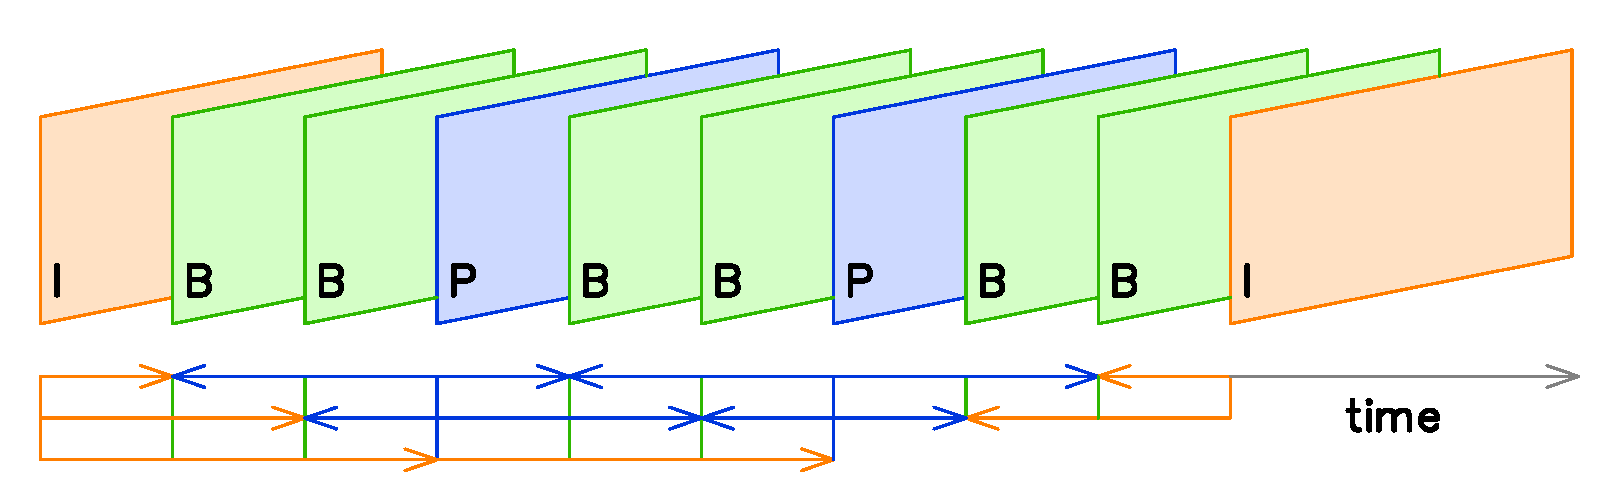
\includegraphics[width=0.7\textwidth, height=0.7\textheight, keepaspectratio]{img/IPB_images_sequence.png}}
\caption{An example of interleaved I-, B- and P-frames representing a video stream. The encoder may choose a different sequence of frame types. Reproduced from~\cite{interframe-wiki}.}
\label{fig:ipb-seq}
\end{figure}

A frame which will be encoded as a P-frame is partitioned into blocks of size 16-by-16 pixels\footnote{H.264 allows higher granularity for fine details by allowing some blocks to be 8x8, 8x16 or 16x8.}. These blocks are called \emph{macroblocks}, and for each macroblock the encoder searches for its most similar match in a predecessor frame (within a bounded search window) \cite[p.~256]{richardson2004h}. The difference in pixels between the matched block and the original is called the \emph{prediction error}, and the displacement between the two is called the \emph{motion vector} [Fig.~\ref{fig:mb-search}]. For simplicity, we say that a block of pixels has moved since the predecessor frame by the amount specified by its motion vector and, in addition to motion, pixels themselves have changed according to the prediction error.

\begin{figure}[tbh]
\centerline{\includegraphics[width=0.7\textwidth,height=0.7\textheight,keepaspectratio]
{img/macroblock-diagram.png}}
\caption{An illustration of a macroblock search from the current (target) frame to the predecessor (reference) frame. A macroblock is encoded using its prediction error and  motion vector.}
\label{fig:mb-search}
\end{figure} 

\subsection{Motion vectors as embedding space}
\label{mv-emb-space}

Computing motion vectors is a tradeoff between accuracy and computation time, tuned using the search window size. As such, codecs typically use an approximation instead of a globally optimal MV, resulting in a non-minimal prediction error \cite[p.~257]{richardson2004h}. While the MVs are encoded losslessly, the accuracy error allows minor changes to go unnoticed, making them suitable for LSB steganography (see \ref{lsb-steg}).

To estimate the embedding capacity, we generalise how all implemented embedding schemes should operate on motion vectors. Suppose an embedding scheme processes every motion vector in a grid individually for every frame and has an associated selection function $f$ which provides a number of bits that can be embedded into a particular motion vector. Later on, this function will allow to conveniently define a MV selection criteria for different embedding schemes.

\begin{definition}{Embedding capacity for video}

Let $M$ be an embedding scheme with an associated function $f_M : \mathbb{R}^2 \rightarrow \mathbb{N}$, which calculates how many bits can be embedded into a particular motion vector $\overrightarrow{mv} \in \mathbb{R}^2$. Then for an MPEG-encoded video $V$, the embedding capacity $\mathcal{C}_{V, M}$ is defined as:

$$ \mathcal{C}_{V, M} = \sum_{p \in \text{P-frames}(V)} \: \sum^{H}_{j = 0} \sum^{W}_{i = 0} f_M(\overrightarrow{mv}^p_{i, j})$$

where $W$ and $H$ are width and height of the macroblock grid, P-frames$(V)$ is a set of all P-frames of a video $V$ and $\overrightarrow{mv}^p_{i, j}$ is the MV of a macroblock  in $i$-th row and $j$-th column of the frame $p$.

\end{definition}

To see whether videos could generally hold a non-negligible amount of hidden data, one can estimate $\mathcal{C}_{V, M}$ by taking a product of the number of P-frames, the total number of MVs per frame and the average number of bits embedded per MV. For instance, an average HD video could reasonably have 6--15 P-frames per second\footnote{Depends on how often the encoder decides to use B-frames and I-frames. P-frames are better for video streaming as they do not require the successor frame during decoding.} with 3600 MVs each\footnote{If video's resolution is 1280x720 (HD), 16x16 macroblocks would partition the frame into a grid of size 80x45. This gives 3600 macroblocks in total.}. Assuming only a quarter of each frame would contain embedded data, I estimate the channel's capacity to be 5.4--13 Kbits/s. Since videos contain audio tracks and a higher number of pixels (or DCT coefficients) than images, a video file typically has higher embedding capacity than an audio file or an image.

\section{Requirements analysis}

The project has two main software deliverables:
\begin{itemize}
\item  An application that allows a user to embed secret messages into MPEG video files using a selection of LSB embedding algorithms.
\item A steganalysis suite that implements some general-purpose routines to detect motion vector-based steganography.
\end{itemize}

Below is a list of requirements for both deliverables, prioritised using \emph{MoSCoW} criteria~\cite{softid-notes}.

\subsection{Steganographic application}
\label{req-steg-app}
\begin{itemize}
\item (M) Ability to access motion vectors of an MPEG video file.
\item (M) Ability to reliably embed data within motion vectors.
\item (M) Multiple LSB embedding techniques.
\item (M) User-friendly binaries to perform embedding and extraction.
\item (S) Encryption of the secret message prior to embedding.
\item (S) Integration with an existing video codec.
\end{itemize}

\subsection{Steganalysis suite}
\label{req-steg-suite}
\begin{itemize}
\item (M) Ability to extract and process motion vector data.
\item (M) Multiple steganalysis methods.
\item (M) Documentation on usage and interpretation of the results.
\item (M) Evident effectiveness in detecting implemented embedding techniques.
\item (S) Compatibility with existing scientific computation packages (Matlab or Python-based packages)
\item (S) Usefulness (verbosity, amount of information provided) to the steganalyst.
\end{itemize}

\section{Project workflow}

\subsection{Technical choices}
\label{tech-choices}

The steganographic application requires modifying MPEG video files, which in turn requires parsing the format of a file, modifying motion vector values, and repackaging the data back into a playable video. Developing a codec does not relate to steganography and is potentially error-prone, so I leverage an existing set of codecs---\texttt{FFmpeg}\footnote{\url{https://www.ffmpeg.org/}}---to achieve this. As codecs are typically written in C or C++, it is a natural choice for this task to and makes the integration easier.

Performing encryption prior to embedding requires using a cryptography library. I chose \emph{Crypto++}, a popular C++ cryptography library.

The steganalysis suite was integrated into the Matlab scientific computation package for user's benefit, because it provides useful tools, such as statistical primitives, plotting capabilities and classifiers, without changing the environment. I chose Matlab  because of its widespread use and comprehensive functionality.

\subsection{Risk analysis}
FFmpeg is a complex piece of software, mostly written in a style of C that sacrifices clarity for performance. A potential risk for the project was the difficulty of proper integration with FFmpeg and hence inability to access or reliably modify motion vectors. Complete failure to do so was unlikely, but it could have consumed a significant amount of development time. To mitigate this, some ``catch-up'' time was allocated in the project timetable.  

\subsection{Development choices}
\begin{itemize}
\item \emph{Git} was used for version control, allowing quick roll-back and managing multiple source trees using branches.
\item \emph{Backups} were done by uploading the source tree and other relevant files to Dropbox. The git repository itself was hosted remotely on GitHub.
\item \emph{Testing} was done both manually and using unit tests to verify that software performs as intended. As a good practice, compiler warnings were treated as errors. Unit tests were implemented using Google Test framework and also served as a regression test suite.
\item \emph{Interative (spiral) development model} was used, which allowed continuously adding and testing new embedding schemes and steganalysis methods.
\item Software components have a \emph{modular design}, which enabled better maintainability and testability, and well-defined interfaces allowed changing internal implementation without breaking compatibility with other components.
\end{itemize}

\section{Starting Point}
This project uses some cryptography concepts introduced in the Part IB \textit{Security I} course. I have had some C++ knowledge from past programming experience and the \textit{Programming in C and C++} course. 

Prior to submitting the proposal, I have familiarised myself with the general concepts of steganography and LSB embedding though some introductory texts and relevant papers, and briefly looked at H.264 codec format.

During the development of this project I made use of some material covered in the following Part II courses:
\begin{itemize}
\item \textit{Information Theory} --- channel capacity, error correcting codes;
\item \textit{\LaTeX~and Matlab} --- typesetting and basics of Matlab;
\item \textit{Artificial Intelligence II} --- classifier evaluation.
\end{itemize}

\bigskip\bigskip
\subsubsection*{Summary}
This chapter summarised relevant theoretical and practical background necessary to start the implementation. The next chapter will cover the design and features of the system, implemented steganographic algorithms and steganalysis methods, together with some in-line evaluation.

% Implementation
\cleardoublepage
\chapter{Implementation}

\textit{This chapter covers the implementation details for the steganographic application and the steganalysis suite. I discuss the operation of the encoder and decoder applications, integration with the codec, structure and implementation of the embedding algorithms, and the details of some steganalytic attacks. Some in-line evaluation of algorithms is presented to motivate the design improvements.}

\section{Steganographic Application}

\subsection{Integration with FFmpeg}
\label{integrate-ffmpeg}

The project requires modifying MPEG files, so, as discussed in section \ref{tech-choices}, FFmpeg is used to provide this functionality. Finding a suitable way to integrate with FFmpeg was one of the biggest challenges that the project faced early on. FFmpeg is split into several libraries, each with a dedicated purpose such as stream multiplexing, resampling, or supporting I/O devices. The most suitable library for my purposes with was \texttt{libavcodec} which implements various audio and video codecs. Due to its popularity, I decided to focus on H.264, which FFmpeg offloads to a separate library: \texttt{libx264}. While \texttt{libavcodec} exposes an API for runing the codecs it provides, it provides no way to manipulate motion vectors. As such, \texttt{libavcodec} needed modifying to either introduce an additional API or to have it call my steganographic routines itself.

Initially, I looked for a point in the macroblock search phase where motion vectors would already be available, but the prediction error would not have been computed yet. This would allow modification of MVs without any visual footprint because prediction error would have brought the pixels to their required values regardless of the motion vector's value. However, since both FFmpeg and \texttt{libx264} exhibit complex data flow, and are written in optimised C, analysis proved more difficult than anticipated, producing a 4 week delay compared to the original timeline. To address this, the plan was changed to:
\begin{itemize}
\item Use a codec contained within \texttt{libavcodec}, obviating the need to touch \texttt{libx264}. I chose MPEG-4 Part 2 (\texttt{xvid}), H.264's popular predecessor.
\item Focus on modifying motion vectors, because it is essential to the project. The macroblock search is deep within the encoding pipeline, making it less amenable to modification. Instead, I chose to modify motion vectors before they are written to the output file.
\end{itemize}

However, this leaves prediction errors unmodified. To evaluate how much this affects the system, an experiment on human subjects was conducted to determine if this visual footprint is noticeable. This is further discussed in section \ref{exp-human-subj}.

\subsection{Steganography Library}

\subsubsection{C API}

To achieve a modular design and decouple from FFmpeg, the implemented steganographic algorithms were separated into a standalone library \texttt{movestlib}\footnote{\texttt{movest} (\underline{mo}tion \underline{ve}ctor \underline {st}eganography) is the codename for this project.}. The library is implemented in C++, exposing a C API for integration with FFmpeg, and encoder and decoder applications (Figure \ref{fig:movest-c-api}). The exact operation of these methods is described in section \ref{enc-dec-bin} using these applications as examples.

\begin{figure}[tbh]
\centering
%\resizebox{0.9\textwidth}{!}{%LaTeX with PSTricks extensions
%%Creator: inkscape 0.91
%%Please note this file requires PSTricks extensions
\psset{xunit=.5pt,yunit=.5pt,runit=.5pt}
\begin{pspicture}(728.9172976,437.66730601)
{
\newrgbcolor{curcolor}{1 1 1}
\pscustom[linestyle=none,fillstyle=solid,fillcolor=curcolor]
{
\newpath
\moveto(0.708661,436.95866076)
\lineto(728.208661,436.95866076)
\lineto(728.208661,0.70866076)
\lineto(0.708661,0.70866076)
\lineto(0.708661,436.95866076)
\closepath
}
}
{
\newrgbcolor{curcolor}{0.85882354 0.91764706 1}
\pscustom[linestyle=none,fillstyle=solid,fillcolor=curcolor]
{
\newpath
\moveto(1.333661,436.33366076)
\lineto(127.583661,436.33366076)
\lineto(127.583661,406.33366076)
\lineto(726.333661,406.33366076)
\lineto(726.333661,2.58366076)
\lineto(1.333661,2.58366076)
\lineto(1.333661,406.33366076)
\lineto(1.333661,436.33366076)
\closepath
}
}
{
\newrgbcolor{curcolor}{0 0 0}
\pscustom[linewidth=1.25,linecolor=curcolor]
{
\newpath
\moveto(1.333661,436.33366076)
\lineto(127.583661,436.33366076)
\lineto(127.583661,406.33366076)
\lineto(726.333661,406.33366076)
\lineto(726.333661,2.58366076)
\lineto(1.333661,2.58366076)
\lineto(1.333661,406.33366076)
\lineto(1.333661,436.33366076)
\closepath
}
}
{
\newrgbcolor{curcolor}{0 0 0}
\pscustom[linewidth=1.25,linecolor=curcolor]
{
\newpath
\moveto(1.333661,406.33366076)
\lineto(127.583661,406.33366076)
}
}
{
\newrgbcolor{curcolor}{0 0 0}
\pscustom[linestyle=none,fillstyle=solid,fillcolor=curcolor]
{
\newpath
\moveto(20.257001,427.75455926)
\lineto(23.50162975,427.75455926)
\lineto(23.50162975,416.95866076)
\lineto(21.3995785,416.95866076)
\lineto(21.3995785,424.26090701)
\curveto(21.3995785,424.47086776)(21.4020785,424.76505726)(21.4069535,425.14347526)
\curveto(21.4118285,425.52189313)(21.4143285,425.81364126)(21.4143285,426.01871938)
\lineto(19.370771,416.95866076)
\lineto(17.1808285,416.95866076)
\lineto(15.152021,426.01871938)
\curveto(15.152021,425.81364126)(15.154521,425.52189313)(15.159396,425.14347526)
\curveto(15.164271,424.76505726)(15.166771,424.47086776)(15.166771,424.26090701)
\lineto(15.166771,416.95866076)
\lineto(13.0647205,416.95866076)
\lineto(13.0647205,427.75455926)
\lineto(16.345971,427.75455926)
\lineto(18.308861,419.26578951)
\lineto(20.2571035,427.75455926)
\closepath
\moveto(30.4010435,419.08268451)
\curveto(30.72819225,419.51725451)(30.891766,420.13493076)(30.891766,420.93571201)
\curveto(30.891766,421.73649326)(30.72819225,422.35294826)(30.4010435,422.78507701)
\curveto(30.07389475,423.21720576)(29.605146,423.43326951)(28.9947935,423.43326951)
\curveto(28.38444225,423.43326951)(27.914471,423.21720576)(27.584881,422.78507701)
\curveto(27.25529225,422.35294826)(27.09049725,421.73649326)(27.09049725,420.93571201)
\curveto(27.09049725,420.13493076)(27.25529225,419.51725451)(27.584881,419.08268451)
\curveto(27.914471,418.64811326)(28.38444225,418.43082826)(28.9947935,418.43082826)
\curveto(29.605146,418.43082826)(30.07389475,418.64811326)(30.4010435,419.08268451)
\closepath
\moveto(32.070966,417.92911951)
\curveto(31.39713725,417.09660076)(30.3741885,416.68034076)(29.0021185,416.68034076)
\curveto(27.63004725,416.68034076)(26.6070985,417.09660076)(25.93326975,417.92911951)
\curveto(25.25944225,418.76163951)(24.9225285,419.76383701)(24.9225285,420.93571201)
\curveto(24.9225285,422.08805576)(25.25944225,423.08659076)(25.93326975,423.93131701)
\curveto(26.6070985,424.77604363)(27.63004725,425.19840688)(29.0021185,425.19840688)
\curveto(30.3741885,425.19840688)(31.39713725,424.77604363)(32.070966,423.93131701)
\curveto(32.7447935,423.08659076)(33.08170725,422.08805576)(33.08170725,420.93571201)
\curveto(33.08170725,419.76383701)(32.7447935,418.76163951)(32.070966,417.92911951)
\closepath
\moveto(39.49528225,424.94205913)
\lineto(41.7364935,424.94205913)
\lineto(38.85807475,416.95866076)
\lineto(36.65348475,416.95866076)
\lineto(33.789716,424.94205913)
\lineto(36.133466,424.94205913)
\lineto(37.7960635,419.05338701)
\lineto(39.49528225,424.94205913)
\closepath
\moveto(44.93839725,422.97916826)
\curveto(44.6722835,422.67643451)(44.50504725,422.26627826)(44.4366885,421.74869951)
\lineto(47.68131725,421.74869951)
\curveto(47.64714225,422.30045701)(47.479901,422.71915826)(47.1796085,423.00480326)
\curveto(46.87931475,423.29044826)(46.507001,423.43326951)(46.06266475,423.43326951)
\curveto(45.579266,423.43326951)(45.204511,423.28190326)(44.93839725,422.97916826)
\closepath
\moveto(47.8570985,424.78092638)
\curveto(48.38932475,424.53190288)(48.8287785,424.13883701)(49.17545725,423.60172701)
\curveto(49.48795725,423.12809451)(49.69059475,422.57877826)(49.7833685,421.95377826)
\curveto(49.837081,421.58756701)(49.859056,421.06022326)(49.849281,420.37174701)
\lineto(44.3854135,420.37174701)
\curveto(44.4147135,419.57096576)(44.666176,419.00944201)(45.1398085,418.68717576)
\curveto(45.42789475,418.48698076)(45.7745735,418.38688326)(46.17984725,418.38688326)
\curveto(46.60953475,418.38688326)(46.958656,418.50895826)(47.227211,418.75309451)
\curveto(47.37369475,418.88493076)(47.50308975,419.06803576)(47.61539475,419.30241076)
\lineto(49.74674225,419.30241076)
\curveto(49.69302975,418.82877826)(49.4464485,418.34782076)(49.006996,417.85953951)
\curveto(48.32340225,417.08317201)(47.366371,416.69498951)(46.13590225,416.69498951)
\curveto(45.12027725,416.69498951)(44.224281,417.02213701)(43.4479135,417.67643451)
\curveto(42.67154725,418.33073076)(42.2833635,419.39518451)(42.2833635,420.86979326)
\curveto(42.2833635,422.25162951)(42.63370475,423.31119951)(43.3343885,424.04850451)
\curveto(44.03507225,424.78580926)(44.944496,425.15446151)(46.06265975,425.15446151)
\curveto(46.72672225,425.15446151)(47.32486725,425.02995026)(47.8570935,424.78092638)
\closepath
\moveto(52.879071,419.50748826)
\curveto(52.923021,419.13639451)(53.018231,418.87272326)(53.164716,418.71647326)
\curveto(53.42350475,418.43815326)(53.90201975,418.29899326)(54.60026225,418.29899326)
\curveto(55.0104185,418.29899326)(55.336346,418.36003076)(55.578046,418.48209826)
\curveto(55.81974475,418.60417326)(55.94059475,418.78727451)(55.94059475,419.03141451)
\curveto(55.94059475,419.26578951)(55.84293225,419.44401201)(55.647626,419.56608201)
\curveto(55.4523135,419.68815701)(54.727216,419.89811326)(53.47233225,420.19596576)
\curveto(52.56901225,420.42057451)(51.931806,420.70133701)(51.56071225,421.03825076)
\curveto(51.1896185,421.37028201)(51.004071,421.84879701)(51.004071,422.47379701)
\curveto(51.004071,423.21110201)(51.29337725,423.84464701)(51.871991,424.37443201)
\curveto(52.45060475,424.90421738)(53.2648135,425.16911001)(54.3146185,425.16911001)
\curveto(55.31071225,425.16911001)(56.12247975,424.97013538)(56.749921,424.57218613)
\curveto(57.37736225,424.17423701)(57.73746975,423.48698076)(57.8302435,422.51041826)
\lineto(55.742841,422.51041826)
\curveto(55.713541,422.77897326)(55.637866,422.99137576)(55.51578975,423.14762576)
\curveto(55.28629725,423.43082826)(54.89567225,423.57243076)(54.34391475,423.57243076)
\curveto(53.8898135,423.57243076)(53.56632725,423.50163076)(53.373456,423.36002826)
\curveto(53.18058475,423.21842576)(53.08414975,423.05241076)(53.08414975,422.86198076)
\curveto(53.08414975,422.62272326)(53.18668725,422.44938326)(53.391766,422.34196201)
\curveto(53.59684475,422.22966201)(54.32194225,422.03678576)(55.56705975,421.76334826)
\curveto(56.39713725,421.56803576)(57.019696,421.27262576)(57.43473475,420.87711826)
\curveto(57.844891,420.47672701)(58.04996975,419.97623826)(58.04996975,419.37565326)
\curveto(58.04996975,418.58463701)(57.75577975,417.93888576)(57.167401,417.43839701)
\curveto(56.57902225,416.93790951)(55.6695985,416.68766451)(54.43912975,416.68766451)
\curveto(53.18424725,416.68766451)(52.2577335,416.95255701)(51.6595885,417.48234201)
\curveto(51.0614435,418.01212701)(50.76237225,418.68717576)(50.76237225,419.50748826)
\lineto(52.879071,419.50748826)
\closepath
\moveto(58.772626,423.38200076)
\lineto(58.772626,424.86881701)
\lineto(59.88590725,424.86881701)
\lineto(59.88590725,427.09537951)
\lineto(61.95133725,427.09537951)
\lineto(61.95133725,424.86881701)
\lineto(63.2477235,424.86881701)
\lineto(63.2477235,423.38200076)
\lineto(61.95133725,423.38200076)
\lineto(61.95133725,419.16325076)
\curveto(61.95133725,418.83610201)(61.99283725,418.63224451)(62.07584975,418.55167826)
\curveto(62.15886225,418.47111576)(62.4127635,418.43082826)(62.8375685,418.43082826)
\curveto(62.9010435,418.43082826)(62.9681835,418.43204951)(63.03898475,418.43445326)
\curveto(63.10978475,418.43695326)(63.17936475,418.44057826)(63.24772475,418.44545326)
\lineto(63.24772475,416.88539451)
\lineto(62.25895475,416.84876951)
\curveto(61.27262725,416.81459451)(60.5987985,416.98548826)(60.237471,417.36146576)
\curveto(60.003096,417.60072326)(59.8859085,417.96937576)(59.8859085,418.46742201)
\lineto(59.8859085,423.38197326)
\lineto(58.77262725,423.38197326)
\closepath
\moveto(69.9493835,426.62662951)
\curveto(70.82828975,427.51530138)(71.9464535,427.95963738)(73.303876,427.95963738)
\curveto(75.12028225,427.95963738)(76.44840725,427.36393426)(77.288251,426.17252788)
\curveto(77.7521185,425.50358263)(78.001141,424.83219588)(78.035321,424.15836826)
\lineto(75.77946225,424.15836826)
\curveto(75.63297725,424.67594588)(75.4449885,425.06657088)(75.21549725,425.33024276)
\curveto(74.805341,425.79899276)(74.197431,426.03336776)(73.391766,426.03336776)
\curveto(72.5714535,426.03336776)(71.924481,425.70255726)(71.4508485,425.04093613)
\curveto(70.977216,424.37931451)(70.74039975,423.44303576)(70.74039975,422.23209826)
\curveto(70.74039975,421.02116076)(70.9906435,420.11417826)(71.49113225,419.51115076)
\curveto(71.99161975,418.90812326)(72.627606,418.60660951)(73.399091,418.60660951)
\curveto(74.190106,418.60660951)(74.7931335,418.86539951)(75.20817225,419.38297701)
\curveto(75.43766475,419.66129701)(75.62809475,420.07877826)(75.77946225,420.63541826)
\lineto(78.0133485,420.63541826)
\curveto(77.818036,419.45866076)(77.3187685,418.50162951)(76.515546,417.76432451)
\curveto(75.7123235,417.02701951)(74.68326975,416.65836826)(73.42838725,416.65836826)
\curveto(71.8756535,416.65836826)(70.65494975,417.15641451)(69.7662785,418.15250826)
\curveto(68.877606,419.15348451)(68.43326975,420.52555576)(68.43326975,422.26871951)
\curveto(68.43326975,424.15348451)(68.938641,425.60612163)(69.9493835,426.62662951)
\closepath
\moveto(86.83414975,421.03825076)
\lineto(89.57340725,421.03825076)
\lineto(88.225751,425.28629751)
\lineto(86.83414975,421.03825076)
\closepath
\moveto(86.97330975,427.75455926)
\lineto(89.52213725,427.75455926)
\lineto(93.34537975,416.95866076)
\lineto(90.899091,416.95866076)
\lineto(90.20328975,419.17789951)
\lineto(86.22623975,419.17789951)
\lineto(85.4791685,416.95866076)
\lineto(83.12076975,416.95866076)
\lineto(86.97330975,427.75455926)
\closepath
\moveto(100.3387885,425.52067251)
\curveto(100.04337725,425.75993026)(99.62955975,425.87955913)(99.09733225,425.87955913)
\lineto(96.99528225,425.87955913)
\lineto(96.99528225,422.70084826)
\lineto(99.09733225,422.70084826)
\curveto(99.62955975,422.70084826)(100.04337725,422.83024326)(100.3387885,423.08903201)
\curveto(100.6341985,423.34782076)(100.7819035,423.75797701)(100.7819035,424.31950076)
\curveto(100.7819035,424.88102401)(100.6341985,425.28141463)(100.3387885,425.52067251)
\closepath
\moveto(102.0489935,421.63151201)
\curveto(101.40446225,421.10416826)(100.484051,420.84049701)(99.28776225,420.84049701)
\lineto(96.99528225,420.84049701)
\lineto(96.99528225,416.95866076)
\lineto(94.754071,416.95866076)
\lineto(94.754071,427.75455926)
\lineto(99.45621975,427.75455926)
\curveto(100.5402035,427.75455926)(101.40446225,427.47623888)(102.0489935,426.91959826)
\curveto(102.69352475,426.36295763)(103.01578975,425.50114126)(103.01578975,424.33414951)
\curveto(103.01578975,423.05973451)(102.69352475,422.15885576)(102.0489935,421.63151201)
\closepath
\moveto(106.768231,416.95866076)
\lineto(104.52701975,416.95866076)
\lineto(104.52701975,427.75455926)
\lineto(106.768231,427.75455926)
\lineto(106.768231,416.95866076)
\closepath
}
}
{
\newrgbcolor{curcolor}{1 1 1}
\pscustom[linestyle=none,fillstyle=solid,fillcolor=curcolor]
{
\newpath
\moveto(13.833661,393.83366076)
\lineto(213.833661,393.83366076)
\lineto(213.833661,256.33366076)
\lineto(13.833661,256.33366076)
\lineto(13.833661,393.83366076)
\closepath
}
}
{
\newrgbcolor{curcolor}{0 0 0}
\pscustom[linewidth=1.25,linecolor=curcolor]
{
\newpath
\moveto(13.833661,393.83366076)
\lineto(213.833661,393.83366076)
\lineto(213.833661,256.33366076)
\lineto(13.833661,256.33366076)
\lineto(13.833661,393.83366076)
\closepath
}
}
{
\newrgbcolor{curcolor}{0 0 0}
\pscustom[linewidth=1.25,linecolor=curcolor]
{
\newpath
\moveto(13.833661,350.08366076)
\lineto(13.833661,393.83366076)
\lineto(213.833661,393.83366076)
\lineto(213.833661,350.08366076)
\lineto(13.833661,350.08366076)
\closepath
}
}
{
\newrgbcolor{curcolor}{0 0 0}
\pscustom[linestyle=none,fillstyle=solid,fillcolor=curcolor]
{
\newpath
\moveto(66.44840725,379.24869951)
\lineto(68.81412975,381.08707826)
\lineto(68.81412975,379.76871951)
\lineto(67.2320985,378.55289951)
\lineto(68.81412975,377.33707826)
\lineto(68.81412975,376.01871951)
\lineto(66.44840725,377.85709826)
\lineto(66.44840725,379.24869951)
\closepath
\moveto(63.37955975,379.24869951)
\lineto(65.73795725,381.08707826)
\lineto(65.73795725,379.76871951)
\lineto(64.163251,378.55289951)
\lineto(65.73795725,377.33707826)
\lineto(65.73795725,376.01871951)
\lineto(63.37955975,377.85709826)
\lineto(63.37955975,379.24869951)
\closepath
\moveto(76.150556,382.08683451)
\curveto(76.673016,381.82560451)(77.070966,381.48746951)(77.3444035,381.07243076)
\curveto(77.60807475,380.67692201)(77.783856,380.21549701)(77.87174725,379.68815326)
\curveto(77.94987225,379.32682451)(77.98893475,378.75065326)(77.98893475,377.95963701)
\lineto(72.23942225,377.95963701)
\curveto(72.26383475,377.16373951)(72.45182475,376.52531076)(72.80338725,376.04435451)
\curveto(73.15494975,375.56339701)(73.6993835,375.32291826)(74.4366885,375.32291826)
\curveto(75.12516475,375.32291826)(75.674481,375.54996951)(76.08463725,376.00407076)
\curveto(76.31901225,376.26774326)(76.4850285,376.57291826)(76.58268475,376.91959826)
\lineto(77.879071,376.91959826)
\curveto(77.844896,376.63151201)(77.731366,376.31046701)(77.53849475,375.95646326)
\curveto(77.3456235,375.60245951)(77.12955975,375.31315326)(76.89030225,375.08854326)
\curveto(76.489911,374.69791826)(75.994306,374.43424701)(75.40348475,374.29752826)
\curveto(75.08610225,374.21940326)(74.727216,374.18034076)(74.32682475,374.18034076)
\curveto(73.35026225,374.18034076)(72.522626,374.53556576)(71.84391475,375.24601451)
\curveto(71.1652035,375.95646326)(70.8258485,376.95133701)(70.8258485,378.23063326)
\curveto(70.8258485,379.49039951)(71.16764475,380.51334826)(71.8512385,381.29948076)
\curveto(72.53483225,382.08561451)(73.42838725,382.47868076)(74.5319035,382.47868076)
\curveto(75.0885435,382.47868076)(75.62809475,382.34806576)(76.150556,382.08683451)
\closepath
\moveto(76.6339535,379.00700076)
\curveto(76.580241,379.57828951)(76.455731,380.03483326)(76.2604185,380.37662951)
\curveto(75.899091,381.01139576)(75.2960635,381.32877826)(74.45133725,381.32877826)
\curveto(73.8458685,381.32877826)(73.338056,381.11027201)(72.92789975,380.67326076)
\curveto(72.5177435,380.23624826)(72.30045725,379.68082826)(72.2760435,379.00700076)
\lineto(76.6339535,379.00700076)
\closepath
\moveto(79.60514475,382.30289951)
\lineto(80.85758725,382.30289951)
\lineto(80.85758725,381.18961826)
\curveto(81.228681,381.64860201)(81.62174725,381.97819201)(82.036786,382.17838701)
\curveto(82.45182475,382.37858326)(82.913251,382.47868076)(83.4210635,382.47868076)
\curveto(84.53434475,382.47868076)(85.28629725,382.09049701)(85.67692225,381.31412951)
\curveto(85.891766,380.88932451)(85.9991885,380.28141451)(85.9991885,379.49039951)
\lineto(85.9991885,374.45866076)
\lineto(84.658856,374.45866076)
\lineto(84.658856,379.40250826)
\curveto(84.658856,379.88102451)(84.588056,380.26676576)(84.4464535,380.55973451)
\curveto(84.2120785,381.04801576)(83.78727475,381.29215701)(83.17203975,381.29215701)
\curveto(82.85953975,381.29215701)(82.60319225,381.26041951)(82.40299725,381.19694451)
\curveto(82.0416685,381.08951951)(81.724286,380.87467951)(81.4508485,380.55241326)
\curveto(81.23112225,380.29362451)(81.08829975,380.02629076)(81.022381,379.75041201)
\curveto(80.9564685,379.47453201)(80.923506,379.08024576)(80.923506,378.56754951)
\lineto(80.923506,374.45866326)
\lineto(79.605146,374.45866326)
\lineto(79.605146,382.30290201)
\closepath
\moveto(89.2633485,382.30289951)
\lineto(89.2633485,377.09537951)
\curveto(89.2633485,376.69498951)(89.3268235,376.36784076)(89.4537785,376.11393451)
\curveto(89.6881535,375.64518451)(90.12516475,375.41080951)(90.7648135,375.41080951)
\curveto(91.68278225,375.41080951)(92.30778225,375.82096576)(92.6398135,376.64127826)
\curveto(92.82047725,377.08073076)(92.91080975,377.68375826)(92.91080975,378.45035951)
\lineto(92.91080975,382.30289951)
\lineto(94.2291685,382.30289951)
\lineto(94.2291685,374.45866076)
\lineto(92.984051,374.45866076)
\lineto(92.998701,375.61588701)
\curveto(92.82780225,375.31803576)(92.615401,375.06657076)(92.36149475,374.86149326)
\curveto(91.85856475,374.45133701)(91.2482135,374.24625826)(90.53043975,374.24625826)
\curveto(89.412276,374.24625826)(88.65055725,374.61979326)(88.2452835,375.36686451)
\curveto(88.02555725,375.76725451)(87.9156935,376.30192201)(87.9156935,376.97086826)
\lineto(87.9156935,382.30289951)
\lineto(89.26334975,382.30289951)
\closepath
\moveto(96.28483225,382.30289951)
\lineto(97.5885435,382.30289951)
\lineto(97.5885435,381.18961826)
\curveto(97.9010435,381.57535951)(98.18424725,381.85612201)(98.4381535,382.03190326)
\curveto(98.8727235,382.32975451)(99.36588725,382.47868076)(99.91764475,382.47868076)
\curveto(100.54264475,382.47868076)(101.04557475,382.32487201)(101.42643475,382.01725451)
\curveto(101.6412785,381.84147326)(101.836591,381.58268451)(102.01237225,381.24088701)
\curveto(102.305341,381.66080951)(102.6495785,381.97208826)(103.04508725,382.17472576)
\curveto(103.44059475,382.37736201)(103.884931,382.47868076)(104.37809475,382.47868076)
\curveto(105.43278225,382.47868076)(106.150556,382.09782076)(106.53141475,381.33610201)
\curveto(106.7364935,380.92594576)(106.83903225,380.37418826)(106.83903225,379.68082826)
\lineto(106.83903225,374.45866076)
\lineto(105.4694035,374.45866076)
\lineto(105.4694035,379.90787951)
\curveto(105.4694035,380.43034076)(105.3387885,380.78922701)(105.07755725,380.98453951)
\curveto(104.81632725,381.17985201)(104.4977235,381.27750826)(104.12174725,381.27750826)
\curveto(103.6041685,381.27750826)(103.15861225,381.10416826)(102.78507725,380.75748951)
\curveto(102.41154225,380.41080951)(102.22477475,379.83219576)(102.22477475,379.02164951)
\lineto(102.22477475,374.45866076)
\lineto(100.88444225,374.45866076)
\lineto(100.88444225,379.57828951)
\curveto(100.88444225,380.11051576)(100.82096725,380.49869951)(100.69401225,380.74284076)
\curveto(100.49381725,381.10905201)(100.12028225,381.29215701)(99.57340725,381.29215701)
\curveto(99.07535975,381.29215701)(98.62247975,381.09928576)(98.21476475,380.71354326)
\curveto(97.80704975,380.32780201)(97.60319225,379.62955951)(97.60319225,378.61881701)
\lineto(97.60319225,374.45866076)
\lineto(96.28483225,374.45866076)
\lineto(96.28483225,382.30289951)
\closepath
\moveto(113.650556,382.08683451)
\curveto(114.173016,381.82560451)(114.570966,381.48746951)(114.8444035,381.07243076)
\curveto(115.10807475,380.67692201)(115.283856,380.21549701)(115.37174725,379.68815326)
\curveto(115.44987225,379.32682451)(115.48893475,378.75065326)(115.48893475,377.95963701)
\lineto(109.73942225,377.95963701)
\curveto(109.76383475,377.16373951)(109.95182475,376.52531076)(110.30338725,376.04435451)
\curveto(110.65494975,375.56339701)(111.1993835,375.32291826)(111.9366885,375.32291826)
\curveto(112.62516475,375.32291826)(113.174481,375.54996951)(113.58463725,376.00407076)
\curveto(113.81901225,376.26774326)(113.9850285,376.57291826)(114.08268475,376.91959826)
\lineto(115.379071,376.91959826)
\curveto(115.344896,376.63151201)(115.231366,376.31046701)(115.03849475,375.95646326)
\curveto(114.8456235,375.60245951)(114.62955975,375.31315326)(114.390301,375.08854326)
\curveto(113.989911,374.69791826)(113.494306,374.43424701)(112.90348475,374.29752826)
\curveto(112.58610225,374.21940326)(112.227216,374.18034076)(111.82682475,374.18034076)
\curveto(110.85026225,374.18034076)(110.022626,374.53556576)(109.34391475,375.24601451)
\curveto(108.6652035,375.95646326)(108.3258485,376.95133701)(108.3258485,378.23063326)
\curveto(108.3258485,379.49039951)(108.66764475,380.51334826)(109.35123975,381.29948076)
\curveto(110.03483225,382.08561451)(110.92838725,382.47868076)(112.0319035,382.47868076)
\curveto(112.5885435,382.47868076)(113.12809475,382.34806576)(113.650556,382.08683451)
\closepath
\moveto(114.1339535,379.00700076)
\curveto(114.080241,379.57828951)(113.955731,380.03483326)(113.7604185,380.37662951)
\curveto(113.399091,381.01139576)(112.7960635,381.32877826)(111.95133725,381.32877826)
\curveto(111.3458685,381.32877826)(110.838056,381.11027201)(110.42789975,380.67326076)
\curveto(110.0177435,380.23624826)(109.80045725,379.68082826)(109.7760435,379.00700076)
\lineto(114.1339535,379.00700076)
\closepath
\moveto(117.141766,382.30289951)
\lineto(118.39420725,382.30289951)
\lineto(118.39420725,380.94791826)
\curveto(118.49674475,381.21159076)(118.74821225,381.53263576)(119.14860225,381.91105326)
\curveto(119.5489935,382.28947076)(120.0104185,382.47868076)(120.53287975,382.47868076)
\curveto(120.55729225,382.47868076)(120.59879225,382.47618076)(120.65739225,382.47130576)
\curveto(120.71597975,382.46643076)(120.8160835,382.45665576)(120.957686,382.44200576)
\lineto(120.957686,381.05040326)
\curveto(120.879561,381.06505326)(120.8075385,381.07481576)(120.741621,381.07970326)
\curveto(120.6757085,381.08457826)(120.60368225,381.08707826)(120.52555725,381.08707826)
\curveto(119.86149475,381.08707826)(119.351241,380.87345576)(118.99479475,380.44620951)
\curveto(118.63834975,380.01896326)(118.46012725,379.52701951)(118.46012725,378.97037951)
\lineto(118.46012725,374.45866076)
\lineto(117.14176725,374.45866076)
\lineto(117.14176725,382.30289951)
\closepath
\moveto(123.51383725,375.64518451)
\curveto(123.79215725,375.42545701)(124.12174725,375.31559451)(124.502606,375.31559451)
\curveto(124.9664735,375.31559451)(125.41569225,375.42301951)(125.850261,375.63785951)
\curveto(126.582686,375.99430576)(126.9488985,376.57780201)(126.9488985,377.38834826)
\lineto(126.9488985,378.45035951)
\curveto(126.787761,378.34782201)(126.5802485,378.26237201)(126.326336,378.19401201)
\curveto(126.072436,378.12564951)(125.823411,378.07682451)(125.579266,378.04752826)
\lineto(124.780926,377.94499076)
\curveto(124.302411,377.88151576)(123.94352475,377.78141576)(123.704266,377.64469701)
\curveto(123.2989935,377.41520451)(123.096356,377.04899451)(123.096356,376.54606451)
\curveto(123.096356,376.16520451)(123.235516,375.86491201)(123.51383725,375.64518576)
\closepath
\moveto(126.289711,379.21207826)
\curveto(126.5924485,379.25114076)(126.795086,379.37809451)(126.8976235,379.59293826)
\curveto(126.9562485,379.71012576)(126.9854985,379.87858326)(126.9854985,380.09830951)
\curveto(126.9854985,380.54752826)(126.825586,380.87345576)(126.5057735,381.07609201)
\curveto(126.185936,381.27872951)(125.728186,381.38004701)(125.132476,381.38004701)
\curveto(124.44399975,381.38004701)(123.9557185,381.19450076)(123.66763225,380.82340701)
\curveto(123.50649975,380.61832826)(123.40151975,380.31315326)(123.352691,379.90787951)
\lineto(122.12222225,379.90787951)
\curveto(122.14663475,380.87467701)(122.46035725,381.54728451)(123.06338475,381.92570201)
\curveto(123.66641225,382.30411951)(124.36587475,382.49332826)(125.1617735,382.49332826)
\curveto(126.0846235,382.49332826)(126.834136,382.31754701)(127.410311,381.96598451)
\curveto(127.9815985,381.61442201)(128.2672485,381.06754701)(128.2672485,380.32535951)
\lineto(128.2672485,375.80631701)
\curveto(128.2672485,375.66959826)(128.2952485,375.55973451)(128.3514985,375.47672701)
\curveto(128.4076235,375.39371451)(128.526061,375.35221451)(128.7067235,375.35221451)
\curveto(128.7653485,375.35221451)(128.8312235,375.35583951)(128.9044735,375.36321451)
\curveto(128.9777235,375.37058951)(129.055836,375.38152701)(129.1388485,375.39617701)
\lineto(129.1388485,374.42205576)
\curveto(128.9337735,374.36346826)(128.7775235,374.32684326)(128.6700985,374.31219326)
\curveto(128.5627235,374.29754326)(128.4161985,374.29021826)(128.2306485,374.29021826)
\curveto(127.7765485,374.29021826)(127.446961,374.45135201)(127.2418735,374.77361701)
\curveto(127.1344985,374.94451576)(127.0587735,375.18621451)(127.0148235,375.49871451)
\curveto(126.7462735,375.14715201)(126.3605235,374.84197701)(125.8575985,374.58318701)
\curveto(125.35466975,374.32439826)(124.80046975,374.19500451)(124.195001,374.19500451)
\curveto(123.46746225,374.19500451)(122.87297975,374.41595076)(122.41155475,374.85784576)
\curveto(121.9501285,375.29974076)(121.719416,375.85271826)(121.719416,376.51678076)
\curveto(121.719416,377.24432076)(121.946466,377.80828451)(122.4005685,378.20867576)
\curveto(122.85466975,378.60906701)(123.45037225,378.85564826)(124.18767725,378.94842201)
\lineto(126.2897235,379.21209326)
\closepath
\moveto(130.689136,384.49284076)
\lineto(132.022136,384.49284076)
\lineto(132.022136,382.30289951)
\lineto(133.2745735,382.30289951)
\lineto(133.2745735,381.22623951)
\lineto(132.022136,381.22623951)
\lineto(132.022136,376.10660951)
\curveto(132.022136,375.83317201)(132.114886,375.65006701)(132.300461,375.55729326)
\curveto(132.402961,375.50358076)(132.5738985,375.47673076)(132.8131485,375.47673076)
\curveto(132.8766485,375.47673076)(132.944986,375.47795201)(133.018236,375.48035576)
\curveto(133.091486,375.48285576)(133.1769235,375.48885576)(133.2745735,375.49866826)
\lineto(133.2745735,374.45862951)
\curveto(133.123211,374.41467951)(132.965736,374.38294201)(132.802161,374.36341701)
\curveto(132.6385985,374.34387951)(132.461586,374.33411701)(132.271161,374.33411701)
\curveto(131.6559235,374.33411701)(131.2384485,374.49158701)(131.0187235,374.80652826)
\curveto(130.7989985,375.12147076)(130.689136,375.53040576)(130.689136,376.03333576)
\lineto(130.689136,381.22620701)
\lineto(129.6271235,381.22620701)
\lineto(129.6271235,382.30286701)
\lineto(130.689136,382.30286701)
\lineto(130.689136,384.49280826)
\closepath
\moveto(134.585611,382.26627826)
\lineto(135.9259485,382.26627826)
\lineto(135.9259485,374.45866076)
\lineto(134.585611,374.45866076)
\lineto(134.585611,382.26627826)
\closepath
\moveto(134.585611,385.21793826)
\lineto(135.9259485,385.21793826)
\lineto(135.9259485,383.72379701)
\lineto(134.585611,383.72379701)
\lineto(134.585611,385.21793826)
\closepath
\moveto(142.816811,376.30070201)
\curveto(143.1415235,376.96232326)(143.3038735,377.69840701)(143.3038735,378.50895326)
\curveto(143.3038735,379.24137576)(143.1867485,379.83707826)(142.952311,380.29606326)
\curveto(142.5812235,381.01871951)(141.9415735,381.38004701)(141.0333735,381.38004701)
\curveto(140.2276985,381.38004701)(139.641761,381.07243076)(139.275561,380.45719576)
\curveto(138.9093485,379.84196201)(138.726236,379.09977451)(138.726236,378.23063326)
\curveto(138.726236,377.39567201)(138.9093485,376.69987201)(139.275561,376.14323076)
\curveto(139.641761,375.58659076)(140.2228235,375.30826951)(141.0187235,375.30826951)
\curveto(141.8927485,375.30826951)(142.492111,375.63908076)(142.816811,376.30070201)
\closepath
\moveto(143.633461,381.51920826)
\curveto(144.331711,380.84537951)(144.6808235,379.85416826)(144.6808235,378.54557451)
\curveto(144.6808235,377.28092701)(144.373211,376.23600451)(143.7579735,375.41080951)
\curveto(143.1427485,374.58561451)(142.1881485,374.17301576)(140.894211,374.17301576)
\curveto(139.815111,374.17301576)(138.9581735,374.53800701)(138.323411,375.26798701)
\curveto(137.688636,375.99796701)(137.371261,376.97819201)(137.371261,378.20866076)
\curveto(137.371261,379.52701951)(137.705736,380.57682451)(138.3746735,381.35807451)
\curveto(139.0436235,382.13932451)(139.942061,382.52994951)(141.069986,382.52994951)
\curveto(142.080736,382.52994951)(142.9352235,382.19303576)(143.633461,381.51920826)
\closepath
\moveto(146.2457735,382.30289951)
\lineto(147.498211,382.30289951)
\lineto(147.498211,381.18961826)
\curveto(147.869311,381.64860201)(148.2623735,381.97819201)(148.677411,382.17838701)
\curveto(149.0924485,382.37858326)(149.5538735,382.47868076)(150.061686,382.47868076)
\curveto(151.1749735,382.47868076)(151.9269235,382.09049701)(152.3175485,381.31412951)
\curveto(152.532386,380.88932451)(152.639811,380.28141451)(152.639811,379.49039951)
\lineto(152.639811,374.45866076)
\lineto(151.299486,374.45866076)
\lineto(151.299486,379.40250826)
\curveto(151.299486,379.88102451)(151.228736,380.26676576)(151.0870735,380.55973451)
\curveto(150.8526985,381.04801576)(150.4278985,381.29215701)(149.812661,381.29215701)
\curveto(149.500161,381.29215701)(149.2438235,381.26041951)(149.0436235,381.19694451)
\curveto(148.6822985,381.08951951)(148.364911,380.87467951)(148.0914735,380.55241326)
\curveto(147.8717485,380.29362451)(147.7289235,380.02629076)(147.663011,379.75041201)
\curveto(147.597136,379.47453201)(147.564136,379.08024576)(147.564136,378.56754951)
\lineto(147.564136,374.45866326)
\lineto(146.2457735,374.45866326)
\lineto(146.2457735,382.30290201)
\closepath
}
}
{
\newrgbcolor{curcolor}{0 0 0}
\pscustom[linestyle=none,fillstyle=solid,fillcolor=curcolor]
{
\newpath
\moveto(158.108561,377.33707826)
\lineto(159.6539735,378.55289951)
\lineto(158.108561,379.76871951)
\lineto(158.108561,381.08707826)
\lineto(160.474286,379.24869951)
\lineto(160.474286,377.85709826)
\lineto(158.108561,376.01871951)
\lineto(158.108561,377.33707826)
\closepath
\moveto(155.039711,377.33707826)
\lineto(156.5851235,378.55289951)
\lineto(155.039711,379.76871951)
\lineto(155.039711,381.08707826)
\lineto(157.398111,379.24869951)
\lineto(157.398111,377.85709826)
\lineto(155.039711,376.01871951)
\lineto(155.039711,377.33707826)
\closepath
}
}
{
\newrgbcolor{curcolor}{0 0 0}
\pscustom[linestyle=none,fillstyle=solid,fillcolor=curcolor]
{
\newpath
\moveto(74.9835635,364.91276201)
\curveto(75.32535975,364.77604326)(75.6354185,364.53678576)(75.9137385,364.19498951)
\curveto(76.1383485,363.91666826)(76.289716,363.57487201)(76.367841,363.16959826)
\curveto(76.416666,362.90104326)(76.4410785,362.50797701)(76.4410785,361.99039951)
\lineto(76.42643475,356.95866076)
\lineto(74.28776225,356.95866076)
\lineto(74.28776225,362.04166826)
\curveto(74.28776225,362.34440326)(74.23893725,362.59342701)(74.1412785,362.78873951)
\curveto(73.955731,363.15983326)(73.61393475,363.34537951)(73.11588725,363.34537951)
\curveto(72.539716,363.34537951)(72.141766,363.10612201)(71.92203975,362.62760576)
\curveto(71.80973975,362.37369951)(71.75358225,362.06852451)(71.75358225,361.71207826)
\lineto(71.75358225,356.95866076)
\lineto(69.65153225,356.95866076)
\lineto(69.65153225,361.71207826)
\curveto(69.65153225,362.18571201)(69.60270725,362.52994951)(69.50504725,362.74479326)
\curveto(69.329266,363.13053576)(68.9850285,363.32340701)(68.47233225,363.32340701)
\curveto(67.87662975,363.32340701)(67.4762385,363.13053576)(67.271161,362.74479326)
\curveto(67.158861,362.52506701)(67.1027035,362.19791826)(67.1027035,361.76334826)
\lineto(67.1027035,356.95866076)
\lineto(64.98600475,356.95866076)
\lineto(64.98600475,364.92741076)
\lineto(67.0148135,364.92741076)
\lineto(67.0148135,363.76285951)
\curveto(67.27360225,364.17789951)(67.5177435,364.47330951)(67.74723475,364.64909076)
\curveto(68.1525085,364.96159076)(68.677411,365.11784076)(69.32194225,365.11784076)
\curveto(69.9322935,365.11784076)(70.42545725,364.98356326)(70.80143475,364.71500826)
\curveto(71.1041685,364.46598451)(71.333661,364.14616076)(71.489911,363.75553576)
\curveto(71.7633485,364.22428576)(72.1027035,364.56852451)(72.50797725,364.78825076)
\curveto(72.93766475,365.00797701)(73.416181,365.11784076)(73.94352475,365.11784076)
\curveto(74.29508725,365.11784076)(74.641766,365.04947826)(74.9835635,364.91276201)
\closepath
\moveto(83.330731,359.08268451)
\curveto(83.65787975,359.51725451)(83.8214535,360.13493076)(83.8214535,360.93571201)
\curveto(83.8214535,361.73649326)(83.65787975,362.35294826)(83.330731,362.78507701)
\curveto(83.00358225,363.21720576)(82.53483225,363.43326951)(81.924481,363.43326951)
\curveto(81.31412975,363.43326951)(80.8441585,363.21720576)(80.5145685,362.78507701)
\curveto(80.18497975,362.35294826)(80.02018475,361.73649326)(80.02018475,360.93571201)
\curveto(80.02018475,360.13493076)(80.18497975,359.51725451)(80.5145685,359.08268451)
\curveto(80.8441585,358.64811451)(81.31412975,358.43082826)(81.924481,358.43082826)
\curveto(82.53483225,358.43082826)(83.00358225,358.64811451)(83.330731,359.08268451)
\closepath
\moveto(85.0006535,357.92911951)
\curveto(84.32682475,357.09660076)(83.303876,356.68034076)(81.931806,356.68034076)
\curveto(80.55973475,356.68034076)(79.536786,357.09660076)(78.86295725,357.92911951)
\curveto(78.18912975,358.76163951)(77.852216,359.76383701)(77.852216,360.93571201)
\curveto(77.852216,362.08805576)(78.18912975,363.08659076)(78.86295725,363.93131701)
\curveto(79.536786,364.77604326)(80.55973475,365.19840701)(81.931806,365.19840701)
\curveto(83.303876,365.19840701)(84.32682475,364.77604326)(85.0006535,363.93131701)
\curveto(85.674481,363.08659076)(86.01139475,362.08805576)(86.01139475,360.93571201)
\curveto(86.01139475,359.76383701)(85.674481,358.76163951)(85.0006535,357.92911951)
\closepath
\moveto(92.42496975,364.94205951)
\lineto(94.666181,364.94205951)
\lineto(91.78776225,356.95866076)
\lineto(89.58317225,356.95866076)
\lineto(86.7194035,364.94205951)
\lineto(89.0631535,364.94205951)
\lineto(90.725751,359.05338701)
\lineto(92.42496975,364.94205951)
\closepath
\moveto(97.86808475,362.97916826)
\curveto(97.601971,362.67643451)(97.43473475,362.26627826)(97.366376,361.74869951)
\lineto(100.61100475,361.74869951)
\curveto(100.57682975,362.30045701)(100.4095885,362.71915951)(100.109296,363.00480326)
\curveto(99.80900225,363.29044826)(99.4366885,363.43326951)(98.99235225,363.43326951)
\curveto(98.5089535,363.43326951)(98.1341985,363.28190326)(97.86808475,362.97916826)
\closepath
\moveto(100.786786,364.78092701)
\curveto(101.31901225,364.53190326)(101.758466,364.13883701)(102.10514475,363.60172701)
\curveto(102.41764475,363.12809451)(102.62028225,362.57877826)(102.713056,361.95377826)
\curveto(102.7667685,361.58756701)(102.7887435,361.06022326)(102.7789685,360.37174701)
\lineto(97.315101,360.37174701)
\curveto(97.344401,359.57096576)(97.5958635,359.00944201)(98.069496,358.68717701)
\curveto(98.35758225,358.48698076)(98.704261,358.38688326)(99.10953475,358.38688326)
\curveto(99.53922225,358.38688326)(99.8883435,358.50895826)(100.1568985,358.75309451)
\curveto(100.30338225,358.88493076)(100.43277725,359.06803576)(100.54508225,359.30241076)
\lineto(102.67642975,359.30241076)
\curveto(102.62271725,358.82877826)(102.376136,358.34782076)(101.9366835,357.85953951)
\curveto(101.25308975,357.08317201)(100.2960585,356.69498951)(99.06558975,356.69498951)
\curveto(98.04996475,356.69498951)(97.1539685,357.02213701)(96.377601,357.67643451)
\curveto(95.60123475,358.33073076)(95.213051,359.39518451)(95.213051,360.86979326)
\curveto(95.213051,362.25162951)(95.56339225,363.31119951)(96.264076,364.04850451)
\curveto(96.96475975,364.78580951)(97.8741835,365.15446201)(98.99234725,365.15446201)
\curveto(99.65640975,365.15446201)(100.25455475,365.02994951)(100.786781,364.78092701)
\closepath
\moveto(105.8087585,359.50748951)
\curveto(105.8527085,359.13639576)(105.9479185,358.87272326)(106.0944035,358.71647326)
\curveto(106.35319225,358.43815326)(106.83170725,358.29899326)(107.52994975,358.29899326)
\curveto(107.940106,358.29899326)(108.2660335,358.36003076)(108.5077335,358.48209826)
\curveto(108.74943225,358.60417326)(108.87028225,358.78727451)(108.87028225,359.03141451)
\curveto(108.87028225,359.26578951)(108.77261975,359.44401201)(108.5773135,359.56608326)
\curveto(108.382001,359.68815826)(107.6569035,359.89811451)(106.40201975,360.19596576)
\curveto(105.49869975,360.42057451)(104.8614935,360.70133701)(104.49039975,361.03825076)
\curveto(104.119306,361.37028201)(103.9337585,361.84879701)(103.9337585,362.47379701)
\curveto(103.9337585,363.21110201)(104.22306475,363.84464701)(104.8016785,364.37443201)
\curveto(105.38029225,364.90421701)(106.194501,365.16910951)(107.244306,365.16910951)
\curveto(108.24039975,365.16910951)(109.05216725,364.97013576)(109.6796085,364.57218576)
\curveto(110.30704975,364.17423701)(110.66715725,363.48698076)(110.759931,362.51041826)
\lineto(108.6725285,362.51041826)
\curveto(108.6432285,362.77897326)(108.5675535,362.99137576)(108.44547725,363.14762576)
\curveto(108.21598475,363.43082826)(107.82535975,363.57243076)(107.27360225,363.57243076)
\curveto(106.819501,363.57243076)(106.49601475,363.50163076)(106.3031435,363.36002826)
\curveto(106.11027225,363.21842701)(106.01383725,363.05241076)(106.01383725,362.86198076)
\curveto(106.01383725,362.62272326)(106.11637475,362.44938326)(106.3214535,362.34196201)
\curveto(106.52653225,362.22966201)(107.25162975,362.03678576)(108.49674725,361.76334826)
\curveto(109.32682475,361.56803576)(109.9493835,361.27262576)(110.36442225,360.87711826)
\curveto(110.7745785,360.47672701)(110.97965725,359.97623951)(110.97965725,359.37565326)
\curveto(110.97965725,358.58463701)(110.68546725,357.93888576)(110.0970885,357.43839701)
\curveto(109.50870975,356.93790826)(108.599286,356.68766451)(107.36881725,356.68766451)
\curveto(106.11393475,356.68766451)(105.187421,356.95255701)(104.589276,357.48234201)
\curveto(103.991131,358.01212826)(103.69205975,358.68717701)(103.69205975,359.50748951)
\lineto(105.8087585,359.50748951)
\closepath
\moveto(111.7023135,363.38200076)
\lineto(111.7023135,364.86881701)
\lineto(112.81559475,364.86881701)
\lineto(112.81559475,367.09537951)
\lineto(114.88102475,367.09537951)
\lineto(114.88102475,364.86881701)
\lineto(116.177411,364.86881701)
\lineto(116.177411,363.38200076)
\lineto(114.88102475,363.38200076)
\lineto(114.88102475,359.16325076)
\curveto(114.88102475,358.83610201)(114.92252475,358.63224451)(115.00553725,358.55167826)
\curveto(115.08854975,358.47111576)(115.342451,358.43082826)(115.767256,358.43082826)
\curveto(115.830731,358.43082826)(115.897871,358.43204951)(115.96867225,358.43445326)
\curveto(116.03947225,358.43695326)(116.10905225,358.44057826)(116.17741225,358.44545326)
\lineto(116.17741225,356.88539451)
\lineto(115.18864225,356.84876951)
\curveto(114.20231475,356.81459451)(113.528486,356.98548826)(113.1671585,357.36146576)
\curveto(112.9327835,357.60072326)(112.815596,357.96937576)(112.815596,358.46742201)
\lineto(112.815596,363.38197326)
\lineto(111.70231475,363.38197326)
\closepath
\moveto(116.5289735,355.08366076)
\lineto(116.5289735,355.82340701)
\lineto(124.8712585,355.82340701)
\lineto(124.8712585,355.08366076)
\lineto(116.5289735,355.08366076)
\closepath
\moveto(129.146161,367.85343576)
\curveto(129.253536,367.84606076)(129.4000735,367.83512326)(129.585611,367.82047326)
\lineto(129.585611,366.12125451)
\curveto(129.468486,366.13590451)(129.271886,366.14689201)(128.996011,366.15421701)
\curveto(128.720136,366.16159201)(128.5296985,366.10050451)(128.4247235,365.97111201)
\curveto(128.3197235,365.84171701)(128.267261,365.69889576)(128.267261,365.54264451)
\lineto(128.267261,364.86881701)
\lineto(129.636886,364.86881701)
\lineto(129.636886,363.39664951)
\lineto(128.267261,363.39664951)
\lineto(128.267261,356.95866076)
\lineto(126.1871735,356.95866076)
\lineto(126.1871735,363.39664951)
\lineto(125.022626,363.39664951)
\lineto(125.022626,364.86881701)
\lineto(126.1651985,364.86881701)
\lineto(126.1651985,365.38151201)
\curveto(126.1651985,366.23600451)(126.3092485,366.82438326)(126.597336,367.14664951)
\curveto(126.9000735,367.62516451)(127.6300485,367.86442201)(128.7872735,367.86442201)
\curveto(128.919111,367.86442201)(129.038736,367.86079701)(129.146161,367.85342201)
\closepath
\moveto(132.954761,356.95866076)
\lineto(130.8673485,356.95866076)
\lineto(130.8673485,367.75455951)
\lineto(132.954761,367.75455951)
\lineto(132.954761,356.95866076)
\closepath
\moveto(139.3854235,360.84049701)
\curveto(139.253586,360.75748451)(139.1205235,360.69035076)(138.9862485,360.63908076)
\curveto(138.8519735,360.58780576)(138.6676485,360.54020576)(138.4332735,360.49625826)
\lineto(137.9645235,360.40837076)
\curveto(137.5250735,360.33024576)(137.2101235,360.23503076)(137.0196985,360.12272576)
\curveto(136.697436,359.93229576)(136.5362985,359.63688576)(136.5362985,359.23649576)
\curveto(136.5362985,358.88004951)(136.6351735,358.62248201)(136.8329235,358.46379076)
\curveto(137.030686,358.30509951)(137.271161,358.22575326)(137.554361,358.22575326)
\curveto(138.003586,358.22575326)(138.4173985,358.35758951)(138.7958235,358.62126076)
\curveto(139.174236,358.88493326)(139.3707735,359.36588951)(139.3854235,360.06413201)
\lineto(139.3854235,360.84049951)
\closepath
\moveto(138.1183235,361.81461826)
\curveto(138.5040735,361.86344326)(138.7799485,361.92448076)(138.945961,361.99772326)
\curveto(139.2438235,362.12467701)(139.3927485,362.32243076)(139.3927485,362.59098451)
\curveto(139.3927485,362.91813326)(139.2792485,363.14396326)(139.052161,363.26847576)
\curveto(138.825111,363.39298826)(138.491861,363.45524326)(138.052411,363.45524326)
\curveto(137.5592485,363.45524326)(137.2101235,363.33316826)(137.0050485,363.08903201)
\curveto(136.858561,362.90836826)(136.760911,362.66422701)(136.7120735,362.35660951)
\lineto(134.6979235,362.35660951)
\curveto(134.7419235,363.05485201)(134.9371735,363.62858326)(135.283861,364.07780201)
\curveto(135.835611,364.78092701)(136.7828735,365.13248951)(138.1256485,365.13248951)
\curveto(138.9996735,365.13248951)(139.7760485,364.95914951)(140.454761,364.61246951)
\curveto(141.133461,364.26578951)(141.4728235,363.61149326)(141.4728235,362.64957826)
\lineto(141.4728235,358.98746951)
\curveto(141.4728235,358.73356326)(141.4778235,358.42594576)(141.4874485,358.06461826)
\curveto(141.5020735,357.79118076)(141.5435735,357.60563326)(141.6119485,357.50797701)
\curveto(141.6803235,357.41031451)(141.782836,357.32975451)(141.919561,357.26627826)
\lineto(141.919561,356.95866076)
\lineto(139.6490485,356.95866076)
\curveto(139.5855485,357.11979326)(139.5416735,357.27116076)(139.5172235,357.41276201)
\curveto(139.4928485,357.55436451)(139.4732235,357.71549701)(139.4585985,357.89616076)
\curveto(139.170511,357.58366076)(138.838486,357.31754701)(138.462511,357.09782076)
\curveto(138.013286,356.83903201)(137.5054735,356.70963701)(136.9390735,356.70963701)
\curveto(136.216411,356.70963701)(135.619486,356.91593576)(135.1482985,357.32853451)
\curveto(134.6770985,357.74113201)(134.441511,358.32584826)(134.441511,359.08268451)
\curveto(134.441511,360.06412951)(134.8199235,360.77457826)(135.576761,361.21403201)
\curveto(135.9917985,361.45328951)(136.6021485,361.62418826)(137.407811,361.72672701)
\lineto(138.118261,361.81461451)
\closepath
\moveto(147.988936,359.22550701)
\curveto(148.3258485,359.59415951)(148.494311,360.18131701)(148.494311,360.98698076)
\curveto(148.494311,361.74381701)(148.334386,362.31998951)(148.0145735,362.71549701)
\curveto(147.6947485,363.11100451)(147.2662735,363.30875826)(146.7291735,363.30875826)
\curveto(145.9967485,363.30875826)(145.4913735,362.96451951)(145.213061,362.27604326)
\curveto(145.0665735,361.90983326)(144.9933235,361.45817201)(144.9933235,360.92106326)
\curveto(144.9933235,360.45719576)(145.0714485,360.04459826)(145.2276985,359.68326951)
\curveto(145.510911,359.00944201)(146.0187235,358.67252826)(146.751136,358.67252826)
\curveto(147.2394235,358.67252826)(147.6520235,358.85685451)(147.988936,359.22550701)
\closepath
\moveto(147.278486,364.94938326)
\curveto(147.7862985,364.73942201)(148.1964485,364.35368076)(148.5089485,363.79215701)
\lineto(148.5089485,364.94205951)
\lineto(150.537761,364.94205951)
\lineto(150.537761,357.36881701)
\curveto(150.537761,356.33854326)(150.3644235,355.56217701)(150.0177485,355.03971576)
\curveto(149.422036,354.14127826)(148.279461,353.69205951)(146.590011,353.69205951)
\curveto(145.5694985,353.69205951)(144.736986,353.89225451)(144.0924485,354.29264576)
\curveto(143.4479235,354.69303576)(143.0914735,355.29118076)(143.023111,356.08707826)
\lineto(145.2936235,356.08707826)
\curveto(145.3522485,355.84293826)(145.447436,355.66715701)(145.579261,355.55973451)
\curveto(145.8038735,355.36930576)(146.1822985,355.27409076)(146.7145235,355.27409076)
\curveto(147.4664735,355.27409076)(147.9693985,355.52555576)(148.223311,356.02848451)
\curveto(148.3893235,356.35075076)(148.472336,356.89274326)(148.472336,357.65446201)
\lineto(148.472336,358.16715701)
\curveto(148.272136,357.82535951)(148.0572985,357.56901201)(147.8277985,357.39811451)
\curveto(147.412761,357.08073076)(146.873211,356.92203951)(146.2091485,356.92203951)
\curveto(145.183761,356.92203951)(144.364661,357.28214701)(143.7518735,358.00236201)
\curveto(143.139086,358.72257701)(142.832686,359.69791826)(142.832686,360.92838701)
\curveto(142.832686,362.11491076)(143.1280985,363.11222576)(143.718911,363.92033076)
\curveto(144.309736,364.72843576)(145.147136,365.13248951)(146.2311235,365.13248951)
\curveto(146.631511,365.13248951)(146.980636,365.07145201)(147.278486,364.94938326)
\closepath
\moveto(154.109536,359.50748951)
\curveto(154.153536,359.13639576)(154.2486985,358.87272326)(154.395186,358.71647326)
\curveto(154.6539735,358.43815326)(155.132486,358.29899326)(155.830736,358.29899326)
\curveto(156.240886,358.29899326)(156.566811,358.36003076)(156.808511,358.48209826)
\curveto(157.050211,358.60417326)(157.171061,358.78727451)(157.171061,359.03141451)
\curveto(157.171061,359.26578951)(157.073436,359.44401201)(156.8780985,359.56608326)
\curveto(156.682786,359.68815826)(155.957686,359.89811451)(154.7027985,360.19596576)
\curveto(153.799486,360.42057451)(153.1622735,360.70133701)(152.791186,361.03825076)
\curveto(152.420086,361.37028201)(152.234536,361.84879701)(152.234536,362.47379701)
\curveto(152.234536,363.21110201)(152.5238485,363.84464701)(153.102461,364.37443201)
\curveto(153.6810735,364.90421701)(154.495286,365.16910951)(155.545086,365.16910951)
\curveto(156.541186,365.16910951)(157.3529485,364.97013576)(157.980386,364.57218576)
\curveto(158.6078235,364.17423701)(158.967936,363.48698076)(159.060711,362.51041826)
\lineto(156.973311,362.51041826)
\curveto(156.944061,362.77897326)(156.868311,362.99137576)(156.746261,363.14762576)
\curveto(156.516761,363.43082826)(156.126136,363.57243076)(155.574386,363.57243076)
\curveto(155.120286,363.57243076)(154.7967985,363.50163076)(154.6039235,363.36002826)
\curveto(154.4110485,363.21842701)(154.3146235,363.05241076)(154.3146235,362.86198076)
\curveto(154.3146235,362.62272326)(154.4171235,362.44938326)(154.622236,362.34196201)
\curveto(154.827311,362.22966201)(155.552411,362.03678576)(156.7975235,361.76334826)
\curveto(157.627611,361.56803576)(158.250161,361.27262576)(158.6651985,360.87711826)
\curveto(159.075361,360.47672701)(159.280436,359.97623951)(159.280436,359.37565326)
\curveto(159.280436,358.58463701)(158.9862485,357.93888576)(158.3978735,357.43839701)
\curveto(157.809486,356.93790826)(156.9000735,356.68766451)(155.6695985,356.68766451)
\curveto(154.414711,356.68766451)(153.4881985,356.95255701)(152.890061,357.48234201)
\curveto(152.291911,358.01212826)(151.992836,358.68717701)(151.992836,359.50748951)
\lineto(154.109536,359.50748951)
\closepath
}
}
{
\newrgbcolor{curcolor}{0 0 0}
\pscustom[linestyle=none,fillstyle=solid,fillcolor=curcolor]
{
\newpath
\moveto(19.3146185,340.21793826)
\lineto(21.40201975,340.21793826)
\lineto(24.492841,331.12125826)
\lineto(27.5616885,340.21793826)
\lineto(29.6271185,340.21793826)
\lineto(29.6271185,329.45866076)
\lineto(28.242841,329.45866076)
\lineto(28.242841,335.80875826)
\curveto(28.242841,336.02848451)(28.247716,336.39225451)(28.257491,336.90006701)
\curveto(28.267241,337.40787951)(28.272141,337.95231326)(28.272141,338.53336826)
\lineto(25.20328975,329.45866076)
\lineto(23.7604185,329.45866076)
\lineto(20.6695985,338.53336826)
\lineto(20.6695985,338.20377826)
\curveto(20.6695985,337.94010576)(20.6757235,337.53849451)(20.687911,336.99894451)
\curveto(20.700161,336.45939326)(20.7062235,336.06266451)(20.7062235,335.80875826)
\lineto(20.7062235,329.45866076)
\lineto(19.31462225,329.45866076)
\lineto(19.31462225,340.21793826)
\closepath
\moveto(40.69401225,338.67985201)
\curveto(41.4069035,337.72770326)(41.7633485,336.50944201)(41.7633485,335.02506701)
\curveto(41.7633485,333.41862201)(41.3556335,332.08317201)(40.5402035,331.01871951)
\curveto(39.58317225,329.76871951)(38.218426,329.14371951)(36.445966,329.14371951)
\curveto(34.79069225,329.14371951)(33.48942225,329.69059451)(32.54215725,330.78434451)
\curveto(31.697431,331.83903201)(31.27506725,333.17203951)(31.27506725,334.78336826)
\curveto(31.27506725,336.23844576)(31.63639475,337.48356326)(32.359051,338.51871951)
\curveto(33.286786,339.84684451)(34.658856,340.51090701)(36.47526225,340.51090701)
\curveto(38.374676,340.51090701)(39.780926,339.90055576)(40.69401225,338.67985201)
\closepath
\moveto(39.40861225,331.82804576)
\curveto(39.98234225,332.74845576)(40.26920725,333.80680576)(40.26920725,335.00309451)
\curveto(40.26920725,336.26774326)(39.93839725,337.28580951)(39.276776,338.05729326)
\curveto(38.61515475,338.82877826)(37.7106135,339.21452076)(36.5631535,339.21452076)
\curveto(35.44987225,339.21452076)(34.5416685,338.83244076)(33.8385435,338.06827951)
\curveto(33.1354185,337.30411951)(32.783856,336.17741076)(32.783856,334.68815326)
\curveto(32.783856,333.49674701)(33.08536975,332.49210826)(33.68839725,331.67423701)
\curveto(34.29142475,330.85636576)(35.26920725,330.44743076)(36.62174725,330.44743076)
\curveto(37.905926,330.44743076)(38.834881,330.90763576)(39.40861225,331.82804576)
\closepath
\moveto(44.3414735,340.21793826)
\lineto(47.4322935,331.05534076)
\lineto(50.4864935,340.21793826)
\lineto(52.1197935,340.21793826)
\lineto(48.19401225,329.45866076)
\lineto(46.64860225,329.45866076)
\lineto(42.73014475,340.21793826)
\lineto(44.3414735,340.21793826)
\closepath
\moveto(53.63102475,340.21793826)
\lineto(61.47526225,340.21793826)
\lineto(61.47526225,338.89957826)
\lineto(55.05192225,338.89957826)
\lineto(55.05192225,335.63297701)
\lineto(60.99186475,335.63297701)
\lineto(60.99186475,334.38785951)
\lineto(55.05192225,334.38785951)
\lineto(55.05192225,330.74039951)
\lineto(61.585126,330.74039951)
\lineto(61.585126,329.45866076)
\lineto(53.63102475,329.45866076)
\lineto(53.63102475,340.21793826)
\closepath
\moveto(64.44401225,332.93034076)
\curveto(64.47818725,332.31998951)(64.62223475,331.82438326)(64.876141,331.44352451)
\curveto(65.35953975,330.73063326)(66.211591,330.37418826)(67.4322935,330.37418826)
\curveto(67.9791685,330.37418826)(68.477216,330.45231326)(68.92643475,330.60856326)
\curveto(69.79557475,330.91129701)(70.23014475,331.45328951)(70.23014475,332.23453951)
\curveto(70.23014475,332.82047701)(70.04703975,333.23795826)(69.6808285,333.48698076)
\curveto(69.30973475,333.73112201)(68.728681,333.94352451)(67.93766475,334.12418826)
\lineto(66.48014475,334.45377826)
\curveto(65.52799725,334.66862201)(64.8541685,334.90543826)(64.458661,335.16422701)
\curveto(63.77506725,335.61344576)(63.43326975,336.28483326)(63.43326975,337.17838701)
\curveto(63.43326975,338.14518451)(63.7677435,338.93864076)(64.4366885,339.55875826)
\curveto(65.1056335,340.17887576)(66.05289975,340.48893451)(67.27848475,340.48893451)
\curveto(68.40641475,340.48893451)(69.36466725,340.21671701)(70.153241,339.67228451)
\curveto(70.94181475,339.12785076)(71.33610225,338.25748951)(71.33610225,337.06119951)
\lineto(69.9664735,337.06119951)
\curveto(69.893236,337.63737201)(69.736981,338.07926576)(69.4977235,338.38688326)
\curveto(69.05338725,338.94840701)(68.2989935,339.22916826)(67.23453975,339.22916826)
\curveto(66.37516475,339.22916826)(65.7574885,339.04850451)(65.38151225,338.68717701)
\curveto(65.005536,338.32584826)(64.81754725,337.90592701)(64.81754725,337.42741076)
\curveto(64.81754725,336.90006701)(65.03727475,336.51432451)(65.47672725,336.27018451)
\curveto(65.7648135,336.11393451)(66.4166685,335.91862201)(67.4322935,335.68424701)
\lineto(68.94108225,335.34000826)
\curveto(69.66862225,335.17399326)(70.23014475,334.94694201)(70.6256535,334.65885576)
\curveto(71.30924725,334.15592701)(71.6510435,333.42594576)(71.6510435,332.46891451)
\curveto(71.6510435,331.27750826)(71.2176935,330.42545826)(70.35099475,329.91276201)
\curveto(69.484296,329.40006701)(68.477216,329.14371951)(67.32975475,329.14371951)
\curveto(65.99186475,329.14371951)(64.944501,329.48551576)(64.18766475,330.16910951)
\curveto(63.4308285,330.84782076)(63.05973475,331.76823076)(63.0743835,332.93034076)
\lineto(64.44401225,332.93034076)
\closepath
\moveto(81.3214535,340.21793826)
\lineto(81.3214535,338.93619951)
\lineto(77.695966,338.93619951)
\lineto(77.695966,329.45866076)
\lineto(76.2164735,329.45866076)
\lineto(76.2164735,338.93619951)
\lineto(72.59098475,338.93619951)
\lineto(72.59098475,340.21793826)
\lineto(81.3214535,340.21793826)
\closepath
\moveto(81.50944225,327.58366076)
\lineto(81.50944225,328.32340701)
\lineto(89.85172725,328.32340701)
\lineto(89.85172725,327.58366076)
\lineto(81.50944225,327.58366076)
\closepath
\moveto(90.9918635,340.21793826)
\lineto(92.713056,340.21793826)
\lineto(98.147626,331.50211826)
\lineto(98.147626,340.21793826)
\lineto(99.5319035,340.21793826)
\lineto(99.5319035,329.45866076)
\lineto(97.89860225,329.45866076)
\lineto(92.383466,338.16715701)
\lineto(92.383466,329.45866076)
\lineto(90.9918635,329.45866076)
\lineto(90.9918635,340.21793826)
\closepath
\moveto(110.674481,338.67985201)
\curveto(111.38737225,337.72770326)(111.74381725,336.50944201)(111.74381725,335.02506701)
\curveto(111.74381725,333.41862201)(111.33610225,332.08317201)(110.52067225,331.01871951)
\curveto(109.563641,329.76871951)(108.19889475,329.14371951)(106.42643475,329.14371951)
\curveto(104.771161,329.14371951)(103.469891,329.69059451)(102.522626,330.78434451)
\curveto(101.67789975,331.83903201)(101.255536,333.17203951)(101.255536,334.78336826)
\curveto(101.255536,336.23844576)(101.6168635,337.48356326)(102.33951975,338.51871951)
\curveto(103.26725475,339.84684451)(104.63932475,340.51090701)(106.455731,340.51090701)
\curveto(108.35514475,340.51090701)(109.76139475,339.90055576)(110.674481,338.67985201)
\closepath
\moveto(109.389081,331.82804576)
\curveto(109.962811,332.74845576)(110.249676,333.80680576)(110.249676,335.00309451)
\curveto(110.249676,336.26774326)(109.918866,337.28580951)(109.25724475,338.05729326)
\curveto(108.5956235,338.82877826)(107.69108225,339.21452076)(106.54362225,339.21452076)
\curveto(105.430341,339.21452076)(104.52213725,338.83244076)(103.81901225,338.06827951)
\curveto(103.11588725,337.30411951)(102.76432475,336.17741076)(102.76432475,334.68815326)
\curveto(102.76432475,333.49674701)(103.0658385,332.49210826)(103.668866,331.67423701)
\curveto(104.2718935,330.85636576)(105.249676,330.44743076)(106.602216,330.44743076)
\curveto(107.88639475,330.44743076)(108.81534975,330.90763576)(109.389081,331.82804576)
\closepath
\moveto(112.32975475,327.58366076)
\lineto(112.32975475,328.32340701)
\lineto(120.67203975,328.32340701)
\lineto(120.67203975,327.58366076)
\lineto(112.32975475,327.58366076)
\closepath
\moveto(121.95133725,340.21793826)
\lineto(126.7926485,340.21793826)
\curveto(127.7496735,340.21793826)(128.521161,339.94816326)(129.1070985,339.40861201)
\curveto(129.693036,338.86906076)(129.986011,338.11100451)(129.986011,337.13444201)
\curveto(129.986011,336.29459826)(129.7247735,335.56339701)(129.202311,334.94083826)
\curveto(128.6798485,334.31827951)(127.876636,334.00700076)(126.7926485,334.00700076)
\lineto(123.408856,334.00700076)
\lineto(123.408856,329.45866076)
\lineto(121.95133725,329.45866076)
\lineto(121.95133725,340.21793826)
\closepath
\moveto(127.634936,338.73844576)
\curveto(127.312661,338.88981326)(126.8707735,338.96549701)(126.3092485,338.96549701)
\lineto(123.408856,338.96549701)
\lineto(123.408856,335.23746951)
\lineto(126.3092485,335.23746951)
\curveto(126.9635485,335.23746951)(127.4945485,335.37662951)(127.902261,335.65494951)
\curveto(128.3099735,335.93327076)(128.513836,336.42399326)(128.513836,337.12711826)
\curveto(128.513836,337.91813326)(128.2208735,338.45524326)(127.634936,338.73844576)
\closepath
\moveto(137.334636,333.86784076)
\lineto(135.701336,338.62125826)
\lineto(133.9654985,333.86784076)
\lineto(137.334636,333.86784076)
\closepath
\moveto(134.9396235,340.21793826)
\lineto(136.5875735,340.21793826)
\lineto(140.4913735,329.45866076)
\lineto(138.8946985,329.45866076)
\lineto(137.803386,332.68131701)
\lineto(133.548011,332.68131701)
\lineto(132.383461,329.45866076)
\lineto(130.8893235,329.45866076)
\lineto(134.9396235,340.21793826)
\closepath
\moveto(146.8146235,335.28873951)
\curveto(147.498211,335.28873951)(148.038986,335.42545826)(148.436936,335.69889576)
\curveto(148.834886,335.97233326)(149.033861,336.46549701)(149.033861,337.17838701)
\curveto(149.033861,337.94498951)(148.755536,338.46744951)(148.1988985,338.74577076)
\curveto(147.9010485,338.89225451)(147.5030985,338.96549701)(147.0050485,338.96549701)
\lineto(143.4454735,338.96549701)
\lineto(143.4454735,335.28873951)
\lineto(146.8146235,335.28873951)
\closepath
\moveto(141.987961,340.21793826)
\lineto(146.9684235,340.21793826)
\curveto(147.788736,340.21793826)(148.465011,340.09831326)(148.997236,339.85905201)
\curveto(150.0079735,339.40006701)(150.5133485,338.55289951)(150.5133485,337.31754701)
\curveto(150.5133485,336.67301576)(150.380286,336.14567201)(150.1141735,335.73551576)
\curveto(149.848061,335.32535951)(149.4757485,334.99577076)(148.997236,334.74674701)
\curveto(149.417161,334.57584826)(149.7333235,334.35123951)(149.9457235,334.07291826)
\curveto(150.1581235,333.79459826)(150.276536,333.34293826)(150.3009485,332.71793826)
\lineto(150.3521985,331.27506701)
\curveto(150.3668235,330.86491076)(150.4010735,330.55973451)(150.4546985,330.35953951)
\curveto(150.5425735,330.01774326)(150.698836,329.79801576)(150.923436,329.70035951)
\lineto(150.923436,329.45866076)
\lineto(149.136336,329.45866076)
\curveto(149.087461,329.55143576)(149.048461,329.67106326)(149.019211,329.81754701)
\curveto(148.989961,329.96403201)(148.965461,330.24723451)(148.945961,330.66715701)
\lineto(148.858086,332.46159076)
\curveto(148.823961,333.16471576)(148.5626735,333.63590701)(148.0743985,333.87516451)
\curveto(147.7960735,334.00700076)(147.359061,334.07291826)(146.763361,334.07291826)
\lineto(143.445486,334.07291826)
\lineto(143.445486,329.45866076)
\lineto(141.9879735,329.45866076)
\lineto(141.9879735,340.21793826)
\closepath
\moveto(158.1549485,333.86784076)
\lineto(156.5216485,338.62125826)
\lineto(154.785811,333.86784076)
\lineto(158.1549485,333.86784076)
\closepath
\moveto(155.759936,340.21793826)
\lineto(157.4078735,340.21793826)
\lineto(161.311686,329.45866076)
\lineto(159.715011,329.45866076)
\lineto(158.6236985,332.68131701)
\lineto(154.3683235,332.68131701)
\lineto(153.2037735,329.45866076)
\lineto(151.709636,329.45866076)
\lineto(155.759936,340.21793826)
\closepath
\moveto(162.595861,340.21793826)
\lineto(164.6832735,340.21793826)
\lineto(167.774086,331.12125826)
\lineto(170.842936,340.21793826)
\lineto(172.908361,340.21793826)
\lineto(172.908361,329.45866076)
\lineto(171.524086,329.45866076)
\lineto(171.524086,335.80875826)
\curveto(171.524086,336.02848451)(171.529086,336.39225451)(171.538711,336.90006701)
\curveto(171.548711,337.40787951)(171.553336,337.95231326)(171.553336,338.53336826)
\lineto(168.484536,329.45866076)
\lineto(167.0416735,329.45866076)
\lineto(163.9508485,338.53336826)
\lineto(163.9508485,338.20377826)
\curveto(163.9508485,337.94010576)(163.9570985,337.53849451)(163.9690985,336.99894451)
\curveto(163.9815985,336.45939326)(163.9874735,336.06266451)(163.9874735,335.80875826)
\lineto(163.9874735,329.45866076)
\lineto(162.595861,329.45866076)
\lineto(162.595861,340.21793826)
\closepath
\moveto(176.065111,332.93034076)
\curveto(176.099236,332.31998951)(176.2433235,331.82438326)(176.497236,331.44352451)
\curveto(176.980636,330.73063326)(177.832686,330.37418826)(179.053386,330.37418826)
\curveto(179.600261,330.37418826)(180.098311,330.45231326)(180.5475235,330.60856326)
\curveto(181.4166735,330.91129701)(181.851236,331.45328951)(181.851236,332.23453951)
\curveto(181.851236,332.82047701)(181.668136,333.23795826)(181.3019235,333.48698076)
\curveto(180.9308235,333.73112201)(180.3497735,333.94352451)(179.558761,334.12418826)
\lineto(178.101236,334.45377826)
\curveto(177.149086,334.66862201)(176.475261,334.90543826)(176.0797485,335.16422701)
\curveto(175.396161,335.61344576)(175.054361,336.28483326)(175.054361,337.17838701)
\curveto(175.054361,338.14518451)(175.388836,338.93864076)(176.057786,339.55875826)
\curveto(176.7267235,340.17887576)(177.673986,340.48893451)(178.8995735,340.48893451)
\curveto(180.027511,340.48893451)(180.985761,340.21671701)(181.774336,339.67228451)
\curveto(182.562911,339.12785076)(182.9571985,338.25748951)(182.9571985,337.06119951)
\lineto(181.587561,337.06119951)
\curveto(181.514311,337.63737201)(181.3580735,338.07926576)(181.1188235,338.38688326)
\curveto(180.674486,338.94840701)(179.920086,339.22916826)(178.855636,339.22916826)
\curveto(177.996261,339.22916826)(177.378586,339.04850451)(177.002611,338.68717701)
\curveto(176.6266235,338.32584826)(176.438636,337.90592701)(176.438636,337.42741076)
\curveto(176.438636,336.90006701)(176.658361,336.51432451)(177.0978235,336.27018451)
\curveto(177.385911,336.11393451)(178.037761,335.91862201)(179.053386,335.68424701)
\lineto(180.5621735,335.34000826)
\curveto(181.289711,335.17399326)(181.851236,334.94694201)(182.2467485,334.65885576)
\curveto(182.930336,334.15592701)(183.272136,333.42594576)(183.272136,332.46891451)
\curveto(183.272136,331.27750826)(182.838786,330.42545826)(181.972086,329.91276201)
\curveto(181.105386,329.40006701)(180.098311,329.14371951)(178.9508485,329.14371951)
\curveto(177.612961,329.14371951)(176.5655985,329.48551576)(175.808761,330.16910951)
\curveto(175.0519235,330.84782076)(174.6808235,331.76823076)(174.6954735,332.93034076)
\lineto(176.065111,332.93034076)
\closepath
}
}
{
\newrgbcolor{curcolor}{0 0 0}
\pscustom[linestyle=none,fillstyle=solid,fillcolor=curcolor]
{
\newpath
\moveto(19.3146185,312.71793826)
\lineto(21.40201975,312.71793826)
\lineto(24.492841,303.62126076)
\lineto(27.5616885,312.71793826)
\lineto(29.6271185,312.71793826)
\lineto(29.6271185,301.95866076)
\lineto(28.242841,301.95866076)
\lineto(28.242841,308.30876076)
\curveto(28.242841,308.52848576)(28.247716,308.89224826)(28.257491,309.40006076)
\curveto(28.267241,309.90787326)(28.272141,310.45231076)(28.272141,311.03337326)
\lineto(25.20328975,301.95866076)
\lineto(23.7604185,301.95866076)
\lineto(20.6695985,311.03337326)
\lineto(20.6695985,310.70377326)
\curveto(20.6695985,310.44011076)(20.6757235,310.03849826)(20.687911,309.49894826)
\curveto(20.700161,308.95939826)(20.7062235,308.56266076)(20.7062235,308.30876076)
\lineto(20.7062235,301.95866076)
\lineto(19.31462225,301.95866076)
\lineto(19.31462225,312.71793826)
\closepath
\moveto(40.69401225,311.17984826)
\curveto(41.4069035,310.22769826)(41.7633485,309.00944826)(41.7633485,307.52506076)
\curveto(41.7633485,305.91862326)(41.3556335,304.58317326)(40.5402035,303.51872326)
\curveto(39.58317225,302.26872326)(38.218426,301.64372326)(36.445966,301.64372326)
\curveto(34.79069225,301.64372326)(33.48942225,302.19059826)(32.54215725,303.28434826)
\curveto(31.697431,304.33903576)(31.27506725,305.67203576)(31.27506725,307.28337326)
\curveto(31.27506725,308.73844826)(31.63639475,309.98356076)(32.359051,311.01872326)
\curveto(33.286786,312.34684451)(34.658856,313.01090701)(36.47526225,313.01090701)
\curveto(38.374676,313.01090701)(39.780926,312.40055576)(40.69401225,311.17984826)
\closepath
\moveto(39.40861225,304.32804826)
\curveto(39.98234225,305.24846076)(40.26920725,306.30681076)(40.26920725,307.50309826)
\curveto(40.26920725,308.76774826)(39.93839725,309.78581076)(39.276776,310.55729826)
\curveto(38.61515475,311.32877326)(37.7106135,311.71452326)(36.5631535,311.71452326)
\curveto(35.44987225,311.71452326)(34.5416685,311.33243576)(33.8385435,310.56828576)
\curveto(33.1354185,309.80412326)(32.783856,308.67741076)(32.783856,307.18814826)
\curveto(32.783856,305.99674826)(33.08536975,304.99211076)(33.68839725,304.17423576)
\curveto(34.29142475,303.35637326)(35.26920725,302.94743576)(36.62174725,302.94743576)
\curveto(37.905926,302.94743576)(38.834881,303.40763576)(39.40861225,304.32804826)
\closepath
\moveto(44.3414735,312.71793826)
\lineto(47.4322935,303.55533576)
\lineto(50.4864935,312.71793826)
\lineto(52.1197935,312.71793826)
\lineto(48.19401225,301.95866076)
\lineto(46.64860225,301.95866076)
\lineto(42.73014475,312.71793826)
\lineto(44.3414735,312.71793826)
\closepath
\moveto(53.63102475,312.71793826)
\lineto(61.47526225,312.71793826)
\lineto(61.47526225,311.39957326)
\lineto(55.05192225,311.39957326)
\lineto(55.05192225,308.13297326)
\lineto(60.99186475,308.13297326)
\lineto(60.99186475,306.88786076)
\lineto(55.05192225,306.88786076)
\lineto(55.05192225,303.24039826)
\lineto(61.585126,303.24039826)
\lineto(61.585126,301.95866076)
\lineto(53.63102475,301.95866076)
\lineto(53.63102475,312.71793826)
\closepath
\moveto(64.44401225,305.43033576)
\curveto(64.47818725,304.81998576)(64.62223475,304.32438576)(64.876141,303.94352326)
\curveto(65.35953975,303.23063576)(66.211591,302.87418576)(67.4322935,302.87418576)
\curveto(67.9791685,302.87418576)(68.477216,302.95231076)(68.92643475,303.10856076)
\curveto(69.79557475,303.41129826)(70.23014475,303.95328576)(70.23014475,304.73453576)
\curveto(70.23014475,305.32047326)(70.04703975,305.73796076)(69.6808285,305.98698576)
\curveto(69.30973475,306.23112326)(68.728681,306.44352326)(67.93766475,306.62418576)
\lineto(66.48014475,306.95377326)
\curveto(65.52799725,307.16862326)(64.8541685,307.40543576)(64.458661,307.66422326)
\curveto(63.77506725,308.11344826)(63.43326975,308.78483576)(63.43326975,309.67838576)
\curveto(63.43326975,310.64518576)(63.7677435,311.43863576)(64.4366885,312.05875826)
\curveto(65.1056335,312.67887576)(66.05289975,312.98893451)(67.27848475,312.98893451)
\curveto(68.40641475,312.98893451)(69.36466725,312.71671701)(70.153241,312.17228451)
\curveto(70.94181475,311.62784826)(71.33610225,310.75748576)(71.33610225,309.56119826)
\lineto(69.9664735,309.56119826)
\curveto(69.893236,310.13737326)(69.736981,310.57926076)(69.4977235,310.88688576)
\curveto(69.05338725,311.44841076)(68.2989935,311.72917326)(67.23453975,311.72917326)
\curveto(66.37516475,311.72917326)(65.7574885,311.54849826)(65.38151225,311.18717326)
\curveto(65.005536,310.82584826)(64.81754725,310.40592326)(64.81754725,309.92741076)
\curveto(64.81754725,309.40006076)(65.03727475,309.01432326)(65.47672725,308.77018576)
\curveto(65.7648135,308.61393576)(66.4166685,308.41862326)(67.4322935,308.18424826)
\lineto(68.94108225,307.84001076)
\curveto(69.66862225,307.67399826)(70.23014475,307.44694826)(70.6256535,307.15886076)
\curveto(71.30924725,306.65592326)(71.6510435,305.92594826)(71.6510435,304.96891076)
\curveto(71.6510435,303.77751076)(71.2176935,302.92546076)(70.35099475,302.41276076)
\curveto(69.484296,301.90006076)(68.477216,301.64372326)(67.32975475,301.64372326)
\curveto(65.99186475,301.64372326)(64.944501,301.98551076)(64.18766475,302.66911076)
\curveto(63.4308285,303.34782326)(63.05973475,304.26823576)(63.0743835,305.43033576)
\lineto(64.44401225,305.43033576)
\closepath
\moveto(81.3214535,312.71793826)
\lineto(81.3214535,311.43619826)
\lineto(77.695966,311.43619826)
\lineto(77.695966,301.95866076)
\lineto(76.2164735,301.95866076)
\lineto(76.2164735,311.43619826)
\lineto(72.59098475,311.43619826)
\lineto(72.59098475,312.71793826)
\lineto(81.3214535,312.71793826)
\closepath
\moveto(81.50944225,300.08366076)
\lineto(81.50944225,300.82341076)
\lineto(89.85172725,300.82341076)
\lineto(89.85172725,300.08366076)
\lineto(81.50944225,300.08366076)
\closepath
\moveto(95.1227235,303.20377326)
\curveto(95.61588725,303.20377326)(96.021161,303.25502326)(96.3385435,303.35758576)
\curveto(96.90494975,303.54801076)(97.36881725,303.91422326)(97.73014475,304.45622326)
\curveto(98.018231,304.89078576)(98.225751,305.44743576)(98.3527035,306.12613576)
\curveto(98.425941,306.53141076)(98.462566,306.90738576)(98.462566,307.25407326)
\curveto(98.462566,308.58707326)(98.1976735,309.62223576)(97.6678885,310.35953576)
\curveto(97.1381035,311.09684826)(96.284831,311.46549826)(95.1080735,311.46549826)
\lineto(92.52262475,311.46549826)
\lineto(92.52262475,303.20377326)
\lineto(95.12272225,303.20377326)
\closepath
\moveto(91.05778225,312.71793826)
\lineto(95.41569225,312.71793826)
\curveto(96.89518475,312.71793826)(98.04264475,312.19303576)(98.85807475,311.14323576)
\curveto(99.5856135,310.19596076)(99.9493835,308.98258576)(99.9493835,307.50309826)
\curveto(99.9493835,306.36051076)(99.73453975,305.32779826)(99.30485225,304.40494826)
\curveto(98.548016,302.77408576)(97.24674725,301.95866076)(95.4010435,301.95866076)
\lineto(91.05778225,301.95866076)
\lineto(91.05778225,312.71793826)
\closepath
\moveto(103.39420725,312.71793826)
\lineto(103.39420725,306.06754826)
\curveto(103.39420725,305.28629826)(103.54069225,304.63688576)(103.833661,304.11931076)
\curveto(104.268231,303.33806076)(105.0006535,302.94743576)(106.030926,302.94743576)
\curveto(107.2662785,302.94743576)(108.10612225,303.36979826)(108.55045725,304.21452326)
\curveto(108.789716,304.67349826)(108.90934475,305.29118576)(108.90934475,306.06754826)
\lineto(108.90934475,312.71793826)
\lineto(110.38883725,312.71793826)
\lineto(110.38883725,306.67546076)
\curveto(110.38883725,305.35221076)(110.2106135,304.33414826)(109.8541685,303.62126076)
\curveto(109.19987225,302.32243576)(107.96451975,301.67301076)(106.1481135,301.67301076)
\curveto(104.33170725,301.67301076)(103.09879725,302.32243576)(102.4493835,303.62126076)
\curveto(102.0929385,304.33414826)(101.914716,305.35221076)(101.914716,306.67546076)
\lineto(101.914716,312.71793826)
\lineto(103.39420725,312.71793826)
\closepath
\moveto(112.5958685,312.71793826)
\lineto(114.68326975,312.71793826)
\lineto(117.774091,303.62126076)
\lineto(120.8429385,312.71793826)
\lineto(122.9083685,312.71793826)
\lineto(122.9083685,301.95866076)
\lineto(121.524091,301.95866076)
\lineto(121.524091,308.30876076)
\curveto(121.524091,308.52848576)(121.528966,308.89224826)(121.538741,309.40006076)
\curveto(121.548491,309.90787326)(121.553391,310.45231076)(121.553391,311.03337326)
\lineto(118.48453975,301.95866076)
\lineto(117.0416685,301.95866076)
\lineto(113.9508485,311.03337326)
\lineto(113.9508485,310.70377326)
\curveto(113.9508485,310.44011076)(113.9569735,310.03849826)(113.969161,309.49894826)
\curveto(113.981411,308.95939826)(113.9874735,308.56266076)(113.9874735,308.30876076)
\lineto(113.9874735,301.95866076)
\lineto(112.59587225,301.95866076)
\lineto(112.59587225,312.71793826)
\closepath
\moveto(125.07633725,312.71793826)
\lineto(127.163736,312.71793826)
\lineto(130.254561,303.62126076)
\lineto(133.323411,312.71793826)
\lineto(135.388836,312.71793826)
\lineto(135.388836,301.95866076)
\lineto(134.004561,301.95866076)
\lineto(134.004561,308.30876076)
\curveto(134.004561,308.52848576)(134.009561,308.89224826)(134.019186,309.40006076)
\curveto(134.029186,309.90787326)(134.033811,310.45231076)(134.033811,311.03337326)
\lineto(130.965011,301.95866076)
\lineto(129.522136,301.95866076)
\lineto(126.4313235,311.03337326)
\lineto(126.4313235,310.70377326)
\curveto(126.4313235,310.44011076)(126.4375735,310.03849826)(126.4495735,309.49894826)
\curveto(126.4620735,308.95939826)(126.4679485,308.56266076)(126.4679485,308.30876076)
\lineto(126.4679485,301.95866076)
\lineto(125.07634975,301.95866076)
\lineto(125.07634975,312.71793826)
\closepath
\moveto(136.758461,312.71793826)
\lineto(138.457686,312.71793826)
\lineto(141.5484985,307.54703576)
\lineto(144.6393235,312.71793826)
\lineto(146.3458735,312.71793826)
\lineto(142.2809235,306.29459826)
\lineto(142.2809235,301.95866076)
\lineto(140.823411,301.95866076)
\lineto(140.823411,306.29459826)
\lineto(136.758461,312.71793826)
\closepath
\moveto(146.4508485,300.08366076)
\lineto(146.4508485,300.82341076)
\lineto(154.793136,300.82341076)
\lineto(154.793136,300.08366076)
\lineto(146.4508485,300.08366076)
\closepath
\moveto(156.072436,312.71793826)
\lineto(160.913736,312.71793826)
\curveto(161.8707735,312.71793826)(162.6422485,312.44816326)(163.228186,311.90861076)
\curveto(163.8141235,311.36906076)(164.1070985,310.61099826)(164.1070985,309.63444826)
\curveto(164.1070985,308.79459826)(163.845861,308.06339826)(163.323411,307.44083576)
\curveto(162.8009485,306.81828576)(161.9977235,306.50699826)(160.913736,306.50699826)
\lineto(157.5299485,306.50699826)
\lineto(157.5299485,301.95866076)
\lineto(156.072436,301.95866076)
\lineto(156.072436,312.71793826)
\closepath
\moveto(161.7560235,311.23844826)
\curveto(161.433761,311.38981076)(160.991861,311.46549826)(160.430336,311.46549826)
\lineto(157.5299485,311.46549826)
\lineto(157.5299485,307.73747326)
\lineto(160.430336,307.73747326)
\curveto(161.084636,307.73747326)(161.615636,307.87662326)(162.023361,308.15494826)
\curveto(162.4310735,308.43327326)(162.6349235,308.92399826)(162.6349235,309.62712326)
\curveto(162.6349235,310.41813576)(162.341961,310.95524826)(161.7560235,311.23844826)
\closepath
\moveto(171.455736,306.36783576)
\lineto(169.8224235,311.12126076)
\lineto(168.086586,306.36783576)
\lineto(171.455736,306.36783576)
\closepath
\moveto(169.060711,312.71793826)
\lineto(170.708661,312.71793826)
\lineto(174.6124735,301.95866076)
\lineto(173.015786,301.95866076)
\lineto(171.924486,305.18131076)
\lineto(167.669111,305.18131076)
\lineto(166.504561,301.95866076)
\lineto(165.0104235,301.95866076)
\lineto(169.060711,312.71793826)
\closepath
\moveto(176.8854235,305.43033576)
\curveto(176.9195485,304.81998576)(177.063636,304.32438576)(177.3175485,303.94352326)
\curveto(177.8009485,303.23063576)(178.6529985,302.87418576)(179.8736985,302.87418576)
\curveto(180.4205735,302.87418576)(180.9186235,302.95231076)(181.367836,303.10856076)
\curveto(182.236986,303.41129826)(182.6715485,303.95328576)(182.6715485,304.73453576)
\curveto(182.6715485,305.32047326)(182.4884485,305.73796076)(182.122236,305.98698576)
\curveto(181.751136,306.23112326)(181.170086,306.44352326)(180.3790735,306.62418576)
\lineto(178.9215485,306.95377326)
\curveto(177.9693985,307.16862326)(177.2955735,307.40543576)(176.900061,307.66422326)
\curveto(176.2164735,308.11344826)(175.8746735,308.78483576)(175.8746735,309.67838576)
\curveto(175.8746735,310.64518576)(176.2091485,311.43863576)(176.8780985,312.05875826)
\curveto(177.547036,312.67887576)(178.4942985,312.98893451)(179.719886,312.98893451)
\curveto(180.8478235,312.98893451)(181.8060735,312.71671701)(182.5946485,312.17228451)
\curveto(183.3832235,311.62784826)(183.777511,310.75748576)(183.777511,309.56119826)
\lineto(182.4078735,309.56119826)
\curveto(182.3346235,310.13737326)(182.178386,310.57926076)(181.9391235,310.88688576)
\curveto(181.4947985,311.44841076)(180.7403985,311.72917326)(179.6759485,311.72917326)
\curveto(178.8165735,311.72917326)(178.1988985,311.54849826)(177.8229235,311.18717326)
\curveto(177.446936,310.82584826)(177.2589485,310.40592326)(177.2589485,309.92741076)
\curveto(177.2589485,309.40006076)(177.4786735,309.01432326)(177.918136,308.77018576)
\curveto(178.2062235,308.61393576)(178.8580735,308.41862326)(179.8736985,308.18424826)
\lineto(181.382486,307.84001076)
\curveto(182.1100235,307.67399826)(182.6715485,307.44694826)(183.067061,307.15886076)
\curveto(183.7506485,306.65592326)(184.0924485,305.92594826)(184.0924485,304.96891076)
\curveto(184.0924485,303.77751076)(183.6590985,302.92546076)(182.7923985,302.41276076)
\curveto(181.9256985,301.90006076)(180.9186235,301.64372326)(179.771161,301.64372326)
\curveto(178.4332735,301.64372326)(177.385911,301.98551076)(176.6290735,302.66911076)
\curveto(175.872236,303.34782326)(175.501136,304.26823576)(175.515786,305.43033576)
\lineto(176.8854235,305.43033576)
\closepath
\moveto(186.8854235,305.43033576)
\curveto(186.9195485,304.81998576)(187.063636,304.32438576)(187.3175485,303.94352326)
\curveto(187.8009485,303.23063576)(188.6529985,302.87418576)(189.8736985,302.87418576)
\curveto(190.4205735,302.87418576)(190.9186235,302.95231076)(191.367836,303.10856076)
\curveto(192.236986,303.41129826)(192.6715485,303.95328576)(192.6715485,304.73453576)
\curveto(192.6715485,305.32047326)(192.4884485,305.73796076)(192.122236,305.98698576)
\curveto(191.751136,306.23112326)(191.170086,306.44352326)(190.3790735,306.62418576)
\lineto(188.9215485,306.95377326)
\curveto(187.9693985,307.16862326)(187.2955735,307.40543576)(186.900061,307.66422326)
\curveto(186.2164735,308.11344826)(185.8746735,308.78483576)(185.8746735,309.67838576)
\curveto(185.8746735,310.64518576)(186.2091485,311.43863576)(186.8780985,312.05875826)
\curveto(187.547036,312.67887576)(188.4942985,312.98893451)(189.719886,312.98893451)
\curveto(190.8478235,312.98893451)(191.8060735,312.71671701)(192.5946485,312.17228451)
\curveto(193.3832235,311.62784826)(193.777511,310.75748576)(193.777511,309.56119826)
\lineto(192.4078735,309.56119826)
\curveto(192.3346235,310.13737326)(192.178386,310.57926076)(191.9391235,310.88688576)
\curveto(191.4947985,311.44841076)(190.7403985,311.72917326)(189.6759485,311.72917326)
\curveto(188.8165735,311.72917326)(188.1988985,311.54849826)(187.8229235,311.18717326)
\curveto(187.446936,310.82584826)(187.2589485,310.40592326)(187.2589485,309.92741076)
\curveto(187.2589485,309.40006076)(187.4786735,309.01432326)(187.918136,308.77018576)
\curveto(188.2062235,308.61393576)(188.8580735,308.41862326)(189.8736985,308.18424826)
\lineto(191.382486,307.84001076)
\curveto(192.1100235,307.67399826)(192.6715485,307.44694826)(193.067061,307.15886076)
\curveto(193.7506485,306.65592326)(194.0924485,305.92594826)(194.0924485,304.96891076)
\curveto(194.0924485,303.77751076)(193.6590985,302.92546076)(192.7923985,302.41276076)
\curveto(191.9256985,301.90006076)(190.9186235,301.64372326)(189.771161,301.64372326)
\curveto(188.4332735,301.64372326)(187.385911,301.98551076)(186.6290735,302.66911076)
\curveto(185.872236,303.34782326)(185.501136,304.26823576)(185.515786,305.43033576)
\lineto(186.8854235,305.43033576)
\closepath
}
}
{
\newrgbcolor{curcolor}{0 0 0}
\pscustom[linestyle=none,fillstyle=solid,fillcolor=curcolor]
{
\newpath
\moveto(19.3146185,285.21793576)
\lineto(21.40201975,285.21793576)
\lineto(24.492841,276.12126076)
\lineto(27.5616885,285.21793576)
\lineto(29.6271185,285.21793576)
\lineto(29.6271185,274.45866076)
\lineto(28.242841,274.45866076)
\lineto(28.242841,280.80876076)
\curveto(28.242841,281.02848576)(28.247716,281.39224826)(28.257491,281.90006076)
\curveto(28.267241,282.40787326)(28.272141,282.95231076)(28.272141,283.53337326)
\lineto(25.20328975,274.45866076)
\lineto(23.7604185,274.45866076)
\lineto(20.6695985,283.53337326)
\lineto(20.6695985,283.20377326)
\curveto(20.6695985,282.94011076)(20.6757235,282.53849826)(20.687911,281.99894826)
\curveto(20.700161,281.45939826)(20.7062235,281.06266076)(20.7062235,280.80876076)
\lineto(20.7062235,274.45866076)
\lineto(19.31462225,274.45866076)
\lineto(19.31462225,285.21793576)
\closepath
\moveto(40.69401225,283.67984826)
\curveto(41.4069035,282.72769826)(41.7633485,281.50944826)(41.7633485,280.02506076)
\curveto(41.7633485,278.41862326)(41.3556335,277.08317326)(40.5402035,276.01872326)
\curveto(39.58317225,274.76872326)(38.218426,274.14372326)(36.445966,274.14372326)
\curveto(34.79069225,274.14372326)(33.48942225,274.69059826)(32.54215725,275.78434826)
\curveto(31.697431,276.83903576)(31.27506725,278.17203576)(31.27506725,279.78337326)
\curveto(31.27506725,281.23844826)(31.63639475,282.48356076)(32.359051,283.51872326)
\curveto(33.286786,284.84684826)(34.658856,285.51091076)(36.47526225,285.51091076)
\curveto(38.374676,285.51091076)(39.780926,284.90056076)(40.69401225,283.67984826)
\closepath
\moveto(39.40861225,276.82804826)
\curveto(39.98234225,277.74846076)(40.26920725,278.80681076)(40.26920725,280.00309826)
\curveto(40.26920725,281.26774826)(39.93839725,282.28581076)(39.276776,283.05729826)
\curveto(38.61515475,283.82877326)(37.7106135,284.21452326)(36.5631535,284.21452326)
\curveto(35.44987225,284.21452326)(34.5416685,283.83243576)(33.8385435,283.06828576)
\curveto(33.1354185,282.30412326)(32.783856,281.17741076)(32.783856,279.68814826)
\curveto(32.783856,278.49674826)(33.08536975,277.49211076)(33.68839725,276.67423576)
\curveto(34.29142475,275.85636076)(35.26920725,275.44743576)(36.62174725,275.44743576)
\curveto(37.905926,275.44743576)(38.834881,275.90763576)(39.40861225,276.82804826)
\closepath
\moveto(44.3414735,285.21793576)
\lineto(47.4322935,276.05533576)
\lineto(50.4864935,285.21793576)
\lineto(52.1197935,285.21793576)
\lineto(48.19401225,274.45866076)
\lineto(46.64860225,274.45866076)
\lineto(42.73014475,285.21793576)
\lineto(44.3414735,285.21793576)
\closepath
\moveto(53.63102475,285.21793576)
\lineto(61.47526225,285.21793576)
\lineto(61.47526225,283.89957326)
\lineto(55.05192225,283.89957326)
\lineto(55.05192225,280.63297326)
\lineto(60.99186475,280.63297326)
\lineto(60.99186475,279.38786076)
\lineto(55.05192225,279.38786076)
\lineto(55.05192225,275.74039826)
\lineto(61.585126,275.74039826)
\lineto(61.585126,274.45866076)
\lineto(53.63102475,274.45866076)
\lineto(53.63102475,285.21793576)
\closepath
\moveto(64.44401225,277.93033576)
\curveto(64.47818725,277.31998576)(64.62223475,276.82438576)(64.876141,276.44352326)
\curveto(65.35953975,275.73063576)(66.211591,275.37418576)(67.4322935,275.37418576)
\curveto(67.9791685,275.37418576)(68.477216,275.45231076)(68.92643475,275.60856076)
\curveto(69.79557475,275.91129826)(70.23014475,276.45328576)(70.23014475,277.23453576)
\curveto(70.23014475,277.82047326)(70.04703975,278.23796076)(69.6808285,278.48698576)
\curveto(69.30973475,278.73112326)(68.728681,278.94352326)(67.93766475,279.12418576)
\lineto(66.48014475,279.45377326)
\curveto(65.52799725,279.66862326)(64.8541685,279.90543576)(64.458661,280.16422326)
\curveto(63.77506725,280.61344826)(63.43326975,281.28483576)(63.43326975,282.17838576)
\curveto(63.43326975,283.14518576)(63.7677435,283.93863576)(64.4366885,284.55876076)
\curveto(65.1056335,285.17887326)(66.05289975,285.48893576)(67.27848475,285.48893576)
\curveto(68.40641475,285.48893576)(69.36466725,285.21672326)(70.153241,284.67228576)
\curveto(70.94181475,284.12784826)(71.33610225,283.25748576)(71.33610225,282.06119826)
\lineto(69.9664735,282.06119826)
\curveto(69.893236,282.63737326)(69.736981,283.07926076)(69.4977235,283.38688576)
\curveto(69.05338725,283.94841076)(68.2989935,284.22917326)(67.23453975,284.22917326)
\curveto(66.37516475,284.22917326)(65.7574885,284.04849826)(65.38151225,283.68717326)
\curveto(65.005536,283.32584826)(64.81754725,282.90592326)(64.81754725,282.42741076)
\curveto(64.81754725,281.90006076)(65.03727475,281.51432326)(65.47672725,281.27018576)
\curveto(65.7648135,281.11393576)(66.4166685,280.91862326)(67.4322935,280.68424826)
\lineto(68.94108225,280.34001076)
\curveto(69.66862225,280.17399826)(70.23014475,279.94694826)(70.6256535,279.65886076)
\curveto(71.30924725,279.15592326)(71.6510435,278.42594826)(71.6510435,277.46891076)
\curveto(71.6510435,276.27751076)(71.2176935,275.42546076)(70.35099475,274.91276076)
\curveto(69.484296,274.40007326)(68.477216,274.14372326)(67.32975475,274.14372326)
\curveto(65.99186475,274.14372326)(64.944501,274.48552326)(64.18766475,275.16911076)
\curveto(63.4308285,275.84782326)(63.05973475,276.76823576)(63.0743835,277.93033576)
\lineto(64.44401225,277.93033576)
\closepath
\moveto(81.3214535,285.21793576)
\lineto(81.3214535,283.93619826)
\lineto(77.695966,283.93619826)
\lineto(77.695966,274.45866076)
\lineto(76.2164735,274.45866076)
\lineto(76.2164735,283.93619826)
\lineto(72.59098475,283.93619826)
\lineto(72.59098475,285.21793576)
\lineto(81.3214535,285.21793576)
\closepath
\moveto(81.50944225,272.58366076)
\lineto(81.50944225,273.32341076)
\lineto(89.85172725,273.32341076)
\lineto(89.85172725,272.58366076)
\lineto(81.50944225,272.58366076)
\closepath
\moveto(91.13102475,285.21793576)
\lineto(98.97526225,285.21793576)
\lineto(98.97526225,283.89957326)
\lineto(92.55192225,283.89957326)
\lineto(92.55192225,280.63297326)
\lineto(98.4918635,280.63297326)
\lineto(98.4918635,279.38786076)
\lineto(92.55192225,279.38786076)
\lineto(92.55192225,275.74039826)
\lineto(99.085126,275.74039826)
\lineto(99.085126,274.45866076)
\lineto(91.13102475,274.45866076)
\lineto(91.13102475,285.21793576)
\closepath
\moveto(100.9918635,285.21793576)
\lineto(102.713056,285.21793576)
\lineto(108.147626,276.50212326)
\lineto(108.147626,285.21793576)
\lineto(109.5319035,285.21793576)
\lineto(109.5319035,274.45866076)
\lineto(107.89860225,274.45866076)
\lineto(102.383466,283.16716076)
\lineto(102.383466,274.45866076)
\lineto(100.9918635,274.45866076)
\lineto(100.9918635,285.21793576)
\closepath
\moveto(119.51725475,284.43424826)
\curveto(120.26920725,283.71647326)(120.6866885,282.90104826)(120.769696,281.98796076)
\lineto(119.34879725,281.98796076)
\curveto(119.18766475,282.68131076)(118.86661975,283.23063576)(118.3856635,283.63591076)
\curveto(117.904706,284.04118576)(117.22965725,284.24382326)(116.360516,284.24382326)
\curveto(115.300946,284.24382326)(114.4452335,283.87149826)(113.79337725,283.12687326)
\curveto(113.14152225,282.38224826)(112.81559475,281.24088576)(112.81559475,279.70279826)
\curveto(112.81559475,278.44303576)(113.1097835,277.42131076)(113.6981635,276.63762326)
\curveto(114.28654225,275.85392326)(115.16422725,275.46208576)(116.33121975,275.46208576)
\curveto(117.4054385,275.46208576)(118.22330975,275.87467326)(118.78483225,276.69987326)
\curveto(119.08268475,277.13444826)(119.30485225,277.70573576)(119.45133725,278.41373576)
\lineto(120.87223475,278.41373576)
\curveto(120.74528225,277.28092326)(120.32535975,276.33122326)(119.61246975,275.56462326)
\curveto(118.75797725,274.64177326)(117.6056335,274.18033576)(116.1554385,274.18033576)
\curveto(114.9054385,274.18033576)(113.8556335,274.55876076)(113.00602475,275.31559826)
\curveto(111.88785975,276.31657326)(111.3287785,277.86198576)(111.3287785,279.95182326)
\curveto(111.3287785,281.53873576)(111.74869975,282.84001076)(112.5885435,283.85563576)
\curveto(113.49674725,284.95914826)(114.7491885,285.51091076)(116.3458685,285.51091076)
\curveto(117.70817225,285.51091076)(118.765301,285.15202326)(119.51725475,284.43424826)
\closepath
\moveto(127.634936,280.28873576)
\curveto(128.3185235,280.28873576)(128.8592985,280.42546076)(129.2572485,280.69889826)
\curveto(129.6551985,280.97233576)(129.8541735,281.46549826)(129.8541735,282.17838576)
\curveto(129.8541735,282.94498576)(129.5758485,283.46744826)(129.019211,283.74577326)
\curveto(128.721361,283.89224826)(128.323411,283.96549826)(127.825361,283.96549826)
\lineto(124.26578975,283.96549826)
\lineto(124.26578975,280.28873576)
\lineto(127.634936,280.28873576)
\closepath
\moveto(122.80826975,285.21793576)
\lineto(127.788736,285.21793576)
\curveto(128.6090485,285.21793576)(129.2853235,285.09831076)(129.8175485,284.85904826)
\curveto(130.828286,284.40006076)(131.333661,283.55289826)(131.333661,282.31754826)
\curveto(131.333661,281.67301076)(131.2005985,281.14567326)(130.934486,280.73551076)
\curveto(130.6683735,280.32536076)(130.296061,279.99577326)(129.8175485,279.74674826)
\curveto(130.2374735,279.57584826)(130.553636,279.35123576)(130.766036,279.07292326)
\curveto(130.978436,278.79459826)(131.0968485,278.34293576)(131.121261,277.71793576)
\lineto(131.172511,276.27507326)
\curveto(131.187136,275.86491076)(131.221386,275.55973576)(131.275011,275.35953576)
\curveto(131.362886,275.01774826)(131.5191485,274.79802326)(131.743761,274.70036076)
\lineto(131.743761,274.45866076)
\lineto(129.9566485,274.45866076)
\curveto(129.9077735,274.55141076)(129.8687735,274.67106076)(129.8395235,274.81754826)
\curveto(129.8102735,274.96403576)(129.7857735,275.24723576)(129.7662735,275.66716076)
\lineto(129.6783985,277.46158576)
\curveto(129.6442735,278.16471076)(129.382986,278.63591076)(128.894711,278.87516076)
\curveto(128.616386,279.00699826)(128.1793735,279.07292326)(127.5836735,279.07292326)
\lineto(124.26580225,279.07292326)
\lineto(124.26580225,274.45866076)
\lineto(122.80828225,274.45866076)
\lineto(122.80828225,285.21793576)
\closepath
\moveto(132.617836,285.21793576)
\lineto(134.317061,285.21793576)
\lineto(137.4078735,280.04703576)
\lineto(140.4986985,285.21793576)
\lineto(142.2052485,285.21793576)
\lineto(138.1402985,278.79459826)
\lineto(138.1402985,274.45866076)
\lineto(136.682786,274.45866076)
\lineto(136.682786,278.79459826)
\lineto(132.617836,285.21793576)
\closepath
\moveto(143.591961,285.21793576)
\lineto(148.4332735,285.21793576)
\curveto(149.3902985,285.21793576)(150.161786,284.94816076)(150.7477235,284.40861076)
\curveto(151.333661,283.86906076)(151.626636,283.11099826)(151.626636,282.13444826)
\curveto(151.626636,281.29459826)(151.3653985,280.56339826)(150.842936,279.94083576)
\curveto(150.3204735,279.31828576)(149.517261,279.00699826)(148.4332735,279.00699826)
\lineto(145.049486,279.00699826)
\lineto(145.049486,274.45866076)
\lineto(143.591961,274.45866076)
\lineto(143.591961,285.21793576)
\closepath
\moveto(149.275561,283.73844826)
\curveto(148.953286,283.88981076)(148.5113985,283.96549826)(147.9498735,283.96549826)
\lineto(145.049486,283.96549826)
\lineto(145.049486,280.23747326)
\lineto(147.9498735,280.23747326)
\curveto(148.6041735,280.23747326)(149.1351735,280.37662326)(149.542886,280.65494826)
\curveto(149.9505985,280.93327326)(150.154461,281.42399826)(150.154461,282.12712326)
\curveto(150.154461,282.91813576)(149.8614985,283.45524826)(149.275561,283.73844826)
\closepath
\moveto(161.282386,285.21793576)
\lineto(161.282386,283.93619826)
\lineto(157.6568985,283.93619826)
\lineto(157.6568985,274.45866076)
\lineto(156.177411,274.45866076)
\lineto(156.177411,283.93619826)
\lineto(152.5519235,283.93619826)
\lineto(152.5519235,285.21793576)
\lineto(161.282386,285.21793576)
\closepath
\moveto(162.9425485,285.21793576)
\lineto(164.414711,285.21793576)
\lineto(164.414711,274.45866076)
\lineto(162.9425485,274.45866076)
\lineto(162.9425485,285.21793576)
\closepath
\moveto(175.6354235,283.67984826)
\curveto(176.348311,282.72769826)(176.7047485,281.50944826)(176.7047485,280.02506076)
\curveto(176.7047485,278.41862326)(176.297036,277.08317326)(175.481611,276.01872326)
\curveto(174.5245735,274.76872326)(173.159836,274.14372326)(171.3873735,274.14372326)
\curveto(169.7320985,274.14372326)(168.4308235,274.69059826)(167.483561,275.78434826)
\curveto(166.638836,276.83903576)(166.2164735,278.17203576)(166.2164735,279.78337326)
\curveto(166.2164735,281.23844826)(166.5777985,282.48356076)(167.300461,283.51872326)
\curveto(168.228186,284.84684826)(169.600261,285.51091076)(171.4166735,285.51091076)
\curveto(173.316086,285.51091076)(174.722336,284.90056076)(175.6354235,283.67984826)
\closepath
\moveto(174.350011,276.82804826)
\curveto(174.9237485,277.74846076)(175.210611,278.80681076)(175.210611,280.00309826)
\curveto(175.210611,281.26774826)(174.8797985,282.28581076)(174.218186,283.05729826)
\curveto(173.556561,283.82877326)(172.6520235,284.21452326)(171.504561,284.21452326)
\curveto(170.3912735,284.21452326)(169.4830735,283.83243576)(168.7799485,283.06828576)
\curveto(168.0768235,282.30412326)(167.725261,281.17741076)(167.725261,279.68814826)
\curveto(167.725261,278.49674826)(168.0267735,277.49211076)(168.6297985,276.67423576)
\curveto(169.2328235,275.85636076)(170.210611,275.44743576)(171.5631485,275.44743576)
\curveto(172.847336,275.44743576)(173.776286,275.90763576)(174.350011,276.82804826)
\closepath
\moveto(178.4332735,285.21793576)
\lineto(180.154461,285.21793576)
\lineto(185.589036,276.50212326)
\lineto(185.589036,285.21793576)
\lineto(186.973311,285.21793576)
\lineto(186.973311,274.45866076)
\lineto(185.340011,274.45866076)
\lineto(179.8248735,283.16716076)
\lineto(179.8248735,274.45866076)
\lineto(178.4332735,274.45866076)
\lineto(178.4332735,285.21793576)
\closepath
}
}
{
\newrgbcolor{curcolor}{1 1 1}
\pscustom[linestyle=none,fillstyle=solid,fillcolor=curcolor]
{
\newpath
\moveto(263.833661,393.83366076)
\lineto(463.833661,393.83366076)
\lineto(463.833661,255.08366076)
\lineto(263.833661,255.08366076)
\lineto(263.833661,393.83366076)
\closepath
}
}
{
\newrgbcolor{curcolor}{0 0 0}
\pscustom[linewidth=1.25,linecolor=curcolor]
{
\newpath
\moveto(263.833661,393.83366076)
\lineto(463.833661,393.83366076)
\lineto(463.833661,255.08366076)
\lineto(263.833661,255.08366076)
\lineto(263.833661,393.83366076)
\closepath
}
}
{
\newrgbcolor{curcolor}{0 0 0}
\pscustom[linewidth=1.25,linecolor=curcolor]
{
\newpath
\moveto(263.833661,350.08366076)
\lineto(263.833661,393.83366076)
\lineto(463.833661,393.83366076)
\lineto(463.833661,350.08366076)
\lineto(263.833661,350.08366076)
\closepath
}
}
{
\newrgbcolor{curcolor}{0 0 0}
\pscustom[linestyle=none,fillstyle=solid,fillcolor=curcolor]
{
\newpath
\moveto(340.4132485,379.24869951)
\lineto(342.7789735,381.08707826)
\lineto(342.7789735,379.76871951)
\lineto(341.196936,378.55289951)
\lineto(342.7789735,377.33707826)
\lineto(342.7789735,376.01871951)
\lineto(340.4132485,377.85709826)
\lineto(340.4132485,379.24869951)
\closepath
\moveto(337.3443985,379.24869951)
\lineto(339.7027985,381.08707826)
\lineto(339.7027985,379.76871951)
\lineto(338.1280985,378.55289951)
\lineto(339.7027985,377.33707826)
\lineto(339.7027985,376.01871951)
\lineto(337.3443985,377.85709826)
\lineto(337.3443985,379.24869951)
\closepath
\moveto(346.013836,376.91959826)
\curveto(346.052836,376.48014576)(346.162761,376.14323076)(346.3434235,375.90885576)
\curveto(346.675461,375.48405201)(347.2516235,375.27164951)(348.071936,375.27164951)
\curveto(348.5602235,375.27164951)(348.989911,375.37784951)(349.3609985,375.59025326)
\curveto(349.7320985,375.80265451)(349.9176485,376.13102451)(349.9176485,376.57535951)
\curveto(349.9176485,376.91227451)(349.7687235,377.16862201)(349.4708735,377.34440326)
\curveto(349.280436,377.45182826)(348.904461,377.57633701)(348.342936,377.71793826)
\lineto(347.2955735,377.98160951)
\curveto(346.6266235,378.14762576)(346.133461,378.33317201)(345.816086,378.53825076)
\curveto(345.2496735,378.89469576)(344.9664735,379.38785951)(344.9664735,380.01774326)
\curveto(344.9664735,380.75993076)(345.233811,381.36051576)(345.7684735,381.81950076)
\curveto(346.303136,382.27848451)(347.022136,382.50797701)(347.925461,382.50797701)
\curveto(349.1070985,382.50797701)(349.9591485,382.16129701)(350.481611,381.46793826)
\curveto(350.808761,381.02848451)(350.9674485,380.55485201)(350.957686,380.04703951)
\lineto(349.712561,380.04703951)
\curveto(349.688186,380.34489076)(349.5831735,380.61588701)(349.3976235,380.86002826)
\curveto(349.094886,381.20670826)(348.569986,381.38004701)(347.8229235,381.38004701)
\curveto(347.3248735,381.38004701)(346.9476735,381.28483451)(346.6913235,381.09440326)
\curveto(346.4349735,380.90397326)(346.3067985,380.65250826)(346.3067985,380.34000826)
\curveto(346.3067985,379.99821201)(346.475261,379.72477451)(346.8121735,379.51969576)
\curveto(347.007486,379.39762076)(347.2955735,379.29020326)(347.676436,379.19743076)
\lineto(348.548011,378.98502826)
\curveto(349.495286,378.75553576)(350.1300485,378.53336826)(350.452311,378.31852451)
\curveto(350.965011,377.98160951)(351.221361,377.45182451)(351.221361,376.72916826)
\curveto(351.221361,376.03092701)(350.956461,375.42789951)(350.4266735,374.92008701)
\curveto(349.8968985,374.41227451)(349.090011,374.15836826)(348.0060235,374.15836826)
\curveto(346.839036,374.15836826)(346.012611,374.42326076)(345.5267735,374.95304576)
\curveto(345.040936,375.48283076)(344.7809235,376.13834826)(344.7467485,376.91959826)
\lineto(346.013836,376.91959826)
\closepath
\moveto(352.993811,384.49284076)
\lineto(354.3268235,384.49284076)
\lineto(354.3268235,382.30289951)
\lineto(355.579261,382.30289951)
\lineto(355.579261,381.22623951)
\lineto(354.3268235,381.22623951)
\lineto(354.3268235,376.10660951)
\curveto(354.3268235,375.83317201)(354.4195735,375.65006701)(354.6051485,375.55729326)
\curveto(354.7076485,375.50358076)(354.878586,375.47673076)(355.117836,375.47673076)
\curveto(355.181336,375.47673076)(355.2496735,375.47795201)(355.3229235,375.48035576)
\curveto(355.3961735,375.48285576)(355.481611,375.48885576)(355.579261,375.49866826)
\lineto(355.579261,374.45862951)
\curveto(355.4278985,374.41467951)(355.2704235,374.38294201)(355.1068485,374.36341701)
\curveto(354.9432735,374.34387951)(354.7662735,374.33411701)(354.5758485,374.33411701)
\curveto(353.960611,374.33411701)(353.543136,374.49158701)(353.323411,374.80652826)
\curveto(353.1036735,375.12147076)(352.993811,375.53040576)(352.993811,376.03333576)
\lineto(352.993811,381.22620701)
\lineto(351.9317985,381.22620701)
\lineto(351.9317985,382.30286701)
\lineto(352.993811,382.30286701)
\lineto(352.993811,384.49280826)
\closepath
\moveto(356.9269235,382.30289951)
\lineto(358.179361,382.30289951)
\lineto(358.179361,380.94791826)
\curveto(358.281861,381.21159076)(358.5333735,381.53263576)(358.933761,381.91105326)
\curveto(359.3341485,382.28947076)(359.7955735,382.47868076)(360.318036,382.47868076)
\curveto(360.342411,382.47868076)(360.383911,382.47618076)(360.442536,382.47130576)
\curveto(360.501161,382.46643076)(360.6012235,382.45665576)(360.7428235,382.44200576)
\lineto(360.7428235,381.05040326)
\curveto(360.6646985,381.06505326)(360.592686,381.07481576)(360.526761,381.07970326)
\curveto(360.460886,381.08457826)(360.3888235,381.08707826)(360.3106985,381.08707826)
\curveto(359.646636,381.08707826)(359.136386,380.87345576)(358.779936,380.44620951)
\curveto(358.423486,380.01896326)(358.2452735,379.52701951)(358.2452735,378.97037951)
\lineto(358.2452735,374.45866076)
\lineto(356.926911,374.45866076)
\lineto(356.926911,382.30289951)
\closepath
\moveto(363.1891235,382.30289951)
\lineto(363.1891235,377.09537951)
\curveto(363.1891235,376.69498951)(363.2526235,376.36784076)(363.379561,376.11393451)
\curveto(363.613936,375.64518451)(364.0509485,375.41080951)(364.6905985,375.41080951)
\curveto(365.608561,375.41080951)(366.233561,375.82096576)(366.5655985,376.64127826)
\curveto(366.746261,377.08073076)(366.836586,377.68375826)(366.836586,378.45035951)
\lineto(366.836586,382.30289951)
\lineto(368.1549485,382.30289951)
\lineto(368.1549485,374.45866076)
\lineto(366.909836,374.45866076)
\lineto(366.924461,375.61588701)
\curveto(366.753561,375.31803576)(366.5411485,375.06657076)(366.2872485,374.86149326)
\curveto(365.7843235,374.45133701)(365.1739735,374.24625826)(364.4561985,374.24625826)
\curveto(363.3380235,374.24625826)(362.576311,374.61979326)(362.171036,375.36686451)
\curveto(361.951311,375.76725451)(361.8414485,376.30192201)(361.8414485,376.97086826)
\lineto(361.8414485,382.30289951)
\lineto(363.1890985,382.30289951)
\closepath
\moveto(375.3924985,381.88541826)
\curveto(375.9466985,381.45573076)(376.2799485,380.71598451)(376.3922485,379.66618076)
\lineto(375.110511,379.66618076)
\curveto(375.032386,380.14957826)(374.8541735,380.55118951)(374.5758485,380.87101451)
\curveto(374.2975235,381.19083826)(373.8507485,381.35075076)(373.235511,381.35075076)
\curveto(372.3956735,381.35075076)(371.795086,380.94059451)(371.433761,380.12028201)
\curveto(371.199386,379.58805576)(371.0821985,378.93131701)(371.0821985,378.15006701)
\curveto(371.0821985,377.36393451)(371.248211,376.70231326)(371.5802485,376.16520326)
\curveto(371.9122735,375.62809451)(372.434736,375.35953951)(373.1476235,375.35953951)
\curveto(373.6944985,375.35953951)(374.1278485,375.52677576)(374.4476735,375.86124826)
\curveto(374.7674985,376.19572201)(374.9884485,376.65348451)(375.110511,377.23453951)
\lineto(376.3922485,377.23453951)
\curveto(376.2457735,376.19450076)(375.879561,375.43400326)(375.2936235,374.95304576)
\curveto(374.707686,374.47208826)(373.9581735,374.23160951)(373.045086,374.23160951)
\curveto(372.0196985,374.23160951)(371.2018235,374.60636576)(370.5914735,375.35587826)
\curveto(369.9811235,376.10538951)(369.6759485,377.04166826)(369.6759485,378.16471576)
\curveto(369.6759485,379.54166826)(370.0104235,380.61344576)(370.679361,381.38004701)
\curveto(371.348311,382.14664951)(372.200361,382.52994951)(373.235511,382.52994951)
\curveto(374.1192985,382.52994951)(374.8382985,382.31510576)(375.3924985,381.88541826)
\closepath
\moveto(377.974286,384.49284076)
\lineto(379.3072985,384.49284076)
\lineto(379.3072985,382.30289951)
\lineto(380.559736,382.30289951)
\lineto(380.559736,381.22623951)
\lineto(379.3072985,381.22623951)
\lineto(379.3072985,376.10660951)
\curveto(379.3072985,375.83317201)(379.4000485,375.65006701)(379.585611,375.55729326)
\curveto(379.688111,375.50358076)(379.8590485,375.47673076)(380.098311,375.47673076)
\curveto(380.161811,375.47673076)(380.2301485,375.47795201)(380.303386,375.48035576)
\curveto(380.376636,375.48285576)(380.4620735,375.48885576)(380.559736,375.49866826)
\lineto(380.559736,374.45862951)
\curveto(380.4083735,374.41467951)(380.2508985,374.38294201)(380.0873235,374.36341701)
\curveto(379.9237485,374.34387951)(379.7467485,374.33411701)(379.556311,374.33411701)
\curveto(378.941086,374.33411701)(378.5235985,374.49158701)(378.3038735,374.80652826)
\curveto(378.0841485,375.12147076)(377.974286,375.53040576)(377.974286,376.03333576)
\lineto(377.974286,381.22620701)
\lineto(376.9122735,381.22620701)
\lineto(376.9122735,382.30286701)
\lineto(377.974286,382.30286701)
\lineto(377.974286,384.49280826)
\closepath
}
}
{
\newrgbcolor{curcolor}{0 0 0}
\pscustom[linestyle=none,fillstyle=solid,fillcolor=curcolor]
{
\newpath
\moveto(385.3937235,377.33707826)
\lineto(386.9391235,378.55289951)
\lineto(385.3937235,379.76871951)
\lineto(385.3937235,381.08707826)
\lineto(387.7594485,379.24869951)
\lineto(387.7594485,377.85709826)
\lineto(385.3937235,376.01871951)
\lineto(385.3937235,377.33707826)
\closepath
\moveto(382.3248735,377.33707826)
\lineto(383.870286,378.55289951)
\lineto(382.3248735,379.76871951)
\lineto(382.3248735,381.08707826)
\lineto(384.6832735,379.24869951)
\lineto(384.6832735,377.85709826)
\lineto(382.3248735,376.01871951)
\lineto(382.3248735,377.33707826)
\closepath
}
}
{
\newrgbcolor{curcolor}{0 0 0}
\pscustom[linestyle=none,fillstyle=solid,fillcolor=curcolor]
{
\newpath
\moveto(316.6437235,364.91276201)
\curveto(316.985511,364.77604326)(317.2955735,364.53678576)(317.5738985,364.19498951)
\curveto(317.7984985,363.91666826)(317.9498735,363.57487201)(318.0279985,363.16959826)
\curveto(318.0768735,362.90104326)(318.1012485,362.50797701)(318.1012485,361.99039951)
\lineto(318.086586,356.95866076)
\lineto(315.9479235,356.95866076)
\lineto(315.9479235,362.04166826)
\curveto(315.9479235,362.34440326)(315.8990485,362.59342701)(315.801436,362.78873951)
\curveto(315.615886,363.15983326)(315.274086,363.34537951)(314.7760485,363.34537951)
\curveto(314.1998735,363.34537951)(313.8019235,363.10612201)(313.5821985,362.62760576)
\curveto(313.4698235,362.37369951)(313.413736,362.06852451)(313.413736,361.71207826)
\lineto(313.413736,356.95866076)
\lineto(311.311686,356.95866076)
\lineto(311.311686,361.71207826)
\curveto(311.311686,362.18571201)(311.262811,362.52994951)(311.1651985,362.74479326)
\curveto(310.9894235,363.13053576)(310.645186,363.32340701)(310.132486,363.32340701)
\curveto(309.536786,363.32340701)(309.1363985,363.13053576)(308.931311,362.74479326)
\curveto(308.819061,362.52506701)(308.762861,362.19791826)(308.762861,361.76334826)
\lineto(308.762861,356.95866076)
\lineto(306.646161,356.95866076)
\lineto(306.646161,364.92741076)
\lineto(308.6749735,364.92741076)
\lineto(308.6749735,363.76285951)
\curveto(308.933761,364.17789951)(309.1778985,364.47330951)(309.407386,364.64909076)
\curveto(309.812661,364.96159076)(310.337561,365.11784076)(310.9820985,365.11784076)
\curveto(311.5924485,365.11784076)(312.085611,364.98356326)(312.461586,364.71500826)
\curveto(312.7643235,364.46598451)(312.9938235,364.14616076)(313.150061,363.75553576)
\curveto(313.4234985,364.22428576)(313.762861,364.56852451)(314.168136,364.78825076)
\curveto(314.5978235,365.00797701)(315.076336,365.11784076)(315.6036735,365.11784076)
\curveto(315.955236,365.11784076)(316.3019235,365.04947826)(316.6437235,364.91276201)
\closepath
\moveto(324.990886,359.08268451)
\curveto(325.318036,359.51725451)(325.481611,360.13493076)(325.481611,360.93571201)
\curveto(325.481611,361.73649326)(325.318036,362.35294826)(324.990886,362.78507701)
\curveto(324.663736,363.21720576)(324.194986,363.43326951)(323.584636,363.43326951)
\curveto(322.974286,363.43326951)(322.504311,363.21720576)(322.1747235,362.78507701)
\curveto(321.845136,362.35294826)(321.680336,361.73649326)(321.680336,360.93571201)
\curveto(321.680336,360.13493076)(321.845136,359.51725451)(322.1747235,359.08268451)
\curveto(322.504311,358.64811451)(322.974286,358.43082826)(323.584636,358.43082826)
\curveto(324.194986,358.43082826)(324.663736,358.64811451)(324.990886,359.08268451)
\closepath
\moveto(326.660811,357.92911951)
\curveto(325.986986,357.09660076)(324.964036,356.68034076)(323.591961,356.68034076)
\curveto(322.219886,356.68034076)(321.196936,357.09660076)(320.523111,357.92911951)
\curveto(319.849286,358.76163951)(319.5123735,359.76383701)(319.5123735,360.93571201)
\curveto(319.5123735,362.08805576)(319.849286,363.08659076)(320.523111,363.93131701)
\curveto(321.196936,364.77604326)(322.219886,365.19840701)(323.591961,365.19840701)
\curveto(324.964036,365.19840701)(325.986986,364.77604326)(326.660811,363.93131701)
\curveto(327.334636,363.08659076)(327.6715485,362.08805576)(327.6715485,360.93571201)
\curveto(327.6715485,359.76383701)(327.334636,358.76163951)(326.660811,357.92911951)
\closepath
\moveto(334.0851235,364.94205951)
\lineto(336.326336,364.94205951)
\lineto(333.4479235,356.95866076)
\lineto(331.2433235,356.95866076)
\lineto(328.379561,364.94205951)
\lineto(330.723311,364.94205951)
\lineto(332.385911,359.05338701)
\lineto(334.0851235,364.94205951)
\closepath
\moveto(339.528236,362.97916826)
\curveto(339.2621235,362.67643451)(339.094886,362.26627826)(339.026536,361.74869951)
\lineto(342.271161,361.74869951)
\curveto(342.237036,362.30045701)(342.0697485,362.71915951)(341.7694485,363.00480326)
\curveto(341.469161,363.29044826)(341.0968485,363.43326951)(340.652511,363.43326951)
\curveto(340.169111,363.43326951)(339.7943485,363.28190326)(339.528236,362.97916826)
\closepath
\moveto(342.446936,364.78092701)
\curveto(342.9791735,364.53190326)(343.4186235,364.13883701)(343.7652985,363.60172701)
\curveto(344.0777985,363.12809451)(344.280436,362.57877826)(344.373211,361.95377826)
\curveto(344.426961,361.58756701)(344.448836,361.06022326)(344.439086,360.37174701)
\lineto(338.9752235,360.37174701)
\curveto(339.0044735,359.57096576)(339.255986,359.00944201)(339.7296235,358.68717701)
\curveto(340.017711,358.48698076)(340.364386,358.38688326)(340.769661,358.38688326)
\curveto(341.1993485,358.38688326)(341.548461,358.50895826)(341.8170235,358.75309451)
\curveto(341.963511,358.88493076)(342.0928985,359.06803576)(342.205211,359.30241076)
\lineto(344.3365485,359.30241076)
\curveto(344.2827985,358.82877826)(344.036261,358.34782076)(343.596811,357.85953951)
\curveto(342.913211,357.08317201)(341.956186,356.69498951)(340.725711,356.69498951)
\curveto(339.710086,356.69498951)(338.814086,357.02213701)(338.0377235,357.67643451)
\curveto(337.261361,358.33073076)(336.8731735,359.39518451)(336.8731735,360.86979326)
\curveto(336.8731735,362.25162951)(337.223511,363.31119951)(337.9241985,364.04850451)
\curveto(338.624886,364.78580951)(339.534311,365.15446201)(340.6524735,365.15446201)
\curveto(341.316536,365.15446201)(341.9146735,365.02994951)(342.4468985,364.78092701)
\closepath
\moveto(347.468911,359.50748951)
\curveto(347.512911,359.13639576)(347.6080735,358.87272326)(347.754561,358.71647326)
\curveto(348.0133485,358.43815326)(348.491861,358.29899326)(349.190111,358.29899326)
\curveto(349.600261,358.29899326)(349.926186,358.36003076)(350.167886,358.48209826)
\curveto(350.409586,358.60417326)(350.530436,358.78727451)(350.530436,359.03141451)
\curveto(350.530436,359.26578951)(350.432811,359.44401201)(350.2374735,359.56608326)
\curveto(350.042161,359.68815826)(349.317061,359.89811451)(348.0621735,360.19596576)
\curveto(347.158861,360.42057451)(346.5216485,360.70133701)(346.1505485,361.03825076)
\curveto(345.779461,361.37028201)(345.593911,361.84879701)(345.593911,362.47379701)
\curveto(345.593911,363.21110201)(345.8832235,363.84464701)(346.461836,364.37443201)
\curveto(347.0404485,364.90421701)(347.854661,365.16910951)(348.904461,365.16910951)
\curveto(349.9005485,365.16910951)(350.7123235,364.97013576)(351.339761,364.57218576)
\curveto(351.9671985,364.17423701)(352.327311,363.48698076)(352.420086,362.51041826)
\lineto(350.332686,362.51041826)
\curveto(350.303436,362.77897326)(350.227686,362.99137576)(350.105636,363.14762576)
\curveto(349.876136,363.43082826)(349.485511,363.57243076)(348.933761,363.57243076)
\curveto(348.479661,363.57243076)(348.1561735,363.50163076)(347.9632985,363.36002826)
\curveto(347.7704235,363.21842701)(347.6739985,363.05241076)(347.6739985,362.86198076)
\curveto(347.6739985,362.62272326)(347.7764985,362.44938326)(347.981611,362.34196201)
\curveto(348.186686,362.22966201)(348.911786,362.03678576)(350.1568985,361.76334826)
\curveto(350.986986,361.56803576)(351.609536,361.27262576)(352.0245735,360.87711826)
\curveto(352.434736,360.47672701)(352.639811,359.97623951)(352.639811,359.37565326)
\curveto(352.639811,358.58463701)(352.3456235,357.93888576)(351.7572485,357.43839701)
\curveto(351.168861,356.93790826)(350.2594485,356.68766451)(349.0289735,356.68766451)
\curveto(347.774086,356.68766451)(346.8475735,356.95255701)(346.249436,357.48234201)
\curveto(345.651286,358.01212826)(345.352211,358.68717701)(345.352211,359.50748951)
\lineto(347.468911,359.50748951)
\closepath
\moveto(353.3624735,363.38200076)
\lineto(353.3624735,364.86881701)
\lineto(354.4757485,364.86881701)
\lineto(354.4757485,367.09537951)
\lineto(356.5411735,367.09537951)
\lineto(356.5411735,364.86881701)
\lineto(357.837561,364.86881701)
\lineto(357.837561,363.38200076)
\lineto(356.5411735,363.38200076)
\lineto(356.5411735,359.16325076)
\curveto(356.5411735,358.83610201)(356.5826735,358.63224451)(356.6656735,358.55167826)
\curveto(356.7486735,358.47111576)(357.0025985,358.43082826)(357.4273985,358.43082826)
\curveto(357.4908985,358.43082826)(357.558011,358.43204951)(357.628811,358.43445326)
\curveto(357.699561,358.43695326)(357.7691985,358.44057826)(357.8375485,358.44545326)
\lineto(357.8375485,356.88539451)
\lineto(356.848786,356.84876951)
\curveto(355.862461,356.81459451)(355.1886235,356.98548826)(354.8272985,357.36146576)
\curveto(354.5929235,357.60072326)(354.475736,357.96937576)(354.475736,358.46742201)
\lineto(354.475736,363.38197326)
\lineto(353.362461,363.38197326)
\closepath
\moveto(358.1891235,355.08366076)
\lineto(358.1891235,355.82340701)
\lineto(366.531411,355.82340701)
\lineto(366.531411,355.08366076)
\lineto(358.1891235,355.08366076)
\closepath
\moveto(372.582436,362.58366076)
\curveto(372.3016735,363.05729326)(371.846361,363.29410951)(371.2164735,363.29410951)
\curveto(370.459636,363.29410951)(369.9396235,362.93522326)(369.656411,362.21744951)
\curveto(369.5099235,361.83659076)(369.436686,361.35319201)(369.436686,360.76725451)
\curveto(369.436686,359.83951951)(369.6832735,359.18766451)(370.176436,358.81168826)
\curveto(370.4693985,358.59196201)(370.816086,358.48209826)(371.2164735,358.48209826)
\curveto(371.7975235,358.48209826)(372.240636,358.70670826)(372.5458235,359.15592701)
\curveto(372.8509985,359.60514576)(373.003586,360.20328951)(373.003586,360.95035951)
\curveto(373.003586,361.56559451)(372.8631985,362.11002826)(372.582436,362.58366076)
\closepath
\moveto(374.1864485,364.08512576)
\curveto(374.833411,363.39664951)(375.1568985,362.38590701)(375.1568985,361.05289951)
\curveto(375.1568985,359.64664951)(374.840736,358.57487201)(374.208411,357.83756701)
\curveto(373.576086,357.10026201)(372.761886,356.73160951)(371.765786,356.73160951)
\curveto(371.1310235,356.73160951)(370.6036735,356.89030201)(370.183761,357.20768451)
\curveto(369.954261,357.38346576)(369.729661,357.63981326)(369.5099235,357.97672701)
\lineto(369.5099235,353.81657076)
\lineto(367.4444985,353.81657076)
\lineto(367.4444985,364.94205951)
\lineto(369.444011,364.94205951)
\lineto(369.444011,363.76285951)
\curveto(369.6686235,364.10953951)(369.9078735,364.38297701)(370.161786,364.58317201)
\curveto(370.6256485,364.93961826)(371.177411,365.11784076)(371.817061,365.11784076)
\curveto(372.7496735,365.11784076)(373.5394735,364.77360201)(374.1864485,364.08512576)
\closepath
\moveto(381.065111,360.84049701)
\curveto(380.9332735,360.75748451)(380.800211,360.69035076)(380.665936,360.63908076)
\curveto(380.531661,360.58780576)(380.347336,360.54020576)(380.112961,360.49625826)
\lineto(379.644211,360.40837076)
\curveto(379.2047485,360.33024576)(378.889811,360.23503076)(378.699386,360.12272576)
\curveto(378.3771235,359.93229576)(378.215986,359.63688576)(378.215986,359.23649576)
\curveto(378.215986,358.88004951)(378.314861,358.62248201)(378.512611,358.46379076)
\curveto(378.7103735,358.30509951)(378.9508485,358.22575326)(379.2340485,358.22575326)
\curveto(379.6832735,358.22575326)(380.097086,358.35758951)(380.475511,358.62126076)
\curveto(380.8539235,358.88493326)(381.050461,359.36588951)(381.065111,360.06413201)
\lineto(381.065111,360.84049951)
\closepath
\moveto(379.798011,361.81461826)
\curveto(380.183761,361.86344326)(380.459636,361.92448076)(380.6256485,361.99772326)
\curveto(380.9234985,362.12467701)(381.0724235,362.32243076)(381.0724235,362.59098451)
\curveto(381.0724235,362.91813326)(380.9589235,363.14396326)(380.7318485,363.26847576)
\curveto(380.5047985,363.39298826)(380.1715485,363.45524326)(379.7320985,363.45524326)
\curveto(379.238936,363.45524326)(378.889811,363.33316826)(378.684736,363.08903201)
\curveto(378.5382485,362.90836826)(378.4405985,362.66422701)(378.391761,362.35660951)
\lineto(376.377611,362.35660951)
\curveto(376.421486,363.05485201)(376.616861,363.62858326)(376.9635485,364.07780201)
\curveto(377.5152985,364.78092701)(378.462561,365.13248951)(379.805336,365.13248951)
\curveto(380.679361,365.13248951)(381.455736,364.95914951)(382.1344485,364.61246951)
\curveto(382.8131485,364.26578951)(383.152511,363.61149326)(383.152511,362.64957826)
\lineto(383.152511,358.98746951)
\curveto(383.152511,358.73356326)(383.157511,358.42594576)(383.167136,358.06461826)
\curveto(383.181761,357.79118076)(383.223261,357.60563326)(383.291636,357.50797701)
\curveto(383.360011,357.41031451)(383.4625235,357.32975451)(383.5992485,357.26627826)
\lineto(383.5992485,356.95866076)
\lineto(381.328736,356.95866076)
\curveto(381.265236,357.11979326)(381.221361,357.27116076)(381.1968985,357.41276201)
\curveto(381.1725235,357.55436451)(381.1530235,357.71549701)(381.1382735,357.89616076)
\curveto(380.850186,357.58366076)(380.518161,357.31754701)(380.1421735,357.09782076)
\curveto(379.692961,356.83903201)(379.1851485,356.70963701)(378.618736,356.70963701)
\curveto(377.896086,356.70963701)(377.299161,356.91593576)(376.8279735,357.32853451)
\curveto(376.3567735,357.74113201)(376.121186,358.32584826)(376.121186,359.08268451)
\curveto(376.121186,360.06412951)(376.4995985,360.77457826)(377.256436,361.21403201)
\curveto(377.6714735,361.45328951)(378.2818235,361.62418826)(379.087486,361.72672701)
\lineto(379.797936,361.81461451)
\closepath
\moveto(389.437911,365.12882701)
\curveto(389.464786,365.12632701)(389.524536,365.12270201)(389.6173485,365.11782701)
\lineto(389.6173485,362.97915451)
\curveto(389.485511,362.99380451)(389.3683235,363.00356701)(389.265786,363.00845451)
\curveto(389.163286,363.01332951)(389.0802485,363.01582951)(389.016761,363.01582951)
\curveto(388.1769235,363.01582951)(387.612961,362.74239201)(387.3248735,362.19551701)
\curveto(387.163736,361.88789951)(387.0831735,361.41426701)(387.0831735,360.77461826)
\lineto(387.0831735,356.95870076)
\lineto(384.9811235,356.95870076)
\lineto(384.9811235,364.94209951)
\lineto(386.973311,364.94209951)
\lineto(386.973311,363.55049701)
\curveto(387.2955735,364.08272451)(387.576336,364.44649326)(387.8155985,364.64180576)
\curveto(388.2062235,364.96895451)(388.714036,365.13252951)(389.339036,365.13252951)
\curveto(389.378036,365.13252951)(389.411036,365.13130826)(389.437911,365.12890451)
\closepath
\moveto(395.225261,360.84049701)
\curveto(395.0934235,360.75748451)(394.9603735,360.69035076)(394.826086,360.63908076)
\curveto(394.691811,360.58780576)(394.507486,360.54020576)(394.273111,360.49625826)
\lineto(393.804361,360.40837076)
\curveto(393.364911,360.33024576)(393.0499735,360.23503076)(392.859536,360.12272576)
\curveto(392.5372735,359.93229576)(392.376136,359.63688576)(392.376136,359.23649576)
\curveto(392.376136,358.88004951)(392.475011,358.62248201)(392.6727735,358.46379076)
\curveto(392.8705235,358.30509951)(393.1109985,358.22575326)(393.394211,358.22575326)
\curveto(393.8434235,358.22575326)(394.2572485,358.35758951)(394.635661,358.62126076)
\curveto(395.0140735,358.88493326)(395.210611,359.36588951)(395.225261,360.06413201)
\lineto(395.225261,360.84049951)
\closepath
\moveto(393.9581735,361.81461826)
\curveto(394.343911,361.86344326)(394.6197985,361.92448076)(394.785811,361.99772326)
\curveto(395.083661,362.12467701)(395.232586,362.32243076)(395.232586,362.59098451)
\curveto(395.232586,362.91813326)(395.119086,363.14396326)(394.892011,363.26847576)
\curveto(394.664961,363.39298826)(394.331711,363.45524326)(393.8922485,363.45524326)
\curveto(393.399086,363.45524326)(393.0499735,363.33316826)(392.844886,363.08903201)
\curveto(392.698411,362.90836826)(392.6007485,362.66422701)(392.5519235,362.35660951)
\lineto(390.537761,362.35660951)
\curveto(390.581761,363.05485201)(390.7770235,363.62858326)(391.1236985,364.07780201)
\curveto(391.675461,364.78092701)(392.6227235,365.13248951)(393.9654985,365.13248951)
\curveto(394.8395235,365.13248951)(395.615886,364.95914951)(396.2945985,364.61246951)
\curveto(396.973311,364.26578951)(397.312661,363.61149326)(397.312661,362.64957826)
\lineto(397.312661,358.98746951)
\curveto(397.312661,358.73356326)(397.317661,358.42594576)(397.327286,358.06461826)
\curveto(397.341911,357.79118076)(397.383411,357.60563326)(397.451786,357.50797701)
\curveto(397.520161,357.41031451)(397.622686,357.32975451)(397.759411,357.26627826)
\lineto(397.759411,356.95866076)
\lineto(395.4888985,356.95866076)
\curveto(395.4253985,357.11979326)(395.3815235,357.27116076)(395.357061,357.41276201)
\curveto(395.332686,357.55436451)(395.313061,357.71549701)(395.298436,357.89616076)
\curveto(395.010361,357.58366076)(394.6783235,357.31754701)(394.3023485,357.09782076)
\curveto(393.8531235,356.83903201)(393.345311,356.70963701)(392.778911,356.70963701)
\curveto(392.0562485,356.70963701)(391.459336,356.91593576)(390.988136,357.32853451)
\curveto(390.5169485,357.74113201)(390.2813485,358.32584826)(390.2813485,359.08268451)
\curveto(390.2813485,360.06412951)(390.6597735,360.77457826)(391.416611,361.21403201)
\curveto(391.8316485,361.45328951)(392.4419985,361.62418826)(393.247661,361.72672701)
\lineto(393.958111,361.81461451)
\closepath
\moveto(409.124186,364.91276201)
\curveto(409.465986,364.77604326)(409.7760485,364.53678576)(410.054361,364.19498951)
\curveto(410.2789735,363.91666826)(410.430336,363.57487201)(410.508461,363.16959826)
\curveto(410.557336,362.90104326)(410.581711,362.50797701)(410.581711,361.99039951)
\lineto(410.567061,356.95866076)
\lineto(408.428386,356.95866076)
\lineto(408.428386,362.04166826)
\curveto(408.428386,362.34440326)(408.379511,362.59342701)(408.2818985,362.78873951)
\curveto(408.096361,363.15983326)(407.754561,363.34537951)(407.256511,363.34537951)
\curveto(406.680336,363.34537951)(406.282386,363.10612201)(406.062661,362.62760576)
\curveto(405.950411,362.37369951)(405.894211,362.06852451)(405.894211,361.71207826)
\lineto(405.894211,356.95866076)
\lineto(403.792161,356.95866076)
\lineto(403.792161,361.71207826)
\curveto(403.792161,362.18571201)(403.743286,362.52994951)(403.6456735,362.74479326)
\curveto(403.469886,363.13053576)(403.1256485,363.32340701)(402.612961,363.32340701)
\curveto(402.0172485,363.32340701)(401.616861,363.13053576)(401.411786,362.74479326)
\curveto(401.299536,362.52506701)(401.2433235,362.19791826)(401.2433235,361.76334826)
\lineto(401.2433235,356.95866076)
\lineto(399.1266235,356.95866076)
\lineto(399.1266235,364.92741076)
\lineto(401.155436,364.92741076)
\lineto(401.155436,363.76285951)
\curveto(401.4142235,364.17789951)(401.6583735,364.47330951)(401.887861,364.64909076)
\curveto(402.293136,364.96159076)(402.818036,365.11784076)(403.462561,365.11784076)
\curveto(404.0729235,365.11784076)(404.566086,364.98356326)(404.942061,364.71500826)
\curveto(405.2447985,364.46598451)(405.474286,364.14616076)(405.630536,363.75553576)
\curveto(405.9039735,364.22428576)(406.2433235,364.56852451)(406.6485985,364.78825076)
\curveto(407.078286,365.00797701)(407.5567985,365.11784076)(408.0841485,365.11784076)
\curveto(408.435711,365.11784076)(408.782386,365.04947826)(409.124186,364.91276201)
\closepath
\moveto(414.109536,359.50748951)
\curveto(414.153536,359.13639576)(414.2486985,358.87272326)(414.395186,358.71647326)
\curveto(414.6539735,358.43815326)(415.132486,358.29899326)(415.830736,358.29899326)
\curveto(416.240886,358.29899326)(416.566811,358.36003076)(416.808511,358.48209826)
\curveto(417.050211,358.60417326)(417.171061,358.78727451)(417.171061,359.03141451)
\curveto(417.171061,359.26578951)(417.073436,359.44401201)(416.8780985,359.56608326)
\curveto(416.682786,359.68815826)(415.957686,359.89811451)(414.7027985,360.19596576)
\curveto(413.799486,360.42057451)(413.1622735,360.70133701)(412.7911735,361.03825076)
\curveto(412.420086,361.37028201)(412.234536,361.84879701)(412.234536,362.47379701)
\curveto(412.234536,363.21110201)(412.5238485,363.84464701)(413.102461,364.37443201)
\curveto(413.6810735,364.90421701)(414.495286,365.16910951)(415.545086,365.16910951)
\curveto(416.5411735,365.16910951)(417.3529485,364.97013576)(417.980386,364.57218576)
\curveto(418.6078235,364.17423701)(418.967936,363.48698076)(419.060711,362.51041826)
\lineto(416.973311,362.51041826)
\curveto(416.944061,362.77897326)(416.868311,362.99137576)(416.746261,363.14762576)
\curveto(416.516761,363.43082826)(416.126136,363.57243076)(415.574386,363.57243076)
\curveto(415.120286,363.57243076)(414.7967985,363.50163076)(414.6039235,363.36002826)
\curveto(414.4110485,363.21842701)(414.3146235,363.05241076)(414.3146235,362.86198076)
\curveto(414.3146235,362.62272326)(414.4171235,362.44938326)(414.622236,362.34196201)
\curveto(414.827311,362.22966201)(415.552411,362.03678576)(416.7975235,361.76334826)
\curveto(417.627611,361.56803576)(418.250161,361.27262576)(418.6651985,360.87711826)
\curveto(419.075361,360.47672701)(419.280436,359.97623951)(419.280436,359.37565326)
\curveto(419.280436,358.58463701)(418.9862485,357.93888576)(418.3978735,357.43839701)
\curveto(417.809486,356.93790826)(416.900061,356.68766451)(415.6695985,356.68766451)
\curveto(414.414711,356.68766451)(413.4881985,356.95255701)(412.890061,357.48234201)
\curveto(412.291911,358.01212826)(411.992836,358.68717701)(411.992836,359.50748951)
\lineto(414.109536,359.50748951)
\closepath
}
}
{
\newrgbcolor{curcolor}{0 0 0}
\pscustom[linestyle=none,fillstyle=solid,fillcolor=curcolor]
{
\newpath
\moveto(268.882486,332.66666826)
\lineto(268.882486,333.89713701)
\lineto(272.0758485,333.89713701)
\lineto(272.0758485,337.11246951)
\lineto(273.328286,337.11246951)
\lineto(273.328286,333.89713701)
\lineto(276.5216485,333.89713701)
\lineto(276.5216485,332.66666826)
\lineto(273.328286,332.66666826)
\lineto(273.328286,329.45866076)
\lineto(272.0758485,329.45866076)
\lineto(272.0758485,332.66666826)
\lineto(268.882486,332.66666826)
\closepath
\moveto(283.455236,331.17985201)
\curveto(283.811686,330.61344576)(284.3829735,330.33024326)(285.169111,330.33024326)
\curveto(285.779461,330.33024326)(286.2811735,330.59269451)(286.674236,331.11759701)
\curveto(287.0672985,331.64249826)(287.263836,332.39567201)(287.263836,333.37711826)
\curveto(287.263836,334.36832826)(287.0611985,335.10197201)(286.6559235,335.57804576)
\curveto(286.2506485,336.05411951)(285.750161,336.29215701)(285.154461,336.29215701)
\curveto(284.4903985,336.29215701)(283.9520735,336.03825076)(283.5394735,335.53043826)
\curveto(283.1268735,335.02262576)(282.9205735,334.27555576)(282.9205735,333.28922701)
\curveto(282.9205735,332.44938326)(283.0987985,331.74625826)(283.455236,331.17985201)
\closepath
\moveto(286.4142235,337.06119951)
\curveto(286.6485985,336.91471576)(286.914711,336.65836826)(287.212561,336.29215701)
\lineto(287.212561,340.25455951)
\lineto(288.479661,340.25455951)
\lineto(288.479661,329.45866076)
\lineto(287.293136,329.45866076)
\lineto(287.293136,330.54996951)
\curveto(286.985511,330.06657076)(286.6217485,329.71744951)(286.2018235,329.50260576)
\curveto(285.7818985,329.28776201)(285.3009485,329.18034076)(284.7589485,329.18034076)
\curveto(283.8849235,329.18034076)(283.1280985,329.54777201)(282.4884485,330.28263576)
\curveto(281.8487985,331.01749826)(281.5289735,331.99528201)(281.5289735,333.21598451)
\curveto(281.5289735,334.35856326)(281.8207235,335.34855326)(282.4042235,336.18595576)
\curveto(282.987711,337.02335826)(283.8214485,337.44205951)(284.905436,337.44205951)
\curveto(285.5060235,337.44205951)(286.0089485,337.31510576)(286.4142235,337.06119951)
\closepath
\moveto(291.8536735,330.64518451)
\curveto(292.1319985,330.42545826)(292.461586,330.31559451)(292.8424485,330.31559451)
\curveto(293.306311,330.31559451)(293.755536,330.42301951)(294.190111,330.63785951)
\curveto(294.9225235,330.99430576)(295.288736,331.57780201)(295.288736,332.38834826)
\lineto(295.288736,333.45035951)
\curveto(295.127611,333.34782201)(294.920086,333.26237201)(294.6661735,333.19401201)
\curveto(294.4122735,333.12564951)(294.1632485,333.07682451)(293.919111,333.04752826)
\lineto(293.1207735,332.94499076)
\curveto(292.6422485,332.88151576)(292.283361,332.78141576)(292.044111,332.64469701)
\curveto(291.638836,332.41520451)(291.4361985,332.04899451)(291.4361985,331.54606451)
\curveto(291.4361985,331.16520451)(291.575361,330.86491201)(291.8536735,330.64518576)
\closepath
\moveto(294.629561,334.21207826)
\curveto(294.9322985,334.25114076)(295.1349235,334.37809451)(295.2374735,334.59293826)
\curveto(295.2960985,334.71012576)(295.3253485,334.87858326)(295.3253485,335.09830951)
\curveto(295.3253485,335.54752826)(295.165436,335.87345576)(294.845611,336.07609201)
\curveto(294.525786,336.27872951)(294.0680235,336.38004701)(293.4723235,336.38004701)
\curveto(292.7838485,336.38004701)(292.295561,336.19450076)(292.0074735,335.82340701)
\curveto(291.8463485,335.61832826)(291.741361,335.31315326)(291.692536,334.90787951)
\lineto(290.462061,334.90787951)
\curveto(290.486436,335.87467701)(290.8001985,336.54728451)(291.4032235,336.92570201)
\curveto(292.0062485,337.30411951)(292.7057235,337.49332826)(293.501611,337.49332826)
\curveto(294.4244735,337.49332826)(295.1739735,337.31754701)(295.7501485,336.96598451)
\curveto(296.321436,336.61442201)(296.607086,336.06754701)(296.607086,335.32535951)
\lineto(296.607086,330.80631701)
\curveto(296.607086,330.66959826)(296.635211,330.55973451)(296.691336,330.47672701)
\curveto(296.747461,330.39371451)(296.8658985,330.35221451)(297.046561,330.35221451)
\curveto(297.105186,330.35221451)(297.171061,330.35583951)(297.244311,330.36321451)
\curveto(297.317561,330.37058951)(297.395686,330.38152701)(297.478686,330.39617701)
\lineto(297.478686,329.42205576)
\curveto(297.273611,329.36346826)(297.117361,329.32684326)(297.009936,329.31219326)
\curveto(296.902561,329.29754326)(296.756036,329.29021826)(296.570486,329.29021826)
\curveto(296.116386,329.29021826)(295.7867985,329.45135201)(295.5817235,329.77361701)
\curveto(295.4743485,329.94451576)(295.398611,330.18621451)(295.3546735,330.49871451)
\curveto(295.086111,330.14715201)(294.7003735,329.84197701)(294.197436,329.58318701)
\curveto(293.694511,329.32439826)(293.140311,329.19500451)(292.5348485,329.19500451)
\curveto(291.807311,329.19500451)(291.2128235,329.41595076)(290.7513985,329.85784576)
\curveto(290.2899735,330.29974076)(290.059261,330.85271826)(290.059261,331.51678076)
\curveto(290.059261,332.24432076)(290.286311,332.80828576)(290.740411,333.20867576)
\curveto(291.194511,333.60906701)(291.790211,333.85564826)(292.5275235,333.94842201)
\lineto(294.6295735,334.21209326)
\closepath
\moveto(299.0289735,339.49284076)
\lineto(300.361986,339.49284076)
\lineto(300.361986,337.30289951)
\lineto(301.6144235,337.30289951)
\lineto(301.6144235,336.22623951)
\lineto(300.361986,336.22623951)
\lineto(300.361986,331.10660951)
\curveto(300.361986,330.83317201)(300.454736,330.65006701)(300.6402985,330.55729326)
\curveto(300.7427985,330.50358076)(300.913736,330.47673076)(301.1529985,330.47673076)
\curveto(301.2164985,330.47673076)(301.284836,330.47795201)(301.3580735,330.48035576)
\curveto(301.4313235,330.48285576)(301.516761,330.48885576)(301.6144235,330.49866826)
\lineto(301.6144235,329.45862951)
\curveto(301.4630485,329.41467951)(301.305586,329.38294201)(301.142011,329.36341701)
\curveto(300.978436,329.34387951)(300.801436,329.33411701)(300.6109985,329.33411701)
\curveto(299.9957735,329.33411701)(299.578286,329.49158701)(299.358561,329.80652826)
\curveto(299.138836,330.12146951)(299.0289735,330.53040576)(299.0289735,331.03333576)
\lineto(299.0289735,336.22620701)
\lineto(297.966961,336.22620701)
\lineto(297.966961,337.30286701)
\lineto(299.0289735,337.30286701)
\lineto(299.0289735,339.49280826)
\closepath
\moveto(304.3536735,330.64518451)
\curveto(304.6319985,330.42545826)(304.961586,330.31559451)(305.3424485,330.31559451)
\curveto(305.806311,330.31559451)(306.255536,330.42301951)(306.690111,330.63785951)
\curveto(307.4225235,330.99430576)(307.788736,331.57780201)(307.788736,332.38834826)
\lineto(307.788736,333.45035951)
\curveto(307.627611,333.34782201)(307.420086,333.26237201)(307.1661735,333.19401201)
\curveto(306.9122735,333.12564951)(306.6632485,333.07682451)(306.419111,333.04752826)
\lineto(305.6207735,332.94499076)
\curveto(305.1422485,332.88151576)(304.783361,332.78141576)(304.544111,332.64469701)
\curveto(304.138836,332.41520451)(303.9361985,332.04899451)(303.9361985,331.54606451)
\curveto(303.9361985,331.16520451)(304.075361,330.86491201)(304.3536735,330.64518576)
\closepath
\moveto(307.129561,334.21207826)
\curveto(307.4322985,334.25114076)(307.6349235,334.37809451)(307.7374735,334.59293826)
\curveto(307.7960985,334.71012576)(307.8253485,334.87858326)(307.8253485,335.09830951)
\curveto(307.8253485,335.54752826)(307.665436,335.87345576)(307.345611,336.07609201)
\curveto(307.025786,336.27872951)(306.5680235,336.38004701)(305.9723235,336.38004701)
\curveto(305.2838485,336.38004701)(304.795561,336.19450076)(304.5074735,335.82340701)
\curveto(304.3463485,335.61832826)(304.241361,335.31315326)(304.192536,334.90787951)
\lineto(302.962061,334.90787951)
\curveto(302.986436,335.87467701)(303.3001985,336.54728451)(303.9032235,336.92570201)
\curveto(304.5062485,337.30411951)(305.2057235,337.49332826)(306.001611,337.49332826)
\curveto(306.9244735,337.49332826)(307.6739735,337.31754701)(308.2501485,336.96598451)
\curveto(308.821436,336.61442201)(309.107086,336.06754701)(309.107086,335.32535951)
\lineto(309.107086,330.80631701)
\curveto(309.107086,330.66959826)(309.135211,330.55973451)(309.191336,330.47672701)
\curveto(309.247461,330.39371451)(309.3658985,330.35221451)(309.546561,330.35221451)
\curveto(309.605186,330.35221451)(309.671061,330.35583951)(309.744311,330.36321451)
\curveto(309.817561,330.37058951)(309.895686,330.38152701)(309.978686,330.39617701)
\lineto(309.978686,329.42205576)
\curveto(309.773611,329.36346826)(309.617361,329.32684326)(309.509936,329.31219326)
\curveto(309.402561,329.29754326)(309.256036,329.29021826)(309.070486,329.29021826)
\curveto(308.616386,329.29021826)(308.2867985,329.45135201)(308.0817235,329.77361701)
\curveto(307.9743485,329.94451576)(307.898611,330.18621451)(307.8546735,330.49871451)
\curveto(307.586111,330.14715201)(307.2003735,329.84197701)(306.697436,329.58318701)
\curveto(306.194511,329.32439826)(305.640311,329.19500451)(305.0348485,329.19500451)
\curveto(304.307311,329.19500451)(303.7128235,329.41595076)(303.2513985,329.85784576)
\curveto(302.7899735,330.29974076)(302.559261,330.85271826)(302.559261,331.51678076)
\curveto(302.559261,332.24432076)(302.786311,332.80828576)(303.240411,333.20867576)
\curveto(303.694511,333.60906701)(304.290211,333.85564826)(305.0275235,333.94842201)
\lineto(307.1295735,334.21209326)
\closepath
\moveto(311.880536,339.69791826)
\curveto(312.1881485,340.14713701)(312.781411,340.37174701)(313.6603235,340.37174701)
\curveto(313.7433235,340.37174701)(313.8287735,340.36924701)(313.9166735,340.36437201)
\curveto(314.0045485,340.35949701)(314.104661,340.35212201)(314.216961,340.34239701)
\lineto(314.216961,339.14122576)
\curveto(314.080236,339.15097576)(313.981361,339.15708826)(313.9203235,339.15953826)
\curveto(313.8593235,339.16203826)(313.8019485,339.16316326)(313.748211,339.16316326)
\curveto(313.3478235,339.16316326)(313.108561,339.05940076)(313.030436,338.85188451)
\curveto(312.952311,338.64436451)(312.913311,338.11579951)(312.913311,337.26619076)
\lineto(314.2170235,337.26619076)
\lineto(314.2170235,336.22615201)
\lineto(312.898661,336.22615201)
\lineto(312.898661,329.45857326)
\lineto(311.5949485,329.45857326)
\lineto(311.5949485,336.22615201)
\lineto(310.5036485,336.22615201)
\lineto(310.5036485,337.26619076)
\lineto(311.5949485,337.26619076)
\lineto(311.5949485,338.49665951)
\curveto(311.6144485,339.04353451)(311.7096985,339.44392451)(311.8805985,339.69783076)
\closepath
\moveto(315.425461,337.26627826)
\lineto(316.765786,337.26627826)
\lineto(316.765786,329.45866076)
\lineto(315.425461,329.45866076)
\lineto(315.425461,337.26627826)
\closepath
\moveto(315.425461,340.21793826)
\lineto(316.765786,340.21793826)
\lineto(316.765786,338.72379701)
\lineto(315.425461,338.72379701)
\lineto(315.425461,340.21793826)
\closepath
\moveto(318.782386,340.21793826)
\lineto(320.1007485,340.21793826)
\lineto(320.1007485,329.45866076)
\lineto(318.782386,329.45866076)
\lineto(318.782386,340.21793826)
\closepath
\moveto(326.951336,337.08683451)
\curveto(327.4737985,336.82560451)(327.8717485,336.48746951)(328.145186,336.07243076)
\curveto(328.408861,335.67692201)(328.584636,335.21549701)(328.6725235,334.68815326)
\curveto(328.7506485,334.32682451)(328.7896485,333.75065326)(328.7896485,332.95963701)
\lineto(323.040136,332.95963701)
\curveto(323.064511,332.16373951)(323.2525485,331.52531076)(323.604111,331.04435451)
\curveto(323.9556735,330.56339701)(324.5000985,330.32291826)(325.237411,330.32291826)
\curveto(325.925886,330.32291826)(326.4751985,330.54996951)(326.885361,331.00407076)
\curveto(327.119736,331.26774326)(327.2857485,331.57291826)(327.3833985,331.91959826)
\lineto(328.679786,331.91959826)
\curveto(328.645661,331.63151201)(328.532086,331.31046701)(328.339211,330.95646326)
\curveto(328.146336,330.60245951)(327.9302735,330.31315326)(327.6910235,330.08854326)
\curveto(327.2906235,329.69791826)(326.7950235,329.43424701)(326.2041985,329.29752826)
\curveto(325.8868235,329.21940326)(325.527936,329.18034076)(325.1275485,329.18034076)
\curveto(324.150986,329.18034076)(323.3233485,329.53556576)(322.644636,330.24601451)
\curveto(321.9659235,330.95646326)(321.626561,331.95133701)(321.626561,333.23063326)
\curveto(321.626561,334.49039951)(321.968361,335.51334826)(322.651961,336.29948076)
\curveto(323.3355485,337.08561451)(324.229111,337.47868076)(325.3326235,337.47868076)
\curveto(325.889261,337.47868076)(326.428811,337.34806576)(326.9512735,337.08683451)
\closepath
\moveto(327.434736,334.00700076)
\curveto(327.380986,334.57828951)(327.256511,335.03483326)(327.0611985,335.37662951)
\curveto(326.6998735,336.01139576)(326.0968485,336.32877826)(325.2521235,336.32877826)
\curveto(324.6466485,336.32877826)(324.138836,336.11027201)(323.7286735,335.67326076)
\curveto(323.3185235,335.23624826)(323.101236,334.68082826)(323.0768235,334.00700076)
\lineto(327.434736,334.00700076)
\closepath
}
}
{
\newrgbcolor{curcolor}{0 0 0}
\pscustom[linestyle=none,fillstyle=solid,fillcolor=curcolor]
{
\newpath
\moveto(331.1017235,337.20035951)
\lineto(332.632486,337.20035951)
\lineto(332.632486,335.60368076)
\lineto(331.1017235,335.60368076)
\lineto(331.1017235,337.20035951)
\closepath
\moveto(331.1017235,331.05534076)
\lineto(332.632486,331.05534076)
\lineto(332.632486,329.45866076)
\lineto(331.1017235,329.45866076)
\lineto(331.1017235,331.05534076)
\closepath
\moveto(343.9081235,336.88541826)
\curveto(344.4623235,336.45573076)(344.7955735,335.71598451)(344.9078735,334.66618076)
\lineto(343.626136,334.66618076)
\curveto(343.548011,335.14957826)(343.3697985,335.55119076)(343.0914735,335.87101451)
\curveto(342.8131485,336.19083826)(342.3663735,336.35075076)(341.751136,336.35075076)
\curveto(340.9112985,336.35075076)(340.310711,335.94059451)(339.949386,335.12028201)
\curveto(339.715011,334.58805576)(339.5978235,333.93131701)(339.5978235,333.15006701)
\curveto(339.5978235,332.36393451)(339.763836,331.70231326)(340.0958735,331.16520326)
\curveto(340.4278985,330.62809451)(340.950361,330.35953951)(341.6632485,330.35953951)
\curveto(342.2101235,330.35953951)(342.6434735,330.52677576)(342.9632985,330.86124826)
\curveto(343.2831235,331.19572201)(343.5040735,331.65348451)(343.626136,332.23453951)
\lineto(344.9078735,332.23453951)
\curveto(344.7613985,331.19450076)(344.395186,330.43400201)(343.8092485,329.95304576)
\curveto(343.223311,329.47208826)(342.4737985,329.23160951)(341.560711,329.23160951)
\curveto(340.5353235,329.23160951)(339.7174485,329.60636576)(339.1070985,330.35587701)
\curveto(338.4967485,331.10538951)(338.1915735,332.04166826)(338.1915735,333.16471576)
\curveto(338.1915735,334.54166826)(338.5260485,335.61344576)(339.194986,336.38004701)
\curveto(339.863936,337.14664951)(340.715986,337.52994951)(341.751136,337.52994951)
\curveto(342.6349235,337.52994951)(343.3539235,337.31510576)(343.9081235,336.88541826)
\closepath
\moveto(346.226236,340.25455951)
\lineto(347.5445985,340.25455951)
\lineto(347.5445985,336.24088701)
\curveto(347.8570985,336.63639576)(348.137861,336.91471576)(348.386886,337.07584826)
\curveto(348.811686,337.35416826)(349.3414735,337.49332826)(349.976236,337.49332826)
\curveto(351.113936,337.49332826)(351.8854235,337.09537951)(352.290686,336.29948076)
\curveto(352.5104235,335.86491076)(352.620286,335.26188326)(352.620286,334.49039951)
\lineto(352.620286,329.45866076)
\lineto(351.2652985,329.45866076)
\lineto(351.2652985,334.40250826)
\curveto(351.2652985,334.97868076)(351.1920485,335.40104326)(351.0455735,335.66959826)
\curveto(350.806311,336.09928576)(350.3570985,336.31412951)(349.6979235,336.31412951)
\curveto(349.1510485,336.31412951)(348.655436,336.12614076)(348.2110985,335.75016451)
\curveto(347.766761,335.37418826)(347.5445985,334.66373951)(347.5445985,333.61881701)
\lineto(347.5445985,329.45866076)
\lineto(346.226236,329.45866076)
\lineto(346.226236,340.25455951)
\closepath
\moveto(355.9942985,330.64518451)
\curveto(356.2726235,330.42545826)(356.602211,330.31559451)(356.9830735,330.31559451)
\curveto(357.446936,330.31559451)(357.896161,330.42301951)(358.330736,330.63785951)
\curveto(359.0631485,330.99430576)(359.429361,331.57780201)(359.429361,332.38834826)
\lineto(359.429361,333.45035951)
\curveto(359.268236,333.34782201)(359.060711,333.26237201)(358.8067985,333.19401201)
\curveto(358.5528985,333.12564951)(358.3038735,333.07682451)(358.059736,333.04752826)
\lineto(357.2613985,332.94499076)
\curveto(356.7828735,332.88151576)(356.4239985,332.78141576)(356.184736,332.64469701)
\curveto(355.779461,332.41520451)(355.5768235,332.04899451)(355.5768235,331.54606451)
\curveto(355.5768235,331.16520451)(355.715986,330.86491201)(355.9942985,330.64518576)
\closepath
\moveto(358.770186,334.21207826)
\curveto(359.0729235,334.25114076)(359.2755485,334.37809451)(359.3780985,334.59293826)
\curveto(359.4367235,334.71012576)(359.4659735,334.87858326)(359.4659735,335.09830951)
\curveto(359.4659735,335.54752826)(359.306061,335.87345576)(358.986236,336.07609201)
\curveto(358.666411,336.27872951)(358.2086485,336.38004701)(357.6129485,336.38004701)
\curveto(356.9244735,336.38004701)(356.436186,336.19450076)(356.1480985,335.82340701)
\curveto(355.9869735,335.61832826)(355.881986,335.31315326)(355.833161,334.90787951)
\lineto(354.602686,334.90787951)
\curveto(354.627061,335.87467701)(354.9408235,336.54728451)(355.5438485,336.92570201)
\curveto(356.146886,337.30411951)(356.8463485,337.49332826)(357.642236,337.49332826)
\curveto(358.5650985,337.49332826)(359.314611,337.31754701)(359.8907735,336.96598451)
\curveto(360.462061,336.61442201)(360.747711,336.06754701)(360.747711,335.32535951)
\lineto(360.747711,330.80631701)
\curveto(360.747711,330.66959826)(360.775836,330.55973451)(360.831961,330.47672701)
\curveto(360.888086,330.39371451)(361.0065235,330.35221451)(361.187186,330.35221451)
\curveto(361.245811,330.35221451)(361.311686,330.35583951)(361.384936,330.36321451)
\curveto(361.458186,330.37058951)(361.536311,330.38152701)(361.619311,330.39617701)
\lineto(361.619311,329.42205576)
\curveto(361.414236,329.36346826)(361.257986,329.32684326)(361.150561,329.31219326)
\curveto(361.043186,329.29754326)(360.896661,329.29021826)(360.711111,329.29021826)
\curveto(360.257011,329.29021826)(359.9274235,329.45135201)(359.7223485,329.77361701)
\curveto(359.6149735,329.94451576)(359.539236,330.18621451)(359.4952985,330.49871451)
\curveto(359.226736,330.14715201)(358.8409985,329.84197701)(358.338061,329.58318701)
\curveto(357.835136,329.32439826)(357.280936,329.19500451)(356.6754735,329.19500451)
\curveto(355.947936,329.19500451)(355.3534485,329.41595076)(354.8920235,329.85784576)
\curveto(354.4305985,330.29974076)(354.199886,330.85271826)(354.199886,331.51678076)
\curveto(354.199886,332.24432076)(354.426936,332.80828576)(354.881036,333.20867576)
\curveto(355.335136,333.60906701)(355.930836,333.85564826)(356.6681485,333.94842201)
\lineto(358.7701985,334.21209326)
\closepath
\moveto(362.9425485,337.30289951)
\lineto(364.194986,337.30289951)
\lineto(364.194986,335.94791826)
\curveto(364.297486,336.21159076)(364.5489985,336.53263576)(364.949386,336.91105326)
\curveto(365.3497735,337.28947201)(365.8111985,337.47868076)(366.333661,337.47868076)
\curveto(366.358036,337.47868076)(366.399536,337.47618076)(366.458161,337.47130576)
\curveto(366.516786,337.46643076)(366.6168485,337.45665576)(366.7584485,337.44200576)
\lineto(366.7584485,336.05040451)
\curveto(366.6803235,336.06505451)(366.608311,336.07481701)(366.542386,336.07970451)
\curveto(366.476511,336.08457951)(366.4044485,336.08707951)(366.3263235,336.08707951)
\curveto(365.662261,336.08707951)(365.152011,335.87345701)(364.795561,335.44621076)
\curveto(364.439111,335.01896451)(364.2608985,334.52702201)(364.2608985,333.97038076)
\lineto(364.2608985,329.45866201)
\lineto(362.942536,329.45866201)
\lineto(362.942536,337.30290076)
\closepath
\moveto(370.2154985,340.21793826)
\lineto(370.2154985,338.58463701)
\lineto(371.8121735,339.14127826)
\lineto(372.1051485,338.32828951)
\lineto(370.508461,337.80827076)
\lineto(371.497236,336.43131701)
\lineto(370.772136,335.91129701)
\lineto(369.812661,337.33952076)
\lineto(368.8458735,335.91129701)
\lineto(368.0987985,336.43131701)
\lineto(369.102211,337.80827076)
\lineto(367.490886,338.32828951)
\lineto(367.783861,339.14127826)
\lineto(369.365886,338.56998951)
\lineto(369.365886,340.21793826)
\lineto(370.2154985,340.21793826)
\closepath
}
}
{
\newrgbcolor{curcolor}{0 0 0}
\pscustom[linestyle=none,fillstyle=solid,fillcolor=curcolor]
{
\newpath
\moveto(268.882486,305.16667326)
\lineto(268.882486,306.39713576)
\lineto(272.0758485,306.39713576)
\lineto(272.0758485,309.61247326)
\lineto(273.328286,309.61247326)
\lineto(273.328286,306.39713576)
\lineto(276.5216485,306.39713576)
\lineto(276.5216485,305.16667326)
\lineto(273.328286,305.16667326)
\lineto(273.328286,301.95866076)
\lineto(272.0758485,301.95866076)
\lineto(272.0758485,305.16667326)
\lineto(268.882486,305.16667326)
\closepath
\moveto(282.7008485,312.19791826)
\curveto(283.008461,312.64713701)(283.6017235,312.87174701)(284.480636,312.87174701)
\curveto(284.563636,312.87174701)(284.649086,312.86924701)(284.736986,312.86437201)
\curveto(284.824861,312.85949701)(284.9249735,312.85212201)(285.0372735,312.84239701)
\lineto(285.0372735,311.64122326)
\curveto(284.9005485,311.65122326)(284.8016735,311.65709826)(284.740636,311.65959826)
\curveto(284.679636,311.66209826)(284.622261,311.66334826)(284.5685235,311.66334826)
\curveto(284.168136,311.66334826)(283.9288735,311.55959826)(283.8507485,311.35207326)
\curveto(283.7726235,311.14454826)(283.7336235,310.61598576)(283.7336235,309.76637326)
\lineto(285.037336,309.76637326)
\lineto(285.037336,308.72633576)
\lineto(283.7189735,308.72633576)
\lineto(283.7189735,301.95876076)
\lineto(282.415261,301.95876076)
\lineto(282.415261,308.72633576)
\lineto(281.323961,308.72633576)
\lineto(281.323961,309.76637326)
\lineto(282.415261,309.76637326)
\lineto(282.415261,310.99684826)
\curveto(282.434761,311.54372326)(282.530011,311.94411076)(282.700911,312.19801576)
\closepath
\moveto(286.282386,312.71793826)
\lineto(287.6007485,312.71793826)
\lineto(287.6007485,301.95866076)
\lineto(286.282386,301.95866076)
\lineto(286.282386,312.71793826)
\closepath
\moveto(290.9942985,303.14518576)
\curveto(291.2726235,302.92546076)(291.602211,302.81559826)(291.9830735,302.81559826)
\curveto(292.446936,302.81559826)(292.896161,302.92297326)(293.330736,303.13786076)
\curveto(294.0631485,303.49431076)(294.429361,304.07779826)(294.429361,304.88834826)
\lineto(294.429361,305.95036076)
\curveto(294.268236,305.84786076)(294.060711,305.76237326)(293.8067985,305.69401076)
\curveto(293.5528985,305.62563576)(293.3038735,305.57688576)(293.059736,305.54752326)
\lineto(292.2613985,305.44502326)
\curveto(291.7828735,305.38152326)(291.423986,305.28144826)(291.184736,305.14473576)
\curveto(290.779461,304.91523576)(290.5768235,304.54903576)(290.5768235,304.04609826)
\curveto(290.5768235,303.66523576)(290.715986,303.36494826)(290.9942985,303.14522326)
\closepath
\moveto(293.770186,306.71207326)
\curveto(294.0729235,306.75107326)(294.2755485,306.87809826)(294.3780985,307.09293576)
\curveto(294.4367235,307.21006076)(294.4659735,307.37858576)(294.4659735,307.59831076)
\curveto(294.4659735,308.04752326)(294.306061,308.37346076)(293.986236,308.57609826)
\curveto(293.666411,308.77872326)(293.2086485,308.88004826)(292.6129485,308.88004826)
\curveto(291.9244735,308.88004826)(291.436186,308.69449826)(291.1480985,308.32341076)
\curveto(290.9869735,308.11832326)(290.881986,307.81314826)(290.833161,307.40787326)
\lineto(289.602686,307.40787326)
\curveto(289.627061,308.37467326)(289.9408235,309.04728576)(290.5438485,309.42569826)
\curveto(291.1468735,309.80412326)(291.8463485,309.99332326)(292.642236,309.99332326)
\curveto(293.5650985,309.99332326)(294.3145985,309.81754826)(294.8907735,309.46598576)
\curveto(295.462061,309.11442326)(295.747711,308.56754826)(295.747711,307.82536076)
\lineto(295.747711,303.30631076)
\curveto(295.747711,303.16959826)(295.775836,303.05973576)(295.831961,302.97672326)
\curveto(295.888086,302.89372326)(296.0065235,302.85222326)(296.187186,302.85222326)
\curveto(296.245811,302.85222326)(296.311686,302.85597326)(296.384936,302.86347326)
\curveto(296.458186,302.87097326)(296.536311,302.88184826)(296.619311,302.89647326)
\lineto(296.619311,301.92234826)
\curveto(296.414236,301.86372326)(296.257986,301.82709826)(296.150561,301.81247326)
\curveto(296.043186,301.79784826)(295.896661,301.79047326)(295.711111,301.79047326)
\curveto(295.257011,301.79047326)(294.9274235,301.95161076)(294.7223485,302.27387326)
\curveto(294.6149735,302.44477326)(294.539236,302.68647326)(294.4952985,302.99897326)
\curveto(294.226736,302.64741076)(293.8409985,302.34223576)(293.338061,302.08344826)
\curveto(292.835136,301.82466076)(292.280936,301.69526076)(291.6754735,301.69526076)
\curveto(290.947936,301.69526076)(290.3534485,301.91621076)(289.8920235,302.35811076)
\curveto(289.4305985,302.79999826)(289.199886,303.35297326)(289.199886,304.01703576)
\curveto(289.199886,304.74458576)(289.426936,305.30854826)(289.881036,305.70893576)
\curveto(290.335136,306.10932326)(290.930836,306.35591076)(291.6681485,306.44868576)
\lineto(293.7701985,306.71234826)
\closepath
\moveto(302.285811,309.48796076)
\curveto(302.534836,309.31706076)(302.788736,309.06803576)(303.0475235,308.74088576)
\lineto(303.0475235,309.72966076)
\lineto(304.2633485,309.72966076)
\lineto(304.2633485,302.59587326)
\curveto(304.2633485,301.59977326)(304.116861,300.81363576)(303.8238985,300.23747326)
\curveto(303.2770235,299.17301076)(302.2442985,298.64078576)(300.7257485,298.64078576)
\curveto(299.8810235,298.64078576)(299.1705735,298.82999826)(298.5943985,299.20841076)
\curveto(298.018236,299.58683576)(297.695961,300.17887326)(297.627611,300.98453576)
\lineto(298.967936,300.98453576)
\curveto(299.031436,300.63297326)(299.158361,300.36198576)(299.3487985,300.17154826)
\curveto(299.6466485,299.87858576)(300.1153985,299.73209826)(300.7550485,299.73209826)
\curveto(301.765786,299.73209826)(302.427411,300.08854826)(302.739911,300.80143576)
\curveto(302.925461,301.22136076)(303.010911,301.97087326)(302.996261,303.04997326)
\curveto(302.732586,302.64957326)(302.4151985,302.35172326)(302.044111,302.15641076)
\curveto(301.673011,301.96109826)(301.1822985,301.86344826)(300.571936,301.86344826)
\curveto(299.722336,301.86344826)(298.9789235,302.16496076)(298.341711,302.76798576)
\curveto(297.704511,303.37101076)(297.385911,304.36832326)(297.385911,305.75993576)
\curveto(297.385911,307.07341076)(297.7069485,308.09879826)(298.349036,308.83609826)
\curveto(298.991136,309.57341076)(299.7662735,309.94206076)(300.674486,309.94206076)
\curveto(301.289711,309.94206076)(301.8268235,309.79068576)(302.285811,309.48796076)
\closepath
\moveto(302.446936,308.07438576)
\curveto(302.0465485,308.54313576)(301.5362985,308.77751076)(300.9161735,308.77751076)
\curveto(299.9884485,308.77751076)(299.3536735,308.34293576)(299.011886,307.47379826)
\curveto(298.8312235,307.00993576)(298.740886,306.40202326)(298.740886,305.65006076)
\curveto(298.740886,304.76627326)(298.9203235,304.09367326)(299.2792235,303.63224826)
\curveto(299.6380985,303.17082326)(300.120286,302.94011076)(300.7257485,302.94011076)
\curveto(301.673011,302.94011076)(302.3395235,303.36734826)(302.725261,304.22184826)
\curveto(302.940111,304.70524826)(303.0475235,305.26921076)(303.0475235,305.91373576)
\curveto(303.0475235,306.88542326)(302.847336,307.60563576)(302.446936,308.07438576)
\closepath
\moveto(307.029461,304.41959826)
\curveto(307.068461,303.98014826)(307.178386,303.64323576)(307.3590485,303.40886076)
\curveto(307.691086,302.98404826)(308.2672485,302.77164826)(309.087561,302.77164826)
\curveto(309.5758485,302.77164826)(310.005536,302.87789826)(310.3766235,303.09024826)
\curveto(310.7477235,303.30266076)(310.9332735,303.63102326)(310.9332735,304.07536076)
\curveto(310.9332735,304.41227326)(310.7843485,304.66862326)(310.4864985,304.84439826)
\curveto(310.296061,304.95177326)(309.920086,305.07633576)(309.358561,305.21793576)
\lineto(308.3111985,305.48161076)
\curveto(307.6422485,305.64762326)(307.149086,305.83317326)(306.831711,306.03824826)
\curveto(306.2652985,306.39469826)(305.9820985,306.88786076)(305.9820985,307.51774826)
\curveto(305.9820985,308.25993576)(306.249436,308.86051076)(306.7840985,309.31949826)
\curveto(307.318761,309.77848576)(308.037761,310.00797326)(308.941086,310.00797326)
\curveto(310.1227235,310.00797326)(310.9747735,309.66129826)(311.497236,308.96793576)
\curveto(311.824386,308.52848576)(311.9830735,308.05484826)(311.973311,307.54703576)
\lineto(310.728186,307.54703576)
\curveto(310.703811,307.84488576)(310.5987985,308.11588576)(310.4132485,308.36002326)
\curveto(310.110511,308.70671076)(309.585611,308.88004826)(308.8385485,308.88004826)
\curveto(308.3404985,308.88004826)(307.9632985,308.78479826)(307.7069485,308.59439826)
\curveto(307.4505985,308.40397326)(307.3224235,308.15251076)(307.3224235,307.84001076)
\curveto(307.3224235,307.49821076)(307.490886,307.22477326)(307.8277985,307.01969826)
\curveto(308.023111,306.89757326)(308.3111985,306.79019826)(308.692061,306.69743576)
\lineto(309.563636,306.48502326)
\curveto(310.510911,306.25553576)(311.1456735,306.03337326)(311.467936,305.81852326)
\curveto(311.980636,305.48161076)(312.236986,304.95182326)(312.236986,304.22917326)
\curveto(312.236986,303.53092326)(311.972086,302.92789826)(311.4422985,302.42008576)
\curveto(310.912511,301.91227326)(310.105636,301.65837326)(309.0216485,301.65837326)
\curveto(307.854661,301.65837326)(307.028236,301.92326076)(306.5423985,302.45304826)
\curveto(306.056561,302.98283576)(305.7965485,303.63834826)(305.7623735,304.41959826)
\lineto(307.029461,304.41959826)
\closepath
\moveto(314.4415735,309.70036076)
\lineto(315.972336,309.70036076)
\lineto(315.972336,308.10368576)
\lineto(314.4415735,308.10368576)
\lineto(314.4415735,309.70036076)
\closepath
\moveto(314.4415735,303.55533576)
\lineto(315.972336,303.55533576)
\lineto(315.972336,301.95866076)
\lineto(314.4415735,301.95866076)
\lineto(314.4415735,303.55533576)
\closepath
\moveto(322.066086,309.80289826)
\lineto(323.3697985,309.80289826)
\lineto(323.3697985,308.68962326)
\curveto(323.6822985,309.07536076)(323.9654985,309.35612326)(324.2193985,309.53189826)
\curveto(324.6539735,309.82974826)(325.147136,309.97868576)(325.6988985,309.97868576)
\curveto(326.3238985,309.97868576)(326.8268235,309.82487326)(327.207686,309.51724826)
\curveto(327.4225235,309.34147326)(327.617836,309.08268576)(327.7936235,308.74088576)
\curveto(328.086586,309.16081076)(328.4308235,309.47208576)(328.826336,309.67472326)
\curveto(329.2218485,309.87736076)(329.6661735,309.97868576)(330.1593485,309.97868576)
\curveto(331.214036,309.97868576)(331.9317985,309.59782326)(332.312661,308.83609826)
\curveto(332.5177485,308.42594826)(332.620286,307.87418576)(332.620286,307.18082326)
\lineto(332.620286,301.95866076)
\lineto(331.2506485,301.95866076)
\lineto(331.2506485,307.40787326)
\curveto(331.2506485,307.93033576)(331.120036,308.28922326)(330.858811,308.48453576)
\curveto(330.5975735,308.67984826)(330.2789735,308.77751076)(329.9029985,308.77751076)
\curveto(329.3854235,308.77751076)(328.939861,308.60417326)(328.5663235,308.25748576)
\curveto(328.192786,307.91081076)(328.0060235,307.33219826)(328.0060235,306.52164826)
\lineto(328.0060235,301.95866076)
\lineto(326.665686,301.95866076)
\lineto(326.665686,307.07828576)
\curveto(326.665686,307.61051076)(326.602186,307.99869826)(326.475261,308.24283576)
\curveto(326.275061,308.60904826)(325.901536,308.79216076)(325.354661,308.79216076)
\curveto(324.856611,308.79216076)(324.4037235,308.59928576)(323.996011,308.21354826)
\curveto(323.5882985,307.82779826)(323.3844485,307.12956076)(323.3844485,306.11882326)
\lineto(323.3844485,301.95866076)
\lineto(322.066086,301.95866076)
\lineto(322.066086,309.80289826)
\closepath
\moveto(339.457436,303.80069826)
\curveto(339.7821485,304.46232326)(339.9444985,305.19841076)(339.9444985,306.00894826)
\curveto(339.9444985,306.74137326)(339.8273735,307.33707326)(339.592936,307.79606076)
\curveto(339.2218485,308.51872326)(338.5821985,308.88004826)(337.6739985,308.88004826)
\curveto(336.8683235,308.88004826)(336.282386,308.57243576)(335.9161735,307.95719826)
\curveto(335.5499735,307.34196076)(335.366861,306.59977326)(335.366861,305.73063576)
\curveto(335.366861,304.89567326)(335.5499735,304.19987326)(335.9161735,303.64323576)
\curveto(336.282386,303.08658576)(336.8634485,302.80827326)(337.6593485,302.80827326)
\curveto(338.5333735,302.80827326)(339.132736,303.13908576)(339.457436,303.80069826)
\closepath
\moveto(340.274086,309.01921076)
\curveto(340.972336,308.34537326)(341.3214485,307.35417326)(341.3214485,306.04557326)
\curveto(341.3214485,304.78092326)(341.013836,303.73599826)(340.3985985,302.91081076)
\curveto(339.7833735,302.08561076)(338.8287735,301.67301076)(337.534836,301.67301076)
\curveto(336.455736,301.67301076)(335.5987985,302.03801076)(334.964036,302.76798576)
\curveto(334.329261,303.49797326)(334.011886,304.47818576)(334.011886,305.70866076)
\curveto(334.011886,307.02702326)(334.346361,308.07682326)(335.0152985,308.85807326)
\curveto(335.6842485,309.63932326)(336.582686,310.02994826)(337.710611,310.02994826)
\curveto(338.721361,310.02994826)(339.5758485,309.69303576)(340.274086,309.01921076)
\closepath
\moveto(343.5309235,309.80289826)
\lineto(345.6256485,303.41618576)
\lineto(347.8155985,309.80289826)
\lineto(349.258461,309.80289826)
\lineto(346.299486,301.95866076)
\lineto(344.893236,301.95866076)
\lineto(342.000161,309.80289826)
\lineto(343.5309235,309.80289826)
\closepath
\moveto(355.2716485,309.58683576)
\curveto(355.794111,309.32561076)(356.192061,308.98747326)(356.4654985,308.57243576)
\curveto(356.7291735,308.17692326)(356.9049485,307.71549826)(356.992836,307.18814826)
\curveto(357.070961,306.82682326)(357.109961,306.25064826)(357.109961,305.45963576)
\lineto(351.3604485,305.45963576)
\curveto(351.3848235,304.66373576)(351.572861,304.02531076)(351.9244235,303.54434826)
\curveto(352.275986,303.06339826)(352.820411,302.82292326)(353.5577235,302.82292326)
\curveto(354.2461985,302.82292326)(354.795511,303.04997326)(355.2056735,303.50407326)
\curveto(355.4400485,303.76774826)(355.606061,304.07292326)(355.703711,304.41959826)
\lineto(357.0000985,304.41959826)
\curveto(356.9659735,304.13151076)(356.8523985,303.81047326)(356.6595235,303.45646076)
\curveto(356.4666485,303.10246076)(356.250586,302.81314826)(356.011336,302.58854826)
\curveto(355.610936,302.19792326)(355.115336,301.93424826)(354.524511,301.79752326)
\curveto(354.207136,301.71939826)(353.8482485,301.68039826)(353.447861,301.68039826)
\curveto(352.4712985,301.68039826)(351.643661,302.03562326)(350.9649485,302.74607326)
\curveto(350.286236,303.45652326)(349.9468735,304.45139826)(349.9468735,305.73069826)
\curveto(349.9468735,306.99046076)(350.2886735,308.01341076)(350.9722735,308.79954826)
\curveto(351.655861,309.58567326)(352.5494235,309.97874826)(353.652936,309.97874826)
\curveto(354.2095735,309.97874826)(354.7491235,309.84812326)(355.271586,309.58689826)
\closepath
\moveto(355.7550485,306.50699826)
\curveto(355.7012985,307.07828576)(355.5768235,307.53483576)(355.381511,307.87662326)
\curveto(355.020186,308.51139826)(354.417161,308.82877326)(353.5724235,308.82877326)
\curveto(352.966961,308.82877326)(352.4591485,308.61027326)(352.0489985,308.17326076)
\curveto(351.638836,307.73624826)(351.4215485,307.18082326)(351.397136,306.50699826)
\lineto(355.7550485,306.50699826)
\closepath
\moveto(359.5099235,304.41959826)
\curveto(359.5490485,303.98014826)(359.658861,303.64323576)(359.8395235,303.40886076)
\curveto(360.1715485,302.98404826)(360.7477235,302.77164826)(361.568036,302.77164826)
\curveto(362.056311,302.77164826)(362.4859985,302.87789826)(362.8570985,303.09024826)
\curveto(363.228186,303.30266076)(363.413736,303.63102326)(363.413736,304.07536076)
\curveto(363.413736,304.41227326)(363.264811,304.66862326)(362.966961,304.84439826)
\curveto(362.776536,304.95177326)(362.4005485,305.07633576)(361.839036,305.21793576)
\lineto(360.7916735,305.48161076)
\curveto(360.1227235,305.64762326)(359.629561,305.83317326)(359.3121735,306.03824826)
\curveto(358.7457735,306.39469826)(358.462561,306.88786076)(358.462561,307.51774826)
\curveto(358.462561,308.25993576)(358.7298985,308.86051076)(359.2645735,309.31949826)
\curveto(359.799236,309.77848576)(360.518236,310.00797326)(361.4215485,310.00797326)
\curveto(362.603186,310.00797326)(363.4552485,309.66129826)(363.9776985,308.96793576)
\curveto(364.3048485,308.52848576)(364.4635485,308.05484826)(364.4537735,307.54703576)
\lineto(363.208661,307.54703576)
\curveto(363.184286,307.84488576)(363.079261,308.11588576)(362.8937235,308.36002326)
\curveto(362.590986,308.70671076)(362.066086,308.88004826)(361.319011,308.88004826)
\curveto(360.820961,308.88004826)(360.443761,308.78479826)(360.1874235,308.59439826)
\curveto(359.9310735,308.40397326)(359.8028985,308.15251076)(359.8028985,307.84001076)
\curveto(359.8028985,307.49821076)(359.971361,307.22477326)(360.3082735,307.01969826)
\curveto(360.503586,306.89757326)(360.7916735,306.79019826)(361.1725235,306.69743576)
\lineto(362.044111,306.48502326)
\curveto(362.9913735,306.25553576)(363.626136,306.03337326)(363.948411,305.81852326)
\curveto(364.4610985,305.48161076)(364.7174485,304.95182326)(364.7174485,304.22917326)
\curveto(364.7174485,303.53092326)(364.452561,302.92789826)(363.9227735,302.42008576)
\curveto(363.392986,301.91227326)(362.5860985,301.65837326)(361.5021235,301.65837326)
\curveto(360.3351235,301.65837326)(359.508711,301.92326076)(359.0228735,302.45304826)
\curveto(358.5370235,302.98283576)(358.2770235,303.63834826)(358.242836,304.41959826)
\lineto(359.5099235,304.41959826)
\closepath
\moveto(366.489911,311.99284076)
\lineto(367.8229235,311.99284076)
\lineto(367.8229235,309.80289826)
\lineto(369.075361,309.80289826)
\lineto(369.075361,308.72623576)
\lineto(367.8229235,308.72623576)
\lineto(367.8229235,303.60661076)
\curveto(367.8229235,303.33317326)(367.9156735,303.15006076)(368.101236,303.05729826)
\curveto(368.203736,303.00354826)(368.3746735,302.97667326)(368.613936,302.97667326)
\curveto(368.677436,302.97667326)(368.7457735,302.97789826)(368.819011,302.98042326)
\curveto(368.892261,302.98292326)(368.9776985,302.98917326)(369.075361,302.99879826)
\lineto(369.075361,301.95876076)
\curveto(368.9239985,301.91476076)(368.7665235,301.88301076)(368.6029485,301.86351076)
\curveto(368.4393735,301.84401076)(368.2623735,301.83426076)(368.071936,301.83426076)
\curveto(367.456711,301.83426076)(367.0392235,301.99173576)(366.8194985,302.30667326)
\curveto(366.5997735,302.62161076)(366.489911,303.03054826)(366.489911,303.53348576)
\lineto(366.489911,308.72634826)
\lineto(365.4278985,308.72634826)
\lineto(365.4278985,309.80301076)
\lineto(366.489911,309.80301076)
\lineto(366.489911,311.99295326)
\closepath
\moveto(369.4195985,300.08366076)
\lineto(369.4195985,300.82341076)
\lineto(377.761886,300.82341076)
\lineto(377.761886,300.08366076)
\lineto(369.4195985,300.08366076)
\closepath
\moveto(379.3414735,312.19791826)
\curveto(379.649086,312.64713701)(380.2423485,312.87174701)(381.121261,312.87174701)
\curveto(381.204261,312.87174701)(381.289711,312.86924701)(381.377611,312.86437201)
\curveto(381.465486,312.85949701)(381.5655985,312.85212201)(381.6778985,312.84239701)
\lineto(381.6778985,311.64122326)
\curveto(381.5411735,311.65122326)(381.4422985,311.65709826)(381.381261,311.65959826)
\curveto(381.320261,311.66209826)(381.262886,311.66334826)(381.2091485,311.66334826)
\curveto(380.808761,311.66334826)(380.5694985,311.55959826)(380.4913735,311.35207326)
\curveto(380.4132485,311.14454826)(380.3742485,310.61598576)(380.3742485,309.76637326)
\lineto(381.677961,309.76637326)
\lineto(381.677961,308.72633576)
\lineto(380.3595985,308.72633576)
\lineto(380.3595985,301.95876076)
\lineto(379.055886,301.95876076)
\lineto(379.055886,308.72633576)
\lineto(377.964586,308.72633576)
\lineto(377.964586,309.76637326)
\lineto(379.055886,309.76637326)
\lineto(379.055886,310.99684826)
\curveto(379.075386,311.54372326)(379.170636,311.94411076)(379.341536,312.19801576)
\closepath
\moveto(382.923011,312.71793826)
\lineto(384.2413735,312.71793826)
\lineto(384.2413735,301.95866076)
\lineto(382.923011,301.95866076)
\lineto(382.923011,312.71793826)
\closepath
\moveto(387.6349235,303.14518576)
\curveto(387.9132485,302.92546076)(388.242836,302.81559826)(388.6236985,302.81559826)
\curveto(389.087561,302.81559826)(389.536786,302.92297326)(389.971361,303.13786076)
\curveto(390.7037735,303.49431076)(391.069986,304.07779826)(391.069986,304.88834826)
\lineto(391.069986,305.95036076)
\curveto(390.908861,305.84786076)(390.701336,305.76237326)(390.4474235,305.69401076)
\curveto(390.1935235,305.62563576)(389.9444985,305.57688576)(389.700361,305.54752326)
\lineto(388.9020235,305.44502326)
\curveto(388.4234985,305.38152326)(388.0646235,305.28144826)(387.825361,305.14473576)
\curveto(387.420086,304.91523576)(387.2174485,304.54903576)(387.2174485,304.04609826)
\curveto(387.2174485,303.66523576)(387.356611,303.36494826)(387.6349235,303.14522326)
\closepath
\moveto(390.410811,306.71207326)
\curveto(390.7135485,306.75107326)(390.9161735,306.87809826)(391.0187235,307.09293576)
\curveto(391.0773485,307.21006076)(391.1065985,307.37858576)(391.1065985,307.59831076)
\curveto(391.1065985,308.04752326)(390.946686,308.37346076)(390.626861,308.57609826)
\curveto(390.307036,308.77872326)(389.8492735,308.88004826)(389.2535735,308.88004826)
\curveto(388.5650985,308.88004826)(388.076811,308.69449826)(387.7887235,308.32341076)
\curveto(387.6275985,308.11832326)(387.522611,307.81314826)(387.473786,307.40787326)
\lineto(386.243311,307.40787326)
\curveto(386.267686,308.37467326)(386.5814485,309.04728576)(387.1844735,309.42569826)
\curveto(387.787511,309.80412326)(388.4869735,309.99332326)(389.282861,309.99332326)
\curveto(390.2057235,309.99332326)(390.955236,309.81754826)(391.5313985,309.46598576)
\curveto(392.102686,309.11442326)(392.388336,308.56754826)(392.388336,307.82536076)
\lineto(392.388336,303.30631076)
\curveto(392.388336,303.16959826)(392.416461,303.05973576)(392.472586,302.97672326)
\curveto(392.528711,302.89372326)(392.6471485,302.85222326)(392.827811,302.85222326)
\curveto(392.886436,302.85222326)(392.952311,302.85597326)(393.025561,302.86347326)
\curveto(393.098811,302.87097326)(393.176936,302.88184826)(393.259936,302.89647326)
\lineto(393.259936,301.92234826)
\curveto(393.054861,301.86372326)(392.898611,301.82709826)(392.791186,301.81247326)
\curveto(392.683811,301.79784826)(392.537286,301.79047326)(392.351736,301.79047326)
\curveto(391.897636,301.79047326)(391.5680485,301.95161076)(391.3629735,302.27387326)
\curveto(391.2555985,302.44477326)(391.179861,302.68647326)(391.1359235,302.99897326)
\curveto(390.867361,302.64741076)(390.4816235,302.34223576)(389.978686,302.08344826)
\curveto(389.475761,301.82466076)(388.921561,301.69526076)(388.3160985,301.69526076)
\curveto(387.588561,301.69526076)(386.9940735,301.91621076)(386.5326485,302.35811076)
\curveto(386.0712235,302.79999826)(385.840511,303.35297326)(385.840511,304.01703576)
\curveto(385.840511,304.74458576)(386.067561,305.30854826)(386.521661,305.70893576)
\curveto(386.975761,306.10932326)(387.571461,306.35591076)(388.3087735,306.44868576)
\lineto(390.4108235,306.71234826)
\closepath
\moveto(398.926436,309.48796076)
\curveto(399.175461,309.31706076)(399.429361,309.06803576)(399.6881485,308.74088576)
\lineto(399.6881485,309.72966076)
\lineto(400.9039735,309.72966076)
\lineto(400.9039735,302.59587326)
\curveto(400.9039735,301.59977326)(400.757486,300.81363576)(400.4645235,300.23747326)
\curveto(399.9176485,299.17301076)(398.8849235,298.64078576)(397.3663735,298.64078576)
\curveto(396.5216485,298.64078576)(395.8111985,298.82999826)(395.2350235,299.20841076)
\curveto(394.658861,299.58683576)(394.336586,300.17887326)(394.268236,300.98453576)
\lineto(395.608561,300.98453576)
\curveto(395.672061,300.63297326)(395.7989985,300.36198576)(395.9894235,300.17154826)
\curveto(396.2872735,299.87858576)(396.7560235,299.73209826)(397.3956735,299.73209826)
\curveto(398.406411,299.73209826)(399.068036,300.08854826)(399.380536,300.80143576)
\curveto(399.566086,301.22136076)(399.651536,301.97087326)(399.636886,303.04997326)
\curveto(399.373211,302.64957326)(399.0558235,302.35172326)(398.684736,302.15641076)
\curveto(398.313636,301.96109826)(397.8229235,301.86344826)(397.212561,301.86344826)
\curveto(396.362961,301.86344826)(395.6195485,302.16496076)(394.982336,302.76798576)
\curveto(394.345136,303.37101076)(394.026536,304.36832326)(394.026536,305.75993576)
\curveto(394.026536,307.07341076)(394.3475735,308.09879826)(394.989661,308.83609826)
\curveto(395.631761,309.57341076)(396.4068985,309.94206076)(397.315111,309.94206076)
\curveto(397.930336,309.94206076)(398.4674485,309.79068576)(398.926436,309.48796076)
\closepath
\moveto(399.087561,308.07438576)
\curveto(398.6871735,308.54313576)(398.1769235,308.77751076)(397.5567985,308.77751076)
\curveto(396.6290735,308.77751076)(395.9942985,308.34293576)(395.652511,307.47379826)
\curveto(395.4718485,307.00993576)(395.381511,306.40202326)(395.381511,305.65006076)
\curveto(395.381511,304.76627326)(395.5609485,304.09367326)(395.919836,303.63224826)
\curveto(396.2787235,303.17082326)(396.760911,302.94011076)(397.3663735,302.94011076)
\curveto(398.313636,302.94011076)(398.9801485,303.36734826)(399.365886,304.22184826)
\curveto(399.580736,304.70524826)(399.6881485,305.26921076)(399.6881485,305.91373576)
\curveto(399.6881485,306.88542326)(399.487961,307.60563576)(399.087561,308.07438576)
\closepath
\moveto(403.670086,304.41959826)
\curveto(403.709086,303.98014826)(403.819011,303.64323576)(403.9996735,303.40886076)
\curveto(404.331711,302.98404826)(404.9078735,302.77164826)(405.728186,302.77164826)
\curveto(406.2164735,302.77164826)(406.646161,302.87789826)(407.0172485,303.09024826)
\curveto(407.3883485,303.30266076)(407.5738985,303.63102326)(407.5738985,304.07536076)
\curveto(407.5738985,304.41227326)(407.4249735,304.66862326)(407.1271235,304.84439826)
\curveto(406.936686,304.95177326)(406.560711,305.07633576)(405.999186,305.21793576)
\lineto(404.9518235,305.48161076)
\curveto(404.2828735,305.64762326)(403.789711,305.83317326)(403.472336,306.03824826)
\curveto(402.9059235,306.39469826)(402.6227235,306.88786076)(402.6227235,307.51774826)
\curveto(402.6227235,308.25993576)(402.890061,308.86051076)(403.4247235,309.31949826)
\curveto(403.9593985,309.77848576)(404.678386,310.00797326)(405.581711,310.00797326)
\curveto(406.7633485,310.00797326)(407.6153985,309.66129826)(408.137861,308.96793576)
\curveto(408.465011,308.52848576)(408.6236985,308.05484826)(408.613936,307.54703576)
\lineto(407.368811,307.54703576)
\curveto(407.344436,307.84488576)(407.2394235,308.11588576)(407.0538735,308.36002326)
\curveto(406.751136,308.70671076)(406.226236,308.88004826)(405.4791735,308.88004826)
\curveto(404.9811235,308.88004826)(404.6039235,308.78479826)(404.3475735,308.59439826)
\curveto(404.0912235,308.40397326)(403.9630485,308.15251076)(403.9630485,307.84001076)
\curveto(403.9630485,307.49821076)(404.131511,307.22477326)(404.4684235,307.01969826)
\curveto(404.663736,306.89757326)(404.9518235,306.79019826)(405.332686,306.69743576)
\lineto(406.204261,306.48502326)
\curveto(407.151536,306.25553576)(407.7862985,306.03337326)(408.108561,305.81852326)
\curveto(408.621261,305.48161076)(408.877611,304.95182326)(408.877611,304.22917326)
\curveto(408.877611,303.53092326)(408.612711,302.92789826)(408.0829235,302.42008576)
\curveto(407.553136,301.91227326)(406.746261,301.65837326)(405.6622735,301.65837326)
\curveto(404.495286,301.65837326)(403.668861,301.92326076)(403.1830235,302.45304826)
\curveto(402.697186,302.98283576)(402.4371735,303.63834826)(402.4029985,304.41959826)
\lineto(403.670086,304.41959826)
\closepath
}
}
{
\newrgbcolor{curcolor}{0 0 0}
\pscustom[linestyle=none,fillstyle=solid,fillcolor=curcolor]
{
\newpath
\moveto(268.882486,277.66667326)
\lineto(268.882486,278.89713576)
\lineto(272.0758485,278.89713576)
\lineto(272.0758485,282.11247326)
\lineto(273.328286,282.11247326)
\lineto(273.328286,278.89713576)
\lineto(276.5216485,278.89713576)
\lineto(276.5216485,277.66667326)
\lineto(273.328286,277.66667326)
\lineto(273.328286,274.45866076)
\lineto(272.0758485,274.45866076)
\lineto(272.0758485,277.66667326)
\lineto(268.882486,277.66667326)
\closepath
\moveto(286.930586,276.11759826)
\curveto(287.3382985,276.63273576)(287.542161,277.40299826)(287.542161,278.42838576)
\curveto(287.542161,279.05338576)(287.451786,279.59049826)(287.271161,280.03971076)
\curveto(286.929361,280.90397326)(286.304361,281.33609826)(285.396161,281.33609826)
\curveto(284.4830735,281.33609826)(283.8580735,280.87956076)(283.521161,279.96647326)
\curveto(283.3404985,279.47818576)(283.250161,278.85807326)(283.250161,278.10612326)
\curveto(283.250161,277.50064826)(283.340536,276.98551076)(283.521161,276.56071076)
\curveto(283.862961,275.75016076)(284.487961,275.34489826)(285.396161,275.34489826)
\curveto(286.0113985,275.34489826)(286.5228735,275.60246076)(286.930586,276.11759826)
\closepath
\moveto(281.9830735,282.26627326)
\lineto(283.264811,282.26627326)
\lineto(283.264811,281.22623576)
\curveto(283.528486,281.58268576)(283.8165735,281.85856076)(284.1290735,282.05387326)
\curveto(284.573411,282.34684826)(285.095861,282.49332326)(285.6964485,282.49332326)
\curveto(286.5851235,282.49332326)(287.3395235,282.15274826)(287.959636,281.47159826)
\curveto(288.5797485,280.79044826)(288.889811,279.81754826)(288.889811,278.55289826)
\curveto(288.889811,276.84391076)(288.443036,275.62321076)(287.549486,274.89078576)
\curveto(286.9830735,274.42692326)(286.3238985,274.19498576)(285.571936,274.19498576)
\curveto(284.9811235,274.19498576)(284.485511,274.32438576)(284.0851235,274.58317326)
\curveto(283.8507485,274.72966076)(283.5895235,274.98112326)(283.301436,275.33757326)
\lineto(283.301436,271.33122326)
\lineto(281.9830735,271.33122326)
\lineto(281.9830735,282.26627326)
\closepath
\moveto(291.8536735,275.64518576)
\curveto(292.1319985,275.42546076)(292.461586,275.31559826)(292.8424485,275.31559826)
\curveto(293.306311,275.31559826)(293.755536,275.42297326)(294.190111,275.63786076)
\curveto(294.9225235,275.99431076)(295.288736,276.57779826)(295.288736,277.38834826)
\lineto(295.288736,278.45036076)
\curveto(295.127611,278.34786076)(294.920086,278.26237326)(294.6661735,278.19401076)
\curveto(294.4122735,278.12563576)(294.1632485,278.07688576)(293.919111,278.04752326)
\lineto(293.1207735,277.94502326)
\curveto(292.6422485,277.88152326)(292.283361,277.78144826)(292.044111,277.64473576)
\curveto(291.638836,277.41523576)(291.4361985,277.04903576)(291.4361985,276.54609826)
\curveto(291.4361985,276.16524826)(291.575361,275.86494826)(291.8536735,275.64522326)
\closepath
\moveto(294.629561,279.21207326)
\curveto(294.9322985,279.25107326)(295.1349235,279.37809826)(295.2374735,279.59293576)
\curveto(295.2960985,279.71006076)(295.3253485,279.87858576)(295.3253485,280.09831076)
\curveto(295.3253485,280.54752326)(295.165436,280.87346076)(294.845611,281.07609826)
\curveto(294.525786,281.27872326)(294.0680235,281.38004826)(293.4723235,281.38004826)
\curveto(292.7838485,281.38004826)(292.295561,281.19449826)(292.0074735,280.82341076)
\curveto(291.8463485,280.61832326)(291.741361,280.31314826)(291.692536,279.90787326)
\lineto(290.462061,279.90787326)
\curveto(290.486436,280.87467326)(290.8001985,281.54728576)(291.4032235,281.92569826)
\curveto(292.0062485,282.30412326)(292.7057235,282.49332326)(293.501611,282.49332326)
\curveto(294.4244735,282.49332326)(295.1739735,282.31754826)(295.7501485,281.96598576)
\curveto(296.321436,281.61442326)(296.607086,281.06754826)(296.607086,280.32536076)
\lineto(296.607086,275.80632326)
\curveto(296.607086,275.66959826)(296.635211,275.55973576)(296.691336,275.47672326)
\curveto(296.747461,275.39372326)(296.8658985,275.35222326)(297.046561,275.35222326)
\curveto(297.105186,275.35222326)(297.171061,275.35597326)(297.244311,275.36347326)
\curveto(297.317561,275.37097326)(297.395686,275.38172326)(297.478686,275.39647326)
\lineto(297.478686,274.42234826)
\curveto(297.273611,274.36372326)(297.117361,274.32709826)(297.009936,274.31247326)
\curveto(296.902561,274.29784826)(296.756036,274.29047326)(296.570486,274.29047326)
\curveto(296.116386,274.29047326)(295.7867985,274.45159826)(295.5817235,274.77386076)
\curveto(295.4743485,274.94476076)(295.398611,275.18646076)(295.3546735,275.49896076)
\curveto(295.086111,275.14739826)(294.7003735,274.84222326)(294.197436,274.58343576)
\curveto(293.694511,274.32464826)(293.140311,274.19524826)(292.5348485,274.19524826)
\curveto(291.807311,274.19524826)(291.2128235,274.41619826)(290.7513985,274.85809826)
\curveto(290.2899735,275.29998576)(290.059261,275.85297326)(290.059261,276.51703576)
\curveto(290.059261,277.24457326)(290.286311,277.80853576)(290.740411,278.20892326)
\curveto(291.194511,278.60931076)(291.790211,278.85589826)(292.5275235,278.94867326)
\lineto(294.6295735,279.21233576)
\closepath
\moveto(299.548986,276.91959826)
\curveto(299.587986,276.48014826)(299.6979235,276.14323576)(299.878586,275.90886076)
\curveto(300.210611,275.48404826)(300.786786,275.27164826)(301.6070985,275.27164826)
\curveto(302.0953735,275.27164826)(302.525061,275.37789826)(302.896161,275.59024826)
\curveto(303.2672485,275.80266076)(303.4527985,276.13102326)(303.4527985,276.57536076)
\curveto(303.4527985,276.91227326)(303.3038735,277.16862326)(303.0060235,277.34439826)
\curveto(302.8155985,277.45177326)(302.439611,277.57633576)(301.8780985,277.71793576)
\lineto(300.830736,277.98161076)
\curveto(300.161786,278.14762326)(299.6686235,278.33317326)(299.351236,278.53824826)
\curveto(298.784836,278.89469826)(298.5016235,279.38786076)(298.5016235,280.01774826)
\curveto(298.5016235,280.75993576)(298.768961,281.36051076)(299.303636,281.81949826)
\curveto(299.8382985,282.27848576)(300.5572985,282.50797326)(301.460611,282.50797326)
\curveto(302.6422485,282.50797326)(303.4942985,282.16129826)(304.016761,281.46793576)
\curveto(304.343911,281.02848576)(304.502611,280.55484826)(304.492836,280.04703576)
\lineto(303.2477235,280.04703576)
\curveto(303.2233485,280.34488576)(303.1183235,280.61588576)(302.932786,280.86002326)
\curveto(302.6300485,281.20671076)(302.1051485,281.38004826)(301.3580735,281.38004826)
\curveto(300.8600235,281.38004826)(300.4828235,281.28479826)(300.226486,281.09439826)
\curveto(299.970136,280.90397326)(299.841961,280.65251076)(299.841961,280.34001076)
\curveto(299.841961,279.99821076)(300.0104235,279.72477326)(300.347336,279.51969826)
\curveto(300.5426485,279.39757326)(300.830736,279.29019826)(301.211586,279.19743576)
\lineto(302.0831735,278.98502326)
\curveto(303.030436,278.75553576)(303.6651985,278.53337326)(303.9874735,278.31852326)
\curveto(304.500161,277.98161076)(304.756511,277.45182326)(304.756511,276.72917326)
\curveto(304.756511,276.03092326)(304.4916235,275.42789826)(303.961836,274.92008576)
\curveto(303.4320485,274.41227326)(302.625161,274.15837326)(301.5411735,274.15837326)
\curveto(300.374186,274.15837326)(299.5477735,274.42326076)(299.061936,274.95304826)
\curveto(298.576086,275.48283576)(298.316086,276.13834826)(298.2818985,276.91959826)
\lineto(299.548986,276.91959826)
\closepath
\moveto(307.048986,276.91959826)
\curveto(307.087986,276.48014826)(307.1979235,276.14323576)(307.378586,275.90886076)
\curveto(307.710611,275.48404826)(308.286786,275.27164826)(309.1070985,275.27164826)
\curveto(309.5953735,275.27164826)(310.025061,275.37789826)(310.396161,275.59024826)
\curveto(310.7672485,275.80266076)(310.9527985,276.13102326)(310.9527985,276.57536076)
\curveto(310.9527985,276.91227326)(310.8038735,277.16862326)(310.5060235,277.34439826)
\curveto(310.3155985,277.45177326)(309.939611,277.57633576)(309.3780985,277.71793576)
\lineto(308.330736,277.98161076)
\curveto(307.661786,278.14762326)(307.1686235,278.33317326)(306.851236,278.53824826)
\curveto(306.284836,278.89469826)(306.0016235,279.38786076)(306.0016235,280.01774826)
\curveto(306.0016235,280.75993576)(306.268961,281.36051076)(306.803636,281.81949826)
\curveto(307.3382985,282.27848576)(308.0572985,282.50797326)(308.960611,282.50797326)
\curveto(310.1422485,282.50797326)(310.9942985,282.16129826)(311.516761,281.46793576)
\curveto(311.843911,281.02848576)(312.002611,280.55484826)(311.992836,280.04703576)
\lineto(310.7477235,280.04703576)
\curveto(310.7233485,280.34488576)(310.6183235,280.61588576)(310.432786,280.86002326)
\curveto(310.1300485,281.20671076)(309.6051485,281.38004826)(308.8580735,281.38004826)
\curveto(308.3600235,281.38004826)(307.9828235,281.28479826)(307.726486,281.09439826)
\curveto(307.470136,280.90397326)(307.341961,280.65251076)(307.341961,280.34001076)
\curveto(307.341961,279.99821076)(307.5104235,279.72477326)(307.847336,279.51969826)
\curveto(308.0426485,279.39757326)(308.330736,279.29019826)(308.711586,279.19743576)
\lineto(309.5831735,278.98502326)
\curveto(310.530436,278.75553576)(311.1651985,278.53337326)(311.4874735,278.31852326)
\curveto(312.000161,277.98161076)(312.256511,277.45182326)(312.256511,276.72917326)
\curveto(312.256511,276.03092326)(311.9916235,275.42789826)(311.461836,274.92008576)
\curveto(310.9320485,274.41227326)(310.125161,274.15837326)(309.0411735,274.15837326)
\curveto(307.874186,274.15837326)(307.0477735,274.42326076)(306.561936,274.95304826)
\curveto(306.076086,275.48283576)(305.816086,276.13834826)(305.7818985,276.91959826)
\lineto(307.048986,276.91959826)
\closepath
\moveto(314.373211,282.30289826)
\lineto(315.8819985,276.12126076)
\lineto(317.412761,282.30289826)
\lineto(318.8922485,282.30289826)
\lineto(320.430336,276.15788576)
\lineto(322.0343485,282.30289826)
\lineto(323.3526985,282.30289826)
\lineto(321.0748735,274.45866076)
\lineto(319.705236,274.45866076)
\lineto(318.108561,280.53043576)
\lineto(316.5631485,274.45866076)
\lineto(315.1935235,274.45866076)
\lineto(312.930336,282.30289826)
\lineto(314.373211,282.30289826)
\closepath
\moveto(329.4964985,276.30069826)
\curveto(329.821211,276.96232326)(329.983561,277.69841076)(329.983561,278.50894826)
\curveto(329.983561,279.24137326)(329.866436,279.83707326)(329.6319985,280.29606076)
\curveto(329.260911,281.01872326)(328.621261,281.38004826)(327.7130485,281.38004826)
\curveto(326.907386,281.38004826)(326.3214485,281.07243576)(325.9552485,280.45719826)
\curveto(325.589036,279.84196076)(325.4059235,279.09977326)(325.4059235,278.23063576)
\curveto(325.4059235,277.39567326)(325.589036,276.69987326)(325.9552485,276.14323576)
\curveto(326.3214485,275.58658576)(326.902511,275.30827326)(327.698411,275.30827326)
\curveto(328.5724235,275.30827326)(329.1717985,275.63908576)(329.4964985,276.30069826)
\closepath
\moveto(330.3131485,281.51921076)
\curveto(331.0113985,280.84537326)(331.360511,279.85417326)(331.360511,278.54557326)
\curveto(331.360511,277.28092326)(331.0528985,276.23601076)(330.437661,275.41081076)
\curveto(329.8224235,274.58561076)(328.867836,274.17302326)(327.5738985,274.17302326)
\curveto(326.4947985,274.17302326)(325.637861,274.53801076)(325.0030985,275.26798576)
\curveto(324.3683235,275.99797326)(324.0509485,276.97818576)(324.0509485,278.20866076)
\curveto(324.0509485,279.52702326)(324.3854235,280.57682326)(325.054361,281.35807326)
\curveto(325.723311,282.13932326)(326.6217485,282.52994826)(327.7496735,282.52994826)
\curveto(328.7604235,282.52994826)(329.614911,282.19303576)(330.3131485,281.51921076)
\closepath
\moveto(332.9620735,282.30289826)
\lineto(334.2145235,282.30289826)
\lineto(334.2145235,280.94792326)
\curveto(334.3170235,281.21158576)(334.5685235,281.53263576)(334.968911,281.91106076)
\curveto(335.3692985,282.28947326)(335.830736,282.47868576)(336.353186,282.47868576)
\curveto(336.377561,282.47868576)(336.419061,282.47618576)(336.477686,282.47118576)
\curveto(336.536311,282.46618576)(336.636386,282.45656076)(336.777986,282.44193576)
\lineto(336.777986,281.05033576)
\curveto(336.699861,281.06496076)(336.627836,281.07471076)(336.5619235,281.07958576)
\curveto(336.4960485,281.08458576)(336.423986,281.08708576)(336.345861,281.08708576)
\curveto(335.681786,281.08708576)(335.171536,280.87347326)(334.8150985,280.44622326)
\curveto(334.4586485,280.01897326)(334.2804235,279.52703576)(334.2804235,278.97038576)
\lineto(334.2804235,274.45867326)
\lineto(332.962061,274.45867326)
\lineto(332.962061,282.30291076)
\closepath
\moveto(339.2755485,276.17984826)
\curveto(339.6319985,275.61344826)(340.203286,275.33024826)(340.9894235,275.33024826)
\curveto(341.5997735,275.33024826)(342.101486,275.59269826)(342.4945485,276.11759826)
\curveto(342.887611,276.64249826)(343.0841485,277.39567326)(343.0841485,278.37712326)
\curveto(343.0841485,279.36832326)(342.881511,280.10197326)(342.476236,280.57804826)
\curveto(342.070961,281.05412326)(341.5704735,281.29216076)(340.9747735,281.29216076)
\curveto(340.310711,281.29216076)(339.772386,281.03824826)(339.359786,280.53043576)
\curveto(338.947186,280.02262326)(338.740886,279.27556076)(338.740886,278.28922326)
\curveto(338.740886,277.44938576)(338.919111,276.74626076)(339.2755485,276.17984826)
\closepath
\moveto(342.234536,282.06119826)
\curveto(342.468911,281.91471076)(342.7350235,281.65837326)(343.0328735,281.29216076)
\lineto(343.0328735,285.25456076)
\lineto(344.2999735,285.25456076)
\lineto(344.2999735,274.45866076)
\lineto(343.1134485,274.45866076)
\lineto(343.1134485,275.54997326)
\curveto(342.8058235,275.06657326)(342.442061,274.71744826)(342.022136,274.50261076)
\curveto(341.602211,274.28776076)(341.121261,274.18033576)(340.579261,274.18033576)
\curveto(339.7052485,274.18033576)(338.948411,274.54777326)(338.308761,275.28263576)
\curveto(337.669111,276.01749826)(337.349286,276.99528576)(337.349286,278.21598576)
\curveto(337.349286,279.35856076)(337.641036,280.34856076)(338.2245235,281.18596076)
\curveto(338.8080235,282.02336076)(339.641761,282.44206076)(340.7257485,282.44206076)
\curveto(341.326336,282.44206076)(341.829261,282.31511076)(342.234536,282.06119826)
\closepath
\moveto(346.9415735,282.20036076)
\lineto(348.472336,282.20036076)
\lineto(348.472336,280.60368576)
\lineto(346.9415735,280.60368576)
\lineto(346.9415735,282.20036076)
\closepath
\moveto(346.9415735,276.05533576)
\lineto(348.472336,276.05533576)
\lineto(348.472336,274.45866076)
\lineto(346.9415735,274.45866076)
\lineto(346.9415735,276.05533576)
\closepath
\moveto(359.747961,281.88542326)
\curveto(360.302161,281.45573576)(360.6354235,280.71598576)(360.7477235,279.66618576)
\lineto(359.465986,279.66618576)
\curveto(359.387861,280.14957326)(359.209636,280.55118576)(358.931311,280.87101076)
\curveto(358.6529985,281.19083576)(358.2062235,281.35074826)(357.590986,281.35074826)
\curveto(356.751136,281.35074826)(356.1505485,280.94059826)(355.7892235,280.12028576)
\curveto(355.5548485,279.58806076)(355.437661,278.93131076)(355.437661,278.15006076)
\curveto(355.437661,277.36393576)(355.6036735,276.70231076)(355.935711,276.16521076)
\curveto(356.2677485,275.62809826)(356.7901985,275.35953576)(357.5030985,275.35953576)
\curveto(358.0499735,275.35953576)(358.4833235,275.52677326)(358.803136,275.86124826)
\curveto(359.122961,276.19572326)(359.343911,276.65348576)(359.465986,277.23453576)
\lineto(360.7477235,277.23453576)
\curveto(360.601236,276.19449826)(360.2350235,275.43399826)(359.649086,274.95304826)
\curveto(359.0631485,274.47208576)(358.313636,274.23161076)(357.4005485,274.23161076)
\curveto(356.375161,274.23161076)(355.5572985,274.60636076)(354.946936,275.35587326)
\curveto(354.336586,276.10538576)(354.031411,277.04167326)(354.031411,278.16471076)
\curveto(354.031411,279.54167326)(354.365886,280.61344826)(355.034836,281.38004826)
\curveto(355.7037735,282.14664826)(356.5558235,282.52994826)(357.590986,282.52994826)
\curveto(358.4747735,282.52994826)(359.193761,282.31511076)(359.747961,281.88542326)
\closepath
\moveto(362.066086,285.25456076)
\lineto(363.3844485,285.25456076)
\lineto(363.3844485,281.24088576)
\curveto(363.696936,281.63639826)(363.9776985,281.91471076)(364.2267235,282.07584826)
\curveto(364.651536,282.35417326)(365.181311,282.49332326)(365.816086,282.49332326)
\curveto(366.9537735,282.49332326)(367.725261,282.09537326)(368.130536,281.29948576)
\curveto(368.350261,280.86491076)(368.4601235,280.26188576)(368.4601235,279.49039826)
\lineto(368.4601235,274.45866076)
\lineto(367.1051485,274.45866076)
\lineto(367.1051485,279.40251076)
\curveto(367.1051485,279.97868576)(367.0318985,280.40104826)(366.8854235,280.66959826)
\curveto(366.646161,281.09928576)(366.196936,281.31412326)(365.537761,281.31412326)
\curveto(364.990886,281.31412326)(364.495286,281.12613576)(364.0509485,280.75016076)
\curveto(363.606611,280.37418576)(363.3844485,279.66373576)(363.3844485,278.61882326)
\lineto(363.3844485,274.45866076)
\lineto(362.066086,274.45866076)
\lineto(362.066086,285.25456076)
\closepath
\moveto(371.8341485,275.64518576)
\curveto(372.1124735,275.42546076)(372.442061,275.31559826)(372.8229235,275.31559826)
\curveto(373.286786,275.31559826)(373.7359985,275.42297326)(374.1705735,275.63786076)
\curveto(374.9029985,275.99431076)(375.269211,276.57779826)(375.269211,277.38834826)
\lineto(375.269211,278.45036076)
\curveto(375.1080735,278.34786076)(374.9005485,278.26237326)(374.6466485,278.19401076)
\curveto(374.3927485,278.12563576)(374.1437235,278.07688576)(373.8995735,278.04752326)
\lineto(373.101236,277.94502326)
\curveto(372.6227235,277.88152326)(372.263836,277.78144826)(372.0245735,277.64473576)
\curveto(371.6192985,277.41523576)(371.4166735,277.04903576)(371.4166735,276.54609826)
\curveto(371.4166735,276.16524826)(371.5558235,275.86494826)(371.8341485,275.64522326)
\closepath
\moveto(374.6100235,279.21207326)
\curveto(374.912761,279.25107326)(375.1153985,279.37809826)(375.217936,279.59293576)
\curveto(375.276561,279.71006076)(375.305811,279.87858576)(375.305811,280.09831076)
\curveto(375.305811,280.54752326)(375.1458985,280.87346076)(374.8260735,281.07609826)
\curveto(374.5062485,281.27872326)(374.048486,281.38004826)(373.452786,281.38004826)
\curveto(372.764311,281.38004826)(372.276036,281.19449826)(371.9879485,280.82341076)
\curveto(371.826811,280.61832326)(371.721836,280.31314826)(371.6729985,279.90787326)
\lineto(370.442536,279.90787326)
\curveto(370.466911,280.87467326)(370.7806735,281.54728576)(371.3836985,281.92569826)
\curveto(371.9867235,282.30412326)(372.686186,282.49332326)(373.482086,282.49332326)
\curveto(374.404936,282.49332326)(375.1544485,282.31754826)(375.7306235,281.96598576)
\curveto(376.301911,281.61442326)(376.5875485,281.06754826)(376.5875485,280.32536076)
\lineto(376.5875485,275.80632326)
\curveto(376.5875485,275.66959826)(376.6156735,275.55973576)(376.6717985,275.47672326)
\curveto(376.7279235,275.39372326)(376.846361,275.35222326)(377.0270235,275.35222326)
\curveto(377.0856485,275.35222326)(377.1515235,275.35597326)(377.2247735,275.36347326)
\curveto(377.2980235,275.37097326)(377.376136,275.38172326)(377.4591485,275.39647326)
\lineto(377.4591485,274.42234826)
\curveto(377.2540735,274.36372326)(377.0978235,274.32709826)(376.9903985,274.31247326)
\curveto(376.8830235,274.29784826)(376.7364985,274.29047326)(376.5509485,274.29047326)
\curveto(376.0968485,274.29047326)(375.7672485,274.45159826)(375.5621735,274.77386076)
\curveto(375.4547985,274.94476076)(375.3790735,275.18646076)(375.3351235,275.49896076)
\curveto(375.0665735,275.14739826)(374.6808235,274.84222326)(374.1778985,274.58343576)
\curveto(373.6749735,274.32464826)(373.1207735,274.19524826)(372.5152985,274.19524826)
\curveto(371.787761,274.19524826)(371.1932735,274.41619826)(370.7318485,274.85809826)
\curveto(370.2704235,275.29998576)(370.039711,275.85297326)(370.039711,276.51703576)
\curveto(370.039711,277.24457326)(370.266761,277.80853576)(370.7208735,278.20892326)
\curveto(371.1749735,278.60931076)(371.7706735,278.85589826)(372.5079735,278.94867326)
\lineto(374.6100235,279.21233576)
\closepath
\moveto(378.782386,282.30289826)
\lineto(380.034836,282.30289826)
\lineto(380.034836,280.94792326)
\curveto(380.137336,281.21158576)(380.388836,281.53263576)(380.7892235,281.91106076)
\curveto(381.1896235,282.28947326)(381.6510485,282.47868576)(382.1734985,282.47868576)
\curveto(382.1978735,282.47868576)(382.2393735,282.47618576)(382.2979985,282.47118576)
\curveto(382.3566235,282.46618576)(382.4566985,282.45656076)(382.5982985,282.44193576)
\lineto(382.5982985,281.05033576)
\curveto(382.5201735,281.06496076)(382.4481485,281.07471076)(382.382236,281.07958576)
\curveto(382.316361,281.08458576)(382.244286,281.08708576)(382.166161,281.08708576)
\curveto(381.502111,281.08708576)(380.9918485,280.87347326)(380.635411,280.44622326)
\curveto(380.278961,280.01897326)(380.100736,279.52703576)(380.100736,278.97038576)
\lineto(380.100736,274.45867326)
\lineto(378.7823735,274.45867326)
\lineto(378.7823735,282.30291076)
\closepath
\moveto(386.055336,285.21793576)
\lineto(386.055336,283.58463576)
\lineto(387.6520235,284.14127326)
\lineto(387.944986,283.32828576)
\lineto(386.348311,282.80827326)
\lineto(387.3370735,281.43131076)
\lineto(386.611986,280.91129826)
\lineto(385.652511,282.33952326)
\lineto(384.685711,280.91129826)
\lineto(383.938636,281.43131076)
\lineto(384.942061,282.80827326)
\lineto(383.330736,283.32828576)
\lineto(383.6236985,284.14127326)
\lineto(385.205736,283.56998576)
\lineto(385.205736,285.21793576)
\lineto(386.055336,285.21793576)
\closepath
}
}
{
\newrgbcolor{curcolor}{0 0 0}
\pscustom[linewidth=1.25,linecolor=curcolor,linestyle=dashed,dash=3 3]
{
\newpath
\moveto(263.833661,308.83366076)
\lineto(255.708661,308.20866076)
\curveto(250.2919985,307.79199826)(247.583661,311.75032076)(247.583661,320.08366076)
\lineto(247.583661,355.08366076)
\curveto(247.583661,363.41699076)(243.4919985,367.58366076)(235.3086485,367.58366076)
\lineto(223.0461485,367.58366076)
}
}
{
\newrgbcolor{curcolor}{0 0 0}
\pscustom[linestyle=none,fillstyle=solid,fillcolor=curcolor]
{
\newpath
\moveto(216.4836485,367.58366076)
\lineto(225.2336485,371.95866076)
\lineto(223.0461485,367.58366076)
\lineto(225.2336485,363.20866076)
\lineto(216.4836485,367.58366076)
\closepath
}
}
{
\newrgbcolor{curcolor}{0 0 0}
\pscustom[linewidth=1.25,linecolor=curcolor]
{
\newpath
\moveto(216.4836485,367.58366076)
\lineto(225.2336485,371.95866076)
\lineto(223.0461485,367.58366076)
\lineto(225.2336485,363.20866076)
\lineto(216.4836485,367.58366076)
\closepath
}
}
{
\newrgbcolor{curcolor}{1 1 1}
\pscustom[linestyle=none,fillstyle=solid,fillcolor=curcolor]
{
\newpath
\moveto(513.833661,393.83366076)
\lineto(713.833661,393.83366076)
\lineto(713.833661,256.33366076)
\lineto(513.833661,256.33366076)
\lineto(513.833661,393.83366076)
\closepath
}
}
{
\newrgbcolor{curcolor}{0 0 0}
\pscustom[linewidth=1.25,linecolor=curcolor]
{
\newpath
\moveto(513.833661,393.83366076)
\lineto(713.833661,393.83366076)
\lineto(713.833661,256.33366076)
\lineto(513.833661,256.33366076)
\lineto(513.833661,393.83366076)
\closepath
}
}
{
\newrgbcolor{curcolor}{0 0 0}
\pscustom[linewidth=1.25,linecolor=curcolor]
{
\newpath
\moveto(513.833661,350.08366076)
\lineto(513.833661,393.83366076)
\lineto(713.833661,393.83366076)
\lineto(713.833661,350.08366076)
\lineto(513.833661,350.08366076)
\closepath
}
}
{
\newrgbcolor{curcolor}{0 0 0}
\pscustom[linestyle=none,fillstyle=solid,fillcolor=curcolor]
{
\newpath
\moveto(590.4132485,379.24869951)
\lineto(592.7789735,381.08707826)
\lineto(592.7789735,379.76871951)
\lineto(591.196936,378.55289951)
\lineto(592.7789735,377.33707826)
\lineto(592.7789735,376.01871951)
\lineto(590.4132485,377.85709826)
\lineto(590.4132485,379.24869951)
\closepath
\moveto(587.3443985,379.24869951)
\lineto(589.7027985,381.08707826)
\lineto(589.7027985,379.76871951)
\lineto(588.1280985,378.55289951)
\lineto(589.7027985,377.33707826)
\lineto(589.7027985,376.01871951)
\lineto(587.3443985,377.85709826)
\lineto(587.3443985,379.24869951)
\closepath
\moveto(596.013836,376.91959826)
\curveto(596.052836,376.48014576)(596.162761,376.14323076)(596.3434235,375.90885576)
\curveto(596.675461,375.48405201)(597.2516235,375.27164951)(598.071936,375.27164951)
\curveto(598.5602235,375.27164951)(598.989911,375.37784951)(599.3609985,375.59025326)
\curveto(599.7320985,375.80265451)(599.9176485,376.13102451)(599.9176485,376.57535951)
\curveto(599.9176485,376.91227451)(599.7687235,377.16862201)(599.4708735,377.34440326)
\curveto(599.280436,377.45182826)(598.904461,377.57633701)(598.342936,377.71793826)
\lineto(597.2955735,377.98160951)
\curveto(596.6266235,378.14762576)(596.133461,378.33317201)(595.816086,378.53825076)
\curveto(595.2496735,378.89469576)(594.9664735,379.38785951)(594.9664735,380.01774326)
\curveto(594.9664735,380.75993076)(595.233811,381.36051576)(595.7684735,381.81950076)
\curveto(596.303136,382.27848451)(597.022136,382.50797701)(597.925461,382.50797701)
\curveto(599.1070985,382.50797701)(599.9591485,382.16129701)(600.481611,381.46793826)
\curveto(600.808761,381.02848451)(600.9674485,380.55485201)(600.957686,380.04703951)
\lineto(599.712561,380.04703951)
\curveto(599.688186,380.34489076)(599.5831735,380.61588701)(599.3976235,380.86002826)
\curveto(599.094886,381.20670826)(598.569986,381.38004701)(597.8229235,381.38004701)
\curveto(597.3248735,381.38004701)(596.9476735,381.28483451)(596.6913235,381.09440326)
\curveto(596.4349735,380.90397326)(596.3067985,380.65250826)(596.3067985,380.34000826)
\curveto(596.3067985,379.99821201)(596.475261,379.72477451)(596.8121735,379.51969576)
\curveto(597.007486,379.39762076)(597.2955735,379.29020326)(597.676436,379.19743076)
\lineto(598.548011,378.98502826)
\curveto(599.495286,378.75553576)(600.1300485,378.53336826)(600.452311,378.31852451)
\curveto(600.965011,377.98160951)(601.221361,377.45182451)(601.221361,376.72916826)
\curveto(601.221361,376.03092701)(600.956461,375.42789951)(600.4266735,374.92008701)
\curveto(599.8968985,374.41227451)(599.090011,374.15836826)(598.0060235,374.15836826)
\curveto(596.839036,374.15836826)(596.012611,374.42326076)(595.5267735,374.95304576)
\curveto(595.040936,375.48283076)(594.7809235,376.13834826)(594.7467485,376.91959826)
\lineto(596.013836,376.91959826)
\closepath
\moveto(602.993811,384.49284076)
\lineto(604.3268235,384.49284076)
\lineto(604.3268235,382.30289951)
\lineto(605.579261,382.30289951)
\lineto(605.579261,381.22623951)
\lineto(604.3268235,381.22623951)
\lineto(604.3268235,376.10660951)
\curveto(604.3268235,375.83317201)(604.4195735,375.65006701)(604.6051485,375.55729326)
\curveto(604.7076485,375.50358076)(604.878586,375.47673076)(605.117836,375.47673076)
\curveto(605.181336,375.47673076)(605.2496735,375.47795201)(605.3229235,375.48035576)
\curveto(605.3961735,375.48285576)(605.481611,375.48885576)(605.579261,375.49866826)
\lineto(605.579261,374.45862951)
\curveto(605.4278985,374.41467951)(605.2704235,374.38294201)(605.1068485,374.36341701)
\curveto(604.9432735,374.34387951)(604.7662735,374.33411701)(604.5758485,374.33411701)
\curveto(603.960611,374.33411701)(603.543136,374.49158701)(603.323411,374.80652826)
\curveto(603.1036735,375.12147076)(602.993811,375.53040576)(602.993811,376.03333576)
\lineto(602.993811,381.22620701)
\lineto(601.9317985,381.22620701)
\lineto(601.9317985,382.30286701)
\lineto(602.993811,382.30286701)
\lineto(602.993811,384.49280826)
\closepath
\moveto(606.9269235,382.30289951)
\lineto(608.179361,382.30289951)
\lineto(608.179361,380.94791826)
\curveto(608.281861,381.21159076)(608.5333735,381.53263576)(608.933761,381.91105326)
\curveto(609.3341485,382.28947076)(609.7955735,382.47868076)(610.318036,382.47868076)
\curveto(610.342411,382.47868076)(610.383911,382.47618076)(610.442536,382.47130576)
\curveto(610.501161,382.46643076)(610.6012235,382.45665576)(610.7428235,382.44200576)
\lineto(610.7428235,381.05040326)
\curveto(610.6646985,381.06505326)(610.592686,381.07481576)(610.526761,381.07970326)
\curveto(610.460886,381.08457826)(610.3888235,381.08707826)(610.3106985,381.08707826)
\curveto(609.646636,381.08707826)(609.136386,380.87345576)(608.779936,380.44620951)
\curveto(608.423486,380.01896326)(608.2452735,379.52701951)(608.2452735,378.97037951)
\lineto(608.2452735,374.45866076)
\lineto(606.926911,374.45866076)
\lineto(606.926911,382.30289951)
\closepath
\moveto(613.1891235,382.30289951)
\lineto(613.1891235,377.09537951)
\curveto(613.1891235,376.69498951)(613.2526235,376.36784076)(613.379561,376.11393451)
\curveto(613.613936,375.64518451)(614.0509485,375.41080951)(614.6905985,375.41080951)
\curveto(615.608561,375.41080951)(616.233561,375.82096576)(616.5655985,376.64127826)
\curveto(616.746261,377.08073076)(616.836586,377.68375826)(616.836586,378.45035951)
\lineto(616.836586,382.30289951)
\lineto(618.1549485,382.30289951)
\lineto(618.1549485,374.45866076)
\lineto(616.909836,374.45866076)
\lineto(616.924461,375.61588701)
\curveto(616.753561,375.31803576)(616.5411485,375.06657076)(616.2872485,374.86149326)
\curveto(615.7843235,374.45133701)(615.1739735,374.24625826)(614.4561985,374.24625826)
\curveto(613.3380235,374.24625826)(612.576311,374.61979326)(612.171036,375.36686451)
\curveto(611.951311,375.76725451)(611.8414485,376.30192201)(611.8414485,376.97086826)
\lineto(611.8414485,382.30289951)
\lineto(613.1890985,382.30289951)
\closepath
\moveto(625.3924985,381.88541826)
\curveto(625.9466985,381.45573076)(626.2799485,380.71598451)(626.3922485,379.66618076)
\lineto(625.110511,379.66618076)
\curveto(625.032386,380.14957826)(624.8541735,380.55118951)(624.5758485,380.87101451)
\curveto(624.2975235,381.19083826)(623.8507485,381.35075076)(623.235511,381.35075076)
\curveto(622.3956735,381.35075076)(621.795086,380.94059451)(621.433761,380.12028201)
\curveto(621.199386,379.58805576)(621.0821985,378.93131701)(621.0821985,378.15006701)
\curveto(621.0821985,377.36393451)(621.248211,376.70231326)(621.5802485,376.16520326)
\curveto(621.9122735,375.62809451)(622.434736,375.35953951)(623.1476235,375.35953951)
\curveto(623.6944985,375.35953951)(624.1278485,375.52677576)(624.4476735,375.86124826)
\curveto(624.7674985,376.19572201)(624.9884485,376.65348451)(625.110511,377.23453951)
\lineto(626.3922485,377.23453951)
\curveto(626.2457735,376.19450076)(625.879561,375.43400326)(625.2936235,374.95304576)
\curveto(624.707686,374.47208826)(623.9581735,374.23160951)(623.045086,374.23160951)
\curveto(622.0196985,374.23160951)(621.2018235,374.60636576)(620.5914735,375.35587826)
\curveto(619.9811235,376.10538951)(619.6759485,377.04166826)(619.6759485,378.16471576)
\curveto(619.6759485,379.54166826)(620.0104235,380.61344576)(620.679361,381.38004701)
\curveto(621.348311,382.14664951)(622.200361,382.52994951)(623.235511,382.52994951)
\curveto(624.1192985,382.52994951)(624.8382985,382.31510576)(625.3924985,381.88541826)
\closepath
\moveto(627.974286,384.49284076)
\lineto(629.3072985,384.49284076)
\lineto(629.3072985,382.30289951)
\lineto(630.559736,382.30289951)
\lineto(630.559736,381.22623951)
\lineto(629.3072985,381.22623951)
\lineto(629.3072985,376.10660951)
\curveto(629.3072985,375.83317201)(629.4000485,375.65006701)(629.585611,375.55729326)
\curveto(629.688111,375.50358076)(629.8590485,375.47673076)(630.098311,375.47673076)
\curveto(630.161811,375.47673076)(630.2301485,375.47795201)(630.303386,375.48035576)
\curveto(630.376636,375.48285576)(630.4620735,375.48885576)(630.559736,375.49866826)
\lineto(630.559736,374.45862951)
\curveto(630.4083735,374.41467951)(630.2508985,374.38294201)(630.0873235,374.36341701)
\curveto(629.9237485,374.34387951)(629.7467485,374.33411701)(629.556311,374.33411701)
\curveto(628.941086,374.33411701)(628.5235985,374.49158701)(628.3038735,374.80652826)
\curveto(628.0841485,375.12147076)(627.974286,375.53040576)(627.974286,376.03333576)
\lineto(627.974286,381.22620701)
\lineto(626.9122735,381.22620701)
\lineto(626.9122735,382.30286701)
\lineto(627.974286,382.30286701)
\lineto(627.974286,384.49280826)
\closepath
}
}
{
\newrgbcolor{curcolor}{0 0 0}
\pscustom[linestyle=none,fillstyle=solid,fillcolor=curcolor]
{
\newpath
\moveto(635.3937235,377.33707826)
\lineto(636.9391235,378.55289951)
\lineto(635.3937235,379.76871951)
\lineto(635.3937235,381.08707826)
\lineto(637.7594485,379.24869951)
\lineto(637.7594485,377.85709826)
\lineto(635.3937235,376.01871951)
\lineto(635.3937235,377.33707826)
\closepath
\moveto(632.3248735,377.33707826)
\lineto(633.870286,378.55289951)
\lineto(632.3248735,379.76871951)
\lineto(632.3248735,381.08707826)
\lineto(634.6832735,379.24869951)
\lineto(634.6832735,377.85709826)
\lineto(632.3248735,376.01871951)
\lineto(632.3248735,377.33707826)
\closepath
}
}
{
\newrgbcolor{curcolor}{0 0 0}
\pscustom[linestyle=none,fillstyle=solid,fillcolor=curcolor]
{
\newpath
\moveto(572.8937235,364.91276201)
\curveto(573.235511,364.77604326)(573.5455735,364.53678576)(573.8238985,364.19498951)
\curveto(574.0484985,363.91666826)(574.1998735,363.57487201)(574.2779985,363.16959826)
\curveto(574.3268735,362.90104326)(574.3512485,362.50797701)(574.3512485,361.99039951)
\lineto(574.336586,356.95866076)
\lineto(572.1979235,356.95866076)
\lineto(572.1979235,362.04166826)
\curveto(572.1979235,362.34440326)(572.1490485,362.59342701)(572.051436,362.78873951)
\curveto(571.865886,363.15983326)(571.524086,363.34537951)(571.0260485,363.34537951)
\curveto(570.4498735,363.34537951)(570.0519235,363.10612201)(569.8321985,362.62760576)
\curveto(569.7198235,362.37369951)(569.663736,362.06852451)(569.663736,361.71207826)
\lineto(569.663736,356.95866076)
\lineto(567.561686,356.95866076)
\lineto(567.561686,361.71207826)
\curveto(567.561686,362.18571201)(567.512811,362.52994951)(567.4151985,362.74479326)
\curveto(567.2394235,363.13053576)(566.895186,363.32340701)(566.382486,363.32340701)
\curveto(565.786786,363.32340701)(565.3863985,363.13053576)(565.181311,362.74479326)
\curveto(565.069061,362.52506701)(565.012861,362.19791826)(565.012861,361.76334826)
\lineto(565.012861,356.95866076)
\lineto(562.896161,356.95866076)
\lineto(562.896161,364.92741076)
\lineto(564.9249735,364.92741076)
\lineto(564.9249735,363.76285951)
\curveto(565.183761,364.17789951)(565.4278985,364.47330951)(565.657386,364.64909076)
\curveto(566.062661,364.96159076)(566.587561,365.11784076)(567.2320985,365.11784076)
\curveto(567.8424485,365.11784076)(568.335611,364.98356326)(568.711586,364.71500826)
\curveto(569.0143235,364.46598451)(569.243811,364.14616076)(569.400061,363.75553576)
\curveto(569.6734985,364.22428576)(570.012861,364.56852451)(570.418136,364.78825076)
\curveto(570.8478235,365.00797701)(571.326336,365.11784076)(571.8536735,365.11784076)
\curveto(572.2052485,365.11784076)(572.5519235,365.04947826)(572.8937235,364.91276201)
\closepath
\moveto(581.240886,359.08268451)
\curveto(581.568036,359.51725451)(581.731611,360.13493076)(581.731611,360.93571201)
\curveto(581.731611,361.73649326)(581.568036,362.35294826)(581.240886,362.78507701)
\curveto(580.913736,363.21720576)(580.444986,363.43326951)(579.834636,363.43326951)
\curveto(579.224286,363.43326951)(578.754311,363.21720576)(578.4247235,362.78507701)
\curveto(578.095136,362.35294826)(577.930336,361.73649326)(577.930336,360.93571201)
\curveto(577.930336,360.13493076)(578.095136,359.51725451)(578.4247235,359.08268451)
\curveto(578.754311,358.64811451)(579.224286,358.43082826)(579.834636,358.43082826)
\curveto(580.444986,358.43082826)(580.913736,358.64811451)(581.240886,359.08268451)
\closepath
\moveto(582.910811,357.92911951)
\curveto(582.236986,357.09660076)(581.214036,356.68034076)(579.841961,356.68034076)
\curveto(578.469886,356.68034076)(577.446936,357.09660076)(576.773111,357.92911951)
\curveto(576.099286,358.76163951)(575.7623735,359.76383701)(575.7623735,360.93571201)
\curveto(575.7623735,362.08805576)(576.099286,363.08659076)(576.773111,363.93131701)
\curveto(577.446936,364.77604326)(578.469886,365.19840701)(579.841961,365.19840701)
\curveto(581.214036,365.19840701)(582.236986,364.77604326)(582.910811,363.93131701)
\curveto(583.584636,363.08659076)(583.9215485,362.08805576)(583.9215485,360.93571201)
\curveto(583.9215485,359.76383701)(583.584636,358.76163951)(582.910811,357.92911951)
\closepath
\moveto(590.3351235,364.94205951)
\lineto(592.576336,364.94205951)
\lineto(589.6979235,356.95866076)
\lineto(587.4933235,356.95866076)
\lineto(584.629561,364.94205951)
\lineto(586.973311,364.94205951)
\lineto(588.635911,359.05338701)
\lineto(590.3351235,364.94205951)
\closepath
\moveto(595.778236,362.97916826)
\curveto(595.5121235,362.67643451)(595.344886,362.26627826)(595.276536,361.74869951)
\lineto(598.521161,361.74869951)
\curveto(598.487036,362.30045701)(598.3197485,362.71915951)(598.0194485,363.00480326)
\curveto(597.719161,363.29044826)(597.3468485,363.43326951)(596.902511,363.43326951)
\curveto(596.419111,363.43326951)(596.0443485,363.28190326)(595.778236,362.97916826)
\closepath
\moveto(598.696936,364.78092701)
\curveto(599.2291735,364.53190326)(599.6686235,364.13883701)(600.0152985,363.60172701)
\curveto(600.3277985,363.12809451)(600.530436,362.57877826)(600.623211,361.95377826)
\curveto(600.676961,361.58756701)(600.698836,361.06022326)(600.689086,360.37174701)
\lineto(595.2252235,360.37174701)
\curveto(595.2544735,359.57096576)(595.505986,359.00944201)(595.9796235,358.68717701)
\curveto(596.267711,358.48698076)(596.614386,358.38688326)(597.019661,358.38688326)
\curveto(597.4493485,358.38688326)(597.798461,358.50895826)(598.0670235,358.75309451)
\curveto(598.213511,358.88493076)(598.3428985,359.06803576)(598.455211,359.30241076)
\lineto(600.5865485,359.30241076)
\curveto(600.5327985,358.82877826)(600.286261,358.34782076)(599.846811,357.85953951)
\curveto(599.163211,357.08317201)(598.206186,356.69498951)(596.975711,356.69498951)
\curveto(595.960086,356.69498951)(595.064086,357.02213701)(594.2877235,357.67643451)
\curveto(593.511361,358.33073076)(593.1231735,359.39518451)(593.1231735,360.86979326)
\curveto(593.1231735,362.25162951)(593.473511,363.31119951)(594.1741985,364.04850451)
\curveto(594.874886,364.78580951)(595.784311,365.15446201)(596.9024735,365.15446201)
\curveto(597.566536,365.15446201)(598.1646735,365.02994951)(598.6968985,364.78092701)
\closepath
\moveto(603.718911,359.50748951)
\curveto(603.762911,359.13639576)(603.8580735,358.87272326)(604.004561,358.71647326)
\curveto(604.2633485,358.43815326)(604.741861,358.29899326)(605.440111,358.29899326)
\curveto(605.850261,358.29899326)(606.176186,358.36003076)(606.417886,358.48209826)
\curveto(606.659586,358.60417326)(606.780436,358.78727451)(606.780436,359.03141451)
\curveto(606.780436,359.26578951)(606.682811,359.44401201)(606.4874735,359.56608326)
\curveto(606.292161,359.68815826)(605.567061,359.89811451)(604.3121735,360.19596576)
\curveto(603.408861,360.42057451)(602.7716485,360.70133701)(602.4005485,361.03825076)
\curveto(602.029461,361.37028201)(601.843911,361.84879701)(601.843911,362.47379701)
\curveto(601.843911,363.21110201)(602.1332235,363.84464701)(602.711836,364.37443201)
\curveto(603.2904485,364.90421701)(604.104661,365.16910951)(605.154461,365.16910951)
\curveto(606.1505485,365.16910951)(606.9623235,364.97013576)(607.589761,364.57218576)
\curveto(608.2171985,364.17423701)(608.577311,363.48698076)(608.670086,362.51041826)
\lineto(606.582686,362.51041826)
\curveto(606.553436,362.77897326)(606.477686,362.99137576)(606.355636,363.14762576)
\curveto(606.126136,363.43082826)(605.735511,363.57243076)(605.183761,363.57243076)
\curveto(604.729661,363.57243076)(604.4061735,363.50163076)(604.2132985,363.36002826)
\curveto(604.0204235,363.21842701)(603.9239985,363.05241076)(603.9239985,362.86198076)
\curveto(603.9239985,362.62272326)(604.0264985,362.44938326)(604.231611,362.34196201)
\curveto(604.436686,362.22966201)(605.161786,362.03678576)(606.4068985,361.76334826)
\curveto(607.236986,361.56803576)(607.859536,361.27262576)(608.2745735,360.87711826)
\curveto(608.684736,360.47672701)(608.889811,359.97623951)(608.889811,359.37565326)
\curveto(608.889811,358.58463701)(608.5956235,357.93888576)(608.0072485,357.43839701)
\curveto(607.418861,356.93790826)(606.5094485,356.68766451)(605.2789735,356.68766451)
\curveto(604.024086,356.68766451)(603.0975735,356.95255701)(602.499436,357.48234201)
\curveto(601.901286,358.01212826)(601.602211,358.68717701)(601.602211,359.50748951)
\lineto(603.718911,359.50748951)
\closepath
\moveto(609.6124735,363.38200076)
\lineto(609.6124735,364.86881701)
\lineto(610.7257485,364.86881701)
\lineto(610.7257485,367.09537951)
\lineto(612.7911735,367.09537951)
\lineto(612.7911735,364.86881701)
\lineto(614.087561,364.86881701)
\lineto(614.087561,363.38200076)
\lineto(612.7911735,363.38200076)
\lineto(612.7911735,359.16325076)
\curveto(612.7911735,358.83610201)(612.8326735,358.63224451)(612.9156735,358.55167826)
\curveto(612.9986735,358.47111576)(613.2525985,358.43082826)(613.6773985,358.43082826)
\curveto(613.7408985,358.43082826)(613.808011,358.43204951)(613.878811,358.43445326)
\curveto(613.949561,358.43695326)(614.0191985,358.44057826)(614.0875485,358.44545326)
\lineto(614.0875485,356.88539451)
\lineto(613.098786,356.84876951)
\curveto(612.112461,356.81459451)(611.4386235,356.98548826)(611.0772985,357.36146576)
\curveto(610.8429235,357.60072326)(610.725736,357.96937576)(610.725736,358.46742201)
\lineto(610.725736,363.38197326)
\lineto(609.612461,363.38197326)
\closepath
\moveto(614.4391235,355.08366076)
\lineto(614.4391235,355.82340701)
\lineto(622.781411,355.82340701)
\lineto(622.781411,355.08366076)
\lineto(614.4391235,355.08366076)
\closepath
\moveto(628.187911,365.12882701)
\curveto(628.214786,365.12632701)(628.274536,365.12270201)(628.3673485,365.11782701)
\lineto(628.3673485,362.97915451)
\curveto(628.235511,362.99380451)(628.1183235,363.00356701)(628.015786,363.00845451)
\curveto(627.913286,363.01332951)(627.8302485,363.01582951)(627.766761,363.01582951)
\curveto(626.9269235,363.01582951)(626.362961,362.74239201)(626.0748735,362.19551701)
\curveto(625.913736,361.88789951)(625.8331735,361.41426701)(625.8331735,360.77461826)
\lineto(625.8331735,356.95870076)
\lineto(623.7311235,356.95870076)
\lineto(623.7311235,364.94209951)
\lineto(625.723311,364.94209951)
\lineto(625.723311,363.55049701)
\curveto(626.0455735,364.08272451)(626.326336,364.44649326)(626.5655985,364.64180576)
\curveto(626.9562235,364.96895451)(627.464036,365.13252951)(628.089036,365.13252951)
\curveto(628.128036,365.13252951)(628.161036,365.13130826)(628.187911,365.12890451)
\closepath
\moveto(631.5985485,362.97916826)
\curveto(631.332436,362.67643451)(631.1651985,362.26627826)(631.0968485,361.74869951)
\lineto(634.3414735,361.74869951)
\curveto(634.3073485,362.30045701)(634.140061,362.71915951)(633.839761,363.00480326)
\curveto(633.5394735,363.29044826)(633.167161,363.43326951)(632.7228235,363.43326951)
\curveto(632.2394235,363.43326951)(631.864661,363.28190326)(631.5985485,362.97916826)
\closepath
\moveto(634.5172485,364.78092701)
\curveto(635.049486,364.53190326)(635.488936,364.13883701)(635.835611,363.60172701)
\curveto(636.148111,363.12809451)(636.3507485,362.57877826)(636.4435235,361.95377826)
\curveto(636.4972735,361.58756701)(636.5191485,361.06022326)(636.5093985,360.37174701)
\lineto(631.0455235,360.37174701)
\curveto(631.0747735,359.57096576)(631.326286,359.00944201)(631.7999235,358.68717701)
\curveto(632.0879985,358.48698076)(632.434686,358.38688326)(632.839961,358.38688326)
\curveto(633.2696485,358.38688326)(633.618761,358.50895826)(633.8873235,358.75309451)
\curveto(634.033811,358.88493076)(634.1631985,359.06803576)(634.2754985,359.30241076)
\lineto(636.4068485,359.30241076)
\curveto(636.3530985,358.82877826)(636.106561,358.34782076)(635.667111,357.85953951)
\curveto(634.983511,357.08317201)(634.026486,356.69498951)(632.796011,356.69498951)
\curveto(631.780386,356.69498951)(630.8843985,357.02213701)(630.1080235,357.67643451)
\curveto(629.331661,358.33073076)(628.9434735,359.39518451)(628.9434735,360.86979326)
\curveto(628.9434735,362.25162951)(629.293811,363.31119951)(629.9944985,364.04850451)
\curveto(630.695186,364.78580951)(631.604611,365.15446201)(632.7227735,365.15446201)
\curveto(633.386836,365.15446201)(633.9849735,365.02994951)(634.5171985,364.78092701)
\closepath
\moveto(639.5392235,359.50748951)
\curveto(639.5832235,359.13639576)(639.678386,358.87272326)(639.8248735,358.71647326)
\curveto(640.083661,358.43815326)(640.5621735,358.29899326)(641.2604235,358.29899326)
\curveto(641.6705735,358.29899326)(641.9964985,358.36003076)(642.2381985,358.48209826)
\curveto(642.4798985,358.60417326)(642.6007485,358.78727451)(642.6007485,359.03141451)
\curveto(642.6007485,359.26578951)(642.5031235,359.44401201)(642.307786,359.56608326)
\curveto(642.1124735,359.68815826)(641.3873735,359.89811451)(640.132486,360.19596576)
\curveto(639.2291735,360.42057451)(638.591961,360.70133701)(638.2208735,361.03825076)
\curveto(637.8497735,361.37028201)(637.6642235,361.84879701)(637.6642235,362.47379701)
\curveto(637.6642235,363.21110201)(637.953536,363.84464701)(638.5321485,364.37443201)
\curveto(639.110761,364.90421701)(639.9249735,365.16910951)(640.9747735,365.16910951)
\curveto(641.9708735,365.16910951)(642.782636,364.97013576)(643.4100735,364.57218576)
\curveto(644.0375235,364.17423701)(644.3976235,363.48698076)(644.4903985,362.51041826)
\lineto(642.4029985,362.51041826)
\curveto(642.3737485,362.77897326)(642.2979985,362.99137576)(642.1759485,363.14762576)
\curveto(641.9464485,363.43082826)(641.5558235,363.57243076)(641.0040735,363.57243076)
\curveto(640.5499735,363.57243076)(640.226486,363.50163076)(640.033611,363.36002826)
\curveto(639.840736,363.21842701)(639.7442985,363.05241076)(639.7442985,362.86198076)
\curveto(639.7442985,362.62272326)(639.8467985,362.44938326)(640.0519235,362.34196201)
\curveto(640.2569985,362.22966201)(640.9820985,362.03678576)(642.227211,361.76334826)
\curveto(643.0572985,361.56803576)(643.6798485,361.27262576)(644.094886,360.87711826)
\curveto(644.5050485,360.47672701)(644.7101235,359.97623951)(644.7101235,359.37565326)
\curveto(644.7101235,358.58463701)(644.415936,357.93888576)(643.827561,357.43839701)
\curveto(643.2391735,356.93790826)(642.329761,356.68766451)(641.099286,356.68766451)
\curveto(639.8443985,356.68766451)(638.917886,356.95255701)(638.3197485,357.48234201)
\curveto(637.7215985,358.01212826)(637.4225235,358.68717701)(637.4225235,359.50748951)
\lineto(639.5392235,359.50748951)
\closepath
\moveto(648.3331735,364.94205951)
\lineto(648.3331735,360.13004701)
\curveto(648.3331735,359.67594576)(648.3869235,359.33414951)(648.494311,359.10465701)
\curveto(648.684736,358.69938326)(649.0582735,358.49674701)(649.614911,358.49674701)
\curveto(650.3277985,358.49674701)(650.816086,358.78483326)(651.079761,359.36100451)
\curveto(651.2164735,359.67350451)(651.284836,360.08610201)(651.284836,360.59879701)
\lineto(651.284836,364.94205951)
\lineto(653.401536,364.94205951)
\lineto(653.401536,356.95866076)
\lineto(651.3727235,356.95866076)
\lineto(651.3727235,358.08659076)
\curveto(651.3532235,358.06217826)(651.3043485,357.98892826)(651.226236,357.86686451)
\curveto(651.148111,357.74478951)(651.055336,357.63737201)(650.9479235,357.54459826)
\curveto(650.6207735,357.25162951)(650.304611,357.05143451)(649.999436,356.94401201)
\curveto(649.694261,356.83658701)(649.336586,356.78287951)(648.926436,356.78287951)
\curveto(647.7447985,356.78287951)(646.9488985,357.20768451)(646.538736,358.05729326)
\curveto(646.3092485,358.52604326)(646.1944985,359.21696201)(646.1944985,360.13004701)
\lineto(646.1944985,364.94205951)
\lineto(648.3331735,364.94205951)
\closepath
\moveto(657.5445985,356.95866076)
\lineto(655.4571985,356.95866076)
\lineto(655.4571985,367.75455951)
\lineto(657.5445985,367.75455951)
\lineto(657.5445985,356.95866076)
\closepath
\moveto(658.7530985,363.38200076)
\lineto(658.7530985,364.86881701)
\lineto(659.8663735,364.86881701)
\lineto(659.8663735,367.09537951)
\lineto(661.931811,367.09537951)
\lineto(661.931811,364.86881701)
\lineto(663.228186,364.86881701)
\lineto(663.228186,363.38200076)
\lineto(661.931811,363.38200076)
\lineto(661.931811,359.16325076)
\curveto(661.931811,358.83610201)(661.973311,358.63224451)(662.056311,358.55167826)
\curveto(662.139311,358.47111576)(662.393236,358.43082826)(662.818036,358.43082826)
\curveto(662.881536,358.43082826)(662.9486485,358.43204951)(663.0194485,358.43445326)
\curveto(663.0901985,358.43695326)(663.159836,358.44057826)(663.228186,358.44545326)
\lineto(663.228186,356.88539451)
\lineto(662.2394235,356.84876951)
\curveto(661.2530985,356.81459451)(660.579261,356.98548826)(660.217936,357.36146576)
\curveto(659.983561,357.60072326)(659.8663735,357.96937576)(659.8663735,358.46742201)
\lineto(659.8663735,363.38197326)
\lineto(658.7530985,363.38197326)
\closepath
}
}
{
\newrgbcolor{curcolor}{0 0 0}
\pscustom[linestyle=none,fillstyle=solid,fillcolor=curcolor]
{
\newpath
\moveto(518.882486,332.66666826)
\lineto(518.882486,333.89713701)
\lineto(522.0758485,333.89713701)
\lineto(522.0758485,337.11246951)
\lineto(523.328286,337.11246951)
\lineto(523.328286,333.89713701)
\lineto(526.5216485,333.89713701)
\lineto(526.5216485,332.66666826)
\lineto(523.328286,332.66666826)
\lineto(523.328286,329.45866076)
\lineto(522.0758485,329.45866076)
\lineto(522.0758485,332.66666826)
\lineto(518.882486,332.66666826)
\closepath
\moveto(531.9830735,340.25455951)
\lineto(533.264811,340.25455951)
\lineto(533.264811,336.35075076)
\curveto(533.5528985,336.72672701)(533.897136,337.01359201)(534.2975235,337.21134576)
\curveto(534.6979235,337.40910076)(535.132486,337.50797701)(535.601236,337.50797701)
\curveto(536.5777985,337.50797701)(537.370036,337.17228451)(537.9779485,336.50089701)
\curveto(538.585861,335.82951076)(538.889811,334.83952076)(538.889811,333.53092701)
\curveto(538.889811,332.29069201)(538.5895235,331.26041826)(537.988936,330.44010576)
\curveto(537.3883485,329.61979326)(536.5558235,329.20963701)(535.4913735,329.20963701)
\curveto(534.8956735,329.20963701)(534.3927485,329.35368076)(533.982586,329.64176576)
\curveto(533.7384485,329.81266451)(533.477211,330.08610201)(533.1988985,330.46207826)
\lineto(533.1988985,329.45866076)
\lineto(531.9830735,329.45866076)
\lineto(531.9830735,340.25455951)
\closepath
\moveto(537.0111485,331.22379701)
\curveto(537.3651485,331.79020326)(537.542161,332.53727451)(537.542161,333.46500826)
\curveto(537.542161,334.29020326)(537.3651485,334.97379701)(537.0111485,335.51578951)
\curveto(536.6571485,336.05778201)(536.135911,336.32877826)(535.4474235,336.32877826)
\curveto(534.8468485,336.32877826)(534.3207235,336.10660951)(533.869061,335.66227451)
\curveto(533.4173985,335.21793826)(533.1915735,334.48551576)(533.1915735,333.46500826)
\curveto(533.1915735,332.72770326)(533.2843235,332.12955951)(533.469886,331.67057451)
\curveto(533.8165735,330.80631701)(534.4635485,330.37418826)(535.410811,330.37418826)
\curveto(536.1236985,330.37418826)(536.6571485,330.65739076)(537.0111485,331.22379701)
\closepath
\moveto(545.325361,337.30289951)
\lineto(546.7828735,337.30289951)
\curveto(546.597336,336.79996951)(546.184736,335.65250826)(545.545086,333.86051576)
\curveto(545.0665735,332.51285951)(544.6661735,331.41422701)(544.343911,330.56461826)
\curveto(543.5821985,328.56266451)(543.045086,327.34196201)(542.732586,326.90250826)
\curveto(542.420086,326.46305576)(541.8829735,326.24332826)(541.121261,326.24332826)
\curveto(540.935711,326.24332826)(540.792886,326.25070326)(540.692786,326.26530326)
\curveto(540.592661,326.27995326)(540.4693985,326.30680326)(540.3229235,326.34586576)
\lineto(540.3229235,327.54703701)
\curveto(540.552411,327.48356201)(540.7184235,327.44449951)(540.820961,327.42984951)
\curveto(540.923461,327.41519951)(541.013836,327.40787451)(541.091961,327.40787451)
\curveto(541.3360985,327.40787451)(541.5155485,327.44816201)(541.630286,327.52872451)
\curveto(541.745036,327.60928701)(541.8414735,327.70816701)(541.9195985,327.82535451)
\curveto(541.9439735,327.86441701)(542.0318485,328.06461326)(542.1832735,328.42594076)
\curveto(542.334636,328.78726951)(542.4444985,329.05582326)(542.512861,329.23160451)
\lineto(539.6124735,337.30289451)
\lineto(541.106611,337.30289451)
\lineto(543.208661,330.91617576)
\lineto(545.325361,337.30289451)
\closepath
\moveto(548.1891235,339.49284076)
\lineto(549.522136,339.49284076)
\lineto(549.522136,337.30289951)
\lineto(550.7745735,337.30289951)
\lineto(550.7745735,336.22623951)
\lineto(549.522136,336.22623951)
\lineto(549.522136,331.10660951)
\curveto(549.522136,330.83317201)(549.614886,330.65006701)(549.800461,330.55729326)
\curveto(549.902961,330.50358076)(550.0738985,330.47673076)(550.3131485,330.47673076)
\curveto(550.3766485,330.47673076)(550.444986,330.47795201)(550.518236,330.48035576)
\curveto(550.591486,330.48285576)(550.6769235,330.48885576)(550.7745735,330.49866826)
\lineto(550.7745735,329.45862951)
\curveto(550.623211,329.41467951)(550.465736,329.38294201)(550.302161,329.36341701)
\curveto(550.138586,329.34387951)(549.961586,329.33411701)(549.771161,329.33411701)
\curveto(549.1559235,329.33411701)(548.7384485,329.49158701)(548.5187235,329.80652826)
\curveto(548.2989985,330.12146951)(548.1891235,330.53040576)(548.1891235,331.03333576)
\lineto(548.1891235,336.22620701)
\lineto(547.1271235,336.22620701)
\lineto(547.1271235,337.30286701)
\lineto(548.1891235,337.30286701)
\lineto(548.1891235,339.49280826)
\closepath
\moveto(556.9708735,337.08683451)
\curveto(557.4933235,336.82560451)(557.8912735,336.48746951)(558.164711,336.07243076)
\curveto(558.428386,335.67692201)(558.6041735,335.21549701)(558.692061,334.68815326)
\curveto(558.770186,334.32682451)(558.809186,333.75065326)(558.809186,332.95963701)
\lineto(553.0596735,332.95963701)
\curveto(553.0840485,332.16373951)(553.2720735,331.52531076)(553.623636,331.04435451)
\curveto(553.9751985,330.56339701)(554.519636,330.32291826)(555.256936,330.32291826)
\curveto(555.945411,330.32291826)(556.494736,330.54996951)(556.904886,331.00407076)
\curveto(557.139261,331.26774326)(557.3052735,331.57291826)(557.402936,331.91959826)
\lineto(558.6993235,331.91959826)
\curveto(558.6650735,331.63151201)(558.551611,331.31046701)(558.3587485,330.95646326)
\curveto(558.1658735,330.60245951)(557.949811,330.31315326)(557.7105485,330.08854326)
\curveto(557.310161,329.69791826)(556.814561,329.43424701)(556.223736,329.29752826)
\curveto(555.9063485,329.21940326)(555.547461,329.18034076)(555.1470735,329.18034076)
\curveto(554.170511,329.18034076)(553.3428735,329.53556576)(552.664161,330.24601451)
\curveto(551.9854485,330.95646326)(551.6460985,331.95133701)(551.6460985,333.23063326)
\curveto(551.6460985,334.49039951)(551.9878985,335.51334826)(552.671486,336.29948076)
\curveto(553.355086,337.08561451)(554.248636,337.47868076)(555.3521485,337.47868076)
\curveto(555.9087985,337.47868076)(556.4483485,337.34806576)(556.970811,337.08683451)
\closepath
\moveto(557.454261,334.00700076)
\curveto(557.400511,334.57828951)(557.2760485,335.03483326)(557.080736,335.37662951)
\curveto(556.7193985,336.01139576)(556.1163735,336.32877826)(555.2716485,336.32877826)
\curveto(554.6661735,336.32877826)(554.1583735,336.11027201)(553.748211,335.67326076)
\curveto(553.3380485,335.23624826)(553.1207735,334.68082826)(553.096361,334.00700076)
\lineto(557.454261,334.00700076)
\closepath
\moveto(561.2091485,331.91959826)
\curveto(561.2481485,331.48014576)(561.3580735,331.14323076)(561.538736,330.90885576)
\curveto(561.8707735,330.48405201)(562.446936,330.27164951)(563.2672485,330.27164951)
\curveto(563.755536,330.27164951)(564.1852235,330.37784951)(564.556311,330.59025201)
\curveto(564.927411,330.80265451)(565.112961,331.13102451)(565.112961,331.57535951)
\curveto(565.112961,331.91227451)(564.964036,332.16862201)(564.6661735,332.34440326)
\curveto(564.4757485,332.45182826)(564.0997735,332.57633701)(563.5382485,332.71793826)
\lineto(562.490886,332.98160951)
\curveto(561.821936,333.14762576)(561.3287735,333.33317201)(561.0113985,333.53825076)
\curveto(560.444986,333.89469576)(560.161786,334.38785951)(560.161786,335.01774326)
\curveto(560.161786,335.75993076)(560.4291235,336.36051576)(560.963786,336.81950076)
\curveto(561.4984485,337.27848451)(562.2174485,337.50797701)(563.1207735,337.50797701)
\curveto(564.302411,337.50797701)(565.154461,337.16129701)(565.6769235,336.46793826)
\curveto(566.0040735,336.02848451)(566.162761,335.55485201)(566.1529985,335.04703951)
\lineto(564.9078735,335.04703951)
\curveto(564.8834985,335.34489076)(564.778486,335.61588701)(564.592936,335.86002826)
\curveto(564.2901985,336.20670826)(563.7652985,336.38004701)(563.018236,336.38004701)
\curveto(562.520186,336.38004701)(562.142986,336.28483451)(561.886636,336.09440326)
\curveto(561.630286,335.90397326)(561.5021235,335.65250826)(561.5021235,335.34000826)
\curveto(561.5021235,334.99821201)(561.6705735,334.72477451)(562.007486,334.51969576)
\curveto(562.2027985,334.39762076)(562.490886,334.29020326)(562.8717485,334.19743076)
\lineto(563.7433235,333.98502826)
\curveto(564.6905985,333.75553576)(565.325361,333.53336826)(565.6476235,333.31852451)
\curveto(566.1603235,332.98160951)(566.4166735,332.45182451)(566.4166735,331.72916826)
\curveto(566.4166735,331.03092701)(566.1517735,330.42789951)(565.621986,329.92008701)
\curveto(565.0921985,329.41227451)(564.2853235,329.15836826)(563.201336,329.15836826)
\curveto(562.0343485,329.15836826)(561.2079235,329.42326076)(560.722086,329.95304576)
\curveto(560.2362485,330.48283076)(559.976236,331.13834826)(559.942061,331.91959826)
\lineto(561.2091485,331.91959826)
\closepath
\moveto(566.958661,327.58366076)
\lineto(566.958661,328.32340701)
\lineto(575.3009485,328.32340701)
\lineto(575.3009485,327.58366076)
\lineto(566.958661,327.58366076)
\closepath
\moveto(581.1102735,331.11759701)
\curveto(581.517986,331.63273326)(581.7218485,332.40299701)(581.7218485,333.42838701)
\curveto(581.7218485,334.05338701)(581.6314735,334.59049701)(581.4508485,335.03971576)
\curveto(581.1090485,335.90397326)(580.4840485,336.33610201)(579.5758485,336.33610201)
\curveto(578.662761,336.33610201)(578.037761,335.87955951)(577.7008485,334.96647326)
\curveto(577.520186,334.47819201)(577.4298485,333.85807451)(577.4298485,333.10612201)
\curveto(577.4298485,332.50065326)(577.5202235,331.98551576)(577.7008485,331.56071201)
\curveto(578.0426485,330.75016451)(578.6676485,330.34489076)(579.5758485,330.34489076)
\curveto(580.191086,330.34489076)(580.702561,330.60245951)(581.1102735,331.11759701)
\closepath
\moveto(576.162761,337.26627826)
\lineto(577.4444985,337.26627826)
\lineto(577.4444985,336.22623951)
\curveto(577.7081735,336.58268451)(577.996261,336.85856326)(578.308761,337.05387576)
\curveto(578.7530985,337.34684451)(579.2755485,337.49332826)(579.876136,337.49332826)
\curveto(580.764811,337.49332826)(581.519211,337.15275201)(582.1393235,336.47160076)
\curveto(582.7594485,335.79044826)(583.0694985,334.81754701)(583.0694985,333.55289951)
\curveto(583.0694985,331.84391451)(582.6227235,330.62321201)(581.7291735,329.89078951)
\curveto(581.162761,329.42692201)(580.503586,329.19498951)(579.7516235,329.19498951)
\curveto(579.160811,329.19498951)(578.6651985,329.32438326)(578.264811,329.58317201)
\curveto(578.030436,329.72965701)(577.769211,329.98112201)(577.4811235,330.33756701)
\lineto(577.4811235,326.33121951)
\lineto(576.162761,326.33121951)
\lineto(576.162761,337.26627826)
\closepath
\moveto(584.641761,337.30290326)
\lineto(585.894211,337.30290326)
\lineto(585.894211,335.94792201)
\curveto(585.996711,336.21159451)(586.248211,336.53263951)(586.6485985,336.91105701)
\curveto(587.0489985,337.28947576)(587.5104235,337.47868451)(588.0328735,337.47868451)
\curveto(588.0572485,337.47868451)(588.0987485,337.47618451)(588.1573735,337.47130951)
\curveto(588.2159985,337.46643451)(588.3160735,337.45665951)(588.4576735,337.44200951)
\lineto(588.4576735,336.05040826)
\curveto(588.3795485,336.06505826)(588.3075235,336.07482076)(588.241611,336.07970826)
\curveto(588.175736,336.08458326)(588.103661,336.08708326)(588.025536,336.08708326)
\curveto(587.361486,336.08708326)(586.8512235,335.87346076)(586.494786,335.44621451)
\curveto(586.138336,335.01896826)(585.960111,334.52702576)(585.960111,333.97038451)
\lineto(585.960111,329.45866576)
\lineto(584.6417485,329.45866576)
\lineto(584.6417485,337.30290451)
\closepath
\moveto(594.4964985,331.30070576)
\curveto(594.821211,331.96232701)(594.983561,332.69841076)(594.983561,333.50895701)
\curveto(594.983561,334.24137951)(594.866436,334.83708201)(594.6319985,335.29606701)
\curveto(594.260911,336.01872326)(593.621261,336.38005076)(592.7130485,336.38005076)
\curveto(591.907386,336.38005076)(591.3214485,336.07243451)(590.9552485,335.45719951)
\curveto(590.589036,334.84196576)(590.4059235,334.09977826)(590.4059235,333.23063701)
\curveto(590.4059235,332.39567576)(590.589036,331.69987576)(590.9552485,331.14323451)
\curveto(591.3214485,330.58659451)(591.902511,330.30827451)(592.698411,330.30827451)
\curveto(593.5724235,330.30827451)(594.1717985,330.63908451)(594.4964985,331.30070576)
\closepath
\moveto(595.3131485,336.51921201)
\curveto(596.0113985,335.84538326)(596.360511,334.85417201)(596.360511,333.54557826)
\curveto(596.360511,332.28093076)(596.0528985,331.23600826)(595.437661,330.41081326)
\curveto(594.8224235,329.58561826)(593.867836,329.17301951)(592.5738985,329.17301951)
\curveto(591.4947985,329.17301951)(590.637861,329.53801076)(590.0030985,330.26799076)
\curveto(589.3683235,330.99797076)(589.0509485,331.97819576)(589.0509485,333.20866451)
\curveto(589.0509485,334.52702451)(589.3854235,335.57682826)(590.054361,336.35807826)
\curveto(590.723311,337.13932826)(591.6217485,337.52995326)(592.7496735,337.52995326)
\curveto(593.7604235,337.52995326)(594.614911,337.19303951)(595.3131485,336.51921201)
\closepath
\moveto(603.107336,336.88542201)
\curveto(603.661536,336.45573451)(603.9947985,335.71598826)(604.1070985,334.66618451)
\lineto(602.825361,334.66618451)
\curveto(602.747236,335.14958201)(602.569011,335.55119451)(602.290686,335.87101826)
\curveto(602.0123735,336.19084201)(601.5655985,336.35075451)(600.950361,336.35075451)
\curveto(600.110511,336.35075451)(599.5099235,335.94059826)(599.1485985,335.12028576)
\curveto(598.9142235,334.58805951)(598.797036,333.93132076)(598.797036,333.15007076)
\curveto(598.797036,332.36393826)(598.9630485,331.70231701)(599.295086,331.16520701)
\curveto(599.6271235,330.62809826)(600.1495735,330.35954326)(600.8624735,330.35954326)
\curveto(601.4093485,330.35954326)(601.8426985,330.52677951)(602.1625235,330.86125201)
\curveto(602.482336,331.19572576)(602.703286,331.65348826)(602.825361,332.23454326)
\lineto(604.1070985,332.23454326)
\curveto(603.960611,331.19450451)(603.5943985,330.43400576)(603.008461,329.95304951)
\curveto(602.4225235,329.47209201)(601.673011,329.23161326)(600.7599235,329.23161326)
\curveto(599.734536,329.23161326)(598.9166735,329.60636951)(598.306311,330.35588076)
\curveto(597.695961,331.10539326)(597.390786,332.04167201)(597.390786,333.16471951)
\curveto(597.390786,334.54167201)(597.725261,335.61344951)(598.394211,336.38005076)
\curveto(599.0631485,337.14665326)(599.9151985,337.52995326)(600.950361,337.52995326)
\curveto(601.8341485,337.52995326)(602.553136,337.31510951)(603.107336,336.88542201)
\closepath
\moveto(610.310711,337.08683826)
\curveto(610.8331735,336.82560826)(611.2311235,336.48747326)(611.504561,336.07243451)
\curveto(611.768236,335.67692576)(611.944011,335.21550076)(612.0318985,334.68815701)
\curveto(612.1100235,334.32682826)(612.1490235,333.75065701)(612.1490235,332.95964076)
\lineto(606.399511,332.95964076)
\curveto(606.423886,332.16374326)(606.6119235,331.52531451)(606.963486,331.04435826)
\curveto(607.3150485,330.56340076)(607.8594735,330.32292201)(608.596786,330.32292201)
\curveto(609.285261,330.32292201)(609.8345735,330.54997326)(610.244736,331.00407451)
\curveto(610.479111,331.26774701)(610.6451235,331.57292201)(610.7427735,331.91960201)
\lineto(612.039161,331.91960201)
\curveto(612.005036,331.63151576)(611.891461,331.31047076)(611.698586,330.95646701)
\curveto(611.505711,330.60246326)(611.2896485,330.31315701)(611.0503985,330.08854701)
\curveto(610.6499985,329.69792201)(610.1543985,329.43425076)(609.5635735,329.29753201)
\curveto(609.2461985,329.21940701)(608.887311,329.18034451)(608.4869235,329.18034451)
\curveto(607.510361,329.18034451)(606.6827235,329.53556951)(606.004011,330.24601826)
\curveto(605.3252985,330.95646701)(604.985936,331.95134076)(604.985936,333.23063701)
\curveto(604.985936,334.49040326)(605.327736,335.51335201)(606.011336,336.29948451)
\curveto(606.6949235,337.08561826)(607.588486,337.47868451)(608.6919985,337.47868451)
\curveto(609.248636,337.47868451)(609.788186,337.34806951)(610.3106485,337.08683826)
\closepath
\moveto(610.794111,334.00700451)
\curveto(610.740361,334.57829326)(610.615886,335.03483701)(610.4205735,335.37663326)
\curveto(610.0592485,336.01139951)(609.4562235,336.32878201)(608.6114985,336.32878201)
\curveto(608.0060235,336.32878201)(607.498211,336.11027576)(607.0880485,335.67326451)
\curveto(606.6778985,335.23625201)(606.460611,334.68083201)(606.4361985,334.00700451)
\lineto(610.794111,334.00700451)
\closepath
\moveto(614.5489985,331.91960201)
\curveto(614.5879985,331.48014951)(614.6979235,331.14323451)(614.878586,330.90885951)
\curveto(615.210611,330.48405576)(615.786786,330.27165326)(616.6070985,330.27165326)
\curveto(617.0953735,330.27165326)(617.525061,330.37785326)(617.896161,330.59025576)
\curveto(618.2672485,330.80265826)(618.4527985,331.13102826)(618.4527985,331.57536326)
\curveto(618.4527985,331.91227826)(618.3038735,332.16862576)(618.0060235,332.34440701)
\curveto(617.8155985,332.45183201)(617.4396235,332.57634076)(616.8780985,332.71794201)
\lineto(615.830736,332.98161326)
\curveto(615.161786,333.14762951)(614.6686235,333.33317576)(614.351236,333.53825451)
\curveto(613.784836,333.89469951)(613.5016235,334.38786326)(613.5016235,335.01774701)
\curveto(613.5016235,335.75993451)(613.768961,336.36051951)(614.303636,336.81950451)
\curveto(614.8382985,337.27848826)(615.5572985,337.50798076)(616.460611,337.50798076)
\curveto(617.6422485,337.50798076)(618.4942985,337.16130076)(619.016761,336.46794201)
\curveto(619.343911,336.02848826)(619.502611,335.55485576)(619.492836,335.04704326)
\lineto(618.2477235,335.04704326)
\curveto(618.2233485,335.34489451)(618.1183235,335.61589076)(617.932786,335.86003201)
\curveto(617.6300485,336.20671201)(617.1051485,336.38005076)(616.3580735,336.38005076)
\curveto(615.8600235,336.38005076)(615.4828235,336.28483826)(615.226486,336.09440701)
\curveto(614.970136,335.90397701)(614.841961,335.65251201)(614.841961,335.34001201)
\curveto(614.841961,334.99821576)(615.0104235,334.72477826)(615.347336,334.51969951)
\curveto(615.5426485,334.39762451)(615.830736,334.29020701)(616.211586,334.19743451)
\lineto(617.0831735,333.98503201)
\curveto(618.030436,333.75553951)(618.6651985,333.53337201)(618.9874735,333.31852826)
\curveto(619.500161,332.98161326)(619.756511,332.45182826)(619.756511,331.72917201)
\curveto(619.756511,331.03093076)(619.4916235,330.42790326)(618.961836,329.92009076)
\curveto(618.4320485,329.41227826)(617.625161,329.15837201)(616.5411735,329.15837201)
\curveto(615.374186,329.15837201)(614.5477735,329.42326451)(614.061936,329.95304951)
\curveto(613.576086,330.48283451)(613.316086,331.13835201)(613.2818985,331.91960201)
\lineto(614.5489985,331.91960201)
\closepath
\moveto(622.0489985,331.91960201)
\curveto(622.0879985,331.48014951)(622.1979235,331.14323451)(622.378586,330.90885951)
\curveto(622.710611,330.48405576)(623.286786,330.27165326)(624.1070985,330.27165326)
\curveto(624.5953735,330.27165326)(625.025061,330.37785326)(625.396161,330.59025576)
\curveto(625.7672485,330.80265826)(625.9527985,331.13102826)(625.9527985,331.57536326)
\curveto(625.9527985,331.91227826)(625.8038735,332.16862576)(625.5060235,332.34440701)
\curveto(625.3155985,332.45183201)(624.9396235,332.57634076)(624.3780985,332.71794201)
\lineto(623.330736,332.98161326)
\curveto(622.661786,333.14762951)(622.1686235,333.33317576)(621.851236,333.53825451)
\curveto(621.284836,333.89469951)(621.0016235,334.38786326)(621.0016235,335.01774701)
\curveto(621.0016235,335.75993451)(621.268961,336.36051951)(621.803636,336.81950451)
\curveto(622.3382985,337.27848826)(623.0572985,337.50798076)(623.960611,337.50798076)
\curveto(625.1422485,337.50798076)(625.9942985,337.16130076)(626.516761,336.46794201)
\curveto(626.843911,336.02848826)(627.002611,335.55485576)(626.992836,335.04704326)
\lineto(625.7477235,335.04704326)
\curveto(625.7233485,335.34489451)(625.6183235,335.61589076)(625.432786,335.86003201)
\curveto(625.1300485,336.20671201)(624.6051485,336.38005076)(623.8580735,336.38005076)
\curveto(623.3600235,336.38005076)(622.9828235,336.28483826)(622.726486,336.09440701)
\curveto(622.470136,335.90397701)(622.341961,335.65251201)(622.341961,335.34001201)
\curveto(622.341961,334.99821576)(622.5104235,334.72477826)(622.847336,334.51969951)
\curveto(623.0426485,334.39762451)(623.330736,334.29020701)(623.711586,334.19743451)
\lineto(624.5831735,333.98503201)
\curveto(625.530436,333.75553951)(626.1651985,333.53337201)(626.4874735,333.31852826)
\curveto(627.000161,332.98161326)(627.256511,332.45182826)(627.256511,331.72917201)
\curveto(627.256511,331.03093076)(626.9916235,330.42790326)(626.461836,329.92009076)
\curveto(625.9320485,329.41227826)(625.125161,329.15837201)(624.0411735,329.15837201)
\curveto(622.874186,329.15837201)(622.0477735,329.42326451)(621.561936,329.95304951)
\curveto(621.076086,330.48283451)(620.816086,331.13835201)(620.7818985,331.91960201)
\lineto(622.0489985,331.91960201)
\closepath
\moveto(633.6505485,337.08683826)
\curveto(634.173011,336.82560826)(634.570961,336.48747326)(634.8443985,336.07243451)
\curveto(635.1080735,335.67692576)(635.283861,335.21550076)(635.3717485,334.68815701)
\curveto(635.4498735,334.32682826)(635.4888735,333.75065701)(635.4888735,332.95964076)
\lineto(629.739361,332.95964076)
\curveto(629.763736,332.16374326)(629.951761,331.52531451)(630.3033235,331.04435826)
\curveto(630.654886,330.56340076)(631.1993235,330.32292201)(631.9366235,330.32292201)
\curveto(632.6250985,330.32292201)(633.1744235,330.54997326)(633.5845735,331.00407451)
\curveto(633.8189485,331.26774701)(633.984961,331.57292201)(634.0826235,331.91960201)
\lineto(635.379011,331.91960201)
\curveto(635.344761,331.63151576)(635.2312985,331.31047076)(635.038436,330.95646701)
\curveto(634.845561,330.60246326)(634.6294985,330.31315701)(634.390236,330.08854701)
\curveto(633.9898485,329.69792201)(633.494236,329.43425076)(632.9034235,329.29753201)
\curveto(632.586036,329.21940701)(632.2271485,329.18034451)(631.826761,329.18034451)
\curveto(630.8501985,329.18034451)(630.022561,329.53556951)(629.3438485,330.24601826)
\curveto(628.665136,330.95646701)(628.325786,331.95134076)(628.325786,333.23063701)
\curveto(628.325786,334.49040326)(628.667586,335.51335201)(629.3511735,336.29948451)
\curveto(630.0347735,337.08561826)(630.9283235,337.47868451)(632.031836,337.47868451)
\curveto(632.588486,337.47868451)(633.128036,337.34806951)(633.650486,337.08683826)
\closepath
\moveto(634.1339485,334.00700451)
\curveto(634.0801985,334.57829326)(633.955736,335.03483701)(633.7604235,335.37663326)
\curveto(633.399086,336.01139951)(632.796061,336.32878201)(631.951336,336.32878201)
\curveto(631.3458735,336.32878201)(630.8380485,336.11027576)(630.4278985,335.67326451)
\curveto(630.0177485,335.23625201)(629.800461,334.68083201)(629.7760485,334.00700451)
\lineto(634.1339485,334.00700451)
\closepath
\moveto(638.4747735,331.17985576)
\curveto(638.8312235,330.61344951)(639.402511,330.33024701)(640.188636,330.33024701)
\curveto(640.798986,330.33024701)(641.3006985,330.59269826)(641.6937735,331.11760076)
\curveto(642.086836,331.64250201)(642.2833735,332.39567576)(642.2833735,333.37712201)
\curveto(642.2833735,334.36833201)(642.080736,335.10197576)(641.675461,335.57804951)
\curveto(641.270186,336.05412326)(640.7696985,336.29216076)(640.1739985,336.29216076)
\curveto(639.5099235,336.29216076)(638.9715985,336.03825451)(638.5589985,335.53044201)
\curveto(638.1463985,335.02262951)(637.940111,334.27555951)(637.940111,333.28923076)
\curveto(637.940111,332.44938701)(638.1183235,331.74626201)(638.4747735,331.17985576)
\closepath
\moveto(641.433761,337.06120326)
\curveto(641.668136,336.91471951)(641.9342485,336.65837201)(642.2320985,336.29216076)
\lineto(642.2320985,340.25456326)
\lineto(643.499186,340.25456326)
\lineto(643.499186,329.45866451)
\lineto(642.312661,329.45866451)
\lineto(642.312661,330.54997326)
\curveto(642.0050485,330.06657451)(641.6412735,329.71745326)(641.221361,329.50260951)
\curveto(640.801436,329.28776576)(640.3204735,329.18034451)(639.778486,329.18034451)
\curveto(638.904461,329.18034451)(638.1476235,329.54777576)(637.5079735,330.28263951)
\curveto(636.8683235,331.01750201)(636.5484985,331.99528576)(636.5484985,333.21598826)
\curveto(636.5484985,334.35856701)(636.8402485,335.34855701)(637.4237485,336.18595951)
\curveto(638.0072485,337.02336201)(638.840986,337.44206326)(639.9249735,337.44206326)
\curveto(640.5255485,337.44206326)(641.028486,337.31510951)(641.433761,337.06120326)
\closepath
\moveto(646.140786,337.20036326)
\lineto(647.6715485,337.20036326)
\lineto(647.6715485,335.60368451)
\lineto(646.140786,335.60368451)
\lineto(646.140786,337.20036326)
\closepath
\moveto(646.140786,331.05534451)
\lineto(647.6715485,331.05534451)
\lineto(647.6715485,329.45866451)
\lineto(646.140786,329.45866451)
\lineto(646.140786,331.05534451)
\closepath
\moveto(655.083661,337.30290326)
\lineto(655.083661,332.09538326)
\curveto(655.083661,331.69499326)(655.147161,331.36784451)(655.274086,331.11393826)
\curveto(655.508461,330.64518826)(655.9454735,330.41081326)(656.5851235,330.41081326)
\curveto(657.5030985,330.41081326)(658.1280985,330.82096951)(658.4601235,331.64128201)
\curveto(658.640786,332.08073451)(658.7311235,332.68376201)(658.7311235,333.45036326)
\lineto(658.7311235,337.30290326)
\lineto(660.049486,337.30290326)
\lineto(660.049486,329.45866451)
\lineto(658.804361,329.45866451)
\lineto(658.818986,330.61589076)
\curveto(658.648086,330.31803951)(658.435686,330.06657451)(658.181786,329.86149701)
\curveto(657.6788485,329.45134076)(657.0684985,329.24626201)(656.3507235,329.24626201)
\curveto(655.232561,329.24626201)(654.4708485,329.61979701)(654.0655735,330.36686826)
\curveto(653.8458485,330.76725826)(653.7359735,331.30192576)(653.7359735,331.97087201)
\lineto(653.7359735,337.30290326)
\lineto(655.083636,337.30290326)
\closepath
\moveto(662.1051485,337.26627826)
\lineto(663.4454735,337.26627826)
\lineto(663.4454735,329.45866076)
\lineto(662.1051485,329.45866076)
\lineto(662.1051485,337.26627826)
\closepath
\moveto(662.1051485,340.21793826)
\lineto(663.4454735,340.21793826)
\lineto(663.4454735,338.72379701)
\lineto(662.1051485,338.72379701)
\lineto(662.1051485,340.21793826)
\closepath
\moveto(665.425461,337.30289951)
\lineto(666.6778985,337.30289951)
\lineto(666.6778985,336.18961826)
\curveto(667.048986,336.64860201)(667.442061,336.97819201)(667.8570985,337.17838701)
\curveto(668.272136,337.37858326)(668.733561,337.47868076)(669.2413735,337.47868076)
\curveto(670.354661,337.47868076)(671.106611,337.09049701)(671.497236,336.31412951)
\curveto(671.7120735,335.88932451)(671.8194985,335.28141451)(671.8194985,334.49039951)
\lineto(671.8194985,329.45866076)
\lineto(670.4791735,329.45866076)
\lineto(670.4791735,334.40250826)
\curveto(670.4791735,334.88102451)(670.4084235,335.26676576)(670.266761,335.55973451)
\curveto(670.032386,336.04801576)(669.607586,336.29215701)(668.9923485,336.29215701)
\curveto(668.6798485,336.29215701)(668.423511,336.26041951)(668.223311,336.19694451)
\curveto(667.861986,336.08951951)(667.5445985,335.87467951)(667.271161,335.55241326)
\curveto(667.051436,335.29362451)(666.908611,335.02629076)(666.8426985,334.75041076)
\curveto(666.7768235,334.47453201)(666.7438235,334.08024576)(666.7438235,333.56754951)
\lineto(666.7438235,329.45866326)
\lineto(665.4254735,329.45866326)
\lineto(665.4254735,337.30290201)
\closepath
\moveto(674.0289735,339.49284076)
\lineto(675.361986,339.49284076)
\lineto(675.361986,337.30289951)
\lineto(676.6144235,337.30289951)
\lineto(676.6144235,336.22623951)
\lineto(675.361986,336.22623951)
\lineto(675.361986,331.10660951)
\curveto(675.361986,330.83317201)(675.454736,330.65006701)(675.6402985,330.55729326)
\curveto(675.7427985,330.50358076)(675.913736,330.47673076)(676.1529985,330.47673076)
\curveto(676.2164985,330.47673076)(676.284836,330.47795201)(676.3580735,330.48035576)
\curveto(676.4313235,330.48285576)(676.516761,330.48885576)(676.6144235,330.49866826)
\lineto(676.6144235,329.45862951)
\curveto(676.463061,329.41467951)(676.305586,329.38294201)(676.142011,329.36341701)
\curveto(675.978436,329.34387951)(675.801436,329.33411701)(675.6109985,329.33411701)
\curveto(674.9957735,329.33411701)(674.578286,329.49158701)(674.358561,329.80652826)
\curveto(674.138836,330.12146951)(674.0289735,330.53040576)(674.0289735,331.03333576)
\lineto(674.0289735,336.22620701)
\lineto(672.966961,336.22620701)
\lineto(672.966961,337.30286701)
\lineto(674.0289735,337.30286701)
\lineto(674.0289735,339.49280826)
\closepath
}
}
{
\newrgbcolor{curcolor}{0 0 0}
\pscustom[linestyle=none,fillstyle=solid,fillcolor=curcolor]
{
\newpath
\moveto(518.882486,305.16667326)
\lineto(518.882486,306.39713576)
\lineto(522.0758485,306.39713576)
\lineto(522.0758485,309.61247326)
\lineto(523.328286,309.61247326)
\lineto(523.328286,306.39713576)
\lineto(526.5216485,306.39713576)
\lineto(526.5216485,305.16667326)
\lineto(523.328286,305.16667326)
\lineto(523.328286,301.95866076)
\lineto(522.0758485,301.95866076)
\lineto(522.0758485,305.16667326)
\lineto(518.882486,305.16667326)
\closepath
\moveto(536.9708735,309.58683576)
\curveto(537.4933235,309.32561076)(537.8912735,308.98747326)(538.164711,308.57243576)
\curveto(538.428386,308.17692326)(538.6041735,307.71549826)(538.692061,307.18814826)
\curveto(538.770186,306.82682326)(538.809186,306.25064826)(538.809186,305.45963576)
\lineto(533.0596735,305.45963576)
\curveto(533.0840485,304.66373576)(533.2720735,304.02531076)(533.623636,303.54434826)
\curveto(533.9751985,303.06339826)(534.519636,302.82292326)(535.256936,302.82292326)
\curveto(535.945411,302.82292326)(536.494736,303.04997326)(536.904886,303.50407326)
\curveto(537.139261,303.76774826)(537.3052735,304.07292326)(537.402936,304.41959826)
\lineto(538.6993235,304.41959826)
\curveto(538.6650735,304.13151076)(538.551611,303.81047326)(538.3587485,303.45646076)
\curveto(538.1658735,303.10246076)(537.949811,302.81314826)(537.7105485,302.58854826)
\curveto(537.310161,302.19792326)(536.814561,301.93424826)(536.223736,301.79752326)
\curveto(535.9063485,301.71939826)(535.547461,301.68039826)(535.1470735,301.68039826)
\curveto(534.170511,301.68039826)(533.3428735,302.03562326)(532.664161,302.74607326)
\curveto(531.9854485,303.45652326)(531.6460985,304.45139826)(531.6460985,305.73069826)
\curveto(531.6460985,306.99046076)(531.9878985,308.01341076)(532.671486,308.79954826)
\curveto(533.355086,309.58567326)(534.248636,309.97874826)(535.3521485,309.97874826)
\curveto(535.9087985,309.97874826)(536.4483485,309.84812326)(536.970811,309.58689826)
\closepath
\moveto(537.454261,306.50699826)
\curveto(537.400511,307.07828576)(537.2760485,307.53483576)(537.080736,307.87662326)
\curveto(536.7193985,308.51139826)(536.1163735,308.82877326)(535.2716485,308.82877326)
\curveto(534.6661735,308.82877326)(534.1583735,308.61027326)(533.748211,308.17326076)
\curveto(533.3380485,307.73624826)(533.1207735,307.18082326)(533.096361,306.50699826)
\lineto(537.454261,306.50699826)
\closepath
\moveto(540.4620735,309.80289826)
\lineto(541.7145235,309.80289826)
\lineto(541.7145235,308.44792326)
\curveto(541.8170235,308.71158576)(542.0685235,309.03263576)(542.468911,309.41106076)
\curveto(542.8692985,309.78947326)(543.330736,309.97868576)(543.853186,309.97868576)
\curveto(543.877561,309.97868576)(543.919061,309.97618576)(543.977686,309.97118576)
\curveto(544.036311,309.96618576)(544.136386,309.95656076)(544.277986,309.94193576)
\lineto(544.277986,308.55033576)
\curveto(544.199861,308.56496076)(544.127836,308.57471076)(544.0619235,308.57958576)
\curveto(543.9960485,308.58458576)(543.923986,308.58708576)(543.845861,308.58708576)
\curveto(543.181786,308.58708576)(542.671536,308.37347326)(542.3150985,307.94622326)
\curveto(541.9586485,307.51897326)(541.7804235,307.02703576)(541.7804235,306.47038576)
\lineto(541.7804235,301.95867326)
\lineto(540.462061,301.95867326)
\lineto(540.462061,309.80291076)
\closepath
\moveto(545.4425485,309.80289826)
\lineto(546.694986,309.80289826)
\lineto(546.694986,308.44792326)
\curveto(546.797486,308.71158576)(547.0489985,309.03263576)(547.449386,309.41106076)
\curveto(547.8497735,309.78947326)(548.3111985,309.97868576)(548.833661,309.97868576)
\curveto(548.858036,309.97868576)(548.899536,309.97618576)(548.958161,309.97118576)
\curveto(549.016786,309.96618576)(549.1168485,309.95656076)(549.2584485,309.94193576)
\lineto(549.2584485,308.55033576)
\curveto(549.1803235,308.56496076)(549.108311,308.57471076)(549.042386,308.57958576)
\curveto(548.976511,308.58458576)(548.9044485,308.58708576)(548.8263235,308.58708576)
\curveto(548.162261,308.58708576)(547.652011,308.37347326)(547.295561,307.94622326)
\curveto(546.939111,307.51897326)(546.7608985,307.02703576)(546.7608985,306.47038576)
\lineto(546.7608985,301.95867326)
\lineto(545.442536,301.95867326)
\lineto(545.442536,309.80291076)
\closepath
\moveto(555.297286,303.80069826)
\curveto(555.621986,304.46232326)(555.7843485,305.19841076)(555.7843485,306.00894826)
\curveto(555.7843485,306.74137326)(555.6672235,307.33707326)(555.432786,307.79606076)
\curveto(555.061686,308.51872326)(554.422036,308.88004826)(553.513836,308.88004826)
\curveto(552.7081735,308.88004826)(552.122236,308.57243576)(551.7560235,307.95719826)
\curveto(551.389811,307.34196076)(551.206711,306.59977326)(551.206711,305.73063576)
\curveto(551.206711,304.89567326)(551.389811,304.19987326)(551.7560235,303.64323576)
\curveto(552.122236,303.08658576)(552.703286,302.80827326)(553.499186,302.80827326)
\curveto(554.373211,302.80827326)(554.9725735,303.13908576)(555.297286,303.80069826)
\closepath
\moveto(556.113936,309.01921076)
\curveto(556.8121735,308.34537326)(557.1612985,307.35417326)(557.1612985,306.04557326)
\curveto(557.1612985,304.78092326)(556.8536735,303.73599826)(556.2384485,302.91081076)
\curveto(555.623211,302.08561076)(554.6686235,301.67301076)(553.3746735,301.67301076)
\curveto(552.2955735,301.67301076)(551.438636,302.03801076)(550.8038735,302.76798576)
\curveto(550.169111,303.49797326)(549.8517235,304.47818576)(549.8517235,305.70866076)
\curveto(549.8517235,307.02702326)(550.1861985,308.07682326)(550.8551485,308.85807326)
\curveto(551.524086,309.63932326)(552.4225235,310.02994826)(553.550461,310.02994826)
\curveto(554.5611985,310.02994826)(555.415686,309.69303576)(556.113936,309.01921076)
\closepath
\moveto(558.762861,309.80289826)
\lineto(560.0152985,309.80289826)
\lineto(560.0152985,308.44792326)
\curveto(560.1177985,308.71158576)(560.3692985,309.03263576)(560.7696985,309.41106076)
\curveto(561.170086,309.78947326)(561.631511,309.97868576)(562.1539735,309.97868576)
\curveto(562.1783485,309.97868576)(562.2198485,309.97618576)(562.2784735,309.97118576)
\curveto(562.3370985,309.96618576)(562.437161,309.95656076)(562.578761,309.94193576)
\lineto(562.578761,308.55033576)
\curveto(562.500636,308.56496076)(562.4286235,308.57471076)(562.3626985,308.57958576)
\curveto(562.2968235,308.58458576)(562.224761,308.58708576)(562.146636,308.58708576)
\curveto(561.4825735,308.58708576)(560.9723235,308.37347326)(560.6158735,307.94622326)
\curveto(560.259436,307.51897326)(560.081211,307.02703576)(560.081211,306.47038576)
\lineto(560.081211,301.95867326)
\lineto(558.7628485,301.95867326)
\lineto(558.7628485,309.80291076)
\closepath
\moveto(562.739911,300.08366076)
\lineto(562.739911,300.82341076)
\lineto(571.0821985,300.82341076)
\lineto(571.0821985,300.08366076)
\lineto(562.739911,300.08366076)
\closepath
\moveto(577.228436,309.38542326)
\curveto(577.782636,308.95573576)(578.115886,308.21598576)(578.228186,307.16618576)
\lineto(576.9464485,307.16618576)
\curveto(576.8683235,307.64957326)(576.690111,308.05118576)(576.411786,308.37101076)
\curveto(576.133461,308.69083576)(575.686686,308.85074826)(575.0714485,308.85074826)
\curveto(574.231611,308.85074826)(573.6310235,308.44059826)(573.2696985,307.62028576)
\curveto(573.0353235,307.08806076)(572.918136,306.43131076)(572.918136,305.65006076)
\curveto(572.918136,304.86393576)(573.0841485,304.20231076)(573.4161735,303.66519826)
\curveto(573.748211,303.12809826)(574.2706735,302.85953576)(574.983561,302.85953576)
\curveto(575.530436,302.85953576)(575.963786,303.02677326)(576.283611,303.36124826)
\curveto(576.603436,303.69572326)(576.824386,304.15348576)(576.9464485,304.73453576)
\lineto(578.228186,304.73453576)
\curveto(578.081711,303.69449826)(577.7154985,302.93399826)(577.129561,302.45304826)
\curveto(576.5436235,301.97208576)(575.794111,301.73161076)(574.8810235,301.73161076)
\curveto(573.855636,301.73161076)(573.037761,302.10637326)(572.427411,302.85587326)
\curveto(571.817061,303.60538576)(571.511886,304.54167326)(571.511886,305.66471076)
\curveto(571.511886,307.04167326)(571.846361,308.11344826)(572.5152985,308.88004826)
\curveto(573.1842485,309.64664826)(574.0362985,310.02994826)(575.0714485,310.02994826)
\curveto(575.9552485,310.02994826)(576.674236,309.81511076)(577.228436,309.38542326)
\closepath
\moveto(584.457436,303.80069826)
\curveto(584.7821485,304.46232326)(584.9444985,305.19841076)(584.9444985,306.00894826)
\curveto(584.9444985,306.74137326)(584.8273735,307.33707326)(584.592936,307.79606076)
\curveto(584.2218485,308.51872326)(583.5821985,308.88004826)(582.6739985,308.88004826)
\curveto(581.8683235,308.88004826)(581.282386,308.57243576)(580.9161735,307.95719826)
\curveto(580.5499735,307.34196076)(580.366861,306.59977326)(580.366861,305.73063576)
\curveto(580.366861,304.89567326)(580.5499735,304.19987326)(580.9161735,303.64323576)
\curveto(581.282386,303.08658576)(581.8634485,302.80827326)(582.6593485,302.80827326)
\curveto(583.5333735,302.80827326)(584.132736,303.13908576)(584.457436,303.80069826)
\closepath
\moveto(585.274086,309.01921076)
\curveto(585.972336,308.34537326)(586.3214485,307.35417326)(586.3214485,306.04557326)
\curveto(586.3214485,304.78092326)(586.013836,303.73599826)(585.3985985,302.91081076)
\curveto(584.7833735,302.08561076)(583.8287735,301.67301076)(582.534836,301.67301076)
\curveto(581.455736,301.67301076)(580.5987985,302.03801076)(579.964036,302.76798576)
\curveto(579.329261,303.49797326)(579.011886,304.47818576)(579.011886,305.70866076)
\curveto(579.011886,307.02702326)(579.346361,308.07682326)(580.0152985,308.85807326)
\curveto(580.6842485,309.63932326)(581.582686,310.02994826)(582.710611,310.02994826)
\curveto(583.721361,310.02994826)(584.5758485,309.69303576)(585.274086,309.01921076)
\closepath
\moveto(589.2560235,303.67984826)
\curveto(589.6124735,303.11344826)(590.183761,302.83024826)(590.969886,302.83024826)
\curveto(591.5802485,302.83024826)(592.0819485,303.09269826)(592.475011,303.61759826)
\curveto(592.868086,304.14249826)(593.0646235,304.89567326)(593.0646235,305.87712326)
\curveto(593.0646235,306.86832326)(592.861986,307.60197326)(592.456711,308.07804826)
\curveto(592.051436,308.55412326)(591.5509485,308.79216076)(590.9552485,308.79216076)
\curveto(590.2911735,308.79216076)(589.7528485,308.53824826)(589.3402485,308.03043576)
\curveto(588.9276485,307.52262326)(588.721361,306.77556076)(588.721361,305.78922326)
\curveto(588.721361,304.94938576)(588.8995735,304.24626076)(589.2560235,303.67984826)
\closepath
\moveto(592.215011,309.56119826)
\curveto(592.449386,309.41471076)(592.7154985,309.15837326)(593.0133485,308.79216076)
\lineto(593.0133485,312.75455951)
\lineto(594.280436,312.75455951)
\lineto(594.280436,301.95866076)
\lineto(593.093911,301.95866076)
\lineto(593.093911,303.04997326)
\curveto(592.7862985,302.56657326)(592.4225235,302.21744826)(592.002611,302.00261076)
\curveto(591.582686,301.78776076)(591.1017235,301.68033576)(590.559736,301.68033576)
\curveto(589.685711,301.68033576)(588.9288735,302.04777326)(588.2892235,302.78263576)
\curveto(587.6495735,303.51749826)(587.3297485,304.49528576)(587.3297485,305.71598576)
\curveto(587.3297485,306.85856076)(587.6214985,307.84856076)(588.2049985,308.68596076)
\curveto(588.7884985,309.52336076)(589.622236,309.94206076)(590.7062235,309.94206076)
\curveto(591.3067985,309.94206076)(591.809736,309.81511076)(592.215011,309.56119826)
\closepath
\moveto(601.1114985,309.58682326)
\curveto(601.6339485,309.32559826)(602.0318985,308.98746076)(602.305336,308.57242326)
\curveto(602.569011,308.17691076)(602.7447985,307.71548576)(602.832686,307.18813576)
\curveto(602.910811,306.82681076)(602.949811,306.25063576)(602.949811,305.45962326)
\lineto(597.2002985,305.45962326)
\curveto(597.2246735,304.66372326)(597.4126985,304.02529826)(597.764261,303.54433576)
\curveto(598.1158235,303.06338576)(598.660261,302.82291076)(599.397561,302.82291076)
\curveto(600.086036,302.82291076)(600.635361,303.04996076)(601.045511,303.50406076)
\curveto(601.279886,303.76773576)(601.4458985,304.07291076)(601.543561,304.41958576)
\lineto(602.8399485,304.41958576)
\curveto(602.8056985,304.13149826)(602.692236,303.81046076)(602.4993735,303.45644826)
\curveto(602.3064985,303.10244826)(602.090436,302.81313576)(601.8511735,302.58853576)
\curveto(601.450786,302.19791076)(600.955186,301.93423576)(600.364361,301.79751076)
\curveto(600.0469735,301.71938576)(599.688086,301.68038576)(599.2876985,301.68038576)
\curveto(598.311136,301.68038576)(597.4834985,302.03561076)(596.804786,302.74606076)
\curveto(596.1260735,303.45651076)(595.7867235,304.45138576)(595.7867235,305.73068576)
\curveto(595.7867235,306.99044826)(596.1285235,308.01339826)(596.812111,308.79953576)
\curveto(597.495711,309.58566076)(598.389261,309.97873576)(599.4927735,309.97873576)
\curveto(600.0494235,309.97873576)(600.5889735,309.84811076)(601.111436,309.58688576)
\closepath
\moveto(601.594886,306.50698576)
\curveto(601.541136,307.07827326)(601.4166735,307.53482326)(601.221361,307.87661076)
\curveto(600.8600235,308.51138576)(600.2569985,308.82876076)(599.4122735,308.82876076)
\curveto(598.8067985,308.82876076)(598.2989985,308.61026076)(597.888836,308.17324826)
\curveto(597.4786735,307.73623576)(597.2613985,307.18081076)(597.236986,306.50698576)
\lineto(601.594886,306.50698576)
\closepath
\moveto(605.261886,309.70034826)
\lineto(606.7926485,309.70034826)
\lineto(606.7926485,308.10367326)
\lineto(605.261886,308.10367326)
\lineto(605.261886,309.70034826)
\closepath
\moveto(605.261886,303.55532326)
\lineto(606.7926485,303.55532326)
\lineto(606.7926485,301.95864826)
\lineto(605.261886,301.95864826)
\lineto(605.261886,303.55532326)
\closepath
\moveto(612.8863985,309.76626076)
\lineto(614.2267235,309.76626076)
\lineto(614.2267235,301.95864826)
\lineto(612.8863985,301.95864826)
\lineto(612.8863985,309.76626076)
\closepath
\moveto(612.8863985,312.71792576)
\lineto(614.2267235,312.71792576)
\lineto(614.2267235,311.22378576)
\lineto(612.8863985,311.22378576)
\lineto(612.8863985,312.71792576)
\closepath
\moveto(616.206711,309.80288576)
\lineto(617.4591485,309.80288576)
\lineto(617.4591485,308.68961076)
\curveto(617.8302485,309.14858576)(618.223311,309.47817326)(618.6383485,309.67837326)
\curveto(619.053386,309.87857326)(619.514811,309.97867326)(620.0226235,309.97867326)
\curveto(621.135911,309.97867326)(621.887861,309.59048576)(622.278486,308.81411076)
\curveto(622.4933235,308.38931076)(622.6007485,307.78139826)(622.6007485,306.99038576)
\lineto(622.6007485,301.95864826)
\lineto(621.2604235,301.95864826)
\lineto(621.2604235,306.90249826)
\curveto(621.2604235,307.38101076)(621.1896735,307.76674826)(621.048011,308.05972326)
\curveto(620.813636,308.54799826)(620.388836,308.79214826)(619.7735985,308.79214826)
\curveto(619.4610985,308.79214826)(619.2047485,308.76039826)(619.004561,308.69689826)
\curveto(618.643236,308.58952326)(618.3258485,308.37462326)(618.052411,308.05236076)
\curveto(617.832686,307.79357326)(617.689861,307.52623576)(617.6239485,307.25036076)
\curveto(617.5580735,306.97448576)(617.5250735,306.58019826)(617.5250735,306.06749826)
\lineto(617.5250735,301.95861076)
\lineto(616.2067235,301.95861076)
\lineto(616.2067235,309.80284826)
\closepath
\moveto(624.8102235,311.99282826)
\lineto(626.143236,311.99282826)
\lineto(626.143236,309.80288576)
\lineto(627.3956735,309.80288576)
\lineto(627.3956735,308.72622326)
\lineto(626.143236,308.72622326)
\lineto(626.143236,303.60659826)
\curveto(626.143236,303.33316076)(626.235986,303.15004826)(626.4215485,303.05728576)
\curveto(626.5240485,303.00353576)(626.694986,302.97666076)(626.9342485,302.97666076)
\curveto(626.9977485,302.97666076)(627.066086,302.97788576)(627.1393235,302.98041076)
\curveto(627.2125735,302.98291076)(627.298011,302.98916076)(627.3956735,302.99878576)
\lineto(627.3956735,301.95874826)
\curveto(627.2442985,301.91474826)(627.086836,301.88299826)(626.923261,301.86349826)
\curveto(626.759686,301.84399826)(626.582686,301.83424826)(626.3922485,301.83424826)
\curveto(625.7770235,301.83424826)(625.359536,301.99172326)(625.139811,302.30666076)
\curveto(624.920086,302.62159826)(624.8102235,303.03053576)(624.8102235,303.53347326)
\lineto(624.8102235,308.72633576)
\lineto(623.748211,308.72633576)
\lineto(623.748211,309.80299826)
\lineto(624.8102235,309.80299826)
\lineto(624.8102235,311.99294076)
\closepath
}
}
{
\newrgbcolor{curcolor}{1 1 1}
\pscustom[linestyle=none,fillstyle=solid,fillcolor=curcolor]
{
\newpath
\moveto(13.833661,242.58366076)
\lineto(463.833661,242.58366076)
\lineto(463.833661,15.08366076)
\lineto(13.833661,15.08366076)
\lineto(13.833661,242.58366076)
\closepath
}
}
{
\newrgbcolor{curcolor}{0 0 0}
\pscustom[linewidth=1.25,linecolor=curcolor]
{
\newpath
\moveto(13.833661,242.58366076)
\lineto(463.833661,242.58366076)
\lineto(463.833661,15.08366076)
\lineto(13.833661,15.08366076)
\lineto(13.833661,242.58366076)
\closepath
}
}
{
\newrgbcolor{curcolor}{0 0 0}
\pscustom[linewidth=1.25,linecolor=curcolor]
{
\newpath
\moveto(13.833661,210.08366076)
\lineto(13.833661,242.58366076)
\lineto(463.833661,242.58366076)
\lineto(463.833661,210.08366076)
\lineto(13.833661,210.08366076)
\closepath
}
}
{
\newrgbcolor{curcolor}{0 0 0}
\pscustom[linestyle=none,fillstyle=solid,fillcolor=curcolor]
{
\newpath
\moveto(179.5343485,225.49869826)
\lineto(181.900061,227.33708576)
\lineto(181.900061,226.01872326)
\lineto(180.318036,224.80289826)
\lineto(181.900061,223.58708576)
\lineto(181.900061,222.26872326)
\lineto(179.5343485,224.10709826)
\lineto(179.5343485,225.49869826)
\closepath
\moveto(176.4654985,225.49869826)
\lineto(178.8238985,227.33708576)
\lineto(178.8238985,226.01872326)
\lineto(177.249186,224.80289826)
\lineto(178.8238985,223.58708576)
\lineto(178.8238985,222.26872326)
\lineto(176.4654985,224.10709826)
\lineto(176.4654985,225.49869826)
\closepath
\moveto(184.614911,230.74283576)
\lineto(185.9479235,230.74283576)
\lineto(185.9479235,228.55289826)
\lineto(187.200361,228.55289826)
\lineto(187.200361,227.47623576)
\lineto(185.9479235,227.47623576)
\lineto(185.9479235,222.35661076)
\curveto(185.9479235,222.08317326)(186.0406735,221.90007326)(186.226236,221.80729826)
\curveto(186.328736,221.75354826)(186.4996735,221.72667326)(186.738936,221.72667326)
\curveto(186.802436,221.72667326)(186.8707735,221.72789826)(186.944011,221.73042326)
\curveto(187.017261,221.73292326)(187.1026985,221.73917326)(187.200361,221.74867326)
\lineto(187.200361,220.70863576)
\curveto(187.048986,220.66463576)(186.8915235,220.63288576)(186.7279485,220.61338576)
\curveto(186.5643735,220.59388576)(186.3873735,220.58413576)(186.196936,220.58413576)
\curveto(185.581711,220.58413576)(185.1642235,220.74161076)(184.9444985,221.05654826)
\curveto(184.7247735,221.37148576)(184.614911,221.78042326)(184.614911,222.28336076)
\lineto(184.614911,227.47622326)
\lineto(183.5528985,227.47622326)
\lineto(183.5528985,228.55288576)
\lineto(184.614911,228.55288576)
\lineto(184.614911,230.74282326)
\closepath
\moveto(193.422286,222.55069826)
\curveto(193.746986,223.21232326)(193.9093485,223.94841076)(193.9093485,224.75896076)
\curveto(193.9093485,225.49137326)(193.7922235,226.08708576)(193.557786,226.54606076)
\curveto(193.186686,227.26872326)(192.547036,227.63004826)(191.638836,227.63004826)
\curveto(190.8331735,227.63004826)(190.247236,227.32243576)(189.8810235,226.70719826)
\curveto(189.514811,226.09196076)(189.331711,225.34977326)(189.331711,224.48063576)
\curveto(189.331711,223.64567326)(189.514811,222.94987326)(189.8810235,222.39323576)
\curveto(190.247236,221.83658576)(190.828286,221.55827326)(191.624186,221.55827326)
\curveto(192.498211,221.55827326)(193.0975735,221.88908576)(193.422286,222.55069826)
\closepath
\moveto(194.238936,227.76921076)
\curveto(194.9371735,227.09538576)(195.2862985,226.10417326)(195.2862985,224.79557326)
\curveto(195.2862985,223.53092326)(194.9786735,222.48601076)(194.3634485,221.66081076)
\curveto(193.748211,220.83561076)(192.7936235,220.42302326)(191.4996735,220.42302326)
\curveto(190.4205735,220.42302326)(189.563636,220.78801076)(188.9288735,221.51798576)
\curveto(188.294111,222.24797326)(187.9767235,223.22819826)(187.9767235,224.45866076)
\curveto(187.9767235,225.77702326)(188.3111985,226.82682326)(188.9801485,227.60807326)
\curveto(189.649086,228.38932326)(190.5475235,228.77994826)(191.675461,228.77994826)
\curveto(192.6861985,228.77994826)(193.540686,228.44303576)(194.238936,227.76921076)
\closepath
\moveto(201.696211,222.36759826)
\curveto(202.1039235,222.88273576)(202.307786,223.65299826)(202.307786,224.67838576)
\curveto(202.307786,225.30338576)(202.217411,225.84049826)(202.036786,226.28971076)
\curveto(201.694986,227.15397326)(201.069986,227.58609826)(200.161786,227.58609826)
\curveto(199.2486985,227.58609826)(198.6236985,227.12956076)(198.286786,226.21647326)
\curveto(198.1061235,225.72819826)(198.015786,225.10807326)(198.015786,224.35612326)
\curveto(198.015786,223.75064826)(198.106161,223.23552326)(198.286786,222.81071076)
\curveto(198.628586,222.00016076)(199.253586,221.59489826)(200.161786,221.59489826)
\curveto(200.7770235,221.59489826)(201.2884985,221.85246076)(201.696211,222.36759826)
\closepath
\moveto(196.7486985,228.51627326)
\lineto(198.030436,228.51627326)
\lineto(198.030436,227.47623576)
\curveto(198.294111,227.83268576)(198.5821985,228.10856076)(198.8946985,228.30387326)
\curveto(199.339036,228.59684826)(199.8614985,228.74333576)(200.4620735,228.74333576)
\curveto(201.3507485,228.74333576)(202.1051485,228.40274826)(202.725261,227.72159826)
\curveto(203.3453735,227.04044826)(203.655436,226.06754826)(203.655436,224.80289826)
\curveto(203.655436,223.09391076)(203.208661,221.87321076)(202.315111,221.14078576)
\curveto(201.7486985,220.67692326)(201.0895235,220.44498576)(200.337561,220.44498576)
\curveto(199.7467485,220.44498576)(199.251136,220.57438576)(198.8507485,220.83317326)
\curveto(198.6163735,220.97966076)(198.3551485,221.23112326)(198.067061,221.58757326)
\lineto(198.067061,217.58122326)
\lineto(196.7486985,217.58122326)
\lineto(196.7486985,228.51627326)
\closepath
\moveto(209.387861,231.46793576)
\lineto(210.7062235,231.46793576)
\lineto(210.7062235,220.70866076)
\lineto(209.387861,220.70866076)
\lineto(209.387861,231.46793576)
\closepath
\moveto(217.5567985,228.33683576)
\curveto(218.079261,228.07561076)(218.477211,227.73747326)(218.7506485,227.32243576)
\curveto(219.0143235,226.92692326)(219.190111,226.46549826)(219.2779985,225.93814826)
\curveto(219.3561235,225.57682326)(219.3951235,225.00064826)(219.3951235,224.20963576)
\lineto(213.645611,224.20963576)
\curveto(213.669986,223.41373576)(213.858011,222.77531076)(214.2095735,222.29436076)
\curveto(214.561136,221.81339826)(215.1055735,221.57292326)(215.8428735,221.57292326)
\curveto(216.5313485,221.57292326)(217.0806735,221.79997326)(217.4908235,222.25407326)
\curveto(217.7251985,222.51774826)(217.891211,222.82292326)(217.9888735,223.16959826)
\lineto(219.285261,223.16959826)
\curveto(219.251011,222.88151076)(219.1375485,222.56047326)(218.944686,222.20646076)
\curveto(218.751811,221.85246076)(218.5357485,221.56314826)(218.296486,221.33854826)
\curveto(217.8960985,220.94792326)(217.400486,220.68424826)(216.8096735,220.54752326)
\curveto(216.492286,220.46939826)(216.1333985,220.43039826)(215.733011,220.43039826)
\curveto(214.7564485,220.43039826)(213.928811,220.78562326)(213.2500985,221.49607326)
\curveto(212.571386,222.20652326)(212.232036,223.20139826)(212.232036,224.48069826)
\curveto(212.232036,225.74046076)(212.573836,226.76341076)(213.2574235,227.54954826)
\curveto(213.9410235,228.33567326)(214.8345735,228.72874826)(215.938086,228.72874826)
\curveto(216.494736,228.72874826)(217.034286,228.59812326)(217.556736,228.33689826)
\closepath
\moveto(218.0401985,225.25699826)
\curveto(217.9864485,225.82828576)(217.861986,226.28483576)(217.6666735,226.62663576)
\curveto(217.305336,227.26139826)(216.702311,227.57877326)(215.857586,227.57877326)
\curveto(215.252111,227.57877326)(214.7442985,227.36027326)(214.3341485,226.92326076)
\curveto(213.923986,226.48624826)(213.706711,225.93082326)(213.6822985,225.25699826)
\lineto(218.0401985,225.25699826)
\closepath
\moveto(221.6559235,228.55289826)
\lineto(223.7506485,222.16618576)
\lineto(225.9405985,228.55289826)
\lineto(227.383461,228.55289826)
\lineto(224.424486,220.70866076)
\lineto(223.018236,220.70866076)
\lineto(220.125161,228.55289826)
\lineto(221.6559235,228.55289826)
\closepath
\moveto(233.3966485,228.33683576)
\curveto(233.919111,228.07561076)(234.317061,227.73747326)(234.5904985,227.32243576)
\curveto(234.8541735,226.92692326)(235.0299485,226.46549826)(235.117836,225.93814826)
\curveto(235.195961,225.57682326)(235.234961,225.00064826)(235.234961,224.20963576)
\lineto(229.4854485,224.20963576)
\curveto(229.5098235,223.41373576)(229.697861,222.77531076)(230.0494235,222.29436076)
\curveto(230.400986,221.81339826)(230.945411,221.57292326)(231.6827235,221.57292326)
\curveto(232.3711985,221.57292326)(232.920511,221.79997326)(233.3306735,222.25407326)
\curveto(233.5650485,222.51774826)(233.731061,222.82292326)(233.828711,223.16959826)
\lineto(235.1250985,223.16959826)
\curveto(235.0909735,222.88151076)(234.9773985,222.56047326)(234.7845235,222.20646076)
\curveto(234.5916485,221.85246076)(234.375586,221.56314826)(234.136336,221.33854826)
\curveto(233.735936,220.94792326)(233.240336,220.68424826)(232.649511,220.54752326)
\curveto(232.332136,220.46939826)(231.9732485,220.43039826)(231.572861,220.43039826)
\curveto(230.5962985,220.43039826)(229.768661,220.78562326)(229.0899485,221.49607326)
\curveto(228.411236,222.20652326)(228.0718735,223.20139826)(228.0718735,224.48069826)
\curveto(228.0718735,225.74046076)(228.4136735,226.76341076)(229.0972735,227.54954826)
\curveto(229.780861,228.33567326)(230.6744235,228.72874826)(231.777936,228.72874826)
\curveto(232.3345735,228.72874826)(232.8741235,228.59812326)(233.396586,228.33689826)
\closepath
\moveto(233.8800485,225.25699826)
\curveto(233.8262985,225.82828576)(233.7018235,226.28483576)(233.506511,226.62663576)
\curveto(233.145186,227.26139826)(232.542161,227.57877326)(231.6974235,227.57877326)
\curveto(231.091961,227.57877326)(230.5841485,227.36027326)(230.173986,226.92326076)
\curveto(229.763836,226.48624826)(229.5465485,225.93082326)(229.522136,225.25699826)
\lineto(233.8800485,225.25699826)
\closepath
\moveto(236.887861,231.46793576)
\lineto(238.2062235,231.46793576)
\lineto(238.2062235,220.70866076)
\lineto(236.887861,220.70866076)
\lineto(236.887861,231.46793576)
\closepath
\moveto(244.331711,228.55289826)
\lineto(245.6354235,228.55289826)
\lineto(245.6354235,227.43962326)
\curveto(245.9479235,227.82536076)(246.2311235,228.10612326)(246.4850235,228.28189826)
\curveto(246.9195985,228.57976076)(247.412761,228.72868576)(247.9645235,228.72868576)
\curveto(248.5895235,228.72868576)(249.0924485,228.57487326)(249.473311,228.26726076)
\curveto(249.6881485,228.09147326)(249.883461,227.83268576)(250.0592485,227.49088576)
\curveto(250.352211,227.91081076)(250.6964485,228.22208576)(251.091961,228.42472326)
\curveto(251.4874735,228.62736076)(251.9317985,228.72868576)(252.4249735,228.72868576)
\curveto(253.479661,228.72868576)(254.1974235,228.34782326)(254.578286,227.58609826)
\curveto(254.783361,227.17594826)(254.885911,226.62418576)(254.885911,225.93082326)
\lineto(254.885911,220.70866076)
\lineto(253.5162735,220.70866076)
\lineto(253.5162735,226.15788576)
\curveto(253.5162735,226.68033576)(253.385661,227.03922326)(253.124436,227.23453576)
\curveto(252.8631985,227.42984826)(252.5445985,227.52751076)(252.1686235,227.52751076)
\curveto(251.6510485,227.52751076)(251.205486,227.35417326)(250.8319485,227.00748576)
\curveto(250.458411,226.66081076)(250.2716485,226.08219826)(250.2716485,225.27164826)
\lineto(250.2716485,220.70866076)
\lineto(248.931311,220.70866076)
\lineto(248.931311,225.82828576)
\curveto(248.931311,226.36052326)(248.867811,226.74869826)(248.740886,226.99283576)
\curveto(248.540686,227.35904826)(248.167161,227.54216076)(247.620286,227.54216076)
\curveto(247.122236,227.54216076)(246.6693485,227.34928576)(246.261636,226.96354826)
\curveto(245.8539235,226.57779826)(245.650061,225.87956076)(245.650061,224.86882326)
\lineto(245.650061,220.70866076)
\lineto(244.331711,220.70866076)
\lineto(244.331711,228.55289826)
\closepath
\moveto(261.6974235,228.33683576)
\curveto(262.219886,228.07561076)(262.617836,227.73747326)(262.8912735,227.32243576)
\curveto(263.1549485,226.92692326)(263.330736,226.46549826)(263.4186235,225.93814826)
\curveto(263.4967485,225.57682326)(263.5357485,225.00064826)(263.5357485,224.20963576)
\lineto(257.786236,224.20963576)
\curveto(257.810611,223.41373576)(257.998636,222.77531076)(258.3501985,222.29436076)
\curveto(258.701761,221.81339826)(259.2461985,221.57292326)(259.9834985,221.57292326)
\curveto(260.6719735,221.57292326)(261.2212985,221.79997326)(261.6314485,222.25407326)
\curveto(261.8658235,222.51774826)(262.031836,222.82292326)(262.1294985,223.16959826)
\lineto(263.425886,223.16959826)
\curveto(263.391636,222.88151076)(263.2781735,222.56047326)(263.085311,222.20646076)
\curveto(262.892436,221.85246076)(262.6763735,221.56314826)(262.437111,221.33854826)
\curveto(262.0367235,220.94792326)(261.541111,220.68424826)(260.9502985,220.54752326)
\curveto(260.632911,220.46939826)(260.2740235,220.43039826)(259.873636,220.43039826)
\curveto(258.8970735,220.43039826)(258.069436,220.78562326)(257.3907235,221.49607326)
\curveto(256.712011,222.20652326)(256.372661,223.20139826)(256.372661,224.48069826)
\curveto(256.372661,225.74046076)(256.714461,226.76341076)(257.3980485,227.54954826)
\curveto(258.0816485,228.33567326)(258.9751985,228.72874826)(260.078711,228.72874826)
\curveto(260.635361,228.72874826)(261.174911,228.59812326)(261.697361,228.33689826)
\closepath
\moveto(262.1808235,225.25699826)
\curveto(262.1270735,225.82828576)(262.002611,226.28483576)(261.8072985,226.62663576)
\curveto(261.445961,227.26139826)(260.842936,227.57877326)(259.998211,227.57877326)
\curveto(259.392736,227.57877326)(258.8849235,227.36027326)(258.4747735,226.92326076)
\curveto(258.064611,226.48624826)(257.847336,225.93082326)(257.8229235,225.25699826)
\lineto(262.1808235,225.25699826)
\closepath
\moveto(265.415686,230.74283576)
\lineto(266.7486985,230.74283576)
\lineto(266.7486985,228.55289826)
\lineto(268.001136,228.55289826)
\lineto(268.001136,227.47623576)
\lineto(266.7486985,227.47623576)
\lineto(266.7486985,222.35661076)
\curveto(266.7486985,222.08317326)(266.8414485,221.90007326)(267.0270235,221.80729826)
\curveto(267.1295235,221.75354826)(267.300461,221.72667326)(267.539711,221.72667326)
\curveto(267.603211,221.72667326)(267.6715485,221.72789826)(267.7447985,221.73042326)
\curveto(267.8180485,221.73292326)(267.903486,221.73917326)(268.001136,221.74867326)
\lineto(268.001136,220.70863576)
\curveto(267.8497735,220.66463576)(267.6922985,220.63288576)(267.5287235,220.61338576)
\curveto(267.3651485,220.59388576)(267.1881485,220.58413576)(266.9977235,220.58413576)
\curveto(266.382486,220.58413576)(265.965011,220.74161076)(265.745286,221.05654826)
\curveto(265.5255485,221.37148576)(265.415686,221.78042326)(265.415686,222.28336076)
\lineto(265.415686,227.47622326)
\lineto(264.3536735,227.47622326)
\lineto(264.3536735,228.55288576)
\lineto(265.415686,228.55288576)
\lineto(265.415686,230.74282326)
\closepath
\moveto(269.3121735,231.50456076)
\lineto(270.630536,231.50456076)
\lineto(270.630536,227.49088576)
\curveto(270.943036,227.88639826)(271.2237985,228.16471076)(271.4728235,228.32584826)
\curveto(271.8976235,228.60417326)(272.427411,228.74333576)(273.0621735,228.74333576)
\curveto(274.1998735,228.74333576)(274.971361,228.34538576)(275.3766235,227.54948576)
\curveto(275.596361,227.11491076)(275.7062235,226.51188576)(275.7062235,225.74039826)
\lineto(275.7062235,220.70866076)
\lineto(274.351236,220.70866076)
\lineto(274.351236,225.65251076)
\curveto(274.351236,226.22868576)(274.277986,226.65104826)(274.131511,226.91959826)
\curveto(273.8922485,227.34928576)(273.443036,227.56413576)(272.783861,227.56413576)
\curveto(272.236986,227.56413576)(271.7413735,227.37614826)(271.297036,227.00016076)
\curveto(270.8526985,226.62418576)(270.630536,225.91373576)(270.630536,224.86882326)
\lineto(270.630536,220.70866076)
\lineto(269.3121735,220.70866076)
\lineto(269.3121735,231.50456076)
\closepath
\moveto(282.562911,222.55069826)
\curveto(282.887611,223.21232326)(283.0499735,223.94841076)(283.0499735,224.75896076)
\curveto(283.0499735,225.49137326)(282.9328485,226.08708576)(282.698411,226.54606076)
\curveto(282.327311,227.26872326)(281.687661,227.63004826)(280.779461,227.63004826)
\curveto(279.9737985,227.63004826)(279.387861,227.32243576)(279.0216485,226.70719826)
\curveto(278.655436,226.09196076)(278.472336,225.34977326)(278.472336,224.48063576)
\curveto(278.472336,223.64567326)(278.655436,222.94987326)(279.0216485,222.39323576)
\curveto(279.387861,221.83658576)(279.968911,221.55827326)(280.764811,221.55827326)
\curveto(281.638836,221.55827326)(282.2381985,221.88908576)(282.562911,222.55069826)
\closepath
\moveto(283.379561,227.76921076)
\curveto(284.0777985,227.09538576)(284.4269235,226.10417326)(284.4269235,224.79557326)
\curveto(284.4269235,223.53092326)(284.1192985,222.48601076)(283.5040735,221.66081076)
\curveto(282.888836,220.83561076)(281.9342485,220.42302326)(280.6402985,220.42302326)
\curveto(279.5611985,220.42302326)(278.704261,220.78801076)(278.0694985,221.51798576)
\curveto(277.434736,222.24797326)(277.1173485,223.22819826)(277.1173485,224.45866076)
\curveto(277.1173485,225.77702326)(277.4518235,226.82682326)(278.1207735,227.60807326)
\curveto(278.789711,228.38932326)(279.6881485,228.77994826)(280.816086,228.77994826)
\curveto(281.8268235,228.77994826)(282.681311,228.44303576)(283.379561,227.76921076)
\closepath
\moveto(287.3614985,222.42984826)
\curveto(287.717936,221.86344826)(288.2892235,221.58024826)(289.075361,221.58024826)
\curveto(289.685711,221.58024826)(290.1874235,221.84269826)(290.580486,222.36759826)
\curveto(290.9735485,222.89249826)(291.170086,223.64567326)(291.170086,224.62712326)
\curveto(291.170086,225.61833576)(290.9674485,226.35197326)(290.5621735,226.82804826)
\curveto(290.1568985,227.30412326)(289.656411,227.54216076)(289.060711,227.54216076)
\curveto(288.3966485,227.54216076)(287.8583235,227.28824826)(287.4457235,226.78043576)
\curveto(287.0331235,226.27262326)(286.8268235,225.52556076)(286.8268235,224.53922326)
\curveto(286.8268235,223.69938576)(287.0050485,222.99626076)(287.3614985,222.42984826)
\closepath
\moveto(290.3204735,228.31119826)
\curveto(290.5548485,228.16471076)(290.820961,227.90837326)(291.1188235,227.54216076)
\lineto(291.1188235,231.50456076)
\lineto(292.385911,231.50456076)
\lineto(292.385911,220.70866076)
\lineto(291.199386,220.70866076)
\lineto(291.199386,221.79997326)
\curveto(290.891761,221.31657326)(290.5279985,220.96744826)(290.1080735,220.75261076)
\curveto(289.6881485,220.53776076)(289.2071985,220.43033576)(288.6651985,220.43033576)
\curveto(287.7911735,220.43033576)(287.0343485,220.79777326)(286.3946985,221.53263576)
\curveto(285.7550485,222.26749826)(285.4352235,223.24528576)(285.4352235,224.46598576)
\curveto(285.4352235,225.60856076)(285.7269735,226.59856076)(286.3104735,227.43596076)
\curveto(286.893961,228.27336076)(287.7276985,228.69206076)(288.811686,228.69206076)
\curveto(289.4122735,228.69206076)(289.9151985,228.56511076)(290.3204735,228.31119826)
\closepath
\moveto(295.1153985,223.16959826)
\curveto(295.1543985,222.73014826)(295.2643235,222.39323576)(295.444986,222.15886076)
\curveto(295.7770235,221.73404826)(296.353186,221.52164826)(297.1734985,221.52164826)
\curveto(297.661786,221.52164826)(298.0914735,221.62789826)(298.462561,221.84024826)
\curveto(298.833661,222.05266076)(299.019211,222.38102326)(299.019211,222.82536076)
\curveto(299.019211,223.16227326)(298.870286,223.41862326)(298.5724235,223.59439826)
\curveto(298.3819985,223.70177326)(298.0060235,223.82633576)(297.4444985,223.96793576)
\lineto(296.397136,224.23161076)
\curveto(295.728186,224.39762326)(295.2350235,224.58317326)(294.9176485,224.78824826)
\curveto(294.351236,225.14469826)(294.068036,225.63786076)(294.068036,226.26774826)
\curveto(294.068036,227.00993576)(294.3353735,227.61052326)(294.870036,228.06949826)
\curveto(295.4046985,228.52848576)(296.1236985,228.75797326)(297.0270235,228.75797326)
\curveto(298.208661,228.75797326)(299.060711,228.41129826)(299.5831735,227.71793576)
\curveto(299.9103235,227.27848576)(300.069011,226.80484826)(300.0592485,226.29703576)
\lineto(298.8141235,226.29703576)
\curveto(298.7897485,226.59489826)(298.684736,226.86588576)(298.499186,227.11002326)
\curveto(298.1964485,227.45671076)(297.6715485,227.63004826)(296.924486,227.63004826)
\curveto(296.426436,227.63004826)(296.049236,227.53479826)(295.792886,227.34439826)
\curveto(295.536536,227.15397326)(295.408361,226.90251076)(295.408361,226.59001076)
\curveto(295.408361,226.24821076)(295.5768235,225.97477326)(295.913736,225.76969826)
\curveto(296.1090485,225.64757326)(296.397136,225.54021076)(296.7779985,225.44743576)
\lineto(297.6495735,225.23502326)
\curveto(298.5968485,225.00553576)(299.231611,224.78337326)(299.5538735,224.56852326)
\curveto(300.0665735,224.23161076)(300.3229235,223.70182326)(300.3229235,222.97917326)
\curveto(300.3229235,222.28092326)(300.0580235,221.67789826)(299.528236,221.17008576)
\curveto(298.9984485,220.66227326)(298.1915735,220.40837326)(297.107586,220.40837326)
\curveto(295.9405985,220.40837326)(295.1141735,220.67326076)(294.628336,221.20304826)
\curveto(294.1424985,221.73283576)(293.882486,222.38834826)(293.848311,223.16959826)
\lineto(295.1153985,223.16959826)
\closepath
}
}
{
\newrgbcolor{curcolor}{0 0 0}
\pscustom[linestyle=none,fillstyle=solid,fillcolor=curcolor]
{
\newpath
\moveto(305.354661,223.58708576)
\lineto(306.900061,224.80289826)
\lineto(305.354661,226.01872326)
\lineto(305.354661,227.33708576)
\lineto(307.7203735,225.49869826)
\lineto(307.7203735,224.10709826)
\lineto(305.354661,222.26872326)
\lineto(305.354661,223.58708576)
\closepath
\moveto(302.285811,223.58708576)
\lineto(303.8312235,224.80289826)
\lineto(302.285811,226.01872326)
\lineto(302.285811,227.33708576)
\lineto(304.644211,225.49869826)
\lineto(304.644211,224.10709826)
\lineto(302.285811,222.26872326)
\lineto(302.285811,223.58708576)
\closepath
}
}
{
\newrgbcolor{curcolor}{0 0 0}
\pscustom[linestyle=none,fillstyle=solid,fillcolor=curcolor]
{
\newpath
\moveto(18.88248975,192.66667326)
\lineto(18.88248975,193.89713576)
\lineto(22.0758485,193.89713576)
\lineto(22.0758485,197.11247326)
\lineto(23.32828975,197.11247326)
\lineto(23.32828975,193.89713576)
\lineto(26.52164975,193.89713576)
\lineto(26.52164975,192.66667326)
\lineto(23.32828975,192.66667326)
\lineto(23.32828975,189.45866076)
\lineto(22.0758485,189.45866076)
\lineto(22.0758485,192.66667326)
\lineto(18.88248975,192.66667326)
\closepath
\moveto(32.0856135,197.30289826)
\lineto(33.38932475,197.30289826)
\lineto(33.38932475,196.18962326)
\curveto(33.70182475,196.57536076)(33.9850285,196.85612326)(34.23893475,197.03189826)
\curveto(34.67350475,197.32976076)(35.1666685,197.47868576)(35.718426,197.47868576)
\curveto(36.343426,197.47868576)(36.846356,197.32487326)(37.227216,197.01726076)
\curveto(37.44205975,196.84147326)(37.63737225,196.58268576)(37.8131535,196.24088576)
\curveto(38.10612225,196.66081076)(38.45035975,196.97208576)(38.8458685,197.17472326)
\curveto(39.241376,197.37736076)(39.68571225,197.47868576)(40.178876,197.47868576)
\curveto(41.2335635,197.47868576)(41.95133725,197.09782326)(42.332196,196.33609826)
\curveto(42.53727475,195.92594826)(42.6398135,195.37418576)(42.6398135,194.68082326)
\lineto(42.6398135,189.45866076)
\lineto(41.27018475,189.45866076)
\lineto(41.27018475,194.90788576)
\curveto(41.27018475,195.43033576)(41.1395685,195.78922326)(40.8783385,195.98453576)
\curveto(40.6171085,196.17984826)(40.29850475,196.27751076)(39.9225285,196.27751076)
\curveto(39.40494975,196.27751076)(38.9593935,196.10417326)(38.5858585,195.75748576)
\curveto(38.2123235,195.41081076)(38.025556,194.83219826)(38.025556,194.02164826)
\lineto(38.025556,189.45866076)
\lineto(36.6852235,189.45866076)
\lineto(36.6852235,194.57828576)
\curveto(36.6852235,195.11052326)(36.6217485,195.49869826)(36.4947935,195.74283576)
\curveto(36.2945985,196.10904826)(35.9210635,196.29216076)(35.3741885,196.29216076)
\curveto(34.876141,196.29216076)(34.423261,196.09928576)(34.015546,195.71354826)
\curveto(33.607831,195.32779826)(33.4039735,194.62956076)(33.4039735,193.61882326)
\lineto(33.4039735,189.45866076)
\lineto(32.0856135,189.45866076)
\lineto(32.0856135,197.30289826)
\closepath
\moveto(49.476971,191.30069826)
\curveto(49.8016785,191.96232326)(49.96403225,192.69841076)(49.96403225,193.50896076)
\curveto(49.96403225,194.24137326)(49.84684475,194.83708576)(49.61246975,195.29606076)
\curveto(49.241376,196.01872326)(48.60172725,196.38004826)(47.69352475,196.38004826)
\curveto(46.88785975,196.38004826)(46.30192225,196.07243576)(45.93571225,195.45719826)
\curveto(45.569501,194.84196076)(45.38639475,194.09977326)(45.38639475,193.23063576)
\curveto(45.38639475,192.39567326)(45.569501,191.69987326)(45.93571225,191.14323576)
\curveto(46.30192225,190.58658576)(46.88297725,190.30827326)(47.678876,190.30827326)
\curveto(48.55289975,190.30827326)(49.15226475,190.63908576)(49.476971,191.30069826)
\closepath
\moveto(50.29362225,196.51921076)
\curveto(50.99186475,195.84538576)(51.34098475,194.85417326)(51.34098475,193.54557326)
\curveto(51.34098475,192.28092326)(51.0333685,191.23601076)(50.4181335,190.41081076)
\curveto(49.80289975,189.58561076)(48.84830975,189.17302326)(47.5543635,189.17302326)
\curveto(46.47526225,189.17302326)(45.6183285,189.53801076)(44.9835635,190.26798576)
\curveto(44.34879725,190.99797326)(44.03141475,191.97819826)(44.03141475,193.20866076)
\curveto(44.03141475,194.52702326)(44.36588725,195.57682326)(45.03483225,196.35807326)
\curveto(45.7037785,197.13932326)(46.602216,197.52994826)(47.73014475,197.52994826)
\curveto(48.74088725,197.52994826)(49.59537975,197.19303576)(50.29362225,196.51921076)
\closepath
\moveto(53.55045725,197.30289826)
\lineto(55.64518475,190.91618576)
\lineto(57.835126,197.30289826)
\lineto(59.27799725,197.30289826)
\lineto(56.31901225,189.45866076)
\lineto(54.91276225,189.45866076)
\lineto(52.019696,197.30289826)
\lineto(53.55045725,197.30289826)
\closepath
\moveto(65.291181,197.08683576)
\curveto(65.813641,196.82561076)(66.211591,196.48747326)(66.4850285,196.07243576)
\curveto(66.74869975,195.67692326)(66.924481,195.21549826)(67.01237225,194.68814826)
\curveto(67.09049725,194.32682326)(67.12955975,193.75064826)(67.12955975,192.95963576)
\lineto(61.38004725,192.95963576)
\curveto(61.40445975,192.16373576)(61.59244975,191.52531076)(61.94401225,191.04436076)
\curveto(62.29557475,190.56339826)(62.8400085,190.32292326)(63.5773135,190.32292326)
\curveto(64.26578975,190.32292326)(64.815106,190.54997326)(65.22526225,191.00407326)
\curveto(65.45963725,191.26774826)(65.6256535,191.57292326)(65.72330975,191.91959826)
\lineto(67.019696,191.91959826)
\curveto(66.985521,191.63151076)(66.871991,191.31047326)(66.67911975,190.95646076)
\curveto(66.4862485,190.60246076)(66.27018475,190.31314826)(66.030926,190.08854826)
\curveto(65.630536,189.69792326)(65.134931,189.43424826)(64.54410975,189.29752326)
\curveto(64.22672725,189.21939826)(63.867841,189.18039826)(63.46744975,189.18039826)
\curveto(62.49088725,189.18039826)(61.663251,189.53562326)(60.98453975,190.24607326)
\curveto(60.3058285,190.95652326)(59.9664735,191.95139826)(59.9664735,193.23069826)
\curveto(59.9664735,194.49046076)(60.30826975,195.51341076)(60.99186475,196.29954826)
\curveto(61.67545725,197.08567326)(62.56901225,197.47874826)(63.6725285,197.47874826)
\curveto(64.2291685,197.47874826)(64.76871975,197.34812326)(65.291181,197.08689826)
\closepath
\moveto(65.7745785,194.00699826)
\curveto(65.720866,194.57828576)(65.596356,195.03483576)(65.4010435,195.37663576)
\curveto(65.039716,196.01139826)(64.4366885,196.32877326)(63.59196225,196.32877326)
\curveto(62.9864935,196.32877326)(62.478681,196.11027326)(62.06852475,195.67326076)
\curveto(61.6583685,195.23624826)(61.44108225,194.68082326)(61.4166685,194.00699826)
\lineto(65.7745785,194.00699826)
\closepath
\moveto(69.52946225,191.91959826)
\curveto(69.56852475,191.48014826)(69.67838725,191.14323576)(69.85905225,190.90886076)
\curveto(70.19108225,190.48404826)(70.76725475,190.27164826)(71.58756725,190.27164826)
\curveto(72.0758485,190.27164826)(72.505536,190.37789826)(72.87662975,190.59024826)
\curveto(73.2477235,190.80266076)(73.43326975,191.13102326)(73.43326975,191.57536076)
\curveto(73.43326975,191.91227326)(73.28434475,192.16862326)(72.9864935,192.34439826)
\curveto(72.7960635,192.45177326)(72.42008725,192.57633576)(71.8585635,192.71793576)
\lineto(70.81119975,192.98161076)
\curveto(70.14225475,193.14762326)(69.649091,193.33317326)(69.33170725,193.53824826)
\curveto(68.76530225,193.89469826)(68.4820985,194.38786076)(68.4820985,195.01774826)
\curveto(68.4820985,195.75993576)(68.74943225,196.36052326)(69.28409975,196.81949826)
\curveto(69.8187685,197.27848576)(70.53776225,197.50797326)(71.44108225,197.50797326)
\curveto(72.6227235,197.50797326)(73.47477475,197.16129826)(73.99723475,196.46793576)
\curveto(74.3243835,196.02848576)(74.48307475,195.55484826)(74.47330975,195.04703576)
\lineto(73.22819225,195.04703576)
\curveto(73.20377975,195.34489826)(73.09879725,195.61588576)(72.913251,195.86002326)
\curveto(72.610516,196.20671076)(72.0856135,196.38004826)(71.3385435,196.38004826)
\curveto(70.84049725,196.38004826)(70.46329975,196.28479826)(70.20695225,196.09439826)
\curveto(69.95060475,195.90397326)(69.822431,195.65251076)(69.822431,195.34001076)
\curveto(69.822431,194.99821076)(69.99088725,194.72477326)(70.32780225,194.51969826)
\curveto(70.5231135,194.39757326)(70.81119975,194.29021076)(71.19205975,194.19743576)
\lineto(72.063641,193.98502326)
\curveto(73.01090725,193.75553576)(73.64567225,193.53337326)(73.9679385,193.31852326)
\curveto(74.4806335,192.98161076)(74.736981,192.45182326)(74.736981,191.72917326)
\curveto(74.736981,191.03092326)(74.4720885,190.42789826)(73.9423035,189.92008576)
\curveto(73.4125185,189.41227326)(72.6056335,189.15837326)(71.52164975,189.15837326)
\curveto(70.35465725,189.15837326)(69.528241,189.42326076)(69.042401,189.95304826)
\curveto(68.556561,190.48283576)(68.29655225,191.13834826)(68.26237225,191.91959826)
\lineto(69.52946225,191.91959826)
\closepath
\moveto(76.50944225,199.49283576)
\lineto(77.84244975,199.49283576)
\lineto(77.84244975,197.30289826)
\lineto(79.094891,197.30289826)
\lineto(79.094891,196.22623576)
\lineto(77.84244975,196.22623576)
\lineto(77.84244975,191.10661076)
\curveto(77.84244975,190.83317326)(77.93522475,190.65007326)(78.12076975,190.55729826)
\curveto(78.22330725,190.50354826)(78.39420725,190.47667326)(78.633466,190.47667326)
\curveto(78.696941,190.47667326)(78.76530225,190.47789826)(78.8385435,190.48042326)
\curveto(78.911781,190.48292326)(78.99723475,190.48917326)(79.094891,190.49867326)
\lineto(79.094891,189.45863576)
\curveto(78.94352475,189.41463576)(78.7860535,189.38288576)(78.62247975,189.36338576)
\curveto(78.45890475,189.34388576)(78.2819035,189.33413576)(78.0914735,189.33413576)
\curveto(77.4762385,189.33413576)(77.0587585,189.49161076)(76.83903225,189.80654826)
\curveto(76.619306,190.12148576)(76.50944225,190.53042326)(76.50944225,191.03336076)
\lineto(76.50944225,196.22622326)
\lineto(75.447431,196.22622326)
\lineto(75.447431,197.30288576)
\lineto(76.50944225,197.30288576)
\lineto(76.50944225,199.49282326)
\closepath
\moveto(79.43912975,187.58366076)
\lineto(79.43912975,188.32341076)
\lineto(87.78141475,188.32341076)
\lineto(87.78141475,187.58366076)
\lineto(79.43912975,187.58366076)
\closepath
\moveto(88.74576975,197.26627326)
\lineto(90.08610225,197.26627326)
\lineto(90.08610225,189.45866076)
\lineto(88.74576975,189.45866076)
\lineto(88.74576975,197.26627326)
\closepath
\moveto(88.74576975,200.21793576)
\lineto(90.08610225,200.21793576)
\lineto(90.08610225,198.72379826)
\lineto(88.74576975,198.72379826)
\lineto(88.74576975,200.21793576)
\closepath
\moveto(92.06608225,197.30289826)
\lineto(93.31852475,197.30289826)
\lineto(93.31852475,196.18962326)
\curveto(93.6896185,196.64859826)(94.08268475,196.97819826)(94.4977235,197.17838576)
\curveto(94.91276225,197.37858576)(95.3741885,197.47868576)(95.882001,197.47868576)
\curveto(96.99528225,197.47868576)(97.74723475,197.09049826)(98.13785975,196.31413576)
\curveto(98.3527035,195.88932326)(98.460126,195.28141076)(98.460126,194.49039826)
\lineto(98.460126,189.45866076)
\lineto(97.1197935,189.45866076)
\lineto(97.1197935,194.40251076)
\curveto(97.1197935,194.88102326)(97.0489935,195.26677326)(96.907391,195.55973576)
\curveto(96.673016,196.04802326)(96.24821225,196.29216076)(95.63297725,196.29216076)
\curveto(95.32047725,196.29216076)(95.06412975,196.26041076)(94.86393475,196.19691076)
\curveto(94.502606,196.08953576)(94.1852235,195.87463576)(93.911786,195.55237326)
\curveto(93.69205975,195.29358576)(93.54923725,195.02624826)(93.48331975,194.75037326)
\curveto(93.41739475,194.47449826)(93.38444475,194.08021076)(93.38444475,193.56751076)
\lineto(93.38444475,189.45862326)
\lineto(92.06608475,189.45862326)
\lineto(92.06608475,197.30286076)
\closepath
\moveto(100.405926,197.26627326)
\lineto(101.7462585,197.26627326)
\lineto(101.7462585,189.45866076)
\lineto(100.405926,189.45866076)
\lineto(100.405926,197.26627326)
\closepath
\moveto(100.405926,200.21793576)
\lineto(101.7462585,200.21793576)
\lineto(101.7462585,198.72379826)
\lineto(100.405926,198.72379826)
\lineto(100.405926,200.21793576)
\closepath
\moveto(103.989911,199.49283576)
\lineto(105.3229185,199.49283576)
\lineto(105.3229185,197.30289826)
\lineto(106.57535975,197.30289826)
\lineto(106.57535975,196.22623576)
\lineto(105.3229185,196.22623576)
\lineto(105.3229185,191.10661076)
\curveto(105.3229185,190.83317326)(105.4156935,190.65007326)(105.60123975,190.55729826)
\curveto(105.70377725,190.50354826)(105.874676,190.47667326)(106.11393475,190.47667326)
\curveto(106.17740975,190.47667326)(106.24576975,190.47789826)(106.31901225,190.48042326)
\curveto(106.39224975,190.48292326)(106.4777035,190.48917326)(106.57535975,190.49867326)
\lineto(106.57535975,189.45863576)
\curveto(106.4239935,189.41463576)(106.26652225,189.38288576)(106.1029485,189.36338576)
\curveto(105.9393735,189.34388576)(105.76237225,189.33413576)(105.57194225,189.33413576)
\curveto(104.95670725,189.33413576)(104.53922725,189.49161076)(104.319501,189.80654826)
\curveto(104.09977475,190.12148576)(103.989911,190.53042326)(103.989911,191.03336076)
\lineto(103.989911,196.22622326)
\lineto(102.92789975,196.22622326)
\lineto(102.92789975,197.30288576)
\lineto(103.989911,197.30288576)
\lineto(103.989911,199.49282326)
\closepath
\moveto(106.9195985,187.58366076)
\lineto(106.9195985,188.32341076)
\lineto(115.2618835,188.32341076)
\lineto(115.2618835,187.58366076)
\lineto(106.9195985,187.58366076)
\closepath
\moveto(121.1114935,197.08683576)
\curveto(121.6339535,196.82561076)(122.0319035,196.48747326)(122.305341,196.07243576)
\curveto(122.56901225,195.67692326)(122.7447935,195.21549826)(122.83268475,194.68814826)
\curveto(122.91080975,194.32682326)(122.94987225,193.75064826)(122.94987225,192.95963576)
\lineto(117.20035975,192.95963576)
\curveto(117.22477225,192.16373576)(117.41276225,191.52531076)(117.76432475,191.04436076)
\curveto(118.11588725,190.56339826)(118.660321,190.32292326)(119.397626,190.32292326)
\curveto(120.08610225,190.32292326)(120.6354185,190.54997326)(121.04557475,191.00407326)
\curveto(121.27994975,191.26774826)(121.445966,191.57292326)(121.54362225,191.91959826)
\lineto(122.8400085,191.91959826)
\curveto(122.8058335,191.63151076)(122.6923035,191.31047326)(122.49943225,190.95646076)
\curveto(122.306561,190.60246076)(122.09049725,190.31314826)(121.85123975,190.08854826)
\curveto(121.4508485,189.69792326)(120.9552435,189.43424826)(120.36442225,189.29752326)
\curveto(120.04703975,189.21939826)(119.6881535,189.18039826)(119.28776225,189.18039826)
\curveto(118.31119975,189.18039826)(117.4835635,189.53562326)(116.80485225,190.24607326)
\curveto(116.126141,190.95652326)(115.786786,191.95139826)(115.786786,193.23069826)
\curveto(115.786786,194.49046076)(116.12858225,195.51341076)(116.812176,196.29954826)
\curveto(117.49576975,197.08567326)(118.38932475,197.47874826)(119.492841,197.47874826)
\curveto(120.049481,197.47874826)(120.58903225,197.34812326)(121.1114935,197.08689826)
\closepath
\moveto(121.594891,194.00699826)
\curveto(121.5411785,194.57828576)(121.4166685,195.03483576)(121.221356,195.37663576)
\curveto(120.8600285,196.01139826)(120.257001,196.32877326)(119.41227475,196.32877326)
\curveto(118.806806,196.32877326)(118.2989935,196.11027326)(117.88883725,195.67326076)
\curveto(117.478681,195.23624826)(117.26139475,194.68082326)(117.236981,194.00699826)
\lineto(121.594891,194.00699826)
\closepath
\moveto(124.56608225,197.30289826)
\lineto(125.8185235,197.30289826)
\lineto(125.8185235,196.18962326)
\curveto(126.1896235,196.64859826)(126.582686,196.97819826)(126.9977235,197.17838576)
\curveto(127.412761,197.37858576)(127.874186,197.47868576)(128.3819985,197.47868576)
\curveto(129.495286,197.47868576)(130.247236,197.09049826)(130.637861,196.31413576)
\curveto(130.8526985,195.88932326)(130.9601235,195.28141076)(130.9601235,194.49039826)
\lineto(130.9601235,189.45866076)
\lineto(129.6197985,189.45866076)
\lineto(129.6197985,194.40251076)
\curveto(129.6197985,194.88102326)(129.5490485,195.26677326)(129.407386,195.55973576)
\curveto(129.173011,196.04802326)(128.748211,196.29216076)(128.1329735,196.29216076)
\curveto(127.8204735,196.29216076)(127.564136,196.26041076)(127.363936,196.19691076)
\curveto(127.002611,196.08953576)(126.6852235,195.87463576)(126.411786,195.55237326)
\curveto(126.192061,195.29358576)(126.049236,195.02624826)(125.9833235,194.75037326)
\curveto(125.9174485,194.47449826)(125.8844485,194.08021076)(125.8844485,193.56751076)
\lineto(125.8844485,189.45862326)
\lineto(124.56608225,189.45862326)
\lineto(124.56608225,197.30286076)
\closepath
\moveto(138.087811,196.88542326)
\curveto(138.642011,196.45573576)(138.975261,195.71598576)(139.0875735,194.66618576)
\lineto(137.8058235,194.66618576)
\curveto(137.7276985,195.14958576)(137.549486,195.55118576)(137.271161,195.87101076)
\curveto(136.992836,196.19083576)(136.546061,196.35074826)(135.9308235,196.35074826)
\curveto(135.090986,196.35074826)(134.4903985,195.94059826)(134.1290735,195.12028576)
\curveto(133.8946985,194.58806076)(133.777511,193.93132326)(133.777511,193.15007326)
\curveto(133.777511,192.36393576)(133.9435235,191.70231076)(134.275561,191.16521076)
\curveto(134.607586,190.62809826)(135.1300485,190.35953576)(135.842936,190.35953576)
\curveto(136.389811,190.35953576)(136.823161,190.52677326)(137.142986,190.86124826)
\curveto(137.462811,191.19572326)(137.683761,191.65348576)(137.8058235,192.23453576)
\lineto(139.0875735,192.23453576)
\curveto(138.941086,191.19449826)(138.5748735,190.43399826)(137.988936,189.95304826)
\curveto(137.4029985,189.47208576)(136.653486,189.23161076)(135.7403985,189.23161076)
\curveto(134.715011,189.23161076)(133.897136,189.60636076)(133.286786,190.35587326)
\curveto(132.676436,191.10538576)(132.371261,192.04167326)(132.371261,193.16471076)
\curveto(132.371261,194.54167326)(132.705736,195.61344826)(133.3746735,196.38004826)
\curveto(134.0436235,197.14664826)(134.8956735,197.52994826)(135.9308235,197.52994826)
\curveto(136.8146235,197.52994826)(137.533611,197.31511076)(138.087811,196.88542326)
\closepath
\moveto(145.316811,191.30069826)
\curveto(145.6415235,191.96232326)(145.8038735,192.69841076)(145.8038735,193.50896076)
\curveto(145.8038735,194.24137326)(145.6867485,194.83708576)(145.452311,195.29606076)
\curveto(145.0812235,196.01872326)(144.4415735,196.38004826)(143.5333735,196.38004826)
\curveto(142.7276985,196.38004826)(142.141761,196.07243576)(141.775561,195.45719826)
\curveto(141.4093485,194.84196076)(141.226236,194.09977326)(141.226236,193.23063576)
\curveto(141.226236,192.39567326)(141.4093485,191.69987326)(141.775561,191.14323576)
\curveto(142.141761,190.58658576)(142.7228235,190.30827326)(143.5187235,190.30827326)
\curveto(144.3927485,190.30827326)(144.992111,190.63908576)(145.316811,191.30069826)
\closepath
\moveto(146.133461,196.51921076)
\curveto(146.831711,195.84538576)(147.1808235,194.85417326)(147.1808235,193.54557326)
\curveto(147.1808235,192.28092326)(146.873211,191.23601076)(146.2579735,190.41081076)
\curveto(145.6427485,189.58561076)(144.6881485,189.17302326)(143.394211,189.17302326)
\curveto(142.315111,189.17302326)(141.4581735,189.53801076)(140.823411,190.26798576)
\curveto(140.188636,190.99797326)(139.871261,191.97819826)(139.871261,193.20866076)
\curveto(139.871261,194.52702326)(140.205736,195.57682326)(140.8746735,196.35807326)
\curveto(141.5436235,197.13932326)(142.442061,197.52994826)(143.569986,197.52994826)
\curveto(144.580736,197.52994826)(145.4352235,197.19303576)(146.133461,196.51921076)
\closepath
\moveto(150.1153985,191.17984826)
\curveto(150.4718485,190.61344826)(151.043136,190.33024826)(151.829261,190.33024826)
\curveto(152.4396235,190.33024826)(152.9413235,190.59269826)(153.334386,191.11759826)
\curveto(153.727461,191.64249826)(153.9239985,192.39567326)(153.9239985,193.37712326)
\curveto(153.9239985,194.36833576)(153.721361,195.10197326)(153.316086,195.57804826)
\curveto(152.910811,196.05412326)(152.4103235,196.29216076)(151.8146235,196.29216076)
\curveto(151.150561,196.29216076)(150.6122235,196.03824826)(150.1996235,195.53043576)
\curveto(149.787036,195.02262326)(149.580736,194.27556076)(149.580736,193.28922326)
\curveto(149.580736,192.44938576)(149.7589485,191.74626076)(150.1153985,191.17984826)
\closepath
\moveto(153.074386,197.06119826)
\curveto(153.308761,196.91471076)(153.5748735,196.65837326)(153.8727235,196.29216076)
\lineto(153.8727235,200.25456076)
\lineto(155.139811,200.25456076)
\lineto(155.139811,189.45866076)
\lineto(153.953286,189.45866076)
\lineto(153.953286,190.54997326)
\curveto(153.6456735,190.06657326)(153.2818985,189.71744826)(152.861986,189.50261076)
\curveto(152.442061,189.28776076)(151.9610985,189.18033576)(151.419111,189.18033576)
\curveto(150.545086,189.18033576)(149.7882485,189.54777326)(149.1485985,190.28263576)
\curveto(148.5089485,191.01749826)(148.189136,191.99528576)(148.189136,193.21598576)
\curveto(148.189136,194.35856076)(148.4808735,195.34856076)(149.0643735,196.18596076)
\curveto(149.6478735,197.02336076)(150.481611,197.44206076)(151.5655985,197.44206076)
\curveto(152.166186,197.44206076)(152.669111,197.31511076)(153.074386,197.06119826)
\closepath
\moveto(161.970861,197.08682326)
\curveto(162.4933235,196.82559826)(162.8912735,196.48746076)(163.164711,196.07242326)
\curveto(163.428386,195.67691076)(163.6041735,195.21548576)(163.692061,194.68813576)
\curveto(163.770186,194.32681076)(163.809186,193.75063576)(163.809186,192.95962326)
\lineto(158.0596735,192.95962326)
\curveto(158.0840485,192.16372326)(158.2720735,191.52529826)(158.623636,191.04434826)
\curveto(158.9751985,190.56338576)(159.519636,190.32291076)(160.256936,190.32291076)
\curveto(160.945411,190.32291076)(161.494736,190.54996076)(161.904886,191.00406076)
\curveto(162.139261,191.26773576)(162.3052735,191.57291076)(162.402936,191.91958576)
\lineto(163.6993235,191.91958576)
\curveto(163.6650735,191.63149826)(163.551611,191.31046076)(163.3587485,190.95644826)
\curveto(163.1658735,190.60244826)(162.949811,190.31313576)(162.7105485,190.08853576)
\curveto(162.310161,189.69791076)(161.8145485,189.43423576)(161.223736,189.29751076)
\curveto(160.9063485,189.21938576)(160.547461,189.18038576)(160.1470735,189.18038576)
\curveto(159.170511,189.18038576)(158.3428735,189.53561076)(157.664161,190.24606076)
\curveto(156.9854485,190.95651076)(156.6460985,191.95138576)(156.6460985,193.23068576)
\curveto(156.6460985,194.49044826)(156.9878985,195.51339826)(157.671486,196.29953576)
\curveto(158.355086,197.08566076)(159.248636,197.47873576)(160.3521485,197.47873576)
\curveto(160.9087985,197.47873576)(161.4483485,197.34811076)(161.9707985,197.08688576)
\closepath
\moveto(162.454261,194.00698576)
\curveto(162.400511,194.57827326)(162.2760485,195.03482326)(162.080736,195.37662326)
\curveto(161.7193985,196.01138576)(161.1163735,196.32876076)(160.2716485,196.32876076)
\curveto(159.666186,196.32876076)(159.1583735,196.11026076)(158.748211,195.67324826)
\curveto(158.338061,195.23623576)(158.1207735,194.68081076)(158.096361,194.00698576)
\lineto(162.454261,194.00698576)
\closepath
\moveto(165.4620735,197.30288576)
\lineto(166.7145235,197.30288576)
\lineto(166.7145235,195.94791076)
\curveto(166.8170235,196.21157326)(167.0685235,196.53262326)(167.468911,196.91104826)
\curveto(167.8692985,197.28946076)(168.330736,197.47867326)(168.853186,197.47867326)
\curveto(168.877561,197.47867326)(168.919061,197.47617326)(168.977686,197.47117326)
\curveto(169.036311,197.46617326)(169.136386,197.45654826)(169.277986,197.44192326)
\lineto(169.277986,196.05032326)
\curveto(169.199861,196.06494826)(169.127836,196.07469826)(169.0619235,196.07957326)
\curveto(168.9960485,196.08457326)(168.9239735,196.08707326)(168.8458485,196.08707326)
\curveto(168.181786,196.08707326)(167.671536,195.87344826)(167.3150985,195.44619826)
\curveto(166.9586485,195.01894826)(166.7804235,194.52701076)(166.7804235,193.97037326)
\lineto(166.7804235,189.45864826)
\lineto(165.462061,189.45864826)
\lineto(165.462061,197.30288576)
\closepath
\moveto(173.877611,200.39371076)
\curveto(173.1109985,198.90444826)(172.612961,197.80826076)(172.383461,197.10513576)
\curveto(172.036786,196.03579826)(171.8634485,194.80044826)(171.8634485,193.39907326)
\curveto(171.8634485,191.98306076)(172.0611985,190.68912326)(172.456711,189.51724826)
\curveto(172.7008485,188.79458576)(173.1817985,187.75454826)(173.8995735,186.39712326)
\lineto(173.0133485,186.39712326)
\curveto(172.300461,187.51041076)(171.858561,188.22086076)(171.687661,188.52847326)
\curveto(171.516761,188.83608576)(171.3312235,189.25357326)(171.1310235,189.78091076)
\curveto(170.857586,190.50357326)(170.667161,191.27506076)(170.559736,192.09537326)
\curveto(170.505986,192.52017326)(170.479111,192.92544826)(170.479111,193.31118576)
\curveto(170.479111,194.75649826)(170.706161,196.04312326)(171.160261,197.17104826)
\curveto(171.4483485,197.88882326)(172.0489235,198.96304826)(172.962011,200.39371076)
\lineto(173.8775485,200.39371076)
\closepath
\moveto(180.231361,191.11758576)
\curveto(180.6390735,191.63272326)(180.842936,192.40298576)(180.842936,193.42837326)
\curveto(180.842936,194.05337326)(180.752561,194.59048576)(180.571936,195.03969826)
\curveto(180.2301485,195.90396076)(179.6051485,196.33608576)(178.696936,196.33608576)
\curveto(177.783861,196.33608576)(177.158861,195.87954826)(176.821936,194.96646076)
\curveto(176.6412735,194.47818576)(176.5509485,193.85806076)(176.5509485,193.10611076)
\curveto(176.5509485,192.50063576)(176.6413235,191.98551076)(176.821936,191.56069826)
\curveto(177.163736,190.75014826)(177.788736,190.34488576)(178.696936,190.34488576)
\curveto(179.3121735,190.34488576)(179.8236485,190.60244826)(180.231361,191.11758576)
\closepath
\moveto(175.283861,197.26626076)
\lineto(176.5655985,197.26626076)
\lineto(176.5655985,196.22622326)
\curveto(176.829261,196.58267326)(177.1173485,196.85854826)(177.4298485,197.05386076)
\curveto(177.874186,197.34683576)(178.3966485,197.49332326)(178.997236,197.49332326)
\curveto(179.885911,197.49332326)(180.6402985,197.15273576)(181.2604235,196.47158576)
\curveto(181.880536,195.79043576)(182.1905985,194.81753576)(182.1905985,193.55288576)
\curveto(182.1905985,191.84389826)(181.7438235,190.62319826)(180.850261,189.89077326)
\curveto(180.283861,189.42691076)(179.6246735,189.19497326)(178.8727235,189.19497326)
\curveto(178.2818985,189.19497326)(177.7862985,189.32437326)(177.385911,189.58316076)
\curveto(177.151536,189.72964826)(176.8902985,189.98111076)(176.602211,190.33756076)
\lineto(176.602211,186.33121076)
\lineto(175.283861,186.33121076)
\lineto(175.283861,197.26626076)
\closepath
\moveto(185.154461,190.64517326)
\curveto(185.432786,190.42544826)(185.7623735,190.31558576)(186.143236,190.31558576)
\curveto(186.6070985,190.31558576)(187.056311,190.42296076)(187.490886,190.63784826)
\curveto(188.223311,190.99429826)(188.5895235,191.57778576)(188.5895235,192.38833576)
\lineto(188.5895235,193.45034826)
\curveto(188.428386,193.34784826)(188.220861,193.26236076)(187.966961,193.19399826)
\curveto(187.7130485,193.12562326)(187.464036,193.07687326)(187.219886,193.04751076)
\lineto(186.4215485,192.94501076)
\curveto(185.943036,192.88151076)(185.5841485,192.78143576)(185.344886,192.64472326)
\curveto(184.939611,192.41523576)(184.736986,192.04902326)(184.736986,191.54608576)
\curveto(184.736986,191.16523576)(184.876136,190.86493576)(185.154461,190.64521076)
\closepath
\moveto(187.930336,194.21207326)
\curveto(188.2330735,194.25107326)(188.435711,194.37808576)(188.5382485,194.59292326)
\curveto(188.5968735,194.71004826)(188.6261235,194.87857326)(188.6261235,195.09829826)
\curveto(188.6261235,195.54751076)(188.466211,195.87344826)(188.146386,196.07608576)
\curveto(187.826561,196.27872326)(187.368811,196.38003576)(186.7730985,196.38003576)
\curveto(186.0846235,196.38003576)(185.5963485,196.19448576)(185.308261,195.82339826)
\curveto(185.1471235,195.61832326)(185.0421485,195.31313576)(184.993311,194.90787326)
\lineto(183.7628485,194.90787326)
\curveto(183.7872235,195.87466076)(184.100986,196.54727326)(184.704011,196.92568576)
\curveto(185.307036,197.30411076)(186.0064985,197.49332326)(186.8023985,197.49332326)
\curveto(187.7252485,197.49332326)(188.474761,197.31753576)(189.050936,196.96597326)
\curveto(189.6222235,196.61441076)(189.907861,196.06753576)(189.907861,195.32534826)
\lineto(189.907861,190.80631076)
\curveto(189.907861,190.66958576)(189.935986,190.55972326)(189.992111,190.47671076)
\curveto(190.048236,190.39371076)(190.1666735,190.35221076)(190.347336,190.35221076)
\curveto(190.405961,190.35221076)(190.471836,190.35596076)(190.545086,190.36346076)
\curveto(190.618336,190.37096076)(190.6964485,190.38171076)(190.779461,190.39646076)
\lineto(190.779461,189.42233576)
\curveto(190.574386,189.36371076)(190.418136,189.32708576)(190.310711,189.31246076)
\curveto(190.203336,189.29783576)(190.0567985,189.29046076)(189.871261,189.29046076)
\curveto(189.417161,189.29046076)(189.087561,189.45158576)(188.882486,189.77384826)
\curveto(188.775111,189.94474826)(188.699386,190.18644826)(188.655436,190.49894826)
\curveto(188.386886,190.14738576)(188.001136,189.84221076)(187.498211,189.58342326)
\curveto(186.995286,189.32463576)(186.441086,189.19523576)(185.835611,189.19523576)
\curveto(185.1080735,189.19523576)(184.513586,189.41618576)(184.052161,189.85808576)
\curveto(183.590736,190.29997326)(183.3600235,190.85296076)(183.3600235,191.51702326)
\curveto(183.3600235,192.24456076)(183.5870735,192.80852326)(184.0411735,193.20891076)
\curveto(184.495286,193.60929826)(185.090986,193.85588576)(185.828286,193.94866076)
\lineto(187.930336,194.21233576)
\closepath
\moveto(192.1026985,197.30288576)
\lineto(193.3551485,197.30288576)
\lineto(193.3551485,195.94791076)
\curveto(193.4576485,196.21157326)(193.7091485,196.53262326)(194.109536,196.91104826)
\curveto(194.5099235,197.28946076)(194.971361,197.47867326)(195.4938235,197.47867326)
\curveto(195.5181985,197.47867326)(195.5596985,197.47617326)(195.6183235,197.47117326)
\curveto(195.6769485,197.46617326)(195.7770235,197.45654826)(195.9186235,197.44192326)
\lineto(195.9186235,196.05032326)
\curveto(195.8404985,196.06494826)(195.7684735,196.07469826)(195.702561,196.07957326)
\curveto(195.636686,196.08457326)(195.564611,196.08707326)(195.4864985,196.08707326)
\curveto(194.8224235,196.08707326)(194.3121735,195.87344826)(193.955736,195.44619826)
\curveto(193.599286,195.01894826)(193.421061,194.52701076)(193.421061,193.97037326)
\lineto(193.421061,189.45864826)
\lineto(192.1026985,189.45864826)
\lineto(192.1026985,197.30288576)
\closepath
\moveto(198.4747735,190.64517326)
\curveto(198.7530985,190.42544826)(199.082686,190.31558576)(199.4635485,190.31558576)
\curveto(199.927411,190.31558576)(200.3766235,190.42296076)(200.8111985,190.63784826)
\curveto(201.5436235,190.99429826)(201.909836,191.57778576)(201.909836,192.38833576)
\lineto(201.909836,193.45034826)
\curveto(201.7486985,193.34784826)(201.5411735,193.26236076)(201.2872735,193.19399826)
\curveto(201.033361,193.12562326)(200.7843485,193.07687326)(200.5401985,193.04751076)
\lineto(199.741861,192.94501076)
\curveto(199.2633485,192.88151076)(198.904461,192.78143576)(198.6651985,192.64472326)
\curveto(198.2599235,192.41523576)(198.0572985,192.04902326)(198.0572985,191.54608576)
\curveto(198.0572985,191.16523576)(198.1964485,190.86493576)(198.4747735,190.64521076)
\closepath
\moveto(201.2506485,194.21207326)
\curveto(201.553386,194.25107326)(201.7560235,194.37808576)(201.858561,194.59292326)
\curveto(201.917186,194.71004826)(201.946436,194.87857326)(201.946436,195.09829826)
\curveto(201.946436,195.54751076)(201.7865235,195.87344826)(201.4666985,196.07608576)
\curveto(201.1468735,196.27872326)(200.689111,196.38003576)(200.093411,196.38003576)
\curveto(199.404936,196.38003576)(198.916661,196.19448576)(198.6285735,195.82339826)
\curveto(198.467436,195.61832326)(198.362461,195.31313576)(198.3136235,194.90787326)
\lineto(197.083161,194.90787326)
\curveto(197.107536,195.87466076)(197.4212985,196.54727326)(198.0243235,196.92568576)
\curveto(198.6273485,197.30411076)(199.326811,197.49332326)(200.122711,197.49332326)
\curveto(201.045561,197.49332326)(201.7950735,197.31753576)(202.3712485,196.96597326)
\curveto(202.942536,196.61441076)(203.2281735,196.06753576)(203.2281735,195.32534826)
\lineto(203.2281735,190.80631076)
\curveto(203.2281735,190.66958576)(203.2562985,190.55972326)(203.3124235,190.47671076)
\curveto(203.3685485,190.39371076)(203.486986,190.35221076)(203.6676485,190.35221076)
\curveto(203.7262735,190.35221076)(203.7921485,190.35596076)(203.8653985,190.36346076)
\curveto(203.9386485,190.37096076)(204.016761,190.38171076)(204.0997735,190.39646076)
\lineto(204.0997735,189.42233576)
\curveto(203.8946985,189.36371076)(203.7384485,189.32708576)(203.6310235,189.31246076)
\curveto(203.5236485,189.29783576)(203.377111,189.29046076)(203.1915735,189.29046076)
\curveto(202.7374735,189.29046076)(202.4078735,189.45158576)(202.2027985,189.77384826)
\curveto(202.0954235,189.94474826)(202.0196985,190.18644826)(201.9757485,190.49894826)
\curveto(201.7071985,190.14738576)(201.3214485,189.84221076)(200.8185235,189.58342326)
\curveto(200.3155985,189.32463576)(199.7613985,189.19523576)(199.1559235,189.19523576)
\curveto(198.428386,189.19523576)(197.8338985,189.41618576)(197.3724735,189.85808576)
\curveto(196.9110485,190.29997326)(196.680336,190.85296076)(196.680336,191.51702326)
\curveto(196.680336,192.24456076)(196.907386,192.80852326)(197.3614985,193.20891076)
\curveto(197.8155985,193.60929826)(198.4112985,193.85588576)(199.1485985,193.94866076)
\lineto(201.2506485,194.21233576)
\closepath
\moveto(205.3863985,197.30288576)
\lineto(206.690111,197.30288576)
\lineto(206.690111,196.18961076)
\curveto(207.002611,196.57534826)(207.285811,196.85611076)(207.539711,197.03188576)
\curveto(207.974286,197.32974826)(208.4674485,197.47867326)(209.019211,197.47867326)
\curveto(209.644211,197.47867326)(210.147136,197.32486076)(210.5279985,197.01724826)
\curveto(210.742836,196.84146076)(210.9381485,196.58267326)(211.113936,196.24087326)
\curveto(211.4068985,196.66079826)(211.751136,196.97207326)(212.1466485,197.17471076)
\curveto(212.542161,197.37734826)(212.9864985,197.47867326)(213.479661,197.47867326)
\curveto(214.5343485,197.47867326)(215.252111,197.09781076)(215.6329735,196.33608576)
\curveto(215.8380485,195.92593576)(215.9405985,195.37417326)(215.9405985,194.68081076)
\lineto(215.9405985,189.45864826)
\lineto(214.570961,189.45864826)
\lineto(214.570961,194.90787326)
\curveto(214.570961,195.43032326)(214.4403485,195.78921076)(214.1791235,195.98452326)
\curveto(213.917886,196.17983576)(213.599286,196.27749826)(213.223311,196.27749826)
\curveto(212.705736,196.27749826)(212.2601735,196.10416076)(211.886636,195.75747326)
\curveto(211.5130985,195.41079826)(211.326336,194.83218576)(211.326336,194.02163576)
\lineto(211.326336,189.45864826)
\lineto(209.9859985,189.45864826)
\lineto(209.9859985,194.57827326)
\curveto(209.9859985,195.11051076)(209.9224985,195.49868576)(209.7955735,195.74282326)
\curveto(209.5953735,196.10903576)(209.2218485,196.29214826)(208.6749735,196.29214826)
\curveto(208.1769235,196.29214826)(207.724036,196.09927326)(207.3163235,195.71353576)
\curveto(206.908611,195.32778576)(206.7047485,194.62954826)(206.7047485,193.61881076)
\lineto(206.7047485,189.45864826)
\lineto(205.3863985,189.45864826)
\lineto(205.3863985,197.30288576)
\closepath
\moveto(218.6505485,191.91958576)
\curveto(218.6895485,191.48013576)(218.799486,191.14322326)(218.9801485,190.90884826)
\curveto(219.3121735,190.48403576)(219.8883485,190.27163576)(220.708661,190.27163576)
\curveto(221.196936,190.27163576)(221.6266235,190.37788576)(221.9977235,190.59023576)
\curveto(222.3688235,190.80264826)(222.554361,191.13101076)(222.554361,191.57534826)
\curveto(222.554361,191.91226076)(222.405436,192.16861076)(222.107586,192.34438576)
\curveto(221.917161,192.45176076)(221.5411735,192.57632326)(220.979661,192.71792326)
\lineto(219.9322985,192.98159826)
\curveto(219.2633485,193.14761076)(218.770186,193.33316076)(218.4527985,193.53823576)
\curveto(217.8863985,193.89468576)(217.603186,194.38784826)(217.603186,195.01773576)
\curveto(217.603186,195.75992326)(217.8705235,196.36051076)(218.4051985,196.81948576)
\curveto(218.939861,197.27847326)(219.658861,197.50796076)(220.5621735,197.50796076)
\curveto(221.7438235,197.50796076)(222.595861,197.16128576)(223.1183235,196.46792326)
\curveto(223.4454735,196.02847326)(223.6041735,195.55483576)(223.5943985,195.04702326)
\lineto(222.349286,195.04702326)
\curveto(222.324911,195.34488576)(222.219886,195.61587326)(222.0343485,195.86001076)
\curveto(221.731611,196.20669826)(221.206711,196.38003576)(220.459636,196.38003576)
\curveto(219.961586,196.38003576)(219.584386,196.28478576)(219.3280485,196.09438576)
\curveto(219.0716985,195.90396076)(218.9435235,195.65249826)(218.9435235,195.33999826)
\curveto(218.9435235,194.99819826)(219.111986,194.72476076)(219.4488985,194.51968576)
\curveto(219.644211,194.39756076)(219.9322985,194.29019826)(220.3131485,194.19742326)
\lineto(221.184736,193.98501076)
\curveto(222.1319985,193.75552326)(222.766761,193.53336076)(223.089036,193.31851076)
\curveto(223.6017235,192.98159826)(223.8580735,192.45181076)(223.8580735,191.72916076)
\curveto(223.8580735,191.03091076)(223.593186,190.42788576)(223.0633985,189.92007326)
\curveto(222.533611,189.41226076)(221.7267235,189.15836076)(220.642736,189.15836076)
\curveto(219.4757485,189.15836076)(218.649336,189.42324826)(218.1634985,189.95303576)
\curveto(217.6776485,190.48282326)(217.4176485,191.13833576)(217.383461,191.91958576)
\lineto(218.6505485,191.91958576)
\closepath
\moveto(230.2228235,197.20034826)
\lineto(231.753586,197.20034826)
\lineto(231.753586,195.60367326)
\lineto(230.2228235,195.60367326)
\lineto(230.2228235,197.20034826)
\closepath
\moveto(230.2228235,191.05532326)
\lineto(231.753586,191.05532326)
\lineto(231.753586,189.45864826)
\lineto(230.2228235,189.45864826)
\lineto(230.2228235,191.05532326)
\closepath
\moveto(237.847336,197.30288576)
\lineto(239.1510485,197.30288576)
\lineto(239.1510485,196.18961076)
\curveto(239.4635485,196.57534826)(239.7467485,196.85611076)(240.0006485,197.03188576)
\curveto(240.4352235,197.32974826)(240.928386,197.47867326)(241.4801485,197.47867326)
\curveto(242.1051485,197.47867326)(242.6080735,197.32486076)(242.988936,197.01724826)
\curveto(243.2037735,196.84146076)(243.399086,196.58267326)(243.5748735,196.24087326)
\curveto(243.867836,196.66079826)(244.2120735,196.97207326)(244.607586,197.17471076)
\curveto(245.0030985,197.37734826)(245.4474235,197.47867326)(245.9405985,197.47867326)
\curveto(246.995286,197.47867326)(247.7130485,197.09781076)(248.093911,196.33608576)
\curveto(248.298986,195.92593576)(248.401536,195.37417326)(248.401536,194.68081076)
\lineto(248.401536,189.45864826)
\lineto(247.0318985,189.45864826)
\lineto(247.0318985,194.90787326)
\curveto(247.0318985,195.43032326)(246.901286,195.78921076)(246.640061,195.98452326)
\curveto(246.3788235,196.17983576)(246.0602235,196.27749826)(245.6842485,196.27749826)
\curveto(245.1666735,196.27749826)(244.721111,196.10416076)(244.3475735,195.75747326)
\curveto(243.974036,195.41079826)(243.7872735,194.83218576)(243.7872735,194.02163576)
\lineto(243.7872735,189.45864826)
\lineto(242.446936,189.45864826)
\lineto(242.446936,194.57827326)
\curveto(242.446936,195.11051076)(242.383436,195.49868576)(242.256511,195.74282326)
\curveto(242.056311,196.10903576)(241.682786,196.29214826)(241.135911,196.29214826)
\curveto(240.637861,196.29214826)(240.1849735,196.09927326)(239.777261,195.71353576)
\curveto(239.3695485,195.32778576)(239.165686,194.62954826)(239.165686,193.61881076)
\lineto(239.165686,189.45864826)
\lineto(237.847336,189.45864826)
\lineto(237.847336,197.30288576)
\closepath
\moveto(255.238686,191.30068576)
\curveto(255.5633985,191.96231076)(255.7257485,192.69839826)(255.7257485,193.50894826)
\curveto(255.7257485,194.24136076)(255.6086235,194.83707326)(255.374186,195.29604826)
\curveto(255.0030985,196.01871076)(254.3634485,196.38003576)(253.455236,196.38003576)
\curveto(252.6495735,196.38003576)(252.063636,196.07242326)(251.6974235,195.45718576)
\curveto(251.3312235,194.84194826)(251.148111,194.09976076)(251.148111,193.23062326)
\curveto(251.148111,192.39566076)(251.3312235,191.69986076)(251.6974235,191.14322326)
\curveto(252.063636,190.58657326)(252.6446985,190.30826076)(253.4405985,190.30826076)
\curveto(254.314611,190.30826076)(254.913986,190.63907326)(255.238686,191.30068576)
\closepath
\moveto(256.055336,196.51919826)
\curveto(256.753586,195.84537326)(257.1026985,194.85416076)(257.1026985,193.54556076)
\curveto(257.1026985,192.28091076)(256.795086,191.23599826)(256.1798485,190.41079826)
\curveto(255.564611,189.58559826)(254.6100235,189.17301076)(253.316086,189.17301076)
\curveto(252.236986,189.17301076)(251.3800485,189.53799826)(250.745286,190.26797326)
\curveto(250.110511,190.99796076)(249.793136,191.97818576)(249.793136,193.20864826)
\curveto(249.793136,194.52701076)(250.127611,195.57681076)(250.7965485,196.35806076)
\curveto(251.4654985,197.13931076)(252.363936,197.52993576)(253.491861,197.52993576)
\curveto(254.502611,197.52993576)(255.3570985,197.19302326)(256.055336,196.51919826)
\closepath
\moveto(259.3121735,197.30288576)
\lineto(261.4068985,190.91617326)
\lineto(263.5968485,197.30288576)
\lineto(265.039711,197.30288576)
\lineto(262.080736,189.45864826)
\lineto(260.674486,189.45864826)
\lineto(257.781411,197.30288576)
\lineto(259.3121735,197.30288576)
\closepath
\moveto(271.0528985,197.08682326)
\curveto(271.575361,196.82559826)(271.973311,196.48746076)(272.2467485,196.07242326)
\curveto(272.5104235,195.67691076)(272.6861985,195.21548576)(272.774086,194.68813576)
\curveto(272.852211,194.32681076)(272.891211,193.75063576)(272.891211,192.95962326)
\lineto(267.1416985,192.95962326)
\curveto(267.1660735,192.16372326)(267.354111,191.52529826)(267.7056735,191.04434826)
\curveto(268.057236,190.56338576)(268.601661,190.32291076)(269.3389735,190.32291076)
\curveto(270.0274485,190.32291076)(270.576761,190.54996076)(270.9869235,191.00406076)
\curveto(271.2212985,191.26773576)(271.387311,191.57291076)(271.484961,191.91958576)
\lineto(272.7813485,191.91958576)
\curveto(272.7472235,191.63149826)(272.6336485,191.31046076)(272.4407735,190.95644826)
\curveto(272.2478985,190.60244826)(272.031836,190.31313576)(271.792586,190.08853576)
\curveto(271.392186,189.69791076)(270.896586,189.43423576)(270.305761,189.29751076)
\curveto(269.988386,189.21938576)(269.6294985,189.18038576)(269.229111,189.18038576)
\curveto(268.2525485,189.18038576)(267.424911,189.53561076)(266.7461985,190.24606076)
\curveto(266.067486,190.95651076)(265.7281235,191.95138576)(265.7281235,193.23068576)
\curveto(265.7281235,194.49044826)(266.0699235,195.51339826)(266.7535235,196.29953576)
\curveto(267.437111,197.08566076)(268.3306735,197.47873576)(269.434186,197.47873576)
\curveto(269.9908235,197.47873576)(270.5303735,197.34811076)(271.052836,197.08688576)
\closepath
\moveto(271.5362985,194.00698576)
\curveto(271.4825485,194.57827326)(271.3580735,195.03482326)(271.162761,195.37662326)
\curveto(270.801436,196.01138576)(270.198411,196.32876076)(269.3536735,196.32876076)
\curveto(268.748211,196.32876076)(268.2403985,196.11026076)(267.830236,195.67324826)
\curveto(267.420086,195.23623576)(267.2027985,194.68081076)(267.178386,194.00698576)
\lineto(271.5362985,194.00698576)
\closepath
\moveto(275.2911735,191.91958576)
\curveto(275.3301735,191.48013576)(275.440111,191.14322326)(275.6207735,190.90884826)
\curveto(275.9527985,190.48403576)(276.5289735,190.27163576)(277.349286,190.27163576)
\curveto(277.837561,190.27163576)(278.2672485,190.37788576)(278.6383485,190.59023576)
\curveto(279.009436,190.80264826)(279.194986,191.13101076)(279.194986,191.57534826)
\curveto(279.194986,191.91226076)(279.046061,192.16861076)(278.748211,192.34438576)
\curveto(278.557786,192.45176076)(278.1817985,192.57632326)(277.620286,192.71792326)
\lineto(276.5729235,192.98159826)
\curveto(275.9039735,193.14761076)(275.410811,193.33316076)(275.0934235,193.53823576)
\curveto(274.5270235,193.89468576)(274.2438235,194.38784826)(274.2438235,195.01773576)
\curveto(274.2438235,195.75992326)(274.5111485,196.36051076)(275.0458235,196.81948576)
\curveto(275.580486,197.27847326)(276.299486,197.50796076)(277.2027985,197.50796076)
\curveto(278.384436,197.50796076)(279.2364985,197.16128576)(279.7589485,196.46792326)
\curveto(280.0860985,196.02847326)(280.2447985,195.55483576)(280.2350235,195.04702326)
\lineto(278.989911,195.04702326)
\curveto(278.965536,195.34488576)(278.860511,195.61587326)(278.6749735,195.86001076)
\curveto(278.372236,196.20669826)(277.847336,196.38003576)(277.100261,196.38003576)
\curveto(276.602211,196.38003576)(276.225011,196.28478576)(275.9686735,196.09438576)
\curveto(275.7123235,195.90396076)(275.5841485,195.65249826)(275.5841485,195.33999826)
\curveto(275.5841485,194.99819826)(275.752611,194.72476076)(276.0895235,194.51968576)
\curveto(276.284836,194.39756076)(276.5729235,194.29019826)(276.9537735,194.19742326)
\lineto(277.825361,193.98501076)
\curveto(278.7726235,193.75552326)(279.407386,193.53336076)(279.729661,193.31851076)
\curveto(280.2423485,192.98159826)(280.4986985,192.45181076)(280.4986985,191.72916076)
\curveto(280.4986985,191.03091076)(280.233811,190.42788576)(279.7040235,189.92007326)
\curveto(279.174236,189.41226076)(278.3673485,189.15836076)(277.283361,189.15836076)
\curveto(276.1163735,189.15836076)(275.289961,189.42324826)(274.8041235,189.95303576)
\curveto(274.3182735,190.48282326)(274.0582735,191.13833576)(274.024086,191.91958576)
\lineto(275.2911735,191.91958576)
\closepath
\moveto(282.271161,199.49282326)
\lineto(283.6041735,199.49282326)
\lineto(283.6041735,197.30288576)
\lineto(284.856611,197.30288576)
\lineto(284.856611,196.22622326)
\lineto(283.6041735,196.22622326)
\lineto(283.6041735,191.10659826)
\curveto(283.6041735,190.83316076)(283.6969235,190.65006076)(283.882486,190.55728576)
\curveto(283.984986,190.50353576)(284.1559235,190.47666076)(284.395186,190.47666076)
\curveto(284.458686,190.47666076)(284.5270235,190.47788576)(284.600261,190.48041076)
\curveto(284.673511,190.48291076)(284.7589485,190.48916076)(284.856611,190.49866076)
\lineto(284.856611,189.45862326)
\curveto(284.705236,189.41462326)(284.5477735,189.38287326)(284.3841985,189.36337326)
\curveto(284.2206235,189.34387326)(284.0436235,189.33412326)(283.853186,189.33412326)
\curveto(283.237961,189.33412326)(282.8204735,189.49159826)(282.6007485,189.80653576)
\curveto(282.3810235,190.12147326)(282.271161,190.53041076)(282.271161,191.03334826)
\lineto(282.271161,196.22621076)
\lineto(281.2091485,196.22621076)
\lineto(281.2091485,197.30287326)
\lineto(282.271161,197.30287326)
\lineto(282.271161,199.49281076)
\closepath
\moveto(285.2008485,187.58364826)
\lineto(285.2008485,188.32339826)
\lineto(293.543136,188.32339826)
\lineto(293.543136,187.58364826)
\lineto(285.2008485,187.58364826)
\closepath
\moveto(299.352461,191.11758576)
\curveto(299.7601735,191.63272326)(299.964036,192.40298576)(299.964036,193.42837326)
\curveto(299.964036,194.05337326)(299.873661,194.59048576)(299.693036,195.03969826)
\curveto(299.351236,195.90396076)(298.726236,196.33608576)(297.818036,196.33608576)
\curveto(296.9049485,196.33608576)(296.2799485,195.87954826)(295.943036,194.96646076)
\curveto(295.7623735,194.47818576)(295.672036,193.85806076)(295.672036,193.10611076)
\curveto(295.672036,192.50063576)(295.762411,191.98551076)(295.943036,191.56069826)
\curveto(296.284836,190.75014826)(296.909836,190.34488576)(297.818036,190.34488576)
\curveto(298.4332735,190.34488576)(298.9447485,190.60244826)(299.352461,191.11758576)
\closepath
\moveto(294.4049485,197.26626076)
\lineto(295.686686,197.26626076)
\lineto(295.686686,196.22622326)
\curveto(295.950361,196.58267326)(296.2384485,196.85854826)(296.5509485,197.05386076)
\curveto(296.995286,197.34683576)(297.517736,197.49332326)(298.1183235,197.49332326)
\curveto(299.0069985,197.49332326)(299.7613985,197.15273576)(300.381511,196.47158576)
\curveto(301.0016235,195.79043576)(301.311686,194.81753576)(301.311686,193.55288576)
\curveto(301.311686,191.84389826)(300.864911,190.62319826)(299.971361,189.89077326)
\curveto(299.4049485,189.42691076)(298.7457735,189.19497326)(297.9938235,189.19497326)
\curveto(297.4029985,189.19497326)(296.907386,189.32437326)(296.5069985,189.58316076)
\curveto(296.2726235,189.72964826)(296.0113985,189.98111076)(295.723311,190.33756076)
\lineto(295.723311,186.33121076)
\lineto(294.4049485,186.33121076)
\lineto(294.4049485,197.26626076)
\closepath
\moveto(304.2755485,190.64517326)
\curveto(304.5538735,190.42544826)(304.883461,190.31558576)(305.2643235,190.31558576)
\curveto(305.728186,190.31558576)(306.177411,190.42296076)(306.611986,190.63784826)
\curveto(307.3443985,190.99429826)(307.710611,191.57778576)(307.710611,192.38833576)
\lineto(307.710611,193.45034826)
\curveto(307.549486,193.34784826)(307.341961,193.26236076)(307.0880485,193.19399826)
\curveto(306.8341485,193.12562326)(306.5851235,193.07687326)(306.340986,193.04751076)
\lineto(305.5426485,192.94501076)
\curveto(305.0641235,192.88151076)(304.705236,192.78143576)(304.465986,192.64472326)
\curveto(304.060711,192.41523576)(303.8580735,192.04902326)(303.8580735,191.54608576)
\curveto(303.8580735,191.16523576)(303.997236,190.86493576)(304.2755485,190.64521076)
\closepath
\moveto(307.051436,194.21207326)
\curveto(307.3541735,194.25107326)(307.5567985,194.37808576)(307.6593485,194.59292326)
\curveto(307.7179735,194.71004826)(307.7472235,194.87857326)(307.7472235,195.09829826)
\curveto(307.7472235,195.54751076)(307.587311,195.87344826)(307.267486,196.07608576)
\curveto(306.947661,196.27872326)(306.4898985,196.38003576)(305.8941985,196.38003576)
\curveto(305.2057235,196.38003576)(304.717436,196.19448576)(304.4293485,195.82339826)
\curveto(304.2682235,195.61832326)(304.163236,195.31313576)(304.114411,194.90787326)
\lineto(302.883936,194.90787326)
\curveto(302.908311,195.87466076)(303.2220735,196.54727326)(303.8250985,196.92568576)
\curveto(304.4281235,197.30411076)(305.1275985,197.49332326)(305.923486,197.49332326)
\curveto(306.8463485,197.49332326)(307.5958485,197.31753576)(308.1720235,196.96597326)
\curveto(308.743311,196.61441076)(309.028961,196.06753576)(309.028961,195.32534826)
\lineto(309.028961,190.80631076)
\curveto(309.028961,190.66958576)(309.057086,190.55972326)(309.113211,190.47671076)
\curveto(309.169336,190.39371076)(309.2877735,190.35221076)(309.468436,190.35221076)
\curveto(309.527061,190.35221076)(309.592936,190.35596076)(309.666186,190.36346076)
\curveto(309.739436,190.37096076)(309.817561,190.38171076)(309.900561,190.39646076)
\lineto(309.900561,189.42233576)
\curveto(309.695486,189.36371076)(309.539236,189.32708576)(309.431811,189.31246076)
\curveto(309.324436,189.29783576)(309.177911,189.29046076)(308.992361,189.29046076)
\curveto(308.538261,189.29046076)(308.2086735,189.45158576)(308.0035985,189.77384826)
\curveto(307.8962235,189.94474826)(307.820486,190.18644826)(307.7765485,190.49894826)
\curveto(307.507986,190.14738576)(307.1222485,189.84221076)(306.619311,189.58342326)
\curveto(306.116386,189.32463576)(305.562186,189.19523576)(304.9567235,189.19523576)
\curveto(304.229186,189.19523576)(303.6346985,189.41618576)(303.1732735,189.85808576)
\curveto(302.7118485,190.29997326)(302.481136,190.85296076)(302.481136,191.51702326)
\curveto(302.481136,192.24456076)(302.708186,192.80852326)(303.162286,193.20891076)
\curveto(303.616386,193.60929826)(304.212086,193.85588576)(304.9493985,193.94866076)
\lineto(307.0514485,194.21233576)
\closepath
\moveto(311.2237985,197.30288576)
\lineto(312.476236,197.30288576)
\lineto(312.476236,195.94791076)
\curveto(312.578736,196.21157326)(312.830236,196.53262326)(313.230636,196.91104826)
\curveto(313.6310235,197.28946076)(314.0924485,197.47867326)(314.614911,197.47867326)
\curveto(314.639286,197.47867326)(314.680786,197.47617326)(314.739411,197.47117326)
\curveto(314.798036,197.46617326)(314.8980985,197.45654826)(315.0396985,197.44192326)
\lineto(315.0396985,196.05032326)
\curveto(314.9615735,196.06494826)(314.889561,196.07469826)(314.823636,196.07957326)
\curveto(314.757761,196.08457326)(314.6856985,196.08707326)(314.6075735,196.08707326)
\curveto(313.943511,196.08707326)(313.433261,195.87344826)(313.076811,195.44619826)
\curveto(312.720361,195.01894826)(312.5421485,194.52701076)(312.5421485,193.97037326)
\lineto(312.5421485,189.45864826)
\lineto(311.223786,189.45864826)
\lineto(311.223786,197.30288576)
\closepath
\moveto(317.595861,190.64517326)
\curveto(317.874186,190.42544826)(318.2037735,190.31558576)(318.584636,190.31558576)
\curveto(319.0484985,190.31558576)(319.4977235,190.42296076)(319.9322985,190.63784826)
\curveto(320.664711,190.99429826)(321.0309235,191.57778576)(321.0309235,192.38833576)
\lineto(321.0309235,193.45034826)
\curveto(320.8697985,193.34784826)(320.6622735,193.26236076)(320.408361,193.19399826)
\curveto(320.154461,193.12562326)(319.905436,193.07687326)(319.6612985,193.04751076)
\lineto(318.862961,192.94501076)
\curveto(318.384436,192.88151076)(318.0255485,192.78143576)(317.7862985,192.64472326)
\curveto(317.3810235,192.41523576)(317.178386,192.04902326)(317.178386,191.54608576)
\curveto(317.178386,191.16523576)(317.3175485,190.86493576)(317.595861,190.64521076)
\closepath
\moveto(320.3717485,194.21207326)
\curveto(320.674486,194.25107326)(320.8771235,194.37808576)(320.979661,194.59292326)
\curveto(321.038286,194.71004826)(321.067536,194.87857326)(321.067536,195.09829826)
\curveto(321.067536,195.54751076)(320.9076235,195.87344826)(320.5877985,196.07608576)
\curveto(320.2679735,196.27872326)(319.810211,196.38003576)(319.214511,196.38003576)
\curveto(318.526036,196.38003576)(318.0377485,196.19448576)(317.749661,195.82339826)
\curveto(317.588536,195.61832326)(317.4835485,195.31313576)(317.4347235,194.90787326)
\lineto(316.2042485,194.90787326)
\curveto(316.2286235,195.87466076)(316.542386,196.54727326)(317.145411,196.92568576)
\curveto(317.748436,197.30411076)(318.447911,197.49332326)(319.243811,197.49332326)
\curveto(320.166661,197.49332326)(320.916161,197.31753576)(321.492336,196.96597326)
\curveto(322.0636235,196.61441076)(322.3492735,196.06753576)(322.3492735,195.32534826)
\lineto(322.3492735,190.80631076)
\curveto(322.3492735,190.66958576)(322.3773985,190.55972326)(322.4335235,190.47671076)
\curveto(322.4896485,190.39371076)(322.608086,190.35221076)(322.7887485,190.35221076)
\curveto(322.8473735,190.35221076)(322.9132485,190.35596076)(322.986511,190.36346076)
\curveto(323.059761,190.37096076)(323.1378735,190.38171076)(323.220886,190.39646076)
\lineto(323.220886,189.42233576)
\curveto(323.0157985,189.36371076)(322.8595485,189.32708576)(322.752136,189.31246076)
\curveto(322.644761,189.29783576)(322.4982235,189.29046076)(322.3126735,189.29046076)
\curveto(321.8585735,189.29046076)(321.528986,189.45158576)(321.323911,189.77384826)
\curveto(321.216536,189.94474826)(321.1407985,190.18644826)(321.096861,190.49894826)
\curveto(320.8282985,190.14738576)(320.442561,189.84221076)(319.9396235,189.58342326)
\curveto(319.4366985,189.32463576)(318.8824985,189.19523576)(318.277036,189.19523576)
\curveto(317.5494985,189.19523576)(316.955011,189.41618576)(316.493586,189.85808576)
\curveto(316.032161,190.29997326)(315.8014485,190.85296076)(315.8014485,191.51702326)
\curveto(315.8014485,192.24456076)(316.0284985,192.80852326)(316.4825985,193.20891076)
\curveto(316.9366985,193.60929826)(317.5323985,193.85588576)(318.269711,193.94866076)
\lineto(320.371761,194.21233576)
\closepath
\moveto(324.507486,197.30288576)
\lineto(325.8111985,197.30288576)
\lineto(325.8111985,196.18961076)
\curveto(326.1236985,196.57534826)(326.4068985,196.85611076)(326.660811,197.03188576)
\curveto(327.0953735,197.32974826)(327.5885485,197.47867326)(328.1402985,197.47867326)
\curveto(328.7652985,197.47867326)(329.268236,197.32486076)(329.649086,197.01724826)
\curveto(329.863936,196.84146076)(330.0592485,196.58267326)(330.2350235,196.24087326)
\curveto(330.5279985,196.66079826)(330.872236,196.97207326)(331.2677485,197.17471076)
\curveto(331.6632485,197.37734826)(332.107586,197.47867326)(332.6007485,197.47867326)
\curveto(333.655436,197.47867326)(334.373211,197.09781076)(334.7540735,196.33608576)
\curveto(334.9591485,195.92593576)(335.061686,195.37417326)(335.061686,194.68081076)
\lineto(335.061686,189.45864826)
\lineto(333.692061,189.45864826)
\lineto(333.692061,194.90787326)
\curveto(333.692061,195.43032326)(333.5614485,195.78921076)(333.300211,195.98452326)
\curveto(333.038986,196.17983576)(332.7203735,196.27749826)(332.3443985,196.27749826)
\curveto(331.8268235,196.27749826)(331.381261,196.10416076)(331.007736,195.75747326)
\curveto(330.6341985,195.41079826)(330.4474235,194.83218576)(330.4474235,194.02163576)
\lineto(330.4474235,189.45864826)
\lineto(329.1070985,189.45864826)
\lineto(329.1070985,194.57827326)
\curveto(329.1070985,195.11051076)(329.0435985,195.49868576)(328.9166735,195.74282326)
\curveto(328.7164735,196.10903576)(328.342936,196.29214826)(327.796061,196.29214826)
\curveto(327.298011,196.29214826)(326.845136,196.09927326)(326.4374235,195.71353576)
\curveto(326.0296985,195.32778576)(325.8258485,194.62954826)(325.8258485,193.61881076)
\lineto(325.8258485,189.45864826)
\lineto(324.507486,189.45864826)
\lineto(324.507486,197.30288576)
\closepath
\moveto(337.7716485,191.91958576)
\curveto(337.8106485,191.48013576)(337.9205735,191.14322326)(338.101236,190.90884826)
\curveto(338.4332735,190.48403576)(339.0094485,190.27163576)(339.8297485,190.27163576)
\curveto(340.318036,190.27163576)(340.7477235,190.37788576)(341.118811,190.59023576)
\curveto(341.489911,190.80264826)(341.675461,191.13101076)(341.675461,191.57534826)
\curveto(341.675461,191.91226076)(341.526536,192.16861076)(341.2286735,192.34438576)
\curveto(341.0382485,192.45176076)(340.6622735,192.57632326)(340.1007485,192.71792326)
\lineto(339.053386,192.98159826)
\curveto(338.3844485,193.14761076)(337.8912735,193.33316076)(337.5738985,193.53823576)
\curveto(337.007486,193.89468576)(336.724286,194.38784826)(336.724286,195.01773576)
\curveto(336.724286,195.75992326)(336.9916235,196.36051076)(337.526286,196.81948576)
\curveto(338.0609485,197.27847326)(338.7799485,197.50796076)(339.6832735,197.50796076)
\curveto(340.864911,197.50796076)(341.716961,197.16128576)(342.2394235,196.46792326)
\curveto(342.5665735,196.02847326)(342.725261,195.55483576)(342.7154985,195.04702326)
\lineto(341.4703735,195.04702326)
\curveto(341.4459985,195.34488576)(341.340986,195.61587326)(341.155436,195.86001076)
\curveto(340.8526985,196.20669826)(340.3277985,196.38003576)(339.580736,196.38003576)
\curveto(339.082686,196.38003576)(338.705486,196.28478576)(338.449136,196.09438576)
\curveto(338.192786,195.90396076)(338.0646235,195.65249826)(338.0646235,195.33999826)
\curveto(338.0646235,194.99819826)(338.2330735,194.72476076)(338.569986,194.51968576)
\curveto(338.7652985,194.39756076)(339.053386,194.29019826)(339.4342485,194.19742326)
\lineto(340.3058235,193.98501076)
\curveto(341.2530985,193.75552326)(341.887861,193.53336076)(342.2101235,193.31851076)
\curveto(342.7228235,192.98159826)(342.9791735,192.45181076)(342.9791735,191.72916076)
\curveto(342.9791735,191.03091076)(342.7142735,190.42788576)(342.184486,189.92007326)
\curveto(341.6546985,189.41226076)(340.8478235,189.15836076)(339.763836,189.15836076)
\curveto(338.5968485,189.15836076)(337.7704235,189.42324826)(337.284586,189.95303576)
\curveto(336.7987485,190.48282326)(336.538736,191.13833576)(336.504561,191.91958576)
\lineto(337.7716485,191.91958576)
\closepath
\moveto(344.0411735,186.39712326)
\curveto(344.8175485,187.91079826)(345.318036,189.01431076)(345.5426485,189.70767326)
\curveto(345.8844485,190.75747326)(346.055336,191.98794826)(346.055336,193.39907326)
\curveto(346.055336,194.81021076)(345.857586,196.10171076)(345.4620735,197.27358576)
\curveto(345.217936,197.99624826)(344.736986,199.03628576)(344.019211,200.39371076)
\lineto(344.905436,200.39371076)
\curveto(345.657386,199.19253576)(346.112711,198.45157326)(346.2713985,198.17081076)
\curveto(346.4300985,197.89004826)(346.602211,197.50308576)(346.787761,197.00992326)
\curveto(347.022136,196.39957326)(347.1893735,195.79653576)(347.2894735,195.20083576)
\curveto(347.3895985,194.60513576)(347.4396235,194.03139826)(347.4396235,193.47964826)
\curveto(347.4396235,192.03433576)(347.2101235,190.74527326)(346.751136,189.61246076)
\curveto(346.4630485,188.88492326)(345.864911,187.81313576)(344.956711,186.39712326)
\lineto(344.0411735,186.39712326)
\closepath
}
}
{
\newrgbcolor{curcolor}{0 0 0}
\pscustom[linestyle=none,fillstyle=solid,fillcolor=curcolor]
{
\newpath
\moveto(18.88248975,160.16667326)
\lineto(18.88248975,161.39713576)
\lineto(22.0758485,161.39713576)
\lineto(22.0758485,164.61247326)
\lineto(23.32828975,164.61247326)
\lineto(23.32828975,161.39713576)
\lineto(26.52164975,161.39713576)
\lineto(26.52164975,160.16667326)
\lineto(23.32828975,160.16667326)
\lineto(23.32828975,156.95866076)
\lineto(22.0758485,156.95866076)
\lineto(22.0758485,160.16667326)
\lineto(18.88248975,160.16667326)
\closepath
\moveto(32.0856135,164.80289826)
\lineto(33.38932475,164.80289826)
\lineto(33.38932475,163.68962326)
\curveto(33.70182475,164.07536076)(33.9850285,164.35612326)(34.23893475,164.53189826)
\curveto(34.67350475,164.82976076)(35.1666685,164.97868576)(35.718426,164.97868576)
\curveto(36.343426,164.97868576)(36.846356,164.82487326)(37.227216,164.51726076)
\curveto(37.44205975,164.34147326)(37.63737225,164.08268576)(37.8131535,163.74088576)
\curveto(38.10612225,164.16081076)(38.45035975,164.47208576)(38.8458685,164.67472326)
\curveto(39.241376,164.87736076)(39.68571225,164.97868576)(40.178876,164.97868576)
\curveto(41.2335635,164.97868576)(41.95133725,164.59782326)(42.332196,163.83609826)
\curveto(42.53727475,163.42594826)(42.6398135,162.87418576)(42.6398135,162.18082326)
\lineto(42.6398135,156.95866076)
\lineto(41.27018475,156.95866076)
\lineto(41.27018475,162.40788576)
\curveto(41.27018475,162.93033576)(41.1395685,163.28922326)(40.8783385,163.48453576)
\curveto(40.6171085,163.67984826)(40.29850475,163.77751076)(39.9225285,163.77751076)
\curveto(39.40494975,163.77751076)(38.9593935,163.60417326)(38.5858585,163.25748576)
\curveto(38.2123235,162.91081076)(38.025556,162.33219826)(38.025556,161.52164826)
\lineto(38.025556,156.95866076)
\lineto(36.6852235,156.95866076)
\lineto(36.6852235,162.07828576)
\curveto(36.6852235,162.61052326)(36.6217485,162.99869826)(36.4947935,163.24283576)
\curveto(36.2945985,163.60904826)(35.9210635,163.79216076)(35.3741885,163.79216076)
\curveto(34.876141,163.79216076)(34.423261,163.59928576)(34.015546,163.21354826)
\curveto(33.607831,162.82779826)(33.4039735,162.12956076)(33.4039735,161.11882326)
\lineto(33.4039735,156.95866076)
\lineto(32.0856135,156.95866076)
\lineto(32.0856135,164.80289826)
\closepath
\moveto(49.476971,158.80069826)
\curveto(49.8016785,159.46232326)(49.96403225,160.19841076)(49.96403225,161.00896076)
\curveto(49.96403225,161.74137326)(49.84684475,162.33708576)(49.61246975,162.79606076)
\curveto(49.241376,163.51872326)(48.60172725,163.88004826)(47.69352475,163.88004826)
\curveto(46.88785975,163.88004826)(46.30192225,163.57243576)(45.93571225,162.95719826)
\curveto(45.569501,162.34196076)(45.38639475,161.59977326)(45.38639475,160.73063576)
\curveto(45.38639475,159.89567326)(45.569501,159.19987326)(45.93571225,158.64323576)
\curveto(46.30192225,158.08658576)(46.88297725,157.80827326)(47.678876,157.80827326)
\curveto(48.55289975,157.80827326)(49.15226475,158.13908576)(49.476971,158.80069826)
\closepath
\moveto(50.29362225,164.01921076)
\curveto(50.99186475,163.34538576)(51.34098475,162.35417326)(51.34098475,161.04557326)
\curveto(51.34098475,159.78092326)(51.0333685,158.73601076)(50.4181335,157.91081076)
\curveto(49.80289975,157.08561076)(48.84830975,156.67302326)(47.5543635,156.67302326)
\curveto(46.47526225,156.67302326)(45.6183285,157.03801076)(44.9835635,157.76798576)
\curveto(44.34879725,158.49797326)(44.03141475,159.47819826)(44.03141475,160.70866076)
\curveto(44.03141475,162.02702326)(44.36588725,163.07682326)(45.03483225,163.85807326)
\curveto(45.7037785,164.63932326)(46.602216,165.02994826)(47.73014475,165.02994826)
\curveto(48.74088725,165.02994826)(49.59537975,164.69303576)(50.29362225,164.01921076)
\closepath
\moveto(53.55045725,164.80289826)
\lineto(55.64518475,158.41618576)
\lineto(57.835126,164.80289826)
\lineto(59.27799725,164.80289826)
\lineto(56.31901225,156.95866076)
\lineto(54.91276225,156.95866076)
\lineto(52.019696,164.80289826)
\lineto(53.55045725,164.80289826)
\closepath
\moveto(65.291181,164.58683576)
\curveto(65.813641,164.32561076)(66.211591,163.98747326)(66.4850285,163.57243576)
\curveto(66.74869975,163.17692326)(66.924481,162.71549826)(67.01237225,162.18814826)
\curveto(67.09049725,161.82682326)(67.12955975,161.25064826)(67.12955975,160.45963576)
\lineto(61.38004725,160.45963576)
\curveto(61.40445975,159.66373576)(61.59244975,159.02531076)(61.94401225,158.54436076)
\curveto(62.29557475,158.06339826)(62.8400085,157.82292326)(63.5773135,157.82292326)
\curveto(64.26578975,157.82292326)(64.815106,158.04997326)(65.22526225,158.50407326)
\curveto(65.45963725,158.76774826)(65.6256535,159.07292326)(65.72330975,159.41959826)
\lineto(67.019696,159.41959826)
\curveto(66.985521,159.13151076)(66.871991,158.81047326)(66.67911975,158.45646076)
\curveto(66.4862485,158.10246076)(66.27018475,157.81314826)(66.030926,157.58854826)
\curveto(65.630536,157.19792326)(65.134931,156.93424826)(64.54410975,156.79752326)
\curveto(64.22672725,156.71939826)(63.867841,156.68039826)(63.46744975,156.68039826)
\curveto(62.49088725,156.68039826)(61.663251,157.03562326)(60.98453975,157.74607326)
\curveto(60.3058285,158.45652326)(59.9664735,159.45139826)(59.9664735,160.73069826)
\curveto(59.9664735,161.99046076)(60.30826975,163.01341076)(60.99186475,163.79954826)
\curveto(61.67545725,164.58567326)(62.56901225,164.97874826)(63.6725285,164.97874826)
\curveto(64.2291685,164.97874826)(64.76871975,164.84812326)(65.291181,164.58689826)
\closepath
\moveto(65.7745785,161.50699826)
\curveto(65.720866,162.07828576)(65.596356,162.53483576)(65.4010435,162.87663576)
\curveto(65.039716,163.51139826)(64.4366885,163.82877326)(63.59196225,163.82877326)
\curveto(62.9864935,163.82877326)(62.478681,163.61027326)(62.06852475,163.17326076)
\curveto(61.6583685,162.73624826)(61.44108225,162.18082326)(61.4166685,161.50699826)
\lineto(65.7745785,161.50699826)
\closepath
\moveto(69.52946225,159.41959826)
\curveto(69.56852475,158.98014826)(69.67838725,158.64323576)(69.85905225,158.40886076)
\curveto(70.19108225,157.98404826)(70.76725475,157.77164826)(71.58756725,157.77164826)
\curveto(72.0758485,157.77164826)(72.505536,157.87789826)(72.87662975,158.09024826)
\curveto(73.2477235,158.30266076)(73.43326975,158.63102326)(73.43326975,159.07536076)
\curveto(73.43326975,159.41227326)(73.28434475,159.66862326)(72.9864935,159.84439826)
\curveto(72.7960635,159.95177326)(72.42008725,160.07633576)(71.8585635,160.21793576)
\lineto(70.81119975,160.48161076)
\curveto(70.14225475,160.64762326)(69.649091,160.83317326)(69.33170725,161.03824826)
\curveto(68.76530225,161.39469826)(68.4820985,161.88786076)(68.4820985,162.51774826)
\curveto(68.4820985,163.25993576)(68.74943225,163.86052326)(69.28409975,164.31949826)
\curveto(69.8187685,164.77848576)(70.53776225,165.00797326)(71.44108225,165.00797326)
\curveto(72.6227235,165.00797326)(73.47477475,164.66129826)(73.99723475,163.96793576)
\curveto(74.3243835,163.52848576)(74.48307475,163.05484826)(74.47330975,162.54703576)
\lineto(73.22819225,162.54703576)
\curveto(73.20377975,162.84489826)(73.09879725,163.11588576)(72.913251,163.36002326)
\curveto(72.610516,163.70671076)(72.0856135,163.88004826)(71.3385435,163.88004826)
\curveto(70.84049725,163.88004826)(70.46329975,163.78479826)(70.20695225,163.59439826)
\curveto(69.95060475,163.40397326)(69.822431,163.15251076)(69.822431,162.84001076)
\curveto(69.822431,162.49821076)(69.99088725,162.22477326)(70.32780225,162.01969826)
\curveto(70.5231135,161.89757326)(70.81119975,161.79021076)(71.19205975,161.69743576)
\lineto(72.063641,161.48502326)
\curveto(73.01090725,161.25553576)(73.64567225,161.03337326)(73.9679385,160.81852326)
\curveto(74.4806335,160.48161076)(74.736981,159.95182326)(74.736981,159.22917326)
\curveto(74.736981,158.53092326)(74.4720885,157.92789826)(73.9423035,157.42008576)
\curveto(73.4125185,156.91227326)(72.6056335,156.65837326)(71.52164975,156.65837326)
\curveto(70.35465725,156.65837326)(69.528241,156.92326076)(69.042401,157.45304826)
\curveto(68.556561,157.98283576)(68.29655225,158.63834826)(68.26237225,159.41959826)
\lineto(69.52946225,159.41959826)
\closepath
\moveto(76.50944225,166.99283576)
\lineto(77.84244975,166.99283576)
\lineto(77.84244975,164.80289826)
\lineto(79.094891,164.80289826)
\lineto(79.094891,163.72623576)
\lineto(77.84244975,163.72623576)
\lineto(77.84244975,158.60661076)
\curveto(77.84244975,158.33317326)(77.93522475,158.15007326)(78.12076975,158.05729826)
\curveto(78.22330725,158.00354826)(78.39420725,157.97667326)(78.633466,157.97667326)
\curveto(78.696941,157.97667326)(78.76530225,157.97789826)(78.8385435,157.98042326)
\curveto(78.911781,157.98292326)(78.99723475,157.98917326)(79.094891,157.99867326)
\lineto(79.094891,156.95863576)
\curveto(78.94352475,156.91463576)(78.7860535,156.88288576)(78.62247975,156.86338576)
\curveto(78.45890475,156.84388576)(78.2819035,156.83413576)(78.0914735,156.83413576)
\curveto(77.4762385,156.83413576)(77.0587585,156.99161076)(76.83903225,157.30654826)
\curveto(76.619306,157.62148576)(76.50944225,158.03042326)(76.50944225,158.53336076)
\lineto(76.50944225,163.72622326)
\lineto(75.447431,163.72622326)
\lineto(75.447431,164.80288576)
\lineto(76.50944225,164.80288576)
\lineto(76.50944225,166.99282326)
\closepath
\moveto(79.43912975,155.08366076)
\lineto(79.43912975,155.82341076)
\lineto(87.78141475,155.82341076)
\lineto(87.78141475,155.08366076)
\lineto(79.43912975,155.08366076)
\closepath
\moveto(88.74576975,164.76627326)
\lineto(90.08610225,164.76627326)
\lineto(90.08610225,156.95866076)
\lineto(88.74576975,156.95866076)
\lineto(88.74576975,164.76627326)
\closepath
\moveto(88.74576975,167.71793576)
\lineto(90.08610225,167.71793576)
\lineto(90.08610225,166.22379826)
\lineto(88.74576975,166.22379826)
\lineto(88.74576975,167.71793576)
\closepath
\moveto(92.06608225,164.80289826)
\lineto(93.31852475,164.80289826)
\lineto(93.31852475,163.68962326)
\curveto(93.6896185,164.14859826)(94.08268475,164.47819826)(94.4977235,164.67838576)
\curveto(94.91276225,164.87858576)(95.3741885,164.97868576)(95.882001,164.97868576)
\curveto(96.99528225,164.97868576)(97.74723475,164.59049826)(98.13785975,163.81413576)
\curveto(98.3527035,163.38932326)(98.460126,162.78141076)(98.460126,161.99039826)
\lineto(98.460126,156.95866076)
\lineto(97.1197935,156.95866076)
\lineto(97.1197935,161.90251076)
\curveto(97.1197935,162.38102326)(97.0489935,162.76677326)(96.907391,163.05973576)
\curveto(96.673016,163.54802326)(96.24821225,163.79216076)(95.63297725,163.79216076)
\curveto(95.32047725,163.79216076)(95.06412975,163.76041076)(94.86393475,163.69691076)
\curveto(94.502606,163.58953576)(94.1852235,163.37463576)(93.911786,163.05237326)
\curveto(93.69205975,162.79358576)(93.54923725,162.52624826)(93.48331975,162.25037326)
\curveto(93.41739475,161.97449826)(93.38444475,161.58021076)(93.38444475,161.06751076)
\lineto(93.38444475,156.95862326)
\lineto(92.06608475,156.95862326)
\lineto(92.06608475,164.80286076)
\closepath
\moveto(100.405926,164.76627326)
\lineto(101.7462585,164.76627326)
\lineto(101.7462585,156.95866076)
\lineto(100.405926,156.95866076)
\lineto(100.405926,164.76627326)
\closepath
\moveto(100.405926,167.71793576)
\lineto(101.7462585,167.71793576)
\lineto(101.7462585,166.22379826)
\lineto(100.405926,166.22379826)
\lineto(100.405926,167.71793576)
\closepath
\moveto(103.989911,166.99283576)
\lineto(105.3229185,166.99283576)
\lineto(105.3229185,164.80289826)
\lineto(106.57535975,164.80289826)
\lineto(106.57535975,163.72623576)
\lineto(105.3229185,163.72623576)
\lineto(105.3229185,158.60661076)
\curveto(105.3229185,158.33317326)(105.4156935,158.15007326)(105.60123975,158.05729826)
\curveto(105.70377725,158.00354826)(105.874676,157.97667326)(106.11393475,157.97667326)
\curveto(106.17740975,157.97667326)(106.24576975,157.97789826)(106.31901225,157.98042326)
\curveto(106.39224975,157.98292326)(106.4777035,157.98917326)(106.57535975,157.99867326)
\lineto(106.57535975,156.95863576)
\curveto(106.4239935,156.91463576)(106.26652225,156.88288576)(106.1029485,156.86338576)
\curveto(105.9393735,156.84388576)(105.76237225,156.83413576)(105.57194225,156.83413576)
\curveto(104.95670725,156.83413576)(104.53922725,156.99161076)(104.319501,157.30654826)
\curveto(104.09977475,157.62148576)(103.989911,158.03042326)(103.989911,158.53336076)
\lineto(103.989911,163.72622326)
\lineto(102.92789975,163.72622326)
\lineto(102.92789975,164.80288576)
\lineto(103.989911,164.80288576)
\lineto(103.989911,166.99282326)
\closepath
\moveto(106.9195985,155.08366076)
\lineto(106.9195985,155.82341076)
\lineto(115.2618835,155.82341076)
\lineto(115.2618835,155.08366076)
\lineto(106.9195985,155.08366076)
\closepath
\moveto(117.5958685,158.67984826)
\curveto(117.9523135,158.11344826)(118.52360225,157.83024826)(119.30973475,157.83024826)
\curveto(119.92008725,157.83024826)(120.421796,158.09269826)(120.81486225,158.61759826)
\curveto(121.2079285,159.14249826)(121.40446225,159.89567326)(121.40446225,160.87712326)
\curveto(121.40446225,161.86833576)(121.20182475,162.60197326)(120.796551,163.07804826)
\curveto(120.3912785,163.55412326)(119.89078975,163.79216076)(119.29508725,163.79216076)
\curveto(118.63102475,163.79216076)(118.09269475,163.53824826)(117.680096,163.03043576)
\curveto(117.2674985,162.52262326)(117.06119975,161.77556076)(117.06119975,160.78922326)
\curveto(117.06119975,159.94938576)(117.23942225,159.24626076)(117.5958685,158.67984826)
\closepath
\moveto(120.55485225,164.56119826)
\curveto(120.78922725,164.41471076)(121.055341,164.15837326)(121.35319225,163.79216076)
\lineto(121.35319225,167.75456076)
\lineto(122.62028225,167.75456076)
\lineto(122.62028225,156.95866076)
\lineto(121.4337585,156.95866076)
\lineto(121.4337585,158.04997326)
\curveto(121.126141,157.56657326)(120.76237225,157.21744826)(120.34244975,157.00261076)
\curveto(119.9225285,156.78776076)(119.441571,156.68033576)(118.8995785,156.68033576)
\curveto(118.025556,156.68033576)(117.26871975,157.04777326)(116.629071,157.78263576)
\curveto(115.98942225,158.51749826)(115.6695985,159.49528576)(115.6695985,160.71598576)
\curveto(115.6695985,161.85856076)(115.961346,162.84856076)(116.54484225,163.68596076)
\curveto(117.1283385,164.52336076)(117.9620785,164.94206076)(119.0460635,164.94206076)
\curveto(119.64664975,164.94206076)(120.1495785,164.81511076)(120.55485225,164.56119826)
\closepath
\moveto(129.451336,164.58682326)
\curveto(129.9737985,164.32559826)(130.3717485,163.98746076)(130.645186,163.57242326)
\curveto(130.908861,163.17691076)(131.084636,162.71548576)(131.1725235,162.18813576)
\curveto(131.2506485,161.82681076)(131.2896485,161.25063576)(131.2896485,160.45962326)
\lineto(125.540141,160.45962326)
\curveto(125.5645535,159.66372326)(125.7525485,159.02529826)(126.104111,158.54434826)
\curveto(126.4556735,158.06338576)(127.0000985,157.82291076)(127.737411,157.82291076)
\curveto(128.425886,157.82291076)(128.9751985,158.04996076)(129.385361,158.50406076)
\curveto(129.619736,158.76773576)(129.7857485,159.07291076)(129.8833985,159.41958576)
\lineto(131.179786,159.41958576)
\curveto(131.145661,159.13149826)(131.032086,158.81046076)(130.839211,158.45644826)
\curveto(130.6463485,158.10244826)(130.4302735,157.81313576)(130.1910235,157.58853576)
\curveto(129.790636,157.19791076)(129.2950235,156.93423576)(128.7041985,156.79751076)
\curveto(128.3868235,156.71938576)(128.027936,156.68038576)(127.6275485,156.68038576)
\curveto(126.650986,156.68038576)(125.8233485,157.03561076)(125.1446335,157.74606076)
\curveto(124.46592225,158.45651076)(124.12656725,159.45138576)(124.12656725,160.73068576)
\curveto(124.12656725,161.99044826)(124.4683635,163.01339826)(125.15195725,163.79953576)
\curveto(125.8355485,164.58566076)(126.729111,164.97873576)(127.8326235,164.97873576)
\curveto(128.389261,164.97873576)(128.928811,164.84811076)(129.4512735,164.58688576)
\closepath
\moveto(129.934736,161.50698576)
\curveto(129.880986,162.07827326)(129.756511,162.53482326)(129.5611985,162.87662326)
\curveto(129.1998735,163.51138576)(128.5968485,163.82876076)(127.7521235,163.82876076)
\curveto(127.1466485,163.82876076)(126.638836,163.61026076)(126.228686,163.17324826)
\curveto(125.8185235,162.73623576)(125.60123975,162.18081076)(125.57682475,161.50698576)
\lineto(129.934736,161.50698576)
\closepath
\moveto(138.087811,164.38541076)
\curveto(138.642011,163.95572326)(138.975261,163.21597326)(139.0875735,162.16617326)
\lineto(137.8058235,162.16617326)
\curveto(137.7276985,162.64957326)(137.549486,163.05117326)(137.271161,163.37099826)
\curveto(136.992836,163.69082326)(136.546061,163.85073576)(135.9308235,163.85073576)
\curveto(135.090986,163.85073576)(134.4903985,163.44058576)(134.1290735,162.62027326)
\curveto(133.8946985,162.08804826)(133.777511,161.43131076)(133.777511,160.65006076)
\curveto(133.777511,159.86392326)(133.9435235,159.20229826)(134.275561,158.66519826)
\curveto(134.607586,158.12808576)(135.1300485,157.85952326)(135.842936,157.85952326)
\curveto(136.389811,157.85952326)(136.823161,158.02676076)(137.142986,158.36123576)
\curveto(137.462811,158.69571076)(137.683761,159.15347326)(137.8058235,159.73452326)
\lineto(139.0875735,159.73452326)
\curveto(138.941086,158.69448576)(138.5748735,157.93398576)(137.988936,157.45303576)
\curveto(137.4029985,156.97207326)(136.653486,156.73159826)(135.7403985,156.73159826)
\curveto(134.715011,156.73159826)(133.897136,157.10634826)(133.286786,157.85586076)
\curveto(132.676436,158.60537326)(132.371261,159.54166076)(132.371261,160.66469826)
\curveto(132.371261,162.04166076)(132.705736,163.11343576)(133.3746735,163.88003576)
\curveto(134.0436235,164.64663576)(134.8956735,165.02993576)(135.9308235,165.02993576)
\curveto(136.8146235,165.02993576)(137.533611,164.81509826)(138.087811,164.38541076)
\closepath
\moveto(145.316811,158.80068576)
\curveto(145.6415235,159.46231076)(145.8038735,160.19839826)(145.8038735,161.00894826)
\curveto(145.8038735,161.74136076)(145.6867485,162.33707326)(145.452311,162.79604826)
\curveto(145.0812235,163.51871076)(144.4415735,163.88003576)(143.5333735,163.88003576)
\curveto(142.7276985,163.88003576)(142.141761,163.57242326)(141.775561,162.95718576)
\curveto(141.4093485,162.34194826)(141.226236,161.59976076)(141.226236,160.73062326)
\curveto(141.226236,159.89566076)(141.4093485,159.19986076)(141.775561,158.64322326)
\curveto(142.141761,158.08657326)(142.7228235,157.80826076)(143.5187235,157.80826076)
\curveto(144.3927485,157.80826076)(144.992111,158.13907326)(145.316811,158.80068576)
\closepath
\moveto(146.133461,164.01919826)
\curveto(146.831711,163.34537326)(147.1808235,162.35416076)(147.1808235,161.04556076)
\curveto(147.1808235,159.78091076)(146.873211,158.73599826)(146.2579735,157.91079826)
\curveto(145.6427485,157.08559826)(144.6881485,156.67301076)(143.394211,156.67301076)
\curveto(142.315111,156.67301076)(141.4581735,157.03799826)(140.823411,157.76797326)
\curveto(140.188636,158.49796076)(139.871261,159.47818576)(139.871261,160.70864826)
\curveto(139.871261,162.02701076)(140.205736,163.07681076)(140.8746735,163.85806076)
\curveto(141.5436235,164.63931076)(142.442061,165.02993576)(143.569986,165.02993576)
\curveto(144.580736,165.02993576)(145.4352235,164.69302326)(146.133461,164.01919826)
\closepath
\moveto(150.1153985,158.67983576)
\curveto(150.4718485,158.11343576)(151.043136,157.83023576)(151.829261,157.83023576)
\curveto(152.4396235,157.83023576)(152.9413235,158.09268576)(153.334386,158.61758576)
\curveto(153.727461,159.14248576)(153.9239985,159.89566076)(153.9239985,160.87711076)
\curveto(153.9239985,161.86832326)(153.721361,162.60196076)(153.316086,163.07803576)
\curveto(152.910811,163.55411076)(152.4103235,163.79214826)(151.8146235,163.79214826)
\curveto(151.150561,163.79214826)(150.6122235,163.53823576)(150.1996235,163.03042326)
\curveto(149.787036,162.52261076)(149.580736,161.77554826)(149.580736,160.78921076)
\curveto(149.580736,159.94937326)(149.7589485,159.24624826)(150.1153985,158.67983576)
\closepath
\moveto(153.074386,164.56118576)
\curveto(153.308761,164.41469826)(153.5748735,164.15836076)(153.8727235,163.79214826)
\lineto(153.8727235,167.75454826)
\lineto(155.139811,167.75454826)
\lineto(155.139811,156.95864826)
\lineto(153.953286,156.95864826)
\lineto(153.953286,158.04996076)
\curveto(153.6456735,157.56656076)(153.2818985,157.21743576)(152.861986,157.00259826)
\curveto(152.442061,156.78774826)(151.9610985,156.68032326)(151.419111,156.68032326)
\curveto(150.545086,156.68032326)(149.7882485,157.04776076)(149.1485985,157.78262326)
\curveto(148.5089485,158.51748576)(148.189136,159.49527326)(148.189136,160.71597326)
\curveto(148.189136,161.85854826)(148.4808735,162.84854826)(149.0643735,163.68594826)
\curveto(149.6478735,164.52334826)(150.481611,164.94204826)(151.5655985,164.94204826)
\curveto(152.166186,164.94204826)(152.669111,164.81509826)(153.074386,164.56118576)
\closepath
\moveto(161.970861,164.58681076)
\curveto(162.4933235,164.32558576)(162.8912735,163.98744826)(163.164711,163.57241076)
\curveto(163.428386,163.17689826)(163.6041735,162.71547326)(163.692061,162.18812326)
\curveto(163.770186,161.82679826)(163.809186,161.25062326)(163.809186,160.45961076)
\lineto(158.0596735,160.45961076)
\curveto(158.0840485,159.66371076)(158.2720735,159.02528576)(158.623636,158.54433576)
\curveto(158.9751985,158.06337326)(159.519636,157.82289826)(160.256936,157.82289826)
\curveto(160.945411,157.82289826)(161.494736,158.04994826)(161.904886,158.50404826)
\curveto(162.139261,158.76772326)(162.3052735,159.07289826)(162.402936,159.41957326)
\lineto(163.6993235,159.41957326)
\curveto(163.6650735,159.13148576)(163.551611,158.81044826)(163.3587485,158.45643576)
\curveto(163.1658735,158.10243576)(162.949811,157.81312326)(162.7105485,157.58852326)
\curveto(162.310161,157.19789826)(161.8145485,156.93422326)(161.223736,156.79749826)
\curveto(160.9063485,156.71937326)(160.547461,156.68037326)(160.1470735,156.68037326)
\curveto(159.170511,156.68037326)(158.3428735,157.03559826)(157.664161,157.74604826)
\curveto(156.9854485,158.45649826)(156.6460985,159.45137326)(156.6460985,160.73067326)
\curveto(156.6460985,161.99043576)(156.9878985,163.01338576)(157.671486,163.79952326)
\curveto(158.355086,164.58564826)(159.248636,164.97872326)(160.3521485,164.97872326)
\curveto(160.9087985,164.97872326)(161.4483485,164.84809826)(161.9707985,164.58687326)
\closepath
\moveto(162.454261,161.50697326)
\curveto(162.400511,162.07826076)(162.2760485,162.53481076)(162.080736,162.87661076)
\curveto(161.7193985,163.51137326)(161.1163735,163.82874826)(160.2716485,163.82874826)
\curveto(159.666186,163.82874826)(159.1583735,163.61024826)(158.748211,163.17323576)
\curveto(158.338061,162.73622326)(158.1207735,162.18079826)(158.096361,161.50697326)
\lineto(162.454261,161.50697326)
\closepath
\moveto(165.4620735,164.80287326)
\lineto(166.7145235,164.80287326)
\lineto(166.7145235,163.44789826)
\curveto(166.8170235,163.71156076)(167.0685235,164.03261076)(167.468911,164.41103576)
\curveto(167.8692985,164.78944826)(168.330736,164.97866076)(168.853186,164.97866076)
\curveto(168.877561,164.97866076)(168.919061,164.97616076)(168.977686,164.97116076)
\curveto(169.036311,164.96616076)(169.136386,164.95653576)(169.277986,164.94191076)
\lineto(169.277986,163.55031076)
\curveto(169.199861,163.56493576)(169.127836,163.57468576)(169.0619235,163.57956076)
\curveto(168.9960485,163.58456076)(168.9239735,163.58706076)(168.8458485,163.58706076)
\curveto(168.181786,163.58706076)(167.671536,163.37343576)(167.3150985,162.94618576)
\curveto(166.9586485,162.51893576)(166.7804235,162.02699826)(166.7804235,161.47036076)
\lineto(166.7804235,156.95863576)
\lineto(165.462061,156.95863576)
\lineto(165.462061,164.80287326)
\closepath
\moveto(173.877611,167.89369826)
\curveto(173.1109985,166.40443576)(172.612961,165.30824826)(172.383461,164.60512326)
\curveto(172.036786,163.53578576)(171.8634485,162.30043576)(171.8634485,160.89906076)
\curveto(171.8634485,159.48304826)(172.0611985,158.18911076)(172.456711,157.01723576)
\curveto(172.7008485,156.29457326)(173.1817985,155.25453576)(173.8995735,153.89711076)
\lineto(173.0133485,153.89711076)
\curveto(172.300461,155.01039826)(171.858561,155.72084826)(171.687661,156.02846076)
\curveto(171.516761,156.33607326)(171.3312235,156.75356076)(171.1310235,157.28089826)
\curveto(170.857586,158.00356076)(170.667161,158.77504826)(170.559736,159.59536076)
\curveto(170.505986,160.02016076)(170.479111,160.42543576)(170.479111,160.81117326)
\curveto(170.479111,162.25648576)(170.706161,163.54311076)(171.160261,164.67103576)
\curveto(171.4483485,165.38881076)(172.0489235,166.46303576)(172.962011,167.89369826)
\lineto(173.8775485,167.89369826)
\closepath
\moveto(180.231361,158.61757326)
\curveto(180.6390735,159.13271076)(180.842936,159.90297326)(180.842936,160.92836076)
\curveto(180.842936,161.55336076)(180.752561,162.09047326)(180.571936,162.53968576)
\curveto(180.2301485,163.40394826)(179.6051485,163.83607326)(178.696936,163.83607326)
\curveto(177.783861,163.83607326)(177.158861,163.37953576)(176.821936,162.46644826)
\curveto(176.6412735,161.97817326)(176.5509485,161.35804826)(176.5509485,160.60609826)
\curveto(176.5509485,160.00062326)(176.6413235,159.48549826)(176.821936,159.06068576)
\curveto(177.163736,158.25013576)(177.788736,157.84487326)(178.696936,157.84487326)
\curveto(179.3121735,157.84487326)(179.8236485,158.10243576)(180.231361,158.61757326)
\closepath
\moveto(175.283861,164.76624826)
\lineto(176.5655985,164.76624826)
\lineto(176.5655985,163.72621076)
\curveto(176.829261,164.08266076)(177.1173485,164.35853576)(177.4298485,164.55384826)
\curveto(177.874186,164.84682326)(178.3966485,164.99331076)(178.997236,164.99331076)
\curveto(179.885911,164.99331076)(180.6402985,164.65272326)(181.2604235,163.97157326)
\curveto(181.880536,163.29042326)(182.1905985,162.31752326)(182.1905985,161.05287326)
\curveto(182.1905985,159.34388576)(181.7438235,158.12318576)(180.850261,157.39076076)
\curveto(180.283861,156.92689826)(179.6246735,156.69496076)(178.8727235,156.69496076)
\curveto(178.2818985,156.69496076)(177.7862985,156.82436076)(177.385911,157.08314826)
\curveto(177.151536,157.22963576)(176.8902985,157.48109826)(176.602211,157.83754826)
\lineto(176.602211,153.83119826)
\lineto(175.283861,153.83119826)
\lineto(175.283861,164.76624826)
\closepath
\moveto(185.154461,158.14516076)
\curveto(185.432786,157.92543576)(185.7623735,157.81557326)(186.143236,157.81557326)
\curveto(186.6070985,157.81557326)(187.056311,157.92294826)(187.490886,158.13783576)
\curveto(188.223311,158.49428576)(188.5895235,159.07777326)(188.5895235,159.88832326)
\lineto(188.5895235,160.95033576)
\curveto(188.428386,160.84783576)(188.220861,160.76234826)(187.966961,160.69398576)
\curveto(187.7130485,160.62561076)(187.464036,160.57686076)(187.219886,160.54749826)
\lineto(186.4215485,160.44499826)
\curveto(185.943036,160.38149826)(185.5841485,160.28142326)(185.344886,160.14471076)
\curveto(184.939611,159.91522326)(184.736986,159.54901076)(184.736986,159.04607326)
\curveto(184.736986,158.66522326)(184.876136,158.36492326)(185.154461,158.14519826)
\closepath
\moveto(187.930336,161.71206076)
\curveto(188.2330735,161.75106076)(188.435711,161.87807326)(188.5382485,162.09291076)
\curveto(188.5968735,162.21003576)(188.6261235,162.37856076)(188.6261235,162.59828576)
\curveto(188.6261235,163.04749826)(188.466211,163.37343576)(188.146386,163.57607326)
\curveto(187.826561,163.77871076)(187.368811,163.88002326)(186.7730985,163.88002326)
\curveto(186.0846235,163.88002326)(185.5963485,163.69447326)(185.308261,163.32338576)
\curveto(185.1471235,163.11831076)(185.0421485,162.81312326)(184.993311,162.40786076)
\lineto(183.7628485,162.40786076)
\curveto(183.7872235,163.37464826)(184.100986,164.04726076)(184.704011,164.42567326)
\curveto(185.307036,164.80409826)(186.0064985,164.99331076)(186.8023985,164.99331076)
\curveto(187.7252485,164.99331076)(188.474761,164.81752326)(189.050936,164.46596076)
\curveto(189.6222235,164.11439826)(189.907861,163.56752326)(189.907861,162.82533576)
\lineto(189.907861,158.30629826)
\curveto(189.907861,158.16957326)(189.935986,158.05971076)(189.992111,157.97669826)
\curveto(190.048236,157.89369826)(190.1666735,157.85219826)(190.347336,157.85219826)
\curveto(190.405961,157.85219826)(190.471836,157.85594826)(190.545086,157.86344826)
\curveto(190.618336,157.87094826)(190.6964485,157.88169826)(190.779461,157.89644826)
\lineto(190.779461,156.92232326)
\curveto(190.574386,156.86369826)(190.418136,156.82707326)(190.310711,156.81244826)
\curveto(190.203336,156.79782326)(190.0567985,156.79044826)(189.871261,156.79044826)
\curveto(189.417161,156.79044826)(189.087561,156.95157326)(188.882486,157.27383576)
\curveto(188.775111,157.44473576)(188.699386,157.68643576)(188.655436,157.99893576)
\curveto(188.386886,157.64737326)(188.001136,157.34219826)(187.498211,157.08341076)
\curveto(186.995286,156.82462326)(186.441086,156.69522326)(185.835611,156.69522326)
\curveto(185.1080735,156.69522326)(184.513586,156.91617326)(184.052161,157.35807326)
\curveto(183.590736,157.79996076)(183.3600235,158.35294826)(183.3600235,159.01701076)
\curveto(183.3600235,159.74454826)(183.5870735,160.30851076)(184.0411735,160.70889826)
\curveto(184.495286,161.10928576)(185.090986,161.35587326)(185.828286,161.44864826)
\lineto(187.930336,161.71232326)
\closepath
\moveto(192.1026985,164.80287326)
\lineto(193.3551485,164.80287326)
\lineto(193.3551485,163.44789826)
\curveto(193.4576485,163.71156076)(193.7091485,164.03261076)(194.109536,164.41103576)
\curveto(194.5099235,164.78944826)(194.971361,164.97866076)(195.4938235,164.97866076)
\curveto(195.5181985,164.97866076)(195.5596985,164.97616076)(195.6183235,164.97116076)
\curveto(195.6769485,164.96616076)(195.7770235,164.95653576)(195.9186235,164.94191076)
\lineto(195.9186235,163.55031076)
\curveto(195.8404985,163.56493576)(195.7684735,163.57468576)(195.702561,163.57956076)
\curveto(195.636686,163.58456076)(195.564611,163.58706076)(195.4864985,163.58706076)
\curveto(194.8224235,163.58706076)(194.3121735,163.37343576)(193.955736,162.94618576)
\curveto(193.599286,162.51893576)(193.421061,162.02699826)(193.421061,161.47036076)
\lineto(193.421061,156.95863576)
\lineto(192.1026985,156.95863576)
\lineto(192.1026985,164.80287326)
\closepath
\moveto(198.4747735,158.14516076)
\curveto(198.7530985,157.92543576)(199.082686,157.81557326)(199.4635485,157.81557326)
\curveto(199.927411,157.81557326)(200.3766235,157.92294826)(200.8111985,158.13783576)
\curveto(201.5436235,158.49428576)(201.909836,159.07777326)(201.909836,159.88832326)
\lineto(201.909836,160.95033576)
\curveto(201.7486985,160.84783576)(201.5411735,160.76234826)(201.2872735,160.69398576)
\curveto(201.033361,160.62561076)(200.7843485,160.57686076)(200.5401985,160.54749826)
\lineto(199.741861,160.44499826)
\curveto(199.2633485,160.38149826)(198.904461,160.28142326)(198.6651985,160.14471076)
\curveto(198.2599235,159.91522326)(198.0572985,159.54901076)(198.0572985,159.04607326)
\curveto(198.0572985,158.66522326)(198.1964485,158.36492326)(198.4747735,158.14519826)
\closepath
\moveto(201.2506485,161.71206076)
\curveto(201.553386,161.75106076)(201.7560235,161.87807326)(201.858561,162.09291076)
\curveto(201.917186,162.21003576)(201.946436,162.37856076)(201.946436,162.59828576)
\curveto(201.946436,163.04749826)(201.7865235,163.37343576)(201.4666985,163.57607326)
\curveto(201.1468735,163.77871076)(200.689111,163.88002326)(200.093411,163.88002326)
\curveto(199.404936,163.88002326)(198.916661,163.69447326)(198.6285735,163.32338576)
\curveto(198.467436,163.11831076)(198.362461,162.81312326)(198.3136235,162.40786076)
\lineto(197.083161,162.40786076)
\curveto(197.107536,163.37464826)(197.4212985,164.04726076)(198.0243235,164.42567326)
\curveto(198.6273485,164.80409826)(199.326811,164.99331076)(200.122711,164.99331076)
\curveto(201.045561,164.99331076)(201.7950735,164.81752326)(202.3712485,164.46596076)
\curveto(202.942536,164.11439826)(203.2281735,163.56752326)(203.2281735,162.82533576)
\lineto(203.2281735,158.30629826)
\curveto(203.2281735,158.16957326)(203.2562985,158.05971076)(203.3124235,157.97669826)
\curveto(203.3685485,157.89369826)(203.486986,157.85219826)(203.6676485,157.85219826)
\curveto(203.7262735,157.85219826)(203.7921485,157.85594826)(203.8653985,157.86344826)
\curveto(203.9386485,157.87094826)(204.016761,157.88169826)(204.0997735,157.89644826)
\lineto(204.0997735,156.92232326)
\curveto(203.8946985,156.86369826)(203.7384485,156.82707326)(203.6310235,156.81244826)
\curveto(203.5236485,156.79782326)(203.377111,156.79044826)(203.1915735,156.79044826)
\curveto(202.7374735,156.79044826)(202.4078735,156.95157326)(202.2027985,157.27383576)
\curveto(202.0954235,157.44473576)(202.0196985,157.68643576)(201.9757485,157.99893576)
\curveto(201.7071985,157.64737326)(201.3214485,157.34219826)(200.8185235,157.08341076)
\curveto(200.3155985,156.82462326)(199.7613985,156.69522326)(199.1559235,156.69522326)
\curveto(198.428386,156.69522326)(197.8338985,156.91617326)(197.3724735,157.35807326)
\curveto(196.9110485,157.79996076)(196.680336,158.35294826)(196.680336,159.01701076)
\curveto(196.680336,159.74454826)(196.907386,160.30851076)(197.3614985,160.70889826)
\curveto(197.8155985,161.10928576)(198.4112985,161.35587326)(199.1485985,161.44864826)
\lineto(201.2506485,161.71232326)
\closepath
\moveto(205.3863985,164.80287326)
\lineto(206.690111,164.80287326)
\lineto(206.690111,163.68959826)
\curveto(207.002611,164.07533576)(207.285811,164.35609826)(207.539711,164.53187326)
\curveto(207.974286,164.82973576)(208.4674485,164.97866076)(209.019211,164.97866076)
\curveto(209.644211,164.97866076)(210.147136,164.82484826)(210.5279985,164.51723576)
\curveto(210.742836,164.34144826)(210.9381485,164.08266076)(211.113936,163.74086076)
\curveto(211.4068985,164.16078576)(211.751136,164.47206076)(212.1466485,164.67469826)
\curveto(212.542161,164.87733576)(212.9864985,164.97866076)(213.479661,164.97866076)
\curveto(214.5343485,164.97866076)(215.252111,164.59779826)(215.6329735,163.83607326)
\curveto(215.8380485,163.42592326)(215.9405985,162.87416076)(215.9405985,162.18079826)
\lineto(215.9405985,156.95863576)
\lineto(214.570961,156.95863576)
\lineto(214.570961,162.40786076)
\curveto(214.570961,162.93031076)(214.4403485,163.28919826)(214.1791235,163.48451076)
\curveto(213.917886,163.67982326)(213.599286,163.77748576)(213.223311,163.77748576)
\curveto(212.705736,163.77748576)(212.2601735,163.60414826)(211.886636,163.25746076)
\curveto(211.5130985,162.91078576)(211.326336,162.33217326)(211.326336,161.52162326)
\lineto(211.326336,156.95863576)
\lineto(209.9859985,156.95863576)
\lineto(209.9859985,162.07826076)
\curveto(209.9859985,162.61049826)(209.9224985,162.99867326)(209.7955735,163.24281076)
\curveto(209.5953735,163.60902326)(209.2218485,163.79213576)(208.6749735,163.79213576)
\curveto(208.1769235,163.79213576)(207.724036,163.59926076)(207.3163235,163.21352326)
\curveto(206.908611,162.82777326)(206.7047485,162.12953576)(206.7047485,161.11879826)
\lineto(206.7047485,156.95863576)
\lineto(205.3863985,156.95863576)
\lineto(205.3863985,164.80287326)
\closepath
\moveto(218.6505485,159.41957326)
\curveto(218.6895485,158.98012326)(218.799486,158.64321076)(218.9801485,158.40883576)
\curveto(219.3121735,157.98402326)(219.8883485,157.77162326)(220.708661,157.77162326)
\curveto(221.196936,157.77162326)(221.6266235,157.87787326)(221.9977235,158.09022326)
\curveto(222.3688235,158.30263576)(222.554361,158.63099826)(222.554361,159.07533576)
\curveto(222.554361,159.41224826)(222.405436,159.66859826)(222.107586,159.84437326)
\curveto(221.917161,159.95174826)(221.5411735,160.07631076)(220.979661,160.21791076)
\lineto(219.9322985,160.48158576)
\curveto(219.2633485,160.64759826)(218.770186,160.83314826)(218.4527985,161.03822326)
\curveto(217.8863985,161.39467326)(217.603186,161.88783576)(217.603186,162.51772326)
\curveto(217.603186,163.25991076)(217.8705235,163.86049826)(218.4051985,164.31947326)
\curveto(218.939861,164.77846076)(219.658861,165.00794826)(220.5621735,165.00794826)
\curveto(221.7438235,165.00794826)(222.595861,164.66127326)(223.1183235,163.96791076)
\curveto(223.4454735,163.52846076)(223.6041735,163.05482326)(223.5943985,162.54701076)
\lineto(222.349286,162.54701076)
\curveto(222.324911,162.84487326)(222.219886,163.11586076)(222.0343485,163.35999826)
\curveto(221.731611,163.70668576)(221.206711,163.88002326)(220.459636,163.88002326)
\curveto(219.961586,163.88002326)(219.584386,163.78477326)(219.3280485,163.59437326)
\curveto(219.0716985,163.40394826)(218.9435235,163.15248576)(218.9435235,162.83998576)
\curveto(218.9435235,162.49818576)(219.111986,162.22474826)(219.4488985,162.01967326)
\curveto(219.644211,161.89754826)(219.9322985,161.79018576)(220.3131485,161.69741076)
\lineto(221.184736,161.48499826)
\curveto(222.1319985,161.25551076)(222.766761,161.03334826)(223.089036,160.81849826)
\curveto(223.6017235,160.48158576)(223.8580735,159.95179826)(223.8580735,159.22914826)
\curveto(223.8580735,158.53089826)(223.593186,157.92787326)(223.0633985,157.42006076)
\curveto(222.533611,156.91224826)(221.7267235,156.65834826)(220.642736,156.65834826)
\curveto(219.4757485,156.65834826)(218.649336,156.92323576)(218.1634985,157.45302326)
\curveto(217.6776485,157.98281076)(217.4176485,158.63832326)(217.383461,159.41957326)
\lineto(218.6505485,159.41957326)
\closepath
\moveto(230.2228235,164.70033576)
\lineto(231.753586,164.70033576)
\lineto(231.753586,163.10366076)
\lineto(230.2228235,163.10366076)
\lineto(230.2228235,164.70033576)
\closepath
\moveto(230.2228235,158.55531076)
\lineto(231.753586,158.55531076)
\lineto(231.753586,156.95863576)
\lineto(230.2228235,156.95863576)
\lineto(230.2228235,158.55531076)
\closepath
\moveto(237.847336,164.80287326)
\lineto(239.1510485,164.80287326)
\lineto(239.1510485,163.68959826)
\curveto(239.4635485,164.07533576)(239.7467485,164.35609826)(240.0006485,164.53187326)
\curveto(240.4352235,164.82973576)(240.928386,164.97866076)(241.4801485,164.97866076)
\curveto(242.1051485,164.97866076)(242.6080735,164.82484826)(242.988936,164.51723576)
\curveto(243.2037735,164.34144826)(243.399086,164.08266076)(243.5748735,163.74086076)
\curveto(243.867836,164.16078576)(244.2120735,164.47206076)(244.607586,164.67469826)
\curveto(245.0030985,164.87733576)(245.4474235,164.97866076)(245.9405985,164.97866076)
\curveto(246.995286,164.97866076)(247.7130485,164.59779826)(248.093911,163.83607326)
\curveto(248.298986,163.42592326)(248.401536,162.87416076)(248.401536,162.18079826)
\lineto(248.401536,156.95863576)
\lineto(247.0318985,156.95863576)
\lineto(247.0318985,162.40786076)
\curveto(247.0318985,162.93031076)(246.901286,163.28919826)(246.640061,163.48451076)
\curveto(246.3788235,163.67982326)(246.0602235,163.77748576)(245.6842485,163.77748576)
\curveto(245.1666735,163.77748576)(244.721111,163.60414826)(244.3475735,163.25746076)
\curveto(243.974036,162.91078576)(243.7872735,162.33217326)(243.7872735,161.52162326)
\lineto(243.7872735,156.95863576)
\lineto(242.446936,156.95863576)
\lineto(242.446936,162.07826076)
\curveto(242.446936,162.61049826)(242.383436,162.99867326)(242.256511,163.24281076)
\curveto(242.056311,163.60902326)(241.682786,163.79213576)(241.135911,163.79213576)
\curveto(240.637861,163.79213576)(240.1849735,163.59926076)(239.777261,163.21352326)
\curveto(239.3695485,162.82777326)(239.165686,162.12953576)(239.165686,161.11879826)
\lineto(239.165686,156.95863576)
\lineto(237.847336,156.95863576)
\lineto(237.847336,164.80287326)
\closepath
\moveto(255.238686,158.80067326)
\curveto(255.5633985,159.46229826)(255.7257485,160.19838576)(255.7257485,161.00893576)
\curveto(255.7257485,161.74134826)(255.6086235,162.33706076)(255.374186,162.79603576)
\curveto(255.0030985,163.51869826)(254.3634485,163.88002326)(253.455236,163.88002326)
\curveto(252.6495735,163.88002326)(252.063636,163.57241076)(251.6974235,162.95717326)
\curveto(251.3312235,162.34193576)(251.148111,161.59974826)(251.148111,160.73061076)
\curveto(251.148111,159.89564826)(251.3312235,159.19984826)(251.6974235,158.64321076)
\curveto(252.063636,158.08656076)(252.6446985,157.80824826)(253.4405985,157.80824826)
\curveto(254.314611,157.80824826)(254.913986,158.13906076)(255.238686,158.80067326)
\closepath
\moveto(256.055336,164.01918576)
\curveto(256.753586,163.34536076)(257.1026985,162.35414826)(257.1026985,161.04554826)
\curveto(257.1026985,159.78089826)(256.795086,158.73598576)(256.1798485,157.91078576)
\curveto(255.564611,157.08558576)(254.6100235,156.67299826)(253.316086,156.67299826)
\curveto(252.236986,156.67299826)(251.3800485,157.03798576)(250.745286,157.76796076)
\curveto(250.110511,158.49794826)(249.793136,159.47817326)(249.793136,160.70863576)
\curveto(249.793136,162.02699826)(250.127611,163.07679826)(250.7965485,163.85804826)
\curveto(251.4654985,164.63929826)(252.363936,165.02992326)(253.491861,165.02992326)
\curveto(254.502611,165.02992326)(255.3570985,164.69301076)(256.055336,164.01918576)
\closepath
\moveto(259.3121735,164.80287326)
\lineto(261.4068985,158.41616076)
\lineto(263.5968485,164.80287326)
\lineto(265.039711,164.80287326)
\lineto(262.080736,156.95863576)
\lineto(260.674486,156.95863576)
\lineto(257.781411,164.80287326)
\lineto(259.3121735,164.80287326)
\closepath
\moveto(271.0528985,164.58681076)
\curveto(271.575361,164.32558576)(271.973311,163.98744826)(272.2467485,163.57241076)
\curveto(272.5104235,163.17689826)(272.6861985,162.71547326)(272.774086,162.18812326)
\curveto(272.852211,161.82679826)(272.891211,161.25062326)(272.891211,160.45961076)
\lineto(267.1416985,160.45961076)
\curveto(267.1660735,159.66371076)(267.354111,159.02528576)(267.7056735,158.54433576)
\curveto(268.057236,158.06337326)(268.601661,157.82289826)(269.3389735,157.82289826)
\curveto(270.0274485,157.82289826)(270.576761,158.04994826)(270.9869235,158.50404826)
\curveto(271.2212985,158.76772326)(271.387311,159.07289826)(271.484961,159.41957326)
\lineto(272.7813485,159.41957326)
\curveto(272.7472235,159.13148576)(272.6336485,158.81044826)(272.4407735,158.45643576)
\curveto(272.2478985,158.10243576)(272.031836,157.81312326)(271.792586,157.58852326)
\curveto(271.392186,157.19789826)(270.896586,156.93422326)(270.305761,156.79749826)
\curveto(269.988386,156.71937326)(269.6294985,156.68037326)(269.229111,156.68037326)
\curveto(268.2525485,156.68037326)(267.424911,157.03559826)(266.7461985,157.74604826)
\curveto(266.067486,158.45649826)(265.7281235,159.45137326)(265.7281235,160.73067326)
\curveto(265.7281235,161.99043576)(266.0699235,163.01338576)(266.7535235,163.79952326)
\curveto(267.437111,164.58564826)(268.3306735,164.97872326)(269.434186,164.97872326)
\curveto(269.9908235,164.97872326)(270.5303735,164.84809826)(271.052836,164.58687326)
\closepath
\moveto(271.5362985,161.50697326)
\curveto(271.4825485,162.07826076)(271.3580735,162.53481076)(271.162761,162.87661076)
\curveto(270.801436,163.51137326)(270.198411,163.82874826)(269.3536735,163.82874826)
\curveto(268.748211,163.82874826)(268.2403985,163.61024826)(267.830236,163.17323576)
\curveto(267.420086,162.73622326)(267.2027985,162.18079826)(267.178386,161.50697326)
\lineto(271.5362985,161.50697326)
\closepath
\moveto(275.2911735,159.41957326)
\curveto(275.3301735,158.98012326)(275.440111,158.64321076)(275.6207735,158.40883576)
\curveto(275.9527985,157.98402326)(276.5289735,157.77162326)(277.349286,157.77162326)
\curveto(277.837561,157.77162326)(278.2672485,157.87787326)(278.6383485,158.09022326)
\curveto(279.009436,158.30263576)(279.194986,158.63099826)(279.194986,159.07533576)
\curveto(279.194986,159.41224826)(279.046061,159.66859826)(278.748211,159.84437326)
\curveto(278.557786,159.95174826)(278.1817985,160.07631076)(277.620286,160.21791076)
\lineto(276.5729235,160.48158576)
\curveto(275.9039735,160.64759826)(275.410811,160.83314826)(275.0934235,161.03822326)
\curveto(274.5270235,161.39467326)(274.2438235,161.88783576)(274.2438235,162.51772326)
\curveto(274.2438235,163.25991076)(274.5111485,163.86049826)(275.0458235,164.31947326)
\curveto(275.580486,164.77846076)(276.299486,165.00794826)(277.2027985,165.00794826)
\curveto(278.384436,165.00794826)(279.2364985,164.66127326)(279.7589485,163.96791076)
\curveto(280.0860985,163.52846076)(280.2447985,163.05482326)(280.2350235,162.54701076)
\lineto(278.989911,162.54701076)
\curveto(278.965536,162.84487326)(278.860511,163.11586076)(278.6749735,163.35999826)
\curveto(278.372236,163.70668576)(277.847336,163.88002326)(277.100261,163.88002326)
\curveto(276.602211,163.88002326)(276.225011,163.78477326)(275.9686735,163.59437326)
\curveto(275.7123235,163.40394826)(275.5841485,163.15248576)(275.5841485,162.83998576)
\curveto(275.5841485,162.49818576)(275.752611,162.22474826)(276.0895235,162.01967326)
\curveto(276.284836,161.89754826)(276.5729235,161.79018576)(276.9537735,161.69741076)
\lineto(277.825361,161.48499826)
\curveto(278.7726235,161.25551076)(279.407386,161.03334826)(279.729661,160.81849826)
\curveto(280.2423485,160.48158576)(280.4986985,159.95179826)(280.4986985,159.22914826)
\curveto(280.4986985,158.53089826)(280.233811,157.92787326)(279.7040235,157.42006076)
\curveto(279.174236,156.91224826)(278.3673485,156.65834826)(277.283361,156.65834826)
\curveto(276.1163735,156.65834826)(275.289961,156.92323576)(274.8041235,157.45302326)
\curveto(274.3182735,157.98281076)(274.0582735,158.63832326)(274.024086,159.41957326)
\lineto(275.2911735,159.41957326)
\closepath
\moveto(282.271161,166.99281076)
\lineto(283.6041735,166.99281076)
\lineto(283.6041735,164.80287326)
\lineto(284.856611,164.80287326)
\lineto(284.856611,163.72621076)
\lineto(283.6041735,163.72621076)
\lineto(283.6041735,158.60658576)
\curveto(283.6041735,158.33314826)(283.6969235,158.15004826)(283.882486,158.05727326)
\curveto(283.984986,158.00352326)(284.1559235,157.97664826)(284.395186,157.97664826)
\curveto(284.458686,157.97664826)(284.5270235,157.97787326)(284.600261,157.98039826)
\curveto(284.673511,157.98289826)(284.7589485,157.98914826)(284.856611,157.99864826)
\lineto(284.856611,156.95861076)
\curveto(284.705236,156.91461076)(284.5477735,156.88286076)(284.3841985,156.86336076)
\curveto(284.2206235,156.84386076)(284.0436235,156.83411076)(283.853186,156.83411076)
\curveto(283.237961,156.83411076)(282.8204735,156.99158576)(282.6007485,157.30652326)
\curveto(282.3810235,157.62146076)(282.271161,158.03039826)(282.271161,158.53333576)
\lineto(282.271161,163.72619826)
\lineto(281.2091485,163.72619826)
\lineto(281.2091485,164.80286076)
\lineto(282.271161,164.80286076)
\lineto(282.271161,166.99279826)
\closepath
\moveto(285.2008485,155.08363576)
\lineto(285.2008485,155.82338576)
\lineto(293.543136,155.82338576)
\lineto(293.543136,155.08363576)
\lineto(285.2008485,155.08363576)
\closepath
\moveto(299.352461,158.61757326)
\curveto(299.7601735,159.13271076)(299.964036,159.90297326)(299.964036,160.92836076)
\curveto(299.964036,161.55336076)(299.873661,162.09047326)(299.693036,162.53968576)
\curveto(299.351236,163.40394826)(298.726236,163.83607326)(297.818036,163.83607326)
\curveto(296.9049485,163.83607326)(296.2799485,163.37953576)(295.943036,162.46644826)
\curveto(295.7623735,161.97817326)(295.672036,161.35804826)(295.672036,160.60609826)
\curveto(295.672036,160.00062326)(295.762411,159.48549826)(295.943036,159.06068576)
\curveto(296.284836,158.25013576)(296.909836,157.84487326)(297.818036,157.84487326)
\curveto(298.4332735,157.84487326)(298.9447485,158.10243576)(299.352461,158.61757326)
\closepath
\moveto(294.4049485,164.76624826)
\lineto(295.686686,164.76624826)
\lineto(295.686686,163.72621076)
\curveto(295.950361,164.08266076)(296.2384485,164.35853576)(296.5509485,164.55384826)
\curveto(296.995286,164.84682326)(297.517736,164.99331076)(298.1183235,164.99331076)
\curveto(299.0069985,164.99331076)(299.7613985,164.65272326)(300.381511,163.97157326)
\curveto(301.0016235,163.29042326)(301.311686,162.31752326)(301.311686,161.05287326)
\curveto(301.311686,159.34388576)(300.864911,158.12318576)(299.971361,157.39076076)
\curveto(299.4049485,156.92689826)(298.7457735,156.69496076)(297.9938235,156.69496076)
\curveto(297.4029985,156.69496076)(296.907386,156.82436076)(296.5069985,157.08314826)
\curveto(296.2726235,157.22963576)(296.0113985,157.48109826)(295.723311,157.83754826)
\lineto(295.723311,153.83119826)
\lineto(294.4049485,153.83119826)
\lineto(294.4049485,164.76624826)
\closepath
\moveto(304.2755485,158.14516076)
\curveto(304.5538735,157.92543576)(304.883461,157.81557326)(305.2643235,157.81557326)
\curveto(305.728186,157.81557326)(306.177411,157.92294826)(306.611986,158.13783576)
\curveto(307.3443985,158.49428576)(307.710611,159.07777326)(307.710611,159.88832326)
\lineto(307.710611,160.95033576)
\curveto(307.549486,160.84783576)(307.341961,160.76234826)(307.0880485,160.69398576)
\curveto(306.8341485,160.62561076)(306.5851235,160.57686076)(306.340986,160.54749826)
\lineto(305.5426485,160.44499826)
\curveto(305.0641235,160.38149826)(304.705236,160.28142326)(304.465986,160.14471076)
\curveto(304.060711,159.91522326)(303.8580735,159.54901076)(303.8580735,159.04607326)
\curveto(303.8580735,158.66522326)(303.997236,158.36492326)(304.2755485,158.14519826)
\closepath
\moveto(307.051436,161.71206076)
\curveto(307.3541735,161.75106076)(307.5567985,161.87807326)(307.6593485,162.09291076)
\curveto(307.7179735,162.21003576)(307.7472235,162.37856076)(307.7472235,162.59828576)
\curveto(307.7472235,163.04749826)(307.587311,163.37343576)(307.267486,163.57607326)
\curveto(306.947661,163.77871076)(306.4898985,163.88002326)(305.8941985,163.88002326)
\curveto(305.2057235,163.88002326)(304.717436,163.69447326)(304.4293485,163.32338576)
\curveto(304.2682235,163.11831076)(304.163236,162.81312326)(304.114411,162.40786076)
\lineto(302.883936,162.40786076)
\curveto(302.908311,163.37464826)(303.2220735,164.04726076)(303.8250985,164.42567326)
\curveto(304.4281235,164.80409826)(305.1275985,164.99331076)(305.923486,164.99331076)
\curveto(306.8463485,164.99331076)(307.5958485,164.81752326)(308.1720235,164.46596076)
\curveto(308.743311,164.11439826)(309.028961,163.56752326)(309.028961,162.82533576)
\lineto(309.028961,158.30629826)
\curveto(309.028961,158.16957326)(309.057086,158.05971076)(309.113211,157.97669826)
\curveto(309.169336,157.89369826)(309.2877735,157.85219826)(309.468436,157.85219826)
\curveto(309.527061,157.85219826)(309.592936,157.85594826)(309.666186,157.86344826)
\curveto(309.739436,157.87094826)(309.817561,157.88169826)(309.900561,157.89644826)
\lineto(309.900561,156.92232326)
\curveto(309.695486,156.86369826)(309.539236,156.82707326)(309.431811,156.81244826)
\curveto(309.324436,156.79782326)(309.177911,156.79044826)(308.992361,156.79044826)
\curveto(308.538261,156.79044826)(308.2086735,156.95157326)(308.0035985,157.27383576)
\curveto(307.8962235,157.44473576)(307.820486,157.68643576)(307.7765485,157.99893576)
\curveto(307.507986,157.64737326)(307.1222485,157.34219826)(306.619311,157.08341076)
\curveto(306.116386,156.82462326)(305.562186,156.69522326)(304.9567235,156.69522326)
\curveto(304.229186,156.69522326)(303.6346985,156.91617326)(303.1732735,157.35807326)
\curveto(302.7118485,157.79996076)(302.481136,158.35294826)(302.481136,159.01701076)
\curveto(302.481136,159.74454826)(302.708186,160.30851076)(303.162286,160.70889826)
\curveto(303.616386,161.10928576)(304.212086,161.35587326)(304.9493985,161.44864826)
\lineto(307.0514485,161.71232326)
\closepath
\moveto(311.2237985,164.80287326)
\lineto(312.476236,164.80287326)
\lineto(312.476236,163.44789826)
\curveto(312.578736,163.71156076)(312.830236,164.03261076)(313.230636,164.41103576)
\curveto(313.6310235,164.78944826)(314.0924485,164.97866076)(314.614911,164.97866076)
\curveto(314.639286,164.97866076)(314.680786,164.97616076)(314.739411,164.97116076)
\curveto(314.798036,164.96616076)(314.8980985,164.95653576)(315.0396985,164.94191076)
\lineto(315.0396985,163.55031076)
\curveto(314.9615735,163.56493576)(314.889561,163.57468576)(314.823636,163.57956076)
\curveto(314.757761,163.58456076)(314.6856985,163.58706076)(314.6075735,163.58706076)
\curveto(313.943511,163.58706076)(313.433261,163.37343576)(313.076811,162.94618576)
\curveto(312.720361,162.51893576)(312.5421485,162.02699826)(312.5421485,161.47036076)
\lineto(312.5421485,156.95863576)
\lineto(311.223786,156.95863576)
\lineto(311.223786,164.80287326)
\closepath
\moveto(317.595861,158.14516076)
\curveto(317.874186,157.92543576)(318.2037735,157.81557326)(318.584636,157.81557326)
\curveto(319.0484985,157.81557326)(319.4977235,157.92294826)(319.9322985,158.13783576)
\curveto(320.664711,158.49428576)(321.0309235,159.07777326)(321.0309235,159.88832326)
\lineto(321.0309235,160.95033576)
\curveto(320.8697985,160.84783576)(320.6622735,160.76234826)(320.408361,160.69398576)
\curveto(320.154461,160.62561076)(319.905436,160.57686076)(319.6612985,160.54749826)
\lineto(318.862961,160.44499826)
\curveto(318.384436,160.38149826)(318.0255485,160.28142326)(317.7862985,160.14471076)
\curveto(317.3810235,159.91522326)(317.178386,159.54901076)(317.178386,159.04607326)
\curveto(317.178386,158.66522326)(317.3175485,158.36492326)(317.595861,158.14519826)
\closepath
\moveto(320.3717485,161.71206076)
\curveto(320.674486,161.75106076)(320.8771235,161.87807326)(320.979661,162.09291076)
\curveto(321.038286,162.21003576)(321.067536,162.37856076)(321.067536,162.59828576)
\curveto(321.067536,163.04749826)(320.9076235,163.37343576)(320.5877985,163.57607326)
\curveto(320.2679735,163.77871076)(319.810211,163.88002326)(319.214511,163.88002326)
\curveto(318.526036,163.88002326)(318.0377485,163.69447326)(317.749661,163.32338576)
\curveto(317.588536,163.11831076)(317.4835485,162.81312326)(317.4347235,162.40786076)
\lineto(316.2042485,162.40786076)
\curveto(316.2286235,163.37464826)(316.542386,164.04726076)(317.145411,164.42567326)
\curveto(317.748436,164.80409826)(318.447911,164.99331076)(319.243811,164.99331076)
\curveto(320.166661,164.99331076)(320.916161,164.81752326)(321.492336,164.46596076)
\curveto(322.0636235,164.11439826)(322.3492735,163.56752326)(322.3492735,162.82533576)
\lineto(322.3492735,158.30629826)
\curveto(322.3492735,158.16957326)(322.3773985,158.05971076)(322.4335235,157.97669826)
\curveto(322.4896485,157.89369826)(322.608086,157.85219826)(322.7887485,157.85219826)
\curveto(322.8473735,157.85219826)(322.9132485,157.85594826)(322.986511,157.86344826)
\curveto(323.059761,157.87094826)(323.1378735,157.88169826)(323.220886,157.89644826)
\lineto(323.220886,156.92232326)
\curveto(323.0157985,156.86369826)(322.8595485,156.82707326)(322.752136,156.81244826)
\curveto(322.644761,156.79782326)(322.4982235,156.79044826)(322.3126735,156.79044826)
\curveto(321.8585735,156.79044826)(321.528986,156.95157326)(321.323911,157.27383576)
\curveto(321.216536,157.44473576)(321.1407985,157.68643576)(321.096861,157.99893576)
\curveto(320.8282985,157.64737326)(320.442561,157.34219826)(319.9396235,157.08341076)
\curveto(319.4366985,156.82462326)(318.8824985,156.69522326)(318.277036,156.69522326)
\curveto(317.5494985,156.69522326)(316.955011,156.91617326)(316.493586,157.35807326)
\curveto(316.032161,157.79996076)(315.8014485,158.35294826)(315.8014485,159.01701076)
\curveto(315.8014485,159.74454826)(316.0284985,160.30851076)(316.4825985,160.70889826)
\curveto(316.9366985,161.10928576)(317.5323985,161.35587326)(318.269711,161.44864826)
\lineto(320.371761,161.71232326)
\closepath
\moveto(324.507486,164.80287326)
\lineto(325.8111985,164.80287326)
\lineto(325.8111985,163.68959826)
\curveto(326.1236985,164.07533576)(326.4068985,164.35609826)(326.660811,164.53187326)
\curveto(327.0953735,164.82973576)(327.5885485,164.97866076)(328.1402985,164.97866076)
\curveto(328.7652985,164.97866076)(329.268236,164.82484826)(329.649086,164.51723576)
\curveto(329.863936,164.34144826)(330.0592485,164.08266076)(330.2350235,163.74086076)
\curveto(330.5279985,164.16078576)(330.872236,164.47206076)(331.2677485,164.67469826)
\curveto(331.6632485,164.87733576)(332.107586,164.97866076)(332.6007485,164.97866076)
\curveto(333.655436,164.97866076)(334.373211,164.59779826)(334.7540735,163.83607326)
\curveto(334.9591485,163.42592326)(335.061686,162.87416076)(335.061686,162.18079826)
\lineto(335.061686,156.95863576)
\lineto(333.692061,156.95863576)
\lineto(333.692061,162.40786076)
\curveto(333.692061,162.93031076)(333.5614485,163.28919826)(333.300211,163.48451076)
\curveto(333.038986,163.67982326)(332.7203735,163.77748576)(332.3443985,163.77748576)
\curveto(331.8268235,163.77748576)(331.381261,163.60414826)(331.007736,163.25746076)
\curveto(330.6341985,162.91078576)(330.4474235,162.33217326)(330.4474235,161.52162326)
\lineto(330.4474235,156.95863576)
\lineto(329.1070985,156.95863576)
\lineto(329.1070985,162.07826076)
\curveto(329.1070985,162.61049826)(329.0435985,162.99867326)(328.9166735,163.24281076)
\curveto(328.7164735,163.60902326)(328.342936,163.79213576)(327.796061,163.79213576)
\curveto(327.298011,163.79213576)(326.845136,163.59926076)(326.4374235,163.21352326)
\curveto(326.0296985,162.82777326)(325.8258485,162.12953576)(325.8258485,161.11879826)
\lineto(325.8258485,156.95863576)
\lineto(324.507486,156.95863576)
\lineto(324.507486,164.80287326)
\closepath
\moveto(337.7716485,159.41957326)
\curveto(337.8106485,158.98012326)(337.9205735,158.64321076)(338.101236,158.40883576)
\curveto(338.4332735,157.98402326)(339.0094485,157.77162326)(339.8297485,157.77162326)
\curveto(340.318036,157.77162326)(340.7477235,157.87787326)(341.118811,158.09022326)
\curveto(341.489911,158.30263576)(341.675461,158.63099826)(341.675461,159.07533576)
\curveto(341.675461,159.41224826)(341.526536,159.66859826)(341.2286735,159.84437326)
\curveto(341.0382485,159.95174826)(340.6622735,160.07631076)(340.1007485,160.21791076)
\lineto(339.053386,160.48158576)
\curveto(338.3844485,160.64759826)(337.8912735,160.83314826)(337.5738985,161.03822326)
\curveto(337.007486,161.39467326)(336.724286,161.88783576)(336.724286,162.51772326)
\curveto(336.724286,163.25991076)(336.9916235,163.86049826)(337.526286,164.31947326)
\curveto(338.0609485,164.77846076)(338.7799485,165.00794826)(339.6832735,165.00794826)
\curveto(340.864911,165.00794826)(341.716961,164.66127326)(342.2394235,163.96791076)
\curveto(342.5665735,163.52846076)(342.725261,163.05482326)(342.7154985,162.54701076)
\lineto(341.4703735,162.54701076)
\curveto(341.4459985,162.84487326)(341.340986,163.11586076)(341.155436,163.35999826)
\curveto(340.8526985,163.70668576)(340.3277985,163.88002326)(339.580736,163.88002326)
\curveto(339.082686,163.88002326)(338.705486,163.78477326)(338.449136,163.59437326)
\curveto(338.192786,163.40394826)(338.0646235,163.15248576)(338.0646235,162.83998576)
\curveto(338.0646235,162.49818576)(338.2330735,162.22474826)(338.569986,162.01967326)
\curveto(338.7652985,161.89754826)(339.053386,161.79018576)(339.4342485,161.69741076)
\lineto(340.3058235,161.48499826)
\curveto(341.2530985,161.25551076)(341.887861,161.03334826)(342.2101235,160.81849826)
\curveto(342.7228235,160.48158576)(342.9791735,159.95179826)(342.9791735,159.22914826)
\curveto(342.9791735,158.53089826)(342.7142735,157.92787326)(342.184486,157.42006076)
\curveto(341.6546985,156.91224826)(340.8478235,156.65834826)(339.763836,156.65834826)
\curveto(338.5968485,156.65834826)(337.7704235,156.92323576)(337.284586,157.45302326)
\curveto(336.7987485,157.98281076)(336.538736,158.63832326)(336.504561,159.41957326)
\lineto(337.7716485,159.41957326)
\closepath
\moveto(344.0411735,153.89711076)
\curveto(344.8175485,155.41078576)(345.318036,156.51429826)(345.5426485,157.20766076)
\curveto(345.8844485,158.25746076)(346.055336,159.48793576)(346.055336,160.89906076)
\curveto(346.055336,162.31019826)(345.857586,163.60169826)(345.4620735,164.77357326)
\curveto(345.217936,165.49623576)(344.736986,166.53627326)(344.019211,167.89369826)
\lineto(344.905436,167.89369826)
\curveto(345.657386,166.69252326)(346.112711,165.95156076)(346.2713985,165.67079826)
\curveto(346.4300985,165.39003576)(346.602211,165.00307326)(346.787761,164.50991076)
\curveto(347.022136,163.89956076)(347.1893735,163.29652326)(347.2894735,162.70082326)
\curveto(347.3895985,162.10512326)(347.4396235,161.53138576)(347.4396235,160.97963576)
\curveto(347.4396235,159.53432326)(347.2101235,158.24526076)(346.751136,157.11244826)
\curveto(346.4630485,156.38491076)(345.864911,155.31312326)(344.956711,153.89711076)
\lineto(344.0411735,153.89711076)
\closepath
}
}
{
\newrgbcolor{curcolor}{0 0 0}
\pscustom[linestyle=none,fillstyle=solid,fillcolor=curcolor]
{
\newpath
\moveto(18.88248975,127.66667326)
\lineto(18.88248975,128.89713576)
\lineto(22.0758485,128.89713576)
\lineto(22.0758485,132.11247326)
\lineto(23.32828975,132.11247326)
\lineto(23.32828975,128.89713576)
\lineto(26.52164975,128.89713576)
\lineto(26.52164975,127.66667326)
\lineto(23.32828975,127.66667326)
\lineto(23.32828975,124.45866076)
\lineto(22.0758485,124.45866076)
\lineto(22.0758485,127.66667326)
\lineto(18.88248975,127.66667326)
\closepath
\moveto(32.0856135,132.30289826)
\lineto(33.38932475,132.30289826)
\lineto(33.38932475,131.18962326)
\curveto(33.70182475,131.57536076)(33.9850285,131.85612326)(34.23893475,132.03189826)
\curveto(34.67350475,132.32976076)(35.1666685,132.47868576)(35.718426,132.47868576)
\curveto(36.343426,132.47868576)(36.846356,132.32487326)(37.227216,132.01726076)
\curveto(37.44205975,131.84147326)(37.63737225,131.58268576)(37.8131535,131.24088576)
\curveto(38.10612225,131.66081076)(38.45035975,131.97208576)(38.8458685,132.17472326)
\curveto(39.241376,132.37736076)(39.68571225,132.47868576)(40.178876,132.47868576)
\curveto(41.2335635,132.47868576)(41.95133725,132.09782326)(42.332196,131.33609826)
\curveto(42.53727475,130.92594826)(42.6398135,130.37418576)(42.6398135,129.68082326)
\lineto(42.6398135,124.45866076)
\lineto(41.27018475,124.45866076)
\lineto(41.27018475,129.90788576)
\curveto(41.27018475,130.43033576)(41.1395685,130.78922326)(40.8783385,130.98453576)
\curveto(40.6171085,131.17984826)(40.29850475,131.27751076)(39.9225285,131.27751076)
\curveto(39.40494975,131.27751076)(38.9593935,131.10417326)(38.5858585,130.75748576)
\curveto(38.2123235,130.41081076)(38.025556,129.83219826)(38.025556,129.02164826)
\lineto(38.025556,124.45866076)
\lineto(36.6852235,124.45866076)
\lineto(36.6852235,129.57828576)
\curveto(36.6852235,130.11052326)(36.6217485,130.49869826)(36.4947935,130.74283576)
\curveto(36.2945985,131.10904826)(35.9210635,131.29216076)(35.3741885,131.29216076)
\curveto(34.876141,131.29216076)(34.423261,131.09928576)(34.015546,130.71354826)
\curveto(33.607831,130.32779826)(33.4039735,129.62956076)(33.4039735,128.61882326)
\lineto(33.4039735,124.45866076)
\lineto(32.0856135,124.45866076)
\lineto(32.0856135,132.30289826)
\closepath
\moveto(49.476971,126.30069826)
\curveto(49.8016785,126.96232326)(49.96403225,127.69841076)(49.96403225,128.50896076)
\curveto(49.96403225,129.24137326)(49.84684475,129.83708576)(49.61246975,130.29606076)
\curveto(49.241376,131.01872326)(48.60172725,131.38004826)(47.69352475,131.38004826)
\curveto(46.88785975,131.38004826)(46.30192225,131.07243576)(45.93571225,130.45719826)
\curveto(45.569501,129.84196076)(45.38639475,129.09977326)(45.38639475,128.23063576)
\curveto(45.38639475,127.39567326)(45.569501,126.69987326)(45.93571225,126.14323576)
\curveto(46.30192225,125.58658576)(46.88297725,125.30827326)(47.678876,125.30827326)
\curveto(48.55289975,125.30827326)(49.15226475,125.63908576)(49.476971,126.30069826)
\closepath
\moveto(50.29362225,131.51921076)
\curveto(50.99186475,130.84538576)(51.34098475,129.85417326)(51.34098475,128.54557326)
\curveto(51.34098475,127.28092326)(51.0333685,126.23601076)(50.4181335,125.41081076)
\curveto(49.80289975,124.58561076)(48.84830975,124.17302326)(47.5543635,124.17302326)
\curveto(46.47526225,124.17302326)(45.6183285,124.53801076)(44.9835635,125.26798576)
\curveto(44.34879725,125.99797326)(44.03141475,126.97819826)(44.03141475,128.20866076)
\curveto(44.03141475,129.52702326)(44.36588725,130.57682326)(45.03483225,131.35807326)
\curveto(45.7037785,132.13932326)(46.602216,132.52994826)(47.73014475,132.52994826)
\curveto(48.74088725,132.52994826)(49.59537975,132.19303576)(50.29362225,131.51921076)
\closepath
\moveto(53.55045725,132.30289826)
\lineto(55.64518475,125.91618576)
\lineto(57.835126,132.30289826)
\lineto(59.27799725,132.30289826)
\lineto(56.31901225,124.45866076)
\lineto(54.91276225,124.45866076)
\lineto(52.019696,132.30289826)
\lineto(53.55045725,132.30289826)
\closepath
\moveto(65.291181,132.08683576)
\curveto(65.813641,131.82561076)(66.211591,131.48747326)(66.4850285,131.07243576)
\curveto(66.74869975,130.67692326)(66.924481,130.21549826)(67.01237225,129.68814826)
\curveto(67.09049725,129.32682326)(67.12955975,128.75064826)(67.12955975,127.95963576)
\lineto(61.38004725,127.95963576)
\curveto(61.40445975,127.16373576)(61.59244975,126.52531076)(61.94401225,126.04436076)
\curveto(62.29557475,125.56339826)(62.8400085,125.32292326)(63.5773135,125.32292326)
\curveto(64.26578975,125.32292326)(64.815106,125.54997326)(65.22526225,126.00407326)
\curveto(65.45963725,126.26774826)(65.6256535,126.57292326)(65.72330975,126.91959826)
\lineto(67.019696,126.91959826)
\curveto(66.985521,126.63151076)(66.871991,126.31047326)(66.67911975,125.95646076)
\curveto(66.4862485,125.60246076)(66.27018475,125.31314826)(66.030926,125.08854826)
\curveto(65.630536,124.69792326)(65.134931,124.43424826)(64.54410975,124.29752326)
\curveto(64.22672725,124.21939826)(63.867841,124.18039826)(63.46744975,124.18039826)
\curveto(62.49088725,124.18039826)(61.663251,124.53562326)(60.98453975,125.24607326)
\curveto(60.3058285,125.95652326)(59.9664735,126.95139826)(59.9664735,128.23069826)
\curveto(59.9664735,129.49046076)(60.30826975,130.51341076)(60.99186475,131.29954826)
\curveto(61.67545725,132.08567326)(62.56901225,132.47874826)(63.6725285,132.47874826)
\curveto(64.2291685,132.47874826)(64.76871975,132.34812326)(65.291181,132.08689826)
\closepath
\moveto(65.7745785,129.00699826)
\curveto(65.720866,129.57828576)(65.596356,130.03483576)(65.4010435,130.37663576)
\curveto(65.039716,131.01139826)(64.4366885,131.32877326)(63.59196225,131.32877326)
\curveto(62.9864935,131.32877326)(62.478681,131.11027326)(62.06852475,130.67326076)
\curveto(61.6583685,130.23624826)(61.44108225,129.68082326)(61.4166685,129.00699826)
\lineto(65.7745785,129.00699826)
\closepath
\moveto(69.52946225,126.91959826)
\curveto(69.56852475,126.48014826)(69.67838725,126.14323576)(69.85905225,125.90886076)
\curveto(70.19108225,125.48404826)(70.76725475,125.27164826)(71.58756725,125.27164826)
\curveto(72.0758485,125.27164826)(72.505536,125.37789826)(72.87662975,125.59024826)
\curveto(73.2477235,125.80266076)(73.43326975,126.13102326)(73.43326975,126.57536076)
\curveto(73.43326975,126.91227326)(73.28434475,127.16862326)(72.9864935,127.34439826)
\curveto(72.7960635,127.45177326)(72.42008725,127.57633576)(71.8585635,127.71793576)
\lineto(70.81119975,127.98161076)
\curveto(70.14225475,128.14762326)(69.649091,128.33317326)(69.33170725,128.53824826)
\curveto(68.76530225,128.89469826)(68.4820985,129.38786076)(68.4820985,130.01774826)
\curveto(68.4820985,130.75993576)(68.74943225,131.36052326)(69.28409975,131.81949826)
\curveto(69.8187685,132.27848576)(70.53776225,132.50797326)(71.44108225,132.50797326)
\curveto(72.6227235,132.50797326)(73.47477475,132.16129826)(73.99723475,131.46793576)
\curveto(74.3243835,131.02848576)(74.48307475,130.55484826)(74.47330975,130.04703576)
\lineto(73.22819225,130.04703576)
\curveto(73.20377975,130.34489826)(73.09879725,130.61588576)(72.913251,130.86002326)
\curveto(72.610516,131.20671076)(72.0856135,131.38004826)(71.3385435,131.38004826)
\curveto(70.84049725,131.38004826)(70.46329975,131.28479826)(70.20695225,131.09439826)
\curveto(69.95060475,130.90397326)(69.822431,130.65251076)(69.822431,130.34001076)
\curveto(69.822431,129.99821076)(69.99088725,129.72477326)(70.32780225,129.51969826)
\curveto(70.5231135,129.39757326)(70.81119975,129.29021076)(71.19205975,129.19743576)
\lineto(72.063641,128.98502326)
\curveto(73.01090725,128.75553576)(73.64567225,128.53337326)(73.9679385,128.31852326)
\curveto(74.4806335,127.98161076)(74.736981,127.45182326)(74.736981,126.72917326)
\curveto(74.736981,126.03092326)(74.4720885,125.42789826)(73.9423035,124.92008576)
\curveto(73.4125185,124.41227326)(72.6056335,124.15837326)(71.52164975,124.15837326)
\curveto(70.35465725,124.15837326)(69.528241,124.42326076)(69.042401,124.95304826)
\curveto(68.556561,125.48283576)(68.29655225,126.13834826)(68.26237225,126.91959826)
\lineto(69.52946225,126.91959826)
\closepath
\moveto(76.50944225,134.49283576)
\lineto(77.84244975,134.49283576)
\lineto(77.84244975,132.30289826)
\lineto(79.094891,132.30289826)
\lineto(79.094891,131.22623576)
\lineto(77.84244975,131.22623576)
\lineto(77.84244975,126.10661076)
\curveto(77.84244975,125.83317326)(77.93522475,125.65007326)(78.12076975,125.55729826)
\curveto(78.22330725,125.50354826)(78.39420725,125.47667326)(78.633466,125.47667326)
\curveto(78.696941,125.47667326)(78.76530225,125.47789826)(78.8385435,125.48042326)
\curveto(78.911781,125.48292326)(78.99723475,125.48917326)(79.094891,125.49867326)
\lineto(79.094891,124.45863576)
\curveto(78.94352475,124.41463576)(78.7860535,124.38288576)(78.62247975,124.36338576)
\curveto(78.45890475,124.34388576)(78.2819035,124.33413576)(78.0914735,124.33413576)
\curveto(77.4762385,124.33413576)(77.0587585,124.49161076)(76.83903225,124.80654826)
\curveto(76.619306,125.12148576)(76.50944225,125.53042326)(76.50944225,126.03336076)
\lineto(76.50944225,131.22622326)
\lineto(75.447431,131.22622326)
\lineto(75.447431,132.30288576)
\lineto(76.50944225,132.30288576)
\lineto(76.50944225,134.49282326)
\closepath
\moveto(79.43912975,122.58366076)
\lineto(79.43912975,123.32341076)
\lineto(87.78141475,123.32341076)
\lineto(87.78141475,122.58366076)
\lineto(79.43912975,122.58366076)
\closepath
\moveto(88.74576975,132.26627326)
\lineto(90.08610225,132.26627326)
\lineto(90.08610225,124.45866076)
\lineto(88.74576975,124.45866076)
\lineto(88.74576975,132.26627326)
\closepath
\moveto(88.74576975,135.21793576)
\lineto(90.08610225,135.21793576)
\lineto(90.08610225,133.72379826)
\lineto(88.74576975,133.72379826)
\lineto(88.74576975,135.21793576)
\closepath
\moveto(92.06608225,132.30289826)
\lineto(93.31852475,132.30289826)
\lineto(93.31852475,131.18962326)
\curveto(93.6896185,131.64859826)(94.08268475,131.97819826)(94.4977235,132.17838576)
\curveto(94.91276225,132.37858576)(95.3741885,132.47868576)(95.882001,132.47868576)
\curveto(96.99528225,132.47868576)(97.74723475,132.09049826)(98.13785975,131.31413576)
\curveto(98.3527035,130.88932326)(98.460126,130.28141076)(98.460126,129.49039826)
\lineto(98.460126,124.45866076)
\lineto(97.1197935,124.45866076)
\lineto(97.1197935,129.40251076)
\curveto(97.1197935,129.88102326)(97.0489935,130.26677326)(96.907391,130.55973576)
\curveto(96.673016,131.04802326)(96.24821225,131.29216076)(95.63297725,131.29216076)
\curveto(95.32047725,131.29216076)(95.06412975,131.26041076)(94.86393475,131.19691076)
\curveto(94.502606,131.08953576)(94.1852235,130.87463576)(93.911786,130.55237326)
\curveto(93.69205975,130.29358576)(93.54923725,130.02624826)(93.48331975,129.75037326)
\curveto(93.41739475,129.47449826)(93.38444475,129.08021076)(93.38444475,128.56751076)
\lineto(93.38444475,124.45862326)
\lineto(92.06608475,124.45862326)
\lineto(92.06608475,132.30286076)
\closepath
\moveto(100.405926,132.26627326)
\lineto(101.7462585,132.26627326)
\lineto(101.7462585,124.45866076)
\lineto(100.405926,124.45866076)
\lineto(100.405926,132.26627326)
\closepath
\moveto(100.405926,135.21793576)
\lineto(101.7462585,135.21793576)
\lineto(101.7462585,133.72379826)
\lineto(100.405926,133.72379826)
\lineto(100.405926,135.21793576)
\closepath
\moveto(103.989911,134.49283576)
\lineto(105.3229185,134.49283576)
\lineto(105.3229185,132.30289826)
\lineto(106.57535975,132.30289826)
\lineto(106.57535975,131.22623576)
\lineto(105.3229185,131.22623576)
\lineto(105.3229185,126.10661076)
\curveto(105.3229185,125.83317326)(105.4156935,125.65007326)(105.60123975,125.55729826)
\curveto(105.70377725,125.50354826)(105.874676,125.47667326)(106.11393475,125.47667326)
\curveto(106.17740975,125.47667326)(106.24576975,125.47789826)(106.31901225,125.48042326)
\curveto(106.39224975,125.48292326)(106.4777035,125.48917326)(106.57535975,125.49867326)
\lineto(106.57535975,124.45863576)
\curveto(106.4239935,124.41463576)(106.26652225,124.38288576)(106.1029485,124.36338576)
\curveto(105.9393735,124.34388576)(105.76237225,124.33413576)(105.57194225,124.33413576)
\curveto(104.95670725,124.33413576)(104.53922725,124.49161076)(104.319501,124.80654826)
\curveto(104.09977475,125.12148576)(103.989911,125.53042326)(103.989911,126.03336076)
\lineto(103.989911,131.22622326)
\lineto(102.92789975,131.22622326)
\lineto(102.92789975,132.30288576)
\lineto(103.989911,132.30288576)
\lineto(103.989911,134.49282326)
\closepath
\moveto(106.9195985,122.58366076)
\lineto(106.9195985,123.32341076)
\lineto(115.2618835,123.32341076)
\lineto(115.2618835,122.58366076)
\lineto(106.9195985,122.58366076)
\closepath
\moveto(117.65446225,125.64518576)
\curveto(117.93278225,125.42546076)(118.26237225,125.31559826)(118.643231,125.31559826)
\curveto(119.1070985,125.31559826)(119.55631725,125.42297326)(119.99088725,125.63786076)
\curveto(120.72330975,125.99431076)(121.08951975,126.57779826)(121.08951975,127.38834826)
\lineto(121.08951975,128.45036076)
\curveto(120.92838725,128.34786076)(120.7208685,128.26237326)(120.46696225,128.19401076)
\curveto(120.213056,128.12563576)(119.96403225,128.07688576)(119.719891,128.04752326)
\lineto(118.921551,127.94502326)
\curveto(118.443036,127.88152326)(118.08414975,127.78144826)(117.844891,127.64473576)
\curveto(117.4396185,127.41524826)(117.236981,127.04903576)(117.236981,126.54609826)
\curveto(117.236981,126.16524826)(117.376141,125.86494826)(117.65446225,125.64522326)
\closepath
\moveto(120.430341,129.21208576)
\curveto(120.73307475,129.25108576)(120.93571225,129.37809826)(121.038251,129.59293576)
\curveto(121.0968385,129.71006076)(121.1261385,129.87858576)(121.1261385,130.09831076)
\curveto(121.1261385,130.54752326)(120.96622725,130.87346076)(120.64640225,131.07609826)
\curveto(120.3265785,131.27873576)(119.86881475,131.38004826)(119.273111,131.38004826)
\curveto(118.58463475,131.38004826)(118.0963535,131.19449826)(117.80826725,130.82341076)
\curveto(117.64713475,130.61833576)(117.54215475,130.31314826)(117.493326,129.90788576)
\lineto(116.26285725,129.90788576)
\curveto(116.28726975,130.87467326)(116.60099225,131.54728576)(117.20401975,131.92569826)
\curveto(117.80704725,132.30412326)(118.50650975,132.49333576)(119.3024085,132.49333576)
\curveto(120.22525975,132.49333576)(120.97477225,132.31754826)(121.5509435,131.96598576)
\curveto(122.12223225,131.61442326)(122.40787725,131.06754826)(122.40787725,130.32536076)
\lineto(122.40787725,125.80632326)
\curveto(122.40787725,125.66959826)(122.43595225,125.55973576)(122.49210225,125.47672326)
\curveto(122.54825225,125.39372326)(122.66666225,125.35222326)(122.847326,125.35222326)
\curveto(122.9059135,125.35222326)(122.9718385,125.35597326)(123.045081,125.36347326)
\curveto(123.1183185,125.37097326)(123.19644725,125.38172326)(123.279456,125.39647326)
\lineto(123.279456,124.42234826)
\curveto(123.07437725,124.36372326)(122.91812725,124.32709826)(122.810706,124.31247326)
\curveto(122.703281,124.29784826)(122.55679975,124.29047326)(122.37125225,124.29047326)
\curveto(121.917151,124.29047326)(121.587561,124.45159826)(121.38248225,124.77386076)
\curveto(121.27505725,124.94476076)(121.19937725,125.18646076)(121.15543225,125.49896076)
\curveto(120.88687725,125.14739826)(120.50113475,124.84222326)(119.998206,124.58343576)
\curveto(119.495276,124.32464826)(118.941076,124.19524826)(118.33560725,124.19524826)
\curveto(117.6080685,124.19524826)(117.013586,124.41619826)(116.552161,124.85809826)
\curveto(116.09073475,125.29998576)(115.86002225,125.85297326)(115.86002225,126.51703576)
\curveto(115.86002225,127.24457326)(116.08707225,127.80853576)(116.54117475,128.20892326)
\curveto(116.995276,128.60931076)(117.5909785,128.85589826)(118.3282835,128.94867326)
\lineto(120.43033475,129.21234826)
\closepath
\moveto(124.6027035,135.21793576)
\lineto(125.921061,135.21793576)
\lineto(125.921061,124.45866076)
\lineto(124.6027035,124.45866076)
\lineto(124.6027035,135.21793576)
\closepath
\moveto(132.2662735,131.98796076)
\curveto(132.5152985,131.81706076)(132.769211,131.56803576)(133.0279985,131.24088576)
\lineto(133.0279985,132.22966076)
\lineto(134.2438235,132.22966076)
\lineto(134.2438235,125.09587326)
\curveto(134.2438235,124.09977326)(134.097336,123.31364826)(133.804361,122.73747326)
\curveto(133.257486,121.67302326)(132.2247735,121.14078576)(130.7062235,121.14078576)
\curveto(129.8614985,121.14078576)(129.1510485,121.32999826)(128.5748735,121.70842326)
\curveto(127.9986985,122.08683576)(127.676436,122.67887326)(127.6080735,123.48453576)
\lineto(128.948411,123.48453576)
\curveto(129.011911,123.13297326)(129.138836,122.86198576)(129.329261,122.67154826)
\curveto(129.6271235,122.37858576)(130.0958735,122.23209826)(130.735511,122.23209826)
\curveto(131.746261,122.23209826)(132.4078735,122.58854826)(132.7203735,123.30143576)
\curveto(132.9059235,123.72136076)(132.9913735,124.47087326)(132.9767235,125.54997326)
\curveto(132.713061,125.14958576)(132.3956735,124.85172326)(132.0245735,124.65641076)
\curveto(131.653486,124.46109826)(131.162761,124.36344826)(130.552411,124.36344826)
\curveto(129.7027985,124.36344826)(128.959386,124.66496076)(128.322186,125.26798576)
\curveto(127.6849735,125.87101076)(127.3663735,126.86833576)(127.3663735,128.25993576)
\curveto(127.3663735,129.57341076)(127.6874235,130.59879826)(128.329511,131.33609826)
\curveto(128.9715985,132.07341076)(129.7467485,132.44206076)(130.6549485,132.44206076)
\curveto(131.270186,132.44206076)(131.8072985,132.29069826)(132.2662735,131.98796076)
\closepath
\moveto(132.427411,130.57438576)
\curveto(132.0270235,131.04313576)(131.516761,131.27751076)(130.8966485,131.27751076)
\curveto(129.968911,131.27751076)(129.3341485,130.84293576)(128.9923485,129.97379826)
\curveto(128.811686,129.50993576)(128.721361,128.90202326)(128.721361,128.15007326)
\curveto(128.721361,127.26627326)(128.9007985,126.59367326)(129.259686,126.13224826)
\curveto(129.6185735,125.67082326)(130.1007485,125.44011076)(130.7062235,125.44011076)
\curveto(131.653486,125.44011076)(132.319986,125.86734826)(132.705736,126.72184826)
\curveto(132.9205735,127.20524826)(133.0279985,127.76921076)(133.0279985,128.41373576)
\curveto(133.0279985,129.38542326)(132.8277985,130.10563576)(132.427411,130.57438576)
\closepath
\moveto(141.1371235,126.30069826)
\curveto(141.461836,126.96232326)(141.624186,127.69841076)(141.624186,128.50896076)
\curveto(141.624186,129.24137326)(141.507061,129.83708576)(141.2726235,130.29606076)
\curveto(140.901536,131.01872326)(140.261886,131.38004826)(139.353686,131.38004826)
\curveto(138.548011,131.38004826)(137.9620735,131.07243576)(137.5958735,130.45719826)
\curveto(137.229661,129.84196076)(137.0465485,129.09977326)(137.0465485,128.23063576)
\curveto(137.0465485,127.39567326)(137.229661,126.69987326)(137.5958735,126.14323576)
\curveto(137.9620735,125.58658576)(138.543136,125.30827326)(139.339036,125.30827326)
\curveto(140.213061,125.30827326)(140.8124235,125.63908576)(141.1371235,126.30069826)
\closepath
\moveto(141.9537735,131.51921076)
\curveto(142.6520235,130.84538576)(143.001136,129.85417326)(143.001136,128.54557326)
\curveto(143.001136,127.28092326)(142.6935235,126.23601076)(142.078286,125.41081076)
\curveto(141.463061,124.58561076)(140.508461,124.17302326)(139.2145235,124.17302326)
\curveto(138.1354235,124.17302326)(137.278486,124.53801076)(136.6437235,125.26798576)
\curveto(136.0089485,125.99797326)(135.6915735,126.97819826)(135.6915735,128.20866076)
\curveto(135.6915735,129.52702326)(136.0260485,130.57682326)(136.694986,131.35807326)
\curveto(137.363936,132.13932326)(138.2623735,132.52994826)(139.3902985,132.52994826)
\curveto(140.4010485,132.52994826)(141.255536,132.19303576)(141.9537735,131.51921076)
\closepath
\moveto(144.6026985,132.30289826)
\lineto(145.8551485,132.30289826)
\lineto(145.8551485,130.94792326)
\curveto(145.9576485,131.21158576)(146.2091485,131.53263576)(146.609536,131.91106076)
\curveto(147.009936,132.28947326)(147.471361,132.47868576)(147.9938235,132.47868576)
\curveto(148.0181985,132.47868576)(148.0596985,132.47618576)(148.1183235,132.47118576)
\curveto(148.1769485,132.46618576)(148.2770235,132.45656076)(148.4186235,132.44193576)
\lineto(148.4186235,131.05033576)
\curveto(148.3404985,131.06496076)(148.2684735,131.07471076)(148.202561,131.07958576)
\curveto(148.136686,131.08458576)(148.0646235,131.08708576)(147.9864985,131.08708576)
\curveto(147.322436,131.08708576)(146.8121735,130.87346076)(146.455736,130.44621076)
\curveto(146.099286,130.01896076)(145.921061,129.52702326)(145.921061,128.97038576)
\lineto(145.921061,124.45866076)
\lineto(144.6026985,124.45866076)
\lineto(144.6026985,132.30289826)
\closepath
\moveto(149.5465485,132.26627326)
\lineto(150.886886,132.26627326)
\lineto(150.886886,124.45866076)
\lineto(149.5465485,124.45866076)
\lineto(149.5465485,132.26627326)
\closepath
\moveto(149.5465485,135.21793576)
\lineto(150.886886,135.21793576)
\lineto(150.886886,133.72379826)
\lineto(149.5465485,133.72379826)
\lineto(149.5465485,135.21793576)
\closepath
\moveto(153.130536,134.49283576)
\lineto(154.4635485,134.49283576)
\lineto(154.4635485,132.30289826)
\lineto(155.715986,132.30289826)
\lineto(155.715986,131.22623576)
\lineto(154.4635485,131.22623576)
\lineto(154.4635485,126.10661076)
\curveto(154.4635485,125.83317326)(154.5562985,125.65007326)(154.741861,125.55729826)
\curveto(154.844361,125.50354826)(155.0152985,125.47667326)(155.254561,125.47667326)
\curveto(155.318061,125.47667326)(155.3863985,125.47789826)(155.459636,125.48042326)
\curveto(155.532886,125.48292326)(155.6183235,125.48917326)(155.715986,125.49867326)
\lineto(155.715986,124.45863576)
\curveto(155.5646235,124.41463576)(155.4071485,124.38288576)(155.2435735,124.36338576)
\curveto(155.0799985,124.34388576)(154.9029985,124.33413576)(154.7125735,124.33413576)
\curveto(154.097336,124.33413576)(153.6798485,124.49161076)(153.4601235,124.80654826)
\curveto(153.2403985,125.12148576)(153.130536,125.53042326)(153.130536,126.03336076)
\lineto(153.130536,131.22622326)
\lineto(152.0685235,131.22622326)
\lineto(152.0685235,132.30288576)
\lineto(153.130536,132.30288576)
\lineto(153.130536,134.49282326)
\closepath
\moveto(157.0270235,135.25456076)
\lineto(158.3453735,135.25456076)
\lineto(158.3453735,131.24088576)
\curveto(158.6578735,131.63639826)(158.938636,131.91471076)(159.187661,132.07584826)
\curveto(159.6124735,132.35417326)(160.142261,132.49333576)(160.7770235,132.49333576)
\curveto(161.914711,132.49333576)(162.6861985,132.09538576)(163.0914735,131.29948576)
\curveto(163.3111985,130.86491076)(163.421061,130.26188576)(163.421061,129.49039826)
\lineto(163.421061,124.45866076)
\lineto(162.066086,124.45866076)
\lineto(162.066086,129.40251076)
\curveto(162.066086,129.97868576)(161.992836,130.40104826)(161.846361,130.66959826)
\curveto(161.6070985,131.09928576)(161.1578735,131.31413576)(160.4986985,131.31413576)
\curveto(159.9518235,131.31413576)(159.4562235,131.12614826)(159.011886,130.75016076)
\curveto(158.5675485,130.37418576)(158.3453735,129.66373576)(158.3453735,128.61882326)
\lineto(158.3453735,124.45866076)
\lineto(157.0270235,124.45866076)
\lineto(157.0270235,135.25456076)
\closepath
\moveto(165.366861,132.30289826)
\lineto(166.6705735,132.30289826)
\lineto(166.6705735,131.18962326)
\curveto(166.9830735,131.57536076)(167.2662735,131.85612326)(167.520186,132.03189826)
\curveto(167.9547485,132.32976076)(168.4479235,132.47868576)(168.9996735,132.47868576)
\curveto(169.6246735,132.47868576)(170.127611,132.32487326)(170.508461,132.01726076)
\curveto(170.723311,131.84147326)(170.9186235,131.58268576)(171.0943985,131.24088576)
\curveto(171.3873735,131.66081076)(171.731611,131.97208576)(172.127111,132.17472326)
\curveto(172.5226235,132.37736076)(172.966961,132.47868576)(173.4601235,132.47868576)
\curveto(174.514811,132.47868576)(175.232586,132.09782326)(175.6134485,131.33609826)
\curveto(175.8185235,130.92594826)(175.921061,130.37418576)(175.921061,129.68082326)
\lineto(175.921061,124.45866076)
\lineto(174.551436,124.45866076)
\lineto(174.551436,129.90788576)
\curveto(174.551436,130.43033576)(174.4208235,130.78922326)(174.159586,130.98453576)
\curveto(173.898361,131.17984826)(173.5797485,131.27751076)(173.2037735,131.27751076)
\curveto(172.6861985,131.27751076)(172.240636,131.10417326)(171.867111,130.75748576)
\curveto(171.4935735,130.41081076)(171.3067985,129.83219826)(171.3067985,129.02164826)
\lineto(171.3067985,124.45866076)
\lineto(169.9664735,124.45866076)
\lineto(169.9664735,129.57828576)
\curveto(169.9664735,130.11052326)(169.9029735,130.49869826)(169.7760485,130.74283576)
\curveto(169.5758485,131.10904826)(169.202311,131.29216076)(168.655436,131.29216076)
\curveto(168.157386,131.29216076)(167.704511,131.09928576)(167.2967985,130.71354826)
\curveto(166.8890735,130.32779826)(166.6852235,129.62956076)(166.6852235,128.61882326)
\lineto(166.6852235,124.45866076)
\lineto(165.366861,124.45866076)
\lineto(165.366861,132.30289826)
\closepath
\moveto(181.319011,135.39372326)
\curveto(180.552411,133.90446076)(180.054361,132.80827326)(179.8248735,132.10514826)
\curveto(179.478186,131.03581076)(179.3048485,129.80046076)(179.3048485,128.39908576)
\curveto(179.3048485,126.98307326)(179.502611,125.68913576)(179.898111,124.51726076)
\curveto(180.1422485,123.79459826)(180.623211,122.75456076)(181.340986,121.39713576)
\lineto(180.4547485,121.39713576)
\curveto(179.741861,122.51042326)(179.2999735,123.22087326)(179.1290735,123.52848576)
\curveto(178.9581735,123.83609826)(178.7726235,124.25358576)(178.5724235,124.78092326)
\curveto(178.298986,125.50358576)(178.108561,126.27507326)(178.001136,127.09538576)
\curveto(177.947386,127.52018576)(177.920636,127.92546076)(177.920636,128.31119826)
\curveto(177.920636,129.75651076)(178.147686,131.04313576)(178.601786,132.17106076)
\curveto(178.8898735,132.88883576)(179.490461,133.96306076)(180.4035485,135.39372326)
\lineto(181.3190735,135.39372326)
\closepath
\moveto(184.2560235,125.64518576)
\curveto(184.5343485,125.42546076)(184.863936,125.31559826)(185.2447985,125.31559826)
\curveto(185.708661,125.31559826)(186.1578735,125.42297326)(186.5924485,125.63786076)
\curveto(187.3248735,125.99431076)(187.691086,126.57779826)(187.691086,127.38834826)
\lineto(187.691086,128.45036076)
\curveto(187.5299485,128.34786076)(187.3224235,128.26237326)(187.0685235,128.19401076)
\curveto(186.814611,128.12563576)(186.5655985,128.07688576)(186.3214485,128.04752326)
\lineto(185.523111,127.94502326)
\curveto(185.0445985,127.88152326)(184.685711,127.78144826)(184.4464485,127.64473576)
\curveto(184.0411735,127.41524826)(183.8385485,127.04903576)(183.8385485,126.54609826)
\curveto(183.8385485,126.16524826)(183.9776985,125.86494826)(184.2560235,125.64522326)
\closepath
\moveto(187.0318985,129.21208576)
\curveto(187.334636,129.25108576)(187.5372735,129.37809826)(187.639811,129.59293576)
\curveto(187.698436,129.71006076)(187.727686,129.87858576)(187.727686,130.09831076)
\curveto(187.727686,130.54752326)(187.5677735,130.87346076)(187.2479485,131.07609826)
\curveto(186.9281235,131.27873576)(186.470361,131.38004826)(185.874661,131.38004826)
\curveto(185.186186,131.38004826)(184.697911,131.19449826)(184.4098235,130.82341076)
\curveto(184.248686,130.61833576)(184.143711,130.31314826)(184.0948735,129.90788576)
\lineto(182.864411,129.90788576)
\curveto(182.888786,130.87467326)(183.2025485,131.54728576)(183.8055735,131.92569826)
\curveto(184.4085985,132.30412326)(185.108061,132.49333576)(185.903961,132.49333576)
\curveto(186.826811,132.49333576)(187.5763235,132.31754826)(188.1524985,131.96598576)
\curveto(188.723786,131.61442326)(189.0094235,131.06754826)(189.0094235,130.32536076)
\lineto(189.0094235,125.80632326)
\curveto(189.0094235,125.66959826)(189.0375485,125.55973576)(189.0936735,125.47672326)
\curveto(189.1497985,125.39372326)(189.268236,125.35222326)(189.4488985,125.35222326)
\curveto(189.5075235,125.35222326)(189.5733985,125.35597326)(189.6466485,125.36347326)
\curveto(189.7198985,125.37097326)(189.798011,125.38172326)(189.8810235,125.39647326)
\lineto(189.8810235,124.42234826)
\curveto(189.6759485,124.36372326)(189.5196985,124.32709826)(189.4122735,124.31247326)
\curveto(189.3048985,124.29784826)(189.158361,124.29047326)(188.9728235,124.29047326)
\curveto(188.5187235,124.29047326)(188.1891235,124.45159826)(187.9840485,124.77386076)
\curveto(187.8766735,124.94476076)(187.8009485,125.18646076)(187.7569985,125.49896076)
\curveto(187.4884485,125.14739826)(187.1026985,124.84222326)(186.5997735,124.58343576)
\curveto(186.0968485,124.32464826)(185.5426485,124.19524826)(184.9371735,124.19524826)
\curveto(184.209636,124.19524826)(183.6151485,124.41619826)(183.1537235,124.85809826)
\curveto(182.6922985,125.29998576)(182.461586,125.85297326)(182.461586,126.51703576)
\curveto(182.461586,127.24457326)(182.688636,127.80853576)(183.142736,128.20892326)
\curveto(183.5968485,128.60931076)(184.1925485,128.85589826)(184.9298485,128.94867326)
\lineto(187.0318985,129.21234826)
\closepath
\moveto(191.204261,135.21793576)
\lineto(192.5226235,135.21793576)
\lineto(192.5226235,124.45866076)
\lineto(191.204261,124.45866076)
\lineto(191.204261,135.21793576)
\closepath
\moveto(198.867836,131.98796076)
\curveto(199.116861,131.81706076)(199.3707735,131.56803576)(199.629561,131.24088576)
\lineto(199.629561,132.22966076)
\lineto(200.8453735,132.22966076)
\lineto(200.8453735,125.09587326)
\curveto(200.8453735,124.09977326)(200.6988985,123.31364826)(200.4059235,122.73747326)
\curveto(199.8590485,121.67302326)(198.826336,121.14078576)(197.307786,121.14078576)
\curveto(196.4630485,121.14078576)(195.752611,121.32999826)(195.176436,121.70842326)
\curveto(194.600261,122.08683576)(194.2779985,122.67887326)(194.209636,123.48453576)
\lineto(195.5499735,123.48453576)
\curveto(195.6134735,123.13297326)(195.7403985,122.86198576)(195.9308235,122.67154826)
\curveto(196.2286735,122.37858576)(196.6974235,122.23209826)(197.3370735,122.23209826)
\curveto(198.3478235,122.23209826)(199.009436,122.58854826)(199.321936,123.30143576)
\curveto(199.507486,123.72136076)(199.592936,124.47087326)(199.578286,125.54997326)
\curveto(199.314611,125.14958576)(198.997236,124.85172326)(198.626136,124.65641076)
\curveto(198.2550485,124.46109826)(197.7643235,124.36344826)(197.1539735,124.36344826)
\curveto(196.304361,124.36344826)(195.560961,124.66496076)(194.9237485,125.26798576)
\curveto(194.286536,125.87101076)(193.967936,126.86833576)(193.967936,128.25993576)
\curveto(193.967936,129.57341076)(194.288986,130.59879826)(194.9310735,131.33609826)
\curveto(195.573161,132.07341076)(196.348311,132.44206076)(197.256511,132.44206076)
\curveto(197.8717485,132.44206076)(198.408861,132.29069826)(198.867836,131.98796076)
\closepath
\moveto(199.0289735,130.57438576)
\curveto(198.628586,131.04313576)(198.1183235,131.27751076)(197.498211,131.27751076)
\curveto(196.5704735,131.27751076)(195.935711,130.84293576)(195.593911,129.97379826)
\curveto(195.4132485,129.50993576)(195.3229235,128.90202326)(195.3229235,128.15007326)
\curveto(195.3229235,127.26627326)(195.502361,126.59367326)(195.8612485,126.13224826)
\curveto(196.220136,125.67082326)(196.702311,125.44011076)(197.307786,125.44011076)
\curveto(198.2550485,125.44011076)(198.9215485,125.86734826)(199.3072985,126.72184826)
\curveto(199.522136,127.20524826)(199.629561,127.76921076)(199.629561,128.41373576)
\curveto(199.629561,129.38542326)(199.429361,130.10563576)(199.0289735,130.57438576)
\closepath
\moveto(202.8277985,132.30289826)
\lineto(204.080236,132.30289826)
\lineto(204.080236,131.18962326)
\curveto(204.451336,131.64859826)(204.8443985,131.97819826)(205.259436,132.17838576)
\curveto(205.674486,132.37858576)(206.135911,132.47868576)(206.6437235,132.47868576)
\curveto(207.7569985,132.47868576)(208.5089485,132.09049826)(208.8995735,131.31413576)
\curveto(209.1144235,130.88932326)(209.2218485,130.28141076)(209.2218485,129.49039826)
\lineto(209.2218485,124.45866076)
\lineto(207.881511,124.45866076)
\lineto(207.881511,129.40251076)
\curveto(207.881511,129.88102326)(207.810761,130.26677326)(207.669111,130.55973576)
\curveto(207.434736,131.04802326)(207.0099235,131.29216076)(206.3946985,131.29216076)
\curveto(206.0821985,131.29216076)(205.8258485,131.26041076)(205.6256485,131.19691076)
\curveto(205.2643235,131.08953576)(204.946936,130.87463576)(204.6734985,130.55237326)
\curveto(204.4537735,130.29358576)(204.310961,130.02624826)(204.245036,129.75037326)
\curveto(204.179161,129.47449826)(204.146161,129.08021076)(204.146161,128.56751076)
\lineto(204.146161,124.45862326)
\lineto(202.8277985,124.45862326)
\lineto(202.8277985,132.30286076)
\closepath
\moveto(212.595861,125.64518576)
\curveto(212.874186,125.42546076)(213.2037735,125.31559826)(213.584636,125.31559826)
\curveto(214.0484985,125.31559826)(214.4977235,125.42297326)(214.9322985,125.63786076)
\curveto(215.664711,125.99431076)(216.0309235,126.57779826)(216.0309235,127.38834826)
\lineto(216.0309235,128.45036076)
\curveto(215.8697985,128.34786076)(215.6622735,128.26237326)(215.408361,128.19401076)
\curveto(215.154461,128.12563576)(214.905436,128.07688576)(214.6612985,128.04752326)
\lineto(213.862961,127.94502326)
\curveto(213.384436,127.88152326)(213.0255485,127.78144826)(212.7862985,127.64473576)
\curveto(212.3810235,127.41524826)(212.178386,127.04903576)(212.178386,126.54609826)
\curveto(212.178386,126.16524826)(212.3175485,125.86494826)(212.595861,125.64522326)
\closepath
\moveto(215.3717485,129.21208576)
\curveto(215.674486,129.25108576)(215.877111,129.37809826)(215.979661,129.59293576)
\curveto(216.038286,129.71006076)(216.067536,129.87858576)(216.067536,130.09831076)
\curveto(216.067536,130.54752326)(215.9076235,130.87346076)(215.5877985,131.07609826)
\curveto(215.2679735,131.27873576)(214.810211,131.38004826)(214.214511,131.38004826)
\curveto(213.526036,131.38004826)(213.0377485,131.19449826)(212.749661,130.82341076)
\curveto(212.588536,130.61833576)(212.4835485,130.31314826)(212.4347235,129.90788576)
\lineto(211.2042485,129.90788576)
\curveto(211.2286235,130.87467326)(211.542386,131.54728576)(212.145411,131.92569826)
\curveto(212.748436,132.30412326)(213.447911,132.49333576)(214.243811,132.49333576)
\curveto(215.166661,132.49333576)(215.916161,132.31754826)(216.492336,131.96598576)
\curveto(217.0636235,131.61442326)(217.3492735,131.06754826)(217.3492735,130.32536076)
\lineto(217.3492735,125.80632326)
\curveto(217.3492735,125.66959826)(217.3773985,125.55973576)(217.4335235,125.47672326)
\curveto(217.4896485,125.39372326)(217.608086,125.35222326)(217.7887485,125.35222326)
\curveto(217.8473735,125.35222326)(217.9132485,125.35597326)(217.986511,125.36347326)
\curveto(218.059761,125.37097326)(218.1378735,125.38172326)(218.2208735,125.39647326)
\lineto(218.2208735,124.42234826)
\curveto(218.0157985,124.36372326)(217.8595485,124.32709826)(217.7521235,124.31247326)
\curveto(217.6447485,124.29784826)(217.4982235,124.29047326)(217.3126735,124.29047326)
\curveto(216.8585735,124.29047326)(216.528986,124.45159826)(216.323911,124.77386076)
\curveto(216.216536,124.94476076)(216.1407985,125.18646076)(216.096861,125.49896076)
\curveto(215.8282985,125.14739826)(215.442561,124.84222326)(214.9396235,124.58343576)
\curveto(214.4366985,124.32464826)(213.8824985,124.19524826)(213.277036,124.19524826)
\curveto(212.5494985,124.19524826)(211.955011,124.41619826)(211.493586,124.85809826)
\curveto(211.032161,125.29998576)(210.8014485,125.85297326)(210.8014485,126.51703576)
\curveto(210.8014485,127.24457326)(211.0284985,127.80853576)(211.4825985,128.20892326)
\curveto(211.9366985,128.60931076)(212.5323985,128.85589826)(213.269711,128.94867326)
\lineto(215.371761,129.21234826)
\closepath
\moveto(219.507486,132.30289826)
\lineto(220.8111985,132.30289826)
\lineto(220.8111985,131.18962326)
\curveto(221.1236985,131.57536076)(221.4068985,131.85612326)(221.660811,132.03189826)
\curveto(222.0953735,132.32976076)(222.5885485,132.47868576)(223.1402985,132.47868576)
\curveto(223.7652985,132.47868576)(224.268236,132.32487326)(224.649086,132.01726076)
\curveto(224.863936,131.84147326)(225.0592485,131.58268576)(225.2350235,131.24088576)
\curveto(225.5279985,131.66081076)(225.872236,131.97208576)(226.267736,132.17472326)
\curveto(226.6632485,132.37736076)(227.107586,132.47868576)(227.6007485,132.47868576)
\curveto(228.655436,132.47868576)(229.373211,132.09782326)(229.7540735,131.33609826)
\curveto(229.9591485,130.92594826)(230.061686,130.37418576)(230.061686,129.68082326)
\lineto(230.061686,124.45866076)
\lineto(228.692061,124.45866076)
\lineto(228.692061,129.90788576)
\curveto(228.692061,130.43033576)(228.5614485,130.78922326)(228.300211,130.98453576)
\curveto(228.038986,131.17984826)(227.7203735,131.27751076)(227.3443985,131.27751076)
\curveto(226.8268235,131.27751076)(226.381261,131.10417326)(226.007736,130.75748576)
\curveto(225.6341985,130.41081076)(225.4474235,129.83219826)(225.4474235,129.02164826)
\lineto(225.4474235,124.45866076)
\lineto(224.1070985,124.45866076)
\lineto(224.1070985,129.57828576)
\curveto(224.1070985,130.11052326)(224.0435985,130.49869826)(223.9166735,130.74283576)
\curveto(223.7164735,131.10904826)(223.342936,131.29216076)(222.796061,131.29216076)
\curveto(222.298011,131.29216076)(221.845136,131.09928576)(221.4374235,130.71354826)
\curveto(221.0296985,130.32779826)(220.8258485,129.62956076)(220.8258485,128.61882326)
\lineto(220.8258485,124.45866076)
\lineto(219.507486,124.45866076)
\lineto(219.507486,132.30289826)
\closepath
\moveto(236.873211,132.08683576)
\curveto(237.3956735,131.82561076)(237.7936235,131.48747326)(238.067061,131.07243576)
\curveto(238.330736,130.67692326)(238.506511,130.21549826)(238.5943985,129.68814826)
\curveto(238.6725235,129.32682326)(238.7115235,128.75064826)(238.7115235,127.95963576)
\lineto(232.962011,127.95963576)
\curveto(232.986386,127.16373576)(233.1744235,126.52531076)(233.525986,126.04436076)
\curveto(233.8775485,125.56339826)(234.4219735,125.32292326)(235.159286,125.32292326)
\curveto(235.847761,125.32292326)(236.3970735,125.54997326)(236.807236,126.00407326)
\curveto(237.041611,126.26774826)(237.2076235,126.57292326)(237.3052735,126.91959826)
\lineto(238.601661,126.91959826)
\curveto(238.567536,126.63151076)(238.453961,126.31047326)(238.261086,125.95646076)
\curveto(238.068211,125.60246076)(237.8521485,125.31314826)(237.6128985,125.08854826)
\curveto(237.2124985,124.69792326)(236.7168985,124.43424826)(236.1260735,124.29752326)
\curveto(235.8086985,124.21939826)(235.449811,124.18039826)(235.0494235,124.18039826)
\curveto(234.072861,124.18039826)(233.2452235,124.53562326)(232.566511,125.24607326)
\curveto(231.8877985,125.95652326)(231.548436,126.95139826)(231.548436,128.23069826)
\curveto(231.548436,129.49046076)(231.890236,130.51341076)(232.573836,131.29954826)
\curveto(233.2574235,132.08567326)(234.150986,132.47874826)(235.2544985,132.47874826)
\curveto(235.811136,132.47874826)(236.350686,132.34812326)(236.8731485,132.08689826)
\closepath
\moveto(237.356611,129.00699826)
\curveto(237.302861,129.57828576)(237.178386,130.03483576)(236.9830735,130.37663576)
\curveto(236.6217485,131.01139826)(236.0187235,131.32877326)(235.173986,131.32877326)
\curveto(234.5685235,131.32877326)(234.060711,131.11027326)(233.6505485,130.67326076)
\curveto(233.2403985,130.23624826)(233.023111,129.68082326)(232.9986985,129.00699826)
\lineto(237.356611,129.00699826)
\closepath
\moveto(245.183761,132.20036076)
\lineto(246.7145235,132.20036076)
\lineto(246.7145235,130.60368576)
\lineto(245.183761,130.60368576)
\lineto(245.183761,132.20036076)
\closepath
\moveto(245.183761,126.05533576)
\lineto(246.7145235,126.05533576)
\lineto(246.7145235,124.45866076)
\lineto(245.183761,124.45866076)
\lineto(245.183761,126.05533576)
\closepath
\moveto(257.9901485,131.88542326)
\curveto(258.5443485,131.45573576)(258.877611,130.71598576)(258.989911,129.66618576)
\lineto(257.7081735,129.66618576)
\curveto(257.6300485,130.14958576)(257.4518235,130.55118576)(257.1734985,130.87101076)
\curveto(256.895186,131.19083576)(256.448411,131.35074826)(255.8331735,131.35074826)
\curveto(254.9933235,131.35074826)(254.392736,130.94059826)(254.031411,130.12028576)
\curveto(253.797036,129.58806076)(253.6798485,128.93132326)(253.6798485,128.15007326)
\curveto(253.6798485,127.36393576)(253.845861,126.70231076)(254.1778985,126.16521076)
\curveto(254.5099235,125.62809826)(255.032386,125.35953576)(255.745286,125.35953576)
\curveto(256.292161,125.35953576)(256.725511,125.52677326)(257.0453235,125.86124826)
\curveto(257.3651485,126.19572326)(257.5860985,126.65348576)(257.7081735,127.23453576)
\lineto(258.989911,127.23453576)
\curveto(258.8434235,126.19449826)(258.477211,125.43399826)(257.8912735,124.95304826)
\curveto(257.305336,124.47208576)(256.5558235,124.23161076)(255.642736,124.23161076)
\curveto(254.6173485,124.23161076)(253.799486,124.60636076)(253.1891235,125.35587326)
\curveto(252.5787735,126.10538576)(252.2735985,127.04167326)(252.2735985,128.16471076)
\curveto(252.2735985,129.54167326)(252.6080735,130.61344826)(253.2770235,131.38004826)
\curveto(253.945961,132.14664826)(254.798011,132.52994826)(255.8331735,132.52994826)
\curveto(256.716961,132.52994826)(257.435961,132.31511076)(257.9901485,131.88542326)
\closepath
\moveto(260.3082735,135.25456076)
\lineto(261.6266235,135.25456076)
\lineto(261.6266235,131.24088576)
\curveto(261.9391235,131.63639826)(262.219886,131.91471076)(262.468911,132.07584826)
\curveto(262.8937235,132.35417326)(263.4234985,132.49333576)(264.0582735,132.49333576)
\curveto(265.195961,132.49333576)(265.9674485,132.09538576)(266.3727235,131.29948576)
\curveto(266.5924485,130.86491076)(266.702311,130.26188576)(266.702311,129.49039826)
\lineto(266.702311,124.45866076)
\lineto(265.347336,124.45866076)
\lineto(265.347336,129.40251076)
\curveto(265.347336,129.97868576)(265.274086,130.40104826)(265.127611,130.66959826)
\curveto(264.8883485,131.09928576)(264.4391235,131.31413576)(263.7799485,131.31413576)
\curveto(263.2330735,131.31413576)(262.7374735,131.12614826)(262.293136,130.75016076)
\curveto(261.8487985,130.37418576)(261.6266235,129.66373576)(261.6266235,128.61882326)
\lineto(261.6266235,124.45866076)
\lineto(260.3082735,124.45866076)
\lineto(260.3082735,135.25456076)
\closepath
\moveto(270.076336,125.64518576)
\curveto(270.354661,125.42546076)(270.6842485,125.31559826)(271.065111,125.31559826)
\curveto(271.5289735,125.31559826)(271.978186,125.42297326)(272.412761,125.63786076)
\curveto(273.145186,125.99431076)(273.5113985,126.57779826)(273.5113985,127.38834826)
\lineto(273.5113985,128.45036076)
\curveto(273.350261,128.34786076)(273.142736,128.26237326)(272.888836,128.19401076)
\curveto(272.6349235,128.12563576)(272.385911,128.07688576)(272.141761,128.04752326)
\lineto(271.3434235,127.94502326)
\curveto(270.864911,127.88152326)(270.5060235,127.78144826)(270.266761,127.64473576)
\curveto(269.8614985,127.41524826)(269.658861,127.04903576)(269.658861,126.54609826)
\curveto(269.658861,126.16524826)(269.798011,125.86494826)(270.076336,125.64522326)
\closepath
\moveto(272.852211,129.21208576)
\curveto(273.1549485,129.25108576)(273.357586,129.37809826)(273.4601235,129.59293576)
\curveto(273.5187485,129.71006076)(273.5479985,129.87858576)(273.5479985,130.09831076)
\curveto(273.5479985,130.54752326)(273.388086,130.87346076)(273.068261,131.07609826)
\curveto(272.748436,131.27873576)(272.2906735,131.38004826)(271.6949735,131.38004826)
\curveto(271.0064985,131.38004826)(270.5182235,131.19449826)(270.230136,130.82341076)
\curveto(270.0689985,130.61833576)(269.9640235,130.31314826)(269.915186,129.90788576)
\lineto(268.6847235,129.90788576)
\curveto(268.7090985,130.87467326)(269.022861,131.54728576)(269.625886,131.92569826)
\curveto(270.228911,132.30412326)(270.9283735,132.49333576)(271.7242735,132.49333576)
\curveto(272.6471235,132.49333576)(273.396636,132.31754826)(273.972811,131.96598576)
\curveto(274.5440985,131.61442326)(274.829736,131.06754826)(274.829736,130.32536076)
\lineto(274.829736,125.80632326)
\curveto(274.829736,125.66959826)(274.857861,125.55973576)(274.913986,125.47672326)
\curveto(274.970111,125.39372326)(275.0885485,125.35222326)(275.269211,125.35222326)
\curveto(275.327836,125.35222326)(275.393711,125.35597326)(275.466961,125.36347326)
\curveto(275.540211,125.37097326)(275.6183235,125.38172326)(275.701336,125.39647326)
\lineto(275.701336,124.42234826)
\curveto(275.496261,124.36372326)(275.340011,124.32709826)(275.232586,124.31247326)
\curveto(275.125211,124.29784826)(274.9786735,124.29047326)(274.793136,124.29047326)
\curveto(274.339036,124.29047326)(274.009436,124.45159826)(273.804361,124.77386076)
\curveto(273.696986,124.94476076)(273.621261,125.18646076)(273.577311,125.49896076)
\curveto(273.308761,125.14739826)(272.923011,124.84222326)(272.420086,124.58343576)
\curveto(271.917161,124.32464826)(271.362961,124.19524826)(270.757486,124.19524826)
\curveto(270.0299485,124.19524826)(269.4354735,124.41619826)(268.974036,124.85809826)
\curveto(268.512611,125.29998576)(268.2818985,125.85297326)(268.2818985,126.51703576)
\curveto(268.2818985,127.24457326)(268.5089485,127.80853576)(268.9630485,128.20892326)
\curveto(269.417161,128.60931076)(270.012861,128.85589826)(270.750161,128.94867326)
\lineto(272.852211,129.21234826)
\closepath
\moveto(277.0245735,132.30289826)
\lineto(278.2770235,132.30289826)
\lineto(278.2770235,130.94792326)
\curveto(278.3795235,131.21158576)(278.6310235,131.53263576)(279.031411,131.91106076)
\curveto(279.4317985,132.28947326)(279.893236,132.47868576)(280.415686,132.47868576)
\curveto(280.440061,132.47868576)(280.481561,132.47618576)(280.540186,132.47118576)
\curveto(280.598811,132.46618576)(280.698886,132.45656076)(280.840486,132.44193576)
\lineto(280.840486,131.05033576)
\curveto(280.762361,131.06496076)(280.690336,131.07471076)(280.6244235,131.07958576)
\curveto(280.5585485,131.08458576)(280.486486,131.08708576)(280.4083485,131.08708576)
\curveto(279.744286,131.08708576)(279.234036,130.87346076)(278.8775985,130.44621076)
\curveto(278.5211485,130.01896076)(278.3429235,129.52702326)(278.3429235,128.97038576)
\lineto(278.3429235,124.45866076)
\lineto(277.024561,124.45866076)
\lineto(277.024561,132.30289826)
\closepath
\moveto(284.2975235,135.21793576)
\lineto(284.2975235,133.58463576)
\lineto(285.894211,134.14127326)
\lineto(286.1871735,133.32828576)
\lineto(284.5904985,132.80827326)
\lineto(285.579261,131.43132326)
\lineto(284.8541735,130.91129826)
\lineto(283.8946985,132.33952326)
\lineto(282.9278985,130.91129826)
\lineto(282.1808235,131.43132326)
\lineto(283.1842485,132.80827326)
\lineto(281.5729235,133.32828576)
\lineto(281.865886,134.14127326)
\lineto(283.4479235,133.56998576)
\lineto(283.4479235,135.21793576)
\lineto(284.2975235,135.21793576)
\closepath
\moveto(288.067061,122.92789826)
\curveto(288.4039735,122.98652326)(288.640786,123.22331076)(288.777511,123.63834826)
\curveto(288.850761,123.85807326)(288.887386,124.07047326)(288.887386,124.27556076)
\curveto(288.887386,124.30968576)(288.886161,124.34018576)(288.883636,124.36706076)
\curveto(288.881136,124.39393576)(288.874886,124.42443576)(288.865261,124.45856076)
\lineto(288.0669235,124.45856076)
\lineto(288.0669235,126.05523576)
\lineto(289.6342985,126.05523576)
\lineto(289.6342985,124.57574826)
\curveto(289.6342985,123.99469826)(289.5171735,123.48443576)(289.282736,123.04498576)
\curveto(289.048361,122.60553576)(288.6430985,122.33453576)(288.0669235,122.23199826)
\lineto(288.0669235,122.92779826)
\closepath
}
}
{
\newrgbcolor{curcolor}{0 0 0}
\pscustom[linestyle=none,fillstyle=solid,fillcolor=curcolor]
{
\newpath
\moveto(297.5372735,125.64518576)
\curveto(297.8155985,125.42546076)(298.145186,125.31559826)(298.5260485,125.31559826)
\curveto(298.989911,125.31559826)(299.4391235,125.42297326)(299.8736985,125.63786076)
\curveto(300.6061235,125.99431076)(300.972336,126.57779826)(300.972336,127.38834826)
\lineto(300.972336,128.45036076)
\curveto(300.8111985,128.34786076)(300.6036735,128.26237326)(300.3497735,128.19401076)
\curveto(300.095861,128.12563576)(299.8468485,128.07688576)(299.6026985,128.04752326)
\lineto(298.804361,127.94502326)
\curveto(298.3258485,127.88152326)(297.966961,127.78144826)(297.7276985,127.64473576)
\curveto(297.3224235,127.41524826)(297.1197985,127.04903576)(297.1197985,126.54609826)
\curveto(297.1197985,126.16524826)(297.2589485,125.86494826)(297.5372735,125.64522326)
\closepath
\moveto(300.3131485,129.21208576)
\curveto(300.615886,129.25108576)(300.8185235,129.37809826)(300.921061,129.59293576)
\curveto(300.979686,129.71006076)(301.008936,129.87858576)(301.008936,130.09831076)
\curveto(301.008936,130.54752326)(300.8490235,130.87346076)(300.529211,131.07609826)
\curveto(300.2093735,131.27873576)(299.751611,131.38004826)(299.155911,131.38004826)
\curveto(298.467436,131.38004826)(297.979161,131.19449826)(297.6910735,130.82341076)
\curveto(297.529936,130.61833576)(297.424961,130.31314826)(297.3761235,129.90788576)
\lineto(296.145661,129.90788576)
\curveto(296.170036,130.87467326)(296.4837985,131.54728576)(297.0868235,131.92569826)
\curveto(297.6898485,132.30412326)(298.389311,132.49333576)(299.185211,132.49333576)
\curveto(300.108061,132.49333576)(300.8575735,132.31754826)(301.4337485,131.96598576)
\curveto(302.005036,131.61442326)(302.2906735,131.06754826)(302.2906735,130.32536076)
\lineto(302.2906735,125.80632326)
\curveto(302.2906735,125.66959826)(302.3187985,125.55973576)(302.3749235,125.47672326)
\curveto(302.4310485,125.39372326)(302.549486,125.35222326)(302.7301485,125.35222326)
\curveto(302.7887735,125.35222326)(302.8546485,125.35597326)(302.9278985,125.36347326)
\curveto(303.0011485,125.37097326)(303.079261,125.38172326)(303.1622735,125.39647326)
\lineto(303.1622735,124.42234826)
\curveto(302.9571985,124.36372326)(302.8009485,124.32709826)(302.6935235,124.31247326)
\curveto(302.5861485,124.29784826)(302.439611,124.29047326)(302.2540735,124.29047326)
\curveto(301.7999735,124.29047326)(301.4703735,124.45159826)(301.2652985,124.77386076)
\curveto(301.1579235,124.94476076)(301.0821985,125.18646076)(301.0382485,125.49896076)
\curveto(300.7696985,125.14739826)(300.3839485,124.84222326)(299.8810235,124.58343576)
\curveto(299.3780985,124.32464826)(298.8238985,124.19524826)(298.2184235,124.19524826)
\curveto(297.490886,124.19524826)(296.8963985,124.41619826)(296.4349735,124.85809826)
\curveto(295.9735485,125.29998576)(295.742836,125.85297326)(295.742836,126.51703576)
\curveto(295.742836,127.24457326)(295.969886,127.80853576)(296.423986,128.20892326)
\curveto(296.8780985,128.60931076)(297.4737985,128.85589826)(298.2110985,128.94867326)
\lineto(300.3131485,129.21234826)
\closepath
\moveto(304.485511,135.21793576)
\lineto(305.8038735,135.21793576)
\lineto(305.8038735,124.45866076)
\lineto(304.485511,124.45866076)
\lineto(304.485511,135.21793576)
\closepath
\moveto(312.149086,131.98796076)
\curveto(312.398111,131.81706076)(312.6520235,131.56803576)(312.910811,131.24088576)
\lineto(312.910811,132.22966076)
\lineto(314.1266235,132.22966076)
\lineto(314.1266235,125.09587326)
\curveto(314.1266235,124.09977326)(313.9801485,123.31364826)(313.6871735,122.73747326)
\curveto(313.1402985,121.67302326)(312.107586,121.14078576)(310.589036,121.14078576)
\curveto(309.7442985,121.14078576)(309.033861,121.32999826)(308.457686,121.70842326)
\curveto(307.881511,122.08683576)(307.5592485,122.67887326)(307.490886,123.48453576)
\lineto(308.8312235,123.48453576)
\curveto(308.8947235,123.13297326)(309.0216485,122.86198576)(309.2120735,122.67154826)
\curveto(309.5099235,122.37858576)(309.9786735,122.23209826)(310.6183235,122.23209826)
\curveto(311.6290735,122.23209826)(312.290686,122.58854826)(312.603186,123.30143576)
\curveto(312.788736,123.72136076)(312.874186,124.47087326)(312.859536,125.54997326)
\curveto(312.595861,125.14958576)(312.278486,124.85172326)(311.907386,124.65641076)
\curveto(311.5362985,124.46109826)(311.0455735,124.36344826)(310.4352235,124.36344826)
\curveto(309.585611,124.36344826)(308.8421985,124.66496076)(308.2049985,125.26798576)
\curveto(307.567786,125.87101076)(307.249186,126.86833576)(307.249186,128.25993576)
\curveto(307.249186,129.57341076)(307.570236,130.59879826)(308.2123235,131.33609826)
\curveto(308.854411,132.07341076)(309.629561,132.44206076)(310.537761,132.44206076)
\curveto(311.1529985,132.44206076)(311.690111,132.29069826)(312.149086,131.98796076)
\closepath
\moveto(312.3102235,130.57438576)
\curveto(311.909836,131.04313576)(311.3995735,131.27751076)(310.779461,131.27751076)
\curveto(309.8517235,131.27751076)(309.216961,130.84293576)(308.875161,129.97379826)
\curveto(308.6944985,129.50993576)(308.6041735,128.90202326)(308.6041735,128.15007326)
\curveto(308.6041735,127.26627326)(308.783611,126.59367326)(309.1424985,126.13224826)
\curveto(309.501386,125.67082326)(309.983561,125.44011076)(310.589036,125.44011076)
\curveto(311.5362985,125.44011076)(312.2027985,125.86734826)(312.5885485,126.72184826)
\curveto(312.803386,127.20524826)(312.910811,127.76921076)(312.910811,128.41373576)
\curveto(312.910811,129.38542326)(312.710611,130.10563576)(312.3102235,130.57438576)
\closepath
\moveto(315.1422485,122.58366076)
\lineto(315.1422485,123.32341076)
\lineto(323.484536,123.32341076)
\lineto(323.484536,122.58366076)
\lineto(315.1422485,122.58366076)
\closepath
\moveto(329.293861,126.11759826)
\curveto(329.7015735,126.63273576)(329.905436,127.40299826)(329.905436,128.42838576)
\curveto(329.905436,129.05338576)(329.815061,129.59049826)(329.6344485,130.03971076)
\curveto(329.2926485,130.90397326)(328.6676485,131.33609826)(327.7594485,131.33609826)
\curveto(326.846361,131.33609826)(326.221361,130.87956076)(325.8844485,129.96647326)
\curveto(325.7037735,129.47819826)(325.6134485,128.85807326)(325.6134485,128.10612326)
\curveto(325.6134485,127.50064826)(325.7038235,126.98552326)(325.8844485,126.56071076)
\curveto(326.226236,125.75016076)(326.851236,125.34489826)(327.7594485,125.34489826)
\curveto(328.3746735,125.34489826)(328.8861485,125.60246076)(329.293861,126.11759826)
\closepath
\moveto(324.346361,132.26627326)
\lineto(325.6280985,132.26627326)
\lineto(325.6280985,131.22623576)
\curveto(325.891761,131.58268576)(326.1798485,131.85856076)(326.4923485,132.05387326)
\curveto(326.936686,132.34684826)(327.4591485,132.49333576)(328.059736,132.49333576)
\curveto(328.948411,132.49333576)(329.7027985,132.15274826)(330.3229235,131.47159826)
\curveto(330.943036,130.79044826)(331.2530985,129.81754826)(331.2530985,128.55289826)
\curveto(331.2530985,126.84391076)(330.806311,125.62321076)(329.912761,124.89078576)
\curveto(329.346361,124.42692326)(328.6871735,124.19498576)(327.9352235,124.19498576)
\curveto(327.3443985,124.19498576)(326.8487985,124.32438576)(326.448411,124.58317326)
\curveto(326.214036,124.72966076)(325.9527985,124.98112326)(325.664711,125.33757326)
\lineto(325.664711,121.33122326)
\lineto(324.346361,121.33122326)
\lineto(324.346361,132.26627326)
\closepath
}
}
{
\newrgbcolor{curcolor}{0 0 0}
\pscustom[linestyle=none,fillstyle=solid,fillcolor=curcolor]
{
\newpath
\moveto(334.216961,125.64518576)
\curveto(334.495286,125.42546076)(334.8248735,125.31559826)(335.205736,125.31559826)
\curveto(335.6695985,125.31559826)(336.118811,125.42297326)(336.553386,125.63786076)
\curveto(337.285811,125.99431076)(337.6520235,126.57779826)(337.6520235,127.38834826)
\lineto(337.6520235,128.45036076)
\curveto(337.490886,128.34786076)(337.2833735,128.26237326)(337.029461,128.19401076)
\curveto(336.7755485,128.12563576)(336.526536,128.07688576)(336.282386,128.04752326)
\lineto(335.4840485,127.94502326)
\curveto(335.005536,127.88152326)(334.6466485,127.78144826)(334.407386,127.64473576)
\curveto(334.0021235,127.41524826)(333.799486,127.04903576)(333.799486,126.54609826)
\curveto(333.799486,126.16524826)(333.938636,125.86494826)(334.216961,125.64522326)
\closepath
\moveto(336.992836,129.21208576)
\curveto(337.2955735,129.25108576)(337.498211,129.37809826)(337.6007485,129.59293576)
\curveto(337.6593735,129.71006076)(337.6886235,129.87858576)(337.6886235,130.09831076)
\curveto(337.6886235,130.54752326)(337.528711,130.87346076)(337.208886,131.07609826)
\curveto(336.889061,131.27873576)(336.4312985,131.38004826)(335.8355985,131.38004826)
\curveto(335.1471235,131.38004826)(334.6588485,131.19449826)(334.370761,130.82341076)
\curveto(334.2096235,130.61833576)(334.1046485,130.31314826)(334.055811,129.90788576)
\lineto(332.8253485,129.90788576)
\curveto(332.8497235,130.87467326)(333.163486,131.54728576)(333.766511,131.92569826)
\curveto(334.369536,132.30412326)(335.0689985,132.49333576)(335.8648985,132.49333576)
\curveto(336.7877485,132.49333576)(337.537261,132.31754826)(338.113436,131.96598576)
\curveto(338.6847235,131.61442326)(338.970361,131.06754826)(338.970361,130.32536076)
\lineto(338.970361,125.80632326)
\curveto(338.970361,125.66959826)(338.998486,125.55973576)(339.054611,125.47672326)
\curveto(339.110736,125.39372326)(339.2291735,125.35222326)(339.409836,125.35222326)
\curveto(339.468461,125.35222326)(339.534336,125.35597326)(339.607586,125.36347326)
\curveto(339.680836,125.37097326)(339.7589485,125.38172326)(339.841961,125.39647326)
\lineto(339.841961,124.42234826)
\curveto(339.636886,124.36372326)(339.480636,124.32709826)(339.373211,124.31247326)
\curveto(339.265836,124.29784826)(339.1192985,124.29047326)(338.933761,124.29047326)
\curveto(338.479661,124.29047326)(338.150061,124.45159826)(337.944986,124.77386076)
\curveto(337.837611,124.94476076)(337.761886,125.18646076)(337.717936,125.49896076)
\curveto(337.449386,125.14739826)(337.063636,124.84222326)(336.560711,124.58343576)
\curveto(336.057786,124.32464826)(335.503586,124.19524826)(334.898111,124.19524826)
\curveto(334.1705735,124.19524826)(333.576086,124.41619826)(333.114661,124.85809826)
\curveto(332.653236,125.29998576)(332.4225235,125.85297326)(332.4225235,126.51703576)
\curveto(332.4225235,127.24457326)(332.6495735,127.80853576)(333.1036735,128.20892326)
\curveto(333.557786,128.60931076)(334.153486,128.85589826)(334.890786,128.94867326)
\lineto(336.992836,129.21234826)
\closepath
\moveto(341.1651985,132.30289826)
\lineto(342.4176485,132.30289826)
\lineto(342.4176485,130.94792326)
\curveto(342.5201485,131.21158576)(342.7716485,131.53263576)(343.172036,131.91106076)
\curveto(343.5724235,132.28947326)(344.033861,132.47868576)(344.556311,132.47868576)
\curveto(344.580686,132.47868576)(344.622186,132.47618576)(344.680811,132.47118576)
\curveto(344.739436,132.46618576)(344.839511,132.45656076)(344.981111,132.44193576)
\lineto(344.981111,131.05033576)
\curveto(344.902986,131.06496076)(344.830961,131.07471076)(344.7650485,131.07958576)
\curveto(344.6991735,131.08458576)(344.627111,131.08708576)(344.548986,131.08708576)
\curveto(343.884911,131.08708576)(343.374661,130.87346076)(343.0182235,130.44621076)
\curveto(342.6617735,130.01896076)(342.4835485,129.52702326)(342.4835485,128.97038576)
\lineto(342.4835485,124.45866076)
\lineto(341.165186,124.45866076)
\lineto(341.165186,132.30289826)
\closepath
\moveto(347.5372735,125.64518576)
\curveto(347.8155985,125.42546076)(348.145186,125.31559826)(348.5260485,125.31559826)
\curveto(348.989911,125.31559826)(349.4391235,125.42297326)(349.8736985,125.63786076)
\curveto(350.6061235,125.99431076)(350.972336,126.57779826)(350.972336,127.38834826)
\lineto(350.972336,128.45036076)
\curveto(350.8111985,128.34786076)(350.6036735,128.26237326)(350.3497735,128.19401076)
\curveto(350.0958735,128.12563576)(349.8468485,128.07688576)(349.6026985,128.04752326)
\lineto(348.804361,127.94502326)
\curveto(348.3258485,127.88152326)(347.966961,127.78144826)(347.7276985,127.64473576)
\curveto(347.3224235,127.41524826)(347.1197985,127.04903576)(347.1197985,126.54609826)
\curveto(347.1197985,126.16524826)(347.2589485,125.86494826)(347.5372735,125.64522326)
\closepath
\moveto(350.3131485,129.21208576)
\curveto(350.615886,129.25108576)(350.8185235,129.37809826)(350.921061,129.59293576)
\curveto(350.979686,129.71006076)(351.008936,129.87858576)(351.008936,130.09831076)
\curveto(351.008936,130.54752326)(350.8490235,130.87346076)(350.5291985,131.07609826)
\curveto(350.209386,131.27873576)(349.751611,131.38004826)(349.155911,131.38004826)
\curveto(348.467436,131.38004826)(347.979161,131.19449826)(347.6910735,130.82341076)
\curveto(347.529936,130.61833576)(347.424961,130.31314826)(347.3761235,129.90788576)
\lineto(346.145661,129.90788576)
\curveto(346.170036,130.87467326)(346.4837985,131.54728576)(347.0868235,131.92569826)
\curveto(347.6898485,132.30412326)(348.389311,132.49333576)(349.185211,132.49333576)
\curveto(350.108061,132.49333576)(350.8575735,132.31754826)(351.4337485,131.96598576)
\curveto(352.005036,131.61442326)(352.2906735,131.06754826)(352.2906735,130.32536076)
\lineto(352.2906735,125.80632326)
\curveto(352.2906735,125.66959826)(352.3187985,125.55973576)(352.3749235,125.47672326)
\curveto(352.4310485,125.39372326)(352.549486,125.35222326)(352.7301485,125.35222326)
\curveto(352.7887735,125.35222326)(352.8546485,125.35597326)(352.9278985,125.36347326)
\curveto(353.0011485,125.37097326)(353.079261,125.38172326)(353.1622735,125.39647326)
\lineto(353.1622735,124.42234826)
\curveto(352.9571985,124.36372326)(352.8009485,124.32709826)(352.6935235,124.31247326)
\curveto(352.5861485,124.29784826)(352.4396235,124.29047326)(352.2540735,124.29047326)
\curveto(351.7999735,124.29047326)(351.4703735,124.45159826)(351.2652985,124.77386076)
\curveto(351.1579235,124.94476076)(351.0821985,125.18646076)(351.0382485,125.49896076)
\curveto(350.7696985,125.14739826)(350.3839485,124.84222326)(349.8810235,124.58343576)
\curveto(349.3780985,124.32464826)(348.8238985,124.19524826)(348.2184235,124.19524826)
\curveto(347.490886,124.19524826)(346.8963985,124.41619826)(346.4349735,124.85809826)
\curveto(345.9735485,125.29998576)(345.742836,125.85297326)(345.742836,126.51703576)
\curveto(345.742836,127.24457326)(345.969886,127.80853576)(346.4239985,128.20892326)
\curveto(346.8780985,128.60931076)(347.4737985,128.85589826)(348.2110985,128.94867326)
\lineto(350.3131485,129.21234826)
\closepath
\moveto(354.4488985,132.30289826)
\lineto(355.752611,132.30289826)
\lineto(355.752611,131.18962326)
\curveto(356.065111,131.57536076)(356.348311,131.85612326)(356.602211,132.03189826)
\curveto(357.036786,132.32976076)(357.5299485,132.47868576)(358.081711,132.47868576)
\curveto(358.706711,132.47868576)(359.209636,132.32487326)(359.5904985,132.01726076)
\curveto(359.805336,131.84147326)(360.0006485,131.58268576)(360.176436,131.24088576)
\curveto(360.4693985,131.66081076)(360.813636,131.97208576)(361.2091485,132.17472326)
\curveto(361.604661,132.37736076)(362.0489985,132.47868576)(362.542161,132.47868576)
\curveto(363.5968485,132.47868576)(364.3146235,132.09782326)(364.6954735,131.33609826)
\curveto(364.9005485,130.92594826)(365.0030985,130.37418576)(365.0030985,129.68082326)
\lineto(365.0030985,124.45866076)
\lineto(363.633461,124.45866076)
\lineto(363.633461,129.90788576)
\curveto(363.633461,130.43033576)(363.5028485,130.78922326)(363.2416235,130.98453576)
\curveto(362.980386,131.17984826)(362.661786,131.27751076)(362.285811,131.27751076)
\curveto(361.768236,131.27751076)(361.3226735,131.10417326)(360.949136,130.75748576)
\curveto(360.5755985,130.41081076)(360.388836,129.83219826)(360.388836,129.02164826)
\lineto(360.388836,124.45866076)
\lineto(359.0484985,124.45866076)
\lineto(359.0484985,129.57828576)
\curveto(359.0484985,130.11052326)(358.9849985,130.49869826)(358.8580735,130.74283576)
\curveto(358.6578735,131.10904826)(358.2843485,131.29216076)(357.7374735,131.29216076)
\curveto(357.2394235,131.29216076)(356.786536,131.09928576)(356.3788235,130.71354826)
\curveto(355.971111,130.32779826)(355.7672485,129.62956076)(355.7672485,128.61882326)
\lineto(355.7672485,124.45866076)
\lineto(354.4488985,124.45866076)
\lineto(354.4488985,132.30289826)
\closepath
\moveto(367.7130485,126.91959826)
\curveto(367.7521735,126.48014826)(367.861986,126.14323576)(368.0426485,125.90886076)
\curveto(368.3746735,125.48404826)(368.9508485,125.27164826)(369.771161,125.27164826)
\curveto(370.2594485,125.27164826)(370.6891235,125.37789826)(371.0602235,125.59024826)
\curveto(371.431311,125.80266076)(371.616861,126.13102326)(371.616861,126.57536076)
\curveto(371.616861,126.91227326)(371.467936,127.16862326)(371.170086,127.34439826)
\curveto(370.979661,127.45177326)(370.6036735,127.57633576)(370.042161,127.71793576)
\lineto(368.9947985,127.98161076)
\curveto(368.3258485,128.14762326)(367.832686,128.33317326)(367.5152985,128.53824826)
\curveto(366.9488985,128.89469826)(366.665686,129.38786076)(366.665686,130.01774826)
\curveto(366.665686,130.75993576)(366.9330235,131.36052326)(367.4676985,131.81949826)
\curveto(368.002361,132.27848576)(368.721361,132.50797326)(369.6246735,132.50797326)
\curveto(370.806311,132.50797326)(371.6583735,132.16129826)(372.1808235,131.46793576)
\curveto(372.5079735,131.02848576)(372.6666735,130.55484826)(372.6568985,130.04703576)
\lineto(371.411786,130.04703576)
\curveto(371.387411,130.34489826)(371.282386,130.61588576)(371.0968485,130.86002326)
\curveto(370.794111,131.20671076)(370.269211,131.38004826)(369.522136,131.38004826)
\curveto(369.024086,131.38004826)(368.6468985,131.28479826)(368.3905485,131.09439826)
\curveto(368.1341985,130.90397326)(368.0060235,130.65251076)(368.0060235,130.34001076)
\curveto(368.0060235,129.99821076)(368.174486,129.72477326)(368.5113985,129.51969826)
\curveto(368.706711,129.39757326)(368.9947985,129.29021076)(369.3756485,129.19743576)
\lineto(370.247236,128.98502326)
\curveto(371.1944985,128.75553576)(371.829261,128.53337326)(372.151536,128.31852326)
\curveto(372.6642235,127.98161076)(372.9205735,127.45182326)(372.9205735,126.72917326)
\curveto(372.9205735,126.03092326)(372.655686,125.42789826)(372.1258985,124.92008576)
\curveto(371.596111,124.41227326)(370.7892235,124.15837326)(369.7052485,124.15837326)
\curveto(368.5382485,124.15837326)(367.711836,124.42326076)(367.2259985,124.95304826)
\curveto(366.7401485,125.48283576)(366.4801485,126.13834826)(366.445961,126.91959826)
\lineto(367.7130485,126.91959826)
\closepath
\moveto(375.125161,132.20036076)
\lineto(376.6559235,132.20036076)
\lineto(376.6559235,130.60368576)
\lineto(375.125161,130.60368576)
\lineto(375.125161,132.20036076)
\closepath
\moveto(375.125161,126.05533576)
\lineto(376.6559235,126.05533576)
\lineto(376.6559235,124.45866076)
\lineto(375.125161,124.45866076)
\lineto(375.125161,126.05533576)
\closepath
\moveto(383.394211,132.30289826)
\lineto(385.488936,125.91618576)
\lineto(387.6788735,132.30289826)
\lineto(389.1217485,132.30289826)
\lineto(386.162761,124.45866076)
\lineto(384.756511,124.45866076)
\lineto(381.8634485,132.30289826)
\lineto(383.394211,132.30289826)
\closepath
\moveto(395.160561,126.30069826)
\curveto(395.4852735,126.96232326)(395.6476235,127.69841076)(395.6476235,128.50896076)
\curveto(395.6476235,129.24137326)(395.5304985,129.83708576)(395.296061,130.29606076)
\curveto(394.9249735,131.01872326)(394.2853235,131.38004826)(393.3771235,131.38004826)
\curveto(392.5714485,131.38004826)(391.985511,131.07243576)(391.6192985,130.45719826)
\curveto(391.2530985,129.84196076)(391.069986,129.09977326)(391.069986,128.23063576)
\curveto(391.069986,127.39567326)(391.2530985,126.69987326)(391.6192985,126.14323576)
\curveto(391.985511,125.58658576)(392.5665735,125.30827326)(393.3624735,125.30827326)
\curveto(394.2364985,125.30827326)(394.835861,125.63908576)(395.160561,126.30069826)
\closepath
\moveto(395.977211,131.51921076)
\curveto(396.675461,130.84538576)(397.0245735,129.85417326)(397.0245735,128.54557326)
\curveto(397.0245735,127.28092326)(396.716961,126.23601076)(396.1017235,125.41081076)
\curveto(395.4864985,124.58561076)(394.5318985,124.17302326)(393.237961,124.17302326)
\curveto(392.158861,124.17302326)(391.3019235,124.53801076)(390.667161,125.26798576)
\curveto(390.032386,125.99797326)(389.715011,126.97819826)(389.715011,128.20866076)
\curveto(389.715011,129.52702326)(390.049486,130.57682326)(390.7184235,131.35807326)
\curveto(391.3873735,132.13932326)(392.285811,132.52994826)(393.413736,132.52994826)
\curveto(394.424486,132.52994826)(395.2789735,132.19303576)(395.977211,131.51921076)
\closepath
\moveto(398.5895235,132.26627326)
\lineto(399.9298485,132.26627326)
\lineto(399.9298485,124.45866076)
\lineto(398.5895235,124.45866076)
\lineto(398.5895235,132.26627326)
\closepath
\moveto(398.5895235,135.21793576)
\lineto(399.9298485,135.21793576)
\lineto(399.9298485,133.72379826)
\lineto(398.5895235,133.72379826)
\lineto(398.5895235,135.21793576)
\closepath
\moveto(403.279461,126.17984826)
\curveto(403.635911,125.61344826)(404.2071985,125.33024826)(404.9933235,125.33024826)
\curveto(405.6036735,125.33024826)(406.105386,125.59269826)(406.4984485,126.11759826)
\curveto(406.8915235,126.64249826)(407.0880485,127.39567326)(407.0880485,128.37712326)
\curveto(407.0880485,129.36833576)(406.8854235,130.10197326)(406.4801485,130.57804826)
\curveto(406.0748735,131.05412326)(405.574386,131.29216076)(404.9786735,131.29216076)
\curveto(404.3146235,131.29216076)(403.776286,131.03824826)(403.363686,130.53043576)
\curveto(402.951086,130.02262326)(402.7447985,129.27556076)(402.7447985,128.28922326)
\curveto(402.7447985,127.44938576)(402.923011,126.74626076)(403.279461,126.17984826)
\closepath
\moveto(406.2384485,132.06119826)
\curveto(406.4728235,131.91471076)(406.738936,131.65837326)(407.036786,131.29216076)
\lineto(407.036786,135.25456076)
\lineto(408.3038735,135.25456076)
\lineto(408.3038735,124.45866076)
\lineto(407.1173485,124.45866076)
\lineto(407.1173485,125.54997326)
\curveto(406.809736,125.06657326)(406.445961,124.71744826)(406.0260485,124.50261076)
\curveto(405.6061235,124.28776076)(405.125161,124.18033576)(404.5831735,124.18033576)
\curveto(403.7091485,124.18033576)(402.952311,124.54777326)(402.312661,125.28263576)
\curveto(401.673011,126.01749826)(401.353186,126.99528576)(401.353186,128.21598576)
\curveto(401.353186,129.35856076)(401.644936,130.34856076)(402.228436,131.18596076)
\curveto(402.811936,132.02336076)(403.6456735,132.44206076)(404.729661,132.44206076)
\curveto(405.3302485,132.44206076)(405.8331735,132.31511076)(406.2384485,132.06119826)
\closepath
\moveto(412.5787735,135.21793576)
\lineto(412.5787735,133.58463576)
\lineto(414.175461,134.14127326)
\lineto(414.4684235,133.32828576)
\lineto(412.8717485,132.80827326)
\lineto(413.860511,131.43132326)
\lineto(413.1354235,130.91129826)
\lineto(412.1759485,132.33952326)
\lineto(411.2091485,130.91129826)
\lineto(410.4620735,131.43132326)
\lineto(411.4654985,132.80827326)
\lineto(409.8541735,133.32828576)
\lineto(410.147136,134.14127326)
\lineto(411.7291735,133.56998576)
\lineto(411.7291735,135.21793576)
\lineto(412.5787735,135.21793576)
\closepath
}
}
{
\newrgbcolor{curcolor}{0 0 0}
\pscustom[linestyle=none,fillstyle=solid,fillcolor=curcolor]
{
\newpath
\moveto(415.623211,121.39713576)
\curveto(416.3995735,122.91081076)(416.900061,124.01432326)(417.1246735,124.70768576)
\curveto(417.4664735,125.75748576)(417.6373735,126.98796076)(417.6373735,128.39908576)
\curveto(417.6373735,129.81022326)(417.4396235,131.10172326)(417.044111,132.27359826)
\curveto(416.7999735,132.99626076)(416.319011,134.03629826)(415.601236,135.39372326)
\lineto(416.4874735,135.39372326)
\curveto(417.2394235,134.19254826)(417.6947485,133.45158576)(417.853436,133.17082326)
\curveto(418.0121235,132.89006076)(418.1842485,132.50309826)(418.3697985,132.00993576)
\curveto(418.6041735,131.39958576)(418.7713985,130.79654826)(418.8714985,130.20084826)
\curveto(418.9716235,129.60514826)(419.0216485,129.03141076)(419.0216485,128.47966076)
\curveto(419.0216485,127.03434826)(418.792161,125.74528576)(418.3331735,124.61247326)
\curveto(418.045086,123.88493576)(417.446936,122.81314826)(416.538736,121.39713576)
\lineto(415.623211,121.39713576)
\closepath
}
}
{
\newrgbcolor{curcolor}{0 0 0}
\pscustom[linestyle=none,fillstyle=solid,fillcolor=curcolor]
{
\newpath
\moveto(18.88248975,95.16667326)
\lineto(18.88248975,96.39713576)
\lineto(22.0758485,96.39713576)
\lineto(22.0758485,99.61247326)
\lineto(23.32828975,99.61247326)
\lineto(23.32828975,96.39713576)
\lineto(26.52164975,96.39713576)
\lineto(26.52164975,95.16667326)
\lineto(23.32828975,95.16667326)
\lineto(23.32828975,91.95866076)
\lineto(22.0758485,91.95866076)
\lineto(22.0758485,95.16667326)
\lineto(18.88248975,95.16667326)
\closepath
\moveto(32.0856135,99.80289826)
\lineto(33.38932475,99.80289826)
\lineto(33.38932475,98.68962326)
\curveto(33.70182475,99.07536076)(33.9850285,99.35612326)(34.23893475,99.53189826)
\curveto(34.67350475,99.82976076)(35.1666685,99.97868576)(35.718426,99.97868576)
\curveto(36.343426,99.97868576)(36.846356,99.82487326)(37.227216,99.51726076)
\curveto(37.44205975,99.34147326)(37.63737225,99.08268576)(37.8131535,98.74088576)
\curveto(38.10612225,99.16081076)(38.45035975,99.47208576)(38.8458685,99.67472326)
\curveto(39.241376,99.87736076)(39.68571225,99.97868576)(40.178876,99.97868576)
\curveto(41.2335635,99.97868576)(41.95133725,99.59782326)(42.332196,98.83609826)
\curveto(42.53727475,98.42594826)(42.6398135,97.87418576)(42.6398135,97.18082326)
\lineto(42.6398135,91.95866076)
\lineto(41.27018475,91.95866076)
\lineto(41.27018475,97.40787326)
\curveto(41.27018475,97.93033576)(41.1395685,98.28922326)(40.8783385,98.48453576)
\curveto(40.6171085,98.67984826)(40.29850475,98.77751076)(39.9225285,98.77751076)
\curveto(39.40494975,98.77751076)(38.9593935,98.60417326)(38.5858585,98.25748576)
\curveto(38.2123235,97.91081076)(38.025556,97.33219826)(38.025556,96.52164826)
\lineto(38.025556,91.95866076)
\lineto(36.6852235,91.95866076)
\lineto(36.6852235,97.07828576)
\curveto(36.6852235,97.61052326)(36.6217485,97.99869826)(36.4947935,98.24283576)
\curveto(36.2945985,98.60904826)(35.9210635,98.79216076)(35.3741885,98.79216076)
\curveto(34.876141,98.79216076)(34.423261,98.59928576)(34.015546,98.21354826)
\curveto(33.607831,97.82779826)(33.4039735,97.12956076)(33.4039735,96.11882326)
\lineto(33.4039735,91.95866076)
\lineto(32.0856135,91.95866076)
\lineto(32.0856135,99.80289826)
\closepath
\moveto(49.476971,93.80069826)
\curveto(49.8016785,94.46232326)(49.96403225,95.19841076)(49.96403225,96.00894826)
\curveto(49.96403225,96.74137326)(49.84684475,97.33707326)(49.61246975,97.79606076)
\curveto(49.241376,98.51872326)(48.60172725,98.88004826)(47.69352475,98.88004826)
\curveto(46.88785975,98.88004826)(46.30192225,98.57243576)(45.93571225,97.95719826)
\curveto(45.569501,97.34196076)(45.38639475,96.59977326)(45.38639475,95.73063576)
\curveto(45.38639475,94.89567326)(45.569501,94.19987326)(45.93571225,93.64323576)
\curveto(46.30192225,93.08658576)(46.88297725,92.80827326)(47.678876,92.80827326)
\curveto(48.55289975,92.80827326)(49.15226475,93.13908576)(49.476971,93.80069826)
\closepath
\moveto(50.29362225,99.01921076)
\curveto(50.99186475,98.34538576)(51.34098475,97.35417326)(51.34098475,96.04557326)
\curveto(51.34098475,94.78092326)(51.0333685,93.73601076)(50.4181335,92.91081076)
\curveto(49.80289975,92.08561076)(48.84830975,91.67302326)(47.5543635,91.67302326)
\curveto(46.47526225,91.67302326)(45.6183285,92.03801076)(44.9835635,92.76798576)
\curveto(44.34879725,93.49797326)(44.03141475,94.47819826)(44.03141475,95.70866076)
\curveto(44.03141475,97.02702326)(44.36588725,98.07682326)(45.03483225,98.85807326)
\curveto(45.7037785,99.63932326)(46.602216,100.02994826)(47.73014475,100.02994826)
\curveto(48.74088725,100.02994826)(49.59537975,99.69303576)(50.29362225,99.01921076)
\closepath
\moveto(53.55045725,99.80289826)
\lineto(55.64518475,93.41618576)
\lineto(57.835126,99.80289826)
\lineto(59.27799725,99.80289826)
\lineto(56.31901225,91.95866076)
\lineto(54.91276225,91.95866076)
\lineto(52.019696,99.80289826)
\lineto(53.55045725,99.80289826)
\closepath
\moveto(65.291181,99.58683576)
\curveto(65.813641,99.32561076)(66.211591,98.98747326)(66.4850285,98.57243576)
\curveto(66.74869975,98.17692326)(66.924481,97.71549826)(67.01237225,97.18814826)
\curveto(67.09049725,96.82682326)(67.12955975,96.25064826)(67.12955975,95.45963576)
\lineto(61.38004725,95.45963576)
\curveto(61.40445975,94.66373576)(61.59244975,94.02531076)(61.94401225,93.54436076)
\curveto(62.29557475,93.06339826)(62.8400085,92.82292326)(63.5773135,92.82292326)
\curveto(64.26578975,92.82292326)(64.815106,93.04997326)(65.22526225,93.50407326)
\curveto(65.45963725,93.76774826)(65.6256535,94.07292326)(65.72330975,94.41959826)
\lineto(67.019696,94.41959826)
\curveto(66.985521,94.13151076)(66.871991,93.81047326)(66.67911975,93.45646076)
\curveto(66.4862485,93.10246076)(66.27018475,92.81314826)(66.030926,92.58854826)
\curveto(65.630536,92.19792326)(65.134931,91.93424826)(64.54410975,91.79752326)
\curveto(64.22672725,91.71939826)(63.867841,91.68039826)(63.46744975,91.68039826)
\curveto(62.49088725,91.68039826)(61.663251,92.03562326)(60.98453975,92.74607326)
\curveto(60.3058285,93.45652326)(59.9664735,94.45139826)(59.9664735,95.73069826)
\curveto(59.9664735,96.99046076)(60.30826975,98.01341076)(60.99186475,98.79954826)
\curveto(61.67545725,99.58567326)(62.56901225,99.97874826)(63.6725285,99.97874826)
\curveto(64.2291685,99.97874826)(64.76871975,99.84812326)(65.291181,99.58689826)
\closepath
\moveto(65.7745785,96.50699826)
\curveto(65.720866,97.07828576)(65.596356,97.53483576)(65.4010435,97.87663576)
\curveto(65.039716,98.51139826)(64.4366885,98.82877326)(63.59196225,98.82877326)
\curveto(62.9864935,98.82877326)(62.478681,98.61027326)(62.06852475,98.17326076)
\curveto(61.6583685,97.73624826)(61.44108225,97.18082326)(61.4166685,96.50699826)
\lineto(65.7745785,96.50699826)
\closepath
\moveto(69.52946225,94.41959826)
\curveto(69.56852475,93.98014826)(69.67838725,93.64323576)(69.85905225,93.40886076)
\curveto(70.19108225,92.98404826)(70.76725475,92.77164826)(71.58756725,92.77164826)
\curveto(72.0758485,92.77164826)(72.505536,92.87789826)(72.87662975,93.09024826)
\curveto(73.2477235,93.30266076)(73.43326975,93.63102326)(73.43326975,94.07536076)
\curveto(73.43326975,94.41227326)(73.28434475,94.66862326)(72.9864935,94.84439826)
\curveto(72.7960635,94.95177326)(72.42008725,95.07633576)(71.8585635,95.21793576)
\lineto(70.81119975,95.48161076)
\curveto(70.14225475,95.64762326)(69.649091,95.83317326)(69.33170725,96.03824826)
\curveto(68.76530225,96.39469826)(68.4820985,96.88786076)(68.4820985,97.51774826)
\curveto(68.4820985,98.25993576)(68.74943225,98.86052326)(69.28409975,99.31949826)
\curveto(69.8187685,99.77848576)(70.53776225,100.00797326)(71.44108225,100.00797326)
\curveto(72.6227235,100.00797326)(73.47477475,99.66129826)(73.99723475,98.96793576)
\curveto(74.3243835,98.52848576)(74.48307475,98.05484826)(74.47330975,97.54703576)
\lineto(73.22819225,97.54703576)
\curveto(73.20377975,97.84489826)(73.09879725,98.11588576)(72.913251,98.36002326)
\curveto(72.610516,98.70671076)(72.0856135,98.88004826)(71.3385435,98.88004826)
\curveto(70.84049725,98.88004826)(70.46329975,98.78479826)(70.20695225,98.59439826)
\curveto(69.95060475,98.40397326)(69.822431,98.15251076)(69.822431,97.84001076)
\curveto(69.822431,97.49821076)(69.99088725,97.22477326)(70.32780225,97.01969826)
\curveto(70.5231135,96.89757326)(70.81119975,96.79019826)(71.19205975,96.69743576)
\lineto(72.063641,96.48502326)
\curveto(73.01090725,96.25553576)(73.64567225,96.03337326)(73.9679385,95.81852326)
\curveto(74.4806335,95.48161076)(74.736981,94.95182326)(74.736981,94.22917326)
\curveto(74.736981,93.53092326)(74.4720885,92.92789826)(73.9423035,92.42008576)
\curveto(73.4125185,91.91227326)(72.6056335,91.65837326)(71.52164975,91.65837326)
\curveto(70.35465725,91.65837326)(69.528241,91.92326076)(69.042401,92.45304826)
\curveto(68.556561,92.98283576)(68.29655225,93.63834826)(68.26237225,94.41959826)
\lineto(69.52946225,94.41959826)
\closepath
\moveto(76.50944225,101.99283576)
\lineto(77.84244975,101.99283576)
\lineto(77.84244975,99.80289826)
\lineto(79.094891,99.80289826)
\lineto(79.094891,98.72623576)
\lineto(77.84244975,98.72623576)
\lineto(77.84244975,93.60661076)
\curveto(77.84244975,93.33317326)(77.93522475,93.15007326)(78.12076975,93.05729826)
\curveto(78.22330725,93.00354826)(78.39420725,92.97667326)(78.633466,92.97667326)
\curveto(78.696941,92.97667326)(78.76530225,92.97789826)(78.8385435,92.98042326)
\curveto(78.911781,92.98292326)(78.99723475,92.98917326)(79.094891,92.99867326)
\lineto(79.094891,91.95863576)
\curveto(78.94352475,91.91463576)(78.7860535,91.88301076)(78.62247975,91.86338576)
\curveto(78.45890475,91.84388576)(78.2819035,91.83413576)(78.0914735,91.83413576)
\curveto(77.4762385,91.83413576)(77.0587585,91.99161076)(76.83903225,92.30654826)
\curveto(76.619306,92.62148576)(76.50944225,93.03042326)(76.50944225,93.53336076)
\lineto(76.50944225,98.72622326)
\lineto(75.447431,98.72622326)
\lineto(75.447431,99.80288576)
\lineto(76.50944225,99.80288576)
\lineto(76.50944225,101.99282326)
\closepath
\moveto(79.43912975,90.08366076)
\lineto(79.43912975,90.82341076)
\lineto(87.78141475,90.82341076)
\lineto(87.78141475,90.08366076)
\lineto(79.43912975,90.08366076)
\closepath
\moveto(89.36100475,102.19792326)
\curveto(89.66862225,102.64713576)(90.2618835,102.87174826)(91.14078975,102.87174826)
\curveto(91.22380225,102.87174826)(91.30924725,102.86924826)(91.39713725,102.86424826)
\curveto(91.48502475,102.85924826)(91.585126,102.85174826)(91.697431,102.84224826)
\lineto(91.697431,101.64107326)
\curveto(91.56071225,101.65107326)(91.46183475,101.65694826)(91.40079975,101.65944826)
\curveto(91.33976225,101.66194826)(91.28238725,101.66319826)(91.228681,101.66319826)
\curveto(90.82828975,101.66319826)(90.58903225,101.55944826)(90.51090725,101.35192326)
\curveto(90.43278225,101.14439826)(90.39371975,100.61583576)(90.39371975,99.76622326)
\lineto(91.697431,99.76622326)
\lineto(91.697431,98.72618576)
\lineto(90.379071,98.72618576)
\lineto(90.379071,91.95861076)
\lineto(89.07535975,91.95861076)
\lineto(89.07535975,98.72618576)
\lineto(87.984051,98.72618576)
\lineto(87.984051,99.76622326)
\lineto(89.07535975,99.76622326)
\lineto(89.07535975,100.99669826)
\curveto(89.09489725,101.54357326)(89.19010975,101.94396076)(89.36100475,102.19787326)
\closepath
\moveto(92.905926,99.76627326)
\lineto(94.2462585,99.76627326)
\lineto(94.2462585,91.95866076)
\lineto(92.905926,91.95866076)
\lineto(92.905926,99.76627326)
\closepath
\moveto(92.905926,102.71793576)
\lineto(94.2462585,102.71793576)
\lineto(94.2462585,101.22379826)
\lineto(92.905926,101.22379826)
\lineto(92.905926,102.71793576)
\closepath
\moveto(96.22623975,99.80289826)
\lineto(97.478681,99.80289826)
\lineto(97.478681,98.68962326)
\curveto(97.84977475,99.14859826)(98.242841,99.47819826)(98.65787975,99.67838576)
\curveto(99.0729185,99.87858576)(99.53434475,99.97868576)(100.04215725,99.97868576)
\curveto(101.1554385,99.97868576)(101.907391,99.59049826)(102.298016,98.81413576)
\curveto(102.51285975,98.38932326)(102.62028225,97.78141076)(102.62028225,96.99039826)
\lineto(102.62028225,91.95866076)
\lineto(101.27994975,91.95866076)
\lineto(101.27994975,96.90251076)
\curveto(101.27994975,97.38102326)(101.20914975,97.76677326)(101.06754725,98.05973576)
\curveto(100.83317225,98.54802326)(100.4083685,98.79216076)(99.7931335,98.79216076)
\curveto(99.4806335,98.79216076)(99.224286,98.76041076)(99.024091,98.69691076)
\curveto(98.66276225,98.58953576)(98.34537975,98.37463576)(98.07194225,98.05237326)
\curveto(97.852216,97.79358576)(97.7093935,97.52624826)(97.643476,97.25037326)
\curveto(97.577551,96.97449826)(97.544601,96.58021076)(97.544601,96.06751076)
\lineto(97.544601,91.95862326)
\lineto(96.22624225,91.95862326)
\lineto(96.22624225,99.80286076)
\closepath
\moveto(105.994306,93.14518576)
\curveto(106.272626,92.92546076)(106.602216,92.81559826)(106.98307475,92.81559826)
\curveto(107.44694225,92.81559826)(107.896161,92.92297326)(108.330731,93.13786076)
\curveto(109.0631535,93.49431076)(109.4293635,94.07779826)(109.4293635,94.88834826)
\lineto(109.4293635,95.95036076)
\curveto(109.268231,95.84786076)(109.06071225,95.76237326)(108.806806,95.69401076)
\curveto(108.55289975,95.62563576)(108.303876,95.57688576)(108.05973475,95.54752326)
\lineto(107.26139475,95.44502326)
\curveto(106.78287975,95.38152326)(106.4239935,95.28144826)(106.18473475,95.14473576)
\curveto(105.77946225,94.91523576)(105.57682475,94.54903576)(105.57682475,94.04609826)
\curveto(105.57682475,93.66523576)(105.71598475,93.36494826)(105.994306,93.14522326)
\closepath
\moveto(108.77018475,96.71207326)
\curveto(109.0729185,96.75119826)(109.275556,96.87809826)(109.37809475,97.09293576)
\curveto(109.43668225,97.21006076)(109.46598225,97.37858576)(109.46598225,97.59831076)
\curveto(109.46598225,98.04752326)(109.306071,98.37346076)(108.986246,98.57609826)
\curveto(108.66642225,98.77873576)(108.2086585,98.88004826)(107.61295475,98.88004826)
\curveto(106.9244785,98.88004826)(106.43619725,98.69449826)(106.148111,98.32341076)
\curveto(105.9869785,98.11832326)(105.8819985,97.81314826)(105.83316975,97.40787326)
\lineto(104.602701,97.40787326)
\curveto(104.6271135,98.37467326)(104.940836,99.04728576)(105.5438635,99.42569826)
\curveto(106.146891,99.80412326)(106.8463535,99.99332326)(107.64225225,99.99332326)
\curveto(108.5651035,99.99332326)(109.314616,99.81754826)(109.89078725,99.46598576)
\curveto(110.462076,99.11442326)(110.747721,98.56754826)(110.747721,97.82536076)
\lineto(110.747721,93.30632326)
\curveto(110.747721,93.16959826)(110.775796,93.05973576)(110.831946,92.97672326)
\curveto(110.888096,92.89372326)(111.006506,92.85222326)(111.18716975,92.85222326)
\curveto(111.24575725,92.85222326)(111.31168225,92.85597326)(111.38492475,92.86347326)
\curveto(111.45816225,92.87097326)(111.536291,92.88172326)(111.61929975,92.89647326)
\lineto(111.61929975,91.92234826)
\curveto(111.414221,91.86372326)(111.257971,91.82709826)(111.15054975,91.81247326)
\curveto(111.04312475,91.79784826)(110.8966435,91.79047326)(110.711096,91.79047326)
\curveto(110.25699475,91.79047326)(109.92740475,91.95161076)(109.722326,92.27387326)
\curveto(109.614901,92.44477326)(109.539221,92.68647326)(109.495276,92.99897326)
\curveto(109.226721,92.64741076)(108.8409785,92.34223576)(108.33804975,92.08344826)
\curveto(107.83511975,91.82466076)(107.28091975,91.69526076)(106.675451,91.69526076)
\curveto(105.94791225,91.69526076)(105.35342975,91.91621076)(104.89200475,92.35811076)
\curveto(104.4305785,92.79999826)(104.199866,93.35297326)(104.199866,94.01704826)
\curveto(104.199866,94.74458576)(104.426916,95.30854826)(104.8810185,95.70893576)
\curveto(105.33511975,96.10932326)(105.93082225,96.35591076)(106.66812725,96.44868576)
\lineto(108.7701785,96.71234826)
\closepath
\moveto(112.94254725,102.71793576)
\lineto(114.26090725,102.71793576)
\lineto(114.26090725,91.95866076)
\lineto(112.94254725,91.95866076)
\lineto(112.94254725,102.71793576)
\closepath
\moveto(116.22623975,99.76627326)
\lineto(117.566571,99.76627326)
\lineto(117.566571,91.95866076)
\lineto(116.22623975,91.95866076)
\lineto(116.22623975,99.76627326)
\closepath
\moveto(116.22623975,102.71793576)
\lineto(117.566571,102.71793576)
\lineto(117.566571,101.22379826)
\lineto(116.22623975,101.22379826)
\lineto(116.22623975,102.71793576)
\closepath
\moveto(120.3302435,94.41959826)
\curveto(120.369306,93.98014826)(120.4791685,93.64323576)(120.65983225,93.40886076)
\curveto(120.9918635,92.98404826)(121.568036,92.77164826)(122.3883485,92.77164826)
\curveto(122.87662975,92.77164826)(123.30631725,92.87789826)(123.677411,93.09024826)
\curveto(124.04850475,93.30266076)(124.234051,93.63102326)(124.234051,94.07536076)
\curveto(124.234051,94.41227326)(124.085126,94.66862326)(123.78727475,94.84439826)
\curveto(123.59684475,94.95177326)(123.2208685,95.07633576)(122.65934475,95.21793576)
\lineto(121.611981,95.48161076)
\curveto(120.943036,95.64762326)(120.44987225,95.83317326)(120.1324885,96.03824826)
\curveto(119.56608225,96.39469826)(119.28287975,96.88786076)(119.28287975,97.51774826)
\curveto(119.28287975,98.25993576)(119.5502135,98.86052326)(120.084881,99.31949826)
\curveto(120.61954975,99.77848576)(121.3385435,100.00797326)(122.2418635,100.00797326)
\curveto(123.42350475,100.00797326)(124.275556,99.66129826)(124.798016,98.96793576)
\curveto(125.12516475,98.52848576)(125.283856,98.05484826)(125.274091,97.54703576)
\lineto(124.0289735,97.54703576)
\curveto(124.004561,97.84489826)(123.8995785,98.11588576)(123.71403225,98.36002326)
\curveto(123.41129725,98.70671076)(122.88639475,98.88004826)(122.13932475,98.88004826)
\curveto(121.6412785,98.88004826)(121.264081,98.78479826)(121.0077335,98.59439826)
\curveto(120.751386,98.40397326)(120.62321225,98.15251076)(120.62321225,97.84001076)
\curveto(120.62321225,97.49821076)(120.7916685,97.22477326)(121.12858225,97.01969826)
\curveto(121.32389475,96.89757326)(121.611981,96.79019826)(121.992841,96.69743576)
\lineto(122.86442225,96.48502326)
\curveto(123.8116885,96.25553576)(124.4464535,96.03337326)(124.76871975,95.81852326)
\curveto(125.28141475,95.48161076)(125.53776225,94.95182326)(125.53776225,94.22917326)
\curveto(125.53776225,93.53092326)(125.27286975,92.92789826)(124.74308475,92.42008576)
\curveto(124.21329975,91.91227326)(123.40641475,91.65837326)(122.322431,91.65837326)
\curveto(121.1554385,91.65837326)(120.32902225,91.92326076)(119.84318225,92.45304826)
\curveto(119.35734225,92.98283576)(119.09733225,93.63834826)(119.0631535,94.41959826)
\lineto(120.3302435,94.41959826)
\closepath
\moveto(131.931811,99.58683576)
\curveto(132.454261,99.32561076)(132.852211,98.98747326)(133.1256485,98.57243576)
\curveto(133.3893235,98.17692326)(133.565111,97.71549826)(133.6529985,97.18814826)
\curveto(133.7311235,96.82682326)(133.7701235,96.25064826)(133.7701235,95.45963576)
\lineto(128.020611,95.45963576)
\curveto(128.044986,94.66373576)(128.233011,94.02531076)(128.5845735,93.54436076)
\curveto(128.936136,93.06339826)(129.4805735,92.82292326)(130.2178735,92.82292326)
\curveto(130.9063485,92.82292326)(131.4556735,93.04997326)(131.8658235,93.50407326)
\curveto(132.1001985,93.76774826)(132.266211,94.07292326)(132.3638735,94.41959826)
\lineto(133.660261,94.41959826)
\curveto(133.626136,94.13151076)(133.5125485,93.81047326)(133.319686,93.45646076)
\curveto(133.126811,93.10246076)(132.9107485,92.81314826)(132.671486,92.58854826)
\curveto(132.2710985,92.19792326)(131.7754985,91.93424826)(131.1846735,91.79752326)
\curveto(130.867286,91.71939826)(130.5083985,91.68039826)(130.108011,91.68039826)
\curveto(129.1314485,91.68039826)(128.303811,92.03562326)(127.6250985,92.74607326)
\curveto(126.946386,93.45652326)(126.607036,94.45139826)(126.607036,95.73069826)
\curveto(126.607036,96.99046076)(126.948836,98.01341076)(127.6324235,98.79954826)
\curveto(128.3160235,99.58567326)(129.2095735,99.97874826)(130.313086,99.97874826)
\curveto(130.869736,99.97874826)(131.409286,99.84812326)(131.9317485,99.58689826)
\closepath
\moveto(132.4151985,96.50699826)
\curveto(132.3614485,97.07828576)(132.236986,97.53483576)(132.0416735,97.87663576)
\curveto(131.680336,98.51139826)(131.077311,98.82877326)(130.232586,98.82877326)
\curveto(129.6271235,98.82877326)(129.119311,98.61027326)(128.7091485,98.17326076)
\curveto(128.2989985,97.73624826)(128.081711,97.18082326)(128.0572985,96.50699826)
\lineto(132.4151985,96.50699826)
\closepath
\moveto(138.8580735,102.89372326)
\curveto(138.0914735,101.40446076)(137.5934235,100.30827326)(137.363936,99.60514826)
\curveto(137.017261,98.53581076)(136.843911,97.30046076)(136.843911,95.89908576)
\curveto(136.843911,94.48307326)(137.0416735,93.18913576)(137.4371735,92.01726076)
\curveto(137.6813235,91.29459826)(138.1622735,90.25456076)(138.8800485,88.89713576)
\lineto(137.9938235,88.89713576)
\curveto(137.2809235,90.01042326)(136.839036,90.72087326)(136.668136,91.02848576)
\curveto(136.497236,91.33609826)(136.311686,91.75358576)(136.1114985,92.28092326)
\curveto(135.838061,93.00358576)(135.6476235,93.77507326)(135.5401985,94.59538576)
\curveto(135.4864485,95.02018576)(135.4596985,95.42546076)(135.4596985,95.81119826)
\curveto(135.4596985,97.25651076)(135.6867485,98.54313576)(136.1408485,99.67106076)
\curveto(136.428936,100.38883576)(137.0295235,101.46306076)(137.942611,102.89372326)
\lineto(138.858136,102.89372326)
\closepath
\moveto(139.920086,88.89713576)
\curveto(140.6964485,90.41081076)(141.1969485,91.51432326)(141.4215485,92.20768576)
\curveto(141.7633485,93.25748576)(141.9342485,94.48796076)(141.9342485,95.89908576)
\curveto(141.9342485,97.31022326)(141.7364985,98.60172326)(141.340986,99.77359826)
\curveto(141.0968485,100.49626076)(140.615886,101.53629826)(139.898111,102.89372326)
\lineto(140.7843485,102.89372326)
\curveto(141.5362985,101.69254826)(141.9916235,100.95158576)(142.150311,100.67082326)
\curveto(142.3089985,100.39006076)(142.4811235,100.00309826)(142.6666735,99.50993576)
\curveto(142.9010485,98.89957326)(143.068286,98.29654826)(143.1683735,97.70084826)
\curveto(143.2684985,97.10514826)(143.3185235,96.53141076)(143.3185235,95.97966076)
\curveto(143.3185235,94.53434826)(143.089036,93.24528576)(142.6300485,92.11247326)
\curveto(142.341961,91.38493576)(141.7438235,90.31314826)(140.835611,88.89713576)
\lineto(139.920086,88.89713576)
\closepath
\moveto(146.043136,99.70036076)
\lineto(147.5738985,99.70036076)
\lineto(147.5738985,98.10368576)
\lineto(146.043136,98.10368576)
\lineto(146.043136,99.70036076)
\closepath
\moveto(146.043136,93.55533576)
\lineto(147.5738985,93.55533576)
\lineto(147.5738985,91.95866076)
\lineto(146.043136,91.95866076)
\lineto(146.043136,93.55533576)
\closepath
\moveto(153.6676485,99.80289826)
\lineto(154.971361,99.80289826)
\lineto(154.971361,98.68962326)
\curveto(155.283861,99.07536076)(155.567061,99.35612326)(155.820961,99.53189826)
\curveto(156.255536,99.82976076)(156.7486985,99.97868576)(157.300461,99.97868576)
\curveto(157.925461,99.97868576)(158.428386,99.82487326)(158.8092485,99.51726076)
\curveto(159.024086,99.34147326)(159.2193985,99.08268576)(159.395186,98.74088576)
\curveto(159.6881485,99.16081076)(160.032386,99.47208576)(160.4278985,99.67472326)
\curveto(160.823411,99.87736076)(161.267736,99.97868576)(161.760911,99.97868576)
\curveto(162.8155985,99.97868576)(163.533361,99.59782326)(163.9142235,98.83609826)
\curveto(164.1192985,98.42594826)(164.2218485,97.87418576)(164.2218485,97.18082326)
\lineto(164.2218485,91.95866076)
\lineto(162.852211,91.95866076)
\lineto(162.852211,97.40787326)
\curveto(162.852211,97.93033576)(162.7215985,98.28922326)(162.4603735,98.48453576)
\curveto(162.199136,98.67984826)(161.880536,98.77751076)(161.504561,98.77751076)
\curveto(160.986986,98.77751076)(160.5414235,98.60417326)(160.167886,98.25748576)
\curveto(159.7943485,97.91081076)(159.607586,97.33219826)(159.607586,96.52164826)
\lineto(159.607586,91.95866076)
\lineto(158.267261,91.95866076)
\lineto(158.267261,97.07828576)
\curveto(158.267261,97.61052326)(158.203761,97.99869826)(158.0768235,98.24283576)
\curveto(157.876636,98.60904826)(157.5030985,98.79216076)(156.9562235,98.79216076)
\curveto(156.4581735,98.79216076)(156.005286,98.59928576)(155.5975735,98.21354826)
\curveto(155.189861,97.82779826)(154.986011,97.12956076)(154.986011,96.11882326)
\lineto(154.986011,91.95866076)
\lineto(153.6676485,91.95866076)
\lineto(153.6676485,99.80289826)
\closepath
\moveto(171.0589985,93.80069826)
\curveto(171.383711,94.46232326)(171.546061,95.19841076)(171.546061,96.00894826)
\curveto(171.546061,96.74137326)(171.428936,97.33707326)(171.1944985,97.79606076)
\curveto(170.823411,98.51872326)(170.183761,98.88004826)(169.2755485,98.88004826)
\curveto(168.469886,98.88004826)(167.8839485,98.57243576)(167.517736,97.95719826)
\curveto(167.151536,97.34196076)(166.9684235,96.59977326)(166.9684235,95.73063576)
\curveto(166.9684235,94.89567326)(167.151536,94.19987326)(167.517736,93.64323576)
\curveto(167.8839485,93.08658576)(168.465011,92.80827326)(169.260911,92.80827326)
\curveto(170.1349235,92.80827326)(170.7342985,93.13908576)(171.0589985,93.80069826)
\closepath
\moveto(171.8756485,99.01921076)
\curveto(172.5738985,98.34538576)(172.923011,97.35417326)(172.923011,96.04557326)
\curveto(172.923011,94.78092326)(172.6153985,93.73601076)(172.000161,92.91081076)
\curveto(171.3849235,92.08561076)(170.430336,91.67302326)(169.1363985,91.67302326)
\curveto(168.0572985,91.67302326)(167.200361,92.03801076)(166.5655985,92.76798576)
\curveto(165.9308235,93.49797326)(165.6134485,94.47819826)(165.6134485,95.70866076)
\curveto(165.6134485,97.02702326)(165.9479235,98.07682326)(166.616861,98.85807326)
\curveto(167.285811,99.63932326)(168.1842485,100.02994826)(169.3121735,100.02994826)
\curveto(170.3229235,100.02994826)(171.177411,99.69303576)(171.8756485,99.01921076)
\closepath
\moveto(175.132486,99.80289826)
\lineto(177.227211,93.41618576)
\lineto(179.417161,99.80289826)
\lineto(180.8600235,99.80289826)
\lineto(177.9010485,91.95866076)
\lineto(176.4947985,91.95866076)
\lineto(173.6017235,99.80289826)
\lineto(175.132486,99.80289826)
\closepath
\moveto(186.873211,99.58683576)
\curveto(187.3956735,99.32561076)(187.7936235,98.98747326)(188.067061,98.57243576)
\curveto(188.330736,98.17692326)(188.506511,97.71549826)(188.5943985,97.18814826)
\curveto(188.6725235,96.82682326)(188.7115235,96.25064826)(188.7115235,95.45963576)
\lineto(182.962011,95.45963576)
\curveto(182.986386,94.66373576)(183.1744235,94.02531076)(183.525986,93.54436076)
\curveto(183.8775485,93.06339826)(184.4219735,92.82292326)(185.159286,92.82292326)
\curveto(185.847761,92.82292326)(186.3970735,93.04997326)(186.807236,93.50407326)
\curveto(187.041611,93.76774826)(187.2076235,94.07292326)(187.3052735,94.41959826)
\lineto(188.601661,94.41959826)
\curveto(188.567536,94.13151076)(188.453961,93.81047326)(188.261086,93.45646076)
\curveto(188.068211,93.10246076)(187.8521485,92.81314826)(187.6128985,92.58854826)
\curveto(187.2124985,92.19792326)(186.7168985,91.93424826)(186.1260735,91.79752326)
\curveto(185.8086985,91.71939826)(185.449811,91.68039826)(185.0494235,91.68039826)
\curveto(184.072861,91.68039826)(183.2452235,92.03562326)(182.566511,92.74607326)
\curveto(181.8877985,93.45652326)(181.548436,94.45139826)(181.548436,95.73069826)
\curveto(181.548436,96.99046076)(181.890236,98.01341076)(182.573836,98.79954826)
\curveto(183.2574235,99.58567326)(184.150986,99.97874826)(185.2544985,99.97874826)
\curveto(185.811136,99.97874826)(186.350686,99.84812326)(186.8731485,99.58689826)
\closepath
\moveto(187.356611,96.50699826)
\curveto(187.302861,97.07828576)(187.178386,97.53483576)(186.9830735,97.87663576)
\curveto(186.6217485,98.51139826)(186.0187235,98.82877326)(185.173986,98.82877326)
\curveto(184.5685235,98.82877326)(184.060711,98.61027326)(183.6505485,98.17326076)
\curveto(183.2403985,97.73624826)(183.023111,97.18082326)(182.9986985,96.50699826)
\lineto(187.356611,96.50699826)
\closepath
\moveto(191.1114985,94.41959826)
\curveto(191.1504985,93.98014826)(191.2604235,93.64323576)(191.441086,93.40886076)
\curveto(191.773111,92.98404826)(192.349286,92.77164826)(193.1695985,92.77164826)
\curveto(193.6578735,92.77164826)(194.087561,92.87789826)(194.458661,93.09024826)
\curveto(194.8297485,93.30266076)(195.0152985,93.63102326)(195.0152985,94.07536076)
\curveto(195.0152985,94.41227326)(194.8663735,94.66862326)(194.5685235,94.84439826)
\curveto(194.3780985,94.95177326)(194.002111,95.07633576)(193.4405985,95.21793576)
\lineto(192.393236,95.48161076)
\curveto(191.724286,95.64762326)(191.2311235,95.83317326)(190.913736,96.03824826)
\curveto(190.347336,96.39469826)(190.0641235,96.88786076)(190.0641235,97.51774826)
\curveto(190.0641235,98.25993576)(190.331461,98.86052326)(190.866136,99.31949826)
\curveto(191.4007985,99.77848576)(192.1197985,100.00797326)(193.023111,100.00797326)
\curveto(194.2047485,100.00797326)(195.0567985,99.66129826)(195.579261,98.96793576)
\curveto(195.906411,98.52848576)(196.065111,98.05484826)(196.055336,97.54703576)
\lineto(194.8102235,97.54703576)
\curveto(194.7858485,97.84489826)(194.6808235,98.11588576)(194.495286,98.36002326)
\curveto(194.1925485,98.70671076)(193.6676485,98.88004826)(192.9205735,98.88004826)
\curveto(192.4225235,98.88004826)(192.0453235,98.78479826)(191.788986,98.59439826)
\curveto(191.532636,98.40397326)(191.404461,98.15251076)(191.404461,97.84001076)
\curveto(191.404461,97.49821076)(191.5729235,97.22477326)(191.909836,97.01969826)
\curveto(192.1051485,96.89757326)(192.393236,96.79019826)(192.774086,96.69743576)
\lineto(193.6456735,96.48502326)
\curveto(194.592936,96.25553576)(195.2276985,96.03337326)(195.5499735,95.81852326)
\curveto(196.062661,95.48161076)(196.319011,94.95182326)(196.319011,94.22917326)
\curveto(196.319011,93.53092326)(196.0541235,92.92789826)(195.524336,92.42008576)
\curveto(194.9945485,91.91227326)(194.187661,91.65837326)(193.1036735,91.65837326)
\curveto(191.936686,91.65837326)(191.1102735,91.92326076)(190.624436,92.45304826)
\curveto(190.138586,92.98283576)(189.878586,93.63834826)(189.8443985,94.41959826)
\lineto(191.1114985,94.41959826)
\closepath
\moveto(198.0914735,101.99283576)
\lineto(199.424486,101.99283576)
\lineto(199.424486,99.80289826)
\lineto(200.6769235,99.80289826)
\lineto(200.6769235,98.72623576)
\lineto(199.424486,98.72623576)
\lineto(199.424486,93.60661076)
\curveto(199.424486,93.33317326)(199.517236,93.15007326)(199.7027985,93.05729826)
\curveto(199.8052985,93.00354826)(199.976236,92.97667326)(200.2154985,92.97667326)
\curveto(200.2789985,92.97667326)(200.347336,92.97789826)(200.4205735,92.98042326)
\curveto(200.4938235,92.98292326)(200.579261,92.98917326)(200.6769235,92.99867326)
\lineto(200.6769235,91.95863576)
\curveto(200.5255485,91.91463576)(200.368086,91.88301076)(200.204511,91.86338576)
\curveto(200.040936,91.84388576)(199.863936,91.83413576)(199.6734985,91.83413576)
\curveto(199.0582735,91.83413576)(198.640786,91.99161076)(198.421061,92.30654826)
\curveto(198.201336,92.62148576)(198.0914735,93.03042326)(198.0914735,93.53336076)
\lineto(198.0914735,98.72622326)
\lineto(197.029461,98.72622326)
\lineto(197.029461,99.80288576)
\lineto(198.0914735,99.80288576)
\lineto(198.0914735,101.99282326)
\closepath
\moveto(201.021161,90.08366076)
\lineto(201.021161,90.82341076)
\lineto(209.3634485,90.82341076)
\lineto(209.3634485,90.08366076)
\lineto(201.021161,90.08366076)
\closepath
\moveto(210.3644235,99.80289826)
\lineto(211.616861,99.80289826)
\lineto(211.616861,98.44792326)
\curveto(211.719361,98.71158576)(211.970861,99.03263576)(212.371261,99.41106076)
\curveto(212.7716485,99.78947326)(213.2330735,99.97868576)(213.755536,99.97868576)
\curveto(213.779911,99.97868576)(213.821411,99.97618576)(213.880036,99.97118576)
\curveto(213.938661,99.96618576)(214.0387235,99.95656076)(214.1803235,99.94193576)
\lineto(214.1803235,98.55033576)
\curveto(214.1021985,98.56496076)(214.030186,98.57471076)(213.964261,98.57958576)
\curveto(213.898386,98.58458576)(213.8263235,98.58708576)(213.7481985,98.58708576)
\curveto(213.084136,98.58708576)(212.573886,98.37347326)(212.217436,97.94622326)
\curveto(211.860986,97.51897326)(211.6827735,97.02703576)(211.6827735,96.47039826)
\lineto(211.6827735,91.95867326)
\lineto(210.364411,91.95867326)
\lineto(210.364411,99.80291076)
\closepath
\moveto(220.1935235,99.58683576)
\curveto(220.715986,99.32561076)(221.113936,98.98747326)(221.3873735,98.57243576)
\curveto(221.6510485,98.17692326)(221.8268235,97.71549826)(221.914711,97.18814826)
\curveto(221.992836,96.82682326)(222.031836,96.25064826)(222.031836,95.45963576)
\lineto(216.2823235,95.45963576)
\curveto(216.3066985,94.66373576)(216.494736,94.02531076)(216.8462985,93.54436076)
\curveto(217.197861,93.06339826)(217.742286,92.82292326)(218.4795985,92.82292326)
\curveto(219.1680735,92.82292326)(219.717386,93.04997326)(220.1275485,93.50407326)
\curveto(220.3619235,93.76774826)(220.527936,94.07292326)(220.625586,94.41959826)
\lineto(221.9219735,94.41959826)
\curveto(221.8878485,94.13151076)(221.7742735,93.81047326)(221.5813985,93.45646076)
\curveto(221.3885235,93.10246076)(221.172461,92.81314826)(220.933211,92.58854826)
\curveto(220.532811,92.19792326)(220.037211,91.93424826)(219.446386,91.79752326)
\curveto(219.129011,91.71939826)(218.7701235,91.68039826)(218.369736,91.68039826)
\curveto(217.3931735,91.68039826)(216.565536,92.03562326)(215.8868235,92.74607326)
\curveto(215.208111,93.45652326)(214.868761,94.45139826)(214.868761,95.73069826)
\curveto(214.868761,96.99046076)(215.2105485,98.01341076)(215.8941485,98.79954826)
\curveto(216.577736,99.58567326)(217.4712985,99.97874826)(218.574811,99.97874826)
\curveto(219.1314485,99.97874826)(219.6709985,99.84812326)(220.193461,99.58689826)
\closepath
\moveto(220.6769235,96.50699826)
\curveto(220.6231735,97.07828576)(220.4986985,97.53483576)(220.303386,97.87663576)
\curveto(219.942061,98.51139826)(219.339036,98.82877326)(218.4942985,98.82877326)
\curveto(217.888836,98.82877326)(217.3810235,98.61027326)(216.970861,98.17326076)
\curveto(216.560711,97.73624826)(216.3434235,97.18082326)(216.319011,96.50699826)
\lineto(220.6769235,96.50699826)
\closepath
\moveto(224.4317985,94.41959826)
\curveto(224.4707985,93.98014826)(224.580736,93.64323576)(224.7613985,93.40886076)
\curveto(225.0934235,92.98404826)(225.6695985,92.77164826)(226.489911,92.77164826)
\curveto(226.978186,92.77164826)(227.4078735,92.87789826)(227.7789735,93.09024826)
\curveto(228.150061,93.30266076)(228.335611,93.63102326)(228.335611,94.07536076)
\curveto(228.335611,94.41227326)(228.186686,94.66862326)(227.888836,94.84439826)
\curveto(227.698411,94.95177326)(227.3224235,95.07633576)(226.760911,95.21793576)
\lineto(225.7135485,95.48161076)
\curveto(225.0445985,95.64762326)(224.551436,95.83317326)(224.2340485,96.03824826)
\curveto(223.6676485,96.39469826)(223.384436,96.88786076)(223.384436,97.51774826)
\curveto(223.384436,98.25993576)(223.6517735,98.86052326)(224.1864485,99.31949826)
\curveto(224.721111,99.77848576)(225.440111,100.00797326)(226.3434235,100.00797326)
\curveto(227.525061,100.00797326)(228.377111,99.66129826)(228.8995735,98.96793576)
\curveto(229.2267235,98.52848576)(229.3854235,98.05484826)(229.3756485,97.54703576)
\lineto(228.130536,97.54703576)
\curveto(228.106161,97.84489826)(228.001136,98.11588576)(227.8155985,98.36002326)
\curveto(227.512861,98.70671076)(226.987961,98.88004826)(226.240886,98.88004826)
\curveto(225.742836,98.88004826)(225.365636,98.78479826)(225.1092985,98.59439826)
\curveto(224.8529485,98.40397326)(224.7247735,98.15251076)(224.7247735,97.84001076)
\curveto(224.7247735,97.49821076)(224.893236,97.22477326)(225.2301485,97.01969826)
\curveto(225.425461,96.89757326)(225.7135485,96.79019826)(226.0943985,96.69743576)
\lineto(226.965986,96.48502326)
\curveto(227.9132485,96.25553576)(228.548011,96.03337326)(228.870286,95.81852326)
\curveto(229.3829735,95.48161076)(229.6393235,94.95182326)(229.6393235,94.22917326)
\curveto(229.6393235,93.53092326)(229.374436,92.92789826)(228.8446485,92.42008576)
\curveto(228.314861,91.91227326)(227.5079735,91.65837326)(226.423986,91.65837326)
\curveto(225.2569985,91.65837326)(224.430586,91.92326076)(223.9447485,92.45304826)
\curveto(223.4588985,92.98283576)(223.1988985,93.63834826)(223.164711,94.41959826)
\lineto(224.4317985,94.41959826)
\closepath
\moveto(232.4664735,99.80289826)
\lineto(232.4664735,94.59538576)
\curveto(232.4664735,94.19498576)(232.5299735,93.86783576)(232.6568985,93.61393576)
\curveto(232.8912735,93.14518576)(233.328286,92.91081076)(233.967936,92.91081076)
\curveto(234.885911,92.91081076)(235.510911,93.32096076)(235.842936,94.14127326)
\curveto(236.0235985,94.58073576)(236.113936,95.18376076)(236.113936,95.95036076)
\lineto(236.113936,99.80289826)
\lineto(237.4322985,99.80289826)
\lineto(237.4322985,91.95866076)
\lineto(236.1871735,91.95866076)
\lineto(236.2017985,93.11588576)
\curveto(236.0308985,92.81803576)(235.8184985,92.56657326)(235.564586,92.36149826)
\curveto(235.061661,91.95133576)(234.451311,91.74626076)(233.733536,91.74626076)
\curveto(232.6153735,91.74626076)(231.8536485,92.11979826)(231.448386,92.86686076)
\curveto(231.2286485,93.26726076)(231.1187985,93.80192326)(231.1187985,94.47087326)
\lineto(231.1187985,99.80289826)
\lineto(232.4664485,99.80289826)
\closepath
\moveto(239.5245735,102.71793576)
\lineto(240.842936,102.71793576)
\lineto(240.842936,91.95866076)
\lineto(239.5245735,91.95866076)
\lineto(239.5245735,102.71793576)
\closepath
\moveto(243.071936,101.99283576)
\lineto(244.4049485,101.99283576)
\lineto(244.4049485,99.80289826)
\lineto(245.657386,99.80289826)
\lineto(245.657386,98.72623576)
\lineto(244.4049485,98.72623576)
\lineto(244.4049485,93.60661076)
\curveto(244.4049485,93.33317326)(244.4976985,93.15007326)(244.6832735,93.05729826)
\curveto(244.7857735,93.00354826)(244.956711,92.97667326)(245.195961,92.97667326)
\curveto(245.259461,92.97667326)(245.3277985,92.97789826)(245.4010485,92.98042326)
\curveto(245.4742985,92.98292326)(245.559736,92.98917326)(245.657386,92.99867326)
\lineto(245.657386,91.95863576)
\curveto(245.5060235,91.91463576)(245.3485485,91.88301076)(245.1849735,91.86338576)
\curveto(245.0213985,91.84388576)(244.8443985,91.83413576)(244.6539735,91.83413576)
\curveto(244.038736,91.83413576)(243.621261,91.99161076)(243.401536,92.30654826)
\curveto(243.1817985,92.62148576)(243.071936,93.03042326)(243.071936,93.53336076)
\lineto(243.071936,98.72622326)
\lineto(242.0099235,98.72622326)
\lineto(242.0099235,99.80288576)
\lineto(243.071936,99.80288576)
\lineto(243.071936,101.99282326)
\closepath
}
}
{
\newrgbcolor{curcolor}{0 0 0}
\pscustom[linestyle=none,fillstyle=solid,fillcolor=curcolor]
{
\newpath
\moveto(18.88248975,62.66667326)
\lineto(18.88248975,63.89713576)
\lineto(22.0758485,63.89713576)
\lineto(22.0758485,67.11247326)
\lineto(23.32828975,67.11247326)
\lineto(23.32828975,63.89713576)
\lineto(26.52164975,63.89713576)
\lineto(26.52164975,62.66667326)
\lineto(23.32828975,62.66667326)
\lineto(23.32828975,59.45866076)
\lineto(22.0758485,59.45866076)
\lineto(22.0758485,62.66667326)
\lineto(18.88248975,62.66667326)
\closepath
\moveto(32.0856135,67.30289826)
\lineto(33.38932475,67.30289826)
\lineto(33.38932475,66.18962326)
\curveto(33.70182475,66.57536076)(33.9850285,66.85612326)(34.23893475,67.03189826)
\curveto(34.67350475,67.32976076)(35.1666685,67.47868576)(35.718426,67.47868576)
\curveto(36.343426,67.47868576)(36.846356,67.32487326)(37.227216,67.01726076)
\curveto(37.44205975,66.84147326)(37.63737225,66.58268576)(37.8131535,66.24088576)
\curveto(38.10612225,66.66081076)(38.45035975,66.97208576)(38.8458685,67.17472326)
\curveto(39.241376,67.37736076)(39.68571225,67.47868576)(40.178876,67.47868576)
\curveto(41.2335635,67.47868576)(41.95133725,67.09782326)(42.332196,66.33609826)
\curveto(42.53727475,65.92594826)(42.6398135,65.37418576)(42.6398135,64.68082326)
\lineto(42.6398135,59.45866076)
\lineto(41.27018475,59.45866076)
\lineto(41.27018475,64.90787326)
\curveto(41.27018475,65.43033576)(41.1395685,65.78922326)(40.8783385,65.98453576)
\curveto(40.6171085,66.17984826)(40.29850475,66.27751076)(39.9225285,66.27751076)
\curveto(39.40494975,66.27751076)(38.9593935,66.10417326)(38.5858585,65.75748576)
\curveto(38.2123235,65.41081076)(38.025556,64.83219826)(38.025556,64.02164826)
\lineto(38.025556,59.45866076)
\lineto(36.6852235,59.45866076)
\lineto(36.6852235,64.57828576)
\curveto(36.6852235,65.11052326)(36.6217485,65.49869826)(36.4947935,65.74283576)
\curveto(36.2945985,66.10904826)(35.9210635,66.29216076)(35.3741885,66.29216076)
\curveto(34.876141,66.29216076)(34.423261,66.09928576)(34.015546,65.71354826)
\curveto(33.607831,65.32779826)(33.4039735,64.62956076)(33.4039735,63.61882326)
\lineto(33.4039735,59.45866076)
\lineto(32.0856135,59.45866076)
\lineto(32.0856135,67.30289826)
\closepath
\moveto(49.476971,61.30069826)
\curveto(49.8016785,61.96232326)(49.96403225,62.69841076)(49.96403225,63.50894826)
\curveto(49.96403225,64.24137326)(49.84684475,64.83707326)(49.61246975,65.29606076)
\curveto(49.241376,66.01872326)(48.60172725,66.38004826)(47.69352475,66.38004826)
\curveto(46.88785975,66.38004826)(46.30192225,66.07243576)(45.93571225,65.45719826)
\curveto(45.569501,64.84196076)(45.38639475,64.09977326)(45.38639475,63.23063576)
\curveto(45.38639475,62.39567326)(45.569501,61.69987326)(45.93571225,61.14323576)
\curveto(46.30192225,60.58658576)(46.88297725,60.30827326)(47.678876,60.30827326)
\curveto(48.55289975,60.30827326)(49.15226475,60.63908576)(49.476971,61.30069826)
\closepath
\moveto(50.29362225,66.51921076)
\curveto(50.99186475,65.84538576)(51.34098475,64.85417326)(51.34098475,63.54557326)
\curveto(51.34098475,62.28092326)(51.0333685,61.23601076)(50.4181335,60.41081076)
\curveto(49.80289975,59.58561076)(48.84830975,59.17302326)(47.5543635,59.17302326)
\curveto(46.47526225,59.17302326)(45.6183285,59.53801076)(44.9835635,60.26798576)
\curveto(44.34879725,60.99797326)(44.03141475,61.97819826)(44.03141475,63.20866076)
\curveto(44.03141475,64.52702326)(44.36588725,65.57682326)(45.03483225,66.35807326)
\curveto(45.7037785,67.13932326)(46.602216,67.52994826)(47.73014475,67.52994826)
\curveto(48.74088725,67.52994826)(49.59537975,67.19303576)(50.29362225,66.51921076)
\closepath
\moveto(53.55045725,67.30289826)
\lineto(55.64518475,60.91618576)
\lineto(57.835126,67.30289826)
\lineto(59.27799725,67.30289826)
\lineto(56.31901225,59.45866076)
\lineto(54.91276225,59.45866076)
\lineto(52.019696,67.30289826)
\lineto(53.55045725,67.30289826)
\closepath
\moveto(65.291181,67.08683576)
\curveto(65.813641,66.82561076)(66.211591,66.48747326)(66.4850285,66.07243576)
\curveto(66.74869975,65.67692326)(66.924481,65.21549826)(67.01237225,64.68814826)
\curveto(67.09049725,64.32682326)(67.12955975,63.75064826)(67.12955975,62.95963576)
\lineto(61.38004725,62.95963576)
\curveto(61.40445975,62.16373576)(61.59244975,61.52531076)(61.94401225,61.04436076)
\curveto(62.29557475,60.56339826)(62.8400085,60.32292326)(63.5773135,60.32292326)
\curveto(64.26578975,60.32292326)(64.815106,60.54997326)(65.22526225,61.00407326)
\curveto(65.45963725,61.26774826)(65.6256535,61.57292326)(65.72330975,61.91959826)
\lineto(67.019696,61.91959826)
\curveto(66.985521,61.63151076)(66.871991,61.31047326)(66.67911975,60.95646076)
\curveto(66.4862485,60.60246076)(66.27018475,60.31314826)(66.030926,60.08854826)
\curveto(65.630536,59.69792326)(65.134931,59.43424826)(64.54410975,59.29752326)
\curveto(64.22672725,59.21939826)(63.867841,59.18039826)(63.46744975,59.18039826)
\curveto(62.49088725,59.18039826)(61.663251,59.53562326)(60.98453975,60.24607326)
\curveto(60.3058285,60.95652326)(59.9664735,61.95139826)(59.9664735,63.23069826)
\curveto(59.9664735,64.49046076)(60.30826975,65.51341076)(60.99186475,66.29954826)
\curveto(61.67545725,67.08567326)(62.56901225,67.47874826)(63.6725285,67.47874826)
\curveto(64.2291685,67.47874826)(64.76871975,67.34812326)(65.291181,67.08689826)
\closepath
\moveto(65.7745785,64.00699826)
\curveto(65.720866,64.57828576)(65.596356,65.03483576)(65.4010435,65.37663576)
\curveto(65.039716,66.01139826)(64.4366885,66.32877326)(63.59196225,66.32877326)
\curveto(62.9864935,66.32877326)(62.478681,66.11027326)(62.06852475,65.67326076)
\curveto(61.6583685,65.23624826)(61.44108225,64.68082326)(61.4166685,64.00699826)
\lineto(65.7745785,64.00699826)
\closepath
\moveto(69.52946225,61.91959826)
\curveto(69.56852475,61.48014826)(69.67838725,61.14323576)(69.85905225,60.90886076)
\curveto(70.19108225,60.48404826)(70.76725475,60.27164826)(71.58756725,60.27164826)
\curveto(72.0758485,60.27164826)(72.505536,60.37789826)(72.87662975,60.59024826)
\curveto(73.2477235,60.80266076)(73.43326975,61.13102326)(73.43326975,61.57536076)
\curveto(73.43326975,61.91227326)(73.28434475,62.16862326)(72.9864935,62.34439826)
\curveto(72.7960635,62.45177326)(72.42008725,62.57633576)(71.8585635,62.71793576)
\lineto(70.81119975,62.98161076)
\curveto(70.14225475,63.14762326)(69.649091,63.33317326)(69.33170725,63.53824826)
\curveto(68.76530225,63.89469826)(68.4820985,64.38786076)(68.4820985,65.01774826)
\curveto(68.4820985,65.75993576)(68.74943225,66.36052326)(69.28409975,66.81949826)
\curveto(69.8187685,67.27848576)(70.53776225,67.50797326)(71.44108225,67.50797326)
\curveto(72.6227235,67.50797326)(73.47477475,67.16129826)(73.99723475,66.46793576)
\curveto(74.3243835,66.02848576)(74.48307475,65.55484826)(74.47330975,65.04703576)
\lineto(73.22819225,65.04703576)
\curveto(73.20377975,65.34489826)(73.09879725,65.61588576)(72.913251,65.86002326)
\curveto(72.610516,66.20671076)(72.0856135,66.38004826)(71.3385435,66.38004826)
\curveto(70.84049725,66.38004826)(70.46329975,66.28479826)(70.20695225,66.09439826)
\curveto(69.95060475,65.90397326)(69.822431,65.65251076)(69.822431,65.34001076)
\curveto(69.822431,64.99821076)(69.99088725,64.72477326)(70.32780225,64.51969826)
\curveto(70.5231135,64.39757326)(70.81119975,64.29019826)(71.19205975,64.19743576)
\lineto(72.063641,63.98502326)
\curveto(73.01090725,63.75553576)(73.64567225,63.53337326)(73.9679385,63.31852326)
\curveto(74.4806335,62.98161076)(74.736981,62.45182326)(74.736981,61.72917326)
\curveto(74.736981,61.03092326)(74.4720885,60.42789826)(73.9423035,59.92008576)
\curveto(73.4125185,59.41227326)(72.6056335,59.15837326)(71.52164975,59.15837326)
\curveto(70.35465725,59.15837326)(69.528241,59.42326076)(69.042401,59.95304826)
\curveto(68.556561,60.48283576)(68.29655225,61.13834826)(68.26237225,61.91959826)
\lineto(69.52946225,61.91959826)
\closepath
\moveto(76.50944225,69.49283576)
\lineto(77.84244975,69.49283576)
\lineto(77.84244975,67.30289826)
\lineto(79.094891,67.30289826)
\lineto(79.094891,66.22623576)
\lineto(77.84244975,66.22623576)
\lineto(77.84244975,61.10661076)
\curveto(77.84244975,60.83317326)(77.93522475,60.65007326)(78.12076975,60.55729826)
\curveto(78.22330725,60.50354826)(78.39420725,60.47667326)(78.633466,60.47667326)
\curveto(78.696941,60.47667326)(78.76530225,60.47789826)(78.8385435,60.48042326)
\curveto(78.911781,60.48292326)(78.99723475,60.48917326)(79.094891,60.49867326)
\lineto(79.094891,59.45863576)
\curveto(78.94352475,59.41463576)(78.7860535,59.38301076)(78.62247975,59.36338576)
\curveto(78.45890475,59.34388576)(78.2819035,59.33413576)(78.0914735,59.33413576)
\curveto(77.4762385,59.33413576)(77.0587585,59.49161076)(76.83903225,59.80654826)
\curveto(76.619306,60.12148576)(76.50944225,60.53042326)(76.50944225,61.03336076)
\lineto(76.50944225,66.22622326)
\lineto(75.447431,66.22622326)
\lineto(75.447431,67.30288576)
\lineto(76.50944225,67.30288576)
\lineto(76.50944225,69.49282326)
\closepath
\moveto(79.43912975,57.58366076)
\lineto(79.43912975,58.32341076)
\lineto(87.78141475,58.32341076)
\lineto(87.78141475,57.58366076)
\lineto(79.43912975,57.58366076)
\closepath
\moveto(93.63102475,67.08683576)
\curveto(94.15348475,66.82561076)(94.55143475,66.48747326)(94.82487225,66.07243576)
\curveto(95.0885435,65.67692326)(95.26432475,65.21549826)(95.352216,64.68814826)
\curveto(95.430341,64.32682326)(95.4694035,63.75064826)(95.4694035,62.95963576)
\lineto(89.719891,62.95963576)
\curveto(89.7443035,62.16373576)(89.9322935,61.52531076)(90.283856,61.04436076)
\curveto(90.6354185,60.56339826)(91.17985225,60.32292326)(91.91715725,60.32292326)
\curveto(92.6056335,60.32292326)(93.15494975,60.54997326)(93.565106,61.00407326)
\curveto(93.799481,61.26774826)(93.96549725,61.57292326)(94.0631535,61.91959826)
\lineto(95.35953975,61.91959826)
\curveto(95.32536475,61.63151076)(95.21183475,61.31047326)(95.0189635,60.95646076)
\curveto(94.82609225,60.60246076)(94.6100285,60.31314826)(94.37076975,60.08854826)
\curveto(93.97037975,59.69792326)(93.47477475,59.43424826)(92.8839535,59.29752326)
\curveto(92.566571,59.21939826)(92.20768475,59.18039826)(91.8072935,59.18039826)
\curveto(90.830731,59.18039826)(90.00309475,59.53562326)(89.3243835,60.24607326)
\curveto(88.64567225,60.95652326)(88.30631725,61.95139826)(88.30631725,63.23069826)
\curveto(88.30631725,64.49046076)(88.6481135,65.51341076)(89.33170725,66.29954826)
\curveto(90.015301,67.08567326)(90.908856,67.47874826)(92.01237225,67.47874826)
\curveto(92.56901225,67.47874826)(93.1085635,67.34812326)(93.63102475,67.08689826)
\closepath
\moveto(94.11442225,64.00699826)
\curveto(94.06070975,64.57828576)(93.93619975,65.03483576)(93.74088725,65.37663576)
\curveto(93.37955975,66.01139826)(92.77653225,66.32877326)(91.931806,66.32877326)
\curveto(91.32633725,66.32877326)(90.81852475,66.11027326)(90.4083685,65.67326076)
\curveto(89.99821225,65.23624826)(89.780926,64.68082326)(89.75651225,64.00699826)
\lineto(94.11442225,64.00699826)
\closepath
\moveto(97.0856135,67.30289826)
\lineto(98.338056,67.30289826)
\lineto(98.338056,66.18962326)
\curveto(98.70914975,66.64859826)(99.102216,66.97819826)(99.51725475,67.17838576)
\curveto(99.9322935,67.37858576)(100.39371975,67.47868576)(100.90153225,67.47868576)
\curveto(102.0148135,67.47868576)(102.766766,67.09049826)(103.157391,66.31413576)
\curveto(103.37223475,65.88932326)(103.47965725,65.28141076)(103.47965725,64.49039826)
\lineto(103.47965725,59.45866076)
\lineto(102.13932475,59.45866076)
\lineto(102.13932475,64.40251076)
\curveto(102.13932475,64.88102326)(102.06852475,65.26677326)(101.92692225,65.55973576)
\curveto(101.69254725,66.04802326)(101.2677435,66.29216076)(100.6525085,66.29216076)
\curveto(100.3400085,66.29216076)(100.083661,66.26041076)(99.883466,66.19691076)
\curveto(99.52213725,66.08953576)(99.20475475,65.87463576)(98.93131725,65.55237326)
\curveto(98.711591,65.29358576)(98.5687685,65.02624826)(98.50284975,64.75037326)
\curveto(98.43693725,64.47449826)(98.40397475,64.08021076)(98.40397475,63.56751076)
\lineto(98.40397475,59.45862326)
\lineto(97.08561475,59.45862326)
\lineto(97.08561475,67.30286076)
\closepath
\moveto(110.60734225,66.88542326)
\curveto(111.16154225,66.45573576)(111.4947935,65.71598576)(111.6070985,64.66618576)
\lineto(110.32535975,64.66618576)
\curveto(110.24723475,65.14957326)(110.06901225,65.55118576)(109.79069225,65.87101076)
\curveto(109.51237225,66.19083576)(109.06559475,66.35074826)(108.45035975,66.35074826)
\curveto(107.610516,66.35074826)(107.009931,65.94059826)(106.64860225,65.12028576)
\curveto(106.41422725,64.58806076)(106.29703975,63.93132326)(106.29703975,63.15007326)
\curveto(106.29703975,62.36393576)(106.463056,61.70231076)(106.79508725,61.16519826)
\curveto(107.1271185,60.62809826)(107.6495785,60.35953576)(108.36246975,60.35953576)
\curveto(108.90934475,60.35953576)(109.34269475,60.52677326)(109.6625185,60.86124826)
\curveto(109.98234225,61.19572326)(110.20328975,61.65348576)(110.32535975,62.23453576)
\lineto(111.6070985,62.23453576)
\curveto(111.4606135,61.19449826)(111.0944035,60.43399826)(110.508466,59.95304826)
\curveto(109.9225285,59.47208576)(109.173016,59.23161076)(108.259931,59.23161076)
\curveto(107.23453975,59.23161076)(106.4166685,59.60637326)(105.80631725,60.35587326)
\curveto(105.195966,61.10538576)(104.89078975,62.04167326)(104.89078975,63.16471076)
\curveto(104.89078975,64.54167326)(105.22526225,65.61344826)(105.89420725,66.38004826)
\curveto(106.5631535,67.14664826)(107.4152035,67.52994826)(108.45035975,67.52994826)
\curveto(109.33414975,67.52994826)(110.0531435,67.31511076)(110.60734225,66.88542326)
\closepath
\moveto(117.836346,61.30069826)
\curveto(118.1610535,61.96232326)(118.32340725,62.69841076)(118.32340725,63.50894826)
\curveto(118.32340725,64.24137326)(118.20621975,64.83707326)(117.97184475,65.29606076)
\curveto(117.600751,66.01872326)(116.96110225,66.38004826)(116.05289975,66.38004826)
\curveto(115.24723475,66.38004826)(114.66129725,66.07243576)(114.29508725,65.45719826)
\curveto(113.928876,64.84196076)(113.74576975,64.09977326)(113.74576975,63.23063576)
\curveto(113.74576975,62.39567326)(113.928876,61.69987326)(114.29508725,61.14323576)
\curveto(114.66129725,60.58658576)(115.24235225,60.30827326)(116.038251,60.30827326)
\curveto(116.91227475,60.30827326)(117.51163975,60.63908576)(117.836346,61.30069826)
\closepath
\moveto(118.65299725,66.51921076)
\curveto(119.35123975,65.84538576)(119.70035975,64.85417326)(119.70035975,63.54557326)
\curveto(119.70035975,62.28092326)(119.3927435,61.23601076)(118.7775085,60.41081076)
\curveto(118.16227475,59.58561076)(117.20768475,59.17302326)(115.9137385,59.17302326)
\curveto(114.83463725,59.17302326)(113.9777035,59.53801076)(113.3429385,60.26798576)
\curveto(112.70817225,60.99797326)(112.39078975,61.97819826)(112.39078975,63.20866076)
\curveto(112.39078975,64.52702326)(112.72526225,65.57682326)(113.39420725,66.35807326)
\curveto(114.0631535,67.13932326)(114.961591,67.52994826)(116.08951975,67.52994826)
\curveto(117.10026225,67.52994826)(117.95475475,67.19303576)(118.65299725,66.51921076)
\closepath
\moveto(122.634931,61.17984826)
\curveto(122.991376,60.61344826)(123.56266475,60.33024826)(124.34879725,60.33024826)
\curveto(124.95914975,60.33024826)(125.4608585,60.59269826)(125.8539235,61.11759826)
\curveto(126.246986,61.64249826)(126.4435235,62.39567326)(126.4435235,63.37712326)
\curveto(126.4435235,64.36832326)(126.240886,65.10197326)(125.835611,65.57804826)
\curveto(125.430341,66.05412326)(124.92985225,66.29216076)(124.33414975,66.29216076)
\curveto(123.67008725,66.29216076)(123.131756,66.03824826)(122.7191585,65.53043576)
\curveto(122.306561,65.02262326)(122.10026225,64.27556076)(122.10026225,63.28922326)
\curveto(122.10026225,62.44938576)(122.27848475,61.74626076)(122.634931,61.17984826)
\closepath
\moveto(125.59391475,67.06119826)
\curveto(125.828286,66.91471076)(126.0943985,66.65837326)(126.392261,66.29216076)
\lineto(126.392261,70.25456076)
\lineto(127.6593485,70.25456076)
\lineto(127.6593485,59.45866076)
\lineto(126.4728235,59.45866076)
\lineto(126.4728235,60.54997326)
\curveto(126.1651985,60.06657326)(125.801436,59.71744826)(125.38151225,59.50261076)
\curveto(124.961591,59.28776076)(124.4806335,59.18033576)(123.938641,59.18033576)
\curveto(123.0646185,59.18033576)(122.30778225,59.54777326)(121.6681335,60.28263576)
\curveto(121.02848475,61.01749826)(120.708661,61.99528576)(120.708661,63.21598576)
\curveto(120.708661,64.35856076)(121.0004085,65.34856076)(121.58390475,66.18596076)
\curveto(122.167401,67.02336076)(123.001141,67.44206076)(124.085126,67.44206076)
\curveto(124.68571225,67.44206076)(125.188641,67.31511076)(125.59391475,67.06119826)
\closepath
\moveto(134.4903985,67.08682326)
\curveto(135.012861,66.82559826)(135.410811,66.48746076)(135.6842485,66.07242326)
\curveto(135.9479235,65.67691076)(136.1236985,65.21548576)(136.211586,64.68813576)
\curveto(136.289711,64.32681076)(136.328711,63.75063576)(136.328711,62.95962326)
\lineto(130.5791985,62.95962326)
\curveto(130.6035735,62.16372326)(130.791611,61.52529826)(131.1431735,61.04434826)
\curveto(131.494736,60.56338576)(132.039161,60.32291076)(132.7764735,60.32291076)
\curveto(133.4649485,60.32291076)(134.014261,60.54996076)(134.4244235,61.00406076)
\curveto(134.6587985,61.26773576)(134.824811,61.57291076)(134.922461,61.91958576)
\lineto(136.2188485,61.91958576)
\curveto(136.1847235,61.63149826)(136.0711485,61.31046076)(135.8782735,60.95644826)
\curveto(135.685411,60.60244826)(135.469336,60.31313576)(135.230086,60.08853576)
\curveto(134.8296985,59.69791076)(134.334086,59.43423576)(133.743261,59.29751076)
\curveto(133.425886,59.21938576)(133.0669985,59.18038576)(132.666611,59.18038576)
\curveto(131.6900485,59.18038576)(130.862411,59.53561076)(130.1836985,60.24606076)
\curveto(129.504986,60.95651076)(129.165636,61.95138576)(129.165636,63.23068576)
\curveto(129.165636,64.49044826)(129.5074235,65.51339826)(130.1910235,66.29953576)
\curveto(130.874611,67.08566076)(131.7681735,67.47873576)(132.871686,67.47873576)
\curveto(133.4283235,67.47873576)(133.9678735,67.34811076)(134.490336,67.08688576)
\closepath
\moveto(134.9737985,64.00698576)
\curveto(134.9200485,64.57827326)(134.7955735,65.03482326)(134.600261,65.37662326)
\curveto(134.238936,66.01138576)(133.635911,66.32876076)(132.791186,66.32876076)
\curveto(132.185711,66.32876076)(131.6778985,66.11026076)(131.2677485,65.67324826)
\curveto(130.857586,65.23623576)(130.6402985,64.68081076)(130.615886,64.00698576)
\lineto(134.9737985,64.00698576)
\closepath
\moveto(141.4166735,70.39371076)
\curveto(140.6500735,68.90444826)(140.1520235,67.80826076)(139.9225235,67.10513576)
\curveto(139.5758485,66.03579826)(139.402511,64.80044826)(139.402511,63.39907326)
\curveto(139.402511,61.98306076)(139.600261,60.68912326)(139.9957735,59.51724826)
\curveto(140.239911,58.79458576)(140.7208735,57.75454826)(141.438636,56.39712326)
\lineto(140.552411,56.39712326)
\curveto(139.8395235,57.51041076)(139.3976235,58.22086076)(139.2267235,58.52847326)
\curveto(139.0558235,58.83608576)(138.870286,59.25357326)(138.670086,59.78091076)
\curveto(138.3966485,60.50357326)(138.2062235,61.27506076)(138.0987985,62.09537326)
\curveto(138.0450485,62.52017326)(138.0182985,62.92544826)(138.0182985,63.31118576)
\curveto(138.0182985,64.75649826)(138.2453485,66.04312326)(138.6994485,67.17104826)
\curveto(138.987536,67.88882326)(139.5881235,68.96304826)(140.5011985,70.39371076)
\lineto(141.416736,70.39371076)
\closepath
\moveto(142.925461,67.30288576)
\lineto(144.2291735,67.30288576)
\lineto(144.2291735,66.18961076)
\curveto(144.5416735,66.57534826)(144.8248735,66.85611076)(145.0787735,67.03188576)
\curveto(145.5133485,67.32974826)(146.006511,67.47867326)(146.5582735,67.47867326)
\curveto(147.1832735,67.47867326)(147.6861985,67.32486076)(148.067061,67.01724826)
\curveto(148.2818985,66.84146076)(148.477211,66.58267326)(148.6529985,66.24087326)
\curveto(148.945961,66.66079826)(149.2901985,66.97207326)(149.685711,67.17471076)
\curveto(150.0812235,67.37734826)(150.525561,67.47867326)(151.0187235,67.47867326)
\curveto(152.073411,67.47867326)(152.791186,67.09781076)(153.172036,66.33608576)
\curveto(153.3771235,65.92593576)(153.479661,65.37417326)(153.479661,64.68081076)
\lineto(153.479661,59.45864826)
\lineto(152.1100235,59.45864826)
\lineto(152.1100235,64.90786076)
\curveto(152.1100235,65.43032326)(151.979411,65.78921076)(151.718186,65.98452326)
\curveto(151.4569485,66.17983576)(151.1383485,66.27749826)(150.7623735,66.27749826)
\curveto(150.2447985,66.27749826)(149.799236,66.10416076)(149.4256985,65.75747326)
\curveto(149.052161,65.41079826)(148.8653985,64.83218576)(148.8653985,64.02163576)
\lineto(148.8653985,59.45864826)
\lineto(147.5250735,59.45864826)
\lineto(147.5250735,64.57827326)
\curveto(147.5250735,65.11051076)(147.4615735,65.49868576)(147.334636,65.74282326)
\curveto(147.1344485,66.10903576)(146.760911,66.29214826)(146.214036,66.29214826)
\curveto(145.715986,66.29214826)(145.2630985,66.09927326)(144.855386,65.71353576)
\curveto(144.4476735,65.32778576)(144.2438235,64.62954826)(144.2438235,63.61881076)
\lineto(144.2438235,59.45864826)
\lineto(142.925461,59.45864826)
\lineto(142.925461,67.30288576)
\closepath
\moveto(156.050461,67.30288576)
\lineto(158.145186,60.91617326)
\lineto(160.3351235,67.30288576)
\lineto(161.7779985,67.30288576)
\lineto(158.819011,59.45864826)
\lineto(157.412761,59.45864826)
\lineto(154.5196985,67.30288576)
\lineto(156.050461,67.30288576)
\closepath
\moveto(163.689611,61.91958576)
\curveto(163.728611,61.48013576)(163.8385485,61.14322326)(164.019211,60.90884826)
\curveto(164.351236,60.48403576)(164.927411,60.27163576)(165.7477235,60.27163576)
\curveto(166.2359985,60.27163576)(166.665686,60.37788576)(167.036786,60.59023576)
\curveto(167.4078735,60.80264826)(167.5934235,61.13101076)(167.5934235,61.57534826)
\curveto(167.5934235,61.91226076)(167.4444985,62.16861076)(167.1466485,62.34438576)
\curveto(166.9562235,62.45176076)(166.580236,62.57632326)(166.0187235,62.71792326)
\lineto(164.971361,62.98159826)
\curveto(164.302411,63.14761076)(163.8092485,63.33316076)(163.491861,63.53823576)
\curveto(162.925461,63.89468576)(162.6422485,64.38784826)(162.6422485,65.01773576)
\curveto(162.6422485,65.75992326)(162.909586,66.36051076)(163.444261,66.81948576)
\curveto(163.9789235,67.27847326)(164.6979235,67.50796076)(165.601236,67.50796076)
\curveto(166.7828735,67.50796076)(167.6349235,67.16128576)(168.157386,66.46792326)
\curveto(168.484536,66.02847326)(168.643236,65.55483576)(168.633461,65.04702326)
\lineto(167.3883485,65.04702326)
\curveto(167.3639735,65.34488576)(167.2589485,65.61587326)(167.073411,65.86001076)
\curveto(166.7706735,66.20669826)(166.2457735,66.38003576)(165.4986985,66.38003576)
\curveto(165.0006485,66.38003576)(164.6234485,66.28478576)(164.367111,66.09438576)
\curveto(164.110761,65.90396076)(163.982586,65.65249826)(163.982586,65.33999826)
\curveto(163.982586,64.99819826)(164.1510485,64.72476076)(164.487961,64.51968576)
\curveto(164.6832735,64.39756076)(164.971361,64.29018576)(165.352211,64.19742326)
\lineto(166.2237985,63.98501076)
\curveto(167.171061,63.75552326)(167.8058235,63.53336076)(168.1280985,63.31851076)
\curveto(168.640786,62.98159826)(168.897136,62.45181076)(168.897136,61.72916076)
\curveto(168.897136,61.03091076)(168.6322485,60.42788576)(168.102461,59.92007326)
\curveto(167.5726735,59.41226076)(166.765786,59.15836076)(165.6817985,59.15836076)
\curveto(164.514811,59.15836076)(163.6883985,59.42324826)(163.202561,59.95303576)
\curveto(162.716711,60.48282326)(162.456711,61.13833576)(162.4225235,61.91958576)
\lineto(163.689611,61.91958576)
\closepath
\moveto(171.1017235,67.20034826)
\lineto(172.632486,67.20034826)
\lineto(172.632486,65.60367326)
\lineto(171.1017235,65.60367326)
\lineto(171.1017235,67.20034826)
\closepath
\moveto(171.1017235,61.05532326)
\lineto(172.632486,61.05532326)
\lineto(172.632486,59.45864826)
\lineto(171.1017235,59.45864826)
\lineto(171.1017235,61.05532326)
\closepath
\moveto(178.726236,67.26626076)
\lineto(180.0665735,67.26626076)
\lineto(180.0665735,59.45864826)
\lineto(178.726236,59.45864826)
\lineto(178.726236,67.26626076)
\closepath
\moveto(178.726236,70.21792326)
\lineto(180.0665735,70.21792326)
\lineto(180.0665735,68.72378576)
\lineto(178.726236,68.72378576)
\lineto(178.726236,70.21792326)
\closepath
\moveto(182.0465485,67.30288576)
\lineto(183.298986,67.30288576)
\lineto(183.298986,66.18961076)
\curveto(183.670086,66.64858576)(184.0631485,66.97818576)(184.478186,67.17837326)
\curveto(184.893236,67.37857326)(185.354661,67.47867326)(185.8624735,67.47867326)
\curveto(186.9757485,67.47867326)(187.7276985,67.09048576)(188.1183235,66.31412326)
\curveto(188.3331735,65.88931076)(188.4405985,65.28139826)(188.4405985,64.49038576)
\lineto(188.4405985,59.45864826)
\lineto(187.100261,59.45864826)
\lineto(187.100261,64.40249826)
\curveto(187.100261,64.88101076)(187.029511,65.26676076)(186.887861,65.55972326)
\curveto(186.653486,66.04801076)(186.2286735,66.29214826)(185.6134485,66.29214826)
\curveto(185.3009485,66.29214826)(185.0445985,66.26039826)(184.8443985,66.19689826)
\curveto(184.4830735,66.08952326)(184.165686,65.87462326)(183.8922485,65.55236076)
\curveto(183.6725235,65.29357326)(183.5296985,65.02623576)(183.463786,64.75036076)
\curveto(183.397911,64.47448576)(183.364911,64.08019826)(183.364911,63.56749826)
\lineto(183.364911,59.45861076)
\lineto(182.0465485,59.45861076)
\lineto(182.0465485,67.30284826)
\closepath
\moveto(190.650061,69.49282326)
\lineto(191.9830735,69.49282326)
\lineto(191.9830735,67.30288576)
\lineto(193.235511,67.30288576)
\lineto(193.235511,66.22622326)
\lineto(191.9830735,66.22622326)
\lineto(191.9830735,61.10659826)
\curveto(191.9830735,60.83316076)(192.0758235,60.65006076)(192.2613985,60.55728576)
\curveto(192.3638985,60.50353576)(192.534836,60.47666076)(192.774086,60.47666076)
\curveto(192.837586,60.47666076)(192.9059235,60.47788576)(192.9791735,60.48041076)
\curveto(193.0524235,60.48291076)(193.137861,60.48916076)(193.235511,60.49866076)
\lineto(193.235511,59.45862326)
\curveto(193.0841485,59.41462326)(192.9266735,59.38299826)(192.7630985,59.36337326)
\curveto(192.5995235,59.34387326)(192.4225235,59.33412326)(192.2320985,59.33412326)
\curveto(191.616861,59.33412326)(191.199386,59.49159826)(190.979661,59.80653576)
\curveto(190.7599235,60.12147326)(190.650061,60.53041076)(190.650061,61.03334826)
\lineto(190.650061,66.22621076)
\lineto(189.5880485,66.22621076)
\lineto(189.5880485,67.30287326)
\lineto(190.650061,67.30287326)
\lineto(190.650061,69.49281076)
\closepath
\moveto(195.0152985,66.88541076)
\lineto(195.0152985,67.89614826)
\curveto(195.9674485,67.98889826)(196.631511,68.14394826)(197.007486,68.36123576)
\curveto(197.383461,68.57852326)(197.6642235,69.09243576)(197.8497735,69.90298576)
\lineto(198.889811,69.90298576)
\lineto(198.889811,59.45864826)
\lineto(197.483561,59.45864826)
\lineto(197.483561,66.88541076)
\lineto(195.0152985,66.88541076)
\closepath
\moveto(208.756761,69.07901076)
\curveto(209.218186,68.47109826)(209.4488985,67.84488576)(209.4488985,67.20034826)
\lineto(208.145186,67.20034826)
\curveto(208.067061,67.61538576)(207.9425485,67.94009826)(207.7716485,68.17447326)
\curveto(207.454261,68.61392326)(206.973311,68.83364826)(206.3287735,68.83364826)
\curveto(205.5914735,68.83364826)(205.005536,68.49307326)(204.570961,67.81192326)
\curveto(204.1363985,67.13077326)(203.8946985,66.15542326)(203.845861,64.88589826)
\curveto(204.1485985,65.33023576)(204.529461,65.66226076)(204.9884485,65.88198576)
\curveto(205.408361,66.07729826)(205.877111,66.17496076)(206.3946985,66.17496076)
\curveto(207.2735985,66.17496076)(208.0401985,65.89419826)(208.6944985,65.33267326)
\curveto(209.3487985,64.77114826)(209.6759485,63.93374826)(209.6759485,62.82046076)
\curveto(209.6759485,61.86831076)(209.365886,61.02481076)(208.7457735,60.28994826)
\curveto(208.1256485,59.55508576)(207.241861,59.18764826)(206.0943985,59.18764826)
\curveto(205.112961,59.18764826)(204.265786,59.55997326)(203.5528985,60.30459826)
\curveto(202.840011,61.04922326)(202.483561,62.30288576)(202.483561,64.06558576)
\curveto(202.483561,65.36929826)(202.6422485,66.47524826)(202.959636,67.38344826)
\curveto(203.569986,69.12173576)(204.685711,69.99087326)(206.3067985,69.99087326)
\curveto(207.4786735,69.99087326)(208.2953235,69.68692326)(208.756761,69.07901076)
\closepath
\moveto(207.767986,61.05898576)
\curveto(208.1122235,61.52529826)(208.2843485,62.07583576)(208.2843485,62.71059826)
\curveto(208.2843485,63.24771076)(208.130536,63.75918576)(207.8229235,64.24502326)
\curveto(207.5152985,64.73086076)(206.9562235,64.97378576)(206.1456735,64.97378576)
\curveto(205.579261,64.97378576)(205.082436,64.78579826)(204.6551985,64.40982326)
\curveto(204.2279485,64.03384826)(204.0143235,63.46743576)(204.0143235,62.71059826)
\curveto(204.0143235,62.04653576)(204.208411,61.48867326)(204.5965985,61.03702326)
\curveto(204.984786,60.58536076)(205.523111,60.35952326)(206.211586,60.35952326)
\curveto(206.9049485,60.35952326)(207.4237485,60.59268576)(207.767986,61.05898576)
\closepath
\moveto(210.259436,57.58364826)
\lineto(210.259436,58.32339826)
\lineto(218.6017235,58.32339826)
\lineto(218.6017235,57.58364826)
\lineto(210.259436,57.58364826)
\closepath
\moveto(219.8297485,69.49282326)
\lineto(221.162761,69.49282326)
\lineto(221.162761,67.30288576)
\lineto(222.4151985,67.30288576)
\lineto(222.4151985,66.22622326)
\lineto(221.162761,66.22622326)
\lineto(221.162761,61.10659826)
\curveto(221.162761,60.83316076)(221.255511,60.65006076)(221.441086,60.55728576)
\curveto(221.543586,60.50353576)(221.7145235,60.47666076)(221.9537735,60.47666076)
\curveto(222.0172735,60.47666076)(222.085611,60.47788576)(222.158861,60.48041076)
\curveto(222.232111,60.48291076)(222.3175485,60.48916076)(222.4151985,60.49866076)
\lineto(222.4151985,59.45862326)
\curveto(222.263836,59.41462326)(222.106361,59.38299826)(221.942786,59.36337326)
\curveto(221.7792235,59.34387326)(221.602211,59.33412326)(221.411786,59.33412326)
\curveto(220.7965485,59.33412326)(220.3790735,59.49159826)(220.1593485,59.80653576)
\curveto(219.939611,60.12147326)(219.8297485,60.53041076)(219.8297485,61.03334826)
\lineto(219.8297485,66.22621076)
\lineto(218.767736,66.22621076)
\lineto(218.767736,67.30287326)
\lineto(219.8297485,67.30287326)
\lineto(219.8297485,69.49281076)
\closepath
\moveto(223.696936,70.29117326)
\lineto(226.509436,70.29117326)
\lineto(226.509436,69.21451076)
\lineto(224.942061,69.21451076)
\lineto(224.942061,57.58364826)
\lineto(226.509436,57.58364826)
\lineto(226.509436,56.50698576)
\lineto(223.696936,56.50698576)
\lineto(223.696936,70.29117326)
\closepath
\moveto(227.263836,57.58364826)
\lineto(228.8238985,57.58364826)
\lineto(228.8238985,69.21451076)
\lineto(227.263836,69.21451076)
\lineto(227.263836,70.29117326)
\lineto(230.076336,70.29117326)
\lineto(230.076336,56.50698576)
\lineto(227.263836,56.50698576)
\lineto(227.263836,57.58364826)
\closepath
\moveto(232.0172485,70.29117326)
\lineto(234.8297485,70.29117326)
\lineto(234.8297485,69.21451076)
\lineto(233.2623735,69.21451076)
\lineto(233.2623735,57.58364826)
\lineto(234.8297485,57.58364826)
\lineto(234.8297485,56.50698576)
\lineto(232.0172485,56.50698576)
\lineto(232.0172485,70.29117326)
\closepath
\moveto(235.5841485,57.58364826)
\lineto(237.144211,57.58364826)
\lineto(237.144211,69.21451076)
\lineto(235.5841485,69.21451076)
\lineto(235.5841485,70.29117326)
\lineto(238.3966485,70.29117326)
\lineto(238.3966485,56.50698576)
\lineto(235.5841485,56.50698576)
\lineto(235.5841485,57.58364826)
\closepath
\moveto(240.645186,57.92788576)
\curveto(240.9820985,57.98651076)(241.218911,58.22329826)(241.355636,58.63833576)
\curveto(241.428886,58.85806076)(241.465511,59.07046076)(241.465511,59.27554826)
\curveto(241.465511,59.30967326)(241.464286,59.34017326)(241.461761,59.36704826)
\curveto(241.459261,59.39392326)(241.453011,59.42442326)(241.443386,59.45854826)
\lineto(240.6450485,59.45854826)
\lineto(240.6450485,61.05522326)
\lineto(242.2124235,61.05522326)
\lineto(242.2124235,59.57573576)
\curveto(242.2124235,58.99468576)(242.0952985,58.48442326)(241.860861,58.04497326)
\curveto(241.626486,57.60552326)(241.2212235,57.33452326)(240.6450485,57.23198576)
\lineto(240.6450485,57.92778576)
\closepath
\moveto(249.002111,61.05532326)
\lineto(250.5328735,61.05532326)
\lineto(250.5328735,59.45864826)
\lineto(249.002111,59.45864826)
\lineto(249.002111,61.05532326)
\closepath
\moveto(253.1622735,61.05532326)
\lineto(254.693036,61.05532326)
\lineto(254.693036,59.45864826)
\lineto(253.1622735,59.45864826)
\lineto(253.1622735,61.05532326)
\closepath
\moveto(257.3224235,61.05532326)
\lineto(258.853186,61.05532326)
\lineto(258.853186,59.45864826)
\lineto(257.3224235,59.45864826)
\lineto(257.3224235,61.05532326)
\closepath
\moveto(260.720861,56.39712326)
\curveto(261.497236,57.91079826)(261.9977235,59.01431076)(262.222336,59.70767326)
\curveto(262.5641235,60.75747326)(262.7350235,61.98794826)(262.7350235,63.39907326)
\curveto(262.7350235,64.81021076)(262.5372735,66.10171076)(262.141761,67.27358576)
\curveto(261.8976235,67.99624826)(261.4166735,69.03628576)(260.6988985,70.39371076)
\lineto(261.5851235,70.39371076)
\curveto(262.3370735,69.19253576)(262.7923985,68.45157326)(262.951086,68.17081076)
\curveto(263.109786,67.89004826)(263.2818985,67.50308576)(263.4674485,67.00992326)
\curveto(263.7018235,66.39956076)(263.869061,65.79653576)(263.969161,65.20083576)
\curveto(264.069286,64.60513576)(264.1192985,64.03139826)(264.1192985,63.47964826)
\curveto(264.1192985,62.03433576)(263.889811,60.74527326)(263.4308235,59.61246076)
\curveto(263.142736,58.88492326)(262.5445985,57.81313576)(261.6363985,56.39712326)
\lineto(260.720861,56.39712326)
\closepath
}
}
{
\newrgbcolor{curcolor}{0 0 0}
\pscustom[linestyle=none,fillstyle=solid,fillcolor=curcolor]
{
\newpath
\moveto(18.88248975,30.16667326)
\lineto(18.88248975,31.39713576)
\lineto(22.0758485,31.39713576)
\lineto(22.0758485,34.61247326)
\lineto(23.32828975,34.61247326)
\lineto(23.32828975,31.39713576)
\lineto(26.52164975,31.39713576)
\lineto(26.52164975,30.16667326)
\lineto(23.32828975,30.16667326)
\lineto(23.32828975,26.95866076)
\lineto(22.0758485,26.95866076)
\lineto(22.0758485,30.16667326)
\lineto(18.88248975,30.16667326)
\closepath
\moveto(32.0856135,34.80289826)
\lineto(33.38932475,34.80289826)
\lineto(33.38932475,33.68962326)
\curveto(33.70182475,34.07536076)(33.9850285,34.35612326)(34.23893475,34.53189826)
\curveto(34.67350475,34.82976076)(35.1666685,34.97868576)(35.718426,34.97868576)
\curveto(36.343426,34.97868576)(36.846356,34.82487326)(37.227216,34.51726076)
\curveto(37.44205975,34.34147326)(37.63737225,34.08268576)(37.8131535,33.74088576)
\curveto(38.10612225,34.16081076)(38.45035975,34.47208576)(38.8458685,34.67472326)
\curveto(39.241376,34.87736076)(39.68571225,34.97868576)(40.178876,34.97868576)
\curveto(41.2335635,34.97868576)(41.95133725,34.59782326)(42.332196,33.83609826)
\curveto(42.53727475,33.42594826)(42.6398135,32.87418576)(42.6398135,32.18082326)
\lineto(42.6398135,26.95866076)
\lineto(41.27018475,26.95866076)
\lineto(41.27018475,32.40787326)
\curveto(41.27018475,32.93033576)(41.1395685,33.28922326)(40.8783385,33.48453576)
\curveto(40.6171085,33.67984826)(40.29850475,33.77751076)(39.9225285,33.77751076)
\curveto(39.40494975,33.77751076)(38.9593935,33.60417326)(38.5858585,33.25748576)
\curveto(38.2123235,32.91081076)(38.025556,32.33219826)(38.025556,31.52164826)
\lineto(38.025556,26.95866076)
\lineto(36.6852235,26.95866076)
\lineto(36.6852235,32.07828576)
\curveto(36.6852235,32.61052326)(36.6217485,32.99869826)(36.4947935,33.24283576)
\curveto(36.2945985,33.60904826)(35.9210635,33.79216076)(35.3741885,33.79216076)
\curveto(34.876141,33.79216076)(34.423261,33.59928576)(34.015546,33.21354826)
\curveto(33.607831,32.82779826)(33.4039735,32.12956076)(33.4039735,31.11882326)
\lineto(33.4039735,26.95866076)
\lineto(32.0856135,26.95866076)
\lineto(32.0856135,34.80289826)
\closepath
\moveto(49.476971,28.80069826)
\curveto(49.8016785,29.46232326)(49.96403225,30.19841076)(49.96403225,31.00894826)
\curveto(49.96403225,31.74137326)(49.84684475,32.33707326)(49.61246975,32.79606076)
\curveto(49.241376,33.51872326)(48.60172725,33.88004826)(47.69352475,33.88004826)
\curveto(46.88785975,33.88004826)(46.30192225,33.57243576)(45.93571225,32.95719826)
\curveto(45.569501,32.34196076)(45.38639475,31.59977326)(45.38639475,30.73063576)
\curveto(45.38639475,29.89567326)(45.569501,29.19987326)(45.93571225,28.64323576)
\curveto(46.30192225,28.08658576)(46.88297725,27.80827326)(47.678876,27.80827326)
\curveto(48.55289975,27.80827326)(49.15226475,28.13908576)(49.476971,28.80069826)
\closepath
\moveto(50.29362225,34.01921076)
\curveto(50.99186475,33.34538576)(51.34098475,32.35417326)(51.34098475,31.04557326)
\curveto(51.34098475,29.78092326)(51.0333685,28.73601076)(50.4181335,27.91081076)
\curveto(49.80289975,27.08561076)(48.84830975,26.67302326)(47.5543635,26.67302326)
\curveto(46.47526225,26.67302326)(45.6183285,27.03801076)(44.9835635,27.76798576)
\curveto(44.34879725,28.49797326)(44.03141475,29.47819826)(44.03141475,30.70866076)
\curveto(44.03141475,32.02702326)(44.36588725,33.07682326)(45.03483225,33.85807326)
\curveto(45.7037785,34.63932326)(46.602216,35.02994826)(47.73014475,35.02994826)
\curveto(48.74088725,35.02994826)(49.59537975,34.69303576)(50.29362225,34.01921076)
\closepath
\moveto(53.55045725,34.80289826)
\lineto(55.64518475,28.41618576)
\lineto(57.835126,34.80289826)
\lineto(59.27799725,34.80289826)
\lineto(56.31901225,26.95866076)
\lineto(54.91276225,26.95866076)
\lineto(52.019696,34.80289826)
\lineto(53.55045725,34.80289826)
\closepath
\moveto(65.291181,34.58683576)
\curveto(65.813641,34.32561076)(66.211591,33.98747326)(66.4850285,33.57243576)
\curveto(66.74869975,33.17692326)(66.924481,32.71549826)(67.01237225,32.18814826)
\curveto(67.09049725,31.82682326)(67.12955975,31.25064826)(67.12955975,30.45963576)
\lineto(61.38004725,30.45963576)
\curveto(61.40445975,29.66373576)(61.59244975,29.02531076)(61.94401225,28.54436076)
\curveto(62.29557475,28.06339826)(62.8400085,27.82292326)(63.5773135,27.82292326)
\curveto(64.26578975,27.82292326)(64.815106,28.04997326)(65.22526225,28.50407326)
\curveto(65.45963725,28.76774826)(65.6256535,29.07292326)(65.72330975,29.41959826)
\lineto(67.019696,29.41959826)
\curveto(66.985521,29.13151076)(66.871991,28.81047326)(66.67911975,28.45646076)
\curveto(66.4862485,28.10246076)(66.27018475,27.81314826)(66.030926,27.58854826)
\curveto(65.630536,27.19792326)(65.134931,26.93424826)(64.54410975,26.79752326)
\curveto(64.22672725,26.71939826)(63.867841,26.68039826)(63.46744975,26.68039826)
\curveto(62.49088725,26.68039826)(61.663251,27.03562326)(60.98453975,27.74607326)
\curveto(60.3058285,28.45652326)(59.9664735,29.45139826)(59.9664735,30.73069826)
\curveto(59.9664735,31.99046076)(60.30826975,33.01341076)(60.99186475,33.79954826)
\curveto(61.67545725,34.58567326)(62.56901225,34.97874826)(63.6725285,34.97874826)
\curveto(64.2291685,34.97874826)(64.76871975,34.84812326)(65.291181,34.58689826)
\closepath
\moveto(65.7745785,31.50699826)
\curveto(65.720866,32.07828576)(65.596356,32.53483576)(65.4010435,32.87663576)
\curveto(65.039716,33.51139826)(64.4366885,33.82877326)(63.59196225,33.82877326)
\curveto(62.9864935,33.82877326)(62.478681,33.61027326)(62.06852475,33.17326076)
\curveto(61.6583685,32.73624826)(61.44108225,32.18082326)(61.4166685,31.50699826)
\lineto(65.7745785,31.50699826)
\closepath
\moveto(69.52946225,29.41959826)
\curveto(69.56852475,28.98014826)(69.67838725,28.64323576)(69.85905225,28.40886076)
\curveto(70.19108225,27.98404826)(70.76725475,27.77164826)(71.58756725,27.77164826)
\curveto(72.0758485,27.77164826)(72.505536,27.87789826)(72.87662975,28.09024826)
\curveto(73.2477235,28.30266076)(73.43326975,28.63102326)(73.43326975,29.07536076)
\curveto(73.43326975,29.41227326)(73.28434475,29.66862326)(72.9864935,29.84439826)
\curveto(72.7960635,29.95177326)(72.42008725,30.07633576)(71.8585635,30.21793576)
\lineto(70.81119975,30.48161076)
\curveto(70.14225475,30.64762326)(69.649091,30.83317326)(69.33170725,31.03824826)
\curveto(68.76530225,31.39469826)(68.4820985,31.88786076)(68.4820985,32.51774826)
\curveto(68.4820985,33.25993576)(68.74943225,33.86052326)(69.28409975,34.31949826)
\curveto(69.8187685,34.77848576)(70.53776225,35.00797326)(71.44108225,35.00797326)
\curveto(72.6227235,35.00797326)(73.47477475,34.66129826)(73.99723475,33.96793576)
\curveto(74.3243835,33.52848576)(74.48307475,33.05484826)(74.47330975,32.54703576)
\lineto(73.22819225,32.54703576)
\curveto(73.20377975,32.84489826)(73.09879725,33.11588576)(72.913251,33.36002326)
\curveto(72.610516,33.70671076)(72.0856135,33.88004826)(71.3385435,33.88004826)
\curveto(70.84049725,33.88004826)(70.46329975,33.78479826)(70.20695225,33.59439826)
\curveto(69.95060475,33.40397326)(69.822431,33.15251076)(69.822431,32.84001076)
\curveto(69.822431,32.49821076)(69.99088725,32.22477326)(70.32780225,32.01969826)
\curveto(70.5231135,31.89757326)(70.81119975,31.79019826)(71.19205975,31.69743576)
\lineto(72.063641,31.48502326)
\curveto(73.01090725,31.25553576)(73.64567225,31.03337326)(73.9679385,30.81852326)
\curveto(74.4806335,30.48161076)(74.736981,29.95182326)(74.736981,29.22917326)
\curveto(74.736981,28.53092326)(74.4720885,27.92789826)(73.9423035,27.42008576)
\curveto(73.4125185,26.91227326)(72.6056335,26.65837326)(71.52164975,26.65837326)
\curveto(70.35465725,26.65837326)(69.528241,26.92326076)(69.042401,27.45304826)
\curveto(68.556561,27.98283576)(68.29655225,28.63834826)(68.26237225,29.41959826)
\lineto(69.52946225,29.41959826)
\closepath
\moveto(76.50944225,36.99283576)
\lineto(77.84244975,36.99283576)
\lineto(77.84244975,34.80289826)
\lineto(79.094891,34.80289826)
\lineto(79.094891,33.72623576)
\lineto(77.84244975,33.72623576)
\lineto(77.84244975,28.60661076)
\curveto(77.84244975,28.33317326)(77.93522475,28.15007326)(78.12076975,28.05729826)
\curveto(78.22330725,28.00354826)(78.39420725,27.97667326)(78.633466,27.97667326)
\curveto(78.696941,27.97667326)(78.76530225,27.97789826)(78.8385435,27.98042326)
\curveto(78.911781,27.98292326)(78.99723475,27.98917326)(79.094891,27.99867326)
\lineto(79.094891,26.95863576)
\curveto(78.94352475,26.91463576)(78.7860535,26.88301076)(78.62247975,26.86338576)
\curveto(78.45890475,26.84388576)(78.2819035,26.83413576)(78.0914735,26.83413576)
\curveto(77.4762385,26.83413576)(77.0587585,26.99161076)(76.83903225,27.30654826)
\curveto(76.619306,27.62148576)(76.50944225,28.03042326)(76.50944225,28.53336076)
\lineto(76.50944225,33.72622326)
\lineto(75.447431,33.72622326)
\lineto(75.447431,34.80288576)
\lineto(76.50944225,34.80288576)
\lineto(76.50944225,36.99282326)
\closepath
\moveto(79.43912975,25.08366076)
\lineto(79.43912975,25.82341076)
\lineto(87.78141475,25.82341076)
\lineto(87.78141475,25.08366076)
\lineto(79.43912975,25.08366076)
\closepath
\moveto(90.11539975,28.67984826)
\curveto(90.47184475,28.11344826)(91.0431335,27.83024826)(91.829266,27.83024826)
\curveto(92.4396185,27.83024826)(92.94132725,28.09269826)(93.3343935,28.61759826)
\curveto(93.72745975,29.14249826)(93.9239935,29.89567326)(93.9239935,30.87712326)
\curveto(93.9239935,31.86832326)(93.721356,32.60197326)(93.31608225,33.07804826)
\curveto(92.91080975,33.55412326)(92.410321,33.79216076)(91.8146185,33.79216076)
\curveto(91.150556,33.79216076)(90.61222475,33.53824826)(90.19962725,33.03043576)
\curveto(89.78702975,32.52262326)(89.580731,31.77556076)(89.580731,30.78922326)
\curveto(89.580731,29.94938576)(89.7589535,29.24626076)(90.11539975,28.67984826)
\closepath
\moveto(93.0743835,34.56119826)
\curveto(93.3087585,34.41471076)(93.57487225,34.15837326)(93.8727235,33.79216076)
\lineto(93.8727235,37.75456076)
\lineto(95.1398135,37.75456076)
\lineto(95.1398135,26.95866076)
\lineto(93.95328975,26.95866076)
\lineto(93.95328975,28.04997326)
\curveto(93.64567225,27.56657326)(93.2819035,27.21744826)(92.861981,27.00261076)
\curveto(92.44205975,26.78776076)(91.96110225,26.68033576)(91.41910975,26.68033576)
\curveto(90.54508725,26.68033576)(89.788251,27.04777326)(89.14860225,27.78263576)
\curveto(88.5089535,28.51749826)(88.18912975,29.49528576)(88.18912975,30.71598576)
\curveto(88.18912975,31.85856076)(88.48087725,32.84856076)(89.0643735,33.68596076)
\curveto(89.64786975,34.52336076)(90.48160975,34.94206076)(91.56559475,34.94206076)
\curveto(92.166181,34.94206076)(92.66910975,34.81511076)(93.0743835,34.56119826)
\closepath
\moveto(101.9708685,34.58682326)
\curveto(102.4933285,34.32559826)(102.8912785,33.98746076)(103.164716,33.57242326)
\curveto(103.42838725,33.17691076)(103.6041685,32.71548576)(103.69205975,32.18813576)
\curveto(103.77018475,31.82681076)(103.80924725,31.25063576)(103.80924725,30.45962326)
\lineto(98.05973475,30.45962326)
\curveto(98.08414725,29.66372326)(98.27213725,29.02529826)(98.62369975,28.54434826)
\curveto(98.97526225,28.06338576)(99.519696,27.82291076)(100.257001,27.82291076)
\curveto(100.94547725,27.82291076)(101.4947935,28.04996076)(101.90494975,28.50406076)
\curveto(102.13932475,28.76773576)(102.305341,29.07291076)(102.40299725,29.41958576)
\lineto(103.6993835,29.41958576)
\curveto(103.6652085,29.13149826)(103.5516785,28.81046076)(103.35880725,28.45644826)
\curveto(103.165936,28.10244826)(102.94987225,27.81313576)(102.7106135,27.58853576)
\curveto(102.3102235,27.19791076)(101.8146185,26.93423576)(101.22379725,26.79751076)
\curveto(100.90641475,26.71938576)(100.5475285,26.68038576)(100.14713725,26.68038576)
\curveto(99.17057475,26.68038576)(98.3429385,27.03561076)(97.66422725,27.74606076)
\curveto(96.985516,28.45651076)(96.646161,29.45138576)(96.646161,30.73068576)
\curveto(96.646161,31.99044826)(96.98795725,33.01339826)(97.671551,33.79953576)
\curveto(98.35514475,34.58566076)(99.24869975,34.97873576)(100.352216,34.97873576)
\curveto(100.908856,34.97873576)(101.44840725,34.84811076)(101.9708685,34.58688576)
\closepath
\moveto(102.454266,31.50698576)
\curveto(102.4005535,32.07827326)(102.2760435,32.53482326)(102.080731,32.87662326)
\curveto(101.7194035,33.51138576)(101.116376,33.82876076)(100.27164975,33.82876076)
\curveto(99.666181,33.82876076)(99.1583685,33.61026076)(98.74821225,33.17324826)
\curveto(98.338056,32.73623576)(98.12076975,32.18081076)(98.096356,31.50698576)
\lineto(102.454266,31.50698576)
\closepath
\moveto(110.60734225,34.38541076)
\curveto(111.16154225,33.95572326)(111.4947935,33.21597326)(111.6070985,32.16617326)
\lineto(110.32535975,32.16617326)
\curveto(110.24723475,32.64956076)(110.06901225,33.05117326)(109.79069225,33.37099826)
\curveto(109.51237225,33.69082326)(109.06559475,33.85073576)(108.45035975,33.85073576)
\curveto(107.610516,33.85073576)(107.009931,33.44058576)(106.64860225,32.62027326)
\curveto(106.41422725,32.08804826)(106.29703975,31.43131076)(106.29703975,30.65006076)
\curveto(106.29703975,29.86392326)(106.463056,29.20229826)(106.79508725,28.66518576)
\curveto(107.1271185,28.12808576)(107.6495785,27.85952326)(108.36246975,27.85952326)
\curveto(108.90934475,27.85952326)(109.34269475,28.02676076)(109.6625185,28.36123576)
\curveto(109.98234225,28.69571076)(110.20328975,29.15347326)(110.32535975,29.73452326)
\lineto(111.6070985,29.73452326)
\curveto(111.4606135,28.69448576)(111.0944035,27.93398576)(110.508466,27.45303576)
\curveto(109.9225285,26.97207326)(109.173016,26.73159826)(108.259931,26.73159826)
\curveto(107.23453975,26.73159826)(106.4166685,27.10636076)(105.80631725,27.85586076)
\curveto(105.195966,28.60537326)(104.89078975,29.54166076)(104.89078975,30.66469826)
\curveto(104.89078975,32.04166076)(105.22526225,33.11343576)(105.89420725,33.88003576)
\curveto(106.5631535,34.64663576)(107.4152035,35.02993576)(108.45035975,35.02993576)
\curveto(109.33414975,35.02993576)(110.0531435,34.81509826)(110.60734225,34.38541076)
\closepath
\moveto(117.836346,28.80068576)
\curveto(118.1610535,29.46231076)(118.32340725,30.19839826)(118.32340725,31.00893576)
\curveto(118.32340725,31.74136076)(118.20621975,32.33706076)(117.97184475,32.79604826)
\curveto(117.600751,33.51871076)(116.96110225,33.88003576)(116.05289975,33.88003576)
\curveto(115.24723475,33.88003576)(114.66129725,33.57242326)(114.29508725,32.95718576)
\curveto(113.928876,32.34194826)(113.74576975,31.59976076)(113.74576975,30.73062326)
\curveto(113.74576975,29.89566076)(113.928876,29.19986076)(114.29508725,28.64322326)
\curveto(114.66129725,28.08657326)(115.24235225,27.80826076)(116.038251,27.80826076)
\curveto(116.91227475,27.80826076)(117.51163975,28.13907326)(117.836346,28.80068576)
\closepath
\moveto(118.65299725,34.01919826)
\curveto(119.35123975,33.34537326)(119.70035975,32.35416076)(119.70035975,31.04556076)
\curveto(119.70035975,29.78091076)(119.3927435,28.73599826)(118.7775085,27.91079826)
\curveto(118.16227475,27.08559826)(117.20768475,26.67301076)(115.9137385,26.67301076)
\curveto(114.83463725,26.67301076)(113.9777035,27.03799826)(113.3429385,27.76797326)
\curveto(112.70817225,28.49796076)(112.39078975,29.47818576)(112.39078975,30.70864826)
\curveto(112.39078975,32.02701076)(112.72526225,33.07681076)(113.39420725,33.85806076)
\curveto(114.0631535,34.63931076)(114.961591,35.02993576)(116.08951975,35.02993576)
\curveto(117.10026225,35.02993576)(117.95475475,34.69302326)(118.65299725,34.01919826)
\closepath
\moveto(122.634931,28.67983576)
\curveto(122.991376,28.11343576)(123.56266475,27.83023576)(124.34879725,27.83023576)
\curveto(124.95914975,27.83023576)(125.4608585,28.09268576)(125.8539235,28.61758576)
\curveto(126.246986,29.14248576)(126.4435235,29.89566076)(126.4435235,30.87711076)
\curveto(126.4435235,31.86831076)(126.240886,32.60196076)(125.835611,33.07803576)
\curveto(125.430341,33.55411076)(124.92985225,33.79214826)(124.33414975,33.79214826)
\curveto(123.67008725,33.79214826)(123.131756,33.53823576)(122.7191585,33.03042326)
\curveto(122.306561,32.52261076)(122.10026225,31.77554826)(122.10026225,30.78921076)
\curveto(122.10026225,29.94937326)(122.27848475,29.24624826)(122.634931,28.67983576)
\closepath
\moveto(125.59391475,34.56118576)
\curveto(125.828286,34.41469826)(126.0943985,34.15836076)(126.392261,33.79214826)
\lineto(126.392261,37.75454826)
\lineto(127.6593485,37.75454826)
\lineto(127.6593485,26.95864826)
\lineto(126.4728235,26.95864826)
\lineto(126.4728235,28.04996076)
\curveto(126.1651985,27.56656076)(125.801436,27.21743576)(125.38151225,27.00259826)
\curveto(124.961591,26.78774826)(124.4806335,26.68032326)(123.938641,26.68032326)
\curveto(123.0646185,26.68032326)(122.30778225,27.04776076)(121.6681335,27.78262326)
\curveto(121.02848475,28.51749826)(120.708661,29.49528576)(120.708661,30.71598576)
\curveto(120.708661,31.85856076)(121.0004085,32.84856076)(121.58390475,33.68596076)
\curveto(122.167401,34.52336076)(123.001141,34.94206076)(124.085126,34.94206076)
\curveto(124.68571225,34.94206076)(125.188641,34.81511076)(125.59391475,34.56119826)
\closepath
\moveto(134.4903985,34.58681076)
\curveto(135.012861,34.32558576)(135.410811,33.98744826)(135.6842485,33.57241076)
\curveto(135.9479235,33.17689826)(136.1236985,32.71547326)(136.211586,32.18812326)
\curveto(136.289711,31.82679826)(136.328711,31.25062326)(136.328711,30.45961076)
\lineto(130.5791985,30.45961076)
\curveto(130.6035735,29.66371076)(130.791611,29.02528576)(131.1431735,28.54433576)
\curveto(131.494736,28.06337326)(132.039161,27.82289826)(132.7764735,27.82289826)
\curveto(133.4649485,27.82289826)(134.014261,28.04994826)(134.4244235,28.50404826)
\curveto(134.6587985,28.76772326)(134.824811,29.07289826)(134.922461,29.41957326)
\lineto(136.2188485,29.41957326)
\curveto(136.1847235,29.13148576)(136.0711485,28.81044826)(135.8782735,28.45643576)
\curveto(135.685411,28.10243576)(135.469336,27.81312326)(135.230086,27.58852326)
\curveto(134.8296985,27.19789826)(134.334086,26.93422326)(133.743261,26.79749826)
\curveto(133.425886,26.71937326)(133.0669985,26.68037326)(132.666611,26.68037326)
\curveto(131.6900485,26.68037326)(130.862411,27.03559826)(130.1836985,27.74604826)
\curveto(129.504986,28.45649826)(129.165636,29.45137326)(129.165636,30.73067326)
\curveto(129.165636,31.99043576)(129.5074235,33.01338576)(130.1910235,33.79952326)
\curveto(130.874611,34.58564826)(131.7681735,34.97872326)(132.871686,34.97872326)
\curveto(133.4283235,34.97872326)(133.9678735,34.84809826)(134.490336,34.58687326)
\closepath
\moveto(134.9737985,31.50697326)
\curveto(134.9200485,32.07826076)(134.7955735,32.53481076)(134.600261,32.87661076)
\curveto(134.238936,33.51137326)(133.635911,33.82874826)(132.791186,33.82874826)
\curveto(132.185711,33.82874826)(131.6778985,33.61024826)(131.2677485,33.17323576)
\curveto(130.857586,32.73622326)(130.6402985,32.18079826)(130.615886,31.50697326)
\lineto(134.9737985,31.50697326)
\closepath
\moveto(141.4166735,37.89369826)
\curveto(140.6500735,36.40443576)(140.1520235,35.30824826)(139.9225235,34.60512326)
\curveto(139.5758485,33.53578576)(139.402511,32.30043576)(139.402511,30.89906076)
\curveto(139.402511,29.48304826)(139.600261,28.18911076)(139.9957735,27.01723576)
\curveto(140.239911,26.29457326)(140.7208735,25.25453576)(141.438636,23.89711076)
\lineto(140.552411,23.89711076)
\curveto(139.8395235,25.01039826)(139.3976235,25.72084826)(139.2267235,26.02846076)
\curveto(139.0558235,26.33607326)(138.870286,26.75356076)(138.670086,27.28089826)
\curveto(138.3966485,28.00356076)(138.2062235,28.77504826)(138.0987985,29.59536076)
\curveto(138.0450485,30.02016076)(138.0182985,30.42543576)(138.0182985,30.81117326)
\curveto(138.0182985,32.25648576)(138.2453485,33.54311076)(138.6994485,34.67103576)
\curveto(138.987536,35.38881076)(139.5881235,36.46303576)(140.5011985,37.89369826)
\lineto(141.416736,37.89369826)
\closepath
\moveto(142.925461,34.80287326)
\lineto(144.2291735,34.80287326)
\lineto(144.2291735,33.68959826)
\curveto(144.5416735,34.07533576)(144.8248735,34.35609826)(145.0787735,34.53187326)
\curveto(145.5133485,34.82973576)(146.006511,34.97866076)(146.5582735,34.97866076)
\curveto(147.1832735,34.97866076)(147.6861985,34.82484826)(148.067061,34.51723576)
\curveto(148.2818985,34.34144826)(148.477211,34.08266076)(148.6529985,33.74086076)
\curveto(148.945961,34.16078576)(149.2901985,34.47206076)(149.685711,34.67469826)
\curveto(150.0812235,34.87733576)(150.525561,34.97866076)(151.0187235,34.97866076)
\curveto(152.073411,34.97866076)(152.791186,34.59779826)(153.172036,33.83607326)
\curveto(153.3771235,33.42592326)(153.479661,32.87416076)(153.479661,32.18079826)
\lineto(153.479661,26.95863576)
\lineto(152.1100235,26.95863576)
\lineto(152.1100235,32.40784826)
\curveto(152.1100235,32.93031076)(151.979411,33.28919826)(151.718186,33.48451076)
\curveto(151.4569485,33.67982326)(151.1383485,33.77748576)(150.7623735,33.77748576)
\curveto(150.2447985,33.77748576)(149.799236,33.60414826)(149.4256985,33.25746076)
\curveto(149.052161,32.91078576)(148.8653985,32.33217326)(148.8653985,31.52162326)
\lineto(148.8653985,26.95863576)
\lineto(147.5250735,26.95863576)
\lineto(147.5250735,32.07826076)
\curveto(147.5250735,32.61049826)(147.4615735,32.99867326)(147.334636,33.24281076)
\curveto(147.1344485,33.60902326)(146.760911,33.79213576)(146.214036,33.79213576)
\curveto(145.715986,33.79213576)(145.2630985,33.59926076)(144.855386,33.21352326)
\curveto(144.4476735,32.82777326)(144.2438235,32.12953576)(144.2438235,31.11879826)
\lineto(144.2438235,26.95863576)
\lineto(142.925461,26.95863576)
\lineto(142.925461,34.80287326)
\closepath
\moveto(156.050461,34.80287326)
\lineto(158.145186,28.41616076)
\lineto(160.3351235,34.80287326)
\lineto(161.7779985,34.80287326)
\lineto(158.819011,26.95863576)
\lineto(157.412761,26.95863576)
\lineto(154.5196985,34.80287326)
\lineto(156.050461,34.80287326)
\closepath
\moveto(163.689611,29.41957326)
\curveto(163.728611,28.98012326)(163.8385485,28.64321076)(164.019211,28.40883576)
\curveto(164.351236,27.98402326)(164.927411,27.77162326)(165.7477235,27.77162326)
\curveto(166.2359985,27.77162326)(166.665686,27.87787326)(167.036786,28.09022326)
\curveto(167.4078735,28.30263576)(167.5934235,28.63099826)(167.5934235,29.07533576)
\curveto(167.5934235,29.41224826)(167.4444985,29.66859826)(167.1466485,29.84437326)
\curveto(166.9562235,29.95174826)(166.580236,30.07631076)(166.0187235,30.21791076)
\lineto(164.971361,30.48158576)
\curveto(164.302411,30.64759826)(163.8092485,30.83314826)(163.491861,31.03822326)
\curveto(162.925461,31.39467326)(162.6422485,31.88783576)(162.6422485,32.51772326)
\curveto(162.6422485,33.25991076)(162.909586,33.86049826)(163.444261,34.31947326)
\curveto(163.9789235,34.77846076)(164.6979235,35.00794826)(165.601236,35.00794826)
\curveto(166.7828735,35.00794826)(167.6349235,34.66127326)(168.157386,33.96791076)
\curveto(168.484536,33.52846076)(168.643236,33.05482326)(168.633461,32.54701076)
\lineto(167.3883485,32.54701076)
\curveto(167.3639735,32.84487326)(167.2589485,33.11586076)(167.073411,33.35999826)
\curveto(166.7706735,33.70668576)(166.2457735,33.88002326)(165.4986985,33.88002326)
\curveto(165.0006485,33.88002326)(164.6234485,33.78477326)(164.367111,33.59437326)
\curveto(164.110761,33.40394826)(163.982586,33.15248576)(163.982586,32.83998576)
\curveto(163.982586,32.49818576)(164.1510485,32.22474826)(164.487961,32.01967326)
\curveto(164.6832735,31.89754826)(164.971361,31.79017326)(165.352211,31.69741076)
\lineto(166.2237985,31.48499826)
\curveto(167.171061,31.25551076)(167.8058235,31.03334826)(168.1280985,30.81849826)
\curveto(168.640786,30.48158576)(168.897136,29.95179826)(168.897136,29.22914826)
\curveto(168.897136,28.53089826)(168.6322485,27.92787326)(168.102461,27.42006076)
\curveto(167.5726735,26.91224826)(166.765786,26.65834826)(165.6817985,26.65834826)
\curveto(164.514811,26.65834826)(163.6883985,26.92323576)(163.202561,27.45302326)
\curveto(162.716711,27.98281076)(162.456711,28.63832326)(162.4225235,29.41957326)
\lineto(163.689611,29.41957326)
\closepath
\moveto(171.1017235,34.70033576)
\lineto(172.632486,34.70033576)
\lineto(172.632486,33.10366076)
\lineto(171.1017235,33.10366076)
\lineto(171.1017235,34.70033576)
\closepath
\moveto(171.1017235,28.55531076)
\lineto(172.632486,28.55531076)
\lineto(172.632486,26.95863576)
\lineto(171.1017235,26.95863576)
\lineto(171.1017235,28.55531076)
\closepath
\moveto(178.726236,34.76624826)
\lineto(180.0665735,34.76624826)
\lineto(180.0665735,26.95863576)
\lineto(178.726236,26.95863576)
\lineto(178.726236,34.76624826)
\closepath
\moveto(178.726236,37.71791076)
\lineto(180.0665735,37.71791076)
\lineto(180.0665735,36.22377326)
\lineto(178.726236,36.22377326)
\lineto(178.726236,37.71791076)
\closepath
\moveto(182.0465485,34.80287326)
\lineto(183.298986,34.80287326)
\lineto(183.298986,33.68959826)
\curveto(183.670086,34.14857326)(184.0631485,34.47817326)(184.478186,34.67836076)
\curveto(184.893236,34.87856076)(185.354661,34.97866076)(185.8624735,34.97866076)
\curveto(186.9757485,34.97866076)(187.7276985,34.59047326)(188.1183235,33.81411076)
\curveto(188.3331735,33.38929826)(188.4405985,32.78138576)(188.4405985,31.99037326)
\lineto(188.4405985,26.95863576)
\lineto(187.100261,26.95863576)
\lineto(187.100261,31.90248576)
\curveto(187.100261,32.38099826)(187.029511,32.76674826)(186.887861,33.05971076)
\curveto(186.653486,33.54799826)(186.2286735,33.79213576)(185.6134485,33.79213576)
\curveto(185.3009485,33.79213576)(185.0445985,33.76038576)(184.8443985,33.69688576)
\curveto(184.4830735,33.58951076)(184.165686,33.37461076)(183.8922485,33.05234826)
\curveto(183.6725235,32.79356076)(183.5296985,32.52622326)(183.463786,32.25034826)
\curveto(183.397911,31.97447326)(183.364911,31.58018576)(183.364911,31.06748576)
\lineto(183.364911,26.95859826)
\lineto(182.0465485,26.95859826)
\lineto(182.0465485,34.80283576)
\closepath
\moveto(190.650061,36.99281076)
\lineto(191.9830735,36.99281076)
\lineto(191.9830735,34.80287326)
\lineto(193.235511,34.80287326)
\lineto(193.235511,33.72621076)
\lineto(191.9830735,33.72621076)
\lineto(191.9830735,28.60658576)
\curveto(191.9830735,28.33314826)(192.0758235,28.15004826)(192.2613985,28.05727326)
\curveto(192.3638985,28.00352326)(192.534836,27.97664826)(192.774086,27.97664826)
\curveto(192.837586,27.97664826)(192.9059235,27.97787326)(192.9791735,27.98039826)
\curveto(193.0524235,27.98289826)(193.137861,27.98914826)(193.235511,27.99864826)
\lineto(193.235511,26.95861076)
\curveto(193.0841485,26.91461076)(192.9266735,26.88298576)(192.7630985,26.86336076)
\curveto(192.5995235,26.84386076)(192.4225235,26.83411076)(192.2320985,26.83411076)
\curveto(191.616861,26.83411076)(191.199386,26.99158576)(190.979661,27.30652326)
\curveto(190.7599235,27.62146076)(190.650061,28.03039826)(190.650061,28.53333576)
\lineto(190.650061,33.72619826)
\lineto(189.5880485,33.72619826)
\lineto(189.5880485,34.80286076)
\lineto(190.650061,34.80286076)
\lineto(190.650061,36.99279826)
\closepath
\moveto(195.0152985,34.38539826)
\lineto(195.0152985,35.39613576)
\curveto(195.9674485,35.48888576)(196.631511,35.64393576)(197.007486,35.86122326)
\curveto(197.383461,36.07851076)(197.6642235,36.59242326)(197.8497735,37.40297326)
\lineto(198.889811,37.40297326)
\lineto(198.889811,26.95863576)
\lineto(197.483561,26.95863576)
\lineto(197.483561,34.38539826)
\lineto(195.0152985,34.38539826)
\closepath
\moveto(208.756761,36.57899826)
\curveto(209.218186,35.97108576)(209.4488985,35.34487326)(209.4488985,34.70033576)
\lineto(208.145186,34.70033576)
\curveto(208.067061,35.11537326)(207.9425485,35.44008576)(207.7716485,35.67446076)
\curveto(207.454261,36.11391076)(206.973311,36.33363576)(206.3287735,36.33363576)
\curveto(205.5914735,36.33363576)(205.005536,35.99306076)(204.570961,35.31191076)
\curveto(204.1363985,34.63076076)(203.8946985,33.65541076)(203.845861,32.38588576)
\curveto(204.1485985,32.83022326)(204.529461,33.16224826)(204.9884485,33.38197326)
\curveto(205.408361,33.57728576)(205.877111,33.67494826)(206.3946985,33.67494826)
\curveto(207.2735985,33.67494826)(208.0401985,33.39418576)(208.6944985,32.83266076)
\curveto(209.3487985,32.27113576)(209.6759485,31.43373576)(209.6759485,30.32044826)
\curveto(209.6759485,29.36829826)(209.365886,28.52479826)(208.7457735,27.78993576)
\curveto(208.1256485,27.05507326)(207.241861,26.68763576)(206.0943985,26.68763576)
\curveto(205.112961,26.68763576)(204.265786,27.05996076)(203.5528985,27.80458576)
\curveto(202.840011,28.54921076)(202.483561,29.80287326)(202.483561,31.56557326)
\curveto(202.483561,32.86928576)(202.6422485,33.97523576)(202.959636,34.88343576)
\curveto(203.569986,36.62172326)(204.685711,37.49086076)(206.3067985,37.49086076)
\curveto(207.4786735,37.49086076)(208.2953235,37.18691076)(208.756761,36.57899826)
\closepath
\moveto(207.767986,28.55897326)
\curveto(208.1122235,29.02528576)(208.2843485,29.57582326)(208.2843485,30.21058576)
\curveto(208.2843485,30.74769826)(208.130536,31.25917326)(207.8229235,31.74501076)
\curveto(207.5152985,32.23084826)(206.9562235,32.47377326)(206.1456735,32.47377326)
\curveto(205.579261,32.47377326)(205.082436,32.28578576)(204.6551985,31.90981076)
\curveto(204.2279485,31.53383576)(204.0143235,30.96742326)(204.0143235,30.21058576)
\curveto(204.0143235,29.54652326)(204.208411,28.98866076)(204.5965985,28.53701076)
\curveto(204.984786,28.08534826)(205.523111,27.85951076)(206.211586,27.85951076)
\curveto(206.9049485,27.85951076)(207.4237485,28.09267326)(207.767986,28.55897326)
\closepath
\moveto(210.259436,25.08363576)
\lineto(210.259436,25.82338576)
\lineto(218.6017235,25.82338576)
\lineto(218.6017235,25.08363576)
\lineto(210.259436,25.08363576)
\closepath
\moveto(219.8297485,36.99281076)
\lineto(221.162761,36.99281076)
\lineto(221.162761,34.80287326)
\lineto(222.4151985,34.80287326)
\lineto(222.4151985,33.72621076)
\lineto(221.162761,33.72621076)
\lineto(221.162761,28.60658576)
\curveto(221.162761,28.33314826)(221.255511,28.15004826)(221.441086,28.05727326)
\curveto(221.543586,28.00352326)(221.7145235,27.97664826)(221.9537735,27.97664826)
\curveto(222.0172735,27.97664826)(222.085611,27.97787326)(222.158861,27.98039826)
\curveto(222.232111,27.98289826)(222.3175485,27.98914826)(222.4151985,27.99864826)
\lineto(222.4151985,26.95861076)
\curveto(222.263836,26.91461076)(222.106361,26.88298576)(221.942786,26.86336076)
\curveto(221.7792235,26.84386076)(221.602211,26.83411076)(221.411786,26.83411076)
\curveto(220.7965485,26.83411076)(220.3790735,26.99158576)(220.1593485,27.30652326)
\curveto(219.939611,27.62146076)(219.8297485,28.03039826)(219.8297485,28.53333576)
\lineto(219.8297485,33.72619826)
\lineto(218.767736,33.72619826)
\lineto(218.767736,34.80286076)
\lineto(219.8297485,34.80286076)
\lineto(219.8297485,36.99279826)
\closepath
\moveto(223.696936,37.79116076)
\lineto(226.509436,37.79116076)
\lineto(226.509436,36.71449826)
\lineto(224.942061,36.71449826)
\lineto(224.942061,25.08363576)
\lineto(226.509436,25.08363576)
\lineto(226.509436,24.00697326)
\lineto(223.696936,24.00697326)
\lineto(223.696936,37.79116076)
\closepath
\moveto(227.263836,25.08363576)
\lineto(228.8238985,25.08363576)
\lineto(228.8238985,36.71449826)
\lineto(227.263836,36.71449826)
\lineto(227.263836,37.79116076)
\lineto(230.076336,37.79116076)
\lineto(230.076336,24.00697326)
\lineto(227.263836,24.00697326)
\lineto(227.263836,25.08363576)
\closepath
\moveto(232.0172485,37.79116076)
\lineto(234.8297485,37.79116076)
\lineto(234.8297485,36.71449826)
\lineto(233.2623735,36.71449826)
\lineto(233.2623735,25.08363576)
\lineto(234.8297485,25.08363576)
\lineto(234.8297485,24.00697326)
\lineto(232.0172485,24.00697326)
\lineto(232.0172485,37.79116076)
\closepath
\moveto(235.5841485,25.08363576)
\lineto(237.144211,25.08363576)
\lineto(237.144211,36.71449826)
\lineto(235.5841485,36.71449826)
\lineto(235.5841485,37.79116076)
\lineto(238.3966485,37.79116076)
\lineto(238.3966485,24.00697326)
\lineto(235.5841485,24.00697326)
\lineto(235.5841485,25.08363576)
\closepath
\moveto(240.645186,25.42787326)
\curveto(240.9820985,25.48649826)(241.218911,25.72328576)(241.355636,26.13832326)
\curveto(241.428886,26.35804826)(241.465511,26.57044826)(241.465511,26.77553576)
\curveto(241.465511,26.80966076)(241.464286,26.84016076)(241.461761,26.86703576)
\curveto(241.459261,26.89391076)(241.453011,26.92441076)(241.443386,26.95853576)
\lineto(240.6450485,26.95853576)
\lineto(240.6450485,28.55521076)
\lineto(242.2124235,28.55521076)
\lineto(242.2124235,27.07572326)
\curveto(242.2124235,26.49467326)(242.0952985,25.98441076)(241.860861,25.54496076)
\curveto(241.626486,25.10551076)(241.2212235,24.83451076)(240.6450485,24.73197326)
\lineto(240.6450485,25.42777326)
\closepath
\moveto(249.002111,28.55531076)
\lineto(250.5328735,28.55531076)
\lineto(250.5328735,26.95863576)
\lineto(249.002111,26.95863576)
\lineto(249.002111,28.55531076)
\closepath
\moveto(253.1622735,28.55531076)
\lineto(254.693036,28.55531076)
\lineto(254.693036,26.95863576)
\lineto(253.1622735,26.95863576)
\lineto(253.1622735,28.55531076)
\closepath
\moveto(257.3224235,28.55531076)
\lineto(258.853186,28.55531076)
\lineto(258.853186,26.95863576)
\lineto(257.3224235,26.95863576)
\lineto(257.3224235,28.55531076)
\closepath
\moveto(260.720861,23.89711076)
\curveto(261.497236,25.41078576)(261.9977235,26.51429826)(262.222336,27.20766076)
\curveto(262.5641235,28.25746076)(262.7350235,29.48793576)(262.7350235,30.89906076)
\curveto(262.7350235,32.31019826)(262.5372735,33.60169826)(262.141761,34.77357326)
\curveto(261.8976235,35.49623576)(261.4166735,36.53627326)(260.6988985,37.89369826)
\lineto(261.5851235,37.89369826)
\curveto(262.3370735,36.69252326)(262.7923985,35.95156076)(262.951086,35.67079826)
\curveto(263.109786,35.39003576)(263.2818985,35.00307326)(263.4674485,34.50991076)
\curveto(263.7018235,33.89954826)(263.869061,33.29652326)(263.969161,32.70082326)
\curveto(264.069286,32.10512326)(264.1192985,31.53138576)(264.1192985,30.97963576)
\curveto(264.1192985,29.53432326)(263.889811,28.24526076)(263.4308235,27.11244826)
\curveto(263.142736,26.38491076)(262.5445985,25.31312326)(261.6363985,23.89711076)
\lineto(260.720861,23.89711076)
\closepath
}
}
{
\newrgbcolor{curcolor}{0 0 0}
\pscustom[linewidth=1.25,linecolor=curcolor,linestyle=dashed,dash=3 3]
{
\newpath
\moveto(463.833661,193.83366076)
\lineto(470.083661,193.83366076)
\curveto(474.250336,193.83366076)(476.333661,198.00032326)(476.333661,206.33366076)
\lineto(476.333661,358.83366076)
\curveto(476.333661,367.16699076)(475.783661,371.33366076)(474.6836485,371.33366076)
\lineto(473.046161,371.33366076)
}
}
{
\newrgbcolor{curcolor}{0 0 0}
\pscustom[linestyle=none,fillstyle=solid,fillcolor=curcolor]
{
\newpath
\moveto(466.483661,371.33366076)
\lineto(475.233661,375.70866076)
\lineto(473.046161,371.33366076)
\lineto(475.233661,366.95866076)
\lineto(466.483661,371.33366076)
\closepath
}
}
{
\newrgbcolor{curcolor}{0 0 0}
\pscustom[linewidth=1.25,linecolor=curcolor]
{
\newpath
\moveto(466.483661,371.33366076)
\lineto(475.233661,375.70866076)
\lineto(473.046161,371.33366076)
\lineto(475.233661,366.95866076)
\lineto(466.483661,371.33366076)
\closepath
}
}
{
\newrgbcolor{curcolor}{0 0 0}
\pscustom[linewidth=1.25,linecolor=curcolor,linestyle=dashed,dash=3 3]
{
\newpath
\moveto(463.833661,161.33366076)
\lineto(470.083661,161.33366076)
\curveto(474.250336,161.33366076)(476.333661,165.50032326)(476.333661,173.83366076)
\lineto(476.333661,205.08366076)
}
}
{
\newrgbcolor{curcolor}{0 0 0}
\pscustom[linewidth=1.25,linecolor=curcolor,linestyle=dashed,dash=3 3]
{
\newpath
\moveto(463.833661,96.33366076)
\lineto(488.833661,96.33366076)
\curveto(497.1670235,96.33366076)(501.333661,100.50029826)(501.333661,108.83366076)
\lineto(501.333661,356.33366076)
\curveto(501.333661,364.66699076)(502.5086985,368.83366076)(504.8586735,368.83366076)
\lineto(508.371161,368.83366076)
}
}
{
\newrgbcolor{curcolor}{0 0 0}
\pscustom[linestyle=none,fillstyle=solid,fillcolor=curcolor]
{
\newpath
\moveto(514.933661,368.83366076)
\lineto(506.183661,364.45866076)
\lineto(508.371161,368.83366076)
\lineto(506.183661,373.20866076)
\lineto(514.933661,368.83366076)
\closepath
}
}
{
\newrgbcolor{curcolor}{0 0 0}
\pscustom[linewidth=1.25,linecolor=curcolor]
{
\newpath
\moveto(514.933661,368.83366076)
\lineto(506.183661,364.45866076)
\lineto(508.371161,368.83366076)
\lineto(506.183661,373.20866076)
\lineto(514.933661,368.83366076)
\closepath
}
}
{
\newrgbcolor{curcolor}{0 0 0}
\pscustom[linestyle=none,fillstyle=solid,fillcolor=curcolor]
{
\newpath
\moveto(512.698411,200.49869826)
\lineto(515.0641235,202.33708576)
\lineto(515.0641235,201.01872326)
\lineto(513.4820985,199.80289826)
\lineto(515.0641235,198.58708576)
\lineto(515.0641235,197.26872326)
\lineto(512.698411,199.10709826)
\lineto(512.698411,200.49869826)
\closepath
\moveto(509.629561,200.49869826)
\lineto(511.987961,202.33708576)
\lineto(511.987961,201.01872326)
\lineto(510.4132485,199.80289826)
\lineto(511.987961,198.58708576)
\lineto(511.987961,197.26872326)
\lineto(509.629561,199.10709826)
\lineto(509.629561,200.49869826)
\closepath
\moveto(518.833661,203.55289826)
\lineto(518.833661,198.34538576)
\curveto(518.833661,197.94498576)(518.897161,197.61783576)(519.024086,197.36393576)
\curveto(519.258461,196.89518576)(519.6954735,196.66081076)(520.3351235,196.66081076)
\curveto(521.2530985,196.66081076)(521.8780985,197.07096076)(522.2101235,197.89127326)
\curveto(522.390786,198.33073576)(522.4811235,198.93376076)(522.4811235,199.70036076)
\lineto(522.4811235,203.55289826)
\lineto(523.799486,203.55289826)
\lineto(523.799486,195.70866076)
\lineto(522.554361,195.70866076)
\lineto(522.568986,196.86588576)
\curveto(522.398086,196.56803576)(522.185686,196.31657326)(521.9317735,196.11149826)
\curveto(521.4288485,195.70133576)(520.8184985,195.49626076)(520.1007235,195.49626076)
\curveto(518.982561,195.49626076)(518.2208485,195.86979826)(517.8155735,196.61686076)
\curveto(517.5958485,197.01726076)(517.4859735,197.55192326)(517.4859735,198.22087326)
\lineto(517.4859735,203.55289826)
\lineto(518.833636,203.55289826)
\closepath
\moveto(526.638836,198.16959826)
\curveto(526.677836,197.73014826)(526.787761,197.39323576)(526.9684235,197.15886076)
\curveto(527.300461,196.73404826)(527.8766235,196.52164826)(528.696936,196.52164826)
\curveto(529.1852235,196.52164826)(529.614911,196.62789826)(529.9859985,196.84024826)
\curveto(530.3570985,197.05266076)(530.5426485,197.38102326)(530.5426485,197.82536076)
\curveto(530.5426485,198.16227326)(530.3937235,198.41862326)(530.0958735,198.59439826)
\curveto(529.905436,198.70177326)(529.529461,198.82633576)(528.967936,198.96793576)
\lineto(527.9205735,199.23161076)
\curveto(527.2516235,199.39762326)(526.758461,199.58317326)(526.441086,199.78824826)
\curveto(525.8746735,200.14469826)(525.5914735,200.63786076)(525.5914735,201.26774826)
\curveto(525.5914735,202.00993576)(525.858811,202.61052326)(526.3934735,203.06949826)
\curveto(526.928136,203.52848576)(527.647136,203.75797326)(528.550461,203.75797326)
\curveto(529.7320985,203.75797326)(530.5841485,203.41129826)(531.106611,202.71793576)
\curveto(531.433761,202.27848576)(531.5924485,201.80484826)(531.582686,201.29703576)
\lineto(530.337561,201.29703576)
\curveto(530.313186,201.59489826)(530.2081735,201.86588576)(530.0226235,202.11002326)
\curveto(529.719886,202.45671076)(529.194986,202.63004826)(528.4479235,202.63004826)
\curveto(527.9498735,202.63004826)(527.5726735,202.53479826)(527.3163235,202.34439826)
\curveto(527.0599735,202.15397326)(526.9317985,201.90251076)(526.9317985,201.59001076)
\curveto(526.9317985,201.24821076)(527.100261,200.97477326)(527.4371735,200.76969826)
\curveto(527.632486,200.64757326)(527.9205735,200.54021076)(528.301436,200.44743576)
\lineto(529.173011,200.23502326)
\curveto(530.120286,200.00553576)(530.7550485,199.78337326)(531.077311,199.56852326)
\curveto(531.590011,199.23161076)(531.846361,198.70182326)(531.846361,197.97917326)
\curveto(531.846361,197.28092326)(531.581461,196.67789826)(531.0516735,196.17008576)
\curveto(530.5218985,195.66227326)(529.715011,195.40837326)(528.6310235,195.40837326)
\curveto(527.464036,195.40837326)(526.637611,195.67326076)(526.1517735,196.20304826)
\curveto(525.665936,196.73283576)(525.4059235,197.38834826)(525.3717485,198.16959826)
\lineto(526.638836,198.16959826)
\closepath
\moveto(538.2403985,203.33683576)
\curveto(538.762861,203.07561076)(539.160811,202.73747326)(539.4342485,202.32243576)
\curveto(539.6979235,201.92692326)(539.8736985,201.46549826)(539.961586,200.93814826)
\curveto(540.039711,200.57682326)(540.078711,200.00064826)(540.078711,199.20963576)
\lineto(534.3291985,199.20963576)
\curveto(534.3535735,198.41373576)(534.541611,197.77531076)(534.8931735,197.29436076)
\curveto(535.244736,196.81339826)(535.789161,196.57292326)(536.5264735,196.57292326)
\curveto(537.2149485,196.57292326)(537.764261,196.79997326)(538.1744235,197.25407326)
\curveto(538.4087985,197.51774826)(538.574811,197.82292326)(538.672461,198.16959826)
\lineto(539.9688485,198.16959826)
\curveto(539.9347235,197.88151076)(539.8211485,197.56047326)(539.6282735,197.20646076)
\curveto(539.4353985,196.85246076)(539.219336,196.56314826)(538.980086,196.33854826)
\curveto(538.579686,195.94792326)(538.084086,195.68424826)(537.493261,195.54752326)
\curveto(537.175886,195.46939826)(536.8169985,195.43039826)(536.416611,195.43039826)
\curveto(535.4400485,195.43039826)(534.612411,195.78562326)(533.9336985,196.49607326)
\curveto(533.254986,197.20652326)(532.9156235,198.20139826)(532.9156235,199.48069826)
\curveto(532.9156235,200.74046076)(533.2574235,201.76341076)(533.9410235,202.54954826)
\curveto(534.624611,203.33567326)(535.5181735,203.72874826)(536.621686,203.72874826)
\curveto(537.1783235,203.72874826)(537.7178735,203.59812326)(538.240336,203.33689826)
\closepath
\moveto(538.7237985,200.25699826)
\curveto(538.6700485,200.82828576)(538.5455735,201.28483576)(538.350261,201.62663576)
\curveto(537.988936,202.26139826)(537.385911,202.57877326)(536.5411735,202.57877326)
\curveto(535.935711,202.57877326)(535.4278985,202.36027326)(535.0177485,201.92326076)
\curveto(534.607586,201.48624826)(534.3902985,200.93082326)(534.365886,200.25699826)
\lineto(538.7237985,200.25699826)
\closepath
}
}
{
\newrgbcolor{curcolor}{0 0 0}
\pscustom[linestyle=none,fillstyle=solid,fillcolor=curcolor]
{
\newpath
\moveto(545.217936,198.58708576)
\lineto(546.7633485,199.80289826)
\lineto(545.217936,201.01872326)
\lineto(545.217936,202.33708576)
\lineto(547.583661,200.49869826)
\lineto(547.583661,199.10709826)
\lineto(545.217936,197.26872326)
\lineto(545.217936,198.58708576)
\closepath
\moveto(542.149086,198.58708576)
\lineto(543.6944985,199.80289826)
\lineto(542.149086,201.01872326)
\lineto(542.149086,202.33708576)
\lineto(544.507486,200.49869826)
\lineto(544.507486,199.10709826)
\lineto(542.149086,197.26872326)
\lineto(542.149086,198.58708576)
\closepath
}
}
\end{pspicture}
}
\includegraphics[width=0.9\textwidth]{img/movest_c_api.png}
\caption{UML diagram of the C API provided by \texttt{movestlib}. (Some method parameters omitted for brevity.)}
\label{fig:movest-c-api}
\end{figure}

A singleton instance of an embedding algorithm is kept active after initialisation. FFmpeg feeds motion vector data into the algorithm by calling C API methods \texttt{movest\_encode/decode}.  

\begin{figure}[!htbp]
\centering
%\resizebox{\textwidth}{!}{%LaTeX with PSTricks extensions
%%Creator: inkscape 0.91
%%Please note this file requires PSTricks extensions
\psset{xunit=.5pt,yunit=.5pt,runit=.5pt}
\begin{pspicture}(878.91733365,1028.91731563)
{
\newrgbcolor{curcolor}{1 1 1}
\pscustom[linestyle=none,fillstyle=solid,fillcolor=curcolor]
{
\newpath
\moveto(0.70866138,1028.20859326)
\lineto(878.20860907,1028.20859326)
\lineto(878.20860907,0.70871575)
\lineto(0.70866138,0.70871575)
\lineto(0.70866138,1028.20859326)
\closepath
}
}
{
\newrgbcolor{curcolor}{1 1 1}
\pscustom[linestyle=none,fillstyle=solid,fillcolor=curcolor]
{
\newpath
\moveto(1.33366134,1027.58359333)
\lineto(413.83363675,1027.58359333)
\lineto(413.83363675,765.08362462)
\lineto(1.33366134,765.08362462)
\lineto(1.33366134,1027.58359333)
\closepath
}
}
{
\newrgbcolor{curcolor}{0 0 0}
\pscustom[linewidth=1.24999989,linecolor=curcolor]
{
\newpath
\moveto(1.33366134,1027.58359333)
\lineto(413.83363675,1027.58359333)
\lineto(413.83363675,765.08362462)
\lineto(1.33366134,765.08362462)
\lineto(1.33366134,1027.58359333)
\closepath
}
}
{
\newrgbcolor{curcolor}{0.85882354 0.91764706 1}
\pscustom[linestyle=none,fillstyle=solid,fillcolor=curcolor]
{
\newpath
\moveto(1.33366134,995.08359721)
\lineto(1.33366134,1027.58359333)
\lineto(413.83363675,1027.58359333)
\lineto(413.83363675,995.08359721)
\lineto(1.33366134,995.08359721)
\closepath
}
}
{
\newrgbcolor{curcolor}{0 0 0}
\pscustom[linewidth=1.24999989,linecolor=curcolor]
{
\newpath
\moveto(1.33366134,995.08359721)
\lineto(1.33366134,1027.58359333)
\lineto(413.83363675,1027.58359333)
\lineto(413.83363675,995.08359721)
\lineto(1.33366134,995.08359721)
\closepath
}
}
{
\newrgbcolor{curcolor}{1 1 1}
\pscustom[linestyle=none,fillstyle=solid,fillcolor=curcolor]
{
\newpath
\moveto(463.83363377,1027.58359333)
\lineto(876.33360918,1027.58359333)
\lineto(876.33360918,765.08362462)
\lineto(463.83363377,765.08362462)
\lineto(463.83363377,1027.58359333)
\closepath
}
}
{
\newrgbcolor{curcolor}{0 0 0}
\pscustom[linewidth=1.24999989,linecolor=curcolor]
{
\newpath
\moveto(463.83363377,1027.58359333)
\lineto(876.33360918,1027.58359333)
\lineto(876.33360918,765.08362462)
\lineto(463.83363377,765.08362462)
\lineto(463.83363377,1027.58359333)
\closepath
}
}
{
\newrgbcolor{curcolor}{0.85882354 0.91764706 1}
\pscustom[linestyle=none,fillstyle=solid,fillcolor=curcolor]
{
\newpath
\moveto(463.83363377,995.08359721)
\lineto(463.83363377,1027.58359333)
\lineto(876.33360918,1027.58359333)
\lineto(876.33360918,995.08359721)
\lineto(463.83363377,995.08359721)
\closepath
}
}
{
\newrgbcolor{curcolor}{0 0 0}
\pscustom[linewidth=1.24999989,linecolor=curcolor]
{
\newpath
\moveto(463.83363377,995.08359721)
\lineto(463.83363377,1027.58359333)
\lineto(876.33360918,1027.58359333)
\lineto(876.33360918,995.08359721)
\lineto(463.83363377,995.08359721)
\closepath
}
}
{
\newrgbcolor{curcolor}{0 0 0}
\pscustom[linewidth=1.24999989,linecolor=curcolor,linestyle=dashed,dash=3 3]
{
\newpath
\moveto(463.83363377,898.83360868)
\lineto(436.4836354,898.83360868)
}
}
{
\newrgbcolor{curcolor}{0 0 0}
\pscustom[linewidth=1.24999989,linecolor=curcolor]
{
\newpath
\moveto(415.23363667,898.83360868)
\lineto(436.4836354,909.45860741)
\lineto(436.4836354,888.20860995)
\lineto(415.23363667,898.83360868)
\closepath
}
}
{
\newrgbcolor{curcolor}{1 1 1}
\pscustom[linestyle=none,fillstyle=solid,fillcolor=curcolor]
{
\newpath
\moveto(1.33366134,716.33363044)
\lineto(413.83363675,716.33363044)
\lineto(413.83363675,616.33364236)
\lineto(1.33366134,616.33364236)
\lineto(1.33366134,716.33363044)
\closepath
}
}
{
\newrgbcolor{curcolor}{0 0 0}
\pscustom[linewidth=1.24999989,linecolor=curcolor]
{
\newpath
\moveto(1.33366134,716.33363044)
\lineto(413.83363675,716.33363044)
\lineto(413.83363675,616.33364236)
\lineto(1.33366134,616.33364236)
\lineto(1.33366134,716.33363044)
\closepath
}
}
{
\newrgbcolor{curcolor}{0.85882354 0.91764706 1}
\pscustom[linestyle=none,fillstyle=solid,fillcolor=curcolor]
{
\newpath
\moveto(1.33366134,683.83363431)
\lineto(1.33366134,716.33363044)
\lineto(413.83363675,716.33363044)
\lineto(413.83363675,683.83363431)
\lineto(1.33366134,683.83363431)
\closepath
}
}
{
\newrgbcolor{curcolor}{0 0 0}
\pscustom[linewidth=1.24999989,linecolor=curcolor]
{
\newpath
\moveto(1.33366134,683.83363431)
\lineto(1.33366134,716.33363044)
\lineto(413.83363675,716.33363044)
\lineto(413.83363675,683.83363431)
\lineto(1.33366134,683.83363431)
\closepath
}
}
{
\newrgbcolor{curcolor}{0 0 0}
\pscustom[linewidth=1.24999989,linecolor=curcolor,linestyle=dashed,dash=3 3]
{
\newpath
\moveto(207.58364904,716.33363044)
\lineto(207.58364904,742.43363982)
}
}
{
\newrgbcolor{curcolor}{0 0 0}
\pscustom[linewidth=1.24999989,linecolor=curcolor]
{
\newpath
\moveto(207.58364904,763.68363729)
\lineto(218.20864841,742.43363982)
\lineto(196.95864968,742.43363982)
\lineto(207.58364904,763.68363729)
\closepath
}
}
{
\newrgbcolor{curcolor}{1 1 1}
\pscustom[linestyle=none,fillstyle=solid,fillcolor=curcolor]
{
\newpath
\moveto(463.83363377,716.33363044)
\lineto(876.33360918,716.33363044)
\lineto(876.33360918,538.8336516)
\lineto(463.83363377,538.8336516)
\lineto(463.83363377,716.33363044)
\closepath
}
}
{
\newrgbcolor{curcolor}{0 0 0}
\pscustom[linewidth=1.24999989,linecolor=curcolor]
{
\newpath
\moveto(463.83363377,716.33363044)
\lineto(876.33360918,716.33363044)
\lineto(876.33360918,538.8336516)
\lineto(463.83363377,538.8336516)
\lineto(463.83363377,716.33363044)
\closepath
}
}
{
\newrgbcolor{curcolor}{0.85882354 0.91764706 1}
\pscustom[linestyle=none,fillstyle=solid,fillcolor=curcolor]
{
\newpath
\moveto(463.83363377,683.83363431)
\lineto(463.83363377,716.33363044)
\lineto(876.33360918,716.33363044)
\lineto(876.33360918,683.83363431)
\lineto(463.83363377,683.83363431)
\closepath
}
}
{
\newrgbcolor{curcolor}{0 0 0}
\pscustom[linewidth=1.24999989,linecolor=curcolor]
{
\newpath
\moveto(463.83363377,683.83363431)
\lineto(463.83363377,716.33363044)
\lineto(876.33360918,716.33363044)
\lineto(876.33360918,683.83363431)
\lineto(463.83363377,683.83363431)
\closepath
}
}
{
\newrgbcolor{curcolor}{1 1 1}
\pscustom[linestyle=none,fillstyle=solid,fillcolor=curcolor]
{
\newpath
\moveto(463.83363377,327.58367678)
\lineto(876.33360918,327.58367678)
\lineto(876.33360918,226.33368885)
\lineto(463.83363377,226.33368885)
\lineto(463.83363377,327.58367678)
\closepath
}
}
{
\newrgbcolor{curcolor}{0 0 0}
\pscustom[linewidth=1.24999989,linecolor=curcolor]
{
\newpath
\moveto(463.83363377,327.58367678)
\lineto(876.33360918,327.58367678)
\lineto(876.33360918,226.33368885)
\lineto(463.83363377,226.33368885)
\lineto(463.83363377,327.58367678)
\closepath
}
}
{
\newrgbcolor{curcolor}{0.85882354 0.91764706 1}
\pscustom[linestyle=none,fillstyle=solid,fillcolor=curcolor]
{
\newpath
\moveto(463.83363377,295.08368065)
\lineto(463.83363377,327.58367678)
\lineto(876.33360918,327.58367678)
\lineto(876.33360918,295.08368065)
\lineto(463.83363377,295.08368065)
\closepath
}
}
{
\newrgbcolor{curcolor}{0 0 0}
\pscustom[linewidth=1.24999989,linecolor=curcolor]
{
\newpath
\moveto(463.83363377,295.08368065)
\lineto(463.83363377,327.58367678)
\lineto(876.33360918,327.58367678)
\lineto(876.33360918,295.08368065)
\lineto(463.83363377,295.08368065)
\closepath
}
}
{
\newrgbcolor{curcolor}{0 0 0}
\pscustom[linewidth=1.24999989,linecolor=curcolor,linestyle=dashed,dash=3 3]
{
\newpath
\moveto(670.08362148,716.33363044)
\lineto(670.08362148,742.43363982)
}
}
{
\newrgbcolor{curcolor}{0 0 0}
\pscustom[linewidth=1.24999989,linecolor=curcolor]
{
\newpath
\moveto(670.08362148,763.68363729)
\lineto(680.70862084,742.43363982)
\lineto(659.45862211,742.43363982)
\lineto(670.08362148,763.68363729)
\closepath
}
}
{
\newrgbcolor{curcolor}{0 0 0}
\pscustom[linewidth=1.24999989,linecolor=curcolor,linestyle=dashed,dash=3 3]
{
\newpath
\moveto(503.83363139,327.58367678)
\lineto(502.72111895,516.1836543)
}
}
{
\newrgbcolor{curcolor}{0 0 0}
\pscustom[linewidth=1.24999989,linecolor=curcolor]
{
\newpath
\moveto(502.59614396,537.43365176)
\lineto(513.34611832,516.24614179)
\lineto(492.09611959,516.1211418)
\lineto(502.59614396,537.43365176)
\closepath
}
}
{
\newrgbcolor{curcolor}{1 1 1}
\pscustom[linestyle=none,fillstyle=solid,fillcolor=curcolor]
{
\newpath
\moveto(1.33366134,581.33364653)
\lineto(413.83363675,581.33364653)
\lineto(413.83363675,480.0836586)
\lineto(1.33366134,480.0836586)
\lineto(1.33366134,581.33364653)
\closepath
}
}
{
\newrgbcolor{curcolor}{0 0 0}
\pscustom[linewidth=1.24999989,linecolor=curcolor]
{
\newpath
\moveto(1.33366134,581.33364653)
\lineto(413.83363675,581.33364653)
\lineto(413.83363675,480.0836586)
\lineto(1.33366134,480.0836586)
\lineto(1.33366134,581.33364653)
\closepath
}
}
{
\newrgbcolor{curcolor}{0.85882354 0.91764706 1}
\pscustom[linestyle=none,fillstyle=solid,fillcolor=curcolor]
{
\newpath
\moveto(1.33366134,548.8336504)
\lineto(1.33366134,581.33364653)
\lineto(413.83363675,581.33364653)
\lineto(413.83363675,548.8336504)
\lineto(1.33366134,548.8336504)
\closepath
}
}
{
\newrgbcolor{curcolor}{0 0 0}
\pscustom[linewidth=1.24999989,linecolor=curcolor]
{
\newpath
\moveto(1.33366134,548.8336504)
\lineto(1.33366134,581.33364653)
\lineto(413.83363675,581.33364653)
\lineto(413.83363675,548.8336504)
\lineto(1.33366134,548.8336504)
\closepath
}
}
{
\newrgbcolor{curcolor}{0 0 0}
\pscustom[linewidth=1.24999989,linecolor=curcolor,linestyle=dashed,dash=3 3]
{
\newpath
\moveto(207.58364904,581.33364653)
\lineto(207.58364904,585.70864601)
\curveto(207.58364904,588.62528316)(211.7503238,590.08364549)(220.0836483,590.08364549)
\lineto(426.33363601,590.08364549)
\curveto(434.66699801,590.08364549)(438.83363526,594.25028249)(438.83363526,602.583644)
\lineto(438.83363526,715.08363059)
\curveto(438.83363526,723.41695459)(443.00031001,727.5836291)(451.33363452,727.5836291)
\lineto(651.33362259,727.5836291)
\curveto(659.6669846,727.5836291)(664.87533429,729.66695385)(666.95862166,733.83362835)
\lineto(670.08362148,740.0836276)
}
}
{
\newrgbcolor{curcolor}{1 1 1}
\pscustom[linestyle=none,fillstyle=solid,fillcolor=curcolor]
{
\newpath
\moveto(1.33366134,455.08366158)
\lineto(413.83363675,455.08366158)
\lineto(413.83363675,353.83367365)
\lineto(1.33366134,353.83367365)
\lineto(1.33366134,455.08366158)
\closepath
}
}
{
\newrgbcolor{curcolor}{0 0 0}
\pscustom[linewidth=1.24999989,linecolor=curcolor]
{
\newpath
\moveto(1.33366134,455.08366158)
\lineto(413.83363675,455.08366158)
\lineto(413.83363675,353.83367365)
\lineto(1.33366134,353.83367365)
\lineto(1.33366134,455.08366158)
\closepath
}
}
{
\newrgbcolor{curcolor}{0.85882354 0.91764706 1}
\pscustom[linestyle=none,fillstyle=solid,fillcolor=curcolor]
{
\newpath
\moveto(1.33366134,422.58366545)
\lineto(1.33366134,455.08366158)
\lineto(413.83363675,455.08366158)
\lineto(413.83363675,422.58366545)
\lineto(1.33366134,422.58366545)
\closepath
}
}
{
\newrgbcolor{curcolor}{0 0 0}
\pscustom[linewidth=1.24999989,linecolor=curcolor]
{
\newpath
\moveto(1.33366134,422.58366545)
\lineto(1.33366134,455.08366158)
\lineto(413.83363675,455.08366158)
\lineto(413.83363675,422.58366545)
\lineto(1.33366134,422.58366545)
\closepath
}
}
{
\newrgbcolor{curcolor}{1 1 1}
\pscustom[linestyle=none,fillstyle=solid,fillcolor=curcolor]
{
\newpath
\moveto(1.33366134,327.58367678)
\lineto(413.83363675,327.58367678)
\lineto(413.83363675,226.33368885)
\lineto(1.33366134,226.33368885)
\lineto(1.33366134,327.58367678)
\closepath
}
}
{
\newrgbcolor{curcolor}{0 0 0}
\pscustom[linewidth=1.24999989,linecolor=curcolor]
{
\newpath
\moveto(1.33366134,327.58367678)
\lineto(413.83363675,327.58367678)
\lineto(413.83363675,226.33368885)
\lineto(1.33366134,226.33368885)
\lineto(1.33366134,327.58367678)
\closepath
}
}
{
\newrgbcolor{curcolor}{0.85882354 0.91764706 1}
\pscustom[linestyle=none,fillstyle=solid,fillcolor=curcolor]
{
\newpath
\moveto(1.33366134,295.08368065)
\lineto(1.33366134,327.58367678)
\lineto(413.83363675,327.58367678)
\lineto(413.83363675,295.08368065)
\lineto(1.33366134,295.08368065)
\closepath
}
}
{
\newrgbcolor{curcolor}{0 0 0}
\pscustom[linewidth=1.24999989,linecolor=curcolor]
{
\newpath
\moveto(1.33366134,295.08368065)
\lineto(1.33366134,327.58367678)
\lineto(413.83363675,327.58367678)
\lineto(413.83363675,295.08368065)
\lineto(1.33366134,295.08368065)
\closepath
}
}
{
\newrgbcolor{curcolor}{0 0 0}
\pscustom[linewidth=1.24999989,linecolor=curcolor,linestyle=dashed,dash=3 3]
{
\newpath
\moveto(207.58364904,455.08366158)
\lineto(207.58364904,460.08366098)
\curveto(207.58364904,463.41698559)(211.7503238,465.08366039)(220.0836483,465.08366039)
\lineto(426.33363601,465.08366039)
\curveto(434.66699801,465.08366039)(438.83363526,469.25029739)(438.83363526,477.5836589)
\lineto(438.83363526,602.583644)
}
}
{
\newrgbcolor{curcolor}{0 0 0}
\pscustom[linewidth=1.24999989,linecolor=curcolor,linestyle=dashed,dash=3 3]
{
\newpath
\moveto(207.58364904,327.58367678)
\lineto(207.58364904,333.83367603)
\curveto(207.58364904,338.00031304)(211.7503238,340.08367529)(220.0836483,340.08367529)
\lineto(426.33363601,340.08367529)
\curveto(434.66699801,340.08367529)(438.83363526,344.25031229)(438.83363526,352.5836738)
\lineto(438.83363526,477.5836589)
}
}
{
\newrgbcolor{curcolor}{1 1 1}
\pscustom[linestyle=none,fillstyle=solid,fillcolor=curcolor]
{
\newpath
\moveto(463.83363377,177.58369466)
\lineto(876.33360918,177.58369466)
\lineto(876.33360918,2.58371552)
\lineto(463.83363377,2.58371552)
\lineto(463.83363377,177.58369466)
\closepath
}
}
{
\newrgbcolor{curcolor}{0 0 0}
\pscustom[linewidth=1.24999989,linecolor=curcolor]
{
\newpath
\moveto(463.83363377,177.58369466)
\lineto(876.33360918,177.58369466)
\lineto(876.33360918,2.58371552)
\lineto(463.83363377,2.58371552)
\lineto(463.83363377,177.58369466)
\closepath
}
}
{
\newrgbcolor{curcolor}{0.85882354 0.91764706 1}
\pscustom[linestyle=none,fillstyle=solid,fillcolor=curcolor]
{
\newpath
\moveto(463.83363377,145.08369853)
\lineto(463.83363377,177.58369466)
\lineto(876.33360918,177.58369466)
\lineto(876.33360918,145.08369853)
\lineto(463.83363377,145.08369853)
\closepath
}
}
{
\newrgbcolor{curcolor}{0 0 0}
\pscustom[linewidth=1.24999989,linecolor=curcolor]
{
\newpath
\moveto(463.83363377,145.08369853)
\lineto(463.83363377,177.58369466)
\lineto(876.33360918,177.58369466)
\lineto(876.33360918,145.08369853)
\lineto(463.83363377,145.08369853)
\closepath
}
}
{
\newrgbcolor{curcolor}{1 1 1}
\pscustom[linestyle=none,fillstyle=solid,fillcolor=curcolor]
{
\newpath
\moveto(1.33366134,177.58369466)
\lineto(413.83363675,177.58369466)
\lineto(413.83363675,2.58371552)
\lineto(1.33366134,2.58371552)
\lineto(1.33366134,177.58369466)
\closepath
}
}
{
\newrgbcolor{curcolor}{0 0 0}
\pscustom[linewidth=1.24999989,linecolor=curcolor]
{
\newpath
\moveto(1.33366134,177.58369466)
\lineto(413.83363675,177.58369466)
\lineto(413.83363675,2.58371552)
\lineto(1.33366134,2.58371552)
\lineto(1.33366134,177.58369466)
\closepath
}
}
{
\newrgbcolor{curcolor}{0.85882354 0.91764706 1}
\pscustom[linestyle=none,fillstyle=solid,fillcolor=curcolor]
{
\newpath
\moveto(1.33366134,145.08369853)
\lineto(1.33366134,177.58369466)
\lineto(413.83363675,177.58369466)
\lineto(413.83363675,145.08369853)
\lineto(1.33366134,145.08369853)
\closepath
}
}
{
\newrgbcolor{curcolor}{0 0 0}
\pscustom[linewidth=1.24999989,linecolor=curcolor]
{
\newpath
\moveto(1.33366134,145.08369853)
\lineto(1.33366134,177.58369466)
\lineto(413.83363675,177.58369466)
\lineto(413.83363675,145.08369853)
\lineto(1.33366134,145.08369853)
\closepath
}
}
{
\newrgbcolor{curcolor}{1 1 1}
\pscustom[linestyle=none,fillstyle=solid,fillcolor=curcolor]
{
\newpath
\moveto(576.33362707,462.58366069)
\lineto(876.33360918,462.58366069)
\lineto(876.33360918,353.83367365)
\lineto(576.33362707,353.83367365)
\lineto(576.33362707,462.58366069)
\closepath
}
}
{
\newrgbcolor{curcolor}{0 0 0}
\pscustom[linewidth=1.24999989,linecolor=curcolor]
{
\newpath
\moveto(576.33362707,462.58366069)
\lineto(876.33360918,462.58366069)
\lineto(876.33360918,353.83367365)
\lineto(576.33362707,353.83367365)
\lineto(576.33362707,462.58366069)
\closepath
}
}
{
\newrgbcolor{curcolor}{0.85882354 0.91764706 1}
\pscustom[linestyle=none,fillstyle=solid,fillcolor=curcolor]
{
\newpath
\moveto(576.33362707,408.83366709)
\lineto(576.33362707,462.58366069)
\lineto(876.33360918,462.58366069)
\lineto(876.33360918,408.83366709)
\lineto(576.33362707,408.83366709)
\closepath
}
}
{
\newrgbcolor{curcolor}{0 0 0}
\pscustom[linewidth=1.24999989,linecolor=curcolor]
{
\newpath
\moveto(576.33362707,408.83366709)
\lineto(576.33362707,462.58366069)
\lineto(876.33360918,462.58366069)
\lineto(876.33360918,408.83366709)
\lineto(576.33362707,408.83366709)
\closepath
}
}
{
\newrgbcolor{curcolor}{0 0 0}
\pscustom[linewidth=1.24999989,linecolor=curcolor,linestyle=dashed,dash=3 3]
{
\newpath
\moveto(615.08362476,517.59616663)
\lineto(615.08362476,462.58366069)
}
}
{
\newrgbcolor{curcolor}{0 0 0}
\pscustom[linestyle=none,fillstyle=solid,fillcolor=curcolor]
{
\newpath
\moveto(615.08362476,536.34616439)
\lineto(620.59612443,526.97116551)
\lineto(615.08362476,517.59616663)
\lineto(609.57112508,526.97116551)
\lineto(615.08362476,536.34616439)
\closepath
}
}
{
\newrgbcolor{curcolor}{0 0 0}
\pscustom[linewidth=1.24999989,linecolor=curcolor]
{
\newpath
\moveto(615.08362476,536.34616439)
\lineto(620.59612443,526.97116551)
\lineto(615.08362476,517.59616663)
\lineto(609.57112508,526.97116551)
\lineto(615.08362476,536.34616439)
\closepath
}
}
{
\newrgbcolor{curcolor}{0 0 0}
\pscustom[linewidth=1.24999989,linecolor=curcolor,linestyle=dashed,dash=3 3]
{
\newpath
\moveto(463.83363377,126.33370077)
\lineto(436.4836354,126.33370077)
}
}
{
\newrgbcolor{curcolor}{0 0 0}
\pscustom[linewidth=1.24999989,linecolor=curcolor]
{
\newpath
\moveto(415.23363667,126.33370077)
\lineto(436.4836354,136.9586995)
\lineto(436.4836354,115.70870204)
\lineto(415.23363667,126.33370077)
\closepath
}
}
{
\newrgbcolor{curcolor}{0 0 0}
\pscustom[linewidth=1.24999989,linecolor=curcolor,linestyle=dashed,dash=3 3]
{
\newpath
\moveto(206.33364912,177.58369466)
\lineto(206.33364912,203.68369155)
}
}
{
\newrgbcolor{curcolor}{0 0 0}
\pscustom[linewidth=1.24999989,linecolor=curcolor]
{
\newpath
\moveto(206.33364912,224.93368902)
\lineto(216.95864849,203.68369155)
\lineto(195.70864975,203.68369155)
\lineto(206.33364912,224.93368902)
\closepath
}
}
{
\newrgbcolor{curcolor}{0 0 0}
\pscustom[linestyle=none,fillstyle=solid,fillcolor=curcolor]
{
\newpath
\moveto(176.05288842,1009.78818545)
\lineto(178.79215076,1009.78818545)
\lineto(177.44448834,1014.0362312)
\lineto(176.05288842,1009.78818545)
\closepath
\moveto(176.19205092,1016.50449303)
\lineto(178.74087576,1016.50449303)
\lineto(182.56411304,1005.70859594)
\lineto(180.11782568,1005.70859594)
\lineto(179.42202572,1007.92783443)
\lineto(175.44497596,1007.92783443)
\lineto(174.6979135,1005.70859594)
\lineto(172.33951365,1005.70859594)
\lineto(176.19205092,1016.50449303)
\closepath
\moveto(185.88442534,1005.70859594)
\lineto(183.79702546,1005.70859594)
\lineto(183.79702546,1016.50449303)
\lineto(185.88442534,1016.50449303)
\lineto(185.88442534,1005.70859594)
\closepath
\moveto(192.57876244,1007.97544192)
\curveto(192.91567492,1008.34409313)(193.08413741,1008.93125181)(193.08413741,1009.73691546)
\curveto(193.08413741,1010.49375162)(192.92422492,1011.0699228)(192.60439994,1011.4654315)
\curveto(192.28457496,1011.86093896)(191.85611248,1012.05869268)(191.31900001,1012.05869268)
\curveto(190.58657506,1012.05869268)(190.08121259,1011.71445397)(189.8028876,1011.02597781)
\curveto(189.65640011,1010.6597666)(189.58316262,1010.20810665)(189.58316262,1009.67099797)
\curveto(189.58316262,1009.20713052)(189.66128761,1008.79453307)(189.8175376,1008.43320437)
\curveto(190.10073759,1007.75937695)(190.60855006,1007.42246324)(191.34097501,1007.42246324)
\curveto(191.82924998,1007.42246324)(192.24184996,1007.60678946)(192.57876244,1007.97544192)
\closepath
\moveto(191.86831248,1013.69931749)
\curveto(192.37612495,1013.48935626)(192.78628743,1013.10361506)(193.09878741,1012.54209138)
\lineto(193.09878741,1013.69199374)
\lineto(195.12759979,1013.69199374)
\lineto(195.12759979,1006.11875214)
\curveto(195.12759979,1005.08847851)(194.9542498,1004.31211111)(194.60757482,1003.78965117)
\curveto(194.01187485,1002.89121378)(192.86928742,1002.44199508)(191.17983752,1002.44199508)
\curveto(190.15933758,1002.44199508)(189.32681263,1002.64219006)(188.68228767,1003.04258126)
\curveto(188.03775021,1003.44297121)(187.68130023,1004.04111614)(187.61295023,1004.83701354)
\lineto(189.8834501,1004.83701354)
\curveto(189.9420751,1004.59287357)(190.03726259,1004.41709234)(190.16910008,1004.30966986)
\curveto(190.39371257,1004.11924113)(190.77212505,1004.02402614)(191.30435001,1004.02402614)
\curveto(192.05629997,1004.02402614)(192.55923744,1004.27549111)(192.81313742,1004.7784198)
\curveto(192.97916241,1005.10068601)(193.06216241,1005.64267845)(193.06216241,1006.40439711)
\lineto(193.06216241,1006.91709205)
\curveto(192.86197492,1006.57529459)(192.64712493,1006.31894712)(192.41763745,1006.14804964)
\curveto(192.00259997,1005.83066593)(191.46303751,1005.67197469)(190.79897504,1005.67197469)
\curveto(189.77358761,1005.67197469)(188.95450015,1006.03208215)(188.34170019,1006.75229707)
\curveto(187.72891273,1007.47251198)(187.42251275,1008.44785311)(187.42251275,1009.67832172)
\curveto(187.42251275,1010.86484533)(187.71792523,1011.86216021)(188.30875019,1012.67026511)
\curveto(188.89956266,1013.47837001)(189.73697511,1013.88242247)(190.82095004,1013.88242247)
\curveto(191.22135002,1013.88242247)(191.5704625,1013.82138497)(191.86831248,1013.69931749)
\closepath
\moveto(202.06118687,1007.83261944)
\curveto(202.38833685,1008.26718938)(202.55191184,1008.88486556)(202.55191184,1009.68564672)
\curveto(202.55191184,1010.48642787)(202.38833685,1011.1028828)(202.06118687,1011.5350115)
\curveto(201.73403689,1011.96714019)(201.26528692,1012.18320392)(200.65493696,1012.18320392)
\curveto(200.04458699,1012.18320392)(199.57461202,1011.96714019)(199.24502454,1011.5350115)
\curveto(198.91543706,1011.1028828)(198.75063707,1010.48642787)(198.75063707,1009.68564672)
\curveto(198.75063707,1008.88486556)(198.91543706,1008.26718938)(199.24502454,1007.83261944)
\curveto(199.57461202,1007.39804949)(200.04458699,1007.18076326)(200.65493696,1007.18076326)
\curveto(201.26528692,1007.18076326)(201.73403689,1007.39804949)(202.06118687,1007.83261944)
\closepath
\moveto(203.73111177,1006.67905457)
\curveto(203.05728681,1005.84653592)(202.03433688,1005.43027597)(200.66226196,1005.43027597)
\curveto(199.29018704,1005.43027597)(198.2672371,1005.84653592)(197.59341214,1006.67905457)
\curveto(196.91958718,1007.51157448)(196.5826747,1008.51377186)(196.5826747,1009.68564672)
\curveto(196.5826747,1010.83799033)(196.91958718,1011.83652521)(197.59341214,1012.68125136)
\curveto(198.2672371,1013.52597751)(199.29018704,1013.94834121)(200.66226196,1013.94834121)
\curveto(202.03433688,1013.94834121)(203.05728681,1013.52597751)(203.73111177,1012.68125136)
\curveto(204.40493673,1011.83652521)(204.74184921,1010.83799033)(204.74184921,1009.68564672)
\curveto(204.74184921,1008.51377186)(204.40493673,1007.51157448)(203.73111177,1006.67905457)
\closepath
\moveto(210.66836136,1013.87876122)
\curveto(210.69523636,1013.87626122)(210.75498636,1013.87263622)(210.84781135,1013.86776122)
\lineto(210.84781135,1011.72908897)
\curveto(210.71597386,1011.74373897)(210.59878636,1011.75350147)(210.49624887,1011.75838897)
\curveto(210.39374888,1011.76326397)(210.31069888,1011.76576397)(210.24722389,1011.76576397)
\curveto(209.40737394,1011.76576397)(208.84341147,1011.4923265)(208.55532399,1010.94545157)
\curveto(208.394199,1010.6378341)(208.313624,1010.16420166)(208.313624,1009.52455299)
\lineto(208.313624,1005.70863594)
\lineto(206.21157413,1005.70863594)
\lineto(206.21157413,1013.69203374)
\lineto(208.20376151,1013.69203374)
\lineto(208.20376151,1012.3004314)
\curveto(208.52603649,1012.83265884)(208.80678647,1013.19642755)(209.04604896,1013.39174002)
\curveto(209.43667393,1013.71888874)(209.9444864,1013.88246247)(210.56948637,1013.88246247)
\curveto(210.60848636,1013.88246247)(210.64148636,1013.88124247)(210.66836136,1013.87883747)
\closepath
\moveto(214.19986115,1014.64414112)
\lineto(212.08316128,1014.64414112)
\lineto(212.08316128,1016.57041102)
\lineto(214.19986115,1016.57041102)
\lineto(214.19986115,1014.64414112)
\closepath
\moveto(212.08316128,1013.69199374)
\lineto(214.19986115,1013.69199374)
\lineto(214.19986115,1005.70859594)
\lineto(212.08316128,1005.70859594)
\lineto(212.08316128,1013.69199374)
\closepath
\moveto(215.39371108,1012.13193517)
\lineto(215.39371108,1013.61875125)
\lineto(216.50698601,1013.61875125)
\lineto(216.50698601,1015.84531348)
\lineto(218.57241089,1015.84531348)
\lineto(218.57241089,1013.61875125)
\lineto(219.86881081,1013.61875125)
\lineto(219.86881081,1012.13193517)
\lineto(218.57241089,1012.13193517)
\lineto(218.57241089,1007.91318568)
\curveto(218.57241089,1007.58603697)(218.61391089,1007.38217949)(218.69691088,1007.30161325)
\curveto(218.77991088,1007.22105076)(219.03383586,1007.18076326)(219.45863584,1007.18076326)
\curveto(219.52213583,1007.18076326)(219.58924833,1007.18198451)(219.66004832,1007.18438826)
\curveto(219.73079832,1007.18688826)(219.80043582,1007.19051326)(219.86879831,1007.19538826)
\lineto(219.86879831,1005.6353297)
\lineto(218.88002337,1005.5987047)
\curveto(217.89369843,1005.56452971)(217.21986097,1005.73542344)(216.85853599,1006.11140089)
\curveto(216.62416101,1006.35065836)(216.50697351,1006.71931082)(216.50697351,1007.21735701)
\lineto(216.50697351,1012.13190767)
\lineto(215.39369858,1012.13190767)
\closepath
\moveto(226.94033539,1013.64072374)
\curveto(227.34317287,1013.46982501)(227.67397285,1013.20859505)(227.93277283,1012.85703259)
\curveto(228.15249782,1012.55918137)(228.28677281,1012.25278516)(228.33559781,1011.9378427)
\curveto(228.3844728,1011.62290148)(228.4088478,1011.1089853)(228.4088478,1010.39609538)
\lineto(228.4088478,1005.70859594)
\lineto(226.27749793,1005.70859594)
\lineto(226.27749793,1010.56455286)
\curveto(226.27749793,1010.99424031)(226.20424793,1011.34091902)(226.05777294,1011.60459149)
\curveto(225.86733545,1011.97568519)(225.50601048,1012.16123142)(224.97378551,1012.16123142)
\curveto(224.42202304,1012.16123142)(224.00332307,1011.97690519)(223.71768558,1011.60825399)
\curveto(223.4320356,1011.23960153)(223.28921061,1010.71347784)(223.28921061,1010.02988417)
\lineto(223.28921061,1005.70859594)
\lineto(221.20913573,1005.70859594)
\lineto(221.20913573,1016.46787203)
\lineto(223.28921061,1016.46787203)
\lineto(223.28921061,1012.65195386)
\curveto(223.59194809,1013.11582131)(223.94228557,1013.43930752)(224.34023555,1013.62241375)
\curveto(224.73818552,1013.80551872)(225.1568855,1013.89707121)(225.59634797,1013.89707121)
\curveto(226.08951044,1013.89707121)(226.53749791,1013.81162122)(226.94033539,1013.64072374)
\closepath
\moveto(240.31558459,1013.66269874)
\curveto(240.65737207,1013.52598001)(240.96743455,1013.28672254)(241.24575954,1012.94492508)
\curveto(241.47035952,1012.66660511)(241.62173452,1012.3248089)(241.69985951,1011.9195352)
\curveto(241.74873451,1011.65098023)(241.77310951,1011.25791403)(241.77310951,1010.74033659)
\lineto(241.75844701,1005.70859594)
\lineto(239.61978463,1005.70859594)
\lineto(239.61978463,1010.79160283)
\curveto(239.61978463,1011.0943378)(239.57090964,1011.34336027)(239.47329714,1011.53867274)
\curveto(239.28774715,1011.90976645)(238.94594718,1012.09531393)(238.4479097,1012.09531393)
\curveto(237.87173474,1012.09531393)(237.47378476,1011.85605646)(237.25405978,1011.37754026)
\curveto(237.14168478,1011.12363404)(237.08559729,1010.81845908)(237.08559729,1010.46201287)
\lineto(237.08559729,1005.70859594)
\lineto(234.98354741,1005.70859594)
\lineto(234.98354741,1010.46201287)
\curveto(234.98354741,1010.93564657)(234.93467241,1011.27988403)(234.83705992,1011.49472775)
\curveto(234.66128493,1011.8804702)(234.31704745,1012.07334143)(233.80434748,1012.07334143)
\curveto(233.20864752,1012.07334143)(232.80826004,1011.8804702)(232.60317255,1011.49472775)
\curveto(232.49092256,1011.27500153)(232.43472256,1010.94785282)(232.43472256,1010.51328287)
\lineto(232.43472256,1005.70859594)
\lineto(230.31802269,1005.70859594)
\lineto(230.31802269,1013.67734499)
\lineto(232.34683507,1013.67734499)
\lineto(232.34683507,1012.51279388)
\curveto(232.60562255,1012.92783383)(232.84976004,1013.22324379)(233.07924752,1013.39902502)
\curveto(233.4845225,1013.71152499)(234.00942247,1013.86777497)(234.65395993,1013.86777497)
\curveto(235.26430989,1013.86777497)(235.75747237,1013.73349748)(236.13344734,1013.46494252)
\curveto(236.43618482,1013.2159188)(236.66567231,1012.89609508)(236.8219223,1012.50547013)
\curveto(237.09535979,1012.97422007)(237.43472227,1013.31845878)(237.83999724,1013.53818501)
\curveto(238.26968472,1013.75791123)(238.74819719,1013.86777497)(239.27553466,1013.86777497)
\curveto(239.62709713,1013.86777497)(239.97378461,1013.79941248)(240.31558459,1013.66269624)
\closepath
}
}
{
\newrgbcolor{curcolor}{0 0 0}
\pscustom[linestyle=none,fillstyle=solid,fillcolor=curcolor]
{
\newpath
\moveto(6.38248916,977.66660678)
\lineto(6.38248916,978.89707539)
\lineto(9.57584835,978.89707539)
\lineto(9.57584835,982.1124075)
\lineto(10.82828965,982.1124075)
\lineto(10.82828965,978.89707539)
\lineto(14.02164933,978.89707539)
\lineto(14.02164933,977.66660678)
\lineto(10.82828965,977.66660678)
\lineto(10.82828965,974.45859967)
\lineto(9.57584835,974.45859967)
\lineto(9.57584835,977.66660678)
\lineto(6.38248916,977.66660678)
\closepath
\moveto(24.47086746,982.08677251)
\curveto(24.99332743,981.82554254)(25.3912774,981.48740758)(25.66471489,981.07236888)
\curveto(25.92838612,980.67686017)(26.10416736,980.21543523)(26.19205861,979.68809154)
\curveto(26.2701836,979.32676283)(26.3092461,978.75059165)(26.3092461,977.9595755)
\lineto(20.55973394,977.9595755)
\curveto(20.58414644,977.16367809)(20.77213643,976.52524942)(21.12369891,976.04429323)
\curveto(21.47526139,975.56333578)(22.0196951,975.32285706)(22.75700006,975.32285706)
\curveto(23.44547627,975.32285706)(23.99479249,975.54990829)(24.40494871,976.00400948)
\curveto(24.6393237,976.26768195)(24.80533994,976.57285691)(24.90299618,976.91953687)
\lineto(26.19938236,976.91953687)
\curveto(26.16520736,976.63145066)(26.05167736,976.31040569)(25.85880613,975.95640199)
\curveto(25.66593489,975.60239828)(25.44987115,975.31309206)(25.21061241,975.08848209)
\curveto(24.81022244,974.69785714)(24.31461747,974.43418592)(23.72379625,974.29746718)
\curveto(23.40641377,974.21934219)(23.04752754,974.1802797)(22.64713632,974.1802797)
\curveto(21.67057388,974.1802797)(20.84293767,974.53550466)(20.16422647,975.24595332)
\curveto(19.48551526,975.95640199)(19.14616028,976.95127562)(19.14616028,978.23057172)
\curveto(19.14616028,979.49033782)(19.48795776,980.51328644)(20.17155147,981.29941885)
\curveto(20.85514517,982.08555251)(21.74869887,982.47861871)(22.85221506,982.47861871)
\curveto(23.40885502,982.47861871)(23.94840624,982.34800372)(24.47086746,982.08677251)
\closepath
\moveto(24.95426493,979.00693912)
\curveto(24.90055243,979.5782278)(24.77604244,980.0347715)(24.58072995,980.37656771)
\curveto(24.21940247,981.01133388)(23.61637501,981.32871635)(22.77164881,981.32871635)
\curveto(22.1661801,981.32871635)(21.65836763,981.11021012)(21.2482114,980.67319892)
\curveto(20.83805518,980.23618648)(20.62077019,979.68076654)(20.59635519,979.00693912)
\lineto(24.95426493,979.00693912)
\closepath
\moveto(27.925456,982.30283748)
\lineto(29.17789843,982.30283748)
\lineto(29.17789843,981.18955636)
\curveto(29.54899216,981.64854006)(29.94205838,981.97813002)(30.35709711,982.178325)
\curveto(30.77213583,982.37852122)(31.23356206,982.47861871)(31.74137453,982.47861871)
\curveto(32.85465571,982.47861871)(33.60660816,982.09043501)(33.99723314,981.3140676)
\curveto(34.21207688,980.88926265)(34.31949937,980.28135272)(34.31949937,979.49033782)
\lineto(34.31949937,974.45859967)
\lineto(32.97916695,974.45859967)
\lineto(32.97916695,979.40244658)
\curveto(32.97916695,979.88096277)(32.90836696,980.26670397)(32.76676446,980.55967269)
\curveto(32.53238948,981.04795388)(32.10758575,981.2920951)(31.49235079,981.2920951)
\curveto(31.17985081,981.2920951)(30.92350332,981.2603576)(30.72330834,981.19688261)
\curveto(30.36197961,981.08945762)(30.04459713,980.87461765)(29.77115964,980.55235144)
\curveto(29.55143341,980.29356272)(29.40861091,980.026229)(29.34269217,979.75035028)
\curveto(29.27677967,979.47447032)(29.24381717,979.08018411)(29.24381717,978.56748793)
\lineto(29.24381717,974.45860217)
\lineto(27.92545725,974.45860217)
\lineto(27.92545725,982.30283998)
\closepath
\moveto(41.44718395,981.88535628)
\curveto(42.00138391,981.45566883)(42.33463514,980.71592267)(42.44694014,979.66611904)
\lineto(41.16520146,979.66611904)
\curveto(41.08707647,980.14951649)(40.90885398,980.55112769)(40.630534,980.87095265)
\curveto(40.35221401,981.19077636)(39.90543654,981.35068884)(39.29020158,981.35068884)
\curveto(38.45035788,981.35068884)(37.84977291,980.94053264)(37.48844418,980.12022024)
\curveto(37.2540692,979.58799405)(37.1368817,978.93125538)(37.1368817,978.15000548)
\curveto(37.1368817,977.36387307)(37.30289794,976.7022519)(37.63492917,976.16514196)
\curveto(37.9669604,975.62803328)(38.48942037,975.35947831)(39.20231158,975.35947831)
\curveto(39.74918655,975.35947831)(40.18253527,975.52671454)(40.50236025,975.861187)
\curveto(40.82218398,976.19566071)(41.04313147,976.65342315)(41.16520146,977.23447808)
\lineto(42.44694014,977.23447808)
\curveto(42.30045515,976.19443946)(41.93424517,975.43394205)(41.3483077,974.95298461)
\curveto(40.76237024,974.47202716)(40.01285778,974.23154844)(39.09977284,974.23154844)
\curveto(38.07438165,974.23154844)(37.25651045,974.60630465)(36.64615923,975.35581706)
\curveto(36.03580802,976.10532822)(35.73063179,977.04160686)(35.73063179,978.16465422)
\curveto(35.73063179,979.54160656)(36.06510427,980.61338393)(36.73404923,981.37998509)
\curveto(37.40299544,982.1465875)(38.25504539,982.52988745)(39.29020158,982.52988745)
\curveto(40.17399152,982.52988745)(40.89298523,982.31504373)(41.44718395,981.88535628)
\closepath
\moveto(48.67618727,976.3006407)
\curveto(49.00089475,976.96226187)(49.16324849,977.69834553)(49.16324849,978.50889168)
\curveto(49.16324849,979.2413141)(49.04606099,979.83701652)(48.81168601,980.29600147)
\curveto(48.44059228,981.01865763)(47.80094357,981.37998509)(46.89274112,981.37998509)
\curveto(46.08707617,981.37998509)(45.50113871,981.07236888)(45.13492873,980.45713395)
\curveto(44.7687175,979.84190027)(44.58561126,979.09971286)(44.58561126,978.23057172)
\curveto(44.58561126,977.39561057)(44.7687175,976.69981065)(45.13492873,976.14316946)
\curveto(45.50113871,975.58652953)(46.08219367,975.30820831)(46.87809237,975.30820831)
\curveto(47.75211607,975.30820831)(48.35148104,975.63901952)(48.67618727,976.3006407)
\closepath
\moveto(49.49283847,981.51914632)
\curveto(50.19107968,980.84531765)(50.5402009,979.85410652)(50.5402009,978.54551293)
\curveto(50.5402009,977.28086558)(50.23258467,976.2359432)(49.61734971,975.4107483)
\curveto(49.002116,974.5855534)(48.04752605,974.1729547)(46.75357988,974.1729547)
\curveto(45.67447869,974.1729547)(44.817545,974.53794591)(44.18278003,975.26792582)
\curveto(43.54801382,975.99790573)(43.23063134,976.97813061)(43.23063134,978.20859922)
\curveto(43.23063134,979.52695781)(43.56510382,980.57676269)(44.23405003,981.35801259)
\curveto(44.90299499,982.1392625)(45.80143244,982.52988745)(46.92936112,982.52988745)
\curveto(47.94010356,982.52988745)(48.79459601,982.19297374)(49.49283847,981.51914632)
\closepath
\moveto(53.47477198,976.17979071)
\curveto(53.83121696,975.61338453)(54.40250567,975.33018206)(55.18863813,975.33018206)
\curveto(55.79899059,975.33018206)(56.30069931,975.59263328)(56.69376554,976.11753572)
\curveto(57.08683176,976.6424369)(57.2833655,977.39561057)(57.2833655,978.3770567)
\curveto(57.2833655,979.36826658)(57.08072802,980.10191024)(56.67545429,980.57798394)
\curveto(56.27018181,981.05405763)(55.76969309,981.2920951)(55.17399063,981.2920951)
\curveto(54.50992817,981.2920951)(53.97159695,981.03818888)(53.55899947,980.53037644)
\curveto(53.146402,980.022564)(52.94010326,979.27549409)(52.94010326,978.28916546)
\curveto(52.94010326,977.44932181)(53.11832575,976.74619689)(53.47477198,976.17979071)
\closepath
\moveto(56.43375555,982.06113751)
\curveto(56.66813054,981.91465378)(56.93424427,981.65830631)(57.23209551,981.2920951)
\lineto(57.23209551,985.25449713)
\lineto(58.49918543,985.25449713)
\lineto(58.49918543,974.45859967)
\lineto(57.31266175,974.45859967)
\lineto(57.31266175,975.54990829)
\curveto(57.00504427,975.06650959)(56.64127554,974.71738838)(56.22135307,974.50254466)
\curveto(55.80143184,974.28770094)(55.32047437,974.1802797)(54.7784819,974.1802797)
\curveto(53.90445945,974.1802797)(53.14762325,974.5477109)(52.50797454,975.28257457)
\curveto(51.86832583,976.01743698)(51.54850209,976.99522061)(51.54850209,978.21592297)
\curveto(51.54850209,979.35850158)(51.84024958,980.34849146)(52.42374579,981.18589386)
\curveto(53.00724201,982.02329626)(53.84098196,982.44199746)(54.92496689,982.44199746)
\curveto(55.52555311,982.44199746)(56.02848183,982.31504373)(56.43375555,982.06113751)
\closepath
\moveto(65.33024002,982.08677501)
\curveto(65.85269999,981.82554504)(66.25064997,981.48741008)(66.52408745,981.07237138)
\curveto(66.78775869,980.67686267)(66.96353993,980.21543773)(67.05143117,979.68809404)
\curveto(67.12955617,979.32676533)(67.16861866,978.75059415)(67.16861866,977.959578)
\lineto(61.41910651,977.959578)
\curveto(61.44351901,977.16368059)(61.63150899,976.52525192)(61.98307147,976.04429573)
\curveto(62.33463395,975.56333828)(62.87906767,975.32285956)(63.61637263,975.32285956)
\curveto(64.30484883,975.32285956)(64.85416505,975.54991079)(65.26432128,976.00401198)
\curveto(65.49869626,976.26768445)(65.6647125,976.57285941)(65.76236875,976.91953937)
\lineto(67.05875492,976.91953937)
\curveto(67.02457992,976.63145316)(66.91104993,976.31040819)(66.71817869,975.95640449)
\curveto(66.52530745,975.60240078)(66.30924371,975.31309456)(66.06998498,975.08848459)
\curveto(65.669595,974.69785964)(65.17399003,974.43418842)(64.58316882,974.29746968)
\curveto(64.26578634,974.21934469)(63.90690011,974.1802822)(63.50650888,974.1802822)
\curveto(62.52994644,974.1802822)(61.70231024,974.53550716)(61.02359903,975.24595582)
\curveto(60.34488782,975.95640449)(60.00553284,976.95127812)(60.00553284,978.23057422)
\curveto(60.00553284,979.49034032)(60.34732907,980.51328894)(61.03092278,981.29942135)
\curveto(61.71451649,982.08555501)(62.60807144,982.47862121)(63.71158762,982.47862121)
\curveto(64.26822759,982.47862121)(64.8077788,982.34800622)(65.33024002,982.08677501)
\closepath
\moveto(65.81363749,979.00694162)
\curveto(65.759925,979.5782303)(65.63541501,980.034774)(65.44010252,980.37657021)
\curveto(65.07877504,981.01133638)(64.47574757,981.32871885)(63.63102137,981.32871885)
\curveto(63.02555266,981.32871885)(62.51774019,981.11021262)(62.10758397,980.67320142)
\curveto(61.69742774,980.23618898)(61.4801415,979.68076904)(61.45572775,979.00694162)
\lineto(65.81363749,979.00694162)
\closepath
\moveto(72.25650836,985.39365961)
\curveto(71.48990716,983.90440229)(70.99186094,982.80820992)(70.76236845,982.10508625)
\curveto(70.41568847,981.03575013)(70.24234848,979.80039778)(70.24234848,978.3990317)
\curveto(70.24234848,976.98301561)(70.44010222,975.68907077)(70.8356097,974.51719591)
\curveto(71.07975093,973.79453974)(71.5607084,972.75450112)(72.27848086,971.39707878)
\lineto(71.39225091,971.39707878)
\curveto(70.6793597,972.5103599)(70.23746598,973.22080981)(70.06656724,973.52842603)
\curveto(69.8956685,973.83604349)(69.71012226,974.25352469)(69.50992727,974.78086838)
\curveto(69.23648979,975.50352454)(69.0460598,976.2750082)(68.93863731,977.0953206)
\curveto(68.88492481,977.52012555)(68.85807481,977.925398)(68.85807481,978.31114046)
\curveto(68.85807481,979.75645278)(69.08512605,981.04307388)(69.53922727,982.17100375)
\curveto(69.82731351,982.88877741)(70.42789972,983.96299603)(71.34098467,985.39365961)
\lineto(72.25651211,985.39365961)
\closepath
\moveto(73.76529827,982.30283998)
\lineto(75.06900819,982.30283998)
\lineto(75.06900819,981.18955886)
\curveto(75.38150817,981.57530007)(75.66471191,981.85606253)(75.91861814,982.03184376)
\curveto(76.35318812,982.32969498)(76.84635184,982.47862121)(77.3981093,982.47862121)
\curveto(78.02310927,982.47862121)(78.52603924,982.32481248)(78.90689921,982.01719501)
\curveto(79.12174295,981.84141379)(79.31705544,981.58262507)(79.49283668,981.24082761)
\curveto(79.78580541,981.66075006)(80.13004289,981.97202877)(80.52555162,982.17466625)
\curveto(80.92105909,982.37730247)(81.36539532,982.47862121)(81.85855904,982.47862121)
\curveto(82.91324648,982.47862121)(83.63102018,982.09776125)(84.01187891,981.3360426)
\curveto(84.21695765,980.92588639)(84.31949639,980.37412896)(84.31949639,979.68076904)
\lineto(84.31949639,974.45860217)
\lineto(82.94986772,974.45860217)
\lineto(82.94986772,979.90782027)
\curveto(82.94986772,980.43028145)(82.81925148,980.78916766)(82.5580215,980.98448014)
\curveto(82.29679151,981.17979261)(81.97818778,981.27744885)(81.60221155,981.27744885)
\curveto(81.08463283,981.27744885)(80.63907661,981.10410887)(80.26554163,980.75743016)
\curveto(79.89200666,980.41075021)(79.70523917,979.83213652)(79.70523917,979.02159037)
\lineto(79.70523917,974.45860217)
\lineto(78.36490675,974.45860217)
\lineto(78.36490675,979.5782303)
\curveto(78.36490675,980.11045649)(78.30143175,980.4986402)(78.17447676,980.74278142)
\curveto(77.97428177,981.10899262)(77.60074679,981.2920976)(77.05387182,981.2920976)
\curveto(76.55582435,981.2920976)(76.10294438,981.09922637)(75.69522941,980.71348392)
\curveto(75.28751443,980.32774022)(75.08365694,979.6294978)(75.08365694,978.61875542)
\lineto(75.08365694,974.45859967)
\lineto(73.76529827,974.45859967)
\lineto(73.76529827,982.30283748)
\closepath
\moveto(86.89029624,982.30283998)
\lineto(88.98502361,975.91612199)
\lineto(91.17496473,982.30283998)
\lineto(92.6178359,982.30283998)
\lineto(89.65885107,974.45859967)
\lineto(88.25260116,974.45859967)
\lineto(85.35953508,982.30283748)
\lineto(86.89029624,982.30283748)
\closepath
\moveto(94.52945703,976.91953937)
\curveto(94.56851953,976.48008692)(94.67838202,976.14317196)(94.85904576,975.90879699)
\curveto(95.19107699,975.48399329)(95.76724946,975.27159082)(96.58756191,975.27159082)
\curveto(97.07584313,975.27159082)(97.50553061,975.37779081)(97.87662433,975.59019453)
\curveto(98.24771806,975.80259576)(98.4332643,976.13096572)(98.4332643,976.57530066)
\curveto(98.4332643,976.91221562)(98.28433931,977.16856309)(97.98648808,977.34434432)
\curveto(97.79605809,977.45176931)(97.42008186,977.57627804)(96.85855814,977.71787928)
\lineto(95.81119446,977.9815505)
\curveto(95.1422495,978.14756673)(94.64908578,978.33311295)(94.33170204,978.53819168)
\curveto(93.76529583,978.89463664)(93.48209335,979.38780033)(93.48209335,980.017684)
\curveto(93.48209335,980.75987141)(93.74942708,981.36045634)(94.28409455,981.81944129)
\curveto(94.81876327,982.27842498)(95.53775697,982.50791746)(96.44107692,982.50791746)
\curveto(97.6227181,982.50791746)(98.4747693,982.1612375)(98.99722927,981.46787883)
\curveto(99.324378,981.02842513)(99.48306924,980.55479269)(99.47330424,980.04698025)
\lineto(98.22818681,980.04698025)
\curveto(98.20377431,980.34483146)(98.09879182,980.61582768)(97.91324558,980.8599689)
\curveto(97.6105106,981.20664886)(97.08560813,981.37998759)(96.33853818,981.37998759)
\curveto(95.84049195,981.37998759)(95.46329448,981.2847751)(95.20694699,981.09434387)
\curveto(94.95059951,980.9039139)(94.82242577,980.65244893)(94.82242577,980.33994896)
\curveto(94.82242577,979.99815275)(94.99088201,979.72471529)(95.32779574,979.51963656)
\curveto(95.52310822,979.39756158)(95.81119446,979.29014409)(96.19205443,979.1973716)
\lineto(97.06363563,978.98496913)
\curveto(98.01090183,978.75547665)(98.64566679,978.53330918)(98.96793302,978.31846546)
\curveto(99.48062799,977.9815505)(99.73697547,977.45176556)(99.73697547,976.72910939)
\curveto(99.73697547,976.03086823)(99.47208299,975.4278408)(98.94229802,974.92002836)
\curveto(98.41251305,974.41221592)(97.6056281,974.1583097)(96.52164441,974.1583097)
\curveto(95.35465198,974.1583097)(94.52823578,974.42320217)(94.04239581,974.95298711)
\curveto(93.55655584,975.48277204)(93.29654586,976.13828947)(93.26236711,976.91953937)
\lineto(94.52945703,976.91953937)
\closepath
\moveto(101.94156534,982.20029999)
\lineto(103.4723265,982.20029999)
\lineto(103.4723265,980.60362143)
\lineto(101.94156534,980.60362143)
\lineto(101.94156534,982.20029999)
\closepath
\moveto(101.94156534,976.05528197)
\lineto(103.4723265,976.05528197)
\lineto(103.4723265,974.45860217)
\lineto(101.94156534,974.45860217)
\lineto(101.94156534,976.05528197)
\closepath
\moveto(109.56607614,982.26621873)
\lineto(110.90640856,982.26621873)
\lineto(110.90640856,974.45860217)
\lineto(109.56607614,974.45860217)
\lineto(109.56607614,982.26621873)
\closepath
\moveto(109.56607614,985.21787838)
\lineto(110.90640856,985.21787838)
\lineto(110.90640856,983.72373731)
\lineto(109.56607614,983.72373731)
\lineto(109.56607614,985.21787838)
\closepath
\moveto(112.88638844,982.30283998)
\lineto(114.13883086,982.30283998)
\lineto(114.13883086,981.18955886)
\curveto(114.50992459,981.64854256)(114.90299082,981.97813252)(115.31802954,982.1783275)
\curveto(115.73306827,982.37852372)(116.19449449,982.47862121)(116.70230696,982.47862121)
\curveto(117.81558814,982.47862121)(118.5675406,982.09043751)(118.95816558,981.3140701)
\curveto(119.17300931,980.88926515)(119.28043181,980.28135522)(119.28043181,979.49034032)
\lineto(119.28043181,974.45860217)
\lineto(117.94009939,974.45860217)
\lineto(117.94009939,979.40244908)
\curveto(117.94009939,979.88096527)(117.86929939,980.26670647)(117.7276969,980.55967519)
\curveto(117.49332191,981.04795638)(117.06851819,981.2920976)(116.45328323,981.2920976)
\curveto(116.14078324,981.2920976)(115.88443576,981.2603601)(115.68424077,981.19688511)
\curveto(115.32291204,981.08946012)(115.00552956,980.87462015)(114.73209208,980.55235394)
\curveto(114.51236584,980.29356522)(114.36954335,980.0262315)(114.3036246,979.75035278)
\curveto(114.23771211,979.47447282)(114.20474961,979.08018661)(114.20474961,978.56749043)
\lineto(114.20474961,974.45860467)
\lineto(112.88638969,974.45860467)
\lineto(112.88638969,982.30284248)
\closepath
\moveto(121.48990418,984.49278097)
\lineto(122.8229116,984.49278097)
\lineto(122.8229116,982.30283998)
\lineto(124.07535277,982.30283998)
\lineto(124.07535277,981.22618011)
\lineto(122.8229116,981.22618011)
\lineto(122.8229116,976.10655072)
\curveto(122.8229116,975.83311325)(122.91568659,975.65000827)(123.10123283,975.55723453)
\curveto(123.20377032,975.50352204)(123.37466906,975.47667204)(123.6139278,975.47667204)
\curveto(123.6774028,975.47667204)(123.74576279,975.47789329)(123.81900529,975.48029704)
\curveto(123.89224278,975.48279704)(123.97769653,975.48879704)(124.07535277,975.49860954)
\lineto(124.07535277,974.45857092)
\curveto(123.92398653,974.41462092)(123.76651529,974.38288342)(123.60294155,974.36335843)
\curveto(123.43936656,974.34382093)(123.26236532,974.33405843)(123.07193533,974.33405843)
\curveto(122.45670037,974.33405843)(122.03922039,974.49152841)(121.81949416,974.80646962)
\curveto(121.59976792,975.12144209)(121.48990418,975.53037704)(121.48990418,976.03330698)
\lineto(121.48990418,981.22617761)
\lineto(120.42789299,981.22617761)
\lineto(120.42789299,982.30283748)
\lineto(121.48990418,982.30283748)
\lineto(121.48990418,984.49277847)
\closepath
\moveto(125.85514142,981.88535878)
\lineto(125.85514142,982.89610116)
\curveto(126.80729136,982.98887615)(127.47135382,983.14390363)(127.8473288,983.3611886)
\curveto(128.22330377,983.57847483)(128.50406626,984.09238977)(128.68961625,984.90293717)
\lineto(129.72965368,984.90293717)
\lineto(129.72965368,974.45860217)
\lineto(128.32340377,974.45860217)
\lineto(128.32340377,981.88535878)
\lineto(125.85514142,981.88535878)
\closepath
\moveto(139.5965906,984.07896227)
\curveto(140.05801557,983.47105234)(140.28872806,982.84483117)(140.28872806,982.20029999)
\lineto(138.98501563,982.20029999)
\curveto(138.90689064,982.61533994)(138.78237815,982.94004615)(138.61149066,983.17442113)
\curveto(138.29410317,983.61387232)(137.8131407,983.83359855)(137.16861574,983.83359855)
\curveto(136.43131579,983.83359855)(135.84536582,983.49302234)(135.41080335,982.81186992)
\curveto(134.97622837,982.1307175)(134.73452839,981.15537637)(134.68570339,979.88584527)
\curveto(134.98844087,980.33018147)(135.36930335,980.66221268)(135.82827832,980.8819389)
\curveto(136.2482033,981.07725138)(136.71695327,981.17490761)(137.23452824,981.17490761)
\curveto(138.11344069,981.17490761)(138.88004064,980.8941464)(139.5343406,980.33262272)
\curveto(140.18862806,979.77109903)(140.51577804,978.93369663)(140.51577804,977.82041551)
\curveto(140.51577804,976.86826688)(140.20572806,976.02476198)(139.5856031,975.28989832)
\curveto(138.96549063,974.5550359)(138.08170319,974.18760345)(136.93424076,974.18760345)
\curveto(135.95279081,974.18760345)(135.10562836,974.5599184)(134.39274091,975.30454706)
\curveto(133.67984095,976.04917573)(133.32340347,977.30283808)(133.32340347,979.06553287)
\curveto(133.32340347,980.36924396)(133.48209096,981.47520008)(133.79947844,982.38340372)
\curveto(134.40982841,984.12168476)(135.52555334,984.99082466)(137.14664074,984.99082466)
\curveto(138.31851567,984.99082466)(139.13516562,984.6868697)(139.5965906,984.07895977)
\closepath
\moveto(138.60781566,976.05894447)
\curveto(138.95206564,976.52525192)(139.12417812,977.07578935)(139.12417812,977.71055553)
\curveto(139.12417812,978.24766421)(138.97036563,978.75913915)(138.66275315,979.24497909)
\curveto(138.35514067,979.73081904)(137.7960532,979.97373776)(136.98550325,979.97373776)
\curveto(136.41910329,979.97373776)(135.92227832,979.78575028)(135.49502834,979.40977408)
\curveto(135.06777837,979.03379662)(134.85416588,978.46739044)(134.85416588,977.71055553)
\curveto(134.85416588,977.04649311)(135.04825337,976.48863192)(135.43644084,976.03697073)
\curveto(135.82461582,975.58531078)(136.36295329,975.35948081)(137.05142825,975.35948081)
\curveto(137.74479071,975.35948081)(138.26359068,975.59263578)(138.60781566,976.05894447)
\closepath
\moveto(141.09927801,972.58359989)
\lineto(141.09927801,973.32334605)
\lineto(149.44156501,973.32334605)
\lineto(149.44156501,972.58359989)
\lineto(141.09927801,972.58359989)
\closepath
\moveto(150.66958994,984.49277847)
\lineto(152.00260236,984.49277847)
\lineto(152.00260236,982.30283748)
\lineto(153.25503978,982.30283748)
\lineto(153.25503978,981.22617761)
\lineto(152.00260236,981.22617761)
\lineto(152.00260236,976.10654822)
\curveto(152.00260236,975.83311075)(152.09535235,975.65000577)(152.28091484,975.55723203)
\curveto(152.38341483,975.50351954)(152.55435232,975.47666954)(152.79361481,975.47666954)
\curveto(152.85711481,975.47666954)(152.9254523,975.47789079)(152.9986898,975.48029454)
\curveto(153.07193979,975.48279454)(153.15737729,975.48879454)(153.25503978,975.49860704)
\lineto(153.25503978,974.45856842)
\curveto(153.10367729,974.41461842)(152.9462023,974.38288092)(152.78262731,974.36335593)
\curveto(152.61905232,974.34381843)(152.44205233,974.33405593)(152.25162734,974.33405593)
\curveto(151.63638988,974.33405593)(151.2189024,974.49152591)(150.99917742,974.80646712)
\curveto(150.77945243,975.12140959)(150.66958994,975.53034454)(150.66958994,976.03327448)
\lineto(150.66958994,981.22614511)
\lineto(149.6075775,981.22614511)
\lineto(149.6075775,982.30280498)
\lineto(150.66958994,982.30280498)
\lineto(150.66958994,984.49274597)
\closepath
\moveto(154.53677721,985.29111837)
\lineto(157.34927704,985.29111837)
\lineto(157.34927704,984.21445725)
\lineto(155.78188963,984.21445725)
\lineto(155.78188963,972.58359989)
\lineto(157.34927704,972.58359989)
\lineto(157.34927704,971.50694002)
\lineto(154.53677721,971.50694002)
\lineto(154.53677721,985.29111837)
\closepath
\moveto(158.10367699,972.58359989)
\lineto(159.6637269,972.58359989)
\lineto(159.6637269,984.21445725)
\lineto(158.10367699,984.21445725)
\lineto(158.10367699,985.29111837)
\lineto(160.91616433,985.29111837)
\lineto(160.91616433,971.50694002)
\lineto(158.10367699,971.50694002)
\lineto(158.10367699,972.58359989)
\closepath
\moveto(162.85708921,985.29111837)
\lineto(165.66958904,985.29111837)
\lineto(165.66958904,984.21445725)
\lineto(164.10220164,984.21445725)
\lineto(164.10220164,972.58359989)
\lineto(165.66958904,972.58359989)
\lineto(165.66958904,971.50694002)
\lineto(162.85708921,971.50694002)
\lineto(162.85708921,985.29111837)
\closepath
\moveto(166.4239765,972.58359989)
\lineto(167.9840389,972.58359989)
\lineto(167.9840389,984.21445725)
\lineto(166.4239765,984.21445725)
\lineto(166.4239765,985.29111837)
\lineto(169.23648883,985.29111837)
\lineto(169.23648883,971.50694002)
\lineto(166.4239765,971.50694002)
\lineto(166.4239765,972.58359989)
\closepath
\moveto(171.4850137,972.9278386)
\curveto(171.82192618,972.98642609)(172.05875116,973.22324856)(172.19546365,973.63828726)
\curveto(172.26871365,973.85801349)(172.30533865,974.07041596)(172.30533865,974.27549469)
\curveto(172.30533865,974.30966968)(172.30412615,974.34019468)(172.30158865,974.36704468)
\curveto(172.29908865,974.39389467)(172.29283865,974.42441967)(172.28333865,974.45859467)
\lineto(171.4850012,974.45859467)
\lineto(171.4850012,976.05527447)
\lineto(173.0523886,976.05527447)
\lineto(173.0523886,974.57578215)
\curveto(173.0523886,973.99472722)(172.93526361,973.48447353)(172.70082612,973.04502108)
\curveto(172.46645114,972.60556739)(172.06117616,972.33457117)(171.4850012,972.23203243)
\lineto(171.4850012,972.9278336)
\closepath
\moveto(179.8419507,976.05527947)
\lineto(181.37271311,976.05527947)
\lineto(181.37271311,974.45859967)
\lineto(179.8419507,974.45859967)
\lineto(179.8419507,976.05527947)
\closepath
\moveto(184.00210045,976.05527947)
\lineto(185.53286286,976.05527947)
\lineto(185.53286286,974.45859967)
\lineto(184.00210045,974.45859967)
\lineto(184.00210045,976.05527947)
\closepath
\moveto(188.1622627,976.05527947)
\lineto(189.69302511,976.05527947)
\lineto(189.69302511,974.45859967)
\lineto(188.1622627,974.45859967)
\lineto(188.1622627,976.05527947)
\closepath
\moveto(191.5607,971.39707628)
\curveto(192.33706245,972.9107486)(192.83754992,974.01426347)(193.06216241,974.70762339)
\curveto(193.40396239,975.75742826)(193.57486238,976.98789686)(193.57486238,978.3990292)
\curveto(193.57486238,979.81016153)(193.37709989,981.10166512)(192.98159991,982.27353998)
\curveto(192.73746243,982.99619615)(192.25649996,984.03623477)(191.538725,985.39365711)
\lineto(192.42496245,985.39365711)
\curveto(193.1769124,984.19248475)(193.63223738,983.45151859)(193.79092487,983.17075738)
\curveto(193.94961236,982.88999491)(194.12173735,982.50303246)(194.30728734,982.00986877)
\curveto(194.54166232,981.39951634)(194.70888731,980.79649016)(194.80898731,980.20078648)
\curveto(194.9091123,979.60508405)(194.9591373,979.03135287)(194.9591373,978.47959544)
\curveto(194.9591373,977.03428311)(194.72964981,975.74522076)(194.27066234,974.6124084)
\curveto(193.98257486,973.88486973)(193.38442489,972.81309236)(192.47622494,971.39707628)
\lineto(191.5607,971.39707628)
\closepath
}
}
{
\newrgbcolor{curcolor}{0 0 0}
\pscustom[linestyle=none,fillstyle=solid,fillcolor=curcolor]
{
\newpath
\moveto(6.38248916,950.16661006)
\lineto(6.38248916,951.39707866)
\lineto(9.57584835,951.39707866)
\lineto(9.57584835,954.61241078)
\lineto(10.82828965,954.61241078)
\lineto(10.82828965,951.39707866)
\lineto(14.02164933,951.39707866)
\lineto(14.02164933,950.16661006)
\lineto(10.82828965,950.16661006)
\lineto(10.82828965,946.95860294)
\lineto(9.57584835,946.95860294)
\lineto(9.57584835,950.16661006)
\lineto(6.38248916,950.16661006)
\closepath
\moveto(20.95524267,948.67979399)
\curveto(21.31168765,948.11338781)(21.88297636,947.83018534)(22.66910882,947.83018534)
\curveto(23.27946128,947.83018534)(23.78117,948.09263656)(24.17423623,948.617539)
\curveto(24.56730245,949.14244018)(24.76383619,949.89561384)(24.76383619,950.87705998)
\curveto(24.76383619,951.86826986)(24.5611987,952.60191352)(24.15592498,953.07798721)
\curveto(23.7506525,953.55406091)(23.25016378,953.79209838)(22.65446132,953.79209838)
\curveto(21.99039886,953.79209838)(21.45206764,953.53819216)(21.03947016,953.03037972)
\curveto(20.62687269,952.52256728)(20.42057395,951.77549737)(20.42057395,950.78916874)
\curveto(20.42057395,949.94932509)(20.59879644,949.24620017)(20.95524267,948.67979399)
\closepath
\moveto(23.91422624,954.56114079)
\curveto(24.14860123,954.41465705)(24.41471496,954.15830959)(24.71256619,953.79209838)
\lineto(24.71256619,957.75450041)
\lineto(25.97965612,957.75450041)
\lineto(25.97965612,946.95860294)
\lineto(24.79313244,946.95860294)
\lineto(24.79313244,948.04991156)
\curveto(24.48551496,947.56651287)(24.12174623,947.21739166)(23.70182375,947.00254794)
\curveto(23.28190253,946.78770421)(22.80094506,946.68028298)(22.25895259,946.68028298)
\curveto(21.38493014,946.68028298)(20.62809394,947.04771418)(19.98844523,947.78257785)
\curveto(19.34879651,948.51744026)(19.02897278,949.49522389)(19.02897278,950.71592625)
\curveto(19.02897278,951.85850486)(19.32072027,952.84849474)(19.90421648,953.68589714)
\curveto(20.4877127,954.52329954)(21.32145265,954.94200074)(22.40543758,954.94200074)
\curveto(23.0060238,954.94200074)(23.50895252,954.81504701)(23.91422624,954.56114079)
\closepath
\moveto(32.81071071,954.58677828)
\curveto(33.33317068,954.32554832)(33.73112066,953.98741336)(34.00455814,953.57237466)
\curveto(34.26822937,953.17686595)(34.44401061,952.71544101)(34.53190186,952.18809732)
\curveto(34.61002685,951.82676861)(34.64908935,951.25059743)(34.64908935,950.45958128)
\lineto(28.89957719,950.45958128)
\curveto(28.92398969,949.66368387)(29.11197968,949.0252552)(29.46354216,948.544299)
\curveto(29.81510464,948.06334156)(30.35953836,947.82286284)(31.09684331,947.82286284)
\curveto(31.78531952,947.82286284)(32.33463574,948.04991406)(32.74479197,948.50401526)
\curveto(32.97916695,948.76768773)(33.14518319,949.07286269)(33.24283944,949.41954265)
\lineto(34.53922561,949.41954265)
\curveto(34.50505061,949.13145643)(34.39152062,948.81041147)(34.19864938,948.45640776)
\curveto(34.00577814,948.10240406)(33.7897144,947.81309784)(33.55045567,947.58848787)
\curveto(33.15006569,947.19786292)(32.65446072,946.9341917)(32.06363951,946.79747296)
\curveto(31.74625703,946.71934797)(31.3873708,946.68028548)(30.98697957,946.68028548)
\curveto(30.01041713,946.68028548)(29.18278093,947.03551043)(28.50406972,947.7459591)
\curveto(27.82535851,948.45640776)(27.48600353,949.4512814)(27.48600353,950.73057749)
\curveto(27.48600353,951.99034359)(27.82779976,953.01329222)(28.51139347,953.79942463)
\curveto(29.19498718,954.58555828)(30.08854212,954.97862449)(31.19205831,954.97862449)
\curveto(31.74869827,954.97862449)(32.28824949,954.8480095)(32.81071071,954.58677828)
\closepath
\moveto(33.29410818,951.5069449)
\curveto(33.24039569,952.07823358)(33.11588569,952.53477728)(32.92057321,952.87657349)
\curveto(32.55924573,953.51133966)(31.95621826,953.82872212)(31.11149206,953.82872212)
\curveto(30.50602335,953.82872212)(29.99821088,953.6102159)(29.58805465,953.1732047)
\curveto(29.17789843,952.73619225)(28.96061219,952.18077232)(28.93619844,951.5069449)
\lineto(33.29410818,951.5069449)
\closepath
\moveto(41.44718395,954.38536206)
\curveto(42.00138391,953.95567461)(42.33463514,953.21592845)(42.44694014,952.16612482)
\lineto(41.16520146,952.16612482)
\curveto(41.08707647,952.64952227)(40.90885398,953.05113347)(40.630534,953.37095843)
\curveto(40.35221401,953.69078214)(39.90543654,953.85069462)(39.29020158,953.85069462)
\curveto(38.45035788,953.85069462)(37.84977291,953.44053842)(37.48844418,952.62022602)
\curveto(37.2540692,952.08799983)(37.1368817,951.43126116)(37.1368817,950.65001125)
\curveto(37.1368817,949.86387885)(37.30289794,949.20225768)(37.63492917,948.66514774)
\curveto(37.9669604,948.12803905)(38.48942037,947.85948409)(39.20231158,947.85948409)
\curveto(39.74918655,947.85948409)(40.18253527,948.02672032)(40.50236025,948.36119278)
\curveto(40.82218398,948.69566649)(41.04313147,949.15342893)(41.16520146,949.73448386)
\lineto(42.44694014,949.73448386)
\curveto(42.30045515,948.69444524)(41.93424517,947.93394658)(41.3483077,947.45299038)
\curveto(40.76237024,946.97203294)(40.01285778,946.73155422)(39.09977284,946.73155422)
\curveto(38.07438165,946.73155422)(37.25651045,947.10631043)(36.64615923,947.85582159)
\curveto(36.03580802,948.605334)(35.73063179,949.54161264)(35.73063179,950.66466)
\curveto(35.73063179,952.04161234)(36.06510427,953.11338971)(36.73404923,953.87999087)
\curveto(37.40299544,954.64659328)(38.25504539,955.02989323)(39.29020158,955.02989323)
\curveto(40.17399152,955.02989323)(40.89298523,954.81504951)(41.44718395,954.38536206)
\closepath
\moveto(48.67618727,948.80064647)
\curveto(49.00089475,949.46226765)(49.16324849,950.19835131)(49.16324849,951.00889746)
\curveto(49.16324849,951.74131987)(49.04606099,952.3370223)(48.81168601,952.79600725)
\curveto(48.44059228,953.51866341)(47.80094357,953.87999087)(46.89274112,953.87999087)
\curveto(46.08707617,953.87999087)(45.50113871,953.57237466)(45.13492873,952.95713973)
\curveto(44.7687175,952.34190605)(44.58561126,951.59971864)(44.58561126,950.73057749)
\curveto(44.58561126,949.89561634)(44.7687175,949.19981643)(45.13492873,948.64317524)
\curveto(45.50113871,948.08653531)(46.08219367,947.80821534)(46.87809237,947.80821534)
\curveto(47.75211607,947.80821534)(48.35148104,948.1390253)(48.67618727,948.80064647)
\closepath
\moveto(49.49283847,954.0191521)
\curveto(50.19107968,953.34532343)(50.5402009,952.3541123)(50.5402009,951.04551871)
\curveto(50.5402009,949.78087136)(50.23258467,948.73594898)(49.61734971,947.91075408)
\curveto(49.002116,947.08555918)(48.04752605,946.67296048)(46.75357988,946.67296048)
\curveto(45.67447869,946.67296048)(44.817545,947.03795168)(44.18278003,947.7679316)
\curveto(43.54801382,948.49790901)(43.23063134,949.47813389)(43.23063134,950.7086025)
\curveto(43.23063134,952.02696109)(43.56510382,953.07676596)(44.23405003,953.85801587)
\curveto(44.90299499,954.63926578)(45.80143244,955.02989073)(46.92936112,955.02989073)
\curveto(47.94010356,955.02989073)(48.79459601,954.69297702)(49.49283847,954.0191496)
\closepath
\moveto(53.47477198,948.67979649)
\curveto(53.83121696,948.11339031)(54.40250567,947.83018784)(55.18863813,947.83018784)
\curveto(55.79899059,947.83018784)(56.30069931,948.09263906)(56.69376554,948.6175415)
\curveto(57.08683176,949.14244268)(57.2833655,949.89561634)(57.2833655,950.87706248)
\curveto(57.2833655,951.86827236)(57.08072802,952.60191602)(56.67545429,953.07798971)
\curveto(56.27018181,953.55406341)(55.76969309,953.79210088)(55.17399063,953.79210088)
\curveto(54.50992817,953.79210088)(53.97159695,953.53819466)(53.55899947,953.03038222)
\curveto(53.146402,952.52256978)(52.94010326,951.77549987)(52.94010326,950.78917124)
\curveto(52.94010326,949.94932759)(53.11832575,949.24620267)(53.47477198,948.67979649)
\closepath
\moveto(56.43375555,954.56114329)
\curveto(56.66813054,954.41465955)(56.93424427,954.15831209)(57.23209551,953.79210088)
\lineto(57.23209551,957.75450291)
\lineto(58.49918543,957.75450291)
\lineto(58.49918543,946.95860544)
\lineto(57.31266175,946.95860544)
\lineto(57.31266175,948.04991406)
\curveto(57.00504427,947.56651537)(56.64127554,947.21739416)(56.22135307,947.00255044)
\curveto(55.80143184,946.78770671)(55.32047437,946.68028548)(54.7784819,946.68028548)
\curveto(53.90445945,946.68028548)(53.14762325,947.04771668)(52.50797454,947.78258035)
\curveto(51.86832583,948.51744276)(51.54850209,949.49522639)(51.54850209,950.71592875)
\curveto(51.54850209,951.85850736)(51.84024958,952.84849724)(52.42374579,953.68589964)
\curveto(53.00724201,954.52330204)(53.84098196,954.94200324)(54.92496689,954.94200324)
\curveto(55.52555311,954.94200324)(56.02848183,954.81504951)(56.43375555,954.56114329)
\closepath
\moveto(65.33024002,954.58678078)
\curveto(65.85269999,954.32555082)(66.25064997,953.98741586)(66.52408745,953.57237716)
\curveto(66.78775869,953.17686845)(66.96353993,952.71544351)(67.05143117,952.18809982)
\curveto(67.12955617,951.82677111)(67.16861866,951.25059993)(67.16861866,950.45958378)
\lineto(61.41910651,950.45958378)
\curveto(61.44351901,949.66368637)(61.63150899,949.0252577)(61.98307147,948.5443015)
\curveto(62.33463395,948.06334406)(62.87906767,947.82286534)(63.61637263,947.82286534)
\curveto(64.30484883,947.82286534)(64.85416505,948.04991656)(65.26432128,948.50401776)
\curveto(65.49869626,948.76769023)(65.6647125,949.07286519)(65.76236875,949.41954515)
\lineto(67.05875492,949.41954515)
\curveto(67.02457992,949.13145893)(66.91104993,948.81041397)(66.71817869,948.45641026)
\curveto(66.52530745,948.10240656)(66.30924371,947.81310034)(66.06998498,947.58849037)
\curveto(65.669595,947.19786542)(65.17399003,946.9341942)(64.58316882,946.79747546)
\curveto(64.26578634,946.71935047)(63.90690011,946.68028798)(63.50650888,946.68028798)
\curveto(62.52994644,946.68028798)(61.70231024,947.03551293)(61.02359903,947.7459616)
\curveto(60.34488782,948.45641026)(60.00553284,949.4512839)(60.00553284,950.73057999)
\curveto(60.00553284,951.99034609)(60.34732907,953.01329472)(61.03092278,953.79942713)
\curveto(61.71451649,954.58556078)(62.60807144,954.97862699)(63.71158762,954.97862699)
\curveto(64.26822759,954.97862699)(64.8077788,954.848012)(65.33024002,954.58678078)
\closepath
\moveto(65.81363749,951.5069474)
\curveto(65.759925,952.07823608)(65.63541501,952.53477978)(65.44010252,952.87657599)
\curveto(65.07877504,953.51134216)(64.47574757,953.82872462)(63.63102137,953.82872462)
\curveto(63.02555266,953.82872462)(62.51774019,953.6102184)(62.10758397,953.1732072)
\curveto(61.69742774,952.73619475)(61.4801415,952.18077482)(61.45572775,951.5069474)
\lineto(65.81363749,951.5069474)
\closepath
\moveto(72.25650836,957.89366539)
\curveto(71.48990716,956.40440807)(70.99186094,955.3082157)(70.76236845,954.60509203)
\curveto(70.41568847,953.53575591)(70.24234848,952.30040356)(70.24234848,950.89903747)
\curveto(70.24234848,949.48302139)(70.44010222,948.18907655)(70.8356097,947.01720169)
\curveto(71.07975093,946.29454552)(71.5607084,945.2545069)(72.27848086,943.89708456)
\lineto(71.39225091,943.89708456)
\curveto(70.6793597,945.01036568)(70.23746598,945.72081559)(70.06656724,946.0284318)
\curveto(69.8956685,946.33604927)(69.71012226,946.75353047)(69.50992727,947.28087416)
\curveto(69.23648979,948.00353032)(69.0460598,948.77501398)(68.93863731,949.59532638)
\curveto(68.88492481,950.02013133)(68.85807481,950.42540378)(68.85807481,950.81114623)
\curveto(68.85807481,952.25645856)(69.08512605,953.54307966)(69.53922727,954.67100952)
\curveto(69.82731351,955.38878319)(70.42789972,956.46300181)(71.34098467,957.89366539)
\lineto(72.25651211,957.89366539)
\closepath
\moveto(73.76529827,954.80284576)
\lineto(75.06900819,954.80284576)
\lineto(75.06900819,953.68956464)
\curveto(75.38150817,954.07530585)(75.66471191,954.35606831)(75.91861814,954.53184954)
\curveto(76.35318812,954.82970076)(76.84635184,954.97862699)(77.3981093,954.97862699)
\curveto(78.02310927,954.97862699)(78.52603924,954.82481826)(78.90689921,954.51720079)
\curveto(79.12174295,954.34141956)(79.31705544,954.08263084)(79.49283668,953.74083339)
\curveto(79.78580541,954.16075583)(80.13004289,954.47203455)(80.52555162,954.67467202)
\curveto(80.92105909,954.87730825)(81.36539532,954.97862699)(81.85855904,954.97862699)
\curveto(82.91324648,954.97862699)(83.63102018,954.59776703)(84.01187891,953.83604837)
\curveto(84.21695765,953.42589217)(84.31949639,952.87413474)(84.31949639,952.18077482)
\lineto(84.31949639,946.95860794)
\lineto(82.94986772,946.95860794)
\lineto(82.94986772,952.40782604)
\curveto(82.94986772,952.93028723)(82.81925148,953.28917344)(82.5580215,953.48448592)
\curveto(82.29679151,953.67979839)(81.97818778,953.77745463)(81.60221155,953.77745463)
\curveto(81.08463283,953.77745463)(80.63907661,953.60411465)(80.26554163,953.25743594)
\curveto(79.89200666,952.91075598)(79.70523917,952.3321423)(79.70523917,951.52159615)
\lineto(79.70523917,946.95860794)
\lineto(78.36490675,946.95860794)
\lineto(78.36490675,952.07823608)
\curveto(78.36490675,952.61046227)(78.30143175,952.99864597)(78.17447676,953.24278719)
\curveto(77.97428177,953.6089984)(77.60074679,953.79210338)(77.05387182,953.79210338)
\curveto(76.55582435,953.79210338)(76.10294438,953.59923215)(75.69522941,953.2134897)
\curveto(75.28751443,952.82774349)(75.08365694,952.12950108)(75.08365694,951.1187587)
\lineto(75.08365694,946.95860294)
\lineto(73.76529827,946.95860294)
\lineto(73.76529827,954.80284076)
\closepath
\moveto(86.89029624,954.80284576)
\lineto(88.98502361,948.41612777)
\lineto(91.17496473,954.80284576)
\lineto(92.6178359,954.80284576)
\lineto(89.65885107,946.95860294)
\lineto(88.25260116,946.95860294)
\lineto(85.35953508,954.80284076)
\lineto(86.89029624,954.80284076)
\closepath
\moveto(94.52945703,949.41954515)
\curveto(94.56851953,948.9800927)(94.67838202,948.64317774)(94.85904576,948.40880277)
\curveto(95.19107699,947.98399907)(95.76724946,947.7715966)(96.58756191,947.7715966)
\curveto(97.07584313,947.7715966)(97.50553061,947.87779658)(97.87662433,948.09019906)
\curveto(98.24771806,948.30260153)(98.4332643,948.63097149)(98.4332643,949.07530644)
\curveto(98.4332643,949.4122214)(98.28433931,949.66856887)(97.98648808,949.8443501)
\curveto(97.79605809,949.95177509)(97.42008186,950.07628382)(96.85855814,950.21788505)
\lineto(95.81119446,950.48155627)
\curveto(95.1422495,950.6475725)(94.64908578,950.83311873)(94.33170204,951.03819746)
\curveto(93.76529583,951.39464241)(93.48209335,951.88780611)(93.48209335,952.51768978)
\curveto(93.48209335,953.25987719)(93.74942708,953.86046212)(94.28409455,954.31944707)
\curveto(94.81876327,954.77843076)(95.53775697,955.00792323)(96.44107692,955.00792323)
\curveto(97.6227181,955.00792323)(98.4747693,954.66124328)(98.99722927,953.96788461)
\curveto(99.324378,953.52843091)(99.48306924,953.05479847)(99.47330424,952.54698603)
\lineto(98.22818681,952.54698603)
\curveto(98.20377431,952.84483724)(98.09879182,953.11583346)(97.91324558,953.35997468)
\curveto(97.6105106,953.70665464)(97.08560813,953.87999337)(96.33853818,953.87999337)
\curveto(95.84049195,953.87999337)(95.46329448,953.78478088)(95.20694699,953.59434965)
\curveto(94.95059951,953.40391968)(94.82242577,953.15245471)(94.82242577,952.83995474)
\curveto(94.82242577,952.49815853)(94.99088201,952.22472107)(95.32779574,952.01964234)
\curveto(95.52310822,951.89756735)(95.81119446,951.79014987)(96.19205443,951.69737738)
\lineto(97.06363563,951.4849749)
\curveto(98.01090183,951.25548243)(98.64566679,951.03331496)(98.96793302,950.81847123)
\curveto(99.48062799,950.48155627)(99.73697547,949.95177134)(99.73697547,949.22911517)
\curveto(99.73697547,948.53087401)(99.47208299,947.92784658)(98.94229802,947.42003414)
\curveto(98.41251305,946.9122217)(97.6056281,946.65831548)(96.52164441,946.65831548)
\curveto(95.35465198,946.65831548)(94.52823578,946.92320795)(94.04239581,947.45299288)
\curveto(93.55655584,947.98277782)(93.29654586,948.63829524)(93.26236711,949.41954515)
\lineto(94.52945703,949.41954515)
\closepath
\moveto(101.94156534,954.70030577)
\lineto(103.4723265,954.70030577)
\lineto(103.4723265,953.10362721)
\lineto(101.94156534,953.10362721)
\lineto(101.94156534,954.70030577)
\closepath
\moveto(101.94156534,948.55528775)
\lineto(103.4723265,948.55528775)
\lineto(103.4723265,946.95860794)
\lineto(101.94156534,946.95860794)
\lineto(101.94156534,948.55528775)
\closepath
\moveto(109.56607614,954.76622451)
\lineto(110.90640856,954.76622451)
\lineto(110.90640856,946.95860794)
\lineto(109.56607614,946.95860794)
\lineto(109.56607614,954.76622451)
\closepath
\moveto(109.56607614,957.71788416)
\lineto(110.90640856,957.71788416)
\lineto(110.90640856,956.22374309)
\lineto(109.56607614,956.22374309)
\lineto(109.56607614,957.71788416)
\closepath
\moveto(112.88638844,954.80284576)
\lineto(114.13883086,954.80284576)
\lineto(114.13883086,953.68956464)
\curveto(114.50992459,954.14854834)(114.90299082,954.4781383)(115.31802954,954.67833327)
\curveto(115.73306827,954.8785295)(116.19449449,954.97862699)(116.70230696,954.97862699)
\curveto(117.81558814,954.97862699)(118.5675406,954.59044328)(118.95816558,953.81407588)
\curveto(119.17300931,953.38927093)(119.28043181,952.781361)(119.28043181,951.99034609)
\lineto(119.28043181,946.95860794)
\lineto(117.94009939,946.95860794)
\lineto(117.94009939,951.90245485)
\curveto(117.94009939,952.38097105)(117.86929939,952.76671225)(117.7276969,953.05968097)
\curveto(117.49332191,953.54796216)(117.06851819,953.79210338)(116.45328323,953.79210338)
\curveto(116.14078324,953.79210338)(115.88443576,953.76036588)(115.68424077,953.69689089)
\curveto(115.32291204,953.5894659)(115.00552956,953.37462593)(114.73209208,953.05235972)
\curveto(114.51236584,952.793571)(114.36954335,952.52623728)(114.3036246,952.25035856)
\curveto(114.23771211,951.9744786)(114.20474961,951.58019239)(114.20474961,951.0674962)
\lineto(114.20474961,946.95861044)
\lineto(112.88638969,946.95861044)
\lineto(112.88638969,954.80284826)
\closepath
\moveto(121.48990418,956.99278675)
\lineto(122.8229116,956.99278675)
\lineto(122.8229116,954.80284576)
\lineto(124.07535277,954.80284576)
\lineto(124.07535277,953.72618589)
\lineto(122.8229116,953.72618589)
\lineto(122.8229116,948.6065565)
\curveto(122.8229116,948.33311903)(122.91568659,948.15001405)(123.10123283,948.05724031)
\curveto(123.20377032,948.00352782)(123.37466906,947.97667782)(123.6139278,947.97667782)
\curveto(123.6774028,947.97667782)(123.74576279,947.97789907)(123.81900529,947.98030282)
\curveto(123.89224278,947.98280282)(123.97769653,947.98880282)(124.07535277,947.99861532)
\lineto(124.07535277,946.95857669)
\curveto(123.92398653,946.9146267)(123.76651529,946.8828892)(123.60294155,946.8633642)
\curveto(123.43936656,946.84382671)(123.26236532,946.83406421)(123.07193533,946.83406421)
\curveto(122.45670037,946.83406421)(122.03922039,946.99153419)(121.81949416,947.3064754)
\curveto(121.59976792,947.62144411)(121.48990418,948.03038032)(121.48990418,948.53331026)
\lineto(121.48990418,953.72618089)
\lineto(120.42789299,953.72618089)
\lineto(120.42789299,954.80284076)
\lineto(121.48990418,954.80284076)
\lineto(121.48990418,956.99278175)
\closepath
\moveto(125.85514142,954.38536456)
\lineto(125.85514142,955.39610694)
\curveto(126.80729136,955.48888193)(127.47135382,955.64390941)(127.8473288,955.86119438)
\curveto(128.22330377,956.07848061)(128.50406626,956.59239555)(128.68961625,957.40294295)
\lineto(129.72965368,957.40294295)
\lineto(129.72965368,946.95860794)
\lineto(128.32340377,946.95860794)
\lineto(128.32340377,954.38536456)
\lineto(125.85514142,954.38536456)
\closepath
\moveto(139.5965906,956.57896805)
\curveto(140.05801557,955.97105812)(140.28872806,955.34483694)(140.28872806,954.70030577)
\lineto(138.98501563,954.70030577)
\curveto(138.90689064,955.11534572)(138.78237815,955.44005193)(138.61149066,955.6744269)
\curveto(138.29410317,956.1138756)(137.8131407,956.33360183)(137.16861574,956.33360183)
\curveto(136.43131579,956.33360183)(135.84536582,955.99302562)(135.41080335,955.3118732)
\curveto(134.97622837,954.63072078)(134.73452839,953.65537965)(134.68570339,952.38584855)
\curveto(134.98844087,952.83018474)(135.36930335,953.16221595)(135.82827832,953.38194218)
\curveto(136.2482033,953.57725465)(136.71695327,953.67491089)(137.23452824,953.67491089)
\curveto(138.11344069,953.67491089)(138.88004064,953.39414968)(139.5343406,952.83262599)
\curveto(140.18862806,952.27110231)(140.51577804,951.43369991)(140.51577804,950.32041879)
\curveto(140.51577804,949.36827016)(140.20572806,948.52476526)(139.5856031,947.78990159)
\curveto(138.96549063,947.05503918)(138.08170319,946.68760673)(136.93424076,946.68760673)
\curveto(135.95279081,946.68760673)(135.10562836,947.05992168)(134.39274091,947.80455034)
\curveto(133.67984095,948.549179)(133.32340347,949.80284135)(133.32340347,951.56553614)
\curveto(133.32340347,952.86924724)(133.48209096,953.97520336)(133.79947844,954.883407)
\curveto(134.40982841,956.62168804)(135.52555334,957.49082794)(137.14664074,957.49082794)
\curveto(138.31851567,957.49082794)(139.13516562,957.18687297)(139.5965906,956.57896305)
\closepath
\moveto(138.60781566,948.55895025)
\curveto(138.95206564,949.0252577)(139.12417812,949.57579513)(139.12417812,950.21056131)
\curveto(139.12417812,950.74766999)(138.97036563,951.25914493)(138.66275315,951.74498487)
\curveto(138.35514067,952.23082482)(137.7960532,952.47374354)(136.98550325,952.47374354)
\curveto(136.41910329,952.47374354)(135.92227832,952.28575606)(135.49502834,951.90977985)
\curveto(135.06777837,951.5338024)(134.85416588,950.96739622)(134.85416588,950.21056131)
\curveto(134.85416588,949.54649889)(135.04825337,948.9886377)(135.43644084,948.53697651)
\curveto(135.82461582,948.08531656)(136.36295329,947.85948659)(137.05142825,947.85948659)
\curveto(137.74479071,947.85948659)(138.26359068,948.09264156)(138.60781566,948.55895025)
\closepath
\moveto(141.09927801,945.08360317)
\lineto(141.09927801,945.82334933)
\lineto(149.44156501,945.82334933)
\lineto(149.44156501,945.08360317)
\lineto(141.09927801,945.08360317)
\closepath
\moveto(150.66958994,956.99278175)
\lineto(152.00260236,956.99278175)
\lineto(152.00260236,954.80284076)
\lineto(153.25503978,954.80284076)
\lineto(153.25503978,953.72618089)
\lineto(152.00260236,953.72618089)
\lineto(152.00260236,948.6065515)
\curveto(152.00260236,948.33311403)(152.09535235,948.15000905)(152.28091484,948.05723531)
\curveto(152.38341483,948.00352282)(152.55435232,947.97667282)(152.79361481,947.97667282)
\curveto(152.85711481,947.97667282)(152.9254523,947.97789407)(152.9986898,947.98029782)
\curveto(153.07193979,947.98279782)(153.15737729,947.98879782)(153.25503978,947.99861032)
\lineto(153.25503978,946.95857169)
\curveto(153.10367729,946.9146217)(152.9462023,946.8828842)(152.78262731,946.8633592)
\curveto(152.61905232,946.84382171)(152.44205233,946.83405921)(152.25162734,946.83405921)
\curveto(151.63638988,946.83405921)(151.2189024,946.99152919)(150.99917742,947.3064704)
\curveto(150.77945243,947.62141161)(150.66958994,948.03034782)(150.66958994,948.53327776)
\lineto(150.66958994,953.72614839)
\lineto(149.6075775,953.72614839)
\lineto(149.6075775,954.80280826)
\lineto(150.66958994,954.80280826)
\lineto(150.66958994,956.99274925)
\closepath
\moveto(154.53677721,957.79112165)
\lineto(157.34927704,957.79112165)
\lineto(157.34927704,956.71446053)
\lineto(155.78188963,956.71446053)
\lineto(155.78188963,945.08360317)
\lineto(157.34927704,945.08360317)
\lineto(157.34927704,944.0069433)
\lineto(154.53677721,944.0069433)
\lineto(154.53677721,957.79112165)
\closepath
\moveto(158.10367699,945.08360317)
\lineto(159.6637269,945.08360317)
\lineto(159.6637269,956.71446053)
\lineto(158.10367699,956.71446053)
\lineto(158.10367699,957.79112165)
\lineto(160.91616433,957.79112165)
\lineto(160.91616433,944.0069433)
\lineto(158.10367699,944.0069433)
\lineto(158.10367699,945.08360317)
\closepath
\moveto(162.85708921,957.79112165)
\lineto(165.66958904,957.79112165)
\lineto(165.66958904,956.71446053)
\lineto(164.10220164,956.71446053)
\lineto(164.10220164,945.08360317)
\lineto(165.66958904,945.08360317)
\lineto(165.66958904,944.0069433)
\lineto(162.85708921,944.0069433)
\lineto(162.85708921,957.79112165)
\closepath
\moveto(166.4239765,945.08360317)
\lineto(167.9840389,945.08360317)
\lineto(167.9840389,956.71446053)
\lineto(166.4239765,956.71446053)
\lineto(166.4239765,957.79112165)
\lineto(169.23648883,957.79112165)
\lineto(169.23648883,944.0069433)
\lineto(166.4239765,944.0069433)
\lineto(166.4239765,945.08360317)
\closepath
\moveto(171.4850137,945.42784188)
\curveto(171.82192618,945.48642937)(172.05875116,945.72325184)(172.19546365,946.13829054)
\curveto(172.26871365,946.35801677)(172.30533865,946.57041924)(172.30533865,946.77549797)
\curveto(172.30533865,946.80967296)(172.30412615,946.84019796)(172.30158865,946.86704795)
\curveto(172.29908865,946.89389795)(172.29283865,946.92442295)(172.28333865,946.95859794)
\lineto(171.4850012,946.95859794)
\lineto(171.4850012,948.55527775)
\lineto(173.0523886,948.55527775)
\lineto(173.0523886,947.07578543)
\curveto(173.0523886,946.4947305)(172.93526361,945.98447681)(172.70082612,945.54502436)
\curveto(172.46645114,945.10557066)(172.06117616,944.83457445)(171.4850012,944.73203571)
\lineto(171.4850012,945.42783688)
\closepath
\moveto(179.8419507,948.55528275)
\lineto(181.37271311,948.55528275)
\lineto(181.37271311,946.95860294)
\lineto(179.8419507,946.95860294)
\lineto(179.8419507,948.55528275)
\closepath
\moveto(184.00210045,948.55528275)
\lineto(185.53286286,948.55528275)
\lineto(185.53286286,946.95860294)
\lineto(184.00210045,946.95860294)
\lineto(184.00210045,948.55528275)
\closepath
\moveto(188.1622627,948.55528275)
\lineto(189.69302511,948.55528275)
\lineto(189.69302511,946.95860294)
\lineto(188.1622627,946.95860294)
\lineto(188.1622627,948.55528275)
\closepath
\moveto(191.5607,943.89707956)
\curveto(192.33706245,945.41075188)(192.83754992,946.51426675)(193.06216241,947.20762666)
\curveto(193.40396239,948.25743154)(193.57486238,949.48790014)(193.57486238,950.89903247)
\curveto(193.57486238,952.31016481)(193.37709989,953.6016684)(192.98159991,954.77354326)
\curveto(192.73746243,955.49619943)(192.25649996,956.53623805)(191.538725,957.89366039)
\lineto(192.42496245,957.89366039)
\curveto(193.1769124,956.69248803)(193.63223738,955.95152187)(193.79092487,955.67076065)
\curveto(193.94961236,955.38999819)(194.12173735,955.00303573)(194.30728734,954.50987204)
\curveto(194.54166232,953.89951962)(194.70888731,953.29649344)(194.80898731,952.70078976)
\curveto(194.9091123,952.10508733)(194.9591373,951.53135615)(194.9591373,950.97959871)
\curveto(194.9591373,949.53428639)(194.72964981,948.24522404)(194.27066234,947.11241168)
\curveto(193.98257486,946.38487301)(193.38442489,945.31309564)(192.47622494,943.89707956)
\lineto(191.5607,943.89707956)
\closepath
}
}
{
\newrgbcolor{curcolor}{0 0 0}
\pscustom[linestyle=none,fillstyle=solid,fillcolor=curcolor]
{
\newpath
\moveto(6.38248916,922.66661334)
\lineto(6.38248916,923.89708194)
\lineto(9.57584835,923.89708194)
\lineto(9.57584835,927.11241406)
\lineto(10.82828965,927.11241406)
\lineto(10.82828965,923.89708194)
\lineto(14.02164933,923.89708194)
\lineto(14.02164933,922.66661334)
\lineto(10.82828965,922.66661334)
\lineto(10.82828965,919.45860622)
\lineto(9.57584835,919.45860622)
\lineto(9.57584835,922.66661334)
\lineto(6.38248916,922.66661334)
\closepath
\moveto(19.585614,927.26622279)
\lineto(20.92594517,927.26622279)
\lineto(20.92594517,919.45860622)
\lineto(19.585614,919.45860622)
\lineto(19.585614,927.26622279)
\closepath
\moveto(19.585614,930.21788244)
\lineto(20.92594517,930.21788244)
\lineto(20.92594517,928.72374137)
\lineto(19.585614,928.72374137)
\lineto(19.585614,930.21788244)
\closepath
\moveto(22.90592505,927.30284404)
\lineto(24.15836748,927.30284404)
\lineto(24.15836748,926.18956292)
\curveto(24.52946121,926.64854661)(24.92252743,926.97813658)(25.33756616,927.17833155)
\curveto(25.75260488,927.37852778)(26.2140311,927.47862527)(26.72184357,927.47862527)
\curveto(27.83512476,927.47862527)(28.58707721,927.09044156)(28.97770219,926.31407415)
\curveto(29.19254593,925.88926921)(29.29996842,925.28135928)(29.29996842,924.49034437)
\lineto(29.29996842,919.45860622)
\lineto(27.959636,919.45860622)
\lineto(27.959636,924.40245313)
\curveto(27.959636,924.88096933)(27.88883601,925.26671053)(27.74723351,925.55967924)
\curveto(27.51285853,926.04796044)(27.0880548,926.29210166)(26.47281984,926.29210166)
\curveto(26.16031986,926.29210166)(25.90397237,926.26036416)(25.70377739,926.19688917)
\curveto(25.34244866,926.08946418)(25.02506618,925.87462421)(24.75162869,925.552358)
\curveto(24.53190246,925.29356928)(24.38907996,925.02623556)(24.32316122,924.75035559)
\curveto(24.25724872,924.47447687)(24.22428622,924.08019067)(24.22428622,923.56749448)
\lineto(24.22428622,919.45860872)
\lineto(22.9059263,919.45860872)
\lineto(22.9059263,927.30284654)
\closepath
\moveto(31.2457683,927.26621904)
\lineto(32.58610073,927.26621904)
\lineto(32.58610073,919.45860247)
\lineto(31.2457683,919.45860247)
\lineto(31.2457683,927.26621904)
\closepath
\moveto(31.2457683,930.21787869)
\lineto(32.58610073,930.21787869)
\lineto(32.58610073,928.72373762)
\lineto(31.2457683,928.72373762)
\lineto(31.2457683,930.21787869)
\closepath
\moveto(34.82975309,929.49278128)
\lineto(36.16276051,929.49278128)
\lineto(36.16276051,927.30284029)
\lineto(37.41520169,927.30284029)
\lineto(37.41520169,926.22618042)
\lineto(36.16276051,926.22618042)
\lineto(36.16276051,921.10655103)
\curveto(36.16276051,920.83311356)(36.25553551,920.65000858)(36.4410805,920.55723484)
\curveto(36.54361799,920.50352235)(36.71451798,920.47667235)(36.95377671,920.47667235)
\curveto(37.01725171,920.47667235)(37.08561171,920.4778936)(37.1588542,920.48029735)
\curveto(37.2320917,920.48279735)(37.31754544,920.48879735)(37.41520169,920.49860985)
\lineto(37.41520169,919.45857122)
\curveto(37.26383545,919.41462123)(37.10636421,919.38288373)(36.94279047,919.36335873)
\curveto(36.77921548,919.34382124)(36.60221424,919.33405874)(36.41178425,919.33405874)
\curveto(35.79654928,919.33405874)(35.37906931,919.49152872)(35.15934307,919.80646993)
\curveto(34.93961683,920.12141114)(34.82975309,920.53034734)(34.82975309,921.03327728)
\lineto(34.82975309,926.22614792)
\lineto(33.7677419,926.22614792)
\lineto(33.7677419,927.30280779)
\lineto(34.82975309,927.30280779)
\lineto(34.82975309,929.49274878)
\closepath
\moveto(44.42447877,923.86778195)
\lineto(42.79117887,928.62119888)
\lineto(41.05533897,923.86778195)
\lineto(44.42447877,923.86778195)
\closepath
\moveto(42.02946016,930.21787869)
\lineto(43.67740881,930.21787869)
\lineto(47.58121733,919.45860622)
\lineto(45.98453743,919.45860622)
\lineto(44.89322874,922.68126209)
\lineto(40.63785775,922.68126209)
\lineto(39.47330781,919.45860622)
\lineto(37.97916665,919.45860622)
\lineto(42.02946016,930.21788244)
\closepath
\moveto(49.50992847,921.91953968)
\curveto(49.54899096,921.48008723)(49.65885346,921.14317227)(49.8395172,920.9087973)
\curveto(50.17154968,920.4839936)(50.74772089,920.27159112)(51.56803334,920.27159112)
\curveto(52.05631456,920.27159112)(52.48600204,920.37779111)(52.85709577,920.59019359)
\curveto(53.22818949,920.80259606)(53.41373573,921.13096602)(53.41373573,921.57530097)
\curveto(53.41373573,921.91221593)(53.26481074,922.1685634)(52.96695951,922.34434463)
\curveto(52.77652952,922.45176961)(52.40055329,922.57627835)(51.83902958,922.71787958)
\lineto(50.79166589,922.9815508)
\curveto(50.12272093,923.14756703)(49.62955721,923.33311326)(49.31217348,923.53819199)
\curveto(48.74576726,923.89463694)(48.46256478,924.38780063)(48.46256478,925.01768431)
\curveto(48.46256478,925.75987172)(48.72989851,926.36045665)(49.26456598,926.81944159)
\curveto(49.7992347,927.27842529)(50.51822841,927.50791776)(51.4215496,927.50791776)
\curveto(52.60318953,927.50791776)(53.45524073,927.1612378)(53.9777007,926.46787914)
\curveto(54.30484943,926.02842544)(54.46354067,925.554793)(54.45377567,925.04698056)
\lineto(53.20865825,925.04698056)
\curveto(53.18424575,925.34483177)(53.07926325,925.61582799)(52.89371701,925.85996921)
\curveto(52.59098203,926.20664917)(52.06607956,926.3799879)(51.31900961,926.3799879)
\curveto(50.82096339,926.3799879)(50.44376591,926.28477541)(50.18741843,926.09434418)
\curveto(49.93107094,925.9039142)(49.8028972,925.65244923)(49.8028972,925.33994927)
\curveto(49.8028972,924.99815306)(49.97135344,924.72471559)(50.30826717,924.51963687)
\curveto(50.50357966,924.39756188)(50.79166589,924.2901444)(51.17252587,924.19737191)
\lineto(52.04410707,923.98496943)
\curveto(52.99137326,923.75547696)(53.62613822,923.53330949)(53.94840445,923.31846576)
\curveto(54.46109942,922.9815508)(54.71744691,922.45176586)(54.71744691,921.7291097)
\curveto(54.71744691,921.03086853)(54.45255442,920.42784111)(53.92276945,919.92002867)
\curveto(53.39298448,919.41221623)(52.58609953,919.15831001)(51.50211585,919.15831001)
\curveto(50.33512342,919.15831001)(49.50870722,919.42320248)(49.02286725,919.95298741)
\curveto(48.53702727,920.48277235)(48.27701729,921.13828977)(48.24283854,921.91953968)
\lineto(49.50992847,921.91953968)
\closepath
\moveto(56.54117805,930.21787869)
\lineto(64.38541508,930.21787869)
\lineto(64.38541508,928.89951885)
\lineto(57.96207546,928.89951885)
\lineto(57.96207546,925.63291799)
\lineto(63.90201636,925.63291799)
\lineto(63.90201636,924.38780063)
\lineto(57.96207546,924.38780063)
\lineto(57.96207546,920.74034107)
\lineto(64.49527882,920.74034107)
\lineto(64.49527882,919.45860247)
\lineto(56.54117805,919.45860247)
\lineto(56.54117805,930.21787869)
\closepath
\moveto(66.22623497,927.30284029)
\lineto(67.4786774,927.30284029)
\lineto(67.4786774,926.18955917)
\curveto(67.84977112,926.64854286)(68.24283735,926.97813283)(68.65787607,927.1783278)
\curveto(69.0729148,927.37852403)(69.53434102,927.47862152)(70.04215349,927.47862152)
\curveto(71.15543468,927.47862152)(71.90738713,927.09043781)(72.29801211,926.3140704)
\curveto(72.51285585,925.88926546)(72.62027834,925.28135553)(72.62027834,924.49034062)
\lineto(72.62027834,919.45860247)
\lineto(71.27994592,919.45860247)
\lineto(71.27994592,924.40244938)
\curveto(71.27994592,924.88096558)(71.20914592,925.26670678)(71.06754343,925.55967549)
\curveto(70.83316845,926.04795669)(70.40836472,926.29209791)(69.79312976,926.29209791)
\curveto(69.48062978,926.29209791)(69.22428229,926.26036041)(69.0240873,926.19688542)
\curveto(68.66275857,926.08946043)(68.34537609,925.87462046)(68.07193861,925.55235425)
\curveto(67.85221237,925.29356553)(67.70938988,925.02623181)(67.64347114,924.75035184)
\curveto(67.57755864,924.47447312)(67.54459614,924.08018692)(67.54459614,923.56749073)
\lineto(67.54459614,919.45860497)
\lineto(66.22623622,919.45860497)
\lineto(66.22623622,927.30284279)
\closepath
\moveto(79.74796291,926.88535909)
\curveto(80.30216288,926.45567164)(80.63541411,925.71592548)(80.7477191,924.66612185)
\lineto(79.46598043,924.66612185)
\curveto(79.38785544,925.14951929)(79.20963295,925.55113175)(78.93131296,925.87095546)
\curveto(78.65299298,926.19077917)(78.20621551,926.35069165)(77.59098054,926.35069165)
\curveto(76.75113684,926.35069165)(76.15055188,925.94053545)(75.78922315,925.12022305)
\curveto(75.55484816,924.58799686)(75.43766067,923.93125819)(75.43766067,923.15000828)
\curveto(75.43766067,922.36387588)(75.60367691,921.7022547)(75.93570814,921.16514477)
\curveto(76.26773937,920.62803608)(76.79019934,920.35948111)(77.50309055,920.35948111)
\curveto(78.04996552,920.35948111)(78.48331424,920.52671734)(78.80313922,920.8611898)
\curveto(79.12296295,921.19566351)(79.34391044,921.65342596)(79.46598043,922.23448089)
\lineto(80.7477191,922.23448089)
\curveto(80.60123411,921.19444226)(80.23502413,920.43394361)(79.64908667,919.95298741)
\curveto(79.0631492,919.47202997)(78.31363675,919.23155125)(77.4005518,919.23155125)
\curveto(76.37516062,919.23155125)(75.55728941,919.60630745)(74.9469382,920.35581861)
\curveto(74.33658699,921.10533103)(74.03141075,922.04160966)(74.03141075,923.16465703)
\curveto(74.03141075,924.54160937)(74.36588323,925.61338674)(75.03482819,926.3799879)
\curveto(75.70377441,927.14659031)(76.55582435,927.52989026)(77.59098054,927.52989026)
\curveto(78.47477049,927.52989026)(79.1937642,927.31504654)(79.74796291,926.88535909)
\closepath
\moveto(86.97696623,921.3006435)
\curveto(87.30167371,921.96226467)(87.46402745,922.69834834)(87.46402745,923.50889449)
\curveto(87.46402745,924.2413169)(87.34683996,924.83701933)(87.11246498,925.29600428)
\curveto(86.74137125,926.01866044)(86.10172254,926.3799879)(85.19352009,926.3799879)
\curveto(84.38785514,926.3799879)(83.80191767,926.07237168)(83.43570769,925.45713676)
\curveto(83.06949647,924.84190308)(82.88639023,924.09971567)(82.88639023,923.23057452)
\curveto(82.88639023,922.39561337)(83.06949647,921.69981345)(83.43570769,921.14317227)
\curveto(83.80191767,920.58653234)(84.38297264,920.30821237)(85.17887134,920.30821237)
\curveto(86.05289504,920.30821237)(86.65226,920.63902233)(86.97696623,921.3006435)
\closepath
\moveto(87.79361743,926.51914913)
\curveto(88.49185864,925.84532046)(88.84097987,924.85410933)(88.84097987,923.54551573)
\curveto(88.84097987,922.28086839)(88.53336364,921.23594601)(87.91812868,920.41075111)
\curveto(87.30289496,919.58555621)(86.34830502,919.17295751)(85.05435885,919.17295751)
\curveto(83.97525766,919.17295751)(83.11832396,919.53794871)(82.483559,920.26792863)
\curveto(81.84879279,920.99791229)(81.53141031,921.97813717)(81.53141031,923.20860577)
\curveto(81.53141031,924.52696562)(81.86588279,925.57676924)(82.53482775,926.35801915)
\curveto(83.20377396,927.13926906)(84.1022114,927.52989401)(85.23014009,927.52989401)
\curveto(86.24088253,927.52989401)(87.09537498,927.1929803)(87.79361743,926.51915288)
\closepath
\moveto(91.77555095,921.17979352)
\curveto(92.13199593,920.61338733)(92.70328464,920.33018487)(93.48941709,920.33018487)
\curveto(94.09976956,920.33018487)(94.60147828,920.59263609)(94.99454451,921.11753852)
\curveto(95.38761073,921.64243971)(95.58414447,922.39561337)(95.58414447,923.3770595)
\curveto(95.58414447,924.36826939)(95.38150698,925.10191305)(94.97623451,925.57798674)
\curveto(94.57096078,926.05406044)(94.07047206,926.29209791)(93.4747696,926.29209791)
\curveto(92.81070714,926.29209791)(92.27237592,926.03819169)(91.85977844,925.53037925)
\curveto(91.44718097,925.02256681)(91.24088223,924.2754969)(91.24088223,923.28916827)
\curveto(91.24088223,922.44932462)(91.41910472,921.7461997)(91.77555095,921.17979352)
\closepath
\moveto(94.73453452,927.06114032)
\curveto(94.96890951,926.91465658)(95.23502324,926.65830911)(95.53287447,926.29209791)
\lineto(95.53287447,930.25449993)
\lineto(96.7999644,930.25449993)
\lineto(96.7999644,919.45860247)
\lineto(95.61344072,919.45860247)
\lineto(95.61344072,920.54991109)
\curveto(95.30582324,920.0665124)(94.94205451,919.71739119)(94.52213203,919.50254747)
\curveto(94.10221081,919.28770374)(93.62125334,919.1802825)(93.07926087,919.1802825)
\curveto(92.20523842,919.1802825)(91.44840222,919.54771371)(90.8087535,920.28257737)
\curveto(90.16910479,921.01743979)(89.84928106,921.99522342)(89.84928106,923.21592577)
\curveto(89.84928106,924.35850439)(90.14102854,925.34849427)(90.72452476,926.18589667)
\curveto(91.30802097,927.02329907)(92.14176093,927.44200027)(93.22574586,927.44200027)
\curveto(93.82633207,927.44200027)(94.32926079,927.31504654)(94.73453452,927.06114032)
\closepath
\moveto(103.63101899,927.08677781)
\curveto(104.15347896,926.82554784)(104.55142894,926.48741288)(104.82486642,926.07237418)
\curveto(105.08853765,925.67686548)(105.26431889,925.21544054)(105.35221014,924.68809685)
\curveto(105.43033513,924.32676814)(105.46939763,923.75059696)(105.46939763,922.9595808)
\lineto(99.71988547,922.9595808)
\curveto(99.74429797,922.1636834)(99.93228796,921.52525473)(100.28385044,921.04429853)
\curveto(100.63541292,920.56334109)(101.17984664,920.32286237)(101.91715159,920.32286237)
\curveto(102.6056278,920.32286237)(103.15494402,920.54991359)(103.56510024,921.00401479)
\curveto(103.79947523,921.26768726)(103.96549147,921.57286222)(104.06314771,921.91954218)
\lineto(105.35953389,921.91954218)
\curveto(105.32535889,921.63145596)(105.2118289,921.310411)(105.01895766,920.95640729)
\curveto(104.82608642,920.60240359)(104.61002268,920.31309737)(104.37076395,920.0884874)
\curveto(103.97037397,919.69786244)(103.474769,919.43419122)(102.88394778,919.29747249)
\curveto(102.5665653,919.2193475)(102.20767908,919.180285)(101.80728785,919.180285)
\curveto(100.83072541,919.180285)(100.00308921,919.53550996)(99.324378,920.24595863)
\curveto(98.64566679,920.95640729)(98.30631181,921.95128092)(98.30631181,923.23057702)
\curveto(98.30631181,924.49034312)(98.64810804,925.51329175)(99.33170175,926.29942416)
\curveto(100.01529546,927.08555781)(100.9088504,927.47862402)(102.01236659,927.47862402)
\curveto(102.56900655,927.47862402)(103.10855777,927.34800903)(103.63101899,927.08677781)
\closepath
\moveto(104.11441646,924.00694443)
\curveto(104.06070396,924.57823311)(103.93619397,925.03477681)(103.74088148,925.37657302)
\curveto(103.37955401,926.01133919)(102.77652654,926.32872165)(101.93180034,926.32872165)
\curveto(101.32633163,926.32872165)(100.81851916,926.11021543)(100.40836293,925.67320423)
\curveto(99.99820671,925.23619178)(99.78092047,924.68077185)(99.75650672,924.00694443)
\lineto(104.11441646,924.00694443)
\closepath
\moveto(107.12222878,927.30284279)
\lineto(108.37466996,927.30284279)
\lineto(108.37466996,925.9478617)
\curveto(108.47720745,926.21153417)(108.72867494,926.53257913)(109.12906491,926.91099658)
\curveto(109.52945614,927.28941529)(109.99088111,927.47862402)(110.51334233,927.47862402)
\curveto(110.53775483,927.47862402)(110.57925483,927.47612402)(110.63785482,927.47124902)
\curveto(110.69644232,927.46637402)(110.79654606,927.45659902)(110.93814855,927.44194902)
\lineto(110.93814855,926.05034794)
\curveto(110.86002356,926.06499793)(110.78800106,926.07476043)(110.72208357,926.07964793)
\curveto(110.65617107,926.08452293)(110.58414483,926.08702293)(110.50601983,926.08702293)
\curveto(109.84195737,926.08702293)(109.3317024,925.87340046)(108.97525742,925.44615426)
\curveto(108.61881244,925.01890806)(108.44058995,924.52696562)(108.44058995,923.97032443)
\lineto(108.44058995,919.45860622)
\lineto(107.12223003,919.45860622)
\lineto(107.12223003,927.30284404)
\closepath
\moveto(115.53775578,930.39366242)
\curveto(114.77115458,928.9044051)(114.27310711,927.80821398)(114.04361587,927.10508906)
\curveto(113.69693589,926.03575294)(113.5235959,924.80040183)(113.5235959,923.3990345)
\curveto(113.5235959,921.98301842)(113.72134964,920.68907358)(114.11685712,919.51719871)
\curveto(114.36099835,918.79454255)(114.84195582,917.75450392)(115.55972828,916.39708159)
\lineto(114.67349833,916.39708159)
\curveto(113.96060712,917.5103627)(113.5187134,918.22081262)(113.34781466,918.52842883)
\curveto(113.17691592,918.8360463)(112.99136968,919.2535275)(112.79117469,919.78087118)
\curveto(112.51773721,920.50352735)(112.32730722,921.27501101)(112.21988473,922.09532341)
\curveto(112.16617223,922.52012836)(112.13932223,922.92540206)(112.13932223,923.31114326)
\curveto(112.13932223,924.75645559)(112.36637347,926.04307669)(112.82047469,927.17100655)
\curveto(113.10856093,927.88878022)(113.70914714,928.96299884)(114.62223209,930.39366242)
\lineto(115.53775953,930.39366242)
\closepath
\moveto(121.8915154,921.11754102)
\curveto(122.29923038,921.63267721)(122.50308787,922.40294087)(122.50308787,923.42833075)
\curveto(122.50308787,924.05333067)(122.41275037,924.59044061)(122.23209163,925.03965931)
\curveto(121.89029415,925.9039167)(121.26529419,926.3360454)(120.35709174,926.3360454)
\curveto(119.44400555,926.3360454)(118.81900559,925.87950296)(118.48209186,924.96641682)
\curveto(118.30142812,924.47813562)(118.21109562,923.8580182)(118.21109562,923.10606579)
\curveto(118.21109562,922.50059711)(118.30143312,921.98545967)(118.48209186,921.56065597)
\curveto(118.82388808,920.75010857)(119.44888805,920.34483487)(120.35709174,920.34483487)
\curveto(120.97232546,920.34483487)(121.48380043,920.60240359)(121.8915154,921.11754102)
\closepath
\moveto(116.9440057,927.26622154)
\lineto(118.22574437,927.26622154)
\lineto(118.22574437,926.22618292)
\curveto(118.4894156,926.58262787)(118.77750184,926.85850659)(119.09000182,927.05381907)
\curveto(119.53433804,927.34678778)(120.05679926,927.49327151)(120.65738423,927.49327151)
\curveto(121.54605667,927.49327151)(122.30045038,927.1526953)(122.92056784,926.47154414)
\curveto(123.5406853,925.79039172)(123.85074404,924.81749058)(123.85074404,923.55284323)
\curveto(123.85074404,921.84385844)(123.40396656,920.62315608)(122.51041162,919.89073367)
\curveto(121.9440054,919.42686623)(121.28482544,919.19493375)(120.53287298,919.19493375)
\curveto(119.94205302,919.19493375)(119.4464468,919.32432749)(119.04605682,919.58311621)
\curveto(118.81168184,919.72960119)(118.5504506,919.98106616)(118.26236562,920.33751112)
\lineto(118.26236562,916.33116409)
\lineto(116.9440057,916.33116409)
\lineto(116.9440057,927.26622154)
\closepath
\moveto(126.81461636,920.64512858)
\curveto(127.09292884,920.42540236)(127.42251632,920.31553862)(127.8033788,920.31553862)
\curveto(128.26725377,920.31553862)(128.71646625,920.42296361)(129.15104122,920.63780358)
\curveto(129.88345368,920.99424979)(130.24966615,921.57774597)(130.24966615,922.38829212)
\lineto(130.24966615,923.45030325)
\curveto(130.08854116,923.34776576)(129.88101618,923.26231577)(129.62711619,923.19395578)
\curveto(129.37320371,923.12559328)(129.12417872,923.07676829)(128.88004124,923.04747204)
\lineto(128.08170378,922.94493456)
\curveto(127.60319131,922.88145956)(127.24430383,922.78135958)(127.00504135,922.64464084)
\curveto(126.59976637,922.41514837)(126.39712888,922.04893841)(126.39712888,921.54600847)
\curveto(126.39712888,921.16514852)(126.53629138,920.86485605)(126.81461636,920.64512983)
\closepath
\moveto(129.59049119,924.21202191)
\curveto(129.89322868,924.2510844)(130.09586616,924.37803814)(130.19840366,924.59288186)
\curveto(130.25702865,924.71006935)(130.28627865,924.87852683)(130.28627865,925.09825305)
\curveto(130.28627865,925.54747175)(130.12636616,925.87339921)(129.80654118,926.07603543)
\curveto(129.4867162,926.27867291)(129.02895373,926.3799904)(128.43325376,926.3799904)
\curveto(127.7447788,926.3799904)(127.25649133,926.19444417)(126.96840385,925.82335046)
\curveto(126.80727886,925.61827174)(126.70229137,925.31309677)(126.65346637,924.90782307)
\lineto(125.42299644,924.90782307)
\curveto(125.44740894,925.87462046)(125.76112892,926.54722788)(126.36415389,926.92564533)
\curveto(126.96717885,927.30406279)(127.66665381,927.49327151)(128.46255376,927.49327151)
\curveto(129.38540371,927.49327151)(130.13491616,927.31749028)(130.71107863,926.96592783)
\curveto(131.28236609,926.61436537)(131.56801608,926.06749043)(131.56801608,925.32530302)
\lineto(131.56801608,920.80626106)
\curveto(131.56801608,920.66954233)(131.59614107,920.55967859)(131.65226607,920.4766711)
\curveto(131.70839107,920.39365861)(131.82682856,920.35215862)(132.00749105,920.35215862)
\curveto(132.06611605,920.35215862)(132.13199104,920.35578361)(132.20525354,920.36315861)
\curveto(132.27850353,920.37053361)(132.35661603,920.38147111)(132.43962852,920.39612111)
\lineto(132.43962852,919.42199998)
\curveto(132.23454104,919.36341248)(132.07829104,919.32678749)(131.97087855,919.31213749)
\curveto(131.86350356,919.29748749)(131.71696607,919.29016249)(131.53141608,919.29016249)
\curveto(131.0773161,919.29016249)(130.74772862,919.45129622)(130.54265364,919.77356118)
\curveto(130.43527864,919.94445991)(130.35954115,920.18615864)(130.31560365,920.4986586)
\curveto(130.04704117,920.14709614)(129.66130369,919.84192118)(129.15837872,919.58313121)
\curveto(128.65544125,919.32434249)(128.10124128,919.19494875)(127.49577882,919.19494875)
\curveto(126.76824136,919.19494875)(126.1737539,919.41589498)(125.71232892,919.85778992)
\curveto(125.2509027,920.29968487)(125.02019022,920.85266231)(125.02019022,921.51672473)
\curveto(125.02019022,922.24426464)(125.2472402,922.80822957)(125.70134267,923.20861952)
\curveto(126.1554414,923.60901073)(126.75114136,923.85559195)(127.48845382,923.94836569)
\lineto(129.59050369,924.21203691)
\closepath
\moveto(133.76285344,927.30284279)
\lineto(135.01529087,927.30284279)
\lineto(135.01529087,925.9478617)
\curveto(135.11779086,926.21153417)(135.36930335,926.53257913)(135.76969082,926.91099658)
\curveto(136.1700783,927.28941529)(136.63150327,927.47862402)(137.15396574,927.47862402)
\curveto(137.17834074,927.47862402)(137.21984074,927.47612402)(137.27846573,927.47124902)
\curveto(137.33709073,927.46637402)(137.43715323,927.45659902)(137.57875322,927.44194902)
\lineto(137.57875322,926.05034794)
\curveto(137.50062822,926.06499793)(137.42861573,926.07476043)(137.36269073,926.07964793)
\curveto(137.29681573,926.08452293)(137.22475324,926.08702293)(137.14662824,926.08702293)
\curveto(136.48256578,926.08702293)(135.97231581,925.87340046)(135.61586583,925.44615426)
\curveto(135.25942836,925.01890806)(135.08120337,924.52696562)(135.08120337,923.97032443)
\lineto(135.08120337,919.45860622)
\lineto(133.76284094,919.45860622)
\lineto(133.76284094,927.30284404)
\closepath
\moveto(140.13492806,920.64512858)
\curveto(140.41324055,920.42540236)(140.74282803,920.31553862)(141.12369051,920.31553862)
\curveto(141.58756548,920.31553862)(142.03677795,920.42296361)(142.47135293,920.63780358)
\curveto(143.20376538,920.99424979)(143.56997786,921.57774597)(143.56997786,922.38829212)
\lineto(143.56997786,923.45030325)
\curveto(143.40885287,923.34776576)(143.20132788,923.26231577)(142.9474279,923.19395578)
\curveto(142.69351541,923.12559328)(142.44449043,923.07676829)(142.20035294,923.04747204)
\lineto(141.40201549,922.94493456)
\curveto(140.92349052,922.88145956)(140.56461554,922.78135958)(140.32535305,922.64464084)
\curveto(139.92007808,922.41514837)(139.71744059,922.04893841)(139.71744059,921.54600847)
\curveto(139.71744059,921.16514852)(139.85660308,920.86485605)(140.13492806,920.64512983)
\closepath
\moveto(142.9108029,924.21202191)
\curveto(143.21354038,924.2510844)(143.41617787,924.37803814)(143.51871536,924.59288186)
\curveto(143.57734036,924.71006935)(143.60659036,924.87852683)(143.60659036,925.09825305)
\curveto(143.60659036,925.54747175)(143.44667787,925.87339921)(143.12685289,926.07603543)
\curveto(142.80702791,926.27867291)(142.34926543,926.3799904)(141.75356547,926.3799904)
\curveto(141.06509051,926.3799904)(140.57680304,926.19444417)(140.28871556,925.82335046)
\curveto(140.12759057,925.61827174)(140.02260307,925.31309677)(139.97377807,924.90782307)
\lineto(138.74330315,924.90782307)
\curveto(138.76767815,925.87462046)(139.08144063,926.54722788)(139.68446559,926.92564533)
\curveto(140.28749056,927.30406279)(140.98696551,927.49327151)(141.78285297,927.49327151)
\curveto(142.70571541,927.49327151)(143.45522787,927.31749028)(144.03139033,926.96592783)
\curveto(144.6026778,926.61436537)(144.88832778,926.06749043)(144.88832778,925.32530302)
\lineto(144.88832778,920.80626106)
\curveto(144.88832778,920.66954233)(144.91645278,920.55967859)(144.97257778,920.4766711)
\curveto(145.02870277,920.39365861)(145.14714027,920.35215862)(145.32780276,920.35215862)
\curveto(145.38642775,920.35215862)(145.45230275,920.35578361)(145.52556524,920.36315861)
\curveto(145.59881524,920.37053361)(145.67692773,920.38147111)(145.75994023,920.39612111)
\lineto(145.75994023,919.42199998)
\curveto(145.55485274,919.36341248)(145.39860275,919.32678749)(145.29119026,919.31213749)
\curveto(145.18381526,919.29748749)(145.03727777,919.29016249)(144.85172778,919.29016249)
\curveto(144.39762781,919.29016249)(144.06804033,919.45129622)(143.86296534,919.77356118)
\curveto(143.75559035,919.94445991)(143.67985285,920.18615864)(143.63591536,920.4986586)
\curveto(143.36735287,920.14709614)(142.98161539,919.84192118)(142.47869042,919.58313121)
\curveto(141.97575295,919.32434249)(141.42155299,919.19494875)(140.81609052,919.19494875)
\curveto(140.08855307,919.19494875)(139.4940656,919.41589498)(139.03264063,919.85778992)
\curveto(138.57121566,920.29968487)(138.34050317,920.85266231)(138.34050317,921.51672473)
\curveto(138.34050317,922.24426464)(138.56755316,922.80822957)(139.02165313,923.20861952)
\curveto(139.4757531,923.60901073)(140.07145307,923.85559195)(140.80876552,923.94836569)
\lineto(142.9108154,924.21203691)
\closepath
\moveto(147.04654015,927.30284279)
\lineto(148.35025257,927.30284279)
\lineto(148.35025257,926.18956167)
\curveto(148.66275256,926.57530287)(148.94595254,926.85606534)(149.19986502,927.03184657)
\curveto(149.63444,927.32969778)(150.12760247,927.47862402)(150.67935244,927.47862402)
\curveto(151.3043524,927.47862402)(151.80728987,927.32481528)(152.18813985,927.01719782)
\curveto(152.40298983,926.84141659)(152.59830232,926.58262787)(152.77407731,926.24083041)
\curveto(153.06705229,926.66075286)(153.41128977,926.97203158)(153.80680225,927.17466905)
\curveto(154.20230223,927.37730528)(154.6466397,927.47862402)(155.13980217,927.47862402)
\curveto(156.19448961,927.47862402)(156.91226456,927.09776406)(157.29312704,926.3360454)
\curveto(157.49820203,925.9258892)(157.60073952,925.37413177)(157.60073952,924.68077185)
\lineto(157.60073952,919.45860497)
\lineto(156.23111461,919.45860497)
\lineto(156.23111461,924.90782307)
\curveto(156.23111461,925.43028426)(156.10050211,925.78917047)(155.83926463,925.98448294)
\curveto(155.57803964,926.17979542)(155.25943966,926.27745166)(154.88345219,926.27745166)
\curveto(154.36587722,926.27745166)(153.92031474,926.10411168)(153.54678977,925.75743297)
\curveto(153.17325229,925.41075301)(152.9864898,924.83213933)(152.9864898,924.02159318)
\lineto(152.9864898,919.45860497)
\lineto(151.64615238,919.45860497)
\lineto(151.64615238,924.57823311)
\curveto(151.64615238,925.1104593)(151.58265238,925.498643)(151.45572739,925.74278422)
\curveto(151.2555274,926.10899543)(150.88198992,926.29210041)(150.33511496,926.29210041)
\curveto(149.83706499,926.29210041)(149.38419001,926.09922918)(148.97647754,925.71348673)
\curveto(148.56875256,925.32774552)(148.36490257,924.62950311)(148.36490257,923.61876073)
\lineto(148.36490257,919.45860497)
\lineto(147.04654015,919.45860497)
\lineto(147.04654015,927.30284279)
\closepath
\moveto(160.31070186,921.91954218)
\curveto(160.34970186,921.48008973)(160.45962685,921.14317477)(160.64028934,920.9087998)
\curveto(160.97232682,920.4839961)(161.54848929,920.27159362)(162.36881424,920.27159362)
\curveto(162.85708921,920.27159362)(163.28677668,920.37779361)(163.65786416,920.59019609)
\curveto(164.02896414,920.80259856)(164.21451413,921.13096852)(164.21451413,921.57530347)
\curveto(164.21451413,921.91221843)(164.06558914,922.1685659)(163.76772666,922.34434713)
\curveto(163.57730167,922.45177211)(163.20132669,922.57628085)(162.63980172,922.71788208)
\lineto(161.59243929,922.9815533)
\curveto(160.92348933,923.14756953)(160.43032685,923.33311576)(160.11295187,923.53819449)
\curveto(159.54653941,923.89463944)(159.26333942,924.38780313)(159.26333942,925.01768681)
\curveto(159.26333942,925.75987422)(159.53067691,926.36045915)(160.06533938,926.81944409)
\curveto(160.60001434,927.27842779)(161.3190018,927.50792026)(162.22232675,927.50792026)
\curveto(163.40396418,927.50792026)(164.25601413,927.1612403)(164.7784766,926.46788164)
\curveto(165.10562658,926.02842794)(165.26431407,925.5547955)(165.25455157,925.04698306)
\lineto(164.00942664,925.04698306)
\curveto(163.98505164,925.34483427)(163.88003915,925.61583049)(163.69448916,925.85997171)
\curveto(163.39175168,926.20665167)(162.86685171,926.3799904)(162.11978925,926.3799904)
\curveto(161.62173928,926.3799904)(161.24453931,926.28477791)(160.98818932,926.09434668)
\curveto(160.73183934,925.9039167)(160.60367684,925.65245173)(160.60367684,925.33995177)
\curveto(160.60367684,924.99815556)(160.77212683,924.72471809)(161.10903931,924.51963937)
\curveto(161.3043518,924.39756438)(161.59243929,924.2901469)(161.97330176,924.19737441)
\lineto(162.84487671,923.98497193)
\curveto(163.79215165,923.75547946)(164.42691412,923.53331199)(164.7491766,923.31846826)
\curveto(165.26187657,922.9815533)(165.51822655,922.45176836)(165.51822655,921.7291122)
\curveto(165.51822655,921.03087103)(165.25332657,920.42784361)(164.7235391,919.92003117)
\curveto(164.19375163,919.41221873)(163.38687668,919.15831251)(162.30288924,919.15831251)
\curveto(161.13590181,919.15831251)(160.30947686,919.42320498)(159.82363939,919.95298991)
\curveto(159.33780192,920.48277485)(159.07778944,921.13829227)(159.04361444,921.91954218)
\lineto(160.31070186,921.91954218)
\closepath
\moveto(167.72281392,927.2003028)
\lineto(169.25357633,927.2003028)
\lineto(169.25357633,925.60362424)
\lineto(167.72281392,925.60362424)
\lineto(167.72281392,927.2003028)
\closepath
\moveto(167.72281392,921.05528478)
\lineto(169.25357633,921.05528478)
\lineto(169.25357633,919.45860497)
\lineto(167.72281392,919.45860497)
\lineto(167.72281392,921.05528478)
\closepath
\moveto(175.34732597,927.30284279)
\lineto(176.65103839,927.30284279)
\lineto(176.65103839,926.18956167)
\curveto(176.96353837,926.57530287)(177.24673835,926.85606534)(177.50063834,927.03184657)
\curveto(177.93521331,927.32969778)(178.42837578,927.47862402)(178.98013825,927.47862402)
\curveto(179.60513821,927.47862402)(180.10806318,927.32481528)(180.48892566,927.01719782)
\curveto(180.70376315,926.84141659)(180.89907563,926.58262787)(181.07486312,926.24083041)
\curveto(181.36782561,926.66075286)(181.71206309,926.97203158)(182.10757556,927.17466905)
\curveto(182.50308804,927.37730528)(182.94741301,927.47862402)(183.44058798,927.47862402)
\curveto(184.49527542,927.47862402)(185.21303788,927.09776406)(185.59390036,926.3360454)
\curveto(185.79897534,925.9258892)(185.90152534,925.37413177)(185.90152534,924.68077185)
\lineto(185.90152534,919.45860497)
\lineto(184.53188792,919.45860497)
\lineto(184.53188792,924.90782307)
\curveto(184.53188792,925.43028426)(184.40127543,925.78917047)(184.14005044,925.98448294)
\curveto(183.87881296,926.17979542)(183.56021298,926.27745166)(183.184238,926.27745166)
\curveto(182.66666303,926.27745166)(182.22110056,926.10411168)(181.84756308,925.75743297)
\curveto(181.4740256,925.41075301)(181.28726311,924.83213933)(181.28726311,924.02159318)
\lineto(181.28726311,919.45860497)
\lineto(179.94692569,919.45860497)
\lineto(179.94692569,924.57823311)
\curveto(179.94692569,925.1104593)(179.8834257,925.498643)(179.7565007,925.74278422)
\curveto(179.55630071,926.10899543)(179.18277574,926.29210041)(178.63590077,926.29210041)
\curveto(178.1378508,926.29210041)(177.68496333,926.09922918)(177.27725085,925.71348673)
\curveto(176.86953838,925.32774552)(176.66567589,924.62950311)(176.66567589,923.61876073)
\lineto(176.66567589,919.45860497)
\lineto(175.34732597,919.45860497)
\lineto(175.34732597,927.30284279)
\closepath
\moveto(192.73867493,921.300646)
\curveto(193.06338741,921.96226717)(193.2257374,922.69835084)(193.2257374,923.50889699)
\curveto(193.2257374,924.2413194)(193.10861241,924.83702183)(192.87417492,925.29600678)
\curveto(192.50308744,926.01866294)(191.86343748,926.3799904)(190.95522504,926.3799904)
\curveto(190.14956258,926.3799904)(189.56362512,926.07237418)(189.19741264,925.45713926)
\curveto(188.83121266,924.84190558)(188.64810017,924.09971817)(188.64810017,923.23057702)
\curveto(188.64810017,922.39561587)(188.83121266,921.69981595)(189.19741264,921.14317477)
\curveto(189.56362512,920.58653484)(190.14468758,920.30821487)(190.94058754,920.30821487)
\curveto(191.81459998,920.30821487)(192.41397495,920.63902483)(192.73867493,921.300646)
\closepath
\moveto(193.55532488,926.51915163)
\curveto(194.25357484,925.84532296)(194.60268732,924.85411183)(194.60268732,923.54551823)
\curveto(194.60268732,922.28087089)(194.29507484,921.23594851)(193.67983737,920.41075361)
\curveto(193.06459991,919.58555871)(192.11001247,919.17296001)(190.81607504,919.17296001)
\curveto(189.73697511,919.17296001)(188.88003766,919.53795121)(188.2452752,920.26793113)
\curveto(187.61050023,920.99791104)(187.29312525,921.97813592)(187.29312525,923.20860452)
\curveto(187.29312525,924.52696437)(187.62760023,925.57676799)(188.29653769,926.3580179)
\curveto(188.96548765,927.13926781)(189.8639251,927.52989276)(190.99185003,927.52989276)
\curveto(192.00259997,927.52989276)(192.85708742,927.19297905)(193.55532488,926.51915163)
\closepath
\moveto(196.81216219,927.30284279)
\lineto(198.90688706,920.9161248)
\lineto(201.09683693,927.30284279)
\lineto(202.53969935,927.30284279)
\lineto(199.58072452,919.45860622)
\lineto(198.17447461,919.45860622)
\lineto(195.28139978,927.30284404)
\lineto(196.81216219,927.30284404)
\closepath
\moveto(208.55288649,927.08677781)
\curveto(209.07534896,926.82554784)(209.47329893,926.48741288)(209.74673642,926.07237418)
\curveto(210.0104114,925.67686548)(210.18618639,925.21544054)(210.27407388,924.68809685)
\curveto(210.35219888,924.32676814)(210.39119888,923.75059696)(210.39119888,922.9595808)
\lineto(204.64168672,922.9595808)
\curveto(204.66606172,922.1636834)(204.85409921,921.52525473)(205.20566169,921.04429853)
\curveto(205.55722417,920.56334109)(206.10164913,920.32286237)(206.83896159,920.32286237)
\curveto(207.52743655,920.32286237)(208.07674901,920.54991359)(208.48691149,921.00401479)
\curveto(208.72128648,921.26768726)(208.88729897,921.57286222)(208.98494896,921.91954218)
\lineto(210.28133638,921.91954218)
\curveto(210.24721139,921.63145596)(210.13363639,921.310411)(209.9407614,920.95640729)
\curveto(209.74788642,920.60240359)(209.53182393,920.31309737)(209.29257394,920.0884874)
\curveto(208.89217397,919.69786244)(208.396574,919.43419122)(207.80574903,919.29747249)
\curveto(207.48837405,919.2193475)(207.12948657,919.180285)(206.7290991,919.180285)
\curveto(205.75253665,919.180285)(204.9248992,919.53550996)(204.24618674,920.24595863)
\curveto(203.56747428,920.95640729)(203.2281118,921.95128092)(203.2281118,923.23057702)
\curveto(203.2281118,924.49034312)(203.56991178,925.51329175)(204.25351174,926.29942416)
\curveto(204.9370992,927.08555781)(205.83066165,927.47862402)(206.93417408,927.47862402)
\curveto(207.49081155,927.47862402)(208.03036152,927.34800903)(208.55282399,927.08677781)
\closepath
\moveto(209.03628646,924.00694443)
\curveto(208.98253646,924.57823311)(208.85806147,925.03477681)(208.66274898,925.37657302)
\curveto(208.301424,926.01133919)(207.69839904,926.32872165)(206.85366159,926.32872165)
\curveto(206.24819912,926.32872165)(205.74038665,926.11021543)(205.33022418,925.67320423)
\curveto(204.9200742,925.23619178)(204.70278672,924.68077185)(204.67837422,924.00694443)
\lineto(209.03628646,924.00694443)
\closepath
\moveto(212.79116123,921.91954218)
\curveto(212.83016123,921.48008973)(212.94009873,921.14317477)(213.12076121,920.9087998)
\curveto(213.45278619,920.4839961)(214.02896116,920.27159362)(214.84927361,920.27159362)
\curveto(215.33754858,920.27159362)(215.76723606,920.37779361)(216.13833603,920.59019609)
\curveto(216.50942351,920.80259856)(216.6949735,921.13096852)(216.6949735,921.57530347)
\curveto(216.6949735,921.91221843)(216.54604851,922.1685659)(216.24819853,922.34434713)
\curveto(216.05777354,922.45177211)(215.68178606,922.57628085)(215.1202736,922.71788208)
\lineto(214.07291116,922.9815533)
\curveto(213.4039612,923.14756953)(212.91079873,923.33311576)(212.59341125,923.53819449)
\curveto(212.02701128,923.89463944)(211.7438113,924.38780313)(211.7438113,925.01768681)
\curveto(211.7438113,925.75987422)(212.01113628,926.36045915)(212.54581125,926.81944409)
\curveto(213.08047372,927.27842779)(213.79947367,927.50792026)(214.70278612,927.50792026)
\curveto(215.88442355,927.50792026)(216.736486,927.1612403)(217.25893597,926.46788164)
\curveto(217.58608595,926.02842794)(217.74478594,925.5547955)(217.73501094,925.04698306)
\lineto(216.48989851,925.04698306)
\curveto(216.46552351,925.34483427)(216.36049852,925.61583049)(216.17496103,925.85997171)
\curveto(215.87222355,926.20665167)(215.34732358,926.3799904)(214.60024863,926.3799904)
\curveto(214.10219866,926.3799904)(213.72499868,926.28477791)(213.46866119,926.09434668)
\curveto(213.21231121,925.9039167)(213.08413622,925.65245173)(213.08413622,925.33995177)
\curveto(213.08413622,924.99815556)(213.25259871,924.72471809)(213.58951119,924.51963937)
\curveto(213.78482367,924.39756438)(214.07291116,924.2901469)(214.45376113,924.19737441)
\lineto(215.32534858,923.98497193)
\curveto(216.27261103,923.75547946)(216.90737349,923.53331199)(217.22964847,923.31846826)
\curveto(217.74233594,922.9815533)(217.99868592,922.45176836)(217.99868592,921.7291122)
\curveto(217.99868592,921.03087103)(217.73379844,920.42784361)(217.20401097,919.92003117)
\curveto(216.6742235,919.41221873)(215.86733605,919.15831251)(214.78334862,919.15831251)
\curveto(213.61636118,919.15831251)(212.78994873,919.42320498)(212.30411126,919.95298991)
\curveto(211.81826129,920.48277485)(211.55826131,921.13829227)(211.52407381,921.91954218)
\lineto(212.79116123,921.91954218)
\closepath
\moveto(219.77114832,929.49278378)
\lineto(221.10416074,929.49278378)
\lineto(221.10416074,927.30284279)
\lineto(222.35659816,927.30284279)
\lineto(222.35659816,926.22618292)
\lineto(221.10416074,926.22618292)
\lineto(221.10416074,921.10655353)
\curveto(221.10416074,920.83311606)(221.19691073,920.65001108)(221.38247322,920.55723734)
\curveto(221.48497322,920.50352485)(221.65591071,920.47667485)(221.89517319,920.47667485)
\curveto(221.95867319,920.47667485)(222.02701068,920.4778961)(222.10024818,920.48029985)
\curveto(222.17349817,920.48279985)(222.25893567,920.48879985)(222.35659816,920.49861235)
\lineto(222.35659816,919.45857372)
\curveto(222.20522317,919.41462373)(222.04776068,919.38288623)(221.88418569,919.36336123)
\curveto(221.7206107,919.34382374)(221.54361071,919.33406124)(221.35317322,919.33406124)
\curveto(220.73794826,919.33406124)(220.32046079,919.49153122)(220.1007358,919.80647243)
\curveto(219.88101081,920.12144739)(219.77114832,920.53038359)(219.77114832,921.03331353)
\lineto(219.77114832,926.22618417)
\lineto(218.70913588,926.22618417)
\lineto(218.70913588,927.30284404)
\lineto(219.77114832,927.30284404)
\lineto(219.77114832,929.49278503)
\closepath
\moveto(222.70083564,917.5836052)
\lineto(222.70083564,918.32335136)
\lineto(231.04312265,918.32335136)
\lineto(231.04312265,917.5836052)
\lineto(222.70083564,917.5836052)
\closepath
\moveto(236.8524473,921.11754102)
\curveto(237.26015978,921.63267721)(237.46402226,922.40294087)(237.46402226,923.42833075)
\curveto(237.46402226,924.05333067)(237.37364727,924.59044061)(237.19302228,925.03965931)
\curveto(236.8512223,925.9039167)(236.22622234,926.3360454)(235.31802239,926.3360454)
\curveto(234.40493495,926.3360454)(233.77993498,925.87950296)(233.4430225,924.96641682)
\curveto(233.26236001,924.47813562)(233.17202252,923.8580182)(233.17202252,923.10606579)
\curveto(233.17202252,922.50059711)(233.26239751,921.98545967)(233.4430225,921.56065597)
\curveto(233.78482248,920.75010857)(234.40982245,920.34483487)(235.31802239,920.34483487)
\curveto(235.93325985,920.34483487)(236.44473482,920.60240359)(236.8524473,921.11754102)
\closepath
\moveto(231.90493509,927.26622154)
\lineto(233.18667252,927.26622154)
\lineto(233.18667252,926.22618292)
\curveto(233.4503475,926.58262787)(233.73843499,926.85850659)(234.05093497,927.05381907)
\curveto(234.49527244,927.34678778)(235.01772241,927.49327151)(235.61830987,927.49327151)
\curveto(236.50698482,927.49327151)(237.26138478,927.1526953)(237.88149724,926.47154414)
\curveto(238.5016097,925.79039172)(238.81167218,924.81749058)(238.81167218,923.55284323)
\curveto(238.81167218,921.84385844)(238.36489721,920.62315608)(237.47134726,919.89073367)
\curveto(236.9049348,919.42686623)(236.24575984,919.19493375)(235.49380988,919.19493375)
\curveto(234.90298492,919.19493375)(234.40737245,919.32432749)(234.00698497,919.58311621)
\curveto(233.77260998,919.72960119)(233.511385,919.98106616)(233.22329752,920.33751112)
\lineto(233.22329752,916.33116409)
\lineto(231.90493509,916.33116409)
\lineto(231.90493509,927.26622154)
\closepath
\moveto(241.77553451,920.64512858)
\curveto(242.05385949,920.42540236)(242.38344697,920.31553862)(242.76430945,920.31553862)
\curveto(243.22817192,920.31553862)(243.67739689,920.42296361)(244.11197187,920.63780358)
\curveto(244.84438432,920.99424979)(245.2105968,921.57774597)(245.2105968,922.38829212)
\lineto(245.2105968,923.45030325)
\curveto(245.04947181,923.34776576)(244.84194682,923.26231577)(244.58803434,923.19395578)
\curveto(244.33413435,923.12559328)(244.08510937,923.07676829)(243.84097188,923.04747204)
\lineto(243.04263443,922.94493456)
\curveto(242.56410946,922.88145956)(242.20522198,922.78135958)(241.965972,922.64464084)
\curveto(241.56069702,922.41514837)(241.35805953,922.04893841)(241.35805953,921.54600847)
\curveto(241.35805953,921.16514852)(241.49722202,920.86485605)(241.77553451,920.64512983)
\closepath
\moveto(244.55142184,924.21202191)
\curveto(244.85415932,924.2510844)(245.05678431,924.37803814)(245.1593343,924.59288186)
\curveto(245.2179593,924.71006935)(245.2472093,924.87852683)(245.2472093,925.09825305)
\curveto(245.2472093,925.54747175)(245.08729681,925.87339921)(244.76747183,926.07603543)
\curveto(244.44764685,926.27867291)(243.98988437,926.3799904)(243.39418441,926.3799904)
\curveto(242.70570945,926.3799904)(242.21742198,926.19444417)(241.9293345,925.82335046)
\curveto(241.76820951,925.61827174)(241.66322201,925.31309677)(241.61439702,924.90782307)
\lineto(240.38392209,924.90782307)
\curveto(240.40829709,925.87462046)(240.72205957,926.54722788)(241.32508453,926.92564533)
\curveto(241.9281095,927.30406279)(242.62758446,927.49327151)(243.42347191,927.49327151)
\curveto(244.34633435,927.49327151)(245.09583431,927.31749028)(245.67200927,926.96592783)
\curveto(246.24329674,926.61436537)(246.52894672,926.06749043)(246.52894672,925.32530302)
\lineto(246.52894672,920.80626106)
\curveto(246.52894672,920.66954233)(246.55707172,920.55967859)(246.61319672,920.4766711)
\curveto(246.66932171,920.39365861)(246.78775921,920.35215862)(246.9684217,920.35215862)
\curveto(247.02704669,920.35215862)(247.09292169,920.35578361)(247.16617169,920.36315861)
\curveto(247.23942168,920.37053361)(247.31754668,920.38147111)(247.40054667,920.39612111)
\lineto(247.40054667,919.42199998)
\curveto(247.19547168,919.36341248)(247.03922169,919.32678749)(246.9317967,919.31213749)
\curveto(246.82442171,919.29748749)(246.67789671,919.29016249)(246.49234673,919.29016249)
\curveto(246.03824675,919.29016249)(245.70865927,919.45129622)(245.50358428,919.77356118)
\curveto(245.39620929,919.94445991)(245.3204718,920.18615864)(245.2765343,920.4986586)
\curveto(245.00797181,920.14709614)(244.62223434,919.84192118)(244.11929687,919.58313121)
\curveto(243.6163719,919.32434249)(243.06217193,919.19494875)(242.45670947,919.19494875)
\curveto(241.72917201,919.19494875)(241.13468454,919.41589498)(240.67325957,919.85778992)
\curveto(240.2118346,920.29968487)(239.98112211,920.85266231)(239.98112211,921.51672473)
\curveto(239.98112211,922.24426464)(240.2081721,922.80822957)(240.66227207,923.20861952)
\curveto(241.11637205,923.60901073)(241.71207201,923.85559195)(242.44938447,923.94836569)
\lineto(244.55143434,924.21203691)
\closepath
\moveto(248.72378409,927.30284279)
\lineto(249.97622152,927.30284279)
\lineto(249.97622152,925.9478617)
\curveto(250.07872151,926.21153417)(250.3302215,926.53257913)(250.73062147,926.91099658)
\curveto(251.13100895,927.28941529)(251.59243392,927.47862402)(252.11489639,927.47862402)
\curveto(252.13927139,927.47862402)(252.18077139,927.47612402)(252.23939638,927.47124902)
\curveto(252.29802138,927.46637402)(252.39808387,927.45659902)(252.53968386,927.44194902)
\lineto(252.53968386,926.05034794)
\curveto(252.46155887,926.06499793)(252.38954637,926.07476043)(252.32362138,926.07964793)
\curveto(252.25774638,926.08452293)(252.18568389,926.08702293)(252.10755889,926.08702293)
\curveto(251.44349643,926.08702293)(250.93324646,925.87340046)(250.57679648,925.44615426)
\curveto(250.2203465,925.01890806)(250.04213401,924.52696562)(250.04213401,923.97032443)
\lineto(250.04213401,919.45860622)
\lineto(248.72377159,919.45860622)
\lineto(248.72377159,927.30284404)
\closepath
\moveto(255.09584621,920.64512858)
\curveto(255.3741712,920.42540236)(255.70375868,920.31553862)(256.08462115,920.31553862)
\curveto(256.54848363,920.31553862)(256.9977086,920.42296361)(257.43228357,920.63780358)
\curveto(258.16469603,920.99424979)(258.53090851,921.57774597)(258.53090851,922.38829212)
\lineto(258.53090851,923.45030325)
\curveto(258.36978352,923.34776576)(258.16225853,923.26231577)(257.90834604,923.19395578)
\curveto(257.65444606,923.12559328)(257.40542107,923.07676829)(257.16128359,923.04747204)
\lineto(256.36294614,922.94493456)
\curveto(255.88442117,922.88145956)(255.52553369,922.78135958)(255.2862837,922.64464084)
\curveto(254.88100873,922.41514837)(254.67837124,922.04893841)(254.67837124,921.54600847)
\curveto(254.67837124,921.16514852)(254.81753373,920.86485605)(255.09584621,920.64512983)
\closepath
\moveto(257.87173355,924.21202191)
\curveto(258.17447103,924.2510844)(258.37709602,924.37803814)(258.47964601,924.59288186)
\curveto(258.53827101,924.71006935)(258.56752101,924.87852683)(258.56752101,925.09825305)
\curveto(258.56752101,925.54747175)(258.40760852,925.87339921)(258.08778353,926.07603543)
\curveto(257.76795855,926.27867291)(257.31019608,926.3799904)(256.71449612,926.3799904)
\curveto(256.02602116,926.3799904)(255.53773369,926.19444417)(255.2496462,925.82335046)
\curveto(255.08852121,925.61827174)(254.98353372,925.31309677)(254.93470872,924.90782307)
\lineto(253.7042338,924.90782307)
\curveto(253.72860879,925.87462046)(254.04237128,926.54722788)(254.64539624,926.92564533)
\curveto(255.2484212,927.30406279)(255.94789616,927.49327151)(256.74379611,927.49327151)
\curveto(257.66664606,927.49327151)(258.41614601,927.31749028)(258.99232098,926.96592783)
\curveto(259.56360845,926.61436537)(259.84925843,926.06749043)(259.84925843,925.32530302)
\lineto(259.84925843,920.80626106)
\curveto(259.84925843,920.66954233)(259.87738343,920.55967859)(259.93350842,920.4766711)
\curveto(259.98963342,920.39365861)(260.10807091,920.35215862)(260.2887334,920.35215862)
\curveto(260.3473584,920.35215862)(260.4132334,920.35578361)(260.48649589,920.36315861)
\curveto(260.55974589,920.37053361)(260.63785838,920.38147111)(260.72085838,920.39612111)
\lineto(260.72085838,919.42199998)
\curveto(260.51578339,919.36341248)(260.3595334,919.32678749)(260.25210841,919.31213749)
\curveto(260.14473341,919.29748749)(259.99820842,919.29016249)(259.81265843,919.29016249)
\curveto(259.35855846,919.29016249)(259.02897098,919.45129622)(258.82389599,919.77356118)
\curveto(258.716521,919.94445991)(258.6407835,920.18615864)(258.596846,920.4986586)
\curveto(258.32828352,920.14709614)(257.94254604,919.84192118)(257.43960857,919.58313121)
\curveto(256.9366836,919.32434249)(256.38248364,919.19494875)(255.77702117,919.19494875)
\curveto(255.04948372,919.19494875)(254.45499625,919.41589498)(253.99357128,919.85778992)
\curveto(253.53214631,920.29968487)(253.30143382,920.85266231)(253.30143382,921.51672473)
\curveto(253.30143382,922.24426464)(253.52848381,922.80822957)(253.98258378,923.20861952)
\curveto(254.43668375,923.60901073)(255.03238372,923.85559195)(255.76969617,923.94836569)
\lineto(257.87174605,924.21203691)
\closepath
\moveto(262.0074708,927.30284279)
\lineto(263.31118322,927.30284279)
\lineto(263.31118322,926.18956167)
\curveto(263.6236832,926.57530287)(263.90688319,926.85606534)(264.16079567,927.03184657)
\curveto(264.59535815,927.32969778)(265.08853312,927.47862402)(265.64028308,927.47862402)
\curveto(266.26528305,927.47862402)(266.76822052,927.32481528)(267.14907049,927.01719782)
\curveto(267.36392048,926.84141659)(267.55923297,926.58262787)(267.73500796,926.24083041)
\curveto(268.02798294,926.66075286)(268.37222042,926.97203158)(268.7677204,927.17466905)
\curveto(269.16323287,927.37730528)(269.60757035,927.47862402)(270.10073282,927.47862402)
\curveto(271.15542026,927.47862402)(271.87319521,927.09776406)(272.25405769,926.3360454)
\curveto(272.45913268,925.9258892)(272.56167017,925.37413177)(272.56167017,924.68077185)
\lineto(272.56167017,919.45860497)
\lineto(271.19204525,919.45860497)
\lineto(271.19204525,924.90782307)
\curveto(271.19204525,925.43028426)(271.06143276,925.78917047)(270.80019528,925.98448294)
\curveto(270.53897029,926.17979542)(270.22035781,926.27745166)(269.84438283,926.27745166)
\curveto(269.32680786,926.27745166)(268.88124539,926.10411168)(268.50772041,925.75743297)
\curveto(268.13418294,925.41075301)(267.94740795,924.83213933)(267.94740795,924.02159318)
\lineto(267.94740795,919.45860497)
\lineto(266.60708303,919.45860497)
\lineto(266.60708303,924.57823311)
\curveto(266.60708303,925.1104593)(266.54358303,925.498643)(266.41665804,925.74278422)
\curveto(266.21645805,926.10899543)(265.84292057,926.29210041)(265.2960456,926.29210041)
\curveto(264.79799563,926.29210041)(264.34512066,926.09922918)(263.93740819,925.71348673)
\curveto(263.52968321,925.32774552)(263.32583322,924.62950311)(263.32583322,923.61876073)
\lineto(263.32583322,919.45860497)
\lineto(262.0074708,919.45860497)
\lineto(262.0074708,927.30284279)
\closepath
\moveto(275.27163251,921.91954218)
\curveto(275.31063251,921.48008973)(275.4205575,921.14317477)(275.60121999,920.9087998)
\curveto(275.93325747,920.4839961)(276.50941994,920.27159362)(277.32973239,920.27159362)
\curveto(277.81801986,920.27159362)(278.24770733,920.37779361)(278.61880731,920.59019609)
\curveto(278.98989479,920.80259856)(279.17544478,921.13096852)(279.17544478,921.57530347)
\curveto(279.17544478,921.91221843)(279.02651979,922.1685659)(278.7286573,922.34434713)
\curveto(278.53823232,922.45177211)(278.16225734,922.57628085)(277.60073237,922.71788208)
\lineto(276.55336993,922.9815533)
\curveto(275.88441997,923.14756953)(275.3912575,923.33311576)(275.07388252,923.53819449)
\curveto(274.50747006,923.89463944)(274.22427007,924.38780313)(274.22427007,925.01768681)
\curveto(274.22427007,925.75987422)(274.49160756,926.36045915)(275.02627002,926.81944409)
\curveto(275.56094499,927.27842779)(276.27993245,927.50792026)(277.1832574,927.50792026)
\curveto(278.36489483,927.50792026)(279.21694477,927.1612403)(279.73940724,926.46788164)
\curveto(280.06655722,926.02842794)(280.22524471,925.5547955)(280.21548222,925.04698306)
\lineto(278.97035729,925.04698306)
\curveto(278.94598229,925.34483427)(278.8409698,925.61583049)(278.65541981,925.85997171)
\curveto(278.35268233,926.20665167)(277.82778236,926.3799904)(277.0807199,926.3799904)
\curveto(276.58266993,926.3799904)(276.20546995,926.28477791)(275.94911997,926.09434668)
\curveto(275.69276998,925.9039167)(275.56459499,925.65245173)(275.56459499,925.33995177)
\curveto(275.56459499,924.99815556)(275.73305748,924.72471809)(276.06996996,924.51963937)
\curveto(276.26528245,924.39756438)(276.55336993,924.2901469)(276.93423241,924.19737441)
\lineto(277.80580736,923.98497193)
\curveto(278.7530823,923.75547946)(279.38784476,923.53331199)(279.71010725,923.31846826)
\curveto(280.22280721,922.9815533)(280.4791572,922.45176836)(280.4791572,921.7291122)
\curveto(280.4791572,921.03087103)(280.21425722,920.42784361)(279.68446975,919.92003117)
\curveto(279.15468228,919.41221873)(278.34780733,919.15831251)(277.26381989,919.15831251)
\curveto(276.09683246,919.15831251)(275.27040751,919.42320498)(274.78457004,919.95298991)
\curveto(274.29873257,920.48277485)(274.03872008,921.13829227)(274.00454509,921.91954218)
\lineto(275.27163251,921.91954218)
\closepath
\moveto(284.31704447,930.21788119)
\lineto(284.31704447,928.58458013)
\lineto(285.91371938,929.14122132)
\lineto(286.20669436,928.32823266)
\lineto(284.61000695,927.80821398)
\lineto(285.59878189,926.43126039)
\lineto(284.87368194,925.91124045)
\lineto(283.91420699,927.33946403)
\lineto(282.94740705,925.91124045)
\lineto(282.2003446,926.43126039)
\lineto(283.20375704,927.80821398)
\lineto(281.59243213,928.32823266)
\lineto(281.88540712,929.14122132)
\lineto(283.46743202,928.56993264)
\lineto(283.46743202,930.21788119)
\lineto(284.31704447,930.21788119)
\closepath
\moveto(287.36148179,916.39708159)
\curveto(288.13784424,917.91075391)(288.63833171,919.01426877)(288.8629442,919.70762869)
\curveto(289.20473168,920.75743357)(289.37563167,921.98790217)(289.37563167,923.3990345)
\curveto(289.37563167,924.81016683)(289.17788168,926.10167043)(288.7823692,927.27354529)
\curveto(288.53823172,927.99620145)(288.05728175,929.03624008)(287.33950679,930.39366242)
\lineto(288.22573174,930.39366242)
\curveto(288.97768169,929.19249006)(289.43300667,928.4515239)(289.59169416,928.17076268)
\curveto(289.75039415,927.89000022)(289.92250664,927.50303776)(290.10805663,927.00987407)
\curveto(290.34243161,926.39952164)(290.5096691,925.79649547)(290.6097691,925.20079179)
\curveto(290.70989409,924.60508936)(290.75990659,924.03135818)(290.75990659,923.47960074)
\curveto(290.75990659,922.03428841)(290.5304191,920.74522607)(290.07143163,919.6124137)
\curveto(289.78334414,918.88487504)(289.18520668,917.81309767)(288.27700673,916.39708159)
\lineto(287.36148179,916.39708159)
\closepath
}
}
{
\newrgbcolor{curcolor}{0 0 0}
\pscustom[linestyle=none,fillstyle=solid,fillcolor=curcolor]
{
\newpath
\moveto(6.38248916,895.16662162)
\lineto(6.38248916,896.39708397)
\lineto(9.57584835,896.39708397)
\lineto(9.57584835,899.61242109)
\lineto(10.82828965,899.61242109)
\lineto(10.82828965,896.39708397)
\lineto(14.02164933,896.39708397)
\lineto(14.02164933,895.16662162)
\lineto(10.82828965,895.16662162)
\lineto(10.82828965,891.9586095)
\lineto(9.57584835,891.9586095)
\lineto(9.57584835,895.16662162)
\lineto(6.38248916,895.16662162)
\closepath
\moveto(19.585614,899.76622107)
\lineto(20.92594517,899.76622107)
\lineto(20.92594517,891.9586095)
\lineto(19.585614,891.9586095)
\lineto(19.585614,899.76622107)
\closepath
\moveto(19.585614,902.71788322)
\lineto(20.92594517,902.71788322)
\lineto(20.92594517,901.2237459)
\lineto(19.585614,901.2237459)
\lineto(19.585614,902.71788322)
\closepath
\moveto(22.90592505,899.80284606)
\lineto(24.15836748,899.80284606)
\lineto(24.15836748,898.6895712)
\curveto(24.52946121,899.14854614)(24.92252743,899.4781336)(25.33756616,899.67833358)
\curveto(25.75260488,899.87853356)(26.2140311,899.97863354)(26.72184357,899.97863354)
\curveto(27.83512476,899.97863354)(28.58707721,899.59044609)(28.97770219,898.81407118)
\curveto(29.19254593,898.38927123)(29.29996842,897.78135881)(29.29996842,896.9903464)
\lineto(29.29996842,891.9586095)
\lineto(27.959636,891.9586095)
\lineto(27.959636,896.90245891)
\curveto(27.959636,897.38097135)(27.88883601,897.76670881)(27.74723351,898.05968377)
\curveto(27.51285853,898.54795871)(27.0880548,898.79210869)(26.47281984,898.79210869)
\curveto(26.16031986,898.79210869)(25.90397237,898.76035869)(25.70377739,898.6968587)
\curveto(25.34244866,898.58948371)(25.02506618,898.37458374)(24.75162869,898.05232127)
\curveto(24.53190246,897.7935338)(24.38907996,897.52619634)(24.32316122,897.25032137)
\curveto(24.25724872,896.9744464)(24.22428622,896.58015895)(24.22428622,896.06745901)
\lineto(24.22428622,891.958572)
\lineto(22.9059263,891.958572)
\lineto(22.9059263,899.80280856)
\closepath
\moveto(31.2457683,899.76622107)
\lineto(32.58610073,899.76622107)
\lineto(32.58610073,891.9586095)
\lineto(31.2457683,891.9586095)
\lineto(31.2457683,899.76622107)
\closepath
\moveto(31.2457683,902.71788322)
\lineto(32.58610073,902.71788322)
\lineto(32.58610073,901.2237459)
\lineto(31.2457683,901.2237459)
\lineto(31.2457683,902.71788322)
\closepath
\moveto(34.82975309,901.9927833)
\lineto(36.16276051,901.9927833)
\lineto(36.16276051,899.80284606)
\lineto(37.41520169,899.80284606)
\lineto(37.41520169,898.72618369)
\lineto(36.16276051,898.72618369)
\lineto(36.16276051,893.6065593)
\curveto(36.16276051,893.33312184)(36.25553551,893.15000936)(36.4410805,893.05724687)
\curveto(36.54361799,893.00349688)(36.71451798,892.97662188)(36.95377671,892.97662188)
\curveto(37.01725171,892.97662188)(37.08561171,892.97784688)(37.1588542,892.98037188)
\curveto(37.2320917,892.98287188)(37.31754544,892.98912188)(37.41520169,892.99874688)
\lineto(37.41520169,891.9587095)
\curveto(37.26383545,891.91470951)(37.10636421,891.88295951)(36.94279047,891.86345951)
\curveto(36.77921548,891.84395951)(36.60221424,891.83420951)(36.41178425,891.83420951)
\curveto(35.79654928,891.83420951)(35.37906931,891.9916845)(35.15934307,892.30662196)
\curveto(34.93961683,892.62155942)(34.82975309,893.03049687)(34.82975309,893.53343431)
\lineto(34.82975309,898.72629619)
\lineto(33.7677419,898.72629619)
\lineto(33.7677419,899.80295856)
\lineto(34.82975309,899.80295856)
\lineto(34.82975309,901.9928958)
\closepath
\moveto(44.42447877,896.36778397)
\lineto(42.79117887,901.12120841)
\lineto(41.05533897,896.36778397)
\lineto(44.42447877,896.36778397)
\closepath
\moveto(42.02946016,902.71788322)
\lineto(43.67740881,902.71788322)
\lineto(47.58121733,891.9586095)
\lineto(45.98453743,891.9586095)
\lineto(44.89322874,895.18125912)
\lineto(40.63785775,895.18125912)
\lineto(39.47330781,891.9586095)
\lineto(37.97916665,891.9586095)
\lineto(42.02946016,902.71788322)
\closepath
\moveto(49.50992847,894.41954671)
\curveto(49.54899096,893.98009676)(49.65885346,893.6431843)(49.8395172,893.40880933)
\curveto(50.17154968,892.98399688)(50.74772089,892.7715969)(51.56803334,892.7715969)
\curveto(52.05631456,892.7715969)(52.48600204,892.87784689)(52.85709577,893.09019687)
\curveto(53.22818949,893.30260934)(53.41373573,893.6309718)(53.41373573,894.07530925)
\curveto(53.41373573,894.41222171)(53.26481074,894.66857168)(52.96695951,894.84434666)
\curveto(52.77652952,894.95172164)(52.40055329,895.07628413)(51.83902958,895.21788411)
\lineto(50.79166589,895.48155908)
\curveto(50.12272093,895.64757156)(49.62955721,895.83312154)(49.31217348,896.03819651)
\curveto(48.74576726,896.39464647)(48.46256478,896.88780891)(48.46256478,897.51769634)
\curveto(48.46256478,898.25988375)(48.72989851,898.86045868)(49.26456598,899.31944612)
\curveto(49.7992347,899.77843357)(50.51822841,900.00792104)(51.4215496,900.00792104)
\curveto(52.60318953,900.00792104)(53.45524073,899.66124608)(53.9777007,898.96788366)
\curveto(54.30484943,898.52843372)(54.46354067,898.05479627)(54.45377567,897.54698383)
\lineto(53.20865825,897.54698383)
\curveto(53.18424575,897.8448338)(53.07926325,898.11583377)(52.89371701,898.35997124)
\curveto(52.59098203,898.7066587)(52.06607956,898.87999617)(51.31900961,898.87999617)
\curveto(50.82096339,898.87999617)(50.44376591,898.78474619)(50.18741843,898.59434621)
\curveto(49.93107094,898.40392123)(49.8028972,898.15245876)(49.8028972,897.8399588)
\curveto(49.8028972,897.49815884)(49.97135344,897.22472137)(50.30826717,897.0196464)
\curveto(50.50357966,896.89752141)(50.79166589,896.79014642)(51.17252587,896.69738394)
\lineto(52.04410707,896.48497146)
\curveto(52.99137326,896.25548399)(53.62613822,896.03332151)(53.94840445,895.81847154)
\curveto(54.46109942,895.48155908)(54.71744691,894.95177164)(54.71744691,894.22912173)
\curveto(54.71744691,893.53087181)(54.45255442,892.92784688)(53.92276945,892.42003445)
\curveto(53.39298448,891.91222201)(52.58609953,891.65832204)(51.50211585,891.65832204)
\curveto(50.33512342,891.65832204)(49.50870722,891.9232095)(49.02286725,892.45299694)
\curveto(48.53702727,892.98278438)(48.27701729,893.6382968)(48.24283854,894.41954671)
\lineto(49.50992847,894.41954671)
\closepath
\moveto(60.53287656,893.20372185)
\curveto(61.02604028,893.20372185)(61.43131401,893.25497185)(61.74869649,893.35753433)
\curveto(62.3151027,893.54795931)(62.77897018,893.91417177)(63.1402989,894.4561717)
\curveto(63.42838389,894.89073415)(63.63590387,895.44738408)(63.76285637,896.126084)
\curveto(63.83609386,896.53135895)(63.87271886,896.90733391)(63.87271886,897.25402137)
\curveto(63.87271886,898.58702121)(63.60782638,899.62218359)(63.07804141,900.3594835)
\curveto(62.54825644,901.09679591)(61.69498399,901.46544587)(60.51822656,901.46544587)
\lineto(57.93277796,901.46544587)
\lineto(57.93277796,893.20372185)
\lineto(60.53287531,893.20372185)
\closepath
\moveto(56.46793555,902.71788322)
\lineto(60.82584529,902.71788322)
\curveto(62.3053377,902.71788322)(63.45279889,902.19298328)(64.26822759,901.14318341)
\curveto(64.99576629,900.19590852)(65.35953627,898.98253366)(65.35953627,897.50304634)
\curveto(65.35953627,896.36045898)(65.14469253,895.3277466)(64.71500506,894.40489671)
\curveto(63.95816886,892.7740344)(62.65690018,891.9586095)(60.81119654,891.9586095)
\lineto(56.46793555,891.9586095)
\lineto(56.46793555,902.71788322)
\closepath
\moveto(71.93180213,899.58678359)
\curveto(72.4542621,899.32555862)(72.85221207,898.98742116)(73.12564956,898.57238371)
\curveto(73.38932079,898.17687126)(73.56510203,897.71544631)(73.65299328,897.18809638)
\curveto(73.73111827,896.82677142)(73.77018077,896.25059649)(73.77018077,895.45958408)
\lineto(68.02066861,895.45958408)
\curveto(68.04508111,894.66368418)(68.2330711,894.02525925)(68.58463358,893.54429681)
\curveto(68.93619606,893.06334687)(69.48062978,892.8228719)(70.21793473,892.8228719)
\curveto(70.90641094,892.8228719)(71.45572716,893.04992187)(71.86588338,893.50402182)
\curveto(72.10025837,893.76769678)(72.26627461,894.07287175)(72.36393085,894.41954671)
\lineto(73.66031703,894.41954671)
\curveto(73.62614203,894.13145924)(73.51261204,893.81042178)(73.3197408,893.45640932)
\curveto(73.12686956,893.10240936)(72.91080582,892.8130969)(72.67154834,892.58849692)
\curveto(72.27115711,892.19787197)(71.77555214,891.934197)(71.18473092,891.79747202)
\curveto(70.86734844,891.71934703)(70.50846221,891.68034703)(70.10807099,891.68034703)
\curveto(69.13150855,891.68034703)(68.30387235,892.03557199)(67.62516114,892.74602191)
\curveto(66.94644993,893.45647182)(66.60709495,894.4513467)(66.60709495,895.73064655)
\curveto(66.60709495,896.9904089)(66.94889118,898.01335878)(67.63248489,898.79949618)
\curveto(68.3160786,899.58562109)(69.20963354,899.97869604)(70.31314973,899.97869604)
\curveto(70.86978969,899.97869604)(71.40934091,899.84807106)(71.93180213,899.58684609)
\closepath
\moveto(72.4151996,896.50694646)
\curveto(72.3614871,897.07823389)(72.23697711,897.53478384)(72.04166462,897.87657129)
\curveto(71.68033714,898.51134622)(71.07730968,898.82872118)(70.23258348,898.82872118)
\curveto(69.62711477,898.82872118)(69.1193023,898.61022121)(68.70914607,898.17320876)
\curveto(68.29898985,897.73619631)(68.08170361,897.18077138)(68.05728986,896.50694646)
\lineto(72.4151996,896.50694646)
\closepath
\moveto(80.56827537,899.38537111)
\curveto(81.12247533,898.95568367)(81.45572656,898.21593375)(81.56803156,897.16613388)
\lineto(80.28629288,897.16613388)
\curveto(80.20816789,897.64952132)(80.0299454,898.05113377)(79.75162541,898.37095874)
\curveto(79.47330543,898.6907837)(79.02652796,898.85069618)(78.41129299,898.85069618)
\curveto(77.57144929,898.85069618)(76.97086433,898.44054623)(76.6095356,897.62023383)
\curveto(76.37516062,897.08800889)(76.25797312,896.43125897)(76.25797312,895.65000906)
\curveto(76.25797312,894.86388415)(76.42398936,894.20225923)(76.75602059,893.6651468)
\curveto(77.08805182,893.12804686)(77.61051179,892.85948439)(78.323403,892.85948439)
\curveto(78.87027797,892.85948439)(79.30362669,893.02672187)(79.62345167,893.36119683)
\curveto(79.9432754,893.69567179)(80.16422289,894.15343424)(80.28629288,894.73448417)
\lineto(81.56803156,894.73448417)
\curveto(81.42154656,893.69444679)(81.05533659,892.93394688)(80.46939912,892.45299694)
\curveto(79.88346166,891.9720345)(79.1339492,891.73155953)(78.22086425,891.73155953)
\curveto(77.19547307,891.73155953)(76.37760186,892.10632198)(75.76725065,892.85582189)
\curveto(75.15689944,893.6053343)(74.85172321,894.54162169)(74.85172321,895.66465906)
\curveto(74.85172321,897.04162139)(75.18619569,898.11339627)(75.85514065,898.87999617)
\curveto(76.52408686,899.64659608)(77.37613681,900.02989604)(78.41129299,900.02989604)
\curveto(79.29508294,900.02989604)(80.01407665,899.81505856)(80.56827537,899.38537111)
\closepath
\moveto(87.79727868,893.80064678)
\curveto(88.12198616,894.4622717)(88.28433991,895.19835911)(88.28433991,896.00889652)
\curveto(88.28433991,896.74132143)(88.16715241,897.33702136)(87.93277743,897.7960088)
\curveto(87.5616837,898.51867122)(86.92203499,898.87999617)(86.01383254,898.87999617)
\curveto(85.20816759,898.87999617)(84.62223012,898.57238371)(84.25602015,897.95714628)
\curveto(83.88980892,897.34190886)(83.70670268,896.59972145)(83.70670268,895.73058405)
\curveto(83.70670268,894.89562165)(83.88980892,894.19982173)(84.25602015,893.6431843)
\curveto(84.62223012,893.08653437)(85.20328509,892.8082219)(85.99918379,892.8082219)
\curveto(86.87320749,892.8082219)(87.47257245,893.13903436)(87.79727868,893.80064678)
\closepath
\moveto(88.61392989,899.01915866)
\curveto(89.31217109,898.34532124)(89.66129232,897.35412136)(89.66129232,896.04552151)
\curveto(89.66129232,894.78087166)(89.35367609,893.73594679)(88.73844113,892.91075939)
\curveto(88.12320741,892.08555948)(87.16861747,891.67295953)(85.8746713,891.67295953)
\curveto(84.79557011,891.67295953)(83.93863641,892.03795949)(83.30387145,892.7679344)
\curveto(82.66910524,893.49792182)(82.35172276,894.4781342)(82.35172276,895.70860905)
\curveto(82.35172276,897.0269714)(82.68619524,898.07677127)(83.3551402,898.85802118)
\curveto(84.02408641,899.63927108)(84.92252386,900.02989604)(86.05045254,900.02989604)
\curveto(87.06119498,900.02989604)(87.91568743,899.69298358)(88.61392989,899.01915866)
\closepath
\moveto(92.5958634,893.67979679)
\curveto(92.95230838,893.11339686)(93.52359709,892.8301969)(94.30972955,892.8301969)
\curveto(94.92008201,892.8301969)(95.42179073,893.09264686)(95.81485696,893.6175468)
\curveto(96.20792318,894.14244674)(96.40445692,894.89562165)(96.40445692,895.87707153)
\curveto(96.40445692,896.86827141)(96.20181943,897.60192133)(95.79654571,898.07799627)
\curveto(95.39127323,898.55407121)(94.89078451,898.79210869)(94.29508205,898.79210869)
\curveto(93.63101959,898.79210869)(93.09268962,898.53819622)(92.68009089,898.03038378)
\curveto(92.26749342,897.52257134)(92.06119468,896.77550893)(92.06119468,895.78917154)
\curveto(92.06119468,894.94933414)(92.23941717,894.24620923)(92.5958634,893.67979679)
\closepath
\moveto(95.55484697,899.56114609)
\curveto(95.78922196,899.41465861)(96.05533569,899.15832114)(96.35318692,898.79210869)
\lineto(96.35318692,902.75450821)
\lineto(97.62027685,902.75450821)
\lineto(97.62027685,891.9586095)
\lineto(96.43375317,891.9586095)
\lineto(96.43375317,893.04992187)
\curveto(96.12613569,892.56652193)(95.76236696,892.21739697)(95.34244448,892.00255949)
\curveto(94.92252326,891.78770952)(94.44156579,891.68028453)(93.89957332,891.68028453)
\curveto(93.02555087,891.68028453)(92.26871467,892.04772199)(91.62906596,892.7825844)
\curveto(90.98941724,893.51744681)(90.66959351,894.4952342)(90.66959351,895.71593405)
\curveto(90.66959351,896.85850892)(90.961341,897.8485088)(91.54483721,898.6859087)
\curveto(92.12833343,899.5233086)(92.96207338,899.94200855)(94.04605831,899.94200855)
\curveto(94.64664453,899.94200855)(95.14957325,899.81505856)(95.55484697,899.56114609)
\closepath
\moveto(104.45133144,899.58677109)
\curveto(104.97379141,899.32554612)(105.37174139,898.98740866)(105.64517887,898.57237121)
\curveto(105.9088501,898.17685876)(106.08463134,897.71543381)(106.17252259,897.18808388)
\curveto(106.25064758,896.82675892)(106.28971008,896.25058399)(106.28971008,895.45957158)
\lineto(100.54019792,895.45957158)
\curveto(100.56461042,894.66367168)(100.75260041,894.02524675)(101.10416289,893.54428431)
\curveto(101.45572537,893.06333437)(102.00015909,892.8228594)(102.73746404,892.8228594)
\curveto(103.42594025,892.8228594)(103.97525647,893.04990937)(104.3854127,893.50400932)
\curveto(104.61978768,893.76768428)(104.78580392,894.07285925)(104.88346017,894.41953421)
\lineto(106.17984634,894.41953421)
\curveto(106.14567134,894.13144674)(106.03214135,893.81040928)(105.83927011,893.45639682)
\curveto(105.64639887,893.10239686)(105.43033513,892.8130844)(105.1910764,892.58848442)
\curveto(104.79068642,892.19785947)(104.29508145,891.9341845)(103.70426024,891.79745952)
\curveto(103.38687775,891.71933453)(103.02799153,891.68033453)(102.6276003,891.68033453)
\curveto(101.65103786,891.68033453)(100.82340166,892.03555949)(100.14469045,892.74600941)
\curveto(99.46597924,893.45645932)(99.12662426,894.4513342)(99.12662426,895.73063405)
\curveto(99.12662426,896.9903964)(99.46842049,898.01334628)(100.1520142,898.79948368)
\curveto(100.83560791,899.58560859)(101.72916285,899.97868354)(102.83267904,899.97868354)
\curveto(103.389319,899.97868354)(103.92887022,899.84805856)(104.45133144,899.58683359)
\closepath
\moveto(104.93472891,896.50693396)
\curveto(104.88101642,897.07822139)(104.75650642,897.53477134)(104.56119393,897.87655879)
\curveto(104.19986646,898.51133372)(103.59683899,898.82870868)(102.75211279,898.82870868)
\curveto(102.14664408,898.82870868)(101.63883161,898.61020871)(101.22867538,898.17319626)
\curveto(100.81851916,897.73618381)(100.60123417,897.18075888)(100.57681917,896.50693396)
\lineto(104.93472891,896.50693396)
\closepath
\moveto(107.94254123,899.80283356)
\lineto(109.19498241,899.80283356)
\lineto(109.19498241,898.44785873)
\curveto(109.2975199,898.7115212)(109.54898739,899.03257116)(109.94937736,899.41099611)
\curveto(110.34976859,899.78940857)(110.81119356,899.97862104)(111.33365478,899.97862104)
\curveto(111.35806728,899.97862104)(111.39956728,899.97612104)(111.45816727,899.97112104)
\curveto(111.51675477,899.96612105)(111.61685851,899.95649605)(111.75846101,899.94187105)
\lineto(111.75846101,898.55027121)
\curveto(111.68033601,898.56489621)(111.60831476,898.57464621)(111.54239602,898.57952121)
\curveto(111.47648352,898.58452121)(111.40445728,898.58702121)(111.32633228,898.58702121)
\curveto(110.66226982,898.58702121)(110.15201485,898.37340874)(109.79556987,897.94615879)
\curveto(109.43912489,897.51890884)(109.2609024,897.0269714)(109.2609024,896.47032146)
\lineto(109.2609024,891.9586095)
\lineto(107.94254248,891.9586095)
\lineto(107.94254248,899.80284606)
\closepath
\moveto(116.35806823,902.8936582)
\curveto(115.59146703,901.40439587)(115.09341956,900.3082085)(114.86392832,899.60508359)
\curveto(114.51724834,898.53574622)(114.34390835,897.30039636)(114.34390835,895.89902153)
\curveto(114.34390835,894.4830092)(114.54166209,893.18905935)(114.93716957,892.01718449)
\curveto(115.1813108,891.29453458)(115.66226827,890.2544972)(116.38004073,888.89707236)
\lineto(115.49381078,888.89707236)
\curveto(114.78091958,890.01035973)(114.33902585,890.72080965)(114.16812711,891.02842211)
\curveto(113.99722837,891.33603457)(113.81168213,891.75352202)(113.61148715,892.28085946)
\curveto(113.33804966,893.00352188)(113.14761967,893.77499678)(113.04019718,894.59530919)
\curveto(112.98648468,895.02012164)(112.95963468,895.42539659)(112.95963468,895.81113404)
\curveto(112.95963468,897.25644637)(113.18668592,898.54307122)(113.64078714,899.67099608)
\curveto(113.92887338,900.388771)(114.52945959,901.46299587)(115.44254454,902.8936582)
\lineto(116.35807198,902.8936582)
\closepath
\moveto(122.71182785,893.6175343)
\curveto(123.11954283,894.13267174)(123.32340032,894.90293415)(123.32340032,895.92832153)
\curveto(123.32340032,896.55332145)(123.23306282,897.09043389)(123.05240408,897.53964633)
\curveto(122.7106066,898.40390873)(122.08560664,898.83603368)(121.17740419,898.83603368)
\curveto(120.264318,898.83603368)(119.63931804,898.37949623)(119.30240431,897.46640884)
\curveto(119.12174057,896.9781214)(119.03140807,896.35800898)(119.03140807,895.60605907)
\curveto(119.03140807,895.00058414)(119.12174557,894.4854467)(119.30240431,894.06064675)
\curveto(119.64420054,893.25009685)(120.2692005,892.84482189)(121.17740419,892.84482189)
\curveto(121.79263791,892.84482189)(122.30411288,893.10239686)(122.71182785,893.6175343)
\closepath
\moveto(117.76431815,899.76620857)
\lineto(119.04605682,899.76620857)
\lineto(119.04605682,898.72617119)
\curveto(119.30972806,899.08262115)(119.59781429,899.35849612)(119.91031427,899.55380859)
\curveto(120.35465049,899.84678356)(120.87711171,899.99325854)(121.47769668,899.99325854)
\curveto(122.36636912,899.99325854)(123.12076283,899.65268358)(123.74088029,898.97153366)
\curveto(124.36099775,898.29038375)(124.67105649,897.31748386)(124.67105649,896.05283401)
\curveto(124.67105649,894.34384672)(124.22427901,893.12314686)(123.33072407,892.39072195)
\curveto(122.76431785,891.9268595)(122.10513789,891.69492203)(121.35318543,891.69492203)
\curveto(120.76236547,891.69492203)(120.26675925,891.82432202)(119.86636927,892.08310949)
\curveto(119.63199429,892.22959697)(119.37076305,892.48105944)(119.08267807,892.8374969)
\lineto(119.08267807,888.83115987)
\lineto(117.76431815,888.83115987)
\lineto(117.76431815,899.76620857)
\closepath
\moveto(127.63492881,893.14512186)
\curveto(127.91324129,892.92539688)(128.24282877,892.8155344)(128.62369125,892.8155344)
\curveto(129.08756622,892.8155344)(129.5367787,892.92290939)(129.97135367,893.13779686)
\curveto(130.70376613,893.49424682)(131.0699786,894.07773425)(131.0699786,894.88828415)
\lineto(131.0699786,895.95029652)
\curveto(130.90885361,895.84779654)(130.70132863,895.76230905)(130.44742864,895.69394655)
\curveto(130.19351616,895.62557156)(129.94449117,895.57682157)(129.70035369,895.54745907)
\lineto(128.90201623,895.44495908)
\curveto(128.42349126,895.38145909)(128.06461628,895.2813841)(127.8253538,895.14467162)
\curveto(127.42007882,894.91517165)(127.21744133,894.54897169)(127.21744133,894.04603425)
\curveto(127.21744133,893.6651718)(127.35660383,893.36488433)(127.63492881,893.14515936)
\closepath
\moveto(130.41080364,896.71200893)
\curveto(130.71354113,896.75100893)(130.91617861,896.87803391)(131.01871611,897.09287139)
\curveto(131.0773411,897.20999637)(131.1065911,897.37852135)(131.1065911,897.59824633)
\curveto(131.1065911,898.04745877)(130.94667861,898.37339624)(130.62685363,898.57603371)
\curveto(130.30702865,898.77865869)(129.84926618,898.87998367)(129.25356621,898.87998367)
\curveto(128.56509125,898.87998367)(128.07680378,898.6944337)(127.7887163,898.32334624)
\curveto(127.62759131,898.11825877)(127.52260382,897.8130838)(127.47377882,897.40780885)
\lineto(126.24330389,897.40780885)
\curveto(126.26767889,898.37460874)(126.58144137,899.04722116)(127.18446634,899.42563361)
\curveto(127.7874913,899.80405856)(128.48696626,899.99325854)(129.28285371,899.99325854)
\curveto(130.20571616,899.99325854)(130.95522861,899.81748356)(131.53139108,899.46592111)
\curveto(132.10267854,899.11435865)(132.38832853,898.56748371)(132.38832853,897.8252963)
\lineto(132.38832853,893.30624684)
\curveto(132.38832853,893.16953436)(132.41645352,893.05967187)(132.47257852,892.97665938)
\curveto(132.52870352,892.89365939)(132.64714101,892.85215939)(132.8278035,892.85215939)
\curveto(132.8864285,892.85215939)(132.95230349,892.85590939)(133.02556599,892.86340939)
\curveto(133.09881598,892.87090939)(133.17692848,892.88178439)(133.25994097,892.89640939)
\lineto(133.25994097,891.9222845)
\curveto(133.05485349,891.86365951)(132.8986035,891.82703452)(132.791191,891.81240952)
\curveto(132.68381601,891.79778452)(132.53727852,891.79040952)(132.35172853,891.79040952)
\curveto(131.89762856,891.79040952)(131.56804108,891.951547)(131.36296609,892.27380946)
\curveto(131.25559109,892.44470944)(131.1798536,892.68640941)(131.1359161,892.99890938)
\curveto(130.86735362,892.64734692)(130.48161614,892.34217195)(129.97869117,892.08338449)
\curveto(129.4757537,891.82459702)(128.92155373,891.69519703)(128.31609127,891.69519703)
\curveto(127.58855381,891.69519703)(126.99406635,891.91614701)(126.53264138,892.35804695)
\curveto(126.0712164,892.7999344)(125.84050392,893.35290933)(125.84050392,894.01697175)
\curveto(125.84050392,894.74452167)(126.0675539,895.3084841)(126.52165388,895.70887155)
\curveto(126.97575385,896.10925901)(127.57145381,896.35584648)(128.30876627,896.44862146)
\lineto(130.41081614,896.71228393)
\closepath
\moveto(134.5831659,899.80283356)
\lineto(135.83560332,899.80283356)
\lineto(135.83560332,898.44785873)
\curveto(135.93810331,898.7115212)(136.1896158,899.03257116)(136.59000328,899.41099611)
\curveto(136.99039075,899.78940857)(137.45181572,899.97862104)(137.97427819,899.97862104)
\curveto(137.99865319,899.97862104)(138.04015319,899.97612104)(138.09877819,899.97112104)
\curveto(138.15740318,899.96612105)(138.25746568,899.95649605)(138.39906567,899.94187105)
\lineto(138.39906567,898.55027121)
\curveto(138.32094067,898.56489621)(138.24892818,898.57464621)(138.18300318,898.57952121)
\curveto(138.11712818,898.58452121)(138.04506569,898.58702121)(137.96694069,898.58702121)
\curveto(137.30287823,898.58702121)(136.79262826,898.37340874)(136.43617829,897.94615879)
\curveto(136.07974081,897.51890884)(135.90151582,897.0269714)(135.90151582,896.47032146)
\lineto(135.90151582,891.9586095)
\lineto(134.5831534,891.9586095)
\lineto(134.5831534,899.80284606)
\closepath
\moveto(140.95524052,893.14512186)
\curveto(141.233553,892.92539688)(141.56314048,892.8155344)(141.94400296,892.8155344)
\curveto(142.40786543,892.8155344)(142.8570904,892.92290939)(143.29166538,893.13779686)
\curveto(144.02407783,893.49424682)(144.39029031,894.07773425)(144.39029031,894.88828415)
\lineto(144.39029031,895.95029652)
\curveto(144.22916532,895.84779654)(144.02164033,895.76230905)(143.76774035,895.69394655)
\curveto(143.51382786,895.62557156)(143.26480288,895.57682157)(143.02066539,895.54745907)
\lineto(142.22232794,895.44495908)
\curveto(141.74381547,895.38145909)(141.38492799,895.2813841)(141.1456655,895.14467162)
\curveto(140.74039053,894.91517165)(140.53775304,894.54897169)(140.53775304,894.04603425)
\curveto(140.53775304,893.6651718)(140.67691553,893.36488433)(140.95524052,893.14515936)
\closepath
\moveto(143.73111535,896.71200893)
\curveto(144.03385283,896.75100893)(144.23649032,896.87803391)(144.33902781,897.09287139)
\curveto(144.39765281,897.20999637)(144.42690281,897.37852135)(144.42690281,897.59824633)
\curveto(144.42690281,898.04745877)(144.26699032,898.37339624)(143.94716534,898.57603371)
\curveto(143.62734036,898.77865869)(143.16957788,898.87998367)(142.57387792,898.87998367)
\curveto(141.88540296,898.87998367)(141.39711549,898.6944337)(141.10902801,898.32334624)
\curveto(140.94790302,898.11825877)(140.84291552,897.8130838)(140.79409053,897.40780885)
\lineto(139.5636156,897.40780885)
\curveto(139.5879906,898.37460874)(139.90175308,899.04722116)(140.50477804,899.42563361)
\curveto(141.10780301,899.80405856)(141.80727796,899.99325854)(142.60317792,899.99325854)
\curveto(143.52602786,899.99325854)(144.27554032,899.81748356)(144.85170278,899.46592111)
\curveto(145.42299025,899.11435865)(145.70864023,898.56748371)(145.70864023,897.8252963)
\lineto(145.70864023,893.30624684)
\curveto(145.70864023,893.16953436)(145.73676523,893.05967187)(145.79289023,892.97665938)
\curveto(145.84901522,892.89365939)(145.96745272,892.85215939)(146.14811521,892.85215939)
\curveto(146.2067402,892.85215939)(146.2726152,892.85590939)(146.34587769,892.86340939)
\curveto(146.41912769,892.87090939)(146.49724019,892.88178439)(146.58025268,892.89640939)
\lineto(146.58025268,891.9222845)
\curveto(146.37516519,891.86365951)(146.2189152,891.82703452)(146.11150271,891.81240952)
\curveto(146.00412771,891.79778452)(145.85759022,891.79040952)(145.67204023,891.79040952)
\curveto(145.21794026,891.79040952)(144.88835278,891.951547)(144.68327779,892.27380946)
\curveto(144.5759028,892.44470944)(144.5001653,892.68640941)(144.45622781,892.99890938)
\curveto(144.18766532,892.64734692)(143.80192785,892.34217195)(143.29900288,892.08338449)
\curveto(142.79606541,891.82459702)(142.24186544,891.69519703)(141.63640298,891.69519703)
\curveto(140.90886552,891.69519703)(140.31437805,891.91614701)(139.85295308,892.35804695)
\curveto(139.39152811,892.7999344)(139.16081562,893.35290933)(139.16081562,894.01697175)
\curveto(139.16081562,894.74452167)(139.38786561,895.3084841)(139.84196558,895.70887155)
\curveto(140.29606556,896.10925901)(140.89176552,896.35584648)(141.62907798,896.44862146)
\lineto(143.73112785,896.71228393)
\closepath
\moveto(147.8668526,899.80283356)
\lineto(149.17056503,899.80283356)
\lineto(149.17056503,898.6895587)
\curveto(149.48306501,899.07529615)(149.76626499,899.35605862)(150.02017748,899.5318336)
\curveto(150.45475245,899.82968356)(150.94791492,899.97862104)(151.49966489,899.97862104)
\curveto(152.12466485,899.97862104)(152.62760232,899.82480856)(153.0084523,899.5171836)
\curveto(153.22330228,899.34140862)(153.41861477,899.08262115)(153.59438976,898.74082119)
\curveto(153.88736474,899.16074614)(154.23160222,899.4720211)(154.6271147,899.67465858)
\curveto(155.02261468,899.87729606)(155.46695215,899.97862104)(155.96011462,899.97862104)
\curveto(157.01480206,899.97862104)(157.73257702,899.59775859)(158.11343949,898.83603368)
\curveto(158.31851448,898.42588373)(158.42105197,897.87412129)(158.42105197,897.18075888)
\lineto(158.42105197,891.958597)
\lineto(157.05142706,891.958597)
\lineto(157.05142706,897.40780885)
\curveto(157.05142706,897.93027129)(156.92081456,898.28915875)(156.65957708,898.48447122)
\curveto(156.3983521,898.6797837)(156.07975211,898.77744619)(155.70376464,898.77744619)
\curveto(155.18618967,898.77744619)(154.74062719,898.60410871)(154.36710222,898.25742125)
\curveto(153.99356474,897.91074629)(153.80680225,897.33213386)(153.80680225,896.52158396)
\lineto(153.80680225,891.958597)
\lineto(152.46646483,891.958597)
\lineto(152.46646483,897.07822139)
\curveto(152.46646483,897.61044633)(152.40296483,897.99863378)(152.27603984,898.24277125)
\curveto(152.07583985,898.60898371)(151.70230238,898.79209619)(151.15542741,898.79209619)
\curveto(150.65737744,898.79209619)(150.20450246,898.59922121)(149.79678999,898.21348375)
\curveto(149.38907751,897.8277338)(149.18521503,897.12949638)(149.18521503,896.118759)
\lineto(149.18521503,891.958597)
\lineto(147.8668526,891.958597)
\lineto(147.8668526,899.80283356)
\closepath
\moveto(161.13101431,894.41953421)
\curveto(161.17001431,893.98008426)(161.2799393,893.6431718)(161.46060179,893.40879683)
\curveto(161.79263927,892.98398438)(162.36881424,892.7715844)(163.18911419,892.7715844)
\curveto(163.67740166,892.7715844)(164.10708914,892.87783439)(164.47817661,893.09018437)
\curveto(164.84927659,893.30259684)(165.03482658,893.6309593)(165.03482658,894.07529675)
\curveto(165.03482658,894.41220921)(164.88590159,894.66855918)(164.58803911,894.84433416)
\curveto(164.39761412,894.95170914)(164.02163914,895.07627163)(163.46011417,895.21787161)
\lineto(162.41275174,895.48154658)
\curveto(161.74381428,895.64755906)(161.25063931,895.83310904)(160.93326432,896.03818401)
\curveto(160.36685186,896.39463397)(160.08365188,896.88779641)(160.08365188,897.51768384)
\curveto(160.08365188,898.25987125)(160.35098936,898.86044618)(160.88565183,899.31943362)
\curveto(161.4203143,899.77842107)(162.13931425,900.00790854)(163.0426392,900.00790854)
\curveto(164.22427663,900.00790854)(165.07632658,899.66123358)(165.59878905,898.96787116)
\curveto(165.92593903,898.52842122)(166.08462652,898.05478377)(166.07486402,897.54697133)
\lineto(164.82973909,897.54697133)
\curveto(164.80536409,897.8448213)(164.7003516,898.11582127)(164.51480161,898.35995874)
\curveto(164.21206413,898.7066462)(163.68716416,898.87998367)(162.94010171,898.87998367)
\curveto(162.44205174,898.87998367)(162.06485176,898.78473369)(161.80850177,898.59433371)
\curveto(161.55215179,898.40390873)(161.4239768,898.15244626)(161.4239768,897.8399463)
\curveto(161.4239768,897.49814634)(161.59243929,897.22470887)(161.92935177,897.0196339)
\curveto(162.12466425,896.89750891)(162.41275174,896.79013392)(162.79361421,896.69737144)
\lineto(163.66518916,896.48495896)
\curveto(164.61246411,896.25547149)(165.24722657,896.03330901)(165.56948905,895.81845904)
\curveto(166.08218902,895.48154658)(166.338539,894.95175914)(166.338539,894.22910923)
\curveto(166.338539,893.53085931)(166.07363902,892.92783438)(165.54385155,892.42002195)
\curveto(165.01406408,891.91220951)(164.20718913,891.65830954)(163.12320169,891.65830954)
\curveto(161.95621426,891.65830954)(161.12978931,891.923197)(160.64395184,892.45298444)
\curveto(160.15811437,892.98277188)(159.89810189,893.6382843)(159.86392689,894.41953421)
\lineto(161.13101431,894.41953421)
\closepath
\moveto(168.54312637,899.70029608)
\lineto(170.07388878,899.70029608)
\lineto(170.07388878,898.10362127)
\lineto(168.54312637,898.10362127)
\lineto(168.54312637,899.70029608)
\closepath
\moveto(168.54312637,893.55527181)
\lineto(170.07388878,893.55527181)
\lineto(170.07388878,891.958597)
\lineto(168.54312637,891.958597)
\lineto(168.54312637,893.55527181)
\closepath
\moveto(176.16763842,899.80283356)
\lineto(177.47135084,899.80283356)
\lineto(177.47135084,898.6895587)
\curveto(177.78385082,899.07529615)(178.0670508,899.35605862)(178.32095079,899.5318336)
\curveto(178.75552576,899.82968356)(179.24868823,899.97862104)(179.8004507,899.97862104)
\curveto(180.42545066,899.97862104)(180.92837563,899.82480856)(181.30923811,899.5171836)
\curveto(181.5240756,899.34140862)(181.71938809,899.08262115)(181.89517558,898.74082119)
\curveto(182.18813806,899.16074614)(182.53237554,899.4720211)(182.92788801,899.67465858)
\curveto(183.32340049,899.87729606)(183.76772546,899.97862104)(184.26090043,899.97862104)
\curveto(185.31558787,899.97862104)(186.03335033,899.59775859)(186.41421281,898.83603368)
\curveto(186.61928779,898.42588373)(186.72183779,897.87412129)(186.72183779,897.18075888)
\lineto(186.72183779,891.958597)
\lineto(185.35220037,891.958597)
\lineto(185.35220037,897.40780885)
\curveto(185.35220037,897.93027129)(185.22158788,898.28915875)(184.96036289,898.48447122)
\curveto(184.69912541,898.6797837)(184.38052543,898.77744619)(184.00455045,898.77744619)
\curveto(183.48697548,898.77744619)(183.04141301,898.60410871)(182.66787553,898.25742125)
\curveto(182.29433805,897.91074629)(182.10757556,897.33213386)(182.10757556,896.52158396)
\lineto(182.10757556,891.958597)
\lineto(180.76723814,891.958597)
\lineto(180.76723814,897.07822139)
\curveto(180.76723814,897.61044633)(180.70373815,897.99863378)(180.57681315,898.24277125)
\curveto(180.37661317,898.60898371)(180.00308819,898.79209619)(179.45621322,898.79209619)
\curveto(178.95816325,898.79209619)(178.50527578,898.59922121)(178.0975633,898.21348375)
\curveto(177.68985083,897.8277338)(177.48598834,897.12949638)(177.48598834,896.118759)
\lineto(177.48598834,891.958597)
\lineto(176.16763842,891.958597)
\lineto(176.16763842,899.80283356)
\closepath
\moveto(193.55898738,893.80063428)
\curveto(193.88369986,894.4622592)(194.04604985,895.19834661)(194.04604985,896.00888402)
\curveto(194.04604985,896.74130893)(193.92892486,897.33700886)(193.69448737,897.7959963)
\curveto(193.32339989,898.51865872)(192.68374993,898.87998367)(191.77553749,898.87998367)
\curveto(190.96987503,898.87998367)(190.38393757,898.57237121)(190.01772509,897.95713378)
\curveto(189.65152511,897.34189636)(189.46841262,896.59970895)(189.46841262,895.73057155)
\curveto(189.46841262,894.89560915)(189.65152511,894.19980923)(190.01772509,893.6431718)
\curveto(190.38393757,893.08652187)(190.96500003,892.8082094)(191.76089999,892.8082094)
\curveto(192.63491244,892.8082094)(193.2342874,893.13902186)(193.55898738,893.80063428)
\closepath
\moveto(194.37563733,899.01914616)
\curveto(195.07388729,898.34530874)(195.42299977,897.35410886)(195.42299977,896.04550901)
\curveto(195.42299977,894.78085916)(195.11538729,893.73593429)(194.50014982,892.91074689)
\curveto(193.88491236,892.08554698)(192.93032492,891.67294703)(191.63638749,891.67294703)
\curveto(190.55728756,891.67294703)(189.70035011,892.03794699)(189.06558765,892.7679219)
\curveto(188.43081269,893.49790932)(188.1134377,894.4781217)(188.1134377,895.70859655)
\curveto(188.1134377,897.0269589)(188.44791268,898.07675877)(189.11685015,898.85800868)
\curveto(189.78580011,899.63925858)(190.68423755,900.02988354)(191.81216248,900.02988354)
\curveto(192.82291242,900.02988354)(193.67739987,899.69297108)(194.37563733,899.01914616)
\closepath
\moveto(197.63247464,899.80283356)
\lineto(199.72719951,893.41612183)
\lineto(201.91714938,899.80283356)
\lineto(203.3600118,899.80283356)
\lineto(200.40103697,891.958597)
\lineto(198.99478706,891.958597)
\lineto(196.10171223,899.80283356)
\lineto(197.63247464,899.80283356)
\closepath
\moveto(209.37319894,899.58677109)
\curveto(209.89566141,899.32554612)(210.29361138,898.98740866)(210.56704887,898.57237121)
\curveto(210.83072385,898.17685876)(211.00649884,897.71543381)(211.09438634,897.18808388)
\curveto(211.17251133,896.82675892)(211.21151133,896.25058399)(211.21151133,895.45957158)
\lineto(205.46199917,895.45957158)
\curveto(205.48637417,894.66367168)(205.67441166,894.02524675)(206.02597414,893.54428431)
\curveto(206.37753662,893.06333437)(206.92196158,892.8228594)(207.65927404,892.8228594)
\curveto(208.347749,892.8228594)(208.89706147,893.04990937)(209.30722394,893.50400932)
\curveto(209.54159893,893.76768428)(209.70761142,894.07285925)(209.80526141,894.41953421)
\lineto(211.10164883,894.41953421)
\curveto(211.06752384,894.13144674)(210.95394884,893.81040928)(210.76107385,893.45639682)
\curveto(210.56819887,893.10239686)(210.35213638,892.8130844)(210.11288639,892.58848442)
\curveto(209.71248642,892.19785947)(209.21688645,891.9341845)(208.62606148,891.79745952)
\curveto(208.3086865,891.71933453)(207.94979902,891.68033453)(207.54941155,891.68033453)
\curveto(206.5728491,891.68033453)(205.74521165,892.03555949)(205.06649919,892.74600941)
\curveto(204.38778673,893.45645932)(204.04842426,894.4513342)(204.04842426,895.73063405)
\curveto(204.04842426,896.9903964)(204.39022423,898.01334628)(205.07382419,898.79948368)
\curveto(205.75741165,899.58560859)(206.6509741,899.97868354)(207.75448653,899.97868354)
\curveto(208.311124,899.97868354)(208.85067397,899.84805856)(209.37313644,899.58683359)
\closepath
\moveto(209.85659891,896.50693396)
\curveto(209.80284891,897.07822139)(209.67837392,897.53477134)(209.48306143,897.87655879)
\curveto(209.12173645,898.51133372)(208.51871149,898.82870868)(207.67397404,898.82870868)
\curveto(207.06851158,898.82870868)(206.56069911,898.61020871)(206.15053663,898.17319626)
\curveto(205.74038665,897.73618381)(205.52309917,897.18075888)(205.49868667,896.50693396)
\lineto(209.85659891,896.50693396)
\closepath
\moveto(213.61148619,894.41953421)
\curveto(213.65048618,893.98008426)(213.76041118,893.6431718)(213.94107367,893.40879683)
\curveto(214.27309865,892.98398438)(214.84927361,892.7715844)(215.66958606,892.7715844)
\curveto(216.15786103,892.7715844)(216.58754851,892.87783439)(216.95864849,893.09018437)
\curveto(217.32973596,893.30259684)(217.51528595,893.6309593)(217.51528595,894.07529675)
\curveto(217.51528595,894.41220921)(217.36636096,894.66855918)(217.06851098,894.84433416)
\curveto(216.87808599,894.95170914)(216.50209851,895.07627163)(215.94058605,895.21787161)
\lineto(214.89322361,895.48154658)
\curveto(214.22427365,895.64755906)(213.73111118,895.83310904)(213.4137237,896.03818401)
\curveto(212.84732373,896.39463397)(212.56411125,896.88779641)(212.56411125,897.51768384)
\curveto(212.56411125,898.25987125)(212.83144873,898.86044618)(213.3661237,899.31943362)
\curveto(213.90078617,899.77842107)(214.61978612,900.00790854)(215.52309857,900.00790854)
\curveto(216.704736,900.00790854)(217.55678595,899.66123358)(218.07924842,898.96787116)
\curveto(218.4063984,898.52842122)(218.56509839,898.05478377)(218.55532339,897.54697133)
\lineto(217.31021096,897.54697133)
\curveto(217.28583597,897.8448213)(217.18081097,898.11582127)(216.99527348,898.35995874)
\curveto(216.692536,898.7066462)(216.16763603,898.87998367)(215.42056108,898.87998367)
\curveto(214.92251111,898.87998367)(214.54531113,898.78473369)(214.28897364,898.59433371)
\curveto(214.03262366,898.40390873)(213.90444867,898.15244626)(213.90444867,897.8399463)
\curveto(213.90444867,897.49814634)(214.07291116,897.22470887)(214.40982364,897.0196339)
\curveto(214.60513613,896.89750891)(214.89322361,896.79013392)(215.27407359,896.69737144)
\lineto(216.14566103,896.48495896)
\curveto(217.09292348,896.25547149)(217.72768594,896.03330901)(218.04996092,895.81845904)
\curveto(218.56264839,895.48154658)(218.81899837,894.95175914)(218.81899837,894.22910923)
\curveto(218.81899837,893.53085931)(218.55411089,892.92783438)(218.02432342,892.42002195)
\curveto(217.49453595,891.91220951)(216.6876485,891.65830954)(215.60366107,891.65830954)
\curveto(214.43667364,891.65830954)(213.61026119,891.923197)(213.12442371,892.45298444)
\curveto(212.63857374,892.98277188)(212.37857376,893.6382843)(212.34438626,894.41953421)
\lineto(213.61148619,894.41953421)
\closepath
\moveto(220.59146077,901.9927708)
\lineto(221.92447319,901.9927708)
\lineto(221.92447319,899.80283356)
\lineto(223.17691061,899.80283356)
\lineto(223.17691061,898.72617119)
\lineto(221.92447319,898.72617119)
\lineto(221.92447319,893.6065468)
\curveto(221.92447319,893.33310934)(222.01722318,893.14999686)(222.20278567,893.05723437)
\curveto(222.30528567,893.00348438)(222.47622316,892.97660938)(222.71548564,892.97660938)
\curveto(222.77898564,892.97660938)(222.84732313,892.97783438)(222.92056063,892.98035938)
\curveto(222.99381063,892.98285938)(223.07924812,892.98910938)(223.17691061,892.99873438)
\lineto(223.17691061,891.958697)
\curveto(223.02553562,891.91469701)(222.86807313,891.88294701)(222.70449814,891.86344701)
\curveto(222.54092315,891.84394701)(222.36392316,891.83419701)(222.17348567,891.83419701)
\curveto(221.55826071,891.83419701)(221.14077324,891.991672)(220.92104825,892.30660946)
\curveto(220.70132326,892.62154692)(220.59146077,893.03048437)(220.59146077,893.53342181)
\lineto(220.59146077,898.72628369)
\lineto(219.52944833,898.72628369)
\lineto(219.52944833,899.80294606)
\lineto(220.59146077,899.80294606)
\lineto(220.59146077,901.9928833)
\closepath
\moveto(223.52114809,890.08360972)
\lineto(223.52114809,890.82335964)
\lineto(231.8634351,890.82335964)
\lineto(231.8634351,890.08360972)
\lineto(223.52114809,890.08360972)
\closepath
\moveto(237.67275975,893.6175468)
\curveto(238.08047223,894.13268424)(238.28433471,894.90294665)(238.28433471,895.92833403)
\curveto(238.28433471,896.55333395)(238.19395972,897.09044639)(238.01333473,897.53965883)
\curveto(237.67153475,898.40392123)(237.04653479,898.83604618)(236.13833484,898.83604618)
\curveto(235.2252474,898.83604618)(234.60024743,898.37950873)(234.26333495,897.46642134)
\curveto(234.08267246,896.9781339)(233.99233497,896.35802148)(233.99233497,895.60607157)
\curveto(233.99233497,895.00059664)(234.08270996,894.4854592)(234.26333495,894.06065925)
\curveto(234.60513493,893.25010935)(235.2301349,892.84483439)(236.13833484,892.84483439)
\curveto(236.75357231,892.84483439)(237.26504728,893.10240936)(237.67275975,893.6175468)
\closepath
\moveto(232.72524755,899.76622107)
\lineto(234.00698497,899.76622107)
\lineto(234.00698497,898.72618369)
\curveto(234.27065995,899.08263365)(234.55874744,899.35850862)(234.87124742,899.55382109)
\curveto(235.31558489,899.84679606)(235.83803486,899.99327104)(236.43862232,899.99327104)
\curveto(237.32729727,899.99327104)(238.08169723,899.65269608)(238.70180969,898.97154616)
\curveto(239.32192215,898.29039625)(239.63198463,897.31749636)(239.63198463,896.05284651)
\curveto(239.63198463,894.34385922)(239.18520966,893.12315936)(238.29165971,892.39073445)
\curveto(237.72524725,891.926872)(237.06607229,891.69493453)(236.31410983,891.69493453)
\curveto(235.72329737,891.69493453)(235.2276849,891.82433452)(234.82729742,892.08312199)
\curveto(234.59292243,892.22960947)(234.33169745,892.48107194)(234.04360997,892.8375094)
\lineto(234.04360997,888.83117237)
\lineto(232.72524755,888.83117237)
\lineto(232.72524755,899.76622107)
\closepath
\moveto(242.59584696,893.14513436)
\curveto(242.87417194,892.92540938)(243.20375942,892.8155469)(243.5846219,892.8155469)
\curveto(244.04848437,892.8155469)(244.49770934,892.92292189)(244.93228432,893.13780936)
\curveto(245.66469677,893.49425932)(246.03090925,894.07774675)(246.03090925,894.88829665)
\lineto(246.03090925,895.95030902)
\curveto(245.86978426,895.84780904)(245.66225927,895.76232155)(245.40834679,895.69395905)
\curveto(245.1544468,895.62558406)(244.90542182,895.57683407)(244.66128433,895.54747157)
\lineto(243.86294688,895.44497158)
\curveto(243.38442191,895.38147159)(243.02553443,895.2813966)(242.78628445,895.14468412)
\curveto(242.38100947,894.91518415)(242.17837198,894.54898419)(242.17837198,894.04604675)
\curveto(242.17837198,893.6651843)(242.31753447,893.36489683)(242.59584696,893.14517186)
\closepath
\moveto(245.37173429,896.71202143)
\curveto(245.67447177,896.75102143)(245.87709676,896.87804641)(245.97964676,897.09288389)
\curveto(246.03827175,897.21000887)(246.06752175,897.37853385)(246.06752175,897.59825883)
\curveto(246.06752175,898.04747127)(245.90760926,898.37340874)(245.58778428,898.57604621)
\curveto(245.2679593,898.77867119)(244.81019683,898.87999617)(244.21449686,898.87999617)
\curveto(243.5260219,898.87999617)(243.03773443,898.6944462)(242.74964695,898.32335874)
\curveto(242.58852196,898.11827127)(242.48353446,897.8130963)(242.43470947,897.40782135)
\lineto(241.20423454,897.40782135)
\curveto(241.22860954,898.37462124)(241.54237202,899.04723366)(242.14539698,899.42564611)
\curveto(242.74842195,899.80407106)(243.44789691,899.99327104)(244.24379686,899.99327104)
\curveto(245.1666468,899.99327104)(245.91614676,899.81749606)(246.49232173,899.46593361)
\curveto(247.06360919,899.11437115)(247.34925917,898.56749621)(247.34925917,897.8253088)
\lineto(247.34925917,893.30625934)
\curveto(247.34925917,893.16954686)(247.37738417,893.05968437)(247.43350917,892.97667188)
\curveto(247.48963417,892.89367189)(247.60807166,892.85217189)(247.78873415,892.85217189)
\curveto(247.84735914,892.85217189)(247.91323414,892.85592189)(247.98649664,892.86342189)
\curveto(248.05974663,892.87092189)(248.13785913,892.88179689)(248.22085912,892.89642189)
\lineto(248.22085912,891.922297)
\curveto(248.01578413,891.86367201)(247.85953414,891.82704702)(247.75210915,891.81242202)
\curveto(247.64473416,891.79779702)(247.49820917,891.79042202)(247.31265918,891.79042202)
\curveto(246.8585592,891.79042202)(246.52897172,891.9515595)(246.32389674,892.27382196)
\curveto(246.21652174,892.44472194)(246.14078425,892.68642191)(246.09684675,892.99892188)
\curveto(245.82828426,892.64735942)(245.44254679,892.34218445)(244.93960932,892.08339699)
\curveto(244.43668435,891.82460952)(243.88248438,891.69520953)(243.27702192,891.69520953)
\curveto(242.54948446,891.69520953)(241.954997,891.91615951)(241.49357202,892.35805945)
\curveto(241.03214705,892.7999469)(240.80143456,893.35292183)(240.80143456,894.01698425)
\curveto(240.80143456,894.74453417)(241.02848455,895.3084966)(241.48258452,895.70888405)
\curveto(241.9366845,896.10927151)(242.53238446,896.35585898)(243.26969692,896.44863396)
\lineto(245.37174679,896.71229643)
\closepath
\moveto(249.54409654,899.80284606)
\lineto(250.79653397,899.80284606)
\lineto(250.79653397,898.44787123)
\curveto(250.89903396,898.7115337)(251.15053395,899.03258366)(251.55093392,899.41100861)
\curveto(251.9513214,899.78942107)(252.41274637,899.97863354)(252.93520884,899.97863354)
\curveto(252.95958384,899.97863354)(253.00108384,899.97613354)(253.05970883,899.97113354)
\curveto(253.11833383,899.96613355)(253.21839632,899.95650855)(253.35999632,899.94188355)
\lineto(253.35999632,898.55028371)
\curveto(253.28187132,898.56490871)(253.20985882,898.57465871)(253.14393383,898.57953371)
\curveto(253.07805883,898.58453371)(253.00599634,898.58703371)(252.92787134,898.58703371)
\curveto(252.26380888,898.58703371)(251.75355891,898.37342124)(251.39710893,897.94617129)
\curveto(251.04065895,897.51892134)(250.86244646,897.0269839)(250.86244646,896.47033396)
\lineto(250.86244646,891.958622)
\lineto(249.54408404,891.958622)
\lineto(249.54408404,899.80285856)
\closepath
\moveto(255.91615866,893.14513436)
\curveto(256.19448365,892.92540938)(256.52407113,892.8155469)(256.9049336,892.8155469)
\curveto(257.36880858,892.8155469)(257.81802105,892.92292189)(258.25259602,893.13780936)
\curveto(258.98500848,893.49425932)(259.35122096,894.07774675)(259.35122096,894.88829665)
\lineto(259.35122096,895.95030902)
\curveto(259.19009597,895.84780904)(258.98257098,895.76232155)(258.7286585,895.69395905)
\curveto(258.47475851,895.62558406)(258.22573353,895.57683407)(257.98159604,895.54747157)
\lineto(257.18325859,895.44497158)
\curveto(256.70473362,895.38147159)(256.34584614,895.2813966)(256.10659615,895.14468412)
\curveto(255.70132118,894.91518415)(255.49868369,894.54898419)(255.49868369,894.04604675)
\curveto(255.49868369,893.6651843)(255.63784618,893.36489683)(255.91615866,893.14517186)
\closepath
\moveto(258.692046,896.71202143)
\curveto(258.99478348,896.75102143)(259.19740847,896.87804641)(259.29995846,897.09288389)
\curveto(259.35858346,897.21000887)(259.38783346,897.37853385)(259.38783346,897.59825883)
\curveto(259.38783346,898.04747127)(259.22792097,898.37340874)(258.90809599,898.57604621)
\curveto(258.588271,898.77867119)(258.13050853,898.87999617)(257.53480857,898.87999617)
\curveto(256.84633361,898.87999617)(256.35804614,898.6944462)(256.06995865,898.32335874)
\curveto(255.90883366,898.11827127)(255.80384617,897.8130963)(255.75502117,897.40782135)
\lineto(254.52454625,897.40782135)
\curveto(254.54892125,898.37462124)(254.86268373,899.04723366)(255.46570869,899.42564611)
\curveto(256.06873365,899.80407106)(256.76820861,899.99327104)(257.56409607,899.99327104)
\curveto(258.48695851,899.99327104)(259.23647097,899.81749606)(259.81263343,899.46593361)
\curveto(260.3839209,899.11437115)(260.66957088,898.56749621)(260.66957088,897.8253088)
\lineto(260.66957088,893.30625934)
\curveto(260.66957088,893.16954686)(260.69769588,893.05968437)(260.75382088,892.97667188)
\curveto(260.80994587,892.89367189)(260.92838336,892.85217189)(261.10904585,892.85217189)
\curveto(261.16767085,892.85217189)(261.23354585,892.85592189)(261.30679584,892.86342189)
\curveto(261.38004584,892.87092189)(261.45817083,892.88179689)(261.54117083,892.89642189)
\lineto(261.54117083,891.922297)
\curveto(261.33609584,891.86367201)(261.17984585,891.82704702)(261.07242086,891.81242202)
\curveto(260.96504586,891.79779702)(260.81852087,891.79042202)(260.63297088,891.79042202)
\curveto(260.17887091,891.79042202)(259.84928343,891.9515595)(259.64420844,892.27382196)
\curveto(259.53683345,892.44472194)(259.46109595,892.68642191)(259.41715845,892.99892188)
\curveto(259.14859597,892.64735942)(258.76285849,892.34218445)(258.25992102,892.08339699)
\curveto(257.75699605,891.82460952)(257.20279609,891.69520953)(256.59733362,891.69520953)
\curveto(255.86979617,891.69520953)(255.2753087,891.91615951)(254.81388373,892.35805945)
\curveto(254.35245876,892.7999469)(254.12174627,893.35292183)(254.12174627,894.01698425)
\curveto(254.12174627,894.74453417)(254.34879626,895.3084966)(254.80289623,895.70888405)
\curveto(255.2569962,896.10927151)(255.85269617,896.35585898)(256.59000862,896.44863396)
\lineto(258.6920585,896.71229643)
\closepath
\moveto(262.82778325,899.80284606)
\lineto(264.13149567,899.80284606)
\lineto(264.13149567,898.6895712)
\curveto(264.44399566,899.07530865)(264.72719564,899.35607112)(264.98110812,899.5318461)
\curveto(265.4156706,899.82969606)(265.90884557,899.97863354)(266.46059554,899.97863354)
\curveto(267.0855955,899.97863354)(267.58853297,899.82482106)(267.96938295,899.5171961)
\curveto(268.18423293,899.34142112)(268.37954542,899.08263365)(268.55532041,898.74083369)
\curveto(268.84829539,899.16075864)(269.19253287,899.4720336)(269.58803285,899.67467108)
\curveto(269.98354533,899.87730856)(270.4278828,899.97863354)(270.92104527,899.97863354)
\curveto(271.97573271,899.97863354)(272.69350766,899.59777109)(273.07437014,898.83604618)
\curveto(273.27944513,898.42589623)(273.38198262,897.87413379)(273.38198262,897.18077138)
\lineto(273.38198262,891.9586095)
\lineto(272.0123577,891.9586095)
\lineto(272.0123577,897.40782135)
\curveto(272.0123577,897.93028379)(271.88174521,898.28917125)(271.62050773,898.48448372)
\curveto(271.35928274,898.6797962)(271.04067026,898.77745869)(270.66469528,898.77745869)
\curveto(270.14712032,898.77745869)(269.70155784,898.60412121)(269.32803286,898.25743375)
\curveto(268.95449539,897.91075879)(268.7677204,897.33214636)(268.7677204,896.52159646)
\lineto(268.7677204,891.9586095)
\lineto(267.42739548,891.9586095)
\lineto(267.42739548,897.07823389)
\curveto(267.42739548,897.61045883)(267.36389548,897.99864628)(267.23697049,898.24278375)
\curveto(267.0367705,898.60899621)(266.66323302,898.79210869)(266.11635806,898.79210869)
\curveto(265.61830809,898.79210869)(265.16543311,898.59923371)(264.75772064,898.21349625)
\curveto(264.34999566,897.8277463)(264.14614567,897.12950888)(264.14614567,896.1187715)
\lineto(264.14614567,891.9586095)
\lineto(262.82778325,891.9586095)
\lineto(262.82778325,899.80284606)
\closepath
\moveto(276.09194496,894.41954671)
\curveto(276.13094496,893.98009676)(276.24086995,893.6431843)(276.42153244,893.40880933)
\curveto(276.75356992,892.98399688)(277.32973239,892.7715969)(278.15004484,892.7715969)
\curveto(278.63833231,892.7715969)(279.06801978,892.87784689)(279.43910726,893.09019687)
\curveto(279.81020724,893.30260934)(279.99575723,893.6309718)(279.99575723,894.07530925)
\curveto(279.99575723,894.41222171)(279.84683224,894.66857168)(279.54896975,894.84434666)
\curveto(279.35854477,894.95172164)(278.98256979,895.07628413)(278.42104482,895.21788411)
\lineto(277.37368238,895.48155908)
\curveto(276.70473242,895.64757156)(276.21156995,895.83312154)(275.89419497,896.03819651)
\curveto(275.32778251,896.39464647)(275.04458252,896.88780891)(275.04458252,897.51769634)
\curveto(275.04458252,898.25988375)(275.31192001,898.86045868)(275.84658248,899.31944612)
\curveto(276.38124494,899.77843357)(277.1002449,900.00792104)(278.00356985,900.00792104)
\curveto(279.18520728,900.00792104)(280.03725723,899.66124608)(280.55971969,898.96788366)
\curveto(280.88686968,898.52843372)(281.04555717,898.05479627)(281.03579467,897.54698383)
\lineto(279.79066974,897.54698383)
\curveto(279.76629474,897.8448338)(279.66128225,898.11583377)(279.47573226,898.35997124)
\curveto(279.17299478,898.7066587)(278.64809481,898.87999617)(277.90103235,898.87999617)
\curveto(277.40298238,898.87999617)(277.02578241,898.78474619)(276.76943242,898.59434621)
\curveto(276.51308244,898.40392123)(276.38490744,898.15245876)(276.38490744,897.8399588)
\curveto(276.38490744,897.49815884)(276.55336993,897.22472137)(276.89028241,897.0196464)
\curveto(277.0855949,896.89752141)(277.37368238,896.79014642)(277.75454486,896.69738394)
\lineto(278.62611981,896.48497146)
\curveto(279.57339475,896.25548399)(280.20815722,896.03332151)(280.5304197,895.81847154)
\curveto(281.04311967,895.48155908)(281.29946965,894.95177164)(281.29946965,894.22912173)
\curveto(281.29946965,893.53087181)(281.03456967,892.92784688)(280.5047822,892.42003445)
\curveto(279.97499473,891.91222201)(279.16811978,891.65832204)(278.08413234,891.65832204)
\curveto(276.91714491,891.65832204)(276.09071996,891.9232095)(275.60488249,892.45299694)
\curveto(275.11904502,892.98278438)(274.85903253,893.6382968)(274.82485754,894.41954671)
\lineto(276.09194496,894.41954671)
\closepath
\moveto(285.13735692,902.71788322)
\lineto(285.13735692,901.08458341)
\lineto(286.73403183,901.64122085)
\lineto(287.02700681,900.82823344)
\lineto(285.4303194,900.308221)
\lineto(286.41909435,898.93125867)
\lineto(285.69399439,898.41124623)
\lineto(284.73451945,899.83947106)
\lineto(283.7677195,898.41124623)
\lineto(283.02065705,898.93125867)
\lineto(284.02406949,900.308221)
\lineto(282.41274458,900.82823344)
\lineto(282.70571957,901.64122085)
\lineto(284.28774447,901.06993341)
\lineto(284.28774447,902.71788322)
\lineto(285.13735692,902.71788322)
\closepath
\moveto(288.18178174,888.89708486)
\curveto(288.95815669,890.41075968)(289.45864416,891.51427205)(289.68325665,892.20763447)
\curveto(290.02504413,893.25743435)(290.19594412,894.4879092)(290.19594412,895.89903403)
\curveto(290.19594412,897.31017136)(289.99819413,898.60167121)(289.60268166,899.77354607)
\curveto(289.35854417,900.49620848)(288.8775942,901.53624586)(288.15981924,902.8936707)
\lineto(289.04604419,902.8936707)
\curveto(289.79799414,901.69249584)(290.25331912,900.95153343)(290.41200661,900.67077096)
\curveto(290.5707066,900.39000849)(290.74281909,900.00304604)(290.92836908,899.5098836)
\curveto(291.16274406,898.89952117)(291.32998155,898.29649624)(291.43008155,897.70079632)
\curveto(291.53020654,897.10509639)(291.58021904,896.53135895)(291.58021904,895.97960902)
\curveto(291.58021904,894.53429669)(291.35073155,893.24523435)(290.89174408,892.11242198)
\curveto(290.6036566,891.38488457)(290.00551913,890.3130972)(289.09731919,888.89708486)
\lineto(288.18178174,888.89708486)
\closepath
}
}
{
\newrgbcolor{curcolor}{0 0 0}
\pscustom[linestyle=none,fillstyle=solid,fillcolor=curcolor]
{
\newpath
\moveto(6.38248916,867.6666249)
\lineto(6.38248916,868.89708725)
\lineto(9.57584835,868.89708725)
\lineto(9.57584835,872.11242437)
\lineto(10.82828965,872.11242437)
\lineto(10.82828965,868.89708725)
\lineto(14.02164933,868.89708725)
\lineto(14.02164933,867.6666249)
\lineto(10.82828965,867.6666249)
\lineto(10.82828965,864.45861278)
\lineto(9.57584835,864.45861278)
\lineto(9.57584835,867.6666249)
\lineto(6.38248916,867.6666249)
\closepath
\moveto(20.20084771,874.69787406)
\curveto(20.50846519,875.1470865)(21.10172641,875.37169898)(21.98063261,875.37169898)
\curveto(22.0636451,875.37169898)(22.1490901,875.36919898)(22.23698009,875.36419898)
\curveto(22.32486759,875.35919898)(22.42496883,875.35169898)(22.53727382,875.34219898)
\lineto(22.53727382,874.14102412)
\curveto(22.40055508,874.15102412)(22.30167759,874.15689912)(22.24064259,874.15939912)
\curveto(22.1796051,874.16189912)(22.1222301,874.16314912)(22.06852385,874.16314912)
\curveto(21.66813263,874.16314912)(21.42887514,874.05939913)(21.35075014,873.85187416)
\curveto(21.27262515,873.64434918)(21.23356265,873.11578675)(21.23356265,872.26617435)
\lineto(22.53727382,872.26617435)
\lineto(22.53727382,871.22613697)
\lineto(21.2189139,871.22613697)
\lineto(21.2189139,864.45856278)
\lineto(19.91520273,864.45856278)
\lineto(19.91520273,871.22613697)
\lineto(18.8238953,871.22613697)
\lineto(18.8238953,872.26617435)
\lineto(19.91520273,872.26617435)
\lineto(19.91520273,873.4966492)
\curveto(19.93474023,874.04352414)(20.02995272,874.44391159)(20.20084771,874.69782406)
\closepath
\moveto(23.74576875,872.26622435)
\lineto(25.08610117,872.26622435)
\lineto(25.08610117,864.45861278)
\lineto(23.74576875,864.45861278)
\lineto(23.74576875,872.26622435)
\closepath
\moveto(23.74576875,875.2178865)
\lineto(25.08610117,875.2178865)
\lineto(25.08610117,873.72374917)
\lineto(23.74576875,873.72374917)
\lineto(23.74576875,875.2178865)
\closepath
\moveto(27.06608105,872.30284934)
\lineto(28.31852348,872.30284934)
\lineto(28.31852348,871.18957448)
\curveto(28.68961721,871.64854942)(29.08268343,871.97813688)(29.49772216,872.17833686)
\curveto(29.91276088,872.37853683)(30.37418711,872.47863682)(30.88199958,872.47863682)
\curveto(31.99528076,872.47863682)(32.74723322,872.09044937)(33.13785819,871.31407446)
\curveto(33.35270193,870.88927451)(33.46012442,870.28136208)(33.46012442,869.49034968)
\lineto(33.46012442,864.45861278)
\lineto(32.119792,864.45861278)
\lineto(32.119792,869.40246219)
\curveto(32.119792,869.88097463)(32.04899201,870.26671209)(31.90738952,870.55968705)
\curveto(31.67301453,871.04796199)(31.2482108,871.29211196)(30.63297584,871.29211196)
\curveto(30.32047586,871.29211196)(30.06412838,871.26036197)(29.86393339,871.19686198)
\curveto(29.50260466,871.08948699)(29.18522218,870.87458701)(28.91178469,870.55232455)
\curveto(28.69205846,870.29353708)(28.54923597,870.02619961)(28.48331722,869.75032465)
\curveto(28.41740472,869.47444968)(28.38444223,869.08016223)(28.38444223,868.56746229)
\lineto(28.38444223,864.45857528)
\lineto(27.0660823,864.45857528)
\lineto(27.0660823,872.30281184)
\closepath
\moveto(36.83414797,865.64513764)
\curveto(37.11246796,865.42541266)(37.44205794,865.31555018)(37.82291666,865.31555018)
\curveto(38.28678414,865.31555018)(38.73600286,865.42292516)(39.17057283,865.63781264)
\curveto(39.90299529,865.9942626)(40.26920527,866.57775003)(40.26920527,867.38829993)
\lineto(40.26920527,868.4503123)
\curveto(40.10807278,868.34781231)(39.90055404,868.26232482)(39.6466478,868.19396233)
\curveto(39.39274157,868.12558734)(39.14371783,868.07683735)(38.8995766,868.04747485)
\lineto(38.10123665,867.94497486)
\curveto(37.62272167,867.88147487)(37.26383545,867.78139988)(37.02457671,867.6446874)
\curveto(36.61930423,867.41519993)(36.41666675,867.04898747)(36.41666675,866.54605003)
\curveto(36.41666675,866.16520007)(36.55582674,865.86490011)(36.83414797,865.64517514)
\closepath
\moveto(39.61002656,869.21202471)
\curveto(39.91276029,869.25102471)(40.11539778,869.37804969)(40.21793652,869.59288717)
\curveto(40.27652402,869.71001215)(40.30582401,869.87853713)(40.30582401,870.09826211)
\curveto(40.30582401,870.54747455)(40.14591277,870.87341201)(39.82608779,871.07604949)
\curveto(39.50626406,871.27867447)(39.04850034,871.37999945)(38.45279663,871.37999945)
\curveto(37.76432042,871.37999945)(37.2760392,871.19444948)(36.98795296,870.82336202)
\curveto(36.82682047,870.61827454)(36.72184048,870.31309958)(36.67301173,869.90782463)
\lineto(35.44254305,869.90782463)
\curveto(35.46695555,870.87462451)(35.78067803,871.54723693)(36.3837055,871.92564939)
\curveto(36.98673296,872.30407434)(37.68619542,872.49327432)(38.48209412,872.49327432)
\curveto(39.40494532,872.49327432)(40.15445777,872.31749934)(40.73062899,871.96593688)
\curveto(41.30191771,871.61437443)(41.58756269,871.06749949)(41.58756269,870.32531208)
\lineto(41.58756269,865.80627512)
\curveto(41.58756269,865.66955013)(41.61563769,865.55968765)(41.67178768,865.47667516)
\curveto(41.72793768,865.39367517)(41.84634767,865.35217517)(42.02701141,865.35217517)
\curveto(42.08559891,865.35217517)(42.1515239,865.35592517)(42.2247664,865.36342517)
\curveto(42.2980039,865.37092517)(42.37613264,865.38167517)(42.45914139,865.39642517)
\lineto(42.45914139,864.42230028)
\curveto(42.25406265,864.36367529)(42.09781266,864.32705029)(41.99039141,864.3124253)
\curveto(41.88296642,864.2978003)(41.73648518,864.2904253)(41.55093769,864.2904253)
\curveto(41.09683647,864.2904253)(40.76724649,864.45155028)(40.56216775,864.77381274)
\curveto(40.45474276,864.94471272)(40.37906276,865.18641269)(40.33511776,865.49891265)
\curveto(40.06656278,865.1473502)(39.6808203,864.84217523)(39.17789158,864.58338776)
\curveto(38.67496161,864.32460029)(38.12076165,864.19520031)(37.51529293,864.19520031)
\curveto(36.78775422,864.19520031)(36.19327176,864.41615028)(35.73184679,864.85805023)
\curveto(35.27042057,865.29993768)(35.03970808,865.85292511)(35.03970808,866.51698753)
\curveto(35.03970808,867.24452495)(35.26675807,867.80848738)(35.72086054,868.20887483)
\curveto(36.17496176,868.60926228)(36.77066423,868.85584975)(37.50796918,868.94862474)
\lineto(39.61002031,869.21228721)
\closepath
\moveto(43.78238881,875.2178865)
\lineto(45.10074873,875.2178865)
\lineto(45.10074873,864.45861278)
\lineto(43.78238881,864.45861278)
\lineto(43.78238881,875.2178865)
\closepath
\moveto(47.06607986,872.26622435)
\lineto(48.40641228,872.26622435)
\lineto(48.40641228,864.45861278)
\lineto(47.06607986,864.45861278)
\lineto(47.06607986,872.26622435)
\closepath
\moveto(47.06607986,875.2178865)
\lineto(48.40641228,875.2178865)
\lineto(48.40641228,873.72374917)
\lineto(47.06607986,873.72374917)
\lineto(47.06607986,875.2178865)
\closepath
\moveto(51.17008462,866.91954998)
\curveto(51.20914712,866.48010004)(51.31900961,866.14318758)(51.4996746,865.90881261)
\curveto(51.83170458,865.48400016)(52.40787704,865.27160018)(53.22818949,865.27160018)
\curveto(53.71647072,865.27160018)(54.14615819,865.37785017)(54.51725192,865.59020014)
\curveto(54.88834565,865.80261262)(55.07389188,866.13097508)(55.07389188,866.57531253)
\curveto(55.07389188,866.91222499)(54.92496689,867.16857496)(54.62711566,867.34434993)
\curveto(54.43668567,867.45172492)(54.06070945,867.57628741)(53.49918573,867.71788739)
\lineto(52.45182204,867.98156236)
\curveto(51.78287708,868.14757484)(51.28971336,868.33312482)(50.97232963,868.53819979)
\curveto(50.40592341,868.89464975)(50.12272093,869.38781219)(50.12272093,870.01769962)
\curveto(50.12272093,870.75988703)(50.39005466,871.36046196)(50.92472213,871.8194494)
\curveto(51.45939085,872.27843685)(52.17838456,872.50792432)(53.0817045,872.50792432)
\curveto(54.26334568,872.50792432)(55.11539688,872.16124936)(55.63785685,871.46788694)
\curveto(55.96500558,871.028437)(56.12369682,870.55479955)(56.11393182,870.04698711)
\lineto(54.8688144,870.04698711)
\curveto(54.8444019,870.34483708)(54.7394194,870.61583704)(54.55387317,870.85997452)
\curveto(54.25113818,871.20666197)(53.72623571,871.37999945)(52.97916576,871.37999945)
\curveto(52.48111954,871.37999945)(52.10392206,871.28474946)(51.84757458,871.09434949)
\curveto(51.59122709,870.90392451)(51.46305335,870.65246204)(51.46305335,870.33996208)
\curveto(51.46305335,869.99816212)(51.63150959,869.72472465)(51.96842332,869.51964967)
\curveto(52.16373581,869.39752469)(52.45182204,869.2901497)(52.83268202,869.19738721)
\lineto(53.70426322,868.98497474)
\curveto(54.65152941,868.75548727)(55.28629437,868.53332479)(55.6085606,868.31847482)
\curveto(56.12125557,867.98156236)(56.37760306,867.45177492)(56.37760306,866.72912501)
\curveto(56.37760306,866.03087509)(56.11271057,865.42785016)(55.5829256,864.92003772)
\curveto(55.05314064,864.41222528)(54.24625568,864.15832531)(53.162272,864.15832531)
\curveto(51.99527957,864.15832531)(51.16886337,864.42321278)(50.6830234,864.95300022)
\curveto(50.19718343,865.48278766)(49.93717344,866.13830008)(49.90299469,866.91954998)
\lineto(51.17008462,866.91954998)
\closepath
\moveto(62.77164643,872.08678687)
\curveto(63.29410639,871.8255619)(63.69205637,871.48742444)(63.96549385,871.07238699)
\curveto(64.22916509,870.67687454)(64.40494633,870.21544959)(64.49283757,869.68809965)
\curveto(64.57096257,869.3267747)(64.61002507,868.75059977)(64.61002507,867.95958736)
\lineto(58.86051291,867.95958736)
\curveto(58.88492541,867.16368746)(59.0729154,866.52526253)(59.42447788,866.04431259)
\curveto(59.77604035,865.56335015)(60.32047407,865.32287518)(61.05777903,865.32287518)
\curveto(61.74625524,865.32287518)(62.29557145,865.54992515)(62.70572768,866.00402509)
\curveto(62.94010267,866.26770006)(63.10611891,866.57287503)(63.20377515,866.91954998)
\lineto(64.50016132,866.91954998)
\curveto(64.46598632,866.63146252)(64.35245633,866.31042506)(64.15958509,865.9564126)
\curveto(63.96671385,865.60241264)(63.75065012,865.31310018)(63.51139138,865.0885002)
\curveto(63.11100141,864.69787525)(62.61539644,864.43420028)(62.02457522,864.2974753)
\curveto(61.70719274,864.21935031)(61.34830651,864.18035031)(60.94791528,864.18035031)
\curveto(59.97135284,864.18035031)(59.14371664,864.53557527)(58.46500543,865.24602518)
\curveto(57.78629422,865.9564751)(57.44693924,866.95134998)(57.44693924,868.23064983)
\curveto(57.44693924,869.49041218)(57.78873547,870.51336206)(58.47232918,871.29949946)
\curveto(59.15592289,872.08562437)(60.04947784,872.47869932)(61.15299402,872.47869932)
\curveto(61.70963399,872.47869932)(62.24918521,872.34807434)(62.77164643,872.08684937)
\closepath
\moveto(63.2550439,869.00694974)
\curveto(63.2013314,869.57823717)(63.07682141,870.03478711)(62.88150892,870.37657457)
\curveto(62.52018144,871.0113495)(61.91715398,871.32872446)(61.07242778,871.32872446)
\curveto(60.46695906,871.32872446)(59.95914659,871.11022449)(59.54899037,870.67321204)
\curveto(59.13883414,870.23619959)(58.92154916,869.68077466)(58.89713416,869.00694974)
\lineto(63.2550439,869.00694974)
\closepath
\moveto(69.69791476,875.39367397)
\curveto(68.93131356,873.90441165)(68.43326609,872.80822428)(68.20377485,872.10509937)
\curveto(67.85709487,871.03576199)(67.68375488,869.80041214)(67.68375488,868.39903731)
\curveto(67.68375488,866.98302498)(67.88150862,865.68908763)(68.2770161,864.51721277)
\curveto(68.52115733,863.79455036)(69.0021148,862.75451298)(69.71988726,861.39708814)
\lineto(68.83365731,861.39708814)
\curveto(68.12076611,862.51037551)(67.67887238,863.22082543)(67.50797364,863.52843789)
\curveto(67.3370749,863.83605035)(67.15152866,864.2535378)(66.95133368,864.78087524)
\curveto(66.67789619,865.50353765)(66.4874662,866.27502506)(66.38004371,867.09533746)
\curveto(66.32633121,867.52013741)(66.29948122,867.92541237)(66.29948122,868.31114982)
\curveto(66.29948122,869.75646215)(66.52653245,871.04308699)(66.98063367,872.17101186)
\curveto(67.26871991,872.88878677)(67.86930612,873.96301165)(68.78239107,875.39367397)
\lineto(69.69791851,875.39367397)
\closepath
\moveto(70.7599272,861.39708814)
\curveto(71.5362934,862.91076296)(72.03678212,864.01427533)(72.26139086,864.70763775)
\curveto(72.60318834,865.75743762)(72.77408708,866.98791248)(72.77408708,868.39903731)
\curveto(72.77408708,869.81017464)(72.57633334,871.10167449)(72.18082462,872.27354935)
\curveto(71.93668463,872.99621176)(71.45572716,874.03624914)(70.73795345,875.39367397)
\lineto(71.62418465,875.39367397)
\curveto(72.3761371,874.19249912)(72.83145958,873.45153671)(72.99015082,873.17077424)
\curveto(73.14884206,872.89001177)(73.32096205,872.50304932)(73.50650829,872.00988688)
\curveto(73.74088327,871.39952445)(73.90811951,870.79649952)(74.00821701,870.20079959)
\curveto(74.108317,869.60509966)(74.1583645,869.03136223)(74.1583645,868.4796123)
\curveto(74.1583645,867.03429997)(73.92887201,865.74523762)(73.46988704,864.61242526)
\curveto(73.18180206,863.88488785)(72.58365709,862.81310047)(71.6754534,861.39708814)
\lineto(70.7599272,861.39708814)
\closepath
\moveto(76.88297308,872.20031186)
\lineto(78.41373424,872.20031186)
\lineto(78.41373424,870.60363705)
\lineto(76.88297308,870.60363705)
\lineto(76.88297308,872.20031186)
\closepath
\moveto(76.88297308,866.05528759)
\lineto(78.41373424,866.05528759)
\lineto(78.41373424,864.45861278)
\lineto(76.88297308,864.45861278)
\lineto(76.88297308,866.05528759)
\closepath
\moveto(84.50748388,872.30284934)
\lineto(85.81119505,872.30284934)
\lineto(85.81119505,871.18957448)
\curveto(86.12369503,871.57531193)(86.40689877,871.8560744)(86.660805,872.03184938)
\curveto(87.09537498,872.32969934)(87.5885387,872.47863682)(88.14029616,872.47863682)
\curveto(88.76529613,872.47863682)(89.2682261,872.32482434)(89.64908607,872.01719938)
\curveto(89.86392981,871.8414244)(90.0592423,871.58263693)(90.23502354,871.24083697)
\curveto(90.52799227,871.66076192)(90.87222975,871.97203688)(91.26773848,872.17467436)
\curveto(91.66324595,872.37731183)(92.10758218,872.47863682)(92.6007459,872.47863682)
\curveto(93.65543334,872.47863682)(94.37320704,872.09777437)(94.75406577,871.33604946)
\curveto(94.95914451,870.92589951)(95.06168325,870.37413707)(95.06168325,869.68077466)
\lineto(95.06168325,864.45861278)
\lineto(93.69205458,864.45861278)
\lineto(93.69205458,869.90782463)
\curveto(93.69205458,870.43028707)(93.56143959,870.78917452)(93.30020836,870.984487)
\curveto(93.03897837,871.17979948)(92.72037464,871.27746197)(92.34439841,871.27746197)
\curveto(91.82681969,871.27746197)(91.38126347,871.10412449)(91.00772849,870.75743703)
\curveto(90.63419352,870.41076207)(90.44742603,869.83214964)(90.44742603,869.02159973)
\lineto(90.44742603,864.45861278)
\lineto(89.10709361,864.45861278)
\lineto(89.10709361,869.57823717)
\curveto(89.10709361,870.1104621)(89.04361861,870.49864956)(88.91666362,870.74278703)
\curveto(88.71646863,871.10899949)(88.34293365,871.29211196)(87.79605868,871.29211196)
\curveto(87.29801121,871.29211196)(86.84513124,871.09923699)(86.43741627,870.71349953)
\curveto(86.02970129,870.32774958)(85.8258438,869.62951216)(85.8258438,868.61877478)
\lineto(85.8258438,864.45861278)
\lineto(84.50748388,864.45861278)
\lineto(84.50748388,872.30284934)
\closepath
\moveto(101.89884034,866.30065006)
\curveto(102.22354782,866.96227498)(102.38590156,867.69836239)(102.38590156,868.5088998)
\curveto(102.38590156,869.24132471)(102.26871407,869.83702464)(102.03433909,870.29601208)
\curveto(101.66324536,871.0186745)(101.02359665,871.37999945)(100.1153942,871.37999945)
\curveto(99.30972925,871.37999945)(98.72379178,871.07238699)(98.3575818,870.45714956)
\curveto(97.99137058,869.84191214)(97.80826434,869.09972473)(97.80826434,868.23058733)
\curveto(97.80826434,867.39562493)(97.99137058,866.69982501)(98.3575818,866.14318758)
\curveto(98.72379178,865.58653764)(99.30484675,865.30822518)(100.10074545,865.30822518)
\curveto(100.97476915,865.30822518)(101.57413411,865.63903764)(101.89884034,866.30065006)
\closepath
\moveto(102.71549155,871.51916194)
\curveto(103.41373275,870.84532452)(103.76285398,869.85412464)(103.76285398,868.54552479)
\curveto(103.76285398,867.28087494)(103.45523775,866.23596257)(102.84000279,865.41076266)
\curveto(102.22476907,864.58556276)(101.27017913,864.17297531)(99.97623421,864.17297531)
\curveto(98.89713177,864.17297531)(98.04019807,864.53796277)(97.40543311,865.26793768)
\curveto(96.7706669,865.99792509)(96.45328442,866.97814998)(96.45328442,868.20861233)
\curveto(96.45328442,869.52697467)(96.7877569,870.57677455)(97.45670186,871.35802446)
\curveto(98.12564807,872.13927436)(99.02408552,872.52989932)(100.1520142,872.52989932)
\curveto(101.16275664,872.52989932)(102.01724909,872.19298686)(102.71549155,871.51916194)
\closepath
\moveto(105.97232635,872.30284934)
\lineto(108.06705373,865.9161376)
\lineto(110.25699485,872.30284934)
\lineto(111.69986601,872.30284934)
\lineto(108.74088119,864.45861278)
\lineto(107.33463127,864.45861278)
\lineto(104.44156519,872.30284934)
\lineto(105.97232635,872.30284934)
\closepath
\moveto(117.7130494,872.08678687)
\curveto(118.23550937,871.8255619)(118.63345935,871.48742444)(118.90689683,871.07238699)
\curveto(119.17056806,870.67687454)(119.3463493,870.21544959)(119.43424055,869.68809965)
\curveto(119.51236554,869.3267747)(119.55142804,868.75059977)(119.55142804,867.95958736)
\lineto(113.80191588,867.95958736)
\curveto(113.82632838,867.16368746)(114.01431837,866.52526253)(114.36588085,866.04431259)
\curveto(114.71744333,865.56335015)(115.26187705,865.32287518)(115.999182,865.32287518)
\curveto(116.68765821,865.32287518)(117.23697443,865.54992515)(117.64713066,866.00402509)
\curveto(117.88150564,866.26770006)(118.04752188,866.57287503)(118.14517813,866.91954998)
\lineto(119.4415643,866.91954998)
\curveto(119.4073893,866.63146252)(119.29385931,866.31042506)(119.10098807,865.9564126)
\curveto(118.90811683,865.60241264)(118.69205309,865.31310018)(118.45279436,865.0885002)
\curveto(118.05240438,864.69787525)(117.55679941,864.43420028)(116.9659782,864.2974753)
\curveto(116.64859571,864.21935031)(116.28970949,864.18035031)(115.88931826,864.18035031)
\curveto(114.91275582,864.18035031)(114.08511962,864.53557527)(113.40640841,865.24602518)
\curveto(112.7276972,865.9564751)(112.38834222,866.95134998)(112.38834222,868.23064983)
\curveto(112.38834222,869.49041218)(112.73013845,870.51336206)(113.41373216,871.29949946)
\curveto(114.09732587,872.08562437)(114.99088081,872.47869932)(116.094397,872.47869932)
\curveto(116.65103696,872.47869932)(117.19058818,872.34807434)(117.7130494,872.08684937)
\closepath
\moveto(118.19644687,869.00694974)
\curveto(118.14273438,869.57823717)(118.01822438,870.03478711)(117.82291189,870.37657457)
\curveto(117.46158442,871.0113495)(116.85855695,871.32872446)(116.01383075,871.32872446)
\curveto(115.40836204,871.32872446)(114.90054957,871.11022449)(114.49039334,870.67321204)
\curveto(114.08023712,870.23619959)(113.86295088,869.68077466)(113.83853713,869.00694974)
\lineto(118.19644687,869.00694974)
\closepath
\moveto(121.9513304,866.91954998)
\curveto(121.9903929,866.48010004)(122.10025539,866.14318758)(122.28091913,865.90881261)
\curveto(122.61295036,865.48400016)(123.18912282,865.27160018)(124.00943528,865.27160018)
\curveto(124.4977165,865.27160018)(124.92740397,865.37785017)(125.2984977,865.59020014)
\curveto(125.66959143,865.80261262)(125.85514142,866.13097508)(125.85514142,866.57531253)
\curveto(125.85514142,866.91222499)(125.70621267,867.16857496)(125.40836144,867.34434993)
\curveto(125.21793145,867.45172492)(124.84195523,867.57628741)(124.28043151,867.71788739)
\lineto(123.23306782,867.98156236)
\curveto(122.56412286,868.14757484)(122.07095914,868.33312482)(121.75357541,868.53819979)
\curveto(121.18716919,868.89464975)(120.90396671,869.38781219)(120.90396671,870.01769962)
\curveto(120.90396671,870.75988703)(121.17130044,871.36046196)(121.70596916,871.8194494)
\curveto(122.24063663,872.27843685)(122.95963034,872.50792432)(123.86295028,872.50792432)
\curveto(125.04459146,872.50792432)(125.89664141,872.16124936)(126.41910388,871.46788694)
\curveto(126.74625386,871.028437)(126.90494135,870.55479955)(126.89517885,870.04698711)
\lineto(125.65006018,870.04698711)
\curveto(125.62564768,870.34483708)(125.52066519,870.61583704)(125.33511895,870.85997452)
\curveto(125.03238396,871.20666197)(124.5074815,871.37999945)(123.76041154,871.37999945)
\curveto(123.26236532,871.37999945)(122.88516784,871.28474946)(122.62882036,871.09434949)
\curveto(122.37247287,870.90392451)(122.24429913,870.65246204)(122.24429913,870.33996208)
\curveto(122.24429913,869.99816212)(122.41275537,869.72472465)(122.7496691,869.51964967)
\curveto(122.94498159,869.39752469)(123.23306782,869.2901497)(123.6139278,869.19738721)
\lineto(124.485509,868.98497474)
\curveto(125.43277519,868.75548727)(126.0675414,868.53332479)(126.38980388,868.31847482)
\curveto(126.90250385,867.98156236)(127.15885384,867.45177492)(127.15885384,866.72912501)
\curveto(127.15885384,866.03087509)(126.89395385,865.42785016)(126.36416639,864.92003772)
\curveto(125.83437892,864.41222528)(125.02750147,864.15832531)(123.94351778,864.15832531)
\curveto(122.77652535,864.15832531)(121.95010915,864.42321278)(121.46426918,864.95300022)
\curveto(120.97842921,865.48278766)(120.71841922,866.13830008)(120.68424047,866.91954998)
\lineto(121.9513304,866.91954998)
\closepath
\moveto(128.93131623,874.49278658)
\lineto(130.26431615,874.49278658)
\lineto(130.26431615,872.30284934)
\lineto(131.51675358,872.30284934)
\lineto(131.51675358,871.22618697)
\lineto(130.26431615,871.22618697)
\lineto(130.26431615,866.10656258)
\curveto(130.26431615,865.83312511)(130.35706615,865.65002514)(130.54264114,865.55725015)
\curveto(130.64514113,865.50350015)(130.81607862,865.47662516)(131.05532861,865.47662516)
\curveto(131.1188286,865.47662516)(131.1871661,865.47785016)(131.26041609,865.48037516)
\curveto(131.33366609,865.48287516)(131.41910358,865.48912516)(131.51675358,865.49862515)
\lineto(131.51675358,864.45858778)
\curveto(131.36539109,864.41458778)(131.2079161,864.38283779)(131.04434111,864.36333779)
\curveto(130.88077862,864.34383779)(130.70376613,864.33408779)(130.51334114,864.33408779)
\curveto(129.89810367,864.33408779)(129.4806287,864.49156277)(129.26090371,864.80650024)
\curveto(129.04117873,865.1214377)(128.93131623,865.53037515)(128.93131623,866.03331259)
\lineto(128.93131623,871.22617447)
\lineto(127.8693038,871.22617447)
\lineto(127.8693038,872.30283684)
\lineto(128.93131623,872.30283684)
\lineto(128.93131623,874.49277408)
\closepath
\moveto(131.86100356,862.583613)
\lineto(131.86100356,863.32336291)
\lineto(140.20327806,863.32336291)
\lineto(140.20327806,862.583613)
\lineto(131.86100356,862.583613)
\closepath
\moveto(141.204253,872.30284934)
\lineto(142.45670293,872.30284934)
\lineto(142.45670293,870.9478745)
\curveto(142.55920292,871.21153697)(142.81070291,871.53258694)(143.21109038,871.91101189)
\curveto(143.61149036,872.28942434)(144.07291533,872.47863682)(144.5953653,872.47863682)
\curveto(144.6197403,872.47863682)(144.66124029,872.47613682)(144.71986529,872.47113682)
\curveto(144.77849029,872.46613682)(144.87856528,872.45651182)(145.02016527,872.44188683)
\lineto(145.02016527,871.05028699)
\curveto(144.94204028,871.06491199)(144.87001528,871.07466199)(144.80410279,871.07953699)
\curveto(144.73822779,871.08453699)(144.66616529,871.08703699)(144.5880403,871.08703699)
\curveto(143.92397784,871.08703699)(143.41371537,870.87342451)(143.05727789,870.44617456)
\curveto(142.70082791,870.01892462)(142.52260292,869.52698717)(142.52260292,868.97033724)
\lineto(142.52260292,864.45862528)
\lineto(141.2042405,864.45862528)
\lineto(141.2042405,872.30286184)
\closepath
\moveto(151.03336492,872.08678687)
\curveto(151.55581488,871.8255619)(151.95376486,871.48742444)(152.22720234,871.07238699)
\curveto(152.49087733,870.67687454)(152.66666482,870.21544959)(152.75455231,869.68809965)
\curveto(152.83267731,869.3267747)(152.87167731,868.75059977)(152.87167731,867.95958736)
\lineto(147.12216515,867.95958736)
\curveto(147.14654015,867.16368746)(147.33456514,866.52526253)(147.68612761,866.04431259)
\curveto(148.03769009,865.56335015)(148.58212756,865.32287518)(149.31942752,865.32287518)
\curveto(150.00790248,865.32287518)(150.55722744,865.54992515)(150.96737742,866.00402509)
\curveto(151.2017524,866.26770006)(151.3677649,866.57287503)(151.46542739,866.91954998)
\lineto(152.76181481,866.91954998)
\curveto(152.72768981,866.63146252)(152.61410232,866.31042506)(152.42123983,865.9564126)
\curveto(152.22836484,865.60241264)(152.01230236,865.31310018)(151.77303987,865.0885002)
\curveto(151.37265239,864.69787525)(150.87705242,864.43420028)(150.28622746,864.2974753)
\curveto(149.96883998,864.21935031)(149.6099525,864.18035031)(149.20956502,864.18035031)
\curveto(148.23300258,864.18035031)(147.40536513,864.53557527)(146.72665267,865.24602518)
\curveto(146.04800271,865.9564126)(145.70865273,866.95128748)(145.70865273,868.23058733)
\curveto(145.70865273,869.49034968)(146.05045271,870.51329956)(146.73404017,871.29943696)
\curveto(147.41764013,872.08556187)(148.31119008,872.47863682)(149.41470251,872.47863682)
\curveto(149.97135248,872.47863682)(150.51090245,872.34801184)(151.03336492,872.08678687)
\closepath
\moveto(151.51675239,869.00694974)
\curveto(151.46300239,869.57823717)(151.3385399,870.03478711)(151.14322741,870.37657457)
\curveto(150.78188993,871.0113495)(150.17886497,871.32872446)(149.33414002,871.32872446)
\curveto(148.72867755,871.32872446)(148.22086508,871.11022449)(147.81070261,870.67321204)
\curveto(147.40055263,870.23619959)(147.18326514,869.68077466)(147.15885265,869.00694974)
\lineto(151.51675239,869.00694974)
\closepath
\moveto(155.27163966,866.91954998)
\curveto(155.31063966,866.48010004)(155.42056465,866.14318758)(155.60122714,865.90881261)
\curveto(155.93326462,865.48400016)(156.50943959,865.27160018)(157.32975204,865.27160018)
\curveto(157.81802701,865.27160018)(158.24771449,865.37785017)(158.61881446,865.59020014)
\curveto(158.98990194,865.80261262)(159.17545193,866.13097508)(159.17545193,866.57531253)
\curveto(159.17545193,866.91222499)(159.02652694,867.16857496)(158.72867696,867.34434993)
\curveto(158.53823947,867.45172492)(158.16226449,867.57628741)(157.60073952,867.71788739)
\lineto(156.55337709,867.98156236)
\curveto(155.88443963,868.14757484)(155.39126466,868.33312482)(155.07388967,868.53819979)
\curveto(154.50747721,868.89464975)(154.22427722,869.38781219)(154.22427722,870.01769962)
\curveto(154.22427722,870.75988703)(154.49161471,871.36046196)(155.02627718,871.8194494)
\curveto(155.56093965,872.27843685)(156.2799396,872.50792432)(157.18326455,872.50792432)
\curveto(158.36490198,872.50792432)(159.21695193,872.16124936)(159.7394144,871.46788694)
\curveto(160.06656438,871.028437)(160.22525187,870.55479955)(160.21548937,870.04698711)
\lineto(158.97036444,870.04698711)
\curveto(158.94598944,870.34483708)(158.84097695,870.61583704)(158.65542696,870.85997452)
\curveto(158.35268948,871.20666197)(157.82778951,871.37999945)(157.08072705,871.37999945)
\curveto(156.58267708,871.37999945)(156.20547711,871.28474946)(155.94912712,871.09434949)
\curveto(155.69277714,870.90392451)(155.56461464,870.65246204)(155.56461464,870.33996208)
\curveto(155.56461464,869.99816212)(155.73306463,869.72472465)(156.06997711,869.51964967)
\curveto(156.2652896,869.39752469)(156.55337709,869.2901497)(156.93423956,869.19738721)
\lineto(157.80581451,868.98497474)
\curveto(158.75308945,868.75548727)(159.38785192,868.53332479)(159.7101144,868.31847482)
\curveto(160.22281437,867.98156236)(160.47916435,867.45177492)(160.47916435,866.72912501)
\curveto(160.47916435,866.03087509)(160.21426437,865.42785016)(159.6844769,864.92003772)
\curveto(159.15468943,864.41222528)(158.34781448,864.15832531)(157.26382704,864.15832531)
\curveto(156.09683961,864.15832531)(155.27041466,864.42321278)(154.78457719,864.95300022)
\curveto(154.29873972,865.48278766)(154.03872724,866.13830008)(154.00455224,866.91954998)
\lineto(155.27163966,866.91954998)
\closepath
\moveto(163.30630168,872.30284934)
\lineto(163.30630168,867.09533746)
\curveto(163.30630168,866.69493751)(163.36980168,866.36778755)(163.49673917,866.11388758)
\curveto(163.73111416,865.64513764)(164.16812663,865.41076266)(164.80777659,865.41076266)
\curveto(165.72573904,865.41076266)(166.350739,865.82091262)(166.68277648,866.64122502)
\curveto(166.86343897,867.08068747)(166.95376397,867.68371239)(166.95376397,868.4503123)
\lineto(166.95376397,872.30284934)
\lineto(168.27212639,872.30284934)
\lineto(168.27212639,864.45861278)
\lineto(167.02701396,864.45861278)
\lineto(167.04163896,865.61583764)
\curveto(166.87073897,865.31798768)(166.65832648,865.06652521)(166.4044265,864.86145023)
\curveto(165.90150153,864.45128778)(165.29113907,864.2462128)(164.57337661,864.2462128)
\curveto(163.45520167,864.2462128)(162.69348922,864.61975026)(162.28821424,865.36681267)
\curveto(162.06851426,865.76721262)(161.95865176,866.30187506)(161.95865176,866.97082498)
\lineto(161.95865176,872.30284934)
\lineto(163.30630168,872.30284934)
\closepath
\moveto(170.36441376,875.2178865)
\lineto(171.68277618,875.2178865)
\lineto(171.68277618,864.45861278)
\lineto(170.36441376,864.45861278)
\lineto(170.36441376,875.2178865)
\closepath
\moveto(173.91177605,874.49278658)
\lineto(175.24478847,874.49278658)
\lineto(175.24478847,872.30284934)
\lineto(176.4972259,872.30284934)
\lineto(176.4972259,871.22618697)
\lineto(175.24478847,871.22618697)
\lineto(175.24478847,866.10656258)
\curveto(175.24478847,865.83312511)(175.33753847,865.65002514)(175.52310096,865.55725015)
\curveto(175.62560095,865.50350015)(175.79653844,865.47662516)(176.03580092,865.47662516)
\curveto(176.09930092,865.47662516)(176.16763842,865.47785016)(176.24087591,865.48037516)
\curveto(176.31412591,865.48287516)(176.3995634,865.48912516)(176.4972259,865.49862515)
\lineto(176.4972259,864.45858778)
\curveto(176.34585091,864.41458778)(176.18838842,864.38283779)(176.02481343,864.36333779)
\curveto(175.86123844,864.34383779)(175.68423845,864.33408779)(175.49381346,864.33408779)
\curveto(174.87857599,864.33408779)(174.46108852,864.49156277)(174.24136353,864.80650024)
\curveto(174.02163854,865.1214377)(173.91177605,865.53037515)(173.91177605,866.03331259)
\lineto(173.91177605,871.22617447)
\lineto(172.84976361,871.22617447)
\lineto(172.84976361,872.30283684)
\lineto(173.91177605,872.30283684)
\lineto(173.91177605,874.49277408)
\closepath
}
}
{
\newrgbcolor{curcolor}{0 0 0}
\pscustom[linestyle=none,fillstyle=solid,fillcolor=curcolor]
{
\newpath
\moveto(7.0636415,840.16662817)
\lineto(7.31998911,841.39709053)
\lineto(10.51334829,841.39709053)
\lineto(11.20182487,844.61242764)
\lineto(12.45426617,844.61242764)
\lineto(11.76578959,841.39709053)
\lineto(14.95914928,841.39709053)
\lineto(14.70280179,840.16662817)
\lineto(11.50944198,840.16662817)
\lineto(10.82828965,836.95861606)
\lineto(9.57584835,836.95861606)
\lineto(10.25700068,840.16662817)
\lineto(7.0636415,840.16662817)
\closepath
\moveto(27.0636398,843.57239027)
\curveto(27.24430479,843.17687782)(27.32242979,842.71545287)(27.29801479,842.18810293)
\curveto(27.30288979,841.82677798)(27.21988979,841.25060304)(27.04899231,840.45959064)
\lineto(21.29948015,840.45959064)
\curveto(21.15299641,839.66369073)(21.20548015,839.02526581)(21.45695139,838.54431587)
\curveto(21.70841637,838.06335342)(22.20280009,837.82287845)(22.94010505,837.82287845)
\curveto(23.62858126,837.82287845)(24.22428497,838.04992843)(24.72721494,838.50402837)
\curveto(25.02018368,838.76770334)(25.25211741,839.0728783)(25.4230149,839.41955326)
\lineto(26.71940232,839.41955326)
\curveto(26.62173983,839.1314658)(26.43986109,838.81042834)(26.17374736,838.45641588)
\curveto(25.90763487,838.10241592)(25.63053489,837.81310345)(25.34244866,837.58850348)
\curveto(24.85904994,837.19787853)(24.30729247,836.93420356)(23.68717501,836.79747858)
\curveto(23.35026128,836.71935359)(22.9816088,836.68035359)(22.58121882,836.68035359)
\curveto(21.60465638,836.68035359)(20.85270267,837.03557855)(20.32535896,837.74602846)
\curveto(19.79801524,838.45647838)(19.67106274,839.45135326)(19.94450023,840.73065311)
\curveto(20.21305521,841.99041546)(20.77213643,843.01336533)(21.62174638,843.79950274)
\curveto(22.47135508,844.58562765)(23.44791752,844.9787026)(24.5514337,844.9787026)
\curveto(25.10807367,844.9787026)(25.62076864,844.84807762)(26.08951861,844.58685265)
\curveto(26.55826858,844.32562768)(26.88297606,843.98749022)(27.0636398,843.57245277)
\closepath
\moveto(25.91373737,841.50695301)
\curveto(25.98209987,842.07824045)(25.95523737,842.53479039)(25.83317488,842.87659035)
\curveto(25.60856614,843.51135278)(25.07389742,843.82872774)(24.22917122,843.82872774)
\curveto(23.62370251,843.82872774)(23.06950379,843.61022776)(22.56657382,843.17321532)
\curveto(22.06364385,842.73620287)(21.72673012,842.18077793)(21.55583138,841.50695301)
\lineto(25.91374112,841.50695301)
\closepath
\moveto(29.58805465,844.80285262)
\lineto(30.89176458,844.80285262)
\lineto(30.65738959,843.68957775)
\curveto(31.05289832,844.07531521)(31.39469455,844.35607767)(31.68278078,844.53185265)
\curveto(32.180827,844.82971512)(32.70572947,844.9786401)(33.25748694,844.9786401)
\curveto(33.8824869,844.9786401)(34.35367937,844.82482762)(34.67106185,844.51721516)
\curveto(34.84684309,844.34142768)(34.98600308,844.08264021)(35.08854183,843.74084025)
\curveto(35.4742843,844.1607652)(35.88566053,844.47204016)(36.322673,844.67467764)
\curveto(36.75968423,844.87731511)(37.22477295,844.9786401)(37.71793667,844.9786401)
\curveto(38.77262411,844.9786401)(39.40983032,844.59777765)(39.62955781,843.83605274)
\curveto(39.7467453,843.42590279)(39.7320953,842.87414035)(39.58560781,842.18077793)
\lineto(38.47965537,836.95861606)
\lineto(37.11002671,836.95861606)
\lineto(38.26725289,842.40784041)
\curveto(38.37467788,842.93029034)(38.31852788,843.2891778)(38.0987954,843.48449028)
\curveto(37.87906916,843.67980276)(37.58121793,843.77746524)(37.2052417,843.77746524)
\curveto(36.68766298,843.77746524)(36.20548551,843.60412776)(35.75870804,843.25744031)
\curveto(35.31193056,842.91076535)(35.00309308,842.33215292)(34.83219434,841.52160301)
\lineto(33.86539815,836.95861606)
\lineto(32.52506573,836.95861606)
\lineto(33.60904941,842.07824045)
\curveto(33.72134941,842.61047788)(33.74088566,842.99865284)(33.66763691,843.24279031)
\curveto(33.54556192,843.60900276)(33.21109444,843.79211524)(32.66421947,843.79211524)
\curveto(32.16617325,843.79211524)(31.67178828,843.59924026)(31.18106581,843.21350281)
\curveto(30.69034209,842.82775286)(30.33755961,842.12951544)(30.12271587,841.11877806)
\lineto(29.24381592,836.95861606)
\lineto(27.925456,836.95861606)
\lineto(29.58805465,844.80285262)
\closepath
\moveto(42.59586638,847.75451477)
\lineto(43.8776038,847.75451477)
\lineto(43.0499676,843.85070273)
\curveto(43.41617883,844.22667769)(43.82023131,844.51355266)(44.26212503,844.71130263)
\curveto(44.70402,844.90905261)(45.15934248,845.0079276)(45.62809245,845.0079276)
\curveto(46.60465489,845.0079276)(47.32608985,844.67224014)(47.79239857,844.00085272)
\curveto(48.25870729,843.3294653)(48.35270104,842.33947792)(48.07438105,841.03087807)
\curveto(47.81070982,839.79065322)(47.29068985,838.76037834)(46.51432239,837.94006594)
\curveto(45.73795494,837.11975354)(44.817545,836.70959109)(43.75309256,836.70959109)
\curveto(43.15738884,836.70959109)(42.68619762,836.85364107)(42.33951764,837.14172853)
\curveto(42.12955766,837.31261601)(41.92692017,837.58605348)(41.73160768,837.96204094)
\lineto(41.51920519,836.95861606)
\lineto(40.30338527,836.95861606)
\lineto(42.59586638,847.75451477)
\closepath
\moveto(46.71207613,840.96496558)
\curveto(46.88785737,841.79016548)(46.85611987,842.4737529)(46.61686364,843.01574033)
\curveto(46.3776049,843.55774027)(45.91373743,843.82872774)(45.22526122,843.82872774)
\curveto(44.62467626,843.82872774)(44.05094504,843.60656526)(43.50407007,843.16222782)
\curveto(42.95719511,842.71789037)(42.57633638,841.98547796)(42.36149264,840.96496558)
\curveto(42.20524265,840.22766567)(42.17106265,839.62951574)(42.25895515,839.17052829)
\curveto(42.42008889,838.3062784)(42.97428761,837.87414095)(43.9215538,837.87414095)
\curveto(44.63444376,837.87414095)(45.22770497,838.15735341)(45.70133869,838.72375335)
\curveto(46.17497117,839.29016578)(46.51188489,840.03722819)(46.71207988,840.96496558)
\closepath
\moveto(56.22379432,843.57239027)
\curveto(56.40445931,843.17687782)(56.4825843,842.71545287)(56.4581693,842.18810293)
\curveto(56.4630443,841.82677798)(56.38004431,841.25060304)(56.20914682,840.45959064)
\lineto(50.45963466,840.45959064)
\curveto(50.31315092,839.66369073)(50.36563467,839.02526581)(50.6171059,838.54431587)
\curveto(50.86857089,838.06335342)(51.36295461,837.82287845)(52.10025956,837.82287845)
\curveto(52.78873577,837.82287845)(53.38443949,838.04992843)(53.88736946,838.50402837)
\curveto(54.18033819,838.76770334)(54.41227192,839.0728783)(54.58316941,839.41955326)
\lineto(55.87955684,839.41955326)
\curveto(55.78189434,839.1314658)(55.6000156,838.81042834)(55.33390187,838.45641588)
\curveto(55.06778939,838.10241592)(54.7906894,837.81310345)(54.50260317,837.58850348)
\curveto(54.01920445,837.19787853)(53.46744698,836.93420356)(52.84732952,836.79747858)
\curveto(52.51041579,836.71935359)(52.14176331,836.68035359)(51.74137333,836.68035359)
\curveto(50.76481089,836.68035359)(50.01285719,837.03557855)(49.48551347,837.74602846)
\curveto(48.95816975,838.45647838)(48.83121726,839.45135326)(49.10465474,840.73065311)
\curveto(49.37320972,841.99041546)(49.93229094,843.01336533)(50.78190089,843.79950274)
\curveto(51.63150959,844.58562765)(52.60807203,844.9787026)(53.71158822,844.9787026)
\curveto(54.26822818,844.9787026)(54.78092315,844.84807762)(55.24967437,844.58685265)
\curveto(55.7184231,844.32562768)(56.04313058,843.98749022)(56.22379432,843.57245277)
\closepath
\moveto(55.07389188,841.50695301)
\curveto(55.14225438,842.07824045)(55.11539188,842.53479039)(54.99332939,842.87659035)
\curveto(54.76872065,843.51135278)(54.23405318,843.82872774)(53.38932574,843.82872774)
\curveto(52.78385702,843.82872774)(52.2296583,843.61022776)(51.72672833,843.17321532)
\curveto(51.22379836,842.73620287)(50.88688463,842.18077793)(50.71598589,841.50695301)
\lineto(55.07389563,841.50695301)
\closepath
\moveto(60.35221282,837.83020345)
\curveto(60.96256403,837.83020345)(61.519204,838.09265342)(62.02213397,838.61755336)
\curveto(62.52506394,839.1424533)(62.88150892,839.89562821)(63.09147016,840.87707809)
\curveto(63.30143139,841.86829047)(63.2550439,842.60192788)(62.95231017,843.07800283)
\curveto(62.64957518,843.55407777)(62.20035646,843.79211524)(61.604654,843.79211524)
\curveto(60.94059153,843.79211524)(60.34855032,843.53820277)(59.82853035,843.03039033)
\curveto(59.30851163,842.52257789)(58.94352165,841.77551548)(58.73356042,840.7891781)
\curveto(58.55289668,839.9493407)(58.58097168,839.24621578)(58.81778541,838.67980335)
\curveto(59.05460165,838.11340342)(59.56607537,837.83020345)(60.35220907,837.83020345)
\closepath
\moveto(63.02555266,844.56115265)
\curveto(63.23063015,844.41466517)(63.44303264,844.1583277)(63.66275887,843.79211524)
\lineto(64.50504382,847.75451477)
\lineto(65.77213375,847.75451477)
\lineto(63.47965388,836.95861606)
\lineto(62.2931302,836.95861606)
\lineto(62.52018144,838.04992843)
\curveto(62.11002522,837.56652848)(61.67179274,837.21740353)(61.20548402,837.00256605)
\curveto(60.7391753,836.78771608)(60.23502533,836.68029109)(59.69303286,836.68029109)
\curveto(58.81900916,836.68029109)(58.1402992,837.04772855)(57.65690048,837.78259096)
\curveto(57.17350176,838.51745337)(57.06363802,839.49524075)(57.3273105,840.71594061)
\curveto(57.56656799,841.85851547)(58.06705671,842.84851535)(58.82877541,843.68591525)
\curveto(59.59049412,844.52331515)(60.51334531,844.9420151)(61.597329,844.9420151)
\curveto(62.19791521,844.9420151)(62.67399018,844.81506512)(63.02555266,844.56115265)
\closepath
\moveto(68.2159811,847.71788977)
\lineto(69.68814976,847.71788977)
\lineto(67.40299365,836.95861606)
\lineto(65.93082499,836.95861606)
\lineto(68.2159811,847.71788977)
\closepath
\moveto(71.24820842,844.80285262)
\lineto(72.5006496,844.80285262)
\lineto(72.26627461,843.68957775)
\curveto(72.73502458,844.1485527)(73.1976708,844.47815266)(73.65421328,844.67834014)
\curveto(74.110757,844.87854011)(74.59293447,844.9786401)(75.10074694,844.9786401)
\curveto(76.21402812,844.9786401)(76.88297308,844.59045265)(77.10758307,843.81409024)
\curveto(77.23453556,843.38927779)(77.21500806,842.78136536)(77.04899557,841.99035296)
\lineto(75.97965314,836.95861606)
\lineto(74.63932072,836.95861606)
\lineto(75.68668441,841.90246547)
\curveto(75.7892219,842.38097791)(75.8014344,842.76672786)(75.7233094,843.05969033)
\curveto(75.59147316,843.54797777)(75.21793818,843.79211524)(74.60270322,843.79211524)
\curveto(74.29020324,843.79211524)(74.026532,843.76036525)(73.81168827,843.69686525)
\curveto(73.42594579,843.58949027)(73.06217581,843.37459029)(72.72037958,843.05232783)
\curveto(72.4469421,842.79354036)(72.24796711,842.52620289)(72.12345587,842.25032793)
\curveto(71.99894338,841.97445296)(71.88297713,841.58016551)(71.77555589,841.06746557)
\lineto(70.90396969,836.95861606)
\lineto(69.58560977,836.95861606)
\lineto(71.24820842,844.80285262)
\closepath
\moveto(80.32047288,846.99278986)
\lineto(81.6534803,846.99278986)
\lineto(81.18473033,844.80285262)
\lineto(82.4371715,844.80285262)
\lineto(82.21012152,843.72619025)
\lineto(80.95768034,843.72619025)
\lineto(79.86637166,838.60656586)
\curveto(79.80778416,838.33312839)(79.86149666,838.15002841)(80.02750415,838.05725343)
\curveto(80.12027914,838.00350343)(80.28629288,837.97662844)(80.52555162,837.97662844)
\curveto(80.58902661,837.97662844)(80.65738661,837.97785344)(80.73062911,837.98037843)
\curveto(80.8038666,837.98287843)(80.8917616,837.98912843)(80.99430159,837.99862843)
\lineto(80.7745741,836.95861606)
\curveto(80.61344161,836.91461606)(80.44864662,836.88286607)(80.28018913,836.86336607)
\curveto(80.11173289,836.84386607)(79.93228915,836.83411607)(79.74186041,836.83411607)
\curveto(79.12662545,836.83411607)(78.74210422,836.99159105)(78.58829548,837.30652852)
\curveto(78.43448674,837.62146598)(78.41129299,838.03040343)(78.51872049,838.53334087)
\lineto(79.62467792,843.72620275)
\lineto(78.56266548,843.72620275)
\lineto(78.78971672,844.80286512)
\lineto(79.85172791,844.80286512)
\lineto(80.32047788,846.99280236)
\closepath
\moveto(88.3404924,841.00891557)
\curveto(88.49674239,841.74132799)(88.50650739,842.33704042)(88.3697924,842.79601536)
\curveto(88.15006616,843.51867777)(87.5861012,843.88000273)(86.67789875,843.88000273)
\curveto(85.8722338,843.88000273)(85.22159884,843.57239027)(84.72599387,842.95715284)
\curveto(84.2303889,842.34191541)(83.88981267,841.599728)(83.70426518,840.73059061)
\curveto(83.52848394,839.89562821)(83.56388519,839.19982829)(83.81046517,838.64319086)
\curveto(84.05704766,838.08654092)(84.57828763,837.80822846)(85.37418633,837.80822846)
\curveto(86.24821003,837.80822846)(86.91837499,838.13904092)(87.38468371,838.80065334)
\curveto(87.85099243,839.46227826)(88.16959616,840.19836567)(88.3404949,841.00891557)
\closepath
\moveto(89.72476982,841.04554057)
\curveto(89.45621484,839.78089072)(88.92642987,838.73597834)(88.13541366,837.91077844)
\curveto(87.34439871,837.08557854)(86.30191752,836.67299109)(85.0079726,836.67299109)
\curveto(83.92887141,836.67299109)(83.15006271,837.03797855)(82.67154649,837.76795346)
\curveto(82.19303152,838.49792837)(82.08316777,839.47815326)(82.34195776,840.70861561)
\curveto(82.62516024,842.02697795)(83.18424271,843.07677783)(84.01920266,843.85802773)
\curveto(84.85416386,844.63927764)(85.8356088,845.02990259)(86.96353873,845.02990259)
\curveto(87.97428117,845.02990259)(88.75675113,844.69299013)(89.31095109,844.01916521)
\curveto(89.86514981,843.3453403)(90.0030898,842.35412791)(89.72476982,841.04552807)
\closepath
\moveto(92.84976963,847.71790227)
\lineto(94.93717076,847.71790227)
\lineto(96.09439819,838.62122836)
\lineto(101.09683914,847.71790227)
\lineto(103.16226902,847.71790227)
\lineto(100.8771129,836.95862856)
\lineto(99.49283549,836.95862856)
\lineto(100.84049166,843.3087278)
\curveto(100.88444165,843.52845277)(100.96622415,843.89222773)(101.08585289,844.40004017)
\curveto(101.20547789,844.90785261)(101.32633163,845.45227754)(101.44840162,846.03333997)
\lineto(96.45328442,836.95861606)
\lineto(95.01041325,836.95861606)
\lineto(93.84586332,846.03332747)
\lineto(93.77262583,845.70372751)
\curveto(93.71891333,845.44006505)(93.64078959,845.03845259)(93.53825084,844.49890266)
\curveto(93.43571335,843.95935272)(93.3575871,843.56261527)(93.30387586,843.3087153)
\lineto(91.95621469,836.95861606)
\lineto(90.56461352,836.95861606)
\lineto(92.84976963,847.71788977)
\closepath
\moveto(105.21305015,844.80286512)
\lineto(105.9527951,838.41615338)
\lineto(109.49771739,844.80286512)
\lineto(110.94058855,844.80286512)
\lineto(106.31900633,836.95862856)
\lineto(104.91275641,836.95862856)
\lineto(103.68228774,844.80286512)
\lineto(105.21305015,844.80286512)
\closepath
\moveto(116.19937699,847.89368975)
\curveto(115.11539331,846.40442743)(114.38297085,845.30824006)(114.00211212,844.60511515)
\curveto(113.43082216,843.53577777)(112.99625218,842.30042792)(112.69840095,840.89905309)
\curveto(112.39566597,839.48304076)(112.31754097,838.18910341)(112.46402596,837.01722855)
\curveto(112.55680096,836.29456614)(112.81802969,835.25452876)(113.24771717,833.89710392)
\lineto(112.36148722,833.89710392)
\curveto(111.882971,835.01039129)(111.59122352,835.7208412)(111.48624227,836.02845367)
\curveto(111.38126728,836.33606613)(111.28482603,836.75355358)(111.19693604,837.28089102)
\curveto(111.07486105,838.00355343)(111.0480098,838.77504084)(111.11637354,839.59535324)
\curveto(111.15543604,840.02015319)(111.21403604,840.42542814)(111.29215478,840.8111656)
\curveto(111.59977227,842.25647792)(112.10025974,843.54310277)(112.79361969,844.67102764)
\curveto(113.23795467,845.38880255)(114.06803337,846.46302742)(115.2838533,847.89368975)
\lineto(116.19938074,847.89368975)
\closepath
\moveto(116.30191449,844.80286512)
\lineto(118.00845813,844.80286512)
\lineto(119.22427806,842.04164045)
\lineto(121.63394542,844.80286512)
\lineto(123.23062532,844.76624013)
\lineto(119.78091803,840.97962808)
\lineto(121.69253916,836.95862856)
\lineto(120.00796926,836.95862856)
\lineto(118.68228559,839.90296571)
\lineto(116.17007949,836.95862856)
\lineto(114.50015709,836.95862856)
\lineto(118.11099688,840.97962808)
\lineto(116.30191449,844.80286512)
\closepath
\moveto(125.2228127,844.70036513)
\lineto(126.75357886,844.70036513)
\lineto(126.41666638,843.10369032)
\lineto(124.88589897,843.10369032)
\lineto(125.2228127,844.70036513)
\closepath
\moveto(123.91910153,838.55534087)
\lineto(125.44986394,838.55534087)
\lineto(125.11294896,836.95866606)
\lineto(123.5821878,836.95866606)
\lineto(123.91910153,838.55534087)
\closepath
\moveto(132.8619785,844.76627763)
\lineto(134.20230342,844.76627763)
\lineto(132.54702852,836.95866606)
\lineto(131.2067036,836.95866606)
\lineto(132.8619785,844.76627763)
\closepath
\moveto(133.49185346,847.71793977)
\lineto(134.83219088,847.71793977)
\lineto(134.5099284,846.22380245)
\lineto(133.16959098,846.22380245)
\lineto(133.49185346,847.71793977)
\closepath
\moveto(136.1896158,844.80290262)
\lineto(137.44205323,844.80290262)
\lineto(137.20767824,843.68962775)
\curveto(137.67642821,844.1486027)(138.13907818,844.47820266)(138.59561566,844.67839014)
\curveto(139.05215313,844.87859011)(139.5343406,844.9786901)(140.04215307,844.9786901)
\curveto(141.155428,844.9786901)(141.82437796,844.59050265)(142.04899045,843.81414024)
\curveto(142.17594044,843.38932779)(142.15636544,842.78141536)(141.99036545,841.99040296)
\lineto(140.92105302,836.95861606)
\lineto(139.5807281,836.95861606)
\lineto(140.62809054,841.90246547)
\curveto(140.73059053,842.38097791)(140.74284053,842.76672786)(140.66471553,843.05969033)
\curveto(140.53287804,843.54797777)(140.15935306,843.79211524)(139.5441156,843.79211524)
\curveto(139.23161562,843.79211524)(138.96794063,843.76036525)(138.75310315,843.69686525)
\curveto(138.36735317,843.58949027)(138.00359069,843.37459029)(137.66179071,843.05232783)
\curveto(137.38835323,842.79354036)(137.18937824,842.52620289)(137.06486575,842.25032793)
\curveto(136.94036576,841.97445296)(136.82439076,841.58016551)(136.71696577,841.06746557)
\lineto(135.84536582,836.95861606)
\lineto(134.5270159,836.95861606)
\lineto(136.1896158,844.80285262)
\closepath
\moveto(145.26187776,846.99283986)
\lineto(146.59487768,846.99283986)
\lineto(146.12612771,844.80290262)
\lineto(147.37857763,844.80290262)
\lineto(147.15152765,843.72624025)
\lineto(145.89907772,843.72624025)
\lineto(144.80777779,838.60661586)
\curveto(144.74915279,838.33317839)(144.80277779,838.15007841)(144.96890278,838.05730343)
\curveto(145.06165277,838.00355343)(145.22769026,837.97667844)(145.46695275,837.97667844)
\curveto(145.53045274,837.97667844)(145.59879024,837.97790344)(145.67202773,837.98042843)
\curveto(145.74527773,837.98292843)(145.83316522,837.98917843)(145.93570272,837.99867843)
\lineto(145.71597773,836.95861606)
\curveto(145.55484024,836.91461606)(145.39005275,836.88286607)(145.22159026,836.86336607)
\curveto(145.05312777,836.84386607)(144.87369028,836.83411607)(144.68326529,836.83411607)
\curveto(144.06802783,836.83411607)(143.68350285,836.99159105)(143.52969036,837.30652852)
\curveto(143.37589037,837.62146598)(143.35269037,838.03040343)(143.46006537,838.53334087)
\lineto(144.5660278,843.72620275)
\lineto(143.50401536,843.72620275)
\lineto(143.73106535,844.80286512)
\lineto(144.79307779,844.80286512)
\lineto(145.26182776,846.99280236)
\closepath
\moveto(149.07046503,844.38542767)
\lineto(149.28286502,845.39616505)
\curveto(150.25455246,845.48891504)(150.95156492,845.64396502)(151.37393989,845.8612525)
\curveto(151.79630237,846.07853997)(152.18813985,846.59245241)(152.54947732,847.40300231)
\lineto(153.58951476,847.40300231)
\lineto(151.37027739,836.95866606)
\lineto(149.96402748,836.95866606)
\lineto(151.53872738,844.38542767)
\lineto(149.07046503,844.38542767)
\closepath
\moveto(163.56997667,844.70036513)
\lineto(162.26626425,844.70036513)
\curveto(162.27626424,845.11540258)(162.21988925,845.44011505)(162.09781426,845.67449002)
\curveto(161.87808927,846.11393997)(161.44595179,846.33366494)(160.80142683,846.33366494)
\curveto(160.06412688,846.33366494)(159.40493942,845.99308998)(158.82388945,845.31194006)
\curveto(158.24282699,844.63079014)(157.79361451,843.65544026)(157.47622703,842.38591541)
\curveto(157.87173951,842.83025286)(158.32340198,843.16227782)(158.83121445,843.38200279)
\curveto(159.29018942,843.57731527)(159.77847689,843.67497776)(160.29605186,843.67497776)
\curveto(161.17496431,843.67497776)(161.88296427,843.39421529)(162.42007674,842.83269036)
\curveto(162.9571892,842.27116542)(163.1061142,841.43376552)(162.86685171,840.32047816)
\curveto(162.66666422,839.36834077)(162.17837675,838.52482837)(161.4020143,837.78996596)
\curveto(160.62563934,837.05510355)(159.6637269,836.68766609)(158.51626447,836.68766609)
\curveto(157.53482703,836.68766609)(156.76577707,837.05999104)(156.20913961,837.80461596)
\curveto(155.65250214,838.54924087)(155.56216465,839.80290322)(155.93813962,841.56560301)
\curveto(156.21646461,842.86931535)(156.60952708,843.97526522)(157.11733955,844.88346511)
\curveto(158.09878949,846.6217524)(159.40006442,847.4908898)(161.02115182,847.4908898)
\curveto(162.19302675,847.4908898)(162.94497671,847.18693984)(163.27701419,846.57902741)
\curveto(163.60903917,845.97111498)(163.70670166,845.34490256)(163.56997667,844.70036513)
\closepath
\moveto(161.45327679,840.21061567)
\curveto(161.56565179,840.7477281)(161.52040179,841.25920304)(161.3177768,841.74504049)
\curveto(161.11513931,842.23087793)(160.60855184,842.4738029)(159.79800189,842.4738029)
\curveto(159.23160193,842.4738029)(158.69448946,842.28581542)(158.18667699,841.90984047)
\curveto(157.67886452,841.53386551)(157.34438954,840.96745308)(157.18326455,840.21061567)
\curveto(157.04166456,839.54655325)(157.11738955,838.98869081)(157.41031453,838.53704087)
\curveto(157.70327702,838.08537842)(158.19400199,837.85954095)(158.88247695,837.85954095)
\curveto(159.57583941,837.85954095)(160.14346437,838.09270342)(160.58536435,838.55900337)
\curveto(161.02725182,839.02531581)(161.3165643,839.57585324)(161.45327679,840.21061567)
\closepath
\moveto(162.34438924,835.08366628)
\lineto(162.50552673,835.82341619)
\lineto(170.84048873,835.82341619)
\lineto(170.67935124,835.08366628)
\lineto(162.34438924,835.08366628)
\closepath
\moveto(174.44156352,846.99283986)
\lineto(175.77456344,846.99283986)
\lineto(175.30581347,844.80290262)
\lineto(176.55826339,844.80290262)
\lineto(176.33121341,843.72624025)
\lineto(175.07876348,843.72624025)
\lineto(173.98746355,838.60661586)
\curveto(173.92883855,838.33317839)(173.98246355,838.15007841)(174.14858854,838.05730343)
\curveto(174.24133853,838.00355343)(174.40737602,837.97667844)(174.64663851,837.97667844)
\curveto(174.7101385,837.97667844)(174.778476,837.97790344)(174.8517135,837.98042843)
\curveto(174.92496349,837.98292843)(175.01285099,837.98917843)(175.11538848,837.99867843)
\lineto(174.89566349,836.95861606)
\curveto(174.734526,836.91461606)(174.56973851,836.88286607)(174.40127602,836.86336607)
\curveto(174.23281353,836.84386607)(174.05337604,836.83411607)(173.86295105,836.83411607)
\curveto(173.24771359,836.83411607)(172.86318861,836.99159105)(172.70937612,837.30652852)
\curveto(172.55557613,837.62146598)(172.53237613,838.03040343)(172.63975113,838.53334087)
\lineto(173.74571356,843.72620275)
\lineto(172.68370112,843.72620275)
\lineto(172.91075111,844.80286512)
\lineto(173.97276355,844.80286512)
\lineto(174.44151352,846.99280236)
\closepath
\moveto(180.82095064,847.71793977)
\lineto(180.46938816,846.08463997)
\lineto(182.18326306,846.6412774)
\lineto(182.30776305,845.82829)
\lineto(180.60121315,845.30827756)
\lineto(181.29701311,843.93132773)
\lineto(180.46205066,843.41130279)
\lineto(179.8028757,844.83952762)
\lineto(178.53578828,843.41130279)
\lineto(177.89857581,843.93132773)
\lineto(179.19496324,845.30827756)
\lineto(177.69350083,845.82829)
\lineto(178.1549258,846.6412774)
\lineto(179.61977571,846.06998997)
\lineto(179.97133819,847.71793977)
\lineto(180.82093814,847.71793977)
\closepath
\moveto(181.97573807,835.42790374)
\curveto(182.32730055,835.48652873)(182.61538803,835.7233162)(182.84000052,836.13835365)
\curveto(182.95712551,836.35807863)(183.03775051,836.5704786)(183.0817005,836.77556608)
\curveto(183.0917005,836.80969107)(183.0975755,836.84019107)(183.0999505,836.86706607)
\curveto(183.1024505,836.89394106)(183.1037005,836.92444106)(183.1037005,836.95856606)
\lineto(182.30536305,836.95856606)
\lineto(182.64227553,838.55524087)
\lineto(184.20966294,838.55524087)
\lineto(183.89472546,837.07575354)
\curveto(183.77260046,836.49470361)(183.54682548,835.98444117)(183.2172255,835.54499123)
\curveto(182.88763802,835.10554128)(182.42500054,834.83454131)(181.82928808,834.73200382)
\lineto(181.97577557,835.42780374)
\closepath
\moveto(196.90982468,844.80290262)
\lineto(198.36733709,844.80290262)
\curveto(198.07437461,844.29997768)(197.41763715,843.15251532)(196.39712471,841.36052803)
\curveto(195.63541226,840.01286569)(195.00308729,838.91422832)(194.50014982,838.06462842)
\curveto(193.3087499,836.06266616)(192.51041244,834.84196631)(192.10513747,834.40251636)
\curveto(191.69986249,833.96306641)(191.11636253,833.74334144)(190.35465007,833.74334144)
\curveto(190.16910008,833.74334144)(190.02750009,833.75084144)(189.9298376,833.76534144)
\curveto(189.8322126,833.77996644)(189.71500011,833.80684143)(189.57827512,833.84596643)
\lineto(189.8346251,835.04712878)
\curveto(190.04947509,834.98362879)(190.20693758,834.9446288)(190.30703757,834.9300038)
\curveto(190.40716257,834.9153788)(190.49625006,834.9080038)(190.57437506,834.9080038)
\curveto(190.81851254,834.9080038)(191.00650003,834.9482538)(191.13833752,835.02887879)
\curveto(191.27017502,835.10937878)(191.38736251,835.20831627)(191.4899,835.32550375)
\curveto(191.524025,835.36450375)(191.65468749,835.56476622)(191.88174998,835.92609118)
\curveto(192.10879997,836.28741614)(192.27603746,836.5559661)(192.38344995,836.73175358)
\lineto(191.19692502,844.80304012)
\lineto(192.69107493,844.80304012)
\lineto(193.43813739,838.41632838)
\lineto(196.90982468,844.80304012)
\closepath
\moveto(200.18374949,844.70040263)
\lineto(201.71451189,844.70040263)
\lineto(201.37759941,843.10372782)
\lineto(199.84683701,843.10372782)
\lineto(200.18374949,844.70040263)
\closepath
\moveto(198.88003706,838.55537837)
\lineto(200.41079947,838.55537837)
\lineto(200.07388699,836.95870356)
\lineto(198.54312458,836.95870356)
\lineto(198.88003706,838.55537837)
\closepath
\moveto(203.66274928,844.76631513)
\lineto(205.0030867,844.76631513)
\lineto(203.3478118,836.95870356)
\lineto(202.00747438,836.95870356)
\lineto(203.66274928,844.76631513)
\closepath
\moveto(204.29263674,847.71797727)
\lineto(205.63296166,847.71797727)
\lineto(205.31069918,846.22383995)
\lineto(203.97036176,846.22383995)
\lineto(204.29263674,847.71797727)
\closepath
\moveto(206.99038658,844.80294012)
\lineto(208.24282401,844.80294012)
\lineto(208.00844902,843.68966525)
\curveto(208.47719899,844.1486402)(208.93984896,844.47824016)(209.39638644,844.67842764)
\curveto(209.85293641,844.87862761)(210.33511138,844.9787276)(210.84292385,844.9787276)
\curveto(211.95621128,844.9787276)(212.62514874,844.59054015)(212.84976123,843.81417774)
\curveto(212.97671122,843.38936529)(212.95713622,842.78145286)(212.79113623,841.99044046)
\lineto(211.7218363,836.95861606)
\lineto(210.38149888,836.95861606)
\lineto(211.42886132,841.90246547)
\curveto(211.53136131,842.38097791)(211.54361131,842.76672786)(211.46548631,843.05969033)
\curveto(211.33364882,843.54797777)(210.96011134,843.79211524)(210.34487388,843.79211524)
\curveto(210.0323739,843.79211524)(209.76871141,843.76036525)(209.55386143,843.69686525)
\curveto(209.16812395,843.58949027)(208.80434897,843.37459029)(208.46254899,843.05232783)
\curveto(208.18911151,842.79354036)(207.99013652,842.52620289)(207.86562403,842.25032793)
\curveto(207.74112403,841.97445296)(207.62514904,841.58016551)(207.51772405,841.06746557)
\lineto(206.6461491,836.95861606)
\lineto(205.32778668,836.95861606)
\lineto(206.99038658,844.80285262)
\closepath
\moveto(216.06264854,846.99287736)
\lineto(217.39566096,846.99287736)
\lineto(216.92691099,844.80294012)
\lineto(218.17934841,844.80294012)
\lineto(217.95229843,843.72627775)
\lineto(216.699861,843.72627775)
\lineto(215.60854857,838.60665336)
\curveto(215.54992357,838.33321589)(215.60354857,838.15011591)(215.76968606,838.05734093)
\curveto(215.86243605,838.00359093)(216.02847354,837.97671594)(216.26772353,837.97671594)
\curveto(216.33122352,837.97671594)(216.39956102,837.97794094)(216.47281101,837.98046593)
\curveto(216.54606101,837.98296593)(216.633936,837.98921593)(216.736486,837.99871593)
\lineto(216.51674851,836.95861606)
\curveto(216.35562352,836.91461606)(216.19082353,836.88286607)(216.02237354,836.86336607)
\curveto(215.85391105,836.84386607)(215.67447356,836.83411607)(215.48403607,836.83411607)
\curveto(214.86881111,836.83411607)(214.48428613,836.99159105)(214.33047364,837.30652852)
\curveto(214.17666115,837.62146598)(214.15347365,838.03040343)(214.26084865,838.53334087)
\lineto(215.36679858,843.72620275)
\lineto(214.30478614,843.72620275)
\lineto(214.53183613,844.80286512)
\lineto(215.59384857,844.80286512)
\lineto(216.06259854,846.99280236)
\closepath
\moveto(219.87124831,844.38546517)
\lineto(220.0836483,845.39611505)
\curveto(221.05532324,845.48886504)(221.7523482,845.64391502)(222.17471067,845.8612025)
\curveto(222.59707315,846.07848997)(222.98892313,846.59240241)(223.3502481,847.40295231)
\lineto(224.39028554,847.40295231)
\lineto(222.17104817,836.95861606)
\lineto(220.76479826,836.95861606)
\lineto(222.33951066,844.38537767)
\lineto(219.87124831,844.38537767)
\closepath
\moveto(234.37075995,844.70040263)
\lineto(233.06704753,844.70040263)
\curveto(233.07704752,845.11544008)(233.02067253,845.44015255)(232.89858504,845.67452752)
\curveto(232.67886005,846.11397747)(232.24673507,846.33370244)(231.60219761,846.33370244)
\curveto(230.86489766,846.33370244)(230.2057227,845.99312748)(229.62466023,845.31197756)
\curveto(229.04361027,844.63082764)(228.59438529,843.65547776)(228.27701031,842.38595291)
\curveto(228.67251029,842.83029036)(229.12417276,843.16231532)(229.63198523,843.38204029)
\curveto(230.0909727,843.57735277)(230.57924767,843.67501526)(231.09683514,843.67501526)
\curveto(231.97573509,843.67501526)(232.68374755,843.39425279)(233.22084752,842.83272786)
\curveto(233.75795998,842.27120292)(233.90688498,841.43380302)(233.66763499,840.32051566)
\curveto(233.467435,839.36837827)(232.97916003,838.52486587)(232.20278508,837.79000346)
\curveto(231.42642262,837.05514105)(230.46451018,836.68770359)(229.31704775,836.68770359)
\curveto(228.33559781,836.68770359)(227.56656035,837.06002854)(227.00991039,837.80465346)
\curveto(226.45327292,838.54927837)(226.36294793,839.80294072)(226.7389229,841.56564051)
\curveto(227.01723539,842.86935285)(227.41031036,843.97530272)(227.91812283,844.88350261)
\curveto(228.89956027,846.6217899)(230.2008352,847.4909273)(231.8219226,847.4909273)
\curveto(232.99381003,847.4909273)(233.74575998,847.18697734)(234.07778497,846.57906491)
\curveto(234.40982245,845.97115248)(234.50747244,845.34494006)(234.37075995,844.70040263)
\closepath
\moveto(232.25406007,840.21065317)
\curveto(232.36631007,840.7477656)(232.32118507,841.25924054)(232.11856008,841.74507799)
\curveto(231.91592259,842.23091543)(231.40933512,842.4738404)(230.59878517,842.4738404)
\curveto(230.03237271,842.4738404)(229.49527274,842.28585292)(228.98746027,841.90987797)
\curveto(228.4796478,841.53390301)(228.14517282,840.96749058)(227.98403533,840.21065317)
\curveto(227.84243534,839.54659075)(227.91816033,838.98872831)(228.21108531,838.53707837)
\curveto(228.5040603,838.08541592)(228.99478527,837.85957845)(229.68326023,837.85957845)
\curveto(230.37661019,837.85957845)(230.94424765,838.09274092)(231.38613513,838.55904087)
\curveto(231.8280351,839.02535331)(232.11733508,839.57589074)(232.25406007,840.21065317)
\closepath
\moveto(233.14517252,835.08370378)
\lineto(233.30629751,835.82345369)
\lineto(241.64125951,835.82345369)
\lineto(241.48013452,835.08370378)
\lineto(233.14517252,835.08370378)
\closepath
\moveto(245.2423343,846.99287736)
\lineto(246.57534672,846.99287736)
\lineto(246.10659675,844.80294012)
\lineto(247.35903417,844.80294012)
\lineto(247.13198419,843.72627775)
\lineto(245.87954676,843.72627775)
\lineto(244.78823433,838.60665336)
\curveto(244.72960933,838.33321589)(244.78323433,838.15011591)(244.94937182,838.05734093)
\curveto(245.04212181,838.00359093)(245.2081593,837.97671594)(245.44740929,837.97671594)
\curveto(245.51090928,837.97671594)(245.57924678,837.97794094)(245.65249678,837.98046593)
\curveto(245.72574677,837.98296593)(245.81362177,837.98921593)(245.91615926,837.99871593)
\lineto(245.69643427,836.95861606)
\curveto(245.53530928,836.91461606)(245.37050929,836.88286607)(245.2020593,836.86336607)
\curveto(245.03359681,836.84386607)(244.85415932,836.83411607)(244.66372183,836.83411607)
\curveto(244.04848437,836.83411607)(243.66397189,836.99159105)(243.5101594,837.30652852)
\curveto(243.35634691,837.62146598)(243.33315941,838.03040343)(243.44053441,838.53334087)
\lineto(244.54648434,843.72620275)
\lineto(243.4844719,843.72620275)
\lineto(243.71152189,844.80286512)
\lineto(244.77353433,844.80286512)
\lineto(245.2422843,846.99280236)
\closepath
\moveto(251.62173392,847.71797727)
\lineto(251.27017144,846.08467747)
\lineto(252.98403384,846.6413149)
\lineto(253.10853383,845.8283275)
\lineto(251.40199643,845.30831506)
\lineto(252.09779639,843.93136523)
\lineto(251.26283394,843.41134029)
\lineto(250.60364648,844.83956512)
\lineto(249.33655906,843.41134029)
\lineto(248.69935909,843.93136523)
\lineto(249.99574652,845.30831506)
\lineto(248.49427161,845.8283275)
\lineto(248.95570908,846.6413149)
\lineto(250.42054649,846.07002747)
\lineto(250.77210897,847.71797727)
\lineto(251.62172142,847.71797727)
\closepath
\moveto(251.73648391,833.89717892)
\curveto(252.83022135,835.41085374)(253.5626463,836.51436611)(253.93374628,837.20772853)
\curveto(254.49527125,838.2575284)(254.92739622,839.48800326)(255.2301337,840.89912809)
\curveto(255.52798369,842.31026542)(255.60365868,843.60176526)(255.45718369,844.77364012)
\curveto(255.3693087,845.49630254)(255.11049621,846.53633991)(254.68080874,847.89376475)
\lineto(255.56704618,847.89376475)
\curveto(256.06509615,846.6925899)(256.36294614,845.95162748)(256.46059613,845.67086502)
\curveto(256.55822113,845.39010255)(256.64858362,845.0031401)(256.73159611,844.50997766)
\curveto(256.83409611,843.89962773)(256.87197111,843.2965903)(256.84509611,842.70089037)
\curveto(256.81822111,842.10519044)(256.74622111,841.53145301)(256.62903362,840.97970308)
\curveto(256.32140864,839.53439075)(255.81848367,838.2453284)(255.12024621,837.11251604)
\curveto(254.67590874,836.38497862)(253.85070879,835.31319125)(252.64465886,833.89717892)
\lineto(251.73645891,833.89717892)
\closepath
}
}
{
\newrgbcolor{curcolor}{0 0 0}
\pscustom[linestyle=none,fillstyle=solid,fillcolor=curcolor]
{
\newpath
\moveto(7.0636415,812.66663145)
\lineto(7.31998911,813.89709381)
\lineto(10.51334829,813.89709381)
\lineto(11.20182487,817.11243092)
\lineto(12.45426617,817.11243092)
\lineto(11.76578959,813.89709381)
\lineto(14.95914928,813.89709381)
\lineto(14.70280179,812.66663145)
\lineto(11.50944198,812.66663145)
\lineto(10.82828965,809.45861933)
\lineto(9.57584835,809.45861933)
\lineto(10.25700068,812.66663145)
\lineto(7.0636415,812.66663145)
\closepath
\moveto(27.0636398,816.07239355)
\curveto(27.24430479,815.67688109)(27.32242979,815.21545615)(27.29801479,814.68810621)
\curveto(27.30288979,814.32678125)(27.21988979,813.75060632)(27.04899231,812.95959392)
\lineto(21.29948015,812.95959392)
\curveto(21.15299641,812.16369401)(21.20548015,811.52526909)(21.45695139,811.04431915)
\curveto(21.70841637,810.5633567)(22.20280009,810.32288173)(22.94010505,810.32288173)
\curveto(23.62858126,810.32288173)(24.22428497,810.5499317)(24.72721494,811.00403165)
\curveto(25.02018368,811.26770662)(25.25211741,811.57288158)(25.4230149,811.91955654)
\lineto(26.71940232,811.91955654)
\curveto(26.62173983,811.63146908)(26.43986109,811.31043161)(26.17374736,810.95641916)
\curveto(25.90763487,810.6024192)(25.63053489,810.31310673)(25.34244866,810.08850676)
\curveto(24.85904994,809.69788181)(24.30729247,809.43420684)(23.68717501,809.29748185)
\curveto(23.35026128,809.21935686)(22.9816088,809.18035687)(22.58121882,809.18035687)
\curveto(21.60465638,809.18035687)(20.85270267,809.53558183)(20.32535896,810.24603174)
\curveto(19.79801524,810.95648166)(19.67106274,811.95135654)(19.94450023,813.23065639)
\curveto(20.21305521,814.49041873)(20.77213643,815.51336861)(21.62174638,816.29950602)
\curveto(22.47135508,817.08563093)(23.44791752,817.47870588)(24.5514337,817.47870588)
\curveto(25.10807367,817.47870588)(25.62076864,817.34808089)(26.08951861,817.08685593)
\curveto(26.55826858,816.82563096)(26.88297606,816.4874935)(27.0636398,816.07245605)
\closepath
\moveto(25.91373737,814.00695629)
\curveto(25.98209987,814.57824372)(25.95523737,815.03479367)(25.83317488,815.37659363)
\curveto(25.60856614,816.01135605)(25.07389742,816.32873102)(24.22917122,816.32873102)
\curveto(23.62370251,816.32873102)(23.06950379,816.11023104)(22.56657382,815.67321859)
\curveto(22.06364385,815.23620615)(21.72673012,814.68078121)(21.55583138,814.00695629)
\lineto(25.91374112,814.00695629)
\closepath
\moveto(28.84098345,817.3028559)
\lineto(30.5475271,817.3028559)
\lineto(31.76334702,814.54163123)
\lineto(34.17301438,817.3028559)
\lineto(35.76969429,817.2662309)
\lineto(32.31998699,813.47961886)
\lineto(34.23160813,809.45861933)
\lineto(32.54703823,809.45861933)
\lineto(31.22135456,812.40295648)
\lineto(28.70914846,809.45861933)
\lineto(27.03922606,809.45861933)
\lineto(30.65006584,813.47961886)
\lineto(28.84098345,817.3028559)
\closepath
\moveto(37.82047541,819.49279314)
\lineto(39.15348283,819.49279314)
\lineto(38.68473286,817.3028559)
\lineto(39.93717404,817.3028559)
\lineto(39.71012405,816.22619353)
\lineto(38.45768288,816.22619353)
\lineto(37.36637419,811.10656914)
\curveto(37.30778669,810.83313167)(37.36149919,810.65003169)(37.52750668,810.5572567)
\curveto(37.62028167,810.50350671)(37.78629542,810.47663171)(38.02555415,810.47663171)
\curveto(38.08902915,810.47663171)(38.15738914,810.47785671)(38.23063164,810.48038171)
\curveto(38.30386913,810.48288171)(38.39176413,810.48913171)(38.49430412,810.49863171)
\lineto(38.27457664,809.45861933)
\curveto(38.11344415,809.41461934)(37.94864916,809.38286934)(37.78019167,809.36336935)
\curveto(37.61173543,809.34386935)(37.43229169,809.33411935)(37.2418617,809.33411935)
\curveto(36.62662798,809.33411935)(36.24210676,809.49159433)(36.08829802,809.80653179)
\curveto(35.93448928,810.12146926)(35.91129553,810.53040671)(36.01872302,811.03334415)
\lineto(37.1246792,816.22620603)
\lineto(36.06266802,816.22620603)
\lineto(36.28971925,817.3028684)
\lineto(37.35173044,817.3028684)
\lineto(37.82048041,819.49280564)
\closepath
\moveto(41.28483021,817.3028559)
\lineto(42.53727263,817.3028559)
\lineto(42.25162765,815.94788106)
\curveto(42.40787764,816.21154353)(42.72648137,816.53259349)(43.20743759,816.91101845)
\curveto(43.68839506,817.2894309)(44.19010378,817.47864338)(44.712565,817.47864338)
\curveto(44.7369775,817.47864338)(44.7784775,817.47614338)(44.83707749,817.47114338)
\curveto(44.89566499,817.46614338)(44.99332749,817.45651838)(45.13004623,817.44189338)
\lineto(44.83707749,816.05029355)
\curveto(44.7589525,816.06491855)(44.6881525,816.07466855)(44.62467626,816.07954355)
\curveto(44.56120126,816.08454354)(44.49039877,816.08704354)(44.41227377,816.08704354)
\curveto(43.74821131,816.08704354)(43.19279134,815.87341857)(42.74601387,815.44616862)
\curveto(42.2992364,815.01891867)(42.01481266,814.52698123)(41.89274267,813.9703438)
\lineto(40.94059273,809.45861933)
\lineto(39.62223281,809.45861933)
\lineto(41.28483021,817.3028559)
\closepath
\moveto(47.15885361,810.31555673)
\curveto(47.62272108,810.31555673)(48.09635355,810.42293172)(48.57975227,810.63781919)
\curveto(49.38541597,810.99426915)(49.87613844,811.57775658)(50.05191968,812.38830649)
\lineto(50.27164717,813.45031886)
\curveto(50.09098218,813.34781887)(49.86637345,813.26233138)(49.59781846,813.19396889)
\curveto(49.32926348,813.1255939)(49.07047474,813.0768439)(48.82145101,813.04748141)
\lineto(48.00113856,812.94498142)
\curveto(47.50797484,812.88148143)(47.12711611,812.78140644)(46.85856112,812.64469395)
\curveto(46.4044599,812.41520648)(46.12369742,812.04899403)(46.01627617,811.54605659)
\curveto(45.93326368,811.16520663)(46.00777618,810.86490667)(46.23966491,810.64518169)
\curveto(46.4715974,810.42545672)(46.77799488,810.31559423)(47.15885361,810.31559423)
\closepath
\moveto(49.7735997,814.21204377)
\curveto(50.08609968,814.25104376)(50.31803342,814.37805625)(50.46940091,814.59289372)
\curveto(50.5524134,814.71001871)(50.61588465,814.87854369)(50.65982965,815.09826866)
\curveto(50.75749214,815.54748111)(50.66720465,815.87341857)(50.38883466,816.07605605)
\curveto(50.11051343,816.27869352)(49.67350221,816.38000601)(49.07779974,816.38000601)
\curveto(48.38932228,816.38000601)(47.86197856,816.19445603)(47.49576734,815.82336858)
\curveto(47.29068985,815.6182936)(47.12223236,815.31310614)(46.99039737,814.90784369)
\lineto(45.75992869,814.90784369)
\curveto(45.98941993,815.87463107)(46.44596365,816.54724349)(47.12955736,816.92565594)
\curveto(47.81315107,817.3040809)(48.55289727,817.49329338)(49.34879473,817.49329338)
\curveto(50.27164717,817.49329338)(50.98209588,817.3175059)(51.4801421,816.96594344)
\curveto(51.97818957,816.61438098)(52.14908831,816.06750605)(51.99283832,815.32531864)
\lineto(51.03336588,810.80628167)
\curveto(51.00406588,810.66955669)(51.00772838,810.5596942)(51.04436587,810.47668171)
\curveto(51.08099087,810.39368172)(51.18962962,810.35218173)(51.37029336,810.35218173)
\curveto(51.42888085,810.35218173)(51.49602585,810.35593173)(51.57170959,810.36343173)
\curveto(51.64739709,810.37093173)(51.72917958,810.38168172)(51.81707083,810.39643172)
\lineto(51.60466834,809.42230684)
\curveto(51.3898246,809.36368185)(51.22747086,809.32705685)(51.11760712,809.31243185)
\curveto(51.00774463,809.29780685)(50.86003964,809.29043185)(50.67449215,809.29043185)
\curveto(50.22039092,809.29043185)(49.92498094,809.45155684)(49.7882622,809.7738193)
\curveto(49.7150247,809.94471928)(49.69059971,810.18641925)(49.7150247,810.49891921)
\curveto(49.36834472,810.14735675)(48.91668475,809.84218179)(48.36004478,809.58339432)
\curveto(47.80340357,809.32460685)(47.2223486,809.19520687)(46.61688114,809.19520687)
\curveto(45.88934118,809.19520687)(45.34124621,809.41615684)(44.97259374,809.85805679)
\curveto(44.60394126,810.29994423)(44.49041627,810.85293167)(44.63201751,811.51699409)
\curveto(44.7882675,812.2445315)(45.13616748,812.80849394)(45.67571869,813.20888139)
\curveto(46.21526866,813.60926884)(46.86346237,813.85585631)(47.62029858,813.9486313)
\lineto(49.77361845,814.21230627)
\closepath
\moveto(60.19352158,814.66614371)
\lineto(58.91178291,814.66614371)
\curveto(58.9361954,815.14954366)(58.84342041,815.55114361)(58.63346292,815.87096857)
\curveto(58.42350169,816.19079353)(58.01090421,816.35070601)(57.39566925,816.35070601)
\curveto(56.55582555,816.35070601)(55.86734934,815.94055606)(55.33024062,815.12024366)
\curveto(54.98356064,814.58801872)(54.72721316,813.9312813)(54.56119692,813.15003139)
\curveto(54.39029943,812.36389399)(54.41471317,811.70226907)(54.63443441,811.16516913)
\curveto(54.85416065,810.6280567)(55.32046937,810.35949423)(56.03336058,810.35949423)
\curveto(56.58023554,810.35949423)(57.04898552,810.52673171)(57.43961049,810.86120667)
\curveto(57.83023547,811.19568163)(58.14761795,811.65344407)(58.39175794,812.234494)
\lineto(59.67349661,812.234494)
\curveto(59.30728538,811.19445663)(58.77994166,810.43395672)(58.09146545,809.95300678)
\curveto(57.40298925,809.47204433)(56.60220804,809.23156936)(55.68912185,809.23156936)
\curveto(54.66373066,809.23156936)(53.9252057,809.60631932)(53.47354573,810.35583173)
\curveto(53.02188576,811.10534414)(52.91568451,812.04163153)(53.154942,813.16466889)
\curveto(53.44791073,814.54163123)(54.01065445,815.6134061)(54.8431744,816.38000601)
\curveto(55.67569435,817.14660592)(56.60953179,817.52990587)(57.64468798,817.52990587)
\curveto(58.52847668,817.52990587)(59.20108414,817.3150684)(59.66251036,816.88538095)
\curveto(60.12393533,816.4556935)(60.30093782,815.71594359)(60.19351658,814.66614371)
\closepath
\moveto(62.80094267,819.49279314)
\lineto(64.13395009,819.49279314)
\lineto(63.66520012,817.3028559)
\lineto(64.9176413,817.3028559)
\lineto(64.69059131,816.22619353)
\lineto(63.43815014,816.22619353)
\lineto(62.34684145,811.10656914)
\curveto(62.28825395,810.83313167)(62.34196645,810.65003169)(62.50797394,810.5572567)
\curveto(62.60074894,810.50350671)(62.76676268,810.47663171)(63.00602141,810.47663171)
\curveto(63.06949641,810.47663171)(63.1378564,810.47785671)(63.2110989,810.48038171)
\curveto(63.2843364,810.48288171)(63.37223139,810.48913171)(63.47477138,810.49863171)
\lineto(63.2550439,809.45861933)
\curveto(63.09391141,809.41461934)(62.92911642,809.38286934)(62.76065893,809.36336935)
\curveto(62.59220269,809.34386935)(62.41275895,809.33411935)(62.22232896,809.33411935)
\curveto(61.60709525,809.33411935)(61.22257402,809.49159433)(61.06876528,809.80653179)
\curveto(60.91495654,810.12146926)(60.89176279,810.53040671)(60.99919028,811.03334415)
\lineto(62.10514647,816.22620603)
\lineto(61.04313528,816.22620603)
\lineto(61.27018652,817.3028684)
\lineto(62.3321977,817.3028684)
\lineto(62.80094767,819.49280564)
\closepath
\moveto(67.16617741,820.21789305)
\lineto(74.62955572,820.21789305)
\lineto(74.34391074,818.89954321)
\lineto(68.33805234,818.89954321)
\lineto(67.64957489,815.6329311)
\lineto(72.93033707,815.6329311)
\lineto(72.65201584,814.35119375)
\lineto(67.3712549,814.35119375)
\lineto(66.33853996,809.45861933)
\lineto(64.8810213,809.45861933)
\lineto(67.16617741,820.21789305)
\closepath
\moveto(75.42545317,817.3028559)
\lineto(76.6778956,817.3028559)
\lineto(76.39225061,815.94788106)
\curveto(76.5485006,816.21154353)(76.86710434,816.53259349)(77.34806056,816.91101845)
\curveto(77.82901803,817.2894309)(78.33072675,817.47864338)(78.85318797,817.47864338)
\curveto(78.87760047,817.47864338)(78.91910046,817.47614338)(78.97770046,817.47114338)
\curveto(79.03628796,817.46614338)(79.13395045,817.45651838)(79.27066919,817.44189338)
\lineto(78.97770046,816.05029355)
\curveto(78.89957546,816.06491855)(78.82877547,816.07466855)(78.76529922,816.07954355)
\curveto(78.70182423,816.08454354)(78.63102173,816.08704354)(78.55289674,816.08704354)
\curveto(77.88883427,816.08704354)(77.33341431,815.87341857)(76.88663683,815.44616862)
\curveto(76.43985936,815.01891867)(76.15543563,814.52698123)(76.03336564,813.9703438)
\lineto(75.08121569,809.45861933)
\lineto(73.76285577,809.45861933)
\lineto(75.42545317,817.3028559)
\closepath
\moveto(84.96158635,813.50891885)
\curveto(85.11783634,814.24133126)(85.12760134,814.83704369)(84.99088635,815.29601864)
\curveto(84.77116011,816.01868105)(84.20719515,816.38000601)(83.2989927,816.38000601)
\curveto(82.49332775,816.38000601)(81.84269404,816.07239355)(81.34708782,815.45715612)
\curveto(80.85148285,814.84191869)(80.51090662,814.09973128)(80.32535913,813.23059389)
\curveto(80.14957789,812.39563148)(80.18497914,811.69983157)(80.43155912,811.14319413)
\curveto(80.67814161,810.5865442)(81.19938158,810.30823173)(81.99528028,810.30823173)
\curveto(82.86930398,810.30823173)(83.53946894,810.63904419)(84.00577766,811.30065662)
\curveto(84.47208638,811.96228154)(84.79069011,812.69836895)(84.96158885,813.50891885)
\closepath
\moveto(86.34586377,813.54554385)
\curveto(86.07730879,812.280894)(85.54752382,811.23598162)(84.75650762,810.41078172)
\curveto(83.96549266,809.58558182)(82.92301147,809.17299437)(81.62906655,809.17299437)
\curveto(80.54996537,809.17299437)(79.77115666,809.53798183)(79.29264044,810.26795674)
\curveto(78.81412547,810.99794415)(78.70426173,811.97816903)(78.96305171,813.20863139)
\curveto(79.24625419,814.52699373)(79.80533666,815.57679361)(80.64029786,816.35804351)
\curveto(81.47525781,817.13929342)(82.45670275,817.52991837)(83.58463269,817.52991837)
\curveto(84.59537513,817.52991837)(85.37784508,817.19300591)(85.93204505,816.51918099)
\curveto(86.48624376,815.84535607)(86.62418375,814.85414369)(86.34586377,813.54554385)
\closepath
\moveto(88.70914488,817.3028684)
\lineto(90.0128548,817.3028684)
\lineto(89.77847982,816.18959353)
\curveto(90.17398854,816.57533099)(90.51578477,816.85609345)(90.803871,817.03186843)
\curveto(91.30191723,817.3297309)(91.82681969,817.47865588)(92.37857716,817.47865588)
\curveto(93.00357712,817.47865588)(93.4747696,817.3248434)(93.79215208,817.01723093)
\curveto(93.96793332,816.84144345)(94.10709331,816.58265599)(94.20963205,816.24085603)
\curveto(94.59537453,816.66078098)(95.00675075,816.97205594)(95.44376323,817.17469341)
\curveto(95.88077445,817.37733089)(96.34586317,817.47865588)(96.8390269,817.47865588)
\curveto(97.89371433,817.47865588)(98.53092054,817.09779342)(98.75064803,816.33606851)
\curveto(98.86783552,815.92591856)(98.85318553,815.37415613)(98.70669803,814.68079371)
\lineto(97.6007456,809.45861933)
\lineto(96.23111693,809.45861933)
\lineto(97.38834311,814.90784369)
\curveto(97.49576811,815.43029362)(97.43961811,815.78918108)(97.21988562,815.98449356)
\curveto(97.00015939,816.17980603)(96.70230815,816.27746852)(96.32633193,816.27746852)
\curveto(95.80875321,816.27746852)(95.32657574,816.10413104)(94.87979826,815.75744358)
\curveto(94.43302079,815.41076863)(94.12418331,814.83215619)(93.95328457,814.02160629)
\lineto(92.98648837,809.45861933)
\lineto(91.64615595,809.45861933)
\lineto(92.73013964,814.57824372)
\curveto(92.84243963,815.11048116)(92.86197588,815.49865611)(92.78872714,815.74279359)
\curveto(92.66665214,816.10900604)(92.33218466,816.29211852)(91.7853097,816.29211852)
\curveto(91.28726348,816.29211852)(90.79287851,816.09924354)(90.30215603,815.71350609)
\curveto(89.81143356,815.32775614)(89.45864984,814.62951872)(89.2438061,813.61878134)
\lineto(88.36490615,809.45861933)
\lineto(87.04654623,809.45861933)
\lineto(88.70914488,817.3028559)
\closepath
\moveto(101.95133159,820.21790555)
\lineto(104.03873272,820.21790555)
\lineto(105.19596015,811.12123164)
\lineto(110.1984011,820.21790555)
\lineto(112.26383098,820.21790555)
\lineto(109.97867486,809.45863183)
\lineto(108.59439744,809.45863183)
\lineto(109.94205361,815.80873108)
\curveto(109.98600361,816.02845605)(110.06778611,816.39223101)(110.18741485,816.90004345)
\curveto(110.30703984,817.40785589)(110.42789359,817.95228082)(110.54996358,818.53334325)
\lineto(105.55484638,809.45861933)
\lineto(104.11197521,809.45861933)
\lineto(102.94742528,818.53333075)
\lineto(102.87418779,818.20373079)
\curveto(102.82047529,817.94006832)(102.74235154,817.53845587)(102.6398128,816.99890594)
\curveto(102.53727531,816.459356)(102.45914906,816.06261855)(102.40543781,815.80871858)
\lineto(101.05777664,809.45861933)
\lineto(99.66617548,809.45861933)
\lineto(101.95133159,820.21789305)
\closepath
\moveto(114.3146121,817.3028684)
\lineto(115.05435706,810.91615666)
\lineto(118.59927935,817.3028684)
\lineto(120.04215051,817.3028684)
\lineto(115.42056829,809.45863183)
\lineto(114.01431837,809.45863183)
\lineto(112.78384969,817.3028684)
\lineto(114.3146121,817.3028684)
\closepath
\moveto(125.30093895,820.39369303)
\curveto(124.21695526,818.90443071)(123.48453281,817.80824334)(123.10367408,817.10511842)
\curveto(122.53238411,816.03578105)(122.09781414,814.8004312)(121.79996291,813.39905637)
\curveto(121.49722793,811.98304403)(121.41910293,810.68910669)(121.56558792,809.51723183)
\curveto(121.65836292,808.79456941)(121.91959165,807.75453204)(122.34927912,806.3971072)
\lineto(121.46304918,806.3971072)
\curveto(120.98453296,807.51039457)(120.69278547,808.22084448)(120.58780423,808.52845695)
\curveto(120.48282924,808.83606941)(120.38638799,809.25355686)(120.298498,809.7808943)
\curveto(120.176423,810.50355671)(120.14957176,811.27504412)(120.2179355,812.09535652)
\curveto(120.256998,812.52015647)(120.315598,812.92543142)(120.39371674,813.31116888)
\curveto(120.70133422,814.7564812)(121.20182169,816.04310605)(121.89518165,817.17103092)
\curveto(122.33951663,817.88880583)(123.16959533,818.9630307)(124.38541525,820.39369303)
\lineto(125.3009427,820.39369303)
\closepath
\moveto(125.40347644,817.3028684)
\lineto(127.11001634,817.3028684)
\lineto(128.32584127,814.54164373)
\lineto(130.73550362,817.3028684)
\lineto(132.33219103,817.2662434)
\lineto(128.88247874,813.47963136)
\lineto(130.79410362,809.45863183)
\lineto(129.10952872,809.45863183)
\lineto(127.7838538,812.40296898)
\lineto(125.27164145,809.45863183)
\lineto(123.60171905,809.45863183)
\lineto(127.21256633,813.47963136)
\lineto(125.40347644,817.3028684)
\closepath
\moveto(134.32437841,817.20036841)
\lineto(135.85514082,817.20036841)
\lineto(135.51822834,815.6036936)
\lineto(133.98746593,815.6036936)
\lineto(134.32437841,817.20036841)
\closepath
\moveto(133.02066599,811.05534414)
\lineto(134.5514284,811.05534414)
\lineto(134.21451592,809.45866933)
\lineto(132.68375351,809.45866933)
\lineto(133.02066599,811.05534414)
\closepath
\moveto(141.96354046,817.2662809)
\lineto(143.30386538,817.2662809)
\lineto(141.64859047,809.45866933)
\lineto(140.30826555,809.45866933)
\lineto(141.96354046,817.2662809)
\closepath
\moveto(142.59341542,820.21794305)
\lineto(143.93375284,820.21794305)
\lineto(143.61149036,818.72380573)
\lineto(142.27115294,818.72380573)
\lineto(142.59341542,820.21794305)
\closepath
\moveto(145.29117776,817.3029059)
\lineto(146.54361518,817.3029059)
\lineto(146.3092402,816.18963103)
\curveto(146.77799017,816.64860598)(147.24062764,816.97820594)(147.69717761,817.17839341)
\curveto(148.15371509,817.37859339)(148.63590256,817.47869338)(149.14371503,817.47869338)
\curveto(150.25698996,817.47869338)(150.92593992,817.09050593)(151.15055241,816.31414352)
\curveto(151.2775024,815.88933107)(151.2579274,815.28141864)(151.09192741,814.49040623)
\lineto(150.02261498,809.45861933)
\lineto(148.68229006,809.45861933)
\lineto(149.72965249,814.40246875)
\curveto(149.83215249,814.88098119)(149.84440249,815.26673114)(149.76627749,815.55969361)
\curveto(149.6344525,816.04798105)(149.26091502,816.29211852)(148.64567756,816.29211852)
\curveto(148.33317758,816.29211852)(148.06950259,816.26036852)(147.8546651,816.19686853)
\curveto(147.46891513,816.08949354)(147.10515265,815.87459357)(146.76335267,815.55233111)
\curveto(146.48991519,815.29354364)(146.2909402,815.02620617)(146.16642771,814.7503312)
\curveto(146.04192771,814.47445624)(145.92595272,814.08016878)(145.81852773,813.56746884)
\lineto(144.94694028,809.45861933)
\lineto(143.62857786,809.45861933)
\lineto(145.29117776,817.3028559)
\closepath
\moveto(154.36343972,819.49284314)
\lineto(155.69643964,819.49284314)
\lineto(155.22768967,817.3029059)
\lineto(156.48013959,817.3029059)
\lineto(156.2530896,816.22624353)
\lineto(155.00063968,816.22624353)
\lineto(153.90933974,811.10661914)
\curveto(153.85071475,810.83318167)(153.90433974,810.65008169)(154.07046473,810.5573067)
\curveto(154.16321473,810.50355671)(154.32925222,810.47668171)(154.5685147,810.47668171)
\curveto(154.6320147,810.47668171)(154.7003522,810.47790671)(154.77358969,810.48043171)
\curveto(154.84683969,810.48293171)(154.93472718,810.48918171)(155.03726468,810.49868171)
\lineto(154.81753969,809.45861933)
\curveto(154.6564022,809.41461934)(154.49161471,809.38286934)(154.32315222,809.36336935)
\curveto(154.15468973,809.34386935)(153.97525224,809.33411935)(153.78482725,809.33411935)
\curveto(153.16958979,809.33411935)(152.78506481,809.49159433)(152.63125232,809.80653179)
\curveto(152.47745233,810.12146926)(152.45425233,810.53040671)(152.56162732,811.03334415)
\lineto(153.66758976,816.22620603)
\lineto(152.60557732,816.22620603)
\lineto(152.83262731,817.3028684)
\lineto(153.89463974,817.3028684)
\lineto(154.36338972,819.49280564)
\closepath
\moveto(158.17202699,816.88543095)
\lineto(158.38443948,817.89616833)
\curveto(159.35611442,817.98891832)(160.05312688,818.1439683)(160.47550185,818.36125577)
\curveto(160.89786433,818.57854325)(161.2897018,819.09245569)(161.65103928,819.90300559)
\lineto(162.69107672,819.90300559)
\lineto(160.47183935,809.45866933)
\lineto(159.06558944,809.45866933)
\lineto(160.64028934,816.88543095)
\lineto(158.17202699,816.88543095)
\closepath
\moveto(172.67153863,817.20036841)
\lineto(171.3678262,817.20036841)
\curveto(171.3778262,817.61540586)(171.32145121,817.94011832)(171.19937621,818.1744933)
\curveto(170.97965123,818.61394324)(170.54751375,818.83366822)(169.90298879,818.83366822)
\curveto(169.16567633,818.83366822)(168.50650137,818.49309326)(167.92545141,817.81194334)
\curveto(167.34438894,817.13079342)(166.89517647,816.15544354)(166.57778899,814.88591869)
\curveto(166.97330146,815.33025613)(167.42496394,815.6622811)(167.93277641,815.88200607)
\curveto(168.39175138,816.07731855)(168.88003885,816.17498103)(169.39761382,816.17498103)
\curveto(170.27652627,816.17498103)(170.98452623,815.89421857)(171.52163869,815.33269363)
\curveto(172.05875116,814.7711687)(172.20767615,813.9337688)(171.96841367,812.82048143)
\curveto(171.76822618,811.86834405)(171.27993871,811.02483165)(170.50357625,810.28996924)
\curveto(169.7272013,809.55510682)(168.76528886,809.18766937)(167.61782643,809.18766937)
\curveto(166.63638899,809.18766937)(165.86733903,809.55999432)(165.31070156,810.30461923)
\curveto(164.7540641,811.04924415)(164.6637266,812.3029065)(165.03970158,814.06560629)
\curveto(165.31802656,815.36931863)(165.71108904,816.4752685)(166.21890151,817.38346839)
\curveto(167.20035145,819.12175568)(168.50161387,819.99089308)(170.12271378,819.99089308)
\curveto(171.29458871,819.99089308)(172.04653866,819.68694312)(172.37857614,819.07903069)
\curveto(172.71060112,818.47111826)(172.80826362,817.84490584)(172.67153863,817.20036841)
\closepath
\moveto(170.55483875,812.71061895)
\curveto(170.66721374,813.24773138)(170.62196375,813.75920632)(170.41933876,814.24504376)
\curveto(170.21670127,814.73088121)(169.7101138,814.97380618)(168.89956385,814.97380618)
\curveto(168.33316388,814.97380618)(167.79605142,814.7858187)(167.28823895,814.40984374)
\curveto(166.78042648,814.03386879)(166.4459515,813.46745636)(166.28482651,812.71061895)
\curveto(166.14322651,812.04655653)(166.21895151,811.48869409)(166.51187649,811.03704415)
\curveto(166.80483897,810.5853817)(167.29556395,810.35954423)(167.9840389,810.35954423)
\curveto(168.67740136,810.35954423)(169.24502633,810.5927067)(169.6869263,811.05900664)
\curveto(170.12881378,811.52531909)(170.41812626,812.07585652)(170.55483875,812.71061895)
\closepath
\moveto(171.4459512,807.58366956)
\lineto(171.60708869,808.32341947)
\lineto(179.94205069,808.32341947)
\lineto(179.7809132,807.58366956)
\lineto(171.4459512,807.58366956)
\closepath
\moveto(183.54312548,819.49284314)
\lineto(184.8761254,819.49284314)
\lineto(184.40737543,817.3029059)
\lineto(185.65982535,817.3029059)
\lineto(185.43277536,816.22624353)
\lineto(184.18032544,816.22624353)
\lineto(183.0890255,811.10661914)
\curveto(183.03040051,810.83318167)(183.0840255,810.65008169)(183.25015049,810.5573067)
\curveto(183.34290049,810.50355671)(183.50893798,810.47668171)(183.74820047,810.47668171)
\curveto(183.81170046,810.47668171)(183.88003796,810.47790671)(183.95327545,810.48043171)
\curveto(184.02652545,810.48293171)(184.11441294,810.48918171)(184.21695044,810.49868171)
\lineto(183.99722545,809.45861933)
\curveto(183.83608796,809.41461934)(183.67130047,809.38286934)(183.50283798,809.36336935)
\curveto(183.33437549,809.34386935)(183.154938,809.33411935)(182.96451301,809.33411935)
\curveto(182.34927555,809.33411935)(181.96475057,809.49159433)(181.81095058,809.80653179)
\curveto(181.65713809,810.12146926)(181.63393809,810.53040671)(181.74132558,811.03334415)
\lineto(182.84728802,816.22620603)
\lineto(181.78527558,816.22620603)
\lineto(182.01232557,817.3028684)
\lineto(183.07433801,817.3028684)
\lineto(183.54308798,819.49280564)
\closepath
\moveto(185.25698788,807.92790702)
\curveto(185.60855035,807.98653201)(185.89663784,808.22331948)(186.12125032,808.63835693)
\curveto(186.23837532,808.85808191)(186.31900031,809.07048188)(186.36295031,809.27556936)
\curveto(186.37295031,809.30969435)(186.37882531,809.34019435)(186.38120031,809.36706935)
\curveto(186.38370031,809.39394434)(186.38495031,809.42444434)(186.38495031,809.45856933)
\lineto(185.58661286,809.45856933)
\lineto(185.92352534,811.05524414)
\lineto(187.49091274,811.05524414)
\lineto(187.17597526,809.57575682)
\curveto(187.05385027,808.99470689)(186.82807528,808.48444445)(186.4984753,808.0449945)
\curveto(186.16888782,807.60554456)(185.70625035,807.33454459)(185.11053788,807.2320071)
\lineto(185.25702538,807.92780702)
\closepath
\moveto(200.19107449,817.3029059)
\lineto(201.6485869,817.3029059)
\curveto(201.35562442,816.79998096)(200.69888695,815.6525186)(199.67837452,813.86053131)
\curveto(198.91666206,812.51286897)(198.2843371,811.4142316)(197.78139963,810.5646317)
\curveto(196.5899997,808.56266944)(195.79166225,807.34196959)(195.38638727,806.90251964)
\curveto(194.9811123,806.46306969)(194.39761233,806.24334472)(193.63589988,806.24334472)
\curveto(193.45034989,806.24334472)(193.3087499,806.25084472)(193.2110874,806.26534472)
\curveto(193.11346241,806.27996971)(192.99624991,806.30684471)(192.85952492,806.34596971)
\lineto(193.11587491,807.54713206)
\curveto(193.33072489,807.48363207)(193.48818738,807.44463207)(193.58828738,807.43000708)
\curveto(193.68841237,807.41538208)(193.77749987,807.40800708)(193.85562486,807.40800708)
\curveto(194.09976235,807.40800708)(194.28774984,807.44825707)(194.41958733,807.52888206)
\curveto(194.55142482,807.60938206)(194.66861231,807.70831954)(194.77114981,807.82550703)
\curveto(194.80527481,807.86450702)(194.9359498,808.0647695)(195.16299978,808.42609446)
\curveto(195.39004977,808.78741941)(195.55728726,809.05596938)(195.66469975,809.23175686)
\lineto(194.47817483,817.3030434)
\lineto(195.97232474,817.3030434)
\lineto(196.71938719,810.91633166)
\lineto(200.19107449,817.3030434)
\closepath
\moveto(203.46499929,817.20040591)
\lineto(204.9957617,817.20040591)
\lineto(204.65884922,815.6037311)
\lineto(203.12808681,815.6037311)
\lineto(203.46499929,817.20040591)
\closepath
\moveto(202.16128687,811.05538164)
\lineto(203.69204928,811.05538164)
\lineto(203.3551368,809.45870683)
\lineto(201.82437439,809.45870683)
\lineto(202.16128687,811.05538164)
\closepath
\moveto(206.94399908,817.2663184)
\lineto(208.2843365,817.2663184)
\lineto(206.6290616,809.45870683)
\lineto(205.28872418,809.45870683)
\lineto(206.94399908,817.2663184)
\closepath
\moveto(207.57388654,820.21798055)
\lineto(208.91421147,820.21798055)
\lineto(208.59194898,818.72384323)
\lineto(207.25161156,818.72384323)
\lineto(207.57388654,820.21798055)
\closepath
\moveto(210.27163638,817.3029434)
\lineto(211.52407381,817.3029434)
\lineto(211.28969882,816.18966853)
\curveto(211.7584488,816.64864348)(212.22109877,816.97824344)(212.67763624,817.17843091)
\curveto(213.13418621,817.37863089)(213.61636118,817.47873088)(214.12417365,817.47873088)
\curveto(215.23746109,817.47873088)(215.90639855,817.09054343)(216.13101103,816.31418102)
\curveto(216.25796103,815.88936857)(216.23838603,815.28145614)(216.07238604,814.49044373)
\lineto(215.0030861,809.45861933)
\lineto(213.66274868,809.45861933)
\lineto(214.71011112,814.40246875)
\curveto(214.81261111,814.88098119)(214.82486111,815.26673114)(214.74673612,815.55969361)
\curveto(214.61489863,816.04798105)(214.24136115,816.29211852)(213.62612368,816.29211852)
\curveto(213.3136237,816.29211852)(213.04996122,816.26036852)(212.83511123,816.19686853)
\curveto(212.44937375,816.08949354)(212.08559878,815.87459357)(211.7438113,815.55233111)
\curveto(211.47036131,815.29354364)(211.27138632,815.02620617)(211.14687383,814.7503312)
\curveto(211.02237384,814.47445624)(210.90639885,814.08016878)(210.79897385,813.56746884)
\lineto(209.9273989,809.45861933)
\lineto(208.60903648,809.45861933)
\lineto(210.27163638,817.3028559)
\closepath
\moveto(219.34389834,819.49288064)
\lineto(220.67691076,819.49288064)
\lineto(220.20816079,817.3029434)
\lineto(221.46059822,817.3029434)
\lineto(221.23354823,816.22628103)
\lineto(219.98111081,816.22628103)
\lineto(218.88979837,811.10665664)
\curveto(218.83117337,810.83321917)(218.88479837,810.65011919)(219.05093586,810.5573442)
\curveto(219.14368586,810.50359421)(219.30972335,810.47671921)(219.54897333,810.47671921)
\curveto(219.61247333,810.47671921)(219.68081082,810.47794421)(219.75406082,810.48046921)
\curveto(219.82731081,810.48296921)(219.91518581,810.48921921)(220.0177233,810.49871921)
\lineto(219.79799832,809.45861933)
\curveto(219.63687333,809.41461934)(219.47207334,809.38286934)(219.30362335,809.36336935)
\curveto(219.13516086,809.34386935)(218.95572337,809.33411935)(218.76528588,809.33411935)
\curveto(218.15004841,809.33411935)(217.76553594,809.49159433)(217.61172345,809.80653179)
\curveto(217.45791096,810.12146926)(217.43472346,810.53040671)(217.54209845,811.03334415)
\lineto(218.64804838,816.22620603)
\lineto(217.58603595,816.22620603)
\lineto(217.81308593,817.3028684)
\lineto(218.87509837,817.3028684)
\lineto(219.34384834,819.49280564)
\closepath
\moveto(223.15249812,816.88546845)
\lineto(223.3648981,817.89620583)
\curveto(224.33657305,817.98895582)(225.033598,818.1440058)(225.45596048,818.36129327)
\curveto(225.87832295,818.57858075)(226.27017293,819.09249319)(226.63149791,819.90304309)
\lineto(227.67153535,819.90304309)
\lineto(225.45229798,809.45870683)
\lineto(224.04604806,809.45870683)
\lineto(225.62076047,816.88546845)
\lineto(223.15249812,816.88546845)
\closepath
\moveto(237.65200975,817.20040591)
\lineto(236.34829733,817.20040591)
\curveto(236.35829733,817.61544336)(236.30192233,817.94015582)(236.17983484,818.1745308)
\curveto(235.96010985,818.61398074)(235.52798488,818.83370572)(234.88344742,818.83370572)
\curveto(234.14614746,818.83370572)(233.4869725,818.49313076)(232.90591004,817.81198084)
\curveto(232.32486007,817.13083092)(231.8756351,816.15548104)(231.55826012,814.88595619)
\curveto(231.95376009,815.33029363)(232.40542256,815.6623186)(232.91323503,815.88204357)
\curveto(233.37222251,816.07735605)(233.86049748,816.17501853)(234.37808495,816.17501853)
\curveto(235.25698489,816.17501853)(235.96499735,815.89425607)(236.50209732,815.33273113)
\curveto(237.03920979,814.7712062)(237.18813478,813.9338063)(236.94888479,812.82051893)
\curveto(236.74868481,811.86838155)(236.26040984,811.02486915)(235.48403488,810.29000674)
\curveto(234.70767243,809.55514432)(233.74575998,809.18770687)(232.59829755,809.18770687)
\curveto(231.61684761,809.18770687)(230.84781016,809.56003182)(230.29116019,810.30465673)
\curveto(229.73452272,811.04928165)(229.64419773,812.302944)(230.02017271,814.06564379)
\curveto(230.29848519,815.36935613)(230.69156017,816.475306)(231.19937264,817.38350589)
\curveto(232.18081008,819.12179318)(233.482085,819.99093058)(235.1031724,819.99093058)
\curveto(236.27504733,819.99093058)(237.02700979,819.68698062)(237.35903477,819.07906819)
\curveto(237.69107225,818.47115576)(237.78872224,817.84494334)(237.65200975,817.20040591)
\closepath
\moveto(235.53530988,812.71065645)
\curveto(235.64755987,813.24776888)(235.60243487,813.75924382)(235.39980989,814.24508126)
\curveto(235.1971724,814.73091871)(234.69058493,814.97384368)(233.88003498,814.97384368)
\curveto(233.31362251,814.97384368)(232.77652254,814.7858562)(232.26871007,814.40988124)
\curveto(231.7608976,814.03390629)(231.42642262,813.46749386)(231.26528513,812.71065645)
\curveto(231.12368514,812.04659403)(231.19941014,811.48873159)(231.49233512,811.03708165)
\curveto(231.7853101,810.5854192)(232.27603507,810.35958173)(232.96451003,810.35958173)
\curveto(233.65785999,810.35958173)(234.22549746,810.5927442)(234.66738493,811.05904414)
\curveto(235.1092849,811.52535659)(235.39858489,812.07589402)(235.53530988,812.71065645)
\closepath
\moveto(236.42642233,807.58370706)
\lineto(236.58754732,808.32345697)
\lineto(244.92250932,808.32345697)
\lineto(244.76138433,807.58370706)
\lineto(236.42642233,807.58370706)
\closepath
\moveto(248.5235841,819.49288064)
\lineto(249.85659652,819.49288064)
\lineto(249.38784655,817.3029434)
\lineto(250.64028398,817.3029434)
\lineto(250.41323399,816.22628103)
\lineto(249.16079657,816.22628103)
\lineto(248.06948413,811.10665664)
\curveto(248.01085913,810.83321917)(248.06448413,810.65011919)(248.23062162,810.5573442)
\curveto(248.32337162,810.50359421)(248.48940911,810.47671921)(248.72865909,810.47671921)
\curveto(248.79215909,810.47671921)(248.86049658,810.47794421)(248.93374658,810.48046921)
\curveto(249.00699658,810.48296921)(249.09487157,810.48921921)(249.19740906,810.49871921)
\lineto(248.97768408,809.45861933)
\curveto(248.81655909,809.41461934)(248.6517591,809.38286934)(248.48330911,809.36336935)
\curveto(248.31484662,809.34386935)(248.13540913,809.33411935)(247.94497164,809.33411935)
\curveto(247.32973418,809.33411935)(246.9452217,809.49159433)(246.79140921,809.80653179)
\curveto(246.63759672,810.12146926)(246.61440922,810.53040671)(246.72178421,811.03334415)
\lineto(247.82773415,816.22620603)
\lineto(246.76572171,816.22620603)
\lineto(246.9927717,817.3028684)
\lineto(248.05478413,817.3028684)
\lineto(248.5235341,819.49280564)
\closepath
}
}
{
\newrgbcolor{curcolor}{0 0 0}
\pscustom[linestyle=none,fillstyle=solid,fillcolor=curcolor]
{
\newpath
\moveto(249.19740906,806.3970947)
\curveto(250.291159,807.91076952)(251.02358396,809.01428189)(251.39468393,809.70764431)
\curveto(251.9562089,810.75744418)(252.38833387,811.98791903)(252.69107136,813.39904387)
\curveto(252.98892134,814.8101812)(253.06459633,816.10168104)(252.91812134,817.2735559)
\curveto(252.83024635,817.99621832)(252.57143386,819.03625569)(252.14174639,820.39368053)
\lineto(253.02798384,820.39368053)
\curveto(253.52603381,819.19250567)(253.82388379,818.45154326)(253.92153378,818.1707808)
\curveto(254.01915878,817.89001833)(254.10952127,817.50305588)(254.19253377,817.00989343)
\curveto(254.29503376,816.39954351)(254.33290876,815.79650608)(254.30603376,815.20080615)
\curveto(254.27915876,814.60510622)(254.20715877,814.03136879)(254.08997127,813.47961886)
\curveto(253.78234629,812.03430653)(253.27942132,810.74524418)(252.58118386,809.61243182)
\curveto(252.13684639,808.8848944)(251.31164644,807.81310703)(250.10559651,806.3970947)
\lineto(249.19738406,806.3970947)
\closepath
}
}
{
\newrgbcolor{curcolor}{0 0 0}
\pscustom[linestyle=none,fillstyle=solid,fillcolor=curcolor]
{
\newpath
\moveto(5.92838756,786.06750962)
\lineto(7.63493046,786.06750962)
\lineto(8.32340705,788.58704682)
\lineto(6.6241884,788.58704682)
\lineto(6.85123913,789.43664672)
\lineto(8.55045778,789.43664672)
\lineto(9.42203973,792.71789633)
\lineto(10.51334829,792.71789633)
\lineto(9.62711784,789.43664672)
\lineto(11.24577012,789.43664672)
\lineto(12.14664894,792.71789633)
\lineto(13.22330938,792.71789633)
\lineto(12.33707868,789.43664672)
\lineto(14.03629683,789.43664672)
\lineto(13.80924684,788.58704682)
\lineto(12.11002782,788.58704682)
\lineto(11.41422711,786.06750962)
\lineto(13.12077001,786.06750962)
\lineto(12.89371927,785.21789722)
\lineto(11.209149,785.21789722)
\lineto(10.30827018,781.95862261)
\lineto(9.23161012,781.95862261)
\lineto(10.11784044,785.21789722)
\lineto(8.48453979,785.21789722)
\lineto(7.61295784,781.95862261)
\lineto(6.52164928,781.95862261)
\lineto(7.40787973,785.21789722)
\lineto(5.70866108,785.21789722)
\lineto(5.92838756,786.06750962)
\closepath
\moveto(10.32291855,786.06750962)
\lineto(11.01871939,788.58704682)
\lineto(9.40006711,788.58704682)
\lineto(8.72623902,786.06750962)
\lineto(10.32291855,786.06750962)
\closepath
\moveto(20.54508644,783.67980991)
\curveto(20.90153142,783.11340998)(21.47282014,782.83021001)(22.25895259,782.83021001)
\curveto(22.86930505,782.83021001)(23.37101377,783.09265998)(23.76408,783.61755992)
\curveto(24.15714623,784.14245985)(24.35367997,784.89563476)(24.35367997,785.87708465)
\curveto(24.35367997,786.86829703)(24.15104248,787.60193444)(23.74576875,788.07800938)
\curveto(23.34049628,788.55408433)(22.84000756,788.7921218)(22.24430509,788.7921218)
\curveto(21.58024263,788.7921218)(21.04191141,788.53820933)(20.62931394,788.03039689)
\curveto(20.21671646,787.52258445)(20.01041772,786.77552204)(20.01041772,785.78918466)
\curveto(20.01041772,784.94934726)(20.18864021,784.24622234)(20.54508644,783.67980991)
\closepath
\moveto(23.50407002,789.56115921)
\curveto(23.738445,789.41467172)(24.00455874,789.15833425)(24.30240997,788.7921218)
\lineto(24.30240997,792.75452133)
\lineto(25.56949989,792.75452133)
\lineto(25.56949989,781.95862261)
\lineto(24.38297621,781.95862261)
\lineto(24.38297621,783.04993498)
\curveto(24.07535873,782.56653504)(23.71159,782.21741008)(23.29166753,782.00257261)
\curveto(22.8717463,781.78772263)(22.39078883,781.68029765)(21.84879637,781.68029765)
\curveto(20.97477392,781.68029765)(20.21793771,782.0477351)(19.578289,782.78259751)
\curveto(18.93864029,783.51745993)(18.61881656,784.49524731)(18.61881656,785.71594717)
\curveto(18.61881656,786.85852203)(18.91056404,787.84852191)(19.49406026,788.68592181)
\curveto(20.07755647,789.52332171)(20.91129642,789.94202166)(21.99528136,789.94202166)
\curveto(22.59586757,789.94202166)(23.09879629,789.81507168)(23.50407002,789.56115921)
\closepath
\moveto(32.40055449,789.5867842)
\curveto(32.92301445,789.32555923)(33.32096443,788.98742178)(33.59440191,788.57238432)
\curveto(33.85807315,788.17687187)(34.03385439,787.71544693)(34.12174563,787.18809699)
\curveto(34.19987063,786.82677203)(34.23893313,786.2505971)(34.23893313,785.4595847)
\lineto(28.48942097,785.4595847)
\curveto(28.51383347,784.66368479)(28.70182346,784.02525987)(29.05338594,783.54430992)
\curveto(29.40494841,783.06334748)(29.94938213,782.82287251)(30.68668709,782.82287251)
\curveto(31.3751633,782.82287251)(31.92447951,783.04992248)(32.33463574,783.50402243)
\curveto(32.56901073,783.7676974)(32.73502697,784.07287236)(32.83268321,784.41954732)
\lineto(34.12906938,784.41954732)
\curveto(34.09489439,784.13145985)(33.98136439,783.81042239)(33.78849315,783.45640993)
\curveto(33.59562191,783.10240998)(33.37955818,782.81309751)(33.14029944,782.58849754)
\curveto(32.73990947,782.19787258)(32.2443045,781.93419762)(31.65348328,781.79747263)
\curveto(31.3361008,781.71934764)(30.97721457,781.68034765)(30.57682334,781.68034765)
\curveto(29.6002609,781.68034765)(28.7726247,782.0355726)(28.09391349,782.74602252)
\curveto(27.41520228,783.45647243)(27.0758473,784.45134732)(27.0758473,785.73064716)
\curveto(27.0758473,786.99040951)(27.41764353,788.01335939)(28.10123724,788.7994968)
\curveto(28.78483095,789.5856217)(29.6783859,789.97869666)(30.78190208,789.97869666)
\curveto(31.33854205,789.97869666)(31.87809327,789.84807167)(32.40055449,789.5868467)
\closepath
\moveto(32.88395196,786.50694707)
\curveto(32.83023946,787.0782345)(32.70572947,787.53478445)(32.51041698,787.87658441)
\curveto(32.1490895,788.51134683)(31.54606204,788.82872179)(30.70133584,788.82872179)
\curveto(30.09586712,788.82872179)(29.58805465,788.61022182)(29.17789843,788.17320937)
\curveto(28.7677422,787.73619692)(28.55045597,787.18077199)(28.52604222,786.50694707)
\lineto(32.88395196,786.50694707)
\closepath
\moveto(35.89176428,789.80284668)
\lineto(37.14420545,789.80284668)
\lineto(37.14420545,788.44787184)
\curveto(37.24674295,788.71153431)(37.49821043,789.03258427)(37.89860041,789.41100922)
\curveto(38.29899163,789.78942168)(38.76041661,789.97863416)(39.28287783,789.97863416)
\curveto(39.30729032,789.97863416)(39.34879032,789.97613416)(39.40739032,789.97113416)
\curveto(39.46597781,789.96613416)(39.56608156,789.95650916)(39.70768405,789.94188416)
\lineto(39.70768405,788.55028433)
\curveto(39.62955906,788.56490933)(39.55753656,788.57465932)(39.49161906,788.57953432)
\curveto(39.42570657,788.58453432)(39.35368032,788.58703432)(39.27555533,788.58703432)
\curveto(38.61149287,788.58703432)(38.1012379,788.37340935)(37.74479292,787.9461594)
\curveto(37.38834794,787.51890945)(37.21012545,787.02697201)(37.21012545,786.47033458)
\lineto(37.21012545,781.95861011)
\lineto(35.89176553,781.95861011)
\lineto(35.89176553,789.80284668)
\closepath
\moveto(40.83561148,789.76622168)
\lineto(42.1759439,789.76622168)
\lineto(42.1759439,781.95861011)
\lineto(40.83561148,781.95861011)
\lineto(40.83561148,789.76622168)
\closepath
\moveto(40.83561148,792.71788383)
\lineto(42.1759439,792.71788383)
\lineto(42.1759439,791.22374651)
\lineto(40.83561148,791.22374651)
\lineto(40.83561148,792.71788383)
\closepath
\moveto(44.800455,789.80284668)
\lineto(46.89518237,783.41613494)
\lineto(49.08512349,789.80284668)
\lineto(50.52799466,789.80284668)
\lineto(47.56900983,781.95861011)
\lineto(46.16275992,781.95861011)
\lineto(43.26969384,789.80284668)
\lineto(44.800455,789.80284668)
\closepath
\moveto(56.54117805,789.5867842)
\curveto(57.06363802,789.32555923)(57.46158799,788.98742178)(57.73502548,788.57238432)
\curveto(57.99869671,788.17687187)(58.17447795,787.71544693)(58.26236919,787.18809699)
\curveto(58.34049419,786.82677203)(58.37955669,786.2505971)(58.37955669,785.4595847)
\lineto(52.63004453,785.4595847)
\curveto(52.65445703,784.66368479)(52.84244702,784.02525987)(53.1940095,783.54430992)
\curveto(53.54557198,783.06334748)(54.09000569,782.82287251)(54.82731065,782.82287251)
\curveto(55.51578686,782.82287251)(56.06510308,783.04992248)(56.4752593,783.50402243)
\curveto(56.70963429,783.7676974)(56.87565053,784.07287236)(56.97330677,784.41954732)
\lineto(58.26969294,784.41954732)
\curveto(58.23551795,784.13145985)(58.12198795,783.81042239)(57.92911671,783.45640993)
\curveto(57.73624548,783.10240998)(57.52018174,782.81309751)(57.280923,782.58849754)
\curveto(56.88053303,782.19787258)(56.38492806,781.93419762)(55.79410684,781.79747263)
\curveto(55.47672436,781.71934764)(55.11783813,781.68034765)(54.71744691,781.68034765)
\curveto(53.74088446,781.68034765)(52.91324826,782.0355726)(52.23453705,782.74602252)
\curveto(51.55582584,783.45647243)(51.21647086,784.45134732)(51.21647086,785.73064716)
\curveto(51.21647086,786.99040951)(51.55826709,788.01335939)(52.24186205,788.7994968)
\curveto(52.92545451,789.5856217)(53.81900946,789.97869666)(54.92252564,789.97869666)
\curveto(55.47916561,789.97869666)(56.01871683,789.84807167)(56.54117805,789.5868467)
\closepath
\moveto(57.02457552,786.50694707)
\curveto(56.97086302,787.0782345)(56.84635303,787.53478445)(56.65104054,787.87658441)
\curveto(56.28971306,788.51134683)(55.6866856,788.82872179)(54.8419594,788.82872179)
\curveto(54.23649068,788.82872179)(53.72867821,788.61022182)(53.31852199,788.17320937)
\curveto(52.90836576,787.73619692)(52.69107953,787.18077199)(52.66666578,786.50694707)
\lineto(57.02457552,786.50694707)
\closepath
\moveto(64.21451634,788.16954687)
\curveto(64.8297513,788.16954687)(65.30826627,788.25504686)(65.65006375,788.42589684)
\curveto(66.18717247,788.69444681)(66.45572746,789.17784675)(66.45572746,789.87609667)
\curveto(66.45572746,790.57922159)(66.17008372,791.05284653)(65.59879376,791.296984)
\curveto(65.27652878,791.43370898)(64.79801256,791.50207148)(64.16324759,791.50207148)
\lineto(61.56315025,791.50207148)
\lineto(61.56315025,788.16954687)
\lineto(64.21451634,788.16954687)
\closepath
\moveto(64.70524006,783.20372246)
\curveto(65.59879376,783.20372246)(66.23600122,783.46252243)(66.6168612,783.98009737)
\curveto(66.85611868,784.30724733)(66.97574743,784.70274729)(66.97574743,785.16662223)
\curveto(66.97574743,785.94787214)(66.6266262,786.48009707)(65.92838374,786.76329704)
\curveto(65.55729001,786.91465952)(65.06656754,786.99034701)(64.45621633,786.99034701)
\lineto(61.56315025,786.99034701)
\lineto(61.56315025,783.20372246)
\lineto(64.70524006,783.20372246)
\closepath
\moveto(60.13492783,792.71788383)
\lineto(64.75650881,792.71788383)
\curveto(66.01627498,792.71788383)(66.91227118,792.34190888)(67.4444974,791.58995896)
\curveto(67.75699738,791.14562152)(67.91324737,790.63292158)(67.91324737,790.05187165)
\curveto(67.91324737,789.37315923)(67.72037613,788.8165218)(67.33463365,788.38194685)
\curveto(67.13443867,788.15245937)(66.84635243,787.9424969)(66.47037621,787.75207192)
\curveto(67.02213367,787.54210945)(67.43473115,787.30528448)(67.70816863,787.04162201)
\curveto(68.19156735,786.57287206)(68.43326609,785.92589714)(68.43326609,785.10069724)
\curveto(68.43326609,784.40734732)(68.2159811,783.7798974)(67.78141113,783.21837246)
\curveto(67.13199742,782.37854756)(66.09928248,781.95862261)(64.68326631,781.95862261)
\lineto(60.13492783,781.95862261)
\lineto(60.13492783,792.71789633)
\closepath
\moveto(74.8956682,789.80284668)
\lineto(76.35318812,789.80284668)
\curveto(76.16764063,789.29992174)(75.75504315,788.15245937)(75.11539569,786.36047209)
\curveto(74.63687947,785.01280975)(74.23648949,783.91417238)(73.91422326,783.06457248)
\curveto(73.15250456,781.06261022)(72.61539584,779.84191037)(72.30289586,779.40246042)
\curveto(71.99039588,778.96301047)(71.45328591,778.7432855)(70.6915672,778.7432855)
\curveto(70.50602096,778.7432855)(70.36319847,778.7507855)(70.26310098,778.76528549)
\curveto(70.16300099,778.77991049)(70.03971224,778.80678549)(69.89322725,778.84591048)
\lineto(69.89322725,780.04707284)
\curveto(70.12271974,779.98357285)(70.28873473,779.94457285)(70.39127472,779.92994785)
\curveto(70.49381222,779.91532286)(70.58414596,779.90794786)(70.66227096,779.90794786)
\curveto(70.90641094,779.90794786)(71.08585468,779.94819785)(71.20060092,780.02882284)
\curveto(71.31535092,780.10932283)(71.41178216,780.20826032)(71.48990716,780.32544781)
\curveto(71.51431965,780.3644478)(71.60220715,780.56471028)(71.75357839,780.92603524)
\curveto(71.90494588,781.28736019)(72.01480962,781.55591016)(72.08316837,781.73169764)
\lineto(69.18277854,789.80298418)
\lineto(70.67691845,789.80298418)
\lineto(72.77896958,783.41627244)
\lineto(74.8956682,789.80298418)
\closepath
\moveto(77.75943803,791.99278392)
\lineto(79.09244545,791.99278392)
\lineto(79.09244545,789.80284668)
\lineto(80.34488663,789.80284668)
\lineto(80.34488663,788.72618431)
\lineto(79.09244545,788.72618431)
\lineto(79.09244545,783.60655992)
\curveto(79.09244545,783.33312245)(79.18522045,783.15002247)(79.37076544,783.05724748)
\curveto(79.47330293,783.00349749)(79.64420292,782.97662249)(79.88346166,782.97662249)
\curveto(79.94693665,782.97662249)(80.0152979,782.97784749)(80.08853914,782.98037249)
\curveto(80.16177664,782.98287249)(80.24723038,782.98912249)(80.34488663,782.99862249)
\lineto(80.34488663,781.95858511)
\curveto(80.19352039,781.91458512)(80.03604915,781.88283512)(79.87247541,781.86333512)
\curveto(79.70890042,781.84383513)(79.53189918,781.83408513)(79.34146919,781.83408513)
\curveto(78.72623422,781.83408513)(78.30875425,781.99156011)(78.08902801,782.30649757)
\curveto(77.86930178,782.62143503)(77.75943803,783.03037249)(77.75943803,783.53330993)
\lineto(77.75943803,788.72617181)
\lineto(76.69742685,788.72617181)
\lineto(76.69742685,789.80283418)
\lineto(77.75943803,789.80283418)
\lineto(77.75943803,791.99277142)
\closepath
\moveto(86.54117626,789.5867842)
\curveto(87.06363623,789.32555923)(87.4615862,788.98742178)(87.73502369,788.57238432)
\curveto(87.99869492,788.17687187)(88.17447616,787.71544693)(88.26236741,787.18809699)
\curveto(88.3404924,786.82677203)(88.3795549,786.2505971)(88.3795549,785.4595847)
\lineto(82.63004274,785.4595847)
\curveto(82.65445524,784.66368479)(82.84244523,784.02525987)(83.19400771,783.54430992)
\curveto(83.54557019,783.06334748)(84.09000391,782.82287251)(84.82730886,782.82287251)
\curveto(85.51578507,782.82287251)(86.06510129,783.04992248)(86.47525751,783.50402243)
\curveto(86.7096325,783.7676974)(86.87564874,784.07287236)(86.97330498,784.41954732)
\lineto(88.26969116,784.41954732)
\curveto(88.23551616,784.13145985)(88.12198616,783.81042239)(87.92911493,783.45640993)
\curveto(87.73624369,783.10240998)(87.52017995,782.81309751)(87.28092121,782.58849754)
\curveto(86.88053124,782.19787258)(86.38492627,781.93419762)(85.79410505,781.79747263)
\curveto(85.47672257,781.71934764)(85.11783634,781.68034765)(84.71744512,781.68034765)
\curveto(83.74088268,781.68034765)(82.91324648,782.0355726)(82.23453527,782.74602252)
\curveto(81.55582406,783.45647243)(81.21646908,784.45134732)(81.21646908,785.73064716)
\curveto(81.21646908,786.99040951)(81.55826531,788.01335939)(82.24185902,788.7994968)
\curveto(82.92545272,789.5856217)(83.81900767,789.97869666)(84.92252386,789.97869666)
\curveto(85.47916382,789.97869666)(86.01871504,789.84807167)(86.54117626,789.5868467)
\closepath
\moveto(87.02457373,786.50694707)
\curveto(86.97086123,787.0782345)(86.84635124,787.53478445)(86.65103875,787.87658441)
\curveto(86.28971127,788.51134683)(85.68668381,788.82872179)(84.84195761,788.82872179)
\curveto(84.2364889,788.82872179)(83.72867643,788.61022182)(83.3185202,788.17320937)
\curveto(82.90836398,787.73619692)(82.69107774,787.18077199)(82.66666399,786.50694707)
\lineto(87.02457373,786.50694707)
\closepath
\moveto(90.77945726,784.41954732)
\curveto(90.81851975,783.98009737)(90.92838225,783.64318491)(91.10904599,783.40880994)
\curveto(91.44107722,782.98399749)(92.01724968,782.77159752)(92.83756213,782.77159752)
\curveto(93.32584335,782.77159752)(93.75553083,782.8778475)(94.12662456,783.09019748)
\curveto(94.49771828,783.30260995)(94.68326452,783.63097241)(94.68326452,784.07530986)
\curveto(94.68326452,784.41222232)(94.53433953,784.66857229)(94.2364883,784.84434727)
\curveto(94.04605831,784.95172226)(93.67008208,785.07628474)(93.10855837,785.21788472)
\lineto(92.06119468,785.48155969)
\curveto(91.39224972,785.64757217)(90.899086,785.83312215)(90.58170227,786.03819713)
\curveto(90.01529605,786.39464708)(89.73209357,786.88780953)(89.73209357,787.51769695)
\curveto(89.73209357,788.25988436)(89.9994273,788.86047179)(90.53409477,789.31944674)
\curveto(91.06876349,789.77843418)(91.7877572,790.00792165)(92.69107714,790.00792165)
\curveto(93.87271832,790.00792165)(94.72476952,789.66124669)(95.24722949,788.96788428)
\curveto(95.57437822,788.52843433)(95.73306946,788.05479689)(95.72330446,787.54698445)
\lineto(94.47818704,787.54698445)
\curveto(94.45377454,787.84484691)(94.34879204,788.11583438)(94.1632458,788.35997185)
\curveto(93.86051082,788.70665931)(93.33560835,788.87999679)(92.5885384,788.87999679)
\curveto(92.09049218,788.87999679)(91.7132947,788.7847468)(91.45694722,788.59434682)
\curveto(91.20059973,788.40392184)(91.07242599,788.15245937)(91.07242599,787.83995941)
\curveto(91.07242599,787.49815945)(91.24088223,787.22472199)(91.57779596,787.01964701)
\curveto(91.77310845,786.89752202)(92.06119468,786.79015954)(92.44205466,786.69738455)
\lineto(93.31363586,786.48497207)
\curveto(94.26090205,786.2554846)(94.89566701,786.03332213)(95.21793324,785.81847215)
\curveto(95.73062821,785.48155969)(95.9869757,784.95177226)(95.9869757,784.22912234)
\curveto(95.9869757,783.53087243)(95.72208321,782.9278475)(95.19229824,782.42003506)
\curveto(94.66251327,781.91222262)(93.85562832,781.65832265)(92.77164464,781.65832265)
\curveto(91.60465221,781.65832265)(90.77823601,781.92321012)(90.29239604,782.45299755)
\curveto(89.80655606,782.98278499)(89.54654608,783.63829741)(89.51236733,784.41954732)
\lineto(90.77945726,784.41954732)
\closepath
\moveto(100.96744415,792.89367131)
\curveto(100.20084294,791.40440899)(99.70279547,790.30822162)(99.47330424,789.6050967)
\curveto(99.12662426,788.53575933)(98.95328427,787.30040948)(98.95328427,785.89903464)
\curveto(98.95328427,784.48302231)(99.15103801,783.18908497)(99.54654548,782.01721011)
\curveto(99.79068672,781.29454769)(100.27164419,780.25451032)(100.98941665,778.89708548)
\lineto(100.1031867,778.89708548)
\curveto(99.39029549,780.01037285)(98.94840177,780.72082276)(98.77750303,781.02843522)
\curveto(98.60660429,781.33604769)(98.42105805,781.75353514)(98.22086306,782.28087257)
\curveto(97.94742558,783.00353499)(97.75699559,783.7750224)(97.6495731,784.5953348)
\curveto(97.5958606,785.02013475)(97.5690106,785.4254097)(97.5690106,785.81114715)
\curveto(97.5690106,787.25645948)(97.79606184,788.54308433)(98.25016306,789.67100919)
\curveto(98.53824929,790.38878411)(99.13883551,791.46300898)(100.05192045,792.89367131)
\lineto(100.9674479,792.89367131)
\closepath
\moveto(102.47623406,789.80284668)
\lineto(103.72867523,789.80284668)
\lineto(103.72867523,788.68957181)
\curveto(104.09976896,789.14854676)(104.49283519,789.47814672)(104.90787391,789.67833419)
\curveto(105.32291264,789.87853417)(105.78433886,789.97863416)(106.29215133,789.97863416)
\curveto(107.40543252,789.97863416)(108.15738497,789.5904467)(108.54800995,788.8140843)
\curveto(108.76285368,788.38927185)(108.87027618,787.78135942)(108.87027618,786.99034701)
\lineto(108.87027618,781.95861011)
\lineto(107.52994376,781.95861011)
\lineto(107.52994376,786.90245952)
\curveto(107.52994376,787.38097197)(107.45914376,787.76672192)(107.31754127,788.05968439)
\curveto(107.08316628,788.54797183)(106.65836256,788.7921093)(106.0431276,788.7921093)
\curveto(105.73062762,788.7921093)(105.47428013,788.7603593)(105.27408514,788.69685931)
\curveto(104.91275641,788.58948432)(104.59537393,788.37458435)(104.32193645,788.05232189)
\curveto(104.10221021,787.79353442)(103.95938772,787.52619695)(103.89347022,787.25032198)
\curveto(103.82754523,786.97444702)(103.79459523,786.58015956)(103.79459523,786.06745962)
\lineto(103.79459523,781.95857261)
\lineto(102.47623656,781.95857261)
\lineto(102.47623656,789.80280918)
\closepath
\moveto(112.13443598,789.80284668)
\lineto(112.13443598,784.5953348)
\curveto(112.13443598,784.19493485)(112.19791098,783.86778489)(112.32486597,783.61388492)
\curveto(112.55924096,783.14513497)(112.99625218,782.91076)(113.63590089,782.91076)
\curveto(114.55386959,782.91076)(115.17886955,783.32090995)(115.51090078,784.14122235)
\curveto(115.69156452,784.5806848)(115.78189702,785.18370973)(115.78189702,785.95030964)
\lineto(115.78189702,789.80284668)
\lineto(117.10025569,789.80284668)
\lineto(117.10025569,781.95861011)
\lineto(115.85513826,781.95861011)
\lineto(115.86978826,783.11583498)
\curveto(115.69888952,782.81798501)(115.48648828,782.56652254)(115.23258205,782.36144757)
\curveto(114.72965208,781.95128511)(114.11930087,781.74621014)(113.40152716,781.74621014)
\curveto(112.28336347,781.74621014)(111.52164477,782.11974759)(111.11637104,782.86681)
\curveto(110.89664481,783.26720996)(110.78678106,783.80187239)(110.78678106,784.47082231)
\lineto(110.78678106,789.80284668)
\lineto(112.13443723,789.80284668)
\closepath
\moveto(119.15591932,789.80284668)
\lineto(120.45963049,789.80284668)
\lineto(120.45963049,788.68957181)
\curveto(120.77213047,789.07530926)(121.0553342,789.35607173)(121.30924044,789.53184671)
\curveto(121.74381041,789.82970917)(122.23697413,789.97863416)(122.7887316,789.97863416)
\curveto(123.41373156,789.97863416)(123.91666153,789.82482168)(124.29752151,789.51720921)
\curveto(124.51236525,789.34142173)(124.70767773,789.08263426)(124.88345897,788.7408343)
\curveto(125.17642771,789.16075925)(125.52066519,789.47203422)(125.91617891,789.67467169)
\curveto(126.31167889,789.87730917)(126.75601636,789.97863416)(127.24917883,789.97863416)
\curveto(128.30386627,789.97863416)(129.02164123,789.5977717)(129.4025037,788.83604679)
\curveto(129.60757869,788.42589684)(129.71011619,787.87413441)(129.71011619,787.18077199)
\lineto(129.71011619,781.95861011)
\lineto(128.34049127,781.95861011)
\lineto(128.34049127,787.40783446)
\curveto(128.34049127,787.9302844)(128.20987878,788.28917186)(127.94864129,788.48448434)
\curveto(127.68741631,788.67979681)(127.36881633,788.7774593)(126.99282885,788.7774593)
\curveto(126.47525388,788.7774593)(126.02969141,788.60412182)(125.65616393,788.25743436)
\curveto(125.28262895,787.9107594)(125.09586146,787.33214697)(125.09586146,786.52159707)
\lineto(125.09586146,781.95861011)
\lineto(123.75552904,781.95861011)
\lineto(123.75552904,787.0782345)
\curveto(123.75552904,787.61047194)(123.69205404,787.99864689)(123.56509905,788.24278436)
\curveto(123.36490406,788.60899682)(122.99136909,788.7921093)(122.44449412,788.7921093)
\curveto(121.94644665,788.7921093)(121.49356668,788.59923432)(121.0858517,788.21349687)
\curveto(120.67813672,787.82774691)(120.47427924,787.1295095)(120.47427924,786.11877212)
\lineto(120.47427924,781.95861011)
\lineto(119.15591932,781.95861011)
\lineto(119.15591932,789.80284668)
\closepath
\moveto(135.85514082,788.16954687)
\curveto(136.47036578,788.16954687)(136.94889075,788.25504686)(137.29069073,788.42589684)
\curveto(137.8277907,788.69444681)(138.09635319,789.17784675)(138.09635319,789.87609667)
\curveto(138.09635319,790.57922159)(137.8107032,791.05284653)(137.23941574,791.296984)
\curveto(136.91715326,791.43370898)(136.43862828,791.50207148)(135.80386582,791.50207148)
\lineto(133.20376598,791.50207148)
\lineto(133.20376598,788.16954687)
\lineto(135.85514082,788.16954687)
\closepath
\moveto(136.34586579,783.20372246)
\curveto(137.23941574,783.20372246)(137.8766282,783.46252243)(138.25747818,783.98009737)
\curveto(138.49674066,784.30724733)(138.61636566,784.70274729)(138.61636566,785.16662223)
\curveto(138.61636566,785.94787214)(138.26725318,786.48009707)(137.56900322,786.76329704)
\curveto(137.19791574,786.91465952)(136.70719077,786.99034701)(136.09684081,786.99034701)
\lineto(133.20376598,786.99034701)
\lineto(133.20376598,783.20372246)
\lineto(136.34586579,783.20372246)
\closepath
\moveto(131.77555356,792.71788383)
\lineto(136.39712829,792.71788383)
\curveto(137.65689071,792.71788383)(138.55289066,792.34190888)(139.08511563,791.58995896)
\curveto(139.39761561,791.14562152)(139.5538656,790.63292158)(139.5538656,790.05187165)
\curveto(139.5538656,789.37315923)(139.36100311,788.8165218)(138.97525313,788.38194685)
\curveto(138.77506565,788.15245937)(138.48697816,787.9424969)(138.11100319,787.75207192)
\curveto(138.66275315,787.54210945)(139.07535313,787.30528448)(139.34879061,787.04162201)
\curveto(139.83219058,786.57287206)(140.07389057,785.92589714)(140.07389057,785.10069724)
\curveto(140.07389057,784.40734732)(139.85660308,783.7798974)(139.42202811,783.21837246)
\curveto(138.77261565,782.37854756)(137.73990321,781.95862261)(136.32389079,781.95862261)
\lineto(131.77555356,781.95862261)
\lineto(131.77555356,792.71789633)
\closepath
\moveto(146.53629018,789.80284668)
\lineto(147.9938151,789.80284668)
\curveto(147.80826511,789.29992174)(147.39566513,788.15245937)(146.75601517,786.36047209)
\curveto(146.2775027,785.01280975)(145.87711522,783.91417238)(145.55484024,783.06457248)
\curveto(144.79312779,781.06261022)(144.25601532,779.84191037)(143.94351534,779.40246042)
\curveto(143.63101536,778.96301047)(143.09390289,778.7432855)(142.33219043,778.7432855)
\curveto(142.14664044,778.7432855)(142.00381545,778.7507855)(141.90371546,778.76528549)
\curveto(141.80359047,778.77991049)(141.68032797,778.80678549)(141.53385298,778.84591048)
\lineto(141.53385298,780.04707284)
\curveto(141.76334047,779.98357285)(141.92935296,779.94457285)(142.03189045,779.92994785)
\curveto(142.13439045,779.91532286)(142.22476544,779.90794786)(142.30289044,779.90794786)
\curveto(142.54702792,779.90794786)(142.72647791,779.94819785)(142.8412154,780.02882284)
\curveto(142.9559654,780.10932283)(143.05240289,780.20826032)(143.13052789,780.32544781)
\curveto(143.15490288,780.3644478)(143.24277788,780.56471028)(143.39420287,780.92603524)
\curveto(143.54556536,781.28736019)(143.65542785,781.55591016)(143.72379035,781.73169764)
\lineto(140.82340302,789.80298418)
\lineto(142.31754043,789.80298418)
\lineto(144.41959031,783.41627244)
\lineto(146.53629018,789.80298418)
\closepath
\moveto(149.40006501,791.99278392)
\lineto(150.73306493,791.99278392)
\lineto(150.73306493,789.80284668)
\lineto(151.98550236,789.80284668)
\lineto(151.98550236,788.72618431)
\lineto(150.73306493,788.72618431)
\lineto(150.73306493,783.60655992)
\curveto(150.73306493,783.33312245)(150.82581493,783.15002247)(151.01138992,783.05724748)
\curveto(151.11388991,783.00349749)(151.2848274,782.97662249)(151.52407739,782.97662249)
\curveto(151.58757738,782.97662249)(151.65591488,782.97784749)(151.72916487,782.98037249)
\curveto(151.80241487,782.98287249)(151.88785236,782.98912249)(151.98550236,782.99862249)
\lineto(151.98550236,781.95858511)
\curveto(151.83413987,781.91458512)(151.67666488,781.88283512)(151.51308989,781.86333512)
\curveto(151.3495274,781.84383513)(151.17251491,781.83408513)(150.98208992,781.83408513)
\curveto(150.36685245,781.83408513)(149.94937748,781.99156011)(149.72965249,782.30649757)
\curveto(149.50992751,782.62143503)(149.40006501,783.03037249)(149.40006501,783.53330993)
\lineto(149.40006501,788.72617181)
\lineto(148.33805258,788.72617181)
\lineto(148.33805258,789.80283418)
\lineto(149.40006501,789.80283418)
\lineto(149.40006501,791.99277142)
\closepath
\moveto(158.18180199,789.5867842)
\curveto(158.70425196,789.32555923)(159.10220193,788.98742178)(159.37563942,788.57238432)
\curveto(159.6393144,788.17687187)(159.81510189,787.71544693)(159.90298939,787.18809699)
\curveto(159.98111438,786.82677203)(160.02011438,786.2505971)(160.02011438,785.4595847)
\lineto(154.27060222,785.4595847)
\curveto(154.29497722,784.66368479)(154.48300221,784.02525987)(154.83456469,783.54430992)
\curveto(155.18612717,783.06334748)(155.73056464,782.82287251)(156.46786459,782.82287251)
\curveto(157.15633955,782.82287251)(157.70566452,783.04992248)(158.11581449,783.50402243)
\curveto(158.35018948,783.7676974)(158.51620197,784.07287236)(158.61386446,784.41954732)
\lineto(159.91025189,784.41954732)
\curveto(159.87612689,784.13145985)(159.76253939,783.81042239)(159.56967691,783.45640993)
\curveto(159.37680192,783.10240998)(159.16073943,782.81309751)(158.92147694,782.58849754)
\curveto(158.52108947,782.19787258)(158.0254895,781.93419762)(157.43466453,781.79747263)
\curveto(157.11727705,781.71934764)(156.75838957,781.68034765)(156.3580021,781.68034765)
\curveto(155.38143966,781.68034765)(154.55380221,782.0355726)(153.87508975,782.74602252)
\curveto(153.19637729,783.45647243)(152.85702731,784.45134732)(152.85702731,785.73064716)
\curveto(152.85702731,786.99040951)(153.19882729,788.01335939)(153.88241475,788.7994968)
\curveto(154.5660147,789.5856217)(155.45956465,789.97869666)(156.56307709,789.97869666)
\curveto(157.11972705,789.97869666)(157.65927702,789.84807167)(158.18173949,789.5868467)
\closepath
\moveto(158.66518946,786.50694707)
\curveto(158.61143946,787.0782345)(158.48697697,787.53478445)(158.29166448,787.87658441)
\curveto(157.930327,788.51134683)(157.32730204,788.82872179)(156.48257709,788.82872179)
\curveto(155.87711463,788.82872179)(155.36930216,788.61022182)(154.95913968,788.17320937)
\curveto(154.54898971,787.73619692)(154.33170222,787.18077199)(154.30728972,786.50694707)
\lineto(158.66518946,786.50694707)
\closepath
\moveto(162.42007674,784.41954732)
\curveto(162.45907673,783.98009737)(162.56900173,783.64318491)(162.74966422,783.40880994)
\curveto(163.0817017,782.98399749)(163.65786416,782.77159752)(164.47817661,782.77159752)
\curveto(164.96646408,782.77159752)(165.39615156,782.8778475)(165.76723904,783.09019748)
\curveto(166.13833901,783.30260995)(166.323889,783.63097241)(166.323889,784.07530986)
\curveto(166.323889,784.41222232)(166.17496401,784.66857229)(165.87710153,784.84434727)
\curveto(165.68667654,784.95172226)(165.31070156,785.07628474)(164.7491766,785.21788472)
\lineto(163.70181416,785.48155969)
\curveto(163.0328642,785.64757217)(162.53970173,785.83312215)(162.22232675,786.03819713)
\curveto(161.65591428,786.39464708)(161.3727143,786.88780953)(161.3727143,787.51769695)
\curveto(161.3727143,788.25988436)(161.64005178,788.86047179)(162.17471425,789.31944674)
\curveto(162.70937672,789.77843418)(163.42837668,790.00792165)(164.33170162,790.00792165)
\curveto(165.51333905,790.00792165)(166.365389,789.66124669)(166.88785147,788.96788428)
\curveto(167.21500145,788.52843433)(167.37368894,788.05479689)(167.36392644,787.54698445)
\lineto(166.11881402,787.54698445)
\curveto(166.09443902,787.84484691)(165.98941402,788.11583438)(165.80386403,788.35997185)
\curveto(165.50112655,788.70665931)(164.97622658,788.87999679)(164.22916413,788.87999679)
\curveto(163.73111416,788.87999679)(163.35391418,788.7847468)(163.0975642,788.59434682)
\curveto(162.84121421,788.40392184)(162.71303922,788.15245937)(162.71303922,787.83995941)
\curveto(162.71303922,787.49815945)(162.88150171,787.22472199)(163.21841419,787.01964701)
\curveto(163.41372668,786.89752202)(163.70181416,786.79015954)(164.08267664,786.69738455)
\lineto(164.95425159,786.48497207)
\curveto(165.90152653,786.2554846)(166.53628899,786.03332213)(166.85855147,785.81847215)
\curveto(167.37125144,785.48155969)(167.62760143,784.95177226)(167.62760143,784.22912234)
\curveto(167.62760143,783.53087243)(167.36270144,782.9278475)(166.83291397,782.42003506)
\curveto(166.3031265,781.91222262)(165.49625155,781.65832265)(164.41226412,781.65832265)
\curveto(163.24527669,781.65832265)(162.41885174,781.92321012)(161.93301427,782.45299755)
\curveto(161.44717679,782.98278499)(161.18716431,783.63829741)(161.15298931,784.41954732)
\lineto(162.42007674,784.41954732)
\closepath
\moveto(169.83218879,789.70030919)
\lineto(171.3629512,789.70030919)
\lineto(171.3629512,788.10363438)
\lineto(169.83218879,788.10363438)
\lineto(169.83218879,789.70030919)
\closepath
\moveto(169.83218879,783.55528492)
\lineto(171.3629512,783.55528492)
\lineto(171.3629512,781.95861011)
\lineto(169.83218879,781.95861011)
\lineto(169.83218879,783.55528492)
\closepath
\moveto(178.24038829,784.41954732)
\curveto(178.27938829,783.98009737)(178.38931328,783.64318491)(178.56997577,783.40880994)
\curveto(178.90201325,782.98399749)(179.47817572,782.77159752)(180.29848817,782.77159752)
\curveto(180.78677564,782.77159752)(181.21646312,782.8778475)(181.58755059,783.09019748)
\curveto(181.95865057,783.30260995)(182.14420056,783.63097241)(182.14420056,784.07530986)
\curveto(182.14420056,784.41222232)(181.99527557,784.66857229)(181.69741309,784.84434727)
\curveto(181.5069881,784.95172226)(181.13101312,785.07628474)(180.56948815,785.21788472)
\lineto(179.52212572,785.48155969)
\curveto(178.85317576,785.64757217)(178.36001329,785.83312215)(178.04263831,786.03819713)
\curveto(177.47622584,786.39464708)(177.19302586,786.88780953)(177.19302586,787.51769695)
\curveto(177.19302586,788.25988436)(177.46036334,788.86047179)(177.99502581,789.31944674)
\curveto(178.52968828,789.77843418)(179.24868823,790.00792165)(180.15201318,790.00792165)
\curveto(181.33365061,790.00792165)(182.18570056,789.66124669)(182.70816303,788.96788428)
\curveto(183.03531301,788.52843433)(183.1940005,788.05479689)(183.184238,787.54698445)
\lineto(181.93911307,787.54698445)
\curveto(181.91473807,787.84484691)(181.80972558,788.11583438)(181.62417559,788.35997185)
\curveto(181.32143811,788.70665931)(180.79653814,788.87999679)(180.04947569,788.87999679)
\curveto(179.55142572,788.87999679)(179.17422574,788.7847468)(178.91787575,788.59434682)
\curveto(178.66152577,788.40392184)(178.53335078,788.15245937)(178.53335078,787.83995941)
\curveto(178.53335078,787.49815945)(178.70181327,787.22472199)(179.03872575,787.01964701)
\curveto(179.23403823,786.89752202)(179.52212572,786.79015954)(179.90298819,786.69738455)
\lineto(180.77456314,786.48497207)
\curveto(181.72183809,786.2554846)(182.35660055,786.03332213)(182.67886303,785.81847215)
\curveto(183.191563,785.48155969)(183.44791298,784.95177226)(183.44791298,784.22912234)
\curveto(183.44791298,783.53087243)(183.183013,782.9278475)(182.65322553,782.42003506)
\curveto(182.12343806,781.91222262)(181.31656311,781.65832265)(180.23257567,781.65832265)
\curveto(179.06558824,781.65832265)(178.23916329,781.92321012)(177.75332582,782.45299755)
\curveto(177.26748835,782.98278499)(177.00747587,783.63829741)(176.97330087,784.41954732)
\lineto(178.24038829,784.41954732)
\closepath
\moveto(184.95670039,789.76622168)
\lineto(186.29702531,789.76622168)
\lineto(186.29702531,781.95861011)
\lineto(184.95670039,781.95861011)
\lineto(184.95670039,789.76622168)
\closepath
\moveto(184.95670039,792.71788383)
\lineto(186.29702531,792.71788383)
\lineto(186.29702531,791.22374651)
\lineto(184.95670039,791.22374651)
\lineto(184.95670039,792.71788383)
\closepath
\moveto(187.69107523,782.99864749)
\lineto(192.34194995,788.62364682)
\lineto(188.03531271,788.62364682)
\lineto(188.03531271,789.80284668)
\lineto(194.11441235,789.80284668)
\lineto(194.11441235,788.72618431)
\lineto(189.49282512,783.13780997)
\lineto(194.25357484,783.13780997)
\lineto(194.25357484,781.95861011)
\lineto(187.69107523,781.95861011)
\lineto(187.69107523,782.99864749)
\closepath
\moveto(200.66226196,789.5867842)
\curveto(201.18472443,789.32555923)(201.5826744,788.98742178)(201.85611189,788.57238432)
\curveto(202.11978687,788.17687187)(202.29556186,787.71544693)(202.38344935,787.18809699)
\curveto(202.46157435,786.82677203)(202.50057435,786.2505971)(202.50057435,785.4595847)
\lineto(196.75106219,785.4595847)
\curveto(196.77543719,784.66368479)(196.96347468,784.02525987)(197.31503716,783.54430992)
\curveto(197.66659964,783.06334748)(198.2110246,782.82287251)(198.94833706,782.82287251)
\curveto(199.63681202,782.82287251)(200.18612449,783.04992248)(200.59628696,783.50402243)
\curveto(200.83066195,783.7676974)(200.99667444,784.07287236)(201.09432443,784.41954732)
\lineto(202.39071185,784.41954732)
\curveto(202.35658686,784.13145985)(202.24301186,783.81042239)(202.05013687,783.45640993)
\curveto(201.85726189,783.10240998)(201.6411994,782.81309751)(201.40194941,782.58849754)
\curveto(201.00154944,782.19787258)(200.50594947,781.93419762)(199.9151245,781.79747263)
\curveto(199.59774952,781.71934764)(199.23886204,781.68034765)(198.83847457,781.68034765)
\curveto(197.86191212,781.68034765)(197.03427467,782.0355726)(196.35556221,782.74602252)
\curveto(195.67684975,783.45647243)(195.33748727,784.45134732)(195.33748727,785.73064716)
\curveto(195.33748727,786.99040951)(195.67928725,788.01335939)(196.36288721,788.7994968)
\curveto(197.04647467,789.5856217)(197.94003712,789.97869666)(199.04354955,789.97869666)
\curveto(199.60018702,789.97869666)(200.13973699,789.84807167)(200.66219946,789.5868467)
\closepath
\moveto(201.14566193,786.50694707)
\curveto(201.09191193,787.0782345)(200.96743694,787.53478445)(200.77212445,787.87658441)
\curveto(200.41079947,788.51134683)(199.80777451,788.82872179)(198.96303706,788.82872179)
\curveto(198.35757459,788.82872179)(197.84976212,788.61022182)(197.43959965,788.17320937)
\curveto(197.02944967,787.73619692)(196.81216219,787.18077199)(196.78774969,786.50694707)
\lineto(201.14566193,786.50694707)
\closepath
\moveto(203.15004931,780.08361034)
\lineto(203.15004931,780.82336025)
\lineto(211.49233631,780.82336025)
\lineto(211.49233631,780.08361034)
\lineto(203.15004931,780.08361034)
\closepath
\moveto(212.72036124,791.99278392)
\lineto(214.05337366,791.99278392)
\lineto(214.05337366,789.80284668)
\lineto(215.30581108,789.80284668)
\lineto(215.30581108,788.72618431)
\lineto(214.05337366,788.72618431)
\lineto(214.05337366,783.60655992)
\curveto(214.05337366,783.33312245)(214.14612365,783.15002247)(214.33169864,783.05724748)
\curveto(214.43419864,783.00349749)(214.60513613,782.97662249)(214.84438611,782.97662249)
\curveto(214.90788611,782.97662249)(214.9762236,782.97784749)(215.0494736,782.98037249)
\curveto(215.1227236,782.98287249)(215.20816109,782.98912249)(215.30581108,782.99862249)
\lineto(215.30581108,781.95858511)
\curveto(215.15444859,781.91458512)(214.9969736,781.88283512)(214.83339861,781.86333512)
\curveto(214.66982362,781.84383513)(214.49282363,781.83408513)(214.30239864,781.83408513)
\curveto(213.68716118,781.83408513)(213.26968621,781.99156011)(213.04996122,782.30649757)
\curveto(212.83022373,782.62143503)(212.72036124,783.03037249)(212.72036124,783.53330993)
\lineto(212.72036124,788.72617181)
\lineto(211.6583488,788.72617181)
\lineto(211.6583488,789.80283418)
\lineto(212.72036124,789.80283418)
\lineto(212.72036124,791.99277142)
\closepath
\moveto(216.89517349,780.4278478)
\curveto(217.23208597,780.48647279)(217.46889846,780.72326026)(217.60562345,781.13829771)
\curveto(217.67887344,781.35802268)(217.71549844,781.57042266)(217.71549844,781.77551013)
\curveto(217.71549844,781.80963513)(217.71427344,781.84013513)(217.71174844,781.86701012)
\curveto(217.70924844,781.89388512)(217.70299844,781.92438512)(217.69337344,781.95851011)
\lineto(216.89503599,781.95851011)
\lineto(216.89503599,783.55518492)
\lineto(218.4624109,783.55518492)
\lineto(218.4624109,782.0756976)
\curveto(218.4624109,781.49464767)(218.3452859,780.98438523)(218.11084842,780.54493528)
\curveto(217.87647343,780.10548533)(217.47121096,779.83448537)(216.89503599,779.73194788)
\lineto(216.89503599,780.4277478)
\closepath
\moveto(229.88101022,784.41954732)
\curveto(229.92001021,783.98009737)(230.02993521,783.64318491)(230.2105977,783.40880994)
\curveto(230.54263518,782.98399749)(231.11881014,782.77159752)(231.93911009,782.77159752)
\curveto(232.42739756,782.77159752)(232.85708504,782.8778475)(233.22817252,783.09019748)
\curveto(233.59927249,783.30260995)(233.78482248,783.63097241)(233.78482248,784.07530986)
\curveto(233.78482248,784.41222232)(233.63589749,784.66857229)(233.33803501,784.84434727)
\curveto(233.14761002,784.95172226)(232.77163504,785.07628474)(232.21011008,785.21788472)
\lineto(231.16274764,785.48155969)
\curveto(230.49381018,785.64757217)(230.00063521,785.83312215)(229.68326023,786.03819713)
\curveto(229.11684776,786.39464708)(228.83364778,786.88780953)(228.83364778,787.51769695)
\curveto(228.83364778,788.25988436)(229.10098526,788.86047179)(229.63564773,789.31944674)
\curveto(230.1703102,789.77843418)(230.88931016,790.00792165)(231.7926351,790.00792165)
\curveto(232.97427253,790.00792165)(233.82632248,789.66124669)(234.34878495,788.96788428)
\curveto(234.67593493,788.52843433)(234.83462242,788.05479689)(234.82485992,787.54698445)
\lineto(233.57973499,787.54698445)
\curveto(233.55536,787.84484691)(233.4503475,788.11583438)(233.26479751,788.35997185)
\curveto(232.96206003,788.70665931)(232.43716006,788.87999679)(231.69009761,788.87999679)
\curveto(231.19204764,788.87999679)(230.81484766,788.7847468)(230.55849767,788.59434682)
\curveto(230.30214769,788.40392184)(230.1739727,788.15245937)(230.1739727,787.83995941)
\curveto(230.1739727,787.49815945)(230.34243519,787.22472199)(230.67934767,787.01964701)
\curveto(230.87466016,786.89752202)(231.16274764,786.79015954)(231.54361012,786.69738455)
\lineto(232.41518506,786.48497207)
\curveto(233.36246001,786.2554846)(233.99722247,786.03332213)(234.31948495,785.81847215)
\curveto(234.83218492,785.48155969)(235.0885349,784.95177226)(235.0885349,784.22912234)
\curveto(235.0885349,783.53087243)(234.82363492,782.9278475)(234.29384745,782.42003506)
\curveto(233.76405998,781.91222262)(232.95718503,781.65832265)(231.8731976,781.65832265)
\curveto(230.70621017,781.65832265)(229.87978522,781.92321012)(229.39394774,782.45299755)
\curveto(228.90811027,782.98278499)(228.64809779,783.63829741)(228.61392279,784.41954732)
\lineto(229.88101022,784.41954732)
\closepath
\moveto(238.02553473,783.14513497)
\curveto(238.30385971,782.92541)(238.63344719,782.81554751)(239.01430967,782.81554751)
\curveto(239.47817214,782.81554751)(239.92739712,782.9229225)(240.36197209,783.13780997)
\curveto(241.09438455,783.49425993)(241.46059703,784.07774736)(241.46059703,784.88829726)
\lineto(241.46059703,785.95030964)
\curveto(241.29947203,785.84780965)(241.09194705,785.76232216)(240.83803456,785.69395967)
\curveto(240.58413458,785.62558468)(240.33510959,785.57683468)(240.09097211,785.54747219)
\lineto(239.29263465,785.4449722)
\curveto(238.81410968,785.38147221)(238.4552222,785.28139722)(238.21597222,785.14468473)
\curveto(237.81069724,784.91519726)(237.60805975,784.5489848)(237.60805975,784.04604736)
\curveto(237.60805975,783.66519741)(237.74722225,783.36489745)(238.02553473,783.14517247)
\closepath
\moveto(240.80142206,786.71203455)
\curveto(241.10415955,786.75103454)(241.30678453,786.87804703)(241.40933453,787.0928845)
\curveto(241.46795952,787.21000949)(241.49720952,787.37853447)(241.49720952,787.59825944)
\curveto(241.49720952,788.04747189)(241.33729703,788.37340935)(241.01747205,788.57604682)
\curveto(240.69764707,788.7786843)(240.2398846,788.87999679)(239.64418463,788.87999679)
\curveto(238.95570967,788.87999679)(238.4674222,788.69444681)(238.17933472,788.32335935)
\curveto(238.01820973,788.11828438)(237.91322224,787.81309692)(237.86439724,787.40783446)
\lineto(236.63392231,787.40783446)
\curveto(236.65829731,788.37462185)(236.97205979,789.04723427)(237.57508476,789.42564672)
\curveto(238.17810972,789.80407168)(238.87758468,789.99328416)(239.67347213,789.99328416)
\curveto(240.59633458,789.99328416)(241.34583453,789.81749668)(241.9220095,789.46593422)
\curveto(242.49329696,789.11437176)(242.77894695,788.56749683)(242.77894695,787.82530941)
\lineto(242.77894695,783.30627245)
\curveto(242.77894695,783.16954747)(242.80707194,783.05968498)(242.86319694,782.97667249)
\curveto(242.91932194,782.8936725)(243.03775943,782.85217251)(243.21842192,782.85217251)
\curveto(243.27704692,782.85217251)(243.34292191,782.85592251)(243.41617191,782.86342251)
\curveto(243.4894219,782.8709225)(243.5675469,782.8816725)(243.65054689,782.8964225)
\lineto(243.65054689,781.92229762)
\curveto(243.44547191,781.86367262)(243.28922192,781.82704763)(243.18179692,781.81242263)
\curveto(243.07442193,781.79779763)(242.92789694,781.79042263)(242.74234695,781.79042263)
\curveto(242.28824698,781.79042263)(241.9586595,781.95154761)(241.75358451,782.27381008)
\curveto(241.64620951,782.44471006)(241.57047202,782.68641003)(241.52653452,782.99890999)
\curveto(241.25797204,782.64734753)(240.87223456,782.34217257)(240.36929709,782.0833851)
\curveto(239.86637212,781.82459763)(239.31217215,781.69519764)(238.70670969,781.69519764)
\curveto(237.97917223,781.69519764)(237.38468477,781.91614762)(236.9232598,782.35804757)
\curveto(236.46183482,782.79993501)(236.23112234,783.35292245)(236.23112234,784.01698487)
\curveto(236.23112234,784.74452228)(236.45817232,785.30848471)(236.9122723,785.70887217)
\curveto(237.36637227,786.10925962)(237.96207223,786.35584709)(238.69938469,786.44862208)
\lineto(240.80143456,786.71229705)
\closepath
\moveto(244.97378432,792.71788383)
\lineto(246.29214674,792.71788383)
\lineto(246.29214674,781.95861011)
\lineto(244.97378432,781.95861011)
\lineto(244.97378432,792.71788383)
\closepath
\moveto(248.5211466,791.99278392)
\lineto(249.85415902,791.99278392)
\lineto(249.85415902,789.80284668)
\lineto(251.10659645,789.80284668)
\lineto(251.10659645,788.72618431)
\lineto(249.85415902,788.72618431)
\lineto(249.85415902,783.60655992)
\curveto(249.85415902,783.33312245)(249.94690902,783.15002247)(250.13247151,783.05724748)
\curveto(250.2349715,783.00349749)(250.40590899,782.97662249)(250.64517148,782.97662249)
\curveto(250.70867147,782.97662249)(250.77700897,782.97784749)(250.85024647,782.98037249)
\curveto(250.92349646,782.98287249)(251.00893396,782.98912249)(251.10659645,782.99862249)
\lineto(251.10659645,781.95858511)
\curveto(250.95522146,781.91458512)(250.79775897,781.88283512)(250.63418398,781.86333512)
\curveto(250.47060899,781.84383513)(250.293609,781.83408513)(250.10317151,781.83408513)
\curveto(249.48794655,781.83408513)(249.07045907,781.99156011)(248.85073408,782.30649757)
\curveto(248.6310091,782.62143503)(248.5211466,783.03037249)(248.5211466,783.53330993)
\lineto(248.5211466,788.72617181)
\lineto(247.45913417,788.72617181)
\lineto(247.45913417,789.80283418)
\lineto(248.5211466,789.80283418)
\lineto(248.5211466,791.99277142)
\closepath
\moveto(253.11343383,789.70030919)
\lineto(254.64419624,789.70030919)
\lineto(254.64419624,788.10363438)
\lineto(253.11343383,788.10363438)
\lineto(253.11343383,789.70030919)
\closepath
\moveto(253.11343383,783.55528492)
\lineto(254.64419624,783.55528492)
\lineto(254.64419624,781.95861011)
\lineto(253.11343383,781.95861011)
\lineto(253.11343383,783.55528492)
\closepath
\moveto(261.52163333,784.41954732)
\curveto(261.56063333,783.98009737)(261.67055832,783.64318491)(261.85122081,783.40880994)
\curveto(262.18325829,782.98399749)(262.75942076,782.77159752)(263.57973321,782.77159752)
\curveto(264.06802068,782.77159752)(264.49770815,782.8778475)(264.86880813,783.09019748)
\curveto(265.23989561,783.30260995)(265.4254456,783.63097241)(265.4254456,784.07530986)
\curveto(265.4254456,784.41222232)(265.27652061,784.66857229)(264.97865812,784.84434727)
\curveto(264.78823313,784.95172226)(264.41225816,785.07628474)(263.85073319,785.21788472)
\lineto(262.80337075,785.48155969)
\curveto(262.13442079,785.64757217)(261.64125832,785.83312215)(261.32388334,786.03819713)
\curveto(260.75747087,786.39464708)(260.47427089,786.88780953)(260.47427089,787.51769695)
\curveto(260.47427089,788.25988436)(260.74160838,788.86047179)(261.27627084,789.31944674)
\curveto(261.81094581,789.77843418)(262.52993327,790.00792165)(263.43325822,790.00792165)
\curveto(264.61489565,790.00792165)(265.46694559,789.66124669)(265.98940806,788.96788428)
\curveto(266.31655804,788.52843433)(266.47524553,788.05479689)(266.46548303,787.54698445)
\lineto(265.22035811,787.54698445)
\curveto(265.19598311,787.84484691)(265.09097062,788.11583438)(264.90542063,788.35997185)
\curveto(264.60268315,788.70665931)(264.07778318,788.87999679)(263.33072072,788.87999679)
\curveto(262.83267075,788.87999679)(262.45547077,788.7847468)(262.19912079,788.59434682)
\curveto(261.9427708,788.40392184)(261.81459581,788.15245937)(261.81459581,787.83995941)
\curveto(261.81459581,787.49815945)(261.9830583,787.22472199)(262.31997078,787.01964701)
\curveto(262.51528327,786.89752202)(262.80337075,786.79015954)(263.18423323,786.69738455)
\lineto(264.05580818,786.48497207)
\curveto(265.00308312,786.2554846)(265.63784558,786.03332213)(265.96010806,785.81847215)
\curveto(266.47280803,785.48155969)(266.72915802,784.95177226)(266.72915802,784.22912234)
\curveto(266.72915802,783.53087243)(266.46425803,782.9278475)(265.93447057,782.42003506)
\curveto(265.4046831,781.91222262)(264.59780815,781.65832265)(263.51382071,781.65832265)
\curveto(262.34683328,781.65832265)(261.52040833,781.92321012)(261.03457086,782.45299755)
\curveto(260.54873339,782.98278499)(260.2887209,783.63829741)(260.2545459,784.41954732)
\lineto(261.52163333,784.41954732)
\closepath
\moveto(268.50160791,791.99278392)
\lineto(269.83462033,791.99278392)
\lineto(269.83462033,789.80284668)
\lineto(271.08705776,789.80284668)
\lineto(271.08705776,788.72618431)
\lineto(269.83462033,788.72618431)
\lineto(269.83462033,783.60655992)
\curveto(269.83462033,783.33312245)(269.92737033,783.15002247)(270.11294532,783.05724748)
\curveto(270.21544531,783.00349749)(270.3863828,782.97662249)(270.62563279,782.97662249)
\curveto(270.68913278,782.97662249)(270.75747028,782.97784749)(270.83072027,782.98037249)
\curveto(270.90397027,782.98287249)(270.98940777,782.98912249)(271.08705776,782.99862249)
\lineto(271.08705776,781.95858511)
\curveto(270.93569527,781.91458512)(270.77822028,781.88283512)(270.61464529,781.86333512)
\curveto(270.4510703,781.84383513)(270.27407031,781.83408513)(270.08364532,781.83408513)
\curveto(269.46840786,781.83408513)(269.05093288,781.99156011)(268.83120789,782.30649757)
\curveto(268.61148291,782.62143503)(268.50160791,783.03037249)(268.50160791,783.53330993)
\lineto(268.50160791,788.72617181)
\lineto(267.43959548,788.72617181)
\lineto(267.43959548,789.80283418)
\lineto(268.50160791,789.80283418)
\lineto(268.50160791,791.99277142)
\closepath
\moveto(273.7677201,783.67979741)
\curveto(274.12417008,783.11339748)(274.69545754,782.83019751)(275.481595,782.83019751)
\curveto(276.09194496,782.83019751)(276.59365743,783.09264748)(276.98671991,783.61754742)
\curveto(277.37978238,784.14244735)(277.57631987,784.89562226)(277.57631987,785.87707215)
\curveto(277.57631987,786.86828453)(277.37368238,787.60192194)(276.96840741,788.07799688)
\curveto(276.56313243,788.55407183)(276.06264496,788.7921093)(275.466945,788.7921093)
\curveto(274.80288254,788.7921093)(274.26455757,788.53819683)(273.85195759,788.03038439)
\curveto(273.43935762,787.52257195)(273.23305763,786.77550954)(273.23305763,785.78917216)
\curveto(273.23305763,784.94933476)(273.41128262,784.24620984)(273.7677201,783.67979741)
\closepath
\moveto(276.72670742,789.56114671)
\curveto(276.96108241,789.41465922)(277.22719489,789.15832175)(277.52504488,788.7921093)
\lineto(277.52504488,792.75450883)
\lineto(278.7921448,792.75450883)
\lineto(278.7921448,781.95861011)
\lineto(277.60561987,781.95861011)
\lineto(277.60561987,783.04992248)
\curveto(277.29799489,782.56652254)(276.93423241,782.21739758)(276.51430744,782.00256011)
\curveto(276.09438246,781.78771013)(275.61343249,781.68028515)(275.07143252,781.68028515)
\curveto(274.19740757,781.68028515)(273.44058262,782.0477226)(272.80093266,782.78258501)
\curveto(272.1612827,783.51744743)(271.84145771,784.49523481)(271.84145771,785.71593467)
\curveto(271.84145771,786.85850953)(272.1332077,787.84850941)(272.71669516,788.68590931)
\curveto(273.30019513,789.52330921)(274.13393258,789.94200916)(275.21792001,789.94200916)
\curveto(275.81850748,789.94200916)(276.32143245,789.81505918)(276.72670742,789.56114671)
\closepath
\moveto(281.43374464,789.70030919)
\lineto(282.96450705,789.70030919)
\lineto(282.96450705,788.10363438)
\lineto(281.43374464,788.10363438)
\lineto(281.43374464,789.70030919)
\closepath
\moveto(281.43374464,783.55528492)
\lineto(282.96450705,783.55528492)
\lineto(282.96450705,781.95861011)
\lineto(281.43374464,781.95861011)
\lineto(281.43374464,783.55528492)
\closepath
\moveto(285.59389439,789.70030919)
\lineto(287.1246568,789.70030919)
\lineto(287.1246568,788.10363438)
\lineto(285.59389439,788.10363438)
\lineto(285.59389439,789.70030919)
\closepath
\moveto(285.59389439,783.55528492)
\lineto(287.1246568,783.55528492)
\lineto(287.1246568,781.95861011)
\lineto(285.59389439,781.95861011)
\lineto(285.59389439,783.55528492)
\closepath
\moveto(289.84194414,784.41954732)
\curveto(289.88094414,783.98009737)(289.99086913,783.64318491)(290.17153162,783.40880994)
\curveto(290.5035691,782.98399749)(291.07973157,782.77159752)(291.90004402,782.77159752)
\curveto(292.38833149,782.77159752)(292.81801896,782.8778475)(293.18910644,783.09019748)
\curveto(293.56020642,783.30260995)(293.74575641,783.63097241)(293.74575641,784.07530986)
\curveto(293.74575641,784.41222232)(293.59683142,784.66857229)(293.29896894,784.84434727)
\curveto(293.10854395,784.95172226)(292.73256897,785.07628474)(292.171044,785.21788472)
\lineto(291.12368156,785.48155969)
\curveto(290.4547316,785.64757217)(289.96156913,785.83312215)(289.64419415,786.03819713)
\curveto(289.07778169,786.39464708)(288.7945817,786.88780953)(288.7945817,787.51769695)
\curveto(288.7945817,788.25988436)(289.06191919,788.86047179)(289.59658166,789.31944674)
\curveto(290.13124412,789.77843418)(290.85024408,790.00792165)(291.75356903,790.00792165)
\curveto(292.93520646,790.00792165)(293.78725641,789.66124669)(294.30971888,788.96788428)
\curveto(294.63686886,788.52843433)(294.79555635,788.05479689)(294.78579385,787.54698445)
\lineto(293.54066892,787.54698445)
\curveto(293.51629392,787.84484691)(293.41128143,788.11583438)(293.22573144,788.35997185)
\curveto(292.92299396,788.70665931)(292.39809399,788.87999679)(291.65103153,788.87999679)
\curveto(291.15298156,788.87999679)(290.77578159,788.7847468)(290.5194316,788.59434682)
\curveto(290.26308162,788.40392184)(290.13490662,788.15245937)(290.13490662,787.83995941)
\curveto(290.13490662,787.49815945)(290.30336911,787.22472199)(290.64028159,787.01964701)
\curveto(290.83559408,786.89752202)(291.12368156,786.79015954)(291.50454404,786.69738455)
\lineto(292.37611899,786.48497207)
\curveto(293.32339393,786.2554846)(293.9581564,786.03332213)(294.28041888,785.81847215)
\curveto(294.79311885,785.48155969)(295.04946883,784.95177226)(295.04946883,784.22912234)
\curveto(295.04946883,783.53087243)(294.78456885,782.9278475)(294.25478138,782.42003506)
\curveto(293.72499391,781.91222262)(292.91811896,781.65832265)(291.83413152,781.65832265)
\curveto(290.66714409,781.65832265)(289.84071914,781.92321012)(289.35488167,782.45299755)
\curveto(288.8690442,782.98278499)(288.60903171,783.63829741)(288.57485672,784.41954732)
\lineto(289.84194414,784.41954732)
\closepath
\moveto(296.82191873,791.99278392)
\lineto(298.15493115,791.99278392)
\lineto(298.15493115,789.80284668)
\lineto(299.40736857,789.80284668)
\lineto(299.40736857,788.72618431)
\lineto(298.15493115,788.72618431)
\lineto(298.15493115,783.60655992)
\curveto(298.15493115,783.33312245)(298.24768114,783.15002247)(298.43325613,783.05724748)
\curveto(298.53575612,783.00349749)(298.70669361,782.97662249)(298.9459436,782.97662249)
\curveto(299.00944359,782.97662249)(299.07778109,782.97784749)(299.15103109,782.98037249)
\curveto(299.22428108,782.98287249)(299.30971858,782.98912249)(299.40736857,782.99862249)
\lineto(299.40736857,781.95858511)
\curveto(299.25600608,781.91458512)(299.09853109,781.88283512)(298.9349561,781.86333512)
\curveto(298.77138111,781.84383513)(298.59438112,781.83408513)(298.40395613,781.83408513)
\curveto(297.78871867,781.83408513)(297.37124369,781.99156011)(297.15151871,782.30649757)
\curveto(296.93178122,782.62143503)(296.82191873,783.03037249)(296.82191873,783.53330993)
\lineto(296.82191873,788.72617181)
\lineto(295.75990629,788.72617181)
\lineto(295.75990629,789.80283418)
\lineto(296.82191873,789.80283418)
\lineto(296.82191873,791.99277142)
\closepath
\moveto(300.75503099,789.80284668)
\lineto(302.00746842,789.80284668)
\lineto(302.00746842,788.44787184)
\curveto(302.10996841,788.71153431)(302.3614809,789.03258427)(302.76186837,789.41100922)
\curveto(303.16225585,789.78942168)(303.62368082,789.97863416)(304.14614329,789.97863416)
\curveto(304.17051829,789.97863416)(304.21201828,789.97613416)(304.27064328,789.97113416)
\curveto(304.32926828,789.96613416)(304.42933077,789.95650916)(304.57093076,789.94188416)
\lineto(304.57093076,788.55028433)
\curveto(304.49280577,788.56490933)(304.42079327,788.57465932)(304.35486828,788.57953432)
\curveto(304.28899328,788.58453432)(304.21693078,788.58703432)(304.13880579,788.58703432)
\curveto(303.47474333,788.58703432)(302.96449336,788.37340935)(302.60804338,787.9461594)
\curveto(302.2515934,787.51890945)(302.07338091,787.02697201)(302.07338091,786.47033458)
\lineto(302.07338091,781.95861011)
\lineto(300.75501849,781.95861011)
\lineto(300.75501849,789.80284668)
\closepath
\moveto(305.6988807,789.76622168)
\lineto(307.03920562,789.76622168)
\lineto(307.03920562,781.95861011)
\lineto(305.6988807,781.95861011)
\lineto(305.6988807,789.76622168)
\closepath
\moveto(305.6988807,792.71788383)
\lineto(307.03920562,792.71788383)
\lineto(307.03920562,791.22374651)
\lineto(305.6988807,791.22374651)
\lineto(305.6988807,792.71788383)
\closepath
\moveto(309.019193,789.80284668)
\lineto(310.27163042,789.80284668)
\lineto(310.27163042,788.68957181)
\curveto(310.6427179,789.14854676)(311.03579288,789.47814672)(311.45083035,789.67833419)
\curveto(311.86586783,789.87853417)(312.3272928,789.97863416)(312.83510527,789.97863416)
\curveto(313.9483927,789.97863416)(314.70034266,789.5904467)(315.09096764,788.8140843)
\curveto(315.30580512,788.38927185)(315.41323012,787.78135942)(315.41323012,786.99034701)
\lineto(315.41323012,781.95861011)
\lineto(314.0729052,781.95861011)
\lineto(314.0729052,786.90245952)
\curveto(314.0729052,787.38097197)(314.0021552,787.76672192)(313.86049271,788.05968439)
\curveto(313.62611772,788.54797183)(313.20131775,788.7921093)(312.58608029,788.7921093)
\curveto(312.2735803,788.7921093)(312.01723032,788.7603593)(311.81704283,788.69685931)
\curveto(311.45571785,788.58948432)(311.13833037,788.37458435)(310.86489289,788.05232189)
\curveto(310.6451679,787.79353442)(310.50234291,787.52619695)(310.43643041,787.25032198)
\curveto(310.37055542,786.97444702)(310.33755542,786.58015956)(310.33755542,786.06745962)
\lineto(310.33755542,781.95857261)
\lineto(309.0192055,781.95857261)
\lineto(309.0192055,789.80280918)
\closepath
\moveto(321.73891724,789.48790922)
\curveto(321.98794223,789.31700924)(322.24184221,789.06798427)(322.50062969,788.7408343)
\lineto(322.50062969,789.72960919)
\lineto(323.71645462,789.72960919)
\lineto(323.71645462,782.59582254)
\curveto(323.71645462,781.59972266)(323.56996713,780.81359775)(323.27700465,780.23742282)
\curveto(322.73012968,779.17297295)(321.69740474,778.64073551)(320.17885483,778.64073551)
\curveto(319.33412988,778.64073551)(318.62367993,778.82994799)(318.04750496,779.20837294)
\curveto(317.47134249,779.5867854)(317.14906751,780.17882283)(317.08071752,780.98448523)
\lineto(318.42104244,780.98448523)
\curveto(318.48454243,780.63292277)(318.61147993,780.3619353)(318.80190492,780.17149783)
\curveto(319.0997549,779.87853536)(319.56850487,779.73204788)(320.20815483,779.73204788)
\curveto(321.21889227,779.73204788)(321.88051723,780.08849784)(322.19301721,780.80138525)
\curveto(322.3785672,781.2213102)(322.4640172,781.97082261)(322.4493672,783.04992248)
\curveto(322.18569221,782.64953503)(321.86830473,782.35167257)(321.49721725,782.15636009)
\curveto(321.12611728,781.96104761)(320.63540481,781.86339762)(320.02504234,781.86339762)
\curveto(319.17544239,781.86339762)(318.43202994,782.16491009)(317.79481748,782.76793502)
\curveto(317.15761751,783.37095994)(316.83901753,784.36828483)(316.83901753,785.75988466)
\curveto(316.83901753,787.0733595)(317.16005501,788.09874688)(317.80214247,788.83604679)
\curveto(318.44424244,789.57335921)(319.21937989,789.94200916)(320.12759234,789.94200916)
\curveto(320.7428173,789.94200916)(321.27992977,789.79064668)(321.73891724,789.48790922)
\closepath
\moveto(321.90004223,788.07433438)
\curveto(321.49965475,788.54308433)(320.98940478,788.7774593)(320.36927982,788.7774593)
\curveto(319.44155488,788.7774593)(318.80677991,788.34288435)(318.46499244,787.47374696)
\curveto(318.28432995,787.00988451)(318.19399245,786.40197208)(318.19399245,785.65002217)
\curveto(318.19399245,784.76622228)(318.37342994,784.09362236)(318.73231742,783.63219741)
\curveto(319.0912049,783.17077247)(319.57339237,782.94006)(320.17885483,782.94006)
\curveto(321.12611728,782.94006)(321.79262974,783.36729745)(322.17836721,784.22179734)
\curveto(322.3932172,784.70519729)(322.50062969,785.26915972)(322.50062969,785.91368464)
\curveto(322.50062969,786.88537203)(322.30044221,787.60558444)(321.90004223,788.07433438)
\closepath
}
}
{
\newrgbcolor{curcolor}{0 0 0}
\pscustom[linestyle=none,fillstyle=solid,fillcolor=curcolor]
{
\newpath
\moveto(325.25210453,778.89709798)
\curveto(326.02846698,780.4107728)(326.52895445,781.51428517)(326.75356694,782.20764758)
\curveto(327.09535442,783.25744746)(327.26625441,784.48792231)(327.26625441,785.89904714)
\curveto(327.26625441,787.31018448)(327.06850442,788.60168432)(326.67299195,789.77355918)
\curveto(326.42885446,790.4962216)(325.94790449,791.53625897)(325.23012953,792.89368381)
\lineto(326.11635448,792.89368381)
\curveto(326.86830443,791.69250895)(327.32362941,790.95154654)(327.4823169,790.67078407)
\curveto(327.64101689,790.39002161)(327.81312938,790.00305915)(327.99867937,789.50989671)
\curveto(328.23305435,788.89954679)(328.40029184,788.29650936)(328.50039184,787.70080943)
\curveto(328.60051683,787.1051095)(328.65052933,786.53137207)(328.65052933,785.97962213)
\curveto(328.65052933,784.53430981)(328.42104184,783.24524746)(327.96205437,782.11243509)
\curveto(327.67397939,781.38489768)(327.07582942,780.31311031)(326.16762948,778.89709798)
\lineto(325.25210453,778.89709798)
\closepath
\moveto(331.37514167,789.70032169)
\lineto(332.90590407,789.70032169)
\lineto(332.90590407,788.10364688)
\lineto(331.37514167,788.10364688)
\lineto(331.37514167,789.70032169)
\closepath
\moveto(331.37514167,783.55529742)
\lineto(332.90590407,783.55529742)
\lineto(332.90590407,781.95862261)
\lineto(331.37514167,781.95862261)
\lineto(331.37514167,783.55529742)
\closepath
\moveto(340.31801613,789.80285918)
\lineto(340.31801613,784.5953473)
\curveto(340.31801613,784.19494735)(340.38151613,783.86779739)(340.50844112,783.61389742)
\curveto(340.74281611,783.14514747)(341.17982858,782.9107725)(341.81947854,782.9107725)
\curveto(342.73745349,782.9107725)(343.36245345,783.32092245)(343.69447843,784.14123485)
\curveto(343.87514092,784.5806973)(343.96547842,785.18372223)(343.96547842,785.95032214)
\lineto(343.96547842,789.80285918)
\lineto(345.28384084,789.80285918)
\lineto(345.28384084,781.95862261)
\lineto(344.03871591,781.95862261)
\lineto(344.05334091,783.11584748)
\curveto(343.88244092,782.81799751)(343.67004093,782.56653504)(343.41612845,782.36146007)
\curveto(342.91320348,781.95129761)(342.30285351,781.74622264)(341.58507856,781.74622264)
\curveto(340.46691612,781.74622264)(339.70520367,782.11976009)(339.29992869,782.8668225)
\curveto(339.08020371,783.26722246)(338.97032871,783.80188489)(338.97032871,784.47083481)
\lineto(338.97032871,789.80285918)
\lineto(340.31799113,789.80285918)
\closepath
\moveto(347.33950321,789.76623418)
\lineto(348.67982813,789.76623418)
\lineto(348.67982813,781.95862261)
\lineto(347.33950321,781.95862261)
\lineto(347.33950321,789.76623418)
\closepath
\moveto(347.33950321,792.71789633)
\lineto(348.67982813,792.71789633)
\lineto(348.67982813,791.22375901)
\lineto(347.33950321,791.22375901)
\lineto(347.33950321,792.71789633)
\closepath
\moveto(350.65981552,789.80285918)
\lineto(351.91225294,789.80285918)
\lineto(351.91225294,788.68958431)
\curveto(352.28335292,789.14855926)(352.6764154,789.47815922)(353.09145287,789.67834669)
\curveto(353.50649035,789.87854667)(353.96791532,789.97864666)(354.47572779,789.97864666)
\curveto(355.58901522,789.97864666)(356.34096518,789.5904592)(356.73159015,788.8140968)
\curveto(356.94642764,788.38928435)(357.05385264,787.78137192)(357.05385264,786.99035951)
\lineto(357.05385264,781.95862261)
\lineto(355.71352772,781.95862261)
\lineto(355.71352772,786.90247202)
\curveto(355.71352772,787.38098447)(355.64277772,787.76673442)(355.50111523,788.05969689)
\curveto(355.26674024,788.54798433)(354.84194027,788.7921218)(354.2267028,788.7921218)
\curveto(353.91420282,788.7921218)(353.65785284,788.7603718)(353.45766535,788.69687181)
\curveto(353.09634037,788.58949682)(352.77895289,788.37459685)(352.50551541,788.05233439)
\curveto(352.28579042,787.79354692)(352.14296543,787.52620945)(352.07705293,787.25033448)
\curveto(352.01117794,786.97445952)(351.97817794,786.58017206)(351.97817794,786.06747212)
\lineto(351.97817794,781.95858511)
\lineto(350.65982802,781.95858511)
\lineto(350.65982802,789.80282168)
\closepath
\moveto(359.2633275,791.99279642)
\lineto(360.59633992,791.99279642)
\lineto(360.59633992,789.80285918)
\lineto(361.84877735,789.80285918)
\lineto(361.84877735,788.72619681)
\lineto(360.59633992,788.72619681)
\lineto(360.59633992,783.60657242)
\curveto(360.59633992,783.33313495)(360.68908992,783.15003497)(360.87465241,783.05725998)
\curveto(360.9771524,783.00350999)(361.14808989,782.97663499)(361.38735238,782.97663499)
\curveto(361.45085237,782.97663499)(361.51918987,782.97785999)(361.59242736,782.98038499)
\curveto(361.66567736,782.98288499)(361.75111486,782.98913499)(361.84877735,782.99863499)
\lineto(361.84877735,781.95859761)
\curveto(361.69740236,781.91459762)(361.53993987,781.88284762)(361.37636488,781.86334762)
\curveto(361.21278989,781.84384763)(361.0357899,781.83409763)(360.84535241,781.83409763)
\curveto(360.23012745,781.83409763)(359.81263997,781.99157261)(359.59291498,782.30651007)
\curveto(359.37319,782.62144753)(359.2633275,783.03038499)(359.2633275,783.53332243)
\lineto(359.2633275,788.72618431)
\lineto(358.20131507,788.72618431)
\lineto(358.20131507,789.80284668)
\lineto(359.2633275,789.80284668)
\lineto(359.2633275,791.99278392)
\closepath
\moveto(367.634902,788.53943433)
\curveto(367.96205199,788.86414679)(368.12562698,789.25110924)(368.12562698,789.70032169)
\curveto(368.12562698,790.09094664)(367.96937698,790.4498341)(367.656877,790.77698406)
\curveto(367.34437702,791.10413402)(366.86830205,791.267709)(366.22865209,791.267709)
\curveto(365.59388963,791.267709)(365.13490215,791.10413402)(364.85170217,790.77698406)
\curveto(364.56850219,790.4498341)(364.4269022,790.06653415)(364.4269022,789.6270842)
\curveto(364.4269022,789.13392176)(364.61000218,788.7481718)(364.97621466,788.46985934)
\curveto(365.34242714,788.19153437)(365.77455212,788.05237189)(366.27260209,788.05237189)
\curveto(366.85365205,788.05237189)(367.30776452,788.21472187)(367.634902,788.53943433)
\closepath
\moveto(367.87293949,783.35388495)
\curveto(368.27577697,783.68347241)(368.47718945,784.17542235)(368.47718945,784.82972227)
\curveto(368.47718945,785.50842219)(368.26967697,786.02355963)(367.85463949,786.37512209)
\curveto(367.43960202,786.72668454)(366.90736455,786.90247202)(366.25795209,786.90247202)
\curveto(365.62807712,786.90247202)(365.11415215,786.72302205)(364.71620218,786.36414709)
\curveto(364.3182522,786.00525963)(364.11927721,785.50842219)(364.11927721,784.87365977)
\curveto(364.11927721,784.32678483)(364.3011647,783.85437239)(364.66493968,783.45642243)
\curveto(365.02870216,783.05847248)(365.59145213,782.85949751)(366.35316458,782.85949751)
\curveto(366.96352704,782.85949751)(367.47011451,783.02429749)(367.87293949,783.35388495)
\closepath
\moveto(363.62123974,788.09632188)
\curveto(363.23548977,788.48694683)(363.04262728,788.99475927)(363.04262728,789.6197592)
\curveto(363.04262728,790.40100911)(363.32582726,791.07239653)(363.89222723,791.63392146)
\curveto(364.45863969,792.19543389)(365.26186465,792.47619636)(366.30190208,792.47619636)
\curveto(367.30776452,792.47619636)(368.09633948,792.21130889)(368.66762694,791.68152145)
\curveto(369.23891441,791.15173402)(369.52455189,790.53284659)(369.52455189,789.82483418)
\curveto(369.52455189,789.17053425)(369.3585394,788.64074682)(369.02651442,788.23548436)
\curveto(368.84096443,788.00598439)(368.55287695,787.78137192)(368.16225197,787.56164695)
\curveto(368.59682695,787.36145947)(368.93861443,787.1319595)(369.18763941,786.87317203)
\curveto(369.65151438,786.38489709)(369.88343937,785.75012216)(369.88343937,784.96887225)
\curveto(369.88343937,784.04602236)(369.57338939,783.26355996)(368.95326443,782.62146003)
\curveto(368.33315196,781.97937261)(367.45668952,781.65833515)(366.32387708,781.65833515)
\curveto(365.30336464,781.65833515)(364.44032719,781.93543512)(363.73476474,782.48963505)
\curveto(363.02918978,783.04383498)(362.6764148,783.84827239)(362.6764148,784.90295976)
\curveto(362.6764148,785.52307219)(362.82777729,786.05895962)(363.13051477,786.51062207)
\curveto(363.43325226,786.96228452)(363.88246473,787.30774698)(364.47816469,787.54699695)
\curveto(364.11196471,787.70324693)(363.82631473,787.88635941)(363.62123974,788.09632188)
\closepath
\moveto(370.53285183,780.08362284)
\lineto(370.53285183,780.82337275)
\lineto(378.87513883,780.82337275)
\lineto(378.87513883,780.08362284)
\lineto(370.53285183,780.08362284)
\closepath
\moveto(380.10316376,791.99279642)
\lineto(381.43617618,791.99279642)
\lineto(381.43617618,789.80285918)
\lineto(382.68861361,789.80285918)
\lineto(382.68861361,788.72619681)
\lineto(381.43617618,788.72619681)
\lineto(381.43617618,783.60657242)
\curveto(381.43617618,783.33313495)(381.52892618,783.15003497)(381.71450117,783.05725998)
\curveto(381.81700116,783.00350999)(381.98793865,782.97663499)(382.22718863,782.97663499)
\curveto(382.29068863,782.97663499)(382.35902613,782.97785999)(382.43227612,782.98038499)
\curveto(382.50552612,782.98288499)(382.59096361,782.98913499)(382.68861361,782.99863499)
\lineto(382.68861361,781.95859761)
\curveto(382.53725112,781.91459762)(382.37977613,781.88284762)(382.21620114,781.86334762)
\curveto(382.05262615,781.84384763)(381.87562616,781.83409763)(381.68520117,781.83409763)
\curveto(381.0699637,781.83409763)(380.65248873,781.99157261)(380.43276374,782.30651007)
\curveto(380.21302625,782.62144753)(380.10316376,783.03038499)(380.10316376,783.53332243)
\lineto(380.10316376,788.72618431)
\lineto(379.04115132,788.72618431)
\lineto(379.04115132,789.80284668)
\lineto(380.10316376,789.80284668)
\lineto(380.10316376,791.99278392)
\closepath
\moveto(383.97035103,792.79114632)
\lineto(386.78285086,792.79114632)
\lineto(386.78285086,791.71448395)
\lineto(385.21547596,791.71448395)
\lineto(385.21547596,780.08362284)
\lineto(386.78285086,780.08362284)
\lineto(386.78285086,779.00696046)
\lineto(383.97035103,779.00696046)
\lineto(383.97035103,792.79114632)
\closepath
\moveto(387.53725082,780.08362284)
\lineto(389.09731323,780.08362284)
\lineto(389.09731323,791.71448395)
\lineto(387.53725082,791.71448395)
\lineto(387.53725082,792.79114632)
\lineto(390.34975065,792.79114632)
\lineto(390.34975065,779.00696046)
\lineto(387.53725082,779.00696046)
\lineto(387.53725082,780.08362284)
\closepath
}
}
{
\newrgbcolor{curcolor}{0 0 0}
\pscustom[linestyle=none,fillstyle=solid,fillcolor=curcolor]
{
\newpath
\moveto(637.46154842,1005.70859594)
\lineto(637.46154842,1016.50449303)
\lineto(639.69543579,1016.50449303)
\lineto(639.69543579,1012.38828264)
\lineto(643.91418554,1012.38828264)
\lineto(643.91418554,1016.50449303)
\lineto(646.1553979,1016.50449303)
\lineto(646.1553979,1005.70859594)
\lineto(643.91418554,1005.70859594)
\lineto(643.91418554,1010.52793162)
\lineto(639.69543579,1010.52793162)
\lineto(639.69543579,1005.70859594)
\lineto(637.46154842,1005.70859594)
\closepath
\moveto(650.27404766,1014.64414112)
\lineto(648.15734778,1014.64414112)
\lineto(648.15734778,1016.57041102)
\lineto(650.27404766,1016.57041102)
\lineto(650.27404766,1014.64414112)
\closepath
\moveto(648.15734778,1013.69199374)
\lineto(650.27404766,1013.69199374)
\lineto(650.27404766,1005.70859594)
\lineto(648.15734778,1005.70859594)
\lineto(648.15734778,1013.69199374)
\closepath
\moveto(656.52160979,1013.56382)
\curveto(656.89758476,1013.35141753)(657.20275974,1013.05722756)(657.43713473,1012.68125136)
\lineto(657.43713473,1016.48984465)
\lineto(659.5538346,1016.48984465)
\lineto(659.5538346,1005.70859594)
\lineto(657.52502223,1005.70859594)
\lineto(657.52502223,1006.81455331)
\curveto(657.22717224,1006.34091961)(656.88782226,1005.99668216)(656.50695979,1005.78183843)
\curveto(656.12609731,1005.56699471)(655.65247234,1005.45957222)(655.08605987,1005.45957222)
\curveto(654.15344743,1005.45957222)(653.36853497,1005.83676967)(652.73132251,1006.59116458)
\curveto(652.09412255,1007.34555824)(651.77551007,1008.31357563)(651.77551007,1009.49521674)
\curveto(651.77551007,1010.85752158)(652.08923505,1011.9292977)(652.71667251,1012.71054761)
\curveto(653.34412247,1013.49179751)(654.18274742,1013.88242247)(655.23254736,1013.88242247)
\curveto(655.71594733,1013.88242247)(656.14563481,1013.77622248)(656.52160979,1013.56382)
\closepath
\moveto(657.03430976,1007.87656443)
\curveto(657.34192224,1008.31601688)(657.49573473,1008.88486556)(657.49573473,1009.58310673)
\curveto(657.49573473,1010.55966911)(657.24914724,1011.25791153)(656.75598477,1011.67783398)
\curveto(656.45324729,1011.9317402)(656.10168481,1012.05869268)(655.70129733,1012.05869268)
\curveto(655.09094737,1012.05869268)(654.6429474,1011.82798021)(654.35729741,1011.36655402)
\curveto(654.07165993,1010.90512907)(653.92883494,1010.33261914)(653.92883494,1009.64902547)
\curveto(653.92883494,1008.91172056)(654.07409743,1008.32212063)(654.36462241,1007.88022693)
\curveto(654.6551599,1007.43833198)(655.09583487,1007.21738451)(655.68664734,1007.21738451)
\curveto(656.2774723,1007.21738451)(656.72668477,1007.43711073)(657.03430976,1007.87656443)
\closepath
\moveto(663.47350937,1011.72910272)
\curveto(663.20739689,1011.42636901)(663.0401594,1011.01621281)(662.9718094,1010.49863412)
\lineto(666.21643421,1010.49863412)
\curveto(666.18230921,1011.05039155)(666.01502172,1011.46909275)(665.71472174,1011.75473772)
\curveto(665.41443426,1012.04038269)(665.04212178,1012.18320392)(664.5977843,1012.18320392)
\curveto(664.11438433,1012.18320392)(663.73962186,1012.03183769)(663.47350937,1011.72910272)
\closepath
\moveto(666.3922092,1013.53086001)
\curveto(666.92444667,1013.28183754)(667.36389664,1012.88877133)(667.71057162,1012.3516614)
\curveto(668.0230716,1011.87802895)(668.22570909,1011.32871277)(668.31848408,1010.70371284)
\curveto(668.37223408,1010.33750164)(668.39423408,1009.81015795)(668.38435908,1009.12168178)
\lineto(662.9204969,1009.12168178)
\curveto(662.9497469,1008.32090063)(663.20125939,1007.75937695)(663.67489686,1007.43711073)
\curveto(663.96298434,1007.23691576)(664.30965932,1007.13681827)(664.7149343,1007.13681827)
\curveto(665.14462177,1007.13681827)(665.49373425,1007.25889326)(665.76229673,1007.50302948)
\curveto(665.90878423,1007.63486571)(666.03817172,1007.81797069)(666.15047171,1008.05234566)
\lineto(668.28182158,1008.05234566)
\curveto(668.22807159,1007.57871322)(667.9815341,1007.09775577)(667.54208413,1006.60947458)
\curveto(666.85848417,1005.83310718)(665.90145923,1005.44492472)(664.6709843,1005.44492472)
\curveto(663.65535936,1005.44492472)(662.75935941,1005.77207218)(661.98299696,1006.4263696)
\curveto(661.20663451,1007.08066578)(660.81844703,1008.1451194)(660.81844703,1009.61972797)
\curveto(660.81844703,1011.00156406)(661.16878451,1012.06113393)(661.86947197,1012.79843884)
\curveto(662.57015943,1013.53574376)(663.47958437,1013.90439621)(664.5977468,1013.90439621)
\curveto(665.26180926,1013.90439621)(665.85994673,1013.77988373)(666.3921717,1013.53086001)
\closepath
\moveto(671.58997139,1009.04111554)
\curveto(671.65834638,1008.5479506)(671.79260888,1008.1792994)(671.99279636,1007.93515817)
\curveto(672.35900884,1007.49082198)(672.9864463,1007.2686545)(673.87512125,1007.2686545)
\curveto(674.40734622,1007.2686545)(674.83948369,1007.327242)(675.17150867,1007.44443573)
\curveto(675.80139614,1007.66904446)(676.11633362,1008.08652566)(676.11633362,1008.69687683)
\curveto(676.11633362,1009.05332179)(675.96008363,1009.32920051)(675.64758365,1009.52451299)
\curveto(675.33508366,1009.71494296)(674.84435869,1009.88340044)(674.17542123,1010.02988417)
\lineto(673.0328338,1010.28623164)
\curveto(671.90979637,1010.54013786)(671.13342141,1010.81601658)(670.70373394,1011.11386905)
\curveto(669.97619648,1011.61191524)(669.61243401,1012.39072389)(669.61243401,1013.45029377)
\curveto(669.61243401,1014.41709115)(669.96399648,1015.22031356)(670.66712144,1015.85996185)
\curveto(671.3702464,1016.49961028)(672.40295884,1016.81943449)(673.76525876,1016.81943449)
\curveto(674.90295869,1016.81943449)(675.87342113,1016.51792078)(676.67663358,1015.9148936)
\curveto(677.47985854,1015.31186605)(677.90100851,1014.4366224)(677.94007101,1013.28916129)
\lineto(675.77209614,1013.28916129)
\curveto(675.73309614,1013.93857496)(675.44983366,1014.40000115)(674.92248369,1014.67343862)
\curveto(674.57092121,1014.85410235)(674.13390874,1014.94443484)(673.61144627,1014.94443484)
\curveto(673.0303963,1014.94443484)(672.56653383,1014.82724735)(672.21984635,1014.59287238)
\curveto(671.87317137,1014.35849741)(671.69983388,1014.0313487)(671.69983388,1013.6114275)
\curveto(671.69983388,1013.22568504)(671.87073387,1012.93759883)(672.21252135,1012.74716885)
\curveto(672.43225884,1012.62021637)(672.90100881,1012.47129013)(673.61877127,1012.3003914)
\lineto(675.47913366,1011.85361521)
\curveto(676.29455861,1011.65830273)(676.90979607,1011.39707151)(677.32483355,1011.0699228)
\curveto(677.96935851,1010.56211036)(678.29163349,1009.82724795)(678.29163349,1008.86533431)
\curveto(678.29163349,1007.87900568)(677.91443351,1007.05991453)(677.16003356,1006.40805836)
\curveto(676.4056461,1005.75620343)(675.33997116,1005.43027597)(673.96302125,1005.43027597)
\curveto(672.55677133,1005.43027597)(671.4508089,1005.75132093)(670.64514644,1006.39341086)
\curveto(669.83948399,1007.03550078)(669.43664652,1007.91806818)(669.43664652,1009.04111554)
\lineto(671.58997139,1009.04111554)
\closepath
\moveto(681.81335828,1011.72910272)
\curveto(681.54724579,1011.42636901)(681.3800083,1011.01621281)(681.31164581,1010.49863412)
\lineto(684.55627061,1010.49863412)
\curveto(684.52214562,1011.05039155)(684.35485813,1011.46909275)(684.05457064,1011.75473772)
\curveto(683.75427066,1012.04038269)(683.38195818,1012.18320392)(682.93762071,1012.18320392)
\curveto(682.45422074,1012.18320392)(682.07947076,1012.03183769)(681.81335828,1011.72910272)
\closepath
\moveto(684.7320581,1013.53086001)
\curveto(685.26428307,1013.28183754)(685.70373305,1012.88877133)(686.05042053,1012.3516614)
\curveto(686.36292051,1011.87802895)(686.56555799,1011.32871277)(686.65833299,1010.70371284)
\curveto(686.71208299,1010.33750164)(686.73395798,1009.81015795)(686.72420799,1009.12168178)
\lineto(681.26034581,1009.12168178)
\curveto(681.28959581,1008.32090063)(681.54109579,1007.75937695)(682.01473327,1007.43711073)
\curveto(682.30282075,1007.23691576)(682.64949573,1007.13681827)(683.0547707,1007.13681827)
\curveto(683.48445818,1007.13681827)(683.83358316,1007.25889326)(684.10213314,1007.50302948)
\curveto(684.24862063,1007.63486571)(684.37802063,1007.81797069)(684.49032062,1008.05234566)
\lineto(686.62167049,1008.05234566)
\curveto(686.56792049,1007.57871322)(686.32137051,1007.09775577)(685.88192054,1006.60947458)
\curveto(685.19833308,1005.83310718)(684.24129563,1005.44492472)(683.01083321,1005.44492472)
\curveto(681.99520827,1005.44492472)(681.09920832,1005.77207218)(680.32284587,1006.4263696)
\curveto(679.54647091,1007.08066578)(679.15829594,1008.1451194)(679.15829594,1009.61972797)
\curveto(679.15829594,1011.00156406)(679.50863342,1012.06113393)(680.20932087,1012.79843884)
\curveto(680.90999583,1013.53574376)(681.81942078,1013.90439621)(682.93758321,1013.90439621)
\curveto(683.60164567,1013.90439621)(684.19979564,1013.77988373)(684.7320206,1013.53086001)
\closepath
\moveto(690.15319528,1011.72910272)
\curveto(689.8870828,1011.42636901)(689.71984531,1011.01621281)(689.65149531,1010.49863412)
\lineto(692.89612012,1010.49863412)
\curveto(692.86199512,1011.05039155)(692.69470763,1011.46909275)(692.39440765,1011.75473772)
\curveto(692.09412017,1012.04038269)(691.72180769,1012.18320392)(691.27747021,1012.18320392)
\curveto(690.79407024,1012.18320392)(690.41930777,1012.03183769)(690.15319528,1011.72910272)
\closepath
\moveto(693.07189511,1013.53086001)
\curveto(693.60413258,1013.28183754)(694.04358255,1012.88877133)(694.39025753,1012.3516614)
\curveto(694.70275751,1011.87802895)(694.905395,1011.32871277)(694.99816999,1010.70371284)
\curveto(695.05191999,1010.33750164)(695.07391999,1009.81015795)(695.06404499,1009.12168178)
\lineto(689.60017031,1009.12168178)
\curveto(689.62942031,1008.32090063)(689.8809328,1007.75937695)(690.35457027,1007.43711073)
\curveto(690.64264525,1007.23691576)(690.98933273,1007.13681827)(691.39460771,1007.13681827)
\curveto(691.82429518,1007.13681827)(692.17342016,1007.25889326)(692.44197014,1007.50302948)
\curveto(692.58845764,1007.63486571)(692.71784513,1007.81797069)(692.83014512,1008.05234566)
\lineto(694.96149499,1008.05234566)
\curveto(694.907745,1007.57871322)(694.66120751,1007.09775577)(694.22175754,1006.60947458)
\curveto(693.53815758,1005.83310718)(692.58113264,1005.44492472)(691.35065771,1005.44492472)
\curveto(690.33503277,1005.44492472)(689.43904532,1005.77207218)(688.66267037,1006.4263696)
\curveto(687.88630792,1007.08066578)(687.49812044,1008.1451194)(687.49812044,1009.61972797)
\curveto(687.49812044,1011.00156406)(687.84845792,1012.06113393)(688.54914538,1012.79843884)
\curveto(689.24983283,1013.53574376)(690.15925778,1013.90439621)(691.27742021,1013.90439621)
\curveto(691.94148267,1013.90439621)(692.53962014,1013.77988373)(693.07184511,1013.53086001)
\closepath
\moveto(696.44591991,1016.46787203)
\lineto(698.49670728,1016.46787203)
\lineto(698.49670728,1010.65244285)
\lineto(701.09680713,1013.65537249)
\lineto(703.68225697,1013.65537249)
\lineto(700.89171964,1010.60117286)
\lineto(703.79211947,1005.70859594)
\lineto(701.27258212,1005.70859594)
\lineto(699.36095723,1009.12168178)
\lineto(698.49670728,1008.22080314)
\lineto(698.49670728,1005.70859594)
\lineto(696.44591991,1005.70859594)
\lineto(696.44591991,1016.46787203)
\closepath
}
}
{
\newrgbcolor{curcolor}{0 0 0}
\pscustom[linestyle=none,fillstyle=solid,fillcolor=curcolor]
{
\newpath
\moveto(468.88245847,977.66660678)
\lineto(468.88245847,978.89707539)
\lineto(472.07582078,978.89707539)
\lineto(472.07582078,982.1124075)
\lineto(473.3282582,982.1124075)
\lineto(473.3282582,978.89707539)
\lineto(476.52162051,978.89707539)
\lineto(476.52162051,977.66660678)
\lineto(473.3282582,977.66660678)
\lineto(473.3282582,974.45859967)
\lineto(472.07582078,974.45859967)
\lineto(472.07582078,977.66660678)
\lineto(468.88245847,977.66660678)
\closepath
\moveto(482.08558268,982.26621623)
\lineto(483.4259201,982.26621623)
\lineto(483.4259201,974.45859967)
\lineto(482.08558268,974.45859967)
\lineto(482.08558268,982.26621623)
\closepath
\moveto(482.08558268,985.21787588)
\lineto(483.4259201,985.21787588)
\lineto(483.4259201,983.72373481)
\lineto(482.08558268,983.72373481)
\lineto(482.08558268,985.21787588)
\closepath
\moveto(485.40589498,982.30283748)
\lineto(486.65834491,982.30283748)
\lineto(486.65834491,981.18955636)
\curveto(487.02943239,981.64854006)(487.42249486,981.97813002)(487.83753234,982.178325)
\curveto(488.25258232,982.37852122)(488.71400729,982.47861871)(489.22181976,982.47861871)
\curveto(490.33509469,982.47861871)(491.08704465,982.09043501)(491.47766962,981.3140676)
\curveto(491.69251961,980.88926265)(491.7999446,980.28135272)(491.7999446,979.49033782)
\lineto(491.7999446,974.45859967)
\lineto(490.45960718,974.45859967)
\lineto(490.45960718,979.40244658)
\curveto(490.45960718,979.88096277)(490.38885719,980.26670397)(490.2472072,980.55967269)
\curveto(490.01283221,981.04795388)(489.58801974,981.2920951)(488.97279477,981.2920951)
\curveto(488.66029479,981.2920951)(488.40394481,981.2603576)(488.20374482,981.19688261)
\curveto(487.84241984,981.08945762)(487.52503236,980.87461765)(487.25159487,980.55235144)
\curveto(487.03186989,980.29356272)(486.8890449,980.026229)(486.8231324,979.75035028)
\curveto(486.7572574,979.47447032)(486.72425741,979.08018411)(486.72425741,978.56748793)
\lineto(486.72425741,974.45860217)
\lineto(485.40589498,974.45860217)
\lineto(485.40589498,982.30283998)
\closepath
\moveto(493.74574449,982.26621248)
\lineto(495.08606941,982.26621248)
\lineto(495.08606941,974.45859592)
\lineto(493.74574449,974.45859592)
\lineto(493.74574449,982.26621248)
\closepath
\moveto(493.74574449,985.21787213)
\lineto(495.08606941,985.21787213)
\lineto(495.08606941,983.72373106)
\lineto(493.74574449,983.72373106)
\lineto(493.74574449,985.21787213)
\closepath
\moveto(497.32971927,984.49277472)
\lineto(498.66273169,984.49277472)
\lineto(498.66273169,982.30283373)
\lineto(499.91516912,982.30283373)
\lineto(499.91516912,981.22617386)
\lineto(498.66273169,981.22617386)
\lineto(498.66273169,976.10654447)
\curveto(498.66273169,975.833107)(498.75548169,975.65000202)(498.94105668,975.55722828)
\curveto(499.04355667,975.50351579)(499.21449416,975.47666579)(499.45374415,975.47666579)
\curveto(499.51724414,975.47666579)(499.58558164,975.47788704)(499.65883164,975.48029079)
\curveto(499.73208163,975.48279079)(499.81751913,975.48879079)(499.91516912,975.49860329)
\lineto(499.91516912,974.45856467)
\curveto(499.76380663,974.41461467)(499.60633164,974.38287717)(499.44275665,974.36335218)
\curveto(499.27918166,974.34381468)(499.10218167,974.33405218)(498.91175668,974.33405218)
\curveto(498.29651922,974.33405218)(497.87904424,974.49152216)(497.65931925,974.80646337)
\curveto(497.43959427,975.12140584)(497.32971927,975.53034079)(497.32971927,976.03327073)
\lineto(497.32971927,981.22614136)
\lineto(496.26771934,981.22614136)
\lineto(496.26771934,982.30280123)
\lineto(497.32971927,982.30280123)
\lineto(497.32971927,984.49274222)
\closepath
\moveto(506.9244562,978.86777539)
\lineto(505.2911438,983.62119232)
\lineto(503.5553064,978.86777539)
\lineto(506.9244562,978.86777539)
\closepath
\moveto(504.52943135,985.21787213)
\lineto(506.17738125,985.21787213)
\lineto(510.08119351,974.45859592)
\lineto(508.48450611,974.45859592)
\lineto(507.39320617,977.68125178)
\lineto(503.13783143,977.68125178)
\lineto(501.9732815,974.45859967)
\lineto(500.47914409,974.45859967)
\lineto(504.52943135,985.21787588)
\closepath
\moveto(512.0098934,976.91953312)
\curveto(512.0490184,976.48008067)(512.15883089,976.14316571)(512.33949338,975.90879074)
\curveto(512.67151836,975.48398704)(513.24769333,975.27158457)(514.06800578,975.27158457)
\curveto(514.55628075,975.27158457)(514.98596822,975.37778456)(515.3570682,975.59018828)
\curveto(515.72815568,975.80258951)(515.91370567,976.13095947)(515.91370567,976.57529441)
\curveto(515.91370567,976.91220937)(515.76478068,977.16855684)(515.46693069,977.34433807)
\curveto(515.2765057,977.45176306)(514.90051823,977.57627179)(514.33900576,977.71787303)
\lineto(513.29164332,977.98154425)
\curveto(512.62269336,978.14756048)(512.12953089,978.3331067)(511.81214341,978.53818543)
\curveto(511.24574344,978.89463039)(510.96253096,979.38779408)(510.96253096,980.01767775)
\curveto(510.96253096,980.75986516)(511.22986845,981.36045009)(511.76454341,981.81943504)
\curveto(512.29920588,982.27841873)(513.01820584,982.50791121)(513.92151829,982.50791121)
\curveto(515.10315571,982.50791121)(515.95521816,982.16123125)(516.47766813,981.46787258)
\curveto(516.80481811,981.02841888)(516.9635181,980.55478644)(516.9537431,980.046974)
\lineto(515.70863068,980.046974)
\curveto(515.68425568,980.34482521)(515.57923069,980.61582143)(515.3936932,980.85996265)
\curveto(515.09095572,981.20664261)(514.56605575,981.37998134)(513.81898079,981.37998134)
\curveto(513.32093082,981.37998134)(512.94373084,981.28476885)(512.68739336,981.09433762)
\curveto(512.43104337,980.90390765)(512.30286838,980.65244268)(512.30286838,980.33994271)
\curveto(512.30286838,979.9981465)(512.47133087,979.72470904)(512.80824335,979.51963031)
\curveto(513.00355584,979.39755533)(513.29164332,979.29013784)(513.6724933,979.19736535)
\lineto(514.54408075,978.98496288)
\curveto(515.49134319,978.7554704)(516.12610565,978.53330293)(516.44838063,978.31845921)
\curveto(516.9610681,977.98154425)(517.21741809,977.45175931)(517.21741809,976.72910314)
\curveto(517.21741809,976.03086198)(516.9525306,975.42783455)(516.42274314,974.92002211)
\curveto(515.89295567,974.41220967)(515.08606822,974.15830345)(514.00209328,974.15830345)
\curveto(512.83509335,974.15830345)(512.0086809,974.42319592)(511.52284343,974.95298086)
\curveto(511.03699346,975.48276579)(510.77699347,976.13828322)(510.74280597,976.91953312)
\lineto(512.0098934,976.91953312)
\closepath
\moveto(519.04114298,985.21787213)
\lineto(526.88539251,985.21787213)
\lineto(526.88539251,983.89951229)
\lineto(520.4620429,983.89951229)
\lineto(520.4620429,980.63291143)
\lineto(526.40199254,980.63291143)
\lineto(526.40199254,979.38779408)
\lineto(520.4620429,979.38779408)
\lineto(520.4620429,975.74033451)
\lineto(526.99525501,975.74033451)
\lineto(526.99525501,974.45859592)
\lineto(519.04114298,974.45859592)
\lineto(519.04114298,985.21787213)
\closepath
\moveto(528.7262049,982.30283373)
\lineto(529.97864233,982.30283373)
\lineto(529.97864233,981.18955261)
\curveto(530.34974231,981.64853631)(530.74280478,981.97812627)(531.15784226,982.17832125)
\curveto(531.57289223,982.37851747)(532.03431721,982.47861496)(532.54212968,982.47861496)
\curveto(533.65540461,982.47861496)(534.40735456,982.09043126)(534.79797954,981.31406385)
\curveto(535.01282953,980.8892589)(535.12025452,980.28134897)(535.12025452,979.49033407)
\lineto(535.12025452,974.45859592)
\lineto(533.7799171,974.45859592)
\lineto(533.7799171,979.40244283)
\curveto(533.7799171,979.88095902)(533.70916711,980.26670022)(533.56751711,980.55966894)
\curveto(533.33314213,981.04795013)(532.90834215,981.29209135)(532.29310469,981.29209135)
\curveto(531.98060471,981.29209135)(531.72425472,981.26035385)(531.52405474,981.19687886)
\curveto(531.16272976,981.08945387)(530.84534228,980.8746139)(530.57190479,980.55234769)
\curveto(530.35217981,980.29355897)(530.20936731,980.02622525)(530.14344232,979.75034653)
\curveto(530.07756732,979.47446657)(530.04456732,979.08018036)(530.04456732,978.56748418)
\lineto(530.04456732,974.45859842)
\lineto(528.7262049,974.45859842)
\lineto(528.7262049,982.30283623)
\closepath
\moveto(542.2479291,981.88535253)
\curveto(542.80212906,981.45566508)(543.13539154,980.71591892)(543.24769154,979.66611529)
\lineto(541.96595411,979.66611529)
\curveto(541.88782912,980.14951274)(541.70960413,980.55112394)(541.43127915,980.8709489)
\curveto(541.15296666,981.19077261)(540.70619169,981.35068509)(540.09095423,981.35068509)
\curveto(539.25110428,981.35068509)(538.65051681,980.94052889)(538.28919183,980.12021649)
\curveto(538.05481685,979.5879903)(537.93762935,978.93125163)(537.93762935,978.15000173)
\curveto(537.93762935,977.36386932)(538.10364184,976.70224815)(538.43567932,976.16513821)
\curveto(538.7677168,975.62802953)(539.29016677,975.35947456)(540.00306673,975.35947456)
\curveto(540.5499417,975.35947456)(540.98329167,975.52671079)(541.30310415,975.86118325)
\curveto(541.62292913,976.19565696)(541.84387912,976.6534194)(541.96595411,977.23447433)
\lineto(543.24769154,977.23447433)
\curveto(543.10120405,976.19443571)(542.73499157,975.4339383)(542.1490541,974.95298086)
\curveto(541.56311664,974.47202341)(540.81360418,974.23154469)(539.90051674,974.23154469)
\curveto(538.8751293,974.23154469)(538.05726685,974.6063009)(537.44690438,975.35581331)
\curveto(536.83655442,976.10532447)(536.53137944,977.04160311)(536.53137944,978.16465047)
\curveto(536.53137944,979.54160281)(536.86585442,980.61338018)(537.53480438,981.37998134)
\curveto(538.20374184,982.14658375)(539.05579179,982.5298837)(540.09095423,982.5298837)
\curveto(540.97474167,982.5298837)(541.69372913,982.31503998)(542.2479291,981.88535253)
\closepath
\moveto(549.47694117,976.30063695)
\curveto(549.80164115,976.96225812)(549.96400364,977.69834178)(549.96400364,978.50888793)
\curveto(549.96400364,979.24131035)(549.84687864,979.83701277)(549.61244116,980.29599772)
\curveto(549.24134118,981.01865388)(548.60169122,981.37998134)(547.69349127,981.37998134)
\curveto(546.88782882,981.37998134)(546.30189136,981.07236513)(545.93567888,980.4571302)
\curveto(545.5694664,979.84189652)(545.38636641,979.09970911)(545.38636641,978.23056797)
\curveto(545.38636641,977.39560682)(545.5694664,976.6998069)(545.93567888,976.14316571)
\curveto(546.30189136,975.58652578)(546.88294132,975.30820456)(547.67884127,975.30820456)
\curveto(548.55286622,975.30820456)(549.15222869,975.63901577)(549.47694117,976.30063695)
\closepath
\moveto(550.29359112,981.51914257)
\curveto(550.99182858,980.8453139)(551.34095355,979.85410277)(551.34095355,978.54550918)
\curveto(551.34095355,977.28086183)(551.03334107,976.23593945)(550.41810361,975.41074455)
\curveto(549.80286615,974.58554965)(548.8482787,974.17295095)(547.55432878,974.17295095)
\curveto(546.47522884,974.17295095)(545.6182914,974.53794216)(544.98352893,975.26792207)
\curveto(544.34876647,975.99790573)(544.03137899,976.97813061)(544.03137899,978.20859922)
\curveto(544.03137899,979.52695781)(544.36585397,980.57676269)(545.03480393,981.35801259)
\curveto(545.70374139,982.1392625)(546.60217884,982.52988745)(547.73011627,982.52988745)
\curveto(548.74085371,982.52988745)(549.59534116,982.19297374)(550.29359112,981.51914632)
\closepath
\moveto(554.27551588,976.17978696)
\curveto(554.63196586,975.61338078)(555.20325332,975.33017831)(555.98939078,975.33017831)
\curveto(556.59974074,975.33017831)(557.10145321,975.59262953)(557.49451569,976.11753197)
\curveto(557.88757816,976.64243315)(558.08411565,977.39560682)(558.08411565,978.37705295)
\curveto(558.08411565,979.36826283)(557.88147816,980.10190649)(557.47620319,980.57798019)
\curveto(557.07092821,981.05405388)(556.57044074,981.29209135)(555.97474078,981.29209135)
\curveto(555.31067832,981.29209135)(554.77235335,981.03818513)(554.35975337,980.53037269)
\curveto(553.9471534,980.02256025)(553.74085341,979.27549034)(553.74085341,978.28916171)
\curveto(553.74085341,977.44931806)(553.9190784,976.74619314)(554.27551588,976.17978696)
\closepath
\moveto(557.2345032,982.06113376)
\curveto(557.46887819,981.91465003)(557.73499067,981.65830256)(558.03284066,981.29209135)
\lineto(558.03284066,985.25449338)
\lineto(559.29994058,985.25449338)
\lineto(559.29994058,974.45859592)
\lineto(558.11341565,974.45859592)
\lineto(558.11341565,975.54990454)
\curveto(557.80579067,975.06650584)(557.44202819,974.71738463)(557.02210322,974.50254091)
\curveto(556.60217824,974.28769719)(556.12122827,974.18027595)(555.5792283,974.18027595)
\curveto(554.70521585,974.18027595)(553.9483784,974.54770715)(553.30872844,975.28257082)
\curveto(552.66907848,976.01743323)(552.34925349,976.99521686)(552.34925349,978.21591922)
\curveto(552.34925349,979.35849783)(552.64100348,980.34848771)(553.22449094,981.18589011)
\curveto(553.80799091,982.02329251)(554.64172836,982.44199371)(555.72571579,982.44199371)
\curveto(556.32630326,982.44199371)(556.82922823,982.31503998)(557.2345032,982.06113376)
\closepath
\moveto(566.13099017,982.08677126)
\curveto(566.65345264,981.82554129)(567.05140262,981.48740633)(567.3248401,981.07236763)
\curveto(567.58851509,980.67685892)(567.76429008,980.21543398)(567.85217757,979.68809029)
\curveto(567.93030257,979.32676158)(567.96930256,978.7505904)(567.96930256,977.95957425)
\lineto(562.21979041,977.95957425)
\curveto(562.2441654,977.16367684)(562.43220289,976.52524817)(562.78376537,976.04429198)
\curveto(563.13532785,975.56333453)(563.67975282,975.32285581)(564.41706528,975.32285581)
\curveto(565.10554023,975.32285581)(565.6548527,975.54990704)(566.06501518,976.00400823)
\curveto(566.29939016,976.2676807)(566.46540265,976.57285566)(566.56305265,976.91953562)
\lineto(567.85944007,976.91953562)
\curveto(567.82531507,976.63144941)(567.71174008,976.31040444)(567.51886509,975.95640074)
\curveto(567.3259901,975.60239703)(567.10992761,975.31309081)(566.87067763,975.08848084)
\curveto(566.47027765,974.69785589)(565.97467768,974.43418467)(565.38385272,974.29746593)
\curveto(565.06647774,974.21934094)(564.70759026,974.18027845)(564.30720278,974.18027845)
\curveto(563.33064034,974.18027845)(562.50300289,974.53550341)(561.82429043,975.24595207)
\curveto(561.14557797,975.95640074)(560.80621549,976.95127437)(560.80621549,978.23057047)
\curveto(560.80621549,979.49033657)(561.14801547,980.51328519)(561.83161543,981.2994176)
\curveto(562.51520289,982.08555126)(563.40876534,982.47861746)(564.51227777,982.47861746)
\curveto(565.06891524,982.47861746)(565.6084652,982.34800247)(566.13092767,982.08677126)
\closepath
\moveto(566.61439014,979.00693787)
\curveto(566.56064015,979.57822655)(566.43616516,980.03477025)(566.24085267,980.37656646)
\curveto(565.87952769,981.01133263)(565.27650272,981.3287151)(564.43176527,981.3287151)
\curveto(563.82630281,981.3287151)(563.31849034,981.11020887)(562.90834037,980.67319767)
\curveto(562.49817789,980.23618523)(562.2808904,979.68076529)(562.2564779,979.00693787)
\lineto(566.61439014,979.00693787)
\closepath
\moveto(569.62220247,982.30283623)
\lineto(570.87463989,982.30283623)
\lineto(570.87463989,980.94785514)
\curveto(570.97713988,981.21152761)(571.22863987,981.53257257)(571.62903985,981.91099003)
\curveto(572.02942732,982.28940748)(572.49085229,982.47861746)(573.01331476,982.47861746)
\curveto(573.03768976,982.47861746)(573.07918976,982.47611746)(573.13781476,982.47124246)
\curveto(573.19643975,982.46636746)(573.29650225,982.45659246)(573.43810224,982.44194246)
\lineto(573.43810224,981.05034013)
\curveto(573.35997724,981.06499013)(573.28796475,981.07475263)(573.22203975,981.07964013)
\curveto(573.15616475,981.08451513)(573.08410226,981.08701513)(573.00597726,981.08701513)
\curveto(572.3419148,981.08701513)(571.83166483,980.87339265)(571.47521485,980.44614645)
\curveto(571.11876488,980.01890025)(570.94055239,979.52695656)(570.94055239,978.97031663)
\lineto(570.94055239,974.45859842)
\lineto(569.62218997,974.45859842)
\lineto(569.62218997,982.30283623)
\closepath
\moveto(578.03772696,985.39365586)
\curveto(577.27112701,983.90439854)(576.77307704,982.80820617)(576.54358955,982.1050825)
\curveto(576.19690207,981.03574638)(576.02356458,979.80039403)(576.02356458,978.39902795)
\curveto(576.02356458,976.98301186)(576.22132707,975.68906702)(576.61682705,974.51719216)
\curveto(576.86096453,973.79453599)(577.34192701,972.75449737)(578.05970196,971.39707503)
\lineto(577.17346452,971.39707503)
\curveto(576.46057706,972.51035615)(576.01868958,973.22080606)(575.84778959,973.52842228)
\curveto(575.6768896,973.83603974)(575.49133962,974.25352094)(575.29113963,974.78086463)
\curveto(575.01771464,975.50352079)(574.82727715,976.27500445)(574.71985216,977.09531685)
\curveto(574.66610216,977.5201218)(574.63922717,977.92539425)(574.63922717,978.31113671)
\curveto(574.63922717,979.75644903)(574.86627715,981.04307013)(575.32037713,982.171)
\curveto(575.60846461,982.88877366)(576.20905207,983.96299228)(577.12213952,985.39365586)
\lineto(578.03766446,985.39365586)
\closepath
\moveto(584.39148908,976.11753447)
\curveto(584.79920156,976.63267066)(585.00306405,977.40293431)(585.00306405,978.42832419)
\curveto(585.00306405,979.05332412)(584.91268905,979.59043405)(584.73206406,980.03965275)
\curveto(584.39026408,980.90391015)(583.76526412,981.33603885)(582.85706418,981.33603885)
\curveto(581.94397673,981.33603885)(581.31897677,980.8794964)(580.98206429,979.96641026)
\curveto(580.8014018,979.47812907)(580.7110643,978.85801164)(580.7110643,978.10605923)
\curveto(580.7110643,977.50059055)(580.8014393,976.98545311)(580.98206429,976.56064941)
\curveto(581.32386427,975.75010201)(581.94886423,975.34482831)(582.85706418,975.34482831)
\curveto(583.47230164,975.34482831)(583.98377661,975.60239703)(584.39148908,976.11753447)
\closepath
\moveto(579.44397688,982.26621498)
\lineto(580.7257143,982.26621498)
\lineto(580.7257143,981.22617636)
\curveto(580.98938929,981.58262132)(581.27747677,981.85850003)(581.58997675,982.05381251)
\curveto(582.03431423,982.34678122)(582.55676419,982.49326496)(583.15735166,982.49326496)
\curveto(584.04602661,982.49326496)(584.80042656,982.15269)(585.42053902,981.47153758)
\curveto(586.04065149,980.79038516)(586.35071397,979.81748403)(586.35071397,978.55283668)
\curveto(586.35071397,976.84385188)(585.90393899,975.62314953)(585.01038905,974.89072711)
\curveto(584.44397658,974.42685967)(583.78480162,974.1949272)(583.03283917,974.1949272)
\curveto(582.4420267,974.1949272)(581.94641423,974.32432093)(581.54602675,974.58310965)
\curveto(581.31165177,974.72959463)(581.05042678,974.9810596)(580.7623393,975.33750456)
\lineto(580.7623393,971.33115754)
\lineto(579.44397688,971.33115754)
\lineto(579.44397688,982.26621498)
\closepath
\moveto(589.31458879,975.64512202)
\curveto(589.59290127,975.42539455)(589.92248876,975.31553206)(590.30335123,975.31553206)
\curveto(590.7672137,975.31553206)(591.21643868,975.42295705)(591.65101365,975.63779702)
\curveto(592.38342611,975.99424323)(592.74963859,976.57773941)(592.74963859,977.38828557)
\lineto(592.74963859,978.45029669)
\curveto(592.5885136,978.3477592)(592.38098861,978.26230921)(592.12708862,978.19394922)
\curveto(591.87317614,978.12558673)(591.62415115,978.07676173)(591.38001367,978.04746549)
\lineto(590.58167622,977.944928)
\curveto(590.10315124,977.88145301)(589.74426377,977.78135302)(589.50501378,977.64463429)
\curveto(589.0997388,977.41514181)(588.89710132,977.04893186)(588.89710132,976.54600192)
\curveto(588.89710132,976.16514196)(589.03626381,975.8648495)(589.31458879,975.64512327)
\closepath
\moveto(592.09046363,979.21201535)
\curveto(592.39320111,979.25107784)(592.5958386,979.37803158)(592.69837609,979.5928753)
\curveto(592.75700109,979.71006279)(592.78625108,979.87852027)(592.78625108,980.09824649)
\curveto(592.78625108,980.54746519)(592.62633859,980.87339265)(592.30651361,981.07602888)
\curveto(591.98668863,981.27866635)(591.52892616,981.37998384)(590.93322619,981.37998384)
\curveto(590.24475124,981.37998384)(589.75646377,981.19443761)(589.46837628,980.82334391)
\curveto(589.30725129,980.61826518)(589.2022638,980.31309022)(589.1534388,979.90781652)
\lineto(587.92296387,979.90781652)
\curveto(587.94733887,980.8746139)(588.26110135,981.54722132)(588.86412632,981.92563878)
\curveto(589.46715128,982.30405623)(590.16662624,982.49326496)(590.96251369,982.49326496)
\curveto(591.88537614,982.49326496)(592.63487609,982.31748373)(593.21105106,981.96592127)
\curveto(593.78233853,981.61435881)(594.06798851,981.06748388)(594.06798851,980.32529647)
\lineto(594.06798851,975.8062545)
\curveto(594.06798851,975.66953577)(594.09611351,975.55967203)(594.1522385,975.47666454)
\curveto(594.2083635,975.39365205)(594.32680099,975.35215206)(594.50746348,975.35215206)
\curveto(594.56608848,975.35215206)(594.63196347,975.35577706)(594.70522597,975.36315206)
\curveto(594.77847597,975.37052706)(594.85658846,975.38146456)(594.93960096,975.39611455)
\lineto(594.93960096,974.42199342)
\curveto(594.73451347,974.36340593)(594.57826348,974.32678093)(594.47085098,974.31213093)
\curveto(594.36347599,974.29748093)(594.2169385,974.29015594)(594.03138851,974.29015594)
\curveto(593.57728854,974.29015594)(593.24770106,974.45128967)(593.04262607,974.77355463)
\curveto(592.93525108,974.94445336)(592.85951358,975.18615208)(592.81557608,975.49865204)
\curveto(592.5470136,975.14708958)(592.16127612,974.84191462)(591.65835115,974.58312465)
\curveto(591.15541368,974.32433593)(590.60121371,974.1949422)(589.99575125,974.1949422)
\curveto(589.26821379,974.1949422)(588.67372633,974.41588842)(588.21230136,974.85778337)
\curveto(587.75087638,975.29967832)(587.5201639,975.85265575)(587.5201639,976.51671817)
\curveto(587.5201639,977.24425808)(587.74721388,977.80822177)(588.20131386,978.20861297)
\curveto(588.65541383,978.60900417)(589.2511138,978.85558539)(589.98842625,978.94835913)
\lineto(592.09047613,979.21203035)
\closepath
\moveto(596.26282588,982.30283623)
\lineto(597.5152633,982.30283623)
\lineto(597.5152633,980.94785514)
\curveto(597.6177633,981.21152761)(597.86926328,981.53257257)(598.26966326,981.91099003)
\curveto(598.67005073,982.28940748)(599.13147571,982.47861746)(599.65393818,982.47861746)
\curveto(599.67831317,982.47861746)(599.71981317,982.47611746)(599.77843817,982.47124246)
\curveto(599.83706316,982.46636746)(599.93712566,982.45659246)(600.07872565,982.44194246)
\lineto(600.07872565,981.05034013)
\curveto(600.00060065,981.06499013)(599.92858816,981.07475263)(599.86266316,981.07964013)
\curveto(599.79678817,981.08451513)(599.72472567,981.08701513)(599.64660068,981.08701513)
\curveto(598.98253822,981.08701513)(598.47228825,980.87339265)(598.11583827,980.44614645)
\curveto(597.75940079,980.01890025)(597.5811758,979.52695656)(597.5811758,978.97031663)
\lineto(597.5811758,974.45859842)
\lineto(596.26281338,974.45859842)
\lineto(596.26281338,982.30283623)
\closepath
\moveto(602.634888,975.64512202)
\curveto(602.91321298,975.42539455)(603.24280046,975.31553206)(603.62366294,975.31553206)
\curveto(604.08752541,975.31553206)(604.53675038,975.42295705)(604.97132536,975.63779702)
\curveto(605.70373781,975.99424323)(606.06995029,976.57773941)(606.06995029,977.38828557)
\lineto(606.06995029,978.45029669)
\curveto(605.9088253,978.3477592)(605.70130031,978.26230921)(605.44738783,978.19394922)
\curveto(605.19348784,978.12558673)(604.94446286,978.07676173)(604.70032537,978.04746549)
\lineto(603.90198792,977.944928)
\curveto(603.42346295,977.88145301)(603.06458797,977.78135302)(602.82532549,977.64463429)
\curveto(602.42005051,977.41514181)(602.21741302,977.04893186)(602.21741302,976.54600192)
\curveto(602.21741302,976.16514196)(602.35657551,975.8648495)(602.634888,975.64512327)
\closepath
\moveto(605.41077533,979.21201535)
\curveto(605.71351281,979.25107784)(605.9161378,979.37803158)(606.0186878,979.5928753)
\curveto(606.07731279,979.71006279)(606.10656279,979.87852027)(606.10656279,980.09824649)
\curveto(606.10656279,980.54746519)(605.9466503,980.87339265)(605.62682532,981.07602888)
\curveto(605.30700034,981.27866635)(604.84923787,981.37998384)(604.2535379,981.37998384)
\curveto(603.56506294,981.37998384)(603.07677547,981.19443761)(602.78868799,980.82334391)
\curveto(602.627563,980.61826518)(602.5225755,980.31309022)(602.47375051,979.90781652)
\lineto(601.24327558,979.90781652)
\curveto(601.26765058,980.8746139)(601.58141306,981.54722132)(602.18443802,981.92563878)
\curveto(602.78747549,982.30405623)(603.48693795,982.49326496)(604.2828254,982.49326496)
\curveto(605.20568784,982.49326496)(605.9552003,982.31748373)(606.53136277,981.96592127)
\curveto(607.10265023,981.61435881)(607.38830021,981.06748388)(607.38830021,980.32529647)
\lineto(607.38830021,975.8062545)
\curveto(607.38830021,975.66953577)(607.41642521,975.55967203)(607.47255021,975.47666454)
\curveto(607.52867521,975.39365205)(607.6471127,975.35215206)(607.82777519,975.35215206)
\curveto(607.88640018,975.35215206)(607.95227518,975.35577706)(608.02552518,975.36315206)
\curveto(608.09877517,975.37052706)(608.17690017,975.38146456)(608.25990016,975.39611455)
\lineto(608.25990016,974.42199342)
\curveto(608.05482517,974.36340593)(607.89857518,974.32678093)(607.79115019,974.31213093)
\curveto(607.6837752,974.29748093)(607.53725021,974.29015594)(607.35170022,974.29015594)
\curveto(606.89760024,974.29015594)(606.56801276,974.45128967)(606.36293778,974.77355463)
\curveto(606.25556278,974.94445336)(606.17982529,975.18615208)(606.13588779,975.49865204)
\curveto(605.8673253,975.14708958)(605.48158783,974.84191462)(604.97865036,974.58312465)
\curveto(604.47572539,974.32433593)(603.92152542,974.1949422)(603.31606296,974.1949422)
\curveto(602.5885255,974.1949422)(601.99403804,974.41588842)(601.53261306,974.85778337)
\curveto(601.07118809,975.29967832)(600.8404756,975.85265575)(600.8404756,976.51671817)
\curveto(600.8404756,977.24425808)(601.06752559,977.80822177)(601.52162556,978.20861297)
\curveto(601.97572554,978.60900417)(602.5714255,978.85558539)(603.30873796,978.94835913)
\lineto(605.41078783,979.21203035)
\closepath
\moveto(609.54651259,982.30283623)
\lineto(610.85022501,982.30283623)
\lineto(610.85022501,981.18955511)
\curveto(611.16272499,981.57529632)(611.44592497,981.85605878)(611.69983746,982.03184001)
\curveto(612.13441243,982.32969123)(612.6275749,982.47861746)(613.17932487,982.47861746)
\curveto(613.80432483,982.47861746)(614.3072623,982.32480873)(614.68811228,982.01719126)
\curveto(614.90296227,981.84141004)(615.09827475,981.58262132)(615.27404974,981.24082386)
\curveto(615.56702473,981.66074631)(615.91126221,981.97202502)(616.30676218,982.1746625)
\curveto(616.70227466,982.37729872)(617.14661213,982.47861746)(617.6397746,982.47861746)
\curveto(618.69446204,982.47861746)(619.412237,982.0977575)(619.79309947,981.33603885)
\curveto(619.99817446,980.92588264)(620.10071196,980.37412521)(620.10071196,979.68076529)
\lineto(620.10071196,974.45859842)
\lineto(618.73108704,974.45859842)
\lineto(618.73108704,979.90781652)
\curveto(618.73108704,980.4302777)(618.60047455,980.78916391)(618.33923706,980.98447639)
\curveto(618.07801208,981.17978886)(617.7594121,981.2774451)(617.38342462,981.2774451)
\curveto(616.86584965,981.2774451)(616.42028718,981.10410512)(616.0467622,980.75742641)
\curveto(615.67322472,980.41074646)(615.48646223,979.83213277)(615.48646223,979.02158662)
\lineto(615.48646223,974.45859842)
\lineto(614.14612481,974.45859842)
\lineto(614.14612481,979.57822655)
\curveto(614.14612481,980.11045274)(614.08262482,980.49863645)(613.95569982,980.74277767)
\curveto(613.75549983,981.10898887)(613.38196236,981.29209385)(612.83508739,981.29209385)
\curveto(612.33703742,981.29209385)(611.88416245,981.09922262)(611.47644997,980.71348017)
\curveto(611.06872499,980.32773897)(610.86487501,979.62949655)(610.86487501,978.61875417)
\lineto(610.86487501,974.45859842)
\lineto(609.54651259,974.45859842)
\lineto(609.54651259,982.30283623)
\closepath
\moveto(622.81067429,976.91953562)
\curveto(622.84967429,976.48008317)(622.95959929,976.14316821)(623.14026178,975.90879324)
\curveto(623.47229926,975.48398954)(624.04846172,975.27158707)(624.86877417,975.27158707)
\curveto(625.35706164,975.27158707)(625.78674912,975.37778706)(626.1578366,975.59019078)
\curveto(626.52893657,975.80259201)(626.71448656,976.13096197)(626.71448656,976.57529691)
\curveto(626.71448656,976.91221187)(626.56556157,977.16855934)(626.26771159,977.34434057)
\curveto(626.0772741,977.45176556)(625.70129912,977.57627429)(625.13977416,977.71787553)
\lineto(624.09241172,977.98154675)
\curveto(623.42346176,978.14756298)(622.93029929,978.3331092)(622.61292431,978.53818793)
\curveto(622.04651184,978.89463289)(621.76331186,979.38779658)(621.76331186,980.01768025)
\curveto(621.76331186,980.75986766)(622.03064934,981.36045259)(622.56531181,981.81943754)
\curveto(623.09997428,982.27842123)(623.81897423,982.50791371)(624.72229918,982.50791371)
\curveto(625.90393661,982.50791371)(626.75598656,982.16123375)(627.27844903,981.46787508)
\curveto(627.60559901,981.02842138)(627.7642865,980.55478894)(627.754524,980.0469765)
\lineto(626.50941157,980.0469765)
\curveto(626.48503658,980.34482771)(626.38001158,980.61582393)(626.19446159,980.85996515)
\curveto(625.89172411,981.20664511)(625.36682414,981.37998384)(624.61976169,981.37998384)
\curveto(624.12171172,981.37998384)(623.74451174,981.28477135)(623.48816175,981.09434012)
\curveto(623.23181177,980.90391015)(623.10363678,980.65244518)(623.10363678,980.33994521)
\curveto(623.10363678,979.998149)(623.27209927,979.72471154)(623.60901175,979.51963281)
\curveto(623.80432424,979.39755783)(624.09241172,979.29014034)(624.4732742,979.19736785)
\lineto(625.34484914,978.98496538)
\curveto(626.29212409,978.7554729)(626.92688655,978.53330543)(627.24914903,978.31846171)
\curveto(627.761849,977.98154675)(628.01819898,977.45176181)(628.01819898,976.72910564)
\curveto(628.01819898,976.03086448)(627.753299,975.42783705)(627.22351153,974.92002461)
\curveto(626.69372406,974.41221217)(625.88684911,974.15830595)(624.80286168,974.15830595)
\curveto(623.63587425,974.15830595)(622.80944929,974.42319842)(622.32361182,974.95298336)
\curveto(621.83777435,975.48276829)(621.57776187,976.13828572)(621.54358687,976.91953562)
\lineto(622.81067429,976.91953562)
\closepath
\moveto(630.22278635,982.20029624)
\lineto(631.75354876,982.20029624)
\lineto(631.75354876,980.60361768)
\lineto(630.22278635,980.60361768)
\lineto(630.22278635,982.20029624)
\closepath
\moveto(630.22278635,976.05527822)
\lineto(631.75354876,976.05527822)
\lineto(631.75354876,974.45859842)
\lineto(630.22278635,974.45859842)
\lineto(630.22278635,976.05527822)
\closepath
\moveto(637.8472984,982.30283623)
\lineto(639.15101082,982.30283623)
\lineto(639.15101082,981.18955511)
\curveto(639.4635108,981.57529632)(639.74671079,981.85605878)(640.00061077,982.03184001)
\curveto(640.43518574,982.32969123)(640.92834822,982.47861746)(641.48011068,982.47861746)
\curveto(642.10511064,982.47861746)(642.60803561,982.32480873)(642.98889809,982.01719126)
\curveto(643.20373558,981.84141004)(643.39904807,981.58262132)(643.57483556,981.24082386)
\curveto(643.86779804,981.66074631)(644.21203552,981.97202502)(644.607548,982.1746625)
\curveto(645.00306047,982.37729872)(645.44739795,982.47861746)(645.94056042,982.47861746)
\curveto(646.99524785,982.47861746)(647.71302281,982.0977575)(648.09387279,981.33603885)
\curveto(648.29894778,980.92588264)(648.40149777,980.37412521)(648.40149777,979.68076529)
\lineto(648.40149777,974.45859842)
\lineto(647.03186035,974.45859842)
\lineto(647.03186035,979.90781652)
\curveto(647.03186035,980.4302777)(646.90124786,980.78916391)(646.64002287,980.98447639)
\curveto(646.37878539,981.17978886)(646.06018541,981.2774451)(645.68421043,981.2774451)
\curveto(645.16663546,981.2774451)(644.72107299,981.10410512)(644.34753551,980.75742641)
\curveto(643.97399803,980.41074646)(643.78723554,979.83213277)(643.78723554,979.02158662)
\lineto(643.78723554,974.45859842)
\lineto(642.44689812,974.45859842)
\lineto(642.44689812,979.57822655)
\curveto(642.44689812,980.11045274)(642.38339813,980.49863645)(642.25647314,980.74277767)
\curveto(642.05627315,981.10898887)(641.68274817,981.29209385)(641.1358732,981.29209385)
\curveto(640.63782323,981.29209385)(640.18493576,981.09922262)(639.77722328,980.71348017)
\curveto(639.36951081,980.32773897)(639.16564832,979.62949655)(639.16564832,978.61875417)
\lineto(639.16564832,974.45859842)
\lineto(637.8472984,974.45859842)
\lineto(637.8472984,982.30283623)
\closepath
\moveto(655.23864736,976.30063945)
\curveto(655.56335984,976.96226062)(655.72570983,977.69834428)(655.72570983,978.50889043)
\curveto(655.72570983,979.24131285)(655.60858484,979.83701527)(655.37414735,980.29600022)
\curveto(655.00305988,981.01865638)(654.36340991,981.37998384)(653.45519747,981.37998384)
\curveto(652.64953502,981.37998384)(652.06359755,981.07236763)(651.69739757,980.4571327)
\curveto(651.33118509,979.84189902)(651.14807261,979.09971161)(651.14807261,978.23057047)
\curveto(651.14807261,977.39560932)(651.33118509,976.6998094)(651.69739757,976.14316821)
\curveto(652.06359755,975.58652828)(652.64466002,975.30820706)(653.44055997,975.30820706)
\curveto(654.31458492,975.30820706)(654.91394738,975.63901827)(655.23864736,976.30063945)
\closepath
\moveto(656.05529731,981.51914507)
\curveto(656.75354727,980.8453164)(657.10265975,979.85410527)(657.10265975,978.54551168)
\curveto(657.10265975,977.28086433)(656.79504727,976.23594195)(656.17980981,975.41074705)
\curveto(655.56458484,974.58555215)(654.6099849,974.17295345)(653.31604748,974.17295345)
\curveto(652.23694754,974.17295345)(651.38001009,974.53794466)(650.74524763,975.26792457)
\curveto(650.11047267,975.99790448)(649.79309769,976.97812936)(649.79309769,978.20859797)
\curveto(649.79309769,979.52695656)(650.12757267,980.57676144)(650.79651013,981.35801134)
\curveto(651.46546009,982.13926125)(652.36389753,982.5298862)(653.49182247,982.5298862)
\curveto(654.50257241,982.5298862)(655.35705985,982.19297249)(656.05529731,981.51914507)
\closepath
\moveto(659.31213462,982.30283623)
\lineto(661.40685949,975.91611824)
\lineto(663.59680936,982.30283623)
\lineto(665.03967178,982.30283623)
\lineto(662.08069695,974.45859967)
\lineto(660.67444704,974.45859967)
\lineto(657.78137221,982.30283748)
\lineto(659.31213462,982.30283748)
\closepath
\moveto(671.05285892,982.08677126)
\curveto(671.57532139,981.82554129)(671.97327136,981.48740633)(672.24670885,981.07236763)
\curveto(672.51038383,980.67685892)(672.68615882,980.21543398)(672.77404632,979.68809029)
\curveto(672.85217131,979.32676158)(672.89117131,978.7505904)(672.89117131,977.95957425)
\lineto(667.14165915,977.95957425)
\curveto(667.16603415,977.16367684)(667.35407164,976.52524817)(667.70563412,976.04429198)
\curveto(668.0571966,975.56333453)(668.60162157,975.32285581)(669.33893402,975.32285581)
\curveto(670.02740898,975.32285581)(670.57672145,975.54990704)(670.98688392,976.00400823)
\curveto(671.22125891,976.2676807)(671.3872714,976.57285566)(671.48492139,976.91953562)
\lineto(672.78130882,976.91953562)
\curveto(672.74718382,976.63144941)(672.63360883,976.31040444)(672.44073384,975.95640074)
\curveto(672.24785885,975.60239703)(672.03179636,975.31309081)(671.79254638,975.08848084)
\curveto(671.3921464,974.69785589)(670.89654643,974.43418467)(670.30572146,974.29746593)
\curveto(669.98834648,974.21934094)(669.629459,974.18027845)(669.22907153,974.18027845)
\curveto(668.25250909,974.18027845)(667.42487164,974.53550341)(666.74615918,975.24595207)
\curveto(666.06744672,975.95640074)(665.72808424,976.95127437)(665.72808424,978.23057047)
\curveto(665.72808424,979.49033657)(666.06988422,980.51328519)(666.75348418,981.2994176)
\curveto(667.43707163,982.08555126)(668.33063408,982.47861746)(669.43414652,982.47861746)
\curveto(669.99078398,982.47861746)(670.53033395,982.34800247)(671.05279642,982.08677126)
\closepath
\moveto(671.53625889,979.00693787)
\curveto(671.48250889,979.57822655)(671.3580339,980.03477025)(671.16272141,980.37656646)
\curveto(670.80139643,981.01133263)(670.19837147,981.3287151)(669.35363402,981.3287151)
\curveto(668.74817156,981.3287151)(668.24035909,981.11020887)(667.83019661,980.67319767)
\curveto(667.42004664,980.23618523)(667.20275915,979.68076529)(667.17834665,979.00693787)
\lineto(671.53625889,979.00693787)
\closepath
\moveto(675.29113367,976.91953562)
\curveto(675.33013366,976.48008317)(675.44007116,976.14316821)(675.62073365,975.90879324)
\curveto(675.95275863,975.48398954)(676.52893359,975.27158707)(677.34924604,975.27158707)
\curveto(677.83752102,975.27158707)(678.26720849,975.37778706)(678.63830847,975.59019078)
\curveto(679.00939595,975.80259201)(679.19494593,976.13096197)(679.19494593,976.57529691)
\curveto(679.19494593,976.91221187)(679.04602094,977.16855934)(678.74817096,977.34434057)
\curveto(678.55774597,977.45176556)(678.18177099,977.57627429)(677.62024603,977.71787553)
\lineto(676.57288359,977.98154675)
\curveto(675.90393363,978.14756298)(675.41077116,978.3331092)(675.09338368,978.53818793)
\curveto(674.52698371,978.89463289)(674.24377123,979.38779658)(674.24377123,980.01768025)
\curveto(674.24377123,980.75986766)(674.51110871,981.36045259)(675.04578368,981.81943754)
\curveto(675.58044615,982.27842123)(676.29944611,982.50791371)(677.20275855,982.50791371)
\curveto(678.38439598,982.50791371)(679.23644593,982.16123375)(679.7589084,981.46787508)
\curveto(680.08605838,981.02842138)(680.24475837,980.55478894)(680.23498337,980.0469765)
\lineto(678.98987095,980.0469765)
\curveto(678.96549595,980.34482771)(678.86047095,980.61582393)(678.67493347,980.85996515)
\curveto(678.37219598,981.20664511)(677.84729601,981.37998384)(677.10022106,981.37998384)
\curveto(676.60217109,981.37998384)(676.22498361,981.28477135)(675.96863363,981.09434012)
\curveto(675.71228364,980.90391015)(675.58410865,980.65244518)(675.58410865,980.33994521)
\curveto(675.58410865,979.998149)(675.75257114,979.72471154)(676.08948362,979.51963281)
\curveto(676.28479611,979.39755783)(676.57288359,979.29014034)(676.95373357,979.19736785)
\lineto(677.82532102,978.98496538)
\curveto(678.77258346,978.7554729)(679.40734592,978.53330543)(679.7296209,978.31846171)
\curveto(680.24230837,977.98154675)(680.49865836,977.45176181)(680.49865836,976.72910564)
\curveto(680.49865836,976.03086448)(680.23377087,975.42783705)(679.7039834,974.92002461)
\curveto(679.17419594,974.41221217)(678.36730848,974.15830595)(677.28333355,974.15830595)
\curveto(676.11633362,974.15830595)(675.28992117,974.42319842)(674.8040837,974.95298336)
\curveto(674.31823372,975.48276829)(674.05823374,976.13828572)(674.02404624,976.91953562)
\lineto(675.29113367,976.91953562)
\closepath
\moveto(682.27112075,984.49277722)
\lineto(683.60413317,984.49277722)
\lineto(683.60413317,982.30283623)
\lineto(684.8565706,982.30283623)
\lineto(684.8565706,981.22617636)
\lineto(683.60413317,981.22617636)
\lineto(683.60413317,976.10654697)
\curveto(683.60413317,975.8331095)(683.69688317,975.65000452)(683.88244565,975.55723078)
\curveto(683.98494565,975.50351829)(684.15588314,975.47666829)(684.39514562,975.47666829)
\curveto(684.45864562,975.47666829)(684.52698312,975.47788954)(684.60022061,975.48029329)
\curveto(684.67347061,975.48279329)(684.7589081,975.48879329)(684.8565706,975.49860579)
\lineto(684.8565706,974.45856717)
\curveto(684.70519561,974.41461717)(684.54773312,974.38287967)(684.38415812,974.36335468)
\curveto(684.22058313,974.34381718)(684.04358315,974.33405468)(683.85314566,974.33405468)
\curveto(683.23792069,974.33405468)(682.82043322,974.49152466)(682.60070823,974.80646587)
\curveto(682.38098324,975.12144209)(682.27112075,975.53037704)(682.27112075,976.03330698)
\lineto(682.27112075,981.22617761)
\lineto(681.20910831,981.22617761)
\lineto(681.20910831,982.30283748)
\lineto(682.27112075,982.30283748)
\lineto(682.27112075,984.49277847)
\closepath
\moveto(685.20080808,972.58359864)
\lineto(685.20080808,973.3233448)
\lineto(693.54309508,973.3233448)
\lineto(693.54309508,972.58359864)
\lineto(685.20080808,972.58359864)
\closepath
\moveto(699.35241973,976.11753447)
\curveto(699.76013221,976.63267066)(699.9639947,977.40293431)(699.9639947,978.42832419)
\curveto(699.9639947,979.05332412)(699.8736197,979.59043405)(699.69299471,980.03965275)
\curveto(699.35119473,980.90391015)(698.72619477,981.33603885)(697.81799482,981.33603885)
\curveto(696.90490738,981.33603885)(696.27990742,980.8794964)(695.94299494,979.96641026)
\curveto(695.76233245,979.47812907)(695.67199495,978.85801164)(695.67199495,978.10605923)
\curveto(695.67199495,977.50059055)(695.76236995,976.98545311)(695.94299494,976.56064941)
\curveto(696.28479492,975.75010201)(696.90979488,975.34482831)(697.81799482,975.34482831)
\curveto(698.43323229,975.34482831)(698.94470726,975.60239703)(699.35241973,976.11753447)
\closepath
\moveto(694.40490753,982.26621498)
\lineto(695.68664495,982.26621498)
\lineto(695.68664495,981.22617636)
\curveto(695.95031994,981.58262132)(696.23840742,981.85850003)(696.5509074,982.05381251)
\curveto(696.99524487,982.34678122)(697.51769484,982.49326496)(698.11828231,982.49326496)
\curveto(699.00695725,982.49326496)(699.76135721,982.15269)(700.38146967,981.47153758)
\curveto(701.00159463,980.79038516)(701.31164462,979.81748403)(701.31164462,978.55283668)
\curveto(701.31164462,976.84385188)(700.86486964,975.62314953)(699.9713197,974.89072711)
\curveto(699.40490723,974.42685967)(698.74573227,974.1949272)(697.99376981,974.1949272)
\curveto(697.40295735,974.1949272)(696.90734488,974.32432093)(696.5069574,974.58310965)
\curveto(696.27258242,974.72959463)(696.01135743,974.9810596)(695.72326995,975.33750456)
\lineto(695.72326995,971.33115754)
\lineto(694.40490753,971.33115754)
\lineto(694.40490753,982.26621498)
\closepath
\moveto(704.27550694,975.64512202)
\curveto(704.55383192,975.42539455)(704.8834194,975.31553206)(705.26428188,975.31553206)
\curveto(705.72814435,975.31553206)(706.17736933,975.42295705)(706.6119443,975.63779702)
\curveto(707.34435676,975.99424323)(707.71056923,976.57773941)(707.71056923,977.38828557)
\lineto(707.71056923,978.45029669)
\curveto(707.54944424,978.3477592)(707.34191926,978.26230921)(707.08801927,978.19394922)
\curveto(706.83410679,978.12558673)(706.5850818,978.07676173)(706.34094432,978.04746549)
\lineto(705.54260686,977.944928)
\curveto(705.06409439,977.88145301)(704.70519441,977.78135302)(704.46594443,977.64463429)
\curveto(704.06066945,977.41514181)(703.85803196,977.04893186)(703.85803196,976.54600192)
\curveto(703.85803196,976.16514196)(703.99719446,975.8648495)(704.27550694,975.64512327)
\closepath
\moveto(707.05139427,979.21201535)
\curveto(707.35413176,979.25107784)(707.55676924,979.37803158)(707.65930674,979.5928753)
\curveto(707.71793173,979.71006279)(707.74718173,979.87852027)(707.74718173,980.09824649)
\curveto(707.74718173,980.54746519)(707.58726924,980.87339265)(707.26744426,981.07602888)
\curveto(706.94761928,981.27866635)(706.48985681,981.37998384)(705.89415684,981.37998384)
\curveto(705.20568188,981.37998384)(704.71739441,981.19443761)(704.42930693,980.82334391)
\curveto(704.26818194,980.61826518)(704.16319445,980.31309022)(704.11436945,979.90781652)
\lineto(702.88389452,979.90781652)
\curveto(702.90826952,980.8746139)(703.222032,981.54722132)(703.82505697,981.92563878)
\curveto(704.42809443,982.30405623)(705.12755689,982.49326496)(705.92345684,982.49326496)
\curveto(706.84630679,982.49326496)(707.59581924,982.31748373)(708.17198171,981.96592127)
\curveto(708.74326917,981.61435881)(709.02891916,981.06748388)(709.02891916,980.32529647)
\lineto(709.02891916,975.8062545)
\curveto(709.02891916,975.66953577)(709.05704415,975.55967203)(709.11316915,975.47666454)
\curveto(709.16929415,975.39365205)(709.28773164,975.35215206)(709.46839413,975.35215206)
\curveto(709.52701913,975.35215206)(709.59289412,975.35577706)(709.66614412,975.36315206)
\curveto(709.73939411,975.37052706)(709.81751911,975.38146456)(709.9005191,975.39611455)
\lineto(709.9005191,974.42199342)
\curveto(709.69544412,974.36340593)(709.53919413,974.32678093)(709.43178163,974.31213093)
\curveto(709.32440664,974.29748093)(709.17786915,974.29015594)(708.99231916,974.29015594)
\curveto(708.53821919,974.29015594)(708.2086317,974.45128967)(708.00355672,974.77355463)
\curveto(707.89618172,974.94445336)(707.82044423,975.18615208)(707.77650673,975.49865204)
\curveto(707.50794425,975.14708958)(707.12220677,974.84191462)(706.6192818,974.58312465)
\curveto(706.11634433,974.32433593)(705.56214436,974.1949422)(704.9566819,974.1949422)
\curveto(704.22914444,974.1949422)(703.63465698,974.41588842)(703.173232,974.85778337)
\curveto(702.71180703,975.29967832)(702.48109455,975.85265575)(702.48109455,976.51671817)
\curveto(702.48109455,977.24425808)(702.70814453,977.80822177)(703.16224451,978.20861297)
\curveto(703.61634448,978.60900417)(704.21204444,978.85558539)(704.9493569,978.94835913)
\lineto(707.05140677,979.21203035)
\closepath
\moveto(711.22375653,982.30283623)
\lineto(712.47619395,982.30283623)
\lineto(712.47619395,980.94785514)
\curveto(712.57869394,981.21152761)(712.83019393,981.53257257)(713.23059391,981.91099003)
\curveto(713.63098138,982.28940748)(714.09240635,982.47861746)(714.61486882,982.47861746)
\curveto(714.63924382,982.47861746)(714.68074382,982.47611746)(714.73936882,982.47124246)
\curveto(714.79799381,982.46636746)(714.89805631,982.45659246)(715.0396563,982.44194246)
\lineto(715.0396563,981.05034013)
\curveto(714.9615313,981.06499013)(714.88951881,981.07475263)(714.82359381,981.07964013)
\curveto(714.75771881,981.08451513)(714.68565632,981.08701513)(714.60753132,981.08701513)
\curveto(713.94346886,981.08701513)(713.43321889,980.87339265)(713.07676891,980.44614645)
\curveto(712.72033144,980.01890025)(712.54210645,979.52695656)(712.54210645,978.97031663)
\lineto(712.54210645,974.45859842)
\lineto(711.22374403,974.45859842)
\lineto(711.22374403,982.30283623)
\closepath
\moveto(717.59583115,975.64512202)
\curveto(717.87414363,975.42539455)(718.20373111,975.31553206)(718.58459359,975.31553206)
\curveto(719.04846856,975.31553206)(719.49768103,975.42295705)(719.93225601,975.63779702)
\curveto(720.66466846,975.99424323)(721.03088094,976.57773941)(721.03088094,977.38828557)
\lineto(721.03088094,978.45029669)
\curveto(720.86975595,978.3477592)(720.66223096,978.26230921)(720.40833098,978.19394922)
\curveto(720.15441849,978.12558673)(719.90539351,978.07676173)(719.66125602,978.04746549)
\lineto(718.86291857,977.944928)
\curveto(718.3843936,977.88145301)(718.02550612,977.78135302)(717.78625613,977.64463429)
\curveto(717.38098116,977.41514181)(717.17834367,977.04893186)(717.17834367,976.54600192)
\curveto(717.17834367,976.16514196)(717.31750616,975.8648495)(717.59583115,975.64512327)
\closepath
\moveto(720.37170598,979.21201535)
\curveto(720.67444346,979.25107784)(720.87708095,979.37803158)(720.97961844,979.5928753)
\curveto(721.03824344,979.71006279)(721.06749344,979.87852027)(721.06749344,980.09824649)
\curveto(721.06749344,980.54746519)(720.90758095,980.87339265)(720.58775597,981.07602888)
\curveto(720.26793099,981.27866635)(719.81016851,981.37998384)(719.21446855,981.37998384)
\curveto(718.52599359,981.37998384)(718.03770612,981.19443761)(717.74961864,980.82334391)
\curveto(717.58849365,980.61826518)(717.48350615,980.31309022)(717.43468115,979.90781652)
\lineto(716.20420623,979.90781652)
\curveto(716.22858123,980.8746139)(716.54234371,981.54722132)(717.14536867,981.92563878)
\curveto(717.74840614,982.30405623)(718.44786859,982.49326496)(719.24375605,982.49326496)
\curveto(720.16661849,982.49326496)(720.91611845,982.31748373)(721.49229341,981.96592127)
\curveto(722.06358088,981.61435881)(722.34923086,981.06748388)(722.34923086,980.32529647)
\lineto(722.34923086,975.8062545)
\curveto(722.34923086,975.66953577)(722.37735586,975.55967203)(722.43348086,975.47666454)
\curveto(722.48960585,975.39365205)(722.60804335,975.35215206)(722.78870584,975.35215206)
\curveto(722.84733083,975.35215206)(722.91320583,975.35577706)(722.98645582,975.36315206)
\curveto(723.05970582,975.37052706)(723.13783081,975.38146456)(723.22084331,975.39611455)
\lineto(723.22084331,974.42199342)
\curveto(723.01575582,974.36340593)(722.85950583,974.32678093)(722.75209334,974.31213093)
\curveto(722.64471834,974.29748093)(722.49818085,974.29015594)(722.31263086,974.29015594)
\curveto(721.85853089,974.29015594)(721.52894341,974.45128967)(721.32386842,974.77355463)
\curveto(721.21649343,974.94445336)(721.14075593,975.18615208)(721.09681844,975.49865204)
\curveto(720.82825595,975.14708958)(720.44251848,974.84191462)(719.93959351,974.58312465)
\curveto(719.43665604,974.32433593)(718.88245607,974.1949422)(718.2769936,974.1949422)
\curveto(717.54945615,974.1949422)(716.95496868,974.41588842)(716.49354371,974.85778337)
\curveto(716.03211874,975.29967832)(715.80140625,975.85265575)(715.80140625,976.51671817)
\curveto(715.80140625,977.24425808)(716.02845624,977.80822177)(716.48255621,978.20861297)
\curveto(716.93665618,978.60900417)(717.53235615,978.85558539)(718.26966861,978.94835913)
\lineto(720.37171848,979.21203035)
\closepath
\moveto(724.50744323,982.30283623)
\lineto(725.81115566,982.30283623)
\lineto(725.81115566,981.18955511)
\curveto(726.12365564,981.57529632)(726.40685562,981.85605878)(726.6607681,982.03184001)
\curveto(727.09534308,982.32969123)(727.58850555,982.47861746)(728.14025552,982.47861746)
\curveto(728.76525548,982.47861746)(729.26819295,982.32480873)(729.64904293,982.01719126)
\curveto(729.86389291,981.84141004)(730.0592054,981.58262132)(730.23498039,981.24082386)
\curveto(730.52795537,981.66074631)(730.87219285,981.97202502)(731.26769283,982.1746625)
\curveto(731.66320531,982.37729872)(732.10754278,982.47861746)(732.60070525,982.47861746)
\curveto(733.65539269,982.47861746)(734.37316765,982.0977575)(734.75403012,981.33603885)
\curveto(734.95910511,980.92588264)(735.0616426,980.37412521)(735.0616426,979.68076529)
\lineto(735.0616426,974.45859842)
\lineto(733.69201769,974.45859842)
\lineto(733.69201769,979.90781652)
\curveto(733.69201769,980.4302777)(733.56140519,980.78916391)(733.30016771,980.98447639)
\curveto(733.03894272,981.17978886)(732.72034274,981.2774451)(732.34435527,981.2774451)
\curveto(731.8267803,981.2774451)(731.38123032,981.10410512)(731.00769285,980.75742641)
\curveto(730.63415537,980.41074646)(730.44739288,979.83213277)(730.44739288,979.02158662)
\lineto(730.44739288,974.45859842)
\lineto(729.10705546,974.45859842)
\lineto(729.10705546,979.57822655)
\curveto(729.10705546,980.11045274)(729.04355546,980.49863645)(728.91663047,980.74277767)
\curveto(728.71643048,981.10898887)(728.342893,981.29209385)(727.79601804,981.29209385)
\curveto(727.29796807,981.29209385)(726.84509309,981.09922262)(726.43738062,980.71348017)
\curveto(726.02966814,980.32773897)(725.82580565,979.62949655)(725.82580565,978.61875417)
\lineto(725.82580565,974.45859842)
\lineto(724.50744323,974.45859842)
\lineto(724.50744323,982.30283623)
\closepath
\moveto(737.77160494,976.91953562)
\curveto(737.81060494,976.48008317)(737.92052993,976.14316821)(738.10119242,975.90879324)
\curveto(738.4332299,975.48398954)(739.00939237,975.27158707)(739.82971732,975.27158707)
\curveto(740.31799229,975.27158707)(740.74767977,975.37778706)(741.11876724,975.59019078)
\curveto(741.48986722,975.80259201)(741.67541721,976.13096197)(741.67541721,976.57529691)
\curveto(741.67541721,976.91221187)(741.52649222,977.16855934)(741.22862974,977.34434057)
\curveto(741.03820475,977.45176556)(740.66222977,977.57627429)(740.1007048,977.71787553)
\lineto(739.05334237,977.98154675)
\curveto(738.38439241,978.14756298)(737.89122994,978.3331092)(737.57385495,978.53818793)
\curveto(737.00744249,978.89463289)(736.72424251,979.38779658)(736.72424251,980.01768025)
\curveto(736.72424251,980.75986766)(736.99157999,981.36045259)(737.52624246,981.81943754)
\curveto(738.06091743,982.27842123)(738.77990488,982.50791371)(739.68322983,982.50791371)
\curveto(740.86486726,982.50791371)(741.71691721,982.16123375)(742.23937968,981.46787508)
\curveto(742.56652966,981.02842138)(742.72521715,980.55478894)(742.71545465,980.0469765)
\lineto(741.47034222,980.0469765)
\curveto(741.44596722,980.34482771)(741.34094223,980.61582393)(741.15539224,980.85996515)
\curveto(740.85265476,981.20664511)(740.32775479,981.37998384)(739.58069233,981.37998384)
\curveto(739.08264236,981.37998384)(738.70544239,981.28477135)(738.4490924,981.09434012)
\curveto(738.19274242,980.90391015)(738.06457993,980.65244518)(738.06457993,980.33994521)
\curveto(738.06457993,979.998149)(738.23302992,979.72471154)(738.5699424,979.51963281)
\curveto(738.76525488,979.39755783)(739.05334237,979.29014034)(739.43420484,979.19736785)
\lineto(740.30577979,978.98496538)
\curveto(741.25305474,978.7554729)(741.8878172,978.53330543)(742.21007968,978.31846171)
\curveto(742.72277965,977.98154675)(742.97912963,977.45176181)(742.97912963,976.72910564)
\curveto(742.97912963,976.03086448)(742.71422965,975.42783705)(742.18444218,974.92002461)
\curveto(741.65466721,974.41221217)(740.84777976,974.15830595)(739.76379232,974.15830595)
\curveto(738.59680489,974.15830595)(737.77037994,974.42319842)(737.28454247,974.95298336)
\curveto(736.798705,975.48276829)(736.53869252,976.13828572)(736.50451752,976.91953562)
\lineto(737.77160494,976.91953562)
\closepath
\moveto(746.8170169,985.21787463)
\lineto(746.8170169,983.58457358)
\lineto(748.41369181,984.14121476)
\lineto(748.70666679,983.32822611)
\lineto(747.10997939,982.80820617)
\lineto(748.09875433,981.43125383)
\lineto(747.37365437,980.9112339)
\lineto(746.41417943,982.33945623)
\lineto(745.44739199,980.9112339)
\lineto(744.70031703,981.43125383)
\lineto(745.70372947,982.80820617)
\lineto(744.09240457,983.32822611)
\lineto(744.38537955,984.14121476)
\lineto(745.96740445,983.56992608)
\lineto(745.96740445,985.21787463)
\lineto(746.8170169,985.21787463)
\closepath
\moveto(749.86144172,971.39707503)
\curveto(750.63781668,972.91074735)(751.13830415,974.01426222)(751.36291663,974.70762214)
\curveto(751.70471661,975.75742701)(751.8756041,976.98789561)(751.8756041,978.39902795)
\curveto(751.8756041,979.81016028)(751.67785411,981.10166387)(751.28234164,982.27353873)
\curveto(751.03820415,982.9961949)(750.55725418,984.03623352)(749.83947922,985.39365586)
\lineto(750.72570417,985.39365586)
\curveto(751.47765413,984.1924835)(751.9329791,983.45151734)(752.09166659,983.17075613)
\curveto(752.25036658,982.88999366)(752.42247907,982.50303121)(752.60802906,982.00986752)
\curveto(752.84240404,981.39951509)(753.00964153,980.79648891)(753.10974153,980.20078523)
\curveto(753.20986652,979.6050828)(753.25987902,979.03135162)(753.25987902,978.47959419)
\curveto(753.25987902,977.03428186)(753.03039153,975.74521951)(752.57140406,974.61240715)
\curveto(752.28332908,973.88486848)(751.68517911,972.81309111)(750.77697917,971.39707503)
\lineto(749.86144172,971.39707503)
\closepath
}
}
{
\newrgbcolor{curcolor}{0 0 0}
\pscustom[linestyle=none,fillstyle=solid,fillcolor=curcolor]
{
\newpath
\moveto(468.88245847,950.16661006)
\lineto(468.88245847,951.39707866)
\lineto(472.07582078,951.39707866)
\lineto(472.07582078,954.61241078)
\lineto(473.3282582,954.61241078)
\lineto(473.3282582,951.39707866)
\lineto(476.52162051,951.39707866)
\lineto(476.52162051,950.16661006)
\lineto(473.3282582,950.16661006)
\lineto(473.3282582,946.95860294)
\lineto(472.07582078,946.95860294)
\lineto(472.07582078,950.16661006)
\lineto(468.88245847,950.16661006)
\closepath
\moveto(482.08558268,954.76621951)
\lineto(483.4259201,954.76621951)
\lineto(483.4259201,946.95860294)
\lineto(482.08558268,946.95860294)
\lineto(482.08558268,954.76621951)
\closepath
\moveto(482.08558268,957.71787916)
\lineto(483.4259201,957.71787916)
\lineto(483.4259201,956.22373809)
\lineto(482.08558268,956.22373809)
\lineto(482.08558268,957.71787916)
\closepath
\moveto(485.40589498,954.80284076)
\lineto(486.65834491,954.80284076)
\lineto(486.65834491,953.68955964)
\curveto(487.02943239,954.14854334)(487.42249486,954.4781333)(487.83753234,954.67832827)
\curveto(488.25258232,954.8785245)(488.71400729,954.97862199)(489.22181976,954.97862199)
\curveto(490.33509469,954.97862199)(491.08704465,954.59043828)(491.47766962,953.81407088)
\curveto(491.69251961,953.38926593)(491.7999446,952.781356)(491.7999446,951.99034109)
\lineto(491.7999446,946.95860294)
\lineto(490.45960718,946.95860294)
\lineto(490.45960718,951.90244985)
\curveto(490.45960718,952.38096605)(490.38885719,952.76670725)(490.2472072,953.05967597)
\curveto(490.01283221,953.54795716)(489.58801974,953.79209838)(488.97279477,953.79209838)
\curveto(488.66029479,953.79209838)(488.40394481,953.76036088)(488.20374482,953.69688589)
\curveto(487.84241984,953.5894609)(487.52503236,953.37462093)(487.25159487,953.05235472)
\curveto(487.03186989,952.793566)(486.8890449,952.52623228)(486.8231324,952.25035356)
\curveto(486.7572574,951.9744736)(486.72425741,951.58018739)(486.72425741,951.0674912)
\lineto(486.72425741,946.95860544)
\lineto(485.40589498,946.95860544)
\lineto(485.40589498,954.80284326)
\closepath
\moveto(493.74574449,954.76621576)
\lineto(495.08606941,954.76621576)
\lineto(495.08606941,946.95859919)
\lineto(493.74574449,946.95859919)
\lineto(493.74574449,954.76621576)
\closepath
\moveto(493.74574449,957.71787541)
\lineto(495.08606941,957.71787541)
\lineto(495.08606941,956.22373434)
\lineto(493.74574449,956.22373434)
\lineto(493.74574449,957.71787541)
\closepath
\moveto(497.32971927,956.992778)
\lineto(498.66273169,956.992778)
\lineto(498.66273169,954.80283701)
\lineto(499.91516912,954.80283701)
\lineto(499.91516912,953.72617714)
\lineto(498.66273169,953.72617714)
\lineto(498.66273169,948.60654775)
\curveto(498.66273169,948.33311028)(498.75548169,948.1500053)(498.94105668,948.05723156)
\curveto(499.04355667,948.00351907)(499.21449416,947.97666907)(499.45374415,947.97666907)
\curveto(499.51724414,947.97666907)(499.58558164,947.97789032)(499.65883164,947.98029407)
\curveto(499.73208163,947.98279407)(499.81751913,947.98879407)(499.91516912,947.99860657)
\lineto(499.91516912,946.95856794)
\curveto(499.76380663,946.91461795)(499.60633164,946.88288045)(499.44275665,946.86335545)
\curveto(499.27918166,946.84381796)(499.10218167,946.83405546)(498.91175668,946.83405546)
\curveto(498.29651922,946.83405546)(497.87904424,946.99152544)(497.65931925,947.30646665)
\curveto(497.43959427,947.62140786)(497.32971927,948.03034407)(497.32971927,948.53327401)
\lineto(497.32971927,953.72614464)
\lineto(496.26771934,953.72614464)
\lineto(496.26771934,954.80280451)
\lineto(497.32971927,954.80280451)
\lineto(497.32971927,956.9927455)
\closepath
\moveto(506.9244562,951.36777867)
\lineto(505.2911438,956.1211956)
\lineto(503.5553064,951.36777867)
\lineto(506.9244562,951.36777867)
\closepath
\moveto(504.52943135,957.71787541)
\lineto(506.17738125,957.71787541)
\lineto(510.08119351,946.95859919)
\lineto(508.48450611,946.95859919)
\lineto(507.39320617,950.18125506)
\lineto(503.13783143,950.18125506)
\lineto(501.9732815,946.95860294)
\lineto(500.47914409,946.95860294)
\lineto(504.52943135,957.71787916)
\closepath
\moveto(512.0098934,949.4195364)
\curveto(512.0490184,948.98008395)(512.15883089,948.64316899)(512.33949338,948.40879402)
\curveto(512.67151836,947.98399032)(513.24769333,947.77158785)(514.06800578,947.77158785)
\curveto(514.55628075,947.77158785)(514.98596822,947.87778783)(515.3570682,948.09019031)
\curveto(515.72815568,948.30259278)(515.91370567,948.63096274)(515.91370567,949.07529769)
\curveto(515.91370567,949.41221265)(515.76478068,949.66856012)(515.46693069,949.84434135)
\curveto(515.2765057,949.95176634)(514.90051823,950.07627507)(514.33900576,950.2178763)
\lineto(513.29164332,950.48154752)
\curveto(512.62269336,950.64756375)(512.12953089,950.83310998)(511.81214341,951.03818871)
\curveto(511.24574344,951.39463366)(510.96253096,951.88779736)(510.96253096,952.51768103)
\curveto(510.96253096,953.25986844)(511.22986845,953.86045337)(511.76454341,954.31943832)
\curveto(512.29920588,954.77842201)(513.01820584,955.00791448)(513.92151829,955.00791448)
\curveto(515.10315571,955.00791448)(515.95521816,954.66123453)(516.47766813,953.96787586)
\curveto(516.80481811,953.52842216)(516.9635181,953.05478972)(516.9537431,952.54697728)
\lineto(515.70863068,952.54697728)
\curveto(515.68425568,952.84482849)(515.57923069,953.11582471)(515.3936932,953.35996593)
\curveto(515.09095572,953.70664589)(514.56605575,953.87998462)(513.81898079,953.87998462)
\curveto(513.32093082,953.87998462)(512.94373084,953.78477213)(512.68739336,953.5943409)
\curveto(512.43104337,953.40391093)(512.30286838,953.15244596)(512.30286838,952.83994599)
\curveto(512.30286838,952.49814978)(512.47133087,952.22471232)(512.80824335,952.01963359)
\curveto(513.00355584,951.8975586)(513.29164332,951.79014112)(513.6724933,951.69736863)
\lineto(514.54408075,951.48496615)
\curveto(515.49134319,951.25547368)(516.12610565,951.03330621)(516.44838063,950.81846248)
\curveto(516.9610681,950.48154752)(517.21741809,949.95176259)(517.21741809,949.22910642)
\curveto(517.21741809,948.53086526)(516.9525306,947.92783783)(516.42274314,947.42002539)
\curveto(515.89295567,946.91221295)(515.08606822,946.65830673)(514.00209328,946.65830673)
\curveto(512.83509335,946.65830673)(512.0086809,946.9231992)(511.52284343,947.45298413)
\curveto(511.03699346,947.98276907)(510.77699347,948.63828649)(510.74280597,949.4195364)
\lineto(512.0098934,949.4195364)
\closepath
\moveto(523.03284274,948.20371655)
\curveto(523.52601771,948.20371655)(523.93128019,948.25499154)(524.24866767,948.35752528)
\curveto(524.81508014,948.547954)(525.27894261,948.91416521)(525.64026759,949.45615765)
\curveto(525.92835507,949.89072759)(526.13588006,950.44736878)(526.26283005,951.1260787)
\curveto(526.33608005,951.5313524)(526.37270504,951.9073286)(526.37270504,952.25400856)
\curveto(526.37270504,953.5870159)(526.10780506,954.62217203)(525.57803009,955.35947694)
\curveto(525.04824262,956.09678185)(524.19496767,956.46543431)(523.01821774,956.46543431)
\lineto(520.4327679,956.46543431)
\lineto(520.4327679,948.20371655)
\lineto(523.03285524,948.20371655)
\closepath
\moveto(518.96790548,957.71787541)
\lineto(523.32581772,957.71787541)
\curveto(524.80530514,957.71787541)(525.95276757,957.19297297)(526.76820502,956.1431681)
\curveto(527.49574248,955.19590321)(527.85950495,953.98252461)(527.85950495,952.50303228)
\curveto(527.85950495,951.36045367)(527.64466747,950.32774004)(527.21497999,949.40488765)
\curveto(526.45814254,947.77403285)(525.15686762,946.95860294)(523.31116773,946.95860294)
\lineto(518.96790548,946.95860294)
\lineto(518.96790548,957.71787916)
\closepath
\moveto(534.43176706,954.58677203)
\curveto(534.95422953,954.32554207)(535.35217951,953.98740711)(535.62561699,953.57236841)
\curveto(535.88929198,953.1768597)(536.06507947,952.71543476)(536.15296696,952.18809107)
\curveto(536.23109196,951.82676236)(536.27009195,951.25059118)(536.27009195,950.45957503)
\lineto(530.5205798,950.45957503)
\curveto(530.54495479,949.66367762)(530.73297978,949.02524895)(531.08454226,948.54429275)
\curveto(531.43610474,948.06333531)(531.98054221,947.82285659)(532.71784216,947.82285659)
\curveto(533.40631712,947.82285659)(533.95564209,948.04990781)(534.36579207,948.50400901)
\curveto(534.60016705,948.76768148)(534.76617954,949.07285644)(534.86384204,949.4195364)
\lineto(536.16022946,949.4195364)
\curveto(536.12597946,949.13145018)(536.01251697,948.81040522)(535.81965448,948.45640151)
\curveto(535.62677949,948.10239781)(535.410717,947.81309159)(535.17145452,947.58848162)
\curveto(534.77106704,947.19785667)(534.27545457,946.93418545)(533.68464211,946.79746671)
\curveto(533.36725463,946.71934172)(533.00836715,946.68027923)(532.60797967,946.68027923)
\curveto(531.63141723,946.68027923)(530.80377978,947.03550418)(530.12506732,947.74595285)
\curveto(529.44635486,948.45640151)(529.10700488,949.45127515)(529.10700488,950.73057124)
\curveto(529.10700488,951.99033734)(529.44880486,953.01328597)(530.13239232,953.79941838)
\curveto(530.81599228,954.58555203)(531.70954222,954.97861824)(532.81305466,954.97861824)
\curveto(533.36970463,954.97861824)(533.90925459,954.84800325)(534.43170456,954.58677203)
\closepath
\moveto(534.91516703,951.50693865)
\curveto(534.86141704,952.07822733)(534.73695454,952.53477103)(534.54164206,952.87656724)
\curveto(534.18030458,953.51133341)(533.57727961,953.82871587)(532.73255466,953.82871587)
\curveto(532.1270922,953.82871587)(531.61926723,953.61020965)(531.20911725,953.17319845)
\curveto(530.79896728,952.736186)(530.58167979,952.18076607)(530.55726729,951.50693865)
\lineto(534.91516703,951.50693865)
\closepath
\moveto(543.06824155,954.38535581)
\curveto(543.62244151,953.95566836)(543.955704,953.2159222)(544.06800399,952.16611857)
\lineto(542.78626656,952.16611857)
\curveto(542.70814157,952.64951602)(542.52991658,953.05112722)(542.2515916,953.37095218)
\curveto(541.97327911,953.69077589)(541.52650414,953.85068837)(540.91126668,953.85068837)
\curveto(540.07141673,953.85068837)(539.47084176,953.44053217)(539.10950428,952.62021977)
\curveto(538.8751293,952.08799358)(538.7579418,951.43125491)(538.7579418,950.650005)
\curveto(538.7579418,949.8638726)(538.92396679,949.20225143)(539.25599178,948.66514149)
\curveto(539.58801676,948.1280328)(540.11047922,947.85947784)(540.82337918,947.85947784)
\curveto(541.37025415,947.85947784)(541.80360412,948.02671407)(542.1234166,948.36118653)
\curveto(542.44324159,948.69566024)(542.66419157,949.15342268)(542.78626656,949.73447761)
\lineto(544.06800399,949.73447761)
\curveto(543.9215165,948.69443899)(543.55530402,947.93394033)(542.96936655,947.45298413)
\curveto(542.38342909,946.97202669)(541.63391663,946.73154797)(540.72084169,946.73154797)
\curveto(539.69544175,946.73154797)(538.8775793,947.10630418)(538.26721683,947.85581534)
\curveto(537.65686687,948.60532775)(537.35169189,949.54160639)(537.35169189,950.66465375)
\curveto(537.35169189,952.04160609)(537.68616687,953.11338346)(538.35511683,953.87998462)
\curveto(539.02405429,954.64658703)(539.87610424,955.02988698)(540.91126668,955.02988698)
\curveto(541.79505412,955.02988698)(542.51404158,954.81504326)(543.06824155,954.38535581)
\closepath
\moveto(550.29725362,948.80064022)
\curveto(550.6219536,949.4622614)(550.78431609,950.19834506)(550.78431609,951.00889121)
\curveto(550.78431609,951.74131362)(550.66719109,952.33701605)(550.43275361,952.796001)
\curveto(550.06165363,953.51865716)(549.42200367,953.87998462)(548.51380372,953.87998462)
\curveto(547.70814127,953.87998462)(547.12220381,953.57236841)(546.75599133,952.95713348)
\curveto(546.38977885,952.3418998)(546.20667886,951.59971239)(546.20667886,950.73057124)
\curveto(546.20667886,949.89561009)(546.38977885,949.19981018)(546.75599133,948.64316899)
\curveto(547.12220381,948.08652906)(547.70325377,947.80820909)(548.49915372,947.80820909)
\curveto(549.37317867,947.80820909)(549.97254114,948.13901905)(550.29725362,948.80064022)
\closepath
\moveto(551.11390357,954.01914585)
\curveto(551.81214103,953.34531718)(552.16126601,952.35410605)(552.16126601,951.04551246)
\curveto(552.16126601,949.78086511)(551.85364102,948.73594273)(551.23841606,947.91074783)
\curveto(550.6231786,947.08555293)(549.66859115,946.67295423)(548.37464123,946.67295423)
\curveto(547.2955413,946.67295423)(546.43860385,947.03794543)(545.80384138,947.76792535)
\curveto(545.16907892,948.49790526)(544.85169144,949.47813014)(544.85169144,950.70859875)
\curveto(544.85169144,952.02695734)(545.18616642,953.07676221)(545.85511638,953.85801212)
\curveto(546.52405384,954.63926203)(547.42249129,955.02988698)(548.55042872,955.02988698)
\curveto(549.56116616,955.02988698)(550.41565361,954.69297327)(551.11390357,954.01914585)
\closepath
\moveto(555.09584083,948.67979024)
\curveto(555.45227831,948.11338406)(556.02356578,947.83018159)(556.80970323,947.83018159)
\curveto(557.42005319,947.83018159)(557.92176566,948.09263281)(558.31482814,948.61753525)
\curveto(558.70789062,949.14243643)(558.9044281,949.89561009)(558.9044281,950.87705623)
\curveto(558.9044281,951.86826611)(558.70179062,952.60190977)(558.29651564,953.07798346)
\curveto(557.89124066,953.55405716)(557.39075319,953.79209463)(556.79505323,953.79209463)
\curveto(556.13099077,953.79209463)(555.5926658,953.53818841)(555.18006583,953.03037597)
\curveto(554.76746585,952.52256353)(554.56116586,951.77549362)(554.56116586,950.78916499)
\curveto(554.56116586,949.94932134)(554.73939085,949.24619642)(555.09584083,948.67979024)
\closepath
\moveto(558.05481565,954.56113704)
\curveto(558.28919064,954.4146533)(558.55530312,954.15830584)(558.85315311,953.79209463)
\lineto(558.85315311,957.75449666)
\lineto(560.12025303,957.75449666)
\lineto(560.12025303,946.95859919)
\lineto(558.9337281,946.95859919)
\lineto(558.9337281,948.04990781)
\curveto(558.62610312,947.56650912)(558.26234064,947.21738791)(557.84241567,947.00254419)
\curveto(557.42249069,946.78770046)(556.94154072,946.68027923)(556.39954075,946.68027923)
\curveto(555.52551581,946.68027923)(554.76869085,947.04771043)(554.12904089,947.7825741)
\curveto(553.48939093,948.51743651)(553.16956595,949.49522014)(553.16956595,950.7159225)
\curveto(553.16956595,951.85850111)(553.46131593,952.84849099)(554.04480339,953.68589339)
\curveto(554.62830336,954.52329579)(555.46204081,954.94199699)(556.54602824,954.94199699)
\curveto(557.14661571,954.94199699)(557.64954068,954.81504326)(558.05481565,954.56113704)
\closepath
\moveto(566.95130262,954.58677453)
\curveto(567.47376509,954.32554457)(567.87171507,953.98740961)(568.14515255,953.57237091)
\curveto(568.40882754,953.1768622)(568.58460253,952.71543726)(568.67249002,952.18809357)
\curveto(568.75061502,951.82676486)(568.78961501,951.25059368)(568.78961501,950.45957753)
\lineto(563.04010286,950.45957753)
\curveto(563.06447786,949.66368012)(563.25251534,949.02525145)(563.60407782,948.54429525)
\curveto(563.9556403,948.06333781)(564.50006527,947.82285909)(565.23737773,947.82285909)
\curveto(565.92585269,947.82285909)(566.47516515,948.04991031)(566.88532763,948.50401151)
\curveto(567.11970261,948.76768398)(567.2857151,949.07285894)(567.3833651,949.4195389)
\lineto(568.67975252,949.4195389)
\curveto(568.64562752,949.13145268)(568.53205253,948.81040772)(568.33917754,948.45640401)
\curveto(568.14630255,948.10240031)(567.93024007,947.81309409)(567.69099008,947.58848412)
\curveto(567.2905901,947.19785917)(566.79499013,946.93418795)(566.20416517,946.79746921)
\curveto(565.88679019,946.71934422)(565.52790271,946.68028173)(565.12751523,946.68028173)
\curveto(564.15095279,946.68028173)(563.32331534,947.03550668)(562.64460288,947.74595535)
\curveto(561.96589042,948.45640401)(561.62652794,949.45127765)(561.62652794,950.73057374)
\curveto(561.62652794,951.99033984)(561.96832792,953.01328847)(562.65192788,953.79942088)
\curveto(563.33551534,954.58555453)(564.22907779,954.97862074)(565.33259022,954.97862074)
\curveto(565.88922769,954.97862074)(566.42877766,954.84800575)(566.95124012,954.58677453)
\closepath
\moveto(567.4347026,951.50694115)
\curveto(567.3809526,952.07822983)(567.25647761,952.53477353)(567.06116512,952.87656974)
\curveto(566.69984014,953.51133591)(566.09681518,953.82871837)(565.25209023,953.82871837)
\curveto(564.64661526,953.82871837)(564.13880279,953.61021215)(563.72864032,953.17320095)
\curveto(563.31849034,952.7361885)(563.10120285,952.18076857)(563.07679036,951.50694115)
\lineto(567.4347026,951.50694115)
\closepath
\moveto(570.44251492,954.80283951)
\lineto(571.69495234,954.80283951)
\lineto(571.69495234,953.44785842)
\curveto(571.79745234,953.71153089)(572.04896482,954.03257585)(572.4493523,954.41099331)
\curveto(572.84973977,954.78941076)(573.31116475,954.97862074)(573.83362721,954.97862074)
\curveto(573.85800221,954.97862074)(573.89950221,954.97612074)(573.95812721,954.97124574)
\curveto(574.0167522,954.96637074)(574.1168147,954.95659574)(574.25841469,954.94194574)
\lineto(574.25841469,953.55034341)
\curveto(574.18028969,953.56499341)(574.1082772,953.5747559)(574.0423522,953.5796434)
\curveto(573.97647721,953.5845184)(573.90441471,953.5870184)(573.82628971,953.5870184)
\curveto(573.16222725,953.5870184)(572.65197728,953.37339593)(572.29552731,952.94614973)
\curveto(571.93907733,952.51890353)(571.76086484,952.02695984)(571.76086484,951.47031991)
\lineto(571.76086484,946.95860169)
\lineto(570.44250242,946.95860169)
\lineto(570.44250242,954.80283951)
\closepath
\moveto(578.85803941,957.89365914)
\curveto(578.09143946,956.40440182)(577.59338949,955.30820945)(577.363902,954.60508578)
\curveto(577.01721452,953.53574966)(576.84387703,952.30039731)(576.84387703,950.89903122)
\curveto(576.84387703,949.48301514)(577.04163952,948.1890703)(577.4371395,947.01719544)
\curveto(577.68127698,946.29453927)(578.16223946,945.25450065)(578.88001441,943.89707831)
\lineto(577.99377697,943.89707831)
\curveto(577.28088951,945.01035943)(576.83900204,945.72080934)(576.66810205,946.02842555)
\curveto(576.49720206,946.33604302)(576.31165207,946.75352422)(576.11146458,947.28086791)
\curveto(575.83801459,948.00352407)(575.64758961,948.77500773)(575.54016461,949.59532013)
\curveto(575.48641462,950.02012508)(575.45953962,950.42539753)(575.45953962,950.81113998)
\curveto(575.45953962,952.25645231)(575.6865896,953.54307341)(576.14068958,954.67100327)
\curveto(576.42877706,955.38877694)(577.02936452,956.46299556)(577.94245197,957.89365914)
\lineto(578.85797691,957.89365914)
\closepath
\moveto(585.21180154,948.61753775)
\curveto(585.61951401,949.13267393)(585.8233765,949.90293759)(585.8233765,950.92832747)
\curveto(585.8233765,951.5533274)(585.7330015,952.09043733)(585.55237652,952.53965603)
\curveto(585.21057654,953.40391343)(584.58557657,953.83604212)(583.67737663,953.83604212)
\curveto(582.76428918,953.83604212)(582.13928922,953.37949968)(581.80237674,952.46641354)
\curveto(581.62171425,951.97813235)(581.53137676,951.35801492)(581.53137676,950.60606251)
\curveto(581.53137676,950.00059383)(581.62175175,949.48545639)(581.80237674,949.06065269)
\curveto(582.14417672,948.25010529)(582.76917668,947.84483159)(583.67737663,947.84483159)
\curveto(584.29261409,947.84483159)(584.80408906,948.10240031)(585.21180154,948.61753775)
\closepath
\moveto(580.26428933,954.76621826)
\lineto(581.54602675,954.76621826)
\lineto(581.54602675,953.72617964)
\curveto(581.80970174,954.08262459)(582.09778922,954.35850331)(582.4102892,954.55381579)
\curveto(582.85462668,954.8467845)(583.37708915,954.99326824)(583.97766411,954.99326824)
\curveto(584.86633906,954.99326824)(585.62073901,954.65269328)(586.24085147,953.97154086)
\curveto(586.86096394,953.29038844)(587.17102642,952.3174873)(587.17102642,951.05283996)
\curveto(587.17102642,949.34385516)(586.72425145,948.1231528)(585.8307015,947.39073039)
\curveto(585.26428903,946.92686295)(584.60511407,946.69493047)(583.85315162,946.69493047)
\curveto(583.26233915,946.69493047)(582.76672668,946.82432421)(582.36633921,947.08311293)
\curveto(582.13196422,947.22959791)(581.87073924,947.48106288)(581.58265175,947.83750784)
\lineto(581.58265175,943.83116082)
\lineto(580.26428933,943.83116082)
\lineto(580.26428933,954.76621826)
\closepath
\moveto(590.13488874,948.1451253)
\curveto(590.41321373,947.92539908)(590.74280121,947.81553534)(591.12366368,947.81553534)
\curveto(591.58752616,947.81553534)(592.03675113,947.92296033)(592.4713261,948.1378003)
\curveto(593.20373856,948.49424651)(593.56995104,949.07774269)(593.56995104,949.88828884)
\lineto(593.56995104,950.95029997)
\curveto(593.40882605,950.84776248)(593.20130106,950.76231249)(592.94738857,950.6939525)
\curveto(592.69348859,950.62559001)(592.4444636,950.57676501)(592.20032612,950.54746877)
\lineto(591.40198867,950.44493128)
\curveto(590.9234637,950.38145629)(590.56458872,950.2813563)(590.32532623,950.14463756)
\curveto(589.92005126,949.91514509)(589.71741377,949.54893513)(589.71741377,949.04600519)
\curveto(589.71741377,948.66514524)(589.85657626,948.36485278)(590.13488874,948.14512655)
\closepath
\moveto(592.91077608,951.71201863)
\curveto(593.21351356,951.75108112)(593.41613855,951.87803486)(593.51868854,952.09287858)
\curveto(593.57731354,952.21006607)(593.60656354,952.37852355)(593.60656354,952.59824977)
\curveto(593.60656354,953.04746847)(593.44665105,953.37339593)(593.12682606,953.57603215)
\curveto(592.80700108,953.77866963)(592.34923861,953.87998712)(591.75353865,953.87998712)
\curveto(591.06506369,953.87998712)(590.57677622,953.69444089)(590.28868873,953.32334718)
\curveto(590.12756374,953.11826846)(590.02257625,952.8130935)(589.97375125,952.40781979)
\lineto(588.74327633,952.40781979)
\curveto(588.76765132,953.37461718)(589.08141381,954.0472246)(589.68443877,954.42564205)
\curveto(590.28747623,954.80405951)(590.98693869,954.99326824)(591.78282614,954.99326824)
\curveto(592.70568859,954.99326824)(593.45520104,954.81748701)(594.03136351,954.46592455)
\curveto(594.60265098,954.11436209)(594.88830096,953.56748716)(594.88830096,952.82529974)
\lineto(594.88830096,948.30625778)
\curveto(594.88830096,948.16953905)(594.91642596,948.05967531)(594.97255095,947.97666782)
\curveto(595.02867595,947.89365533)(595.14711344,947.85215534)(595.32777593,947.85215534)
\curveto(595.38640093,947.85215534)(595.45227593,947.85578034)(595.52552592,947.86315534)
\curveto(595.59877592,947.87053033)(595.67690091,947.88146783)(595.75990091,947.89611783)
\lineto(595.75990091,946.9219967)
\curveto(595.55482592,946.8634092)(595.39857593,946.82678421)(595.29115094,946.81213421)
\curveto(595.18377594,946.79748421)(595.03725095,946.79015921)(594.85170096,946.79015921)
\curveto(594.39760099,946.79015921)(594.06801351,946.95129294)(593.86293852,947.27355791)
\curveto(593.75556353,947.44445664)(593.67982603,947.68615536)(593.63588853,947.99865532)
\curveto(593.36732605,947.64709286)(592.98158857,947.3419179)(592.4786511,947.08312793)
\curveto(591.97572613,946.82433921)(591.42152617,946.69494547)(590.8160637,946.69494547)
\curveto(590.08852625,946.69494547)(589.49403878,946.9158917)(589.03261381,947.35778665)
\curveto(588.57118884,947.79968159)(588.34047635,948.35265903)(588.34047635,949.01672145)
\curveto(588.34047635,949.74426136)(588.56752634,950.30822504)(589.02162631,950.70861625)
\curveto(589.47572628,951.10900745)(590.07142625,951.35558867)(590.8087387,951.44836241)
\lineto(592.91078858,951.71203363)
\closepath
\moveto(597.08313833,954.80283951)
\lineto(598.33557575,954.80283951)
\lineto(598.33557575,953.44785842)
\curveto(598.43807575,953.71153089)(598.68958823,954.03257585)(599.08997571,954.41099331)
\curveto(599.49036318,954.78941076)(599.95178816,954.97862074)(600.47425063,954.97862074)
\curveto(600.49862562,954.97862074)(600.54012562,954.97612074)(600.59875062,954.97124574)
\curveto(600.65737562,954.96637074)(600.75743811,954.95659574)(600.8990381,954.94194574)
\lineto(600.8990381,953.55034341)
\curveto(600.82091311,953.56499341)(600.74890061,953.5747559)(600.68297561,953.5796434)
\curveto(600.61710062,953.5845184)(600.54503812,953.5870184)(600.46691313,953.5870184)
\curveto(599.80285067,953.5870184)(599.2926007,953.37339593)(598.93615072,952.94614973)
\curveto(598.57970074,952.51890353)(598.40148825,952.02695984)(598.40148825,951.47031991)
\lineto(598.40148825,946.95860169)
\lineto(597.08312583,946.95860169)
\lineto(597.08312583,954.80283951)
\closepath
\moveto(603.45521295,948.1451253)
\curveto(603.73352543,947.92539908)(604.06311291,947.81553534)(604.44397539,947.81553534)
\curveto(604.90783786,947.81553534)(605.35706284,947.92296033)(605.79163781,948.1378003)
\curveto(606.52405027,948.49424651)(606.89026274,949.07774269)(606.89026274,949.88828884)
\lineto(606.89026274,950.95029997)
\curveto(606.72913775,950.84776248)(606.52161277,950.76231249)(606.26771278,950.6939525)
\curveto(606.0138003,950.62559001)(605.76477531,950.57676501)(605.52063783,950.54746877)
\lineto(604.72230037,950.44493128)
\curveto(604.2437754,950.38145629)(603.88488792,950.2813563)(603.64563794,950.14463756)
\curveto(603.24036296,949.91514509)(603.03772547,949.54893513)(603.03772547,949.04600519)
\curveto(603.03772547,948.66514524)(603.17688797,948.36485278)(603.45521295,948.14512655)
\closepath
\moveto(606.23108778,951.71201863)
\curveto(606.53382527,951.75108112)(606.73646275,951.87803486)(606.83900025,952.09287858)
\curveto(606.89762524,952.21006607)(606.92687524,952.37852355)(606.92687524,952.59824977)
\curveto(606.92687524,953.04746847)(606.76696275,953.37339593)(606.44713777,953.57603215)
\curveto(606.12731279,953.77866963)(605.66955032,953.87998712)(605.07385035,953.87998712)
\curveto(604.38537539,953.87998712)(603.89708792,953.69444089)(603.60900044,953.32334718)
\curveto(603.44787545,953.11826846)(603.34288796,952.8130935)(603.29406296,952.40781979)
\lineto(602.06358803,952.40781979)
\curveto(602.08796303,953.37461718)(602.40172551,954.0472246)(603.00475048,954.42564205)
\curveto(603.60777544,954.80405951)(604.3072504,954.99326824)(605.10313785,954.99326824)
\curveto(606.0260003,954.99326824)(606.77550025,954.81748701)(607.35167522,954.46592455)
\curveto(607.92296268,954.11436209)(608.20861267,953.56748716)(608.20861267,952.82529974)
\lineto(608.20861267,948.30625778)
\curveto(608.20861267,948.16953905)(608.23673766,948.05967531)(608.29286266,947.97666782)
\curveto(608.34898766,947.89365533)(608.46742515,947.85215534)(608.64808764,947.85215534)
\curveto(608.70671264,947.85215534)(608.77258763,947.85578034)(608.84585013,947.86315534)
\curveto(608.91910012,947.87053033)(608.99721262,947.88146783)(609.08022511,947.89611783)
\lineto(609.08022511,946.9219967)
\curveto(608.87513763,946.8634092)(608.71888763,946.82678421)(608.61147514,946.81213421)
\curveto(608.50410015,946.79748421)(608.35756266,946.79015921)(608.17201267,946.79015921)
\curveto(607.71791269,946.79015921)(607.38832521,946.95129294)(607.18325023,947.27355791)
\curveto(607.07587523,947.44445664)(607.00013774,947.68615536)(606.95620024,947.99865532)
\curveto(606.68763776,947.64709286)(606.30190028,947.3419179)(605.79897531,947.08312793)
\curveto(605.29603784,946.82433921)(604.74183787,946.69494547)(604.13637541,946.69494547)
\curveto(603.40883795,946.69494547)(602.81435049,946.9158917)(602.35292551,947.35778665)
\curveto(601.89150054,947.79968159)(601.66078806,948.35265903)(601.66078806,949.01672145)
\curveto(601.66078806,949.74426136)(601.88783804,950.30822504)(602.34193801,950.70861625)
\curveto(602.79603799,951.10900745)(603.39173795,951.35558867)(604.12905041,951.44836241)
\lineto(606.23110028,951.71203363)
\closepath
\moveto(610.36682504,954.80283951)
\lineto(611.67053746,954.80283951)
\lineto(611.67053746,953.68955839)
\curveto(611.98303744,954.0752996)(612.26623742,954.35606206)(612.52014991,954.53184329)
\curveto(612.95471238,954.82969451)(613.44788735,954.97862074)(613.99963732,954.97862074)
\curveto(614.62463728,954.97862074)(615.12757475,954.82481201)(615.50842473,954.51719454)
\curveto(615.72327472,954.34141331)(615.91858721,954.08262459)(616.0943622,953.74082714)
\curveto(616.38733718,954.16074958)(616.73157466,954.4720283)(617.12708713,954.67466577)
\curveto(617.52258711,954.877302)(617.96692458,954.97862074)(618.46008705,954.97862074)
\curveto(619.51477449,954.97862074)(620.23254945,954.59776078)(620.61341193,953.83604212)
\curveto(620.81848691,953.42588592)(620.92102441,952.87412849)(620.92102441,952.18076857)
\lineto(620.92102441,946.95860169)
\lineto(619.55139949,946.95860169)
\lineto(619.55139949,952.40781979)
\curveto(619.55139949,952.93028098)(619.420787,953.28916719)(619.15954951,953.48447967)
\curveto(618.89832453,953.67979214)(618.57971205,953.77744838)(618.20373707,953.77744838)
\curveto(617.6861621,953.77744838)(617.24059963,953.6041084)(616.86707465,953.25742969)
\curveto(616.49353717,952.91074973)(616.30676218,952.33213605)(616.30676218,951.5215899)
\lineto(616.30676218,946.95860169)
\lineto(614.96643726,946.95860169)
\lineto(614.96643726,952.07822983)
\curveto(614.96643726,952.61045602)(614.90293727,952.99863972)(614.77601227,953.24278094)
\curveto(614.57581229,953.60899215)(614.20227481,953.79209713)(613.65539984,953.79209713)
\curveto(613.15734987,953.79209713)(612.7044749,953.5992259)(612.29676242,953.21348345)
\curveto(611.88903745,952.82774224)(611.68518746,952.12949983)(611.68518746,951.11875745)
\lineto(611.68518746,946.95860169)
\lineto(610.36682504,946.95860169)
\lineto(610.36682504,954.80283951)
\closepath
\moveto(623.63098675,949.4195389)
\curveto(623.66998674,948.98008645)(623.77991174,948.64317149)(623.96057423,948.40879652)
\curveto(624.29261171,947.98399282)(624.86877417,947.77159035)(625.68908662,947.77159035)
\curveto(626.17737409,947.77159035)(626.60706157,947.87779033)(626.97814905,948.09019281)
\curveto(627.34924902,948.30259528)(627.53479901,948.63096524)(627.53479901,949.07530019)
\curveto(627.53479901,949.41221515)(627.38587402,949.66856262)(627.08801154,949.84434385)
\curveto(626.89758655,949.95176884)(626.52161157,950.07627757)(625.96008661,950.2178788)
\lineto(624.91272417,950.48155002)
\curveto(624.24377421,950.64756625)(623.75061174,950.83311248)(623.43323676,951.03819121)
\curveto(622.86682429,951.39463741)(622.58362431,951.88780111)(622.58362431,952.51768478)
\curveto(622.58362431,953.25987219)(622.85096179,953.86045712)(623.38562426,954.31944207)
\curveto(623.92028673,954.77842576)(624.63928669,955.00791823)(625.54261163,955.00791823)
\curveto(626.72424906,955.00791823)(627.57629901,954.66123828)(628.09876148,953.96787961)
\curveto(628.42591146,953.52842591)(628.58459895,953.05479347)(628.57483645,952.54698103)
\lineto(627.32971153,952.54698103)
\curveto(627.30533653,952.84483224)(627.20032403,953.11582846)(627.01477404,953.35996968)
\curveto(626.71203656,953.70664964)(626.18713659,953.87998837)(625.44007414,953.87998837)
\curveto(624.94202417,953.87998837)(624.56482419,953.78477588)(624.30847421,953.59434465)
\curveto(624.05212422,953.40391468)(623.92396173,953.15244971)(623.92396173,952.83994974)
\curveto(623.92396173,952.49815353)(624.09241172,952.22471607)(624.4293242,952.01963734)
\curveto(624.62463669,951.89756235)(624.91272417,951.79014487)(625.29358665,951.69737238)
\lineto(626.16516159,951.4849699)
\curveto(627.11243654,951.25547743)(627.747199,951.03330996)(628.06946148,950.81846623)
\curveto(628.58216145,950.48155127)(628.83851144,949.95176634)(628.83851144,949.22911017)
\curveto(628.83851144,948.53086901)(628.57361145,947.92784158)(628.04382398,947.42002914)
\curveto(627.51403651,946.9122167)(626.70716156,946.65831048)(625.62317413,946.65831048)
\curveto(624.4561867,946.65831048)(623.62976175,946.92320295)(623.14392428,947.45298788)
\curveto(622.6580868,947.98277282)(622.39807432,948.63829024)(622.36389932,949.41954015)
\lineto(623.63098675,949.41954015)
\closepath
\moveto(631.0430988,954.70029952)
\lineto(632.57386121,954.70029952)
\lineto(632.57386121,953.10362096)
\lineto(631.0430988,953.10362096)
\lineto(631.0430988,954.70029952)
\closepath
\moveto(631.0430988,948.5552815)
\lineto(632.57386121,948.5552815)
\lineto(632.57386121,946.95860169)
\lineto(631.0430988,946.95860169)
\lineto(631.0430988,948.5552815)
\closepath
\moveto(638.66761085,954.80283951)
\lineto(639.97132327,954.80283951)
\lineto(639.97132327,953.68955839)
\curveto(640.28382325,954.0752996)(640.56702324,954.35606206)(640.82092322,954.53184329)
\curveto(641.2554982,954.82969451)(641.74866067,954.97862074)(642.30042313,954.97862074)
\curveto(642.9254231,954.97862074)(643.42834807,954.82481201)(643.80921054,954.51719454)
\curveto(644.02404803,954.34141331)(644.21936052,954.08262459)(644.39514801,953.74082714)
\curveto(644.68811049,954.16074958)(645.03234797,954.4720283)(645.42786045,954.67466577)
\curveto(645.82337292,954.877302)(646.2676979,954.97862074)(646.76087287,954.97862074)
\curveto(647.8155603,954.97862074)(648.53333526,954.59776078)(648.91418524,953.83604212)
\curveto(649.11927273,953.42588592)(649.22181022,952.87412849)(649.22181022,952.18076857)
\lineto(649.22181022,946.95860169)
\lineto(647.8521728,946.95860169)
\lineto(647.8521728,952.40781979)
\curveto(647.8521728,952.93028098)(647.72156031,953.28916719)(647.46033533,953.48447967)
\curveto(647.19909784,953.67979214)(646.88049786,953.77744838)(646.50452288,953.77744838)
\curveto(645.98694791,953.77744838)(645.54138544,953.6041084)(645.16784796,953.25742969)
\curveto(644.79431048,952.91074973)(644.607548,952.33213605)(644.607548,951.5215899)
\lineto(644.607548,946.95860169)
\lineto(643.26721058,946.95860169)
\lineto(643.26721058,952.07822983)
\curveto(643.26721058,952.61045602)(643.20371058,952.99863972)(643.07678559,953.24278094)
\curveto(642.8765981,953.60899215)(642.50306062,953.79209713)(641.95618565,953.79209713)
\curveto(641.45813568,953.79209713)(641.00524821,953.5992259)(640.59753573,953.21348345)
\curveto(640.18982326,952.82774224)(639.98596077,952.12949983)(639.98596077,951.11875745)
\lineto(639.98596077,946.95860169)
\lineto(638.66761085,946.95860169)
\lineto(638.66761085,954.80283951)
\closepath
\moveto(656.05895981,948.80064272)
\curveto(656.38367229,949.4622639)(656.54602228,950.19834756)(656.54602228,951.00889371)
\curveto(656.54602228,951.74131612)(656.42889729,952.33701855)(656.19445981,952.7960035)
\curveto(655.82337233,953.51865966)(655.18372237,953.87998712)(654.27550992,953.87998712)
\curveto(653.46984747,953.87998712)(652.88391,953.57237091)(652.51769752,952.95713598)
\curveto(652.15149755,952.3419023)(651.96838506,951.59971489)(651.96838506,950.73057374)
\curveto(651.96838506,949.89561259)(652.15149755,949.19981268)(652.51769752,948.64317149)
\curveto(652.88391,948.08653156)(653.46497247,947.80821159)(654.26087242,947.80821159)
\curveto(655.13488487,947.80821159)(655.73425983,948.13902155)(656.05895981,948.80064272)
\closepath
\moveto(656.87560976,954.01914835)
\curveto(657.57385972,953.34531968)(657.9229722,952.35410855)(657.9229722,951.04551496)
\curveto(657.9229722,949.78086761)(657.61535972,948.73594523)(657.00012226,947.91075033)
\curveto(656.38488479,947.08555543)(655.43029735,946.67295673)(654.13635993,946.67295673)
\curveto(653.05725999,946.67295673)(652.20032254,947.03794793)(651.56556008,947.76792785)
\curveto(650.93078512,948.49790776)(650.61341014,949.47813264)(650.61341014,950.70860125)
\curveto(650.61341014,952.02695984)(650.94788512,953.07676471)(651.61682258,953.85801462)
\curveto(652.28577254,954.63926453)(653.18420998,955.02988948)(654.31213492,955.02988948)
\curveto(655.32288486,955.02988948)(656.17737231,954.69297577)(656.87560976,954.01914835)
\closepath
\moveto(660.13244707,954.80283951)
\lineto(662.22717195,948.41612152)
\lineto(664.41712181,954.80283951)
\lineto(665.85998423,954.80283951)
\lineto(662.90100941,946.95860294)
\lineto(661.49475949,946.95860294)
\lineto(658.60168466,954.80284076)
\lineto(660.13244707,954.80284076)
\closepath
\moveto(671.87317137,954.58677453)
\curveto(672.39563384,954.32554457)(672.79358382,953.98740961)(673.0670213,953.57237091)
\curveto(673.33069628,953.1768622)(673.50647127,952.71543726)(673.59435877,952.18809357)
\curveto(673.67248376,951.82676486)(673.71148376,951.25059368)(673.71148376,950.45957753)
\lineto(667.9619716,950.45957753)
\curveto(667.9863466,949.66368012)(668.17438409,949.02525145)(668.52594657,948.54429525)
\curveto(668.87750905,948.06333781)(669.42193402,947.82285909)(670.15924647,947.82285909)
\curveto(670.84772143,947.82285909)(671.3970339,948.04991031)(671.80719637,948.50401151)
\curveto(672.04157136,948.76768398)(672.20758385,949.07285894)(672.30523384,949.4195389)
\lineto(673.60162127,949.4195389)
\curveto(673.56749627,949.13145268)(673.45392128,948.81040772)(673.26104629,948.45640401)
\curveto(673.0681713,948.10240031)(672.85210881,947.81309409)(672.61285883,947.58848412)
\curveto(672.21245885,947.19785917)(671.71685888,946.93418795)(671.12603392,946.79746921)
\curveto(670.80865893,946.71934422)(670.44977146,946.68028173)(670.04938398,946.68028173)
\curveto(669.07282154,946.68028173)(668.24518409,947.03550668)(667.56647163,947.74595535)
\curveto(666.88775917,948.45640401)(666.54840919,949.45127765)(666.54840919,950.73057374)
\curveto(666.54840919,951.99033984)(666.89019667,953.01328847)(667.57379663,953.79942088)
\curveto(668.25738409,954.58555453)(669.15094653,954.97862074)(670.25445897,954.97862074)
\curveto(670.81109643,954.97862074)(671.3506464,954.84800575)(671.87310887,954.58677453)
\closepath
\moveto(672.35657134,951.50694115)
\curveto(672.30282134,952.07822983)(672.17834635,952.53477353)(671.98303386,952.87656974)
\curveto(671.62170889,953.51133591)(671.01868392,953.82871837)(670.17394647,953.82871837)
\curveto(669.56848401,953.82871837)(669.06067154,953.61021215)(668.65050906,953.17320095)
\curveto(668.24035909,952.7361885)(668.0230716,952.18076857)(667.9986591,951.50694115)
\lineto(672.35657134,951.50694115)
\closepath
\moveto(676.11144612,949.4195389)
\curveto(676.15044612,948.98008645)(676.26038361,948.64317149)(676.4410461,948.40879652)
\curveto(676.77307108,947.98399282)(677.34924604,947.77159035)(678.1695585,947.77159035)
\curveto(678.65783347,947.77159035)(679.08752094,947.87779033)(679.45862092,948.09019281)
\curveto(679.8297209,948.30259528)(680.01525839,948.63096524)(680.01525839,949.07530019)
\curveto(680.01525839,949.41221515)(679.86633339,949.66856262)(679.56848341,949.84434385)
\curveto(679.37805842,949.95176884)(679.00208345,950.07627757)(678.44055848,950.2178788)
\lineto(677.39319604,950.48155002)
\curveto(676.72424608,950.64756625)(676.23108361,950.83311248)(675.91369613,951.03819121)
\curveto(675.34729616,951.39463616)(675.06409618,951.88779986)(675.06409618,952.51768353)
\curveto(675.06409618,953.25987094)(675.33142116,953.86045587)(675.86609613,954.31944082)
\curveto(676.4007586,954.77842451)(677.11975856,955.00791698)(678.023071,955.00791698)
\curveto(679.20472093,955.00791698)(680.05677088,954.66123703)(680.57922085,953.96787836)
\curveto(680.90637083,953.52842466)(681.06507082,953.05479222)(681.05529582,952.54697978)
\lineto(679.8101834,952.54697978)
\curveto(679.7858084,952.84483099)(679.68078341,953.11582721)(679.49524592,953.35996843)
\curveto(679.19250843,953.70664839)(678.66760847,953.87998712)(677.92053351,953.87998712)
\curveto(677.42248354,953.87998712)(677.04529606,953.78477463)(676.78894608,953.5943434)
\curveto(676.53259609,953.40391343)(676.4044211,953.15244846)(676.4044211,952.83994849)
\curveto(676.4044211,952.49815228)(676.57288359,952.22471482)(676.90979607,952.01963609)
\curveto(677.10510856,951.8975611)(677.39319604,951.79014362)(677.77404602,951.69737113)
\lineto(678.64563347,951.48496865)
\curveto(679.59289591,951.25547618)(680.22765837,951.03330871)(680.54993335,950.81846498)
\curveto(681.06262082,950.48155002)(681.31897081,949.95176509)(681.31897081,949.22910892)
\curveto(681.31897081,948.53086776)(681.05408332,947.92784033)(680.52429585,947.42002789)
\curveto(679.99450839,946.91221545)(679.18762093,946.65830923)(678.1036335,946.65830923)
\curveto(676.93664607,946.65830923)(676.11023362,946.9232017)(675.62439615,947.45298663)
\curveto(675.13854618,947.98277157)(674.87854619,948.63828899)(674.84435869,949.4195389)
\lineto(676.11144612,949.4195389)
\closepath
\moveto(683.0914332,956.9927805)
\lineto(684.42444562,956.9927805)
\lineto(684.42444562,954.80283951)
\lineto(685.67688305,954.80283951)
\lineto(685.67688305,953.72617964)
\lineto(684.42444562,953.72617964)
\lineto(684.42444562,948.60655025)
\curveto(684.42444562,948.33311278)(684.51719562,948.1500078)(684.70275811,948.05723406)
\curveto(684.8052581,948.00352157)(684.97619559,947.97667157)(685.21545808,947.97667157)
\curveto(685.27895807,947.97667157)(685.34729557,947.97789282)(685.42053306,947.98029657)
\curveto(685.49378306,947.98279657)(685.57922055,947.98879657)(685.67688305,947.99860907)
\lineto(685.67688305,946.95857044)
\curveto(685.52550806,946.91462045)(685.36804557,946.88288295)(685.20447058,946.86335795)
\curveto(685.04089559,946.84382046)(684.8638956,946.83405796)(684.67347061,946.83405796)
\curveto(684.05823314,946.83405796)(683.64074567,946.99152794)(683.42102068,947.30646915)
\curveto(683.2012957,947.62141036)(683.0914332,948.03034657)(683.0914332,948.53327651)
\lineto(683.0914332,953.72614714)
\lineto(682.02942077,953.72614714)
\lineto(682.02942077,954.80280701)
\lineto(683.0914332,954.80280701)
\lineto(683.0914332,956.992748)
\closepath
\moveto(686.02112053,945.08360317)
\lineto(686.02112053,945.82334933)
\lineto(694.36340753,945.82334933)
\lineto(694.36340753,945.08360317)
\lineto(686.02112053,945.08360317)
\closepath
\moveto(700.17273218,948.617539)
\curveto(700.58044466,949.13267518)(700.78430715,949.90293884)(700.78430715,950.92832872)
\curveto(700.78430715,951.55332865)(700.69393215,952.09043858)(700.51330716,952.53965728)
\curveto(700.17150718,953.40391468)(699.54650722,953.83604337)(698.63830728,953.83604337)
\curveto(697.72521983,953.83604337)(697.10021987,953.37950093)(696.76330739,952.46641479)
\curveto(696.5826449,951.9781336)(696.4923074,951.35801617)(696.4923074,950.60606376)
\curveto(696.4923074,950.00059508)(696.5826824,949.48545764)(696.76330739,949.06065394)
\curveto(697.10510737,948.25010654)(697.73010733,947.84483284)(698.63830728,947.84483284)
\curveto(699.25354474,947.84483284)(699.76501971,948.10240156)(700.17273218,948.617539)
\closepath
\moveto(695.22521998,954.76621951)
\lineto(696.5069574,954.76621951)
\lineto(696.5069574,953.72618089)
\curveto(696.77063239,954.08262584)(697.05871987,954.35850456)(697.37121985,954.55381704)
\curveto(697.81555732,954.84678575)(698.33801979,954.99326949)(698.93859476,954.99326949)
\curveto(699.8272697,954.99326949)(700.58166966,954.65269453)(701.20178212,953.97154211)
\curveto(701.82189459,953.29038969)(702.13195707,952.31748855)(702.13195707,951.05284121)
\curveto(702.13195707,949.34385641)(701.68518209,948.12315405)(700.79163215,947.39073164)
\curveto(700.22521968,946.9268642)(699.56604472,946.69493172)(698.81409476,946.69493172)
\curveto(698.2232698,946.69493172)(697.72765733,946.82432546)(697.32726985,947.08311418)
\curveto(697.09289487,947.22959916)(696.83166988,947.48106413)(696.5435824,947.83750909)
\lineto(696.5435824,943.83116207)
\lineto(695.22521998,943.83116207)
\lineto(695.22521998,954.76621951)
\closepath
\moveto(705.09583189,948.14512655)
\curveto(705.37414437,947.92540033)(705.70373185,947.81553659)(706.08459433,947.81553659)
\curveto(706.5484693,947.81553659)(706.99768178,947.92296158)(707.43225675,948.13780155)
\curveto(708.16466921,948.49424776)(708.53088169,949.07774394)(708.53088169,949.88829009)
\lineto(708.53088169,950.95030122)
\curveto(708.3697567,950.84776373)(708.16223171,950.76231374)(707.90833172,950.69395375)
\curveto(707.65441924,950.62559126)(707.40539425,950.57676626)(707.16125677,950.54747002)
\lineto(706.36291931,950.44493253)
\curveto(705.88439434,950.38145754)(705.52550686,950.28135755)(705.28625688,950.14463881)
\curveto(704.8809819,949.91514634)(704.67834442,949.54893638)(704.67834442,949.04600644)
\curveto(704.67834442,948.66514649)(704.81750691,948.36485403)(705.09583189,948.1451278)
\closepath
\moveto(707.87170672,951.71201988)
\curveto(708.17444421,951.75108237)(708.37708169,951.87803611)(708.47961919,952.09287983)
\curveto(708.53824419,952.21006732)(708.56749418,952.3785248)(708.56749418,952.59825102)
\curveto(708.56749418,953.04746972)(708.40758169,953.37339718)(708.08775671,953.5760334)
\curveto(707.76793173,953.77867088)(707.31016926,953.87998837)(706.71446929,953.87998837)
\curveto(706.02599433,953.87998837)(705.53770686,953.69444214)(705.24961938,953.32334843)
\curveto(705.08849439,953.11826971)(704.9835069,952.81309475)(704.9346819,952.40782104)
\lineto(703.70420697,952.40782104)
\curveto(703.72858197,953.37461843)(704.04234445,954.04722585)(704.64536942,954.4256433)
\curveto(705.24840688,954.80406076)(705.94786934,954.99326949)(706.74375679,954.99326949)
\curveto(707.66661924,954.99326949)(708.41611919,954.81748826)(708.99229416,954.4659258)
\curveto(709.56358162,954.11436334)(709.84923161,953.56748841)(709.84923161,952.82530099)
\lineto(709.84923161,948.30625903)
\curveto(709.84923161,948.1695403)(709.87735661,948.05967656)(709.9334816,947.97666907)
\curveto(709.9896066,947.89365658)(710.10804409,947.85215659)(710.28870658,947.85215659)
\curveto(710.34733158,947.85215659)(710.41320657,947.85578159)(710.48645657,947.86315659)
\curveto(710.55970656,947.87053158)(710.63783156,947.88146908)(710.72084406,947.89611908)
\lineto(710.72084406,946.92199795)
\curveto(710.51575657,946.86341045)(710.35950658,946.82678546)(710.25209408,946.81213546)
\curveto(710.14471909,946.79748546)(709.9981816,946.79016046)(709.81263161,946.79016046)
\curveto(709.35853164,946.79016046)(709.02894416,946.95129419)(708.82386917,947.27355916)
\curveto(708.71649417,947.44445789)(708.64075668,947.68615661)(708.59681918,947.99865657)
\curveto(708.3282567,947.64709411)(707.94251922,947.34191915)(707.43959425,947.08312918)
\curveto(706.93665678,946.82434046)(706.38245681,946.69494672)(705.77699435,946.69494672)
\curveto(705.04945689,946.69494672)(704.45496943,946.91589295)(703.99354446,947.3577879)
\curveto(703.53211948,947.79968284)(703.301407,948.35266028)(703.301407,949.0167227)
\curveto(703.301407,949.74426261)(703.52845698,950.30822629)(703.98255696,950.7086175)
\curveto(704.43665693,951.1090087)(705.03235689,951.35558992)(705.76966935,951.44836366)
\lineto(707.87171922,951.71203488)
\closepath
\moveto(712.04406898,954.80284076)
\lineto(713.2965064,954.80284076)
\lineto(713.2965064,953.44785967)
\curveto(713.3990064,953.71153214)(713.65050638,954.0325771)(714.05090636,954.41099456)
\curveto(714.45129383,954.78941201)(714.91271881,954.97862199)(715.43518127,954.97862199)
\curveto(715.45955627,954.97862199)(715.50105627,954.97612199)(715.55968127,954.97124699)
\curveto(715.61830626,954.96637199)(715.71836876,954.95659699)(715.85996875,954.94194699)
\lineto(715.85996875,953.55034466)
\curveto(715.78184375,953.56499466)(715.70983126,953.57475715)(715.64390626,953.57964465)
\curveto(715.57803127,953.58451965)(715.50596877,953.58701965)(715.42784377,953.58701965)
\curveto(714.76378131,953.58701965)(714.25353134,953.37339718)(713.89708137,952.94615098)
\curveto(713.54063139,952.51890478)(713.3624189,952.02696109)(713.3624189,951.47032116)
\lineto(713.3624189,946.95860294)
\lineto(712.04405648,946.95860294)
\lineto(712.04405648,954.80284076)
\closepath
\moveto(718.4161311,948.14512655)
\curveto(718.69445608,947.92540033)(719.02404356,947.81553659)(719.40490604,947.81553659)
\curveto(719.86876851,947.81553659)(720.31799348,947.92296158)(720.75256846,948.13780155)
\curveto(721.48498091,948.49424776)(721.85119339,949.07774394)(721.85119339,949.88829009)
\lineto(721.85119339,950.95030122)
\curveto(721.6900684,950.84776373)(721.48254341,950.76231374)(721.22863093,950.69395375)
\curveto(720.97473094,950.62559126)(720.72570596,950.57676626)(720.48156847,950.54747002)
\lineto(719.68323102,950.44493253)
\curveto(719.20471855,950.38145754)(718.84583107,950.28135755)(718.60656859,950.14463881)
\curveto(718.20129361,949.91514634)(717.99865612,949.54893638)(717.99865612,949.04600644)
\curveto(717.99865612,948.66514649)(718.13781861,948.36485403)(718.4161311,948.1451278)
\closepath
\moveto(721.19201843,951.71201988)
\curveto(721.49475591,951.75108237)(721.6973934,951.87803611)(721.79993089,952.09287983)
\curveto(721.85855589,952.21006732)(721.88780589,952.3785248)(721.88780589,952.59825102)
\curveto(721.88780589,953.04746972)(721.7278934,953.37339718)(721.40806842,953.5760334)
\curveto(721.08824344,953.77867088)(720.63048096,953.87998837)(720.034781,953.87998837)
\curveto(719.34630604,953.87998837)(718.85801857,953.69444214)(718.56993109,953.32334843)
\curveto(718.4088061,953.11826971)(718.3038186,952.81309475)(718.25499361,952.40782104)
\lineto(717.02451868,952.40782104)
\curveto(717.04889368,953.37461843)(717.36265616,954.04722585)(717.96568112,954.4256433)
\curveto(718.56871859,954.80406076)(719.26818105,954.99326949)(720.064081,954.99326949)
\curveto(720.98693094,954.99326949)(721.7364309,954.81748826)(722.31260586,954.4659258)
\curveto(722.88389333,954.11436334)(723.16954331,953.56748841)(723.16954331,952.82530099)
\lineto(723.16954331,948.30625903)
\curveto(723.16954331,948.1695403)(723.19766831,948.05967656)(723.25379331,947.97666907)
\curveto(723.3099183,947.89365658)(723.4283558,947.85215659)(723.60901829,947.85215659)
\curveto(723.66764328,947.85215659)(723.73351828,947.85578159)(723.80678078,947.86315659)
\curveto(723.88003077,947.87053158)(723.95814327,947.88146908)(724.04114326,947.89611908)
\lineto(724.04114326,946.92199795)
\curveto(723.83606827,946.86341045)(723.67981828,946.82678546)(723.57240579,946.81213546)
\curveto(723.4650308,946.79748546)(723.3184933,946.79016046)(723.13294332,946.79016046)
\curveto(722.67884334,946.79016046)(722.34925586,946.95129419)(722.14418087,947.27355916)
\curveto(722.03680588,947.44445789)(721.96106839,947.68615661)(721.91713089,947.99865657)
\curveto(721.6485684,947.64709411)(721.26283093,947.34191915)(720.75989346,947.08312918)
\curveto(720.25696849,946.82434046)(719.70276852,946.69494672)(719.09730606,946.69494672)
\curveto(718.3697686,946.69494672)(717.77528113,946.91589295)(717.31385616,947.3577879)
\curveto(716.85243119,947.79968284)(716.6217187,948.35266028)(716.6217187,949.0167227)
\curveto(716.6217187,949.74426261)(716.84876869,950.30822629)(717.30286866,950.7086175)
\curveto(717.75696864,951.1090087)(718.3526686,951.35558992)(719.08998106,951.44836366)
\lineto(721.19203093,951.71203488)
\closepath
\moveto(725.32775568,954.80284076)
\lineto(726.63146811,954.80284076)
\lineto(726.63146811,953.68955964)
\curveto(726.94396809,954.07530085)(727.22716807,954.35606331)(727.48108056,954.53184454)
\curveto(727.91564303,954.82969576)(728.408818,954.97862199)(728.96056797,954.97862199)
\curveto(729.58556793,954.97862199)(730.0885054,954.82481326)(730.46935538,954.51719579)
\curveto(730.68420537,954.34141456)(730.87951785,954.08262584)(731.05529284,953.74082839)
\curveto(731.34826783,954.16075083)(731.69250531,954.47202955)(732.08801778,954.67466702)
\curveto(732.48351776,954.87730325)(732.92785523,954.97862199)(733.4210177,954.97862199)
\curveto(734.47570514,954.97862199)(735.1934801,954.59776203)(735.57434257,953.83604337)
\curveto(735.77941756,953.42588717)(735.88195506,952.87412974)(735.88195506,952.18076982)
\lineto(735.88195506,946.95860294)
\lineto(734.51233014,946.95860294)
\lineto(734.51233014,952.40782104)
\curveto(734.51233014,952.93028223)(734.38171764,953.28916844)(734.12048016,953.48448092)
\curveto(733.85925518,953.67979339)(733.54064269,953.77744963)(733.16466772,953.77744963)
\curveto(732.64709275,953.77744963)(732.20154277,953.60410965)(731.8280053,953.25743094)
\curveto(731.45446782,952.91075098)(731.26769283,952.3321373)(731.26769283,951.52159115)
\lineto(731.26769283,946.95860294)
\lineto(729.92736791,946.95860294)
\lineto(729.92736791,952.07823108)
\curveto(729.92736791,952.61045727)(729.86386791,952.99864097)(729.73694292,953.24278219)
\curveto(729.53674293,953.6089934)(729.16320546,953.79209838)(728.61633049,953.79209838)
\curveto(728.11828052,953.79209838)(727.66540555,953.59922715)(727.25769307,953.2134847)
\curveto(726.84998059,952.82774349)(726.64611811,952.12950108)(726.64611811,951.1187587)
\lineto(726.64611811,946.95860294)
\lineto(725.32775568,946.95860294)
\lineto(725.32775568,954.80284076)
\closepath
\moveto(738.59191739,949.41954015)
\curveto(738.63091739,948.9800877)(738.74084238,948.64317274)(738.92150487,948.40879777)
\curveto(739.25354235,947.98399407)(739.82971732,947.7715916)(740.65001727,947.7715916)
\curveto(741.13830474,947.7715916)(741.56799222,947.87779158)(741.93909219,948.09019406)
\curveto(742.31017967,948.30259653)(742.49572966,948.63096649)(742.49572966,949.07530144)
\curveto(742.49572966,949.4122164)(742.34680467,949.66856387)(742.04894219,949.8443451)
\curveto(741.8585172,949.95177009)(741.48254222,950.07627882)(740.92101725,950.21788005)
\lineto(739.87365482,950.48155127)
\curveto(739.20471736,950.6475675)(738.71154239,950.83311373)(738.39416741,951.03819246)
\curveto(737.82775494,951.39463741)(737.54455496,951.88780111)(737.54455496,952.51768478)
\curveto(737.54455496,953.25987219)(737.81189244,953.86045712)(738.34655491,954.31944207)
\curveto(738.88122988,954.77842576)(739.60021733,955.00791823)(740.50354228,955.00791823)
\curveto(741.68517971,955.00791823)(742.53722966,954.66123828)(743.05969213,953.96787961)
\curveto(743.38684211,953.52842591)(743.5455296,953.05479347)(743.5357671,952.54698103)
\lineto(742.29064217,952.54698103)
\curveto(742.26626717,952.84483224)(742.16125468,953.11582846)(741.97570469,953.35996968)
\curveto(741.67296721,953.70664964)(741.14806724,953.87998837)(740.40100479,953.87998837)
\curveto(739.90295482,953.87998837)(739.52575484,953.78477588)(739.26940485,953.59434465)
\curveto(739.01305487,953.40391468)(738.88487988,953.15244971)(738.88487988,952.83994974)
\curveto(738.88487988,952.49815353)(739.05334237,952.22471607)(739.39025485,952.01963734)
\curveto(739.58556733,951.89756235)(739.87365482,951.79014487)(740.25451729,951.69737238)
\lineto(741.12609224,951.4849699)
\curveto(742.07336719,951.25547743)(742.70812965,951.03330996)(743.03039213,950.81846623)
\curveto(743.5430921,950.48155127)(743.79944208,949.95176634)(743.79944208,949.22911017)
\curveto(743.79944208,948.53086901)(743.5345421,947.92784158)(743.00475463,947.42002914)
\curveto(742.47497966,946.9122167)(741.66809221,946.65831048)(740.58410478,946.65831048)
\curveto(739.41711734,946.65831048)(738.59069239,946.92320295)(738.10485492,947.45298788)
\curveto(737.61901745,947.98277282)(737.35900497,948.63829024)(737.32482997,949.41954015)
\lineto(738.59191739,949.41954015)
\closepath
\moveto(747.63732935,957.71787916)
\lineto(747.63732935,956.08457811)
\lineto(749.23400426,956.64121929)
\lineto(749.52697924,955.82823064)
\lineto(747.93029184,955.3082107)
\lineto(748.91906678,953.93125836)
\lineto(748.19396682,953.41123842)
\lineto(747.23449188,954.83946075)
\lineto(746.26769194,953.41123842)
\lineto(745.52062948,953.93125836)
\lineto(746.52404192,955.3082107)
\lineto(744.91271702,955.82823064)
\lineto(745.205692,956.64121929)
\lineto(746.78771691,956.06993061)
\lineto(746.78771691,957.71787916)
\lineto(747.63732935,957.71787916)
\closepath
\moveto(750.68176667,943.89707956)
\curveto(751.45812913,945.41075188)(751.9586166,946.51426675)(752.18322908,947.20762666)
\curveto(752.52501656,948.25743154)(752.69591655,949.48790014)(752.69591655,950.89903247)
\curveto(752.69591655,952.31016481)(752.49816656,953.6016684)(752.10265409,954.77354326)
\curveto(751.8585166,955.49619943)(751.37756663,956.53623805)(750.65979167,957.89366039)
\lineto(751.54601662,957.89366039)
\curveto(752.29796658,956.69248803)(752.75329155,955.95152187)(752.91197904,955.67076065)
\curveto(753.07067903,955.38999819)(753.24279152,955.00303573)(753.42834151,954.50987204)
\curveto(753.6627165,953.89951962)(753.82995399,953.29649344)(753.93005398,952.70078976)
\curveto(754.03017897,952.10508733)(754.08019147,951.53135615)(754.08019147,950.97959871)
\curveto(754.08019147,949.53428639)(753.85070398,948.24522404)(753.39171651,947.11241168)
\curveto(753.10362903,946.38487301)(752.50549156,945.31309564)(751.59729162,943.89707956)
\lineto(750.68176667,943.89707956)
\closepath
}
}
{
\newrgbcolor{curcolor}{0 0 0}
\pscustom[linestyle=none,fillstyle=solid,fillcolor=curcolor]
{
\newpath
\moveto(468.88245847,922.66661334)
\lineto(468.88245847,923.89708194)
\lineto(472.07582078,923.89708194)
\lineto(472.07582078,927.11241406)
\lineto(473.3282582,927.11241406)
\lineto(473.3282582,923.89708194)
\lineto(476.52162051,923.89708194)
\lineto(476.52162051,922.66661334)
\lineto(473.3282582,922.66661334)
\lineto(473.3282582,919.45860622)
\lineto(472.07582078,919.45860622)
\lineto(472.07582078,922.66661334)
\lineto(468.88245847,922.66661334)
\closepath
\moveto(486.97084489,927.08677906)
\curveto(487.49329486,926.82554909)(487.89124484,926.48741413)(488.16468232,926.07237543)
\curveto(488.4283573,925.67686673)(488.60414479,925.21544179)(488.69203229,924.6880981)
\curveto(488.77015728,924.32676939)(488.80915728,923.75059821)(488.80915728,922.95958205)
\lineto(483.05964512,922.95958205)
\curveto(483.08402012,922.16368465)(483.27204511,921.52525598)(483.62360759,921.04429978)
\curveto(483.97517007,920.56334234)(484.51960754,920.32286362)(485.25690749,920.32286362)
\curveto(485.94538245,920.32286362)(486.49470742,920.54991484)(486.9048574,921.00401604)
\curveto(487.13923238,921.26768851)(487.30524487,921.57286347)(487.40290737,921.91954343)
\lineto(488.69929479,921.91954343)
\curveto(488.66504479,921.63145721)(488.5515823,921.31041225)(488.35871981,920.95640854)
\curveto(488.16584482,920.60240484)(487.94978233,920.31309862)(487.71051985,920.08848865)
\curveto(487.31013237,919.69786369)(486.8145324,919.43419247)(486.22370744,919.29747374)
\curveto(485.90631996,919.21934875)(485.54743248,919.18028625)(485.147045,919.18028625)
\curveto(484.17048256,919.18028625)(483.34284511,919.53551121)(482.66413265,920.24595988)
\curveto(481.98542019,920.95640854)(481.64607021,921.95128217)(481.64607021,923.23057827)
\curveto(481.64607021,924.49034437)(481.98787019,925.513293)(482.67145765,926.29942541)
\curveto(483.35505761,927.08555906)(484.24860755,927.47862527)(485.35211999,927.47862527)
\curveto(485.90876995,927.47862527)(486.44831992,927.34801028)(486.97078239,927.08677906)
\closepath
\moveto(487.45423236,924.00694568)
\curveto(487.40048237,924.57823436)(487.27601987,925.03477806)(487.08070739,925.37657427)
\curveto(486.71936991,926.01134044)(486.11634494,926.3287229)(485.27161999,926.3287229)
\curveto(484.66614503,926.3287229)(484.15834506,926.11021668)(483.74818258,925.67320548)
\curveto(483.33802011,925.23619303)(483.12074512,924.6807731)(483.09633262,924.00694568)
\lineto(487.45423236,924.00694568)
\closepath
\moveto(490.42543219,927.30284404)
\lineto(491.72914461,927.30284404)
\lineto(491.72914461,926.18956292)
\curveto(492.04164459,926.57530412)(492.32484457,926.85606659)(492.57874456,927.03184782)
\curveto(493.01331953,927.32969903)(493.506482,927.47862527)(494.05824447,927.47862527)
\curveto(494.68324443,927.47862527)(495.1861694,927.32481653)(495.56703188,927.01719907)
\curveto(495.78186937,926.84141784)(495.97718185,926.58262912)(496.15296934,926.24083166)
\curveto(496.44593183,926.66075411)(496.79016931,926.97203283)(497.18568178,927.1746703)
\curveto(497.58119426,927.37730653)(498.02551923,927.47862527)(498.5186942,927.47862527)
\curveto(499.57338164,927.47862527)(500.2911441,927.09776531)(500.67200657,926.33604665)
\curveto(500.87709406,925.92589045)(500.97963156,925.37413302)(500.97963156,924.6807731)
\lineto(500.97963156,919.45860622)
\lineto(499.60999414,919.45860622)
\lineto(499.60999414,924.90782432)
\curveto(499.60999414,925.43028551)(499.47938165,925.78917172)(499.21815666,925.98448419)
\curveto(498.95691918,926.17979667)(498.6383192,926.27745291)(498.26234422,926.27745291)
\curveto(497.74476925,926.27745291)(497.29920678,926.10411293)(496.9256693,925.75743422)
\curveto(496.55213182,925.41075426)(496.36536933,924.83214058)(496.36536933,924.02159443)
\lineto(496.36536933,919.45860622)
\lineto(495.02503191,919.45860622)
\lineto(495.02503191,924.57823436)
\curveto(495.02503191,925.11046055)(494.96153192,925.49864425)(494.83460692,925.74278547)
\curveto(494.63441943,926.10899668)(494.26088196,926.29210166)(493.71400699,926.29210166)
\curveto(493.21595702,926.29210166)(492.76306955,926.09923043)(492.35535707,925.71348798)
\curveto(491.94764459,925.32774677)(491.74378211,924.62950436)(491.74378211,923.61876198)
\lineto(491.74378211,919.45860622)
\lineto(490.42543219,919.45860622)
\lineto(490.42543219,927.30284404)
\closepath
\moveto(502.80335645,930.25450368)
\lineto(504.08509387,930.25450368)
\lineto(504.08509387,926.3506954)
\curveto(504.37318135,926.72667161)(504.71741883,927.01353657)(505.11780631,927.2112903)
\curveto(505.51820629,927.40904527)(505.95276876,927.50792151)(506.42151873,927.50792151)
\curveto(507.39808117,927.50792151)(508.19031863,927.17222905)(508.79823109,926.50084163)
\curveto(509.40614355,925.82945546)(509.71009354,924.83946558)(509.71009354,923.53087199)
\curveto(509.71009354,922.29063713)(509.40980605,921.26036351)(508.80921859,920.4400511)
\curveto(508.20863113,919.6197387)(507.37610618,919.2095825)(506.31165624,919.2095825)
\curveto(505.71595627,919.2095825)(505.2130188,919.35362623)(504.80286883,919.6417112)
\curveto(504.55873134,919.81260993)(504.29749386,920.0860474)(504.01918138,920.4620236)
\lineto(504.01918138,919.45860622)
\lineto(502.80335645,919.45860622)
\lineto(502.80335645,930.25450368)
\closepath
\moveto(507.83143115,921.22374226)
\curveto(508.18543113,921.79014844)(508.36244362,922.5372196)(508.36244362,923.46495324)
\curveto(508.36244362,924.29014815)(508.18543113,924.97374181)(507.83143115,925.51573425)
\curveto(507.47743117,926.05772669)(506.9561937,926.3287229)(506.26771874,926.3287229)
\curveto(505.66713128,926.3287229)(505.14100631,926.10655418)(504.68934384,925.66221923)
\curveto(504.23768136,925.21788304)(504.01185638,924.48546062)(504.01185638,923.46495324)
\curveto(504.01185638,922.72764833)(504.10460637,922.12950465)(504.29016886,921.67051971)
\curveto(504.63685634,920.80626231)(505.2838313,920.37413361)(506.23109374,920.37413361)
\curveto(506.9439812,920.37413361)(507.47743117,920.65733608)(507.83143115,921.22374226)
\closepath
\moveto(516.13099315,927.08677906)
\curveto(516.65345562,926.82554909)(517.0514056,926.48741413)(517.32484308,926.07237543)
\curveto(517.58851807,925.67686673)(517.76429306,925.21544179)(517.85218055,924.6880981)
\curveto(517.93030555,924.32676939)(517.96930554,923.75059821)(517.96930554,922.95958205)
\lineto(512.21979339,922.95958205)
\curveto(512.24416839,922.16368465)(512.43220587,921.52525598)(512.78376835,921.04429978)
\curveto(513.13533083,920.56334234)(513.6797558,920.32286362)(514.41706826,920.32286362)
\curveto(515.10554321,920.32286362)(515.65485568,920.54991484)(516.06501816,921.00401604)
\curveto(516.29939314,921.26768851)(516.46540563,921.57286347)(516.56305563,921.91954343)
\lineto(517.85944305,921.91954343)
\curveto(517.82531805,921.63145721)(517.71174306,921.31041225)(517.51886807,920.95640854)
\curveto(517.32599308,920.60240484)(517.1099306,920.31309862)(516.87068061,920.08848865)
\curveto(516.47028063,919.69786369)(515.97468066,919.43419247)(515.3838557,919.29747374)
\curveto(515.06648072,919.21934875)(514.70759324,919.18028625)(514.30720576,919.18028625)
\curveto(513.33064332,919.18028625)(512.50300587,919.53551121)(511.82429341,920.24595988)
\curveto(511.14558095,920.95640854)(510.80621847,921.95128217)(510.80621847,923.23057827)
\curveto(510.80621847,924.49034437)(511.14801845,925.513293)(511.83161841,926.29942541)
\curveto(512.51520587,927.08555906)(513.40876832,927.47862527)(514.51228075,927.47862527)
\curveto(515.06891822,927.47862527)(515.60846818,927.34801028)(516.13093065,927.08677906)
\closepath
\moveto(516.61439312,924.00694568)
\curveto(516.56064313,924.57823436)(516.43616814,925.03477806)(516.24085565,925.37657427)
\curveto(515.87953067,926.01134044)(515.2765057,926.3287229)(514.43176825,926.3287229)
\curveto(513.82630579,926.3287229)(513.31849332,926.11021668)(512.90834335,925.67320548)
\curveto(512.49818087,925.23619303)(512.28089338,924.6807731)(512.25648088,924.00694568)
\lineto(516.61439312,924.00694568)
\closepath
\moveto(520.95521787,921.17979727)
\curveto(521.31165534,920.61339108)(521.88294281,920.33018862)(522.66908026,920.33018862)
\curveto(523.27943023,920.33018862)(523.7811427,920.59263984)(524.17420517,921.11754227)
\curveto(524.56726765,921.64244346)(524.76380514,922.39561712)(524.76380514,923.37706325)
\curveto(524.76380514,924.36827314)(524.56116765,925.1019168)(524.15589268,925.57799049)
\curveto(523.7506177,926.05406419)(523.25013023,926.29210166)(522.65443026,926.29210166)
\curveto(521.9903678,926.29210166)(521.45204284,926.03819544)(521.03944286,925.530383)
\curveto(520.62684289,925.02257056)(520.4205429,924.27550065)(520.4205429,923.28917202)
\curveto(520.4205429,922.44932837)(520.59876789,921.74620345)(520.95521787,921.17979727)
\closepath
\moveto(523.91419269,927.06114407)
\curveto(524.14856768,926.91466033)(524.41468016,926.65831286)(524.71253014,926.29210166)
\lineto(524.71253014,930.25450368)
\lineto(525.97963007,930.25450368)
\lineto(525.97963007,919.45860622)
\lineto(524.79310514,919.45860622)
\lineto(524.79310514,920.54991484)
\curveto(524.48548016,920.06651615)(524.12171768,919.71739494)(523.7017927,919.50255122)
\curveto(523.28186773,919.28770749)(522.80091776,919.18028625)(522.25891779,919.18028625)
\curveto(521.38489284,919.18028625)(520.62806789,919.54771746)(519.98841792,920.28258112)
\curveto(519.34876796,921.01744354)(519.02894298,921.99522717)(519.02894298,923.21592952)
\curveto(519.02894298,924.35850814)(519.32069296,925.34849802)(519.90418043,926.18590042)
\curveto(520.48768039,927.02330282)(521.32141784,927.44200402)(522.40540528,927.44200402)
\curveto(523.00599274,927.44200402)(523.50891771,927.31505029)(523.91419269,927.06114407)
\closepath
\moveto(528.43079242,930.21788244)
\lineto(529.90296733,930.21788244)
\lineto(529.90296733,919.45860622)
\lineto(528.43079242,919.45860622)
\lineto(528.43079242,930.21788244)
\closepath
\moveto(532.0855797,927.30284404)
\lineto(533.33801713,927.30284404)
\lineto(533.33801713,926.18956292)
\curveto(533.70911711,926.64854661)(534.10217958,926.97813658)(534.51721706,927.17833155)
\curveto(534.93226703,927.37852778)(535.39369201,927.47862527)(535.90150448,927.47862527)
\curveto(537.01477941,927.47862527)(537.76672936,927.09044156)(538.15735434,926.31407415)
\curveto(538.37220433,925.88926921)(538.47962932,925.28135928)(538.47962932,924.49034437)
\lineto(538.47962932,919.45860622)
\lineto(537.1392919,919.45860622)
\lineto(537.1392919,924.40245313)
\curveto(537.1392919,924.88096933)(537.06854191,925.26671053)(536.92689191,925.55967924)
\curveto(536.69251693,926.04796044)(536.26771695,926.29210166)(535.65247949,926.29210166)
\curveto(535.33997951,926.29210166)(535.08362952,926.26036416)(534.88342954,926.19688917)
\curveto(534.52210456,926.08946418)(534.20471708,925.87462421)(533.93127959,925.552358)
\curveto(533.71155461,925.29356928)(533.56872961,925.02623556)(533.50281712,924.75035559)
\curveto(533.43694212,924.47447687)(533.40394212,924.08019067)(533.40394212,923.56749448)
\lineto(533.40394212,919.45860872)
\lineto(532.0855797,919.45860872)
\lineto(532.0855797,927.30284654)
\closepath
\moveto(540.68909169,929.49278503)
\lineto(542.02210411,929.49278503)
\lineto(542.02210411,927.30284404)
\lineto(543.27454154,927.30284404)
\lineto(543.27454154,926.22618417)
\lineto(542.02210411,926.22618417)
\lineto(542.02210411,921.10655478)
\curveto(542.02210411,920.83311731)(542.1148541,920.65001233)(542.30042909,920.55723859)
\curveto(542.40292909,920.5035261)(542.57386658,920.4766761)(542.81311656,920.4766761)
\curveto(542.87661656,920.4766761)(542.94495406,920.47789735)(543.01820405,920.4803011)
\curveto(543.09145405,920.4828011)(543.17689154,920.4888011)(543.27454154,920.4986136)
\lineto(543.27454154,919.45857497)
\curveto(543.12317904,919.41462498)(542.96570405,919.38288748)(542.80212906,919.36336248)
\curveto(542.63855407,919.34382499)(542.46155408,919.33406249)(542.2711291,919.33406249)
\curveto(541.65589163,919.33406249)(541.23841666,919.49153247)(541.01869167,919.80647368)
\curveto(540.79896668,920.12141489)(540.68909169,920.53035109)(540.68909169,921.03328103)
\lineto(540.68909169,926.22615167)
\lineto(539.62709175,926.22615167)
\lineto(539.62709175,927.30281154)
\lineto(540.68909169,927.30281154)
\lineto(540.68909169,929.49275253)
\closepath
\moveto(549.49646616,921.30064725)
\curveto(549.82117865,921.96226842)(549.98352864,922.69835209)(549.98352864,923.50889824)
\curveto(549.98352864,924.24132065)(549.86640364,924.83702308)(549.63196616,925.29600803)
\curveto(549.26087868,926.01866419)(548.62122872,926.37999165)(547.71301627,926.37999165)
\curveto(546.90735382,926.37999165)(546.32141635,926.07237543)(545.95521638,925.45714051)
\curveto(545.5890039,924.84190683)(545.40589141,924.09971942)(545.40589141,923.23057827)
\curveto(545.40589141,922.39561712)(545.5890039,921.6998172)(545.95521638,921.14317602)
\curveto(546.32141635,920.58653609)(546.90247882,920.30821612)(547.69837877,920.30821612)
\curveto(548.57239122,920.30821612)(549.17176618,920.63902608)(549.49646616,921.30064725)
\closepath
\moveto(550.31311612,926.51915288)
\curveto(551.01136607,925.84532421)(551.36047855,924.85411308)(551.36047855,923.54551948)
\curveto(551.36047855,922.28087214)(551.05286607,921.23594976)(550.43762861,920.41075486)
\curveto(549.82239115,919.58555996)(548.8678037,919.17296126)(547.57386628,919.17296126)
\curveto(546.49476634,919.17296126)(545.63782889,919.53795246)(545.00306643,920.26793238)
\curveto(544.36829147,920.99791229)(544.05091649,921.97813717)(544.05091649,923.20860577)
\curveto(544.05091649,924.52696562)(544.38539147,925.57676924)(545.05432893,926.35801915)
\curveto(545.72327889,927.13926906)(546.62171634,927.52989401)(547.74964127,927.52989401)
\curveto(548.76039121,927.52989401)(549.61487866,927.1929803)(550.31311612,926.51915288)
\closepath
\moveto(553.06459095,930.21788244)
\lineto(555.15199083,930.21788244)
\lineto(558.24280314,921.12120352)
\lineto(561.31165296,930.21788244)
\lineto(563.37709034,930.21788244)
\lineto(563.37709034,919.45860622)
\lineto(561.99280292,919.45860622)
\lineto(561.99280292,925.80870296)
\curveto(561.99280292,926.02842919)(561.99780292,926.39219915)(562.00742792,926.90001158)
\curveto(562.01742792,927.40782402)(562.02205292,927.95225771)(562.02205292,928.53331264)
\lineto(558.9532531,919.45860622)
\lineto(557.51039069,919.45860622)
\lineto(554.41956587,928.53331264)
\lineto(554.41956587,928.20372268)
\curveto(554.41956587,927.94005021)(554.42581587,927.53843901)(554.43794087,926.99888907)
\curveto(554.45044087,926.45933789)(554.45619087,926.06260918)(554.45619087,925.80870296)
\lineto(554.45619087,919.45860622)
\lineto(553.06459095,919.45860622)
\lineto(553.06459095,930.21788244)
\closepath
\moveto(566.05042768,927.30284404)
\lineto(568.14515255,920.91612605)
\lineto(570.33508992,927.30284404)
\lineto(571.77796484,927.30284404)
\lineto(568.81897751,919.45860622)
\lineto(567.4127276,919.45860622)
\lineto(564.51966527,927.30284404)
\lineto(566.05042768,927.30284404)
\closepath
\moveto(576.37757706,930.39366367)
\curveto(575.61096461,928.90440635)(575.11292714,927.80821523)(574.88342715,927.10509031)
\curveto(574.53675217,926.03575419)(574.36341468,924.80040308)(574.36341468,923.39903575)
\curveto(574.36341468,921.98301967)(574.56116467,920.68907483)(574.95667715,919.51719996)
\curveto(575.20081463,918.7945438)(575.6817646,917.75450517)(576.39953956,916.39708284)
\lineto(575.51331461,916.39708284)
\curveto(574.80042716,917.51036395)(574.35852718,918.22081387)(574.18762719,918.52843008)
\curveto(574.0167272,918.83604755)(573.83118971,919.25352875)(573.63098973,919.78087243)
\curveto(573.35755224,920.5035286)(573.16712725,921.27501226)(573.05970226,922.09532466)
\curveto(573.00595226,922.52012961)(572.97920227,922.92540331)(572.97920227,923.31114451)
\curveto(572.97920227,924.75645684)(573.20625225,926.04307794)(573.66035222,927.1710078)
\curveto(573.94843971,927.88878147)(574.54902717,928.96300009)(575.46210212,930.39366367)
\lineto(576.37763956,930.39366367)
\closepath
\moveto(577.13928952,927.30284404)
\lineto(578.84583942,927.30284404)
\lineto(580.64758931,924.54161312)
\lineto(582.4713267,927.30284404)
\lineto(584.0753266,927.26621904)
\lineto(581.43127676,923.47959824)
\lineto(584.1925141,919.45860622)
\lineto(582.5079392,919.45860622)
\lineto(580.55970181,922.40294212)
\lineto(578.67005193,919.45860622)
\lineto(577.00012703,919.45860622)
\lineto(579.76136436,923.47960199)
\lineto(577.13928952,927.30284404)
\closepath
\moveto(586.08216398,927.20030655)
\lineto(587.61292639,927.20030655)
\lineto(587.61292639,925.60362799)
\lineto(586.08216398,925.60362799)
\lineto(586.08216398,927.20030655)
\closepath
\moveto(586.08216398,921.05528853)
\lineto(587.61292639,921.05528853)
\lineto(587.61292639,919.45860872)
\lineto(586.08216398,919.45860872)
\lineto(586.08216398,921.05528853)
\closepath
\moveto(593.70667603,927.26622529)
\lineto(595.04700095,927.26622529)
\lineto(595.04700095,919.45860872)
\lineto(593.70667603,919.45860872)
\lineto(593.70667603,927.26622529)
\closepath
\moveto(593.70667603,930.21788494)
\lineto(595.04700095,930.21788494)
\lineto(595.04700095,928.72374387)
\lineto(593.70667603,928.72374387)
\lineto(593.70667603,930.21788494)
\closepath
\moveto(597.02698833,927.30284654)
\lineto(598.27942576,927.30284654)
\lineto(598.27942576,926.18956542)
\curveto(598.65051323,926.64854911)(599.04358821,926.97813908)(599.45862569,927.17833405)
\curveto(599.87366316,927.37853028)(600.33508813,927.47862777)(600.8429006,927.47862777)
\curveto(601.95618804,927.47862777)(602.70813799,927.09044406)(603.09876297,926.31407665)
\curveto(603.31360046,925.88927171)(603.42102545,925.28136178)(603.42102545,924.49034687)
\lineto(603.42102545,919.45860872)
\lineto(602.08070053,919.45860872)
\lineto(602.08070053,924.40245563)
\curveto(602.08070053,924.88097183)(602.00995053,925.26671303)(601.86828804,925.55968174)
\curveto(601.63391306,926.04796294)(601.20911308,926.29210416)(600.59387562,926.29210416)
\curveto(600.28137564,926.29210416)(600.02502565,926.26036666)(599.82483816,926.19689167)
\curveto(599.46351319,926.08946668)(599.14612571,925.87462671)(598.87268822,925.5523605)
\curveto(598.65296323,925.29357178)(598.51013824,925.02623806)(598.44422575,924.75035809)
\curveto(598.37835075,924.47447937)(598.34535075,924.08019317)(598.34535075,923.56749698)
\lineto(598.34535075,919.45861122)
\lineto(597.02700083,919.45861122)
\lineto(597.02700083,927.30284904)
\closepath
\moveto(605.63050032,929.49278753)
\lineto(606.96351274,929.49278753)
\lineto(606.96351274,927.30284654)
\lineto(608.21595016,927.30284654)
\lineto(608.21595016,926.22618667)
\lineto(606.96351274,926.22618667)
\lineto(606.96351274,921.10655728)
\curveto(606.96351274,920.83311981)(607.05626273,920.65001483)(607.24182522,920.55724109)
\curveto(607.34432522,920.5035286)(607.51526271,920.4766786)(607.75452519,920.4766786)
\curveto(607.81802519,920.4766786)(607.88636268,920.47789985)(607.95960018,920.4803036)
\curveto(608.03285018,920.4828036)(608.11828767,920.4888036)(608.21595016,920.4986161)
\lineto(608.21595016,919.45857747)
\curveto(608.06458767,919.41462748)(607.90711268,919.38288998)(607.74353769,919.36336498)
\curveto(607.5799627,919.34382749)(607.40296271,919.33406499)(607.21252522,919.33406499)
\curveto(606.59730026,919.33406499)(606.17981279,919.49153497)(605.9600878,919.80647618)
\curveto(605.74036281,920.12141739)(605.63050032,920.53035359)(605.63050032,921.03328353)
\lineto(605.63050032,926.22615417)
\lineto(604.56848788,926.22615417)
\lineto(604.56848788,927.30281404)
\lineto(605.63050032,927.30281404)
\lineto(605.63050032,929.49275503)
\closepath
\moveto(609.99573756,926.88536534)
\lineto(609.99573756,927.89610772)
\curveto(610.9478875,927.9888827)(611.61194996,928.14391019)(611.98792494,928.36119516)
\curveto(612.36389992,928.57848013)(612.6446624,929.09239632)(612.83021239,929.90294373)
\lineto(613.87024983,929.90294373)
\lineto(613.87024983,919.45860872)
\lineto(612.46399991,919.45860872)
\lineto(612.46399991,926.88536534)
\lineto(609.99573756,926.88536534)
\closepath
\moveto(623.73718674,929.07896882)
\curveto(624.19861171,928.4710589)(624.4293242,927.84483772)(624.4293242,927.20030655)
\lineto(623.12561178,927.20030655)
\curveto(623.04748678,927.6153465)(622.92297429,927.94005271)(622.7520868,928.17442768)
\curveto(622.43469932,928.61387888)(621.95373685,928.8336051)(621.30921188,928.8336051)
\curveto(620.57189943,928.8336051)(619.98596196,928.49302889)(619.55139949,927.81187648)
\curveto(619.11682452,927.13072406)(618.87512453,926.15538292)(618.82629953,924.88585182)
\curveto(619.12903701,925.33018802)(619.50988699,925.66221923)(619.96887446,925.88194546)
\curveto(620.38879944,926.07725793)(620.85754941,926.17491417)(621.37512438,926.17491417)
\curveto(622.25403683,926.17491417)(623.02063678,925.89415295)(623.67493674,925.33262927)
\curveto(624.3292242,924.77110559)(624.65637418,923.93370319)(624.65637418,922.82042207)
\curveto(624.65637418,921.86827343)(624.3463242,921.02476854)(623.72619924,920.28990487)
\curveto(623.10608678,919.55504246)(622.22229933,919.18761)(621.0748369,919.18761)
\curveto(620.09338696,919.18761)(619.24622451,919.55992496)(618.53333705,920.30455362)
\curveto(617.82043709,921.04918228)(617.46399961,922.30284463)(617.46399961,924.06553942)
\curveto(617.46399961,925.36925052)(617.6226871,926.47520664)(617.94007459,927.38341028)
\curveto(618.55042455,929.12169132)(619.66613698,929.99083122)(621.28723689,929.99083122)
\curveto(622.45911182,929.99083122)(623.27576177,929.68687625)(623.73718674,929.07896632)
\closepath
\moveto(622.7484118,921.05894978)
\curveto(623.09266178,921.52525848)(623.26477427,922.07579591)(623.26477427,922.71056208)
\curveto(623.26477427,923.24767077)(623.11096178,923.75914571)(622.8033493,924.24498565)
\curveto(622.49573681,924.73082434)(621.93664935,924.97374431)(621.1260994,924.97374431)
\curveto(620.55969943,924.97374431)(620.06287446,924.78575684)(619.63562448,924.40978063)
\curveto(619.20837451,924.03380318)(618.99476202,923.46739699)(618.99476202,922.71056208)
\curveto(618.99476202,922.04649966)(619.18884951,921.48863848)(619.57703699,921.03697728)
\curveto(619.96521196,920.58531734)(620.50354943,920.35948736)(621.19202439,920.35948736)
\curveto(621.88538685,920.35948736)(622.40417432,920.59264234)(622.7484118,921.05894978)
\closepath
\moveto(625.23987415,917.58360645)
\lineto(625.23987415,918.32335261)
\lineto(633.58216115,918.32335261)
\lineto(633.58216115,917.58360645)
\lineto(625.23987415,917.58360645)
\closepath
\moveto(634.81018608,929.49278503)
\lineto(636.1431985,929.49278503)
\lineto(636.1431985,927.30284404)
\lineto(637.39563593,927.30284404)
\lineto(637.39563593,926.22618417)
\lineto(636.1431985,926.22618417)
\lineto(636.1431985,921.10655478)
\curveto(636.1431985,920.83311731)(636.23594849,920.65001233)(636.42151098,920.55723859)
\curveto(636.52401098,920.5035261)(636.69494847,920.4766761)(636.93421095,920.4766761)
\curveto(636.99771095,920.4766761)(637.06604845,920.47789735)(637.13928594,920.4803011)
\curveto(637.21253594,920.4828011)(637.29797343,920.4888011)(637.39563593,920.4986136)
\lineto(637.39563593,919.45857497)
\curveto(637.24426093,919.41462498)(637.08679844,919.38288748)(636.92322345,919.36336248)
\curveto(636.75964846,919.34382499)(636.58264847,919.33406249)(636.39221099,919.33406249)
\curveto(635.77698602,919.33406249)(635.35949855,919.49153247)(635.13977356,919.80647368)
\curveto(634.92004857,920.12141489)(634.81018608,920.53035109)(634.81018608,921.03328103)
\lineto(634.81018608,926.22615167)
\lineto(633.74817364,926.22615167)
\lineto(633.74817364,927.30281154)
\lineto(634.81018608,927.30281154)
\lineto(634.81018608,929.49275253)
\closepath
\moveto(641.03577321,930.21788244)
\lineto(641.03577321,928.58458138)
\lineto(642.63244811,929.14122257)
\lineto(642.9254231,928.32823391)
\lineto(641.32873569,927.80821523)
\lineto(642.31751063,926.43126164)
\lineto(641.59241068,925.9112417)
\lineto(640.63293573,927.33946528)
\lineto(639.66613579,925.9112417)
\lineto(638.91907333,926.43126164)
\lineto(639.92248577,927.80821523)
\lineto(638.31116087,928.32823391)
\lineto(638.60413585,929.14122257)
\lineto(640.18616076,928.56993389)
\lineto(640.18616076,930.21788244)
\lineto(641.03577321,930.21788244)
\closepath
\moveto(644.80529798,917.92784515)
\curveto(645.14221046,917.98643265)(645.37903545,918.22325512)(645.51574794,918.63829382)
\curveto(645.58899794,918.85802004)(645.62562294,919.07042252)(645.62562294,919.27550124)
\curveto(645.62562294,919.30967624)(645.62441044,919.34020124)(645.62187294,919.36705123)
\curveto(645.61937294,919.39390123)(645.61312294,919.42442623)(645.60362294,919.45860122)
\lineto(644.80528548,919.45860122)
\lineto(644.80528548,921.05528103)
\lineto(646.37267289,921.05528103)
\lineto(646.37267289,919.57578871)
\curveto(646.37267289,918.99473378)(646.2555479,918.48448009)(646.02111041,918.04502764)
\curveto(645.78673543,917.60557394)(645.38146045,917.33457772)(644.80528548,917.23203899)
\lineto(644.80528548,917.92784015)
\closepath
\moveto(657.74719721,927.30284404)
\lineto(659.20472213,927.30284404)
\curveto(659.01917214,926.7999141)(658.60657216,925.65245298)(657.9669222,923.8604607)
\curveto(657.48840973,922.51280461)(657.08802225,921.41417224)(656.76574727,920.56456359)
\curveto(656.00403482,918.56261008)(655.46692235,917.34190772)(655.15442237,916.90245403)
\curveto(654.84192239,916.46300158)(654.30480992,916.24327411)(653.54309746,916.24327411)
\curveto(653.35754747,916.24327411)(653.21472248,916.2506491)(653.11462249,916.2652491)
\curveto(653.01449749,916.2798991)(652.891235,916.3067491)(652.74476001,916.34581159)
\lineto(652.74476001,917.5469827)
\curveto(652.9742475,917.48350771)(653.14025999,917.44444521)(653.24279748,917.42979521)
\curveto(653.34529747,917.41514522)(653.43567247,917.40782022)(653.51379746,917.40782022)
\curveto(653.75793495,917.40782022)(653.93738494,917.44810771)(654.05212243,917.5286702)
\curveto(654.16687243,917.60923269)(654.26330992,917.70811268)(654.34143492,917.82530017)
\curveto(654.36580991,917.86436266)(654.45368491,918.06455889)(654.6051099,918.42588634)
\curveto(654.75647239,918.78721505)(654.86633488,919.05576877)(654.93469738,919.23155)
\lineto(652.03431005,927.30283904)
\lineto(653.52844746,927.30283904)
\lineto(655.63049734,920.91612105)
\lineto(657.74719721,927.30283904)
\closepath
\moveto(661.04309702,927.20030655)
\lineto(662.57385942,927.20030655)
\lineto(662.57385942,925.60362799)
\lineto(661.04309702,925.60362799)
\lineto(661.04309702,927.20030655)
\closepath
\moveto(661.04309702,921.05528853)
\lineto(662.57385942,921.05528853)
\lineto(662.57385942,919.45860872)
\lineto(661.04309702,919.45860872)
\lineto(661.04309702,921.05528853)
\closepath
\moveto(664.50744681,927.26622529)
\lineto(665.84778423,927.26622529)
\lineto(665.84778423,919.45860872)
\lineto(664.50744681,919.45860872)
\lineto(664.50744681,927.26622529)
\closepath
\moveto(664.50744681,930.21788494)
\lineto(665.84778423,930.21788494)
\lineto(665.84778423,928.72374387)
\lineto(664.50744681,928.72374387)
\lineto(664.50744681,930.21788494)
\closepath
\moveto(667.82775911,927.30284654)
\lineto(669.08019654,927.30284654)
\lineto(669.08019654,926.18956542)
\curveto(669.45129651,926.64854911)(669.84435899,926.97813908)(670.25939647,927.17833405)
\curveto(670.67444644,927.37853028)(671.13587141,927.47862777)(671.64368388,927.47862777)
\curveto(672.75695882,927.47862777)(673.50890877,927.09044406)(673.89953375,926.31407665)
\curveto(674.11438374,925.88927171)(674.22180873,925.28136178)(674.22180873,924.49034687)
\lineto(674.22180873,919.45860872)
\lineto(672.88147131,919.45860872)
\lineto(672.88147131,924.40245563)
\curveto(672.88147131,924.88097183)(672.81072131,925.26671303)(672.66907132,925.55968174)
\curveto(672.43469634,926.04796294)(672.00988386,926.29210416)(671.3946589,926.29210416)
\curveto(671.08215892,926.29210416)(670.82580893,926.26036666)(670.62560894,926.19689167)
\curveto(670.26428397,926.08946668)(669.94689649,925.87462671)(669.6734715,925.5523605)
\curveto(669.45373401,925.29357178)(669.31092152,925.02623806)(669.24499653,924.75035809)
\curveto(669.17912153,924.47447937)(669.14612153,924.08019317)(669.14612153,923.56749698)
\lineto(669.14612153,919.45861122)
\lineto(667.82775911,919.45861122)
\lineto(667.82775911,927.30284904)
\closepath
\moveto(676.4312711,929.49278753)
\lineto(677.76428352,929.49278753)
\lineto(677.76428352,927.30284654)
\lineto(679.01672094,927.30284654)
\lineto(679.01672094,926.22618667)
\lineto(677.76428352,926.22618667)
\lineto(677.76428352,921.10655728)
\curveto(677.76428352,920.83311981)(677.85703351,920.65001483)(678.0426085,920.55724109)
\curveto(678.1451085,920.5035286)(678.31604599,920.4766786)(678.55529597,920.4766786)
\curveto(678.61879597,920.4766786)(678.68713346,920.47789985)(678.76038346,920.4803036)
\curveto(678.83363346,920.4828036)(678.91907095,920.4888036)(679.01672094,920.4986161)
\lineto(679.01672094,919.45857747)
\curveto(678.86535845,919.41462748)(678.70788346,919.38288998)(678.54430847,919.36336498)
\curveto(678.38073348,919.34382749)(678.20373349,919.33406499)(678.0133085,919.33406499)
\curveto(677.39807104,919.33406499)(676.98059607,919.49153497)(676.76087108,919.80647618)
\curveto(676.54113359,920.12141739)(676.4312711,920.53035359)(676.4312711,921.03328353)
\lineto(676.4312711,926.22615417)
\lineto(675.36927116,926.22615417)
\lineto(675.36927116,927.30281404)
\lineto(676.4312711,927.30281404)
\lineto(676.4312711,929.49275503)
\closepath
\moveto(680.79650834,926.88536534)
\lineto(680.79650834,927.89610772)
\curveto(681.74865828,927.9888827)(682.41272074,928.14391019)(682.78869572,928.36119516)
\curveto(683.1646707,928.57848013)(683.44543318,929.09239632)(683.63098317,929.90294373)
\lineto(684.67102061,929.90294373)
\lineto(684.67102061,919.45860872)
\lineto(683.26477069,919.45860872)
\lineto(683.26477069,926.88536534)
\lineto(680.79650834,926.88536534)
\closepath
\moveto(694.53797002,929.07896882)
\curveto(694.99939499,928.4710589)(695.23010748,927.84483772)(695.23010748,927.20030655)
\lineto(693.92639506,927.20030655)
\curveto(693.84827006,927.6153465)(693.72375757,927.94005271)(693.55285758,928.17442768)
\curveto(693.2354701,928.61387888)(692.75452013,928.8336051)(692.10998266,928.8336051)
\curveto(691.37268271,928.8336051)(690.78674524,928.49302889)(690.35217027,927.81187648)
\curveto(689.9176078,927.13072406)(689.67590781,926.15538292)(689.62708281,924.88585182)
\curveto(689.92980779,925.33018802)(690.31067027,925.66221923)(690.76965774,925.88194546)
\curveto(691.18958272,926.07725793)(691.65833269,926.17491417)(692.17590766,926.17491417)
\curveto(693.05480761,926.17491417)(693.82140756,925.89415295)(694.47570752,925.33262927)
\curveto(695.13000748,924.77110559)(695.45715746,923.93370319)(695.45715746,922.82042207)
\curveto(695.45715746,921.86827343)(695.14709498,921.02476854)(694.52698252,920.28990487)
\curveto(693.90685756,919.55504246)(693.02307011,919.18761)(691.87560768,919.18761)
\curveto(690.89417024,919.18761)(690.04699529,919.55992496)(689.33410783,920.30455362)
\curveto(688.62122037,921.04918228)(688.26477039,922.30284463)(688.26477039,924.06553942)
\curveto(688.26477039,925.36925052)(688.42347038,926.47520664)(688.74084537,927.38341028)
\curveto(689.35119533,929.12169132)(690.46692026,929.99083122)(692.08802017,929.99083122)
\curveto(693.2598826,929.99083122)(694.07654505,929.68687625)(694.53797002,929.07896632)
\closepath
\moveto(693.54919508,921.05894978)
\curveto(693.89343256,921.52525848)(694.06555755,922.07579591)(694.06555755,922.71056208)
\curveto(694.06555755,923.24767077)(693.91174506,923.75914571)(693.60413258,924.24498565)
\curveto(693.29650759,924.73082434)(692.73743263,924.97374431)(691.92688268,924.97374431)
\curveto(691.36047021,924.97374431)(690.86364524,924.78575684)(690.43640776,924.40978063)
\curveto(690.00915779,924.03380318)(689.7955328,923.46739699)(689.7955328,922.71056208)
\curveto(689.7955328,922.04649966)(689.98962029,921.48863848)(690.37780777,921.03697728)
\curveto(690.76599524,920.58531734)(691.30432021,920.35948736)(691.99279517,920.35948736)
\curveto(692.68615763,920.35948736)(693.2049576,920.59264234)(693.54919508,921.05894978)
\closepath
\moveto(696.04064493,917.58360895)
\lineto(696.04064493,918.32335511)
\lineto(704.38293193,918.32335511)
\lineto(704.38293193,917.58360895)
\lineto(696.04064493,917.58360895)
\closepath
\moveto(705.61095686,929.49278753)
\lineto(706.94396928,929.49278753)
\lineto(706.94396928,927.30284654)
\lineto(708.19640671,927.30284654)
\lineto(708.19640671,926.22618667)
\lineto(706.94396928,926.22618667)
\lineto(706.94396928,921.10655728)
\curveto(706.94396928,920.83311981)(707.03671927,920.65001483)(707.22229426,920.55724109)
\curveto(707.32479426,920.5035286)(707.49573175,920.4766786)(707.73498173,920.4766786)
\curveto(707.79848173,920.4766786)(707.86681923,920.47789985)(707.94006922,920.4803036)
\curveto(708.01331922,920.4828036)(708.09875671,920.4888036)(708.19640671,920.4986161)
\lineto(708.19640671,919.45857747)
\curveto(708.04504421,919.41462748)(707.88756922,919.38288998)(707.72399423,919.36336498)
\curveto(707.56041924,919.34382749)(707.38341925,919.33406499)(707.19299427,919.33406499)
\curveto(706.5777568,919.33406499)(706.16028183,919.49153497)(705.94055684,919.80647618)
\curveto(705.72083185,920.12141739)(705.61095686,920.53035359)(705.61095686,921.03328353)
\lineto(705.61095686,926.22615417)
\lineto(704.54894442,926.22615417)
\lineto(704.54894442,927.30281404)
\lineto(705.61095686,927.30281404)
\lineto(705.61095686,929.49275503)
\closepath
\moveto(711.83654399,930.21788494)
\lineto(711.83654399,928.58458388)
\lineto(713.43323139,929.14122507)
\lineto(713.72619388,928.32823641)
\lineto(712.12951897,927.80821773)
\lineto(713.11828141,926.43126414)
\lineto(712.39319396,925.9112442)
\lineto(711.43371901,927.33946778)
\lineto(710.46691907,925.9112442)
\lineto(709.71984411,926.43126414)
\lineto(710.72326905,927.80821773)
\lineto(709.11194415,928.32823641)
\lineto(709.40490663,929.14122507)
\lineto(710.98694404,928.56993639)
\lineto(710.98694404,930.21788494)
\lineto(711.83654399,930.21788494)
\closepath
\moveto(714.88098131,916.39708534)
\curveto(715.65734376,917.91075766)(716.15783123,919.01427252)(716.38244372,919.70763244)
\curveto(716.7242437,920.75743732)(716.89514369,921.98790592)(716.89514369,923.39903825)
\curveto(716.89514369,924.81017058)(716.6973937,926.10167418)(716.30188122,927.27354904)
\curveto(716.05774374,927.9962052)(715.57678127,929.03624383)(714.85900631,930.39366617)
\lineto(715.74524376,930.39366617)
\curveto(716.49719371,929.19249381)(716.95251868,928.45152765)(717.11120617,928.17076643)
\curveto(717.26989366,927.89000397)(717.44201865,927.50304151)(717.62756864,927.00987782)
\curveto(717.86194363,926.39952539)(718.02916862,925.79649922)(718.12926861,925.20079554)
\curveto(718.22939361,924.60509311)(718.2794186,924.03136193)(718.2794186,923.47960449)
\curveto(718.2794186,922.03429216)(718.04993112,920.74522982)(717.59094365,919.61241745)
\curveto(717.30285616,918.88487879)(716.7047187,917.81310142)(715.79650625,916.39708534)
\lineto(714.88098131,916.39708534)
\closepath
}
}
{
\newrgbcolor{curcolor}{0 0 0}
\pscustom[linestyle=none,fillstyle=solid,fillcolor=curcolor]
{
\newpath
\moveto(468.88245847,895.16662162)
\lineto(468.88245847,896.39708397)
\lineto(472.07582078,896.39708397)
\lineto(472.07582078,899.61242109)
\lineto(473.3282582,899.61242109)
\lineto(473.3282582,896.39708397)
\lineto(476.52162051,896.39708397)
\lineto(476.52162051,895.16662162)
\lineto(473.3282582,895.16662162)
\lineto(473.3282582,891.9586095)
\lineto(472.07582078,891.9586095)
\lineto(472.07582078,895.16662162)
\lineto(468.88245847,895.16662162)
\closepath
\moveto(486.97084489,899.58678359)
\curveto(487.49329486,899.32555862)(487.89124484,898.98742116)(488.16468232,898.57238371)
\curveto(488.4283573,898.17687126)(488.60414479,897.71544631)(488.69203229,897.18809638)
\curveto(488.77015728,896.82677142)(488.80915728,896.25059649)(488.80915728,895.45958408)
\lineto(483.05964512,895.45958408)
\curveto(483.08402012,894.66368418)(483.27204511,894.02525925)(483.62360759,893.54429681)
\curveto(483.97517007,893.06334687)(484.51960754,892.8228719)(485.25690749,892.8228719)
\curveto(485.94538245,892.8228719)(486.49470742,893.04992187)(486.9048574,893.50402182)
\curveto(487.13923238,893.76769678)(487.30524487,894.07287175)(487.40290737,894.41954671)
\lineto(488.69929479,894.41954671)
\curveto(488.66504479,894.13145924)(488.5515823,893.81042178)(488.35871981,893.45640932)
\curveto(488.16584482,893.10240936)(487.94978233,892.8130969)(487.71051985,892.58849692)
\curveto(487.31013237,892.19787197)(486.8145324,891.934197)(486.22370744,891.79747202)
\curveto(485.90631996,891.71934703)(485.54743248,891.68034703)(485.147045,891.68034703)
\curveto(484.17048256,891.68034703)(483.34284511,892.03557199)(482.66413265,892.74602191)
\curveto(481.98542019,893.45647182)(481.64607021,894.4513467)(481.64607021,895.73064655)
\curveto(481.64607021,896.9904089)(481.98787019,898.01335878)(482.67145765,898.79949618)
\curveto(483.35505761,899.58562109)(484.24860755,899.97869604)(485.35211999,899.97869604)
\curveto(485.90876995,899.97869604)(486.44831992,899.84807106)(486.97078239,899.58684609)
\closepath
\moveto(487.45423236,896.50694646)
\curveto(487.40048237,897.07823389)(487.27601987,897.53478384)(487.08070739,897.87657129)
\curveto(486.71936991,898.51134622)(486.11634494,898.82872118)(485.27161999,898.82872118)
\curveto(484.66614503,898.82872118)(484.15834506,898.61022121)(483.74818258,898.17320876)
\curveto(483.33802011,897.73619631)(483.12074512,897.18077138)(483.09633262,896.50694646)
\lineto(487.45423236,896.50694646)
\closepath
\moveto(489.67835723,899.80284606)
\lineto(491.38489463,899.80284606)
\lineto(493.18665702,897.04162139)
\lineto(495.01039441,899.80284606)
\lineto(496.61439432,899.76622107)
\lineto(493.97034447,895.97960902)
\lineto(496.73158181,891.9586095)
\lineto(495.04700691,891.9586095)
\lineto(493.09876953,894.90294665)
\lineto(491.20911964,891.9586095)
\lineto(489.53919474,891.9586095)
\lineto(492.30043207,895.97960902)
\lineto(489.67835723,899.80284606)
\closepath
\moveto(498.18909422,901.9927833)
\lineto(499.52210664,901.9927833)
\lineto(499.52210664,899.80284606)
\lineto(500.77454407,899.80284606)
\lineto(500.77454407,898.72618369)
\lineto(499.52210664,898.72618369)
\lineto(499.52210664,893.6065593)
\curveto(499.52210664,893.33312184)(499.61485664,893.15000936)(499.80043163,893.05724687)
\curveto(499.90293162,893.00349688)(500.07386911,892.97662188)(500.3131191,892.97662188)
\curveto(500.37661909,892.97662188)(500.44495659,892.97784688)(500.51820658,892.98037188)
\curveto(500.59145658,892.98287188)(500.67689407,892.98912188)(500.77454407,892.99874688)
\lineto(500.77454407,891.9587095)
\curveto(500.62318158,891.91470951)(500.46570659,891.88295951)(500.3021316,891.86345951)
\curveto(500.13855661,891.84395951)(499.96155662,891.83420951)(499.77113163,891.83420951)
\curveto(499.15589417,891.83420951)(498.73841919,891.9916845)(498.5186942,892.30662196)
\curveto(498.29896922,892.62155942)(498.18909422,893.03049687)(498.18909422,893.53343431)
\lineto(498.18909422,898.72629619)
\lineto(497.12709429,898.72629619)
\lineto(497.12709429,899.80295856)
\lineto(498.18909422,899.80295856)
\lineto(498.18909422,901.9928958)
\closepath
\moveto(502.12220649,899.80284606)
\lineto(503.37464391,899.80284606)
\lineto(503.37464391,898.44787123)
\curveto(503.47714391,898.7115337)(503.72864389,899.03258366)(504.12904387,899.41100861)
\curveto(504.52943135,899.78942107)(504.99085632,899.97863354)(505.51331879,899.97863354)
\curveto(505.53769378,899.97863354)(505.57919378,899.97613354)(505.63781878,899.97113354)
\curveto(505.69644378,899.96613355)(505.79650627,899.95650855)(505.93810626,899.94188355)
\lineto(505.93810626,898.55028371)
\curveto(505.85998127,898.56490871)(505.78796877,898.57465871)(505.72204377,898.57953371)
\curveto(505.65616878,898.58453371)(505.58410628,898.58703371)(505.50598129,898.58703371)
\curveto(504.84191883,898.58703371)(504.33166886,898.37342124)(503.97521888,897.94617129)
\curveto(503.6187689,897.51892134)(503.44055641,897.0269839)(503.44055641,896.47033396)
\lineto(503.44055641,891.958622)
\lineto(502.12219399,891.958622)
\lineto(502.12219399,899.80285856)
\closepath
\moveto(508.49426861,893.14513436)
\curveto(508.77259359,892.92540938)(509.10218107,892.8155469)(509.48304355,892.8155469)
\curveto(509.94690602,892.8155469)(510.396131,892.92292189)(510.83070597,893.13780936)
\curveto(511.56311843,893.49425932)(511.9293309,894.07774675)(511.9293309,894.88829665)
\lineto(511.9293309,895.95030902)
\curveto(511.76820591,895.84780904)(511.56068093,895.76232155)(511.30676844,895.69395905)
\curveto(511.05286846,895.62558406)(510.80384347,895.57683407)(510.55970599,895.54747157)
\lineto(509.76136853,895.44497158)
\curveto(509.28284356,895.38147159)(508.92396858,895.2813966)(508.6847061,895.14468412)
\curveto(508.27943112,894.91518415)(508.07679363,894.54898419)(508.07679363,894.04604675)
\curveto(508.07679363,893.6651843)(508.21595613,893.36489683)(508.49426861,893.14517186)
\closepath
\moveto(511.27015594,896.71202143)
\curveto(511.57289343,896.75102143)(511.77551841,896.87804641)(511.87806841,897.09288389)
\curveto(511.9366934,897.21000887)(511.9659434,897.37853385)(511.9659434,897.59825883)
\curveto(511.9659434,898.04747127)(511.80603091,898.37340874)(511.48620593,898.57604621)
\curveto(511.16638095,898.77867119)(510.70861848,898.87999617)(510.11291851,898.87999617)
\curveto(509.42444355,898.87999617)(508.93615608,898.6944462)(508.6480686,898.32335874)
\curveto(508.48694361,898.11827127)(508.38195612,897.8130963)(508.33313112,897.40782135)
\lineto(507.10265619,897.40782135)
\curveto(507.12703119,898.37462124)(507.44079367,899.04723366)(508.04381864,899.42564611)
\curveto(508.6468561,899.80407106)(509.34631856,899.99327104)(510.14220601,899.99327104)
\curveto(511.06506846,899.99327104)(511.81458091,899.81749606)(512.39074338,899.46593361)
\curveto(512.96203084,899.11437115)(513.24768083,898.56749621)(513.24768083,897.8253088)
\lineto(513.24768083,893.30625934)
\curveto(513.24768083,893.16954686)(513.27580582,893.05968437)(513.33193082,892.97667188)
\curveto(513.38805582,892.89367189)(513.50649331,892.85217189)(513.6871558,892.85217189)
\curveto(513.7457808,892.85217189)(513.81165579,892.85592189)(513.88490579,892.86342189)
\curveto(513.95815578,892.87092189)(514.03628078,892.88179689)(514.11928077,892.89642189)
\lineto(514.11928077,891.922297)
\curveto(513.91420579,891.86367201)(513.75795579,891.82704702)(513.6505308,891.81242202)
\curveto(513.54315581,891.79779702)(513.39663082,891.79042202)(513.21108083,891.79042202)
\curveto(512.75698085,891.79042202)(512.42739337,891.9515595)(512.22231839,892.27382196)
\curveto(512.11494339,892.44472194)(512.0392059,892.68642191)(511.9952684,892.99892188)
\curveto(511.72670592,892.64735942)(511.34096844,892.34218445)(510.83803097,892.08339699)
\curveto(510.335106,891.82460952)(509.78090603,891.69520953)(509.17544357,891.69520953)
\curveto(508.44790611,891.69520953)(507.85341865,891.91615951)(507.39199367,892.35805945)
\curveto(506.9305687,892.7999469)(506.69985622,893.35292183)(506.69985622,894.01698425)
\curveto(506.69985622,894.74453417)(506.9269062,895.3084966)(507.38100618,895.70888405)
\curveto(507.83510615,896.10927151)(508.43080611,896.35585898)(509.16811857,896.44863396)
\lineto(511.27016844,896.71229643)
\closepath
\moveto(520.58778039,899.38537111)
\curveto(521.14198035,898.95568367)(521.47523033,898.21593375)(521.58753033,897.16613388)
\lineto(520.3057929,897.16613388)
\curveto(520.22766791,897.64952132)(520.04945542,898.05113377)(519.77113044,898.37095874)
\curveto(519.49280545,898.6907837)(519.04603048,898.85069618)(518.43079302,898.85069618)
\curveto(517.59095557,898.85069618)(516.9903681,898.44054623)(516.62904312,897.62023383)
\curveto(516.39466814,897.08800889)(516.27748064,896.43125897)(516.27748064,895.65000906)
\curveto(516.27748064,894.86388415)(516.44349313,894.20225923)(516.77551812,893.6651468)
\curveto(517.1075556,893.12804686)(517.63001806,892.85948439)(518.34290552,892.85948439)
\curveto(518.88978049,892.85948439)(519.32313046,893.02672187)(519.64295544,893.36119683)
\curveto(519.96278043,893.69567179)(520.18373041,894.15343424)(520.3057929,894.73448417)
\lineto(521.58753033,894.73448417)
\curveto(521.44105534,893.69444679)(521.07484286,892.93394688)(520.48890539,892.45299694)
\curveto(519.90296793,891.9720345)(519.15345547,891.73155953)(518.24036803,891.73155953)
\curveto(517.21498059,891.73155953)(516.39710564,892.10632198)(515.78675567,892.85582189)
\curveto(515.17640571,893.6053343)(514.87123073,894.54162169)(514.87123073,895.66465906)
\curveto(514.87123073,897.04162139)(515.20570571,898.11339627)(515.87464317,898.87999617)
\curveto(516.54359313,899.64659608)(517.39564308,900.02989604)(518.43079302,900.02989604)
\curveto(519.31459296,900.02989604)(520.03358042,899.81505856)(520.58778039,899.38537111)
\closepath
\moveto(523.16956773,901.9927833)
\lineto(524.50258015,901.9927833)
\lineto(524.50258015,899.80284606)
\lineto(525.75501758,899.80284606)
\lineto(525.75501758,898.72618369)
\lineto(524.50258015,898.72618369)
\lineto(524.50258015,893.6065593)
\curveto(524.50258015,893.33312184)(524.59533015,893.15000936)(524.78089264,893.05724687)
\curveto(524.88339263,893.00349688)(525.05433012,892.97662188)(525.29359261,892.97662188)
\curveto(525.3570926,892.97662188)(525.4254301,892.97784688)(525.4986676,892.98037188)
\curveto(525.57191759,892.98287188)(525.65735509,892.98912188)(525.75501758,892.99874688)
\lineto(525.75501758,891.9587095)
\curveto(525.60364259,891.91470951)(525.4461801,891.88295951)(525.28260511,891.86345951)
\curveto(525.11903012,891.84395951)(524.94203013,891.83420951)(524.75159264,891.83420951)
\curveto(524.13636768,891.83420951)(523.7188802,891.9916845)(523.49915521,892.30662196)
\curveto(523.27943023,892.62155942)(523.16956773,893.03049687)(523.16956773,893.53343431)
\lineto(523.16956773,898.72629619)
\lineto(522.1075553,898.72629619)
\lineto(522.1075553,899.80295856)
\lineto(523.16956773,899.80295856)
\lineto(523.16956773,901.9928958)
\closepath
\moveto(527.38099248,902.71788322)
\lineto(534.84436704,902.71788322)
\lineto(534.84436704,901.39952087)
\lineto(528.8385174,901.39952087)
\lineto(528.8385174,898.13292126)
\lineto(534.11926708,898.13292126)
\lineto(534.11926708,896.85118392)
\lineto(528.8385174,896.85118392)
\lineto(528.8385174,891.9586095)
\lineto(527.38099248,891.9586095)
\lineto(527.38099248,902.71788322)
\closepath
\moveto(536.26282945,899.80284606)
\lineto(537.51526688,899.80284606)
\lineto(537.51526688,898.44787123)
\curveto(537.61776687,898.7115337)(537.86926686,899.03258366)(538.26966683,899.41100861)
\curveto(538.67005431,899.78942107)(539.13147928,899.97863354)(539.65394175,899.97863354)
\curveto(539.67831675,899.97863354)(539.71981675,899.97613354)(539.77844174,899.97113354)
\curveto(539.83706674,899.96613355)(539.93712923,899.95650855)(540.07872923,899.94188355)
\lineto(540.07872923,898.55028371)
\curveto(540.00060423,898.56490871)(539.92859174,898.57465871)(539.86266674,898.57953371)
\curveto(539.79679174,898.58453371)(539.72472925,898.58703371)(539.64660425,898.58703371)
\curveto(538.98254179,898.58703371)(538.47229182,898.37342124)(538.11584184,897.94617129)
\curveto(537.75940436,897.51892134)(537.58117937,897.0269839)(537.58117937,896.47033396)
\lineto(537.58117937,891.958622)
\lineto(536.26281695,891.958622)
\lineto(536.26281695,899.80285856)
\closepath
\moveto(546.11756637,893.80064678)
\curveto(546.44226635,894.4622717)(546.60462884,895.19835911)(546.60462884,896.00889652)
\curveto(546.60462884,896.74132143)(546.48750384,897.33702136)(546.25306636,897.7960088)
\curveto(545.88196638,898.51867122)(545.24231642,898.87999617)(544.33411647,898.87999617)
\curveto(543.52845402,898.87999617)(542.94251656,898.57238371)(542.57630408,897.95714628)
\curveto(542.2100916,897.34190886)(542.02699161,896.59972145)(542.02699161,895.73058405)
\curveto(542.02699161,894.89562165)(542.2100916,894.19982173)(542.57630408,893.6431843)
\curveto(542.94251656,893.08653437)(543.52356652,892.8082219)(544.31946647,892.8082219)
\curveto(545.19349142,892.8082219)(545.79285389,893.13903436)(546.11756637,893.80064678)
\closepath
\moveto(546.93421632,899.01915866)
\curveto(547.63245378,898.34532124)(547.98157876,897.35412136)(547.98157876,896.04552151)
\curveto(547.98157876,894.78087166)(547.67396627,893.73594679)(547.05872881,892.91075939)
\curveto(546.44349135,892.08555948)(545.4889039,891.67295953)(544.19495398,891.67295953)
\curveto(543.11585405,891.67295953)(542.2589166,892.03795949)(541.62415413,892.7679344)
\curveto(540.98939167,893.49792182)(540.67200419,894.4781342)(540.67200419,895.70860905)
\curveto(540.67200419,897.0269714)(541.00647917,898.07677127)(541.67542913,898.85802118)
\curveto(542.34436659,899.63927108)(543.24280404,900.02989604)(544.37074147,900.02989604)
\curveto(545.38147891,900.02989604)(546.23596636,899.69298358)(546.93421632,899.01915866)
\closepath
\moveto(549.54651616,899.80284606)
\lineto(550.85022858,899.80284606)
\lineto(550.85022858,898.6895712)
\curveto(551.16272857,899.07530865)(551.44592855,899.35607112)(551.69984103,899.5318461)
\curveto(552.13441601,899.82969606)(552.62757848,899.97863354)(553.17932845,899.97863354)
\curveto(553.80432841,899.97863354)(554.30726588,899.82482106)(554.68811586,899.5171961)
\curveto(554.90296584,899.34142112)(555.09827833,899.08263365)(555.27405332,898.74083369)
\curveto(555.5670283,899.16075864)(555.91126578,899.4720336)(556.30676576,899.67467108)
\curveto(556.70227824,899.87730856)(557.14661571,899.97863354)(557.63977818,899.97863354)
\curveto(558.69446562,899.97863354)(559.41224057,899.59777109)(559.79310305,898.83604618)
\curveto(559.99817804,898.42589623)(560.10071553,897.87413379)(560.10071553,897.18077138)
\lineto(560.10071553,891.9586095)
\lineto(558.73109061,891.9586095)
\lineto(558.73109061,897.40782135)
\curveto(558.73109061,897.93028379)(558.60047812,898.28917125)(558.33924064,898.48448372)
\curveto(558.07801565,898.6797962)(557.75941567,898.77745869)(557.38342819,898.77745869)
\curveto(556.86585323,898.77745869)(556.42029075,898.60412121)(556.04676577,898.25743375)
\curveto(555.6732283,897.91075879)(555.48646581,897.33214636)(555.48646581,896.52159646)
\lineto(555.48646581,891.9586095)
\lineto(554.14612839,891.9586095)
\lineto(554.14612839,897.07823389)
\curveto(554.14612839,897.61045883)(554.08262839,897.99864628)(553.9557034,898.24278375)
\curveto(553.75550341,898.60899621)(553.38196593,898.79210869)(552.83509097,898.79210869)
\curveto(552.337041,898.79210869)(551.88416602,898.59923371)(551.47645355,898.21349625)
\curveto(551.06872857,897.8277463)(550.86487858,897.12950888)(550.86487858,896.1187715)
\lineto(550.86487858,891.9586095)
\lineto(549.54651616,891.9586095)
\lineto(549.54651616,899.80284606)
\closepath
\moveto(562.16614041,902.71788322)
\lineto(564.25355279,902.71788322)
\lineto(567.3443651,893.6212093)
\lineto(570.41321492,902.71788322)
\lineto(572.47863979,902.71788322)
\lineto(572.47863979,891.9586095)
\lineto(571.09436488,891.9586095)
\lineto(571.09436488,898.30870874)
\curveto(571.09436488,898.52843372)(571.09936488,898.89219617)(571.10898988,899.40000861)
\curveto(571.11898988,899.90782105)(571.12361488,900.45225849)(571.12361488,901.03332092)
\lineto(568.05481506,891.9586095)
\lineto(566.61195264,891.9586095)
\lineto(563.52112783,901.03332092)
\lineto(563.52112783,900.70372096)
\curveto(563.52112783,900.44005849)(563.52737783,900.03844604)(563.53950283,899.4988961)
\curveto(563.55200283,898.95934617)(563.55775283,898.56260871)(563.55775283,898.30870874)
\lineto(563.55775283,891.9586095)
\lineto(562.16614041,891.9586095)
\lineto(562.16614041,902.71788322)
\closepath
\moveto(575.15198964,899.80284606)
\lineto(577.24671451,893.41613433)
\lineto(579.43665188,899.80284606)
\lineto(580.87952679,899.80284606)
\lineto(577.92053947,891.9586095)
\lineto(576.51428955,891.9586095)
\lineto(573.62122723,899.80284606)
\lineto(575.15198964,899.80284606)
\closepath
\moveto(585.47913902,902.8936707)
\curveto(584.71252657,901.40440837)(584.2144891,900.308221)(583.98498911,899.60509609)
\curveto(583.63831413,898.53575872)(583.46497664,897.30040886)(583.46497664,895.89903403)
\curveto(583.46497664,894.4830217)(583.66272663,893.18907185)(584.0582391,892.01719699)
\curveto(584.30237659,891.29454708)(584.78333906,890.2545097)(585.50110152,888.89708486)
\lineto(584.61487657,888.89708486)
\curveto(583.90198911,890.01037223)(583.46008914,890.72082215)(583.28918915,891.02843461)
\curveto(583.11828916,891.33604707)(582.93275167,891.75353452)(582.73255168,892.28087196)
\curveto(582.4591142,893.00353438)(582.26868921,893.77500928)(582.16126422,894.59532169)
\curveto(582.10751422,895.02013414)(582.08076422,895.42540909)(582.08076422,895.81114654)
\curveto(582.08076422,897.25645887)(582.30781421,898.54308372)(582.76191418,899.67100858)
\curveto(583.05000166,900.3887835)(583.65057663,901.46300837)(584.56366407,902.8936707)
\lineto(585.47920152,902.8936707)
\closepath
\moveto(586.24085147,899.80284606)
\lineto(587.94738887,899.80284606)
\lineto(589.74915127,897.04162139)
\lineto(591.57288866,899.80284606)
\lineto(593.17688856,899.76622107)
\lineto(590.53283872,895.97960902)
\lineto(593.29407605,891.9586095)
\lineto(591.60950115,891.9586095)
\lineto(589.66126377,894.90294665)
\lineto(587.77161388,891.9586095)
\lineto(586.10168898,891.9586095)
\lineto(588.86292632,895.97960902)
\lineto(586.24085147,899.80284606)
\closepath
\moveto(595.18372594,899.70034608)
\lineto(596.71448835,899.70034608)
\lineto(596.71448835,898.10367127)
\lineto(595.18372594,898.10367127)
\lineto(595.18372594,899.70034608)
\closepath
\moveto(595.18372594,893.55532181)
\lineto(596.71448835,893.55532181)
\lineto(596.71448835,891.958647)
\lineto(595.18372594,891.958647)
\lineto(595.18372594,893.55532181)
\closepath
\moveto(602.80823799,899.76625857)
\lineto(604.14856291,899.76625857)
\lineto(604.14856291,891.958647)
\lineto(602.80823799,891.958647)
\lineto(602.80823799,899.76625857)
\closepath
\moveto(602.80823799,902.71792072)
\lineto(604.14856291,902.71792072)
\lineto(604.14856291,901.2237834)
\lineto(602.80823799,901.2237834)
\lineto(602.80823799,902.71792072)
\closepath
\moveto(606.12855029,899.80288356)
\lineto(607.38098771,899.80288356)
\lineto(607.38098771,898.6896087)
\curveto(607.75208769,899.14858364)(608.14515017,899.4781711)(608.56018764,899.67837108)
\curveto(608.97522512,899.87857106)(609.43665009,899.97867104)(609.94446256,899.97867104)
\curveto(611.05775,899.97867104)(611.80969995,899.59048359)(612.20032493,898.81410868)
\curveto(612.41516241,898.38930873)(612.52258741,897.78139631)(612.52258741,896.9903839)
\lineto(612.52258741,891.958647)
\lineto(611.18226249,891.958647)
\lineto(611.18226249,896.90249641)
\curveto(611.18226249,897.38100885)(611.11151249,897.76674631)(610.96985,898.05972127)
\curveto(610.73547501,898.54799621)(610.31067504,898.79214619)(609.69543758,898.79214619)
\curveto(609.3829376,898.79214619)(609.12658761,898.76039619)(608.92640012,898.6968962)
\curveto(608.56507514,898.58952121)(608.24768766,898.37462124)(607.97425018,898.05235877)
\curveto(607.75452519,897.7935713)(607.6117002,897.52623384)(607.5457877,897.25035887)
\curveto(607.47991271,896.9744839)(607.44691271,896.58019645)(607.44691271,896.06749651)
\lineto(607.44691271,891.9586095)
\lineto(606.12856279,891.9586095)
\lineto(606.12856279,899.80284606)
\closepath
\moveto(614.73206228,901.9928208)
\lineto(616.0650747,901.9928208)
\lineto(616.0650747,899.80288356)
\lineto(617.31751212,899.80288356)
\lineto(617.31751212,898.72622119)
\lineto(616.0650747,898.72622119)
\lineto(616.0650747,893.6065968)
\curveto(616.0650747,893.33315934)(616.15782469,893.15004686)(616.34338718,893.05728437)
\curveto(616.44588717,893.00353438)(616.61682466,892.97665938)(616.85608715,892.97665938)
\curveto(616.91958715,892.97665938)(616.98792464,892.97788438)(617.06116214,892.98040938)
\curveto(617.13441213,892.98290938)(617.21984963,892.98915938)(617.31751212,892.99878438)
\lineto(617.31751212,891.958747)
\curveto(617.16613713,891.91474701)(617.00867464,891.88299701)(616.84509965,891.86349701)
\curveto(616.68152466,891.84399701)(616.50452467,891.83424701)(616.31408718,891.83424701)
\curveto(615.69886222,891.83424701)(615.28137474,891.991722)(615.06164976,892.30665946)
\curveto(614.84192477,892.62159692)(614.73206228,893.03053437)(614.73206228,893.53347181)
\lineto(614.73206228,898.72633369)
\lineto(613.67004984,898.72633369)
\lineto(613.67004984,899.80299606)
\lineto(614.73206228,899.80299606)
\lineto(614.73206228,901.9929333)
\closepath
\moveto(619.09729952,899.38540861)
\lineto(619.09729952,900.39614599)
\curveto(620.04944946,900.48889598)(620.71351192,900.64394596)(621.0894869,900.86123344)
\curveto(621.46546188,901.07852091)(621.74622436,901.59243335)(621.93176185,902.40298325)
\lineto(622.97181179,902.40298325)
\lineto(622.97181179,891.958647)
\lineto(621.56556187,891.958647)
\lineto(621.56556187,899.38540861)
\lineto(619.09729952,899.38540861)
\closepath
\moveto(632.8387487,901.57900835)
\curveto(633.30017367,900.97109593)(633.53088616,900.344871)(633.53088616,899.70034608)
\lineto(632.22717373,899.70034608)
\curveto(632.14904874,900.11538353)(632.02453625,900.44009599)(631.85363626,900.67447096)
\curveto(631.53626127,901.11392091)(631.0552988,901.33364588)(630.41077384,901.33364588)
\curveto(629.67346139,901.33364588)(629.08752392,900.99307092)(628.65296145,900.311921)
\curveto(628.21838647,899.63077109)(627.97668649,898.6554212)(627.92786149,897.38589635)
\curveto(628.23059897,897.8302338)(628.61146145,898.16225876)(629.07043642,898.38198373)
\curveto(629.4903614,898.57729621)(629.95911137,898.6749587)(630.47668634,898.6749587)
\curveto(631.35559879,898.6749587)(632.12219874,898.39419623)(632.7764987,897.8326713)
\curveto(633.43078616,897.27114637)(633.75793614,896.43374647)(633.75793614,895.3204591)
\curveto(633.75793614,894.36830921)(633.44788616,893.52480931)(632.8277612,892.7899469)
\curveto(632.20764873,892.05508449)(631.32386129,891.68764703)(630.17639886,891.68764703)
\curveto(629.19494891,891.68764703)(628.34778646,892.05995949)(627.63488651,892.8045969)
\curveto(626.92199905,893.54922181)(626.56556157,894.80288416)(626.56556157,896.56558395)
\curveto(626.56556157,897.8692963)(626.72424906,898.97524616)(627.04163654,899.88344606)
\curveto(627.65198651,901.62173335)(628.76771144,902.49087074)(630.38879884,902.49087074)
\curveto(631.56067377,902.49087074)(632.37732372,902.18692078)(632.8387487,901.57900835)
\closepath
\moveto(631.84997376,893.55898431)
\curveto(632.19422374,894.02529675)(632.36633623,894.57583419)(632.36633623,895.21059661)
\curveto(632.36633623,895.74770905)(632.21252373,896.25918399)(631.90491125,896.74502143)
\curveto(631.59729877,897.23085887)(631.0382113,897.47378384)(630.22766135,897.47378384)
\curveto(629.66126139,897.47378384)(629.16443642,897.28579636)(628.73718644,896.90982141)
\curveto(628.30993647,896.53384645)(628.09632398,895.96743402)(628.09632398,895.21059661)
\curveto(628.09632398,894.54653419)(628.29041147,893.98867176)(628.67859895,893.53702181)
\curveto(629.06677392,893.08535937)(629.60511139,892.85952189)(630.29358635,892.85952189)
\curveto(630.98694881,892.85952189)(631.50573628,893.09268436)(631.84997376,893.55898431)
\closepath
\moveto(634.34143611,890.08364722)
\lineto(634.34143611,890.82339714)
\lineto(642.68372311,890.82339714)
\lineto(642.68372311,890.08364722)
\lineto(634.34143611,890.08364722)
\closepath
\moveto(643.91174804,901.9928208)
\lineto(645.24476046,901.9928208)
\lineto(645.24476046,899.80288356)
\lineto(646.49719788,899.80288356)
\lineto(646.49719788,898.72622119)
\lineto(645.24476046,898.72622119)
\lineto(645.24476046,893.6065968)
\curveto(645.24476046,893.33315934)(645.33751045,893.15004686)(645.52307294,893.05728437)
\curveto(645.62557294,893.00353438)(645.79651042,892.97665938)(646.03577291,892.97665938)
\curveto(646.09927291,892.97665938)(646.1676104,892.97788438)(646.2408479,892.98040938)
\curveto(646.31409789,892.98290938)(646.39953539,892.98915938)(646.49719788,892.99878438)
\lineto(646.49719788,891.958747)
\curveto(646.34583539,891.91474701)(646.1883604,891.88299701)(646.02478541,891.86349701)
\curveto(645.86121042,891.84399701)(645.68421043,891.83424701)(645.49377294,891.83424701)
\curveto(644.87854798,891.83424701)(644.4610605,891.991722)(644.24133552,892.30665946)
\curveto(644.02161053,892.62159692)(643.91174804,893.03053437)(643.91174804,893.53347181)
\lineto(643.91174804,898.72633369)
\lineto(642.8497356,898.72633369)
\lineto(642.8497356,899.80299606)
\lineto(643.91174804,899.80299606)
\lineto(643.91174804,901.9929333)
\closepath
\moveto(648.08654779,890.42788468)
\curveto(648.42347277,890.48650968)(648.66028525,890.72329715)(648.79699775,891.1383346)
\curveto(648.87024774,891.35805957)(648.90687274,891.57045955)(648.90687274,891.77554702)
\curveto(648.90687274,891.80967202)(648.90566024,891.84017201)(648.90312274,891.86704701)
\curveto(648.90062274,891.89392201)(648.89437274,891.924422)(648.88487274,891.958547)
\lineto(648.08653529,891.958547)
\lineto(648.08653529,893.55522181)
\lineto(649.65392269,893.55522181)
\lineto(649.65392269,892.07573449)
\curveto(649.65392269,891.49468456)(649.5367977,890.98442212)(649.30236022,890.54497217)
\curveto(649.06798523,890.10552222)(648.66271025,889.83452225)(648.08653529,889.73198477)
\lineto(648.08653529,890.42778468)
\closepath
\moveto(661.02844702,899.80288356)
\lineto(662.48595943,899.80288356)
\curveto(662.30042194,899.29995862)(661.88782197,898.15249626)(661.248172,896.36049648)
\curveto(660.76965953,895.01284664)(660.36927206,893.91420927)(660.04699708,893.06460937)
\curveto(659.28528462,891.06264711)(658.74817215,889.84194725)(658.43567217,889.4024973)
\curveto(658.12317219,888.96304736)(657.58605972,888.74330988)(656.82434727,888.74330988)
\curveto(656.63879728,888.74330988)(656.49597229,888.75080988)(656.39587229,888.76530988)
\curveto(656.2957473,888.77993488)(656.17248481,888.80680988)(656.02600982,888.84593487)
\lineto(656.02600982,890.04709723)
\curveto(656.2554973,889.98359724)(656.42150979,889.94459724)(656.52404729,889.92997224)
\curveto(656.62654728,889.91534724)(656.71692227,889.90797224)(656.79504727,889.90797224)
\curveto(657.03918475,889.90797224)(657.21863474,889.94822224)(657.33337224,890.02884723)
\curveto(657.44812223,890.10947222)(657.54455972,890.20829721)(657.62268472,890.32548469)
\curveto(657.64705972,890.36448469)(657.73493471,890.56474717)(657.8863597,890.92607212)
\curveto(658.0377222,891.28739708)(658.14758469,891.55594705)(658.21594718,891.73173453)
\lineto(655.31555986,899.80302106)
\lineto(656.80969727,899.80302106)
\lineto(658.91174714,893.41630933)
\lineto(661.02844702,899.80302106)
\closepath
\moveto(664.32434682,899.70038358)
\lineto(665.85510923,899.70038358)
\lineto(665.85510923,898.10370877)
\lineto(664.32434682,898.10370877)
\lineto(664.32434682,899.70038358)
\closepath
\moveto(664.32434682,893.55535931)
\lineto(665.85510923,893.55535931)
\lineto(665.85510923,891.9586845)
\lineto(664.32434682,891.9586845)
\lineto(664.32434682,893.55535931)
\closepath
\moveto(667.78869661,899.76629607)
\lineto(669.12903403,899.76629607)
\lineto(669.12903403,891.9586845)
\lineto(667.78869661,891.9586845)
\lineto(667.78869661,899.76629607)
\closepath
\moveto(667.78869661,902.71795822)
\lineto(669.12903403,902.71795822)
\lineto(669.12903403,901.2238209)
\lineto(667.78869661,901.2238209)
\lineto(667.78869661,902.71795822)
\closepath
\moveto(671.10900892,899.80292106)
\lineto(672.36144634,899.80292106)
\lineto(672.36144634,898.6896462)
\curveto(672.73254632,899.14862114)(673.1256088,899.4782086)(673.54064627,899.67840858)
\curveto(673.95569625,899.87860856)(674.41712122,899.97870854)(674.92493369,899.97870854)
\curveto(676.03820862,899.97870854)(676.79015858,899.59052109)(677.18078355,898.81414618)
\curveto(677.39563354,898.38934623)(677.50305853,897.78143381)(677.50305853,896.9904214)
\lineto(677.50305853,891.9586845)
\lineto(676.16272111,891.9586845)
\lineto(676.16272111,896.90253391)
\curveto(676.16272111,897.38104635)(676.09197112,897.76678381)(675.95032113,898.05975877)
\curveto(675.71594614,898.54803371)(675.29113367,898.79218369)(674.6759087,898.79218369)
\curveto(674.36340872,898.79218369)(674.10705874,898.76043369)(673.90685875,898.6969337)
\curveto(673.54553377,898.58955871)(673.22814629,898.37465874)(672.95472131,898.05239627)
\curveto(672.73498382,897.7936088)(672.59217133,897.52627134)(672.52624633,897.25039637)
\curveto(672.46037134,896.9745214)(672.42737134,896.58023395)(672.42737134,896.06753401)
\lineto(672.42737134,891.958647)
\lineto(671.10900892,891.958647)
\lineto(671.10900892,899.80288356)
\closepath
\moveto(679.7125209,901.9928583)
\lineto(681.04553332,901.9928583)
\lineto(681.04553332,899.80292106)
\lineto(682.29797075,899.80292106)
\lineto(682.29797075,898.72625869)
\lineto(681.04553332,898.72625869)
\lineto(681.04553332,893.6066343)
\curveto(681.04553332,893.33319684)(681.13828332,893.15008436)(681.32385831,893.05732187)
\curveto(681.4263583,893.00357188)(681.59729579,892.97669688)(681.83654578,892.97669688)
\curveto(681.90004577,892.97669688)(681.96838327,892.97792188)(682.04163326,892.98044688)
\curveto(682.11488326,892.98294688)(682.20032076,892.98919688)(682.29797075,892.99882188)
\lineto(682.29797075,891.9587845)
\curveto(682.14660826,891.91478451)(681.98913327,891.88303451)(681.82555828,891.86353451)
\curveto(681.66198329,891.84403451)(681.4849833,891.83428451)(681.29455831,891.83428451)
\curveto(680.67932085,891.83428451)(680.26184587,891.9917595)(680.04212088,892.30669696)
\curveto(679.8223959,892.62163442)(679.7125209,893.03057187)(679.7125209,893.53350931)
\lineto(679.7125209,898.72637119)
\lineto(678.65050847,898.72637119)
\lineto(678.65050847,899.80303356)
\lineto(679.7125209,899.80303356)
\lineto(679.7125209,901.9929708)
\closepath
\moveto(684.07775814,899.38544611)
\lineto(684.07775814,900.39618349)
\curveto(685.02990809,900.48893348)(685.69397055,900.64398346)(686.06994552,900.86127094)
\curveto(686.4459205,901.07855841)(686.72668299,901.59247085)(686.91223297,902.40302075)
\lineto(687.95227041,902.40302075)
\lineto(687.95227041,891.9586845)
\lineto(686.5460205,891.9586845)
\lineto(686.5460205,899.38544611)
\lineto(684.07775814,899.38544611)
\closepath
\moveto(697.81921982,901.57904585)
\curveto(698.2806448,900.97113343)(698.51135728,900.3449085)(698.51135728,899.70038358)
\lineto(697.20764486,899.70038358)
\curveto(697.12951987,900.11542103)(697.00500737,900.44013349)(696.83410738,900.67450846)
\curveto(696.5167199,901.11395841)(696.03576993,901.33368338)(695.39123247,901.33368338)
\curveto(694.65393251,901.33368338)(694.06799505,900.99310842)(693.63342007,900.3119585)
\curveto(693.1988576,899.63080859)(692.95715761,898.6554587)(692.90833262,897.38593385)
\curveto(693.2110576,897.8302713)(693.59192008,898.16229626)(694.05090755,898.38202123)
\curveto(694.47083252,898.57733371)(694.9395825,898.6749962)(695.45715746,898.6749962)
\curveto(696.33605741,898.6749962)(697.10265737,898.39423373)(697.75695733,897.8327088)
\curveto(698.41125729,897.27118387)(698.73840727,896.43378397)(698.73840727,895.3204966)
\curveto(698.73840727,894.36834671)(698.42834479,893.52484681)(697.80823232,892.7899844)
\curveto(697.18810736,892.05512199)(696.30431991,891.68768453)(695.15685748,891.68768453)
\curveto(694.17542004,891.68768453)(693.32824509,892.05999699)(692.61535763,892.8046344)
\curveto(691.90247018,893.54925931)(691.5460202,894.80292166)(691.5460202,896.56562145)
\curveto(691.5460202,897.8693338)(691.70472019,898.97528366)(692.02209517,899.88348356)
\curveto(692.63244513,901.62177085)(693.74817007,902.49090824)(695.36926997,902.49090824)
\curveto(696.5411324,902.49090824)(697.35779485,902.18695828)(697.81921982,901.57904585)
\closepath
\moveto(696.83044488,893.55902181)
\curveto(697.17468236,894.02533425)(697.34680735,894.57587169)(697.34680735,895.21063411)
\curveto(697.34680735,895.74774655)(697.19299486,896.25922149)(696.88538238,896.74505893)
\curveto(696.5777574,897.23089637)(696.01868243,897.47382134)(695.20813248,897.47382134)
\curveto(694.64172001,897.47382134)(694.14489504,897.28583386)(693.71765757,896.90985891)
\curveto(693.29040759,896.53388395)(693.07678261,895.96747152)(693.07678261,895.21063411)
\curveto(693.07678261,894.54657169)(693.2708701,893.98870926)(693.65905757,893.53705931)
\curveto(694.04724505,893.08539687)(694.58557002,892.85955939)(695.27404498,892.85955939)
\curveto(695.96740743,892.85955939)(696.4862074,893.09272186)(696.83044488,893.55902181)
\closepath
\moveto(699.32189473,890.08368472)
\lineto(699.32189473,890.82343464)
\lineto(707.66418174,890.82343464)
\lineto(707.66418174,890.08368472)
\lineto(699.32189473,890.08368472)
\closepath
\moveto(708.89220666,901.9928583)
\lineto(710.22521908,901.9928583)
\lineto(710.22521908,899.80292106)
\lineto(711.47765651,899.80292106)
\lineto(711.47765651,898.72625869)
\lineto(710.22521908,898.72625869)
\lineto(710.22521908,893.6066343)
\curveto(710.22521908,893.33319684)(710.31796908,893.15008436)(710.50354407,893.05732187)
\curveto(710.60604406,893.00357188)(710.77698155,892.97669688)(711.01623154,892.97669688)
\curveto(711.07973153,892.97669688)(711.14806903,892.97792188)(711.22131903,892.98044688)
\curveto(711.29456902,892.98294688)(711.38000652,892.98919688)(711.47765651,892.99882188)
\lineto(711.47765651,891.9587845)
\curveto(711.32629402,891.91478451)(711.16881903,891.88303451)(711.00524404,891.86353451)
\curveto(710.84166905,891.84403451)(710.66466906,891.83428451)(710.47424407,891.83428451)
\curveto(709.85900661,891.83428451)(709.44153163,891.9917595)(709.22180664,892.30669696)
\curveto(709.00208166,892.62163442)(708.89220666,893.03057187)(708.89220666,893.53350931)
\lineto(708.89220666,898.72637119)
\lineto(707.83019423,898.72637119)
\lineto(707.83019423,899.80303356)
\lineto(708.89220666,899.80303356)
\lineto(708.89220666,901.9929708)
\closepath
}
}
{
\newrgbcolor{curcolor}{0 0 0}
\pscustom[linestyle=none,fillstyle=solid,fillcolor=curcolor]
{
\newpath
\moveto(712.34191896,888.89708486)
\curveto(713.11828141,890.41075968)(713.61876888,891.51427205)(713.84338137,892.20763447)
\curveto(714.18518135,893.25743435)(714.35608134,894.4879092)(714.35608134,895.89903403)
\curveto(714.35608134,897.31017136)(714.15833135,898.60167121)(713.76281887,899.77354607)
\curveto(713.51868139,900.49620848)(713.03771892,901.53624586)(712.31994396,902.8936707)
\lineto(713.20618141,902.8936707)
\curveto(713.95813136,901.69249584)(714.41345633,900.95153343)(714.57214383,900.67077096)
\curveto(714.73083132,900.39000849)(714.90295631,900.00304604)(715.08850629,899.5098836)
\curveto(715.32288128,898.89952117)(715.49010627,898.29649624)(715.59020626,897.70079632)
\curveto(715.69033126,897.10509639)(715.74035626,896.53135895)(715.74035626,895.97960902)
\curveto(715.74035626,894.53429669)(715.51086877,893.24523435)(715.0518813,892.11242198)
\curveto(714.76379381,891.38488457)(714.16564385,890.3130972)(713.2574439,888.89708486)
\lineto(712.34191896,888.89708486)
\closepath
}
}
{
\newrgbcolor{curcolor}{0 0 0}
\pscustom[linestyle=none,fillstyle=solid,fillcolor=curcolor]
{
\newpath
\moveto(468.88245847,867.6666249)
\lineto(468.88245847,868.89708725)
\lineto(472.07582078,868.89708725)
\lineto(472.07582078,872.11242437)
\lineto(473.3282582,872.11242437)
\lineto(473.3282582,868.89708725)
\lineto(476.52162051,868.89708725)
\lineto(476.52162051,867.6666249)
\lineto(473.3282582,867.6666249)
\lineto(473.3282582,864.45861278)
\lineto(472.07582078,864.45861278)
\lineto(472.07582078,867.6666249)
\lineto(468.88245847,867.6666249)
\closepath
\moveto(486.97084489,872.08678687)
\curveto(487.49329486,871.8255619)(487.89124484,871.48742444)(488.16468232,871.07238699)
\curveto(488.4283573,870.67687454)(488.60414479,870.21544959)(488.69203229,869.68809965)
\curveto(488.77015728,869.3267747)(488.80915728,868.75059977)(488.80915728,867.95958736)
\lineto(483.05964512,867.95958736)
\curveto(483.08402012,867.16368746)(483.27204511,866.52526253)(483.62360759,866.04431259)
\curveto(483.97517007,865.56335015)(484.51960754,865.32287518)(485.25690749,865.32287518)
\curveto(485.94538245,865.32287518)(486.49470742,865.54992515)(486.9048574,866.00402509)
\curveto(487.13923238,866.26770006)(487.30524487,866.57287503)(487.40290737,866.91954998)
\lineto(488.69929479,866.91954998)
\curveto(488.66504479,866.63146252)(488.5515823,866.31042506)(488.35871981,865.9564126)
\curveto(488.16584482,865.60241264)(487.94978233,865.31310018)(487.71051985,865.0885002)
\curveto(487.31013237,864.69787525)(486.8145324,864.43420028)(486.22370744,864.2974753)
\curveto(485.90631996,864.21935031)(485.54743248,864.18035031)(485.147045,864.18035031)
\curveto(484.17048256,864.18035031)(483.34284511,864.53557527)(482.66413265,865.24602518)
\curveto(481.98542019,865.9564751)(481.64607021,866.95134998)(481.64607021,868.23064983)
\curveto(481.64607021,869.49041218)(481.98787019,870.51336206)(482.67145765,871.29949946)
\curveto(483.35505761,872.08562437)(484.24860755,872.47869932)(485.35211999,872.47869932)
\curveto(485.90876995,872.47869932)(486.44831992,872.34807434)(486.97078239,872.08684937)
\closepath
\moveto(487.45423236,869.00694974)
\curveto(487.40048237,869.57823717)(487.27601987,870.03478711)(487.08070739,870.37657457)
\curveto(486.71936991,871.0113495)(486.11634494,871.32872446)(485.27161999,871.32872446)
\curveto(484.66614503,871.32872446)(484.15834506,871.11022449)(483.74818258,870.67321204)
\curveto(483.33802011,870.23619959)(483.12074512,869.68077466)(483.09633262,869.00694974)
\lineto(487.45423236,869.00694974)
\closepath
\moveto(490.42543219,872.30284934)
\lineto(491.72914461,872.30284934)
\lineto(491.72914461,871.18957448)
\curveto(492.04164459,871.57531193)(492.32484457,871.8560744)(492.57874456,872.03184938)
\curveto(493.01331953,872.32969934)(493.506482,872.47863682)(494.05824447,872.47863682)
\curveto(494.68324443,872.47863682)(495.1861694,872.32482434)(495.56703188,872.01719938)
\curveto(495.78186937,871.8414244)(495.97718185,871.58263693)(496.15296934,871.24083697)
\curveto(496.44593183,871.66076192)(496.79016931,871.97203688)(497.18568178,872.17467436)
\curveto(497.58119426,872.37731183)(498.02551923,872.47863682)(498.5186942,872.47863682)
\curveto(499.57338164,872.47863682)(500.2911441,872.09777437)(500.67200657,871.33604946)
\curveto(500.87709406,870.92589951)(500.97963156,870.37413707)(500.97963156,869.68077466)
\lineto(500.97963156,864.45861278)
\lineto(499.60999414,864.45861278)
\lineto(499.60999414,869.90782463)
\curveto(499.60999414,870.43028707)(499.47938165,870.78917452)(499.21815666,870.984487)
\curveto(498.95691918,871.17979948)(498.6383192,871.27746197)(498.26234422,871.27746197)
\curveto(497.74476925,871.27746197)(497.29920678,871.10412449)(496.9256693,870.75743703)
\curveto(496.55213182,870.41076207)(496.36536933,869.83214964)(496.36536933,869.02159973)
\lineto(496.36536933,864.45861278)
\lineto(495.02503191,864.45861278)
\lineto(495.02503191,869.57823717)
\curveto(495.02503191,870.1104621)(494.96153192,870.49864956)(494.83460692,870.74278703)
\curveto(494.63441943,871.10899949)(494.26088196,871.29211196)(493.71400699,871.29211196)
\curveto(493.21595702,871.29211196)(492.76306955,871.09923699)(492.35535707,870.71349953)
\curveto(491.94764459,870.32774958)(491.74378211,869.62951216)(491.74378211,868.61877478)
\lineto(491.74378211,864.45861278)
\lineto(490.42543219,864.45861278)
\lineto(490.42543219,872.30284934)
\closepath
\moveto(502.80335645,875.25451149)
\lineto(504.08509387,875.25451149)
\lineto(504.08509387,871.35069946)
\curveto(504.37318135,871.72667441)(504.71741883,872.01354938)(505.11780631,872.21129935)
\curveto(505.51820629,872.40904933)(505.95276876,872.50792432)(506.42151873,872.50792432)
\curveto(507.39808117,872.50792432)(508.19031863,872.17223686)(508.79823109,871.50084944)
\curveto(509.40614355,870.82946202)(509.71009354,869.83947464)(509.71009354,868.53087479)
\curveto(509.71009354,867.29064994)(509.40980605,866.26037506)(508.80921859,865.44006266)
\curveto(508.20863113,864.61975026)(507.37610618,864.20958781)(506.31165624,864.20958781)
\curveto(505.71595627,864.20958781)(505.2130188,864.35363779)(504.80286883,864.64172526)
\curveto(504.55873134,864.81261274)(504.29749386,865.0860502)(504.01918138,865.46203766)
\lineto(504.01918138,864.45861278)
\lineto(502.80335645,864.45861278)
\lineto(502.80335645,875.25451149)
\closepath
\moveto(507.83143115,866.22375007)
\curveto(508.18543113,866.7901625)(508.36244362,867.53722491)(508.36244362,868.4649623)
\curveto(508.36244362,869.2901497)(508.18543113,869.97374962)(507.83143115,870.51573706)
\curveto(507.47743117,871.05773699)(506.9561937,871.32872446)(506.26771874,871.32872446)
\curveto(505.66713128,871.32872446)(505.14100631,871.10656199)(504.68934384,870.66222454)
\curveto(504.23768136,870.21788709)(504.01185638,869.48546218)(504.01185638,868.4649623)
\curveto(504.01185638,867.72766239)(504.10460637,867.12951246)(504.29016886,866.67052501)
\curveto(504.63685634,865.80627512)(505.2838313,865.37413767)(506.23109374,865.37413767)
\curveto(506.9439812,865.37413767)(507.47743117,865.65735014)(507.83143115,866.22375007)
\closepath
\moveto(516.13099315,872.08678687)
\curveto(516.65345562,871.8255619)(517.0514056,871.48742444)(517.32484308,871.07238699)
\curveto(517.58851807,870.67687454)(517.76429306,870.21544959)(517.85218055,869.68809965)
\curveto(517.93030555,869.3267747)(517.96930554,868.75059977)(517.96930554,867.95958736)
\lineto(512.21979339,867.95958736)
\curveto(512.24416839,867.16368746)(512.43220587,866.52526253)(512.78376835,866.04431259)
\curveto(513.13533083,865.56335015)(513.6797558,865.32287518)(514.41706826,865.32287518)
\curveto(515.10554321,865.32287518)(515.65485568,865.54992515)(516.06501816,866.00402509)
\curveto(516.29939314,866.26770006)(516.46540563,866.57287503)(516.56305563,866.91954998)
\lineto(517.85944305,866.91954998)
\curveto(517.82531805,866.63146252)(517.71174306,866.31042506)(517.51886807,865.9564126)
\curveto(517.32599308,865.60241264)(517.1099306,865.31310018)(516.87068061,865.0885002)
\curveto(516.47028063,864.69787525)(515.97468066,864.43420028)(515.3838557,864.2974753)
\curveto(515.06648072,864.21935031)(514.70759324,864.18035031)(514.30720576,864.18035031)
\curveto(513.33064332,864.18035031)(512.50300587,864.53557527)(511.82429341,865.24602518)
\curveto(511.14558095,865.9564751)(510.80621847,866.95134998)(510.80621847,868.23064983)
\curveto(510.80621847,869.49041218)(511.14801845,870.51336206)(511.83161841,871.29949946)
\curveto(512.51520587,872.08562437)(513.40876832,872.47869932)(514.51228075,872.47869932)
\curveto(515.06891822,872.47869932)(515.60846818,872.34807434)(516.13093065,872.08684937)
\closepath
\moveto(516.61439312,869.00694974)
\curveto(516.56064313,869.57823717)(516.43616814,870.03478711)(516.24085565,870.37657457)
\curveto(515.87953067,871.0113495)(515.2765057,871.32872446)(514.43176825,871.32872446)
\curveto(513.82630579,871.32872446)(513.31849332,871.11022449)(512.90834335,870.67321204)
\curveto(512.49818087,870.23619959)(512.28089338,869.68077466)(512.25648088,869.00694974)
\lineto(516.61439312,869.00694974)
\closepath
\moveto(520.95521787,866.17980007)
\curveto(521.31165534,865.61340014)(521.88294281,865.33020017)(522.66908026,865.33020017)
\curveto(523.27943023,865.33020017)(523.7811427,865.59265014)(524.17420517,866.11755008)
\curveto(524.56726765,866.64245002)(524.76380514,867.39562493)(524.76380514,868.37707481)
\curveto(524.76380514,869.36827469)(524.56116765,870.10192461)(524.15589268,870.57799955)
\curveto(523.7506177,871.05407449)(523.25013023,871.29211196)(522.65443026,871.29211196)
\curveto(521.9903678,871.29211196)(521.45204284,871.03819949)(521.03944286,870.53038705)
\curveto(520.62684289,870.02257462)(520.4205429,869.2755122)(520.4205429,868.28917482)
\curveto(520.4205429,867.44933742)(520.59876789,866.74621251)(520.95521787,866.17980007)
\closepath
\moveto(523.91419269,872.06114937)
\curveto(524.14856768,871.91466189)(524.41468016,871.65832442)(524.71253014,871.29211196)
\lineto(524.71253014,875.25451149)
\lineto(525.97963007,875.25451149)
\lineto(525.97963007,864.45861278)
\lineto(524.79310514,864.45861278)
\lineto(524.79310514,865.54992515)
\curveto(524.48548016,865.06652521)(524.12171768,864.71740025)(523.7017927,864.50256277)
\curveto(523.28186773,864.2877128)(522.80091776,864.18028781)(522.25891779,864.18028781)
\curveto(521.38489284,864.18028781)(520.62806789,864.54772527)(519.98841792,865.28258768)
\curveto(519.34876796,866.01745009)(519.02894298,866.99523748)(519.02894298,868.21593733)
\curveto(519.02894298,869.35851219)(519.32069296,870.34851208)(519.90418043,871.18591198)
\curveto(520.48768039,872.02331188)(521.32141784,872.44201183)(522.40540528,872.44201183)
\curveto(523.00599274,872.44201183)(523.50891771,872.31506184)(523.91419269,872.06114937)
\closepath
\moveto(528.43079242,875.2178865)
\lineto(529.90296733,875.2178865)
\lineto(529.90296733,864.45861278)
\lineto(528.43079242,864.45861278)
\lineto(528.43079242,875.2178865)
\closepath
\moveto(532.0855797,872.30284934)
\lineto(533.33801713,872.30284934)
\lineto(533.33801713,871.18957448)
\curveto(533.70911711,871.64854942)(534.10217958,871.97813688)(534.51721706,872.17833686)
\curveto(534.93226703,872.37853683)(535.39369201,872.47863682)(535.90150448,872.47863682)
\curveto(537.01477941,872.47863682)(537.76672936,872.09044937)(538.15735434,871.31407446)
\curveto(538.37220433,870.88927451)(538.47962932,870.28136208)(538.47962932,869.49034968)
\lineto(538.47962932,864.45861278)
\lineto(537.1392919,864.45861278)
\lineto(537.1392919,869.40246219)
\curveto(537.1392919,869.88097463)(537.06854191,870.26671209)(536.92689191,870.55968705)
\curveto(536.69251693,871.04796199)(536.26771695,871.29211196)(535.65247949,871.29211196)
\curveto(535.33997951,871.29211196)(535.08362952,871.26036197)(534.88342954,871.19686198)
\curveto(534.52210456,871.08948699)(534.20471708,870.87458701)(533.93127959,870.55232455)
\curveto(533.71155461,870.29353708)(533.56872961,870.02619961)(533.50281712,869.75032465)
\curveto(533.43694212,869.47444968)(533.40394212,869.08016223)(533.40394212,868.56746229)
\lineto(533.40394212,864.45857528)
\lineto(532.0855797,864.45857528)
\lineto(532.0855797,872.30281184)
\closepath
\moveto(540.68909169,874.49278658)
\lineto(542.02210411,874.49278658)
\lineto(542.02210411,872.30284934)
\lineto(543.27454154,872.30284934)
\lineto(543.27454154,871.22618697)
\lineto(542.02210411,871.22618697)
\lineto(542.02210411,866.10656258)
\curveto(542.02210411,865.83312511)(542.1148541,865.65002514)(542.30042909,865.55725015)
\curveto(542.40292909,865.50350015)(542.57386658,865.47662516)(542.81311656,865.47662516)
\curveto(542.87661656,865.47662516)(542.94495406,865.47785016)(543.01820405,865.48037516)
\curveto(543.09145405,865.48287516)(543.17689154,865.48912516)(543.27454154,865.49862515)
\lineto(543.27454154,864.45858778)
\curveto(543.12317904,864.41458778)(542.96570405,864.38283779)(542.80212906,864.36333779)
\curveto(542.63855407,864.34383779)(542.46155408,864.33408779)(542.2711291,864.33408779)
\curveto(541.65589163,864.33408779)(541.23841666,864.49156277)(541.01869167,864.80650024)
\curveto(540.79896668,865.1214377)(540.68909169,865.53037515)(540.68909169,866.03331259)
\lineto(540.68909169,871.22617447)
\lineto(539.62709175,871.22617447)
\lineto(539.62709175,872.30283684)
\lineto(540.68909169,872.30283684)
\lineto(540.68909169,874.49277408)
\closepath
\moveto(549.49646616,866.30065006)
\curveto(549.82117865,866.96227498)(549.98352864,867.69836239)(549.98352864,868.5088998)
\curveto(549.98352864,869.24132471)(549.86640364,869.83702464)(549.63196616,870.29601208)
\curveto(549.26087868,871.0186745)(548.62122872,871.37999945)(547.71301627,871.37999945)
\curveto(546.90735382,871.37999945)(546.32141635,871.07238699)(545.95521638,870.45714956)
\curveto(545.5890039,869.84191214)(545.40589141,869.09972473)(545.40589141,868.23058733)
\curveto(545.40589141,867.39562493)(545.5890039,866.69982501)(545.95521638,866.14318758)
\curveto(546.32141635,865.58653764)(546.90247882,865.30822518)(547.69837877,865.30822518)
\curveto(548.57239122,865.30822518)(549.17176618,865.63903764)(549.49646616,866.30065006)
\closepath
\moveto(550.31311612,871.51916194)
\curveto(551.01136607,870.84532452)(551.36047855,869.85412464)(551.36047855,868.54552479)
\curveto(551.36047855,867.28087494)(551.05286607,866.23596257)(550.43762861,865.41076266)
\curveto(549.82239115,864.58556276)(548.8678037,864.17297531)(547.57386628,864.17297531)
\curveto(546.49476634,864.17297531)(545.63782889,864.53796277)(545.00306643,865.26793768)
\curveto(544.36829147,865.99792509)(544.05091649,866.97814998)(544.05091649,868.20861233)
\curveto(544.05091649,869.52697467)(544.38539147,870.57677455)(545.05432893,871.35802446)
\curveto(545.72327889,872.13927436)(546.62171634,872.52989932)(547.74964127,872.52989932)
\curveto(548.76039121,872.52989932)(549.61487866,872.19298686)(550.31311612,871.51916194)
\closepath
\moveto(553.06459095,875.2178865)
\lineto(555.15199083,875.2178865)
\lineto(558.24280314,866.12121258)
\lineto(561.31165296,875.2178865)
\lineto(563.37709034,875.2178865)
\lineto(563.37709034,864.45861278)
\lineto(561.99280292,864.45861278)
\lineto(561.99280292,870.80871202)
\curveto(561.99280292,871.028437)(561.99780292,871.39219945)(562.00742792,871.90001189)
\curveto(562.01742792,872.40782433)(562.02205292,872.95226177)(562.02205292,873.5333242)
\lineto(558.9532531,864.45861278)
\lineto(557.51039069,864.45861278)
\lineto(554.41956587,873.5333242)
\lineto(554.41956587,873.20372424)
\curveto(554.41956587,872.94006177)(554.42581587,872.53844932)(554.43794087,871.99889938)
\curveto(554.45044087,871.45934944)(554.45619087,871.06261199)(554.45619087,870.80871202)
\lineto(554.45619087,864.45861278)
\lineto(553.06459095,864.45861278)
\lineto(553.06459095,875.2178865)
\closepath
\moveto(566.05042768,872.30284934)
\lineto(568.14515255,865.9161376)
\lineto(570.33508992,872.30284934)
\lineto(571.77796484,872.30284934)
\lineto(568.81897751,864.45861278)
\lineto(567.4127276,864.45861278)
\lineto(564.51966527,872.30284934)
\lineto(566.05042768,872.30284934)
\closepath
\moveto(580.7867518,874.43419909)
\curveto(581.53870175,873.71642417)(581.95618923,872.90099927)(582.03918923,871.98791188)
\lineto(580.61828931,871.98791188)
\curveto(580.45716432,872.6812618)(580.13611434,873.23058673)(579.65516437,873.63586168)
\curveto(579.1742019,874.04113664)(578.49915194,874.24377411)(577.63001449,874.24377411)
\curveto(576.57043955,874.24377411)(575.7147271,873.87144916)(575.06287714,873.12682424)
\curveto(574.41101468,872.38219933)(574.0850897,871.24083697)(574.0850897,869.70274965)
\curveto(574.0850897,868.4429873)(574.37927718,867.42126243)(574.96766465,866.63757502)
\curveto(575.55603961,865.85387511)(576.43372706,865.46203766)(577.60071449,865.46203766)
\curveto(578.67493943,865.46203766)(579.49280188,865.87462511)(580.05432684,866.69982501)
\curveto(580.35217683,867.13439996)(580.57435181,867.70568739)(580.7208393,868.41368731)
\lineto(582.14172672,868.41368731)
\curveto(582.01477673,867.28087494)(581.59485175,866.33117506)(580.88196429,865.56457515)
\curveto(580.02747684,864.64172526)(578.87512691,864.18028781)(577.4249395,864.18028781)
\curveto(576.17493957,864.18028781)(575.12512714,864.55871277)(574.27551469,865.31555018)
\curveto(573.15735225,866.31652506)(572.59827729,867.86193737)(572.59827729,869.95177462)
\curveto(572.59827729,871.53868693)(573.01820226,872.83996178)(573.85803971,873.85558666)
\curveto(574.76623966,874.95909903)(576.01868958,875.51086146)(577.61536449,875.51086146)
\curveto(578.97766441,875.51086146)(580.03480184,875.151974)(580.7867518,874.43419909)
\closepath
\moveto(588.63708883,866.30065006)
\curveto(588.96180131,866.96227498)(589.1241513,867.69836239)(589.1241513,868.5088998)
\curveto(589.1241513,869.24132471)(589.00702631,869.83702464)(588.77258882,870.29601208)
\curveto(588.40150135,871.0186745)(587.76185138,871.37999945)(586.85363894,871.37999945)
\curveto(586.04797649,871.37999945)(585.46203902,871.07238699)(585.09583904,870.45714956)
\curveto(584.72962656,869.84191214)(584.54651408,869.09972473)(584.54651408,868.23058733)
\curveto(584.54651408,867.39562493)(584.72962656,866.69982501)(585.09583904,866.14318758)
\curveto(585.46203902,865.58653764)(586.04310149,865.30822518)(586.83900144,865.30822518)
\curveto(587.71301389,865.30822518)(588.31238885,865.63903764)(588.63708883,866.30065006)
\closepath
\moveto(589.45373878,871.51916194)
\curveto(590.15198874,870.84532452)(590.50110122,869.85412464)(590.50110122,868.54552479)
\curveto(590.50110122,867.28087494)(590.19348874,866.23596257)(589.57825128,865.41076266)
\curveto(588.96301381,864.58556276)(588.00842637,864.17297531)(586.71448895,864.17297531)
\curveto(585.63538901,864.17297531)(584.77845156,864.53796277)(584.1436891,865.26793768)
\curveto(583.50891414,865.99792509)(583.19153916,866.97814998)(583.19153916,868.20861233)
\curveto(583.19153916,869.52697467)(583.52601414,870.57677455)(584.1949516,871.35802446)
\curveto(584.86390156,872.13927436)(585.762339,872.52989932)(586.89026394,872.52989932)
\curveto(587.90101388,872.52989932)(588.75550132,872.19298686)(589.45373878,871.51916194)
\closepath
\moveto(592.06605113,872.30284934)
\lineto(593.36976355,872.30284934)
\lineto(593.36976355,871.18957448)
\curveto(593.68226353,871.57531193)(593.96546351,871.8560744)(594.2193635,872.03184938)
\curveto(594.65393847,872.32969934)(595.14710094,872.47863682)(595.69886341,872.47863682)
\curveto(596.32386337,872.47863682)(596.82678834,872.32482434)(597.20765082,872.01719938)
\curveto(597.42248831,871.8414244)(597.6178008,871.58263693)(597.79358829,871.24083697)
\curveto(598.08655077,871.66076192)(598.43078825,871.97203688)(598.82630072,872.17467436)
\curveto(599.2218132,872.37731183)(599.66613817,872.47863682)(600.15931315,872.47863682)
\curveto(601.21400058,872.47863682)(601.93176304,872.09777437)(602.31262552,871.33604946)
\curveto(602.517713,870.92589951)(602.6202505,870.37413707)(602.6202505,869.68077466)
\lineto(602.6202505,864.45861278)
\lineto(601.25061308,864.45861278)
\lineto(601.25061308,869.90782463)
\curveto(601.25061308,870.43028707)(601.12000059,870.78917452)(600.8587756,870.984487)
\curveto(600.59753812,871.17979948)(600.27893814,871.27746197)(599.90296316,871.27746197)
\curveto(599.38538819,871.27746197)(598.93982572,871.10412449)(598.56628824,870.75743703)
\curveto(598.19275076,870.41076207)(598.00598827,869.83214964)(598.00598827,869.02159973)
\lineto(598.00598827,864.45861278)
\lineto(596.66565085,864.45861278)
\lineto(596.66565085,869.57823717)
\curveto(596.66565085,870.1104621)(596.60215086,870.49864956)(596.47522586,870.74278703)
\curveto(596.27502588,871.10899949)(595.9015009,871.29211196)(595.35462593,871.29211196)
\curveto(594.85657596,871.29211196)(594.40368849,871.09923699)(593.99597601,870.71349953)
\curveto(593.58826354,870.32774958)(593.38441355,869.62951216)(593.38441355,868.61877478)
\lineto(593.38441355,864.45861278)
\lineto(592.06605113,864.45861278)
\lineto(592.06605113,872.30284934)
\closepath
\moveto(609.39148759,866.11755008)
\curveto(609.79920007,866.63268752)(610.00306256,867.40294993)(610.00306256,868.42833731)
\curveto(610.00306256,869.05333723)(609.91268756,869.59044967)(609.73206257,870.03966211)
\curveto(609.39026259,870.90392451)(608.76526263,871.33604946)(607.85706269,871.33604946)
\curveto(606.94397524,871.33604946)(606.31897528,870.87951201)(605.9820628,869.96642462)
\curveto(605.80140031,869.47813718)(605.71106281,868.85802475)(605.71106281,868.10607484)
\curveto(605.71106281,867.50059992)(605.80143781,866.98547498)(605.9820628,866.56066253)
\curveto(606.32386278,865.75011262)(606.94886274,865.34485017)(607.85706269,865.34485017)
\curveto(608.47230015,865.34485017)(608.98377512,865.60241264)(609.39148759,866.11755008)
\closepath
\moveto(604.44397539,872.26622435)
\lineto(605.72571281,872.26622435)
\lineto(605.72571281,871.22618697)
\curveto(605.9893878,871.58263693)(606.27747528,871.8585119)(606.58997526,872.05382437)
\curveto(607.03431274,872.34679934)(607.5567627,872.49327432)(608.15735017,872.49327432)
\curveto(609.04602512,872.49327432)(609.80042507,872.15269936)(610.42053753,871.47154944)
\curveto(611.04065,870.79039952)(611.35071248,869.81749964)(611.35071248,868.55284979)
\curveto(611.35071248,866.84386249)(610.9039375,865.62316264)(610.01038756,864.89073773)
\curveto(609.44397509,864.42687528)(608.78480013,864.19493781)(608.03283768,864.19493781)
\curveto(607.44202521,864.19493781)(606.94641274,864.32433779)(606.54602526,864.58312526)
\curveto(606.31165028,864.72961275)(606.05042529,864.98107522)(605.76233781,865.33752517)
\lineto(605.76233781,861.33117565)
\lineto(604.44397539,861.33117565)
\lineto(604.44397539,872.26622435)
\closepath
\moveto(617.79724959,866.30065006)
\curveto(618.12194957,866.96227498)(618.28431206,867.69836239)(618.28431206,868.5088998)
\curveto(618.28431206,869.24132471)(618.16718707,869.83702464)(617.93274959,870.29601208)
\curveto(617.56164961,871.0186745)(616.92199965,871.37999945)(616.0137997,871.37999945)
\curveto(615.20813725,871.37999945)(614.62219978,871.07238699)(614.2559873,870.45714956)
\curveto(613.88977483,869.84191214)(613.70667484,869.09972473)(613.70667484,868.23058733)
\curveto(613.70667484,867.39562493)(613.88977483,866.69982501)(614.2559873,866.14318758)
\curveto(614.62219978,865.58653764)(615.20324975,865.30822518)(615.9991497,865.30822518)
\curveto(616.87317465,865.30822518)(617.47253711,865.63903764)(617.79724959,866.30065006)
\closepath
\moveto(618.61389955,871.51916194)
\curveto(619.312137,870.84532452)(619.66126198,869.85412464)(619.66126198,868.54552479)
\curveto(619.66126198,867.28087494)(619.353637,866.23596257)(618.73841204,865.41076266)
\curveto(618.12317457,864.58556276)(617.16858713,864.17297531)(615.87463721,864.17297531)
\curveto(614.79553727,864.17297531)(613.93859982,864.53796277)(613.30383736,865.26793768)
\curveto(612.6690749,865.99792509)(612.35168742,866.97814998)(612.35168742,868.20861233)
\curveto(612.35168742,869.52697467)(612.6861624,870.57677455)(613.35511236,871.35802446)
\curveto(614.02404982,872.13927436)(614.92248727,872.52989932)(616.0504247,872.52989932)
\curveto(617.06116214,872.52989932)(617.91564959,872.19298686)(618.61389955,871.51916194)
\closepath
\moveto(621.22619939,872.30284934)
\lineto(622.47863681,872.30284934)
\lineto(622.47863681,871.18957448)
\curveto(622.84973679,871.64854942)(623.24279927,871.97813688)(623.65783674,872.17833686)
\curveto(624.07288672,872.37853683)(624.53431169,872.47863682)(625.04212416,872.47863682)
\curveto(626.1553991,872.47863682)(626.90734905,872.09044937)(627.29797403,871.31407446)
\curveto(627.51282401,870.88927451)(627.62024901,870.28136208)(627.62024901,869.49034968)
\lineto(627.62024901,864.45861278)
\lineto(626.27991159,864.45861278)
\lineto(626.27991159,869.40246219)
\curveto(626.27991159,869.88097463)(626.20916159,870.26671209)(626.0675116,870.55968705)
\curveto(625.83313661,871.04796199)(625.40833664,871.29211196)(624.79309918,871.29211196)
\curveto(624.4805992,871.29211196)(624.22424921,871.26036197)(624.02404922,871.19686198)
\curveto(623.66272424,871.08948699)(623.34533676,870.87458701)(623.07189928,870.55232455)
\curveto(622.85217429,870.29353708)(622.7093618,870.02619961)(622.6434368,869.75032465)
\curveto(622.57756181,869.47444968)(622.54456181,869.08016223)(622.54456181,868.56746229)
\lineto(622.54456181,864.45857528)
\lineto(621.22619939,864.45857528)
\lineto(621.22619939,872.30281184)
\closepath
\moveto(634.4512986,872.08678687)
\curveto(634.97376107,871.8255619)(635.37171105,871.48742444)(635.64514853,871.07238699)
\curveto(635.90882351,870.67687454)(636.0845985,870.21544959)(636.172486,869.68809965)
\curveto(636.25061099,869.3267747)(636.28961099,868.75059977)(636.28961099,867.95958736)
\lineto(630.54009883,867.95958736)
\curveto(630.56447383,867.16368746)(630.75251132,866.52526253)(631.1040738,866.04431259)
\curveto(631.45563628,865.56335015)(632.00006125,865.32287518)(632.7373737,865.32287518)
\curveto(633.42584866,865.32287518)(633.97516113,865.54992515)(634.38532361,866.00402509)
\curveto(634.61969859,866.26770006)(634.78571108,866.57287503)(634.88336108,866.91954998)
\lineto(636.1797485,866.91954998)
\curveto(636.1456235,866.63146252)(636.03204851,866.31042506)(635.83917352,865.9564126)
\curveto(635.64629853,865.60241264)(635.43023604,865.31310018)(635.19098606,865.0885002)
\curveto(634.79058608,864.69787525)(634.29498611,864.43420028)(633.70416115,864.2974753)
\curveto(633.38678616,864.21935031)(633.02789869,864.18035031)(632.62751121,864.18035031)
\curveto(631.65094877,864.18035031)(630.82331132,864.53557527)(630.14459886,865.24602518)
\curveto(629.4658864,865.9564751)(629.12652392,866.95134998)(629.12652392,868.23064983)
\curveto(629.12652392,869.49041218)(629.4683239,870.51336206)(630.15192386,871.29949946)
\curveto(630.83551132,872.08562437)(631.72907376,872.47869932)(632.8325862,872.47869932)
\curveto(633.38922366,872.47869932)(633.92877363,872.34807434)(634.4512361,872.08684937)
\closepath
\moveto(634.93469857,869.00694974)
\curveto(634.88094858,869.57823717)(634.75647358,870.03478711)(634.56116109,870.37657457)
\curveto(634.19983612,871.0113495)(633.59681115,871.32872446)(632.7520862,871.32872446)
\curveto(632.14661124,871.32872446)(631.63879877,871.11022449)(631.22863629,870.67321204)
\curveto(630.81848632,870.23619959)(630.60119883,869.68077466)(630.57678633,869.00694974)
\lineto(634.93469857,869.00694974)
\closepath
\moveto(637.9058859,872.30284934)
\lineto(639.15833582,872.30284934)
\lineto(639.15833582,871.18957448)
\curveto(639.5294233,871.64854942)(639.92248577,871.97813688)(640.33752325,872.17833686)
\curveto(640.75257323,872.37853683)(641.2139982,872.47863682)(641.72181067,872.47863682)
\curveto(642.8350856,872.47863682)(643.58703556,872.09044937)(643.97766053,871.31407446)
\curveto(644.19251052,870.88927451)(644.29993551,870.28136208)(644.29993551,869.49034968)
\lineto(644.29993551,864.45861278)
\lineto(642.95959809,864.45861278)
\lineto(642.95959809,869.40246219)
\curveto(642.95959809,869.88097463)(642.8888481,870.26671209)(642.74719811,870.55968705)
\curveto(642.51282312,871.04796199)(642.08802315,871.29211196)(641.47278568,871.29211196)
\curveto(641.1602857,871.29211196)(640.90393572,871.26036197)(640.70373573,871.19686198)
\curveto(640.34241075,871.08948699)(640.02502327,870.87458701)(639.75158579,870.55232455)
\curveto(639.5318608,870.29353708)(639.38903581,870.02619961)(639.32312331,869.75032465)
\curveto(639.25724831,869.47444968)(639.22424832,869.08016223)(639.22424832,868.56746229)
\lineto(639.22424832,864.45857528)
\lineto(637.9058859,864.45857528)
\lineto(637.9058859,872.30281184)
\closepath
\moveto(646.50939788,874.49278658)
\lineto(647.8424103,874.49278658)
\lineto(647.8424103,872.30284934)
\lineto(649.09484773,872.30284934)
\lineto(649.09484773,871.22618697)
\lineto(647.8424103,871.22618697)
\lineto(647.8424103,866.10656258)
\curveto(647.8424103,865.83312511)(647.9351603,865.65002514)(648.12073529,865.55725015)
\curveto(648.22323528,865.50350015)(648.39417277,865.47662516)(648.63342276,865.47662516)
\curveto(648.69692275,865.47662516)(648.76526025,865.47785016)(648.83851024,865.48037516)
\curveto(648.91176024,865.48287516)(648.99719773,865.48912516)(649.09484773,865.49862515)
\lineto(649.09484773,864.45858778)
\curveto(648.94348524,864.41458778)(648.78601025,864.38283779)(648.62243526,864.36333779)
\curveto(648.45886027,864.34383779)(648.28186028,864.33408779)(648.09143529,864.33408779)
\curveto(647.47619782,864.33408779)(647.05872285,864.49156277)(646.83899786,864.80650024)
\curveto(646.61927288,865.1214377)(646.50939788,865.53037515)(646.50939788,866.03331259)
\lineto(646.50939788,871.22617447)
\lineto(645.44739795,871.22617447)
\lineto(645.44739795,872.30283684)
\lineto(646.50939788,872.30283684)
\lineto(646.50939788,874.49277408)
\closepath
\moveto(653.87757244,875.39367397)
\curveto(653.11095999,873.90441165)(652.61292252,872.80822428)(652.38342253,872.10509937)
\curveto(652.03674755,871.03576199)(651.86341006,869.80041214)(651.86341006,868.39903731)
\curveto(651.86341006,866.98302498)(652.06116005,865.68908763)(652.45667253,864.51721277)
\curveto(652.70081001,863.79455036)(653.18177248,862.75451298)(653.89953494,861.39708814)
\lineto(653.01330999,861.39708814)
\curveto(652.30042254,862.51037551)(651.85852256,863.22082543)(651.68762257,863.52843789)
\curveto(651.51672258,863.83605035)(651.33118509,864.2535378)(651.13098511,864.78087524)
\curveto(650.85754762,865.50353765)(650.66712263,866.27502506)(650.55969764,867.09533746)
\curveto(650.50594764,867.52013741)(650.47919765,867.92541237)(650.47919765,868.31114982)
\curveto(650.47919765,869.75646215)(650.70624763,871.04308699)(651.16034761,872.17101186)
\curveto(651.44843509,872.88878677)(652.04901005,873.96301165)(652.9620975,875.39367397)
\lineto(653.87763494,875.39367397)
\closepath
\moveto(656.03088481,872.30284934)
\lineto(658.12560969,865.9161376)
\lineto(660.31555956,872.30284934)
\lineto(661.75842197,872.30284934)
\lineto(658.79944715,864.45861278)
\lineto(657.39319723,864.45861278)
\lineto(654.50012241,872.30284934)
\lineto(656.03088481,872.30284934)
\closepath
\moveto(664.31458432,865.64513764)
\curveto(664.5928968,865.42541266)(664.92248428,865.31555018)(665.30334676,865.31555018)
\curveto(665.76720923,865.31555018)(666.21643421,865.42292516)(666.65100918,865.63781264)
\curveto(667.38342164,865.9942626)(667.74963412,866.57775003)(667.74963412,867.38829993)
\lineto(667.74963412,868.4503123)
\curveto(667.58850913,868.34781231)(667.38098414,868.26232482)(667.12708415,868.19396233)
\curveto(666.87317167,868.12558734)(666.62414668,868.07683735)(666.3800092,868.04747485)
\lineto(665.58167175,867.94497486)
\curveto(665.10314677,867.88147487)(664.7442718,867.78139988)(664.50500931,867.6446874)
\curveto(664.09973433,867.41519993)(663.89709685,867.04898747)(663.89709685,866.54605003)
\curveto(663.89709685,866.16520007)(664.03625934,865.86490011)(664.31458432,865.64517514)
\closepath
\moveto(667.09045916,869.21202471)
\curveto(667.39319664,869.25102471)(667.59583413,869.37804969)(667.69837162,869.59288717)
\curveto(667.75699662,869.71001215)(667.78624661,869.87853713)(667.78624661,870.09826211)
\curveto(667.78624661,870.54747455)(667.62633412,870.87341201)(667.30650914,871.07604949)
\curveto(666.98668416,871.27867447)(666.52892169,871.37999945)(665.93322172,871.37999945)
\curveto(665.24474677,871.37999945)(664.75645929,871.19444948)(664.46837181,870.82336202)
\curveto(664.30724682,870.61827454)(664.20225933,870.31309958)(664.15343433,869.90782463)
\lineto(662.9229594,869.90782463)
\curveto(662.9473344,870.87462451)(663.26109688,871.54723693)(663.86412185,871.92564939)
\curveto(664.46715931,872.30407434)(665.16662177,872.49327432)(665.96250922,872.49327432)
\curveto(666.88537167,872.49327432)(667.63487162,872.31749934)(668.21104659,871.96593688)
\curveto(668.78233405,871.61437443)(669.06798404,871.06749949)(669.06798404,870.32531208)
\lineto(669.06798404,865.80627512)
\curveto(669.06798404,865.66955013)(669.09610904,865.55968765)(669.15223403,865.47667516)
\curveto(669.20835903,865.39367517)(669.32679652,865.35217517)(669.50745901,865.35217517)
\curveto(669.56608401,865.35217517)(669.631959,865.35592517)(669.705209,865.36342517)
\curveto(669.778459,865.37092517)(669.85658399,865.38167517)(669.93959649,865.39642517)
\lineto(669.93959649,864.42230028)
\curveto(669.734509,864.36367529)(669.57825901,864.32705029)(669.47084651,864.3124253)
\curveto(669.36347152,864.2978003)(669.21693403,864.2904253)(669.03138404,864.2904253)
\curveto(668.57728407,864.2904253)(668.24769659,864.45155028)(668.0426216,864.77381274)
\curveto(667.93524661,864.94471272)(667.85950911,865.18641269)(667.81557161,865.49891265)
\curveto(667.54700913,865.1473502)(667.16127165,864.84217523)(666.65834668,864.58338776)
\curveto(666.15540921,864.32460029)(665.60120924,864.19520031)(664.99574678,864.19520031)
\curveto(664.26820932,864.19520031)(663.67372186,864.41615028)(663.21229689,864.85805023)
\curveto(662.75087191,865.29993768)(662.52015943,865.85292511)(662.52015943,866.51698753)
\curveto(662.52015943,867.24452495)(662.74720941,867.80848738)(663.20130939,868.20887483)
\curveto(663.65540936,868.60926228)(664.25110932,868.85584975)(664.98842178,868.94862474)
\lineto(667.09047166,869.21228721)
\closepath
\moveto(671.26282141,875.2178865)
\lineto(672.58118383,875.2178865)
\lineto(672.58118383,864.45861278)
\lineto(671.26282141,864.45861278)
\lineto(671.26282141,875.2178865)
\closepath
\moveto(675.24230867,872.20031186)
\lineto(676.77307108,872.20031186)
\lineto(676.77307108,870.60363705)
\lineto(675.24230867,870.60363705)
\lineto(675.24230867,872.20031186)
\closepath
\moveto(675.24230867,866.05528759)
\lineto(676.77307108,866.05528759)
\lineto(676.77307108,864.45861278)
\lineto(675.24230867,864.45861278)
\lineto(675.24230867,866.05528759)
\closepath
\moveto(682.86682072,872.26622435)
\lineto(684.20715814,872.26622435)
\lineto(684.20715814,864.45861278)
\lineto(682.86682072,864.45861278)
\lineto(682.86682072,872.26622435)
\closepath
\moveto(682.86682072,875.2178865)
\lineto(684.20715814,875.2178865)
\lineto(684.20715814,873.72374917)
\lineto(682.86682072,873.72374917)
\lineto(682.86682072,875.2178865)
\closepath
\moveto(686.18713302,872.30284934)
\lineto(687.43958294,872.30284934)
\lineto(687.43958294,871.18957448)
\curveto(687.81067042,871.64854942)(688.2037329,871.97813688)(688.61877037,872.17833686)
\curveto(689.03382035,872.37853683)(689.49524532,872.47863682)(690.00305779,872.47863682)
\curveto(691.11633272,872.47863682)(691.86828268,872.09044937)(692.25890766,871.31407446)
\curveto(692.47375764,870.88927451)(692.58118264,870.28136208)(692.58118264,869.49034968)
\lineto(692.58118264,864.45861278)
\lineto(691.24084522,864.45861278)
\lineto(691.24084522,869.40246219)
\curveto(691.24084522,869.88097463)(691.17009522,870.26671209)(691.02844523,870.55968705)
\curveto(690.79407024,871.04796199)(690.36927027,871.29211196)(689.7540328,871.29211196)
\curveto(689.44153282,871.29211196)(689.18518284,871.26036197)(688.98498285,871.19686198)
\curveto(688.62365787,871.08948699)(688.30627039,870.87458701)(688.03283291,870.55232455)
\curveto(687.81310792,870.29353708)(687.67029543,870.02619961)(687.60437043,869.75032465)
\curveto(687.53849544,869.47444968)(687.50549544,869.08016223)(687.50549544,868.56746229)
\lineto(687.50549544,864.45857528)
\lineto(686.18713302,864.45857528)
\lineto(686.18713302,872.30281184)
\closepath
\moveto(694.790645,874.49278658)
\lineto(696.12365743,874.49278658)
\lineto(696.12365743,872.30284934)
\lineto(697.37609485,872.30284934)
\lineto(697.37609485,871.22618697)
\lineto(696.12365743,871.22618697)
\lineto(696.12365743,866.10656258)
\curveto(696.12365743,865.83312511)(696.21640742,865.65002514)(696.40198241,865.55725015)
\curveto(696.5044824,865.50350015)(696.67541989,865.47662516)(696.91466988,865.47662516)
\curveto(696.97816987,865.47662516)(697.04650737,865.47785016)(697.11975737,865.48037516)
\curveto(697.19300736,865.48287516)(697.27844486,865.48912516)(697.37609485,865.49862515)
\lineto(697.37609485,864.45858778)
\curveto(697.22473236,864.41458778)(697.06725737,864.38283779)(696.90368238,864.36333779)
\curveto(696.74010739,864.34383779)(696.5631074,864.33408779)(696.37268241,864.33408779)
\curveto(695.75744495,864.33408779)(695.33996997,864.49156277)(695.12024498,864.80650024)
\curveto(694.9005075,865.1214377)(694.790645,865.53037515)(694.790645,866.03331259)
\lineto(694.790645,871.22617447)
\lineto(693.72863257,871.22617447)
\lineto(693.72863257,872.30283684)
\lineto(694.790645,872.30283684)
\lineto(694.790645,874.49277408)
\closepath
\moveto(699.15588224,871.88537439)
\lineto(699.15588224,872.89611177)
\curveto(700.10803219,872.98886176)(700.77209465,873.14391174)(701.14806963,873.36119922)
\curveto(701.5240446,873.57848669)(701.80480709,874.09239913)(701.99035708,874.90294903)
\lineto(703.03039451,874.90294903)
\lineto(703.03039451,864.45861278)
\lineto(701.6241446,864.45861278)
\lineto(701.6241446,871.88537439)
\lineto(699.15588224,871.88537439)
\closepath
\moveto(712.89734393,874.07897413)
\curveto(713.3587689,873.4710617)(713.58948138,872.84483678)(713.58948138,872.20031186)
\lineto(712.28576896,872.20031186)
\curveto(712.20764397,872.61534931)(712.08313147,872.94006177)(711.91223148,873.17443674)
\curveto(711.594844,873.61388669)(711.11389403,873.83361166)(710.46935657,873.83361166)
\curveto(709.73205661,873.83361166)(709.14611915,873.4930367)(708.71154417,872.81188678)
\curveto(708.2769817,872.13073686)(708.03528172,871.15538698)(707.98644422,869.88586213)
\curveto(708.2891817,870.33019958)(708.67004418,870.66222454)(709.12903165,870.88194951)
\curveto(709.54894412,871.07726199)(710.0176941,871.17492448)(710.53528157,871.17492448)
\curveto(711.41418151,871.17492448)(712.18078147,870.89416201)(712.83508143,870.33263708)
\curveto(713.48938139,869.77111214)(713.81653137,868.93371224)(713.81653137,867.82042488)
\curveto(713.81653137,866.86828749)(713.50646889,866.02477509)(712.88635643,865.28991268)
\curveto(712.26623146,864.55505027)(711.38244402,864.18761281)(710.23498158,864.18761281)
\curveto(709.25354414,864.18761281)(708.40636919,864.55993777)(707.69348174,865.30456268)
\curveto(706.98059428,866.04918759)(706.6241443,867.30284994)(706.6241443,869.06554973)
\curveto(706.6241443,870.36926207)(706.78283179,871.47521194)(707.10021927,872.38341183)
\curveto(707.71056923,874.12169913)(708.82629417,874.99083652)(710.44739407,874.99083652)
\curveto(711.619269,874.99083652)(712.43591895,874.68688656)(712.89734393,874.07897413)
\closepath
\moveto(711.90856898,866.05895009)
\curveto(712.25280646,866.52526253)(712.42493145,867.07579997)(712.42493145,867.71056239)
\curveto(712.42493145,868.24767483)(712.27111896,868.75914977)(711.96350648,869.24498721)
\curveto(711.6558815,869.73082465)(711.09680653,869.97374962)(710.28625658,869.97374962)
\curveto(709.71984411,869.97374962)(709.22301914,869.78576214)(708.79578167,869.40978719)
\curveto(708.3685317,869.03381223)(708.15490671,868.4673998)(708.15490671,867.71056239)
\curveto(708.15490671,867.04649997)(708.3489942,866.48863754)(708.73718167,866.03698759)
\curveto(709.12536915,865.58532514)(709.66369412,865.35948767)(710.35216908,865.35948767)
\curveto(711.04553154,865.35948767)(711.5643315,865.59265014)(711.90856898,866.05895009)
\closepath
\moveto(714.40001884,862.583613)
\lineto(714.40001884,863.32336291)
\lineto(722.74230584,863.32336291)
\lineto(722.74230584,862.583613)
\lineto(714.40001884,862.583613)
\closepath
\moveto(723.97034327,874.49278658)
\lineto(725.30334319,874.49278658)
\lineto(725.30334319,872.30284934)
\lineto(726.55578061,872.30284934)
\lineto(726.55578061,871.22618697)
\lineto(725.30334319,871.22618697)
\lineto(725.30334319,866.10656258)
\curveto(725.30334319,865.83312511)(725.39609318,865.65002514)(725.58166817,865.55725015)
\curveto(725.68416816,865.50350015)(725.85510565,865.47662516)(726.09435564,865.47662516)
\curveto(726.15785563,865.47662516)(726.22619313,865.47785016)(726.29944313,865.48037516)
\curveto(726.37269312,865.48287516)(726.45813062,865.48912516)(726.55578061,865.49862515)
\lineto(726.55578061,864.45858778)
\curveto(726.40441812,864.41458778)(726.24694313,864.38283779)(726.08336814,864.36333779)
\curveto(725.91979315,864.34383779)(725.74279316,864.33408779)(725.55236817,864.33408779)
\curveto(724.93713071,864.33408779)(724.51965573,864.49156277)(724.29993075,864.80650024)
\curveto(724.08019326,865.1214377)(723.97034327,865.53037515)(723.97034327,866.03331259)
\lineto(723.97034327,871.22617447)
\lineto(722.90833083,871.22617447)
\lineto(722.90833083,872.30283684)
\lineto(723.97034327,872.30283684)
\lineto(723.97034327,874.49277408)
\closepath
\moveto(730.19591789,875.2178865)
\lineto(730.19591789,873.58458669)
\lineto(731.7926053,874.14122412)
\lineto(732.08556778,873.32823672)
\lineto(730.48889288,872.80822428)
\lineto(731.47765532,871.43126195)
\lineto(730.75256786,870.91124951)
\lineto(729.79309292,872.33947434)
\lineto(728.82629298,870.91124951)
\lineto(728.07921802,871.43126195)
\lineto(729.08264296,872.80822428)
\lineto(727.47131806,873.32823672)
\lineto(727.76428054,874.14122412)
\lineto(729.34631794,873.56993669)
\lineto(729.34631794,875.2178865)
\lineto(730.19591789,875.2178865)
\closepath
\moveto(733.96545517,862.92785046)
\curveto(734.30236765,862.98647545)(734.53918014,863.22326293)(734.67590513,863.63830038)
\curveto(734.74915512,863.85802535)(734.78578012,864.07042532)(734.78578012,864.2755128)
\curveto(734.78578012,864.3096378)(734.78455512,864.34013779)(734.78203012,864.36701279)
\curveto(734.77953012,864.39388779)(734.77328012,864.42438778)(734.76378012,864.45851278)
\lineto(733.96544267,864.45851278)
\lineto(733.96544267,866.05518759)
\lineto(735.53281758,866.05518759)
\lineto(735.53281758,864.57570026)
\curveto(735.53281758,863.99465033)(735.41569258,863.48438789)(735.1812551,863.04493795)
\curveto(734.94688011,862.605488)(734.54161764,862.33448803)(733.96544267,862.23195054)
\lineto(733.96544267,862.92775046)
\closepath
\moveto(741.9049047,875.25451149)
\lineto(743.18664212,875.25451149)
\lineto(743.18664212,871.35069946)
\curveto(743.4747296,871.72667441)(743.81896708,872.01354938)(744.21935456,872.21129935)
\curveto(744.61975453,872.40904933)(745.05431701,872.50792432)(745.52306698,872.50792432)
\curveto(746.49962942,872.50792432)(747.29186688,872.17223686)(747.89977934,871.50084944)
\curveto(748.5076918,870.82946202)(748.81164178,869.83947464)(748.81164178,868.53087479)
\curveto(748.81164178,867.29064994)(748.5113543,866.26037506)(747.91076684,865.44006266)
\curveto(747.31017937,864.61975026)(746.47765442,864.20958781)(745.41320449,864.20958781)
\curveto(744.81750452,864.20958781)(744.31457955,864.35363779)(743.90441708,864.64172526)
\curveto(743.66027959,864.81261274)(743.39904211,865.0860502)(743.12072962,865.46203766)
\lineto(743.12072962,864.45861278)
\lineto(741.9049047,864.45861278)
\lineto(741.9049047,875.25451149)
\closepath
\moveto(746.9329794,866.22375007)
\curveto(747.28697938,866.7901625)(747.46399186,867.53722491)(747.46399186,868.4649623)
\curveto(747.46399186,869.2901497)(747.28697938,869.97374962)(746.9329794,870.51573706)
\curveto(746.57897942,871.05773699)(746.05774195,871.32872446)(745.36926699,871.32872446)
\curveto(744.76867953,871.32872446)(744.24255456,871.10656199)(743.79089208,870.66222454)
\curveto(743.33922961,870.21788709)(743.11340462,869.48546218)(743.11340462,868.4649623)
\curveto(743.11340462,867.72766239)(743.20615462,867.12951246)(743.39171711,866.67052501)
\curveto(743.73840459,865.80627512)(744.38537955,865.37413767)(745.33264199,865.37413767)
\curveto(746.04552945,865.37413767)(746.57897942,865.65735014)(746.9329794,866.22375007)
\closepath
\moveto(750.34729169,872.26622435)
\lineto(751.68761661,872.26622435)
\lineto(751.68761661,864.45861278)
\lineto(750.34729169,864.45861278)
\lineto(750.34729169,872.26622435)
\closepath
\moveto(750.34729169,875.2178865)
\lineto(751.68761661,875.2178865)
\lineto(751.68761661,873.72374917)
\lineto(750.34729169,873.72374917)
\lineto(750.34729169,875.2178865)
\closepath
\moveto(753.93126648,874.49278658)
\lineto(755.2642789,874.49278658)
\lineto(755.2642789,872.30284934)
\lineto(756.51671633,872.30284934)
\lineto(756.51671633,871.22618697)
\lineto(755.2642789,871.22618697)
\lineto(755.2642789,866.10656258)
\curveto(755.2642789,865.83312511)(755.35702889,865.65002514)(755.54260388,865.55725015)
\curveto(755.64510388,865.50350015)(755.81604137,865.47662516)(756.05529135,865.47662516)
\curveto(756.11879135,865.47662516)(756.18712885,865.47785016)(756.26037884,865.48037516)
\curveto(756.33362884,865.48287516)(756.41906633,865.48912516)(756.51671633,865.49862515)
\lineto(756.51671633,864.45858778)
\curveto(756.36535383,864.41458778)(756.20787884,864.38283779)(756.04430385,864.36333779)
\curveto(755.88072886,864.34383779)(755.70372887,864.33408779)(755.51330389,864.33408779)
\curveto(754.89806642,864.33408779)(754.48059145,864.49156277)(754.26086646,864.80650024)
\curveto(754.04112897,865.1214377)(753.93126648,865.53037515)(753.93126648,866.03331259)
\lineto(753.93126648,871.22617447)
\lineto(752.86926654,871.22617447)
\lineto(752.86926654,872.30283684)
\lineto(753.93126648,872.30283684)
\lineto(753.93126648,874.49277408)
\closepath
\moveto(758.52355371,872.20031186)
\lineto(760.05431611,872.20031186)
\lineto(760.05431611,870.60363705)
\lineto(758.52355371,870.60363705)
\lineto(758.52355371,872.20031186)
\closepath
\moveto(758.52355371,866.05528759)
\lineto(760.05431611,866.05528759)
\lineto(760.05431611,864.45861278)
\lineto(758.52355371,864.45861278)
\lineto(758.52355371,866.05528759)
\closepath
\moveto(766.14806575,872.26622435)
\lineto(767.48840317,872.26622435)
\lineto(767.48840317,864.45861278)
\lineto(766.14806575,864.45861278)
\lineto(766.14806575,872.26622435)
\closepath
\moveto(766.14806575,875.2178865)
\lineto(767.48840317,875.2178865)
\lineto(767.48840317,873.72374917)
\lineto(766.14806575,873.72374917)
\lineto(766.14806575,875.2178865)
\closepath
\moveto(769.46837805,872.30284934)
\lineto(770.72082798,872.30284934)
\lineto(770.72082798,871.18957448)
\curveto(771.09191546,871.64854942)(771.48497793,871.97813688)(771.90001541,872.17833686)
\curveto(772.31506538,872.37853683)(772.77649036,872.47863682)(773.28430283,872.47863682)
\curveto(774.39757776,872.47863682)(775.14952771,872.09044937)(775.54015269,871.31407446)
\curveto(775.75500268,870.88927451)(775.86242767,870.28136208)(775.86242767,869.49034968)
\lineto(775.86242767,864.45861278)
\lineto(774.52209025,864.45861278)
\lineto(774.52209025,869.40246219)
\curveto(774.52209025,869.88097463)(774.45134026,870.26671209)(774.30969026,870.55968705)
\curveto(774.07531528,871.04796199)(773.6505028,871.29211196)(773.03527784,871.29211196)
\curveto(772.72277786,871.29211196)(772.46642787,871.26036197)(772.26622789,871.19686198)
\curveto(771.90490291,871.08948699)(771.58751543,870.87458701)(771.31409044,870.55232455)
\curveto(771.09435296,870.29353708)(770.95154047,870.02619961)(770.88561547,869.75032465)
\curveto(770.81974047,869.47444968)(770.78674047,869.08016223)(770.78674047,868.56746229)
\lineto(770.78674047,864.45857528)
\lineto(769.46837805,864.45857528)
\lineto(769.46837805,872.30281184)
\closepath
\moveto(778.07189004,874.49278658)
\lineto(779.40490246,874.49278658)
\lineto(779.40490246,872.30284934)
\lineto(780.65733989,872.30284934)
\lineto(780.65733989,871.22618697)
\lineto(779.40490246,871.22618697)
\lineto(779.40490246,866.10656258)
\curveto(779.40490246,865.83312511)(779.49765246,865.65002514)(779.68322744,865.55725015)
\curveto(779.78572744,865.50350015)(779.95666493,865.47662516)(780.19591491,865.47662516)
\curveto(780.25941491,865.47662516)(780.32775241,865.47785016)(780.4010024,865.48037516)
\curveto(780.4742524,865.48287516)(780.55968989,865.48912516)(780.65733989,865.49862515)
\lineto(780.65733989,864.45858778)
\curveto(780.5059774,864.41458778)(780.3485024,864.38283779)(780.18492741,864.36333779)
\curveto(780.02135242,864.34383779)(779.84435243,864.33408779)(779.65392745,864.33408779)
\curveto(779.03868998,864.33408779)(778.62121501,864.49156277)(778.40149002,864.80650024)
\curveto(778.18176503,865.1214377)(778.07189004,865.53037515)(778.07189004,866.03331259)
\lineto(778.07189004,871.22617447)
\lineto(777.0098776,871.22617447)
\lineto(777.0098776,872.30283684)
\lineto(778.07189004,872.30283684)
\lineto(778.07189004,874.49277408)
\closepath
}
}
{
\newrgbcolor{curcolor}{0 0 0}
\pscustom[linestyle=none,fillstyle=solid,fillcolor=curcolor]
{
\newpath
\moveto(781.52160234,861.39708814)
\curveto(782.29796479,862.91076296)(782.79846476,864.01427533)(783.02306475,864.70763775)
\curveto(783.36486473,865.75743762)(783.53576471,866.98791248)(783.53576471,868.39903731)
\curveto(783.53576471,869.81017464)(783.33801473,871.10167449)(782.94250225,872.27354935)
\curveto(782.69836476,872.99621176)(782.21740229,874.03624914)(781.49962734,875.39367397)
\lineto(782.38586478,875.39367397)
\curveto(783.13781474,874.19249912)(783.59313971,873.45153671)(783.7518272,873.17077424)
\curveto(783.91051469,872.89001177)(784.08263968,872.50304932)(784.26818967,872.00988688)
\curveto(784.50256466,871.39952445)(784.66978965,870.79649952)(784.76988964,870.20079959)
\curveto(784.87001464,869.60509966)(784.92003963,869.03136223)(784.92003963,868.4796123)
\curveto(784.92003963,867.03429997)(784.69055215,865.74523762)(784.23156467,864.61242526)
\curveto(783.94347719,863.88488785)(783.34533973,862.81310047)(782.43712728,861.39708814)
\lineto(781.52160234,861.39708814)
\closepath
}
}
{
\newrgbcolor{curcolor}{0 0 0}
\pscustom[linestyle=none,fillstyle=solid,fillcolor=curcolor]
{
\newpath
\moveto(468.88245847,840.16662817)
\lineto(468.88245847,841.39709053)
\lineto(472.07582078,841.39709053)
\lineto(472.07582078,844.61242764)
\lineto(473.3282582,844.61242764)
\lineto(473.3282582,841.39709053)
\lineto(476.52162051,841.39709053)
\lineto(476.52162051,840.16662817)
\lineto(473.3282582,840.16662817)
\lineto(473.3282582,836.95861606)
\lineto(472.07582078,836.95861606)
\lineto(472.07582078,840.16662817)
\lineto(468.88245847,840.16662817)
\closepath
\moveto(486.97084489,844.58679015)
\curveto(487.49329486,844.32556518)(487.89124484,843.98742772)(488.16468232,843.57239027)
\curveto(488.4283573,843.17687782)(488.60414479,842.71545287)(488.69203229,842.18810293)
\curveto(488.77015728,841.82677798)(488.80915728,841.25060304)(488.80915728,840.45959064)
\lineto(483.05964512,840.45959064)
\curveto(483.08402012,839.66369073)(483.27204511,839.02526581)(483.62360759,838.54431587)
\curveto(483.97517007,838.06335342)(484.51960754,837.82287845)(485.25690749,837.82287845)
\curveto(485.94538245,837.82287845)(486.49470742,838.04992843)(486.9048574,838.50402837)
\curveto(487.13923238,838.76770334)(487.30524487,839.0728783)(487.40290737,839.41955326)
\lineto(488.69929479,839.41955326)
\curveto(488.66504479,839.1314658)(488.5515823,838.81042834)(488.35871981,838.45641588)
\curveto(488.16584482,838.10241592)(487.94978233,837.81310345)(487.71051985,837.58850348)
\curveto(487.31013237,837.19787853)(486.8145324,836.93420356)(486.22370744,836.79747858)
\curveto(485.90631996,836.71935359)(485.54743248,836.68035359)(485.147045,836.68035359)
\curveto(484.17048256,836.68035359)(483.34284511,837.03557855)(482.66413265,837.74602846)
\curveto(481.98542019,838.45647838)(481.64607021,839.45135326)(481.64607021,840.73065311)
\curveto(481.64607021,841.99041546)(481.98787019,843.01336533)(482.67145765,843.79950274)
\curveto(483.35505761,844.58562765)(484.24860755,844.9787026)(485.35211999,844.9787026)
\curveto(485.90876995,844.9787026)(486.44831992,844.84807762)(486.97078239,844.58685265)
\closepath
\moveto(487.45423236,841.50695301)
\curveto(487.40048237,842.07824045)(487.27601987,842.53479039)(487.08070739,842.87659035)
\curveto(486.71936991,843.51135278)(486.11634494,843.82872774)(485.27161999,843.82872774)
\curveto(484.66614503,843.82872774)(484.15834506,843.61022776)(483.74818258,843.17321532)
\curveto(483.33802011,842.73620287)(483.12074512,842.18077793)(483.09633262,841.50695301)
\lineto(487.45423236,841.50695301)
\closepath
\moveto(489.67835723,844.80285262)
\lineto(491.38489463,844.80285262)
\lineto(493.18665702,842.04162795)
\lineto(495.01039441,844.80285262)
\lineto(496.61439432,844.76622763)
\lineto(493.97034447,840.97961558)
\lineto(496.73158181,836.95861606)
\lineto(495.04700691,836.95861606)
\lineto(493.09876953,839.90295321)
\lineto(491.20911964,836.95861606)
\lineto(489.53919474,836.95861606)
\lineto(492.30043207,840.97961558)
\lineto(489.67835723,844.80285262)
\closepath
\moveto(498.18909422,846.99278986)
\lineto(499.52210664,846.99278986)
\lineto(499.52210664,844.80285262)
\lineto(500.77454407,844.80285262)
\lineto(500.77454407,843.72619025)
\lineto(499.52210664,843.72619025)
\lineto(499.52210664,838.60656586)
\curveto(499.52210664,838.33312839)(499.61485664,838.15002841)(499.80043163,838.05725343)
\curveto(499.90293162,838.00350343)(500.07386911,837.97662844)(500.3131191,837.97662844)
\curveto(500.37661909,837.97662844)(500.44495659,837.97785344)(500.51820658,837.98037843)
\curveto(500.59145658,837.98287843)(500.67689407,837.98912843)(500.77454407,837.99862843)
\lineto(500.77454407,836.95859106)
\curveto(500.62318158,836.91459106)(500.46570659,836.88284107)(500.3021316,836.86334107)
\curveto(500.13855661,836.84384107)(499.96155662,836.83409107)(499.77113163,836.83409107)
\curveto(499.15589417,836.83409107)(498.73841919,836.99156605)(498.5186942,837.30650352)
\curveto(498.29896922,837.62144098)(498.18909422,838.03037843)(498.18909422,838.53331587)
\lineto(498.18909422,843.72617775)
\lineto(497.12709429,843.72617775)
\lineto(497.12709429,844.80284012)
\lineto(498.18909422,844.80284012)
\lineto(498.18909422,846.99277736)
\closepath
\moveto(502.12220649,844.80285262)
\lineto(503.37464391,844.80285262)
\lineto(503.37464391,843.44787778)
\curveto(503.47714391,843.71154025)(503.72864389,844.03259021)(504.12904387,844.41101517)
\curveto(504.52943135,844.78942762)(504.99085632,844.9786401)(505.51331879,844.9786401)
\curveto(505.53769378,844.9786401)(505.57919378,844.9761401)(505.63781878,844.9711401)
\curveto(505.69644378,844.9661401)(505.79650627,844.9565151)(505.93810626,844.9418901)
\lineto(505.93810626,843.55029027)
\curveto(505.85998127,843.56491527)(505.78796877,843.57466527)(505.72204377,843.57954027)
\curveto(505.65616878,843.58454027)(505.58410628,843.58704027)(505.50598129,843.58704027)
\curveto(504.84191883,843.58704027)(504.33166886,843.37341529)(503.97521888,842.94616534)
\curveto(503.6187689,842.51891539)(503.44055641,842.02697795)(503.44055641,841.47034052)
\lineto(503.44055641,836.95861606)
\lineto(502.12219399,836.95861606)
\lineto(502.12219399,844.80285262)
\closepath
\moveto(508.49426861,838.14514092)
\curveto(508.77259359,837.92541594)(509.10218107,837.81555345)(509.48304355,837.81555345)
\curveto(509.94690602,837.81555345)(510.396131,837.92292844)(510.83070597,838.13781592)
\curveto(511.56311843,838.49426587)(511.9293309,839.0777533)(511.9293309,839.88830321)
\lineto(511.9293309,840.95031558)
\curveto(511.76820591,840.84781559)(511.56068093,840.7623281)(511.30676844,840.69396561)
\curveto(511.05286846,840.62559062)(510.80384347,840.57684063)(510.55970599,840.54747813)
\lineto(509.76136853,840.44497814)
\curveto(509.28284356,840.38147815)(508.92396858,840.28140316)(508.6847061,840.14469068)
\curveto(508.27943112,839.9152032)(508.07679363,839.54899075)(508.07679363,839.04605331)
\curveto(508.07679363,838.66520335)(508.21595613,838.36490339)(508.49426861,838.14517842)
\closepath
\moveto(511.27015594,841.71204049)
\curveto(511.57289343,841.75104049)(511.77551841,841.87805297)(511.87806841,842.09289044)
\curveto(511.9366934,842.21001543)(511.9659434,842.37854041)(511.9659434,842.59826538)
\curveto(511.9659434,843.04747783)(511.80603091,843.37341529)(511.48620593,843.57605277)
\curveto(511.16638095,843.77869024)(510.70861848,843.88000273)(510.11291851,843.88000273)
\curveto(509.42444355,843.88000273)(508.93615608,843.69445275)(508.6480686,843.3233653)
\curveto(508.48694361,843.11829032)(508.38195612,842.81310286)(508.33313112,842.40784041)
\lineto(507.10265619,842.40784041)
\curveto(507.12703119,843.37462779)(507.44079367,844.04724021)(508.04381864,844.42565267)
\curveto(508.6468561,844.80407762)(509.34631856,844.9932901)(510.14220601,844.9932901)
\curveto(511.06506846,844.9932901)(511.81458091,844.81750262)(512.39074338,844.46594016)
\curveto(512.96203084,844.1143777)(513.24768083,843.56750277)(513.24768083,842.82531536)
\lineto(513.24768083,838.3062784)
\curveto(513.24768083,838.16955341)(513.27580582,838.05969093)(513.33193082,837.97667844)
\curveto(513.38805582,837.89367845)(513.50649331,837.85217845)(513.6871558,837.85217845)
\curveto(513.7457808,837.85217845)(513.81165579,837.85592845)(513.88490579,837.86342845)
\curveto(513.95815578,837.87092845)(514.03628078,837.88167845)(514.11928077,837.89642844)
\lineto(514.11928077,836.92230356)
\curveto(513.91420579,836.86367857)(513.75795579,836.82705357)(513.6505308,836.81242857)
\curveto(513.54315581,836.79780358)(513.39663082,836.79042858)(513.21108083,836.79042858)
\curveto(512.75698085,836.79042858)(512.42739337,836.95155356)(512.22231839,837.27381602)
\curveto(512.11494339,837.444716)(512.0392059,837.68641597)(511.9952684,837.99891593)
\curveto(511.72670592,837.64735347)(511.34096844,837.34217851)(510.83803097,837.08339104)
\curveto(510.335106,836.82460357)(509.78090603,836.69520359)(509.17544357,836.69520359)
\curveto(508.44790611,836.69520359)(507.85341865,836.91615356)(507.39199367,837.35805351)
\curveto(506.9305687,837.79994096)(506.69985622,838.35292839)(506.69985622,839.01699081)
\curveto(506.69985622,839.74452822)(506.9269062,840.30849066)(507.38100618,840.70887811)
\curveto(507.83510615,841.10926556)(508.43080611,841.35585303)(509.16811857,841.44862802)
\lineto(511.27016844,841.71230299)
\closepath
\moveto(520.58778039,844.38537767)
\curveto(521.14198035,843.95569022)(521.47523033,843.21594031)(521.58753033,842.16614044)
\lineto(520.3057929,842.16614044)
\curveto(520.22766791,842.64954038)(520.04945542,843.05114033)(519.77113044,843.37096529)
\curveto(519.49280545,843.69079025)(519.04603048,843.85070273)(518.43079302,843.85070273)
\curveto(517.59095557,843.85070273)(516.9903681,843.44055278)(516.62904312,842.62024038)
\curveto(516.39466814,842.08801545)(516.27748064,841.43127802)(516.27748064,840.65002812)
\curveto(516.27748064,839.86389071)(516.44349313,839.20226579)(516.77551812,838.66516585)
\curveto(517.1075556,838.12805342)(517.63001806,837.85949095)(518.34290552,837.85949095)
\curveto(518.88978049,837.85949095)(519.32313046,838.02672843)(519.64295544,838.36120339)
\curveto(519.96278043,838.69567835)(520.18373041,839.15344079)(520.3057929,839.73449073)
\lineto(521.58753033,839.73449073)
\curveto(521.44105534,838.69445335)(521.07484286,837.93395344)(520.48890539,837.4530035)
\curveto(519.90296793,836.97204105)(519.15345547,836.73156608)(518.24036803,836.73156608)
\curveto(517.21498059,836.73156608)(516.39710564,837.10631604)(515.78675567,837.85582845)
\curveto(515.17640571,838.60534086)(514.87123073,839.54162825)(514.87123073,840.66466561)
\curveto(514.87123073,842.04162795)(515.20570571,843.11340282)(515.87464317,843.88000273)
\curveto(516.54359313,844.64660264)(517.39564308,845.02990259)(518.43079302,845.02990259)
\curveto(519.31459296,845.02990259)(520.03358042,844.81506512)(520.58778039,844.38537767)
\closepath
\moveto(523.16956773,846.99278986)
\lineto(524.50258015,846.99278986)
\lineto(524.50258015,844.80285262)
\lineto(525.75501758,844.80285262)
\lineto(525.75501758,843.72619025)
\lineto(524.50258015,843.72619025)
\lineto(524.50258015,838.60656586)
\curveto(524.50258015,838.33312839)(524.59533015,838.15002841)(524.78089264,838.05725343)
\curveto(524.88339263,838.00350343)(525.05433012,837.97662844)(525.29359261,837.97662844)
\curveto(525.3570926,837.97662844)(525.4254301,837.97785344)(525.4986676,837.98037843)
\curveto(525.57191759,837.98287843)(525.65735509,837.98912843)(525.75501758,837.99862843)
\lineto(525.75501758,836.95859106)
\curveto(525.60364259,836.91459106)(525.4461801,836.88284107)(525.28260511,836.86334107)
\curveto(525.11903012,836.84384107)(524.94203013,836.83409107)(524.75159264,836.83409107)
\curveto(524.13636768,836.83409107)(523.7188802,836.99156605)(523.49915521,837.30650352)
\curveto(523.27943023,837.62144098)(523.16956773,838.03037843)(523.16956773,838.53331587)
\lineto(523.16956773,843.72617775)
\lineto(522.1075553,843.72617775)
\lineto(522.1075553,844.80284012)
\lineto(523.16956773,844.80284012)
\lineto(523.16956773,846.99277736)
\closepath
\moveto(527.38099248,847.71788977)
\lineto(534.84436704,847.71788977)
\lineto(534.84436704,846.39953993)
\lineto(528.8385174,846.39953993)
\lineto(528.8385174,843.13292782)
\lineto(534.11926708,843.13292782)
\lineto(534.11926708,841.85119047)
\lineto(528.8385174,841.85119047)
\lineto(528.8385174,836.95861606)
\lineto(527.38099248,836.95861606)
\lineto(527.38099248,847.71788977)
\closepath
\moveto(536.26282945,844.80285262)
\lineto(537.51526688,844.80285262)
\lineto(537.51526688,843.44787778)
\curveto(537.61776687,843.71154025)(537.86926686,844.03259021)(538.26966683,844.41101517)
\curveto(538.67005431,844.78942762)(539.13147928,844.9786401)(539.65394175,844.9786401)
\curveto(539.67831675,844.9786401)(539.71981675,844.9761401)(539.77844174,844.9711401)
\curveto(539.83706674,844.9661401)(539.93712923,844.9565151)(540.07872923,844.9418901)
\lineto(540.07872923,843.55029027)
\curveto(540.00060423,843.56491527)(539.92859174,843.57466527)(539.86266674,843.57954027)
\curveto(539.79679174,843.58454027)(539.72472925,843.58704027)(539.64660425,843.58704027)
\curveto(538.98254179,843.58704027)(538.47229182,843.37341529)(538.11584184,842.94616534)
\curveto(537.75940436,842.51891539)(537.58117937,842.02697795)(537.58117937,841.47034052)
\lineto(537.58117937,836.95861606)
\lineto(536.26281695,836.95861606)
\lineto(536.26281695,844.80285262)
\closepath
\moveto(546.11756637,838.80065334)
\curveto(546.44226635,839.46227826)(546.60462884,840.19836567)(546.60462884,841.00891557)
\curveto(546.60462884,841.74132799)(546.48750384,842.33704042)(546.25306636,842.79601536)
\curveto(545.88196638,843.51867777)(545.24231642,843.88000273)(544.33411647,843.88000273)
\curveto(543.52845402,843.88000273)(542.94251656,843.57239027)(542.57630408,842.95715284)
\curveto(542.2100916,842.34191541)(542.02699161,841.599728)(542.02699161,840.73059061)
\curveto(542.02699161,839.89562821)(542.2100916,839.19982829)(542.57630408,838.64319086)
\curveto(542.94251656,838.08654092)(543.52356652,837.80822846)(544.31946647,837.80822846)
\curveto(545.19349142,837.80822846)(545.79285389,838.13904092)(546.11756637,838.80065334)
\closepath
\moveto(546.93421632,844.01916521)
\curveto(547.63245378,843.3453403)(547.98157876,842.35412791)(547.98157876,841.04552807)
\curveto(547.98157876,839.78087822)(547.67396627,838.73596584)(547.05872881,837.91076594)
\curveto(546.44349135,837.08556604)(545.4889039,836.67297859)(544.19495398,836.67297859)
\curveto(543.11585405,836.67297859)(542.2589166,837.03796605)(541.62415413,837.76794096)
\curveto(540.98939167,838.49792837)(540.67200419,839.47815326)(540.67200419,840.70861561)
\curveto(540.67200419,842.02697795)(541.00647917,843.07677783)(541.67542913,843.85802773)
\curveto(542.34436659,844.63927764)(543.24280404,845.02990259)(544.37074147,845.02990259)
\curveto(545.38147891,845.02990259)(546.23596636,844.69299013)(546.93421632,844.01916521)
\closepath
\moveto(549.54651616,844.80285262)
\lineto(550.85022858,844.80285262)
\lineto(550.85022858,843.68957775)
\curveto(551.16272857,844.07531521)(551.44592855,844.35607767)(551.69984103,844.53185265)
\curveto(552.13441601,844.82971512)(552.62757848,844.9786401)(553.17932845,844.9786401)
\curveto(553.80432841,844.9786401)(554.30726588,844.82482762)(554.68811586,844.51721516)
\curveto(554.90296584,844.34142768)(555.09827833,844.08264021)(555.27405332,843.74084025)
\curveto(555.5670283,844.1607652)(555.91126578,844.47204016)(556.30676576,844.67467764)
\curveto(556.70227824,844.87731511)(557.14661571,844.9786401)(557.63977818,844.9786401)
\curveto(558.69446562,844.9786401)(559.41224057,844.59777765)(559.79310305,843.83605274)
\curveto(559.99817804,843.42590279)(560.10071553,842.87414035)(560.10071553,842.18077793)
\lineto(560.10071553,836.95861606)
\lineto(558.73109061,836.95861606)
\lineto(558.73109061,842.40784041)
\curveto(558.73109061,842.93029034)(558.60047812,843.2891778)(558.33924064,843.48449028)
\curveto(558.07801565,843.67980276)(557.75941567,843.77746524)(557.38342819,843.77746524)
\curveto(556.86585323,843.77746524)(556.42029075,843.60412776)(556.04676577,843.25744031)
\curveto(555.6732283,842.91076535)(555.48646581,842.33215292)(555.48646581,841.52160301)
\lineto(555.48646581,836.95861606)
\lineto(554.14612839,836.95861606)
\lineto(554.14612839,842.07824045)
\curveto(554.14612839,842.61047788)(554.08262839,842.99865284)(553.9557034,843.24279031)
\curveto(553.75550341,843.60900276)(553.38196593,843.79211524)(552.83509097,843.79211524)
\curveto(552.337041,843.79211524)(551.88416602,843.59924026)(551.47645355,843.21350281)
\curveto(551.06872857,842.82775286)(550.86487858,842.12951544)(550.86487858,841.11877806)
\lineto(550.86487858,836.95861606)
\lineto(549.54651616,836.95861606)
\lineto(549.54651616,844.80285262)
\closepath
\moveto(562.16614041,847.71788977)
\lineto(564.25355279,847.71788977)
\lineto(567.3443651,838.62121586)
\lineto(570.41321492,847.71788977)
\lineto(572.47863979,847.71788977)
\lineto(572.47863979,836.95861606)
\lineto(571.09436488,836.95861606)
\lineto(571.09436488,843.3087153)
\curveto(571.09436488,843.52844027)(571.09936488,843.89221523)(571.10898988,844.40002767)
\curveto(571.11898988,844.90784011)(571.12361488,845.45226504)(571.12361488,846.03332747)
\lineto(568.05481506,836.95861606)
\lineto(566.61195264,836.95861606)
\lineto(563.52112783,846.03332747)
\lineto(563.52112783,845.70372751)
\curveto(563.52112783,845.44006505)(563.52737783,845.03845259)(563.53950283,844.49890266)
\curveto(563.55200283,843.95935272)(563.55775283,843.56261527)(563.55775283,843.3087153)
\lineto(563.55775283,836.95861606)
\lineto(562.16614041,836.95861606)
\lineto(562.16614041,847.71788977)
\closepath
\moveto(575.15198964,844.80285262)
\lineto(577.24671451,838.41614088)
\lineto(579.43665188,844.80285262)
\lineto(580.87952679,844.80285262)
\lineto(577.92053947,836.95861606)
\lineto(576.51428955,836.95861606)
\lineto(573.62122723,844.80285262)
\lineto(575.15198964,844.80285262)
\closepath
\moveto(589.88831376,846.93420237)
\curveto(590.64026371,846.21642745)(591.05775119,845.40100255)(591.14075118,844.48791516)
\lineto(589.71985127,844.48791516)
\curveto(589.55872628,845.18127758)(589.2376763,845.73059001)(588.75672632,846.13586496)
\curveto(588.27576385,846.54113991)(587.60071389,846.74377739)(586.73157645,846.74377739)
\curveto(585.67200151,846.74377739)(584.81628906,846.37145243)(584.1644391,845.62682752)
\curveto(583.51257664,844.88220261)(583.18665166,843.74084025)(583.18665166,842.20275293)
\curveto(583.18665166,840.94299058)(583.48083914,839.9212657)(584.0692266,839.1375783)
\curveto(584.65760157,838.35387839)(585.53528902,837.96204094)(586.70227645,837.96204094)
\curveto(587.77650138,837.96204094)(588.59436383,838.37462839)(589.1558888,839.19982829)
\curveto(589.45373878,839.63440324)(589.67591377,840.20569067)(589.82238876,840.91369059)
\lineto(591.24328868,840.91369059)
\curveto(591.11633868,839.78087822)(590.69641371,838.83117833)(589.98352625,838.06457842)
\curveto(589.1290388,837.14172853)(587.97668887,836.68029109)(586.52650146,836.68029109)
\curveto(585.27650153,836.68029109)(584.22668909,837.05871604)(583.37708915,837.81555345)
\curveto(582.25891421,838.81652834)(581.69983925,840.36194065)(581.69983925,842.4517779)
\curveto(581.69983925,844.03869021)(582.11976422,845.33996506)(582.95960167,846.35558994)
\curveto(583.86780162,847.4591023)(585.12025154,848.01086474)(586.71692645,848.01086474)
\curveto(588.07922637,848.01086474)(589.1363638,847.65197728)(589.88831376,846.93420237)
\closepath
\moveto(597.73865079,838.80065334)
\curveto(598.06336327,839.46227826)(598.22571326,840.19836567)(598.22571326,841.00891557)
\curveto(598.22571326,841.74132799)(598.10858827,842.33704042)(597.87415078,842.79601536)
\curveto(597.5030633,843.51867777)(596.86341334,843.88000273)(595.9552134,843.88000273)
\curveto(595.14953844,843.88000273)(594.56360098,843.57239027)(594.1973885,842.95715284)
\curveto(593.83118852,842.34191541)(593.64807603,841.599728)(593.64807603,840.73059061)
\curveto(593.64807603,839.89562821)(593.83118852,839.19982829)(594.1973885,838.64319086)
\curveto(594.56360098,838.08654092)(595.14466344,837.80822846)(595.9405634,837.80822846)
\curveto(596.81458834,837.80822846)(597.41395081,838.13904092)(597.73865079,838.80065334)
\closepath
\moveto(598.55530074,844.01916521)
\curveto(599.2535507,843.3453403)(599.60266318,842.35412791)(599.60266318,841.04552807)
\curveto(599.60266318,839.78087822)(599.2950507,838.73596584)(598.67981323,837.91076594)
\curveto(598.06458827,837.08556604)(597.10998833,836.67297859)(595.8160509,836.67297859)
\curveto(594.73695097,836.67297859)(593.88001352,837.03796605)(593.24525106,837.76794096)
\curveto(592.61047609,838.49792837)(592.29310111,839.47815326)(592.29310111,840.70861561)
\curveto(592.29310111,842.02697795)(592.62757609,843.07677783)(593.29651355,843.85802773)
\curveto(593.96546351,844.63927764)(594.86390096,845.02990259)(595.99182589,845.02990259)
\curveto(597.00257583,845.02990259)(597.85706328,844.69299013)(598.55530074,844.01916521)
\closepath
\moveto(601.16761308,844.80285262)
\lineto(602.47132551,844.80285262)
\lineto(602.47132551,843.68957775)
\curveto(602.78382549,844.07531521)(603.06702547,844.35607767)(603.32092546,844.53185265)
\curveto(603.75550043,844.82971512)(604.2486629,844.9786401)(604.80042537,844.9786401)
\curveto(605.42542533,844.9786401)(605.9283503,844.82482762)(606.30921278,844.51721516)
\curveto(606.52405027,844.34142768)(606.71936275,844.08264021)(606.89515024,843.74084025)
\curveto(607.18811273,844.1607652)(607.53235021,844.47204016)(607.92786268,844.67467764)
\curveto(608.32337516,844.87731511)(608.76771263,844.9786401)(609.2608751,844.9786401)
\curveto(610.31556254,844.9786401)(611.0333375,844.59777765)(611.41418747,843.83605274)
\curveto(611.61926246,843.42590279)(611.72181246,842.87414035)(611.72181246,842.18077793)
\lineto(611.72181246,836.95861606)
\lineto(610.35217504,836.95861606)
\lineto(610.35217504,842.40784041)
\curveto(610.35217504,842.93029034)(610.22156255,843.2891778)(609.96033756,843.48449028)
\curveto(609.69910008,843.67980276)(609.3805001,843.77746524)(609.00452512,843.77746524)
\curveto(608.48695015,843.77746524)(608.04138768,843.60412776)(607.6678502,843.25744031)
\curveto(607.29431272,842.91076535)(607.10755023,842.33215292)(607.10755023,841.52160301)
\lineto(607.10755023,836.95861606)
\lineto(605.76721281,836.95861606)
\lineto(605.76721281,842.07824045)
\curveto(605.76721281,842.61047788)(605.70371281,842.99865284)(605.57678782,843.24279031)
\curveto(605.37658783,843.60900276)(605.00306286,843.79211524)(604.45618789,843.79211524)
\curveto(603.95813792,843.79211524)(603.50525045,843.59924026)(603.09753797,843.21350281)
\curveto(602.68982549,842.82775286)(602.48596301,842.12951544)(602.48596301,841.11877806)
\lineto(602.48596301,836.95861606)
\lineto(601.16761308,836.95861606)
\lineto(601.16761308,844.80285262)
\closepath
\moveto(618.49304955,838.61755336)
\curveto(618.90076203,839.1326908)(619.10462452,839.90295321)(619.10462452,840.92834058)
\curveto(619.10462452,841.55334051)(619.01424952,842.09045294)(618.83362453,842.53966539)
\curveto(618.49182455,843.40392779)(617.86682459,843.83605274)(616.95862464,843.83605274)
\curveto(616.0455372,843.83605274)(615.42053724,843.37951529)(615.08362476,842.4664279)
\curveto(614.90296227,841.97815296)(614.81262477,841.35802803)(614.81262477,840.60607812)
\curveto(614.81262477,840.00060319)(614.90299977,839.48547826)(615.08362476,839.06066581)
\curveto(615.42542474,838.2501159)(616.0504247,837.84485345)(616.95862464,837.84485345)
\curveto(617.57386211,837.84485345)(618.08533708,838.10241592)(618.49304955,838.61755336)
\closepath
\moveto(613.54553735,844.76622763)
\lineto(614.82727477,844.76622763)
\lineto(614.82727477,843.72619025)
\curveto(615.09094976,844.08264021)(615.37903724,844.35851517)(615.69153722,844.55382765)
\curveto(616.13587469,844.84680262)(616.65833716,844.9932901)(617.25891213,844.9932901)
\curveto(618.14758707,844.9932901)(618.90198703,844.65270264)(619.52209949,843.97155272)
\curveto(620.14221195,843.2904028)(620.45227444,842.31750292)(620.45227444,841.05285307)
\curveto(620.45227444,839.34386577)(620.00549946,838.12316592)(619.11194952,837.39074101)
\curveto(618.54553705,836.92687856)(617.88636209,836.69494109)(617.13441213,836.69494109)
\curveto(616.54358717,836.69494109)(616.0479747,836.82434107)(615.64758722,837.08312854)
\curveto(615.41321224,837.22961602)(615.15198725,837.48107849)(614.86389977,837.83752845)
\lineto(614.86389977,833.83117893)
\lineto(613.54553735,833.83117893)
\lineto(613.54553735,844.76622763)
\closepath
\moveto(626.89881155,838.80065334)
\curveto(627.22351153,839.46227826)(627.38587402,840.19836567)(627.38587402,841.00891557)
\curveto(627.38587402,841.74132799)(627.26874903,842.33704042)(627.03431154,842.79601536)
\curveto(626.66321157,843.51867777)(626.0235616,843.88000273)(625.11536166,843.88000273)
\curveto(624.30969921,843.88000273)(623.72376174,843.57239027)(623.35754926,842.95715284)
\curveto(622.99133678,842.34191541)(622.8082368,841.599728)(622.8082368,840.73059061)
\curveto(622.8082368,839.89562821)(622.99133678,839.19982829)(623.35754926,838.64319086)
\curveto(623.72376174,838.08654092)(624.30481171,837.80822846)(625.10071166,837.80822846)
\curveto(625.97473661,837.80822846)(626.57409907,838.13904092)(626.89881155,838.80065334)
\closepath
\moveto(627.7154615,844.01916521)
\curveto(628.41369896,843.3453403)(628.76282394,842.35412791)(628.76282394,841.04552807)
\curveto(628.76282394,839.78087822)(628.45521146,838.73596584)(627.839974,837.91076594)
\curveto(627.22473653,837.08556604)(626.27014909,836.67297859)(624.97619917,836.67297859)
\curveto(623.89709923,836.67297859)(623.04016178,837.03796605)(622.40539932,837.76794096)
\curveto(621.77063686,838.49792837)(621.45324938,839.47815326)(621.45324938,840.70861561)
\curveto(621.45324938,842.02697795)(621.78772436,843.07677783)(622.45667432,843.85802773)
\curveto(623.12561178,844.63927764)(624.02404922,845.02990259)(625.15198666,845.02990259)
\curveto(626.1627241,845.02990259)(627.01721154,844.69299013)(627.7154615,844.01916521)
\closepath
\moveto(630.32776135,844.80285262)
\lineto(631.58021127,844.80285262)
\lineto(631.58021127,843.68957775)
\curveto(631.95129875,844.1485527)(632.34436123,844.47815266)(632.7594112,844.67834014)
\curveto(633.17444868,844.87854011)(633.63587365,844.9786401)(634.14368612,844.9786401)
\curveto(635.25696105,844.9786401)(636.00891101,844.59045265)(636.39953598,843.81409024)
\curveto(636.61438597,843.38927779)(636.72181097,842.78136536)(636.72181097,841.99035296)
\lineto(636.72181097,836.95861606)
\lineto(635.38147355,836.95861606)
\lineto(635.38147355,841.90246547)
\curveto(635.38147355,842.38097791)(635.31072355,842.76672786)(635.16907356,843.05969033)
\curveto(634.93469857,843.54797777)(634.5098861,843.79211524)(633.89466113,843.79211524)
\curveto(633.58216115,843.79211524)(633.32581117,843.76036525)(633.12561118,843.69686525)
\curveto(632.7642862,843.58949027)(632.44689872,843.37459029)(632.17346124,843.05232783)
\curveto(631.95373625,842.79354036)(631.81091126,842.52620289)(631.74499876,842.25032793)
\curveto(631.67912377,841.97445296)(631.64612377,841.58016551)(631.64612377,841.06746557)
\lineto(631.64612377,836.95857856)
\lineto(630.32776135,836.95857856)
\lineto(630.32776135,844.80281512)
\closepath
\moveto(643.55286056,844.58679015)
\curveto(644.07532303,844.32556518)(644.473273,843.98742772)(644.74671049,843.57239027)
\curveto(645.01038547,843.17687782)(645.18616046,842.71545287)(645.27404796,842.18810293)
\curveto(645.35217295,841.82677798)(645.39117295,841.25060304)(645.39117295,840.45959064)
\lineto(639.64166079,840.45959064)
\curveto(639.66603579,839.66369073)(639.85407328,839.02526581)(640.20563576,838.54431587)
\curveto(640.55719824,838.06335342)(641.1016232,837.82287845)(641.83893566,837.82287845)
\curveto(642.52741062,837.82287845)(643.07672309,838.04992843)(643.48688556,838.50402837)
\curveto(643.72126055,838.76770334)(643.88727304,839.0728783)(643.98492303,839.41955326)
\lineto(645.28131046,839.41955326)
\curveto(645.24718546,839.1314658)(645.13361046,838.81042834)(644.94073548,838.45641588)
\curveto(644.74786049,838.10241592)(644.531798,837.81310345)(644.29254801,837.58850348)
\curveto(643.89214804,837.19787853)(643.39654807,836.93420356)(642.8057231,836.79747858)
\curveto(642.48834812,836.71935359)(642.12946064,836.68035359)(641.72907317,836.68035359)
\curveto(640.75251073,836.68035359)(639.92487327,837.03557855)(639.24616082,837.74602846)
\curveto(638.56744836,838.45647838)(638.22808588,839.45135326)(638.22808588,840.73065311)
\curveto(638.22808588,841.99041546)(638.56988586,843.01336533)(639.25348581,843.79950274)
\curveto(639.93707327,844.58562765)(640.83063572,844.9787026)(641.93414816,844.9787026)
\curveto(642.49078562,844.9787026)(643.03033559,844.84807762)(643.55279806,844.58685265)
\closepath
\moveto(644.03626053,841.50695301)
\curveto(643.98251053,842.07824045)(643.85803554,842.53479039)(643.66272305,842.87659035)
\curveto(643.30139807,843.51135278)(642.69837311,843.82872774)(641.85363566,843.82872774)
\curveto(641.2481732,843.82872774)(640.74036073,843.61022776)(640.33021075,843.17321532)
\curveto(639.92004828,842.73620287)(639.70276079,842.18077793)(639.67834829,841.50695301)
\lineto(644.03626053,841.50695301)
\closepath
\moveto(647.00744785,844.80285262)
\lineto(648.25988528,844.80285262)
\lineto(648.25988528,843.68957775)
\curveto(648.63098526,844.1485527)(649.02404773,844.47815266)(649.43909771,844.67834014)
\curveto(649.85413518,844.87854011)(650.31556016,844.9786401)(650.82337263,844.9786401)
\curveto(651.93664756,844.9786401)(652.68859751,844.59045265)(653.07922249,843.81409024)
\curveto(653.29407248,843.38927779)(653.40149747,842.78136536)(653.40149747,841.99035296)
\lineto(653.40149747,836.95861606)
\lineto(652.06116005,836.95861606)
\lineto(652.06116005,841.90246547)
\curveto(652.06116005,842.38097791)(651.99041006,842.76672786)(651.84876006,843.05969033)
\curveto(651.61438508,843.54797777)(651.1895851,843.79211524)(650.57434764,843.79211524)
\curveto(650.26184766,843.79211524)(650.00549767,843.76036525)(649.80529769,843.69686525)
\curveto(649.44397271,843.58949027)(649.12659773,843.37459029)(648.85314774,843.05232783)
\curveto(648.63342276,842.79354036)(648.49061026,842.52620289)(648.42468527,842.25032793)
\curveto(648.35881027,841.97445296)(648.32581027,841.58016551)(648.32581027,841.06746557)
\lineto(648.32581027,836.95857856)
\lineto(647.00744785,836.95857856)
\lineto(647.00744785,844.80281512)
\closepath
\moveto(655.61095984,846.99278986)
\lineto(656.94397226,846.99278986)
\lineto(656.94397226,844.80285262)
\lineto(658.19640969,844.80285262)
\lineto(658.19640969,843.72619025)
\lineto(656.94397226,843.72619025)
\lineto(656.94397226,838.60656586)
\curveto(656.94397226,838.33312839)(657.03672225,838.15002841)(657.22229724,838.05725343)
\curveto(657.32479724,838.00350343)(657.49573473,837.97662844)(657.73498471,837.97662844)
\curveto(657.79848471,837.97662844)(657.86682221,837.97785344)(657.9400722,837.98037843)
\curveto(658.0133222,837.98287843)(658.09875969,837.98912843)(658.19640969,837.99862843)
\lineto(658.19640969,836.95859106)
\curveto(658.04504719,836.91459106)(657.8875722,836.88284107)(657.72399721,836.86334107)
\curveto(657.56042222,836.84384107)(657.38342223,836.83409107)(657.19299725,836.83409107)
\curveto(656.57775978,836.83409107)(656.16028481,836.99156605)(655.94055982,837.30650352)
\curveto(655.72083483,837.62144098)(655.61095984,838.03037843)(655.61095984,838.53331587)
\lineto(655.61095984,843.72617775)
\lineto(654.5489474,843.72617775)
\lineto(654.5489474,844.80284012)
\lineto(655.61095984,844.80284012)
\lineto(655.61095984,846.99277736)
\closepath
\moveto(662.9791344,847.89367725)
\curveto(662.21252195,846.40441493)(661.71448448,845.30822756)(661.48498449,844.60510265)
\curveto(661.13830951,843.53576527)(660.96497202,842.30041542)(660.96497202,840.89904059)
\curveto(660.96497202,839.48302826)(661.16272201,838.18909091)(661.55823449,837.01721605)
\curveto(661.80237197,836.29455364)(662.28333444,835.25451626)(663.0010969,833.89709142)
\lineto(662.11487195,833.89709142)
\curveto(661.40198449,835.01037879)(660.96008452,835.7208287)(660.78918453,836.02844117)
\curveto(660.61828454,836.33605363)(660.43274705,836.75354108)(660.23254706,837.28087852)
\curveto(659.95910958,838.00354093)(659.76868459,838.77502834)(659.6612596,839.59534074)
\curveto(659.6075096,840.02014069)(659.5807596,840.42541564)(659.5807596,840.8111531)
\curveto(659.5807596,842.25646542)(659.80780959,843.54309027)(660.26190956,844.67101514)
\curveto(660.54999705,845.38879005)(661.15057201,846.46301492)(662.06365946,847.89367725)
\lineto(662.9791969,847.89367725)
\closepath
\moveto(665.13244677,844.80285262)
\lineto(667.22717165,838.41614088)
\lineto(669.41712152,844.80285262)
\lineto(670.85998393,844.80285262)
\lineto(667.90100911,836.95861606)
\lineto(666.49475919,836.95861606)
\lineto(663.60168436,844.80285262)
\lineto(665.13244677,844.80285262)
\closepath
\moveto(673.41613378,838.14514092)
\curveto(673.69445876,837.92541594)(674.02404624,837.81555345)(674.40490872,837.81555345)
\curveto(674.86877119,837.81555345)(675.31799617,837.92292844)(675.75257114,838.13781592)
\curveto(676.4849836,838.49426587)(676.85119607,839.0777533)(676.85119607,839.88830321)
\lineto(676.85119607,840.95031558)
\curveto(676.69007108,840.84781559)(676.4825461,840.7623281)(676.22863361,840.69396561)
\curveto(675.97473363,840.62559062)(675.72570864,840.57684063)(675.48157116,840.54747813)
\lineto(674.6832337,840.44497814)
\curveto(674.20472123,840.38147815)(673.84583375,840.28140316)(673.60657127,840.14469068)
\curveto(673.20129629,839.9152032)(672.9986588,839.54899075)(672.9986588,839.04605331)
\curveto(672.9986588,838.66520335)(673.1378213,838.36490339)(673.41613378,838.14517842)
\closepath
\moveto(676.19202111,841.71204049)
\curveto(676.4947586,841.75104049)(676.69739608,841.87805297)(676.79993358,842.09289044)
\curveto(676.85855857,842.21001543)(676.88780857,842.37854041)(676.88780857,842.59826538)
\curveto(676.88780857,843.04747783)(676.72789608,843.37341529)(676.4080711,843.57605277)
\curveto(676.08824612,843.77869024)(675.63048365,843.88000273)(675.03478368,843.88000273)
\curveto(674.34630872,843.88000273)(673.85802125,843.69445275)(673.56993377,843.3233653)
\curveto(673.40880878,843.11829032)(673.30382129,842.81310286)(673.25499629,842.40784041)
\lineto(672.02452136,842.40784041)
\curveto(672.04889636,843.37462779)(672.36265884,844.04724021)(672.96568381,844.42565267)
\curveto(673.56872127,844.80407762)(674.26818373,844.9932901)(675.06408368,844.9932901)
\curveto(675.98693363,844.9932901)(676.73643358,844.81750262)(677.31260855,844.46594016)
\curveto(677.88389601,844.1143777)(678.169546,843.56750277)(678.169546,842.82531536)
\lineto(678.169546,838.3062784)
\curveto(678.169546,838.16955341)(678.19767099,838.05969093)(678.25379599,837.97667844)
\curveto(678.30992099,837.89367845)(678.42835848,837.85217845)(678.60902097,837.85217845)
\curveto(678.66764597,837.85217845)(678.73352096,837.85592845)(678.80678346,837.86342845)
\curveto(678.88003345,837.87092845)(678.95814595,837.88167845)(679.04114594,837.89642844)
\lineto(679.04114594,836.92230356)
\curveto(678.83607096,836.86367857)(678.67982096,836.82705357)(678.57240847,836.81242857)
\curveto(678.46503348,836.79780358)(678.31849599,836.79042858)(678.132946,836.79042858)
\curveto(677.67884602,836.79042858)(677.34925854,836.95155356)(677.14418356,837.27381602)
\curveto(677.03680856,837.444716)(676.96107107,837.68641597)(676.91713357,837.99891593)
\curveto(676.64857109,837.64735347)(676.26283361,837.34217851)(675.75989614,837.08339104)
\curveto(675.25697117,836.82460357)(674.7027712,836.69520359)(674.09730874,836.69520359)
\curveto(673.36977128,836.69520359)(672.77528382,836.91615356)(672.31385884,837.35805351)
\curveto(671.85243387,837.79994096)(671.62172139,838.35292839)(671.62172139,839.01699081)
\curveto(671.62172139,839.74452822)(671.84877137,840.30849066)(672.30287134,840.70887811)
\curveto(672.75697132,841.10926556)(673.35267128,841.35585303)(674.08998374,841.44862802)
\lineto(676.19203361,841.71230299)
\closepath
\moveto(680.36438336,847.71788977)
\lineto(681.68274579,847.71788977)
\lineto(681.68274579,836.95861606)
\lineto(680.36438336,836.95861606)
\lineto(680.36438336,847.71788977)
\closepath
\moveto(684.34387063,844.70031513)
\lineto(685.87463304,844.70031513)
\lineto(685.87463304,843.10364032)
\lineto(684.34387063,843.10364032)
\lineto(684.34387063,844.70031513)
\closepath
\moveto(684.34387063,838.55529087)
\lineto(685.87463304,838.55529087)
\lineto(685.87463304,836.95861606)
\lineto(684.34387063,836.95861606)
\lineto(684.34387063,838.55529087)
\closepath
\moveto(691.96838267,844.76622763)
\lineto(693.30872009,844.76622763)
\lineto(693.30872009,836.95861606)
\lineto(691.96838267,836.95861606)
\lineto(691.96838267,844.76622763)
\closepath
\moveto(691.96838267,847.71788977)
\lineto(693.30872009,847.71788977)
\lineto(693.30872009,846.22375245)
\lineto(691.96838267,846.22375245)
\lineto(691.96838267,847.71788977)
\closepath
\moveto(695.28869497,844.80285262)
\lineto(696.5411324,844.80285262)
\lineto(696.5411324,843.68957775)
\curveto(696.91223238,844.1485527)(697.30529485,844.47815266)(697.72034483,844.67834014)
\curveto(698.13538231,844.87854011)(698.59680728,844.9786401)(699.10461975,844.9786401)
\curveto(700.21789468,844.9786401)(700.96984464,844.59045265)(701.36046961,843.81409024)
\curveto(701.5753196,843.38927779)(701.68274459,842.78136536)(701.68274459,841.99035296)
\lineto(701.68274459,836.95861606)
\lineto(700.34240717,836.95861606)
\lineto(700.34240717,841.90246547)
\curveto(700.34240717,842.38097791)(700.27165718,842.76672786)(700.13000719,843.05969033)
\curveto(699.8956322,843.54797777)(699.47083223,843.79211524)(698.85559476,843.79211524)
\curveto(698.54309478,843.79211524)(698.2867448,843.76036525)(698.08654481,843.69686525)
\curveto(697.72521983,843.58949027)(697.40783235,843.37459029)(697.13439486,843.05232783)
\curveto(696.91466988,842.79354036)(696.77184489,842.52620289)(696.70593239,842.25032793)
\curveto(696.64005739,841.97445296)(696.6070574,841.58016551)(696.6070574,841.06746557)
\lineto(696.6070574,836.95857856)
\lineto(695.28869497,836.95857856)
\lineto(695.28869497,844.80281512)
\closepath
\moveto(703.89220696,846.99278986)
\lineto(705.22521938,846.99278986)
\lineto(705.22521938,844.80285262)
\lineto(706.47765681,844.80285262)
\lineto(706.47765681,843.72619025)
\lineto(705.22521938,843.72619025)
\lineto(705.22521938,838.60656586)
\curveto(705.22521938,838.33312839)(705.31796938,838.15002841)(705.50354437,838.05725343)
\curveto(705.60604436,838.00350343)(705.77698185,837.97662844)(706.01623184,837.97662844)
\curveto(706.07973183,837.97662844)(706.14806933,837.97785344)(706.22131932,837.98037843)
\curveto(706.29456932,837.98287843)(706.38000681,837.98912843)(706.47765681,837.99862843)
\lineto(706.47765681,836.95859106)
\curveto(706.32629432,836.91459106)(706.16881933,836.88284107)(706.00524434,836.86334107)
\curveto(705.84166935,836.84384107)(705.66466936,836.83409107)(705.47424437,836.83409107)
\curveto(704.8590069,836.83409107)(704.44153193,836.99156605)(704.22180694,837.30650352)
\curveto(704.00208196,837.62144098)(703.89220696,838.03037843)(703.89220696,838.53331587)
\lineto(703.89220696,843.72617775)
\lineto(702.83019453,843.72617775)
\lineto(702.83019453,844.80284012)
\lineto(703.89220696,844.80284012)
\lineto(703.89220696,846.99277736)
\closepath
\moveto(708.2574442,844.38537767)
\lineto(708.2574442,845.39611505)
\curveto(709.20959415,845.48886504)(709.87365661,845.64391502)(710.24963158,845.8612025)
\curveto(710.62560656,846.07848997)(710.90636904,846.59240241)(711.09191903,847.40295231)
\lineto(712.13195647,847.40295231)
\lineto(712.13195647,836.95861606)
\lineto(710.72570655,836.95861606)
\lineto(710.72570655,844.38537767)
\lineto(708.2574442,844.38537767)
\closepath
\moveto(721.99890588,846.57897741)
\curveto(722.46033086,845.97106498)(722.69104334,845.34485256)(722.69104334,844.70031513)
\lineto(721.38733092,844.70031513)
\curveto(721.30920592,845.11535258)(721.18469343,845.44006505)(721.01379344,845.67444002)
\curveto(720.69640596,846.11388997)(720.21545599,846.33361494)(719.57091853,846.33361494)
\curveto(718.83361857,846.33361494)(718.24768111,845.99303998)(717.81310613,845.31189006)
\curveto(717.37854366,844.63074014)(717.13684367,843.65539026)(717.08801868,842.38586541)
\curveto(717.39074366,842.83020286)(717.77160613,843.16222782)(718.23059361,843.38195279)
\curveto(718.65050608,843.57726527)(719.11926855,843.67492776)(719.63684352,843.67492776)
\curveto(720.51574347,843.67492776)(721.28234343,843.39416529)(721.93664339,842.83264036)
\curveto(722.59094335,842.27111542)(722.91809333,841.43371552)(722.91809333,840.32042816)
\curveto(722.91809333,839.36829077)(722.60803085,838.52477837)(721.98791838,837.78991596)
\curveto(721.36779342,837.05505355)(720.48400597,836.68761609)(719.33654354,836.68761609)
\curveto(718.3551061,836.68761609)(717.50793115,837.05994104)(716.79504369,837.80456596)
\curveto(716.08215624,838.54919087)(715.72570626,839.80285322)(715.72570626,841.56555301)
\curveto(715.72570626,842.86926535)(715.88439375,843.97521522)(716.20178123,844.88341511)
\curveto(716.81213119,846.6217024)(717.92785613,847.4908398)(719.54894353,847.4908398)
\curveto(720.72083096,847.4908398)(721.53748091,847.18688984)(721.99890588,846.57897741)
\closepath
\moveto(721.01013094,838.55895337)
\curveto(721.35436842,839.02526581)(721.52649341,839.57580324)(721.52649341,840.21056567)
\curveto(721.52649341,840.7476781)(721.37268092,841.25915304)(721.06506844,841.74499049)
\curveto(720.75744346,842.23082793)(720.19836849,842.4737529)(719.38781854,842.4737529)
\curveto(718.82140607,842.4737529)(718.3245811,842.28576542)(717.89734363,841.90979047)
\curveto(717.47009365,841.53381551)(717.25646867,840.96740308)(717.25646867,840.21056567)
\curveto(717.25646867,839.54650325)(717.45055615,838.98864081)(717.83874363,838.53699087)
\curveto(718.22693111,838.08532842)(718.76525608,837.85949095)(719.45373103,837.85949095)
\curveto(720.14709349,837.85949095)(720.66589346,838.09265342)(721.01013094,838.55895337)
\closepath
\moveto(723.50159329,835.08361628)
\lineto(723.50159329,835.82336619)
\lineto(731.8438678,835.82336619)
\lineto(731.8438678,835.08361628)
\lineto(723.50159329,835.08361628)
\closepath
\moveto(733.07189272,846.99278986)
\lineto(734.40490514,846.99278986)
\lineto(734.40490514,844.80285262)
\lineto(735.65734257,844.80285262)
\lineto(735.65734257,843.72619025)
\lineto(734.40490514,843.72619025)
\lineto(734.40490514,838.60656586)
\curveto(734.40490514,838.33312839)(734.49765514,838.15002841)(734.68323013,838.05725343)
\curveto(734.78573012,838.00350343)(734.95666761,837.97662844)(735.1959176,837.97662844)
\curveto(735.25941759,837.97662844)(735.32775509,837.97785344)(735.40100508,837.98037843)
\curveto(735.47425508,837.98287843)(735.55969257,837.98912843)(735.65734257,837.99862843)
\lineto(735.65734257,836.95859106)
\curveto(735.50598008,836.91459106)(735.34850509,836.88284107)(735.1849301,836.86334107)
\curveto(735.02135511,836.84384107)(734.84435512,836.83409107)(734.65393013,836.83409107)
\curveto(734.03869267,836.83409107)(733.62121769,836.99156605)(733.4014927,837.30650352)
\curveto(733.18176772,837.62144098)(733.07189272,838.03037843)(733.07189272,838.53331587)
\lineto(733.07189272,843.72617775)
\lineto(732.00988029,843.72617775)
\lineto(732.00988029,844.80284012)
\lineto(733.07189272,844.80284012)
\lineto(733.07189272,846.99277736)
\closepath
\moveto(737.24670497,835.42785374)
\curveto(737.58361745,835.48647873)(737.82042994,835.7232662)(737.95715493,836.13830365)
\curveto(738.03040493,836.35802863)(738.06702993,836.5704286)(738.06702993,836.77551608)
\curveto(738.06702993,836.80964107)(738.06580493,836.84014107)(738.06327993,836.86701607)
\curveto(738.06077993,836.89389106)(738.05452993,836.92439106)(738.04502993,836.95851606)
\lineto(737.24669247,836.95851606)
\lineto(737.24669247,838.55519087)
\lineto(738.81407988,838.55519087)
\lineto(738.81407988,837.07570354)
\curveto(738.81407988,836.49465361)(738.69682989,835.98439117)(738.4625049,835.54494123)
\curveto(738.22812992,835.10549128)(737.82286744,834.83449131)(737.24669247,834.73195382)
\lineto(737.24669247,835.42775374)
\closepath
\moveto(745.1861545,847.75451477)
\lineto(746.46789192,847.75451477)
\lineto(746.46789192,843.85070273)
\curveto(746.75597941,844.22667769)(747.10021689,844.51355266)(747.50060436,844.71130263)
\curveto(747.90100434,844.90905261)(748.33556681,845.0079276)(748.80431679,845.0079276)
\curveto(749.78087923,845.0079276)(750.57311668,844.67224014)(751.18102914,844.00085272)
\curveto(751.78894161,843.3294653)(752.09289159,842.33947792)(752.09289159,841.03087807)
\curveto(752.09289159,839.79065322)(751.79260411,838.76037834)(751.19201664,837.94006594)
\curveto(750.59142918,837.11975354)(749.75890423,836.70959109)(748.69445429,836.70959109)
\curveto(748.09875433,836.70959109)(747.59582936,836.85364107)(747.18566688,837.14172853)
\curveto(746.9415294,837.31261601)(746.68029191,837.58605348)(746.40197943,837.96204094)
\lineto(746.40197943,836.95861606)
\lineto(745.1861545,836.95861606)
\lineto(745.1861545,847.75451477)
\closepath
\moveto(750.2142292,838.72375335)
\curveto(750.56822918,839.29016578)(750.74524167,840.03722819)(750.74524167,840.96496558)
\curveto(750.74524167,841.79016548)(750.56822918,842.4737529)(750.2142292,843.01574033)
\curveto(749.86022922,843.55774027)(749.33899175,843.82872774)(748.65050429,843.82872774)
\curveto(748.04992933,843.82872774)(747.52380436,843.60656526)(747.07214189,843.16222782)
\curveto(746.62047942,842.71789037)(746.39465443,841.98547796)(746.39465443,840.96496558)
\curveto(746.39465443,840.22766567)(746.48740442,839.62951574)(746.67296691,839.17052829)
\curveto(747.01965439,838.3062784)(747.66662935,837.87414095)(748.6138918,837.87414095)
\curveto(749.32677925,837.87414095)(749.86022922,838.15735341)(750.2142292,838.72375335)
\closepath
\moveto(753.6285415,844.76622763)
\lineto(754.96886642,844.76622763)
\lineto(754.96886642,836.95861606)
\lineto(753.6285415,836.95861606)
\lineto(753.6285415,844.76622763)
\closepath
\moveto(753.6285415,847.71788977)
\lineto(754.96886642,847.71788977)
\lineto(754.96886642,846.22375245)
\lineto(753.6285415,846.22375245)
\lineto(753.6285415,847.71788977)
\closepath
\moveto(757.21251628,846.99278986)
\lineto(758.5455287,846.99278986)
\lineto(758.5455287,844.80285262)
\lineto(759.79796613,844.80285262)
\lineto(759.79796613,843.72619025)
\lineto(758.5455287,843.72619025)
\lineto(758.5455287,838.60656586)
\curveto(758.5455287,838.33312839)(758.6382787,838.15002841)(758.82385369,838.05725343)
\curveto(758.92635368,838.00350343)(759.09729117,837.97662844)(759.33654116,837.97662844)
\curveto(759.40004115,837.97662844)(759.46837865,837.97785344)(759.54162865,837.98037843)
\curveto(759.61487864,837.98287843)(759.70031614,837.98912843)(759.79796613,837.99862843)
\lineto(759.79796613,836.95859106)
\curveto(759.64660364,836.91459106)(759.48912865,836.88284107)(759.32555366,836.86334107)
\curveto(759.16197867,836.84384107)(758.98497868,836.83409107)(758.79455369,836.83409107)
\curveto(758.17931623,836.83409107)(757.76184125,836.99156605)(757.54211626,837.30650352)
\curveto(757.32239128,837.62144098)(757.21251628,838.03037843)(757.21251628,838.53331587)
\lineto(757.21251628,843.72617775)
\lineto(756.15050385,843.72617775)
\lineto(756.15050385,844.80284012)
\lineto(757.21251628,844.80284012)
\lineto(757.21251628,846.99277736)
\closepath
\moveto(761.80480351,844.70031513)
\lineto(763.33556592,844.70031513)
\lineto(763.33556592,843.10364032)
\lineto(761.80480351,843.10364032)
\lineto(761.80480351,844.70031513)
\closepath
\moveto(761.80480351,838.55529087)
\lineto(763.33556592,838.55529087)
\lineto(763.33556592,836.95861606)
\lineto(761.80480351,836.95861606)
\lineto(761.80480351,838.55529087)
\closepath
\moveto(769.42931556,844.76622763)
\lineto(770.76965298,844.76622763)
\lineto(770.76965298,836.95861606)
\lineto(769.42931556,836.95861606)
\lineto(769.42931556,844.76622763)
\closepath
\moveto(769.42931556,847.71788977)
\lineto(770.76965298,847.71788977)
\lineto(770.76965298,846.22375245)
\lineto(769.42931556,846.22375245)
\lineto(769.42931556,847.71788977)
\closepath
\moveto(772.74962786,844.80285262)
\lineto(774.00207778,844.80285262)
\lineto(774.00207778,843.68957775)
\curveto(774.37316526,844.1485527)(774.76622774,844.47815266)(775.18126521,844.67834014)
\curveto(775.59631519,844.87854011)(776.05774016,844.9786401)(776.56555263,844.9786401)
\curveto(777.67882756,844.9786401)(778.43077752,844.59045265)(778.8214025,843.81409024)
\curveto(779.03625248,843.38927779)(779.14367748,842.78136536)(779.14367748,841.99035296)
\lineto(779.14367748,836.95861606)
\lineto(777.80334006,836.95861606)
\lineto(777.80334006,841.90246547)
\curveto(777.80334006,842.38097791)(777.73259006,842.76672786)(777.59094007,843.05969033)
\curveto(777.35656508,843.54797777)(776.93176511,843.79211524)(776.31652765,843.79211524)
\curveto(776.00402766,843.79211524)(775.74767768,843.76036525)(775.54747769,843.69686525)
\curveto(775.18615271,843.58949027)(774.86876523,843.37459029)(774.59534025,843.05232783)
\curveto(774.37560276,842.79354036)(774.23279027,842.52620289)(774.16686527,842.25032793)
\curveto(774.10099028,841.97445296)(774.06799028,841.58016551)(774.06799028,841.06746557)
\lineto(774.06799028,836.95857856)
\lineto(772.74962786,836.95857856)
\lineto(772.74962786,844.80281512)
\closepath
\moveto(781.35313985,846.99278986)
\lineto(782.68615227,846.99278986)
\lineto(782.68615227,844.80285262)
\lineto(783.93858969,844.80285262)
\lineto(783.93858969,843.72619025)
\lineto(782.68615227,843.72619025)
\lineto(782.68615227,838.60656586)
\curveto(782.68615227,838.33312839)(782.77890226,838.15002841)(782.96447725,838.05725343)
\curveto(783.06697724,838.00350343)(783.23791473,837.97662844)(783.47716472,837.97662844)
\curveto(783.54066471,837.97662844)(783.60900221,837.97785344)(783.68225221,837.98037843)
\curveto(783.7555022,837.98287843)(783.8409397,837.98912843)(783.93858969,837.99862843)
\lineto(783.93858969,836.95859106)
\curveto(783.7872272,836.91459106)(783.62975221,836.88284107)(783.46617722,836.86334107)
\curveto(783.30260223,836.84384107)(783.12560224,836.83409107)(782.93517725,836.83409107)
\curveto(782.31993979,836.83409107)(781.90246481,836.99156605)(781.68273983,837.30650352)
\curveto(781.46301484,837.62144098)(781.35313985,838.03037843)(781.35313985,838.53331587)
\lineto(781.35313985,843.72617775)
\lineto(780.29112741,843.72617775)
\lineto(780.29112741,844.80284012)
\lineto(781.35313985,844.80284012)
\lineto(781.35313985,846.99277736)
\closepath
\moveto(787.57872697,847.71788977)
\lineto(787.57872697,846.08458997)
\lineto(789.17541438,846.6412274)
\lineto(789.46837686,845.82824)
\lineto(787.87170196,845.30822756)
\lineto(788.8604644,843.93127773)
\lineto(788.13537694,843.41125279)
\lineto(787.175902,844.83947762)
\lineto(786.20910206,843.41125279)
\lineto(785.4620271,843.93127773)
\lineto(786.46545204,845.30822756)
\lineto(784.85412714,845.82824)
\lineto(785.14708962,846.6412274)
\lineto(786.72912702,846.06993997)
\lineto(786.72912702,847.71788977)
\lineto(787.57872697,847.71788977)
\closepath
}
}
{
\newrgbcolor{curcolor}{0 0 0}
\pscustom[linestyle=none,fillstyle=solid,fillcolor=curcolor]
{
\newpath
\moveto(790.62316429,833.89709142)
\curveto(791.39952675,835.41076624)(791.90001422,836.51427861)(792.1246267,837.20764103)
\curveto(792.46642668,838.2574409)(792.63732667,839.48791576)(792.63732667,840.89904059)
\curveto(792.63732667,842.31017792)(792.43957668,843.60167776)(792.04406421,844.77355262)
\curveto(791.79992672,845.49621504)(791.31896425,846.53625241)(790.60118929,847.89367725)
\lineto(791.48742674,847.89367725)
\curveto(792.2393767,846.6925024)(792.69470167,845.95153998)(792.85338916,845.67077752)
\curveto(793.01207665,845.39001505)(793.18420164,845.0030526)(793.36975163,844.50989016)
\curveto(793.60412661,843.89954023)(793.7713516,843.2965028)(793.8714516,842.70080287)
\curveto(793.97157659,842.10510294)(794.02160159,841.53136551)(794.02160159,840.97961558)
\curveto(794.02160159,839.53430325)(793.7921141,838.2452409)(793.33312663,837.11242854)
\curveto(793.04503915,836.38489112)(792.44688918,835.31310375)(791.53868924,833.89709142)
\lineto(790.62316429,833.89709142)
\closepath
}
}
{
\newrgbcolor{curcolor}{0 0 0}
\pscustom[linestyle=none,fillstyle=solid,fillcolor=curcolor]
{
\newpath
\moveto(468.4283585,813.56750634)
\lineto(470.1348959,813.56750634)
\lineto(470.82338335,816.08704354)
\lineto(469.12415846,816.08704354)
\lineto(469.35120844,816.93664344)
\lineto(471.05043334,816.93664344)
\lineto(471.92200829,820.21789305)
\lineto(473.01332072,820.21789305)
\lineto(472.12709578,816.93664344)
\lineto(473.74574568,816.93664344)
\lineto(474.64662063,820.21789305)
\lineto(475.72328306,820.21789305)
\lineto(474.83704561,816.93664344)
\lineto(476.53627051,816.93664344)
\lineto(476.30922053,816.08704354)
\lineto(474.60999563,816.08704354)
\lineto(473.91419567,813.56750634)
\lineto(475.62074557,813.56750634)
\lineto(475.39369558,812.71789395)
\lineto(473.70912068,812.71789395)
\lineto(472.80824574,809.45861933)
\lineto(471.7315833,809.45861933)
\lineto(472.61780825,812.71789395)
\lineto(470.98450834,812.71789395)
\lineto(470.1129334,809.45861933)
\lineto(469.02162096,809.45861933)
\lineto(469.90784591,812.71789395)
\lineto(468.20863351,812.71789395)
\lineto(468.4283585,813.56750634)
\closepath
\moveto(472.82289573,813.56750634)
\lineto(473.51869569,816.08704354)
\lineto(471.90003329,816.08704354)
\lineto(471.22620833,813.56750634)
\lineto(472.82289573,813.56750634)
\closepath
\moveto(486.05530745,816.98791844)
\curveto(486.30433243,816.81701846)(486.55824492,816.56799349)(486.8170324,816.24084353)
\lineto(486.8170324,817.22961841)
\lineto(488.03284483,817.22961841)
\lineto(488.03284483,810.09583176)
\curveto(488.03284483,809.09973188)(487.88636984,808.31360697)(487.59339485,807.73743204)
\curveto(487.04651989,806.67298217)(486.01380745,806.14074473)(484.49525754,806.14074473)
\curveto(483.65052009,806.14074473)(482.94008263,806.32995721)(482.36390767,806.70838216)
\curveto(481.7877327,807.08679462)(481.46547022,807.67883205)(481.39710772,808.48449445)
\lineto(482.73744514,808.48449445)
\curveto(482.80094514,808.13293199)(482.92787013,807.86194453)(483.11829512,807.67150705)
\curveto(483.4161451,807.37854458)(483.88489508,807.2320571)(484.52454504,807.2320571)
\curveto(485.53529498,807.2320571)(486.19690744,807.58850706)(486.50941992,808.30139447)
\curveto(486.69495741,808.72131942)(486.7804074,809.47083183)(486.7657574,810.5499317)
\curveto(486.50209492,810.14954425)(486.18470744,809.85168179)(485.81360746,809.65636931)
\curveto(485.44251998,809.46105683)(484.95179501,809.36340685)(484.34144505,809.36340685)
\curveto(483.4918326,809.36340685)(482.74842014,809.66491931)(482.11122018,810.26794424)
\curveto(481.47400772,810.87096917)(481.15540774,811.86829405)(481.15540774,813.25989388)
\curveto(481.15540774,814.57336873)(481.47645772,815.5987561)(482.11854518,816.33605601)
\curveto(482.76063264,817.07336843)(483.5357826,817.44201838)(484.44398254,817.44201838)
\curveto(485.05922001,817.44201838)(485.59633247,817.2906559)(486.05530745,816.98791844)
\closepath
\moveto(486.21644494,815.57434361)
\curveto(485.81605746,816.04309355)(485.30579499,816.27746852)(484.68568253,816.27746852)
\curveto(483.75794508,816.27746852)(483.12318262,815.84289357)(482.78138264,814.97375618)
\curveto(482.60072015,814.50989373)(482.51039516,813.90198131)(482.51039516,813.15003139)
\curveto(482.51039516,812.2662315)(482.68983265,811.59363158)(483.04872013,811.13220664)
\curveto(483.4076076,810.67078169)(483.88978258,810.44006922)(484.49525754,810.44006922)
\curveto(485.44251998,810.44006922)(486.10901994,810.86730667)(486.49476992,811.72180657)
\curveto(486.70960741,812.20520651)(486.8170324,812.76916894)(486.8170324,813.41369386)
\curveto(486.8170324,814.38538125)(486.61683241,815.10559366)(486.21644494,815.57434361)
\closepath
\moveto(494.90051942,817.08679343)
\curveto(495.42298189,816.82556846)(495.82093186,816.487431)(496.09436935,816.07239355)
\curveto(496.35804433,815.67688109)(496.53383182,815.21545615)(496.62171932,814.68810621)
\curveto(496.69984431,814.32678125)(496.73884431,813.75060632)(496.73884431,812.95959392)
\lineto(490.98933215,812.95959392)
\curveto(491.01370715,812.16369401)(491.20173214,811.52526909)(491.55329462,811.04431915)
\curveto(491.9048571,810.5633567)(492.44929457,810.32288173)(493.18659452,810.32288173)
\curveto(493.87506948,810.32288173)(494.42439445,810.5499317)(494.83454442,811.00403165)
\curveto(495.06891941,811.26770662)(495.2349319,811.57288158)(495.33259439,811.91955654)
\lineto(496.62898182,811.91955654)
\curveto(496.59473182,811.63146908)(496.48126932,811.31043161)(496.28840684,810.95641916)
\curveto(496.09553185,810.6024192)(495.87946936,810.31310673)(495.64020687,810.08850676)
\curveto(495.2398194,809.69788181)(494.74420693,809.43420684)(494.15339446,809.29748185)
\curveto(493.83600698,809.21935686)(493.4771195,809.18035687)(493.07673203,809.18035687)
\curveto(492.10016959,809.18035687)(491.27253214,809.53558183)(490.59381968,810.24603174)
\curveto(489.91510722,810.95648166)(489.57575724,811.95135654)(489.57575724,813.23065639)
\curveto(489.57575724,814.49041873)(489.91755722,815.51336861)(490.60114468,816.29950602)
\curveto(491.28474463,817.08563093)(492.17829458,817.47870588)(493.28180702,817.47870588)
\curveto(493.83845698,817.47870588)(494.37800695,817.34808089)(494.90045692,817.08685593)
\closepath
\moveto(495.38391939,814.00695629)
\curveto(495.33016939,814.57824372)(495.2057069,815.03479367)(495.01039441,815.37659363)
\curveto(494.64905693,816.01135605)(494.04603197,816.32873102)(493.20130702,816.32873102)
\curveto(492.59584456,816.32873102)(492.08801959,816.11023104)(491.67786961,815.67321859)
\curveto(491.26771964,815.23620615)(491.05043215,814.68078121)(491.02601965,814.00695629)
\lineto(495.38391939,814.00695629)
\closepath
\moveto(498.6187817,819.49279314)
\lineto(499.95179412,819.49279314)
\lineto(499.95179412,817.3028559)
\lineto(501.20423154,817.3028559)
\lineto(501.20423154,816.22619353)
\lineto(499.95179412,816.22619353)
\lineto(499.95179412,811.10656914)
\curveto(499.95179412,810.83313167)(500.04454411,810.65003169)(500.2301191,810.5572567)
\curveto(500.3326191,810.50350671)(500.50355658,810.47663171)(500.74280657,810.47663171)
\curveto(500.80630657,810.47663171)(500.87464406,810.47785671)(500.94789406,810.48038171)
\curveto(501.02114405,810.48288171)(501.10658155,810.48913171)(501.20423154,810.49863171)
\lineto(501.20423154,809.45859433)
\curveto(501.05286905,809.41459434)(500.89539406,809.38284434)(500.73181907,809.36334435)
\curveto(500.56824408,809.34384435)(500.39124409,809.33409435)(500.2008191,809.33409435)
\curveto(499.58558164,809.33409435)(499.16810666,809.49156933)(498.94838168,809.80650679)
\curveto(498.72864419,810.12144426)(498.6187817,810.53038171)(498.6187817,811.03331915)
\lineto(498.6187817,816.22618103)
\lineto(497.55676926,816.22618103)
\lineto(497.55676926,817.3028434)
\lineto(498.6187817,817.3028434)
\lineto(498.6187817,819.49278064)
\closepath
\moveto(506.82190621,810.70373169)
\curveto(507.31508118,810.70373169)(507.72034365,810.75498168)(508.03773114,810.85754417)
\curveto(508.6041436,811.04798165)(509.06800607,811.4141816)(509.42933105,811.95618154)
\curveto(509.71741854,812.39074399)(509.92494352,812.94739392)(510.05189352,813.62610634)
\curveto(510.12514351,814.03136879)(510.16176851,814.40735624)(510.16176851,814.7540312)
\curveto(510.16176851,816.08704354)(509.89688103,817.12219342)(509.36709356,817.85949333)
\curveto(508.83730609,818.59680575)(507.98403114,818.9654557)(506.80728121,818.9654557)
\lineto(504.22183136,818.9654557)
\lineto(504.22183136,810.70373169)
\lineto(506.82191871,810.70373169)
\closepath
\moveto(502.75696895,820.21789305)
\lineto(507.11488119,820.21789305)
\curveto(508.5943686,820.21789305)(509.74183103,819.69299311)(510.55726849,818.64319324)
\curveto(511.28480594,817.69591835)(511.64856842,816.4825435)(511.64856842,815.00305617)
\curveto(511.64856842,813.86048131)(511.43373093,812.82775643)(511.00404346,811.90490654)
\curveto(510.247206,810.27404424)(508.94593108,809.45861933)(507.10023119,809.45861933)
\lineto(502.75696895,809.45861933)
\lineto(502.75696895,820.21789305)
\closepath
\moveto(514.76380574,810.64514419)
\curveto(515.04213072,810.42541922)(515.3717182,810.31555673)(515.75258068,810.31555673)
\curveto(516.21644315,810.31555673)(516.66565562,810.42293172)(517.1002306,810.63781919)
\curveto(517.83265555,810.99426915)(518.19886803,811.57775658)(518.19886803,812.38830649)
\lineto(518.19886803,813.45031886)
\curveto(518.03773054,813.34781887)(517.83021805,813.26233138)(517.57630557,813.19396889)
\curveto(517.32239308,813.1255939)(517.0733806,813.0768439)(516.82923061,813.04748141)
\lineto(516.03089316,812.94498142)
\curveto(515.55238069,812.88148143)(515.19349321,812.78140644)(514.95423072,812.64469395)
\curveto(514.54896825,812.41520648)(514.34633076,812.04899403)(514.34633076,811.54605659)
\curveto(514.34633076,811.16520663)(514.48548075,810.86490667)(514.76380574,810.64518169)
\closepath
\moveto(517.53968057,814.21204377)
\curveto(517.84241805,814.25104376)(518.04505554,814.37805625)(518.14759303,814.59289372)
\curveto(518.20621803,814.71001871)(518.23546803,814.87854369)(518.23546803,815.09826866)
\curveto(518.23546803,815.54748111)(518.07555554,815.87341857)(517.75573056,816.07605605)
\curveto(517.43590558,816.27869352)(516.9781431,816.38000601)(516.38244314,816.38000601)
\curveto(515.69396818,816.38000601)(515.20569321,816.19445603)(514.91760573,815.82336858)
\curveto(514.75646824,815.6182936)(514.65149324,815.31310614)(514.60265574,814.90784369)
\lineto(513.37219332,814.90784369)
\curveto(513.39656832,815.87463107)(513.7103308,816.54724349)(514.31335576,816.92565594)
\curveto(514.91638073,817.3040809)(515.61584318,817.49329338)(516.41174314,817.49329338)
\curveto(517.33459308,817.49329338)(518.08410554,817.3175059)(518.6602805,816.96594344)
\curveto(519.23156797,816.61438098)(519.51720545,816.06750605)(519.51720545,815.32531864)
\lineto(519.51720545,810.80628167)
\curveto(519.51720545,810.66955669)(519.54533045,810.5596942)(519.60145545,810.47668171)
\curveto(519.65758044,810.39368172)(519.77601794,810.35218173)(519.95668043,810.35218173)
\curveto(520.01530542,810.35218173)(520.08118042,810.35593173)(520.15443041,810.36343173)
\curveto(520.22768041,810.37093173)(520.3057929,810.38168172)(520.3888054,810.39643172)
\lineto(520.3888054,809.42230684)
\curveto(520.18373041,809.36368185)(520.02748042,809.32705685)(519.92005543,809.31243185)
\curveto(519.81268043,809.29780685)(519.66614294,809.29043185)(519.48060545,809.29043185)
\curveto(519.02650548,809.29043185)(518.6969055,809.45155684)(518.49183051,809.7738193)
\curveto(518.38445552,809.94471928)(518.30873052,810.18641925)(518.26478053,810.49891921)
\curveto(517.99623054,810.14735675)(517.61048057,809.84218179)(517.1075556,809.58339432)
\curveto(516.60463063,809.32460685)(516.05043066,809.19520687)(515.44495569,809.19520687)
\curveto(514.71741824,809.19520687)(514.12293077,809.41615684)(513.6615058,809.85805679)
\curveto(513.20008083,810.29994423)(512.96936834,810.85293167)(512.96936834,811.51699409)
\curveto(512.96936834,812.2445315)(513.19641833,812.80849394)(513.6505183,813.20888139)
\curveto(514.10463077,813.60926884)(514.70033074,813.85585631)(515.43763069,813.9486313)
\lineto(517.53968057,814.21230627)
\closepath
\moveto(521.93909281,819.49279314)
\lineto(523.27210523,819.49279314)
\lineto(523.27210523,817.3028559)
\lineto(524.52454265,817.3028559)
\lineto(524.52454265,816.22619353)
\lineto(523.27210523,816.22619353)
\lineto(523.27210523,811.10656914)
\curveto(523.27210523,810.83313167)(523.36485522,810.65003169)(523.55043021,810.5572567)
\curveto(523.65293021,810.50350671)(523.82386769,810.47663171)(524.06311768,810.47663171)
\curveto(524.12661768,810.47663171)(524.19495517,810.47785671)(524.26820517,810.48038171)
\curveto(524.34145516,810.48288171)(524.42689266,810.48913171)(524.52454265,810.49863171)
\lineto(524.52454265,809.45859433)
\curveto(524.37318016,809.41459434)(524.21570517,809.38284434)(524.05213018,809.36334435)
\curveto(523.88855519,809.34384435)(523.7115552,809.33409435)(523.52113021,809.33409435)
\curveto(522.90589275,809.33409435)(522.48841777,809.49156933)(522.26869279,809.80650679)
\curveto(522.0489678,810.12144426)(521.93909281,810.53038171)(521.93909281,811.03331915)
\lineto(521.93909281,816.22618103)
\lineto(520.87709287,816.22618103)
\lineto(520.87709287,817.3028434)
\lineto(521.93909281,817.3028434)
\lineto(521.93909281,819.49278064)
\closepath
\moveto(527.26380499,810.64514419)
\curveto(527.54212997,810.42541922)(527.87171745,810.31555673)(528.25257993,810.31555673)
\curveto(528.7164424,810.31555673)(529.16565488,810.42293172)(529.60022985,810.63781919)
\curveto(530.33265481,810.99426915)(530.69886729,811.57775658)(530.69886729,812.38830649)
\lineto(530.69886729,813.45031886)
\curveto(530.53772979,813.34781887)(530.33021731,813.26233138)(530.07630482,813.19396889)
\curveto(529.82239234,813.1255939)(529.57337985,813.0768439)(529.32922987,813.04748141)
\lineto(528.53089241,812.94498142)
\curveto(528.05237994,812.88148143)(527.69349246,812.78140644)(527.45422998,812.64469395)
\curveto(527.0489675,812.41520648)(526.84633001,812.04899403)(526.84633001,811.54605659)
\curveto(526.84633001,811.16520663)(526.98548001,810.86490667)(527.26380499,810.64518169)
\closepath
\moveto(530.03967982,814.21204377)
\curveto(530.34241731,814.25104376)(530.54505479,814.37805625)(530.64759229,814.59289372)
\curveto(530.70621728,814.71001871)(530.73546728,814.87854369)(530.73546728,815.09826866)
\curveto(530.73546728,815.54748111)(530.57555479,815.87341857)(530.25572981,816.07605605)
\curveto(529.93590483,816.27869352)(529.47814236,816.38000601)(528.88244239,816.38000601)
\curveto(528.19396743,816.38000601)(527.70569246,816.19445603)(527.41760498,815.82336858)
\curveto(527.25646749,815.6182936)(527.1514925,815.31310614)(527.102655,814.90784369)
\lineto(525.87219257,814.90784369)
\curveto(525.89656757,815.87463107)(526.21033005,816.54724349)(526.81335502,816.92565594)
\curveto(527.41637998,817.3040809)(528.11584244,817.49329338)(528.91174239,817.49329338)
\curveto(529.83459234,817.49329338)(530.58410479,817.3175059)(531.16027976,816.96594344)
\curveto(531.73156722,816.61438098)(532.01720471,816.06750605)(532.01720471,815.32531864)
\lineto(532.01720471,810.80628167)
\curveto(532.01720471,810.66955669)(532.0453297,810.5596942)(532.1014547,810.47668171)
\curveto(532.1575797,810.39368172)(532.27601719,810.35218173)(532.45667968,810.35218173)
\curveto(532.51530468,810.35218173)(532.58117967,810.35593173)(532.65442967,810.36343173)
\curveto(532.72767966,810.37093173)(532.80579216,810.38168172)(532.88880465,810.39643172)
\lineto(532.88880465,809.42230684)
\curveto(532.68372967,809.36368185)(532.52747968,809.32705685)(532.42005468,809.31243185)
\curveto(532.31267969,809.29780685)(532.1661422,809.29043185)(531.98060471,809.29043185)
\curveto(531.52650474,809.29043185)(531.19690476,809.45155684)(530.99182977,809.7738193)
\curveto(530.88445477,809.94471928)(530.80872978,810.18641925)(530.76477978,810.49891921)
\curveto(530.4962298,810.14735675)(530.11047982,809.84218179)(529.60755485,809.58339432)
\curveto(529.10462988,809.32460685)(528.55042991,809.19520687)(527.94495495,809.19520687)
\curveto(527.21741749,809.19520687)(526.62293003,809.41615684)(526.16150506,809.85805679)
\curveto(525.70008008,810.29994423)(525.4693676,810.85293167)(525.4693676,811.51699409)
\curveto(525.4693676,812.2445315)(525.69641758,812.80849394)(526.15051756,813.20888139)
\curveto(526.60463003,813.60926884)(527.20032999,813.85585631)(527.93762995,813.9486313)
\lineto(530.03967982,814.21230627)
\closepath
\moveto(542.1807916,820.21789305)
\lineto(542.1807916,818.9361557)
\lineto(538.55530432,818.9361557)
\lineto(538.55530432,809.45861933)
\lineto(537.07581691,809.45861933)
\lineto(537.07581691,818.9361557)
\lineto(533.45032962,818.9361557)
\lineto(533.45032962,820.21789305)
\lineto(542.1807916,820.21789305)
\closepath
\moveto(548.24646624,811.30065662)
\curveto(548.57117872,811.96228154)(548.73352871,812.69836895)(548.73352871,813.50891885)
\curveto(548.73352871,814.24133126)(548.61640372,814.83704369)(548.38196623,815.29601864)
\curveto(548.01087875,816.01868105)(547.37122879,816.38000601)(546.46301635,816.38000601)
\curveto(545.65735389,816.38000601)(545.07141643,816.07239355)(544.70521645,815.45715612)
\curveto(544.33900397,814.84191869)(544.15589148,814.09973128)(544.15589148,813.23059389)
\curveto(544.15589148,812.39563148)(544.33900397,811.69983157)(544.70521645,811.14319413)
\curveto(545.07141643,810.5865442)(545.65247889,810.30823173)(546.44837885,810.30823173)
\curveto(547.32239129,810.30823173)(547.92176626,810.63904419)(548.24646624,811.30065662)
\closepath
\moveto(549.06311619,816.51916849)
\curveto(549.76136615,815.84534357)(550.11047863,814.85413119)(550.11047863,813.54553135)
\curveto(550.11047863,812.2808815)(549.80286615,811.23596912)(549.18762868,810.41076922)
\curveto(548.57239122,809.58556932)(547.61780378,809.17298187)(546.32386635,809.17298187)
\curveto(545.24476642,809.17298187)(544.38782897,809.53796933)(543.75306651,810.26794424)
\curveto(543.11829154,810.99793165)(542.80091656,811.97815653)(542.80091656,813.20861889)
\curveto(542.80091656,814.52698123)(543.13539154,815.57678111)(543.804329,816.35803101)
\curveto(544.47327896,817.13928092)(545.37171641,817.52990587)(546.49964134,817.52990587)
\curveto(547.51039128,817.52990587)(548.36487873,817.19299341)(549.06311619,816.51916849)
\closepath
\moveto(551.99036602,820.21789305)
\lineto(559.83460305,820.21789305)
\lineto(559.83460305,818.89954321)
\lineto(553.41126593,818.89954321)
\lineto(553.41126593,815.6329311)
\lineto(559.35120308,815.6329311)
\lineto(559.35120308,814.38781875)
\lineto(553.41126593,814.38781875)
\lineto(553.41126593,810.74035668)
\lineto(559.94446554,810.74035668)
\lineto(559.94446554,809.45861933)
\lineto(551.99036602,809.45861933)
\lineto(551.99036602,820.21789305)
\closepath
\moveto(561.67542794,817.3028559)
\lineto(562.97914036,817.3028559)
\lineto(562.97914036,816.18958103)
\curveto(563.29164034,816.57531849)(563.57484033,816.85608095)(563.82874031,817.03185593)
\curveto(564.26331528,817.3297184)(564.75647776,817.47864338)(565.30824022,817.47864338)
\curveto(565.93324019,817.47864338)(566.43616516,817.3248309)(566.81702763,817.01721843)
\curveto(567.03186512,816.84143095)(567.22717761,816.58264349)(567.4029651,816.24084353)
\curveto(567.69592758,816.66076848)(568.04016506,816.97204344)(568.43567754,817.17468091)
\curveto(568.83119001,817.37731839)(569.27551499,817.47864338)(569.76868996,817.47864338)
\curveto(570.82337739,817.47864338)(571.54113985,817.09778092)(571.92200233,816.33605601)
\curveto(572.12708982,815.92590606)(572.22962731,815.37414363)(572.22962731,814.68078121)
\lineto(572.22962731,809.45861933)
\lineto(570.85998989,809.45861933)
\lineto(570.85998989,814.90784369)
\curveto(570.85998989,815.43029362)(570.7293774,815.78918108)(570.46815241,815.98449356)
\curveto(570.20691493,816.17980603)(569.88831495,816.27746852)(569.51233997,816.27746852)
\curveto(568.994765,816.27746852)(568.54920253,816.10413104)(568.17566505,815.75744358)
\curveto(567.80212757,815.41076863)(567.61536508,814.83215619)(567.61536508,814.02160629)
\lineto(567.61536508,809.45861933)
\lineto(566.27502766,809.45861933)
\lineto(566.27502766,814.57824372)
\curveto(566.27502766,815.11048116)(566.21152767,815.49865611)(566.08460268,815.74279359)
\curveto(565.88441519,816.10900604)(565.51087771,816.29211852)(564.96400274,816.29211852)
\curveto(564.46595277,816.29211852)(564.0130653,816.09924354)(563.60535282,815.71350609)
\curveto(563.19764035,815.32775614)(562.99377786,814.62951872)(562.99377786,813.61878134)
\lineto(562.99377786,809.45861933)
\lineto(561.67542794,809.45861933)
\lineto(561.67542794,817.3028559)
\closepath
\moveto(574.0533522,820.25451805)
\lineto(575.33508962,820.25451805)
\lineto(575.33508962,816.35070601)
\curveto(575.62317711,816.72668097)(575.96741459,817.01355593)(576.36780206,817.21130591)
\curveto(576.76820204,817.40905589)(577.20276451,817.50793088)(577.67151449,817.50793088)
\curveto(578.64807693,817.50793088)(579.44031438,817.17224342)(580.04822684,816.500856)
\curveto(580.65613931,815.82946858)(580.96008929,814.83948119)(580.96008929,813.53088135)
\curveto(580.96008929,812.2906565)(580.65980181,811.26038162)(580.05921434,810.44006922)
\curveto(579.45862688,809.61975682)(578.62610193,809.20959436)(577.56165199,809.20959436)
\curveto(576.96595203,809.20959436)(576.46301456,809.35364435)(576.05286458,809.64173181)
\curveto(575.8087271,809.81261929)(575.54748961,810.08605676)(575.26917713,810.46204422)
\lineto(575.26917713,809.45861933)
\lineto(574.0533522,809.45861933)
\lineto(574.0533522,820.25451805)
\closepath
\moveto(579.0814269,811.22375662)
\curveto(579.43542688,811.79016906)(579.61243937,812.53723147)(579.61243937,813.46496886)
\curveto(579.61243937,814.29016876)(579.43542688,814.97375618)(579.0814269,815.51574361)
\curveto(578.72742692,816.05774355)(578.20618945,816.32873102)(577.51771449,816.32873102)
\curveto(576.91712703,816.32873102)(576.39100206,816.10656854)(575.93933959,815.6622311)
\curveto(575.48767712,815.21789365)(575.26185213,814.48548124)(575.26185213,813.46496886)
\curveto(575.26185213,812.72766895)(575.35460212,812.12951902)(575.54016461,811.67053157)
\curveto(575.88685209,810.80628167)(576.53382705,810.37414423)(577.4810895,810.37414423)
\curveto(578.19397695,810.37414423)(578.72742692,810.65735669)(579.0814269,811.22375662)
\closepath
\moveto(587.38098891,817.08679343)
\curveto(587.90345138,816.82556846)(588.30140135,816.487431)(588.57483884,816.07239355)
\curveto(588.83851382,815.67688109)(589.01428881,815.21545615)(589.1021763,814.68810621)
\curveto(589.1803013,814.32678125)(589.2193013,813.75060632)(589.2193013,812.95959392)
\lineto(583.46978914,812.95959392)
\curveto(583.49416414,812.16369401)(583.68220163,811.52526909)(584.03376411,811.04431915)
\curveto(584.38532659,810.5633567)(584.92975155,810.32288173)(585.66706401,810.32288173)
\curveto(586.35553897,810.32288173)(586.90485144,810.5499317)(587.31501391,811.00403165)
\curveto(587.5493889,811.26770662)(587.71540139,811.57288158)(587.81305138,811.91955654)
\lineto(589.1094388,811.91955654)
\curveto(589.07531381,811.63146908)(588.96173881,811.31043161)(588.76886382,810.95641916)
\curveto(588.57598884,810.6024192)(588.35992635,810.31310673)(588.12067636,810.08850676)
\curveto(587.72027639,809.69788181)(587.22467642,809.43420684)(586.63385145,809.29748185)
\curveto(586.31647647,809.21935686)(585.95758899,809.18035687)(585.55720152,809.18035687)
\curveto(584.58063907,809.18035687)(583.75300162,809.53558183)(583.07428916,810.24603174)
\curveto(582.3955767,810.95648166)(582.05621422,811.95135654)(582.05621422,813.23065639)
\curveto(582.05621422,814.49041873)(582.3980142,815.51336861)(583.08161416,816.29950602)
\curveto(583.76520162,817.08563093)(584.65876407,817.47870588)(585.7622765,817.47870588)
\curveto(586.31891397,817.47870588)(586.85846394,817.34808089)(587.38092641,817.08685593)
\closepath
\moveto(587.86438888,814.00695629)
\curveto(587.81063888,814.57824372)(587.68616389,815.03479367)(587.4908514,815.37659363)
\curveto(587.12952642,816.01135605)(586.52650146,816.32873102)(585.68176401,816.32873102)
\curveto(585.07630154,816.32873102)(584.56848907,816.11023104)(584.1583391,815.67321859)
\curveto(583.74817662,815.23620615)(583.53088914,814.68078121)(583.50647664,814.00695629)
\lineto(587.86438888,814.00695629)
\closepath
\moveto(592.20521362,811.17980663)
\curveto(592.5616511,810.6134067)(593.13293856,810.33020673)(593.91907602,810.33020673)
\curveto(594.52942598,810.33020673)(595.03113845,810.5926567)(595.42420093,811.11755664)
\curveto(595.8172634,811.64245657)(596.01380089,812.39563148)(596.01380089,813.37708137)
\curveto(596.01380089,814.36829375)(595.8111634,815.10193116)(595.40588843,815.57800611)
\curveto(595.00061345,816.05408105)(594.50012598,816.29211852)(593.90442602,816.29211852)
\curveto(593.24036356,816.29211852)(592.70203859,816.03820605)(592.28943861,815.53039361)
\curveto(591.87683864,815.02258117)(591.67053865,814.27551876)(591.67053865,813.28918138)
\curveto(591.67053865,812.44934398)(591.84876364,811.74621906)(592.20521362,811.17980663)
\closepath
\moveto(595.16418844,817.06115593)
\curveto(595.39856343,816.91466845)(595.66467591,816.65833098)(595.9625259,816.29211852)
\lineto(595.9625259,820.25451805)
\lineto(597.22962582,820.25451805)
\lineto(597.22962582,809.45861933)
\lineto(596.04310089,809.45861933)
\lineto(596.04310089,810.5499317)
\curveto(595.73547591,810.06653176)(595.37171343,809.7174068)(594.95178846,809.50256933)
\curveto(594.53186348,809.28771936)(594.05091351,809.18029437)(593.50891354,809.18029437)
\curveto(592.63488859,809.18029437)(591.87806364,809.54773182)(591.23841368,810.28259424)
\curveto(590.59876371,811.01745665)(590.27893873,811.99524403)(590.27893873,813.21594389)
\curveto(590.27893873,814.35851875)(590.57068872,815.34851863)(591.15417618,816.18591853)
\curveto(591.73767615,817.02331843)(592.5714136,817.44201838)(593.65540103,817.44201838)
\curveto(594.2559885,817.44201838)(594.75891347,817.3150684)(595.16418844,817.06115593)
\closepath
\moveto(602.6471005,820.39368053)
\curveto(601.88050054,818.90441821)(601.38245057,817.80823084)(601.15296309,817.10510592)
\curveto(600.80627561,816.03576855)(600.63293812,814.8004187)(600.63293812,813.39904387)
\curveto(600.63293812,811.98303153)(600.83070061,810.68909419)(601.22620058,809.51721933)
\curveto(601.47033807,808.79455691)(601.95130054,807.75451954)(602.6690755,806.3970947)
\lineto(601.78283805,806.3970947)
\curveto(601.06995059,807.51038207)(600.62806312,808.22083198)(600.45716313,808.52844445)
\curveto(600.28626314,808.83605691)(600.10071315,809.25354436)(599.90051316,809.7808818)
\curveto(599.62708818,810.50354421)(599.43665069,811.27503162)(599.32922569,812.09534402)
\curveto(599.2754757,812.52014397)(599.2486007,812.92541892)(599.2486007,813.31115638)
\curveto(599.2486007,814.7564687)(599.47565069,816.04309355)(599.92975066,817.17101842)
\curveto(600.21783814,817.88879333)(600.81842561,818.9630182)(601.73151305,820.39368053)
\lineto(602.647038,820.39368053)
\closepath
}
}
{
\newrgbcolor{curcolor}{0 0 0}
\pscustom[linestyle=none,fillstyle=solid,fillcolor=curcolor]
{
\newpath
\moveto(603.70911293,806.3970947)
\curveto(604.48547539,807.91076952)(604.98596286,809.01428189)(605.21057534,809.70764431)
\curveto(605.55237532,810.75744418)(605.72327531,811.98791903)(605.72327531,813.39904387)
\curveto(605.72327531,814.8101812)(605.52551283,816.10168104)(605.13001285,817.2735559)
\curveto(604.88587536,817.99621832)(604.40491289,819.03625569)(603.68713793,820.39368053)
\lineto(604.57337538,820.39368053)
\curveto(605.32532534,819.19250567)(605.78065031,818.45154326)(605.9393378,818.1707808)
\curveto(606.09802529,817.89001833)(606.27015028,817.50305588)(606.45570027,817.00989343)
\curveto(606.69007526,816.39954351)(606.85730025,815.79650608)(606.95740024,815.20080615)
\curveto(607.05752523,814.60510622)(607.10755023,814.03136879)(607.10755023,813.47961886)
\curveto(607.10755023,812.03430653)(606.87806274,810.74524418)(606.41907527,809.61243182)
\curveto(606.13098779,808.8848944)(605.53283782,807.81310703)(604.62463788,806.3970947)
\lineto(603.70911293,806.3970947)
\closepath
}
}
{
\newrgbcolor{curcolor}{0 0 0}
\pscustom[linestyle=none,fillstyle=solid,fillcolor=curcolor]
{
\newpath
\moveto(468.4283585,786.06750962)
\lineto(470.1348959,786.06750962)
\lineto(470.82338335,788.58704682)
\lineto(469.12415846,788.58704682)
\lineto(469.35120844,789.43664672)
\lineto(471.05043334,789.43664672)
\lineto(471.92200829,792.71789633)
\lineto(473.01332072,792.71789633)
\lineto(472.12709578,789.43664672)
\lineto(473.74574568,789.43664672)
\lineto(474.64662063,792.71789633)
\lineto(475.72328306,792.71789633)
\lineto(474.83704561,789.43664672)
\lineto(476.53627051,789.43664672)
\lineto(476.30922053,788.58704682)
\lineto(474.60999563,788.58704682)
\lineto(473.91419567,786.06750962)
\lineto(475.62074557,786.06750962)
\lineto(475.39369558,785.21789722)
\lineto(473.70912068,785.21789722)
\lineto(472.80824574,781.95862261)
\lineto(471.7315833,781.95862261)
\lineto(472.61780825,785.21789722)
\lineto(470.98450834,785.21789722)
\lineto(470.1129334,781.95862261)
\lineto(469.02162096,781.95862261)
\lineto(469.90784591,785.21789722)
\lineto(468.20863351,785.21789722)
\lineto(468.4283585,786.06750962)
\closepath
\moveto(472.82289573,786.06750962)
\lineto(473.51869569,788.58704682)
\lineto(471.90003329,788.58704682)
\lineto(471.22620833,786.06750962)
\lineto(472.82289573,786.06750962)
\closepath
\moveto(482.28334517,789.80285918)
\lineto(483.79213258,783.62122241)
\lineto(485.32289499,789.80285918)
\lineto(486.8023824,789.80285918)
\lineto(488.34046981,783.65784741)
\lineto(489.94446971,789.80285918)
\lineto(491.26283214,789.80285918)
\lineto(488.98499477,781.95862261)
\lineto(487.61536985,781.95862261)
\lineto(486.01869495,788.03039689)
\lineto(484.47328254,781.95862261)
\lineto(483.10364512,781.95862261)
\lineto(480.84047026,789.80285918)
\lineto(482.28334517,789.80285918)
\closepath
\moveto(492.53235706,789.80285918)
\lineto(493.78480699,789.80285918)
\lineto(493.78480699,788.44788434)
\curveto(493.88730698,788.71154681)(494.13880696,789.03259677)(494.53919444,789.41102172)
\curveto(494.93959442,789.78943418)(495.40101939,789.97864666)(495.92346936,789.97864666)
\curveto(495.94784436,789.97864666)(495.98934435,789.97614666)(496.04796935,789.97114666)
\curveto(496.10659435,789.96614666)(496.20666934,789.95652166)(496.34826933,789.94189666)
\lineto(496.34826933,788.55029683)
\curveto(496.27014434,788.56492183)(496.19811934,788.57467182)(496.13220685,788.57954682)
\curveto(496.06633185,788.58454682)(495.99425685,788.58704682)(495.91613186,788.58704682)
\curveto(495.2520819,788.58704682)(494.74181943,788.37342185)(494.38538195,787.9461719)
\curveto(494.02893197,787.51892195)(493.85070698,787.02698451)(493.85070698,786.47034708)
\lineto(493.85070698,781.95862261)
\lineto(492.53234456,781.95862261)
\lineto(492.53234456,789.80285918)
\closepath
\moveto(497.47620677,789.76623418)
\lineto(498.81654419,789.76623418)
\lineto(498.81654419,781.95862261)
\lineto(497.47620677,781.95862261)
\lineto(497.47620677,789.76623418)
\closepath
\moveto(497.47620677,792.71789633)
\lineto(498.81654419,792.71789633)
\lineto(498.81654419,791.22375901)
\lineto(497.47620677,791.22375901)
\lineto(497.47620677,792.71789633)
\closepath
\moveto(501.06019405,791.99279642)
\lineto(502.39320647,791.99279642)
\lineto(502.39320647,789.80285918)
\lineto(503.6456439,789.80285918)
\lineto(503.6456439,788.72619681)
\lineto(502.39320647,788.72619681)
\lineto(502.39320647,783.60657242)
\curveto(502.39320647,783.33313495)(502.48595647,783.15003497)(502.67151896,783.05725998)
\curveto(502.77401895,783.00350999)(502.94495644,782.97663499)(503.18421893,782.97663499)
\curveto(503.24771892,782.97663499)(503.31605642,782.97785999)(503.38929391,782.98038499)
\curveto(503.46254391,782.98288499)(503.5479814,782.98913499)(503.6456439,782.99863499)
\lineto(503.6456439,781.95859761)
\curveto(503.49426891,781.91459762)(503.33680642,781.88284762)(503.17323143,781.86334762)
\curveto(503.00965644,781.84384763)(502.83265645,781.83409763)(502.64221896,781.83409763)
\curveto(502.02699399,781.83409763)(501.60950652,781.99157261)(501.38978153,782.30651007)
\curveto(501.17005655,782.62144753)(501.06019405,783.03038499)(501.06019405,783.53332243)
\lineto(501.06019405,788.72618431)
\lineto(499.99818162,788.72618431)
\lineto(499.99818162,789.80284668)
\lineto(501.06019405,789.80284668)
\lineto(501.06019405,791.99278392)
\closepath
\moveto(509.84193103,789.5867967)
\curveto(510.3643935,789.32557173)(510.76234347,788.98743428)(511.03578096,788.57239682)
\curveto(511.29945594,788.17688437)(511.47523093,787.71545943)(511.56311843,787.18810949)
\curveto(511.64124342,786.82678453)(511.68024342,786.2506096)(511.68024342,785.4595972)
\lineto(505.93073126,785.4595972)
\curveto(505.95510626,784.66369729)(506.14314375,784.02527237)(506.49470623,783.54432242)
\curveto(506.84626871,783.06335998)(507.39069367,782.82288501)(508.12800613,782.82288501)
\curveto(508.81648109,782.82288501)(509.36579356,783.04993498)(509.77595603,783.50403493)
\curveto(510.01033102,783.7677099)(510.17634351,784.07288486)(510.2739935,784.41955982)
\lineto(511.57038093,784.41955982)
\curveto(511.53625593,784.13147235)(511.42268093,783.81043489)(511.22980595,783.45642243)
\curveto(511.03693096,783.10242248)(510.82086847,782.81311001)(510.58161848,782.58851004)
\curveto(510.18121851,782.19788508)(509.68561854,781.93421012)(509.09479357,781.79748513)
\curveto(508.77741859,781.71936014)(508.41853111,781.68036015)(508.01814364,781.68036015)
\curveto(507.0415812,781.68036015)(506.21394374,782.0355851)(505.53523129,782.74603502)
\curveto(504.85651883,783.45648493)(504.51715635,784.45135982)(504.51715635,785.73065966)
\curveto(504.51715635,786.99042201)(504.85895633,788.01337189)(505.54255628,788.7995093)
\curveto(506.22614374,789.5856342)(507.11970619,789.97870916)(508.22321862,789.97870916)
\curveto(508.77985609,789.97870916)(509.31940606,789.84808417)(509.84186853,789.5868592)
\closepath
\moveto(510.325331,786.50695957)
\curveto(510.271581,787.078247)(510.14710601,787.53479695)(509.95179352,787.87659691)
\curveto(509.59046854,788.51135933)(508.98744358,788.82873429)(508.14271863,788.82873429)
\curveto(507.53724367,788.82873429)(507.0294312,788.61023432)(506.61926872,788.17322187)
\curveto(506.20911874,787.73620942)(505.99183126,787.18078449)(505.96741876,786.50695957)
\lineto(510.325331,786.50695957)
\closepath
\moveto(518.47474301,787.78869692)
\curveto(519.15834297,787.78869692)(519.69910544,787.9254219)(520.09705542,788.19885937)
\curveto(520.49500539,788.47229684)(520.69398038,788.96545928)(520.69398038,789.67834669)
\curveto(520.69398038,790.4449466)(520.4156554,790.96740904)(519.85901793,791.24573401)
\curveto(519.56116795,791.39222149)(519.16321797,791.46545898)(518.665168,791.46545898)
\lineto(515.10560571,791.46545898)
\lineto(515.10560571,787.78869692)
\lineto(518.47474301,787.78869692)
\closepath
\moveto(513.6480808,792.71789633)
\lineto(518.6285555,792.71789633)
\curveto(519.44886796,792.71789633)(520.12513042,792.59827134)(520.65735538,792.35900887)
\curveto(521.66810532,791.90003393)(522.17346779,791.05285903)(522.17346779,789.81750918)
\curveto(522.17346779,789.17298425)(522.0404178,788.64563432)(521.77430532,788.23548436)
\curveto(521.50819283,787.82532191)(521.13588036,787.49573445)(520.65735538,787.24670948)
\curveto(521.07728036,787.0758095)(521.39344284,786.85119703)(521.60584283,786.57288456)
\curveto(521.81824281,786.2945596)(521.93665531,785.84289715)(521.96106781,785.21789722)
\lineto(522.0123178,783.7750349)
\curveto(522.0269428,783.36487245)(522.0611928,783.05969748)(522.1148178,782.85949751)
\curveto(522.20269279,782.51771005)(522.35895528,782.29798507)(522.58356777,782.20032258)
\lineto(522.58356777,781.95862261)
\lineto(520.79645538,781.95862261)
\curveto(520.74758038,782.0513726)(520.70858038,782.17102259)(520.67933038,782.31751007)
\curveto(520.65008038,782.46399755)(520.62558039,782.74719752)(520.60608039,783.16712247)
\lineto(520.51820539,784.96154726)
\curveto(520.48395539,785.66467217)(520.22279291,786.13587212)(519.73450544,786.37512209)
\curveto(519.45619296,786.50695957)(519.01918048,786.57288456)(518.42346802,786.57288456)
\lineto(515.10560571,786.57288456)
\lineto(515.10560571,781.95862261)
\lineto(513.6480808,781.95862261)
\lineto(513.6480808,792.71789633)
\closepath
\moveto(529.00209239,789.5867967)
\curveto(529.52454236,789.32557173)(529.92249233,788.98743428)(530.19592982,788.57239682)
\curveto(530.4596048,788.17688437)(530.63539229,787.71545943)(530.72327978,787.18810949)
\curveto(530.80140478,786.82678453)(530.84040478,786.2506096)(530.84040478,785.4595972)
\lineto(525.09089262,785.4595972)
\curveto(525.11526762,784.66369729)(525.30329261,784.02527237)(525.65485509,783.54432242)
\curveto(526.00641756,783.06335998)(526.55085503,782.82288501)(527.28815499,782.82288501)
\curveto(527.97662995,782.82288501)(528.52595491,783.04993498)(528.93610489,783.50403493)
\curveto(529.17047988,783.7677099)(529.33649237,784.07288486)(529.43415486,784.41955982)
\lineto(530.73054228,784.41955982)
\curveto(530.69629229,784.13147235)(530.58282979,783.81043489)(530.3899673,783.45642243)
\curveto(530.19709232,783.10242248)(529.98102983,782.81311001)(529.74176734,782.58851004)
\curveto(529.34137987,782.19788508)(528.8457799,781.93421012)(528.25495493,781.79748513)
\curveto(527.93756745,781.71936014)(527.57867997,781.68036015)(527.1782925,781.68036015)
\curveto(526.20173005,781.68036015)(525.3740926,782.0355851)(524.69538014,782.74603502)
\curveto(524.01666768,783.45648493)(523.6773177,784.45135982)(523.6773177,785.73065966)
\curveto(523.6773177,786.99042201)(524.01911768,788.01337189)(524.70270514,788.7995093)
\curveto(525.3863051,789.5856342)(526.27985505,789.97870916)(527.38336748,789.97870916)
\curveto(527.94001745,789.97870916)(528.47956742,789.84808417)(529.00202989,789.5868592)
\closepath
\moveto(529.48547986,786.50695957)
\curveto(529.43172986,787.078247)(529.30726737,787.53479695)(529.11195488,787.87659691)
\curveto(528.7506174,788.51135933)(528.14759244,788.82873429)(527.30286749,788.82873429)
\curveto(526.69739252,788.82873429)(526.18959255,788.61023432)(525.77943008,788.17322187)
\curveto(525.3692676,787.73620942)(525.15199262,787.18078449)(525.12758012,786.50695957)
\lineto(529.48547986,786.50695957)
\closepath
\moveto(537.63855437,789.38538423)
\curveto(538.19275434,788.95569678)(538.52601682,788.21594687)(538.63831681,787.16614699)
\lineto(537.35657939,787.16614699)
\curveto(537.27845439,787.64954693)(537.1002294,788.05114689)(536.82190442,788.37097185)
\curveto(536.54359194,788.69079681)(536.09681696,788.85070929)(535.4815795,788.85070929)
\curveto(534.64172955,788.85070929)(534.04114209,788.44055934)(533.67981711,787.62024694)
\curveto(533.44544212,787.088022)(533.32825463,786.43128458)(533.32825463,785.65003467)
\curveto(533.32825463,784.86389727)(533.49426712,784.20227235)(533.8263046,783.66517241)
\curveto(534.15834208,783.12805997)(534.68079205,782.85949751)(535.39369201,782.85949751)
\curveto(535.94056697,782.85949751)(536.37391695,783.02673499)(536.69372943,783.36120995)
\curveto(537.01355441,783.69568491)(537.2345044,784.15344735)(537.35657939,784.73449728)
\lineto(538.63831681,784.73449728)
\curveto(538.49182932,783.69445991)(538.12561684,782.93396)(537.53967938,782.45301005)
\curveto(536.95374191,781.97204761)(536.20422946,781.73157264)(535.29114201,781.73157264)
\curveto(534.26575457,781.73157264)(533.44789212,782.1063226)(532.83752966,782.85583501)
\curveto(532.22717969,783.60534742)(531.92200471,784.54163481)(531.92200471,785.66467217)
\curveto(531.92200471,787.04163451)(532.25647969,788.11340938)(532.92542965,788.88000929)
\curveto(533.59436711,789.6466092)(534.44641706,790.02990915)(535.4815795,790.02990915)
\curveto(536.36536695,790.02990915)(537.0843669,789.81507168)(537.63855437,789.38538423)
\closepath
\moveto(544.86756644,783.80065989)
\curveto(545.19226642,784.46228481)(545.35462891,785.19837223)(545.35462891,786.00892213)
\curveto(545.35462891,786.74133454)(545.23750392,787.33704697)(545.00306643,787.79602192)
\curveto(544.63196645,788.51868433)(543.99231649,788.88000929)(543.08411655,788.88000929)
\curveto(542.2784541,788.88000929)(541.69251663,788.57239682)(541.32630415,787.9571594)
\curveto(540.96009167,787.34192197)(540.77699168,786.59973456)(540.77699168,785.73059716)
\curveto(540.77699168,784.89563476)(540.96009167,784.19983485)(541.32630415,783.64319741)
\curveto(541.69251663,783.08654748)(542.2735666,782.80823501)(543.06946655,782.80823501)
\curveto(543.9434915,782.80823501)(544.54285396,783.13904747)(544.86756644,783.80065989)
\closepath
\moveto(545.68421639,789.01917177)
\curveto(546.38245385,788.34534685)(546.73157883,787.35413447)(546.73157883,786.04553463)
\curveto(546.73157883,784.78088478)(546.42396635,783.7359724)(545.80872888,782.9107725)
\curveto(545.19349142,782.0855726)(544.23890398,781.67298515)(542.94495406,781.67298515)
\curveto(541.86585412,781.67298515)(541.00891667,782.0379726)(540.37415421,782.76794752)
\curveto(539.73939175,783.49793493)(539.42200427,784.47815981)(539.42200427,785.70862217)
\curveto(539.42200427,787.02698451)(539.75647925,788.07678438)(540.42542921,788.85803429)
\curveto(541.09436667,789.6392842)(541.99280411,790.02990915)(543.12074154,790.02990915)
\curveto(544.13147898,790.02990915)(544.98596643,789.69299669)(545.68421639,789.01917177)
\closepath
\moveto(548.9410537,789.80285918)
\lineto(551.03577857,783.41614744)
\lineto(553.22571594,789.80285918)
\lineto(554.66859086,789.80285918)
\lineto(551.70960353,781.95862261)
\lineto(550.30335362,781.95862261)
\lineto(547.41029129,789.80285918)
\lineto(548.9410537,789.80285918)
\closepath
\moveto(560.6817655,789.5867967)
\curveto(561.20422797,789.32557173)(561.60217794,788.98743428)(561.87561543,788.57239682)
\curveto(562.13929041,788.17688437)(562.3150779,787.71545943)(562.4029654,787.18810949)
\curveto(562.48109039,786.82678453)(562.52009039,786.2506096)(562.52009039,785.4595972)
\lineto(556.77057823,785.4595972)
\curveto(556.79495323,784.66369729)(556.98297822,784.02527237)(557.3345407,783.54432242)
\curveto(557.68610318,783.06335998)(558.23054064,782.82288501)(558.9678406,782.82288501)
\curveto(559.65631556,782.82288501)(560.20564053,783.04993498)(560.6157905,783.50403493)
\curveto(560.85016549,783.7677099)(561.01617798,784.07288486)(561.11384047,784.41955982)
\lineto(562.4102279,784.41955982)
\curveto(562.3759779,784.13147235)(562.2625154,783.81043489)(562.06965292,783.45642243)
\curveto(561.87677793,783.10242248)(561.66071544,782.81311001)(561.42145295,782.58851004)
\curveto(561.02106548,782.19788508)(560.52545301,781.93421012)(559.93464054,781.79748513)
\curveto(559.61725306,781.71936014)(559.25836558,781.68036015)(558.85797811,781.68036015)
\curveto(557.88141566,781.68036015)(557.05377821,782.0355851)(556.37506575,782.74603502)
\curveto(555.6963533,783.45648493)(555.35700332,784.45135982)(555.35700332,785.73065966)
\curveto(555.35700332,786.99042201)(555.6988033,788.01337189)(556.38239075,788.7995093)
\curveto(557.06599071,789.5856342)(557.95954066,789.97870916)(559.06305309,789.97870916)
\curveto(559.61970306,789.97870916)(560.15925303,789.84808417)(560.681703,789.5868592)
\closepath
\moveto(561.16516547,786.50695957)
\curveto(561.11141547,787.078247)(560.98695298,787.53479695)(560.79164049,787.87659691)
\curveto(560.43030301,788.51135933)(559.82727805,788.82873429)(558.9825531,788.82873429)
\curveto(558.37709064,788.82873429)(557.86926567,788.61023432)(557.45911569,788.17322187)
\curveto(557.04896571,787.73620942)(556.83167823,787.18078449)(556.80726573,786.50695957)
\lineto(561.16516547,786.50695957)
\closepath
\moveto(564.17297779,789.80285918)
\lineto(565.42542772,789.80285918)
\lineto(565.42542772,788.44788434)
\curveto(565.52792771,788.71154681)(565.77942769,789.03259677)(566.17981517,789.41102172)
\curveto(566.58021515,789.78943418)(567.04164012,789.97864666)(567.56409009,789.97864666)
\curveto(567.58846509,789.97864666)(567.62996508,789.97614666)(567.68859008,789.97114666)
\curveto(567.74721508,789.96614666)(567.84729007,789.95652166)(567.98889006,789.94189666)
\lineto(567.98889006,788.55029683)
\curveto(567.91076507,788.56492183)(567.83874007,788.57467182)(567.77282758,788.57954682)
\curveto(567.70695258,788.58454682)(567.63487758,788.58704682)(567.55675259,788.58704682)
\curveto(566.89270263,788.58704682)(566.38244016,788.37342185)(566.02600268,787.9461719)
\curveto(565.6695527,787.51892195)(565.49132771,787.02698451)(565.49132771,786.47034708)
\lineto(565.49132771,781.95862261)
\lineto(564.17296529,781.95862261)
\lineto(564.17296529,789.80285918)
\closepath
\moveto(574.0020897,789.5867967)
\curveto(574.52453967,789.32557173)(574.92248965,788.98743428)(575.19592713,788.57239682)
\curveto(575.45960212,788.17688437)(575.63538961,787.71545943)(575.7232771,787.18810949)
\curveto(575.8014021,786.82678453)(575.84040209,786.2506096)(575.84040209,785.4595972)
\lineto(570.09088994,785.4595972)
\curveto(570.11526494,784.66369729)(570.30328992,784.02527237)(570.6548524,783.54432242)
\curveto(571.00641488,783.06335998)(571.55085235,782.82288501)(572.28815231,782.82288501)
\curveto(572.97662727,782.82288501)(573.52595223,783.04993498)(573.93610221,783.50403493)
\curveto(574.17047719,783.7677099)(574.33648968,784.07288486)(574.43415218,784.41955982)
\lineto(575.7305396,784.41955982)
\curveto(575.6962896,784.13147235)(575.58282711,783.81043489)(575.38996462,783.45642243)
\curveto(575.19708963,783.10242248)(574.98102715,782.81311001)(574.74176466,782.58851004)
\curveto(574.34137718,782.19788508)(573.84577721,781.93421012)(573.25495225,781.79748513)
\curveto(572.93756477,781.71936014)(572.57867729,781.68036015)(572.17828981,781.68036015)
\curveto(571.20172737,781.68036015)(570.37408992,782.0355851)(569.69537746,782.74603502)
\curveto(569.016665,783.45648493)(568.67731502,784.45135982)(568.67731502,785.73065966)
\curveto(568.67731502,786.99042201)(569.019115,788.01337189)(569.70270246,788.7995093)
\curveto(570.38630242,789.5856342)(571.27985237,789.97870916)(572.3833648,789.97870916)
\curveto(572.94001477,789.97870916)(573.47956474,789.84808417)(574.0020272,789.5868592)
\closepath
\moveto(574.48547718,786.50695957)
\curveto(574.43172718,787.078247)(574.30726469,787.53479695)(574.1119522,787.87659691)
\curveto(573.75061472,788.51135933)(573.14758976,788.82873429)(572.30286481,788.82873429)
\curveto(571.69738984,788.82873429)(571.18958987,788.61023432)(570.7794274,788.17322187)
\curveto(570.36926492,787.73620942)(570.15198993,787.18078449)(570.12757744,786.50695957)
\lineto(574.48547718,786.50695957)
\closepath
\moveto(578.82630192,783.67980991)
\curveto(579.1827519,783.11340998)(579.75403936,782.83021001)(580.54016431,782.83021001)
\curveto(581.15051428,782.83021001)(581.65222675,783.09265998)(582.04528922,783.61755992)
\curveto(582.4383642,784.14245985)(582.63488919,784.89563476)(582.63488919,785.87708465)
\curveto(582.63488919,786.86829703)(582.4322642,787.60193444)(582.02698923,788.07800938)
\curveto(581.62171425,788.55408433)(581.12122678,788.7921218)(580.52551432,788.7921218)
\curveto(579.86146435,788.7921218)(579.32312689,788.53820933)(578.91052691,788.03039689)
\curveto(578.49792694,787.52258445)(578.29163945,786.77552204)(578.29163945,785.78918466)
\curveto(578.29163945,784.94934726)(578.46985194,784.24622234)(578.82630192,783.67980991)
\closepath
\moveto(581.78528924,789.56115921)
\curveto(582.01966423,789.41467172)(582.28577671,789.15833425)(582.58362669,788.7921218)
\lineto(582.58362669,792.75452133)
\lineto(583.85071412,792.75452133)
\lineto(583.85071412,781.95862261)
\lineto(582.66418919,781.95862261)
\lineto(582.66418919,783.04993498)
\curveto(582.35657671,782.56653504)(581.99280173,782.21741008)(581.57288925,782.00257261)
\curveto(581.15296428,781.78772263)(580.67200181,781.68029765)(580.13001434,781.68029765)
\curveto(579.25598939,781.68029765)(578.49915194,782.0477351)(577.85950197,782.78259751)
\curveto(577.21985201,783.51745993)(576.90002703,784.49524731)(576.90002703,785.71594717)
\curveto(576.90002703,786.85852203)(577.19177701,787.84852191)(577.77527698,788.68592181)
\curveto(578.35877694,789.52332171)(579.19251439,789.94202166)(580.27650183,789.94202166)
\curveto(580.87708929,789.94202166)(581.38001426,789.81507168)(581.78528924,789.56115921)
\closepath
\moveto(590.10315124,783.20373496)
\curveto(590.59632622,783.20373496)(591.00158869,783.25498496)(591.31897617,783.35754745)
\curveto(591.88538864,783.54798492)(592.34925111,783.91418488)(592.71057609,784.45618482)
\curveto(592.99866357,784.89074726)(593.20618856,785.4473972)(593.33313855,786.12610962)
\curveto(593.40638855,786.53137207)(593.44301355,786.90735952)(593.44301355,787.25403448)
\curveto(593.44301355,788.58704682)(593.17811356,789.6221967)(592.64833859,790.35949661)
\curveto(592.11855112,791.09680902)(591.26527618,791.46545898)(590.08852625,791.46545898)
\lineto(587.5030764,791.46545898)
\lineto(587.5030764,783.20373496)
\lineto(590.10316374,783.20373496)
\closepath
\moveto(586.03821399,792.71789633)
\lineto(590.39612623,792.71789633)
\curveto(591.87561364,792.71789633)(593.02307607,792.19299639)(593.83851352,791.14319652)
\curveto(594.56605098,790.19592163)(594.92981346,788.98254678)(594.92981346,787.50305945)
\curveto(594.92981346,786.36048459)(594.71497597,785.32775971)(594.2852885,784.40490982)
\curveto(593.52845104,782.77404752)(592.22717612,781.95862261)(590.38147623,781.95862261)
\lineto(586.03821399,781.95862261)
\lineto(586.03821399,792.71789633)
\closepath
\moveto(598.04505077,783.14514747)
\curveto(598.32337575,782.9254225)(598.65296323,782.81556001)(599.03382571,782.81556001)
\curveto(599.49768818,782.81556001)(599.94690066,782.922935)(600.38147563,783.13782247)
\curveto(601.11390059,783.49427243)(601.48011307,784.07775986)(601.48011307,784.88830976)
\lineto(601.48011307,785.95032214)
\curveto(601.31897558,785.84782215)(601.11146309,785.76233466)(600.8575506,785.69397217)
\curveto(600.60363812,785.62559718)(600.35462563,785.57684718)(600.11047565,785.54748469)
\lineto(599.3121382,785.4449847)
\curveto(598.83362572,785.38148471)(598.47473825,785.28140972)(598.23547576,785.14469723)
\curveto(597.83021328,784.91520976)(597.6275758,784.5489973)(597.6275758,784.04605986)
\curveto(597.6275758,783.66520991)(597.76672579,783.36490995)(598.04505077,783.14518497)
\closepath
\moveto(600.82092561,786.71204705)
\curveto(601.12366309,786.75104704)(601.32630058,786.87805953)(601.42883807,787.092897)
\curveto(601.48746307,787.21002199)(601.51671306,787.37854697)(601.51671306,787.59827194)
\curveto(601.51671306,788.04748439)(601.35680057,788.37342185)(601.03697559,788.57605932)
\curveto(600.71715061,788.7786968)(600.25940064,788.88000929)(599.66368817,788.88000929)
\curveto(598.97521322,788.88000929)(598.48693824,788.69445931)(598.19885076,788.32337185)
\curveto(598.03771327,788.11829688)(597.93273828,787.81310942)(597.88390078,787.40784696)
\lineto(596.65343835,787.40784696)
\curveto(596.67781335,788.37463435)(596.99157583,789.04724677)(597.5946008,789.42565922)
\curveto(598.19762576,789.80408418)(598.89708822,789.99329666)(599.69298817,789.99329666)
\curveto(600.61583812,789.99329666)(601.36535057,789.81750918)(601.94152554,789.46594672)
\curveto(602.512813,789.11438426)(602.79845049,788.56750933)(602.79845049,787.82532191)
\lineto(602.79845049,783.30628495)
\curveto(602.79845049,783.16955997)(602.82657549,783.05969748)(602.88270048,782.97668499)
\curveto(602.93882548,782.893685)(603.05726297,782.85218501)(603.23792546,782.85218501)
\curveto(603.29655046,782.85218501)(603.36242545,782.85593501)(603.43567545,782.86343501)
\curveto(603.50892545,782.870935)(603.58703794,782.881685)(603.67005044,782.896435)
\lineto(603.67005044,781.92231012)
\curveto(603.46497545,781.86368512)(603.30872546,781.82706013)(603.20130046,781.81243513)
\curveto(603.09392547,781.79781013)(602.94738798,781.79043513)(602.76185049,781.79043513)
\curveto(602.30775052,781.79043513)(601.97815054,781.95156011)(601.77307555,782.27382258)
\curveto(601.66570056,782.44472256)(601.58997556,782.68642253)(601.54602556,782.99892249)
\curveto(601.27747558,782.64736003)(600.8917256,782.34218507)(600.38880063,782.0833976)
\curveto(599.88587566,781.82461013)(599.33167569,781.69521014)(598.72620073,781.69521014)
\curveto(597.99866327,781.69521014)(597.40417581,781.91616012)(596.94275084,782.35806007)
\curveto(596.48132586,782.79994751)(596.25061338,783.35293495)(596.25061338,784.01699737)
\curveto(596.25061338,784.74453478)(596.47766336,785.30849721)(596.93176334,785.70888467)
\curveto(597.38587581,786.10927212)(597.98157577,786.35585959)(598.71887573,786.44863458)
\lineto(600.82092561,786.71230955)
\closepath
\moveto(605.22033784,791.99279642)
\lineto(606.55335026,791.99279642)
\lineto(606.55335026,789.80285918)
\lineto(607.80578769,789.80285918)
\lineto(607.80578769,788.72619681)
\lineto(606.55335026,788.72619681)
\lineto(606.55335026,783.60657242)
\curveto(606.55335026,783.33313495)(606.64610026,783.15003497)(606.83167525,783.05725998)
\curveto(606.93417524,783.00350999)(607.10511273,782.97663499)(607.34436272,782.97663499)
\curveto(607.40786271,782.97663499)(607.47620021,782.97785999)(607.5494502,782.98038499)
\curveto(607.6227002,782.98288499)(607.7081377,782.98913499)(607.80578769,782.99863499)
\lineto(607.80578769,781.95859761)
\curveto(607.6544252,781.91459762)(607.49695021,781.88284762)(607.33337522,781.86334762)
\curveto(607.16980023,781.84384763)(606.99280024,781.83409763)(606.80237525,781.83409763)
\curveto(606.18713779,781.83409763)(605.76966281,781.99157261)(605.54993782,782.30651007)
\curveto(605.33021284,782.62144753)(605.22033784,783.03038499)(605.22033784,783.53332243)
\lineto(605.22033784,788.72618431)
\lineto(604.15833791,788.72618431)
\lineto(604.15833791,789.80284668)
\lineto(605.22033784,789.80284668)
\lineto(605.22033784,791.99278392)
\closepath
\moveto(610.54505003,783.14514747)
\curveto(610.82337501,782.9254225)(611.15296249,782.81556001)(611.53382497,782.81556001)
\curveto(611.99768744,782.81556001)(612.44689991,782.922935)(612.88147489,783.13782247)
\curveto(613.61389984,783.49427243)(613.98011232,784.07775986)(613.98011232,784.88830976)
\lineto(613.98011232,785.95032214)
\curveto(613.81897483,785.84782215)(613.61146234,785.76233466)(613.35754986,785.69397217)
\curveto(613.10363737,785.62559718)(612.85462489,785.57684718)(612.6104749,785.54748469)
\lineto(611.81213745,785.4449847)
\curveto(611.33362498,785.38148471)(610.9747375,785.28140972)(610.73547501,785.14469723)
\curveto(610.33021254,784.91520976)(610.12757505,784.5489973)(610.12757505,784.04605986)
\curveto(610.12757505,783.66520991)(610.26672504,783.36490995)(610.54505003,783.14518497)
\closepath
\moveto(613.32092486,786.71204705)
\curveto(613.62366234,786.75104704)(613.82629983,786.87805953)(613.92883732,787.092897)
\curveto(613.98746232,787.21002199)(614.01671232,787.37854697)(614.01671232,787.59827194)
\curveto(614.01671232,788.04748439)(613.85679983,788.37342185)(613.53697485,788.57605932)
\curveto(613.21714987,788.7786968)(612.75939989,788.88000929)(612.16368743,788.88000929)
\curveto(611.47521247,788.88000929)(610.9869375,788.69445931)(610.69885002,788.32337185)
\curveto(610.53771253,788.11829688)(610.43273753,787.81310942)(610.38390004,787.40784696)
\lineto(609.15343761,787.40784696)
\curveto(609.17781261,788.37463435)(609.49157509,789.04724677)(610.09460005,789.42565922)
\curveto(610.69762502,789.80408418)(611.39708748,789.99329666)(612.19298743,789.99329666)
\curveto(613.11583737,789.99329666)(613.86534983,789.81750918)(614.44152479,789.46594672)
\curveto(615.01281226,789.11438426)(615.29844974,788.56750933)(615.29844974,787.82532191)
\lineto(615.29844974,783.30628495)
\curveto(615.29844974,783.16955997)(615.32657474,783.05969748)(615.38269974,782.97668499)
\curveto(615.43882473,782.893685)(615.55726223,782.85218501)(615.73792472,782.85218501)
\curveto(615.79654971,782.85218501)(615.86242471,782.85593501)(615.9356747,782.86343501)
\curveto(616.0089247,782.870935)(616.0870372,782.881685)(616.17004969,782.896435)
\lineto(616.17004969,781.92231012)
\curveto(615.9649747,781.86368512)(615.80872471,781.82706013)(615.70129972,781.81243513)
\curveto(615.59392473,781.79781013)(615.44738723,781.79043513)(615.26184974,781.79043513)
\curveto(614.80774977,781.79043513)(614.47814979,781.95156011)(614.2730748,782.27382258)
\curveto(614.16569981,782.44472256)(614.08997481,782.68642253)(614.04602482,782.99892249)
\curveto(613.77747483,782.64736003)(613.39172486,782.34218507)(612.88879989,782.0833976)
\curveto(612.38587492,781.82461013)(611.83167495,781.69521014)(611.22619999,781.69521014)
\curveto(610.49866253,781.69521014)(609.90417506,781.91616012)(609.44275009,782.35806007)
\curveto(608.98132512,782.79994751)(608.75061263,783.35293495)(608.75061263,784.01699737)
\curveto(608.75061263,784.74453478)(608.97766262,785.30849721)(609.43176259,785.70888467)
\curveto(609.88587507,786.10927212)(610.48157503,786.35585959)(611.21887499,786.44863458)
\lineto(613.32092486,786.71230955)
\closepath
\moveto(620.92834941,792.89368381)
\curveto(620.16174945,791.40442149)(619.66369948,790.30823412)(619.434212,789.6051092)
\curveto(619.08752452,788.53577183)(618.91418703,787.30042198)(618.91418703,785.89904714)
\curveto(618.91418703,784.48303481)(619.11194952,783.18909747)(619.50744949,782.01722261)
\curveto(619.75158698,781.29456019)(620.23254945,780.25452282)(620.95032441,778.89709798)
\lineto(620.06408696,778.89709798)
\curveto(619.3511995,780.01038535)(618.90931203,780.72083526)(618.73841204,781.02844772)
\curveto(618.56751205,781.33606019)(618.38196206,781.75354764)(618.18176207,782.28088507)
\curveto(617.90833709,783.00354749)(617.7178996,783.7750349)(617.6104746,784.5953473)
\curveto(617.55672461,785.02014725)(617.52984961,785.4254222)(617.52984961,785.81115965)
\curveto(617.52984961,787.25647198)(617.7568996,788.54309683)(618.21099957,789.67102169)
\curveto(618.49908705,790.38879661)(619.09967452,791.46302148)(620.01276196,792.89368381)
\lineto(620.92828691,792.89368381)
\closepath
}
}
{
\newrgbcolor{curcolor}{0 0 0}
\pscustom[linestyle=none,fillstyle=solid,fillcolor=curcolor]
{
\newpath
\moveto(621.99036184,778.89709798)
\curveto(622.7667243,780.4107728)(623.26721177,781.51428517)(623.49182425,782.20764758)
\curveto(623.83362423,783.25744746)(624.00452422,784.48792231)(624.00452422,785.89904714)
\curveto(624.00452422,787.31018448)(623.80676174,788.60168432)(623.41126176,789.77355918)
\curveto(623.16712427,790.4962216)(622.6861618,791.53625897)(621.96838685,792.89368381)
\lineto(622.85462429,792.89368381)
\curveto(623.60657425,791.69250895)(624.06189922,790.95154654)(624.22058671,790.67078407)
\curveto(624.3792742,790.39002161)(624.55139919,790.00305915)(624.73694918,789.50989671)
\curveto(624.97132417,788.89954679)(625.13854916,788.29650936)(625.23864915,787.70080943)
\curveto(625.33877414,787.1051095)(625.38879914,786.53137207)(625.38879914,785.97962213)
\curveto(625.38879914,784.53430981)(625.15931165,783.24524746)(624.70032418,782.11243509)
\curveto(624.4122367,781.38489768)(623.81408674,780.31311031)(622.90588679,778.89709798)
\lineto(621.99036184,778.89709798)
\closepath
}
}
{
\newrgbcolor{curcolor}{1 1 1}
\pscustom[linestyle=none,fillstyle=solid,fillcolor=curcolor]
{
\newpath
\moveto(435.70863545,912.58360704)
\lineto(435.70863545,963.83360093)
\lineto(453.2086344,963.83360093)
\lineto(453.2086344,912.58360704)
\lineto(435.70863545,912.58360704)
\closepath
}
}
{
\newrgbcolor{curcolor}{0 0 0}
\pscustom[linestyle=none,fillstyle=solid,fillcolor=curcolor]
{
\newpath
\moveto(437.09596036,913.7585344)
\lineto(437.09596036,920.94908479)
\lineto(438.30446029,920.94908479)
\lineto(438.30446029,915.06102425)
\lineto(441.29884761,915.06102425)
\lineto(441.29884761,920.50596985)
\lineto(442.44019755,920.50596985)
\lineto(442.44019755,915.06102425)
\lineto(445.78370985,915.06102425)
\lineto(445.78370985,921.04979228)
\lineto(446.95863478,921.04979228)
\lineto(446.95863478,913.7585344)
\lineto(437.09596036,913.7585344)
\closepath
\moveto(439.76808521,921.94517843)
\lineto(439.76808521,923.50950949)
\lineto(442.29921005,925.16112054)
\lineto(439.76808521,926.83287284)
\lineto(439.8015852,928.30321017)
\lineto(443.27266,925.87950421)
\lineto(446.95857228,928.4106314)
\lineto(446.95857228,926.86644284)
\lineto(444.25959744,925.0805543)
\lineto(446.95857228,923.34837701)
\lineto(446.95857228,921.81761469)
\lineto(443.27266,924.34874189)
\lineto(439.76802271,921.94517843)
\closepath
\moveto(437.76063532,929.74669125)
\lineto(437.76063532,930.96861485)
\lineto(439.76808521,930.96861485)
\lineto(439.76808521,932.11668596)
\lineto(440.75502265,932.11668596)
\lineto(440.75502265,930.96861485)
\lineto(445.44800987,930.96861485)
\curveto(445.69865985,930.96861485)(445.86650984,931.05365234)(445.95154734,931.22374107)
\curveto(446.00079733,931.31774106)(446.02542233,931.47439229)(446.02542233,931.69371226)
\curveto(446.02542233,931.75189976)(446.02429733,931.81456225)(446.02167233,931.88170099)
\curveto(446.01917233,931.94883848)(446.01417233,932.02716722)(446.00492233,932.11668596)
\lineto(446.95829728,932.11668596)
\curveto(446.99854727,931.97793223)(447.02767227,931.83358475)(447.04554727,931.68364101)
\curveto(447.06342227,931.53369853)(447.07242227,931.37144605)(447.07242227,931.19688607)
\curveto(447.07242227,930.63292114)(446.92807228,930.25023119)(446.6393723,930.04881496)
\curveto(446.35068481,929.84739873)(445.97582234,929.74669125)(445.51479736,929.74669125)
\lineto(440.75467265,929.74669125)
\lineto(440.75467265,928.77318011)
\lineto(439.76773521,928.77318011)
\lineto(439.76773521,929.74669125)
\lineto(437.76028532,929.74669125)
\closepath
\moveto(439.96613519,937.79173404)
\curveto(440.20559768,938.27065648)(440.51556016,938.63544269)(440.89601014,938.88609391)
\curveto(441.25856012,939.12779388)(441.68153509,939.28892636)(442.16493506,939.3694926)
\curveto(442.49614754,939.44110509)(443.02431001,939.47691759)(443.74940997,939.47691759)
\lineto(443.74940997,934.20653196)
\curveto(444.47898492,934.22890696)(445.06420989,934.40123444)(445.50508486,934.7234994)
\curveto(445.94595984,935.04576561)(446.16639732,935.5448293)(446.16639732,936.22069172)
\curveto(446.16639732,936.8517954)(445.95827234,937.35533534)(445.54200986,937.73131154)
\curveto(445.30030988,937.94615527)(445.02055989,938.0983365)(444.70277241,938.18785399)
\lineto(444.70277241,939.37620885)
\curveto(444.9668474,939.34488385)(445.26114738,939.24081261)(445.58564736,939.06401388)
\curveto(445.91014734,938.88721516)(446.17534732,938.68915643)(446.38123481,938.46983646)
\curveto(446.73930979,938.10281275)(446.98100978,937.6485078)(447.10633477,937.10692162)
\curveto(447.17795976,936.8159879)(447.21370976,936.48700794)(447.21370976,936.11998424)
\curveto(447.21370976,935.22480184)(446.88808478,934.46613443)(446.23684732,933.84398326)
\curveto(445.58559736,933.22183083)(444.67363491,932.91075587)(443.50094748,932.91075587)
\curveto(442.34616005,932.91075587)(441.40846011,933.22406958)(440.68783515,933.85069701)
\curveto(439.96721019,934.47732443)(439.60689771,935.29641558)(439.60689771,936.30797171)
\curveto(439.60689771,936.8182254)(439.72664771,937.31281409)(439.96608519,937.79173654)
\closepath
\moveto(442.78932253,938.23484898)
\curveto(442.26563506,938.18561149)(441.84714758,938.071479)(441.5338351,937.89244152)
\curveto(440.95196013,937.56122406)(440.66102265,937.00844913)(440.66102265,936.23411672)
\curveto(440.66102265,935.67910429)(440.86132264,935.21360934)(441.26192262,934.83763314)
\curveto(441.66251009,934.46165568)(442.17164756,934.26247821)(442.78932253,934.24009821)
\lineto(442.78932253,938.23484898)
\closepath
\moveto(439.76808521,940.95030241)
\lineto(439.76808521,942.09837477)
\lineto(440.78858514,942.09837477)
\curveto(440.36786017,942.43854348)(440.06573519,942.79885469)(439.8822227,943.17930714)
\curveto(439.69871021,943.55975835)(439.60694771,943.98273205)(439.60694771,944.44822699)
\curveto(439.60694771,945.46873437)(439.96278519,946.15802554)(440.67446015,946.516098)
\curveto(441.06386013,946.71303797)(441.62111009,946.81150796)(442.34621005,946.81150796)
\lineto(446.95863478,946.81150796)
\lineto(446.95863478,945.58287061)
\lineto(442.42677255,945.58287061)
\curveto(441.98813507,945.58287061)(441.63453509,945.51797062)(441.36598511,945.38816813)
\curveto(440.91839764,945.17332441)(440.69459765,944.7839207)(440.69459765,944.21995577)
\curveto(440.69459765,943.93349705)(440.72372265,943.69851208)(440.78184764,943.5149996)
\curveto(440.88034764,943.18378214)(441.07726013,942.89284843)(441.37267261,942.64219721)
\curveto(441.6098976,942.44078098)(441.85494758,942.309861)(442.10783507,942.249436)
\curveto(442.36072255,942.18901101)(442.72216003,942.15879852)(443.192135,942.15879852)
\lineto(446.95860978,942.15879852)
\lineto(446.95860978,940.95030241)
\lineto(439.76806021,940.95030241)
\closepath
\moveto(445.38087237,949.84251385)
\curveto(445.90008484,950.16925506)(446.15968482,950.69293625)(446.15968482,951.41355866)
\curveto(446.15968482,951.97304735)(445.91909734,952.43294729)(445.43794737,952.7932585)
\curveto(444.9567849,953.15356846)(444.26637244,953.33372468)(443.36670999,953.33372468)
\curveto(442.45811004,953.33372468)(441.78559758,953.14797346)(441.34919761,952.7764735)
\curveto(440.91279764,952.40497229)(440.69459765,951.94619235)(440.69459765,951.40013116)
\curveto(440.69459765,950.79140749)(440.92734764,950.29793755)(441.39283511,949.91972259)
\curveto(441.85833508,949.54150889)(442.54314754,949.35240141)(443.44728499,949.35240141)
\curveto(444.21713494,949.35240141)(444.8616724,949.51577264)(445.38087237,949.84251385)
\closepath
\moveto(439.98963519,952.55491603)
\curveto(440.12392268,952.76975975)(440.35889767,953.01369722)(440.69459765,953.28672719)
\lineto(437.06239787,953.28672719)
\lineto(437.06239787,954.4482258)
\lineto(446.95863478,954.4482258)
\lineto(446.95863478,953.36057968)
\lineto(445.95827234,953.36057968)
\curveto(446.40138481,953.07859721)(446.72140979,952.74514225)(446.91834728,952.36021355)
\curveto(447.11528477,951.97528485)(447.21375976,951.53440865)(447.21375976,951.03758246)
\curveto(447.21375976,950.2363938)(446.87694728,949.54262764)(446.20332232,948.95628396)
\curveto(445.52969736,948.36993903)(444.63339742,948.07676656)(443.51442248,948.07676656)
\curveto(442.46706004,948.07676656)(441.5595601,948.34420278)(440.79194764,948.87907396)
\curveto(440.02432269,949.41394515)(439.64052271,950.17820756)(439.64052271,951.17185869)
\curveto(439.64052271,951.72239613)(439.75689771,952.18341482)(439.98963519,952.55491603)
\closepath
\moveto(444.70277241,956.942123)
\curveto(445.10560989,956.977923)(445.41444737,957.07863799)(445.62928486,957.24424672)
\curveto(446.01869733,957.54860793)(446.21339732,958.07676537)(446.21339732,958.82871903)
\curveto(446.21339732,959.27631023)(446.11602233,959.67019018)(445.92134734,960.01035889)
\curveto(445.72663485,960.35052885)(445.42563487,960.52061258)(445.01832239,960.52061258)
\curveto(444.70948491,960.52061258)(444.47449742,960.38409759)(444.31337243,960.11106763)
\curveto(444.21487244,959.9365064)(444.10075995,959.59186144)(443.97095995,959.0771315)
\lineto(443.72925997,958.11704911)
\curveto(443.57708498,957.50384919)(443.40699749,957.05178174)(443.21901,956.76084803)
\curveto(442.89227252,956.24164184)(442.44019755,955.98203937)(441.86281008,955.98203937)
\curveto(441.18247262,955.98203937)(440.63193515,956.22709559)(440.21119768,956.71720803)
\curveto(439.7904602,957.20732047)(439.58009772,957.86639789)(439.58009772,958.69444154)
\curveto(439.58009772,959.77761142)(439.8978852,960.55865882)(440.53346016,961.03758127)
\curveto(440.93629764,961.33746748)(441.37046011,961.48293371)(441.83594758,961.47398246)
\lineto(441.83594758,960.3326251)
\curveto(441.5629226,960.3102501)(441.31451011,960.21401261)(441.09071013,960.04392888)
\curveto(440.77292265,959.76642267)(440.61403515,959.28526147)(440.61403515,958.60044781)
\curveto(440.61403515,958.14390411)(440.70128515,957.7981404)(440.87587264,957.56315543)
\curveto(441.05043513,957.32816921)(441.28094761,957.21067672)(441.5673976,957.21067672)
\curveto(441.88071008,957.21067672)(442.13136006,957.36509545)(442.31934755,957.67393417)
\curveto(442.43122255,957.85297039)(442.52972254,958.11704911)(442.61476004,958.46617032)
\lineto(442.80946002,959.26512023)
\curveto(443.01983501,960.13344637)(443.223485,960.71531505)(443.42042249,961.01072502)
\curveto(443.72925997,961.48069621)(444.21489744,961.71568118)(444.8773349,961.71568118)
\curveto(445.51739736,961.71568118)(446.07015983,961.47286371)(446.5356598,960.98722627)
\curveto(447.00115977,960.50159008)(447.23389726,959.76194642)(447.23389726,958.76829404)
\curveto(447.23389726,957.69855166)(446.99108477,956.941003)(446.5054473,956.49565056)
\curveto(446.01980983,956.05029686)(445.41892237,955.81195439)(444.70277241,955.78062314)
\lineto(444.70277241,956.942123)
\closepath
}
}
{
\newrgbcolor{curcolor}{0 0 0}
\pscustom[linestyle=none,fillstyle=solid,fillcolor=curcolor]
{
\newpath
\moveto(175.29116347,703.37953198)
\lineto(175.29116347,696.33363282)
\lineto(177.37125085,696.33363282)
\curveto(178.43570078,696.33363282)(179.17788824,696.85853276)(179.59781321,697.90834513)
\curveto(179.8273007,698.48450756)(179.94205069,699.17054498)(179.94205069,699.96644489)
\curveto(179.94205069,701.06508226)(179.7699257,701.90858216)(179.42568822,702.49696959)
\curveto(179.08145074,703.08534452)(178.39663828,703.37953198)(177.37125085,703.37953198)
\lineto(175.29116347,703.37953198)
\closepath
\moveto(179.42202572,705.02015678)
\curveto(180.17886318,704.77113181)(180.79166314,704.31459437)(181.26041311,703.65053195)
\curveto(181.63638809,703.11341951)(181.89272558,702.53236958)(182.02945057,701.90736966)
\curveto(182.16616306,701.28236973)(182.23452556,700.6866573)(182.23452556,700.12025737)
\curveto(182.23452556,698.68470754)(181.94643807,697.46888269)(181.37027561,696.4727953)
\curveto(180.58902565,695.13002046)(179.38296323,694.45863304)(177.75210082,694.45863304)
\lineto(173.1012261,694.45863304)
\lineto(173.1012261,705.25453176)
\lineto(177.75210082,705.25453176)
\curveto(178.42105078,705.24453176)(178.97768825,705.16665677)(179.42202572,705.02015678)
\closepath
\moveto(185.83316284,702.44203209)
\lineto(185.83316284,697.63002017)
\curveto(185.83316284,697.17592022)(185.88691284,696.83412026)(185.99428783,696.60463279)
\curveto(186.18472532,696.19935784)(186.5582628,695.99672036)(187.11490026,695.99672036)
\curveto(187.82778772,695.99672036)(188.31607519,696.28480783)(188.57973768,696.86098276)
\curveto(188.71646267,697.17348272)(188.78482516,697.58607017)(188.78482516,698.09877011)
\lineto(188.78482516,702.44203209)
\lineto(190.90152504,702.44203209)
\lineto(190.90152504,694.45863304)
\lineto(188.87271266,694.45863304)
\lineto(188.87271266,695.58655791)
\curveto(188.85321266,695.56218291)(188.80433766,695.48893292)(188.72622517,695.36683294)
\curveto(188.64810017,695.24483295)(188.55532518,695.13734546)(188.44791268,695.04457047)
\curveto(188.1207627,694.75160801)(187.80460022,694.55140803)(187.49942524,694.44398305)
\curveto(187.19425026,694.33660806)(186.83657528,694.28284556)(186.42642531,694.28284556)
\curveto(185.24478788,694.28284556)(184.44888792,694.70765801)(184.03872545,695.55727041)
\curveto(183.80923796,696.02602036)(183.69448797,696.71693277)(183.69448797,697.63002017)
\lineto(183.69448797,702.44203209)
\lineto(185.83316284,702.44203209)
\closepath
\moveto(202.87417433,702.4127821)
\curveto(203.2159743,702.27606961)(203.52603679,702.03680714)(203.80434927,701.69500718)
\curveto(204.02896176,701.41669471)(204.18032425,701.07489476)(204.25844924,700.6696198)
\curveto(204.30732424,700.40106984)(204.33169924,700.00799488)(204.33169924,699.49041994)
\lineto(204.31707424,694.45868304)
\lineto(202.17839937,694.45868304)
\lineto(202.17839937,699.54169494)
\curveto(202.17839937,699.8444199)(202.12952437,700.09344487)(202.03191188,700.28875735)
\curveto(201.84637439,700.6598573)(201.50457441,700.84540728)(201.00652444,700.84540728)
\curveto(200.43034947,700.84540728)(200.03239949,700.60614481)(199.81267451,700.12763237)
\curveto(199.70042451,699.8737199)(199.64422452,699.56854493)(199.64422452,699.21209498)
\lineto(199.64422452,694.45868304)
\lineto(197.54217464,694.45868304)
\lineto(197.54217464,699.21209498)
\curveto(197.54217464,699.68573242)(197.49329965,700.02996988)(197.39568715,700.24481985)
\curveto(197.21989966,700.63055731)(196.87566218,700.82343229)(196.36297471,700.82343229)
\curveto(195.76726225,700.82343229)(195.36687477,700.63055731)(195.16179978,700.24481985)
\curveto(195.04954979,700.02509488)(194.99333729,699.69794492)(194.99333729,699.26336997)
\lineto(194.99333729,694.45868304)
\lineto(192.87663742,694.45868304)
\lineto(192.87663742,702.42743209)
\lineto(194.9054498,702.42743209)
\lineto(194.9054498,701.26288223)
\curveto(195.16423728,701.67791968)(195.40837477,701.97333215)(195.63787476,702.14910713)
\curveto(196.04314973,702.46160709)(196.5680497,702.61785707)(197.21257466,702.61785707)
\curveto(197.82293713,702.61785707)(198.3160996,702.48358209)(198.69207457,702.21503212)
\curveto(198.99481206,701.96600715)(199.22429954,701.64618219)(199.38054953,701.25555723)
\curveto(199.65398702,701.72430718)(199.993337,702.06854464)(200.39861197,702.28826961)
\curveto(200.82829945,702.50799458)(201.30681192,702.61785707)(201.83416189,702.61785707)
\curveto(202.18572437,702.61785707)(202.53239935,702.54948208)(202.87419933,702.4127821)
\closepath
\moveto(211.31289882,700.08363237)
\curveto(211.03213634,700.55726982)(210.57681137,700.79408229)(209.9469239,700.79408229)
\curveto(209.19009895,700.79408229)(208.67007398,700.43519483)(208.386874,699.71741992)
\curveto(208.24038651,699.33655746)(208.16714901,698.85317002)(208.16714901,698.26723259)
\curveto(208.16714901,697.3394952)(208.41372399,696.68763278)(208.90688647,696.31165782)
\curveto(209.19986145,696.09193285)(209.54653643,695.98207036)(209.9469239,695.98207036)
\curveto(210.52798637,695.98207036)(210.97109884,696.20668284)(211.27627382,696.65589528)
\curveto(211.58144881,697.10512023)(211.7340363,697.70325766)(211.7340363,698.45033257)
\curveto(211.7340363,699.06556999)(211.59366131,699.60999493)(211.31289882,700.08363237)
\closepath
\moveto(212.91689873,701.58509469)
\curveto(213.56387369,700.89661978)(213.88736117,699.8858824)(213.88736117,698.55287006)
\curveto(213.88736117,697.14662022)(213.57119869,696.07484535)(212.93887373,695.33754544)
\curveto(212.30654876,694.60023303)(211.49233631,694.23158307)(210.49624887,694.23158307)
\curveto(209.86148641,694.23158307)(209.33413644,694.39027055)(208.91421147,694.70765801)
\curveto(208.68472398,694.88343299)(208.46011149,695.13978296)(208.24038651,695.47669542)
\lineto(208.24038651,691.31654592)
\lineto(206.17496163,691.31654592)
\lineto(206.17496163,702.44203209)
\lineto(208.17447401,702.44203209)
\lineto(208.17447401,701.26283223)
\curveto(208.399074,701.60950719)(208.63833648,701.88294466)(208.89223647,702.08314463)
\curveto(209.35611144,702.43959459)(209.90786141,702.61780707)(210.54751137,702.61780707)
\curveto(211.48013631,702.61780707)(212.26992377,702.27356961)(212.91689873,701.58509469)
\closepath
\moveto(222.71792314,705.25453176)
\lineto(225.96254795,705.25453176)
\lineto(225.96254795,694.45863304)
\lineto(223.86049807,694.45863304)
\lineto(223.86049807,701.76088217)
\curveto(223.86049807,701.97084465)(223.86299807,702.26503211)(223.86799807,702.64344457)
\curveto(223.87299807,703.02186952)(223.87549807,703.31361949)(223.87549807,703.51869446)
\lineto(221.8316982,694.45863304)
\lineto(219.64174833,694.45863304)
\lineto(217.61294845,703.51869446)
\curveto(217.61294845,703.31361949)(217.61544845,703.02186952)(217.62044845,702.64344457)
\curveto(217.62544845,702.26503211)(217.62794845,701.97084465)(217.62794845,701.76088217)
\lineto(217.62794845,694.45863304)
\lineto(215.52588607,694.45863304)
\lineto(215.52588607,705.25453176)
\lineto(218.80713588,705.25453176)
\lineto(220.77003576,696.76575777)
\lineto(222.71827314,705.25453176)
\closepath
\moveto(232.79604754,702.44203209)
\lineto(235.03725991,702.44203209)
\lineto(232.15884758,694.45863304)
\lineto(229.95424771,694.45863304)
\lineto(227.09048538,702.44203209)
\lineto(229.43423524,702.44203209)
\lineto(231.09683514,696.55335779)
\lineto(232.79604754,702.44203209)
\closepath
\moveto(237.83999724,697.00745774)
\curveto(237.88387224,696.63637028)(237.97915973,696.37269532)(238.12563472,696.21644533)
\curveto(238.38442221,695.93812037)(238.86294718,695.79897038)(239.56118464,695.79897038)
\curveto(239.97134711,695.79897038)(240.29727209,695.85997038)(240.53897208,695.98207036)
\curveto(240.78067207,696.10419535)(240.90152206,696.28724533)(240.90152206,696.5313828)
\curveto(240.90152206,696.76575777)(240.80389706,696.94398275)(240.60854708,697.06605773)
\curveto(240.41323459,697.18805772)(239.68813463,697.39808269)(238.43325971,697.69593266)
\curveto(237.52993476,697.92054513)(236.8927223,698.2013076)(236.52163482,698.53822006)
\curveto(236.15053484,698.87025752)(235.96499735,699.34876996)(235.96499735,699.97376989)
\curveto(235.96499735,700.7110698)(236.25429734,701.34461972)(236.8329098,701.87440716)
\curveto(237.41152227,702.4041946)(238.22573472,702.66908207)(239.27553466,702.66908207)
\curveto(240.2716346,702.66908207)(241.08339705,702.47010709)(241.71084701,702.07215714)
\curveto(242.33828447,701.67420718)(242.69839695,700.98695727)(242.79115945,700.01039488)
\lineto(240.70375957,700.01039488)
\curveto(240.67450957,700.27894485)(240.59875958,700.49134482)(240.47670958,700.64759481)
\curveto(240.2472221,700.93079477)(239.85659712,701.07240726)(239.30483465,701.07240726)
\curveto(238.85073468,701.07240726)(238.5272472,701.00165726)(238.33437221,700.85999478)
\curveto(238.14150972,700.7183948)(238.04507223,700.55238232)(238.04507223,700.36195734)
\curveto(238.04507223,700.12269487)(238.14757222,699.94935739)(238.35268471,699.8419324)
\curveto(238.5577722,699.72968242)(239.28285965,699.53675744)(240.52798458,699.26331997)
\curveto(241.35805953,699.06800749)(241.98062199,698.77259503)(242.39565947,698.37709508)
\curveto(242.80580944,697.97669512)(243.01089693,697.47620768)(243.01089693,696.87562026)
\curveto(243.01089693,696.08460785)(242.71669695,695.43885793)(242.12832199,694.93837049)
\curveto(241.53994702,694.43788305)(240.63052207,694.18763308)(239.40004715,694.18763308)
\curveto(238.14517222,694.18763308)(237.21865978,694.45253304)(236.62050981,694.98232048)
\curveto(236.02237235,695.51209542)(235.72329737,696.18714534)(235.72329737,697.00745774)
\lineto(237.83999724,697.00745774)
\closepath
}
}
{
\newrgbcolor{curcolor}{0 0 0}
\pscustom[linestyle=none,fillstyle=solid,fillcolor=curcolor]
{
\newpath
\moveto(6.38248916,666.41664889)
\lineto(6.38248916,667.64711124)
\lineto(9.57584835,667.64711124)
\lineto(9.57584835,670.86244836)
\lineto(10.82828965,670.86244836)
\lineto(10.82828965,667.64711124)
\lineto(14.02164933,667.64711124)
\lineto(14.02164933,666.41664889)
\lineto(10.82828965,666.41664889)
\lineto(10.82828965,663.20863677)
\lineto(9.57584835,663.20863677)
\lineto(9.57584835,666.41664889)
\lineto(6.38248916,666.41664889)
\closepath
\moveto(24.47086746,670.83681086)
\curveto(24.99332743,670.57558589)(25.3912774,670.23744843)(25.66471489,669.82241098)
\curveto(25.92838612,669.42689853)(26.10416736,668.96547358)(26.19205861,668.43812365)
\curveto(26.2701836,668.07679869)(26.3092461,667.50062376)(26.3092461,666.70961135)
\lineto(20.55973394,666.70961135)
\curveto(20.58414644,665.91371145)(20.77213643,665.27528652)(21.12369891,664.79433658)
\curveto(21.47526139,664.31337414)(22.0196951,664.07289917)(22.75700006,664.07289917)
\curveto(23.44547627,664.07289917)(23.99479249,664.29994914)(24.40494871,664.75404908)
\curveto(24.6393237,665.01772405)(24.80533994,665.32289902)(24.90299618,665.66957398)
\lineto(26.19938236,665.66957398)
\curveto(26.16520736,665.38148651)(26.05167736,665.06044905)(25.85880613,664.70643659)
\curveto(25.66593489,664.35243663)(25.44987115,664.06312417)(25.21061241,663.83852419)
\curveto(24.81022244,663.44789924)(24.31461747,663.18422427)(23.72379625,663.04749929)
\curveto(23.40641377,662.9693743)(23.04752754,662.9303743)(22.64713632,662.9303743)
\curveto(21.67057388,662.9303743)(20.84293767,663.28559926)(20.16422647,663.99604918)
\curveto(19.48551526,664.70649909)(19.14616028,665.70137397)(19.14616028,666.98067382)
\curveto(19.14616028,668.24043617)(19.48795776,669.26338605)(20.17155147,670.04952345)
\curveto(20.85514517,670.83564836)(21.74869887,671.22872331)(22.85221506,671.22872331)
\curveto(23.40885502,671.22872331)(23.94840624,671.09809833)(24.47086746,670.83687336)
\closepath
\moveto(24.95426493,667.75697373)
\curveto(24.90055243,668.32826116)(24.77604244,668.7848111)(24.58072995,669.12661106)
\curveto(24.21940247,669.76137349)(23.61637501,670.07874845)(22.77164881,670.07874845)
\curveto(22.1661801,670.07874845)(21.65836763,669.86024848)(21.2482114,669.42323603)
\curveto(20.83805518,668.98622358)(20.62077019,668.43079865)(20.59635519,667.75697373)
\lineto(24.95426493,667.75697373)
\closepath
\moveto(27.925456,671.05287333)
\lineto(29.17789843,671.05287333)
\lineto(29.17789843,669.93959847)
\curveto(29.54899216,670.39857341)(29.94205838,670.72817337)(30.35709711,670.92836085)
\curveto(30.77213583,671.12856083)(31.23356206,671.22866081)(31.74137453,671.22866081)
\curveto(32.85465571,671.22866081)(33.60660816,670.84047336)(33.99723314,670.06411095)
\curveto(34.21207688,669.6392985)(34.31949937,669.03138608)(34.31949937,668.24037367)
\lineto(34.31949937,663.20863677)
\lineto(32.97916695,663.20863677)
\lineto(32.97916695,668.15248618)
\curveto(32.97916695,668.63099862)(32.90836696,669.01674858)(32.76676446,669.30971104)
\curveto(32.53238948,669.79799848)(32.10758575,670.04213595)(31.49235079,670.04213595)
\curveto(31.17985081,670.04213595)(30.92350332,670.01038596)(30.72330834,669.94688597)
\curveto(30.36197961,669.83951098)(30.04459713,669.624611)(29.77115964,669.30234854)
\curveto(29.55143341,669.04356107)(29.40861091,668.77622361)(29.34269217,668.50034864)
\curveto(29.27677967,668.22447367)(29.24381717,667.83018622)(29.24381717,667.31748628)
\lineto(29.24381717,663.20859927)
\lineto(27.92545725,663.20859927)
\lineto(27.92545725,671.05283583)
\closepath
\moveto(41.44718395,670.63539838)
\curveto(42.00138391,670.20571094)(42.33463514,669.46596102)(42.44694014,668.41616115)
\lineto(41.16520146,668.41616115)
\curveto(41.08707647,668.89954859)(40.90885398,669.30116104)(40.630534,669.620986)
\curveto(40.35221401,669.94081097)(39.90543654,670.10072345)(39.29020158,670.10072345)
\curveto(38.45035788,670.10072345)(37.84977291,669.6905735)(37.48844418,668.87026109)
\curveto(37.2540692,668.33803616)(37.1368817,667.68129874)(37.1368817,666.90004883)
\curveto(37.1368817,666.11391142)(37.30289794,665.4522865)(37.63492917,664.91517407)
\curveto(37.9669604,664.37807413)(38.48942037,664.10951166)(39.20231158,664.10951166)
\curveto(39.74918655,664.10951166)(40.18253527,664.27674914)(40.50236025,664.6112241)
\curveto(40.82218398,664.94569906)(41.04313147,665.40346151)(41.16520146,665.98451144)
\lineto(42.44694014,665.98451144)
\curveto(42.30045515,664.94447406)(41.93424517,664.18397415)(41.3483077,663.70302421)
\curveto(40.76237024,663.22206177)(40.01285778,662.9815868)(39.09977284,662.9815868)
\curveto(38.07438165,662.9815868)(37.25651045,663.35634925)(36.64615923,664.10584916)
\curveto(36.03580802,664.85536157)(35.73063179,665.79164896)(35.73063179,666.91468633)
\curveto(35.73063179,668.29164866)(36.06510427,669.36342354)(36.73404923,670.13002344)
\curveto(37.40299544,670.89662335)(38.25504539,671.27992331)(39.29020158,671.27992331)
\curveto(40.17399152,671.27992331)(40.89298523,671.06508583)(41.44718395,670.63539838)
\closepath
\moveto(48.67618727,665.05067405)
\curveto(49.00089475,665.71229897)(49.16324849,666.44838638)(49.16324849,667.25892379)
\curveto(49.16324849,667.9913487)(49.04606099,668.58704863)(48.81168601,669.04603607)
\curveto(48.44059228,669.76869849)(47.80094357,670.13002344)(46.89274112,670.13002344)
\curveto(46.08707617,670.13002344)(45.50113871,669.82241098)(45.13492873,669.20717355)
\curveto(44.7687175,668.59193613)(44.58561126,667.84974872)(44.58561126,666.98061132)
\curveto(44.58561126,666.14564892)(44.7687175,665.449849)(45.13492873,664.89321157)
\curveto(45.50113871,664.33656163)(46.08219367,664.05824917)(46.87809237,664.05824917)
\curveto(47.75211607,664.05824917)(48.35148104,664.38906163)(48.67618727,665.05067405)
\closepath
\moveto(49.49283847,670.26918593)
\curveto(50.19107968,669.59536101)(50.5402009,668.60414863)(50.5402009,667.29554878)
\curveto(50.5402009,666.03089893)(50.23258467,664.98598656)(49.61734971,664.16078666)
\curveto(49.002116,663.33558675)(48.04752605,662.9229993)(46.75357988,662.9229993)
\curveto(45.67447869,662.9229993)(44.817545,663.28798676)(44.18278003,664.01796167)
\curveto(43.54801382,664.74794909)(43.23063134,665.72817397)(43.23063134,666.95863632)
\curveto(43.23063134,668.27699866)(43.56510382,669.32679854)(44.23405003,670.10804845)
\curveto(44.90299499,670.88929835)(45.80143244,671.27992331)(46.92936112,671.27992331)
\curveto(47.94010356,671.27992331)(48.79459601,670.94301085)(49.49283847,670.26918593)
\closepath
\moveto(53.47477198,664.92982406)
\curveto(53.83121696,664.36342413)(54.40250567,664.08022417)(55.18863813,664.08022417)
\curveto(55.79899059,664.08022417)(56.30069931,664.34267413)(56.69376554,664.86757407)
\curveto(57.08683176,665.39247401)(57.2833655,666.14564892)(57.2833655,667.1270988)
\curveto(57.2833655,668.11829868)(57.08072802,668.8519486)(56.67545429,669.32802354)
\curveto(56.27018181,669.80409848)(55.76969309,670.04213595)(55.17399063,670.04213595)
\curveto(54.50992817,670.04213595)(53.97159695,669.78822348)(53.55899947,669.28041105)
\curveto(53.146402,668.77259861)(52.94010326,668.02553619)(52.94010326,667.03919881)
\curveto(52.94010326,666.19936141)(53.11832575,665.4962365)(53.47477198,664.92982406)
\closepath
\moveto(56.43375555,670.81117336)
\curveto(56.66813054,670.66468588)(56.93424427,670.40834841)(57.23209551,670.04213595)
\lineto(57.23209551,674.00453548)
\lineto(58.49918543,674.00453548)
\lineto(58.49918543,663.20863677)
\lineto(57.31266175,663.20863677)
\lineto(57.31266175,664.29994914)
\curveto(57.00504427,663.8165492)(56.64127554,663.46742424)(56.22135307,663.25258676)
\curveto(55.80143184,663.03773679)(55.32047437,662.9303118)(54.7784819,662.9303118)
\curveto(53.90445945,662.9303118)(53.14762325,663.29774926)(52.50797454,664.03261167)
\curveto(51.86832583,664.76747408)(51.54850209,665.74526147)(51.54850209,666.96596132)
\curveto(51.54850209,668.10853619)(51.84024958,669.09853607)(52.42374579,669.93593597)
\curveto(53.00724201,670.77333587)(53.84098196,671.19203582)(54.92496689,671.19203582)
\curveto(55.52555311,671.19203582)(56.02848183,671.06508583)(56.43375555,670.81117336)
\closepath
\moveto(65.33024002,670.83679836)
\curveto(65.85269999,670.57557339)(66.25064997,670.23743593)(66.52408745,669.82239848)
\curveto(66.78775869,669.42688603)(66.96353993,668.96546108)(67.05143117,668.43811115)
\curveto(67.12955617,668.07678619)(67.16861866,667.50061126)(67.16861866,666.70959885)
\lineto(61.41910651,666.70959885)
\curveto(61.44351901,665.91369895)(61.63150899,665.27527402)(61.98307147,664.79432408)
\curveto(62.33463395,664.31336164)(62.87906767,664.07288667)(63.61637263,664.07288667)
\curveto(64.30484883,664.07288667)(64.85416505,664.29993664)(65.26432128,664.75403658)
\curveto(65.49869626,665.01771155)(65.6647125,665.32288652)(65.76236875,665.66956148)
\lineto(67.05875492,665.66956148)
\curveto(67.02457992,665.38147401)(66.91104993,665.06043655)(66.71817869,664.70642409)
\curveto(66.52530745,664.35242413)(66.30924371,664.06311167)(66.06998498,663.83851169)
\curveto(65.669595,663.44788674)(65.17399003,663.18421177)(64.58316882,663.04748679)
\curveto(64.26578634,662.9693618)(63.90690011,662.9303618)(63.50650888,662.9303618)
\curveto(62.52994644,662.9303618)(61.70231024,663.28558676)(61.02359903,663.99603668)
\curveto(60.34488782,664.70648659)(60.00553284,665.70136147)(60.00553284,666.98066132)
\curveto(60.00553284,668.24042367)(60.34732907,669.26337355)(61.03092278,670.04951095)
\curveto(61.71451649,670.83563586)(62.60807144,671.22871081)(63.71158762,671.22871081)
\curveto(64.26822759,671.22871081)(64.8077788,671.09808583)(65.33024002,670.83686086)
\closepath
\moveto(65.81363749,667.75696123)
\curveto(65.759925,668.32824866)(65.63541501,668.7847986)(65.44010252,669.12659856)
\curveto(65.07877504,669.76136099)(64.47574757,670.07873595)(63.63102137,670.07873595)
\curveto(63.02555266,670.07873595)(62.51774019,669.86023598)(62.10758397,669.42322353)
\curveto(61.69742774,668.98621108)(61.4801415,668.43078615)(61.45572775,667.75696123)
\lineto(65.81363749,667.75696123)
\closepath
\moveto(72.25650836,674.14368547)
\curveto(71.48990716,672.65442314)(70.99186094,671.55823577)(70.76236845,670.85511086)
\curveto(70.41568847,669.78577349)(70.24234848,668.55042363)(70.24234848,667.1490488)
\curveto(70.24234848,665.73303647)(70.44010222,664.43909912)(70.8356097,663.26722426)
\curveto(71.07975093,662.54456185)(71.5607084,661.50452447)(72.27848086,660.14709963)
\lineto(71.39225091,660.14709963)
\curveto(70.6793597,661.260387)(70.23746598,661.97083692)(70.06656724,662.27844938)
\curveto(69.8956685,662.58606184)(69.71012226,663.00354929)(69.50992727,663.53088673)
\curveto(69.23648979,664.25354914)(69.0460598,665.02503655)(68.93863731,665.84534895)
\curveto(68.88492481,666.2701489)(68.85807481,666.67542386)(68.85807481,667.06116131)
\curveto(68.85807481,668.50647364)(69.08512605,669.79309848)(69.53922727,670.92102335)
\curveto(69.82731351,671.63879826)(70.42789972,672.71302314)(71.34098467,674.14368547)
\lineto(72.25651211,674.14368547)
\closepath
\moveto(73.76529827,671.05286083)
\lineto(75.06900819,671.05286083)
\lineto(75.06900819,669.93958597)
\curveto(75.38150817,670.32532342)(75.66471191,670.60608589)(75.91861814,670.78186087)
\curveto(76.35318812,671.07972333)(76.84635184,671.22864831)(77.3981093,671.22864831)
\curveto(78.02310927,671.22864831)(78.52603924,671.07483583)(78.90689921,670.76722337)
\curveto(79.12174295,670.59143589)(79.31705544,670.33264842)(79.49283668,669.99084846)
\curveto(79.78580541,670.41077341)(80.13004289,670.72204837)(80.52555162,670.92468585)
\curveto(80.92105909,671.12732333)(81.36539532,671.22864831)(81.85855904,671.22864831)
\curveto(82.91324648,671.22864831)(83.63102018,670.84778586)(84.01187891,670.08606095)
\curveto(84.21695765,669.675911)(84.31949639,669.12414856)(84.31949639,668.43078615)
\lineto(84.31949639,663.20862427)
\lineto(82.94986772,663.20862427)
\lineto(82.94986772,668.65783612)
\curveto(82.94986772,669.18029856)(82.81925148,669.53918601)(82.5580215,669.73449849)
\curveto(82.29679151,669.92981097)(81.97818778,670.02747346)(81.60221155,670.02747346)
\curveto(81.08463283,670.02747346)(80.63907661,669.85413598)(80.26554163,669.50744852)
\curveto(79.89200666,669.16077356)(79.70523917,668.58216113)(79.70523917,667.77161123)
\lineto(79.70523917,663.20862427)
\lineto(78.36490675,663.20862427)
\lineto(78.36490675,668.32824866)
\curveto(78.36490675,668.8604861)(78.30143175,669.24866105)(78.17447676,669.49279852)
\curveto(77.97428177,669.85901098)(77.60074679,670.04212345)(77.05387182,670.04212345)
\curveto(76.55582435,670.04212345)(76.10294438,669.84924848)(75.69522941,669.46351102)
\curveto(75.28751443,669.07777357)(75.08365694,668.37953615)(75.08365694,667.36879877)
\lineto(75.08365694,663.20863677)
\lineto(73.76529827,663.20863677)
\lineto(73.76529827,671.05287333)
\closepath
\moveto(86.89029624,671.05286083)
\lineto(88.98502361,664.6661491)
\lineto(91.17496473,671.05286083)
\lineto(92.6178359,671.05286083)
\lineto(89.65885107,663.20862427)
\lineto(88.25260116,663.20862427)
\lineto(85.35953508,671.05286083)
\lineto(86.89029624,671.05286083)
\closepath
\moveto(94.52945703,665.66956148)
\curveto(94.56851953,665.23011153)(94.67838202,664.89319907)(94.85904576,664.6588241)
\curveto(95.19107699,664.23401165)(95.76724946,664.02161167)(96.58756191,664.02161167)
\curveto(97.07584313,664.02161167)(97.50553061,664.12786166)(97.87662433,664.34021163)
\curveto(98.24771806,664.55262411)(98.4332643,664.88098657)(98.4332643,665.32532402)
\curveto(98.4332643,665.66223648)(98.28433931,665.91858645)(97.98648808,666.09436143)
\curveto(97.79605809,666.20173641)(97.42008186,666.3262989)(96.85855814,666.46789888)
\lineto(95.81119446,666.73157385)
\curveto(95.1422495,666.89758633)(94.64908578,667.08313631)(94.33170204,667.28821128)
\curveto(93.76529583,667.64466124)(93.48209335,668.13782368)(93.48209335,668.76771111)
\curveto(93.48209335,669.50989852)(93.74942708,670.11048595)(94.28409455,670.56946089)
\curveto(94.81876327,671.02844834)(95.53775697,671.25793581)(96.44107692,671.25793581)
\curveto(97.6227181,671.25793581)(98.4747693,670.91126085)(98.99722927,670.21789843)
\curveto(99.324378,669.77844849)(99.48306924,669.30481104)(99.47330424,668.7969986)
\lineto(98.22818681,668.7969986)
\curveto(98.20377431,669.09486107)(98.09879182,669.36584854)(97.91324558,669.60998601)
\curveto(97.6105106,669.95667346)(97.08560813,670.13001094)(96.33853818,670.13001094)
\curveto(95.84049195,670.13001094)(95.46329448,670.03476096)(95.20694699,669.84436098)
\curveto(94.95059951,669.653936)(94.82242577,669.40247353)(94.82242577,669.08997357)
\curveto(94.82242577,668.74817361)(94.99088201,668.47473614)(95.32779574,668.26966117)
\curveto(95.52310822,668.14753618)(95.81119446,668.04016119)(96.19205443,667.9473987)
\lineto(97.06363563,667.73498623)
\curveto(98.01090183,667.50549876)(98.64566679,667.28333628)(98.96793302,667.06848631)
\curveto(99.48062799,666.73157385)(99.73697547,666.20178641)(99.73697547,665.4791365)
\curveto(99.73697547,664.78088658)(99.47208299,664.17786165)(98.94229802,663.67004921)
\curveto(98.41251305,663.16223677)(97.6056281,662.9083368)(96.52164441,662.9083368)
\curveto(95.35465198,662.9083368)(94.52823578,663.17322427)(94.04239581,663.70301171)
\curveto(93.55655584,664.23279915)(93.29654586,664.88831157)(93.26236711,665.66956148)
\lineto(94.52945703,665.66956148)
\closepath
\moveto(101.94156534,670.95032335)
\lineto(103.4723265,670.95032335)
\lineto(103.4723265,669.35364854)
\lineto(101.94156534,669.35364854)
\lineto(101.94156534,670.95032335)
\closepath
\moveto(101.94156534,664.80529908)
\lineto(103.4723265,664.80529908)
\lineto(103.4723265,663.20862427)
\lineto(101.94156534,663.20862427)
\lineto(101.94156534,664.80529908)
\closepath
\moveto(109.56607614,671.01623584)
\lineto(110.90640856,671.01623584)
\lineto(110.90640856,663.20862427)
\lineto(109.56607614,663.20862427)
\lineto(109.56607614,671.01623584)
\closepath
\moveto(109.56607614,673.96789799)
\lineto(110.90640856,673.96789799)
\lineto(110.90640856,672.47376066)
\lineto(109.56607614,672.47376066)
\lineto(109.56607614,673.96789799)
\closepath
\moveto(112.88638844,671.05286083)
\lineto(114.13883086,671.05286083)
\lineto(114.13883086,669.93958597)
\curveto(114.50992459,670.39856091)(114.90299082,670.72816087)(115.31802954,670.92834835)
\curveto(115.73306827,671.12854833)(116.19449449,671.22864831)(116.70230696,671.22864831)
\curveto(117.81558814,671.22864831)(118.5675406,670.84046086)(118.95816558,670.06409845)
\curveto(119.17300931,669.639286)(119.28043181,669.03137358)(119.28043181,668.24036117)
\lineto(119.28043181,663.20862427)
\lineto(117.94009939,663.20862427)
\lineto(117.94009939,668.15247368)
\curveto(117.94009939,668.63098612)(117.86929939,669.01673608)(117.7276969,669.30969854)
\curveto(117.49332191,669.79798598)(117.06851819,670.04212345)(116.45328323,670.04212345)
\curveto(116.14078324,670.04212345)(115.88443576,670.01037346)(115.68424077,669.94687347)
\curveto(115.32291204,669.83949848)(115.00552956,669.6245985)(114.73209208,669.30233604)
\curveto(114.51236584,669.04354857)(114.36954335,668.77621111)(114.3036246,668.50033614)
\curveto(114.23771211,668.22446117)(114.20474961,667.83017372)(114.20474961,667.31747378)
\lineto(114.20474961,663.20858677)
\lineto(112.88638969,663.20858677)
\lineto(112.88638969,671.05282333)
\closepath
\moveto(121.48990418,673.24279807)
\lineto(122.8229116,673.24279807)
\lineto(122.8229116,671.05286083)
\lineto(124.07535277,671.05286083)
\lineto(124.07535277,669.97619846)
\lineto(122.8229116,669.97619846)
\lineto(122.8229116,664.85657407)
\curveto(122.8229116,664.58313661)(122.91568659,664.40003663)(123.10123283,664.30726164)
\curveto(123.20377032,664.25351164)(123.37466906,664.22663665)(123.6139278,664.22663665)
\curveto(123.6774028,664.22663665)(123.74576279,664.22786165)(123.81900529,664.23038665)
\curveto(123.89224278,664.23288665)(123.97769653,664.23913665)(124.07535277,664.24863665)
\lineto(124.07535277,663.20859927)
\curveto(123.92398653,663.16459927)(123.76651529,663.13297428)(123.60294155,663.11334928)
\curveto(123.43936656,663.09384928)(123.26236532,663.08409928)(123.07193533,663.08409928)
\curveto(122.45670037,663.08409928)(122.03922039,663.24157427)(121.81949416,663.55651173)
\curveto(121.59976792,663.87144919)(121.48990418,664.28038664)(121.48990418,664.78332408)
\lineto(121.48990418,669.97618596)
\lineto(120.42789299,669.97618596)
\lineto(120.42789299,671.05284833)
\lineto(121.48990418,671.05284833)
\lineto(121.48990418,673.24278557)
\closepath
\moveto(125.85514142,670.63538588)
\lineto(125.85514142,671.64612326)
\curveto(126.80729136,671.73887325)(127.47135382,671.89392323)(127.8473288,672.11121071)
\curveto(128.22330377,672.32849818)(128.50406626,672.84241062)(128.68961625,673.65296052)
\lineto(129.72965368,673.65296052)
\lineto(129.72965368,663.20862427)
\lineto(128.32340377,663.20862427)
\lineto(128.32340377,670.63538588)
\lineto(125.85514142,670.63538588)
\closepath
\moveto(139.5965906,672.82898562)
\curveto(140.05801557,672.22107319)(140.28872806,671.59486077)(140.28872806,670.95032335)
\lineto(138.98501563,670.95032335)
\curveto(138.90689064,671.3653608)(138.78237815,671.69007326)(138.61149066,671.92444823)
\curveto(138.29410317,672.36389818)(137.8131407,672.58362315)(137.16861574,672.58362315)
\curveto(136.43131579,672.58362315)(135.84536582,672.24304819)(135.41080335,671.56189827)
\curveto(134.97622837,670.88074835)(134.73452839,669.90539847)(134.68570339,668.63587362)
\curveto(134.98844087,669.08021107)(135.36930335,669.41223603)(135.82827832,669.631961)
\curveto(136.2482033,669.82727348)(136.71695327,669.92493597)(137.23452824,669.92493597)
\curveto(138.11344069,669.92493597)(138.88004064,669.6441735)(139.5343406,669.08264857)
\curveto(140.18862806,668.52112364)(140.51577804,667.68372374)(140.51577804,666.57043637)
\curveto(140.51577804,665.61828648)(140.20572806,664.77478658)(139.5856031,664.03992417)
\curveto(138.96549063,663.30506176)(138.08170319,662.9376243)(136.93424076,662.9376243)
\curveto(135.95279081,662.9376243)(135.10562836,663.30994926)(134.39274091,664.05457417)
\curveto(133.67984095,664.79919908)(133.32340347,666.05286143)(133.32340347,667.81556122)
\curveto(133.32340347,669.11927356)(133.48209096,670.22522343)(133.79947844,671.13342332)
\curveto(134.40982841,672.87171062)(135.52555334,673.74084801)(137.14664074,673.74084801)
\curveto(138.31851567,673.74084801)(139.13516562,673.43689805)(139.5965906,672.82898562)
\closepath
\moveto(138.60781566,664.80896158)
\curveto(138.95206564,665.27527402)(139.12417812,665.82581146)(139.12417812,666.46057388)
\curveto(139.12417812,666.99768632)(138.97036563,667.50916126)(138.66275315,667.9949987)
\curveto(138.35514067,668.48083614)(137.7960532,668.72376111)(136.98550325,668.72376111)
\curveto(136.41910329,668.72376111)(135.92227832,668.53577363)(135.49502834,668.15979868)
\curveto(135.06777837,667.78382372)(134.85416588,667.21741129)(134.85416588,666.46057388)
\curveto(134.85416588,665.79651146)(135.04825337,665.23864903)(135.43644084,664.78699908)
\curveto(135.82461582,664.33533663)(136.36295329,664.10949916)(137.05142825,664.10949916)
\curveto(137.74479071,664.10949916)(138.26359068,664.34266163)(138.60781566,664.80896158)
\closepath
\moveto(141.09927801,661.33362449)
\lineto(141.09927801,662.0733744)
\lineto(149.44156501,662.0733744)
\lineto(149.44156501,661.33362449)
\lineto(141.09927801,661.33362449)
\closepath
\moveto(150.66958994,673.24279807)
\lineto(152.00260236,673.24279807)
\lineto(152.00260236,671.05286083)
\lineto(153.25503978,671.05286083)
\lineto(153.25503978,669.97619846)
\lineto(152.00260236,669.97619846)
\lineto(152.00260236,664.85657407)
\curveto(152.00260236,664.58313661)(152.09535235,664.40003663)(152.28091484,664.30726164)
\curveto(152.38341483,664.25351164)(152.55435232,664.22663665)(152.79361481,664.22663665)
\curveto(152.85711481,664.22663665)(152.9254523,664.22786165)(152.9986898,664.23038665)
\curveto(153.07193979,664.23288665)(153.15737729,664.23913665)(153.25503978,664.24863665)
\lineto(153.25503978,663.20859927)
\curveto(153.10367729,663.16459927)(152.9462023,663.13297428)(152.78262731,663.11334928)
\curveto(152.61905232,663.09384928)(152.44205233,663.08409928)(152.25162734,663.08409928)
\curveto(151.63638988,663.08409928)(151.2189024,663.24157427)(150.99917742,663.55651173)
\curveto(150.77945243,663.87144919)(150.66958994,664.28038664)(150.66958994,664.78332408)
\lineto(150.66958994,669.97618596)
\lineto(149.6075775,669.97618596)
\lineto(149.6075775,671.05284833)
\lineto(150.66958994,671.05284833)
\lineto(150.66958994,673.24278557)
\closepath
\moveto(154.53677721,674.04114798)
\lineto(157.34927704,674.04114798)
\lineto(157.34927704,672.96448561)
\lineto(155.78188963,672.96448561)
\lineto(155.78188963,661.33362449)
\lineto(157.34927704,661.33362449)
\lineto(157.34927704,660.25696212)
\lineto(154.53677721,660.25696212)
\lineto(154.53677721,674.04114798)
\closepath
\moveto(158.10367699,661.33362449)
\lineto(159.6637269,661.33362449)
\lineto(159.6637269,672.96448561)
\lineto(158.10367699,672.96448561)
\lineto(158.10367699,674.04114798)
\lineto(160.91616433,674.04114798)
\lineto(160.91616433,660.25696212)
\lineto(158.10367699,660.25696212)
\lineto(158.10367699,661.33362449)
\closepath
\moveto(162.85708921,674.04114798)
\lineto(165.66958904,674.04114798)
\lineto(165.66958904,672.96448561)
\lineto(164.10220164,672.96448561)
\lineto(164.10220164,661.33362449)
\lineto(165.66958904,661.33362449)
\lineto(165.66958904,660.25696212)
\lineto(162.85708921,660.25696212)
\lineto(162.85708921,674.04114798)
\closepath
\moveto(166.4239765,661.33362449)
\lineto(167.9840389,661.33362449)
\lineto(167.9840389,672.96448561)
\lineto(166.4239765,672.96448561)
\lineto(166.4239765,674.04114798)
\lineto(169.23648883,674.04114798)
\lineto(169.23648883,660.25696212)
\lineto(166.4239765,660.25696212)
\lineto(166.4239765,661.33362449)
\closepath
\moveto(171.4850137,661.67786195)
\curveto(171.82192618,661.73648694)(172.05875116,661.97327442)(172.19546365,662.38831187)
\curveto(172.26871365,662.60803684)(172.30533865,662.82043682)(172.30533865,663.02552429)
\curveto(172.30533865,663.05964929)(172.30412615,663.09014928)(172.30158865,663.11702428)
\curveto(172.29908865,663.14389928)(172.29283865,663.17439927)(172.28333865,663.20852427)
\lineto(171.4850012,663.20852427)
\lineto(171.4850012,664.80519908)
\lineto(173.0523886,664.80519908)
\lineto(173.0523886,663.32571176)
\curveto(173.0523886,662.74466182)(172.93526361,662.23439939)(172.70082612,661.79494944)
\curveto(172.46645114,661.35549949)(172.06117616,661.08449952)(171.4850012,660.98196203)
\lineto(171.4850012,661.67776195)
\closepath
\moveto(179.8419507,664.80529908)
\lineto(181.37271311,664.80529908)
\lineto(181.37271311,663.20862427)
\lineto(179.8419507,663.20862427)
\lineto(179.8419507,664.80529908)
\closepath
\moveto(184.00210045,664.80529908)
\lineto(185.53286286,664.80529908)
\lineto(185.53286286,663.20862427)
\lineto(184.00210045,663.20862427)
\lineto(184.00210045,664.80529908)
\closepath
\moveto(188.1622627,664.80529908)
\lineto(189.69302511,664.80529908)
\lineto(189.69302511,663.20862427)
\lineto(188.1622627,663.20862427)
\lineto(188.1622627,664.80529908)
\closepath
\moveto(191.5607,660.14709963)
\curveto(192.33706245,661.66077445)(192.83754992,662.76428682)(193.06216241,663.45764924)
\curveto(193.40396239,664.50744911)(193.57486238,665.73792397)(193.57486238,667.1490488)
\curveto(193.57486238,668.56018613)(193.37709989,669.85168598)(192.98159991,671.02356084)
\curveto(192.73746243,671.74622325)(192.25649996,672.78626063)(191.538725,674.14368547)
\lineto(192.42496245,674.14368547)
\curveto(193.1769124,672.94251061)(193.63223738,672.2015482)(193.79092487,671.92078573)
\curveto(193.94961236,671.64002326)(194.12173735,671.25306081)(194.30728734,670.75989837)
\curveto(194.54166232,670.14953594)(194.70888731,669.54651101)(194.80898731,668.95081108)
\curveto(194.9091123,668.35511116)(194.9591373,667.78137372)(194.9591373,667.22962379)
\curveto(194.9591373,665.78431146)(194.72964981,664.49524912)(194.27066234,663.36243675)
\curveto(193.98257486,662.63489934)(193.38442489,661.56311197)(192.47622494,660.14709963)
\lineto(191.5607,660.14709963)
\closepath
}
}
{
\newrgbcolor{curcolor}{0 0 0}
\pscustom[linestyle=none,fillstyle=solid,fillcolor=curcolor]
{
\newpath
\moveto(6.38248916,638.91665216)
\lineto(6.38248916,640.14711452)
\lineto(9.57584835,640.14711452)
\lineto(9.57584835,643.36245164)
\lineto(10.82828965,643.36245164)
\lineto(10.82828965,640.14711452)
\lineto(14.02164933,640.14711452)
\lineto(14.02164933,638.91665216)
\lineto(10.82828965,638.91665216)
\lineto(10.82828965,635.70864005)
\lineto(9.57584835,635.70864005)
\lineto(9.57584835,638.91665216)
\lineto(6.38248916,638.91665216)
\closepath
\moveto(20.95524267,637.42982734)
\curveto(21.31168765,636.86342741)(21.88297636,636.58022744)(22.66910882,636.58022744)
\curveto(23.27946128,636.58022744)(23.78117,636.84267741)(24.17423623,637.36757735)
\curveto(24.56730245,637.89247729)(24.76383619,638.6456522)(24.76383619,639.62710208)
\curveto(24.76383619,640.61830196)(24.5611987,641.35195187)(24.15592498,641.82802682)
\curveto(23.7506525,642.30410176)(23.25016378,642.54213923)(22.65446132,642.54213923)
\curveto(21.99039886,642.54213923)(21.45206764,642.28822676)(21.03947016,641.78041432)
\curveto(20.62687269,641.27260188)(20.42057395,640.52553947)(20.42057395,639.53920209)
\curveto(20.42057395,638.69936469)(20.59879644,637.99623977)(20.95524267,637.42982734)
\closepath
\moveto(23.91422624,643.31117664)
\curveto(24.14860123,643.16468916)(24.41471496,642.90835169)(24.71256619,642.54213923)
\lineto(24.71256619,646.50453876)
\lineto(25.97965612,646.50453876)
\lineto(25.97965612,635.70864005)
\lineto(24.79313244,635.70864005)
\lineto(24.79313244,636.79995242)
\curveto(24.48551496,636.31655247)(24.12174623,635.96742752)(23.70182375,635.75259004)
\curveto(23.28190253,635.53774007)(22.80094506,635.43031508)(22.25895259,635.43031508)
\curveto(21.38493014,635.43031508)(20.62809394,635.79775254)(19.98844523,636.53261495)
\curveto(19.34879651,637.26747736)(19.02897278,638.24526475)(19.02897278,639.4659646)
\curveto(19.02897278,640.60853946)(19.32072027,641.59853935)(19.90421648,642.43593925)
\curveto(20.4877127,643.27333915)(21.32145265,643.6920391)(22.40543758,643.6920391)
\curveto(23.0060238,643.6920391)(23.50895252,643.56508911)(23.91422624,643.31117664)
\closepath
\moveto(32.81071071,643.33680164)
\curveto(33.33317068,643.07557667)(33.73112066,642.73743921)(34.00455814,642.32240176)
\curveto(34.26822937,641.92688931)(34.44401061,641.46546436)(34.53190186,640.93811442)
\curveto(34.61002685,640.57678947)(34.64908935,640.00061454)(34.64908935,639.20960213)
\lineto(28.89957719,639.20960213)
\curveto(28.92398969,638.41370222)(29.11197968,637.7752773)(29.46354216,637.29432736)
\curveto(29.81510464,636.81336492)(30.35953836,636.57288994)(31.09684331,636.57288994)
\curveto(31.78531952,636.57288994)(32.33463574,636.79993992)(32.74479197,637.25403986)
\curveto(32.97916695,637.51771483)(33.14518319,637.8228898)(33.24283944,638.16956475)
\lineto(34.53922561,638.16956475)
\curveto(34.50505061,637.88147729)(34.39152062,637.56043983)(34.19864938,637.20642737)
\curveto(34.00577814,636.85242741)(33.7897144,636.56311495)(33.55045567,636.33851497)
\curveto(33.15006569,635.94789002)(32.65446072,635.68421505)(32.06363951,635.54749007)
\curveto(31.74625703,635.46936508)(31.3873708,635.43036508)(30.98697957,635.43036508)
\curveto(30.01041713,635.43036508)(29.18278093,635.78559004)(28.50406972,636.49603995)
\curveto(27.82535851,637.20648987)(27.48600353,638.20136475)(27.48600353,639.4806646)
\curveto(27.48600353,640.74042695)(27.82779976,641.76337683)(28.51139347,642.54951423)
\curveto(29.19498718,643.33563914)(30.08854212,643.72871409)(31.19205831,643.72871409)
\curveto(31.74869827,643.72871409)(32.28824949,643.59808911)(32.81071071,643.33686414)
\closepath
\moveto(33.29410818,640.25696451)
\curveto(33.24039569,640.82825194)(33.11588569,641.28480188)(32.92057321,641.62660184)
\curveto(32.55924573,642.26136427)(31.95621826,642.57873923)(31.11149206,642.57873923)
\curveto(30.50602335,642.57873923)(29.99821088,642.36023925)(29.58805465,641.92322681)
\curveto(29.17789843,641.48621436)(28.96061219,640.93078942)(28.93619844,640.25696451)
\lineto(33.29410818,640.25696451)
\closepath
\moveto(41.44718395,643.13538916)
\curveto(42.00138391,642.70570171)(42.33463514,641.9659518)(42.44694014,640.91615193)
\lineto(41.16520146,640.91615193)
\curveto(41.08707647,641.39953937)(40.90885398,641.80115182)(40.630534,642.12097678)
\curveto(40.35221401,642.44080174)(39.90543654,642.60071423)(39.29020158,642.60071423)
\curveto(38.45035788,642.60071423)(37.84977291,642.19056427)(37.48844418,641.37025187)
\curveto(37.2540692,640.83802694)(37.1368817,640.18128951)(37.1368817,639.40003961)
\curveto(37.1368817,638.6139022)(37.30289794,637.95227728)(37.63492917,637.41516484)
\curveto(37.9669604,636.87806491)(38.48942037,636.60950244)(39.20231158,636.60950244)
\curveto(39.74918655,636.60950244)(40.18253527,636.77673992)(40.50236025,637.11121488)
\curveto(40.82218398,637.44568984)(41.04313147,637.90345229)(41.16520146,638.48450222)
\lineto(42.44694014,638.48450222)
\curveto(42.30045515,637.44446484)(41.93424517,636.68396493)(41.3483077,636.20301499)
\curveto(40.76237024,635.72205255)(40.01285778,635.48157757)(39.09977284,635.48157757)
\curveto(38.07438165,635.48157757)(37.25651045,635.85634003)(36.64615923,636.60583994)
\curveto(36.03580802,637.35535235)(35.73063179,638.29163974)(35.73063179,639.41467711)
\curveto(35.73063179,640.79163944)(36.06510427,641.86341431)(36.73404923,642.63001422)
\curveto(37.40299544,643.39661413)(38.25504539,643.77991409)(39.29020158,643.77991409)
\curveto(40.17399152,643.77991409)(40.89298523,643.56507661)(41.44718395,643.13538916)
\closepath
\moveto(48.67618727,637.55066483)
\curveto(49.00089475,638.21228975)(49.16324849,638.94837716)(49.16324849,639.75891456)
\curveto(49.16324849,640.49133948)(49.04606099,641.08703941)(48.81168601,641.54602685)
\curveto(48.44059228,642.26868927)(47.80094357,642.63001422)(46.89274112,642.63001422)
\curveto(46.08707617,642.63001422)(45.50113871,642.32240176)(45.13492873,641.70716433)
\curveto(44.7687175,641.09192691)(44.58561126,640.34973949)(44.58561126,639.4806021)
\curveto(44.58561126,638.6456397)(44.7687175,637.94983978)(45.13492873,637.39320235)
\curveto(45.50113871,636.83655241)(46.08219367,636.55823995)(46.87809237,636.55823995)
\curveto(47.75211607,636.55823995)(48.35148104,636.88905241)(48.67618727,637.55066483)
\closepath
\moveto(49.49283847,642.76917671)
\curveto(50.19107968,642.09535179)(50.5402009,641.1041394)(50.5402009,639.79553956)
\curveto(50.5402009,638.53088971)(50.23258467,637.48597734)(49.61734971,636.66077743)
\curveto(49.002116,635.83557753)(48.04752605,635.42299008)(46.75357988,635.42299008)
\curveto(45.67447869,635.42299008)(44.817545,635.78797754)(44.18278003,636.51795245)
\curveto(43.54801382,637.24793986)(43.23063134,638.22816475)(43.23063134,639.4586271)
\curveto(43.23063134,640.77698944)(43.56510382,641.82678932)(44.23405003,642.60803922)
\curveto(44.90299499,643.38928913)(45.80143244,643.77991409)(46.92936112,643.77991409)
\curveto(47.94010356,643.77991409)(48.79459601,643.44300163)(49.49283847,642.76917671)
\closepath
\moveto(53.47477198,637.42981484)
\curveto(53.83121696,636.86341491)(54.40250567,636.58021494)(55.18863813,636.58021494)
\curveto(55.79899059,636.58021494)(56.30069931,636.84266491)(56.69376554,637.36756485)
\curveto(57.08683176,637.89246479)(57.2833655,638.6456397)(57.2833655,639.62708958)
\curveto(57.2833655,640.61828946)(57.08072802,641.35193937)(56.67545429,641.82801432)
\curveto(56.27018181,642.30408926)(55.76969309,642.54212673)(55.17399063,642.54212673)
\curveto(54.50992817,642.54212673)(53.97159695,642.28821426)(53.55899947,641.78040182)
\curveto(53.146402,641.27258938)(52.94010326,640.52552697)(52.94010326,639.53918959)
\curveto(52.94010326,638.69935219)(53.11832575,637.99622727)(53.47477198,637.42981484)
\closepath
\moveto(56.43375555,643.31116414)
\curveto(56.66813054,643.16467666)(56.93424427,642.90833919)(57.23209551,642.54212673)
\lineto(57.23209551,646.50452626)
\lineto(58.49918543,646.50452626)
\lineto(58.49918543,635.70862755)
\lineto(57.31266175,635.70862755)
\lineto(57.31266175,636.79993992)
\curveto(57.00504427,636.31653997)(56.64127554,635.96741502)(56.22135307,635.75257754)
\curveto(55.80143184,635.53772757)(55.32047437,635.43030258)(54.7784819,635.43030258)
\curveto(53.90445945,635.43030258)(53.14762325,635.79774004)(52.50797454,636.53260245)
\curveto(51.86832583,637.26746486)(51.54850209,638.24525225)(51.54850209,639.4659521)
\curveto(51.54850209,640.60852696)(51.84024958,641.59852685)(52.42374579,642.43592675)
\curveto(53.00724201,643.27332665)(53.84098196,643.6920266)(54.92496689,643.6920266)
\curveto(55.52555311,643.6920266)(56.02848183,643.56507661)(56.43375555,643.31116414)
\closepath
\moveto(65.33024002,643.33678914)
\curveto(65.85269999,643.07556417)(66.25064997,642.73742671)(66.52408745,642.32238926)
\curveto(66.78775869,641.92687681)(66.96353993,641.46545186)(67.05143117,640.93810192)
\curveto(67.12955617,640.57677697)(67.16861866,640.00060204)(67.16861866,639.20958963)
\lineto(61.41910651,639.20958963)
\curveto(61.44351901,638.41368972)(61.63150899,637.7752648)(61.98307147,637.29431486)
\curveto(62.33463395,636.81335242)(62.87906767,636.57287744)(63.61637263,636.57287744)
\curveto(64.30484883,636.57287744)(64.85416505,636.79992742)(65.26432128,637.25402736)
\curveto(65.49869626,637.51770233)(65.6647125,637.8228773)(65.76236875,638.16955225)
\lineto(67.05875492,638.16955225)
\curveto(67.02457992,637.88146479)(66.91104993,637.56042733)(66.71817869,637.20641487)
\curveto(66.52530745,636.85241491)(66.30924371,636.56310245)(66.06998498,636.33850247)
\curveto(65.669595,635.94787752)(65.17399003,635.68420255)(64.58316882,635.54747757)
\curveto(64.26578634,635.46935258)(63.90690011,635.43035258)(63.50650888,635.43035258)
\curveto(62.52994644,635.43035258)(61.70231024,635.78557754)(61.02359903,636.49602745)
\curveto(60.34488782,637.20647737)(60.00553284,638.20135225)(60.00553284,639.4806521)
\curveto(60.00553284,640.74041445)(60.34732907,641.76336433)(61.03092278,642.54950173)
\curveto(61.71451649,643.33562664)(62.60807144,643.72870159)(63.71158762,643.72870159)
\curveto(64.26822759,643.72870159)(64.8077788,643.59807661)(65.33024002,643.33685164)
\closepath
\moveto(65.81363749,640.25695201)
\curveto(65.759925,640.82823944)(65.63541501,641.28478938)(65.44010252,641.62658934)
\curveto(65.07877504,642.26135177)(64.47574757,642.57872673)(63.63102137,642.57872673)
\curveto(63.02555266,642.57872673)(62.51774019,642.36022675)(62.10758397,641.92321431)
\curveto(61.69742774,641.48620186)(61.4801415,640.93077692)(61.45572775,640.25695201)
\lineto(65.81363749,640.25695201)
\closepath
\moveto(72.25650836,646.64367624)
\curveto(71.48990716,645.15441392)(70.99186094,644.05822655)(70.76236845,643.35510164)
\curveto(70.41568847,642.28576426)(70.24234848,641.05041441)(70.24234848,639.64903958)
\curveto(70.24234848,638.23302725)(70.44010222,636.9390899)(70.8356097,635.76721504)
\curveto(71.07975093,635.04455263)(71.5607084,634.00451525)(72.27848086,632.64709041)
\lineto(71.39225091,632.64709041)
\curveto(70.6793597,633.76037778)(70.23746598,634.47082769)(70.06656724,634.77844016)
\curveto(69.8956685,635.08605262)(69.71012226,635.50354007)(69.50992727,636.03087751)
\curveto(69.23648979,636.75353992)(69.0460598,637.52502733)(68.93863731,638.34533973)
\curveto(68.88492481,638.77013968)(68.85807481,639.17541463)(68.85807481,639.56115209)
\curveto(68.85807481,641.00646442)(69.08512605,642.29308926)(69.53922727,643.42101413)
\curveto(69.82731351,644.13878904)(70.42789972,645.21301391)(71.34098467,646.64367624)
\lineto(72.25651211,646.64367624)
\closepath
\moveto(73.76529827,643.55285161)
\lineto(75.06900819,643.55285161)
\lineto(75.06900819,642.43957675)
\curveto(75.38150817,642.8253142)(75.66471191,643.10607667)(75.91861814,643.28185164)
\curveto(76.35318812,643.57971411)(76.84635184,643.72863909)(77.3981093,643.72863909)
\curveto(78.02310927,643.72863909)(78.52603924,643.57482661)(78.90689921,643.26721415)
\curveto(79.12174295,643.09142667)(79.31705544,642.8326392)(79.49283668,642.49083924)
\curveto(79.78580541,642.91076419)(80.13004289,643.22203915)(80.52555162,643.42467663)
\curveto(80.92105909,643.6273141)(81.36539532,643.72863909)(81.85855904,643.72863909)
\curveto(82.91324648,643.72863909)(83.63102018,643.34777664)(84.01187891,642.58605173)
\curveto(84.21695765,642.17590178)(84.31949639,641.62413934)(84.31949639,640.93077692)
\lineto(84.31949639,635.70861505)
\lineto(82.94986772,635.70861505)
\lineto(82.94986772,641.1578269)
\curveto(82.94986772,641.68028934)(82.81925148,642.03917679)(82.5580215,642.23448927)
\curveto(82.29679151,642.42980175)(81.97818778,642.52746423)(81.60221155,642.52746423)
\curveto(81.08463283,642.52746423)(80.63907661,642.35412676)(80.26554163,642.0074393)
\curveto(79.89200666,641.66076434)(79.70523917,641.08215191)(79.70523917,640.271602)
\lineto(79.70523917,635.70861505)
\lineto(78.36490675,635.70861505)
\lineto(78.36490675,640.82823944)
\curveto(78.36490675,641.36047687)(78.30143175,641.74865183)(78.17447676,641.9927893)
\curveto(77.97428177,642.35900175)(77.60074679,642.54211423)(77.05387182,642.54211423)
\curveto(76.55582435,642.54211423)(76.10294438,642.34923926)(75.69522941,641.9635018)
\curveto(75.28751443,641.57777685)(75.08365694,640.87953943)(75.08365694,639.86880205)
\lineto(75.08365694,635.70864005)
\lineto(73.76529827,635.70864005)
\lineto(73.76529827,643.55287661)
\closepath
\moveto(86.89029624,643.55285161)
\lineto(88.98502361,637.16613987)
\lineto(91.17496473,643.55285161)
\lineto(92.6178359,643.55285161)
\lineto(89.65885107,635.70861505)
\lineto(88.25260116,635.70861505)
\lineto(85.35953508,643.55285161)
\lineto(86.89029624,643.55285161)
\closepath
\moveto(94.52945703,638.16955225)
\curveto(94.56851953,637.73010231)(94.67838202,637.39318985)(94.85904576,637.15881487)
\curveto(95.19107699,636.73400243)(95.76724946,636.52160245)(96.58756191,636.52160245)
\curveto(97.07584313,636.52160245)(97.50553061,636.62785244)(97.87662433,636.84020241)
\curveto(98.24771806,637.05261489)(98.4332643,637.38097735)(98.4332643,637.8253148)
\curveto(98.4332643,638.16222725)(98.28433931,638.41857722)(97.98648808,638.5943522)
\curveto(97.79605809,638.70172719)(97.42008186,638.82628968)(96.85855814,638.96788966)
\lineto(95.81119446,639.23156463)
\curveto(95.1422495,639.39757711)(94.64908578,639.58312709)(94.33170204,639.78820206)
\curveto(93.76529583,640.14465202)(93.48209335,640.63781446)(93.48209335,641.26770188)
\curveto(93.48209335,642.0098893)(93.74942708,642.61047672)(94.28409455,643.06945167)
\curveto(94.81876327,643.52843912)(95.53775697,643.75792659)(96.44107692,643.75792659)
\curveto(97.6227181,643.75792659)(98.4747693,643.41125163)(98.99722927,642.71788921)
\curveto(99.324378,642.27843926)(99.48306924,641.80480182)(99.47330424,641.29698938)
\lineto(98.22818681,641.29698938)
\curveto(98.20377431,641.59485185)(98.09879182,641.86583931)(97.91324558,642.10997678)
\curveto(97.6105106,642.45666424)(97.08560813,642.63000172)(96.33853818,642.63000172)
\curveto(95.84049195,642.63000172)(95.46329448,642.53475173)(95.20694699,642.34435176)
\curveto(94.95059951,642.15392678)(94.82242577,641.90246431)(94.82242577,641.58996435)
\curveto(94.82242577,641.24816439)(94.99088201,640.97472692)(95.32779574,640.76965194)
\curveto(95.52310822,640.64752696)(95.81119446,640.54015197)(96.19205443,640.44738948)
\lineto(97.06363563,640.23497701)
\curveto(98.01090183,640.00548954)(98.64566679,639.78332706)(98.96793302,639.56847709)
\curveto(99.48062799,639.23156463)(99.73697547,638.70177719)(99.73697547,637.97912728)
\curveto(99.73697547,637.28087736)(99.47208299,636.67785243)(98.94229802,636.17003999)
\curveto(98.41251305,635.66222755)(97.6056281,635.40832758)(96.52164441,635.40832758)
\curveto(95.35465198,635.40832758)(94.52823578,635.67321505)(94.04239581,636.20300249)
\curveto(93.55655584,636.73278993)(93.29654586,637.38830235)(93.26236711,638.16955225)
\lineto(94.52945703,638.16955225)
\closepath
\moveto(101.94156534,643.45031412)
\lineto(103.4723265,643.45031412)
\lineto(103.4723265,641.85363931)
\lineto(101.94156534,641.85363931)
\lineto(101.94156534,643.45031412)
\closepath
\moveto(101.94156534,637.30528986)
\lineto(103.4723265,637.30528986)
\lineto(103.4723265,635.70861505)
\lineto(101.94156534,635.70861505)
\lineto(101.94156534,637.30528986)
\closepath
\moveto(109.56607614,643.51622662)
\lineto(110.90640856,643.51622662)
\lineto(110.90640856,635.70861505)
\lineto(109.56607614,635.70861505)
\lineto(109.56607614,643.51622662)
\closepath
\moveto(109.56607614,646.46788876)
\lineto(110.90640856,646.46788876)
\lineto(110.90640856,644.97375144)
\lineto(109.56607614,644.97375144)
\lineto(109.56607614,646.46788876)
\closepath
\moveto(112.88638844,643.55285161)
\lineto(114.13883086,643.55285161)
\lineto(114.13883086,642.43957675)
\curveto(114.50992459,642.89855169)(114.90299082,643.22815165)(115.31802954,643.42833913)
\curveto(115.73306827,643.6285391)(116.19449449,643.72863909)(116.70230696,643.72863909)
\curveto(117.81558814,643.72863909)(118.5675406,643.34045164)(118.95816558,642.56408923)
\curveto(119.17300931,642.13927678)(119.28043181,641.53136435)(119.28043181,640.74035195)
\lineto(119.28043181,635.70861505)
\lineto(117.94009939,635.70861505)
\lineto(117.94009939,640.65246446)
\curveto(117.94009939,641.1309769)(117.86929939,641.51672686)(117.7276969,641.80968932)
\curveto(117.49332191,642.29797676)(117.06851819,642.54211423)(116.45328323,642.54211423)
\curveto(116.14078324,642.54211423)(115.88443576,642.51036424)(115.68424077,642.44686424)
\curveto(115.32291204,642.33948926)(115.00552956,642.12458928)(114.73209208,641.80232682)
\curveto(114.51236584,641.54353935)(114.36954335,641.27620188)(114.3036246,641.00032692)
\curveto(114.23771211,640.72445195)(114.20474961,640.3301645)(114.20474961,639.81746456)
\lineto(114.20474961,635.70857755)
\lineto(112.88638969,635.70857755)
\lineto(112.88638969,643.55281411)
\closepath
\moveto(121.48990418,645.74278885)
\lineto(122.8229116,645.74278885)
\lineto(122.8229116,643.55285161)
\lineto(124.07535277,643.55285161)
\lineto(124.07535277,642.47618924)
\lineto(122.8229116,642.47618924)
\lineto(122.8229116,637.35656485)
\curveto(122.8229116,637.08312738)(122.91568659,636.90002741)(123.10123283,636.80725242)
\curveto(123.20377032,636.75350242)(123.37466906,636.72662743)(123.6139278,636.72662743)
\curveto(123.6774028,636.72662743)(123.74576279,636.72785243)(123.81900529,636.73037743)
\curveto(123.89224278,636.73287743)(123.97769653,636.73912742)(124.07535277,636.74862742)
\lineto(124.07535277,635.70859005)
\curveto(123.92398653,635.66459005)(123.76651529,635.63296506)(123.60294155,635.61334006)
\curveto(123.43936656,635.59384006)(123.26236532,635.58409006)(123.07193533,635.58409006)
\curveto(122.45670037,635.58409006)(122.03922039,635.74156504)(121.81949416,636.05650251)
\curveto(121.59976792,636.37143997)(121.48990418,636.78037742)(121.48990418,637.28331486)
\lineto(121.48990418,642.47617674)
\lineto(120.42789299,642.47617674)
\lineto(120.42789299,643.55283911)
\lineto(121.48990418,643.55283911)
\lineto(121.48990418,645.74277635)
\closepath
\moveto(125.85514142,643.13537666)
\lineto(125.85514142,644.14611404)
\curveto(126.80729136,644.23886403)(127.47135382,644.39391401)(127.8473288,644.61120149)
\curveto(128.22330377,644.82848896)(128.50406626,645.3424014)(128.68961625,646.1529513)
\lineto(129.72965368,646.1529513)
\lineto(129.72965368,635.70861505)
\lineto(128.32340377,635.70861505)
\lineto(128.32340377,643.13537666)
\lineto(125.85514142,643.13537666)
\closepath
\moveto(139.5965906,645.3289764)
\curveto(140.05801557,644.72106397)(140.28872806,644.09485155)(140.28872806,643.45031412)
\lineto(138.98501563,643.45031412)
\curveto(138.90689064,643.86535158)(138.78237815,644.19006404)(138.61149066,644.42443901)
\curveto(138.29410317,644.86388896)(137.8131407,645.08361393)(137.16861574,645.08361393)
\curveto(136.43131579,645.08361393)(135.84536582,644.74303897)(135.41080335,644.06188905)
\curveto(134.97622837,643.38073913)(134.73452839,642.40538925)(134.68570339,641.1358644)
\curveto(134.98844087,641.58020185)(135.36930335,641.91222681)(135.82827832,642.13195178)
\curveto(136.2482033,642.32726426)(136.71695327,642.42492675)(137.23452824,642.42492675)
\curveto(138.11344069,642.42492675)(138.88004064,642.14416428)(139.5343406,641.58263935)
\curveto(140.18862806,641.02111441)(140.51577804,640.18371451)(140.51577804,639.07042715)
\curveto(140.51577804,638.11827726)(140.20572806,637.27477736)(139.5856031,636.53991495)
\curveto(138.96549063,635.80505254)(138.08170319,635.43761508)(136.93424076,635.43761508)
\curveto(135.95279081,635.43761508)(135.10562836,635.80994004)(134.39274091,636.55456495)
\curveto(133.67984095,637.29918986)(133.32340347,638.55285221)(133.32340347,640.315552)
\curveto(133.32340347,641.61926434)(133.48209096,642.72521421)(133.79947844,643.6334141)
\curveto(134.40982841,645.3717014)(135.52555334,646.24083879)(137.14664074,646.24083879)
\curveto(138.31851567,646.24083879)(139.13516562,645.93688883)(139.5965906,645.3289764)
\closepath
\moveto(138.60781566,637.30895236)
\curveto(138.95206564,637.7752648)(139.12417812,638.32580224)(139.12417812,638.96056466)
\curveto(139.12417812,639.4976771)(138.97036563,640.00915203)(138.66275315,640.49498948)
\curveto(138.35514067,640.98082692)(137.7960532,641.22375189)(136.98550325,641.22375189)
\curveto(136.41910329,641.22375189)(135.92227832,641.03576441)(135.49502834,640.65978946)
\curveto(135.06777837,640.2838145)(134.85416588,639.71740207)(134.85416588,638.96056466)
\curveto(134.85416588,638.29650224)(135.04825337,637.73863981)(135.43644084,637.28698986)
\curveto(135.82461582,636.83532741)(136.36295329,636.60948994)(137.05142825,636.60948994)
\curveto(137.74479071,636.60948994)(138.26359068,636.84265241)(138.60781566,637.30895236)
\closepath
\moveto(141.09927801,633.83361527)
\lineto(141.09927801,634.57336518)
\lineto(149.44156501,634.57336518)
\lineto(149.44156501,633.83361527)
\lineto(141.09927801,633.83361527)
\closepath
\moveto(150.66958994,645.74278885)
\lineto(152.00260236,645.74278885)
\lineto(152.00260236,643.55285161)
\lineto(153.25503978,643.55285161)
\lineto(153.25503978,642.47618924)
\lineto(152.00260236,642.47618924)
\lineto(152.00260236,637.35656485)
\curveto(152.00260236,637.08312738)(152.09535235,636.90002741)(152.28091484,636.80725242)
\curveto(152.38341483,636.75350242)(152.55435232,636.72662743)(152.79361481,636.72662743)
\curveto(152.85711481,636.72662743)(152.9254523,636.72785243)(152.9986898,636.73037743)
\curveto(153.07193979,636.73287743)(153.15737729,636.73912742)(153.25503978,636.74862742)
\lineto(153.25503978,635.70859005)
\curveto(153.10367729,635.66459005)(152.9462023,635.63296506)(152.78262731,635.61334006)
\curveto(152.61905232,635.59384006)(152.44205233,635.58409006)(152.25162734,635.58409006)
\curveto(151.63638988,635.58409006)(151.2189024,635.74156504)(150.99917742,636.05650251)
\curveto(150.77945243,636.37143997)(150.66958994,636.78037742)(150.66958994,637.28331486)
\lineto(150.66958994,642.47617674)
\lineto(149.6075775,642.47617674)
\lineto(149.6075775,643.55283911)
\lineto(150.66958994,643.55283911)
\lineto(150.66958994,645.74277635)
\closepath
\moveto(154.53677721,646.54113876)
\lineto(157.34927704,646.54113876)
\lineto(157.34927704,645.46447638)
\lineto(155.78188963,645.46447638)
\lineto(155.78188963,633.83361527)
\lineto(157.34927704,633.83361527)
\lineto(157.34927704,632.7569529)
\lineto(154.53677721,632.7569529)
\lineto(154.53677721,646.54113876)
\closepath
\moveto(158.10367699,633.83361527)
\lineto(159.6637269,633.83361527)
\lineto(159.6637269,645.46447638)
\lineto(158.10367699,645.46447638)
\lineto(158.10367699,646.54113876)
\lineto(160.91616433,646.54113876)
\lineto(160.91616433,632.7569529)
\lineto(158.10367699,632.7569529)
\lineto(158.10367699,633.83361527)
\closepath
\moveto(162.85708921,646.54113876)
\lineto(165.66958904,646.54113876)
\lineto(165.66958904,645.46447638)
\lineto(164.10220164,645.46447638)
\lineto(164.10220164,633.83361527)
\lineto(165.66958904,633.83361527)
\lineto(165.66958904,632.7569529)
\lineto(162.85708921,632.7569529)
\lineto(162.85708921,646.54113876)
\closepath
\moveto(166.4239765,633.83361527)
\lineto(167.9840389,633.83361527)
\lineto(167.9840389,645.46447638)
\lineto(166.4239765,645.46447638)
\lineto(166.4239765,646.54113876)
\lineto(169.23648883,646.54113876)
\lineto(169.23648883,632.7569529)
\lineto(166.4239765,632.7569529)
\lineto(166.4239765,633.83361527)
\closepath
\moveto(171.4850137,634.17785273)
\curveto(171.82192618,634.23647772)(172.05875116,634.47326519)(172.19546365,634.88830265)
\curveto(172.26871365,635.10802762)(172.30533865,635.32042759)(172.30533865,635.52551507)
\curveto(172.30533865,635.55964007)(172.30412615,635.59014006)(172.30158865,635.61701506)
\curveto(172.29908865,635.64389006)(172.29283865,635.67439005)(172.28333865,635.70851505)
\lineto(171.4850012,635.70851505)
\lineto(171.4850012,637.30518986)
\lineto(173.0523886,637.30518986)
\lineto(173.0523886,635.82570253)
\curveto(173.0523886,635.2446526)(172.93526361,634.73439016)(172.70082612,634.29494022)
\curveto(172.46645114,633.85549027)(172.06117616,633.5844903)(171.4850012,633.48195281)
\lineto(171.4850012,634.17775273)
\closepath
\moveto(179.8419507,637.30528986)
\lineto(181.37271311,637.30528986)
\lineto(181.37271311,635.70861505)
\lineto(179.8419507,635.70861505)
\lineto(179.8419507,637.30528986)
\closepath
\moveto(184.00210045,637.30528986)
\lineto(185.53286286,637.30528986)
\lineto(185.53286286,635.70861505)
\lineto(184.00210045,635.70861505)
\lineto(184.00210045,637.30528986)
\closepath
\moveto(188.1622627,637.30528986)
\lineto(189.69302511,637.30528986)
\lineto(189.69302511,635.70861505)
\lineto(188.1622627,635.70861505)
\lineto(188.1622627,637.30528986)
\closepath
\moveto(191.5607,632.64709041)
\curveto(192.33706245,634.16076523)(192.83754992,635.2642776)(193.06216241,635.95764002)
\curveto(193.40396239,637.00743989)(193.57486238,638.23791475)(193.57486238,639.64903958)
\curveto(193.57486238,641.06017691)(193.37709989,642.35167676)(192.98159991,643.52355162)
\curveto(192.73746243,644.24621403)(192.25649996,645.28625141)(191.538725,646.64367624)
\lineto(192.42496245,646.64367624)
\curveto(193.1769124,645.44250139)(193.63223738,644.70153898)(193.79092487,644.42077651)
\curveto(193.94961236,644.14001404)(194.12173735,643.75305159)(194.30728734,643.25988915)
\curveto(194.54166232,642.64952672)(194.70888731,642.04650179)(194.80898731,641.45080186)
\curveto(194.9091123,640.85510193)(194.9591373,640.2813645)(194.9591373,639.72961457)
\curveto(194.9591373,638.28430224)(194.72964981,636.99523989)(194.27066234,635.86242753)
\curveto(193.98257486,635.13489012)(193.38442489,634.06310274)(192.47622494,632.64709041)
\lineto(191.5607,632.64709041)
\closepath
}
}
{
\newrgbcolor{curcolor}{1 1 1}
\pscustom[linestyle=none,fillstyle=solid,fillcolor=curcolor]
{
\newpath
\moveto(213.83364867,740.70862753)
\lineto(265.08364562,740.70862753)
\lineto(265.08364562,723.20862962)
\lineto(213.83364867,723.20862962)
\lineto(213.83364867,740.70862753)
\closepath
}
}
{
\newrgbcolor{curcolor}{0 0 0}
\pscustom[linestyle=none,fillstyle=solid,fillcolor=curcolor]
{
\newpath
\moveto(215.0085736,739.3213027)
\lineto(222.19912317,739.3213027)
\lineto(222.19912317,738.11280284)
\lineto(216.31106102,738.11280284)
\lineto(216.31106102,735.1184157)
\lineto(221.7560107,735.1184157)
\lineto(221.7560107,733.97706583)
\lineto(216.31106102,733.97706583)
\lineto(216.31106102,730.63355373)
\lineto(222.29983567,730.63355373)
\lineto(222.29983567,729.45862887)
\lineto(215.0085736,729.45862887)
\lineto(215.0085736,739.3213027)
\closepath
\moveto(223.19522311,736.64917801)
\lineto(224.75954802,736.64917801)
\lineto(226.41116042,734.11805332)
\lineto(228.08291032,736.64917801)
\lineto(229.55324773,736.61567802)
\lineto(227.12954788,733.14460343)
\lineto(229.66067273,729.45869137)
\lineto(228.11648532,729.45869137)
\lineto(226.33059793,732.15766605)
\lineto(224.59842303,729.45869137)
\lineto(223.06766062,729.45869137)
\lineto(225.59878547,733.14460343)
\lineto(223.19522311,736.64924051)
\closepath
\moveto(230.99673515,738.65662778)
\lineto(232.21866008,738.65662778)
\lineto(232.21866008,736.64917801)
\lineto(233.36672251,736.64917801)
\lineto(233.36672251,735.66224063)
\lineto(232.21866008,735.66224063)
\lineto(232.21866008,730.96925369)
\curveto(232.21866008,730.71860372)(232.30366007,730.55075374)(232.47378506,730.46571625)
\curveto(232.56778506,730.41646626)(232.72443505,730.39184126)(232.94374753,730.39184126)
\curveto(233.00187253,730.39184126)(233.06462253,730.39296626)(233.13174752,730.39559126)
\curveto(233.19887252,730.39809126)(233.27721001,730.40309126)(233.36672251,730.41234126)
\lineto(233.36672251,729.45896637)
\curveto(233.22797252,729.41871638)(233.08362252,729.38959138)(232.93368503,729.37171638)
\curveto(232.78373504,729.35384138)(232.62148505,729.34484139)(232.44692256,729.34484139)
\curveto(231.8829601,729.34484139)(231.50027262,729.48919137)(231.29886013,729.77789133)
\curveto(231.09743514,730.0665788)(230.99673515,730.44144125)(230.99673515,730.9024662)
\lineto(230.99673515,735.66259063)
\lineto(230.02322271,735.66259063)
\lineto(230.02322271,736.64952801)
\lineto(230.99673515,736.64952801)
\lineto(230.99673515,738.65697778)
\closepath
\moveto(239.04177217,736.45112804)
\curveto(239.52069714,736.21166557)(239.88548462,735.9017031)(240.1361346,735.52125315)
\curveto(240.37783459,735.15870319)(240.53897208,734.73572824)(240.61953458,734.2523283)
\curveto(240.69115957,733.92111584)(240.72690957,733.3929534)(240.72690957,732.66785349)
\lineto(235.45652238,732.66785349)
\curveto(235.47889738,731.93827858)(235.65122237,731.35305365)(235.97348485,730.9121787)
\curveto(236.29575983,730.47130375)(236.7948223,730.25086628)(237.47068476,730.25086628)
\curveto(238.10178473,730.25086628)(238.6053222,730.45899125)(238.98129717,730.8752537)
\curveto(239.19614716,731.11695367)(239.34832215,731.39670364)(239.43784715,731.7144911)
\lineto(240.62619707,731.7144911)
\curveto(240.59482208,731.45041613)(240.49079708,731.15611617)(240.31400959,730.83161621)
\curveto(240.1372096,730.50711625)(239.93914712,730.24191628)(239.71982213,730.0360288)
\curveto(239.35279715,729.67795385)(238.89849718,729.43625387)(238.35690971,729.31092889)
\curveto(238.06597223,729.2393039)(237.73699725,729.2035539)(237.36997227,729.2035539)
\curveto(236.47478482,729.2035539)(235.71612237,729.52917886)(235.0939724,730.18041629)
\curveto(234.47182244,730.83166621)(234.16074746,731.7436286)(234.16074746,732.91631596)
\curveto(234.16074746,734.07110332)(234.47405994,735.00881571)(235.1006849,735.72942812)
\curveto(235.72730987,736.45005304)(236.54640982,736.8103655)(237.55795976,736.8103655)
\curveto(238.06820973,736.8103655)(238.5627972,736.69061551)(239.04172217,736.45117804)
\closepath
\moveto(239.48489714,733.62794087)
\curveto(239.43564715,734.15162831)(239.32152215,734.57011576)(239.14248466,734.88342822)
\curveto(238.81127218,735.46530316)(238.25849722,735.75624062)(237.48415976,735.75624062)
\curveto(236.9291473,735.75624062)(236.46364732,735.55594064)(236.08767235,735.15534069)
\curveto(235.71169737,734.75475324)(235.51252238,734.2456158)(235.49013488,733.62794087)
\lineto(239.48489714,733.62794087)
\closepath
\moveto(242.20034698,736.64917801)
\lineto(243.34842191,736.64917801)
\lineto(243.34842191,735.62867814)
\curveto(243.68858439,736.04940309)(244.04889687,736.35152805)(244.42934685,736.53504053)
\curveto(244.80979683,736.71855301)(245.2327718,736.8103155)(245.69827177,736.8103155)
\curveto(246.71877171,736.8103155)(247.40807167,736.45447804)(247.76614665,735.74280312)
\curveto(247.96308414,735.35340317)(248.06154663,734.79615324)(248.06154663,734.07105332)
\lineto(248.06154663,729.45862887)
\lineto(246.8329092,729.45862887)
\lineto(246.8329092,733.99049083)
\curveto(246.8329092,734.42912828)(246.76803421,734.78272824)(246.63820922,735.0512782)
\curveto(246.42337173,735.49887815)(246.03395925,735.72266562)(245.46999679,735.72266562)
\curveto(245.1835343,735.72266562)(244.94855932,735.69354063)(244.76504683,735.63541564)
\curveto(244.43382185,735.53691565)(244.14288437,735.34000317)(243.89223438,735.04459071)
\curveto(243.69082189,734.80736573)(243.5598969,734.56231576)(243.4994844,734.30942829)
\curveto(243.43910941,734.05654082)(243.40885941,733.69510337)(243.40885941,733.22512842)
\lineto(243.40885941,729.45865387)
\lineto(242.20035948,729.45865387)
\lineto(242.20035948,736.64920301)
\closepath
\moveto(251.09255895,731.03639118)
\curveto(251.41929643,730.51717875)(251.9429839,730.25757878)(252.66359636,730.25757878)
\curveto(253.22308382,730.25757878)(253.6829838,730.49816625)(254.04329628,730.97931619)
\curveto(254.40360875,731.46047863)(254.58377124,732.15089105)(254.58377124,733.05055344)
\curveto(254.58377124,733.95915334)(254.39802125,734.63166575)(254.02652128,735.0680657)
\curveto(253.6550213,735.50446565)(253.19623383,735.72266562)(252.65017136,735.72266562)
\curveto(252.04144639,735.72266562)(251.54798392,735.48991565)(251.16977145,735.02442821)
\curveto(250.79154647,734.55892826)(250.60244648,733.87411585)(250.60244648,732.96997845)
\curveto(250.60244648,732.20012854)(250.76580897,731.55559112)(251.09255895,731.03639118)
\closepath
\moveto(253.80495879,736.42762804)
\curveto(254.01979628,736.29334056)(254.26373376,736.05836558)(254.53677125,735.72266562)
\lineto(254.53677125,739.35486519)
\lineto(255.69827118,739.35486519)
\lineto(255.69827118,729.45862887)
\lineto(254.61062124,729.45862887)
\lineto(254.61062124,730.45899125)
\curveto(254.32864626,730.01587881)(253.99518378,729.69585384)(253.6102588,729.49891637)
\curveto(253.22533382,729.30197889)(252.78444635,729.2035039)(252.28762138,729.2035039)
\curveto(251.48643393,729.2035039)(250.79267147,729.54031636)(250.2063215,730.21394128)
\curveto(249.61998404,730.8875662)(249.32680906,731.78386609)(249.32680906,732.90284096)
\curveto(249.32680906,733.95020334)(249.59424654,734.85770323)(250.12912151,735.62531564)
\curveto(250.66398398,736.39294054)(251.42824643,736.7767405)(252.42189637,736.7767405)
\curveto(252.97243384,736.7767405)(253.43345881,736.66036551)(253.80495879,736.42762804)
\closepath
\moveto(258.19217103,731.7144911)
\curveto(258.22792103,731.31165365)(258.32868352,731.00281619)(258.49428351,730.78797871)
\curveto(258.79864599,730.39856626)(259.32680846,730.20386628)(260.07875842,730.20386628)
\curveto(260.52635839,730.20386628)(260.92023337,730.30124127)(261.26040834,730.49591625)
\curveto(261.60057082,730.69062872)(261.77065831,730.99162869)(261.77065831,731.39894114)
\curveto(261.77065831,731.7077786)(261.63414582,731.94276608)(261.36110834,732.10389106)
\curveto(261.18654585,732.20239104)(260.84190837,732.31650353)(260.3271709,732.44630352)
\lineto(259.36709596,732.68800349)
\curveto(258.75389599,732.84017847)(258.30182102,733.01026595)(258.01089604,733.19825343)
\curveto(257.49168357,733.52499089)(257.23208359,733.97706583)(257.23208359,734.55445326)
\curveto(257.23208359,735.23479068)(257.47713357,735.78532812)(257.96724604,736.20606557)
\curveto(258.45735851,736.62680302)(259.11644597,736.83716549)(259.94448342,736.83716549)
\curveto(261.02765836,736.83716549)(261.80870831,736.51937803)(262.28762078,735.88380311)
\curveto(262.58750827,735.48096565)(262.73298326,735.04680321)(262.72402076,734.58131576)
\lineto(261.58267083,734.58131576)
\curveto(261.56029583,734.85434073)(261.46404583,735.1027532)(261.29397084,735.32655317)
\curveto(261.01647086,735.64434063)(260.53530839,735.80322812)(259.85049593,735.80322812)
\curveto(259.39394596,735.80322812)(259.04818348,735.71597813)(258.81319599,735.54139065)
\curveto(258.5782085,735.36682817)(258.46072101,735.13631569)(258.46072101,734.84986573)
\curveto(258.46072101,734.53655327)(258.6151335,734.2859033)(258.92397098,734.09791582)
\curveto(259.10300847,733.98604083)(259.36709596,733.88754084)(259.71620844,733.80250335)
\lineto(260.51515839,733.60780338)
\curveto(261.38349584,733.3974284)(261.9653583,733.19377843)(262.26077079,732.99684095)
\curveto(262.73073326,732.68800349)(262.96572074,732.20236604)(262.96572074,731.53992862)
\curveto(262.96572074,730.8998787)(262.72290826,730.34710377)(262.23727079,729.88160382)
\curveto(261.75163332,729.41610388)(261.01198336,729.1833664)(260.01833342,729.1833664)
\curveto(258.94859598,729.1833664)(258.19104603,729.42617888)(257.74569605,729.91181632)
\curveto(257.30034608,730.39745376)(257.0619961,730.99834119)(257.0306711,731.7144911)
\lineto(258.19217103,731.7144911)
\closepath
}
}
{
\newrgbcolor{curcolor}{0 0 0}
\pscustom[linestyle=none,fillstyle=solid,fillcolor=curcolor]
{
\newpath
\moveto(594.73206347,703.37953198)
\lineto(594.73206347,700.47914483)
\lineto(597.28821332,700.47914483)
\curveto(597.79602579,700.47914483)(598.17688826,700.53776982)(598.43078825,700.65491981)
\curveto(598.88001322,700.85999478)(599.10462571,701.26526973)(599.10462571,701.87074466)
\curveto(599.10462571,702.52504458)(598.88733822,702.96449453)(598.45276325,703.189107)
\curveto(598.20862576,703.31605699)(597.84241328,703.37953198)(597.35413831,703.37953198)
\lineto(594.73206347,703.37953198)
\closepath
\moveto(599.56971318,704.97620679)
\curveto(599.97742566,704.80530681)(600.32288814,704.55384434)(600.60608812,704.22181938)
\curveto(600.8404631,703.94838191)(601.02601309,703.64564445)(601.16272559,703.31361949)
\curveto(601.29945058,702.98158203)(601.36780057,702.60316957)(601.36780057,702.17835712)
\curveto(601.36780057,701.66566968)(601.23841308,701.16151974)(600.9796256,700.6659073)
\curveto(600.72083811,700.17030736)(600.29358814,699.8199574)(599.69788817,699.61488243)
\curveto(600.19592564,699.41468245)(600.54871312,699.13026999)(600.75622561,698.76160753)
\curveto(600.9637506,698.39295757)(601.06751309,697.83022014)(601.06751309,697.07338273)
\lineto(601.06751309,696.34828282)
\curveto(601.06751309,695.85512038)(601.08701309,695.52064542)(601.12613809,695.34487044)
\curveto(601.18476308,695.06654547)(601.32145058,694.8614705)(601.53630056,694.72963301)
\lineto(601.53630056,694.45863304)
\lineto(599.05338821,694.45863304)
\curveto(598.98501322,694.69789552)(598.93626322,694.89075799)(598.90690072,695.03724547)
\curveto(598.84827572,695.33998294)(598.81652573,695.6500454)(598.81165073,695.96742036)
\lineto(598.79702573,696.97084524)
\curveto(598.78702573,697.65932016)(598.66152573,698.11829511)(598.41982575,698.34779508)
\curveto(598.17812576,698.57728255)(597.72525079,698.69203254)(597.06118833,698.69203254)
\lineto(594.73208847,698.69203254)
\lineto(594.73208847,694.45863304)
\lineto(592.5275011,694.45863304)
\lineto(592.5275011,705.25453176)
\lineto(597.82291328,705.25453176)
\curveto(598.57973824,705.23990676)(599.1620132,705.14715677)(599.56973818,704.97620679)
\closepath
\moveto(607.52991271,698.34047008)
\curveto(607.39807521,698.25747009)(607.26502522,698.1903201)(607.13073773,698.13905761)
\curveto(606.99646274,698.08780761)(606.81213775,698.04018262)(606.57776276,697.99623262)
\lineto(606.10901279,697.90835763)
\curveto(605.66956282,697.83023264)(605.35462534,697.73500765)(605.16418785,697.62270767)
\curveto(604.84192537,697.43228269)(604.68078788,697.13687022)(604.68078788,696.73648277)
\curveto(604.68078788,696.38003281)(604.77966287,696.12247035)(604.97742536,695.96377036)
\curveto(605.17517535,695.80508288)(605.41565033,695.72573289)(605.69886281,695.72573289)
\curveto(606.14807529,695.72573289)(606.56190026,695.85757038)(606.94031274,696.12124535)
\curveto(607.31872522,696.38492031)(607.51526271,696.86587026)(607.52991271,697.56412017)
\lineto(607.52991271,698.34048258)
\closepath
\moveto(606.26282528,699.31459496)
\curveto(606.64856276,699.36346996)(606.92445024,699.42446995)(607.09046273,699.49769494)
\curveto(607.38831271,699.62464493)(607.53723771,699.8224074)(607.53723771,700.09095737)
\curveto(607.53723771,700.41810733)(607.42373771,700.64393231)(607.19666273,700.76844479)
\curveto(606.96961274,700.89294478)(606.63636276,700.95521977)(606.19690029,700.95521977)
\curveto(605.70373781,700.95521977)(605.35462534,700.83309478)(605.14953785,700.58900731)
\curveto(605.00306286,700.40834483)(604.90540036,700.16419486)(604.85657537,699.8565824)
\lineto(602.84241299,699.8565824)
\curveto(602.88641298,700.55481982)(603.08167547,701.12855725)(603.42835045,701.5777697)
\curveto(603.98011292,702.28089461)(604.92737536,702.63245707)(606.27015028,702.63245707)
\curveto(607.14417523,702.63245707)(607.92053768,702.45911959)(608.59925014,702.11244463)
\curveto(609.2779626,701.76575717)(609.61731258,701.11146975)(609.61731258,700.14954487)
\lineto(609.61731258,696.4874453)
\curveto(609.61731258,696.23353283)(609.62231258,695.92592037)(609.63193758,695.56459541)
\curveto(609.64656258,695.29115794)(609.68806258,695.10560797)(609.75643757,695.00794548)
\curveto(609.82481257,694.91032049)(609.92733756,694.829733)(610.06405005,694.76624551)
\lineto(610.06405005,694.45863304)
\lineto(607.79355019,694.45863304)
\curveto(607.73005019,694.61977052)(607.6861752,694.77113301)(607.6617127,694.91273299)
\curveto(607.6373377,695.05433297)(607.6177127,695.21547045)(607.6030877,695.39613293)
\curveto(607.31501272,695.08363297)(606.98297524,694.8175205)(606.60700026,694.59779553)
\curveto(606.15777529,694.33900806)(605.64996282,694.20960807)(605.08356285,694.20960807)
\curveto(604.36090039,694.20960807)(603.76397543,694.41590805)(603.29278796,694.828508)
\curveto(602.82160049,695.24110795)(602.5860005,695.82582038)(602.5860005,696.58265779)
\curveto(602.5860005,697.56410767)(602.96442548,698.27454509)(603.72126293,698.71400754)
\curveto(604.13630041,698.95325751)(604.74665037,699.12415749)(605.55231282,699.22669498)
\lineto(606.26276278,699.31456996)
\closepath
\moveto(617.91687459,701.98426965)
\curveto(618.44177456,701.5521447)(618.70422454,700.83558228)(618.70422454,699.8346074)
\lineto(618.70422454,694.45863304)
\lineto(616.56556217,694.45863304)
\lineto(616.56556217,699.31459496)
\curveto(616.56556217,699.73450741)(616.50943717,700.05678238)(616.39709968,700.28138235)
\curveto(616.19202469,700.6915448)(615.80139971,700.89661978)(615.22522475,700.89661978)
\curveto(614.51721229,700.89661978)(614.03137482,700.59633231)(613.76771233,699.99574488)
\curveto(613.63098734,699.67835742)(613.56262485,699.27308247)(613.56262485,698.77992003)
\lineto(613.56262485,694.45863304)
\lineto(611.48254997,694.45863304)
\lineto(611.48254997,702.42738209)
\lineto(613.49671235,702.42738209)
\lineto(613.49671235,701.26283223)
\curveto(613.76526233,701.67299468)(614.01917482,701.96839465)(614.2584248,702.14905713)
\curveto(614.68811228,702.47133209)(615.23254975,702.63245707)(615.89172471,702.63245707)
\curveto(616.71692466,702.63245707)(617.39197462,702.4163946)(617.91687459,701.98426965)
\closepath
\moveto(624.86146167,702.31385711)
\curveto(625.23743665,702.10145713)(625.54261163,701.80726967)(625.77698662,701.43129471)
\lineto(625.77698662,705.23988176)
\lineto(627.89368649,705.23988176)
\lineto(627.89368649,694.45863304)
\lineto(625.86487411,694.45863304)
\lineto(625.86487411,695.56459541)
\curveto(625.56702413,695.09095797)(625.22766165,694.74672051)(624.84681167,694.53187054)
\curveto(624.4659492,694.31703306)(623.99231172,694.20960807)(623.42591176,694.20960807)
\curveto(622.49328681,694.20960807)(621.70837436,694.58680803)(621.0711744,695.34120794)
\curveto(620.43396194,696.09559535)(620.11536196,697.06362023)(620.11536196,698.24525759)
\curveto(620.11536196,699.60755743)(620.42908694,700.6793323)(621.0565244,701.46058221)
\curveto(621.68396186,702.24183212)(622.52258681,702.63245707)(623.57238675,702.63245707)
\curveto(624.05578672,702.63245707)(624.4854742,702.52620708)(624.86146167,702.31385711)
\closepath
\moveto(625.37414914,696.62660779)
\curveto(625.68176162,697.06605773)(625.83557411,697.63490767)(625.83557411,698.33314508)
\curveto(625.83557411,699.30970747)(625.58899913,700.00794488)(625.09583666,700.42786983)
\curveto(624.79309918,700.6817823)(624.4415367,700.80873229)(624.04113672,700.80873229)
\curveto(623.43078676,700.80873229)(622.98278678,700.57801981)(622.6971493,700.11659487)
\curveto(622.41149932,699.65516992)(622.26868683,699.08265749)(622.26868683,698.39905757)
\curveto(622.26868683,697.66175766)(622.41394932,697.07215773)(622.7044743,696.63027028)
\curveto(622.99499928,696.18837034)(623.43567426,695.96742036)(624.02649922,695.96742036)
\curveto(624.61731169,695.96742036)(625.06653666,696.18714534)(625.37414914,696.62660779)
\closepath
\moveto(634.77601108,696.58260779)
\curveto(635.10314856,697.01718274)(635.26672355,697.63485767)(635.26672355,698.43563257)
\curveto(635.26672355,699.23641997)(635.10314856,699.8528699)(634.77601108,700.28499485)
\curveto(634.4488611,700.7171323)(633.98011113,700.93319477)(633.36976117,700.93319477)
\curveto(632.7594112,700.93319477)(632.28943623,700.7171323)(631.95984875,700.28499485)
\curveto(631.63024877,699.8528699)(631.46546128,699.23641997)(631.46546128,698.43563257)
\curveto(631.46546128,697.63485767)(631.63024877,697.01718274)(631.95984875,696.58260779)
\curveto(632.28943623,696.14803284)(632.7594112,695.93074537)(633.36976117,695.93074537)
\curveto(633.98011113,695.93074537)(634.4488611,696.14803284)(634.77601108,696.58260779)
\closepath
\moveto(636.44592348,695.42904543)
\curveto(635.77209852,694.59652053)(634.74914858,694.18025808)(633.37708617,694.18025808)
\curveto(632.00501125,694.18025808)(630.98206131,694.59652053)(630.30823635,695.42904543)
\curveto(629.63441139,696.26155783)(629.29748641,697.26375771)(629.29748641,698.43563257)
\curveto(629.29748641,699.58798243)(629.63441139,700.58650731)(630.30823635,701.43124471)
\curveto(630.98206131,702.27596961)(632.00501125,702.69833206)(633.37708617,702.69833206)
\curveto(634.74914858,702.69833206)(635.77209852,702.27596961)(636.44592348,701.43124471)
\curveto(637.11976094,700.58650731)(637.45667342,699.58798243)(637.45667342,698.43563257)
\curveto(637.45667342,697.26375771)(637.11976094,696.26155783)(636.44592348,695.42904543)
\closepath
\moveto(648.90931024,702.4126821)
\curveto(649.25109772,702.27596961)(649.5611602,702.03670714)(649.83948518,701.69490718)
\curveto(650.06409767,701.41659471)(650.21546016,701.07479476)(650.29358516,700.6695198)
\curveto(650.34246015,700.40096984)(650.36683515,700.00789488)(650.36683515,699.49031994)
\lineto(650.35221015,694.45858304)
\lineto(648.21354778,694.45858304)
\lineto(648.21354778,699.54159494)
\curveto(648.21354778,699.8443199)(648.16467278,700.09334487)(648.06706029,700.28865735)
\curveto(647.8815103,700.6597573)(647.53971032,700.84530728)(647.04167285,700.84530728)
\curveto(646.46549788,700.84530728)(646.06754791,700.60604481)(645.84782292,700.12753237)
\curveto(645.73557293,699.8736199)(645.67936043,699.56844493)(645.67936043,699.21199498)
\lineto(645.67936043,694.45858304)
\lineto(643.57731056,694.45858304)
\lineto(643.57731056,699.21199498)
\curveto(643.57731056,699.68563242)(643.52843556,700.02986988)(643.43082307,700.24471985)
\curveto(643.25504808,700.63045731)(642.9108106,700.82333229)(642.39811063,700.82333229)
\curveto(641.80241066,700.82333229)(641.40202319,700.63045731)(641.1969357,700.24471985)
\curveto(641.08468571,700.02499488)(641.02848571,699.69784492)(641.02848571,699.26326997)
\lineto(641.02848571,694.45858304)
\lineto(638.91178584,694.45858304)
\lineto(638.91178584,702.42733209)
\lineto(640.94059821,702.42733209)
\lineto(640.94059821,701.26278223)
\curveto(641.1993857,701.67781968)(641.44352318,701.97323215)(641.67301067,702.14900713)
\curveto(642.07828565,702.46150709)(642.60318562,702.61775707)(643.24772308,702.61775707)
\curveto(643.85807304,702.61775707)(644.35123551,702.48348209)(644.72721049,702.21493212)
\curveto(645.02994797,701.96590715)(645.25943546,701.64608219)(645.41568545,701.25545723)
\curveto(645.68913543,701.72420718)(646.02848541,702.06844464)(646.43376039,702.28816961)
\curveto(646.86344786,702.50789458)(647.34196033,702.61775707)(647.8693103,702.61775707)
\curveto(648.22087278,702.61775707)(648.56754776,702.54938208)(648.90934774,702.4126821)
\closepath
\moveto(654.41467241,703.39413198)
\lineto(652.29797254,703.39413198)
\lineto(652.29797254,705.32039425)
\lineto(654.41467241,705.32039425)
\lineto(654.41467241,703.39413198)
\closepath
\moveto(652.29797254,702.44198209)
\lineto(654.41467241,702.44198209)
\lineto(654.41467241,694.45858304)
\lineto(652.29797254,694.45858304)
\lineto(652.29797254,702.44198209)
\closepath
\moveto(658.05480969,697.00740774)
\curveto(658.09880969,696.63632028)(658.19397219,696.37264532)(658.34045968,696.21639533)
\curveto(658.59924716,695.93807037)(659.07775963,695.79892038)(659.77600959,695.79892038)
\curveto(660.18615957,695.79892038)(660.51208455,695.85992038)(660.75378453,695.98202036)
\curveto(660.99548452,696.10414535)(661.11633451,696.28719533)(661.11633451,696.5313328)
\curveto(661.11633451,696.76570777)(661.01870952,696.94393275)(660.82337203,697.06600773)
\curveto(660.62805954,697.18800772)(659.90295958,697.39803269)(658.64807216,697.69588266)
\curveto(657.74475971,697.92049513)(657.10754725,698.2012576)(656.73644727,698.53817006)
\curveto(656.36535979,698.87020752)(656.17980981,699.34871996)(656.17980981,699.97371989)
\curveto(656.17980981,700.7110198)(656.46912229,701.34456972)(657.04773475,701.87435716)
\curveto(657.62634722,702.4041446)(658.44055967,702.66903207)(659.49035961,702.66903207)
\curveto(660.48644705,702.66903207)(661.298222,702.47005709)(661.92565946,702.07210714)
\curveto(662.55310943,701.67415718)(662.9132094,700.98690727)(663.0059844,700.01034488)
\lineto(660.91858452,700.01034488)
\curveto(660.88933453,700.27889485)(660.81358453,700.49129482)(660.69153454,700.64754481)
\curveto(660.46203455,700.93074477)(660.07140957,701.07235726)(659.51965961,701.07235726)
\curveto(659.06555963,701.07235726)(658.74207215,701.00160726)(658.54919716,700.85994478)
\curveto(658.35632218,700.7183448)(658.25988468,700.55233232)(658.25988468,700.36190734)
\curveto(658.25988468,700.12264487)(658.36238468,699.94930739)(658.56750966,699.8418824)
\curveto(658.77258465,699.72963242)(659.49768461,699.53670744)(660.74279703,699.26326997)
\curveto(661.57288448,699.06795749)(662.19543445,698.77254503)(662.61047192,698.37704508)
\curveto(663.0206344,697.97664512)(663.22570939,697.47615768)(663.22570939,696.87557026)
\curveto(663.22570939,696.08455785)(662.9315219,695.43880793)(662.34314694,694.93832049)
\curveto(661.75475947,694.43783305)(660.84534703,694.18758308)(659.6148721,694.18758308)
\curveto(658.35998468,694.18758308)(657.43347223,694.45248304)(656.83533477,694.98227048)
\curveto(656.2371848,695.51204542)(655.93810982,696.18709534)(655.93810982,697.00740774)
\lineto(658.05480969,697.00740774)
\closepath
\moveto(666.79382167,700.47909483)
\curveto(666.52770919,700.17635736)(666.3604717,699.76619491)(666.2921217,699.24861997)
\lineto(669.53674651,699.24861997)
\curveto(669.50262151,699.80038241)(669.33533402,700.21908236)(669.03503404,700.50471982)
\curveto(668.73474656,700.79036979)(668.36243408,700.93319477)(667.91809661,700.93319477)
\curveto(667.43469664,700.93319477)(667.05993416,700.78181979)(666.79382167,700.47909483)
\closepath
\moveto(669.7125215,702.28084461)
\curveto(670.24475897,702.03181964)(670.68420894,701.63875719)(671.03088392,701.10164475)
\curveto(671.3433839,700.62801981)(671.54602139,700.07869487)(671.63879638,699.45369495)
\curveto(671.69254638,699.08749499)(671.71454638,698.56014505)(671.70467138,697.87167014)
\lineto(666.24079671,697.87167014)
\curveto(666.2700467,697.07088273)(666.52155919,696.5093703)(666.99519666,696.18709534)
\curveto(667.28328414,695.98690786)(667.62995912,695.88680787)(668.0352341,695.88680787)
\curveto(668.46492157,695.88680787)(668.81404655,696.00880786)(669.08259654,696.25302033)
\curveto(669.22908403,696.38485781)(669.35847152,696.56795779)(669.47078401,696.80233276)
\lineto(671.60212139,696.80233276)
\curveto(671.54837139,696.32869532)(671.3018339,695.84774538)(670.86238393,695.35945794)
\curveto(670.17878397,694.58309553)(669.22175903,694.19490808)(667.9912841,694.19490808)
\curveto(666.97565916,694.19490808)(666.07967172,694.52205804)(665.30329676,695.17635796)
\curveto(664.52693431,695.83065788)(664.13874683,696.89510775)(664.13874683,698.36972008)
\curveto(664.13874683,699.75155741)(664.48908431,700.81111979)(665.18977177,701.5484322)
\curveto(665.89045923,702.28573211)(666.79988417,702.65438207)(667.91804661,702.65438207)
\curveto(668.58210907,702.65438207)(669.18024653,702.52988208)(669.7124715,702.28084461)
\closepath
\moveto(677.34192104,702.31384461)
\curveto(677.71789602,702.10144463)(678.023071,701.80725717)(678.25744599,701.43128221)
\lineto(678.25744599,705.23986926)
\lineto(680.37414586,705.23986926)
\lineto(680.37414586,694.45862054)
\lineto(678.34534598,694.45862054)
\lineto(678.34534598,695.56458291)
\curveto(678.0474835,695.09094547)(677.70813352,694.74670801)(677.32727105,694.53185804)
\curveto(676.94640857,694.31702056)(676.4727836,694.20959557)(675.90637113,694.20959557)
\curveto(674.97375869,694.20959557)(674.18884623,694.58679553)(673.55163377,695.34119544)
\curveto(672.91443381,696.09558285)(672.59583383,697.06360773)(672.59583383,698.24524509)
\curveto(672.59583383,699.60754493)(672.90954631,700.6793198)(673.53698377,701.46056971)
\curveto(674.16443373,702.24181962)(675.00305868,702.63244457)(676.05285862,702.63244457)
\curveto(676.53625859,702.63244457)(676.96594607,702.52619458)(677.34192104,702.31384461)
\closepath
\moveto(677.85462101,696.62659529)
\curveto(678.1622335,697.06604523)(678.31604599,697.63489517)(678.31604599,698.33313258)
\curveto(678.31604599,699.30969497)(678.0694585,700.00793238)(677.57629603,700.42785733)
\curveto(677.27355855,700.6817698)(676.92199607,700.80871979)(676.52160859,700.80871979)
\curveto(675.91125863,700.80871979)(675.46325866,700.57800731)(675.17760867,700.11658237)
\curveto(674.89197119,699.65515742)(674.7491462,699.08264499)(674.7491462,698.39904507)
\curveto(674.7491462,697.66174516)(674.89440869,697.07214523)(675.18493367,696.63025778)
\curveto(675.47547116,696.18835784)(675.91613363,695.96740786)(676.50695859,695.96740786)
\curveto(677.09778356,695.96740786)(677.54699603,696.18713284)(677.85462101,696.62659529)
\closepath
\moveto(682.42248324,694.45862054)
\lineto(682.42248324,705.25451926)
\lineto(684.65637061,705.25451926)
\lineto(684.65637061,701.13830725)
\lineto(688.87512036,701.13830725)
\lineto(688.87512036,705.25451926)
\lineto(691.11633272,705.25451926)
\lineto(691.11633272,694.45862054)
\lineto(688.87512036,694.45862054)
\lineto(688.87512036,699.27795747)
\lineto(684.65637061,699.27795747)
\lineto(684.65637061,694.45862054)
\lineto(682.42248324,694.45862054)
\closepath
\moveto(695.23498248,703.39416948)
\lineto(693.1182826,703.39416948)
\lineto(693.1182826,705.32043175)
\lineto(695.23498248,705.32043175)
\lineto(695.23498248,703.39416948)
\closepath
\moveto(693.1182826,702.44201959)
\lineto(695.23498248,702.44201959)
\lineto(695.23498248,694.45862054)
\lineto(693.1182826,694.45862054)
\lineto(693.1182826,702.44201959)
\closepath
\moveto(701.48254461,702.31384461)
\curveto(701.85851958,702.10144463)(702.16369457,701.80725717)(702.39806955,701.43128221)
\lineto(702.39806955,705.23986926)
\lineto(704.51476942,705.23986926)
\lineto(704.51476942,694.45862054)
\lineto(702.48595705,694.45862054)
\lineto(702.48595705,695.56458291)
\curveto(702.18810706,695.09094547)(701.84875708,694.74670801)(701.46789461,694.53185804)
\curveto(701.08703213,694.31702056)(700.61340716,694.20959557)(700.04699469,694.20959557)
\curveto(699.11438225,694.20959557)(698.32946979,694.58679553)(697.69225733,695.34119544)
\curveto(697.05505737,696.09558285)(696.73644489,697.06360773)(696.73644489,698.24524509)
\curveto(696.73644489,699.60754493)(697.05016987,700.6793198)(697.67760733,701.46056971)
\curveto(698.3050573,702.24181962)(699.14368225,702.63244457)(700.19348218,702.63244457)
\curveto(700.67688215,702.63244457)(701.10656963,702.52619458)(701.48254461,702.31384461)
\closepath
\moveto(701.99524458,696.62659529)
\curveto(702.30285706,697.06604523)(702.45666955,697.63489517)(702.45666955,698.33313258)
\curveto(702.45666955,699.30969497)(702.21008206,700.00793238)(701.71691959,700.42785733)
\curveto(701.41418211,700.6817698)(701.06261963,700.80871979)(700.66223215,700.80871979)
\curveto(700.05188219,700.80871979)(699.60388222,700.57800731)(699.31823223,700.11658237)
\curveto(699.03259475,699.65515742)(698.88976976,699.08264499)(698.88976976,698.39904507)
\curveto(698.88976976,697.66174516)(699.03503225,697.07214523)(699.32555723,696.63025778)
\curveto(699.61609472,696.18835784)(700.05676969,695.96740786)(700.64758216,695.96740786)
\curveto(701.23840712,695.96740786)(701.68761959,696.18713284)(701.99524458,696.62659529)
\closepath
\moveto(708.43444419,700.47913233)
\curveto(708.16833171,700.17639486)(708.00109422,699.76623241)(707.93274422,699.24865747)
\lineto(711.17736903,699.24865747)
\curveto(711.14324403,699.80041991)(710.97595654,700.21911986)(710.67565656,700.50475732)
\curveto(710.37536908,700.79040729)(710.0030566,700.93323227)(709.55871912,700.93323227)
\curveto(709.07531915,700.93323227)(708.70055668,700.78185729)(708.43444419,700.47913233)
\closepath
\moveto(711.35314402,702.28088211)
\curveto(711.88538149,702.03185714)(712.32483146,701.63879469)(712.67150644,701.10168225)
\curveto(712.98400642,700.62805731)(713.18664391,700.07873237)(713.2794189,699.45373245)
\curveto(713.3331689,699.08753249)(713.3551689,698.56018255)(713.3452939,697.87170764)
\lineto(707.88141922,697.87170764)
\curveto(707.91066922,697.07092023)(708.16218171,696.5094078)(708.63581918,696.18713284)
\curveto(708.92389416,695.98694536)(709.27058164,695.88684537)(709.67585662,695.88684537)
\curveto(710.10554409,695.88684537)(710.45466907,696.00884536)(710.72321905,696.25305783)
\curveto(710.86970655,696.38489531)(710.99909404,696.56799529)(711.11139403,696.80237026)
\lineto(713.2427439,696.80237026)
\curveto(713.18899391,696.32873282)(712.94245642,695.84778288)(712.50300645,695.35949544)
\curveto(711.81940649,694.58313303)(710.86238155,694.19494558)(709.63190662,694.19494558)
\curveto(708.61628168,694.19494558)(707.72029423,694.52209554)(706.94391928,695.17639546)
\curveto(706.16755683,695.83069538)(705.77936935,696.89514525)(705.77936935,698.36975758)
\curveto(705.77936935,699.75159491)(706.12970683,700.81115729)(706.83039429,701.5484697)
\curveto(707.53108175,702.28576961)(708.44050669,702.65441957)(709.55866912,702.65441957)
\curveto(710.22273158,702.65441957)(710.82086905,702.52991958)(711.35309402,702.28088211)
\closepath
\moveto(716.55090621,697.79114515)
\curveto(716.6192812,697.29798271)(716.7535437,696.92932025)(716.95373118,696.68518278)
\curveto(717.31994366,696.24084533)(717.94739362,696.01868286)(718.83605607,696.01868286)
\curveto(719.36828104,696.01868286)(719.80041851,696.07730785)(720.13244349,696.19445784)
\curveto(720.76233096,696.41907031)(721.07726844,696.83654526)(721.07726844,697.44690769)
\curveto(721.07726844,697.80334515)(720.92101845,698.07923261)(720.60851847,698.27453259)
\curveto(720.29601848,698.46497007)(719.80529351,698.63342005)(719.13635605,698.77990753)
\lineto(717.99376862,699.0362575)
\curveto(716.87073119,699.29015747)(716.09435623,699.56604494)(715.66466876,699.8638949)
\curveto(714.9371313,700.36194484)(714.57336883,701.14074475)(714.57336883,702.20031962)
\curveto(714.57336883,703.16711951)(714.9249313,703.97034441)(715.62805626,704.60998183)
\curveto(716.33118122,705.24963176)(717.36389366,705.56945672)(718.72619358,705.56945672)
\curveto(719.86389351,705.56945672)(720.83435595,705.26794426)(721.6375684,704.66491933)
\curveto(722.44079336,704.0618944)(722.86194333,703.1866445)(722.90100583,702.03918214)
\lineto(720.73303096,702.03918214)
\curveto(720.69403096,702.68860706)(720.41076848,703.15003201)(719.88341851,703.42346948)
\curveto(719.53185603,703.60413195)(719.09484356,703.69445694)(718.57239359,703.69445694)
\curveto(717.99133112,703.69445694)(717.52746865,703.57733196)(717.18078117,703.34289448)
\curveto(716.83410619,703.10851951)(716.6607687,702.78136955)(716.6607687,702.3614571)
\curveto(716.6607687,701.97570715)(716.83166869,701.68761968)(717.17346867,701.4971947)
\curveto(717.39319366,701.37024472)(717.86194363,701.22131974)(718.57971859,701.05041976)
\lineto(720.44006848,700.60364481)
\curveto(721.25549343,700.40833233)(721.87073089,700.14709487)(722.28576837,699.8199449)
\curveto(722.93029333,699.31213247)(723.25256831,698.57727005)(723.25256831,697.61535767)
\curveto(723.25256831,696.62903279)(722.87536833,695.80994538)(722.12096838,695.15808296)
\curveto(721.36658092,694.50623304)(720.30090598,694.18029558)(718.92394357,694.18029558)
\curveto(717.51769365,694.18029558)(716.41174372,694.50134554)(715.60608126,695.14343296)
\curveto(714.80041881,695.78552039)(714.39758134,696.66809528)(714.39758134,697.79114515)
\lineto(716.55090621,697.79114515)
\closepath
\moveto(726.7742931,700.47913233)
\curveto(726.50818061,700.17639486)(726.34094312,699.76623241)(726.27258063,699.24865747)
\lineto(729.51720543,699.24865747)
\curveto(729.48308044,699.80041991)(729.31579295,700.21911986)(729.01550546,700.50475732)
\curveto(728.71520548,700.79040729)(728.342893,700.93323227)(727.89855553,700.93323227)
\curveto(727.41515556,700.93323227)(727.04040558,700.78185729)(726.7742931,700.47913233)
\closepath
\moveto(729.69299292,702.28088211)
\curveto(730.22521789,702.03185714)(730.66466787,701.63879469)(731.01135535,701.10168225)
\curveto(731.32385533,700.62805731)(731.52649281,700.07873237)(731.61926781,699.45373245)
\curveto(731.67301781,699.08753249)(731.6948928,698.56018255)(731.68514281,697.87170764)
\lineto(726.22128063,697.87170764)
\curveto(726.25053063,697.07092023)(726.50204311,696.5094078)(726.97566809,696.18713284)
\curveto(727.26375557,695.98694536)(727.61043055,695.88684537)(728.01570552,695.88684537)
\curveto(728.445393,695.88684537)(728.79451798,696.00884536)(729.06306796,696.25305783)
\curveto(729.20955545,696.38489531)(729.33895545,696.56799529)(729.45125544,696.80237026)
\lineto(731.58260531,696.80237026)
\curveto(731.52885531,696.32873282)(731.28230533,695.84778288)(730.84285536,695.35949544)
\curveto(730.1592679,694.58313303)(729.20223045,694.19494558)(727.97176803,694.19494558)
\curveto(726.95614309,694.19494558)(726.06014314,694.52209554)(725.28378069,695.17639546)
\curveto(724.50740573,695.83069538)(724.11923076,696.89514525)(724.11923076,698.36975758)
\curveto(724.11923076,699.75159491)(724.46956824,700.81115729)(725.17025569,701.5484697)
\curveto(725.87093065,702.28576961)(726.7803556,702.65441957)(727.89851803,702.65441957)
\curveto(728.56258049,702.65441957)(729.16073046,702.52991958)(729.69295542,702.28088211)
\closepath
\moveto(735.1141301,700.47913233)
\curveto(734.84801762,700.17639486)(734.68078013,699.76623241)(734.61243013,699.24865747)
\lineto(737.85705494,699.24865747)
\curveto(737.82292994,699.80041991)(737.65564245,700.21911986)(737.35534247,700.50475732)
\curveto(737.05505499,700.79040729)(736.68274251,700.93323227)(736.23840503,700.93323227)
\curveto(735.75500506,700.93323227)(735.38024259,700.78185729)(735.1141301,700.47913233)
\closepath
\moveto(738.03282993,702.28088211)
\curveto(738.5650674,702.03185714)(739.00451737,701.63879469)(739.35119235,701.10168225)
\curveto(739.66369233,700.62805731)(739.86632982,700.07873237)(739.95910481,699.45373245)
\curveto(740.01285481,699.08753249)(740.03485481,698.56018255)(740.02497981,697.87170764)
\lineto(734.56111763,697.87170764)
\curveto(734.59036763,697.07092023)(734.84188012,696.5094078)(735.31551759,696.18713284)
\curveto(735.60359257,695.98694536)(735.95028005,695.88684537)(736.35555503,695.88684537)
\curveto(736.7852425,695.88684537)(737.13435498,696.00884536)(737.40291746,696.25305783)
\curveto(737.54940496,696.38489531)(737.67879245,696.56799529)(737.79109244,696.80237026)
\lineto(739.92244231,696.80237026)
\curveto(739.86869232,696.32873282)(739.62215483,695.84778288)(739.18270486,695.35949544)
\curveto(738.4991049,694.58313303)(737.54207996,694.19494558)(736.31160503,694.19494558)
\curveto(735.29598009,694.19494558)(734.39998014,694.52209554)(733.62361769,695.17639546)
\curveto(732.84725524,695.83069538)(732.45906776,696.89514525)(732.45906776,698.36975758)
\curveto(732.45906776,699.75159491)(732.80940524,700.81115729)(733.5100927,701.5484697)
\curveto(734.21078015,702.28576961)(735.1202051,702.65441957)(736.23836753,702.65441957)
\curveto(736.90242999,702.65441957)(737.50056746,702.52991958)(738.03279243,702.28088211)
\closepath
\moveto(741.40685473,705.21789426)
\lineto(743.4576421,705.21789426)
\lineto(743.4576421,699.40246995)
\lineto(746.05774195,702.4053946)
\lineto(748.64319179,702.4053946)
\lineto(745.85265446,699.35119496)
\lineto(748.75305429,694.45862054)
\lineto(746.23351694,694.45862054)
\lineto(744.32189205,697.87170764)
\lineto(743.4576421,696.97083274)
\lineto(743.4576421,694.45862054)
\lineto(741.40685473,694.45862054)
\lineto(741.40685473,705.21789426)
\closepath
}
}
{
\newrgbcolor{curcolor}{0 0 0}
\pscustom[linestyle=none,fillstyle=solid,fillcolor=curcolor]
{
\newpath
\moveto(468.88245847,666.41664889)
\lineto(468.88245847,667.64711124)
\lineto(472.07582078,667.64711124)
\lineto(472.07582078,670.86244836)
\lineto(473.3282582,670.86244836)
\lineto(473.3282582,667.64711124)
\lineto(476.52162051,667.64711124)
\lineto(476.52162051,666.41664889)
\lineto(473.3282582,666.41664889)
\lineto(473.3282582,663.20863677)
\lineto(472.07582078,663.20863677)
\lineto(472.07582078,666.41664889)
\lineto(468.88245847,666.41664889)
\closepath
\moveto(482.08558268,671.01624834)
\lineto(483.4259201,671.01624834)
\lineto(483.4259201,663.20863677)
\lineto(482.08558268,663.20863677)
\lineto(482.08558268,671.01624834)
\closepath
\moveto(482.08558268,673.96791049)
\lineto(483.4259201,673.96791049)
\lineto(483.4259201,672.47377316)
\lineto(482.08558268,672.47377316)
\lineto(482.08558268,673.96791049)
\closepath
\moveto(485.40589498,671.05287333)
\lineto(486.65834491,671.05287333)
\lineto(486.65834491,669.93959847)
\curveto(487.02943239,670.39857341)(487.42249486,670.72817337)(487.83753234,670.92836085)
\curveto(488.25258232,671.12856083)(488.71400729,671.22866081)(489.22181976,671.22866081)
\curveto(490.33509469,671.22866081)(491.08704465,670.84047336)(491.47766962,670.06411095)
\curveto(491.69251961,669.6392985)(491.7999446,669.03138608)(491.7999446,668.24037367)
\lineto(491.7999446,663.20863677)
\lineto(490.45960718,663.20863677)
\lineto(490.45960718,668.15248618)
\curveto(490.45960718,668.63099862)(490.38885719,669.01674858)(490.2472072,669.30971104)
\curveto(490.01283221,669.79799848)(489.58801974,670.04213595)(488.97279477,670.04213595)
\curveto(488.66029479,670.04213595)(488.40394481,670.01038596)(488.20374482,669.94688597)
\curveto(487.84241984,669.83951098)(487.52503236,669.624611)(487.25159487,669.30234854)
\curveto(487.03186989,669.04356107)(486.8890449,668.77622361)(486.8231324,668.50034864)
\curveto(486.7572574,668.22447367)(486.72425741,667.83018622)(486.72425741,667.31748628)
\lineto(486.72425741,663.20859927)
\lineto(485.40589498,663.20859927)
\lineto(485.40589498,671.05283583)
\closepath
\moveto(493.74574449,671.01624834)
\lineto(495.08606941,671.01624834)
\lineto(495.08606941,663.20863677)
\lineto(493.74574449,663.20863677)
\lineto(493.74574449,671.01624834)
\closepath
\moveto(493.74574449,673.96791049)
\lineto(495.08606941,673.96791049)
\lineto(495.08606941,672.47377316)
\lineto(493.74574449,672.47377316)
\lineto(493.74574449,673.96791049)
\closepath
\moveto(497.32971927,673.24281057)
\lineto(498.66273169,673.24281057)
\lineto(498.66273169,671.05287333)
\lineto(499.91516912,671.05287333)
\lineto(499.91516912,669.97621096)
\lineto(498.66273169,669.97621096)
\lineto(498.66273169,664.85658657)
\curveto(498.66273169,664.58314911)(498.75548169,664.40004913)(498.94105668,664.30727414)
\curveto(499.04355667,664.25352414)(499.21449416,664.22664915)(499.45374415,664.22664915)
\curveto(499.51724414,664.22664915)(499.58558164,664.22787415)(499.65883164,664.23039915)
\curveto(499.73208163,664.23289915)(499.81751913,664.23914915)(499.91516912,664.24864915)
\lineto(499.91516912,663.20861177)
\curveto(499.76380663,663.16461177)(499.60633164,663.13298678)(499.44275665,663.11336178)
\curveto(499.27918166,663.09386178)(499.10218167,663.08411178)(498.91175668,663.08411178)
\curveto(498.29651922,663.08411178)(497.87904424,663.24158677)(497.65931925,663.55652423)
\curveto(497.43959427,663.87146169)(497.32971927,664.28039914)(497.32971927,664.78333658)
\lineto(497.32971927,669.97619846)
\lineto(496.26771934,669.97619846)
\lineto(496.26771934,671.05286083)
\lineto(497.32971927,671.05286083)
\lineto(497.32971927,673.24279807)
\closepath
\moveto(506.9244562,667.61781124)
\lineto(505.2911438,672.37123568)
\lineto(503.5553064,667.61781124)
\lineto(506.9244562,667.61781124)
\closepath
\moveto(504.52943135,673.96791049)
\lineto(506.17738125,673.96791049)
\lineto(510.08119351,663.20863677)
\lineto(508.48450611,663.20863677)
\lineto(507.39320617,666.43129888)
\lineto(503.13783143,666.43129888)
\lineto(501.9732815,663.20863677)
\lineto(500.47914409,663.20863677)
\lineto(504.52943135,673.96791049)
\closepath
\moveto(512.0098934,665.66957398)
\curveto(512.0490184,665.23012403)(512.15883089,664.89321157)(512.33949338,664.6588366)
\curveto(512.67151836,664.23402415)(513.24769333,664.02162417)(514.06800578,664.02162417)
\curveto(514.55628075,664.02162417)(514.98596822,664.12787416)(515.3570682,664.34022413)
\curveto(515.72815568,664.55263661)(515.91370567,664.88099907)(515.91370567,665.32533652)
\curveto(515.91370567,665.66224898)(515.76478068,665.91859895)(515.46693069,666.09437393)
\curveto(515.2765057,666.20174891)(514.90051823,666.3263114)(514.33900576,666.46791138)
\lineto(513.29164332,666.73158635)
\curveto(512.62269336,666.89759883)(512.12953089,667.08314881)(511.81214341,667.28822378)
\curveto(511.24574344,667.64467374)(510.96253096,668.13783618)(510.96253096,668.76772361)
\curveto(510.96253096,669.50991102)(511.22986845,670.11049845)(511.76454341,670.56947339)
\curveto(512.29920588,671.02846084)(513.01820584,671.25794831)(513.92151829,671.25794831)
\curveto(515.10315571,671.25794831)(515.95521816,670.91127335)(516.47766813,670.21791093)
\curveto(516.80481811,669.77846099)(516.9635181,669.30482354)(516.9537431,668.7970111)
\lineto(515.70863068,668.7970111)
\curveto(515.68425568,669.09487357)(515.57923069,669.36586104)(515.3936932,669.60999851)
\curveto(515.09095572,669.95668596)(514.56605575,670.13002344)(513.81898079,670.13002344)
\curveto(513.32093082,670.13002344)(512.94373084,670.03477346)(512.68739336,669.84437348)
\curveto(512.43104337,669.6539485)(512.30286838,669.40248603)(512.30286838,669.08998607)
\curveto(512.30286838,668.74818611)(512.47133087,668.47474864)(512.80824335,668.26967367)
\curveto(513.00355584,668.14754868)(513.29164332,668.04017369)(513.6724933,667.9474112)
\lineto(514.54408075,667.73499873)
\curveto(515.49134319,667.50551126)(516.12610565,667.28334878)(516.44838063,667.06849881)
\curveto(516.9610681,666.73158635)(517.21741809,666.20179891)(517.21741809,665.479149)
\curveto(517.21741809,664.78089908)(516.9525306,664.17787415)(516.42274314,663.67006171)
\curveto(515.89295567,663.16224927)(515.08606822,662.9083493)(514.00209328,662.9083493)
\curveto(512.83509335,662.9083493)(512.0086809,663.17323677)(511.52284343,663.70302421)
\curveto(511.03699346,664.23281165)(510.77699347,664.88832407)(510.74280597,665.66957398)
\lineto(512.0098934,665.66957398)
\closepath
\moveto(519.04114298,673.96791049)
\lineto(526.88539251,673.96791049)
\lineto(526.88539251,672.64954814)
\lineto(520.4620429,672.64954814)
\lineto(520.4620429,669.38294853)
\lineto(526.40199254,669.38294853)
\lineto(526.40199254,668.13783618)
\lineto(520.4620429,668.13783618)
\lineto(520.4620429,664.49037412)
\lineto(526.99525501,664.49037412)
\lineto(526.99525501,663.20863677)
\lineto(519.04114298,663.20863677)
\lineto(519.04114298,673.96791049)
\closepath
\moveto(528.7262049,671.05287333)
\lineto(529.97864233,671.05287333)
\lineto(529.97864233,669.93959847)
\curveto(530.34974231,670.39857341)(530.74280478,670.72817337)(531.15784226,670.92836085)
\curveto(531.57289223,671.12856083)(532.03431721,671.22866081)(532.54212968,671.22866081)
\curveto(533.65540461,671.22866081)(534.40735456,670.84047336)(534.79797954,670.06411095)
\curveto(535.01282953,669.6392985)(535.12025452,669.03138608)(535.12025452,668.24037367)
\lineto(535.12025452,663.20863677)
\lineto(533.7799171,663.20863677)
\lineto(533.7799171,668.15248618)
\curveto(533.7799171,668.63099862)(533.70916711,669.01674858)(533.56751711,669.30971104)
\curveto(533.33314213,669.79799848)(532.90834215,670.04213595)(532.29310469,670.04213595)
\curveto(531.98060471,670.04213595)(531.72425472,670.01038596)(531.52405474,669.94688597)
\curveto(531.16272976,669.83951098)(530.84534228,669.624611)(530.57190479,669.30234854)
\curveto(530.35217981,669.04356107)(530.20936731,668.77622361)(530.14344232,668.50034864)
\curveto(530.07756732,668.22447367)(530.04456732,667.83018622)(530.04456732,667.31748628)
\lineto(530.04456732,663.20859927)
\lineto(528.7262049,663.20859927)
\lineto(528.7262049,671.05283583)
\closepath
\moveto(542.2479291,670.63539838)
\curveto(542.80212906,670.20571094)(543.13539154,669.46596102)(543.24769154,668.41616115)
\lineto(541.96595411,668.41616115)
\curveto(541.88782912,668.89954859)(541.70960413,669.30116104)(541.43127915,669.620986)
\curveto(541.15296666,669.94081097)(540.70619169,670.10072345)(540.09095423,670.10072345)
\curveto(539.25110428,670.10072345)(538.65051681,669.6905735)(538.28919183,668.87026109)
\curveto(538.05481685,668.33803616)(537.93762935,667.68129874)(537.93762935,666.90004883)
\curveto(537.93762935,666.11391142)(538.10364184,665.4522865)(538.43567932,664.91517407)
\curveto(538.7677168,664.37807413)(539.29016677,664.10951166)(540.00306673,664.10951166)
\curveto(540.5499417,664.10951166)(540.98329167,664.27674914)(541.30310415,664.6112241)
\curveto(541.62292913,664.94569906)(541.84387912,665.40346151)(541.96595411,665.98451144)
\lineto(543.24769154,665.98451144)
\curveto(543.10120405,664.94447406)(542.73499157,664.18397415)(542.1490541,663.70302421)
\curveto(541.56311664,663.22206177)(540.81360418,662.9815868)(539.90051674,662.9815868)
\curveto(538.8751293,662.9815868)(538.05726685,663.35634925)(537.44690438,664.10584916)
\curveto(536.83655442,664.85536157)(536.53137944,665.79164896)(536.53137944,666.91468633)
\curveto(536.53137944,668.29164866)(536.86585442,669.36342354)(537.53480438,670.13002344)
\curveto(538.20374184,670.89662335)(539.05579179,671.27992331)(540.09095423,671.27992331)
\curveto(540.97474167,671.27992331)(541.69372913,671.06508583)(542.2479291,670.63539838)
\closepath
\moveto(549.47694117,665.05067405)
\curveto(549.80164115,665.71229897)(549.96400364,666.44838638)(549.96400364,667.25892379)
\curveto(549.96400364,667.9913487)(549.84687864,668.58704863)(549.61244116,669.04603607)
\curveto(549.24134118,669.76869849)(548.60169122,670.13002344)(547.69349127,670.13002344)
\curveto(546.88782882,670.13002344)(546.30189136,669.82241098)(545.93567888,669.20717355)
\curveto(545.5694664,668.59193613)(545.38636641,667.84974872)(545.38636641,666.98061132)
\curveto(545.38636641,666.14564892)(545.5694664,665.449849)(545.93567888,664.89321157)
\curveto(546.30189136,664.33656163)(546.88294132,664.05824917)(547.67884127,664.05824917)
\curveto(548.55286622,664.05824917)(549.15222869,664.38906163)(549.47694117,665.05067405)
\closepath
\moveto(550.29359112,670.26918593)
\curveto(550.99182858,669.59536101)(551.34095355,668.60414863)(551.34095355,667.29554878)
\curveto(551.34095355,666.03089893)(551.03334107,664.98598656)(550.41810361,664.16078666)
\curveto(549.80286615,663.33558675)(548.8482787,662.9229993)(547.55432878,662.9229993)
\curveto(546.47522884,662.9229993)(545.6182914,663.28798676)(544.98352893,664.01796167)
\curveto(544.34876647,664.74794909)(544.03137899,665.72817397)(544.03137899,666.95863632)
\curveto(544.03137899,668.27699866)(544.36585397,669.32679854)(545.03480393,670.10804845)
\curveto(545.70374139,670.88929835)(546.60217884,671.27992331)(547.73011627,671.27992331)
\curveto(548.74085371,671.27992331)(549.59534116,670.94301085)(550.29359112,670.26918593)
\closepath
\moveto(554.27551588,664.92982406)
\curveto(554.63196586,664.36342413)(555.20325332,664.08022417)(555.98939078,664.08022417)
\curveto(556.59974074,664.08022417)(557.10145321,664.34267413)(557.49451569,664.86757407)
\curveto(557.88757816,665.39247401)(558.08411565,666.14564892)(558.08411565,667.1270988)
\curveto(558.08411565,668.11829868)(557.88147816,668.8519486)(557.47620319,669.32802354)
\curveto(557.07092821,669.80409848)(556.57044074,670.04213595)(555.97474078,670.04213595)
\curveto(555.31067832,670.04213595)(554.77235335,669.78822348)(554.35975337,669.28041105)
\curveto(553.9471534,668.77259861)(553.74085341,668.02553619)(553.74085341,667.03919881)
\curveto(553.74085341,666.19936141)(553.9190784,665.4962365)(554.27551588,664.92982406)
\closepath
\moveto(557.2345032,670.81117336)
\curveto(557.46887819,670.66468588)(557.73499067,670.40834841)(558.03284066,670.04213595)
\lineto(558.03284066,674.00453548)
\lineto(559.29994058,674.00453548)
\lineto(559.29994058,663.20863677)
\lineto(558.11341565,663.20863677)
\lineto(558.11341565,664.29994914)
\curveto(557.80579067,663.8165492)(557.44202819,663.46742424)(557.02210322,663.25258676)
\curveto(556.60217824,663.03773679)(556.12122827,662.9303118)(555.5792283,662.9303118)
\curveto(554.70521585,662.9303118)(553.9483784,663.29774926)(553.30872844,664.03261167)
\curveto(552.66907848,664.76747408)(552.34925349,665.74526147)(552.34925349,666.96596132)
\curveto(552.34925349,668.10853619)(552.64100348,669.09853607)(553.22449094,669.93593597)
\curveto(553.80799091,670.77333587)(554.64172836,671.19203582)(555.72571579,671.19203582)
\curveto(556.32630326,671.19203582)(556.82922823,671.06508583)(557.2345032,670.81117336)
\closepath
\moveto(566.13099017,670.83679836)
\curveto(566.65345264,670.57557339)(567.05140262,670.23743593)(567.3248401,669.82239848)
\curveto(567.58851509,669.42688603)(567.76429008,668.96546108)(567.85217757,668.43811115)
\curveto(567.93030257,668.07678619)(567.96930256,667.50061126)(567.96930256,666.70959885)
\lineto(562.21979041,666.70959885)
\curveto(562.2441654,665.91369895)(562.43220289,665.27527402)(562.78376537,664.79432408)
\curveto(563.13532785,664.31336164)(563.67975282,664.07288667)(564.41706528,664.07288667)
\curveto(565.10554023,664.07288667)(565.6548527,664.29993664)(566.06501518,664.75403658)
\curveto(566.29939016,665.01771155)(566.46540265,665.32288652)(566.56305265,665.66956148)
\lineto(567.85944007,665.66956148)
\curveto(567.82531507,665.38147401)(567.71174008,665.06043655)(567.51886509,664.70642409)
\curveto(567.3259901,664.35242413)(567.10992761,664.06311167)(566.87067763,663.83851169)
\curveto(566.47027765,663.44788674)(565.97467768,663.18421177)(565.38385272,663.04748679)
\curveto(565.06647774,662.9693618)(564.70759026,662.9303618)(564.30720278,662.9303618)
\curveto(563.33064034,662.9303618)(562.50300289,663.28558676)(561.82429043,663.99603668)
\curveto(561.14557797,664.70648659)(560.80621549,665.70136147)(560.80621549,666.98066132)
\curveto(560.80621549,668.24042367)(561.14801547,669.26337355)(561.83161543,670.04951095)
\curveto(562.51520289,670.83563586)(563.40876534,671.22871081)(564.51227777,671.22871081)
\curveto(565.06891524,671.22871081)(565.6084652,671.09808583)(566.13092767,670.83686086)
\closepath
\moveto(566.61439014,667.75696123)
\curveto(566.56064015,668.32824866)(566.43616516,668.7847986)(566.24085267,669.12659856)
\curveto(565.87952769,669.76136099)(565.27650272,670.07873595)(564.43176527,670.07873595)
\curveto(563.82630281,670.07873595)(563.31849034,669.86023598)(562.90834037,669.42322353)
\curveto(562.49817789,668.98621108)(562.2808904,668.43078615)(562.2564779,667.75696123)
\lineto(566.61439014,667.75696123)
\closepath
\moveto(569.62220247,671.05286083)
\lineto(570.87463989,671.05286083)
\lineto(570.87463989,669.697886)
\curveto(570.97713988,669.96154846)(571.22863987,670.28259843)(571.62903985,670.66102338)
\curveto(572.02942732,671.03943584)(572.49085229,671.22864831)(573.01331476,671.22864831)
\curveto(573.03768976,671.22864831)(573.07918976,671.22614831)(573.13781476,671.22114831)
\curveto(573.19643975,671.21614831)(573.29650225,671.20652332)(573.43810224,671.19189832)
\lineto(573.43810224,669.80029848)
\curveto(573.35997724,669.81492348)(573.28796475,669.82467348)(573.22203975,669.82954848)
\curveto(573.15616475,669.83454848)(573.08410226,669.83704848)(573.00597726,669.83704848)
\curveto(572.3419148,669.83704848)(571.83166483,669.623436)(571.47521485,669.19618606)
\curveto(571.11876488,668.76893611)(570.94055239,668.27699866)(570.94055239,667.72036123)
\lineto(570.94055239,663.20863677)
\lineto(569.62218997,663.20863677)
\lineto(569.62218997,671.05287333)
\closepath
\moveto(578.03772696,674.14368547)
\curveto(577.27112701,672.65442314)(576.77307704,671.55823577)(576.54358955,670.85511086)
\curveto(576.19690207,669.78577349)(576.02356458,668.55042363)(576.02356458,667.1490488)
\curveto(576.02356458,665.73303647)(576.22132707,664.43909912)(576.61682705,663.26722426)
\curveto(576.86096453,662.54456185)(577.34192701,661.50452447)(578.05970196,660.14709963)
\lineto(577.17346452,660.14709963)
\curveto(576.46057706,661.260387)(576.01868958,661.97083692)(575.84778959,662.27844938)
\curveto(575.6768896,662.58606184)(575.49133962,663.00354929)(575.29113963,663.53088673)
\curveto(575.01771464,664.25354914)(574.82727715,665.02503655)(574.71985216,665.84534895)
\curveto(574.66610216,666.2701489)(574.63922717,666.67542386)(574.63922717,667.06116131)
\curveto(574.63922717,668.50647364)(574.86627715,669.79309848)(575.32037713,670.92102335)
\curveto(575.60846461,671.63879826)(576.20905207,672.71302314)(577.12213952,674.14368547)
\lineto(578.03766446,674.14368547)
\closepath
\moveto(584.39148908,664.86756157)
\curveto(584.79920156,665.38269901)(585.00306405,666.15296142)(585.00306405,667.1783488)
\curveto(585.00306405,667.80334872)(584.91268905,668.34046116)(584.73206406,668.7896736)
\curveto(584.39026408,669.653936)(583.76526412,670.08606095)(582.85706418,670.08606095)
\curveto(581.94397673,670.08606095)(581.31897677,669.6295235)(580.98206429,668.71643611)
\curveto(580.8014018,668.22816117)(580.7110643,667.60803624)(580.7110643,666.85608633)
\curveto(580.7110643,666.25061141)(580.8014393,665.73548647)(580.98206429,665.31067402)
\curveto(581.32386427,664.50012412)(581.94886423,664.09486166)(582.85706418,664.09486166)
\curveto(583.47230164,664.09486166)(583.98377661,664.35242413)(584.39148908,664.86756157)
\closepath
\moveto(579.44397688,671.01623584)
\lineto(580.7257143,671.01623584)
\lineto(580.7257143,669.97619846)
\curveto(580.98938929,670.33264842)(581.27747677,670.60852339)(581.58997675,670.80383586)
\curveto(582.03431423,671.09681083)(582.55676419,671.24328581)(583.15735166,671.24328581)
\curveto(584.04602661,671.24328581)(584.80042656,670.90271085)(585.42053902,670.22156093)
\curveto(586.04065149,669.54041101)(586.35071397,668.56751113)(586.35071397,667.30286128)
\curveto(586.35071397,665.59387398)(585.90393899,664.37317413)(585.01038905,663.64074922)
\curveto(584.44397658,663.17688677)(583.78480162,662.9449493)(583.03283917,662.9449493)
\curveto(582.4420267,662.9449493)(581.94641423,663.07434929)(581.54602675,663.33313675)
\curveto(581.31165177,663.47962424)(581.05042678,663.73108671)(580.7623393,664.08753666)
\lineto(580.7623393,660.08118714)
\lineto(579.44397688,660.08118714)
\lineto(579.44397688,671.01623584)
\closepath
\moveto(589.31458879,664.39514913)
\curveto(589.59290127,664.17542415)(589.92248876,664.06556167)(590.30335123,664.06556167)
\curveto(590.7672137,664.06556167)(591.21643868,664.17293665)(591.65101365,664.38782413)
\curveto(592.38342611,664.74427409)(592.74963859,665.32776152)(592.74963859,666.13831142)
\lineto(592.74963859,667.20032379)
\curveto(592.5885136,667.09782381)(592.38098861,667.01233632)(592.12708862,666.94397382)
\curveto(591.87317614,666.87559883)(591.62415115,666.82684884)(591.38001367,666.79748634)
\lineto(590.58167622,666.69498635)
\curveto(590.10315124,666.63148636)(589.74426377,666.53141137)(589.50501378,666.39469889)
\curveto(589.0997388,666.16519892)(588.89710132,665.79899896)(588.89710132,665.29606152)
\curveto(588.89710132,664.91519907)(589.03626381,664.6149116)(589.31458879,664.39518663)
\closepath
\moveto(592.09046363,667.9620362)
\curveto(592.39320111,668.0011612)(592.5958386,668.12806118)(592.69837609,668.34289866)
\curveto(592.75700109,668.46002364)(592.78625108,668.62854862)(592.78625108,668.8482736)
\curveto(592.78625108,669.29748604)(592.62633859,669.6234235)(592.30651361,669.82606098)
\curveto(591.98668863,670.02869846)(591.52892616,670.13001094)(590.93322619,670.13001094)
\curveto(590.24475124,670.13001094)(589.75646377,669.94446097)(589.46837628,669.57337351)
\curveto(589.30725129,669.36828603)(589.2022638,669.06311107)(589.1534388,668.65783612)
\lineto(587.92296387,668.65783612)
\curveto(587.94733887,669.624636)(588.26110135,670.29724842)(588.86412632,670.67566088)
\curveto(589.46715128,671.05408583)(590.16662624,671.24328581)(590.96251369,671.24328581)
\curveto(591.88537614,671.24328581)(592.63487609,671.06751083)(593.21105106,670.71594837)
\curveto(593.78233853,670.36438592)(594.06798851,669.81751098)(594.06798851,669.07532357)
\lineto(594.06798851,664.55628661)
\curveto(594.06798851,664.41956162)(594.09611351,664.30969914)(594.1522385,664.22668665)
\curveto(594.2083635,664.14368666)(594.32680099,664.10218666)(594.50746348,664.10218666)
\curveto(594.56608848,664.10218666)(594.63196347,664.10593666)(594.70522597,664.11343666)
\curveto(594.77847597,664.12093666)(594.85658846,664.13168666)(594.93960096,664.14643666)
\lineto(594.93960096,663.17231177)
\curveto(594.73451347,663.11368678)(594.57826348,663.07706178)(594.47085098,663.06243679)
\curveto(594.36347599,663.04781179)(594.2169385,663.04043679)(594.03138851,663.04043679)
\curveto(593.57728854,663.04043679)(593.24770106,663.20157427)(593.04262607,663.52383673)
\curveto(592.93525108,663.69473671)(592.85951358,663.93643668)(592.81557608,664.24893665)
\curveto(592.5470136,663.89737419)(592.16127612,663.59219922)(591.65835115,663.33341175)
\curveto(591.15541368,663.07462429)(590.60121371,662.9452243)(589.99575125,662.9452243)
\curveto(589.26821379,662.9452243)(588.67372633,663.16617427)(588.21230136,663.60807422)
\curveto(587.75087638,664.04996167)(587.5201639,664.6029366)(587.5201639,665.26701152)
\curveto(587.5201639,665.99454894)(587.74721388,666.55851137)(588.20131386,666.95889882)
\curveto(588.65541383,667.35928627)(589.2511138,667.60587374)(589.98842625,667.69864873)
\lineto(592.09047613,667.9623112)
\closepath
\moveto(596.26282588,671.05286083)
\lineto(597.5152633,671.05286083)
\lineto(597.5152633,669.697886)
\curveto(597.6177633,669.96154846)(597.86926328,670.28259843)(598.26966326,670.66102338)
\curveto(598.67005073,671.03943584)(599.13147571,671.22864831)(599.65393818,671.22864831)
\curveto(599.67831317,671.22864831)(599.71981317,671.22614831)(599.77843817,671.22114831)
\curveto(599.83706316,671.21614831)(599.93712566,671.20652332)(600.07872565,671.19189832)
\lineto(600.07872565,669.80029848)
\curveto(600.00060065,669.81492348)(599.92858816,669.82467348)(599.86266316,669.82954848)
\curveto(599.79678817,669.83454848)(599.72472567,669.83704848)(599.64660068,669.83704848)
\curveto(598.98253822,669.83704848)(598.47228825,669.623436)(598.11583827,669.19618606)
\curveto(597.75940079,668.76893611)(597.5811758,668.27699866)(597.5811758,667.72036123)
\lineto(597.5811758,663.20863677)
\lineto(596.26281338,663.20863677)
\lineto(596.26281338,671.05287333)
\closepath
\moveto(602.634888,664.39514913)
\curveto(602.91321298,664.17542415)(603.24280046,664.06556167)(603.62366294,664.06556167)
\curveto(604.08752541,664.06556167)(604.53675038,664.17293665)(604.97132536,664.38782413)
\curveto(605.70373781,664.74427409)(606.06995029,665.32776152)(606.06995029,666.13831142)
\lineto(606.06995029,667.20032379)
\curveto(605.9088253,667.09782381)(605.70130031,667.01233632)(605.44738783,666.94397382)
\curveto(605.19348784,666.87559883)(604.94446286,666.82684884)(604.70032537,666.79748634)
\lineto(603.90198792,666.69498635)
\curveto(603.42346295,666.63148636)(603.06458797,666.53141137)(602.82532549,666.39469889)
\curveto(602.42005051,666.16519892)(602.21741302,665.79899896)(602.21741302,665.29606152)
\curveto(602.21741302,664.91519907)(602.35657551,664.6149116)(602.634888,664.39518663)
\closepath
\moveto(605.41077533,667.9620362)
\curveto(605.71351281,668.0011612)(605.9161378,668.12806118)(606.0186878,668.34289866)
\curveto(606.07731279,668.46002364)(606.10656279,668.62854862)(606.10656279,668.8482736)
\curveto(606.10656279,669.29748604)(605.9466503,669.6234235)(605.62682532,669.82606098)
\curveto(605.30700034,670.02869846)(604.84923787,670.13001094)(604.2535379,670.13001094)
\curveto(603.56506294,670.13001094)(603.07677547,669.94446097)(602.78868799,669.57337351)
\curveto(602.627563,669.36828603)(602.5225755,669.06311107)(602.47375051,668.65783612)
\lineto(601.24327558,668.65783612)
\curveto(601.26765058,669.624636)(601.58141306,670.29724842)(602.18443802,670.67566088)
\curveto(602.78747549,671.05408583)(603.48693795,671.24328581)(604.2828254,671.24328581)
\curveto(605.20568784,671.24328581)(605.9552003,671.06751083)(606.53136277,670.71594837)
\curveto(607.10265023,670.36438592)(607.38830021,669.81751098)(607.38830021,669.07532357)
\lineto(607.38830021,664.55628661)
\curveto(607.38830021,664.41956162)(607.41642521,664.30969914)(607.47255021,664.22668665)
\curveto(607.52867521,664.14368666)(607.6471127,664.10218666)(607.82777519,664.10218666)
\curveto(607.88640018,664.10218666)(607.95227518,664.10593666)(608.02552518,664.11343666)
\curveto(608.09877517,664.12093666)(608.17690017,664.13168666)(608.25990016,664.14643666)
\lineto(608.25990016,663.17231177)
\curveto(608.05482517,663.11368678)(607.89857518,663.07706178)(607.79115019,663.06243679)
\curveto(607.6837752,663.04781179)(607.53725021,663.04043679)(607.35170022,663.04043679)
\curveto(606.89760024,663.04043679)(606.56801276,663.20157427)(606.36293778,663.52383673)
\curveto(606.25556278,663.69473671)(606.17982529,663.93643668)(606.13588779,664.24893665)
\curveto(605.8673253,663.89737419)(605.48158783,663.59219922)(604.97865036,663.33341175)
\curveto(604.47572539,663.07462429)(603.92152542,662.9452243)(603.31606296,662.9452243)
\curveto(602.5885255,662.9452243)(601.99403804,663.16617427)(601.53261306,663.60807422)
\curveto(601.07118809,664.04996167)(600.8404756,664.6029366)(600.8404756,665.26701152)
\curveto(600.8404756,665.99454894)(601.06752559,666.55851137)(601.52162556,666.95889882)
\curveto(601.97572554,667.35928627)(602.5714255,667.60587374)(603.30873796,667.69864873)
\lineto(605.41078783,667.9623112)
\closepath
\moveto(609.54651259,671.05286083)
\lineto(610.85022501,671.05286083)
\lineto(610.85022501,669.93958597)
\curveto(611.16272499,670.32532342)(611.44592497,670.60608589)(611.69983746,670.78186087)
\curveto(612.13441243,671.07972333)(612.6275749,671.22864831)(613.17932487,671.22864831)
\curveto(613.80432483,671.22864831)(614.3072623,671.07483583)(614.68811228,670.76722337)
\curveto(614.90296227,670.59143589)(615.09827475,670.33264842)(615.27404974,669.99084846)
\curveto(615.56702473,670.41077341)(615.91126221,670.72204837)(616.30676218,670.92468585)
\curveto(616.70227466,671.12732333)(617.14661213,671.22864831)(617.6397746,671.22864831)
\curveto(618.69446204,671.22864831)(619.412237,670.84778586)(619.79309947,670.08606095)
\curveto(619.99817446,669.675911)(620.10071196,669.12414856)(620.10071196,668.43078615)
\lineto(620.10071196,663.20862427)
\lineto(618.73108704,663.20862427)
\lineto(618.73108704,668.65783612)
\curveto(618.73108704,669.18029856)(618.60047455,669.53918601)(618.33923706,669.73449849)
\curveto(618.07801208,669.92981097)(617.7594121,670.02747346)(617.38342462,670.02747346)
\curveto(616.86584965,670.02747346)(616.42028718,669.85413598)(616.0467622,669.50744852)
\curveto(615.67322472,669.16077356)(615.48646223,668.58216113)(615.48646223,667.77161123)
\lineto(615.48646223,663.20862427)
\lineto(614.14612481,663.20862427)
\lineto(614.14612481,668.32824866)
\curveto(614.14612481,668.8604861)(614.08262482,669.24866105)(613.95569982,669.49279852)
\curveto(613.75549983,669.85901098)(613.38196236,670.04212345)(612.83508739,670.04212345)
\curveto(612.33703742,670.04212345)(611.88416245,669.84924848)(611.47644997,669.46351102)
\curveto(611.06872499,669.07776107)(610.86487501,668.37952365)(610.86487501,667.36878627)
\lineto(610.86487501,663.20862427)
\lineto(609.54651259,663.20862427)
\lineto(609.54651259,671.05286083)
\closepath
\moveto(622.81067429,665.66956148)
\curveto(622.84967429,665.23011153)(622.95959929,664.89319907)(623.14026178,664.6588241)
\curveto(623.47229926,664.23401165)(624.04846172,664.02161167)(624.86877417,664.02161167)
\curveto(625.35706164,664.02161167)(625.78674912,664.12786166)(626.1578366,664.34021163)
\curveto(626.52893657,664.55262411)(626.71448656,664.88098657)(626.71448656,665.32532402)
\curveto(626.71448656,665.66223648)(626.56556157,665.91858645)(626.26771159,666.09436143)
\curveto(626.0772741,666.20173641)(625.70129912,666.3262989)(625.13977416,666.46789888)
\lineto(624.09241172,666.73157385)
\curveto(623.42346176,666.89758633)(622.93029929,667.08313631)(622.61292431,667.28821128)
\curveto(622.04651184,667.64466124)(621.76331186,668.13782368)(621.76331186,668.76771111)
\curveto(621.76331186,669.50989852)(622.03064934,670.11048595)(622.56531181,670.56946089)
\curveto(623.09997428,671.02844834)(623.81897423,671.25793581)(624.72229918,671.25793581)
\curveto(625.90393661,671.25793581)(626.75598656,670.91126085)(627.27844903,670.21789843)
\curveto(627.60559901,669.77844849)(627.7642865,669.30481104)(627.754524,668.7969986)
\lineto(626.50941157,668.7969986)
\curveto(626.48503658,669.09486107)(626.38001158,669.36584854)(626.19446159,669.60998601)
\curveto(625.89172411,669.95667346)(625.36682414,670.13001094)(624.61976169,670.13001094)
\curveto(624.12171172,670.13001094)(623.74451174,670.03476096)(623.48816175,669.84436098)
\curveto(623.23181177,669.653936)(623.10363678,669.40247353)(623.10363678,669.08997357)
\curveto(623.10363678,668.74817361)(623.27209927,668.47473614)(623.60901175,668.26966117)
\curveto(623.80432424,668.14753618)(624.09241172,668.04016119)(624.4732742,667.9473987)
\lineto(625.34484914,667.73498623)
\curveto(626.29212409,667.50549876)(626.92688655,667.28333628)(627.24914903,667.06848631)
\curveto(627.761849,666.73157385)(628.01819898,666.20178641)(628.01819898,665.4791365)
\curveto(628.01819898,664.78088658)(627.753299,664.17786165)(627.22351153,663.67004921)
\curveto(626.69372406,663.16223677)(625.88684911,662.9083368)(624.80286168,662.9083368)
\curveto(623.63587425,662.9083368)(622.80944929,663.17322427)(622.32361182,663.70301171)
\curveto(621.83777435,664.23279915)(621.57776187,664.88831157)(621.54358687,665.66956148)
\lineto(622.81067429,665.66956148)
\closepath
\moveto(630.22278635,670.95032335)
\lineto(631.75354876,670.95032335)
\lineto(631.75354876,669.35364854)
\lineto(630.22278635,669.35364854)
\lineto(630.22278635,670.95032335)
\closepath
\moveto(630.22278635,664.80529908)
\lineto(631.75354876,664.80529908)
\lineto(631.75354876,663.20862427)
\lineto(630.22278635,663.20862427)
\lineto(630.22278635,664.80529908)
\closepath
\moveto(637.8472984,671.05286083)
\lineto(639.15101082,671.05286083)
\lineto(639.15101082,669.93958597)
\curveto(639.4635108,670.32532342)(639.74671079,670.60608589)(640.00061077,670.78186087)
\curveto(640.43518574,671.07972333)(640.92834822,671.22864831)(641.48011068,671.22864831)
\curveto(642.10511064,671.22864831)(642.60803561,671.07483583)(642.98889809,670.76722337)
\curveto(643.20373558,670.59143589)(643.39904807,670.33264842)(643.57483556,669.99084846)
\curveto(643.86779804,670.41077341)(644.21203552,670.72204837)(644.607548,670.92468585)
\curveto(645.00306047,671.12732333)(645.44739795,671.22864831)(645.94056042,671.22864831)
\curveto(646.99524785,671.22864831)(647.71302281,670.84778586)(648.09387279,670.08606095)
\curveto(648.29894778,669.675911)(648.40149777,669.12414856)(648.40149777,668.43078615)
\lineto(648.40149777,663.20862427)
\lineto(647.03186035,663.20862427)
\lineto(647.03186035,668.65783612)
\curveto(647.03186035,669.18029856)(646.90124786,669.53918601)(646.64002287,669.73449849)
\curveto(646.37878539,669.92981097)(646.06018541,670.02747346)(645.68421043,670.02747346)
\curveto(645.16663546,670.02747346)(644.72107299,669.85413598)(644.34753551,669.50744852)
\curveto(643.97399803,669.16077356)(643.78723554,668.58216113)(643.78723554,667.77161123)
\lineto(643.78723554,663.20862427)
\lineto(642.44689812,663.20862427)
\lineto(642.44689812,668.32824866)
\curveto(642.44689812,668.8604861)(642.38339813,669.24866105)(642.25647314,669.49279852)
\curveto(642.05627315,669.85901098)(641.68274817,670.04212345)(641.1358732,670.04212345)
\curveto(640.63782323,670.04212345)(640.18493576,669.84924848)(639.77722328,669.46351102)
\curveto(639.36951081,669.07776107)(639.16564832,668.37952365)(639.16564832,667.36878627)
\lineto(639.16564832,663.20862427)
\lineto(637.8472984,663.20862427)
\lineto(637.8472984,671.05286083)
\closepath
\moveto(655.23864736,665.05066155)
\curveto(655.56335984,665.71228647)(655.72570983,666.44837388)(655.72570983,667.25891129)
\curveto(655.72570983,667.9913362)(655.60858484,668.58703613)(655.37414735,669.04602357)
\curveto(655.00305988,669.76868599)(654.36340991,670.13001094)(653.45519747,670.13001094)
\curveto(652.64953502,670.13001094)(652.06359755,669.82239848)(651.69739757,669.20716105)
\curveto(651.33118509,668.59192363)(651.14807261,667.84973622)(651.14807261,666.98059882)
\curveto(651.14807261,666.14563642)(651.33118509,665.4498365)(651.69739757,664.89319907)
\curveto(652.06359755,664.33654913)(652.64466002,664.05823667)(653.44055997,664.05823667)
\curveto(654.31458492,664.05823667)(654.91394738,664.38904913)(655.23864736,665.05066155)
\closepath
\moveto(656.05529731,670.26917343)
\curveto(656.75354727,669.59534851)(657.10265975,668.60413613)(657.10265975,667.29553628)
\curveto(657.10265975,666.03088643)(656.79504727,664.98597406)(656.17980981,664.16077416)
\curveto(655.56458484,663.33557425)(654.6099849,662.9229868)(653.31604748,662.9229868)
\curveto(652.23694754,662.9229868)(651.38001009,663.28797426)(650.74524763,664.01794917)
\curveto(650.11047267,664.74793659)(649.79309769,665.72816147)(649.79309769,666.95862382)
\curveto(649.79309769,668.27698616)(650.12757267,669.32678604)(650.79651013,670.10803595)
\curveto(651.46546009,670.88928585)(652.36389753,671.27991081)(653.49182247,671.27991081)
\curveto(654.50257241,671.27991081)(655.35705985,670.94299835)(656.05529731,670.26917343)
\closepath
\moveto(659.31213462,671.05286083)
\lineto(661.40685949,664.6661491)
\lineto(663.59680936,671.05286083)
\lineto(665.03967178,671.05286083)
\lineto(662.08069695,663.20862427)
\lineto(660.67444704,663.20862427)
\lineto(657.78137221,671.05286083)
\lineto(659.31213462,671.05286083)
\closepath
\moveto(671.05285892,670.83679836)
\curveto(671.57532139,670.57557339)(671.97327136,670.23743593)(672.24670885,669.82239848)
\curveto(672.51038383,669.42688603)(672.68615882,668.96546108)(672.77404632,668.43811115)
\curveto(672.85217131,668.07678619)(672.89117131,667.50061126)(672.89117131,666.70959885)
\lineto(667.14165915,666.70959885)
\curveto(667.16603415,665.91369895)(667.35407164,665.27527402)(667.70563412,664.79432408)
\curveto(668.0571966,664.31336164)(668.60162157,664.07288667)(669.33893402,664.07288667)
\curveto(670.02740898,664.07288667)(670.57672145,664.29993664)(670.98688392,664.75403658)
\curveto(671.22125891,665.01771155)(671.3872714,665.32288652)(671.48492139,665.66956148)
\lineto(672.78130882,665.66956148)
\curveto(672.74718382,665.38147401)(672.63360883,665.06043655)(672.44073384,664.70642409)
\curveto(672.24785885,664.35242413)(672.03179636,664.06311167)(671.79254638,663.83851169)
\curveto(671.3921464,663.44788674)(670.89654643,663.18421177)(670.30572146,663.04748679)
\curveto(669.98834648,662.9693618)(669.629459,662.9303618)(669.22907153,662.9303618)
\curveto(668.25250909,662.9303618)(667.42487164,663.28558676)(666.74615918,663.99603668)
\curveto(666.06744672,664.70648659)(665.72808424,665.70136147)(665.72808424,666.98066132)
\curveto(665.72808424,668.24042367)(666.06988422,669.26337355)(666.75348418,670.04951095)
\curveto(667.43707163,670.83563586)(668.33063408,671.22871081)(669.43414652,671.22871081)
\curveto(669.99078398,671.22871081)(670.53033395,671.09808583)(671.05279642,670.83686086)
\closepath
\moveto(671.53625889,667.75696123)
\curveto(671.48250889,668.32824866)(671.3580339,668.7847986)(671.16272141,669.12659856)
\curveto(670.80139643,669.76136099)(670.19837147,670.07873595)(669.35363402,670.07873595)
\curveto(668.74817156,670.07873595)(668.24035909,669.86023598)(667.83019661,669.42322353)
\curveto(667.42004664,668.98621108)(667.20275915,668.43078615)(667.17834665,667.75696123)
\lineto(671.53625889,667.75696123)
\closepath
\moveto(675.29113367,665.66956148)
\curveto(675.33013366,665.23011153)(675.44007116,664.89319907)(675.62073365,664.6588241)
\curveto(675.95275863,664.23401165)(676.52893359,664.02161167)(677.34924604,664.02161167)
\curveto(677.83752102,664.02161167)(678.26720849,664.12786166)(678.63830847,664.34021163)
\curveto(679.00939595,664.55262411)(679.19494593,664.88098657)(679.19494593,665.32532402)
\curveto(679.19494593,665.66223648)(679.04602094,665.91858645)(678.74817096,666.09436143)
\curveto(678.55774597,666.20173641)(678.18177099,666.3262989)(677.62024603,666.46789888)
\lineto(676.57288359,666.73157385)
\curveto(675.90393363,666.89758633)(675.41077116,667.08313631)(675.09338368,667.28821128)
\curveto(674.52698371,667.64466124)(674.24377123,668.13782368)(674.24377123,668.76771111)
\curveto(674.24377123,669.50989852)(674.51110871,670.11048595)(675.04578368,670.56946089)
\curveto(675.58044615,671.02844834)(676.29944611,671.25793581)(677.20275855,671.25793581)
\curveto(678.38439598,671.25793581)(679.23644593,670.91126085)(679.7589084,670.21789843)
\curveto(680.08605838,669.77844849)(680.24475837,669.30481104)(680.23498337,668.7969986)
\lineto(678.98987095,668.7969986)
\curveto(678.96549595,669.09486107)(678.86047095,669.36584854)(678.67493347,669.60998601)
\curveto(678.37219598,669.95667346)(677.84729601,670.13001094)(677.10022106,670.13001094)
\curveto(676.60217109,670.13001094)(676.22498361,670.03476096)(675.96863363,669.84436098)
\curveto(675.71228364,669.653936)(675.58410865,669.40247353)(675.58410865,669.08997357)
\curveto(675.58410865,668.74817361)(675.75257114,668.47473614)(676.08948362,668.26966117)
\curveto(676.28479611,668.14753618)(676.57288359,668.04016119)(676.95373357,667.9473987)
\lineto(677.82532102,667.73498623)
\curveto(678.77258346,667.50549876)(679.40734592,667.28333628)(679.7296209,667.06848631)
\curveto(680.24230837,666.73157385)(680.49865836,666.20178641)(680.49865836,665.4791365)
\curveto(680.49865836,664.78088658)(680.23377087,664.17786165)(679.7039834,663.67004921)
\curveto(679.17419594,663.16223677)(678.36730848,662.9083368)(677.28333355,662.9083368)
\curveto(676.11633362,662.9083368)(675.28992117,663.17322427)(674.8040837,663.70301171)
\curveto(674.31823372,664.23279915)(674.05823374,664.88831157)(674.02404624,665.66956148)
\lineto(675.29113367,665.66956148)
\closepath
\moveto(682.27112075,673.24279807)
\lineto(683.60413317,673.24279807)
\lineto(683.60413317,671.05286083)
\lineto(684.8565706,671.05286083)
\lineto(684.8565706,669.97619846)
\lineto(683.60413317,669.97619846)
\lineto(683.60413317,664.85657407)
\curveto(683.60413317,664.58313661)(683.69688317,664.40003663)(683.88244565,664.30726164)
\curveto(683.98494565,664.25351164)(684.15588314,664.22663665)(684.39514562,664.22663665)
\curveto(684.45864562,664.22663665)(684.52698312,664.22786165)(684.60022061,664.23038665)
\curveto(684.67347061,664.23288665)(684.7589081,664.23913665)(684.8565706,664.24863665)
\lineto(684.8565706,663.20859927)
\curveto(684.70519561,663.16459927)(684.54773312,663.13297428)(684.38415812,663.11334928)
\curveto(684.22058313,663.09384928)(684.04358315,663.08409928)(683.85314566,663.08409928)
\curveto(683.23792069,663.08409928)(682.82043322,663.24157427)(682.60070823,663.55651173)
\curveto(682.38098324,663.87144919)(682.27112075,664.28038664)(682.27112075,664.78332408)
\lineto(682.27112075,669.97618596)
\lineto(681.20910831,669.97618596)
\lineto(681.20910831,671.05284833)
\lineto(682.27112075,671.05284833)
\lineto(682.27112075,673.24278557)
\closepath
\moveto(685.20080808,661.33362449)
\lineto(685.20080808,662.0733744)
\lineto(693.54309508,662.0733744)
\lineto(693.54309508,661.33362449)
\lineto(685.20080808,661.33362449)
\closepath
\moveto(699.35241973,664.86756157)
\curveto(699.76013221,665.38269901)(699.9639947,666.15296142)(699.9639947,667.1783488)
\curveto(699.9639947,667.80334872)(699.8736197,668.34046116)(699.69299471,668.7896736)
\curveto(699.35119473,669.653936)(698.72619477,670.08606095)(697.81799482,670.08606095)
\curveto(696.90490738,670.08606095)(696.27990742,669.6295235)(695.94299494,668.71643611)
\curveto(695.76233245,668.22816117)(695.67199495,667.60803624)(695.67199495,666.85608633)
\curveto(695.67199495,666.25061141)(695.76236995,665.73548647)(695.94299494,665.31067402)
\curveto(696.28479492,664.50012412)(696.90979488,664.09486166)(697.81799482,664.09486166)
\curveto(698.43323229,664.09486166)(698.94470726,664.35242413)(699.35241973,664.86756157)
\closepath
\moveto(694.40490753,671.01623584)
\lineto(695.68664495,671.01623584)
\lineto(695.68664495,669.97619846)
\curveto(695.95031994,670.33264842)(696.23840742,670.60852339)(696.5509074,670.80383586)
\curveto(696.99524487,671.09681083)(697.51769484,671.24328581)(698.11828231,671.24328581)
\curveto(699.00695725,671.24328581)(699.76135721,670.90271085)(700.38146967,670.22156093)
\curveto(701.00159463,669.54041101)(701.31164462,668.56751113)(701.31164462,667.30286128)
\curveto(701.31164462,665.59387398)(700.86486964,664.37317413)(699.9713197,663.64074922)
\curveto(699.40490723,663.17688677)(698.74573227,662.9449493)(697.99376981,662.9449493)
\curveto(697.40295735,662.9449493)(696.90734488,663.07434929)(696.5069574,663.33313675)
\curveto(696.27258242,663.47962424)(696.01135743,663.73108671)(695.72326995,664.08753666)
\lineto(695.72326995,660.08118714)
\lineto(694.40490753,660.08118714)
\lineto(694.40490753,671.01623584)
\closepath
\moveto(704.27550694,664.39514913)
\curveto(704.55383192,664.17542415)(704.8834194,664.06556167)(705.26428188,664.06556167)
\curveto(705.72814435,664.06556167)(706.17736933,664.17293665)(706.6119443,664.38782413)
\curveto(707.34435676,664.74427409)(707.71056923,665.32776152)(707.71056923,666.13831142)
\lineto(707.71056923,667.20032379)
\curveto(707.54944424,667.09782381)(707.34191926,667.01233632)(707.08801927,666.94397382)
\curveto(706.83410679,666.87559883)(706.5850818,666.82684884)(706.34094432,666.79748634)
\lineto(705.54260686,666.69498635)
\curveto(705.06409439,666.63148636)(704.70519441,666.53141137)(704.46594443,666.39469889)
\curveto(704.06066945,666.16519892)(703.85803196,665.79899896)(703.85803196,665.29606152)
\curveto(703.85803196,664.91519907)(703.99719446,664.6149116)(704.27550694,664.39518663)
\closepath
\moveto(707.05139427,667.9620362)
\curveto(707.35413176,668.0011612)(707.55676924,668.12806118)(707.65930674,668.34289866)
\curveto(707.71793173,668.46002364)(707.74718173,668.62854862)(707.74718173,668.8482736)
\curveto(707.74718173,669.29748604)(707.58726924,669.6234235)(707.26744426,669.82606098)
\curveto(706.94761928,670.02869846)(706.48985681,670.13001094)(705.89415684,670.13001094)
\curveto(705.20568188,670.13001094)(704.71739441,669.94446097)(704.42930693,669.57337351)
\curveto(704.26818194,669.36828603)(704.16319445,669.06311107)(704.11436945,668.65783612)
\lineto(702.88389452,668.65783612)
\curveto(702.90826952,669.624636)(703.222032,670.29724842)(703.82505697,670.67566088)
\curveto(704.42809443,671.05408583)(705.12755689,671.24328581)(705.92345684,671.24328581)
\curveto(706.84630679,671.24328581)(707.59581924,671.06751083)(708.17198171,670.71594837)
\curveto(708.74326917,670.36438592)(709.02891916,669.81751098)(709.02891916,669.07532357)
\lineto(709.02891916,664.55628661)
\curveto(709.02891916,664.41956162)(709.05704415,664.30969914)(709.11316915,664.22668665)
\curveto(709.16929415,664.14368666)(709.28773164,664.10218666)(709.46839413,664.10218666)
\curveto(709.52701913,664.10218666)(709.59289412,664.10593666)(709.66614412,664.11343666)
\curveto(709.73939411,664.12093666)(709.81751911,664.13168666)(709.9005191,664.14643666)
\lineto(709.9005191,663.17231177)
\curveto(709.69544412,663.11368678)(709.53919413,663.07706178)(709.43178163,663.06243679)
\curveto(709.32440664,663.04781179)(709.17786915,663.04043679)(708.99231916,663.04043679)
\curveto(708.53821919,663.04043679)(708.2086317,663.20157427)(708.00355672,663.52383673)
\curveto(707.89618172,663.69473671)(707.82044423,663.93643668)(707.77650673,664.24893665)
\curveto(707.50794425,663.89737419)(707.12220677,663.59219922)(706.6192818,663.33341175)
\curveto(706.11634433,663.07462429)(705.56214436,662.9452243)(704.9566819,662.9452243)
\curveto(704.22914444,662.9452243)(703.63465698,663.16617427)(703.173232,663.60807422)
\curveto(702.71180703,664.04996167)(702.48109455,664.6029366)(702.48109455,665.26701152)
\curveto(702.48109455,665.99454894)(702.70814453,666.55851137)(703.16224451,666.95889882)
\curveto(703.61634448,667.35928627)(704.21204444,667.60587374)(704.9493569,667.69864873)
\lineto(707.05140677,667.9623112)
\closepath
\moveto(711.22375653,671.05286083)
\lineto(712.47619395,671.05286083)
\lineto(712.47619395,669.697886)
\curveto(712.57869394,669.96154846)(712.83019393,670.28259843)(713.23059391,670.66102338)
\curveto(713.63098138,671.03943584)(714.09240635,671.22864831)(714.61486882,671.22864831)
\curveto(714.63924382,671.22864831)(714.68074382,671.22614831)(714.73936882,671.22114831)
\curveto(714.79799381,671.21614831)(714.89805631,671.20652332)(715.0396563,671.19189832)
\lineto(715.0396563,669.80029848)
\curveto(714.9615313,669.81492348)(714.88951881,669.82467348)(714.82359381,669.82954848)
\curveto(714.75771881,669.83454848)(714.68565632,669.83704848)(714.60753132,669.83704848)
\curveto(713.94346886,669.83704848)(713.43321889,669.623436)(713.07676891,669.19618606)
\curveto(712.72033144,668.76893611)(712.54210645,668.27699866)(712.54210645,667.72036123)
\lineto(712.54210645,663.20863677)
\lineto(711.22374403,663.20863677)
\lineto(711.22374403,671.05287333)
\closepath
\moveto(717.59583115,664.39514913)
\curveto(717.87414363,664.17542415)(718.20373111,664.06556167)(718.58459359,664.06556167)
\curveto(719.04846856,664.06556167)(719.49768103,664.17293665)(719.93225601,664.38782413)
\curveto(720.66466846,664.74427409)(721.03088094,665.32776152)(721.03088094,666.13831142)
\lineto(721.03088094,667.20032379)
\curveto(720.86975595,667.09782381)(720.66223096,667.01233632)(720.40833098,666.94397382)
\curveto(720.15441849,666.87559883)(719.90539351,666.82684884)(719.66125602,666.79748634)
\lineto(718.86291857,666.69498635)
\curveto(718.3843936,666.63148636)(718.02550612,666.53141137)(717.78625613,666.39469889)
\curveto(717.38098116,666.16519892)(717.17834367,665.79899896)(717.17834367,665.29606152)
\curveto(717.17834367,664.91519907)(717.31750616,664.6149116)(717.59583115,664.39518663)
\closepath
\moveto(720.37170598,667.9620362)
\curveto(720.67444346,668.0011612)(720.87708095,668.12806118)(720.97961844,668.34289866)
\curveto(721.03824344,668.46002364)(721.06749344,668.62854862)(721.06749344,668.8482736)
\curveto(721.06749344,669.29748604)(720.90758095,669.6234235)(720.58775597,669.82606098)
\curveto(720.26793099,670.02869846)(719.81016851,670.13001094)(719.21446855,670.13001094)
\curveto(718.52599359,670.13001094)(718.03770612,669.94446097)(717.74961864,669.57337351)
\curveto(717.58849365,669.36828603)(717.48350615,669.06311107)(717.43468115,668.65783612)
\lineto(716.20420623,668.65783612)
\curveto(716.22858123,669.624636)(716.54234371,670.29724842)(717.14536867,670.67566088)
\curveto(717.74840614,671.05408583)(718.44786859,671.24328581)(719.24375605,671.24328581)
\curveto(720.16661849,671.24328581)(720.91611845,671.06751083)(721.49229341,670.71594837)
\curveto(722.06358088,670.36438592)(722.34923086,669.81751098)(722.34923086,669.07532357)
\lineto(722.34923086,664.55628661)
\curveto(722.34923086,664.41956162)(722.37735586,664.30969914)(722.43348086,664.22668665)
\curveto(722.48960585,664.14368666)(722.60804335,664.10218666)(722.78870584,664.10218666)
\curveto(722.84733083,664.10218666)(722.91320583,664.10593666)(722.98645582,664.11343666)
\curveto(723.05970582,664.12093666)(723.13783081,664.13168666)(723.22084331,664.14643666)
\lineto(723.22084331,663.17231177)
\curveto(723.01575582,663.11368678)(722.85950583,663.07706178)(722.75209334,663.06243679)
\curveto(722.64471834,663.04781179)(722.49818085,663.04043679)(722.31263086,663.04043679)
\curveto(721.85853089,663.04043679)(721.52894341,663.20157427)(721.32386842,663.52383673)
\curveto(721.21649343,663.69473671)(721.14075593,663.93643668)(721.09681844,664.24893665)
\curveto(720.82825595,663.89737419)(720.44251848,663.59219922)(719.93959351,663.33341175)
\curveto(719.43665604,663.07462429)(718.88245607,662.9452243)(718.2769936,662.9452243)
\curveto(717.54945615,662.9452243)(716.95496868,663.16617427)(716.49354371,663.60807422)
\curveto(716.03211874,664.04996167)(715.80140625,664.6029366)(715.80140625,665.26701152)
\curveto(715.80140625,665.99454894)(716.02845624,666.55851137)(716.48255621,666.95889882)
\curveto(716.93665618,667.35928627)(717.53235615,667.60587374)(718.26966861,667.69864873)
\lineto(720.37171848,667.9623112)
\closepath
\moveto(724.50744323,671.05286083)
\lineto(725.81115566,671.05286083)
\lineto(725.81115566,669.93958597)
\curveto(726.12365564,670.32532342)(726.40685562,670.60608589)(726.6607681,670.78186087)
\curveto(727.09534308,671.07972333)(727.58850555,671.22864831)(728.14025552,671.22864831)
\curveto(728.76525548,671.22864831)(729.26819295,671.07483583)(729.64904293,670.76722337)
\curveto(729.86389291,670.59143589)(730.0592054,670.33264842)(730.23498039,669.99084846)
\curveto(730.52795537,670.41077341)(730.87219285,670.72204837)(731.26769283,670.92468585)
\curveto(731.66320531,671.12732333)(732.10754278,671.22864831)(732.60070525,671.22864831)
\curveto(733.65539269,671.22864831)(734.37316765,670.84778586)(734.75403012,670.08606095)
\curveto(734.95910511,669.675911)(735.0616426,669.12414856)(735.0616426,668.43078615)
\lineto(735.0616426,663.20862427)
\lineto(733.69201769,663.20862427)
\lineto(733.69201769,668.65783612)
\curveto(733.69201769,669.18029856)(733.56140519,669.53918601)(733.30016771,669.73449849)
\curveto(733.03894272,669.92981097)(732.72034274,670.02747346)(732.34435527,670.02747346)
\curveto(731.8267803,670.02747346)(731.38123032,669.85413598)(731.00769285,669.50744852)
\curveto(730.63415537,669.16077356)(730.44739288,668.58216113)(730.44739288,667.77161123)
\lineto(730.44739288,663.20862427)
\lineto(729.10705546,663.20862427)
\lineto(729.10705546,668.32824866)
\curveto(729.10705546,668.8604861)(729.04355546,669.24866105)(728.91663047,669.49279852)
\curveto(728.71643048,669.85901098)(728.342893,670.04212345)(727.79601804,670.04212345)
\curveto(727.29796807,670.04212345)(726.84509309,669.84924848)(726.43738062,669.46351102)
\curveto(726.02966814,669.07776107)(725.82580565,668.37952365)(725.82580565,667.36878627)
\lineto(725.82580565,663.20862427)
\lineto(724.50744323,663.20862427)
\lineto(724.50744323,671.05286083)
\closepath
\moveto(737.77160494,665.66956148)
\curveto(737.81060494,665.23011153)(737.92052993,664.89319907)(738.10119242,664.6588241)
\curveto(738.4332299,664.23401165)(739.00939237,664.02161167)(739.82971732,664.02161167)
\curveto(740.31799229,664.02161167)(740.74767977,664.12786166)(741.11876724,664.34021163)
\curveto(741.48986722,664.55262411)(741.67541721,664.88098657)(741.67541721,665.32532402)
\curveto(741.67541721,665.66223648)(741.52649222,665.91858645)(741.22862974,666.09436143)
\curveto(741.03820475,666.20173641)(740.66222977,666.3262989)(740.1007048,666.46789888)
\lineto(739.05334237,666.73157385)
\curveto(738.38439241,666.89758633)(737.89122994,667.08313631)(737.57385495,667.28821128)
\curveto(737.00744249,667.64466124)(736.72424251,668.13782368)(736.72424251,668.76771111)
\curveto(736.72424251,669.50989852)(736.99157999,670.11048595)(737.52624246,670.56946089)
\curveto(738.06091743,671.02844834)(738.77990488,671.25793581)(739.68322983,671.25793581)
\curveto(740.86486726,671.25793581)(741.71691721,670.91126085)(742.23937968,670.21789843)
\curveto(742.56652966,669.77844849)(742.72521715,669.30481104)(742.71545465,668.7969986)
\lineto(741.47034222,668.7969986)
\curveto(741.44596722,669.09486107)(741.34094223,669.36584854)(741.15539224,669.60998601)
\curveto(740.85265476,669.95667346)(740.32775479,670.13001094)(739.58069233,670.13001094)
\curveto(739.08264236,670.13001094)(738.70544239,670.03476096)(738.4490924,669.84436098)
\curveto(738.19274242,669.653936)(738.06457993,669.40247353)(738.06457993,669.08997357)
\curveto(738.06457993,668.74817361)(738.23302992,668.47473614)(738.5699424,668.26966117)
\curveto(738.76525488,668.14753618)(739.05334237,668.04016119)(739.43420484,667.9473987)
\lineto(740.30577979,667.73498623)
\curveto(741.25305474,667.50549876)(741.8878172,667.28333628)(742.21007968,667.06848631)
\curveto(742.72277965,666.73157385)(742.97912963,666.20178641)(742.97912963,665.4791365)
\curveto(742.97912963,664.78088658)(742.71422965,664.17786165)(742.18444218,663.67004921)
\curveto(741.65466721,663.16223677)(740.84777976,662.9083368)(739.76379232,662.9083368)
\curveto(738.59680489,662.9083368)(737.77037994,663.17322427)(737.28454247,663.70301171)
\curveto(736.798705,664.23279915)(736.53869252,664.88831157)(736.50451752,665.66956148)
\lineto(737.77160494,665.66956148)
\closepath
\moveto(746.8170169,673.96789799)
\lineto(746.8170169,672.33459818)
\lineto(748.41369181,672.89123561)
\lineto(748.70666679,672.07824821)
\lineto(747.10997939,671.55823577)
\lineto(748.09875433,670.18128594)
\lineto(747.37365437,669.661261)
\lineto(746.41417943,671.08948583)
\lineto(745.44739199,669.661261)
\lineto(744.70031703,670.18128594)
\lineto(745.70372947,671.55823577)
\lineto(744.09240457,672.07824821)
\lineto(744.38537955,672.89123561)
\lineto(745.96740445,672.31994818)
\lineto(745.96740445,673.96789799)
\lineto(746.8170169,673.96789799)
\closepath
\moveto(749.86144172,660.14709963)
\curveto(750.63781668,661.66077445)(751.13830415,662.76428682)(751.36291663,663.45764924)
\curveto(751.70471661,664.50744911)(751.8756041,665.73792397)(751.8756041,667.1490488)
\curveto(751.8756041,668.56018613)(751.67785411,669.85168598)(751.28234164,671.02356084)
\curveto(751.03820415,671.74622325)(750.55725418,672.78626063)(749.83947922,674.14368547)
\lineto(750.72570417,674.14368547)
\curveto(751.47765413,672.94251061)(751.9329791,672.2015482)(752.09166659,671.92078573)
\curveto(752.25036658,671.64002326)(752.42247907,671.25306081)(752.60802906,670.75989837)
\curveto(752.84240404,670.14953594)(753.00964153,669.54651101)(753.10974153,668.95081108)
\curveto(753.20986652,668.35511116)(753.25987902,667.78137372)(753.25987902,667.22962379)
\curveto(753.25987902,665.78431146)(753.03039153,664.49524912)(752.57140406,663.36243675)
\curveto(752.28332908,662.63489934)(751.68517911,661.56311197)(750.77697917,660.14709963)
\lineto(749.86144172,660.14709963)
\closepath
}
}
{
\newrgbcolor{curcolor}{0 0 0}
\pscustom[linestyle=none,fillstyle=solid,fillcolor=curcolor]
{
\newpath
\moveto(468.88245847,638.91665216)
\lineto(468.88245847,640.14711452)
\lineto(472.07582078,640.14711452)
\lineto(472.07582078,643.36245164)
\lineto(473.3282582,643.36245164)
\lineto(473.3282582,640.14711452)
\lineto(476.52162051,640.14711452)
\lineto(476.52162051,638.91665216)
\lineto(473.3282582,638.91665216)
\lineto(473.3282582,635.70864005)
\lineto(472.07582078,635.70864005)
\lineto(472.07582078,638.91665216)
\lineto(468.88245847,638.91665216)
\closepath
\moveto(482.08558268,643.51625162)
\lineto(483.4259201,643.51625162)
\lineto(483.4259201,635.70864005)
\lineto(482.08558268,635.70864005)
\lineto(482.08558268,643.51625162)
\closepath
\moveto(482.08558268,646.46791376)
\lineto(483.4259201,646.46791376)
\lineto(483.4259201,644.97377644)
\lineto(482.08558268,644.97377644)
\lineto(482.08558268,646.46791376)
\closepath
\moveto(485.40589498,643.55287661)
\lineto(486.65834491,643.55287661)
\lineto(486.65834491,642.43960175)
\curveto(487.02943239,642.89857669)(487.42249486,643.22817665)(487.83753234,643.42836413)
\curveto(488.25258232,643.6285641)(488.71400729,643.72866409)(489.22181976,643.72866409)
\curveto(490.33509469,643.72866409)(491.08704465,643.34047664)(491.47766962,642.56411423)
\curveto(491.69251961,642.13930178)(491.7999446,641.53138935)(491.7999446,640.74037695)
\lineto(491.7999446,635.70864005)
\lineto(490.45960718,635.70864005)
\lineto(490.45960718,640.65248946)
\curveto(490.45960718,641.1310019)(490.38885719,641.51675186)(490.2472072,641.80971432)
\curveto(490.01283221,642.29800176)(489.58801974,642.54213923)(488.97279477,642.54213923)
\curveto(488.66029479,642.54213923)(488.40394481,642.51038924)(488.20374482,642.44688924)
\curveto(487.84241984,642.33951426)(487.52503236,642.12461428)(487.25159487,641.80235182)
\curveto(487.03186989,641.54356435)(486.8890449,641.27622688)(486.8231324,641.00035192)
\curveto(486.7572574,640.72447695)(486.72425741,640.3301895)(486.72425741,639.81748956)
\lineto(486.72425741,635.70860255)
\lineto(485.40589498,635.70860255)
\lineto(485.40589498,643.55283911)
\closepath
\moveto(493.74574449,643.51625162)
\lineto(495.08606941,643.51625162)
\lineto(495.08606941,635.70864005)
\lineto(493.74574449,635.70864005)
\lineto(493.74574449,643.51625162)
\closepath
\moveto(493.74574449,646.46791376)
\lineto(495.08606941,646.46791376)
\lineto(495.08606941,644.97377644)
\lineto(493.74574449,644.97377644)
\lineto(493.74574449,646.46791376)
\closepath
\moveto(497.32971927,645.74281385)
\lineto(498.66273169,645.74281385)
\lineto(498.66273169,643.55287661)
\lineto(499.91516912,643.55287661)
\lineto(499.91516912,642.47621424)
\lineto(498.66273169,642.47621424)
\lineto(498.66273169,637.35658985)
\curveto(498.66273169,637.08315238)(498.75548169,636.90005241)(498.94105668,636.80727742)
\curveto(499.04355667,636.75352742)(499.21449416,636.72665243)(499.45374415,636.72665243)
\curveto(499.51724414,636.72665243)(499.58558164,636.72787743)(499.65883164,636.73040243)
\curveto(499.73208163,636.73290243)(499.81751913,636.73915242)(499.91516912,636.74865242)
\lineto(499.91516912,635.70861505)
\curveto(499.76380663,635.66461505)(499.60633164,635.63299006)(499.44275665,635.61336506)
\curveto(499.27918166,635.59386506)(499.10218167,635.58411506)(498.91175668,635.58411506)
\curveto(498.29651922,635.58411506)(497.87904424,635.74159004)(497.65931925,636.05652751)
\curveto(497.43959427,636.37146497)(497.32971927,636.78040242)(497.32971927,637.28333986)
\lineto(497.32971927,642.47620174)
\lineto(496.26771934,642.47620174)
\lineto(496.26771934,643.55286411)
\lineto(497.32971927,643.55286411)
\lineto(497.32971927,645.74280135)
\closepath
\moveto(506.9244562,640.11781452)
\lineto(505.2911438,644.87123896)
\lineto(503.5553064,640.11781452)
\lineto(506.9244562,640.11781452)
\closepath
\moveto(504.52943135,646.46791376)
\lineto(506.17738125,646.46791376)
\lineto(510.08119351,635.70864005)
\lineto(508.48450611,635.70864005)
\lineto(507.39320617,638.93130216)
\lineto(503.13783143,638.93130216)
\lineto(501.9732815,635.70864005)
\lineto(500.47914409,635.70864005)
\lineto(504.52943135,646.46791376)
\closepath
\moveto(512.0098934,638.16957725)
\curveto(512.0490184,637.73012731)(512.15883089,637.39321485)(512.33949338,637.15883987)
\curveto(512.67151836,636.73402743)(513.24769333,636.52162745)(514.06800578,636.52162745)
\curveto(514.55628075,636.52162745)(514.98596822,636.62787744)(515.3570682,636.84022741)
\curveto(515.72815568,637.05263989)(515.91370567,637.38100235)(515.91370567,637.8253398)
\curveto(515.91370567,638.16225225)(515.76478068,638.41860222)(515.46693069,638.5943772)
\curveto(515.2765057,638.70175219)(514.90051823,638.82631468)(514.33900576,638.96791466)
\lineto(513.29164332,639.23158963)
\curveto(512.62269336,639.39760211)(512.12953089,639.58315209)(511.81214341,639.78822706)
\curveto(511.24574344,640.14467702)(510.96253096,640.63783946)(510.96253096,641.26772688)
\curveto(510.96253096,642.0099143)(511.22986845,642.61050172)(511.76454341,643.06947667)
\curveto(512.29920588,643.52846412)(513.01820584,643.75795159)(513.92151829,643.75795159)
\curveto(515.10315571,643.75795159)(515.95521816,643.41127663)(516.47766813,642.71791421)
\curveto(516.80481811,642.27846426)(516.9635181,641.80482682)(516.9537431,641.29701438)
\lineto(515.70863068,641.29701438)
\curveto(515.68425568,641.59487685)(515.57923069,641.86586431)(515.3936932,642.11000178)
\curveto(515.09095572,642.45668924)(514.56605575,642.63002672)(513.81898079,642.63002672)
\curveto(513.32093082,642.63002672)(512.94373084,642.53477673)(512.68739336,642.34437676)
\curveto(512.43104337,642.15395178)(512.30286838,641.90248931)(512.30286838,641.58998935)
\curveto(512.30286838,641.24818939)(512.47133087,640.97475192)(512.80824335,640.76967694)
\curveto(513.00355584,640.64755196)(513.29164332,640.54017697)(513.6724933,640.44741448)
\lineto(514.54408075,640.23500201)
\curveto(515.49134319,640.00551454)(516.12610565,639.78335206)(516.44838063,639.56850209)
\curveto(516.9610681,639.23158963)(517.21741809,638.70180219)(517.21741809,637.97915228)
\curveto(517.21741809,637.28090236)(516.9525306,636.67787743)(516.42274314,636.17006499)
\curveto(515.89295567,635.66225255)(515.08606822,635.40835258)(514.00209328,635.40835258)
\curveto(512.83509335,635.40835258)(512.0086809,635.67324005)(511.52284343,636.20302749)
\curveto(511.03699346,636.73281493)(510.77699347,637.38832735)(510.74280597,638.16957725)
\lineto(512.0098934,638.16957725)
\closepath
\moveto(523.03284274,636.9537524)
\curveto(523.52601771,636.9537524)(523.93128019,637.00500239)(524.24866767,637.10756488)
\curveto(524.81508014,637.29800236)(525.27894261,637.66420231)(525.64026759,638.20620225)
\curveto(525.92835507,638.6407647)(526.13588006,639.19741463)(526.26283005,639.87612705)
\curveto(526.33608005,640.2813895)(526.37270504,640.65737696)(526.37270504,641.00405192)
\curveto(526.37270504,642.33705176)(526.10780506,643.37221413)(525.57803009,644.10951405)
\curveto(525.04824262,644.84682646)(524.19496767,645.21547641)(523.01821774,645.21547641)
\lineto(520.4327679,645.21547641)
\lineto(520.4327679,636.9537524)
\lineto(523.03285524,636.9537524)
\closepath
\moveto(518.96790548,646.46791376)
\lineto(523.32581772,646.46791376)
\curveto(524.80530514,646.46791376)(525.95276757,645.94301383)(526.76820502,644.89321395)
\curveto(527.49574248,643.94593907)(527.85950495,642.73256421)(527.85950495,641.25307689)
\curveto(527.85950495,640.11050202)(527.64466747,639.07777715)(527.21497999,638.15492726)
\curveto(526.45814254,636.52406495)(525.15686762,635.70864005)(523.31116773,635.70864005)
\lineto(518.96790548,635.70864005)
\lineto(518.96790548,646.46791376)
\closepath
\moveto(534.43176706,643.33681414)
\curveto(534.95422953,643.07558917)(535.35217951,642.73745171)(535.62561699,642.32241426)
\curveto(535.88929198,641.92690181)(536.06507947,641.46547686)(536.15296696,640.93812692)
\curveto(536.23109196,640.57680197)(536.27009195,640.00062704)(536.27009195,639.20961463)
\lineto(530.5205798,639.20961463)
\curveto(530.54495479,638.41371472)(530.73297978,637.7752898)(531.08454226,637.29433986)
\curveto(531.43610474,636.81337742)(531.98054221,636.57290244)(532.71784216,636.57290244)
\curveto(533.40631712,636.57290244)(533.95564209,636.79995242)(534.36579207,637.25405236)
\curveto(534.60016705,637.51772733)(534.76617954,637.8229023)(534.86384204,638.16957725)
\lineto(536.16022946,638.16957725)
\curveto(536.12597946,637.88148979)(536.01251697,637.56045233)(535.81965448,637.20643987)
\curveto(535.62677949,636.85243991)(535.410717,636.56312745)(535.17145452,636.33852747)
\curveto(534.77106704,635.94790252)(534.27545457,635.68422755)(533.68464211,635.54750257)
\curveto(533.36725463,635.46937758)(533.00836715,635.43037758)(532.60797967,635.43037758)
\curveto(531.63141723,635.43037758)(530.80377978,635.78560254)(530.12506732,636.49605245)
\curveto(529.44635486,637.20650237)(529.10700488,638.20137725)(529.10700488,639.4806771)
\curveto(529.10700488,640.74043945)(529.44880486,641.76338933)(530.13239232,642.54952673)
\curveto(530.81599228,643.33565164)(531.70954222,643.72872659)(532.81305466,643.72872659)
\curveto(533.36970463,643.72872659)(533.90925459,643.59810161)(534.43170456,643.33687664)
\closepath
\moveto(534.91516703,640.25697701)
\curveto(534.86141704,640.82826444)(534.73695454,641.28481438)(534.54164206,641.62661434)
\curveto(534.18030458,642.26137677)(533.57727961,642.57875173)(532.73255466,642.57875173)
\curveto(532.1270922,642.57875173)(531.61926723,642.36025175)(531.20911725,641.92323931)
\curveto(530.79896728,641.48622686)(530.58167979,640.93080192)(530.55726729,640.25697701)
\lineto(534.91516703,640.25697701)
\closepath
\moveto(543.06824155,643.13540166)
\curveto(543.62244151,642.70571421)(543.955704,641.9659643)(544.06800399,640.91616443)
\lineto(542.78626656,640.91616443)
\curveto(542.70814157,641.39955187)(542.52991658,641.80116432)(542.2515916,642.12098928)
\curveto(541.97327911,642.44081424)(541.52650414,642.60072673)(540.91126668,642.60072673)
\curveto(540.07141673,642.60072673)(539.47084176,642.19057677)(539.10950428,641.37026437)
\curveto(538.8751293,640.83803944)(538.7579418,640.18130201)(538.7579418,639.40005211)
\curveto(538.7579418,638.6139147)(538.92396679,637.95228978)(539.25599178,637.41517734)
\curveto(539.58801676,636.87807741)(540.11047922,636.60951494)(540.82337918,636.60951494)
\curveto(541.37025415,636.60951494)(541.80360412,636.77675242)(542.1234166,637.11122738)
\curveto(542.44324159,637.44570234)(542.66419157,637.90346479)(542.78626656,638.48451472)
\lineto(544.06800399,638.48451472)
\curveto(543.9215165,637.44447734)(543.55530402,636.68397743)(542.96936655,636.20302749)
\curveto(542.38342909,635.72206505)(541.63391663,635.48159007)(540.72084169,635.48159007)
\curveto(539.69544175,635.48159007)(538.8775793,635.85635253)(538.26721683,636.60585244)
\curveto(537.65686687,637.35536485)(537.35169189,638.29165224)(537.35169189,639.41468961)
\curveto(537.35169189,640.79165194)(537.68616687,641.86342681)(538.35511683,642.63002672)
\curveto(539.02405429,643.39662663)(539.87610424,643.77992659)(540.91126668,643.77992659)
\curveto(541.79505412,643.77992659)(542.51404158,643.56508911)(543.06824155,643.13540166)
\closepath
\moveto(550.29725362,637.55067733)
\curveto(550.6219536,638.21230225)(550.78431609,638.94838966)(550.78431609,639.75892706)
\curveto(550.78431609,640.49135198)(550.66719109,641.08705191)(550.43275361,641.54603935)
\curveto(550.06165363,642.26870177)(549.42200367,642.63002672)(548.51380372,642.63002672)
\curveto(547.70814127,642.63002672)(547.12220381,642.32241426)(546.75599133,641.70717683)
\curveto(546.38977885,641.09193941)(546.20667886,640.34975199)(546.20667886,639.4806146)
\curveto(546.20667886,638.6456522)(546.38977885,637.94985228)(546.75599133,637.39321485)
\curveto(547.12220381,636.83656491)(547.70325377,636.55825245)(548.49915372,636.55825245)
\curveto(549.37317867,636.55825245)(549.97254114,636.88906491)(550.29725362,637.55067733)
\closepath
\moveto(551.11390357,642.76918921)
\curveto(551.81214103,642.09536429)(552.16126601,641.1041519)(552.16126601,639.79555206)
\curveto(552.16126601,638.53090221)(551.85364102,637.48598984)(551.23841606,636.66078993)
\curveto(550.6231786,635.83559003)(549.66859115,635.42300258)(548.37464123,635.42300258)
\curveto(547.2955413,635.42300258)(546.43860385,635.78799004)(545.80384138,636.51796495)
\curveto(545.16907892,637.24795236)(544.85169144,638.22817725)(544.85169144,639.4586396)
\curveto(544.85169144,640.77700194)(545.18616642,641.82680182)(545.85511638,642.60805172)
\curveto(546.52405384,643.38930163)(547.42249129,643.77992659)(548.55042872,643.77992659)
\curveto(549.56116616,643.77992659)(550.41565361,643.44301413)(551.11390357,642.76918921)
\closepath
\moveto(555.09584083,637.42982734)
\curveto(555.45227831,636.86342741)(556.02356578,636.58022744)(556.80970323,636.58022744)
\curveto(557.42005319,636.58022744)(557.92176566,636.84267741)(558.31482814,637.36757735)
\curveto(558.70789062,637.89247729)(558.9044281,638.6456522)(558.9044281,639.62710208)
\curveto(558.9044281,640.61830196)(558.70179062,641.35195187)(558.29651564,641.82802682)
\curveto(557.89124066,642.30410176)(557.39075319,642.54213923)(556.79505323,642.54213923)
\curveto(556.13099077,642.54213923)(555.5926658,642.28822676)(555.18006583,641.78041432)
\curveto(554.76746585,641.27260188)(554.56116586,640.52553947)(554.56116586,639.53920209)
\curveto(554.56116586,638.69936469)(554.73939085,637.99623977)(555.09584083,637.42982734)
\closepath
\moveto(558.05481565,643.31117664)
\curveto(558.28919064,643.16468916)(558.55530312,642.90835169)(558.85315311,642.54213923)
\lineto(558.85315311,646.50453876)
\lineto(560.12025303,646.50453876)
\lineto(560.12025303,635.70864005)
\lineto(558.9337281,635.70864005)
\lineto(558.9337281,636.79995242)
\curveto(558.62610312,636.31655247)(558.26234064,635.96742752)(557.84241567,635.75259004)
\curveto(557.42249069,635.53774007)(556.94154072,635.43031508)(556.39954075,635.43031508)
\curveto(555.52551581,635.43031508)(554.76869085,635.79775254)(554.12904089,636.53261495)
\curveto(553.48939093,637.26747736)(553.16956595,638.24526475)(553.16956595,639.4659646)
\curveto(553.16956595,640.60853946)(553.46131593,641.59853935)(554.04480339,642.43593925)
\curveto(554.62830336,643.27333915)(555.46204081,643.6920391)(556.54602824,643.6920391)
\curveto(557.14661571,643.6920391)(557.64954068,643.56508911)(558.05481565,643.31117664)
\closepath
\moveto(566.95130262,643.33680164)
\curveto(567.47376509,643.07557667)(567.87171507,642.73743921)(568.14515255,642.32240176)
\curveto(568.40882754,641.92688931)(568.58460253,641.46546436)(568.67249002,640.93811442)
\curveto(568.75061502,640.57678947)(568.78961501,640.00061454)(568.78961501,639.20960213)
\lineto(563.04010286,639.20960213)
\curveto(563.06447786,638.41370222)(563.25251534,637.7752773)(563.60407782,637.29432736)
\curveto(563.9556403,636.81336492)(564.50006527,636.57288994)(565.23737773,636.57288994)
\curveto(565.92585269,636.57288994)(566.47516515,636.79993992)(566.88532763,637.25403986)
\curveto(567.11970261,637.51771483)(567.2857151,637.8228898)(567.3833651,638.16956475)
\lineto(568.67975252,638.16956475)
\curveto(568.64562752,637.88147729)(568.53205253,637.56043983)(568.33917754,637.20642737)
\curveto(568.14630255,636.85242741)(567.93024007,636.56311495)(567.69099008,636.33851497)
\curveto(567.2905901,635.94789002)(566.79499013,635.68421505)(566.20416517,635.54749007)
\curveto(565.88679019,635.46936508)(565.52790271,635.43036508)(565.12751523,635.43036508)
\curveto(564.15095279,635.43036508)(563.32331534,635.78559004)(562.64460288,636.49603995)
\curveto(561.96589042,637.20648987)(561.62652794,638.20136475)(561.62652794,639.4806646)
\curveto(561.62652794,640.74042695)(561.96832792,641.76337683)(562.65192788,642.54951423)
\curveto(563.33551534,643.33563914)(564.22907779,643.72871409)(565.33259022,643.72871409)
\curveto(565.88922769,643.72871409)(566.42877766,643.59808911)(566.95124012,643.33686414)
\closepath
\moveto(567.4347026,640.25696451)
\curveto(567.3809526,640.82825194)(567.25647761,641.28480188)(567.06116512,641.62660184)
\curveto(566.69984014,642.26136427)(566.09681518,642.57873923)(565.25209023,642.57873923)
\curveto(564.64661526,642.57873923)(564.13880279,642.36023925)(563.72864032,641.92322681)
\curveto(563.31849034,641.48621436)(563.10120285,640.93078942)(563.07679036,640.25696451)
\lineto(567.4347026,640.25696451)
\closepath
\moveto(570.44251492,643.55286411)
\lineto(571.69495234,643.55286411)
\lineto(571.69495234,642.19788927)
\curveto(571.79745234,642.46155174)(572.04896482,642.7826017)(572.4493523,643.16102666)
\curveto(572.84973977,643.53943911)(573.31116475,643.72865159)(573.83362721,643.72865159)
\curveto(573.85800221,643.72865159)(573.89950221,643.72615159)(573.95812721,643.72115159)
\curveto(574.0167522,643.71615159)(574.1168147,643.70652659)(574.25841469,643.6919016)
\lineto(574.25841469,642.30030176)
\curveto(574.18028969,642.31492676)(574.1082772,642.32467676)(574.0423522,642.32955176)
\curveto(573.97647721,642.33455176)(573.90441471,642.33705176)(573.82628971,642.33705176)
\curveto(573.16222725,642.33705176)(572.65197728,642.12343928)(572.29552731,641.69618933)
\curveto(571.93907733,641.26893938)(571.76086484,640.77700194)(571.76086484,640.22036451)
\lineto(571.76086484,635.70864005)
\lineto(570.44250242,635.70864005)
\lineto(570.44250242,643.55287661)
\closepath
\moveto(578.85803941,646.64368874)
\curveto(578.09143946,645.15442642)(577.59338949,644.05823905)(577.363902,643.35511414)
\curveto(577.01721452,642.28577676)(576.84387703,641.05042691)(576.84387703,639.64905208)
\curveto(576.84387703,638.23303975)(577.04163952,636.9391024)(577.4371395,635.76722754)
\curveto(577.68127698,635.04456513)(578.16223946,634.00452775)(578.88001441,632.64710291)
\lineto(577.99377697,632.64710291)
\curveto(577.28088951,633.76039028)(576.83900204,634.47084019)(576.66810205,634.77845266)
\curveto(576.49720206,635.08606512)(576.31165207,635.50355257)(576.11146458,636.03089001)
\curveto(575.83801459,636.75355242)(575.64758961,637.52503983)(575.54016461,638.34535223)
\curveto(575.48641462,638.77015218)(575.45953962,639.17542713)(575.45953962,639.56116459)
\curveto(575.45953962,641.00647692)(575.6865896,642.29310176)(576.14068958,643.42102663)
\curveto(576.42877706,644.13880154)(577.02936452,645.21302641)(577.94245197,646.64368874)
\lineto(578.85797691,646.64368874)
\closepath
\moveto(585.21180154,637.36756485)
\curveto(585.61951401,637.88270229)(585.8233765,638.6529647)(585.8233765,639.67835207)
\curveto(585.8233765,640.303352)(585.7330015,640.84046444)(585.55237652,641.28967688)
\curveto(585.21057654,642.15393928)(584.58557657,642.58606423)(583.67737663,642.58606423)
\curveto(582.76428918,642.58606423)(582.13928922,642.12952678)(581.80237674,641.21643939)
\curveto(581.62171425,640.72816445)(581.53137676,640.10803952)(581.53137676,639.35608961)
\curveto(581.53137676,638.75061468)(581.62175175,638.23548975)(581.80237674,637.8106773)
\curveto(582.14417672,637.00012739)(582.76917668,636.59486494)(583.67737663,636.59486494)
\curveto(584.29261409,636.59486494)(584.80408906,636.85242741)(585.21180154,637.36756485)
\closepath
\moveto(580.26428933,643.51623912)
\lineto(581.54602675,643.51623912)
\lineto(581.54602675,642.47620174)
\curveto(581.80970174,642.8326517)(582.09778922,643.10852667)(582.4102892,643.30383914)
\curveto(582.85462668,643.59681411)(583.37708915,643.74328909)(583.97766411,643.74328909)
\curveto(584.86633906,643.74328909)(585.62073901,643.40271413)(586.24085147,642.72156421)
\curveto(586.86096394,642.04041429)(587.17102642,641.06751441)(587.17102642,639.80286456)
\curveto(587.17102642,638.09387726)(586.72425145,636.87317741)(585.8307015,636.1407525)
\curveto(585.26428903,635.67689005)(584.60511407,635.44495258)(583.85315162,635.44495258)
\curveto(583.26233915,635.44495258)(582.76672668,635.57435256)(582.36633921,635.83314003)
\curveto(582.13196422,635.97962752)(581.87073924,636.23108999)(581.58265175,636.58753994)
\lineto(581.58265175,632.58119042)
\lineto(580.26428933,632.58119042)
\lineto(580.26428933,643.51623912)
\closepath
\moveto(590.13488874,636.89515241)
\curveto(590.41321373,636.67542743)(590.74280121,636.56556495)(591.12366368,636.56556495)
\curveto(591.58752616,636.56556495)(592.03675113,636.67293993)(592.4713261,636.88782741)
\curveto(593.20373856,637.24427736)(593.56995104,637.82776479)(593.56995104,638.6383147)
\lineto(593.56995104,639.70032707)
\curveto(593.40882605,639.59782708)(593.20130106,639.51233959)(592.94738857,639.4439771)
\curveto(592.69348859,639.37560211)(592.4444636,639.32685212)(592.20032612,639.29748962)
\lineto(591.40198867,639.19498963)
\curveto(590.9234637,639.13148964)(590.56458872,639.03141465)(590.32532623,638.89470217)
\curveto(589.92005126,638.66520219)(589.71741377,638.29900224)(589.71741377,637.7960648)
\curveto(589.71741377,637.41520234)(589.85657626,637.11491488)(590.13488874,636.89518991)
\closepath
\moveto(592.91077608,640.46203948)
\curveto(593.21351356,640.50116448)(593.41613855,640.62806446)(593.51868854,640.84290194)
\curveto(593.57731354,640.96002692)(593.60656354,641.1285519)(593.60656354,641.34827688)
\curveto(593.60656354,641.79748932)(593.44665105,642.12342678)(593.12682606,642.32606426)
\curveto(592.80700108,642.52870173)(592.34923861,642.63001422)(591.75353865,642.63001422)
\curveto(591.06506369,642.63001422)(590.57677622,642.44446424)(590.28868873,642.07337679)
\curveto(590.12756374,641.86828931)(590.02257625,641.56311435)(589.97375125,641.1578394)
\lineto(588.74327633,641.1578394)
\curveto(588.76765132,642.12463928)(589.08141381,642.7972517)(589.68443877,643.17566416)
\curveto(590.28747623,643.55408911)(590.98693869,643.74328909)(591.78282614,643.74328909)
\curveto(592.70568859,643.74328909)(593.45520104,643.56751411)(594.03136351,643.21595165)
\curveto(594.60265098,642.86438919)(594.88830096,642.31751426)(594.88830096,641.57532685)
\lineto(594.88830096,637.05628989)
\curveto(594.88830096,636.9195649)(594.91642596,636.80970242)(594.97255095,636.72668993)
\curveto(595.02867595,636.64368994)(595.14711344,636.60218994)(595.32777593,636.60218994)
\curveto(595.38640093,636.60218994)(595.45227593,636.60593994)(595.52552592,636.61343994)
\curveto(595.59877592,636.62093994)(595.67690091,636.63168994)(595.75990091,636.64643994)
\lineto(595.75990091,635.67231505)
\curveto(595.55482592,635.61369006)(595.39857593,635.57706506)(595.29115094,635.56244006)
\curveto(595.18377594,635.54781507)(595.03725095,635.54044007)(594.85170096,635.54044007)
\curveto(594.39760099,635.54044007)(594.06801351,635.70157755)(593.86293852,636.02384001)
\curveto(593.75556353,636.19473999)(593.67982603,636.43643996)(593.63588853,636.74893992)
\curveto(593.36732605,636.39737747)(592.98158857,636.0922025)(592.4786511,635.83341503)
\curveto(591.97572613,635.57462756)(591.42152617,635.44522758)(590.8160637,635.44522758)
\curveto(590.08852625,635.44522758)(589.49403878,635.66617755)(589.03261381,636.1080775)
\curveto(588.57118884,636.54996495)(588.34047635,637.10293988)(588.34047635,637.7670148)
\curveto(588.34047635,638.49455222)(588.56752634,639.05851465)(589.02162631,639.4589021)
\curveto(589.47572628,639.85928955)(590.07142625,640.10587702)(590.8087387,640.19865201)
\lineto(592.91078858,640.46231448)
\closepath
\moveto(597.08313833,643.55286411)
\lineto(598.33557575,643.55286411)
\lineto(598.33557575,642.19788927)
\curveto(598.43807575,642.46155174)(598.68958823,642.7826017)(599.08997571,643.16102666)
\curveto(599.49036318,643.53943911)(599.95178816,643.72865159)(600.47425063,643.72865159)
\curveto(600.49862562,643.72865159)(600.54012562,643.72615159)(600.59875062,643.72115159)
\curveto(600.65737562,643.71615159)(600.75743811,643.70652659)(600.8990381,643.6919016)
\lineto(600.8990381,642.30030176)
\curveto(600.82091311,642.31492676)(600.74890061,642.32467676)(600.68297561,642.32955176)
\curveto(600.61710062,642.33455176)(600.54503812,642.33705176)(600.46691313,642.33705176)
\curveto(599.80285067,642.33705176)(599.2926007,642.12343928)(598.93615072,641.69618933)
\curveto(598.57970074,641.26893938)(598.40148825,640.77700194)(598.40148825,640.22036451)
\lineto(598.40148825,635.70864005)
\lineto(597.08312583,635.70864005)
\lineto(597.08312583,643.55287661)
\closepath
\moveto(603.45521295,636.89515241)
\curveto(603.73352543,636.67542743)(604.06311291,636.56556495)(604.44397539,636.56556495)
\curveto(604.90783786,636.56556495)(605.35706284,636.67293993)(605.79163781,636.88782741)
\curveto(606.52405027,637.24427736)(606.89026274,637.82776479)(606.89026274,638.6383147)
\lineto(606.89026274,639.70032707)
\curveto(606.72913775,639.59782708)(606.52161277,639.51233959)(606.26771278,639.4439771)
\curveto(606.0138003,639.37560211)(605.76477531,639.32685212)(605.52063783,639.29748962)
\lineto(604.72230037,639.19498963)
\curveto(604.2437754,639.13148964)(603.88488792,639.03141465)(603.64563794,638.89470217)
\curveto(603.24036296,638.66520219)(603.03772547,638.29900224)(603.03772547,637.7960648)
\curveto(603.03772547,637.41520234)(603.17688797,637.11491488)(603.45521295,636.89518991)
\closepath
\moveto(606.23108778,640.46203948)
\curveto(606.53382527,640.50116448)(606.73646275,640.62806446)(606.83900025,640.84290194)
\curveto(606.89762524,640.96002692)(606.92687524,641.1285519)(606.92687524,641.34827688)
\curveto(606.92687524,641.79748932)(606.76696275,642.12342678)(606.44713777,642.32606426)
\curveto(606.12731279,642.52870173)(605.66955032,642.63001422)(605.07385035,642.63001422)
\curveto(604.38537539,642.63001422)(603.89708792,642.44446424)(603.60900044,642.07337679)
\curveto(603.44787545,641.86828931)(603.34288796,641.56311435)(603.29406296,641.1578394)
\lineto(602.06358803,641.1578394)
\curveto(602.08796303,642.12463928)(602.40172551,642.7972517)(603.00475048,643.17566416)
\curveto(603.60777544,643.55408911)(604.3072504,643.74328909)(605.10313785,643.74328909)
\curveto(606.0260003,643.74328909)(606.77550025,643.56751411)(607.35167522,643.21595165)
\curveto(607.92296268,642.86438919)(608.20861267,642.31751426)(608.20861267,641.57532685)
\lineto(608.20861267,637.05628989)
\curveto(608.20861267,636.9195649)(608.23673766,636.80970242)(608.29286266,636.72668993)
\curveto(608.34898766,636.64368994)(608.46742515,636.60218994)(608.64808764,636.60218994)
\curveto(608.70671264,636.60218994)(608.77258763,636.60593994)(608.84585013,636.61343994)
\curveto(608.91910012,636.62093994)(608.99721262,636.63168994)(609.08022511,636.64643994)
\lineto(609.08022511,635.67231505)
\curveto(608.87513763,635.61369006)(608.71888763,635.57706506)(608.61147514,635.56244006)
\curveto(608.50410015,635.54781507)(608.35756266,635.54044007)(608.17201267,635.54044007)
\curveto(607.71791269,635.54044007)(607.38832521,635.70157755)(607.18325023,636.02384001)
\curveto(607.07587523,636.19473999)(607.00013774,636.43643996)(606.95620024,636.74893992)
\curveto(606.68763776,636.39737747)(606.30190028,636.0922025)(605.79897531,635.83341503)
\curveto(605.29603784,635.57462756)(604.74183787,635.44522758)(604.13637541,635.44522758)
\curveto(603.40883795,635.44522758)(602.81435049,635.66617755)(602.35292551,636.1080775)
\curveto(601.89150054,636.54996495)(601.66078806,637.10293988)(601.66078806,637.7670148)
\curveto(601.66078806,638.49455222)(601.88783804,639.05851465)(602.34193801,639.4589021)
\curveto(602.79603799,639.85928955)(603.39173795,640.10587702)(604.12905041,640.19865201)
\lineto(606.23110028,640.46231448)
\closepath
\moveto(610.36682504,643.55286411)
\lineto(611.67053746,643.55286411)
\lineto(611.67053746,642.43958925)
\curveto(611.98303744,642.8253267)(612.26623742,643.10608917)(612.52014991,643.28186414)
\curveto(612.95471238,643.57972661)(613.44788735,643.72865159)(613.99963732,643.72865159)
\curveto(614.62463728,643.72865159)(615.12757475,643.57483911)(615.50842473,643.26722665)
\curveto(615.72327472,643.09143917)(615.91858721,642.8326517)(616.0943622,642.49085174)
\curveto(616.38733718,642.91077669)(616.73157466,643.22205165)(617.12708713,643.42468913)
\curveto(617.52258711,643.6273266)(617.96692458,643.72865159)(618.46008705,643.72865159)
\curveto(619.51477449,643.72865159)(620.23254945,643.34778914)(620.61341193,642.58606423)
\curveto(620.81848691,642.17591428)(620.92102441,641.62415184)(620.92102441,640.93078942)
\lineto(620.92102441,635.70862755)
\lineto(619.55139949,635.70862755)
\lineto(619.55139949,641.1578394)
\curveto(619.55139949,641.68030184)(619.420787,642.03918929)(619.15954951,642.23450177)
\curveto(618.89832453,642.42981425)(618.57971205,642.52747673)(618.20373707,642.52747673)
\curveto(617.6861621,642.52747673)(617.24059963,642.35413926)(616.86707465,642.0074518)
\curveto(616.49353717,641.66077684)(616.30676218,641.08216441)(616.30676218,640.2716145)
\lineto(616.30676218,635.70862755)
\lineto(614.96643726,635.70862755)
\lineto(614.96643726,640.82825194)
\curveto(614.96643726,641.36048937)(614.90293727,641.74866433)(614.77601227,641.9928018)
\curveto(614.57581229,642.35901425)(614.20227481,642.54212673)(613.65539984,642.54212673)
\curveto(613.15734987,642.54212673)(612.7044749,642.34925176)(612.29676242,641.9635143)
\curveto(611.88903745,641.57776435)(611.68518746,640.87952693)(611.68518746,639.86878955)
\lineto(611.68518746,635.70862755)
\lineto(610.36682504,635.70862755)
\lineto(610.36682504,643.55286411)
\closepath
\moveto(623.63098675,638.16956475)
\curveto(623.66998674,637.73011481)(623.77991174,637.39320235)(623.96057423,637.15882737)
\curveto(624.29261171,636.73401493)(624.86877417,636.52161495)(625.68908662,636.52161495)
\curveto(626.17737409,636.52161495)(626.60706157,636.62786494)(626.97814905,636.84021491)
\curveto(627.34924902,637.05262739)(627.53479901,637.38098985)(627.53479901,637.8253273)
\curveto(627.53479901,638.16223975)(627.38587402,638.41858972)(627.08801154,638.5943647)
\curveto(626.89758655,638.70173969)(626.52161157,638.82630218)(625.96008661,638.96790216)
\lineto(624.91272417,639.23157713)
\curveto(624.24377421,639.39758961)(623.75061174,639.58313959)(623.43323676,639.78821456)
\curveto(622.86682429,640.14466452)(622.58362431,640.63782696)(622.58362431,641.26771438)
\curveto(622.58362431,642.0099018)(622.85096179,642.61048922)(623.38562426,643.06946417)
\curveto(623.92028673,643.52845162)(624.63928669,643.75793909)(625.54261163,643.75793909)
\curveto(626.72424906,643.75793909)(627.57629901,643.41126413)(628.09876148,642.71790171)
\curveto(628.42591146,642.27845176)(628.58459895,641.80481432)(628.57483645,641.29700188)
\lineto(627.32971153,641.29700188)
\curveto(627.30533653,641.59486435)(627.20032403,641.86585181)(627.01477404,642.10998928)
\curveto(626.71203656,642.45667674)(626.18713659,642.63001422)(625.44007414,642.63001422)
\curveto(624.94202417,642.63001422)(624.56482419,642.53476423)(624.30847421,642.34436426)
\curveto(624.05212422,642.15393928)(623.92396173,641.90247681)(623.92396173,641.58997685)
\curveto(623.92396173,641.24817689)(624.09241172,640.97473942)(624.4293242,640.76966444)
\curveto(624.62463669,640.64753946)(624.91272417,640.54016447)(625.29358665,640.44740198)
\lineto(626.16516159,640.23498951)
\curveto(627.11243654,640.00550204)(627.747199,639.78333956)(628.06946148,639.56848959)
\curveto(628.58216145,639.23157713)(628.83851144,638.70178969)(628.83851144,637.97913978)
\curveto(628.83851144,637.28088986)(628.57361145,636.67786493)(628.04382398,636.17005249)
\curveto(627.51403651,635.66224005)(626.70716156,635.40834008)(625.62317413,635.40834008)
\curveto(624.4561867,635.40834008)(623.62976175,635.67322755)(623.14392428,636.20301499)
\curveto(622.6580868,636.73280243)(622.39807432,637.38831485)(622.36389932,638.16956475)
\lineto(623.63098675,638.16956475)
\closepath
\moveto(631.0430988,643.45032662)
\lineto(632.57386121,643.45032662)
\lineto(632.57386121,641.85365181)
\lineto(631.0430988,641.85365181)
\lineto(631.0430988,643.45032662)
\closepath
\moveto(631.0430988,637.30530236)
\lineto(632.57386121,637.30530236)
\lineto(632.57386121,635.70862755)
\lineto(631.0430988,635.70862755)
\lineto(631.0430988,637.30530236)
\closepath
\moveto(638.66761085,643.55286411)
\lineto(639.97132327,643.55286411)
\lineto(639.97132327,642.43958925)
\curveto(640.28382325,642.8253267)(640.56702324,643.10608917)(640.82092322,643.28186414)
\curveto(641.2554982,643.57972661)(641.74866067,643.72865159)(642.30042313,643.72865159)
\curveto(642.9254231,643.72865159)(643.42834807,643.57483911)(643.80921054,643.26722665)
\curveto(644.02404803,643.09143917)(644.21936052,642.8326517)(644.39514801,642.49085174)
\curveto(644.68811049,642.91077669)(645.03234797,643.22205165)(645.42786045,643.42468913)
\curveto(645.82337292,643.6273266)(646.2676979,643.72865159)(646.76087287,643.72865159)
\curveto(647.8155603,643.72865159)(648.53333526,643.34778914)(648.91418524,642.58606423)
\curveto(649.11927273,642.17591428)(649.22181022,641.62415184)(649.22181022,640.93078942)
\lineto(649.22181022,635.70862755)
\lineto(647.8521728,635.70862755)
\lineto(647.8521728,641.1578394)
\curveto(647.8521728,641.68030184)(647.72156031,642.03918929)(647.46033533,642.23450177)
\curveto(647.19909784,642.42981425)(646.88049786,642.52747673)(646.50452288,642.52747673)
\curveto(645.98694791,642.52747673)(645.54138544,642.35413926)(645.16784796,642.0074518)
\curveto(644.79431048,641.66077684)(644.607548,641.08216441)(644.607548,640.2716145)
\lineto(644.607548,635.70862755)
\lineto(643.26721058,635.70862755)
\lineto(643.26721058,640.82825194)
\curveto(643.26721058,641.36048937)(643.20371058,641.74866433)(643.07678559,641.9928018)
\curveto(642.8765981,642.35901425)(642.50306062,642.54212673)(641.95618565,642.54212673)
\curveto(641.45813568,642.54212673)(641.00524821,642.34925176)(640.59753573,641.9635143)
\curveto(640.18982326,641.57776435)(639.98596077,640.87952693)(639.98596077,639.86878955)
\lineto(639.98596077,635.70862755)
\lineto(638.66761085,635.70862755)
\lineto(638.66761085,643.55286411)
\closepath
\moveto(656.05895981,637.55066483)
\curveto(656.38367229,638.21228975)(656.54602228,638.94837716)(656.54602228,639.75891456)
\curveto(656.54602228,640.49133948)(656.42889729,641.08703941)(656.19445981,641.54602685)
\curveto(655.82337233,642.26868927)(655.18372237,642.63001422)(654.27550992,642.63001422)
\curveto(653.46984747,642.63001422)(652.88391,642.32240176)(652.51769752,641.70716433)
\curveto(652.15149755,641.09192691)(651.96838506,640.34973949)(651.96838506,639.4806021)
\curveto(651.96838506,638.6456397)(652.15149755,637.94983978)(652.51769752,637.39320235)
\curveto(652.88391,636.83655241)(653.46497247,636.55823995)(654.26087242,636.55823995)
\curveto(655.13488487,636.55823995)(655.73425983,636.88905241)(656.05895981,637.55066483)
\closepath
\moveto(656.87560976,642.76917671)
\curveto(657.57385972,642.09535179)(657.9229722,641.1041394)(657.9229722,639.79553956)
\curveto(657.9229722,638.53088971)(657.61535972,637.48597734)(657.00012226,636.66077743)
\curveto(656.38488479,635.83557753)(655.43029735,635.42299008)(654.13635993,635.42299008)
\curveto(653.05725999,635.42299008)(652.20032254,635.78797754)(651.56556008,636.51795245)
\curveto(650.93078512,637.24793986)(650.61341014,638.22816475)(650.61341014,639.4586271)
\curveto(650.61341014,640.77698944)(650.94788512,641.82678932)(651.61682258,642.60803922)
\curveto(652.28577254,643.38928913)(653.18420998,643.77991409)(654.31213492,643.77991409)
\curveto(655.32288486,643.77991409)(656.17737231,643.44300163)(656.87560976,642.76917671)
\closepath
\moveto(660.13244707,643.55286411)
\lineto(662.22717195,637.16615237)
\lineto(664.41712181,643.55286411)
\lineto(665.85998423,643.55286411)
\lineto(662.90100941,635.70862755)
\lineto(661.49475949,635.70862755)
\lineto(658.60168466,643.55286411)
\lineto(660.13244707,643.55286411)
\closepath
\moveto(671.87317137,643.33680164)
\curveto(672.39563384,643.07557667)(672.79358382,642.73743921)(673.0670213,642.32240176)
\curveto(673.33069628,641.92688931)(673.50647127,641.46546436)(673.59435877,640.93811442)
\curveto(673.67248376,640.57678947)(673.71148376,640.00061454)(673.71148376,639.20960213)
\lineto(667.9619716,639.20960213)
\curveto(667.9863466,638.41370222)(668.17438409,637.7752773)(668.52594657,637.29432736)
\curveto(668.87750905,636.81336492)(669.42193402,636.57288994)(670.15924647,636.57288994)
\curveto(670.84772143,636.57288994)(671.3970339,636.79993992)(671.80719637,637.25403986)
\curveto(672.04157136,637.51771483)(672.20758385,637.8228898)(672.30523384,638.16956475)
\lineto(673.60162127,638.16956475)
\curveto(673.56749627,637.88147729)(673.45392128,637.56043983)(673.26104629,637.20642737)
\curveto(673.0681713,636.85242741)(672.85210881,636.56311495)(672.61285883,636.33851497)
\curveto(672.21245885,635.94789002)(671.71685888,635.68421505)(671.12603392,635.54749007)
\curveto(670.80865893,635.46936508)(670.44977146,635.43036508)(670.04938398,635.43036508)
\curveto(669.07282154,635.43036508)(668.24518409,635.78559004)(667.56647163,636.49603995)
\curveto(666.88775917,637.20648987)(666.54840919,638.20136475)(666.54840919,639.4806646)
\curveto(666.54840919,640.74042695)(666.89019667,641.76337683)(667.57379663,642.54951423)
\curveto(668.25738409,643.33563914)(669.15094653,643.72871409)(670.25445897,643.72871409)
\curveto(670.81109643,643.72871409)(671.3506464,643.59808911)(671.87310887,643.33686414)
\closepath
\moveto(672.35657134,640.25696451)
\curveto(672.30282134,640.82825194)(672.17834635,641.28480188)(671.98303386,641.62660184)
\curveto(671.62170889,642.26136427)(671.01868392,642.57873923)(670.17394647,642.57873923)
\curveto(669.56848401,642.57873923)(669.06067154,642.36023925)(668.65050906,641.92322681)
\curveto(668.24035909,641.48621436)(668.0230716,640.93078942)(667.9986591,640.25696451)
\lineto(672.35657134,640.25696451)
\closepath
\moveto(676.11144612,638.16956475)
\curveto(676.15044612,637.73011481)(676.26038361,637.39320235)(676.4410461,637.15882737)
\curveto(676.77307108,636.73401493)(677.34924604,636.52161495)(678.1695585,636.52161495)
\curveto(678.65783347,636.52161495)(679.08752094,636.62786494)(679.45862092,636.84021491)
\curveto(679.8297209,637.05262739)(680.01525839,637.38098985)(680.01525839,637.8253273)
\curveto(680.01525839,638.16223975)(679.86633339,638.41858972)(679.56848341,638.5943647)
\curveto(679.37805842,638.70173969)(679.00208345,638.82630218)(678.44055848,638.96790216)
\lineto(677.39319604,639.23157713)
\curveto(676.72424608,639.39758961)(676.23108361,639.58313959)(675.91369613,639.78821456)
\curveto(675.34729616,640.14466452)(675.06409618,640.63782696)(675.06409618,641.26771438)
\curveto(675.06409618,642.0099018)(675.33142116,642.61048922)(675.86609613,643.06946417)
\curveto(676.4007586,643.52845162)(677.11975856,643.75793909)(678.023071,643.75793909)
\curveto(679.20472093,643.75793909)(680.05677088,643.41126413)(680.57922085,642.71790171)
\curveto(680.90637083,642.27845176)(681.06507082,641.80481432)(681.05529582,641.29700188)
\lineto(679.8101834,641.29700188)
\curveto(679.7858084,641.59486435)(679.68078341,641.86585181)(679.49524592,642.10998928)
\curveto(679.19250843,642.45667674)(678.66760847,642.63001422)(677.92053351,642.63001422)
\curveto(677.42248354,642.63001422)(677.04529606,642.53476423)(676.78894608,642.34436426)
\curveto(676.53259609,642.15393928)(676.4044211,641.90247681)(676.4044211,641.58997685)
\curveto(676.4044211,641.24817689)(676.57288359,640.97473942)(676.90979607,640.76966444)
\curveto(677.10510856,640.64753946)(677.39319604,640.54016447)(677.77404602,640.44740198)
\lineto(678.64563347,640.23498951)
\curveto(679.59289591,640.00550204)(680.22765837,639.78333956)(680.54993335,639.56848959)
\curveto(681.06262082,639.23157713)(681.31897081,638.70178969)(681.31897081,637.97913978)
\curveto(681.31897081,637.28088986)(681.05408332,636.67786493)(680.52429585,636.17005249)
\curveto(679.99450839,635.66224005)(679.18762093,635.40834008)(678.1036335,635.40834008)
\curveto(676.93664607,635.40834008)(676.11023362,635.67322755)(675.62439615,636.20301499)
\curveto(675.13854618,636.73280243)(674.87854619,637.38831485)(674.84435869,638.16956475)
\lineto(676.11144612,638.16956475)
\closepath
\moveto(683.0914332,645.74280135)
\lineto(684.42444562,645.74280135)
\lineto(684.42444562,643.55286411)
\lineto(685.67688305,643.55286411)
\lineto(685.67688305,642.47620174)
\lineto(684.42444562,642.47620174)
\lineto(684.42444562,637.35657735)
\curveto(684.42444562,637.08313988)(684.51719562,636.90003991)(684.70275811,636.80726492)
\curveto(684.8052581,636.75351492)(684.97619559,636.72663993)(685.21545808,636.72663993)
\curveto(685.27895807,636.72663993)(685.34729557,636.72786493)(685.42053306,636.73038993)
\curveto(685.49378306,636.73288993)(685.57922055,636.73913992)(685.67688305,636.74863992)
\lineto(685.67688305,635.70860255)
\curveto(685.52550806,635.66460255)(685.36804557,635.63297756)(685.20447058,635.61335256)
\curveto(685.04089559,635.59385256)(684.8638956,635.58410256)(684.67347061,635.58410256)
\curveto(684.05823314,635.58410256)(683.64074567,635.74157754)(683.42102068,636.05651501)
\curveto(683.2012957,636.37145247)(683.0914332,636.78038992)(683.0914332,637.28332736)
\lineto(683.0914332,642.47618924)
\lineto(682.02942077,642.47618924)
\lineto(682.02942077,643.55285161)
\lineto(683.0914332,643.55285161)
\lineto(683.0914332,645.74278885)
\closepath
\moveto(686.02112053,633.83364027)
\lineto(686.02112053,634.57339018)
\lineto(694.36340753,634.57339018)
\lineto(694.36340753,633.83364027)
\lineto(686.02112053,633.83364027)
\closepath
\moveto(700.17273218,637.36757735)
\curveto(700.58044466,637.88271479)(700.78430715,638.6529772)(700.78430715,639.67836457)
\curveto(700.78430715,640.3033645)(700.69393215,640.84047694)(700.51330716,641.28968938)
\curveto(700.17150718,642.15395178)(699.54650722,642.58607673)(698.63830728,642.58607673)
\curveto(697.72521983,642.58607673)(697.10021987,642.12953928)(696.76330739,641.21645189)
\curveto(696.5826449,640.72817695)(696.4923074,640.10805202)(696.4923074,639.35610211)
\curveto(696.4923074,638.75062718)(696.5826824,638.23550225)(696.76330739,637.8106898)
\curveto(697.10510737,637.00013989)(697.73010733,636.59487744)(698.63830728,636.59487744)
\curveto(699.25354474,636.59487744)(699.76501971,636.85243991)(700.17273218,637.36757735)
\closepath
\moveto(695.22521998,643.51625162)
\lineto(696.5069574,643.51625162)
\lineto(696.5069574,642.47621424)
\curveto(696.77063239,642.8326642)(697.05871987,643.10853917)(697.37121985,643.30385164)
\curveto(697.81555732,643.59682661)(698.33801979,643.74330159)(698.93859476,643.74330159)
\curveto(699.8272697,643.74330159)(700.58166966,643.40272663)(701.20178212,642.72157671)
\curveto(701.82189459,642.04042679)(702.13195707,641.06752691)(702.13195707,639.80287706)
\curveto(702.13195707,638.09388976)(701.68518209,636.87318991)(700.79163215,636.140765)
\curveto(700.22521968,635.67690255)(699.56604472,635.44496508)(698.81409476,635.44496508)
\curveto(698.2232698,635.44496508)(697.72765733,635.57436506)(697.32726985,635.83315253)
\curveto(697.09289487,635.97964002)(696.83166988,636.23110249)(696.5435824,636.58755244)
\lineto(696.5435824,632.58120292)
\lineto(695.22521998,632.58120292)
\lineto(695.22521998,643.51625162)
\closepath
\moveto(705.09583189,636.89516491)
\curveto(705.37414437,636.67543993)(705.70373185,636.56557745)(706.08459433,636.56557745)
\curveto(706.5484693,636.56557745)(706.99768178,636.67295243)(707.43225675,636.88783991)
\curveto(708.16466921,637.24428986)(708.53088169,637.82777729)(708.53088169,638.6383272)
\lineto(708.53088169,639.70033957)
\curveto(708.3697567,639.59783958)(708.16223171,639.51235209)(707.90833172,639.4439896)
\curveto(707.65441924,639.37561461)(707.40539425,639.32686462)(707.16125677,639.29750212)
\lineto(706.36291931,639.19500213)
\curveto(705.88439434,639.13150214)(705.52550686,639.03142715)(705.28625688,638.89471467)
\curveto(704.8809819,638.66521469)(704.67834442,638.29901474)(704.67834442,637.7960773)
\curveto(704.67834442,637.41521484)(704.81750691,637.11492738)(705.09583189,636.89520241)
\closepath
\moveto(707.87170672,640.46205198)
\curveto(708.17444421,640.50117698)(708.37708169,640.62807696)(708.47961919,640.84291444)
\curveto(708.53824419,640.96003942)(708.56749418,641.1285644)(708.56749418,641.34828938)
\curveto(708.56749418,641.79750182)(708.40758169,642.12343928)(708.08775671,642.32607676)
\curveto(707.76793173,642.52871423)(707.31016926,642.63002672)(706.71446929,642.63002672)
\curveto(706.02599433,642.63002672)(705.53770686,642.44447674)(705.24961938,642.07338929)
\curveto(705.08849439,641.86830181)(704.9835069,641.56312685)(704.9346819,641.1578519)
\lineto(703.70420697,641.1578519)
\curveto(703.72858197,642.12465178)(704.04234445,642.7972642)(704.64536942,643.17567666)
\curveto(705.24840688,643.55410161)(705.94786934,643.74330159)(706.74375679,643.74330159)
\curveto(707.66661924,643.74330159)(708.41611919,643.56752661)(708.99229416,643.21596415)
\curveto(709.56358162,642.86440169)(709.84923161,642.31752676)(709.84923161,641.57533935)
\lineto(709.84923161,637.05630239)
\curveto(709.84923161,636.9195774)(709.87735661,636.80971492)(709.9334816,636.72670243)
\curveto(709.9896066,636.64370244)(710.10804409,636.60220244)(710.28870658,636.60220244)
\curveto(710.34733158,636.60220244)(710.41320657,636.60595244)(710.48645657,636.61345244)
\curveto(710.55970656,636.62095244)(710.63783156,636.63170244)(710.72084406,636.64645244)
\lineto(710.72084406,635.67232755)
\curveto(710.51575657,635.61370256)(710.35950658,635.57707756)(710.25209408,635.56245256)
\curveto(710.14471909,635.54782757)(709.9981816,635.54045257)(709.81263161,635.54045257)
\curveto(709.35853164,635.54045257)(709.02894416,635.70159005)(708.82386917,636.02385251)
\curveto(708.71649417,636.19475249)(708.64075668,636.43645246)(708.59681918,636.74895242)
\curveto(708.3282567,636.39738997)(707.94251922,636.092215)(707.43959425,635.83342753)
\curveto(706.93665678,635.57464006)(706.38245681,635.44524008)(705.77699435,635.44524008)
\curveto(705.04945689,635.44524008)(704.45496943,635.66619005)(703.99354446,636.10809)
\curveto(703.53211948,636.54997745)(703.301407,637.10295238)(703.301407,637.7670273)
\curveto(703.301407,638.49456472)(703.52845698,639.05852715)(703.98255696,639.4589146)
\curveto(704.43665693,639.85930205)(705.03235689,640.10588952)(705.76966935,640.19866451)
\lineto(707.87171922,640.46232698)
\closepath
\moveto(712.04406898,643.55287661)
\lineto(713.2965064,643.55287661)
\lineto(713.2965064,642.19790177)
\curveto(713.3990064,642.46156424)(713.65050638,642.7826142)(714.05090636,643.16103916)
\curveto(714.45129383,643.53945161)(714.91271881,643.72866409)(715.43518127,643.72866409)
\curveto(715.45955627,643.72866409)(715.50105627,643.72616409)(715.55968127,643.72116409)
\curveto(715.61830626,643.71616409)(715.71836876,643.70653909)(715.85996875,643.6919141)
\lineto(715.85996875,642.30031426)
\curveto(715.78184375,642.31493926)(715.70983126,642.32468926)(715.64390626,642.32956426)
\curveto(715.57803127,642.33456426)(715.50596877,642.33706426)(715.42784377,642.33706426)
\curveto(714.76378131,642.33706426)(714.25353134,642.12345178)(713.89708137,641.69620183)
\curveto(713.54063139,641.26895188)(713.3624189,640.77701444)(713.3624189,640.22037701)
\lineto(713.3624189,635.70865255)
\lineto(712.04405648,635.70865255)
\lineto(712.04405648,643.55288911)
\closepath
\moveto(718.4161311,636.89516491)
\curveto(718.69445608,636.67543993)(719.02404356,636.56557745)(719.40490604,636.56557745)
\curveto(719.86876851,636.56557745)(720.31799348,636.67295243)(720.75256846,636.88783991)
\curveto(721.48498091,637.24428986)(721.85119339,637.82777729)(721.85119339,638.6383272)
\lineto(721.85119339,639.70033957)
\curveto(721.6900684,639.59783958)(721.48254341,639.51235209)(721.22863093,639.4439896)
\curveto(720.97473094,639.37561461)(720.72570596,639.32686462)(720.48156847,639.29750212)
\lineto(719.68323102,639.19500213)
\curveto(719.20471855,639.13150214)(718.84583107,639.03142715)(718.60656859,638.89471467)
\curveto(718.20129361,638.66521469)(717.99865612,638.29901474)(717.99865612,637.7960773)
\curveto(717.99865612,637.41521484)(718.13781861,637.11492738)(718.4161311,636.89520241)
\closepath
\moveto(721.19201843,640.46205198)
\curveto(721.49475591,640.50117698)(721.6973934,640.62807696)(721.79993089,640.84291444)
\curveto(721.85855589,640.96003942)(721.88780589,641.1285644)(721.88780589,641.34828938)
\curveto(721.88780589,641.79750182)(721.7278934,642.12343928)(721.40806842,642.32607676)
\curveto(721.08824344,642.52871423)(720.63048096,642.63002672)(720.034781,642.63002672)
\curveto(719.34630604,642.63002672)(718.85801857,642.44447674)(718.56993109,642.07338929)
\curveto(718.4088061,641.86830181)(718.3038186,641.56312685)(718.25499361,641.1578519)
\lineto(717.02451868,641.1578519)
\curveto(717.04889368,642.12465178)(717.36265616,642.7972642)(717.96568112,643.17567666)
\curveto(718.56871859,643.55410161)(719.26818105,643.74330159)(720.064081,643.74330159)
\curveto(720.98693094,643.74330159)(721.7364309,643.56752661)(722.31260586,643.21596415)
\curveto(722.88389333,642.86440169)(723.16954331,642.31752676)(723.16954331,641.57533935)
\lineto(723.16954331,637.05630239)
\curveto(723.16954331,636.9195774)(723.19766831,636.80971492)(723.25379331,636.72670243)
\curveto(723.3099183,636.64370244)(723.4283558,636.60220244)(723.60901829,636.60220244)
\curveto(723.66764328,636.60220244)(723.73351828,636.60595244)(723.80678078,636.61345244)
\curveto(723.88003077,636.62095244)(723.95814327,636.63170244)(724.04114326,636.64645244)
\lineto(724.04114326,635.67232755)
\curveto(723.83606827,635.61370256)(723.67981828,635.57707756)(723.57240579,635.56245256)
\curveto(723.4650308,635.54782757)(723.3184933,635.54045257)(723.13294332,635.54045257)
\curveto(722.67884334,635.54045257)(722.34925586,635.70159005)(722.14418087,636.02385251)
\curveto(722.03680588,636.19475249)(721.96106839,636.43645246)(721.91713089,636.74895242)
\curveto(721.6485684,636.39738997)(721.26283093,636.092215)(720.75989346,635.83342753)
\curveto(720.25696849,635.57464006)(719.70276852,635.44524008)(719.09730606,635.44524008)
\curveto(718.3697686,635.44524008)(717.77528113,635.66619005)(717.31385616,636.10809)
\curveto(716.85243119,636.54997745)(716.6217187,637.10295238)(716.6217187,637.7670273)
\curveto(716.6217187,638.49456472)(716.84876869,639.05852715)(717.30286866,639.4589146)
\curveto(717.75696864,639.85930205)(718.3526686,640.10588952)(719.08998106,640.19866451)
\lineto(721.19203093,640.46232698)
\closepath
\moveto(725.32775568,643.55287661)
\lineto(726.63146811,643.55287661)
\lineto(726.63146811,642.43960175)
\curveto(726.94396809,642.8253392)(727.22716807,643.10610167)(727.48108056,643.28187664)
\curveto(727.91564303,643.57973911)(728.408818,643.72866409)(728.96056797,643.72866409)
\curveto(729.58556793,643.72866409)(730.0885054,643.57485161)(730.46935538,643.26723915)
\curveto(730.68420537,643.09145167)(730.87951785,642.8326642)(731.05529284,642.49086424)
\curveto(731.34826783,642.91078919)(731.69250531,643.22206415)(732.08801778,643.42470163)
\curveto(732.48351776,643.6273391)(732.92785523,643.72866409)(733.4210177,643.72866409)
\curveto(734.47570514,643.72866409)(735.1934801,643.34780164)(735.57434257,642.58607673)
\curveto(735.77941756,642.17592678)(735.88195506,641.62416434)(735.88195506,640.93080192)
\lineto(735.88195506,635.70864005)
\lineto(734.51233014,635.70864005)
\lineto(734.51233014,641.1578519)
\curveto(734.51233014,641.68031434)(734.38171764,642.03920179)(734.12048016,642.23451427)
\curveto(733.85925518,642.42982675)(733.54064269,642.52748923)(733.16466772,642.52748923)
\curveto(732.64709275,642.52748923)(732.20154277,642.35415176)(731.8280053,642.0074643)
\curveto(731.45446782,641.66078934)(731.26769283,641.08217691)(731.26769283,640.271627)
\lineto(731.26769283,635.70864005)
\lineto(729.92736791,635.70864005)
\lineto(729.92736791,640.82826444)
\curveto(729.92736791,641.36050187)(729.86386791,641.74867683)(729.73694292,641.9928143)
\curveto(729.53674293,642.35902675)(729.16320546,642.54213923)(728.61633049,642.54213923)
\curveto(728.11828052,642.54213923)(727.66540555,642.34926426)(727.25769307,641.9635268)
\curveto(726.84998059,641.57777685)(726.64611811,640.87953943)(726.64611811,639.86880205)
\lineto(726.64611811,635.70864005)
\lineto(725.32775568,635.70864005)
\lineto(725.32775568,643.55287661)
\closepath
\moveto(738.59191739,638.16957725)
\curveto(738.63091739,637.73012731)(738.74084238,637.39321485)(738.92150487,637.15883987)
\curveto(739.25354235,636.73402743)(739.82971732,636.52162745)(740.65001727,636.52162745)
\curveto(741.13830474,636.52162745)(741.56799222,636.62787744)(741.93909219,636.84022741)
\curveto(742.31017967,637.05263989)(742.49572966,637.38100235)(742.49572966,637.8253398)
\curveto(742.49572966,638.16225225)(742.34680467,638.41860222)(742.04894219,638.5943772)
\curveto(741.8585172,638.70175219)(741.48254222,638.82631468)(740.92101725,638.96791466)
\lineto(739.87365482,639.23158963)
\curveto(739.20471736,639.39760211)(738.71154239,639.58315209)(738.39416741,639.78822706)
\curveto(737.82775494,640.14467702)(737.54455496,640.63783946)(737.54455496,641.26772688)
\curveto(737.54455496,642.0099143)(737.81189244,642.61050172)(738.34655491,643.06947667)
\curveto(738.88122988,643.52846412)(739.60021733,643.75795159)(740.50354228,643.75795159)
\curveto(741.68517971,643.75795159)(742.53722966,643.41127663)(743.05969213,642.71791421)
\curveto(743.38684211,642.27846426)(743.5455296,641.80482682)(743.5357671,641.29701438)
\lineto(742.29064217,641.29701438)
\curveto(742.26626717,641.59487685)(742.16125468,641.86586431)(741.97570469,642.11000178)
\curveto(741.67296721,642.45668924)(741.14806724,642.63002672)(740.40100479,642.63002672)
\curveto(739.90295482,642.63002672)(739.52575484,642.53477673)(739.26940485,642.34437676)
\curveto(739.01305487,642.15395178)(738.88487988,641.90248931)(738.88487988,641.58998935)
\curveto(738.88487988,641.24818939)(739.05334237,640.97475192)(739.39025485,640.76967694)
\curveto(739.58556733,640.64755196)(739.87365482,640.54017697)(740.25451729,640.44741448)
\lineto(741.12609224,640.23500201)
\curveto(742.07336719,640.00551454)(742.70812965,639.78335206)(743.03039213,639.56850209)
\curveto(743.5430921,639.23158963)(743.79944208,638.70180219)(743.79944208,637.97915228)
\curveto(743.79944208,637.28090236)(743.5345421,636.67787743)(743.00475463,636.17006499)
\curveto(742.47497966,635.66225255)(741.66809221,635.40835258)(740.58410478,635.40835258)
\curveto(739.41711734,635.40835258)(738.59069239,635.67324005)(738.10485492,636.20302749)
\curveto(737.61901745,636.73281493)(737.35900497,637.38832735)(737.32482997,638.16957725)
\lineto(738.59191739,638.16957725)
\closepath
\moveto(747.63732935,646.46791376)
\lineto(747.63732935,644.83461396)
\lineto(749.23400426,645.39125139)
\lineto(749.52697924,644.57826399)
\lineto(747.93029184,644.05825155)
\lineto(748.91906678,642.68130172)
\lineto(748.19396682,642.16127678)
\lineto(747.23449188,643.58950161)
\lineto(746.26769194,642.16127678)
\lineto(745.52062948,642.68130172)
\lineto(746.52404192,644.05825155)
\lineto(744.91271702,644.57826399)
\lineto(745.205692,645.39125139)
\lineto(746.78771691,644.81996396)
\lineto(746.78771691,646.46791376)
\lineto(747.63732935,646.46791376)
\closepath
\moveto(750.68176667,632.64711541)
\curveto(751.45812913,634.16079023)(751.9586166,635.2643026)(752.18322908,635.95766502)
\curveto(752.52501656,637.00746489)(752.69591655,638.23793975)(752.69591655,639.64906458)
\curveto(752.69591655,641.06020191)(752.49816656,642.35170176)(752.10265409,643.52357662)
\curveto(751.8585166,644.24623903)(751.37756663,645.28627641)(750.65979167,646.64370124)
\lineto(751.54601662,646.64370124)
\curveto(752.29796658,645.44252639)(752.75329155,644.70156398)(752.91197904,644.42080151)
\curveto(753.07067903,644.14003904)(753.24279152,643.75307659)(753.42834151,643.25991415)
\curveto(753.6627165,642.64955172)(753.82995399,642.04652679)(753.93005398,641.45082686)
\curveto(754.03017897,640.85512693)(754.08019147,640.2813895)(754.08019147,639.72963957)
\curveto(754.08019147,638.28432724)(753.85070398,636.99526489)(753.39171651,635.86245253)
\curveto(753.10362903,635.13491512)(752.50549156,634.06312774)(751.59729162,632.64711541)
\lineto(750.68176667,632.64711541)
\closepath
}
}
{
\newrgbcolor{curcolor}{0 0 0}
\pscustom[linestyle=none,fillstyle=solid,fillcolor=curcolor]
{
\newpath
\moveto(468.88245847,611.41665544)
\lineto(468.88245847,612.6471178)
\lineto(472.07582078,612.6471178)
\lineto(472.07582078,615.86245491)
\lineto(473.3282582,615.86245491)
\lineto(473.3282582,612.6471178)
\lineto(476.52162051,612.6471178)
\lineto(476.52162051,611.41665544)
\lineto(473.3282582,611.41665544)
\lineto(473.3282582,608.20864333)
\lineto(472.07582078,608.20864333)
\lineto(472.07582078,611.41665544)
\lineto(468.88245847,611.41665544)
\closepath
\moveto(482.70082015,618.44790461)
\curveto(483.00843263,618.89711705)(483.60169509,619.12172952)(484.48060754,619.12172952)
\curveto(484.56360754,619.12172952)(484.64905753,619.11922953)(484.73695752,619.11422953)
\curveto(484.82483252,619.10922953)(484.92494501,619.10172953)(485.03724501,619.09222953)
\lineto(485.03724501,617.89105467)
\curveto(484.90052001,617.90105467)(484.80164502,617.90692967)(484.74060752,617.90942967)
\curveto(484.67960753,617.91192967)(484.62223253,617.91317967)(484.56849503,617.91317967)
\curveto(484.16810756,617.91317967)(483.92884507,617.80942968)(483.85072008,617.60190471)
\curveto(483.77259508,617.39437973)(483.73359508,616.86581729)(483.73359508,616.01620489)
\lineto(485.03730751,616.01620489)
\lineto(485.03730751,614.97616752)
\lineto(483.71894509,614.97616752)
\lineto(483.71894509,608.20859333)
\lineto(482.41523266,608.20859333)
\lineto(482.41523266,614.97616752)
\lineto(481.32393273,614.97616752)
\lineto(481.32393273,616.01620489)
\lineto(482.41523266,616.01620489)
\lineto(482.41523266,617.24667975)
\curveto(482.43473266,617.79355468)(482.52998266,618.19394214)(482.70088265,618.44785461)
\closepath
\moveto(486.24574493,616.01625489)
\lineto(487.58606985,616.01625489)
\lineto(487.58606985,608.20864333)
\lineto(486.24574493,608.20864333)
\lineto(486.24574493,616.01625489)
\closepath
\moveto(486.24574493,618.96791704)
\lineto(487.58606985,618.96791704)
\lineto(487.58606985,617.47377972)
\lineto(486.24574493,617.47377972)
\lineto(486.24574493,618.96791704)
\closepath
\moveto(489.56605724,616.05287989)
\lineto(490.81849466,616.05287989)
\lineto(490.81849466,614.93960502)
\curveto(491.18959464,615.39857997)(491.58265712,615.72817993)(491.99769459,615.92836741)
\curveto(492.41273207,616.12856738)(492.87415704,616.22866737)(493.38196951,616.22866737)
\curveto(494.49525694,616.22866737)(495.2472069,615.84047992)(495.63783188,615.06411751)
\curveto(495.85266936,614.63930506)(495.96009436,614.03139263)(495.96009436,613.24038023)
\lineto(495.96009436,608.20864333)
\lineto(494.61976944,608.20864333)
\lineto(494.61976944,613.15249274)
\curveto(494.61976944,613.63100518)(494.54901944,614.01675513)(494.40735695,614.3097176)
\curveto(494.17298196,614.79800504)(493.74818199,615.04214251)(493.13294452,615.04214251)
\curveto(492.82044454,615.04214251)(492.56409456,615.01039251)(492.36390707,614.94689252)
\curveto(492.00258209,614.83951754)(491.68519461,614.62461756)(491.41175713,614.3023551)
\curveto(491.19203214,614.04356763)(491.04920715,613.77623016)(490.98329465,613.50035519)
\curveto(490.91741966,613.22448023)(490.88441966,612.83019277)(490.88441966,612.31749284)
\lineto(490.88441966,608.20860583)
\lineto(489.56605724,608.20860583)
\lineto(489.56605724,616.05284239)
\closepath
\moveto(499.33411915,609.39516818)
\curveto(499.61244414,609.17544321)(499.94203162,609.06558072)(500.3228941,609.06558072)
\curveto(500.78675657,609.06558072)(501.23596904,609.17295571)(501.67054402,609.38784319)
\curveto(502.40296897,609.74429314)(502.76918145,610.32778057)(502.76918145,611.13833048)
\lineto(502.76918145,612.20034285)
\curveto(502.60804396,612.09784286)(502.40051897,612.01235537)(502.14661899,611.94399288)
\curveto(501.892719,611.87561789)(501.64369402,611.82686789)(501.39954403,611.7975054)
\lineto(500.60120658,611.69500541)
\curveto(500.12269411,611.63150542)(499.76380663,611.53143043)(499.52454414,611.39471795)
\curveto(499.11926917,611.16521797)(498.91664418,610.79901802)(498.91664418,610.29608058)
\curveto(498.91664418,609.91521812)(499.05579417,609.61493066)(499.33411915,609.39520568)
\closepath
\moveto(502.10999399,612.96205526)
\curveto(502.41273147,613.00118025)(502.61536896,613.12808024)(502.71790645,613.34291771)
\curveto(502.77653145,613.4600427)(502.80578145,613.62856768)(502.80578145,613.84829265)
\curveto(502.80578145,614.2975051)(502.64586896,614.62344256)(502.32604398,614.82608004)
\curveto(502.006219,615.02871751)(501.54845652,615.13003)(500.95275656,615.13003)
\curveto(500.2642816,615.13003)(499.77600663,614.94448002)(499.48791915,614.57339257)
\curveto(499.32678166,614.36830509)(499.22180666,614.06313013)(499.17296916,613.65785518)
\lineto(497.94250674,613.65785518)
\curveto(497.96688174,614.62465506)(498.28064422,615.29726748)(498.88366918,615.67567994)
\curveto(499.48669415,616.05410489)(500.1861566,616.24330487)(500.98205656,616.24330487)
\curveto(501.9049065,616.24330487)(502.65441896,616.06752989)(503.23059392,615.71596743)
\curveto(503.80188139,615.36440497)(504.08751887,614.81753004)(504.08751887,614.07534263)
\lineto(504.08751887,609.55630567)
\curveto(504.08751887,609.41958068)(504.11564387,609.30971819)(504.17176887,609.2267057)
\curveto(504.22789386,609.14370571)(504.34633136,609.10220572)(504.52699385,609.10220572)
\curveto(504.58561884,609.10220572)(504.65149384,609.10595572)(504.72474383,609.11345572)
\curveto(504.79799383,609.12095572)(504.87610632,609.13170572)(504.95911882,609.14645571)
\lineto(504.95911882,608.17233083)
\curveto(504.75404383,608.11370584)(504.59779384,608.07708084)(504.49036885,608.06245584)
\curveto(504.38299385,608.04783084)(504.23646886,608.04045585)(504.05091887,608.04045585)
\curveto(503.5968189,608.04045585)(503.26721892,608.20159333)(503.06214393,608.52385579)
\curveto(502.95476894,608.69475577)(502.87904394,608.93645574)(502.83509395,609.2489557)
\curveto(502.56654396,608.89739324)(502.18079399,608.59221828)(501.67786901,608.33343081)
\curveto(501.17494404,608.07464334)(500.62074408,607.94524336)(500.01526911,607.94524336)
\curveto(499.28773166,607.94524336)(498.69324419,608.16619333)(498.23181922,608.60809328)
\curveto(497.77039425,609.04998073)(497.53968176,609.60295566)(497.53968176,610.26703058)
\curveto(497.53968176,610.99456799)(497.76673175,611.55853043)(498.22084422,611.95891788)
\curveto(498.67494419,612.35930533)(499.27064416,612.6058928)(500.00794411,612.69866779)
\lineto(502.10999399,612.96233026)
\closepath
\moveto(506.28235624,618.96791704)
\lineto(507.60071866,618.96791704)
\lineto(507.60071866,608.20864333)
\lineto(506.28235624,608.20864333)
\lineto(506.28235624,618.96791704)
\closepath
\moveto(509.56605604,616.01625489)
\lineto(510.90638096,616.01625489)
\lineto(510.90638096,608.20864333)
\lineto(509.56605604,608.20864333)
\lineto(509.56605604,616.01625489)
\closepath
\moveto(509.56605604,618.96791704)
\lineto(510.90638096,618.96791704)
\lineto(510.90638096,617.47377972)
\lineto(509.56605604,617.47377972)
\lineto(509.56605604,618.96791704)
\closepath
\moveto(513.6700558,610.66958053)
\curveto(513.7090558,610.23013058)(513.81898079,609.89321812)(513.99964328,609.65884315)
\curveto(514.33168076,609.2340307)(514.90784323,609.02163073)(515.72815568,609.02163073)
\curveto(516.21644315,609.02163073)(516.64613062,609.12788072)(517.0172181,609.34023069)
\curveto(517.38831808,609.55264317)(517.57386807,609.88100563)(517.57386807,610.32534307)
\curveto(517.57386807,610.66225553)(517.42494308,610.9186055)(517.12709309,611.09438048)
\curveto(516.93665561,611.20175547)(516.56068063,611.32631795)(515.99915566,611.46791794)
\lineto(514.95179322,611.73159291)
\curveto(514.28284326,611.89760539)(513.78968079,612.08315536)(513.47230581,612.28823034)
\curveto(512.90589335,612.6446803)(512.62269336,613.13784274)(512.62269336,613.76773016)
\curveto(512.62269336,614.50991757)(512.89003085,615.110505)(513.42469331,615.56947995)
\curveto(513.95936828,616.02846739)(514.67835574,616.25795487)(515.58168069,616.25795487)
\curveto(516.76331812,616.25795487)(517.61536807,615.91127991)(518.13783053,615.21791749)
\curveto(518.46498051,614.77846754)(518.623668,614.3048301)(518.61390551,613.79701766)
\lineto(517.36878058,613.79701766)
\curveto(517.34440558,614.09488012)(517.23939309,614.36586759)(517.0538431,614.61000506)
\curveto(516.75110562,614.95669252)(516.22620565,615.13003)(515.47914319,615.13003)
\curveto(514.98109322,615.13003)(514.60389324,615.03478001)(514.34754326,614.84438003)
\curveto(514.09119328,614.65395506)(513.96301828,614.40249259)(513.96301828,614.08999262)
\curveto(513.96301828,613.74819267)(514.13148077,613.4747552)(514.46839325,613.26968022)
\curveto(514.66370574,613.14755524)(514.95179322,613.04018025)(515.3326557,612.94741776)
\lineto(516.20423065,612.73500529)
\curveto(517.15150559,612.50551781)(517.78626805,612.28335534)(518.10853054,612.06850537)
\curveto(518.62123051,611.73159291)(518.87758049,611.20180547)(518.87758049,610.47915556)
\curveto(518.87758049,609.78090564)(518.61268051,609.17788071)(518.08289304,608.67006827)
\curveto(517.55310557,608.16225583)(516.74623062,607.90835586)(515.66224318,607.90835586)
\curveto(514.49525575,607.90835586)(513.6688308,608.17324333)(513.18299333,608.70303077)
\curveto(512.69715586,609.2328182)(512.43714337,609.88833063)(512.40296838,610.66958053)
\lineto(513.6700558,610.66958053)
\closepath
\moveto(525.27161761,615.83681742)
\curveto(525.79408008,615.57559245)(526.19203005,615.23745499)(526.46546754,614.82241754)
\curveto(526.72914252,614.42690508)(526.90491751,613.96548014)(526.99280501,613.4381302)
\curveto(527.07093,613.07680525)(527.10993,612.50063031)(527.10993,611.70961791)
\lineto(521.36041784,611.70961791)
\curveto(521.38479284,610.913718)(521.57283033,610.27529308)(521.92439281,609.79434314)
\curveto(522.27595529,609.31338069)(522.82038025,609.07290572)(523.55769271,609.07290572)
\curveto(524.24616767,609.07290572)(524.79548014,609.2999557)(525.20564261,609.75405564)
\curveto(525.4400176,610.01773061)(525.60603009,610.32290557)(525.70368008,610.66958053)
\lineto(527.00006751,610.66958053)
\curveto(526.96594251,610.38149307)(526.85236751,610.0604556)(526.65949253,609.70644315)
\curveto(526.46661754,609.35244319)(526.25055505,609.06313072)(526.01130506,608.83853075)
\curveto(525.61090509,608.4479058)(525.11530512,608.18423083)(524.52448015,608.04750584)
\curveto(524.20710517,607.96938085)(523.84821769,607.93038086)(523.44783022,607.93038086)
\curveto(522.47126778,607.93038086)(521.64363032,608.28560582)(520.96491787,608.99605573)
\curveto(520.28620541,609.70650565)(519.94684293,610.70138053)(519.94684293,611.98068038)
\curveto(519.94684293,613.24044273)(520.28864291,614.2633926)(520.97224286,615.04953001)
\curveto(521.65583032,615.83565492)(522.54939277,616.22872987)(523.65290521,616.22872987)
\curveto(524.20954267,616.22872987)(524.74909264,616.09810489)(525.27155511,615.83687992)
\closepath
\moveto(525.75501758,612.75698028)
\curveto(525.70126758,613.32826772)(525.57679259,613.78481766)(525.3814801,614.12661762)
\curveto(525.02015512,614.76138004)(524.41713016,615.07875501)(523.57239271,615.07875501)
\curveto(522.96693025,615.07875501)(522.45911778,614.86025503)(522.0489678,614.42324258)
\curveto(521.63880533,613.98623014)(521.42151784,613.4308052)(521.39710534,612.75698028)
\lineto(525.75501758,612.75698028)
\closepath
\moveto(532.1978922,619.14370452)
\curveto(531.43127974,617.6544422)(530.93324227,616.55825483)(530.70374228,615.85512991)
\curveto(530.35706731,614.78579254)(530.18372982,613.55044269)(530.18372982,612.14906786)
\curveto(530.18372982,610.73305552)(530.3814798,609.43911818)(530.77699228,608.26724332)
\curveto(531.02112977,607.5445809)(531.50209224,606.50454353)(532.21985469,605.14711869)
\lineto(531.33362975,605.14711869)
\curveto(530.62074229,606.26040606)(530.17884232,606.97085597)(530.00794233,607.27846844)
\curveto(529.83704234,607.5860809)(529.65150485,608.00356835)(529.45130486,608.53090579)
\curveto(529.17786738,609.2535682)(528.98744239,610.02505561)(528.88001739,610.84536801)
\curveto(528.8262674,611.27016796)(528.7995174,611.67544291)(528.7995174,612.06118037)
\curveto(528.7995174,613.50649269)(529.02656738,614.79311754)(529.48066736,615.92104241)
\curveto(529.76875484,616.63881732)(530.3693298,617.71304219)(531.28241725,619.14370452)
\lineto(532.1979547,619.14370452)
\closepath
\moveto(533.25989213,605.14711869)
\curveto(534.03626709,606.66079351)(534.53675456,607.76430588)(534.76136704,608.4576683)
\curveto(535.10315452,609.50746817)(535.27405451,610.73794302)(535.27405451,612.14906786)
\curveto(535.27405451,613.56020519)(535.07630452,614.85170503)(534.68079205,616.02357989)
\curveto(534.43665456,616.74624231)(533.95570459,617.78627968)(533.23792963,619.14370452)
\lineto(534.12415458,619.14370452)
\curveto(534.87610454,617.94252967)(535.33142951,617.20156725)(535.490117,616.92080479)
\curveto(535.64881699,616.64004232)(535.82092948,616.25307987)(536.00647947,615.75991743)
\curveto(536.24085445,615.149555)(536.40809194,614.54653007)(536.50819194,613.95083014)
\curveto(536.60831693,613.35513021)(536.65834193,612.78139278)(536.65834193,612.22964285)
\curveto(536.65834193,610.78433052)(536.42884194,609.49526817)(535.96985447,608.36245581)
\curveto(535.68176699,607.63491839)(535.08362952,606.56313102)(534.17542958,605.14711869)
\lineto(533.25989213,605.14711869)
\closepath
\moveto(539.38294177,615.9503424)
\lineto(540.91370418,615.9503424)
\lineto(540.91370418,614.35366759)
\lineto(539.38294177,614.35366759)
\lineto(539.38294177,615.9503424)
\closepath
\moveto(539.38294177,609.80531814)
\lineto(540.91370418,609.80531814)
\lineto(540.91370418,608.20864333)
\lineto(539.38294177,608.20864333)
\lineto(539.38294177,609.80531814)
\closepath
\moveto(547.00745381,616.05287989)
\lineto(548.31116624,616.05287989)
\lineto(548.31116624,614.93960502)
\curveto(548.62366622,615.32534248)(548.9068662,615.60610494)(549.16077868,615.78187992)
\curveto(549.59534116,616.07974239)(550.08851613,616.22866737)(550.6402661,616.22866737)
\curveto(551.26526606,616.22866737)(551.76820353,616.07485489)(552.14905351,615.76724242)
\curveto(552.36390349,615.59145495)(552.55921598,615.33266748)(552.73499097,614.99086752)
\curveto(553.02796595,615.41079247)(553.37220343,615.72206743)(553.76771591,615.92470491)
\curveto(554.16321589,616.12734238)(554.60755336,616.22866737)(555.10071583,616.22866737)
\curveto(556.15540327,616.22866737)(556.87317823,615.84780492)(557.2540407,615.08608001)
\curveto(557.45911569,614.67593005)(557.56165318,614.12416762)(557.56165318,613.4308052)
\lineto(557.56165318,608.20864333)
\lineto(556.19202827,608.20864333)
\lineto(556.19202827,613.65785518)
\curveto(556.19202827,614.18031761)(556.06141577,614.53920507)(555.80017829,614.73451755)
\curveto(555.5389533,614.92983002)(555.22034082,615.02749251)(554.84436585,615.02749251)
\curveto(554.32679088,615.02749251)(553.8812284,614.85415503)(553.50770343,614.50746757)
\curveto(553.13416595,614.16079262)(552.94739096,613.58218019)(552.94739096,612.77163028)
\lineto(552.94739096,608.20864333)
\lineto(551.60706604,608.20864333)
\lineto(551.60706604,613.32826772)
\curveto(551.60706604,613.86050515)(551.54356604,614.24868011)(551.41664105,614.49281758)
\curveto(551.21644106,614.85903003)(550.84290358,615.04214251)(550.29602862,615.04214251)
\curveto(549.79797865,615.04214251)(549.34510367,614.84926753)(548.9373912,614.46353008)
\curveto(548.52966622,614.07778013)(548.32581623,613.37954271)(548.32581623,612.36880533)
\lineto(548.32581623,608.20864333)
\lineto(547.00745381,608.20864333)
\lineto(547.00745381,616.05287989)
\closepath
\moveto(564.39881528,610.05068061)
\curveto(564.72351526,610.71230553)(564.88587775,611.44839294)(564.88587775,612.25893034)
\curveto(564.88587775,612.99135526)(564.76875275,613.58705518)(564.53431527,614.04604263)
\curveto(564.16321529,614.76870504)(563.52356533,615.13003)(562.61536538,615.13003)
\curveto(561.80970293,615.13003)(561.22376547,614.82241754)(560.85755299,614.20718011)
\curveto(560.49134051,613.59194268)(560.30824052,612.84975527)(560.30824052,611.98061788)
\curveto(560.30824052,611.14565548)(560.49134051,610.44985556)(560.85755299,609.89321812)
\curveto(561.22376547,609.33656819)(561.80481543,609.05825572)(562.60071538,609.05825572)
\curveto(563.47474033,609.05825572)(564.0741028,609.38906818)(564.39881528,610.05068061)
\closepath
\moveto(565.21546523,615.26919248)
\curveto(565.91370269,614.59536756)(566.26282767,613.60415518)(566.26282767,612.29555534)
\curveto(566.26282767,611.03090549)(565.95521518,609.98599311)(565.33997772,609.16079321)
\curveto(564.72474026,608.33559331)(563.77015281,607.92300586)(562.47620289,607.92300586)
\curveto(561.39710296,607.92300586)(560.54016551,608.28799332)(559.90540304,609.01796823)
\curveto(559.27064058,609.74795564)(558.9532531,610.72818053)(558.9532531,611.95864288)
\curveto(558.9532531,613.27700522)(559.28772808,614.3268051)(559.95667804,615.108055)
\curveto(560.6256155,615.88930491)(561.52405295,616.27992986)(562.65199038,616.27992986)
\curveto(563.66272782,616.27992986)(564.51721527,615.9430174)(565.21546523,615.26919248)
\closepath
\moveto(568.47230253,616.05287989)
\lineto(570.56702741,609.66616815)
\lineto(572.75696478,616.05287989)
\lineto(574.19983969,616.05287989)
\lineto(571.24085237,608.20864333)
\lineto(569.83460245,608.20864333)
\lineto(566.94154012,616.05287989)
\lineto(568.47230253,616.05287989)
\closepath
\moveto(580.21301433,615.83681742)
\curveto(580.7354768,615.57559245)(581.13342678,615.23745499)(581.40686426,614.82241754)
\curveto(581.67053925,614.42690508)(581.84632674,613.96548014)(581.93421423,613.4381302)
\curveto(582.01233923,613.07680525)(582.05133922,612.50063031)(582.05133922,611.70961791)
\lineto(576.30182707,611.70961791)
\curveto(576.32620207,610.913718)(576.51422705,610.27529308)(576.86578953,609.79434314)
\curveto(577.21735201,609.31338069)(577.76178948,609.07290572)(578.49908944,609.07290572)
\curveto(579.1875644,609.07290572)(579.73688936,609.2999557)(580.14703934,609.75405564)
\curveto(580.38141432,610.01773061)(580.54742681,610.32290557)(580.64508931,610.66958053)
\lineto(581.94147673,610.66958053)
\curveto(581.90722673,610.38149307)(581.79376424,610.0604556)(581.60090175,609.70644315)
\curveto(581.40802676,609.35244319)(581.19196428,609.06313072)(580.95270179,608.83853075)
\curveto(580.55231431,608.4479058)(580.05670184,608.18423083)(579.46588938,608.04750584)
\curveto(579.1485019,607.96938085)(578.78961442,607.93038086)(578.38922694,607.93038086)
\curveto(577.4126645,607.93038086)(576.58502705,608.28560582)(575.90631459,608.99605573)
\curveto(575.22760213,609.70650565)(574.88825215,610.70138053)(574.88825215,611.98068038)
\curveto(574.88825215,613.24044273)(575.23005213,614.2633926)(575.91363959,615.04953001)
\curveto(576.59723955,615.83565492)(577.4907895,616.22872987)(578.59430193,616.22872987)
\curveto(579.1509519,616.22872987)(579.69050187,616.09810489)(580.21295183,615.83687992)
\closepath
\moveto(580.69641431,612.75698028)
\curveto(580.64266431,613.32826772)(580.51820182,613.78481766)(580.32288933,614.12661762)
\curveto(579.96155185,614.76138004)(579.35852688,615.07875501)(578.51380194,615.07875501)
\curveto(577.90833947,615.07875501)(577.4005145,614.86025503)(576.99036453,614.42324258)
\curveto(576.58021455,613.98623014)(576.36292706,613.4308052)(576.33851456,612.75698028)
\lineto(580.69641431,612.75698028)
\closepath
\moveto(584.45130158,610.66958053)
\curveto(584.49030158,610.23013058)(584.60022657,609.89321812)(584.78088906,609.65884315)
\curveto(585.11292654,609.2340307)(585.68908901,609.02163073)(586.50941396,609.02163073)
\curveto(586.99768893,609.02163073)(587.4273764,609.12788072)(587.79846388,609.34023069)
\curveto(588.16956386,609.55264317)(588.35511385,609.88100563)(588.35511385,610.32534307)
\curveto(588.35511385,610.66225553)(588.20618886,610.9186055)(587.90833888,611.09438048)
\curveto(587.71790139,611.20175547)(587.34192641,611.32631795)(586.78040144,611.46791794)
\lineto(585.733039,611.73159291)
\curveto(585.06408904,611.89760539)(584.57092657,612.08315536)(584.25355159,612.28823034)
\curveto(583.68713913,612.6446803)(583.40393914,613.13784274)(583.40393914,613.76773016)
\curveto(583.40393914,614.50991757)(583.67127663,615.110505)(584.2059391,615.56947995)
\curveto(584.74060156,616.02846739)(585.45960152,616.25795487)(586.36292647,616.25795487)
\curveto(587.5445639,616.25795487)(588.39661385,615.91127991)(588.91907632,615.21791749)
\curveto(589.2462263,614.77846754)(589.40491379,614.3048301)(589.39515129,613.79701766)
\lineto(588.15002636,613.79701766)
\curveto(588.12565136,614.09488012)(588.02063887,614.36586759)(587.83508888,614.61000506)
\curveto(587.5323514,614.95669252)(587.00745143,615.13003)(586.26038897,615.13003)
\curveto(585.762339,615.13003)(585.38513903,615.03478001)(585.12878904,614.84438003)
\curveto(584.87243906,614.65395506)(584.74426406,614.40249259)(584.74426406,614.08999262)
\curveto(584.74426406,613.74819267)(584.91272655,613.4747552)(585.24963903,613.26968022)
\curveto(585.44495152,613.14755524)(585.733039,613.04018025)(586.11390148,612.94741776)
\lineto(586.98547643,612.73500529)
\curveto(587.93275137,612.50551781)(588.56751384,612.28335534)(588.88977632,612.06850537)
\curveto(589.40247629,611.73159291)(589.65882627,611.20180547)(589.65882627,610.47915556)
\curveto(589.65882627,609.78090564)(589.39392629,609.17788071)(588.86413882,608.67006827)
\curveto(588.33436385,608.16225583)(587.5274764,607.90835586)(586.44348896,607.90835586)
\curveto(585.27650153,607.90835586)(584.45007658,608.17324333)(583.96423911,608.70303077)
\curveto(583.47840164,609.2328182)(583.21838915,609.88833063)(583.18421416,610.66958053)
\lineto(584.45130158,610.66958053)
\closepath
\moveto(591.43127617,618.24281713)
\lineto(592.76428859,618.24281713)
\lineto(592.76428859,616.05287989)
\lineto(594.01672601,616.05287989)
\lineto(594.01672601,614.97621752)
\lineto(592.76428859,614.97621752)
\lineto(592.76428859,609.85659313)
\curveto(592.76428859,609.58315566)(592.85703858,609.40005568)(593.04261357,609.30728069)
\curveto(593.14511356,609.2535307)(593.31605105,609.2266557)(593.55530104,609.2266557)
\curveto(593.61880103,609.2266557)(593.68713853,609.2278807)(593.76038853,609.2304057)
\curveto(593.83363852,609.2329057)(593.91907602,609.2391557)(594.01672601,609.2486557)
\lineto(594.01672601,608.20861833)
\curveto(593.86536352,608.16461833)(593.70788853,608.13299333)(593.54431354,608.11336834)
\curveto(593.38073855,608.09386834)(593.20373856,608.08411834)(593.01331357,608.08411834)
\curveto(592.39807611,608.08411834)(591.98060113,608.24159332)(591.76087615,608.55653078)
\curveto(591.54113866,608.87146825)(591.43127617,609.2804057)(591.43127617,609.78334314)
\lineto(591.43127617,614.97620502)
\lineto(590.36926373,614.97620502)
\lineto(590.36926373,616.05286739)
\lineto(591.43127617,616.05286739)
\lineto(591.43127617,618.24280463)
\closepath
\moveto(594.36096349,606.33364355)
\lineto(594.36096349,607.07339346)
\lineto(602.70325049,607.07339346)
\lineto(602.70325049,606.33364355)
\lineto(594.36096349,606.33364355)
\closepath
\moveto(603.70422543,616.05287989)
\lineto(604.95667536,616.05287989)
\lineto(604.95667536,614.69790505)
\curveto(605.05917535,614.96156752)(605.31067534,615.28261748)(605.71106281,615.66104244)
\curveto(606.11146279,616.03945489)(606.57288776,616.22866737)(607.09533773,616.22866737)
\curveto(607.11971273,616.22866737)(607.16121273,616.22616737)(607.21983772,616.22116737)
\curveto(607.27846272,616.21616737)(607.37853771,616.20654237)(607.52013771,616.19191737)
\lineto(607.52013771,614.80031754)
\curveto(607.44201271,614.81494254)(607.36998772,614.82469254)(607.30407522,614.82956754)
\curveto(607.23820022,614.83456754)(607.16612523,614.83706754)(607.08800023,614.83706754)
\curveto(606.42395027,614.83706754)(605.9136878,614.62345506)(605.55725032,614.19620511)
\curveto(605.20080034,613.76895516)(605.02257536,613.27701772)(605.02257536,612.72038029)
\lineto(605.02257536,608.20865583)
\lineto(603.70421293,608.20865583)
\lineto(603.70421293,616.05289239)
\closepath
\moveto(613.53333735,615.83681742)
\curveto(614.05578732,615.57559245)(614.45373729,615.23745499)(614.72717478,614.82241754)
\curveto(614.99084976,614.42690508)(615.16663725,613.96548014)(615.25452475,613.4381302)
\curveto(615.33264974,613.07680525)(615.37164974,612.50063031)(615.37164974,611.70961791)
\lineto(609.62213758,611.70961791)
\curveto(609.64651258,610.913718)(609.83453757,610.27529308)(610.18610005,609.79434314)
\curveto(610.53766253,609.31338069)(611.08209999,609.07290572)(611.81939995,609.07290572)
\curveto(612.50787491,609.07290572)(613.05719988,609.2999557)(613.46734985,609.75405564)
\curveto(613.70172484,610.01773061)(613.86773733,610.32290557)(613.96539982,610.66958053)
\lineto(615.26178724,610.66958053)
\curveto(615.22753725,610.38149307)(615.11407475,610.0604556)(614.92121227,609.70644315)
\curveto(614.72833728,609.35244319)(614.51227479,609.06313072)(614.2730123,608.83853075)
\curveto(613.87262483,608.4479058)(613.37702486,608.18423083)(612.78619989,608.04750584)
\curveto(612.46881241,607.96938085)(612.10992493,607.93038086)(611.70953746,607.93038086)
\curveto(610.73297501,607.93038086)(609.90533756,608.28560582)(609.2266251,608.99605573)
\curveto(608.54797515,609.70644315)(608.20862517,610.70131803)(608.20862517,611.98061788)
\curveto(608.20862517,613.24038023)(608.55042514,614.2633301)(609.2340126,615.04946751)
\curveto(609.91761256,615.83559242)(610.81116251,616.22866737)(611.91467494,616.22866737)
\curveto(612.47132491,616.22866737)(613.01087488,616.09804239)(613.53333735,615.83681742)
\closepath
\moveto(614.01672482,612.75698028)
\curveto(613.96297482,613.32826772)(613.83851233,613.78481766)(613.64319984,614.12661762)
\curveto(613.28186236,614.76138004)(612.6788374,615.07875501)(611.83411245,615.07875501)
\curveto(611.22863749,615.07875501)(610.72083752,614.86025503)(610.31067504,614.42324258)
\curveto(609.90051256,613.98623014)(609.68323758,613.4308052)(609.65882508,612.75698028)
\lineto(614.01672482,612.75698028)
\closepath
\moveto(617.7716121,610.66958053)
\curveto(617.81061209,610.23013058)(617.92053709,609.89321812)(618.10119958,609.65884315)
\curveto(618.43323706,609.2340307)(619.00941202,609.02163073)(619.82971197,609.02163073)
\curveto(620.31799944,609.02163073)(620.74768692,609.12788072)(621.1187744,609.34023069)
\curveto(621.48987437,609.55264317)(621.67542436,609.88100563)(621.67542436,610.32534307)
\curveto(621.67542436,610.66225553)(621.52649937,610.9186055)(621.22863689,611.09438048)
\curveto(621.0382119,611.20175547)(620.66223692,611.32631795)(620.10071196,611.46791794)
\lineto(619.05334952,611.73159291)
\curveto(618.38441206,611.89760539)(617.89123709,612.08315536)(617.57386211,612.28823034)
\curveto(617.00744964,612.6446803)(616.72424966,613.13784274)(616.72424966,613.76773016)
\curveto(616.72424966,614.50991757)(616.99158714,615.110505)(617.52624961,615.56947995)
\curveto(618.06091208,616.02846739)(618.77991204,616.25795487)(619.68323698,616.25795487)
\curveto(620.86487441,616.25795487)(621.71692436,615.91127991)(622.23938683,615.21791749)
\curveto(622.56653681,614.77846754)(622.7252243,614.3048301)(622.7154618,613.79701766)
\lineto(621.47033687,613.79701766)
\curveto(621.44596188,614.09488012)(621.34094938,614.36586759)(621.15539939,614.61000506)
\curveto(620.85266191,614.95669252)(620.32776194,615.13003)(619.58069949,615.13003)
\curveto(619.08264952,615.13003)(618.70544954,615.03478001)(618.44909955,614.84438003)
\curveto(618.19274957,614.65395506)(618.06458708,614.40249259)(618.06458708,614.08999262)
\curveto(618.06458708,613.74819267)(618.23303707,613.4747552)(618.56994955,613.26968022)
\curveto(618.76526204,613.14755524)(619.05334952,613.04018025)(619.434212,612.94741776)
\lineto(620.30578694,612.73500529)
\curveto(621.25306189,612.50551781)(621.88782435,612.28335534)(622.21008683,612.06850537)
\curveto(622.7227868,611.73159291)(622.97913678,611.20180547)(622.97913678,610.47915556)
\curveto(622.97913678,609.78090564)(622.7142368,609.17788071)(622.18444933,608.67006827)
\curveto(621.65466186,608.16225583)(620.84778691,607.90835586)(619.76379948,607.90835586)
\curveto(618.59681205,607.90835586)(617.7703871,608.17324333)(617.28454962,608.70303077)
\curveto(616.79871215,609.2328182)(616.53869967,609.88833063)(616.50452467,610.66958053)
\lineto(617.7716121,610.66958053)
\closepath
\moveto(625.80627412,616.05287989)
\lineto(625.80627412,610.84536801)
\curveto(625.80627412,610.44496806)(625.86977411,610.1178181)(625.99671161,609.86391813)
\curveto(626.23108659,609.39516818)(626.66809906,609.16079321)(627.30774903,609.16079321)
\curveto(628.22571147,609.16079321)(628.85071143,609.57094316)(629.18274892,610.39125557)
\curveto(629.3634114,610.83071801)(629.4537364,611.43374294)(629.4537364,612.20034285)
\lineto(629.4537364,616.05287989)
\lineto(630.77209882,616.05287989)
\lineto(630.77209882,608.20864333)
\lineto(629.52698639,608.20864333)
\lineto(629.54161139,609.36586819)
\curveto(629.3707114,609.06801822)(629.15831142,608.81655575)(628.90439893,608.61148078)
\curveto(628.40147396,608.20131833)(627.7911115,607.99624335)(627.07334904,607.99624335)
\curveto(625.95518661,607.99624335)(625.19346165,608.36978081)(624.78818668,609.11684322)
\curveto(624.56848669,609.51724317)(624.4586242,610.05190561)(624.4586242,610.72085553)
\lineto(624.4586242,616.05287989)
\lineto(625.80627412,616.05287989)
\closepath
\moveto(632.8643862,618.96791704)
\lineto(634.18274862,618.96791704)
\lineto(634.18274862,608.20864333)
\lineto(632.8643862,608.20864333)
\lineto(632.8643862,618.96791704)
\closepath
\moveto(636.41174848,618.24281713)
\lineto(637.7447609,618.24281713)
\lineto(637.7447609,616.05287989)
\lineto(638.99719833,616.05287989)
\lineto(638.99719833,614.97621752)
\lineto(637.7447609,614.97621752)
\lineto(637.7447609,609.85659313)
\curveto(637.7447609,609.58315566)(637.8375109,609.40005568)(638.02307339,609.30728069)
\curveto(638.12557338,609.2535307)(638.29651087,609.2266557)(638.53577336,609.2266557)
\curveto(638.59927335,609.2266557)(638.66761085,609.2278807)(638.74084835,609.2304057)
\curveto(638.81409834,609.2329057)(638.89953584,609.2391557)(638.99719833,609.2486557)
\lineto(638.99719833,608.20861833)
\curveto(638.84583584,608.16461833)(638.68836085,608.13299333)(638.52478586,608.11336834)
\curveto(638.36121087,608.09386834)(638.18421088,608.08411834)(637.99377339,608.08411834)
\curveto(637.37854843,608.08411834)(636.96106095,608.24159332)(636.74133596,608.55653078)
\curveto(636.52161098,608.87146825)(636.41174848,609.2804057)(636.41174848,609.78334314)
\lineto(636.41174848,614.97620502)
\lineto(635.34973605,614.97620502)
\lineto(635.34973605,616.05286739)
\lineto(636.41174848,616.05286739)
\lineto(636.41174848,618.24280463)
\closepath
}
}
{
\newrgbcolor{curcolor}{0 0 0}
\pscustom[linestyle=none,fillstyle=solid,fillcolor=curcolor]
{
\newpath
\moveto(468.4283585,584.81753361)
\lineto(470.1348959,584.81753361)
\lineto(470.82338335,587.33705831)
\lineto(469.12415846,587.33705831)
\lineto(469.35120844,588.18667071)
\lineto(471.05043334,588.18667071)
\lineto(471.92200829,591.46792032)
\lineto(473.01332072,591.46792032)
\lineto(472.12709578,588.18667071)
\lineto(473.74574568,588.18667071)
\lineto(474.64662063,591.46792032)
\lineto(475.72328306,591.46792032)
\lineto(474.83704561,588.18667071)
\lineto(476.53627051,588.18667071)
\lineto(476.30922053,587.33705831)
\lineto(474.60999563,587.33705831)
\lineto(473.91419567,584.81753361)
\lineto(475.62074557,584.81753361)
\lineto(475.39369558,583.96792122)
\lineto(473.70912068,583.96792122)
\lineto(472.80824574,580.7086466)
\lineto(471.7315833,580.7086466)
\lineto(472.61780825,583.96792122)
\lineto(470.98450834,583.96792122)
\lineto(470.1129334,580.7086466)
\lineto(469.02162096,580.7086466)
\lineto(469.90784591,583.96792122)
\lineto(468.20863351,583.96792122)
\lineto(468.4283585,584.81753361)
\closepath
\moveto(472.82289573,584.81753361)
\lineto(473.51869569,587.33705831)
\lineto(471.90003329,587.33705831)
\lineto(471.22620833,584.81753361)
\lineto(472.82289573,584.81753361)
\closepath
\moveto(486.52039492,582.36758391)
\curveto(486.92810739,582.88272134)(487.13196988,583.65298375)(487.13196988,584.67837113)
\curveto(487.13196988,585.30337106)(487.04159489,585.84048349)(486.8609699,586.28969594)
\curveto(486.51918242,587.15395834)(485.89418246,587.58608328)(484.98597001,587.58608328)
\curveto(484.07289506,587.58608328)(483.4478951,587.12954584)(483.11097012,586.21645845)
\curveto(482.93030763,585.72818351)(482.83998264,585.10805858)(482.83998264,584.35610867)
\curveto(482.83998264,583.75063374)(482.93035763,583.2355088)(483.11097012,582.81069635)
\curveto(483.4527701,582.00014645)(484.07777006,581.594884)(484.98597001,581.594884)
\curveto(485.60120747,581.594884)(486.11268244,581.85244647)(486.52039492,582.36758391)
\closepath
\moveto(481.57289521,588.51625817)
\lineto(482.85463264,588.51625817)
\lineto(482.85463264,587.4762208)
\curveto(483.11829512,587.83267075)(483.4063826,588.10854572)(483.71888259,588.3038582)
\curveto(484.16322006,588.59683316)(484.68568253,588.74330815)(485.28626999,588.74330815)
\curveto(486.17494494,588.74330815)(486.92933239,588.40273319)(487.54945736,587.72158327)
\curveto(488.16956982,587.04043335)(488.4796323,586.06753347)(488.4796323,584.80288362)
\curveto(488.4796323,583.09389632)(488.03284483,581.87319647)(487.13929488,581.14077155)
\curveto(486.57289492,580.67690911)(485.91370745,580.44497164)(485.1617575,580.44497164)
\curveto(484.57093253,580.44497164)(484.07533256,580.57437162)(483.67494509,580.83315909)
\curveto(483.4405701,580.97964657)(483.17933262,581.23110904)(482.89124513,581.587559)
\lineto(482.89124513,577.58120948)
\lineto(481.57289521,577.58120948)
\lineto(481.57289521,588.51625817)
\closepath
\moveto(490.05189471,588.55288317)
\lineto(491.30433213,588.55288317)
\lineto(491.30433213,587.19790833)
\curveto(491.40683213,587.4615708)(491.65834461,587.78262076)(492.05873209,588.16104572)
\curveto(492.45911956,588.53945817)(492.92054454,588.72867065)(493.44300701,588.72867065)
\curveto(493.467382,588.72867065)(493.508882,588.72617065)(493.567507,588.72117065)
\curveto(493.62613199,588.71617065)(493.72619449,588.70654565)(493.86779448,588.69192065)
\lineto(493.86779448,587.30032082)
\curveto(493.78966949,587.31494582)(493.71765699,587.32469582)(493.65173199,587.32957081)
\curveto(493.585857,587.33457081)(493.5137945,587.33707081)(493.43566951,587.33707081)
\curveto(492.77160705,587.33707081)(492.26135708,587.12345834)(491.9049071,586.69620839)
\curveto(491.54845712,586.26895844)(491.37024463,585.777021)(491.37024463,585.22038357)
\lineto(491.37024463,580.7086591)
\lineto(490.05188221,580.7086591)
\lineto(490.05188221,588.55289567)
\closepath
\moveto(499.90663162,582.55068388)
\curveto(500.2313316,583.21230881)(500.39369409,583.94839622)(500.39369409,584.75893362)
\curveto(500.39369409,585.49135853)(500.2765691,586.08705846)(500.04213161,586.54604591)
\curveto(499.67103163,587.26870832)(499.03138167,587.63003328)(498.12318173,587.63003328)
\curveto(497.31751927,587.63003328)(496.73158181,587.32242082)(496.36536933,586.70718339)
\curveto(495.99915685,586.09194596)(495.81605686,585.34975855)(495.81605686,584.48062115)
\curveto(495.81605686,583.64565875)(495.99915685,582.94985884)(496.36536933,582.3932214)
\curveto(496.73158181,581.83657147)(497.31263178,581.558259)(498.10853173,581.558259)
\curveto(498.98255668,581.558259)(499.58191914,581.88907146)(499.90663162,582.55068388)
\closepath
\moveto(500.72328157,587.76919576)
\curveto(501.42151903,587.09537084)(501.77064401,586.10415846)(501.77064401,584.79555862)
\curveto(501.77064401,583.53090877)(501.46301903,582.48599639)(500.84779406,581.66079649)
\curveto(500.2325566,580.83559659)(499.27796916,580.42300914)(497.98401924,580.42300914)
\curveto(496.9049193,580.42300914)(496.04798185,580.78799659)(495.41321939,581.51797151)
\curveto(494.77845693,582.24795892)(494.46106945,583.2281838)(494.46106945,584.45864616)
\curveto(494.46106945,585.7770085)(494.79554443,586.82680837)(495.46449439,587.60805828)
\curveto(496.13343185,588.38930819)(497.03186929,588.77993314)(498.15980672,588.77993314)
\curveto(499.17054416,588.77993314)(500.02503161,588.44302068)(500.72328157,587.76919576)
\closepath
\moveto(508.51746861,588.13540822)
\curveto(509.07166857,587.70572077)(509.40491855,586.96597086)(509.51721855,585.91617098)
\lineto(508.23548112,585.91617098)
\curveto(508.15735613,586.39955843)(507.97914364,586.80117088)(507.70081866,587.12099584)
\curveto(507.42249367,587.4408208)(506.9757187,587.60073328)(506.36048124,587.60073328)
\curveto(505.52064379,587.60073328)(504.92005632,587.19058333)(504.55873134,586.37027093)
\curveto(504.32435636,585.83804599)(504.20716886,585.18130857)(504.20716886,584.40005866)
\curveto(504.20716886,583.61392126)(504.37318135,582.95229634)(504.70521883,582.4151839)
\curveto(505.03724381,581.87808396)(505.55970628,581.6095215)(506.27259374,581.6095215)
\curveto(506.81946871,581.6095215)(507.25281868,581.77675898)(507.57264366,582.11123394)
\curveto(507.89246864,582.4457089)(508.11341863,582.90347134)(508.23548112,583.48452127)
\lineto(509.51721855,583.48452127)
\curveto(509.37074356,582.4444839)(509.00453108,581.68398399)(508.41859361,581.20303404)
\curveto(507.83265615,580.7220716)(507.08314369,580.48159663)(506.17005625,580.48159663)
\curveto(505.14466881,580.48159663)(504.32679386,580.85635909)(503.71644389,581.605859)
\curveto(503.10609393,582.35537141)(502.80091895,583.2916588)(502.80091895,584.41469616)
\curveto(502.80091895,585.7916585)(503.13539393,586.86343337)(503.80433139,587.63003328)
\curveto(504.47328135,588.39663319)(505.3253313,588.77993314)(506.36048124,588.77993314)
\curveto(507.24426868,588.77993314)(507.96326864,588.56509567)(508.51746861,588.13540822)
\closepath
\moveto(515.72084318,588.33682069)
\curveto(516.24329315,588.07559573)(516.64124312,587.73745827)(516.91468061,587.32242082)
\curveto(517.17835559,586.92690836)(517.35414308,586.46548342)(517.44203058,585.93813348)
\curveto(517.52015557,585.57680852)(517.55915557,585.00063359)(517.55915557,584.20962119)
\lineto(511.80964341,584.20962119)
\curveto(511.83401841,583.41372128)(512.0220434,582.77529636)(512.37360588,582.29434641)
\curveto(512.72516836,581.81338397)(513.26960582,581.572909)(514.00690578,581.572909)
\curveto(514.69538074,581.572909)(515.24470571,581.79995897)(515.65485568,582.25405892)
\curveto(515.88923067,582.51773389)(516.05524316,582.82290885)(516.15290565,583.16958381)
\lineto(517.44929307,583.16958381)
\curveto(517.41504308,582.88149634)(517.30158058,582.56045888)(517.1087181,582.20644643)
\curveto(516.91584311,581.85244647)(516.69978062,581.563134)(516.46051813,581.33853403)
\curveto(516.06013066,580.94790908)(515.56453069,580.68423411)(514.97370572,580.54750912)
\curveto(514.65631824,580.46938413)(514.29743076,580.43038414)(513.89704329,580.43038414)
\curveto(512.92048084,580.43038414)(512.09284339,580.78560909)(511.41413093,581.49605901)
\curveto(510.73541848,582.20650893)(510.3960685,583.20138381)(510.3960685,584.48068365)
\curveto(510.3960685,585.740446)(510.73786847,586.76339588)(511.42145593,587.54953329)
\curveto(512.10505589,588.33565819)(512.99860584,588.72873315)(514.10211827,588.72873315)
\curveto(514.65876824,588.72873315)(515.19831821,588.59810816)(515.72078068,588.33688319)
\closepath
\moveto(516.20423065,585.25698356)
\curveto(516.15048065,585.82827099)(516.02601816,586.28482094)(515.83070567,586.6266209)
\curveto(515.46936819,587.26138332)(514.86634323,587.57875828)(514.02161828,587.57875828)
\curveto(513.41614332,587.57875828)(512.90834335,587.36025831)(512.49818087,586.92324586)
\curveto(512.08801839,586.48623342)(511.87074341,585.93080848)(511.84633091,585.25698356)
\lineto(516.20423065,585.25698356)
\closepath
\moveto(519.95911793,583.16958381)
\curveto(519.99811792,582.73013386)(520.10804292,582.3932214)(520.28870541,582.15884643)
\curveto(520.62074289,581.73403398)(521.19690535,581.52163401)(522.0172178,581.52163401)
\curveto(522.50550527,581.52163401)(522.93519275,581.62788399)(523.30628023,581.84023397)
\curveto(523.6773802,582.05264644)(523.86293019,582.3810089)(523.86293019,582.82534635)
\curveto(523.86293019,583.16225881)(523.7140052,583.41860878)(523.41614272,583.59438376)
\curveto(523.22571773,583.70175875)(522.84974275,583.82632123)(522.28821779,583.96792122)
\lineto(521.24085535,584.23159618)
\curveto(520.57190539,584.39760866)(520.07874292,584.58315864)(519.76136794,584.78823362)
\curveto(519.19495547,585.14468358)(518.91175549,585.63784602)(518.91175549,586.26773344)
\curveto(518.91175549,587.00992085)(519.17909297,587.61050828)(519.71375544,588.06948323)
\curveto(520.24841791,588.52847067)(520.96741787,588.75795814)(521.87074281,588.75795814)
\curveto(523.05238024,588.75795814)(523.90443019,588.41128319)(524.42689266,587.71792077)
\curveto(524.75404264,587.27847082)(524.91273013,586.80483338)(524.90296763,586.29702094)
\lineto(523.6578427,586.29702094)
\curveto(523.63346771,586.5948834)(523.52845521,586.86587087)(523.34290522,587.11000834)
\curveto(523.04016774,587.4566958)(522.51526777,587.63003328)(521.76820532,587.63003328)
\curveto(521.27015535,587.63003328)(520.89295537,587.53478329)(520.63660538,587.34438331)
\curveto(520.3802554,587.15395834)(520.25209291,586.90249587)(520.25209291,586.5899959)
\curveto(520.25209291,586.24819594)(520.4205429,585.97475848)(520.75745538,585.7696835)
\curveto(520.95276787,585.64755852)(521.24085535,585.54018353)(521.62171783,585.44742104)
\lineto(522.49329277,585.23500856)
\curveto(523.44056772,585.00552109)(524.07533018,584.78335862)(524.39759266,584.56850864)
\curveto(524.91029263,584.23159618)(525.16664261,583.70180875)(525.16664261,582.97915883)
\curveto(525.16664261,582.28090892)(524.90174263,581.67788399)(524.37195516,581.17007155)
\curveto(523.84216769,580.66225911)(523.03529274,580.40835914)(521.95130531,580.40835914)
\curveto(520.78431788,580.40835914)(519.95789293,580.67324661)(519.47205545,581.20303404)
\curveto(518.98621798,581.73282148)(518.7262055,582.3883339)(518.6920305,583.16958381)
\lineto(519.95911793,583.16958381)
\closepath
\moveto(527.45911748,583.16958381)
\curveto(527.49811748,582.73013386)(527.60804247,582.3932214)(527.78870496,582.15884643)
\curveto(528.12074244,581.73403398)(528.6969049,581.52163401)(529.51721736,581.52163401)
\curveto(530.00550483,581.52163401)(530.4351923,581.62788399)(530.80627978,581.84023397)
\curveto(531.17737976,582.05264644)(531.36292975,582.3810089)(531.36292975,582.82534635)
\curveto(531.36292975,583.16225881)(531.21400475,583.41860878)(530.91614227,583.59438376)
\curveto(530.72571728,583.70175875)(530.34974231,583.82632123)(529.78821734,583.96792122)
\lineto(528.7408549,584.23159618)
\curveto(528.07190494,584.39760866)(527.57874247,584.58315864)(527.26136749,584.78823362)
\curveto(526.69495502,585.14468358)(526.41175504,585.63784602)(526.41175504,586.26773344)
\curveto(526.41175504,587.00992085)(526.67909252,587.61050828)(527.21375499,588.06948323)
\curveto(527.74841746,588.52847067)(528.46741742,588.75795814)(529.37074236,588.75795814)
\curveto(530.55237979,588.75795814)(531.40442974,588.41128319)(531.92689221,587.71792077)
\curveto(532.25404219,587.27847082)(532.41272968,586.80483338)(532.40296718,586.29702094)
\lineto(531.15784226,586.29702094)
\curveto(531.13346726,586.5948834)(531.02845477,586.86587087)(530.84290478,587.11000834)
\curveto(530.54016729,587.4566958)(530.01526733,587.63003328)(529.26820487,587.63003328)
\curveto(528.7701549,587.63003328)(528.39295492,587.53478329)(528.13660494,587.34438331)
\curveto(527.88025495,587.15395834)(527.75209246,586.90249587)(527.75209246,586.5899959)
\curveto(527.75209246,586.24819594)(527.92054245,585.97475848)(528.25745493,585.7696835)
\curveto(528.45276742,585.64755852)(528.7408549,585.54018353)(529.12171738,585.44742104)
\lineto(529.99329233,585.23500856)
\curveto(530.94056727,585.00552109)(531.57532973,584.78335862)(531.89759221,584.56850864)
\curveto(532.41029218,584.23159618)(532.66664217,583.70180875)(532.66664217,582.97915883)
\curveto(532.66664217,582.28090892)(532.40174218,581.67788399)(531.87195472,581.17007155)
\curveto(531.34216725,580.66225911)(530.53529229,580.40835914)(529.45130486,580.40835914)
\curveto(528.28431743,580.40835914)(527.45789248,580.67324661)(526.97205501,581.20303404)
\curveto(526.48621754,581.73282148)(526.22620505,582.3883339)(526.19203005,583.16958381)
\lineto(527.45911748,583.16958381)
\closepath
\moveto(534.31459207,591.46792032)
\lineto(536.40199195,591.46792032)
\lineto(539.49280426,582.37124641)
\lineto(542.56165408,591.46792032)
\lineto(544.62709146,591.46792032)
\lineto(544.62709146,580.7086466)
\lineto(543.24280404,580.7086466)
\lineto(543.24280404,587.05874585)
\curveto(543.24280404,587.27847082)(543.24780404,587.64224578)(543.25742904,588.15005822)
\curveto(543.26742904,588.65785816)(543.27205404,589.20229559)(543.27205404,589.78335802)
\lineto(540.20325422,580.7086466)
\lineto(538.7603918,580.7086466)
\lineto(535.66956699,589.78335802)
\lineto(535.66956699,589.45375806)
\curveto(535.66956699,589.19009559)(535.67581699,588.78848314)(535.68794199,588.24893321)
\curveto(535.70044199,587.70938327)(535.70619199,587.31264582)(535.70619199,587.05874585)
\lineto(535.70619199,580.7086466)
\lineto(534.31459207,580.7086466)
\lineto(534.31459207,591.46792032)
\closepath
\moveto(547.3004288,588.55288317)
\lineto(549.39515367,582.16617143)
\lineto(551.58509104,588.55288317)
\lineto(553.02796595,588.55288317)
\lineto(550.06897863,580.7086466)
\lineto(548.66272871,580.7086466)
\lineto(545.76966639,588.55288317)
\lineto(547.3004288,588.55288317)
\closepath
\moveto(562.03675292,590.68423291)
\curveto(562.78870287,589.966458)(563.20619035,589.1510331)(563.28919034,588.23794571)
\lineto(561.86829043,588.23794571)
\curveto(561.70716544,588.93130812)(561.38611546,589.48062056)(560.90516548,589.88589551)
\curveto(560.42420301,590.29117046)(559.74915305,590.49380794)(558.88001561,590.49380794)
\curveto(557.82044067,590.49380794)(556.96472822,590.12148298)(556.31287826,589.37685807)
\curveto(555.6610158,588.63223316)(555.33509082,587.4908708)(555.33509082,585.95278348)
\curveto(555.33509082,584.69302113)(555.6292783,583.67129625)(556.21766576,582.88760884)
\curveto(556.80604073,582.10390894)(557.68372818,581.71205898)(558.85071561,581.71205898)
\curveto(559.92494054,581.71205898)(560.74280299,582.12465894)(561.30432796,582.94985884)
\curveto(561.60217794,583.38443378)(561.82435293,583.95572122)(561.97084042,584.66372113)
\lineto(563.39172784,584.66372113)
\curveto(563.26477784,583.53090877)(562.84485287,582.58120888)(562.13196541,581.81460897)
\curveto(561.27747796,580.89175908)(560.12512803,580.43032164)(558.67494062,580.43032164)
\curveto(557.42494069,580.43032164)(556.37512825,580.80874659)(555.52551581,581.565584)
\curveto(554.40735337,582.56655888)(553.84827841,584.1119712)(553.84827841,586.20180845)
\curveto(553.84827841,587.78872076)(554.26820338,589.0899956)(555.10804083,590.10562048)
\curveto(556.01624078,591.20913285)(557.2686907,591.76089529)(558.86536561,591.76089529)
\curveto(560.22766553,591.76089529)(561.28480296,591.40200783)(562.03675292,590.68423291)
\closepath
\moveto(569.88708995,582.55068388)
\curveto(570.21180243,583.21230881)(570.37415242,583.94839622)(570.37415242,584.75893362)
\curveto(570.37415242,585.49135853)(570.25702743,586.08705846)(570.02258994,586.54604591)
\curveto(569.65150246,587.26870832)(569.0118525,587.63003328)(568.10364006,587.63003328)
\curveto(567.2979776,587.63003328)(566.71204014,587.32242082)(566.34584016,586.70718339)
\curveto(565.97962768,586.09194596)(565.79651519,585.34975855)(565.79651519,584.48062115)
\curveto(565.79651519,583.64565875)(565.97962768,582.94985884)(566.34584016,582.3932214)
\curveto(566.71204014,581.83657147)(567.2931026,581.558259)(568.08900256,581.558259)
\curveto(568.963015,581.558259)(569.56238997,581.88907146)(569.88708995,582.55068388)
\closepath
\moveto(570.7037399,587.76919576)
\curveto(571.40198986,587.09537084)(571.75110234,586.10415846)(571.75110234,584.79555862)
\curveto(571.75110234,583.53090877)(571.44348986,582.48599639)(570.82825239,581.66079649)
\curveto(570.21301493,580.83559659)(569.25842749,580.42300914)(567.96449006,580.42300914)
\curveto(566.88539013,580.42300914)(566.02845268,580.78799659)(565.39369022,581.51797151)
\curveto(564.75891526,582.24795892)(564.44154027,583.2281838)(564.44154027,584.45864616)
\curveto(564.44154027,585.7770085)(564.77601525,586.82680837)(565.44495271,587.60805828)
\curveto(566.11390267,588.38930819)(567.01234012,588.77993314)(568.14026505,588.77993314)
\curveto(569.15101499,588.77993314)(570.00550244,588.44302068)(570.7037399,587.76919576)
\closepath
\moveto(573.31605225,588.55288317)
\lineto(574.61976467,588.55288317)
\lineto(574.61976467,587.4396083)
\curveto(574.93226465,587.82534576)(575.21546463,588.10610822)(575.46936462,588.2818832)
\curveto(575.90393959,588.57974567)(576.39710206,588.72867065)(576.94886453,588.72867065)
\curveto(577.57386449,588.72867065)(578.07678946,588.57485817)(578.45765194,588.2672457)
\curveto(578.67248943,588.09145822)(578.86780191,587.83267075)(579.0435894,587.4908708)
\curveto(579.33655189,587.91079575)(579.68078937,588.22207071)(580.07630184,588.42470818)
\curveto(580.47181432,588.62734566)(580.91613929,588.72867065)(581.40931426,588.72867065)
\curveto(582.4640017,588.72867065)(583.18176416,588.34780819)(583.56262663,587.58608328)
\curveto(583.76771412,587.17593333)(583.87025162,586.6241709)(583.87025162,585.93080848)
\lineto(583.87025162,580.7086466)
\lineto(582.5006142,580.7086466)
\lineto(582.5006142,586.15785845)
\curveto(582.5006142,586.68032089)(582.37000171,587.03920835)(582.10877672,587.23452083)
\curveto(581.84753924,587.4298333)(581.52893926,587.52749579)(581.15296428,587.52749579)
\curveto(580.63538931,587.52749579)(580.18982684,587.35415831)(579.81628936,587.00747085)
\curveto(579.44275188,586.66079589)(579.25598939,586.08218346)(579.25598939,585.27163356)
\lineto(579.25598939,580.7086466)
\lineto(577.91565197,580.7086466)
\lineto(577.91565197,585.82827099)
\curveto(577.91565197,586.36050843)(577.85215197,586.74868338)(577.72522698,586.99282085)
\curveto(577.52502699,587.35903331)(577.15150202,587.54214579)(576.60462705,587.54214579)
\curveto(576.10657708,587.54214579)(575.65368961,587.34927081)(575.24597713,586.96353336)
\curveto(574.83826465,586.5777834)(574.63441467,585.87954599)(574.63441467,584.86880861)
\lineto(574.63441467,580.7086466)
\lineto(573.31605225,580.7086466)
\lineto(573.31605225,588.55288317)
\closepath
\moveto(590.64148871,582.36758391)
\curveto(591.04920119,582.88272134)(591.25306368,583.65298375)(591.25306368,584.67837113)
\curveto(591.25306368,585.30337106)(591.16268868,585.84048349)(590.98206369,586.28969594)
\curveto(590.64026371,587.15395834)(590.01526375,587.58608328)(589.1070638,587.58608328)
\curveto(588.19397636,587.58608328)(587.5689764,587.12954584)(587.23206392,586.21645845)
\curveto(587.05140143,585.72818351)(586.96106393,585.10805858)(586.96106393,584.35610867)
\curveto(586.96106393,583.75063374)(587.05143893,583.2355088)(587.23206392,582.81069635)
\curveto(587.5738639,582.00014645)(588.19886386,581.594884)(589.1070638,581.594884)
\curveto(589.72230127,581.594884)(590.23377624,581.85244647)(590.64148871,582.36758391)
\closepath
\moveto(585.69397651,588.51625817)
\lineto(586.97571393,588.51625817)
\lineto(586.97571393,587.4762208)
\curveto(587.23938892,587.83267075)(587.5274764,588.10854572)(587.83997638,588.3038582)
\curveto(588.28431385,588.59683316)(588.80676382,588.74330815)(589.40735129,588.74330815)
\curveto(590.29602623,588.74330815)(591.05042619,588.40273319)(591.67053865,587.72158327)
\curveto(592.29065111,587.04043335)(592.6007136,586.06753347)(592.6007136,584.80288362)
\curveto(592.6007136,583.09389632)(592.15393862,581.87319647)(591.26038868,581.14077155)
\curveto(590.69397621,580.67690911)(590.03480125,580.44497164)(589.28283879,580.44497164)
\curveto(588.69202633,580.44497164)(588.19641386,580.57437162)(587.79602638,580.83315909)
\curveto(587.5616514,580.97964657)(587.30042641,581.23110904)(587.01233893,581.587559)
\lineto(587.01233893,577.58120948)
\lineto(585.69397651,577.58120948)
\lineto(585.69397651,588.51625817)
\closepath
\moveto(599.04725071,582.55068388)
\curveto(599.37195069,583.21230881)(599.53431318,583.94839622)(599.53431318,584.75893362)
\curveto(599.53431318,585.49135853)(599.41718819,586.08705846)(599.1827507,586.54604591)
\curveto(598.81165073,587.26870832)(598.17200076,587.63003328)(597.26380082,587.63003328)
\curveto(596.45813837,587.63003328)(595.8722009,587.32242082)(595.50598842,586.70718339)
\curveto(595.13977594,586.09194596)(594.95667596,585.34975855)(594.95667596,584.48062115)
\curveto(594.95667596,583.64565875)(595.13977594,582.94985884)(595.50598842,582.3932214)
\curveto(595.8722009,581.83657147)(596.45325087,581.558259)(597.24915082,581.558259)
\curveto(598.12317577,581.558259)(598.72253823,581.88907146)(599.04725071,582.55068388)
\closepath
\moveto(599.86390066,587.76919576)
\curveto(600.56213812,587.09537084)(600.9112631,586.10415846)(600.9112631,584.79555862)
\curveto(600.9112631,583.53090877)(600.60363812,582.48599639)(599.98841316,581.66079649)
\curveto(599.37317569,580.83559659)(598.41858825,580.42300914)(597.12463833,580.42300914)
\curveto(596.04553839,580.42300914)(595.18860094,580.78799659)(594.55383848,581.51797151)
\curveto(593.91907602,582.24795892)(593.60168854,583.2281838)(593.60168854,584.45864616)
\curveto(593.60168854,585.7770085)(593.93616352,586.82680837)(594.60511348,587.60805828)
\curveto(595.27405094,588.38930819)(596.17248838,588.77993314)(597.30042582,588.77993314)
\curveto(598.31116326,588.77993314)(599.1656507,588.44302068)(599.86390066,587.76919576)
\closepath
\moveto(602.47620051,588.55288317)
\lineto(603.72863793,588.55288317)
\lineto(603.72863793,587.4396083)
\curveto(604.09973791,587.89858325)(604.49280039,588.22818321)(604.90783786,588.42837068)
\curveto(605.32288784,588.62857066)(605.78431281,588.72867065)(606.29212528,588.72867065)
\curveto(607.40540021,588.72867065)(608.15735017,588.34048319)(608.54797515,587.56412079)
\curveto(608.76282513,587.13930834)(608.87025013,586.53139591)(608.87025013,585.7403835)
\lineto(608.87025013,580.7086466)
\lineto(607.52991271,580.7086466)
\lineto(607.52991271,585.65249601)
\curveto(607.52991271,586.13100846)(607.45916271,586.51675841)(607.31751272,586.80972088)
\curveto(607.08313773,587.29800832)(606.65833776,587.54214579)(606.04310029,587.54214579)
\curveto(605.73060031,587.54214579)(605.47425033,587.51039579)(605.27405034,587.4468958)
\curveto(604.91272536,587.33952081)(604.59533788,587.12462084)(604.3219004,586.80235838)
\curveto(604.10217541,586.54357091)(603.95936292,586.27623344)(603.89343792,586.00035847)
\curveto(603.82756293,585.72448351)(603.79456293,585.33019605)(603.79456293,584.81749611)
\lineto(603.79456293,580.7086091)
\lineto(602.47620051,580.7086091)
\lineto(602.47620051,588.55284567)
\closepath
\moveto(615.70129972,588.33682069)
\curveto(616.22376219,588.07559573)(616.62171216,587.73745827)(616.89514965,587.32242082)
\curveto(617.15882463,586.92690836)(617.33459962,586.46548342)(617.42248712,585.93813348)
\curveto(617.50061211,585.57680852)(617.53961211,585.00063359)(617.53961211,584.20962119)
\lineto(611.79009995,584.20962119)
\curveto(611.81447495,583.41372128)(612.00251244,582.77529636)(612.35407492,582.29434641)
\curveto(612.7056374,581.81338397)(613.25006236,581.572909)(613.98737482,581.572909)
\curveto(614.67584978,581.572909)(615.22516225,581.79995897)(615.63532472,582.25405892)
\curveto(615.86969971,582.51773389)(616.0357122,582.82290885)(616.13336219,583.16958381)
\lineto(617.42974962,583.16958381)
\curveto(617.39562462,582.88149634)(617.28204962,582.56045888)(617.08917464,582.20644643)
\curveto(616.89629965,581.85244647)(616.68023716,581.563134)(616.44098717,581.33853403)
\curveto(616.0405872,580.94790908)(615.54498723,580.68423411)(614.95416226,580.54750912)
\curveto(614.63678728,580.46938413)(614.2778998,580.43038414)(613.87751233,580.43038414)
\curveto(612.90094989,580.43038414)(612.07331243,580.78560909)(611.39459998,581.49605901)
\curveto(610.71588752,582.20650893)(610.37652504,583.20138381)(610.37652504,584.48068365)
\curveto(610.37652504,585.740446)(610.71832502,586.76339588)(611.40192497,587.54953329)
\curveto(612.08551243,588.33565819)(612.97907488,588.72873315)(614.08258732,588.72873315)
\curveto(614.63922478,588.72873315)(615.17877475,588.59810816)(615.70123722,588.33688319)
\closepath
\moveto(616.18469969,585.25698356)
\curveto(616.13094969,585.82827099)(616.0064747,586.28482094)(615.81116221,586.6266209)
\curveto(615.44983723,587.26138332)(614.84681227,587.57875828)(614.00208732,587.57875828)
\curveto(613.39661236,587.57875828)(612.88879989,587.36025831)(612.47863741,586.92324586)
\curveto(612.06848744,586.48623342)(611.85119995,585.93080848)(611.82678745,585.25698356)
\lineto(616.18469969,585.25698356)
\closepath
\moveto(619.15588701,588.55288317)
\lineto(620.40833694,588.55288317)
\lineto(620.40833694,587.4396083)
\curveto(620.77942442,587.89858325)(621.17248689,588.22818321)(621.58752437,588.42837068)
\curveto(622.00257434,588.62857066)(622.46399932,588.72867065)(622.97181179,588.72867065)
\curveto(624.08508672,588.72867065)(624.83703667,588.34048319)(625.22766165,587.56412079)
\curveto(625.44251164,587.13930834)(625.54993663,586.53139591)(625.54993663,585.7403835)
\lineto(625.54993663,580.7086466)
\lineto(624.20959921,580.7086466)
\lineto(624.20959921,585.65249601)
\curveto(624.20959921,586.13100846)(624.13884922,586.51675841)(623.99719922,586.80972088)
\curveto(623.76282424,587.29800832)(623.33801176,587.54214579)(622.7227868,587.54214579)
\curveto(622.41028682,587.54214579)(622.15393683,587.51039579)(621.95373685,587.4468958)
\curveto(621.59241187,587.33952081)(621.27502439,587.12462084)(621.0015869,586.80235838)
\curveto(620.78186192,586.54357091)(620.63903692,586.27623344)(620.57312443,586.00035847)
\curveto(620.50724943,585.72448351)(620.47424943,585.33019605)(620.47424943,584.81749611)
\lineto(620.47424943,580.7086091)
\lineto(619.15588701,580.7086091)
\lineto(619.15588701,588.55284567)
\closepath
\moveto(627.7594115,590.74282041)
\lineto(629.09241142,590.74282041)
\lineto(629.09241142,588.55288317)
\lineto(630.34484885,588.55288317)
\lineto(630.34484885,587.4762208)
\lineto(629.09241142,587.4762208)
\lineto(629.09241142,582.35659641)
\curveto(629.09241142,582.08315894)(629.18516141,581.90005896)(629.3707364,581.80728397)
\curveto(629.4732364,581.75353398)(629.64417389,581.72665898)(629.88342387,581.72665898)
\curveto(629.94692387,581.72665898)(630.01526137,581.72788398)(630.08851136,581.73040898)
\curveto(630.16176136,581.73290898)(630.24719885,581.73915898)(630.34484885,581.74865898)
\lineto(630.34484885,580.7086216)
\curveto(630.19348635,580.66462161)(630.03601136,580.63299661)(629.87243637,580.61337162)
\curveto(629.70886138,580.59387162)(629.53186139,580.58412162)(629.34143641,580.58412162)
\curveto(628.72619894,580.58412162)(628.30872397,580.7415966)(628.08899898,581.05653406)
\curveto(627.86926149,581.37147152)(627.7594115,581.78040898)(627.7594115,582.28334642)
\lineto(627.7594115,587.4762083)
\lineto(626.69738656,587.4762083)
\lineto(626.69738656,588.55287067)
\lineto(627.7594115,588.55287067)
\lineto(627.7594115,590.74280791)
\closepath
\moveto(631.97083625,591.46792032)
\lineto(639.81507328,591.46792032)
\lineto(639.81507328,590.14955798)
\lineto(633.39172366,590.14955798)
\lineto(633.39172366,586.88295837)
\lineto(639.33167331,586.88295837)
\lineto(639.33167331,585.63784602)
\lineto(633.39172366,585.63784602)
\lineto(633.39172366,581.99038395)
\lineto(639.92493577,581.99038395)
\lineto(639.92493577,580.7086466)
\lineto(631.97083625,580.7086466)
\lineto(631.97083625,591.46792032)
\closepath
\moveto(641.65588567,588.55288317)
\lineto(642.95959809,588.55288317)
\lineto(642.95959809,587.4396083)
\curveto(643.27209808,587.82534576)(643.55529806,588.10610822)(643.80921054,588.2818832)
\curveto(644.24377302,588.57974567)(644.73694799,588.72867065)(645.28869796,588.72867065)
\curveto(645.91369792,588.72867065)(646.41663539,588.57485817)(646.79748537,588.2672457)
\curveto(647.01233535,588.09145822)(647.20764784,587.83267075)(647.38342283,587.4908708)
\curveto(647.67639781,587.91079575)(648.02063529,588.22207071)(648.41613527,588.42470818)
\curveto(648.81164775,588.62734566)(649.25598522,588.72867065)(649.74914769,588.72867065)
\curveto(650.80383513,588.72867065)(651.52161008,588.34780819)(651.90247256,587.58608328)
\curveto(652.10754755,587.17593333)(652.21008504,586.6241709)(652.21008504,585.93080848)
\lineto(652.21008504,580.7086466)
\lineto(650.84046012,580.7086466)
\lineto(650.84046012,586.15785845)
\curveto(650.84046012,586.68032089)(650.70984763,587.03920835)(650.44861015,587.23452083)
\curveto(650.18738516,587.4298333)(649.86877268,587.52749579)(649.4927977,587.52749579)
\curveto(648.97522274,587.52749579)(648.52967276,587.35415831)(648.15613528,587.00747085)
\curveto(647.78259781,586.66079589)(647.59583532,586.08218346)(647.59583532,585.27163356)
\lineto(647.59583532,580.7086466)
\lineto(646.2554979,580.7086466)
\lineto(646.2554979,585.82827099)
\curveto(646.2554979,586.36050843)(646.1919979,586.74868338)(646.06507291,586.99282085)
\curveto(645.86487292,587.35903331)(645.49133544,587.54214579)(644.94446048,587.54214579)
\curveto(644.44641051,587.54214579)(643.99353553,587.34927081)(643.58582306,586.96353336)
\curveto(643.17811058,586.5777834)(642.97424809,585.87954599)(642.97424809,584.86880861)
\lineto(642.97424809,580.7086466)
\lineto(641.65588567,580.7086466)
\lineto(641.65588567,588.55288317)
\closepath
\moveto(654.03382243,591.50454532)
\lineto(655.31555986,591.50454532)
\lineto(655.31555986,587.60073328)
\curveto(655.60363484,587.97670824)(655.94788482,588.2635832)(656.3482723,588.46133318)
\curveto(656.74865977,588.65908316)(657.18323475,588.75795814)(657.65198472,588.75795814)
\curveto(658.62854716,588.75795814)(659.42078461,588.42227068)(660.02868458,587.75088326)
\curveto(660.63659704,587.07949584)(660.94055952,586.08950846)(660.94055952,584.78090862)
\curveto(660.94055952,583.54068377)(660.64025954,582.51040889)(660.03967208,581.69009649)
\curveto(659.43909711,580.86978408)(658.60657216,580.45962163)(657.54212222,580.45962163)
\curveto(656.94640976,580.45962163)(656.44348479,580.60367162)(656.03333481,580.89175908)
\curveto(655.78918483,581.06264656)(655.52795984,581.33608403)(655.24963486,581.71205898)
\lineto(655.24963486,580.7086466)
\lineto(654.03382243,580.7086466)
\lineto(654.03382243,591.50454532)
\closepath
\moveto(659.06189713,582.47378389)
\curveto(659.41589711,583.04018383)(659.5928971,583.78725874)(659.5928971,584.71499613)
\curveto(659.5928971,585.54018353)(659.41589711,586.22378345)(659.06189713,586.76577088)
\curveto(658.70788466,587.30777082)(658.18664719,587.57875828)(657.49817223,587.57875828)
\curveto(656.89758476,587.57875828)(656.37145979,587.35659581)(655.91979732,586.91225836)
\curveto(655.46814735,586.46792092)(655.24230986,585.7355085)(655.24230986,584.71499613)
\curveto(655.24230986,583.97768371)(655.33505986,583.37954629)(655.52063485,582.92055884)
\curveto(655.86730982,582.05630894)(656.51428479,581.62417149)(657.46154723,581.62417149)
\curveto(658.17444719,581.62417149)(658.70788466,581.90738396)(659.06189713,582.47378389)
\closepath
\moveto(667.36144664,588.33682069)
\curveto(667.88390911,588.07559573)(668.28185908,587.73745827)(668.55529657,587.32242082)
\curveto(668.81897155,586.92690836)(668.99475904,586.46548342)(669.08264654,585.93813348)
\curveto(669.16077153,585.57680852)(669.19977153,585.00063359)(669.19977153,584.20962119)
\lineto(663.45025937,584.20962119)
\curveto(663.47463437,583.41372128)(663.66265936,582.77529636)(664.01422184,582.29434641)
\curveto(664.36578432,581.81338397)(664.91022179,581.572909)(665.64752174,581.572909)
\curveto(666.3359967,581.572909)(666.88532167,581.79995897)(667.29547164,582.25405892)
\curveto(667.52984663,582.51773389)(667.69585912,582.82290885)(667.79352161,583.16958381)
\lineto(669.08990904,583.16958381)
\curveto(669.05578404,582.88149634)(668.94219655,582.56045888)(668.74933406,582.20644643)
\curveto(668.55645907,581.85244647)(668.34039658,581.563134)(668.1011341,581.33853403)
\curveto(667.70074662,580.94790908)(667.20513415,580.68423411)(666.61432168,580.54750912)
\curveto(666.2969342,580.46938413)(665.93804672,580.43038414)(665.53765925,580.43038414)
\curveto(664.56109681,580.43038414)(663.73345936,580.78560909)(663.0547469,581.49605901)
\curveto(662.37603444,582.20650893)(662.03668446,583.20138381)(662.03668446,584.48068365)
\curveto(662.03668446,585.740446)(662.37848444,586.76339588)(663.0620719,587.54953329)
\curveto(663.74567185,588.33565819)(664.6392218,588.72873315)(665.74273424,588.72873315)
\curveto(666.2993842,588.72873315)(666.83893417,588.59810816)(667.36138414,588.33688319)
\closepath
\moveto(667.84484661,585.25698356)
\curveto(667.79109661,585.82827099)(667.66663412,586.28482094)(667.47132163,586.6266209)
\curveto(667.10998415,587.26138332)(666.50695919,587.57875828)(665.66223424,587.57875828)
\curveto(665.05677178,587.57875828)(664.54894681,587.36025831)(664.13879683,586.92324586)
\curveto(663.72863436,586.48623342)(663.51135937,585.93080848)(663.48694687,585.25698356)
\lineto(667.84484661,585.25698356)
\closepath
\moveto(672.18567135,582.4298339)
\curveto(672.54212133,581.86343397)(673.1134088,581.580234)(673.89953375,581.580234)
\curveto(674.50988371,581.580234)(675.01159618,581.84268397)(675.40467116,582.36758391)
\curveto(675.79773364,582.89248384)(675.99427112,583.64565875)(675.99427112,584.62710864)
\curveto(675.99427112,585.61830852)(675.79163364,586.35195843)(675.38635866,586.82803337)
\curveto(674.98108369,587.30410832)(674.48059622,587.54214579)(673.88488375,587.54214579)
\curveto(673.22083379,587.54214579)(672.68249632,587.28823332)(672.26989635,586.78042088)
\curveto(671.85729637,586.27260844)(671.65100888,585.52554603)(671.65100888,584.53920865)
\curveto(671.65100888,583.69937125)(671.82922137,582.99624633)(672.18567135,582.4298339)
\closepath
\moveto(675.14465868,588.3111832)
\curveto(675.37903366,588.16469572)(675.64514615,587.90835825)(675.94299613,587.54214579)
\lineto(675.94299613,591.50454532)
\lineto(677.21008355,591.50454532)
\lineto(677.21008355,580.7086466)
\lineto(676.02355862,580.7086466)
\lineto(676.02355862,581.79995897)
\curveto(675.71594614,581.31655903)(675.35217116,580.96743407)(674.93225869,580.7525966)
\curveto(674.51233371,580.53774662)(674.03137124,580.43032164)(673.48938377,580.43032164)
\curveto(672.61535883,580.43032164)(671.85852137,580.79775909)(671.21887141,581.53262151)
\curveto(670.57922145,582.26748392)(670.25939647,583.2452713)(670.25939647,584.46597116)
\curveto(670.25939647,585.60854602)(670.55114645,586.5985459)(671.13464641,587.4359458)
\curveto(671.71814638,588.2733457)(672.55188383,588.69204565)(673.63587127,588.69204565)
\curveto(674.23644623,588.69204565)(674.7393837,588.56509567)(675.14465868,588.3111832)
\closepath
\moveto(682.62757073,591.6437078)
\curveto(681.86095828,590.15444548)(681.3629208,589.05825811)(681.13342082,588.35513319)
\curveto(680.78674584,587.28579582)(680.61340835,586.05044597)(680.61340835,584.64907113)
\curveto(680.61340835,583.2330588)(680.81115834,581.93912146)(681.20667081,580.7672466)
\curveto(681.4508083,580.04458418)(681.93177077,579.00454681)(682.64953323,577.64712197)
\lineto(681.76330828,577.64712197)
\curveto(681.05042082,578.76040934)(680.60852085,579.47085925)(680.43762086,579.77847171)
\curveto(680.26672087,580.08608418)(680.08118338,580.50357163)(679.88098339,581.03090907)
\curveto(679.60754591,581.75357148)(679.41712092,582.52505889)(679.30969593,583.34537129)
\curveto(679.25594593,583.77017124)(679.22919593,584.17544619)(679.22919593,584.56118364)
\curveto(679.22919593,586.00649597)(679.45624592,587.29312082)(679.91034589,588.42104568)
\curveto(680.19843337,589.1388206)(680.79900834,590.21304547)(681.71209578,591.6437078)
\lineto(682.62763323,591.6437078)
\closepath
\moveto(684.7808831,588.55288317)
\lineto(686.87560798,582.16617143)
\lineto(689.06555785,588.55288317)
\lineto(690.50842026,588.55288317)
\lineto(687.54944544,580.7086466)
\lineto(686.14319552,580.7086466)
\lineto(683.25012069,588.55288317)
\lineto(684.7808831,588.55288317)
\closepath
\moveto(693.06458261,581.89517146)
\curveto(693.34289509,581.67544649)(693.67248257,581.565584)(694.05334505,581.565584)
\curveto(694.51720752,581.565584)(694.96643249,581.67295899)(695.40100747,581.88784646)
\curveto(696.13341992,582.24429642)(696.4996324,582.82778385)(696.4996324,583.63833375)
\lineto(696.4996324,584.70034613)
\curveto(696.33850741,584.59784614)(696.13098242,584.51235865)(695.87708244,584.44399616)
\curveto(695.62316995,584.37562117)(695.37414497,584.32687117)(695.13000748,584.29750868)
\lineto(694.33167003,584.19500869)
\curveto(693.85314506,584.1315087)(693.49427008,584.03143371)(693.2550076,583.89472122)
\curveto(692.84973262,583.66522125)(692.64709513,583.2990213)(692.64709513,582.79608386)
\curveto(692.64709513,582.4152214)(692.78625762,582.11493394)(693.06458261,581.89520896)
\closepath
\moveto(695.84045744,585.46205854)
\curveto(696.14319492,585.50118353)(696.34583241,585.62808352)(696.44836991,585.84292099)
\curveto(696.5069949,585.96004598)(696.5362449,586.12857096)(696.5362449,586.34829593)
\curveto(696.5362449,586.79750838)(696.37633241,587.12344584)(696.05650743,587.32608332)
\curveto(695.73668245,587.52872079)(695.27891998,587.63003328)(694.68322001,587.63003328)
\curveto(693.99474505,587.63003328)(693.50645758,587.4444833)(693.2183701,587.07339585)
\curveto(693.05724511,586.86830837)(692.95225761,586.56313341)(692.90343262,586.15785845)
\lineto(691.67295769,586.15785845)
\curveto(691.69733269,587.12465834)(692.01109517,587.79727076)(692.61412013,588.17568321)
\curveto(693.2171576,588.55410817)(693.91662006,588.74330815)(694.71250751,588.74330815)
\curveto(695.63536995,588.74330815)(696.38486991,588.56753317)(696.96104488,588.21597071)
\curveto(697.53233234,587.86440825)(697.81798232,587.31753332)(697.81798232,586.5753459)
\lineto(697.81798232,582.05630894)
\curveto(697.81798232,581.91958396)(697.84610732,581.80972147)(697.90223232,581.72670898)
\curveto(697.95835732,581.64370899)(698.07679481,581.602209)(698.2574573,581.602209)
\curveto(698.31608229,581.602209)(698.38195729,581.605959)(698.45520729,581.613459)
\curveto(698.52845728,581.620959)(698.60658228,581.63170899)(698.68959477,581.64645899)
\lineto(698.68959477,580.67233411)
\curveto(698.48450728,580.61370912)(698.32825729,580.57708412)(698.2208448,580.56245912)
\curveto(698.11346981,580.54783412)(697.96693232,580.54045912)(697.78138233,580.54045912)
\curveto(697.32728235,580.54045912)(696.99769487,580.7015966)(696.79261989,581.02385907)
\curveto(696.68524489,581.19475905)(696.6095074,581.43645902)(696.5655699,581.74895898)
\curveto(696.29700741,581.39739652)(695.91126994,581.09222156)(695.40834497,580.83343409)
\curveto(694.9054075,580.57464662)(694.35120753,580.44524664)(693.74574507,580.44524664)
\curveto(693.01820761,580.44524664)(692.42372015,580.66619661)(691.96229517,581.10809656)
\curveto(691.5008702,581.549984)(691.27015771,582.10295894)(691.27015771,582.76703386)
\curveto(691.27015771,583.49457127)(691.4972077,584.0585337)(691.95130767,584.45892116)
\curveto(692.40540765,584.85930861)(693.00110761,585.10589608)(693.73842007,585.19867107)
\lineto(695.84046994,585.46233354)
\closepath
\moveto(700.01281969,591.46792032)
\lineto(701.33118211,591.46792032)
\lineto(701.33118211,580.7086466)
\lineto(700.01281969,580.7086466)
\lineto(700.01281969,591.46792032)
\closepath
\moveto(703.99230696,588.45034568)
\lineto(705.52306936,588.45034568)
\lineto(705.52306936,586.85367087)
\lineto(703.99230696,586.85367087)
\lineto(703.99230696,588.45034568)
\closepath
\moveto(703.99230696,582.30532141)
\lineto(705.52306936,582.30532141)
\lineto(705.52306936,580.7086466)
\lineto(703.99230696,580.7086466)
\lineto(703.99230696,582.30532141)
\closepath
\moveto(711.616819,588.51625817)
\lineto(712.95715642,588.51625817)
\lineto(712.95715642,580.7086466)
\lineto(711.616819,580.7086466)
\lineto(711.616819,588.51625817)
\closepath
\moveto(711.616819,591.46792032)
\lineto(712.95715642,591.46792032)
\lineto(712.95715642,589.973783)
\lineto(711.616819,589.973783)
\lineto(711.616819,591.46792032)
\closepath
\moveto(714.9371313,588.55288317)
\lineto(716.18958123,588.55288317)
\lineto(716.18958123,587.4396083)
\curveto(716.56066871,587.89858325)(716.95373118,588.22818321)(717.36876866,588.42837068)
\curveto(717.78381863,588.62857066)(718.24524361,588.72867065)(718.75305608,588.72867065)
\curveto(719.86633101,588.72867065)(720.61828097,588.34048319)(721.00890594,587.56412079)
\curveto(721.22375593,587.13930834)(721.33118092,586.53139591)(721.33118092,585.7403835)
\lineto(721.33118092,580.7086466)
\lineto(719.9908435,580.7086466)
\lineto(719.9908435,585.65249601)
\curveto(719.9908435,586.13100846)(719.92009351,586.51675841)(719.77844352,586.80972088)
\curveto(719.54406853,587.29800832)(719.11926855,587.54214579)(718.50403109,587.54214579)
\curveto(718.19153111,587.54214579)(717.93518113,587.51039579)(717.73498114,587.4468958)
\curveto(717.37365616,587.33952081)(717.05626868,587.12462084)(716.78283119,586.80235838)
\curveto(716.56310621,586.54357091)(716.42029372,586.27623344)(716.35436872,586.00035847)
\curveto(716.28849372,585.72448351)(716.25549373,585.33019605)(716.25549373,584.81749611)
\lineto(716.25549373,580.7086091)
\lineto(714.9371313,580.7086091)
\lineto(714.9371313,588.55284567)
\closepath
\moveto(723.54064329,590.74282041)
\lineto(724.87365571,590.74282041)
\lineto(724.87365571,588.55288317)
\lineto(726.12609314,588.55288317)
\lineto(726.12609314,587.4762208)
\lineto(724.87365571,587.4762208)
\lineto(724.87365571,582.35659641)
\curveto(724.87365571,582.08315894)(724.96640571,581.90005896)(725.15198069,581.80728397)
\curveto(725.25448069,581.75353398)(725.42541818,581.72665898)(725.66466816,581.72665898)
\curveto(725.72816816,581.72665898)(725.79650566,581.72788398)(725.86975565,581.73040898)
\curveto(725.94300565,581.73290898)(726.02844314,581.73915898)(726.12609314,581.74865898)
\lineto(726.12609314,580.7086216)
\curveto(725.97473065,580.66462161)(725.81725566,580.63299661)(725.65368066,580.61337162)
\curveto(725.49010567,580.59387162)(725.31310569,580.58412162)(725.1226807,580.58412162)
\curveto(724.50744323,580.58412162)(724.08996826,580.7415966)(723.87024327,581.05653406)
\curveto(723.65050578,581.37147152)(723.54064329,581.78040898)(723.54064329,582.28334642)
\lineto(723.54064329,587.4762083)
\lineto(722.47863085,587.4762083)
\lineto(722.47863085,588.55287067)
\lineto(723.54064329,588.55287067)
\lineto(723.54064329,590.74280791)
\closepath
\moveto(727.90588053,588.13540822)
\lineto(727.90588053,589.1461456)
\curveto(728.85803047,589.23889559)(729.52209293,589.39394557)(729.89806791,589.61123304)
\curveto(730.27404289,589.82852052)(730.55480537,590.34243296)(730.74035536,591.15298286)
\lineto(731.7803928,591.15298286)
\lineto(731.7803928,580.7086466)
\lineto(730.37414288,580.7086466)
\lineto(730.37414288,588.13540822)
\lineto(727.90588053,588.13540822)
\closepath
\moveto(741.64734221,590.32900796)
\curveto(742.10876718,589.72109553)(742.33947967,589.0948831)(742.33947967,588.45034568)
\lineto(741.03576725,588.45034568)
\curveto(740.95764225,588.86538313)(740.83312976,589.19009559)(740.66222977,589.42447056)
\curveto(740.34484229,589.86392051)(739.86389232,590.08364549)(739.21935486,590.08364549)
\curveto(738.4820549,590.08364549)(737.89611744,589.74307053)(737.46154246,589.06192061)
\curveto(737.02697999,588.38077069)(736.78528,587.40542081)(736.7364425,586.13589596)
\curveto(737.03917999,586.5802334)(737.42004246,586.91225836)(737.87902994,587.13198334)
\curveto(738.29894241,587.32729581)(738.76769238,587.4249583)(739.28527985,587.4249583)
\curveto(740.1641798,587.4249583)(740.93077975,587.14419584)(741.58507972,586.5826709)
\curveto(742.23937968,586.02114597)(742.56652966,585.18374607)(742.56652966,584.0704587)
\curveto(742.56652966,583.11830882)(742.25646718,582.27480892)(741.63635471,581.5399465)
\curveto(741.01622975,580.80508409)(740.1324423,580.43764664)(738.98497987,580.43764664)
\curveto(738.00354243,580.43764664)(737.15636748,580.80997159)(736.44348002,581.5545965)
\curveto(735.73059256,582.29922141)(735.37414259,583.55288376)(735.37414259,585.31558355)
\curveto(735.37414259,586.6192959)(735.53283008,587.72524577)(735.85021756,588.63344566)
\curveto(736.46056752,590.37173295)(737.57629245,591.24087035)(739.19739236,591.24087035)
\curveto(740.36926729,591.24087035)(741.18591724,590.93692038)(741.64734221,590.32900796)
\closepath
\moveto(740.65856727,582.30898391)
\curveto(741.00280475,582.77529636)(741.17492974,583.32583379)(741.17492974,583.96059622)
\curveto(741.17492974,584.49770865)(741.02111725,585.00918359)(740.71350477,585.49502103)
\curveto(740.40587979,585.98085848)(739.84680482,586.22378345)(739.03625487,586.22378345)
\curveto(738.4698424,586.22378345)(737.97301743,586.03579597)(737.54577996,585.65982101)
\curveto(737.11852998,585.28384606)(736.90490499,584.71743363)(736.90490499,583.96059622)
\curveto(736.90490499,583.2965338)(737.09899248,582.73867136)(737.48717996,582.28702142)
\curveto(737.87536744,581.83535897)(738.4136924,581.6095215)(739.10216736,581.6095215)
\curveto(739.79552982,581.6095215)(740.31432979,581.84268397)(740.65856727,582.30898391)
\closepath
\moveto(743.15001712,578.83364683)
\lineto(743.15001712,579.57339674)
\lineto(751.49230412,579.57339674)
\lineto(751.49230412,578.83364683)
\lineto(743.15001712,578.83364683)
\closepath
\moveto(752.72034155,590.74282041)
\lineto(754.05334147,590.74282041)
\lineto(754.05334147,588.55288317)
\lineto(755.3057789,588.55288317)
\lineto(755.3057789,587.4762208)
\lineto(754.05334147,587.4762208)
\lineto(754.05334147,582.35659641)
\curveto(754.05334147,582.08315894)(754.14609147,581.90005896)(754.33166646,581.80728397)
\curveto(754.43416645,581.75353398)(754.60510394,581.72665898)(754.84435393,581.72665898)
\curveto(754.90785392,581.72665898)(754.97619142,581.72788398)(755.04944141,581.73040898)
\curveto(755.12269141,581.73290898)(755.2081289,581.73915898)(755.3057789,581.74865898)
\lineto(755.3057789,580.7086216)
\curveto(755.15441641,580.66462161)(754.99694142,580.63299661)(754.83336643,580.61337162)
\curveto(754.66979144,580.59387162)(754.49279145,580.58412162)(754.30236646,580.58412162)
\curveto(753.68712899,580.58412162)(753.26965402,580.7415966)(753.04992903,581.05653406)
\curveto(752.83019155,581.37147152)(752.72034155,581.78040898)(752.72034155,582.28334642)
\lineto(752.72034155,587.4762083)
\lineto(751.65832911,587.4762083)
\lineto(751.65832911,588.55287067)
\lineto(752.72034155,588.55287067)
\lineto(752.72034155,590.74280791)
\closepath
}
}
{
\newrgbcolor{curcolor}{0 0 0}
\pscustom[linestyle=none,fillstyle=solid,fillcolor=curcolor]
{
\newpath
\moveto(756.17004135,577.64712197)
\curveto(756.9464038,579.16079679)(757.44689127,580.26430916)(757.67150376,580.95767157)
\curveto(758.01330374,582.00747145)(758.18420373,583.2379463)(758.18420373,584.64907113)
\curveto(758.18420373,586.06020847)(757.98644124,587.35170831)(757.59094126,588.52358317)
\curveto(757.34680378,589.24624559)(756.8658413,590.28628296)(756.14806635,591.6437078)
\lineto(757.03430379,591.6437078)
\curveto(757.78625375,590.44253294)(758.24157872,589.70157053)(758.40026621,589.42080807)
\curveto(758.5589537,589.1400456)(758.73107869,588.75308314)(758.91662868,588.2599207)
\curveto(759.15100367,587.64955828)(759.31822866,587.04653335)(759.41832865,586.45083342)
\curveto(759.51845365,585.85513349)(759.56847864,585.28139606)(759.56847864,584.72964612)
\curveto(759.56847864,583.2843338)(759.33899116,581.99527145)(758.88000368,580.86245909)
\curveto(758.5919162,580.13492167)(757.99376624,579.0631343)(757.08556629,577.64712197)
\lineto(756.17004135,577.64712197)
\closepath
}
}
{
\newrgbcolor{curcolor}{0 0 0}
\pscustom[linestyle=none,fillstyle=solid,fillcolor=curcolor]
{
\newpath
\moveto(468.4283585,557.31753689)
\lineto(470.1348959,557.31753689)
\lineto(470.82338335,559.83706159)
\lineto(469.12415846,559.83706159)
\lineto(469.35120844,560.68667399)
\lineto(471.05043334,560.68667399)
\lineto(471.92200829,563.9679236)
\lineto(473.01332072,563.9679236)
\lineto(472.12709578,560.68667399)
\lineto(473.74574568,560.68667399)
\lineto(474.64662063,563.9679236)
\lineto(475.72328306,563.9679236)
\lineto(474.83704561,560.68667399)
\lineto(476.53627051,560.68667399)
\lineto(476.30922053,559.83706159)
\lineto(474.60999563,559.83706159)
\lineto(473.91419567,557.31753689)
\lineto(475.62074557,557.31753689)
\lineto(475.39369558,556.46792449)
\lineto(473.70912068,556.46792449)
\lineto(472.80824574,553.20864988)
\lineto(471.7315833,553.20864988)
\lineto(472.61780825,556.46792449)
\lineto(470.98450834,556.46792449)
\lineto(470.1129334,553.20864988)
\lineto(469.02162096,553.20864988)
\lineto(469.90784591,556.46792449)
\lineto(468.20863351,556.46792449)
\lineto(468.4283585,557.31753689)
\closepath
\moveto(472.82289573,557.31753689)
\lineto(473.51869569,559.83706159)
\lineto(471.90003329,559.83706159)
\lineto(471.22620833,557.31753689)
\lineto(472.82289573,557.31753689)
\closepath
\moveto(486.52039492,554.86758718)
\curveto(486.92810739,555.38272462)(487.13196988,556.15298703)(487.13196988,557.17837441)
\curveto(487.13196988,557.80337433)(487.04159489,558.34048677)(486.8609699,558.78969922)
\curveto(486.51918242,559.65396161)(485.89418246,560.08608656)(484.98597001,560.08608656)
\curveto(484.07289506,560.08608656)(483.4478951,559.62954912)(483.11097012,558.71646173)
\curveto(482.93030763,558.22818678)(482.83998264,557.60806186)(482.83998264,556.85611195)
\curveto(482.83998264,556.25063702)(482.93035763,555.73551208)(483.11097012,555.31069963)
\curveto(483.4527701,554.50014973)(484.07777006,554.09488728)(484.98597001,554.09488728)
\curveto(485.60120747,554.09488728)(486.11268244,554.35244975)(486.52039492,554.86758718)
\closepath
\moveto(481.57289521,561.01626145)
\lineto(482.85463264,561.01626145)
\lineto(482.85463264,559.97622408)
\curveto(483.11829512,560.33267403)(483.4063826,560.608549)(483.71888259,560.80386148)
\curveto(484.16322006,561.09683644)(484.68568253,561.24331142)(485.28626999,561.24331142)
\curveto(486.17494494,561.24331142)(486.92933239,560.90273646)(487.54945736,560.22158655)
\curveto(488.16956982,559.54043663)(488.4796323,558.56753674)(488.4796323,557.30288689)
\curveto(488.4796323,555.5938996)(488.03284483,554.37319974)(487.13929488,553.64077483)
\curveto(486.57289492,553.17691239)(485.91370745,552.94497491)(485.1617575,552.94497491)
\curveto(484.57093253,552.94497491)(484.07533256,553.0743749)(483.67494509,553.33316237)
\curveto(483.4405701,553.47964985)(483.17933262,553.73111232)(482.89124513,554.08756228)
\lineto(482.89124513,550.08121276)
\lineto(481.57289521,550.08121276)
\lineto(481.57289521,561.01626145)
\closepath
\moveto(490.05189471,561.05288645)
\lineto(491.30433213,561.05288645)
\lineto(491.30433213,559.69791161)
\curveto(491.40683213,559.96157408)(491.65834461,560.28262404)(492.05873209,560.66104899)
\curveto(492.45911956,561.03946145)(492.92054454,561.22867393)(493.44300701,561.22867393)
\curveto(493.467382,561.22867393)(493.508882,561.22617393)(493.567507,561.22117393)
\curveto(493.62613199,561.21617393)(493.72619449,561.20654893)(493.86779448,561.19192393)
\lineto(493.86779448,559.8003241)
\curveto(493.78966949,559.81494909)(493.71765699,559.82469909)(493.65173199,559.82957409)
\curveto(493.585857,559.83457409)(493.5137945,559.83707409)(493.43566951,559.83707409)
\curveto(492.77160705,559.83707409)(492.26135708,559.62346162)(491.9049071,559.19621167)
\curveto(491.54845712,558.76896172)(491.37024463,558.27702428)(491.37024463,557.72038684)
\lineto(491.37024463,553.20866238)
\lineto(490.05188221,553.20866238)
\lineto(490.05188221,561.05289895)
\closepath
\moveto(499.90663162,555.05068716)
\curveto(500.2313316,555.71231208)(500.39369409,556.4483995)(500.39369409,557.2589369)
\curveto(500.39369409,557.99136181)(500.2765691,558.58706174)(500.04213161,559.04604919)
\curveto(499.67103163,559.7687116)(499.03138167,560.13003656)(498.12318173,560.13003656)
\curveto(497.31751927,560.13003656)(496.73158181,559.82242409)(496.36536933,559.20718667)
\curveto(495.99915685,558.59194924)(495.81605686,557.84976183)(495.81605686,556.98062443)
\curveto(495.81605686,556.14566203)(495.99915685,555.44986212)(496.36536933,554.89322468)
\curveto(496.73158181,554.33657475)(497.31263178,554.05826228)(498.10853173,554.05826228)
\curveto(498.98255668,554.05826228)(499.58191914,554.38907474)(499.90663162,555.05068716)
\closepath
\moveto(500.72328157,560.26919904)
\curveto(501.42151903,559.59537412)(501.77064401,558.60416174)(501.77064401,557.29556189)
\curveto(501.77064401,556.03091205)(501.46301903,554.98599967)(500.84779406,554.16079977)
\curveto(500.2325566,553.33559987)(499.27796916,552.92301242)(497.98401924,552.92301242)
\curveto(496.9049193,552.92301242)(496.04798185,553.28799987)(495.41321939,554.01797479)
\curveto(494.77845693,554.7479622)(494.46106945,555.72818708)(494.46106945,556.95864944)
\curveto(494.46106945,558.27701178)(494.79554443,559.32681165)(495.46449439,560.10806156)
\curveto(496.13343185,560.88931147)(497.03186929,561.27993642)(498.15980672,561.27993642)
\curveto(499.17054416,561.27993642)(500.02503161,560.94302396)(500.72328157,560.26919904)
\closepath
\moveto(508.51746861,560.6354115)
\curveto(509.07166857,560.20572405)(509.40491855,559.46597414)(509.51721855,558.41617426)
\lineto(508.23548112,558.41617426)
\curveto(508.15735613,558.8995617)(507.97914364,559.30117416)(507.70081866,559.62099912)
\curveto(507.42249367,559.94082408)(506.9757187,560.10073656)(506.36048124,560.10073656)
\curveto(505.52064379,560.10073656)(504.92005632,559.69058661)(504.55873134,558.87027421)
\curveto(504.32435636,558.33804927)(504.20716886,557.68131185)(504.20716886,556.90006194)
\curveto(504.20716886,556.11392454)(504.37318135,555.45229961)(504.70521883,554.91518718)
\curveto(505.03724381,554.37808724)(505.55970628,554.10952477)(506.27259374,554.10952477)
\curveto(506.81946871,554.10952477)(507.25281868,554.27676225)(507.57264366,554.61123721)
\curveto(507.89246864,554.94571218)(508.11341863,555.40347462)(508.23548112,555.98452455)
\lineto(509.51721855,555.98452455)
\curveto(509.37074356,554.94448718)(509.00453108,554.18398727)(508.41859361,553.70303732)
\curveto(507.83265615,553.22207488)(507.08314369,552.98159991)(506.17005625,552.98159991)
\curveto(505.14466881,552.98159991)(504.32679386,553.35636236)(503.71644389,554.10586228)
\curveto(503.10609393,554.85537469)(502.80091895,555.79166207)(502.80091895,556.91469944)
\curveto(502.80091895,558.29166178)(503.13539393,559.36343665)(503.80433139,560.13003656)
\curveto(504.47328135,560.89663647)(505.3253313,561.27993642)(506.36048124,561.27993642)
\curveto(507.24426868,561.27993642)(507.96326864,561.06509895)(508.51746861,560.6354115)
\closepath
\moveto(515.72084318,560.83682397)
\curveto(516.24329315,560.575599)(516.64124312,560.23746154)(516.91468061,559.82242409)
\curveto(517.17835559,559.42691164)(517.35414308,558.9654867)(517.44203058,558.43813676)
\curveto(517.52015557,558.0768118)(517.55915557,557.50063687)(517.55915557,556.70962446)
\lineto(511.80964341,556.70962446)
\curveto(511.83401841,555.91372456)(512.0220434,555.27529964)(512.37360588,554.79434969)
\curveto(512.72516836,554.31338725)(513.26960582,554.07291228)(514.00690578,554.07291228)
\curveto(514.69538074,554.07291228)(515.24470571,554.29996225)(515.65485568,554.7540622)
\curveto(515.88923067,555.01773717)(516.05524316,555.32291213)(516.15290565,555.66958709)
\lineto(517.44929307,555.66958709)
\curveto(517.41504308,555.38149962)(517.30158058,555.06046216)(517.1087181,554.7064497)
\curveto(516.91584311,554.35244975)(516.69978062,554.06313728)(516.46051813,553.83853731)
\curveto(516.06013066,553.44791235)(515.56453069,553.18423739)(514.97370572,553.0475124)
\curveto(514.65631824,552.96938741)(514.29743076,552.93038742)(513.89704329,552.93038742)
\curveto(512.92048084,552.93038742)(512.09284339,553.28561237)(511.41413093,553.99606229)
\curveto(510.73541848,554.7065122)(510.3960685,555.70138709)(510.3960685,556.98068693)
\curveto(510.3960685,558.24044928)(510.73786847,559.26339916)(511.42145593,560.04953657)
\curveto(512.10505589,560.83566147)(512.99860584,561.22873643)(514.10211827,561.22873643)
\curveto(514.65876824,561.22873643)(515.19831821,561.09811144)(515.72078068,560.83688647)
\closepath
\moveto(516.20423065,557.75698684)
\curveto(516.15048065,558.32827427)(516.02601816,558.78482422)(515.83070567,559.12662418)
\curveto(515.46936819,559.7613866)(514.86634323,560.07876156)(514.02161828,560.07876156)
\curveto(513.41614332,560.07876156)(512.90834335,559.86026159)(512.49818087,559.42324914)
\curveto(512.08801839,558.98623669)(511.87074341,558.43081176)(511.84633091,557.75698684)
\lineto(516.20423065,557.75698684)
\closepath
\moveto(519.95911793,555.66958709)
\curveto(519.99811792,555.23013714)(520.10804292,554.89322468)(520.28870541,554.65884971)
\curveto(520.62074289,554.23403726)(521.19690535,554.02163729)(522.0172178,554.02163729)
\curveto(522.50550527,554.02163729)(522.93519275,554.12788727)(523.30628023,554.34023725)
\curveto(523.6773802,554.55264972)(523.86293019,554.88101218)(523.86293019,555.32534963)
\curveto(523.86293019,555.66226209)(523.7140052,555.91861206)(523.41614272,556.09438704)
\curveto(523.22571773,556.20176203)(522.84974275,556.32632451)(522.28821779,556.46792449)
\lineto(521.24085535,556.73159946)
\curveto(520.57190539,556.89761194)(520.07874292,557.08316192)(519.76136794,557.2882369)
\curveto(519.19495547,557.64468685)(518.91175549,558.13784929)(518.91175549,558.76773672)
\curveto(518.91175549,559.50992413)(519.17909297,560.11051156)(519.71375544,560.5694865)
\curveto(520.24841791,561.02847395)(520.96741787,561.25796142)(521.87074281,561.25796142)
\curveto(523.05238024,561.25796142)(523.90443019,560.91128646)(524.42689266,560.21792405)
\curveto(524.75404264,559.7784741)(524.91273013,559.30483666)(524.90296763,558.79702422)
\lineto(523.6578427,558.79702422)
\curveto(523.63346771,559.09488668)(523.52845521,559.36587415)(523.34290522,559.61001162)
\curveto(523.04016774,559.95669908)(522.51526777,560.13003656)(521.76820532,560.13003656)
\curveto(521.27015535,560.13003656)(520.89295537,560.03478657)(520.63660538,559.84438659)
\curveto(520.3802554,559.65396161)(520.25209291,559.40249914)(520.25209291,559.08999918)
\curveto(520.25209291,558.74819922)(520.4205429,558.47476175)(520.75745538,558.26968678)
\curveto(520.95276787,558.14756179)(521.24085535,558.04018681)(521.62171783,557.94742432)
\lineto(522.49329277,557.73501184)
\curveto(523.44056772,557.50552437)(524.07533018,557.2833619)(524.39759266,557.06851192)
\curveto(524.91029263,556.73159946)(525.16664261,556.20181203)(525.16664261,555.47916211)
\curveto(525.16664261,554.78091219)(524.90174263,554.17788727)(524.37195516,553.67007483)
\curveto(523.84216769,553.16226239)(523.03529274,552.90836242)(521.95130531,552.90836242)
\curveto(520.78431788,552.90836242)(519.95789293,553.17324989)(519.47205545,553.70303732)
\curveto(518.98621798,554.23282476)(518.7262055,554.88833718)(518.6920305,555.66958709)
\lineto(519.95911793,555.66958709)
\closepath
\moveto(527.45911748,555.66958709)
\curveto(527.49811748,555.23013714)(527.60804247,554.89322468)(527.78870496,554.65884971)
\curveto(528.12074244,554.23403726)(528.6969049,554.02163729)(529.51721736,554.02163729)
\curveto(530.00550483,554.02163729)(530.4351923,554.12788727)(530.80627978,554.34023725)
\curveto(531.17737976,554.55264972)(531.36292975,554.88101218)(531.36292975,555.32534963)
\curveto(531.36292975,555.66226209)(531.21400475,555.91861206)(530.91614227,556.09438704)
\curveto(530.72571728,556.20176203)(530.34974231,556.32632451)(529.78821734,556.46792449)
\lineto(528.7408549,556.73159946)
\curveto(528.07190494,556.89761194)(527.57874247,557.08316192)(527.26136749,557.2882369)
\curveto(526.69495502,557.64468685)(526.41175504,558.13784929)(526.41175504,558.76773672)
\curveto(526.41175504,559.50992413)(526.67909252,560.11051156)(527.21375499,560.5694865)
\curveto(527.74841746,561.02847395)(528.46741742,561.25796142)(529.37074236,561.25796142)
\curveto(530.55237979,561.25796142)(531.40442974,560.91128646)(531.92689221,560.21792405)
\curveto(532.25404219,559.7784741)(532.41272968,559.30483666)(532.40296718,558.79702422)
\lineto(531.15784226,558.79702422)
\curveto(531.13346726,559.09488668)(531.02845477,559.36587415)(530.84290478,559.61001162)
\curveto(530.54016729,559.95669908)(530.01526733,560.13003656)(529.26820487,560.13003656)
\curveto(528.7701549,560.13003656)(528.39295492,560.03478657)(528.13660494,559.84438659)
\curveto(527.88025495,559.65396161)(527.75209246,559.40249914)(527.75209246,559.08999918)
\curveto(527.75209246,558.74819922)(527.92054245,558.47476175)(528.25745493,558.26968678)
\curveto(528.45276742,558.14756179)(528.7408549,558.04018681)(529.12171738,557.94742432)
\lineto(529.99329233,557.73501184)
\curveto(530.94056727,557.50552437)(531.57532973,557.2833619)(531.89759221,557.06851192)
\curveto(532.41029218,556.73159946)(532.66664217,556.20181203)(532.66664217,555.47916211)
\curveto(532.66664217,554.78091219)(532.40174218,554.17788727)(531.87195472,553.67007483)
\curveto(531.34216725,553.16226239)(530.53529229,552.90836242)(529.45130486,552.90836242)
\curveto(528.28431743,552.90836242)(527.45789248,553.17324989)(526.97205501,553.70303732)
\curveto(526.48621754,554.23282476)(526.22620505,554.88833718)(526.19203005,555.66958709)
\lineto(527.45911748,555.66958709)
\closepath
\moveto(534.31459207,563.9679236)
\lineto(536.40199195,563.9679236)
\lineto(539.49280426,554.87124968)
\lineto(542.56165408,563.9679236)
\lineto(544.62709146,563.9679236)
\lineto(544.62709146,553.20864988)
\lineto(543.24280404,553.20864988)
\lineto(543.24280404,559.55874913)
\curveto(543.24280404,559.7784741)(543.24780404,560.14224906)(543.25742904,560.6500615)
\curveto(543.26742904,561.15786143)(543.27205404,561.70229887)(543.27205404,562.2833613)
\lineto(540.20325422,553.20864988)
\lineto(538.7603918,553.20864988)
\lineto(535.66956699,562.2833613)
\lineto(535.66956699,561.95376134)
\curveto(535.66956699,561.69009887)(535.67581699,561.28848642)(535.68794199,560.74893648)
\curveto(535.70044199,560.20938655)(535.70619199,559.81264909)(535.70619199,559.55874913)
\lineto(535.70619199,553.20864988)
\lineto(534.31459207,553.20864988)
\lineto(534.31459207,563.9679236)
\closepath
\moveto(547.3004288,561.05288645)
\lineto(549.39515367,554.66617471)
\lineto(551.58509104,561.05288645)
\lineto(553.02796595,561.05288645)
\lineto(550.06897863,553.20864988)
\lineto(548.66272871,553.20864988)
\lineto(545.76966639,561.05288645)
\lineto(547.3004288,561.05288645)
\closepath
\moveto(562.03675292,563.18423619)
\curveto(562.78870287,562.46646128)(563.20619035,561.65103638)(563.28919034,560.73794898)
\lineto(561.86829043,560.73794898)
\curveto(561.70716544,561.4313114)(561.38611546,561.98062384)(560.90516548,562.38589879)
\curveto(560.42420301,562.79117374)(559.74915305,562.99381122)(558.88001561,562.99381122)
\curveto(557.82044067,562.99381122)(556.96472822,562.62148626)(556.31287826,561.87686135)
\curveto(555.6610158,561.13223644)(555.33509082,559.99087407)(555.33509082,558.45278676)
\curveto(555.33509082,557.19302441)(555.6292783,556.17129953)(556.21766576,555.38761212)
\curveto(556.80604073,554.60391222)(557.68372818,554.21206226)(558.85071561,554.21206226)
\curveto(559.92494054,554.21206226)(560.74280299,554.62466221)(561.30432796,555.44986212)
\curveto(561.60217794,555.88443706)(561.82435293,556.4557245)(561.97084042,557.16372441)
\lineto(563.39172784,557.16372441)
\curveto(563.26477784,556.03091205)(562.84485287,555.08121216)(562.13196541,554.31461225)
\curveto(561.27747796,553.39176236)(560.12512803,552.93032492)(558.67494062,552.93032492)
\curveto(557.42494069,552.93032492)(556.37512825,553.30874987)(555.52551581,554.06558728)
\curveto(554.40735337,555.06656216)(553.84827841,556.61197448)(553.84827841,558.70181173)
\curveto(553.84827841,560.28872404)(554.26820338,561.58999888)(555.10804083,562.60562376)
\curveto(556.01624078,563.70913613)(557.2686907,564.26089856)(558.86536561,564.26089856)
\curveto(560.22766553,564.26089856)(561.28480296,563.90201111)(562.03675292,563.18423619)
\closepath
\moveto(569.88708995,555.05068716)
\curveto(570.21180243,555.71231208)(570.37415242,556.4483995)(570.37415242,557.2589369)
\curveto(570.37415242,557.99136181)(570.25702743,558.58706174)(570.02258994,559.04604919)
\curveto(569.65150246,559.7687116)(569.0118525,560.13003656)(568.10364006,560.13003656)
\curveto(567.2979776,560.13003656)(566.71204014,559.82242409)(566.34584016,559.20718667)
\curveto(565.97962768,558.59194924)(565.79651519,557.84976183)(565.79651519,556.98062443)
\curveto(565.79651519,556.14566203)(565.97962768,555.44986212)(566.34584016,554.89322468)
\curveto(566.71204014,554.33657475)(567.2931026,554.05826228)(568.08900256,554.05826228)
\curveto(568.963015,554.05826228)(569.56238997,554.38907474)(569.88708995,555.05068716)
\closepath
\moveto(570.7037399,560.26919904)
\curveto(571.40198986,559.59537412)(571.75110234,558.60416174)(571.75110234,557.29556189)
\curveto(571.75110234,556.03091205)(571.44348986,554.98599967)(570.82825239,554.16079977)
\curveto(570.21301493,553.33559987)(569.25842749,552.92301242)(567.96449006,552.92301242)
\curveto(566.88539013,552.92301242)(566.02845268,553.28799987)(565.39369022,554.01797479)
\curveto(564.75891526,554.7479622)(564.44154027,555.72818708)(564.44154027,556.95864944)
\curveto(564.44154027,558.27701178)(564.77601525,559.32681165)(565.44495271,560.10806156)
\curveto(566.11390267,560.88931147)(567.01234012,561.27993642)(568.14026505,561.27993642)
\curveto(569.15101499,561.27993642)(570.00550244,560.94302396)(570.7037399,560.26919904)
\closepath
\moveto(573.31605225,561.05288645)
\lineto(574.61976467,561.05288645)
\lineto(574.61976467,559.93961158)
\curveto(574.93226465,560.32534903)(575.21546463,560.6061115)(575.46936462,560.78188648)
\curveto(575.90393959,561.07974894)(576.39710206,561.22867393)(576.94886453,561.22867393)
\curveto(577.57386449,561.22867393)(578.07678946,561.07486144)(578.45765194,560.76724898)
\curveto(578.67248943,560.5914615)(578.86780191,560.33267403)(579.0435894,559.99087407)
\curveto(579.33655189,560.41079902)(579.68078937,560.72207399)(580.07630184,560.92471146)
\curveto(580.47181432,561.12734894)(580.91613929,561.22867393)(581.40931426,561.22867393)
\curveto(582.4640017,561.22867393)(583.18176416,560.84781147)(583.56262663,560.08608656)
\curveto(583.76771412,559.67593661)(583.87025162,559.12417418)(583.87025162,558.43081176)
\lineto(583.87025162,553.20864988)
\lineto(582.5006142,553.20864988)
\lineto(582.5006142,558.65786173)
\curveto(582.5006142,559.18032417)(582.37000171,559.53921163)(582.10877672,559.7345241)
\curveto(581.84753924,559.92983658)(581.52893926,560.02749907)(581.15296428,560.02749907)
\curveto(580.63538931,560.02749907)(580.18982684,559.85416159)(579.81628936,559.50747413)
\curveto(579.44275188,559.16079917)(579.25598939,558.58218674)(579.25598939,557.77163684)
\lineto(579.25598939,553.20864988)
\lineto(577.91565197,553.20864988)
\lineto(577.91565197,558.32827427)
\curveto(577.91565197,558.86051171)(577.85215197,559.24868666)(577.72522698,559.49282413)
\curveto(577.52502699,559.85903659)(577.15150202,560.04214907)(576.60462705,560.04214907)
\curveto(576.10657708,560.04214907)(575.65368961,559.84927409)(575.24597713,559.46353664)
\curveto(574.83826465,559.07778668)(574.63441467,558.37954927)(574.63441467,557.36881189)
\lineto(574.63441467,553.20864988)
\lineto(573.31605225,553.20864988)
\lineto(573.31605225,561.05288645)
\closepath
\moveto(590.64148871,554.86758718)
\curveto(591.04920119,555.38272462)(591.25306368,556.15298703)(591.25306368,557.17837441)
\curveto(591.25306368,557.80337433)(591.16268868,558.34048677)(590.98206369,558.78969922)
\curveto(590.64026371,559.65396161)(590.01526375,560.08608656)(589.1070638,560.08608656)
\curveto(588.19397636,560.08608656)(587.5689764,559.62954912)(587.23206392,558.71646173)
\curveto(587.05140143,558.22818678)(586.96106393,557.60806186)(586.96106393,556.85611195)
\curveto(586.96106393,556.25063702)(587.05143893,555.73551208)(587.23206392,555.31069963)
\curveto(587.5738639,554.50014973)(588.19886386,554.09488728)(589.1070638,554.09488728)
\curveto(589.72230127,554.09488728)(590.23377624,554.35244975)(590.64148871,554.86758718)
\closepath
\moveto(585.69397651,561.01626145)
\lineto(586.97571393,561.01626145)
\lineto(586.97571393,559.97622408)
\curveto(587.23938892,560.33267403)(587.5274764,560.608549)(587.83997638,560.80386148)
\curveto(588.28431385,561.09683644)(588.80676382,561.24331142)(589.40735129,561.24331142)
\curveto(590.29602623,561.24331142)(591.05042619,560.90273646)(591.67053865,560.22158655)
\curveto(592.29065111,559.54043663)(592.6007136,558.56753674)(592.6007136,557.30288689)
\curveto(592.6007136,555.5938996)(592.15393862,554.37319974)(591.26038868,553.64077483)
\curveto(590.69397621,553.17691239)(590.03480125,552.94497491)(589.28283879,552.94497491)
\curveto(588.69202633,552.94497491)(588.19641386,553.0743749)(587.79602638,553.33316237)
\curveto(587.5616514,553.47964985)(587.30042641,553.73111232)(587.01233893,554.08756228)
\lineto(587.01233893,550.08121276)
\lineto(585.69397651,550.08121276)
\lineto(585.69397651,561.01626145)
\closepath
\moveto(599.04725071,555.05068716)
\curveto(599.37195069,555.71231208)(599.53431318,556.4483995)(599.53431318,557.2589369)
\curveto(599.53431318,557.99136181)(599.41718819,558.58706174)(599.1827507,559.04604919)
\curveto(598.81165073,559.7687116)(598.17200076,560.13003656)(597.26380082,560.13003656)
\curveto(596.45813837,560.13003656)(595.8722009,559.82242409)(595.50598842,559.20718667)
\curveto(595.13977594,558.59194924)(594.95667596,557.84976183)(594.95667596,556.98062443)
\curveto(594.95667596,556.14566203)(595.13977594,555.44986212)(595.50598842,554.89322468)
\curveto(595.8722009,554.33657475)(596.45325087,554.05826228)(597.24915082,554.05826228)
\curveto(598.12317577,554.05826228)(598.72253823,554.38907474)(599.04725071,555.05068716)
\closepath
\moveto(599.86390066,560.26919904)
\curveto(600.56213812,559.59537412)(600.9112631,558.60416174)(600.9112631,557.29556189)
\curveto(600.9112631,556.03091205)(600.60363812,554.98599967)(599.98841316,554.16079977)
\curveto(599.37317569,553.33559987)(598.41858825,552.92301242)(597.12463833,552.92301242)
\curveto(596.04553839,552.92301242)(595.18860094,553.28799987)(594.55383848,554.01797479)
\curveto(593.91907602,554.7479622)(593.60168854,555.72818708)(593.60168854,556.95864944)
\curveto(593.60168854,558.27701178)(593.93616352,559.32681165)(594.60511348,560.10806156)
\curveto(595.27405094,560.88931147)(596.17248838,561.27993642)(597.30042582,561.27993642)
\curveto(598.31116326,561.27993642)(599.1656507,560.94302396)(599.86390066,560.26919904)
\closepath
\moveto(602.47620051,561.05288645)
\lineto(603.72863793,561.05288645)
\lineto(603.72863793,559.93961158)
\curveto(604.09973791,560.39858653)(604.49280039,560.72818649)(604.90783786,560.92837396)
\curveto(605.32288784,561.12857394)(605.78431281,561.22867393)(606.29212528,561.22867393)
\curveto(607.40540021,561.22867393)(608.15735017,560.84048647)(608.54797515,560.06412406)
\curveto(608.76282513,559.63931162)(608.87025013,559.03139919)(608.87025013,558.24038678)
\lineto(608.87025013,553.20864988)
\lineto(607.52991271,553.20864988)
\lineto(607.52991271,558.15249929)
\curveto(607.52991271,558.63101174)(607.45916271,559.01676169)(607.31751272,559.30972415)
\curveto(607.08313773,559.7980116)(606.65833776,560.04214907)(606.04310029,560.04214907)
\curveto(605.73060031,560.04214907)(605.47425033,560.01039907)(605.27405034,559.94689908)
\curveto(604.91272536,559.83952409)(604.59533788,559.62462412)(604.3219004,559.30236166)
\curveto(604.10217541,559.04357419)(603.95936292,558.77623672)(603.89343792,558.50036175)
\curveto(603.82756293,558.22448678)(603.79456293,557.83019933)(603.79456293,557.31749939)
\lineto(603.79456293,553.20861238)
\lineto(602.47620051,553.20861238)
\lineto(602.47620051,561.05284895)
\closepath
\moveto(615.70129972,560.83682397)
\curveto(616.22376219,560.575599)(616.62171216,560.23746154)(616.89514965,559.82242409)
\curveto(617.15882463,559.42691164)(617.33459962,558.9654867)(617.42248712,558.43813676)
\curveto(617.50061211,558.0768118)(617.53961211,557.50063687)(617.53961211,556.70962446)
\lineto(611.79009995,556.70962446)
\curveto(611.81447495,555.91372456)(612.00251244,555.27529964)(612.35407492,554.79434969)
\curveto(612.7056374,554.31338725)(613.25006236,554.07291228)(613.98737482,554.07291228)
\curveto(614.67584978,554.07291228)(615.22516225,554.29996225)(615.63532472,554.7540622)
\curveto(615.86969971,555.01773717)(616.0357122,555.32291213)(616.13336219,555.66958709)
\lineto(617.42974962,555.66958709)
\curveto(617.39562462,555.38149962)(617.28204962,555.06046216)(617.08917464,554.7064497)
\curveto(616.89629965,554.35244975)(616.68023716,554.06313728)(616.44098717,553.83853731)
\curveto(616.0405872,553.44791235)(615.54498723,553.18423739)(614.95416226,553.0475124)
\curveto(614.63678728,552.96938741)(614.2778998,552.93038742)(613.87751233,552.93038742)
\curveto(612.90094989,552.93038742)(612.07331243,553.28561237)(611.39459998,553.99606229)
\curveto(610.71588752,554.7065122)(610.37652504,555.70138709)(610.37652504,556.98068693)
\curveto(610.37652504,558.24044928)(610.71832502,559.26339916)(611.40192497,560.04953657)
\curveto(612.08551243,560.83566147)(612.97907488,561.22873643)(614.08258732,561.22873643)
\curveto(614.63922478,561.22873643)(615.17877475,561.09811144)(615.70123722,560.83688647)
\closepath
\moveto(616.18469969,557.75698684)
\curveto(616.13094969,558.32827427)(616.0064747,558.78482422)(615.81116221,559.12662418)
\curveto(615.44983723,559.7613866)(614.84681227,560.07876156)(614.00208732,560.07876156)
\curveto(613.39661236,560.07876156)(612.88879989,559.86026159)(612.47863741,559.42324914)
\curveto(612.06848744,558.98623669)(611.85119995,558.43081176)(611.82678745,557.75698684)
\lineto(616.18469969,557.75698684)
\closepath
\moveto(619.15588701,561.05288645)
\lineto(620.40833694,561.05288645)
\lineto(620.40833694,559.93961158)
\curveto(620.77942442,560.39858653)(621.17248689,560.72818649)(621.58752437,560.92837396)
\curveto(622.00257434,561.12857394)(622.46399932,561.22867393)(622.97181179,561.22867393)
\curveto(624.08508672,561.22867393)(624.83703667,560.84048647)(625.22766165,560.06412406)
\curveto(625.44251164,559.63931162)(625.54993663,559.03139919)(625.54993663,558.24038678)
\lineto(625.54993663,553.20864988)
\lineto(624.20959921,553.20864988)
\lineto(624.20959921,558.15249929)
\curveto(624.20959921,558.63101174)(624.13884922,559.01676169)(623.99719922,559.30972415)
\curveto(623.76282424,559.7980116)(623.33801176,560.04214907)(622.7227868,560.04214907)
\curveto(622.41028682,560.04214907)(622.15393683,560.01039907)(621.95373685,559.94689908)
\curveto(621.59241187,559.83952409)(621.27502439,559.62462412)(621.0015869,559.30236166)
\curveto(620.78186192,559.04357419)(620.63903692,558.77623672)(620.57312443,558.50036175)
\curveto(620.50724943,558.22448678)(620.47424943,557.83019933)(620.47424943,557.31749939)
\lineto(620.47424943,553.20861238)
\lineto(619.15588701,553.20861238)
\lineto(619.15588701,561.05284895)
\closepath
\moveto(627.7594115,563.24282369)
\lineto(629.09241142,563.24282369)
\lineto(629.09241142,561.05288645)
\lineto(630.34484885,561.05288645)
\lineto(630.34484885,559.97622408)
\lineto(629.09241142,559.97622408)
\lineto(629.09241142,554.85659969)
\curveto(629.09241142,554.58316222)(629.18516141,554.40006224)(629.3707364,554.30728725)
\curveto(629.4732364,554.25353726)(629.64417389,554.22666226)(629.88342387,554.22666226)
\curveto(629.94692387,554.22666226)(630.01526137,554.22788726)(630.08851136,554.23041226)
\curveto(630.16176136,554.23291226)(630.24719885,554.23916226)(630.34484885,554.24866226)
\lineto(630.34484885,553.20862488)
\curveto(630.19348635,553.16462489)(630.03601136,553.13299989)(629.87243637,553.11337489)
\curveto(629.70886138,553.0938749)(629.53186139,553.0841249)(629.34143641,553.0841249)
\curveto(628.72619894,553.0841249)(628.30872397,553.24159988)(628.08899898,553.55653734)
\curveto(627.86926149,553.8714748)(627.7594115,554.28041225)(627.7594115,554.78334969)
\lineto(627.7594115,559.97621158)
\lineto(626.69738656,559.97621158)
\lineto(626.69738656,561.05287395)
\lineto(627.7594115,561.05287395)
\lineto(627.7594115,563.24281119)
\closepath
\moveto(631.97083625,563.9679236)
\lineto(639.81507328,563.9679236)
\lineto(639.81507328,562.64956126)
\lineto(633.39172366,562.64956126)
\lineto(633.39172366,559.38296165)
\lineto(639.33167331,559.38296165)
\lineto(639.33167331,558.13784929)
\lineto(633.39172366,558.13784929)
\lineto(633.39172366,554.49038723)
\lineto(639.92493577,554.49038723)
\lineto(639.92493577,553.20864988)
\lineto(631.97083625,553.20864988)
\lineto(631.97083625,563.9679236)
\closepath
\moveto(640.90882322,561.05288645)
\lineto(642.61536061,561.05288645)
\lineto(644.41712301,558.29166178)
\lineto(646.2408479,561.05288645)
\lineto(647.8448478,561.01626145)
\lineto(645.20081046,557.2296494)
\lineto(647.9620353,553.20864988)
\lineto(646.2774729,553.20864988)
\lineto(644.32922301,556.15298703)
\lineto(642.43958562,553.20864988)
\lineto(640.76966072,553.20864988)
\lineto(643.53088556,557.2296494)
\lineto(640.90882322,561.05288645)
\closepath
\moveto(649.41956021,563.24282369)
\lineto(650.75257263,563.24282369)
\lineto(650.75257263,561.05288645)
\lineto(652.00501005,561.05288645)
\lineto(652.00501005,559.97622408)
\lineto(650.75257263,559.97622408)
\lineto(650.75257263,554.85659969)
\curveto(650.75257263,554.58316222)(650.84532262,554.40006224)(651.03088511,554.30728725)
\curveto(651.13338511,554.25353726)(651.3043226,554.22666226)(651.54358508,554.22666226)
\curveto(651.60708508,554.22666226)(651.67542257,554.22788726)(651.74866007,554.23041226)
\curveto(651.82191007,554.23291226)(651.90734756,554.23916226)(652.00501005,554.24866226)
\lineto(652.00501005,553.20862488)
\curveto(651.85363506,553.16462489)(651.69617257,553.13299989)(651.53259758,553.11337489)
\curveto(651.36902259,553.0938749)(651.1920226,553.0841249)(651.00159761,553.0841249)
\curveto(650.38636015,553.0841249)(649.96887268,553.24159988)(649.74914769,553.55653734)
\curveto(649.5294227,553.8714748)(649.41956021,554.28041225)(649.41956021,554.78334969)
\lineto(649.41956021,559.97621158)
\lineto(648.35754777,559.97621158)
\lineto(648.35754777,561.05287395)
\lineto(649.41956021,561.05287395)
\lineto(649.41956021,563.24281119)
\closepath
\moveto(653.35265997,561.05288645)
\lineto(654.6051099,561.05288645)
\lineto(654.6051099,559.69791161)
\curveto(654.70760989,559.96157408)(654.95910988,560.28262404)(655.35949735,560.66104899)
\curveto(655.75988483,561.03946145)(656.2213223,561.22867393)(656.74377227,561.22867393)
\curveto(656.76814727,561.22867393)(656.80964727,561.22617393)(656.86827226,561.22117393)
\curveto(656.92689726,561.21617393)(657.02697226,561.20654893)(657.16857225,561.19192393)
\lineto(657.16857225,559.8003241)
\curveto(657.09044725,559.81494909)(657.01842226,559.82469909)(656.95250976,559.82957409)
\curveto(656.88663476,559.83457409)(656.81457227,559.83707409)(656.73643477,559.83707409)
\curveto(656.07238481,559.83707409)(655.56212234,559.62346162)(655.20568486,559.19621167)
\curveto(654.84923489,558.76896172)(654.6710099,558.27702428)(654.6710099,557.72038684)
\lineto(654.6710099,553.20866238)
\lineto(653.35264747,553.20866238)
\lineto(653.35264747,561.05289895)
\closepath
\moveto(659.72473459,554.39517474)
\curveto(660.00305958,554.17544977)(660.33264706,554.06558728)(660.71350954,554.06558728)
\curveto(661.17737201,554.06558728)(661.62659698,554.17296227)(662.06115946,554.38784974)
\curveto(662.79358441,554.7442997)(663.15979689,555.32778713)(663.15979689,556.13833703)
\lineto(663.15979689,557.20034941)
\curveto(662.9986594,557.09784942)(662.79113441,557.01236193)(662.53723443,556.94399944)
\curveto(662.28333444,556.87562445)(662.03430946,556.82687445)(661.79015947,556.79751195)
\lineto(660.99182202,556.69501197)
\curveto(660.51330955,556.63151197)(660.15442207,556.53143699)(659.91515958,556.3947245)
\curveto(659.50988461,556.16522453)(659.30725962,555.79902457)(659.30725962,555.29608713)
\curveto(659.30725962,554.91522468)(659.44640961,554.61493721)(659.72473459,554.39521224)
\closepath
\moveto(662.50060943,557.96206182)
\curveto(662.80334691,558.00118681)(663.0059844,558.1280868)(663.10852189,558.34292427)
\curveto(663.16714689,558.46004926)(663.19639689,558.62857424)(663.19639689,558.84829921)
\curveto(663.19639689,559.29751166)(663.0364844,559.62344912)(662.71665942,559.82608659)
\curveto(662.39683444,560.02872407)(661.93908446,560.13003656)(661.343372,560.13003656)
\curveto(660.65489704,560.13003656)(660.16662207,559.94448658)(659.87853459,559.57339912)
\curveto(659.7173971,559.36831165)(659.6124221,559.06313668)(659.5635846,558.65786173)
\lineto(658.33312218,558.65786173)
\curveto(658.35749718,559.62466162)(658.67125966,560.29727404)(659.27428462,560.67568649)
\curveto(659.87730959,561.05411145)(660.57677204,561.24331142)(661.372672,561.24331142)
\curveto(662.29552194,561.24331142)(663.0450344,561.06753645)(663.62120936,560.71597399)
\curveto(664.19249683,560.36441153)(664.47813431,559.81753659)(664.47813431,559.07534918)
\lineto(664.47813431,554.55631222)
\curveto(664.47813431,554.41958724)(664.50625931,554.30972475)(664.56238431,554.22671226)
\curveto(664.6185093,554.14371227)(664.7369468,554.10221228)(664.91760929,554.10221228)
\curveto(664.97623428,554.10221228)(665.04210928,554.10596228)(665.11535927,554.11346227)
\curveto(665.18860927,554.12096227)(665.26672176,554.13171227)(665.34973426,554.14646227)
\lineto(665.34973426,553.17233739)
\curveto(665.14465927,553.11371239)(664.98840928,553.0770874)(664.88098429,553.0624624)
\curveto(664.77360929,553.0478374)(664.6270843,553.0404624)(664.44153431,553.0404624)
\curveto(663.98743434,553.0404624)(663.65783436,553.20159988)(663.45275937,553.52386234)
\curveto(663.34538438,553.69476232)(663.26965938,553.9364623)(663.22570939,554.24896226)
\curveto(662.9571594,553.8973998)(662.57140942,553.59222484)(662.06848445,553.33343737)
\curveto(661.56555948,553.0746499)(661.01135952,552.94524991)(660.40588455,552.94524991)
\curveto(659.6783471,552.94524991)(659.08385963,553.16619989)(658.62243466,553.60809983)
\curveto(658.16100969,554.04998728)(657.9302972,554.60296222)(657.9302972,555.26703714)
\curveto(657.9302972,555.99457455)(658.15734719,556.55853698)(658.61144716,556.95892444)
\curveto(659.06555963,557.35931189)(659.6612596,557.60589936)(660.39855955,557.69867435)
\lineto(662.50060943,557.96233682)
\closepath
\moveto(671.81823387,560.6354115)
\curveto(672.37243384,560.20572405)(672.70569632,559.46597414)(672.81799631,558.41617426)
\lineto(671.53625889,558.41617426)
\curveto(671.4581339,558.8995617)(671.27990891,559.30117416)(671.00159642,559.62099912)
\curveto(670.72327144,559.94082408)(670.27649647,560.10073656)(669.661259,560.10073656)
\curveto(668.82140905,560.10073656)(668.22083409,559.69058661)(667.85949661,558.87027421)
\curveto(667.62512162,558.33804927)(667.50793413,557.68131185)(667.50793413,556.90006194)
\curveto(667.50793413,556.11392454)(667.67394662,555.45229961)(668.0059841,554.91518718)
\curveto(668.33802158,554.37808724)(668.86047155,554.10952477)(669.57337151,554.10952477)
\curveto(670.12024648,554.10952477)(670.55359645,554.27676225)(670.87342143,554.61123721)
\curveto(671.19323391,554.94571218)(671.4141839,555.40347462)(671.53625889,555.98452455)
\lineto(672.81799631,555.98452455)
\curveto(672.67150882,554.94448718)(672.30529634,554.18398727)(671.71935888,553.70303732)
\curveto(671.13342141,553.22207488)(670.38390896,552.98159991)(669.47083401,552.98159991)
\curveto(668.44543407,552.98159991)(667.62757162,553.35636236)(667.01720916,554.10586228)
\curveto(666.4068592,554.85537469)(666.10168421,555.79166207)(666.10168421,556.91469944)
\curveto(666.10168421,558.29166178)(666.43615919,559.36343665)(667.10510915,560.13003656)
\curveto(667.77404661,560.89663647)(668.62609656,561.27993642)(669.661259,561.27993642)
\curveto(670.54504645,561.27993642)(671.26404641,561.06509895)(671.81823387,560.6354115)
\closepath
\moveto(674.40002122,563.24282369)
\lineto(675.73303364,563.24282369)
\lineto(675.73303364,561.05288645)
\lineto(676.98547107,561.05288645)
\lineto(676.98547107,559.97622408)
\lineto(675.73303364,559.97622408)
\lineto(675.73303364,554.85659969)
\curveto(675.73303364,554.58316222)(675.82578363,554.40006224)(676.01135862,554.30728725)
\curveto(676.11385862,554.25353726)(676.28479611,554.22666226)(676.52404609,554.22666226)
\curveto(676.58754609,554.22666226)(676.65588359,554.22788726)(676.72913358,554.23041226)
\curveto(676.80238358,554.23291226)(676.88782107,554.23916226)(676.98547107,554.24866226)
\lineto(676.98547107,553.20862488)
\curveto(676.83410857,553.16462489)(676.67663358,553.13299989)(676.51305859,553.11337489)
\curveto(676.3494836,553.0938749)(676.17248361,553.0841249)(675.98205863,553.0841249)
\curveto(675.36682116,553.0841249)(674.94934619,553.24159988)(674.7296212,553.55653734)
\curveto(674.50988371,553.8714748)(674.40002122,554.28041225)(674.40002122,554.78334969)
\lineto(674.40002122,559.97621158)
\lineto(673.33802128,559.97621158)
\lineto(673.33802128,561.05287395)
\lineto(674.40002122,561.05287395)
\lineto(674.40002122,563.24281119)
\closepath
\moveto(681.76819578,564.14371108)
\curveto(681.00159583,562.65444876)(680.50354586,561.55826139)(680.27404587,560.85513647)
\curveto(679.92737089,559.7857991)(679.7540334,558.55044925)(679.7540334,557.14907441)
\curveto(679.7540334,555.73306208)(679.95178339,554.43912474)(680.34729587,553.26724988)
\curveto(680.59143335,552.54458746)(681.07239582,551.50455009)(681.79015828,550.14712525)
\lineto(680.90393333,550.14712525)
\curveto(680.19104587,551.26041261)(679.7491459,551.97086253)(679.57824591,552.27847499)
\curveto(679.40734592,552.58608746)(679.22180843,553.00357491)(679.02160844,553.53091234)
\curveto(678.74817096,554.25357476)(678.55774597,555.02506217)(678.45032098,555.84537457)
\curveto(678.39657098,556.27017452)(678.36982098,556.67544947)(678.36982098,557.06118692)
\curveto(678.36982098,558.50649925)(678.59687097,559.7931241)(679.05097094,560.92104896)
\curveto(679.33905843,561.63882388)(679.93964589,562.71304875)(680.85272084,564.14371108)
\lineto(681.76825828,564.14371108)
\closepath
\moveto(683.92150815,561.05288645)
\lineto(686.01623303,554.66617471)
\lineto(688.2061829,561.05288645)
\lineto(689.64904531,561.05288645)
\lineto(686.69007049,553.20864988)
\lineto(685.28382057,553.20864988)
\lineto(682.39074574,561.05288645)
\lineto(683.92150815,561.05288645)
\closepath
\moveto(692.20519516,554.39517474)
\curveto(692.48352014,554.17544977)(692.81310762,554.06558728)(693.1939701,554.06558728)
\curveto(693.65783257,554.06558728)(694.10705755,554.17296227)(694.54163252,554.38784974)
\curveto(695.27404498,554.7442997)(695.64025745,555.32778713)(695.64025745,556.13833703)
\lineto(695.64025745,557.20034941)
\curveto(695.47913246,557.09784942)(695.27160748,557.01236193)(695.01769499,556.94399944)
\curveto(694.76379501,556.87562445)(694.51477002,556.82687445)(694.27063254,556.79751195)
\lineto(693.47229508,556.69501197)
\curveto(692.99377011,556.63151197)(692.63488263,556.53143699)(692.39563265,556.3947245)
\curveto(691.99035767,556.16522453)(691.78772018,555.79902457)(691.78772018,555.29608713)
\curveto(691.78772018,554.91522468)(691.92688268,554.61493721)(692.20519516,554.39521224)
\closepath
\moveto(694.98108249,557.96206182)
\curveto(695.28381998,558.00118681)(695.48644496,558.1280868)(695.58899496,558.34292427)
\curveto(695.64761995,558.46004926)(695.67686995,558.62857424)(695.67686995,558.84829921)
\curveto(695.67686995,559.29751166)(695.51695746,559.62344912)(695.19713248,559.82608659)
\curveto(694.8773075,560.02872407)(694.41954503,560.13003656)(693.82384506,560.13003656)
\curveto(693.1353701,560.13003656)(692.64708263,559.94448658)(692.35899515,559.57339912)
\curveto(692.19787016,559.36831165)(692.09288267,559.06313668)(692.04405767,558.65786173)
\lineto(690.81358274,558.65786173)
\curveto(690.83795774,559.62466162)(691.15172022,560.29727404)(691.75474519,560.67568649)
\curveto(692.35778265,561.05411145)(693.05724511,561.24331142)(693.85313256,561.24331142)
\curveto(694.77599501,561.24331142)(695.52549496,561.06753645)(696.10166993,560.71597399)
\curveto(696.67295739,560.36441153)(696.95860738,559.81753659)(696.95860738,559.07534918)
\lineto(696.95860738,554.55631222)
\curveto(696.95860738,554.41958724)(696.98673237,554.30972475)(697.04285737,554.22671226)
\curveto(697.09898237,554.14371227)(697.21741986,554.10221228)(697.39808235,554.10221228)
\curveto(697.45670735,554.10221228)(697.52258234,554.10596228)(697.59584484,554.11346227)
\curveto(697.66909483,554.12096227)(697.74720733,554.13171227)(697.83020732,554.14646227)
\lineto(697.83020732,553.17233739)
\curveto(697.62513234,553.11371239)(697.46888234,553.0770874)(697.36145735,553.0624624)
\curveto(697.25408236,553.0478374)(697.10755737,553.0404624)(696.92200738,553.0404624)
\curveto(696.4679074,553.0404624)(696.13831992,553.20159988)(695.93324494,553.52386234)
\curveto(695.82586994,553.69476232)(695.75013245,553.9364623)(695.70619495,554.24896226)
\curveto(695.43763247,553.8973998)(695.05189499,553.59222484)(694.54895752,553.33343737)
\curveto(694.04603255,553.0746499)(693.49183258,552.94524991)(692.88637012,552.94524991)
\curveto(692.15883266,552.94524991)(691.5643452,553.16619989)(691.10292022,553.60809983)
\curveto(690.64149525,554.04998728)(690.41078277,554.60296222)(690.41078277,555.26703714)
\curveto(690.41078277,555.99457455)(690.63783275,556.55853698)(691.09193273,556.95892444)
\curveto(691.5460327,557.35931189)(692.14173266,557.60589936)(692.87904512,557.69867435)
\lineto(694.98109499,557.96233682)
\closepath
\moveto(699.15344474,563.9679236)
\lineto(700.47180717,563.9679236)
\lineto(700.47180717,553.20864988)
\lineto(699.15344474,553.20864988)
\lineto(699.15344474,563.9679236)
\closepath
\moveto(703.13293201,560.95034896)
\lineto(704.66369442,560.95034896)
\lineto(704.66369442,559.35367415)
\lineto(703.13293201,559.35367415)
\lineto(703.13293201,560.95034896)
\closepath
\moveto(703.13293201,554.80532469)
\lineto(704.66369442,554.80532469)
\lineto(704.66369442,553.20864988)
\lineto(703.13293201,553.20864988)
\lineto(703.13293201,554.80532469)
\closepath
\moveto(710.75744405,561.01626145)
\lineto(712.09778147,561.01626145)
\lineto(712.09778147,553.20864988)
\lineto(710.75744405,553.20864988)
\lineto(710.75744405,561.01626145)
\closepath
\moveto(710.75744405,563.9679236)
\lineto(712.09778147,563.9679236)
\lineto(712.09778147,562.47378628)
\lineto(710.75744405,562.47378628)
\lineto(710.75744405,563.9679236)
\closepath
\moveto(714.07775635,561.05288645)
\lineto(715.33019378,561.05288645)
\lineto(715.33019378,559.93961158)
\curveto(715.70129376,560.39858653)(716.09435623,560.72818649)(716.50939371,560.92837396)
\curveto(716.92444369,561.12857394)(717.38586866,561.22867393)(717.89368113,561.22867393)
\curveto(719.00695606,561.22867393)(719.75890602,560.84048647)(720.14953099,560.06412406)
\curveto(720.36438098,559.63931162)(720.47180597,559.03139919)(720.47180597,558.24038678)
\lineto(720.47180597,553.20864988)
\lineto(719.13146855,553.20864988)
\lineto(719.13146855,558.15249929)
\curveto(719.13146855,558.63101174)(719.06071856,559.01676169)(718.91906857,559.30972415)
\curveto(718.68469358,559.7980116)(718.25988111,560.04214907)(717.64465614,560.04214907)
\curveto(717.33215616,560.04214907)(717.07580618,560.01039907)(716.87560619,559.94689908)
\curveto(716.51428121,559.83952409)(716.19689373,559.62462412)(715.92346874,559.30236166)
\curveto(715.70373126,559.04357419)(715.56091877,558.77623672)(715.49499377,558.50036175)
\curveto(715.42911877,558.22448678)(715.39611878,557.83019933)(715.39611878,557.31749939)
\lineto(715.39611878,553.20861238)
\lineto(714.07775635,553.20861238)
\lineto(714.07775635,561.05284895)
\closepath
\moveto(722.68126834,563.24282369)
\lineto(724.01428076,563.24282369)
\lineto(724.01428076,561.05288645)
\lineto(725.26671819,561.05288645)
\lineto(725.26671819,559.97622408)
\lineto(724.01428076,559.97622408)
\lineto(724.01428076,554.85659969)
\curveto(724.01428076,554.58316222)(724.10703076,554.40006224)(724.29260575,554.30728725)
\curveto(724.39510574,554.25353726)(724.56604323,554.22666226)(724.80529322,554.22666226)
\curveto(724.86879321,554.22666226)(724.93713071,554.22788726)(725.0103807,554.23041226)
\curveto(725.0836307,554.23291226)(725.16906819,554.23916226)(725.26671819,554.24866226)
\lineto(725.26671819,553.20862488)
\curveto(725.1153557,553.16462489)(724.95788071,553.13299989)(724.79430572,553.11337489)
\curveto(724.63073073,553.0938749)(724.45373074,553.0841249)(724.26330575,553.0841249)
\curveto(723.64806828,553.0841249)(723.23059331,553.24159988)(723.01086832,553.55653734)
\curveto(722.79113084,553.8714748)(722.68126834,554.28041225)(722.68126834,554.78334969)
\lineto(722.68126834,559.97621158)
\lineto(721.61926841,559.97621158)
\lineto(721.61926841,561.05287395)
\lineto(722.68126834,561.05287395)
\lineto(722.68126834,563.24281119)
\closepath
\moveto(727.04650558,560.6354115)
\lineto(727.04650558,561.64614888)
\curveto(727.99865553,561.73889887)(728.66271799,561.89394885)(729.03869296,562.11123632)
\curveto(729.41466794,562.3285238)(729.69543042,562.84243623)(729.88098041,563.65298614)
\lineto(730.92101785,563.65298614)
\lineto(730.92101785,553.20864988)
\lineto(729.51476793,553.20864988)
\lineto(729.51476793,560.6354115)
\lineto(727.04650558,560.6354115)
\closepath
\moveto(740.78796726,562.82901124)
\curveto(741.24939224,562.22109881)(741.48010472,561.59488638)(741.48010472,560.95034896)
\lineto(740.1763923,560.95034896)
\curveto(740.0982673,561.36538641)(739.97375481,561.69009887)(739.80285482,561.92447384)
\curveto(739.48546734,562.36392379)(739.00451737,562.58364876)(738.35997991,562.58364876)
\curveto(737.62267995,562.58364876)(737.03674249,562.24307381)(736.60216751,561.56192389)
\curveto(736.16760504,560.88077397)(735.92590505,559.90542408)(735.87708006,558.63589924)
\curveto(736.17980504,559.08023668)(736.56066751,559.41226164)(737.01965499,559.63198662)
\curveto(737.43957996,559.82729909)(737.90832993,559.92496158)(738.4259049,559.92496158)
\curveto(739.30480485,559.92496158)(740.07140481,559.64419912)(740.72570477,559.08267418)
\curveto(741.38000473,558.52114925)(741.70715471,557.68374935)(741.70715471,556.57046198)
\curveto(741.70715471,555.61831209)(741.39709223,554.7748122)(740.77697976,554.03994978)
\curveto(740.1568548,553.30508737)(739.27306735,552.93764991)(738.12560492,552.93764991)
\curveto(737.14416748,552.93764991)(736.29699253,553.30997487)(735.58410507,554.05459978)
\curveto(734.87121762,554.79922469)(734.51476764,556.05288704)(734.51476764,557.81558683)
\curveto(734.51476764,559.11929918)(734.67346763,560.22524905)(734.99084261,561.13344894)
\curveto(735.60119257,562.87173623)(736.71691751,563.74087363)(738.33801741,563.74087363)
\curveto(739.50987984,563.74087363)(740.32654229,563.43692366)(740.78796726,562.82901124)
\closepath
\moveto(739.79919232,554.80898719)
\curveto(740.1434298,555.27529964)(740.31555479,555.82583707)(740.31555479,556.46059949)
\curveto(740.31555479,556.99771193)(740.1617423,557.50918687)(739.85412982,557.99502431)
\curveto(739.54650484,558.48086175)(738.98742987,558.72378672)(738.17687992,558.72378672)
\curveto(737.61046745,558.72378672)(737.11364248,558.53579925)(736.68640501,558.15982429)
\curveto(736.25915503,557.78384934)(736.04553005,557.2174369)(736.04553005,556.46059949)
\curveto(736.04553005,555.79653707)(736.23961753,555.23867464)(736.62780501,554.78702469)
\curveto(737.01599249,554.33536225)(737.55431746,554.10952477)(738.24279241,554.10952477)
\curveto(738.93615487,554.10952477)(739.45495484,554.34268725)(739.79919232,554.80898719)
\closepath
\moveto(742.29064217,551.33365011)
\lineto(742.29064217,552.07340002)
\lineto(750.63292918,552.07340002)
\lineto(750.63292918,551.33365011)
\lineto(742.29064217,551.33365011)
\closepath
\moveto(751.8609541,563.24282369)
\lineto(753.19396652,563.24282369)
\lineto(753.19396652,561.05288645)
\lineto(754.44640395,561.05288645)
\lineto(754.44640395,559.97622408)
\lineto(753.19396652,559.97622408)
\lineto(753.19396652,554.85659969)
\curveto(753.19396652,554.58316222)(753.28671652,554.40006224)(753.47229151,554.30728725)
\curveto(753.5747915,554.25353726)(753.74572899,554.22666226)(753.98497898,554.22666226)
\curveto(754.04847897,554.22666226)(754.11681647,554.22788726)(754.19006646,554.23041226)
\curveto(754.26331646,554.23291226)(754.34875395,554.23916226)(754.44640395,554.24866226)
\lineto(754.44640395,553.20862488)
\curveto(754.29504146,553.16462489)(754.13756647,553.13299989)(753.97399148,553.11337489)
\curveto(753.81041649,553.0938749)(753.6334165,553.0841249)(753.44299151,553.0841249)
\curveto(752.82775405,553.0841249)(752.41027907,553.24159988)(752.19055408,553.55653734)
\curveto(751.9708291,553.8714748)(751.8609541,554.28041225)(751.8609541,554.78334969)
\lineto(751.8609541,559.97621158)
\lineto(750.79894167,559.97621158)
\lineto(750.79894167,561.05287395)
\lineto(751.8609541,561.05287395)
\lineto(751.8609541,563.24281119)
\closepath
\moveto(758.08654123,563.9679236)
\lineto(758.08654123,562.33462379)
\lineto(759.68322864,562.89126123)
\lineto(759.97619112,562.07827382)
\lineto(758.37951621,561.55826139)
\lineto(759.36827866,560.18131155)
\lineto(758.6431912,559.66128661)
\lineto(757.68371626,561.08951144)
\lineto(756.71691631,559.66128661)
\lineto(755.96984136,560.18131155)
\lineto(756.9732663,561.55826139)
\lineto(755.36194139,562.07827382)
\lineto(755.65490388,562.89126123)
\lineto(757.23694128,562.3199738)
\lineto(757.23694128,563.9679236)
\lineto(758.08654123,563.9679236)
\closepath
}
}
{
\newrgbcolor{curcolor}{0 0 0}
\pscustom[linestyle=none,fillstyle=solid,fillcolor=curcolor]
{
\newpath
\moveto(761.13097855,550.14712525)
\curveto(761.907341,551.66080007)(762.40782847,552.76431244)(762.63244096,553.45767485)
\curveto(762.97424094,554.50747473)(763.14514093,555.73794958)(763.14514093,557.14907441)
\curveto(763.14514093,558.56021174)(762.94739094,559.85171159)(762.55187847,561.02358645)
\curveto(762.30774098,561.74624886)(761.82677851,562.78628624)(761.10900355,564.14371108)
\lineto(761.995241,564.14371108)
\curveto(762.74719095,562.94253622)(763.20251593,562.20157381)(763.36120342,561.92081134)
\curveto(763.51989091,561.64004888)(763.6920159,561.25308642)(763.87756589,560.75992398)
\curveto(764.11194087,560.14956155)(764.27916586,559.54653663)(764.37926586,558.9508367)
\curveto(764.47939085,558.35513677)(764.52941585,557.78139934)(764.52941585,557.2296494)
\curveto(764.52941585,555.78433708)(764.29992836,554.49527473)(763.84094089,553.36246236)
\curveto(763.55285341,552.63492495)(762.95471594,551.56313758)(762.0465035,550.14712525)
\lineto(761.13097855,550.14712525)
\closepath
}
}
{
\newrgbcolor{curcolor}{0 0 0}
\pscustom[linestyle=none,fillstyle=solid,fillcolor=curcolor]
{
\newpath
\moveto(638.12927338,308.30877908)
\curveto(638.65417335,308.967954)(638.91663583,309.90545389)(638.91663583,311.12127874)
\curveto(638.91663583,312.3322161)(638.65417335,313.26849099)(638.12927338,313.93011591)
\curveto(637.60437341,314.59174083)(636.89514846,314.92254079)(636.00158601,314.92254079)
\curveto(635.10803606,314.92254079)(634.3951486,314.59295333)(633.86292364,313.93377841)
\curveto(633.33069867,313.27460348)(633.06458618,312.3371036)(633.06458618,311.12127874)
\curveto(633.06458618,309.90545389)(633.33069867,308.967954)(633.86292364,308.30877908)
\curveto(634.3951486,307.64960416)(635.10803606,307.32000419)(636.00158601,307.32000419)
\curveto(636.89514846,307.32000419)(637.60437341,307.64960416)(638.12927338,308.30877908)
\closepath
\moveto(639.5391858,306.66815427)
\curveto(638.72376085,305.82830437)(637.54456092,305.40839192)(636.00158601,305.40839192)
\curveto(634.4586236,305.40839192)(633.27942367,305.82830437)(632.46399872,306.66815427)
\curveto(631.37024878,307.69842915)(630.82337382,309.18280397)(630.82337382,311.12127874)
\curveto(630.82337382,313.09881601)(631.37024878,314.58319083)(632.46399872,315.57440321)
\curveto(633.27942367,316.41424061)(634.4586236,316.83416556)(636.00158601,316.83416556)
\curveto(637.54456092,316.83416556)(638.72376085,316.41424061)(639.5391858,315.57440321)
\curveto(640.62806073,314.58319083)(641.1724857,313.09881601)(641.1724857,311.12127874)
\curveto(641.1724857,309.18280397)(640.62806073,307.69842915)(639.5391858,306.66815427)
\closepath
\moveto(644.79797298,313.69207843)
\lineto(644.79797298,308.88006651)
\curveto(644.79797298,308.42596656)(644.85172298,308.0841666)(644.95911047,307.85467913)
\curveto(645.14953546,307.44940418)(645.52307294,307.2467667)(646.07972291,307.2467667)
\curveto(646.79261037,307.2467667)(647.28088534,307.53485417)(647.54456032,308.1110291)
\curveto(647.68127281,308.42352906)(647.74963531,308.83611651)(647.74963531,309.34881645)
\lineto(647.74963531,313.69207843)
\lineto(649.86633518,313.69207843)
\lineto(649.86633518,305.70867939)
\lineto(647.8375228,305.70867939)
\lineto(647.8375228,306.83660425)
\curveto(647.8180228,306.81222925)(647.76914781,306.73897926)(647.69104781,306.61687928)
\curveto(647.61292282,306.49487929)(647.52014782,306.38739181)(647.41272283,306.29461682)
\curveto(647.08557285,306.00165435)(646.76941037,305.80145438)(646.46423539,305.69402939)
\curveto(646.1590604,305.5866544)(645.80139792,305.53290441)(645.39123545,305.53290441)
\curveto(644.20959802,305.53290441)(643.41369807,305.95770436)(643.00354809,306.80731676)
\curveto(642.77404811,307.2760667)(642.65931061,307.96697912)(642.65931061,308.88006651)
\lineto(642.65931061,313.69207843)
\lineto(644.79797298,313.69207843)
\closepath
\moveto(651.05774761,312.13201612)
\lineto(651.05774761,313.61882844)
\lineto(652.17102254,313.61882844)
\lineto(652.17102254,315.84540318)
\lineto(654.23644742,315.84540318)
\lineto(654.23644742,313.61882844)
\lineto(655.53283484,313.61882844)
\lineto(655.53283484,312.13201612)
\lineto(654.23644742,312.13201612)
\lineto(654.23644742,307.91326662)
\curveto(654.23644742,307.58611666)(654.27794742,307.38226669)(654.36094741,307.3016917)
\curveto(654.44394741,307.22119171)(654.69787239,307.18081671)(655.12267237,307.18081671)
\curveto(655.18617237,307.18081671)(655.25328486,307.18202921)(655.32408486,307.18456671)
\curveto(655.39483485,307.18706671)(655.46447235,307.19081671)(655.53282234,307.19581671)
\lineto(655.53282234,305.6357669)
\lineto(654.5440599,305.5991419)
\curveto(653.55773496,305.5650169)(652.8838975,305.73585438)(652.52257252,306.11184184)
\curveto(652.28819754,306.35109181)(652.17101004,306.71974177)(652.17101004,307.21779171)
\lineto(652.17101004,312.13234112)
\lineto(651.05773511,312.13234112)
\closepath
\moveto(664.28528432,313.135441)
\curveto(664.11438433,313.87274091)(663.69689686,314.38787835)(663.0328344,314.68085332)
\curveto(662.66174692,314.8419783)(662.24914694,314.92254079)(661.79504697,314.92254079)
\curveto(660.92590952,314.92254079)(660.21179707,314.59417833)(659.6527096,313.93744091)
\curveto(659.09363463,313.28070348)(658.81409715,312.2931536)(658.81409715,310.97479126)
\curveto(658.81409715,309.64666642)(659.11682213,308.70672903)(659.72229709,308.15496659)
\curveto(660.32775956,307.60320416)(661.01623452,307.32732919)(661.78772197,307.32732919)
\curveto(662.54455943,307.32732919)(663.16467189,307.54584167)(663.64807186,307.98285412)
\curveto(664.13147183,308.41986656)(664.42932181,308.9923665)(664.54163431,309.70037891)
\lineto(662.04407196,309.70037891)
\lineto(662.04407196,311.5021412)
\lineto(666.54113419,311.5021412)
\lineto(666.54113419,305.70867939)
\lineto(665.04699678,305.70867939)
\lineto(664.81994679,307.05634173)
\curveto(664.38538432,306.54364179)(663.99475934,306.18231683)(663.64807186,305.97235436)
\curveto(663.0523719,305.6061419)(662.31994694,305.42302942)(661.45080949,305.42302942)
\curveto(660.02014708,305.42302942)(658.84827215,305.91864186)(657.9351847,306.90985424)
\curveto(656.98303476,307.90594162)(656.50695979,309.26825396)(656.50695979,310.99676626)
\curveto(656.50695979,312.74481605)(656.98792226,314.14617838)(657.9498347,315.20086575)
\curveto(658.91174714,316.25555313)(660.18372207,316.78290307)(661.76574697,316.78290307)
\curveto(663.13782189,316.78290307)(664.24010933,316.43500311)(665.07263428,315.73919069)
\curveto(665.90515923,315.04339077)(666.3824467,314.17547838)(666.50452169,313.135441)
\lineto(664.28528432,313.135441)
\closepath
\moveto(670.59875895,313.69207843)
\lineto(670.59875895,308.88006651)
\curveto(670.59875895,308.42596656)(670.65250894,308.0841666)(670.75988394,307.85467913)
\curveto(670.95032143,307.44940418)(671.3238589,307.2467667)(671.88049637,307.2467667)
\curveto(672.59338383,307.2467667)(673.0816713,307.53485417)(673.34534628,308.1110291)
\curveto(673.48205877,308.42352906)(673.55042127,308.83611651)(673.55042127,309.34881645)
\lineto(673.55042127,313.69207843)
\lineto(675.66712114,313.69207843)
\lineto(675.66712114,305.70867939)
\lineto(673.63830877,305.70867939)
\lineto(673.63830877,306.83660425)
\curveto(673.61880877,306.81222925)(673.56993377,306.73897926)(673.49182127,306.61687928)
\curveto(673.41369628,306.49487929)(673.32092128,306.38739181)(673.21350879,306.29461682)
\curveto(672.88635881,306.00165435)(672.57019633,305.80145438)(672.26502135,305.69402939)
\curveto(671.95984637,305.5866544)(671.60217139,305.53290441)(671.19202141,305.53290441)
\curveto(670.01038398,305.53290441)(669.21448403,305.95770436)(668.80432155,306.80731676)
\curveto(668.57483407,307.2760667)(668.46008407,307.96697912)(668.46008407,308.88006651)
\lineto(668.46008407,313.69207843)
\lineto(670.59875895,313.69207843)
\closepath
\moveto(679.7039834,311.72919117)
\curveto(679.43787092,311.4264537)(679.27063343,311.01629125)(679.20227093,310.49871632)
\lineto(682.44689574,310.49871632)
\curveto(682.41277074,311.05047875)(682.24548325,311.4691787)(681.94519577,311.75481617)
\curveto(681.64489579,312.04046613)(681.27258331,312.18329111)(680.82824584,312.18329111)
\curveto(680.34484587,312.18329111)(679.97009589,312.03191613)(679.7039834,311.72919117)
\closepath
\moveto(682.62268323,313.53094095)
\curveto(683.1549082,313.28191598)(683.59435817,312.88885353)(683.94104565,312.35174109)
\curveto(684.25354563,311.87811615)(684.45618312,311.32879122)(684.54894562,310.70379129)
\curveto(684.60269561,310.33757883)(684.62457061,309.8102414)(684.61482061,309.12176648)
\lineto(679.15095844,309.12176648)
\curveto(679.18020844,308.32097908)(679.43172092,307.75946664)(679.90534589,307.43719168)
\curveto(680.19343337,307.2370042)(680.54010835,307.13690422)(680.94538333,307.13690422)
\curveto(681.3750708,307.13690422)(681.72419578,307.2590292)(681.99274577,307.50311667)
\curveto(682.13923326,307.63495416)(682.26863325,307.81805414)(682.38093324,308.05242911)
\lineto(684.51228312,308.05242911)
\curveto(684.45853312,307.57879166)(684.21198314,307.09784172)(683.77253316,306.60955428)
\curveto(683.0889457,305.83319187)(682.13190826,305.44500442)(680.90144583,305.44500442)
\curveto(679.88582089,305.44500442)(678.98982095,305.77215438)(678.21345849,306.4264543)
\curveto(677.43708354,307.08075422)(677.04889606,308.1452041)(677.04889606,309.61981642)
\curveto(677.04889606,311.00165376)(677.39924604,312.06121613)(678.0999335,312.79852854)
\curveto(678.80060846,313.53582845)(679.7100334,313.90447841)(680.82819584,313.90447841)
\curveto(681.4922583,313.90447841)(682.09040826,313.77997842)(682.62263323,313.53094095)
\closepath
\moveto(687.64465793,308.25750408)
\curveto(687.68865793,307.88641663)(687.78382042,307.62274166)(687.93029541,307.46649168)
\curveto(688.1890954,307.18816671)(688.66760787,307.04901673)(689.36584533,307.04901673)
\curveto(689.7760078,307.04901673)(690.10193278,307.11001672)(690.34363277,307.2321167)
\curveto(690.58533276,307.35424169)(690.70618275,307.53729167)(690.70618275,307.78142914)
\curveto(690.70618275,308.01580411)(690.60855775,308.19402909)(690.41320777,308.31610408)
\curveto(690.21789528,308.43810406)(689.49279532,308.64812904)(688.2379204,308.945979)
\curveto(687.33459545,309.17059147)(686.69739549,309.45135394)(686.32629551,309.7882664)
\curveto(685.95519553,310.12030386)(685.76965804,310.5988163)(685.76965804,311.22381623)
\curveto(685.76965804,311.96111614)(686.05895803,312.59466607)(686.63757049,313.1244535)
\curveto(687.21618296,313.65424094)(688.03039541,313.91912841)(689.08019534,313.91912841)
\curveto(690.07629529,313.91912841)(690.88805774,313.72015343)(691.5155077,313.32220348)
\curveto(692.14294516,312.92425353)(692.50305764,312.23700361)(692.59583264,311.26044122)
\lineto(690.50842026,311.26044122)
\curveto(690.47917026,311.52899119)(690.40342027,311.74139117)(690.28137027,311.89764115)
\curveto(690.05188279,312.18085361)(689.66125781,312.3224536)(689.10949534,312.3224536)
\curveto(688.65539537,312.3224536)(688.33190789,312.25170361)(688.1390454,312.11004112)
\curveto(687.94617041,311.96844114)(687.84973292,311.80242866)(687.84973292,311.61200368)
\curveto(687.84973292,311.37274121)(687.95223291,311.19940373)(688.1573454,311.09197874)
\curveto(688.36243289,310.97972876)(689.08752034,310.78680378)(690.33264527,310.51336631)
\curveto(691.16272022,310.31805384)(691.78528268,310.02264137)(692.20032016,309.62714142)
\curveto(692.61047013,309.22674147)(692.81555762,308.72625403)(692.81555762,308.1256666)
\curveto(692.81555762,307.33465419)(692.52135764,306.68890427)(691.93298267,306.18841683)
\curveto(691.34460771,305.68792939)(690.43518276,305.43767942)(689.20472034,305.43767942)
\curveto(687.94983291,305.43767942)(687.02332047,305.70257939)(686.4251705,306.23236682)
\curveto(685.82703304,306.76214176)(685.52795806,307.43719168)(685.52795806,308.25750408)
\lineto(687.64465793,308.25750408)
\closepath
\moveto(695.98449493,308.25750408)
\curveto(696.02849493,307.88641663)(696.12365743,307.62274166)(696.27014492,307.46649168)
\curveto(696.5289324,307.18816671)(697.00744487,307.04901673)(697.70569483,307.04901673)
\curveto(698.11584481,307.04901673)(698.44176979,307.11001672)(698.68346977,307.2321167)
\curveto(698.92516976,307.35424169)(699.04601975,307.53729167)(699.04601975,307.78142914)
\curveto(699.04601975,308.01580411)(698.94839476,308.19402909)(698.75305727,308.31610408)
\curveto(698.55774478,308.43810406)(697.83264482,308.64812904)(696.5777574,308.945979)
\curveto(695.67444495,309.17059147)(695.03723249,309.45135394)(694.66613251,309.7882664)
\curveto(694.29504503,310.12030386)(694.10949505,310.5988163)(694.10949505,311.22381623)
\curveto(694.10949505,311.96111614)(694.39880753,312.59466607)(694.97741999,313.1244535)
\curveto(695.55603246,313.65424094)(696.37024491,313.91912841)(697.42004485,313.91912841)
\curveto(698.41613229,313.91912841)(699.22790724,313.72015343)(699.8553447,313.32220348)
\curveto(700.48279467,312.92425353)(700.84289464,312.23700361)(700.93566964,311.26044122)
\lineto(698.84826976,311.26044122)
\curveto(698.81901976,311.52899119)(698.74326977,311.74139117)(698.62121978,311.89764115)
\curveto(698.39171979,312.18085361)(698.00109481,312.3224536)(697.44934485,312.3224536)
\curveto(696.99524487,312.3224536)(696.67175739,312.25170361)(696.4788824,312.11004112)
\curveto(696.28600742,311.96844114)(696.18958242,311.80242866)(696.18958242,311.61200368)
\curveto(696.18958242,311.37274121)(696.29208242,311.19940373)(696.4971949,311.09197874)
\curveto(696.70226989,310.97972876)(697.42736985,310.78680378)(698.67248227,310.51336631)
\curveto(699.50256972,310.31805384)(700.12511969,310.02264137)(700.54015716,309.62714142)
\curveto(700.95031964,309.22674147)(701.15539463,308.72625403)(701.15539463,308.1256666)
\curveto(701.15539463,307.33465419)(700.86120714,306.68890427)(700.27283218,306.18841683)
\curveto(699.68444471,305.68792939)(698.77501977,305.43767942)(697.54455734,305.43767942)
\curveto(696.28966992,305.43767942)(695.36315747,305.70257939)(694.76502001,306.23236682)
\curveto(694.16687004,306.76214176)(693.86779506,307.43719168)(693.86779506,308.25750408)
\lineto(695.98449493,308.25750408)
\closepath
\moveto(702.76428203,313.03290351)
\lineto(702.76428203,314.45379084)
\curveto(703.42346949,314.48304084)(703.88488196,314.52704084)(704.14855695,314.58562833)
\curveto(704.56848192,314.67837832)(704.9102819,314.8639533)(705.17394439,315.14227826)
\curveto(705.35461937,315.33270324)(705.49133187,315.58660321)(705.58410686,315.90399067)
\curveto(705.63785686,316.09441565)(705.66460686,316.23602813)(705.66460686,316.32879062)
\lineto(707.40044425,316.32879062)
\lineto(707.40044425,305.70867939)
\lineto(705.26178188,305.70867939)
\lineto(705.26178188,313.03290351)
\lineto(702.76421953,313.03290351)
\closepath
}
}
{
\newrgbcolor{curcolor}{0 0 0}
\pscustom[linestyle=none,fillstyle=solid,fillcolor=curcolor]
{
\newpath
\moveto(468.4283585,278.56757012)
\lineto(470.1348959,278.56757012)
\lineto(470.82338335,281.08710732)
\lineto(469.12415846,281.08710732)
\lineto(469.35120844,281.93670722)
\lineto(471.05043334,281.93670722)
\lineto(471.92200829,285.21795683)
\lineto(473.01332072,285.21795683)
\lineto(472.12709578,281.93670722)
\lineto(473.74574568,281.93670722)
\lineto(474.64662063,285.21795683)
\lineto(475.72328306,285.21795683)
\lineto(474.83704561,281.93670722)
\lineto(476.53627051,281.93670722)
\lineto(476.30922053,281.08710732)
\lineto(474.60999563,281.08710732)
\lineto(473.91419567,278.56757012)
\lineto(475.62074557,278.56757012)
\lineto(475.39369558,277.71795772)
\lineto(473.70912068,277.71795772)
\lineto(472.80824574,274.45868311)
\lineto(471.7315833,274.45868311)
\lineto(472.61780825,277.71795772)
\lineto(470.98450834,277.71795772)
\lineto(470.1129334,274.45868311)
\lineto(469.02162096,274.45868311)
\lineto(469.90784591,277.71795772)
\lineto(468.20863351,277.71795772)
\lineto(468.4283585,278.56757012)
\closepath
\moveto(472.82289573,278.56757012)
\lineto(473.51869569,281.08710732)
\lineto(471.90003329,281.08710732)
\lineto(471.22620833,278.56757012)
\lineto(472.82289573,278.56757012)
\closepath
\moveto(486.52039492,276.11762041)
\curveto(486.92810739,276.63275785)(487.13196988,277.40302026)(487.13196988,278.42840764)
\curveto(487.13196988,279.05340756)(487.04159489,279.59052)(486.8609699,280.03973245)
\curveto(486.51918242,280.90399484)(485.89418246,281.33611979)(484.98597001,281.33611979)
\curveto(484.07289506,281.33611979)(483.4478951,280.87958235)(483.11097012,279.96649496)
\curveto(482.93030763,279.47820751)(482.83998264,278.85809509)(482.83998264,278.10614518)
\curveto(482.83998264,277.50067025)(482.93035763,276.98553281)(483.11097012,276.56073286)
\curveto(483.4527701,275.75018296)(484.07777006,275.34490801)(484.98597001,275.34490801)
\curveto(485.60120747,275.34490801)(486.11268244,275.60248298)(486.52039492,276.11762041)
\closepath
\moveto(481.57289521,282.26629468)
\lineto(482.85463264,282.26629468)
\lineto(482.85463264,281.22625731)
\curveto(483.11829512,281.58270726)(483.4063826,281.85858223)(483.71888259,282.05389471)
\curveto(484.16322006,282.34686967)(484.68568253,282.49335715)(485.28626999,282.49335715)
\curveto(486.17494494,282.49335715)(486.92933239,282.15276969)(487.54945736,281.47161978)
\curveto(488.16956982,280.79046986)(488.4796323,279.81756997)(488.4796323,278.55292012)
\curveto(488.4796323,276.84393283)(488.03284483,275.62323297)(487.13929488,274.89080806)
\curveto(486.57289492,274.42694562)(485.91370745,274.19500814)(485.1617575,274.19500814)
\curveto(484.57093253,274.19500814)(484.07533256,274.32440813)(483.67494509,274.5831956)
\curveto(483.4405701,274.72968308)(483.17933262,274.98114555)(482.89124513,275.33758301)
\lineto(482.89124513,271.33124598)
\lineto(481.57289521,271.33124598)
\lineto(481.57289521,282.26629468)
\closepath
\moveto(490.05189471,282.30291968)
\lineto(491.30433213,282.30291968)
\lineto(491.30433213,280.94794484)
\curveto(491.40683213,281.21160731)(491.65834461,281.53265727)(492.05873209,281.91106972)
\curveto(492.45911956,282.28949468)(492.92054454,282.47870716)(493.44300701,282.47870716)
\curveto(493.467382,282.47870716)(493.508882,282.47620716)(493.567507,282.47120716)
\curveto(493.62613199,282.46620716)(493.72619449,282.45658216)(493.86779448,282.44195716)
\lineto(493.86779448,281.05035733)
\curveto(493.78966949,281.06498232)(493.71765699,281.07473232)(493.65173199,281.07960732)
\curveto(493.585857,281.08460732)(493.5137945,281.08710732)(493.43566951,281.08710732)
\curveto(492.77160705,281.08710732)(492.26135708,280.87348235)(491.9049071,280.4462324)
\curveto(491.54845712,280.01898245)(491.37024463,279.52704501)(491.37024463,278.97040757)
\lineto(491.37024463,274.45868311)
\lineto(490.05188221,274.45868311)
\lineto(490.05188221,282.30291968)
\closepath
\moveto(499.90663162,276.30072039)
\curveto(500.2313316,276.96234531)(500.39369409,277.69843273)(500.39369409,278.50897013)
\curveto(500.39369409,279.24139504)(500.2765691,279.83710747)(500.04213161,280.29608242)
\curveto(499.67103163,281.01874483)(499.03138167,281.38006979)(498.12318173,281.38006979)
\curveto(497.31751927,281.38006979)(496.73158181,281.07245732)(496.36536933,280.4572199)
\curveto(495.99915685,279.84198247)(495.81605686,279.09979506)(495.81605686,278.23065766)
\curveto(495.81605686,277.39569526)(495.99915685,276.69989534)(496.36536933,276.14325791)
\curveto(496.73158181,275.58660798)(497.31263178,275.30829551)(498.10853173,275.30829551)
\curveto(498.98255668,275.30829551)(499.58191914,275.63910797)(499.90663162,276.30072039)
\closepath
\moveto(500.72328157,281.51923227)
\curveto(501.42151903,280.84540735)(501.77064401,279.85419497)(501.77064401,278.54559512)
\curveto(501.77064401,277.28094528)(501.46301903,276.2360329)(500.84779406,275.410833)
\curveto(500.2325566,274.5856331)(499.27796916,274.17303315)(497.98401924,274.17303315)
\curveto(496.9049193,274.17303315)(496.04798185,274.5380331)(495.41321939,275.26800802)
\curveto(494.77845693,275.99799543)(494.46106945,276.97820781)(494.46106945,278.20868266)
\curveto(494.46106945,279.52704501)(494.79554443,280.57684488)(495.46449439,281.35809479)
\curveto(496.13343185,282.1393447)(497.03186929,282.52996965)(498.15980672,282.52996965)
\curveto(499.17054416,282.52996965)(500.02503161,282.19305719)(500.72328157,281.51923227)
\closepath
\moveto(508.51746861,281.88544473)
\curveto(509.07166857,281.45575728)(509.40491855,280.71600737)(509.51721855,279.66620749)
\lineto(508.23548112,279.66620749)
\curveto(508.15735613,280.14960743)(507.97914364,280.55120739)(507.70081866,280.87103235)
\curveto(507.42249367,281.19085731)(506.9757187,281.35076979)(506.36048124,281.35076979)
\curveto(505.52064379,281.35076979)(504.92005632,280.94061984)(504.55873134,280.12030744)
\curveto(504.32435636,279.5880825)(504.20716886,278.93134508)(504.20716886,278.15009517)
\curveto(504.20716886,277.36395777)(504.37318135,276.70233284)(504.70521883,276.16522041)
\curveto(505.03724381,275.62812047)(505.55970628,275.359558)(506.27259374,275.359558)
\curveto(506.81946871,275.359558)(507.25281868,275.52679548)(507.57264366,275.86127044)
\curveto(507.89246864,276.1957454)(508.11341863,276.65350785)(508.23548112,277.23455778)
\lineto(509.51721855,277.23455778)
\curveto(509.37074356,276.1945204)(509.00453108,275.4340205)(508.41859361,274.95307055)
\curveto(507.83265615,274.47210811)(507.08314369,274.23163314)(506.17005625,274.23163314)
\curveto(505.14466881,274.23163314)(504.32679386,274.60638309)(503.71644389,275.3558955)
\curveto(503.10609393,276.10540792)(502.80091895,277.0416953)(502.80091895,278.16473267)
\curveto(502.80091895,279.54169501)(503.13539393,280.61346988)(503.80433139,281.38006979)
\curveto(504.47328135,282.1466697)(505.3253313,282.52996965)(506.36048124,282.52996965)
\curveto(507.24426868,282.52996965)(507.96326864,282.31513218)(508.51746861,281.88544473)
\closepath
\moveto(515.72084318,282.0868572)
\curveto(516.24329315,281.82563223)(516.64124312,281.48749477)(516.91468061,281.07245732)
\curveto(517.17835559,280.67694487)(517.35414308,280.21551993)(517.44203058,279.68816999)
\curveto(517.52015557,279.32684503)(517.55915557,278.7506701)(517.55915557,277.95965769)
\lineto(511.80964341,277.95965769)
\curveto(511.83401841,277.16375779)(512.0220434,276.52533287)(512.37360588,276.04438292)
\curveto(512.72516836,275.56342048)(513.26960582,275.32294551)(514.00690578,275.32294551)
\curveto(514.69538074,275.32294551)(515.24470571,275.54999548)(515.65485568,276.00409543)
\curveto(515.88923067,276.2677704)(516.05524316,276.57294536)(516.15290565,276.91962032)
\lineto(517.44929307,276.91962032)
\curveto(517.41504308,276.63153285)(517.30158058,276.31049539)(517.1087181,275.95648293)
\curveto(516.91584311,275.60248298)(516.69978062,275.31317051)(516.46051813,275.08857054)
\curveto(516.06013066,274.69794558)(515.56453069,274.43427061)(514.97370572,274.29754563)
\curveto(514.65631824,274.21942064)(514.29743076,274.18042064)(513.89704329,274.18042064)
\curveto(512.92048084,274.18042064)(512.09284339,274.5356456)(511.41413093,275.24609552)
\curveto(510.73541848,275.95654543)(510.3960685,276.95142031)(510.3960685,278.23072016)
\curveto(510.3960685,279.49048251)(510.73786847,280.51343239)(511.42145593,281.2995698)
\curveto(512.10505589,282.0856947)(512.99860584,282.47876966)(514.10211827,282.47876966)
\curveto(514.65876824,282.47876966)(515.19831821,282.34814467)(515.72078068,282.0869197)
\closepath
\moveto(516.20423065,279.00702007)
\curveto(516.15048065,279.5783075)(516.02601816,280.03485745)(515.83070567,280.37665741)
\curveto(515.46936819,281.01141983)(514.86634323,281.32879479)(514.02161828,281.32879479)
\curveto(513.41614332,281.32879479)(512.90834335,281.11029482)(512.49818087,280.67328237)
\curveto(512.08801839,280.23626992)(511.87074341,279.68085749)(511.84633091,279.00702007)
\lineto(516.20423065,279.00702007)
\closepath
\moveto(519.95911793,276.91962032)
\curveto(519.99811792,276.48017037)(520.10804292,276.14325791)(520.28870541,275.90888294)
\curveto(520.62074289,275.48407049)(521.19690535,275.27167051)(522.0172178,275.27167051)
\curveto(522.50550527,275.27167051)(522.93519275,275.3779205)(523.30628023,275.59027048)
\curveto(523.6773802,275.80268295)(523.86293019,276.13104541)(523.86293019,276.57538286)
\curveto(523.86293019,276.91229532)(523.7140052,277.16864529)(523.41614272,277.34442027)
\curveto(523.22571773,277.45179525)(522.84974275,277.57635774)(522.28821779,277.71795772)
\lineto(521.24085535,277.98163269)
\curveto(520.57190539,278.14764517)(520.07874292,278.33319515)(519.76136794,278.53827013)
\curveto(519.19495547,278.89472008)(518.91175549,279.38788252)(518.91175549,280.01776995)
\curveto(518.91175549,280.75995736)(519.17909297,281.36053229)(519.71375544,281.81951973)
\curveto(520.24841791,282.27850718)(520.96741787,282.50799465)(521.87074281,282.50799465)
\curveto(523.05238024,282.50799465)(523.90443019,282.16131969)(524.42689266,281.46795728)
\curveto(524.75404264,281.02850733)(524.91273013,280.55486989)(524.90296763,280.04705745)
\lineto(523.6578427,280.04705745)
\curveto(523.63346771,280.34490741)(523.52845521,280.61590738)(523.34290522,280.86004485)
\curveto(523.04016774,281.20673231)(522.51526777,281.38006979)(521.76820532,281.38006979)
\curveto(521.27015535,281.38006979)(520.89295537,281.2848198)(520.63660538,281.09441982)
\curveto(520.3802554,280.90399484)(520.25209291,280.65253237)(520.25209291,280.34003241)
\curveto(520.25209291,279.99823245)(520.4205429,279.72479498)(520.75745538,279.51972001)
\curveto(520.95276787,279.39759502)(521.24085535,279.29022004)(521.62171783,279.19745755)
\lineto(522.49329277,278.98504507)
\curveto(523.44056772,278.7555576)(524.07533018,278.53339513)(524.39759266,278.31854515)
\curveto(524.91029263,277.98163269)(525.16664261,277.45184525)(525.16664261,276.72919534)
\curveto(525.16664261,276.03094542)(524.90174263,275.4279205)(524.37195516,274.92010806)
\curveto(523.84216769,274.41229562)(523.03529274,274.15839565)(521.95130531,274.15839565)
\curveto(520.78431788,274.15839565)(519.95789293,274.42328312)(519.47205545,274.95307055)
\curveto(518.98621798,275.48285799)(518.7262055,276.13837041)(518.6920305,276.91962032)
\lineto(519.95911793,276.91962032)
\closepath
\moveto(527.45911748,276.91962032)
\curveto(527.49811748,276.48017037)(527.60804247,276.14325791)(527.78870496,275.90888294)
\curveto(528.12074244,275.48407049)(528.6969049,275.27167051)(529.51721736,275.27167051)
\curveto(530.00550483,275.27167051)(530.4351923,275.3779205)(530.80627978,275.59027048)
\curveto(531.17737976,275.80268295)(531.36292975,276.13104541)(531.36292975,276.57538286)
\curveto(531.36292975,276.91229532)(531.21400475,277.16864529)(530.91614227,277.34442027)
\curveto(530.72571728,277.45179525)(530.34974231,277.57635774)(529.78821734,277.71795772)
\lineto(528.7408549,277.98163269)
\curveto(528.07190494,278.14764517)(527.57874247,278.33319515)(527.26136749,278.53827013)
\curveto(526.69495502,278.89472008)(526.41175504,279.38788252)(526.41175504,280.01776995)
\curveto(526.41175504,280.75995736)(526.67909252,281.36053229)(527.21375499,281.81951973)
\curveto(527.74841746,282.27850718)(528.46741742,282.50799465)(529.37074236,282.50799465)
\curveto(530.55237979,282.50799465)(531.40442974,282.16131969)(531.92689221,281.46795728)
\curveto(532.25404219,281.02850733)(532.41272968,280.55486989)(532.40296718,280.04705745)
\lineto(531.15784226,280.04705745)
\curveto(531.13346726,280.34490741)(531.02845477,280.61590738)(530.84290478,280.86004485)
\curveto(530.54016729,281.20673231)(530.01526733,281.38006979)(529.26820487,281.38006979)
\curveto(528.7701549,281.38006979)(528.39295492,281.2848198)(528.13660494,281.09441982)
\curveto(527.88025495,280.90399484)(527.75209246,280.65253237)(527.75209246,280.34003241)
\curveto(527.75209246,279.99823245)(527.92054245,279.72479498)(528.25745493,279.51972001)
\curveto(528.45276742,279.39759502)(528.7408549,279.29022004)(529.12171738,279.19745755)
\lineto(529.99329233,278.98504507)
\curveto(530.94056727,278.7555576)(531.57532973,278.53339513)(531.89759221,278.31854515)
\curveto(532.41029218,277.98163269)(532.66664217,277.45184525)(532.66664217,276.72919534)
\curveto(532.66664217,276.03094542)(532.40174218,275.4279205)(531.87195472,274.92010806)
\curveto(531.34216725,274.41229562)(530.53529229,274.15839565)(529.45130486,274.15839565)
\curveto(528.28431743,274.15839565)(527.45789248,274.42328312)(526.97205501,274.95307055)
\curveto(526.48621754,275.48285799)(526.22620505,276.13837041)(526.19203005,276.91962032)
\lineto(527.45911748,276.91962032)
\closepath
\moveto(534.31459207,285.21795683)
\lineto(536.40199195,285.21795683)
\lineto(539.49280426,276.12128291)
\lineto(542.56165408,285.21795683)
\lineto(544.62709146,285.21795683)
\lineto(544.62709146,274.45868311)
\lineto(543.24280404,274.45868311)
\lineto(543.24280404,280.80878235)
\curveto(543.24280404,281.02850733)(543.24780404,281.39228229)(543.25742904,281.90009472)
\curveto(543.26742904,282.40790716)(543.27205404,282.9523321)(543.27205404,283.53339453)
\lineto(540.20325422,274.45868311)
\lineto(538.7603918,274.45868311)
\lineto(535.66956699,283.53339453)
\lineto(535.66956699,283.20379457)
\curveto(535.66956699,282.9401321)(535.67581699,282.53851965)(535.68794199,281.99896971)
\curveto(535.70044199,281.45941978)(535.70619199,281.06268232)(535.70619199,280.80878235)
\lineto(535.70619199,274.45868311)
\lineto(534.31459207,274.45868311)
\lineto(534.31459207,285.21795683)
\closepath
\moveto(547.3004288,282.30291968)
\lineto(549.39515367,275.91620794)
\lineto(551.58509104,282.30291968)
\lineto(553.02796595,282.30291968)
\lineto(550.06897863,274.45868311)
\lineto(548.66272871,274.45868311)
\lineto(545.76966639,282.30291968)
\lineto(547.3004288,282.30291968)
\closepath
\moveto(562.03675292,284.43426942)
\curveto(562.78870287,283.71649451)(563.20619035,282.90106961)(563.28919034,281.98798221)
\lineto(561.86829043,281.98798221)
\curveto(561.70716544,282.68134463)(561.38611546,283.23065707)(560.90516548,283.63593202)
\curveto(560.42420301,284.04120697)(559.74915305,284.24383195)(558.88001561,284.24383195)
\curveto(557.82044067,284.24383195)(556.96472822,283.87151949)(556.31287826,283.12689458)
\curveto(555.6610158,282.38226967)(555.33509082,281.2409073)(555.33509082,279.70281999)
\curveto(555.33509082,278.44305764)(555.6292783,277.42133276)(556.21766576,276.63763285)
\curveto(556.80604073,275.85394545)(557.68372818,275.46210799)(558.85071561,275.46210799)
\curveto(559.92494054,275.46210799)(560.74280299,275.87469544)(561.30432796,276.69989534)
\curveto(561.60217794,277.13447029)(561.82435293,277.70575772)(561.97084042,278.41375764)
\lineto(563.39172784,278.41375764)
\curveto(563.26477784,277.28094528)(562.84485287,276.33124539)(562.13196541,275.56464548)
\curveto(561.27747796,274.64179559)(560.12512803,274.18035814)(558.67494062,274.18035814)
\curveto(557.42494069,274.18035814)(556.37512825,274.5587831)(555.52551581,275.31562051)
\curveto(554.40735337,276.31659539)(553.84827841,277.86200771)(553.84827841,279.95184496)
\curveto(553.84827841,281.53875727)(554.26820338,282.84003211)(555.10804083,283.85565699)
\curveto(556.01624078,284.95916936)(557.2686907,285.51093179)(558.86536561,285.51093179)
\curveto(560.22766553,285.51093179)(561.28480296,285.15204434)(562.03675292,284.43426942)
\closepath
\moveto(569.88708995,276.30072039)
\curveto(570.21180243,276.96234531)(570.37415242,277.69843273)(570.37415242,278.50897013)
\curveto(570.37415242,279.24139504)(570.25702743,279.83710747)(570.02258994,280.29608242)
\curveto(569.65150246,281.01874483)(569.0118525,281.38006979)(568.10364006,281.38006979)
\curveto(567.2979776,281.38006979)(566.71204014,281.07245732)(566.34584016,280.4572199)
\curveto(565.97962768,279.84198247)(565.79651519,279.09979506)(565.79651519,278.23065766)
\curveto(565.79651519,277.39569526)(565.97962768,276.69989534)(566.34584016,276.14325791)
\curveto(566.71204014,275.58660798)(567.2931026,275.30829551)(568.08900256,275.30829551)
\curveto(568.963015,275.30829551)(569.56238997,275.63910797)(569.88708995,276.30072039)
\closepath
\moveto(570.7037399,281.51923227)
\curveto(571.40198986,280.84540735)(571.75110234,279.85419497)(571.75110234,278.54559512)
\curveto(571.75110234,277.28094528)(571.44348986,276.2360329)(570.82825239,275.410833)
\curveto(570.21301493,274.5856331)(569.25842749,274.17303315)(567.96449006,274.17303315)
\curveto(566.88539013,274.17303315)(566.02845268,274.5380331)(565.39369022,275.26800802)
\curveto(564.75891526,275.99799543)(564.44154027,276.97820781)(564.44154027,278.20868266)
\curveto(564.44154027,279.52704501)(564.77601525,280.57684488)(565.44495271,281.35809479)
\curveto(566.11390267,282.1393447)(567.01234012,282.52996965)(568.14026505,282.52996965)
\curveto(569.15101499,282.52996965)(570.00550244,282.19305719)(570.7037399,281.51923227)
\closepath
\moveto(573.31605225,282.30291968)
\lineto(574.61976467,282.30291968)
\lineto(574.61976467,281.18964481)
\curveto(574.93226465,281.57538226)(575.21546463,281.85614473)(575.46936462,282.03191971)
\curveto(575.90393959,282.32978217)(576.39710206,282.47870716)(576.94886453,282.47870716)
\curveto(577.57386449,282.47870716)(578.07678946,282.32489467)(578.45765194,282.01728221)
\curveto(578.67248943,281.84149473)(578.86780191,281.58270726)(579.0435894,281.2409073)
\curveto(579.33655189,281.66083225)(579.68078937,281.97210722)(580.07630184,282.17474469)
\curveto(580.47181432,282.37738217)(580.91613929,282.47870716)(581.40931426,282.47870716)
\curveto(582.4640017,282.47870716)(583.18176416,282.0978447)(583.56262663,281.33611979)
\curveto(583.76771412,280.92596984)(583.87025162,280.37420741)(583.87025162,279.68085749)
\lineto(583.87025162,274.45868311)
\lineto(582.5006142,274.45868311)
\lineto(582.5006142,279.90790746)
\curveto(582.5006142,280.4303574)(582.37000171,280.78924486)(582.10877672,280.98455733)
\curveto(581.84753924,281.17986981)(581.52893926,281.2775323)(581.15296428,281.2775323)
\curveto(580.63538931,281.2775323)(580.18982684,281.10419482)(579.81628936,280.75750736)
\curveto(579.44275188,280.4108324)(579.25598939,279.83221997)(579.25598939,279.02167007)
\lineto(579.25598939,274.45868311)
\lineto(577.91565197,274.45868311)
\lineto(577.91565197,279.5783075)
\curveto(577.91565197,280.11053244)(577.85215197,280.49871989)(577.72522698,280.74285736)
\curveto(577.52502699,281.10906982)(577.15150202,281.2921823)(576.60462705,281.2921823)
\curveto(576.10657708,281.2921823)(575.65368961,281.09930732)(575.24597713,280.71356987)
\curveto(574.83826465,280.32781991)(574.63441467,279.6295825)(574.63441467,278.61883262)
\lineto(574.63441467,274.45868311)
\lineto(573.31605225,274.45868311)
\lineto(573.31605225,282.30291968)
\closepath
\moveto(590.64148871,276.11762041)
\curveto(591.04920119,276.63275785)(591.25306368,277.40302026)(591.25306368,278.42840764)
\curveto(591.25306368,279.05340756)(591.16268868,279.59052)(590.98206369,280.03973245)
\curveto(590.64026371,280.90399484)(590.01526375,281.33611979)(589.1070638,281.33611979)
\curveto(588.19397636,281.33611979)(587.5689764,280.87958235)(587.23206392,279.96649496)
\curveto(587.05140143,279.47820751)(586.96106393,278.85809509)(586.96106393,278.10614518)
\curveto(586.96106393,277.50067025)(587.05143893,276.98553281)(587.23206392,276.56073286)
\curveto(587.5738639,275.75018296)(588.19886386,275.34490801)(589.1070638,275.34490801)
\curveto(589.72230127,275.34490801)(590.23377624,275.60248298)(590.64148871,276.11762041)
\closepath
\moveto(585.69397651,282.26629468)
\lineto(586.97571393,282.26629468)
\lineto(586.97571393,281.22625731)
\curveto(587.23938892,281.58270726)(587.5274764,281.85858223)(587.83997638,282.05389471)
\curveto(588.28431385,282.34686967)(588.80676382,282.49335715)(589.40735129,282.49335715)
\curveto(590.29602623,282.49335715)(591.05042619,282.15276969)(591.67053865,281.47161978)
\curveto(592.29065111,280.79046986)(592.6007136,279.81756997)(592.6007136,278.55292012)
\curveto(592.6007136,276.84393283)(592.15393862,275.62323297)(591.26038868,274.89080806)
\curveto(590.69397621,274.42694562)(590.03480125,274.19500814)(589.28283879,274.19500814)
\curveto(588.69202633,274.19500814)(588.19641386,274.32440813)(587.79602638,274.5831956)
\curveto(587.5616514,274.72968308)(587.30042641,274.98114555)(587.01233893,275.33758301)
\lineto(587.01233893,271.33124598)
\lineto(585.69397651,271.33124598)
\lineto(585.69397651,282.26629468)
\closepath
\moveto(599.04725071,276.30072039)
\curveto(599.37195069,276.96234531)(599.53431318,277.69843273)(599.53431318,278.50897013)
\curveto(599.53431318,279.24139504)(599.41718819,279.83710747)(599.1827507,280.29608242)
\curveto(598.81165073,281.01874483)(598.17200076,281.38006979)(597.26380082,281.38006979)
\curveto(596.45813837,281.38006979)(595.8722009,281.07245732)(595.50598842,280.4572199)
\curveto(595.13977594,279.84198247)(594.95667596,279.09979506)(594.95667596,278.23065766)
\curveto(594.95667596,277.39569526)(595.13977594,276.69989534)(595.50598842,276.14325791)
\curveto(595.8722009,275.58660798)(596.45325087,275.30829551)(597.24915082,275.30829551)
\curveto(598.12317577,275.30829551)(598.72253823,275.63910797)(599.04725071,276.30072039)
\closepath
\moveto(599.86390066,281.51923227)
\curveto(600.56213812,280.84540735)(600.9112631,279.85419497)(600.9112631,278.54559512)
\curveto(600.9112631,277.28094528)(600.60363812,276.2360329)(599.98841316,275.410833)
\curveto(599.37317569,274.5856331)(598.41858825,274.17303315)(597.12463833,274.17303315)
\curveto(596.04553839,274.17303315)(595.18860094,274.5380331)(594.55383848,275.26800802)
\curveto(593.91907602,275.99799543)(593.60168854,276.97820781)(593.60168854,278.20868266)
\curveto(593.60168854,279.52704501)(593.93616352,280.57684488)(594.60511348,281.35809479)
\curveto(595.27405094,282.1393447)(596.17248838,282.52996965)(597.30042582,282.52996965)
\curveto(598.31116326,282.52996965)(599.1656507,282.19305719)(599.86390066,281.51923227)
\closepath
\moveto(602.47620051,282.30291968)
\lineto(603.72863793,282.30291968)
\lineto(603.72863793,281.18964481)
\curveto(604.09973791,281.64861975)(604.49280039,281.97820722)(604.90783786,282.17840719)
\curveto(605.32288784,282.37860717)(605.78431281,282.47870716)(606.29212528,282.47870716)
\curveto(607.40540021,282.47870716)(608.15735017,282.0905197)(608.54797515,281.31415729)
\curveto(608.76282513,280.88934485)(608.87025013,280.28143242)(608.87025013,279.49042001)
\lineto(608.87025013,274.45868311)
\lineto(607.52991271,274.45868311)
\lineto(607.52991271,279.40253252)
\curveto(607.52991271,279.88104497)(607.45916271,280.26679492)(607.31751272,280.55975738)
\curveto(607.08313773,281.04803233)(606.65833776,281.2921823)(606.04310029,281.2921823)
\curveto(605.73060031,281.2921823)(605.47425033,281.2604323)(605.27405034,281.19693231)
\curveto(604.91272536,281.08955732)(604.59533788,280.87466985)(604.3219004,280.55240739)
\curveto(604.10217541,280.29361992)(603.95936292,280.02628245)(603.89343792,279.75040748)
\curveto(603.82756293,279.47453251)(603.79456293,279.08024506)(603.79456293,278.56754512)
\lineto(603.79456293,274.45865811)
\lineto(602.47620051,274.45865811)
\lineto(602.47620051,282.30289468)
\closepath
\moveto(615.70129972,282.0868572)
\curveto(616.22376219,281.82563223)(616.62171216,281.48749477)(616.89514965,281.07245732)
\curveto(617.15882463,280.67694487)(617.33459962,280.21551993)(617.42248712,279.68816999)
\curveto(617.50061211,279.32684503)(617.53961211,278.7506701)(617.53961211,277.95965769)
\lineto(611.79009995,277.95965769)
\curveto(611.81447495,277.16375779)(612.00251244,276.52533287)(612.35407492,276.04438292)
\curveto(612.7056374,275.56342048)(613.25006236,275.32294551)(613.98737482,275.32294551)
\curveto(614.67584978,275.32294551)(615.22516225,275.54999548)(615.63532472,276.00409543)
\curveto(615.86969971,276.2677704)(616.0357122,276.57294536)(616.13336219,276.91962032)
\lineto(617.42974962,276.91962032)
\curveto(617.39562462,276.63153285)(617.28204962,276.31049539)(617.08917464,275.95648293)
\curveto(616.89629965,275.60248298)(616.68023716,275.31317051)(616.44098717,275.08857054)
\curveto(616.0405872,274.69794558)(615.54498723,274.43427061)(614.95416226,274.29754563)
\curveto(614.63678728,274.21942064)(614.2778998,274.18042064)(613.87751233,274.18042064)
\curveto(612.90094989,274.18042064)(612.07331243,274.5356456)(611.39459998,275.24609552)
\curveto(610.71588752,275.95654543)(610.37652504,276.95142031)(610.37652504,278.23072016)
\curveto(610.37652504,279.49048251)(610.71832502,280.51343239)(611.40192497,281.2995698)
\curveto(612.08551243,282.0856947)(612.97907488,282.47876966)(614.08258732,282.47876966)
\curveto(614.63922478,282.47876966)(615.17877475,282.34814467)(615.70123722,282.0869197)
\closepath
\moveto(616.18469969,279.00702007)
\curveto(616.13094969,279.5783075)(616.0064747,280.03485745)(615.81116221,280.37665741)
\curveto(615.44983723,281.01141983)(614.84681227,281.32879479)(614.00208732,281.32879479)
\curveto(613.39661236,281.32879479)(612.88879989,281.11029482)(612.47863741,280.67328237)
\curveto(612.06848744,280.23626992)(611.85119995,279.68085749)(611.82678745,279.00702007)
\lineto(616.18469969,279.00702007)
\closepath
\moveto(619.15588701,282.30291968)
\lineto(620.40833694,282.30291968)
\lineto(620.40833694,281.18964481)
\curveto(620.77942442,281.64861975)(621.17248689,281.97820722)(621.58752437,282.17840719)
\curveto(622.00257434,282.37860717)(622.46399932,282.47870716)(622.97181179,282.47870716)
\curveto(624.08508672,282.47870716)(624.83703667,282.0905197)(625.22766165,281.31415729)
\curveto(625.44251164,280.88934485)(625.54993663,280.28143242)(625.54993663,279.49042001)
\lineto(625.54993663,274.45868311)
\lineto(624.20959921,274.45868311)
\lineto(624.20959921,279.40253252)
\curveto(624.20959921,279.88104497)(624.13884922,280.26679492)(623.99719922,280.55975738)
\curveto(623.76282424,281.04803233)(623.33801176,281.2921823)(622.7227868,281.2921823)
\curveto(622.41028682,281.2921823)(622.15393683,281.2604323)(621.95373685,281.19693231)
\curveto(621.59241187,281.08955732)(621.27502439,280.87466985)(621.0015869,280.55240739)
\curveto(620.78186192,280.29361992)(620.63903692,280.02628245)(620.57312443,279.75040748)
\curveto(620.50724943,279.47453251)(620.47424943,279.08024506)(620.47424943,278.56754512)
\lineto(620.47424943,274.45865811)
\lineto(619.15588701,274.45865811)
\lineto(619.15588701,282.30289468)
\closepath
\moveto(627.7594115,284.49285692)
\lineto(629.09241142,284.49285692)
\lineto(629.09241142,282.30291968)
\lineto(630.34484885,282.30291968)
\lineto(630.34484885,281.22625731)
\lineto(629.09241142,281.22625731)
\lineto(629.09241142,276.10663292)
\curveto(629.09241142,275.83319545)(629.18516141,275.65009547)(629.3707364,275.55732048)
\curveto(629.4732364,275.50357049)(629.64417389,275.47669549)(629.88342387,275.47669549)
\curveto(629.94692387,275.47669549)(630.01526137,275.47792049)(630.08851136,275.48044549)
\curveto(630.16176136,275.48294549)(630.24719885,275.48919549)(630.34484885,275.49882049)
\lineto(630.34484885,274.45878311)
\curveto(630.19348635,274.41478312)(630.03601136,274.38303312)(629.87243637,274.36353312)
\curveto(629.70886138,274.34403313)(629.53186139,274.33428313)(629.34143641,274.33428313)
\curveto(628.72619894,274.33428313)(628.30872397,274.49175811)(628.08899898,274.80669557)
\curveto(627.86926149,275.12163303)(627.7594115,275.53057048)(627.7594115,276.03350792)
\lineto(627.7594115,281.2263698)
\lineto(626.69738656,281.2263698)
\lineto(626.69738656,282.30303218)
\lineto(627.7594115,282.30303218)
\lineto(627.7594115,284.49296942)
\closepath
\moveto(631.97083625,285.21795683)
\lineto(639.81507328,285.21795683)
\lineto(639.81507328,283.89960699)
\lineto(633.39172366,283.89960699)
\lineto(633.39172366,280.63299488)
\lineto(639.33167331,280.63299488)
\lineto(639.33167331,279.38788252)
\lineto(633.39172366,279.38788252)
\lineto(633.39172366,275.74042046)
\lineto(639.92493577,275.74042046)
\lineto(639.92493577,274.45868311)
\lineto(631.97083625,274.45868311)
\lineto(631.97083625,285.21795683)
\closepath
\moveto(641.65588567,282.30291968)
\lineto(642.95959809,282.30291968)
\lineto(642.95959809,281.18964481)
\curveto(643.27209808,281.57538226)(643.55529806,281.85614473)(643.80921054,282.03191971)
\curveto(644.24377302,282.32978217)(644.73694799,282.47870716)(645.28869796,282.47870716)
\curveto(645.91369792,282.47870716)(646.41663539,282.32489467)(646.79748537,282.01728221)
\curveto(647.01233535,281.84149473)(647.20764784,281.58270726)(647.38342283,281.2409073)
\curveto(647.67639781,281.66083225)(648.02063529,281.97210722)(648.41613527,282.17474469)
\curveto(648.81164775,282.37738217)(649.25598522,282.47870716)(649.74914769,282.47870716)
\curveto(650.80383513,282.47870716)(651.52161008,282.0978447)(651.90247256,281.33611979)
\curveto(652.10754755,280.92596984)(652.21008504,280.37420741)(652.21008504,279.68085749)
\lineto(652.21008504,274.45868311)
\lineto(650.84046012,274.45868311)
\lineto(650.84046012,279.90790746)
\curveto(650.84046012,280.4303574)(650.70984763,280.78924486)(650.44861015,280.98455733)
\curveto(650.18738516,281.17986981)(649.86877268,281.2775323)(649.4927977,281.2775323)
\curveto(648.97522274,281.2775323)(648.52967276,281.10419482)(648.15613528,280.75750736)
\curveto(647.78259781,280.4108324)(647.59583532,279.83221997)(647.59583532,279.02167007)
\lineto(647.59583532,274.45868311)
\lineto(646.2554979,274.45868311)
\lineto(646.2554979,279.5783075)
\curveto(646.2554979,280.11053244)(646.1919979,280.49871989)(646.06507291,280.74285736)
\curveto(645.86487292,281.10906982)(645.49133544,281.2921823)(644.94446048,281.2921823)
\curveto(644.44641051,281.2921823)(643.99353553,281.09930732)(643.58582306,280.71356987)
\curveto(643.17811058,280.32781991)(642.97424809,279.6295825)(642.97424809,278.61883262)
\lineto(642.97424809,274.45868311)
\lineto(641.65588567,274.45868311)
\lineto(641.65588567,282.30291968)
\closepath
\moveto(654.03382243,285.25458182)
\lineto(655.31555986,285.25458182)
\lineto(655.31555986,281.35076979)
\curveto(655.60363484,281.72674475)(655.94788482,282.01361971)(656.3482723,282.21136969)
\curveto(656.74865977,282.40911966)(657.18323475,282.50799465)(657.65198472,282.50799465)
\curveto(658.62854716,282.50799465)(659.42078461,282.17230719)(660.02868458,281.50091977)
\curveto(660.63659704,280.82953235)(660.94055952,279.83954497)(660.94055952,278.53094513)
\curveto(660.94055952,277.29070777)(660.64025954,276.2604454)(660.03967208,275.44013299)
\curveto(659.43909711,274.61982059)(658.60657216,274.20965814)(657.54212222,274.20965814)
\curveto(656.94640976,274.20965814)(656.44348479,274.35370812)(656.03333481,274.64179559)
\curveto(655.78918483,274.81268307)(655.52795984,275.08612054)(655.24963486,275.46210799)
\lineto(655.24963486,274.45868311)
\lineto(654.03382243,274.45868311)
\lineto(654.03382243,285.25458182)
\closepath
\moveto(659.06189713,276.2238204)
\curveto(659.41589711,276.79022033)(659.5928971,277.53729524)(659.5928971,278.46503263)
\curveto(659.5928971,279.29022004)(659.41589711,279.97381995)(659.06189713,280.51580739)
\curveto(658.70788466,281.05780733)(658.18664719,281.32879479)(657.49817223,281.32879479)
\curveto(656.89758476,281.32879479)(656.37145979,281.10663232)(655.91979732,280.66229487)
\curveto(655.46814735,280.21795743)(655.24230986,279.48553251)(655.24230986,278.46503263)
\curveto(655.24230986,277.72772022)(655.33505986,277.12958279)(655.52063485,276.67059535)
\curveto(655.86730982,275.80634545)(656.51428479,275.374208)(657.46154723,275.374208)
\curveto(658.17444719,275.374208)(658.70788466,275.65742047)(659.06189713,276.2238204)
\closepath
\moveto(667.36144664,282.0868572)
\curveto(667.88390911,281.82563223)(668.28185908,281.48749477)(668.55529657,281.07245732)
\curveto(668.81897155,280.67694487)(668.99475904,280.21551993)(669.08264654,279.68816999)
\curveto(669.16077153,279.32684503)(669.19977153,278.7506701)(669.19977153,277.95965769)
\lineto(663.45025937,277.95965769)
\curveto(663.47463437,277.16375779)(663.66265936,276.52533287)(664.01422184,276.04438292)
\curveto(664.36578432,275.56342048)(664.91022179,275.32294551)(665.64752174,275.32294551)
\curveto(666.3359967,275.32294551)(666.88532167,275.54999548)(667.29547164,276.00409543)
\curveto(667.52984663,276.2677704)(667.69585912,276.57294536)(667.79352161,276.91962032)
\lineto(669.08990904,276.91962032)
\curveto(669.05578404,276.63153285)(668.94219655,276.31049539)(668.74933406,275.95648293)
\curveto(668.55645907,275.60248298)(668.34039658,275.31317051)(668.1011341,275.08857054)
\curveto(667.70074662,274.69794558)(667.20513415,274.43427061)(666.61432168,274.29754563)
\curveto(666.2969342,274.21942064)(665.93804672,274.18042064)(665.53765925,274.18042064)
\curveto(664.56109681,274.18042064)(663.73345936,274.5356456)(663.0547469,275.24609552)
\curveto(662.37603444,275.95654543)(662.03668446,276.95142031)(662.03668446,278.23072016)
\curveto(662.03668446,279.49048251)(662.37848444,280.51343239)(663.0620719,281.2995698)
\curveto(663.74567185,282.0856947)(664.6392218,282.47876966)(665.74273424,282.47876966)
\curveto(666.2993842,282.47876966)(666.83893417,282.34814467)(667.36138414,282.0869197)
\closepath
\moveto(667.84484661,279.00702007)
\curveto(667.79109661,279.5783075)(667.66663412,280.03485745)(667.47132163,280.37665741)
\curveto(667.10998415,281.01141983)(666.50695919,281.32879479)(665.66223424,281.32879479)
\curveto(665.05677178,281.32879479)(664.54894681,281.11029482)(664.13879683,280.67328237)
\curveto(663.72863436,280.23626992)(663.51135937,279.68085749)(663.48694687,279.00702007)
\lineto(667.84484661,279.00702007)
\closepath
\moveto(672.18567135,276.17987041)
\curveto(672.54212133,275.61347047)(673.1134088,275.33027051)(673.89953375,275.33027051)
\curveto(674.50988371,275.33027051)(675.01159618,275.59272048)(675.40467116,276.11762041)
\curveto(675.79773364,276.64252035)(675.99427112,277.39569526)(675.99427112,278.37714514)
\curveto(675.99427112,279.36835753)(675.79163364,280.10199494)(675.38635866,280.57806988)
\curveto(674.98108369,281.05414483)(674.48059622,281.2921823)(673.88488375,281.2921823)
\curveto(673.22083379,281.2921823)(672.68249632,281.03826983)(672.26989635,280.53045739)
\curveto(671.85729637,280.02264495)(671.65100888,279.27558254)(671.65100888,278.28924516)
\curveto(671.65100888,277.44940776)(671.82922137,276.74628284)(672.18567135,276.17987041)
\closepath
\moveto(675.14465868,282.06121971)
\curveto(675.37903366,281.91473222)(675.64514615,281.65839475)(675.94299613,281.2921823)
\lineto(675.94299613,285.25458182)
\lineto(677.21008355,285.25458182)
\lineto(677.21008355,274.45868311)
\lineto(676.02355862,274.45868311)
\lineto(676.02355862,275.54999548)
\curveto(675.71594614,275.06659554)(675.35217116,274.71747058)(674.93225869,274.50263311)
\curveto(674.51233371,274.28778313)(674.03137124,274.18035814)(673.48938377,274.18035814)
\curveto(672.61535883,274.18035814)(671.85852137,274.5477956)(671.21887141,275.28265801)
\curveto(670.57922145,276.01752043)(670.25939647,276.99530781)(670.25939647,278.21600766)
\curveto(670.25939647,279.35858253)(670.55114645,280.34856991)(671.13464641,281.18598231)
\curveto(671.71814638,282.02338221)(672.55188383,282.44208216)(673.63587127,282.44208216)
\curveto(674.23644623,282.44208216)(674.7393837,282.31513218)(675.14465868,282.06121971)
\closepath
\moveto(682.62757073,285.39374431)
\curveto(681.86095828,283.90448199)(681.3629208,282.80829462)(681.13342082,282.1051697)
\curveto(680.78674584,281.03583233)(680.61340835,279.80048247)(680.61340835,278.39910764)
\curveto(680.61340835,276.98309531)(680.81115834,275.68915797)(681.20667081,274.5172831)
\curveto(681.4508083,273.79462069)(681.93177077,272.75458331)(682.64953323,271.39715848)
\lineto(681.76330828,271.39715848)
\curveto(681.05042082,272.51044584)(680.60852085,273.22089576)(680.43762086,273.52850822)
\curveto(680.26672087,273.83612069)(680.08118338,274.25360814)(679.88098339,274.78094557)
\curveto(679.60754591,275.50360799)(679.41712092,276.2750954)(679.30969593,277.0954078)
\curveto(679.25594593,277.52020775)(679.22919593,277.9254827)(679.22919593,278.31122015)
\curveto(679.22919593,279.75653248)(679.45624592,281.04315733)(679.91034589,282.17108219)
\curveto(680.19843337,282.88885711)(680.79900834,283.96308198)(681.71209578,285.39374431)
\lineto(682.62763323,285.39374431)
\closepath
\moveto(684.7808831,282.30291968)
\lineto(686.87560798,275.91620794)
\lineto(689.06555785,282.30291968)
\lineto(690.50842026,282.30291968)
\lineto(687.54944544,274.45868311)
\lineto(686.14319552,274.45868311)
\lineto(683.25012069,282.30291968)
\lineto(684.7808831,282.30291968)
\closepath
\moveto(693.06458261,275.64520797)
\curveto(693.34289509,275.425483)(693.67248257,275.31562051)(694.05334505,275.31562051)
\curveto(694.51720752,275.31562051)(694.96643249,275.4229955)(695.40100747,275.63788297)
\curveto(696.13341992,275.99433293)(696.4996324,276.57782036)(696.4996324,277.38837026)
\lineto(696.4996324,278.45038264)
\curveto(696.33850741,278.34788265)(696.13098242,278.26239516)(695.87708244,278.19403267)
\curveto(695.62316995,278.12565767)(695.37414497,278.07690768)(695.13000748,278.04754518)
\lineto(694.33167003,277.9450452)
\curveto(693.85314506,277.8815452)(693.49427008,277.78147022)(693.2550076,277.64475773)
\curveto(692.84973262,277.41525776)(692.64709513,277.0490578)(692.64709513,276.54612036)
\curveto(692.64709513,276.16525791)(692.78625762,275.86497044)(693.06458261,275.64524547)
\closepath
\moveto(695.84045744,279.21210755)
\curveto(696.14319492,279.25110754)(696.34583241,279.37812003)(696.44836991,279.5929575)
\curveto(696.5069949,279.71008249)(696.5362449,279.87860747)(696.5362449,280.09833244)
\curveto(696.5362449,280.54754489)(696.37633241,280.87348235)(696.05650743,281.07611982)
\curveto(695.73668245,281.2787573)(695.27891998,281.38006979)(694.68322001,281.38006979)
\curveto(693.99474505,281.38006979)(693.50645758,281.19451981)(693.2183701,280.82343235)
\curveto(693.05724511,280.61835738)(692.95225761,280.31316991)(692.90343262,279.90790746)
\lineto(691.67295769,279.90790746)
\curveto(691.69733269,280.87469485)(692.01109517,281.54730727)(692.61412013,281.92571972)
\curveto(693.2171576,282.30414468)(693.91662006,282.49335715)(694.71250751,282.49335715)
\curveto(695.63536995,282.49335715)(696.38486991,282.31756967)(696.96104488,281.96600722)
\curveto(697.53233234,281.61444476)(697.81798232,281.06756982)(697.81798232,280.32538241)
\lineto(697.81798232,275.80634545)
\curveto(697.81798232,275.66962047)(697.84610732,275.55975798)(697.90223232,275.47674549)
\curveto(697.95835732,275.3937455)(698.07679481,275.35224551)(698.2574573,275.35224551)
\curveto(698.31608229,275.35224551)(698.38195729,275.3559955)(698.45520729,275.3634955)
\curveto(698.52845728,275.3709955)(698.60658228,275.3818705)(698.68959477,275.3964955)
\lineto(698.68959477,274.42237062)
\curveto(698.48450728,274.36374562)(698.32825729,274.32712063)(698.2208448,274.31249563)
\curveto(698.11346981,274.29787063)(697.96693232,274.29049563)(697.78138233,274.29049563)
\curveto(697.32728235,274.29049563)(696.99769487,274.45163311)(696.79261989,274.77389557)
\curveto(696.68524489,274.94479555)(696.6095074,275.18649553)(696.5655699,275.49899549)
\curveto(696.29700741,275.14743303)(695.91126994,274.84225807)(695.40834497,274.5834706)
\curveto(694.9054075,274.32468313)(694.35120753,274.19528314)(693.74574507,274.19528314)
\curveto(693.01820761,274.19528314)(692.42372015,274.41623312)(691.96229517,274.85813306)
\curveto(691.5008702,275.30002051)(691.27015771,275.85299545)(691.27015771,276.51707037)
\curveto(691.27015771,277.24460778)(691.4972077,277.80857021)(691.95130767,278.20895766)
\curveto(692.40540765,278.60934512)(693.00110761,278.85593259)(693.73842007,278.94870758)
\lineto(695.84046994,279.21238255)
\closepath
\moveto(700.01281969,285.21795683)
\lineto(701.33118211,285.21795683)
\lineto(701.33118211,274.45868311)
\lineto(700.01281969,274.45868311)
\lineto(700.01281969,285.21795683)
\closepath
\moveto(703.99230696,282.20038219)
\lineto(705.52306936,282.20038219)
\lineto(705.52306936,280.60370738)
\lineto(703.99230696,280.60370738)
\lineto(703.99230696,282.20038219)
\closepath
\moveto(703.99230696,276.05535792)
\lineto(705.52306936,276.05535792)
\lineto(705.52306936,274.45868311)
\lineto(703.99230696,274.45868311)
\lineto(703.99230696,276.05535792)
\closepath
\moveto(711.616819,282.26629468)
\lineto(712.95715642,282.26629468)
\lineto(712.95715642,274.45868311)
\lineto(711.616819,274.45868311)
\lineto(711.616819,282.26629468)
\closepath
\moveto(711.616819,285.21795683)
\lineto(712.95715642,285.21795683)
\lineto(712.95715642,283.72381951)
\lineto(711.616819,283.72381951)
\lineto(711.616819,285.21795683)
\closepath
\moveto(714.9371313,282.30291968)
\lineto(716.18958123,282.30291968)
\lineto(716.18958123,281.18964481)
\curveto(716.56066871,281.64861975)(716.95373118,281.97820722)(717.36876866,282.17840719)
\curveto(717.78381863,282.37860717)(718.24524361,282.47870716)(718.75305608,282.47870716)
\curveto(719.86633101,282.47870716)(720.61828097,282.0905197)(721.00890594,281.31415729)
\curveto(721.22375593,280.88934485)(721.33118092,280.28143242)(721.33118092,279.49042001)
\lineto(721.33118092,274.45868311)
\lineto(719.9908435,274.45868311)
\lineto(719.9908435,279.40253252)
\curveto(719.9908435,279.88104497)(719.92009351,280.26679492)(719.77844352,280.55975738)
\curveto(719.54406853,281.04803233)(719.11926855,281.2921823)(718.50403109,281.2921823)
\curveto(718.19153111,281.2921823)(717.93518113,281.2604323)(717.73498114,281.19693231)
\curveto(717.37365616,281.08955732)(717.05626868,280.87466985)(716.78283119,280.55240739)
\curveto(716.56310621,280.29361992)(716.42029372,280.02628245)(716.35436872,279.75040748)
\curveto(716.28849372,279.47453251)(716.25549373,279.08024506)(716.25549373,278.56754512)
\lineto(716.25549373,274.45865811)
\lineto(714.9371313,274.45865811)
\lineto(714.9371313,282.30289468)
\closepath
\moveto(723.54064329,284.49285692)
\lineto(724.87365571,284.49285692)
\lineto(724.87365571,282.30291968)
\lineto(726.12609314,282.30291968)
\lineto(726.12609314,281.22625731)
\lineto(724.87365571,281.22625731)
\lineto(724.87365571,276.10663292)
\curveto(724.87365571,275.83319545)(724.96640571,275.65009547)(725.15198069,275.55732048)
\curveto(725.25448069,275.50357049)(725.42541818,275.47669549)(725.66466816,275.47669549)
\curveto(725.72816816,275.47669549)(725.79650566,275.47792049)(725.86975565,275.48044549)
\curveto(725.94300565,275.48294549)(726.02844314,275.48919549)(726.12609314,275.49882049)
\lineto(726.12609314,274.45878311)
\curveto(725.97473065,274.41478312)(725.81725566,274.38303312)(725.65368066,274.36353312)
\curveto(725.49010567,274.34403313)(725.31310569,274.33428313)(725.1226807,274.33428313)
\curveto(724.50744323,274.33428313)(724.08996826,274.49175811)(723.87024327,274.80669557)
\curveto(723.65050578,275.12163303)(723.54064329,275.53057048)(723.54064329,276.03350792)
\lineto(723.54064329,281.2263698)
\lineto(722.47863085,281.2263698)
\lineto(722.47863085,282.30303218)
\lineto(723.54064329,282.30303218)
\lineto(723.54064329,284.49296942)
\closepath
\moveto(727.90588053,281.88544473)
\lineto(727.90588053,282.89618211)
\curveto(728.85803047,282.98893209)(729.52209293,283.14398208)(729.89806791,283.36126955)
\curveto(730.27404289,283.57855702)(730.55480537,284.09246946)(730.74035536,284.90301937)
\lineto(731.7803928,284.90301937)
\lineto(731.7803928,274.45868311)
\lineto(730.37414288,274.45868311)
\lineto(730.37414288,281.88544473)
\lineto(727.90588053,281.88544473)
\closepath
\moveto(741.64734221,284.07904446)
\curveto(742.10876718,283.47113204)(742.33947967,282.84490711)(742.33947967,282.20038219)
\lineto(741.03576725,282.20038219)
\curveto(740.95764225,282.61541964)(740.83312976,282.9401321)(740.66222977,283.17450707)
\curveto(740.34484229,283.61395702)(739.86389232,283.83368199)(739.21935486,283.83368199)
\curveto(738.4820549,283.83368199)(737.89611744,283.49310703)(737.46154246,282.81195712)
\curveto(737.02697999,282.1308072)(736.78528,281.15545731)(736.7364425,279.88593246)
\curveto(737.03917999,280.33026991)(737.42004246,280.66229487)(737.87902994,280.88201985)
\curveto(738.29894241,281.07733232)(738.76769238,281.17499481)(739.28527985,281.17499481)
\curveto(740.1641798,281.17499481)(740.93077975,280.89423234)(741.58507972,280.33270741)
\curveto(742.23937968,279.77118248)(742.56652966,278.93378258)(742.56652966,277.82049521)
\curveto(742.56652966,276.86835782)(742.25646718,276.02484543)(741.63635471,275.28998301)
\curveto(741.01622975,274.5551206)(740.1324423,274.18768314)(738.98497987,274.18768314)
\curveto(738.00354243,274.18768314)(737.15636748,274.5600081)(736.44348002,275.30463301)
\curveto(735.73059256,276.04925792)(735.37414259,277.30292027)(735.37414259,279.06562006)
\curveto(735.37414259,280.36933241)(735.53283008,281.47528228)(735.85021756,282.38348217)
\curveto(736.46056752,284.12176946)(737.57629245,284.99090686)(739.19739236,284.99090686)
\curveto(740.36926729,284.99090686)(741.18591724,284.68695689)(741.64734221,284.07904446)
\closepath
\moveto(740.65856727,276.05902042)
\curveto(741.00280475,276.52533287)(741.17492974,277.0758703)(741.17492974,277.71063272)
\curveto(741.17492974,278.24774516)(741.02111725,278.7592201)(740.71350477,279.24505754)
\curveto(740.40587979,279.73089498)(739.84680482,279.97381995)(739.03625487,279.97381995)
\curveto(738.4698424,279.97381995)(737.97301743,279.78583248)(737.54577996,279.40985752)
\curveto(737.11852998,279.03388257)(736.90490499,278.46747013)(736.90490499,277.71063272)
\curveto(736.90490499,277.0465703)(737.09899248,276.48870787)(737.48717996,276.03705792)
\curveto(737.87536744,275.58539548)(738.4136924,275.359558)(739.10216736,275.359558)
\curveto(739.79552982,275.359558)(740.31432979,275.59272048)(740.65856727,276.05902042)
\closepath
\moveto(743.15001712,272.58368334)
\lineto(743.15001712,273.32343325)
\lineto(751.49230412,273.32343325)
\lineto(751.49230412,272.58368334)
\lineto(743.15001712,272.58368334)
\closepath
\moveto(752.72034155,284.49285692)
\lineto(754.05334147,284.49285692)
\lineto(754.05334147,282.30291968)
\lineto(755.3057789,282.30291968)
\lineto(755.3057789,281.22625731)
\lineto(754.05334147,281.22625731)
\lineto(754.05334147,276.10663292)
\curveto(754.05334147,275.83319545)(754.14609147,275.65009547)(754.33166646,275.55732048)
\curveto(754.43416645,275.50357049)(754.60510394,275.47669549)(754.84435393,275.47669549)
\curveto(754.90785392,275.47669549)(754.97619142,275.47792049)(755.04944141,275.48044549)
\curveto(755.12269141,275.48294549)(755.2081289,275.48919549)(755.3057789,275.49882049)
\lineto(755.3057789,274.45878311)
\curveto(755.15441641,274.41478312)(754.99694142,274.38303312)(754.83336643,274.36353312)
\curveto(754.66979144,274.34403313)(754.49279145,274.33428313)(754.30236646,274.33428313)
\curveto(753.68712899,274.33428313)(753.26965402,274.49175811)(753.04992903,274.80669557)
\curveto(752.83019155,275.12163303)(752.72034155,275.53057048)(752.72034155,276.03350792)
\lineto(752.72034155,281.2263698)
\lineto(751.65832911,281.2263698)
\lineto(751.65832911,282.30303218)
\lineto(752.72034155,282.30303218)
\lineto(752.72034155,284.49296942)
\closepath
}
}
{
\newrgbcolor{curcolor}{0 0 0}
\pscustom[linestyle=none,fillstyle=solid,fillcolor=curcolor]
{
\newpath
\moveto(756.17004135,271.39715848)
\curveto(756.9464038,272.9108333)(757.44689127,274.01434566)(757.67150376,274.70770808)
\curveto(758.01330374,275.75750796)(758.18420373,276.98798281)(758.18420373,278.39910764)
\curveto(758.18420373,279.81024497)(757.98644124,281.10174482)(757.59094126,282.27361968)
\curveto(757.34680378,282.99628209)(756.8658413,284.03631947)(756.14806635,285.39374431)
\lineto(757.03430379,285.39374431)
\curveto(757.78625375,284.19256945)(758.24157872,283.45160704)(758.40026621,283.17084457)
\curveto(758.5589537,282.89008211)(758.73107869,282.50311965)(758.91662868,282.00995721)
\curveto(759.15100367,281.39960728)(759.31822866,280.79656986)(759.41832865,280.20086993)
\curveto(759.51845365,279.60517)(759.56847864,279.03143257)(759.56847864,278.47968263)
\curveto(759.56847864,277.0343703)(759.33899116,275.74530796)(758.88000368,274.61249559)
\curveto(758.5919162,273.88495818)(757.99376624,272.81317081)(757.08556629,271.39715848)
\lineto(756.17004135,271.39715848)
\closepath
}
}
{
\newrgbcolor{curcolor}{0 0 0}
\pscustom[linestyle=none,fillstyle=solid,fillcolor=curcolor]
{
\newpath
\moveto(468.4283585,251.0675734)
\lineto(470.1348959,251.0675734)
\lineto(470.82338335,253.5871106)
\lineto(469.12415846,253.5871106)
\lineto(469.35120844,254.4367105)
\lineto(471.05043334,254.4367105)
\lineto(471.92200829,257.71796011)
\lineto(473.01332072,257.71796011)
\lineto(472.12709578,254.4367105)
\lineto(473.74574568,254.4367105)
\lineto(474.64662063,257.71796011)
\lineto(475.72328306,257.71796011)
\lineto(474.83704561,254.4367105)
\lineto(476.53627051,254.4367105)
\lineto(476.30922053,253.5871106)
\lineto(474.60999563,253.5871106)
\lineto(473.91419567,251.0675734)
\lineto(475.62074557,251.0675734)
\lineto(475.39369558,250.217961)
\lineto(473.70912068,250.217961)
\lineto(472.80824574,246.95868639)
\lineto(471.7315833,246.95868639)
\lineto(472.61780825,250.217961)
\lineto(470.98450834,250.217961)
\lineto(470.1129334,246.95868639)
\lineto(469.02162096,246.95868639)
\lineto(469.90784591,250.217961)
\lineto(468.20863351,250.217961)
\lineto(468.4283585,251.0675734)
\closepath
\moveto(472.82289573,251.0675734)
\lineto(473.51869569,253.5871106)
\lineto(471.90003329,253.5871106)
\lineto(471.22620833,251.0675734)
\lineto(472.82289573,251.0675734)
\closepath
\moveto(486.52039492,248.61762369)
\curveto(486.92810739,249.13276113)(487.13196988,249.90302354)(487.13196988,250.92841092)
\curveto(487.13196988,251.55341084)(487.04159489,252.09052328)(486.8609699,252.53973572)
\curveto(486.51918242,253.40399812)(485.89418246,253.83612307)(484.98597001,253.83612307)
\curveto(484.07289506,253.83612307)(483.4478951,253.37958562)(483.11097012,252.46649823)
\curveto(482.93030763,251.97821079)(482.83998264,251.35809837)(482.83998264,250.60614846)
\curveto(482.83998264,250.00067353)(482.93035763,249.48553609)(483.11097012,249.06073614)
\curveto(483.4527701,248.25018624)(484.07777006,247.84491128)(484.98597001,247.84491128)
\curveto(485.60120747,247.84491128)(486.11268244,248.10248625)(486.52039492,248.61762369)
\closepath
\moveto(481.57289521,254.76629796)
\lineto(482.85463264,254.76629796)
\lineto(482.85463264,253.72626058)
\curveto(483.11829512,254.08271054)(483.4063826,254.35858551)(483.71888259,254.55389798)
\curveto(484.16322006,254.84687295)(484.68568253,254.99336043)(485.28626999,254.99336043)
\curveto(486.17494494,254.99336043)(486.92933239,254.65277297)(487.54945736,253.97162305)
\curveto(488.16956982,253.29047314)(488.4796323,252.31757325)(488.4796323,251.0529234)
\curveto(488.4796323,249.34393611)(488.03284483,248.12323625)(487.13929488,247.39081134)
\curveto(486.57289492,246.92694889)(485.91370745,246.69501142)(485.1617575,246.69501142)
\curveto(484.57093253,246.69501142)(484.07533256,246.82441141)(483.67494509,247.08319888)
\curveto(483.4405701,247.22968636)(483.17933262,247.48114883)(482.89124513,247.83758629)
\lineto(482.89124513,243.83124926)
\lineto(481.57289521,243.83124926)
\lineto(481.57289521,254.76629796)
\closepath
\moveto(490.05189471,254.80292295)
\lineto(491.30433213,254.80292295)
\lineto(491.30433213,253.44794812)
\curveto(491.40683213,253.71161059)(491.65834461,254.03266055)(492.05873209,254.411073)
\curveto(492.45911956,254.78949796)(492.92054454,254.97871043)(493.44300701,254.97871043)
\curveto(493.467382,254.97871043)(493.508882,254.97621043)(493.567507,254.97121043)
\curveto(493.62613199,254.96621044)(493.72619449,254.95658544)(493.86779448,254.94196044)
\lineto(493.86779448,253.5503606)
\curveto(493.78966949,253.5649856)(493.71765699,253.5747356)(493.65173199,253.5796106)
\curveto(493.585857,253.5846106)(493.5137945,253.5871106)(493.43566951,253.5871106)
\curveto(492.77160705,253.5871106)(492.26135708,253.37348563)(491.9049071,252.94623568)
\curveto(491.54845712,252.51898573)(491.37024463,252.02704829)(491.37024463,251.47041085)
\lineto(491.37024463,246.95868639)
\lineto(490.05188221,246.95868639)
\lineto(490.05188221,254.80292295)
\closepath
\moveto(499.90663162,248.80072367)
\curveto(500.2313316,249.46234859)(500.39369409,250.198436)(500.39369409,251.00897341)
\curveto(500.39369409,251.74139832)(500.2765691,252.33711075)(500.04213161,252.79608569)
\curveto(499.67103163,253.51874811)(499.03138167,253.88007306)(498.12318173,253.88007306)
\curveto(497.31751927,253.88007306)(496.73158181,253.5724606)(496.36536933,252.95722317)
\curveto(495.99915685,252.34198575)(495.81605686,251.59979834)(495.81605686,250.73066094)
\curveto(495.81605686,249.89569854)(495.99915685,249.19989862)(496.36536933,248.64326119)
\curveto(496.73158181,248.08661126)(497.31263178,247.80829879)(498.10853173,247.80829879)
\curveto(498.98255668,247.80829879)(499.58191914,248.13911125)(499.90663162,248.80072367)
\closepath
\moveto(500.72328157,254.01923555)
\curveto(501.42151903,253.34541063)(501.77064401,252.35419825)(501.77064401,251.0455984)
\curveto(501.77064401,249.78094855)(501.46301903,248.73603618)(500.84779406,247.91083628)
\curveto(500.2325566,247.08563637)(499.27796916,246.67303642)(497.98401924,246.67303642)
\curveto(496.9049193,246.67303642)(496.04798185,247.03803638)(495.41321939,247.76801129)
\curveto(494.77845693,248.49799871)(494.46106945,249.47821109)(494.46106945,250.70868594)
\curveto(494.46106945,252.02704829)(494.79554443,253.07684816)(495.46449439,253.85809807)
\curveto(496.13343185,254.63934797)(497.03186929,255.02997293)(498.15980672,255.02997293)
\curveto(499.17054416,255.02997293)(500.02503161,254.69306047)(500.72328157,254.01923555)
\closepath
\moveto(508.51746861,254.385448)
\curveto(509.07166857,253.95576056)(509.40491855,253.21601064)(509.51721855,252.16621077)
\lineto(508.23548112,252.16621077)
\curveto(508.15735613,252.64961071)(507.97914364,253.05121066)(507.70081866,253.37103563)
\curveto(507.42249367,253.69086059)(506.9757187,253.85077307)(506.36048124,253.85077307)
\curveto(505.52064379,253.85077307)(504.92005632,253.44062312)(504.55873134,252.62031072)
\curveto(504.32435636,252.08808578)(504.20716886,251.43134836)(504.20716886,250.65009845)
\curveto(504.20716886,249.86396104)(504.37318135,249.20233612)(504.70521883,248.66522369)
\curveto(505.03724381,248.12812375)(505.55970628,247.85956128)(506.27259374,247.85956128)
\curveto(506.81946871,247.85956128)(507.25281868,248.02679876)(507.57264366,248.36127372)
\curveto(507.89246864,248.69574868)(508.11341863,249.15351113)(508.23548112,249.73456106)
\lineto(509.51721855,249.73456106)
\curveto(509.37074356,248.69452368)(509.00453108,247.93402377)(508.41859361,247.45307383)
\curveto(507.83265615,246.97211139)(507.08314369,246.73163642)(506.17005625,246.73163642)
\curveto(505.14466881,246.73163642)(504.32679386,247.10638637)(503.71644389,247.85589878)
\curveto(503.10609393,248.60541119)(502.80091895,249.54169858)(502.80091895,250.66473595)
\curveto(502.80091895,252.04169828)(503.13539393,253.11347316)(503.80433139,253.88007306)
\curveto(504.47328135,254.64667297)(505.3253313,255.02997293)(506.36048124,255.02997293)
\curveto(507.24426868,255.02997293)(507.96326864,254.81513545)(508.51746861,254.385448)
\closepath
\moveto(515.72084318,254.58686048)
\curveto(516.24329315,254.32563551)(516.64124312,253.98749805)(516.91468061,253.5724606)
\curveto(517.17835559,253.17694815)(517.35414308,252.7155232)(517.44203058,252.18817327)
\curveto(517.52015557,251.82684831)(517.55915557,251.25067338)(517.55915557,250.45966097)
\lineto(511.80964341,250.45966097)
\curveto(511.83401841,249.66376107)(512.0220434,249.02533614)(512.37360588,248.5443862)
\curveto(512.72516836,248.06342376)(513.26960582,247.82294879)(514.00690578,247.82294879)
\curveto(514.69538074,247.82294879)(515.24470571,248.04999876)(515.65485568,248.50409871)
\curveto(515.88923067,248.76777367)(516.05524316,249.07294864)(516.15290565,249.4196236)
\lineto(517.44929307,249.4196236)
\curveto(517.41504308,249.13153613)(517.30158058,248.81049867)(517.1087181,248.45648621)
\curveto(516.91584311,248.10248625)(516.69978062,247.81317379)(516.46051813,247.58857381)
\curveto(516.06013066,247.19794886)(515.56453069,246.93427389)(514.97370572,246.79754891)
\curveto(514.65631824,246.71942392)(514.29743076,246.68042392)(513.89704329,246.68042392)
\curveto(512.92048084,246.68042392)(512.09284339,247.03564888)(511.41413093,247.7460988)
\curveto(510.73541848,248.45654871)(510.3960685,249.45142359)(510.3960685,250.73072344)
\curveto(510.3960685,251.99048579)(510.73786847,253.01343567)(511.42145593,253.79957307)
\curveto(512.10505589,254.58569798)(512.99860584,254.97877293)(514.10211827,254.97877293)
\curveto(514.65876824,254.97877293)(515.19831821,254.84814795)(515.72078068,254.58692298)
\closepath
\moveto(516.20423065,251.50702335)
\curveto(516.15048065,252.07831078)(516.02601816,252.53486073)(515.83070567,252.87666068)
\curveto(515.46936819,253.51142311)(514.86634323,253.82879807)(514.02161828,253.82879807)
\curveto(513.41614332,253.82879807)(512.90834335,253.6102981)(512.49818087,253.17328565)
\curveto(512.08801839,252.7362732)(511.87074341,252.18086077)(511.84633091,251.50702335)
\lineto(516.20423065,251.50702335)
\closepath
\moveto(519.95911793,249.4196236)
\curveto(519.99811792,248.98017365)(520.10804292,248.64326119)(520.28870541,248.40888622)
\curveto(520.62074289,247.98407377)(521.19690535,247.77167379)(522.0172178,247.77167379)
\curveto(522.50550527,247.77167379)(522.93519275,247.87792378)(523.30628023,248.09027376)
\curveto(523.6773802,248.30268623)(523.86293019,248.63104869)(523.86293019,249.07538614)
\curveto(523.86293019,249.4122986)(523.7140052,249.66864857)(523.41614272,249.84442355)
\curveto(523.22571773,249.95179853)(522.84974275,250.07636102)(522.28821779,250.217961)
\lineto(521.24085535,250.48163597)
\curveto(520.57190539,250.64764845)(520.07874292,250.83319843)(519.76136794,251.0382734)
\curveto(519.19495547,251.39472336)(518.91175549,251.8878858)(518.91175549,252.51777323)
\curveto(518.91175549,253.25996064)(519.17909297,253.86053557)(519.71375544,254.31952301)
\curveto(520.24841791,254.77851046)(520.96741787,255.00799793)(521.87074281,255.00799793)
\curveto(523.05238024,255.00799793)(523.90443019,254.66132297)(524.42689266,253.96796055)
\curveto(524.75404264,253.52851061)(524.91273013,253.05487316)(524.90296763,252.54706072)
\lineto(523.6578427,252.54706072)
\curveto(523.63346771,252.84491069)(523.52845521,253.11591066)(523.34290522,253.36004813)
\curveto(523.04016774,253.70673559)(522.51526777,253.88007306)(521.76820532,253.88007306)
\curveto(521.27015535,253.88007306)(520.89295537,253.78482308)(520.63660538,253.5944231)
\curveto(520.3802554,253.40399812)(520.25209291,253.15253565)(520.25209291,252.84003569)
\curveto(520.25209291,252.49823573)(520.4205429,252.22479826)(520.75745538,252.01972329)
\curveto(520.95276787,251.8975983)(521.24085535,251.79022331)(521.62171783,251.69746083)
\lineto(522.49329277,251.48504835)
\curveto(523.44056772,251.25556088)(524.07533018,251.0333984)(524.39759266,250.81854843)
\curveto(524.91029263,250.48163597)(525.16664261,249.95184853)(525.16664261,249.22919862)
\curveto(525.16664261,248.5309487)(524.90174263,247.92792377)(524.37195516,247.42011134)
\curveto(523.84216769,246.9122989)(523.03529274,246.65839893)(521.95130531,246.65839893)
\curveto(520.78431788,246.65839893)(519.95789293,246.92328639)(519.47205545,247.45307383)
\curveto(518.98621798,247.98286127)(518.7262055,248.63837369)(518.6920305,249.4196236)
\lineto(519.95911793,249.4196236)
\closepath
\moveto(527.45911748,249.4196236)
\curveto(527.49811748,248.98017365)(527.60804247,248.64326119)(527.78870496,248.40888622)
\curveto(528.12074244,247.98407377)(528.6969049,247.77167379)(529.51721736,247.77167379)
\curveto(530.00550483,247.77167379)(530.4351923,247.87792378)(530.80627978,248.09027376)
\curveto(531.17737976,248.30268623)(531.36292975,248.63104869)(531.36292975,249.07538614)
\curveto(531.36292975,249.4122986)(531.21400475,249.66864857)(530.91614227,249.84442355)
\curveto(530.72571728,249.95179853)(530.34974231,250.07636102)(529.78821734,250.217961)
\lineto(528.7408549,250.48163597)
\curveto(528.07190494,250.64764845)(527.57874247,250.83319843)(527.26136749,251.0382734)
\curveto(526.69495502,251.39472336)(526.41175504,251.8878858)(526.41175504,252.51777323)
\curveto(526.41175504,253.25996064)(526.67909252,253.86053557)(527.21375499,254.31952301)
\curveto(527.74841746,254.77851046)(528.46741742,255.00799793)(529.37074236,255.00799793)
\curveto(530.55237979,255.00799793)(531.40442974,254.66132297)(531.92689221,253.96796055)
\curveto(532.25404219,253.52851061)(532.41272968,253.05487316)(532.40296718,252.54706072)
\lineto(531.15784226,252.54706072)
\curveto(531.13346726,252.84491069)(531.02845477,253.11591066)(530.84290478,253.36004813)
\curveto(530.54016729,253.70673559)(530.01526733,253.88007306)(529.26820487,253.88007306)
\curveto(528.7701549,253.88007306)(528.39295492,253.78482308)(528.13660494,253.5944231)
\curveto(527.88025495,253.40399812)(527.75209246,253.15253565)(527.75209246,252.84003569)
\curveto(527.75209246,252.49823573)(527.92054245,252.22479826)(528.25745493,252.01972329)
\curveto(528.45276742,251.8975983)(528.7408549,251.79022331)(529.12171738,251.69746083)
\lineto(529.99329233,251.48504835)
\curveto(530.94056727,251.25556088)(531.57532973,251.0333984)(531.89759221,250.81854843)
\curveto(532.41029218,250.48163597)(532.66664217,249.95184853)(532.66664217,249.22919862)
\curveto(532.66664217,248.5309487)(532.40174218,247.92792377)(531.87195472,247.42011134)
\curveto(531.34216725,246.9122989)(530.53529229,246.65839893)(529.45130486,246.65839893)
\curveto(528.28431743,246.65839893)(527.45789248,246.92328639)(526.97205501,247.45307383)
\curveto(526.48621754,247.98286127)(526.22620505,248.63837369)(526.19203005,249.4196236)
\lineto(527.45911748,249.4196236)
\closepath
\moveto(534.31459207,257.71796011)
\lineto(536.40199195,257.71796011)
\lineto(539.49280426,248.62128619)
\lineto(542.56165408,257.71796011)
\lineto(544.62709146,257.71796011)
\lineto(544.62709146,246.95868639)
\lineto(543.24280404,246.95868639)
\lineto(543.24280404,253.30878563)
\curveto(543.24280404,253.52851061)(543.24780404,253.89228556)(543.25742904,254.400098)
\curveto(543.26742904,254.90791044)(543.27205404,255.45233538)(543.27205404,256.03339781)
\lineto(540.20325422,246.95868639)
\lineto(538.7603918,246.95868639)
\lineto(535.66956699,256.03339781)
\lineto(535.66956699,255.70379785)
\curveto(535.66956699,255.44013538)(535.67581699,255.03852293)(535.68794199,254.49897299)
\curveto(535.70044199,253.95942306)(535.70619199,253.5626856)(535.70619199,253.30878563)
\lineto(535.70619199,246.95868639)
\lineto(534.31459207,246.95868639)
\lineto(534.31459207,257.71796011)
\closepath
\moveto(547.3004288,254.80292295)
\lineto(549.39515367,248.41621122)
\lineto(551.58509104,254.80292295)
\lineto(553.02796595,254.80292295)
\lineto(550.06897863,246.95868639)
\lineto(548.66272871,246.95868639)
\lineto(545.76966639,254.80292295)
\lineto(547.3004288,254.80292295)
\closepath
\moveto(562.03675292,256.9342727)
\curveto(562.78870287,256.21649779)(563.20619035,255.40107288)(563.28919034,254.48798549)
\lineto(561.86829043,254.48798549)
\curveto(561.70716544,255.18134791)(561.38611546,255.73066034)(560.90516548,256.1359353)
\curveto(560.42420301,256.54121025)(559.74915305,256.74383522)(558.88001561,256.74383522)
\curveto(557.82044067,256.74383522)(556.96472822,256.37152277)(556.31287826,255.62689786)
\curveto(555.6610158,254.88227295)(555.33509082,253.74091058)(555.33509082,252.20282326)
\curveto(555.33509082,250.94306092)(555.6292783,249.92133604)(556.21766576,249.13763613)
\curveto(556.80604073,248.35394872)(557.68372818,247.96211127)(558.85071561,247.96211127)
\curveto(559.92494054,247.96211127)(560.74280299,248.37469872)(561.30432796,249.19989862)
\curveto(561.60217794,249.63447357)(561.82435293,250.205761)(561.97084042,250.91376092)
\lineto(563.39172784,250.91376092)
\curveto(563.26477784,249.78094855)(562.84485287,248.83124867)(562.13196541,248.06464876)
\curveto(561.27747796,247.14179887)(560.12512803,246.68036142)(558.67494062,246.68036142)
\curveto(557.42494069,246.68036142)(556.37512825,247.05878638)(555.52551581,247.81562379)
\curveto(554.40735337,248.81659867)(553.84827841,250.36201098)(553.84827841,252.45184824)
\curveto(553.84827841,254.03876055)(554.26820338,255.34003539)(555.10804083,256.35566027)
\curveto(556.01624078,257.45917264)(557.2686907,258.01093507)(558.86536561,258.01093507)
\curveto(560.22766553,258.01093507)(561.28480296,257.65204762)(562.03675292,256.9342727)
\closepath
\moveto(569.88708995,248.80072367)
\curveto(570.21180243,249.46234859)(570.37415242,250.198436)(570.37415242,251.00897341)
\curveto(570.37415242,251.74139832)(570.25702743,252.33711075)(570.02258994,252.79608569)
\curveto(569.65150246,253.51874811)(569.0118525,253.88007306)(568.10364006,253.88007306)
\curveto(567.2979776,253.88007306)(566.71204014,253.5724606)(566.34584016,252.95722317)
\curveto(565.97962768,252.34198575)(565.79651519,251.59979834)(565.79651519,250.73066094)
\curveto(565.79651519,249.89569854)(565.97962768,249.19989862)(566.34584016,248.64326119)
\curveto(566.71204014,248.08661126)(567.2931026,247.80829879)(568.08900256,247.80829879)
\curveto(568.963015,247.80829879)(569.56238997,248.13911125)(569.88708995,248.80072367)
\closepath
\moveto(570.7037399,254.01923555)
\curveto(571.40198986,253.34541063)(571.75110234,252.35419825)(571.75110234,251.0455984)
\curveto(571.75110234,249.78094855)(571.44348986,248.73603618)(570.82825239,247.91083628)
\curveto(570.21301493,247.08563637)(569.25842749,246.67303642)(567.96449006,246.67303642)
\curveto(566.88539013,246.67303642)(566.02845268,247.03803638)(565.39369022,247.76801129)
\curveto(564.75891526,248.49799871)(564.44154027,249.47821109)(564.44154027,250.70868594)
\curveto(564.44154027,252.02704829)(564.77601525,253.07684816)(565.44495271,253.85809807)
\curveto(566.11390267,254.63934797)(567.01234012,255.02997293)(568.14026505,255.02997293)
\curveto(569.15101499,255.02997293)(570.00550244,254.69306047)(570.7037399,254.01923555)
\closepath
\moveto(573.31605225,254.80292295)
\lineto(574.61976467,254.80292295)
\lineto(574.61976467,253.68964809)
\curveto(574.93226465,254.07538554)(575.21546463,254.35614801)(575.46936462,254.53192299)
\curveto(575.90393959,254.82978545)(576.39710206,254.97871043)(576.94886453,254.97871043)
\curveto(577.57386449,254.97871043)(578.07678946,254.82489795)(578.45765194,254.51728549)
\curveto(578.67248943,254.34149801)(578.86780191,254.08271054)(579.0435894,253.74091058)
\curveto(579.33655189,254.16083553)(579.68078937,254.47211049)(580.07630184,254.67474797)
\curveto(580.47181432,254.87738545)(580.91613929,254.97871043)(581.40931426,254.97871043)
\curveto(582.4640017,254.97871043)(583.18176416,254.59784798)(583.56262663,253.83612307)
\curveto(583.76771412,253.42597312)(583.87025162,252.87421068)(583.87025162,252.18086077)
\lineto(583.87025162,246.95868639)
\lineto(582.5006142,246.95868639)
\lineto(582.5006142,252.40791074)
\curveto(582.5006142,252.93036068)(582.37000171,253.28924814)(582.10877672,253.48456061)
\curveto(581.84753924,253.67987309)(581.52893926,253.77753558)(581.15296428,253.77753558)
\curveto(580.63538931,253.77753558)(580.18982684,253.6041981)(579.81628936,253.25751064)
\curveto(579.44275188,252.91083568)(579.25598939,252.33222325)(579.25598939,251.52167335)
\lineto(579.25598939,246.95868639)
\lineto(577.91565197,246.95868639)
\lineto(577.91565197,252.07831078)
\curveto(577.91565197,252.61053572)(577.85215197,252.99872317)(577.72522698,253.24286064)
\curveto(577.52502699,253.6090731)(577.15150202,253.79218558)(576.60462705,253.79218558)
\curveto(576.10657708,253.79218558)(575.65368961,253.5993106)(575.24597713,253.21357314)
\curveto(574.83826465,252.82782319)(574.63441467,252.12958577)(574.63441467,251.11883589)
\lineto(574.63441467,246.95868639)
\lineto(573.31605225,246.95868639)
\lineto(573.31605225,254.80292295)
\closepath
\moveto(590.64148871,248.61762369)
\curveto(591.04920119,249.13276113)(591.25306368,249.90302354)(591.25306368,250.92841092)
\curveto(591.25306368,251.55341084)(591.16268868,252.09052328)(590.98206369,252.53973572)
\curveto(590.64026371,253.40399812)(590.01526375,253.83612307)(589.1070638,253.83612307)
\curveto(588.19397636,253.83612307)(587.5689764,253.37958562)(587.23206392,252.46649823)
\curveto(587.05140143,251.97821079)(586.96106393,251.35809837)(586.96106393,250.60614846)
\curveto(586.96106393,250.00067353)(587.05143893,249.48553609)(587.23206392,249.06073614)
\curveto(587.5738639,248.25018624)(588.19886386,247.84491128)(589.1070638,247.84491128)
\curveto(589.72230127,247.84491128)(590.23377624,248.10248625)(590.64148871,248.61762369)
\closepath
\moveto(585.69397651,254.76629796)
\lineto(586.97571393,254.76629796)
\lineto(586.97571393,253.72626058)
\curveto(587.23938892,254.08271054)(587.5274764,254.35858551)(587.83997638,254.55389798)
\curveto(588.28431385,254.84687295)(588.80676382,254.99336043)(589.40735129,254.99336043)
\curveto(590.29602623,254.99336043)(591.05042619,254.65277297)(591.67053865,253.97162305)
\curveto(592.29065111,253.29047314)(592.6007136,252.31757325)(592.6007136,251.0529234)
\curveto(592.6007136,249.34393611)(592.15393862,248.12323625)(591.26038868,247.39081134)
\curveto(590.69397621,246.92694889)(590.03480125,246.69501142)(589.28283879,246.69501142)
\curveto(588.69202633,246.69501142)(588.19641386,246.82441141)(587.79602638,247.08319888)
\curveto(587.5616514,247.22968636)(587.30042641,247.48114883)(587.01233893,247.83758629)
\lineto(587.01233893,243.83124926)
\lineto(585.69397651,243.83124926)
\lineto(585.69397651,254.76629796)
\closepath
\moveto(599.04725071,248.80072367)
\curveto(599.37195069,249.46234859)(599.53431318,250.198436)(599.53431318,251.00897341)
\curveto(599.53431318,251.74139832)(599.41718819,252.33711075)(599.1827507,252.79608569)
\curveto(598.81165073,253.51874811)(598.17200076,253.88007306)(597.26380082,253.88007306)
\curveto(596.45813837,253.88007306)(595.8722009,253.5724606)(595.50598842,252.95722317)
\curveto(595.13977594,252.34198575)(594.95667596,251.59979834)(594.95667596,250.73066094)
\curveto(594.95667596,249.89569854)(595.13977594,249.19989862)(595.50598842,248.64326119)
\curveto(595.8722009,248.08661126)(596.45325087,247.80829879)(597.24915082,247.80829879)
\curveto(598.12317577,247.80829879)(598.72253823,248.13911125)(599.04725071,248.80072367)
\closepath
\moveto(599.86390066,254.01923555)
\curveto(600.56213812,253.34541063)(600.9112631,252.35419825)(600.9112631,251.0455984)
\curveto(600.9112631,249.78094855)(600.60363812,248.73603618)(599.98841316,247.91083628)
\curveto(599.37317569,247.08563637)(598.41858825,246.67303642)(597.12463833,246.67303642)
\curveto(596.04553839,246.67303642)(595.18860094,247.03803638)(594.55383848,247.76801129)
\curveto(593.91907602,248.49799871)(593.60168854,249.47821109)(593.60168854,250.70868594)
\curveto(593.60168854,252.02704829)(593.93616352,253.07684816)(594.60511348,253.85809807)
\curveto(595.27405094,254.63934797)(596.17248838,255.02997293)(597.30042582,255.02997293)
\curveto(598.31116326,255.02997293)(599.1656507,254.69306047)(599.86390066,254.01923555)
\closepath
\moveto(602.47620051,254.80292295)
\lineto(603.72863793,254.80292295)
\lineto(603.72863793,253.68964809)
\curveto(604.09973791,254.14862303)(604.49280039,254.47821049)(604.90783786,254.67841047)
\curveto(605.32288784,254.87861045)(605.78431281,254.97871043)(606.29212528,254.97871043)
\curveto(607.40540021,254.97871043)(608.15735017,254.59052298)(608.54797515,253.81416057)
\curveto(608.76282513,253.38934812)(608.87025013,252.7814357)(608.87025013,251.99042329)
\lineto(608.87025013,246.95868639)
\lineto(607.52991271,246.95868639)
\lineto(607.52991271,251.9025358)
\curveto(607.52991271,252.38104824)(607.45916271,252.7667982)(607.31751272,253.05976066)
\curveto(607.08313773,253.5480356)(606.65833776,253.79218558)(606.04310029,253.79218558)
\curveto(605.73060031,253.79218558)(605.47425033,253.76043558)(605.27405034,253.69693559)
\curveto(604.91272536,253.5895606)(604.59533788,253.37467313)(604.3219004,253.05241066)
\curveto(604.10217541,252.79362319)(603.95936292,252.52628573)(603.89343792,252.25041076)
\curveto(603.82756293,251.97453579)(603.79456293,251.58024834)(603.79456293,251.0675484)
\lineto(603.79456293,246.95866139)
\lineto(602.47620051,246.95866139)
\lineto(602.47620051,254.80289795)
\closepath
\moveto(615.70129972,254.58686048)
\curveto(616.22376219,254.32563551)(616.62171216,253.98749805)(616.89514965,253.5724606)
\curveto(617.15882463,253.17694815)(617.33459962,252.7155232)(617.42248712,252.18817327)
\curveto(617.50061211,251.82684831)(617.53961211,251.25067338)(617.53961211,250.45966097)
\lineto(611.79009995,250.45966097)
\curveto(611.81447495,249.66376107)(612.00251244,249.02533614)(612.35407492,248.5443862)
\curveto(612.7056374,248.06342376)(613.25006236,247.82294879)(613.98737482,247.82294879)
\curveto(614.67584978,247.82294879)(615.22516225,248.04999876)(615.63532472,248.50409871)
\curveto(615.86969971,248.76777367)(616.0357122,249.07294864)(616.13336219,249.4196236)
\lineto(617.42974962,249.4196236)
\curveto(617.39562462,249.13153613)(617.28204962,248.81049867)(617.08917464,248.45648621)
\curveto(616.89629965,248.10248625)(616.68023716,247.81317379)(616.44098717,247.58857381)
\curveto(616.0405872,247.19794886)(615.54498723,246.93427389)(614.95416226,246.79754891)
\curveto(614.63678728,246.71942392)(614.2778998,246.68042392)(613.87751233,246.68042392)
\curveto(612.90094989,246.68042392)(612.07331243,247.03564888)(611.39459998,247.7460988)
\curveto(610.71588752,248.45654871)(610.37652504,249.45142359)(610.37652504,250.73072344)
\curveto(610.37652504,251.99048579)(610.71832502,253.01343567)(611.40192497,253.79957307)
\curveto(612.08551243,254.58569798)(612.97907488,254.97877293)(614.08258732,254.97877293)
\curveto(614.63922478,254.97877293)(615.17877475,254.84814795)(615.70123722,254.58692298)
\closepath
\moveto(616.18469969,251.50702335)
\curveto(616.13094969,252.07831078)(616.0064747,252.53486073)(615.81116221,252.87666068)
\curveto(615.44983723,253.51142311)(614.84681227,253.82879807)(614.00208732,253.82879807)
\curveto(613.39661236,253.82879807)(612.88879989,253.6102981)(612.47863741,253.17328565)
\curveto(612.06848744,252.7362732)(611.85119995,252.18086077)(611.82678745,251.50702335)
\lineto(616.18469969,251.50702335)
\closepath
\moveto(619.15588701,254.80292295)
\lineto(620.40833694,254.80292295)
\lineto(620.40833694,253.68964809)
\curveto(620.77942442,254.14862303)(621.17248689,254.47821049)(621.58752437,254.67841047)
\curveto(622.00257434,254.87861045)(622.46399932,254.97871043)(622.97181179,254.97871043)
\curveto(624.08508672,254.97871043)(624.83703667,254.59052298)(625.22766165,253.81416057)
\curveto(625.44251164,253.38934812)(625.54993663,252.7814357)(625.54993663,251.99042329)
\lineto(625.54993663,246.95868639)
\lineto(624.20959921,246.95868639)
\lineto(624.20959921,251.9025358)
\curveto(624.20959921,252.38104824)(624.13884922,252.7667982)(623.99719922,253.05976066)
\curveto(623.76282424,253.5480356)(623.33801176,253.79218558)(622.7227868,253.79218558)
\curveto(622.41028682,253.79218558)(622.15393683,253.76043558)(621.95373685,253.69693559)
\curveto(621.59241187,253.5895606)(621.27502439,253.37467313)(621.0015869,253.05241066)
\curveto(620.78186192,252.79362319)(620.63903692,252.52628573)(620.57312443,252.25041076)
\curveto(620.50724943,251.97453579)(620.47424943,251.58024834)(620.47424943,251.0675484)
\lineto(620.47424943,246.95866139)
\lineto(619.15588701,246.95866139)
\lineto(619.15588701,254.80289795)
\closepath
\moveto(627.7594115,256.99286019)
\lineto(629.09241142,256.99286019)
\lineto(629.09241142,254.80292295)
\lineto(630.34484885,254.80292295)
\lineto(630.34484885,253.72626058)
\lineto(629.09241142,253.72626058)
\lineto(629.09241142,248.60663619)
\curveto(629.09241142,248.33319873)(629.18516141,248.15009875)(629.3707364,248.05732376)
\curveto(629.4732364,248.00357377)(629.64417389,247.97669877)(629.88342387,247.97669877)
\curveto(629.94692387,247.97669877)(630.01526137,247.97792377)(630.08851136,247.98044877)
\curveto(630.16176136,247.98294877)(630.24719885,247.98919877)(630.34484885,247.99882377)
\lineto(630.34484885,246.95878639)
\curveto(630.19348635,246.9147864)(630.03601136,246.8830364)(629.87243637,246.8635364)
\curveto(629.70886138,246.8440364)(629.53186139,246.8342864)(629.34143641,246.8342864)
\curveto(628.72619894,246.8342864)(628.30872397,246.99176139)(628.08899898,247.30669885)
\curveto(627.86926149,247.62163631)(627.7594115,248.03057376)(627.7594115,248.5335112)
\lineto(627.7594115,253.72637308)
\lineto(626.69738656,253.72637308)
\lineto(626.69738656,254.80303545)
\lineto(627.7594115,254.80303545)
\lineto(627.7594115,256.99297269)
\closepath
\moveto(631.97083625,257.71796011)
\lineto(639.81507328,257.71796011)
\lineto(639.81507328,256.39961026)
\lineto(633.39172366,256.39961026)
\lineto(633.39172366,253.13299815)
\lineto(639.33167331,253.13299815)
\lineto(639.33167331,251.8878858)
\lineto(633.39172366,251.8878858)
\lineto(633.39172366,248.24042374)
\lineto(639.92493577,248.24042374)
\lineto(639.92493577,246.95868639)
\lineto(631.97083625,246.95868639)
\lineto(631.97083625,257.71796011)
\closepath
\moveto(640.90882322,254.80292295)
\lineto(642.61536061,254.80292295)
\lineto(644.41712301,252.04169828)
\lineto(646.2408479,254.80292295)
\lineto(647.8448478,254.76629796)
\lineto(645.20081046,250.97968591)
\lineto(647.9620353,246.95868639)
\lineto(646.2774729,246.95868639)
\lineto(644.32922301,249.90302354)
\lineto(642.43958562,246.95868639)
\lineto(640.76966072,246.95868639)
\lineto(643.53088556,250.97968591)
\lineto(640.90882322,254.80292295)
\closepath
\moveto(649.41956021,256.99286019)
\lineto(650.75257263,256.99286019)
\lineto(650.75257263,254.80292295)
\lineto(652.00501005,254.80292295)
\lineto(652.00501005,253.72626058)
\lineto(650.75257263,253.72626058)
\lineto(650.75257263,248.60663619)
\curveto(650.75257263,248.33319873)(650.84532262,248.15009875)(651.03088511,248.05732376)
\curveto(651.13338511,248.00357377)(651.3043226,247.97669877)(651.54358508,247.97669877)
\curveto(651.60708508,247.97669877)(651.67542257,247.97792377)(651.74866007,247.98044877)
\curveto(651.82191007,247.98294877)(651.90734756,247.98919877)(652.00501005,247.99882377)
\lineto(652.00501005,246.95878639)
\curveto(651.85363506,246.9147864)(651.69617257,246.8830364)(651.53259758,246.8635364)
\curveto(651.36902259,246.8440364)(651.1920226,246.8342864)(651.00159761,246.8342864)
\curveto(650.38636015,246.8342864)(649.96887268,246.99176139)(649.74914769,247.30669885)
\curveto(649.5294227,247.62163631)(649.41956021,248.03057376)(649.41956021,248.5335112)
\lineto(649.41956021,253.72637308)
\lineto(648.35754777,253.72637308)
\lineto(648.35754777,254.80303545)
\lineto(649.41956021,254.80303545)
\lineto(649.41956021,256.99297269)
\closepath
\moveto(653.35265997,254.80292295)
\lineto(654.6051099,254.80292295)
\lineto(654.6051099,253.44794812)
\curveto(654.70760989,253.71161059)(654.95910988,254.03266055)(655.35949735,254.411073)
\curveto(655.75988483,254.78949796)(656.2213223,254.97871043)(656.74377227,254.97871043)
\curveto(656.76814727,254.97871043)(656.80964727,254.97621043)(656.86827226,254.97121043)
\curveto(656.92689726,254.96621044)(657.02697226,254.95658544)(657.16857225,254.94196044)
\lineto(657.16857225,253.5503606)
\curveto(657.09044725,253.5649856)(657.01842226,253.5747356)(656.95250976,253.5796106)
\curveto(656.88663476,253.5846106)(656.81457227,253.5871106)(656.73643477,253.5871106)
\curveto(656.07238481,253.5871106)(655.56212234,253.37348563)(655.20568486,252.94623568)
\curveto(654.84923489,252.51898573)(654.6710099,252.02704829)(654.6710099,251.47041085)
\lineto(654.6710099,246.95868639)
\lineto(653.35264747,246.95868639)
\lineto(653.35264747,254.80292295)
\closepath
\moveto(659.72473459,248.14521125)
\curveto(660.00305958,247.92548627)(660.33264706,247.81562379)(660.71350954,247.81562379)
\curveto(661.17737201,247.81562379)(661.62659698,247.92299878)(662.06115946,248.13788625)
\curveto(662.79358441,248.49433621)(663.15979689,249.07782364)(663.15979689,249.88837354)
\lineto(663.15979689,250.95038591)
\curveto(662.9986594,250.84788593)(662.79113441,250.76239844)(662.53723443,250.69403594)
\curveto(662.28333444,250.62566095)(662.03430946,250.57691096)(661.79015947,250.54754846)
\lineto(660.99182202,250.44504847)
\curveto(660.51330955,250.38154848)(660.15442207,250.28147349)(659.91515958,250.14476101)
\curveto(659.50988461,249.91526104)(659.30725962,249.54906108)(659.30725962,249.04612364)
\curveto(659.30725962,248.66526119)(659.44640961,248.36497372)(659.72473459,248.14524875)
\closepath
\moveto(662.50060943,251.71211082)
\curveto(662.80334691,251.75111082)(663.0059844,251.8781233)(663.10852189,252.09296078)
\curveto(663.16714689,252.21008576)(663.19639689,252.37861074)(663.19639689,252.59833572)
\curveto(663.19639689,253.04754816)(663.0364844,253.37348563)(662.71665942,253.5761231)
\curveto(662.39683444,253.77876058)(661.93908446,253.88007306)(661.343372,253.88007306)
\curveto(660.65489704,253.88007306)(660.16662207,253.69452309)(659.87853459,253.32343563)
\curveto(659.7173971,253.11836066)(659.6124221,252.81317319)(659.5635846,252.40791074)
\lineto(658.33312218,252.40791074)
\curveto(658.35749718,253.37469813)(658.67125966,254.04731054)(659.27428462,254.425723)
\curveto(659.87730959,254.80414795)(660.57677204,254.99336043)(661.372672,254.99336043)
\curveto(662.29552194,254.99336043)(663.0450344,254.81757295)(663.62120936,254.4660105)
\curveto(664.19249683,254.11444804)(664.47813431,253.5675731)(664.47813431,252.82538569)
\lineto(664.47813431,248.30634873)
\curveto(664.47813431,248.16962375)(664.50625931,248.05976126)(664.56238431,247.97674877)
\curveto(664.6185093,247.89374878)(664.7369468,247.85224878)(664.91760929,247.85224878)
\curveto(664.97623428,247.85224878)(665.04210928,247.85599878)(665.11535927,247.86349878)
\curveto(665.18860927,247.87099878)(665.26672176,247.88187378)(665.34973426,247.89649878)
\lineto(665.34973426,246.92237389)
\curveto(665.14465927,246.8637489)(664.98840928,246.82712391)(664.88098429,246.81249891)
\curveto(664.77360929,246.79787391)(664.6270843,246.79049891)(664.44153431,246.79049891)
\curveto(663.98743434,246.79049891)(663.65783436,246.95163639)(663.45275937,247.27389885)
\curveto(663.34538438,247.44479883)(663.26965938,247.6864988)(663.22570939,247.99899877)
\curveto(662.9571594,247.64743631)(662.57140942,247.34226134)(662.06848445,247.08347388)
\curveto(661.56555948,246.82468641)(661.01135952,246.69528642)(660.40588455,246.69528642)
\curveto(659.6783471,246.69528642)(659.08385963,246.9162364)(658.62243466,247.35813634)
\curveto(658.16100969,247.80002379)(657.9302972,248.35299872)(657.9302972,249.01707364)
\curveto(657.9302972,249.74461106)(658.15734719,250.30857349)(658.61144716,250.70896094)
\curveto(659.06555963,251.1093484)(659.6612596,251.35593587)(660.39855955,251.44871085)
\lineto(662.50060943,251.71238582)
\closepath
\moveto(671.81823387,254.385448)
\curveto(672.37243384,253.95576056)(672.70569632,253.21601064)(672.81799631,252.16621077)
\lineto(671.53625889,252.16621077)
\curveto(671.4581339,252.64961071)(671.27990891,253.05121066)(671.00159642,253.37103563)
\curveto(670.72327144,253.69086059)(670.27649647,253.85077307)(669.661259,253.85077307)
\curveto(668.82140905,253.85077307)(668.22083409,253.44062312)(667.85949661,252.62031072)
\curveto(667.62512162,252.08808578)(667.50793413,251.43134836)(667.50793413,250.65009845)
\curveto(667.50793413,249.86396104)(667.67394662,249.20233612)(668.0059841,248.66522369)
\curveto(668.33802158,248.12812375)(668.86047155,247.85956128)(669.57337151,247.85956128)
\curveto(670.12024648,247.85956128)(670.55359645,248.02679876)(670.87342143,248.36127372)
\curveto(671.19323391,248.69574868)(671.4141839,249.15351113)(671.53625889,249.73456106)
\lineto(672.81799631,249.73456106)
\curveto(672.67150882,248.69452368)(672.30529634,247.93402377)(671.71935888,247.45307383)
\curveto(671.13342141,246.97211139)(670.38390896,246.73163642)(669.47083401,246.73163642)
\curveto(668.44543407,246.73163642)(667.62757162,247.10638637)(667.01720916,247.85589878)
\curveto(666.4068592,248.60541119)(666.10168421,249.54169858)(666.10168421,250.66473595)
\curveto(666.10168421,252.04169828)(666.43615919,253.11347316)(667.10510915,253.88007306)
\curveto(667.77404661,254.64667297)(668.62609656,255.02997293)(669.661259,255.02997293)
\curveto(670.54504645,255.02997293)(671.26404641,254.81513545)(671.81823387,254.385448)
\closepath
\moveto(674.40002122,256.99286019)
\lineto(675.73303364,256.99286019)
\lineto(675.73303364,254.80292295)
\lineto(676.98547107,254.80292295)
\lineto(676.98547107,253.72626058)
\lineto(675.73303364,253.72626058)
\lineto(675.73303364,248.60663619)
\curveto(675.73303364,248.33319873)(675.82578363,248.15009875)(676.01135862,248.05732376)
\curveto(676.11385862,248.00357377)(676.28479611,247.97669877)(676.52404609,247.97669877)
\curveto(676.58754609,247.97669877)(676.65588359,247.97792377)(676.72913358,247.98044877)
\curveto(676.80238358,247.98294877)(676.88782107,247.98919877)(676.98547107,247.99882377)
\lineto(676.98547107,246.95878639)
\curveto(676.83410857,246.9147864)(676.67663358,246.8830364)(676.51305859,246.8635364)
\curveto(676.3494836,246.8440364)(676.17248361,246.8342864)(675.98205863,246.8342864)
\curveto(675.36682116,246.8342864)(674.94934619,246.99176139)(674.7296212,247.30669885)
\curveto(674.50988371,247.62163631)(674.40002122,248.03057376)(674.40002122,248.5335112)
\lineto(674.40002122,253.72637308)
\lineto(673.33802128,253.72637308)
\lineto(673.33802128,254.80303545)
\lineto(674.40002122,254.80303545)
\lineto(674.40002122,256.99297269)
\closepath
\moveto(681.76819578,257.89374759)
\curveto(681.00159583,256.40448526)(680.50354586,255.30829789)(680.27404587,254.60517298)
\curveto(679.92737089,253.53583561)(679.7540334,252.30048575)(679.7540334,250.89911092)
\curveto(679.7540334,249.48309859)(679.95178339,248.18916124)(680.34729587,247.01728638)
\curveto(680.59143335,246.29462397)(681.07239582,245.25458659)(681.79015828,243.89716175)
\lineto(680.90393333,243.89716175)
\curveto(680.19104587,245.01044912)(679.7491459,245.72089904)(679.57824591,246.0285115)
\curveto(679.40734592,246.33612396)(679.22180843,246.75361141)(679.02160844,247.28094885)
\curveto(678.74817096,248.00361127)(678.55774597,248.77509867)(678.45032098,249.59541108)
\curveto(678.39657098,250.02021103)(678.36982098,250.42548598)(678.36982098,250.81122343)
\curveto(678.36982098,252.25653576)(678.59687097,253.54316061)(679.05097094,254.67108547)
\curveto(679.33905843,255.38886039)(679.93964589,256.46308526)(680.85272084,257.89374759)
\lineto(681.76825828,257.89374759)
\closepath
\moveto(683.92150815,254.80292295)
\lineto(686.01623303,248.41621122)
\lineto(688.2061829,254.80292295)
\lineto(689.64904531,254.80292295)
\lineto(686.69007049,246.95868639)
\lineto(685.28382057,246.95868639)
\lineto(682.39074574,254.80292295)
\lineto(683.92150815,254.80292295)
\closepath
\moveto(692.20519516,248.14521125)
\curveto(692.48352014,247.92548627)(692.81310762,247.81562379)(693.1939701,247.81562379)
\curveto(693.65783257,247.81562379)(694.10705755,247.92299878)(694.54163252,248.13788625)
\curveto(695.27404498,248.49433621)(695.64025745,249.07782364)(695.64025745,249.88837354)
\lineto(695.64025745,250.95038591)
\curveto(695.47913246,250.84788593)(695.27160748,250.76239844)(695.01769499,250.69403594)
\curveto(694.76379501,250.62566095)(694.51477002,250.57691096)(694.27063254,250.54754846)
\lineto(693.47229508,250.44504847)
\curveto(692.99377011,250.38154848)(692.63488263,250.28147349)(692.39563265,250.14476101)
\curveto(691.99035767,249.91526104)(691.78772018,249.54906108)(691.78772018,249.04612364)
\curveto(691.78772018,248.66526119)(691.92688268,248.36497372)(692.20519516,248.14524875)
\closepath
\moveto(694.98108249,251.71211082)
\curveto(695.28381998,251.75111082)(695.48644496,251.8781233)(695.58899496,252.09296078)
\curveto(695.64761995,252.21008576)(695.67686995,252.37861074)(695.67686995,252.59833572)
\curveto(695.67686995,253.04754816)(695.51695746,253.37348563)(695.19713248,253.5761231)
\curveto(694.8773075,253.77876058)(694.41954503,253.88007306)(693.82384506,253.88007306)
\curveto(693.1353701,253.88007306)(692.64708263,253.69452309)(692.35899515,253.32343563)
\curveto(692.19787016,253.11836066)(692.09288267,252.81317319)(692.04405767,252.40791074)
\lineto(690.81358274,252.40791074)
\curveto(690.83795774,253.37469813)(691.15172022,254.04731054)(691.75474519,254.425723)
\curveto(692.35778265,254.80414795)(693.05724511,254.99336043)(693.85313256,254.99336043)
\curveto(694.77599501,254.99336043)(695.52549496,254.81757295)(696.10166993,254.4660105)
\curveto(696.67295739,254.11444804)(696.95860738,253.5675731)(696.95860738,252.82538569)
\lineto(696.95860738,248.30634873)
\curveto(696.95860738,248.16962375)(696.98673237,248.05976126)(697.04285737,247.97674877)
\curveto(697.09898237,247.89374878)(697.21741986,247.85224878)(697.39808235,247.85224878)
\curveto(697.45670735,247.85224878)(697.52258234,247.85599878)(697.59584484,247.86349878)
\curveto(697.66909483,247.87099878)(697.74720733,247.88187378)(697.83020732,247.89649878)
\lineto(697.83020732,246.92237389)
\curveto(697.62513234,246.8637489)(697.46888234,246.82712391)(697.36145735,246.81249891)
\curveto(697.25408236,246.79787391)(697.10755737,246.79049891)(696.92200738,246.79049891)
\curveto(696.4679074,246.79049891)(696.13831992,246.95163639)(695.93324494,247.27389885)
\curveto(695.82586994,247.44479883)(695.75013245,247.6864988)(695.70619495,247.99899877)
\curveto(695.43763247,247.64743631)(695.05189499,247.34226134)(694.54895752,247.08347388)
\curveto(694.04603255,246.82468641)(693.49183258,246.69528642)(692.88637012,246.69528642)
\curveto(692.15883266,246.69528642)(691.5643452,246.9162364)(691.10292022,247.35813634)
\curveto(690.64149525,247.80002379)(690.41078277,248.35299872)(690.41078277,249.01707364)
\curveto(690.41078277,249.74461106)(690.63783275,250.30857349)(691.09193273,250.70896094)
\curveto(691.5460327,251.1093484)(692.14173266,251.35593587)(692.87904512,251.44871085)
\lineto(694.98109499,251.71238582)
\closepath
\moveto(699.15344474,257.71796011)
\lineto(700.47180717,257.71796011)
\lineto(700.47180717,246.95868639)
\lineto(699.15344474,246.95868639)
\lineto(699.15344474,257.71796011)
\closepath
\moveto(703.13293201,254.70038547)
\lineto(704.66369442,254.70038547)
\lineto(704.66369442,253.10371066)
\lineto(703.13293201,253.10371066)
\lineto(703.13293201,254.70038547)
\closepath
\moveto(703.13293201,248.5553612)
\lineto(704.66369442,248.5553612)
\lineto(704.66369442,246.95868639)
\lineto(703.13293201,246.95868639)
\lineto(703.13293201,248.5553612)
\closepath
\moveto(710.75744405,254.76629796)
\lineto(712.09778147,254.76629796)
\lineto(712.09778147,246.95868639)
\lineto(710.75744405,246.95868639)
\lineto(710.75744405,254.76629796)
\closepath
\moveto(710.75744405,257.71796011)
\lineto(712.09778147,257.71796011)
\lineto(712.09778147,256.22382279)
\lineto(710.75744405,256.22382279)
\lineto(710.75744405,257.71796011)
\closepath
\moveto(714.07775635,254.80292295)
\lineto(715.33019378,254.80292295)
\lineto(715.33019378,253.68964809)
\curveto(715.70129376,254.14862303)(716.09435623,254.47821049)(716.50939371,254.67841047)
\curveto(716.92444369,254.87861045)(717.38586866,254.97871043)(717.89368113,254.97871043)
\curveto(719.00695606,254.97871043)(719.75890602,254.59052298)(720.14953099,253.81416057)
\curveto(720.36438098,253.38934812)(720.47180597,252.7814357)(720.47180597,251.99042329)
\lineto(720.47180597,246.95868639)
\lineto(719.13146855,246.95868639)
\lineto(719.13146855,251.9025358)
\curveto(719.13146855,252.38104824)(719.06071856,252.7667982)(718.91906857,253.05976066)
\curveto(718.68469358,253.5480356)(718.25988111,253.79218558)(717.64465614,253.79218558)
\curveto(717.33215616,253.79218558)(717.07580618,253.76043558)(716.87560619,253.69693559)
\curveto(716.51428121,253.5895606)(716.19689373,253.37467313)(715.92346874,253.05241066)
\curveto(715.70373126,252.79362319)(715.56091877,252.52628573)(715.49499377,252.25041076)
\curveto(715.42911877,251.97453579)(715.39611878,251.58024834)(715.39611878,251.0675484)
\lineto(715.39611878,246.95866139)
\lineto(714.07775635,246.95866139)
\lineto(714.07775635,254.80289795)
\closepath
\moveto(722.68126834,256.99286019)
\lineto(724.01428076,256.99286019)
\lineto(724.01428076,254.80292295)
\lineto(725.26671819,254.80292295)
\lineto(725.26671819,253.72626058)
\lineto(724.01428076,253.72626058)
\lineto(724.01428076,248.60663619)
\curveto(724.01428076,248.33319873)(724.10703076,248.15009875)(724.29260575,248.05732376)
\curveto(724.39510574,248.00357377)(724.56604323,247.97669877)(724.80529322,247.97669877)
\curveto(724.86879321,247.97669877)(724.93713071,247.97792377)(725.0103807,247.98044877)
\curveto(725.0836307,247.98294877)(725.16906819,247.98919877)(725.26671819,247.99882377)
\lineto(725.26671819,246.95878639)
\curveto(725.1153557,246.9147864)(724.95788071,246.8830364)(724.79430572,246.8635364)
\curveto(724.63073073,246.8440364)(724.45373074,246.8342864)(724.26330575,246.8342864)
\curveto(723.64806828,246.8342864)(723.23059331,246.99176139)(723.01086832,247.30669885)
\curveto(722.79113084,247.62163631)(722.68126834,248.03057376)(722.68126834,248.5335112)
\lineto(722.68126834,253.72637308)
\lineto(721.61926841,253.72637308)
\lineto(721.61926841,254.80303545)
\lineto(722.68126834,254.80303545)
\lineto(722.68126834,256.99297269)
\closepath
\moveto(727.04650558,254.385448)
\lineto(727.04650558,255.39618538)
\curveto(727.99865553,255.48893537)(728.66271799,255.64398535)(729.03869296,255.86127283)
\curveto(729.41466794,256.0785603)(729.69543042,256.59247274)(729.88098041,257.40302264)
\lineto(730.92101785,257.40302264)
\lineto(730.92101785,246.95868639)
\lineto(729.51476793,246.95868639)
\lineto(729.51476793,254.385448)
\lineto(727.04650558,254.385448)
\closepath
\moveto(740.78796726,256.57904774)
\curveto(741.24939224,255.97113532)(741.48010472,255.34491039)(741.48010472,254.70038547)
\lineto(740.1763923,254.70038547)
\curveto(740.0982673,255.11542292)(739.97375481,255.44013538)(739.80285482,255.67451035)
\curveto(739.48546734,256.1139603)(739.00451737,256.33368527)(738.35997991,256.33368527)
\curveto(737.62267995,256.33368527)(737.03674249,255.99311031)(736.60216751,255.31196039)
\curveto(736.16760504,254.63081048)(735.92590505,253.65546059)(735.87708006,252.38593574)
\curveto(736.17980504,252.83027319)(736.56066751,253.16229815)(737.01965499,253.38202312)
\curveto(737.43957996,253.5773356)(737.90832993,253.67499809)(738.4259049,253.67499809)
\curveto(739.30480485,253.67499809)(740.07140481,253.39423562)(740.72570477,252.83271069)
\curveto(741.38000473,252.27118576)(741.70715471,251.43378586)(741.70715471,250.32049849)
\curveto(741.70715471,249.3683611)(741.39709223,248.5248487)(740.77697976,247.78998629)
\curveto(740.1568548,247.05512388)(739.27306735,246.68768642)(738.12560492,246.68768642)
\curveto(737.14416748,246.68768642)(736.29699253,247.06001138)(735.58410507,247.80463629)
\curveto(734.87121762,248.5492612)(734.51476764,249.80292355)(734.51476764,251.56562334)
\curveto(734.51476764,252.86933569)(734.67346763,253.97528555)(734.99084261,254.88348545)
\curveto(735.60119257,256.62177274)(736.71691751,257.49091013)(738.33801741,257.49091013)
\curveto(739.50987984,257.49091013)(740.32654229,257.18696017)(740.78796726,256.57904774)
\closepath
\moveto(739.79919232,248.5590237)
\curveto(740.1434298,249.02533614)(740.31555479,249.57587358)(740.31555479,250.210636)
\curveto(740.31555479,250.74774844)(740.1617423,251.25922338)(739.85412982,251.74506082)
\curveto(739.54650484,252.23089826)(738.98742987,252.47382323)(738.17687992,252.47382323)
\curveto(737.61046745,252.47382323)(737.11364248,252.28583575)(736.68640501,251.9098608)
\curveto(736.25915503,251.53388584)(736.04553005,250.96747341)(736.04553005,250.210636)
\curveto(736.04553005,249.54657358)(736.23961753,248.98871115)(736.62780501,248.5370612)
\curveto(737.01599249,248.08539876)(737.55431746,247.85956128)(738.24279241,247.85956128)
\curveto(738.93615487,247.85956128)(739.45495484,248.09272375)(739.79919232,248.5590237)
\closepath
\moveto(742.29064217,245.08368661)
\lineto(742.29064217,245.82343653)
\lineto(750.63292918,245.82343653)
\lineto(750.63292918,245.08368661)
\lineto(742.29064217,245.08368661)
\closepath
\moveto(751.8609541,256.99286019)
\lineto(753.19396652,256.99286019)
\lineto(753.19396652,254.80292295)
\lineto(754.44640395,254.80292295)
\lineto(754.44640395,253.72626058)
\lineto(753.19396652,253.72626058)
\lineto(753.19396652,248.60663619)
\curveto(753.19396652,248.33319873)(753.28671652,248.15009875)(753.47229151,248.05732376)
\curveto(753.5747915,248.00357377)(753.74572899,247.97669877)(753.98497898,247.97669877)
\curveto(754.04847897,247.97669877)(754.11681647,247.97792377)(754.19006646,247.98044877)
\curveto(754.26331646,247.98294877)(754.34875395,247.98919877)(754.44640395,247.99882377)
\lineto(754.44640395,246.95878639)
\curveto(754.29504146,246.9147864)(754.13756647,246.8830364)(753.97399148,246.8635364)
\curveto(753.81041649,246.8440364)(753.6334165,246.8342864)(753.44299151,246.8342864)
\curveto(752.82775405,246.8342864)(752.41027907,246.99176139)(752.19055408,247.30669885)
\curveto(751.9708291,247.62163631)(751.8609541,248.03057376)(751.8609541,248.5335112)
\lineto(751.8609541,253.72637308)
\lineto(750.79894167,253.72637308)
\lineto(750.79894167,254.80303545)
\lineto(751.8609541,254.80303545)
\lineto(751.8609541,256.99297269)
\closepath
\moveto(758.08654123,257.71796011)
\lineto(758.08654123,256.0846603)
\lineto(759.68322864,256.64129774)
\lineto(759.97619112,255.82831033)
\lineto(758.37951621,255.30829789)
\lineto(759.36827866,253.93134806)
\lineto(758.6431912,253.41132312)
\lineto(757.68371626,254.83954795)
\lineto(756.71691631,253.41132312)
\lineto(755.96984136,253.93134806)
\lineto(756.9732663,255.30829789)
\lineto(755.36194139,255.82831033)
\lineto(755.65490388,256.64129774)
\lineto(757.23694128,256.0700103)
\lineto(757.23694128,257.71796011)
\lineto(758.08654123,257.71796011)
\closepath
}
}
{
\newrgbcolor{curcolor}{0 0 0}
\pscustom[linestyle=none,fillstyle=solid,fillcolor=curcolor]
{
\newpath
\moveto(761.13097855,243.89716175)
\curveto(761.907341,245.41083657)(762.40782847,246.51434894)(762.63244096,247.20771136)
\curveto(762.97424094,248.25751124)(763.14514093,249.48798609)(763.14514093,250.89911092)
\curveto(763.14514093,252.31024825)(762.94739094,253.6017481)(762.55187847,254.77362296)
\curveto(762.30774098,255.49628537)(761.82677851,256.53632275)(761.10900355,257.89374759)
\lineto(761.995241,257.89374759)
\curveto(762.74719095,256.69257273)(763.20251593,255.95161032)(763.36120342,255.67084785)
\curveto(763.51989091,255.39008538)(763.6920159,255.00312293)(763.87756589,254.50996049)
\curveto(764.11194087,253.89961056)(764.27916586,253.29657313)(764.37926586,252.70087321)
\curveto(764.47939085,252.10517328)(764.52941585,251.53143584)(764.52941585,250.97968591)
\curveto(764.52941585,249.53437358)(764.29992836,248.24531124)(763.84094089,247.11249887)
\curveto(763.55285341,246.38496146)(762.95471594,245.31317409)(762.0465035,243.89716175)
\lineto(761.13097855,243.89716175)
\closepath
}
}
{
\newrgbcolor{curcolor}{1 1 1}
\pscustom[linestyle=none,fillstyle=solid,fillcolor=curcolor]
{
\newpath
\moveto(676.3336211,740.70862753)
\lineto(727.58361805,740.70862753)
\lineto(727.58361805,723.20862962)
\lineto(676.3336211,723.20862962)
\lineto(676.3336211,740.70862753)
\closepath
}
}
{
\newrgbcolor{curcolor}{0 0 0}
\pscustom[linestyle=none,fillstyle=solid,fillcolor=curcolor]
{
\newpath
\moveto(677.50854603,739.3213027)
\lineto(684.69909561,739.3213027)
\lineto(684.69909561,738.11280284)
\lineto(678.81103346,738.11280284)
\lineto(678.81103346,735.1184157)
\lineto(684.25598313,735.1184157)
\lineto(684.25598313,733.97706583)
\lineto(678.81103346,733.97706583)
\lineto(678.81103346,730.63355373)
\lineto(684.7998081,730.63355373)
\lineto(684.7998081,729.45862887)
\lineto(677.50854603,729.45862887)
\lineto(677.50854603,739.3213027)
\closepath
\moveto(685.69519555,736.64917801)
\lineto(687.25952045,736.64917801)
\lineto(688.91113286,734.11805332)
\lineto(690.58288276,736.64917801)
\lineto(692.05322017,736.61567802)
\lineto(689.62952031,733.14460343)
\lineto(692.16064516,729.45869137)
\lineto(690.61645775,729.45869137)
\lineto(688.83057036,732.15766605)
\lineto(687.09839546,729.45869137)
\lineto(685.56763305,729.45869137)
\lineto(688.0987579,733.14460343)
\lineto(685.69519555,736.64924051)
\closepath
\moveto(693.49670758,738.65662778)
\lineto(694.71863251,738.65662778)
\lineto(694.71863251,736.64917801)
\lineto(695.86669494,736.64917801)
\lineto(695.86669494,735.66224063)
\lineto(694.71863251,735.66224063)
\lineto(694.71863251,730.96925369)
\curveto(694.71863251,730.71860372)(694.8036325,730.55075374)(694.97375749,730.46571625)
\curveto(695.06775749,730.41646626)(695.22440748,730.39184126)(695.44373247,730.39184126)
\curveto(695.50185746,730.39184126)(695.56460746,730.39296626)(695.63171995,730.39559126)
\curveto(695.69884495,730.39809126)(695.77718245,730.40309126)(695.86669494,730.41234126)
\lineto(695.86669494,729.45896637)
\curveto(695.72794495,729.41871638)(695.58359496,729.38959138)(695.43365747,729.37171638)
\curveto(695.28370748,729.35384138)(695.12145748,729.34484139)(694.946895,729.34484139)
\curveto(694.38293253,729.34484139)(694.00024505,729.48919137)(693.79883256,729.77789133)
\curveto(693.59740758,730.0665788)(693.49670758,730.44144125)(693.49670758,730.9024662)
\lineto(693.49670758,735.66259063)
\lineto(692.52319514,735.66259063)
\lineto(692.52319514,736.64952801)
\lineto(693.49670758,736.64952801)
\lineto(693.49670758,738.65697778)
\closepath
\moveto(701.5417446,736.45112804)
\curveto(702.02066957,736.21166557)(702.38545705,735.9017031)(702.63610704,735.52125315)
\curveto(702.87780702,735.15870319)(703.03894451,734.73572824)(703.11950701,734.2523283)
\curveto(703.191132,733.92111584)(703.226882,733.3929534)(703.226882,732.66785349)
\lineto(697.95649482,732.66785349)
\curveto(697.97886981,731.93827858)(698.1511948,731.35305365)(698.47345729,730.9121787)
\curveto(698.79573227,730.47130375)(699.29479474,730.25086628)(699.9706572,730.25086628)
\curveto(700.60175716,730.25086628)(701.10529463,730.45899125)(701.48126961,730.8752537)
\curveto(701.69611959,731.11695367)(701.84829458,731.39670364)(701.93781958,731.7144911)
\lineto(703.12616951,731.7144911)
\curveto(703.09479451,731.45041613)(702.99076952,731.15611617)(702.81398203,730.83161621)
\curveto(702.63718204,730.50711625)(702.43911955,730.24191628)(702.21979456,730.0360288)
\curveto(701.85276958,729.67795385)(701.39846961,729.43625387)(700.85688214,729.31092889)
\curveto(700.56594466,729.2393039)(700.23696968,729.2035539)(699.8699447,729.2035539)
\curveto(698.97475726,729.2035539)(698.2160948,729.52917886)(697.59394484,730.18041629)
\curveto(696.97179487,730.83166621)(696.66071989,731.7436286)(696.66071989,732.91631596)
\curveto(696.66071989,734.07110332)(696.97403237,735.00881571)(697.60065734,735.72942812)
\curveto(698.2272823,736.45005304)(699.04638225,736.8103655)(700.05793219,736.8103655)
\curveto(700.56818216,736.8103655)(701.06278213,736.69061551)(701.5416946,736.45117804)
\closepath
\moveto(701.98486958,733.62794087)
\curveto(701.93561958,734.15162831)(701.82149459,734.57011576)(701.6424571,734.88342822)
\curveto(701.31124462,735.46530316)(700.75846965,735.75624062)(699.9841322,735.75624062)
\curveto(699.42911973,735.75624062)(698.96361976,735.55594064)(698.58764478,735.15534069)
\curveto(698.2116698,734.75475324)(698.01249481,734.2456158)(697.99010731,733.62794087)
\lineto(701.98486958,733.62794087)
\closepath
\moveto(704.70031941,736.64917801)
\lineto(705.84839435,736.64917801)
\lineto(705.84839435,735.62867814)
\curveto(706.18855683,736.04940309)(706.5488693,736.35152805)(706.92931928,736.53504053)
\curveto(707.30976926,736.71855301)(707.73274423,736.8103155)(708.19824421,736.8103155)
\curveto(709.21874414,736.8103155)(709.9080441,736.45447804)(710.26611908,735.74280312)
\curveto(710.46305657,735.35340317)(710.56151906,734.79615324)(710.56151906,734.07105332)
\lineto(710.56151906,729.45862887)
\lineto(709.33288164,729.45862887)
\lineto(709.33288164,733.99049083)
\curveto(709.33288164,734.42912828)(709.26800664,734.78272824)(709.13818165,735.0512782)
\curveto(708.92334416,735.49887815)(708.53393169,735.72266562)(707.96996922,735.72266562)
\curveto(707.68351924,735.72266562)(707.44853175,735.69354063)(707.26501926,735.63541564)
\curveto(706.93379428,735.53691565)(706.6428568,735.34000317)(706.39220681,735.04459071)
\curveto(706.19079433,734.80736573)(706.05988183,734.56231576)(705.99945684,734.30942829)
\curveto(705.93908184,734.05654082)(705.90883184,733.69510337)(705.90883184,733.22512842)
\lineto(705.90883184,729.45865387)
\lineto(704.70033191,729.45865387)
\lineto(704.70033191,736.64920301)
\closepath
\moveto(713.59253138,731.03639118)
\curveto(713.91926886,730.51717875)(714.44295633,730.25757878)(715.16356879,730.25757878)
\curveto(715.72305626,730.25757878)(716.18296873,730.49816625)(716.54326871,730.97931619)
\curveto(716.90358119,731.46047863)(717.08374368,732.15089105)(717.08374368,733.05055344)
\curveto(717.08374368,733.95915334)(716.89799369,734.63166575)(716.52649371,735.0680657)
\curveto(716.15499373,735.50446565)(715.69620626,735.72266562)(715.15014379,735.72266562)
\curveto(714.54141883,735.72266562)(714.04795636,735.48991565)(713.66974388,735.02442821)
\curveto(713.2915189,734.55892826)(713.10241891,733.87411585)(713.10241891,732.96997845)
\curveto(713.10241891,732.20012854)(713.2657939,731.55559112)(713.59253138,731.03639118)
\closepath
\moveto(716.30493122,736.42762804)
\curveto(716.51976871,736.29334056)(716.76370619,736.05836558)(717.03674368,735.72266562)
\lineto(717.03674368,739.35486519)
\lineto(718.19824361,739.35486519)
\lineto(718.19824361,729.45862887)
\lineto(717.11059367,729.45862887)
\lineto(717.11059367,730.45899125)
\curveto(716.82861869,730.01587881)(716.49515621,729.69585384)(716.11023123,729.49891637)
\curveto(715.72530626,729.30197889)(715.28441878,729.2035039)(714.78759381,729.2035039)
\curveto(713.98640636,729.2035039)(713.2926439,729.54031636)(712.70629394,730.21394128)
\curveto(712.11995647,730.8875662)(711.82678149,731.78386609)(711.82678149,732.90284096)
\curveto(711.82678149,733.95020334)(712.09421897,734.85770323)(712.62909394,735.62531564)
\curveto(713.16395641,736.39294054)(713.92821886,736.7767405)(714.9218688,736.7767405)
\curveto(715.47240627,736.7767405)(715.93343124,736.66036551)(716.30493122,736.42762804)
\closepath
\moveto(720.69214346,731.7144911)
\curveto(720.72789346,731.31165365)(720.82865595,731.00281619)(720.99426844,730.78797871)
\curveto(721.29861842,730.39856626)(721.82678089,730.20386628)(722.57873085,730.20386628)
\curveto(723.02633082,730.20386628)(723.4202058,730.30124127)(723.76038078,730.49591625)
\curveto(724.10054326,730.69062872)(724.27063075,730.99162869)(724.27063075,731.39894114)
\curveto(724.27063075,731.7077786)(724.13411826,731.94276608)(723.86108077,732.10389106)
\curveto(723.68651828,732.20239104)(723.3418808,732.31650353)(722.82714333,732.44630352)
\lineto(721.86706839,732.68800349)
\curveto(721.25386843,732.84017847)(720.80179345,733.01026595)(720.51086847,733.19825343)
\curveto(719.991656,733.52499089)(719.73205602,733.97706583)(719.73205602,734.55445326)
\curveto(719.73205602,735.23479068)(719.977106,735.78532812)(720.46721847,736.20606557)
\curveto(720.95733094,736.62680302)(721.61641841,736.83716549)(722.44445586,736.83716549)
\curveto(723.52763079,736.83716549)(724.30866825,736.51937803)(724.78759322,735.88380311)
\curveto(725.0874807,735.48096565)(725.23295569,735.04680321)(725.22399319,734.58131576)
\lineto(724.08264326,734.58131576)
\curveto(724.06026826,734.85434073)(723.96401827,735.1027532)(723.79394328,735.32655317)
\curveto(723.51644329,735.64434063)(723.03528082,735.80322812)(722.35046836,735.80322812)
\curveto(721.89391839,735.80322812)(721.54815591,735.71597813)(721.31316842,735.54139065)
\curveto(721.07818094,735.36682817)(720.96069344,735.13631569)(720.96069344,734.84986573)
\curveto(720.96069344,734.53655327)(721.11510594,734.2859033)(721.42394342,734.09791582)
\curveto(721.60298091,733.98604083)(721.86706839,733.88754084)(722.21618087,733.80250335)
\lineto(723.01513082,733.60780338)
\curveto(723.88346827,733.3974284)(724.46533074,733.19377843)(724.76074322,732.99684095)
\curveto(725.23070569,732.68800349)(725.46569318,732.20236604)(725.46569318,731.53992862)
\curveto(725.46569318,730.8998787)(725.22288069,730.34710377)(724.73724322,729.88160382)
\curveto(724.25160575,729.41610388)(723.51195579,729.1833664)(722.51830585,729.1833664)
\curveto(721.44856842,729.1833664)(720.69101846,729.42617888)(720.24566849,729.91181632)
\curveto(719.80031851,730.39745376)(719.56196853,730.99834119)(719.53064353,731.7144911)
\lineto(720.69214346,731.7144911)
\closepath
}
}
{
\newrgbcolor{curcolor}{1 1 1}
\pscustom[linestyle=none,fillstyle=solid,fillcolor=curcolor]
{
\newpath
\moveto(513.83363079,360.70867283)
\lineto(565.08362774,360.70867283)
\lineto(565.08362774,343.20867492)
\lineto(513.83363079,343.20867492)
\lineto(513.83363079,360.70867283)
\closepath
}
}
{
\newrgbcolor{curcolor}{0 0 0}
\pscustom[linestyle=none,fillstyle=solid,fillcolor=curcolor]
{
\newpath
\moveto(515.00855572,359.321348)
\lineto(522.19910529,359.321348)
\lineto(522.19910529,358.11284814)
\lineto(516.31104314,358.11284814)
\lineto(516.31104314,355.118461)
\lineto(521.75599282,355.118461)
\lineto(521.75599282,353.97711113)
\lineto(516.31104314,353.97711113)
\lineto(516.31104314,350.63359903)
\lineto(522.29981779,350.63359903)
\lineto(522.29981779,349.45867417)
\lineto(515.00855572,349.45867417)
\lineto(515.00855572,359.321348)
\closepath
\moveto(523.19520523,356.64922331)
\lineto(524.75953014,356.64922331)
\lineto(526.41114254,354.11809862)
\lineto(528.08289244,356.64922331)
\lineto(529.55322985,356.61572332)
\lineto(527.12953,353.14464873)
\lineto(529.66065485,349.45873667)
\lineto(528.11646744,349.45873667)
\lineto(526.33058005,352.15771135)
\lineto(524.59840515,349.45873667)
\lineto(523.06764274,349.45873667)
\lineto(525.59876759,353.14464873)
\lineto(523.19520523,356.64928581)
\closepath
\moveto(530.99671727,358.65667307)
\lineto(532.21864219,358.65667307)
\lineto(532.21864219,356.64922331)
\lineto(533.36670463,356.64922331)
\lineto(533.36670463,355.66228593)
\lineto(532.21864219,355.66228593)
\lineto(532.21864219,350.96929899)
\curveto(532.21864219,350.71864902)(532.30364219,350.55079904)(532.47376718,350.46574905)
\curveto(532.56776717,350.41649906)(532.72441716,350.39187406)(532.94372965,350.39187406)
\curveto(533.00197965,350.39187406)(533.06460464,350.39299906)(533.13172964,350.39562406)
\curveto(533.19885464,350.39812406)(533.27719213,350.40312406)(533.36670463,350.41237406)
\lineto(533.36670463,349.45899917)
\curveto(533.22795463,349.41874918)(533.08360464,349.38962418)(532.93366715,349.37174918)
\curveto(532.78371716,349.35387418)(532.62146717,349.34487418)(532.44690468,349.34487418)
\curveto(531.88294221,349.34487418)(531.50025474,349.48922417)(531.29884225,349.77792413)
\curveto(531.09741726,350.0666116)(530.99671727,350.44147405)(530.99671727,350.902499)
\lineto(530.99671727,355.66262343)
\lineto(530.02320483,355.66262343)
\lineto(530.02320483,356.64956081)
\lineto(530.99671727,356.64956081)
\lineto(530.99671727,358.65701057)
\closepath
\moveto(539.04175429,356.45117334)
\curveto(539.52067926,356.21171087)(539.88546674,355.9017484)(540.13611672,355.52129845)
\curveto(540.37781671,355.15874849)(540.5389542,354.73577354)(540.61951669,354.2523736)
\curveto(540.69114169,353.92116114)(540.72689169,353.3929987)(540.72689169,352.66789879)
\lineto(535.4565045,352.66789879)
\curveto(535.4788795,351.93832388)(535.65120449,351.35309895)(535.97346697,350.912224)
\curveto(536.29574195,350.47134905)(536.79480442,350.25091158)(537.47066688,350.25091158)
\curveto(538.10176684,350.25091158)(538.60530431,350.45903655)(538.98127929,350.875299)
\curveto(539.19612928,351.11699897)(539.34830427,351.39674894)(539.43782926,351.7145364)
\lineto(540.62617919,351.7145364)
\curveto(540.5948042,351.45046143)(540.4907792,351.15616147)(540.31399171,350.83166151)
\curveto(540.13719172,350.50716155)(539.93912923,350.24196158)(539.71980425,350.0360616)
\curveto(539.35277927,349.67799914)(538.8984793,349.43629917)(538.35689183,349.31097419)
\curveto(538.06595435,349.2393492)(537.73697937,349.2035992)(537.36995439,349.2035992)
\curveto(536.47476694,349.2035992)(535.71610449,349.52922416)(535.09395452,350.18046159)
\curveto(534.47180456,350.83171151)(534.16072958,351.7436739)(534.16072958,352.91636126)
\curveto(534.16072958,354.07114862)(534.47404206,355.00886101)(535.10066702,355.72947342)
\curveto(535.72729199,356.45009834)(536.54639194,356.81041079)(537.55794188,356.81041079)
\curveto(538.06819185,356.81041079)(538.56277932,356.69066081)(539.04170429,356.45122334)
\closepath
\moveto(539.48487926,353.62798617)
\curveto(539.43562926,354.15167361)(539.32150427,354.57016106)(539.14246678,354.88347352)
\curveto(538.8112543,355.46534846)(538.25847933,355.75628592)(537.48414188,355.75628592)
\curveto(536.92912941,355.75628592)(536.46362944,355.55598594)(536.08765446,355.15538599)
\curveto(535.71167949,354.75479854)(535.5125045,354.2456611)(535.490117,353.62798617)
\lineto(539.48487926,353.62798617)
\closepath
\moveto(542.2003291,356.64922331)
\lineto(543.34840403,356.64922331)
\lineto(543.34840403,355.62872344)
\curveto(543.68856651,356.04944839)(544.04887899,356.35157335)(544.42932897,356.53508583)
\curveto(544.80977894,356.71859831)(545.23275392,356.81036079)(545.69825389,356.81036079)
\curveto(546.71875383,356.81036079)(547.40805379,356.45452334)(547.76612877,355.74284842)
\curveto(547.96306626,355.35344847)(548.06152875,354.79619853)(548.06152875,354.07109862)
\lineto(548.06152875,349.45867417)
\lineto(546.83289132,349.45867417)
\lineto(546.83289132,353.99053613)
\curveto(546.83289132,354.42917358)(546.76801633,354.78277354)(546.63819134,355.0513235)
\curveto(546.42335385,355.49892345)(546.03394137,355.72271092)(545.4699789,355.72271092)
\curveto(545.18351642,355.72271092)(544.94854144,355.69358593)(544.76502895,355.63546093)
\curveto(544.43380397,355.53696095)(544.14286648,355.34004847)(543.8922165,355.04463601)
\curveto(543.69080401,354.80741103)(543.55987902,354.56236106)(543.49946652,354.30947359)
\curveto(543.43909153,354.05658612)(543.40884153,353.69514867)(543.40884153,353.22517372)
\lineto(543.40884153,349.45869917)
\lineto(542.2003416,349.45869917)
\lineto(542.2003416,356.64924831)
\closepath
\moveto(551.09254107,351.03643648)
\curveto(551.41927855,350.51722404)(551.94296602,350.25762408)(552.66357848,350.25762408)
\curveto(553.22306594,350.25762408)(553.68297842,350.49819905)(554.04327839,350.97936149)
\curveto(554.40359087,351.46052393)(554.58375336,352.15093635)(554.58375336,353.05059874)
\curveto(554.58375336,353.95919863)(554.39800337,354.63171105)(554.02650339,355.068111)
\curveto(553.65500342,355.50451095)(553.19621594,355.72271092)(552.65015348,355.72271092)
\curveto(552.04142851,355.72271092)(551.54796604,355.48996095)(551.16975357,355.02447351)
\curveto(550.79152859,354.55897356)(550.6024286,353.87416114)(550.6024286,352.97002375)
\curveto(550.6024286,352.20017384)(550.76579109,351.55563642)(551.09254107,351.03643648)
\closepath
\moveto(553.80494091,356.42767334)
\curveto(554.0197909,356.29338586)(554.26372838,356.05841088)(554.53675336,355.72271092)
\lineto(554.53675336,359.35491049)
\lineto(555.6982533,359.35491049)
\lineto(555.6982533,349.45867417)
\lineto(554.61060336,349.45867417)
\lineto(554.61060336,350.45903655)
\curveto(554.32862838,350.0159241)(553.9951659,349.69589914)(553.61024092,349.49896167)
\curveto(553.22531594,349.30202419)(552.78442847,349.2035492)(552.2876035,349.2035492)
\curveto(551.48641605,349.2035492)(550.79265359,349.54036166)(550.20630362,350.21398658)
\curveto(549.61996616,350.8876115)(549.32679117,351.78391139)(549.32679117,352.90288626)
\curveto(549.32679117,353.95024864)(549.59422866,354.85773603)(550.12910363,355.62536094)
\curveto(550.6639661,356.39298584)(551.42822855,356.7767858)(552.42187849,356.7767858)
\curveto(552.97241596,356.7767858)(553.43344093,356.66041081)(553.80494091,356.42767334)
\closepath
\moveto(558.19215315,351.7145364)
\curveto(558.22790314,351.31169895)(558.32866564,351.00286149)(558.49426563,350.78802401)
\curveto(558.79862811,350.39861156)(559.32679058,350.20391158)(560.07874053,350.20391158)
\curveto(560.52634051,350.20391158)(560.92021548,350.30128657)(561.26039046,350.49596155)
\curveto(561.60055294,350.69067402)(561.77064043,350.99167399)(561.77064043,351.39898644)
\curveto(561.77064043,351.7078239)(561.63412794,351.94281137)(561.36109046,352.10393636)
\curveto(561.18652797,352.20243634)(560.84189049,352.31654883)(560.32715302,352.44634881)
\lineto(559.36707808,352.68804879)
\curveto(558.75387811,352.84022377)(558.30180314,353.01031125)(558.01087816,353.19829873)
\curveto(557.49166569,353.52503619)(557.2320657,353.97711113)(557.2320657,354.55449856)
\curveto(557.2320657,355.23483598)(557.47711569,355.78537342)(557.96722816,356.20611087)
\curveto(558.45734063,356.62684832)(559.11642809,356.83721079)(559.94446554,356.83721079)
\curveto(561.02764048,356.83721079)(561.80867793,356.51942333)(562.2876029,355.88384841)
\curveto(562.58749038,355.48101095)(562.73296538,355.0468485)(562.72400288,354.58136106)
\lineto(561.58265294,354.58136106)
\curveto(561.56027795,354.85438603)(561.46402795,355.1027985)(561.29395296,355.32659847)
\curveto(561.01645298,355.64438593)(560.53529051,355.80327341)(559.85047805,355.80327341)
\curveto(559.39392807,355.80327341)(559.0481656,355.71602343)(558.81317811,355.54143595)
\curveto(558.57819062,355.36687347)(558.46070313,355.13637349)(558.46070313,354.84991103)
\curveto(558.46070313,354.53659857)(558.61511562,354.2859486)(558.9239656,354.09796112)
\curveto(559.10299059,353.98608613)(559.36707808,353.88758614)(559.71619056,353.80254865)
\lineto(560.51514051,353.60784868)
\curveto(561.38347796,353.3974737)(561.96534042,353.19382373)(562.2607529,352.99688625)
\curveto(562.73072788,352.68804879)(562.96570286,352.20241134)(562.96570286,351.53997392)
\curveto(562.96570286,350.899924)(562.72289038,350.34714907)(562.23725291,349.88164912)
\curveto(561.75161543,349.41614918)(561.01197798,349.1834117)(560.01831554,349.1834117)
\curveto(558.9485781,349.1834117)(558.19102815,349.42622417)(557.74567817,349.91186162)
\curveto(557.3003282,350.39749906)(557.06197821,350.99838649)(557.03065322,351.7145364)
\lineto(558.19215315,351.7145364)
\closepath
}
}
{
\newrgbcolor{curcolor}{0 0 0}
\pscustom[linestyle=none,fillstyle=solid,fillcolor=curcolor]
{
\newpath
\moveto(193.38198739,570.25454785)
\lineto(196.6266122,570.25454785)
\lineto(196.6266122,559.45864914)
\lineto(194.52456232,559.45864914)
\lineto(194.52456232,566.76089827)
\curveto(194.52456232,566.97086074)(194.52706232,567.26504821)(194.53206232,567.64346066)
\curveto(194.53706232,568.02188562)(194.53956232,568.31363558)(194.53956232,568.51871056)
\lineto(192.49576244,559.45864914)
\lineto(190.30581257,559.45864914)
\lineto(188.2770127,568.51871056)
\curveto(188.2770127,568.31363558)(188.27951269,568.02188562)(188.28451269,567.64346066)
\curveto(188.28951269,567.26504821)(188.29201269,566.97086074)(188.29201269,566.76089827)
\lineto(188.29201269,559.45864914)
\lineto(186.18995032,559.45864914)
\lineto(186.18995032,570.25454785)
\lineto(189.47120012,570.25454785)
\lineto(191.43410001,561.76577386)
\lineto(193.38233739,570.25454785)
\closepath
\moveto(200.33999948,562.79117374)
\curveto(200.40837447,562.2980113)(200.54263696,561.92934884)(200.74282445,561.68521137)
\curveto(201.10903693,561.24087392)(201.73648689,561.01871145)(202.62514934,561.01871145)
\curveto(203.15737431,561.01871145)(203.58951178,561.07733644)(203.92153676,561.19448643)
\curveto(204.55142423,561.4190989)(204.86636171,561.83657385)(204.86636171,562.44693628)
\curveto(204.86636171,562.80337374)(204.71011172,563.07926121)(204.39761173,563.27456118)
\curveto(204.08511175,563.46499866)(203.59438678,563.63344864)(202.92544932,563.77993612)
\lineto(201.78286189,564.03628609)
\curveto(200.65982446,564.29018606)(199.8834495,564.56607353)(199.45376203,564.86392349)
\curveto(198.72622457,565.36197343)(198.36246209,566.14077334)(198.36246209,567.20034821)
\curveto(198.36246209,568.1671481)(198.71402457,568.970373)(199.41714953,569.61001043)
\curveto(200.12027449,570.24966035)(201.15298693,570.56948531)(202.51528685,570.56948531)
\curveto(203.65298678,570.56948531)(204.62343672,570.26797285)(205.42666167,569.66494792)
\curveto(206.22988663,569.06192299)(206.6510366,568.1866731)(206.6900991,567.03921073)
\lineto(204.52212423,567.03921073)
\curveto(204.48312423,567.68863566)(204.19986175,568.1500606)(203.67251178,568.42349807)
\curveto(203.3209493,568.60416055)(202.88393682,568.69448554)(202.36148686,568.69448554)
\curveto(201.78042439,568.69448554)(201.31656192,568.57736055)(200.96987444,568.34292308)
\curveto(200.62319946,568.10854811)(200.44986197,567.78139814)(200.44986197,567.3614857)
\curveto(200.44986197,566.97573574)(200.62076196,566.68764828)(200.96254944,566.4972233)
\curveto(201.18228693,566.37027331)(201.6510369,566.22134833)(202.36881186,566.05044835)
\lineto(204.22916174,565.6036734)
\curveto(205.0445867,565.40836093)(205.65982416,565.14712346)(206.07486163,564.8199735)
\curveto(206.7193866,564.31216106)(207.04166158,563.57729865)(207.04166158,562.61538626)
\curveto(207.04166158,561.62906138)(206.6644616,560.80997398)(205.91006164,560.15811155)
\curveto(205.15567419,559.50626163)(204.08999925,559.18032417)(202.71303683,559.18032417)
\curveto(201.30678692,559.18032417)(200.20083698,559.50137413)(199.39517453,560.14346156)
\curveto(198.58951208,560.78554898)(198.1866746,561.66812387)(198.1866746,562.79117374)
\lineto(200.33999948,562.79117374)
\closepath
\moveto(207.71792404,565.88198587)
\lineto(207.71792404,567.36881069)
\lineto(208.83121147,567.36881069)
\lineto(208.83121147,569.59537293)
\lineto(210.89663635,569.59537293)
\lineto(210.89663635,567.36881069)
\lineto(212.19302377,567.36881069)
\lineto(212.19302377,565.88198587)
\lineto(210.89663635,565.88198587)
\lineto(210.89663635,561.66323637)
\curveto(210.89663635,561.33608641)(210.93813634,561.13223644)(211.02113634,561.05167395)
\curveto(211.10413633,560.97104896)(211.35804882,560.93079896)(211.78284879,560.93079896)
\curveto(211.84634879,560.93079896)(211.91347379,560.93202396)(211.98427378,560.93454896)
\curveto(212.05502378,560.93704896)(212.12464877,560.94079896)(212.19301127,560.94579896)
\lineto(212.19301127,559.38574915)
\lineto(211.20423633,559.34912415)
\curveto(210.21791139,559.31499915)(209.54408643,559.48584913)(209.18276145,559.86182409)
\curveto(208.94838646,560.10107406)(208.83119897,560.46972402)(208.83119897,560.96777396)
\lineto(208.83119897,565.88232337)
\lineto(207.71791154,565.88232337)
\closepath
\moveto(215.54384857,565.47916092)
\curveto(215.27773609,565.17642346)(215.1104986,564.766261)(215.0421486,564.24868607)
\lineto(218.28677341,564.24868607)
\curveto(218.25264841,564.8004485)(218.08536092,565.21914845)(217.78506094,565.50478592)
\curveto(217.48477345,565.79043588)(217.11246098,565.93326087)(216.6681235,565.93326087)
\curveto(216.18472353,565.93326087)(215.80996105,565.78188588)(215.54384857,565.47916092)
\closepath
\moveto(218.4625484,567.2809107)
\curveto(218.99478586,567.03188573)(219.43423584,566.63882328)(219.78091082,566.10171085)
\curveto(220.0934108,565.6280859)(220.29604829,565.07876097)(220.38882328,564.45376104)
\curveto(220.44257328,564.08756109)(220.46457328,563.56021115)(220.45469828,562.87173623)
\lineto(214.9908361,562.87173623)
\curveto(215.0200861,562.07094883)(215.27159859,561.50943639)(215.74523606,561.18716143)
\curveto(216.03331104,560.98697395)(216.37999852,560.88687397)(216.7852735,560.88687397)
\curveto(217.21496097,560.88687397)(217.56407345,561.00887395)(217.83263593,561.25308642)
\curveto(217.97912342,561.38492391)(218.10851092,561.56802389)(218.22081091,561.80239886)
\lineto(220.35216078,561.80239886)
\curveto(220.29841079,561.32876141)(220.0518733,560.84781147)(219.61242333,560.35952403)
\curveto(218.92882337,559.58316162)(217.97179843,559.19497417)(216.7413235,559.19497417)
\curveto(215.72569856,559.19497417)(214.82969861,559.52212413)(214.05333616,560.17642405)
\curveto(213.27697371,560.83072397)(212.88878623,561.89517385)(212.88878623,563.36978617)
\curveto(212.88878623,564.75162351)(213.23912371,565.81118588)(213.93981117,566.54849829)
\curveto(214.64049862,567.2857982)(215.54992357,567.65444816)(216.668086,567.65444816)
\curveto(217.33214846,567.65444816)(217.93028593,567.52994817)(218.4625109,567.2809107)
\closepath
\moveto(226.52407292,561.72549887)
\curveto(226.8609854,562.09414882)(227.02944789,562.68131125)(227.02944789,563.48697366)
\curveto(227.02944789,564.24381107)(226.86953539,564.8199735)(226.54971041,565.21548595)
\curveto(226.22988543,565.6109984)(225.80142296,565.80874838)(225.26431049,565.80874838)
\curveto(224.53188553,565.80874838)(224.02652306,565.46451092)(223.74819808,564.776036)
\curveto(223.60171059,564.40982355)(223.52847309,563.9581611)(223.52847309,563.42104866)
\curveto(223.52847309,562.95718622)(223.60659809,562.54458627)(223.76284808,562.18326131)
\curveto(224.04604806,561.50943639)(224.55386053,561.17251143)(225.28628549,561.17251143)
\curveto(225.77456046,561.17251143)(226.18716044,561.35684891)(226.52407292,561.72549887)
\closepath
\moveto(225.81362296,567.44937318)
\curveto(226.32143543,567.23941071)(226.7315979,566.85367326)(227.04409788,566.29214832)
\lineto(227.04409788,567.44204819)
\lineto(229.07291026,567.44204819)
\lineto(229.07291026,559.86881159)
\curveto(229.07291026,558.83853671)(228.89956027,558.0621618)(228.55288529,557.53969937)
\curveto(227.95718533,556.64126197)(226.8145979,556.19204953)(225.125148,556.19204953)
\curveto(224.10464806,556.19204953)(223.27212311,556.3922495)(222.62759815,556.79263695)
\curveto(221.98306069,557.19302441)(221.62661071,557.79117434)(221.55826071,558.58706174)
\lineto(223.82876058,558.58706174)
\curveto(223.88738557,558.34292427)(223.98257307,558.16714929)(224.11441056,558.0597243)
\curveto(224.33902305,557.86929933)(224.71743552,557.77407434)(225.24966049,557.77407434)
\curveto(226.00161045,557.77407434)(226.50454792,558.02554931)(226.7584479,558.52847425)
\curveto(226.92447289,558.85073671)(227.00747289,559.39273664)(227.00747289,560.15444905)
\lineto(227.00747289,560.66714899)
\curveto(226.8072854,560.32534903)(226.59243541,560.06899906)(226.36294793,559.89809908)
\curveto(225.94791045,559.58072412)(225.40834798,559.42202414)(224.74428552,559.42202414)
\curveto(223.71889808,559.42202414)(222.89981063,559.7821366)(222.28701067,560.50234901)
\curveto(221.6742232,561.22256143)(221.36782322,562.19791131)(221.36782322,563.42837366)
\curveto(221.36782322,564.61489852)(221.66323571,565.6122109)(222.25406067,566.42032331)
\curveto(222.84487313,567.22842321)(223.68228558,567.63247316)(224.76626052,567.63247316)
\curveto(225.1666605,567.63247316)(225.51577298,567.57147317)(225.81362296,567.44937318)
\closepath
}
}
{
\newrgbcolor{curcolor}{0 0 0}
\pscustom[linestyle=none,fillstyle=solid,fillcolor=curcolor]
{
\newpath
\moveto(6.38248916,531.41666498)
\lineto(6.38248916,532.64712733)
\lineto(9.57584835,532.64712733)
\lineto(9.57584835,535.86246445)
\lineto(10.82828965,535.86246445)
\lineto(10.82828965,532.64712733)
\lineto(14.02164933,532.64712733)
\lineto(14.02164933,531.41666498)
\lineto(10.82828965,531.41666498)
\lineto(10.82828965,528.20865286)
\lineto(9.57584835,528.20865286)
\lineto(9.57584835,531.41666498)
\lineto(6.38248916,531.41666498)
\closepath
\moveto(24.47086746,535.83682695)
\curveto(24.99332743,535.57560198)(25.3912774,535.23746452)(25.66471489,534.82242707)
\curveto(25.92838612,534.42691462)(26.10416736,533.96548968)(26.19205861,533.43813974)
\curveto(26.2701836,533.07681478)(26.3092461,532.50063985)(26.3092461,531.70962745)
\lineto(20.55973394,531.70962745)
\curveto(20.58414644,530.91372754)(20.77213643,530.27530262)(21.12369891,529.79435267)
\curveto(21.47526139,529.31339023)(22.0196951,529.07291526)(22.75700006,529.07291526)
\curveto(23.44547627,529.07291526)(23.99479249,529.29996523)(24.40494871,529.75406518)
\curveto(24.6393237,530.01774015)(24.80533994,530.32291511)(24.90299618,530.66959007)
\lineto(26.19938236,530.66959007)
\curveto(26.16520736,530.3815026)(26.05167736,530.06046514)(25.85880613,529.70645268)
\curveto(25.66593489,529.35245273)(25.44987115,529.06314026)(25.21061241,528.83854029)
\curveto(24.81022244,528.44791533)(24.31461747,528.18424037)(23.72379625,528.04751538)
\curveto(23.40641377,527.96939039)(23.04752754,527.9303904)(22.64713632,527.9303904)
\curveto(21.67057388,527.9303904)(20.84293767,528.28561535)(20.16422647,528.99606527)
\curveto(19.48551526,529.70651518)(19.14616028,530.70139007)(19.14616028,531.98068991)
\curveto(19.14616028,533.24045226)(19.48795776,534.26340214)(20.17155147,535.04953955)
\curveto(20.85514517,535.83566445)(21.74869887,536.22873941)(22.85221506,536.22873941)
\curveto(23.40885502,536.22873941)(23.94840624,536.09811442)(24.47086746,535.83688945)
\closepath
\moveto(24.95426493,532.75698982)
\curveto(24.90055243,533.32827725)(24.77604244,533.7848272)(24.58072995,534.12662716)
\curveto(24.21940247,534.76138958)(23.61637501,535.07876454)(22.77164881,535.07876454)
\curveto(22.1661801,535.07876454)(21.65836763,534.86026457)(21.2482114,534.42325212)
\curveto(20.83805518,533.98623967)(20.62077019,533.43081474)(20.59635519,532.75698982)
\lineto(24.95426493,532.75698982)
\closepath
\moveto(27.925456,536.05288943)
\lineto(29.22916718,536.05288943)
\lineto(29.22916718,534.93961456)
\curveto(29.54166716,535.32535201)(29.82487089,535.60611448)(30.07877712,535.78188946)
\curveto(30.5133471,536.07975192)(31.00651082,536.22867691)(31.55826829,536.22867691)
\curveto(32.18326825,536.22867691)(32.68619822,536.07486442)(33.0670582,535.76725196)
\curveto(33.28190193,535.59146448)(33.47721442,535.33267701)(33.65299566,534.99087705)
\curveto(33.94596439,535.410802)(34.29020187,535.72207697)(34.6857106,535.92471444)
\curveto(35.08121808,536.12735192)(35.5255543,536.22867691)(36.01871802,536.22867691)
\curveto(37.07340546,536.22867691)(37.79117916,535.84781445)(38.17203789,535.08608954)
\curveto(38.37711663,534.67593959)(38.47965537,534.12417716)(38.47965537,533.43081474)
\lineto(38.47965537,528.20865286)
\lineto(37.11002671,528.20865286)
\lineto(37.11002671,533.65786471)
\curveto(37.11002671,534.18032715)(36.97941046,534.53921461)(36.71818048,534.73452708)
\curveto(36.45695049,534.92983956)(36.13834676,535.02750205)(35.76237054,535.02750205)
\curveto(35.24479182,535.02750205)(34.79923559,534.85416457)(34.42570062,534.50747711)
\curveto(34.05216564,534.16080215)(33.86539815,533.58218972)(33.86539815,532.77163982)
\lineto(33.86539815,528.20865286)
\lineto(32.52506573,528.20865286)
\lineto(32.52506573,533.32827725)
\curveto(32.52506573,533.86051469)(32.46159073,534.24868964)(32.33463574,534.49282711)
\curveto(32.13444075,534.85903957)(31.76090577,535.04215205)(31.21403081,535.04215205)
\curveto(30.71598334,535.04215205)(30.26310336,534.84927707)(29.85538839,534.46353962)
\curveto(29.44767341,534.07778966)(29.24381592,533.37955225)(29.24381592,532.36881487)
\lineto(29.24381592,528.20865286)
\lineto(27.925456,528.20865286)
\lineto(27.925456,536.05288943)
\closepath
\moveto(40.30338527,539.00455158)
\lineto(41.58512394,539.00455158)
\lineto(41.58512394,535.10073954)
\curveto(41.87321017,535.4767145)(42.21744765,535.76358946)(42.61783888,535.96133944)
\curveto(43.01822885,536.15908941)(43.45280008,536.2579644)(43.92155005,536.2579644)
\curveto(44.89811124,536.2579644)(45.69034744,535.92227694)(46.29825866,535.25088952)
\curveto(46.90616862,534.5795021)(47.2101236,533.58951472)(47.2101236,532.28091488)
\curveto(47.2101236,531.04069002)(46.90982987,530.01041515)(46.30924491,529.19010275)
\curveto(45.70865869,528.36979034)(44.87613874,527.95962789)(43.81168631,527.95962789)
\curveto(43.21598259,527.95962789)(42.71305387,528.10367787)(42.30289765,528.39176534)
\curveto(42.05875641,528.56265282)(41.79752643,528.83609029)(41.51920519,529.21206524)
\lineto(41.51920519,528.20865286)
\lineto(40.30338527,528.20865286)
\lineto(40.30338527,539.00455158)
\closepath
\moveto(45.33146122,529.97379015)
\curveto(45.68546494,530.54019008)(45.86246743,531.287265)(45.86246743,532.21500238)
\curveto(45.86246743,533.04018979)(45.68546494,533.7237897)(45.33146122,534.26577714)
\curveto(44.97745749,534.80777708)(44.45621752,535.07876454)(43.76774131,535.07876454)
\curveto(43.16715509,535.07876454)(42.64103138,534.85660207)(42.1893714,534.41226462)
\curveto(41.73771143,533.96792718)(41.51188144,533.23551476)(41.51188144,532.21500238)
\curveto(41.51188144,531.47768997)(41.60465644,530.87955254)(41.79020143,530.4205651)
\curveto(42.13688141,529.5563152)(42.78385387,529.12417775)(43.73112006,529.12417775)
\curveto(44.44401002,529.12417775)(44.97745749,529.40739022)(45.33146122,529.97379015)
\closepath
\moveto(53.63102197,535.83682695)
\curveto(54.15348194,535.57560198)(54.55143192,535.23746452)(54.8248694,534.82242707)
\curveto(55.08854063,534.42691462)(55.26432187,533.96548968)(55.35221312,533.43813974)
\curveto(55.43033811,533.07681478)(55.46940061,532.50063985)(55.46940061,531.70962745)
\lineto(49.71988845,531.70962745)
\curveto(49.74430095,530.91372754)(49.93229094,530.27530262)(50.28385342,529.79435267)
\curveto(50.6354159,529.31339023)(51.17984962,529.07291526)(51.91715457,529.07291526)
\curveto(52.60563078,529.07291526)(53.154947,529.29996523)(53.56510322,529.75406518)
\curveto(53.79947821,530.01774015)(53.96549445,530.32291511)(54.06315069,530.66959007)
\lineto(55.35953687,530.66959007)
\curveto(55.32536187,530.3815026)(55.21183188,530.06046514)(55.01896064,529.70645268)
\curveto(54.8260894,529.35245273)(54.61002566,529.06314026)(54.37076693,528.83854029)
\curveto(53.97037695,528.44791533)(53.47477198,528.18424037)(52.88395077,528.04751538)
\curveto(52.56656828,527.96939039)(52.20768206,527.9303904)(51.80729083,527.9303904)
\curveto(50.83072839,527.9303904)(50.00309219,528.28561535)(49.32438098,528.99606527)
\curveto(48.64566977,529.70651518)(48.30631479,530.70139007)(48.30631479,531.98068991)
\curveto(48.30631479,533.24045226)(48.64811102,534.26340214)(49.33170473,535.04953955)
\curveto(50.01529969,535.83566445)(50.90885338,536.22873941)(52.01236957,536.22873941)
\curveto(52.56900953,536.22873941)(53.10856075,536.09811442)(53.63102197,535.83688945)
\closepath
\moveto(54.11441944,532.75698982)
\curveto(54.06070695,533.32827725)(53.93619695,533.7848272)(53.74088446,534.12662716)
\curveto(53.37955699,534.76138958)(52.77652952,535.07876454)(51.93180332,535.07876454)
\curveto(51.32633461,535.07876454)(50.81852214,534.86026457)(50.40836591,534.42325212)
\curveto(49.99820969,533.98623967)(49.78092345,533.43081474)(49.7565097,532.75698982)
\lineto(54.11441944,532.75698982)
\closepath
\moveto(58.45524043,529.92984016)
\curveto(58.81168541,529.36344022)(59.38297413,529.08024026)(60.16910658,529.08024026)
\curveto(60.77945904,529.08024026)(61.28116776,529.34269023)(61.67423399,529.86759016)
\curveto(62.06730022,530.3924901)(62.26383396,531.14566501)(62.26383396,532.1271149)
\curveto(62.26383396,533.11831478)(62.06119647,533.85196469)(61.65592274,534.32803963)
\curveto(61.25065027,534.80411458)(60.75016155,535.04215205)(60.15445908,535.04215205)
\curveto(59.49039662,535.04215205)(58.9520654,534.78823958)(58.53946793,534.28042714)
\curveto(58.12687045,533.7726147)(57.92057171,533.02555229)(57.92057171,532.03921491)
\curveto(57.92057171,531.19937751)(58.0987942,530.49625259)(58.45524043,529.92984016)
\closepath
\moveto(61.41422401,535.81118946)
\curveto(61.64859899,535.66470197)(61.91471273,535.4083645)(62.21256396,535.04215205)
\lineto(62.21256396,539.00455158)
\lineto(63.47965388,539.00455158)
\lineto(63.47965388,528.20865286)
\lineto(62.2931302,528.20865286)
\lineto(62.2931302,529.29996523)
\curveto(61.98551272,528.81656529)(61.62174399,528.46744033)(61.20182152,528.25260286)
\curveto(60.78190029,528.03775288)(60.30094282,527.9303279)(59.75895036,527.9303279)
\curveto(58.88492791,527.9303279)(58.1280917,528.29776535)(57.48844299,529.03262776)
\curveto(56.84879428,529.76749018)(56.52897055,530.74527756)(56.52897055,531.96597741)
\curveto(56.52897055,533.10855228)(56.82071803,534.09855216)(57.40421425,534.93595206)
\curveto(57.98771046,535.77335196)(58.82145041,536.19205191)(59.90543535,536.19205191)
\curveto(60.50602156,536.19205191)(61.00895028,536.06510193)(61.41422401,535.81118946)
\closepath
\moveto(65.93082499,538.96792658)
\lineto(67.40299365,538.96792658)
\lineto(67.40299365,528.20865286)
\lineto(65.93082499,528.20865286)
\lineto(65.93082499,538.96792658)
\closepath
\moveto(69.58560977,536.05288943)
\lineto(70.8380522,536.05288943)
\lineto(70.8380522,534.93961456)
\curveto(71.20914592,535.39858951)(71.60221215,535.72818947)(72.01725087,535.92837694)
\curveto(72.4322896,536.12857692)(72.89371582,536.22867691)(73.40152829,536.22867691)
\curveto(74.51480948,536.22867691)(75.26676193,535.84048945)(75.65738691,535.06412705)
\curveto(75.87223064,534.6393146)(75.97965314,534.03140217)(75.97965314,533.24038976)
\lineto(75.97965314,528.20865286)
\lineto(74.63932072,528.20865286)
\lineto(74.63932072,533.15250227)
\curveto(74.63932072,533.63101472)(74.56852072,534.01676467)(74.42691823,534.30972714)
\curveto(74.19254325,534.79801458)(73.76773952,535.04215205)(73.15250456,535.04215205)
\curveto(72.84000458,535.04215205)(72.58365709,535.01040205)(72.3834621,534.94690206)
\curveto(72.02213337,534.83952707)(71.70475089,534.6246271)(71.43131341,534.30236464)
\curveto(71.21158717,534.04357717)(71.06876468,533.7762397)(71.00284719,533.50036473)
\curveto(70.93693469,533.22448976)(70.90397219,532.83020231)(70.90397219,532.31750237)
\lineto(70.90397219,528.20861536)
\lineto(69.58561227,528.20861536)
\lineto(69.58561227,536.05285193)
\closepath
\moveto(78.18912551,538.24282667)
\lineto(79.52213293,538.24282667)
\lineto(79.52213293,536.05288943)
\lineto(80.7745741,536.05288943)
\lineto(80.7745741,534.97622706)
\lineto(79.52213293,534.97622706)
\lineto(79.52213293,529.85660267)
\curveto(79.52213293,529.5831652)(79.61490792,529.40006522)(79.80045291,529.30729023)
\curveto(79.9029904,529.25354024)(80.07389039,529.22666524)(80.31314913,529.22666524)
\curveto(80.37662413,529.22666524)(80.44498412,529.22789024)(80.51822662,529.23041524)
\curveto(80.59146411,529.23291524)(80.67691786,529.23916524)(80.7745741,529.24866524)
\lineto(80.7745741,528.20862786)
\curveto(80.62320786,528.16462787)(80.46573662,528.13300287)(80.30216288,528.11337787)
\curveto(80.13858789,528.09387788)(79.96158665,528.08412788)(79.77115666,528.08412788)
\curveto(79.1559217,528.08412788)(78.73844172,528.24160286)(78.51871549,528.55654032)
\curveto(78.29898925,528.87147778)(78.18912551,529.28041523)(78.18912551,529.78335267)
\lineto(78.18912551,534.97621456)
\lineto(77.12711432,534.97621456)
\lineto(77.12711432,536.05287693)
\lineto(78.18912551,536.05287693)
\lineto(78.18912551,538.24281417)
\closepath
\moveto(86.99649748,530.05069014)
\curveto(87.32120496,530.71231506)(87.4835587,531.44840248)(87.4835587,532.25893988)
\curveto(87.4835587,532.99136479)(87.36637121,533.58706472)(87.13199622,534.04605217)
\curveto(86.7609025,534.76871458)(86.12125378,535.13003954)(85.21305134,535.13003954)
\curveto(84.40738639,535.13003954)(83.82144892,534.82242707)(83.45523894,534.20718965)
\curveto(83.08902771,533.59195222)(82.90592148,532.84976481)(82.90592148,531.98062741)
\curveto(82.90592148,531.14566501)(83.08902771,530.4498651)(83.45523894,529.89322766)
\curveto(83.82144892,529.33657773)(84.40250389,529.05826526)(85.19840259,529.05826526)
\curveto(86.07242629,529.05826526)(86.67179125,529.38907772)(86.99649748,530.05069014)
\closepath
\moveto(87.81314868,535.26920202)
\curveto(88.51138989,534.5953771)(88.86051112,533.60416472)(88.86051112,532.29556488)
\curveto(88.86051112,531.03091503)(88.55289489,529.98600265)(87.93765993,529.16080275)
\curveto(87.32242621,528.33560285)(86.36783627,527.9230154)(85.0738901,527.9230154)
\curveto(83.99478891,527.9230154)(83.13785521,528.28800285)(82.50309025,529.01797777)
\curveto(81.86832404,529.74796518)(81.55094156,530.72819006)(81.55094156,531.95865242)
\curveto(81.55094156,533.27701476)(81.88541404,534.32681463)(82.554359,535.10806454)
\curveto(83.22330521,535.88931445)(84.12174265,536.2799394)(85.24967134,536.2799394)
\curveto(86.26041378,536.2799394)(87.11490622,535.94302694)(87.81314868,535.26920202)
\closepath
\moveto(90.56461352,538.96792658)
\lineto(92.65201464,538.96792658)
\lineto(95.74283571,529.87125266)
\lineto(98.81168303,538.96792658)
\lineto(100.8771129,538.96792658)
\lineto(100.8771129,528.20865286)
\lineto(99.49283549,528.20865286)
\lineto(99.49283549,534.55875211)
\curveto(99.49283549,534.77847708)(99.49771049,535.14225204)(99.50748549,535.65006448)
\curveto(99.51723549,536.15786441)(99.52213549,536.70230185)(99.52213549,537.28336428)
\lineto(96.45328442,528.20865286)
\lineto(95.01041325,528.20865286)
\lineto(91.91959344,537.28336428)
\lineto(91.91959344,536.95376432)
\curveto(91.91959344,536.69010185)(91.92571844,536.2884894)(91.93790594,535.74893946)
\curveto(91.95015594,535.20938953)(91.95621844,534.81265208)(91.95621844,534.55875211)
\lineto(91.95621844,528.20865286)
\lineto(90.56461727,528.20865286)
\lineto(90.56461727,538.96792658)
\closepath
\moveto(103.5504515,536.05288943)
\lineto(105.64517887,529.66617769)
\lineto(107.83511999,536.05288943)
\lineto(109.27799115,536.05288943)
\lineto(106.31900633,528.20865286)
\lineto(104.91275641,528.20865286)
\lineto(102.01969034,536.05288943)
\lineto(103.5504515,536.05288943)
\closepath
\moveto(118.28677937,538.18423917)
\curveto(119.03873182,537.46646426)(119.45621305,536.65103936)(119.53922054,535.73795196)
\lineto(118.11832188,535.73795196)
\curveto(117.95718939,536.43131438)(117.63614441,536.98062682)(117.15518818,537.38590177)
\curveto(116.67423071,537.79117672)(115.999182,537.9938142)(115.13004081,537.9938142)
\curveto(114.07047087,537.9938142)(113.21475842,537.62148924)(112.56290221,536.87686433)
\curveto(111.91104725,536.13223942)(111.58511977,534.99087705)(111.58511977,533.45278974)
\curveto(111.58511977,532.19302739)(111.8793085,531.17130251)(112.46768846,530.3876151)
\curveto(113.05606718,529.6039152)(113.93375213,529.21206524)(115.10074456,529.21206524)
\curveto(116.17496324,529.21206524)(116.99283444,529.62466519)(117.55435691,530.4498651)
\curveto(117.85220939,530.88444004)(118.07437688,531.45572748)(118.22086187,532.16372739)
\lineto(119.64175929,532.16372739)
\curveto(119.51480679,531.03091503)(119.09488432,530.08121514)(118.38199436,529.31461523)
\curveto(117.52750191,528.39176534)(116.37515823,527.9303279)(114.92496332,527.9303279)
\curveto(113.67496339,527.9303279)(112.62515845,528.30875285)(111.77554975,529.06559026)
\curveto(110.65738482,530.06656514)(110.0983036,531.61197746)(110.0983036,533.70181471)
\curveto(110.0983036,535.28872702)(110.51822483,536.59000186)(111.35806853,537.60562674)
\curveto(112.26627223,538.70913911)(113.5187134,539.26090154)(115.11539331,539.26090154)
\curveto(116.47769697,539.26090154)(117.53482566,538.90201409)(118.28677937,538.18423917)
\closepath
\moveto(126.1371164,530.05069014)
\curveto(126.46182888,530.71231506)(126.62417887,531.44840248)(126.62417887,532.25893988)
\curveto(126.62417887,532.99136479)(126.50705388,533.58706472)(126.27261639,534.04605217)
\curveto(125.90152891,534.76871458)(125.26187645,535.13003954)(124.35367401,535.13003954)
\curveto(123.54800905,535.13003954)(122.96207159,534.82242707)(122.59586161,534.20718965)
\curveto(122.22965038,533.59195222)(122.04654414,532.84976481)(122.04654414,531.98062741)
\curveto(122.04654414,531.14566501)(122.22965038,530.4498651)(122.59586161,529.89322766)
\curveto(122.96207159,529.33657773)(123.54312655,529.05826526)(124.33902526,529.05826526)
\curveto(125.21304895,529.05826526)(125.81241642,529.38907772)(126.1371164,530.05069014)
\closepath
\moveto(126.95376635,535.26920202)
\curveto(127.65201631,534.5953771)(128.00112879,533.60416472)(128.00112879,532.29556488)
\curveto(128.00112879,531.03091503)(127.69351631,529.98600265)(127.07827884,529.16080275)
\curveto(126.46305388,528.33560285)(125.50845894,527.9230154)(124.21451276,527.9230154)
\curveto(123.13541158,527.9230154)(122.27847788,528.28800285)(121.64371292,529.01797777)
\curveto(121.0089467,529.74796518)(120.69156422,530.72819006)(120.69156422,531.95865242)
\curveto(120.69156422,533.27701476)(121.0260367,534.32681463)(121.69498166,535.10806454)
\curveto(122.36392787,535.88931445)(123.26236532,536.2799394)(124.390294,536.2799394)
\curveto(125.40103644,536.2799394)(126.25552889,535.94302694)(126.95376635,535.26920202)
\closepath
\moveto(129.56607869,536.05288943)
\lineto(130.86979112,536.05288943)
\lineto(130.86979112,534.93961456)
\curveto(131.1822911,535.32535201)(131.46549108,535.60611448)(131.71939107,535.78188946)
\curveto(132.15396604,536.07975192)(132.64712851,536.22867691)(133.19889098,536.22867691)
\curveto(133.82389094,536.22867691)(134.32681591,536.07486442)(134.70767839,535.76725196)
\curveto(134.92251588,535.59146448)(135.11782836,535.33267701)(135.29361585,534.99087705)
\curveto(135.58657834,535.410802)(135.93081582,535.72207697)(136.32632829,535.92471444)
\curveto(136.72184077,536.12735192)(137.16617824,536.22867691)(137.65934071,536.22867691)
\curveto(138.71402815,536.22867691)(139.43180311,535.84781445)(139.81265308,535.08608954)
\curveto(140.01774057,534.67593959)(140.12027807,534.12417716)(140.12027807,533.43081474)
\lineto(140.12027807,528.20865286)
\lineto(138.75064065,528.20865286)
\lineto(138.75064065,533.65786471)
\curveto(138.75064065,534.18032715)(138.62002815,534.53921461)(138.35880317,534.73452708)
\curveto(138.09756569,534.92983956)(137.77896571,535.02750205)(137.40299073,535.02750205)
\curveto(136.88541576,535.02750205)(136.43985328,534.85416457)(136.06631581,534.50747711)
\curveto(135.69277833,534.16080215)(135.50601584,533.58218972)(135.50601584,532.77163982)
\lineto(135.50601584,528.20865286)
\lineto(134.16569092,528.20865286)
\lineto(134.16569092,533.32827725)
\curveto(134.16569092,533.86051469)(134.10219092,534.24868964)(133.97525343,534.49282711)
\curveto(133.77506594,534.85903957)(133.40152847,535.04215205)(132.8546535,535.04215205)
\curveto(132.35660353,535.04215205)(131.90371606,534.84927707)(131.49600358,534.46353962)
\curveto(131.0882911,534.07778966)(130.88444112,533.37955225)(130.88444112,532.36881487)
\lineto(130.88444112,528.20865286)
\lineto(129.56607869,528.20865286)
\lineto(129.56607869,536.05288943)
\closepath
\moveto(146.89151516,529.86759016)
\curveto(147.29922764,530.3827276)(147.50309013,531.15299001)(147.50309013,532.17837739)
\curveto(147.50309013,532.80337731)(147.41271513,533.34048975)(147.23209014,533.7897022)
\curveto(146.89029016,534.65396459)(146.2652902,535.08608954)(145.35709025,535.08608954)
\curveto(144.44400281,535.08608954)(143.81900285,534.6295521)(143.48209037,533.71646471)
\curveto(143.30142788,533.22818976)(143.21109038,532.60806484)(143.21109038,531.85611493)
\curveto(143.21109038,531.25064)(143.30146538,530.73551506)(143.48209037,530.31070261)
\curveto(143.82389034,529.50015271)(144.44889031,529.09489026)(145.35709025,529.09489026)
\curveto(145.97232772,529.09489026)(146.48380269,529.35245273)(146.89151516,529.86759016)
\closepath
\moveto(141.94400296,536.01626443)
\lineto(143.22574038,536.01626443)
\lineto(143.22574038,534.97622706)
\curveto(143.48941536,535.33267701)(143.77750285,535.60855198)(144.09000283,535.80386446)
\curveto(144.5343403,536.09683942)(145.05680277,536.2433144)(145.65737774,536.2433144)
\curveto(146.54605268,536.2433144)(147.30045264,535.90273945)(147.9205651,535.22158953)
\curveto(148.54069006,534.54043961)(148.85074005,533.56753972)(148.85074005,532.30288987)
\curveto(148.85074005,530.59390258)(148.40396507,529.37320272)(147.51041513,528.64077781)
\curveto(146.94400266,528.17691537)(146.2848277,527.94497789)(145.53286524,527.94497789)
\curveto(144.94205278,527.94497789)(144.44644031,528.07437788)(144.04605283,528.33316535)
\curveto(143.81167785,528.47965283)(143.55045286,528.7311153)(143.26236538,529.08756526)
\lineto(143.26236538,525.08121574)
\lineto(141.94400296,525.08121574)
\lineto(141.94400296,536.01626443)
\closepath
\moveto(155.29727716,530.05069014)
\curveto(155.62197714,530.71231506)(155.78433963,531.44840248)(155.78433963,532.25893988)
\curveto(155.78433963,532.99136479)(155.66721464,533.58706472)(155.43277715,534.04605217)
\curveto(155.06167717,534.76871458)(154.42202721,535.13003954)(153.51382727,535.13003954)
\curveto(152.70816482,535.13003954)(152.12222735,534.82242707)(151.75601487,534.20718965)
\curveto(151.38980239,533.59195222)(151.2067024,532.84976481)(151.2067024,531.98062741)
\curveto(151.2067024,531.14566501)(151.38980239,530.4498651)(151.75601487,529.89322766)
\curveto(152.12222735,529.33657773)(152.70327732,529.05826526)(153.49917727,529.05826526)
\curveto(154.37320222,529.05826526)(154.97256468,529.38907772)(155.29727716,530.05069014)
\closepath
\moveto(156.11392711,535.26920202)
\curveto(156.81216457,534.5953771)(157.16128955,533.60416472)(157.16128955,532.29556488)
\curveto(157.16128955,531.03091503)(156.85367707,529.98600265)(156.2384396,529.16080275)
\curveto(155.62320214,528.33560285)(154.6686147,527.9230154)(153.37466478,527.9230154)
\curveto(152.29556484,527.9230154)(151.43862739,528.28800285)(150.80386493,529.01797777)
\curveto(150.16910247,529.74796518)(149.85171499,530.72819006)(149.85171499,531.95865242)
\curveto(149.85171499,533.27701476)(150.18618997,534.32681463)(150.85513993,535.10806454)
\curveto(151.52407739,535.88931445)(152.42251483,536.2799394)(153.55045227,536.2799394)
\curveto(154.5611897,536.2799394)(155.41568965,535.94302694)(156.11392711,535.26920202)
\closepath
\moveto(158.72622696,536.05288943)
\lineto(159.97867688,536.05288943)
\lineto(159.97867688,534.93961456)
\curveto(160.34976436,535.39858951)(160.74282684,535.72818947)(161.15786431,535.92837694)
\curveto(161.57291429,536.12857692)(162.03433926,536.22867691)(162.54215173,536.22867691)
\curveto(163.65542666,536.22867691)(164.40737662,535.84048945)(164.79800159,535.06412705)
\curveto(165.01285158,534.6393146)(165.12027658,534.03140217)(165.12027658,533.24038976)
\lineto(165.12027658,528.20865286)
\lineto(163.77993916,528.20865286)
\lineto(163.77993916,533.15250227)
\curveto(163.77993916,533.63101472)(163.70918916,534.01676467)(163.56753917,534.30972714)
\curveto(163.33316418,534.79801458)(162.90835171,535.04215205)(162.29312674,535.04215205)
\curveto(161.98062676,535.04215205)(161.72427678,535.01040205)(161.52407679,534.94690206)
\curveto(161.16275181,534.83952707)(160.84536433,534.6246271)(160.57193935,534.30236464)
\curveto(160.35220186,534.04357717)(160.20937687,533.7762397)(160.14346437,533.50036473)
\curveto(160.07758938,533.22448976)(160.04458938,532.83020231)(160.04458938,532.31750237)
\lineto(160.04458938,528.20861536)
\lineto(158.72622696,528.20861536)
\lineto(158.72622696,536.05285193)
\closepath
\moveto(171.95132617,535.83682695)
\curveto(172.47378864,535.57560198)(172.87173861,535.23746452)(173.1451761,534.82242707)
\curveto(173.40885108,534.42691462)(173.58462607,533.96548968)(173.67251357,533.43813974)
\curveto(173.75063856,533.07681478)(173.78963856,532.50063985)(173.78963856,531.70962745)
\lineto(168.0401264,531.70962745)
\curveto(168.0645014,530.91372754)(168.25253889,530.27530262)(168.60410137,529.79435267)
\curveto(168.95566385,529.31339023)(169.50008881,529.07291526)(170.23740127,529.07291526)
\curveto(170.92587623,529.07291526)(171.4751887,529.29996523)(171.88535117,529.75406518)
\curveto(172.11972616,530.01774015)(172.28573865,530.32291511)(172.38338864,530.66959007)
\lineto(173.67977607,530.66959007)
\curveto(173.64565107,530.3815026)(173.53207607,530.06046514)(173.33920109,529.70645268)
\curveto(173.1463261,529.35245273)(172.93026361,529.06314026)(172.69101362,528.83854029)
\curveto(172.29061365,528.44791533)(171.79501368,528.18424037)(171.20418871,528.04751538)
\curveto(170.88681373,527.96939039)(170.52792625,527.9303904)(170.12753878,527.9303904)
\curveto(169.15097634,527.9303904)(168.32333888,528.28561535)(167.64462642,528.99606527)
\curveto(166.96591397,529.70651518)(166.62655149,530.70139007)(166.62655149,531.98068991)
\curveto(166.62655149,533.24045226)(166.96835147,534.26340214)(167.65195142,535.04953955)
\curveto(168.33553888,535.83566445)(169.22910133,536.22873941)(170.33261376,536.22873941)
\curveto(170.88925123,536.22873941)(171.4288012,536.09811442)(171.95126367,535.83688945)
\closepath
\moveto(172.43472614,532.75698982)
\curveto(172.38097614,533.32827725)(172.25650115,533.7848272)(172.06118866,534.12662716)
\curveto(171.69986368,534.76138958)(171.09683872,535.07876454)(170.25210127,535.07876454)
\curveto(169.64663881,535.07876454)(169.13882634,534.86026457)(168.72866386,534.42325212)
\curveto(168.31851388,533.98623967)(168.1012264,533.43081474)(168.0768139,532.75698982)
\lineto(172.43472614,532.75698982)
\closepath
\moveto(175.40591346,536.05288943)
\lineto(176.65835089,536.05288943)
\lineto(176.65835089,534.93961456)
\curveto(177.02945087,535.39858951)(177.42251334,535.72818947)(177.83755082,535.92837694)
\curveto(178.25260079,536.12857692)(178.71402577,536.22867691)(179.22183823,536.22867691)
\curveto(180.33511317,536.22867691)(181.08706312,535.84048945)(181.4776881,535.06412705)
\curveto(181.69253809,534.6393146)(181.79996308,534.03140217)(181.79996308,533.24038976)
\lineto(181.79996308,528.20865286)
\lineto(180.45962566,528.20865286)
\lineto(180.45962566,533.15250227)
\curveto(180.45962566,533.63101472)(180.38887567,534.01676467)(180.24722567,534.30972714)
\curveto(180.01285069,534.79801458)(179.58803821,535.04215205)(178.97281325,535.04215205)
\curveto(178.66031327,535.04215205)(178.40396328,535.01040205)(178.2037633,534.94690206)
\curveto(177.84243832,534.83952707)(177.52505084,534.6246271)(177.25161335,534.30236464)
\curveto(177.03188837,534.04357717)(176.88906337,533.7762397)(176.82315088,533.50036473)
\curveto(176.75727588,533.22448976)(176.72427588,532.83020231)(176.72427588,532.31750237)
\lineto(176.72427588,528.20861536)
\lineto(175.40591346,528.20861536)
\lineto(175.40591346,536.05285193)
\closepath
\moveto(184.00942545,538.24282667)
\lineto(185.34243787,538.24282667)
\lineto(185.34243787,536.05288943)
\lineto(186.5948753,536.05288943)
\lineto(186.5948753,534.97622706)
\lineto(185.34243787,534.97622706)
\lineto(185.34243787,529.85660267)
\curveto(185.34243787,529.5831652)(185.43518786,529.40006522)(185.62076285,529.30729023)
\curveto(185.72326285,529.25354024)(185.89420034,529.22666524)(186.13345032,529.22666524)
\curveto(186.19695032,529.22666524)(186.26528782,529.22789024)(186.33853781,529.23041524)
\curveto(186.41178781,529.23291524)(186.4972253,529.23916524)(186.5948753,529.24866524)
\lineto(186.5948753,528.20862786)
\curveto(186.4435128,528.16462787)(186.28603781,528.13300287)(186.12246282,528.11337787)
\curveto(185.95888783,528.09387788)(185.78188784,528.08412788)(185.59146286,528.08412788)
\curveto(184.97622539,528.08412788)(184.55875042,528.24160286)(184.33902543,528.55654032)
\curveto(184.11928794,528.87147778)(184.00942545,529.28041523)(184.00942545,529.78335267)
\lineto(184.00942545,534.97621456)
\lineto(182.94741301,534.97621456)
\lineto(182.94741301,536.05287693)
\lineto(184.00942545,536.05287693)
\lineto(184.00942545,538.24281417)
\closepath
\moveto(191.37760001,539.14371406)
\curveto(190.61098756,537.65445174)(190.11295009,536.55826437)(189.8834501,535.85513945)
\curveto(189.53677512,534.78580208)(189.36343763,533.55045223)(189.36343763,532.14907739)
\curveto(189.36343763,530.73306506)(189.56118762,529.43912772)(189.9567001,528.26725286)
\curveto(190.20083758,527.54459044)(190.68178755,526.50455307)(191.39956251,525.14712823)
\lineto(190.51333756,525.14712823)
\curveto(189.8004501,526.26041559)(189.35855013,526.97086551)(189.18765014,527.27847797)
\curveto(189.01675015,527.58609044)(188.83121266,528.00357789)(188.63101267,528.53091532)
\curveto(188.35757519,529.25357774)(188.1671502,530.02506515)(188.05972521,530.84537755)
\curveto(188.00597521,531.2701775)(187.97910021,531.67545245)(187.97910021,532.0611899)
\curveto(187.97910021,533.50650223)(188.2061502,534.79312708)(188.66025017,535.92105194)
\curveto(188.94833766,536.63882686)(189.54891262,537.71305173)(190.46200006,539.14371406)
\lineto(191.37753751,539.14371406)
\closepath
\moveto(193.53091238,536.05288943)
\lineto(195.62563726,529.66617769)
\lineto(197.81558713,536.05288943)
\lineto(199.25844954,536.05288943)
\lineto(196.29947472,528.20865286)
\lineto(194.8932248,528.20865286)
\lineto(192.00014997,536.05288943)
\lineto(193.53091238,536.05288943)
\closepath
\moveto(201.81459939,529.39517772)
\curveto(202.09292437,529.17545275)(202.42251185,529.06559026)(202.80337433,529.06559026)
\curveto(203.2672368,529.06559026)(203.71646177,529.17296525)(204.15103675,529.38785272)
\curveto(204.88344921,529.74430268)(205.24966168,530.32779011)(205.24966168,531.13834001)
\lineto(205.24966168,532.20035239)
\curveto(205.08853669,532.0978524)(204.88101171,532.01236491)(204.62709922,531.94400242)
\curveto(204.37319924,531.87562743)(204.12417425,531.82687743)(203.88003677,531.79751493)
\lineto(203.08169931,531.69501495)
\curveto(202.60317434,531.63151495)(202.24428686,531.53143997)(202.00503688,531.39472748)
\curveto(201.5997619,531.16522751)(201.39712441,530.79902755)(201.39712441,530.29609011)
\curveto(201.39712441,529.91522766)(201.5362869,529.61494019)(201.81459939,529.39521522)
\closepath
\moveto(204.59048672,532.9620648)
\curveto(204.8932242,533.00118979)(205.09584919,533.12808978)(205.19839919,533.34292725)
\curveto(205.25702418,533.46005224)(205.28627418,533.62857722)(205.28627418,533.84830219)
\curveto(205.28627418,534.29751464)(205.12636169,534.6234521)(204.80653671,534.82608957)
\curveto(204.48671173,535.02872705)(204.02894926,535.13003954)(203.43324929,535.13003954)
\curveto(202.74477433,535.13003954)(202.25648686,534.94448956)(201.96839938,534.5734021)
\curveto(201.80727439,534.36831463)(201.70228689,534.06313966)(201.6534619,533.65786471)
\lineto(200.42298697,533.65786471)
\curveto(200.44736197,534.6246646)(200.76112445,535.29727702)(201.36414942,535.67568947)
\curveto(201.96717438,536.05411443)(202.66664934,536.2433144)(203.46253679,536.2433144)
\curveto(204.38539924,536.2433144)(205.13489919,536.06753943)(205.71107416,535.71597697)
\curveto(206.28236162,535.36441451)(206.5680116,534.81753957)(206.5680116,534.07535216)
\lineto(206.5680116,529.5563152)
\curveto(206.5680116,529.41959022)(206.5961366,529.30972773)(206.6522616,529.22671524)
\curveto(206.7083866,529.14371525)(206.82682409,529.10221526)(207.00748658,529.10221526)
\curveto(207.06611158,529.10221526)(207.13198657,529.10596526)(207.20523657,529.11346525)
\curveto(207.27848656,529.12096525)(207.35661156,529.13171525)(207.43961155,529.14646525)
\lineto(207.43961155,528.17234037)
\curveto(207.23453657,528.11371537)(207.07828657,528.07709038)(206.97086158,528.06246538)
\curveto(206.86348659,528.04784038)(206.7169616,528.04046538)(206.53141161,528.04046538)
\curveto(206.07731163,528.04046538)(205.74772415,528.20160286)(205.54264917,528.52386532)
\curveto(205.43527417,528.6947653)(205.35953668,528.93646528)(205.31559918,529.24896524)
\curveto(205.0470367,528.89740278)(204.66129922,528.59222782)(204.15836175,528.33344035)
\curveto(203.65543678,528.07465288)(203.10123681,527.94525289)(202.49577435,527.94525289)
\curveto(201.76823689,527.94525289)(201.17374943,528.16620287)(200.71232445,528.60810281)
\curveto(200.25089948,529.04999026)(200.020187,529.6029652)(200.020187,530.26704012)
\curveto(200.020187,530.99457753)(200.24723698,531.55853996)(200.70133695,531.95892742)
\curveto(201.15543693,532.35931487)(201.75113689,532.60590234)(202.48844935,532.69867733)
\lineto(204.59049922,532.9623398)
\closepath
\moveto(208.76284897,538.96792658)
\lineto(210.0812114,538.96792658)
\lineto(210.0812114,528.20865286)
\lineto(208.76284897,528.20865286)
\lineto(208.76284897,538.96792658)
\closepath
\moveto(212.74233624,535.95035194)
\lineto(214.27309865,535.95035194)
\lineto(214.27309865,534.35367713)
\lineto(212.74233624,534.35367713)
\lineto(212.74233624,535.95035194)
\closepath
\moveto(212.74233624,529.80532767)
\lineto(214.27309865,529.80532767)
\lineto(214.27309865,528.20865286)
\lineto(212.74233624,528.20865286)
\lineto(212.74233624,529.80532767)
\closepath
\moveto(220.36684828,536.01626443)
\lineto(221.7071857,536.01626443)
\lineto(221.7071857,528.20865286)
\lineto(220.36684828,528.20865286)
\lineto(220.36684828,536.01626443)
\closepath
\moveto(220.36684828,538.96792658)
\lineto(221.7071857,538.96792658)
\lineto(221.7071857,537.47378926)
\lineto(220.36684828,537.47378926)
\lineto(220.36684828,538.96792658)
\closepath
\moveto(223.68716058,536.05288943)
\lineto(224.93959801,536.05288943)
\lineto(224.93959801,534.93961456)
\curveto(225.31069799,535.39858951)(225.70376046,535.72818947)(226.11881044,535.92837694)
\curveto(226.53384791,536.12857692)(226.99527289,536.22867691)(227.50308536,536.22867691)
\curveto(228.61636029,536.22867691)(229.36831025,535.84048945)(229.75893522,535.06412705)
\curveto(229.97378521,534.6393146)(230.0812102,534.03140217)(230.0812102,533.24038976)
\lineto(230.0812102,528.20865286)
\lineto(228.74087278,528.20865286)
\lineto(228.74087278,533.15250227)
\curveto(228.74087278,533.63101472)(228.67012279,534.01676467)(228.5284728,534.30972714)
\curveto(228.29409781,534.79801458)(227.86928534,535.04215205)(227.25406037,535.04215205)
\curveto(226.94156039,535.04215205)(226.68521041,535.01040205)(226.48501042,534.94690206)
\curveto(226.12368544,534.83952707)(225.80629796,534.6246271)(225.53286047,534.30236464)
\curveto(225.31313549,534.04357717)(225.1703105,533.7762397)(225.104398,533.50036473)
\curveto(225.038523,533.22448976)(225.00552301,532.83020231)(225.00552301,532.31750237)
\lineto(225.00552301,528.20861536)
\lineto(223.68716058,528.20861536)
\lineto(223.68716058,536.05285193)
\closepath
\moveto(232.29067257,538.24282667)
\lineto(233.62368499,538.24282667)
\lineto(233.62368499,536.05288943)
\lineto(234.87612242,536.05288943)
\lineto(234.87612242,534.97622706)
\lineto(233.62368499,534.97622706)
\lineto(233.62368499,529.85660267)
\curveto(233.62368499,529.5831652)(233.71643499,529.40006522)(233.90200998,529.30729023)
\curveto(234.00450997,529.25354024)(234.17544746,529.22666524)(234.41469745,529.22666524)
\curveto(234.47819744,529.22666524)(234.54653494,529.22789024)(234.61978493,529.23041524)
\curveto(234.69303493,529.23291524)(234.77847242,529.23916524)(234.87612242,529.24866524)
\lineto(234.87612242,528.20862786)
\curveto(234.72475993,528.16462787)(234.56728494,528.13300287)(234.40370995,528.11337787)
\curveto(234.24013496,528.09387788)(234.06313497,528.08412788)(233.87270998,528.08412788)
\curveto(233.25747251,528.08412788)(232.83999754,528.24160286)(232.62027255,528.55654032)
\curveto(232.40053507,528.87147778)(232.29067257,529.28041523)(232.29067257,529.78335267)
\lineto(232.29067257,534.97621456)
\lineto(231.22866014,534.97621456)
\lineto(231.22866014,536.05287693)
\lineto(232.29067257,536.05287693)
\lineto(232.29067257,538.24281417)
\closepath
\moveto(236.65590981,535.63541448)
\lineto(236.65590981,536.64615186)
\curveto(237.60805975,536.73890185)(238.27212222,536.89395183)(238.64809719,537.1112393)
\curveto(239.02407217,537.32852678)(239.30483465,537.84243921)(239.49038464,538.65298912)
\lineto(240.53042208,538.65298912)
\lineto(240.53042208,528.20865286)
\lineto(239.12417216,528.20865286)
\lineto(239.12417216,535.63541448)
\lineto(236.65590981,535.63541448)
\closepath
\moveto(250.39737149,537.82901422)
\curveto(250.85879646,537.22110179)(251.08950895,536.59488936)(251.08950895,535.95035194)
\lineto(249.78579653,535.95035194)
\curveto(249.70767153,536.36538939)(249.58315904,536.69010185)(249.41225905,536.92447682)
\curveto(249.09487157,537.36392677)(248.6139216,537.58365174)(247.96938414,537.58365174)
\curveto(247.23208418,537.58365174)(246.64614672,537.24307679)(246.21157174,536.56192687)
\curveto(245.77700927,535.88077695)(245.53530928,534.90542706)(245.48648429,533.63590222)
\curveto(245.78920927,534.08023966)(246.17007174,534.41226462)(246.62905922,534.6319896)
\curveto(247.04897169,534.82730207)(247.51772166,534.92496456)(248.03530913,534.92496456)
\curveto(248.91420908,534.92496456)(249.68080904,534.6442021)(250.335109,534.08267716)
\curveto(250.98940896,533.52115223)(251.31655894,532.68375233)(251.31655894,531.57046496)
\curveto(251.31655894,530.61831508)(251.00649646,529.77481518)(250.38638399,529.03995276)
\curveto(249.76625903,528.30509035)(248.88247158,527.93765289)(247.73500915,527.93765289)
\curveto(246.75357171,527.93765289)(245.90639676,528.30997785)(245.1935093,529.05460276)
\curveto(244.48062185,529.79922767)(244.12417187,531.05289002)(244.12417187,532.81558981)
\curveto(244.12417187,534.11930216)(244.28285936,535.22525203)(244.60024684,536.13345192)
\curveto(245.2105968,537.87173921)(246.32632174,538.74087661)(247.94740914,538.74087661)
\curveto(249.11928407,538.74087661)(249.93594652,538.43692664)(250.39737149,537.82901422)
\closepath
\moveto(249.40859655,529.80899017)
\curveto(249.75283403,530.27530262)(249.92495902,530.82584005)(249.92495902,531.46060247)
\curveto(249.92495902,531.99771491)(249.77114653,532.50918985)(249.46353405,532.99502729)
\curveto(249.15590907,533.48086473)(248.5968341,533.7237897)(247.78628415,533.7237897)
\curveto(247.21987168,533.7237897)(246.72304671,533.53580223)(246.29580924,533.15982727)
\curveto(245.86855926,532.78385232)(245.65493428,532.21743988)(245.65493428,531.46060247)
\curveto(245.65493428,530.79654005)(245.84902176,530.23867762)(246.23720924,529.78702767)
\curveto(246.62539672,529.33536523)(247.16372169,529.10952776)(247.85219664,529.10952776)
\curveto(248.5455591,529.10952776)(249.06435907,529.34269023)(249.40859655,529.80899017)
\closepath
\moveto(251.9000464,526.33365309)
\lineto(251.9000464,527.073403)
\lineto(260.24233341,527.073403)
\lineto(260.24233341,526.33365309)
\lineto(251.9000464,526.33365309)
\closepath
\moveto(261.47035833,538.24282667)
\lineto(262.80337075,538.24282667)
\lineto(262.80337075,536.05288943)
\lineto(264.05580818,536.05288943)
\lineto(264.05580818,534.97622706)
\lineto(262.80337075,534.97622706)
\lineto(262.80337075,529.85660267)
\curveto(262.80337075,529.5831652)(262.89612075,529.40006522)(263.08169574,529.30729023)
\curveto(263.18419573,529.25354024)(263.35513322,529.22666524)(263.59438321,529.22666524)
\curveto(263.6578832,529.22666524)(263.7262207,529.22789024)(263.79947069,529.23041524)
\curveto(263.87272069,529.23291524)(263.95815818,529.23916524)(264.05580818,529.24866524)
\lineto(264.05580818,528.20862786)
\curveto(263.90444569,528.16462787)(263.7469707,528.13300287)(263.58339571,528.11337787)
\curveto(263.41982072,528.09387788)(263.24282073,528.08412788)(263.05239574,528.08412788)
\curveto(262.43715827,528.08412788)(262.0196833,528.24160286)(261.79995831,528.55654032)
\curveto(261.58022083,528.87147778)(261.47035833,529.28041523)(261.47035833,529.78335267)
\lineto(261.47035833,534.97621456)
\lineto(260.4083459,534.97621456)
\lineto(260.4083459,536.05287693)
\lineto(261.47035833,536.05287693)
\lineto(261.47035833,538.24281417)
\closepath
\moveto(267.69594546,538.96792658)
\lineto(267.69594546,537.33462677)
\lineto(269.29263287,537.89126421)
\lineto(269.58559535,537.07827681)
\lineto(267.98892044,536.55826437)
\lineto(268.97768289,535.18131453)
\lineto(268.25259543,534.66128959)
\lineto(267.29312049,536.08951442)
\lineto(266.32632054,534.66128959)
\lineto(265.57924559,535.18131453)
\lineto(266.58267053,536.55826437)
\lineto(264.97134562,537.07827681)
\lineto(265.26430811,537.89126421)
\lineto(266.84634551,537.31997678)
\lineto(266.84634551,538.96792658)
\lineto(267.69594546,538.96792658)
\closepath
\moveto(271.46548274,526.67789054)
\curveto(271.80239522,526.73651554)(272.0392077,526.97330301)(272.17593269,527.38834046)
\curveto(272.24918269,527.60806543)(272.28580769,527.82046541)(272.28580769,528.02555288)
\curveto(272.28580769,528.05967788)(272.28458269,528.09017788)(272.28205769,528.11705287)
\curveto(272.27955769,528.14392787)(272.27330769,528.17442787)(272.26368269,528.20855286)
\lineto(271.46534524,528.20855286)
\lineto(271.46534524,529.80522767)
\lineto(273.03272014,529.80522767)
\lineto(273.03272014,528.32574035)
\curveto(273.03272014,527.74469042)(272.91559515,527.23442798)(272.68115766,526.79497803)
\curveto(272.44678268,526.35552808)(272.0415202,526.08452812)(271.46534524,525.98199063)
\lineto(271.46534524,526.67779054)
\closepath
\moveto(279.40493226,539.00455158)
\lineto(280.68666969,539.00455158)
\lineto(280.68666969,535.10073954)
\curveto(280.97475717,535.4767145)(281.31899465,535.76358946)(281.71938213,535.96133944)
\curveto(282.1197821,536.15908941)(282.55434458,536.2579644)(283.02309455,536.2579644)
\curveto(283.99965699,536.2579644)(284.79189444,535.92227694)(285.39980691,535.25088952)
\curveto(286.00771937,534.5795021)(286.31166935,533.58951472)(286.31166935,532.28091488)
\curveto(286.31166935,531.04069002)(286.01138187,530.01041515)(285.41079441,529.19010275)
\curveto(284.81020694,528.36979034)(283.97768199,527.95962789)(282.91323205,527.95962789)
\curveto(282.31753209,527.95962789)(281.81459462,528.10367787)(281.40444464,528.39176534)
\curveto(281.16030716,528.56265282)(280.89906967,528.83609029)(280.62075719,529.21206524)
\lineto(280.62075719,528.20865286)
\lineto(279.40493226,528.20865286)
\lineto(279.40493226,539.00455158)
\closepath
\moveto(284.43300696,529.97379015)
\curveto(284.78700694,530.54019008)(284.96401943,531.287265)(284.96401943,532.21500238)
\curveto(284.96401943,533.04018979)(284.78700694,533.7237897)(284.43300696,534.26577714)
\curveto(284.07900698,534.80777708)(283.55776952,535.07876454)(282.86928206,535.07876454)
\curveto(282.26870709,535.07876454)(281.74258212,534.85660207)(281.29091965,534.41226462)
\curveto(280.83925718,533.96792718)(280.61343219,533.23551476)(280.61343219,532.21500238)
\curveto(280.61343219,531.47768997)(280.70618219,530.87955254)(280.89174467,530.4205651)
\curveto(281.23843215,529.5563152)(281.88540712,529.12417775)(282.83266956,529.12417775)
\curveto(283.54555702,529.12417775)(284.07900698,529.40739022)(284.43300696,529.97379015)
\closepath
\moveto(287.84731926,536.01626443)
\lineto(289.18764418,536.01626443)
\lineto(289.18764418,528.20865286)
\lineto(287.84731926,528.20865286)
\lineto(287.84731926,536.01626443)
\closepath
\moveto(287.84731926,538.96792658)
\lineto(289.18764418,538.96792658)
\lineto(289.18764418,537.47378926)
\lineto(287.84731926,537.47378926)
\lineto(287.84731926,538.96792658)
\closepath
\moveto(291.43129405,538.24282667)
\lineto(292.76430647,538.24282667)
\lineto(292.76430647,536.05288943)
\lineto(294.01674389,536.05288943)
\lineto(294.01674389,534.97622706)
\lineto(292.76430647,534.97622706)
\lineto(292.76430647,529.85660267)
\curveto(292.76430647,529.5831652)(292.85705646,529.40006522)(293.04263145,529.30729023)
\curveto(293.14513144,529.25354024)(293.31606893,529.22666524)(293.55531892,529.22666524)
\curveto(293.61881892,529.22666524)(293.68715641,529.22789024)(293.76040641,529.23041524)
\curveto(293.8336564,529.23291524)(293.9190939,529.23916524)(294.01674389,529.24866524)
\lineto(294.01674389,528.20862786)
\curveto(293.8653814,528.16462787)(293.70790641,528.13300287)(293.54433142,528.11337787)
\curveto(293.38075643,528.09387788)(293.20375644,528.08412788)(293.01333145,528.08412788)
\curveto(292.39809399,528.08412788)(291.98061901,528.24160286)(291.76089403,528.55654032)
\curveto(291.54115654,528.87147778)(291.43129405,529.28041523)(291.43129405,529.78335267)
\lineto(291.43129405,534.97621456)
\lineto(290.36928161,534.97621456)
\lineto(290.36928161,536.05287693)
\lineto(291.43129405,536.05287693)
\lineto(291.43129405,538.24281417)
\closepath
\moveto(296.02358127,535.95035194)
\lineto(297.55434368,535.95035194)
\lineto(297.55434368,534.35367713)
\lineto(296.02358127,534.35367713)
\lineto(296.02358127,535.95035194)
\closepath
\moveto(296.02358127,529.80532767)
\lineto(297.55434368,529.80532767)
\lineto(297.55434368,528.20865286)
\lineto(296.02358127,528.20865286)
\lineto(296.02358127,529.80532767)
\closepath
\moveto(303.64809332,536.01626443)
\lineto(304.98843074,536.01626443)
\lineto(304.98843074,528.20865286)
\lineto(303.64809332,528.20865286)
\lineto(303.64809332,536.01626443)
\closepath
\moveto(303.64809332,538.96792658)
\lineto(304.98843074,538.96792658)
\lineto(304.98843074,537.47378926)
\lineto(303.64809332,537.47378926)
\lineto(303.64809332,538.96792658)
\closepath
\moveto(306.96840562,536.05288943)
\lineto(308.22084305,536.05288943)
\lineto(308.22084305,534.93961456)
\curveto(308.59194302,535.39858951)(308.9850055,535.72818947)(309.40004298,535.92837694)
\curveto(309.81509295,536.12857692)(310.27651792,536.22867691)(310.78433039,536.22867691)
\curveto(311.89760533,536.22867691)(312.64955528,535.84048945)(313.04018026,535.06412705)
\curveto(313.25503025,534.6393146)(313.36245524,534.03140217)(313.36245524,533.24038976)
\lineto(313.36245524,528.20865286)
\lineto(312.02211782,528.20865286)
\lineto(312.02211782,533.15250227)
\curveto(312.02211782,533.63101472)(311.95136782,534.01676467)(311.80971783,534.30972714)
\curveto(311.57534285,534.79801458)(311.15053037,535.04215205)(310.53530541,535.04215205)
\curveto(310.22280543,535.04215205)(309.96645544,535.01040205)(309.76625545,534.94690206)
\curveto(309.40493048,534.83952707)(309.08754299,534.6246271)(308.81410551,534.30236464)
\curveto(308.59438052,534.04357717)(308.45155553,533.7762397)(308.38564304,533.50036473)
\curveto(308.31976804,533.22448976)(308.28676804,532.83020231)(308.28676804,532.31750237)
\lineto(308.28676804,528.20861536)
\lineto(306.96840562,528.20861536)
\lineto(306.96840562,536.05285193)
\closepath
\moveto(315.57191761,538.24282667)
\lineto(316.90493003,538.24282667)
\lineto(316.90493003,536.05288943)
\lineto(318.15736745,536.05288943)
\lineto(318.15736745,534.97622706)
\lineto(316.90493003,534.97622706)
\lineto(316.90493003,529.85660267)
\curveto(316.90493003,529.5831652)(316.99768002,529.40006522)(317.18325501,529.30729023)
\curveto(317.28575501,529.25354024)(317.4566925,529.22666524)(317.69594248,529.22666524)
\curveto(317.75944248,529.22666524)(317.82777997,529.22789024)(317.90102997,529.23041524)
\curveto(317.97427996,529.23291524)(318.05971746,529.23916524)(318.15736745,529.24866524)
\lineto(318.15736745,528.20862786)
\curveto(318.00600496,528.16462787)(317.84852997,528.13300287)(317.68495498,528.11337787)
\curveto(317.52137999,528.09387788)(317.34438,528.08412788)(317.15395501,528.08412788)
\curveto(316.53871755,528.08412788)(316.12124258,528.24160286)(315.90151759,528.55654032)
\curveto(315.6817801,528.87147778)(315.57191761,529.28041523)(315.57191761,529.78335267)
\lineto(315.57191761,534.97621456)
\lineto(314.50990517,534.97621456)
\lineto(314.50990517,536.05287693)
\lineto(315.57191761,536.05287693)
\lineto(315.57191761,538.24281417)
\closepath
}
}
{
\newrgbcolor{curcolor}{0 0 0}
\pscustom[linestyle=none,fillstyle=solid,fillcolor=curcolor]
{
\newpath
\moveto(319.0216299,525.14712823)
\curveto(319.79799236,526.66080305)(320.29847983,527.76431542)(320.52309231,528.45767783)
\curveto(320.86489229,529.50747771)(321.03579228,530.73795256)(321.03579228,532.14907739)
\curveto(321.03579228,533.56021472)(320.83802979,534.85171457)(320.44252982,536.02358943)
\curveto(320.19839233,536.74625184)(319.71742986,537.78628922)(318.9996549,539.14371406)
\lineto(319.88589235,539.14371406)
\curveto(320.63784231,537.9425392)(321.09316728,537.20157679)(321.25185477,536.92081432)
\curveto(321.41054226,536.64005186)(321.58266725,536.2530894)(321.76821724,535.75992696)
\curveto(322.00259222,535.14956453)(322.16981721,534.54653961)(322.26991721,533.95083968)
\curveto(322.3700422,533.35513975)(322.4200672,532.78140232)(322.4200672,532.22965238)
\curveto(322.4200672,530.78434006)(322.19057971,529.49527771)(321.73159224,528.36246534)
\curveto(321.44350476,527.63492793)(320.84535479,526.56314056)(319.93715485,525.14712823)
\lineto(319.0216299,525.14712823)
\closepath
}
}
{
\newrgbcolor{curcolor}{0 0 0}
\pscustom[linestyle=none,fillstyle=solid,fillcolor=curcolor]
{
\newpath
\moveto(6.38248916,503.91666826)
\lineto(6.38248916,505.14713061)
\lineto(9.57584835,505.14713061)
\lineto(9.57584835,508.36246773)
\lineto(10.82828965,508.36246773)
\lineto(10.82828965,505.14713061)
\lineto(14.02164933,505.14713061)
\lineto(14.02164933,503.91666826)
\lineto(10.82828965,503.91666826)
\lineto(10.82828965,500.70865614)
\lineto(9.57584835,500.70865614)
\lineto(9.57584835,503.91666826)
\lineto(6.38248916,503.91666826)
\closepath
\moveto(24.47086746,508.33683023)
\curveto(24.99332743,508.07560526)(25.3912774,507.7374678)(25.66471489,507.32243035)
\curveto(25.92838612,506.9269179)(26.10416736,506.46549295)(26.19205861,505.93814302)
\curveto(26.2701836,505.57681806)(26.3092461,505.00064313)(26.3092461,504.20963072)
\lineto(20.55973394,504.20963072)
\curveto(20.58414644,503.41373082)(20.77213643,502.77530589)(21.12369891,502.29435595)
\curveto(21.47526139,501.81339351)(22.0196951,501.57291854)(22.75700006,501.57291854)
\curveto(23.44547627,501.57291854)(23.99479249,501.79996851)(24.40494871,502.25406846)
\curveto(24.6393237,502.51774343)(24.80533994,502.82291839)(24.90299618,503.16959335)
\lineto(26.19938236,503.16959335)
\curveto(26.16520736,502.88150588)(26.05167736,502.56046842)(25.85880613,502.20645596)
\curveto(25.66593489,501.852456)(25.44987115,501.56314354)(25.21061241,501.33854357)
\curveto(24.81022244,500.94791861)(24.31461747,500.68424364)(23.72379625,500.54751866)
\curveto(23.40641377,500.46939367)(23.04752754,500.43039367)(22.64713632,500.43039367)
\curveto(21.67057388,500.43039367)(20.84293767,500.78561863)(20.16422647,501.49606855)
\curveto(19.48551526,502.20651846)(19.14616028,503.20139334)(19.14616028,504.48069319)
\curveto(19.14616028,505.74045554)(19.48795776,506.76340542)(20.17155147,507.54954283)
\curveto(20.85514517,508.33566773)(21.74869887,508.72874268)(22.85221506,508.72874268)
\curveto(23.40885502,508.72874268)(23.94840624,508.5981177)(24.47086746,508.33689273)
\closepath
\moveto(24.95426493,505.2569931)
\curveto(24.90055243,505.82828053)(24.77604244,506.28483048)(24.58072995,506.62663044)
\curveto(24.21940247,507.26139286)(23.61637501,507.57876782)(22.77164881,507.57876782)
\curveto(22.1661801,507.57876782)(21.65836763,507.36026785)(21.2482114,506.9232554)
\curveto(20.83805518,506.48624295)(20.62077019,505.93081802)(20.59635519,505.2569931)
\lineto(24.95426493,505.2569931)
\closepath
\moveto(27.17838605,508.55289271)
\lineto(28.8849297,508.55289271)
\lineto(30.68668709,505.79166803)
\lineto(32.51041698,508.55289271)
\lineto(34.11442063,508.51626771)
\lineto(31.47037829,504.72965566)
\lineto(34.23160813,500.70865614)
\lineto(32.54703823,500.70865614)
\lineto(30.59879584,503.65299329)
\lineto(28.70914846,500.70865614)
\lineto(27.03922606,500.70865614)
\lineto(29.80045589,504.72965566)
\lineto(27.17838605,508.55289271)
\closepath
\moveto(35.68912804,510.74282994)
\lineto(37.02213546,510.74282994)
\lineto(37.02213546,508.55289271)
\lineto(38.27457664,508.55289271)
\lineto(38.27457664,507.47623033)
\lineto(37.02213546,507.47623033)
\lineto(37.02213546,502.35660594)
\curveto(37.02213546,502.08316848)(37.11491046,501.9000685)(37.30045544,501.80729351)
\curveto(37.40299294,501.75354352)(37.57389293,501.72666852)(37.81315166,501.72666852)
\curveto(37.87662666,501.72666852)(37.94498666,501.72789352)(38.01822915,501.73041852)
\curveto(38.09146665,501.73291852)(38.17692039,501.73916852)(38.27457664,501.74866852)
\lineto(38.27457664,500.70863114)
\curveto(38.1232104,500.66463115)(37.96573915,500.63300615)(37.80216541,500.61338115)
\curveto(37.63859042,500.59388115)(37.46158918,500.58413116)(37.2711592,500.58413116)
\curveto(36.65592423,500.58413116)(36.23844426,500.74160614)(36.01871802,501.0565436)
\curveto(35.79899178,501.37148106)(35.68912804,501.78041851)(35.68912804,502.28335595)
\lineto(35.68912804,507.47621783)
\lineto(34.62711685,507.47621783)
\lineto(34.62711685,508.55288021)
\lineto(35.68912804,508.55288021)
\lineto(35.68912804,510.74281744)
\closepath
\moveto(39.62223281,508.55289271)
\lineto(40.87467523,508.55289271)
\lineto(40.87467523,507.19791787)
\curveto(40.97721272,507.46158034)(41.22867896,507.7826303)(41.62906894,508.16105525)
\curveto(42.02946016,508.53946771)(42.49088513,508.72868018)(43.01334635,508.72868018)
\curveto(43.03775885,508.72868018)(43.07925885,508.72618018)(43.13785885,508.72118019)
\curveto(43.19644634,508.71618019)(43.29655134,508.70655519)(43.43815258,508.69193019)
\lineto(43.43815258,507.30033035)
\curveto(43.36002758,507.31495535)(43.28800509,507.32470535)(43.22208759,507.32958035)
\curveto(43.1561751,507.33458035)(43.08414885,507.33708035)(43.00602385,507.33708035)
\curveto(42.34196139,507.33708035)(41.83170642,507.12346788)(41.47526145,506.69621793)
\curveto(41.11881647,506.26896798)(40.94059398,505.77703054)(40.94059398,505.2203931)
\lineto(40.94059398,500.70866864)
\lineto(39.62223406,500.70866864)
\lineto(39.62223406,508.55290521)
\closepath
\moveto(45.99430368,501.895181)
\curveto(46.27262366,501.67545603)(46.60221364,501.56559354)(46.98307237,501.56559354)
\curveto(47.44693984,501.56559354)(47.89615856,501.67296853)(48.33072854,501.887856)
\curveto(49.06315099,502.24430596)(49.42936097,502.82779339)(49.42936097,503.63834329)
\lineto(49.42936097,504.70035566)
\curveto(49.26822848,504.59785568)(49.06070974,504.51236819)(48.80680351,504.4440057)
\curveto(48.55289727,504.3756307)(48.30387354,504.32688071)(48.0597323,504.29751821)
\lineto(47.26139235,504.19501823)
\curveto(46.78287738,504.13151823)(46.42399115,504.03144324)(46.18473241,503.89473076)
\curveto(45.77945994,503.66523079)(45.57682245,503.29903083)(45.57682245,502.79609339)
\curveto(45.57682245,502.41523094)(45.71598244,502.11494347)(45.99430368,501.8952185)
\closepath
\moveto(48.77018226,505.46206807)
\curveto(49.07291599,505.50119307)(49.27555348,505.62809305)(49.37809222,505.84293053)
\curveto(49.43667972,505.96005551)(49.46597972,506.12858049)(49.46597972,506.34830547)
\curveto(49.46597972,506.79751791)(49.30606848,507.12345538)(48.9862435,507.32609285)
\curveto(48.66641977,507.52873033)(48.20865604,507.63004282)(47.61295233,507.63004282)
\curveto(46.92447612,507.63004282)(46.4361949,507.44449284)(46.14810867,507.07340538)
\curveto(45.98697618,506.86831791)(45.88199618,506.56314294)(45.83316744,506.15786799)
\lineto(44.60269876,506.15786799)
\curveto(44.62711126,507.12466788)(44.94083374,507.7972803)(45.5438612,508.17569275)
\curveto(46.14688867,508.55411771)(46.84635113,508.74331768)(47.64224983,508.74331768)
\curveto(48.56510102,508.74331768)(49.31461348,508.5675427)(49.89078469,508.21598025)
\curveto(50.46207341,507.86441779)(50.74771839,507.31754285)(50.74771839,506.57535544)
\lineto(50.74771839,502.05631848)
\curveto(50.74771839,501.9195935)(50.77579339,501.80973101)(50.83194339,501.72671852)
\curveto(50.88809338,501.64371853)(51.00650338,501.60221853)(51.18716712,501.60221853)
\curveto(51.24575461,501.60221853)(51.31167961,501.60596853)(51.3849221,501.61346853)
\curveto(51.4581596,501.62096853)(51.53628835,501.63171853)(51.61929709,501.64646853)
\lineto(51.61929709,500.67234364)
\curveto(51.41421835,500.61371865)(51.25796836,500.57709366)(51.15054712,500.56246866)
\curveto(51.04312212,500.54784366)(50.89664088,500.54046866)(50.71109339,500.54046866)
\curveto(50.25699217,500.54046866)(49.92740219,500.70160614)(49.72232345,501.0238686)
\curveto(49.61489846,501.19476858)(49.53921846,501.43646855)(49.49527347,501.74896852)
\curveto(49.22671848,501.39740606)(48.84097601,501.09223109)(48.33804729,500.83344363)
\curveto(47.83511732,500.57465616)(47.28091735,500.44525617)(46.67544864,500.44525617)
\curveto(45.94790993,500.44525617)(45.35342746,500.66620615)(44.89200249,501.10810609)
\curveto(44.43057627,501.54999354)(44.19986378,502.10296847)(44.19986378,502.7670434)
\curveto(44.19986378,503.49458081)(44.42691377,504.05854324)(44.88101624,504.45893069)
\curveto(45.33511747,504.85931815)(45.93081993,505.10590562)(46.66812489,505.19868061)
\lineto(48.77017601,505.46234307)
\closepath
\moveto(58.08780796,508.13541776)
\curveto(58.64200792,507.70573031)(58.97525915,506.96598039)(59.08756415,505.91618052)
\lineto(57.80582547,505.91618052)
\curveto(57.72770048,506.39956796)(57.54947799,506.80118041)(57.271158,507.12100538)
\curveto(56.99283802,507.44083034)(56.54606055,507.60074282)(55.93082558,507.60074282)
\curveto(55.09098188,507.60074282)(54.49039692,507.19059287)(54.12906819,506.37028047)
\curveto(53.8946932,505.83805553)(53.77750571,505.18131811)(53.77750571,504.4000682)
\curveto(53.77750571,503.61393079)(53.94352195,502.95230587)(54.27555318,502.41519344)
\curveto(54.60758441,501.8780935)(55.13004438,501.60953103)(55.84293559,501.60953103)
\curveto(56.38981056,501.60953103)(56.82315928,501.77676851)(57.14298426,502.11124347)
\curveto(57.46280799,502.44571843)(57.68375548,502.90348088)(57.80582547,503.48453081)
\lineto(59.08756415,503.48453081)
\curveto(58.94107915,502.44449343)(58.57486918,501.68399352)(57.98893171,501.20304358)
\curveto(57.40299425,500.72208114)(56.65348179,500.48160617)(55.74039684,500.48160617)
\curveto(54.71500566,500.48160617)(53.89713445,500.85636862)(53.28678324,501.60586853)
\curveto(52.67643203,502.35538094)(52.3712558,503.29166833)(52.3712558,504.4147057)
\curveto(52.3712558,505.79166803)(52.70572828,506.86344291)(53.37467449,507.63004282)
\curveto(54.04361945,508.39664272)(54.8956694,508.77994268)(55.93082558,508.77994268)
\curveto(56.81461553,508.77994268)(57.53360924,508.5651052)(58.08780796,508.13541776)
\closepath
\moveto(60.6695953,510.74282994)
\lineto(62.00260272,510.74282994)
\lineto(62.00260272,508.55289271)
\lineto(63.2550439,508.55289271)
\lineto(63.2550439,507.47623033)
\lineto(62.00260272,507.47623033)
\lineto(62.00260272,502.35660594)
\curveto(62.00260272,502.08316848)(62.09537772,501.9000685)(62.28092271,501.80729351)
\curveto(62.3834602,501.75354352)(62.55436019,501.72666852)(62.79361892,501.72666852)
\curveto(62.85709392,501.72666852)(62.92545392,501.72789352)(62.99869641,501.73041852)
\curveto(63.07193391,501.73291852)(63.15738765,501.73916852)(63.2550439,501.74866852)
\lineto(63.2550439,500.70863114)
\curveto(63.10367766,500.66463115)(62.94620642,500.63300615)(62.78263268,500.61338115)
\curveto(62.61905768,500.59388115)(62.44205645,500.58413116)(62.25162646,500.58413116)
\curveto(61.63639149,500.58413116)(61.21891152,500.74160614)(60.99918528,501.0565436)
\curveto(60.77945904,501.37148106)(60.6695953,501.78041851)(60.6695953,502.28335595)
\lineto(60.6695953,507.47621783)
\lineto(59.60758411,507.47621783)
\lineto(59.60758411,508.55288021)
\lineto(60.6695953,508.55288021)
\lineto(60.6695953,510.74281744)
\closepath
\moveto(64.8810213,511.46792986)
\lineto(72.34439961,511.46792986)
\lineto(72.34439961,510.14956752)
\lineto(66.33853996,510.14956752)
\lineto(66.33853996,506.8829679)
\lineto(71.61930215,506.8829679)
\lineto(71.61930215,505.60123056)
\lineto(66.33853996,505.60123056)
\lineto(66.33853996,500.70865614)
\lineto(64.8810213,500.70865614)
\lineto(64.8810213,511.46792986)
\closepath
\moveto(73.76285577,508.55289271)
\lineto(75.0152982,508.55289271)
\lineto(75.0152982,507.19791787)
\curveto(75.11783569,507.46158034)(75.36930192,507.7826303)(75.7696919,508.16105525)
\curveto(76.17008313,508.53946771)(76.6315081,508.72868018)(77.15396932,508.72868018)
\curveto(77.17838182,508.72868018)(77.21988181,508.72618018)(77.27848181,508.72118019)
\curveto(77.33706931,508.71618019)(77.43717305,508.70655519)(77.57877554,508.69193019)
\lineto(77.57877554,507.30033035)
\curveto(77.50065055,507.31495535)(77.42862805,507.32470535)(77.36271056,507.32958035)
\curveto(77.29679806,507.33458035)(77.22477181,507.33708035)(77.14664682,507.33708035)
\curveto(76.48258436,507.33708035)(75.97232939,507.12346788)(75.61588441,506.69621793)
\curveto(75.25943943,506.26896798)(75.08121694,505.77703054)(75.08121694,505.2203931)
\lineto(75.08121694,500.70866864)
\lineto(73.76285702,500.70866864)
\lineto(73.76285702,508.55290521)
\closepath
\moveto(83.61759143,502.55069342)
\curveto(83.94229891,503.21231834)(84.10465265,503.94840575)(84.10465265,504.75894316)
\curveto(84.10465265,505.49136807)(83.98746516,506.087068)(83.75309018,506.54605544)
\curveto(83.38199645,507.26871786)(82.74234774,507.63004282)(81.83414529,507.63004282)
\curveto(81.02848034,507.63004282)(80.44254287,507.32243035)(80.07633289,506.70719293)
\curveto(79.71012167,506.0919555)(79.52701543,505.34976809)(79.52701543,504.48063069)
\curveto(79.52701543,503.64566829)(79.71012167,502.94986837)(80.07633289,502.39323094)
\curveto(80.44254287,501.83658101)(81.02359784,501.55826854)(81.81949654,501.55826854)
\curveto(82.69352024,501.55826854)(83.2928852,501.889081)(83.61759143,502.55069342)
\closepath
\moveto(84.43424263,507.7692053)
\curveto(85.13248384,507.09538038)(85.48160507,506.104168)(85.48160507,504.79556815)
\curveto(85.48160507,503.5309183)(85.17398884,502.48600593)(84.55875388,501.66080603)
\curveto(83.94352016,500.83560613)(82.98893022,500.42301867)(81.69498405,500.42301867)
\curveto(80.61588286,500.42301867)(79.75894916,500.78800613)(79.1241842,501.51798104)
\curveto(78.48941799,502.24796846)(78.17203551,503.22819334)(78.17203551,504.45865569)
\curveto(78.17203551,505.77701804)(78.50650799,506.82681791)(79.17545295,507.60806782)
\curveto(79.84439916,508.38931773)(80.7428366,508.77994268)(81.87076529,508.77994268)
\curveto(82.88150773,508.77994268)(83.73600018,508.44303022)(84.43424263,507.7692053)
\closepath
\moveto(87.04654623,508.55289271)
\lineto(88.3502574,508.55289271)
\lineto(88.3502574,507.43961784)
\curveto(88.66275738,507.82535529)(88.94596112,508.10611776)(89.19986735,508.28189274)
\curveto(89.63443732,508.5797552)(90.12760105,508.72868018)(90.67935851,508.72868018)
\curveto(91.30435848,508.72868018)(91.80728845,508.5748677)(92.18814842,508.26725524)
\curveto(92.40299216,508.09146776)(92.59830465,507.83268029)(92.77408589,507.49088033)
\curveto(93.06705462,507.91080528)(93.4112921,508.22208024)(93.80680083,508.42471772)
\curveto(94.2023083,508.6273552)(94.64664453,508.72868018)(95.13980825,508.72868018)
\curveto(96.19449568,508.72868018)(96.91226939,508.34781773)(97.29312812,507.58609282)
\curveto(97.49820686,507.17594287)(97.6007456,506.62418044)(97.6007456,505.93081802)
\lineto(97.6007456,500.70865614)
\lineto(96.23111693,500.70865614)
\lineto(96.23111693,506.15786799)
\curveto(96.23111693,506.68033043)(96.10050069,507.03921789)(95.8392707,507.23453036)
\curveto(95.57804072,507.42984284)(95.25943699,507.52750533)(94.88346076,507.52750533)
\curveto(94.36588204,507.52750533)(93.92032582,507.35416785)(93.54679084,507.00748039)
\curveto(93.17325586,506.66080543)(92.98648837,506.082193)(92.98648837,505.2716431)
\lineto(92.98648837,500.70865614)
\lineto(91.64615595,500.70865614)
\lineto(91.64615595,505.82828053)
\curveto(91.64615595,506.36051797)(91.58268096,506.74869292)(91.45572597,506.99283039)
\curveto(91.25553098,507.35904285)(90.881996,507.54215533)(90.33512103,507.54215533)
\curveto(89.83707356,507.54215533)(89.38419359,507.34928035)(88.97647861,506.9635429)
\curveto(88.56876364,506.57779294)(88.36490615,505.87955552)(88.36490615,504.86881814)
\lineto(88.36490615,500.70865614)
\lineto(87.04654623,500.70865614)
\lineto(87.04654623,508.55289271)
\closepath
\moveto(99.66617548,511.46792986)
\lineto(101.7535766,511.46792986)
\lineto(104.84439767,502.37125594)
\lineto(107.91324499,511.46792986)
\lineto(109.97867486,511.46792986)
\lineto(109.97867486,500.70865614)
\lineto(108.59439744,500.70865614)
\lineto(108.59439744,507.05875538)
\curveto(108.59439744,507.27848036)(108.59927244,507.64225531)(108.60904744,508.15006775)
\curveto(108.61879744,508.65786769)(108.62369744,509.20230513)(108.62369744,509.78336756)
\lineto(105.55484638,500.70865614)
\lineto(104.11197521,500.70865614)
\lineto(101.0211554,509.78336756)
\lineto(101.0211554,509.4537676)
\curveto(101.0211554,509.19010513)(101.0272804,508.78849268)(101.03946789,508.24894274)
\curveto(101.05171789,507.70939281)(101.05778039,507.31265535)(101.05778039,507.05875538)
\lineto(101.05778039,500.70865614)
\lineto(99.66617923,500.70865614)
\lineto(99.66617923,511.46792986)
\closepath
\moveto(112.65201345,508.55289271)
\lineto(114.74674083,502.16618097)
\lineto(116.93668195,508.55289271)
\lineto(118.37955311,508.55289271)
\lineto(115.42056829,500.70865614)
\lineto(114.01431837,500.70865614)
\lineto(111.12125229,508.55289271)
\lineto(112.65201345,508.55289271)
\closepath
\moveto(127.38834132,510.68424245)
\curveto(128.14029128,509.96646754)(128.55777875,509.15104263)(128.64077875,508.23795524)
\lineto(127.21987883,508.23795524)
\curveto(127.05875384,508.93131766)(126.73770386,509.48063009)(126.25675389,509.88590505)
\curveto(125.77579142,510.29118)(125.10074396,510.49381747)(124.23160276,510.49381747)
\curveto(123.17203283,510.49381747)(122.31632038,510.12149252)(121.66446417,509.37686761)
\curveto(121.0126092,508.6322427)(120.68668172,507.49088033)(120.68668172,505.95279302)
\curveto(120.68668172,504.69303067)(120.98087046,503.67130579)(121.56924917,502.88761838)
\curveto(122.15762914,502.10391847)(123.03531408,501.71206852)(124.20230651,501.71206852)
\curveto(125.2765252,501.71206852)(126.0943914,502.12466847)(126.65591637,502.94986837)
\curveto(126.95376635,503.38444332)(127.17594134,503.95573075)(127.32242883,504.66373067)
\lineto(128.74331624,504.66373067)
\curveto(128.61636625,503.5309183)(128.19644128,502.58121842)(127.48355382,501.81461851)
\curveto(126.62906637,500.89176862)(125.47672019,500.43033117)(124.02652527,500.43033117)
\curveto(122.77652535,500.43033117)(121.72672041,500.80875613)(120.87711171,501.56559354)
\curveto(119.75894678,502.56656842)(119.19986556,504.11198073)(119.19986556,506.20181799)
\curveto(119.19986556,507.7887303)(119.61978679,509.09000514)(120.45963049,510.10563002)
\curveto(121.36783418,511.20914239)(122.62027536,511.76090482)(124.21695526,511.76090482)
\curveto(125.57925893,511.76090482)(126.63639137,511.40201737)(127.38834132,510.68424245)
\closepath
\moveto(135.23867836,502.55069342)
\curveto(135.56339084,503.21231834)(135.72574083,503.94840575)(135.72574083,504.75894316)
\curveto(135.72574083,505.49136807)(135.60861583,506.087068)(135.37417835,506.54605544)
\curveto(135.00309087,507.26871786)(134.36344091,507.63004282)(133.45524096,507.63004282)
\curveto(132.64956601,507.63004282)(132.06362855,507.32243035)(131.69742857,506.70719293)
\curveto(131.33121609,506.0919555)(131.1481036,505.34976809)(131.1481036,504.48063069)
\curveto(131.1481036,503.64566829)(131.33121609,502.94986837)(131.69742857,502.39323094)
\curveto(132.06362855,501.83658101)(132.64469101,501.55826854)(133.44059096,501.55826854)
\curveto(134.31461591,501.55826854)(134.91397838,501.889081)(135.23867836,502.55069342)
\closepath
\moveto(136.05532831,507.7692053)
\curveto(136.75357827,507.09538038)(137.10269075,506.104168)(137.10269075,504.79556815)
\curveto(137.10269075,503.5309183)(136.79507826,502.48600593)(136.1798408,501.66080603)
\curveto(135.56461584,500.83560613)(134.61001589,500.42301867)(133.31607847,500.42301867)
\curveto(132.23697854,500.42301867)(131.38004109,500.78800613)(130.74527862,501.51798104)
\curveto(130.11050366,502.24796846)(129.79312868,503.22819334)(129.79312868,504.45865569)
\curveto(129.79312868,505.77701804)(130.12760366,506.82681791)(130.79654112,507.60806782)
\curveto(131.46549108,508.38931773)(132.36392853,508.77994268)(133.49185346,508.77994268)
\curveto(134.5026034,508.77994268)(135.35709085,508.44303022)(136.05532831,507.7692053)
\closepath
\moveto(138.66764065,508.55289271)
\lineto(139.97135307,508.55289271)
\lineto(139.97135307,507.43961784)
\curveto(140.28385306,507.82535529)(140.56705304,508.10611776)(140.82095302,508.28189274)
\curveto(141.255528,508.5797552)(141.74869047,508.72868018)(142.30045294,508.72868018)
\curveto(142.9254529,508.72868018)(143.42837787,508.5748677)(143.80924035,508.26725524)
\curveto(144.02407783,508.09146776)(144.21939032,507.83268029)(144.39517781,507.49088033)
\curveto(144.68814029,507.91080528)(145.03237777,508.22208024)(145.42789025,508.42471772)
\curveto(145.82340273,508.6273552)(146.2677402,508.72868018)(146.76090267,508.72868018)
\curveto(147.81559011,508.72868018)(148.53336506,508.34781773)(148.91421504,507.58609282)
\curveto(149.11930253,507.17594287)(149.22184002,506.62418044)(149.22184002,505.93081802)
\lineto(149.22184002,500.70865614)
\lineto(147.8522026,500.70865614)
\lineto(147.8522026,506.15786799)
\curveto(147.8522026,506.68033043)(147.72159011,507.03921789)(147.46036513,507.23453036)
\curveto(147.19912764,507.42984284)(146.88052766,507.52750533)(146.50455268,507.52750533)
\curveto(145.98697772,507.52750533)(145.54141524,507.35416785)(145.16787776,507.00748039)
\curveto(144.79434029,506.66080543)(144.6075778,506.082193)(144.6075778,505.2716431)
\lineto(144.6075778,500.70865614)
\lineto(143.26725288,500.70865614)
\lineto(143.26725288,505.82828053)
\curveto(143.26725288,506.36051797)(143.20375288,506.74869292)(143.07681539,506.99283039)
\curveto(142.8766279,507.35904285)(142.50309042,507.54215533)(141.95621546,507.54215533)
\curveto(141.45816549,507.54215533)(141.00527801,507.34928035)(140.59756554,506.9635429)
\curveto(140.18985306,506.57779294)(139.98600307,505.87955552)(139.98600307,504.86881814)
\lineto(139.98600307,500.70865614)
\lineto(138.66764065,500.70865614)
\lineto(138.66764065,508.55289271)
\closepath
\moveto(155.99307712,502.36759344)
\curveto(156.4007896,502.88273088)(156.60465208,503.65299329)(156.60465208,504.67838067)
\curveto(156.60465208,505.30338059)(156.51427709,505.84049303)(156.3336521,506.28970548)
\curveto(155.99185212,507.15396787)(155.36685216,507.58609282)(154.45865221,507.58609282)
\curveto(153.54556477,507.58609282)(152.9205648,507.12955538)(152.58365232,506.21646798)
\curveto(152.40298983,505.72819304)(152.31265234,505.10806812)(152.31265234,504.35611821)
\curveto(152.31265234,503.75064328)(152.40302733,503.23551834)(152.58365232,502.81070589)
\curveto(152.9254523,502.00015599)(153.55045227,501.59489354)(154.45865221,501.59489354)
\curveto(155.07388967,501.59489354)(155.58536464,501.852456)(155.99307712,502.36759344)
\closepath
\moveto(151.04556491,508.51626771)
\lineto(152.32730234,508.51626771)
\lineto(152.32730234,507.47623033)
\curveto(152.59097732,507.83268029)(152.87906481,508.10855526)(153.19156479,508.30386774)
\curveto(153.63590226,508.5968427)(154.15836473,508.74331768)(154.75893969,508.74331768)
\curveto(155.64761464,508.74331768)(156.4020146,508.40274272)(157.02212706,507.7215928)
\curveto(157.64225202,507.04044289)(157.952302,506.067543)(157.952302,504.80289315)
\curveto(157.952302,503.09390586)(157.50552703,501.873206)(156.61197708,501.14078109)
\curveto(156.04556462,500.67691864)(155.38638966,500.44498117)(154.6344397,500.44498117)
\curveto(154.04361474,500.44498117)(153.54800227,500.57438116)(153.14761479,500.83316863)
\curveto(152.9132398,500.97965611)(152.65201482,501.23111858)(152.36392734,501.58756854)
\lineto(152.36392734,497.58121901)
\lineto(151.04556491,497.58121901)
\lineto(151.04556491,508.51626771)
\closepath
\moveto(164.39883912,502.55069342)
\curveto(164.7235391,503.21231834)(164.88590159,503.94840575)(164.88590159,504.75894316)
\curveto(164.88590159,505.49136807)(164.7687766,506.087068)(164.53433911,506.54605544)
\curveto(164.16323913,507.26871786)(163.52358917,507.63004282)(162.61538922,507.63004282)
\curveto(161.80972677,507.63004282)(161.22378931,507.32243035)(160.85757683,506.70719293)
\curveto(160.49136435,506.0919555)(160.30826436,505.34976809)(160.30826436,504.48063069)
\curveto(160.30826436,503.64566829)(160.49136435,502.94986837)(160.85757683,502.39323094)
\curveto(161.22378931,501.83658101)(161.80483927,501.55826854)(162.60073923,501.55826854)
\curveto(163.47476417,501.55826854)(164.07412664,501.889081)(164.39883912,502.55069342)
\closepath
\moveto(165.21548907,507.7692053)
\curveto(165.91372653,507.09538038)(166.26285151,506.104168)(166.26285151,504.79556815)
\curveto(166.26285151,503.5309183)(165.95522653,502.48600593)(165.34000156,501.66080603)
\curveto(164.7247641,500.83560613)(163.77017666,500.42301867)(162.47622673,500.42301867)
\curveto(161.3971268,500.42301867)(160.54018935,500.78800613)(159.90542689,501.51798104)
\curveto(159.27066442,502.24796846)(158.95327694,503.22819334)(158.95327694,504.45865569)
\curveto(158.95327694,505.77701804)(159.28775192,506.82681791)(159.95670188,507.60806782)
\curveto(160.62563934,508.38931773)(161.52407679,508.77994268)(162.65201422,508.77994268)
\curveto(163.66275166,508.77994268)(164.51723911,508.44303022)(165.21548907,507.7692053)
\closepath
\moveto(167.82778891,508.55289271)
\lineto(169.08022634,508.55289271)
\lineto(169.08022634,507.43961784)
\curveto(169.45132632,507.89859278)(169.84438879,508.22819274)(170.25942627,508.42838022)
\curveto(170.67447624,508.6285802)(171.13590122,508.72868018)(171.64371369,508.72868018)
\curveto(172.75698862,508.72868018)(173.50893858,508.34049273)(173.89956355,507.56413032)
\curveto(174.11441354,507.13931787)(174.22183853,506.53140545)(174.22183853,505.74039304)
\lineto(174.22183853,500.70865614)
\lineto(172.88150111,500.70865614)
\lineto(172.88150111,505.65250555)
\curveto(172.88150111,506.13101799)(172.81075112,506.51676795)(172.66910113,506.80973041)
\curveto(172.43472614,507.29801786)(172.00991366,507.54215533)(171.3946887,507.54215533)
\curveto(171.08218872,507.54215533)(170.82583874,507.51040533)(170.62563875,507.44690534)
\curveto(170.26431377,507.33953035)(169.94692629,507.12463038)(169.6734888,506.80236791)
\curveto(169.45376382,506.54358045)(169.31095133,506.27624298)(169.24502633,506.00036801)
\curveto(169.17915133,505.72449304)(169.14615134,505.33020559)(169.14615134,504.81750565)
\lineto(169.14615134,500.70861864)
\lineto(167.82778891,500.70861864)
\lineto(167.82778891,508.55285521)
\closepath
\moveto(181.05288813,508.33683023)
\curveto(181.57535059,508.07560526)(181.97330057,507.7374678)(182.24673805,507.32243035)
\curveto(182.51041304,506.9269179)(182.68618803,506.46549295)(182.77407552,505.93814302)
\curveto(182.85220052,505.57681806)(182.89120052,505.00064313)(182.89120052,504.20963072)
\lineto(177.14168836,504.20963072)
\curveto(177.16606336,503.41373082)(177.35410085,502.77530589)(177.70566333,502.29435595)
\curveto(178.0572258,501.81339351)(178.60165077,501.57291854)(179.33896323,501.57291854)
\curveto(180.02743819,501.57291854)(180.57675065,501.79996851)(180.98691313,502.25406846)
\curveto(181.22128812,502.51774343)(181.38730061,502.82291839)(181.4849506,503.16959335)
\lineto(182.78133802,503.16959335)
\curveto(182.74721302,502.88150588)(182.63363803,502.56046842)(182.44076304,502.20645596)
\curveto(182.24788805,501.852456)(182.03182557,501.56314354)(181.79257558,501.33854357)
\curveto(181.39217561,500.94791861)(180.89657564,500.68424364)(180.30575067,500.54751866)
\curveto(179.98837569,500.46939367)(179.62948821,500.43039367)(179.22910073,500.43039367)
\curveto(178.25253829,500.43039367)(177.42490084,500.78561863)(176.74618838,501.49606855)
\curveto(176.06747592,502.20651846)(175.72811344,503.20139334)(175.72811344,504.48069319)
\curveto(175.72811344,505.74045554)(176.06991342,506.76340542)(176.75351338,507.54954283)
\curveto(177.43710084,508.33566773)(178.33066329,508.72874268)(179.43417572,508.72874268)
\curveto(179.99081319,508.72874268)(180.53036316,508.5981177)(181.05282563,508.33689273)
\closepath
\moveto(181.5362881,505.2569931)
\curveto(181.4825381,505.82828053)(181.35806311,506.28483048)(181.16275062,506.62663044)
\curveto(180.80142564,507.26139286)(180.19840068,507.57876782)(179.35366323,507.57876782)
\curveto(178.74820076,507.57876782)(178.24038829,507.36026785)(177.83022582,506.9232554)
\curveto(177.42007584,506.48624295)(177.20278836,505.93081802)(177.17837586,505.2569931)
\lineto(181.5362881,505.2569931)
\closepath
\moveto(184.50747542,508.55289271)
\lineto(185.75991285,508.55289271)
\lineto(185.75991285,507.43961784)
\curveto(186.13101282,507.89859278)(186.5240753,508.22819274)(186.93911277,508.42838022)
\curveto(187.35416275,508.6285802)(187.81558772,508.72868018)(188.32340019,508.72868018)
\curveto(189.43667513,508.72868018)(190.18862508,508.34049273)(190.57925006,507.56413032)
\curveto(190.79410005,507.13931787)(190.90152504,506.53140545)(190.90152504,505.74039304)
\lineto(190.90152504,500.70865614)
\lineto(189.56118762,500.70865614)
\lineto(189.56118762,505.65250555)
\curveto(189.56118762,506.13101799)(189.49043762,506.51676795)(189.34878763,506.80973041)
\curveto(189.11441265,507.29801786)(188.68960017,507.54215533)(188.07437521,507.54215533)
\curveto(187.76187523,507.54215533)(187.50552524,507.51040533)(187.30532525,507.44690534)
\curveto(186.94400027,507.33953035)(186.62661279,507.12463038)(186.35317531,506.80236791)
\curveto(186.13345032,506.54358045)(185.99062533,506.27624298)(185.92471284,506.00036801)
\curveto(185.85883784,505.72449304)(185.82583784,505.33020559)(185.82583784,504.81750565)
\lineto(185.82583784,500.70861864)
\lineto(184.50747542,500.70861864)
\lineto(184.50747542,508.55285521)
\closepath
\moveto(193.11098741,510.74282994)
\lineto(194.44399983,510.74282994)
\lineto(194.44399983,508.55289271)
\lineto(195.69643725,508.55289271)
\lineto(195.69643725,507.47623033)
\lineto(194.44399983,507.47623033)
\lineto(194.44399983,502.35660594)
\curveto(194.44399983,502.08316848)(194.53674982,501.9000685)(194.72232481,501.80729351)
\curveto(194.8248248,501.75354352)(194.99576229,501.72666852)(195.23501228,501.72666852)
\curveto(195.29851228,501.72666852)(195.36684977,501.72789352)(195.44009977,501.73041852)
\curveto(195.51334976,501.73291852)(195.59878726,501.73916852)(195.69643725,501.74866852)
\lineto(195.69643725,500.70863114)
\curveto(195.54507476,500.66463115)(195.38759977,500.63300615)(195.22402478,500.61338115)
\curveto(195.06046229,500.59388115)(194.8834498,500.58413116)(194.69302481,500.58413116)
\curveto(194.07778735,500.58413116)(193.66031237,500.74160614)(193.44058739,501.0565436)
\curveto(193.2208499,501.37148106)(193.11098741,501.78041851)(193.11098741,502.28335595)
\lineto(193.11098741,507.47621783)
\lineto(192.04897497,507.47621783)
\lineto(192.04897497,508.55288021)
\lineto(193.11098741,508.55288021)
\lineto(193.11098741,510.74281744)
\closepath
\moveto(200.47916197,511.64371734)
\curveto(199.71254951,510.15445501)(199.21451204,509.05826765)(198.98501206,508.35514273)
\curveto(198.63833708,507.28580536)(198.46499959,506.0504555)(198.46499959,504.64908067)
\curveto(198.46499959,503.23306834)(198.66274958,501.93913099)(199.05826205,500.76725613)
\curveto(199.30239954,500.04459372)(199.78334951,499.00455634)(200.50112447,497.64713151)
\lineto(199.61489952,497.64713151)
\curveto(198.90201206,498.76041887)(198.46011209,499.47086879)(198.2892121,499.77848125)
\curveto(198.11831211,500.08609371)(197.93277462,500.50358117)(197.73257463,501.0309186)
\curveto(197.45913715,501.75358102)(197.26871216,502.52506842)(197.16128717,503.34538083)
\curveto(197.10753717,503.77018078)(197.08066217,504.17545573)(197.08066217,504.56119318)
\curveto(197.08066217,506.00650551)(197.30771216,507.29313036)(197.76181213,508.42105522)
\curveto(198.04989961,509.13883014)(198.65047458,510.21305501)(199.56356202,511.64371734)
\lineto(200.47909947,511.64371734)
\closepath
\moveto(202.63247434,508.55289271)
\lineto(204.72719921,502.16618097)
\lineto(206.91714908,508.55289271)
\lineto(208.3600115,508.55289271)
\lineto(205.40103667,500.70865614)
\lineto(203.99478676,500.70865614)
\lineto(201.10171193,508.55289271)
\lineto(202.63247434,508.55289271)
\closepath
\moveto(210.91616135,501.895181)
\curveto(211.19448633,501.67545603)(211.52407381,501.56559354)(211.90493629,501.56559354)
\curveto(212.36881126,501.56559354)(212.81802373,501.67296853)(213.25259871,501.887856)
\curveto(213.98501116,502.24430596)(214.35122364,502.82779339)(214.35122364,503.63834329)
\lineto(214.35122364,504.70035566)
\curveto(214.19009865,504.59785568)(213.98257366,504.51236819)(213.72866118,504.4440057)
\curveto(213.47476119,504.3756307)(213.22573621,504.32688071)(212.98159872,504.29751821)
\lineto(212.18326127,504.19501823)
\curveto(211.7047363,504.13151823)(211.34584882,504.03144324)(211.10659883,503.89473076)
\curveto(210.70132386,503.66523079)(210.49868637,503.29903083)(210.49868637,502.79609339)
\curveto(210.49868637,502.41523094)(210.63784886,502.11494347)(210.91616135,501.8952185)
\closepath
\moveto(213.69204868,505.46206807)
\curveto(213.99478616,505.50119307)(214.19741115,505.62809305)(214.29996114,505.84293053)
\curveto(214.35858614,505.96005551)(214.38783614,506.12858049)(214.38783614,506.34830547)
\curveto(214.38783614,506.79751791)(214.22792365,507.12345538)(213.90809867,507.32609285)
\curveto(213.58827369,507.52873033)(213.13051121,507.63004282)(212.53481125,507.63004282)
\curveto(211.84633629,507.63004282)(211.35804882,507.44449284)(211.06996134,507.07340538)
\curveto(210.90883635,506.86831791)(210.80384885,506.56314294)(210.75502386,506.15786799)
\lineto(209.52454893,506.15786799)
\curveto(209.54892393,507.12466788)(209.86268641,507.7972803)(210.46571137,508.17569275)
\curveto(211.06873634,508.55411771)(211.76821129,508.74331768)(212.56409875,508.74331768)
\curveto(213.48696119,508.74331768)(214.23647365,508.5675427)(214.81263611,508.21598025)
\curveto(215.38392358,507.86441779)(215.66957356,507.31754285)(215.66957356,506.57535544)
\lineto(215.66957356,502.05631848)
\curveto(215.66957356,501.9195935)(215.69769856,501.80973101)(215.75382356,501.72671852)
\curveto(215.80994855,501.64371853)(215.92838605,501.60221853)(216.10904854,501.60221853)
\curveto(216.16767353,501.60221853)(216.23354853,501.60596853)(216.30679852,501.61346853)
\curveto(216.38004852,501.62096853)(216.45817352,501.63171853)(216.54117351,501.64646853)
\lineto(216.54117351,500.67234364)
\curveto(216.33609852,500.61371865)(216.17984853,500.57709366)(216.07242354,500.56246866)
\curveto(215.96504854,500.54784366)(215.81852355,500.54046866)(215.63297356,500.54046866)
\curveto(215.17887359,500.54046866)(214.84928611,500.70160614)(214.64421112,501.0238686)
\curveto(214.53683613,501.19476858)(214.46109863,501.43646855)(214.41716114,501.74896852)
\curveto(214.14859865,501.39740606)(213.76286118,501.09223109)(213.25992371,500.83344363)
\curveto(212.75699874,500.57465616)(212.20279877,500.44525617)(211.59733631,500.44525617)
\curveto(210.86979885,500.44525617)(210.27531138,500.66620615)(209.81388641,501.10810609)
\curveto(209.35246144,501.54999354)(209.12174895,502.10296847)(209.12174895,502.7670434)
\curveto(209.12174895,503.49458081)(209.34879894,504.05854324)(209.80289891,504.45893069)
\curveto(210.25699889,504.85931815)(210.85269885,505.10590562)(211.59001131,505.19868061)
\lineto(213.69206118,505.46234307)
\closepath
\moveto(217.86441093,511.46792986)
\lineto(219.18277335,511.46792986)
\lineto(219.18277335,500.70865614)
\lineto(217.86441093,500.70865614)
\lineto(217.86441093,511.46792986)
\closepath
\moveto(221.84389819,508.45035522)
\lineto(223.3746606,508.45035522)
\lineto(223.3746606,506.85368041)
\lineto(221.84389819,506.85368041)
\lineto(221.84389819,508.45035522)
\closepath
\moveto(221.84389819,502.30533095)
\lineto(223.3746606,502.30533095)
\lineto(223.3746606,500.70865614)
\lineto(221.84389819,500.70865614)
\lineto(221.84389819,502.30533095)
\closepath
\moveto(229.46841024,508.51626771)
\lineto(230.80874766,508.51626771)
\lineto(230.80874766,500.70865614)
\lineto(229.46841024,500.70865614)
\lineto(229.46841024,508.51626771)
\closepath
\moveto(229.46841024,511.46792986)
\lineto(230.80874766,511.46792986)
\lineto(230.80874766,509.97379254)
\lineto(229.46841024,509.97379254)
\lineto(229.46841024,511.46792986)
\closepath
\moveto(232.78872254,508.55289271)
\lineto(234.04115997,508.55289271)
\lineto(234.04115997,507.43961784)
\curveto(234.41225995,507.89859278)(234.80532242,508.22819274)(235.2203599,508.42838022)
\curveto(235.63540987,508.6285802)(236.09683484,508.72868018)(236.60464731,508.72868018)
\curveto(237.71792225,508.72868018)(238.4698722,508.34049273)(238.86049718,507.56413032)
\curveto(239.07534717,507.13931787)(239.18277216,506.53140545)(239.18277216,505.74039304)
\lineto(239.18277216,500.70865614)
\lineto(237.84243474,500.70865614)
\lineto(237.84243474,505.65250555)
\curveto(237.84243474,506.13101799)(237.77168475,506.51676795)(237.63003475,506.80973041)
\curveto(237.39565977,507.29801786)(236.97084729,507.54215533)(236.35562233,507.54215533)
\curveto(236.04312235,507.54215533)(235.78677236,507.51040533)(235.58657238,507.44690534)
\curveto(235.2252474,507.33953035)(234.90785992,507.12463038)(234.63442243,506.80236791)
\curveto(234.41469745,506.54358045)(234.27187245,506.27624298)(234.20595996,506.00036801)
\curveto(234.14008496,505.72449304)(234.10708496,505.33020559)(234.10708496,504.81750565)
\lineto(234.10708496,500.70861864)
\lineto(232.78872254,500.70861864)
\lineto(232.78872254,508.55285521)
\closepath
\moveto(241.39223453,510.74282994)
\lineto(242.72524695,510.74282994)
\lineto(242.72524695,508.55289271)
\lineto(243.97768438,508.55289271)
\lineto(243.97768438,507.47623033)
\lineto(242.72524695,507.47623033)
\lineto(242.72524695,502.35660594)
\curveto(242.72524695,502.08316848)(242.81799694,501.9000685)(243.00357193,501.80729351)
\curveto(243.10607193,501.75354352)(243.27700942,501.72666852)(243.5162594,501.72666852)
\curveto(243.5797594,501.72666852)(243.64809689,501.72789352)(243.72134689,501.73041852)
\curveto(243.79459689,501.73291852)(243.88003438,501.73916852)(243.97768438,501.74866852)
\lineto(243.97768438,500.70863114)
\curveto(243.82632188,500.66463115)(243.66884689,500.63300615)(243.5052719,500.61338115)
\curveto(243.34169691,500.59388115)(243.16469692,500.58413116)(242.97427193,500.58413116)
\curveto(242.35903447,500.58413116)(241.9415595,500.74160614)(241.72183451,501.0565436)
\curveto(241.50209702,501.37148106)(241.39223453,501.78041851)(241.39223453,502.28335595)
\lineto(241.39223453,507.47621783)
\lineto(240.33022209,507.47621783)
\lineto(240.33022209,508.55288021)
\lineto(241.39223453,508.55288021)
\lineto(241.39223453,510.74281744)
\closepath
\moveto(245.75747177,508.13541776)
\lineto(245.75747177,509.14615513)
\curveto(246.70962171,509.23890512)(247.37368417,509.39395511)(247.74965915,509.61124258)
\curveto(248.12563413,509.82853005)(248.40639661,510.34244249)(248.5919466,511.1529924)
\lineto(249.63198404,511.1529924)
\lineto(249.63198404,500.70865614)
\lineto(248.22573412,500.70865614)
\lineto(248.22573412,508.13541776)
\lineto(245.75747177,508.13541776)
\closepath
\moveto(259.49893345,510.32901749)
\curveto(259.96035842,509.72110507)(260.19107091,509.09489264)(260.19107091,508.45035522)
\lineto(258.88735849,508.45035522)
\curveto(258.80923349,508.86539267)(258.684721,509.19010513)(258.51382101,509.4244801)
\curveto(258.19643353,509.86393005)(257.71548356,510.08365502)(257.07094609,510.08365502)
\curveto(256.33364614,510.08365502)(255.74770867,509.74308006)(255.3131337,509.06193014)
\curveto(254.87857123,508.38078023)(254.63687124,507.40543034)(254.58803374,506.13590549)
\curveto(254.89077122,506.58024294)(255.2716337,506.9122679)(255.73062117,507.13199287)
\curveto(256.15053365,507.32730535)(256.61928362,507.42496784)(257.13687109,507.42496784)
\curveto(258.01577104,507.42496784)(258.78237099,507.14420537)(259.43667095,506.58268044)
\curveto(260.09097091,506.02115551)(260.4181209,505.18375561)(260.4181209,504.07046824)
\curveto(260.4181209,503.11831835)(260.10805841,502.27481845)(259.48794595,501.53995604)
\curveto(258.86782099,500.80509363)(257.98403354,500.43765617)(256.83657111,500.43765617)
\curveto(255.85513367,500.43765617)(255.00795872,500.80998113)(254.29507126,501.55460604)
\curveto(253.5821838,502.29923095)(253.22573382,503.5528933)(253.22573382,505.31559309)
\curveto(253.22573382,506.61930544)(253.38442131,507.7252553)(253.7018088,508.6334552)
\curveto(254.31215876,510.37174249)(255.42788369,511.24087989)(257.0489711,511.24087989)
\curveto(258.22084603,511.24087989)(259.03749598,510.93692992)(259.49893345,510.32901749)
\closepath
\moveto(258.51015851,502.30899345)
\curveto(258.85439599,502.77530589)(259.02652098,503.32584333)(259.02652098,503.96060575)
\curveto(259.02652098,504.49771819)(258.87270849,505.00919313)(258.56509601,505.49503057)
\curveto(258.25747102,505.98086801)(257.69839606,506.22379298)(256.88784611,506.22379298)
\curveto(256.32143364,506.22379298)(255.82460867,506.03580551)(255.39737119,505.65983055)
\curveto(254.97012122,505.2838556)(254.75649623,504.71744316)(254.75649623,503.96060575)
\curveto(254.75649623,503.29654333)(254.95058372,502.7386809)(255.3387712,502.28703095)
\curveto(255.72695867,501.83536851)(256.26528364,501.60953103)(256.9537586,501.60953103)
\curveto(257.64712106,501.60953103)(258.16592103,501.84269351)(258.51015851,502.30899345)
\closepath
\moveto(261.00160836,498.83365636)
\lineto(261.00160836,499.57340628)
\lineto(269.34389536,499.57340628)
\lineto(269.34389536,498.83365636)
\lineto(261.00160836,498.83365636)
\closepath
\moveto(270.57192029,510.74282994)
\lineto(271.90493271,510.74282994)
\lineto(271.90493271,508.55289271)
\lineto(273.15737014,508.55289271)
\lineto(273.15737014,507.47623033)
\lineto(271.90493271,507.47623033)
\lineto(271.90493271,502.35660594)
\curveto(271.90493271,502.08316848)(271.9976827,501.9000685)(272.18325769,501.80729351)
\curveto(272.28575769,501.75354352)(272.45669518,501.72666852)(272.69594516,501.72666852)
\curveto(272.75944516,501.72666852)(272.82778266,501.72789352)(272.90103265,501.73041852)
\curveto(272.97428265,501.73291852)(273.05972014,501.73916852)(273.15737014,501.74866852)
\lineto(273.15737014,500.70863114)
\curveto(273.00600764,500.66463115)(272.84853265,500.63300615)(272.68495766,500.61338115)
\curveto(272.52138267,500.59388115)(272.34438268,500.58413116)(272.1539577,500.58413116)
\curveto(271.53872023,500.58413116)(271.12124526,500.74160614)(270.90152027,501.0565436)
\curveto(270.68178278,501.37148106)(270.57192029,501.78041851)(270.57192029,502.28335595)
\lineto(270.57192029,507.47621783)
\lineto(269.50990785,507.47621783)
\lineto(269.50990785,508.55288021)
\lineto(270.57192029,508.55288021)
\lineto(270.57192029,510.74281744)
\closepath
\moveto(274.74673254,499.17789382)
\curveto(275.08364502,499.23651882)(275.32045751,499.47330629)(275.4571825,499.88834374)
\curveto(275.53043249,500.10806871)(275.56705749,500.32046869)(275.56705749,500.52555616)
\curveto(275.56705749,500.55968116)(275.56583249,500.59018115)(275.56330749,500.61705615)
\curveto(275.56080749,500.64393115)(275.55455749,500.67443114)(275.54493249,500.70855614)
\lineto(274.74659504,500.70855614)
\lineto(274.74659504,502.30523095)
\lineto(276.31396995,502.30523095)
\lineto(276.31396995,500.82574363)
\curveto(276.31396995,500.2446937)(276.19684495,499.73443126)(275.96240747,499.29498131)
\curveto(275.72803248,498.85553136)(275.32277001,498.58453139)(274.74659504,498.48199391)
\lineto(274.74659504,499.17779382)
\closepath
\moveto(282.68618207,511.50455485)
\lineto(283.96791949,511.50455485)
\lineto(283.96791949,507.60074282)
\curveto(284.25600697,507.97671777)(284.60024445,508.26359274)(285.00063193,508.46134272)
\curveto(285.40103191,508.65909269)(285.83559438,508.75796768)(286.30434435,508.75796768)
\curveto(287.28090679,508.75796768)(288.07314425,508.42228022)(288.68105671,507.7508928)
\curveto(289.28896917,507.07950538)(289.59291916,506.089518)(289.59291916,504.78091816)
\curveto(289.59291916,503.5406933)(289.29263167,502.51041843)(288.69204421,501.69010602)
\curveto(288.09145675,500.86979362)(287.2589318,500.45963117)(286.19448186,500.45963117)
\curveto(285.59878189,500.45963117)(285.09584442,500.60368115)(284.68569445,500.89176862)
\curveto(284.44155696,501.0626561)(284.18031948,501.33609357)(283.902007,501.71206852)
\lineto(283.902007,500.70865614)
\lineto(282.68618207,500.70865614)
\lineto(282.68618207,511.50455485)
\closepath
\moveto(287.71425677,502.47379343)
\curveto(288.06825675,503.04019336)(288.24526924,503.78726827)(288.24526924,504.71500566)
\curveto(288.24526924,505.54019306)(288.06825675,506.22379298)(287.71425677,506.76578042)
\curveto(287.36025679,507.30778035)(286.83901932,507.57876782)(286.15053186,507.57876782)
\curveto(285.5499569,507.57876782)(285.02383193,507.35660535)(284.57216946,506.9122679)
\curveto(284.12050698,506.46793045)(283.894682,505.73551804)(283.894682,504.71500566)
\curveto(283.894682,503.97769325)(283.98743199,503.37955582)(284.17299448,502.92056838)
\curveto(284.51968196,502.05631848)(285.16665692,501.62418103)(286.11391936,501.62418103)
\curveto(286.82680682,501.62418103)(287.36025679,501.9073935)(287.71425677,502.47379343)
\closepath
\moveto(291.12856906,508.51626771)
\lineto(292.46889398,508.51626771)
\lineto(292.46889398,500.70865614)
\lineto(291.12856906,500.70865614)
\lineto(291.12856906,508.51626771)
\closepath
\moveto(291.12856906,511.46792986)
\lineto(292.46889398,511.46792986)
\lineto(292.46889398,509.97379254)
\lineto(291.12856906,509.97379254)
\lineto(291.12856906,511.46792986)
\closepath
\moveto(294.71254385,510.74282994)
\lineto(296.04555627,510.74282994)
\lineto(296.04555627,508.55289271)
\lineto(297.2979937,508.55289271)
\lineto(297.2979937,507.47623033)
\lineto(296.04555627,507.47623033)
\lineto(296.04555627,502.35660594)
\curveto(296.04555627,502.08316848)(296.13830627,501.9000685)(296.32388126,501.80729351)
\curveto(296.42638125,501.75354352)(296.59731874,501.72666852)(296.83656872,501.72666852)
\curveto(296.90006872,501.72666852)(296.96840622,501.72789352)(297.04165621,501.73041852)
\curveto(297.11490621,501.73291852)(297.2003437,501.73916852)(297.2979937,501.74866852)
\lineto(297.2979937,500.70863114)
\curveto(297.14663121,500.66463115)(296.98915622,500.63300615)(296.82558123,500.61338115)
\curveto(296.66200623,500.59388115)(296.48500625,500.58413116)(296.29458126,500.58413116)
\curveto(295.67934379,500.58413116)(295.26186882,500.74160614)(295.04214383,501.0565436)
\curveto(294.82240634,501.37148106)(294.71254385,501.78041851)(294.71254385,502.28335595)
\lineto(294.71254385,507.47621783)
\lineto(293.65053141,507.47621783)
\lineto(293.65053141,508.55288021)
\lineto(294.71254385,508.55288021)
\lineto(294.71254385,510.74281744)
\closepath
\moveto(299.30483108,508.45035522)
\lineto(300.83559349,508.45035522)
\lineto(300.83559349,506.85368041)
\lineto(299.30483108,506.85368041)
\lineto(299.30483108,508.45035522)
\closepath
\moveto(299.30483108,502.30533095)
\lineto(300.83559349,502.30533095)
\lineto(300.83559349,500.70865614)
\lineto(299.30483108,500.70865614)
\lineto(299.30483108,502.30533095)
\closepath
\moveto(306.92934312,508.51626771)
\lineto(308.26968054,508.51626771)
\lineto(308.26968054,500.70865614)
\lineto(306.92934312,500.70865614)
\lineto(306.92934312,508.51626771)
\closepath
\moveto(306.92934312,511.46792986)
\lineto(308.26968054,511.46792986)
\lineto(308.26968054,509.97379254)
\lineto(306.92934312,509.97379254)
\lineto(306.92934312,511.46792986)
\closepath
\moveto(310.24965543,508.55289271)
\lineto(311.50209285,508.55289271)
\lineto(311.50209285,507.43961784)
\curveto(311.87319283,507.89859278)(312.2662553,508.22819274)(312.68129278,508.42838022)
\curveto(313.09634276,508.6285802)(313.55776773,508.72868018)(314.0655802,508.72868018)
\curveto(315.17885513,508.72868018)(315.93080509,508.34049273)(316.32143006,507.56413032)
\curveto(316.53628005,507.13931787)(316.64370504,506.53140545)(316.64370504,505.74039304)
\lineto(316.64370504,500.70865614)
\lineto(315.30336762,500.70865614)
\lineto(315.30336762,505.65250555)
\curveto(315.30336762,506.13101799)(315.23261763,506.51676795)(315.09096764,506.80973041)
\curveto(314.85659265,507.29801786)(314.43178018,507.54215533)(313.81655521,507.54215533)
\curveto(313.50405523,507.54215533)(313.24770525,507.51040533)(313.04750526,507.44690534)
\curveto(312.68618028,507.33953035)(312.3688053,507.12463038)(312.09535531,506.80236791)
\curveto(311.87563033,506.54358045)(311.73280534,506.27624298)(311.66689284,506.00036801)
\curveto(311.60101784,505.72449304)(311.56801785,505.33020559)(311.56801785,504.81750565)
\lineto(311.56801785,500.70861864)
\lineto(310.24965543,500.70861864)
\lineto(310.24965543,508.55285521)
\closepath
\moveto(318.85316741,510.74282994)
\lineto(320.18617983,510.74282994)
\lineto(320.18617983,508.55289271)
\lineto(321.43861726,508.55289271)
\lineto(321.43861726,507.47623033)
\lineto(320.18617983,507.47623033)
\lineto(320.18617983,502.35660594)
\curveto(320.18617983,502.08316848)(320.27892983,501.9000685)(320.46450482,501.80729351)
\curveto(320.56700481,501.75354352)(320.7379423,501.72666852)(320.97719229,501.72666852)
\curveto(321.04069228,501.72666852)(321.10902978,501.72789352)(321.18227977,501.73041852)
\curveto(321.25552977,501.73291852)(321.34096726,501.73916852)(321.43861726,501.74866852)
\lineto(321.43861726,500.70863114)
\curveto(321.28725477,500.66463115)(321.12977978,500.63300615)(320.96620479,500.61338115)
\curveto(320.8026298,500.59388115)(320.62562981,500.58413116)(320.43520482,500.58413116)
\curveto(319.81996735,500.58413116)(319.40249238,500.74160614)(319.18276739,501.0565436)
\curveto(318.96302991,501.37148106)(318.85316741,501.78041851)(318.85316741,502.28335595)
\lineto(318.85316741,507.47621783)
\lineto(317.79115498,507.47621783)
\lineto(317.79115498,508.55288021)
\lineto(318.85316741,508.55288021)
\lineto(318.85316741,510.74281744)
\closepath
\moveto(325.07875454,511.46792986)
\lineto(325.07875454,509.83463005)
\lineto(326.67544195,510.39126749)
\lineto(326.96840443,509.57828008)
\lineto(325.37172952,509.05826765)
\lineto(326.36049196,507.68131781)
\lineto(325.63540451,507.16129287)
\lineto(324.67592957,508.5895177)
\lineto(323.70912962,507.16129287)
\lineto(322.96205467,507.68131781)
\lineto(323.96547961,509.05826765)
\lineto(322.3541547,509.57828008)
\lineto(322.64711719,510.39126749)
\lineto(324.22915459,509.81998005)
\lineto(324.22915459,511.46792986)
\lineto(325.07875454,511.46792986)
\closepath
}
}
{
\newrgbcolor{curcolor}{0 0 0}
\pscustom[linestyle=none,fillstyle=solid,fillcolor=curcolor]
{
\newpath
\moveto(328.12319186,497.64713151)
\curveto(328.89955431,499.16080633)(329.40004178,500.26431869)(329.62465427,500.95768111)
\curveto(329.96645425,502.00748099)(330.13735424,503.23795584)(330.13735424,504.64908067)
\curveto(330.13735424,506.060218)(329.93960425,507.35171785)(329.54409177,508.52359271)
\curveto(329.29995429,509.24625512)(328.81899182,510.2862925)(328.10121686,511.64371734)
\lineto(328.98745431,511.64371734)
\curveto(329.73940426,510.44254248)(330.19472924,509.70158007)(330.35341673,509.4208176)
\curveto(330.51210422,509.14005514)(330.68422921,508.75309268)(330.8697792,508.25993024)
\curveto(331.10415418,507.64956781)(331.27137917,507.04654289)(331.37147917,506.45084296)
\curveto(331.47160416,505.85514303)(331.52162916,505.2814056)(331.52162916,504.72965566)
\curveto(331.52162916,503.28434333)(331.29214167,501.99528099)(330.8331542,500.86246862)
\curveto(330.54506672,500.13493121)(329.94691675,499.06314384)(329.03871681,497.64713151)
\lineto(328.12319186,497.64713151)
\closepath
}
}
{
\newrgbcolor{curcolor}{0 0 0}
\pscustom[linestyle=none,fillstyle=solid,fillcolor=curcolor]
{
\newpath
\moveto(199.9762245,443.9899129)
\lineto(207.63003654,443.9899129)
\lineto(207.63003654,442.09293813)
\lineto(202.21743686,442.09293813)
\lineto(202.21743686,439.61002592)
\lineto(206.95621158,439.61002592)
\lineto(206.95621158,437.73502615)
\lineto(202.21743686,437.73502615)
\lineto(202.21743686,433.20866419)
\lineto(199.9762245,433.20866419)
\lineto(199.9762245,443.9899129)
\closepath
\moveto(210.44009887,436.4679388)
\curveto(210.44009887,436.04313885)(210.50847387,435.69157639)(210.64517386,435.41325142)
\curveto(210.89907385,434.90056399)(211.36049882,434.64421402)(212.02944878,434.64421402)
\curveto(212.43959875,434.64421402)(212.79727373,434.784589)(213.10244872,435.06535147)
\curveto(213.4076237,435.34611393)(213.56021119,435.75016388)(213.56021119,436.27751382)
\curveto(213.56021119,436.97575124)(213.27701121,437.44206368)(212.71059874,437.67643865)
\curveto(212.38833626,437.80827614)(211.88052379,437.87418863)(211.18716133,437.87418863)
\lineto(211.18716133,439.36832595)
\curveto(211.86587379,439.37832595)(212.33951126,439.44395094)(212.60806124,439.56608843)
\curveto(213.07192372,439.7711634)(213.3038612,440.18620086)(213.3038612,440.81120078)
\curveto(213.3038612,441.21647573)(213.18548621,441.54606319)(212.94863622,441.79997566)
\curveto(212.71182374,442.05387563)(212.37857376,442.18082562)(211.94888628,442.18082562)
\curveto(211.45572381,442.18082562)(211.09317384,442.02457564)(210.86123635,441.71207567)
\curveto(210.62929886,441.39957571)(210.51822387,440.98210076)(210.52798637,440.45963832)
\lineto(208.57973649,440.45963832)
\curveto(208.59923648,440.98698826)(208.68961148,441.4874757)(208.85073647,441.96110064)
\curveto(209.02163646,442.37615059)(209.29018644,442.75945055)(209.65639892,443.11101301)
\curveto(209.9298364,443.36002548)(210.25454889,443.55046295)(210.63052386,443.68230044)
\curveto(211.00649884,443.81413792)(211.46792381,443.88005042)(212.01479878,443.88005042)
\curveto(213.03042372,443.88005042)(213.84951117,443.61760045)(214.47207363,443.09270051)
\curveto(215.0946361,442.56780057)(215.40591108,441.86345066)(215.40591108,440.97966326)
\curveto(215.40591108,440.35466334)(215.22036109,439.8273134)(214.84927361,439.39762595)
\curveto(214.61489863,439.12907598)(214.37076114,438.9459635)(214.11684865,438.84831351)
\curveto(214.30728614,438.84831351)(214.58072363,438.68473853)(214.93716111,438.35758857)
\curveto(215.46938607,437.86442613)(215.73549856,437.19060121)(215.73549856,436.33610131)
\curveto(215.73549856,435.43766392)(215.42422358,434.64787652)(214.80166111,433.9667266)
\curveto(214.17911115,433.28556418)(213.25747371,432.94498922)(212.03677378,432.94498922)
\curveto(210.53286137,432.94498922)(209.48794893,433.43571416)(208.90201147,434.41716404)
\curveto(208.59438648,434.93962648)(208.42348649,435.6232139)(208.3893115,436.4679388)
\lineto(210.44009887,436.4679388)
\closepath
}
}
{
\newrgbcolor{curcolor}{0 0 0}
\pscustom[linestyle=none,fillstyle=solid,fillcolor=curcolor]
{
\newpath
\moveto(6.38248916,405.16668003)
\lineto(6.38248916,406.39714238)
\lineto(9.57584835,406.39714238)
\lineto(9.57584835,409.6124795)
\lineto(10.82828965,409.6124795)
\lineto(10.82828965,406.39714238)
\lineto(14.02164933,406.39714238)
\lineto(14.02164933,405.16668003)
\lineto(10.82828965,405.16668003)
\lineto(10.82828965,401.95866791)
\lineto(9.57584835,401.95866791)
\lineto(9.57584835,405.16668003)
\lineto(6.38248916,405.16668003)
\closepath
\moveto(24.47086746,409.586842)
\curveto(24.99332743,409.32561703)(25.3912774,408.98747957)(25.66471489,408.57244212)
\curveto(25.92838612,408.17692967)(26.10416736,407.71550473)(26.19205861,407.18815479)
\curveto(26.2701836,406.82682983)(26.3092461,406.2506549)(26.3092461,405.4596425)
\lineto(20.55973394,405.4596425)
\curveto(20.58414644,404.66374259)(20.77213643,404.02531767)(21.12369891,403.54436772)
\curveto(21.47526139,403.06340528)(22.0196951,402.82293031)(22.75700006,402.82293031)
\curveto(23.44547627,402.82293031)(23.99479249,403.04998028)(24.40494871,403.50408023)
\curveto(24.6393237,403.7677552)(24.80533994,404.07293016)(24.90299618,404.41960512)
\lineto(26.19938236,404.41960512)
\curveto(26.16520736,404.13151765)(26.05167736,403.81048019)(25.85880613,403.45646773)
\curveto(25.66593489,403.10246778)(25.44987115,402.81315531)(25.21061241,402.58855534)
\curveto(24.81022244,402.19793038)(24.31461747,401.93425542)(23.72379625,401.79753043)
\curveto(23.40641377,401.71940544)(23.04752754,401.68040545)(22.64713632,401.68040545)
\curveto(21.67057388,401.68040545)(20.84293767,402.0356304)(20.16422647,402.74608032)
\curveto(19.48551526,403.45653023)(19.14616028,404.45140512)(19.14616028,405.73070496)
\curveto(19.14616028,406.99046731)(19.48795776,408.01341719)(20.17155147,408.7995546)
\curveto(20.85514517,409.5856795)(21.74869887,409.97875446)(22.85221506,409.97875446)
\curveto(23.40885502,409.97875446)(23.94840624,409.84812947)(24.47086746,409.5869045)
\closepath
\moveto(24.95426493,406.50700487)
\curveto(24.90055243,407.0782923)(24.77604244,407.53484225)(24.58072995,407.87664221)
\curveto(24.21940247,408.51140463)(23.61637501,408.82877959)(22.77164881,408.82877959)
\curveto(22.1661801,408.82877959)(21.65836763,408.61027962)(21.2482114,408.17326717)
\curveto(20.83805518,407.73625472)(20.62077019,407.18082979)(20.59635519,406.50700487)
\lineto(24.95426493,406.50700487)
\closepath
\moveto(27.925456,409.80290448)
\lineto(29.22916718,409.80290448)
\lineto(29.22916718,408.68962961)
\curveto(29.54166716,409.07536706)(29.82487089,409.35612953)(30.07877712,409.53190451)
\curveto(30.5133471,409.82976697)(31.00651082,409.97869196)(31.55826829,409.97869196)
\curveto(32.18326825,409.97869196)(32.68619822,409.82487947)(33.0670582,409.51726701)
\curveto(33.28190193,409.34147953)(33.47721442,409.08269206)(33.65299566,408.7408921)
\curveto(33.94596439,409.16081705)(34.29020187,409.47209202)(34.6857106,409.67472949)
\curveto(35.08121808,409.87736697)(35.5255543,409.97869196)(36.01871802,409.97869196)
\curveto(37.07340546,409.97869196)(37.79117916,409.5978295)(38.17203789,408.83610459)
\curveto(38.37711663,408.42595464)(38.47965537,407.87419221)(38.47965537,407.18082979)
\lineto(38.47965537,401.95866791)
\lineto(37.11002671,401.95866791)
\lineto(37.11002671,407.40787976)
\curveto(37.11002671,407.9303422)(36.97941046,408.28922966)(36.71818048,408.48454213)
\curveto(36.45695049,408.67985461)(36.13834676,408.7775171)(35.76237054,408.7775171)
\curveto(35.24479182,408.7775171)(34.79923559,408.60417962)(34.42570062,408.25749216)
\curveto(34.05216564,407.9108172)(33.86539815,407.33220477)(33.86539815,406.52165487)
\lineto(33.86539815,401.95866791)
\lineto(32.52506573,401.95866791)
\lineto(32.52506573,407.0782923)
\curveto(32.52506573,407.61052974)(32.46159073,407.99870469)(32.33463574,408.24284216)
\curveto(32.13444075,408.60905462)(31.76090577,408.7921671)(31.21403081,408.7921671)
\curveto(30.71598334,408.7921671)(30.26310336,408.59929212)(29.85538839,408.21355467)
\curveto(29.44767341,407.82780471)(29.24381592,407.1295673)(29.24381592,406.11882992)
\lineto(29.24381592,401.95866791)
\lineto(27.925456,401.95866791)
\lineto(27.925456,409.80290448)
\closepath
\moveto(40.30338527,412.75456663)
\lineto(41.58512394,412.75456663)
\lineto(41.58512394,408.85075459)
\curveto(41.87321017,409.22672955)(42.21744765,409.51360451)(42.61783888,409.71135449)
\curveto(43.01822885,409.90910446)(43.45280008,410.00797945)(43.92155005,410.00797945)
\curveto(44.89811124,410.00797945)(45.69034744,409.67229199)(46.29825866,409.00090457)
\curveto(46.90616862,408.32951715)(47.2101236,407.33952977)(47.2101236,406.03092993)
\curveto(47.2101236,404.79070507)(46.90982987,403.7604302)(46.30924491,402.9401178)
\curveto(45.70865869,402.11980539)(44.87613874,401.70964294)(43.81168631,401.70964294)
\curveto(43.21598259,401.70964294)(42.71305387,401.85369293)(42.30289765,402.14178039)
\curveto(42.05875641,402.31266787)(41.79752643,402.58610534)(41.51920519,402.96208029)
\lineto(41.51920519,401.95866791)
\lineto(40.30338527,401.95866791)
\lineto(40.30338527,412.75456663)
\closepath
\moveto(45.33146122,403.7238052)
\curveto(45.68546494,404.29020513)(45.86246743,405.03728005)(45.86246743,405.96501743)
\curveto(45.86246743,406.79020484)(45.68546494,407.47380476)(45.33146122,408.01579219)
\curveto(44.97745749,408.55779213)(44.45621752,408.82877959)(43.76774131,408.82877959)
\curveto(43.16715509,408.82877959)(42.64103138,408.60661712)(42.1893714,408.16227967)
\curveto(41.73771143,407.71794223)(41.51188144,406.98552981)(41.51188144,405.96501743)
\curveto(41.51188144,405.22770502)(41.60465644,404.62956759)(41.79020143,404.17058015)
\curveto(42.13688141,403.30633025)(42.78385387,402.8741928)(43.73112006,402.8741928)
\curveto(44.44401002,402.8741928)(44.97745749,403.15740527)(45.33146122,403.7238052)
\closepath
\moveto(53.63102197,409.586842)
\curveto(54.15348194,409.32561703)(54.55143192,408.98747957)(54.8248694,408.57244212)
\curveto(55.08854063,408.17692967)(55.26432187,407.71550473)(55.35221312,407.18815479)
\curveto(55.43033811,406.82682983)(55.46940061,406.2506549)(55.46940061,405.4596425)
\lineto(49.71988845,405.4596425)
\curveto(49.74430095,404.66374259)(49.93229094,404.02531767)(50.28385342,403.54436772)
\curveto(50.6354159,403.06340528)(51.17984962,402.82293031)(51.91715457,402.82293031)
\curveto(52.60563078,402.82293031)(53.154947,403.04998028)(53.56510322,403.50408023)
\curveto(53.79947821,403.7677552)(53.96549445,404.07293016)(54.06315069,404.41960512)
\lineto(55.35953687,404.41960512)
\curveto(55.32536187,404.13151765)(55.21183188,403.81048019)(55.01896064,403.45646773)
\curveto(54.8260894,403.10246778)(54.61002566,402.81315531)(54.37076693,402.58855534)
\curveto(53.97037695,402.19793038)(53.47477198,401.93425542)(52.88395077,401.79753043)
\curveto(52.56656828,401.71940544)(52.20768206,401.68040545)(51.80729083,401.68040545)
\curveto(50.83072839,401.68040545)(50.00309219,402.0356304)(49.32438098,402.74608032)
\curveto(48.64566977,403.45653023)(48.30631479,404.45140512)(48.30631479,405.73070496)
\curveto(48.30631479,406.99046731)(48.64811102,408.01341719)(49.33170473,408.7995546)
\curveto(50.01529969,409.5856795)(50.90885338,409.97875446)(52.01236957,409.97875446)
\curveto(52.56900953,409.97875446)(53.10856075,409.84812947)(53.63102197,409.5869045)
\closepath
\moveto(54.11441944,406.50700487)
\curveto(54.06070695,407.0782923)(53.93619695,407.53484225)(53.74088446,407.87664221)
\curveto(53.37955699,408.51140463)(52.77652952,408.82877959)(51.93180332,408.82877959)
\curveto(51.32633461,408.82877959)(50.81852214,408.61027962)(50.40836591,408.17326717)
\curveto(49.99820969,407.73625472)(49.78092345,407.18082979)(49.7565097,406.50700487)
\lineto(54.11441944,406.50700487)
\closepath
\moveto(58.45524043,403.67985521)
\curveto(58.81168541,403.11345527)(59.38297413,402.83025531)(60.16910658,402.83025531)
\curveto(60.77945904,402.83025531)(61.28116776,403.09270528)(61.67423399,403.61760521)
\curveto(62.06730022,404.14250515)(62.26383396,404.89568006)(62.26383396,405.87712995)
\curveto(62.26383396,406.86832983)(62.06119647,407.60197974)(61.65592274,408.07805468)
\curveto(61.25065027,408.55412963)(60.75016155,408.7921671)(60.15445908,408.7921671)
\curveto(59.49039662,408.7921671)(58.9520654,408.53825463)(58.53946793,408.03044219)
\curveto(58.12687045,407.52262975)(57.92057171,406.77556734)(57.92057171,405.78922996)
\curveto(57.92057171,404.94939256)(58.0987942,404.24626764)(58.45524043,403.67985521)
\closepath
\moveto(61.41422401,409.56120451)
\curveto(61.64859899,409.41471702)(61.91471273,409.15837955)(62.21256396,408.7921671)
\lineto(62.21256396,412.75456663)
\lineto(63.47965388,412.75456663)
\lineto(63.47965388,401.95866791)
\lineto(62.2931302,401.95866791)
\lineto(62.2931302,403.04998028)
\curveto(61.98551272,402.56658034)(61.62174399,402.21745538)(61.20182152,402.00261791)
\curveto(60.78190029,401.78776793)(60.30094282,401.68034295)(59.75895036,401.68034295)
\curveto(58.88492791,401.68034295)(58.1280917,402.0477804)(57.48844299,402.78264281)
\curveto(56.84879428,403.51750523)(56.52897055,404.49529261)(56.52897055,405.71599246)
\curveto(56.52897055,406.85856733)(56.82071803,407.84856721)(57.40421425,408.68596711)
\curveto(57.98771046,409.52336701)(58.82145041,409.94206696)(59.90543535,409.94206696)
\curveto(60.50602156,409.94206696)(61.00895028,409.81511698)(61.41422401,409.56120451)
\closepath
\moveto(65.93082499,412.71794163)
\lineto(67.40299365,412.71794163)
\lineto(67.40299365,401.95866791)
\lineto(65.93082499,401.95866791)
\lineto(65.93082499,412.71794163)
\closepath
\moveto(69.58560977,409.80290448)
\lineto(70.8380522,409.80290448)
\lineto(70.8380522,408.68962961)
\curveto(71.20914592,409.14860456)(71.60221215,409.47820452)(72.01725087,409.67839199)
\curveto(72.4322896,409.87859197)(72.89371582,409.97869196)(73.40152829,409.97869196)
\curveto(74.51480948,409.97869196)(75.26676193,409.5905045)(75.65738691,408.8141421)
\curveto(75.87223064,408.38932965)(75.97965314,407.78141722)(75.97965314,406.99040481)
\lineto(75.97965314,401.95866791)
\lineto(74.63932072,401.95866791)
\lineto(74.63932072,406.90251732)
\curveto(74.63932072,407.38102977)(74.56852072,407.76677972)(74.42691823,408.05974219)
\curveto(74.19254325,408.54802963)(73.76773952,408.7921671)(73.15250456,408.7921671)
\curveto(72.84000458,408.7921671)(72.58365709,408.7604171)(72.3834621,408.69691711)
\curveto(72.02213337,408.58954212)(71.70475089,408.37464215)(71.43131341,408.05237969)
\curveto(71.21158717,407.79359222)(71.06876468,407.52625475)(71.00284719,407.25037978)
\curveto(70.93693469,406.97450481)(70.90397219,406.58021736)(70.90397219,406.06751742)
\lineto(70.90397219,401.95863041)
\lineto(69.58561227,401.95863041)
\lineto(69.58561227,409.80286698)
\closepath
\moveto(78.18912551,411.99284172)
\lineto(79.52213293,411.99284172)
\lineto(79.52213293,409.80290448)
\lineto(80.7745741,409.80290448)
\lineto(80.7745741,408.72624211)
\lineto(79.52213293,408.72624211)
\lineto(79.52213293,403.60661772)
\curveto(79.52213293,403.33318025)(79.61490792,403.15008027)(79.80045291,403.05730528)
\curveto(79.9029904,403.00355529)(80.07389039,402.97668029)(80.31314913,402.97668029)
\curveto(80.37662413,402.97668029)(80.44498412,402.97790529)(80.51822662,402.98043029)
\curveto(80.59146411,402.98293029)(80.67691786,402.98918029)(80.7745741,402.99868029)
\lineto(80.7745741,401.95864291)
\curveto(80.62320786,401.91464292)(80.46573662,401.88301792)(80.30216288,401.86339292)
\curveto(80.13858789,401.84389293)(79.96158665,401.83414293)(79.77115666,401.83414293)
\curveto(79.1559217,401.83414293)(78.73844172,401.99161791)(78.51871549,402.30655537)
\curveto(78.29898925,402.62149283)(78.18912551,403.03043028)(78.18912551,403.53336772)
\lineto(78.18912551,408.72622961)
\lineto(77.12711432,408.72622961)
\lineto(77.12711432,409.80289198)
\lineto(78.18912551,409.80289198)
\lineto(78.18912551,411.99282922)
\closepath
\moveto(86.99649748,403.80070519)
\curveto(87.32120496,404.46233011)(87.4835587,405.19841753)(87.4835587,406.00895493)
\curveto(87.4835587,406.74137984)(87.36637121,407.33707977)(87.13199622,407.79606722)
\curveto(86.7609025,408.51872963)(86.12125378,408.88005459)(85.21305134,408.88005459)
\curveto(84.40738639,408.88005459)(83.82144892,408.57244212)(83.45523894,407.9572047)
\curveto(83.08902771,407.34196727)(82.90592148,406.59977986)(82.90592148,405.73064246)
\curveto(82.90592148,404.89568006)(83.08902771,404.19988015)(83.45523894,403.64324271)
\curveto(83.82144892,403.08659278)(84.40250389,402.80828031)(85.19840259,402.80828031)
\curveto(86.07242629,402.80828031)(86.67179125,403.13909277)(86.99649748,403.80070519)
\closepath
\moveto(87.81314868,409.01921707)
\curveto(88.51138989,408.34539215)(88.86051112,407.35417977)(88.86051112,406.04557993)
\curveto(88.86051112,404.78093008)(88.55289489,403.7360177)(87.93765993,402.9108178)
\curveto(87.32242621,402.0856179)(86.36783627,401.67303045)(85.0738901,401.67303045)
\curveto(83.99478891,401.67303045)(83.13785521,402.0380179)(82.50309025,402.76799282)
\curveto(81.86832404,403.49798023)(81.55094156,404.47820511)(81.55094156,405.70866747)
\curveto(81.55094156,407.02702981)(81.88541404,408.07682968)(82.554359,408.85807959)
\curveto(83.22330521,409.6393295)(84.12174265,410.02995445)(85.24967134,410.02995445)
\curveto(86.26041378,410.02995445)(87.11490622,409.69304199)(87.81314868,409.01921707)
\closepath
\moveto(90.56461352,412.71794163)
\lineto(92.65201464,412.71794163)
\lineto(95.74283571,403.62126771)
\lineto(98.81168303,412.71794163)
\lineto(100.8771129,412.71794163)
\lineto(100.8771129,401.95866791)
\lineto(99.49283549,401.95866791)
\lineto(99.49283549,408.30876716)
\curveto(99.49283549,408.52849213)(99.49771049,408.89226709)(99.50748549,409.40007953)
\curveto(99.51723549,409.90787946)(99.52213549,410.4523169)(99.52213549,411.03337933)
\lineto(96.45328442,401.95866791)
\lineto(95.01041325,401.95866791)
\lineto(91.91959344,411.03337933)
\lineto(91.91959344,410.70377937)
\curveto(91.91959344,410.4401169)(91.92571844,410.03850445)(91.93790594,409.49895451)
\curveto(91.95015594,408.95940458)(91.95621844,408.56266713)(91.95621844,408.30876716)
\lineto(91.95621844,401.95866791)
\lineto(90.56461727,401.95866791)
\lineto(90.56461727,412.71794163)
\closepath
\moveto(103.5504515,409.80290448)
\lineto(105.64517887,403.41619274)
\lineto(107.83511999,409.80290448)
\lineto(109.27799115,409.80290448)
\lineto(106.31900633,401.95866791)
\lineto(104.91275641,401.95866791)
\lineto(102.01969034,409.80290448)
\lineto(103.5504515,409.80290448)
\closepath
\moveto(118.28677937,411.93425422)
\curveto(119.03873182,411.21647931)(119.45621305,410.40105441)(119.53922054,409.48796702)
\lineto(118.11832188,409.48796702)
\curveto(117.95718939,410.18132943)(117.63614441,410.73064187)(117.15518818,411.13591682)
\curveto(116.67423071,411.54119177)(115.999182,411.74382925)(115.13004081,411.74382925)
\curveto(114.07047087,411.74382925)(113.21475842,411.37150429)(112.56290221,410.62687938)
\curveto(111.91104725,409.88225447)(111.58511977,408.7408921)(111.58511977,407.20280479)
\curveto(111.58511977,405.94304244)(111.8793085,404.92131756)(112.46768846,404.13763015)
\curveto(113.05606718,403.35393025)(113.93375213,402.96208029)(115.10074456,402.96208029)
\curveto(116.17496324,402.96208029)(116.99283444,403.37468024)(117.55435691,404.19988015)
\curveto(117.85220939,404.63445509)(118.07437688,405.20574253)(118.22086187,405.91374244)
\lineto(119.64175929,405.91374244)
\curveto(119.51480679,404.78093008)(119.09488432,403.83123019)(118.38199436,403.06463028)
\curveto(117.52750191,402.14178039)(116.37515823,401.68034295)(114.92496332,401.68034295)
\curveto(113.67496339,401.68034295)(112.62515845,402.0587679)(111.77554975,402.81560531)
\curveto(110.65738482,403.81658019)(110.0983036,405.36199251)(110.0983036,407.45182976)
\curveto(110.0983036,409.03874207)(110.51822483,410.34001691)(111.35806853,411.35564179)
\curveto(112.26627223,412.45915416)(113.5187134,413.0109166)(115.11539331,413.0109166)
\curveto(116.47769697,413.0109166)(117.53482566,412.65202914)(118.28677937,411.93425422)
\closepath
\moveto(126.1371164,403.80070519)
\curveto(126.46182888,404.46233011)(126.62417887,405.19841753)(126.62417887,406.00895493)
\curveto(126.62417887,406.74137984)(126.50705388,407.33707977)(126.27261639,407.79606722)
\curveto(125.90152891,408.51872963)(125.26187645,408.88005459)(124.35367401,408.88005459)
\curveto(123.54800905,408.88005459)(122.96207159,408.57244212)(122.59586161,407.9572047)
\curveto(122.22965038,407.34196727)(122.04654414,406.59977986)(122.04654414,405.73064246)
\curveto(122.04654414,404.89568006)(122.22965038,404.19988015)(122.59586161,403.64324271)
\curveto(122.96207159,403.08659278)(123.54312655,402.80828031)(124.33902526,402.80828031)
\curveto(125.21304895,402.80828031)(125.81241642,403.13909277)(126.1371164,403.80070519)
\closepath
\moveto(126.95376635,409.01921707)
\curveto(127.65201631,408.34539215)(128.00112879,407.35417977)(128.00112879,406.04557993)
\curveto(128.00112879,404.78093008)(127.69351631,403.7360177)(127.07827884,402.9108178)
\curveto(126.46305388,402.0856179)(125.50845894,401.67303045)(124.21451276,401.67303045)
\curveto(123.13541158,401.67303045)(122.27847788,402.0380179)(121.64371292,402.76799282)
\curveto(121.0089467,403.49798023)(120.69156422,404.47820511)(120.69156422,405.70866747)
\curveto(120.69156422,407.02702981)(121.0260367,408.07682968)(121.69498166,408.85807959)
\curveto(122.36392787,409.6393295)(123.26236532,410.02995445)(124.390294,410.02995445)
\curveto(125.40103644,410.02995445)(126.25552889,409.69304199)(126.95376635,409.01921707)
\closepath
\moveto(129.56607869,409.80290448)
\lineto(130.86979112,409.80290448)
\lineto(130.86979112,408.68962961)
\curveto(131.1822911,409.07536706)(131.46549108,409.35612953)(131.71939107,409.53190451)
\curveto(132.15396604,409.82976697)(132.64712851,409.97869196)(133.19889098,409.97869196)
\curveto(133.82389094,409.97869196)(134.32681591,409.82487947)(134.70767839,409.51726701)
\curveto(134.92251588,409.34147953)(135.11782836,409.08269206)(135.29361585,408.7408921)
\curveto(135.58657834,409.16081705)(135.93081582,409.47209202)(136.32632829,409.67472949)
\curveto(136.72184077,409.87736697)(137.16617824,409.97869196)(137.65934071,409.97869196)
\curveto(138.71402815,409.97869196)(139.43180311,409.5978295)(139.81265308,408.83610459)
\curveto(140.01774057,408.42595464)(140.12027807,407.87419221)(140.12027807,407.18082979)
\lineto(140.12027807,401.95866791)
\lineto(138.75064065,401.95866791)
\lineto(138.75064065,407.40787976)
\curveto(138.75064065,407.9303422)(138.62002815,408.28922966)(138.35880317,408.48454213)
\curveto(138.09756569,408.67985461)(137.77896571,408.7775171)(137.40299073,408.7775171)
\curveto(136.88541576,408.7775171)(136.43985328,408.60417962)(136.06631581,408.25749216)
\curveto(135.69277833,407.9108172)(135.50601584,407.33220477)(135.50601584,406.52165487)
\lineto(135.50601584,401.95866791)
\lineto(134.16569092,401.95866791)
\lineto(134.16569092,407.0782923)
\curveto(134.16569092,407.61052974)(134.10219092,407.99870469)(133.97525343,408.24284216)
\curveto(133.77506594,408.60905462)(133.40152847,408.7921671)(132.8546535,408.7921671)
\curveto(132.35660353,408.7921671)(131.90371606,408.59929212)(131.49600358,408.21355467)
\curveto(131.0882911,407.82780471)(130.88444112,407.1295673)(130.88444112,406.11882992)
\lineto(130.88444112,401.95866791)
\lineto(129.56607869,401.95866791)
\lineto(129.56607869,409.80290448)
\closepath
\moveto(146.89151516,403.61760521)
\curveto(147.29922764,404.13274265)(147.50309013,404.90300506)(147.50309013,405.92839244)
\curveto(147.50309013,406.55339236)(147.41271513,407.0905048)(147.23209014,407.53971725)
\curveto(146.89029016,408.40397964)(146.2652902,408.83610459)(145.35709025,408.83610459)
\curveto(144.44400281,408.83610459)(143.81900285,408.37956715)(143.48209037,407.46647976)
\curveto(143.30142788,406.97820481)(143.21109038,406.35807989)(143.21109038,405.60612998)
\curveto(143.21109038,405.00065505)(143.30146538,404.48553011)(143.48209037,404.06071766)
\curveto(143.82389034,403.25016776)(144.44889031,402.84490531)(145.35709025,402.84490531)
\curveto(145.97232772,402.84490531)(146.48380269,403.10246778)(146.89151516,403.61760521)
\closepath
\moveto(141.94400296,409.76627948)
\lineto(143.22574038,409.76627948)
\lineto(143.22574038,408.72624211)
\curveto(143.48941536,409.08269206)(143.77750285,409.35856703)(144.09000283,409.55387951)
\curveto(144.5343403,409.84685447)(145.05680277,409.99332945)(145.65737774,409.99332945)
\curveto(146.54605268,409.99332945)(147.30045264,409.6527545)(147.9205651,408.97160458)
\curveto(148.54069006,408.29045466)(148.85074005,407.31755477)(148.85074005,406.05290492)
\curveto(148.85074005,404.34391763)(148.40396507,403.12321777)(147.51041513,402.39079286)
\curveto(146.94400266,401.92693042)(146.2848277,401.69499294)(145.53286524,401.69499294)
\curveto(144.94205278,401.69499294)(144.44644031,401.82439293)(144.04605283,402.0831804)
\curveto(143.81167785,402.22966788)(143.55045286,402.48113035)(143.26236538,402.83758031)
\lineto(143.26236538,398.83123079)
\lineto(141.94400296,398.83123079)
\lineto(141.94400296,409.76627948)
\closepath
\moveto(155.29727716,403.80070519)
\curveto(155.62197714,404.46233011)(155.78433963,405.19841753)(155.78433963,406.00895493)
\curveto(155.78433963,406.74137984)(155.66721464,407.33707977)(155.43277715,407.79606722)
\curveto(155.06167717,408.51872963)(154.42202721,408.88005459)(153.51382727,408.88005459)
\curveto(152.70816482,408.88005459)(152.12222735,408.57244212)(151.75601487,407.9572047)
\curveto(151.38980239,407.34196727)(151.2067024,406.59977986)(151.2067024,405.73064246)
\curveto(151.2067024,404.89568006)(151.38980239,404.19988015)(151.75601487,403.64324271)
\curveto(152.12222735,403.08659278)(152.70327732,402.80828031)(153.49917727,402.80828031)
\curveto(154.37320222,402.80828031)(154.97256468,403.13909277)(155.29727716,403.80070519)
\closepath
\moveto(156.11392711,409.01921707)
\curveto(156.81216457,408.34539215)(157.16128955,407.35417977)(157.16128955,406.04557993)
\curveto(157.16128955,404.78093008)(156.85367707,403.7360177)(156.2384396,402.9108178)
\curveto(155.62320214,402.0856179)(154.6686147,401.67303045)(153.37466478,401.67303045)
\curveto(152.29556484,401.67303045)(151.43862739,402.0380179)(150.80386493,402.76799282)
\curveto(150.16910247,403.49798023)(149.85171499,404.47820511)(149.85171499,405.70866747)
\curveto(149.85171499,407.02702981)(150.18618997,408.07682968)(150.85513993,408.85807959)
\curveto(151.52407739,409.6393295)(152.42251483,410.02995445)(153.55045227,410.02995445)
\curveto(154.5611897,410.02995445)(155.41568965,409.69304199)(156.11392711,409.01921707)
\closepath
\moveto(158.72622696,409.80290448)
\lineto(159.97867688,409.80290448)
\lineto(159.97867688,408.68962961)
\curveto(160.34976436,409.14860456)(160.74282684,409.47820452)(161.15786431,409.67839199)
\curveto(161.57291429,409.87859197)(162.03433926,409.97869196)(162.54215173,409.97869196)
\curveto(163.65542666,409.97869196)(164.40737662,409.5905045)(164.79800159,408.8141421)
\curveto(165.01285158,408.38932965)(165.12027658,407.78141722)(165.12027658,406.99040481)
\lineto(165.12027658,401.95866791)
\lineto(163.77993916,401.95866791)
\lineto(163.77993916,406.90251732)
\curveto(163.77993916,407.38102977)(163.70918916,407.76677972)(163.56753917,408.05974219)
\curveto(163.33316418,408.54802963)(162.90835171,408.7921671)(162.29312674,408.7921671)
\curveto(161.98062676,408.7921671)(161.72427678,408.7604171)(161.52407679,408.69691711)
\curveto(161.16275181,408.58954212)(160.84536433,408.37464215)(160.57193935,408.05237969)
\curveto(160.35220186,407.79359222)(160.20937687,407.52625475)(160.14346437,407.25037978)
\curveto(160.07758938,406.97450481)(160.04458938,406.58021736)(160.04458938,406.06751742)
\lineto(160.04458938,401.95863041)
\lineto(158.72622696,401.95863041)
\lineto(158.72622696,409.80286698)
\closepath
\moveto(171.95132617,409.586842)
\curveto(172.47378864,409.32561703)(172.87173861,408.98747957)(173.1451761,408.57244212)
\curveto(173.40885108,408.17692967)(173.58462607,407.71550473)(173.67251357,407.18815479)
\curveto(173.75063856,406.82682983)(173.78963856,406.2506549)(173.78963856,405.4596425)
\lineto(168.0401264,405.4596425)
\curveto(168.0645014,404.66374259)(168.25253889,404.02531767)(168.60410137,403.54436772)
\curveto(168.95566385,403.06340528)(169.50008881,402.82293031)(170.23740127,402.82293031)
\curveto(170.92587623,402.82293031)(171.4751887,403.04998028)(171.88535117,403.50408023)
\curveto(172.11972616,403.7677552)(172.28573865,404.07293016)(172.38338864,404.41960512)
\lineto(173.67977607,404.41960512)
\curveto(173.64565107,404.13151765)(173.53207607,403.81048019)(173.33920109,403.45646773)
\curveto(173.1463261,403.10246778)(172.93026361,402.81315531)(172.69101362,402.58855534)
\curveto(172.29061365,402.19793038)(171.79501368,401.93425542)(171.20418871,401.79753043)
\curveto(170.88681373,401.71940544)(170.52792625,401.68040545)(170.12753878,401.68040545)
\curveto(169.15097634,401.68040545)(168.32333888,402.0356304)(167.64462642,402.74608032)
\curveto(166.96591397,403.45653023)(166.62655149,404.45140512)(166.62655149,405.73070496)
\curveto(166.62655149,406.99046731)(166.96835147,408.01341719)(167.65195142,408.7995546)
\curveto(168.33553888,409.5856795)(169.22910133,409.97875446)(170.33261376,409.97875446)
\curveto(170.88925123,409.97875446)(171.4288012,409.84812947)(171.95126367,409.5869045)
\closepath
\moveto(172.43472614,406.50700487)
\curveto(172.38097614,407.0782923)(172.25650115,407.53484225)(172.06118866,407.87664221)
\curveto(171.69986368,408.51140463)(171.09683872,408.82877959)(170.25210127,408.82877959)
\curveto(169.64663881,408.82877959)(169.13882634,408.61027962)(168.72866386,408.17326717)
\curveto(168.31851388,407.73625472)(168.1012264,407.18082979)(168.0768139,406.50700487)
\lineto(172.43472614,406.50700487)
\closepath
\moveto(175.40591346,409.80290448)
\lineto(176.65835089,409.80290448)
\lineto(176.65835089,408.68962961)
\curveto(177.02945087,409.14860456)(177.42251334,409.47820452)(177.83755082,409.67839199)
\curveto(178.25260079,409.87859197)(178.71402577,409.97869196)(179.22183823,409.97869196)
\curveto(180.33511317,409.97869196)(181.08706312,409.5905045)(181.4776881,408.8141421)
\curveto(181.69253809,408.38932965)(181.79996308,407.78141722)(181.79996308,406.99040481)
\lineto(181.79996308,401.95866791)
\lineto(180.45962566,401.95866791)
\lineto(180.45962566,406.90251732)
\curveto(180.45962566,407.38102977)(180.38887567,407.76677972)(180.24722567,408.05974219)
\curveto(180.01285069,408.54802963)(179.58803821,408.7921671)(178.97281325,408.7921671)
\curveto(178.66031327,408.7921671)(178.40396328,408.7604171)(178.2037633,408.69691711)
\curveto(177.84243832,408.58954212)(177.52505084,408.37464215)(177.25161335,408.05237969)
\curveto(177.03188837,407.79359222)(176.88906337,407.52625475)(176.82315088,407.25037978)
\curveto(176.75727588,406.97450481)(176.72427588,406.58021736)(176.72427588,406.06751742)
\lineto(176.72427588,401.95863041)
\lineto(175.40591346,401.95863041)
\lineto(175.40591346,409.80286698)
\closepath
\moveto(184.00942545,411.99284172)
\lineto(185.34243787,411.99284172)
\lineto(185.34243787,409.80290448)
\lineto(186.5948753,409.80290448)
\lineto(186.5948753,408.72624211)
\lineto(185.34243787,408.72624211)
\lineto(185.34243787,403.60661772)
\curveto(185.34243787,403.33318025)(185.43518786,403.15008027)(185.62076285,403.05730528)
\curveto(185.72326285,403.00355529)(185.89420034,402.97668029)(186.13345032,402.97668029)
\curveto(186.19695032,402.97668029)(186.26528782,402.97790529)(186.33853781,402.98043029)
\curveto(186.41178781,402.98293029)(186.4972253,402.98918029)(186.5948753,402.99868029)
\lineto(186.5948753,401.95864291)
\curveto(186.4435128,401.91464292)(186.28603781,401.88301792)(186.12246282,401.86339292)
\curveto(185.95888783,401.84389293)(185.78188784,401.83414293)(185.59146286,401.83414293)
\curveto(184.97622539,401.83414293)(184.55875042,401.99161791)(184.33902543,402.30655537)
\curveto(184.11928794,402.62149283)(184.00942545,403.03043028)(184.00942545,403.53336772)
\lineto(184.00942545,408.72622961)
\lineto(182.94741301,408.72622961)
\lineto(182.94741301,409.80289198)
\lineto(184.00942545,409.80289198)
\lineto(184.00942545,411.99282922)
\closepath
\moveto(191.37760001,412.89372911)
\curveto(190.61098756,411.40446679)(190.11295009,410.30827942)(189.8834501,409.6051545)
\curveto(189.53677512,408.53581713)(189.36343763,407.30046728)(189.36343763,405.89909244)
\curveto(189.36343763,404.48308011)(189.56118762,403.18914277)(189.9567001,402.01726791)
\curveto(190.20083758,401.29460549)(190.68178755,400.25456812)(191.39956251,398.89714328)
\lineto(190.51333756,398.89714328)
\curveto(189.8004501,400.01043064)(189.35855013,400.72088056)(189.18765014,401.02849302)
\curveto(189.01675015,401.33610549)(188.83121266,401.75359294)(188.63101267,402.28093037)
\curveto(188.35757519,403.00359279)(188.1671502,403.7750802)(188.05972521,404.5953926)
\curveto(188.00597521,405.02019255)(187.97910021,405.4254675)(187.97910021,405.81120495)
\curveto(187.97910021,407.25651728)(188.2061502,408.54314213)(188.66025017,409.67106699)
\curveto(188.94833766,410.38884191)(189.54891262,411.46306678)(190.46200006,412.89372911)
\lineto(191.37753751,412.89372911)
\closepath
\moveto(193.53091238,409.80290448)
\lineto(195.62563726,403.41619274)
\lineto(197.81558713,409.80290448)
\lineto(199.25844954,409.80290448)
\lineto(196.29947472,401.95866791)
\lineto(194.8932248,401.95866791)
\lineto(192.00014997,409.80290448)
\lineto(193.53091238,409.80290448)
\closepath
\moveto(201.81459939,403.14519277)
\curveto(202.09292437,402.9254678)(202.42251185,402.81560531)(202.80337433,402.81560531)
\curveto(203.2672368,402.81560531)(203.71646177,402.9229803)(204.15103675,403.13786777)
\curveto(204.88344921,403.49431773)(205.24966168,404.07780516)(205.24966168,404.88835506)
\lineto(205.24966168,405.95036744)
\curveto(205.08853669,405.84786745)(204.88101171,405.76237996)(204.62709922,405.69401747)
\curveto(204.37319924,405.62564248)(204.12417425,405.57689248)(203.88003677,405.54752998)
\lineto(203.08169931,405.44503)
\curveto(202.60317434,405.38153)(202.24428686,405.28145502)(202.00503688,405.14474253)
\curveto(201.5997619,404.91524256)(201.39712441,404.5490426)(201.39712441,404.04610516)
\curveto(201.39712441,403.66524271)(201.5362869,403.36495524)(201.81459939,403.14523027)
\closepath
\moveto(204.59048672,406.71207985)
\curveto(204.8932242,406.75120484)(205.09584919,406.87810483)(205.19839919,407.0929423)
\curveto(205.25702418,407.21006729)(205.28627418,407.37859227)(205.28627418,407.59831724)
\curveto(205.28627418,408.04752969)(205.12636169,408.37346715)(204.80653671,408.57610462)
\curveto(204.48671173,408.7787421)(204.02894926,408.88005459)(203.43324929,408.88005459)
\curveto(202.74477433,408.88005459)(202.25648686,408.69450461)(201.96839938,408.32341715)
\curveto(201.80727439,408.11832968)(201.70228689,407.81315471)(201.6534619,407.40787976)
\lineto(200.42298697,407.40787976)
\curveto(200.44736197,408.37467965)(200.76112445,409.04729207)(201.36414942,409.42570452)
\curveto(201.96717438,409.80412948)(202.66664934,409.99332945)(203.46253679,409.99332945)
\curveto(204.38539924,409.99332945)(205.13489919,409.81755448)(205.71107416,409.46599202)
\curveto(206.28236162,409.11442956)(206.5680116,408.56755462)(206.5680116,407.82536721)
\lineto(206.5680116,403.30633025)
\curveto(206.5680116,403.16960527)(206.5961366,403.05974278)(206.6522616,402.97673029)
\curveto(206.7083866,402.8937303)(206.82682409,402.85223031)(207.00748658,402.85223031)
\curveto(207.06611158,402.85223031)(207.13198657,402.85598031)(207.20523657,402.8634803)
\curveto(207.27848656,402.8709803)(207.35661156,402.8817303)(207.43961155,402.8964803)
\lineto(207.43961155,401.92235542)
\curveto(207.23453657,401.86373042)(207.07828657,401.82710543)(206.97086158,401.81248043)
\curveto(206.86348659,401.79785543)(206.7169616,401.79048043)(206.53141161,401.79048043)
\curveto(206.07731163,401.79048043)(205.74772415,401.95161791)(205.54264917,402.27388038)
\curveto(205.43527417,402.44478035)(205.35953668,402.68648033)(205.31559918,402.99898029)
\curveto(205.0470367,402.64741783)(204.66129922,402.34224287)(204.15836175,402.0834554)
\curveto(203.65543678,401.82466793)(203.10123681,401.69526794)(202.49577435,401.69526794)
\curveto(201.76823689,401.69526794)(201.17374943,401.91621792)(200.71232445,402.35811786)
\curveto(200.25089948,402.80000531)(200.020187,403.35298025)(200.020187,404.01705517)
\curveto(200.020187,404.74459258)(200.24723698,405.30855501)(200.70133695,405.70894247)
\curveto(201.15543693,406.10932992)(201.75113689,406.35591739)(202.48844935,406.44869238)
\lineto(204.59049922,406.71235485)
\closepath
\moveto(208.76284897,412.71794163)
\lineto(210.0812114,412.71794163)
\lineto(210.0812114,401.95866791)
\lineto(208.76284897,401.95866791)
\lineto(208.76284897,412.71794163)
\closepath
\moveto(212.74233624,409.70036699)
\lineto(214.27309865,409.70036699)
\lineto(214.27309865,408.10369218)
\lineto(212.74233624,408.10369218)
\lineto(212.74233624,409.70036699)
\closepath
\moveto(212.74233624,403.55534272)
\lineto(214.27309865,403.55534272)
\lineto(214.27309865,401.95866791)
\lineto(212.74233624,401.95866791)
\lineto(212.74233624,403.55534272)
\closepath
\moveto(220.36684828,409.76627948)
\lineto(221.7071857,409.76627948)
\lineto(221.7071857,401.95866791)
\lineto(220.36684828,401.95866791)
\lineto(220.36684828,409.76627948)
\closepath
\moveto(220.36684828,412.71794163)
\lineto(221.7071857,412.71794163)
\lineto(221.7071857,411.22380431)
\lineto(220.36684828,411.22380431)
\lineto(220.36684828,412.71794163)
\closepath
\moveto(223.68716058,409.80290448)
\lineto(224.93959801,409.80290448)
\lineto(224.93959801,408.68962961)
\curveto(225.31069799,409.14860456)(225.70376046,409.47820452)(226.11881044,409.67839199)
\curveto(226.53384791,409.87859197)(226.99527289,409.97869196)(227.50308536,409.97869196)
\curveto(228.61636029,409.97869196)(229.36831025,409.5905045)(229.75893522,408.8141421)
\curveto(229.97378521,408.38932965)(230.0812102,407.78141722)(230.0812102,406.99040481)
\lineto(230.0812102,401.95866791)
\lineto(228.74087278,401.95866791)
\lineto(228.74087278,406.90251732)
\curveto(228.74087278,407.38102977)(228.67012279,407.76677972)(228.5284728,408.05974219)
\curveto(228.29409781,408.54802963)(227.86928534,408.7921671)(227.25406037,408.7921671)
\curveto(226.94156039,408.7921671)(226.68521041,408.7604171)(226.48501042,408.69691711)
\curveto(226.12368544,408.58954212)(225.80629796,408.37464215)(225.53286047,408.05237969)
\curveto(225.31313549,407.79359222)(225.1703105,407.52625475)(225.104398,407.25037978)
\curveto(225.038523,406.97450481)(225.00552301,406.58021736)(225.00552301,406.06751742)
\lineto(225.00552301,401.95863041)
\lineto(223.68716058,401.95863041)
\lineto(223.68716058,409.80286698)
\closepath
\moveto(232.29067257,411.99284172)
\lineto(233.62368499,411.99284172)
\lineto(233.62368499,409.80290448)
\lineto(234.87612242,409.80290448)
\lineto(234.87612242,408.72624211)
\lineto(233.62368499,408.72624211)
\lineto(233.62368499,403.60661772)
\curveto(233.62368499,403.33318025)(233.71643499,403.15008027)(233.90200998,403.05730528)
\curveto(234.00450997,403.00355529)(234.17544746,402.97668029)(234.41469745,402.97668029)
\curveto(234.47819744,402.97668029)(234.54653494,402.97790529)(234.61978493,402.98043029)
\curveto(234.69303493,402.98293029)(234.77847242,402.98918029)(234.87612242,402.99868029)
\lineto(234.87612242,401.95864291)
\curveto(234.72475993,401.91464292)(234.56728494,401.88301792)(234.40370995,401.86339292)
\curveto(234.24013496,401.84389293)(234.06313497,401.83414293)(233.87270998,401.83414293)
\curveto(233.25747251,401.83414293)(232.83999754,401.99161791)(232.62027255,402.30655537)
\curveto(232.40053507,402.62149283)(232.29067257,403.03043028)(232.29067257,403.53336772)
\lineto(232.29067257,408.72622961)
\lineto(231.22866014,408.72622961)
\lineto(231.22866014,409.80289198)
\lineto(232.29067257,409.80289198)
\lineto(232.29067257,411.99282922)
\closepath
\moveto(236.65590981,409.38542953)
\lineto(236.65590981,410.39616691)
\curveto(237.60805975,410.4889169)(238.27212222,410.64396688)(238.64809719,410.86125435)
\curveto(239.02407217,411.07854183)(239.30483465,411.59245426)(239.49038464,412.40300417)
\lineto(240.53042208,412.40300417)
\lineto(240.53042208,401.95866791)
\lineto(239.12417216,401.95866791)
\lineto(239.12417216,409.38542953)
\lineto(236.65590981,409.38542953)
\closepath
\moveto(250.39737149,411.57902927)
\curveto(250.85879646,410.97111684)(251.08950895,410.34490441)(251.08950895,409.70036699)
\lineto(249.78579653,409.70036699)
\curveto(249.70767153,410.11540444)(249.58315904,410.4401169)(249.41225905,410.67449187)
\curveto(249.09487157,411.11394182)(248.6139216,411.33366679)(247.96938414,411.33366679)
\curveto(247.23208418,411.33366679)(246.64614672,410.99309184)(246.21157174,410.31194192)
\curveto(245.77700927,409.630792)(245.53530928,408.65544211)(245.48648429,407.38591727)
\curveto(245.78920927,407.83025471)(246.17007174,408.16227967)(246.62905922,408.38200465)
\curveto(247.04897169,408.57731712)(247.51772166,408.67497961)(248.03530913,408.67497961)
\curveto(248.91420908,408.67497961)(249.68080904,408.39421715)(250.335109,407.83269221)
\curveto(250.98940896,407.27116728)(251.31655894,406.43376738)(251.31655894,405.32048001)
\curveto(251.31655894,404.36833013)(251.00649646,403.52483023)(250.38638399,402.78996781)
\curveto(249.76625903,402.0551054)(248.88247158,401.68766794)(247.73500915,401.68766794)
\curveto(246.75357171,401.68766794)(245.90639676,402.0599929)(245.1935093,402.80461781)
\curveto(244.48062185,403.54924272)(244.12417187,404.80290507)(244.12417187,406.56560486)
\curveto(244.12417187,407.86931721)(244.28285936,408.97526708)(244.60024684,409.88346697)
\curveto(245.2105968,411.62175426)(246.32632174,412.49089166)(247.94740914,412.49089166)
\curveto(249.11928407,412.49089166)(249.93594652,412.18694169)(250.39737149,411.57902927)
\closepath
\moveto(249.40859655,403.55900522)
\curveto(249.75283403,404.02531767)(249.92495902,404.5758551)(249.92495902,405.21061752)
\curveto(249.92495902,405.74772996)(249.77114653,406.2592049)(249.46353405,406.74504234)
\curveto(249.15590907,407.23087978)(248.5968341,407.47380476)(247.78628415,407.47380476)
\curveto(247.21987168,407.47380476)(246.72304671,407.28581728)(246.29580924,406.90984232)
\curveto(245.86855926,406.53386737)(245.65493428,405.96745493)(245.65493428,405.21061752)
\curveto(245.65493428,404.5465551)(245.84902176,403.98869267)(246.23720924,403.53704272)
\curveto(246.62539672,403.08538028)(247.16372169,402.85954281)(247.85219664,402.85954281)
\curveto(248.5455591,402.85954281)(249.06435907,403.09270528)(249.40859655,403.55900522)
\closepath
\moveto(251.9000464,400.08366814)
\lineto(251.9000464,400.82341805)
\lineto(260.24233341,400.82341805)
\lineto(260.24233341,400.08366814)
\lineto(251.9000464,400.08366814)
\closepath
\moveto(261.47035833,411.99284172)
\lineto(262.80337075,411.99284172)
\lineto(262.80337075,409.80290448)
\lineto(264.05580818,409.80290448)
\lineto(264.05580818,408.72624211)
\lineto(262.80337075,408.72624211)
\lineto(262.80337075,403.60661772)
\curveto(262.80337075,403.33318025)(262.89612075,403.15008027)(263.08169574,403.05730528)
\curveto(263.18419573,403.00355529)(263.35513322,402.97668029)(263.59438321,402.97668029)
\curveto(263.6578832,402.97668029)(263.7262207,402.97790529)(263.79947069,402.98043029)
\curveto(263.87272069,402.98293029)(263.95815818,402.98918029)(264.05580818,402.99868029)
\lineto(264.05580818,401.95864291)
\curveto(263.90444569,401.91464292)(263.7469707,401.88301792)(263.58339571,401.86339292)
\curveto(263.41982072,401.84389293)(263.24282073,401.83414293)(263.05239574,401.83414293)
\curveto(262.43715827,401.83414293)(262.0196833,401.99161791)(261.79995831,402.30655537)
\curveto(261.58022083,402.62149283)(261.47035833,403.03043028)(261.47035833,403.53336772)
\lineto(261.47035833,408.72622961)
\lineto(260.4083459,408.72622961)
\lineto(260.4083459,409.80289198)
\lineto(261.47035833,409.80289198)
\lineto(261.47035833,411.99282922)
\closepath
\moveto(267.69594546,412.71794163)
\lineto(267.69594546,411.08464182)
\lineto(269.29263287,411.64127926)
\lineto(269.58559535,410.82829186)
\lineto(267.98892044,410.30827942)
\lineto(268.97768289,408.93132958)
\lineto(268.25259543,408.41130464)
\lineto(267.29312049,409.83952947)
\lineto(266.32632054,408.41130464)
\lineto(265.57924559,408.93132958)
\lineto(266.58267053,410.30827942)
\lineto(264.97134562,410.82829186)
\lineto(265.26430811,411.64127926)
\lineto(266.84634551,411.06999183)
\lineto(266.84634551,412.71794163)
\lineto(267.69594546,412.71794163)
\closepath
\moveto(271.46548274,400.4279056)
\curveto(271.80239522,400.48653059)(272.0392077,400.72331806)(272.17593269,401.13835551)
\curveto(272.24918269,401.35808048)(272.28580769,401.57048046)(272.28580769,401.77556793)
\curveto(272.28580769,401.80969293)(272.28458269,401.84019293)(272.28205769,401.86706792)
\curveto(272.27955769,401.89394292)(272.27330769,401.92444292)(272.26368269,401.95856791)
\lineto(271.46534524,401.95856791)
\lineto(271.46534524,403.55524272)
\lineto(273.03272014,403.55524272)
\lineto(273.03272014,402.0757554)
\curveto(273.03272014,401.49470547)(272.91559515,400.98444303)(272.68115766,400.54499308)
\curveto(272.44678268,400.10554313)(272.0415202,399.83454317)(271.46534524,399.73200568)
\lineto(271.46534524,400.4278056)
\closepath
\moveto(279.40493226,412.75456663)
\lineto(280.68666969,412.75456663)
\lineto(280.68666969,408.85075459)
\curveto(280.97475717,409.22672955)(281.31899465,409.51360451)(281.71938213,409.71135449)
\curveto(282.1197821,409.90910446)(282.55434458,410.00797945)(283.02309455,410.00797945)
\curveto(283.99965699,410.00797945)(284.79189444,409.67229199)(285.39980691,409.00090457)
\curveto(286.00771937,408.32951715)(286.31166935,407.33952977)(286.31166935,406.03092993)
\curveto(286.31166935,404.79070507)(286.01138187,403.7604302)(285.41079441,402.9401178)
\curveto(284.81020694,402.11980539)(283.97768199,401.70964294)(282.91323205,401.70964294)
\curveto(282.31753209,401.70964294)(281.81459462,401.85369293)(281.40444464,402.14178039)
\curveto(281.16030716,402.31266787)(280.89906967,402.58610534)(280.62075719,402.96208029)
\lineto(280.62075719,401.95866791)
\lineto(279.40493226,401.95866791)
\lineto(279.40493226,412.75456663)
\closepath
\moveto(284.43300696,403.7238052)
\curveto(284.78700694,404.29020513)(284.96401943,405.03728005)(284.96401943,405.96501743)
\curveto(284.96401943,406.79020484)(284.78700694,407.47380476)(284.43300696,408.01579219)
\curveto(284.07900698,408.55779213)(283.55776952,408.82877959)(282.86928206,408.82877959)
\curveto(282.26870709,408.82877959)(281.74258212,408.60661712)(281.29091965,408.16227967)
\curveto(280.83925718,407.71794223)(280.61343219,406.98552981)(280.61343219,405.96501743)
\curveto(280.61343219,405.22770502)(280.70618219,404.62956759)(280.89174467,404.17058015)
\curveto(281.23843215,403.30633025)(281.88540712,402.8741928)(282.83266956,402.8741928)
\curveto(283.54555702,402.8741928)(284.07900698,403.15740527)(284.43300696,403.7238052)
\closepath
\moveto(287.84731926,409.76627948)
\lineto(289.18764418,409.76627948)
\lineto(289.18764418,401.95866791)
\lineto(287.84731926,401.95866791)
\lineto(287.84731926,409.76627948)
\closepath
\moveto(287.84731926,412.71794163)
\lineto(289.18764418,412.71794163)
\lineto(289.18764418,411.22380431)
\lineto(287.84731926,411.22380431)
\lineto(287.84731926,412.71794163)
\closepath
\moveto(291.43129405,411.99284172)
\lineto(292.76430647,411.99284172)
\lineto(292.76430647,409.80290448)
\lineto(294.01674389,409.80290448)
\lineto(294.01674389,408.72624211)
\lineto(292.76430647,408.72624211)
\lineto(292.76430647,403.60661772)
\curveto(292.76430647,403.33318025)(292.85705646,403.15008027)(293.04263145,403.05730528)
\curveto(293.14513144,403.00355529)(293.31606893,402.97668029)(293.55531892,402.97668029)
\curveto(293.61881892,402.97668029)(293.68715641,402.97790529)(293.76040641,402.98043029)
\curveto(293.8336564,402.98293029)(293.9190939,402.98918029)(294.01674389,402.99868029)
\lineto(294.01674389,401.95864291)
\curveto(293.8653814,401.91464292)(293.70790641,401.88301792)(293.54433142,401.86339292)
\curveto(293.38075643,401.84389293)(293.20375644,401.83414293)(293.01333145,401.83414293)
\curveto(292.39809399,401.83414293)(291.98061901,401.99161791)(291.76089403,402.30655537)
\curveto(291.54115654,402.62149283)(291.43129405,403.03043028)(291.43129405,403.53336772)
\lineto(291.43129405,408.72622961)
\lineto(290.36928161,408.72622961)
\lineto(290.36928161,409.80289198)
\lineto(291.43129405,409.80289198)
\lineto(291.43129405,411.99282922)
\closepath
\moveto(296.02358127,409.70036699)
\lineto(297.55434368,409.70036699)
\lineto(297.55434368,408.10369218)
\lineto(296.02358127,408.10369218)
\lineto(296.02358127,409.70036699)
\closepath
\moveto(296.02358127,403.55534272)
\lineto(297.55434368,403.55534272)
\lineto(297.55434368,401.95866791)
\lineto(296.02358127,401.95866791)
\lineto(296.02358127,403.55534272)
\closepath
\moveto(303.64809332,409.76627948)
\lineto(304.98843074,409.76627948)
\lineto(304.98843074,401.95866791)
\lineto(303.64809332,401.95866791)
\lineto(303.64809332,409.76627948)
\closepath
\moveto(303.64809332,412.71794163)
\lineto(304.98843074,412.71794163)
\lineto(304.98843074,411.22380431)
\lineto(303.64809332,411.22380431)
\lineto(303.64809332,412.71794163)
\closepath
\moveto(306.96840562,409.80290448)
\lineto(308.22084305,409.80290448)
\lineto(308.22084305,408.68962961)
\curveto(308.59194302,409.14860456)(308.9850055,409.47820452)(309.40004298,409.67839199)
\curveto(309.81509295,409.87859197)(310.27651792,409.97869196)(310.78433039,409.97869196)
\curveto(311.89760533,409.97869196)(312.64955528,409.5905045)(313.04018026,408.8141421)
\curveto(313.25503025,408.38932965)(313.36245524,407.78141722)(313.36245524,406.99040481)
\lineto(313.36245524,401.95866791)
\lineto(312.02211782,401.95866791)
\lineto(312.02211782,406.90251732)
\curveto(312.02211782,407.38102977)(311.95136782,407.76677972)(311.80971783,408.05974219)
\curveto(311.57534285,408.54802963)(311.15053037,408.7921671)(310.53530541,408.7921671)
\curveto(310.22280543,408.7921671)(309.96645544,408.7604171)(309.76625545,408.69691711)
\curveto(309.40493048,408.58954212)(309.08754299,408.37464215)(308.81410551,408.05237969)
\curveto(308.59438052,407.79359222)(308.45155553,407.52625475)(308.38564304,407.25037978)
\curveto(308.31976804,406.97450481)(308.28676804,406.58021736)(308.28676804,406.06751742)
\lineto(308.28676804,401.95863041)
\lineto(306.96840562,401.95863041)
\lineto(306.96840562,409.80286698)
\closepath
\moveto(315.57191761,411.99284172)
\lineto(316.90493003,411.99284172)
\lineto(316.90493003,409.80290448)
\lineto(318.15736745,409.80290448)
\lineto(318.15736745,408.72624211)
\lineto(316.90493003,408.72624211)
\lineto(316.90493003,403.60661772)
\curveto(316.90493003,403.33318025)(316.99768002,403.15008027)(317.18325501,403.05730528)
\curveto(317.28575501,403.00355529)(317.4566925,402.97668029)(317.69594248,402.97668029)
\curveto(317.75944248,402.97668029)(317.82777997,402.97790529)(317.90102997,402.98043029)
\curveto(317.97427996,402.98293029)(318.05971746,402.98918029)(318.15736745,402.99868029)
\lineto(318.15736745,401.95864291)
\curveto(318.00600496,401.91464292)(317.84852997,401.88301792)(317.68495498,401.86339292)
\curveto(317.52137999,401.84389293)(317.34438,401.83414293)(317.15395501,401.83414293)
\curveto(316.53871755,401.83414293)(316.12124258,401.99161791)(315.90151759,402.30655537)
\curveto(315.6817801,402.62149283)(315.57191761,403.03043028)(315.57191761,403.53336772)
\lineto(315.57191761,408.72622961)
\lineto(314.50990517,408.72622961)
\lineto(314.50990517,409.80289198)
\lineto(315.57191761,409.80289198)
\lineto(315.57191761,411.99282922)
\closepath
}
}
{
\newrgbcolor{curcolor}{0 0 0}
\pscustom[linestyle=none,fillstyle=solid,fillcolor=curcolor]
{
\newpath
\moveto(319.0216299,398.89714328)
\curveto(319.79799236,400.4108181)(320.29847983,401.51433047)(320.52309231,402.20769288)
\curveto(320.86489229,403.25749276)(321.03579228,404.48796761)(321.03579228,405.89909244)
\curveto(321.03579228,407.31022977)(320.83802979,408.60172962)(320.44252982,409.77360448)
\curveto(320.19839233,410.49626689)(319.71742986,411.53630427)(318.9996549,412.89372911)
\lineto(319.88589235,412.89372911)
\curveto(320.63784231,411.69255425)(321.09316728,410.95159184)(321.25185477,410.67082937)
\curveto(321.41054226,410.39006691)(321.58266725,410.00310445)(321.76821724,409.50994201)
\curveto(322.00259222,408.89957959)(322.16981721,408.29655466)(322.26991721,407.70085473)
\curveto(322.3700422,407.1051548)(322.4200672,406.53141737)(322.4200672,405.97966743)
\curveto(322.4200672,404.53435511)(322.19057971,403.24529276)(321.73159224,402.11248039)
\curveto(321.44350476,401.38494298)(320.84535479,400.31315561)(319.93715485,398.89714328)
\lineto(319.0216299,398.89714328)
\closepath
}
}
{
\newrgbcolor{curcolor}{0 0 0}
\pscustom[linestyle=none,fillstyle=solid,fillcolor=curcolor]
{
\newpath
\moveto(6.38248916,377.66668331)
\lineto(6.38248916,378.89714566)
\lineto(9.57584835,378.89714566)
\lineto(9.57584835,382.11248278)
\lineto(10.82828965,382.11248278)
\lineto(10.82828965,378.89714566)
\lineto(14.02164933,378.89714566)
\lineto(14.02164933,377.66668331)
\lineto(10.82828965,377.66668331)
\lineto(10.82828965,374.45867119)
\lineto(9.57584835,374.45867119)
\lineto(9.57584835,377.66668331)
\lineto(6.38248916,377.66668331)
\closepath
\moveto(24.47086746,382.08684528)
\curveto(24.99332743,381.82562031)(25.3912774,381.48748285)(25.66471489,381.0724454)
\curveto(25.92838612,380.67693295)(26.10416736,380.215508)(26.19205861,379.68815807)
\curveto(26.2701836,379.32683311)(26.3092461,378.75065818)(26.3092461,377.95964577)
\lineto(20.55973394,377.95964577)
\curveto(20.58414644,377.16374587)(20.77213643,376.52532094)(21.12369891,376.044371)
\curveto(21.47526139,375.56340856)(22.0196951,375.32293359)(22.75700006,375.32293359)
\curveto(23.44547627,375.32293359)(23.99479249,375.54998356)(24.40494871,376.00408351)
\curveto(24.6393237,376.26775848)(24.80533994,376.57293344)(24.90299618,376.9196084)
\lineto(26.19938236,376.9196084)
\curveto(26.16520736,376.63152093)(26.05167736,376.31048347)(25.85880613,375.95647101)
\curveto(25.66593489,375.60247105)(25.44987115,375.31315859)(25.21061241,375.08855862)
\curveto(24.81022244,374.69793366)(24.31461747,374.43425869)(23.72379625,374.29753371)
\curveto(23.40641377,374.21940872)(23.04752754,374.18040872)(22.64713632,374.18040872)
\curveto(21.67057388,374.18040872)(20.84293767,374.53563368)(20.16422647,375.2460836)
\curveto(19.48551526,375.95653351)(19.14616028,376.95140839)(19.14616028,378.23070824)
\curveto(19.14616028,379.49047059)(19.48795776,380.51342047)(20.17155147,381.29955788)
\curveto(20.85514517,382.08568278)(21.74869887,382.47875773)(22.85221506,382.47875773)
\curveto(23.40885502,382.47875773)(23.94840624,382.34813275)(24.47086746,382.08690778)
\closepath
\moveto(24.95426493,379.00700815)
\curveto(24.90055243,379.57829558)(24.77604244,380.03484553)(24.58072995,380.37664549)
\curveto(24.21940247,381.01140791)(23.61637501,381.32878287)(22.77164881,381.32878287)
\curveto(22.1661801,381.32878287)(21.65836763,381.1102829)(21.2482114,380.67327045)
\curveto(20.83805518,380.236258)(20.62077019,379.68084557)(20.59635519,379.00700815)
\lineto(24.95426493,379.00700815)
\closepath
\moveto(27.17838605,382.30290776)
\lineto(28.8849297,382.30290776)
\lineto(30.68668709,379.54168308)
\lineto(32.51041698,382.30290776)
\lineto(34.11442063,382.26628276)
\lineto(31.47037829,378.47967071)
\lineto(34.23160813,374.45867119)
\lineto(32.54703823,374.45867119)
\lineto(30.59879584,377.40300834)
\lineto(28.70914846,374.45867119)
\lineto(27.03922606,374.45867119)
\lineto(29.80045589,378.47967071)
\lineto(27.17838605,382.30290776)
\closepath
\moveto(35.68912804,384.49284499)
\lineto(37.02213546,384.49284499)
\lineto(37.02213546,382.30290776)
\lineto(38.27457664,382.30290776)
\lineto(38.27457664,381.22624538)
\lineto(37.02213546,381.22624538)
\lineto(37.02213546,376.10662099)
\curveto(37.02213546,375.83318353)(37.11491046,375.65008355)(37.30045544,375.55730856)
\curveto(37.40299294,375.50355857)(37.57389293,375.47668357)(37.81315166,375.47668357)
\curveto(37.87662666,375.47668357)(37.94498666,375.47790857)(38.01822915,375.48043357)
\curveto(38.09146665,375.48293357)(38.17692039,375.48918357)(38.27457664,375.49880857)
\lineto(38.27457664,374.45877119)
\curveto(38.1232104,374.4147712)(37.96573915,374.3830212)(37.80216541,374.3635212)
\curveto(37.63859042,374.3440212)(37.46158918,374.33427121)(37.2711592,374.33427121)
\curveto(36.65592423,374.33427121)(36.23844426,374.49174619)(36.01871802,374.80668365)
\curveto(35.79899178,375.12162111)(35.68912804,375.53055856)(35.68912804,376.033496)
\lineto(35.68912804,381.22635788)
\lineto(34.62711685,381.22635788)
\lineto(34.62711685,382.30302026)
\lineto(35.68912804,382.30302026)
\lineto(35.68912804,384.49295749)
\closepath
\moveto(39.62223281,382.30290776)
\lineto(40.87467523,382.30290776)
\lineto(40.87467523,380.94793292)
\curveto(40.97721272,381.21159539)(41.22867896,381.53264535)(41.62906894,381.9110578)
\curveto(42.02946016,382.28948276)(42.49088513,382.47869523)(43.01334635,382.47869523)
\curveto(43.03775885,382.47869523)(43.07925885,382.47619524)(43.13785885,382.47119524)
\curveto(43.19644634,382.46619524)(43.29655134,382.45657024)(43.43815258,382.44194524)
\lineto(43.43815258,381.05034541)
\curveto(43.36002758,381.0649704)(43.28800509,381.0747204)(43.22208759,381.0795954)
\curveto(43.1561751,381.0845954)(43.08414885,381.0870954)(43.00602385,381.0870954)
\curveto(42.34196139,381.0870954)(41.83170642,380.87347043)(41.47526145,380.44622048)
\curveto(41.11881647,380.01897053)(40.94059398,379.52703309)(40.94059398,378.97039565)
\lineto(40.94059398,374.45867119)
\lineto(39.62223406,374.45867119)
\lineto(39.62223406,382.30290776)
\closepath
\moveto(45.99430368,375.64519605)
\curveto(46.27262366,375.42547108)(46.60221364,375.31560859)(46.98307237,375.31560859)
\curveto(47.44693984,375.31560859)(47.89615856,375.42298358)(48.33072854,375.63787105)
\curveto(49.06315099,375.99432101)(49.42936097,376.57780844)(49.42936097,377.38835834)
\lineto(49.42936097,378.45037071)
\curveto(49.26822848,378.34787073)(49.06070974,378.26238324)(48.80680351,378.19402075)
\curveto(48.55289727,378.12564575)(48.30387354,378.07689576)(48.0597323,378.04753326)
\lineto(47.26139235,377.94503328)
\curveto(46.78287738,377.88153328)(46.42399115,377.78145829)(46.18473241,377.64474581)
\curveto(45.77945994,377.41524584)(45.57682245,377.04904588)(45.57682245,376.54610844)
\curveto(45.57682245,376.16524599)(45.71598244,375.86495852)(45.99430368,375.64523355)
\closepath
\moveto(48.77018226,379.21209562)
\curveto(49.07291599,379.25109562)(49.27555348,379.3781081)(49.37809222,379.59294558)
\curveto(49.43667972,379.71007056)(49.46597972,379.87859554)(49.46597972,380.09832052)
\curveto(49.46597972,380.54753296)(49.30606848,380.87347043)(48.9862435,381.0761079)
\curveto(48.66641977,381.27874538)(48.20865604,381.38005787)(47.61295233,381.38005787)
\curveto(46.92447612,381.38005787)(46.4361949,381.19450789)(46.14810867,380.82342043)
\curveto(45.98697618,380.61834546)(45.88199618,380.31315799)(45.83316744,379.90789554)
\lineto(44.60269876,379.90789554)
\curveto(44.62711126,380.87468293)(44.94083374,381.54729535)(45.5438612,381.9257078)
\curveto(46.14688867,382.30413276)(46.84635113,382.49334523)(47.64224983,382.49334523)
\curveto(48.56510102,382.49334523)(49.31461348,382.31755775)(49.89078469,381.9659953)
\curveto(50.46207341,381.61443284)(50.74771839,381.0675579)(50.74771839,380.32537049)
\lineto(50.74771839,375.80633353)
\curveto(50.74771839,375.66960855)(50.77579339,375.55974606)(50.83194339,375.47673357)
\curveto(50.88809338,375.39373358)(51.00650338,375.35223358)(51.18716712,375.35223358)
\curveto(51.24575461,375.35223358)(51.31167961,375.35598358)(51.3849221,375.36348358)
\curveto(51.4581596,375.37098358)(51.53628835,375.38185858)(51.61929709,375.39648358)
\lineto(51.61929709,374.4223587)
\curveto(51.41421835,374.3637337)(51.25796836,374.32710871)(51.15054712,374.31248371)
\curveto(51.04312212,374.29785871)(50.89664088,374.29048371)(50.71109339,374.29048371)
\curveto(50.25699217,374.29048371)(49.92740219,374.45162119)(49.72232345,374.77388365)
\curveto(49.61489846,374.94478363)(49.53921846,375.1864836)(49.49527347,375.49898357)
\curveto(49.22671848,375.14742111)(48.84097601,374.84224615)(48.33804729,374.58345868)
\curveto(47.83511732,374.32467121)(47.28091735,374.19527122)(46.67544864,374.19527122)
\curveto(45.94790993,374.19527122)(45.35342746,374.4162212)(44.89200249,374.85812114)
\curveto(44.43057627,375.30000859)(44.19986378,375.85298352)(44.19986378,376.51705845)
\curveto(44.19986378,377.24459586)(44.42691377,377.80855829)(44.88101624,378.20894574)
\curveto(45.33511747,378.6093332)(45.93081993,378.85592067)(46.66812489,378.94869566)
\lineto(48.77017601,379.21237062)
\closepath
\moveto(58.08780796,381.88543281)
\curveto(58.64200792,381.45574536)(58.97525915,380.71599544)(59.08756415,379.66619557)
\lineto(57.80582547,379.66619557)
\curveto(57.72770048,380.14959551)(57.54947799,380.55119546)(57.271158,380.87102043)
\curveto(56.99283802,381.19084539)(56.54606055,381.35075787)(55.93082558,381.35075787)
\curveto(55.09098188,381.35075787)(54.49039692,380.94060792)(54.12906819,380.12029552)
\curveto(53.8946932,379.58807058)(53.77750571,378.93133316)(53.77750571,378.15008325)
\curveto(53.77750571,377.36394584)(53.94352195,376.70232092)(54.27555318,376.16520849)
\curveto(54.60758441,375.62810855)(55.13004438,375.35954608)(55.84293559,375.35954608)
\curveto(56.38981056,375.35954608)(56.82315928,375.52678356)(57.14298426,375.86125852)
\curveto(57.46280799,376.19573348)(57.68375548,376.65349593)(57.80582547,377.23454586)
\lineto(59.08756415,377.23454586)
\curveto(58.94107915,376.19450848)(58.57486918,375.43400857)(57.98893171,374.95305863)
\curveto(57.40299425,374.47209619)(56.65348179,374.23162122)(55.74039684,374.23162122)
\curveto(54.71500566,374.23162122)(53.89713445,374.60637117)(53.28678324,375.35588358)
\curveto(52.67643203,376.10539599)(52.3712558,377.04168338)(52.3712558,378.16472075)
\curveto(52.3712558,379.54168308)(52.70572828,380.61345796)(53.37467449,381.38005787)
\curveto(54.04361945,382.14665777)(54.8956694,382.52995773)(55.93082558,382.52995773)
\curveto(56.81461553,382.52995773)(57.53360924,382.31512025)(58.08780796,381.88543281)
\closepath
\moveto(60.6695953,384.49284499)
\lineto(62.00260272,384.49284499)
\lineto(62.00260272,382.30290776)
\lineto(63.2550439,382.30290776)
\lineto(63.2550439,381.22624538)
\lineto(62.00260272,381.22624538)
\lineto(62.00260272,376.10662099)
\curveto(62.00260272,375.83318353)(62.09537772,375.65008355)(62.28092271,375.55730856)
\curveto(62.3834602,375.50355857)(62.55436019,375.47668357)(62.79361892,375.47668357)
\curveto(62.85709392,375.47668357)(62.92545392,375.47790857)(62.99869641,375.48043357)
\curveto(63.07193391,375.48293357)(63.15738765,375.48918357)(63.2550439,375.49880857)
\lineto(63.2550439,374.45877119)
\curveto(63.10367766,374.4147712)(62.94620642,374.3830212)(62.78263268,374.3635212)
\curveto(62.61905768,374.3440212)(62.44205645,374.33427121)(62.25162646,374.33427121)
\curveto(61.63639149,374.33427121)(61.21891152,374.49174619)(60.99918528,374.80668365)
\curveto(60.77945904,375.12162111)(60.6695953,375.53055856)(60.6695953,376.033496)
\lineto(60.6695953,381.22635788)
\lineto(59.60758411,381.22635788)
\lineto(59.60758411,382.30302026)
\lineto(60.6695953,382.30302026)
\lineto(60.6695953,384.49295749)
\closepath
\moveto(64.8810213,385.21794491)
\lineto(72.34439961,385.21794491)
\lineto(72.34439961,383.89959507)
\lineto(66.33853996,383.89959507)
\lineto(66.33853996,380.63298295)
\lineto(71.61930215,380.63298295)
\lineto(71.61930215,379.35124561)
\lineto(66.33853996,379.35124561)
\lineto(66.33853996,374.45867119)
\lineto(64.8810213,374.45867119)
\lineto(64.8810213,385.21794491)
\closepath
\moveto(73.76285577,382.30290776)
\lineto(75.0152982,382.30290776)
\lineto(75.0152982,380.94793292)
\curveto(75.11783569,381.21159539)(75.36930192,381.53264535)(75.7696919,381.9110578)
\curveto(76.17008313,382.28948276)(76.6315081,382.47869523)(77.15396932,382.47869523)
\curveto(77.17838182,382.47869523)(77.21988181,382.47619524)(77.27848181,382.47119524)
\curveto(77.33706931,382.46619524)(77.43717305,382.45657024)(77.57877554,382.44194524)
\lineto(77.57877554,381.05034541)
\curveto(77.50065055,381.0649704)(77.42862805,381.0747204)(77.36271056,381.0795954)
\curveto(77.29679806,381.0845954)(77.22477181,381.0870954)(77.14664682,381.0870954)
\curveto(76.48258436,381.0870954)(75.97232939,380.87347043)(75.61588441,380.44622048)
\curveto(75.25943943,380.01897053)(75.08121694,379.52703309)(75.08121694,378.97039565)
\lineto(75.08121694,374.45867119)
\lineto(73.76285702,374.45867119)
\lineto(73.76285702,382.30290776)
\closepath
\moveto(83.61759143,376.30070847)
\curveto(83.94229891,376.96233339)(84.10465265,377.6984208)(84.10465265,378.50895821)
\curveto(84.10465265,379.24138312)(83.98746516,379.83709555)(83.75309018,380.29607049)
\curveto(83.38199645,381.01873291)(82.74234774,381.38005787)(81.83414529,381.38005787)
\curveto(81.02848034,381.38005787)(80.44254287,381.0724454)(80.07633289,380.45720798)
\curveto(79.71012167,379.84197055)(79.52701543,379.09978314)(79.52701543,378.23064574)
\curveto(79.52701543,377.39568334)(79.71012167,376.69988342)(80.07633289,376.14324599)
\curveto(80.44254287,375.58659606)(81.02359784,375.30828359)(81.81949654,375.30828359)
\curveto(82.69352024,375.30828359)(83.2928852,375.63909605)(83.61759143,376.30070847)
\closepath
\moveto(84.43424263,381.51922035)
\curveto(85.13248384,380.84539543)(85.48160507,379.85418305)(85.48160507,378.5455832)
\curveto(85.48160507,377.28093335)(85.17398884,376.23602098)(84.55875388,375.41082108)
\curveto(83.94352016,374.58562118)(82.98893022,374.17302122)(81.69498405,374.17302122)
\curveto(80.61588286,374.17302122)(79.75894916,374.53802118)(79.1241842,375.26799609)
\curveto(78.48941799,375.99798351)(78.17203551,376.97819589)(78.17203551,378.20867074)
\curveto(78.17203551,379.52703309)(78.50650799,380.57683296)(79.17545295,381.35808287)
\curveto(79.84439916,382.13933278)(80.7428366,382.52995773)(81.87076529,382.52995773)
\curveto(82.88150773,382.52995773)(83.73600018,382.19304527)(84.43424263,381.51922035)
\closepath
\moveto(87.04654623,382.30290776)
\lineto(88.3502574,382.30290776)
\lineto(88.3502574,381.18963289)
\curveto(88.66275738,381.57537034)(88.94596112,381.85613281)(89.19986735,382.03190779)
\curveto(89.63443732,382.32977025)(90.12760105,382.47869523)(90.67935851,382.47869523)
\curveto(91.30435848,382.47869523)(91.80728845,382.32488275)(92.18814842,382.01727029)
\curveto(92.40299216,381.84148281)(92.59830465,381.58269534)(92.77408589,381.24089538)
\curveto(93.06705462,381.66082033)(93.4112921,381.9720953)(93.80680083,382.17473277)
\curveto(94.2023083,382.37737025)(94.64664453,382.47869523)(95.13980825,382.47869523)
\curveto(96.19449568,382.47869523)(96.91226939,382.09783278)(97.29312812,381.33610787)
\curveto(97.49820686,380.92595792)(97.6007456,380.37419549)(97.6007456,379.68084557)
\lineto(97.6007456,374.45867119)
\lineto(96.23111693,374.45867119)
\lineto(96.23111693,379.90789554)
\curveto(96.23111693,380.43034548)(96.10050069,380.78923294)(95.8392707,380.98454541)
\curveto(95.57804072,381.17985789)(95.25943699,381.27752038)(94.88346076,381.27752038)
\curveto(94.36588204,381.27752038)(93.92032582,381.1041829)(93.54679084,380.75749544)
\curveto(93.17325586,380.41082048)(92.98648837,379.83220805)(92.98648837,379.02165815)
\lineto(92.98648837,374.45867119)
\lineto(91.64615595,374.45867119)
\lineto(91.64615595,379.57829558)
\curveto(91.64615595,380.11052052)(91.58268096,380.49870797)(91.45572597,380.74284544)
\curveto(91.25553098,381.1090579)(90.881996,381.29217038)(90.33512103,381.29217038)
\curveto(89.83707356,381.29217038)(89.38419359,381.0992954)(88.97647861,380.71355795)
\curveto(88.56876364,380.32780799)(88.36490615,379.62957057)(88.36490615,378.61882069)
\lineto(88.36490615,374.45867119)
\lineto(87.04654623,374.45867119)
\lineto(87.04654623,382.30290776)
\closepath
\moveto(99.66617548,385.21794491)
\lineto(101.7535766,385.21794491)
\lineto(104.84439767,376.12127099)
\lineto(107.91324499,385.21794491)
\lineto(109.97867486,385.21794491)
\lineto(109.97867486,374.45867119)
\lineto(108.59439744,374.45867119)
\lineto(108.59439744,380.80877043)
\curveto(108.59439744,381.02849541)(108.59927244,381.39227036)(108.60904744,381.9000828)
\curveto(108.61879744,382.40789524)(108.62369744,382.95232018)(108.62369744,383.53338261)
\lineto(105.55484638,374.45867119)
\lineto(104.11197521,374.45867119)
\lineto(101.0211554,383.53338261)
\lineto(101.0211554,383.20378265)
\curveto(101.0211554,382.94012018)(101.0272804,382.53850773)(101.03946789,381.99895779)
\curveto(101.05171789,381.45940786)(101.05778039,381.0626704)(101.05778039,380.80877043)
\lineto(101.05778039,374.45867119)
\lineto(99.66617923,374.45867119)
\lineto(99.66617923,385.21794491)
\closepath
\moveto(112.65201345,382.30290776)
\lineto(114.74674083,375.91619602)
\lineto(116.93668195,382.30290776)
\lineto(118.37955311,382.30290776)
\lineto(115.42056829,374.45867119)
\lineto(114.01431837,374.45867119)
\lineto(111.12125229,382.30290776)
\lineto(112.65201345,382.30290776)
\closepath
\moveto(127.38834132,384.4342575)
\curveto(128.14029128,383.71648259)(128.55777875,382.90105768)(128.64077875,381.98797029)
\lineto(127.21987883,381.98797029)
\curveto(127.05875384,382.68133271)(126.73770386,383.23064515)(126.25675389,383.6359201)
\curveto(125.77579142,384.04119505)(125.10074396,384.24382002)(124.23160276,384.24382002)
\curveto(123.17203283,384.24382002)(122.31632038,383.87150757)(121.66446417,383.12688266)
\curveto(121.0126092,382.38225775)(120.68668172,381.24089538)(120.68668172,379.70280807)
\curveto(120.68668172,378.44304572)(120.98087046,377.42132084)(121.56924917,376.63762093)
\curveto(122.15762914,375.85393352)(123.03531408,375.46209607)(124.20230651,375.46209607)
\curveto(125.2765252,375.46209607)(126.0943914,375.87468352)(126.65591637,376.69988342)
\curveto(126.95376635,377.13445837)(127.17594134,377.7057458)(127.32242883,378.41374572)
\lineto(128.74331624,378.41374572)
\curveto(128.61636625,377.28093335)(128.19644128,376.33123347)(127.48355382,375.56463356)
\curveto(126.62906637,374.64178367)(125.47672019,374.18034622)(124.02652527,374.18034622)
\curveto(122.77652535,374.18034622)(121.72672041,374.55877118)(120.87711171,375.31560859)
\curveto(119.75894678,376.31658347)(119.19986556,377.86199579)(119.19986556,379.95183304)
\curveto(119.19986556,381.53874535)(119.61978679,382.84002019)(120.45963049,383.85564507)
\curveto(121.36783418,384.95915744)(122.62027536,385.51091987)(124.21695526,385.51091987)
\curveto(125.57925893,385.51091987)(126.63639137,385.15203242)(127.38834132,384.4342575)
\closepath
\moveto(135.23867836,376.30070847)
\curveto(135.56339084,376.96233339)(135.72574083,377.6984208)(135.72574083,378.50895821)
\curveto(135.72574083,379.24138312)(135.60861583,379.83709555)(135.37417835,380.29607049)
\curveto(135.00309087,381.01873291)(134.36344091,381.38005787)(133.45524096,381.38005787)
\curveto(132.64956601,381.38005787)(132.06362855,381.0724454)(131.69742857,380.45720798)
\curveto(131.33121609,379.84197055)(131.1481036,379.09978314)(131.1481036,378.23064574)
\curveto(131.1481036,377.39568334)(131.33121609,376.69988342)(131.69742857,376.14324599)
\curveto(132.06362855,375.58659606)(132.64469101,375.30828359)(133.44059096,375.30828359)
\curveto(134.31461591,375.30828359)(134.91397838,375.63909605)(135.23867836,376.30070847)
\closepath
\moveto(136.05532831,381.51922035)
\curveto(136.75357827,380.84539543)(137.10269075,379.85418305)(137.10269075,378.5455832)
\curveto(137.10269075,377.28093335)(136.79507826,376.23602098)(136.1798408,375.41082108)
\curveto(135.56461584,374.58562118)(134.61001589,374.17302122)(133.31607847,374.17302122)
\curveto(132.23697854,374.17302122)(131.38004109,374.53802118)(130.74527862,375.26799609)
\curveto(130.11050366,375.99798351)(129.79312868,376.97819589)(129.79312868,378.20867074)
\curveto(129.79312868,379.52703309)(130.12760366,380.57683296)(130.79654112,381.35808287)
\curveto(131.46549108,382.13933278)(132.36392853,382.52995773)(133.49185346,382.52995773)
\curveto(134.5026034,382.52995773)(135.35709085,382.19304527)(136.05532831,381.51922035)
\closepath
\moveto(138.66764065,382.30290776)
\lineto(139.97135307,382.30290776)
\lineto(139.97135307,381.18963289)
\curveto(140.28385306,381.57537034)(140.56705304,381.85613281)(140.82095302,382.03190779)
\curveto(141.255528,382.32977025)(141.74869047,382.47869523)(142.30045294,382.47869523)
\curveto(142.9254529,382.47869523)(143.42837787,382.32488275)(143.80924035,382.01727029)
\curveto(144.02407783,381.84148281)(144.21939032,381.58269534)(144.39517781,381.24089538)
\curveto(144.68814029,381.66082033)(145.03237777,381.9720953)(145.42789025,382.17473277)
\curveto(145.82340273,382.37737025)(146.2677402,382.47869523)(146.76090267,382.47869523)
\curveto(147.81559011,382.47869523)(148.53336506,382.09783278)(148.91421504,381.33610787)
\curveto(149.11930253,380.92595792)(149.22184002,380.37419549)(149.22184002,379.68084557)
\lineto(149.22184002,374.45867119)
\lineto(147.8522026,374.45867119)
\lineto(147.8522026,379.90789554)
\curveto(147.8522026,380.43034548)(147.72159011,380.78923294)(147.46036513,380.98454541)
\curveto(147.19912764,381.17985789)(146.88052766,381.27752038)(146.50455268,381.27752038)
\curveto(145.98697772,381.27752038)(145.54141524,381.1041829)(145.16787776,380.75749544)
\curveto(144.79434029,380.41082048)(144.6075778,379.83220805)(144.6075778,379.02165815)
\lineto(144.6075778,374.45867119)
\lineto(143.26725288,374.45867119)
\lineto(143.26725288,379.57829558)
\curveto(143.26725288,380.11052052)(143.20375288,380.49870797)(143.07681539,380.74284544)
\curveto(142.8766279,381.1090579)(142.50309042,381.29217038)(141.95621546,381.29217038)
\curveto(141.45816549,381.29217038)(141.00527801,381.0992954)(140.59756554,380.71355795)
\curveto(140.18985306,380.32780799)(139.98600307,379.62957057)(139.98600307,378.61882069)
\lineto(139.98600307,374.45867119)
\lineto(138.66764065,374.45867119)
\lineto(138.66764065,382.30290776)
\closepath
\moveto(155.99307712,376.11760849)
\curveto(156.4007896,376.63274593)(156.60465208,377.40300834)(156.60465208,378.42839572)
\curveto(156.60465208,379.05339564)(156.51427709,379.59050808)(156.3336521,380.03972053)
\curveto(155.99185212,380.90398292)(155.36685216,381.33610787)(154.45865221,381.33610787)
\curveto(153.54556477,381.33610787)(152.9205648,380.87957043)(152.58365232,379.96648303)
\curveto(152.40298983,379.47819559)(152.31265234,378.85808317)(152.31265234,378.10613326)
\curveto(152.31265234,377.50065833)(152.40302733,376.98552089)(152.58365232,376.56072094)
\curveto(152.9254523,375.75017104)(153.55045227,375.34489609)(154.45865221,375.34489609)
\curveto(155.07388967,375.34489609)(155.58536464,375.60247105)(155.99307712,376.11760849)
\closepath
\moveto(151.04556491,382.26628276)
\lineto(152.32730234,382.26628276)
\lineto(152.32730234,381.22624538)
\curveto(152.59097732,381.58269534)(152.87906481,381.85857031)(153.19156479,382.05388279)
\curveto(153.63590226,382.34685775)(154.15836473,382.49334523)(154.75893969,382.49334523)
\curveto(155.64761464,382.49334523)(156.4020146,382.15275777)(157.02212706,381.47160785)
\curveto(157.64225202,380.79045794)(157.952302,379.81755805)(157.952302,378.5529082)
\curveto(157.952302,376.84392091)(157.50552703,375.62322105)(156.61197708,374.89079614)
\curveto(156.04556462,374.42693369)(155.38638966,374.19499622)(154.6344397,374.19499622)
\curveto(154.04361474,374.19499622)(153.54800227,374.32439621)(153.14761479,374.58318368)
\curveto(152.9132398,374.72967116)(152.65201482,374.98113363)(152.36392734,375.33757109)
\lineto(152.36392734,371.33123406)
\lineto(151.04556491,371.33123406)
\lineto(151.04556491,382.26628276)
\closepath
\moveto(164.39883912,376.30070847)
\curveto(164.7235391,376.96233339)(164.88590159,377.6984208)(164.88590159,378.50895821)
\curveto(164.88590159,379.24138312)(164.7687766,379.83709555)(164.53433911,380.29607049)
\curveto(164.16323913,381.01873291)(163.52358917,381.38005787)(162.61538922,381.38005787)
\curveto(161.80972677,381.38005787)(161.22378931,381.0724454)(160.85757683,380.45720798)
\curveto(160.49136435,379.84197055)(160.30826436,379.09978314)(160.30826436,378.23064574)
\curveto(160.30826436,377.39568334)(160.49136435,376.69988342)(160.85757683,376.14324599)
\curveto(161.22378931,375.58659606)(161.80483927,375.30828359)(162.60073923,375.30828359)
\curveto(163.47476417,375.30828359)(164.07412664,375.63909605)(164.39883912,376.30070847)
\closepath
\moveto(165.21548907,381.51922035)
\curveto(165.91372653,380.84539543)(166.26285151,379.85418305)(166.26285151,378.5455832)
\curveto(166.26285151,377.28093335)(165.95522653,376.23602098)(165.34000156,375.41082108)
\curveto(164.7247641,374.58562118)(163.77017666,374.17302122)(162.47622673,374.17302122)
\curveto(161.3971268,374.17302122)(160.54018935,374.53802118)(159.90542689,375.26799609)
\curveto(159.27066442,375.99798351)(158.95327694,376.97819589)(158.95327694,378.20867074)
\curveto(158.95327694,379.52703309)(159.28775192,380.57683296)(159.95670188,381.35808287)
\curveto(160.62563934,382.13933278)(161.52407679,382.52995773)(162.65201422,382.52995773)
\curveto(163.66275166,382.52995773)(164.51723911,382.19304527)(165.21548907,381.51922035)
\closepath
\moveto(167.82778891,382.30290776)
\lineto(169.08022634,382.30290776)
\lineto(169.08022634,381.18963289)
\curveto(169.45132632,381.64860783)(169.84438879,381.97819529)(170.25942627,382.17839527)
\curveto(170.67447624,382.37859525)(171.13590122,382.47869523)(171.64371369,382.47869523)
\curveto(172.75698862,382.47869523)(173.50893858,382.09050778)(173.89956355,381.31414537)
\curveto(174.11441354,380.88933292)(174.22183853,380.2814205)(174.22183853,379.49040809)
\lineto(174.22183853,374.45867119)
\lineto(172.88150111,374.45867119)
\lineto(172.88150111,379.4025206)
\curveto(172.88150111,379.88103304)(172.81075112,380.266783)(172.66910113,380.55974546)
\curveto(172.43472614,381.04802041)(172.00991366,381.29217038)(171.3946887,381.29217038)
\curveto(171.08218872,381.29217038)(170.82583874,381.26042038)(170.62563875,381.19692039)
\curveto(170.26431377,381.0895454)(169.94692629,380.87465793)(169.6734888,380.55239546)
\curveto(169.45376382,380.293608)(169.31095133,380.02627053)(169.24502633,379.75039556)
\curveto(169.17915133,379.47452059)(169.14615134,379.08023314)(169.14615134,378.5675332)
\lineto(169.14615134,374.45864619)
\lineto(167.82778891,374.45864619)
\lineto(167.82778891,382.30288276)
\closepath
\moveto(181.05288813,382.08684528)
\curveto(181.57535059,381.82562031)(181.97330057,381.48748285)(182.24673805,381.0724454)
\curveto(182.51041304,380.67693295)(182.68618803,380.215508)(182.77407552,379.68815807)
\curveto(182.85220052,379.32683311)(182.89120052,378.75065818)(182.89120052,377.95964577)
\lineto(177.14168836,377.95964577)
\curveto(177.16606336,377.16374587)(177.35410085,376.52532094)(177.70566333,376.044371)
\curveto(178.0572258,375.56340856)(178.60165077,375.32293359)(179.33896323,375.32293359)
\curveto(180.02743819,375.32293359)(180.57675065,375.54998356)(180.98691313,376.00408351)
\curveto(181.22128812,376.26775848)(181.38730061,376.57293344)(181.4849506,376.9196084)
\lineto(182.78133802,376.9196084)
\curveto(182.74721302,376.63152093)(182.63363803,376.31048347)(182.44076304,375.95647101)
\curveto(182.24788805,375.60247105)(182.03182557,375.31315859)(181.79257558,375.08855862)
\curveto(181.39217561,374.69793366)(180.89657564,374.43425869)(180.30575067,374.29753371)
\curveto(179.98837569,374.21940872)(179.62948821,374.18040872)(179.22910073,374.18040872)
\curveto(178.25253829,374.18040872)(177.42490084,374.53563368)(176.74618838,375.2460836)
\curveto(176.06747592,375.95653351)(175.72811344,376.95140839)(175.72811344,378.23070824)
\curveto(175.72811344,379.49047059)(176.06991342,380.51342047)(176.75351338,381.29955788)
\curveto(177.43710084,382.08568278)(178.33066329,382.47875773)(179.43417572,382.47875773)
\curveto(179.99081319,382.47875773)(180.53036316,382.34813275)(181.05282563,382.08690778)
\closepath
\moveto(181.5362881,379.00700815)
\curveto(181.4825381,379.57829558)(181.35806311,380.03484553)(181.16275062,380.37664549)
\curveto(180.80142564,381.01140791)(180.19840068,381.32878287)(179.35366323,381.32878287)
\curveto(178.74820076,381.32878287)(178.24038829,381.1102829)(177.83022582,380.67327045)
\curveto(177.42007584,380.236258)(177.20278836,379.68084557)(177.17837586,379.00700815)
\lineto(181.5362881,379.00700815)
\closepath
\moveto(184.50747542,382.30290776)
\lineto(185.75991285,382.30290776)
\lineto(185.75991285,381.18963289)
\curveto(186.13101282,381.64860783)(186.5240753,381.97819529)(186.93911277,382.17839527)
\curveto(187.35416275,382.37859525)(187.81558772,382.47869523)(188.32340019,382.47869523)
\curveto(189.43667513,382.47869523)(190.18862508,382.09050778)(190.57925006,381.31414537)
\curveto(190.79410005,380.88933292)(190.90152504,380.2814205)(190.90152504,379.49040809)
\lineto(190.90152504,374.45867119)
\lineto(189.56118762,374.45867119)
\lineto(189.56118762,379.4025206)
\curveto(189.56118762,379.88103304)(189.49043762,380.266783)(189.34878763,380.55974546)
\curveto(189.11441265,381.04802041)(188.68960017,381.29217038)(188.07437521,381.29217038)
\curveto(187.76187523,381.29217038)(187.50552524,381.26042038)(187.30532525,381.19692039)
\curveto(186.94400027,381.0895454)(186.62661279,380.87465793)(186.35317531,380.55239546)
\curveto(186.13345032,380.293608)(185.99062533,380.02627053)(185.92471284,379.75039556)
\curveto(185.85883784,379.47452059)(185.82583784,379.08023314)(185.82583784,378.5675332)
\lineto(185.82583784,374.45864619)
\lineto(184.50747542,374.45864619)
\lineto(184.50747542,382.30288276)
\closepath
\moveto(193.11098741,384.49284499)
\lineto(194.44399983,384.49284499)
\lineto(194.44399983,382.30290776)
\lineto(195.69643725,382.30290776)
\lineto(195.69643725,381.22624538)
\lineto(194.44399983,381.22624538)
\lineto(194.44399983,376.10662099)
\curveto(194.44399983,375.83318353)(194.53674982,375.65008355)(194.72232481,375.55730856)
\curveto(194.8248248,375.50355857)(194.99576229,375.47668357)(195.23501228,375.47668357)
\curveto(195.29851228,375.47668357)(195.36684977,375.47790857)(195.44009977,375.48043357)
\curveto(195.51334976,375.48293357)(195.59878726,375.48918357)(195.69643725,375.49880857)
\lineto(195.69643725,374.45877119)
\curveto(195.54507476,374.4147712)(195.38759977,374.3830212)(195.22402478,374.3635212)
\curveto(195.06046229,374.3440212)(194.8834498,374.33427121)(194.69302481,374.33427121)
\curveto(194.07778735,374.33427121)(193.66031237,374.49174619)(193.44058739,374.80668365)
\curveto(193.2208499,375.12162111)(193.11098741,375.53055856)(193.11098741,376.033496)
\lineto(193.11098741,381.22635788)
\lineto(192.04897497,381.22635788)
\lineto(192.04897497,382.30302026)
\lineto(193.11098741,382.30302026)
\lineto(193.11098741,384.49295749)
\closepath
\moveto(200.47916197,385.39373239)
\curveto(199.71254951,383.90447006)(199.21451204,382.8082827)(198.98501206,382.10515778)
\curveto(198.63833708,381.03582041)(198.46499959,379.80047055)(198.46499959,378.39909572)
\curveto(198.46499959,376.98308339)(198.66274958,375.68914604)(199.05826205,374.51727118)
\curveto(199.30239954,373.79460877)(199.78334951,372.75457139)(200.50112447,371.39714656)
\lineto(199.61489952,371.39714656)
\curveto(198.90201206,372.51043392)(198.46011209,373.22088384)(198.2892121,373.5284963)
\curveto(198.11831211,373.83610877)(197.93277462,374.25359622)(197.73257463,374.78093365)
\curveto(197.45913715,375.50359607)(197.26871216,376.27508347)(197.16128717,377.09539588)
\curveto(197.10753717,377.52019583)(197.08066217,377.92547078)(197.08066217,378.31120823)
\curveto(197.08066217,379.75652056)(197.30771216,381.04314541)(197.76181213,382.17107027)
\curveto(198.04989961,382.88884519)(198.65047458,383.96307006)(199.56356202,385.39373239)
\lineto(200.47909947,385.39373239)
\closepath
\moveto(202.63247434,382.30290776)
\lineto(204.72719921,375.91619602)
\lineto(206.91714908,382.30290776)
\lineto(208.3600115,382.30290776)
\lineto(205.40103667,374.45867119)
\lineto(203.99478676,374.45867119)
\lineto(201.10171193,382.30290776)
\lineto(202.63247434,382.30290776)
\closepath
\moveto(210.91616135,375.64519605)
\curveto(211.19448633,375.42547108)(211.52407381,375.31560859)(211.90493629,375.31560859)
\curveto(212.36881126,375.31560859)(212.81802373,375.42298358)(213.25259871,375.63787105)
\curveto(213.98501116,375.99432101)(214.35122364,376.57780844)(214.35122364,377.38835834)
\lineto(214.35122364,378.45037071)
\curveto(214.19009865,378.34787073)(213.98257366,378.26238324)(213.72866118,378.19402075)
\curveto(213.47476119,378.12564575)(213.22573621,378.07689576)(212.98159872,378.04753326)
\lineto(212.18326127,377.94503328)
\curveto(211.7047363,377.88153328)(211.34584882,377.78145829)(211.10659883,377.64474581)
\curveto(210.70132386,377.41524584)(210.49868637,377.04904588)(210.49868637,376.54610844)
\curveto(210.49868637,376.16524599)(210.63784886,375.86495852)(210.91616135,375.64523355)
\closepath
\moveto(213.69204868,379.21209562)
\curveto(213.99478616,379.25109562)(214.19741115,379.3781081)(214.29996114,379.59294558)
\curveto(214.35858614,379.71007056)(214.38783614,379.87859554)(214.38783614,380.09832052)
\curveto(214.38783614,380.54753296)(214.22792365,380.87347043)(213.90809867,381.0761079)
\curveto(213.58827369,381.27874538)(213.13051121,381.38005787)(212.53481125,381.38005787)
\curveto(211.84633629,381.38005787)(211.35804882,381.19450789)(211.06996134,380.82342043)
\curveto(210.90883635,380.61834546)(210.80384885,380.31315799)(210.75502386,379.90789554)
\lineto(209.52454893,379.90789554)
\curveto(209.54892393,380.87468293)(209.86268641,381.54729535)(210.46571137,381.9257078)
\curveto(211.06873634,382.30413276)(211.76821129,382.49334523)(212.56409875,382.49334523)
\curveto(213.48696119,382.49334523)(214.23647365,382.31755775)(214.81263611,381.9659953)
\curveto(215.38392358,381.61443284)(215.66957356,381.0675579)(215.66957356,380.32537049)
\lineto(215.66957356,375.80633353)
\curveto(215.66957356,375.66960855)(215.69769856,375.55974606)(215.75382356,375.47673357)
\curveto(215.80994855,375.39373358)(215.92838605,375.35223358)(216.10904854,375.35223358)
\curveto(216.16767353,375.35223358)(216.23354853,375.35598358)(216.30679852,375.36348358)
\curveto(216.38004852,375.37098358)(216.45817352,375.38185858)(216.54117351,375.39648358)
\lineto(216.54117351,374.4223587)
\curveto(216.33609852,374.3637337)(216.17984853,374.32710871)(216.07242354,374.31248371)
\curveto(215.96504854,374.29785871)(215.81852355,374.29048371)(215.63297356,374.29048371)
\curveto(215.17887359,374.29048371)(214.84928611,374.45162119)(214.64421112,374.77388365)
\curveto(214.53683613,374.94478363)(214.46109863,375.1864836)(214.41716114,375.49898357)
\curveto(214.14859865,375.14742111)(213.76286118,374.84224615)(213.25992371,374.58345868)
\curveto(212.75699874,374.32467121)(212.20279877,374.19527122)(211.59733631,374.19527122)
\curveto(210.86979885,374.19527122)(210.27531138,374.4162212)(209.81388641,374.85812114)
\curveto(209.35246144,375.30000859)(209.12174895,375.85298352)(209.12174895,376.51705845)
\curveto(209.12174895,377.24459586)(209.34879894,377.80855829)(209.80289891,378.20894574)
\curveto(210.25699889,378.6093332)(210.85269885,378.85592067)(211.59001131,378.94869566)
\lineto(213.69206118,379.21237062)
\closepath
\moveto(217.86441093,385.21794491)
\lineto(219.18277335,385.21794491)
\lineto(219.18277335,374.45867119)
\lineto(217.86441093,374.45867119)
\lineto(217.86441093,385.21794491)
\closepath
\moveto(221.84389819,382.20037027)
\lineto(223.3746606,382.20037027)
\lineto(223.3746606,380.60369546)
\lineto(221.84389819,380.60369546)
\lineto(221.84389819,382.20037027)
\closepath
\moveto(221.84389819,376.055346)
\lineto(223.3746606,376.055346)
\lineto(223.3746606,374.45867119)
\lineto(221.84389819,374.45867119)
\lineto(221.84389819,376.055346)
\closepath
\moveto(229.46841024,382.26628276)
\lineto(230.80874766,382.26628276)
\lineto(230.80874766,374.45867119)
\lineto(229.46841024,374.45867119)
\lineto(229.46841024,382.26628276)
\closepath
\moveto(229.46841024,385.21794491)
\lineto(230.80874766,385.21794491)
\lineto(230.80874766,383.72380759)
\lineto(229.46841024,383.72380759)
\lineto(229.46841024,385.21794491)
\closepath
\moveto(232.78872254,382.30290776)
\lineto(234.04115997,382.30290776)
\lineto(234.04115997,381.18963289)
\curveto(234.41225995,381.64860783)(234.80532242,381.97819529)(235.2203599,382.17839527)
\curveto(235.63540987,382.37859525)(236.09683484,382.47869523)(236.60464731,382.47869523)
\curveto(237.71792225,382.47869523)(238.4698722,382.09050778)(238.86049718,381.31414537)
\curveto(239.07534717,380.88933292)(239.18277216,380.2814205)(239.18277216,379.49040809)
\lineto(239.18277216,374.45867119)
\lineto(237.84243474,374.45867119)
\lineto(237.84243474,379.4025206)
\curveto(237.84243474,379.88103304)(237.77168475,380.266783)(237.63003475,380.55974546)
\curveto(237.39565977,381.04802041)(236.97084729,381.29217038)(236.35562233,381.29217038)
\curveto(236.04312235,381.29217038)(235.78677236,381.26042038)(235.58657238,381.19692039)
\curveto(235.2252474,381.0895454)(234.90785992,380.87465793)(234.63442243,380.55239546)
\curveto(234.41469745,380.293608)(234.27187245,380.02627053)(234.20595996,379.75039556)
\curveto(234.14008496,379.47452059)(234.10708496,379.08023314)(234.10708496,378.5675332)
\lineto(234.10708496,374.45864619)
\lineto(232.78872254,374.45864619)
\lineto(232.78872254,382.30288276)
\closepath
\moveto(241.39223453,384.49284499)
\lineto(242.72524695,384.49284499)
\lineto(242.72524695,382.30290776)
\lineto(243.97768438,382.30290776)
\lineto(243.97768438,381.22624538)
\lineto(242.72524695,381.22624538)
\lineto(242.72524695,376.10662099)
\curveto(242.72524695,375.83318353)(242.81799694,375.65008355)(243.00357193,375.55730856)
\curveto(243.10607193,375.50355857)(243.27700942,375.47668357)(243.5162594,375.47668357)
\curveto(243.5797594,375.47668357)(243.64809689,375.47790857)(243.72134689,375.48043357)
\curveto(243.79459689,375.48293357)(243.88003438,375.48918357)(243.97768438,375.49880857)
\lineto(243.97768438,374.45877119)
\curveto(243.82632188,374.4147712)(243.66884689,374.3830212)(243.5052719,374.3635212)
\curveto(243.34169691,374.3440212)(243.16469692,374.33427121)(242.97427193,374.33427121)
\curveto(242.35903447,374.33427121)(241.9415595,374.49174619)(241.72183451,374.80668365)
\curveto(241.50209702,375.12162111)(241.39223453,375.53055856)(241.39223453,376.033496)
\lineto(241.39223453,381.22635788)
\lineto(240.33022209,381.22635788)
\lineto(240.33022209,382.30302026)
\lineto(241.39223453,382.30302026)
\lineto(241.39223453,384.49295749)
\closepath
\moveto(245.75747177,381.88543281)
\lineto(245.75747177,382.89617019)
\curveto(246.70962171,382.98892017)(247.37368417,383.14397016)(247.74965915,383.36125763)
\curveto(248.12563413,383.5785451)(248.40639661,384.09245754)(248.5919466,384.90300745)
\lineto(249.63198404,384.90300745)
\lineto(249.63198404,374.45867119)
\lineto(248.22573412,374.45867119)
\lineto(248.22573412,381.88543281)
\lineto(245.75747177,381.88543281)
\closepath
\moveto(259.49893345,384.07903254)
\curveto(259.96035842,383.47112012)(260.19107091,382.84489519)(260.19107091,382.20037027)
\lineto(258.88735849,382.20037027)
\curveto(258.80923349,382.61540772)(258.684721,382.94012018)(258.51382101,383.17449515)
\curveto(258.19643353,383.6139451)(257.71548356,383.83367007)(257.07094609,383.83367007)
\curveto(256.33364614,383.83367007)(255.74770867,383.49309511)(255.3131337,382.8119452)
\curveto(254.87857123,382.13079528)(254.63687124,381.15544539)(254.58803374,379.88592054)
\curveto(254.89077122,380.33025799)(255.2716337,380.66228295)(255.73062117,380.88200793)
\curveto(256.15053365,381.0773204)(256.61928362,381.17498289)(257.13687109,381.17498289)
\curveto(258.01577104,381.17498289)(258.78237099,380.89422042)(259.43667095,380.33269549)
\curveto(260.09097091,379.77117056)(260.4181209,378.93377066)(260.4181209,377.82048329)
\curveto(260.4181209,376.8683459)(260.10805841,376.0248335)(259.48794595,375.28997109)
\curveto(258.86782099,374.55510868)(257.98403354,374.18767122)(256.83657111,374.18767122)
\curveto(255.85513367,374.18767122)(255.00795872,374.55999618)(254.29507126,375.30462109)
\curveto(253.5821838,376.049246)(253.22573382,377.30290835)(253.22573382,379.06560814)
\curveto(253.22573382,380.36932049)(253.38442131,381.47527035)(253.7018088,382.38347025)
\curveto(254.31215876,384.12175754)(255.42788369,384.99089494)(257.0489711,384.99089494)
\curveto(258.22084603,384.99089494)(259.03749598,384.68694497)(259.49893345,384.07903254)
\closepath
\moveto(258.51015851,376.0590085)
\curveto(258.85439599,376.52532094)(259.02652098,377.07585838)(259.02652098,377.7106208)
\curveto(259.02652098,378.24773324)(258.87270849,378.75920818)(258.56509601,379.24504562)
\curveto(258.25747102,379.73088306)(257.69839606,379.97380803)(256.88784611,379.97380803)
\curveto(256.32143364,379.97380803)(255.82460867,379.78582056)(255.39737119,379.4098456)
\curveto(254.97012122,379.03387065)(254.75649623,378.46745821)(254.75649623,377.7106208)
\curveto(254.75649623,377.04655838)(254.95058372,376.48869595)(255.3387712,376.037046)
\curveto(255.72695867,375.58538356)(256.26528364,375.35954608)(256.9537586,375.35954608)
\curveto(257.64712106,375.35954608)(258.16592103,375.59270856)(258.51015851,376.0590085)
\closepath
\moveto(261.00160836,372.58367141)
\lineto(261.00160836,373.32342133)
\lineto(269.34389536,373.32342133)
\lineto(269.34389536,372.58367141)
\lineto(261.00160836,372.58367141)
\closepath
\moveto(270.57192029,384.49284499)
\lineto(271.90493271,384.49284499)
\lineto(271.90493271,382.30290776)
\lineto(273.15737014,382.30290776)
\lineto(273.15737014,381.22624538)
\lineto(271.90493271,381.22624538)
\lineto(271.90493271,376.10662099)
\curveto(271.90493271,375.83318353)(271.9976827,375.65008355)(272.18325769,375.55730856)
\curveto(272.28575769,375.50355857)(272.45669518,375.47668357)(272.69594516,375.47668357)
\curveto(272.75944516,375.47668357)(272.82778266,375.47790857)(272.90103265,375.48043357)
\curveto(272.97428265,375.48293357)(273.05972014,375.48918357)(273.15737014,375.49880857)
\lineto(273.15737014,374.45877119)
\curveto(273.00600764,374.4147712)(272.84853265,374.3830212)(272.68495766,374.3635212)
\curveto(272.52138267,374.3440212)(272.34438268,374.33427121)(272.1539577,374.33427121)
\curveto(271.53872023,374.33427121)(271.12124526,374.49174619)(270.90152027,374.80668365)
\curveto(270.68178278,375.12162111)(270.57192029,375.53055856)(270.57192029,376.033496)
\lineto(270.57192029,381.22635788)
\lineto(269.50990785,381.22635788)
\lineto(269.50990785,382.30302026)
\lineto(270.57192029,382.30302026)
\lineto(270.57192029,384.49295749)
\closepath
\moveto(274.74673254,372.92790887)
\curveto(275.08364502,372.98653387)(275.32045751,373.22332134)(275.4571825,373.63835879)
\curveto(275.53043249,373.85808376)(275.56705749,374.07048374)(275.56705749,374.27557121)
\curveto(275.56705749,374.30969621)(275.56583249,374.3401962)(275.56330749,374.3670712)
\curveto(275.56080749,374.3939462)(275.55455749,374.42444619)(275.54493249,374.45857119)
\lineto(274.74659504,374.45857119)
\lineto(274.74659504,376.055246)
\lineto(276.31396995,376.055246)
\lineto(276.31396995,374.57575868)
\curveto(276.31396995,373.99470875)(276.19684495,373.48444631)(275.96240747,373.04499636)
\curveto(275.72803248,372.60554641)(275.32277001,372.33454644)(274.74659504,372.23200896)
\lineto(274.74659504,372.92780887)
\closepath
\moveto(282.68618207,385.2545699)
\lineto(283.96791949,385.2545699)
\lineto(283.96791949,381.35075787)
\curveto(284.25600697,381.72673282)(284.60024445,382.01360779)(285.00063193,382.21135777)
\curveto(285.40103191,382.40910774)(285.83559438,382.50798273)(286.30434435,382.50798273)
\curveto(287.28090679,382.50798273)(288.07314425,382.17229527)(288.68105671,381.50090785)
\curveto(289.28896917,380.82952043)(289.59291916,379.83953305)(289.59291916,378.53093321)
\curveto(289.59291916,377.29069585)(289.29263167,376.26043348)(288.69204421,375.44012107)
\curveto(288.09145675,374.61980867)(287.2589318,374.20964622)(286.19448186,374.20964622)
\curveto(285.59878189,374.20964622)(285.09584442,374.3536962)(284.68569445,374.64178367)
\curveto(284.44155696,374.81267115)(284.18031948,375.08610862)(283.902007,375.46209607)
\lineto(283.902007,374.45867119)
\lineto(282.68618207,374.45867119)
\lineto(282.68618207,385.2545699)
\closepath
\moveto(287.71425677,376.22380848)
\curveto(288.06825675,376.79020841)(288.24526924,377.53728332)(288.24526924,378.46502071)
\curveto(288.24526924,379.29020811)(288.06825675,379.97380803)(287.71425677,380.51579547)
\curveto(287.36025679,381.0577954)(286.83901932,381.32878287)(286.15053186,381.32878287)
\curveto(285.5499569,381.32878287)(285.02383193,381.1066204)(284.57216946,380.66228295)
\curveto(284.12050698,380.2179455)(283.894682,379.48552059)(283.894682,378.46502071)
\curveto(283.894682,377.7277083)(283.98743199,377.12957087)(284.17299448,376.67058343)
\curveto(284.51968196,375.80633353)(285.16665692,375.37419608)(286.11391936,375.37419608)
\curveto(286.82680682,375.37419608)(287.36025679,375.65740855)(287.71425677,376.22380848)
\closepath
\moveto(291.12856906,382.26628276)
\lineto(292.46889398,382.26628276)
\lineto(292.46889398,374.45867119)
\lineto(291.12856906,374.45867119)
\lineto(291.12856906,382.26628276)
\closepath
\moveto(291.12856906,385.21794491)
\lineto(292.46889398,385.21794491)
\lineto(292.46889398,383.72380759)
\lineto(291.12856906,383.72380759)
\lineto(291.12856906,385.21794491)
\closepath
\moveto(294.71254385,384.49284499)
\lineto(296.04555627,384.49284499)
\lineto(296.04555627,382.30290776)
\lineto(297.2979937,382.30290776)
\lineto(297.2979937,381.22624538)
\lineto(296.04555627,381.22624538)
\lineto(296.04555627,376.10662099)
\curveto(296.04555627,375.83318353)(296.13830627,375.65008355)(296.32388126,375.55730856)
\curveto(296.42638125,375.50355857)(296.59731874,375.47668357)(296.83656872,375.47668357)
\curveto(296.90006872,375.47668357)(296.96840622,375.47790857)(297.04165621,375.48043357)
\curveto(297.11490621,375.48293357)(297.2003437,375.48918357)(297.2979937,375.49880857)
\lineto(297.2979937,374.45877119)
\curveto(297.14663121,374.4147712)(296.98915622,374.3830212)(296.82558123,374.3635212)
\curveto(296.66200623,374.3440212)(296.48500625,374.33427121)(296.29458126,374.33427121)
\curveto(295.67934379,374.33427121)(295.26186882,374.49174619)(295.04214383,374.80668365)
\curveto(294.82240634,375.12162111)(294.71254385,375.53055856)(294.71254385,376.033496)
\lineto(294.71254385,381.22635788)
\lineto(293.65053141,381.22635788)
\lineto(293.65053141,382.30302026)
\lineto(294.71254385,382.30302026)
\lineto(294.71254385,384.49295749)
\closepath
\moveto(299.30483108,382.20037027)
\lineto(300.83559349,382.20037027)
\lineto(300.83559349,380.60369546)
\lineto(299.30483108,380.60369546)
\lineto(299.30483108,382.20037027)
\closepath
\moveto(299.30483108,376.055346)
\lineto(300.83559349,376.055346)
\lineto(300.83559349,374.45867119)
\lineto(299.30483108,374.45867119)
\lineto(299.30483108,376.055346)
\closepath
\moveto(306.92934312,382.26628276)
\lineto(308.26968054,382.26628276)
\lineto(308.26968054,374.45867119)
\lineto(306.92934312,374.45867119)
\lineto(306.92934312,382.26628276)
\closepath
\moveto(306.92934312,385.21794491)
\lineto(308.26968054,385.21794491)
\lineto(308.26968054,383.72380759)
\lineto(306.92934312,383.72380759)
\lineto(306.92934312,385.21794491)
\closepath
\moveto(310.24965543,382.30290776)
\lineto(311.50209285,382.30290776)
\lineto(311.50209285,381.18963289)
\curveto(311.87319283,381.64860783)(312.2662553,381.97819529)(312.68129278,382.17839527)
\curveto(313.09634276,382.37859525)(313.55776773,382.47869523)(314.0655802,382.47869523)
\curveto(315.17885513,382.47869523)(315.93080509,382.09050778)(316.32143006,381.31414537)
\curveto(316.53628005,380.88933292)(316.64370504,380.2814205)(316.64370504,379.49040809)
\lineto(316.64370504,374.45867119)
\lineto(315.30336762,374.45867119)
\lineto(315.30336762,379.4025206)
\curveto(315.30336762,379.88103304)(315.23261763,380.266783)(315.09096764,380.55974546)
\curveto(314.85659265,381.04802041)(314.43178018,381.29217038)(313.81655521,381.29217038)
\curveto(313.50405523,381.29217038)(313.24770525,381.26042038)(313.04750526,381.19692039)
\curveto(312.68618028,381.0895454)(312.3688053,380.87465793)(312.09535531,380.55239546)
\curveto(311.87563033,380.293608)(311.73280534,380.02627053)(311.66689284,379.75039556)
\curveto(311.60101784,379.47452059)(311.56801785,379.08023314)(311.56801785,378.5675332)
\lineto(311.56801785,374.45864619)
\lineto(310.24965543,374.45864619)
\lineto(310.24965543,382.30288276)
\closepath
\moveto(318.85316741,384.49284499)
\lineto(320.18617983,384.49284499)
\lineto(320.18617983,382.30290776)
\lineto(321.43861726,382.30290776)
\lineto(321.43861726,381.22624538)
\lineto(320.18617983,381.22624538)
\lineto(320.18617983,376.10662099)
\curveto(320.18617983,375.83318353)(320.27892983,375.65008355)(320.46450482,375.55730856)
\curveto(320.56700481,375.50355857)(320.7379423,375.47668357)(320.97719229,375.47668357)
\curveto(321.04069228,375.47668357)(321.10902978,375.47790857)(321.18227977,375.48043357)
\curveto(321.25552977,375.48293357)(321.34096726,375.48918357)(321.43861726,375.49880857)
\lineto(321.43861726,374.45877119)
\curveto(321.28725477,374.4147712)(321.12977978,374.3830212)(320.96620479,374.3635212)
\curveto(320.8026298,374.3440212)(320.62562981,374.33427121)(320.43520482,374.33427121)
\curveto(319.81996735,374.33427121)(319.40249238,374.49174619)(319.18276739,374.80668365)
\curveto(318.96302991,375.12162111)(318.85316741,375.53055856)(318.85316741,376.033496)
\lineto(318.85316741,381.22635788)
\lineto(317.79115498,381.22635788)
\lineto(317.79115498,382.30302026)
\lineto(318.85316741,382.30302026)
\lineto(318.85316741,384.49295749)
\closepath
\moveto(325.07875454,385.21794491)
\lineto(325.07875454,383.5846451)
\lineto(326.67544195,384.14128254)
\lineto(326.96840443,383.32829513)
\lineto(325.37172952,382.8082827)
\lineto(326.36049196,381.43133286)
\lineto(325.63540451,380.91130792)
\lineto(324.67592957,382.33953275)
\lineto(323.70912962,380.91130792)
\lineto(322.96205467,381.43133286)
\lineto(323.96547961,382.8082827)
\lineto(322.3541547,383.32829513)
\lineto(322.64711719,384.14128254)
\lineto(324.22915459,383.5699951)
\lineto(324.22915459,385.21794491)
\lineto(325.07875454,385.21794491)
\closepath
}
}
{
\newrgbcolor{curcolor}{0 0 0}
\pscustom[linestyle=none,fillstyle=solid,fillcolor=curcolor]
{
\newpath
\moveto(328.12319186,371.39714656)
\curveto(328.89955431,372.91082138)(329.40004178,374.01433374)(329.62465427,374.70769616)
\curveto(329.96645425,375.75749604)(330.13735424,376.98797089)(330.13735424,378.39909572)
\curveto(330.13735424,379.81023305)(329.93960425,381.1017329)(329.54409177,382.27360776)
\curveto(329.29995429,382.99627017)(328.81899182,384.03630755)(328.10121686,385.39373239)
\lineto(328.98745431,385.39373239)
\curveto(329.73940426,384.19255753)(330.19472924,383.45159512)(330.35341673,383.17083265)
\curveto(330.51210422,382.89007019)(330.68422921,382.50310773)(330.8697792,382.00994529)
\curveto(331.10415418,381.39959536)(331.27137917,380.79655794)(331.37147917,380.20085801)
\curveto(331.47160416,379.60515808)(331.52162916,379.03142065)(331.52162916,378.47967071)
\curveto(331.52162916,377.03435838)(331.29214167,375.74529604)(330.8331542,374.61248367)
\curveto(330.54506672,373.88494626)(329.94691675,372.81315889)(329.03871681,371.39714656)
\lineto(328.12319186,371.39714656)
\closepath
}
}
{
\newrgbcolor{curcolor}{0 0 0}
\pscustom[linestyle=none,fillstyle=solid,fillcolor=curcolor]
{
\newpath
\moveto(199.9762245,316.4899281)
\lineto(207.63003654,316.4899281)
\lineto(207.63003654,314.59295333)
\lineto(202.21743686,314.59295333)
\lineto(202.21743686,312.11004112)
\lineto(206.95621158,312.11004112)
\lineto(206.95621158,310.23504135)
\lineto(202.21743686,310.23504135)
\lineto(202.21743686,305.70867939)
\lineto(199.9762245,305.70867939)
\lineto(199.9762245,316.4899281)
\closepath
\moveto(215.83803605,307.99382911)
\lineto(214.63687362,307.99382911)
\lineto(214.63687362,305.70867939)
\lineto(212.59341125,305.70867939)
\lineto(212.59341125,307.99382911)
\lineto(208.3893115,307.99382911)
\lineto(208.3893115,309.8175664)
\lineto(212.29312376,316.26287813)
\lineto(214.63687362,316.26287813)
\lineto(214.63687362,309.62714142)
\lineto(215.83803605,309.62714142)
\lineto(215.83803605,307.99382911)
\closepath
\moveto(212.59341125,309.62714142)
\lineto(212.59341125,314.21210337)
\lineto(209.9347239,309.62714142)
\lineto(212.59341125,309.62714142)
\closepath
}
}
{
\newrgbcolor{curcolor}{0 0 0}
\pscustom[linestyle=none,fillstyle=solid,fillcolor=curcolor]
{
\newpath
\moveto(6.38248916,277.66669523)
\lineto(6.38248916,278.89715758)
\lineto(9.57584835,278.89715758)
\lineto(9.57584835,282.1124947)
\lineto(10.82828965,282.1124947)
\lineto(10.82828965,278.89715758)
\lineto(14.02164933,278.89715758)
\lineto(14.02164933,277.66669523)
\lineto(10.82828965,277.66669523)
\lineto(10.82828965,274.45868311)
\lineto(9.57584835,274.45868311)
\lineto(9.57584835,277.66669523)
\lineto(6.38248916,277.66669523)
\closepath
\moveto(24.47086746,282.0868572)
\curveto(24.99332743,281.82563223)(25.3912774,281.48749477)(25.66471489,281.07245732)
\curveto(25.92838612,280.67694487)(26.10416736,280.21551993)(26.19205861,279.68816999)
\curveto(26.2701836,279.32684503)(26.3092461,278.7506701)(26.3092461,277.95965769)
\lineto(20.55973394,277.95965769)
\curveto(20.58414644,277.16375779)(20.77213643,276.52533287)(21.12369891,276.04438292)
\curveto(21.47526139,275.56342048)(22.0196951,275.32294551)(22.75700006,275.32294551)
\curveto(23.44547627,275.32294551)(23.99479249,275.54999548)(24.40494871,276.00409543)
\curveto(24.6393237,276.2677704)(24.80533994,276.57294536)(24.90299618,276.91962032)
\lineto(26.19938236,276.91962032)
\curveto(26.16520736,276.63153285)(26.05167736,276.31049539)(25.85880613,275.95648293)
\curveto(25.66593489,275.60248298)(25.44987115,275.31317051)(25.21061241,275.08857054)
\curveto(24.81022244,274.69794558)(24.31461747,274.43427061)(23.72379625,274.29754563)
\curveto(23.40641377,274.21942064)(23.04752754,274.18042064)(22.64713632,274.18042064)
\curveto(21.67057388,274.18042064)(20.84293767,274.5356456)(20.16422647,275.24609552)
\curveto(19.48551526,275.95654543)(19.14616028,276.95142031)(19.14616028,278.23072016)
\curveto(19.14616028,279.49048251)(19.48795776,280.51343239)(20.17155147,281.2995698)
\curveto(20.85514517,282.0856947)(21.74869887,282.47876966)(22.85221506,282.47876966)
\curveto(23.40885502,282.47876966)(23.94840624,282.34814467)(24.47086746,282.0869197)
\closepath
\moveto(24.95426493,279.00702007)
\curveto(24.90055243,279.5783075)(24.77604244,280.03485745)(24.58072995,280.37665741)
\curveto(24.21940247,281.01141983)(23.61637501,281.32879479)(22.77164881,281.32879479)
\curveto(22.1661801,281.32879479)(21.65836763,281.11029482)(21.2482114,280.67328237)
\curveto(20.83805518,280.23626992)(20.62077019,279.68085749)(20.59635519,279.00702007)
\lineto(24.95426493,279.00702007)
\closepath
\moveto(27.925456,282.30291968)
\lineto(29.22916718,282.30291968)
\lineto(29.22916718,281.18964481)
\curveto(29.54166716,281.57538226)(29.82487089,281.85614473)(30.07877712,282.03191971)
\curveto(30.5133471,282.32978217)(31.00651082,282.47870716)(31.55826829,282.47870716)
\curveto(32.18326825,282.47870716)(32.68619822,282.32489467)(33.0670582,282.01728221)
\curveto(33.28190193,281.84149473)(33.47721442,281.58270726)(33.65299566,281.2409073)
\curveto(33.94596439,281.66083225)(34.29020187,281.97210722)(34.6857106,282.17474469)
\curveto(35.08121808,282.37738217)(35.5255543,282.47870716)(36.01871802,282.47870716)
\curveto(37.07340546,282.47870716)(37.79117916,282.0978447)(38.17203789,281.33611979)
\curveto(38.37711663,280.92596984)(38.47965537,280.37420741)(38.47965537,279.68085749)
\lineto(38.47965537,274.45868311)
\lineto(37.11002671,274.45868311)
\lineto(37.11002671,279.90790746)
\curveto(37.11002671,280.4303574)(36.97941046,280.78924486)(36.71818048,280.98455733)
\curveto(36.45695049,281.17986981)(36.13834676,281.2775323)(35.76237054,281.2775323)
\curveto(35.24479182,281.2775323)(34.79923559,281.10419482)(34.42570062,280.75750736)
\curveto(34.05216564,280.4108324)(33.86539815,279.83221997)(33.86539815,279.02167007)
\lineto(33.86539815,274.45868311)
\lineto(32.52506573,274.45868311)
\lineto(32.52506573,279.5783075)
\curveto(32.52506573,280.11053244)(32.46159073,280.49871989)(32.33463574,280.74285736)
\curveto(32.13444075,281.10906982)(31.76090577,281.2921823)(31.21403081,281.2921823)
\curveto(30.71598334,281.2921823)(30.26310336,281.09930732)(29.85538839,280.71356987)
\curveto(29.44767341,280.32781991)(29.24381592,279.6295825)(29.24381592,278.61883262)
\lineto(29.24381592,274.45868311)
\lineto(27.925456,274.45868311)
\lineto(27.925456,282.30291968)
\closepath
\moveto(40.30338527,285.25458182)
\lineto(41.58512394,285.25458182)
\lineto(41.58512394,281.35076979)
\curveto(41.87321017,281.72674475)(42.21744765,282.01361971)(42.61783888,282.21136969)
\curveto(43.01822885,282.40911966)(43.45280008,282.50799465)(43.92155005,282.50799465)
\curveto(44.89811124,282.50799465)(45.69034744,282.17230719)(46.29825866,281.50091977)
\curveto(46.90616862,280.82953235)(47.2101236,279.83954497)(47.2101236,278.53094513)
\curveto(47.2101236,277.29070777)(46.90982987,276.2604454)(46.30924491,275.44013299)
\curveto(45.70865869,274.61982059)(44.87613874,274.20965814)(43.81168631,274.20965814)
\curveto(43.21598259,274.20965814)(42.71305387,274.35370812)(42.30289765,274.64179559)
\curveto(42.05875641,274.81268307)(41.79752643,275.08612054)(41.51920519,275.46210799)
\lineto(41.51920519,274.45868311)
\lineto(40.30338527,274.45868311)
\lineto(40.30338527,285.25458182)
\closepath
\moveto(45.33146122,276.2238204)
\curveto(45.68546494,276.79022033)(45.86246743,277.53729524)(45.86246743,278.46503263)
\curveto(45.86246743,279.29022004)(45.68546494,279.97381995)(45.33146122,280.51580739)
\curveto(44.97745749,281.05780733)(44.45621752,281.32879479)(43.76774131,281.32879479)
\curveto(43.16715509,281.32879479)(42.64103138,281.10663232)(42.1893714,280.66229487)
\curveto(41.73771143,280.21795743)(41.51188144,279.48553251)(41.51188144,278.46503263)
\curveto(41.51188144,277.72772022)(41.60465644,277.12958279)(41.79020143,276.67059535)
\curveto(42.13688141,275.80634545)(42.78385387,275.374208)(43.73112006,275.374208)
\curveto(44.44401002,275.374208)(44.97745749,275.65742047)(45.33146122,276.2238204)
\closepath
\moveto(53.63102197,282.0868572)
\curveto(54.15348194,281.82563223)(54.55143192,281.48749477)(54.8248694,281.07245732)
\curveto(55.08854063,280.67694487)(55.26432187,280.21551993)(55.35221312,279.68816999)
\curveto(55.43033811,279.32684503)(55.46940061,278.7506701)(55.46940061,277.95965769)
\lineto(49.71988845,277.95965769)
\curveto(49.74430095,277.16375779)(49.93229094,276.52533287)(50.28385342,276.04438292)
\curveto(50.6354159,275.56342048)(51.17984962,275.32294551)(51.91715457,275.32294551)
\curveto(52.60563078,275.32294551)(53.154947,275.54999548)(53.56510322,276.00409543)
\curveto(53.79947821,276.2677704)(53.96549445,276.57294536)(54.06315069,276.91962032)
\lineto(55.35953687,276.91962032)
\curveto(55.32536187,276.63153285)(55.21183188,276.31049539)(55.01896064,275.95648293)
\curveto(54.8260894,275.60248298)(54.61002566,275.31317051)(54.37076693,275.08857054)
\curveto(53.97037695,274.69794558)(53.47477198,274.43427061)(52.88395077,274.29754563)
\curveto(52.56656828,274.21942064)(52.20768206,274.18042064)(51.80729083,274.18042064)
\curveto(50.83072839,274.18042064)(50.00309219,274.5356456)(49.32438098,275.24609552)
\curveto(48.64566977,275.95654543)(48.30631479,276.95142031)(48.30631479,278.23072016)
\curveto(48.30631479,279.49048251)(48.64811102,280.51343239)(49.33170473,281.2995698)
\curveto(50.01529969,282.0856947)(50.90885338,282.47876966)(52.01236957,282.47876966)
\curveto(52.56900953,282.47876966)(53.10856075,282.34814467)(53.63102197,282.0869197)
\closepath
\moveto(54.11441944,279.00702007)
\curveto(54.06070695,279.5783075)(53.93619695,280.03485745)(53.74088446,280.37665741)
\curveto(53.37955699,281.01141983)(52.77652952,281.32879479)(51.93180332,281.32879479)
\curveto(51.32633461,281.32879479)(50.81852214,281.11029482)(50.40836591,280.67328237)
\curveto(49.99820969,280.23626992)(49.78092345,279.68085749)(49.7565097,279.00702007)
\lineto(54.11441944,279.00702007)
\closepath
\moveto(58.45524043,276.17987041)
\curveto(58.81168541,275.61347047)(59.38297413,275.33027051)(60.16910658,275.33027051)
\curveto(60.77945904,275.33027051)(61.28116776,275.59272048)(61.67423399,276.11762041)
\curveto(62.06730022,276.64252035)(62.26383396,277.39569526)(62.26383396,278.37714514)
\curveto(62.26383396,279.36835753)(62.06119647,280.10199494)(61.65592274,280.57806988)
\curveto(61.25065027,281.05414483)(60.75016155,281.2921823)(60.15445908,281.2921823)
\curveto(59.49039662,281.2921823)(58.9520654,281.03826983)(58.53946793,280.53045739)
\curveto(58.12687045,280.02264495)(57.92057171,279.27558254)(57.92057171,278.28924516)
\curveto(57.92057171,277.44940776)(58.0987942,276.74628284)(58.45524043,276.17987041)
\closepath
\moveto(61.41422401,282.06121971)
\curveto(61.64859899,281.91473222)(61.91471273,281.65839475)(62.21256396,281.2921823)
\lineto(62.21256396,285.25458182)
\lineto(63.47965388,285.25458182)
\lineto(63.47965388,274.45868311)
\lineto(62.2931302,274.45868311)
\lineto(62.2931302,275.54999548)
\curveto(61.98551272,275.06659554)(61.62174399,274.71747058)(61.20182152,274.50263311)
\curveto(60.78190029,274.28778313)(60.30094282,274.18035814)(59.75895036,274.18035814)
\curveto(58.88492791,274.18035814)(58.1280917,274.5477956)(57.48844299,275.28265801)
\curveto(56.84879428,276.01752043)(56.52897055,276.99530781)(56.52897055,278.21600766)
\curveto(56.52897055,279.35858253)(56.82071803,280.34856991)(57.40421425,281.18598231)
\curveto(57.98771046,282.02338221)(58.82145041,282.44208216)(59.90543535,282.44208216)
\curveto(60.50602156,282.44208216)(61.00895028,282.31513218)(61.41422401,282.06121971)
\closepath
\moveto(65.93082499,285.21795683)
\lineto(67.40299365,285.21795683)
\lineto(67.40299365,274.45868311)
\lineto(65.93082499,274.45868311)
\lineto(65.93082499,285.21795683)
\closepath
\moveto(69.58560977,282.30291968)
\lineto(70.8380522,282.30291968)
\lineto(70.8380522,281.18964481)
\curveto(71.20914592,281.64861975)(71.60221215,281.97820722)(72.01725087,282.17840719)
\curveto(72.4322896,282.37860717)(72.89371582,282.47870716)(73.40152829,282.47870716)
\curveto(74.51480948,282.47870716)(75.26676193,282.0905197)(75.65738691,281.31415729)
\curveto(75.87223064,280.88934485)(75.97965314,280.28143242)(75.97965314,279.49042001)
\lineto(75.97965314,274.45868311)
\lineto(74.63932072,274.45868311)
\lineto(74.63932072,279.40253252)
\curveto(74.63932072,279.88104497)(74.56852072,280.26679492)(74.42691823,280.55975738)
\curveto(74.19254325,281.04803233)(73.76773952,281.2921823)(73.15250456,281.2921823)
\curveto(72.84000458,281.2921823)(72.58365709,281.2604323)(72.3834621,281.19693231)
\curveto(72.02213337,281.08955732)(71.70475089,280.87466985)(71.43131341,280.55240739)
\curveto(71.21158717,280.29361992)(71.06876468,280.02628245)(71.00284719,279.75040748)
\curveto(70.93693469,279.47453251)(70.90397219,279.08024506)(70.90397219,278.56754512)
\lineto(70.90397219,274.45865811)
\lineto(69.58561227,274.45865811)
\lineto(69.58561227,282.30289468)
\closepath
\moveto(78.18912551,284.49285692)
\lineto(79.52213293,284.49285692)
\lineto(79.52213293,282.30291968)
\lineto(80.7745741,282.30291968)
\lineto(80.7745741,281.22625731)
\lineto(79.52213293,281.22625731)
\lineto(79.52213293,276.10663292)
\curveto(79.52213293,275.83319545)(79.61490792,275.65009547)(79.80045291,275.55732048)
\curveto(79.9029904,275.50357049)(80.07389039,275.47669549)(80.31314913,275.47669549)
\curveto(80.37662413,275.47669549)(80.44498412,275.47792049)(80.51822662,275.48044549)
\curveto(80.59146411,275.48294549)(80.67691786,275.48919549)(80.7745741,275.49882049)
\lineto(80.7745741,274.45878311)
\curveto(80.62320786,274.41478312)(80.46573662,274.38303312)(80.30216288,274.36353312)
\curveto(80.13858789,274.34403313)(79.96158665,274.33428313)(79.77115666,274.33428313)
\curveto(79.1559217,274.33428313)(78.73844172,274.49175811)(78.51871549,274.80669557)
\curveto(78.29898925,275.12163303)(78.18912551,275.53057048)(78.18912551,276.03350792)
\lineto(78.18912551,281.2263698)
\lineto(77.12711432,281.2263698)
\lineto(77.12711432,282.30303218)
\lineto(78.18912551,282.30303218)
\lineto(78.18912551,284.49296942)
\closepath
\moveto(86.99649748,276.30072039)
\curveto(87.32120496,276.96234531)(87.4835587,277.69843273)(87.4835587,278.50897013)
\curveto(87.4835587,279.24139504)(87.36637121,279.83710747)(87.13199622,280.29608242)
\curveto(86.7609025,281.01874483)(86.12125378,281.38006979)(85.21305134,281.38006979)
\curveto(84.40738639,281.38006979)(83.82144892,281.07245732)(83.45523894,280.4572199)
\curveto(83.08902771,279.84198247)(82.90592148,279.09979506)(82.90592148,278.23065766)
\curveto(82.90592148,277.39569526)(83.08902771,276.69989534)(83.45523894,276.14325791)
\curveto(83.82144892,275.58660798)(84.40250389,275.30829551)(85.19840259,275.30829551)
\curveto(86.07242629,275.30829551)(86.67179125,275.63910797)(86.99649748,276.30072039)
\closepath
\moveto(87.81314868,281.51923227)
\curveto(88.51138989,280.84540735)(88.86051112,279.85419497)(88.86051112,278.54559512)
\curveto(88.86051112,277.28094528)(88.55289489,276.2360329)(87.93765993,275.410833)
\curveto(87.32242621,274.5856331)(86.36783627,274.17303315)(85.0738901,274.17303315)
\curveto(83.99478891,274.17303315)(83.13785521,274.5380331)(82.50309025,275.26800802)
\curveto(81.86832404,275.99799543)(81.55094156,276.97820781)(81.55094156,278.20868266)
\curveto(81.55094156,279.52704501)(81.88541404,280.57684488)(82.554359,281.35809479)
\curveto(83.22330521,282.1393447)(84.12174265,282.52996965)(85.24967134,282.52996965)
\curveto(86.26041378,282.52996965)(87.11490622,282.19305719)(87.81314868,281.51923227)
\closepath
\moveto(90.56461352,285.21795683)
\lineto(92.65201464,285.21795683)
\lineto(95.74283571,276.12128291)
\lineto(98.81168303,285.21795683)
\lineto(100.8771129,285.21795683)
\lineto(100.8771129,274.45868311)
\lineto(99.49283549,274.45868311)
\lineto(99.49283549,280.80878235)
\curveto(99.49283549,281.02850733)(99.49771049,281.39228229)(99.50748549,281.90009472)
\curveto(99.51723549,282.40790716)(99.52213549,282.9523321)(99.52213549,283.53339453)
\lineto(96.45328442,274.45868311)
\lineto(95.01041325,274.45868311)
\lineto(91.91959344,283.53339453)
\lineto(91.91959344,283.20379457)
\curveto(91.91959344,282.9401321)(91.92571844,282.53851965)(91.93790594,281.99896971)
\curveto(91.95015594,281.45941978)(91.95621844,281.06268232)(91.95621844,280.80878235)
\lineto(91.95621844,274.45868311)
\lineto(90.56461727,274.45868311)
\lineto(90.56461727,285.21795683)
\closepath
\moveto(103.5504515,282.30291968)
\lineto(105.64517887,275.91620794)
\lineto(107.83511999,282.30291968)
\lineto(109.27799115,282.30291968)
\lineto(106.31900633,274.45868311)
\lineto(104.91275641,274.45868311)
\lineto(102.01969034,282.30291968)
\lineto(103.5504515,282.30291968)
\closepath
\moveto(118.28677937,284.43426942)
\curveto(119.03873182,283.71649451)(119.45621305,282.90106961)(119.53922054,281.98798221)
\lineto(118.11832188,281.98798221)
\curveto(117.95718939,282.68134463)(117.63614441,283.23065707)(117.15518818,283.63593202)
\curveto(116.67423071,284.04120697)(115.999182,284.24383195)(115.13004081,284.24383195)
\curveto(114.07047087,284.24383195)(113.21475842,283.87151949)(112.56290221,283.12689458)
\curveto(111.91104725,282.38226967)(111.58511977,281.2409073)(111.58511977,279.70281999)
\curveto(111.58511977,278.44305764)(111.8793085,277.42133276)(112.46768846,276.63763285)
\curveto(113.05606718,275.85394545)(113.93375213,275.46210799)(115.10074456,275.46210799)
\curveto(116.17496324,275.46210799)(116.99283444,275.87469544)(117.55435691,276.69989534)
\curveto(117.85220939,277.13447029)(118.07437688,277.70575772)(118.22086187,278.41375764)
\lineto(119.64175929,278.41375764)
\curveto(119.51480679,277.28094528)(119.09488432,276.33124539)(118.38199436,275.56464548)
\curveto(117.52750191,274.64179559)(116.37515823,274.18035814)(114.92496332,274.18035814)
\curveto(113.67496339,274.18035814)(112.62515845,274.5587831)(111.77554975,275.31562051)
\curveto(110.65738482,276.31659539)(110.0983036,277.86200771)(110.0983036,279.95184496)
\curveto(110.0983036,281.53875727)(110.51822483,282.84003211)(111.35806853,283.85565699)
\curveto(112.26627223,284.95916936)(113.5187134,285.51093179)(115.11539331,285.51093179)
\curveto(116.47769697,285.51093179)(117.53482566,285.15204434)(118.28677937,284.43426942)
\closepath
\moveto(126.1371164,276.30072039)
\curveto(126.46182888,276.96234531)(126.62417887,277.69843273)(126.62417887,278.50897013)
\curveto(126.62417887,279.24139504)(126.50705388,279.83710747)(126.27261639,280.29608242)
\curveto(125.90152891,281.01874483)(125.26187645,281.38006979)(124.35367401,281.38006979)
\curveto(123.54800905,281.38006979)(122.96207159,281.07245732)(122.59586161,280.4572199)
\curveto(122.22965038,279.84198247)(122.04654414,279.09979506)(122.04654414,278.23065766)
\curveto(122.04654414,277.39569526)(122.22965038,276.69989534)(122.59586161,276.14325791)
\curveto(122.96207159,275.58660798)(123.54312655,275.30829551)(124.33902526,275.30829551)
\curveto(125.21304895,275.30829551)(125.81241642,275.63910797)(126.1371164,276.30072039)
\closepath
\moveto(126.95376635,281.51923227)
\curveto(127.65201631,280.84540735)(128.00112879,279.85419497)(128.00112879,278.54559512)
\curveto(128.00112879,277.28094528)(127.69351631,276.2360329)(127.07827884,275.410833)
\curveto(126.46305388,274.5856331)(125.50845894,274.17303315)(124.21451276,274.17303315)
\curveto(123.13541158,274.17303315)(122.27847788,274.5380331)(121.64371292,275.26800802)
\curveto(121.0089467,275.99799543)(120.69156422,276.97820781)(120.69156422,278.20868266)
\curveto(120.69156422,279.52704501)(121.0260367,280.57684488)(121.69498166,281.35809479)
\curveto(122.36392787,282.1393447)(123.26236532,282.52996965)(124.390294,282.52996965)
\curveto(125.40103644,282.52996965)(126.25552889,282.19305719)(126.95376635,281.51923227)
\closepath
\moveto(129.56607869,282.30291968)
\lineto(130.86979112,282.30291968)
\lineto(130.86979112,281.18964481)
\curveto(131.1822911,281.57538226)(131.46549108,281.85614473)(131.71939107,282.03191971)
\curveto(132.15396604,282.32978217)(132.64712851,282.47870716)(133.19889098,282.47870716)
\curveto(133.82389094,282.47870716)(134.32681591,282.32489467)(134.70767839,282.01728221)
\curveto(134.92251588,281.84149473)(135.11782836,281.58270726)(135.29361585,281.2409073)
\curveto(135.58657834,281.66083225)(135.93081582,281.97210722)(136.32632829,282.17474469)
\curveto(136.72184077,282.37738217)(137.16617824,282.47870716)(137.65934071,282.47870716)
\curveto(138.71402815,282.47870716)(139.43180311,282.0978447)(139.81265308,281.33611979)
\curveto(140.01774057,280.92596984)(140.12027807,280.37420741)(140.12027807,279.68085749)
\lineto(140.12027807,274.45868311)
\lineto(138.75064065,274.45868311)
\lineto(138.75064065,279.90790746)
\curveto(138.75064065,280.4303574)(138.62002815,280.78924486)(138.35880317,280.98455733)
\curveto(138.09756569,281.17986981)(137.77896571,281.2775323)(137.40299073,281.2775323)
\curveto(136.88541576,281.2775323)(136.43985328,281.10419482)(136.06631581,280.75750736)
\curveto(135.69277833,280.4108324)(135.50601584,279.83221997)(135.50601584,279.02167007)
\lineto(135.50601584,274.45868311)
\lineto(134.16569092,274.45868311)
\lineto(134.16569092,279.5783075)
\curveto(134.16569092,280.11053244)(134.10219092,280.49871989)(133.97525343,280.74285736)
\curveto(133.77506594,281.10906982)(133.40152847,281.2921823)(132.8546535,281.2921823)
\curveto(132.35660353,281.2921823)(131.90371606,281.09930732)(131.49600358,280.71356987)
\curveto(131.0882911,280.32781991)(130.88444112,279.6295825)(130.88444112,278.61883262)
\lineto(130.88444112,274.45868311)
\lineto(129.56607869,274.45868311)
\lineto(129.56607869,282.30291968)
\closepath
\moveto(146.89151516,276.11762041)
\curveto(147.29922764,276.63275785)(147.50309013,277.40302026)(147.50309013,278.42840764)
\curveto(147.50309013,279.05340756)(147.41271513,279.59052)(147.23209014,280.03973245)
\curveto(146.89029016,280.90399484)(146.2652902,281.33611979)(145.35709025,281.33611979)
\curveto(144.44400281,281.33611979)(143.81900285,280.87958235)(143.48209037,279.96649496)
\curveto(143.30142788,279.47820751)(143.21109038,278.85809509)(143.21109038,278.10614518)
\curveto(143.21109038,277.50067025)(143.30146538,276.98553281)(143.48209037,276.56073286)
\curveto(143.82389034,275.75018296)(144.44889031,275.34490801)(145.35709025,275.34490801)
\curveto(145.97232772,275.34490801)(146.48380269,275.60248298)(146.89151516,276.11762041)
\closepath
\moveto(141.94400296,282.26629468)
\lineto(143.22574038,282.26629468)
\lineto(143.22574038,281.22625731)
\curveto(143.48941536,281.58270726)(143.77750285,281.85858223)(144.09000283,282.05389471)
\curveto(144.5343403,282.34686967)(145.05680277,282.49335715)(145.65737774,282.49335715)
\curveto(146.54605268,282.49335715)(147.30045264,282.15276969)(147.9205651,281.47161978)
\curveto(148.54069006,280.79046986)(148.85074005,279.81756997)(148.85074005,278.55292012)
\curveto(148.85074005,276.84393283)(148.40396507,275.62323297)(147.51041513,274.89080806)
\curveto(146.94400266,274.42694562)(146.2848277,274.19500814)(145.53286524,274.19500814)
\curveto(144.94205278,274.19500814)(144.44644031,274.32440813)(144.04605283,274.5831956)
\curveto(143.81167785,274.72968308)(143.55045286,274.98114555)(143.26236538,275.33758301)
\lineto(143.26236538,271.33124598)
\lineto(141.94400296,271.33124598)
\lineto(141.94400296,282.26629468)
\closepath
\moveto(155.29727716,276.30072039)
\curveto(155.62197714,276.96234531)(155.78433963,277.69843273)(155.78433963,278.50897013)
\curveto(155.78433963,279.24139504)(155.66721464,279.83710747)(155.43277715,280.29608242)
\curveto(155.06167717,281.01874483)(154.42202721,281.38006979)(153.51382727,281.38006979)
\curveto(152.70816482,281.38006979)(152.12222735,281.07245732)(151.75601487,280.4572199)
\curveto(151.38980239,279.84198247)(151.2067024,279.09979506)(151.2067024,278.23065766)
\curveto(151.2067024,277.39569526)(151.38980239,276.69989534)(151.75601487,276.14325791)
\curveto(152.12222735,275.58660798)(152.70327732,275.30829551)(153.49917727,275.30829551)
\curveto(154.37320222,275.30829551)(154.97256468,275.63910797)(155.29727716,276.30072039)
\closepath
\moveto(156.11392711,281.51923227)
\curveto(156.81216457,280.84540735)(157.16128955,279.85419497)(157.16128955,278.54559512)
\curveto(157.16128955,277.28094528)(156.85367707,276.2360329)(156.2384396,275.410833)
\curveto(155.62320214,274.5856331)(154.6686147,274.17303315)(153.37466478,274.17303315)
\curveto(152.29556484,274.17303315)(151.43862739,274.5380331)(150.80386493,275.26800802)
\curveto(150.16910247,275.99799543)(149.85171499,276.97820781)(149.85171499,278.20868266)
\curveto(149.85171499,279.52704501)(150.18618997,280.57684488)(150.85513993,281.35809479)
\curveto(151.52407739,282.1393447)(152.42251483,282.52996965)(153.55045227,282.52996965)
\curveto(154.5611897,282.52996965)(155.41568965,282.19305719)(156.11392711,281.51923227)
\closepath
\moveto(158.72622696,282.30291968)
\lineto(159.97867688,282.30291968)
\lineto(159.97867688,281.18964481)
\curveto(160.34976436,281.64861975)(160.74282684,281.97820722)(161.15786431,282.17840719)
\curveto(161.57291429,282.37860717)(162.03433926,282.47870716)(162.54215173,282.47870716)
\curveto(163.65542666,282.47870716)(164.40737662,282.0905197)(164.79800159,281.31415729)
\curveto(165.01285158,280.88934485)(165.12027658,280.28143242)(165.12027658,279.49042001)
\lineto(165.12027658,274.45868311)
\lineto(163.77993916,274.45868311)
\lineto(163.77993916,279.40253252)
\curveto(163.77993916,279.88104497)(163.70918916,280.26679492)(163.56753917,280.55975738)
\curveto(163.33316418,281.04803233)(162.90835171,281.2921823)(162.29312674,281.2921823)
\curveto(161.98062676,281.2921823)(161.72427678,281.2604323)(161.52407679,281.19693231)
\curveto(161.16275181,281.08955732)(160.84536433,280.87466985)(160.57193935,280.55240739)
\curveto(160.35220186,280.29361992)(160.20937687,280.02628245)(160.14346437,279.75040748)
\curveto(160.07758938,279.47453251)(160.04458938,279.08024506)(160.04458938,278.56754512)
\lineto(160.04458938,274.45865811)
\lineto(158.72622696,274.45865811)
\lineto(158.72622696,282.30289468)
\closepath
\moveto(171.95132617,282.0868572)
\curveto(172.47378864,281.82563223)(172.87173861,281.48749477)(173.1451761,281.07245732)
\curveto(173.40885108,280.67694487)(173.58462607,280.21551993)(173.67251357,279.68816999)
\curveto(173.75063856,279.32684503)(173.78963856,278.7506701)(173.78963856,277.95965769)
\lineto(168.0401264,277.95965769)
\curveto(168.0645014,277.16375779)(168.25253889,276.52533287)(168.60410137,276.04438292)
\curveto(168.95566385,275.56342048)(169.50008881,275.32294551)(170.23740127,275.32294551)
\curveto(170.92587623,275.32294551)(171.4751887,275.54999548)(171.88535117,276.00409543)
\curveto(172.11972616,276.2677704)(172.28573865,276.57294536)(172.38338864,276.91962032)
\lineto(173.67977607,276.91962032)
\curveto(173.64565107,276.63153285)(173.53207607,276.31049539)(173.33920109,275.95648293)
\curveto(173.1463261,275.60248298)(172.93026361,275.31317051)(172.69101362,275.08857054)
\curveto(172.29061365,274.69794558)(171.79501368,274.43427061)(171.20418871,274.29754563)
\curveto(170.88681373,274.21942064)(170.52792625,274.18042064)(170.12753878,274.18042064)
\curveto(169.15097634,274.18042064)(168.32333888,274.5356456)(167.64462642,275.24609552)
\curveto(166.96591397,275.95654543)(166.62655149,276.95142031)(166.62655149,278.23072016)
\curveto(166.62655149,279.49048251)(166.96835147,280.51343239)(167.65195142,281.2995698)
\curveto(168.33553888,282.0856947)(169.22910133,282.47876966)(170.33261376,282.47876966)
\curveto(170.88925123,282.47876966)(171.4288012,282.34814467)(171.95126367,282.0869197)
\closepath
\moveto(172.43472614,279.00702007)
\curveto(172.38097614,279.5783075)(172.25650115,280.03485745)(172.06118866,280.37665741)
\curveto(171.69986368,281.01141983)(171.09683872,281.32879479)(170.25210127,281.32879479)
\curveto(169.64663881,281.32879479)(169.13882634,281.11029482)(168.72866386,280.67328237)
\curveto(168.31851388,280.23626992)(168.1012264,279.68085749)(168.0768139,279.00702007)
\lineto(172.43472614,279.00702007)
\closepath
\moveto(175.40591346,282.30291968)
\lineto(176.65835089,282.30291968)
\lineto(176.65835089,281.18964481)
\curveto(177.02945087,281.64861975)(177.42251334,281.97820722)(177.83755082,282.17840719)
\curveto(178.25260079,282.37860717)(178.71402577,282.47870716)(179.22183823,282.47870716)
\curveto(180.33511317,282.47870716)(181.08706312,282.0905197)(181.4776881,281.31415729)
\curveto(181.69253809,280.88934485)(181.79996308,280.28143242)(181.79996308,279.49042001)
\lineto(181.79996308,274.45868311)
\lineto(180.45962566,274.45868311)
\lineto(180.45962566,279.40253252)
\curveto(180.45962566,279.88104497)(180.38887567,280.26679492)(180.24722567,280.55975738)
\curveto(180.01285069,281.04803233)(179.58803821,281.2921823)(178.97281325,281.2921823)
\curveto(178.66031327,281.2921823)(178.40396328,281.2604323)(178.2037633,281.19693231)
\curveto(177.84243832,281.08955732)(177.52505084,280.87466985)(177.25161335,280.55240739)
\curveto(177.03188837,280.29361992)(176.88906337,280.02628245)(176.82315088,279.75040748)
\curveto(176.75727588,279.47453251)(176.72427588,279.08024506)(176.72427588,278.56754512)
\lineto(176.72427588,274.45865811)
\lineto(175.40591346,274.45865811)
\lineto(175.40591346,282.30289468)
\closepath
\moveto(184.00942545,284.49285692)
\lineto(185.34243787,284.49285692)
\lineto(185.34243787,282.30291968)
\lineto(186.5948753,282.30291968)
\lineto(186.5948753,281.22625731)
\lineto(185.34243787,281.22625731)
\lineto(185.34243787,276.10663292)
\curveto(185.34243787,275.83319545)(185.43518786,275.65009547)(185.62076285,275.55732048)
\curveto(185.72326285,275.50357049)(185.89420034,275.47669549)(186.13345032,275.47669549)
\curveto(186.19695032,275.47669549)(186.26528782,275.47792049)(186.33853781,275.48044549)
\curveto(186.41178781,275.48294549)(186.4972253,275.48919549)(186.5948753,275.49882049)
\lineto(186.5948753,274.45878311)
\curveto(186.4435128,274.41478312)(186.28603781,274.38303312)(186.12246282,274.36353312)
\curveto(185.95888783,274.34403313)(185.78188784,274.33428313)(185.59146286,274.33428313)
\curveto(184.97622539,274.33428313)(184.55875042,274.49175811)(184.33902543,274.80669557)
\curveto(184.11928794,275.12163303)(184.00942545,275.53057048)(184.00942545,276.03350792)
\lineto(184.00942545,281.2263698)
\lineto(182.94741301,281.2263698)
\lineto(182.94741301,282.30303218)
\lineto(184.00942545,282.30303218)
\lineto(184.00942545,284.49296942)
\closepath
\moveto(191.37760001,285.39374431)
\curveto(190.61098756,283.90448199)(190.11295009,282.80829462)(189.8834501,282.1051697)
\curveto(189.53677512,281.03583233)(189.36343763,279.80048247)(189.36343763,278.39910764)
\curveto(189.36343763,276.98309531)(189.56118762,275.68915797)(189.9567001,274.5172831)
\curveto(190.20083758,273.79462069)(190.68178755,272.75458331)(191.39956251,271.39715848)
\lineto(190.51333756,271.39715848)
\curveto(189.8004501,272.51044584)(189.35855013,273.22089576)(189.18765014,273.52850822)
\curveto(189.01675015,273.83612069)(188.83121266,274.25360814)(188.63101267,274.78094557)
\curveto(188.35757519,275.50360799)(188.1671502,276.2750954)(188.05972521,277.0954078)
\curveto(188.00597521,277.52020775)(187.97910021,277.9254827)(187.97910021,278.31122015)
\curveto(187.97910021,279.75653248)(188.2061502,281.04315733)(188.66025017,282.17108219)
\curveto(188.94833766,282.88885711)(189.54891262,283.96308198)(190.46200006,285.39374431)
\lineto(191.37753751,285.39374431)
\closepath
\moveto(193.53091238,282.30291968)
\lineto(195.62563726,275.91620794)
\lineto(197.81558713,282.30291968)
\lineto(199.25844954,282.30291968)
\lineto(196.29947472,274.45868311)
\lineto(194.8932248,274.45868311)
\lineto(192.00014997,282.30291968)
\lineto(193.53091238,282.30291968)
\closepath
\moveto(201.81459939,275.64520797)
\curveto(202.09292437,275.425483)(202.42251185,275.31562051)(202.80337433,275.31562051)
\curveto(203.2672368,275.31562051)(203.71646177,275.4229955)(204.15103675,275.63788297)
\curveto(204.88344921,275.99433293)(205.24966168,276.57782036)(205.24966168,277.38837026)
\lineto(205.24966168,278.45038264)
\curveto(205.08853669,278.34788265)(204.88101171,278.26239516)(204.62709922,278.19403267)
\curveto(204.37319924,278.12565767)(204.12417425,278.07690768)(203.88003677,278.04754518)
\lineto(203.08169931,277.9450452)
\curveto(202.60317434,277.8815452)(202.24428686,277.78147022)(202.00503688,277.64475773)
\curveto(201.5997619,277.41525776)(201.39712441,277.0490578)(201.39712441,276.54612036)
\curveto(201.39712441,276.16525791)(201.5362869,275.86497044)(201.81459939,275.64524547)
\closepath
\moveto(204.59048672,279.21210755)
\curveto(204.8932242,279.25110754)(205.09584919,279.37812003)(205.19839919,279.5929575)
\curveto(205.25702418,279.71008249)(205.28627418,279.87860747)(205.28627418,280.09833244)
\curveto(205.28627418,280.54754489)(205.12636169,280.87348235)(204.80653671,281.07611982)
\curveto(204.48671173,281.2787573)(204.02894926,281.38006979)(203.43324929,281.38006979)
\curveto(202.74477433,281.38006979)(202.25648686,281.19451981)(201.96839938,280.82343235)
\curveto(201.80727439,280.61835738)(201.70228689,280.31316991)(201.6534619,279.90790746)
\lineto(200.42298697,279.90790746)
\curveto(200.44736197,280.87469485)(200.76112445,281.54730727)(201.36414942,281.92571972)
\curveto(201.96717438,282.30414468)(202.66664934,282.49335715)(203.46253679,282.49335715)
\curveto(204.38539924,282.49335715)(205.13489919,282.31756967)(205.71107416,281.96600722)
\curveto(206.28236162,281.61444476)(206.5680116,281.06756982)(206.5680116,280.32538241)
\lineto(206.5680116,275.80634545)
\curveto(206.5680116,275.66962047)(206.5961366,275.55975798)(206.6522616,275.47674549)
\curveto(206.7083866,275.3937455)(206.82682409,275.35224551)(207.00748658,275.35224551)
\curveto(207.06611158,275.35224551)(207.13198657,275.3559955)(207.20523657,275.3634955)
\curveto(207.27848656,275.3709955)(207.35661156,275.3818705)(207.43961155,275.3964955)
\lineto(207.43961155,274.42237062)
\curveto(207.23453657,274.36374562)(207.07828657,274.32712063)(206.97086158,274.31249563)
\curveto(206.86348659,274.29787063)(206.7169616,274.29049563)(206.53141161,274.29049563)
\curveto(206.07731163,274.29049563)(205.74772415,274.45163311)(205.54264917,274.77389557)
\curveto(205.43527417,274.94479555)(205.35953668,275.18649553)(205.31559918,275.49899549)
\curveto(205.0470367,275.14743303)(204.66129922,274.84225807)(204.15836175,274.5834706)
\curveto(203.65543678,274.32468313)(203.10123681,274.19528314)(202.49577435,274.19528314)
\curveto(201.76823689,274.19528314)(201.17374943,274.41623312)(200.71232445,274.85813306)
\curveto(200.25089948,275.30002051)(200.020187,275.85299545)(200.020187,276.51707037)
\curveto(200.020187,277.24460778)(200.24723698,277.80857021)(200.70133695,278.20895766)
\curveto(201.15543693,278.60934512)(201.75113689,278.85593259)(202.48844935,278.94870758)
\lineto(204.59049922,279.21238255)
\closepath
\moveto(208.76284897,285.21795683)
\lineto(210.0812114,285.21795683)
\lineto(210.0812114,274.45868311)
\lineto(208.76284897,274.45868311)
\lineto(208.76284897,285.21795683)
\closepath
\moveto(212.74233624,282.20038219)
\lineto(214.27309865,282.20038219)
\lineto(214.27309865,280.60370738)
\lineto(212.74233624,280.60370738)
\lineto(212.74233624,282.20038219)
\closepath
\moveto(212.74233624,276.05535792)
\lineto(214.27309865,276.05535792)
\lineto(214.27309865,274.45868311)
\lineto(212.74233624,274.45868311)
\lineto(212.74233624,276.05535792)
\closepath
\moveto(220.36684828,282.26629468)
\lineto(221.7071857,282.26629468)
\lineto(221.7071857,274.45868311)
\lineto(220.36684828,274.45868311)
\lineto(220.36684828,282.26629468)
\closepath
\moveto(220.36684828,285.21795683)
\lineto(221.7071857,285.21795683)
\lineto(221.7071857,283.72381951)
\lineto(220.36684828,283.72381951)
\lineto(220.36684828,285.21795683)
\closepath
\moveto(223.68716058,282.30291968)
\lineto(224.93959801,282.30291968)
\lineto(224.93959801,281.18964481)
\curveto(225.31069799,281.64861975)(225.70376046,281.97820722)(226.11881044,282.17840719)
\curveto(226.53384791,282.37860717)(226.99527289,282.47870716)(227.50308536,282.47870716)
\curveto(228.61636029,282.47870716)(229.36831025,282.0905197)(229.75893522,281.31415729)
\curveto(229.97378521,280.88934485)(230.0812102,280.28143242)(230.0812102,279.49042001)
\lineto(230.0812102,274.45868311)
\lineto(228.74087278,274.45868311)
\lineto(228.74087278,279.40253252)
\curveto(228.74087278,279.88104497)(228.67012279,280.26679492)(228.5284728,280.55975738)
\curveto(228.29409781,281.04803233)(227.86928534,281.2921823)(227.25406037,281.2921823)
\curveto(226.94156039,281.2921823)(226.68521041,281.2604323)(226.48501042,281.19693231)
\curveto(226.12368544,281.08955732)(225.80629796,280.87466985)(225.53286047,280.55240739)
\curveto(225.31313549,280.29361992)(225.1703105,280.02628245)(225.104398,279.75040748)
\curveto(225.038523,279.47453251)(225.00552301,279.08024506)(225.00552301,278.56754512)
\lineto(225.00552301,274.45865811)
\lineto(223.68716058,274.45865811)
\lineto(223.68716058,282.30289468)
\closepath
\moveto(232.29067257,284.49285692)
\lineto(233.62368499,284.49285692)
\lineto(233.62368499,282.30291968)
\lineto(234.87612242,282.30291968)
\lineto(234.87612242,281.22625731)
\lineto(233.62368499,281.22625731)
\lineto(233.62368499,276.10663292)
\curveto(233.62368499,275.83319545)(233.71643499,275.65009547)(233.90200998,275.55732048)
\curveto(234.00450997,275.50357049)(234.17544746,275.47669549)(234.41469745,275.47669549)
\curveto(234.47819744,275.47669549)(234.54653494,275.47792049)(234.61978493,275.48044549)
\curveto(234.69303493,275.48294549)(234.77847242,275.48919549)(234.87612242,275.49882049)
\lineto(234.87612242,274.45878311)
\curveto(234.72475993,274.41478312)(234.56728494,274.38303312)(234.40370995,274.36353312)
\curveto(234.24013496,274.34403313)(234.06313497,274.33428313)(233.87270998,274.33428313)
\curveto(233.25747251,274.33428313)(232.83999754,274.49175811)(232.62027255,274.80669557)
\curveto(232.40053507,275.12163303)(232.29067257,275.53057048)(232.29067257,276.03350792)
\lineto(232.29067257,281.2263698)
\lineto(231.22866014,281.2263698)
\lineto(231.22866014,282.30303218)
\lineto(232.29067257,282.30303218)
\lineto(232.29067257,284.49296942)
\closepath
\moveto(236.65590981,281.88544473)
\lineto(236.65590981,282.89618211)
\curveto(237.60805975,282.98893209)(238.27212222,283.14398208)(238.64809719,283.36126955)
\curveto(239.02407217,283.57855702)(239.30483465,284.09246946)(239.49038464,284.90301937)
\lineto(240.53042208,284.90301937)
\lineto(240.53042208,274.45868311)
\lineto(239.12417216,274.45868311)
\lineto(239.12417216,281.88544473)
\lineto(236.65590981,281.88544473)
\closepath
\moveto(250.39737149,284.07904446)
\curveto(250.85879646,283.47113204)(251.08950895,282.84490711)(251.08950895,282.20038219)
\lineto(249.78579653,282.20038219)
\curveto(249.70767153,282.61541964)(249.58315904,282.9401321)(249.41225905,283.17450707)
\curveto(249.09487157,283.61395702)(248.6139216,283.83368199)(247.96938414,283.83368199)
\curveto(247.23208418,283.83368199)(246.64614672,283.49310703)(246.21157174,282.81195712)
\curveto(245.77700927,282.1308072)(245.53530928,281.15545731)(245.48648429,279.88593246)
\curveto(245.78920927,280.33026991)(246.17007174,280.66229487)(246.62905922,280.88201985)
\curveto(247.04897169,281.07733232)(247.51772166,281.17499481)(248.03530913,281.17499481)
\curveto(248.91420908,281.17499481)(249.68080904,280.89423234)(250.335109,280.33270741)
\curveto(250.98940896,279.77118248)(251.31655894,278.93378258)(251.31655894,277.82049521)
\curveto(251.31655894,276.86835782)(251.00649646,276.02484543)(250.38638399,275.28998301)
\curveto(249.76625903,274.5551206)(248.88247158,274.18768314)(247.73500915,274.18768314)
\curveto(246.75357171,274.18768314)(245.90639676,274.5600081)(245.1935093,275.30463301)
\curveto(244.48062185,276.04925792)(244.12417187,277.30292027)(244.12417187,279.06562006)
\curveto(244.12417187,280.36933241)(244.28285936,281.47528228)(244.60024684,282.38348217)
\curveto(245.2105968,284.12176946)(246.32632174,284.99090686)(247.94740914,284.99090686)
\curveto(249.11928407,284.99090686)(249.93594652,284.68695689)(250.39737149,284.07904446)
\closepath
\moveto(249.40859655,276.05902042)
\curveto(249.75283403,276.52533287)(249.92495902,277.0758703)(249.92495902,277.71063272)
\curveto(249.92495902,278.24774516)(249.77114653,278.7592201)(249.46353405,279.24505754)
\curveto(249.15590907,279.73089498)(248.5968341,279.97381995)(247.78628415,279.97381995)
\curveto(247.21987168,279.97381995)(246.72304671,279.78583248)(246.29580924,279.40985752)
\curveto(245.86855926,279.03388257)(245.65493428,278.46747013)(245.65493428,277.71063272)
\curveto(245.65493428,277.0465703)(245.84902176,276.48870787)(246.23720924,276.03705792)
\curveto(246.62539672,275.58539548)(247.16372169,275.359558)(247.85219664,275.359558)
\curveto(248.5455591,275.359558)(249.06435907,275.59272048)(249.40859655,276.05902042)
\closepath
\moveto(251.9000464,272.58368334)
\lineto(251.9000464,273.32343325)
\lineto(260.24233341,273.32343325)
\lineto(260.24233341,272.58368334)
\lineto(251.9000464,272.58368334)
\closepath
\moveto(261.47035833,284.49285692)
\lineto(262.80337075,284.49285692)
\lineto(262.80337075,282.30291968)
\lineto(264.05580818,282.30291968)
\lineto(264.05580818,281.22625731)
\lineto(262.80337075,281.22625731)
\lineto(262.80337075,276.10663292)
\curveto(262.80337075,275.83319545)(262.89612075,275.65009547)(263.08169574,275.55732048)
\curveto(263.18419573,275.50357049)(263.35513322,275.47669549)(263.59438321,275.47669549)
\curveto(263.6578832,275.47669549)(263.7262207,275.47792049)(263.79947069,275.48044549)
\curveto(263.87272069,275.48294549)(263.95815818,275.48919549)(264.05580818,275.49882049)
\lineto(264.05580818,274.45878311)
\curveto(263.90444569,274.41478312)(263.7469707,274.38303312)(263.58339571,274.36353312)
\curveto(263.41982072,274.34403313)(263.24282073,274.33428313)(263.05239574,274.33428313)
\curveto(262.43715827,274.33428313)(262.0196833,274.49175811)(261.79995831,274.80669557)
\curveto(261.58022083,275.12163303)(261.47035833,275.53057048)(261.47035833,276.03350792)
\lineto(261.47035833,281.2263698)
\lineto(260.4083459,281.2263698)
\lineto(260.4083459,282.30303218)
\lineto(261.47035833,282.30303218)
\lineto(261.47035833,284.49296942)
\closepath
\moveto(267.69594546,285.21795683)
\lineto(267.69594546,283.58465702)
\lineto(269.29263287,284.14129446)
\lineto(269.58559535,283.32830705)
\lineto(267.98892044,282.80829462)
\lineto(268.97768289,281.43134478)
\lineto(268.25259543,280.91131984)
\lineto(267.29312049,282.33954467)
\lineto(266.32632054,280.91131984)
\lineto(265.57924559,281.43134478)
\lineto(266.58267053,282.80829462)
\lineto(264.97134562,283.32830705)
\lineto(265.26430811,284.14129446)
\lineto(266.84634551,283.57000703)
\lineto(266.84634551,285.21795683)
\lineto(267.69594546,285.21795683)
\closepath
\moveto(271.46548274,272.92792079)
\curveto(271.80239522,272.98654579)(272.0392077,273.22333326)(272.17593269,273.63837071)
\curveto(272.24918269,273.85809568)(272.28580769,274.07049566)(272.28580769,274.27558313)
\curveto(272.28580769,274.30970813)(272.28458269,274.34020813)(272.28205769,274.36708312)
\curveto(272.27955769,274.39395812)(272.27330769,274.42445812)(272.26368269,274.45858311)
\lineto(271.46534524,274.45858311)
\lineto(271.46534524,276.05525792)
\lineto(273.03272014,276.05525792)
\lineto(273.03272014,274.5757706)
\curveto(273.03272014,273.99472067)(272.91559515,273.48445823)(272.68115766,273.04500828)
\curveto(272.44678268,272.60555833)(272.0415202,272.33455836)(271.46534524,272.23202088)
\lineto(271.46534524,272.92782079)
\closepath
\moveto(279.40493226,285.25458182)
\lineto(280.68666969,285.25458182)
\lineto(280.68666969,281.35076979)
\curveto(280.97475717,281.72674475)(281.31899465,282.01361971)(281.71938213,282.21136969)
\curveto(282.1197821,282.40911966)(282.55434458,282.50799465)(283.02309455,282.50799465)
\curveto(283.99965699,282.50799465)(284.79189444,282.17230719)(285.39980691,281.50091977)
\curveto(286.00771937,280.82953235)(286.31166935,279.83954497)(286.31166935,278.53094513)
\curveto(286.31166935,277.29070777)(286.01138187,276.2604454)(285.41079441,275.44013299)
\curveto(284.81020694,274.61982059)(283.97768199,274.20965814)(282.91323205,274.20965814)
\curveto(282.31753209,274.20965814)(281.81459462,274.35370812)(281.40444464,274.64179559)
\curveto(281.16030716,274.81268307)(280.89906967,275.08612054)(280.62075719,275.46210799)
\lineto(280.62075719,274.45868311)
\lineto(279.40493226,274.45868311)
\lineto(279.40493226,285.25458182)
\closepath
\moveto(284.43300696,276.2238204)
\curveto(284.78700694,276.79022033)(284.96401943,277.53729524)(284.96401943,278.46503263)
\curveto(284.96401943,279.29022004)(284.78700694,279.97381995)(284.43300696,280.51580739)
\curveto(284.07900698,281.05780733)(283.55776952,281.32879479)(282.86928206,281.32879479)
\curveto(282.26870709,281.32879479)(281.74258212,281.10663232)(281.29091965,280.66229487)
\curveto(280.83925718,280.21795743)(280.61343219,279.48553251)(280.61343219,278.46503263)
\curveto(280.61343219,277.72772022)(280.70618219,277.12958279)(280.89174467,276.67059535)
\curveto(281.23843215,275.80634545)(281.88540712,275.374208)(282.83266956,275.374208)
\curveto(283.54555702,275.374208)(284.07900698,275.65742047)(284.43300696,276.2238204)
\closepath
\moveto(287.84731926,282.26629468)
\lineto(289.18764418,282.26629468)
\lineto(289.18764418,274.45868311)
\lineto(287.84731926,274.45868311)
\lineto(287.84731926,282.26629468)
\closepath
\moveto(287.84731926,285.21795683)
\lineto(289.18764418,285.21795683)
\lineto(289.18764418,283.72381951)
\lineto(287.84731926,283.72381951)
\lineto(287.84731926,285.21795683)
\closepath
\moveto(291.43129405,284.49285692)
\lineto(292.76430647,284.49285692)
\lineto(292.76430647,282.30291968)
\lineto(294.01674389,282.30291968)
\lineto(294.01674389,281.22625731)
\lineto(292.76430647,281.22625731)
\lineto(292.76430647,276.10663292)
\curveto(292.76430647,275.83319545)(292.85705646,275.65009547)(293.04263145,275.55732048)
\curveto(293.14513144,275.50357049)(293.31606893,275.47669549)(293.55531892,275.47669549)
\curveto(293.61881892,275.47669549)(293.68715641,275.47792049)(293.76040641,275.48044549)
\curveto(293.8336564,275.48294549)(293.9190939,275.48919549)(294.01674389,275.49882049)
\lineto(294.01674389,274.45878311)
\curveto(293.8653814,274.41478312)(293.70790641,274.38303312)(293.54433142,274.36353312)
\curveto(293.38075643,274.34403313)(293.20375644,274.33428313)(293.01333145,274.33428313)
\curveto(292.39809399,274.33428313)(291.98061901,274.49175811)(291.76089403,274.80669557)
\curveto(291.54115654,275.12163303)(291.43129405,275.53057048)(291.43129405,276.03350792)
\lineto(291.43129405,281.2263698)
\lineto(290.36928161,281.2263698)
\lineto(290.36928161,282.30303218)
\lineto(291.43129405,282.30303218)
\lineto(291.43129405,284.49296942)
\closepath
\moveto(296.02358127,282.20038219)
\lineto(297.55434368,282.20038219)
\lineto(297.55434368,280.60370738)
\lineto(296.02358127,280.60370738)
\lineto(296.02358127,282.20038219)
\closepath
\moveto(296.02358127,276.05535792)
\lineto(297.55434368,276.05535792)
\lineto(297.55434368,274.45868311)
\lineto(296.02358127,274.45868311)
\lineto(296.02358127,276.05535792)
\closepath
\moveto(303.64809332,282.26629468)
\lineto(304.98843074,282.26629468)
\lineto(304.98843074,274.45868311)
\lineto(303.64809332,274.45868311)
\lineto(303.64809332,282.26629468)
\closepath
\moveto(303.64809332,285.21795683)
\lineto(304.98843074,285.21795683)
\lineto(304.98843074,283.72381951)
\lineto(303.64809332,283.72381951)
\lineto(303.64809332,285.21795683)
\closepath
\moveto(306.96840562,282.30291968)
\lineto(308.22084305,282.30291968)
\lineto(308.22084305,281.18964481)
\curveto(308.59194302,281.64861975)(308.9850055,281.97820722)(309.40004298,282.17840719)
\curveto(309.81509295,282.37860717)(310.27651792,282.47870716)(310.78433039,282.47870716)
\curveto(311.89760533,282.47870716)(312.64955528,282.0905197)(313.04018026,281.31415729)
\curveto(313.25503025,280.88934485)(313.36245524,280.28143242)(313.36245524,279.49042001)
\lineto(313.36245524,274.45868311)
\lineto(312.02211782,274.45868311)
\lineto(312.02211782,279.40253252)
\curveto(312.02211782,279.88104497)(311.95136782,280.26679492)(311.80971783,280.55975738)
\curveto(311.57534285,281.04803233)(311.15053037,281.2921823)(310.53530541,281.2921823)
\curveto(310.22280543,281.2921823)(309.96645544,281.2604323)(309.76625545,281.19693231)
\curveto(309.40493048,281.08955732)(309.08754299,280.87466985)(308.81410551,280.55240739)
\curveto(308.59438052,280.29361992)(308.45155553,280.02628245)(308.38564304,279.75040748)
\curveto(308.31976804,279.47453251)(308.28676804,279.08024506)(308.28676804,278.56754512)
\lineto(308.28676804,274.45865811)
\lineto(306.96840562,274.45865811)
\lineto(306.96840562,282.30289468)
\closepath
\moveto(315.57191761,284.49285692)
\lineto(316.90493003,284.49285692)
\lineto(316.90493003,282.30291968)
\lineto(318.15736745,282.30291968)
\lineto(318.15736745,281.22625731)
\lineto(316.90493003,281.22625731)
\lineto(316.90493003,276.10663292)
\curveto(316.90493003,275.83319545)(316.99768002,275.65009547)(317.18325501,275.55732048)
\curveto(317.28575501,275.50357049)(317.4566925,275.47669549)(317.69594248,275.47669549)
\curveto(317.75944248,275.47669549)(317.82777997,275.47792049)(317.90102997,275.48044549)
\curveto(317.97427996,275.48294549)(318.05971746,275.48919549)(318.15736745,275.49882049)
\lineto(318.15736745,274.45878311)
\curveto(318.00600496,274.41478312)(317.84852997,274.38303312)(317.68495498,274.36353312)
\curveto(317.52137999,274.34403313)(317.34438,274.33428313)(317.15395501,274.33428313)
\curveto(316.53871755,274.33428313)(316.12124258,274.49175811)(315.90151759,274.80669557)
\curveto(315.6817801,275.12163303)(315.57191761,275.53057048)(315.57191761,276.03350792)
\lineto(315.57191761,281.2263698)
\lineto(314.50990517,281.2263698)
\lineto(314.50990517,282.30303218)
\lineto(315.57191761,282.30303218)
\lineto(315.57191761,284.49296942)
\closepath
}
}
{
\newrgbcolor{curcolor}{0 0 0}
\pscustom[linestyle=none,fillstyle=solid,fillcolor=curcolor]
{
\newpath
\moveto(319.0216299,271.39715848)
\curveto(319.79799236,272.9108333)(320.29847983,274.01434566)(320.52309231,274.70770808)
\curveto(320.86489229,275.75750796)(321.03579228,276.98798281)(321.03579228,278.39910764)
\curveto(321.03579228,279.81024497)(320.83802979,281.10174482)(320.44252982,282.27361968)
\curveto(320.19839233,282.99628209)(319.71742986,284.03631947)(318.9996549,285.39374431)
\lineto(319.88589235,285.39374431)
\curveto(320.63784231,284.19256945)(321.09316728,283.45160704)(321.25185477,283.17084457)
\curveto(321.41054226,282.89008211)(321.58266725,282.50311965)(321.76821724,282.00995721)
\curveto(322.00259222,281.39960728)(322.16981721,280.79656986)(322.26991721,280.20086993)
\curveto(322.3700422,279.60517)(322.4200672,279.03143257)(322.4200672,278.47968263)
\curveto(322.4200672,277.0343703)(322.19057971,275.74530796)(321.73159224,274.61249559)
\curveto(321.44350476,273.88495818)(320.84535479,272.81317081)(319.93715485,271.39715848)
\lineto(319.0216299,271.39715848)
\closepath
}
}
{
\newrgbcolor{curcolor}{0 0 0}
\pscustom[linestyle=none,fillstyle=solid,fillcolor=curcolor]
{
\newpath
\moveto(6.38248916,250.16669851)
\lineto(6.38248916,251.39716086)
\lineto(9.57584835,251.39716086)
\lineto(9.57584835,254.61249798)
\lineto(10.82828965,254.61249798)
\lineto(10.82828965,251.39716086)
\lineto(14.02164933,251.39716086)
\lineto(14.02164933,250.16669851)
\lineto(10.82828965,250.16669851)
\lineto(10.82828965,246.95868639)
\lineto(9.57584835,246.95868639)
\lineto(9.57584835,250.16669851)
\lineto(6.38248916,250.16669851)
\closepath
\moveto(24.47086746,254.58686048)
\curveto(24.99332743,254.32563551)(25.3912774,253.98749805)(25.66471489,253.5724606)
\curveto(25.92838612,253.17694815)(26.10416736,252.7155232)(26.19205861,252.18817327)
\curveto(26.2701836,251.82684831)(26.3092461,251.25067338)(26.3092461,250.45966097)
\lineto(20.55973394,250.45966097)
\curveto(20.58414644,249.66376107)(20.77213643,249.02533614)(21.12369891,248.5443862)
\curveto(21.47526139,248.06342376)(22.0196951,247.82294879)(22.75700006,247.82294879)
\curveto(23.44547627,247.82294879)(23.99479249,248.04999876)(24.40494871,248.50409871)
\curveto(24.6393237,248.76777367)(24.80533994,249.07294864)(24.90299618,249.4196236)
\lineto(26.19938236,249.4196236)
\curveto(26.16520736,249.13153613)(26.05167736,248.81049867)(25.85880613,248.45648621)
\curveto(25.66593489,248.10248625)(25.44987115,247.81317379)(25.21061241,247.58857381)
\curveto(24.81022244,247.19794886)(24.31461747,246.93427389)(23.72379625,246.79754891)
\curveto(23.40641377,246.71942392)(23.04752754,246.68042392)(22.64713632,246.68042392)
\curveto(21.67057388,246.68042392)(20.84293767,247.03564888)(20.16422647,247.7460988)
\curveto(19.48551526,248.45654871)(19.14616028,249.45142359)(19.14616028,250.73072344)
\curveto(19.14616028,251.99048579)(19.48795776,253.01343567)(20.17155147,253.79957307)
\curveto(20.85514517,254.58569798)(21.74869887,254.97877293)(22.85221506,254.97877293)
\curveto(23.40885502,254.97877293)(23.94840624,254.84814795)(24.47086746,254.58692298)
\closepath
\moveto(24.95426493,251.50702335)
\curveto(24.90055243,252.07831078)(24.77604244,252.53486073)(24.58072995,252.87666068)
\curveto(24.21940247,253.51142311)(23.61637501,253.82879807)(22.77164881,253.82879807)
\curveto(22.1661801,253.82879807)(21.65836763,253.6102981)(21.2482114,253.17328565)
\curveto(20.83805518,252.7362732)(20.62077019,252.18086077)(20.59635519,251.50702335)
\lineto(24.95426493,251.50702335)
\closepath
\moveto(27.17838605,254.80292295)
\lineto(28.8849297,254.80292295)
\lineto(30.68668709,252.04169828)
\lineto(32.51041698,254.80292295)
\lineto(34.11442063,254.76629796)
\lineto(31.47037829,250.97968591)
\lineto(34.23160813,246.95868639)
\lineto(32.54703823,246.95868639)
\lineto(30.59879584,249.90302354)
\lineto(28.70914846,246.95868639)
\lineto(27.03922606,246.95868639)
\lineto(29.80045589,250.97968591)
\lineto(27.17838605,254.80292295)
\closepath
\moveto(35.68912804,256.99286019)
\lineto(37.02213546,256.99286019)
\lineto(37.02213546,254.80292295)
\lineto(38.27457664,254.80292295)
\lineto(38.27457664,253.72626058)
\lineto(37.02213546,253.72626058)
\lineto(37.02213546,248.60663619)
\curveto(37.02213546,248.33319873)(37.11491046,248.15009875)(37.30045544,248.05732376)
\curveto(37.40299294,248.00357377)(37.57389293,247.97669877)(37.81315166,247.97669877)
\curveto(37.87662666,247.97669877)(37.94498666,247.97792377)(38.01822915,247.98044877)
\curveto(38.09146665,247.98294877)(38.17692039,247.98919877)(38.27457664,247.99882377)
\lineto(38.27457664,246.95878639)
\curveto(38.1232104,246.9147864)(37.96573915,246.8830364)(37.80216541,246.8635364)
\curveto(37.63859042,246.8440364)(37.46158918,246.8342864)(37.2711592,246.8342864)
\curveto(36.65592423,246.8342864)(36.23844426,246.99176139)(36.01871802,247.30669885)
\curveto(35.79899178,247.62163631)(35.68912804,248.03057376)(35.68912804,248.5335112)
\lineto(35.68912804,253.72637308)
\lineto(34.62711685,253.72637308)
\lineto(34.62711685,254.80303545)
\lineto(35.68912804,254.80303545)
\lineto(35.68912804,256.99297269)
\closepath
\moveto(39.62223281,254.80292295)
\lineto(40.87467523,254.80292295)
\lineto(40.87467523,253.44794812)
\curveto(40.97721272,253.71161059)(41.22867896,254.03266055)(41.62906894,254.411073)
\curveto(42.02946016,254.78949796)(42.49088513,254.97871043)(43.01334635,254.97871043)
\curveto(43.03775885,254.97871043)(43.07925885,254.97621043)(43.13785885,254.97121043)
\curveto(43.19644634,254.96621044)(43.29655134,254.95658544)(43.43815258,254.94196044)
\lineto(43.43815258,253.5503606)
\curveto(43.36002758,253.5649856)(43.28800509,253.5747356)(43.22208759,253.5796106)
\curveto(43.1561751,253.5846106)(43.08414885,253.5871106)(43.00602385,253.5871106)
\curveto(42.34196139,253.5871106)(41.83170642,253.37348563)(41.47526145,252.94623568)
\curveto(41.11881647,252.51898573)(40.94059398,252.02704829)(40.94059398,251.47041085)
\lineto(40.94059398,246.95868639)
\lineto(39.62223406,246.95868639)
\lineto(39.62223406,254.80292295)
\closepath
\moveto(45.99430368,248.14521125)
\curveto(46.27262366,247.92548627)(46.60221364,247.81562379)(46.98307237,247.81562379)
\curveto(47.44693984,247.81562379)(47.89615856,247.92299878)(48.33072854,248.13788625)
\curveto(49.06315099,248.49433621)(49.42936097,249.07782364)(49.42936097,249.88837354)
\lineto(49.42936097,250.95038591)
\curveto(49.26822848,250.84788593)(49.06070974,250.76239844)(48.80680351,250.69403594)
\curveto(48.55289727,250.62566095)(48.30387354,250.57691096)(48.0597323,250.54754846)
\lineto(47.26139235,250.44504847)
\curveto(46.78287738,250.38154848)(46.42399115,250.28147349)(46.18473241,250.14476101)
\curveto(45.77945994,249.91526104)(45.57682245,249.54906108)(45.57682245,249.04612364)
\curveto(45.57682245,248.66526119)(45.71598244,248.36497372)(45.99430368,248.14524875)
\closepath
\moveto(48.77018226,251.71211082)
\curveto(49.07291599,251.75111082)(49.27555348,251.8781233)(49.37809222,252.09296078)
\curveto(49.43667972,252.21008576)(49.46597972,252.37861074)(49.46597972,252.59833572)
\curveto(49.46597972,253.04754816)(49.30606848,253.37348563)(48.9862435,253.5761231)
\curveto(48.66641977,253.77876058)(48.20865604,253.88007306)(47.61295233,253.88007306)
\curveto(46.92447612,253.88007306)(46.4361949,253.69452309)(46.14810867,253.32343563)
\curveto(45.98697618,253.11836066)(45.88199618,252.81317319)(45.83316744,252.40791074)
\lineto(44.60269876,252.40791074)
\curveto(44.62711126,253.37469813)(44.94083374,254.04731054)(45.5438612,254.425723)
\curveto(46.14688867,254.80414795)(46.84635113,254.99336043)(47.64224983,254.99336043)
\curveto(48.56510102,254.99336043)(49.31461348,254.81757295)(49.89078469,254.4660105)
\curveto(50.46207341,254.11444804)(50.74771839,253.5675731)(50.74771839,252.82538569)
\lineto(50.74771839,248.30634873)
\curveto(50.74771839,248.16962375)(50.77579339,248.05976126)(50.83194339,247.97674877)
\curveto(50.88809338,247.89374878)(51.00650338,247.85224878)(51.18716712,247.85224878)
\curveto(51.24575461,247.85224878)(51.31167961,247.85599878)(51.3849221,247.86349878)
\curveto(51.4581596,247.87099878)(51.53628835,247.88187378)(51.61929709,247.89649878)
\lineto(51.61929709,246.92237389)
\curveto(51.41421835,246.8637489)(51.25796836,246.82712391)(51.15054712,246.81249891)
\curveto(51.04312212,246.79787391)(50.89664088,246.79049891)(50.71109339,246.79049891)
\curveto(50.25699217,246.79049891)(49.92740219,246.95163639)(49.72232345,247.27389885)
\curveto(49.61489846,247.44479883)(49.53921846,247.6864988)(49.49527347,247.99899877)
\curveto(49.22671848,247.64743631)(48.84097601,247.34226134)(48.33804729,247.08347388)
\curveto(47.83511732,246.82468641)(47.28091735,246.69528642)(46.67544864,246.69528642)
\curveto(45.94790993,246.69528642)(45.35342746,246.9162364)(44.89200249,247.35813634)
\curveto(44.43057627,247.80002379)(44.19986378,248.35299872)(44.19986378,249.01707364)
\curveto(44.19986378,249.74461106)(44.42691377,250.30857349)(44.88101624,250.70896094)
\curveto(45.33511747,251.1093484)(45.93081993,251.35593587)(46.66812489,251.44871085)
\lineto(48.77017601,251.71238582)
\closepath
\moveto(58.08780796,254.385448)
\curveto(58.64200792,253.95576056)(58.97525915,253.21601064)(59.08756415,252.16621077)
\lineto(57.80582547,252.16621077)
\curveto(57.72770048,252.64961071)(57.54947799,253.05121066)(57.271158,253.37103563)
\curveto(56.99283802,253.69086059)(56.54606055,253.85077307)(55.93082558,253.85077307)
\curveto(55.09098188,253.85077307)(54.49039692,253.44062312)(54.12906819,252.62031072)
\curveto(53.8946932,252.08808578)(53.77750571,251.43134836)(53.77750571,250.65009845)
\curveto(53.77750571,249.86396104)(53.94352195,249.20233612)(54.27555318,248.66522369)
\curveto(54.60758441,248.12812375)(55.13004438,247.85956128)(55.84293559,247.85956128)
\curveto(56.38981056,247.85956128)(56.82315928,248.02679876)(57.14298426,248.36127372)
\curveto(57.46280799,248.69574868)(57.68375548,249.15351113)(57.80582547,249.73456106)
\lineto(59.08756415,249.73456106)
\curveto(58.94107915,248.69452368)(58.57486918,247.93402377)(57.98893171,247.45307383)
\curveto(57.40299425,246.97211139)(56.65348179,246.73163642)(55.74039684,246.73163642)
\curveto(54.71500566,246.73163642)(53.89713445,247.10638637)(53.28678324,247.85589878)
\curveto(52.67643203,248.60541119)(52.3712558,249.54169858)(52.3712558,250.66473595)
\curveto(52.3712558,252.04169828)(52.70572828,253.11347316)(53.37467449,253.88007306)
\curveto(54.04361945,254.64667297)(54.8956694,255.02997293)(55.93082558,255.02997293)
\curveto(56.81461553,255.02997293)(57.53360924,254.81513545)(58.08780796,254.385448)
\closepath
\moveto(60.6695953,256.99286019)
\lineto(62.00260272,256.99286019)
\lineto(62.00260272,254.80292295)
\lineto(63.2550439,254.80292295)
\lineto(63.2550439,253.72626058)
\lineto(62.00260272,253.72626058)
\lineto(62.00260272,248.60663619)
\curveto(62.00260272,248.33319873)(62.09537772,248.15009875)(62.28092271,248.05732376)
\curveto(62.3834602,248.00357377)(62.55436019,247.97669877)(62.79361892,247.97669877)
\curveto(62.85709392,247.97669877)(62.92545392,247.97792377)(62.99869641,247.98044877)
\curveto(63.07193391,247.98294877)(63.15738765,247.98919877)(63.2550439,247.99882377)
\lineto(63.2550439,246.95878639)
\curveto(63.10367766,246.9147864)(62.94620642,246.8830364)(62.78263268,246.8635364)
\curveto(62.61905768,246.8440364)(62.44205645,246.8342864)(62.25162646,246.8342864)
\curveto(61.63639149,246.8342864)(61.21891152,246.99176139)(60.99918528,247.30669885)
\curveto(60.77945904,247.62163631)(60.6695953,248.03057376)(60.6695953,248.5335112)
\lineto(60.6695953,253.72637308)
\lineto(59.60758411,253.72637308)
\lineto(59.60758411,254.80303545)
\lineto(60.6695953,254.80303545)
\lineto(60.6695953,256.99297269)
\closepath
\moveto(64.8810213,257.71796011)
\lineto(72.34439961,257.71796011)
\lineto(72.34439961,256.39961026)
\lineto(66.33853996,256.39961026)
\lineto(66.33853996,253.13299815)
\lineto(71.61930215,253.13299815)
\lineto(71.61930215,251.85126081)
\lineto(66.33853996,251.85126081)
\lineto(66.33853996,246.95868639)
\lineto(64.8810213,246.95868639)
\lineto(64.8810213,257.71796011)
\closepath
\moveto(73.76285577,254.80292295)
\lineto(75.0152982,254.80292295)
\lineto(75.0152982,253.44794812)
\curveto(75.11783569,253.71161059)(75.36930192,254.03266055)(75.7696919,254.411073)
\curveto(76.17008313,254.78949796)(76.6315081,254.97871043)(77.15396932,254.97871043)
\curveto(77.17838182,254.97871043)(77.21988181,254.97621043)(77.27848181,254.97121043)
\curveto(77.33706931,254.96621044)(77.43717305,254.95658544)(77.57877554,254.94196044)
\lineto(77.57877554,253.5503606)
\curveto(77.50065055,253.5649856)(77.42862805,253.5747356)(77.36271056,253.5796106)
\curveto(77.29679806,253.5846106)(77.22477181,253.5871106)(77.14664682,253.5871106)
\curveto(76.48258436,253.5871106)(75.97232939,253.37348563)(75.61588441,252.94623568)
\curveto(75.25943943,252.51898573)(75.08121694,252.02704829)(75.08121694,251.47041085)
\lineto(75.08121694,246.95868639)
\lineto(73.76285702,246.95868639)
\lineto(73.76285702,254.80292295)
\closepath
\moveto(83.61759143,248.80072367)
\curveto(83.94229891,249.46234859)(84.10465265,250.198436)(84.10465265,251.00897341)
\curveto(84.10465265,251.74139832)(83.98746516,252.33711075)(83.75309018,252.79608569)
\curveto(83.38199645,253.51874811)(82.74234774,253.88007306)(81.83414529,253.88007306)
\curveto(81.02848034,253.88007306)(80.44254287,253.5724606)(80.07633289,252.95722317)
\curveto(79.71012167,252.34198575)(79.52701543,251.59979834)(79.52701543,250.73066094)
\curveto(79.52701543,249.89569854)(79.71012167,249.19989862)(80.07633289,248.64326119)
\curveto(80.44254287,248.08661126)(81.02359784,247.80829879)(81.81949654,247.80829879)
\curveto(82.69352024,247.80829879)(83.2928852,248.13911125)(83.61759143,248.80072367)
\closepath
\moveto(84.43424263,254.01923555)
\curveto(85.13248384,253.34541063)(85.48160507,252.35419825)(85.48160507,251.0455984)
\curveto(85.48160507,249.78094855)(85.17398884,248.73603618)(84.55875388,247.91083628)
\curveto(83.94352016,247.08563637)(82.98893022,246.67303642)(81.69498405,246.67303642)
\curveto(80.61588286,246.67303642)(79.75894916,247.03803638)(79.1241842,247.76801129)
\curveto(78.48941799,248.49799871)(78.17203551,249.47821109)(78.17203551,250.70868594)
\curveto(78.17203551,252.02704829)(78.50650799,253.07684816)(79.17545295,253.85809807)
\curveto(79.84439916,254.63934797)(80.7428366,255.02997293)(81.87076529,255.02997293)
\curveto(82.88150773,255.02997293)(83.73600018,254.69306047)(84.43424263,254.01923555)
\closepath
\moveto(87.04654623,254.80292295)
\lineto(88.3502574,254.80292295)
\lineto(88.3502574,253.68964809)
\curveto(88.66275738,254.07538554)(88.94596112,254.35614801)(89.19986735,254.53192299)
\curveto(89.63443732,254.82978545)(90.12760105,254.97871043)(90.67935851,254.97871043)
\curveto(91.30435848,254.97871043)(91.80728845,254.82489795)(92.18814842,254.51728549)
\curveto(92.40299216,254.34149801)(92.59830465,254.08271054)(92.77408589,253.74091058)
\curveto(93.06705462,254.16083553)(93.4112921,254.47211049)(93.80680083,254.67474797)
\curveto(94.2023083,254.87738545)(94.64664453,254.97871043)(95.13980825,254.97871043)
\curveto(96.19449568,254.97871043)(96.91226939,254.59784798)(97.29312812,253.83612307)
\curveto(97.49820686,253.42597312)(97.6007456,252.87421068)(97.6007456,252.18086077)
\lineto(97.6007456,246.95868639)
\lineto(96.23111693,246.95868639)
\lineto(96.23111693,252.40791074)
\curveto(96.23111693,252.93036068)(96.10050069,253.28924814)(95.8392707,253.48456061)
\curveto(95.57804072,253.67987309)(95.25943699,253.77753558)(94.88346076,253.77753558)
\curveto(94.36588204,253.77753558)(93.92032582,253.6041981)(93.54679084,253.25751064)
\curveto(93.17325586,252.91083568)(92.98648837,252.33222325)(92.98648837,251.52167335)
\lineto(92.98648837,246.95868639)
\lineto(91.64615595,246.95868639)
\lineto(91.64615595,252.07831078)
\curveto(91.64615595,252.61053572)(91.58268096,252.99872317)(91.45572597,253.24286064)
\curveto(91.25553098,253.6090731)(90.881996,253.79218558)(90.33512103,253.79218558)
\curveto(89.83707356,253.79218558)(89.38419359,253.5993106)(88.97647861,253.21357314)
\curveto(88.56876364,252.82782319)(88.36490615,252.12958577)(88.36490615,251.11883589)
\lineto(88.36490615,246.95868639)
\lineto(87.04654623,246.95868639)
\lineto(87.04654623,254.80292295)
\closepath
\moveto(99.66617548,257.71796011)
\lineto(101.7535766,257.71796011)
\lineto(104.84439767,248.62128619)
\lineto(107.91324499,257.71796011)
\lineto(109.97867486,257.71796011)
\lineto(109.97867486,246.95868639)
\lineto(108.59439744,246.95868639)
\lineto(108.59439744,253.30878563)
\curveto(108.59439744,253.52851061)(108.59927244,253.89228556)(108.60904744,254.400098)
\curveto(108.61879744,254.90791044)(108.62369744,255.45233538)(108.62369744,256.03339781)
\lineto(105.55484638,246.95868639)
\lineto(104.11197521,246.95868639)
\lineto(101.0211554,256.03339781)
\lineto(101.0211554,255.70379785)
\curveto(101.0211554,255.44013538)(101.0272804,255.03852293)(101.03946789,254.49897299)
\curveto(101.05171789,253.95942306)(101.05778039,253.5626856)(101.05778039,253.30878563)
\lineto(101.05778039,246.95868639)
\lineto(99.66617923,246.95868639)
\lineto(99.66617923,257.71796011)
\closepath
\moveto(112.65201345,254.80292295)
\lineto(114.74674083,248.41621122)
\lineto(116.93668195,254.80292295)
\lineto(118.37955311,254.80292295)
\lineto(115.42056829,246.95868639)
\lineto(114.01431837,246.95868639)
\lineto(111.12125229,254.80292295)
\lineto(112.65201345,254.80292295)
\closepath
\moveto(127.38834132,256.9342727)
\curveto(128.14029128,256.21649779)(128.55777875,255.40107288)(128.64077875,254.48798549)
\lineto(127.21987883,254.48798549)
\curveto(127.05875384,255.18134791)(126.73770386,255.73066034)(126.25675389,256.1359353)
\curveto(125.77579142,256.54121025)(125.10074396,256.74383522)(124.23160276,256.74383522)
\curveto(123.17203283,256.74383522)(122.31632038,256.37152277)(121.66446417,255.62689786)
\curveto(121.0126092,254.88227295)(120.68668172,253.74091058)(120.68668172,252.20282326)
\curveto(120.68668172,250.94306092)(120.98087046,249.92133604)(121.56924917,249.13763613)
\curveto(122.15762914,248.35394872)(123.03531408,247.96211127)(124.20230651,247.96211127)
\curveto(125.2765252,247.96211127)(126.0943914,248.37469872)(126.65591637,249.19989862)
\curveto(126.95376635,249.63447357)(127.17594134,250.205761)(127.32242883,250.91376092)
\lineto(128.74331624,250.91376092)
\curveto(128.61636625,249.78094855)(128.19644128,248.83124867)(127.48355382,248.06464876)
\curveto(126.62906637,247.14179887)(125.47672019,246.68036142)(124.02652527,246.68036142)
\curveto(122.77652535,246.68036142)(121.72672041,247.05878638)(120.87711171,247.81562379)
\curveto(119.75894678,248.81659867)(119.19986556,250.36201098)(119.19986556,252.45184824)
\curveto(119.19986556,254.03876055)(119.61978679,255.34003539)(120.45963049,256.35566027)
\curveto(121.36783418,257.45917264)(122.62027536,258.01093507)(124.21695526,258.01093507)
\curveto(125.57925893,258.01093507)(126.63639137,257.65204762)(127.38834132,256.9342727)
\closepath
\moveto(135.23867836,248.80072367)
\curveto(135.56339084,249.46234859)(135.72574083,250.198436)(135.72574083,251.00897341)
\curveto(135.72574083,251.74139832)(135.60861583,252.33711075)(135.37417835,252.79608569)
\curveto(135.00309087,253.51874811)(134.36344091,253.88007306)(133.45524096,253.88007306)
\curveto(132.64956601,253.88007306)(132.06362855,253.5724606)(131.69742857,252.95722317)
\curveto(131.33121609,252.34198575)(131.1481036,251.59979834)(131.1481036,250.73066094)
\curveto(131.1481036,249.89569854)(131.33121609,249.19989862)(131.69742857,248.64326119)
\curveto(132.06362855,248.08661126)(132.64469101,247.80829879)(133.44059096,247.80829879)
\curveto(134.31461591,247.80829879)(134.91397838,248.13911125)(135.23867836,248.80072367)
\closepath
\moveto(136.05532831,254.01923555)
\curveto(136.75357827,253.34541063)(137.10269075,252.35419825)(137.10269075,251.0455984)
\curveto(137.10269075,249.78094855)(136.79507826,248.73603618)(136.1798408,247.91083628)
\curveto(135.56461584,247.08563637)(134.61001589,246.67303642)(133.31607847,246.67303642)
\curveto(132.23697854,246.67303642)(131.38004109,247.03803638)(130.74527862,247.76801129)
\curveto(130.11050366,248.49799871)(129.79312868,249.47821109)(129.79312868,250.70868594)
\curveto(129.79312868,252.02704829)(130.12760366,253.07684816)(130.79654112,253.85809807)
\curveto(131.46549108,254.63934797)(132.36392853,255.02997293)(133.49185346,255.02997293)
\curveto(134.5026034,255.02997293)(135.35709085,254.69306047)(136.05532831,254.01923555)
\closepath
\moveto(138.66764065,254.80292295)
\lineto(139.97135307,254.80292295)
\lineto(139.97135307,253.68964809)
\curveto(140.28385306,254.07538554)(140.56705304,254.35614801)(140.82095302,254.53192299)
\curveto(141.255528,254.82978545)(141.74869047,254.97871043)(142.30045294,254.97871043)
\curveto(142.9254529,254.97871043)(143.42837787,254.82489795)(143.80924035,254.51728549)
\curveto(144.02407783,254.34149801)(144.21939032,254.08271054)(144.39517781,253.74091058)
\curveto(144.68814029,254.16083553)(145.03237777,254.47211049)(145.42789025,254.67474797)
\curveto(145.82340273,254.87738545)(146.2677402,254.97871043)(146.76090267,254.97871043)
\curveto(147.81559011,254.97871043)(148.53336506,254.59784798)(148.91421504,253.83612307)
\curveto(149.11930253,253.42597312)(149.22184002,252.87421068)(149.22184002,252.18086077)
\lineto(149.22184002,246.95868639)
\lineto(147.8522026,246.95868639)
\lineto(147.8522026,252.40791074)
\curveto(147.8522026,252.93036068)(147.72159011,253.28924814)(147.46036513,253.48456061)
\curveto(147.19912764,253.67987309)(146.88052766,253.77753558)(146.50455268,253.77753558)
\curveto(145.98697772,253.77753558)(145.54141524,253.6041981)(145.16787776,253.25751064)
\curveto(144.79434029,252.91083568)(144.6075778,252.33222325)(144.6075778,251.52167335)
\lineto(144.6075778,246.95868639)
\lineto(143.26725288,246.95868639)
\lineto(143.26725288,252.07831078)
\curveto(143.26725288,252.61053572)(143.20375288,252.99872317)(143.07681539,253.24286064)
\curveto(142.8766279,253.6090731)(142.50309042,253.79218558)(141.95621546,253.79218558)
\curveto(141.45816549,253.79218558)(141.00527801,253.5993106)(140.59756554,253.21357314)
\curveto(140.18985306,252.82782319)(139.98600307,252.12958577)(139.98600307,251.11883589)
\lineto(139.98600307,246.95868639)
\lineto(138.66764065,246.95868639)
\lineto(138.66764065,254.80292295)
\closepath
\moveto(155.99307712,248.61762369)
\curveto(156.4007896,249.13276113)(156.60465208,249.90302354)(156.60465208,250.92841092)
\curveto(156.60465208,251.55341084)(156.51427709,252.09052328)(156.3336521,252.53973572)
\curveto(155.99185212,253.40399812)(155.36685216,253.83612307)(154.45865221,253.83612307)
\curveto(153.54556477,253.83612307)(152.9205648,253.37958562)(152.58365232,252.46649823)
\curveto(152.40298983,251.97821079)(152.31265234,251.35809837)(152.31265234,250.60614846)
\curveto(152.31265234,250.00067353)(152.40302733,249.48553609)(152.58365232,249.06073614)
\curveto(152.9254523,248.25018624)(153.55045227,247.84491128)(154.45865221,247.84491128)
\curveto(155.07388967,247.84491128)(155.58536464,248.10248625)(155.99307712,248.61762369)
\closepath
\moveto(151.04556491,254.76629796)
\lineto(152.32730234,254.76629796)
\lineto(152.32730234,253.72626058)
\curveto(152.59097732,254.08271054)(152.87906481,254.35858551)(153.19156479,254.55389798)
\curveto(153.63590226,254.84687295)(154.15836473,254.99336043)(154.75893969,254.99336043)
\curveto(155.64761464,254.99336043)(156.4020146,254.65277297)(157.02212706,253.97162305)
\curveto(157.64225202,253.29047314)(157.952302,252.31757325)(157.952302,251.0529234)
\curveto(157.952302,249.34393611)(157.50552703,248.12323625)(156.61197708,247.39081134)
\curveto(156.04556462,246.92694889)(155.38638966,246.69501142)(154.6344397,246.69501142)
\curveto(154.04361474,246.69501142)(153.54800227,246.82441141)(153.14761479,247.08319888)
\curveto(152.9132398,247.22968636)(152.65201482,247.48114883)(152.36392734,247.83758629)
\lineto(152.36392734,243.83124926)
\lineto(151.04556491,243.83124926)
\lineto(151.04556491,254.76629796)
\closepath
\moveto(164.39883912,248.80072367)
\curveto(164.7235391,249.46234859)(164.88590159,250.198436)(164.88590159,251.00897341)
\curveto(164.88590159,251.74139832)(164.7687766,252.33711075)(164.53433911,252.79608569)
\curveto(164.16323913,253.51874811)(163.52358917,253.88007306)(162.61538922,253.88007306)
\curveto(161.80972677,253.88007306)(161.22378931,253.5724606)(160.85757683,252.95722317)
\curveto(160.49136435,252.34198575)(160.30826436,251.59979834)(160.30826436,250.73066094)
\curveto(160.30826436,249.89569854)(160.49136435,249.19989862)(160.85757683,248.64326119)
\curveto(161.22378931,248.08661126)(161.80483927,247.80829879)(162.60073923,247.80829879)
\curveto(163.47476417,247.80829879)(164.07412664,248.13911125)(164.39883912,248.80072367)
\closepath
\moveto(165.21548907,254.01923555)
\curveto(165.91372653,253.34541063)(166.26285151,252.35419825)(166.26285151,251.0455984)
\curveto(166.26285151,249.78094855)(165.95522653,248.73603618)(165.34000156,247.91083628)
\curveto(164.7247641,247.08563637)(163.77017666,246.67303642)(162.47622673,246.67303642)
\curveto(161.3971268,246.67303642)(160.54018935,247.03803638)(159.90542689,247.76801129)
\curveto(159.27066442,248.49799871)(158.95327694,249.47821109)(158.95327694,250.70868594)
\curveto(158.95327694,252.02704829)(159.28775192,253.07684816)(159.95670188,253.85809807)
\curveto(160.62563934,254.63934797)(161.52407679,255.02997293)(162.65201422,255.02997293)
\curveto(163.66275166,255.02997293)(164.51723911,254.69306047)(165.21548907,254.01923555)
\closepath
\moveto(167.82778891,254.80292295)
\lineto(169.08022634,254.80292295)
\lineto(169.08022634,253.68964809)
\curveto(169.45132632,254.14862303)(169.84438879,254.47821049)(170.25942627,254.67841047)
\curveto(170.67447624,254.87861045)(171.13590122,254.97871043)(171.64371369,254.97871043)
\curveto(172.75698862,254.97871043)(173.50893858,254.59052298)(173.89956355,253.81416057)
\curveto(174.11441354,253.38934812)(174.22183853,252.7814357)(174.22183853,251.99042329)
\lineto(174.22183853,246.95868639)
\lineto(172.88150111,246.95868639)
\lineto(172.88150111,251.9025358)
\curveto(172.88150111,252.38104824)(172.81075112,252.7667982)(172.66910113,253.05976066)
\curveto(172.43472614,253.5480356)(172.00991366,253.79218558)(171.3946887,253.79218558)
\curveto(171.08218872,253.79218558)(170.82583874,253.76043558)(170.62563875,253.69693559)
\curveto(170.26431377,253.5895606)(169.94692629,253.37467313)(169.6734888,253.05241066)
\curveto(169.45376382,252.79362319)(169.31095133,252.52628573)(169.24502633,252.25041076)
\curveto(169.17915133,251.97453579)(169.14615134,251.58024834)(169.14615134,251.0675484)
\lineto(169.14615134,246.95866139)
\lineto(167.82778891,246.95866139)
\lineto(167.82778891,254.80289795)
\closepath
\moveto(181.05288813,254.58686048)
\curveto(181.57535059,254.32563551)(181.97330057,253.98749805)(182.24673805,253.5724606)
\curveto(182.51041304,253.17694815)(182.68618803,252.7155232)(182.77407552,252.18817327)
\curveto(182.85220052,251.82684831)(182.89120052,251.25067338)(182.89120052,250.45966097)
\lineto(177.14168836,250.45966097)
\curveto(177.16606336,249.66376107)(177.35410085,249.02533614)(177.70566333,248.5443862)
\curveto(178.0572258,248.06342376)(178.60165077,247.82294879)(179.33896323,247.82294879)
\curveto(180.02743819,247.82294879)(180.57675065,248.04999876)(180.98691313,248.50409871)
\curveto(181.22128812,248.76777367)(181.38730061,249.07294864)(181.4849506,249.4196236)
\lineto(182.78133802,249.4196236)
\curveto(182.74721302,249.13153613)(182.63363803,248.81049867)(182.44076304,248.45648621)
\curveto(182.24788805,248.10248625)(182.03182557,247.81317379)(181.79257558,247.58857381)
\curveto(181.39217561,247.19794886)(180.89657564,246.93427389)(180.30575067,246.79754891)
\curveto(179.98837569,246.71942392)(179.62948821,246.68042392)(179.22910073,246.68042392)
\curveto(178.25253829,246.68042392)(177.42490084,247.03564888)(176.74618838,247.7460988)
\curveto(176.06747592,248.45654871)(175.72811344,249.45142359)(175.72811344,250.73072344)
\curveto(175.72811344,251.99048579)(176.06991342,253.01343567)(176.75351338,253.79957307)
\curveto(177.43710084,254.58569798)(178.33066329,254.97877293)(179.43417572,254.97877293)
\curveto(179.99081319,254.97877293)(180.53036316,254.84814795)(181.05282563,254.58692298)
\closepath
\moveto(181.5362881,251.50702335)
\curveto(181.4825381,252.07831078)(181.35806311,252.53486073)(181.16275062,252.87666068)
\curveto(180.80142564,253.51142311)(180.19840068,253.82879807)(179.35366323,253.82879807)
\curveto(178.74820076,253.82879807)(178.24038829,253.6102981)(177.83022582,253.17328565)
\curveto(177.42007584,252.7362732)(177.20278836,252.18086077)(177.17837586,251.50702335)
\lineto(181.5362881,251.50702335)
\closepath
\moveto(184.50747542,254.80292295)
\lineto(185.75991285,254.80292295)
\lineto(185.75991285,253.68964809)
\curveto(186.13101282,254.14862303)(186.5240753,254.47821049)(186.93911277,254.67841047)
\curveto(187.35416275,254.87861045)(187.81558772,254.97871043)(188.32340019,254.97871043)
\curveto(189.43667513,254.97871043)(190.18862508,254.59052298)(190.57925006,253.81416057)
\curveto(190.79410005,253.38934812)(190.90152504,252.7814357)(190.90152504,251.99042329)
\lineto(190.90152504,246.95868639)
\lineto(189.56118762,246.95868639)
\lineto(189.56118762,251.9025358)
\curveto(189.56118762,252.38104824)(189.49043762,252.7667982)(189.34878763,253.05976066)
\curveto(189.11441265,253.5480356)(188.68960017,253.79218558)(188.07437521,253.79218558)
\curveto(187.76187523,253.79218558)(187.50552524,253.76043558)(187.30532525,253.69693559)
\curveto(186.94400027,253.5895606)(186.62661279,253.37467313)(186.35317531,253.05241066)
\curveto(186.13345032,252.79362319)(185.99062533,252.52628573)(185.92471284,252.25041076)
\curveto(185.85883784,251.97453579)(185.82583784,251.58024834)(185.82583784,251.0675484)
\lineto(185.82583784,246.95866139)
\lineto(184.50747542,246.95866139)
\lineto(184.50747542,254.80289795)
\closepath
\moveto(193.11098741,256.99286019)
\lineto(194.44399983,256.99286019)
\lineto(194.44399983,254.80292295)
\lineto(195.69643725,254.80292295)
\lineto(195.69643725,253.72626058)
\lineto(194.44399983,253.72626058)
\lineto(194.44399983,248.60663619)
\curveto(194.44399983,248.33319873)(194.53674982,248.15009875)(194.72232481,248.05732376)
\curveto(194.8248248,248.00357377)(194.99576229,247.97669877)(195.23501228,247.97669877)
\curveto(195.29851228,247.97669877)(195.36684977,247.97792377)(195.44009977,247.98044877)
\curveto(195.51334976,247.98294877)(195.59878726,247.98919877)(195.69643725,247.99882377)
\lineto(195.69643725,246.95878639)
\curveto(195.54507476,246.9147864)(195.38759977,246.8830364)(195.22402478,246.8635364)
\curveto(195.06046229,246.8440364)(194.8834498,246.8342864)(194.69302481,246.8342864)
\curveto(194.07778735,246.8342864)(193.66031237,246.99176139)(193.44058739,247.30669885)
\curveto(193.2208499,247.62163631)(193.11098741,248.03057376)(193.11098741,248.5335112)
\lineto(193.11098741,253.72637308)
\lineto(192.04897497,253.72637308)
\lineto(192.04897497,254.80303545)
\lineto(193.11098741,254.80303545)
\lineto(193.11098741,256.99297269)
\closepath
\moveto(200.47916197,257.89374759)
\curveto(199.71254951,256.40448526)(199.21451204,255.30829789)(198.98501206,254.60517298)
\curveto(198.63833708,253.53583561)(198.46499959,252.30048575)(198.46499959,250.89911092)
\curveto(198.46499959,249.48309859)(198.66274958,248.18916124)(199.05826205,247.01728638)
\curveto(199.30239954,246.29462397)(199.78334951,245.25458659)(200.50112447,243.89716175)
\lineto(199.61489952,243.89716175)
\curveto(198.90201206,245.01044912)(198.46011209,245.72089904)(198.2892121,246.0285115)
\curveto(198.11831211,246.33612396)(197.93277462,246.75361141)(197.73257463,247.28094885)
\curveto(197.45913715,248.00361127)(197.26871216,248.77509867)(197.16128717,249.59541108)
\curveto(197.10753717,250.02021103)(197.08066217,250.42548598)(197.08066217,250.81122343)
\curveto(197.08066217,252.25653576)(197.30771216,253.54316061)(197.76181213,254.67108547)
\curveto(198.04989961,255.38886039)(198.65047458,256.46308526)(199.56356202,257.89374759)
\lineto(200.47909947,257.89374759)
\closepath
\moveto(202.63247434,254.80292295)
\lineto(204.72719921,248.41621122)
\lineto(206.91714908,254.80292295)
\lineto(208.3600115,254.80292295)
\lineto(205.40103667,246.95868639)
\lineto(203.99478676,246.95868639)
\lineto(201.10171193,254.80292295)
\lineto(202.63247434,254.80292295)
\closepath
\moveto(210.91616135,248.14521125)
\curveto(211.19448633,247.92548627)(211.52407381,247.81562379)(211.90493629,247.81562379)
\curveto(212.36881126,247.81562379)(212.81802373,247.92299878)(213.25259871,248.13788625)
\curveto(213.98501116,248.49433621)(214.35122364,249.07782364)(214.35122364,249.88837354)
\lineto(214.35122364,250.95038591)
\curveto(214.19009865,250.84788593)(213.98257366,250.76239844)(213.72866118,250.69403594)
\curveto(213.47476119,250.62566095)(213.22573621,250.57691096)(212.98159872,250.54754846)
\lineto(212.18326127,250.44504847)
\curveto(211.7047363,250.38154848)(211.34584882,250.28147349)(211.10659883,250.14476101)
\curveto(210.70132386,249.91526104)(210.49868637,249.54906108)(210.49868637,249.04612364)
\curveto(210.49868637,248.66526119)(210.63784886,248.36497372)(210.91616135,248.14524875)
\closepath
\moveto(213.69204868,251.71211082)
\curveto(213.99478616,251.75111082)(214.19741115,251.8781233)(214.29996114,252.09296078)
\curveto(214.35858614,252.21008576)(214.38783614,252.37861074)(214.38783614,252.59833572)
\curveto(214.38783614,253.04754816)(214.22792365,253.37348563)(213.90809867,253.5761231)
\curveto(213.58827369,253.77876058)(213.13051121,253.88007306)(212.53481125,253.88007306)
\curveto(211.84633629,253.88007306)(211.35804882,253.69452309)(211.06996134,253.32343563)
\curveto(210.90883635,253.11836066)(210.80384885,252.81317319)(210.75502386,252.40791074)
\lineto(209.52454893,252.40791074)
\curveto(209.54892393,253.37469813)(209.86268641,254.04731054)(210.46571137,254.425723)
\curveto(211.06873634,254.80414795)(211.76821129,254.99336043)(212.56409875,254.99336043)
\curveto(213.48696119,254.99336043)(214.23647365,254.81757295)(214.81263611,254.4660105)
\curveto(215.38392358,254.11444804)(215.66957356,253.5675731)(215.66957356,252.82538569)
\lineto(215.66957356,248.30634873)
\curveto(215.66957356,248.16962375)(215.69769856,248.05976126)(215.75382356,247.97674877)
\curveto(215.80994855,247.89374878)(215.92838605,247.85224878)(216.10904854,247.85224878)
\curveto(216.16767353,247.85224878)(216.23354853,247.85599878)(216.30679852,247.86349878)
\curveto(216.38004852,247.87099878)(216.45817352,247.88187378)(216.54117351,247.89649878)
\lineto(216.54117351,246.92237389)
\curveto(216.33609852,246.8637489)(216.17984853,246.82712391)(216.07242354,246.81249891)
\curveto(215.96504854,246.79787391)(215.81852355,246.79049891)(215.63297356,246.79049891)
\curveto(215.17887359,246.79049891)(214.84928611,246.95163639)(214.64421112,247.27389885)
\curveto(214.53683613,247.44479883)(214.46109863,247.6864988)(214.41716114,247.99899877)
\curveto(214.14859865,247.64743631)(213.76286118,247.34226134)(213.25992371,247.08347388)
\curveto(212.75699874,246.82468641)(212.20279877,246.69528642)(211.59733631,246.69528642)
\curveto(210.86979885,246.69528642)(210.27531138,246.9162364)(209.81388641,247.35813634)
\curveto(209.35246144,247.80002379)(209.12174895,248.35299872)(209.12174895,249.01707364)
\curveto(209.12174895,249.74461106)(209.34879894,250.30857349)(209.80289891,250.70896094)
\curveto(210.25699889,251.1093484)(210.85269885,251.35593587)(211.59001131,251.44871085)
\lineto(213.69206118,251.71238582)
\closepath
\moveto(217.86441093,257.71796011)
\lineto(219.18277335,257.71796011)
\lineto(219.18277335,246.95868639)
\lineto(217.86441093,246.95868639)
\lineto(217.86441093,257.71796011)
\closepath
\moveto(221.84389819,254.70038547)
\lineto(223.3746606,254.70038547)
\lineto(223.3746606,253.10371066)
\lineto(221.84389819,253.10371066)
\lineto(221.84389819,254.70038547)
\closepath
\moveto(221.84389819,248.5553612)
\lineto(223.3746606,248.5553612)
\lineto(223.3746606,246.95868639)
\lineto(221.84389819,246.95868639)
\lineto(221.84389819,248.5553612)
\closepath
\moveto(229.46841024,254.76629796)
\lineto(230.80874766,254.76629796)
\lineto(230.80874766,246.95868639)
\lineto(229.46841024,246.95868639)
\lineto(229.46841024,254.76629796)
\closepath
\moveto(229.46841024,257.71796011)
\lineto(230.80874766,257.71796011)
\lineto(230.80874766,256.22382279)
\lineto(229.46841024,256.22382279)
\lineto(229.46841024,257.71796011)
\closepath
\moveto(232.78872254,254.80292295)
\lineto(234.04115997,254.80292295)
\lineto(234.04115997,253.68964809)
\curveto(234.41225995,254.14862303)(234.80532242,254.47821049)(235.2203599,254.67841047)
\curveto(235.63540987,254.87861045)(236.09683484,254.97871043)(236.60464731,254.97871043)
\curveto(237.71792225,254.97871043)(238.4698722,254.59052298)(238.86049718,253.81416057)
\curveto(239.07534717,253.38934812)(239.18277216,252.7814357)(239.18277216,251.99042329)
\lineto(239.18277216,246.95868639)
\lineto(237.84243474,246.95868639)
\lineto(237.84243474,251.9025358)
\curveto(237.84243474,252.38104824)(237.77168475,252.7667982)(237.63003475,253.05976066)
\curveto(237.39565977,253.5480356)(236.97084729,253.79218558)(236.35562233,253.79218558)
\curveto(236.04312235,253.79218558)(235.78677236,253.76043558)(235.58657238,253.69693559)
\curveto(235.2252474,253.5895606)(234.90785992,253.37467313)(234.63442243,253.05241066)
\curveto(234.41469745,252.79362319)(234.27187245,252.52628573)(234.20595996,252.25041076)
\curveto(234.14008496,251.97453579)(234.10708496,251.58024834)(234.10708496,251.0675484)
\lineto(234.10708496,246.95866139)
\lineto(232.78872254,246.95866139)
\lineto(232.78872254,254.80289795)
\closepath
\moveto(241.39223453,256.99286019)
\lineto(242.72524695,256.99286019)
\lineto(242.72524695,254.80292295)
\lineto(243.97768438,254.80292295)
\lineto(243.97768438,253.72626058)
\lineto(242.72524695,253.72626058)
\lineto(242.72524695,248.60663619)
\curveto(242.72524695,248.33319873)(242.81799694,248.15009875)(243.00357193,248.05732376)
\curveto(243.10607193,248.00357377)(243.27700942,247.97669877)(243.5162594,247.97669877)
\curveto(243.5797594,247.97669877)(243.64809689,247.97792377)(243.72134689,247.98044877)
\curveto(243.79459689,247.98294877)(243.88003438,247.98919877)(243.97768438,247.99882377)
\lineto(243.97768438,246.95878639)
\curveto(243.82632188,246.9147864)(243.66884689,246.8830364)(243.5052719,246.8635364)
\curveto(243.34169691,246.8440364)(243.16469692,246.8342864)(242.97427193,246.8342864)
\curveto(242.35903447,246.8342864)(241.9415595,246.99176139)(241.72183451,247.30669885)
\curveto(241.50209702,247.62163631)(241.39223453,248.03057376)(241.39223453,248.5335112)
\lineto(241.39223453,253.72637308)
\lineto(240.33022209,253.72637308)
\lineto(240.33022209,254.80303545)
\lineto(241.39223453,254.80303545)
\lineto(241.39223453,256.99297269)
\closepath
\moveto(245.75747177,254.385448)
\lineto(245.75747177,255.39618538)
\curveto(246.70962171,255.48893537)(247.37368417,255.64398535)(247.74965915,255.86127283)
\curveto(248.12563413,256.0785603)(248.40639661,256.59247274)(248.5919466,257.40302264)
\lineto(249.63198404,257.40302264)
\lineto(249.63198404,246.95868639)
\lineto(248.22573412,246.95868639)
\lineto(248.22573412,254.385448)
\lineto(245.75747177,254.385448)
\closepath
\moveto(259.49893345,256.57904774)
\curveto(259.96035842,255.97113532)(260.19107091,255.34491039)(260.19107091,254.70038547)
\lineto(258.88735849,254.70038547)
\curveto(258.80923349,255.11542292)(258.684721,255.44013538)(258.51382101,255.67451035)
\curveto(258.19643353,256.1139603)(257.71548356,256.33368527)(257.07094609,256.33368527)
\curveto(256.33364614,256.33368527)(255.74770867,255.99311031)(255.3131337,255.31196039)
\curveto(254.87857123,254.63081048)(254.63687124,253.65546059)(254.58803374,252.38593574)
\curveto(254.89077122,252.83027319)(255.2716337,253.16229815)(255.73062117,253.38202312)
\curveto(256.15053365,253.5773356)(256.61928362,253.67499809)(257.13687109,253.67499809)
\curveto(258.01577104,253.67499809)(258.78237099,253.39423562)(259.43667095,252.83271069)
\curveto(260.09097091,252.27118576)(260.4181209,251.43378586)(260.4181209,250.32049849)
\curveto(260.4181209,249.3683611)(260.10805841,248.5248487)(259.48794595,247.78998629)
\curveto(258.86782099,247.05512388)(257.98403354,246.68768642)(256.83657111,246.68768642)
\curveto(255.85513367,246.68768642)(255.00795872,247.06001138)(254.29507126,247.80463629)
\curveto(253.5821838,248.5492612)(253.22573382,249.80292355)(253.22573382,251.56562334)
\curveto(253.22573382,252.86933569)(253.38442131,253.97528555)(253.7018088,254.88348545)
\curveto(254.31215876,256.62177274)(255.42788369,257.49091013)(257.0489711,257.49091013)
\curveto(258.22084603,257.49091013)(259.03749598,257.18696017)(259.49893345,256.57904774)
\closepath
\moveto(258.51015851,248.5590237)
\curveto(258.85439599,249.02533614)(259.02652098,249.57587358)(259.02652098,250.210636)
\curveto(259.02652098,250.74774844)(258.87270849,251.25922338)(258.56509601,251.74506082)
\curveto(258.25747102,252.23089826)(257.69839606,252.47382323)(256.88784611,252.47382323)
\curveto(256.32143364,252.47382323)(255.82460867,252.28583575)(255.39737119,251.9098608)
\curveto(254.97012122,251.53388584)(254.75649623,250.96747341)(254.75649623,250.210636)
\curveto(254.75649623,249.54657358)(254.95058372,248.98871115)(255.3387712,248.5370612)
\curveto(255.72695867,248.08539876)(256.26528364,247.85956128)(256.9537586,247.85956128)
\curveto(257.64712106,247.85956128)(258.16592103,248.09272375)(258.51015851,248.5590237)
\closepath
\moveto(261.00160836,245.08368661)
\lineto(261.00160836,245.82343653)
\lineto(269.34389536,245.82343653)
\lineto(269.34389536,245.08368661)
\lineto(261.00160836,245.08368661)
\closepath
\moveto(270.57192029,256.99286019)
\lineto(271.90493271,256.99286019)
\lineto(271.90493271,254.80292295)
\lineto(273.15737014,254.80292295)
\lineto(273.15737014,253.72626058)
\lineto(271.90493271,253.72626058)
\lineto(271.90493271,248.60663619)
\curveto(271.90493271,248.33319873)(271.9976827,248.15009875)(272.18325769,248.05732376)
\curveto(272.28575769,248.00357377)(272.45669518,247.97669877)(272.69594516,247.97669877)
\curveto(272.75944516,247.97669877)(272.82778266,247.97792377)(272.90103265,247.98044877)
\curveto(272.97428265,247.98294877)(273.05972014,247.98919877)(273.15737014,247.99882377)
\lineto(273.15737014,246.95878639)
\curveto(273.00600764,246.9147864)(272.84853265,246.8830364)(272.68495766,246.8635364)
\curveto(272.52138267,246.8440364)(272.34438268,246.8342864)(272.1539577,246.8342864)
\curveto(271.53872023,246.8342864)(271.12124526,246.99176139)(270.90152027,247.30669885)
\curveto(270.68178278,247.62163631)(270.57192029,248.03057376)(270.57192029,248.5335112)
\lineto(270.57192029,253.72637308)
\lineto(269.50990785,253.72637308)
\lineto(269.50990785,254.80303545)
\lineto(270.57192029,254.80303545)
\lineto(270.57192029,256.99297269)
\closepath
\moveto(274.74673254,245.42792407)
\curveto(275.08364502,245.48654907)(275.32045751,245.72333654)(275.4571825,246.13837399)
\curveto(275.53043249,246.35809896)(275.56705749,246.57049894)(275.56705749,246.77558641)
\curveto(275.56705749,246.80971141)(275.56583249,246.8402114)(275.56330749,246.8670864)
\curveto(275.56080749,246.8939614)(275.55455749,246.92446139)(275.54493249,246.95858639)
\lineto(274.74659504,246.95858639)
\lineto(274.74659504,248.5552612)
\lineto(276.31396995,248.5552612)
\lineto(276.31396995,247.07577388)
\curveto(276.31396995,246.49472395)(276.19684495,245.98446151)(275.96240747,245.54501156)
\curveto(275.72803248,245.10556161)(275.32277001,244.83456164)(274.74659504,244.73202416)
\lineto(274.74659504,245.42782407)
\closepath
\moveto(282.68618207,257.7545851)
\lineto(283.96791949,257.7545851)
\lineto(283.96791949,253.85077307)
\curveto(284.25600697,254.22674802)(284.60024445,254.51362299)(285.00063193,254.71137297)
\curveto(285.40103191,254.90912294)(285.83559438,255.00799793)(286.30434435,255.00799793)
\curveto(287.28090679,255.00799793)(288.07314425,254.67231047)(288.68105671,254.00092305)
\curveto(289.28896917,253.32953563)(289.59291916,252.33954825)(289.59291916,251.0309484)
\curveto(289.59291916,249.79071105)(289.29263167,248.76044868)(288.69204421,247.94013627)
\curveto(288.09145675,247.11982387)(287.2589318,246.70966142)(286.19448186,246.70966142)
\curveto(285.59878189,246.70966142)(285.09584442,246.8537114)(284.68569445,247.14179887)
\curveto(284.44155696,247.31268635)(284.18031948,247.58612382)(283.902007,247.96211127)
\lineto(283.902007,246.95868639)
\lineto(282.68618207,246.95868639)
\lineto(282.68618207,257.7545851)
\closepath
\moveto(287.71425677,248.72382368)
\curveto(288.06825675,249.29022361)(288.24526924,250.03729852)(288.24526924,250.96503591)
\curveto(288.24526924,251.79022331)(288.06825675,252.47382323)(287.71425677,253.01581067)
\curveto(287.36025679,253.5578106)(286.83901932,253.82879807)(286.15053186,253.82879807)
\curveto(285.5499569,253.82879807)(285.02383193,253.6066356)(284.57216946,253.16229815)
\curveto(284.12050698,252.7179607)(283.894682,251.98553579)(283.894682,250.96503591)
\curveto(283.894682,250.2277235)(283.98743199,249.62958607)(284.17299448,249.17059863)
\curveto(284.51968196,248.30634873)(285.16665692,247.87421128)(286.11391936,247.87421128)
\curveto(286.82680682,247.87421128)(287.36025679,248.15742375)(287.71425677,248.72382368)
\closepath
\moveto(291.12856906,254.76629796)
\lineto(292.46889398,254.76629796)
\lineto(292.46889398,246.95868639)
\lineto(291.12856906,246.95868639)
\lineto(291.12856906,254.76629796)
\closepath
\moveto(291.12856906,257.71796011)
\lineto(292.46889398,257.71796011)
\lineto(292.46889398,256.22382279)
\lineto(291.12856906,256.22382279)
\lineto(291.12856906,257.71796011)
\closepath
\moveto(294.71254385,256.99286019)
\lineto(296.04555627,256.99286019)
\lineto(296.04555627,254.80292295)
\lineto(297.2979937,254.80292295)
\lineto(297.2979937,253.72626058)
\lineto(296.04555627,253.72626058)
\lineto(296.04555627,248.60663619)
\curveto(296.04555627,248.33319873)(296.13830627,248.15009875)(296.32388126,248.05732376)
\curveto(296.42638125,248.00357377)(296.59731874,247.97669877)(296.83656872,247.97669877)
\curveto(296.90006872,247.97669877)(296.96840622,247.97792377)(297.04165621,247.98044877)
\curveto(297.11490621,247.98294877)(297.2003437,247.98919877)(297.2979937,247.99882377)
\lineto(297.2979937,246.95878639)
\curveto(297.14663121,246.9147864)(296.98915622,246.8830364)(296.82558123,246.8635364)
\curveto(296.66200623,246.8440364)(296.48500625,246.8342864)(296.29458126,246.8342864)
\curveto(295.67934379,246.8342864)(295.26186882,246.99176139)(295.04214383,247.30669885)
\curveto(294.82240634,247.62163631)(294.71254385,248.03057376)(294.71254385,248.5335112)
\lineto(294.71254385,253.72637308)
\lineto(293.65053141,253.72637308)
\lineto(293.65053141,254.80303545)
\lineto(294.71254385,254.80303545)
\lineto(294.71254385,256.99297269)
\closepath
\moveto(299.30483108,254.70038547)
\lineto(300.83559349,254.70038547)
\lineto(300.83559349,253.10371066)
\lineto(299.30483108,253.10371066)
\lineto(299.30483108,254.70038547)
\closepath
\moveto(299.30483108,248.5553612)
\lineto(300.83559349,248.5553612)
\lineto(300.83559349,246.95868639)
\lineto(299.30483108,246.95868639)
\lineto(299.30483108,248.5553612)
\closepath
\moveto(306.92934312,254.76629796)
\lineto(308.26968054,254.76629796)
\lineto(308.26968054,246.95868639)
\lineto(306.92934312,246.95868639)
\lineto(306.92934312,254.76629796)
\closepath
\moveto(306.92934312,257.71796011)
\lineto(308.26968054,257.71796011)
\lineto(308.26968054,256.22382279)
\lineto(306.92934312,256.22382279)
\lineto(306.92934312,257.71796011)
\closepath
\moveto(310.24965543,254.80292295)
\lineto(311.50209285,254.80292295)
\lineto(311.50209285,253.68964809)
\curveto(311.87319283,254.14862303)(312.2662553,254.47821049)(312.68129278,254.67841047)
\curveto(313.09634276,254.87861045)(313.55776773,254.97871043)(314.0655802,254.97871043)
\curveto(315.17885513,254.97871043)(315.93080509,254.59052298)(316.32143006,253.81416057)
\curveto(316.53628005,253.38934812)(316.64370504,252.7814357)(316.64370504,251.99042329)
\lineto(316.64370504,246.95868639)
\lineto(315.30336762,246.95868639)
\lineto(315.30336762,251.9025358)
\curveto(315.30336762,252.38104824)(315.23261763,252.7667982)(315.09096764,253.05976066)
\curveto(314.85659265,253.5480356)(314.43178018,253.79218558)(313.81655521,253.79218558)
\curveto(313.50405523,253.79218558)(313.24770525,253.76043558)(313.04750526,253.69693559)
\curveto(312.68618028,253.5895606)(312.3688053,253.37467313)(312.09535531,253.05241066)
\curveto(311.87563033,252.79362319)(311.73280534,252.52628573)(311.66689284,252.25041076)
\curveto(311.60101784,251.97453579)(311.56801785,251.58024834)(311.56801785,251.0675484)
\lineto(311.56801785,246.95866139)
\lineto(310.24965543,246.95866139)
\lineto(310.24965543,254.80289795)
\closepath
\moveto(318.85316741,256.99286019)
\lineto(320.18617983,256.99286019)
\lineto(320.18617983,254.80292295)
\lineto(321.43861726,254.80292295)
\lineto(321.43861726,253.72626058)
\lineto(320.18617983,253.72626058)
\lineto(320.18617983,248.60663619)
\curveto(320.18617983,248.33319873)(320.27892983,248.15009875)(320.46450482,248.05732376)
\curveto(320.56700481,248.00357377)(320.7379423,247.97669877)(320.97719229,247.97669877)
\curveto(321.04069228,247.97669877)(321.10902978,247.97792377)(321.18227977,247.98044877)
\curveto(321.25552977,247.98294877)(321.34096726,247.98919877)(321.43861726,247.99882377)
\lineto(321.43861726,246.95878639)
\curveto(321.28725477,246.9147864)(321.12977978,246.8830364)(320.96620479,246.8635364)
\curveto(320.8026298,246.8440364)(320.62562981,246.8342864)(320.43520482,246.8342864)
\curveto(319.81996735,246.8342864)(319.40249238,246.99176139)(319.18276739,247.30669885)
\curveto(318.96302991,247.62163631)(318.85316741,248.03057376)(318.85316741,248.5335112)
\lineto(318.85316741,253.72637308)
\lineto(317.79115498,253.72637308)
\lineto(317.79115498,254.80303545)
\lineto(318.85316741,254.80303545)
\lineto(318.85316741,256.99297269)
\closepath
\moveto(325.07875454,257.71796011)
\lineto(325.07875454,256.0846603)
\lineto(326.67544195,256.64129774)
\lineto(326.96840443,255.82831033)
\lineto(325.37172952,255.30829789)
\lineto(326.36049196,253.93134806)
\lineto(325.63540451,253.41132312)
\lineto(324.67592957,254.83954795)
\lineto(323.70912962,253.41132312)
\lineto(322.96205467,253.93134806)
\lineto(323.96547961,255.30829789)
\lineto(322.3541547,255.82831033)
\lineto(322.64711719,256.64129774)
\lineto(324.22915459,256.0700103)
\lineto(324.22915459,257.71796011)
\lineto(325.07875454,257.71796011)
\closepath
}
}
{
\newrgbcolor{curcolor}{0 0 0}
\pscustom[linestyle=none,fillstyle=solid,fillcolor=curcolor]
{
\newpath
\moveto(328.12319186,243.89716175)
\curveto(328.89955431,245.41083657)(329.40004178,246.51434894)(329.62465427,247.20771136)
\curveto(329.96645425,248.25751124)(330.13735424,249.48798609)(330.13735424,250.89911092)
\curveto(330.13735424,252.31024825)(329.93960425,253.6017481)(329.54409177,254.77362296)
\curveto(329.29995429,255.49628537)(328.81899182,256.53632275)(328.10121686,257.89374759)
\lineto(328.98745431,257.89374759)
\curveto(329.73940426,256.69257273)(330.19472924,255.95161032)(330.35341673,255.67084785)
\curveto(330.51210422,255.39008538)(330.68422921,255.00312293)(330.8697792,254.50996049)
\curveto(331.10415418,253.89961056)(331.27137917,253.29657313)(331.37147917,252.70087321)
\curveto(331.47160416,252.10517328)(331.52162916,251.53143584)(331.52162916,250.97968591)
\curveto(331.52162916,249.53437358)(331.29214167,248.24531124)(330.8331542,247.11249887)
\curveto(330.54506672,246.38496146)(329.94691675,245.31317409)(329.03871681,243.89716175)
\lineto(328.12319186,243.89716175)
\closepath
}
}
{
\newrgbcolor{curcolor}{0 0 0}
\pscustom[linestyle=none,fillstyle=solid,fillcolor=curcolor]
{
\newpath
\moveto(651.07239761,155.70869727)
\lineto(648.45032277,155.70869727)
\lineto(651.92199756,161.20918411)
\lineto(648.61877276,166.50459598)
\lineto(651.3140976,166.50459598)
\lineto(653.24035998,162.9962964)
\lineto(655.21789736,166.50459598)
\lineto(657.82532221,166.50459598)
\lineto(654.5220974,161.2970716)
\lineto(658.0303972,155.70869727)
\lineto(655.29113486,155.70869727)
\lineto(653.24035998,159.38545933)
\lineto(651.07239761,155.70869727)
\closepath
\moveto(661.262822,163.69209632)
\lineto(661.262822,158.88008439)
\curveto(661.262822,158.42598444)(661.316572,158.08418448)(661.42394699,157.85469701)
\curveto(661.61438448,157.44942206)(661.98792196,157.24678458)(662.54455943,157.24678458)
\curveto(663.25744688,157.24678458)(663.74573435,157.53487205)(664.00939684,158.11104698)
\curveto(664.14612183,158.42354694)(664.21448433,158.8361344)(664.21448433,159.34883433)
\lineto(664.21448433,163.69209632)
\lineto(666.3311842,163.69209632)
\lineto(666.3311842,155.70869727)
\lineto(664.30237182,155.70869727)
\lineto(664.30237182,156.83662213)
\curveto(664.28287182,156.81224714)(664.23399683,156.73899715)(664.15588433,156.61689716)
\curveto(664.07775934,156.49489717)(663.98498434,156.38740969)(663.87757185,156.2946347)
\curveto(663.55042187,156.00167223)(663.23425939,155.80147226)(662.9290844,155.69404727)
\curveto(662.62390942,155.58667228)(662.26623444,155.53292229)(661.85608447,155.53292229)
\curveto(660.67444704,155.53292229)(659.87854709,155.95772224)(659.46838461,156.80733464)
\curveto(659.23889712,157.27608458)(659.12414713,157.966997)(659.12414713,158.88008439)
\lineto(659.12414713,163.69209632)
\lineto(661.262822,163.69209632)
\closepath
\moveto(671.4630214,159.78828428)
\lineto(674.20227123,159.78828428)
\lineto(672.85462131,164.03633378)
\lineto(671.4630214,159.78828428)
\closepath
\moveto(671.60217139,166.50459598)
\lineto(674.15100873,166.50459598)
\lineto(677.97424601,155.70869727)
\lineto(675.52795865,155.70869727)
\lineto(674.83215869,157.9279345)
\lineto(670.85510893,157.9279345)
\lineto(670.10803398,155.70869727)
\lineto(667.74963412,155.70869727)
\lineto(671.60217139,166.50459598)
\closepath
\moveto(681.29455831,155.70869727)
\lineto(679.20715843,155.70869727)
\lineto(679.20715843,166.50459598)
\lineto(681.29455831,166.50459598)
\lineto(681.29455831,155.70869727)
\closepath
\moveto(687.98889541,157.975547)
\curveto(688.32580789,158.34419695)(688.49427038,158.93135938)(688.49427038,159.73702179)
\curveto(688.49427038,160.4938467)(688.33435789,161.07002163)(688.01453291,161.46553408)
\curveto(687.69470793,161.86104653)(687.26623295,162.05879651)(686.72913299,162.05879651)
\curveto(685.99670803,162.05879651)(685.49133306,161.71455905)(685.21302058,161.02608413)
\curveto(685.06653308,160.65987168)(684.99328309,160.20820923)(684.99328309,159.6710968)
\curveto(684.99328309,159.20723435)(685.07140808,158.7946344)(685.22765807,158.43330944)
\curveto(685.51087056,157.75948452)(686.01868303,157.42255956)(686.75109548,157.42255956)
\curveto(687.23938295,157.42255956)(687.65198293,157.60689704)(687.98889541,157.975547)
\closepath
\moveto(687.27844545,163.69942132)
\curveto(687.78625792,163.48945884)(688.1964079,163.10372139)(688.50890788,162.54219645)
\lineto(688.50890788,163.69209632)
\lineto(690.53772026,163.69209632)
\lineto(690.53772026,156.11884722)
\curveto(690.53772026,155.08858484)(690.36438277,154.31220993)(690.01769529,153.7897475)
\curveto(689.42199532,152.8913101)(688.27942039,152.44209766)(686.58997049,152.44209766)
\curveto(685.56945805,152.44209766)(684.7369456,152.64229763)(684.09240814,153.04268509)
\curveto(683.44788318,153.44307254)(683.0914332,154.04122247)(683.02307071,154.83712237)
\lineto(685.29358307,154.83712237)
\curveto(685.35220807,154.5929724)(685.44739556,154.41719742)(685.57922055,154.30977243)
\curveto(685.80383304,154.11934746)(686.18225802,154.02412247)(686.71448299,154.02412247)
\curveto(687.46643294,154.02412247)(687.96935791,154.27559744)(688.2232704,154.77852238)
\curveto(688.38928289,155.10078484)(688.47229538,155.64278478)(688.47229538,156.40449718)
\lineto(688.47229538,156.91719712)
\curveto(688.27209539,156.57539716)(688.05725791,156.3190472)(687.82775792,156.14814722)
\curveto(687.41272044,155.83077225)(686.87317048,155.67207227)(686.20910802,155.67207227)
\curveto(685.18372058,155.67207227)(684.36462063,156.03218473)(683.75183316,156.75239714)
\curveto(683.1390457,157.47260956)(682.83264572,158.44795944)(682.83264572,159.67842179)
\curveto(682.83264572,160.86494665)(683.1280582,161.86225903)(683.71887066,162.67037144)
\curveto(684.30969563,163.47847134)(685.14709558,163.88252129)(686.23108301,163.88252129)
\curveto(686.63147049,163.88252129)(686.98059547,163.8215213)(687.27844545,163.69942132)
\closepath
}
}
{
\newrgbcolor{curcolor}{0 0 0}
\pscustom[linestyle=none,fillstyle=solid,fillcolor=curcolor]
{
\newpath
\moveto(468.88245847,127.66671311)
\lineto(468.88245847,128.89717546)
\lineto(472.07582078,128.89717546)
\lineto(472.07582078,132.11251258)
\lineto(473.3282582,132.11251258)
\lineto(473.3282582,128.89717546)
\lineto(476.52162051,128.89717546)
\lineto(476.52162051,127.66671311)
\lineto(473.3282582,127.66671311)
\lineto(473.3282582,124.45870099)
\lineto(472.07582078,124.45870099)
\lineto(472.07582078,127.66671311)
\lineto(468.88245847,127.66671311)
\closepath
\moveto(486.97084489,132.08687508)
\curveto(487.49329486,131.82565011)(487.89124484,131.48751266)(488.16468232,131.0724752)
\curveto(488.4283573,130.67696275)(488.60414479,130.21553781)(488.69203229,129.68818787)
\curveto(488.77015728,129.32686291)(488.80915728,128.75068798)(488.80915728,127.95967558)
\lineto(483.05964512,127.95967558)
\curveto(483.08402012,127.16377567)(483.27204511,126.52535075)(483.62360759,126.0444008)
\curveto(483.97517007,125.56343836)(484.51960754,125.32296339)(485.25690749,125.32296339)
\curveto(485.94538245,125.32296339)(486.49470742,125.55001336)(486.9048574,126.00411331)
\curveto(487.13923238,126.26778828)(487.30524487,126.57296324)(487.40290737,126.9196382)
\lineto(488.69929479,126.9196382)
\curveto(488.66504479,126.63155073)(488.5515823,126.31051327)(488.35871981,125.95650081)
\curveto(488.16584482,125.60250086)(487.94978233,125.31318839)(487.71051985,125.08858842)
\curveto(487.31013237,124.69796346)(486.8145324,124.4342885)(486.22370744,124.29756351)
\curveto(485.90631996,124.21943852)(485.54743248,124.18043853)(485.147045,124.18043853)
\curveto(484.17048256,124.18043853)(483.34284511,124.53566348)(482.66413265,125.2461134)
\curveto(481.98542019,125.95656331)(481.64607021,126.9514382)(481.64607021,128.23073804)
\curveto(481.64607021,129.49050039)(481.98787019,130.51345027)(482.67145765,131.29958768)
\curveto(483.35505761,132.08571258)(484.24860755,132.47878754)(485.35211999,132.47878754)
\curveto(485.90876995,132.47878754)(486.44831992,132.34816255)(486.97078239,132.08693758)
\closepath
\moveto(487.45423236,129.00703795)
\curveto(487.40048237,129.57832538)(487.27601987,130.03487533)(487.08070739,130.37667529)
\curveto(486.71936991,131.01143771)(486.11634494,131.32881267)(485.27161999,131.32881267)
\curveto(484.66614503,131.32881267)(484.15834506,131.1103127)(483.74818258,130.67330025)
\curveto(483.33802011,130.2362878)(483.12074512,129.68087537)(483.09633262,129.00703795)
\lineto(487.45423236,129.00703795)
\closepath
\moveto(490.42543219,132.30293756)
\lineto(491.72914461,132.30293756)
\lineto(491.72914461,131.18966269)
\curveto(492.04164459,131.57540014)(492.32484457,131.85616261)(492.57874456,132.03193759)
\curveto(493.01331953,132.32980005)(493.506482,132.47872504)(494.05824447,132.47872504)
\curveto(494.68324443,132.47872504)(495.1861694,132.32491256)(495.56703188,132.01730009)
\curveto(495.78186937,131.84151261)(495.97718185,131.58272514)(496.15296934,131.24092518)
\curveto(496.44593183,131.66085013)(496.79016931,131.9721251)(497.18568178,132.17476257)
\curveto(497.58119426,132.37740005)(498.02551923,132.47872504)(498.5186942,132.47872504)
\curveto(499.57338164,132.47872504)(500.2911441,132.09786258)(500.67200657,131.33613767)
\curveto(500.87709406,130.92598772)(500.97963156,130.37422529)(500.97963156,129.68087537)
\lineto(500.97963156,124.45870099)
\lineto(499.60999414,124.45870099)
\lineto(499.60999414,129.90792534)
\curveto(499.60999414,130.43037528)(499.47938165,130.78926274)(499.21815666,130.98457522)
\curveto(498.95691918,131.17988769)(498.6383192,131.27755018)(498.26234422,131.27755018)
\curveto(497.74476925,131.27755018)(497.29920678,131.1042127)(496.9256693,130.75752524)
\curveto(496.55213182,130.41085028)(496.36536933,129.83223785)(496.36536933,129.02168795)
\lineto(496.36536933,124.45870099)
\lineto(495.02503191,124.45870099)
\lineto(495.02503191,129.57832538)
\curveto(495.02503191,130.11055032)(494.96153192,130.49873777)(494.83460692,130.74287524)
\curveto(494.63441943,131.1090877)(494.26088196,131.29220018)(493.71400699,131.29220018)
\curveto(493.21595702,131.29220018)(492.76306955,131.0993252)(492.35535707,130.71358775)
\curveto(491.94764459,130.32783779)(491.74378211,129.62960038)(491.74378211,128.6188505)
\lineto(491.74378211,124.45870099)
\lineto(490.42543219,124.45870099)
\lineto(490.42543219,132.30293756)
\closepath
\moveto(502.80335645,135.25459971)
\lineto(504.08509387,135.25459971)
\lineto(504.08509387,131.35078767)
\curveto(504.37318135,131.72676263)(504.71741883,132.01363759)(505.11780631,132.21138757)
\curveto(505.51820629,132.40913755)(505.95276876,132.50801253)(506.42151873,132.50801253)
\curveto(507.39808117,132.50801253)(508.19031863,132.17232507)(508.79823109,131.50093765)
\curveto(509.40614355,130.82955023)(509.71009354,129.83956285)(509.71009354,128.53096301)
\curveto(509.71009354,127.29072566)(509.40980605,126.26046328)(508.80921859,125.44015088)
\curveto(508.20863113,124.61983847)(507.37610618,124.20967602)(506.31165624,124.20967602)
\curveto(505.71595627,124.20967602)(505.2130188,124.35372601)(504.80286883,124.64181347)
\curveto(504.55873134,124.81270095)(504.29749386,125.08613842)(504.01918138,125.46212587)
\lineto(504.01918138,124.45870099)
\lineto(502.80335645,124.45870099)
\lineto(502.80335645,135.25459971)
\closepath
\moveto(507.83143115,126.22383828)
\curveto(508.18543113,126.79023822)(508.36244362,127.53731313)(508.36244362,128.46505052)
\curveto(508.36244362,129.29023792)(508.18543113,129.97383784)(507.83143115,130.51582527)
\curveto(507.47743117,131.05782521)(506.9561937,131.32881267)(506.26771874,131.32881267)
\curveto(505.66713128,131.32881267)(505.14100631,131.1066502)(504.68934384,130.66231275)
\curveto(504.23768136,130.21797531)(504.01185638,129.48555039)(504.01185638,128.46505052)
\curveto(504.01185638,127.7277381)(504.10460637,127.12960067)(504.29016886,126.67061323)
\curveto(504.63685634,125.80636333)(505.2838313,125.37422588)(506.23109374,125.37422588)
\curveto(506.9439812,125.37422588)(507.47743117,125.65743835)(507.83143115,126.22383828)
\closepath
\moveto(516.13099315,132.08687508)
\curveto(516.65345562,131.82565011)(517.0514056,131.48751266)(517.32484308,131.0724752)
\curveto(517.58851807,130.67696275)(517.76429306,130.21553781)(517.85218055,129.68818787)
\curveto(517.93030555,129.32686291)(517.96930554,128.75068798)(517.96930554,127.95967558)
\lineto(512.21979339,127.95967558)
\curveto(512.24416839,127.16377567)(512.43220587,126.52535075)(512.78376835,126.0444008)
\curveto(513.13533083,125.56343836)(513.6797558,125.32296339)(514.41706826,125.32296339)
\curveto(515.10554321,125.32296339)(515.65485568,125.55001336)(516.06501816,126.00411331)
\curveto(516.29939314,126.26778828)(516.46540563,126.57296324)(516.56305563,126.9196382)
\lineto(517.85944305,126.9196382)
\curveto(517.82531805,126.63155073)(517.71174306,126.31051327)(517.51886807,125.95650081)
\curveto(517.32599308,125.60250086)(517.1099306,125.31318839)(516.87068061,125.08858842)
\curveto(516.47028063,124.69796346)(515.97468066,124.4342885)(515.3838557,124.29756351)
\curveto(515.06648072,124.21943852)(514.70759324,124.18043853)(514.30720576,124.18043853)
\curveto(513.33064332,124.18043853)(512.50300587,124.53566348)(511.82429341,125.2461134)
\curveto(511.14558095,125.95656331)(510.80621847,126.9514382)(510.80621847,128.23073804)
\curveto(510.80621847,129.49050039)(511.14801845,130.51345027)(511.83161841,131.29958768)
\curveto(512.51520587,132.08571258)(513.40876832,132.47878754)(514.51228075,132.47878754)
\curveto(515.06891822,132.47878754)(515.60846818,132.34816255)(516.13093065,132.08693758)
\closepath
\moveto(516.61439312,129.00703795)
\curveto(516.56064313,129.57832538)(516.43616814,130.03487533)(516.24085565,130.37667529)
\curveto(515.87953067,131.01143771)(515.2765057,131.32881267)(514.43176825,131.32881267)
\curveto(513.82630579,131.32881267)(513.31849332,131.1103127)(512.90834335,130.67330025)
\curveto(512.49818087,130.2362878)(512.28089338,129.68087537)(512.25648088,129.00703795)
\lineto(516.61439312,129.00703795)
\closepath
\moveto(520.95521787,126.17988829)
\curveto(521.31165534,125.61348836)(521.88294281,125.33028839)(522.66908026,125.33028839)
\curveto(523.27943023,125.33028839)(523.7811427,125.59273836)(524.17420517,126.1176383)
\curveto(524.56726765,126.64253823)(524.76380514,127.39571314)(524.76380514,128.37716303)
\curveto(524.76380514,129.36837541)(524.56116765,130.10201282)(524.15589268,130.57808776)
\curveto(523.7506177,131.05416271)(523.25013023,131.29220018)(522.65443026,131.29220018)
\curveto(521.9903678,131.29220018)(521.45204284,131.03828771)(521.03944286,130.53047527)
\curveto(520.62684289,130.02266283)(520.4205429,129.27560042)(520.4205429,128.28926304)
\curveto(520.4205429,127.44942564)(520.59876789,126.74630072)(520.95521787,126.17988829)
\closepath
\moveto(523.91419269,132.06123759)
\curveto(524.14856768,131.9147501)(524.41468016,131.65841263)(524.71253014,131.29220018)
\lineto(524.71253014,135.25459971)
\lineto(525.97963007,135.25459971)
\lineto(525.97963007,124.45870099)
\lineto(524.79310514,124.45870099)
\lineto(524.79310514,125.55001336)
\curveto(524.48548016,125.06661342)(524.12171768,124.71748846)(523.7017927,124.50265099)
\curveto(523.28186773,124.28780101)(522.80091776,124.18037603)(522.25891779,124.18037603)
\curveto(521.38489284,124.18037603)(520.62806789,124.54781348)(519.98841792,125.28267589)
\curveto(519.34876796,126.01753831)(519.02894298,126.99532569)(519.02894298,128.21602555)
\curveto(519.02894298,129.35860041)(519.32069296,130.34858779)(519.90418043,131.18600019)
\curveto(520.48768039,132.02340009)(521.32141784,132.44210004)(522.40540528,132.44210004)
\curveto(523.00599274,132.44210004)(523.50891771,132.31515006)(523.91419269,132.06123759)
\closepath
\moveto(528.43079242,135.21797471)
\lineto(529.90296733,135.21797471)
\lineto(529.90296733,124.45870099)
\lineto(528.43079242,124.45870099)
\lineto(528.43079242,135.21797471)
\closepath
\moveto(532.0855797,132.30293756)
\lineto(533.33801713,132.30293756)
\lineto(533.33801713,131.18966269)
\curveto(533.70911711,131.64863764)(534.10217958,131.9782251)(534.51721706,132.17842507)
\curveto(534.93226703,132.37862505)(535.39369201,132.47872504)(535.90150448,132.47872504)
\curveto(537.01477941,132.47872504)(537.76672936,132.09053758)(538.15735434,131.31417518)
\curveto(538.37220433,130.88936273)(538.47962932,130.2814503)(538.47962932,129.49043789)
\lineto(538.47962932,124.45870099)
\lineto(537.1392919,124.45870099)
\lineto(537.1392919,129.4025504)
\curveto(537.1392919,129.88106285)(537.06854191,130.2668128)(536.92689191,130.55977527)
\curveto(536.69251693,131.04805021)(536.26771695,131.29220018)(535.65247949,131.29220018)
\curveto(535.33997951,131.29220018)(535.08362952,131.26045018)(534.88342954,131.19695019)
\curveto(534.52210456,131.0895752)(534.20471708,130.87468773)(533.93127959,130.55242527)
\curveto(533.71155461,130.2936378)(533.56872961,130.02630033)(533.50281712,129.75042536)
\curveto(533.43694212,129.4745504)(533.40394212,129.08026294)(533.40394212,128.567563)
\lineto(533.40394212,124.45867599)
\lineto(532.0855797,124.45867599)
\lineto(532.0855797,132.30291256)
\closepath
\moveto(540.68909169,134.4928748)
\lineto(542.02210411,134.4928748)
\lineto(542.02210411,132.30293756)
\lineto(543.27454154,132.30293756)
\lineto(543.27454154,131.22627519)
\lineto(542.02210411,131.22627519)
\lineto(542.02210411,126.1066508)
\curveto(542.02210411,125.83321333)(542.1148541,125.65011335)(542.30042909,125.55733836)
\curveto(542.40292909,125.50358837)(542.57386658,125.47671337)(542.81311656,125.47671337)
\curveto(542.87661656,125.47671337)(542.94495406,125.47793837)(543.01820405,125.48046337)
\curveto(543.09145405,125.48296337)(543.17689154,125.48921337)(543.27454154,125.49883837)
\lineto(543.27454154,124.45880099)
\curveto(543.12317904,124.414801)(542.96570405,124.383051)(542.80212906,124.363551)
\curveto(542.63855407,124.34405101)(542.46155408,124.33430101)(542.2711291,124.33430101)
\curveto(541.65589163,124.33430101)(541.23841666,124.49177599)(541.01869167,124.80671345)
\curveto(540.79896668,125.12165091)(540.68909169,125.53058837)(540.68909169,126.03352581)
\lineto(540.68909169,131.22638769)
\lineto(539.62709175,131.22638769)
\lineto(539.62709175,132.30305006)
\lineto(540.68909169,132.30305006)
\lineto(540.68909169,134.4929873)
\closepath
\moveto(549.49646616,126.30073827)
\curveto(549.82117865,126.96236319)(549.98352864,127.69845061)(549.98352864,128.50898801)
\curveto(549.98352864,129.24141292)(549.86640364,129.83712535)(549.63196616,130.2961003)
\curveto(549.26087868,131.01876271)(548.62122872,131.38008767)(547.71301627,131.38008767)
\curveto(546.90735382,131.38008767)(546.32141635,131.0724752)(545.95521638,130.45723778)
\curveto(545.5890039,129.84200035)(545.40589141,129.09981294)(545.40589141,128.23067554)
\curveto(545.40589141,127.39571314)(545.5890039,126.69991323)(545.95521638,126.14327579)
\curveto(546.32141635,125.58662586)(546.90247882,125.30831339)(547.69837877,125.30831339)
\curveto(548.57239122,125.30831339)(549.17176618,125.63912585)(549.49646616,126.30073827)
\closepath
\moveto(550.31311612,131.51925015)
\curveto(551.01136607,130.84542523)(551.36047855,129.85421285)(551.36047855,128.54561301)
\curveto(551.36047855,127.28096316)(551.05286607,126.23605078)(550.43762861,125.41085088)
\curveto(549.82239115,124.58565098)(548.8678037,124.17305103)(547.57386628,124.17305103)
\curveto(546.49476634,124.17305103)(545.63782889,124.53805098)(545.00306643,125.2680259)
\curveto(544.36829147,125.99801331)(544.05091649,126.97822569)(544.05091649,128.20870055)
\curveto(544.05091649,129.52706289)(544.38539147,130.57686276)(545.05432893,131.35811267)
\curveto(545.72327889,132.13936258)(546.62171634,132.52998753)(547.74964127,132.52998753)
\curveto(548.76039121,132.52998753)(549.61487866,132.19307507)(550.31311612,131.51925015)
\closepath
\moveto(553.06459095,135.21797471)
\lineto(555.15199083,135.21797471)
\lineto(558.24280314,126.12130079)
\lineto(561.31165296,135.21797471)
\lineto(563.37709034,135.21797471)
\lineto(563.37709034,124.45870099)
\lineto(561.99280292,124.45870099)
\lineto(561.99280292,130.80880024)
\curveto(561.99280292,131.02852521)(561.99780292,131.39230017)(562.00742792,131.90011261)
\curveto(562.01742792,132.40792505)(562.02205292,132.95234998)(562.02205292,133.53341241)
\lineto(558.9532531,124.45870099)
\lineto(557.51039069,124.45870099)
\lineto(554.41956587,133.53341241)
\lineto(554.41956587,133.20381245)
\curveto(554.41956587,132.94014998)(554.42581587,132.53853753)(554.43794087,131.99898759)
\curveto(554.45044087,131.45943766)(554.45619087,131.06270021)(554.45619087,130.80880024)
\lineto(554.45619087,124.45870099)
\lineto(553.06459095,124.45870099)
\lineto(553.06459095,135.21797471)
\closepath
\moveto(566.05042768,132.30293756)
\lineto(568.14515255,125.91622582)
\lineto(570.33508992,132.30293756)
\lineto(571.77796484,132.30293756)
\lineto(568.81897751,124.45870099)
\lineto(567.4127276,124.45870099)
\lineto(564.51966527,132.30293756)
\lineto(566.05042768,132.30293756)
\closepath
\moveto(576.37757706,135.39376219)
\curveto(575.61096461,133.90449987)(575.11292714,132.8083125)(574.88342715,132.10518758)
\curveto(574.53675217,131.03585021)(574.36341468,129.80050036)(574.36341468,128.39912552)
\curveto(574.36341468,126.98311319)(574.56116467,125.68917585)(574.95667715,124.51730099)
\curveto(575.20081463,123.79463857)(575.6817646,122.7546012)(576.39953956,121.39717636)
\lineto(575.51331461,121.39717636)
\curveto(574.80042716,122.51046373)(574.35852718,123.22091364)(574.18762719,123.5285261)
\curveto(574.0167272,123.83613857)(573.83118971,124.25362602)(573.63098973,124.78096345)
\curveto(573.35755224,125.50362587)(573.16712725,126.27511328)(573.05970226,127.09542568)
\curveto(573.00595226,127.52022563)(572.97920227,127.92550058)(572.97920227,128.31123803)
\curveto(572.97920227,129.75655036)(573.20625225,131.04317521)(573.66035222,132.17110007)
\curveto(573.94843971,132.88887499)(574.54902717,133.96309986)(575.46210212,135.39376219)
\lineto(576.37763956,135.39376219)
\closepath
\moveto(577.13928952,132.30293756)
\lineto(578.84583942,132.30293756)
\lineto(580.64758931,129.54171289)
\lineto(582.4713267,132.30293756)
\lineto(584.0753266,132.26631256)
\lineto(581.43127676,128.47970051)
\lineto(584.1925141,124.45870099)
\lineto(582.5079392,124.45870099)
\lineto(580.55970181,127.40303814)
\lineto(578.67005193,124.45870099)
\lineto(577.00012703,124.45870099)
\lineto(579.76136436,128.47970051)
\lineto(577.13928952,132.30293756)
\closepath
\moveto(586.08216398,132.20043757)
\lineto(587.61292639,132.20043757)
\lineto(587.61292639,130.60376276)
\lineto(586.08216398,130.60376276)
\lineto(586.08216398,132.20043757)
\closepath
\moveto(586.08216398,126.0554133)
\lineto(587.61292639,126.0554133)
\lineto(587.61292639,124.45873849)
\lineto(586.08216398,124.45873849)
\lineto(586.08216398,126.0554133)
\closepath
\moveto(593.70667603,132.26635006)
\lineto(595.04700095,132.26635006)
\lineto(595.04700095,124.45873849)
\lineto(593.70667603,124.45873849)
\lineto(593.70667603,132.26635006)
\closepath
\moveto(593.70667603,135.21801221)
\lineto(595.04700095,135.21801221)
\lineto(595.04700095,133.72387489)
\lineto(593.70667603,133.72387489)
\lineto(593.70667603,135.21801221)
\closepath
\moveto(597.02698833,132.30297506)
\lineto(598.27942576,132.30297506)
\lineto(598.27942576,131.18970019)
\curveto(598.65051323,131.64867514)(599.04358821,131.9782626)(599.45862569,132.17846257)
\curveto(599.87366316,132.37866255)(600.33508813,132.47876254)(600.8429006,132.47876254)
\curveto(601.95618804,132.47876254)(602.70813799,132.09057508)(603.09876297,131.31421268)
\curveto(603.31360046,130.88940023)(603.42102545,130.2814878)(603.42102545,129.49047539)
\lineto(603.42102545,124.45873849)
\lineto(602.08070053,124.45873849)
\lineto(602.08070053,129.4025879)
\curveto(602.08070053,129.88110035)(602.00995053,130.2668503)(601.86828804,130.55981277)
\curveto(601.63391306,131.04808771)(601.20911308,131.29223768)(600.59387562,131.29223768)
\curveto(600.28137564,131.29223768)(600.02502565,131.26048768)(599.82483816,131.19698769)
\curveto(599.46351319,131.0896127)(599.14612571,130.87472523)(598.87268822,130.55246277)
\curveto(598.65296323,130.2936753)(598.51013824,130.02633783)(598.44422575,129.75046286)
\curveto(598.37835075,129.4745879)(598.34535075,129.08030044)(598.34535075,128.5676005)
\lineto(598.34535075,124.45871349)
\lineto(597.02700083,124.45871349)
\lineto(597.02700083,132.30295006)
\closepath
\moveto(605.63050032,134.4929123)
\lineto(606.96351274,134.4929123)
\lineto(606.96351274,132.30297506)
\lineto(608.21595016,132.30297506)
\lineto(608.21595016,131.22631269)
\lineto(606.96351274,131.22631269)
\lineto(606.96351274,126.1066883)
\curveto(606.96351274,125.83325083)(607.05626273,125.65015085)(607.24182522,125.55737586)
\curveto(607.34432522,125.50362587)(607.51526271,125.47675087)(607.75452519,125.47675087)
\curveto(607.81802519,125.47675087)(607.88636268,125.47797587)(607.95960018,125.48050087)
\curveto(608.03285018,125.48300087)(608.11828767,125.48925087)(608.21595016,125.49887587)
\lineto(608.21595016,124.45883849)
\curveto(608.06458767,124.4148385)(607.90711268,124.3830885)(607.74353769,124.3635885)
\curveto(607.5799627,124.34408851)(607.40296271,124.33433851)(607.21252522,124.33433851)
\curveto(606.59730026,124.33433851)(606.17981279,124.49181349)(605.9600878,124.80675095)
\curveto(605.74036281,125.12168841)(605.63050032,125.53062587)(605.63050032,126.03356331)
\lineto(605.63050032,131.22642519)
\lineto(604.56848788,131.22642519)
\lineto(604.56848788,132.30308756)
\lineto(605.63050032,132.30308756)
\lineto(605.63050032,134.4930248)
\closepath
\moveto(609.99573756,131.88550011)
\lineto(609.99573756,132.89623749)
\curveto(610.9478875,132.98898748)(611.61194996,133.14403746)(611.98792494,133.36132493)
\curveto(612.36389992,133.57861241)(612.6446624,134.09252484)(612.83021239,134.90307475)
\lineto(613.87024983,134.90307475)
\lineto(613.87024983,124.45873849)
\lineto(612.46399991,124.45873849)
\lineto(612.46399991,131.88550011)
\lineto(609.99573756,131.88550011)
\closepath
\moveto(623.73718674,134.07909985)
\curveto(624.19861171,133.47118742)(624.4293242,132.84496249)(624.4293242,132.20043757)
\lineto(623.12561178,132.20043757)
\curveto(623.04748678,132.61547502)(622.92297429,132.94018748)(622.7520868,133.17456245)
\curveto(622.43469932,133.6140124)(621.95373685,133.83373738)(621.30921188,133.83373738)
\curveto(620.57189943,133.83373738)(619.98596196,133.49316242)(619.55139949,132.8120125)
\curveto(619.11682452,132.13086258)(618.87512453,131.15551269)(618.82629953,129.88598785)
\curveto(619.12903701,130.33032529)(619.50988699,130.66235025)(619.96887446,130.88207523)
\curveto(620.38879944,131.0773877)(620.85754941,131.17505019)(621.37512438,131.17505019)
\curveto(622.25403683,131.17505019)(623.02063678,130.89428773)(623.67493674,130.33276279)
\curveto(624.3292242,129.77123786)(624.65637418,128.93383796)(624.65637418,127.82055059)
\curveto(624.65637418,126.86841321)(624.3463242,126.02490081)(623.72619924,125.29003839)
\curveto(623.10608678,124.55517598)(622.22229933,124.18773853)(621.0748369,124.18773853)
\curveto(620.09338696,124.18773853)(619.24622451,124.56006348)(618.53333705,125.30468839)
\curveto(617.82043709,126.0493133)(617.46399961,127.30297565)(617.46399961,129.06567544)
\curveto(617.46399961,130.36938779)(617.6226871,131.47533766)(617.94007459,132.38353755)
\curveto(618.55042455,134.12182484)(619.66613698,134.99096224)(621.28723689,134.99096224)
\curveto(622.45911182,134.99096224)(623.27576177,134.68701227)(623.73718674,134.07909985)
\closepath
\moveto(622.7484118,126.0590758)
\curveto(623.09266178,126.52538825)(623.26477427,127.07592568)(623.26477427,127.71068811)
\curveto(623.26477427,128.24780054)(623.11096178,128.75927548)(622.8033493,129.24511292)
\curveto(622.49573681,129.73095036)(621.93664935,129.97387534)(621.1260994,129.97387534)
\curveto(620.55969943,129.97387534)(620.06287446,129.78588786)(619.63562448,129.4099129)
\curveto(619.20837451,129.03393795)(618.99476202,128.46752552)(618.99476202,127.71068811)
\curveto(618.99476202,127.04662568)(619.18884951,126.48876325)(619.57703699,126.03711331)
\curveto(619.96521196,125.58545086)(620.50354943,125.35961339)(621.19202439,125.35961339)
\curveto(621.88538685,125.35961339)(622.40417432,125.59277586)(622.7484118,126.0590758)
\closepath
\moveto(625.23987415,122.58373872)
\lineto(625.23987415,123.32348863)
\lineto(633.58216115,123.32348863)
\lineto(633.58216115,122.58373872)
\lineto(625.23987415,122.58373872)
\closepath
\moveto(634.81018608,134.4929123)
\lineto(636.1431985,134.4929123)
\lineto(636.1431985,132.30297506)
\lineto(637.39563593,132.30297506)
\lineto(637.39563593,131.22631269)
\lineto(636.1431985,131.22631269)
\lineto(636.1431985,126.1066883)
\curveto(636.1431985,125.83325083)(636.23594849,125.65015085)(636.42151098,125.55737586)
\curveto(636.52401098,125.50362587)(636.69494847,125.47675087)(636.93421095,125.47675087)
\curveto(636.99771095,125.47675087)(637.06604845,125.47797587)(637.13928594,125.48050087)
\curveto(637.21253594,125.48300087)(637.29797343,125.48925087)(637.39563593,125.49887587)
\lineto(637.39563593,124.45883849)
\curveto(637.24426093,124.4148385)(637.08679844,124.3830885)(636.92322345,124.3635885)
\curveto(636.75964846,124.34408851)(636.58264847,124.33433851)(636.39221099,124.33433851)
\curveto(635.77698602,124.33433851)(635.35949855,124.49181349)(635.13977356,124.80675095)
\curveto(634.92004857,125.12168841)(634.81018608,125.53062587)(634.81018608,126.03356331)
\lineto(634.81018608,131.22642519)
\lineto(633.74817364,131.22642519)
\lineto(633.74817364,132.30308756)
\lineto(634.81018608,132.30308756)
\lineto(634.81018608,134.4930248)
\closepath
\moveto(641.03577321,135.21801221)
\lineto(641.03577321,133.58471241)
\lineto(642.63244811,134.14134984)
\lineto(642.9254231,133.32836244)
\lineto(641.32873569,132.80835)
\lineto(642.31751063,131.43140016)
\lineto(641.59241068,130.91137522)
\lineto(640.63293573,132.33960005)
\lineto(639.66613579,130.91137522)
\lineto(638.91907333,131.43140016)
\lineto(639.92248577,132.80835)
\lineto(638.31116087,133.32836244)
\lineto(638.60413585,134.14134984)
\lineto(640.18616076,133.57006241)
\lineto(640.18616076,135.21801221)
\lineto(641.03577321,135.21801221)
\closepath
\moveto(644.80529798,122.92797618)
\curveto(645.14221046,122.98660117)(645.37903545,123.22338864)(645.51574794,123.63842609)
\curveto(645.58899794,123.85815106)(645.62562294,124.07055104)(645.62562294,124.27563851)
\curveto(645.62562294,124.30976351)(645.62441044,124.34026351)(645.62187294,124.3671385)
\curveto(645.61937294,124.3940135)(645.61312294,124.4245135)(645.60362294,124.45863849)
\lineto(644.80528548,124.45863849)
\lineto(644.80528548,126.0553133)
\lineto(646.37267289,126.0553133)
\lineto(646.37267289,124.57582598)
\curveto(646.37267289,123.99477605)(646.2555479,123.48451361)(646.02111041,123.04506366)
\curveto(645.78673543,122.60561371)(645.38146045,122.33461375)(644.80528548,122.23207626)
\lineto(644.80528548,122.92787618)
\closepath
\moveto(657.74719721,132.30297506)
\lineto(659.20472213,132.30297506)
\curveto(659.01917214,131.80005012)(658.60657216,130.65258775)(657.9669222,128.86058797)
\curveto(657.48840973,127.51293813)(657.08802225,126.41430076)(656.76574727,125.56470086)
\curveto(656.00403482,123.5627386)(655.46692235,122.34203875)(655.15442237,121.9025888)
\curveto(654.84192239,121.46313885)(654.30480992,121.24341388)(653.54309746,121.24341388)
\curveto(653.35754747,121.24341388)(653.21472248,121.25091388)(653.11462249,121.26541387)
\curveto(653.01449749,121.28003887)(652.891235,121.30691387)(652.74476001,121.34603886)
\lineto(652.74476001,122.54720122)
\curveto(652.9742475,122.48370123)(653.14025999,122.44470123)(653.24279748,122.43007623)
\curveto(653.34529747,122.41545124)(653.43567247,122.40807624)(653.51379746,122.40807624)
\curveto(653.75793495,122.40807624)(653.93738494,122.44832623)(654.05212243,122.52895122)
\curveto(654.16687243,122.60945121)(654.26330992,122.7083887)(654.34143492,122.82557619)
\curveto(654.36580991,122.86457618)(654.45368491,123.06483866)(654.6051099,123.42616362)
\curveto(654.75647239,123.78748857)(654.86633488,124.05605104)(654.93469738,124.23182602)
\lineto(652.03431005,132.30311256)
\lineto(653.52844746,132.30311256)
\lineto(655.63049734,125.91640082)
\lineto(657.74719721,132.30311256)
\closepath
\moveto(661.04309702,132.20047507)
\lineto(662.57385942,132.20047507)
\lineto(662.57385942,130.60380026)
\lineto(661.04309702,130.60380026)
\lineto(661.04309702,132.20047507)
\closepath
\moveto(661.04309702,126.0554508)
\lineto(662.57385942,126.0554508)
\lineto(662.57385942,124.45877599)
\lineto(661.04309702,124.45877599)
\lineto(661.04309702,126.0554508)
\closepath
\moveto(664.50744681,132.26638756)
\lineto(665.84778423,132.26638756)
\lineto(665.84778423,124.45877599)
\lineto(664.50744681,124.45877599)
\lineto(664.50744681,132.26638756)
\closepath
\moveto(664.50744681,135.21804971)
\lineto(665.84778423,135.21804971)
\lineto(665.84778423,133.72391239)
\lineto(664.50744681,133.72391239)
\lineto(664.50744681,135.21804971)
\closepath
\moveto(667.82775911,132.30301256)
\lineto(669.08019654,132.30301256)
\lineto(669.08019654,131.18973769)
\curveto(669.45129651,131.64871264)(669.84435899,131.9783001)(670.25939647,132.17850007)
\curveto(670.67444644,132.37870005)(671.13587141,132.47880004)(671.64368388,132.47880004)
\curveto(672.75695882,132.47880004)(673.50890877,132.09061258)(673.89953375,131.31425018)
\curveto(674.11438374,130.88943773)(674.22180873,130.2815253)(674.22180873,129.49051289)
\lineto(674.22180873,124.45877599)
\lineto(672.88147131,124.45877599)
\lineto(672.88147131,129.4026254)
\curveto(672.88147131,129.88113785)(672.81072131,130.2668878)(672.66907132,130.55985027)
\curveto(672.43469634,131.04812521)(672.00988386,131.29227518)(671.3946589,131.29227518)
\curveto(671.08215892,131.29227518)(670.82580893,131.26052518)(670.62560894,131.19702519)
\curveto(670.26428397,131.0896502)(669.94689649,130.87476273)(669.6734715,130.55250027)
\curveto(669.45373401,130.2937128)(669.31092152,130.02637533)(669.24499653,129.75050036)
\curveto(669.17912153,129.4746254)(669.14612153,129.08033794)(669.14612153,128.567638)
\lineto(669.14612153,124.45875099)
\lineto(667.82775911,124.45875099)
\lineto(667.82775911,132.30298756)
\closepath
\moveto(676.4312711,134.4929498)
\lineto(677.76428352,134.4929498)
\lineto(677.76428352,132.30301256)
\lineto(679.01672094,132.30301256)
\lineto(679.01672094,131.22635019)
\lineto(677.76428352,131.22635019)
\lineto(677.76428352,126.1067258)
\curveto(677.76428352,125.83328833)(677.85703351,125.65018835)(678.0426085,125.55741336)
\curveto(678.1451085,125.50366337)(678.31604599,125.47678837)(678.55529597,125.47678837)
\curveto(678.61879597,125.47678837)(678.68713346,125.47801337)(678.76038346,125.48053837)
\curveto(678.83363346,125.48303837)(678.91907095,125.48928837)(679.01672094,125.49891337)
\lineto(679.01672094,124.45887599)
\curveto(678.86535845,124.414876)(678.70788346,124.383126)(678.54430847,124.363626)
\curveto(678.38073348,124.34412601)(678.20373349,124.33437601)(678.0133085,124.33437601)
\curveto(677.39807104,124.33437601)(676.98059607,124.49185099)(676.76087108,124.80678845)
\curveto(676.54113359,125.12172591)(676.4312711,125.53066337)(676.4312711,126.03360081)
\lineto(676.4312711,131.22646269)
\lineto(675.36927116,131.22646269)
\lineto(675.36927116,132.30312506)
\lineto(676.4312711,132.30312506)
\lineto(676.4312711,134.4930623)
\closepath
\moveto(680.79650834,131.88553761)
\lineto(680.79650834,132.89627499)
\curveto(681.74865828,132.98902498)(682.41272074,133.14407496)(682.78869572,133.36136243)
\curveto(683.1646707,133.57864991)(683.44543318,134.09256234)(683.63098317,134.90311225)
\lineto(684.67102061,134.90311225)
\lineto(684.67102061,124.45877599)
\lineto(683.26477069,124.45877599)
\lineto(683.26477069,131.88553761)
\lineto(680.79650834,131.88553761)
\closepath
\moveto(694.53797002,134.07913735)
\curveto(694.99939499,133.47122492)(695.23010748,132.84499999)(695.23010748,132.20047507)
\lineto(693.92639506,132.20047507)
\curveto(693.84827006,132.61551252)(693.72375757,132.94022498)(693.55285758,133.17459995)
\curveto(693.2354701,133.6140499)(692.75452013,133.83377488)(692.10998266,133.83377488)
\curveto(691.37268271,133.83377488)(690.78674524,133.49319992)(690.35217027,132.81205)
\curveto(689.9176078,132.13090008)(689.67590781,131.15555019)(689.62708281,129.88602535)
\curveto(689.92980779,130.33036279)(690.31067027,130.66238775)(690.76965774,130.88211273)
\curveto(691.18958272,131.0774252)(691.65833269,131.17508769)(692.17590766,131.17508769)
\curveto(693.05480761,131.17508769)(693.82140756,130.89432523)(694.47570752,130.33280029)
\curveto(695.13000748,129.77127536)(695.45715746,128.93387546)(695.45715746,127.82058809)
\curveto(695.45715746,126.86845071)(695.14709498,126.02493831)(694.52698252,125.29007589)
\curveto(693.90685756,124.55521348)(693.02307011,124.18777603)(691.87560768,124.18777603)
\curveto(690.89417024,124.18777603)(690.04699529,124.56010098)(689.33410783,125.30472589)
\curveto(688.62122037,126.0493508)(688.26477039,127.30301315)(688.26477039,129.06571294)
\curveto(688.26477039,130.36942529)(688.42347038,131.47537516)(688.74084537,132.38357505)
\curveto(689.35119533,134.12186234)(690.46692026,134.99099974)(692.08802017,134.99099974)
\curveto(693.2598826,134.99099974)(694.07654505,134.68704977)(694.53797002,134.07913735)
\closepath
\moveto(693.54919508,126.0591133)
\curveto(693.89343256,126.52542575)(694.06555755,127.07596318)(694.06555755,127.71072561)
\curveto(694.06555755,128.24783804)(693.91174506,128.75931298)(693.60413258,129.24515042)
\curveto(693.29650759,129.73098786)(692.73743263,129.97391284)(691.92688268,129.97391284)
\curveto(691.36047021,129.97391284)(690.86364524,129.78592536)(690.43640776,129.4099504)
\curveto(690.00915779,129.03397545)(689.7955328,128.46756302)(689.7955328,127.71072561)
\curveto(689.7955328,127.04666318)(689.98962029,126.48880075)(690.37780777,126.0371508)
\curveto(690.76599524,125.58548836)(691.30432021,125.35965089)(691.99279517,125.35965089)
\curveto(692.68615763,125.35965089)(693.2049576,125.59281336)(693.54919508,126.0591133)
\closepath
\moveto(696.04064493,122.58377622)
\lineto(696.04064493,123.32352613)
\lineto(704.38293193,123.32352613)
\lineto(704.38293193,122.58377622)
\lineto(696.04064493,122.58377622)
\closepath
\moveto(705.61095686,134.4929498)
\lineto(706.94396928,134.4929498)
\lineto(706.94396928,132.30301256)
\lineto(708.19640671,132.30301256)
\lineto(708.19640671,131.22635019)
\lineto(706.94396928,131.22635019)
\lineto(706.94396928,126.1067258)
\curveto(706.94396928,125.83328833)(707.03671927,125.65018835)(707.22229426,125.55741336)
\curveto(707.32479426,125.50366337)(707.49573175,125.47678837)(707.73498173,125.47678837)
\curveto(707.79848173,125.47678837)(707.86681923,125.47801337)(707.94006922,125.48053837)
\curveto(708.01331922,125.48303837)(708.09875671,125.48928837)(708.19640671,125.49891337)
\lineto(708.19640671,124.45887599)
\curveto(708.04504421,124.414876)(707.88756922,124.383126)(707.72399423,124.363626)
\curveto(707.56041924,124.34412601)(707.38341925,124.33437601)(707.19299427,124.33437601)
\curveto(706.5777568,124.33437601)(706.16028183,124.49185099)(705.94055684,124.80678845)
\curveto(705.72083185,125.12172591)(705.61095686,125.53066337)(705.61095686,126.03360081)
\lineto(705.61095686,131.22646269)
\lineto(704.54894442,131.22646269)
\lineto(704.54894442,132.30312506)
\lineto(705.61095686,132.30312506)
\lineto(705.61095686,134.4930623)
\closepath
\moveto(711.83654399,135.21804971)
\lineto(711.83654399,133.58474991)
\lineto(713.43323139,134.14138734)
\lineto(713.72619388,133.32839994)
\lineto(712.12951897,132.8083875)
\lineto(713.11828141,131.43143766)
\lineto(712.39319396,130.91141272)
\lineto(711.43371901,132.33963755)
\lineto(710.46691907,130.91141272)
\lineto(709.71984411,131.43143766)
\lineto(710.72326905,132.8083875)
\lineto(709.11194415,133.32839994)
\lineto(709.40490663,134.14138734)
\lineto(710.98694404,133.57009991)
\lineto(710.98694404,135.21804971)
\lineto(711.83654399,135.21804971)
\closepath
\moveto(714.88098131,121.39725136)
\curveto(715.65734376,122.91092618)(716.15783123,124.01443855)(716.38244372,124.70780096)
\curveto(716.7242437,125.75760084)(716.89514369,126.98807569)(716.89514369,128.39920052)
\curveto(716.89514369,129.81033786)(716.6973937,131.1018377)(716.30188122,132.27371256)
\curveto(716.05774374,132.99637498)(715.57678127,134.03641235)(714.85900631,135.39383719)
\lineto(715.74524376,135.39383719)
\curveto(716.49719371,134.19266233)(716.95251868,133.45169992)(717.11120617,133.17093745)
\curveto(717.26989366,132.89017499)(717.44201865,132.50321253)(717.62756864,132.01005009)
\curveto(717.86194363,131.39970017)(718.02916862,130.79666274)(718.12926861,130.20096281)
\curveto(718.22939361,129.60526288)(718.2794186,129.03152545)(718.2794186,128.47977551)
\curveto(718.2794186,127.03446319)(718.04993112,125.74540084)(717.59094365,124.61258847)
\curveto(717.30285616,123.88505106)(716.7047187,122.81326369)(715.79650625,121.39725136)
\lineto(714.88098131,121.39725136)
\closepath
}
}
{
\newrgbcolor{curcolor}{0 0 0}
\pscustom[linestyle=none,fillstyle=solid,fillcolor=curcolor]
{
\newpath
\moveto(468.88245847,100.16671639)
\lineto(468.88245847,101.39717874)
\lineto(472.07582078,101.39717874)
\lineto(472.07582078,104.61251586)
\lineto(473.3282582,104.61251586)
\lineto(473.3282582,101.39717874)
\lineto(476.52162051,101.39717874)
\lineto(476.52162051,100.16671639)
\lineto(473.3282582,100.16671639)
\lineto(473.3282582,96.95870427)
\lineto(472.07582078,96.95870427)
\lineto(472.07582078,100.16671639)
\lineto(468.88245847,100.16671639)
\closepath
\moveto(486.97084489,104.58687836)
\curveto(487.49329486,104.32565339)(487.89124484,103.98751593)(488.16468232,103.57247848)
\curveto(488.4283573,103.17696603)(488.60414479,102.71554109)(488.69203229,102.18819115)
\curveto(488.77015728,101.82686619)(488.80915728,101.25069126)(488.80915728,100.45967885)
\lineto(483.05964512,100.45967885)
\curveto(483.08402012,99.66377895)(483.27204511,99.02535403)(483.62360759,98.54440408)
\curveto(483.97517007,98.06344164)(484.51960754,97.82296667)(485.25690749,97.82296667)
\curveto(485.94538245,97.82296667)(486.49470742,98.05001664)(486.9048574,98.50411659)
\curveto(487.13923238,98.76779156)(487.30524487,99.07296652)(487.40290737,99.41964148)
\lineto(488.69929479,99.41964148)
\curveto(488.66504479,99.13155401)(488.5515823,98.81051655)(488.35871981,98.45650409)
\curveto(488.16584482,98.10250414)(487.94978233,97.81319167)(487.71051985,97.5885917)
\curveto(487.31013237,97.19796674)(486.8145324,96.93429177)(486.22370744,96.79756679)
\curveto(485.90631996,96.7194418)(485.54743248,96.6804418)(485.147045,96.6804418)
\curveto(484.17048256,96.6804418)(483.34284511,97.03566676)(482.66413265,97.74611668)
\curveto(481.98542019,98.45656659)(481.64607021,99.45144147)(481.64607021,100.73074132)
\curveto(481.64607021,101.99050367)(481.98787019,103.01345355)(482.67145765,103.79959096)
\curveto(483.35505761,104.58571586)(484.24860755,104.97879082)(485.35211999,104.97879082)
\curveto(485.90876995,104.97879082)(486.44831992,104.84816583)(486.97078239,104.58694086)
\closepath
\moveto(487.45423236,101.50704123)
\curveto(487.40048237,102.07832866)(487.27601987,102.53487861)(487.08070739,102.87667857)
\curveto(486.71936991,103.51144099)(486.11634494,103.82881595)(485.27161999,103.82881595)
\curveto(484.66614503,103.82881595)(484.15834506,103.61031598)(483.74818258,103.17330353)
\curveto(483.33802011,102.73629108)(483.12074512,102.18087865)(483.09633262,101.50704123)
\lineto(487.45423236,101.50704123)
\closepath
\moveto(489.67835723,104.80294084)
\lineto(491.38489463,104.80294084)
\lineto(493.18665702,102.04171617)
\lineto(495.01039441,104.80294084)
\lineto(496.61439432,104.76631584)
\lineto(493.97034447,100.97970379)
\lineto(496.73158181,96.95870427)
\lineto(495.04700691,96.95870427)
\lineto(493.09876953,99.90304142)
\lineto(491.20911964,96.95870427)
\lineto(489.53919474,96.95870427)
\lineto(492.30043207,100.97970379)
\lineto(489.67835723,104.80294084)
\closepath
\moveto(498.18909422,106.99287808)
\lineto(499.52210664,106.99287808)
\lineto(499.52210664,104.80294084)
\lineto(500.77454407,104.80294084)
\lineto(500.77454407,103.72627846)
\lineto(499.52210664,103.72627846)
\lineto(499.52210664,98.60665407)
\curveto(499.52210664,98.33321661)(499.61485664,98.15011663)(499.80043163,98.05734164)
\curveto(499.90293162,98.00359165)(500.07386911,97.97671665)(500.3131191,97.97671665)
\curveto(500.37661909,97.97671665)(500.44495659,97.97794165)(500.51820658,97.98046665)
\curveto(500.59145658,97.98296665)(500.67689407,97.98921665)(500.77454407,97.99884165)
\lineto(500.77454407,96.95880427)
\curveto(500.62318158,96.91480428)(500.46570659,96.88305428)(500.3021316,96.86355428)
\curveto(500.13855661,96.84405429)(499.96155662,96.83430429)(499.77113163,96.83430429)
\curveto(499.15589417,96.83430429)(498.73841919,96.99177927)(498.5186942,97.30671673)
\curveto(498.29896922,97.62165419)(498.18909422,98.03059164)(498.18909422,98.53352908)
\lineto(498.18909422,103.72639096)
\lineto(497.12709429,103.72639096)
\lineto(497.12709429,104.80305334)
\lineto(498.18909422,104.80305334)
\lineto(498.18909422,106.99299058)
\closepath
\moveto(502.12220649,104.80294084)
\lineto(503.37464391,104.80294084)
\lineto(503.37464391,103.447966)
\curveto(503.47714391,103.71162847)(503.72864389,104.03267843)(504.12904387,104.41109088)
\curveto(504.52943135,104.78951584)(504.99085632,104.97872832)(505.51331879,104.97872832)
\curveto(505.53769378,104.97872832)(505.57919378,104.97622832)(505.63781878,104.97122832)
\curveto(505.69644378,104.96622832)(505.79650627,104.95660332)(505.93810626,104.94197832)
\lineto(505.93810626,103.55037849)
\curveto(505.85998127,103.56500348)(505.78796877,103.57475348)(505.72204377,103.57962848)
\curveto(505.65616878,103.58462848)(505.58410628,103.58712848)(505.50598129,103.58712848)
\curveto(504.84191883,103.58712848)(504.33166886,103.37350351)(503.97521888,102.94625356)
\curveto(503.6187689,102.51900361)(503.44055641,102.02706617)(503.44055641,101.47042873)
\lineto(503.44055641,96.95870427)
\lineto(502.12219399,96.95870427)
\lineto(502.12219399,104.80294084)
\closepath
\moveto(508.49426861,98.14522913)
\curveto(508.77259359,97.92550416)(509.10218107,97.81564167)(509.48304355,97.81564167)
\curveto(509.94690602,97.81564167)(510.396131,97.92301666)(510.83070597,98.13790413)
\curveto(511.56311843,98.49435409)(511.9293309,99.07784152)(511.9293309,99.88839142)
\lineto(511.9293309,100.9504038)
\curveto(511.76820591,100.84790381)(511.56068093,100.76241632)(511.30676844,100.69405383)
\curveto(511.05286846,100.62567883)(510.80384347,100.57692884)(510.55970599,100.54756634)
\lineto(509.76136853,100.44506636)
\curveto(509.28284356,100.38156636)(508.92396858,100.28149138)(508.6847061,100.14477889)
\curveto(508.27943112,99.91527892)(508.07679363,99.54907896)(508.07679363,99.04614152)
\curveto(508.07679363,98.66527907)(508.21595613,98.3649916)(508.49426861,98.14526663)
\closepath
\moveto(511.27015594,101.7121287)
\curveto(511.57289343,101.7511287)(511.77551841,101.87814118)(511.87806841,102.09297866)
\curveto(511.9366934,102.21010365)(511.9659434,102.37862863)(511.9659434,102.5983536)
\curveto(511.9659434,103.04756605)(511.80603091,103.37350351)(511.48620593,103.57614098)
\curveto(511.16638095,103.77877846)(510.70861848,103.88009095)(510.11291851,103.88009095)
\curveto(509.42444355,103.88009095)(508.93615608,103.69454097)(508.6480686,103.32345351)
\curveto(508.48694361,103.11837854)(508.38195612,102.81319107)(508.33313112,102.40792862)
\lineto(507.10265619,102.40792862)
\curveto(507.12703119,103.37471601)(507.44079367,104.04732843)(508.04381864,104.42574088)
\curveto(508.6468561,104.80416584)(509.34631856,104.99337831)(510.14220601,104.99337831)
\curveto(511.06506846,104.99337831)(511.81458091,104.81759083)(512.39074338,104.46602838)
\curveto(512.96203084,104.11446592)(513.24768083,103.56759098)(513.24768083,102.82540357)
\lineto(513.24768083,98.30636661)
\curveto(513.24768083,98.16964163)(513.27580582,98.05977914)(513.33193082,97.97676665)
\curveto(513.38805582,97.89376666)(513.50649331,97.85226666)(513.6871558,97.85226666)
\curveto(513.7457808,97.85226666)(513.81165579,97.85601666)(513.88490579,97.86351666)
\curveto(513.95815578,97.87101666)(514.03628078,97.88189166)(514.11928077,97.89651666)
\lineto(514.11928077,96.92239178)
\curveto(513.91420579,96.86376678)(513.75795579,96.82714179)(513.6505308,96.81251679)
\curveto(513.54315581,96.79789179)(513.39663082,96.79051679)(513.21108083,96.79051679)
\curveto(512.75698085,96.79051679)(512.42739337,96.95165427)(512.22231839,97.27391673)
\curveto(512.11494339,97.44481671)(512.0392059,97.68651668)(511.9952684,97.99901665)
\curveto(511.72670592,97.64745419)(511.34096844,97.34227923)(510.83803097,97.08349176)
\curveto(510.335106,96.82470429)(509.78090603,96.6953043)(509.17544357,96.6953043)
\curveto(508.44790611,96.6953043)(507.85341865,96.91625428)(507.39199367,97.35815422)
\curveto(506.9305687,97.80004167)(506.69985622,98.35301661)(506.69985622,99.01709153)
\curveto(506.69985622,99.74462894)(506.9269062,100.30859137)(507.38100618,100.70897882)
\curveto(507.83510615,101.10936628)(508.43080611,101.35595375)(509.16811857,101.44872874)
\lineto(511.27016844,101.7124037)
\closepath
\moveto(520.58778039,104.38546589)
\curveto(521.14198035,103.95577844)(521.47523033,103.21602853)(521.58753033,102.16622865)
\lineto(520.3057929,102.16622865)
\curveto(520.22766791,102.64962859)(520.04945542,103.05122855)(519.77113044,103.37105351)
\curveto(519.49280545,103.69087847)(519.04603048,103.85079095)(518.43079302,103.85079095)
\curveto(517.59095557,103.85079095)(516.9903681,103.440641)(516.62904312,102.6203286)
\curveto(516.39466814,102.08810366)(516.27748064,101.43136624)(516.27748064,100.65011633)
\curveto(516.27748064,99.86397893)(516.44349313,99.202354)(516.77551812,98.66524157)
\curveto(517.1075556,98.12814163)(517.63001806,97.85957916)(518.34290552,97.85957916)
\curveto(518.88978049,97.85957916)(519.32313046,98.02681664)(519.64295544,98.3612916)
\curveto(519.96278043,98.69576656)(520.18373041,99.15352901)(520.3057929,99.73457894)
\lineto(521.58753033,99.73457894)
\curveto(521.44105534,98.69454156)(521.07484286,97.93404166)(520.48890539,97.45309171)
\curveto(519.90296793,96.97212927)(519.15345547,96.7316543)(518.24036803,96.7316543)
\curveto(517.21498059,96.7316543)(516.39710564,97.10640425)(515.78675567,97.85591666)
\curveto(515.17640571,98.60542908)(514.87123073,99.54171646)(514.87123073,100.66475383)
\curveto(514.87123073,102.04171617)(515.20570571,103.11349104)(515.87464317,103.88009095)
\curveto(516.54359313,104.64669085)(517.39564308,105.02999081)(518.43079302,105.02999081)
\curveto(519.31459296,105.02999081)(520.03358042,104.81515333)(520.58778039,104.38546589)
\closepath
\moveto(523.16956773,106.99287808)
\lineto(524.50258015,106.99287808)
\lineto(524.50258015,104.80294084)
\lineto(525.75501758,104.80294084)
\lineto(525.75501758,103.72627846)
\lineto(524.50258015,103.72627846)
\lineto(524.50258015,98.60665407)
\curveto(524.50258015,98.33321661)(524.59533015,98.15011663)(524.78089264,98.05734164)
\curveto(524.88339263,98.00359165)(525.05433012,97.97671665)(525.29359261,97.97671665)
\curveto(525.3570926,97.97671665)(525.4254301,97.97794165)(525.4986676,97.98046665)
\curveto(525.57191759,97.98296665)(525.65735509,97.98921665)(525.75501758,97.99884165)
\lineto(525.75501758,96.95880427)
\curveto(525.60364259,96.91480428)(525.4461801,96.88305428)(525.28260511,96.86355428)
\curveto(525.11903012,96.84405429)(524.94203013,96.83430429)(524.75159264,96.83430429)
\curveto(524.13636768,96.83430429)(523.7188802,96.99177927)(523.49915521,97.30671673)
\curveto(523.27943023,97.62165419)(523.16956773,98.03059164)(523.16956773,98.53352908)
\lineto(523.16956773,103.72639096)
\lineto(522.1075553,103.72639096)
\lineto(522.1075553,104.80305334)
\lineto(523.16956773,104.80305334)
\lineto(523.16956773,106.99299058)
\closepath
\moveto(527.38099248,107.71797799)
\lineto(534.84436704,107.71797799)
\lineto(534.84436704,106.39962815)
\lineto(528.8385174,106.39962815)
\lineto(528.8385174,103.13301604)
\lineto(534.11926708,103.13301604)
\lineto(534.11926708,101.85127869)
\lineto(528.8385174,101.85127869)
\lineto(528.8385174,96.95870427)
\lineto(527.38099248,96.95870427)
\lineto(527.38099248,107.71797799)
\closepath
\moveto(536.26282945,104.80294084)
\lineto(537.51526688,104.80294084)
\lineto(537.51526688,103.447966)
\curveto(537.61776687,103.71162847)(537.86926686,104.03267843)(538.26966683,104.41109088)
\curveto(538.67005431,104.78951584)(539.13147928,104.97872832)(539.65394175,104.97872832)
\curveto(539.67831675,104.97872832)(539.71981675,104.97622832)(539.77844174,104.97122832)
\curveto(539.83706674,104.96622832)(539.93712923,104.95660332)(540.07872923,104.94197832)
\lineto(540.07872923,103.55037849)
\curveto(540.00060423,103.56500348)(539.92859174,103.57475348)(539.86266674,103.57962848)
\curveto(539.79679174,103.58462848)(539.72472925,103.58712848)(539.64660425,103.58712848)
\curveto(538.98254179,103.58712848)(538.47229182,103.37350351)(538.11584184,102.94625356)
\curveto(537.75940436,102.51900361)(537.58117937,102.02706617)(537.58117937,101.47042873)
\lineto(537.58117937,96.95870427)
\lineto(536.26281695,96.95870427)
\lineto(536.26281695,104.80294084)
\closepath
\moveto(546.11756637,98.80074155)
\curveto(546.44226635,99.46236647)(546.60462884,100.19845389)(546.60462884,101.00899129)
\curveto(546.60462884,101.7414162)(546.48750384,102.33712863)(546.25306636,102.79610358)
\curveto(545.88196638,103.51876599)(545.24231642,103.88009095)(544.33411647,103.88009095)
\curveto(543.52845402,103.88009095)(542.94251656,103.57247848)(542.57630408,102.95724106)
\curveto(542.2100916,102.34200363)(542.02699161,101.59981622)(542.02699161,100.73067882)
\curveto(542.02699161,99.89571642)(542.2100916,99.1999165)(542.57630408,98.64327907)
\curveto(542.94251656,98.08662914)(543.52356652,97.80831667)(544.31946647,97.80831667)
\curveto(545.19349142,97.80831667)(545.79285389,98.13912913)(546.11756637,98.80074155)
\closepath
\moveto(546.93421632,104.01925343)
\curveto(547.63245378,103.34542851)(547.98157876,102.35421613)(547.98157876,101.04561628)
\curveto(547.98157876,99.78096643)(547.67396627,98.73605406)(547.05872881,97.91085416)
\curveto(546.44349135,97.08565426)(545.4889039,96.67305431)(544.19495398,96.67305431)
\curveto(543.11585405,96.67305431)(542.2589166,97.03805426)(541.62415413,97.76802917)
\curveto(540.98939167,98.49801659)(540.67200419,99.47822897)(540.67200419,100.70870382)
\curveto(540.67200419,102.02706617)(541.00647917,103.07686604)(541.67542913,103.85811595)
\curveto(542.34436659,104.63936586)(543.24280404,105.02999081)(544.37074147,105.02999081)
\curveto(545.38147891,105.02999081)(546.23596636,104.69307835)(546.93421632,104.01925343)
\closepath
\moveto(549.54651616,104.80294084)
\lineto(550.85022858,104.80294084)
\lineto(550.85022858,103.68966597)
\curveto(551.16272857,104.07540342)(551.44592855,104.35616589)(551.69984103,104.53194087)
\curveto(552.13441601,104.82980333)(552.62757848,104.97872832)(553.17932845,104.97872832)
\curveto(553.80432841,104.97872832)(554.30726588,104.82491583)(554.68811586,104.51730337)
\curveto(554.90296584,104.34151589)(555.09827833,104.08272842)(555.27405332,103.74092846)
\curveto(555.5670283,104.16085341)(555.91126578,104.47212838)(556.30676576,104.67476585)
\curveto(556.70227824,104.87740333)(557.14661571,104.97872832)(557.63977818,104.97872832)
\curveto(558.69446562,104.97872832)(559.41224057,104.59786586)(559.79310305,103.83614095)
\curveto(559.99817804,103.425991)(560.10071553,102.87422857)(560.10071553,102.18087865)
\lineto(560.10071553,96.95870427)
\lineto(558.73109061,96.95870427)
\lineto(558.73109061,102.40792862)
\curveto(558.73109061,102.93037856)(558.60047812,103.28926602)(558.33924064,103.48457849)
\curveto(558.07801565,103.67989097)(557.75941567,103.77755346)(557.38342819,103.77755346)
\curveto(556.86585323,103.77755346)(556.42029075,103.60421598)(556.04676577,103.25752852)
\curveto(555.6732283,102.91085356)(555.48646581,102.33224113)(555.48646581,101.52169123)
\lineto(555.48646581,96.95870427)
\lineto(554.14612839,96.95870427)
\lineto(554.14612839,102.07832866)
\curveto(554.14612839,102.6105536)(554.08262839,102.99874105)(553.9557034,103.24287852)
\curveto(553.75550341,103.60909098)(553.38196593,103.79220346)(552.83509097,103.79220346)
\curveto(552.337041,103.79220346)(551.88416602,103.59932848)(551.47645355,103.21359103)
\curveto(551.06872857,102.82784107)(550.86487858,102.12960366)(550.86487858,101.11885378)
\lineto(550.86487858,96.95870427)
\lineto(549.54651616,96.95870427)
\lineto(549.54651616,104.80294084)
\closepath
\moveto(562.16614041,107.71797799)
\lineto(564.25355279,107.71797799)
\lineto(567.3443651,98.62130407)
\lineto(570.41321492,107.71797799)
\lineto(572.47863979,107.71797799)
\lineto(572.47863979,96.95870427)
\lineto(571.09436488,96.95870427)
\lineto(571.09436488,103.30880351)
\curveto(571.09436488,103.52852849)(571.09936488,103.89230344)(571.10898988,104.40011588)
\curveto(571.11898988,104.90792832)(571.12361488,105.45235326)(571.12361488,106.03341569)
\lineto(568.05481506,96.95870427)
\lineto(566.61195264,96.95870427)
\lineto(563.52112783,106.03341569)
\lineto(563.52112783,105.70381573)
\curveto(563.52112783,105.44015326)(563.52737783,105.03854081)(563.53950283,104.49899087)
\curveto(563.55200283,103.95944094)(563.55775283,103.56270348)(563.55775283,103.30880351)
\lineto(563.55775283,96.95870427)
\lineto(562.16614041,96.95870427)
\lineto(562.16614041,107.71797799)
\closepath
\moveto(575.15198964,104.80294084)
\lineto(577.24671451,98.4162291)
\lineto(579.43665188,104.80294084)
\lineto(580.87952679,104.80294084)
\lineto(577.92053947,96.95870427)
\lineto(576.51428955,96.95870427)
\lineto(573.62122723,104.80294084)
\lineto(575.15198964,104.80294084)
\closepath
\moveto(585.47913902,107.89376547)
\curveto(584.71252657,106.40450315)(584.2144891,105.30831578)(583.98498911,104.60519086)
\curveto(583.63831413,103.53585349)(583.46497664,102.30050363)(583.46497664,100.8991288)
\curveto(583.46497664,99.48311647)(583.66272663,98.18917912)(584.0582391,97.01730426)
\curveto(584.30237659,96.29464185)(584.78333906,95.25460447)(585.50110152,93.89717964)
\lineto(584.61487657,93.89717964)
\curveto(583.90198911,95.010467)(583.46008914,95.72091692)(583.28918915,96.02852938)
\curveto(583.11828916,96.33614185)(582.93275167,96.7536293)(582.73255168,97.28096673)
\curveto(582.4591142,98.00362915)(582.26868921,98.77511655)(582.16126422,99.59542896)
\curveto(582.10751422,100.02022891)(582.08076422,100.42550386)(582.08076422,100.81124131)
\curveto(582.08076422,102.25655364)(582.30781421,103.54317849)(582.76191418,104.67110335)
\curveto(583.05000166,105.38887827)(583.65057663,106.46310314)(584.56366407,107.89376547)
\lineto(585.47920152,107.89376547)
\closepath
\moveto(586.24085147,104.80294084)
\lineto(587.94738887,104.80294084)
\lineto(589.74915127,102.04171617)
\lineto(591.57288866,104.80294084)
\lineto(593.17688856,104.76631584)
\lineto(590.53283872,100.97970379)
\lineto(593.29407605,96.95870427)
\lineto(591.60950115,96.95870427)
\lineto(589.66126377,99.90304142)
\lineto(587.77161388,96.95870427)
\lineto(586.10168898,96.95870427)
\lineto(588.86292632,100.97970379)
\lineto(586.24085147,104.80294084)
\closepath
\moveto(595.18372594,104.70044085)
\lineto(596.71448835,104.70044085)
\lineto(596.71448835,103.10376604)
\lineto(595.18372594,103.10376604)
\lineto(595.18372594,104.70044085)
\closepath
\moveto(595.18372594,98.55541658)
\lineto(596.71448835,98.55541658)
\lineto(596.71448835,96.95874177)
\lineto(595.18372594,96.95874177)
\lineto(595.18372594,98.55541658)
\closepath
\moveto(602.80823799,104.76635334)
\lineto(604.14856291,104.76635334)
\lineto(604.14856291,96.95874177)
\lineto(602.80823799,96.95874177)
\lineto(602.80823799,104.76635334)
\closepath
\moveto(602.80823799,107.71801549)
\lineto(604.14856291,107.71801549)
\lineto(604.14856291,106.22387817)
\lineto(602.80823799,106.22387817)
\lineto(602.80823799,107.71801549)
\closepath
\moveto(606.12855029,104.80297834)
\lineto(607.38098771,104.80297834)
\lineto(607.38098771,103.68970347)
\curveto(607.75208769,104.14867841)(608.14515017,104.47826588)(608.56018764,104.67846585)
\curveto(608.97522512,104.87866583)(609.43665009,104.97876582)(609.94446256,104.97876582)
\curveto(611.05775,104.97876582)(611.80969995,104.59057836)(612.20032493,103.81421595)
\curveto(612.41516241,103.3894035)(612.52258741,102.78149108)(612.52258741,101.99047867)
\lineto(612.52258741,96.95874177)
\lineto(611.18226249,96.95874177)
\lineto(611.18226249,101.90259118)
\curveto(611.18226249,102.38110363)(611.11151249,102.76685358)(610.96985,103.05981604)
\curveto(610.73547501,103.54809099)(610.31067504,103.79224096)(609.69543758,103.79224096)
\curveto(609.3829376,103.79224096)(609.12658761,103.76049096)(608.92640012,103.69699097)
\curveto(608.56507514,103.58961598)(608.24768766,103.37472851)(607.97425018,103.05246604)
\curveto(607.75452519,102.79367858)(607.6117002,102.52634111)(607.5457877,102.25046614)
\curveto(607.47991271,101.97459117)(607.44691271,101.58030372)(607.44691271,101.06760378)
\lineto(607.44691271,96.95871677)
\lineto(606.12856279,96.95871677)
\lineto(606.12856279,104.80295334)
\closepath
\moveto(614.73206228,106.99291558)
\lineto(616.0650747,106.99291558)
\lineto(616.0650747,104.80297834)
\lineto(617.31751212,104.80297834)
\lineto(617.31751212,103.72631596)
\lineto(616.0650747,103.72631596)
\lineto(616.0650747,98.60669157)
\curveto(616.0650747,98.33325411)(616.15782469,98.15015413)(616.34338718,98.05737914)
\curveto(616.44588717,98.00362915)(616.61682466,97.97675415)(616.85608715,97.97675415)
\curveto(616.91958715,97.97675415)(616.98792464,97.97797915)(617.06116214,97.98050415)
\curveto(617.13441213,97.98300415)(617.21984963,97.98925415)(617.31751212,97.99887915)
\lineto(617.31751212,96.95884177)
\curveto(617.16613713,96.91484178)(617.00867464,96.88309178)(616.84509965,96.86359178)
\curveto(616.68152466,96.84409179)(616.50452467,96.83434179)(616.31408718,96.83434179)
\curveto(615.69886222,96.83434179)(615.28137474,96.99181677)(615.06164976,97.30675423)
\curveto(614.84192477,97.62169169)(614.73206228,98.03062914)(614.73206228,98.53356658)
\lineto(614.73206228,103.72642846)
\lineto(613.67004984,103.72642846)
\lineto(613.67004984,104.80309084)
\lineto(614.73206228,104.80309084)
\lineto(614.73206228,106.99302808)
\closepath
\moveto(619.09729952,104.38550339)
\lineto(619.09729952,105.39624077)
\curveto(620.04944946,105.48899075)(620.71351192,105.64404074)(621.0894869,105.86132821)
\curveto(621.46546188,106.07861568)(621.74622436,106.59252812)(621.93176185,107.40307803)
\lineto(622.97181179,107.40307803)
\lineto(622.97181179,96.95874177)
\lineto(621.56556187,96.95874177)
\lineto(621.56556187,104.38550339)
\lineto(619.09729952,104.38550339)
\closepath
\moveto(632.8387487,106.57910312)
\curveto(633.30017367,105.9711907)(633.53088616,105.34496577)(633.53088616,104.70044085)
\lineto(632.22717373,104.70044085)
\curveto(632.14904874,105.1154783)(632.02453625,105.44019076)(631.85363626,105.67456573)
\curveto(631.53626127,106.11401568)(631.0552988,106.33374065)(630.41077384,106.33374065)
\curveto(629.67346139,106.33374065)(629.08752392,105.99316569)(628.65296145,105.31201578)
\curveto(628.21838647,104.63086586)(627.97668649,103.65551597)(627.92786149,102.38599112)
\curveto(628.23059897,102.83032857)(628.61146145,103.16235353)(629.07043642,103.38207851)
\curveto(629.4903614,103.57739098)(629.95911137,103.67505347)(630.47668634,103.67505347)
\curveto(631.35559879,103.67505347)(632.12219874,103.394291)(632.7764987,102.83276607)
\curveto(633.43078616,102.27124114)(633.75793614,101.43384124)(633.75793614,100.32055387)
\curveto(633.75793614,99.36841648)(633.44788616,98.52490408)(632.8277612,97.79004167)
\curveto(632.20764873,97.05517926)(631.32386129,96.6877418)(630.17639886,96.6877418)
\curveto(629.19494891,96.6877418)(628.34778646,97.06006676)(627.63488651,97.80469167)
\curveto(626.92199905,98.54931658)(626.56556157,99.80297893)(626.56556157,101.56567872)
\curveto(626.56556157,102.86939107)(626.72424906,103.97534093)(627.04163654,104.88354083)
\curveto(627.65198651,106.62182812)(628.76771144,107.49096552)(630.38879884,107.49096552)
\curveto(631.56067377,107.49096552)(632.37732372,107.18701555)(632.8387487,106.57910312)
\closepath
\moveto(631.84997376,98.55907908)
\curveto(632.19422374,99.02539153)(632.36633623,99.57592896)(632.36633623,100.21069138)
\curveto(632.36633623,100.74780382)(632.21252373,101.25927876)(631.90491125,101.7451162)
\curveto(631.59729877,102.23095364)(631.0382113,102.47387861)(630.22766135,102.47387861)
\curveto(629.66126139,102.47387861)(629.16443642,102.28589114)(628.73718644,101.90991618)
\curveto(628.30993647,101.53394123)(628.09632398,100.96752879)(628.09632398,100.21069138)
\curveto(628.09632398,99.54662896)(628.29041147,98.98876653)(628.67859895,98.53711658)
\curveto(629.06677392,98.08545414)(629.60511139,97.85961666)(630.29358635,97.85961666)
\curveto(630.98694881,97.85961666)(631.50573628,98.09277914)(631.84997376,98.55907908)
\closepath
\moveto(634.34143611,95.08374199)
\lineto(634.34143611,95.82349191)
\lineto(642.68372311,95.82349191)
\lineto(642.68372311,95.08374199)
\lineto(634.34143611,95.08374199)
\closepath
\moveto(643.91174804,106.99291558)
\lineto(645.24476046,106.99291558)
\lineto(645.24476046,104.80297834)
\lineto(646.49719788,104.80297834)
\lineto(646.49719788,103.72631596)
\lineto(645.24476046,103.72631596)
\lineto(645.24476046,98.60669157)
\curveto(645.24476046,98.33325411)(645.33751045,98.15015413)(645.52307294,98.05737914)
\curveto(645.62557294,98.00362915)(645.79651042,97.97675415)(646.03577291,97.97675415)
\curveto(646.09927291,97.97675415)(646.1676104,97.97797915)(646.2408479,97.98050415)
\curveto(646.31409789,97.98300415)(646.39953539,97.98925415)(646.49719788,97.99887915)
\lineto(646.49719788,96.95884177)
\curveto(646.34583539,96.91484178)(646.1883604,96.88309178)(646.02478541,96.86359178)
\curveto(645.86121042,96.84409179)(645.68421043,96.83434179)(645.49377294,96.83434179)
\curveto(644.87854798,96.83434179)(644.4610605,96.99181677)(644.24133552,97.30675423)
\curveto(644.02161053,97.62169169)(643.91174804,98.03062914)(643.91174804,98.53356658)
\lineto(643.91174804,103.72642846)
\lineto(642.8497356,103.72642846)
\lineto(642.8497356,104.80309084)
\lineto(643.91174804,104.80309084)
\lineto(643.91174804,106.99302808)
\closepath
\moveto(648.08654779,95.42797945)
\curveto(648.42347277,95.48660445)(648.66028525,95.72339192)(648.79699775,96.13842937)
\curveto(648.87024774,96.35815434)(648.90687274,96.57055432)(648.90687274,96.77564179)
\curveto(648.90687274,96.80976679)(648.90566024,96.84026679)(648.90312274,96.86714178)
\curveto(648.90062274,96.89401678)(648.89437274,96.92451678)(648.88487274,96.95864177)
\lineto(648.08653529,96.95864177)
\lineto(648.08653529,98.55531658)
\lineto(649.65392269,98.55531658)
\lineto(649.65392269,97.07582926)
\curveto(649.65392269,96.49477933)(649.5367977,95.98451689)(649.30236022,95.54506694)
\curveto(649.06798523,95.10561699)(648.66271025,94.83461702)(648.08653529,94.73207954)
\lineto(648.08653529,95.42787945)
\closepath
\moveto(661.02844702,104.80297834)
\lineto(662.48595943,104.80297834)
\curveto(662.30042194,104.3000534)(661.88782197,103.15259103)(661.248172,101.36059125)
\curveto(660.76965953,100.01294141)(660.36927206,98.91430404)(660.04699708,98.06470414)
\curveto(659.28528462,96.06274188)(658.74817215,94.84204202)(658.43567217,94.40259208)
\curveto(658.12317219,93.96314213)(657.58605972,93.74341715)(656.82434727,93.74341715)
\curveto(656.63879728,93.74341715)(656.49597229,93.75091715)(656.39587229,93.76541715)
\curveto(656.2957473,93.78004215)(656.17248481,93.80691715)(656.02600982,93.84604214)
\lineto(656.02600982,95.0472045)
\curveto(656.2554973,94.98370451)(656.42150979,94.94470451)(656.52404729,94.93007951)
\curveto(656.62654728,94.91545451)(656.71692227,94.90807952)(656.79504727,94.90807952)
\curveto(657.03918475,94.90807952)(657.21863474,94.94832951)(657.33337224,95.0289545)
\curveto(657.44812223,95.10945449)(657.54455972,95.20839198)(657.62268472,95.32557947)
\curveto(657.64705972,95.36457946)(657.73493471,95.56484194)(657.8863597,95.92616689)
\curveto(658.0377222,96.28749185)(658.14758469,96.55605432)(658.21594718,96.7318293)
\lineto(655.31555986,104.80311584)
\lineto(656.80969727,104.80311584)
\lineto(658.91174714,98.4164041)
\lineto(661.02844702,104.80311584)
\closepath
\moveto(664.32434682,104.70047835)
\lineto(665.85510923,104.70047835)
\lineto(665.85510923,103.10380354)
\lineto(664.32434682,103.10380354)
\lineto(664.32434682,104.70047835)
\closepath
\moveto(664.32434682,98.55545408)
\lineto(665.85510923,98.55545408)
\lineto(665.85510923,96.95877927)
\lineto(664.32434682,96.95877927)
\lineto(664.32434682,98.55545408)
\closepath
\moveto(667.78869661,104.76639084)
\lineto(669.12903403,104.76639084)
\lineto(669.12903403,96.95877927)
\lineto(667.78869661,96.95877927)
\lineto(667.78869661,104.76639084)
\closepath
\moveto(667.78869661,107.71805299)
\lineto(669.12903403,107.71805299)
\lineto(669.12903403,106.22391567)
\lineto(667.78869661,106.22391567)
\lineto(667.78869661,107.71805299)
\closepath
\moveto(671.10900892,104.80301584)
\lineto(672.36144634,104.80301584)
\lineto(672.36144634,103.68974097)
\curveto(672.73254632,104.14871591)(673.1256088,104.47830338)(673.54064627,104.67850335)
\curveto(673.95569625,104.87870333)(674.41712122,104.97880332)(674.92493369,104.97880332)
\curveto(676.03820862,104.97880332)(676.79015858,104.59061586)(677.18078355,103.81425345)
\curveto(677.39563354,103.389441)(677.50305853,102.78152858)(677.50305853,101.99051617)
\lineto(677.50305853,96.95877927)
\lineto(676.16272111,96.95877927)
\lineto(676.16272111,101.90262868)
\curveto(676.16272111,102.38114113)(676.09197112,102.76689108)(675.95032113,103.05985354)
\curveto(675.71594614,103.54812849)(675.29113367,103.79227846)(674.6759087,103.79227846)
\curveto(674.36340872,103.79227846)(674.10705874,103.76052846)(673.90685875,103.69702847)
\curveto(673.54553377,103.58965348)(673.22814629,103.37476601)(672.95472131,103.05250354)
\curveto(672.73498382,102.79371608)(672.59217133,102.52637861)(672.52624633,102.25050364)
\curveto(672.46037134,101.97462867)(672.42737134,101.58034122)(672.42737134,101.06764128)
\lineto(672.42737134,96.95875427)
\lineto(671.10900892,96.95875427)
\lineto(671.10900892,104.80299084)
\closepath
\moveto(679.7125209,106.99295308)
\lineto(681.04553332,106.99295308)
\lineto(681.04553332,104.80301584)
\lineto(682.29797075,104.80301584)
\lineto(682.29797075,103.72635346)
\lineto(681.04553332,103.72635346)
\lineto(681.04553332,98.60672907)
\curveto(681.04553332,98.33329161)(681.13828332,98.15019163)(681.32385831,98.05741664)
\curveto(681.4263583,98.00366665)(681.59729579,97.97679165)(681.83654578,97.97679165)
\curveto(681.90004577,97.97679165)(681.96838327,97.97801665)(682.04163326,97.98054165)
\curveto(682.11488326,97.98304165)(682.20032076,97.98929165)(682.29797075,97.99891665)
\lineto(682.29797075,96.95887927)
\curveto(682.14660826,96.91487928)(681.98913327,96.88312928)(681.82555828,96.86362928)
\curveto(681.66198329,96.84412929)(681.4849833,96.83437929)(681.29455831,96.83437929)
\curveto(680.67932085,96.83437929)(680.26184587,96.99185427)(680.04212088,97.30679173)
\curveto(679.8223959,97.62172919)(679.7125209,98.03066664)(679.7125209,98.53360408)
\lineto(679.7125209,103.72646596)
\lineto(678.65050847,103.72646596)
\lineto(678.65050847,104.80312834)
\lineto(679.7125209,104.80312834)
\lineto(679.7125209,106.99306558)
\closepath
\moveto(684.07775814,104.38554089)
\lineto(684.07775814,105.39627827)
\curveto(685.02990809,105.48902825)(685.69397055,105.64407824)(686.06994552,105.86136571)
\curveto(686.4459205,106.07865318)(686.72668299,106.59256562)(686.91223297,107.40311553)
\lineto(687.95227041,107.40311553)
\lineto(687.95227041,96.95877927)
\lineto(686.5460205,96.95877927)
\lineto(686.5460205,104.38554089)
\lineto(684.07775814,104.38554089)
\closepath
\moveto(697.81921982,106.57914062)
\curveto(698.2806448,105.9712282)(698.51135728,105.34500327)(698.51135728,104.70047835)
\lineto(697.20764486,104.70047835)
\curveto(697.12951987,105.1155158)(697.00500737,105.44022826)(696.83410738,105.67460323)
\curveto(696.5167199,106.11405318)(696.03576993,106.33377815)(695.39123247,106.33377815)
\curveto(694.65393251,106.33377815)(694.06799505,105.99320319)(693.63342007,105.31205328)
\curveto(693.1988576,104.63090336)(692.95715761,103.65555347)(692.90833262,102.38602862)
\curveto(693.2110576,102.83036607)(693.59192008,103.16239103)(694.05090755,103.38211601)
\curveto(694.47083252,103.57742848)(694.9395825,103.67509097)(695.45715746,103.67509097)
\curveto(696.33605741,103.67509097)(697.10265737,103.3943285)(697.75695733,102.83280357)
\curveto(698.41125729,102.27127864)(698.73840727,101.43387874)(698.73840727,100.32059137)
\curveto(698.73840727,99.36845398)(698.42834479,98.52494158)(697.80823232,97.79007917)
\curveto(697.18810736,97.05521676)(696.30431991,96.6877793)(695.15685748,96.6877793)
\curveto(694.17542004,96.6877793)(693.32824509,97.06010426)(692.61535763,97.80472917)
\curveto(691.90247018,98.54935408)(691.5460202,99.80301643)(691.5460202,101.56571622)
\curveto(691.5460202,102.86942857)(691.70472019,103.97537843)(692.02209517,104.88357833)
\curveto(692.63244513,106.62186562)(693.74817007,107.49100302)(695.36926997,107.49100302)
\curveto(696.5411324,107.49100302)(697.35779485,107.18705305)(697.81921982,106.57914062)
\closepath
\moveto(696.83044488,98.55911658)
\curveto(697.17468236,99.02542903)(697.34680735,99.57596646)(697.34680735,100.21072888)
\curveto(697.34680735,100.74784132)(697.19299486,101.25931626)(696.88538238,101.7451537)
\curveto(696.5777574,102.23099114)(696.01868243,102.47391611)(695.20813248,102.47391611)
\curveto(694.64172001,102.47391611)(694.14489504,102.28592864)(693.71765757,101.90995368)
\curveto(693.29040759,101.53397873)(693.07678261,100.96756629)(693.07678261,100.21072888)
\curveto(693.07678261,99.54666646)(693.2708701,98.98880403)(693.65905757,98.53715408)
\curveto(694.04724505,98.08549164)(694.58557002,97.85965416)(695.27404498,97.85965416)
\curveto(695.96740743,97.85965416)(696.4862074,98.09281664)(696.83044488,98.55911658)
\closepath
\moveto(699.32189473,95.08377949)
\lineto(699.32189473,95.82352941)
\lineto(707.66418174,95.82352941)
\lineto(707.66418174,95.08377949)
\lineto(699.32189473,95.08377949)
\closepath
\moveto(708.89220666,106.99295308)
\lineto(710.22521908,106.99295308)
\lineto(710.22521908,104.80301584)
\lineto(711.47765651,104.80301584)
\lineto(711.47765651,103.72635346)
\lineto(710.22521908,103.72635346)
\lineto(710.22521908,98.60672907)
\curveto(710.22521908,98.33329161)(710.31796908,98.15019163)(710.50354407,98.05741664)
\curveto(710.60604406,98.00366665)(710.77698155,97.97679165)(711.01623154,97.97679165)
\curveto(711.07973153,97.97679165)(711.14806903,97.97801665)(711.22131903,97.98054165)
\curveto(711.29456902,97.98304165)(711.38000652,97.98929165)(711.47765651,97.99891665)
\lineto(711.47765651,96.95887927)
\curveto(711.32629402,96.91487928)(711.16881903,96.88312928)(711.00524404,96.86362928)
\curveto(710.84166905,96.84412929)(710.66466906,96.83437929)(710.47424407,96.83437929)
\curveto(709.85900661,96.83437929)(709.44153163,96.99185427)(709.22180664,97.30679173)
\curveto(709.00208166,97.62172919)(708.89220666,98.03066664)(708.89220666,98.53360408)
\lineto(708.89220666,103.72646596)
\lineto(707.83019423,103.72646596)
\lineto(707.83019423,104.80312834)
\lineto(708.89220666,104.80312834)
\lineto(708.89220666,106.99306558)
\closepath
}
}
{
\newrgbcolor{curcolor}{0 0 0}
\pscustom[linestyle=none,fillstyle=solid,fillcolor=curcolor]
{
\newpath
\moveto(712.34191896,93.89717964)
\curveto(713.11828141,95.41085446)(713.61876888,96.51436682)(713.84338137,97.20772924)
\curveto(714.18518135,98.25752912)(714.35608134,99.48800397)(714.35608134,100.8991288)
\curveto(714.35608134,102.31026613)(714.15833135,103.60176598)(713.76281887,104.77364084)
\curveto(713.51868139,105.49630325)(713.03771892,106.53634063)(712.31994396,107.89376547)
\lineto(713.20618141,107.89376547)
\curveto(713.95813136,106.69259061)(714.41345633,105.9516282)(714.57214383,105.67086573)
\curveto(714.73083132,105.39010327)(714.90295631,105.00314081)(715.08850629,104.50997837)
\curveto(715.32288128,103.89962844)(715.49010627,103.29659102)(715.59020626,102.70089109)
\curveto(715.69033126,102.10519116)(715.74035626,101.53145373)(715.74035626,100.97970379)
\curveto(715.74035626,99.53439146)(715.51086877,98.24532912)(715.0518813,97.11251675)
\curveto(714.76379381,96.38497934)(714.16564385,95.31319197)(713.2574439,93.89717964)
\lineto(712.34191896,93.89717964)
\closepath
}
}
{
\newrgbcolor{curcolor}{0 0 0}
\pscustom[linestyle=none,fillstyle=solid,fillcolor=curcolor]
{
\newpath
\moveto(468.88245847,72.66671967)
\lineto(468.88245847,73.89718202)
\lineto(472.07582078,73.89718202)
\lineto(472.07582078,77.11251914)
\lineto(473.3282582,77.11251914)
\lineto(473.3282582,73.89718202)
\lineto(476.52162051,73.89718202)
\lineto(476.52162051,72.66671967)
\lineto(473.3282582,72.66671967)
\lineto(473.3282582,69.45870755)
\lineto(472.07582078,69.45870755)
\lineto(472.07582078,72.66671967)
\lineto(468.88245847,72.66671967)
\closepath
\moveto(483.4552201,71.17989484)
\curveto(483.81165758,70.61349491)(484.38294505,70.33029495)(485.1690825,70.33029495)
\curveto(485.77943246,70.33029495)(486.28114493,70.59274491)(486.67420741,71.11764485)
\curveto(487.06726989,71.64254479)(487.26380737,72.3957197)(487.26380737,73.37716958)
\curveto(487.26380737,74.36838196)(487.06116989,75.10201938)(486.65589491,75.57809432)
\curveto(486.25061993,76.05416926)(485.75013246,76.29220674)(485.1544325,76.29220674)
\curveto(484.49037004,76.29220674)(483.95204507,76.03829427)(483.5394451,75.53048183)
\curveto(483.12684512,75.02266939)(482.92054513,74.27560698)(482.92054513,73.28926959)
\curveto(482.92054513,72.44943219)(483.09877012,71.74630728)(483.4552201,71.17989484)
\closepath
\moveto(486.41419492,77.06124414)
\curveto(486.64856991,76.91475666)(486.91468239,76.65841919)(487.21253238,76.29220674)
\lineto(487.21253238,80.25460626)
\lineto(488.4796323,80.25460626)
\lineto(488.4796323,69.45870755)
\lineto(487.29310737,69.45870755)
\lineto(487.29310737,70.55001992)
\curveto(486.98548239,70.06661998)(486.62171991,69.71749502)(486.20179494,69.50265754)
\curveto(485.78186996,69.28780757)(485.30091999,69.18038258)(484.75892002,69.18038258)
\curveto(483.88489508,69.18038258)(483.12807012,69.54782004)(482.48842016,70.28268245)
\curveto(481.8487702,71.01754486)(481.52894522,71.99533225)(481.52894522,73.2160321)
\curveto(481.52894522,74.35860697)(481.8206952,75.34859435)(482.40418266,76.18600675)
\curveto(482.98768263,77.02340665)(483.82142008,77.4421066)(484.90540751,77.4421066)
\curveto(485.50599498,77.4421066)(486.00891995,77.31515661)(486.41419492,77.06124414)
\closepath
\moveto(495.33631939,71.30074483)
\curveto(495.66101937,71.96236975)(495.82338186,72.69845716)(495.82338186,73.50899457)
\curveto(495.82338186,74.24141948)(495.70625687,74.83713191)(495.47181938,75.29610685)
\curveto(495.10071941,76.01876927)(494.46106945,76.38009422)(493.5528695,76.38009422)
\curveto(492.74720705,76.38009422)(492.16126958,76.07248176)(491.7950571,75.45724433)
\curveto(491.42884463,74.84200691)(491.24574464,74.0998195)(491.24574464,73.2306821)
\curveto(491.24574464,72.3957197)(491.42884463,71.69991978)(491.7950571,71.14328235)
\curveto(492.16126958,70.58663242)(492.74231955,70.30831995)(493.5382195,70.30831995)
\curveto(494.41224445,70.30831995)(495.01160691,70.63913241)(495.33631939,71.30074483)
\closepath
\moveto(496.15296934,76.51925671)
\curveto(496.8512068,75.84543179)(497.20033178,74.85421941)(497.20033178,73.54561956)
\curveto(497.20033178,72.28096971)(496.8927193,71.23605734)(496.27748184,70.41085744)
\curveto(495.66224437,69.58565753)(494.70765693,69.17305758)(493.41370701,69.17305758)
\curveto(492.33460707,69.17305758)(491.47766962,69.53805754)(490.84290716,70.26803245)
\curveto(490.2081447,70.99801987)(489.89075722,71.97823225)(489.89075722,73.2087071)
\curveto(489.89075722,74.52706945)(490.2252322,75.57686932)(490.89418216,76.35811923)
\curveto(491.56311962,77.13936913)(492.46155706,77.52999409)(493.5894945,77.52999409)
\curveto(494.60023194,77.52999409)(495.45471939,77.19308163)(496.15296934,76.51925671)
\closepath
\moveto(499.08021917,80.21798127)
\lineto(506.9244562,80.21798127)
\lineto(506.9244562,78.89963142)
\lineto(500.50110659,78.89963142)
\lineto(500.50110659,75.63301931)
\lineto(506.44105623,75.63301931)
\lineto(506.44105623,74.38790696)
\lineto(500.50110659,74.38790696)
\lineto(500.50110659,70.7404449)
\lineto(507.0343187,70.7404449)
\lineto(507.0343187,69.45870755)
\lineto(499.08021917,69.45870755)
\lineto(499.08021917,80.21798127)
\closepath
\moveto(508.01820614,77.30294411)
\lineto(509.72474354,77.30294411)
\lineto(511.52650593,74.54171944)
\lineto(513.35023082,77.30294411)
\lineto(514.95423072,77.26631912)
\lineto(512.31019338,73.47970707)
\lineto(515.07141822,69.45870755)
\lineto(513.38685582,69.45870755)
\lineto(511.43860593,72.4030447)
\lineto(509.54896855,69.45870755)
\lineto(507.87904365,69.45870755)
\lineto(510.64026848,73.47970707)
\lineto(508.01820614,77.30294411)
\closepath
\moveto(516.52894313,79.49288135)
\lineto(517.86195555,79.49288135)
\lineto(517.86195555,77.30294411)
\lineto(519.11439298,77.30294411)
\lineto(519.11439298,76.22628174)
\lineto(517.86195555,76.22628174)
\lineto(517.86195555,71.10665735)
\curveto(517.86195555,70.83321989)(517.95470554,70.65011991)(518.14026803,70.55734492)
\curveto(518.24276803,70.50359493)(518.41370552,70.47671993)(518.652968,70.47671993)
\curveto(518.716468,70.47671993)(518.7848055,70.47794493)(518.85804299,70.48046993)
\curveto(518.93129299,70.48296993)(519.01673048,70.48921993)(519.11439298,70.49884493)
\lineto(519.11439298,69.45880755)
\curveto(518.96301798,69.41480755)(518.80555549,69.38305756)(518.6419805,69.36355756)
\curveto(518.47840551,69.34405756)(518.30140552,69.33430756)(518.11096804,69.33430756)
\curveto(517.49574307,69.33430756)(517.0782556,69.49178255)(516.85853061,69.80672001)
\curveto(516.63880562,70.12165747)(516.52894313,70.53059492)(516.52894313,71.03353236)
\lineto(516.52894313,76.22639424)
\lineto(515.46693069,76.22639424)
\lineto(515.46693069,77.30305661)
\lineto(516.52894313,77.30305661)
\lineto(516.52894313,79.49299385)
\closepath
\moveto(520.4620429,77.30294411)
\lineto(521.71449282,77.30294411)
\lineto(521.71449282,75.94796928)
\curveto(521.81699281,76.21163174)(522.0684928,76.53268171)(522.46888028,76.91109416)
\curveto(522.86926775,77.28951912)(523.33070522,77.47873159)(523.85315519,77.47873159)
\curveto(523.87753019,77.47873159)(523.91903019,77.47623159)(523.97765519,77.47123159)
\curveto(524.03628018,77.4662316)(524.13635518,77.4566066)(524.27795517,77.4419816)
\lineto(524.27795517,76.05038176)
\curveto(524.19983017,76.06500676)(524.12780518,76.07475676)(524.06189268,76.07963176)
\curveto(523.99601768,76.08463176)(523.92395519,76.08713176)(523.84583019,76.08713176)
\curveto(523.18175523,76.08713176)(522.67150526,75.87350678)(522.31506778,75.44625684)
\curveto(521.95861781,75.01900689)(521.78039282,74.52706945)(521.78039282,73.97043201)
\lineto(521.78039282,69.45870755)
\lineto(520.4620304,69.45870755)
\lineto(520.4620304,77.30294411)
\closepath
\moveto(526.83411752,70.64523241)
\curveto(527.1124425,70.42550743)(527.44202998,70.31564495)(527.82289246,70.31564495)
\curveto(528.28675493,70.31564495)(528.7359674,70.42301993)(529.17054238,70.63790741)
\curveto(529.90296733,70.99435737)(530.26917981,71.5778448)(530.26917981,72.3883947)
\lineto(530.26917981,73.45040707)
\curveto(530.10804232,73.34790709)(529.90051733,73.2624196)(529.64661735,73.1940571)
\curveto(529.39271736,73.12568211)(529.14369238,73.07693212)(528.89954239,73.04756962)
\lineto(528.10120494,72.94506963)
\curveto(527.62269247,72.88156964)(527.26380499,72.78149465)(527.0245425,72.64478217)
\curveto(526.61926753,72.4152822)(526.41664254,72.04908224)(526.41664254,71.5461448)
\curveto(526.41664254,71.16528235)(526.55579253,70.86499488)(526.83411752,70.64526991)
\closepath
\moveto(529.60999235,74.21213198)
\curveto(529.91272983,74.25113198)(530.11536732,74.37814446)(530.21790481,74.59298194)
\curveto(530.27652981,74.71010692)(530.30577981,74.8786319)(530.30577981,75.09835688)
\curveto(530.30577981,75.54756932)(530.14586732,75.87350678)(529.82604234,76.07614426)
\curveto(529.50621736,76.27878174)(529.04845488,76.38009422)(528.45275492,76.38009422)
\curveto(527.76427996,76.38009422)(527.27600499,76.19454425)(526.98791751,75.82345679)
\curveto(526.82678002,75.61838182)(526.72180502,75.31319435)(526.67296753,74.9079319)
\lineto(525.4425051,74.9079319)
\curveto(525.4668801,75.87471928)(525.78064258,76.5473317)(526.38366754,76.92574416)
\curveto(526.98669251,77.30416911)(527.68615496,77.49338159)(528.48205492,77.49338159)
\curveto(529.40490486,77.49338159)(530.15441732,77.31759411)(530.73059228,76.96603165)
\curveto(531.30187975,76.6144692)(531.58751723,76.06759426)(531.58751723,75.32540685)
\lineto(531.58751723,70.80636989)
\curveto(531.58751723,70.66964491)(531.61564223,70.55978242)(531.67176723,70.47676993)
\curveto(531.72789222,70.39376994)(531.84632972,70.35226994)(532.02699221,70.35226994)
\curveto(532.0856172,70.35226994)(532.1514922,70.35601994)(532.22474219,70.36351994)
\curveto(532.29799219,70.37101994)(532.37610469,70.38189494)(532.45911718,70.39651994)
\lineto(532.45911718,69.42239505)
\curveto(532.25404219,69.36377006)(532.0977922,69.32714507)(531.99036721,69.31252007)
\curveto(531.88299221,69.29789507)(531.73646722,69.29052007)(531.55091723,69.29052007)
\curveto(531.09681726,69.29052007)(530.76721728,69.45165755)(530.56214229,69.77392001)
\curveto(530.4547673,69.94481999)(530.3790423,70.18651996)(530.33509231,70.49901993)
\curveto(530.06654232,70.14745747)(529.68079235,69.8422825)(529.17786738,69.58349503)
\curveto(528.67494241,69.32470757)(528.12074244,69.19530758)(527.51526747,69.19530758)
\curveto(526.78773002,69.19530758)(526.19324255,69.41625755)(525.73181758,69.8581575)
\curveto(525.27039261,70.30004495)(525.03968012,70.85301988)(525.03968012,71.5170948)
\curveto(525.03968012,72.24463222)(525.26673011,72.80859465)(525.72084258,73.2089821)
\curveto(526.17494255,73.60936955)(526.77064252,73.85595703)(527.50794248,73.94873201)
\lineto(529.60999235,74.21240698)
\closepath
\moveto(538.92761679,76.88546916)
\curveto(539.48181676,76.45578172)(539.81507924,75.7160318)(539.92737924,74.66623193)
\lineto(538.64564181,74.66623193)
\curveto(538.56751682,75.14963187)(538.38929183,75.55123182)(538.11096684,75.87105679)
\curveto(537.83265436,76.19088175)(537.38587939,76.35079423)(536.77064192,76.35079423)
\curveto(535.93079197,76.35079423)(535.33021701,75.94064428)(534.96887953,75.12033187)
\curveto(534.73450454,74.58810694)(534.61731705,73.93136952)(534.61731705,73.15011961)
\curveto(534.61731705,72.3639822)(534.78334204,71.70235728)(535.11536702,71.16524485)
\curveto(535.447392,70.62814491)(535.96985447,70.35958244)(536.68275443,70.35958244)
\curveto(537.2296294,70.35958244)(537.66297937,70.52681992)(537.98279185,70.86129488)
\curveto(538.30261683,71.19576984)(538.52356682,71.65353229)(538.64564181,72.23458222)
\lineto(539.92737924,72.23458222)
\curveto(539.78089174,71.19454484)(539.41467927,70.43404493)(538.8287418,69.95309499)
\curveto(538.24280434,69.47213255)(537.49329188,69.23165758)(536.58021693,69.23165758)
\curveto(535.554817,69.23165758)(534.73695454,69.60640753)(534.12659208,70.35591994)
\curveto(533.51624212,71.10543235)(533.21106714,72.04171974)(533.21106714,73.16475711)
\curveto(533.21106714,74.54171944)(533.54554212,75.61349432)(534.21449208,76.38009422)
\curveto(534.88342954,77.14669413)(535.73547948,77.52999409)(536.77064192,77.52999409)
\curveto(537.65442937,77.52999409)(538.37341683,77.31515661)(538.92761679,76.88546916)
\closepath
\moveto(541.50941664,79.49288135)
\lineto(542.84241656,79.49288135)
\lineto(542.84241656,77.30294411)
\lineto(544.09485399,77.30294411)
\lineto(544.09485399,76.22628174)
\lineto(542.84241656,76.22628174)
\lineto(542.84241656,71.10665735)
\curveto(542.84241656,70.83321989)(542.93516656,70.65011991)(543.12074154,70.55734492)
\curveto(543.22324154,70.50359493)(543.39417903,70.47671993)(543.63342901,70.47671993)
\curveto(543.69692901,70.47671993)(543.76526651,70.47794493)(543.8385165,70.48046993)
\curveto(543.9117665,70.48296993)(543.99720399,70.48921993)(544.09485399,70.49884493)
\lineto(544.09485399,69.45880755)
\curveto(543.9434915,69.41480755)(543.78601651,69.38305756)(543.62244151,69.36355756)
\curveto(543.45886652,69.34405756)(543.28186654,69.33430756)(543.09144155,69.33430756)
\curveto(542.47620408,69.33430756)(542.05872911,69.49178255)(541.83900412,69.80672001)
\curveto(541.61926663,70.12165747)(541.50941664,70.53059492)(541.50941664,71.03353236)
\lineto(541.50941664,76.22639424)
\lineto(540.4473917,76.22639424)
\lineto(540.4473917,77.30305661)
\lineto(541.50941664,77.30305661)
\lineto(541.50941664,79.49299385)
\closepath
\moveto(545.40589141,77.26631912)
\lineto(546.74622883,77.26631912)
\lineto(546.74622883,69.45870755)
\lineto(545.40589141,69.45870755)
\lineto(545.40589141,77.26631912)
\closepath
\moveto(545.40589141,80.21798127)
\lineto(546.74622883,80.21798127)
\lineto(546.74622883,78.72384395)
\lineto(545.40589141,78.72384395)
\lineto(545.40589141,80.21798127)
\closepath
\moveto(553.63709092,71.30074483)
\curveto(553.9618034,71.96236975)(554.12415339,72.69845716)(554.12415339,73.50899457)
\curveto(554.12415339,74.24141948)(554.0070284,74.83713191)(553.77259091,75.29610685)
\curveto(553.40150343,76.01876927)(552.76185347,76.38009422)(551.85364102,76.38009422)
\curveto(551.04797857,76.38009422)(550.46204111,76.07248176)(550.09584113,75.45724433)
\curveto(549.72962865,74.84200691)(549.54651616,74.0998195)(549.54651616,73.2306821)
\curveto(549.54651616,72.3957197)(549.72962865,71.69991978)(550.09584113,71.14328235)
\curveto(550.46204111,70.58663242)(551.04310357,70.30831995)(551.83900353,70.30831995)
\curveto(552.71301597,70.30831995)(553.31239094,70.63913241)(553.63709092,71.30074483)
\closepath
\moveto(554.45374087,76.51925671)
\curveto(555.15199083,75.84543179)(555.50110331,74.85421941)(555.50110331,73.54561956)
\curveto(555.50110331,72.28096971)(555.19349083,71.23605734)(554.57825336,70.41085744)
\curveto(553.9630159,69.58565753)(553.00842846,69.17305758)(551.71449103,69.17305758)
\curveto(550.6353911,69.17305758)(549.77845365,69.53805754)(549.14369119,70.26803245)
\curveto(548.50891622,70.99801987)(548.19154124,71.97823225)(548.19154124,73.2087071)
\curveto(548.19154124,74.52706945)(548.52601622,75.57686932)(549.19495368,76.35811923)
\curveto(549.86390364,77.13936913)(550.76234109,77.52999409)(551.89026602,77.52999409)
\curveto(552.90101596,77.52999409)(553.75550341,77.19308163)(554.45374087,76.51925671)
\closepath
\moveto(557.06605321,77.30294411)
\lineto(558.31849064,77.30294411)
\lineto(558.31849064,76.18966925)
\curveto(558.68959062,76.64864419)(559.08265309,76.97823165)(559.49769057,77.17843163)
\curveto(559.91272804,77.37863161)(560.37415302,77.47873159)(560.88196549,77.47873159)
\curveto(561.99525292,77.47873159)(562.74720287,77.09054414)(563.13782785,76.31418173)
\curveto(563.35266534,75.88936928)(563.46009033,75.28145686)(563.46009033,74.49044445)
\lineto(563.46009033,69.45870755)
\lineto(562.11976541,69.45870755)
\lineto(562.11976541,74.40255696)
\curveto(562.11976541,74.8810694)(562.04901542,75.26681936)(561.90735293,75.55978182)
\curveto(561.67297794,76.04805676)(561.24817796,76.29220674)(560.6329405,76.29220674)
\curveto(560.32044052,76.29220674)(560.06409053,76.26045674)(559.86390305,76.19695675)
\curveto(559.50257807,76.08958176)(559.18519059,75.87469428)(558.9117531,75.55243182)
\curveto(558.69202812,75.29364435)(558.54920313,75.02630689)(558.48329063,74.75043192)
\curveto(558.41741563,74.47455695)(558.38441564,74.0802695)(558.38441564,73.56756956)
\lineto(558.38441564,69.45868255)
\lineto(557.06605321,69.45868255)
\lineto(557.06605321,77.30291911)
\closepath
\moveto(568.87757751,80.39376875)
\curveto(568.11096506,78.90450642)(567.61292758,77.80831905)(567.3834276,77.10519414)
\curveto(567.03675262,76.03585677)(566.86341513,74.80050691)(566.86341513,73.39913208)
\curveto(566.86341513,71.98311975)(567.06116512,70.6891824)(567.45667759,69.51730754)
\curveto(567.70081508,68.79464513)(568.18176505,67.75460775)(568.89954001,66.39718291)
\lineto(568.01331506,66.39718291)
\curveto(567.3004276,67.51047028)(566.85852763,68.2209202)(566.68762764,68.52853266)
\curveto(566.51672765,68.83614512)(566.33119016,69.25363257)(566.13099017,69.78097001)
\curveto(565.85755269,70.50363243)(565.6671277,71.27511983)(565.55970271,72.09543224)
\curveto(565.50595271,72.52023218)(565.47920271,72.92550714)(565.47920271,73.31124459)
\curveto(565.47920271,74.75655692)(565.7062527,76.04318176)(566.16035267,77.17110663)
\curveto(566.44844015,77.88888154)(567.04902762,78.96310642)(567.96210256,80.39376875)
\lineto(568.87764001,80.39376875)
\closepath
\moveto(569.63928996,77.30294411)
\lineto(571.34583986,77.30294411)
\lineto(573.14758976,74.54171944)
\lineto(574.97132715,77.30294411)
\lineto(576.57532705,77.26631912)
\lineto(573.93127721,73.47970707)
\lineto(576.69251454,69.45870755)
\lineto(575.00793964,69.45870755)
\lineto(573.05970226,72.4030447)
\lineto(571.17005237,69.45870755)
\lineto(569.50012747,69.45870755)
\lineto(572.26136481,73.47970707)
\lineto(569.63928996,77.30294411)
\closepath
\moveto(578.58216443,77.20044413)
\lineto(580.11292684,77.20044413)
\lineto(580.11292684,75.60376932)
\lineto(578.58216443,75.60376932)
\lineto(578.58216443,77.20044413)
\closepath
\moveto(578.58216443,71.05541986)
\lineto(580.11292684,71.05541986)
\lineto(580.11292684,69.45874505)
\lineto(578.58216443,69.45874505)
\lineto(578.58216443,71.05541986)
\closepath
\moveto(586.20667648,77.26635662)
\lineto(587.5470014,77.26635662)
\lineto(587.5470014,69.45874505)
\lineto(586.20667648,69.45874505)
\lineto(586.20667648,77.26635662)
\closepath
\moveto(586.20667648,80.21801877)
\lineto(587.5470014,80.21801877)
\lineto(587.5470014,78.72388145)
\lineto(586.20667648,78.72388145)
\lineto(586.20667648,80.21801877)
\closepath
\moveto(589.52698878,77.30298161)
\lineto(590.7794262,77.30298161)
\lineto(590.7794262,76.18970675)
\curveto(591.15051368,76.64868169)(591.54358866,76.97826915)(591.95862613,77.17846913)
\curveto(592.37366361,77.37866911)(592.83508858,77.47876909)(593.34290105,77.47876909)
\curveto(594.45618848,77.47876909)(595.20813844,77.09058164)(595.59876342,76.31421923)
\curveto(595.8136009,75.88940678)(595.9210259,75.28149436)(595.9210259,74.49048195)
\lineto(595.9210259,69.45874505)
\lineto(594.58070098,69.45874505)
\lineto(594.58070098,74.40259446)
\curveto(594.58070098,74.8811069)(594.50995098,75.26685686)(594.36828849,75.55981932)
\curveto(594.1339135,76.04809426)(593.70911353,76.29224424)(593.09387607,76.29224424)
\curveto(592.78137608,76.29224424)(592.5250261,76.26049424)(592.32483861,76.19699425)
\curveto(591.96351363,76.08961926)(591.64612615,75.87473178)(591.37268867,75.55246932)
\curveto(591.15296368,75.29368185)(591.01013869,75.02634439)(590.94422619,74.75046942)
\curveto(590.8783512,74.47459445)(590.8453512,74.080307)(590.8453512,73.56760706)
\lineto(590.8453512,69.45872005)
\lineto(589.52700128,69.45872005)
\lineto(589.52700128,77.30295661)
\closepath
\moveto(598.13050077,79.49291885)
\lineto(599.46351319,79.49291885)
\lineto(599.46351319,77.30298161)
\lineto(600.71595061,77.30298161)
\lineto(600.71595061,76.22631924)
\lineto(599.46351319,76.22631924)
\lineto(599.46351319,71.10669485)
\curveto(599.46351319,70.83325739)(599.55626318,70.65015741)(599.74182567,70.55738242)
\curveto(599.84432566,70.50363243)(600.01526315,70.47675743)(600.25452564,70.47675743)
\curveto(600.31802564,70.47675743)(600.38636313,70.47798243)(600.45960063,70.48050743)
\curveto(600.53285062,70.48300743)(600.61828812,70.48925743)(600.71595061,70.49888243)
\lineto(600.71595061,69.45884505)
\curveto(600.56458812,69.41484505)(600.40711313,69.38309506)(600.24353814,69.36359506)
\curveto(600.07996315,69.34409506)(599.90296316,69.33434506)(599.71252567,69.33434506)
\curveto(599.09730071,69.33434506)(598.67981323,69.49182005)(598.46008825,69.80675751)
\curveto(598.24036326,70.12169497)(598.13050077,70.53063242)(598.13050077,71.03356986)
\lineto(598.13050077,76.22643174)
\lineto(597.06848833,76.22643174)
\lineto(597.06848833,77.30309411)
\lineto(598.13050077,77.30309411)
\lineto(598.13050077,79.49303135)
\closepath
\moveto(602.49573801,76.88550666)
\lineto(602.49573801,77.89624404)
\curveto(603.44788795,77.98899403)(604.11195041,78.14404401)(604.48792539,78.36133149)
\curveto(604.86390036,78.57861896)(605.14466285,79.0925314)(605.33021284,79.9030813)
\lineto(606.37025027,79.9030813)
\lineto(606.37025027,69.45874505)
\lineto(604.96400036,69.45874505)
\lineto(604.96400036,76.88550666)
\lineto(602.49573801,76.88550666)
\closepath
\moveto(616.23718719,79.0791064)
\curveto(616.69861216,78.47119398)(616.92932465,77.84496905)(616.92932465,77.20044413)
\lineto(615.62561222,77.20044413)
\curveto(615.54748723,77.61548158)(615.42297474,77.94019404)(615.25208725,78.17456901)
\curveto(614.93469976,78.61401896)(614.45373729,78.83374393)(613.80921233,78.83374393)
\curveto(613.07189988,78.83374393)(612.48596241,78.49316897)(612.05139994,77.81201905)
\curveto(611.61682496,77.13086914)(611.37512498,76.15551925)(611.32629998,74.8859944)
\curveto(611.62903746,75.33033185)(612.00988744,75.66235681)(612.46887491,75.88208178)
\curveto(612.88879989,76.07739426)(613.35754986,76.17505675)(613.87512483,76.17505675)
\curveto(614.75403728,76.17505675)(615.52063723,75.89429428)(616.17493719,75.33276935)
\curveto(616.82922465,74.77124442)(617.15637463,73.93384452)(617.15637463,72.82055715)
\curveto(617.15637463,71.86841976)(616.84632465,71.02490736)(616.22619969,70.29004495)
\curveto(615.60608722,69.55518254)(614.72229978,69.18774508)(613.57483735,69.18774508)
\curveto(612.5933874,69.18774508)(611.74622495,69.56007004)(611.0333375,70.30469495)
\curveto(610.32043754,71.04931986)(609.96400006,72.30298221)(609.96400006,74.065682)
\curveto(609.96400006,75.36939435)(610.12268755,76.47534421)(610.44007503,77.3835441)
\curveto(611.050425,79.1218314)(612.16613743,79.99096879)(613.78723733,79.99096879)
\curveto(614.95911226,79.99096879)(615.77576221,79.68701883)(616.23718719,79.0791064)
\closepath
\moveto(615.24841225,71.05908236)
\curveto(615.59266223,71.5253948)(615.76477471,72.07593224)(615.76477471,72.71069466)
\curveto(615.76477471,73.2478071)(615.61096222,73.75928204)(615.30334974,74.24511948)
\curveto(614.99573726,74.73095692)(614.43664979,74.97388189)(613.62609984,74.97388189)
\curveto(613.05969988,74.97388189)(612.56287491,74.78589441)(612.13562493,74.40991946)
\curveto(611.70837496,74.0339445)(611.49476247,73.46753207)(611.49476247,72.71069466)
\curveto(611.49476247,72.04663224)(611.68884996,71.48876981)(612.07703743,71.03711986)
\curveto(612.46521241,70.58545742)(613.00354988,70.35961994)(613.69202484,70.35961994)
\curveto(614.3853873,70.35961994)(614.90417477,70.59278241)(615.24841225,71.05908236)
\closepath
\moveto(617.7398746,67.58374527)
\lineto(617.7398746,68.32349519)
\lineto(626.0821616,68.32349519)
\lineto(626.0821616,67.58374527)
\lineto(617.7398746,67.58374527)
\closepath
\moveto(627.31018653,79.49291885)
\lineto(628.64319895,79.49291885)
\lineto(628.64319895,77.30298161)
\lineto(629.89563637,77.30298161)
\lineto(629.89563637,76.22631924)
\lineto(628.64319895,76.22631924)
\lineto(628.64319895,71.10669485)
\curveto(628.64319895,70.83325739)(628.73594894,70.65015741)(628.92151143,70.55738242)
\curveto(629.02401142,70.50363243)(629.19494891,70.47675743)(629.4342114,70.47675743)
\curveto(629.4977114,70.47675743)(629.56604889,70.47798243)(629.63928639,70.48050743)
\curveto(629.71253638,70.48300743)(629.79797388,70.48925743)(629.89563637,70.49888243)
\lineto(629.89563637,69.45884505)
\curveto(629.74426138,69.41484505)(629.58679889,69.38309506)(629.4232239,69.36359506)
\curveto(629.25964891,69.34409506)(629.08264892,69.33434506)(628.89221143,69.33434506)
\curveto(628.27698647,69.33434506)(627.85949899,69.49182005)(627.63977401,69.80675751)
\curveto(627.42004902,70.12169497)(627.31018653,70.53063242)(627.31018653,71.03356986)
\lineto(627.31018653,76.22643174)
\lineto(626.24817409,76.22643174)
\lineto(626.24817409,77.30309411)
\lineto(627.31018653,77.30309411)
\lineto(627.31018653,79.49303135)
\closepath
\moveto(631.48498628,67.92798273)
\curveto(631.82189876,67.98660773)(632.05872374,68.2233952)(632.19543624,68.63843265)
\curveto(632.26868623,68.85815762)(632.30531123,69.0705576)(632.30531123,69.27564507)
\curveto(632.30531123,69.30977007)(632.30409873,69.34027006)(632.30156123,69.36714506)
\curveto(632.29906123,69.39402006)(632.29281123,69.42452005)(632.28331123,69.45864505)
\lineto(631.48496128,69.45864505)
\lineto(631.48496128,71.05531986)
\lineto(633.05234868,71.05531986)
\lineto(633.05234868,69.57583254)
\curveto(633.05234868,68.9947826)(632.93522369,68.48452017)(632.70078621,68.04507022)
\curveto(632.46641122,67.60562027)(632.06113624,67.3346203)(631.48496128,67.23208282)
\lineto(631.48496128,67.92788273)
\closepath
\moveto(644.42688551,77.30298161)
\lineto(645.88439792,77.30298161)
\curveto(645.69886043,76.80005667)(645.28626046,75.65259431)(644.64661049,73.86059452)
\curveto(644.16809802,72.51294469)(643.76769805,71.41430732)(643.44543556,70.56470742)
\curveto(642.68372311,68.56274516)(642.14661064,67.3420453)(641.83411066,66.90259535)
\curveto(641.52161068,66.46314541)(640.98449821,66.24342043)(640.22278576,66.24342043)
\curveto(640.03723577,66.24342043)(639.89441078,66.25092043)(639.79431078,66.26542043)
\curveto(639.69418579,66.28004543)(639.5709233,66.30692043)(639.4244483,66.34604542)
\lineto(639.4244483,67.54720778)
\curveto(639.65393579,67.48370779)(639.81994828,67.44470779)(639.92248577,67.43008279)
\curveto(640.02498577,67.41545779)(640.11536076,67.40808279)(640.19348576,67.40808279)
\curveto(640.43762324,67.40808279)(640.61707323,67.44833279)(640.73181073,67.52895778)
\curveto(640.84656072,67.60945777)(640.94299821,67.70839526)(641.02112321,67.82558274)
\curveto(641.04549821,67.86458274)(641.1333732,68.06484522)(641.28479819,68.42617017)
\curveto(641.43616068,68.78749513)(641.54602318,69.0560576)(641.61438567,69.23183258)
\lineto(638.71399835,77.30311911)
\lineto(640.20813576,77.30311911)
\lineto(642.31018563,70.91640738)
\lineto(644.42688551,77.30311911)
\closepath
\moveto(647.72278531,77.20048163)
\lineto(649.25354772,77.20048163)
\lineto(649.25354772,75.60380682)
\lineto(647.72278531,75.60380682)
\lineto(647.72278531,77.20048163)
\closepath
\moveto(647.72278531,71.05545736)
\lineto(649.25354772,71.05545736)
\lineto(649.25354772,69.45878255)
\lineto(647.72278531,69.45878255)
\lineto(647.72278531,71.05545736)
\closepath
\moveto(651.1871351,77.26639412)
\lineto(652.52747252,77.26639412)
\lineto(652.52747252,69.45878255)
\lineto(651.1871351,69.45878255)
\lineto(651.1871351,77.26639412)
\closepath
\moveto(651.1871351,80.21805627)
\lineto(652.52747252,80.21805627)
\lineto(652.52747252,78.72391895)
\lineto(651.1871351,78.72391895)
\lineto(651.1871351,80.21805627)
\closepath
\moveto(654.50744741,77.30301911)
\lineto(655.75988483,77.30301911)
\lineto(655.75988483,76.18974425)
\curveto(656.13098481,76.64871919)(656.52404729,76.97830665)(656.93909726,77.17850663)
\curveto(657.35413474,77.37870661)(657.81555971,77.47880659)(658.32337218,77.47880659)
\curveto(659.43664711,77.47880659)(660.18859707,77.09061914)(660.57922204,76.31425673)
\curveto(660.79407203,75.88944428)(660.90149702,75.28153186)(660.90149702,74.49051945)
\lineto(660.90149702,69.45878255)
\lineto(659.5611596,69.45878255)
\lineto(659.5611596,74.40263196)
\curveto(659.5611596,74.8811444)(659.49040961,75.26689436)(659.34875962,75.55985682)
\curveto(659.11438463,76.04813176)(658.68958466,76.29228174)(658.07434719,76.29228174)
\curveto(657.76184721,76.29228174)(657.50549723,76.26053174)(657.30529724,76.19703175)
\curveto(656.94397226,76.08965676)(656.62659728,75.87476928)(656.3531473,75.55250682)
\curveto(656.13342231,75.29371935)(655.99060982,75.02638189)(655.92468482,74.75050692)
\curveto(655.85880983,74.47463195)(655.82580983,74.0803445)(655.82580983,73.56764456)
\lineto(655.82580983,69.45875755)
\lineto(654.50744741,69.45875755)
\lineto(654.50744741,77.30299411)
\closepath
\moveto(663.11095939,79.49295635)
\lineto(664.44397181,79.49295635)
\lineto(664.44397181,77.30301911)
\lineto(665.69640924,77.30301911)
\lineto(665.69640924,76.22635674)
\lineto(664.44397181,76.22635674)
\lineto(664.44397181,71.10673235)
\curveto(664.44397181,70.83329489)(664.53672181,70.65019491)(664.7222968,70.55741992)
\curveto(664.82479679,70.50366993)(664.99573428,70.47679493)(665.23498427,70.47679493)
\curveto(665.29848426,70.47679493)(665.36682176,70.47801993)(665.44007175,70.48054493)
\curveto(665.51332175,70.48304493)(665.59875924,70.48929493)(665.69640924,70.49891993)
\lineto(665.69640924,69.45888255)
\curveto(665.54504675,69.41488255)(665.38757176,69.38313256)(665.22399677,69.36363256)
\curveto(665.06042178,69.34413256)(664.88342179,69.33438256)(664.6929968,69.33438256)
\curveto(664.07775934,69.33438256)(663.66028436,69.49185755)(663.44055937,69.80679501)
\curveto(663.22083439,70.12173247)(663.11095939,70.53066992)(663.11095939,71.03360736)
\lineto(663.11095939,76.22646924)
\lineto(662.04894696,76.22646924)
\lineto(662.04894696,77.30313161)
\lineto(663.11095939,77.30313161)
\lineto(663.11095939,79.49306885)
\closepath
\moveto(667.47619663,76.88554416)
\lineto(667.47619663,77.89628154)
\curveto(668.42834658,77.98903153)(669.09240904,78.14408151)(669.46838401,78.36136899)
\curveto(669.84435899,78.57865646)(670.12512147,79.0925689)(670.31067146,79.9031188)
\lineto(671.3507089,79.9031188)
\lineto(671.3507089,69.45878255)
\lineto(669.94445899,69.45878255)
\lineto(669.94445899,76.88554416)
\lineto(667.47619663,76.88554416)
\closepath
\moveto(681.21765831,79.0791439)
\curveto(681.67908329,78.47123148)(681.90979577,77.84500655)(681.90979577,77.20048163)
\lineto(680.60608335,77.20048163)
\curveto(680.52795835,77.61551908)(680.40344586,77.94023154)(680.23254587,78.17460651)
\curveto(679.91515839,78.61405646)(679.43420842,78.83378143)(678.78967096,78.83378143)
\curveto(678.052371,78.83378143)(677.46643354,78.49320647)(677.03185856,77.81205655)
\curveto(676.59729609,77.13090664)(676.3555961,76.15555675)(676.30677111,74.8860319)
\curveto(676.60949609,75.33036935)(676.99035857,75.66239431)(677.44934604,75.88211928)
\curveto(677.86927101,76.07743176)(678.33802099,76.17509425)(678.85559595,76.17509425)
\curveto(679.7344959,76.17509425)(680.50109586,75.89433178)(681.15539582,75.33280685)
\curveto(681.80969578,74.77128192)(682.13684576,73.93388202)(682.13684576,72.82059465)
\curveto(682.13684576,71.86845726)(681.82678328,71.02494486)(681.20667081,70.29008245)
\curveto(680.58654585,69.55522004)(679.7027584,69.18778258)(678.55529597,69.18778258)
\curveto(677.57385853,69.18778258)(676.72668358,69.56010754)(676.01379612,70.30473245)
\curveto(675.30090867,71.04935736)(674.94445869,72.30301971)(674.94445869,74.0657195)
\curveto(674.94445869,75.36943185)(675.10314618,76.47538171)(675.42053366,77.3835816)
\curveto(676.03088362,79.1218689)(677.14660856,79.99100629)(678.76769596,79.99100629)
\curveto(679.93958339,79.99100629)(680.75623334,79.68705633)(681.21765831,79.0791439)
\closepath
\moveto(680.22888337,71.05911986)
\curveto(680.57312085,71.5254323)(680.74524584,72.07596974)(680.74524584,72.71073216)
\curveto(680.74524584,73.2478446)(680.59143335,73.75931954)(680.28382087,74.24515698)
\curveto(679.97619589,74.73099442)(679.41712092,74.97391939)(678.60657097,74.97391939)
\curveto(678.0401585,74.97391939)(677.54333353,74.78593191)(677.11609606,74.40995696)
\curveto(676.68884608,74.033982)(676.4752211,73.46756957)(676.4752211,72.71073216)
\curveto(676.4752211,72.04666974)(676.66930858,71.48880731)(677.05749606,71.03715736)
\curveto(677.44568354,70.58549492)(677.98400851,70.35965744)(678.67248347,70.35965744)
\curveto(679.36584592,70.35965744)(679.88464589,70.59281991)(680.22888337,71.05911986)
\closepath
\moveto(682.72034572,67.58378277)
\lineto(682.72034572,68.32353268)
\lineto(691.06262023,68.32353268)
\lineto(691.06262023,67.58378277)
\lineto(682.72034572,67.58378277)
\closepath
\moveto(692.29064515,79.49295635)
\lineto(693.62365757,79.49295635)
\lineto(693.62365757,77.30301911)
\lineto(694.876095,77.30301911)
\lineto(694.876095,76.22635674)
\lineto(693.62365757,76.22635674)
\lineto(693.62365757,71.10673235)
\curveto(693.62365757,70.83329489)(693.71640757,70.65019491)(693.90198256,70.55741992)
\curveto(694.00448255,70.50366993)(694.17542004,70.47679493)(694.41467003,70.47679493)
\curveto(694.47817002,70.47679493)(694.54650752,70.47801993)(694.61975751,70.48054493)
\curveto(694.69300751,70.48304493)(694.77844501,70.48929493)(694.876095,70.49891993)
\lineto(694.876095,69.45888255)
\curveto(694.72473251,69.41488255)(694.56725752,69.38313256)(694.40368253,69.36363256)
\curveto(694.24010754,69.34413256)(694.06310755,69.33438256)(693.87268256,69.33438256)
\curveto(693.2574451,69.33438256)(692.83997012,69.49185755)(692.62024513,69.80679501)
\curveto(692.40050765,70.12173247)(692.29064515,70.53066992)(692.29064515,71.03360736)
\lineto(692.29064515,76.22646924)
\lineto(691.22863272,76.22646924)
\lineto(691.22863272,77.30313161)
\lineto(692.29064515,77.30313161)
\lineto(692.29064515,79.49306885)
\closepath
\moveto(696.4654574,67.92802023)
\curveto(696.80236988,67.98664523)(697.03918237,68.2234327)(697.17590736,68.63847015)
\curveto(697.24915736,68.85819512)(697.28578236,69.0705951)(697.28578236,69.27568257)
\curveto(697.28578236,69.30980757)(697.28455736,69.34030756)(697.28203236,69.36718256)
\curveto(697.27953236,69.39405756)(697.27328236,69.42455755)(697.26378236,69.45868255)
\lineto(696.4654449,69.45868255)
\lineto(696.4654449,71.05535736)
\lineto(698.03281981,71.05535736)
\lineto(698.03281981,69.57587004)
\curveto(698.03281981,68.9948201)(697.91569482,68.48455767)(697.68125733,68.04510772)
\curveto(697.44688235,67.60565777)(697.04161987,67.3346578)(696.4654449,67.23212032)
\lineto(696.4654449,67.92792023)
\closepath
\moveto(704.40490693,80.25468126)
\lineto(705.68664436,80.25468126)
\lineto(705.68664436,76.35086923)
\curveto(705.97473184,76.72684418)(706.31896932,77.01371915)(706.71935679,77.21146913)
\curveto(707.11975677,77.4092191)(707.55431924,77.50809409)(708.02306922,77.50809409)
\curveto(708.99963166,77.50809409)(709.79186911,77.17240663)(710.39978157,76.50101921)
\curveto(711.00769404,75.82963179)(711.31164402,74.83964441)(711.31164402,73.53104456)
\curveto(711.31164402,72.29080721)(711.01135654,71.26054483)(710.41076907,70.44023243)
\curveto(709.81018161,69.61992003)(708.97765666,69.20975758)(707.91320672,69.20975758)
\curveto(707.31750676,69.20975758)(706.81458179,69.35380756)(706.40441931,69.64189503)
\curveto(706.16028183,69.81278251)(705.89904434,70.08621997)(705.62073186,70.46220743)
\lineto(705.62073186,69.45878255)
\lineto(704.40490693,69.45878255)
\lineto(704.40490693,80.25468126)
\closepath
\moveto(709.43298163,71.22391984)
\curveto(709.78698161,71.79031977)(709.9639941,72.53739468)(709.9639941,73.46513207)
\curveto(709.9639941,74.29031947)(709.78698161,74.97391939)(709.43298163,75.51590683)
\curveto(709.07898165,76.05790676)(708.55774418,76.32889423)(707.86926923,76.32889423)
\curveto(707.26868176,76.32889423)(706.74255679,76.10673176)(706.29089432,75.66239431)
\curveto(705.83923185,75.21805686)(705.61340686,74.48563195)(705.61340686,73.46513207)
\curveto(705.61340686,72.72781966)(705.70615685,72.12968223)(705.89171934,71.67069479)
\curveto(706.23840682,70.80644489)(706.88538178,70.37430744)(707.83264423,70.37430744)
\curveto(708.54553168,70.37430744)(709.07898165,70.65751991)(709.43298163,71.22391984)
\closepath
\moveto(712.84729393,77.26639412)
\lineto(714.18761885,77.26639412)
\lineto(714.18761885,69.45878255)
\lineto(712.84729393,69.45878255)
\lineto(712.84729393,77.26639412)
\closepath
\moveto(712.84729393,80.21805627)
\lineto(714.18761885,80.21805627)
\lineto(714.18761885,78.72391895)
\lineto(712.84729393,78.72391895)
\lineto(712.84729393,80.21805627)
\closepath
\moveto(716.43126871,79.49295635)
\lineto(717.76428114,79.49295635)
\lineto(717.76428114,77.30301911)
\lineto(719.01671856,77.30301911)
\lineto(719.01671856,76.22635674)
\lineto(717.76428114,76.22635674)
\lineto(717.76428114,71.10673235)
\curveto(717.76428114,70.83329489)(717.85703113,70.65019491)(718.04260612,70.55741992)
\curveto(718.14510611,70.50366993)(718.3160436,70.47679493)(718.55529359,70.47679493)
\curveto(718.61879358,70.47679493)(718.68713108,70.47801993)(718.76038108,70.48054493)
\curveto(718.83363107,70.48304493)(718.91906857,70.48929493)(719.01671856,70.49891993)
\lineto(719.01671856,69.45888255)
\curveto(718.86535607,69.41488255)(718.70788108,69.38313256)(718.54430609,69.36363256)
\curveto(718.3807311,69.34413256)(718.20373111,69.33438256)(718.01330612,69.33438256)
\curveto(717.39806866,69.33438256)(716.98059368,69.49185755)(716.7608687,69.80679501)
\curveto(716.54113121,70.12173247)(716.43126871,70.53066992)(716.43126871,71.03360736)
\lineto(716.43126871,76.22646924)
\lineto(715.36926878,76.22646924)
\lineto(715.36926878,77.30313161)
\lineto(716.43126871,77.30313161)
\lineto(716.43126871,79.49306885)
\closepath
\moveto(721.02355594,77.20048163)
\lineto(722.55431835,77.20048163)
\lineto(722.55431835,75.60380682)
\lineto(721.02355594,75.60380682)
\lineto(721.02355594,77.20048163)
\closepath
\moveto(721.02355594,71.05545736)
\lineto(722.55431835,71.05545736)
\lineto(722.55431835,69.45878255)
\lineto(721.02355594,69.45878255)
\lineto(721.02355594,71.05545736)
\closepath
\moveto(728.64806799,77.26639412)
\lineto(729.98840541,77.26639412)
\lineto(729.98840541,69.45878255)
\lineto(728.64806799,69.45878255)
\lineto(728.64806799,77.26639412)
\closepath
\moveto(728.64806799,80.21805627)
\lineto(729.98840541,80.21805627)
\lineto(729.98840541,78.72391895)
\lineto(728.64806799,78.72391895)
\lineto(728.64806799,80.21805627)
\closepath
\moveto(731.96838029,77.30301911)
\lineto(733.22083021,77.30301911)
\lineto(733.22083021,76.18974425)
\curveto(733.59191769,76.64871919)(733.98498017,76.97830665)(734.40001764,77.17850663)
\curveto(734.81506762,77.37870661)(735.27649259,77.47880659)(735.78430506,77.47880659)
\curveto(736.89757999,77.47880659)(737.64952995,77.09061914)(738.04015493,76.31425673)
\curveto(738.25500491,75.88944428)(738.36242991,75.28153186)(738.36242991,74.49051945)
\lineto(738.36242991,69.45878255)
\lineto(737.02209249,69.45878255)
\lineto(737.02209249,74.40263196)
\curveto(737.02209249,74.8811444)(736.95134249,75.26689436)(736.8096925,75.55985682)
\curveto(736.57531751,76.04813176)(736.15050504,76.29228174)(735.53528008,76.29228174)
\curveto(735.22278009,76.29228174)(734.96643011,76.26053174)(734.76623012,76.19703175)
\curveto(734.40490514,76.08965676)(734.08751766,75.87476928)(733.81409268,75.55250682)
\curveto(733.59435519,75.29371935)(733.4515427,75.02638189)(733.3856177,74.75050692)
\curveto(733.31974271,74.47463195)(733.28674271,74.0803445)(733.28674271,73.56764456)
\lineto(733.28674271,69.45875755)
\lineto(731.96838029,69.45875755)
\lineto(731.96838029,77.30299411)
\closepath
\moveto(740.57189228,79.49295635)
\lineto(741.9049047,79.49295635)
\lineto(741.9049047,77.30301911)
\lineto(743.15734212,77.30301911)
\lineto(743.15734212,76.22635674)
\lineto(741.9049047,76.22635674)
\lineto(741.9049047,71.10673235)
\curveto(741.9049047,70.83329489)(741.99765469,70.65019491)(742.18322968,70.55741992)
\curveto(742.28572967,70.50366993)(742.45666716,70.47679493)(742.69591715,70.47679493)
\curveto(742.75941715,70.47679493)(742.82775464,70.47801993)(742.90100464,70.48054493)
\curveto(742.97425463,70.48304493)(743.05969213,70.48929493)(743.15734212,70.49891993)
\lineto(743.15734212,69.45888255)
\curveto(743.00597963,69.41488255)(742.84850464,69.38313256)(742.68492965,69.36363256)
\curveto(742.52135466,69.34413256)(742.34435467,69.33438256)(742.15392968,69.33438256)
\curveto(741.53869222,69.33438256)(741.12121724,69.49185755)(740.90149226,69.80679501)
\curveto(740.68176727,70.12173247)(740.57189228,70.53066992)(740.57189228,71.03360736)
\lineto(740.57189228,76.22646924)
\lineto(739.50987984,76.22646924)
\lineto(739.50987984,77.30313161)
\lineto(740.57189228,77.30313161)
\lineto(740.57189228,79.49306885)
\closepath
\moveto(746.7974794,80.21805627)
\lineto(746.7974794,78.58475646)
\lineto(748.39416681,79.1413939)
\lineto(748.68712929,78.32840649)
\lineto(747.09045439,77.80839405)
\lineto(748.07921683,76.43144422)
\lineto(747.35412937,75.91141928)
\lineto(746.39465443,77.33964411)
\lineto(745.42785449,75.91141928)
\lineto(744.68077953,76.43144422)
\lineto(745.68420447,77.80839405)
\lineto(744.07287957,78.32840649)
\lineto(744.36584205,79.1413939)
\lineto(745.94787946,78.57010646)
\lineto(745.94787946,80.21805627)
\lineto(746.7974794,80.21805627)
\closepath
}
}
{
\newrgbcolor{curcolor}{0 0 0}
\pscustom[linestyle=none,fillstyle=solid,fillcolor=curcolor]
{
\newpath
\moveto(749.84191672,66.39718291)
\curveto(750.61827918,67.91085773)(751.11876665,69.0143701)(751.34337913,69.70773252)
\curveto(751.68517911,70.75753239)(751.8560791,71.98800725)(751.8560791,73.39913208)
\curveto(751.8560791,74.81026941)(751.65832911,76.10176926)(751.26281664,77.27364412)
\curveto(751.01867915,77.99630653)(750.53771668,79.03634391)(749.81994172,80.39376875)
\lineto(750.70617917,80.39376875)
\curveto(751.45812913,79.19259389)(751.9134541,78.45163148)(752.07214159,78.17086901)
\curveto(752.23082908,77.89010654)(752.40295407,77.50314409)(752.58850406,77.00998165)
\curveto(752.82287905,76.39963172)(752.99010404,75.79659429)(753.09020403,75.20089437)
\curveto(753.19032902,74.60519444)(753.24035402,74.031457)(753.24035402,73.47970707)
\curveto(753.24035402,72.03439474)(753.01086653,70.7453324)(752.55187906,69.61252003)
\curveto(752.26379158,68.88498262)(751.66564161,67.81319525)(750.75744167,66.39718291)
\lineto(749.84191672,66.39718291)
\closepath
}
}
{
\newrgbcolor{curcolor}{0 0 0}
\pscustom[linestyle=none,fillstyle=solid,fillcolor=curcolor]
{
\newpath
\moveto(468.88245847,45.16672295)
\lineto(468.88245847,46.3971853)
\lineto(472.07582078,46.3971853)
\lineto(472.07582078,49.61252242)
\lineto(473.3282582,49.61252242)
\lineto(473.3282582,46.3971853)
\lineto(476.52162051,46.3971853)
\lineto(476.52162051,45.16672295)
\lineto(473.3282582,45.16672295)
\lineto(473.3282582,41.95871083)
\lineto(472.07582078,41.95871083)
\lineto(472.07582078,45.16672295)
\lineto(468.88245847,45.16672295)
\closepath
\moveto(483.4552201,43.67989812)
\curveto(483.81165758,43.11349819)(484.38294505,42.83029822)(485.1690825,42.83029822)
\curveto(485.77943246,42.83029822)(486.28114493,43.09274819)(486.67420741,43.61764813)
\curveto(487.06726989,44.14254807)(487.26380737,44.89572298)(487.26380737,45.87717286)
\curveto(487.26380737,46.86838524)(487.06116989,47.60202266)(486.65589491,48.0780976)
\curveto(486.25061993,48.55417254)(485.75013246,48.79221001)(485.1544325,48.79221001)
\curveto(484.49037004,48.79221001)(483.95204507,48.53829754)(483.5394451,48.0304851)
\curveto(483.12684512,47.52267266)(482.92054513,46.77561025)(482.92054513,45.78927287)
\curveto(482.92054513,44.94943547)(483.09877012,44.24631056)(483.4552201,43.67989812)
\closepath
\moveto(486.41419492,49.56124742)
\curveto(486.64856991,49.41475994)(486.91468239,49.15842247)(487.21253238,48.79221001)
\lineto(487.21253238,52.75460954)
\lineto(488.4796323,52.75460954)
\lineto(488.4796323,41.95871083)
\lineto(487.29310737,41.95871083)
\lineto(487.29310737,43.0500232)
\curveto(486.98548239,42.56662326)(486.62171991,42.2174983)(486.20179494,42.00266082)
\curveto(485.78186996,41.78781085)(485.30091999,41.68038586)(484.75892002,41.68038586)
\curveto(483.88489508,41.68038586)(483.12807012,42.04782332)(482.48842016,42.78268573)
\curveto(481.8487702,43.51754814)(481.52894522,44.49533553)(481.52894522,45.71603538)
\curveto(481.52894522,46.85861024)(481.8206952,47.84859763)(482.40418266,48.68601003)
\curveto(482.98768263,49.52340993)(483.82142008,49.94210988)(484.90540751,49.94210988)
\curveto(485.50599498,49.94210988)(486.00891995,49.81515989)(486.41419492,49.56124742)
\closepath
\moveto(495.33631939,43.80074811)
\curveto(495.66101937,44.46237303)(495.82338186,45.19846044)(495.82338186,46.00899785)
\curveto(495.82338186,46.74142276)(495.70625687,47.33713519)(495.47181938,47.79611013)
\curveto(495.10071941,48.51877255)(494.46106945,48.8800975)(493.5528695,48.8800975)
\curveto(492.74720705,48.8800975)(492.16126958,48.57248504)(491.7950571,47.95724761)
\curveto(491.42884463,47.34201019)(491.24574464,46.59982277)(491.24574464,45.73068538)
\curveto(491.24574464,44.89572298)(491.42884463,44.19992306)(491.7950571,43.64328563)
\curveto(492.16126958,43.08663569)(492.74231955,42.80832323)(493.5382195,42.80832323)
\curveto(494.41224445,42.80832323)(495.01160691,43.13913569)(495.33631939,43.80074811)
\closepath
\moveto(496.15296934,49.01925999)
\curveto(496.8512068,48.34543507)(497.20033178,47.35422268)(497.20033178,46.04562284)
\curveto(497.20033178,44.78097299)(496.8927193,43.73606062)(496.27748184,42.91086071)
\curveto(495.66224437,42.08566081)(494.70765693,41.67306086)(493.41370701,41.67306086)
\curveto(492.33460707,41.67306086)(491.47766962,42.03806082)(490.84290716,42.76803573)
\curveto(490.2081447,43.49802314)(489.89075722,44.47823553)(489.89075722,45.70871038)
\curveto(489.89075722,47.02707272)(490.2252322,48.0768726)(490.89418216,48.85812251)
\curveto(491.56311962,49.63937241)(492.46155706,50.02999737)(493.5894945,50.02999737)
\curveto(494.60023194,50.02999737)(495.45471939,49.69308491)(496.15296934,49.01925999)
\closepath
\moveto(499.08021917,52.71798455)
\lineto(506.9244562,52.71798455)
\lineto(506.9244562,51.3996347)
\lineto(500.50110659,51.3996347)
\lineto(500.50110659,48.13302259)
\lineto(506.44105623,48.13302259)
\lineto(506.44105623,46.88791024)
\lineto(500.50110659,46.88791024)
\lineto(500.50110659,43.24044818)
\lineto(507.0343187,43.24044818)
\lineto(507.0343187,41.95871083)
\lineto(499.08021917,41.95871083)
\lineto(499.08021917,52.71798455)
\closepath
\moveto(508.76526859,49.80294739)
\lineto(510.06898101,49.80294739)
\lineto(510.06898101,48.68967253)
\curveto(510.381481,49.07540998)(510.66468098,49.35617245)(510.91859346,49.53194743)
\curveto(511.35315594,49.82980989)(511.84633091,49.97873487)(512.39808088,49.97873487)
\curveto(513.02308084,49.97873487)(513.52601831,49.82492239)(513.90686829,49.51730993)
\curveto(514.12171827,49.34152245)(514.31703076,49.08273498)(514.49280575,48.74093502)
\curveto(514.78578073,49.16085997)(515.13001821,49.47213493)(515.52551819,49.67477241)
\curveto(515.92103067,49.87740988)(516.36536814,49.97873487)(516.85853061,49.97873487)
\curveto(517.91321805,49.97873487)(518.630993,49.59787242)(519.01185548,48.83614751)
\curveto(519.21693047,48.42599756)(519.31946796,47.87423512)(519.31946796,47.18088521)
\lineto(519.31946796,41.95871083)
\lineto(517.94984305,41.95871083)
\lineto(517.94984305,47.40793518)
\curveto(517.94984305,47.93038512)(517.81923055,48.28927257)(517.55799307,48.48458505)
\curveto(517.29676808,48.67989753)(516.9781556,48.77756002)(516.60218063,48.77756002)
\curveto(516.08460566,48.77756002)(515.63904318,48.60422254)(515.26551821,48.25753508)
\curveto(514.89198073,47.91086012)(514.70521824,47.33224769)(514.70521824,46.52169778)
\lineto(514.70521824,41.95871083)
\lineto(513.36488082,41.95871083)
\lineto(513.36488082,47.07833522)
\curveto(513.36488082,47.61056015)(513.30138082,47.99874761)(513.17445583,48.24288508)
\curveto(512.97425584,48.60909754)(512.60071836,48.79221001)(512.0538434,48.79221001)
\curveto(511.55579343,48.79221001)(511.10291845,48.59933504)(510.69520598,48.21359758)
\curveto(510.2874935,47.82784763)(510.08363101,47.12961021)(510.08363101,46.11886033)
\lineto(510.08363101,41.95871083)
\lineto(508.76526859,41.95871083)
\lineto(508.76526859,49.80294739)
\closepath
\moveto(521.14320535,52.75460954)
\lineto(522.42494278,52.75460954)
\lineto(522.42494278,48.85079751)
\curveto(522.71301776,49.22677246)(523.05726774,49.51364743)(523.45765522,49.7113974)
\curveto(523.85804269,49.90914738)(524.29261767,50.00802237)(524.76136764,50.00802237)
\curveto(525.73793008,50.00802237)(526.53016753,49.67233491)(527.1380675,49.00094749)
\curveto(527.74597996,48.32956007)(528.04994244,47.33957269)(528.04994244,46.03097284)
\curveto(528.04994244,44.79073549)(527.74964246,43.76047311)(527.149055,42.94016071)
\curveto(526.54846753,42.11984831)(525.71595508,41.70968586)(524.65150515,41.70968586)
\curveto(524.05579268,41.70968586)(523.55286771,41.85373584)(523.14271774,42.14182331)
\curveto(522.89856775,42.31271079)(522.63734277,42.58614825)(522.35901778,42.96213571)
\lineto(522.35901778,41.95871083)
\lineto(521.14320535,41.95871083)
\lineto(521.14320535,52.75460954)
\closepath
\moveto(526.17128006,43.72384812)
\curveto(526.52528003,44.29024805)(526.70228002,45.03732296)(526.70228002,45.96506035)
\curveto(526.70228002,46.79024775)(526.52528003,47.47384767)(526.17128006,48.01583511)
\curveto(525.81726758,48.55783504)(525.29603011,48.82882251)(524.60755515,48.82882251)
\curveto(524.00696768,48.82882251)(523.48084272,48.60666004)(523.02918024,48.16232259)
\curveto(522.57753027,47.71798514)(522.35169278,46.98556023)(522.35169278,45.96506035)
\curveto(522.35169278,45.22774794)(522.44444278,44.62961051)(522.63001777,44.17062306)
\curveto(522.97669275,43.30637317)(523.62366771,42.87423572)(524.57093015,42.87423572)
\curveto(525.28383011,42.87423572)(525.81726758,43.15744819)(526.17128006,43.72384812)
\closepath
\moveto(534.47084206,49.58688492)
\curveto(534.99329203,49.32565995)(535.39124201,48.98752249)(535.66467949,48.57248504)
\curveto(535.92835447,48.17697259)(536.10414196,47.71554764)(536.19202946,47.1881977)
\curveto(536.27015445,46.82687275)(536.30915445,46.25069782)(536.30915445,45.45968541)
\lineto(530.55964229,45.45968541)
\curveto(530.58401729,44.66378551)(530.77204228,44.02536058)(531.12360476,43.54441064)
\curveto(531.47516724,43.0634482)(532.01960471,42.82297322)(532.75690466,42.82297322)
\curveto(533.44537962,42.82297322)(533.99470459,43.0500232)(534.40485456,43.50412314)
\curveto(534.63922955,43.76779811)(534.80524204,44.07297308)(534.90290453,44.41964803)
\lineto(536.19929196,44.41964803)
\curveto(536.16504196,44.13156057)(536.05157947,43.81052311)(535.85871698,43.45651065)
\curveto(535.66584199,43.10251069)(535.4497795,42.81319823)(535.21051702,42.58859825)
\curveto(534.81012954,42.1979733)(534.31452957,41.93429833)(533.7237046,41.79757335)
\curveto(533.40631712,41.71944836)(533.04742965,41.68044836)(532.64704217,41.68044836)
\curveto(531.67047973,41.68044836)(530.84284228,42.03567332)(530.16412982,42.74612323)
\curveto(529.48541736,43.45657315)(529.14606738,44.45144803)(529.14606738,45.73074788)
\curveto(529.14606738,46.99051023)(529.48786736,48.01346011)(530.17145482,48.79959751)
\curveto(530.85505478,49.58572242)(531.74860472,49.97879737)(532.85211716,49.97879737)
\curveto(533.40876712,49.97879737)(533.94831709,49.84817239)(534.47077956,49.58694742)
\closepath
\moveto(534.95422953,46.50704779)
\curveto(534.90047953,47.07833522)(534.77601704,47.53488516)(534.58070455,47.87668512)
\curveto(534.21936708,48.51144755)(533.61634211,48.82882251)(532.77161716,48.82882251)
\curveto(532.1661422,48.82882251)(531.65834223,48.61032253)(531.24817975,48.17331009)
\curveto(530.83801728,47.73629764)(530.62074229,47.18088521)(530.59632979,46.50704779)
\lineto(534.95422953,46.50704779)
\closepath
\moveto(539.29505427,43.67989812)
\curveto(539.65150425,43.11349819)(540.22279172,42.83029822)(541.00891667,42.83029822)
\curveto(541.61926663,42.83029822)(542.1209791,43.09274819)(542.51404158,43.61764813)
\curveto(542.90711656,44.14254807)(543.10364155,44.89572298)(543.10364155,45.87717286)
\curveto(543.10364155,46.86838524)(542.90101656,47.60202266)(542.49574158,48.0780976)
\curveto(542.09046661,48.55417254)(541.58997914,48.79221001)(540.99426667,48.79221001)
\curveto(540.33021671,48.79221001)(539.79187924,48.53829754)(539.37927927,48.0304851)
\curveto(538.96667929,47.52267266)(538.7603918,46.77561025)(538.7603918,45.78927287)
\curveto(538.7603918,44.94943547)(538.93860429,44.24631056)(539.29505427,43.67989812)
\closepath
\moveto(542.2540416,49.56124742)
\curveto(542.48841658,49.41475994)(542.75452907,49.15842247)(543.05237905,48.79221001)
\lineto(543.05237905,52.75460954)
\lineto(544.31946647,52.75460954)
\lineto(544.31946647,41.95871083)
\lineto(543.13294154,41.95871083)
\lineto(543.13294154,43.0500232)
\curveto(542.82532906,42.56662326)(542.46155408,42.2174983)(542.04164161,42.00266082)
\curveto(541.62171663,41.78781085)(541.14075416,41.68038586)(540.5987667,41.68038586)
\curveto(539.72474175,41.68038586)(538.96790429,42.04782332)(538.32825433,42.78268573)
\curveto(537.68860437,43.51754814)(537.36877939,44.49533553)(537.36877939,45.71603538)
\curveto(537.36877939,46.85861024)(537.66052937,47.84859763)(538.24402934,48.68601003)
\curveto(538.8275293,49.52340993)(539.66126675,49.94210988)(540.74525419,49.94210988)
\curveto(541.34584165,49.94210988)(541.84876662,49.81515989)(542.2540416,49.56124742)
\closepath
\moveto(547.63489128,43.67989812)
\curveto(547.99134125,43.11349819)(548.56262872,42.83029822)(549.34876617,42.83029822)
\curveto(549.95911614,42.83029822)(550.46082861,43.09274819)(550.85389108,43.61764813)
\curveto(551.24695356,44.14254807)(551.44349105,44.89572298)(551.44349105,45.87717286)
\curveto(551.44349105,46.86838524)(551.24085356,47.60202266)(550.83557858,48.0780976)
\curveto(550.43030361,48.55417254)(549.92981614,48.79221001)(549.33411617,48.79221001)
\curveto(548.67005371,48.79221001)(548.13172875,48.53829754)(547.71912877,48.0304851)
\curveto(547.3065288,47.52267266)(547.10022881,46.77561025)(547.10022881,45.78927287)
\curveto(547.10022881,44.94943547)(547.2784538,44.24631056)(547.63489128,43.67989812)
\closepath
\moveto(550.5938786,49.56124742)
\curveto(550.82825359,49.41475994)(551.09436607,49.15842247)(551.39221605,48.79221001)
\lineto(551.39221605,52.75460954)
\lineto(552.65931598,52.75460954)
\lineto(552.65931598,41.95871083)
\lineto(551.47279105,41.95871083)
\lineto(551.47279105,43.0500232)
\curveto(551.16516607,42.56662326)(550.80140359,42.2174983)(550.38147861,42.00266082)
\curveto(549.96155364,41.78781085)(549.48060367,41.68038586)(548.9386037,41.68038586)
\curveto(548.06459125,41.68038586)(547.3077538,42.04782332)(546.66810383,42.78268573)
\curveto(546.02845387,43.51754814)(545.70862889,44.49533553)(545.70862889,45.71603538)
\curveto(545.70862889,46.85861024)(546.00037887,47.84859763)(546.58386634,48.68601003)
\curveto(547.1673663,49.52340993)(548.00110375,49.94210988)(549.08509119,49.94210988)
\curveto(549.68567865,49.94210988)(550.18860362,49.81515989)(550.5938786,49.56124742)
\closepath
\moveto(554.60511586,49.7663224)
\lineto(555.94544078,49.7663224)
\lineto(555.94544078,41.95871083)
\lineto(554.60511586,41.95871083)
\lineto(554.60511586,49.7663224)
\closepath
\moveto(554.60511586,52.71798455)
\lineto(555.94544078,52.71798455)
\lineto(555.94544078,51.22384722)
\lineto(554.60511586,51.22384722)
\lineto(554.60511586,52.71798455)
\closepath
\moveto(557.92542816,49.80294739)
\lineto(559.17786559,49.80294739)
\lineto(559.17786559,48.68967253)
\curveto(559.54896557,49.14864747)(559.94202804,49.47823493)(560.35706552,49.67843491)
\curveto(560.77210299,49.87863488)(561.23352797,49.97873487)(561.74134043,49.97873487)
\curveto(562.85462787,49.97873487)(563.60657782,49.59054742)(563.9972028,48.81418501)
\curveto(564.21204029,48.38937256)(564.31946528,47.78146013)(564.31946528,46.99044773)
\lineto(564.31946528,41.95871083)
\lineto(562.97914036,41.95871083)
\lineto(562.97914036,46.90256024)
\curveto(562.97914036,47.38107268)(562.90839037,47.76682264)(562.76672787,48.0597851)
\curveto(562.53235289,48.54806004)(562.10755291,48.79221001)(561.49231545,48.79221001)
\curveto(561.17981547,48.79221001)(560.92346548,48.76046002)(560.723278,48.69696002)
\curveto(560.36195302,48.58958504)(560.04456554,48.37469756)(559.77112805,48.0524351)
\curveto(559.55140307,47.79364763)(559.40857807,47.52631016)(559.34266558,47.2504352)
\curveto(559.27679058,46.97456023)(559.24379058,46.58027278)(559.24379058,46.06757284)
\lineto(559.24379058,41.95868583)
\lineto(557.92544066,41.95868583)
\lineto(557.92544066,49.80292239)
\closepath
\moveto(570.6451524,49.48800993)
\curveto(570.89417739,49.31710995)(571.14807737,49.06808498)(571.40686486,48.74093502)
\lineto(571.40686486,49.7297099)
\lineto(572.62268979,49.7297099)
\lineto(572.62268979,42.59592325)
\curveto(572.62268979,41.59982337)(572.4762023,40.81369846)(572.18323981,40.23752353)
\curveto(571.63636485,39.17306116)(570.60363991,38.64083622)(569.08509,38.64083622)
\curveto(568.24036505,38.64083622)(567.52991509,38.8300487)(566.95374012,39.20847366)
\curveto(566.37757766,39.58688611)(566.05530268,40.17892354)(565.98695268,40.98458594)
\lineto(567.3272776,40.98458594)
\curveto(567.3907776,40.63302349)(567.51771509,40.36203602)(567.70814008,40.17159854)
\curveto(568.00599006,39.87863608)(568.47474003,39.73214859)(569.11439,39.73214859)
\curveto(570.12512744,39.73214859)(570.7867524,40.08859855)(571.09925238,40.80148597)
\curveto(571.28480237,41.22141092)(571.37025236,41.97092333)(571.35560236,43.0500232)
\curveto(571.09192738,42.64963575)(570.7745399,42.35177328)(570.40345242,42.1564608)
\curveto(570.03235244,41.96114833)(569.54163997,41.86349834)(568.93127751,41.86349834)
\curveto(568.08167756,41.86349834)(567.3382651,42.1650108)(566.70105264,42.76803573)
\curveto(566.06385268,43.37106066)(565.7452527,44.36838554)(565.7452527,45.75998537)
\curveto(565.7452527,47.07346022)(566.06629018,48.0988476)(566.70837764,48.83614751)
\curveto(567.3504776,49.57345992)(568.12561505,49.94210988)(569.0338275,49.94210988)
\curveto(569.64905246,49.94210988)(570.18616493,49.79073489)(570.6451524,49.48800993)
\closepath
\moveto(570.80627739,48.0744351)
\curveto(570.40588992,48.54318504)(569.89563995,48.77756002)(569.27551499,48.77756002)
\curveto(568.34779004,48.77756002)(567.71301508,48.34298507)(567.3712276,47.47384767)
\curveto(567.19056511,47.00998523)(567.10022762,46.4020728)(567.10022762,45.65012289)
\curveto(567.10022762,44.76632299)(567.2796651,44.09372307)(567.63855258,43.63229813)
\curveto(567.99744006,43.17087318)(568.47962753,42.94016071)(569.08509,42.94016071)
\curveto(570.03235244,42.94016071)(570.6988649,43.36739816)(571.08460238,44.22189806)
\curveto(571.29945237,44.705298)(571.40686486,45.26926043)(571.40686486,45.91378536)
\curveto(571.40686486,46.88547274)(571.20667737,47.60568515)(570.80627739,48.0744351)
\closepath
\moveto(578.07678946,52.89377202)
\curveto(577.31018951,51.4045097)(576.81213954,50.30832233)(576.58265205,49.60519742)
\curveto(576.23596457,48.53586004)(576.06262708,47.30051019)(576.06262708,45.89913536)
\curveto(576.06262708,44.48312303)(576.26038957,43.18918568)(576.65588955,42.01731082)
\curveto(576.90002703,41.29464841)(577.3809895,40.25461103)(578.09876446,38.89718619)
\lineto(577.21252701,38.89718619)
\curveto(576.49963956,40.01047356)(576.05775208,40.72092348)(575.88685209,41.02853594)
\curveto(575.7159521,41.3361484)(575.53040211,41.75363585)(575.33021462,42.28097329)
\curveto(575.05676464,43.0036357)(574.86633965,43.77512311)(574.75891466,44.59543551)
\curveto(574.70516466,45.02023546)(574.67828966,45.42551041)(574.67828966,45.81124787)
\curveto(574.67828966,47.2565602)(574.90533965,48.54318504)(575.35943962,49.67110991)
\curveto(575.64752711,50.38888482)(576.24811457,51.46310969)(577.16120202,52.89377202)
\lineto(578.07672696,52.89377202)
\closepath
\moveto(578.83851442,49.80294739)
\lineto(580.54505181,49.80294739)
\lineto(582.34681421,47.04172272)
\lineto(584.1705391,49.80294739)
\lineto(585.774539,49.7663224)
\lineto(583.13050166,45.97971035)
\lineto(585.8917265,41.95871083)
\lineto(584.2071641,41.95871083)
\lineto(582.25891421,44.90304798)
\lineto(580.36926432,41.95871083)
\lineto(578.69935192,41.95871083)
\lineto(581.46057676,45.97971035)
\lineto(578.83851442,49.80294739)
\closepath
\moveto(587.78137638,49.70044741)
\lineto(589.31213879,49.70044741)
\lineto(589.31213879,48.1037726)
\lineto(587.78137638,48.1037726)
\lineto(587.78137638,49.70044741)
\closepath
\moveto(587.78137638,43.55542314)
\lineto(589.31213879,43.55542314)
\lineto(589.31213879,41.95874833)
\lineto(587.78137638,41.95874833)
\lineto(587.78137638,43.55542314)
\closepath
\moveto(595.40588843,49.7663599)
\lineto(596.74622585,49.7663599)
\lineto(596.74622585,41.95874833)
\lineto(595.40588843,41.95874833)
\lineto(595.40588843,49.7663599)
\closepath
\moveto(595.40588843,52.71802205)
\lineto(596.74622585,52.71802205)
\lineto(596.74622585,51.22388472)
\lineto(595.40588843,51.22388472)
\lineto(595.40588843,52.71802205)
\closepath
\moveto(598.72620073,49.80298489)
\lineto(599.97863816,49.80298489)
\lineto(599.97863816,48.68971003)
\curveto(600.34973813,49.14868497)(600.74280061,49.47827243)(601.15783809,49.67847241)
\curveto(601.57288806,49.87867238)(602.03431303,49.97877237)(602.5421255,49.97877237)
\curveto(603.65540044,49.97877237)(604.40735039,49.59058492)(604.79797537,48.81422251)
\curveto(605.01282536,48.38941006)(605.12025035,47.78149763)(605.12025035,46.99048523)
\lineto(605.12025035,41.95874833)
\lineto(603.77991293,41.95874833)
\lineto(603.77991293,46.90259774)
\curveto(603.77991293,47.38111018)(603.70916293,47.76686014)(603.56751294,48.0598226)
\curveto(603.33313796,48.54809754)(602.90833798,48.79224751)(602.29310052,48.79224751)
\curveto(601.98060054,48.79224751)(601.72425055,48.76049752)(601.52405056,48.69699752)
\curveto(601.16272559,48.58962254)(600.8453381,48.37473506)(600.57190062,48.0524726)
\curveto(600.35217563,47.79368513)(600.20936314,47.52634766)(600.14343815,47.2504727)
\curveto(600.07756315,46.97459773)(600.04456315,46.58031028)(600.04456315,46.06761034)
\lineto(600.04456315,41.95872333)
\lineto(598.72620073,41.95872333)
\lineto(598.72620073,49.80295989)
\closepath
\moveto(607.32971272,51.99292213)
\lineto(608.66272514,51.99292213)
\lineto(608.66272514,49.80298489)
\lineto(609.91516256,49.80298489)
\lineto(609.91516256,48.72632252)
\lineto(608.66272514,48.72632252)
\lineto(608.66272514,43.60669813)
\curveto(608.66272514,43.33326066)(608.75547513,43.15016069)(608.94105012,43.0573857)
\curveto(609.04355012,43.0036357)(609.21448761,42.97676071)(609.45373759,42.97676071)
\curveto(609.51723759,42.97676071)(609.58557508,42.97798571)(609.65882508,42.98051071)
\curveto(609.73207507,42.98301071)(609.81751257,42.98926071)(609.91516256,42.9988857)
\lineto(609.91516256,41.95884833)
\curveto(609.76380007,41.91484833)(609.60632508,41.88309834)(609.44275009,41.86359834)
\curveto(609.2791751,41.84409834)(609.10217511,41.83434834)(608.91175012,41.83434834)
\curveto(608.29651266,41.83434834)(607.87903768,41.99182332)(607.6593127,42.30676079)
\curveto(607.43958771,42.62169825)(607.32971272,43.0306357)(607.32971272,43.53357314)
\lineto(607.32971272,48.72643502)
\lineto(606.26771278,48.72643502)
\lineto(606.26771278,49.80309739)
\lineto(607.32971272,49.80309739)
\lineto(607.32971272,51.99303463)
\closepath
\moveto(611.69494996,49.38550994)
\lineto(611.69494996,50.39624732)
\curveto(612.6470999,50.48899731)(613.31116236,50.64404729)(613.68713734,50.86133477)
\curveto(614.06311232,51.07862224)(614.3438748,51.59253468)(614.52942479,52.40308458)
\lineto(615.56946223,52.40308458)
\lineto(615.56946223,41.95874833)
\lineto(614.16321231,41.95874833)
\lineto(614.16321231,49.38550994)
\lineto(611.69494996,49.38550994)
\closepath
\moveto(625.43641164,51.57910968)
\curveto(625.89783661,50.97119725)(626.1285491,50.34497233)(626.1285491,49.70044741)
\lineto(624.82483667,49.70044741)
\curveto(624.74671168,50.11548486)(624.62219919,50.44019732)(624.4512992,50.67457229)
\curveto(624.13391172,51.11402224)(623.65296174,51.33374721)(623.00842428,51.33374721)
\curveto(622.27112433,51.33374721)(621.68518686,50.99317225)(621.25061189,50.31202233)
\curveto(620.81604941,49.63087241)(620.57434943,48.65552253)(620.52551193,47.38599768)
\curveto(620.82824941,47.83033513)(621.20911189,48.16236009)(621.66809936,48.38208506)
\curveto(622.08801184,48.57739754)(622.55676181,48.67506003)(623.07434928,48.67506003)
\curveto(623.95324923,48.67506003)(624.71984918,48.39429756)(625.37414914,47.83277263)
\curveto(626.0284491,47.27124769)(626.35559908,46.43384779)(626.35559908,45.32056043)
\curveto(626.35559908,44.36842304)(626.0455366,43.52491064)(625.42542414,42.79004823)
\curveto(624.80529918,42.05518582)(623.92151173,41.68774836)(622.7740493,41.68774836)
\curveto(621.79261186,41.68774836)(620.94543691,42.06007332)(620.23254945,42.80469823)
\curveto(619.51966199,43.54932314)(619.16321201,44.80298549)(619.16321201,46.56568528)
\curveto(619.16321201,47.86939762)(619.3218995,48.97534749)(619.63928698,49.88354738)
\curveto(620.24963695,51.62183468)(621.36536188,52.49097207)(622.98646178,52.49097207)
\curveto(624.15833671,52.49097207)(624.97497417,52.18702211)(625.43641164,51.57910968)
\closepath
\moveto(624.4476367,43.55908564)
\curveto(624.79187418,44.02539808)(624.96399917,44.57593552)(624.96399917,45.21069794)
\curveto(624.96399917,45.74781038)(624.81018668,46.25928532)(624.50257419,46.74512276)
\curveto(624.19494921,47.2309602)(623.63587425,47.47388517)(622.82532429,47.47388517)
\curveto(622.25891183,47.47388517)(621.76208686,47.28589769)(621.33484938,46.90992274)
\curveto(620.90759941,46.53394778)(620.69397442,45.96753535)(620.69397442,45.21069794)
\curveto(620.69397442,44.54663552)(620.88806191,43.98877309)(621.27624939,43.53712314)
\curveto(621.66443686,43.08546069)(622.20276183,42.85962322)(622.89123679,42.85962322)
\curveto(623.58459925,42.85962322)(624.10339922,43.09278569)(624.4476367,43.55908564)
\closepath
\moveto(626.93908655,40.08374855)
\lineto(626.93908655,40.82349846)
\lineto(635.28137355,40.82349846)
\lineto(635.28137355,40.08374855)
\lineto(626.93908655,40.08374855)
\closepath
\moveto(636.50941098,51.99292213)
\lineto(637.8424109,51.99292213)
\lineto(637.8424109,49.80298489)
\lineto(639.09484832,49.80298489)
\lineto(639.09484832,48.72632252)
\lineto(637.8424109,48.72632252)
\lineto(637.8424109,43.60669813)
\curveto(637.8424109,43.33326066)(637.93516089,43.15016069)(638.12073588,43.0573857)
\curveto(638.22323588,43.0036357)(638.39417337,42.97676071)(638.63342335,42.97676071)
\curveto(638.69692335,42.97676071)(638.76526084,42.97798571)(638.83851084,42.98051071)
\curveto(638.91176084,42.98301071)(638.99719833,42.98926071)(639.09484832,42.9988857)
\lineto(639.09484832,41.95884833)
\curveto(638.94348583,41.91484833)(638.78601084,41.88309834)(638.62243585,41.86359834)
\curveto(638.45886086,41.84409834)(638.28186087,41.83434834)(638.09143588,41.83434834)
\curveto(637.47619842,41.83434834)(637.05872345,41.99182332)(636.83899846,42.30676079)
\curveto(636.61926097,42.62169825)(636.50941098,43.0306357)(636.50941098,43.53357314)
\lineto(636.50941098,48.72643502)
\lineto(635.44738604,48.72643502)
\lineto(635.44738604,49.80309739)
\lineto(636.50941098,49.80309739)
\lineto(636.50941098,51.99303463)
\closepath
\moveto(642.73498561,52.71802205)
\lineto(642.73498561,51.08472224)
\lineto(644.33167301,51.64135967)
\lineto(644.62463549,50.82837227)
\lineto(643.02796059,50.30835983)
\lineto(644.01672303,48.93141)
\lineto(643.29163557,48.41138506)
\lineto(642.33216063,49.83960989)
\lineto(641.36536069,48.41138506)
\lineto(640.61828573,48.93141)
\lineto(641.62171067,50.30835983)
\lineto(640.01038577,50.82837227)
\lineto(640.30334825,51.64135967)
\lineto(641.88538566,51.07007224)
\lineto(641.88538566,52.71802205)
\lineto(642.73498561,52.71802205)
\closepath
\moveto(646.50452288,40.42798601)
\curveto(646.84143536,40.486611)(647.07824785,40.72339848)(647.21497284,41.13843593)
\curveto(647.28822284,41.3581609)(647.32484783,41.57056087)(647.32484783,41.77564835)
\curveto(647.32484783,41.80977335)(647.32362283,41.84027334)(647.32109783,41.86714834)
\curveto(647.31859783,41.89402334)(647.31234783,41.92452333)(647.30284784,41.95864833)
\lineto(646.50451038,41.95864833)
\lineto(646.50451038,43.55532314)
\lineto(648.07188529,43.55532314)
\lineto(648.07188529,42.07583581)
\curveto(648.07188529,41.49478588)(647.9547603,40.98452344)(647.72033531,40.5450735)
\curveto(647.48594782,40.10562355)(647.08068535,39.83462358)(646.50451038,39.73208609)
\lineto(646.50451038,40.42788601)
\closepath
\moveto(659.44640961,49.80298489)
\lineto(660.90393452,49.80298489)
\curveto(660.71838454,49.30005995)(660.30578456,48.15259759)(659.6661346,46.3605978)
\curveto(659.18762213,45.01294796)(658.78723465,43.91431059)(658.46497217,43.0647107)
\curveto(657.70324722,41.06274843)(657.16613475,39.84204858)(656.85363477,39.40259863)
\curveto(656.54113478,38.96314869)(656.00403482,38.74342371)(655.24230986,38.74342371)
\curveto(655.05677237,38.74342371)(654.91394738,38.75092371)(654.81384739,38.76542371)
\curveto(654.71372239,38.78004871)(654.5904599,38.8069237)(654.44397241,38.8460487)
\lineto(654.44397241,40.04721106)
\curveto(654.6734724,39.98371106)(654.83948489,39.94471107)(654.94202238,39.93008607)
\curveto(655.04452237,39.91546107)(655.13488487,39.90808607)(655.21302236,39.90808607)
\curveto(655.45715985,39.90808607)(655.63659734,39.94833607)(655.75134733,40.02896106)
\curveto(655.86609732,40.10946105)(655.96252232,40.20839854)(656.04064731,40.32558602)
\curveto(656.06502231,40.36458602)(656.15289731,40.56484849)(656.3043223,40.92617345)
\curveto(656.45569729,41.28749841)(656.56555978,41.55606088)(656.63390978,41.73183585)
\lineto(653.73352245,49.80312239)
\lineto(655.22765986,49.80312239)
\lineto(657.32972224,43.41641065)
\lineto(659.44640961,49.80312239)
\closepath
\moveto(662.74230941,49.70048491)
\lineto(664.27307182,49.70048491)
\lineto(664.27307182,48.1038101)
\lineto(662.74230941,48.1038101)
\lineto(662.74230941,49.70048491)
\closepath
\moveto(662.74230941,43.55546064)
\lineto(664.27307182,43.55546064)
\lineto(664.27307182,41.95878583)
\lineto(662.74230941,41.95878583)
\lineto(662.74230941,43.55546064)
\closepath
\moveto(666.20667171,49.7663974)
\lineto(667.54699663,49.7663974)
\lineto(667.54699663,41.95878583)
\lineto(666.20667171,41.95878583)
\lineto(666.20667171,49.7663974)
\closepath
\moveto(666.20667171,52.71805955)
\lineto(667.54699663,52.71805955)
\lineto(667.54699663,51.22392222)
\lineto(666.20667171,51.22392222)
\lineto(666.20667171,52.71805955)
\closepath
\moveto(669.52698401,49.80302239)
\lineto(670.77942144,49.80302239)
\lineto(670.77942144,48.68974753)
\curveto(671.15050891,49.14872247)(671.54358389,49.47830993)(671.95862137,49.67850991)
\curveto(672.37365884,49.87870988)(672.83508381,49.97880987)(673.34289628,49.97880987)
\curveto(674.45618372,49.97880987)(675.20813367,49.59062242)(675.59875865,48.81426001)
\curveto(675.81359614,48.38944756)(675.92102113,47.78153513)(675.92102113,46.99052273)
\lineto(675.92102113,41.95878583)
\lineto(674.58069621,41.95878583)
\lineto(674.58069621,46.90263524)
\curveto(674.58069621,47.38114768)(674.50994621,47.76689764)(674.36828372,48.0598601)
\curveto(674.13390874,48.54813504)(673.70910876,48.79228501)(673.0938713,48.79228501)
\curveto(672.78137132,48.79228501)(672.52502133,48.76053502)(672.32483384,48.69703502)
\curveto(671.96350887,48.58966004)(671.64612138,48.37477256)(671.3726839,48.0525101)
\curveto(671.15295891,47.79372263)(671.01013392,47.52638516)(670.94422143,47.2505102)
\curveto(670.87834643,46.97463523)(670.84534643,46.58034778)(670.84534643,46.06764784)
\lineto(670.84534643,41.95876083)
\lineto(669.52698401,41.95876083)
\lineto(669.52698401,49.80299739)
\closepath
\moveto(678.130496,51.99295963)
\lineto(679.46350842,51.99295963)
\lineto(679.46350842,49.80302239)
\lineto(680.71594584,49.80302239)
\lineto(680.71594584,48.72636002)
\lineto(679.46350842,48.72636002)
\lineto(679.46350842,43.60673563)
\curveto(679.46350842,43.33329816)(679.55625841,43.15019819)(679.7418209,43.0574232)
\curveto(679.8443209,43.0036732)(680.01525839,42.97679821)(680.25452087,42.97679821)
\curveto(680.31802087,42.97679821)(680.38635836,42.97802321)(680.45959586,42.98054821)
\curveto(680.53284585,42.98304821)(680.61828335,42.98929821)(680.71594584,42.9989232)
\lineto(680.71594584,41.95888583)
\curveto(680.56458335,41.91488583)(680.40710836,41.88313584)(680.24353337,41.86363584)
\curveto(680.07995838,41.84413584)(679.90295839,41.83438584)(679.7125209,41.83438584)
\curveto(679.09729594,41.83438584)(678.67980846,41.99186082)(678.46008348,42.30679829)
\curveto(678.24035849,42.62173575)(678.130496,43.0306732)(678.130496,43.53361064)
\lineto(678.130496,48.72647252)
\lineto(677.06848356,48.72647252)
\lineto(677.06848356,49.80313489)
\lineto(678.130496,49.80313489)
\lineto(678.130496,51.99307213)
\closepath
\moveto(682.49573324,49.38554744)
\lineto(682.49573324,50.39628482)
\curveto(683.44788318,50.48903481)(684.11194564,50.64408479)(684.48792062,50.86137227)
\curveto(684.8638956,51.07865974)(685.14465808,51.59257218)(685.33019557,52.40312208)
\lineto(686.37024551,52.40312208)
\lineto(686.37024551,41.95878583)
\lineto(684.96399559,41.95878583)
\lineto(684.96399559,49.38554744)
\lineto(682.49573324,49.38554744)
\closepath
\moveto(696.23718242,51.57914718)
\curveto(696.69860739,50.97123475)(696.92931988,50.34500983)(696.92931988,49.70048491)
\lineto(695.62560745,49.70048491)
\curveto(695.54748246,50.11552236)(695.42296997,50.44023482)(695.25208248,50.67460979)
\curveto(694.934695,51.11405974)(694.45373252,51.33378471)(693.80920756,51.33378471)
\curveto(693.07189511,51.33378471)(692.48595764,50.99320975)(692.05139517,50.31205983)
\curveto(691.61682019,49.63090991)(691.37512021,48.65556003)(691.32629521,47.38603518)
\curveto(691.62903269,47.83037263)(692.00988267,48.16239759)(692.46887014,48.38212256)
\curveto(692.88879512,48.57743504)(693.35754509,48.67509753)(693.87512006,48.67509753)
\curveto(694.75403251,48.67509753)(695.52063246,48.39433506)(696.17493242,47.83281013)
\curveto(696.82921988,47.27128519)(697.15636986,46.43388529)(697.15636986,45.32059793)
\curveto(697.15636986,44.36846054)(696.84631988,43.52494814)(696.22619492,42.79008573)
\curveto(695.60608246,42.05522332)(694.72229501,41.68778586)(693.57483258,41.68778586)
\curveto(692.59338264,41.68778586)(691.74622019,42.06011082)(691.03333273,42.80473573)
\curveto(690.32043277,43.54936064)(689.96399529,44.80302299)(689.96399529,46.56572278)
\curveto(689.96399529,47.86943512)(690.12268278,48.97538499)(690.44007026,49.88358488)
\curveto(691.05042023,51.62187218)(692.16613266,52.49100957)(693.78723256,52.49100957)
\curveto(694.95910749,52.49100957)(695.77575745,52.18705961)(696.23718242,51.57914718)
\closepath
\moveto(695.24841998,43.55912314)
\curveto(695.59265746,44.02543558)(695.76476995,44.57597302)(695.76476995,45.21073544)
\curveto(695.76476995,45.74784788)(695.61095746,46.25932282)(695.30334497,46.74516026)
\curveto(694.99573249,47.2309977)(694.43664503,47.47392267)(693.62609507,47.47392267)
\curveto(693.05969511,47.47392267)(692.56287014,47.28593519)(692.13562016,46.90996024)
\curveto(691.70837019,46.53398528)(691.4947577,45.96757285)(691.4947577,45.21073544)
\curveto(691.4947577,44.54667302)(691.68884519,43.98881059)(692.07703267,43.53716064)
\curveto(692.46520764,43.08549819)(693.00354511,42.85966072)(693.69202007,42.85966072)
\curveto(694.38538253,42.85966072)(694.90417,43.09282319)(695.24841998,43.55912314)
\closepath
\moveto(697.73986983,40.08378605)
\lineto(697.73986983,40.82353596)
\lineto(706.08215683,40.82353596)
\lineto(706.08215683,40.08378605)
\lineto(697.73986983,40.08378605)
\closepath
\moveto(707.31018176,51.99295963)
\lineto(708.64319418,51.99295963)
\lineto(708.64319418,49.80302239)
\lineto(709.8956316,49.80302239)
\lineto(709.8956316,48.72636002)
\lineto(708.64319418,48.72636002)
\lineto(708.64319418,43.60673563)
\curveto(708.64319418,43.33329816)(708.73594417,43.15019819)(708.92150666,43.0574232)
\curveto(709.02400666,43.0036732)(709.19494415,42.97679821)(709.43420663,42.97679821)
\curveto(709.49770663,42.97679821)(709.56604412,42.97802321)(709.63928162,42.98054821)
\curveto(709.71253162,42.98304821)(709.79796911,42.98929821)(709.8956316,42.9989232)
\lineto(709.8956316,41.95888583)
\curveto(709.74426911,41.91488583)(709.58679412,41.88313584)(709.42321913,41.86363584)
\curveto(709.25964414,41.84413584)(709.08264415,41.83438584)(708.89220666,41.83438584)
\curveto(708.2769817,41.83438584)(707.85949423,41.99186082)(707.63976924,42.30679829)
\curveto(707.42004425,42.62173575)(707.31018176,43.0306732)(707.31018176,43.53361064)
\lineto(707.31018176,48.72647252)
\lineto(706.24816932,48.72647252)
\lineto(706.24816932,49.80313489)
\lineto(707.31018176,49.80313489)
\lineto(707.31018176,51.99307213)
\closepath
\moveto(713.53576889,52.71805955)
\lineto(713.53576889,51.08475974)
\lineto(715.13244379,51.64139717)
\lineto(715.42541877,50.82840977)
\lineto(713.82873137,50.30839733)
\lineto(714.81750631,48.9314475)
\lineto(714.09240635,48.41142256)
\lineto(713.13293141,49.83964739)
\lineto(712.16613147,48.41142256)
\lineto(711.41906901,48.9314475)
\lineto(712.42248145,50.30839733)
\lineto(710.81115655,50.82840977)
\lineto(711.10413153,51.64139717)
\lineto(712.68615644,51.07010974)
\lineto(712.68615644,52.71805955)
\lineto(713.53576889,52.71805955)
\closepath
\moveto(717.30529366,40.42802351)
\curveto(717.64220614,40.4866485)(717.87903113,40.72343598)(718.01574362,41.13847343)
\curveto(718.08899362,41.3581984)(718.12561861,41.57059837)(718.12561861,41.77568585)
\curveto(718.12561861,41.80981085)(718.12440611,41.84031084)(718.12186861,41.86718584)
\curveto(718.11936861,41.89406084)(718.11311861,41.92456083)(718.10361862,41.95868583)
\lineto(717.30528116,41.95868583)
\lineto(717.30528116,43.55536064)
\lineto(718.87266857,43.55536064)
\lineto(718.87266857,42.07587331)
\curveto(718.87266857,41.49482338)(718.75554358,40.98456094)(718.52110609,40.545111)
\curveto(718.2867311,40.10566105)(717.88145613,39.83466108)(717.30528116,39.73212359)
\lineto(717.30528116,40.42792351)
\closepath
\moveto(725.24475569,52.75468454)
\lineto(726.52649311,52.75468454)
\lineto(726.52649311,48.85087251)
\curveto(726.8145806,49.22684746)(727.15881808,49.51372243)(727.55920555,49.7114724)
\curveto(727.95959303,49.90922238)(728.394168,50.00809737)(728.86291797,50.00809737)
\curveto(729.83948042,50.00809737)(730.63171787,49.67240991)(731.23961783,49.00102249)
\curveto(731.8475303,48.32963507)(732.15149278,47.33964769)(732.15149278,46.03104784)
\curveto(732.15149278,44.79081049)(731.8511928,43.76054811)(731.25060533,42.94023571)
\curveto(730.65001787,42.11992331)(729.81750542,41.70976086)(728.75305548,41.70976086)
\curveto(728.15734302,41.70976086)(727.65441805,41.85381084)(727.24426807,42.14189831)
\curveto(727.00011808,42.31278579)(726.7388931,42.58622325)(726.46056812,42.96221071)
\lineto(726.46056812,41.95878583)
\lineto(725.24475569,41.95878583)
\lineto(725.24475569,52.75468454)
\closepath
\moveto(730.27283039,43.72392312)
\curveto(730.62683037,44.29032305)(730.80383036,45.03739796)(730.80383036,45.96513535)
\curveto(730.80383036,46.79032275)(730.62683037,47.47392267)(730.27283039,48.01591011)
\curveto(729.91881791,48.55791004)(729.39758044,48.82889751)(728.70910548,48.82889751)
\curveto(728.10851802,48.82889751)(727.58239305,48.60673504)(727.13073058,48.16239759)
\curveto(726.6790806,47.71806014)(726.45324312,46.98563523)(726.45324312,45.96513535)
\curveto(726.45324312,45.22782294)(726.54599311,44.62968551)(726.7315681,44.17069806)
\curveto(727.07824308,43.30644817)(727.72521804,42.87431072)(728.67248049,42.87431072)
\curveto(729.38538044,42.87431072)(729.91881791,43.15752319)(730.27283039,43.72392312)
\closepath
\moveto(733.68713019,49.7663974)
\lineto(735.02746761,49.7663974)
\lineto(735.02746761,41.95878583)
\lineto(733.68713019,41.95878583)
\lineto(733.68713019,49.7663974)
\closepath
\moveto(733.68713019,52.71805955)
\lineto(735.02746761,52.71805955)
\lineto(735.02746761,51.22392222)
\lineto(733.68713019,51.22392222)
\lineto(733.68713019,52.71805955)
\closepath
\moveto(737.27111747,51.99295963)
\lineto(738.60412989,51.99295963)
\lineto(738.60412989,49.80302239)
\lineto(739.85656732,49.80302239)
\lineto(739.85656732,48.72636002)
\lineto(738.60412989,48.72636002)
\lineto(738.60412989,43.60673563)
\curveto(738.60412989,43.33329816)(738.69687989,43.15019819)(738.88244238,43.0574232)
\curveto(738.98494237,43.0036732)(739.15587986,42.97679821)(739.39514235,42.97679821)
\curveto(739.45864234,42.97679821)(739.52697984,42.97802321)(739.60021733,42.98054821)
\curveto(739.67346733,42.98304821)(739.75890482,42.98929821)(739.85656732,42.9989232)
\lineto(739.85656732,41.95888583)
\curveto(739.70519233,41.91488583)(739.54772984,41.88313584)(739.38415485,41.86363584)
\curveto(739.22057986,41.84413584)(739.04357987,41.83438584)(738.85314238,41.83438584)
\curveto(738.23791741,41.83438584)(737.82042994,41.99186082)(737.60070495,42.30679829)
\curveto(737.38097997,42.62173575)(737.27111747,43.0306732)(737.27111747,43.53361064)
\lineto(737.27111747,48.72647252)
\lineto(736.20910504,48.72647252)
\lineto(736.20910504,49.80313489)
\lineto(737.27111747,49.80313489)
\lineto(737.27111747,51.99307213)
\closepath
\moveto(741.8634047,49.70048491)
\lineto(743.39416711,49.70048491)
\lineto(743.39416711,48.1038101)
\lineto(741.8634047,48.1038101)
\lineto(741.8634047,49.70048491)
\closepath
\moveto(741.8634047,43.55546064)
\lineto(743.39416711,43.55546064)
\lineto(743.39416711,41.95878583)
\lineto(741.8634047,41.95878583)
\lineto(741.8634047,43.55546064)
\closepath
\moveto(749.48791674,49.7663974)
\lineto(750.82824166,49.7663974)
\lineto(750.82824166,41.95878583)
\lineto(749.48791674,41.95878583)
\lineto(749.48791674,49.7663974)
\closepath
\moveto(749.48791674,52.71805955)
\lineto(750.82824166,52.71805955)
\lineto(750.82824166,51.22392222)
\lineto(749.48791674,51.22392222)
\lineto(749.48791674,52.71805955)
\closepath
\moveto(752.80822905,49.80302239)
\lineto(754.06066647,49.80302239)
\lineto(754.06066647,48.68974753)
\curveto(754.43176645,49.14872247)(754.82482893,49.47830993)(755.2398664,49.67850991)
\curveto(755.65490388,49.87870988)(756.11632885,49.97880987)(756.62414132,49.97880987)
\curveto(757.73742875,49.97880987)(758.48937871,49.59062242)(758.88000368,48.81426001)
\curveto(759.09484117,48.38944756)(759.20226617,47.78153513)(759.20226617,46.99052273)
\lineto(759.20226617,41.95878583)
\lineto(757.86194125,41.95878583)
\lineto(757.86194125,46.90263524)
\curveto(757.86194125,47.38114768)(757.79119125,47.76689764)(757.64952876,48.0598601)
\curveto(757.41515377,48.54813504)(756.9903538,48.79228501)(756.37511633,48.79228501)
\curveto(756.06261635,48.79228501)(755.80626637,48.76053502)(755.60607888,48.69703502)
\curveto(755.2447539,48.58966004)(754.92736642,48.37477256)(754.65392894,48.0525101)
\curveto(754.43420395,47.79372263)(754.29137896,47.52638516)(754.22546646,47.2505102)
\curveto(754.15959147,46.97463523)(754.12659147,46.58034778)(754.12659147,46.06764784)
\lineto(754.12659147,41.95876083)
\lineto(752.80822905,41.95876083)
\lineto(752.80822905,49.80299739)
\closepath
\moveto(761.41174103,51.99295963)
\lineto(762.74475345,51.99295963)
\lineto(762.74475345,49.80302239)
\lineto(763.99719088,49.80302239)
\lineto(763.99719088,48.72636002)
\lineto(762.74475345,48.72636002)
\lineto(762.74475345,43.60673563)
\curveto(762.74475345,43.33329816)(762.83750345,43.15019819)(763.02306594,43.0574232)
\curveto(763.12556593,43.0036732)(763.29650342,42.97679821)(763.53576591,42.97679821)
\curveto(763.5992659,42.97679821)(763.6676034,42.97802321)(763.74084089,42.98054821)
\curveto(763.81409089,42.98304821)(763.89952839,42.98929821)(763.99719088,42.9989232)
\lineto(763.99719088,41.95888583)
\curveto(763.84582839,41.91488583)(763.6883534,41.88313584)(763.52477841,41.86363584)
\curveto(763.36120342,41.84413584)(763.18420343,41.83438584)(762.99376594,41.83438584)
\curveto(762.37854098,41.83438584)(761.9610535,41.99186082)(761.74132851,42.30679829)
\curveto(761.52160353,42.62173575)(761.41174103,43.0306732)(761.41174103,43.53361064)
\lineto(761.41174103,48.72647252)
\lineto(760.3497286,48.72647252)
\lineto(760.3497286,49.80313489)
\lineto(761.41174103,49.80313489)
\lineto(761.41174103,51.99307213)
\closepath
\moveto(764.86144083,38.89726119)
\curveto(765.63781578,40.41093601)(766.13830325,41.51444838)(766.36291574,42.2078108)
\curveto(766.70471572,43.25761067)(766.87560321,44.48808553)(766.87560321,45.89921036)
\curveto(766.87560321,47.31034769)(766.67785322,48.60184754)(766.28234074,49.7737224)
\curveto(766.03820326,50.49638481)(765.55725329,51.53642219)(764.83947833,52.89384702)
\lineto(765.72570328,52.89384702)
\curveto(766.47765323,51.69267217)(766.9329782,50.95170976)(767.0916657,50.67094729)
\curveto(767.25036569,50.39018482)(767.42247818,50.00322237)(767.60802816,49.51005993)
\curveto(767.84240315,48.89971)(768.00964064,48.29667257)(768.10974063,47.70097264)
\curveto(768.20986563,47.10527271)(768.25987813,46.53153528)(768.25987813,45.97978535)
\curveto(768.25987813,44.53447302)(768.03039064,43.24541067)(767.57140317,42.11259831)
\curveto(767.28332818,41.3850609)(766.68517822,40.31327352)(765.77697827,38.89726119)
\lineto(764.86144083,38.89726119)
\closepath
}
}
{
\newrgbcolor{curcolor}{0 0 0}
\pscustom[linestyle=none,fillstyle=solid,fillcolor=curcolor]
{
\newpath
\moveto(468.88245847,17.66672622)
\lineto(468.88245847,18.89718858)
\lineto(472.07582078,18.89718858)
\lineto(472.07582078,22.11252569)
\lineto(473.3282582,22.11252569)
\lineto(473.3282582,18.89718858)
\lineto(476.52162051,18.89718858)
\lineto(476.52162051,17.66672622)
\lineto(473.3282582,17.66672622)
\lineto(473.3282582,14.45871411)
\lineto(472.07582078,14.45871411)
\lineto(472.07582078,17.66672622)
\lineto(468.88245847,17.66672622)
\closepath
\moveto(483.4039451,22.30295067)
\lineto(483.4039451,17.09543879)
\curveto(483.4039451,16.69503884)(483.4674451,16.36788888)(483.59437009,16.11398891)
\curveto(483.82874508,15.64523896)(484.26575755,15.41086399)(484.90540751,15.41086399)
\curveto(485.82338246,15.41086399)(486.44838242,15.82101394)(486.7804074,16.64132635)
\curveto(486.96106989,17.08078879)(487.05140739,17.68381372)(487.05140739,18.45041363)
\lineto(487.05140739,22.30295067)
\lineto(488.36976981,22.30295067)
\lineto(488.36976981,14.45871411)
\lineto(487.12464488,14.45871411)
\lineto(487.13926988,15.61593897)
\curveto(486.96836989,15.318089)(486.7559699,15.06662653)(486.50206992,14.86155156)
\curveto(485.99913245,14.45138911)(485.38878249,14.24631413)(484.67100753,14.24631413)
\curveto(483.5528451,14.24631413)(482.79112014,14.61985159)(482.38585766,15.366914)
\curveto(482.16612018,15.76731395)(482.05625768,16.30197639)(482.05625768,16.97092631)
\lineto(482.05625768,22.30295067)
\lineto(483.4039201,22.30295067)
\closepath
\moveto(491.20911964,16.91965131)
\curveto(491.24811964,16.48020137)(491.35804463,16.14328891)(491.53870712,15.90891393)
\curveto(491.8707446,15.48410148)(492.44690707,15.27170151)(493.26721952,15.27170151)
\curveto(493.75550699,15.27170151)(494.18519446,15.3779515)(494.55628194,15.59030147)
\curveto(494.92738192,15.80271395)(495.11293191,16.13107641)(495.11293191,16.57541385)
\curveto(495.11293191,16.91232631)(494.96400692,17.16867628)(494.66614443,17.34445126)
\curveto(494.47571944,17.45182625)(494.09974447,17.57638873)(493.5382195,17.71798872)
\lineto(492.49085706,17.98166369)
\curveto(491.8219071,18.14767617)(491.32874463,18.33322614)(491.01136965,18.53830112)
\curveto(490.44495718,18.89475108)(490.1617572,19.38791352)(490.1617572,20.01780094)
\curveto(490.1617572,20.75998836)(490.42909469,21.36056328)(490.96375715,21.81955073)
\curveto(491.49841962,22.27853817)(492.21741958,22.50802565)(493.12074453,22.50802565)
\curveto(494.30238195,22.50802565)(495.1544319,22.16135069)(495.67689437,21.46798827)
\curveto(496.00404435,21.02853832)(496.16273184,20.55490088)(496.15296934,20.04708844)
\lineto(494.90784442,20.04708844)
\curveto(494.88346942,20.3449384)(494.77845693,20.61593837)(494.59290694,20.86007584)
\curveto(494.29016946,21.2067633)(493.76526949,21.38010078)(493.01820703,21.38010078)
\curveto(492.52015706,21.38010078)(492.14295708,21.28485079)(491.8866071,21.09445082)
\curveto(491.63025711,20.90402584)(491.50209462,20.65256337)(491.50209462,20.34006341)
\curveto(491.50209462,19.99826345)(491.67054461,19.72482598)(492.00745709,19.519751)
\curveto(492.20276958,19.39762602)(492.49085706,19.29025103)(492.87171954,19.19748854)
\lineto(493.74329449,18.98507607)
\curveto(494.69056943,18.75558859)(495.32533189,18.53342612)(495.64759437,18.31857615)
\curveto(496.16029434,17.98166369)(496.41664433,17.45187625)(496.41664433,16.72922634)
\curveto(496.41664433,16.03097642)(496.15174434,15.42795149)(495.62195688,14.92013905)
\curveto(495.09216941,14.41232661)(494.28529446,14.15842664)(493.20130702,14.15842664)
\curveto(492.03431959,14.15842664)(491.20789464,14.42331411)(490.72205717,14.95310155)
\curveto(490.2362197,15.48288898)(489.97620721,16.13840141)(489.94203221,16.91965131)
\lineto(491.20911964,16.91965131)
\closepath
\moveto(499.35364415,15.64523896)
\curveto(499.63196914,15.42551399)(499.96155662,15.3156515)(500.34241909,15.3156515)
\curveto(500.80628157,15.3156515)(501.25550654,15.42302649)(501.69008151,15.63791397)
\curveto(502.42249397,15.99436392)(502.78870645,16.57785135)(502.78870645,17.38840126)
\lineto(502.78870645,18.45041363)
\curveto(502.62758146,18.34791364)(502.42005647,18.26242615)(502.16614399,18.19406366)
\curveto(501.912244,18.12568867)(501.66321902,18.07693867)(501.41908153,18.04757618)
\lineto(500.62074408,17.94507619)
\curveto(500.14221911,17.8815762)(499.78334413,17.78150121)(499.54408164,17.64478873)
\curveto(499.13880667,17.41528875)(498.93616918,17.0490888)(498.93616918,16.54615136)
\curveto(498.93616918,16.1652889)(499.07533167,15.86500144)(499.35364415,15.64527646)
\closepath
\moveto(502.12953149,19.21213854)
\curveto(502.43226897,19.25113853)(502.63489396,19.37815102)(502.73744395,19.59298849)
\curveto(502.79606895,19.71011348)(502.82531895,19.87863846)(502.82531895,20.09836343)
\curveto(502.82531895,20.54757588)(502.66540646,20.87351334)(502.34558148,21.07615082)
\curveto(502.02575649,21.27878829)(501.56799402,21.38010078)(500.97229406,21.38010078)
\curveto(500.2838191,21.38010078)(499.79553163,21.1945508)(499.50744414,20.82346335)
\curveto(499.34631915,20.61838837)(499.24133166,20.31320091)(499.19250666,19.90793846)
\lineto(497.96203174,19.90793846)
\curveto(497.98640674,20.87472584)(498.30016922,21.54733826)(498.90319418,21.92575072)
\curveto(499.50621914,22.30417567)(500.2056941,22.49338815)(501.00158156,22.49338815)
\curveto(501.924444,22.49338815)(502.67395646,22.31760067)(503.25011892,21.96603821)
\curveto(503.82140639,21.61447575)(504.10705637,21.06760082)(504.10705637,20.32541341)
\lineto(504.10705637,15.80637645)
\curveto(504.10705637,15.66965146)(504.13518137,15.55978897)(504.19130637,15.47677648)
\curveto(504.24743136,15.39377649)(504.36586885,15.3522765)(504.54653134,15.3522765)
\curveto(504.60515634,15.3522765)(504.67103134,15.3560265)(504.74428133,15.3635265)
\curveto(504.81753133,15.3710265)(504.89565632,15.3819015)(504.97865632,15.39652649)
\lineto(504.97865632,14.42240161)
\curveto(504.77358133,14.36377662)(504.61733134,14.32715162)(504.50990635,14.31252662)
\curveto(504.40253135,14.29790163)(504.25600636,14.29052663)(504.07045637,14.29052663)
\curveto(503.6163564,14.29052663)(503.28676892,14.45166411)(503.08169393,14.77392657)
\curveto(502.97431894,14.94482655)(502.89858144,15.18652652)(502.85464394,15.49902648)
\curveto(502.58608146,15.14746402)(502.20034398,14.84228906)(501.69740651,14.58350159)
\curveto(501.19448154,14.32471412)(500.64028158,14.19531414)(500.03481911,14.19531414)
\curveto(499.30728166,14.19531414)(498.71279419,14.41626411)(498.25136922,14.85816406)
\curveto(497.78994425,15.30005151)(497.55923176,15.85302644)(497.55923176,16.51710136)
\curveto(497.55923176,17.24463877)(497.78628175,17.80860121)(498.24038172,18.20898866)
\curveto(498.69448169,18.60937611)(499.29018166,18.85596358)(500.02749411,18.94873857)
\lineto(502.12954399,19.21241354)
\closepath
\moveto(506.16273125,25.25461282)
\lineto(507.44446867,25.25461282)
\lineto(507.44446867,21.35080078)
\curveto(507.73255615,21.72677574)(508.07679363,22.01365071)(508.47718111,22.21140068)
\curveto(508.87758109,22.40915066)(509.31214356,22.50802565)(509.78089353,22.50802565)
\curveto(510.75745597,22.50802565)(511.54969343,22.17233819)(512.15760589,21.50095077)
\curveto(512.76551835,20.82956335)(513.06946834,19.83957596)(513.06946834,18.53097612)
\curveto(513.06946834,17.29073877)(512.76918085,16.26047639)(512.16859339,15.44016399)
\curveto(511.56800593,14.61985159)(510.73548098,14.20968914)(509.67103104,14.20968914)
\curveto(509.07533107,14.20968914)(508.5723936,14.35373912)(508.16224363,14.64182658)
\curveto(507.91810614,14.81271406)(507.65686866,15.08615153)(507.37855618,15.46213899)
\lineto(507.37855618,14.45871411)
\lineto(506.16273125,14.45871411)
\lineto(506.16273125,25.25461282)
\closepath
\moveto(511.19080595,16.2238514)
\curveto(511.54480593,16.79025133)(511.72181842,17.53732624)(511.72181842,18.46506363)
\curveto(511.72181842,19.29025103)(511.54480593,19.97385095)(511.19080595,20.51583838)
\curveto(510.83680597,21.05783832)(510.3155685,21.32882579)(509.62709354,21.32882579)
\curveto(509.02650608,21.32882579)(508.50038111,21.10666331)(508.04871864,20.66232587)
\curveto(507.59705616,20.21798842)(507.37123118,19.48556351)(507.37123118,18.46506363)
\curveto(507.37123118,17.72775122)(507.46398117,17.12961379)(507.64954366,16.67062634)
\curveto(507.99623114,15.80637645)(508.6432061,15.374239)(509.59046854,15.374239)
\curveto(510.303356,15.374239)(510.83680597,15.65745146)(511.19080595,16.2238514)
\closepath
\moveto(514.64173074,25.21798782)
\lineto(515.96009316,25.21798782)
\lineto(515.96009316,14.45871411)
\lineto(514.64173074,14.45871411)
\lineto(514.64173074,25.21798782)
\closepath
\moveto(522.81068026,22.0868882)
\curveto(523.33314272,21.82566323)(523.7310927,21.48752577)(524.00453018,21.07248832)
\curveto(524.26820517,20.67697586)(524.44398016,20.21555092)(524.53186765,19.68820098)
\curveto(524.60999265,19.32687603)(524.64899265,18.75070109)(524.64899265,17.95968869)
\lineto(518.89948049,17.95968869)
\curveto(518.92385549,17.16378878)(519.11189298,16.52536386)(519.46345545,16.04441392)
\curveto(519.81501793,15.56345147)(520.3594429,15.3229765)(521.09675536,15.3229765)
\curveto(521.78523032,15.3229765)(522.33454278,15.55002648)(522.74470526,16.00412642)
\curveto(522.97908025,16.26780139)(523.14509274,16.57297635)(523.24274273,16.91965131)
\lineto(524.53913015,16.91965131)
\curveto(524.50500515,16.63156385)(524.39143016,16.31052639)(524.19855517,15.95651393)
\curveto(524.00568018,15.60251397)(523.7896177,15.3132015)(523.55036771,15.08860153)
\curveto(523.14996774,14.69797658)(522.65436776,14.43430161)(522.0635428,14.29757663)
\curveto(521.74616782,14.21945163)(521.38728034,14.18045164)(520.98689286,14.18045164)
\curveto(520.01033042,14.18045164)(519.18269297,14.5356766)(518.50398051,15.24612651)
\curveto(517.82526805,15.95657643)(517.48590557,16.95145131)(517.48590557,18.23075116)
\curveto(517.48590557,19.49051351)(517.82770555,20.51346338)(518.51130551,21.29960079)
\curveto(519.19489297,22.0857257)(520.08845542,22.47880065)(521.19196785,22.47880065)
\curveto(521.74860532,22.47880065)(522.28815529,22.34817567)(522.81061776,22.0869507)
\closepath
\moveto(523.29408023,19.00705106)
\curveto(523.24033023,19.5783385)(523.11585524,20.03488844)(522.92054275,20.3766884)
\curveto(522.55921777,21.01145083)(521.95619281,21.32882579)(521.11146786,21.32882579)
\curveto(520.50599289,21.32882579)(519.99818042,21.11032581)(519.58801795,20.67331337)
\curveto(519.17786797,20.23630092)(518.96058048,19.68088848)(518.93616799,19.00705106)
\lineto(523.29408023,19.00705106)
\closepath
\moveto(526.40443004,25.21798782)
\lineto(528.49182992,25.21798782)
\lineto(531.58265473,16.12131391)
\lineto(534.65150455,25.21798782)
\lineto(536.71692943,25.21798782)
\lineto(536.71692943,14.45871411)
\lineto(535.33265451,14.45871411)
\lineto(535.33265451,20.80881335)
\curveto(535.33265451,21.02853832)(535.33765451,21.39231328)(535.34727951,21.90012572)
\curveto(535.35727951,22.40793816)(535.36190451,22.95236309)(535.36190451,23.53342552)
\lineto(532.29310469,14.45871411)
\lineto(530.85022978,14.45871411)
\lineto(527.75941746,23.53342552)
\lineto(527.75941746,23.20382556)
\curveto(527.75941746,22.9401631)(527.76566746,22.53855064)(527.77766746,21.99900071)
\curveto(527.79016746,21.45945077)(527.79604246,21.06271332)(527.79604246,20.80881335)
\lineto(527.79604246,14.45871411)
\lineto(526.40444254,14.45871411)
\lineto(526.40444254,25.21798782)
\closepath
\moveto(539.39026677,22.30295067)
\lineto(541.48499164,15.91623893)
\lineto(543.67494151,22.30295067)
\lineto(545.11780393,22.30295067)
\lineto(542.1588291,14.45871411)
\lineto(540.75257919,14.45871411)
\lineto(537.85950436,22.30295067)
\lineto(539.39026677,22.30295067)
\closepath
\moveto(549.71741615,25.3937753)
\curveto(548.9508162,23.90451298)(548.45276623,22.80832561)(548.22327874,22.10520069)
\curveto(547.87659126,21.03586332)(547.70325377,19.80051347)(547.70325377,18.39913864)
\curveto(547.70325377,16.98312631)(547.90101626,15.68918896)(548.29651624,14.5173141)
\curveto(548.54065372,13.79465169)(549.02161619,12.75461431)(549.73939115,11.39718947)
\lineto(548.8531537,11.39718947)
\curveto(548.14026625,12.51047684)(547.69837877,13.22092675)(547.52747878,13.52853922)
\curveto(547.35657879,13.83615168)(547.1710288,14.25363913)(546.97084132,14.78097657)
\curveto(546.69739133,15.50363898)(546.50696634,16.27512639)(546.39954135,17.09543879)
\curveto(546.34579135,17.52023874)(546.31891635,17.92551369)(546.31891635,18.31125115)
\curveto(546.31891635,19.75656347)(546.54596634,21.04318832)(547.00006631,22.17111319)
\curveto(547.2881538,22.8888881)(547.88874126,23.96311297)(548.80182871,25.3937753)
\lineto(549.71735365,25.3937753)
\closepath
\moveto(550.47914111,22.30295067)
\lineto(552.1856785,22.30295067)
\lineto(553.9874409,19.541726)
\lineto(555.81116579,22.30295067)
\lineto(557.41516569,22.26632568)
\lineto(554.77112835,18.47971363)
\lineto(557.53235319,14.45871411)
\lineto(555.84779079,14.45871411)
\lineto(553.8995409,17.40305126)
\lineto(552.00989101,14.45871411)
\lineto(550.33997861,14.45871411)
\lineto(553.10120345,18.47971363)
\lineto(550.47914111,22.30295067)
\closepath
\moveto(559.42200307,22.20045068)
\lineto(560.95276548,22.20045068)
\lineto(560.95276548,20.60377587)
\lineto(559.42200307,20.60377587)
\lineto(559.42200307,22.20045068)
\closepath
\moveto(559.42200307,16.05542642)
\lineto(560.95276548,16.05542642)
\lineto(560.95276548,14.45875161)
\lineto(559.42200307,14.45875161)
\lineto(559.42200307,16.05542642)
\closepath
\moveto(567.04651512,22.26636318)
\lineto(568.38685254,22.26636318)
\lineto(568.38685254,14.45875161)
\lineto(567.04651512,14.45875161)
\lineto(567.04651512,22.26636318)
\closepath
\moveto(567.04651512,25.21802532)
\lineto(568.38685254,25.21802532)
\lineto(568.38685254,23.723888)
\lineto(567.04651512,23.723888)
\lineto(567.04651512,25.21802532)
\closepath
\moveto(570.36682742,22.30298817)
\lineto(571.61926485,22.30298817)
\lineto(571.61926485,21.1897133)
\curveto(571.99036482,21.64868825)(572.3834273,21.97827571)(572.79846478,22.17847569)
\curveto(573.21351475,22.37867566)(573.67493972,22.47877565)(574.18275219,22.47877565)
\curveto(575.29602713,22.47877565)(576.04797708,22.0905882)(576.43860206,21.31422579)
\curveto(576.65345205,20.88941334)(576.76087704,20.28150091)(576.76087704,19.49048851)
\lineto(576.76087704,14.45875161)
\lineto(575.42053962,14.45875161)
\lineto(575.42053962,19.40260102)
\curveto(575.42053962,19.88111346)(575.34978962,20.26686341)(575.20813963,20.55982588)
\curveto(574.97376465,21.04810082)(574.54896467,21.29225079)(573.93372721,21.29225079)
\curveto(573.62122723,21.29225079)(573.36487724,21.2605008)(573.16467725,21.1970008)
\curveto(572.80335228,21.08962582)(572.48596479,20.87473834)(572.21252731,20.55247588)
\curveto(571.99280232,20.29368841)(571.84997733,20.02635094)(571.78406484,19.75047598)
\curveto(571.71818984,19.47460101)(571.68518984,19.08031356)(571.68518984,18.56761362)
\lineto(571.68518984,14.45872661)
\lineto(570.36682742,14.45872661)
\lineto(570.36682742,22.30296317)
\closepath
\moveto(578.97033941,24.49292541)
\lineto(580.30335183,24.49292541)
\lineto(580.30335183,22.30298817)
\lineto(581.55578925,22.30298817)
\lineto(581.55578925,21.2263258)
\lineto(580.30335183,21.2263258)
\lineto(580.30335183,16.10670141)
\curveto(580.30335183,15.83326394)(580.39610182,15.65016396)(580.58167681,15.55738898)
\curveto(580.68417681,15.50363898)(580.8551143,15.47676398)(581.09436428,15.47676398)
\curveto(581.15786428,15.47676398)(581.22620177,15.47798898)(581.29945177,15.48051398)
\curveto(581.37270176,15.48301398)(581.45813926,15.48926398)(581.55578925,15.49888898)
\lineto(581.55578925,14.45885161)
\curveto(581.40442676,14.41485161)(581.24695177,14.38310162)(581.08337678,14.36360162)
\curveto(580.91980179,14.34410162)(580.7428018,14.33435162)(580.55237681,14.33435162)
\curveto(579.93713935,14.33435162)(579.51966438,14.4918266)(579.29993939,14.80676406)
\curveto(579.0802144,15.12170153)(578.97033941,15.53063898)(578.97033941,16.03357642)
\lineto(578.97033941,21.2264383)
\lineto(577.90833947,21.2264383)
\lineto(577.90833947,22.30310067)
\lineto(578.97033941,22.30310067)
\lineto(578.97033941,24.49303791)
\closepath
\moveto(583.33557665,21.88551322)
\lineto(583.33557665,22.8962506)
\curveto(584.28772659,22.98900059)(584.95178905,23.14405057)(585.32776403,23.36133804)
\curveto(585.70373901,23.57862552)(585.98450149,24.09253796)(586.17005148,24.90308786)
\lineto(587.21008892,24.90308786)
\lineto(587.21008892,14.45875161)
\lineto(585.803839,14.45875161)
\lineto(585.803839,21.88551322)
\lineto(583.33557665,21.88551322)
\closepath
\moveto(597.07703833,24.07911296)
\curveto(597.5384633,23.47120053)(597.76917579,22.84497561)(597.76917579,22.20045068)
\lineto(596.46546337,22.20045068)
\curveto(596.38733837,22.61548813)(596.26282588,22.9402006)(596.09192589,23.17457557)
\curveto(595.77453841,23.61402551)(595.29358844,23.83375049)(594.64905097,23.83375049)
\curveto(593.91175102,23.83375049)(593.32581355,23.49317553)(592.89123858,22.81202561)
\curveto(592.4566761,22.13087569)(592.21497612,21.15552581)(592.16613862,19.88600096)
\curveto(592.4688761,20.33033841)(592.84973858,20.66236337)(593.30872605,20.88208834)
\curveto(593.72863853,21.07740082)(594.1973885,21.17506331)(594.71497597,21.17506331)
\curveto(595.59387592,21.17506331)(596.36047587,20.89430084)(597.01477583,20.33277591)
\curveto(597.66907579,19.77125097)(597.99622577,18.93385107)(597.99622577,17.82056371)
\curveto(597.99622577,16.86842632)(597.68616329,16.02491392)(597.06605083,15.29005151)
\curveto(596.44592587,14.55518909)(595.56213842,14.18775164)(594.41467599,14.18775164)
\curveto(593.43323855,14.18775164)(592.5860636,14.56007659)(591.87317614,15.30470151)
\curveto(591.16028868,16.04932642)(590.8038387,17.30298877)(590.8038387,19.06568856)
\curveto(590.8038387,20.3694009)(590.96252619,21.47535077)(591.27991367,22.38355066)
\curveto(591.89026364,24.12183795)(593.00598857,24.99097535)(594.62708847,24.99097535)
\curveto(595.7989634,24.99097535)(596.61560086,24.68702539)(597.07703833,24.07911296)
\closepath
\moveto(596.08826339,16.05908892)
\curveto(596.43250087,16.52540136)(596.60462586,17.07593879)(596.60462586,17.71070122)
\curveto(596.60462586,18.24781365)(596.45081337,18.75928859)(596.14320088,19.24512604)
\curveto(595.8355759,19.73096348)(595.27650094,19.97388845)(594.46595098,19.97388845)
\curveto(593.89953852,19.97388845)(593.40271355,19.78590097)(592.97547607,19.40992602)
\curveto(592.5482261,19.03395106)(592.33460111,18.46753863)(592.33460111,17.71070122)
\curveto(592.33460111,17.0466388)(592.5286886,16.48877636)(592.91687608,16.03712642)
\curveto(593.30506355,15.58546397)(593.84338852,15.3596265)(594.53186348,15.3596265)
\curveto(595.22522594,15.3596265)(595.74402591,15.59278897)(596.08826339,16.05908892)
\closepath
\moveto(598.57971324,12.58375183)
\lineto(598.57971324,13.32350174)
\lineto(606.92200024,13.32350174)
\lineto(606.92200024,12.58375183)
\lineto(598.57971324,12.58375183)
\closepath
\moveto(608.15002517,24.49292541)
\lineto(609.48303759,24.49292541)
\lineto(609.48303759,22.30298817)
\lineto(610.73547501,22.30298817)
\lineto(610.73547501,21.2263258)
\lineto(609.48303759,21.2263258)
\lineto(609.48303759,16.10670141)
\curveto(609.48303759,15.83326394)(609.57578758,15.65016396)(609.76136257,15.55738898)
\curveto(609.86386257,15.50363898)(610.03480006,15.47676398)(610.27405004,15.47676398)
\curveto(610.33755004,15.47676398)(610.40588753,15.47798898)(610.47913753,15.48051398)
\curveto(610.55238753,15.48301398)(610.63782502,15.48926398)(610.73547501,15.49888898)
\lineto(610.73547501,14.45885161)
\curveto(610.58411252,14.41485161)(610.42663753,14.38310162)(610.26306254,14.36360162)
\curveto(610.09948755,14.34410162)(609.92248756,14.33435162)(609.73206257,14.33435162)
\curveto(609.11682511,14.33435162)(608.69935014,14.4918266)(608.47962515,14.80676406)
\curveto(608.25988766,15.12170153)(608.15002517,15.53063898)(608.15002517,16.03357642)
\lineto(608.15002517,21.2264383)
\lineto(607.08801273,21.2264383)
\lineto(607.08801273,22.30310067)
\lineto(608.15002517,22.30310067)
\lineto(608.15002517,24.49303791)
\closepath
\moveto(612.32483742,12.92798929)
\curveto(612.6617499,12.98661428)(612.89856239,13.22340175)(613.03528738,13.6384392)
\curveto(613.10853737,13.85816418)(613.14516237,14.07056415)(613.14516237,14.27565163)
\curveto(613.14516237,14.30977662)(613.14393737,14.34027662)(613.14141237,14.36715162)
\curveto(613.13891237,14.39402661)(613.13266237,14.42452661)(613.12316237,14.45865161)
\lineto(612.32482492,14.45865161)
\lineto(612.32482492,16.05532642)
\lineto(613.89219983,16.05532642)
\lineto(613.89219983,14.57583909)
\curveto(613.89219983,13.99478916)(613.77507483,13.48452672)(613.54063735,13.04507677)
\curveto(613.30626236,12.60562683)(612.90099989,12.33462686)(612.32482492,12.23208937)
\lineto(612.32482492,12.92788929)
\closepath
\moveto(625.26672415,22.30298817)
\lineto(626.72424906,22.30298817)
\curveto(626.53869907,21.80006323)(626.1260991,20.65260087)(625.48646164,18.86060108)
\curveto(625.00793666,17.51295124)(624.60754919,16.41431387)(624.28528671,15.56471397)
\curveto(623.52356175,13.56275171)(622.98646178,12.34205186)(622.6739618,11.90260191)
\curveto(622.36146182,11.46315196)(621.82434935,11.24342699)(621.0626244,11.24342699)
\curveto(620.87708691,11.24342699)(620.73426192,11.25092699)(620.63416192,11.26542699)
\curveto(620.53403693,11.28005199)(620.41077444,11.30692698)(620.26428695,11.34605198)
\lineto(620.26428695,12.54721433)
\curveto(620.49377443,12.48371434)(620.65979942,12.44471435)(620.76233692,12.43008935)
\curveto(620.86483691,12.41546435)(620.95521191,12.40808935)(621.0333369,12.40808935)
\curveto(621.27747439,12.40808935)(621.45691188,12.44833935)(621.57166187,12.52896434)
\curveto(621.68641186,12.60946433)(621.78283686,12.70840181)(621.86096185,12.8255893)
\curveto(621.88533685,12.8645893)(621.97333684,13.06485177)(622.12463684,13.42617673)
\curveto(622.27601183,13.78750169)(622.38587432,14.05606415)(622.45422432,14.23183913)
\lineto(619.55383699,22.30312567)
\lineto(621.0479744,22.30312567)
\lineto(623.15002427,15.91641393)
\lineto(625.26672415,22.30312567)
\closepath
\moveto(628.56262395,22.20048818)
\lineto(630.09338636,22.20048818)
\lineto(630.09338636,20.60381337)
\lineto(628.56262395,20.60381337)
\lineto(628.56262395,22.20048818)
\closepath
\moveto(628.56262395,16.05546392)
\lineto(630.09338636,16.05546392)
\lineto(630.09338636,14.45878911)
\lineto(628.56262395,14.45878911)
\lineto(628.56262395,16.05546392)
\closepath
\moveto(632.02698625,22.26640068)
\lineto(633.36731117,22.26640068)
\lineto(633.36731117,14.45878911)
\lineto(632.02698625,14.45878911)
\lineto(632.02698625,22.26640068)
\closepath
\moveto(632.02698625,25.21806282)
\lineto(633.36731117,25.21806282)
\lineto(633.36731117,23.7239255)
\lineto(632.02698625,23.7239255)
\lineto(632.02698625,25.21806282)
\closepath
\moveto(635.34729855,22.30302567)
\lineto(636.59973597,22.30302567)
\lineto(636.59973597,21.1897508)
\curveto(636.97083595,21.64872575)(637.36389843,21.97831321)(637.7789359,22.17851319)
\curveto(638.19397338,22.37871316)(638.65539835,22.47881315)(639.16321082,22.47881315)
\curveto(640.27649825,22.47881315)(641.02844821,22.0906257)(641.41907319,21.31426329)
\curveto(641.63391067,20.88945084)(641.74133567,20.28153841)(641.74133567,19.49052601)
\lineto(641.74133567,14.45878911)
\lineto(640.40101075,14.45878911)
\lineto(640.40101075,19.40263852)
\curveto(640.40101075,19.88115096)(640.33026075,20.26690091)(640.18859826,20.55986338)
\curveto(639.95422327,21.04813832)(639.5294233,21.29228829)(638.91418584,21.29228829)
\curveto(638.60168585,21.29228829)(638.34533587,21.2605383)(638.14514838,21.1970383)
\curveto(637.7838234,21.08966332)(637.46643592,20.87477584)(637.19299844,20.55251338)
\curveto(636.97327345,20.29372591)(636.83044846,20.02638844)(636.76453596,19.75051348)
\curveto(636.69866097,19.47463851)(636.66566097,19.08035106)(636.66566097,18.56765112)
\lineto(636.66566097,14.45876411)
\lineto(635.34731105,14.45876411)
\lineto(635.34731105,22.30300067)
\closepath
\moveto(643.95081053,24.49296291)
\lineto(645.28382296,24.49296291)
\lineto(645.28382296,22.30302567)
\lineto(646.53626038,22.30302567)
\lineto(646.53626038,21.2263633)
\lineto(645.28382296,21.2263633)
\lineto(645.28382296,16.10673891)
\curveto(645.28382296,15.83330144)(645.37657295,15.65020146)(645.56213544,15.55742648)
\curveto(645.66463543,15.50367648)(645.83557292,15.47680148)(646.07483541,15.47680148)
\curveto(646.1383354,15.47680148)(646.2066729,15.47802648)(646.2799104,15.48055148)
\curveto(646.35316039,15.48305148)(646.43859789,15.48930148)(646.53626038,15.49892648)
\lineto(646.53626038,14.45888911)
\curveto(646.38488539,14.41488911)(646.2274229,14.38313912)(646.06384791,14.36363912)
\curveto(645.90027292,14.34413912)(645.72327293,14.33438912)(645.53283544,14.33438912)
\curveto(644.91761048,14.33438912)(644.500123,14.4918641)(644.28039802,14.80680156)
\curveto(644.06067303,15.12173903)(643.95081053,15.53067648)(643.95081053,16.03361392)
\lineto(643.95081053,21.2264758)
\lineto(642.8887981,21.2264758)
\lineto(642.8887981,22.30313817)
\lineto(643.95081053,22.30313817)
\lineto(643.95081053,24.49307541)
\closepath
\moveto(648.31604777,21.88555072)
\lineto(648.31604777,22.8962881)
\curveto(649.26819772,22.98903809)(649.93226018,23.14408807)(650.30823516,23.36137554)
\curveto(650.68421013,23.57866302)(650.96497262,24.09257546)(651.15051011,24.90312536)
\lineto(652.19056004,24.90312536)
\lineto(652.19056004,14.45878911)
\lineto(650.78431013,14.45878911)
\lineto(650.78431013,21.88555072)
\lineto(648.31604777,21.88555072)
\closepath
\moveto(662.05749696,24.07915046)
\curveto(662.51892193,23.47123803)(662.74963441,22.84501311)(662.74963441,22.20048818)
\lineto(661.44592199,22.20048818)
\curveto(661.367797,22.61552563)(661.2432845,22.9402381)(661.07239701,23.17461307)
\curveto(660.75500953,23.61406301)(660.27404706,23.83378799)(659.6295221,23.83378799)
\curveto(658.89220964,23.83378799)(658.30627218,23.49321303)(657.87170971,22.81206311)
\curveto(657.43713473,22.13091319)(657.19543475,21.15556331)(657.14660975,19.88603846)
\curveto(657.44934723,20.33037591)(657.83019721,20.66240087)(658.28918468,20.88212584)
\curveto(658.70910966,21.07743832)(659.17785963,21.17510081)(659.6954346,21.17510081)
\curveto(660.57434704,21.17510081)(661.340947,20.89433834)(661.99524696,20.33281341)
\curveto(662.64953442,19.77128847)(662.9766844,18.93388857)(662.9766844,17.82060121)
\curveto(662.9766844,16.86846382)(662.66663442,16.02495142)(662.04650946,15.29008901)
\curveto(661.42639699,14.55522659)(660.54260955,14.18778914)(659.39514711,14.18778914)
\curveto(658.41369717,14.18778914)(657.56653472,14.56011409)(656.85363477,15.30473901)
\curveto(656.14074731,16.04936392)(655.78430983,17.30302627)(655.78430983,19.06572606)
\curveto(655.78430983,20.3694384)(655.94299732,21.47538827)(656.2603848,22.38358816)
\curveto(656.87073476,24.12187545)(657.9864472,24.99101285)(659.6075471,24.99101285)
\curveto(660.77942203,24.99101285)(661.59607198,24.68706289)(662.05749696,24.07915046)
\closepath
\moveto(661.06873451,16.05912642)
\curveto(661.41297199,16.52543886)(661.58508448,17.07597629)(661.58508448,17.71073872)
\curveto(661.58508448,18.24785115)(661.43127199,18.75932609)(661.12365951,19.24516354)
\curveto(660.81604703,19.73100098)(660.25695956,19.97392595)(659.44640961,19.97392595)
\curveto(658.88000965,19.97392595)(658.38318467,19.78593847)(657.9559347,19.40996352)
\curveto(657.52868473,19.03398856)(657.31507224,18.46757613)(657.31507224,17.71073872)
\curveto(657.31507224,17.0466763)(657.50915973,16.48881386)(657.8973472,16.03716392)
\curveto(658.28552218,15.58550147)(658.82385965,15.359664)(659.51233461,15.359664)
\curveto(660.20569707,15.359664)(660.72448454,15.59282647)(661.06873451,16.05912642)
\closepath
\moveto(663.56018437,12.58378933)
\lineto(663.56018437,13.32353924)
\lineto(671.90247137,13.32353924)
\lineto(671.90247137,12.58378933)
\lineto(663.56018437,12.58378933)
\closepath
\moveto(673.1304963,24.49296291)
\lineto(674.46350872,24.49296291)
\lineto(674.46350872,22.30302567)
\lineto(675.71594614,22.30302567)
\lineto(675.71594614,21.2263633)
\lineto(674.46350872,21.2263633)
\lineto(674.46350872,16.10673891)
\curveto(674.46350872,15.83330144)(674.55625871,15.65020146)(674.7418212,15.55742648)
\curveto(674.84432119,15.50367648)(675.01525868,15.47680148)(675.25452117,15.47680148)
\curveto(675.31802117,15.47680148)(675.38635866,15.47802648)(675.45959616,15.48055148)
\curveto(675.53284615,15.48305148)(675.61828365,15.48930148)(675.71594614,15.49892648)
\lineto(675.71594614,14.45888911)
\curveto(675.56458365,14.41488911)(675.40710866,14.38313912)(675.24353367,14.36363912)
\curveto(675.07995868,14.34413912)(674.90295869,14.33438912)(674.7125212,14.33438912)
\curveto(674.09729624,14.33438912)(673.67980876,14.4918641)(673.46008378,14.80680156)
\curveto(673.24035879,15.12173903)(673.1304963,15.53067648)(673.1304963,16.03361392)
\lineto(673.1304963,21.2264758)
\lineto(672.06848386,21.2264758)
\lineto(672.06848386,22.30313817)
\lineto(673.1304963,22.30313817)
\lineto(673.1304963,24.49307541)
\closepath
}
}
{
\newrgbcolor{curcolor}{0 0 0}
\pscustom[linestyle=none,fillstyle=solid,fillcolor=curcolor]
{
\newpath
\moveto(676.58019609,11.39718947)
\curveto(677.35657104,12.91086429)(677.85705851,14.01437666)(678.081671,14.70773908)
\curveto(678.42347098,15.75753895)(678.59435847,16.9880138)(678.59435847,18.39913864)
\curveto(678.59435847,19.81027597)(678.39660848,21.10177581)(678.00109601,22.27365067)
\curveto(677.75695852,22.99631309)(677.27600855,24.03635046)(676.55823359,25.3937753)
\lineto(677.44445854,25.3937753)
\curveto(678.19640849,24.19260045)(678.65173347,23.45163803)(678.81042096,23.17087557)
\curveto(678.96912095,22.8901131)(679.14123344,22.50315065)(679.32678343,22.00998821)
\curveto(679.56115841,21.39963828)(679.7283959,20.79660085)(679.8284959,20.20090092)
\curveto(679.92862089,19.60520099)(679.97863339,19.03146356)(679.97863339,18.47971363)
\curveto(679.97863339,17.0344013)(679.7491459,15.74533895)(679.29015843,14.61252659)
\curveto(679.00208345,13.88498917)(678.40393348,12.8132018)(677.49573354,11.39718947)
\lineto(676.58019609,11.39718947)
\closepath
}
}
{
\newrgbcolor{curcolor}{0 0 0}
\pscustom[linestyle=none,fillstyle=solid,fillcolor=curcolor]
{
\newpath
\moveto(188.38198769,166.50459598)
\lineto(191.6266125,166.50459598)
\lineto(191.6266125,155.70869727)
\lineto(189.52456262,155.70869727)
\lineto(189.52456262,163.0109464)
\curveto(189.52456262,163.22090887)(189.52706262,163.51509634)(189.53206262,163.89350879)
\curveto(189.53706262,164.27193375)(189.53956262,164.56368371)(189.53956262,164.76875869)
\lineto(187.49576274,155.70869727)
\lineto(185.30581287,155.70869727)
\lineto(183.27701299,164.76875869)
\curveto(183.27701299,164.56368371)(183.27951299,164.27193375)(183.28451299,163.89350879)
\curveto(183.28951299,163.51509634)(183.29201299,163.22090887)(183.29201299,163.0109464)
\lineto(183.29201299,155.70869727)
\lineto(181.18995062,155.70869727)
\lineto(181.18995062,166.50459598)
\lineto(184.47120042,166.50459598)
\lineto(186.4341003,158.01582199)
\lineto(188.38233769,166.50459598)
\closepath
\moveto(200.02749949,166.50459598)
\lineto(202.37124936,166.50459598)
\lineto(198.68716207,155.70869727)
\lineto(196.5558122,155.70869727)
\lineto(192.90834992,166.50459598)
\lineto(195.31802478,166.50459598)
\lineto(197.66177464,158.30879696)
\lineto(200.02749949,166.50459598)
\closepath
\moveto(205.33999918,159.04122187)
\curveto(205.40837417,158.54804693)(205.54263667,158.17939697)(205.74282415,157.9352595)
\curveto(206.10903663,157.49092206)(206.73648659,157.26875958)(207.62514904,157.26875958)
\curveto(208.15737401,157.26875958)(208.58951148,157.32738457)(208.92153646,157.44453456)
\curveto(209.55142393,157.66914703)(209.86636141,158.08662198)(209.86636141,158.69697191)
\curveto(209.86636141,159.05342187)(209.71011142,159.32929684)(209.39761144,159.52462181)
\curveto(209.08511145,159.71504679)(208.59438648,159.88349677)(207.92544902,160.02998425)
\lineto(206.78286159,160.28633422)
\curveto(205.65982416,160.54023419)(204.88344921,160.81612166)(204.45376173,161.11397162)
\curveto(203.72622427,161.61202156)(203.3624618,162.39082147)(203.3624618,163.45039634)
\curveto(203.3624618,164.41719623)(203.71402428,165.22042113)(204.41714923,165.86005856)
\curveto(205.12027419,166.49970848)(206.15298663,166.81953344)(207.51528655,166.81953344)
\curveto(208.65298648,166.81953344)(209.62343642,166.51802098)(210.42666137,165.91499605)
\curveto(211.22988633,165.31197112)(211.6510363,164.43672123)(211.6900988,163.28925886)
\lineto(209.52212393,163.28925886)
\curveto(209.48312393,163.93868379)(209.19986145,164.40010873)(208.67251148,164.6735462)
\curveto(208.320949,164.85420868)(207.88393653,164.94453367)(207.36148656,164.94453367)
\curveto(206.78042409,164.94453367)(206.31656162,164.82740868)(205.96987414,164.59297121)
\curveto(205.62319916,164.35859624)(205.44986167,164.03144628)(205.44986167,163.61153383)
\curveto(205.44986167,163.22578387)(205.62076166,162.93769641)(205.96254914,162.74727143)
\curveto(206.18228663,162.62032144)(206.6510366,162.47139646)(207.36881156,162.30049648)
\lineto(209.22916145,161.85372154)
\curveto(210.0445864,161.65840906)(210.65982386,161.39717159)(211.07486134,161.07002163)
\curveto(211.7193863,160.56220919)(212.04166128,159.82734678)(212.04166128,158.86543439)
\curveto(212.04166128,157.87910951)(211.6644613,157.06002211)(210.91006135,156.40815968)
\curveto(210.15567389,155.75630976)(209.08999895,155.4303723)(207.71303654,155.4303723)
\curveto(206.30678662,155.4303723)(205.20083669,155.75142226)(204.39517423,156.39350969)
\curveto(203.58951178,157.03559711)(203.18667431,157.918172)(203.18667431,159.04122187)
\lineto(205.33999918,159.04122187)
\closepath
\moveto(212.71792374,162.132034)
\lineto(212.71792374,163.61884632)
\lineto(213.83121117,163.61884632)
\lineto(213.83121117,165.84542106)
\lineto(215.89663605,165.84542106)
\lineto(215.89663605,163.61884632)
\lineto(217.19302347,163.61884632)
\lineto(217.19302347,162.132034)
\lineto(215.89663605,162.132034)
\lineto(215.89663605,157.91328451)
\curveto(215.89663605,157.58613454)(215.93813605,157.38228457)(216.02113604,157.30170958)
\curveto(216.10413604,157.22120959)(216.35804852,157.18083459)(216.7828485,157.18083459)
\curveto(216.84634849,157.18083459)(216.91347349,157.18204709)(216.98427348,157.18458459)
\curveto(217.05502348,157.18708459)(217.12464848,157.19083459)(217.19301097,157.19583459)
\lineto(217.19301097,155.63578478)
\lineto(216.20423603,155.59915978)
\curveto(215.21791109,155.56503479)(214.54408613,155.73587226)(214.18276115,156.11185972)
\curveto(213.94838617,156.35110969)(213.83119867,156.71975965)(213.83119867,157.21780959)
\lineto(213.83119867,162.132359)
\lineto(212.71791124,162.132359)
\closepath
\moveto(220.54384827,161.72920905)
\curveto(220.27773579,161.42647159)(220.1104983,161.01630914)(220.0421483,160.4987342)
\lineto(223.28677311,160.4987342)
\curveto(223.25264811,161.05049663)(223.08536062,161.46919658)(222.78506064,161.75483405)
\curveto(222.48477316,162.04048401)(222.11246068,162.183309)(221.6681232,162.183309)
\curveto(221.18472323,162.183309)(220.80996076,162.03193401)(220.54384827,161.72920905)
\closepath
\moveto(223.4625481,163.53095884)
\curveto(223.99478557,163.28193387)(224.43423554,162.88887141)(224.78091052,162.35175898)
\curveto(225.0934105,161.87813403)(225.29604799,161.3288091)(225.38882298,160.70380917)
\curveto(225.44257298,160.33759672)(225.46457298,159.81025928)(225.45469798,159.12178436)
\lineto(219.9908358,159.12178436)
\curveto(220.0200858,158.32099696)(220.27159829,157.75948452)(220.74523576,157.43720956)
\curveto(221.03331074,157.23702209)(221.37999822,157.1369221)(221.7852732,157.1369221)
\curveto(222.21496067,157.1369221)(222.56407315,157.25904708)(222.83263564,157.50313455)
\curveto(222.97912313,157.63497204)(223.10851062,157.81807202)(223.22081061,158.05244699)
\lineto(225.35216049,158.05244699)
\curveto(225.29841049,157.57880954)(225.051873,157.0978596)(224.61242303,156.60957216)
\curveto(223.92882307,155.83320975)(222.97179813,155.4450223)(221.7413232,155.4450223)
\curveto(220.72569826,155.4450223)(219.82969831,155.77217226)(219.05333586,156.42647218)
\curveto(218.27697341,157.0807721)(217.88878593,158.14522198)(217.88878593,159.6198343)
\curveto(217.88878593,161.00167164)(218.23912341,162.06123401)(218.93981087,162.79854642)
\curveto(219.64049833,163.53584633)(220.54992327,163.90449629)(221.6680857,163.90449629)
\curveto(222.33214817,163.90449629)(222.93028563,163.77999631)(223.4625106,163.53095884)
\closepath
\moveto(231.52407262,157.975547)
\curveto(231.8609851,158.34419695)(232.02944759,158.93135938)(232.02944759,159.73702179)
\curveto(232.02944759,160.4938467)(231.8695351,161.07002163)(231.54971012,161.46553408)
\curveto(231.22988513,161.86104653)(230.80142266,162.05879651)(230.26431019,162.05879651)
\curveto(229.53188524,162.05879651)(229.02652277,161.71455905)(228.74819778,161.02608413)
\curveto(228.60171029,160.65987168)(228.5284728,160.20820923)(228.5284728,159.6710968)
\curveto(228.5284728,159.20723435)(228.60659779,158.7946344)(228.76284778,158.43330944)
\curveto(229.04604777,157.75948452)(229.55386023,157.42255956)(230.28628519,157.42255956)
\curveto(230.77456016,157.42255956)(231.18716014,157.60689704)(231.52407262,157.975547)
\closepath
\moveto(230.81362266,163.69942132)
\curveto(231.32143513,163.48945884)(231.73159761,163.10372139)(232.04409759,162.54219645)
\lineto(232.04409759,163.69209632)
\lineto(234.07290997,163.69209632)
\lineto(234.07290997,156.11884722)
\curveto(234.07290997,155.08858484)(233.89955998,154.31220993)(233.552885,153.7897475)
\curveto(232.95718503,152.8913101)(231.8145976,152.44209766)(230.1251477,152.44209766)
\curveto(229.10464776,152.44209766)(228.27212281,152.64229763)(227.62759785,153.04268509)
\curveto(226.98306039,153.44307254)(226.62661041,154.04122247)(226.55826041,154.83712237)
\lineto(228.82876028,154.83712237)
\curveto(228.88738527,154.5929724)(228.98257277,154.41719742)(229.11441026,154.30977243)
\curveto(229.33902275,154.11934746)(229.71743523,154.02412247)(230.24966019,154.02412247)
\curveto(231.00161015,154.02412247)(231.50454762,154.27559744)(231.7584476,154.77852238)
\curveto(231.92447259,155.10078484)(232.00747259,155.64278478)(232.00747259,156.40449718)
\lineto(232.00747259,156.91719712)
\curveto(231.8072851,156.57539716)(231.59243511,156.3190472)(231.36294763,156.14814722)
\curveto(230.94791015,155.83077225)(230.40834768,155.67207227)(229.74428522,155.67207227)
\curveto(228.71889778,155.67207227)(227.89981033,156.03218473)(227.28701037,156.75239714)
\curveto(226.67422291,157.47260956)(226.36782292,158.44795944)(226.36782292,159.67842179)
\curveto(226.36782292,160.86494665)(226.66323541,161.86225903)(227.25406037,162.67037144)
\curveto(227.84487284,163.47847134)(228.68228529,163.88252129)(229.76626022,163.88252129)
\curveto(230.1666602,163.88252129)(230.51577268,163.8215213)(230.81362266,163.69942132)
\closepath
}
}
{
\newrgbcolor{curcolor}{0 0 0}
\pscustom[linestyle=none,fillstyle=solid,fillcolor=curcolor]
{
\newpath
\moveto(6.38248916,127.66671311)
\lineto(6.38248916,128.89717546)
\lineto(9.57584835,128.89717546)
\lineto(9.57584835,132.11251258)
\lineto(10.82828965,132.11251258)
\lineto(10.82828965,128.89717546)
\lineto(14.02164933,128.89717546)
\lineto(14.02164933,127.66671311)
\lineto(10.82828965,127.66671311)
\lineto(10.82828965,124.45870099)
\lineto(9.57584835,124.45870099)
\lineto(9.57584835,127.66671311)
\lineto(6.38248916,127.66671311)
\closepath
\moveto(24.47086746,132.08687508)
\curveto(24.99332743,131.82565011)(25.3912774,131.48751266)(25.66471489,131.0724752)
\curveto(25.92838612,130.67696275)(26.10416736,130.21553781)(26.19205861,129.68818787)
\curveto(26.2701836,129.32686291)(26.3092461,128.75068798)(26.3092461,127.95967558)
\lineto(20.55973394,127.95967558)
\curveto(20.58414644,127.16377567)(20.77213643,126.52535075)(21.12369891,126.0444008)
\curveto(21.47526139,125.56343836)(22.0196951,125.32296339)(22.75700006,125.32296339)
\curveto(23.44547627,125.32296339)(23.99479249,125.55001336)(24.40494871,126.00411331)
\curveto(24.6393237,126.26778828)(24.80533994,126.57296324)(24.90299618,126.9196382)
\lineto(26.19938236,126.9196382)
\curveto(26.16520736,126.63155073)(26.05167736,126.31051327)(25.85880613,125.95650081)
\curveto(25.66593489,125.60250086)(25.44987115,125.31318839)(25.21061241,125.08858842)
\curveto(24.81022244,124.69796346)(24.31461747,124.4342885)(23.72379625,124.29756351)
\curveto(23.40641377,124.21943852)(23.04752754,124.18043853)(22.64713632,124.18043853)
\curveto(21.67057388,124.18043853)(20.84293767,124.53566348)(20.16422647,125.2461134)
\curveto(19.48551526,125.95656331)(19.14616028,126.9514382)(19.14616028,128.23073804)
\curveto(19.14616028,129.49050039)(19.48795776,130.51345027)(20.17155147,131.29958768)
\curveto(20.85514517,132.08571258)(21.74869887,132.47878754)(22.85221506,132.47878754)
\curveto(23.40885502,132.47878754)(23.94840624,132.34816255)(24.47086746,132.08693758)
\closepath
\moveto(24.95426493,129.00703795)
\curveto(24.90055243,129.57832538)(24.77604244,130.03487533)(24.58072995,130.37667529)
\curveto(24.21940247,131.01143771)(23.61637501,131.32881267)(22.77164881,131.32881267)
\curveto(22.1661801,131.32881267)(21.65836763,131.1103127)(21.2482114,130.67330025)
\curveto(20.83805518,130.2362878)(20.62077019,129.68087537)(20.59635519,129.00703795)
\lineto(24.95426493,129.00703795)
\closepath
\moveto(27.925456,132.30293756)
\lineto(29.22916718,132.30293756)
\lineto(29.22916718,131.18966269)
\curveto(29.54166716,131.57540014)(29.82487089,131.85616261)(30.07877712,132.03193759)
\curveto(30.5133471,132.32980005)(31.00651082,132.47872504)(31.55826829,132.47872504)
\curveto(32.18326825,132.47872504)(32.68619822,132.32491256)(33.0670582,132.01730009)
\curveto(33.28190193,131.84151261)(33.47721442,131.58272514)(33.65299566,131.24092518)
\curveto(33.94596439,131.66085013)(34.29020187,131.9721251)(34.6857106,132.17476257)
\curveto(35.08121808,132.37740005)(35.5255543,132.47872504)(36.01871802,132.47872504)
\curveto(37.07340546,132.47872504)(37.79117916,132.09786258)(38.17203789,131.33613767)
\curveto(38.37711663,130.92598772)(38.47965537,130.37422529)(38.47965537,129.68087537)
\lineto(38.47965537,124.45870099)
\lineto(37.11002671,124.45870099)
\lineto(37.11002671,129.90792534)
\curveto(37.11002671,130.43037528)(36.97941046,130.78926274)(36.71818048,130.98457522)
\curveto(36.45695049,131.17988769)(36.13834676,131.27755018)(35.76237054,131.27755018)
\curveto(35.24479182,131.27755018)(34.79923559,131.1042127)(34.42570062,130.75752524)
\curveto(34.05216564,130.41085028)(33.86539815,129.83223785)(33.86539815,129.02168795)
\lineto(33.86539815,124.45870099)
\lineto(32.52506573,124.45870099)
\lineto(32.52506573,129.57832538)
\curveto(32.52506573,130.11055032)(32.46159073,130.49873777)(32.33463574,130.74287524)
\curveto(32.13444075,131.1090877)(31.76090577,131.29220018)(31.21403081,131.29220018)
\curveto(30.71598334,131.29220018)(30.26310336,131.0993252)(29.85538839,130.71358775)
\curveto(29.44767341,130.32783779)(29.24381592,129.62960038)(29.24381592,128.6188505)
\lineto(29.24381592,124.45870099)
\lineto(27.925456,124.45870099)
\lineto(27.925456,132.30293756)
\closepath
\moveto(40.30338527,135.25459971)
\lineto(41.58512394,135.25459971)
\lineto(41.58512394,131.35078767)
\curveto(41.87321017,131.72676263)(42.21744765,132.01363759)(42.61783888,132.21138757)
\curveto(43.01822885,132.40913755)(43.45280008,132.50801253)(43.92155005,132.50801253)
\curveto(44.89811124,132.50801253)(45.69034744,132.17232507)(46.29825866,131.50093765)
\curveto(46.90616862,130.82955023)(47.2101236,129.83956285)(47.2101236,128.53096301)
\curveto(47.2101236,127.29072566)(46.90982987,126.26046328)(46.30924491,125.44015088)
\curveto(45.70865869,124.61983847)(44.87613874,124.20967602)(43.81168631,124.20967602)
\curveto(43.21598259,124.20967602)(42.71305387,124.35372601)(42.30289765,124.64181347)
\curveto(42.05875641,124.81270095)(41.79752643,125.08613842)(41.51920519,125.46212587)
\lineto(41.51920519,124.45870099)
\lineto(40.30338527,124.45870099)
\lineto(40.30338527,135.25459971)
\closepath
\moveto(45.33146122,126.22383828)
\curveto(45.68546494,126.79023822)(45.86246743,127.53731313)(45.86246743,128.46505052)
\curveto(45.86246743,129.29023792)(45.68546494,129.97383784)(45.33146122,130.51582527)
\curveto(44.97745749,131.05782521)(44.45621752,131.32881267)(43.76774131,131.32881267)
\curveto(43.16715509,131.32881267)(42.64103138,131.1066502)(42.1893714,130.66231275)
\curveto(41.73771143,130.21797531)(41.51188144,129.48555039)(41.51188144,128.46505052)
\curveto(41.51188144,127.7277381)(41.60465644,127.12960067)(41.79020143,126.67061323)
\curveto(42.13688141,125.80636333)(42.78385387,125.37422588)(43.73112006,125.37422588)
\curveto(44.44401002,125.37422588)(44.97745749,125.65743835)(45.33146122,126.22383828)
\closepath
\moveto(53.63102197,132.08687508)
\curveto(54.15348194,131.82565011)(54.55143192,131.48751266)(54.8248694,131.0724752)
\curveto(55.08854063,130.67696275)(55.26432187,130.21553781)(55.35221312,129.68818787)
\curveto(55.43033811,129.32686291)(55.46940061,128.75068798)(55.46940061,127.95967558)
\lineto(49.71988845,127.95967558)
\curveto(49.74430095,127.16377567)(49.93229094,126.52535075)(50.28385342,126.0444008)
\curveto(50.6354159,125.56343836)(51.17984962,125.32296339)(51.91715457,125.32296339)
\curveto(52.60563078,125.32296339)(53.154947,125.55001336)(53.56510322,126.00411331)
\curveto(53.79947821,126.26778828)(53.96549445,126.57296324)(54.06315069,126.9196382)
\lineto(55.35953687,126.9196382)
\curveto(55.32536187,126.63155073)(55.21183188,126.31051327)(55.01896064,125.95650081)
\curveto(54.8260894,125.60250086)(54.61002566,125.31318839)(54.37076693,125.08858842)
\curveto(53.97037695,124.69796346)(53.47477198,124.4342885)(52.88395077,124.29756351)
\curveto(52.56656828,124.21943852)(52.20768206,124.18043853)(51.80729083,124.18043853)
\curveto(50.83072839,124.18043853)(50.00309219,124.53566348)(49.32438098,125.2461134)
\curveto(48.64566977,125.95656331)(48.30631479,126.9514382)(48.30631479,128.23073804)
\curveto(48.30631479,129.49050039)(48.64811102,130.51345027)(49.33170473,131.29958768)
\curveto(50.01529969,132.08571258)(50.90885338,132.47878754)(52.01236957,132.47878754)
\curveto(52.56900953,132.47878754)(53.10856075,132.34816255)(53.63102197,132.08693758)
\closepath
\moveto(54.11441944,129.00703795)
\curveto(54.06070695,129.57832538)(53.93619695,130.03487533)(53.74088446,130.37667529)
\curveto(53.37955699,131.01143771)(52.77652952,131.32881267)(51.93180332,131.32881267)
\curveto(51.32633461,131.32881267)(50.81852214,131.1103127)(50.40836591,130.67330025)
\curveto(49.99820969,130.2362878)(49.78092345,129.68087537)(49.7565097,129.00703795)
\lineto(54.11441944,129.00703795)
\closepath
\moveto(58.45524043,126.17988829)
\curveto(58.81168541,125.61348836)(59.38297413,125.33028839)(60.16910658,125.33028839)
\curveto(60.77945904,125.33028839)(61.28116776,125.59273836)(61.67423399,126.1176383)
\curveto(62.06730022,126.64253823)(62.26383396,127.39571314)(62.26383396,128.37716303)
\curveto(62.26383396,129.36837541)(62.06119647,130.10201282)(61.65592274,130.57808776)
\curveto(61.25065027,131.05416271)(60.75016155,131.29220018)(60.15445908,131.29220018)
\curveto(59.49039662,131.29220018)(58.9520654,131.03828771)(58.53946793,130.53047527)
\curveto(58.12687045,130.02266283)(57.92057171,129.27560042)(57.92057171,128.28926304)
\curveto(57.92057171,127.44942564)(58.0987942,126.74630072)(58.45524043,126.17988829)
\closepath
\moveto(61.41422401,132.06123759)
\curveto(61.64859899,131.9147501)(61.91471273,131.65841263)(62.21256396,131.29220018)
\lineto(62.21256396,135.25459971)
\lineto(63.47965388,135.25459971)
\lineto(63.47965388,124.45870099)
\lineto(62.2931302,124.45870099)
\lineto(62.2931302,125.55001336)
\curveto(61.98551272,125.06661342)(61.62174399,124.71748846)(61.20182152,124.50265099)
\curveto(60.78190029,124.28780101)(60.30094282,124.18037603)(59.75895036,124.18037603)
\curveto(58.88492791,124.18037603)(58.1280917,124.54781348)(57.48844299,125.28267589)
\curveto(56.84879428,126.01753831)(56.52897055,126.99532569)(56.52897055,128.21602555)
\curveto(56.52897055,129.35860041)(56.82071803,130.34858779)(57.40421425,131.18600019)
\curveto(57.98771046,132.02340009)(58.82145041,132.44210004)(59.90543535,132.44210004)
\curveto(60.50602156,132.44210004)(61.00895028,132.31515006)(61.41422401,132.06123759)
\closepath
\moveto(65.93082499,135.21797471)
\lineto(67.40299365,135.21797471)
\lineto(67.40299365,124.45870099)
\lineto(65.93082499,124.45870099)
\lineto(65.93082499,135.21797471)
\closepath
\moveto(69.58560977,132.30293756)
\lineto(70.8380522,132.30293756)
\lineto(70.8380522,131.18966269)
\curveto(71.20914592,131.64863764)(71.60221215,131.9782251)(72.01725087,132.17842507)
\curveto(72.4322896,132.37862505)(72.89371582,132.47872504)(73.40152829,132.47872504)
\curveto(74.51480948,132.47872504)(75.26676193,132.09053758)(75.65738691,131.31417518)
\curveto(75.87223064,130.88936273)(75.97965314,130.2814503)(75.97965314,129.49043789)
\lineto(75.97965314,124.45870099)
\lineto(74.63932072,124.45870099)
\lineto(74.63932072,129.4025504)
\curveto(74.63932072,129.88106285)(74.56852072,130.2668128)(74.42691823,130.55977527)
\curveto(74.19254325,131.04805021)(73.76773952,131.29220018)(73.15250456,131.29220018)
\curveto(72.84000458,131.29220018)(72.58365709,131.26045018)(72.3834621,131.19695019)
\curveto(72.02213337,131.0895752)(71.70475089,130.87468773)(71.43131341,130.55242527)
\curveto(71.21158717,130.2936378)(71.06876468,130.02630033)(71.00284719,129.75042536)
\curveto(70.93693469,129.4745504)(70.90397219,129.08026294)(70.90397219,128.567563)
\lineto(70.90397219,124.45867599)
\lineto(69.58561227,124.45867599)
\lineto(69.58561227,132.30291256)
\closepath
\moveto(78.18912551,134.4928748)
\lineto(79.52213293,134.4928748)
\lineto(79.52213293,132.30293756)
\lineto(80.7745741,132.30293756)
\lineto(80.7745741,131.22627519)
\lineto(79.52213293,131.22627519)
\lineto(79.52213293,126.1066508)
\curveto(79.52213293,125.83321333)(79.61490792,125.65011335)(79.80045291,125.55733836)
\curveto(79.9029904,125.50358837)(80.07389039,125.47671337)(80.31314913,125.47671337)
\curveto(80.37662413,125.47671337)(80.44498412,125.47793837)(80.51822662,125.48046337)
\curveto(80.59146411,125.48296337)(80.67691786,125.48921337)(80.7745741,125.49883837)
\lineto(80.7745741,124.45880099)
\curveto(80.62320786,124.414801)(80.46573662,124.383051)(80.30216288,124.363551)
\curveto(80.13858789,124.34405101)(79.96158665,124.33430101)(79.77115666,124.33430101)
\curveto(79.1559217,124.33430101)(78.73844172,124.49177599)(78.51871549,124.80671345)
\curveto(78.29898925,125.12165091)(78.18912551,125.53058837)(78.18912551,126.03352581)
\lineto(78.18912551,131.22638769)
\lineto(77.12711432,131.22638769)
\lineto(77.12711432,132.30305006)
\lineto(78.18912551,132.30305006)
\lineto(78.18912551,134.4929873)
\closepath
\moveto(86.99649748,126.30073827)
\curveto(87.32120496,126.96236319)(87.4835587,127.69845061)(87.4835587,128.50898801)
\curveto(87.4835587,129.24141292)(87.36637121,129.83712535)(87.13199622,130.2961003)
\curveto(86.7609025,131.01876271)(86.12125378,131.38008767)(85.21305134,131.38008767)
\curveto(84.40738639,131.38008767)(83.82144892,131.0724752)(83.45523894,130.45723778)
\curveto(83.08902771,129.84200035)(82.90592148,129.09981294)(82.90592148,128.23067554)
\curveto(82.90592148,127.39571314)(83.08902771,126.69991323)(83.45523894,126.14327579)
\curveto(83.82144892,125.58662586)(84.40250389,125.30831339)(85.19840259,125.30831339)
\curveto(86.07242629,125.30831339)(86.67179125,125.63912585)(86.99649748,126.30073827)
\closepath
\moveto(87.81314868,131.51925015)
\curveto(88.51138989,130.84542523)(88.86051112,129.85421285)(88.86051112,128.54561301)
\curveto(88.86051112,127.28096316)(88.55289489,126.23605078)(87.93765993,125.41085088)
\curveto(87.32242621,124.58565098)(86.36783627,124.17305103)(85.0738901,124.17305103)
\curveto(83.99478891,124.17305103)(83.13785521,124.53805098)(82.50309025,125.2680259)
\curveto(81.86832404,125.99801331)(81.55094156,126.97822569)(81.55094156,128.20870055)
\curveto(81.55094156,129.52706289)(81.88541404,130.57686276)(82.554359,131.35811267)
\curveto(83.22330521,132.13936258)(84.12174265,132.52998753)(85.24967134,132.52998753)
\curveto(86.26041378,132.52998753)(87.11490622,132.19307507)(87.81314868,131.51925015)
\closepath
\moveto(90.56461352,135.21797471)
\lineto(92.65201464,135.21797471)
\lineto(95.74283571,126.12130079)
\lineto(98.81168303,135.21797471)
\lineto(100.8771129,135.21797471)
\lineto(100.8771129,124.45870099)
\lineto(99.49283549,124.45870099)
\lineto(99.49283549,130.80880024)
\curveto(99.49283549,131.02852521)(99.49771049,131.39230017)(99.50748549,131.90011261)
\curveto(99.51723549,132.40792505)(99.52213549,132.95234998)(99.52213549,133.53341241)
\lineto(96.45328442,124.45870099)
\lineto(95.01041325,124.45870099)
\lineto(91.91959344,133.53341241)
\lineto(91.91959344,133.20381245)
\curveto(91.91959344,132.94014998)(91.92571844,132.53853753)(91.93790594,131.99898759)
\curveto(91.95015594,131.45943766)(91.95621844,131.06270021)(91.95621844,130.80880024)
\lineto(91.95621844,124.45870099)
\lineto(90.56461727,124.45870099)
\lineto(90.56461727,135.21797471)
\closepath
\moveto(103.5504515,132.30293756)
\lineto(105.64517887,125.91622582)
\lineto(107.83511999,132.30293756)
\lineto(109.27799115,132.30293756)
\lineto(106.31900633,124.45870099)
\lineto(104.91275641,124.45870099)
\lineto(102.01969034,132.30293756)
\lineto(103.5504515,132.30293756)
\closepath
\moveto(113.87759963,135.39376219)
\curveto(113.11099843,133.90449987)(112.61295096,132.8083125)(112.38345972,132.10518758)
\curveto(112.03677974,131.03585021)(111.86343975,129.80050036)(111.86343975,128.39912552)
\curveto(111.86343975,126.98311319)(112.06119349,125.68917585)(112.45670096,124.51730099)
\curveto(112.7008422,123.79463857)(113.18179967,122.7546012)(113.89957213,121.39717636)
\lineto(113.01334218,121.39717636)
\curveto(112.30045097,122.51046373)(111.85855725,123.22091364)(111.68765851,123.5285261)
\curveto(111.51675977,123.83613857)(111.33121353,124.25362602)(111.13101854,124.78096345)
\curveto(110.85758106,125.50362587)(110.66715107,126.27511328)(110.55972858,127.09542568)
\curveto(110.50601608,127.52022563)(110.47916608,127.92550058)(110.47916608,128.31123803)
\curveto(110.47916608,129.75655036)(110.70621732,131.04317521)(111.16031854,132.17110007)
\curveto(111.44840477,132.88887499)(112.04899099,133.96309986)(112.96207593,135.39376219)
\lineto(113.87760338,135.39376219)
\closepath
\moveto(114.63931833,132.30293756)
\lineto(116.34586198,132.30293756)
\lineto(118.14761938,129.54171289)
\lineto(119.97134927,132.30293756)
\lineto(121.57535292,132.26631256)
\lineto(118.93131058,128.47970051)
\lineto(121.69254041,124.45870099)
\lineto(120.00797051,124.45870099)
\lineto(118.05972813,127.40303814)
\lineto(116.17008074,124.45870099)
\lineto(114.50015834,124.45870099)
\lineto(117.26138818,128.47970051)
\lineto(114.63931833,132.30293756)
\closepath
\moveto(123.58218905,132.20043757)
\lineto(125.11295021,132.20043757)
\lineto(125.11295021,130.60376276)
\lineto(123.58218905,130.60376276)
\lineto(123.58218905,132.20043757)
\closepath
\moveto(123.58218905,126.0554133)
\lineto(125.11295021,126.0554133)
\lineto(125.11295021,124.45873849)
\lineto(123.58218905,124.45873849)
\lineto(123.58218905,126.0554133)
\closepath
\moveto(131.2067036,132.26635006)
\lineto(132.54702852,132.26635006)
\lineto(132.54702852,124.45873849)
\lineto(131.2067036,124.45873849)
\lineto(131.2067036,132.26635006)
\closepath
\moveto(131.2067036,135.21801221)
\lineto(132.54702852,135.21801221)
\lineto(132.54702852,133.72387489)
\lineto(131.2067036,133.72387489)
\lineto(131.2067036,135.21801221)
\closepath
\moveto(134.5270159,132.30297506)
\lineto(135.77945332,132.30297506)
\lineto(135.77945332,131.18970019)
\curveto(136.1505533,131.64867514)(136.54361578,131.9782626)(136.95865325,132.17846257)
\curveto(137.37369073,132.37866255)(137.8351157,132.47876254)(138.34292817,132.47876254)
\curveto(139.45621561,132.47876254)(140.20816556,132.09057508)(140.59879054,131.31421268)
\curveto(140.81362802,130.88940023)(140.92105302,130.2814878)(140.92105302,129.49047539)
\lineto(140.92105302,124.45873849)
\lineto(139.5807281,124.45873849)
\lineto(139.5807281,129.4025879)
\curveto(139.5807281,129.88110035)(139.5099781,130.2668503)(139.36831561,130.55981277)
\curveto(139.13394062,131.04808771)(138.70914065,131.29223768)(138.09390319,131.29223768)
\curveto(137.7814032,131.29223768)(137.52506572,131.26048768)(137.32486573,131.19698769)
\curveto(136.96354075,131.0896127)(136.64615327,130.87472523)(136.37271579,130.55246277)
\curveto(136.1529908,130.2936753)(136.01016581,130.02633783)(135.94425331,129.75046286)
\curveto(135.87837832,129.4745879)(135.84537832,129.08030044)(135.84537832,128.5676005)
\lineto(135.84537832,124.45871349)
\lineto(134.5270284,124.45871349)
\lineto(134.5270284,132.30295006)
\closepath
\moveto(143.13052789,134.4929123)
\lineto(144.46354031,134.4929123)
\lineto(144.46354031,132.30297506)
\lineto(145.71597773,132.30297506)
\lineto(145.71597773,131.22631269)
\lineto(144.46354031,131.22631269)
\lineto(144.46354031,126.1066883)
\curveto(144.46354031,125.83325083)(144.5562903,125.65015085)(144.74185279,125.55737586)
\curveto(144.84435278,125.50362587)(145.01529027,125.47675087)(145.25455276,125.47675087)
\curveto(145.31805276,125.47675087)(145.38639025,125.47797587)(145.45962775,125.48050087)
\curveto(145.53287774,125.48300087)(145.61831524,125.48925087)(145.71597773,125.49887587)
\lineto(145.71597773,124.45883849)
\curveto(145.56461524,124.4148385)(145.40714025,124.3830885)(145.24356526,124.3635885)
\curveto(145.07999027,124.34408851)(144.90299028,124.33433851)(144.71256529,124.33433851)
\curveto(144.09732783,124.33433851)(143.67984035,124.49181349)(143.46011537,124.80675095)
\curveto(143.24039038,125.12168841)(143.13052789,125.53062587)(143.13052789,126.03356331)
\lineto(143.13052789,131.22642519)
\lineto(142.06851545,131.22642519)
\lineto(142.06851545,132.30308756)
\lineto(143.13052789,132.30308756)
\lineto(143.13052789,134.4930248)
\closepath
\moveto(147.49576513,131.88550011)
\lineto(147.49576513,132.89623749)
\curveto(148.44791507,132.98898748)(149.11197753,133.14403746)(149.48795251,133.36132493)
\curveto(149.86392748,133.57861241)(150.14468997,134.09252484)(150.33023996,134.90307475)
\lineto(151.37027739,134.90307475)
\lineto(151.37027739,124.45873849)
\lineto(149.96402748,124.45873849)
\lineto(149.96402748,131.88550011)
\lineto(147.49576513,131.88550011)
\closepath
\moveto(161.23721431,134.07909985)
\curveto(161.69863928,133.47118742)(161.92935177,132.84496249)(161.92935177,132.20043757)
\lineto(160.62563934,132.20043757)
\curveto(160.54751435,132.61547502)(160.42300186,132.94018748)(160.25211437,133.17456245)
\curveto(159.93472688,133.6140124)(159.45376441,133.83373738)(158.80923945,133.83373738)
\curveto(158.0719395,133.83373738)(157.48600203,133.49316242)(157.05142706,132.8120125)
\curveto(156.61685208,132.13086258)(156.3751521,131.15551269)(156.3263271,129.88598785)
\curveto(156.62906458,130.33032529)(157.00992706,130.66235025)(157.46890203,130.88207523)
\curveto(157.88882701,131.0773877)(158.35757698,131.17505019)(158.87515195,131.17505019)
\curveto(159.7540644,131.17505019)(160.52066435,130.89428773)(161.17496431,130.33276279)
\curveto(161.82925177,129.77123786)(162.15640175,128.93383796)(162.15640175,127.82055059)
\curveto(162.15640175,126.86841321)(161.84635177,126.02490081)(161.22622681,125.29003839)
\curveto(160.60611434,124.55517598)(159.7223269,124.18773853)(158.57486447,124.18773853)
\curveto(157.59341452,124.18773853)(156.74625207,124.56006348)(156.03336462,125.30468839)
\curveto(155.32046466,126.0493133)(154.96402718,127.30297565)(154.96402718,129.06567544)
\curveto(154.96402718,130.36938779)(155.12271467,131.47533766)(155.44010215,132.38353755)
\curveto(156.05045212,134.12182484)(157.16617705,134.99096224)(158.78726445,134.99096224)
\curveto(159.95913938,134.99096224)(160.77578933,134.68701227)(161.23721431,134.07909985)
\closepath
\moveto(160.24843937,126.0590758)
\curveto(160.59268935,126.52538825)(160.76480183,127.07592568)(160.76480183,127.71068811)
\curveto(160.76480183,128.24780054)(160.61100184,128.75927548)(160.30337686,129.24511292)
\curveto(159.99576438,129.73095036)(159.43667691,129.97387534)(158.62612696,129.97387534)
\curveto(158.059727,129.97387534)(157.56290203,129.78588786)(157.13565205,129.4099129)
\curveto(156.70840208,129.03393795)(156.49478959,128.46752552)(156.49478959,127.71068811)
\curveto(156.49478959,127.04662568)(156.68887708,126.48876325)(157.07706455,126.03711331)
\curveto(157.46523953,125.58545086)(158.003577,125.35961339)(158.69205196,125.35961339)
\curveto(159.38541442,125.35961339)(159.90420189,125.59277586)(160.24843937,126.0590758)
\closepath
\moveto(162.73990172,122.58373872)
\lineto(162.73990172,123.32348863)
\lineto(171.08218872,123.32348863)
\lineto(171.08218872,122.58373872)
\lineto(162.73990172,122.58373872)
\closepath
\moveto(172.31021365,134.4929123)
\lineto(173.64322607,134.4929123)
\lineto(173.64322607,132.30297506)
\lineto(174.89566349,132.30297506)
\lineto(174.89566349,131.22631269)
\lineto(173.64322607,131.22631269)
\lineto(173.64322607,126.1066883)
\curveto(173.64322607,125.83325083)(173.73597606,125.65015085)(173.92153855,125.55737586)
\curveto(174.02403854,125.50362587)(174.19497603,125.47675087)(174.43423852,125.47675087)
\curveto(174.49773852,125.47675087)(174.56607601,125.47797587)(174.63931351,125.48050087)
\curveto(174.7125635,125.48300087)(174.798001,125.48925087)(174.89566349,125.49887587)
\lineto(174.89566349,124.45883849)
\curveto(174.7442885,124.4148385)(174.58682601,124.3830885)(174.42325102,124.3635885)
\curveto(174.25967603,124.34408851)(174.08267604,124.33433851)(173.89223855,124.33433851)
\curveto(173.27701359,124.33433851)(172.85952611,124.49181349)(172.63980113,124.80675095)
\curveto(172.42007614,125.12168841)(172.31021365,125.53062587)(172.31021365,126.03356331)
\lineto(172.31021365,131.22642519)
\lineto(171.24820121,131.22642519)
\lineto(171.24820121,132.30308756)
\lineto(172.31021365,132.30308756)
\lineto(172.31021365,134.4930248)
\closepath
\moveto(178.53580078,135.21801221)
\lineto(178.53580078,133.58471241)
\lineto(180.13247568,134.14134984)
\lineto(180.42545066,133.32836244)
\lineto(178.82876326,132.80835)
\lineto(179.8175382,131.43140016)
\lineto(179.09243824,130.91137522)
\lineto(178.1329633,132.33960005)
\lineto(177.16616336,130.91137522)
\lineto(176.4191009,131.43140016)
\lineto(177.42251334,132.80835)
\lineto(175.81118844,133.32836244)
\lineto(176.10416342,134.14134984)
\lineto(177.68618833,133.57006241)
\lineto(177.68618833,135.21801221)
\lineto(178.53580078,135.21801221)
\closepath
\moveto(182.30532555,122.92797618)
\curveto(182.64223803,122.98660117)(182.87906302,123.22338864)(183.01577551,123.63842609)
\curveto(183.0890255,123.85815106)(183.1256505,124.07055104)(183.1256505,124.27563851)
\curveto(183.1256505,124.30976351)(183.124438,124.34026351)(183.1219005,124.3671385)
\curveto(183.1194005,124.3940135)(183.1131505,124.4245135)(183.1036505,124.45863849)
\lineto(182.30531305,124.45863849)
\lineto(182.30531305,126.0553133)
\lineto(183.87270046,126.0553133)
\lineto(183.87270046,124.57582598)
\curveto(183.87270046,123.99477605)(183.75557546,123.48451361)(183.52113798,123.04506366)
\curveto(183.28676299,122.60561371)(182.88148802,122.33461375)(182.30531305,122.23207626)
\lineto(182.30531305,122.92787618)
\closepath
\moveto(195.24722478,132.30297506)
\lineto(196.70473719,132.30297506)
\curveto(196.5191997,131.80005012)(196.10659973,130.65258775)(195.46694977,128.86058797)
\curveto(194.9884373,127.51293813)(194.58803732,126.41430076)(194.26577484,125.56470086)
\curveto(193.50406238,123.5627386)(192.96694992,122.34203875)(192.65444993,121.9025888)
\curveto(192.34194995,121.46313885)(191.80483748,121.24341388)(191.04312503,121.24341388)
\curveto(190.85757504,121.24341388)(190.71475005,121.25091388)(190.61465006,121.26541387)
\curveto(190.51452506,121.28003887)(190.39126257,121.30691387)(190.24478758,121.34603886)
\lineto(190.24478758,122.54720122)
\curveto(190.47427506,122.48370123)(190.64028755,122.44470123)(190.74282505,122.43007623)
\curveto(190.84532504,122.41545124)(190.93570004,122.40807624)(191.01382503,122.40807624)
\curveto(191.25796252,122.40807624)(191.43741251,122.44832623)(191.55215,122.52895122)
\curveto(191.66689999,122.60945121)(191.76333749,122.7083887)(191.84146248,122.82557619)
\curveto(191.86583748,122.86457618)(191.95371248,123.06483866)(192.10513747,123.42616362)
\curveto(192.25649996,123.78748857)(192.36636245,124.05605104)(192.43472495,124.23182602)
\lineto(189.53433762,132.30311256)
\lineto(191.02847503,132.30311256)
\lineto(193.13052491,125.91640082)
\lineto(195.24722478,132.30311256)
\closepath
\moveto(198.54312458,132.20047507)
\lineto(200.07388699,132.20047507)
\lineto(200.07388699,130.60380026)
\lineto(198.54312458,130.60380026)
\lineto(198.54312458,132.20047507)
\closepath
\moveto(198.54312458,126.0554508)
\lineto(200.07388699,126.0554508)
\lineto(200.07388699,124.45877599)
\lineto(198.54312458,124.45877599)
\lineto(198.54312458,126.0554508)
\closepath
\moveto(202.00747438,132.26638756)
\lineto(203.3478118,132.26638756)
\lineto(203.3478118,124.45877599)
\lineto(202.00747438,124.45877599)
\lineto(202.00747438,132.26638756)
\closepath
\moveto(202.00747438,135.21804971)
\lineto(203.3478118,135.21804971)
\lineto(203.3478118,133.72391239)
\lineto(202.00747438,133.72391239)
\lineto(202.00747438,135.21804971)
\closepath
\moveto(205.32778668,132.30301256)
\lineto(206.5802241,132.30301256)
\lineto(206.5802241,131.18973769)
\curveto(206.95132408,131.64871264)(207.34438656,131.9783001)(207.75942403,132.17850007)
\curveto(208.17447401,132.37870005)(208.63589898,132.47880004)(209.14371145,132.47880004)
\curveto(210.25698639,132.47880004)(211.00893634,132.09061258)(211.39956132,131.31425018)
\curveto(211.6144113,130.88943773)(211.7218363,130.2815253)(211.7218363,129.49051289)
\lineto(211.7218363,124.45877599)
\lineto(210.38149888,124.45877599)
\lineto(210.38149888,129.4026254)
\curveto(210.38149888,129.88113785)(210.31074888,130.2668878)(210.16909889,130.55985027)
\curveto(209.9347239,131.04812521)(209.50991143,131.29227518)(208.89468647,131.29227518)
\curveto(208.58218648,131.29227518)(208.3258365,131.26052518)(208.12563651,131.19702519)
\curveto(207.76431153,131.0896502)(207.44692405,130.87476273)(207.17348657,130.55250027)
\curveto(206.95376158,130.2937128)(206.81094909,130.02637533)(206.74502409,129.75050036)
\curveto(206.6791491,129.4746254)(206.6461491,129.08033794)(206.6461491,128.567638)
\lineto(206.6461491,124.45875099)
\lineto(205.32778668,124.45875099)
\lineto(205.32778668,132.30298756)
\closepath
\moveto(213.93129867,134.4929498)
\lineto(215.26431109,134.4929498)
\lineto(215.26431109,132.30301256)
\lineto(216.51674851,132.30301256)
\lineto(216.51674851,131.22635019)
\lineto(215.26431109,131.22635019)
\lineto(215.26431109,126.1067258)
\curveto(215.26431109,125.83328833)(215.35706108,125.65018835)(215.54263607,125.55741336)
\curveto(215.64513606,125.50366337)(215.81607355,125.47678837)(216.05532354,125.47678837)
\curveto(216.11882354,125.47678837)(216.18716103,125.47801337)(216.26041103,125.48053837)
\curveto(216.33366102,125.48303837)(216.41909852,125.48928837)(216.51674851,125.49891337)
\lineto(216.51674851,124.45887599)
\curveto(216.36538602,124.414876)(216.20791103,124.383126)(216.04433604,124.363626)
\curveto(215.88076105,124.34412601)(215.70376106,124.33437601)(215.51333607,124.33437601)
\curveto(214.89809861,124.33437601)(214.48062363,124.49185099)(214.26089865,124.80678845)
\curveto(214.04116116,125.12172591)(213.93129867,125.53066337)(213.93129867,126.03360081)
\lineto(213.93129867,131.22646269)
\lineto(212.86928623,131.22646269)
\lineto(212.86928623,132.30312506)
\lineto(213.93129867,132.30312506)
\lineto(213.93129867,134.4930623)
\closepath
\moveto(218.29653591,131.88553761)
\lineto(218.29653591,132.89627499)
\curveto(219.24868585,132.98902498)(219.91274831,133.14407496)(220.28872329,133.36136243)
\curveto(220.66469826,133.57864991)(220.94546075,134.09256234)(221.13101074,134.90311225)
\lineto(222.17104817,134.90311225)
\lineto(222.17104817,124.45877599)
\lineto(220.76479826,124.45877599)
\lineto(220.76479826,131.88553761)
\lineto(218.29653591,131.88553761)
\closepath
\moveto(232.03799759,134.07913735)
\curveto(232.49942256,133.47122492)(232.73013505,132.84499999)(232.73013505,132.20047507)
\lineto(231.42642262,132.20047507)
\curveto(231.34829763,132.61551252)(231.22378514,132.94022498)(231.05288515,133.17459995)
\curveto(230.73549766,133.6140499)(230.25454769,133.83377488)(229.61001023,133.83377488)
\curveto(228.87271028,133.83377488)(228.28677281,133.49319992)(227.85219784,132.81205)
\curveto(227.41763536,132.13090008)(227.17593538,131.15555019)(227.12709788,129.88602535)
\curveto(227.42983536,130.33036279)(227.81069784,130.66238775)(228.26968531,130.88211273)
\curveto(228.68959779,131.0774252)(229.15834776,131.17508769)(229.67593523,131.17508769)
\curveto(230.55483518,131.17508769)(231.32143513,130.89432523)(231.97573509,130.33280029)
\curveto(232.63003505,129.77127536)(232.95718503,128.93387546)(232.95718503,127.82058809)
\curveto(232.95718503,126.86845071)(232.64712255,126.02493831)(232.02701009,125.29007589)
\curveto(231.40688512,124.55521348)(230.52309768,124.18777603)(229.37563525,124.18777603)
\curveto(228.3941978,124.18777603)(227.54702285,124.56010098)(226.8341354,125.30472589)
\curveto(226.12124794,126.0493508)(225.76479796,127.30301315)(225.76479796,129.06571294)
\curveto(225.76479796,130.36942529)(225.92348545,131.47537516)(226.24087293,132.38357505)
\curveto(226.8512229,134.12186234)(227.96694783,134.99099974)(229.58803523,134.99099974)
\curveto(230.75991016,134.99099974)(231.57656011,134.68704977)(232.03799759,134.07913735)
\closepath
\moveto(231.04922265,126.0591133)
\curveto(231.39346013,126.52542575)(231.56558511,127.07596318)(231.56558511,127.71072561)
\curveto(231.56558511,128.24783804)(231.41177262,128.75931298)(231.10416014,129.24515042)
\curveto(230.79653516,129.73098786)(230.23746019,129.97391284)(229.42691024,129.97391284)
\curveto(228.86049778,129.97391284)(228.36367281,129.78592536)(227.93643533,129.4099504)
\curveto(227.50918536,129.03397545)(227.29556037,128.46756302)(227.29556037,127.71072561)
\curveto(227.29556037,127.04666318)(227.48964786,126.48880075)(227.87783533,126.0371508)
\curveto(228.26602281,125.58548836)(228.80434778,125.35965089)(229.49282274,125.35965089)
\curveto(230.1861852,125.35965089)(230.70498517,125.59281336)(231.04922265,126.0591133)
\closepath
\moveto(233.5406725,122.58377622)
\lineto(233.5406725,123.32352613)
\lineto(241.8829595,123.32352613)
\lineto(241.8829595,122.58377622)
\lineto(233.5406725,122.58377622)
\closepath
\moveto(243.11098443,134.4929498)
\lineto(244.44399685,134.4929498)
\lineto(244.44399685,132.30301256)
\lineto(245.69643427,132.30301256)
\lineto(245.69643427,131.22635019)
\lineto(244.44399685,131.22635019)
\lineto(244.44399685,126.1067258)
\curveto(244.44399685,125.83328833)(244.53674684,125.65018835)(244.72232183,125.55741336)
\curveto(244.82482182,125.50366337)(244.99575931,125.47678837)(245.2350093,125.47678837)
\curveto(245.2985093,125.47678837)(245.36684679,125.47801337)(245.44009679,125.48053837)
\curveto(245.51334678,125.48303837)(245.59878428,125.48928837)(245.69643427,125.49891337)
\lineto(245.69643427,124.45887599)
\curveto(245.54507178,124.414876)(245.38759679,124.383126)(245.2240218,124.363626)
\curveto(245.06045931,124.34412601)(244.88344682,124.33437601)(244.69302183,124.33437601)
\curveto(244.07778437,124.33437601)(243.66030939,124.49185099)(243.44058441,124.80678845)
\curveto(243.22084692,125.12172591)(243.11098443,125.53066337)(243.11098443,126.03360081)
\lineto(243.11098443,131.22646269)
\lineto(242.04897199,131.22646269)
\lineto(242.04897199,132.30312506)
\lineto(243.11098443,132.30312506)
\lineto(243.11098443,134.4930623)
\closepath
\moveto(249.33657156,135.21804971)
\lineto(249.33657156,133.58474991)
\lineto(250.93325896,134.14138734)
\lineto(251.22622144,133.32839994)
\lineto(249.62954654,132.8083875)
\lineto(250.61830898,131.43143766)
\lineto(249.89322152,130.91141272)
\lineto(248.93374658,132.33963755)
\lineto(247.96694664,130.91141272)
\lineto(247.21987168,131.43143766)
\lineto(248.22329662,132.8083875)
\lineto(246.61197172,133.32839994)
\lineto(246.9049342,134.14138734)
\lineto(248.48697161,133.57009991)
\lineto(248.48697161,135.21804971)
\lineto(249.33657156,135.21804971)
\closepath
\moveto(252.38100887,121.39725136)
\curveto(253.15737133,122.91092618)(253.6578588,124.01443855)(253.88247128,124.70780096)
\curveto(254.22427126,125.75760084)(254.39517125,126.98807569)(254.39517125,128.39920052)
\curveto(254.39517125,129.81033786)(254.19740877,131.1018377)(253.80190879,132.27371256)
\curveto(253.5577713,132.99637498)(253.07680883,134.03641235)(252.35903388,135.39383719)
\lineto(253.24527132,135.39383719)
\curveto(253.99722128,134.19266233)(254.45254625,133.45169992)(254.61123374,133.17093745)
\curveto(254.76992123,132.89017499)(254.94204622,132.50321253)(255.12759621,132.01005009)
\curveto(255.3619712,131.39970017)(255.52920869,130.79666274)(255.62929618,130.20096281)
\curveto(255.72942117,129.60526288)(255.77944617,129.03152545)(255.77944617,128.47977551)
\curveto(255.77944617,127.03446319)(255.54995869,125.74540084)(255.09097121,124.61258847)
\curveto(254.80288373,123.88505106)(254.20473377,122.81326369)(253.29653382,121.39725136)
\lineto(252.38100887,121.39725136)
\closepath
}
}
{
\newrgbcolor{curcolor}{0 0 0}
\pscustom[linestyle=none,fillstyle=solid,fillcolor=curcolor]
{
\newpath
\moveto(6.38248916,100.16671639)
\lineto(6.38248916,101.39717874)
\lineto(9.57584835,101.39717874)
\lineto(9.57584835,104.61251586)
\lineto(10.82828965,104.61251586)
\lineto(10.82828965,101.39717874)
\lineto(14.02164933,101.39717874)
\lineto(14.02164933,100.16671639)
\lineto(10.82828965,100.16671639)
\lineto(10.82828965,96.95870427)
\lineto(9.57584835,96.95870427)
\lineto(9.57584835,100.16671639)
\lineto(6.38248916,100.16671639)
\closepath
\moveto(24.47086746,104.58687836)
\curveto(24.99332743,104.32565339)(25.3912774,103.98751593)(25.66471489,103.57247848)
\curveto(25.92838612,103.17696603)(26.10416736,102.71554109)(26.19205861,102.18819115)
\curveto(26.2701836,101.82686619)(26.3092461,101.25069126)(26.3092461,100.45967885)
\lineto(20.55973394,100.45967885)
\curveto(20.58414644,99.66377895)(20.77213643,99.02535403)(21.12369891,98.54440408)
\curveto(21.47526139,98.06344164)(22.0196951,97.82296667)(22.75700006,97.82296667)
\curveto(23.44547627,97.82296667)(23.99479249,98.05001664)(24.40494871,98.50411659)
\curveto(24.6393237,98.76779156)(24.80533994,99.07296652)(24.90299618,99.41964148)
\lineto(26.19938236,99.41964148)
\curveto(26.16520736,99.13155401)(26.05167736,98.81051655)(25.85880613,98.45650409)
\curveto(25.66593489,98.10250414)(25.44987115,97.81319167)(25.21061241,97.5885917)
\curveto(24.81022244,97.19796674)(24.31461747,96.93429177)(23.72379625,96.79756679)
\curveto(23.40641377,96.7194418)(23.04752754,96.6804418)(22.64713632,96.6804418)
\curveto(21.67057388,96.6804418)(20.84293767,97.03566676)(20.16422647,97.74611668)
\curveto(19.48551526,98.45656659)(19.14616028,99.45144147)(19.14616028,100.73074132)
\curveto(19.14616028,101.99050367)(19.48795776,103.01345355)(20.17155147,103.79959096)
\curveto(20.85514517,104.58571586)(21.74869887,104.97879082)(22.85221506,104.97879082)
\curveto(23.40885502,104.97879082)(23.94840624,104.84816583)(24.47086746,104.58694086)
\closepath
\moveto(24.95426493,101.50704123)
\curveto(24.90055243,102.07832866)(24.77604244,102.53487861)(24.58072995,102.87667857)
\curveto(24.21940247,103.51144099)(23.61637501,103.82881595)(22.77164881,103.82881595)
\curveto(22.1661801,103.82881595)(21.65836763,103.61031598)(21.2482114,103.17330353)
\curveto(20.83805518,102.73629108)(20.62077019,102.18087865)(20.59635519,101.50704123)
\lineto(24.95426493,101.50704123)
\closepath
\moveto(27.17838605,104.80294084)
\lineto(28.8849297,104.80294084)
\lineto(30.68668709,102.04171617)
\lineto(32.51041698,104.80294084)
\lineto(34.11442063,104.76631584)
\lineto(31.47037829,100.97970379)
\lineto(34.23160813,96.95870427)
\lineto(32.54703823,96.95870427)
\lineto(30.59879584,99.90304142)
\lineto(28.70914846,96.95870427)
\lineto(27.03922606,96.95870427)
\lineto(29.80045589,100.97970379)
\lineto(27.17838605,104.80294084)
\closepath
\moveto(35.68912804,106.99287808)
\lineto(37.02213546,106.99287808)
\lineto(37.02213546,104.80294084)
\lineto(38.27457664,104.80294084)
\lineto(38.27457664,103.72627846)
\lineto(37.02213546,103.72627846)
\lineto(37.02213546,98.60665407)
\curveto(37.02213546,98.33321661)(37.11491046,98.15011663)(37.30045544,98.05734164)
\curveto(37.40299294,98.00359165)(37.57389293,97.97671665)(37.81315166,97.97671665)
\curveto(37.87662666,97.97671665)(37.94498666,97.97794165)(38.01822915,97.98046665)
\curveto(38.09146665,97.98296665)(38.17692039,97.98921665)(38.27457664,97.99884165)
\lineto(38.27457664,96.95880427)
\curveto(38.1232104,96.91480428)(37.96573915,96.88305428)(37.80216541,96.86355428)
\curveto(37.63859042,96.84405429)(37.46158918,96.83430429)(37.2711592,96.83430429)
\curveto(36.65592423,96.83430429)(36.23844426,96.99177927)(36.01871802,97.30671673)
\curveto(35.79899178,97.62165419)(35.68912804,98.03059164)(35.68912804,98.53352908)
\lineto(35.68912804,103.72639096)
\lineto(34.62711685,103.72639096)
\lineto(34.62711685,104.80305334)
\lineto(35.68912804,104.80305334)
\lineto(35.68912804,106.99299058)
\closepath
\moveto(39.62223281,104.80294084)
\lineto(40.87467523,104.80294084)
\lineto(40.87467523,103.447966)
\curveto(40.97721272,103.71162847)(41.22867896,104.03267843)(41.62906894,104.41109088)
\curveto(42.02946016,104.78951584)(42.49088513,104.97872832)(43.01334635,104.97872832)
\curveto(43.03775885,104.97872832)(43.07925885,104.97622832)(43.13785885,104.97122832)
\curveto(43.19644634,104.96622832)(43.29655134,104.95660332)(43.43815258,104.94197832)
\lineto(43.43815258,103.55037849)
\curveto(43.36002758,103.56500348)(43.28800509,103.57475348)(43.22208759,103.57962848)
\curveto(43.1561751,103.58462848)(43.08414885,103.58712848)(43.00602385,103.58712848)
\curveto(42.34196139,103.58712848)(41.83170642,103.37350351)(41.47526145,102.94625356)
\curveto(41.11881647,102.51900361)(40.94059398,102.02706617)(40.94059398,101.47042873)
\lineto(40.94059398,96.95870427)
\lineto(39.62223406,96.95870427)
\lineto(39.62223406,104.80294084)
\closepath
\moveto(45.99430368,98.14522913)
\curveto(46.27262366,97.92550416)(46.60221364,97.81564167)(46.98307237,97.81564167)
\curveto(47.44693984,97.81564167)(47.89615856,97.92301666)(48.33072854,98.13790413)
\curveto(49.06315099,98.49435409)(49.42936097,99.07784152)(49.42936097,99.88839142)
\lineto(49.42936097,100.9504038)
\curveto(49.26822848,100.84790381)(49.06070974,100.76241632)(48.80680351,100.69405383)
\curveto(48.55289727,100.62567883)(48.30387354,100.57692884)(48.0597323,100.54756634)
\lineto(47.26139235,100.44506636)
\curveto(46.78287738,100.38156636)(46.42399115,100.28149138)(46.18473241,100.14477889)
\curveto(45.77945994,99.91527892)(45.57682245,99.54907896)(45.57682245,99.04614152)
\curveto(45.57682245,98.66527907)(45.71598244,98.3649916)(45.99430368,98.14526663)
\closepath
\moveto(48.77018226,101.7121287)
\curveto(49.07291599,101.7511287)(49.27555348,101.87814118)(49.37809222,102.09297866)
\curveto(49.43667972,102.21010365)(49.46597972,102.37862863)(49.46597972,102.5983536)
\curveto(49.46597972,103.04756605)(49.30606848,103.37350351)(48.9862435,103.57614098)
\curveto(48.66641977,103.77877846)(48.20865604,103.88009095)(47.61295233,103.88009095)
\curveto(46.92447612,103.88009095)(46.4361949,103.69454097)(46.14810867,103.32345351)
\curveto(45.98697618,103.11837854)(45.88199618,102.81319107)(45.83316744,102.40792862)
\lineto(44.60269876,102.40792862)
\curveto(44.62711126,103.37471601)(44.94083374,104.04732843)(45.5438612,104.42574088)
\curveto(46.14688867,104.80416584)(46.84635113,104.99337831)(47.64224983,104.99337831)
\curveto(48.56510102,104.99337831)(49.31461348,104.81759083)(49.89078469,104.46602838)
\curveto(50.46207341,104.11446592)(50.74771839,103.56759098)(50.74771839,102.82540357)
\lineto(50.74771839,98.30636661)
\curveto(50.74771839,98.16964163)(50.77579339,98.05977914)(50.83194339,97.97676665)
\curveto(50.88809338,97.89376666)(51.00650338,97.85226666)(51.18716712,97.85226666)
\curveto(51.24575461,97.85226666)(51.31167961,97.85601666)(51.3849221,97.86351666)
\curveto(51.4581596,97.87101666)(51.53628835,97.88189166)(51.61929709,97.89651666)
\lineto(51.61929709,96.92239178)
\curveto(51.41421835,96.86376678)(51.25796836,96.82714179)(51.15054712,96.81251679)
\curveto(51.04312212,96.79789179)(50.89664088,96.79051679)(50.71109339,96.79051679)
\curveto(50.25699217,96.79051679)(49.92740219,96.95165427)(49.72232345,97.27391673)
\curveto(49.61489846,97.44481671)(49.53921846,97.68651668)(49.49527347,97.99901665)
\curveto(49.22671848,97.64745419)(48.84097601,97.34227923)(48.33804729,97.08349176)
\curveto(47.83511732,96.82470429)(47.28091735,96.6953043)(46.67544864,96.6953043)
\curveto(45.94790993,96.6953043)(45.35342746,96.91625428)(44.89200249,97.35815422)
\curveto(44.43057627,97.80004167)(44.19986378,98.35301661)(44.19986378,99.01709153)
\curveto(44.19986378,99.74462894)(44.42691377,100.30859137)(44.88101624,100.70897882)
\curveto(45.33511747,101.10936628)(45.93081993,101.35595375)(46.66812489,101.44872874)
\lineto(48.77017601,101.7124037)
\closepath
\moveto(58.08780796,104.38546589)
\curveto(58.64200792,103.95577844)(58.97525915,103.21602853)(59.08756415,102.16622865)
\lineto(57.80582547,102.16622865)
\curveto(57.72770048,102.64962859)(57.54947799,103.05122855)(57.271158,103.37105351)
\curveto(56.99283802,103.69087847)(56.54606055,103.85079095)(55.93082558,103.85079095)
\curveto(55.09098188,103.85079095)(54.49039692,103.440641)(54.12906819,102.6203286)
\curveto(53.8946932,102.08810366)(53.77750571,101.43136624)(53.77750571,100.65011633)
\curveto(53.77750571,99.86397893)(53.94352195,99.202354)(54.27555318,98.66524157)
\curveto(54.60758441,98.12814163)(55.13004438,97.85957916)(55.84293559,97.85957916)
\curveto(56.38981056,97.85957916)(56.82315928,98.02681664)(57.14298426,98.3612916)
\curveto(57.46280799,98.69576656)(57.68375548,99.15352901)(57.80582547,99.73457894)
\lineto(59.08756415,99.73457894)
\curveto(58.94107915,98.69454156)(58.57486918,97.93404166)(57.98893171,97.45309171)
\curveto(57.40299425,96.97212927)(56.65348179,96.7316543)(55.74039684,96.7316543)
\curveto(54.71500566,96.7316543)(53.89713445,97.10640425)(53.28678324,97.85591666)
\curveto(52.67643203,98.60542908)(52.3712558,99.54171646)(52.3712558,100.66475383)
\curveto(52.3712558,102.04171617)(52.70572828,103.11349104)(53.37467449,103.88009095)
\curveto(54.04361945,104.64669085)(54.8956694,105.02999081)(55.93082558,105.02999081)
\curveto(56.81461553,105.02999081)(57.53360924,104.81515333)(58.08780796,104.38546589)
\closepath
\moveto(60.6695953,106.99287808)
\lineto(62.00260272,106.99287808)
\lineto(62.00260272,104.80294084)
\lineto(63.2550439,104.80294084)
\lineto(63.2550439,103.72627846)
\lineto(62.00260272,103.72627846)
\lineto(62.00260272,98.60665407)
\curveto(62.00260272,98.33321661)(62.09537772,98.15011663)(62.28092271,98.05734164)
\curveto(62.3834602,98.00359165)(62.55436019,97.97671665)(62.79361892,97.97671665)
\curveto(62.85709392,97.97671665)(62.92545392,97.97794165)(62.99869641,97.98046665)
\curveto(63.07193391,97.98296665)(63.15738765,97.98921665)(63.2550439,97.99884165)
\lineto(63.2550439,96.95880427)
\curveto(63.10367766,96.91480428)(62.94620642,96.88305428)(62.78263268,96.86355428)
\curveto(62.61905768,96.84405429)(62.44205645,96.83430429)(62.25162646,96.83430429)
\curveto(61.63639149,96.83430429)(61.21891152,96.99177927)(60.99918528,97.30671673)
\curveto(60.77945904,97.62165419)(60.6695953,98.03059164)(60.6695953,98.53352908)
\lineto(60.6695953,103.72639096)
\lineto(59.60758411,103.72639096)
\lineto(59.60758411,104.80305334)
\lineto(60.6695953,104.80305334)
\lineto(60.6695953,106.99299058)
\closepath
\moveto(64.8810213,107.71797799)
\lineto(72.34439961,107.71797799)
\lineto(72.34439961,106.39962815)
\lineto(66.33853996,106.39962815)
\lineto(66.33853996,103.13301604)
\lineto(71.61930215,103.13301604)
\lineto(71.61930215,101.85127869)
\lineto(66.33853996,101.85127869)
\lineto(66.33853996,96.95870427)
\lineto(64.8810213,96.95870427)
\lineto(64.8810213,107.71797799)
\closepath
\moveto(73.76285577,104.80294084)
\lineto(75.0152982,104.80294084)
\lineto(75.0152982,103.447966)
\curveto(75.11783569,103.71162847)(75.36930192,104.03267843)(75.7696919,104.41109088)
\curveto(76.17008313,104.78951584)(76.6315081,104.97872832)(77.15396932,104.97872832)
\curveto(77.17838182,104.97872832)(77.21988181,104.97622832)(77.27848181,104.97122832)
\curveto(77.33706931,104.96622832)(77.43717305,104.95660332)(77.57877554,104.94197832)
\lineto(77.57877554,103.55037849)
\curveto(77.50065055,103.56500348)(77.42862805,103.57475348)(77.36271056,103.57962848)
\curveto(77.29679806,103.58462848)(77.22477181,103.58712848)(77.14664682,103.58712848)
\curveto(76.48258436,103.58712848)(75.97232939,103.37350351)(75.61588441,102.94625356)
\curveto(75.25943943,102.51900361)(75.08121694,102.02706617)(75.08121694,101.47042873)
\lineto(75.08121694,96.95870427)
\lineto(73.76285702,96.95870427)
\lineto(73.76285702,104.80294084)
\closepath
\moveto(83.61759143,98.80074155)
\curveto(83.94229891,99.46236647)(84.10465265,100.19845389)(84.10465265,101.00899129)
\curveto(84.10465265,101.7414162)(83.98746516,102.33712863)(83.75309018,102.79610358)
\curveto(83.38199645,103.51876599)(82.74234774,103.88009095)(81.83414529,103.88009095)
\curveto(81.02848034,103.88009095)(80.44254287,103.57247848)(80.07633289,102.95724106)
\curveto(79.71012167,102.34200363)(79.52701543,101.59981622)(79.52701543,100.73067882)
\curveto(79.52701543,99.89571642)(79.71012167,99.1999165)(80.07633289,98.64327907)
\curveto(80.44254287,98.08662914)(81.02359784,97.80831667)(81.81949654,97.80831667)
\curveto(82.69352024,97.80831667)(83.2928852,98.13912913)(83.61759143,98.80074155)
\closepath
\moveto(84.43424263,104.01925343)
\curveto(85.13248384,103.34542851)(85.48160507,102.35421613)(85.48160507,101.04561628)
\curveto(85.48160507,99.78096643)(85.17398884,98.73605406)(84.55875388,97.91085416)
\curveto(83.94352016,97.08565426)(82.98893022,96.67305431)(81.69498405,96.67305431)
\curveto(80.61588286,96.67305431)(79.75894916,97.03805426)(79.1241842,97.76802917)
\curveto(78.48941799,98.49801659)(78.17203551,99.47822897)(78.17203551,100.70870382)
\curveto(78.17203551,102.02706617)(78.50650799,103.07686604)(79.17545295,103.85811595)
\curveto(79.84439916,104.63936586)(80.7428366,105.02999081)(81.87076529,105.02999081)
\curveto(82.88150773,105.02999081)(83.73600018,104.69307835)(84.43424263,104.01925343)
\closepath
\moveto(87.04654623,104.80294084)
\lineto(88.3502574,104.80294084)
\lineto(88.3502574,103.68966597)
\curveto(88.66275738,104.07540342)(88.94596112,104.35616589)(89.19986735,104.53194087)
\curveto(89.63443732,104.82980333)(90.12760105,104.97872832)(90.67935851,104.97872832)
\curveto(91.30435848,104.97872832)(91.80728845,104.82491583)(92.18814842,104.51730337)
\curveto(92.40299216,104.34151589)(92.59830465,104.08272842)(92.77408589,103.74092846)
\curveto(93.06705462,104.16085341)(93.4112921,104.47212838)(93.80680083,104.67476585)
\curveto(94.2023083,104.87740333)(94.64664453,104.97872832)(95.13980825,104.97872832)
\curveto(96.19449568,104.97872832)(96.91226939,104.59786586)(97.29312812,103.83614095)
\curveto(97.49820686,103.425991)(97.6007456,102.87422857)(97.6007456,102.18087865)
\lineto(97.6007456,96.95870427)
\lineto(96.23111693,96.95870427)
\lineto(96.23111693,102.40792862)
\curveto(96.23111693,102.93037856)(96.10050069,103.28926602)(95.8392707,103.48457849)
\curveto(95.57804072,103.67989097)(95.25943699,103.77755346)(94.88346076,103.77755346)
\curveto(94.36588204,103.77755346)(93.92032582,103.60421598)(93.54679084,103.25752852)
\curveto(93.17325586,102.91085356)(92.98648837,102.33224113)(92.98648837,101.52169123)
\lineto(92.98648837,96.95870427)
\lineto(91.64615595,96.95870427)
\lineto(91.64615595,102.07832866)
\curveto(91.64615595,102.6105536)(91.58268096,102.99874105)(91.45572597,103.24287852)
\curveto(91.25553098,103.60909098)(90.881996,103.79220346)(90.33512103,103.79220346)
\curveto(89.83707356,103.79220346)(89.38419359,103.59932848)(88.97647861,103.21359103)
\curveto(88.56876364,102.82784107)(88.36490615,102.12960366)(88.36490615,101.11885378)
\lineto(88.36490615,96.95870427)
\lineto(87.04654623,96.95870427)
\lineto(87.04654623,104.80294084)
\closepath
\moveto(99.66617548,107.71797799)
\lineto(101.7535766,107.71797799)
\lineto(104.84439767,98.62130407)
\lineto(107.91324499,107.71797799)
\lineto(109.97867486,107.71797799)
\lineto(109.97867486,96.95870427)
\lineto(108.59439744,96.95870427)
\lineto(108.59439744,103.30880351)
\curveto(108.59439744,103.52852849)(108.59927244,103.89230344)(108.60904744,104.40011588)
\curveto(108.61879744,104.90792832)(108.62369744,105.45235326)(108.62369744,106.03341569)
\lineto(105.55484638,96.95870427)
\lineto(104.11197521,96.95870427)
\lineto(101.0211554,106.03341569)
\lineto(101.0211554,105.70381573)
\curveto(101.0211554,105.44015326)(101.0272804,105.03854081)(101.03946789,104.49899087)
\curveto(101.05171789,103.95944094)(101.05778039,103.56270348)(101.05778039,103.30880351)
\lineto(101.05778039,96.95870427)
\lineto(99.66617923,96.95870427)
\lineto(99.66617923,107.71797799)
\closepath
\moveto(112.65201345,104.80294084)
\lineto(114.74674083,98.4162291)
\lineto(116.93668195,104.80294084)
\lineto(118.37955311,104.80294084)
\lineto(115.42056829,96.95870427)
\lineto(114.01431837,96.95870427)
\lineto(111.12125229,104.80294084)
\lineto(112.65201345,104.80294084)
\closepath
\moveto(122.97916159,107.89376547)
\curveto(122.21256038,106.40450315)(121.71451291,105.30831578)(121.48502168,104.60519086)
\curveto(121.1383417,103.53585349)(120.96500171,102.30050363)(120.96500171,100.8991288)
\curveto(120.96500171,99.48311647)(121.16275545,98.18917912)(121.55826292,97.01730426)
\curveto(121.80240416,96.29464185)(122.28336163,95.25460447)(123.00113409,93.89717964)
\lineto(122.11490414,93.89717964)
\curveto(121.40201293,95.010467)(120.96011921,95.72091692)(120.78922047,96.02852938)
\curveto(120.61832173,96.33614185)(120.43277549,96.7536293)(120.2325805,97.28096673)
\curveto(119.95914302,98.00362915)(119.76871303,98.77511655)(119.66129053,99.59542896)
\curveto(119.60757804,100.02022891)(119.58072804,100.42550386)(119.58072804,100.81124131)
\curveto(119.58072804,102.25655364)(119.80777928,103.54317849)(120.2618805,104.67110335)
\curveto(120.54996673,105.38887827)(121.15055295,106.46310314)(122.06363789,107.89376547)
\lineto(122.97916534,107.89376547)
\closepath
\moveto(123.74088029,104.80294084)
\lineto(125.44742394,104.80294084)
\lineto(127.24917883,102.04171617)
\lineto(129.07291622,104.80294084)
\lineto(130.67691613,104.76631584)
\lineto(128.03286629,100.97970379)
\lineto(130.79410362,96.95870427)
\lineto(129.10952872,96.95870427)
\lineto(127.16129134,99.90304142)
\lineto(125.2716427,96.95870427)
\lineto(123.6017203,96.95870427)
\lineto(126.36295389,100.97970379)
\lineto(123.74088029,104.80294084)
\closepath
\moveto(132.68375351,104.70044085)
\lineto(134.21451592,104.70044085)
\lineto(134.21451592,103.10376604)
\lineto(132.68375351,103.10376604)
\lineto(132.68375351,104.70044085)
\closepath
\moveto(132.68375351,98.55541658)
\lineto(134.21451592,98.55541658)
\lineto(134.21451592,96.95874177)
\lineto(132.68375351,96.95874177)
\lineto(132.68375351,98.55541658)
\closepath
\moveto(140.30826555,104.76635334)
\lineto(141.64859047,104.76635334)
\lineto(141.64859047,96.95874177)
\lineto(140.30826555,96.95874177)
\lineto(140.30826555,104.76635334)
\closepath
\moveto(140.30826555,107.71801549)
\lineto(141.64859047,107.71801549)
\lineto(141.64859047,106.22387817)
\lineto(140.30826555,106.22387817)
\lineto(140.30826555,107.71801549)
\closepath
\moveto(143.62857786,104.80297834)
\lineto(144.88101528,104.80297834)
\lineto(144.88101528,103.68970347)
\curveto(145.25211526,104.14867841)(145.64517774,104.47826588)(146.06021521,104.67846585)
\curveto(146.47525269,104.87866583)(146.93667766,104.97876582)(147.44449013,104.97876582)
\curveto(148.55777756,104.97876582)(149.30972752,104.59057836)(149.70035249,103.81421595)
\curveto(149.91518998,103.3894035)(150.02261498,102.78149108)(150.02261498,101.99047867)
\lineto(150.02261498,96.95874177)
\lineto(148.68229006,96.95874177)
\lineto(148.68229006,101.90259118)
\curveto(148.68229006,102.38110363)(148.61154006,102.76685358)(148.46987757,103.05981604)
\curveto(148.23550258,103.54809099)(147.81070261,103.79224096)(147.19546514,103.79224096)
\curveto(146.88296516,103.79224096)(146.62662768,103.76049096)(146.42642769,103.69699097)
\curveto(146.06510271,103.58961598)(145.74771523,103.37472851)(145.47427775,103.05246604)
\curveto(145.25455276,102.79367858)(145.11172777,102.52634111)(145.04581527,102.25046614)
\curveto(144.97994028,101.97459117)(144.94694028,101.58030372)(144.94694028,101.06760378)
\lineto(144.94694028,96.95871677)
\lineto(143.62857786,96.95871677)
\lineto(143.62857786,104.80295334)
\closepath
\moveto(152.23208984,106.99291558)
\lineto(153.56510226,106.99291558)
\lineto(153.56510226,104.80297834)
\lineto(154.81753969,104.80297834)
\lineto(154.81753969,103.72631596)
\lineto(153.56510226,103.72631596)
\lineto(153.56510226,98.60669157)
\curveto(153.56510226,98.33325411)(153.65785226,98.15015413)(153.84341475,98.05737914)
\curveto(153.94591474,98.00362915)(154.11685223,97.97675415)(154.35611472,97.97675415)
\curveto(154.41961471,97.97675415)(154.48795221,97.97797915)(154.5611897,97.98050415)
\curveto(154.6344397,97.98300415)(154.7198772,97.98925415)(154.81753969,97.99887915)
\lineto(154.81753969,96.95884177)
\curveto(154.6661772,96.91484178)(154.50870221,96.88309178)(154.34512722,96.86359178)
\curveto(154.18155223,96.84409179)(154.00455224,96.83434179)(153.81412725,96.83434179)
\curveto(153.19888979,96.83434179)(152.78140231,96.99181677)(152.56167732,97.30675423)
\curveto(152.34195234,97.62169169)(152.23208984,98.03062914)(152.23208984,98.53356658)
\lineto(152.23208984,103.72642846)
\lineto(151.17007741,103.72642846)
\lineto(151.17007741,104.80309084)
\lineto(152.23208984,104.80309084)
\lineto(152.23208984,106.99302808)
\closepath
\moveto(156.59732708,104.38550339)
\lineto(156.59732708,105.39624077)
\curveto(157.54947703,105.48899075)(158.21353949,105.64404074)(158.58951446,105.86132821)
\curveto(158.96548944,106.07861568)(159.24625193,106.59252812)(159.43180191,107.40307803)
\lineto(160.47183935,107.40307803)
\lineto(160.47183935,96.95874177)
\lineto(159.06558944,96.95874177)
\lineto(159.06558944,104.38550339)
\lineto(156.59732708,104.38550339)
\closepath
\moveto(170.33877626,106.57910312)
\curveto(170.80020124,105.9711907)(171.03091372,105.34496577)(171.03091372,104.70044085)
\lineto(169.7272013,104.70044085)
\curveto(169.64907631,105.1154783)(169.52456381,105.44019076)(169.35366382,105.67456573)
\curveto(169.03628884,106.11401568)(168.55532637,106.33374065)(167.91080141,106.33374065)
\curveto(167.17348895,106.33374065)(166.58755149,105.99316569)(166.15298901,105.31201578)
\curveto(165.71841404,104.63086586)(165.47671405,103.65551597)(165.42788906,102.38599112)
\curveto(165.73062654,102.83032857)(166.11148902,103.16235353)(166.57046399,103.38207851)
\curveto(166.99038896,103.57739098)(167.45913894,103.67505347)(167.97671391,103.67505347)
\curveto(168.85562635,103.67505347)(169.62222631,103.394291)(170.27652627,102.83276607)
\curveto(170.93081373,102.27124114)(171.25796371,101.43384124)(171.25796371,100.32055387)
\curveto(171.25796371,99.36841648)(170.94791373,98.52490408)(170.32778876,97.79004167)
\curveto(169.7076763,97.05517926)(168.82388885,96.6877418)(167.67642642,96.6877418)
\curveto(166.69497648,96.6877418)(165.84781403,97.06006676)(165.13491407,97.80469167)
\curveto(164.42202662,98.54931658)(164.06558914,99.80297893)(164.06558914,101.56567872)
\curveto(164.06558914,102.86939107)(164.22427663,103.97534093)(164.54166411,104.88354083)
\curveto(165.15201407,106.62182812)(166.26772651,107.49096552)(167.88882641,107.49096552)
\curveto(169.06070134,107.49096552)(169.87735129,107.18701555)(170.33877626,106.57910312)
\closepath
\moveto(169.35000132,98.55907908)
\curveto(169.6942513,99.02539153)(169.86636379,99.57592896)(169.86636379,100.21069138)
\curveto(169.86636379,100.74780382)(169.7125513,101.25927876)(169.40493882,101.7451162)
\curveto(169.09732634,102.23095364)(168.53823887,102.47387861)(167.72768892,102.47387861)
\curveto(167.16128895,102.47387861)(166.66446398,102.28589114)(166.23721401,101.90991618)
\curveto(165.80996403,101.53394123)(165.59635155,100.96752879)(165.59635155,100.21069138)
\curveto(165.59635155,99.54662896)(165.79043904,98.98876653)(166.17862651,98.53711658)
\curveto(166.56680149,98.08545414)(167.10513896,97.85961666)(167.79361392,97.85961666)
\curveto(168.48697637,97.85961666)(169.00576384,98.09277914)(169.35000132,98.55907908)
\closepath
\moveto(171.84146367,95.08374199)
\lineto(171.84146367,95.82349191)
\lineto(180.18375068,95.82349191)
\lineto(180.18375068,95.08374199)
\lineto(171.84146367,95.08374199)
\closepath
\moveto(181.4117756,106.99291558)
\lineto(182.74478802,106.99291558)
\lineto(182.74478802,104.80297834)
\lineto(183.99722545,104.80297834)
\lineto(183.99722545,103.72631596)
\lineto(182.74478802,103.72631596)
\lineto(182.74478802,98.60669157)
\curveto(182.74478802,98.33325411)(182.83753802,98.15015413)(183.02310051,98.05737914)
\curveto(183.1256005,98.00362915)(183.29653799,97.97675415)(183.53580048,97.97675415)
\curveto(183.59930047,97.97675415)(183.66763797,97.97797915)(183.74087547,97.98050415)
\curveto(183.81412546,97.98300415)(183.89956296,97.98925415)(183.99722545,97.99887915)
\lineto(183.99722545,96.95884177)
\curveto(183.84585046,96.91484178)(183.68838797,96.88309178)(183.52481298,96.86359178)
\curveto(183.36123799,96.84409179)(183.184238,96.83434179)(182.99381301,96.83434179)
\curveto(182.37857555,96.83434179)(181.96108807,96.99181677)(181.74136308,97.30675423)
\curveto(181.5216381,97.62169169)(181.4117756,98.03062914)(181.4117756,98.53356658)
\lineto(181.4117756,103.72642846)
\lineto(180.34976317,103.72642846)
\lineto(180.34976317,104.80309084)
\lineto(181.4117756,104.80309084)
\lineto(181.4117756,106.99302808)
\closepath
\moveto(185.58657536,95.42797945)
\curveto(185.92348784,95.48660445)(186.16031282,95.72339192)(186.29702531,96.13842937)
\curveto(186.37027531,96.35815434)(186.40690031,96.57055432)(186.40690031,96.77564179)
\curveto(186.40690031,96.80976679)(186.40568781,96.84026679)(186.40315031,96.86714178)
\curveto(186.40065031,96.89401678)(186.39440031,96.92451678)(186.38490031,96.95864177)
\lineto(185.58656286,96.95864177)
\lineto(185.58656286,98.55531658)
\lineto(187.15395026,98.55531658)
\lineto(187.15395026,97.07582926)
\curveto(187.15395026,96.49477933)(187.03682527,95.98451689)(186.80238778,95.54506694)
\curveto(186.5680128,95.10561699)(186.16273782,94.83461702)(185.58656286,94.73207954)
\lineto(185.58656286,95.42787945)
\closepath
\moveto(198.52847458,104.80297834)
\lineto(199.985987,104.80297834)
\curveto(199.80044951,104.3000534)(199.38784953,103.15259103)(198.74819957,101.36059125)
\curveto(198.2696871,100.01294141)(197.86928712,98.91430404)(197.54702464,98.06470414)
\curveto(196.78531219,96.06274188)(196.24819972,94.84204202)(195.93569974,94.40259208)
\curveto(195.62319976,93.96314213)(195.08608729,93.74341715)(194.32437483,93.74341715)
\curveto(194.13882485,93.74341715)(193.99599985,93.75091715)(193.89589986,93.76541715)
\curveto(193.79577487,93.78004215)(193.67251237,93.80691715)(193.52603738,93.84604214)
\lineto(193.52603738,95.0472045)
\curveto(193.75552487,94.98370451)(193.92153736,94.94470451)(194.02407485,94.93007951)
\curveto(194.12657485,94.91545451)(194.21694984,94.90807952)(194.29507484,94.90807952)
\curveto(194.53921232,94.90807952)(194.71866231,94.94832951)(194.8333998,95.0289545)
\curveto(194.9481498,95.10945449)(195.04458729,95.20839198)(195.12271229,95.32557947)
\curveto(195.14708729,95.36457946)(195.23496228,95.56484194)(195.38638727,95.92616689)
\curveto(195.53774976,96.28749185)(195.64761226,96.55605432)(195.71597475,96.7318293)
\lineto(192.81558742,104.80311584)
\lineto(194.30972484,104.80311584)
\lineto(196.41177471,98.4164041)
\lineto(198.52847458,104.80311584)
\closepath
\moveto(201.82437439,104.70047835)
\lineto(203.3551368,104.70047835)
\lineto(203.3551368,103.10380354)
\lineto(201.82437439,103.10380354)
\lineto(201.82437439,104.70047835)
\closepath
\moveto(201.82437439,98.55545408)
\lineto(203.3551368,98.55545408)
\lineto(203.3551368,96.95877927)
\lineto(201.82437439,96.95877927)
\lineto(201.82437439,98.55545408)
\closepath
\moveto(205.28872418,104.76639084)
\lineto(206.6290616,104.76639084)
\lineto(206.6290616,96.95877927)
\lineto(205.28872418,96.95877927)
\lineto(205.28872418,104.76639084)
\closepath
\moveto(205.28872418,107.71805299)
\lineto(206.6290616,107.71805299)
\lineto(206.6290616,106.22391567)
\lineto(205.28872418,106.22391567)
\lineto(205.28872418,107.71805299)
\closepath
\moveto(208.60903648,104.80301584)
\lineto(209.86148641,104.80301584)
\lineto(209.86148641,103.68974097)
\curveto(210.23257389,104.14871591)(210.62563636,104.47830338)(211.04067384,104.67850335)
\curveto(211.45572381,104.87870333)(211.91714879,104.97880332)(212.42496126,104.97880332)
\curveto(213.53823619,104.97880332)(214.29018614,104.59061586)(214.68081112,103.81425345)
\curveto(214.89566111,103.389441)(215.0030861,102.78152858)(215.0030861,101.99051617)
\lineto(215.0030861,96.95877927)
\lineto(213.66274868,96.95877927)
\lineto(213.66274868,101.90262868)
\curveto(213.66274868,102.38114113)(213.59199869,102.76689108)(213.45034869,103.05985354)
\curveto(213.21597371,103.54812849)(212.79116123,103.79227846)(212.17593627,103.79227846)
\curveto(211.86343629,103.79227846)(211.6070863,103.76052846)(211.40688632,103.69702847)
\curveto(211.04556134,103.58965348)(210.72817386,103.37476601)(210.45473637,103.05250354)
\curveto(210.23501139,102.79371608)(210.09218639,102.52637861)(210.0262739,102.25050364)
\curveto(209.9603989,101.97462867)(209.9273989,101.58034122)(209.9273989,101.06764128)
\lineto(209.9273989,96.95875427)
\lineto(208.60903648,96.95875427)
\lineto(208.60903648,104.80299084)
\closepath
\moveto(217.21254847,106.99295308)
\lineto(218.54556089,106.99295308)
\lineto(218.54556089,104.80301584)
\lineto(219.79799832,104.80301584)
\lineto(219.79799832,103.72635346)
\lineto(218.54556089,103.72635346)
\lineto(218.54556089,98.60672907)
\curveto(218.54556089,98.33329161)(218.63831089,98.15019163)(218.82388587,98.05741664)
\curveto(218.92638587,98.00366665)(219.09732336,97.97679165)(219.33657334,97.97679165)
\curveto(219.40007334,97.97679165)(219.46841084,97.97801665)(219.54166083,97.98054165)
\curveto(219.61491083,97.98304165)(219.70034832,97.98929165)(219.79799832,97.99891665)
\lineto(219.79799832,96.95887927)
\curveto(219.64663583,96.91487928)(219.48916083,96.88312928)(219.32558584,96.86362928)
\curveto(219.16201085,96.84412929)(218.98501086,96.83437929)(218.79458588,96.83437929)
\curveto(218.17934841,96.83437929)(217.76187344,96.99185427)(217.54214845,97.30679173)
\curveto(217.32241096,97.62172919)(217.21254847,98.03066664)(217.21254847,98.53360408)
\lineto(217.21254847,103.72646596)
\lineto(216.15053603,103.72646596)
\lineto(216.15053603,104.80312834)
\lineto(217.21254847,104.80312834)
\lineto(217.21254847,106.99306558)
\closepath
\moveto(221.57778571,104.38554089)
\lineto(221.57778571,105.39627827)
\curveto(222.52993565,105.48902825)(223.19399811,105.64407824)(223.56997309,105.86136571)
\curveto(223.94594807,106.07865318)(224.22671055,106.59256562)(224.41226054,107.40311553)
\lineto(225.45229798,107.40311553)
\lineto(225.45229798,96.95877927)
\lineto(224.04604806,96.95877927)
\lineto(224.04604806,104.38554089)
\lineto(221.57778571,104.38554089)
\closepath
\moveto(235.31924739,106.57914062)
\curveto(235.78067236,105.9712282)(236.01138485,105.34500327)(236.01138485,104.70047835)
\lineto(234.70767243,104.70047835)
\curveto(234.62954743,105.1155158)(234.50503494,105.44022826)(234.33413495,105.67460323)
\curveto(234.01674747,106.11405318)(233.5357975,106.33377815)(232.89126004,106.33377815)
\curveto(232.15396008,106.33377815)(231.56802261,105.99320319)(231.13344764,105.31205328)
\curveto(230.69888517,104.63090336)(230.45718518,103.65555347)(230.40834768,102.38602862)
\curveto(230.71108517,102.83036607)(231.09194764,103.16239103)(231.55093512,103.38211601)
\curveto(231.97084759,103.57742848)(232.43959756,103.67509097)(232.95718503,103.67509097)
\curveto(233.83608498,103.67509097)(234.60268493,103.3943285)(235.25698489,102.83280357)
\curveto(235.91128486,102.27127864)(236.23843484,101.43387874)(236.23843484,100.32059137)
\curveto(236.23843484,99.36845398)(235.92837235,98.52494158)(235.30825989,97.79007917)
\curveto(234.68813493,97.05521676)(233.80434748,96.6877793)(232.65688505,96.6877793)
\curveto(231.67544761,96.6877793)(230.82827266,97.06010426)(230.1153852,97.80472917)
\curveto(229.40249774,98.54935408)(229.04604777,99.80301643)(229.04604777,101.56571622)
\curveto(229.04604777,102.86942857)(229.20473526,103.97537843)(229.52212274,104.88357833)
\curveto(230.1324727,106.62186562)(231.24819763,107.49100302)(232.86928504,107.49100302)
\curveto(234.04115997,107.49100302)(234.85780992,107.18705305)(235.31924739,106.57914062)
\closepath
\moveto(234.33047245,98.55911658)
\curveto(234.67470993,99.02542903)(234.84683492,99.57596646)(234.84683492,100.21072888)
\curveto(234.84683492,100.74784132)(234.69302243,101.25931626)(234.38540995,101.7451537)
\curveto(234.07778497,102.23099114)(233.51871,102.47391611)(232.70816005,102.47391611)
\curveto(232.14174758,102.47391611)(231.64492261,102.28592864)(231.21768514,101.90995368)
\curveto(230.79043516,101.53397873)(230.57681017,100.96756629)(230.57681017,100.21072888)
\curveto(230.57681017,99.54666646)(230.77089766,98.98880403)(231.15908514,98.53715408)
\curveto(231.54727262,98.08549164)(232.08559758,97.85965416)(232.77407254,97.85965416)
\curveto(233.467435,97.85965416)(233.98623497,98.09281664)(234.33047245,98.55911658)
\closepath
\moveto(236.8219223,95.08377949)
\lineto(236.8219223,95.82352941)
\lineto(245.1642093,95.82352941)
\lineto(245.1642093,95.08377949)
\lineto(236.8219223,95.08377949)
\closepath
\moveto(246.39223423,106.99295308)
\lineto(247.72524665,106.99295308)
\lineto(247.72524665,104.80301584)
\lineto(248.97768408,104.80301584)
\lineto(248.97768408,103.72635346)
\lineto(247.72524665,103.72635346)
\lineto(247.72524665,98.60672907)
\curveto(247.72524665,98.33329161)(247.81799665,98.15019163)(248.00357164,98.05741664)
\curveto(248.10607163,98.00366665)(248.27700912,97.97679165)(248.5162591,97.97679165)
\curveto(248.5797591,97.97679165)(248.6480966,97.97801665)(248.72134659,97.98054165)
\curveto(248.79459659,97.98304165)(248.88003408,97.98929165)(248.97768408,97.99891665)
\lineto(248.97768408,96.95887927)
\curveto(248.82632159,96.91487928)(248.6688466,96.88312928)(248.50527161,96.86362928)
\curveto(248.34169662,96.84412929)(248.16469663,96.83437929)(247.97427164,96.83437929)
\curveto(247.35903417,96.83437929)(246.9415592,96.99185427)(246.72183421,97.30679173)
\curveto(246.50209672,97.62172919)(246.39223423,98.03066664)(246.39223423,98.53360408)
\lineto(246.39223423,103.72646596)
\lineto(245.33022179,103.72646596)
\lineto(245.33022179,104.80312834)
\lineto(246.39223423,104.80312834)
\lineto(246.39223423,106.99306558)
\closepath
}
}
{
\newrgbcolor{curcolor}{0 0 0}
\pscustom[linestyle=none,fillstyle=solid,fillcolor=curcolor]
{
\newpath
\moveto(249.84194653,93.89717964)
\curveto(250.61830898,95.41085446)(251.11880895,96.51436682)(251.34340894,97.20772924)
\curveto(251.68520892,98.25752912)(251.85610891,99.48800397)(251.85610891,100.8991288)
\curveto(251.85610891,102.31026613)(251.65834642,103.60176598)(251.26284644,104.77364084)
\curveto(251.01870896,105.49630325)(250.53774648,106.53634063)(249.81997153,107.89376547)
\lineto(250.70620897,107.89376547)
\curveto(251.45815893,106.69259061)(251.9134839,105.9516282)(252.07217139,105.67086573)
\curveto(252.23085888,105.39010327)(252.40298387,105.00314081)(252.58853386,104.50997837)
\curveto(252.82290885,103.89962844)(252.99013384,103.29659102)(253.09023383,102.70089109)
\curveto(253.19035883,102.10519116)(253.24038382,101.53145373)(253.24038382,100.97970379)
\curveto(253.24038382,99.53439146)(253.01089634,98.24532912)(252.55190886,97.11251675)
\curveto(252.26382138,96.38497934)(251.66567142,95.31319197)(250.75747147,93.89717964)
\lineto(249.84194653,93.89717964)
\closepath
}
}
{
\newrgbcolor{curcolor}{0 0 0}
\pscustom[linestyle=none,fillstyle=solid,fillcolor=curcolor]
{
\newpath
\moveto(6.38248916,72.66671967)
\lineto(6.38248916,73.89718202)
\lineto(9.57584835,73.89718202)
\lineto(9.57584835,77.11251914)
\lineto(10.82828965,77.11251914)
\lineto(10.82828965,73.89718202)
\lineto(14.02164933,73.89718202)
\lineto(14.02164933,72.66671967)
\lineto(10.82828965,72.66671967)
\lineto(10.82828965,69.45870755)
\lineto(9.57584835,69.45870755)
\lineto(9.57584835,72.66671967)
\lineto(6.38248916,72.66671967)
\closepath
\moveto(20.95524267,71.17989484)
\curveto(21.31168765,70.61349491)(21.88297636,70.33029495)(22.66910882,70.33029495)
\curveto(23.27946128,70.33029495)(23.78117,70.59274491)(24.17423623,71.11764485)
\curveto(24.56730245,71.64254479)(24.76383619,72.3957197)(24.76383619,73.37716958)
\curveto(24.76383619,74.36838196)(24.5611987,75.10201938)(24.15592498,75.57809432)
\curveto(23.7506525,76.05416926)(23.25016378,76.29220674)(22.65446132,76.29220674)
\curveto(21.99039886,76.29220674)(21.45206764,76.03829427)(21.03947016,75.53048183)
\curveto(20.62687269,75.02266939)(20.42057395,74.27560698)(20.42057395,73.28926959)
\curveto(20.42057395,72.44943219)(20.59879644,71.74630728)(20.95524267,71.17989484)
\closepath
\moveto(23.91422624,77.06124414)
\curveto(24.14860123,76.91475666)(24.41471496,76.65841919)(24.71256619,76.29220674)
\lineto(24.71256619,80.25460626)
\lineto(25.97965612,80.25460626)
\lineto(25.97965612,69.45870755)
\lineto(24.79313244,69.45870755)
\lineto(24.79313244,70.55001992)
\curveto(24.48551496,70.06661998)(24.12174623,69.71749502)(23.70182375,69.50265754)
\curveto(23.28190253,69.28780757)(22.80094506,69.18038258)(22.25895259,69.18038258)
\curveto(21.38493014,69.18038258)(20.62809394,69.54782004)(19.98844523,70.28268245)
\curveto(19.34879651,71.01754486)(19.02897278,71.99533225)(19.02897278,73.2160321)
\curveto(19.02897278,74.35860697)(19.32072027,75.34859435)(19.90421648,76.18600675)
\curveto(20.4877127,77.02340665)(21.32145265,77.4421066)(22.40543758,77.4421066)
\curveto(23.0060238,77.4421066)(23.50895252,77.31515661)(23.91422624,77.06124414)
\closepath
\moveto(32.83634446,71.30074483)
\curveto(33.16105194,71.96236975)(33.32340568,72.69845716)(33.32340568,73.50899457)
\curveto(33.32340568,74.24141948)(33.20621819,74.83713191)(32.9718432,75.29610685)
\curveto(32.60074947,76.01876927)(31.96110076,76.38009422)(31.05289832,76.38009422)
\curveto(30.24723336,76.38009422)(29.6612959,76.07248176)(29.29508592,75.45724433)
\curveto(28.92887469,74.84200691)(28.74576845,74.0998195)(28.74576845,73.2306821)
\curveto(28.74576845,72.3957197)(28.92887469,71.69991978)(29.29508592,71.14328235)
\curveto(29.6612959,70.58663242)(30.24235086,70.30831995)(31.03824957,70.30831995)
\curveto(31.91227327,70.30831995)(32.51163823,70.63913241)(32.83634446,71.30074483)
\closepath
\moveto(33.65299566,76.51925671)
\curveto(34.35123687,75.84543179)(34.7003581,74.85421941)(34.7003581,73.54561956)
\curveto(34.7003581,72.28096971)(34.39274187,71.23605734)(33.7775069,70.41085744)
\curveto(33.16227319,69.58565753)(32.20768325,69.17305758)(30.91373707,69.17305758)
\curveto(29.83463589,69.17305758)(28.97770219,69.53805754)(28.34293723,70.26803245)
\curveto(27.70817102,70.99801987)(27.39078853,71.97823225)(27.39078853,73.2087071)
\curveto(27.39078853,74.52706945)(27.72526101,75.57686932)(28.39420597,76.35811923)
\curveto(29.06315219,77.13936913)(29.96158963,77.52999409)(31.08951831,77.52999409)
\curveto(32.10026075,77.52999409)(32.9547532,77.19308163)(33.65299566,76.51925671)
\closepath
\moveto(36.58024174,80.21798127)
\lineto(44.42447877,80.21798127)
\lineto(44.42447877,78.89963142)
\lineto(38.00113915,78.89963142)
\lineto(38.00113915,75.63301931)
\lineto(43.94108005,75.63301931)
\lineto(43.94108005,74.38790696)
\lineto(38.00113915,74.38790696)
\lineto(38.00113915,70.7404449)
\lineto(44.53434251,70.7404449)
\lineto(44.53434251,69.45870755)
\lineto(36.58024174,69.45870755)
\lineto(36.58024174,80.21798127)
\closepath
\moveto(46.26529991,77.30294411)
\lineto(47.56900983,77.30294411)
\lineto(47.56900983,76.18966925)
\curveto(47.88150981,76.5754067)(48.16471355,76.85616917)(48.41861978,77.03194415)
\curveto(48.85318976,77.32980661)(49.34635348,77.47873159)(49.89811094,77.47873159)
\curveto(50.52311091,77.47873159)(51.02604088,77.32491911)(51.40690085,77.01730665)
\curveto(51.62174459,76.84151917)(51.81705708,76.5827317)(51.99283832,76.24093174)
\curveto(52.28580705,76.66085669)(52.63004453,76.97213165)(53.02555326,77.17476913)
\curveto(53.42106073,77.37740661)(53.86539696,77.47873159)(54.35856068,77.47873159)
\curveto(55.41324811,77.47873159)(56.13102182,77.09786914)(56.51188055,76.33614423)
\curveto(56.71695929,75.92599428)(56.81949803,75.37423184)(56.81949803,74.68088193)
\lineto(56.81949803,69.45870755)
\lineto(55.44986936,69.45870755)
\lineto(55.44986936,74.9079319)
\curveto(55.44986936,75.43038184)(55.31925312,75.7892693)(55.05802314,75.98458177)
\curveto(54.79679315,76.17989425)(54.47818942,76.27755674)(54.10221319,76.27755674)
\curveto(53.58463447,76.27755674)(53.13907825,76.10421926)(52.76554327,75.7575318)
\curveto(52.39200829,75.41085684)(52.20524081,74.83224441)(52.20524081,74.02169451)
\lineto(52.20524081,69.45870755)
\lineto(50.86490839,69.45870755)
\lineto(50.86490839,74.57833194)
\curveto(50.86490839,75.11055688)(50.80143339,75.49874433)(50.6744784,75.7428818)
\curveto(50.47428341,76.10909426)(50.10074843,76.29220674)(49.55387346,76.29220674)
\curveto(49.05582599,76.29220674)(48.60294602,76.09933176)(48.19523104,75.7135943)
\curveto(47.78751607,75.32784435)(47.58365858,74.62960693)(47.58365858,73.61885705)
\lineto(47.58365858,69.45870755)
\lineto(46.26529991,69.45870755)
\lineto(46.26529991,77.30294411)
\closepath
\moveto(58.64322792,80.25460626)
\lineto(59.9249666,80.25460626)
\lineto(59.9249666,76.35079423)
\curveto(60.21305283,76.72676918)(60.55729031,77.01364415)(60.95768153,77.21139413)
\curveto(61.35807151,77.4091441)(61.79264148,77.50801909)(62.26139146,77.50801909)
\curveto(63.2379539,77.50801909)(64.0301901,77.17233163)(64.63810131,76.50094421)
\curveto(65.24601128,75.82955679)(65.54996626,74.83956941)(65.54996626,73.53096956)
\curveto(65.54996626,72.29073221)(65.24967378,71.26046983)(64.64908756,70.44015743)
\curveto(64.04850135,69.61984503)(63.2159814,69.20968258)(62.15152896,69.20968258)
\curveto(61.55582525,69.20968258)(61.05289653,69.35373256)(60.6427403,69.64182003)
\curveto(60.39859907,69.81270751)(60.13736908,70.08614497)(59.8590491,70.46213243)
\lineto(59.8590491,69.45870755)
\lineto(58.64322792,69.45870755)
\lineto(58.64322792,80.25460626)
\closepath
\moveto(63.67130387,71.22384484)
\curveto(64.0253076,71.79024477)(64.20231009,72.53731968)(64.20231009,73.46505707)
\curveto(64.20231009,74.29024447)(64.0253076,74.97384439)(63.67130387,75.51583183)
\curveto(63.31730014,76.05783176)(62.79606017,76.32881923)(62.10758397,76.32881923)
\curveto(61.50699775,76.32881923)(60.98087403,76.10665676)(60.52921406,75.66231931)
\curveto(60.07755409,75.21798186)(59.8517241,74.48555695)(59.8517241,73.46505707)
\curveto(59.8517241,72.72774466)(59.94449909,72.12960723)(60.13004408,71.67061979)
\curveto(60.47672406,70.80636989)(61.12369652,70.37423244)(62.07096272,70.37423244)
\curveto(62.78385268,70.37423244)(63.31730014,70.65744491)(63.67130387,71.22384484)
\closepath
\moveto(71.97086463,77.08688164)
\curveto(72.4933246,76.82565667)(72.89127457,76.48751921)(73.16471206,76.07248176)
\curveto(73.42838329,75.67696931)(73.60416453,75.21554436)(73.69205577,74.68819443)
\curveto(73.77018077,74.32686947)(73.80924327,73.75069454)(73.80924327,72.95968213)
\lineto(68.05973111,72.95968213)
\curveto(68.08414361,72.16378223)(68.2721336,71.5253573)(68.62369608,71.04440736)
\curveto(68.97525856,70.56344492)(69.51969227,70.32296995)(70.25699723,70.32296995)
\curveto(70.94547344,70.32296995)(71.49478966,70.55001992)(71.90494588,71.00411987)
\curveto(72.13932087,71.26779483)(72.30533711,71.5729698)(72.40299335,71.91964476)
\lineto(73.69937952,71.91964476)
\curveto(73.66520453,71.63155729)(73.55167453,71.31051983)(73.35880329,70.95650737)
\curveto(73.16593206,70.60250741)(72.94986832,70.31319495)(72.71060958,70.08859497)
\curveto(72.31021961,69.69797002)(71.81461464,69.43429505)(71.22379342,69.29757007)
\curveto(70.90641094,69.21944508)(70.54752471,69.18044508)(70.14713349,69.18044508)
\curveto(69.17057104,69.18044508)(68.34293484,69.53567004)(67.66422363,70.24611996)
\curveto(66.98551242,70.95656987)(66.64615744,71.95144475)(66.64615744,73.2307446)
\curveto(66.64615744,74.49050695)(66.98795367,75.51345683)(67.67154863,76.29959423)
\curveto(68.35514109,77.08571914)(69.24869604,77.47879409)(70.35221222,77.47879409)
\curveto(70.90885219,77.47879409)(71.44840341,77.34816911)(71.97086463,77.08694414)
\closepath
\moveto(72.4542621,74.00704451)
\curveto(72.4005496,74.57833194)(72.27603961,75.03488188)(72.08072712,75.37668184)
\curveto(71.71939964,76.01144427)(71.11637218,76.32881923)(70.27164598,76.32881923)
\curveto(69.66617726,76.32881923)(69.1583648,76.11031926)(68.74820857,75.67330681)
\curveto(68.33805234,75.23629436)(68.12076611,74.68088193)(68.09635236,74.00704451)
\lineto(72.4542621,74.00704451)
\closepath
\moveto(76.79508309,71.17989484)
\curveto(77.15152807,70.61349491)(77.72281678,70.33029495)(78.50894924,70.33029495)
\curveto(79.1193017,70.33029495)(79.62101042,70.59274491)(80.01407665,71.11764485)
\curveto(80.40714287,71.64254479)(80.60367661,72.3957197)(80.60367661,73.37716958)
\curveto(80.60367661,74.36838196)(80.40103913,75.10201938)(79.9957654,75.57809432)
\curveto(79.59049292,76.05416926)(79.0900042,76.29220674)(78.49430174,76.29220674)
\curveto(77.83023928,76.29220674)(77.29190806,76.03829427)(76.87931058,75.53048183)
\curveto(76.46671311,75.02266939)(76.26041437,74.27560698)(76.26041437,73.28926959)
\curveto(76.26041437,72.44943219)(76.43863686,71.74630728)(76.79508309,71.17989484)
\closepath
\moveto(79.75406666,77.06124414)
\curveto(79.98844165,76.91475666)(80.25455538,76.65841919)(80.55240662,76.29220674)
\lineto(80.55240662,80.25460626)
\lineto(81.81949654,80.25460626)
\lineto(81.81949654,69.45870755)
\lineto(80.63297286,69.45870755)
\lineto(80.63297286,70.55001992)
\curveto(80.32535538,70.06661998)(79.96158665,69.71749502)(79.54166418,69.50265754)
\curveto(79.12174295,69.28780757)(78.64078548,69.18038258)(78.09879301,69.18038258)
\curveto(77.22477056,69.18038258)(76.46793436,69.54782004)(75.82828565,70.28268245)
\curveto(75.18863694,71.01754486)(74.8688132,71.99533225)(74.8688132,73.2160321)
\curveto(74.8688132,74.35860697)(75.16056069,75.34859435)(75.7440569,76.18600675)
\curveto(76.32755312,77.02340665)(77.16129307,77.4421066)(78.245278,77.4421066)
\curveto(78.84586422,77.4421066)(79.34879294,77.31515661)(79.75406666,77.06124414)
\closepath
\moveto(85.13492634,71.17989484)
\curveto(85.49137132,70.61349491)(86.06266004,70.33029495)(86.84879249,70.33029495)
\curveto(87.45914495,70.33029495)(87.96085367,70.59274491)(88.3539199,71.11764485)
\curveto(88.74698613,71.64254479)(88.94351987,72.3957197)(88.94351987,73.37716958)
\curveto(88.94351987,74.36838196)(88.74088238,75.10201938)(88.33560865,75.57809432)
\curveto(87.93033618,76.05416926)(87.42984746,76.29220674)(86.83414499,76.29220674)
\curveto(86.17008253,76.29220674)(85.63175131,76.03829427)(85.21915384,75.53048183)
\curveto(84.80655636,75.02266939)(84.60025762,74.27560698)(84.60025762,73.28926959)
\curveto(84.60025762,72.44943219)(84.77848011,71.74630728)(85.13492634,71.17989484)
\closepath
\moveto(88.09390992,77.06124414)
\curveto(88.3282849,76.91475666)(88.59439864,76.65841919)(88.89224987,76.29220674)
\lineto(88.89224987,80.25460626)
\lineto(90.15933979,80.25460626)
\lineto(90.15933979,69.45870755)
\lineto(88.97281611,69.45870755)
\lineto(88.97281611,70.55001992)
\curveto(88.66519863,70.06661998)(88.3014299,69.71749502)(87.88150743,69.50265754)
\curveto(87.4615862,69.28780757)(86.98062873,69.18038258)(86.43863627,69.18038258)
\curveto(85.56461382,69.18038258)(84.80777761,69.54782004)(84.1681289,70.28268245)
\curveto(83.52848019,71.01754486)(83.20865646,71.99533225)(83.20865646,73.2160321)
\curveto(83.20865646,74.35860697)(83.50040394,75.34859435)(84.08390016,76.18600675)
\curveto(84.66739637,77.02340665)(85.50113632,77.4421066)(86.58512126,77.4421066)
\curveto(87.18570747,77.4421066)(87.68863619,77.31515661)(88.09390992,77.06124414)
\closepath
\moveto(92.10513968,77.26631912)
\lineto(93.4454721,77.26631912)
\lineto(93.4454721,69.45870755)
\lineto(92.10513968,69.45870755)
\lineto(92.10513968,77.26631912)
\closepath
\moveto(92.10513968,80.21798127)
\lineto(93.4454721,80.21798127)
\lineto(93.4454721,78.72384395)
\lineto(92.10513968,78.72384395)
\lineto(92.10513968,80.21798127)
\closepath
\moveto(95.42545198,77.30294411)
\lineto(96.6778944,77.30294411)
\lineto(96.6778944,76.18966925)
\curveto(97.04898813,76.64864419)(97.44205436,76.97823165)(97.85709308,77.17843163)
\curveto(98.27213181,77.37863161)(98.73355803,77.47873159)(99.2413705,77.47873159)
\curveto(100.35465169,77.47873159)(101.10660414,77.09054414)(101.49722912,76.31418173)
\curveto(101.71207285,75.88936928)(101.81949535,75.28145686)(101.81949535,74.49044445)
\lineto(101.81949535,69.45870755)
\lineto(100.47916293,69.45870755)
\lineto(100.47916293,74.40255696)
\curveto(100.47916293,74.8810694)(100.40836293,75.26681936)(100.26676044,75.55978182)
\curveto(100.03238545,76.04805676)(99.60758173,76.29220674)(98.99234677,76.29220674)
\curveto(98.67984679,76.29220674)(98.4234993,76.26045674)(98.22330431,76.19695675)
\curveto(97.86197558,76.08958176)(97.5445931,75.87469428)(97.27115562,75.55243182)
\curveto(97.05142938,75.29364435)(96.90860689,75.02630689)(96.8426894,74.75043192)
\curveto(96.7767644,74.47455695)(96.7438144,74.0802695)(96.7438144,73.56756956)
\lineto(96.7438144,69.45868255)
\lineto(95.42545448,69.45868255)
\lineto(95.42545448,77.30291911)
\closepath
\moveto(108.14517872,76.98800665)
\curveto(108.39420121,76.81710667)(108.64810744,76.5680817)(108.90689743,76.24093174)
\lineto(108.90689743,77.22970662)
\lineto(110.12271735,77.22970662)
\lineto(110.12271735,70.09591997)
\curveto(110.12271735,69.09982009)(109.97623361,68.31369519)(109.68326363,67.73752025)
\curveto(109.13638866,66.67305788)(108.10367497,66.14083295)(106.58512006,66.14083295)
\curveto(105.74039386,66.14083295)(105.02994391,66.33004542)(104.45377269,66.70847038)
\curveto(103.87760023,67.08688283)(103.55533524,67.67892026)(103.48697525,68.48458267)
\lineto(104.82730767,68.48458267)
\curveto(104.89078267,68.13302021)(105.01773766,67.86203274)(105.2081664,67.67159526)
\curveto(105.50601888,67.3786328)(105.97476885,67.23214532)(106.61441631,67.23214532)
\curveto(107.62515875,67.23214532)(108.28677996,67.58859527)(108.59927994,68.30148269)
\curveto(108.78482618,68.72140764)(108.87027618,69.47092005)(108.85562743,70.55001992)
\curveto(108.59195619,70.14963247)(108.27457246,69.85177)(107.90347874,69.65645753)
\curveto(107.53238501,69.46114505)(107.04166254,69.36349506)(106.43131132,69.36349506)
\curveto(105.58170137,69.36349506)(104.83829392,69.66500753)(104.20108646,70.26803245)
\curveto(103.56388024,70.87105738)(103.24527651,71.86838226)(103.24527651,73.2599821)
\curveto(103.24527651,74.57345694)(103.56632149,75.59884432)(104.20841146,76.33614423)
\curveto(104.85050017,77.07345664)(105.62564762,77.4421066)(106.53385007,77.4421066)
\curveto(107.14908503,77.4421066)(107.68619375,77.29073162)(108.14517872,76.98800665)
\closepath
\moveto(108.30631121,75.57443182)
\curveto(107.90591999,76.04318176)(107.39566627,76.27755674)(106.77555005,76.27755674)
\curveto(105.84781511,76.27755674)(105.21305015,75.84298179)(104.87125267,74.97384439)
\curveto(104.69058893,74.50998195)(104.60025643,73.90206952)(104.60025643,73.15011961)
\curveto(104.60025643,72.26631971)(104.77970017,71.5937198)(105.1385864,71.13229485)
\curveto(105.49747388,70.67086991)(105.97965135,70.44015743)(106.58512006,70.44015743)
\curveto(107.53238501,70.44015743)(108.19888872,70.86739488)(108.5846312,71.72189478)
\curveto(108.79947493,72.20529472)(108.90689743,72.76925716)(108.90689743,73.41378208)
\curveto(108.90689743,74.38546946)(108.70670119,75.10568188)(108.30631121,75.57443182)
\closepath
\moveto(115.57681828,80.39376875)
\curveto(114.81021707,78.90450642)(114.3121696,77.80831905)(114.08267837,77.10519414)
\curveto(113.73599839,76.03585677)(113.5626584,74.80050691)(113.5626584,73.39913208)
\curveto(113.5626584,71.98311975)(113.76041214,70.6891824)(114.15591961,69.51730754)
\curveto(114.40006085,68.79464513)(114.88101832,67.75460775)(115.59879078,66.39718291)
\lineto(114.71256083,66.39718291)
\curveto(113.99966962,67.51047028)(113.5577759,68.2209202)(113.38687716,68.52853266)
\curveto(113.21597842,68.83614512)(113.03043218,69.25363257)(112.83023719,69.78097001)
\curveto(112.55679971,70.50363243)(112.36636972,71.27511983)(112.25894723,72.09543224)
\curveto(112.20523473,72.52023218)(112.17838473,72.92550714)(112.17838473,73.31124459)
\curveto(112.17838473,74.75655692)(112.40543597,76.04318176)(112.85953719,77.17110663)
\curveto(113.14762342,77.88888154)(113.74820964,78.96310642)(114.66129458,80.39376875)
\lineto(115.57682203,80.39376875)
\closepath
\moveto(116.33853698,77.30294411)
\lineto(118.04508063,77.30294411)
\lineto(119.84683802,74.54171944)
\lineto(121.67056792,77.30294411)
\lineto(123.27457157,77.26631912)
\lineto(120.63052923,73.47970707)
\lineto(123.39175906,69.45870755)
\lineto(121.70718916,69.45870755)
\lineto(119.75894678,72.4030447)
\lineto(117.86929939,69.45870755)
\lineto(116.19937699,69.45870755)
\lineto(118.96060683,73.47970707)
\lineto(116.33853698,77.30294411)
\closepath
\moveto(125.2814077,77.20044413)
\lineto(126.81216636,77.20044413)
\lineto(126.81216636,75.60376932)
\lineto(125.2814077,75.60376932)
\lineto(125.2814077,77.20044413)
\closepath
\moveto(125.2814077,71.05541986)
\lineto(126.81216636,71.05541986)
\lineto(126.81216636,69.45874505)
\lineto(125.2814077,69.45874505)
\lineto(125.2814077,71.05541986)
\closepath
\moveto(132.905916,77.26635662)
\lineto(134.24625342,77.26635662)
\lineto(134.24625342,69.45874505)
\lineto(132.905916,69.45874505)
\lineto(132.905916,77.26635662)
\closepath
\moveto(132.905916,80.21801877)
\lineto(134.24625342,80.21801877)
\lineto(134.24625342,78.72388145)
\lineto(132.905916,78.72388145)
\lineto(132.905916,80.21801877)
\closepath
\moveto(136.2262283,77.30298161)
\lineto(137.47867822,77.30298161)
\lineto(137.47867822,76.18970675)
\curveto(137.8497657,76.64868169)(138.24282818,76.97826915)(138.65786565,77.17846913)
\curveto(139.07291563,77.37866911)(139.5343406,77.47876909)(140.04215307,77.47876909)
\curveto(141.155428,77.47876909)(141.90737796,77.09058164)(142.29800294,76.31421923)
\curveto(142.51285292,75.88940678)(142.62027792,75.28149436)(142.62027792,74.49048195)
\lineto(142.62027792,69.45874505)
\lineto(141.2799405,69.45874505)
\lineto(141.2799405,74.40259446)
\curveto(141.2799405,74.8811069)(141.2091905,75.26685686)(141.06754051,75.55981932)
\curveto(140.83316552,76.04809426)(140.40836555,76.29224424)(139.79312809,76.29224424)
\curveto(139.4806281,76.29224424)(139.22427812,76.26049424)(139.02407813,76.19699425)
\curveto(138.66275315,76.08961926)(138.34536567,75.87473178)(138.07194069,75.55246932)
\curveto(137.8522032,75.29368185)(137.70937821,75.02634439)(137.64346571,74.75046942)
\curveto(137.57759072,74.47459445)(137.54459072,74.080307)(137.54459072,73.56760706)
\lineto(137.54459072,69.45872005)
\lineto(136.2262283,69.45872005)
\lineto(136.2262283,77.30295661)
\closepath
\moveto(144.82975278,79.49291885)
\lineto(146.16275271,79.49291885)
\lineto(146.16275271,77.30298161)
\lineto(147.41519013,77.30298161)
\lineto(147.41519013,76.22631924)
\lineto(146.16275271,76.22631924)
\lineto(146.16275271,71.10669485)
\curveto(146.16275271,70.83325739)(146.2555027,70.65015741)(146.44107769,70.55738242)
\curveto(146.54357768,70.50363243)(146.71451517,70.47675743)(146.95376516,70.47675743)
\curveto(147.01726515,70.47675743)(147.08560265,70.47798243)(147.15885265,70.48050743)
\curveto(147.23210264,70.48300743)(147.31754014,70.48925743)(147.41519013,70.49888243)
\lineto(147.41519013,69.45884505)
\curveto(147.26382764,69.41484505)(147.10635265,69.38309506)(146.94277766,69.36359506)
\curveto(146.77920267,69.34409506)(146.60220268,69.33434506)(146.41177769,69.33434506)
\curveto(145.79654023,69.33434506)(145.37906525,69.49182005)(145.15934027,69.80675751)
\curveto(144.93961528,70.12169497)(144.82975278,70.53063242)(144.82975278,71.03356986)
\lineto(144.82975278,76.22643174)
\lineto(143.76774035,76.22643174)
\lineto(143.76774035,77.30309411)
\lineto(144.82975278,77.30309411)
\lineto(144.82975278,79.49303135)
\closepath
\moveto(149.19497752,76.88550666)
\lineto(149.19497752,77.89624404)
\curveto(150.14712747,77.98899403)(150.81118993,78.14404401)(151.18716491,78.36133149)
\curveto(151.56313988,78.57861896)(151.84390237,79.0925314)(152.02945236,79.9030813)
\lineto(153.06948979,79.9030813)
\lineto(153.06948979,69.45874505)
\lineto(151.66323988,69.45874505)
\lineto(151.66323988,76.88550666)
\lineto(149.19497752,76.88550666)
\closepath
\moveto(162.93643921,79.0791064)
\curveto(163.39786418,78.47119398)(163.62857666,77.84496905)(163.62857666,77.20044413)
\lineto(162.32486424,77.20044413)
\curveto(162.24673925,77.61548158)(162.12222675,77.94019404)(161.95132676,78.17456901)
\curveto(161.63393928,78.61401896)(161.15298931,78.83374393)(160.50845185,78.83374393)
\curveto(159.77115189,78.83374393)(159.18521443,78.49316897)(158.75063946,77.81201905)
\curveto(158.31607698,77.13086914)(158.074377,76.15551925)(158.025552,74.8859944)
\curveto(158.32827698,75.33033185)(158.70913946,75.66235681)(159.16812693,75.88208178)
\curveto(159.58805191,76.07739426)(160.05680188,76.17505675)(160.57437685,76.17505675)
\curveto(161.45327679,76.17505675)(162.21987675,75.89429428)(162.87417671,75.33276935)
\curveto(163.52847667,74.77124442)(163.85562665,73.93384452)(163.85562665,72.82055715)
\curveto(163.85562665,71.86841976)(163.54556417,71.02490736)(162.92545171,70.29004495)
\curveto(162.30532674,69.55518254)(161.4215393,69.18774508)(160.27407686,69.18774508)
\curveto(159.29263942,69.18774508)(158.44546447,69.56007004)(157.73257702,70.30469495)
\curveto(157.01968956,71.04931986)(156.66323958,72.30298221)(156.66323958,74.065682)
\curveto(156.66323958,75.36939435)(156.82193957,76.47534421)(157.13931455,77.3835441)
\curveto(157.74966451,79.1218314)(158.86538945,79.99096879)(160.48648935,79.99096879)
\curveto(161.65835178,79.99096879)(162.47500173,79.68701883)(162.93643921,79.0791064)
\closepath
\moveto(161.94766426,71.05908236)
\curveto(162.29190174,71.5253948)(162.46402673,72.07593224)(162.46402673,72.71069466)
\curveto(162.46402673,73.2478071)(162.31021424,73.75928204)(162.00260176,74.24511948)
\curveto(161.69497678,74.73095692)(161.13590181,74.97388189)(160.32535186,74.97388189)
\curveto(159.75893939,74.97388189)(159.26211442,74.78589441)(158.83487695,74.40991946)
\curveto(158.40762698,74.0339445)(158.19400199,73.46753207)(158.19400199,72.71069466)
\curveto(158.19400199,72.04663224)(158.38808948,71.48876981)(158.77627695,71.03711986)
\curveto(159.16446443,70.58545742)(159.7027894,70.35961994)(160.39126436,70.35961994)
\curveto(161.08462682,70.35961994)(161.60342679,70.59278241)(161.94766426,71.05908236)
\closepath
\moveto(164.43911412,67.58374527)
\lineto(164.43911412,68.32349519)
\lineto(172.78140112,68.32349519)
\lineto(172.78140112,67.58374527)
\lineto(164.43911412,67.58374527)
\closepath
\moveto(174.00942605,79.49291885)
\lineto(175.34243847,79.49291885)
\lineto(175.34243847,77.30298161)
\lineto(176.59487589,77.30298161)
\lineto(176.59487589,76.22631924)
\lineto(175.34243847,76.22631924)
\lineto(175.34243847,71.10669485)
\curveto(175.34243847,70.83325739)(175.43518846,70.65015741)(175.62076345,70.55738242)
\curveto(175.72326344,70.50363243)(175.89420093,70.47675743)(176.13345092,70.47675743)
\curveto(176.19695092,70.47675743)(176.26528841,70.47798243)(176.33853841,70.48050743)
\curveto(176.4117884,70.48300743)(176.4972259,70.48925743)(176.59487589,70.49888243)
\lineto(176.59487589,69.45884505)
\curveto(176.4435134,69.41484505)(176.28603841,69.38309506)(176.12246342,69.36359506)
\curveto(175.95888843,69.34409506)(175.78188844,69.33434506)(175.59146345,69.33434506)
\curveto(174.97622599,69.33434506)(174.55875101,69.49182005)(174.33902603,69.80675751)
\curveto(174.11928854,70.12169497)(174.00942605,70.53063242)(174.00942605,71.03356986)
\lineto(174.00942605,76.22643174)
\lineto(172.94741361,76.22643174)
\lineto(172.94741361,77.30309411)
\lineto(174.00942605,77.30309411)
\lineto(174.00942605,79.49303135)
\closepath
\moveto(180.23501317,80.21801877)
\lineto(180.23501317,78.58471896)
\lineto(181.83170058,79.1413564)
\lineto(182.12466306,78.32836899)
\lineto(180.52798816,77.80835655)
\lineto(181.5167506,76.43140672)
\lineto(180.79166314,75.91138178)
\lineto(179.8321882,77.33960661)
\lineto(178.86538826,75.91138178)
\lineto(178.1183133,76.43140672)
\lineto(179.12173824,77.80835655)
\lineto(177.51041334,78.32836899)
\lineto(177.80337582,79.1413564)
\lineto(179.38541323,78.57006896)
\lineto(179.38541323,80.21801877)
\lineto(180.23501317,80.21801877)
\closepath
\moveto(184.00455045,67.92798273)
\curveto(184.34146293,67.98660773)(184.57827542,68.2233952)(184.71500041,68.63843265)
\curveto(184.7882504,68.85815762)(184.8248754,69.0705576)(184.8248754,69.27564507)
\curveto(184.8248754,69.30977007)(184.8236504,69.34027006)(184.8211254,69.36714506)
\curveto(184.8186254,69.39402006)(184.8123754,69.42452005)(184.8027504,69.45864505)
\lineto(184.00441295,69.45864505)
\lineto(184.00441295,71.05531986)
\lineto(185.57178786,71.05531986)
\lineto(185.57178786,69.57583254)
\curveto(185.57178786,68.9947826)(185.45466286,68.48452017)(185.22022538,68.04507022)
\curveto(184.98585039,67.60562027)(184.58058792,67.3346203)(184.00441295,67.23208282)
\lineto(184.00441295,67.92788273)
\closepath
\moveto(196.94643718,77.30298161)
\lineto(198.40396209,77.30298161)
\curveto(198.2184121,76.80005667)(197.80581213,75.65259431)(197.16616217,73.86059452)
\curveto(196.68764969,72.51294469)(196.28726222,71.41430732)(195.96499974,70.56470742)
\curveto(195.20327478,68.56274516)(194.66616231,67.3420453)(194.35366233,66.90259535)
\curveto(194.04116235,66.46314541)(193.50406238,66.24342043)(192.74233743,66.24342043)
\curveto(192.55678744,66.24342043)(192.41397495,66.25092043)(192.31387495,66.26542043)
\curveto(192.21374996,66.28004543)(192.09048747,66.30692043)(191.94399998,66.34604542)
\lineto(191.94399998,67.54720778)
\curveto(192.17348746,67.48370779)(192.33951245,67.44470779)(192.44204995,67.43008279)
\curveto(192.54454994,67.41545779)(192.63491244,67.40808279)(192.71303743,67.40808279)
\curveto(192.95718742,67.40808279)(193.13662491,67.44833279)(193.2513749,67.52895778)
\curveto(193.36612489,67.60945777)(193.46254989,67.70839526)(193.54067488,67.82558274)
\curveto(193.56504988,67.86458274)(193.65292487,68.06484522)(193.80434987,68.42617017)
\curveto(193.95572486,68.78749513)(194.06558735,69.0560576)(194.13393735,69.23183258)
\lineto(191.23355002,77.30311911)
\lineto(192.72768743,77.30311911)
\lineto(194.8297373,70.91640738)
\lineto(196.94643718,77.30311911)
\closepath
\moveto(200.24233698,77.20048163)
\lineto(201.77309939,77.20048163)
\lineto(201.77309939,75.60380682)
\lineto(200.24233698,75.60380682)
\lineto(200.24233698,77.20048163)
\closepath
\moveto(200.24233698,71.05545736)
\lineto(201.77309939,71.05545736)
\lineto(201.77309939,69.45878255)
\lineto(200.24233698,69.45878255)
\lineto(200.24233698,71.05545736)
\closepath
\moveto(203.70669928,77.26639412)
\lineto(205.0470242,77.26639412)
\lineto(205.0470242,69.45878255)
\lineto(203.70669928,69.45878255)
\lineto(203.70669928,77.26639412)
\closepath
\moveto(203.70669928,80.21805627)
\lineto(205.0470242,80.21805627)
\lineto(205.0470242,78.72391895)
\lineto(203.70669928,78.72391895)
\lineto(203.70669928,80.21805627)
\closepath
\moveto(207.02701158,77.30301911)
\lineto(208.279449,77.30301911)
\lineto(208.279449,76.18974425)
\curveto(208.65053648,76.64871919)(209.04361146,76.97830665)(209.45864893,77.17850663)
\curveto(209.87368641,77.37870661)(210.33511138,77.47880659)(210.84292385,77.47880659)
\curveto(211.95621128,77.47880659)(212.70816124,77.09061914)(213.09878622,76.31425673)
\curveto(213.3136237,75.88944428)(213.4210487,75.28153186)(213.4210487,74.49051945)
\lineto(213.4210487,69.45878255)
\lineto(212.08072378,69.45878255)
\lineto(212.08072378,74.40263196)
\curveto(212.08072378,74.8811444)(212.00997378,75.26689436)(211.86831129,75.55985682)
\curveto(211.6339363,76.04813176)(211.20913633,76.29228174)(210.59389886,76.29228174)
\curveto(210.28139888,76.29228174)(210.0250489,76.26053174)(209.82486141,76.19703175)
\curveto(209.46353643,76.08965676)(209.14614895,75.87476928)(208.87271147,75.55250682)
\curveto(208.65298648,75.29371935)(208.51016149,75.02638189)(208.44424899,74.75050692)
\curveto(208.378374,74.47463195)(208.345374,74.0803445)(208.345374,73.56764456)
\lineto(208.345374,69.45875755)
\lineto(207.02702408,69.45875755)
\lineto(207.02702408,77.30299411)
\closepath
\moveto(215.63052356,79.49295635)
\lineto(216.96353599,79.49295635)
\lineto(216.96353599,77.30301911)
\lineto(218.21597341,77.30301911)
\lineto(218.21597341,76.22635674)
\lineto(216.96353599,76.22635674)
\lineto(216.96353599,71.10673235)
\curveto(216.96353599,70.83329489)(217.05628598,70.65019491)(217.24184847,70.55741992)
\curveto(217.34434846,70.50366993)(217.51528595,70.47679493)(217.75454844,70.47679493)
\curveto(217.81804843,70.47679493)(217.88638593,70.47801993)(217.95962343,70.48054493)
\curveto(218.03287342,70.48304493)(218.11831092,70.48929493)(218.21597341,70.49891993)
\lineto(218.21597341,69.45888255)
\curveto(218.06459842,69.41488255)(217.90713593,69.38313256)(217.74356094,69.36363256)
\curveto(217.57998595,69.34413256)(217.40298596,69.33438256)(217.21254847,69.33438256)
\curveto(216.59732351,69.33438256)(216.17983603,69.49185755)(215.96011105,69.80679501)
\curveto(215.74038606,70.12173247)(215.63052356,70.53066992)(215.63052356,71.03360736)
\lineto(215.63052356,76.22646924)
\lineto(214.56851113,76.22646924)
\lineto(214.56851113,77.30313161)
\lineto(215.63052356,77.30313161)
\lineto(215.63052356,79.49306885)
\closepath
\moveto(219.9957608,76.88554416)
\lineto(219.9957608,77.89628154)
\curveto(220.94791075,77.98903153)(221.61197321,78.14408151)(221.98794819,78.36136899)
\curveto(222.36392316,78.57865646)(222.64468565,79.0925689)(222.83022314,79.9031188)
\lineto(223.87027307,79.9031188)
\lineto(223.87027307,69.45878255)
\lineto(222.46402316,69.45878255)
\lineto(222.46402316,76.88554416)
\lineto(219.9957608,76.88554416)
\closepath
\moveto(233.73720999,79.0791439)
\curveto(234.19863496,78.47123148)(234.42934744,77.84500655)(234.42934744,77.20048163)
\lineto(233.12563502,77.20048163)
\curveto(233.04751003,77.61551908)(232.92299753,77.94023154)(232.75209754,78.17460651)
\curveto(232.43472256,78.61405646)(231.95376009,78.83378143)(231.30923513,78.83378143)
\curveto(230.57192267,78.83378143)(229.98598521,78.49320647)(229.55142273,77.81205655)
\curveto(229.11684776,77.13090664)(228.87514778,76.15555675)(228.82632278,74.8860319)
\curveto(229.12906026,75.33036935)(229.50991024,75.66239431)(229.96889771,75.88211928)
\curveto(230.38882269,76.07743176)(230.85757266,76.17509425)(231.37514763,76.17509425)
\curveto(232.25406007,76.17509425)(233.02066003,75.89433178)(233.67495999,75.33280685)
\curveto(234.32924745,74.77128192)(234.65639743,73.93388202)(234.65639743,72.82059465)
\curveto(234.65639743,71.86845726)(234.34634745,71.02494486)(233.72622249,70.29008245)
\curveto(233.10611002,69.55522004)(232.22232258,69.18778258)(231.07486014,69.18778258)
\curveto(230.0934102,69.18778258)(229.24624775,69.56010754)(228.5333478,70.30473245)
\curveto(227.82046034,71.04935736)(227.46402286,72.30301971)(227.46402286,74.0657195)
\curveto(227.46402286,75.36943185)(227.62271035,76.47538171)(227.94009783,77.3835816)
\curveto(228.55044779,79.1218689)(229.66616023,79.99100629)(231.28726013,79.99100629)
\curveto(232.45913506,79.99100629)(233.27578501,79.68705633)(233.73720999,79.0791439)
\closepath
\moveto(232.74843504,71.05911986)
\curveto(233.09268502,71.5254323)(233.26479751,72.07596974)(233.26479751,72.71073216)
\curveto(233.26479751,73.2478446)(233.11098502,73.75931954)(232.80337254,74.24515698)
\curveto(232.49576006,74.73099442)(231.93667259,74.97391939)(231.12612264,74.97391939)
\curveto(230.55972267,74.97391939)(230.0628977,74.78593191)(229.63564773,74.40995696)
\curveto(229.20839776,74.033982)(228.99478527,73.46756957)(228.99478527,72.71073216)
\curveto(228.99478527,72.04666974)(229.18887276,71.48880731)(229.57706023,71.03715736)
\curveto(229.96523521,70.58549492)(230.50357268,70.35965744)(231.19204764,70.35965744)
\curveto(231.8854101,70.35965744)(232.40421006,70.59281991)(232.74843504,71.05911986)
\closepath
\moveto(235.2398974,67.58378277)
\lineto(235.2398974,68.32353268)
\lineto(243.5821844,68.32353268)
\lineto(243.5821844,67.58378277)
\lineto(235.2398974,67.58378277)
\closepath
\moveto(244.81020933,79.49295635)
\lineto(246.14322175,79.49295635)
\lineto(246.14322175,77.30301911)
\lineto(247.39565917,77.30301911)
\lineto(247.39565917,76.22635674)
\lineto(246.14322175,76.22635674)
\lineto(246.14322175,71.10673235)
\curveto(246.14322175,70.83329489)(246.23597174,70.65019491)(246.42153423,70.55741992)
\curveto(246.52403422,70.50366993)(246.69497171,70.47679493)(246.9342342,70.47679493)
\curveto(246.9977342,70.47679493)(247.06607169,70.47801993)(247.13930919,70.48054493)
\curveto(247.21255918,70.48304493)(247.29799668,70.48929493)(247.39565917,70.49891993)
\lineto(247.39565917,69.45888255)
\curveto(247.24428418,69.41488255)(247.08682169,69.38313256)(246.9232467,69.36363256)
\curveto(246.75967171,69.34413256)(246.58267172,69.33438256)(246.39223423,69.33438256)
\curveto(245.77700927,69.33438256)(245.35952179,69.49185755)(245.13979681,69.80679501)
\curveto(244.92007182,70.12173247)(244.81020933,70.53066992)(244.81020933,71.03360736)
\lineto(244.81020933,76.22646924)
\lineto(243.74819689,76.22646924)
\lineto(243.74819689,77.30313161)
\lineto(244.81020933,77.30313161)
\lineto(244.81020933,79.49306885)
\closepath
\moveto(251.03579645,80.21805627)
\lineto(251.03579645,78.58475646)
\lineto(252.63247136,79.1413939)
\lineto(252.92544634,78.32840649)
\lineto(251.32875894,77.80839405)
\lineto(252.31753388,76.43144422)
\lineto(251.59243392,75.91141928)
\lineto(250.63295898,77.33964411)
\lineto(249.66615904,75.91141928)
\lineto(248.91909658,76.43144422)
\lineto(249.92250902,77.80839405)
\lineto(248.31118412,78.32840649)
\lineto(248.6041591,79.1413939)
\lineto(250.18618401,78.57010646)
\lineto(250.18618401,80.21805627)
\lineto(251.03579645,80.21805627)
\closepath
\moveto(254.80532123,67.92802023)
\curveto(255.14223371,67.98664523)(255.3790587,68.2234327)(255.51577119,68.63847015)
\curveto(255.58902118,68.85819512)(255.62564618,69.0705951)(255.62564618,69.27568257)
\curveto(255.62564618,69.30980757)(255.62443368,69.34030756)(255.62189618,69.36718256)
\curveto(255.61939618,69.39405756)(255.61314618,69.42455755)(255.60364618,69.45868255)
\lineto(254.80530873,69.45868255)
\lineto(254.80530873,71.05535736)
\lineto(256.37269614,71.05535736)
\lineto(256.37269614,69.57587004)
\curveto(256.37269614,68.9948201)(256.25557114,68.48455767)(256.02113366,68.04510772)
\curveto(255.78675867,67.60565777)(255.3814837,67.3346578)(254.80530873,67.23212032)
\lineto(254.80530873,67.92792023)
\closepath
\moveto(262.74478326,80.25468126)
\lineto(264.02652068,80.25468126)
\lineto(264.02652068,76.35086923)
\curveto(264.31459566,76.72684418)(264.65884564,77.01371915)(265.05923312,77.21146913)
\curveto(265.45962059,77.4092191)(265.89419557,77.50809409)(266.36294554,77.50809409)
\curveto(267.33950798,77.50809409)(268.13174544,77.17240663)(268.7396454,76.50101921)
\curveto(269.34755786,75.82963179)(269.65152034,74.83964441)(269.65152034,73.53104456)
\curveto(269.65152034,72.29080721)(269.35122036,71.26054483)(268.7506329,70.44023243)
\curveto(268.15004543,69.61992003)(267.31753298,69.20975758)(266.25308305,69.20975758)
\curveto(265.65737058,69.20975758)(265.15444561,69.35380756)(264.74428314,69.64189503)
\curveto(264.50014565,69.81278251)(264.23892067,70.08621997)(263.96059568,70.46220743)
\lineto(263.96059568,69.45878255)
\lineto(262.74478326,69.45878255)
\lineto(262.74478326,80.25468126)
\closepath
\moveto(267.77285796,71.22391984)
\curveto(268.12685794,71.79031977)(268.30385793,72.53739468)(268.30385793,73.46513207)
\curveto(268.30385793,74.29031947)(268.12685794,74.97391939)(267.77285796,75.51590683)
\curveto(267.41884548,76.05790676)(266.89760801,76.32889423)(266.20913305,76.32889423)
\curveto(265.60854559,76.32889423)(265.08242062,76.10673176)(264.63075814,75.66239431)
\curveto(264.17910817,75.21805686)(263.95327068,74.48563195)(263.95327068,73.46513207)
\curveto(263.95327068,72.72781966)(264.04602068,72.12968223)(264.23159567,71.67069479)
\curveto(264.57827065,70.80644489)(265.22524561,70.37430744)(266.17250805,70.37430744)
\curveto(266.88540801,70.37430744)(267.41884548,70.65751991)(267.77285796,71.22391984)
\closepath
\moveto(271.18715775,77.26639412)
\lineto(272.52749517,77.26639412)
\lineto(272.52749517,69.45878255)
\lineto(271.18715775,69.45878255)
\lineto(271.18715775,77.26639412)
\closepath
\moveto(271.18715775,80.21805627)
\lineto(272.52749517,80.21805627)
\lineto(272.52749517,78.72391895)
\lineto(271.18715775,78.72391895)
\lineto(271.18715775,80.21805627)
\closepath
\moveto(274.77114504,79.49295635)
\lineto(276.10415746,79.49295635)
\lineto(276.10415746,77.30301911)
\lineto(277.35659489,77.30301911)
\lineto(277.35659489,76.22635674)
\lineto(276.10415746,76.22635674)
\lineto(276.10415746,71.10673235)
\curveto(276.10415746,70.83329489)(276.19690745,70.65019491)(276.38246994,70.55741992)
\curveto(276.48496994,70.50366993)(276.65590743,70.47679493)(276.89516991,70.47679493)
\curveto(276.95866991,70.47679493)(277.02700741,70.47801993)(277.1002449,70.48054493)
\curveto(277.1734949,70.48304493)(277.25893239,70.48929493)(277.35659489,70.49891993)
\lineto(277.35659489,69.45888255)
\curveto(277.20521989,69.41488255)(277.0477574,69.38313256)(276.88418241,69.36363256)
\curveto(276.72060742,69.34413256)(276.54360743,69.33438256)(276.35316995,69.33438256)
\curveto(275.73794498,69.33438256)(275.32045751,69.49185755)(275.10073252,69.80679501)
\curveto(274.88100753,70.12173247)(274.77114504,70.53066992)(274.77114504,71.03360736)
\lineto(274.77114504,76.22646924)
\lineto(273.7091326,76.22646924)
\lineto(273.7091326,77.30313161)
\lineto(274.77114504,77.30313161)
\lineto(274.77114504,79.49306885)
\closepath
\moveto(279.36343227,77.20048163)
\lineto(280.89419467,77.20048163)
\lineto(280.89419467,75.60380682)
\lineto(279.36343227,75.60380682)
\lineto(279.36343227,77.20048163)
\closepath
\moveto(279.36343227,71.05545736)
\lineto(280.89419467,71.05545736)
\lineto(280.89419467,69.45878255)
\lineto(279.36343227,69.45878255)
\lineto(279.36343227,71.05545736)
\closepath
\moveto(286.98794431,77.26639412)
\lineto(288.32826923,77.26639412)
\lineto(288.32826923,69.45878255)
\lineto(286.98794431,69.45878255)
\lineto(286.98794431,77.26639412)
\closepath
\moveto(286.98794431,80.21805627)
\lineto(288.32826923,80.21805627)
\lineto(288.32826923,78.72391895)
\lineto(286.98794431,78.72391895)
\lineto(286.98794431,80.21805627)
\closepath
\moveto(290.30825661,77.30301911)
\lineto(291.56069404,77.30301911)
\lineto(291.56069404,76.18974425)
\curveto(291.93178152,76.64871919)(292.32485649,76.97830665)(292.73989397,77.17850663)
\curveto(293.15493144,77.37870661)(293.61635642,77.47880659)(294.12416889,77.47880659)
\curveto(295.23745632,77.47880659)(295.98940627,77.09061914)(296.38003125,76.31425673)
\curveto(296.59486874,75.88944428)(296.70229373,75.28153186)(296.70229373,74.49051945)
\lineto(296.70229373,69.45878255)
\lineto(295.36196881,69.45878255)
\lineto(295.36196881,74.40263196)
\curveto(295.36196881,74.8811444)(295.29121882,75.26689436)(295.14955633,75.55985682)
\curveto(294.91518134,76.04813176)(294.49038136,76.29228174)(293.8751439,76.29228174)
\curveto(293.56264392,76.29228174)(293.30629393,76.26053174)(293.10610645,76.19703175)
\curveto(292.74478147,76.08965676)(292.42739399,75.87476928)(292.1539565,75.55250682)
\curveto(291.93423152,75.29371935)(291.79140653,75.02638189)(291.72549403,74.75050692)
\curveto(291.65961903,74.47463195)(291.62661904,74.0803445)(291.62661904,73.56764456)
\lineto(291.62661904,69.45875755)
\lineto(290.30826911,69.45875755)
\lineto(290.30826911,77.30299411)
\closepath
\moveto(298.9117686,79.49295635)
\lineto(300.24478102,79.49295635)
\lineto(300.24478102,77.30301911)
\lineto(301.49721845,77.30301911)
\lineto(301.49721845,76.22635674)
\lineto(300.24478102,76.22635674)
\lineto(300.24478102,71.10673235)
\curveto(300.24478102,70.83329489)(300.33753102,70.65019491)(300.5230935,70.55741992)
\curveto(300.6255935,70.50366993)(300.79653099,70.47679493)(301.03579347,70.47679493)
\curveto(301.09929347,70.47679493)(301.16763097,70.47801993)(301.24086846,70.48054493)
\curveto(301.31411846,70.48304493)(301.39955595,70.48929493)(301.49721845,70.49891993)
\lineto(301.49721845,69.45888255)
\curveto(301.34584346,69.41488255)(301.18838097,69.38313256)(301.02480597,69.36363256)
\curveto(300.86123098,69.34413256)(300.684231,69.33438256)(300.49380601,69.33438256)
\curveto(299.87856854,69.33438256)(299.46108107,69.49185755)(299.24135608,69.80679501)
\curveto(299.02163109,70.12173247)(298.9117686,70.53066992)(298.9117686,71.03360736)
\lineto(298.9117686,76.22646924)
\lineto(297.84975616,76.22646924)
\lineto(297.84975616,77.30313161)
\lineto(298.9117686,77.30313161)
\lineto(298.9117686,79.49306885)
\closepath
\moveto(302.3614809,66.39725791)
\curveto(303.13784335,67.91093273)(303.63833082,69.0144451)(303.86294331,69.70780752)
\curveto(304.20473079,70.75760739)(304.37563078,71.98808225)(304.37563078,73.39920708)
\curveto(304.37563078,74.81034441)(304.17788079,76.10184426)(303.78236831,77.27371912)
\curveto(303.53823083,77.99638153)(303.05728085,79.03641891)(302.3395059,80.39384375)
\lineto(303.22573084,80.39384375)
\curveto(303.9776808,79.19266889)(304.43300577,78.45170648)(304.59169326,78.17094401)
\curveto(304.75039325,77.89018154)(304.92250574,77.50321909)(305.10805573,77.01005665)
\curveto(305.34243072,76.39970672)(305.50966821,75.79666929)(305.6097682,75.20096937)
\curveto(305.7098932,74.60526944)(305.75990569,74.031532)(305.75990569,73.47978207)
\curveto(305.75990569,72.03446974)(305.53041821,70.7454074)(305.07143073,69.61259503)
\curveto(304.78334325,68.88505762)(304.18520579,67.81327025)(303.27700584,66.39725791)
\lineto(302.3614809,66.39725791)
\closepath
}
}
{
\newrgbcolor{curcolor}{0 0 0}
\pscustom[linestyle=none,fillstyle=solid,fillcolor=curcolor]
{
\newpath
\moveto(6.38248916,45.16672295)
\lineto(6.38248916,46.3971853)
\lineto(9.57584835,46.3971853)
\lineto(9.57584835,49.61252242)
\lineto(10.82828965,49.61252242)
\lineto(10.82828965,46.3971853)
\lineto(14.02164933,46.3971853)
\lineto(14.02164933,45.16672295)
\lineto(10.82828965,45.16672295)
\lineto(10.82828965,41.95871083)
\lineto(9.57584835,41.95871083)
\lineto(9.57584835,45.16672295)
\lineto(6.38248916,45.16672295)
\closepath
\moveto(20.95524267,43.67989812)
\curveto(21.31168765,43.11349819)(21.88297636,42.83029822)(22.66910882,42.83029822)
\curveto(23.27946128,42.83029822)(23.78117,43.09274819)(24.17423623,43.61764813)
\curveto(24.56730245,44.14254807)(24.76383619,44.89572298)(24.76383619,45.87717286)
\curveto(24.76383619,46.86838524)(24.5611987,47.60202266)(24.15592498,48.0780976)
\curveto(23.7506525,48.55417254)(23.25016378,48.79221001)(22.65446132,48.79221001)
\curveto(21.99039886,48.79221001)(21.45206764,48.53829754)(21.03947016,48.0304851)
\curveto(20.62687269,47.52267266)(20.42057395,46.77561025)(20.42057395,45.78927287)
\curveto(20.42057395,44.94943547)(20.59879644,44.24631056)(20.95524267,43.67989812)
\closepath
\moveto(23.91422624,49.56124742)
\curveto(24.14860123,49.41475994)(24.41471496,49.15842247)(24.71256619,48.79221001)
\lineto(24.71256619,52.75460954)
\lineto(25.97965612,52.75460954)
\lineto(25.97965612,41.95871083)
\lineto(24.79313244,41.95871083)
\lineto(24.79313244,43.0500232)
\curveto(24.48551496,42.56662326)(24.12174623,42.2174983)(23.70182375,42.00266082)
\curveto(23.28190253,41.78781085)(22.80094506,41.68038586)(22.25895259,41.68038586)
\curveto(21.38493014,41.68038586)(20.62809394,42.04782332)(19.98844523,42.78268573)
\curveto(19.34879651,43.51754814)(19.02897278,44.49533553)(19.02897278,45.71603538)
\curveto(19.02897278,46.85861024)(19.32072027,47.84859763)(19.90421648,48.68601003)
\curveto(20.4877127,49.52340993)(21.32145265,49.94210988)(22.40543758,49.94210988)
\curveto(23.0060238,49.94210988)(23.50895252,49.81515989)(23.91422624,49.56124742)
\closepath
\moveto(32.83634446,43.80074811)
\curveto(33.16105194,44.46237303)(33.32340568,45.19846044)(33.32340568,46.00899785)
\curveto(33.32340568,46.74142276)(33.20621819,47.33713519)(32.9718432,47.79611013)
\curveto(32.60074947,48.51877255)(31.96110076,48.8800975)(31.05289832,48.8800975)
\curveto(30.24723336,48.8800975)(29.6612959,48.57248504)(29.29508592,47.95724761)
\curveto(28.92887469,47.34201019)(28.74576845,46.59982277)(28.74576845,45.73068538)
\curveto(28.74576845,44.89572298)(28.92887469,44.19992306)(29.29508592,43.64328563)
\curveto(29.6612959,43.08663569)(30.24235086,42.80832323)(31.03824957,42.80832323)
\curveto(31.91227327,42.80832323)(32.51163823,43.13913569)(32.83634446,43.80074811)
\closepath
\moveto(33.65299566,49.01925999)
\curveto(34.35123687,48.34543507)(34.7003581,47.35422268)(34.7003581,46.04562284)
\curveto(34.7003581,44.78097299)(34.39274187,43.73606062)(33.7775069,42.91086071)
\curveto(33.16227319,42.08566081)(32.20768325,41.67306086)(30.91373707,41.67306086)
\curveto(29.83463589,41.67306086)(28.97770219,42.03806082)(28.34293723,42.76803573)
\curveto(27.70817102,43.49802314)(27.39078853,44.47823553)(27.39078853,45.70871038)
\curveto(27.39078853,47.02707272)(27.72526101,48.0768726)(28.39420597,48.85812251)
\curveto(29.06315219,49.63937241)(29.96158963,50.02999737)(31.08951831,50.02999737)
\curveto(32.10026075,50.02999737)(32.9547532,49.69308491)(33.65299566,49.01925999)
\closepath
\moveto(36.58024174,52.71798455)
\lineto(44.42447877,52.71798455)
\lineto(44.42447877,51.3996347)
\lineto(38.00113915,51.3996347)
\lineto(38.00113915,48.13302259)
\lineto(43.94108005,48.13302259)
\lineto(43.94108005,46.88791024)
\lineto(38.00113915,46.88791024)
\lineto(38.00113915,43.24044818)
\lineto(44.53434251,43.24044818)
\lineto(44.53434251,41.95871083)
\lineto(36.58024174,41.95871083)
\lineto(36.58024174,52.71798455)
\closepath
\moveto(45.5182287,49.80294739)
\lineto(47.22477235,49.80294739)
\lineto(49.02652975,47.04172272)
\lineto(50.85025964,49.80294739)
\lineto(52.45426329,49.7663224)
\lineto(49.81022095,45.97971035)
\lineto(52.57145078,41.95871083)
\lineto(50.88688088,41.95871083)
\lineto(48.9386385,44.90304798)
\lineto(47.04899111,41.95871083)
\lineto(45.37906871,41.95871083)
\lineto(48.1402998,45.97971035)
\lineto(45.5182287,49.80294739)
\closepath
\moveto(54.0289707,51.99288463)
\lineto(55.36197812,51.99288463)
\lineto(55.36197812,49.80294739)
\lineto(56.61441929,49.80294739)
\lineto(56.61441929,48.72628502)
\lineto(55.36197812,48.72628502)
\lineto(55.36197812,43.60666063)
\curveto(55.36197812,43.33322316)(55.45475311,43.15012319)(55.64029935,43.0573482)
\curveto(55.74283684,43.0035982)(55.91373558,42.97672321)(56.15299432,42.97672321)
\curveto(56.21646932,42.97672321)(56.28482931,42.97794821)(56.35807181,42.98047321)
\curveto(56.4313093,42.98297321)(56.51676305,42.98922321)(56.61441929,42.9988482)
\lineto(56.61441929,41.95881083)
\curveto(56.46305305,41.91481083)(56.30558181,41.88306084)(56.14200807,41.86356084)
\curveto(55.97843308,41.84406084)(55.80143184,41.83431084)(55.61100185,41.83431084)
\curveto(54.99576689,41.83431084)(54.57828691,41.99178582)(54.35856068,42.30672329)
\curveto(54.13883444,42.62166075)(54.0289707,43.0305982)(54.0289707,43.53353564)
\lineto(54.0289707,48.72639752)
\lineto(52.96695951,48.72639752)
\lineto(52.96695951,49.80305989)
\lineto(54.0289707,49.80305989)
\lineto(54.0289707,51.99299713)
\closepath
\moveto(57.96207546,49.80294739)
\lineto(59.21451664,49.80294739)
\lineto(59.21451664,48.44797255)
\curveto(59.31705413,48.71163502)(59.56852162,49.03268498)(59.96891159,49.41109744)
\curveto(60.36930282,49.78952239)(60.83072779,49.97873487)(61.35318901,49.97873487)
\curveto(61.37760151,49.97873487)(61.41910151,49.97623487)(61.4777015,49.97123487)
\curveto(61.536289,49.96623487)(61.63639274,49.95660987)(61.77799524,49.94198488)
\lineto(61.77799524,48.55038504)
\curveto(61.69987024,48.56501004)(61.62784899,48.57476004)(61.56193025,48.57963504)
\curveto(61.49601775,48.58463504)(61.42399151,48.58713504)(61.34586651,48.58713504)
\curveto(60.68180405,48.58713504)(60.17155033,48.37351006)(59.8151041,47.94626011)
\curveto(59.45865912,47.51901017)(59.28043663,47.02707272)(59.28043663,46.47043529)
\lineto(59.28043663,41.95871083)
\lineto(57.96207671,41.95871083)
\lineto(57.96207671,49.80294739)
\closepath
\moveto(64.33414633,43.14523569)
\curveto(64.61246632,42.92551071)(64.9420563,42.81564823)(65.32291502,42.81564823)
\curveto(65.7867825,42.81564823)(66.23600122,42.92302321)(66.67057119,43.13791069)
\curveto(67.40299365,43.49436064)(67.76920363,44.07784808)(67.76920363,44.88839798)
\lineto(67.76920363,45.95041035)
\curveto(67.60807114,45.84791036)(67.4005524,45.76242287)(67.14664617,45.69406038)
\curveto(66.89273993,45.62568539)(66.6437162,45.5769354)(66.39957496,45.5475729)
\lineto(65.60123501,45.44507291)
\curveto(65.12272004,45.38157292)(64.76383381,45.28149793)(64.52457507,45.14478545)
\curveto(64.1193026,44.91528548)(63.91666511,44.54908552)(63.91666511,44.04614808)
\curveto(63.91666511,43.66528562)(64.0558251,43.36499816)(64.33414633,43.14527319)
\closepath
\moveto(67.11002492,46.71213526)
\curveto(67.41275865,46.75113526)(67.61539614,46.87814774)(67.71793488,47.09298522)
\curveto(67.77652238,47.2101102)(67.80582238,47.37863518)(67.80582238,47.59836016)
\curveto(67.80582238,48.0475726)(67.64591114,48.37351006)(67.32608615,48.57614754)
\curveto(67.00626242,48.77878501)(66.5484987,48.8800975)(65.95279624,48.8800975)
\curveto(65.26431878,48.8800975)(64.77603756,48.69454752)(64.48795132,48.32346007)
\curveto(64.32681883,48.11838509)(64.22183884,47.81319763)(64.17301009,47.40793518)
\lineto(62.94254142,47.40793518)
\curveto(62.96695391,48.37472256)(63.2806764,49.04733498)(63.88370386,49.42574744)
\curveto(64.48673132,49.80417239)(65.18619378,49.99338487)(65.98209248,49.99338487)
\curveto(66.90494368,49.99338487)(67.65445613,49.81759739)(68.23062735,49.46603493)
\curveto(68.80191607,49.11447247)(69.08756105,48.56759754)(69.08756105,47.82541013)
\lineto(69.08756105,43.30637317)
\curveto(69.08756105,43.16964818)(69.11563605,43.0597857)(69.17178604,42.97677321)
\curveto(69.22793604,42.89377322)(69.34634603,42.85227322)(69.52700977,42.85227322)
\curveto(69.58559727,42.85227322)(69.65152227,42.85602322)(69.72476476,42.86352322)
\curveto(69.79800226,42.87102322)(69.876131,42.88189822)(69.95913975,42.89652322)
\lineto(69.95913975,41.92239833)
\curveto(69.75406101,41.86377334)(69.59781102,41.82714834)(69.49038978,41.81252335)
\curveto(69.38296478,41.79789835)(69.23648354,41.79052335)(69.05093605,41.79052335)
\curveto(68.59683483,41.79052335)(68.26724485,41.95166083)(68.06216611,42.27392329)
\curveto(67.95474112,42.44482327)(67.87906112,42.68652324)(67.83511612,42.9990232)
\curveto(67.56656114,42.64746075)(67.18081866,42.34228578)(66.67788994,42.08349831)
\curveto(66.17495997,41.82471084)(65.62076001,41.69531086)(65.01529254,41.69531086)
\curveto(64.28775259,41.69531086)(63.69327012,41.91626083)(63.23184515,42.35816078)
\curveto(62.77041893,42.80004823)(62.53970644,43.35302316)(62.53970644,44.01709808)
\curveto(62.53970644,44.7446355)(62.76675643,45.30859793)(63.2208589,45.70898538)
\curveto(63.67496012,46.10937283)(64.27066259,46.3559603)(65.00796754,46.44873529)
\lineto(67.11001867,46.71241026)
\closepath
\moveto(76.42765061,49.38547244)
\curveto(76.98185058,48.95578499)(77.31510181,48.21603508)(77.4274068,47.16623521)
\lineto(76.14566813,47.16623521)
\curveto(76.06754313,47.64963515)(75.88932064,48.0512351)(75.61100066,48.37106006)
\curveto(75.33268068,48.69088503)(74.8859032,48.85079751)(74.27066824,48.85079751)
\curveto(73.43082454,48.85079751)(72.83023958,48.44064756)(72.46891085,47.62033515)
\curveto(72.23453586,47.08811022)(72.11734837,46.43137279)(72.11734837,45.65012289)
\curveto(72.11734837,44.86398548)(72.28336461,44.20236056)(72.61539584,43.66524812)
\curveto(72.94742707,43.12814819)(73.46988704,42.85958572)(74.18277825,42.85958572)
\curveto(74.72965321,42.85958572)(75.16300194,43.0268232)(75.48282692,43.36129816)
\curveto(75.80265065,43.69577312)(76.02359814,44.15353557)(76.14566813,44.7345855)
\lineto(77.4274068,44.7345855)
\curveto(77.28092181,43.69454812)(76.91471183,42.93404821)(76.32877437,42.45309827)
\curveto(75.7428369,41.97213583)(74.99332445,41.73166085)(74.0802395,41.73166085)
\curveto(73.05484831,41.73166085)(72.23697711,42.10641081)(71.6266259,42.85592322)
\curveto(71.01627468,43.60543563)(70.71109845,44.54172302)(70.71109845,45.66476039)
\curveto(70.71109845,47.04172272)(71.04557093,48.11349759)(71.71451589,48.8800975)
\curveto(72.3834621,49.64669741)(73.23551205,50.02999737)(74.27066824,50.02999737)
\curveto(75.15445819,50.02999737)(75.87345189,49.81515989)(76.42765061,49.38547244)
\closepath
\moveto(79.00943796,51.99288463)
\lineto(80.34244538,51.99288463)
\lineto(80.34244538,49.80294739)
\lineto(81.59488655,49.80294739)
\lineto(81.59488655,48.72628502)
\lineto(80.34244538,48.72628502)
\lineto(80.34244538,43.60666063)
\curveto(80.34244538,43.33322316)(80.43522037,43.15012319)(80.62076536,43.0573482)
\curveto(80.72330286,43.0035982)(80.89420285,42.97672321)(81.13346158,42.97672321)
\curveto(81.19693658,42.97672321)(81.26529657,42.97794821)(81.33853907,42.98047321)
\curveto(81.41177656,42.98297321)(81.49723031,42.98922321)(81.59488655,42.9988482)
\lineto(81.59488655,41.95881083)
\curveto(81.44352031,41.91481083)(81.28604907,41.88306084)(81.12247533,41.86356084)
\curveto(80.95890034,41.84406084)(80.7818991,41.83431084)(80.59146911,41.83431084)
\curveto(79.97623415,41.83431084)(79.55875418,41.99178582)(79.33902794,42.30672329)
\curveto(79.1193017,42.62166075)(79.00943796,43.0305982)(79.00943796,43.53353564)
\lineto(79.00943796,48.72639752)
\lineto(77.94742677,48.72639752)
\lineto(77.94742677,49.80305989)
\lineto(79.00943796,49.80305989)
\lineto(79.00943796,51.99299713)
\closepath
\moveto(82.90592148,49.7663224)
\lineto(84.2462539,49.7663224)
\lineto(84.2462539,41.95871083)
\lineto(82.90592148,41.95871083)
\lineto(82.90592148,49.7663224)
\closepath
\moveto(82.90592148,52.71798455)
\lineto(84.2462539,52.71798455)
\lineto(84.2462539,51.22384722)
\lineto(82.90592148,51.22384722)
\lineto(82.90592148,52.71798455)
\closepath
\moveto(91.13712224,43.80074811)
\curveto(91.46182972,44.46237303)(91.62418346,45.19846044)(91.62418346,46.00899785)
\curveto(91.62418346,46.74142276)(91.50699596,47.33713519)(91.27262098,47.79611013)
\curveto(90.90152725,48.51877255)(90.26187854,48.8800975)(89.35367609,48.8800975)
\curveto(88.54801114,48.8800975)(87.96207367,48.57248504)(87.5958637,47.95724761)
\curveto(87.22965247,47.34201019)(87.04654623,46.59982277)(87.04654623,45.73068538)
\curveto(87.04654623,44.89572298)(87.22965247,44.19992306)(87.5958637,43.64328563)
\curveto(87.96207367,43.08663569)(88.54312864,42.80832323)(89.33902734,42.80832323)
\curveto(90.21305104,42.80832323)(90.812416,43.13913569)(91.13712224,43.80074811)
\closepath
\moveto(91.95377344,49.01925999)
\curveto(92.65201464,48.34543507)(93.00113587,47.35422268)(93.00113587,46.04562284)
\curveto(93.00113587,44.78097299)(92.69351964,43.73606062)(92.07828468,42.91086071)
\curveto(91.46305097,42.08566081)(90.50846102,41.67306086)(89.21451485,41.67306086)
\curveto(88.13541366,41.67306086)(87.27847997,42.03806082)(86.643715,42.76803573)
\curveto(86.00894879,43.49802314)(85.69156631,44.47823553)(85.69156631,45.70871038)
\curveto(85.69156631,47.02707272)(86.02603879,48.0768726)(86.69498375,48.85812251)
\curveto(87.36392996,49.63937241)(88.26236741,50.02999737)(89.39029609,50.02999737)
\curveto(90.40103853,50.02999737)(91.25553098,49.69308491)(91.95377344,49.01925999)
\closepath
\moveto(94.56607703,49.80294739)
\lineto(95.81851946,49.80294739)
\lineto(95.81851946,48.68967253)
\curveto(96.18961318,49.14864747)(96.58267941,49.47823493)(96.99771814,49.67843491)
\curveto(97.41275686,49.87863488)(97.87418308,49.97873487)(98.38199555,49.97873487)
\curveto(99.49527674,49.97873487)(100.24722919,49.59054742)(100.63785417,48.81418501)
\curveto(100.85269791,48.38937256)(100.9601204,47.78146013)(100.9601204,46.99044773)
\lineto(100.9601204,41.95871083)
\lineto(99.61978798,41.95871083)
\lineto(99.61978798,46.90256024)
\curveto(99.61978798,47.38107268)(99.54898798,47.76682264)(99.40738549,48.0597851)
\curveto(99.17301051,48.54806004)(98.74820678,48.79221001)(98.13297182,48.79221001)
\curveto(97.82047184,48.79221001)(97.56412435,48.76046002)(97.36392936,48.69696002)
\curveto(97.00260064,48.58958504)(96.68521815,48.37469756)(96.41178067,48.0524351)
\curveto(96.19205443,47.79364763)(96.04923194,47.52631016)(95.98331445,47.2504352)
\curveto(95.91738945,46.97456023)(95.88443945,46.58027278)(95.88443945,46.06757284)
\lineto(95.88443945,41.95868583)
\lineto(94.56607953,41.95868583)
\lineto(94.56607953,49.80292239)
\closepath
\moveto(106.37760008,52.89377202)
\curveto(105.61099887,51.4045097)(105.1129514,50.30832233)(104.88346017,49.60519742)
\curveto(104.53678019,48.53586004)(104.3634402,47.30051019)(104.3634402,45.89913536)
\curveto(104.3634402,44.48312303)(104.56119393,43.18918568)(104.95670141,42.01731082)
\curveto(105.20084265,41.29464841)(105.68180012,40.25461103)(106.39957258,38.89718619)
\lineto(105.51334263,38.89718619)
\curveto(104.80045142,40.01047356)(104.3585577,40.72092348)(104.18765896,41.02853594)
\curveto(104.01676022,41.3361484)(103.83121398,41.75363585)(103.63101899,42.28097329)
\curveto(103.35758151,43.0036357)(103.16715152,43.77512311)(103.05972902,44.59543551)
\curveto(103.00601653,45.02023546)(102.97916653,45.42551041)(102.97916653,45.81124787)
\curveto(102.97916653,47.2565602)(103.20621777,48.54318504)(103.66031899,49.67110991)
\curveto(103.94840522,50.38888482)(104.54899144,51.46310969)(105.46207638,52.89377202)
\lineto(106.37760383,52.89377202)
\closepath
\moveto(107.13931878,49.80294739)
\lineto(108.84586243,49.80294739)
\lineto(110.64761982,47.04172272)
\lineto(112.47134971,49.80294739)
\lineto(114.07535337,49.7663224)
\lineto(111.43131103,45.97971035)
\lineto(114.19254086,41.95871083)
\lineto(112.50797096,41.95871083)
\lineto(110.55972858,44.90304798)
\lineto(108.67008119,41.95871083)
\lineto(107.00015879,41.95871083)
\lineto(109.76138863,45.97971035)
\lineto(107.13931878,49.80294739)
\closepath
\moveto(116.0821895,49.70044741)
\lineto(117.61295066,49.70044741)
\lineto(117.61295066,48.1037726)
\lineto(116.0821895,48.1037726)
\lineto(116.0821895,49.70044741)
\closepath
\moveto(116.0821895,43.55542314)
\lineto(117.61295066,43.55542314)
\lineto(117.61295066,41.95874833)
\lineto(116.0821895,41.95874833)
\lineto(116.0821895,43.55542314)
\closepath
\moveto(123.70670029,49.7663599)
\lineto(125.04703271,49.7663599)
\lineto(125.04703271,41.95874833)
\lineto(123.70670029,41.95874833)
\lineto(123.70670029,49.7663599)
\closepath
\moveto(123.70670029,52.71802205)
\lineto(125.04703271,52.71802205)
\lineto(125.04703271,51.22388472)
\lineto(123.70670029,51.22388472)
\lineto(123.70670029,52.71802205)
\closepath
\moveto(127.02701635,49.80298489)
\lineto(128.27945377,49.80298489)
\lineto(128.27945377,48.68971003)
\curveto(128.65055375,49.14868497)(129.04361623,49.47827243)(129.4586537,49.67847241)
\curveto(129.87369118,49.87867238)(130.33511615,49.97877237)(130.84292862,49.97877237)
\curveto(131.95621605,49.97877237)(132.70816601,49.59058492)(133.09879098,48.81422251)
\curveto(133.31362847,48.38941006)(133.42105346,47.78149763)(133.42105346,46.99048523)
\lineto(133.42105346,41.95874833)
\lineto(132.08072854,41.95874833)
\lineto(132.08072854,46.90259774)
\curveto(132.08072854,47.38111018)(132.00997855,47.76686014)(131.86831606,48.0598226)
\curveto(131.63394107,48.54809754)(131.2091411,48.79224751)(130.59390363,48.79224751)
\curveto(130.28140365,48.79224751)(130.02506617,48.76049752)(129.82486618,48.69699752)
\curveto(129.4635412,48.58962254)(129.14615372,48.37473506)(128.87271624,48.0524726)
\curveto(128.65299125,47.79368513)(128.51016626,47.52634766)(128.44425376,47.2504727)
\curveto(128.37837877,46.97459773)(128.34537877,46.58031028)(128.34537877,46.06761034)
\lineto(128.34537877,41.95872333)
\lineto(127.02702885,41.95872333)
\lineto(127.02702885,49.80295989)
\closepath
\moveto(135.63052833,51.99292213)
\lineto(136.96354075,51.99292213)
\lineto(136.96354075,49.80298489)
\lineto(138.21597818,49.80298489)
\lineto(138.21597818,48.72632252)
\lineto(136.96354075,48.72632252)
\lineto(136.96354075,43.60669813)
\curveto(136.96354075,43.33326066)(137.05629075,43.15016069)(137.24185324,43.0573857)
\curveto(137.34435323,43.0036357)(137.51529072,42.97676071)(137.75455321,42.97676071)
\curveto(137.8180532,42.97676071)(137.8863907,42.97798571)(137.95962819,42.98051071)
\curveto(138.03287819,42.98301071)(138.11831568,42.98926071)(138.21597818,42.9988857)
\lineto(138.21597818,41.95884833)
\curveto(138.06461569,41.91484833)(137.9071407,41.88309834)(137.74356571,41.86359834)
\curveto(137.57999072,41.84409834)(137.40299073,41.83434834)(137.21256574,41.83434834)
\curveto(136.59732828,41.83434834)(136.1798408,41.99182332)(135.96011581,42.30676079)
\curveto(135.74039083,42.62169825)(135.63052833,43.0306357)(135.63052833,43.53357314)
\lineto(135.63052833,48.72643502)
\lineto(134.5685159,48.72643502)
\lineto(134.5685159,49.80309739)
\lineto(135.63052833,49.80309739)
\lineto(135.63052833,51.99303463)
\closepath
\moveto(139.99576557,49.38550994)
\lineto(139.99576557,50.39624732)
\curveto(140.94791552,50.48899731)(141.61197798,50.64404729)(141.98795295,50.86133477)
\curveto(142.36392793,51.07862224)(142.64469042,51.59253468)(142.8302404,52.40308458)
\lineto(143.87027784,52.40308458)
\lineto(143.87027784,41.95874833)
\lineto(142.46402793,41.95874833)
\lineto(142.46402793,49.38550994)
\lineto(139.99576557,49.38550994)
\closepath
\moveto(153.73721475,51.57910968)
\curveto(154.19863973,50.97119725)(154.42935221,50.34497233)(154.42935221,49.70044741)
\lineto(153.12563979,49.70044741)
\curveto(153.04751479,50.11548486)(152.9230023,50.44019732)(152.75211481,50.67457229)
\curveto(152.43472733,51.11402224)(151.95376486,51.33374721)(151.3092399,51.33374721)
\curveto(150.57193994,51.33374721)(149.98600248,50.99317225)(149.5514275,50.31202233)
\curveto(149.11685253,49.63087241)(148.87515254,48.65552253)(148.82632755,47.38599768)
\curveto(149.12906503,47.83033513)(149.50992751,48.16236009)(149.96890248,48.38208506)
\curveto(150.38882745,48.57739754)(150.85757743,48.67506003)(151.37515239,48.67506003)
\curveto(152.25406484,48.67506003)(153.0206648,48.39429756)(153.67496476,47.83277263)
\curveto(154.32925222,47.27124769)(154.6564022,46.43384779)(154.6564022,45.32056043)
\curveto(154.6564022,44.36842304)(154.34635222,43.52491064)(153.72622725,42.79004823)
\curveto(153.10611479,42.05518582)(152.22232734,41.68774836)(151.07486491,41.68774836)
\curveto(150.09341497,41.68774836)(149.24625252,42.06007332)(148.53336506,42.80469823)
\curveto(147.82046511,43.54932314)(147.46402763,44.80298549)(147.46402763,46.56568528)
\curveto(147.46402763,47.86939762)(147.62271512,48.97534749)(147.9401026,49.88354738)
\curveto(148.55045256,51.62183468)(149.6661775,52.49097207)(151.2872649,52.49097207)
\curveto(152.45913983,52.49097207)(153.27578978,52.18702211)(153.73721475,51.57910968)
\closepath
\moveto(152.74843981,43.55908564)
\curveto(153.09268979,44.02539808)(153.26480228,44.57593552)(153.26480228,45.21069794)
\curveto(153.26480228,45.74781038)(153.11100229,46.25928532)(152.80337731,46.74512276)
\curveto(152.49576483,47.2309602)(151.93667736,47.47388517)(151.12612741,47.47388517)
\curveto(150.55972744,47.47388517)(150.06290247,47.28589769)(149.6356525,46.90992274)
\curveto(149.20840252,46.53394778)(148.99479004,45.96753535)(148.99479004,45.21069794)
\curveto(148.99479004,44.54663552)(149.18887752,43.98877309)(149.577065,43.53712314)
\curveto(149.96523998,43.08546069)(150.50357745,42.85962322)(151.19205241,42.85962322)
\curveto(151.88541486,42.85962322)(152.40420233,43.09278569)(152.74843981,43.55908564)
\closepath
\moveto(155.23990216,40.08374855)
\lineto(155.23990216,40.82349846)
\lineto(163.58218917,40.82349846)
\lineto(163.58218917,40.08374855)
\lineto(155.23990216,40.08374855)
\closepath
\moveto(164.81021409,51.99292213)
\lineto(166.14322651,51.99292213)
\lineto(166.14322651,49.80298489)
\lineto(167.39566394,49.80298489)
\lineto(167.39566394,48.72632252)
\lineto(166.14322651,48.72632252)
\lineto(166.14322651,43.60669813)
\curveto(166.14322651,43.33326066)(166.23597651,43.15016069)(166.421539,43.0573857)
\curveto(166.52403899,43.0036357)(166.69497648,42.97676071)(166.93423897,42.97676071)
\curveto(166.99773896,42.97676071)(167.06607646,42.97798571)(167.13931396,42.98051071)
\curveto(167.21256395,42.98301071)(167.29800145,42.98926071)(167.39566394,42.9988857)
\lineto(167.39566394,41.95884833)
\curveto(167.24428895,41.91484833)(167.08682646,41.88309834)(166.92325147,41.86359834)
\curveto(166.75967648,41.84409834)(166.58267649,41.83434834)(166.392239,41.83434834)
\curveto(165.77701404,41.83434834)(165.35952656,41.99182332)(165.13980157,42.30676079)
\curveto(164.92007659,42.62169825)(164.81021409,43.0306357)(164.81021409,43.53357314)
\lineto(164.81021409,48.72643502)
\lineto(163.74820166,48.72643502)
\lineto(163.74820166,49.80309739)
\lineto(164.81021409,49.80309739)
\lineto(164.81021409,51.99303463)
\closepath
\moveto(168.98501385,40.42798601)
\curveto(169.32192632,40.486611)(169.55875131,40.72339848)(169.6954638,41.13843593)
\curveto(169.7687138,41.3581609)(169.8053388,41.57056087)(169.8053388,41.77564835)
\curveto(169.8053388,41.80977335)(169.8041263,41.84027334)(169.8015888,41.86714834)
\curveto(169.7990888,41.89402334)(169.7928388,41.92452333)(169.7833388,41.95864833)
\lineto(168.98500135,41.95864833)
\lineto(168.98500135,43.55532314)
\lineto(170.55238875,43.55532314)
\lineto(170.55238875,42.07583581)
\curveto(170.55238875,41.49478588)(170.43526376,40.98452344)(170.20082627,40.5450735)
\curveto(169.96645129,40.10562355)(169.56117631,39.83462358)(168.98500135,39.73208609)
\lineto(168.98500135,40.42788601)
\closepath
\moveto(181.92691307,49.80298489)
\lineto(183.38442549,49.80298489)
\curveto(183.198888,49.30005995)(182.78628802,48.15259759)(182.14663806,46.3605978)
\curveto(181.66812559,45.01294796)(181.26772561,43.91431059)(180.94546313,43.0647107)
\curveto(180.18375068,41.06274843)(179.64663821,39.84204858)(179.33413823,39.40259863)
\curveto(179.02163825,38.96314869)(178.48452578,38.74342371)(177.72281332,38.74342371)
\curveto(177.53726334,38.74342371)(177.39443834,38.75092371)(177.29433835,38.76542371)
\curveto(177.19421336,38.78004871)(177.07095086,38.8069237)(176.92447587,38.8460487)
\lineto(176.92447587,40.04721106)
\curveto(177.15396336,39.98371106)(177.31997585,39.94471107)(177.42251334,39.93008607)
\curveto(177.52501334,39.91546107)(177.61538833,39.90808607)(177.69351333,39.90808607)
\curveto(177.93765081,39.90808607)(178.1171008,39.94833607)(178.23183829,40.02896106)
\curveto(178.34658829,40.10946105)(178.44302578,40.20839854)(178.52115078,40.32558602)
\curveto(178.54552578,40.36458602)(178.63340077,40.56484849)(178.78482576,40.92617345)
\curveto(178.93618825,41.28749841)(179.04605075,41.55606088)(179.11441324,41.73183585)
\lineto(176.21402591,49.80312239)
\lineto(177.70816333,49.80312239)
\lineto(179.8102132,43.41641065)
\lineto(181.92691307,49.80312239)
\closepath
\moveto(185.22281288,49.70048491)
\lineto(186.75357529,49.70048491)
\lineto(186.75357529,48.1038101)
\lineto(185.22281288,48.1038101)
\lineto(185.22281288,49.70048491)
\closepath
\moveto(185.22281288,43.55546064)
\lineto(186.75357529,43.55546064)
\lineto(186.75357529,41.95878583)
\lineto(185.22281288,41.95878583)
\lineto(185.22281288,43.55546064)
\closepath
\moveto(188.68716267,49.7663974)
\lineto(190.02750009,49.7663974)
\lineto(190.02750009,41.95878583)
\lineto(188.68716267,41.95878583)
\lineto(188.68716267,49.7663974)
\closepath
\moveto(188.68716267,52.71805955)
\lineto(190.02750009,52.71805955)
\lineto(190.02750009,51.22392222)
\lineto(188.68716267,51.22392222)
\lineto(188.68716267,52.71805955)
\closepath
\moveto(192.00747497,49.80302239)
\lineto(193.2599124,49.80302239)
\lineto(193.2599124,48.68974753)
\curveto(193.63101238,49.14872247)(194.02407485,49.47830993)(194.43911233,49.67850991)
\curveto(194.8541623,49.87870988)(195.31558728,49.97880987)(195.82339975,49.97880987)
\curveto(196.93667468,49.97880987)(197.68862463,49.59062242)(198.07924961,48.81426001)
\curveto(198.2940996,48.38944756)(198.40152459,47.78153513)(198.40152459,46.99052273)
\lineto(198.40152459,41.95878583)
\lineto(197.06118717,41.95878583)
\lineto(197.06118717,46.90263524)
\curveto(197.06118717,47.38114768)(196.99043718,47.76689764)(196.84878718,48.0598601)
\curveto(196.6144122,48.54813504)(196.18959972,48.79228501)(195.57437476,48.79228501)
\curveto(195.26187478,48.79228501)(195.00552479,48.76053502)(194.80532481,48.69703502)
\curveto(194.44399983,48.58966004)(194.12661235,48.37477256)(193.85317486,48.0525101)
\curveto(193.63344988,47.79372263)(193.49062488,47.52638516)(193.42471239,47.2505102)
\curveto(193.35883739,46.97463523)(193.32583739,46.58034778)(193.32583739,46.06764784)
\lineto(193.32583739,41.95876083)
\lineto(192.00747497,41.95876083)
\lineto(192.00747497,49.80299739)
\closepath
\moveto(200.61098696,51.99295963)
\lineto(201.94399938,51.99295963)
\lineto(201.94399938,49.80302239)
\lineto(203.19643681,49.80302239)
\lineto(203.19643681,48.72636002)
\lineto(201.94399938,48.72636002)
\lineto(201.94399938,43.60673563)
\curveto(201.94399938,43.33329816)(202.03674937,43.15019819)(202.22232436,43.0574232)
\curveto(202.32482436,43.0036732)(202.49576185,42.97679821)(202.73501183,42.97679821)
\curveto(202.79851183,42.97679821)(202.86684933,42.97802321)(202.94009932,42.98054821)
\curveto(203.01334932,42.98304821)(203.09878681,42.98929821)(203.19643681,42.9989232)
\lineto(203.19643681,41.95888583)
\curveto(203.04507431,41.91488583)(202.88759932,41.88313584)(202.72402433,41.86363584)
\curveto(202.56046184,41.84413584)(202.38344935,41.83438584)(202.19302437,41.83438584)
\curveto(201.5777869,41.83438584)(201.16031193,41.99186082)(200.94058694,42.30679829)
\curveto(200.72084945,42.62173575)(200.61098696,43.0306732)(200.61098696,43.53361064)
\lineto(200.61098696,48.72647252)
\lineto(199.54897452,48.72647252)
\lineto(199.54897452,49.80313489)
\lineto(200.61098696,49.80313489)
\lineto(200.61098696,51.99307213)
\closepath
\moveto(204.9762242,49.38554744)
\lineto(204.9762242,50.39628482)
\curveto(205.92837414,50.48903481)(206.5924366,50.64408479)(206.96841158,50.86137227)
\curveto(207.34438656,51.07865974)(207.62514904,51.59257218)(207.81069903,52.40312208)
\lineto(208.85073647,52.40312208)
\lineto(208.85073647,41.95878583)
\lineto(207.44448655,41.95878583)
\lineto(207.44448655,49.38554744)
\lineto(204.9762242,49.38554744)
\closepath
\moveto(218.71768588,51.57914718)
\curveto(219.17911085,50.97123475)(219.40982334,50.34500983)(219.40982334,49.70048491)
\lineto(218.10611092,49.70048491)
\curveto(218.02798592,50.11552236)(217.90347343,50.44023482)(217.73257344,50.67460979)
\curveto(217.41518596,51.11405974)(216.93423599,51.33378471)(216.28969853,51.33378471)
\curveto(215.55239857,51.33378471)(214.9664611,50.99320975)(214.53188613,50.31205983)
\curveto(214.09732366,49.63090991)(213.85562367,48.65556003)(213.80678617,47.38603518)
\curveto(214.10952366,47.83037263)(214.49038613,48.16239759)(214.94937361,48.38212256)
\curveto(215.36928608,48.57743504)(215.83803605,48.67509753)(216.35562352,48.67509753)
\curveto(217.23452347,48.67509753)(218.00112342,48.39433506)(218.65542338,47.83281013)
\curveto(219.30972335,47.27128519)(219.63687333,46.43388529)(219.63687333,45.32059793)
\curveto(219.63687333,44.36846054)(219.32681084,43.52494814)(218.70669838,42.79008573)
\curveto(218.08657342,42.05522332)(217.20278597,41.68778586)(216.05532354,41.68778586)
\curveto(215.0738861,41.68778586)(214.22671115,42.06011082)(213.51382369,42.80473573)
\curveto(212.80093623,43.54936064)(212.44448625,44.80302299)(212.44448625,46.56572278)
\curveto(212.44448625,47.86943512)(212.60317375,48.97538499)(212.92056123,49.88358488)
\curveto(213.53091119,51.62187218)(214.64663612,52.49100957)(216.26772353,52.49100957)
\curveto(217.43959846,52.49100957)(218.25624841,52.18705961)(218.71768588,51.57914718)
\closepath
\moveto(217.72891094,43.55912314)
\curveto(218.07314842,44.02543558)(218.24527341,44.57597302)(218.24527341,45.21073544)
\curveto(218.24527341,45.74784788)(218.09146092,46.25932282)(217.78384844,46.74516026)
\curveto(217.47622345,47.2309977)(216.91714849,47.47392267)(216.10659854,47.47392267)
\curveto(215.54018607,47.47392267)(215.0433611,47.28593519)(214.61612363,46.90996024)
\curveto(214.18887365,46.53398528)(213.97524866,45.96757285)(213.97524866,45.21073544)
\curveto(213.97524866,44.54667302)(214.16933615,43.98881059)(214.55752363,43.53716064)
\curveto(214.94571111,43.08549819)(215.48403607,42.85966072)(216.17251103,42.85966072)
\curveto(216.86587349,42.85966072)(217.38467346,43.09282319)(217.72891094,43.55912314)
\closepath
\moveto(220.22036079,40.08378605)
\lineto(220.22036079,40.82353596)
\lineto(228.56264779,40.82353596)
\lineto(228.56264779,40.08378605)
\lineto(220.22036079,40.08378605)
\closepath
\moveto(229.79067272,51.99295963)
\lineto(231.12368514,51.99295963)
\lineto(231.12368514,49.80302239)
\lineto(232.37612257,49.80302239)
\lineto(232.37612257,48.72636002)
\lineto(231.12368514,48.72636002)
\lineto(231.12368514,43.60673563)
\curveto(231.12368514,43.33329816)(231.21643514,43.15019819)(231.40201012,43.0574232)
\curveto(231.50451012,43.0036732)(231.67544761,42.97679821)(231.91469759,42.97679821)
\curveto(231.97819759,42.97679821)(232.04653509,42.97802321)(232.11978508,42.98054821)
\curveto(232.19303508,42.98304821)(232.27847257,42.98929821)(232.37612257,42.9989232)
\lineto(232.37612257,41.95888583)
\curveto(232.22476008,41.91488583)(232.06728509,41.88313584)(231.90371009,41.86363584)
\curveto(231.7401351,41.84413584)(231.56313512,41.83438584)(231.37271013,41.83438584)
\curveto(230.75747266,41.83438584)(230.33999769,41.99186082)(230.1202727,42.30679829)
\curveto(229.90053521,42.62173575)(229.79067272,43.0306732)(229.79067272,43.53361064)
\lineto(229.79067272,48.72647252)
\lineto(228.72866028,48.72647252)
\lineto(228.72866028,49.80313489)
\lineto(229.79067272,49.80313489)
\lineto(229.79067272,51.99307213)
\closepath
\moveto(233.96548497,40.42802351)
\curveto(234.30239745,40.4866485)(234.53920994,40.72343598)(234.67593493,41.13847343)
\curveto(234.74918493,41.3581984)(234.78580992,41.57059837)(234.78580992,41.77568585)
\curveto(234.78580992,41.80981085)(234.78458492,41.84031084)(234.78205992,41.86718584)
\curveto(234.77955992,41.89406084)(234.77330992,41.92456083)(234.76368492,41.95868583)
\lineto(233.96534747,41.95868583)
\lineto(233.96534747,43.55536064)
\lineto(235.53272238,43.55536064)
\lineto(235.53272238,42.07587331)
\curveto(235.53272238,41.49482338)(235.41559739,40.98456094)(235.1811599,40.545111)
\curveto(234.94678491,40.10566105)(234.54152244,39.83466108)(233.96534747,39.73212359)
\lineto(233.96534747,40.42792351)
\closepath
\moveto(241.9049345,52.75468454)
\lineto(243.18667192,52.75468454)
\lineto(243.18667192,48.85087251)
\curveto(243.47475941,49.22684746)(243.81899688,49.51372243)(244.21938436,49.7114724)
\curveto(244.61978434,49.90922238)(245.05434681,50.00809737)(245.52309678,50.00809737)
\curveto(246.49965922,50.00809737)(247.29189668,49.67240991)(247.89980914,49.00102249)
\curveto(248.50772161,48.32963507)(248.81167159,47.33964769)(248.81167159,46.03104784)
\curveto(248.81167159,44.79081049)(248.5113841,43.76054811)(247.91079664,42.94023571)
\curveto(247.31020918,42.11992331)(246.47768423,41.70976086)(245.41323429,41.70976086)
\curveto(244.81753433,41.70976086)(244.31459686,41.85381084)(243.90444688,42.14189831)
\curveto(243.66030939,42.31278579)(243.39907191,42.58622325)(243.12075943,42.96221071)
\lineto(243.12075943,41.95878583)
\lineto(241.9049345,41.95878583)
\lineto(241.9049345,52.75468454)
\closepath
\moveto(246.9330092,43.72392312)
\curveto(247.28700918,44.29032305)(247.46402167,45.03739796)(247.46402167,45.96513535)
\curveto(247.46402167,46.79032275)(247.28700918,47.47392267)(246.9330092,48.01591011)
\curveto(246.57900922,48.55791004)(246.05777175,48.82889751)(245.36928429,48.82889751)
\curveto(244.76870933,48.82889751)(244.24258436,48.60673504)(243.79092189,48.16239759)
\curveto(243.33925941,47.71806014)(243.11343443,46.98563523)(243.11343443,45.96513535)
\curveto(243.11343443,45.22782294)(243.20618442,44.62968551)(243.39174691,44.17069806)
\curveto(243.73843439,43.30644817)(244.38540935,42.87431072)(245.33267179,42.87431072)
\curveto(246.04555925,42.87431072)(246.57900922,43.15752319)(246.9330092,43.72392312)
\closepath
\moveto(250.3473215,49.7663974)
\lineto(251.68764642,49.7663974)
\lineto(251.68764642,41.95878583)
\lineto(250.3473215,41.95878583)
\lineto(250.3473215,49.7663974)
\closepath
\moveto(250.3473215,52.71805955)
\lineto(251.68764642,52.71805955)
\lineto(251.68764642,51.22392222)
\lineto(250.3473215,51.22392222)
\lineto(250.3473215,52.71805955)
\closepath
\moveto(253.93129628,51.99295963)
\lineto(255.2643087,51.99295963)
\lineto(255.2643087,49.80302239)
\lineto(256.51674613,49.80302239)
\lineto(256.51674613,48.72636002)
\lineto(255.2643087,48.72636002)
\lineto(255.2643087,43.60673563)
\curveto(255.2643087,43.33329816)(255.3570587,43.15019819)(255.54263369,43.0574232)
\curveto(255.64513368,43.0036732)(255.81607117,42.97679821)(256.05532116,42.97679821)
\curveto(256.11882115,42.97679821)(256.18715865,42.97802321)(256.26040864,42.98054821)
\curveto(256.33365864,42.98304821)(256.41909613,42.98929821)(256.51674613,42.9989232)
\lineto(256.51674613,41.95888583)
\curveto(256.36538364,41.91488583)(256.20790865,41.88313584)(256.04433366,41.86363584)
\curveto(255.88075867,41.84413584)(255.70375868,41.83438584)(255.51333369,41.83438584)
\curveto(254.89809622,41.83438584)(254.48062125,41.99186082)(254.26089626,42.30679829)
\curveto(254.04115878,42.62173575)(253.93129628,43.0306732)(253.93129628,43.53361064)
\lineto(253.93129628,48.72647252)
\lineto(252.86928385,48.72647252)
\lineto(252.86928385,49.80313489)
\lineto(253.93129628,49.80313489)
\lineto(253.93129628,51.99307213)
\closepath
\moveto(258.52358351,49.70048491)
\lineto(260.05434592,49.70048491)
\lineto(260.05434592,48.1038101)
\lineto(258.52358351,48.1038101)
\lineto(258.52358351,49.70048491)
\closepath
\moveto(258.52358351,43.55546064)
\lineto(260.05434592,43.55546064)
\lineto(260.05434592,41.95878583)
\lineto(258.52358351,41.95878583)
\lineto(258.52358351,43.55546064)
\closepath
\moveto(266.14809555,49.7663974)
\lineto(267.48843297,49.7663974)
\lineto(267.48843297,41.95878583)
\lineto(266.14809555,41.95878583)
\lineto(266.14809555,49.7663974)
\closepath
\moveto(266.14809555,52.71805955)
\lineto(267.48843297,52.71805955)
\lineto(267.48843297,51.22392222)
\lineto(266.14809555,51.22392222)
\lineto(266.14809555,52.71805955)
\closepath
\moveto(269.46840786,49.80302239)
\lineto(270.72084528,49.80302239)
\lineto(270.72084528,48.68974753)
\curveto(271.09194526,49.14872247)(271.48500774,49.47830993)(271.90004521,49.67850991)
\curveto(272.31509519,49.87870988)(272.77652016,49.97880987)(273.28433263,49.97880987)
\curveto(274.39760756,49.97880987)(275.14955752,49.59062242)(275.54018249,48.81426001)
\curveto(275.75503248,48.38944756)(275.86245747,47.78153513)(275.86245747,46.99052273)
\lineto(275.86245747,41.95878583)
\lineto(274.52212005,41.95878583)
\lineto(274.52212005,46.90263524)
\curveto(274.52212005,47.38114768)(274.45137006,47.76689764)(274.30972007,48.0598601)
\curveto(274.07534508,48.54813504)(273.65053261,48.79228501)(273.03530764,48.79228501)
\curveto(272.72280766,48.79228501)(272.46645768,48.76053502)(272.26625769,48.69703502)
\curveto(271.90493271,48.58966004)(271.58754523,48.37477256)(271.31410775,48.0525101)
\curveto(271.09438276,47.79372263)(270.95155777,47.52638516)(270.88564527,47.2505102)
\curveto(270.81977028,46.97463523)(270.78677028,46.58034778)(270.78677028,46.06764784)
\lineto(270.78677028,41.95876083)
\lineto(269.46840786,41.95876083)
\lineto(269.46840786,49.80299739)
\closepath
\moveto(278.07191984,51.99295963)
\lineto(279.40493226,51.99295963)
\lineto(279.40493226,49.80302239)
\lineto(280.65736969,49.80302239)
\lineto(280.65736969,48.72636002)
\lineto(279.40493226,48.72636002)
\lineto(279.40493226,43.60673563)
\curveto(279.40493226,43.33329816)(279.49768226,43.15019819)(279.68325725,43.0574232)
\curveto(279.78575724,43.0036732)(279.95669473,42.97679821)(280.19594472,42.97679821)
\curveto(280.25944471,42.97679821)(280.32778221,42.97802321)(280.4010322,42.98054821)
\curveto(280.4742822,42.98304821)(280.55971969,42.98929821)(280.65736969,42.9989232)
\lineto(280.65736969,41.95888583)
\curveto(280.5060072,41.91488583)(280.34853221,41.88313584)(280.18495722,41.86363584)
\curveto(280.02138223,41.84413584)(279.84438224,41.83438584)(279.65395725,41.83438584)
\curveto(279.03871979,41.83438584)(278.62124481,41.99186082)(278.40151982,42.30679829)
\curveto(278.18178234,42.62173575)(278.07191984,43.0306732)(278.07191984,43.53361064)
\lineto(278.07191984,48.72647252)
\lineto(277.00990741,48.72647252)
\lineto(277.00990741,49.80313489)
\lineto(278.07191984,49.80313489)
\lineto(278.07191984,51.99307213)
\closepath
\moveto(284.29750697,52.71805955)
\lineto(284.29750697,51.08475974)
\lineto(285.89419438,51.64139717)
\lineto(286.18715686,50.82840977)
\lineto(284.59048195,50.30839733)
\lineto(285.5792444,48.9314475)
\lineto(284.85415694,48.41142256)
\lineto(283.894682,49.83964739)
\lineto(282.92788205,48.41142256)
\lineto(282.1808071,48.9314475)
\lineto(283.18423204,50.30839733)
\lineto(281.57290713,50.82840977)
\lineto(281.86586962,51.64139717)
\lineto(283.44790702,51.07010974)
\lineto(283.44790702,52.71805955)
\lineto(284.29750697,52.71805955)
\closepath
}
}
{
\newrgbcolor{curcolor}{0 0 0}
\pscustom[linestyle=none,fillstyle=solid,fillcolor=curcolor]
{
\newpath
\moveto(287.34194429,38.89718619)
\curveto(288.11830674,40.41086101)(288.61880671,41.51437338)(288.8434067,42.2077358)
\curveto(289.18520668,43.25753567)(289.35610667,44.48801053)(289.35610667,45.89913536)
\curveto(289.35610667,47.31027269)(289.15834418,48.60177254)(288.76284421,49.7736474)
\curveto(288.51870672,50.49630981)(288.03774425,51.53634719)(287.31996929,52.89377202)
\lineto(288.20620674,52.89377202)
\curveto(288.95815669,51.69259717)(289.41348167,50.95163476)(289.57216916,50.67087229)
\curveto(289.73085665,50.39010982)(289.90298164,50.00314737)(290.08853163,49.50998493)
\curveto(290.32290661,48.899635)(290.4901316,48.29659757)(290.5902316,47.70089764)
\curveto(290.69035659,47.10519771)(290.74038159,46.53146028)(290.74038159,45.97971035)
\curveto(290.74038159,44.53439802)(290.5108941,43.24533567)(290.05190663,42.11252331)
\curveto(289.76381915,41.3849859)(289.16566918,40.31319852)(288.25746924,38.89718619)
\lineto(287.34194429,38.89718619)
\closepath
}
}
{
\newrgbcolor{curcolor}{0 0 0}
\pscustom[linestyle=none,fillstyle=solid,fillcolor=curcolor]
{
\newpath
\moveto(6.38248916,17.66672622)
\lineto(6.38248916,18.89718858)
\lineto(9.57584835,18.89718858)
\lineto(9.57584835,22.11252569)
\lineto(10.82828965,22.11252569)
\lineto(10.82828965,18.89718858)
\lineto(14.02164933,18.89718858)
\lineto(14.02164933,17.66672622)
\lineto(10.82828965,17.66672622)
\lineto(10.82828965,14.45871411)
\lineto(9.57584835,14.45871411)
\lineto(9.57584835,17.66672622)
\lineto(6.38248916,17.66672622)
\closepath
\moveto(20.90397267,22.30295067)
\lineto(20.90397267,17.09543879)
\curveto(20.90397267,16.69503884)(20.96744767,16.36788888)(21.09440266,16.11398891)
\curveto(21.32877765,15.64523896)(21.76578887,15.41086399)(22.40543758,15.41086399)
\curveto(23.32340628,15.41086399)(23.94840624,15.82101394)(24.28043747,16.64132635)
\curveto(24.46110121,17.08078879)(24.5514337,17.68381372)(24.5514337,18.45041363)
\lineto(24.5514337,22.30295067)
\lineto(25.86979238,22.30295067)
\lineto(25.86979238,14.45871411)
\lineto(24.62467495,14.45871411)
\lineto(24.63932495,15.61593897)
\curveto(24.46842621,15.318089)(24.25602497,15.06662653)(24.00211874,14.86155156)
\curveto(23.49918877,14.45138911)(22.88883755,14.24631413)(22.17106385,14.24631413)
\curveto(21.05290016,14.24631413)(20.29118146,14.61985159)(19.88590773,15.366914)
\curveto(19.6661815,15.76731395)(19.55631775,16.30197639)(19.55631775,16.97092631)
\lineto(19.55631775,22.30295067)
\lineto(20.90397392,22.30295067)
\closepath
\moveto(28.70914846,16.91965131)
\curveto(28.74821095,16.48020137)(28.85807345,16.14328891)(29.03873719,15.90891393)
\curveto(29.37076842,15.48410148)(29.94694088,15.27170151)(30.76725333,15.27170151)
\curveto(31.25553455,15.27170151)(31.68522203,15.3779515)(32.05631576,15.59030147)
\curveto(32.42740948,15.80271395)(32.61295572,16.13107641)(32.61295572,16.57541385)
\curveto(32.61295572,16.91232631)(32.46403073,17.16867628)(32.1661795,17.34445126)
\curveto(31.97574951,17.45182625)(31.59977328,17.57638873)(31.03824957,17.71798872)
\lineto(29.99088588,17.98166369)
\curveto(29.32194092,18.14767617)(28.8287772,18.33322614)(28.51139347,18.53830112)
\curveto(27.94498725,18.89475108)(27.66178477,19.38791352)(27.66178477,20.01780094)
\curveto(27.66178477,20.75998836)(27.9291185,21.36056328)(28.46378597,21.81955073)
\curveto(28.99845469,22.27853817)(29.7174484,22.50802565)(30.62076834,22.50802565)
\curveto(31.80240952,22.50802565)(32.65446072,22.16135069)(33.17692069,21.46798827)
\curveto(33.50406942,21.02853832)(33.66276066,20.55490088)(33.65299566,20.04708844)
\lineto(32.40787824,20.04708844)
\curveto(32.38346574,20.3449384)(32.27848324,20.61593837)(32.092937,20.86007584)
\curveto(31.79020202,21.2067633)(31.26529955,21.38010078)(30.5182296,21.38010078)
\curveto(30.02018338,21.38010078)(29.6429859,21.28485079)(29.38663842,21.09445082)
\curveto(29.13029093,20.90402584)(29.00211719,20.65256337)(29.00211719,20.34006341)
\curveto(29.00211719,19.99826345)(29.17057343,19.72482598)(29.50748716,19.519751)
\curveto(29.70279965,19.39762602)(29.99088588,19.29025103)(30.37174586,19.19748854)
\lineto(31.24332706,18.98507607)
\curveto(32.19059325,18.75558859)(32.82535821,18.53342612)(33.14762444,18.31857615)
\curveto(33.66031941,17.98166369)(33.9166669,17.45187625)(33.9166669,16.72922634)
\curveto(33.9166669,16.03097642)(33.65177441,15.42795149)(33.12198944,14.92013905)
\curveto(32.59220447,14.41232661)(31.78531952,14.15842664)(30.70133584,14.15842664)
\curveto(29.53434341,14.15842664)(28.70792721,14.42331411)(28.22208724,14.95310155)
\curveto(27.73624726,15.48288898)(27.47623728,16.13840141)(27.44205853,16.91965131)
\lineto(28.70914846,16.91965131)
\closepath
\moveto(36.85367922,15.64523896)
\curveto(37.1319992,15.42551399)(37.46158918,15.3156515)(37.84244791,15.3156515)
\curveto(38.30631538,15.3156515)(38.75553411,15.42302649)(39.19010408,15.63791397)
\curveto(39.92252654,15.99436392)(40.28873652,16.57785135)(40.28873652,17.38840126)
\lineto(40.28873652,18.45041363)
\curveto(40.12760403,18.34791364)(39.92008529,18.26242615)(39.66617905,18.19406366)
\curveto(39.41227282,18.12568867)(39.16324908,18.07693867)(38.91910785,18.04757618)
\lineto(38.1207679,17.94507619)
\curveto(37.64225292,17.8815762)(37.2833667,17.78150121)(37.04410796,17.64478873)
\curveto(36.63883548,17.41528875)(36.436198,17.0490888)(36.436198,16.54615136)
\curveto(36.436198,16.1652889)(36.57535799,15.86500144)(36.85367922,15.64527646)
\closepath
\moveto(39.62955781,19.21213854)
\curveto(39.93229154,19.25113853)(40.13492903,19.37815102)(40.23746777,19.59298849)
\curveto(40.29605527,19.71011348)(40.32535526,19.87863846)(40.32535526,20.09836343)
\curveto(40.32535526,20.54757588)(40.16544402,20.87351334)(39.84561904,21.07615082)
\curveto(39.52579531,21.27878829)(39.06803159,21.38010078)(38.47232787,21.38010078)
\curveto(37.78385167,21.38010078)(37.29557044,21.1945508)(37.00748421,20.82346335)
\curveto(36.84635172,20.61838837)(36.74137173,20.31320091)(36.69254298,19.90793846)
\lineto(35.4620743,19.90793846)
\curveto(35.4864868,20.87472584)(35.80020928,21.54733826)(36.40323675,21.92575072)
\curveto(37.00626421,22.30417567)(37.70572667,22.49338815)(38.50162537,22.49338815)
\curveto(39.42447657,22.49338815)(40.17398902,22.31760067)(40.75016024,21.96603821)
\curveto(41.32144895,21.61447575)(41.60709394,21.06760082)(41.60709394,20.32541341)
\lineto(41.60709394,15.80637645)
\curveto(41.60709394,15.66965146)(41.63516894,15.55978897)(41.69131893,15.47677648)
\curveto(41.74746893,15.39377649)(41.86587892,15.3522765)(42.04654391,15.3522765)
\curveto(42.10513141,15.3522765)(42.1710564,15.3560265)(42.24429765,15.3635265)
\curveto(42.31753515,15.3710265)(42.39566389,15.3819015)(42.47867264,15.39652649)
\lineto(42.47867264,14.42240161)
\curveto(42.2735939,14.36377662)(42.11734391,14.32715162)(42.00992266,14.31252662)
\curveto(41.90249767,14.29790163)(41.75601643,14.29052663)(41.57046894,14.29052663)
\curveto(41.11636772,14.29052663)(40.78677774,14.45166411)(40.581699,14.77392657)
\curveto(40.474274,14.94482655)(40.39859401,15.18652652)(40.35464901,15.49902648)
\curveto(40.08609403,15.14746402)(39.70035155,14.84228906)(39.19742283,14.58350159)
\curveto(38.69449286,14.32471412)(38.14029289,14.19531414)(37.53482418,14.19531414)
\curveto(36.80728547,14.19531414)(36.21280301,14.41626411)(35.75137804,14.85816406)
\curveto(35.28995181,15.30005151)(35.05923933,15.85302644)(35.05923933,16.51710136)
\curveto(35.05923933,17.24463877)(35.28628931,17.80860121)(35.74039179,18.20898866)
\curveto(36.19449301,18.60937611)(36.79019547,18.85596358)(37.52750043,18.94873857)
\lineto(39.62955156,19.21241354)
\closepath
\moveto(43.66276006,25.25461282)
\lineto(44.94449874,25.25461282)
\lineto(44.94449874,21.35080078)
\curveto(45.23258497,21.72677574)(45.57682245,22.01365071)(45.97721368,22.21140068)
\curveto(46.37760365,22.40915066)(46.81217363,22.50802565)(47.2809236,22.50802565)
\curveto(48.25748604,22.50802565)(49.04972224,22.17233819)(49.65763346,21.50095077)
\curveto(50.26554342,20.82956335)(50.5694984,19.83957596)(50.5694984,18.53097612)
\curveto(50.5694984,17.29073877)(50.26920467,16.26047639)(49.66861971,15.44016399)
\curveto(49.06803349,14.61985159)(48.23551354,14.20968914)(47.17106111,14.20968914)
\curveto(46.57535739,14.20968914)(46.07242867,14.35373912)(45.66227245,14.64182658)
\curveto(45.41813121,14.81271406)(45.15690123,15.08615153)(44.87857999,15.46213899)
\lineto(44.87857999,14.45871411)
\lineto(43.66276006,14.45871411)
\lineto(43.66276006,25.25461282)
\closepath
\moveto(48.69083602,16.2238514)
\curveto(49.04483974,16.79025133)(49.22184223,17.53732624)(49.22184223,18.46506363)
\curveto(49.22184223,19.29025103)(49.04483974,19.97385095)(48.69083602,20.51583838)
\curveto(48.33683229,21.05783832)(47.81559232,21.32882579)(47.12711611,21.32882579)
\curveto(46.52652989,21.32882579)(46.00040618,21.10666331)(45.5487462,20.66232587)
\curveto(45.09708623,20.21798842)(44.87125624,19.48556351)(44.87125624,18.46506363)
\curveto(44.87125624,17.72775122)(44.96403124,17.12961379)(45.14957623,16.67062634)
\curveto(45.49625621,15.80637645)(46.14322867,15.374239)(47.09049486,15.374239)
\curveto(47.80338482,15.374239)(48.33683229,15.65745146)(48.69083602,16.2238514)
\closepath
\moveto(52.14176331,25.21798782)
\lineto(53.46012323,25.21798782)
\lineto(53.46012323,14.45871411)
\lineto(52.14176331,14.45871411)
\lineto(52.14176331,25.21798782)
\closepath
\moveto(60.31070907,22.0868882)
\curveto(60.83316904,21.82566323)(61.23111902,21.48752577)(61.5045565,21.07248832)
\curveto(61.76822774,20.67697586)(61.94400898,20.21555092)(62.03190022,19.68820098)
\curveto(62.11002522,19.32687603)(62.14908771,18.75070109)(62.14908771,17.95968869)
\lineto(56.39957556,17.95968869)
\curveto(56.42398805,17.16378878)(56.61197804,16.52536386)(56.96354052,16.04441392)
\curveto(57.315103,15.56345147)(57.85953672,15.3229765)(58.59684167,15.3229765)
\curveto(59.28531788,15.3229765)(59.8346341,15.55002648)(60.24479033,16.00412642)
\curveto(60.47916531,16.26780139)(60.64518155,16.57297635)(60.7428378,16.91965131)
\lineto(62.03922397,16.91965131)
\curveto(62.00504897,16.63156385)(61.89151898,16.31052639)(61.69864774,15.95651393)
\curveto(61.5057765,15.60251397)(61.28971276,15.3132015)(61.05045403,15.08860153)
\curveto(60.65006405,14.69797658)(60.15445908,14.43430161)(59.56363787,14.29757663)
\curveto(59.24625539,14.21945163)(58.88736916,14.18045164)(58.48697793,14.18045164)
\curveto(57.51041549,14.18045164)(56.68277929,14.5356766)(56.00406808,15.24612651)
\curveto(55.32535687,15.95657643)(54.98600189,16.95145131)(54.98600189,18.23075116)
\curveto(54.98600189,19.49051351)(55.32779937,20.51346338)(56.01139183,21.29960079)
\curveto(56.69498554,22.0857257)(57.58854048,22.47880065)(58.69205667,22.47880065)
\curveto(59.24869664,22.47880065)(59.78824785,22.34817567)(60.31070907,22.0869507)
\closepath
\moveto(60.79410654,19.00705106)
\curveto(60.74039405,19.5783385)(60.61588405,20.03488844)(60.42057157,20.3766884)
\curveto(60.05924409,21.01145083)(59.45621662,21.32882579)(58.61149042,21.32882579)
\curveto(58.00602171,21.32882579)(57.49820924,21.11032581)(57.08805301,20.67331337)
\curveto(56.67789679,20.23630092)(56.46061055,19.68088848)(56.4361968,19.00705106)
\lineto(60.79410654,19.00705106)
\closepath
\moveto(63.90445886,25.21798782)
\lineto(65.99186123,25.21798782)
\lineto(69.08268105,16.12131391)
\lineto(72.15152837,25.21798782)
\lineto(74.21695824,25.21798782)
\lineto(74.21695824,14.45871411)
\lineto(72.83268083,14.45871411)
\lineto(72.83268083,20.80881335)
\curveto(72.83268083,21.02853832)(72.83755583,21.39231328)(72.84733083,21.90012572)
\curveto(72.85708082,22.40793816)(72.86198082,22.95236309)(72.86198082,23.53342552)
\lineto(69.79312976,14.45871411)
\lineto(68.35025859,14.45871411)
\lineto(65.25943878,23.53342552)
\lineto(65.25943878,23.20382556)
\curveto(65.25943878,22.9401631)(65.26556378,22.53855064)(65.27775128,21.99900071)
\curveto(65.29000128,21.45945077)(65.29606378,21.06271332)(65.29606378,20.80881335)
\lineto(65.29606378,14.45871411)
\lineto(63.90446261,14.45871411)
\lineto(63.90446261,25.21798782)
\closepath
\moveto(76.89029808,22.30295067)
\lineto(78.98502421,15.91623893)
\lineto(81.17496533,22.30295067)
\lineto(82.61783649,22.30295067)
\lineto(79.65885167,14.45871411)
\lineto(78.25260175,14.45871411)
\lineto(75.35953568,22.30295067)
\lineto(76.89029808,22.30295067)
\closepath
\moveto(87.21744497,25.3937753)
\curveto(86.45084376,23.90451298)(85.95279629,22.80832561)(85.72330506,22.10520069)
\curveto(85.37662508,21.03586332)(85.20328509,19.80051347)(85.20328509,18.39913864)
\curveto(85.20328509,16.98312631)(85.40103883,15.68918896)(85.7965463,14.5173141)
\curveto(86.04068754,13.79465169)(86.52164501,12.75461431)(87.23941747,11.39718947)
\lineto(86.35318752,11.39718947)
\curveto(85.64029631,12.51047684)(85.19840259,13.22092675)(85.02750385,13.52853922)
\curveto(84.85660511,13.83615168)(84.67105887,14.25363913)(84.47086388,14.78097657)
\curveto(84.1974264,15.50363898)(84.00699641,16.27512639)(83.89957392,17.09543879)
\curveto(83.84586142,17.52023874)(83.81901142,17.92551369)(83.81901142,18.31125115)
\curveto(83.81901142,19.75656347)(84.04606266,21.04318832)(84.50016388,22.17111319)
\curveto(84.78825011,22.8888881)(85.38883633,23.96311297)(86.30192127,25.3937753)
\lineto(87.21744872,25.3937753)
\closepath
\moveto(87.97916367,22.30295067)
\lineto(89.68570732,22.30295067)
\lineto(91.48746471,19.541726)
\lineto(93.31119461,22.30295067)
\lineto(94.91519826,22.26632568)
\lineto(92.27115592,18.47971363)
\lineto(95.03238575,14.45871411)
\lineto(93.34781585,14.45871411)
\lineto(91.39957347,17.40305126)
\lineto(89.50992608,14.45871411)
\lineto(87.84000368,14.45871411)
\lineto(90.60123477,18.47971363)
\lineto(87.97916367,22.30295067)
\closepath
\moveto(96.92203439,22.20045068)
\lineto(98.45279555,22.20045068)
\lineto(98.45279555,20.60377587)
\lineto(96.92203439,20.60377587)
\lineto(96.92203439,22.20045068)
\closepath
\moveto(96.92203439,16.05542642)
\lineto(98.45279555,16.05542642)
\lineto(98.45279555,14.45875161)
\lineto(96.92203439,14.45875161)
\lineto(96.92203439,16.05542642)
\closepath
\moveto(104.54654519,22.26636318)
\lineto(105.88687761,22.26636318)
\lineto(105.88687761,14.45875161)
\lineto(104.54654519,14.45875161)
\lineto(104.54654519,22.26636318)
\closepath
\moveto(104.54654519,25.21802532)
\lineto(105.88687761,25.21802532)
\lineto(105.88687761,23.723888)
\lineto(104.54654519,23.723888)
\lineto(104.54654519,25.21802532)
\closepath
\moveto(107.86685749,22.30298817)
\lineto(109.11929991,22.30298817)
\lineto(109.11929991,21.1897133)
\curveto(109.49039364,21.64868825)(109.88345987,21.97827571)(110.29849859,22.17847569)
\curveto(110.71353732,22.37867566)(111.17496354,22.47877565)(111.68277601,22.47877565)
\curveto(112.79605719,22.47877565)(113.54800965,22.0905882)(113.93863463,21.31422579)
\curveto(114.15347836,20.88941334)(114.26090086,20.28150091)(114.26090086,19.49048851)
\lineto(114.26090086,14.45875161)
\lineto(112.92056844,14.45875161)
\lineto(112.92056844,19.40260102)
\curveto(112.92056844,19.88111346)(112.84976844,20.26686341)(112.70816595,20.55982588)
\curveto(112.47379096,21.04810082)(112.04898724,21.29225079)(111.43375228,21.29225079)
\curveto(111.12125229,21.29225079)(110.86490481,21.2605008)(110.66470982,21.1970008)
\curveto(110.30338109,21.08962582)(109.98599861,20.87473834)(109.71256113,20.55247588)
\curveto(109.49283489,20.29368841)(109.3500124,20.02635094)(109.28409365,19.75047598)
\curveto(109.21818116,19.47460101)(109.18521866,19.08031356)(109.18521866,18.56761362)
\lineto(109.18521866,14.45872661)
\lineto(107.86685874,14.45872661)
\lineto(107.86685874,22.30296317)
\closepath
\moveto(116.47037323,24.49292541)
\lineto(117.80338065,24.49292541)
\lineto(117.80338065,22.30298817)
\lineto(119.05582182,22.30298817)
\lineto(119.05582182,21.2263258)
\lineto(117.80338065,21.2263258)
\lineto(117.80338065,16.10670141)
\curveto(117.80338065,15.83326394)(117.89615564,15.65016396)(118.08170063,15.55738898)
\curveto(118.18423812,15.50363898)(118.35513811,15.47676398)(118.59439685,15.47676398)
\curveto(118.65787184,15.47676398)(118.72623309,15.47798898)(118.79947434,15.48051398)
\curveto(118.87271183,15.48301398)(118.95816558,15.48926398)(119.05582182,15.49888898)
\lineto(119.05582182,14.45885161)
\curveto(118.90445558,14.41485161)(118.74698434,14.38310162)(118.5834106,14.36360162)
\curveto(118.41983561,14.34410162)(118.24283437,14.33435162)(118.05240438,14.33435162)
\curveto(117.43716942,14.33435162)(117.01968944,14.4918266)(116.79996321,14.80676406)
\curveto(116.58023697,15.12170153)(116.47037323,15.53063898)(116.47037323,16.03357642)
\lineto(116.47037323,21.2264383)
\lineto(115.40836204,21.2264383)
\lineto(115.40836204,22.30310067)
\lineto(116.47037323,22.30310067)
\lineto(116.47037323,24.49303791)
\closepath
\moveto(120.83560671,21.88551322)
\lineto(120.83560671,22.8962506)
\curveto(121.78775541,22.98900059)(122.45181787,23.14405057)(122.8277941,23.36133804)
\curveto(123.20377157,23.57862552)(123.48453281,24.09253796)(123.6700803,24.90308786)
\lineto(124.71011898,24.90308786)
\lineto(124.71011898,14.45875161)
\lineto(123.30386907,14.45875161)
\lineto(123.30386907,21.88551322)
\lineto(120.83560671,21.88551322)
\closepath
\moveto(134.5770659,24.07911296)
\curveto(135.03849087,23.47120053)(135.26920335,22.84497561)(135.26920335,22.20045068)
\lineto(133.96549093,22.20045068)
\curveto(133.88736594,22.61548813)(133.76285344,22.9402006)(133.59195345,23.17457557)
\curveto(133.27456597,23.61402551)(132.793616,23.83375049)(132.14907854,23.83375049)
\curveto(131.41177858,23.83375049)(130.82584112,23.49317553)(130.39126615,22.81202561)
\curveto(129.95670367,22.13087569)(129.71500369,21.15552581)(129.66617869,19.88600096)
\curveto(129.96890367,20.33033841)(130.34976615,20.66236337)(130.80875362,20.88208834)
\curveto(131.2286786,21.07740082)(131.69742857,21.17506331)(132.21500354,21.17506331)
\curveto(133.09390348,21.17506331)(133.86050344,20.89430084)(134.5148034,20.33277591)
\curveto(135.16910336,19.77125097)(135.49625334,18.93385107)(135.49625334,17.82056371)
\curveto(135.49625334,16.86842632)(135.18619086,16.02491392)(134.5660784,15.29005151)
\curveto(133.94595343,14.55518909)(133.06216599,14.18775164)(131.91470355,14.18775164)
\curveto(130.93326611,14.18775164)(130.08609116,14.56007659)(129.37320371,15.30470151)
\curveto(128.66031625,16.04932642)(128.30386627,17.30298877)(128.30386627,19.06568856)
\curveto(128.30386627,20.3694009)(128.46256626,21.47535077)(128.77994124,22.38355066)
\curveto(129.39029121,24.12183795)(130.50601614,24.99097535)(132.12711604,24.99097535)
\curveto(133.29899097,24.99097535)(134.11562842,24.68702539)(134.5770659,24.07911296)
\closepath
\moveto(133.58829095,16.05908892)
\curveto(133.93252843,16.52540136)(134.10465342,17.07593879)(134.10465342,17.71070122)
\curveto(134.10465342,18.24781365)(133.95084093,18.75928859)(133.64322845,19.24512604)
\curveto(133.33560347,19.73096348)(132.7765285,19.97388845)(131.96597855,19.97388845)
\curveto(131.39956609,19.97388845)(130.90274111,19.78590097)(130.47550364,19.40992602)
\curveto(130.04825367,19.03395106)(129.83462868,18.46753863)(129.83462868,17.71070122)
\curveto(129.83462868,17.0466388)(130.02871617,16.48877636)(130.41690364,16.03712642)
\curveto(130.80509112,15.58546397)(131.34341609,15.3596265)(132.03189105,15.3596265)
\curveto(132.72525351,15.3596265)(133.24405348,15.59278897)(133.58829095,16.05908892)
\closepath
\moveto(136.07975331,12.58375183)
\lineto(136.07975331,13.32350174)
\lineto(144.42202781,13.32350174)
\lineto(144.42202781,12.58375183)
\lineto(136.07975331,12.58375183)
\closepath
\moveto(145.65006524,24.49292541)
\lineto(146.98306516,24.49292541)
\lineto(146.98306516,22.30298817)
\lineto(148.23550258,22.30298817)
\lineto(148.23550258,21.2263258)
\lineto(146.98306516,21.2263258)
\lineto(146.98306516,16.10670141)
\curveto(146.98306516,15.83326394)(147.07581515,15.65016396)(147.26139014,15.55738898)
\curveto(147.36389013,15.50363898)(147.53482762,15.47676398)(147.77407761,15.47676398)
\curveto(147.83757761,15.47676398)(147.9059151,15.47798898)(147.9791651,15.48051398)
\curveto(148.05241509,15.48301398)(148.13785259,15.48926398)(148.23550258,15.49888898)
\lineto(148.23550258,14.45885161)
\curveto(148.08414009,14.41485161)(147.9266651,14.38310162)(147.76309011,14.36360162)
\curveto(147.59952762,14.34410162)(147.42251513,14.33435162)(147.23209014,14.33435162)
\curveto(146.61685268,14.33435162)(146.1993777,14.4918266)(145.97965272,14.80676406)
\curveto(145.75992773,15.12170153)(145.65006524,15.53063898)(145.65006524,16.03357642)
\lineto(145.65006524,21.2264383)
\lineto(144.5880528,21.2264383)
\lineto(144.5880528,22.30310067)
\lineto(145.65006524,22.30310067)
\lineto(145.65006524,24.49303791)
\closepath
\moveto(149.82486499,12.92798929)
\curveto(150.16177747,12.98661428)(150.39858995,13.22340175)(150.53531494,13.6384392)
\curveto(150.60856494,13.85816418)(150.64518994,14.07056415)(150.64518994,14.27565163)
\curveto(150.64518994,14.30977662)(150.64396494,14.34027662)(150.64143994,14.36715162)
\curveto(150.63893994,14.39402661)(150.63268994,14.42452661)(150.62306494,14.45865161)
\lineto(149.82472749,14.45865161)
\lineto(149.82472749,16.05532642)
\lineto(151.39211489,16.05532642)
\lineto(151.39211489,14.57583909)
\curveto(151.39211489,13.99478916)(151.2749899,13.48452672)(151.04055241,13.04507677)
\curveto(150.80617743,12.60562683)(150.40090245,12.33462686)(149.82472749,12.23208937)
\lineto(149.82472749,12.92788929)
\closepath
\moveto(162.76675172,22.30298817)
\lineto(164.22427663,22.30298817)
\curveto(164.03872664,21.80006323)(163.62612666,20.65260087)(162.9864892,18.86060108)
\curveto(162.50796423,17.51295124)(162.10757675,16.41431387)(161.78531427,15.56471397)
\curveto(161.02358932,13.56275171)(160.48648935,12.34205186)(160.17398937,11.90260191)
\curveto(159.86148939,11.46315196)(159.32437692,11.24342699)(158.56265197,11.24342699)
\curveto(158.37711448,11.24342699)(158.23428949,11.25092699)(158.13418949,11.26542699)
\curveto(158.0340645,11.28005199)(157.91080201,11.30692698)(157.76431451,11.34605198)
\lineto(157.76431451,12.54721433)
\curveto(157.9938145,12.48371434)(158.15982699,12.44471435)(158.26236448,12.43008935)
\curveto(158.36486448,12.41546435)(158.45523947,12.40808935)(158.53336447,12.40808935)
\curveto(158.77750195,12.40808935)(158.95693944,12.44833935)(159.07168944,12.52896434)
\curveto(159.18643943,12.60946433)(159.28286442,12.70840181)(159.36100192,12.8255893)
\curveto(159.38537692,12.8645893)(159.47325191,13.06485177)(159.6246644,13.42617673)
\curveto(159.77603939,13.78750169)(159.88590189,14.05606415)(159.95425188,14.23183913)
\lineto(157.05386456,22.30312567)
\lineto(158.54800197,22.30312567)
\lineto(160.65006434,15.91641393)
\lineto(162.76675172,22.30312567)
\closepath
\moveto(166.06265152,22.20048818)
\lineto(167.59341393,22.20048818)
\lineto(167.59341393,20.60381337)
\lineto(166.06265152,20.60381337)
\lineto(166.06265152,22.20048818)
\closepath
\moveto(166.06265152,16.05546392)
\lineto(167.59341393,16.05546392)
\lineto(167.59341393,14.45878911)
\lineto(166.06265152,14.45878911)
\lineto(166.06265152,16.05546392)
\closepath
\moveto(169.52701381,22.26640068)
\lineto(170.86733873,22.26640068)
\lineto(170.86733873,14.45878911)
\lineto(169.52701381,14.45878911)
\lineto(169.52701381,22.26640068)
\closepath
\moveto(169.52701381,25.21806282)
\lineto(170.86733873,25.21806282)
\lineto(170.86733873,23.7239255)
\lineto(169.52701381,23.7239255)
\lineto(169.52701381,25.21806282)
\closepath
\moveto(172.84732611,22.30302567)
\lineto(174.09976354,22.30302567)
\lineto(174.09976354,21.1897508)
\curveto(174.47085102,21.64872575)(174.86392599,21.97831321)(175.27896347,22.17851319)
\curveto(175.69400095,22.37871316)(176.15542592,22.47881315)(176.66323839,22.47881315)
\curveto(177.77652582,22.47881315)(178.52847578,22.0906257)(178.91910075,21.31426329)
\curveto(179.13393824,20.88945084)(179.24136323,20.28153841)(179.24136323,19.49052601)
\lineto(179.24136323,14.45878911)
\lineto(177.90103831,14.45878911)
\lineto(177.90103831,19.40263852)
\curveto(177.90103831,19.88115096)(177.83028832,20.26690091)(177.68862583,20.55986338)
\curveto(177.45425084,21.04813832)(177.02945087,21.29228829)(176.4142134,21.29228829)
\curveto(176.10171342,21.29228829)(175.84536344,21.2605383)(175.64517595,21.1970383)
\curveto(175.28385097,21.08966332)(174.96646349,20.87477584)(174.693026,20.55251338)
\curveto(174.47330102,20.29372591)(174.33047603,20.02638844)(174.26456353,19.75051348)
\curveto(174.19868853,19.47463851)(174.16568854,19.08035106)(174.16568854,18.56765112)
\lineto(174.16568854,14.45876411)
\lineto(172.84733861,14.45876411)
\lineto(172.84733861,22.30300067)
\closepath
\moveto(181.4508381,24.49296291)
\lineto(182.78385052,24.49296291)
\lineto(182.78385052,22.30302567)
\lineto(184.03628795,22.30302567)
\lineto(184.03628795,21.2263633)
\lineto(182.78385052,21.2263633)
\lineto(182.78385052,16.10673891)
\curveto(182.78385052,15.83330144)(182.87660052,15.65020146)(183.06216301,15.55742648)
\curveto(183.164663,15.50367648)(183.33560049,15.47680148)(183.57486298,15.47680148)
\curveto(183.63836297,15.47680148)(183.70670047,15.47802648)(183.77993796,15.48055148)
\curveto(183.85318796,15.48305148)(183.93862545,15.48930148)(184.03628795,15.49892648)
\lineto(184.03628795,14.45888911)
\curveto(183.88491296,14.41488911)(183.72745047,14.38313912)(183.56387548,14.36363912)
\curveto(183.40030049,14.34413912)(183.2233005,14.33438912)(183.03286301,14.33438912)
\curveto(182.41763804,14.33438912)(182.00015057,14.4918641)(181.78042558,14.80680156)
\curveto(181.5607006,15.12173903)(181.4508381,15.53067648)(181.4508381,16.03361392)
\lineto(181.4508381,21.2264758)
\lineto(180.38882567,21.2264758)
\lineto(180.38882567,22.30313817)
\lineto(181.4508381,22.30313817)
\lineto(181.4508381,24.49307541)
\closepath
\moveto(185.81607534,21.88555072)
\lineto(185.81607534,22.8962881)
\curveto(186.76822529,22.98903809)(187.43228775,23.14408807)(187.80826272,23.36137554)
\curveto(188.1842377,23.57866302)(188.46500018,24.09257546)(188.65053767,24.90312536)
\lineto(189.69058761,24.90312536)
\lineto(189.69058761,14.45878911)
\lineto(188.28433769,14.45878911)
\lineto(188.28433769,21.88555072)
\lineto(185.81607534,21.88555072)
\closepath
\moveto(199.55752452,24.07915046)
\curveto(200.0189495,23.47123803)(200.24966198,22.84501311)(200.24966198,22.20048818)
\lineto(198.94594956,22.20048818)
\curveto(198.86782456,22.61552563)(198.74331207,22.9402381)(198.57241208,23.17461307)
\curveto(198.2550371,23.61406301)(197.77407463,23.83378799)(197.12954967,23.83378799)
\curveto(196.39223721,23.83378799)(195.80629975,23.49321303)(195.37173727,22.81206311)
\curveto(194.9371623,22.13091319)(194.69546231,21.15556331)(194.64663732,19.88603846)
\curveto(194.9493748,20.33037591)(195.33022477,20.66240087)(195.78921225,20.88212584)
\curveto(196.20913722,21.07743832)(196.67788719,21.17510081)(197.19546216,21.17510081)
\curveto(198.07437461,21.17510081)(198.84097457,20.89433834)(199.49527453,20.33281341)
\curveto(200.14956199,19.77128847)(200.47671197,18.93388857)(200.47671197,17.82060121)
\curveto(200.47671197,16.86846382)(200.16666199,16.02495142)(199.54653702,15.29008901)
\curveto(198.92642456,14.55522659)(198.04263711,14.18778914)(196.89517468,14.18778914)
\curveto(195.91372474,14.18778914)(195.06656229,14.56011409)(194.35366233,15.30473901)
\curveto(193.64077488,16.04936392)(193.2843374,17.30302627)(193.2843374,19.06572606)
\curveto(193.2843374,20.3694384)(193.44302489,21.47538827)(193.76041237,22.38358816)
\curveto(194.37076233,24.12187545)(195.48648727,24.99101285)(197.10757467,24.99101285)
\curveto(198.2794496,24.99101285)(199.09609955,24.68706289)(199.55752452,24.07915046)
\closepath
\moveto(198.56874958,16.05912642)
\curveto(198.91299956,16.52543886)(199.08511205,17.07597629)(199.08511205,17.71073872)
\curveto(199.08511205,18.24785115)(198.93129956,18.75932609)(198.62368708,19.24516354)
\curveto(198.3160746,19.73100098)(197.75698713,19.97392595)(196.94643718,19.97392595)
\curveto(196.38003721,19.97392595)(195.88321224,19.78593847)(195.45596227,19.40996352)
\curveto(195.02871229,19.03398856)(194.81509981,18.46757613)(194.81509981,17.71073872)
\curveto(194.81509981,17.0466763)(195.00918729,16.48881386)(195.39737477,16.03716392)
\curveto(195.78554975,15.58550147)(196.32388722,15.359664)(197.01236217,15.359664)
\curveto(197.70572463,15.359664)(198.2245121,15.59282647)(198.56874958,16.05912642)
\closepath
\moveto(201.06021193,12.58378933)
\lineto(201.06021193,13.32353924)
\lineto(209.40249894,13.32353924)
\lineto(209.40249894,12.58378933)
\lineto(201.06021193,12.58378933)
\closepath
\moveto(210.63052386,24.49296291)
\lineto(211.96353628,24.49296291)
\lineto(211.96353628,22.30302567)
\lineto(213.21597371,22.30302567)
\lineto(213.21597371,21.2263633)
\lineto(211.96353628,21.2263633)
\lineto(211.96353628,16.10673891)
\curveto(211.96353628,15.83330144)(212.05628628,15.65020146)(212.24184877,15.55742648)
\curveto(212.34434876,15.50367648)(212.51528625,15.47680148)(212.75454874,15.47680148)
\curveto(212.81804873,15.47680148)(212.88638623,15.47802648)(212.95962372,15.48055148)
\curveto(213.03287372,15.48305148)(213.11831121,15.48930148)(213.21597371,15.49892648)
\lineto(213.21597371,14.45888911)
\curveto(213.06459872,14.41488911)(212.90713623,14.38313912)(212.74356124,14.36363912)
\curveto(212.57998625,14.34413912)(212.40298626,14.33438912)(212.21254877,14.33438912)
\curveto(211.59732381,14.33438912)(211.17983633,14.4918641)(210.96011134,14.80680156)
\curveto(210.74038636,15.12173903)(210.63052386,15.53067648)(210.63052386,16.03361392)
\lineto(210.63052386,21.2264758)
\lineto(209.56851143,21.2264758)
\lineto(209.56851143,22.30313817)
\lineto(210.63052386,22.30313817)
\lineto(210.63052386,24.49307541)
\closepath
}
}
{
\newrgbcolor{curcolor}{0 0 0}
\pscustom[linestyle=none,fillstyle=solid,fillcolor=curcolor]
{
\newpath
\moveto(214.08022366,11.39718947)
\curveto(214.85659861,12.91086429)(215.35708608,14.01437666)(215.58169857,14.70773908)
\curveto(215.92348605,15.75753895)(216.09438604,16.9880138)(216.09438604,18.39913864)
\curveto(216.09438604,19.81027597)(215.89663605,21.10177581)(215.50112357,22.27365067)
\curveto(215.25698609,22.99631309)(214.77603612,24.03635046)(214.05826116,25.3937753)
\lineto(214.94448611,25.3937753)
\curveto(215.69643606,24.19260045)(216.15176103,23.45163803)(216.31046102,23.17087557)
\curveto(216.46914851,22.8901131)(216.641261,22.50315065)(216.82681099,22.00998821)
\curveto(217.06118598,21.39963828)(217.22842347,20.79660085)(217.32852346,20.20090092)
\curveto(217.42864846,19.60520099)(217.47866095,19.03146356)(217.47866095,18.47971363)
\curveto(217.47866095,17.0344013)(217.24917347,15.74533895)(216.790186,14.61252659)
\curveto(216.50209851,13.88498917)(215.90396105,12.8132018)(214.9957611,11.39718947)
\lineto(214.08022366,11.39718947)
\closepath
}
}
{
\newrgbcolor{curcolor}{0 0 0}
\pscustom[linestyle=none,fillstyle=solid,fillcolor=curcolor]
{
\newpath
\moveto(703.53820698,445.49870022)
\lineto(705.90393184,447.337075)
\lineto(705.90393184,446.01872516)
\lineto(704.32189444,444.80290031)
\lineto(705.90393184,443.58707545)
\lineto(705.90393184,442.26872561)
\lineto(703.53820698,444.10710039)
\lineto(703.53820698,445.49870022)
\closepath
\moveto(700.46935717,445.49870022)
\lineto(702.82775703,447.337075)
\lineto(702.82775703,446.01872516)
\lineto(701.25305712,444.80290031)
\lineto(702.82775703,443.58707545)
\lineto(702.82775703,442.26872561)
\lineto(700.46935717,444.10710039)
\lineto(700.46935717,445.49870022)
\closepath
\moveto(709.13879415,443.1696005)
\curveto(709.17779415,442.73015055)(709.28771914,442.39323809)(709.46838163,442.15886312)
\curveto(709.80041911,441.73405067)(710.37659408,441.5216507)(711.19689403,441.5216507)
\curveto(711.6851815,441.5216507)(712.11486897,441.62790068)(712.48595645,441.84025066)
\curveto(712.85705643,442.05266313)(713.04260642,442.38102559)(713.04260642,442.82536304)
\curveto(713.04260642,443.1622755)(712.89368143,443.41862547)(712.59583144,443.59440045)
\curveto(712.40539395,443.70177544)(712.02941898,443.82633792)(711.46789401,443.9679379)
\lineto(710.42053157,444.23161287)
\curveto(709.75159411,444.39762535)(709.25841914,444.58317533)(708.94104416,444.78825031)
\curveto(708.37463169,445.14470026)(708.09143171,445.63786271)(708.09143171,446.26775013)
\curveto(708.09143171,447.00993754)(708.3587692,447.61052497)(708.89343166,448.06949992)
\curveto(709.42810663,448.52848736)(710.14709409,448.75797483)(711.05041904,448.75797483)
\curveto(712.23205646,448.75797483)(713.08410641,448.41129988)(713.60656888,447.71793746)
\curveto(713.93371886,447.27848751)(714.09240635,446.80485007)(714.08264385,446.29703763)
\lineto(712.83751893,446.29703763)
\curveto(712.81314393,446.59490009)(712.70813144,446.86588756)(712.52258145,447.11002503)
\curveto(712.21984397,447.45671249)(711.694944,447.63004997)(710.94788154,447.63004997)
\curveto(710.44983157,447.63004997)(710.07263159,447.53479998)(709.81628161,447.3444)
\curveto(709.55993162,447.15397502)(709.43176913,446.90251255)(709.43176913,446.59001259)
\curveto(709.43176913,446.24821263)(709.60021912,445.97477517)(709.9371316,445.76970019)
\curveto(710.13244409,445.6475752)(710.42053157,445.54020022)(710.80139405,445.44743773)
\lineto(711.672969,445.23502525)
\curveto(712.62024394,445.00553778)(713.2550064,444.78337531)(713.57726888,444.56852533)
\curveto(714.08996885,444.23161287)(714.34631884,443.70182544)(714.34631884,442.97917552)
\curveto(714.34631884,442.28092561)(714.08141885,441.67790068)(713.55163139,441.17008824)
\curveto(713.02184392,440.6622758)(712.21496897,440.40837583)(711.13098153,440.40837583)
\curveto(709.9639941,440.40837583)(709.13756915,440.6732633)(708.65173168,441.20305073)
\curveto(708.16589421,441.73283817)(707.90588172,442.38835059)(707.87170672,443.1696005)
\lineto(709.13879415,443.1696005)
\closepath
\moveto(716.11876873,450.7428371)
\lineto(717.45178115,450.7428371)
\lineto(717.45178115,448.55289986)
\lineto(718.70421858,448.55289986)
\lineto(718.70421858,447.47623749)
\lineto(717.45178115,447.47623749)
\lineto(717.45178115,442.3566131)
\curveto(717.45178115,442.08317563)(717.54453115,441.90007565)(717.73010614,441.80730066)
\curveto(717.83260613,441.75355067)(718.00354362,441.72667567)(718.24279361,441.72667567)
\curveto(718.3062936,441.72667567)(718.3746311,441.72790067)(718.44788109,441.73042567)
\curveto(718.52113109,441.73292567)(718.60656859,441.73917567)(718.70421858,441.74867567)
\lineto(718.70421858,440.70863829)
\curveto(718.55285609,440.6646383)(718.3953811,440.6330133)(718.23180611,440.6133883)
\curveto(718.06823112,440.59388831)(717.89123113,440.58413831)(717.70080614,440.58413831)
\curveto(717.08556868,440.58413831)(716.6680937,440.74161329)(716.44836871,441.05655075)
\curveto(716.22863123,441.37148821)(716.11876873,441.78042567)(716.11876873,442.28336311)
\lineto(716.11876873,447.47622499)
\lineto(715.0567688,447.47622499)
\lineto(715.0567688,448.55288736)
\lineto(716.11876873,448.55288736)
\lineto(716.11876873,450.7428246)
\closepath
\moveto(720.051881,448.55289986)
\lineto(721.30431842,448.55289986)
\lineto(721.30431842,447.19792502)
\curveto(721.40681842,447.46158749)(721.6583309,447.78263745)(722.05871838,448.1610624)
\curveto(722.45910586,448.53947486)(722.92053083,448.72868734)(723.4429933,448.72868734)
\curveto(723.4673683,448.72868734)(723.50886829,448.72618734)(723.56749329,448.72118734)
\curveto(723.62611829,448.71618734)(723.72618078,448.70656234)(723.86778077,448.69193734)
\lineto(723.86778077,447.30033751)
\curveto(723.78965578,447.31496251)(723.71764328,447.3247125)(723.65171828,447.3295875)
\curveto(723.58584329,447.3345875)(723.51378079,447.3370875)(723.4356558,447.3370875)
\curveto(722.77159334,447.3370875)(722.26134337,447.12347503)(721.90489339,446.69622508)
\curveto(721.54845591,446.26897513)(721.37023092,445.77703769)(721.37023092,445.22040026)
\lineto(721.37023092,440.70867579)
\lineto(720.0518685,440.70867579)
\lineto(720.0518685,448.55291236)
\closepath
\moveto(726.31409313,448.55289986)
\lineto(726.31409313,443.34538798)
\curveto(726.31409313,442.94498803)(726.37759312,442.61783807)(726.50451811,442.3639381)
\curveto(726.7388931,441.89518815)(727.17590557,441.66081318)(727.81555554,441.66081318)
\curveto(728.73351798,441.66081318)(729.35851794,442.07096313)(729.69055542,442.89127553)
\curveto(729.87121791,443.33073798)(729.96154291,443.93376291)(729.96154291,444.70036282)
\lineto(729.96154291,448.55289986)
\lineto(731.27990533,448.55289986)
\lineto(731.27990533,440.70866329)
\lineto(730.0347929,440.70866329)
\lineto(730.0494179,441.86588816)
\curveto(729.87851791,441.56803819)(729.66610543,441.31657572)(729.41220544,441.11150075)
\curveto(728.90928047,440.70133829)(728.29891801,440.49626332)(727.58115555,440.49626332)
\curveto(726.46299312,440.49626332)(725.70126816,440.86980077)(725.29599319,441.61686318)
\curveto(725.0762682,442.01726314)(724.96640571,442.55192557)(724.96640571,443.22087549)
\lineto(724.96640571,448.55289986)
\lineto(726.31406813,448.55289986)
\closepath
\moveto(738.5174549,448.13542491)
\curveto(739.07165487,447.70573746)(739.40490485,446.96598755)(739.51720484,445.91618767)
\lineto(738.23546742,445.91618767)
\curveto(738.15734242,446.39957511)(737.97912993,446.80118757)(737.70080495,447.12101253)
\curveto(737.42247996,447.44083749)(736.97570499,447.60074997)(736.36046753,447.60074997)
\curveto(735.52063008,447.60074997)(734.92004261,447.19060002)(734.55871763,446.37028762)
\curveto(734.32434265,445.83806268)(734.20715516,445.18132526)(734.20715516,444.40007535)
\curveto(734.20715516,443.61393795)(734.37316765,442.95231303)(734.70519263,442.41520059)
\curveto(735.03723011,441.87810065)(735.55969257,441.60953819)(736.27258003,441.60953819)
\curveto(736.819455,441.60953819)(737.25280497,441.77677567)(737.57262995,442.11125063)
\curveto(737.89245494,442.44572559)(738.11340492,442.90348803)(738.23546742,443.48453796)
\lineto(739.51720484,443.48453796)
\curveto(739.37072985,442.44450059)(739.00451737,441.68400068)(738.4185799,441.20305073)
\curveto(737.83264244,440.72208829)(737.08312998,440.48161332)(736.17004254,440.48161332)
\curveto(735.1446551,440.48161332)(734.32678015,440.85637578)(733.71643018,441.60587569)
\curveto(733.10608022,442.3553881)(732.80090524,443.29167549)(732.80090524,444.41471285)
\curveto(732.80090524,445.79167519)(733.13538022,446.86345006)(733.80431768,447.63004997)
\curveto(734.47326764,448.39664988)(735.32531759,448.77994983)(736.36046753,448.77994983)
\curveto(737.24426747,448.77994983)(737.96325493,448.56511236)(738.5174549,448.13542491)
\closepath
\moveto(741.09924224,450.7428371)
\lineto(742.43225466,450.7428371)
\lineto(742.43225466,448.55289986)
\lineto(743.68469209,448.55289986)
\lineto(743.68469209,447.47623749)
\lineto(742.43225466,447.47623749)
\lineto(742.43225466,442.3566131)
\curveto(742.43225466,442.08317563)(742.52500466,441.90007565)(742.71056715,441.80730066)
\curveto(742.81306714,441.75355067)(742.98400463,441.72667567)(743.22326712,441.72667567)
\curveto(743.28676711,441.72667567)(743.35510461,441.72790067)(743.42834211,441.73042567)
\curveto(743.5015921,441.73292567)(743.5870296,441.73917567)(743.68469209,441.74867567)
\lineto(743.68469209,440.70863829)
\curveto(743.5333296,440.6646383)(743.37585461,440.6330133)(743.21227962,440.6133883)
\curveto(743.04870463,440.59388831)(742.87170464,440.58413831)(742.68126715,440.58413831)
\curveto(742.06604219,440.58413831)(741.64855471,440.74161329)(741.42882972,441.05655075)
\curveto(741.20910474,441.37148821)(741.09924224,441.78042567)(741.09924224,442.28336311)
\lineto(741.09924224,447.47622499)
\lineto(740.03722981,447.47622499)
\lineto(740.03722981,448.55288736)
\lineto(741.09924224,448.55288736)
\lineto(741.09924224,450.7428246)
\closepath
\moveto(748.5186793,443.58707545)
\lineto(750.06409171,444.80290031)
\lineto(748.5186793,446.01872516)
\lineto(748.5186793,447.337075)
\lineto(750.88439166,445.49870022)
\lineto(750.88439166,444.10710039)
\lineto(748.5186793,442.26872561)
\lineto(748.5186793,443.58707545)
\closepath
\moveto(745.44982949,443.58707545)
\lineto(746.99524189,444.80290031)
\lineto(745.44982949,446.01872516)
\lineto(745.44982949,447.337075)
\lineto(747.80822934,445.49870022)
\lineto(747.80822934,444.10710039)
\lineto(745.44982949,442.26872561)
\lineto(745.44982949,443.58707545)
\closepath
}
}
{
\newrgbcolor{curcolor}{0 0 0}
\pscustom[linestyle=none,fillstyle=solid,fillcolor=curcolor]
{
\newpath
\moveto(605.35706284,432.12956432)
\lineto(605.35706284,429.22917716)
\lineto(607.91321268,429.22917716)
\curveto(608.42102515,429.22917716)(608.80188763,429.28780215)(609.05578761,429.40495214)
\curveto(609.50501259,429.61002712)(609.72962507,430.01530207)(609.72962507,430.620777)
\curveto(609.72962507,431.27507692)(609.51233759,431.71452687)(609.07776261,431.93913934)
\curveto(608.83362513,432.06608932)(608.46741265,432.12956432)(607.97913768,432.12956432)
\lineto(605.35706284,432.12956432)
\closepath
\moveto(610.19471255,433.72623913)
\curveto(610.60242502,433.55533915)(610.9478875,433.30387668)(611.23108749,432.97185172)
\curveto(611.46546247,432.69841425)(611.65101246,432.39567678)(611.78772495,432.06365182)
\curveto(611.92444994,431.73161436)(611.99279994,431.35320191)(611.99279994,430.92838946)
\curveto(611.99279994,430.41570202)(611.86341245,429.91155208)(611.60462496,429.41593964)
\curveto(611.34583748,428.9203397)(610.9185875,428.56998974)(610.32288754,428.36491476)
\curveto(610.82092501,428.16471479)(611.17371249,427.88030232)(611.38122498,427.51163987)
\curveto(611.58874996,427.14298991)(611.69251246,426.58025248)(611.69251246,425.82341507)
\lineto(611.69251246,425.09831515)
\curveto(611.69251246,424.60515271)(611.71201246,424.27067775)(611.75113745,424.09490277)
\curveto(611.80976245,423.81657781)(611.94644994,423.61150283)(612.16129993,423.47966535)
\lineto(612.16129993,423.20866538)
\lineto(609.67838758,423.20866538)
\curveto(609.61001258,423.44792785)(609.56126258,423.64079033)(609.53190009,423.78727781)
\curveto(609.47327509,424.09001527)(609.44152509,424.40007774)(609.43665009,424.7174527)
\lineto(609.42202509,425.72087758)
\curveto(609.41202509,426.4093525)(609.2865251,426.86832744)(609.04482512,427.09782742)
\curveto(608.80312513,427.32731489)(608.35025016,427.44206487)(607.6861877,427.44206487)
\lineto(605.35708784,427.44206487)
\lineto(605.35708784,423.20866538)
\lineto(603.15250047,423.20866538)
\lineto(603.15250047,434.00456409)
\lineto(608.44791265,434.00456409)
\curveto(609.20473761,433.98993909)(609.78701257,433.89718911)(610.19473755,433.72623913)
\closepath
\moveto(618.15491207,427.09050242)
\curveto(618.02307458,427.00750243)(617.89002459,426.94035243)(617.7557371,426.88908994)
\curveto(617.6214621,426.83783995)(617.43713712,426.79021495)(617.20276213,426.74626496)
\lineto(616.73401216,426.65838997)
\curveto(616.29456218,426.58026498)(615.9796247,426.48503999)(615.78918721,426.37274)
\curveto(615.46692473,426.18231502)(615.30578724,425.88690256)(615.30578724,425.48651511)
\curveto(615.30578724,425.13006515)(615.40466224,424.87250268)(615.60242472,424.7138027)
\curveto(615.80017471,424.55511522)(616.0406497,424.47576523)(616.32386218,424.47576523)
\curveto(616.77307465,424.47576523)(617.18689963,424.60760271)(617.56531211,424.87127768)
\curveto(617.94372459,425.13495265)(618.14026207,425.61590259)(618.15491207,426.31415251)
\lineto(618.15491207,427.09051492)
\closepath
\moveto(616.88782465,428.0646273)
\curveto(617.27356212,428.11350229)(617.54944961,428.17450229)(617.7154621,428.24772728)
\curveto(618.01331208,428.37467726)(618.16223707,428.57243974)(618.16223707,428.84098971)
\curveto(618.16223707,429.16813967)(618.04873708,429.39396464)(617.82166209,429.51847713)
\curveto(617.59461211,429.64297711)(617.26136213,429.7052521)(616.82189965,429.7052521)
\curveto(616.32873718,429.7052521)(615.9796247,429.58312712)(615.77453721,429.33903965)
\curveto(615.62806222,429.15837717)(615.53039973,428.9142272)(615.48157473,428.60661474)
\lineto(613.46741235,428.60661474)
\curveto(613.51141235,429.30485215)(613.70667484,429.87858958)(614.05334982,430.32780203)
\curveto(614.60511228,431.03092695)(615.55237473,431.3824894)(616.89514965,431.3824894)
\curveto(617.7691746,431.3824894)(618.54553705,431.20915193)(619.22424951,430.86247697)
\curveto(619.90296197,430.51578951)(620.24231195,429.86150209)(620.24231195,428.8995772)
\lineto(620.24231195,425.23747764)
\curveto(620.24231195,424.98356517)(620.24731195,424.6759527)(620.25693695,424.31462775)
\curveto(620.27156195,424.04119028)(620.31306194,423.8556403)(620.38143694,423.75797781)
\curveto(620.44981194,423.66035283)(620.55233693,423.57976534)(620.68904942,423.51627784)
\lineto(620.68904942,423.20866538)
\lineto(618.41854956,423.20866538)
\curveto(618.35504956,423.36980286)(618.31117456,423.52116534)(618.28671206,423.66276533)
\curveto(618.26233707,423.80436531)(618.24271207,423.96550279)(618.22808707,424.14616527)
\curveto(617.94001209,423.8336653)(617.60797461,423.56755284)(617.23199963,423.34782786)
\curveto(616.78277465,423.08904039)(616.27496218,422.95964041)(615.70856222,422.95964041)
\curveto(614.98589976,422.95964041)(614.3889748,423.16594038)(613.91778732,423.57854034)
\curveto(613.44659985,423.99114029)(613.21099987,424.57585272)(613.21099987,425.33269013)
\curveto(613.21099987,426.31414001)(613.58942484,427.02457742)(614.3462623,427.46403987)
\curveto(614.76129977,427.70328984)(615.37164974,427.87418982)(616.17731219,427.97672731)
\lineto(616.88776215,428.0646023)
\closepath
\moveto(628.54187395,430.73430198)
\curveto(629.06677392,430.30217703)(629.32922391,429.58561462)(629.32922391,428.58463974)
\lineto(629.32922391,423.20866538)
\lineto(627.19056153,423.20866538)
\lineto(627.19056153,428.0646273)
\curveto(627.19056153,428.48453975)(627.13443654,428.80681471)(627.02209904,429.03141469)
\curveto(626.81702406,429.44157714)(626.42639908,429.64665211)(625.85022411,429.64665211)
\curveto(625.14221166,429.64665211)(624.65637418,429.34636465)(624.3927117,428.74577722)
\curveto(624.25598671,428.42838976)(624.18762421,428.02311481)(624.18762421,427.52995236)
\lineto(624.18762421,423.20866538)
\lineto(622.10754934,423.20866538)
\lineto(622.10754934,431.17741443)
\lineto(624.12171172,431.17741443)
\lineto(624.12171172,430.01286457)
\curveto(624.3902617,430.42302702)(624.64417419,430.71842698)(624.88342417,430.89908946)
\curveto(625.31311165,431.22136442)(625.85754911,431.3824894)(626.51672407,431.3824894)
\curveto(627.34192402,431.3824894)(628.01697398,431.16642693)(628.54187395,430.73430198)
\closepath
\moveto(635.48646104,431.06388944)
\curveto(635.86243602,430.85148947)(636.167611,430.557302)(636.40198598,430.18132705)
\lineto(636.40198598,433.98991409)
\lineto(638.51868586,433.98991409)
\lineto(638.51868586,423.20866538)
\lineto(636.48987348,423.20866538)
\lineto(636.48987348,424.31462775)
\curveto(636.1920235,423.8409903)(635.85266102,423.49675285)(635.47181104,423.28190287)
\curveto(635.09094856,423.0670654)(634.61731109,422.95964041)(634.05091112,422.95964041)
\curveto(633.11828618,422.95964041)(632.33337373,423.33684036)(631.69617377,424.09124027)
\curveto(631.0589613,424.84562768)(630.74036132,425.81365257)(630.74036132,426.99528993)
\curveto(630.74036132,428.35758977)(631.0540863,429.42936464)(631.68152377,430.21061454)
\curveto(632.30896123,430.99186445)(633.14758618,431.3824894)(634.19738612,431.3824894)
\curveto(634.68078609,431.3824894)(635.11047356,431.27623942)(635.48646104,431.06388944)
\closepath
\moveto(635.99914851,425.37664012)
\curveto(636.30676099,425.81609007)(636.46057348,426.38494)(636.46057348,427.08317742)
\curveto(636.46057348,428.0597398)(636.2139985,428.75797722)(635.72083603,429.17790217)
\curveto(635.41809854,429.43181464)(635.06653606,429.55876462)(634.66613609,429.55876462)
\curveto(634.05578612,429.55876462)(633.60778615,429.32805215)(633.32214867,428.8666272)
\curveto(633.03649869,428.40520226)(632.89368619,427.83268983)(632.89368619,427.14908991)
\curveto(632.89368619,426.41179)(633.03894869,425.82219007)(633.32947367,425.38030262)
\curveto(633.61999865,424.93840267)(634.06067362,424.7174527)(634.65149859,424.7174527)
\curveto(635.24231105,424.7174527)(635.69153603,424.93717767)(635.99914851,425.37664012)
\closepath
\moveto(645.40101045,425.33264013)
\curveto(645.72814793,425.76721507)(645.89172292,426.38489)(645.89172292,427.18566491)
\curveto(645.89172292,427.98645231)(645.72814793,428.60290224)(645.40101045,429.03502718)
\curveto(645.07386047,429.46716463)(644.6051105,429.68322711)(643.99476053,429.68322711)
\curveto(643.38439807,429.68322711)(642.9144356,429.46716463)(642.58484812,429.03502718)
\curveto(642.25524814,428.60290224)(642.09046065,427.98645231)(642.09046065,427.18566491)
\curveto(642.09046065,426.38489)(642.25524814,425.76721507)(642.58484812,425.33264013)
\curveto(642.9144356,424.89806518)(643.38439807,424.6807777)(643.99476053,424.6807777)
\curveto(644.6051105,424.6807777)(645.07386047,424.89806518)(645.40101045,425.33264013)
\closepath
\moveto(647.07092285,424.17907776)
\curveto(646.39709789,423.34655286)(645.37414795,422.93029041)(644.00208553,422.93029041)
\curveto(642.63001061,422.93029041)(641.60706067,423.34655286)(640.93323571,424.17907776)
\curveto(640.25941075,425.01159016)(639.92248577,426.01379004)(639.92248577,427.18566491)
\curveto(639.92248577,428.33801477)(640.25941075,429.33653965)(640.93323571,430.18127705)
\curveto(641.60706067,431.02600195)(642.63001061,431.4483644)(644.00208553,431.4483644)
\curveto(645.37414795,431.4483644)(646.39709789,431.02600195)(647.07092285,430.18127705)
\curveto(647.74476031,429.33653965)(648.08167279,428.33801477)(648.08167279,427.18566491)
\curveto(648.08167279,426.01379004)(647.74476031,425.01159016)(647.07092285,424.17907776)
\closepath
\moveto(659.53430961,431.16271443)
\curveto(659.87609709,431.02600195)(660.18615957,430.78673948)(660.46448455,430.44493952)
\curveto(660.68909704,430.16662705)(660.84045953,429.82482709)(660.91858452,429.41955214)
\curveto(660.96745952,429.15100217)(660.99183452,428.75792722)(660.99183452,428.24035228)
\lineto(660.97720952,423.20861538)
\lineto(658.83854715,423.20861538)
\lineto(658.83854715,428.29162727)
\curveto(658.83854715,428.59435224)(658.78967215,428.84337721)(658.69205966,429.03868968)
\curveto(658.50650967,429.40978964)(658.16470969,429.59533962)(657.66667222,429.59533962)
\curveto(657.09049725,429.59533962)(656.69254728,429.35607715)(656.47282229,428.8775647)
\curveto(656.3605723,428.62365223)(656.3043598,428.31847727)(656.3043598,427.96202731)
\lineto(656.3043598,423.20861538)
\lineto(654.20230992,423.20861538)
\lineto(654.20230992,427.96202731)
\curveto(654.20230992,428.43566476)(654.15343493,428.77990222)(654.05582243,428.99475219)
\curveto(653.88004744,429.38048964)(653.53580996,429.57336462)(653.02310999,429.57336462)
\curveto(652.42741003,429.57336462)(652.02702255,429.38048964)(651.82193507,428.99475219)
\curveto(651.70968507,428.77502722)(651.65348508,428.44787725)(651.65348508,428.01330231)
\lineto(651.65348508,423.20861538)
\lineto(649.5367852,423.20861538)
\lineto(649.5367852,431.17736443)
\lineto(651.56559758,431.17736443)
\lineto(651.56559758,430.01281457)
\curveto(651.82438507,430.42785202)(652.06852255,430.72326448)(652.29801004,430.89903946)
\curveto(652.70328501,431.21153943)(653.22818498,431.36778941)(653.87272244,431.36778941)
\curveto(654.48307241,431.36778941)(654.97623488,431.23351442)(655.35220986,430.96496445)
\curveto(655.65494734,430.71593948)(655.88443482,430.39611452)(656.04068481,430.00548957)
\curveto(656.3141348,430.47423951)(656.65348478,430.81847697)(657.05875975,431.03820195)
\curveto(657.48844723,431.25792692)(657.9669597,431.36778941)(658.49430967,431.36778941)
\curveto(658.84587215,431.36778941)(659.19254713,431.29941441)(659.53434711,431.16271443)
\closepath
\moveto(665.03967178,432.14416431)
\lineto(662.9229719,432.14416431)
\lineto(662.9229719,434.07042658)
\lineto(665.03967178,434.07042658)
\lineto(665.03967178,432.14416431)
\closepath
\moveto(662.9229719,431.19201443)
\lineto(665.03967178,431.19201443)
\lineto(665.03967178,423.20861538)
\lineto(662.9229719,423.20861538)
\lineto(662.9229719,431.19201443)
\closepath
\moveto(668.67980906,425.75744008)
\curveto(668.72380906,425.38635262)(668.81897155,425.12267765)(668.96545904,424.96642767)
\curveto(669.22424653,424.6881027)(669.702759,424.54895272)(670.40100896,424.54895272)
\curveto(670.81115893,424.54895272)(671.13708391,424.60995271)(671.3787839,424.7320527)
\curveto(671.62048389,424.85417768)(671.74133388,425.03722766)(671.74133388,425.28136513)
\curveto(671.74133388,425.5157401)(671.64370888,425.69396508)(671.4483714,425.81604007)
\curveto(671.25305891,425.93804005)(670.52795895,426.14806503)(669.27307153,426.44591499)
\curveto(668.36975908,426.67052747)(667.73254662,426.95128993)(667.36144664,427.28820239)
\curveto(666.99035916,427.62023985)(666.80480917,428.0987523)(666.80480917,428.72375222)
\curveto(666.80480917,429.46105213)(667.09412166,430.09460206)(667.67273412,430.6243895)
\curveto(668.25134659,431.15417693)(669.06555904,431.4190644)(670.11535898,431.4190644)
\curveto(671.11144642,431.4190644)(671.92322137,431.22008942)(672.55065883,430.82213947)
\curveto(673.17810879,430.42418952)(673.53820877,429.7369396)(673.63098377,428.76037722)
\lineto(671.54358389,428.76037722)
\curveto(671.51433389,429.02892719)(671.4385839,429.24132716)(671.3165339,429.39757714)
\curveto(671.08703392,429.68077711)(670.69640894,429.82238959)(670.14465897,429.82238959)
\curveto(669.690559,429.82238959)(669.36707152,429.7516396)(669.17419653,429.60997712)
\curveto(668.98132154,429.46837713)(668.88488405,429.30236465)(668.88488405,429.11193968)
\curveto(668.88488405,428.8726772)(668.98738404,428.69933972)(669.19250903,428.59191474)
\curveto(669.39758402,428.47966475)(670.12268397,428.28673977)(671.3677964,428.01330231)
\curveto(672.19788385,427.81798983)(672.82043381,427.52257737)(673.23547129,427.12707741)
\curveto(673.64563376,426.72667746)(673.85070875,426.22619002)(673.85070875,425.62560259)
\curveto(673.85070875,424.83459019)(673.55652127,424.18884026)(672.96814631,423.68835282)
\curveto(672.37975884,423.18786538)(671.47034639,422.93761541)(670.23987147,422.93761541)
\curveto(668.98498404,422.93761541)(668.0584716,423.20251538)(667.46033413,423.73230282)
\curveto(666.86218417,424.26207775)(666.56310919,424.93712767)(666.56310919,425.75744008)
\lineto(668.67980906,425.75744008)
\closepath
\moveto(677.41882104,429.22912716)
\curveto(677.15270856,428.9263897)(676.98547107,428.51622725)(676.91712107,427.99865231)
\lineto(680.16174588,427.99865231)
\curveto(680.12762088,428.55041474)(679.96033339,428.96911469)(679.66003341,429.25475216)
\curveto(679.35974592,429.54040212)(678.98743345,429.68322711)(678.54309597,429.68322711)
\curveto(678.059696,429.68322711)(677.68493352,429.53185213)(677.41882104,429.22912716)
\closepath
\moveto(680.33752087,431.03087695)
\curveto(680.86975833,430.78185198)(681.30920831,430.38878952)(681.65588329,429.85167709)
\curveto(681.96838327,429.37805214)(682.17102076,428.82872721)(682.26379575,428.20372728)
\curveto(682.31754575,427.83752733)(682.33954575,427.31017739)(682.32967075,426.62170247)
\lineto(676.86579607,426.62170247)
\curveto(676.89504607,425.82091507)(677.14655856,425.25940263)(677.62019603,424.93712767)
\curveto(677.90828351,424.7369402)(678.25495849,424.63684021)(678.66023347,424.63684021)
\curveto(679.08992094,424.63684021)(679.43904592,424.75884019)(679.7075959,425.00305267)
\curveto(679.85408339,425.13489015)(679.98347089,425.31799013)(680.09578338,425.5523651)
\lineto(682.22712075,425.5523651)
\curveto(682.17337076,425.07872766)(681.92683327,424.59777771)(681.4873833,424.10949027)
\curveto(680.80378334,423.33312786)(679.8467584,422.94494041)(678.61628347,422.94494041)
\curveto(677.60065853,422.94494041)(676.70467108,423.27209037)(675.92829613,423.92639029)
\curveto(675.15193368,424.58069022)(674.7637462,425.64514009)(674.7637462,427.11975241)
\curveto(674.7637462,428.50158975)(675.11408368,429.56115212)(675.81477114,430.29846453)
\curveto(676.51545859,431.03576445)(677.42488354,431.4044144)(678.54304597,431.4044144)
\curveto(679.20710843,431.4044144)(679.8052459,431.27991442)(680.33747087,431.03087695)
\closepath
\moveto(687.96692041,431.06387694)
\curveto(688.34289539,430.85147697)(688.64807037,430.5572895)(688.88244536,430.18131455)
\lineto(688.88244536,433.98990159)
\lineto(690.99914523,433.98990159)
\lineto(690.99914523,423.20865288)
\lineto(688.97034535,423.20865288)
\lineto(688.97034535,424.31461525)
\curveto(688.67248287,423.8409778)(688.33313289,423.49674035)(687.95227041,423.28189037)
\curveto(687.57140793,423.0670529)(687.09778296,422.95962791)(686.5313705,422.95962791)
\curveto(685.59875805,422.95962791)(684.8138456,423.33682786)(684.17663314,424.09122777)
\curveto(683.53943318,424.84561518)(683.22083319,425.81364007)(683.22083319,426.99527743)
\curveto(683.22083319,428.35757727)(683.53454568,429.42935214)(684.16198314,430.21060204)
\curveto(684.7894331,430.99185195)(685.62805805,431.3824769)(686.67785799,431.3824769)
\curveto(687.16125796,431.3824769)(687.59094543,431.27622692)(687.96692041,431.06387694)
\closepath
\moveto(688.47962038,425.37662762)
\curveto(688.78723286,425.81607757)(688.94104535,426.3849275)(688.94104535,427.08316492)
\curveto(688.94104535,428.0597273)(688.69445787,428.75796472)(688.2012954,429.17788967)
\curveto(687.89855792,429.43180214)(687.54699544,429.55875212)(687.14660796,429.55875212)
\curveto(686.536258,429.55875212)(686.08825802,429.32803965)(685.80260804,428.8666147)
\curveto(685.51697056,428.40518976)(685.37414557,427.83267733)(685.37414557,427.14907741)
\curveto(685.37414557,426.4117775)(685.51940806,425.82217757)(685.80993304,425.38029012)
\curveto(686.10047052,424.93839017)(686.541133,424.7174402)(687.13195796,424.7174402)
\curveto(687.72278293,424.7174402)(688.1719954,424.93716517)(688.47962038,425.37662762)
\closepath
\moveto(693.04748261,423.20865288)
\lineto(693.04748261,434.00455159)
\lineto(695.28136998,434.00455159)
\lineto(695.28136998,429.88833958)
\lineto(699.50011972,429.88833958)
\lineto(699.50011972,434.00455159)
\lineto(701.74133209,434.00455159)
\lineto(701.74133209,423.20865288)
\lineto(699.50011972,423.20865288)
\lineto(699.50011972,428.0279898)
\lineto(695.28136998,428.0279898)
\lineto(695.28136998,423.20865288)
\lineto(693.04748261,423.20865288)
\closepath
\moveto(705.85998184,432.14420181)
\lineto(703.74328197,432.14420181)
\lineto(703.74328197,434.07046408)
\lineto(705.85998184,434.07046408)
\lineto(705.85998184,432.14420181)
\closepath
\moveto(703.74328197,431.19205193)
\lineto(705.85998184,431.19205193)
\lineto(705.85998184,423.20865288)
\lineto(703.74328197,423.20865288)
\lineto(703.74328197,431.19205193)
\closepath
\moveto(712.10754397,431.06387694)
\curveto(712.48351895,430.85147697)(712.78869393,430.5572895)(713.02306892,430.18131455)
\lineto(713.02306892,433.98990159)
\lineto(715.13976879,433.98990159)
\lineto(715.13976879,423.20865288)
\lineto(713.11095641,423.20865288)
\lineto(713.11095641,424.31461525)
\curveto(712.81310643,423.8409778)(712.47375645,423.49674035)(712.09289397,423.28189037)
\curveto(711.7120315,423.0670529)(711.23840652,422.95962791)(710.67199406,422.95962791)
\curveto(709.73938161,422.95962791)(708.95446916,423.33682786)(708.3172567,424.09122777)
\curveto(707.68005674,424.84561518)(707.36144426,425.81364007)(707.36144426,426.99527743)
\curveto(707.36144426,428.35757727)(707.67516924,429.42935214)(708.3026067,430.21060204)
\curveto(708.93005666,430.99185195)(709.76868161,431.3824769)(710.81848155,431.3824769)
\curveto(711.30188152,431.3824769)(711.73156899,431.27622692)(712.10754397,431.06387694)
\closepath
\moveto(712.62024394,425.37662762)
\curveto(712.92785642,425.81607757)(713.08166891,426.3849275)(713.08166891,427.08316492)
\curveto(713.08166891,428.0597273)(712.83508143,428.75796472)(712.34191896,429.17788967)
\curveto(712.03918148,429.43180214)(711.687619,429.55875212)(711.28723152,429.55875212)
\curveto(710.67688156,429.55875212)(710.22888158,429.32803965)(709.9432316,428.8666147)
\curveto(709.65759412,428.40518976)(709.51476913,427.83267733)(709.51476913,427.14907741)
\curveto(709.51476913,426.4117775)(709.66003162,425.82217757)(709.9505566,425.38029012)
\curveto(710.24109408,424.93839017)(710.68176906,424.7174402)(711.27258152,424.7174402)
\curveto(711.86340649,424.7174402)(712.31261896,424.93716517)(712.62024394,425.37662762)
\closepath
\moveto(719.05944356,429.22916466)
\curveto(718.79333107,428.9264272)(718.62609358,428.51626475)(718.55774359,427.99868981)
\lineto(721.80236839,427.99868981)
\curveto(721.7682434,428.55045224)(721.60095591,428.96915219)(721.30065592,429.25478966)
\curveto(721.00036844,429.54043962)(720.62805596,429.68326461)(720.18371849,429.68326461)
\curveto(719.70031852,429.68326461)(719.32555604,429.53188963)(719.05944356,429.22916466)
\closepath
\moveto(721.97814338,431.03091445)
\curveto(722.51038085,430.78188948)(722.94983083,430.38882702)(723.29650581,429.85171459)
\curveto(723.60900579,429.37808964)(723.81164327,428.82876471)(723.90441827,428.20376478)
\curveto(723.95816827,427.83756483)(723.98016826,427.31021489)(723.97029327,426.62173997)
\lineto(718.50641859,426.62173997)
\curveto(718.53566859,425.82095257)(718.78718107,425.25944013)(719.26081855,424.93716517)
\curveto(719.54889353,424.7369777)(719.89558101,424.63687771)(720.30085598,424.63687771)
\curveto(720.73054346,424.63687771)(721.07966844,424.75887769)(721.34821842,425.00309017)
\curveto(721.49470591,425.13492765)(721.62409341,425.31802763)(721.7363934,425.5524026)
\lineto(723.86774327,425.5524026)
\curveto(723.81399327,425.07876516)(723.56745579,424.59781521)(723.12800582,424.10952777)
\curveto(722.44440586,423.33316536)(721.48738091,422.94497791)(720.25690599,422.94497791)
\curveto(719.24128105,422.94497791)(718.3452936,423.27212787)(717.56891865,423.92642779)
\curveto(716.79255619,424.58072772)(716.40436872,425.64517759)(716.40436872,427.11978991)
\curveto(716.40436872,428.50162725)(716.7547062,429.56118962)(717.45539365,430.29850203)
\curveto(718.15608111,431.03580195)(719.06550606,431.4044519)(720.18366849,431.4044519)
\curveto(720.84773095,431.4044519)(721.44586842,431.27995192)(721.97809338,431.03091445)
\closepath
\moveto(727.17590557,426.54117748)
\curveto(727.24428057,426.04801504)(727.37854306,425.67935258)(727.57873055,425.43521511)
\curveto(727.94494303,424.99087767)(728.57239299,424.76871519)(729.46105544,424.76871519)
\curveto(729.99328041,424.76871519)(730.42541788,424.82734019)(730.75744286,424.94449017)
\curveto(731.38733032,425.16910265)(731.7022678,425.5865776)(731.7022678,426.19694002)
\curveto(731.7022678,426.55337748)(731.54601781,426.82926495)(731.23351783,427.02456492)
\curveto(730.92101785,427.2150024)(730.43029288,427.38345238)(729.76135542,427.52993986)
\lineto(728.61876799,427.78628983)
\curveto(727.49573056,428.0401898)(726.7193556,428.31607727)(726.28966813,428.61392724)
\curveto(725.56213067,429.11197718)(725.19836819,429.89077708)(725.19836819,430.95035196)
\curveto(725.19836819,431.91715184)(725.54993067,432.72037675)(726.25305563,433.36001417)
\curveto(726.95618059,433.99966409)(727.98889303,434.31948905)(729.35119294,434.31948905)
\curveto(730.48889288,434.31948905)(731.45935532,434.01797659)(732.26256777,433.41495166)
\curveto(733.06579272,432.81192673)(733.4869427,431.93667684)(733.5260052,430.78921448)
\lineto(731.35803032,430.78921448)
\curveto(731.31903033,431.4386394)(731.03576784,431.90006434)(730.50841788,432.17350181)
\curveto(730.1568554,432.35416429)(729.71984292,432.44448928)(729.19739295,432.44448928)
\curveto(728.61633049,432.44448928)(728.15246802,432.32736429)(727.80578054,432.09292682)
\curveto(727.45910556,431.85855185)(727.28576807,431.53140189)(727.28576807,431.11148944)
\curveto(727.28576807,430.72573948)(727.45666806,430.43765202)(727.79846804,430.24722704)
\curveto(728.01819302,430.12027706)(728.486943,429.97135207)(729.20471795,429.80045209)
\lineto(731.06506784,429.35367715)
\curveto(731.88049279,429.15836467)(732.49573026,428.8971272)(732.91076773,428.56997724)
\curveto(733.55529269,428.0621648)(733.87756767,427.32730239)(733.87756767,426.36539)
\curveto(733.87756767,425.37906512)(733.5003677,424.55997772)(732.74596774,423.9081153)
\curveto(731.99158029,423.25626537)(730.92590535,422.93032791)(729.54894293,422.93032791)
\curveto(728.14269302,422.93032791)(727.03674308,423.25137787)(726.23108063,423.8934653)
\curveto(725.42541818,424.53555272)(725.0225807,425.41812762)(725.0225807,426.54117748)
\lineto(727.17590557,426.54117748)
\closepath
\moveto(737.39929246,429.22916466)
\curveto(737.13317998,428.9264272)(736.96594249,428.51626475)(736.89757999,427.99868981)
\lineto(740.1422048,427.99868981)
\curveto(740.1080798,428.55045224)(739.94079231,428.96915219)(739.64050483,429.25478966)
\curveto(739.34020485,429.54043962)(738.96789237,429.68326461)(738.5235549,429.68326461)
\curveto(738.04015493,429.68326461)(737.66540495,429.53188963)(737.39929246,429.22916466)
\closepath
\moveto(740.31799229,431.03091445)
\curveto(740.85021726,430.78188948)(741.28966723,430.38882702)(741.63635471,429.85171459)
\curveto(741.94885469,429.37808964)(742.15149218,428.82876471)(742.24426718,428.20376478)
\curveto(742.29801717,427.83756483)(742.31989217,427.31021489)(742.31014217,426.62173997)
\lineto(736.84628,426.62173997)
\curveto(736.87553,425.82095257)(737.12704248,425.25944013)(737.60066745,424.93716517)
\curveto(737.88875494,424.7369777)(738.23542992,424.63687771)(738.64070489,424.63687771)
\curveto(739.07039237,424.63687771)(739.41951734,424.75887769)(739.68806733,425.00309017)
\curveto(739.83455482,425.13492765)(739.96395481,425.31802763)(740.07625481,425.5524026)
\lineto(742.20760468,425.5524026)
\curveto(742.15385468,425.07876516)(741.9073047,424.59781521)(741.46785472,424.10952777)
\curveto(740.78426726,423.33316536)(739.82722982,422.94497791)(738.59676739,422.94497791)
\curveto(737.58114245,422.94497791)(736.68514251,423.27212787)(735.90878005,423.92642779)
\curveto(735.1324051,424.58072772)(734.74423012,425.64517759)(734.74423012,427.11978991)
\curveto(734.74423012,428.50162725)(735.0945676,429.56118962)(735.79525506,430.29850203)
\curveto(736.49593002,431.03580195)(737.40535496,431.4044519)(738.5235174,431.4044519)
\curveto(739.18757986,431.4044519)(739.78572982,431.27995192)(740.31795479,431.03091445)
\closepath
\moveto(745.73912947,429.22916466)
\curveto(745.47301698,428.9264272)(745.30577949,428.51626475)(745.2374295,427.99868981)
\lineto(748.4820543,427.99868981)
\curveto(748.44792931,428.55045224)(748.28064182,428.96915219)(747.98034183,429.25478966)
\curveto(747.68005435,429.54043962)(747.30774187,429.68326461)(746.8634044,429.68326461)
\curveto(746.38000443,429.68326461)(746.00524195,429.53188963)(745.73912947,429.22916466)
\closepath
\moveto(748.65782929,431.03091445)
\curveto(749.19006676,430.78188948)(749.62951674,430.38882702)(749.97619172,429.85171459)
\curveto(750.2886917,429.37808964)(750.49132918,428.82876471)(750.58410418,428.20376478)
\curveto(750.63785418,427.83756483)(750.65985417,427.31021489)(750.64997918,426.62173997)
\lineto(745.186117,426.62173997)
\curveto(745.215367,425.82095257)(745.46687948,425.25944013)(745.94051696,424.93716517)
\curveto(746.22859194,424.7369777)(746.57527942,424.63687771)(746.98055439,424.63687771)
\curveto(747.41024187,424.63687771)(747.75935435,424.75887769)(748.02791683,425.00309017)
\curveto(748.17440432,425.13492765)(748.30379181,425.31802763)(748.41609181,425.5524026)
\lineto(750.54744168,425.5524026)
\curveto(750.49369168,425.07876516)(750.2471542,424.59781521)(749.80770423,424.10952777)
\curveto(749.12410427,423.33316536)(748.16707932,422.94497791)(746.9366044,422.94497791)
\curveto(745.92097946,422.94497791)(745.02497951,423.27212787)(744.24861706,423.92642779)
\curveto(743.4722546,424.58072772)(743.08406713,425.64517759)(743.08406713,427.11978991)
\curveto(743.08406713,428.50162725)(743.43440461,429.56118962)(744.13509206,430.29850203)
\curveto(744.83577952,431.03580195)(745.74520447,431.4044519)(746.8633669,431.4044519)
\curveto(747.52742936,431.4044519)(748.12556683,431.27995192)(748.65779179,431.03091445)
\closepath
\moveto(752.03185409,433.9679266)
\lineto(754.08264147,433.9679266)
\lineto(754.08264147,428.15250229)
\lineto(756.68274132,431.15542693)
\lineto(759.26819116,431.15542693)
\lineto(756.47765383,428.1012273)
\lineto(759.37805365,423.20865288)
\lineto(756.85851631,423.20865288)
\lineto(754.94689142,426.62173997)
\lineto(754.08264147,425.72086508)
\lineto(754.08264147,423.20865288)
\lineto(752.03185409,423.20865288)
\lineto(752.03185409,433.9679266)
\closepath
\moveto(761.11876605,430.87711447)
\lineto(763.33801592,430.87711447)
\lineto(763.33801592,428.69448973)
\lineto(761.11876605,428.69448973)
\lineto(761.11876605,430.87711447)
\closepath
\moveto(761.11876605,425.39126512)
\lineto(763.33801592,425.39126512)
\lineto(763.33801592,423.20865288)
\lineto(761.11876605,423.20865288)
\lineto(761.11876605,425.39126512)
\closepath
\moveto(766.09924075,430.87711447)
\lineto(768.31847812,430.87711447)
\lineto(768.31847812,428.69448973)
\lineto(766.09924075,428.69448973)
\lineto(766.09924075,430.87711447)
\closepath
\moveto(766.09924075,425.39126512)
\lineto(768.31847812,425.39126512)
\lineto(768.31847812,423.20865288)
\lineto(766.09924075,423.20865288)
\lineto(766.09924075,425.39126512)
\closepath
\moveto(773.47472781,427.28823989)
\lineto(776.21399015,427.28823989)
\lineto(774.86632773,431.53628939)
\lineto(773.47472781,427.28823989)
\closepath
\moveto(773.61389031,434.00455159)
\lineto(776.16271515,434.00455159)
\lineto(779.98595243,423.20865288)
\lineto(777.53966507,423.20865288)
\lineto(776.84386511,425.42789011)
\lineto(772.86681535,425.42789011)
\lineto(772.1197529,423.20865288)
\lineto(769.76135304,423.20865288)
\lineto(773.61389031,434.00455159)
\closepath
\moveto(783.30626473,423.20865288)
\lineto(781.21886485,423.20865288)
\lineto(781.21886485,434.00455159)
\lineto(783.30626473,434.00455159)
\lineto(783.30626473,423.20865288)
\closepath
\moveto(790.00060183,425.47550261)
\curveto(790.33751431,425.84415257)(790.5059768,426.431315)(790.5059768,427.2369774)
\curveto(790.5059768,427.99381481)(790.34606431,428.56997724)(790.02623933,428.96548969)
\curveto(789.70641435,429.36100215)(789.27795187,429.55875212)(788.7408394,429.55875212)
\curveto(788.00841445,429.55875212)(787.50305198,429.21451466)(787.224727,428.52603975)
\curveto(787.0782395,428.15982729)(787.00500201,427.70816484)(787.00500201,427.17105241)
\curveto(787.00500201,426.70718996)(787.083127,426.29459001)(787.23937699,425.93326505)
\curveto(787.52257698,425.25944013)(788.03038945,424.92251518)(788.7628144,424.92251518)
\curveto(789.25108937,424.92251518)(789.66368935,425.10685265)(790.00060183,425.47550261)
\closepath
\moveto(789.29015187,431.19937693)
\curveto(789.79796434,430.98941445)(790.20812682,430.603677)(790.5206268,430.04215206)
\lineto(790.5206268,431.19205193)
\lineto(792.54943918,431.19205193)
\lineto(792.54943918,423.61881533)
\curveto(792.54943918,422.58854045)(792.37608919,421.81216555)(792.02941421,421.28970311)
\curveto(791.43371424,420.39126572)(790.29112681,419.94205327)(788.60167691,419.94205327)
\curveto(787.58117697,419.94205327)(786.74865202,420.14225324)(786.10412706,420.5426407)
\curveto(785.4595896,420.94302815)(785.10313962,421.54117808)(785.03478963,422.33706548)
\lineto(787.30528949,422.33706548)
\curveto(787.36391449,422.09292801)(787.45910198,421.91715303)(787.59093947,421.80972805)
\curveto(787.81555196,421.61930307)(788.19396444,421.52407808)(788.72618941,421.52407808)
\curveto(789.47813936,421.52407808)(789.98107683,421.77555305)(790.23497682,422.27847799)
\curveto(790.40100181,422.60074045)(790.4840018,423.14274039)(790.4840018,423.9044528)
\lineto(790.4840018,424.41715274)
\curveto(790.28381431,424.07535278)(790.06896433,423.81900281)(789.83947684,423.64810283)
\curveto(789.42443936,423.33072786)(788.8848769,423.17202788)(788.22082694,423.17202788)
\curveto(787.195427,423.17202788)(786.37633955,423.53214034)(785.76353958,424.25235275)
\curveto(785.15075212,424.97256517)(784.84435214,425.94791505)(784.84435214,427.17837741)
\curveto(784.84435214,428.36490226)(785.13976462,429.36221465)(785.73058958,430.17032705)
\curveto(786.32140205,430.97842695)(787.1588145,431.3824769)(788.24278943,431.3824769)
\curveto(788.64318941,431.3824769)(788.99230189,431.32147691)(789.29015187,431.19937693)
\closepath
\moveto(801.56676364,425.80875257)
\curveto(802.09166361,426.46792749)(802.35412609,427.40542738)(802.35412609,428.62125223)
\curveto(802.35412609,429.83218959)(802.09166361,430.76846448)(801.56676364,431.4300894)
\curveto(801.04186367,432.09171432)(800.33263871,432.42251428)(799.43908877,432.42251428)
\curveto(798.54552632,432.42251428)(797.83263886,432.09292682)(797.30041389,431.4337519)
\curveto(796.76818893,430.77456448)(796.50207644,429.83706459)(796.50207644,428.62125223)
\curveto(796.50207644,427.40542738)(796.76818893,426.46792749)(797.30041389,425.80875257)
\curveto(797.83263886,425.14956515)(798.54552632,424.81997769)(799.43908877,424.81997769)
\curveto(800.33263871,424.81997769)(801.04186367,425.14956515)(801.56676364,425.80875257)
\closepath
\moveto(802.97667606,424.16812777)
\curveto(802.1612511,423.32827787)(800.98205118,422.90836542)(799.43908877,422.90836542)
\curveto(797.89611386,422.90836542)(796.71691393,423.32827787)(795.90148898,424.16812777)
\curveto(794.80773904,425.19840264)(794.26086408,426.68277747)(794.26086408,428.62125223)
\curveto(794.26086408,430.5987895)(794.80773904,432.08316432)(795.90148898,433.0743767)
\curveto(796.71691393,433.9142141)(797.89611386,434.33413905)(799.43908877,434.33413905)
\curveto(800.98205118,434.33413905)(802.1612511,433.9142141)(802.97667606,433.0743767)
\curveto(804.06555099,432.08316432)(804.60997596,430.5987895)(804.60997596,428.62125223)
\curveto(804.60997596,426.68277747)(804.06555099,425.19840264)(802.97667606,424.16812777)
\closepath
\moveto(811.23473806,428.83366471)
\curveto(810.95397558,429.30730215)(810.49865061,429.54411462)(809.86876315,429.54411462)
\curveto(809.11193819,429.54411462)(808.59191322,429.18522717)(808.30871324,428.46745225)
\curveto(808.16222575,428.0865898)(808.08898825,427.60320236)(808.08898825,427.01726493)
\curveto(808.08898825,426.08952754)(808.33556324,425.43766511)(808.82872571,425.06169016)
\curveto(809.12170069,424.84196518)(809.46837567,424.7321027)(809.86876315,424.7321027)
\curveto(810.44982561,424.7321027)(810.89293808,424.95671517)(811.19811307,425.40592762)
\curveto(811.50328805,425.85515256)(811.65587554,426.45328999)(811.65587554,427.2003649)
\curveto(811.65587554,427.81560233)(811.51550055,428.36002727)(811.23473806,428.83366471)
\closepath
\moveto(812.83873797,430.33512703)
\curveto(813.48571293,429.64665211)(813.80920041,428.63591473)(813.80920041,427.30290239)
\curveto(813.80920041,425.89665256)(813.49303793,424.82487769)(812.86071297,424.08757777)
\curveto(812.228388,423.35026536)(811.41417555,422.98161541)(810.41808811,422.98161541)
\curveto(809.78332565,422.98161541)(809.25597568,423.14030289)(808.83605071,423.45769035)
\curveto(808.60656322,423.63346533)(808.38195073,423.8898153)(808.16222575,424.22672776)
\lineto(808.16222575,420.06657825)
\lineto(806.09680087,420.06657825)
\lineto(806.09680087,431.19206443)
\lineto(808.09631325,431.19206443)
\lineto(808.09631325,430.01286457)
\curveto(808.32091324,430.35953953)(808.56017572,430.63297699)(808.81408821,430.83317697)
\curveto(809.27795068,431.18962693)(809.82971315,431.36783941)(810.46935061,431.36783941)
\curveto(811.40197555,431.36783941)(812.19176301,431.02360195)(812.83873797,430.33512703)
\closepath
\moveto(814.49523787,429.63200211)
\lineto(814.49523787,431.11882694)
\lineto(815.6085128,431.11882694)
\lineto(815.6085128,433.34538917)
\lineto(817.67393768,433.34538917)
\lineto(817.67393768,431.11882694)
\lineto(818.9703376,431.11882694)
\lineto(818.9703376,429.63200211)
\lineto(817.67393768,429.63200211)
\lineto(817.67393768,425.41325262)
\curveto(817.67393768,425.08610266)(817.71543768,424.88225268)(817.79843767,424.80169019)
\curveto(817.88143767,424.7210652)(818.13535015,424.6808152)(818.56015013,424.6808152)
\curveto(818.62365012,424.6808152)(818.69076262,424.6820402)(818.76156262,424.6845652)
\curveto(818.83231261,424.6870652)(818.90195011,424.6908152)(818.9703126,424.6958152)
\lineto(818.9703126,423.13576539)
\lineto(817.98153766,423.09914039)
\curveto(816.99521272,423.0650154)(816.32137526,423.23586538)(815.96005028,423.61184033)
\curveto(815.7256753,423.8510903)(815.6084878,424.21974026)(815.6084878,424.7177902)
\lineto(815.6084878,429.63233961)
\lineto(814.49521287,429.63233961)
\closepath
\moveto(822.4420124,432.14421431)
\lineto(820.32531252,432.14421431)
\lineto(820.32531252,434.07047658)
\lineto(822.4420124,434.07047658)
\lineto(822.4420124,432.14421431)
\closepath
\moveto(820.32531252,431.19206443)
\lineto(822.4420124,431.19206443)
\lineto(822.4420124,423.20866538)
\lineto(820.32531252,423.20866538)
\lineto(820.32531252,431.19206443)
\closepath
\moveto(829.44396198,425.33269013)
\curveto(829.77111196,425.76726507)(829.93468695,426.38494)(829.93468695,427.18571491)
\curveto(829.93468695,427.98650231)(829.77111196,428.60295224)(829.44396198,429.03507718)
\curveto(829.116812,429.46721463)(828.64806203,429.68327711)(828.03771206,429.68327711)
\curveto(827.4273621,429.68327711)(826.95738713,429.46721463)(826.62779965,429.03507718)
\curveto(826.29821217,428.60295224)(826.13341218,427.98650231)(826.13341218,427.18571491)
\curveto(826.13341218,426.38494)(826.29821217,425.76726507)(826.62779965,425.33269013)
\curveto(826.95738713,424.89811518)(827.4273621,424.6808277)(828.03771206,424.6808277)
\curveto(828.64806203,424.6808277)(829.116812,424.89811518)(829.44396198,425.33269013)
\closepath
\moveto(831.11388688,424.17912776)
\curveto(830.44006192,423.34660286)(829.41711198,422.93034041)(828.04503706,422.93034041)
\curveto(826.67296214,422.93034041)(825.6500122,423.34660286)(824.97618724,424.17912776)
\curveto(824.30236229,425.01164016)(823.96544981,426.01384004)(823.96544981,427.18571491)
\curveto(823.96544981,428.33806477)(824.30236229,429.33658965)(824.97618724,430.18132705)
\curveto(825.6500122,431.02605195)(826.67296214,431.4484144)(828.04503706,431.4484144)
\curveto(829.41711198,431.4484144)(830.44006192,431.02605195)(831.11388688,430.18132705)
\curveto(831.78771184,429.33658965)(832.12462432,428.33806477)(832.12462432,427.18571491)
\curveto(832.12462432,426.01384004)(831.78771184,425.01164016)(831.11388688,424.17912776)
\closepath
\moveto(840.06529885,430.73430198)
\curveto(840.59019881,430.30217703)(840.8526488,429.58561462)(840.8526488,428.58463974)
\lineto(840.8526488,423.20866538)
\lineto(838.71398643,423.20866538)
\lineto(838.71398643,428.0646273)
\curveto(838.71398643,428.48453975)(838.65786143,428.80681471)(838.54552394,429.03141469)
\curveto(838.34044895,429.44157714)(837.94982397,429.64665211)(837.37364901,429.64665211)
\curveto(836.66563655,429.64665211)(836.17979908,429.34636465)(835.91612409,428.74577722)
\curveto(835.7794116,428.42838976)(835.71104911,428.02311481)(835.71104911,427.52995236)
\lineto(835.71104911,423.20866538)
\lineto(833.63097423,423.20866538)
\lineto(833.63097423,431.17741443)
\lineto(835.64513661,431.17741443)
\lineto(835.64513661,430.01286457)
\curveto(835.91368659,430.42302702)(836.16759908,430.71842698)(836.40684906,430.89908946)
\curveto(836.83653654,431.22136442)(837.38097401,431.3824894)(838.04014897,431.3824894)
\curveto(838.86534892,431.3824894)(839.54039888,431.16642693)(840.06529885,430.73430198)
\closepath
\moveto(844.40246109,425.75749008)
\curveto(844.44646108,425.38640262)(844.54162358,425.12272765)(844.68809857,424.96647767)
\curveto(844.94688605,424.6881527)(845.42541103,424.54900272)(846.12364848,424.54900272)
\curveto(846.53381096,424.54900272)(846.85973594,424.61000271)(847.10143593,424.7321027)
\curveto(847.34313591,424.85422768)(847.4639859,425.03727766)(847.4639859,425.28141513)
\curveto(847.4639859,425.5157901)(847.36636091,425.69401508)(847.17101092,425.81609007)
\curveto(846.97569843,425.93809005)(846.25059848,426.14811503)(844.99572355,426.44596499)
\curveto(844.09239861,426.67057747)(843.45518614,426.95133993)(843.08409867,427.28825239)
\curveto(842.71301119,427.62028985)(842.5274612,428.0988023)(842.5274612,428.72380222)
\curveto(842.5274612,429.46110213)(842.81676118,430.09465206)(843.39537365,430.6244395)
\curveto(843.97398611,431.15422693)(844.78819856,431.4191144)(845.838011,431.4191144)
\curveto(846.83409844,431.4191144)(847.64586089,431.22013942)(848.27331086,430.82218947)
\curveto(848.90074832,430.42423952)(849.2608608,429.7369896)(849.35362329,428.76042722)
\lineto(847.26622342,428.76042722)
\curveto(847.23697342,429.02897719)(847.16122342,429.24137716)(847.03917343,429.39762714)
\curveto(846.80968594,429.68082711)(846.41906097,429.82243959)(845.8672985,429.82243959)
\curveto(845.41319853,429.82243959)(845.08971105,429.7516896)(844.89683606,429.61002712)
\curveto(844.70397357,429.46842713)(844.60753607,429.30241465)(844.60753607,429.11198968)
\curveto(844.60753607,428.8727272)(844.71003607,428.69938972)(844.91514856,428.59196474)
\curveto(845.12023604,428.47971475)(845.845336,428.28678977)(847.09044843,428.01335231)
\curveto(847.92052338,427.81803983)(848.54308584,427.52262737)(848.95812332,427.12712741)
\curveto(849.36827329,426.72672746)(849.57336078,426.22624002)(849.57336078,425.62565259)
\curveto(849.57336078,424.83464019)(849.2791608,424.18889026)(848.69078583,423.68840282)
\curveto(848.10241087,423.18791538)(847.19298592,422.93766541)(845.96251099,422.93766541)
\curveto(844.70763607,422.93766541)(843.78112362,423.20256538)(843.18297366,423.73235282)
\curveto(842.5848362,424.26212775)(842.28576121,424.93717767)(842.28576121,425.75749008)
\lineto(844.40246109,425.75749008)
\closepath
}
}
{
\newrgbcolor{curcolor}{0 0 0}
\pscustom[linestyle=none,fillstyle=solid,fillcolor=curcolor]
{
\newpath
\moveto(581.38245176,391.41668167)
\lineto(581.38245176,392.64714402)
\lineto(584.57581407,392.64714402)
\lineto(584.57581407,395.86248114)
\lineto(585.8282515,395.86248114)
\lineto(585.8282515,392.64714402)
\lineto(589.02161381,392.64714402)
\lineto(589.02161381,391.41668167)
\lineto(585.8282515,391.41668167)
\lineto(585.8282515,388.20866955)
\lineto(584.57581407,388.20866955)
\lineto(584.57581407,391.41668167)
\lineto(581.38245176,391.41668167)
\closepath
\moveto(594.48303848,399.00456826)
\lineto(595.76477591,399.00456826)
\lineto(595.76477591,395.10075623)
\curveto(596.05286339,395.47673119)(596.39710087,395.76360615)(596.79748835,395.96135613)
\curveto(597.19788832,396.1591061)(597.6324508,396.25798109)(598.10120077,396.25798109)
\curveto(599.07776321,396.25798109)(599.87000066,395.92229363)(600.47791313,395.25090621)
\curveto(601.08582559,394.57951879)(601.38977557,393.58953141)(601.38977557,392.28093157)
\curveto(601.38977557,391.04070671)(601.08948809,390.01043184)(600.48890063,389.19011943)
\curveto(599.88831316,388.36980703)(599.05578821,387.95964458)(597.99133827,387.95964458)
\curveto(597.39563831,387.95964458)(596.89271334,388.10369456)(596.48255086,388.39178203)
\curveto(596.23841338,388.56266951)(595.97717589,388.83610698)(595.69886341,389.21208193)
\lineto(595.69886341,388.20866955)
\lineto(594.48303848,388.20866955)
\lineto(594.48303848,399.00456826)
\closepath
\moveto(599.51111318,389.97380684)
\curveto(599.86511316,390.54020677)(600.04212565,391.28728168)(600.04212565,392.21501907)
\curveto(600.04212565,393.04020648)(599.86511316,393.72380639)(599.51111318,394.26579383)
\curveto(599.1571132,394.80779377)(598.63587574,395.07878123)(597.94738828,395.07878123)
\curveto(597.34681331,395.07878123)(596.82068834,394.85661876)(596.36902587,394.41228131)
\curveto(595.9173634,393.96794387)(595.69153841,393.23553145)(595.69153841,392.21501907)
\curveto(595.69153841,391.47770666)(595.78428841,390.87956923)(595.96985089,390.42058179)
\curveto(596.31653837,389.55633189)(596.96351334,389.12419444)(597.91077578,389.12419444)
\curveto(598.62366324,389.12419444)(599.1571132,389.40740691)(599.51111318,389.97380684)
\closepath
\moveto(607.82532519,396.05290612)
\lineto(609.2828376,396.05290612)
\curveto(609.09730011,395.54998118)(608.68470014,394.40251881)(608.04505018,392.61053153)
\curveto(607.5665377,391.26286919)(607.16613773,390.16423182)(606.84387525,389.31463192)
\curveto(606.08216279,387.31266966)(605.54505032,386.0919698)(605.23255034,385.65251986)
\curveto(604.92005036,385.21306991)(604.38293789,384.99334494)(603.62122544,384.99334494)
\curveto(603.43567545,384.99334494)(603.29285046,385.00084493)(603.19275046,385.01534493)
\curveto(603.09262547,385.02996993)(602.96936298,385.05684493)(602.82288799,385.09596992)
\lineto(602.82288799,386.29713228)
\curveto(603.05237547,386.23363229)(603.21838796,386.19463229)(603.32092546,386.18000729)
\curveto(603.42342545,386.1653823)(603.51380045,386.1580073)(603.59192544,386.1580073)
\curveto(603.83606293,386.1580073)(604.01551292,386.19825729)(604.13025041,386.27888228)
\curveto(604.2450004,386.35938227)(604.3414379,386.45831976)(604.41956289,386.57550725)
\curveto(604.44393789,386.61450724)(604.53181288,386.81476972)(604.68323788,387.17609467)
\curveto(604.83460037,387.53741963)(604.94446286,387.8059821)(605.01282536,387.98175708)
\lineto(602.11243803,396.05304362)
\lineto(603.60657544,396.05304362)
\lineto(605.70862531,389.66633188)
\lineto(607.82532519,396.05304362)
\closepath
\moveto(610.68908752,398.24284336)
\lineto(612.02209994,398.24284336)
\lineto(612.02209994,396.05290612)
\lineto(613.27453736,396.05290612)
\lineto(613.27453736,394.97624374)
\lineto(612.02209994,394.97624374)
\lineto(612.02209994,389.85661936)
\curveto(612.02209994,389.58318189)(612.11484993,389.40008191)(612.30042492,389.30730692)
\curveto(612.40292492,389.25355693)(612.57386241,389.22668193)(612.81311239,389.22668193)
\curveto(612.87661239,389.22668193)(612.94494988,389.22790693)(613.01819988,389.23043193)
\curveto(613.09144987,389.23293193)(613.17688737,389.23918193)(613.27453736,389.24868193)
\lineto(613.27453736,388.20864455)
\curveto(613.12317487,388.16464456)(612.96569988,388.13289456)(612.80212489,388.11339456)
\curveto(612.6385499,388.09389457)(612.46154991,388.08414457)(612.27112492,388.08414457)
\curveto(611.65588746,388.08414457)(611.23841248,388.24161955)(611.0186875,388.55655701)
\curveto(610.79896251,388.87149447)(610.68908752,389.28043192)(610.68908752,389.78336936)
\lineto(610.68908752,394.97623124)
\lineto(609.62708758,394.97623124)
\lineto(609.62708758,396.05289362)
\lineto(610.68908752,396.05289362)
\lineto(610.68908752,398.24283086)
\closepath
\moveto(619.47083699,395.83684364)
\curveto(619.99328696,395.57561867)(620.39123694,395.23748121)(620.66467442,394.82244376)
\curveto(620.92834941,394.42693131)(621.1041369,393.96550637)(621.19202439,393.43815643)
\curveto(621.27014939,393.07683147)(621.30914938,392.50065654)(621.30914938,391.70964413)
\lineto(615.55963723,391.70964413)
\curveto(615.58401223,390.91374423)(615.77203721,390.27531931)(616.12359969,389.79436936)
\curveto(616.47516217,389.31340692)(617.01959964,389.07293195)(617.7568996,389.07293195)
\curveto(618.44537456,389.07293195)(618.99469952,389.29998192)(619.4048495,389.75408187)
\curveto(619.63922448,390.01775684)(619.80523697,390.3229318)(619.90289947,390.66960676)
\lineto(621.19928689,390.66960676)
\curveto(621.16503689,390.38151929)(621.0515744,390.06048183)(620.85871191,389.70646937)
\curveto(620.66583692,389.35246942)(620.44977444,389.06315695)(620.21051195,388.83855698)
\curveto(619.81012447,388.44793202)(619.3145245,388.18425705)(618.72369954,388.04753207)
\curveto(618.40631206,387.96940708)(618.04742458,387.93040708)(617.6470371,387.93040708)
\curveto(616.67047466,387.93040708)(615.84283721,388.28563204)(615.16412475,388.99608196)
\curveto(614.48541229,389.70653187)(614.14606231,390.70140675)(614.14606231,391.9807066)
\curveto(614.14606231,393.24046895)(614.48786229,394.26341883)(615.17144975,395.04955624)
\curveto(615.85504971,395.83568114)(616.74859966,396.2287561)(617.85211209,396.2287561)
\curveto(618.40876206,396.2287561)(618.94831203,396.09813111)(619.47077449,395.83690614)
\closepath
\moveto(619.95422447,392.75700651)
\curveto(619.90047447,393.32829394)(619.77601198,393.78484389)(619.58069949,394.12664385)
\curveto(619.21936201,394.76140627)(618.61633704,395.07878123)(617.7716121,395.07878123)
\curveto(617.16613713,395.07878123)(616.65833716,394.86028126)(616.24817469,394.42326881)
\curveto(615.83801221,393.98625636)(615.62073722,393.43083143)(615.59632472,392.75700651)
\lineto(619.95422447,392.75700651)
\closepath
\moveto(630.80627382,398.18425586)
\curveto(631.55823627,397.46648095)(631.97571125,396.65105605)(632.05872374,395.73796865)
\lineto(630.63782383,395.73796865)
\curveto(630.47668634,396.43133107)(630.15564886,396.98064351)(629.67468639,397.38591846)
\curveto(629.19372391,397.79119341)(628.51868645,397.99383089)(627.64953651,397.99383089)
\curveto(626.58997407,397.99383089)(625.73426162,397.62150593)(625.08239916,396.87688102)
\curveto(624.4305492,396.13225611)(624.10462422,394.99089374)(624.10462422,393.45280643)
\curveto(624.10462422,392.19304408)(624.3988117,391.1713192)(624.98718667,390.38763179)
\curveto(625.57556163,389.60393189)(626.45324908,389.21208193)(627.62024901,389.21208193)
\curveto(628.69446144,389.21208193)(629.5123364,389.62468188)(630.07386136,390.44988178)
\curveto(630.37171134,390.88445673)(630.59387383,391.45574416)(630.74036132,392.16374408)
\lineto(632.16126124,392.16374408)
\curveto(632.03431125,391.03093172)(631.61438627,390.08123183)(630.90149881,389.31463192)
\curveto(630.04699886,388.39178203)(628.89466143,387.93034458)(627.44446152,387.93034458)
\curveto(626.19446159,387.93034458)(625.14466166,388.30876954)(624.29504921,389.06560695)
\curveto(623.17688677,390.06658183)(622.61779931,391.61199415)(622.61779931,393.7018314)
\curveto(622.61779931,395.28874371)(623.03772428,396.59001855)(623.87757423,397.60564343)
\curveto(624.78577418,398.7091558)(626.0382116,399.26091823)(627.63488651,399.26091823)
\curveto(628.99719893,399.26091823)(630.05432386,398.90203078)(630.80627382,398.18425586)
\closepath
\moveto(635.17396106,389.39519441)
\curveto(635.45227354,389.17546944)(635.78186102,389.06560695)(636.1627235,389.06560695)
\curveto(636.62658597,389.06560695)(637.07581094,389.17298194)(637.51038592,389.38786941)
\curveto(638.24279838,389.74431937)(638.60901085,390.3278068)(638.60901085,391.1383567)
\lineto(638.60901085,392.20036908)
\curveto(638.44788586,392.09786909)(638.24036088,392.0123816)(637.98646089,391.94401911)
\curveto(637.73254841,391.87564411)(637.48352342,391.82689412)(637.23938593,391.79753162)
\lineto(636.44104848,391.69503164)
\curveto(635.96252351,391.63153164)(635.60363603,391.53145666)(635.36438605,391.39474417)
\curveto(634.95911107,391.1652442)(634.75647358,390.79904424)(634.75647358,390.2961068)
\curveto(634.75647358,389.91524435)(634.89563607,389.61495688)(635.17396106,389.39523191)
\closepath
\moveto(637.94983589,392.96208149)
\curveto(638.25257337,393.00120648)(638.45521086,393.12810647)(638.55774836,393.34294394)
\curveto(638.61637335,393.46006893)(638.64562335,393.62859391)(638.64562335,393.84831888)
\curveto(638.64562335,394.29753133)(638.48571086,394.62346879)(638.16588588,394.82610626)
\curveto(637.8460609,395.02874374)(637.38829843,395.13005623)(636.79259846,395.13005623)
\curveto(636.1041235,395.13005623)(635.61583603,394.94450625)(635.32774855,394.57341879)
\curveto(635.16662356,394.36833132)(635.06163606,394.06315635)(635.01281107,393.6578814)
\lineto(633.78233614,393.6578814)
\curveto(633.80671114,394.62468129)(634.12047362,395.29729371)(634.72349858,395.67570616)
\curveto(635.32652355,396.05413112)(636.02599851,396.24333109)(636.82188596,396.24333109)
\curveto(637.7447484,396.24333109)(638.49424836,396.06755611)(639.07042333,395.71599366)
\curveto(639.64171079,395.3644312)(639.92736077,394.81755626)(639.92736077,394.07536885)
\lineto(639.92736077,389.55633189)
\curveto(639.92736077,389.41960691)(639.95548577,389.30974442)(640.01161077,389.22673193)
\curveto(640.06773577,389.14373194)(640.18617326,389.10223195)(640.36683575,389.10223195)
\curveto(640.42546074,389.10223195)(640.49133574,389.10598194)(640.56459824,389.11348194)
\curveto(640.63784823,389.12098194)(640.71596073,389.13173194)(640.79896072,389.14648194)
\lineto(640.79896072,388.17235706)
\curveto(640.59388573,388.11373206)(640.43763574,388.07710707)(640.33022325,388.06248207)
\curveto(640.22284826,388.04785707)(640.07631077,388.04048207)(639.89076078,388.04048207)
\curveto(639.4366608,388.04048207)(639.10707332,388.20161955)(638.90199834,388.52388201)
\curveto(638.79462334,388.69478199)(638.71888585,388.93648196)(638.67494835,389.24898193)
\curveto(638.40638587,388.89741947)(638.02064839,388.59224451)(637.51772342,388.33345704)
\curveto(637.01478595,388.07466957)(636.46058598,387.94526958)(635.85512352,387.94526958)
\curveto(635.12758606,387.94526958)(634.5330986,388.16621956)(634.07167362,388.6081195)
\curveto(633.61024865,389.05000695)(633.37953616,389.60298189)(633.37953616,390.26705681)
\curveto(633.37953616,390.99459422)(633.60658615,391.55855665)(634.06068612,391.9589441)
\curveto(634.5147861,392.35933156)(635.11048606,392.60591903)(635.84779852,392.69869402)
\lineto(637.94984839,392.96235649)
\closepath
\moveto(646.93054786,389.86760685)
\curveto(647.33826033,390.38274429)(647.54212282,391.1530067)(647.54212282,392.17839408)
\curveto(647.54212282,392.803394)(647.45174783,393.34050644)(647.27112284,393.78971889)
\curveto(646.92932286,394.65398128)(646.30432289,395.08610623)(645.39612295,395.08610623)
\curveto(644.4830355,395.08610623)(643.85803554,394.62956879)(643.52112306,393.7164814)
\curveto(643.34046057,393.22820645)(643.25012308,392.60808153)(643.25012308,391.85613162)
\curveto(643.25012308,391.25065669)(643.34049807,390.73553175)(643.52112306,390.3107193)
\curveto(643.86292304,389.5001694)(644.487923,389.09490695)(645.39612295,389.09490695)
\curveto(646.01136041,389.09490695)(646.52283538,389.35246942)(646.93054786,389.86760685)
\closepath
\moveto(641.98303565,396.01628112)
\lineto(643.26477308,396.01628112)
\lineto(643.26477308,394.97624374)
\curveto(643.52844806,395.3326937)(643.81653554,395.60856867)(644.12903552,395.80388115)
\curveto(644.573373,396.09685611)(645.09583547,396.24333109)(645.69641043,396.24333109)
\curveto(646.58508538,396.24333109)(647.33948533,395.90275613)(647.9595978,395.22160622)
\curveto(648.57972276,394.5404563)(648.88977274,393.56755641)(648.88977274,392.30290656)
\curveto(648.88977274,390.59391927)(648.44299777,389.37321941)(647.54944782,388.6407945)
\curveto(646.98303535,388.17693206)(646.32386039,387.94499458)(645.57189794,387.94499458)
\curveto(644.98108547,387.94499458)(644.485473,388.07439457)(644.08508553,388.33318204)
\curveto(643.85071054,388.47966952)(643.58948556,388.73113199)(643.30139807,389.08758195)
\lineto(643.30139807,385.08123242)
\lineto(641.98303565,385.08123242)
\lineto(641.98303565,396.01628112)
\closepath
\moveto(651.85363506,389.39519441)
\curveto(652.13196005,389.17546944)(652.46154753,389.06560695)(652.84241,389.06560695)
\curveto(653.30627248,389.06560695)(653.75549745,389.17298194)(654.19007242,389.38786941)
\curveto(654.92248488,389.74431937)(655.28869736,390.3278068)(655.28869736,391.1383567)
\lineto(655.28869736,392.20036908)
\curveto(655.12757237,392.09786909)(654.92004738,392.0123816)(654.6661349,391.94401911)
\curveto(654.41223491,391.87564411)(654.16320993,391.82689412)(653.91907244,391.79753162)
\lineto(653.12073499,391.69503164)
\curveto(652.64221002,391.63153164)(652.28333504,391.53145666)(652.04407255,391.39474417)
\curveto(651.63879758,391.1652442)(651.43616009,390.79904424)(651.43616009,390.2961068)
\curveto(651.43616009,389.91524435)(651.57532258,389.61495688)(651.85363506,389.39523191)
\closepath
\moveto(654.6295224,392.96208149)
\curveto(654.93225988,393.00120648)(655.13488487,393.12810647)(655.23743486,393.34294394)
\curveto(655.29605986,393.46006893)(655.32530986,393.62859391)(655.32530986,393.84831888)
\curveto(655.32530986,394.29753133)(655.16539737,394.62346879)(654.84557239,394.82610626)
\curveto(654.5257474,395.02874374)(654.06798493,395.13005623)(653.47228497,395.13005623)
\curveto(652.78381001,395.13005623)(652.29552254,394.94450625)(652.00743505,394.57341879)
\curveto(651.84631006,394.36833132)(651.74132257,394.06315635)(651.69249757,393.6578814)
\lineto(650.46202265,393.6578814)
\curveto(650.48639765,394.62468129)(650.80016013,395.29729371)(651.40318509,395.67570616)
\curveto(652.00622255,396.05413112)(652.70568501,396.24333109)(653.50158497,396.24333109)
\curveto(654.42443491,396.24333109)(655.17393487,396.06755611)(655.75010983,395.71599366)
\curveto(656.3213973,395.3644312)(656.60704728,394.81755626)(656.60704728,394.07536885)
\lineto(656.60704728,389.55633189)
\curveto(656.60704728,389.41960691)(656.63517228,389.30974442)(656.69129728,389.22673193)
\curveto(656.74742227,389.14373194)(656.86585977,389.10223195)(657.04652225,389.10223195)
\curveto(657.10514725,389.10223195)(657.17102225,389.10598194)(657.24428474,389.11348194)
\curveto(657.31753474,389.12098194)(657.39564723,389.13173194)(657.47864723,389.14648194)
\lineto(657.47864723,388.17235706)
\curveto(657.27357224,388.11373206)(657.11732225,388.07710707)(657.00989726,388.06248207)
\curveto(656.90252226,388.04785707)(656.75599727,388.04048207)(656.57044728,388.04048207)
\curveto(656.11634731,388.04048207)(655.78675983,388.20161955)(655.58168484,388.52388201)
\curveto(655.47430985,388.69478199)(655.39857235,388.93648196)(655.35463486,389.24898193)
\curveto(655.08607237,388.89741947)(654.70033489,388.59224451)(654.19740992,388.33345704)
\curveto(653.69447245,388.07466957)(653.14027249,387.94526958)(652.53481002,387.94526958)
\curveto(651.80727257,387.94526958)(651.2127851,388.16621956)(650.75136013,388.6081195)
\curveto(650.28993516,389.05000695)(650.05922267,389.60298189)(650.05922267,390.26705681)
\curveto(650.05922267,390.99459422)(650.28627266,391.55855665)(650.74037263,391.9589441)
\curveto(651.1944726,392.35933156)(651.79017257,392.60591903)(652.52748502,392.69869402)
\lineto(654.6295349,392.96235649)
\closepath
\moveto(663.94714684,395.63543117)
\curveto(664.50134681,395.20574372)(664.83459679,394.46599381)(664.94689678,393.41619393)
\lineto(663.66515936,393.41619393)
\curveto(663.58703436,393.89958137)(663.40882188,394.30119383)(663.13049689,394.62101879)
\curveto(662.85217191,394.94084375)(662.40539693,395.10075623)(661.79015947,395.10075623)
\curveto(660.95032202,395.10075623)(660.34973456,394.69060628)(659.98840958,393.87029388)
\curveto(659.75403459,393.33806894)(659.6368471,392.68133152)(659.6368471,391.90008161)
\curveto(659.6368471,391.11394421)(659.80285959,390.45231928)(660.13488457,389.91520685)
\curveto(660.46692205,389.37810691)(660.98938452,389.10954444)(661.70227198,389.10954444)
\curveto(662.24914694,389.10954444)(662.68249692,389.27678192)(663.0023219,389.61125688)
\curveto(663.32214688,389.94573184)(663.54309687,390.40349429)(663.66515936,390.98454422)
\lineto(664.94689678,390.98454422)
\curveto(664.80042179,389.94450684)(664.43420931,389.18400694)(663.84827185,388.70305699)
\curveto(663.26233438,388.22209455)(662.51282193,387.98161958)(661.59973448,387.98161958)
\curveto(660.57434704,387.98161958)(659.75647209,388.35638203)(659.14612213,389.10588194)
\curveto(658.53577217,389.85539436)(658.23059718,390.79168174)(658.23059718,391.91471911)
\curveto(658.23059718,393.29168145)(658.56507216,394.36345632)(659.23400962,395.13005623)
\curveto(659.90295958,395.89665614)(660.75500953,396.27995609)(661.79015947,396.27995609)
\curveto(662.67394692,396.27995609)(663.39294688,396.06511862)(663.94714684,395.63543117)
\closepath
\moveto(666.2652592,396.01628112)
\lineto(667.60559662,396.01628112)
\lineto(667.60559662,388.20866955)
\lineto(666.2652592,388.20866955)
\lineto(666.2652592,396.01628112)
\closepath
\moveto(666.2652592,398.96794327)
\lineto(667.60559662,398.96794327)
\lineto(667.60559662,397.47380595)
\lineto(666.2652592,397.47380595)
\lineto(666.2652592,398.96794327)
\closepath
\moveto(669.84924649,398.24284336)
\lineto(671.18225891,398.24284336)
\lineto(671.18225891,396.05290612)
\lineto(672.43469634,396.05290612)
\lineto(672.43469634,394.97624374)
\lineto(671.18225891,394.97624374)
\lineto(671.18225891,389.85661936)
\curveto(671.18225891,389.58318189)(671.27500891,389.40008191)(671.4605714,389.30730692)
\curveto(671.56307139,389.25355693)(671.73400888,389.22668193)(671.97327136,389.22668193)
\curveto(672.03677136,389.22668193)(672.10510886,389.22790693)(672.17834635,389.23043193)
\curveto(672.25159635,389.23293193)(672.33703384,389.23918193)(672.43469634,389.24868193)
\lineto(672.43469634,388.20864455)
\curveto(672.28333385,388.16464456)(672.12585886,388.13289456)(671.96228387,388.11339456)
\curveto(671.79870887,388.09389457)(671.62170889,388.08414457)(671.4312714,388.08414457)
\curveto(670.81604643,388.08414457)(670.39855896,388.24161955)(670.17883397,388.55655701)
\curveto(669.95910898,388.87149447)(669.84924649,389.28043192)(669.84924649,389.78336936)
\lineto(669.84924649,394.97623124)
\lineto(668.78723405,394.97623124)
\lineto(668.78723405,396.05289362)
\lineto(669.84924649,396.05289362)
\lineto(669.84924649,398.24283086)
\closepath
\moveto(678.64563347,396.05290612)
\lineto(680.10314588,396.05290612)
\curveto(679.91760839,395.54998118)(679.50500842,394.40251881)(678.86535845,392.61053153)
\curveto(678.38684598,391.26286919)(677.98644601,390.16423182)(677.66418353,389.31463192)
\curveto(676.90247107,387.31266966)(676.3653586,386.0919698)(676.05285862,385.65251986)
\curveto(675.74035864,385.21306991)(675.20324617,384.99334494)(674.44153372,384.99334494)
\curveto(674.25598373,384.99334494)(674.11315874,385.00084493)(674.01305874,385.01534493)
\curveto(673.91293375,385.02996993)(673.78967126,385.05684493)(673.64319627,385.09596992)
\lineto(673.64319627,386.29713228)
\curveto(673.87268375,386.23363229)(674.03869624,386.19463229)(674.14123374,386.18000729)
\curveto(674.24373373,386.1653823)(674.33410872,386.1580073)(674.41223372,386.1580073)
\curveto(674.6563712,386.1580073)(674.83582119,386.19825729)(674.95055869,386.27888228)
\curveto(675.06530868,386.35938227)(675.16174617,386.45831976)(675.23987117,386.57550725)
\curveto(675.26424617,386.61450724)(675.35212116,386.81476972)(675.50354615,387.17609467)
\curveto(675.65490865,387.53741963)(675.76477114,387.8059821)(675.83313363,387.98175708)
\lineto(672.93274631,396.05304362)
\lineto(674.42688372,396.05304362)
\lineto(676.52893359,389.66633188)
\lineto(678.64563347,396.05304362)
\closepath
\moveto(681.94153327,395.95040613)
\lineto(683.47229568,395.95040613)
\lineto(683.47229568,394.35373132)
\lineto(681.94153327,394.35373132)
\lineto(681.94153327,395.95040613)
\closepath
\moveto(681.94153327,389.80538186)
\lineto(683.47229568,389.80538186)
\lineto(683.47229568,388.20870705)
\lineto(681.94153327,388.20870705)
\lineto(681.94153327,389.80538186)
\closepath
\moveto(690.88439524,396.05294362)
\lineto(690.88439524,390.84543174)
\curveto(690.88439524,390.44503179)(690.94789523,390.11788182)(691.07483273,389.86398185)
\curveto(691.30920771,389.39523191)(691.74622019,389.16085694)(692.38587015,389.16085694)
\curveto(693.30383259,389.16085694)(693.92883256,389.57100689)(694.26087004,390.39131929)
\curveto(694.44153253,390.83078174)(694.53185752,391.43380667)(694.53185752,392.20040658)
\lineto(694.53185752,396.05294362)
\lineto(695.85021994,396.05294362)
\lineto(695.85021994,388.20870705)
\lineto(694.60510752,388.20870705)
\lineto(694.61973251,389.36593191)
\curveto(694.44883252,389.06808195)(694.23642004,388.81661948)(693.98252005,388.6115445)
\curveto(693.47959508,388.20138205)(692.86924512,387.99630708)(692.15147016,387.99630708)
\curveto(691.03330773,387.99630708)(690.27158277,388.36984453)(689.8663078,389.11690694)
\curveto(689.64658281,389.5173069)(689.53672032,390.05196933)(689.53672032,390.72091925)
\lineto(689.53672032,396.05294362)
\lineto(690.88437024,396.05294362)
\closepath
\moveto(697.90588232,396.01631862)
\lineto(699.24621974,396.01631862)
\lineto(699.24621974,388.20870705)
\lineto(697.90588232,388.20870705)
\lineto(697.90588232,396.01631862)
\closepath
\moveto(697.90588232,398.96798077)
\lineto(699.24621974,398.96798077)
\lineto(699.24621974,397.47384345)
\lineto(697.90588232,397.47384345)
\lineto(697.90588232,398.96798077)
\closepath
\moveto(701.22619462,396.05294362)
\lineto(702.47863205,396.05294362)
\lineto(702.47863205,394.93966875)
\curveto(702.84973202,395.39864369)(703.2427945,395.72824366)(703.65783198,395.92843113)
\curveto(704.07288195,396.12863111)(704.53430692,396.2287311)(705.04211939,396.2287311)
\curveto(706.15539433,396.2287311)(706.90734428,395.84054364)(707.29796926,395.06418123)
\curveto(707.51281925,394.63936879)(707.62024424,394.03145636)(707.62024424,393.24044395)
\lineto(707.62024424,388.20870705)
\lineto(706.27990682,388.20870705)
\lineto(706.27990682,393.15255646)
\curveto(706.27990682,393.63106891)(706.20915682,394.01681886)(706.06750683,394.30978132)
\curveto(705.83313185,394.79806877)(705.40833187,395.04220624)(704.79309441,395.04220624)
\curveto(704.48059443,395.04220624)(704.22424444,395.01045624)(704.02404445,394.94695625)
\curveto(703.66271948,394.83958126)(703.34534449,394.62468129)(703.07189451,394.30241883)
\curveto(702.85216952,394.04363136)(702.70935703,393.77629389)(702.64343204,393.50041892)
\curveto(702.57755704,393.22454395)(702.54455704,392.8302565)(702.54455704,392.31755656)
\lineto(702.54455704,388.20866955)
\lineto(701.22619462,388.20866955)
\lineto(701.22619462,396.05290612)
\closepath
\moveto(709.82971911,398.24288086)
\lineto(711.16271903,398.24288086)
\lineto(711.16271903,396.05294362)
\lineto(712.41515645,396.05294362)
\lineto(712.41515645,394.97628124)
\lineto(711.16271903,394.97628124)
\lineto(711.16271903,389.85665686)
\curveto(711.16271903,389.58321939)(711.25546902,389.40011941)(711.44104401,389.30734442)
\curveto(711.54354401,389.25359443)(711.7144815,389.22671943)(711.95373148,389.22671943)
\curveto(712.01723148,389.22671943)(712.08556897,389.22794443)(712.15881897,389.23046943)
\curveto(712.23206896,389.23296943)(712.31750646,389.23921943)(712.41515645,389.24871943)
\lineto(712.41515645,388.20868205)
\curveto(712.26379396,388.16468206)(712.10631897,388.13293206)(711.94274398,388.11343206)
\curveto(711.77916899,388.09393207)(711.602169,388.08418207)(711.41174401,388.08418207)
\curveto(710.79650655,388.08418207)(710.37903158,388.24165705)(710.15930659,388.55659451)
\curveto(709.9395816,388.87153197)(709.82971911,389.28046942)(709.82971911,389.78340686)
\lineto(709.82971911,394.97626874)
\lineto(708.76769417,394.97626874)
\lineto(708.76769417,396.05293112)
\lineto(709.82971911,396.05293112)
\lineto(709.82971911,398.24286836)
\closepath
\moveto(713.95690636,388.94479446)
\curveto(713.3978314,389.62594438)(713.11828141,390.45480678)(713.11828141,391.43136917)
\lineto(714.49524383,391.43136917)
\curveto(714.55386883,390.75265675)(714.68078132,390.25949431)(714.87609381,389.95186934)
\curveto(715.21789379,389.40011941)(715.83556875,389.12423194)(716.7291312,389.12423194)
\curveto(717.42248116,389.12423194)(717.97913112,389.30978192)(718.3990436,389.68086938)
\curveto(718.81896857,390.05196933)(719.02893106,390.53048177)(719.02893106,391.11641921)
\curveto(719.02893106,391.83908162)(718.80798107,392.34444406)(718.3660936,392.63253152)
\curveto(717.92419363,392.92061899)(717.31018116,393.06466897)(716.52404371,393.06466897)
\curveto(716.43616871,393.06466897)(716.34704372,393.06344397)(716.25671873,393.06091897)
\curveto(716.16634373,393.05841897)(716.07483124,393.05466897)(715.98205624,393.04966897)
\lineto(715.98205624,394.21421884)
\curveto(716.11876873,394.19959384)(716.23351873,394.18984384)(716.32629372,394.18496884)
\curveto(716.41904372,394.17996884)(716.51916871,394.17746884)(716.6265937,394.17746884)
\curveto(717.11975617,394.17746884)(717.52501865,394.25559383)(717.84240613,394.41184381)
\curveto(718.3990436,394.68528128)(718.67736858,395.17356872)(718.67736858,395.87669364)
\curveto(718.67736858,396.39914358)(718.49181859,396.80198103)(718.12073111,397.08518099)
\curveto(717.74963114,397.36839346)(717.31750616,397.50999344)(716.82434369,397.50999344)
\curveto(715.94543124,397.50999344)(715.33751878,397.21701848)(715.0006063,396.63108105)
\curveto(714.81506881,396.30881859)(714.71008132,395.84983114)(714.68566882,395.25413121)
\lineto(713.3819564,395.25413121)
\curveto(713.3819564,396.03538112)(713.53820639,396.69944354)(713.85070637,397.24631847)
\curveto(714.38781884,398.22288086)(715.33264378,398.7111558)(716.6851812,398.7111558)
\curveto(717.75451864,398.7111558)(718.58215609,398.47313083)(719.16809355,397.99705588)
\curveto(719.75403102,397.52098094)(720.0469935,396.83128102)(720.0469935,395.92795613)
\curveto(720.0469935,395.28343121)(719.87365601,394.76096877)(719.52698103,394.36058132)
\curveto(719.31213104,394.11155635)(719.03381856,393.91624387)(718.69201858,393.77464389)
\curveto(719.24376855,393.62326891)(719.67468102,393.33151894)(719.9847435,392.89939399)
\curveto(720.29479348,392.46726904)(720.44983098,391.93870661)(720.44983098,391.31370668)
\curveto(720.44983098,390.3127193)(720.12024349,389.4972944)(719.46105603,388.86740697)
\curveto(718.80188107,388.23753205)(717.86681863,387.92258209)(716.6558812,387.92258209)
\curveto(715.41564378,387.92258209)(714.51599383,388.26316955)(713.95690636,388.94431946)
\closepath
\moveto(722.12829338,390.56710677)
\curveto(722.45300586,391.23605669)(723.08654332,391.84395662)(724.02893076,392.39083155)
\lineto(725.43518068,393.20381896)
\curveto(726.06506814,393.57003141)(726.50695561,393.88253138)(726.7608681,394.14131884)
\curveto(727.16125558,394.5465938)(727.36144306,395.01046874)(727.36144306,395.53291868)
\curveto(727.36144306,396.14328111)(727.17834307,396.62789355)(726.8121306,396.98678101)
\curveto(726.44591812,397.34566846)(725.95764315,397.52511844)(725.34729318,397.52511844)
\curveto(724.44396824,397.52511844)(723.81896827,397.18331848)(723.4722933,396.49971856)
\curveto(723.28674331,396.13350611)(723.18420581,395.62569367)(723.16466831,394.97628124)
\lineto(721.82434339,394.97628124)
\curveto(721.83896839,395.88936864)(722.00744338,396.63399355)(722.32971836,397.21016848)
\curveto(722.90100583,398.22579336)(723.90930577,398.7336058)(725.35461818,398.7336058)
\curveto(726.55578061,398.7336058)(727.43346806,398.40890584)(727.98766803,397.75949341)
\curveto(728.54186799,397.11006849)(728.81896798,396.38741858)(728.81896798,395.59151867)
\curveto(728.81896798,394.75168127)(728.52355549,394.03390636)(727.93274303,393.43819393)
\curveto(727.59094305,393.09151897)(726.97814309,392.67159402)(726.09435564,392.17843158)
\lineto(725.0909432,391.62179414)
\curveto(724.61243073,391.35811918)(724.23644325,391.10665671)(723.96301827,390.86739423)
\curveto(723.47473079,390.44259429)(723.16711831,389.97140684)(723.04015582,389.4538194)
\lineto(728.76769298,389.4538194)
\lineto(728.76769298,388.20870705)
\lineto(721.56799341,388.20870705)
\curveto(721.61686841,389.11203194)(721.80359339,389.89815685)(722.12829338,390.56710677)
\closepath
\moveto(729.43909294,386.33370728)
\lineto(729.43909294,387.07345719)
\lineto(737.78136744,387.07345719)
\lineto(737.78136744,386.33370728)
\lineto(729.43909294,386.33370728)
\closepath
\moveto(739.00939237,398.24288086)
\lineto(740.34240479,398.24288086)
\lineto(740.34240479,396.05294362)
\lineto(741.59484221,396.05294362)
\lineto(741.59484221,394.97628124)
\lineto(740.34240479,394.97628124)
\lineto(740.34240479,389.85665686)
\curveto(740.34240479,389.58321939)(740.43515478,389.40011941)(740.62072977,389.30734442)
\curveto(740.72322977,389.25359443)(740.89416726,389.22671943)(741.13341724,389.22671943)
\curveto(741.19691724,389.22671943)(741.26525473,389.22794443)(741.33850473,389.23046943)
\curveto(741.41175473,389.23296943)(741.49719222,389.23921943)(741.59484221,389.24871943)
\lineto(741.59484221,388.20868205)
\curveto(741.44347972,388.16468206)(741.28600473,388.13293206)(741.12242974,388.11343206)
\curveto(740.95885475,388.09393207)(740.78185476,388.08418207)(740.59142977,388.08418207)
\curveto(739.97619231,388.08418207)(739.55871734,388.24165705)(739.33899235,388.55659451)
\curveto(739.11926736,388.87153197)(739.00939237,389.28046942)(739.00939237,389.78340686)
\lineto(739.00939237,394.97626874)
\lineto(737.94739243,394.97626874)
\lineto(737.94739243,396.05293112)
\lineto(739.00939237,396.05293112)
\lineto(739.00939237,398.24286836)
\closepath
}
}
{
\newrgbcolor{curcolor}{0 0 0}
\pscustom[linestyle=none,fillstyle=solid,fillcolor=curcolor]
{
\newpath
\moveto(581.38245176,363.91668495)
\lineto(581.38245176,365.1471473)
\lineto(584.57581407,365.1471473)
\lineto(584.57581407,368.36248442)
\lineto(585.8282515,368.36248442)
\lineto(585.8282515,365.1471473)
\lineto(589.02161381,365.1471473)
\lineto(589.02161381,363.91668495)
\lineto(585.8282515,363.91668495)
\lineto(585.8282515,360.70867283)
\lineto(584.57581407,360.70867283)
\lineto(584.57581407,363.91668495)
\lineto(581.38245176,363.91668495)
\closepath
\moveto(595.20081344,370.94793411)
\curveto(595.50842592,371.39714656)(596.10168839,371.62175903)(596.98060083,371.62175903)
\curveto(597.06360083,371.62175903)(597.14905082,371.61925903)(597.23695082,371.61425903)
\curveto(597.32482581,371.60925903)(597.42493831,371.60175903)(597.5372383,371.59225903)
\lineto(597.5372383,370.39108418)
\curveto(597.40051331,370.40108417)(597.30163832,370.40695917)(597.24060082,370.40945917)
\curveto(597.17960082,370.41195917)(597.12222583,370.41320917)(597.06848833,370.41320917)
\curveto(596.66810085,370.41320917)(596.42883837,370.30945919)(596.35071337,370.10193421)
\curveto(596.27258838,369.89440923)(596.23358838,369.3658468)(596.23358838,368.5162344)
\lineto(597.5373008,368.5162344)
\lineto(597.5373008,367.47619702)
\lineto(596.21893838,367.47619702)
\lineto(596.21893838,360.70862283)
\lineto(594.91522596,360.70862283)
\lineto(594.91522596,367.47619702)
\lineto(593.82392602,367.47619702)
\lineto(593.82392602,368.5162344)
\lineto(594.91522596,368.5162344)
\lineto(594.91522596,369.74670925)
\curveto(594.93472596,370.29358419)(595.02997595,370.69397164)(595.20087594,370.94788411)
\closepath
\moveto(598.74573823,368.5162844)
\lineto(600.08606315,368.5162844)
\lineto(600.08606315,360.70867283)
\lineto(598.74573823,360.70867283)
\lineto(598.74573823,368.5162844)
\closepath
\moveto(598.74573823,371.46794655)
\lineto(600.08606315,371.46794655)
\lineto(600.08606315,369.97380923)
\lineto(598.74573823,369.97380923)
\lineto(598.74573823,371.46794655)
\closepath
\moveto(602.10266303,371.46794655)
\lineto(603.42102545,371.46794655)
\lineto(603.42102545,360.70867283)
\lineto(602.10266303,360.70867283)
\lineto(602.10266303,371.46794655)
\closepath
\moveto(610.27161254,368.33684692)
\curveto(610.79407501,368.07562195)(611.19202499,367.73748449)(611.46546247,367.32244704)
\curveto(611.72913746,366.92693459)(611.90491244,366.46550964)(611.99279994,365.93815971)
\curveto(612.07092494,365.57683475)(612.10992493,365.00065982)(612.10992493,364.20964741)
\lineto(606.36041278,364.20964741)
\curveto(606.38478777,363.41374751)(606.57282526,362.77532258)(606.92438774,362.29437264)
\curveto(607.27595022,361.8134102)(607.82037519,361.57293523)(608.55768764,361.57293523)
\curveto(609.2461626,361.57293523)(609.79547507,361.7999852)(610.20563755,362.25408515)
\curveto(610.44001253,362.51776011)(610.60602502,362.82293508)(610.70367502,363.16961004)
\lineto(612.00006244,363.16961004)
\curveto(611.96593744,362.88152257)(611.85236245,362.56048511)(611.65948746,362.20647265)
\curveto(611.46661247,361.85247269)(611.25054998,361.56316023)(611.0113,361.33856025)
\curveto(610.61090002,360.9479353)(610.11530005,360.68426033)(609.52447509,360.54753535)
\curveto(609.20710011,360.46941036)(608.84821263,360.43041036)(608.44782515,360.43041036)
\curveto(607.47126271,360.43041036)(606.64362526,360.78563532)(605.9649128,361.49608524)
\curveto(605.28620034,362.20653515)(604.94683786,363.20141003)(604.94683786,364.48070988)
\curveto(604.94683786,365.74047223)(605.28863784,366.76342211)(605.9722378,367.54955951)
\curveto(606.65582526,368.33568442)(607.5493877,368.72875937)(608.65290014,368.72875937)
\curveto(609.20953761,368.72875937)(609.74908757,368.59813439)(610.27155004,368.33690942)
\closepath
\moveto(610.75501251,365.25700979)
\curveto(610.70126252,365.82829722)(610.57678752,366.28484717)(610.38147504,366.62664712)
\curveto(610.02015006,367.26140955)(609.41712509,367.57878451)(608.57238764,367.57878451)
\curveto(607.96692518,367.57878451)(607.45911271,367.36028454)(607.04896273,366.92327209)
\curveto(606.63880026,366.48625964)(606.42151277,365.93084721)(606.39710027,365.25700979)
\lineto(610.75501251,365.25700979)
\closepath
\moveto(614.85413727,364.18034742)
\curveto(614.88826227,363.56999749)(615.03234976,363.07439755)(615.28626224,362.69353509)
\curveto(615.76966221,361.98064768)(616.62171216,361.62419772)(617.84241209,361.62419772)
\curveto(618.38928706,361.62419772)(618.88733703,361.70232271)(619.3365495,361.85857269)
\curveto(620.20569945,362.16131016)(620.64026192,362.70329759)(620.64026192,363.4845475)
\curveto(620.64026192,364.07048493)(620.45716194,364.48797238)(620.09094946,364.73699735)
\curveto(619.71984948,364.98113482)(619.13879951,365.1935348)(618.34778706,365.37419727)
\lineto(616.89026215,365.70378473)
\curveto(615.9381122,365.91863471)(615.26428724,366.15544718)(614.86877477,366.41423465)
\curveto(614.18518731,366.8634596)(613.84338733,367.53484702)(613.84338733,368.42839691)
\curveto(613.84338733,369.39519679)(614.17786231,370.1886592)(614.84681227,370.80877163)
\curveto(615.51574973,371.42888405)(616.46301217,371.73894652)(617.6885996,371.73894652)
\curveto(618.81653703,371.73894652)(619.77478698,371.46673405)(620.56336193,370.92229661)
\curveto(621.35193688,370.37785918)(621.74622436,369.50749678)(621.74622436,368.31120942)
\lineto(620.37658694,368.31120942)
\curveto(620.30333694,368.88738435)(620.14709945,369.3292718)(619.90783697,369.63689677)
\curveto(619.46351199,370.1984217)(618.70911204,370.47918417)(617.6446621,370.47918417)
\curveto(616.78528715,370.47918417)(616.16761219,370.29852169)(615.79163721,369.93718423)
\curveto(615.41564974,369.57585927)(615.22766225,369.15593432)(615.22766225,368.67742188)
\curveto(615.22766225,368.15008444)(615.44738723,367.76433449)(615.88684971,367.52019702)
\curveto(616.17493719,367.36394704)(616.82678715,367.16863456)(617.84241209,366.93425959)
\lineto(619.3511995,366.59002213)
\curveto(620.07873696,366.42400965)(620.64026192,366.19694718)(621.0357744,365.90887221)
\curveto(621.71936186,365.40593477)(622.06116184,364.67595986)(622.06116184,363.71892247)
\curveto(622.06116184,362.52752261)(621.62781187,361.67547271)(620.76111192,361.16277278)
\curveto(619.89441197,360.65008534)(618.88733703,360.39373537)(617.7398746,360.39373537)
\curveto(616.40198718,360.39373537)(615.35462474,360.73552283)(614.59778728,361.41912275)
\curveto(613.84094983,362.09783516)(613.46984985,363.01824755)(613.48449985,364.18034742)
\lineto(614.85413727,364.18034742)
\closepath
\moveto(623.72619924,368.5162844)
\lineto(625.06653666,368.5162844)
\lineto(625.06653666,360.70867283)
\lineto(623.72619924,360.70867283)
\lineto(623.72619924,368.5162844)
\closepath
\moveto(623.72619924,371.46794655)
\lineto(625.06653666,371.46794655)
\lineto(625.06653666,369.97380923)
\lineto(623.72619924,369.97380923)
\lineto(623.72619924,371.46794655)
\closepath
\moveto(626.46057408,361.74871021)
\lineto(631.1114613,367.37370954)
\lineto(626.80481156,367.37370954)
\lineto(626.80481156,368.55290939)
\lineto(632.88391119,368.55290939)
\lineto(632.88391119,367.47624702)
\lineto(628.26233647,361.88787269)
\lineto(633.02307369,361.88787269)
\lineto(633.02307369,360.70867283)
\lineto(626.46057408,360.70867283)
\lineto(626.46057408,361.74871021)
\closepath
\moveto(639.4317608,368.33684692)
\curveto(639.95422327,368.07562195)(640.35217325,367.73748449)(640.62561073,367.32244704)
\curveto(640.88928572,366.92693459)(641.06507321,366.46550964)(641.1529607,365.93815971)
\curveto(641.2310857,365.57683475)(641.27008569,365.00065982)(641.27008569,364.20964741)
\lineto(635.52057354,364.20964741)
\curveto(635.54494854,363.41374751)(635.73297352,362.77532258)(636.084536,362.29437264)
\curveto(636.43609848,361.8134102)(636.98053595,361.57293523)(637.71783591,361.57293523)
\curveto(638.40631087,361.57293523)(638.95563583,361.7999852)(639.36578581,362.25408515)
\curveto(639.60016079,362.51776011)(639.76617328,362.82293508)(639.86383578,363.16961004)
\lineto(641.1602232,363.16961004)
\curveto(641.1260982,362.88152257)(641.01251071,362.56048511)(640.81964822,362.20647265)
\curveto(640.62677323,361.85247269)(640.41071075,361.56316023)(640.17144826,361.33856025)
\curveto(639.77106078,360.9479353)(639.27544831,360.68426033)(638.68463585,360.54753535)
\curveto(638.36724837,360.46941036)(638.00836089,360.43041036)(637.60797341,360.43041036)
\curveto(636.63141097,360.43041036)(635.80377352,360.78563532)(635.12506106,361.49608524)
\curveto(634.4463486,362.20653515)(634.10699862,363.20141003)(634.10699862,364.48070988)
\curveto(634.10699862,365.74047223)(634.4487986,366.76342211)(635.13238606,367.54955951)
\curveto(635.81598602,368.33568442)(636.70953597,368.72875937)(637.8130484,368.72875937)
\curveto(638.36969837,368.72875937)(638.90924834,368.59813439)(639.4316983,368.33690942)
\closepath
\moveto(639.91516078,365.25700979)
\curveto(639.86141078,365.82829722)(639.73694829,366.28484717)(639.5416358,366.62664712)
\curveto(639.18029832,367.26140955)(638.57727336,367.57878451)(637.73254841,367.57878451)
\curveto(637.12708594,367.57878451)(636.61926097,367.36028454)(636.209111,366.92327209)
\curveto(635.79896102,366.48625964)(635.58167353,365.93084721)(635.55726104,365.25700979)
\lineto(639.91516078,365.25700979)
\closepath
\moveto(643.58216056,368.45037191)
\lineto(645.11292297,368.45037191)
\lineto(645.11292297,366.8536971)
\lineto(643.58216056,366.8536971)
\lineto(643.58216056,368.45037191)
\closepath
\moveto(643.58216056,362.30534764)
\lineto(645.11292297,362.30534764)
\lineto(645.11292297,360.70867283)
\lineto(643.58216056,360.70867283)
\lineto(643.58216056,362.30534764)
\closepath
\moveto(652.52502252,368.55290939)
\lineto(652.52502252,363.34539752)
\curveto(652.52502252,362.94499756)(652.58852252,362.6178476)(652.71546001,362.36394763)
\curveto(652.949835,361.89519769)(653.38684747,361.66082272)(654.02649743,361.66082272)
\curveto(654.94445988,361.66082272)(655.56945984,362.07097267)(655.90149732,362.89128507)
\curveto(656.08215981,363.33074752)(656.17248481,363.93377245)(656.17248481,364.70037235)
\lineto(656.17248481,368.55290939)
\lineto(657.49084723,368.55290939)
\lineto(657.49084723,360.70867283)
\lineto(656.2457348,360.70867283)
\lineto(656.2603598,361.86589769)
\curveto(656.08945981,361.56804773)(655.87705982,361.31658526)(655.62314734,361.11151028)
\curveto(655.12022237,360.70134783)(654.50985991,360.49627286)(653.79209745,360.49627286)
\curveto(652.67392251,360.49627286)(651.91221006,360.86981031)(651.50693508,361.61687272)
\curveto(651.2872101,362.01727267)(651.1773476,362.55193511)(651.1773476,363.22088503)
\lineto(651.1773476,368.55290939)
\lineto(652.52499752,368.55290939)
\closepath
\moveto(659.54650961,368.5162844)
\lineto(660.88684703,368.5162844)
\lineto(660.88684703,360.70867283)
\lineto(659.54650961,360.70867283)
\lineto(659.54650961,368.5162844)
\closepath
\moveto(659.54650961,371.46794655)
\lineto(660.88684703,371.46794655)
\lineto(660.88684703,369.97380923)
\lineto(659.54650961,369.97380923)
\lineto(659.54650961,371.46794655)
\closepath
\moveto(662.86682191,368.55290939)
\lineto(664.11927183,368.55290939)
\lineto(664.11927183,367.43963453)
\curveto(664.49035931,367.89860947)(664.88342179,368.22819693)(665.29847176,368.42839691)
\curveto(665.71350924,368.62859689)(666.17493421,368.72869687)(666.68274668,368.72869687)
\curveto(667.79602161,368.72869687)(668.54797157,368.34050942)(668.93859655,367.56414701)
\curveto(669.15344653,367.13933456)(669.26087153,366.53142214)(669.26087153,365.74040973)
\lineto(669.26087153,360.70867283)
\lineto(667.92053411,360.70867283)
\lineto(667.92053411,365.65252224)
\curveto(667.92053411,366.13103468)(667.84978411,366.51678464)(667.70813412,366.8097471)
\curveto(667.47375913,367.29802204)(667.04894666,367.54217202)(666.43372169,367.54217202)
\curveto(666.12122171,367.54217202)(665.86487173,367.51042202)(665.66467174,367.44692203)
\curveto(665.30334676,367.33954704)(664.98595928,367.12465957)(664.7125218,366.8023971)
\curveto(664.49279681,366.54360963)(664.34998432,366.27627217)(664.28405932,366.0003972)
\curveto(664.21818433,365.72452223)(664.18518433,365.33023478)(664.18518433,364.81753484)
\lineto(664.18518433,360.70864783)
\lineto(662.86682191,360.70864783)
\lineto(662.86682191,368.55288439)
\closepath
\moveto(671.47034639,370.74284663)
\lineto(672.80334632,370.74284663)
\lineto(672.80334632,368.55290939)
\lineto(674.05578374,368.55290939)
\lineto(674.05578374,367.47624702)
\lineto(672.80334632,367.47624702)
\lineto(672.80334632,362.35662263)
\curveto(672.80334632,362.08318517)(672.89609631,361.90008519)(673.0816713,361.8073102)
\curveto(673.18417129,361.75356021)(673.35510878,361.72668521)(673.59435877,361.72668521)
\curveto(673.65785876,361.72668521)(673.72619626,361.72791021)(673.79944626,361.73043521)
\curveto(673.87269625,361.73293521)(673.95813375,361.73918521)(674.05578374,361.74881021)
\lineto(674.05578374,360.70877283)
\curveto(673.90442125,360.66477284)(673.74694626,360.63302284)(673.58337127,360.61352284)
\curveto(673.41979628,360.59402284)(673.24279629,360.58427284)(673.0523713,360.58427284)
\curveto(672.43713384,360.58427284)(672.01965886,360.74174783)(671.79993387,361.05668529)
\curveto(671.58019639,361.37162275)(671.47034639,361.7805602)(671.47034639,362.28349764)
\lineto(671.47034639,367.47635952)
\lineto(670.40833396,367.47635952)
\lineto(670.40833396,368.55302189)
\lineto(671.47034639,368.55302189)
\lineto(671.47034639,370.74295913)
\closepath
\moveto(675.59753365,361.44476024)
\curveto(675.03845868,362.12591016)(674.7589087,362.95477256)(674.7589087,363.93133495)
\lineto(676.13587112,363.93133495)
\curveto(676.19449611,363.25262253)(676.32140861,362.75946009)(676.51672109,362.45183512)
\curveto(676.85852107,361.90008519)(677.47619604,361.62419772)(678.36975848,361.62419772)
\curveto(679.06310844,361.62419772)(679.61975841,361.8097477)(680.03967088,362.18084765)
\curveto(680.45959586,362.55193511)(680.66955835,363.03044755)(680.66955835,363.61638498)
\curveto(680.66955835,364.3390474)(680.44860836,364.84440984)(680.00672089,365.1324973)
\curveto(679.56482091,365.42058477)(678.95080845,365.56463475)(678.164671,365.56463475)
\curveto(678.076796,365.56463475)(677.98767101,365.56340975)(677.89734601,365.56088475)
\curveto(677.80697102,365.55838475)(677.71545852,365.55463475)(677.62268353,365.54963475)
\lineto(677.62268353,366.71418461)
\curveto(677.75939602,366.69955962)(677.87414601,366.68980962)(677.96692101,366.68493462)
\curveto(678.059671,366.67993462)(678.159796,366.67743462)(678.26720849,366.67743462)
\curveto(678.76038346,366.67743462)(679.16564594,366.75555961)(679.48303342,366.91180959)
\curveto(680.03967088,367.18524706)(680.31799587,367.6735345)(680.31799587,368.37665942)
\curveto(680.31799587,368.89912185)(680.13244588,369.30194681)(679.7613584,369.58514677)
\curveto(679.39025842,369.86834674)(678.95813345,370.00995922)(678.46497098,370.00995922)
\curveto(677.58605853,370.00995922)(676.97814607,369.71698426)(676.64123359,369.13104683)
\curveto(676.4556961,368.80878436)(676.3507086,368.34979692)(676.32629611,367.75409699)
\lineto(675.02258368,367.75409699)
\curveto(675.02258368,368.5353469)(675.17883367,369.19940932)(675.49133365,369.74628425)
\curveto(676.02844612,370.72284664)(676.97327107,371.21112158)(678.32580849,371.21112158)
\curveto(679.39514592,371.21112158)(680.22278337,370.97308411)(680.80872084,370.49702166)
\curveto(681.3946583,370.02094672)(681.68762079,369.3312468)(681.68762079,368.42792191)
\curveto(681.68762079,367.78339699)(681.5142833,367.26093455)(681.16760832,366.8605471)
\curveto(680.95275833,366.61152213)(680.67444585,366.41620965)(680.33264587,366.27460967)
\curveto(680.88439583,366.12323468)(681.31530831,365.83148472)(681.62537079,365.39935977)
\curveto(681.93542077,364.96723482)(682.09045826,364.43867239)(682.09045826,363.81367246)
\curveto(682.09045826,362.81268508)(681.76087078,361.99726018)(681.10168332,361.36737275)
\curveto(680.44250836,360.73749783)(679.50744592,360.42254786)(678.29650849,360.42254786)
\curveto(677.05627106,360.42254786)(676.15662112,360.76313532)(675.59753365,361.44428524)
\closepath
\moveto(683.76892066,363.06707255)
\curveto(684.09363314,363.73602247)(684.7271706,364.3439224)(685.66955805,364.89079733)
\lineto(687.07580796,365.70378473)
\curveto(687.70569543,366.06999719)(688.1475829,366.38249715)(688.40149539,366.64128462)
\curveto(688.80188286,367.04655957)(689.00208285,367.51043452)(689.00208285,368.03289696)
\curveto(689.00208285,368.64324688)(688.81897036,369.12785933)(688.45275788,369.48674678)
\curveto(688.0865454,369.84563424)(687.59827043,370.02508422)(686.98792047,370.02508422)
\curveto(686.08459552,370.02508422)(685.45959556,369.68328426)(685.11292058,368.99968434)
\curveto(684.92737059,368.63347189)(684.8248331,368.12565945)(684.8052956,367.47624702)
\lineto(683.46497068,367.47624702)
\curveto(683.47959568,368.38933441)(683.64807067,369.13395933)(683.97034565,369.71013426)
\curveto(684.54163312,370.72575914)(685.54993306,371.23357158)(686.99524547,371.23357158)
\curveto(688.1964079,371.23357158)(689.07409535,370.90887161)(689.62829531,370.25945919)
\curveto(690.18249528,369.61003427)(690.45959526,368.88738435)(690.45959526,368.09148445)
\curveto(690.45959526,367.25164705)(690.16418278,366.53387214)(689.57337032,365.93815971)
\curveto(689.23157034,365.59148475)(688.61877037,365.1715598)(687.73498293,364.67839736)
\lineto(686.73157048,364.12175992)
\curveto(686.25305801,363.85808495)(685.87708304,363.60662248)(685.60363305,363.36736001)
\curveto(685.11535808,362.94256006)(684.8077456,362.47137262)(684.68078311,361.95378518)
\lineto(690.40833277,361.95378518)
\lineto(690.40833277,360.70867283)
\lineto(683.20862069,360.70867283)
\curveto(683.25749569,361.61199772)(683.44422068,362.39812263)(683.76892066,363.06707255)
\closepath
\moveto(691.07972023,358.83367305)
\lineto(691.07972023,359.57342297)
\lineto(699.42199473,359.57342297)
\lineto(699.42199473,358.83367305)
\lineto(691.07972023,358.83367305)
\closepath
\moveto(700.65001966,370.74284663)
\lineto(701.98303208,370.74284663)
\lineto(701.98303208,368.55290939)
\lineto(703.2354695,368.55290939)
\lineto(703.2354695,367.47624702)
\lineto(701.98303208,367.47624702)
\lineto(701.98303208,362.35662263)
\curveto(701.98303208,362.08318517)(702.07578207,361.90008519)(702.26135706,361.8073102)
\curveto(702.36385705,361.75356021)(702.53479454,361.72668521)(702.77404453,361.72668521)
\curveto(702.83754452,361.72668521)(702.90588202,361.72791021)(702.97913202,361.73043521)
\curveto(703.05238201,361.73293521)(703.13781951,361.73918521)(703.2354695,361.74881021)
\lineto(703.2354695,360.70877283)
\curveto(703.08410701,360.66477284)(702.92663202,360.63302284)(702.76305703,360.61352284)
\curveto(702.59948204,360.59402284)(702.42248205,360.58427284)(702.23205706,360.58427284)
\curveto(701.6168196,360.58427284)(701.19934462,360.74174783)(700.97961964,361.05668529)
\curveto(700.75988215,361.37162275)(700.65001966,361.7805602)(700.65001966,362.28349764)
\lineto(700.65001966,367.47635952)
\lineto(699.58801972,367.47635952)
\lineto(699.58801972,368.55302189)
\lineto(700.65001966,368.55302189)
\lineto(700.65001966,370.74295913)
\closepath
}
}
{
\newrgbcolor{curcolor}{0 0 0}
\pscustom[linestyle=none,fillstyle=solid,fillcolor=curcolor]
{
\newpath
\moveto(631.0723863,470.0470348)
\curveto(631.0723863,469.29508489)(631.26282379,468.75919745)(631.64368627,468.43937249)
\curveto(632.02453625,468.11954753)(632.44202372,467.93278505)(632.89612369,467.87907255)
\lineto(632.89612369,467.02213516)
\curveto(632.02698625,467.11001015)(631.30798629,467.36516012)(630.73913632,467.78752257)
\curveto(630.17028636,468.20988501)(629.88587387,468.90445993)(629.88587387,469.87125982)
\lineto(629.88587387,471.38004714)
\curveto(629.88587387,471.91227207)(629.80287388,472.33219702)(629.63684889,472.63980949)
\curveto(629.33411141,473.20133442)(628.75306144,473.52848438)(627.89368649,473.62125937)
\lineto(627.89368649,474.45622177)
\curveto(628.75793644,474.55872176)(629.33899891,474.87858422)(629.63684889,475.41569666)
\curveto(629.80286138,475.71354662)(629.88587387,476.14078407)(629.88587387,476.697434)
\lineto(629.88587387,477.89127136)
\curveto(629.88587387,478.80924625)(630.08484886,479.53678366)(630.48278634,480.0738961)
\curveto(630.88073631,480.61100854)(631.68518627,480.930821)(632.89612369,481.03337099)
\lineto(632.89612369,480.19840859)
\curveto(632.10998624,480.13003359)(631.57776127,479.78337114)(631.29944879,479.15837121)
\curveto(631.1480738,478.81657125)(631.0723863,478.34293381)(631.0723863,477.73747138)
\lineto(631.0723863,476.91715898)
\curveto(631.0723863,476.18473406)(630.98201131,475.62320913)(630.80139882,475.23258418)
\curveto(630.47424884,474.52457176)(629.83948638,474.12663431)(628.89709893,474.03873432)
\curveto(629.83459888,473.95573433)(630.46936134,473.54557188)(630.80139882,472.80827197)
\curveto(630.98206131,472.40299701)(631.0723863,471.85123458)(631.0723863,471.15299716)
\lineto(631.0723863,470.0470348)
\closepath
\moveto(639.11926082,472.544597)
\curveto(639.15838582,472.10514705)(639.26819831,471.76823459)(639.4488608,471.53385962)
\curveto(639.78088578,471.10904717)(640.35706075,470.89664719)(641.1773732,470.89664719)
\curveto(641.66564817,470.89664719)(642.09534815,471.00289718)(642.46643562,471.21524716)
\curveto(642.8375231,471.42765963)(643.02307309,471.75602209)(643.02307309,472.20035954)
\curveto(643.02307309,472.537272)(642.8741481,472.79362197)(642.57629812,472.96939695)
\curveto(642.38587313,473.07677193)(642.00988565,473.20133442)(641.44837318,473.3429344)
\lineto(640.40101075,473.60660937)
\curveto(639.73206079,473.77262185)(639.23889832,473.95817183)(638.92151083,474.16324681)
\curveto(638.35511087,474.51969676)(638.07189839,475.0128592)(638.07189839,475.64274663)
\curveto(638.07189839,476.38493404)(638.33923587,476.98552147)(638.87391084,477.44449641)
\curveto(639.40857331,477.90348386)(640.12757326,478.13297133)(641.03088571,478.13297133)
\curveto(642.21252314,478.13297133)(643.06458559,477.78629637)(643.58703556,477.09293396)
\curveto(643.91418554,476.65348401)(644.07288553,476.17984656)(644.06311053,475.67203413)
\lineto(642.8179981,475.67203413)
\curveto(642.7936231,475.96989659)(642.68859811,476.24088406)(642.50306062,476.48502153)
\curveto(642.20032314,476.83170899)(641.67542317,477.00504647)(640.92834822,477.00504647)
\curveto(640.43029824,477.00504647)(640.05309827,476.90979648)(639.79676078,476.7193965)
\curveto(639.5404108,476.52897152)(639.41223581,476.27750905)(639.41223581,475.96500909)
\curveto(639.41223581,475.62320913)(639.5806983,475.34977166)(639.91761078,475.14469669)
\curveto(640.11292326,475.0225717)(640.40101075,474.91519672)(640.78186072,474.82243423)
\lineto(641.65344817,474.61002175)
\curveto(642.60071062,474.38053428)(643.23547308,474.15837181)(643.55774806,473.94352183)
\curveto(644.07043553,473.60660937)(644.32678551,473.07682193)(644.32678551,472.35417202)
\curveto(644.32678551,471.6559221)(644.06189803,471.05289718)(643.53211056,470.54508474)
\curveto(643.00232309,470.0372723)(642.19543564,469.78337233)(641.1114482,469.78337233)
\curveto(639.94446077,469.78337233)(639.11804832,470.0482598)(638.63221085,470.57804723)
\curveto(638.14636088,471.10783467)(637.8863609,471.76334709)(637.8521734,472.544597)
\lineto(639.11926082,472.544597)
\closepath
\moveto(647.15393534,477.92789636)
\lineto(647.15393534,472.72038448)
\curveto(647.15393534,472.31998452)(647.21743534,471.99283456)(647.34436033,471.73893459)
\curveto(647.57873532,471.27018465)(648.01574779,471.03580968)(648.65539775,471.03580968)
\curveto(649.5733727,471.03580968)(650.19837266,471.44595963)(650.53039764,472.26627203)
\curveto(650.71106013,472.70573448)(650.80139763,473.30875941)(650.80139763,474.07535932)
\lineto(650.80139763,477.92789636)
\lineto(652.11976005,477.92789636)
\lineto(652.11976005,470.08365979)
\lineto(650.87463512,470.08365979)
\lineto(650.88926012,471.24088465)
\curveto(650.71836013,470.94303469)(650.50596014,470.69157222)(650.25206016,470.48649724)
\curveto(649.74912269,470.07633479)(649.13877273,469.87125982)(648.42099777,469.87125982)
\curveto(647.30283534,469.87125982)(646.54111038,470.24479727)(646.1358479,470.99185968)
\curveto(645.91611042,471.39225964)(645.80624792,471.92692207)(645.80624792,472.59587199)
\lineto(645.80624792,477.92789636)
\lineto(647.15391034,477.92789636)
\closepath
\moveto(654.07288493,480.8795585)
\lineto(655.35462236,480.8795585)
\lineto(655.35462236,476.97574647)
\curveto(655.64269734,477.35172143)(655.98694732,477.63859639)(656.38733479,477.83634637)
\curveto(656.78772227,478.03409634)(657.22229724,478.13297133)(657.69104722,478.13297133)
\curveto(658.66760966,478.13297133)(659.45984711,477.79728387)(660.06774707,477.12589645)
\curveto(660.67565954,476.45450903)(660.97962202,475.46452165)(660.97962202,474.15592181)
\curveto(660.97962202,472.91569695)(660.67932204,471.88542208)(660.07873457,471.06510967)
\curveto(659.47814711,470.24479727)(658.64563466,469.83463482)(657.58118472,469.83463482)
\curveto(656.98547226,469.83463482)(656.48254729,469.9786848)(656.07239731,470.26677227)
\curveto(655.82824733,470.43765975)(655.56702234,470.71109722)(655.28869736,471.08707217)
\lineto(655.28869736,470.08365979)
\lineto(654.07288493,470.08365979)
\lineto(654.07288493,480.8795585)
\closepath
\moveto(659.10095963,471.84879708)
\curveto(659.45495961,472.41519701)(659.6319596,473.16227192)(659.6319596,474.09000931)
\curveto(659.6319596,474.91519672)(659.45495961,475.59879663)(659.10095963,476.14078407)
\curveto(658.74694715,476.682784)(658.22570968,476.95377147)(657.53723473,476.95377147)
\curveto(656.93664726,476.95377147)(656.41052229,476.731609)(655.95885982,476.28727155)
\curveto(655.50720985,475.8429341)(655.28137236,475.11052169)(655.28137236,474.09000931)
\curveto(655.28137236,473.3526969)(655.37412235,472.75455947)(655.55969734,472.29557203)
\curveto(655.90637232,471.43132213)(656.55334728,470.99918468)(657.50060973,470.99918468)
\curveto(658.21350968,470.99918468)(658.74694715,471.28239715)(659.10095963,471.84879708)
\closepath
\moveto(663.29894688,472.544597)
\curveto(663.33807188,472.10514705)(663.44788437,471.76823459)(663.62854686,471.53385962)
\curveto(663.96057184,471.10904717)(664.53674681,470.89664719)(665.35705926,470.89664719)
\curveto(665.84534673,470.89664719)(666.2750217,471.00289718)(666.64612168,471.21524716)
\curveto(667.01720916,471.42765963)(667.20275915,471.75602209)(667.20275915,472.20035954)
\curveto(667.20275915,472.537272)(667.05383416,472.79362197)(666.75598418,472.96939695)
\curveto(666.56555919,473.07677193)(666.18958421,473.20133442)(665.62805924,473.3429344)
\lineto(664.58069681,473.60660937)
\curveto(663.91174685,473.77262185)(663.41858437,473.95817183)(663.10119689,474.16324681)
\curveto(662.53479693,474.51969676)(662.25159694,475.0128592)(662.25159694,475.64274663)
\curveto(662.25159694,476.38493404)(662.51892193,476.98552147)(663.0535969,477.44449641)
\curveto(663.58825936,477.90348386)(664.30725932,478.13297133)(665.21057177,478.13297133)
\curveto(666.3922092,478.13297133)(667.24427165,477.78629637)(667.76672162,477.09293396)
\curveto(668.0938716,476.65348401)(668.25257159,476.17984656)(668.24279659,475.67203413)
\lineto(666.99768416,475.67203413)
\curveto(666.97330916,475.96989659)(666.86828417,476.24088406)(666.68274668,476.48502153)
\curveto(666.3800092,476.83170899)(665.85510923,477.00504647)(665.10803427,477.00504647)
\curveto(664.6099843,477.00504647)(664.23279683,476.90979648)(663.97644684,476.7193965)
\curveto(663.72009686,476.52897152)(663.59192186,476.27750905)(663.59192186,475.96500909)
\curveto(663.59192186,475.62320913)(663.76038435,475.34977166)(664.09729683,475.14469669)
\curveto(664.29260932,475.0225717)(664.58069681,474.91519672)(664.96154678,474.82243423)
\lineto(665.83313423,474.61002175)
\curveto(666.78039667,474.38053428)(667.41515914,474.15837181)(667.73743412,473.94352183)
\curveto(668.25012159,473.60660937)(668.50647157,473.07682193)(668.50647157,472.35417202)
\curveto(668.50647157,471.6559221)(668.24158409,471.05289718)(667.71179662,470.54508474)
\curveto(667.18200915,470.0372723)(666.3751217,469.78337233)(665.29113426,469.78337233)
\curveto(664.12414683,469.78337233)(663.29773438,470.0482598)(662.81189691,470.57804723)
\curveto(662.32605944,471.10783467)(662.06604696,471.76334709)(662.03185946,472.544597)
\lineto(663.29894688,472.544597)
\closepath
\moveto(674.90050869,477.71183388)
\curveto(675.42297116,477.45060891)(675.82092114,477.11247145)(676.09435862,476.697434)
\curveto(676.3580336,476.30192155)(676.53382109,475.84049661)(676.62170859,475.31314667)
\curveto(676.69983358,474.95182171)(676.73883358,474.37564678)(676.73883358,473.58463437)
\lineto(670.98932142,473.58463437)
\curveto(671.01369642,472.78873447)(671.20172141,472.15030955)(671.55328389,471.6693596)
\curveto(671.90484637,471.18839716)(672.44928384,470.94792219)(673.18658379,470.94792219)
\curveto(673.87505875,470.94792219)(674.42438372,471.17497216)(674.83453369,471.62907211)
\curveto(675.06890868,471.89274708)(675.23492117,472.19792204)(675.33258366,472.544597)
\lineto(676.62897109,472.544597)
\curveto(676.59484609,472.25650953)(676.4812586,471.93547207)(676.28839611,471.58145961)
\curveto(676.09552112,471.22745966)(675.87945863,470.93814719)(675.64019615,470.71354722)
\curveto(675.23980867,470.32292226)(674.7442087,470.05924729)(674.15338373,469.92252231)
\curveto(673.83599625,469.84439732)(673.47710877,469.80539732)(673.0767213,469.80539732)
\curveto(672.10015886,469.80539732)(671.27252141,470.16062228)(670.59380895,470.8710722)
\curveto(669.91509649,471.58152211)(669.57574651,472.57639699)(669.57574651,473.85569684)
\curveto(669.57574651,475.11545919)(669.91754649,476.13840907)(670.60113395,476.92454648)
\curveto(671.28473391,477.71067138)(672.17828385,478.10374634)(673.28179629,478.10374634)
\curveto(673.83844625,478.10374634)(674.37799622,477.97312135)(674.90044619,477.71189638)
\closepath
\moveto(675.38390866,474.63199675)
\curveto(675.33015866,475.20328418)(675.20569617,475.65983413)(675.01038368,476.00163409)
\curveto(674.64904621,476.63639651)(674.04602124,476.95377147)(673.20129629,476.95377147)
\curveto(672.59583383,476.95377147)(672.08802136,476.7352715)(671.67785888,476.29825905)
\curveto(671.26769641,475.8612466)(671.05042142,475.30582167)(671.02600892,474.63199675)
\lineto(675.38390866,474.63199675)
\closepath
\moveto(678.61877097,480.1178336)
\lineto(679.95178339,480.1178336)
\lineto(679.95178339,477.92789636)
\lineto(681.20422081,477.92789636)
\lineto(681.20422081,476.85123398)
\lineto(679.95178339,476.85123398)
\lineto(679.95178339,471.7316096)
\curveto(679.95178339,471.45817213)(680.04453338,471.27507215)(680.23010837,471.18229716)
\curveto(680.33260837,471.12854717)(680.50354586,471.10167217)(680.74279584,471.10167217)
\curveto(680.80629584,471.10167217)(680.87463333,471.10289717)(680.94788333,471.10542217)
\curveto(681.02113333,471.10792217)(681.10657082,471.11417217)(681.20422081,471.12367217)
\lineto(681.20422081,470.08363479)
\curveto(681.05285832,470.0396348)(680.89538333,470.0080098)(680.73180834,469.9883848)
\curveto(680.56823335,469.96888481)(680.39123336,469.95913481)(680.20080837,469.95913481)
\curveto(679.58557091,469.95913481)(679.16809594,470.11660979)(678.94837095,470.43154725)
\curveto(678.72863346,470.74648471)(678.61877097,471.15542216)(678.61877097,471.6583596)
\lineto(678.61877097,476.85122148)
\lineto(677.55677103,476.85122148)
\lineto(677.55677103,477.92788386)
\lineto(678.61877097,477.92788386)
\lineto(678.61877097,480.1178211)
\closepath
\moveto(683.29894569,472.544597)
\curveto(683.33807069,472.10514705)(683.44788318,471.76823459)(683.62854567,471.53385962)
\curveto(683.96057065,471.10904717)(684.53674562,470.89664719)(685.35705807,470.89664719)
\curveto(685.84534554,470.89664719)(686.27502051,471.00289718)(686.64612049,471.21524716)
\curveto(687.01720797,471.42765963)(687.20275796,471.75602209)(687.20275796,472.20035954)
\curveto(687.20275796,472.537272)(687.05383297,472.79362197)(686.75598298,472.96939695)
\curveto(686.56555799,473.07677193)(686.18958302,473.20133442)(685.62805805,473.3429344)
\lineto(684.58069561,473.60660937)
\curveto(683.91174565,473.77262185)(683.41858318,473.95817183)(683.1011957,474.16324681)
\curveto(682.53479574,474.51969676)(682.25159575,475.0128592)(682.25159575,475.64274663)
\curveto(682.25159575,476.38493404)(682.51892074,476.98552147)(683.0535957,477.44449641)
\curveto(683.58825817,477.90348386)(684.30725813,478.13297133)(685.21057058,478.13297133)
\curveto(686.39220801,478.13297133)(687.24427045,477.78629637)(687.76672042,477.09293396)
\curveto(688.0938704,476.65348401)(688.25257039,476.17984656)(688.24279539,475.67203413)
\lineto(686.99768297,475.67203413)
\curveto(686.97330797,475.96989659)(686.86828298,476.24088406)(686.68274549,476.48502153)
\curveto(686.38000801,476.83170899)(685.85510804,477.00504647)(685.10803308,477.00504647)
\curveto(684.60998311,477.00504647)(684.23279563,476.90979648)(683.97644565,476.7193965)
\curveto(683.72009566,476.52897152)(683.59192067,476.27750905)(683.59192067,475.96500909)
\curveto(683.59192067,475.62320913)(683.76038316,475.34977166)(684.09729564,475.14469669)
\curveto(684.29260813,475.0225717)(684.58069561,474.91519672)(684.96154559,474.82243423)
\lineto(685.83313304,474.61002175)
\curveto(686.78039548,474.38053428)(687.41515794,474.15837181)(687.73743292,473.94352183)
\curveto(688.25012039,473.60660937)(688.50647038,473.07682193)(688.50647038,472.35417202)
\curveto(688.50647038,471.6559221)(688.24158289,471.05289718)(687.71179543,470.54508474)
\curveto(687.18200796,470.0372723)(686.37512051,469.78337233)(685.29113307,469.78337233)
\curveto(684.12414564,469.78337233)(683.29773319,470.0482598)(682.81189572,470.57804723)
\curveto(682.32605825,471.10783467)(682.06604576,471.76334709)(682.03185827,472.544597)
\lineto(683.29894569,472.544597)
\closepath
\moveto(699.35363223,475.9137341)
\curveto(700.03723219,475.9137341)(700.57800716,476.05045908)(700.97595714,476.32389655)
\curveto(701.37390711,476.59733401)(701.5728821,477.09049646)(701.5728821,477.80338387)
\curveto(701.5728821,478.56998378)(701.29455712,479.09244622)(700.73791965,479.37077118)
\curveto(700.44006967,479.51725867)(700.04211969,479.59049616)(699.54406972,479.59049616)
\lineto(695.98449493,479.59049616)
\lineto(695.98449493,475.9137341)
\lineto(699.35363223,475.9137341)
\closepath
\moveto(694.52698252,480.84293351)
\lineto(699.50744472,480.84293351)
\curveto(700.32775717,480.84293351)(701.00403213,480.72330852)(701.5362571,480.48404605)
\curveto(702.54699454,480.02507111)(703.05236951,479.17789621)(703.05236951,477.94254635)
\curveto(703.05236951,477.29802143)(702.91930702,476.77067149)(702.65319454,476.36052154)
\curveto(702.38708205,475.95035909)(702.01476957,475.62077163)(701.5362571,475.37174666)
\curveto(701.95618208,475.20084668)(702.27234456,474.97623421)(702.48474455,474.69792174)
\curveto(702.69714453,474.41959677)(702.81555703,473.96793433)(702.83996952,473.3429344)
\lineto(702.89121952,471.90007207)
\curveto(702.90584452,471.48990962)(702.94009452,471.18473466)(702.99371952,470.98453468)
\curveto(703.08159451,470.64274722)(703.2378695,470.42302225)(703.46246949,470.32535976)
\lineto(703.46246949,470.08365979)
\lineto(701.67536959,470.08365979)
\curveto(701.6264946,470.17640978)(701.5874946,470.29605977)(701.5582446,470.44254725)
\curveto(701.5289946,470.58903473)(701.5044946,470.8722347)(701.48499461,471.29215965)
\lineto(701.39711961,473.08658443)
\curveto(701.36299461,473.78970935)(701.10170713,474.26090929)(700.61343216,474.50015926)
\curveto(700.33510717,474.63199675)(699.8980947,474.69792174)(699.30239474,474.69792174)
\lineto(695.98451993,474.69792174)
\lineto(695.98451993,470.08365979)
\lineto(694.52700752,470.08365979)
\lineto(694.52700752,480.84293351)
\closepath
\moveto(706.42394431,471.27018465)
\curveto(706.70226929,471.05045968)(707.03185677,470.94059719)(707.41271925,470.94059719)
\curveto(707.87659422,470.94059719)(708.3258067,471.04797218)(708.76038167,471.26285965)
\curveto(709.49279413,471.61930961)(709.85900661,472.20279704)(709.85900661,473.01334694)
\lineto(709.85900661,474.07535932)
\curveto(709.69788162,473.97285933)(709.49035663,473.88737184)(709.23644414,473.81900935)
\curveto(708.98254416,473.75063435)(708.73351917,473.70188436)(708.48938169,473.67252186)
\lineto(707.69104424,473.57002188)
\curveto(707.21251926,473.50652188)(706.85363179,473.4064469)(706.6143818,473.26973441)
\curveto(706.20910682,473.04023444)(706.00646934,472.67403448)(706.00646934,472.17109704)
\curveto(706.00646934,471.79023459)(706.14563183,471.48994712)(706.42394431,471.27022215)
\closepath
\moveto(709.19983165,474.83707172)
\curveto(709.50256913,474.87619672)(709.70519412,475.00309671)(709.80774411,475.21793418)
\curveto(709.86636911,475.33505917)(709.8956191,475.50358415)(709.8956191,475.72330912)
\curveto(709.8956191,476.17252157)(709.73570661,476.49845903)(709.41588163,476.7010965)
\curveto(709.09605665,476.90373398)(708.63829418,477.00504647)(708.04259421,477.00504647)
\curveto(707.35411926,477.00504647)(706.86583178,476.81949649)(706.5777443,476.44840903)
\curveto(706.41661931,476.24332156)(706.31163182,475.93814659)(706.26280682,475.53287164)
\lineto(705.03233189,475.53287164)
\curveto(705.05670689,476.49967153)(705.37046937,477.17228395)(705.97349434,477.5506964)
\curveto(706.5765318,477.92912136)(707.27599426,478.11832133)(708.07188171,478.11832133)
\curveto(708.99474416,478.11832133)(709.74425661,477.94254635)(710.32041908,477.5909839)
\curveto(710.89170654,477.23942144)(711.17735653,476.6925465)(711.17735653,475.95035909)
\lineto(711.17735653,471.43132213)
\curveto(711.17735653,471.29459715)(711.20548153,471.18473466)(711.26160652,471.10172217)
\curveto(711.31773152,471.01872218)(711.43616901,470.97722218)(711.6168315,470.97722218)
\curveto(711.6754565,470.97722218)(711.74133149,470.98097218)(711.81459399,470.98847218)
\curveto(711.88784399,470.99597218)(711.96595648,471.00672218)(712.04895648,471.02147218)
\lineto(712.04895648,470.0473473)
\curveto(711.84388149,469.9887223)(711.6876315,469.95209731)(711.5802065,469.93747231)
\curveto(711.47283151,469.92284731)(711.32630652,469.91547231)(711.14075653,469.91547231)
\curveto(710.68665656,469.91547231)(710.35706908,470.07660979)(710.15199409,470.39887225)
\curveto(710.0446191,470.56977223)(709.9688816,470.8114722)(709.9249441,471.12397217)
\curveto(709.65638162,470.77240971)(709.27064414,470.46723475)(708.76770667,470.20844728)
\curveto(708.2647817,469.94965981)(707.71058173,469.82025982)(707.10511927,469.82025982)
\curveto(706.37758181,469.82025982)(705.78309435,470.0412098)(705.32166938,470.48310974)
\curveto(704.8602444,470.92499719)(704.62953192,471.47797213)(704.62953192,472.14204705)
\curveto(704.62953192,472.86958446)(704.8565819,473.43354689)(705.31068188,473.83393434)
\curveto(705.76478185,474.2343218)(706.36048181,474.48090927)(707.09779427,474.57368426)
\lineto(709.19984415,474.83734672)
\closepath
\moveto(713.3355689,477.92789636)
\lineto(714.58801882,477.92789636)
\lineto(714.58801882,476.81462149)
\curveto(714.9591063,477.27359643)(715.35216878,477.6031964)(715.76720625,477.80338387)
\curveto(716.18225623,478.00358385)(716.6436812,478.10368384)(717.15149367,478.10368384)
\curveto(718.26476861,478.10368384)(719.01671856,477.71549638)(719.40734354,476.93913397)
\curveto(719.62219352,476.51432152)(719.72961852,475.9064091)(719.72961852,475.11539669)
\lineto(719.72961852,470.08365979)
\lineto(718.3892811,470.08365979)
\lineto(718.3892811,475.0275092)
\curveto(718.3892811,475.50602165)(718.3185311,475.8917716)(718.17688111,476.18473406)
\curveto(717.94250612,476.67302151)(717.51769365,476.91715898)(716.90246869,476.91715898)
\curveto(716.58996871,476.91715898)(716.33361872,476.88540898)(716.13341873,476.82190899)
\curveto(715.77209375,476.714534)(715.45471877,476.49963403)(715.18126879,476.17737157)
\curveto(714.9615438,475.9185841)(714.81873131,475.65124663)(714.75280631,475.37537166)
\curveto(714.68693132,475.09949669)(714.65393132,474.70520924)(714.65393132,474.1925093)
\lineto(714.65393132,470.08362229)
\lineto(713.3355689,470.08362229)
\lineto(713.3355689,477.92785886)
\closepath
\moveto(723.04504332,471.80484709)
\curveto(723.4014933,471.23844715)(723.97278077,470.95524719)(724.75890572,470.95524719)
\curveto(725.36926818,470.95524719)(725.87096815,471.21769716)(726.26404313,471.74259709)
\curveto(726.65710561,472.26749703)(726.85363059,473.02067194)(726.85363059,474.00212182)
\curveto(726.85363059,474.99332171)(726.65100561,475.72697162)(726.24573063,476.20304656)
\curveto(725.84045565,476.67912151)(725.33996818,476.91715898)(724.74426822,476.91715898)
\curveto(724.08019326,476.91715898)(723.54186829,476.66324651)(723.12926832,476.15543407)
\curveto(722.71666834,475.64762163)(722.51038085,474.90055922)(722.51038085,473.91422183)
\curveto(722.51038085,473.07438443)(722.68859334,472.37125952)(723.04504332,471.80484709)
\closepath
\moveto(726.00403064,477.68619639)
\curveto(726.23840563,477.5397089)(726.50451811,477.28337143)(726.8023681,476.91715898)
\lineto(726.8023681,480.8795585)
\lineto(728.06945552,480.8795585)
\lineto(728.06945552,470.08365979)
\lineto(726.88293059,470.08365979)
\lineto(726.88293059,471.17497216)
\curveto(726.57531811,470.69157222)(726.21154313,470.34244726)(725.79163066,470.12760979)
\curveto(725.37170568,469.91275981)(724.89074321,469.80533482)(724.34875574,469.80533482)
\curveto(723.47473079,469.80533482)(722.71789334,470.17277228)(722.07824338,470.90763469)
\curveto(721.43859342,471.64249711)(721.11876844,472.62028449)(721.11876844,473.84098434)
\curveto(721.11876844,474.98355921)(721.41051842,475.97355909)(721.99401838,476.81095899)
\curveto(722.57751835,477.64835889)(723.4112558,478.06705884)(724.49524323,478.06705884)
\curveto(725.0958307,478.06705884)(725.59875567,477.94010885)(726.00403064,477.68619639)
\closepath
\moveto(734.92614261,471.92569707)
\curveto(735.25085509,472.58732199)(735.41320508,473.32340941)(735.41320508,474.13394681)
\curveto(735.41320508,474.86637172)(735.29608009,475.46207165)(735.0616426,475.9210591)
\curveto(734.69055513,476.64372151)(734.05090516,477.00504647)(733.14269272,477.00504647)
\curveto(732.33703027,477.00504647)(731.7510928,476.697434)(731.38488032,476.08219658)
\curveto(731.01868035,475.46695915)(730.83556786,474.72477174)(730.83556786,473.85563434)
\curveto(730.83556786,473.02067194)(731.01868035,472.32487202)(731.38488032,471.76823459)
\curveto(731.7510928,471.21158466)(732.33215527,470.93327219)(733.12805522,470.93327219)
\curveto(734.00208017,470.93327219)(734.60144263,471.26408465)(734.92614261,471.92569707)
\closepath
\moveto(735.74279256,477.14420895)
\curveto(736.44104252,476.47038403)(736.790155,475.47917165)(736.790155,474.1705718)
\curveto(736.790155,472.90592196)(736.48254252,471.86100958)(735.86730506,471.03580968)
\curveto(735.25208009,470.21060978)(734.29748015,469.79802233)(733.00354273,469.79802233)
\curveto(731.92444279,469.79802233)(731.06750534,470.16300978)(730.43274288,470.89298469)
\curveto(729.79796792,471.62297211)(729.48059294,472.60319699)(729.48059294,473.83365934)
\curveto(729.48059294,475.15202169)(729.81506792,476.20182156)(730.48400538,476.98307147)
\curveto(731.15295534,477.76432138)(732.05139278,478.15494633)(733.17931772,478.15494633)
\curveto(734.19006766,478.15494633)(735.04455511,477.81803387)(735.74279256,477.14420895)
\closepath
\moveto(738.35510491,477.92789636)
\lineto(739.65881733,477.92789636)
\lineto(739.65881733,476.81462149)
\curveto(739.97131731,477.20035894)(740.25451729,477.48112141)(740.50841728,477.65689639)
\curveto(740.94299225,477.95475885)(741.43615472,478.10368384)(741.98791719,478.10368384)
\curveto(742.61291715,478.10368384)(743.11584212,477.94987135)(743.4967046,477.64225889)
\curveto(743.71154209,477.46647141)(743.90685458,477.20768394)(744.08264207,476.86588398)
\curveto(744.37560455,477.28580893)(744.71984203,477.5970839)(745.1153545,477.79972137)
\curveto(745.51086698,478.00235885)(745.95519195,478.10368384)(746.44836693,478.10368384)
\curveto(747.50305436,478.10368384)(748.22082932,477.72282138)(748.6016793,476.96109647)
\curveto(748.80676678,476.55094652)(748.90930428,475.99918409)(748.90930428,475.30582167)
\lineto(748.90930428,470.08365979)
\lineto(747.53966686,470.08365979)
\lineto(747.53966686,475.53287164)
\curveto(747.53966686,476.05533408)(747.40905437,476.41422154)(747.14782938,476.60953401)
\curveto(746.8865919,476.80484649)(746.56799192,476.90250898)(746.19201694,476.90250898)
\curveto(745.67444197,476.90250898)(745.2288795,476.7291715)(744.85534202,476.38248404)
\curveto(744.48180454,476.03580908)(744.29504205,475.45719665)(744.29504205,474.64664675)
\lineto(744.29504205,470.08365979)
\lineto(742.95471713,470.08365979)
\lineto(742.95471713,475.20328418)
\curveto(742.95471713,475.73552162)(742.89121714,476.12369657)(742.76427965,476.36783404)
\curveto(742.56409216,476.7340465)(742.19055468,476.91715898)(741.64367971,476.91715898)
\curveto(741.14562974,476.91715898)(740.69274227,476.724284)(740.28502979,476.33854655)
\curveto(739.87731732,475.95279659)(739.67346733,475.25455918)(739.67346733,474.2438218)
\lineto(739.67346733,470.08365979)
\lineto(738.35510491,470.08365979)
\lineto(738.35510491,477.92789636)
\closepath
\moveto(750.83556666,477.89127136)
\lineto(752.17590408,477.89127136)
\lineto(752.17590408,470.08365979)
\lineto(750.83556666,470.08365979)
\lineto(750.83556666,477.89127136)
\closepath
\moveto(750.83556666,480.84293351)
\lineto(752.17590408,480.84293351)
\lineto(752.17590408,479.34879619)
\lineto(750.83556666,479.34879619)
\lineto(750.83556666,480.84293351)
\closepath
\moveto(754.93957892,472.544597)
\curveto(754.97857892,472.10514705)(755.08850391,471.76823459)(755.2691664,471.53385962)
\curveto(755.60119138,471.10904717)(756.17736635,470.89664719)(756.9976788,470.89664719)
\curveto(757.48595377,470.89664719)(757.91564124,471.00289718)(758.28674122,471.21524716)
\curveto(758.6578287,471.42765963)(758.84337869,471.75602209)(758.84337869,472.20035954)
\curveto(758.84337869,472.537272)(758.6944537,472.79362197)(758.39660371,472.96939695)
\curveto(758.20617872,473.07677193)(757.83019125,473.20133442)(757.26867878,473.3429344)
\lineto(756.22131634,473.60660937)
\curveto(755.55236638,473.77262185)(755.05920391,473.95817183)(754.74181643,474.16324681)
\curveto(754.17541646,474.51969676)(753.89220398,475.0128592)(753.89220398,475.64274663)
\curveto(753.89220398,476.38493404)(754.15954147,476.98552147)(754.69421643,477.44449641)
\curveto(755.2288789,477.90348386)(755.94787886,478.13297133)(756.85119131,478.13297133)
\curveto(758.03282874,478.13297133)(758.88487868,477.78629637)(759.40734115,477.09293396)
\curveto(759.73449113,476.65348401)(759.89319112,476.17984656)(759.88341612,475.67203413)
\lineto(758.6383037,475.67203413)
\curveto(758.6139287,475.96989659)(758.50890371,476.24088406)(758.32336622,476.48502153)
\curveto(758.02062874,476.83170899)(757.49572877,477.00504647)(756.74865381,477.00504647)
\curveto(756.25060384,477.00504647)(755.87341636,476.90979648)(755.61706638,476.7193965)
\curveto(755.36071639,476.52897152)(755.2325414,476.27750905)(755.2325414,475.96500909)
\curveto(755.2325414,475.62320913)(755.40100389,475.34977166)(755.73791637,475.14469669)
\curveto(755.93322886,475.0225717)(756.22131634,474.91519672)(756.60216632,474.82243423)
\lineto(757.47375377,474.61002175)
\curveto(758.42101621,474.38053428)(759.05577867,474.15837181)(759.37805365,473.94352183)
\curveto(759.89074112,473.60660937)(760.14709111,473.07682193)(760.14709111,472.35417202)
\curveto(760.14709111,471.6559221)(759.88220362,471.05289718)(759.35241616,470.54508474)
\curveto(758.82262869,470.0372723)(758.01574124,469.78337233)(756.9317663,469.78337233)
\curveto(755.76476637,469.78337233)(754.93835392,470.0482598)(754.45251645,470.57804723)
\curveto(753.96666648,471.10783467)(753.70666649,471.76334709)(753.67247899,472.544597)
\lineto(754.93957892,472.544597)
\closepath
\moveto(766.54112823,477.71183388)
\curveto(767.0635907,477.45060891)(767.46154067,477.11247145)(767.73497816,476.697434)
\curveto(767.99865314,476.30192155)(768.17444063,475.84049661)(768.26232813,475.31314667)
\curveto(768.34045312,474.95182171)(768.37945312,474.37564678)(768.37945312,473.58463437)
\lineto(762.62994096,473.58463437)
\curveto(762.65431596,472.78873447)(762.84234095,472.15030955)(763.19390343,471.6693596)
\curveto(763.54546591,471.18839716)(764.08990337,470.94792219)(764.82720333,470.94792219)
\curveto(765.51567829,470.94792219)(766.06500326,471.17497216)(766.47515323,471.62907211)
\curveto(766.70952822,471.89274708)(766.87554071,472.19792204)(766.9732032,472.544597)
\lineto(768.26959062,472.544597)
\curveto(768.23546563,472.25650953)(768.12187813,471.93547207)(767.92901565,471.58145961)
\curveto(767.73614066,471.22745966)(767.52007817,470.93814719)(767.28081568,470.71354722)
\curveto(766.88042821,470.32292226)(766.38481574,470.05924729)(765.79400327,469.92252231)
\curveto(765.47661579,469.84439732)(765.11772831,469.80539732)(764.71734084,469.80539732)
\curveto(763.74077839,469.80539732)(762.91314094,470.16062228)(762.23442848,470.8710722)
\curveto(761.55571603,471.58152211)(761.21636605,472.57639699)(761.21636605,473.85569684)
\curveto(761.21636605,475.11545919)(761.55816602,476.13840907)(762.24175348,476.92454648)
\curveto(762.92535344,477.71067138)(763.81890339,478.10374634)(764.92241582,478.10374634)
\curveto(765.47906579,478.10374634)(766.01861576,477.97312135)(766.54106573,477.71189638)
\closepath
\moveto(767.0245282,474.63199675)
\curveto(766.9707782,475.20328418)(766.84631571,475.65983413)(766.65100322,476.00163409)
\curveto(766.28966574,476.63639651)(765.68664078,476.95377147)(764.84191583,476.95377147)
\curveto(764.23644087,476.95377147)(763.7286284,476.7352715)(763.31847842,476.29825905)
\curveto(762.90832844,475.8612466)(762.69104096,475.30582167)(762.66662846,474.63199675)
\lineto(767.0245282,474.63199675)
\closepath
\moveto(771.36535294,471.80484709)
\curveto(771.72180292,471.23844715)(772.29309039,470.95524719)(773.07921534,470.95524719)
\curveto(773.6895778,470.95524719)(774.19127777,471.21769716)(774.58435275,471.74259709)
\curveto(774.97741523,472.26749703)(775.17394021,473.02067194)(775.17394021,474.00212182)
\curveto(775.17394021,474.99332171)(774.97131523,475.72697162)(774.56604025,476.20304656)
\curveto(774.16076527,476.67912151)(773.6602778,476.91715898)(773.06457784,476.91715898)
\curveto(772.40050288,476.91715898)(771.86217791,476.66324651)(771.44957794,476.15543407)
\curveto(771.03697796,475.64762163)(770.83069047,474.90055922)(770.83069047,473.91422183)
\curveto(770.83069047,473.07438443)(771.00890296,472.37125952)(771.36535294,471.80484709)
\closepath
\moveto(774.32434026,477.68619639)
\curveto(774.55871525,477.5397089)(774.82482773,477.28337143)(775.12267772,476.91715898)
\lineto(775.12267772,480.8795585)
\lineto(776.38976514,480.8795585)
\lineto(776.38976514,470.08365979)
\lineto(775.20324021,470.08365979)
\lineto(775.20324021,471.17497216)
\curveto(774.89562773,470.69157222)(774.53185275,470.34244726)(774.11194028,470.12760979)
\curveto(773.6920153,469.91275981)(773.21105283,469.80533482)(772.66906536,469.80533482)
\curveto(771.79504041,469.80533482)(771.03820296,470.17277228)(770.398553,470.90763469)
\curveto(769.75890304,471.64249711)(769.43909056,472.62028449)(769.43909056,473.84098434)
\curveto(769.43909056,474.98355921)(769.73082804,475.97355909)(770.314328,476.81095899)
\curveto(770.89782797,477.64835889)(771.73156542,478.06705884)(772.81555285,478.06705884)
\curveto(773.41612782,478.06705884)(773.91906529,477.94010885)(774.32434026,477.68619639)
\closepath
\moveto(778.54796501,480.84293351)
\lineto(780.02013992,480.84293351)
\lineto(780.02013992,476.39713404)
\lineto(785.61583959,476.39713404)
\lineto(785.61583959,480.84293351)
\lineto(787.0880145,480.84293351)
\lineto(787.0880145,470.08365979)
\lineto(785.61583959,470.08365979)
\lineto(785.61583959,475.11539669)
\lineto(780.02013992,475.11539669)
\lineto(780.02013992,470.08365979)
\lineto(778.54796501,470.08365979)
\lineto(778.54796501,480.84293351)
\closepath
\moveto(789.15587688,477.89127136)
\lineto(790.4962143,477.89127136)
\lineto(790.4962143,470.08365979)
\lineto(789.15587688,470.08365979)
\lineto(789.15587688,477.89127136)
\closepath
\moveto(789.15587688,480.84293351)
\lineto(790.4962143,480.84293351)
\lineto(790.4962143,479.34879619)
\lineto(789.15587688,479.34879619)
\lineto(789.15587688,480.84293351)
\closepath
\moveto(793.8458266,471.80484709)
\curveto(794.20226408,471.23844715)(794.77355155,470.95524719)(795.559689,470.95524719)
\curveto(796.17003896,470.95524719)(796.67175143,471.21769716)(797.06481391,471.74259709)
\curveto(797.45787639,472.26749703)(797.65441387,473.02067194)(797.65441387,474.00212182)
\curveto(797.65441387,474.99332171)(797.45177639,475.72697162)(797.04650141,476.20304656)
\curveto(796.64122643,476.67912151)(796.14073896,476.91715898)(795.545039,476.91715898)
\curveto(794.88097654,476.91715898)(794.34265157,476.66324651)(793.9300516,476.15543407)
\curveto(793.51745162,475.64762163)(793.31115163,474.90055922)(793.31115163,473.91422183)
\curveto(793.31115163,473.07438443)(793.48937662,472.37125952)(793.8458266,471.80484709)
\closepath
\moveto(796.80480142,477.68619639)
\curveto(797.03917641,477.5397089)(797.30528889,477.28337143)(797.60313888,476.91715898)
\lineto(797.60313888,480.8795585)
\lineto(798.8702388,480.8795585)
\lineto(798.8702388,470.08365979)
\lineto(797.68371387,470.08365979)
\lineto(797.68371387,471.17497216)
\curveto(797.37608889,470.69157222)(797.01232641,470.34244726)(796.59240144,470.12760979)
\curveto(796.17247646,469.91275981)(795.69152649,469.80533482)(795.14952652,469.80533482)
\curveto(794.27550157,469.80533482)(793.51867662,470.17277228)(792.87902666,470.90763469)
\curveto(792.2393767,471.64249711)(791.91955172,472.62028449)(791.91955172,473.84098434)
\curveto(791.91955172,474.98355921)(792.2113017,475.97355909)(792.79478916,476.81095899)
\curveto(793.37828913,477.64835889)(794.21202658,478.06705884)(795.29601401,478.06705884)
\curveto(795.89660148,478.06705884)(796.39952645,477.94010885)(796.80480142,477.68619639)
\closepath
\moveto(805.70128839,477.71182138)
\curveto(806.22375086,477.45059641)(806.62170084,477.11245895)(806.89513832,476.6974215)
\curveto(807.15881331,476.30190905)(807.3345883,475.84048411)(807.42247579,475.31313417)
\curveto(807.50060079,474.95180921)(807.53960078,474.37563428)(807.53960078,473.58462187)
\lineto(801.79008863,473.58462187)
\curveto(801.81446363,472.78872197)(802.00250111,472.15029705)(802.35406359,471.6693471)
\curveto(802.70562607,471.18838466)(803.25005104,470.94790969)(803.9873635,470.94790969)
\curveto(804.67583845,470.94790969)(805.22515092,471.17495966)(805.6353134,471.62905961)
\curveto(805.86968838,471.89273458)(806.03570087,472.19790954)(806.13335087,472.5445845)
\lineto(807.42973829,472.5445845)
\curveto(807.39561329,472.25649703)(807.2820383,471.93545957)(807.08916331,471.58144711)
\curveto(806.89628832,471.22744716)(806.68022584,470.93813469)(806.44097585,470.71353472)
\curveto(806.04057587,470.32290976)(805.5449759,470.05923479)(804.95415094,469.92250981)
\curveto(804.63677596,469.84438482)(804.27788848,469.80538482)(803.877501,469.80538482)
\curveto(802.90093856,469.80538482)(802.07330111,470.16060978)(801.39458865,470.8710597)
\curveto(800.71587619,471.58150961)(800.37652621,472.57638449)(800.37652621,473.85568434)
\curveto(800.37652621,475.11544669)(800.71831369,476.13839657)(801.40191365,476.92453398)
\curveto(802.08550111,477.71065888)(802.97906356,478.10373384)(804.08257599,478.10373384)
\curveto(804.63921346,478.10373384)(805.17876342,477.97310885)(805.70122589,477.71188388)
\closepath
\moveto(806.18468836,474.63198425)
\curveto(806.13093837,475.20327168)(806.00646338,475.65982163)(805.81115089,476.00162159)
\curveto(805.44982591,476.63638401)(804.84680094,476.95375897)(804.002076,476.95375897)
\curveto(803.39660103,476.95375897)(802.88878856,476.735259)(802.47862609,476.29824655)
\curveto(802.06847611,475.8612341)(801.85118862,475.30580917)(801.82677612,474.63198425)
\lineto(806.18468836,474.63198425)
\closepath
\moveto(810.28381312,473.55532188)
\curveto(810.31793812,472.94497195)(810.46202561,472.44937201)(810.71593809,472.06850955)
\curveto(811.19933807,471.35562214)(812.05138802,470.99917218)(813.27208794,470.99917218)
\curveto(813.81896291,470.99917218)(814.31701288,471.07729717)(814.76622535,471.23354715)
\curveto(815.6353753,471.53628462)(816.06993778,472.07827205)(816.06993778,472.85952196)
\curveto(816.06993778,473.44545939)(815.88683779,473.86294684)(815.52062531,474.11197181)
\curveto(815.14952533,474.35610928)(814.56847537,474.56850926)(813.77746291,474.74917174)
\lineto(812.319938,475.0787592)
\curveto(811.36778806,475.29360917)(810.6939631,475.53042164)(810.29846312,475.78920911)
\curveto(809.61486316,476.23843406)(809.27306318,476.90982148)(809.27306318,477.80337137)
\curveto(809.27306318,478.77017126)(809.60753816,479.56363366)(810.27648812,480.18374609)
\curveto(810.94542558,480.80385851)(811.89268802,481.11392098)(813.11827545,481.11392098)
\curveto(814.24621288,481.11392098)(815.20446283,480.84170851)(815.99303778,480.29727107)
\curveto(816.78161273,479.75283364)(817.17590021,478.88247124)(817.17590021,477.68618389)
\lineto(815.80626279,477.68618389)
\curveto(815.7330128,478.26235882)(815.57677531,478.70425876)(815.33751282,479.01187123)
\curveto(814.89318785,479.57339616)(814.13878789,479.85415863)(813.07433795,479.85415863)
\curveto(812.21496301,479.85415863)(811.59728804,479.67349615)(811.22131306,479.31215869)
\curveto(810.84533809,478.95083373)(810.6573381,478.53090878)(810.6573381,478.05239634)
\curveto(810.6573381,477.5250589)(810.87707559,477.13930895)(811.31652556,476.89517148)
\curveto(811.60461304,476.7389215)(812.256463,476.54360902)(813.27208794,476.30923405)
\lineto(814.78087535,475.96499659)
\curveto(815.50841281,475.79898411)(816.06993778,475.57193414)(816.46545025,475.28384667)
\curveto(817.14903771,474.78090923)(817.49083769,474.05093432)(817.49083769,473.09389693)
\curveto(817.49083769,471.90249707)(817.05748772,471.05044718)(816.19078777,470.53774724)
\curveto(815.32408782,470.0250598)(814.31701288,469.76870983)(813.16955045,469.76870983)
\curveto(811.83166303,469.76870983)(810.78430059,470.11050979)(810.02746314,470.79409721)
\curveto(809.27062568,471.47280963)(808.8995257,472.39322202)(808.9141757,473.55532188)
\lineto(810.28381312,473.55532188)
\closepath
\moveto(824.0411248,477.71182138)
\curveto(824.56358727,477.45059641)(824.96153725,477.11245895)(825.23497473,476.6974215)
\curveto(825.49864971,476.30190905)(825.6744372,475.84048411)(825.7623247,475.31313417)
\curveto(825.84044969,474.95180921)(825.87944969,474.37563428)(825.87944969,473.58462187)
\lineto(820.12993753,473.58462187)
\curveto(820.15431253,472.78872197)(820.34233752,472.15029705)(820.6939,471.6693471)
\curveto(821.04546248,471.18838466)(821.58989995,470.94790969)(822.3271999,470.94790969)
\curveto(823.01567486,470.94790969)(823.56499983,471.17495966)(823.9751498,471.62905961)
\curveto(824.20952479,471.89273458)(824.37553728,472.19790954)(824.47319977,472.5445845)
\lineto(825.7695872,472.5445845)
\curveto(825.7354622,472.25649703)(825.62187471,471.93545957)(825.42901222,471.58144711)
\curveto(825.23613723,471.22744716)(825.02007474,470.93813469)(824.78081226,470.71353472)
\curveto(824.38042478,470.32290976)(823.88481231,470.05923479)(823.29399985,469.92250981)
\curveto(822.97661236,469.84438482)(822.61772489,469.80538482)(822.21733741,469.80538482)
\curveto(821.24077497,469.80538482)(820.41313752,470.16060978)(819.73442506,470.8710597)
\curveto(819.0557126,471.58150961)(818.71636262,472.57638449)(818.71636262,473.85568434)
\curveto(818.71636262,475.11544669)(819.0581626,476.13839657)(819.74175006,476.92453398)
\curveto(820.42535002,477.71065888)(821.31889996,478.10373384)(822.4224124,478.10373384)
\curveto(822.97906236,478.10373384)(823.51861233,477.97310885)(824.0410623,477.71188388)
\closepath
\moveto(824.52452477,474.63198425)
\curveto(824.47077478,475.20327168)(824.34631228,475.65982163)(824.15099979,476.00162159)
\curveto(823.78966232,476.63638401)(823.18663735,476.95375897)(822.3419124,476.95375897)
\curveto(821.73643744,476.95375897)(821.22862497,476.735259)(820.81847499,476.29824655)
\curveto(820.40832502,475.8612341)(820.19103753,475.30580917)(820.16662503,474.63198425)
\lineto(824.52452477,474.63198425)
\closepath
\moveto(832.3809743,477.71182138)
\curveto(832.90343677,477.45059641)(833.30138675,477.11245895)(833.57482423,476.6974215)
\curveto(833.83849922,476.30190905)(834.01427421,475.84048411)(834.1021617,475.31313417)
\curveto(834.1802867,474.95180921)(834.21928669,474.37563428)(834.21928669,473.58462187)
\lineto(828.46977454,473.58462187)
\curveto(828.49414954,472.78872197)(828.68218702,472.15029705)(829.0337495,471.6693471)
\curveto(829.38531198,471.18838466)(829.92973695,470.94790969)(830.66704941,470.94790969)
\curveto(831.35552436,470.94790969)(831.90483683,471.17495966)(832.31499931,471.62905961)
\curveto(832.54937429,471.89273458)(832.71538678,472.19790954)(832.81303678,472.5445845)
\lineto(834.1094242,472.5445845)
\curveto(834.0752992,472.25649703)(833.96172421,471.93545957)(833.76884922,471.58144711)
\curveto(833.57598673,471.22744716)(833.35991175,470.93813469)(833.12066176,470.71353472)
\curveto(832.72027428,470.32290976)(832.22466181,470.05923479)(831.63383685,469.92250981)
\curveto(831.31646187,469.84438482)(830.95757439,469.80538482)(830.55718691,469.80538482)
\curveto(829.58062447,469.80538482)(828.75298702,470.16060978)(828.07427456,470.8710597)
\curveto(827.3955621,471.58150961)(827.05619962,472.57638449)(827.05619962,473.85568434)
\curveto(827.05619962,475.11544669)(827.3979996,476.13839657)(828.08159956,476.92453398)
\curveto(828.76518702,477.71065888)(829.65874947,478.10373384)(830.7622619,478.10373384)
\curveto(831.31889937,478.10373384)(831.85844933,477.97310885)(832.3809118,477.71188388)
\closepath
\moveto(832.86437427,474.63198425)
\curveto(832.81062428,475.20327168)(832.68614929,475.65982163)(832.4908368,476.00162159)
\curveto(832.12951182,476.63638401)(831.52648685,476.95375897)(830.6817619,476.95375897)
\curveto(830.07628694,476.95375897)(829.56847447,476.735259)(829.1583245,476.29824655)
\curveto(828.74816202,475.8612341)(828.53087453,475.30580917)(828.50646203,474.63198425)
\lineto(832.86437427,474.63198425)
\closepath
\moveto(835.8062616,480.84292101)
\lineto(837.07336152,480.84292101)
\lineto(837.07336152,474.59537175)
\lineto(840.45714882,477.92788386)
\lineto(842.14171122,477.92788386)
\lineto(839.1387864,474.99087171)
\lineto(842.31017371,470.08364729)
\lineto(840.62559881,470.08364729)
\lineto(838.17931146,474.03872182)
\lineto(837.07336152,473.02798444)
\lineto(837.07336152,470.08364729)
\lineto(835.8062616,470.08364729)
\lineto(835.8062616,480.84292101)
\closepath
\moveto(844.77111107,475.22524668)
\curveto(844.59044858,475.61587163)(844.50011108,476.17983406)(844.50011108,476.91714648)
\lineto(844.50011108,477.73745888)
\curveto(844.50011108,478.3819838)(844.42448609,478.87027124)(844.27306109,479.2022962)
\curveto(843.99962361,479.79800863)(843.46739864,480.13003359)(842.67638619,480.19839609)
\lineto(842.67638619,481.03335849)
\curveto(843.93614861,480.9308585)(844.79063606,480.54018354)(845.23986104,479.86148363)
\curveto(845.53282352,479.42690868)(845.67931101,478.77017126)(845.67931101,477.89125886)
\lineto(845.67931101,476.6974215)
\curveto(845.67931101,476.15054657)(845.76231101,475.72573412)(845.928336,475.42300915)
\curveto(846.23107348,474.87124672)(846.81457344,474.54898426)(847.67882339,474.45620927)
\lineto(847.67882339,473.62124687)
\curveto(846.81944844,473.53337188)(846.23594848,473.20375942)(845.928336,472.63247199)
\curveto(845.76232351,472.31997202)(845.67931101,471.90249707)(845.67931101,471.38003464)
\lineto(845.67931101,469.87124732)
\curveto(845.67931101,468.88492243)(845.39488603,468.18667252)(844.82604856,467.77652257)
\curveto(844.2571986,467.36636012)(843.54063614,467.11489765)(842.67638619,467.02212266)
\lineto(842.67638619,467.87906005)
\curveto(843.19884866,467.94743505)(843.63341113,468.15616002)(843.98009861,468.50528498)
\curveto(844.32677359,468.85439744)(844.50011108,469.36830988)(844.50011108,470.0470223)
\lineto(844.50011108,471.15298466)
\curveto(844.50011108,471.85610958)(844.59048608,472.40785951)(844.77111107,472.80825947)
\curveto(845.10313605,473.54555938)(845.73546101,473.95572183)(846.66808595,474.03872182)
\curveto(845.73058601,474.12659681)(845.09826105,474.52212176)(844.77111107,475.22524668)
\closepath
}
}
{
\newrgbcolor{curcolor}{0 0 0}
\pscustom[linestyle=none,fillstyle=solid,fillcolor=curcolor]
{
\newpath
\moveto(634.35363611,523.41372843)
\curveto(635.03723607,523.41372843)(635.57801103,523.55045342)(635.97596101,523.82389089)
\curveto(636.37391099,524.09732835)(636.57288597,524.59049079)(636.57288597,525.30337821)
\curveto(636.57288597,526.06997812)(636.29456099,526.59244056)(635.73792352,526.87076552)
\curveto(635.44007354,527.017253)(635.04212357,527.0904905)(634.5440736,527.0904905)
\lineto(630.98449881,527.0904905)
\lineto(630.98449881,523.41372843)
\lineto(634.35363611,523.41372843)
\closepath
\moveto(629.52698639,528.34292785)
\lineto(634.5074486,528.34292785)
\curveto(635.32776105,528.34292785)(636.00403601,528.22330286)(636.53626098,527.98404039)
\curveto(637.54699842,527.52506544)(638.05237339,526.67789054)(638.05237339,525.44254069)
\curveto(638.05237339,524.79801577)(637.91931089,524.27066583)(637.65319841,523.86051588)
\curveto(637.38708593,523.45035343)(637.01477345,523.12076597)(636.53626098,522.871741)
\curveto(636.95618595,522.70084102)(637.27234843,522.47622855)(637.48474842,522.19791608)
\curveto(637.69714841,521.91959111)(637.8155609,521.46792867)(637.8399734,520.84292874)
\lineto(637.8912234,519.40006641)
\curveto(637.9058484,518.98990396)(637.94009839,518.684729)(637.99372339,518.48452902)
\curveto(638.08159838,518.14274156)(638.23787338,517.92301659)(638.46247336,517.8253541)
\lineto(638.46247336,517.58365413)
\lineto(636.67537347,517.58365413)
\curveto(636.62649847,517.67640412)(636.58749847,517.7960541)(636.55824848,517.94254159)
\curveto(636.52899848,518.08902907)(636.50449848,518.37222904)(636.48499848,518.79215398)
\lineto(636.39712349,520.58657877)
\curveto(636.36299849,521.28970369)(636.101711,521.76090363)(635.61343603,522.0001536)
\curveto(635.33511105,522.13199109)(634.89809857,522.19791608)(634.30239861,522.19791608)
\lineto(630.98452381,522.19791608)
\lineto(630.98452381,517.58365413)
\lineto(629.52701139,517.58365413)
\lineto(629.52701139,528.34292785)
\closepath
\moveto(641.42394819,518.77017899)
\curveto(641.70227317,518.55045401)(642.03186065,518.44059153)(642.41272313,518.44059153)
\curveto(642.8765981,518.44059153)(643.32581057,518.54796651)(643.76038555,518.76285399)
\curveto(644.492798,519.11930395)(644.85901048,519.70279138)(644.85901048,520.51334128)
\lineto(644.85901048,521.57535365)
\curveto(644.69788549,521.47285367)(644.4903605,521.38736618)(644.23644802,521.31900368)
\curveto(643.98254803,521.25062869)(643.73352305,521.2018787)(643.48938556,521.1725162)
\lineto(642.69104811,521.07001621)
\curveto(642.21252314,521.00651622)(641.85363566,520.90644123)(641.61438567,520.76972875)
\curveto(641.2091107,520.54022878)(641.00647321,520.17402882)(641.00647321,519.67109138)
\curveto(641.00647321,519.29022893)(641.1456357,518.98994146)(641.42394819,518.77021649)
\closepath
\moveto(644.19983552,522.33706606)
\curveto(644.502573,522.37619106)(644.70519799,522.50309104)(644.80774798,522.71792852)
\curveto(644.86637298,522.8350535)(644.89562298,523.00357848)(644.89562298,523.22330346)
\curveto(644.89562298,523.6725159)(644.73571049,523.99845336)(644.41588551,524.20109084)
\curveto(644.09606053,524.40372832)(643.63829805,524.5050408)(643.04259809,524.5050408)
\curveto(642.35412313,524.5050408)(641.86583566,524.31949083)(641.57774818,523.94840337)
\curveto(641.41662319,523.74331589)(641.31163569,523.43814093)(641.2628107,523.03286598)
\lineto(640.03233577,523.03286598)
\curveto(640.05671077,523.99966586)(640.37047325,524.67227828)(640.97349821,525.05069074)
\curveto(641.57653568,525.42911569)(642.27599813,525.61831567)(643.07188559,525.61831567)
\curveto(643.99474803,525.61831567)(644.74426049,525.44254069)(645.32042295,525.09097823)
\curveto(645.89171042,524.73941578)(646.1773604,524.19254084)(646.1773604,523.45035343)
\lineto(646.1773604,518.93131647)
\curveto(646.1773604,518.79459148)(646.2054854,518.684729)(646.2616104,518.60171651)
\curveto(646.31773539,518.51871652)(646.43617289,518.47721652)(646.61683538,518.47721652)
\curveto(646.67546037,518.47721652)(646.74133537,518.48096652)(646.81459786,518.48846652)
\curveto(646.88784786,518.49596652)(646.96596036,518.50671652)(647.04896035,518.52146652)
\lineto(647.04896035,517.54734163)
\curveto(646.84388536,517.48871664)(646.68763537,517.45209164)(646.58021038,517.43746665)
\curveto(646.47283538,517.42284165)(646.32631039,517.41546665)(646.1407604,517.41546665)
\curveto(645.68666043,517.41546665)(645.35707295,517.57660413)(645.15199796,517.89886659)
\curveto(645.04462297,518.06976657)(644.96888547,518.31146654)(644.92494798,518.6239665)
\curveto(644.65638549,518.27240405)(644.27064802,517.96722908)(643.76771055,517.70844161)
\curveto(643.26478558,517.44965414)(642.71058561,517.32025416)(642.10512314,517.32025416)
\curveto(641.37758569,517.32025416)(640.78309822,517.54120413)(640.32167325,517.98310408)
\curveto(639.86024828,518.42499153)(639.62953579,518.97796646)(639.62953579,519.64204138)
\curveto(639.62953579,520.3695788)(639.85658578,520.93354123)(640.31068575,521.33392868)
\curveto(640.76478572,521.73431613)(641.36048569,521.9809036)(642.09779815,522.07367859)
\lineto(644.19984802,522.33734106)
\closepath
\moveto(648.33557277,525.42789069)
\lineto(649.5880227,525.42789069)
\lineto(649.5880227,524.31461583)
\curveto(649.95911018,524.77359077)(650.35217265,525.10319073)(650.76721013,525.30337821)
\curveto(651.1822601,525.50357818)(651.64368508,525.60367817)(652.15149755,525.60367817)
\curveto(653.26477248,525.60367817)(654.01672243,525.21549072)(654.40734741,524.43912831)
\curveto(654.6221974,524.01431586)(654.72962239,523.40640343)(654.72962239,522.61539103)
\lineto(654.72962239,517.58365413)
\lineto(653.38928497,517.58365413)
\lineto(653.38928497,522.52750354)
\curveto(653.38928497,523.00601598)(653.31853498,523.39176594)(653.17688498,523.6847284)
\curveto(652.94251,524.17301584)(652.51769752,524.41715331)(651.90247256,524.41715331)
\curveto(651.58997258,524.41715331)(651.33362259,524.38540332)(651.13342261,524.32190333)
\curveto(650.77209763,524.21452834)(650.45472265,523.99962836)(650.18127266,523.6773659)
\curveto(649.96154768,523.41857843)(649.81873519,523.15124097)(649.75281019,522.875366)
\curveto(649.68693519,522.59949103)(649.65393519,522.20520358)(649.65393519,521.69250364)
\lineto(649.65393519,517.58361663)
\lineto(648.33557277,517.58361663)
\lineto(648.33557277,525.42785319)
\closepath
\moveto(658.04504719,519.30484142)
\curveto(658.40149717,518.73844149)(658.97278464,518.45524153)(659.75890959,518.45524153)
\curveto(660.36927206,518.45524153)(660.87097203,518.71769149)(661.264047,519.24259143)
\curveto(661.65710948,519.76749137)(661.85363447,520.52066628)(661.85363447,521.50211616)
\curveto(661.85363447,522.49331604)(661.65100948,523.22696596)(661.2457345,523.7030409)
\curveto(660.84045953,524.17911584)(660.33997206,524.41715331)(659.74427209,524.41715331)
\curveto(659.08019713,524.41715331)(658.54187217,524.16324084)(658.12927219,523.65542841)
\curveto(657.71667221,523.14761597)(657.51038473,522.40055355)(657.51038473,521.41421617)
\curveto(657.51038473,520.57437877)(657.68859722,519.87125386)(658.04504719,519.30484142)
\closepath
\moveto(661.00403452,525.18619072)
\curveto(661.2384095,525.03970324)(661.50452199,524.78336577)(661.80237197,524.41715331)
\lineto(661.80237197,528.37955284)
\lineto(663.0694594,528.37955284)
\lineto(663.0694594,517.58365413)
\lineto(661.88293447,517.58365413)
\lineto(661.88293447,518.6749665)
\curveto(661.57532198,518.19156656)(661.21154701,517.8424416)(660.79163453,517.62760412)
\curveto(660.37170956,517.41275415)(659.89074708,517.30532916)(659.34875962,517.30532916)
\curveto(658.47473467,517.30532916)(657.71789721,517.67276662)(657.07824725,518.40762903)
\curveto(656.43859729,519.14249144)(656.11877231,520.12027883)(656.11877231,521.34097868)
\curveto(656.11877231,522.48355354)(656.41052229,523.47355343)(656.99402226,524.31095333)
\curveto(657.57752222,525.14835323)(658.41125967,525.56705318)(659.49524711,525.56705318)
\curveto(660.09583457,525.56705318)(660.59875954,525.44010319)(661.00403452,525.18619072)
\closepath
\moveto(669.92614649,519.42569141)
\curveto(670.25085897,520.08731633)(670.41320896,520.82340374)(670.41320896,521.63394115)
\curveto(670.41320896,522.36636606)(670.29608396,522.96206599)(670.06164648,523.42105343)
\curveto(669.690559,524.14371585)(669.05090904,524.5050408)(668.14269659,524.5050408)
\curveto(667.33703414,524.5050408)(666.75109668,524.19742834)(666.3848842,523.58219091)
\curveto(666.01868422,522.96695349)(665.83557173,522.22476608)(665.83557173,521.35562868)
\curveto(665.83557173,520.52066628)(666.01868422,519.82486636)(666.3848842,519.26822893)
\curveto(666.75109668,518.71157899)(667.33215914,518.43326653)(668.12805909,518.43326653)
\curveto(669.00208404,518.43326653)(669.60144651,518.76407899)(669.92614649,519.42569141)
\closepath
\moveto(670.74279644,524.64420329)
\curveto(671.4410464,523.97037837)(671.79015888,522.97916599)(671.79015888,521.67056614)
\curveto(671.79015888,520.40591629)(671.48254639,519.36100392)(670.86730893,518.53580402)
\curveto(670.25208397,517.71060411)(669.29748402,517.29801666)(668.0035466,517.29801666)
\curveto(666.92444667,517.29801666)(666.06750922,517.66300412)(665.43274675,518.39297903)
\curveto(664.79797179,519.12296645)(664.48059681,520.10319133)(664.48059681,521.33365368)
\curveto(664.48059681,522.65201602)(664.81507179,523.7018159)(665.48400925,524.48306581)
\curveto(666.15295921,525.26431571)(667.05139666,525.65494067)(668.17932159,525.65494067)
\curveto(669.19007153,525.65494067)(670.04455898,525.31802821)(670.74279644,524.64420329)
\closepath
\moveto(673.35510878,525.42789069)
\lineto(674.6588212,525.42789069)
\lineto(674.6588212,524.31461583)
\curveto(674.97132119,524.70035328)(675.25452117,524.98111575)(675.50842115,525.15689073)
\curveto(675.94299613,525.45475319)(676.4361586,525.60367817)(676.98792107,525.60367817)
\curveto(677.61292103,525.60367817)(678.115846,525.44986569)(678.49670848,525.14225323)
\curveto(678.71154596,524.96646575)(678.90685845,524.70767828)(679.08264594,524.36587832)
\curveto(679.37560842,524.78580327)(679.7198459,525.09707823)(680.11535838,525.29971571)
\curveto(680.51087086,525.50235319)(680.95519583,525.60367817)(681.4483708,525.60367817)
\curveto(682.50305824,525.60367817)(683.22083319,525.22281572)(683.60168317,524.46109081)
\curveto(683.80677066,524.05094086)(683.90930815,523.49917842)(683.90930815,522.80581601)
\lineto(683.90930815,517.58365413)
\lineto(682.53967073,517.58365413)
\lineto(682.53967073,523.03286598)
\curveto(682.53967073,523.55532842)(682.40905824,523.91421587)(682.14783326,524.10952835)
\curveto(681.88659577,524.30484083)(681.56799579,524.40250332)(681.19202082,524.40250332)
\curveto(680.67444585,524.40250332)(680.22888337,524.22916584)(679.85534589,523.88247838)
\curveto(679.48180842,523.53580342)(679.29504593,522.95719099)(679.29504593,522.14664109)
\lineto(679.29504593,517.58365413)
\lineto(677.95472101,517.58365413)
\lineto(677.95472101,522.70327852)
\curveto(677.95472101,523.23551596)(677.89122101,523.62369091)(677.76428352,523.86782838)
\curveto(677.56409603,524.23404084)(677.19055855,524.41715331)(676.64368359,524.41715331)
\curveto(676.14563362,524.41715331)(675.69274614,524.22427834)(675.28503367,523.83854088)
\curveto(674.87732119,523.45279093)(674.6734712,522.75455351)(674.6734712,521.74381613)
\lineto(674.6734712,517.58365413)
\lineto(673.35510878,517.58365413)
\lineto(673.35510878,525.42789069)
\closepath
\moveto(685.83557054,525.3912657)
\lineto(687.17590796,525.3912657)
\lineto(687.17590796,517.58365413)
\lineto(685.83557054,517.58365413)
\lineto(685.83557054,525.3912657)
\closepath
\moveto(685.83557054,528.34292785)
\lineto(687.17590796,528.34292785)
\lineto(687.17590796,526.84879052)
\lineto(685.83557054,526.84879052)
\lineto(685.83557054,528.34292785)
\closepath
\moveto(689.93958279,520.04459134)
\curveto(689.97858279,519.60514139)(690.08850778,519.26822893)(690.26917027,519.03385396)
\curveto(690.60119525,518.60904151)(691.17737022,518.39664153)(691.99768267,518.39664153)
\curveto(692.48595764,518.39664153)(692.91564512,518.50289152)(693.28674509,518.71524149)
\curveto(693.65783257,518.92765397)(693.84338256,519.25601643)(693.84338256,519.70035388)
\curveto(693.84338256,520.03726634)(693.69445757,520.29361631)(693.39660759,520.46939129)
\curveto(693.2061826,520.57676627)(692.83019512,520.70132876)(692.26868265,520.84292874)
\lineto(691.22132022,521.10660371)
\curveto(690.55237026,521.27261619)(690.05920779,521.45816617)(689.74182031,521.66324114)
\curveto(689.17542034,522.0196911)(688.89220786,522.51285354)(688.89220786,523.14274097)
\curveto(688.89220786,523.88492838)(689.15954534,524.48551581)(689.69422031,524.94449075)
\curveto(690.22888278,525.4034782)(690.94788273,525.63296567)(691.85119518,525.63296567)
\curveto(693.03283261,525.63296567)(693.88488256,525.28629071)(694.40734503,524.59292829)
\curveto(694.73449501,524.15347835)(694.893195,523.6798409)(694.88342,523.17202846)
\lineto(693.63830757,523.17202846)
\curveto(693.61393257,523.46989093)(693.50890758,523.7408784)(693.32337009,523.98501587)
\curveto(693.02063261,524.33170332)(692.49573264,524.5050408)(691.74865769,524.5050408)
\curveto(691.25060772,524.5050408)(690.87342024,524.40979082)(690.61707025,524.21939084)
\curveto(690.36072027,524.02896586)(690.23254528,523.77750339)(690.23254528,523.46500343)
\curveto(690.23254528,523.12320347)(690.40100777,522.849766)(690.73792025,522.64469103)
\curveto(690.93323273,522.52256604)(691.22132022,522.41519105)(691.60217019,522.32242856)
\lineto(692.47375764,522.11001609)
\curveto(693.42102009,521.88052862)(694.05578255,521.65836614)(694.37805753,521.44351617)
\curveto(694.890745,521.10660371)(695.14709498,520.57681627)(695.14709498,519.85416636)
\curveto(695.14709498,519.15591644)(694.8822075,518.55289151)(694.35242003,518.04507907)
\curveto(693.82263256,517.53726663)(693.01574511,517.28336666)(691.93177017,517.28336666)
\curveto(690.76477024,517.28336666)(689.93835779,517.54825413)(689.45252032,518.07804157)
\curveto(688.96667035,518.60782901)(688.70667037,519.26334143)(688.67248287,520.04459134)
\lineto(689.93958279,520.04459134)
\closepath
\moveto(701.5411321,525.21182822)
\curveto(702.06359457,524.95060325)(702.46154455,524.61246579)(702.73498203,524.19742834)
\curveto(702.99865702,523.80191589)(703.1744445,523.34049094)(703.262332,522.81314101)
\curveto(703.34045699,522.45181605)(703.37945699,521.87564112)(703.37945699,521.08462871)
\lineto(697.62994484,521.08462871)
\curveto(697.65431983,520.28872881)(697.84234482,519.65030388)(698.1939073,519.16935394)
\curveto(698.54546978,518.6883915)(699.08990725,518.44791653)(699.8272072,518.44791653)
\curveto(700.51568216,518.44791653)(701.06500713,518.6749665)(701.47515711,519.12906644)
\curveto(701.70953209,519.39274141)(701.87554458,519.69791638)(701.97320708,520.04459134)
\lineto(703.2695945,520.04459134)
\curveto(703.2354695,519.75650387)(703.12188201,519.43546641)(702.92901952,519.08145395)
\curveto(702.73614453,518.72745399)(702.52008204,518.43814153)(702.28081956,518.21354155)
\curveto(701.88043208,517.8229166)(701.38481961,517.55924163)(700.79400715,517.42251665)
\curveto(700.47661967,517.34439166)(700.11773219,517.30539166)(699.71734471,517.30539166)
\curveto(698.74078227,517.30539166)(697.91314482,517.66061662)(697.23443236,518.37106654)
\curveto(696.5557199,519.08151645)(696.21636992,520.07639133)(696.21636992,521.35569118)
\curveto(696.21636992,522.61545353)(696.5581699,523.63840341)(697.24175736,524.42454081)
\curveto(697.92535732,525.21066572)(698.81890726,525.60374067)(699.9224197,525.60374067)
\curveto(700.47906967,525.60374067)(701.01861963,525.47311569)(701.5410696,525.21189072)
\closepath
\moveto(702.02453207,522.13199109)
\curveto(701.97078208,522.70327852)(701.84631958,523.15982846)(701.6510071,523.50162842)
\curveto(701.28966962,524.13639085)(700.68664465,524.45376581)(699.8419197,524.45376581)
\curveto(699.23644474,524.45376581)(698.72863227,524.23526584)(698.31848229,523.79825339)
\curveto(697.90833232,523.36124094)(697.69104483,522.80581601)(697.66663233,522.13199109)
\lineto(702.02453207,522.13199109)
\closepath
\moveto(706.36535681,519.30484142)
\curveto(706.72180679,518.73844149)(707.29309426,518.45524153)(708.07921921,518.45524153)
\curveto(708.68958168,518.45524153)(709.19128165,518.71769149)(709.58435662,519.24259143)
\curveto(709.9774191,519.76749137)(710.17394409,520.52066628)(710.17394409,521.50211616)
\curveto(710.17394409,522.49331604)(709.9713191,523.22696596)(709.56604412,523.7030409)
\curveto(709.16076915,524.17911584)(708.66028168,524.41715331)(708.06458171,524.41715331)
\curveto(707.40050675,524.41715331)(706.86218179,524.16324084)(706.44958181,523.65542841)
\curveto(706.03698183,523.14761597)(705.83069435,522.40055355)(705.83069435,521.41421617)
\curveto(705.83069435,520.57437877)(706.00890684,519.87125386)(706.36535681,519.30484142)
\closepath
\moveto(709.32434414,525.18619072)
\curveto(709.55871912,525.03970324)(709.82483161,524.78336577)(710.12268159,524.41715331)
\lineto(710.12268159,528.37955284)
\lineto(711.38976902,528.37955284)
\lineto(711.38976902,517.58365413)
\lineto(710.20324409,517.58365413)
\lineto(710.20324409,518.6749665)
\curveto(709.8956316,518.19156656)(709.53185663,517.8424416)(709.11194415,517.62760412)
\curveto(708.69201918,517.41275415)(708.2110567,517.30532916)(707.66906924,517.30532916)
\curveto(706.79504429,517.30532916)(706.03820683,517.67276662)(705.39855687,518.40762903)
\curveto(704.75890691,519.14249144)(704.43909443,520.12027883)(704.43909443,521.34097868)
\curveto(704.43909443,522.48355354)(704.73083191,523.47355343)(705.31433188,524.31095333)
\curveto(705.89783184,525.14835323)(706.73156929,525.56705318)(707.81555673,525.56705318)
\curveto(708.41613169,525.56705318)(708.91906916,525.44010319)(709.32434414,525.18619072)
\closepath
\moveto(713.54796889,528.34292785)
\lineto(715.0201438,528.34292785)
\lineto(715.0201438,523.89712838)
\lineto(720.61584347,523.89712838)
\lineto(720.61584347,528.34292785)
\lineto(722.08801838,528.34292785)
\lineto(722.08801838,517.58365413)
\lineto(720.61584347,517.58365413)
\lineto(720.61584347,522.61539103)
\lineto(715.0201438,522.61539103)
\lineto(715.0201438,517.58365413)
\lineto(713.54796889,517.58365413)
\lineto(713.54796889,528.34292785)
\closepath
\moveto(724.15588075,525.3912657)
\lineto(725.49621817,525.3912657)
\lineto(725.49621817,517.58365413)
\lineto(724.15588075,517.58365413)
\lineto(724.15588075,525.3912657)
\closepath
\moveto(724.15588075,528.34292785)
\lineto(725.49621817,528.34292785)
\lineto(725.49621817,526.84879052)
\lineto(724.15588075,526.84879052)
\lineto(724.15588075,528.34292785)
\closepath
\moveto(728.84583047,519.30484142)
\curveto(729.20226795,518.73844149)(729.77355542,518.45524153)(730.55969287,518.45524153)
\curveto(731.17004284,518.45524153)(731.67175531,518.71769149)(732.06481778,519.24259143)
\curveto(732.45788026,519.76749137)(732.65441775,520.52066628)(732.65441775,521.50211616)
\curveto(732.65441775,522.49331604)(732.45178026,523.22696596)(732.04650528,523.7030409)
\curveto(731.64123031,524.17911584)(731.14074284,524.41715331)(730.54504287,524.41715331)
\curveto(729.88098041,524.41715331)(729.34265545,524.16324084)(728.93005547,523.65542841)
\curveto(728.51745549,523.14761597)(728.31115551,522.40055355)(728.31115551,521.41421617)
\curveto(728.31115551,520.57437877)(728.4893805,519.87125386)(728.84583047,519.30484142)
\closepath
\moveto(731.8048053,525.18619072)
\curveto(732.03918028,525.03970324)(732.30529277,524.78336577)(732.60314275,524.41715331)
\lineto(732.60314275,528.37955284)
\lineto(733.87024268,528.37955284)
\lineto(733.87024268,517.58365413)
\lineto(732.68371775,517.58365413)
\lineto(732.68371775,518.6749665)
\curveto(732.37609276,518.19156656)(732.01233029,517.8424416)(731.59240531,517.62760412)
\curveto(731.17248034,517.41275415)(730.69153036,517.30532916)(730.1495304,517.30532916)
\curveto(729.27550545,517.30532916)(728.51868049,517.67276662)(727.87903053,518.40762903)
\curveto(727.23938057,519.14249144)(726.91955559,520.12027883)(726.91955559,521.34097868)
\curveto(726.91955559,522.48355354)(727.21130557,523.47355343)(727.79479304,524.31095333)
\curveto(728.378293,525.14835323)(729.21203045,525.56705318)(730.29601789,525.56705318)
\curveto(730.89660535,525.56705318)(731.39953032,525.44010319)(731.8048053,525.18619072)
\closepath
\moveto(740.70129227,525.21181572)
\curveto(741.22375474,524.95059075)(741.62170471,524.61245329)(741.8951422,524.19741584)
\curveto(742.15881718,523.80190339)(742.33459217,523.34047844)(742.42247967,522.81312851)
\curveto(742.50060466,522.45180355)(742.53960466,521.87562862)(742.53960466,521.08461621)
\lineto(736.7900925,521.08461621)
\curveto(736.8144675,520.28871631)(737.00250499,519.65029138)(737.35406747,519.16934144)
\curveto(737.70562995,518.688379)(738.25005491,518.44790403)(738.98736737,518.44790403)
\curveto(739.67584233,518.44790403)(740.2251548,518.674954)(740.63531727,519.12905394)
\curveto(740.86969226,519.39272891)(741.03570475,519.69790388)(741.13335474,520.04457884)
\lineto(742.42974217,520.04457884)
\curveto(742.39561717,519.75649137)(742.28204217,519.43545391)(742.08916719,519.08144145)
\curveto(741.8962922,518.72744149)(741.68022971,518.43812903)(741.44097972,518.21352905)
\curveto(741.04057975,517.8229041)(740.54497978,517.55922913)(739.95415481,517.42250415)
\curveto(739.63677983,517.34437916)(739.27789235,517.30537916)(738.87750488,517.30537916)
\curveto(737.90094243,517.30537916)(737.07330498,517.66060412)(736.39459252,518.37105404)
\curveto(735.71588007,519.08150395)(735.37653009,520.07637883)(735.37653009,521.35567868)
\curveto(735.37653009,522.61544103)(735.71831757,523.63839091)(736.40191752,524.42452831)
\curveto(737.08550498,525.21065322)(737.97906743,525.60372817)(739.08257986,525.60372817)
\curveto(739.63921733,525.60372817)(740.1787673,525.47310319)(740.70122977,525.21187822)
\closepath
\moveto(741.18469224,522.13197859)
\curveto(741.13094224,522.70326602)(741.00646725,523.15981596)(740.81115476,523.50161592)
\curveto(740.44982978,524.13637835)(739.84680482,524.45375331)(739.00207987,524.45375331)
\curveto(738.39660491,524.45375331)(737.88879244,524.23525334)(737.47862996,523.79824089)
\curveto(737.06847998,523.36122844)(736.8511925,522.80580351)(736.82678,522.13197859)
\lineto(741.18469224,522.13197859)
\closepath
\moveto(745.28381699,521.05531622)
\curveto(745.31794199,520.44496629)(745.46202948,519.94936635)(745.71594197,519.56850389)
\curveto(746.19934194,518.85561648)(747.05139189,518.49916652)(748.27209182,518.49916652)
\curveto(748.81896678,518.49916652)(749.31701675,518.57729151)(749.76622923,518.73354149)
\curveto(750.63537918,519.03627896)(751.06994165,519.57826639)(751.06994165,520.3595163)
\curveto(751.06994165,520.94545373)(750.88684166,521.36294118)(750.52062918,521.61196615)
\curveto(750.1495292,521.85610362)(749.56847924,522.06850359)(748.77746679,522.24916607)
\lineto(747.31994187,522.57875353)
\curveto(746.36779193,522.79360351)(745.69396697,523.03041598)(745.29846699,523.28920345)
\curveto(744.61486703,523.7384284)(744.27306706,524.40981582)(744.27306706,525.30336571)
\curveto(744.27306706,526.27016559)(744.60754204,527.063628)(745.276492,527.68374042)
\curveto(745.94542946,528.30385285)(746.8926919,528.61391531)(748.11827933,528.61391531)
\curveto(749.24621676,528.61391531)(750.2044667,528.34170285)(750.99304165,527.79726541)
\curveto(751.78161661,527.25282798)(752.17590408,526.38246558)(752.17590408,525.18617822)
\lineto(750.80626667,525.18617822)
\curveto(750.73301667,525.76235315)(750.57677918,526.2042531)(750.33751669,526.51186556)
\curveto(749.89319172,527.0733905)(749.13879177,527.35415296)(748.07434183,527.35415296)
\curveto(747.21496688,527.35415296)(746.59729192,527.17349049)(746.22131694,526.81215303)
\curveto(745.84534196,526.45082807)(745.65734197,526.03090312)(745.65734197,525.55239068)
\curveto(745.65734197,525.02505324)(745.87707946,524.63930329)(746.31652943,524.39516582)
\curveto(746.60461692,524.23891584)(747.25646688,524.04360336)(748.27209182,523.80922839)
\lineto(749.78087923,523.46499093)
\curveto(750.50841668,523.29897845)(751.06994165,523.07192847)(751.46545413,522.78384101)
\curveto(752.14904159,522.28090357)(752.49084157,521.55092866)(752.49084157,520.59389127)
\curveto(752.49084157,519.40249141)(752.05749159,518.55044151)(751.19079164,518.03774157)
\curveto(750.32409169,517.52505414)(749.31701675,517.26870417)(748.16955432,517.26870417)
\curveto(746.8316669,517.26870417)(745.78430447,517.61050413)(745.02746701,518.29409154)
\curveto(744.27062956,518.97280396)(743.89952958,519.89321635)(743.91417958,521.05531622)
\lineto(745.28381699,521.05531622)
\closepath
\moveto(759.04112867,525.21181572)
\curveto(759.56359114,524.95059075)(759.96154112,524.61245329)(760.2349786,524.19741584)
\curveto(760.49865359,523.80190339)(760.67444108,523.34047844)(760.76232857,522.81312851)
\curveto(760.84045357,522.45180355)(760.87945357,521.87562862)(760.87945357,521.08461621)
\lineto(755.12994141,521.08461621)
\curveto(755.15431641,520.28871631)(755.3423414,519.65029138)(755.69390387,519.16934144)
\curveto(756.04546635,518.688379)(756.58990382,518.44790403)(757.32720378,518.44790403)
\curveto(758.01567874,518.44790403)(758.5650037,518.674954)(758.97515368,519.12905394)
\curveto(759.20952866,519.39272891)(759.37554116,519.69790388)(759.47320365,520.04457884)
\lineto(760.76959107,520.04457884)
\curveto(760.73546607,519.75649137)(760.62187858,519.43545391)(760.42901609,519.08144145)
\curveto(760.2361411,518.72744149)(760.02007862,518.43812903)(759.78081613,518.21352905)
\curveto(759.38042865,517.8229041)(758.88481618,517.55922913)(758.29400372,517.42250415)
\curveto(757.97661624,517.34437916)(757.61772876,517.30537916)(757.21734128,517.30537916)
\curveto(756.24077884,517.30537916)(755.41314139,517.66060412)(754.73442893,518.37105404)
\curveto(754.05571647,519.08150395)(753.71636649,520.07637883)(753.71636649,521.35567868)
\curveto(753.71636649,522.61544103)(754.05816647,523.63839091)(754.74175393,524.42452831)
\curveto(755.42535389,525.21065322)(756.31890384,525.60372817)(757.42241627,525.60372817)
\curveto(757.97906624,525.60372817)(758.51861621,525.47310319)(759.04106617,525.21187822)
\closepath
\moveto(759.52452865,522.13197859)
\curveto(759.47077865,522.70326602)(759.34631616,523.15981596)(759.15100367,523.50161592)
\curveto(758.78966619,524.13637835)(758.18664123,524.45375331)(757.34191628,524.45375331)
\curveto(756.73644131,524.45375331)(756.22862884,524.23525334)(755.81847887,523.79824089)
\curveto(755.40832889,523.36122844)(755.1910414,522.80580351)(755.16662891,522.13197859)
\lineto(759.52452865,522.13197859)
\closepath
\moveto(767.38097818,525.21181572)
\curveto(767.90344065,524.95059075)(768.30139062,524.61245329)(768.57482811,524.19741584)
\curveto(768.83850309,523.80190339)(769.01427808,523.34047844)(769.10216558,522.81312851)
\curveto(769.18029057,522.45180355)(769.21929057,521.87562862)(769.21929057,521.08461621)
\lineto(763.46977841,521.08461621)
\curveto(763.49415341,520.28871631)(763.6821909,519.65029138)(764.03375338,519.16934144)
\curveto(764.38531586,518.688379)(764.92974082,518.44790403)(765.66705328,518.44790403)
\curveto(766.35552824,518.44790403)(766.90484071,518.674954)(767.31500318,519.12905394)
\curveto(767.54937817,519.39272891)(767.71539066,519.69790388)(767.81304065,520.04457884)
\lineto(769.10942807,520.04457884)
\curveto(769.07530308,519.75649137)(768.96172808,519.43545391)(768.7688531,519.08144145)
\curveto(768.57599061,518.72744149)(768.35991562,518.43812903)(768.12066563,518.21352905)
\curveto(767.72027816,517.8229041)(767.22466569,517.55922913)(766.63384072,517.42250415)
\curveto(766.31646574,517.34437916)(765.95757826,517.30537916)(765.55719079,517.30537916)
\curveto(764.58062834,517.30537916)(763.75299089,517.66060412)(763.07427843,518.37105404)
\curveto(762.39556598,519.08150395)(762.0562035,520.07637883)(762.0562035,521.35567868)
\curveto(762.0562035,522.61544103)(762.39800347,523.63839091)(763.08160343,524.42452831)
\curveto(763.76519089,525.21065322)(764.65875334,525.60372817)(765.76226577,525.60372817)
\curveto(766.31890324,525.60372817)(766.85845321,525.47310319)(767.38091568,525.21187822)
\closepath
\moveto(767.86437815,522.13197859)
\curveto(767.81062815,522.70326602)(767.68615316,523.15981596)(767.49084067,523.50161592)
\curveto(767.12951569,524.13637835)(766.52649073,524.45375331)(765.68176578,524.45375331)
\curveto(765.07629082,524.45375331)(764.56847835,524.23525334)(764.15832837,523.79824089)
\curveto(763.74816589,523.36122844)(763.53087841,522.80580351)(763.50646591,522.13197859)
\lineto(767.86437815,522.13197859)
\closepath
\moveto(770.80626547,528.34291535)
\lineto(772.0733654,528.34291535)
\lineto(772.0733654,522.09536609)
\lineto(775.4571527,525.42787819)
\lineto(777.1417151,525.42787819)
\lineto(774.13879028,522.49086604)
\lineto(777.31017759,517.58364163)
\lineto(775.62560269,517.58364163)
\lineto(773.17931533,521.53871616)
\lineto(772.0733654,520.52797878)
\lineto(772.0733654,517.58364163)
\lineto(770.80626547,517.58364163)
\lineto(770.80626547,528.34291535)
\closepath
}
}
{
\newrgbcolor{curcolor}{1 1 1}
\pscustom[linestyle=none,fillstyle=solid,fillcolor=curcolor]
{
\newpath
\moveto(443.208635,138.83369928)
\lineto(443.208635,190.08369317)
\lineto(460.70863396,190.08369317)
\lineto(460.70863396,138.83369928)
\lineto(443.208635,138.83369928)
\closepath
}
}
{
\newrgbcolor{curcolor}{0 0 0}
\pscustom[linestyle=none,fillstyle=solid,fillcolor=curcolor]
{
\newpath
\moveto(444.59595992,140.00862414)
\lineto(444.59595992,147.19917328)
\lineto(445.80445985,147.19917328)
\lineto(445.80445985,141.31111148)
\lineto(448.79884717,141.31111148)
\lineto(448.79884717,146.75606084)
\lineto(449.9401971,146.75606084)
\lineto(449.9401971,141.31111148)
\lineto(453.2837094,141.31111148)
\lineto(453.2837094,147.29988577)
\lineto(454.45863433,147.29988577)
\lineto(454.45863433,140.00862414)
\lineto(444.59595992,140.00862414)
\closepath
\moveto(447.26808476,148.19527316)
\lineto(447.26808476,149.75959798)
\lineto(449.79920961,151.41121028)
\lineto(447.26808476,153.08296008)
\lineto(447.30158476,154.55329741)
\lineto(450.77265955,152.12959769)
\lineto(454.45857183,154.66072239)
\lineto(454.45857183,153.11653508)
\lineto(451.75959699,151.33064779)
\lineto(454.45857183,149.598473)
\lineto(454.45857183,148.06771068)
\lineto(450.77265955,150.59883538)
\lineto(447.26802226,148.19527316)
\closepath
\moveto(445.26063488,155.99678473)
\lineto(445.26063488,157.21870959)
\lineto(447.26808476,157.21870959)
\lineto(447.26808476,158.36677195)
\lineto(448.2550222,158.36677195)
\lineto(448.2550222,157.21870959)
\lineto(452.94800942,157.21870959)
\curveto(453.1986594,157.21870959)(453.36650939,157.30370958)(453.45154689,157.47383456)
\curveto(453.50079689,157.56783455)(453.52542189,157.72448453)(453.52542189,157.9438095)
\curveto(453.52542189,158.00205949)(453.52429689,158.06468449)(453.52167189,158.13179698)
\curveto(453.51917189,158.19892197)(453.51417189,158.27725946)(453.50492189,158.36677195)
\lineto(454.45829683,158.36677195)
\curveto(454.49854683,158.22802197)(454.52767183,158.08367198)(454.54554682,157.9337345)
\curveto(454.56342182,157.78379702)(454.57242182,157.62153454)(454.57242182,157.44697206)
\curveto(454.57242182,156.88300963)(454.42807183,156.50032217)(454.13937185,156.2989097)
\curveto(453.85068437,156.09749722)(453.47582189,155.99678473)(453.01479692,155.99678473)
\lineto(448.2546722,155.99678473)
\lineto(448.2546722,155.02327235)
\lineto(447.26773476,155.02327235)
\lineto(447.26773476,155.99678473)
\lineto(445.26028488,155.99678473)
\closepath
\moveto(447.46613475,164.04182127)
\curveto(447.70559723,164.52074622)(448.01555971,164.88553367)(448.39600969,165.13618364)
\curveto(448.75855967,165.37788362)(449.18153464,165.5390211)(449.66493462,165.61958359)
\curveto(449.9961471,165.69120858)(450.52430956,165.72695857)(451.24940952,165.72695857)
\lineto(451.24940952,160.4565717)
\curveto(451.97898448,160.4789467)(452.56420944,160.65127168)(453.00508442,160.97353414)
\curveto(453.44595939,161.2958091)(453.66639688,161.79487154)(453.66639688,162.47073396)
\curveto(453.66639688,163.10183389)(453.45827189,163.60537133)(453.04200941,163.98134628)
\curveto(452.80030943,164.19619626)(452.52055944,164.34837124)(452.20277196,164.43789623)
\lineto(452.20277196,165.62624609)
\curveto(452.46684695,165.59487109)(452.76114693,165.4908461)(453.08564691,165.31405862)
\curveto(453.41014689,165.13725864)(453.67534688,164.93919617)(453.88123436,164.71987119)
\curveto(454.23930934,164.35284624)(454.48100933,163.89854629)(454.60633432,163.35695886)
\curveto(454.67795932,163.06602139)(454.71370931,162.73704643)(454.71370931,162.37002147)
\curveto(454.71370931,161.47484658)(454.38808433,160.71617167)(453.73684687,160.09402175)
\curveto(453.08559691,159.47187182)(452.17363447,159.16079686)(451.00094704,159.16079686)
\curveto(449.8461596,159.16079686)(448.90845966,159.47410932)(448.1878347,160.10073424)
\curveto(447.46720975,160.72735917)(447.10689727,161.54645907)(447.10689727,162.55800895)
\curveto(447.10689727,163.06827139)(447.22664726,163.56285883)(447.46608475,164.04177127)
\closepath
\moveto(450.28932208,164.48494622)
\curveto(449.76563461,164.43569623)(449.34714713,164.32157124)(449.03383465,164.14253376)
\curveto(448.45195969,163.8113213)(448.1610222,163.25854637)(448.1610222,162.48420896)
\curveto(448.1610222,161.92919653)(448.36132219,161.46369658)(448.76192217,161.08772163)
\curveto(449.16250965,160.71174667)(449.67164711,160.5125717)(450.28932208,160.4901967)
\lineto(450.28932208,164.48494622)
\closepath
\moveto(447.26808476,167.2003959)
\lineto(447.26808476,168.34847076)
\lineto(448.2885847,168.34847076)
\curveto(447.86785972,168.68863322)(447.56573474,169.04894568)(447.38222225,169.42939563)
\curveto(447.19870976,169.80984559)(447.10694727,170.23282054)(447.10694727,170.69832048)
\curveto(447.10694727,171.71883286)(447.46278475,172.40812028)(448.1744597,172.76619523)
\curveto(448.56385968,172.96313271)(449.12110965,173.0616077)(449.8462096,173.0616077)
\lineto(454.45863433,173.0616077)
\lineto(454.45863433,171.83295785)
\lineto(449.9267721,171.83295785)
\curveto(449.48813463,171.83295785)(449.13453465,171.76808285)(448.86598466,171.63825787)
\curveto(448.41839719,171.42342039)(448.1945972,171.03400794)(448.1945972,170.47004551)
\curveto(448.1945972,170.18359554)(448.2237222,169.94860807)(448.2818472,169.76509559)
\curveto(448.38034719,169.43387063)(448.57725968,169.14294567)(448.87267216,168.8922957)
\curveto(449.10989715,168.69087072)(449.35494713,168.55995824)(449.60783462,168.49953324)
\curveto(449.8607221,168.43915825)(450.22215958,168.40890825)(450.69213455,168.40890825)
\lineto(454.45860933,168.40890825)
\lineto(454.45860933,167.2004084)
\lineto(447.26805976,167.2004084)
\closepath
\moveto(452.88087192,176.09260734)
\curveto(453.40008439,176.4193448)(453.65968438,176.94303224)(453.65968438,177.66365715)
\curveto(453.65968438,178.22314458)(453.41909689,178.68304453)(452.93794692,179.04335699)
\curveto(452.45678445,179.40365694)(451.76637199,179.58381942)(450.86670954,179.58381942)
\curveto(449.9581096,179.58381942)(449.28559714,179.39806944)(448.84919716,179.02656949)
\curveto(448.41279719,178.65506953)(448.1945972,178.19628209)(448.1945972,177.65021965)
\curveto(448.1945972,177.04149472)(448.42734719,176.54803228)(448.89283466,176.16981983)
\curveto(449.35833463,175.79160737)(450.04314709,175.6024949)(450.94728454,175.6024949)
\curveto(451.71713449,175.6024949)(452.36167195,175.76586988)(452.88087192,176.09260734)
\closepath
\moveto(447.48963474,178.80500701)
\curveto(447.62392224,179.01985699)(447.85889722,179.26379446)(448.1945972,179.53681943)
\lineto(444.56239742,179.53681943)
\lineto(444.56239742,180.69831929)
\lineto(454.45863433,180.69831929)
\lineto(454.45863433,179.61066942)
\lineto(453.45827189,179.61066942)
\curveto(453.90138436,179.32869445)(454.22140934,178.99523199)(454.41834683,178.61030704)
\curveto(454.61528432,178.22538208)(454.71375931,177.78450714)(454.71375931,177.2876697)
\curveto(454.71375931,176.48648229)(454.37694683,175.79271987)(453.70332187,175.20638244)
\curveto(453.02969691,174.62003251)(452.13339697,174.32685755)(451.01442203,174.32685755)
\curveto(449.9670596,174.32685755)(449.05955965,174.59429502)(448.2919472,175.12916995)
\curveto(447.52432224,175.66404489)(447.14052227,176.4282948)(447.14052227,177.42195718)
\curveto(447.14052227,177.97249461)(447.25689726,178.43350706)(447.48963474,178.80500701)
\closepath
\moveto(452.20277196,183.19221899)
\curveto(452.60560944,183.22796899)(452.91444692,183.32873148)(453.12928441,183.49434396)
\curveto(453.51869689,183.79870642)(453.71339687,184.32685636)(453.71339687,185.07880627)
\curveto(453.71339687,185.52640621)(453.61602188,185.92028117)(453.42134689,186.26045613)
\curveto(453.2266344,186.60061859)(452.92563442,186.77070606)(452.51832195,186.77070606)
\curveto(452.20948446,186.77070606)(451.97449698,186.63419358)(451.81337199,186.36115611)
\curveto(451.71487199,186.18660613)(451.6007595,185.84195618)(451.47095951,185.32723124)
\lineto(451.22925952,184.36714385)
\curveto(451.07708453,183.75394392)(450.90699704,183.30188148)(450.71900955,183.01094401)
\curveto(450.39227207,182.49173158)(449.9401971,182.23213161)(449.36280963,182.23213161)
\curveto(448.68247217,182.23213161)(448.13193471,182.47719408)(447.71119723,182.96729402)
\curveto(447.29045976,183.45741896)(447.08009727,184.11649388)(447.08009727,184.94453128)
\curveto(447.08009727,186.02770615)(447.39788475,186.80875606)(448.03345971,187.2876685)
\curveto(448.43629719,187.58755597)(448.87045966,187.73303095)(449.33594713,187.72408095)
\lineto(449.33594713,186.58271859)
\curveto(449.06292215,186.56034359)(448.81450967,186.4640936)(448.59070968,186.29401862)
\curveto(448.2729222,186.01651865)(448.11403471,185.53535621)(448.11403471,184.85054379)
\curveto(448.11403471,184.39399385)(448.2012847,184.04823139)(448.37587219,183.81324392)
\curveto(448.55043468,183.57825645)(448.78094717,183.46076896)(449.06739715,183.46076896)
\curveto(449.38070963,183.46076896)(449.63135962,183.61519394)(449.81934711,183.9240314)
\curveto(449.9312221,184.10305638)(450.02972209,184.36714385)(450.11475959,184.71625631)
\lineto(450.30945958,185.51520621)
\curveto(450.51983456,186.38354361)(450.72348455,186.96540604)(450.92042204,187.26081851)
\curveto(451.22925952,187.73079345)(451.71489699,187.96576842)(452.37733445,187.96576842)
\curveto(453.01739692,187.96576842)(453.57015938,187.72295595)(454.03565935,187.23731851)
\curveto(454.50115933,186.75168107)(454.73389681,186.01204366)(454.73389681,185.01838127)
\curveto(454.73389681,183.9486439)(454.49108433,183.19109399)(454.00544686,182.74574404)
\curveto(453.51980939,182.3003941)(452.91892192,182.06204413)(452.20277196,182.03071913)
\lineto(452.20277196,183.19221899)
\closepath
}
}
{
\newrgbcolor{curcolor}{1 1 1}
\pscustom[linestyle=none,fillstyle=solid,fillcolor=curcolor]
{
\newpath
\moveto(212.58364875,201.95869175)
\lineto(263.83364569,201.95869175)
\lineto(263.83364569,184.45869384)
\lineto(212.58364875,184.45869384)
\lineto(212.58364875,201.95869175)
\closepath
}
}
{
\newrgbcolor{curcolor}{0 0 0}
\pscustom[linestyle=none,fillstyle=solid,fillcolor=curcolor]
{
\newpath
\moveto(213.75857368,200.57136692)
\lineto(220.94912325,200.57136692)
\lineto(220.94912325,199.36286706)
\lineto(215.0610611,199.36286706)
\lineto(215.0610611,196.36847992)
\lineto(220.50601077,196.36847992)
\lineto(220.50601077,195.22713006)
\lineto(215.0610611,195.22713006)
\lineto(215.0610611,191.88361796)
\lineto(221.04983574,191.88361796)
\lineto(221.04983574,190.7086931)
\lineto(213.75857368,190.7086931)
\lineto(213.75857368,200.57136692)
\closepath
\moveto(221.94522319,197.89924224)
\lineto(223.5095481,197.89924224)
\lineto(225.1611605,195.36811754)
\lineto(226.8329104,197.89924224)
\lineto(228.30324781,197.86574224)
\lineto(225.87954795,194.39466766)
\lineto(228.4106728,190.7087556)
\lineto(226.8664854,190.7087556)
\lineto(225.080598,193.40773027)
\lineto(223.3484231,190.7087556)
\lineto(221.8176607,190.7087556)
\lineto(224.34878555,194.39466766)
\lineto(221.94522319,197.89930474)
\closepath
\moveto(229.74673522,199.906692)
\lineto(230.96866015,199.906692)
\lineto(230.96866015,197.89924224)
\lineto(232.11672258,197.89924224)
\lineto(232.11672258,196.91230486)
\lineto(230.96866015,196.91230486)
\lineto(230.96866015,192.21931792)
\curveto(230.96866015,191.96866795)(231.05366015,191.80081797)(231.22378514,191.71576798)
\curveto(231.31778513,191.66651798)(231.47443512,191.64189298)(231.69374761,191.64189298)
\curveto(231.7518726,191.64189298)(231.8146226,191.64301798)(231.8817476,191.64564298)
\curveto(231.94887259,191.64814298)(232.02721009,191.65314298)(232.11672258,191.66239298)
\lineto(232.11672258,190.7090181)
\curveto(231.97797259,190.6687681)(231.8336226,190.6396431)(231.68368511,190.62176811)
\curveto(231.53373512,190.60389311)(231.37148513,190.59489311)(231.19692264,190.59489311)
\curveto(230.63296017,190.59489311)(230.25027269,190.73924309)(230.04886021,191.02794306)
\curveto(229.84743522,191.31663052)(229.74673522,191.69149298)(229.74673522,192.15251792)
\lineto(229.74673522,196.91264236)
\lineto(228.77322278,196.91264236)
\lineto(228.77322278,197.89957974)
\lineto(229.74673522,197.89957974)
\lineto(229.74673522,199.9070295)
\closepath
\moveto(237.79177224,197.70119226)
\curveto(238.27069722,197.46172979)(238.63548469,197.15176733)(238.88613468,196.77131737)
\curveto(239.12783466,196.40876742)(239.28897215,195.98579247)(239.36953465,195.50239252)
\curveto(239.44115965,195.17118006)(239.47690964,194.64301763)(239.47690964,193.91791771)
\lineto(234.20652246,193.91791771)
\curveto(234.22889746,193.1883428)(234.40122245,192.60311787)(234.72348493,192.16224292)
\curveto(235.04575991,191.72136797)(235.54482238,191.5009305)(236.22068484,191.5009305)
\curveto(236.8517848,191.5009305)(237.35532227,191.70905548)(237.73129725,192.12531793)
\curveto(237.94614723,192.3670179)(238.09832223,192.64676786)(238.18784722,192.96455533)
\lineto(239.37619715,192.96455533)
\curveto(239.34482215,192.70048036)(239.24079716,192.40618039)(239.06400967,192.08168043)
\curveto(238.88720968,191.75718047)(238.68914719,191.4919805)(238.4698222,191.28608053)
\curveto(238.10279723,190.92801807)(237.64849725,190.6863181)(237.10690978,190.56099311)
\curveto(236.8159723,190.48936812)(236.48699732,190.45361813)(236.11997234,190.45361813)
\curveto(235.2247849,190.45361813)(234.46612244,190.77924309)(233.84397248,191.43048051)
\curveto(233.22182252,192.08173043)(232.91074753,192.99369282)(232.91074753,194.16638018)
\curveto(232.91074753,195.32116755)(233.22406002,196.25887993)(233.85068498,196.97949235)
\curveto(234.47730994,197.70011726)(235.29640989,198.06042972)(236.30795983,198.06042972)
\curveto(236.8182098,198.06042972)(237.31279727,197.94067973)(237.79172224,197.70124226)
\closepath
\moveto(238.23489722,194.8780051)
\curveto(238.18564722,195.40169254)(238.07152223,195.82017999)(237.89248474,196.13349245)
\curveto(237.56127226,196.71536738)(237.00849729,197.00630484)(236.23415984,197.00630484)
\curveto(235.67914737,197.00630484)(235.2136474,196.80600487)(234.83767242,196.40540492)
\curveto(234.46169744,196.00481746)(234.26252245,195.49568002)(234.24013496,194.8780051)
\lineto(238.23489722,194.8780051)
\closepath
\moveto(240.95034706,197.89924224)
\lineto(242.09842199,197.89924224)
\lineto(242.09842199,196.87874236)
\curveto(242.43858447,197.29946731)(242.79889695,197.60159227)(243.17934692,197.78510475)
\curveto(243.5597969,197.96861723)(243.98277187,198.06037972)(244.44827185,198.06037972)
\curveto(245.46877179,198.06037972)(246.15807175,197.70454226)(246.51614672,196.99286735)
\curveto(246.71308421,196.60346739)(246.81154671,196.04621746)(246.81154671,195.32111755)
\lineto(246.81154671,190.7086931)
\lineto(245.58290928,190.7086931)
\lineto(245.58290928,195.24055506)
\curveto(245.58290928,195.6791925)(245.51803428,196.03279246)(245.38820929,196.30134243)
\curveto(245.1733718,196.74894238)(244.78395933,196.97272985)(244.21999686,196.97272985)
\curveto(243.93353438,196.97272985)(243.69855939,196.94360485)(243.5150469,196.88547986)
\curveto(243.18382192,196.78697987)(242.89288444,196.59006739)(242.64223445,196.29465493)
\curveto(242.44082197,196.05742996)(242.30989697,195.81237999)(242.24948448,195.55949252)
\curveto(242.18910948,195.30660505)(242.15885948,194.94516759)(242.15885948,194.47519265)
\lineto(242.15885948,190.7087181)
\lineto(240.95035956,190.7087181)
\lineto(240.95035956,197.89926724)
\closepath
\moveto(249.84255903,192.28645541)
\curveto(250.16929651,191.76724297)(250.69298397,191.507643)(251.41359643,191.507643)
\curveto(251.9730839,191.507643)(252.43298387,191.74821797)(252.79329635,192.22938041)
\curveto(253.15360883,192.71054286)(253.33377132,193.40095527)(253.33377132,194.30061767)
\curveto(253.33377132,195.20921756)(253.14802133,195.88172998)(252.77652135,196.31812993)
\curveto(252.40502137,196.75452987)(251.9462339,196.97272985)(251.40017143,196.97272985)
\curveto(250.79144647,196.97272985)(250.297984,196.73997988)(249.91977152,196.27449243)
\curveto(249.54154654,195.80899249)(249.35244655,195.12418007)(249.35244655,194.22004268)
\curveto(249.35244655,193.45019277)(249.51580905,192.80565535)(249.84255903,192.28645541)
\closepath
\moveto(252.55495886,197.67769226)
\curveto(252.76979635,197.54340478)(253.01373384,197.30842981)(253.28677132,196.97272985)
\lineto(253.28677132,200.60492942)
\lineto(254.44827125,200.60492942)
\lineto(254.44827125,190.7086931)
\lineto(253.36062132,190.7086931)
\lineto(253.36062132,191.70905548)
\curveto(253.07864633,191.26594303)(252.74518385,190.94591807)(252.36025888,190.74898059)
\curveto(251.9753339,190.55204311)(251.53444642,190.45356813)(251.03762145,190.45356813)
\curveto(250.236434,190.45356813)(249.54267154,190.79038059)(248.95632158,191.46400551)
\curveto(248.36998411,192.13763043)(248.07680913,193.03393032)(248.07680913,194.15290518)
\curveto(248.07680913,195.20026756)(248.34424661,196.10775495)(248.87912158,196.87537986)
\curveto(249.41398405,197.64300477)(250.17824651,198.02680472)(251.17189645,198.02680472)
\curveto(251.72243391,198.02680472)(252.18345889,197.91042974)(252.55495886,197.67769226)
\closepath
\moveto(256.9421711,192.96455533)
\curveto(256.9779211,192.56171787)(257.07868359,192.25288041)(257.24428358,192.03804294)
\curveto(257.54864607,191.64863048)(258.07680853,191.45393051)(258.82875849,191.45393051)
\curveto(259.27635846,191.45393051)(259.67023344,191.5513055)(260.01040842,191.74598047)
\curveto(260.3505709,191.94069295)(260.52065839,192.24169291)(260.52065839,192.64900536)
\curveto(260.52065839,192.95784283)(260.3841459,193.1928303)(260.11110841,193.35395528)
\curveto(259.93654592,193.45245527)(259.59190844,193.56656775)(259.07717098,193.69636774)
\lineto(258.11709603,193.93806771)
\curveto(257.50389607,194.09024269)(257.0518211,194.26033017)(256.76089611,194.44831765)
\curveto(256.24168364,194.77505511)(255.98208366,195.22713006)(255.98208366,195.80451749)
\curveto(255.98208366,196.48485491)(256.22713364,197.03539234)(256.71724612,197.45612979)
\curveto(257.20735859,197.87686724)(257.86644605,198.08722972)(258.6944835,198.08722972)
\curveto(259.77765843,198.08722972)(260.55870839,197.76944225)(261.03762086,197.13386733)
\curveto(261.33750834,196.73102988)(261.48298333,196.29686743)(261.47402083,195.83137998)
\lineto(260.3326709,195.83137998)
\curveto(260.3102959,196.10440495)(260.21404591,196.35281742)(260.04397092,196.5766174)
\curveto(259.76647093,196.89440486)(259.28530846,197.05329234)(258.600496,197.05329234)
\curveto(258.14394603,197.05329234)(257.79818355,196.96604235)(257.56319607,196.79145487)
\curveto(257.32820858,196.61689239)(257.21072109,196.38639242)(257.21072109,196.09992995)
\curveto(257.21072109,195.78661749)(257.36513358,195.53596752)(257.67397106,195.34798004)
\curveto(257.85300855,195.23610506)(258.11709603,195.13760507)(258.46620851,195.05256758)
\lineto(259.26515846,194.8578676)
\curveto(260.13349591,194.64749263)(260.71535838,194.44384265)(261.01077086,194.24690517)
\curveto(261.48073333,193.93806771)(261.71572082,193.45243027)(261.71572082,192.78999285)
\curveto(261.71572082,192.14994292)(261.47290833,191.59716799)(260.98727086,191.13166805)
\curveto(260.50163339,190.6661681)(259.76198343,190.43343063)(258.76833349,190.43343063)
\curveto(257.69859606,190.43343063)(256.9410461,190.6762431)(256.49569613,191.16188054)
\curveto(256.05034616,191.64751798)(255.81199617,192.24840541)(255.78067117,192.96455533)
\lineto(256.9421711,192.96455533)
\closepath
}
}
\end{pspicture}
}
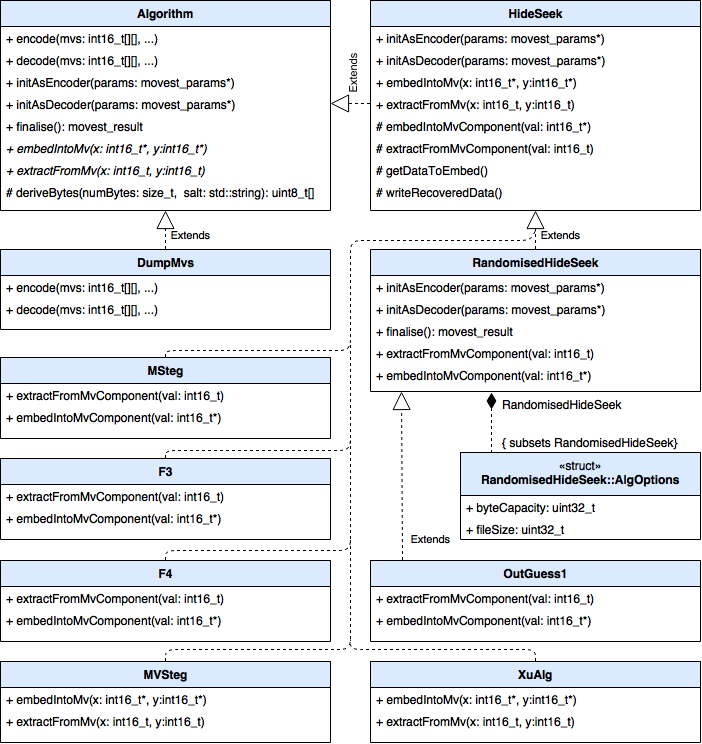
\includegraphics[width=\textwidth]{img/movest_alg_class_diag.png}
\caption{UML diagram of embedding algorithms implemented in \texttt{movestlib}. (Some unimportant fields, methods and method parameters omitted for brevity.)}
\label{fig:movest_alg_class_diag}
\end{figure}

\subsubsection{Class hierarchy}

To encourage modularity and code reuse, the embedding algorithms were implemented as OOP classes. The class hierarchy is presented in Figure \ref{fig:movest_alg_class_diag}. \texttt{Algorithm} is the base class for all embedding algorithms, containing common functionality such as initialising the payload file or operating on every motion vector of a suitable type in turn. Most algorithms, however, extend \texttt{HideSeek} or its subclasses to benefit from the following more specific functionality:

\begin{itemize}
\item Operating on a per-component basis. Motion vectors are stored as $x$ and $y$ components and many algorithms treat them independently (\texttt{RandomisedHideSeek, OutGuess1}).
\item Sequential data fetching and stopping criteria. Some algorithms read and embed payload bits sequentially and require knowledge of when to stop embedding (\texttt{XuAlg, MVSteg}).
\item Both of above (\texttt{MSteg, F3, F4}).
\end{itemize}

\subsubsection{Encryption}
\label{encryption}
Encrypting the payload hides the structure of the data by making it indistinguishable from random noise, making it hard to detect in already-noisy regions, as well as causing it to remain unreadable by an adversary even if steganography was broken. \texttt{movestlib} achieves this by implementing a file-like object for accessing the payload, and encrypting or decrypting the data on the fly (\texttt{MOVEST\_ENCRYPTION} flag). Encryption is done using AES in counter (CTR) mode with a 256-bit key. The key and the initialisation vector are derived from the user-supplied password by performing key stretching using the industry-standard PBKDF2-HMAC-SHA1 key derivation function. Since implementing cryptographic primitives yourself is potentially error-prone, the Crypto++ library was used to provide them. 

\subsection{Encoder and decoder applications}
\label{enc-dec-bin}
The project provides video-processing applications for embedding and recovering the payload from a video file. The two are largely based on FFmpeg examples for transcoding (\texttt{transcoding.c}) and motion vector extraction (\texttt{extract\_mvs.c}), which already contain the code to trigger code paths in FFmpeg that I have modified. Figure \ref{fig:encoder-help} provides an example of options available for the embedding application (encoder).

Before letting FFmpeg process the video, applications parse user input to initialise \texttt{movestlib} with required data, such as the embedding algorithm (\texttt{movest\_init\_algorithm}), the payload file path, and the encryption password (\texttt{movest\_init\_encoder/decoder}). FFmpeg treats sequences of frames as streams, meaning frames are written to the output file sequentially and it is not possible to access a previous or future frame during the embedding process. Algorithms that require estimating certain parameters, such as the embedding capacity of a video, have to make all these decisions in advance. To facilitate this, the encoder performs a dry run (\texttt{MOVEST\_DUMMY\_PASS} flag) which does not modify the motions vectors, in order to collect useful data.

\begin{figure}[tbh]
\vspace{1em}
\centering
\begin{minipage}{0.9\textwidth}
\begingroup
    \fontsize{10pt}{12pt}\selectfont
\begin{alltt}
MOVEST Encoder, (c) 2016
Usage: movest_enc -a <algorithm> -d <data_file> [--encrypt, -p <password>]
<input_video> <output_video>

Command line arguments:
 --encrypt        Perform encryption of the data prior to embedding
 -a/--algorithm   An embedding algorithm to use
 -d/--data        Path to a file, containing the payload
 -p/--password    An encryption password to use
 -h/--help        Print this help message

Available algorithm options:
 'dummypass' (does not embed data)
 'hidenseek' 'msteg' 'f3' 'f4'
 'mvsteg' 'xualg'
 'rand-hidenseek' 'outguess1'
\end{alltt}
\endgroup
\end{minipage}
\caption{User help (\texttt{-{}-help}) of the Movest encoder.}
\label{fig:encoder-help}
\end{figure}

\section{Steganalysis techniques}
\label{steg-tech}

The steganalysis techniques for this project were implemented in Matlab, where the large library of pre-existing statistical and data processing routines makes things considerably simpler.

\subsection{Motion vector import}
\label{mv-import}

The decoder application can be configured to use a special algorithm \texttt{DumpMvs} which outputs motion vector components in a simple text format. Matlab can later import this data as 3D matrices (\texttt{loadmvs.m}), where the element at $(i, j, k)$ refers to a macroblock at $i$-th row, $j$-th column of the $k$-th frame. 

The codec allows for some macroblocks to be omitted. These are called ``skip'' macroblocks, to which the Movest decoder assigns a special type during extraction. In this case, for the sake of completeness of the grid, FFmpeg reports the motion vector being $(0, 0)$, but a user can filter out such stray zeros by using type information (\texttt{typedmvs.m}).

\subsection{LSB plane, 2D plotting and aggregation into bytes}

This project implements Least Significant Bit (LSB) steganography, so the suite includes a function (\texttt{lsbplane.m}) to project least significant bits out of every motion vector component value. If the embedding algorithm sets the LSBs of motion vectors to exactly payload bits, LSBs can be immediately subjected to visual analysis to reveal any patterns in the data. This is best illustrated by an example.

\begin{figure}[tbh]
\centerline{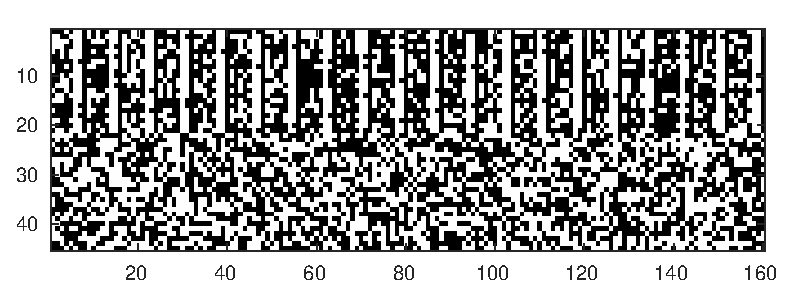
\includegraphics{img/unencrypted-enc.eps}}
\caption{Sample output of \texttt{plot2d} over LSB plane. Even-numbered and odd-numbered columns contain LSBs for $x$ and $y$ components respectively.}
\label{fig:unencrypted-enc}
\end{figure}

Figure \ref{fig:unencrypted-enc} shows an example of a 2-valued heatmap (\texttt{plot2d.m}) produced by the suite. The plot shows a clear pattern of embedded data in the first half of the frame. Given that there are repeating columns of 1s every 8 bits, a steganalyst could make an educated guess that the payload is ASCII-encoded and attempt to group bits into bytes to reproduce the text (\texttt{aggregateIntoBytes.m}):

\begin{alltt}
    >> char\footnote{In Matlab, \texttt{char} interprets an integer value as an ASCII-encoded character.}(aggregateIntoBytes(mvs, types))'
    ans = hello world\ldots
\end{alltt}

\subsection{Histogram and $\chi^2$ (Chi-Squared) Attack}

The distribution of motion vectors can be visualised using a histogram (\texttt{mvhist.m}). This can be a useful source of information for a steganalyst because peculiarities in the histogram can reveal that motion vectors have been modified. MV histograms typically have a sharp peak at 0 and exponentially decay on both sides. Since these histograms are affected by the direction of motion in the video, decay rates may vary, and we may see additional peaks or plateaus. (Figure \ref{fig:histogram-example}).

\begin{figure}[tbh]
\centerline{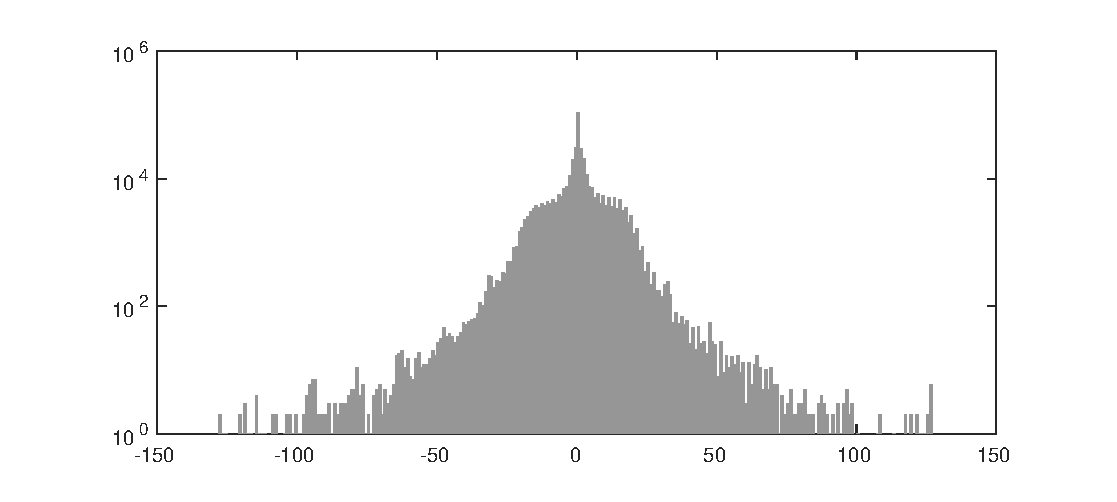
\includegraphics[scale=0.75]{img/histogram-example.eps}}
\caption{Sample output of \texttt{mvhist} for the $x$ component of all motion vectors in a video.}
\label{fig:histogram-example}
\end{figure}

Westfeld and Pfitzmann~\cite{westfeld1999attacks} developed a method for attacking image steganography called the \emph{$\chi^2$ attack}, which can also be applied to motion vectors. They hypothesise that, due to the nature of the data, it is unlikely that adjacent bars of the histogram would be of the same height. 

Let us focus on adjacent bars on a histogram which correspond to even-odd pairs of motion vector values which only differ in the LSB (0 and 1, 2 and 3, 4 and 5, \emph{etc.}). Since the encrypted payload will, on average, have the same number of 0 and 1 bits, so will the LSBs of motion vector values. Therefore, values in such an even-odd pair should occur the same number of times. It also follows that the histogram bars for an even-odd pair should be of the same height.

We can now devise a statistical procedure (\texttt{chiSquareAttack.m}) for determining the probability that a given set of motion vectors contains a secret message. We consider even-odd pairs of values of the form $(2k, 2k+1)$. 

Let $X_k$ and $Y_k$ be the number of times values $2k$ and $2k+1$ occur as motion vector values. Consider also the average of these, $Z_k = \frac{X_k + Y_k}{2}$. If the video contains a payload, $X_k$ and $Y_k$ should be almost equal and distributed as $Z_k$. To prevent influence from the noise in data, pairs that have $Z_k < 8$ are considered to be under-represented and are neglected in further analysis (\emph{minimum frequency condition}\footnote{The original paper specifies $Z_k < 2$, but I found that this threshold was too low for motion vector data.}).

We can use the \emph{$\chi^2$ (chi-square) test} to check the hypothesis that there is no significant difference between $X_k$ and $Z_k$ (null hypothesis). The case for $Y_k$ is symmetric and not considered further. The test tells us we can compute the quantity

$$ \chi^2_{n-1} \approx \sum^{n}_{k=0} \frac{(\text{observed}_k - \text{expected}_k)^2}{\text{expected}_k}= \sum^{255}_{k=-255} \frac{(X_k - Z_k)^2}{Z_k} $$ 

from which we can obtain the $p$-value of data supporting the null hypothesis, which authors interpret as the probability that the cover contains the payload:

$$ p = 1 - \frac{1}{2^{\frac{n-1}{2}}\Gamma(\frac{n-1}{2})}\int_0^{\chi^2_{n-1}}t^{\frac{n-1}{2}−1}e^{-t/2}dt $$  

This method can also estimate the size of the payload. From the expression for $\chi^2_{n-1}$, we see that it is sensitive to small changes: the value stays close to 0 when data contains the payload ($X_k - Z_k \approx 0$) and is big otherwise. We can iteratively build up the histogram and update $\chi^2_{n-1}$ as data for every frame comes in. We know that when the value starts increasing (and $p$-value decreases), the data no longer contains the payload, so we can put a bound on the payload size. 

\subsection{Reversion Technique}
\label{rev-tech-theory}
Cao \emph{et al.}~\cite{cao2012video} proved that decoding then re-encoding (transcoding) a video tends to remove the changes caused by embedding the payload. That is, motion vectors tend to revert to their original values. So, if a video does not contain a payload, we expect differences between respective motion vectors of the original and transcoded video to be near zero.

\begin{wrapfigure}[13]{R}{6cm}
\vspace{-15pt}
\includegraphics[width=5.5cm]{img/movest_reversion_sketch.png}
\caption{Partitioning stego and non-stego videos.}
\label{fig:movest-reversion-sketch}
\end{wrapfigure}

\emph{Sum of absolute differences (SAD)} is used to compute the difference between respective components of motion vectors:

$$ \Delta \overrightarrow{mv^p_{ij}} = |(\overrightarrow{o^p_{ij}})_x - (\overrightarrow{t^p_{ij}})_x| +  |(\overrightarrow{o^p_{ij}})_y - (\overrightarrow{t^p_{ij}})_y|$$

where $\overrightarrow{o^p_{ij}}$ and $\overrightarrow{t^p_{ij}}$ are motion vectors of the original and transcoded video. To determine how common small and large differences are in a video, the algorithm computes a normalised vector of frequencies for every value of $\Delta\overrightarrow{mv^p_{ij}}$. The $k$-th element of the vector gives the proportion of $\Delta\overrightarrow{mv^p_{ij}} = k$ occurring among all SADs.

The reversion hypothesis suggests the following approach for distinguishing between a stego and non-stego video, summarised in Figure \ref{fig:movest-reversion-sketch}:
\begin{itemize}
\item Stego videos will have a lower frequency of small differences ($\Delta\overrightarrow{mv^p_{ij}} < 2$), but a higher frequency of larger differences ($\Delta\overrightarrow{mv^p_{ij}} \geq 2$).
\item Non-stego videos will have a higher frequency of small differences and a lower frequency of larger differences.
\end{itemize}
A classifier can be built to attempt to differentiate between these two classes of video. I decided to use a Support Vector Machine (SVM) with a linear kernel (as Figure \ref{fig:movest-reversion-sketch} suggests), trained using Matlab's \texttt{fitcsvm} routine. Evaluation of this method is presented in section \ref{rev-tech}.

\section{Embedding algorithms}
\label{emb-alg}

This section presents the 8 LSB steganography algorithms implemented by this project.

\subsection{Hide \& Seek}

\emph{Hide \& Seek}~\cite{bateman} is the algorithm which was used as an example in the previous section. The algorithm embeds payload bits into both $x$ and $y$ components of each motion vector by setting their LSB to that of the payload. This achieves the optimal capacity for this type of embedding of 2 bits per macroblock, but is susceptible to all the attacks described in the previous section. 

\begin{figure}[tbh]
\centerline{
\begin{subfigure}[t]{0.4\textwidth}
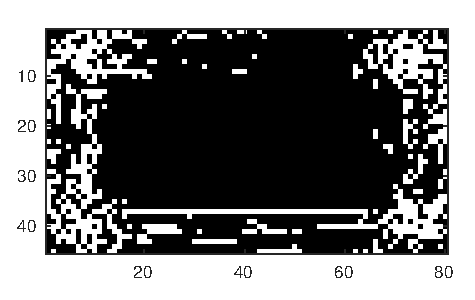
\includegraphics[scale=0.8]{img/pre-lsb-embedding.eps}
\end{subfigure}
~
\begin{subfigure}[t]{0.4\textwidth}
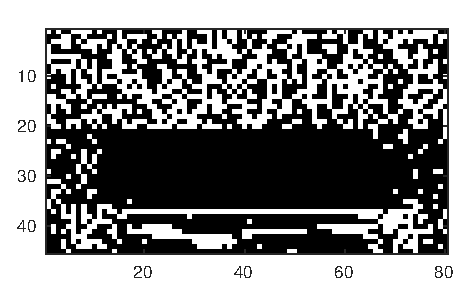
\includegraphics[scale=0.8]{img/post-lsb-embedding.eps}
\end{subfigure}
}
\caption{An example of a frame prior to embedding (left) and after embedding at 45\% capacity (right).}
\label{fig:visual-analysis-example}
\end{figure}

Since data is embedded into all possible macroblocks, visual analysis allows easily spotting it in a non-noisy region. Figure \ref{fig:visual-analysis-example} shows two 2D plots of the same frame: one without the embedding and one with data embedded at about 45\% of capacity. Unusual noise in the first half of the frame exposes the embedding.  

\subsection{MSteg}
\label{msteg}

\emph{MSteg} is my straightforward adaptation of the \emph{JSteg} algorithm~\cite{bateman}, which was initially developed for embedding into JPEG DCT coefficients. The algorithm operates in the same way as Hide \& Seek, but addresses the visual detection problem by not embedding into ``still'' regions, where noise would be easily detectable. From the implementation perspective, it avoids embedding bits into 0-valued $x$ and $y$ components. Components with value 1 are also avoided, since embedding bit 0 would turn them into zeros, making decoding ambiguous.

Figure \ref{fig:msteg-visual} shows that MSteg performs better when subjected to visual analysis. However, we would still expect values in an even-odd pair occur at the same frequency, as described earlier. The histogram in Figure \ref{fig:msteg-hist} confirms this and therefore the $\chi^2$ attack is successful at detecting the embedding (Figure \ref{fig:chisq-attack}).

\begin{figure}[tbh]
\centering
\begin{minipage}[t]{.4\textwidth}
  \centering
  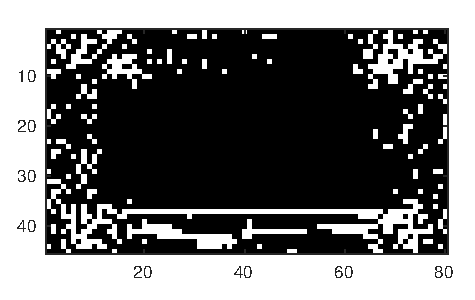
\includegraphics[scale=0.8]{img/msteg-visual.eps}
  \caption{LSB plane of the frame subjected to MSteg embedding.}
  \label{fig:msteg-visual}
\end{minipage}%
\quad\quad
\begin{minipage}[t]{.45\textwidth}
  \centering
  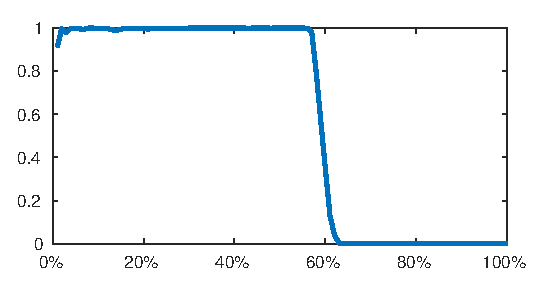
\includegraphics[scale=0.84]{img/chisq-attack.eps}
  \caption{An example of probability of embedding computed by the $\chi^2$ attack when embedding was done at 58\% of capacity.}
  \label{fig:chisq-attack}
\end{minipage}
\end{figure}

\begin{figure}[tbh]
\centering
\resizebox{0.6\textwidth}{!}{%LaTeX with PSTricks extensions
%%Creator: inkscape 0.91
%%Please note this file requires PSTricks extensions
\psset{xunit=.5pt,yunit=.5pt,runit=.5pt}
\begin{pspicture}(349,154)
{
\newrgbcolor{curcolor}{1 1 1}
\pscustom[linestyle=none,fillstyle=solid,fillcolor=curcolor]
{
\newpath
\moveto(0,154)
\lineto(349,154)
\lineto(349,0)
\lineto(0,0)
\closepath
}
}
{
\newrgbcolor{curcolor}{1 1 1}
\pscustom[linestyle=none,fillstyle=solid,fillcolor=curcolor]
{
\newpath
\moveto(0,154)
\lineto(349,154)
\lineto(349,0)
\lineto(0,0)
\closepath
}
}
{
\newrgbcolor{curcolor}{1 1 1}
\pscustom[linestyle=none,fillstyle=solid,fillcolor=curcolor]
{
\newpath
\moveto(25,20)
\lineto(349,20)
\lineto(349,138)
\lineto(25,138)
\closepath
}
}
{
\newrgbcolor{curcolor}{0.14901961 0.14901961 0.14901961}
\pscustom[linewidth=0.66670001,linecolor=curcolor]
{
\newpath
\moveto(25,20)
\lineto(349,20)
}
}
{
\newrgbcolor{curcolor}{0.14901961 0.14901961 0.14901961}
\pscustom[linewidth=0.66670001,linecolor=curcolor]
{
\newpath
\moveto(25,138)
\lineto(349,138)
}
}
{
\newrgbcolor{curcolor}{0.14901961 0.14901961 0.14901961}
\pscustom[linewidth=0.66670001,linecolor=curcolor]
{
\newpath
\moveto(39.72729874,20)
\lineto(39.72729874,23.24000549)
}
}
{
\newrgbcolor{curcolor}{0.14901961 0.14901961 0.14901961}
\pscustom[linewidth=0.66670001,linecolor=curcolor]
{
\newpath
\moveto(113.36360168,20)
\lineto(113.36360168,23.24000549)
}
}
{
\newrgbcolor{curcolor}{0.14901961 0.14901961 0.14901961}
\pscustom[linewidth=0.66670001,linecolor=curcolor]
{
\newpath
\moveto(187,20)
\lineto(187,23.24000549)
}
}
{
\newrgbcolor{curcolor}{0.14901961 0.14901961 0.14901961}
\pscustom[linewidth=0.66670001,linecolor=curcolor]
{
\newpath
\moveto(260.63641357,20)
\lineto(260.63641357,23.24000549)
}
}
{
\newrgbcolor{curcolor}{0.14901961 0.14901961 0.14901961}
\pscustom[linewidth=0.66670001,linecolor=curcolor]
{
\newpath
\moveto(334.27270508,20)
\lineto(334.27270508,23.24000549)
}
}
{
\newrgbcolor{curcolor}{0.14901961 0.14901961 0.14901961}
\pscustom[linewidth=0.66670001,linecolor=curcolor]
{
\newpath
\moveto(39.72729874,138)
\lineto(39.72729874,134.76000023)
}
}
{
\newrgbcolor{curcolor}{0.14901961 0.14901961 0.14901961}
\pscustom[linewidth=0.66670001,linecolor=curcolor]
{
\newpath
\moveto(113.36360168,138)
\lineto(113.36360168,134.76000023)
}
}
{
\newrgbcolor{curcolor}{0.14901961 0.14901961 0.14901961}
\pscustom[linewidth=0.66670001,linecolor=curcolor]
{
\newpath
\moveto(187,138)
\lineto(187,134.76000023)
}
}
{
\newrgbcolor{curcolor}{0.14901961 0.14901961 0.14901961}
\pscustom[linewidth=0.66670001,linecolor=curcolor]
{
\newpath
\moveto(260.63641357,138)
\lineto(260.63641357,134.76000023)
}
}
{
\newrgbcolor{curcolor}{0.14901961 0.14901961 0.14901961}
\pscustom[linewidth=0.66670001,linecolor=curcolor]
{
\newpath
\moveto(334.27270508,138)
\lineto(334.27270508,134.76000023)
}
}
{
\newrgbcolor{curcolor}{0.14901961 0.14901961 0.14901961}
\pscustom[linestyle=none,fillstyle=solid,fillcolor=curcolor]
{
\newpath
\moveto(30.3132375,6.79057812)
\lineto(33.47144062,6.79057812)
\lineto(33.47144062,5.82964062)
\lineto(30.3132375,5.82964062)
\lineto(30.3132375,6.79057812)
\closepath
}
}
{
\newrgbcolor{curcolor}{0.14901961 0.14901961 0.14901961}
\pscustom[linestyle=none,fillstyle=solid,fillcolor=curcolor]
{
\newpath
\moveto(36.36597187,4.01909375)
\lineto(40.49683125,4.01909375)
\lineto(40.49683125,3.023)
\lineto(34.94214375,3.023)
\lineto(34.94214375,4.01909375)
\curveto(35.3913625,4.4839375)(36.00269062,5.10698437)(36.77612812,5.88823437)
\curveto(37.55347187,6.67339062)(38.04175312,7.17925)(38.24097187,7.4058125)
\curveto(38.61987812,7.83159375)(38.88355,8.19096875)(39.0319875,8.4839375)
\curveto(39.18433125,8.7808125)(39.26050312,9.07182812)(39.26050312,9.35698437)
\curveto(39.26050312,9.82182812)(39.09644062,10.20073437)(38.76831562,10.49370312)
\curveto(38.44409687,10.78667187)(38.02026875,10.93315625)(37.49683125,10.93315625)
\curveto(37.1257375,10.93315625)(36.73315937,10.86870312)(36.31909687,10.73979687)
\curveto(35.90894062,10.61089062)(35.4694875,10.41557812)(35.0007375,10.15385937)
\lineto(35.0007375,11.34917187)
\curveto(35.4773,11.54057812)(35.9226125,11.68510937)(36.336675,11.78276562)
\curveto(36.7507375,11.88042187)(37.12964375,11.92925)(37.47339375,11.92925)
\curveto(38.37964375,11.92925)(39.1023,11.7026875)(39.6413625,11.2495625)
\curveto(40.180425,10.7964375)(40.44995625,10.19096875)(40.44995625,9.43315625)
\curveto(40.44995625,9.07378125)(40.38159687,8.73198437)(40.24487812,8.40776562)
\curveto(40.11206562,8.08745312)(39.867925,7.70854687)(39.51245625,7.27104687)
\curveto(39.4148,7.15776562)(39.10425312,6.82964062)(38.58081562,6.28667187)
\curveto(38.05737812,5.74760937)(37.31909687,4.99175)(36.36597187,4.01909375)
\closepath
}
}
{
\newrgbcolor{curcolor}{0.14901961 0.14901961 0.14901961}
\pscustom[linestyle=none,fillstyle=solid,fillcolor=curcolor]
{
\newpath
\moveto(45.51831562,10.99175)
\curveto(44.90894062,10.99175)(44.44995625,10.69096875)(44.1413625,10.08940625)
\curveto(43.836675,9.49175)(43.68433125,8.59135937)(43.68433125,7.38823437)
\curveto(43.68433125,6.18901562)(43.836675,5.288625)(44.1413625,4.6870625)
\curveto(44.44995625,4.08940625)(44.90894062,3.79057812)(45.51831562,3.79057812)
\curveto(46.13159687,3.79057812)(46.59058125,4.08940625)(46.89526875,4.6870625)
\curveto(47.2038625,5.288625)(47.35815937,6.18901562)(47.35815937,7.38823437)
\curveto(47.35815937,8.59135937)(47.2038625,9.49175)(46.89526875,10.08940625)
\curveto(46.59058125,10.69096875)(46.13159687,10.99175)(45.51831562,10.99175)
\closepath
\moveto(45.51831562,11.92925)
\curveto(46.49878437,11.92925)(47.24683125,11.54057812)(47.76245625,10.76323437)
\curveto(48.2819875,9.98979687)(48.54175312,8.86479687)(48.54175312,7.38823437)
\curveto(48.54175312,5.91557812)(48.2819875,4.79057812)(47.76245625,4.01323437)
\curveto(47.24683125,3.23979687)(46.49878437,2.85307812)(45.51831562,2.85307812)
\curveto(44.53784687,2.85307812)(43.78784687,3.23979687)(43.26831562,4.01323437)
\curveto(42.75269062,4.79057812)(42.49487812,5.91557812)(42.49487812,7.38823437)
\curveto(42.49487812,8.86479687)(42.75269062,9.98979687)(43.26831562,10.76323437)
\curveto(43.78784687,11.54057812)(44.53784687,11.92925)(45.51831562,11.92925)
\closepath
}
}
{
\newrgbcolor{curcolor}{0.14901961 0.14901961 0.14901961}
\pscustom[linestyle=none,fillstyle=solid,fillcolor=curcolor]
{
\newpath
\moveto(103.9495375,6.79057812)
\lineto(107.10774063,6.79057812)
\lineto(107.10774063,5.82964062)
\lineto(103.9495375,5.82964062)
\lineto(103.9495375,6.79057812)
\closepath
}
}
{
\newrgbcolor{curcolor}{0.14901961 0.14901961 0.14901961}
\pscustom[linestyle=none,fillstyle=solid,fillcolor=curcolor]
{
\newpath
\moveto(109.18781875,4.01909375)
\lineto(111.1214125,4.01909375)
\lineto(111.1214125,10.69292187)
\lineto(109.01789688,10.27104687)
\lineto(109.01789688,11.34917187)
\lineto(111.10969375,11.77104687)
\lineto(112.2932875,11.77104687)
\lineto(112.2932875,4.01909375)
\lineto(114.22688125,4.01909375)
\lineto(114.22688125,3.023)
\lineto(109.18781875,3.023)
\lineto(109.18781875,4.01909375)
\closepath
}
}
{
\newrgbcolor{curcolor}{0.14901961 0.14901961 0.14901961}
\pscustom[linestyle=none,fillstyle=solid,fillcolor=curcolor]
{
\newpath
\moveto(119.15461563,10.99175)
\curveto(118.54524063,10.99175)(118.08625625,10.69096875)(117.7776625,10.08940625)
\curveto(117.472975,9.49175)(117.32063125,8.59135937)(117.32063125,7.38823437)
\curveto(117.32063125,6.18901562)(117.472975,5.288625)(117.7776625,4.6870625)
\curveto(118.08625625,4.08940625)(118.54524063,3.79057812)(119.15461563,3.79057812)
\curveto(119.76789688,3.79057812)(120.22688125,4.08940625)(120.53156875,4.6870625)
\curveto(120.8401625,5.288625)(120.99445938,6.18901562)(120.99445938,7.38823437)
\curveto(120.99445938,8.59135937)(120.8401625,9.49175)(120.53156875,10.08940625)
\curveto(120.22688125,10.69096875)(119.76789688,10.99175)(119.15461563,10.99175)
\closepath
\moveto(119.15461563,11.92925)
\curveto(120.13508438,11.92925)(120.88313125,11.54057812)(121.39875625,10.76323437)
\curveto(121.9182875,9.98979687)(122.17805313,8.86479687)(122.17805313,7.38823437)
\curveto(122.17805313,5.91557812)(121.9182875,4.79057812)(121.39875625,4.01323437)
\curveto(120.88313125,3.23979687)(120.13508438,2.85307812)(119.15461563,2.85307812)
\curveto(118.17414688,2.85307812)(117.42414688,3.23979687)(116.90461563,4.01323437)
\curveto(116.38899063,4.79057812)(116.13117813,5.91557812)(116.13117813,7.38823437)
\curveto(116.13117813,8.86479687)(116.38899063,9.98979687)(116.90461563,10.76323437)
\curveto(117.42414688,11.54057812)(118.17414688,11.92925)(119.15461563,11.92925)
\closepath
}
}
{
\newrgbcolor{curcolor}{0.14901961 0.14901961 0.14901961}
\pscustom[linestyle=none,fillstyle=solid,fillcolor=curcolor]
{
\newpath
\moveto(186.81445312,10.99175)
\curveto(186.20507812,10.99175)(185.74609375,10.69096875)(185.4375,10.08940625)
\curveto(185.1328125,9.49175)(184.98046875,8.59135937)(184.98046875,7.38823437)
\curveto(184.98046875,6.18901562)(185.1328125,5.288625)(185.4375,4.6870625)
\curveto(185.74609375,4.08940625)(186.20507812,3.79057812)(186.81445312,3.79057812)
\curveto(187.42773438,3.79057812)(187.88671875,4.08940625)(188.19140625,4.6870625)
\curveto(188.5,5.288625)(188.65429688,6.18901562)(188.65429688,7.38823437)
\curveto(188.65429688,8.59135937)(188.5,9.49175)(188.19140625,10.08940625)
\curveto(187.88671875,10.69096875)(187.42773438,10.99175)(186.81445312,10.99175)
\closepath
\moveto(186.81445312,11.92925)
\curveto(187.79492188,11.92925)(188.54296875,11.54057812)(189.05859375,10.76323437)
\curveto(189.578125,9.98979687)(189.83789062,8.86479687)(189.83789062,7.38823437)
\curveto(189.83789062,5.91557812)(189.578125,4.79057812)(189.05859375,4.01323437)
\curveto(188.54296875,3.23979687)(187.79492188,2.85307812)(186.81445312,2.85307812)
\curveto(185.83398438,2.85307812)(185.08398438,3.23979687)(184.56445312,4.01323437)
\curveto(184.04882812,4.79057812)(183.79101562,5.91557812)(183.79101562,7.38823437)
\curveto(183.79101562,8.86479687)(184.04882812,9.98979687)(184.56445312,10.76323437)
\curveto(185.08398438,11.54057812)(185.83398438,11.92925)(186.81445312,11.92925)
\closepath
}
}
{
\newrgbcolor{curcolor}{0.14901961 0.14901961 0.14901961}
\pscustom[linestyle=none,fillstyle=solid,fillcolor=curcolor]
{
\newpath
\moveto(254.12468125,4.01909375)
\lineto(256.058275,4.01909375)
\lineto(256.058275,10.69292187)
\lineto(253.95475937,10.27104687)
\lineto(253.95475937,11.34917187)
\lineto(256.04655625,11.77104687)
\lineto(257.23015,11.77104687)
\lineto(257.23015,4.01909375)
\lineto(259.16374375,4.01909375)
\lineto(259.16374375,3.023)
\lineto(254.12468125,3.023)
\lineto(254.12468125,4.01909375)
\closepath
}
}
{
\newrgbcolor{curcolor}{0.14901961 0.14901961 0.14901961}
\pscustom[linestyle=none,fillstyle=solid,fillcolor=curcolor]
{
\newpath
\moveto(264.09147812,10.99175)
\curveto(263.48210312,10.99175)(263.02311875,10.69096875)(262.714525,10.08940625)
\curveto(262.4098375,9.49175)(262.25749375,8.59135937)(262.25749375,7.38823437)
\curveto(262.25749375,6.18901562)(262.4098375,5.288625)(262.714525,4.6870625)
\curveto(263.02311875,4.08940625)(263.48210312,3.79057812)(264.09147812,3.79057812)
\curveto(264.70475937,3.79057812)(265.16374375,4.08940625)(265.46843125,4.6870625)
\curveto(265.777025,5.288625)(265.93132187,6.18901562)(265.93132187,7.38823437)
\curveto(265.93132187,8.59135937)(265.777025,9.49175)(265.46843125,10.08940625)
\curveto(265.16374375,10.69096875)(264.70475937,10.99175)(264.09147812,10.99175)
\closepath
\moveto(264.09147812,11.92925)
\curveto(265.07194687,11.92925)(265.81999375,11.54057812)(266.33561875,10.76323437)
\curveto(266.85515,9.98979687)(267.11491562,8.86479687)(267.11491562,7.38823437)
\curveto(267.11491562,5.91557812)(266.85515,4.79057812)(266.33561875,4.01323437)
\curveto(265.81999375,3.23979687)(265.07194687,2.85307812)(264.09147812,2.85307812)
\curveto(263.11100937,2.85307812)(262.36100937,3.23979687)(261.84147812,4.01323437)
\curveto(261.32585312,4.79057812)(261.06804062,5.91557812)(261.06804062,7.38823437)
\curveto(261.06804062,8.86479687)(261.32585312,9.98979687)(261.84147812,10.76323437)
\curveto(262.36100937,11.54057812)(263.11100937,11.92925)(264.09147812,11.92925)
\closepath
}
}
{
\newrgbcolor{curcolor}{0.14901961 0.14901961 0.14901961}
\pscustom[linestyle=none,fillstyle=solid,fillcolor=curcolor]
{
\newpath
\moveto(328.57543437,4.01909375)
\lineto(332.70629375,4.01909375)
\lineto(332.70629375,3.023)
\lineto(327.15160625,3.023)
\lineto(327.15160625,4.01909375)
\curveto(327.600825,4.4839375)(328.21215312,5.10698437)(328.98559062,5.88823437)
\curveto(329.76293437,6.67339062)(330.25121562,7.17925)(330.45043437,7.4058125)
\curveto(330.82934062,7.83159375)(331.0930125,8.19096875)(331.24145,8.4839375)
\curveto(331.39379375,8.7808125)(331.46996562,9.07182812)(331.46996562,9.35698437)
\curveto(331.46996562,9.82182812)(331.30590312,10.20073437)(330.97777812,10.49370312)
\curveto(330.65355937,10.78667187)(330.22973125,10.93315625)(329.70629375,10.93315625)
\curveto(329.3352,10.93315625)(328.94262187,10.86870312)(328.52855937,10.73979687)
\curveto(328.11840312,10.61089062)(327.67895,10.41557812)(327.2102,10.15385937)
\lineto(327.2102,11.34917187)
\curveto(327.6867625,11.54057812)(328.132075,11.68510937)(328.5461375,11.78276562)
\curveto(328.9602,11.88042187)(329.33910625,11.92925)(329.68285625,11.92925)
\curveto(330.58910625,11.92925)(331.3117625,11.7026875)(331.850825,11.2495625)
\curveto(332.3898875,10.7964375)(332.65941875,10.19096875)(332.65941875,9.43315625)
\curveto(332.65941875,9.07378125)(332.59105937,8.73198437)(332.45434062,8.40776562)
\curveto(332.32152812,8.08745312)(332.0773875,7.70854687)(331.72191875,7.27104687)
\curveto(331.6242625,7.15776562)(331.31371562,6.82964062)(330.79027812,6.28667187)
\curveto(330.26684062,5.74760937)(329.52855937,4.99175)(328.57543437,4.01909375)
\closepath
}
}
{
\newrgbcolor{curcolor}{0.14901961 0.14901961 0.14901961}
\pscustom[linestyle=none,fillstyle=solid,fillcolor=curcolor]
{
\newpath
\moveto(337.72777812,10.99175)
\curveto(337.11840312,10.99175)(336.65941875,10.69096875)(336.350825,10.08940625)
\curveto(336.0461375,9.49175)(335.89379375,8.59135937)(335.89379375,7.38823437)
\curveto(335.89379375,6.18901562)(336.0461375,5.288625)(336.350825,4.6870625)
\curveto(336.65941875,4.08940625)(337.11840312,3.79057812)(337.72777812,3.79057812)
\curveto(338.34105937,3.79057812)(338.80004375,4.08940625)(339.10473125,4.6870625)
\curveto(339.413325,5.288625)(339.56762187,6.18901562)(339.56762187,7.38823437)
\curveto(339.56762187,8.59135937)(339.413325,9.49175)(339.10473125,10.08940625)
\curveto(338.80004375,10.69096875)(338.34105937,10.99175)(337.72777812,10.99175)
\closepath
\moveto(337.72777812,11.92925)
\curveto(338.70824687,11.92925)(339.45629375,11.54057812)(339.97191875,10.76323437)
\curveto(340.49145,9.98979687)(340.75121562,8.86479687)(340.75121562,7.38823437)
\curveto(340.75121562,5.91557812)(340.49145,4.79057812)(339.97191875,4.01323437)
\curveto(339.45629375,3.23979687)(338.70824687,2.85307812)(337.72777812,2.85307812)
\curveto(336.74730937,2.85307812)(335.99730937,3.23979687)(335.47777812,4.01323437)
\curveto(334.96215312,4.79057812)(334.70434062,5.91557812)(334.70434062,7.38823437)
\curveto(334.70434062,8.86479687)(334.96215312,9.98979687)(335.47777812,10.76323437)
\curveto(335.99730937,11.54057812)(336.74730937,11.92925)(337.72777812,11.92925)
\closepath
}
}
{
\newrgbcolor{curcolor}{0.14901961 0.14901961 0.14901961}
\pscustom[linewidth=0.66670001,linecolor=curcolor]
{
\newpath
\moveto(25,20)
\lineto(25,138)
}
}
{
\newrgbcolor{curcolor}{0.14901961 0.14901961 0.14901961}
\pscustom[linewidth=0.66670001,linecolor=curcolor]
{
\newpath
\moveto(349,20)
\lineto(349,138)
}
}
{
\newrgbcolor{curcolor}{0.14901961 0.14901961 0.14901961}
\pscustom[linewidth=0.66670001,linecolor=curcolor]
{
\newpath
\moveto(25,46.85269928)
\lineto(28.23999977,46.85269928)
}
}
{
\newrgbcolor{curcolor}{0.14901961 0.14901961 0.14901961}
\pscustom[linewidth=0.66670001,linecolor=curcolor]
{
\newpath
\moveto(25,94.21480179)
\lineto(28.23999977,94.21480179)
}
}
{
\newrgbcolor{curcolor}{0.14901961 0.14901961 0.14901961}
\pscustom[linewidth=0.66670001,linecolor=curcolor]
{
\newpath
\moveto(25,121.9197998)
\lineto(28.23999977,121.9197998)
}
}
{
\newrgbcolor{curcolor}{0.14901961 0.14901961 0.14901961}
\pscustom[linewidth=0.66670001,linecolor=curcolor]
{
\newpath
\moveto(349,46.85269928)
\lineto(345.76000977,46.85269928)
}
}
{
\newrgbcolor{curcolor}{0.14901961 0.14901961 0.14901961}
\pscustom[linewidth=0.66670001,linecolor=curcolor]
{
\newpath
\moveto(349,94.21480179)
\lineto(345.76000977,94.21480179)
}
}
{
\newrgbcolor{curcolor}{0.14901961 0.14901961 0.14901961}
\pscustom[linewidth=0.66670001,linecolor=curcolor]
{
\newpath
\moveto(349,121.9197998)
\lineto(345.76000977,121.9197998)
}
}
{
\newrgbcolor{curcolor}{0.14901961 0.14901961 0.14901961}
\pscustom[linewidth=0.66670001,linecolor=curcolor]
{
\newpath
\moveto(25,74.55770111)
\lineto(26.62000084,74.55770111)
}
}
{
\newrgbcolor{curcolor}{0.14901961 0.14901961 0.14901961}
\pscustom[linewidth=0.66670001,linecolor=curcolor]
{
\newpath
\moveto(25,109.4618988)
\lineto(26.62000084,109.4618988)
}
}
{
\newrgbcolor{curcolor}{0.14901961 0.14901961 0.14901961}
\pscustom[linewidth=0.66670001,linecolor=curcolor]
{
\newpath
\moveto(25,132.45280075)
\lineto(26.62000084,132.45280075)
}
}
{
\newrgbcolor{curcolor}{0.14901961 0.14901961 0.14901961}
\pscustom[linewidth=0.66670001,linecolor=curcolor]
{
\newpath
\moveto(349,74.55770111)
\lineto(347.38000488,74.55770111)
}
}
{
\newrgbcolor{curcolor}{0.14901961 0.14901961 0.14901961}
\pscustom[linewidth=0.66670001,linecolor=curcolor]
{
\newpath
\moveto(349,109.4618988)
\lineto(347.38000488,109.4618988)
}
}
{
\newrgbcolor{curcolor}{0.14901961 0.14901961 0.14901961}
\pscustom[linewidth=0.66670001,linecolor=curcolor]
{
\newpath
\moveto(349,132.45280075)
\lineto(347.38000488,132.45280075)
}
}
{
\newrgbcolor{curcolor}{0.14901961 0.14901961 0.14901961}
\pscustom[linestyle=none,fillstyle=solid,fillcolor=curcolor]
{
\newpath
\moveto(3.83745312,50.32145)
\curveto(3.22807812,50.32145)(2.76909375,50.02066875)(2.4605,49.41910625)
\curveto(2.1558125,48.82145)(2.00346875,47.92105937)(2.00346875,46.71793437)
\curveto(2.00346875,45.51871562)(2.1558125,44.618325)(2.4605,44.0167625)
\curveto(2.76909375,43.41910625)(3.22807812,43.12027812)(3.83745312,43.12027812)
\curveto(4.45073437,43.12027812)(4.90971875,43.41910625)(5.21440625,44.0167625)
\curveto(5.523,44.618325)(5.67729687,45.51871562)(5.67729687,46.71793437)
\curveto(5.67729687,47.92105937)(5.523,48.82145)(5.21440625,49.41910625)
\curveto(4.90971875,50.02066875)(4.45073437,50.32145)(3.83745312,50.32145)
\closepath
\moveto(3.83745312,51.25895)
\curveto(4.81792187,51.25895)(5.56596875,50.87027812)(6.08159375,50.09293437)
\curveto(6.601125,49.31949687)(6.86089062,48.19449687)(6.86089062,46.71793437)
\curveto(6.86089062,45.24527812)(6.601125,44.12027812)(6.08159375,43.34293437)
\curveto(5.56596875,42.56949687)(4.81792187,42.18277812)(3.83745312,42.18277812)
\curveto(2.85698437,42.18277812)(2.10698437,42.56949687)(1.58745312,43.34293437)
\curveto(1.07182812,44.12027812)(0.81401562,45.24527812)(0.81401562,46.71793437)
\curveto(0.81401562,48.19449687)(1.07182812,49.31949687)(1.58745312,50.09293437)
\curveto(2.10698437,50.87027812)(2.85698437,51.25895)(3.83745312,51.25895)
\closepath
}
}
{
\newrgbcolor{curcolor}{0.14901961 0.14901961 0.14901961}
\pscustom[linestyle=none,fillstyle=solid,fillcolor=curcolor]
{
\newpath
\moveto(8.94682812,43.84098125)
\lineto(10.18315625,43.84098125)
\lineto(10.18315625,42.3527)
\lineto(8.94682812,42.3527)
\lineto(8.94682812,43.84098125)
\closepath
}
}
{
\newrgbcolor{curcolor}{0.14901961 0.14901961 0.14901961}
\pscustom[linestyle=none,fillstyle=solid,fillcolor=curcolor]
{
\newpath
\moveto(12.77885937,51.10074687)
\lineto(17.42534375,51.10074687)
\lineto(17.42534375,50.10465312)
\lineto(13.86284375,50.10465312)
\lineto(13.86284375,47.96012187)
\curveto(14.03471875,48.01871562)(14.20659375,48.06168437)(14.37846875,48.08902812)
\curveto(14.55034375,48.12027812)(14.72221875,48.13590312)(14.89409375,48.13590312)
\curveto(15.87065625,48.13590312)(16.64409375,47.868325)(17.21440625,47.33316875)
\curveto(17.78471875,46.7980125)(18.069875,46.07340312)(18.069875,45.15934062)
\curveto(18.069875,44.21793437)(17.77690625,43.4855125)(17.19096875,42.962075)
\curveto(16.60503125,42.44254375)(15.77885937,42.18277812)(14.71245312,42.18277812)
\curveto(14.34526562,42.18277812)(13.97026562,42.21402812)(13.58745312,42.27652812)
\curveto(13.20854687,42.33902812)(12.81596875,42.43277812)(12.40971875,42.55777812)
\lineto(12.40971875,43.74723125)
\curveto(12.76128125,43.555825)(13.1245625,43.41324687)(13.4995625,43.31949687)
\curveto(13.8745625,43.22574687)(14.27104687,43.17887187)(14.68901562,43.17887187)
\curveto(15.36479687,43.17887187)(15.89995312,43.35660625)(16.29448437,43.712075)
\curveto(16.68901562,44.06754375)(16.88628125,44.54996562)(16.88628125,45.15934062)
\curveto(16.88628125,45.76871562)(16.68901562,46.2511375)(16.29448437,46.60660625)
\curveto(15.89995312,46.962075)(15.36479687,47.13980937)(14.68901562,47.13980937)
\curveto(14.37260937,47.13980937)(14.05620312,47.10465312)(13.73979687,47.03434062)
\curveto(13.42729687,46.96402812)(13.10698437,46.85465312)(12.77885937,46.70621562)
\lineto(12.77885937,51.10074687)
\closepath
}
}
{
\newrgbcolor{curcolor}{0.14901961 0.14901961 0.14901961}
\pscustom[linestyle=none,fillstyle=solid,fillcolor=curcolor]
{
\newpath
\moveto(13.51128125,90.71089375)
\lineto(15.444875,90.71089375)
\lineto(15.444875,97.38472187)
\lineto(13.34135937,96.96284687)
\lineto(13.34135937,98.04097187)
\lineto(15.43315625,98.46284687)
\lineto(16.61675,98.46284687)
\lineto(16.61675,90.71089375)
\lineto(18.55034375,90.71089375)
\lineto(18.55034375,89.7148)
\lineto(13.51128125,89.7148)
\lineto(13.51128125,90.71089375)
\closepath
}
}
{
\newrgbcolor{curcolor}{0.14901961 0.14901961 0.14901961}
\pscustom[linestyle=none,fillstyle=solid,fillcolor=curcolor]
{
\newpath
\moveto(1.51128125,118.41589375)
\lineto(3.444875,118.41589375)
\lineto(3.444875,125.08972188)
\lineto(1.34135937,124.66784688)
\lineto(1.34135937,125.74597188)
\lineto(3.43315625,126.16784688)
\lineto(4.61675,126.16784688)
\lineto(4.61675,118.41589375)
\lineto(6.55034375,118.41589375)
\lineto(6.55034375,117.4198)
\lineto(1.51128125,117.4198)
\lineto(1.51128125,118.41589375)
\closepath
}
}
{
\newrgbcolor{curcolor}{0.14901961 0.14901961 0.14901961}
\pscustom[linestyle=none,fillstyle=solid,fillcolor=curcolor]
{
\newpath
\moveto(8.94682812,118.90808125)
\lineto(10.18315625,118.90808125)
\lineto(10.18315625,117.4198)
\lineto(8.94682812,117.4198)
\lineto(8.94682812,118.90808125)
\closepath
}
}
{
\newrgbcolor{curcolor}{0.14901961 0.14901961 0.14901961}
\pscustom[linestyle=none,fillstyle=solid,fillcolor=curcolor]
{
\newpath
\moveto(12.77885937,126.16784688)
\lineto(17.42534375,126.16784688)
\lineto(17.42534375,125.17175313)
\lineto(13.86284375,125.17175313)
\lineto(13.86284375,123.02722188)
\curveto(14.03471875,123.08581563)(14.20659375,123.12878438)(14.37846875,123.15612813)
\curveto(14.55034375,123.18737813)(14.72221875,123.20300313)(14.89409375,123.20300313)
\curveto(15.87065625,123.20300313)(16.64409375,122.935425)(17.21440625,122.40026875)
\curveto(17.78471875,121.8651125)(18.069875,121.14050313)(18.069875,120.22644063)
\curveto(18.069875,119.28503438)(17.77690625,118.5526125)(17.19096875,118.029175)
\curveto(16.60503125,117.50964375)(15.77885937,117.24987813)(14.71245312,117.24987813)
\curveto(14.34526562,117.24987813)(13.97026562,117.28112813)(13.58745312,117.34362813)
\curveto(13.20854687,117.40612813)(12.81596875,117.49987813)(12.40971875,117.62487813)
\lineto(12.40971875,118.81433125)
\curveto(12.76128125,118.622925)(13.1245625,118.48034688)(13.4995625,118.38659688)
\curveto(13.8745625,118.29284688)(14.27104687,118.24597188)(14.68901562,118.24597188)
\curveto(15.36479687,118.24597188)(15.89995312,118.42370625)(16.29448437,118.779175)
\curveto(16.68901562,119.13464375)(16.88628125,119.61706563)(16.88628125,120.22644063)
\curveto(16.88628125,120.83581563)(16.68901562,121.3182375)(16.29448437,121.67370625)
\curveto(15.89995312,122.029175)(15.36479687,122.20690938)(14.68901562,122.20690938)
\curveto(14.37260937,122.20690938)(14.05620312,122.17175313)(13.73979687,122.10144063)
\curveto(13.42729687,122.03112813)(13.10698437,121.92175313)(12.77885937,121.77331563)
\lineto(12.77885937,126.16784688)
\closepath
}
}
{
\newrgbcolor{curcolor}{0.14901961 0.14901961 0.14901961}
\pscustom[linestyle=none,fillstyle=solid,fillcolor=curcolor]
{
\newpath
\moveto(31.03710938,147.015625)
\lineto(28.86181641,144.08837891)
\lineto(31.14990234,141)
\lineto(29.984375,141)
\lineto(28.23339844,143.36328125)
\lineto(26.48242188,141)
\lineto(25.31689453,141)
\lineto(27.65332031,144.14746094)
\lineto(25.515625,147.015625)
\lineto(26.68115234,147.015625)
\lineto(28.27636719,144.87255859)
\lineto(29.87158203,147.015625)
\lineto(31.03710938,147.015625)
\closepath
}
}
{
\newrgbcolor{curcolor}{0.14901961 0.14901961 0.14901961}
\pscustom[linestyle=none,fillstyle=solid,fillcolor=curcolor]
{
\newpath
\moveto(35.36425781,141.91308594)
\lineto(37.13671875,141.91308594)
\lineto(37.13671875,148.03076172)
\lineto(35.20849609,147.64404297)
\lineto(35.20849609,148.63232422)
\lineto(37.12597656,149.01904297)
\lineto(38.2109375,149.01904297)
\lineto(38.2109375,141.91308594)
\lineto(39.98339844,141.91308594)
\lineto(39.98339844,141)
\lineto(35.36425781,141)
\lineto(35.36425781,141.91308594)
\closepath
}
}
{
\newrgbcolor{curcolor}{0.14901961 0.14901961 0.14901961}
\pscustom[linestyle=none,fillstyle=solid,fillcolor=curcolor]
{
\newpath
\moveto(44.50048828,148.3046875)
\curveto(43.94189453,148.3046875)(43.52115885,148.02897135)(43.23828125,147.47753906)
\curveto(42.95898438,146.9296875)(42.81933594,146.10432943)(42.81933594,145.00146484)
\curveto(42.81933594,143.90218099)(42.95898438,143.07682292)(43.23828125,142.52539062)
\curveto(43.52115885,141.97753906)(43.94189453,141.70361328)(44.50048828,141.70361328)
\curveto(45.06266276,141.70361328)(45.48339844,141.97753906)(45.76269531,142.52539062)
\curveto(46.04557292,143.07682292)(46.18701172,143.90218099)(46.18701172,145.00146484)
\curveto(46.18701172,146.10432943)(46.04557292,146.9296875)(45.76269531,147.47753906)
\curveto(45.48339844,148.02897135)(45.06266276,148.3046875)(44.50048828,148.3046875)
\closepath
\moveto(44.50048828,149.1640625)
\curveto(45.3992513,149.1640625)(46.08496094,148.80777995)(46.55761719,148.09521484)
\curveto(47.03385417,147.38623047)(47.27197266,146.35498047)(47.27197266,145.00146484)
\curveto(47.27197266,143.65152995)(47.03385417,142.62027995)(46.55761719,141.90771484)
\curveto(46.08496094,141.19873047)(45.3992513,140.84423828)(44.50048828,140.84423828)
\curveto(43.60172526,140.84423828)(42.91422526,141.19873047)(42.43798828,141.90771484)
\curveto(41.96533203,142.62027995)(41.72900391,143.65152995)(41.72900391,145.00146484)
\curveto(41.72900391,146.35498047)(41.96533203,147.38623047)(42.43798828,148.09521484)
\curveto(42.91422526,148.80777995)(43.60172526,149.1640625)(44.50048828,149.1640625)
\closepath
}
}
{
\newrgbcolor{curcolor}{0.14901961 0.14901961 0.14901961}
\pscustom[linestyle=none,fillstyle=solid,fillcolor=curcolor]
{
\newpath
\moveto(51.0234375,151.14453125)
\lineto(49.03125,148.03125)
\lineto(51.0234375,148.03125)
\lineto(51.0234375,151.14453125)
\closepath
\moveto(50.81640625,151.83203125)
\lineto(51.80859375,151.83203125)
\lineto(51.80859375,148.03125)
\lineto(52.640625,148.03125)
\lineto(52.640625,147.375)
\lineto(51.80859375,147.375)
\lineto(51.80859375,146)
\lineto(51.0234375,146)
\lineto(51.0234375,147.375)
\lineto(48.390625,147.375)
\lineto(48.390625,148.13671875)
\lineto(50.81640625,151.83203125)
\closepath
}
}
{
\newrgbcolor{curcolor}{0 0.44705883 0.74117649}
\pscustom[linestyle=none,fillstyle=solid,fillcolor=curcolor,opacity=0.60000002]
{
\newpath
\moveto(39.7273,19.9882)
\lineto(39.7273,27.8666)
\lineto(47.0909,27.8666)
\lineto(47.0909,19.9882)
\closepath
}
}
{
\newrgbcolor{curcolor}{0 0.44705883 0.74117649}
\pscustom[linestyle=none,fillstyle=solid,fillcolor=curcolor,opacity=0.60000002]
{
\newpath
\moveto(47.0909,19.9882)
\lineto(47.0909,28.2982)
\lineto(54.4545,28.2982)
\lineto(54.4545,19.9882)
\closepath
}
}
{
\newrgbcolor{curcolor}{0.80000001 1 0.25882354}
\pscustom[linestyle=none,fillstyle=solid,fillcolor=curcolor,opacity=0.60000002]
{
\newpath
\moveto(54.4545,19.9882)
\lineto(54.4545,39.1812)
\lineto(61.8182,39.1812)
\lineto(61.8182,19.9882)
\closepath
}
}
{
\newrgbcolor{curcolor}{0.80000001 1 0.25882354}
\pscustom[linestyle=none,fillstyle=solid,fillcolor=curcolor,opacity=0.60000002]
{
\newpath
\moveto(61.8182,19.9882)
\lineto(61.8182,39.8961)
\lineto(69.1818,39.8961)
\lineto(69.1818,19.9882)
\closepath
}
}
{
\newrgbcolor{curcolor}{0 0.56862748 0}
\pscustom[linestyle=none,fillstyle=solid,fillcolor=curcolor,opacity=0.60000002]
{
\newpath
\moveto(69.1818,19.9882)
\lineto(69.1818,47.0438)
\lineto(76.5455,47.0438)
\lineto(76.5455,19.9882)
\closepath
}
}
{
\newrgbcolor{curcolor}{0 0.56862748 0}
\pscustom[linestyle=none,fillstyle=solid,fillcolor=curcolor,opacity=0.60000002]
{
\newpath
\moveto(76.5455,19.9882)
\lineto(76.5455,48.3129)
\lineto(83.9091,48.3129)
\lineto(83.9091,19.9882)
\closepath
}
}
{
\newrgbcolor{curcolor}{0.94509804 0.79215688 1}
\pscustom[linestyle=none,fillstyle=solid,fillcolor=curcolor,opacity=0.60000002]
{
\newpath
\moveto(83.9091,19.9882)
\lineto(83.9091,49.48)
\lineto(91.2727,49.48)
\lineto(91.2727,19.9882)
\closepath
}
}
{
\newrgbcolor{curcolor}{0.94509804 0.79215688 1}
\pscustom[linestyle=none,fillstyle=solid,fillcolor=curcolor,opacity=0.60000002]
{
\newpath
\moveto(91.2727,19.9882)
\lineto(91.2727,49.5458)
\lineto(98.6364,49.5458)
\lineto(98.6364,19.9882)
\closepath
}
}
{
\newrgbcolor{curcolor}{0.72941178 0 1}
\pscustom[linestyle=none,fillstyle=solid,fillcolor=curcolor,opacity=0.60000002]
{
\newpath
\moveto(98.6364,19.9882)
\lineto(98.6364,57.1823)
\lineto(106,57.1823)
\lineto(106,19.9882)
\closepath
}
}
{
\newrgbcolor{curcolor}{0.72941178 0 1}
\pscustom[linestyle=none,fillstyle=solid,fillcolor=curcolor,opacity=0.60000002]
{
\newpath
\moveto(106,19.9882)
\lineto(106,53.3652)
\lineto(113.3636,53.3652)
\lineto(113.3636,19.9882)
\closepath
}
}
{
\newrgbcolor{curcolor}{0.40000001 0.40000001 0.40000001}
\pscustom[linestyle=none,fillstyle=solid,fillcolor=curcolor,opacity=0.60000002]
{
\newpath
\moveto(113.3636,19.9882)
\lineto(113.3636,57.6623)
\lineto(120.7273,57.6623)
\lineto(120.7273,19.9882)
\closepath
}
}
{
\newrgbcolor{curcolor}{0.40000001 0.40000001 0.40000001}
\pscustom[linestyle=none,fillstyle=solid,fillcolor=curcolor,opacity=0.60000002]
{
\newpath
\moveto(120.7273,19.9882)
\lineto(120.7273,56.9705)
\lineto(128.0909,56.9705)
\lineto(128.0909,19.9882)
\closepath
}
}
{
\newrgbcolor{curcolor}{0.09803922 0.68235296 1}
\pscustom[linestyle=none,fillstyle=solid,fillcolor=curcolor,opacity=0.60000002]
{
\newpath
\moveto(128.0909,19.9882)
\lineto(128.0909,64.0293)
\lineto(135.4545,64.0293)
\lineto(135.4545,19.9882)
\closepath
}
}
{
\newrgbcolor{curcolor}{0.09803922 0.68235296 1}
\pscustom[linestyle=none,fillstyle=solid,fillcolor=curcolor,opacity=0.60000002]
{
\newpath
\moveto(135.4545,19.9882)
\lineto(135.4545,65.199)
\lineto(142.8182,65.199)
\lineto(142.8182,19.9882)
\closepath
}
}
{
\newrgbcolor{curcolor}{0 0.36078432 0.58039218}
\pscustom[linestyle=none,fillstyle=solid,fillcolor=curcolor,opacity=0.60000002]
{
\newpath
\moveto(142.8182,19.9882)
\lineto(142.8182,86.2828)
\lineto(150.1818,86.2828)
\lineto(150.1818,19.9882)
\closepath
}
}
{
\newrgbcolor{curcolor}{0 0.36078432 0.58039218}
\pscustom[linestyle=none,fillstyle=solid,fillcolor=curcolor,opacity=0.60000002]
{
\newpath
\moveto(150.1818,19.9882)
\lineto(150.1818,84.9265)
\lineto(157.5455,84.9265)
\lineto(157.5455,19.9882)
\closepath
}
}
{
\newrgbcolor{curcolor}{1 0.25490198 0.25490198}
\pscustom[linestyle=none,fillstyle=solid,fillcolor=curcolor,opacity=0.60000002]
{
\newpath
\moveto(157.5455,19.9882)
\lineto(157.5455,128.9027)
\lineto(164.9091,128.9027)
\lineto(164.9091,19.9882)
\closepath
}
}
{
\newrgbcolor{curcolor}{1 0.25490198 0.25490198}
\pscustom[linestyle=none,fillstyle=solid,fillcolor=curcolor,opacity=0.60000002]
{
\newpath
\moveto(164.9091,19.9882)
\lineto(164.9091,128.8122)
\lineto(172.2727,128.8122)
\lineto(172.2727,19.9882)
\closepath
}
}
{
\newrgbcolor{curcolor}{0.70980394 0 0}
\pscustom[linestyle=none,fillstyle=solid,fillcolor=curcolor,opacity=0.60000002]
{
\newpath
\moveto(172.2727,19.9882)
\lineto(172.2727,138.0118)
\lineto(179.6364,138.0118)
\lineto(179.6364,19.9882)
\closepath
}
}
{
\newrgbcolor{curcolor}{0.70980394 0 0}
\pscustom[linestyle=none,fillstyle=solid,fillcolor=curcolor,opacity=0.60000002]
{
\newpath
\moveto(179.6364,19.9882)
\lineto(179.6364,138.0118)
\lineto(187,138.0118)
\lineto(187,19.9882)
\closepath
}
}
{
\newrgbcolor{curcolor}{0.60392159 0.87058824 0}
\pscustom[linestyle=none,fillstyle=solid,fillcolor=curcolor,opacity=0.60000002]
{
\newpath
\moveto(187,19.9882)
\lineto(187,138.0118)
\lineto(194.3636,138.0118)
\lineto(194.3636,19.9882)
\closepath
}
}
{
\newrgbcolor{curcolor}{0.60392159 0.87058824 0}
\pscustom[linestyle=none,fillstyle=solid,fillcolor=curcolor,opacity=0.60000002]
{
\newpath
\moveto(194.3636,19.9882)
\lineto(194.3636,138.0118)
\lineto(201.7273,138.0118)
\lineto(201.7273,19.9882)
\closepath
}
}
{
\newrgbcolor{curcolor}{0 0.56862748 0}
\pscustom[linestyle=none,fillstyle=solid,fillcolor=curcolor,opacity=0.60000002]
{
\newpath
\moveto(201.7273,19.9882)
\lineto(201.7273,138.0118)
\lineto(209.0909,138.0118)
\lineto(209.0909,19.9882)
\closepath
}
}
{
\newrgbcolor{curcolor}{0 0.56862748 0}
\pscustom[linestyle=none,fillstyle=solid,fillcolor=curcolor,opacity=0.60000002]
{
\newpath
\moveto(209.0909,19.9882)
\lineto(209.0909,138.0118)
\lineto(216.4545,138.0118)
\lineto(216.4545,19.9882)
\closepath
}
}
{
\newrgbcolor{curcolor}{0.94509804 0.79215688 1}
\pscustom[linestyle=none,fillstyle=solid,fillcolor=curcolor,opacity=0.60000002]
{
\newpath
\moveto(216.4545,19.9882)
\lineto(216.4545,97.8213)
\lineto(223.8182,97.8213)
\lineto(223.8182,19.9882)
\closepath
}
}
{
\newrgbcolor{curcolor}{0.94509804 0.79215688 1}
\pscustom[linestyle=none,fillstyle=solid,fillcolor=curcolor,opacity=0.60000002]
{
\newpath
\moveto(223.8182,19.9882)
\lineto(223.8182,98.6972)
\lineto(231.1818,98.6972)
\lineto(231.1818,19.9882)
\closepath
}
}
{
\newrgbcolor{curcolor}{0.72941178 0 1}
\pscustom[linestyle=none,fillstyle=solid,fillcolor=curcolor,opacity=0.60000002]
{
\newpath
\moveto(231.1818,19.9882)
\lineto(231.1818,72.1092)
\lineto(238.5455,72.1092)
\lineto(238.5455,19.9882)
\closepath
}
}
{
\newrgbcolor{curcolor}{0.72941178 0 1}
\pscustom[linestyle=none,fillstyle=solid,fillcolor=curcolor,opacity=0.60000002]
{
\newpath
\moveto(238.5455,19.9882)
\lineto(238.5455,73.0284)
\lineto(245.9091,73.0284)
\lineto(245.9091,19.9882)
\closepath
}
}
{
\newrgbcolor{curcolor}{0.21176471 0.30588236 0.34901962}
\pscustom[linestyle=none,fillstyle=solid,fillcolor=curcolor,opacity=0.60000002]
{
\newpath
\moveto(245.9091,19.9882)
\lineto(245.9091,66.1329)
\lineto(253.2727,66.1329)
\lineto(253.2727,19.9882)
\closepath
}
}
{
\newrgbcolor{curcolor}{0.21176471 0.30588236 0.34901962}
\pscustom[linestyle=none,fillstyle=solid,fillcolor=curcolor,opacity=0.60000002]
{
\newpath
\moveto(253.2727,19.9882)
\lineto(253.2727,65.2825)
\lineto(260.6364,65.2825)
\lineto(260.6364,19.9882)
\closepath
}
}
{
\newrgbcolor{curcolor}{0.09803922 0.68235296 1}
\pscustom[linestyle=none,fillstyle=solid,fillcolor=curcolor,opacity=0.60000002]
{
\newpath
\moveto(260.6364,19.9882)
\lineto(260.6364,60.2718)
\lineto(268,60.2718)
\lineto(268,19.9882)
\closepath
}
}
{
\newrgbcolor{curcolor}{0.09803922 0.68235296 1}
\pscustom[linestyle=none,fillstyle=solid,fillcolor=curcolor,opacity=0.60000002]
{
\newpath
\moveto(268,19.9882)
\lineto(268,63.1845)
\lineto(275.3636,63.1845)
\lineto(275.3636,19.9882)
\closepath
}
}
{
\newrgbcolor{curcolor}{0 0.36078432 0.58039218}
\pscustom[linestyle=none,fillstyle=solid,fillcolor=curcolor,opacity=0.60000002]
{
\newpath
\moveto(275.3636,19.9882)
\lineto(275.3636,59.5493)
\lineto(282.7273,59.5493)
\lineto(282.7273,19.9882)
\closepath
}
}
{
\newrgbcolor{curcolor}{0 0.36078432 0.58039218}
\pscustom[linestyle=none,fillstyle=solid,fillcolor=curcolor,opacity=0.60000002]
{
\newpath
\moveto(282.7273,19.9882)
\lineto(282.7273,62.1218)
\lineto(290.0909,62.1218)
\lineto(290.0909,19.9882)
\closepath
}
}
{
\newrgbcolor{curcolor}{1 0.25490198 0.25490198}
\pscustom[linestyle=none,fillstyle=solid,fillcolor=curcolor,opacity=0.60000002]
{
\newpath
\moveto(290.0909,19.9882)
\lineto(290.0909,56.8998)
\lineto(297.4545,56.8998)
\lineto(297.4545,19.9882)
\closepath
}
}
{
\newrgbcolor{curcolor}{1 0.25490198 0.25490198}
\pscustom[linestyle=none,fillstyle=solid,fillcolor=curcolor,opacity=0.60000002]
{
\newpath
\moveto(297.4545,19.9882)
\lineto(297.4545,59.265)
\lineto(304.8182,59.265)
\lineto(304.8182,19.9882)
\closepath
}
}
{
\newrgbcolor{curcolor}{0.70980394 0 0}
\pscustom[linestyle=none,fillstyle=solid,fillcolor=curcolor,opacity=0.60000002]
{
\newpath
\moveto(304.8182,19.9882)
\lineto(304.8182,51.6034)
\lineto(312.1818,51.6034)
\lineto(312.1818,19.9882)
\closepath
}
}
{
\newrgbcolor{curcolor}{0.70980394 0 0}
\pscustom[linestyle=none,fillstyle=solid,fillcolor=curcolor,opacity=0.60000002]
{
\newpath
\moveto(312.1818,19.9882)
\lineto(312.1818,53.3527)
\lineto(319.5455,53.3527)
\lineto(319.5455,19.9882)
\closepath
}
}
{
\newrgbcolor{curcolor}{0 0.44705883 0.74117649}
\pscustom[linestyle=none,fillstyle=solid,fillcolor=curcolor,opacity=0.60000002]
{
\newpath
\moveto(319.5455,19.9882)
\lineto(319.5455,27.141)
\lineto(326.9091,27.141)
\lineto(326.9091,19.9882)
\closepath
}
}
{
\newrgbcolor{curcolor}{0 0.44705883 0.74117649}
\pscustom[linestyle=none,fillstyle=solid,fillcolor=curcolor,opacity=0.60000002]
{
\newpath
\moveto(326.9091,19.9882)
\lineto(326.9091,28.4415)
\lineto(334.2727,28.4415)
\lineto(334.2727,19.9882)
\closepath
}
}
{
\newrgbcolor{curcolor}{0 0 0}
\pscustom[linewidth=0.66670001,linecolor=curcolor]
{
\newpath
\moveto(39.7273,19.9882)
\lineto(39.7273,27.8666)
\lineto(47.0909,27.8666)
}
}
{
\newrgbcolor{curcolor}{0 0 0}
\pscustom[linewidth=0.66670001,linecolor=curcolor]
{
\newpath
\moveto(47.0909,19.9882)
\lineto(47.0909,28.2982)
\lineto(54.4545,28.2982)
}
}
{
\newrgbcolor{curcolor}{0 0 0}
\pscustom[linewidth=0.66670001,linecolor=curcolor]
{
\newpath
\moveto(54.4545,19.9882)
\lineto(54.4545,39.1812)
\lineto(61.8182,39.1812)
}
}
{
\newrgbcolor{curcolor}{0 0 0}
\pscustom[linewidth=0.66670001,linecolor=curcolor]
{
\newpath
\moveto(61.8182,19.9882)
\lineto(61.8182,39.8961)
\lineto(69.1818,39.8961)
}
}
{
\newrgbcolor{curcolor}{0 0 0}
\pscustom[linewidth=0.66670001,linecolor=curcolor]
{
\newpath
\moveto(69.1818,19.9882)
\lineto(69.1818,47.0438)
\lineto(76.5455,47.0438)
}
}
{
\newrgbcolor{curcolor}{0 0 0}
\pscustom[linewidth=0.66670001,linecolor=curcolor]
{
\newpath
\moveto(76.5455,19.9882)
\lineto(76.5455,48.3129)
\lineto(83.9091,48.3129)
}
}
{
\newrgbcolor{curcolor}{0 0 0}
\pscustom[linewidth=0.66670001,linecolor=curcolor]
{
\newpath
\moveto(83.9091,19.9882)
\lineto(83.9091,49.48)
\lineto(91.2727,49.48)
}
}
{
\newrgbcolor{curcolor}{0 0 0}
\pscustom[linewidth=0.66670001,linecolor=curcolor]
{
\newpath
\moveto(91.2727,19.9882)
\lineto(91.2727,49.5458)
\lineto(98.6364,49.5458)
}
}
{
\newrgbcolor{curcolor}{0 0 0}
\pscustom[linewidth=0.66670001,linecolor=curcolor]
{
\newpath
\moveto(98.6364,19.9882)
\lineto(98.6364,57.1823)
\lineto(106,57.1823)
\lineto(106,19.9882)
}
}
{
\newrgbcolor{curcolor}{0 0 0}
\pscustom[linewidth=0.66670001,linecolor=curcolor]
{
\newpath
\moveto(106,53.36519623)
\lineto(113.36360168,53.36519623)
}
}
{
\newrgbcolor{curcolor}{0 0 0}
\pscustom[linewidth=0.66670001,linecolor=curcolor]
{
\newpath
\moveto(113.3636,19.9882)
\lineto(113.3636,57.6623)
\lineto(120.7273,57.6623)
\lineto(120.7273,19.9882)
}
}
{
\newrgbcolor{curcolor}{0 0 0}
\pscustom[linewidth=0.66670001,linecolor=curcolor]
{
\newpath
\moveto(120.72730255,56.97049713)
\lineto(128.09089661,56.97049713)
}
}
{
\newrgbcolor{curcolor}{0 0 0}
\pscustom[linewidth=0.66670001,linecolor=curcolor]
{
\newpath
\moveto(128.0909,19.9882)
\lineto(128.0909,64.0293)
\lineto(135.4545,64.0293)
}
}
{
\newrgbcolor{curcolor}{0 0 0}
\pscustom[linewidth=0.66670001,linecolor=curcolor]
{
\newpath
\moveto(135.4545,19.9882)
\lineto(135.4545,65.199)
\lineto(142.8182,65.199)
}
}
{
\newrgbcolor{curcolor}{0 0 0}
\pscustom[linewidth=0.66670001,linecolor=curcolor]
{
\newpath
\moveto(142.8182,19.9882)
\lineto(142.8182,86.2828)
\lineto(150.1818,86.2828)
\lineto(150.1818,19.9882)
}
}
{
\newrgbcolor{curcolor}{0 0 0}
\pscustom[linewidth=0.66670001,linecolor=curcolor]
{
\newpath
\moveto(150.18179321,84.92649841)
\lineto(157.54550171,84.92649841)
}
}
{
\newrgbcolor{curcolor}{0 0 0}
\pscustom[linewidth=0.66670001,linecolor=curcolor]
{
\newpath
\moveto(157.5455,19.9882)
\lineto(157.5455,128.9027)
\lineto(164.9091,128.9027)
\lineto(164.9091,19.9882)
}
}
{
\newrgbcolor{curcolor}{0 0 0}
\pscustom[linewidth=0.66670001,linecolor=curcolor]
{
\newpath
\moveto(164.90910339,128.81220055)
\lineto(172.27270508,128.81220055)
}
}
{
\newrgbcolor{curcolor}{0 0 0}
\pscustom[linewidth=0.66670001,linecolor=curcolor]
{
\newpath
\moveto(172.27270508,19.98820496)
\lineto(172.27270508,138.01179981)
}
}
{
\newrgbcolor{curcolor}{0 0 0}
\pscustom[linewidth=0.66670001,linecolor=curcolor]
{
\newpath
\moveto(179.63639832,19.98820496)
\lineto(179.63639832,138.01179981)
}
}
{
\newrgbcolor{curcolor}{0 0 0}
\pscustom[linewidth=0.66670001,linecolor=curcolor]
{
\newpath
\moveto(187,19.98820496)
\lineto(187,138.01179981)
}
}
{
\newrgbcolor{curcolor}{0 0 0}
\pscustom[linewidth=0.66670001,linecolor=curcolor]
{
\newpath
\moveto(194.36360168,138.01179981)
\lineto(194.36360168,19.98820496)
}
}
{
\newrgbcolor{curcolor}{0 0 0}
\pscustom[linewidth=0.66670001,linecolor=curcolor]
{
\newpath
\moveto(201.72729492,138.01179981)
\lineto(201.72729492,19.98820496)
}
}
{
\newrgbcolor{curcolor}{0 0 0}
\pscustom[linewidth=0.66670001,linecolor=curcolor]
{
\newpath
\moveto(209.09089661,138.01179981)
\lineto(209.09089661,19.98820496)
}
}
{
\newrgbcolor{curcolor}{0 0 0}
\pscustom[linewidth=0.66670001,linecolor=curcolor]
{
\newpath
\moveto(216.45449829,138.01179981)
\lineto(216.45449829,19.98820496)
}
}
{
\newrgbcolor{curcolor}{0 0 0}
\pscustom[linewidth=0.66670001,linecolor=curcolor]
{
\newpath
\moveto(216.45449829,97.82130051)
\lineto(223.81820679,97.82130051)
}
}
{
\newrgbcolor{curcolor}{0 0 0}
\pscustom[linewidth=0.66670001,linecolor=curcolor]
{
\newpath
\moveto(223.8182,19.9882)
\lineto(223.8182,98.6972)
\lineto(231.1818,98.6972)
\lineto(231.1818,19.9882)
}
}
{
\newrgbcolor{curcolor}{0 0 0}
\pscustom[linewidth=0.66670001,linecolor=curcolor]
{
\newpath
\moveto(231.18179321,72.10919952)
\lineto(238.54550171,72.10919952)
}
}
{
\newrgbcolor{curcolor}{0 0 0}
\pscustom[linewidth=0.66670001,linecolor=curcolor]
{
\newpath
\moveto(238.5455,19.9882)
\lineto(238.5455,73.0284)
\lineto(245.9091,73.0284)
\lineto(245.9091,19.9882)
}
}
{
\newrgbcolor{curcolor}{0 0 0}
\pscustom[linewidth=0.66670001,linecolor=curcolor]
{
\newpath
\moveto(245.9091,66.1329)
\lineto(253.2727,66.1329)
\lineto(253.2727,19.9882)
}
}
{
\newrgbcolor{curcolor}{0 0 0}
\pscustom[linewidth=0.66670001,linecolor=curcolor]
{
\newpath
\moveto(253.2727,65.2825)
\lineto(260.6364,65.2825)
\lineto(260.6364,19.9882)
}
}
{
\newrgbcolor{curcolor}{0 0 0}
\pscustom[linewidth=0.66670001,linecolor=curcolor]
{
\newpath
\moveto(260.63641357,60.27179718)
\lineto(268,60.27179718)
}
}
{
\newrgbcolor{curcolor}{0 0 0}
\pscustom[linewidth=0.66670001,linecolor=curcolor]
{
\newpath
\moveto(268,19.9882)
\lineto(268,63.1845)
\lineto(275.3636,63.1845)
\lineto(275.3636,19.9882)
}
}
{
\newrgbcolor{curcolor}{0 0 0}
\pscustom[linewidth=0.66670001,linecolor=curcolor]
{
\newpath
\moveto(275.36358643,59.54930115)
\lineto(282.72729492,59.54930115)
}
}
{
\newrgbcolor{curcolor}{0 0 0}
\pscustom[linewidth=0.66670001,linecolor=curcolor]
{
\newpath
\moveto(282.7273,19.9882)
\lineto(282.7273,62.1218)
\lineto(290.0909,62.1218)
\lineto(290.0909,19.9882)
}
}
{
\newrgbcolor{curcolor}{0 0 0}
\pscustom[linewidth=0.66670001,linecolor=curcolor]
{
\newpath
\moveto(290.09091187,56.89980316)
\lineto(297.45449829,56.89980316)
}
}
{
\newrgbcolor{curcolor}{0 0 0}
\pscustom[linewidth=0.66670001,linecolor=curcolor]
{
\newpath
\moveto(297.4545,19.9882)
\lineto(297.4545,59.265)
\lineto(304.8182,59.265)
\lineto(304.8182,19.9882)
}
}
{
\newrgbcolor{curcolor}{0 0 0}
\pscustom[linewidth=0.66670001,linecolor=curcolor]
{
\newpath
\moveto(304.81820679,51.60340118)
\lineto(312.18179321,51.60340118)
}
}
{
\newrgbcolor{curcolor}{0 0 0}
\pscustom[linewidth=0.66670001,linecolor=curcolor]
{
\newpath
\moveto(312.1818,19.9882)
\lineto(312.1818,53.3527)
\lineto(319.5455,53.3527)
\lineto(319.5455,19.9882)
}
}
{
\newrgbcolor{curcolor}{0 0 0}
\pscustom[linewidth=0.66670001,linecolor=curcolor]
{
\newpath
\moveto(319.54550171,27.14099884)
\lineto(326.90908813,27.14099884)
}
}
{
\newrgbcolor{curcolor}{0 0 0}
\pscustom[linewidth=0.66670001,linecolor=curcolor]
{
\newpath
\moveto(326.9091,19.9882)
\lineto(326.9091,28.4415)
\lineto(334.2727,28.4415)
\lineto(334.2727,19.9882)
}
}
\end{pspicture}
}
\caption{Part of a histogram of video's motion vectors  after MSteg embedding. Colour cues added to highlight even-odd pairs.}
\label{fig:msteg-hist}
\end{figure}

\subsection{F3}

Another algorithm adapted from image steganography is \emph{F3}~\cite{f5}. F3 improves on previous approaches by decrementing the absolute value of an MV component if its LSB doesn't match the payload bit, breaking the even-odd correspondence exploited by the $\chi^2$ attack. Similarly to MSteg, 0-valued components are ignored by the encoder and decoder. F3's embedding procedure is summarised in Algorithm \ref{alg:f3-embed}. 

\begin{algorithm}[!htp]
\caption{Embedding procedure for \emph{F3}.}
\label{alg:f3-embed}
\begin{algorithmic}
\Procedure {F3-Embed}{$mv_C$, $payload_i$}
\If {$mv_C = 0$}
    \Return {false}
\Else
    \If {$\textit{LSB}(mv_C) \neq payload_i$}
    	\Comment {Decrease the absolute value of $mv_C$}
        \If {$mv_C$ > 0}
        	\State $mv_C \gets mv_C - 1$
        \Else
        \State $mv_C \gets mv_C + 1$
        \EndIf
    \EndIf
    
    \State \Return $mv_C \neq 0$
\EndIf
\EndProcedure
\end{algorithmic}
\end{algorithm}

Procedure \textsc{F3-Embed} operates on both $x$ and $y$ components ($mv_C$) of each motion vector in turn and reports whether embedding has been successful, \emph{i.e.} $mv_C$ is a non-zero value. If so, the decoder will be able to use it, and if $mv_C$ was or has become zero, the same bit is re-embedded into a subsequent component. The extraction procedure simply reads the LSBs to reconstruct the data.

\begin{wrapfigure}[13]{R}{6cm}
\vspace{-15pt}
\centering
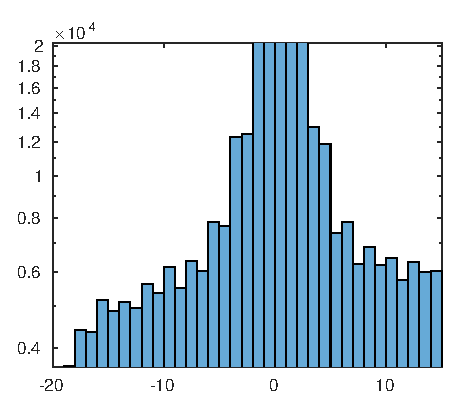
\includegraphics[width=5.5cm]{img/f3-hist.eps}
\caption{Part of a histogram of motion vectors with F3 embedding. Note the unusually higher peaks corresponding to even numbers.}
\label{fig:f3-hist}
\end{wrapfigure}

This embedding strategy leads to an interesting effect called \emph{shrinkage}. Whenever we try to embed a zero bit (\emph{steganographic zero}) into $mv_C = -1$ or $mv_C = 1$, the value of $mv_C$ will become 0, so the zero bit will have to be re-embedded again, meaning that F3 will embed more steganographic zeroes than ones. 

This is the main weakness of the algorithm. A typical encrypted payload has the same number of steganographic zeroes and ones, but since F3 embeds more zeros, values with LSB 0 will be more common (Figure \ref{fig:f3-hist}). 

\subsection{F4}

F4~\cite{f5} eliminates the weakness of F3 by using a different strategy for embedding into negative values of $mv_C$. Like F3, $mv_C$ is changed (if required) by decrementing its absolute value. When $mv_C$ is positive, the algorithm ensures its LSB matches that of the payload (just like F3), but when $mv_C$ is negative, the algorithm ensures its LSB \emph{does not} match that of the payload. This mapping is visualised in Figure \ref{fig:f4-mapping} and the pseudocode is listed in Algorithm \ref{alg:f4-embed}.

\begin{algorithm}
\caption{Embedding procedure for \emph{F4}.}
\label{alg:f4-embed}
\begin{algorithmic}
\Procedure {F4-Embed}{$mv_C$, $payload_i$}
\If {$mv_C > 0$ \textbf{and} $\textit{LSB}(mv_C) \neq payload_i$}
    \State $mv_C \gets mv_C - 1$ \Comment {Decrease the absolute value of $mv_C$}
\EndIf
\If {$mv_C < 0$ \textbf{and} $\textit{LSB}(mv_C) = payload_i$}
	\State $mv_C \gets mv_C + 1$ \Comment {Decrease the absolute value of $mv_C$}
\EndIf

\State \Return $mv_C \neq 0$
\EndProcedure
\end{algorithmic}
\end{algorithm}

\begin{figure}[tbh]
\centering
\resizebox{0.75\textwidth}{!}{%LaTeX with PSTricks extensions
%%Creator: inkscape 0.91
%%Please note this file requires PSTricks extensions
\psset{xunit=.5pt,yunit=.5pt,runit=.5pt}
\begin{pspicture}(452.5,185)
{
\newrgbcolor{curcolor}{1 1 1}
\pscustom[linestyle=none,fillstyle=solid,fillcolor=curcolor]
{
\newpath
\moveto(0,185)
\lineto(452.5,185)
\lineto(452.5,0)
\lineto(0,0)
\lineto(0,185)
\closepath
}
}
{
\newrgbcolor{curcolor}{0 0 0}
\pscustom[linestyle=none,fillstyle=solid,fillcolor=curcolor]
{
\newpath
\moveto(4.46655275,170.5676275)
\curveto(4.6691895,170.30151375)(4.96582025,170.1684575)(5.35644525,170.1684575)
\curveto(6.15234375,170.1684575)(6.85791013,170.7690425)(7.4731445,171.970215)
\curveto(7.9956055,173.00048825)(8.25683588,173.94775387)(8.25683588,174.81201175)
\curveto(8.25683588,175.17822262)(8.21289062,175.47363287)(8.125,175.69824225)
\curveto(7.9541015,176.12304688)(7.6416015,176.33544925)(7.1875,176.33544925)
\curveto(6.44042963,176.33544925)(5.73974612,175.77636725)(5.08544925,174.65820312)
\curveto(4.47021487,173.61328125)(4.16259763,172.58544925)(4.16259763,171.5747075)
\curveto(4.16259763,171.16943375)(4.26391637,170.83374)(4.46655275,170.5676275)
\closepath
\moveto(9.00390625,175.98754887)
\curveto(9.34082025,175.55053713)(9.50927737,175.03417975)(9.50927737,174.43847662)
\curveto(9.50927737,173.40332037)(9.05273438,172.387695)(8.13964838,171.39160125)
\curveto(7.19726562,170.356445)(6.19140625,169.8388675)(5.12207025,169.8388675)
\curveto(4.44824225,169.8388675)(3.90869138,170.03418)(3.503418,170.424805)
\curveto(3.0981445,170.81543)(2.89550775,171.36474625)(2.89550775,172.07275375)
\curveto(2.89550775,173.14208988)(3.34960938,174.16503912)(4.2578125,175.14160162)
\curveto(5.18554688,176.14257812)(6.18896487,176.64306637)(7.26806638,176.64306637)
\curveto(8.08837888,176.64306637)(8.66699225,176.4245605)(9.00390625,175.98754887)
\closepath
\moveto(13.1457525,176.62475588)
\curveto(13.16284,176.59790087)(13.17139,176.56738337)(13.17139,176.53320337)
\curveto(13.166515,176.48437462)(13.16164,176.44775462)(13.15674,176.42333963)
\lineto(12.42431638,173.58886713)
\lineto(12.58544875,173.90380863)
\curveto(12.93701125,174.59228512)(13.34838875,175.22094725)(13.81958,175.78979488)
\curveto(14.29077125,176.35864262)(14.73877,176.64306637)(15.16357375,176.64306637)
\curveto(15.39306625,176.64306637)(15.57006875,176.56738262)(15.69458,176.41601562)
\curveto(15.8190925,176.2646485)(15.8813475,176.09130863)(15.8813475,175.89599613)
\curveto(15.8813475,175.6762695)(15.819085,175.49438475)(15.69458,175.35034175)
\curveto(15.5700675,175.20629888)(15.39794875,175.13427738)(15.1782225,175.13427738)
\curveto(15.026855,175.13427738)(14.91211,175.16357362)(14.833985,175.22216737)
\curveto(14.75586,175.28076112)(14.69482375,175.3491205)(14.65087875,175.4272455)
\lineto(14.56299125,175.58837825)
\curveto(14.54345375,175.6176745)(14.52026625,175.64086825)(14.49341625,175.65795825)
\curveto(14.46655375,175.67504825)(14.43360375,175.68359325)(14.39454125,175.68359325)
\curveto(14.20411125,175.68359325)(13.92945375,175.41748)(13.57056625,174.88525337)
\curveto(13.21167,174.35302738)(12.890625,173.7768555)(12.6074225,173.15673825)
\curveto(12.43652338,172.78076175)(12.24609375,172.282715)(12.03613287,171.6625975)
\curveto(11.90429688,171.2719725)(11.72851562,170.71777375)(11.50878912,170)
\lineto(10.38085938,170)
\lineto(11.59667963,174.40917963)
\curveto(11.66503963,174.66308588)(11.71997087,174.89013675)(11.76147462,175.090332)
\curveto(11.80297837,175.29052738)(11.82373087,175.45410162)(11.82373087,175.58105475)
\curveto(11.82373087,175.72753912)(11.78710962,175.83984375)(11.71386712,175.91796875)
\curveto(11.64062462,175.99609375)(11.51367175,176.03515625)(11.33300775,176.03515625)
\curveto(11.274414,176.03515625)(11.20117175,176.03026875)(11.11328112,176.0205075)
\curveto(11.02539112,176.010745)(10.92041,175.998535)(10.79833975,175.98388625)
\lineto(10.79833975,176.2255855)
\lineto(11.0913085,176.28417925)
\curveto(11.472168,176.36230475)(11.88842775,176.4453125)(12.34008788,176.53320312)
\curveto(12.7917475,176.62109375)(13.029785,176.66503912)(13.05419875,176.66503912)
\curveto(13.09814875,176.66503912)(13.12866125,176.65161162)(13.14574875,176.62475538)
\closepath
\moveto(18.53027375,178.47412113)
\curveto(18.3886725,178.63037113)(18.31787125,178.81835938)(18.31787125,179.038086)
\curveto(18.31787125,179.26269525)(18.38867125,179.453125)(18.53027375,179.609375)
\curveto(18.671875,179.765625)(18.84277375,179.84375)(19.04296875,179.84375)
\curveto(19.24316375,179.84375)(19.41528375,179.765625)(19.55932625,179.609375)
\curveto(19.70336875,179.453125)(19.77539125,179.26269525)(19.77539125,179.038086)
\curveto(19.77539125,178.8134765)(19.70336625,178.62426762)(19.55932625,178.470459)
\curveto(19.41528375,178.31665037)(19.24316375,178.23974613)(19.04296875,178.23974613)
\curveto(18.84277375,178.23974613)(18.671875,178.31787113)(18.53027375,178.47412113)
\closepath
\moveto(19.25537125,176.5771485)
\lineto(17.77587875,171.34765625)
\curveto(17.70751625,171.06933625)(17.67334125,170.90332)(17.67334125,170.84960875)
\curveto(17.67334125,170.77637125)(17.68799125,170.71289)(17.71729125,170.65918)
\curveto(17.74170375,170.6005925)(17.80274125,170.5712925)(17.9003975,170.5712925)
\curveto(18.0664125,170.5712925)(18.28613875,170.71533625)(18.55957625,171.00342125)
\curveto(18.72071,171.17432)(18.91846375,171.41846125)(19.15283875,171.73584375)
\lineto(19.3432675,171.57471125)
\lineto(19.27003,171.47217375)
\curveto(18.90381875,170.95947875)(18.60108375,170.59082625)(18.36182625,170.3662175)
\curveto(17.98585,170.014655)(17.61963875,169.83887375)(17.26319375,169.83887375)
\curveto(17.0532325,169.83887375)(16.8786725,169.92676125)(16.7395125,170.102545)
\curveto(16.60035125,170.27832625)(16.53077125,170.48584625)(16.53077125,170.72510375)
\curveto(16.53077125,170.866705)(16.54052125,170.98999625)(16.56007125,171.0949775)
\curveto(16.57960875,171.1999525)(16.61622125,171.35498625)(16.66993375,171.560065)
\lineto(17.6953125,175.324707)
\curveto(17.7099625,175.38330075)(17.7221625,175.437012)(17.7319375,175.48583988)
\curveto(17.7416875,175.53466862)(17.7465875,175.58349613)(17.7465875,175.63232425)
\curveto(17.7465875,175.8081055)(17.6818875,175.916748)(17.552495,175.958252)
\curveto(17.42310125,175.99975575)(17.16797375,176.02050825)(16.787115,176.02050825)
\lineto(16.787115,176.26220738)
\curveto(17.1923875,176.31103612)(17.48413625,176.34887738)(17.66235875,176.37573238)
\curveto(17.84058125,176.40258737)(18.020025,176.43066362)(18.20068875,176.45996113)
\curveto(18.43506375,176.49902363)(18.65723125,176.54296863)(18.8671925,176.591797)
\curveto(19.07715375,176.64062575)(19.19556125,176.6564945)(19.2224175,176.6394045)
\curveto(19.2492675,176.6223145)(19.260255,176.60156325)(19.25538,176.57714825)
\closepath
\moveto(22.71972625,173.02490238)
\curveto(22.87597625,172.72705075)(23.15673875,172.578125)(23.56201125,172.578125)
\curveto(24.001465,172.578125)(24.39331,172.857666)(24.73754875,173.416748)
\curveto(25.0817875,173.97583013)(25.25390625,174.59228512)(25.25390625,175.26611325)
\curveto(25.25390625,175.58837887)(25.18310625,175.8410645)(25.04150375,176.02416988)
\curveto(24.8999025,176.20727537)(24.6875,176.29882812)(24.40429625,176.29882812)
\curveto(23.85742125,176.29882812)(23.4167475,176.00830075)(23.082275,175.42724613)
\curveto(22.7478025,174.84619137)(22.58056625,174.28710938)(22.58056625,173.75)
\curveto(22.58056625,173.44726562)(22.62695375,173.20556637)(22.71972625,173.02490238)
\closepath
\moveto(24.2834475,167.6342775)
\curveto(24.6667475,167.9125975)(24.85839875,168.24462875)(24.85839875,168.63037125)
\curveto(24.85839875,168.92334)(24.75829875,169.16992125)(24.558105,169.3701175)
\curveto(24.45068,169.4775425)(24.27734375,169.592285)(24.03808625,169.714355)
\curveto(23.83789,169.8120175)(23.49975625,169.9523925)(23.02368125,170.1354975)
\curveto(22.5476075,170.31860375)(22.27294875,170.41015625)(22.1997075,170.41015625)
\curveto(22.07275375,170.41015625)(21.82617125,170.24047875)(21.45996125,169.9011225)
\curveto(21.09375,169.5617675)(20.910645,169.17724625)(20.910645,168.74755875)
\curveto(20.910645,168.098145)(21.19140625,167.6513675)(21.75293,167.40722625)
\curveto(22.04589875,167.28027375)(22.40722625,167.21679625)(22.83691375,167.21679625)
\curveto(23.41796875,167.21679625)(23.90014625,167.3559575)(24.2834475,167.6342775)
\closepath
\moveto(20.51879875,169.60083)
\curveto(20.79956,169.93042)(21.2451175,170.25878875)(21.85546875,170.5859375)
\curveto(21.73339375,170.6640625)(21.63330125,170.74585)(21.55517625,170.83129875)
\curveto(21.47705125,170.91674875)(21.43798875,171.03027375)(21.43798875,171.171875)
\curveto(21.43798875,171.37207)(21.57714875,171.6015625)(21.85546875,171.86035125)
\curveto(22.01171875,172.00683625)(22.265625,172.1997075)(22.6171875,172.438965)
\curveto(22.3046875,172.5561525)(22.0361325,172.722168)(21.81152375,172.93701175)
\curveto(21.53808625,173.22509762)(21.4013675,173.59863287)(21.4013675,174.05761713)
\curveto(21.4013675,174.79492188)(21.6894525,175.40771488)(22.265625,175.89599613)
\curveto(22.84179625,176.38427738)(23.5546875,176.628418)(24.40429625,176.628418)
\curveto(24.8486325,176.628418)(25.22460875,176.558838)(25.53222625,176.41967775)
\curveto(25.83984375,176.28051763)(26.0205075,176.16455075)(26.07421875,176.07177738)
\lineto(27.06298875,176.07177738)
\lineto(27.06298875,175.48583988)
\lineto(26.3159175,175.48583988)
\curveto(26.3452175,175.37841862)(26.3671925,175.28076175)(26.38183,175.19287113)
\curveto(26.39648,175.10498112)(26.403805,174.98046875)(26.403805,174.81933588)
\curveto(26.403805,174.02832037)(26.09740875,173.40576175)(25.484615,172.95166012)
\curveto(24.8718225,172.49755875)(24.2114225,172.2705075)(23.50341375,172.2705075)
\curveto(23.43017625,172.2705075)(23.3618125,172.2741325)(23.29833625,172.2815075)
\curveto(23.23486125,172.2888825)(23.156735,172.3022575)(23.06396125,172.321795)
\curveto(22.99072375,172.321795)(22.89062125,172.250995)(22.7636675,172.1093925)
\curveto(22.6318325,171.96779125)(22.56591375,171.8408375)(22.56591375,171.7285325)
\curveto(22.56591375,171.5625175)(23.10302375,171.27931375)(24.1772425,170.87892375)
\curveto(25.24657875,170.47365)(25.78124625,169.88038875)(25.78124625,169.09913875)
\curveto(25.78124625,168.51320125)(25.51269125,167.999285)(24.9755825,167.55739)
\curveto(24.4384725,167.11549625)(23.62792625,166.89454875)(22.54394125,166.89454875)
\curveto(21.79198875,166.89454875)(21.196285,167.05568125)(20.7568325,167.3779475)
\curveto(20.31737875,167.7002125)(20.0976525,168.09327875)(20.0976525,168.55714625)
\curveto(20.0976525,168.9233575)(20.23803375,169.2712575)(20.518795,169.6008475)
\closepath
\moveto(30.19043,178.47412113)
\curveto(30.0488275,178.63037113)(29.9780275,178.81835938)(29.9780275,179.038086)
\curveto(29.9780275,179.26269525)(30.0488275,179.453125)(30.19043,179.609375)
\curveto(30.33203125,179.765625)(30.50293,179.84375)(30.703125,179.84375)
\curveto(30.90332,179.84375)(31.07543875,179.765625)(31.2194825,179.609375)
\curveto(31.363525,179.453125)(31.43554625,179.26269525)(31.43554625,179.038086)
\curveto(31.43554625,178.8134765)(31.36352125,178.62426762)(31.2194825,178.470459)
\curveto(31.07543875,178.31665037)(30.90332,178.23974613)(30.703125,178.23974613)
\curveto(30.50293,178.23974613)(30.33203125,178.31787113)(30.19043,178.47412113)
\closepath
\moveto(30.9155275,176.5771485)
\lineto(29.436035,171.34765625)
\curveto(29.3676725,171.06933625)(29.3334975,170.90332)(29.3334975,170.84960875)
\curveto(29.3334975,170.77637125)(29.3481475,170.71289)(29.3774475,170.65918)
\curveto(29.40186,170.6005925)(29.4628975,170.5712925)(29.5605525,170.5712925)
\curveto(29.72656875,170.5712925)(29.946295,170.71533625)(30.2197325,171.00342125)
\curveto(30.380865,171.17432)(30.57862,171.41846125)(30.812995,171.73584375)
\lineto(31.00342375,171.57471125)
\lineto(30.93018625,171.47217375)
\curveto(30.563975,170.95947875)(30.26124,170.59082625)(30.0219825,170.3662175)
\curveto(29.64600625,170.014655)(29.279795,169.83887375)(28.92335,169.83887375)
\curveto(28.71338875,169.83887375)(28.53882875,169.92676125)(28.3996675,170.102545)
\curveto(28.2605075,170.27832625)(28.1909275,170.48584625)(28.1909275,170.72510375)
\curveto(28.1909275,170.866705)(28.2006775,170.98999625)(28.2202275,171.0949775)
\curveto(28.239765,171.1999525)(28.2763775,171.35498625)(28.33009,171.560065)
\lineto(29.35548125,175.32471325)
\curveto(29.37013125,175.383307)(29.38233125,175.43701825)(29.39210625,175.48584612)
\curveto(29.40185625,175.53467488)(29.40675625,175.58350237)(29.40675625,175.6323305)
\curveto(29.40675625,175.80811175)(29.34205625,175.91675425)(29.21266375,175.95825825)
\curveto(29.08326875,175.999762)(28.8281425,176.0205145)(28.4472825,176.0205145)
\lineto(28.4472825,176.26221363)
\curveto(28.85255625,176.31104237)(29.144305,176.34888363)(29.3225275,176.37573862)
\curveto(29.50075,176.40259363)(29.68019375,176.43066988)(29.8608575,176.45996737)
\curveto(30.0952325,176.49902987)(30.3174,176.54297487)(30.52736125,176.59180325)
\curveto(30.7373225,176.640632)(30.85573,176.65650075)(30.88258625,176.63941075)
\curveto(30.90943625,176.62232075)(30.92042375,176.6015695)(30.91554875,176.5771545)
\closepath
\moveto(31.91162125,170)
\lineto(33.17871125,174.52636713)
\curveto(33.28613625,174.90722662)(33.34838875,175.1379395)(33.36547875,175.21850588)
\curveto(33.38256625,175.29907213)(33.39111625,175.38574225)(33.39111625,175.47851562)
\curveto(33.39111625,175.62011725)(33.35082875,175.73120112)(33.27026625,175.81176762)
\curveto(33.18970375,175.89233387)(33.03222875,175.93261763)(32.79785375,175.93261763)
\curveto(32.73926625,175.93261763)(32.68189125,175.92895512)(32.625735,175.92163013)
\curveto(32.569585,175.91430512)(32.5073225,175.90576137)(32.4389675,175.89599513)
\lineto(32.4389675,176.1450185)
\curveto(32.75635,176.19384725)(32.98218,176.23046725)(33.1164575,176.25488225)
\curveto(33.250735,176.279296)(33.39599875,176.3085935)(33.55224875,176.3427735)
\lineto(34.86328375,176.628418)
\curveto(34.89258375,176.60888675)(34.91210875,176.58691425)(34.92187125,176.5625005)
\lineto(33.94775,173.41308638)
\curveto(34.54345375,174.32617237)(35.0415,175.00488325)(35.44189125,175.44921925)
\curveto(36.14501625,176.23535212)(36.77489875,176.6284185)(37.33153875,176.6284185)
\curveto(37.5463825,176.6284185)(37.73193,176.58691475)(37.88818,176.50390725)
\curveto(38.18603125,176.3427745)(38.3349575,176.05224713)(38.3349575,175.63232525)
\curveto(38.3349575,175.51513775)(38.3227075,175.39306737)(38.2983325,175.26611425)
\curveto(38.27392,175.13916112)(38.2421825,175.00244237)(38.20312,174.855958)
\lineto(37.2436475,171.3476575)
\curveto(37.22411,171.27442)(37.2021475,171.18530375)(37.177735,171.08032375)
\curveto(37.1533225,170.97533625)(37.14111,170.90088)(37.14111,170.856935)
\curveto(37.14111,170.7836975)(37.1581975,170.717775)(37.192385,170.65918125)
\curveto(37.22656,170.60059375)(37.2827225,170.57129375)(37.3608425,170.57129375)
\curveto(37.487795,170.57129375)(37.63428,170.64575625)(37.800295,170.7946825)
\curveto(37.96631125,170.94360875)(38.2373075,171.2622125)(38.61328375,171.75049375)
\lineto(38.82568625,171.56006375)
\curveto(38.425295,171.01807125)(38.1079125,170.6372125)(37.8735375,170.417485)
\curveto(37.4731475,170.03174375)(37.08984625,169.8388725)(36.723635,169.8388725)
\curveto(36.55762,169.8388725)(36.3977075,169.89381)(36.24389875,170.0036675)
\curveto(36.09009,170.11353)(36.01318625,170.312505)(36.01318625,170.60059125)
\curveto(36.01318625,170.68360375)(36.01931125,170.77148875)(36.03149875,170.8642625)
\curveto(36.04374875,170.9570375)(36.05957375,171.0376025)(36.07911125,171.1059625)
\lineto(37.0019625,174.66553212)
\curveto(37.0507875,174.86084462)(37.08375,175.02075675)(37.1008375,175.14526838)
\curveto(37.117925,175.26977963)(37.126475,175.3588915)(37.126475,175.41260238)
\curveto(37.126475,175.52978988)(37.0984,175.63110825)(37.04225,175.7165575)
\curveto(36.9861,175.80200625)(36.88722125,175.84473138)(36.74561875,175.84473138)
\curveto(36.37940875,175.84473138)(35.9179825,175.5127)(35.36134125,174.84863763)
\curveto(35.03418,174.453125)(34.70214875,173.98193363)(34.36523375,173.43505863)
\curveto(34.106445,173.01025387)(33.9025875,172.5964355)(33.7536625,172.19360375)
\curveto(33.60473625,171.79077125)(33.36914,171.05957)(33.046875,170)
\lineto(31.91162125,170)
\closepath
\moveto(44.3627925,176.06445312)
\curveto(44.20166,176.23046875)(44.0063475,176.3134765)(43.776855,176.3134765)
\curveto(42.9809575,176.3134765)(42.24121125,175.703125)(41.5576175,174.48242188)
\curveto(40.95703125,173.40820312)(40.65673875,172.48291)(40.65673875,171.7065425)
\curveto(40.65673875,171.3159175)(40.74096375,171.03149375)(40.90942375,170.85327125)
\curveto(41.07788125,170.67504875)(41.28662125,170.5859375)(41.535645,170.5859375)
\curveto(42.27294875,170.5859375)(42.98339875,171.17919875)(43.6669925,172.3657225)
\curveto(44.2919925,173.44482425)(44.6044925,174.41894525)(44.6044925,175.288086)
\curveto(44.6044925,175.6396485)(44.52393,175.8984375)(44.3627925,176.06445312)
\closepath
\moveto(44.58252,176.3427735)
\curveto(44.69482,176.23535225)(44.782715,176.09375)(44.84619125,175.91796875)
\lineto(44.88281625,175.81543)
\lineto(45.04394875,176.3720705)
\curveto(45.06348625,176.43554675)(45.08057375,176.47827175)(45.09522375,176.50024437)
\curveto(45.10987375,176.52221687)(45.14404875,176.53564438)(45.19776125,176.54052813)
\lineto(46.02539875,176.63574313)
\curveto(46.06934875,176.63574313)(46.09497375,176.62719312)(46.10229875,176.61010813)
\curveto(46.10967375,176.59301812)(46.10842375,176.56250062)(46.09867375,176.51855563)
\curveto(46.07913625,176.45507937)(46.06449875,176.40503062)(46.05472375,176.36840912)
\curveto(46.04497375,176.33178788)(46.03031125,176.27929787)(46.01077375,176.21093838)
\lineto(45.336945,173.588868)
\curveto(45.19046125,173.017579)(45.06594875,172.52441487)(44.96341,172.10937625)
\curveto(44.78274625,171.3574225)(44.69241375,170.927735)(44.69241375,170.82031375)
\curveto(44.69241375,170.75195125)(44.71072625,170.70190125)(44.74735125,170.6701675)
\curveto(44.78397625,170.63843)(44.82913875,170.622555)(44.88285,170.622555)
\curveto(44.9268,170.622555)(44.9744,170.637205)(45.0256725,170.666505)
\curveto(45.0769475,170.695805)(45.1391975,170.7397425)(45.21244,170.79834125)
\lineto(45.3369525,170.90087875)
\curveto(45.376015,170.93505375)(45.419965,170.97534125)(45.46878875,171.02172875)
\curveto(45.51761375,171.06811625)(45.57621375,171.12549125)(45.64457,171.1938475)
\lineto(46.09867125,171.6625975)
\lineto(46.2744525,171.50878875)
\curveto(45.76664,170.859375)(45.358925,170.41870125)(45.05130875,170.1867675)
\curveto(44.74369125,169.95483375)(44.4507225,169.8388675)(44.1724025,169.8388675)
\curveto(43.9917375,169.8388675)(43.8513575,169.9023425)(43.75125875,170.02929625)
\curveto(43.65115875,170.15625)(43.6011125,170.31494125)(43.6011125,170.50537125)
\curveto(43.6011125,170.6811525)(43.634075,170.9338375)(43.6999875,171.2634275)
\curveto(43.7659,171.5930175)(43.8306025,171.8701175)(43.89407875,172.09472625)
\curveto(43.80619125,171.9482425)(43.65848375,171.73461875)(43.45096375,171.4538575)
\curveto(43.24344375,171.17309625)(42.9883175,170.90087875)(42.6855825,170.6372075)
\curveto(42.3291375,170.31982375)(41.98734125,170.095215)(41.6601925,169.96337875)
\curveto(41.40628625,169.87549125)(41.162145,169.8315425)(40.92777,169.8315425)
\curveto(40.5322625,169.8315425)(40.17337625,169.99389625)(39.85111,170.31860375)
\curveto(39.528845,170.64331)(39.3677125,171.103515)(39.3677125,171.69921875)
\curveto(39.3677125,172.724609)(39.82669625,173.79394487)(40.744665,174.90722625)
\curveto(41.69193125,176.06445275)(42.67337625,176.643066)(43.68900125,176.643066)
\curveto(44.07474375,176.643066)(44.372595,176.5429685)(44.58255625,176.34277313)
\closepath
\moveto(49.36523375,178.88427738)
\curveto(49.38477125,178.94775362)(49.39697125,179.0112305)(49.40185875,179.074707)
\curveto(49.40673375,179.13818325)(49.40923375,179.18945325)(49.40923375,179.22851562)
\curveto(49.40923375,179.39453125)(49.34209625,179.49584963)(49.2078175,179.53247075)
\curveto(49.07354,179.569092)(48.80620625,179.58496075)(48.405815,179.58007825)
\lineto(48.405815,179.8217775)
\curveto(48.6255425,179.85107375)(48.8782275,179.88525375)(49.1638725,179.92431625)
\curveto(49.44951625,179.96337875)(49.63628375,179.99023375)(49.724175,180.0048825)
\curveto(49.9976125,180.05371125)(50.32964375,180.1269525)(50.72026875,180.22460913)
\curveto(50.75444375,180.22460913)(50.78863125,180.20019537)(50.82280625,180.15136663)
\lineto(48.515625,171.34765625)
\curveto(48.4619125,171.137695)(48.430175,171.0107425)(48.4204125,170.96679625)
\curveto(48.4106625,170.92284625)(48.4057625,170.87890875)(48.4057625,170.83496125)
\curveto(48.4057625,170.74218625)(48.42285,170.66284125)(48.4570375,170.59692375)
\curveto(48.4912125,170.53101125)(48.5547,170.49804875)(48.6474675,170.49804875)
\curveto(48.82324875,170.49804875)(49.05274,170.65429875)(49.33594375,170.96679875)
\curveto(49.6191475,171.27929875)(49.858405,171.58203375)(50.0537175,171.8750025)
\lineto(50.25147125,171.7358425)
\curveto(49.83154875,171.115725)(49.50440125,170.6860375)(49.27002625,170.44678)
\curveto(48.8647525,170.04150625)(48.4570375,169.83887)(48.04688125,169.83887)
\curveto(47.8711,169.83887)(47.71485,169.88282)(47.57813125,169.970705)
\curveto(47.36817,170.10254125)(47.26319,170.32715125)(47.26319,170.64453375)
\curveto(47.26319,170.76660875)(47.2827275,170.93017875)(47.3217775,171.13525625)
\curveto(47.34619,171.25733125)(47.3779275,171.39892875)(47.41699,171.56006125)
\lineto(49.36523125,178.88427988)
\closepath
\moveto(60.71777375,176.32080075)
\curveto(60.8642575,176.12548825)(60.9375,175.90332025)(60.9375,175.65429688)
\curveto(60.9375,174.99511713)(60.285645,173.840332)(58.98193375,172.18994125)
\curveto(57.7465825,170.62255875)(57.00683625,169.8388675)(56.762695,169.8388675)
\curveto(56.6894575,169.8388675)(56.64062,169.9389675)(56.61621125,170.13916)
\curveto(56.60156125,170.25146)(56.59423625,170.441895)(56.59423625,170.71044875)
\curveto(56.59423625,171.0375975)(56.56249875,171.59179625)(56.49902375,172.37304625)
\curveto(56.43554625,173.15429688)(56.37451125,173.73291012)(56.3159175,174.10888675)
\curveto(56.1938475,174.934082)(56.07421875,175.46630863)(55.95703125,175.70556637)
\curveto(55.83984375,175.94482425)(55.61767625,176.06445312)(55.2905275,176.06445312)
\curveto(55.236815,176.06445312)(55.174565,176.06201563)(55.10376,176.05712812)
\curveto(55.03296,176.05224062)(54.95117125,176.04491562)(54.85839875,176.03515562)
\lineto(54.85839875,176.22558538)
\curveto(55.0048825,176.25488275)(55.3125,176.32080075)(55.78125,176.42333988)
\curveto(56.25,176.52587887)(56.49902375,176.58203125)(56.52832,176.59179688)
\lineto(56.77002,176.66503937)
\curveto(56.8383825,176.68457062)(56.892095,176.64672938)(56.9311525,176.55151438)
\curveto(56.970215,176.45629938)(57.01904,176.27929762)(57.07763625,176.02050862)
\curveto(57.26318375,175.17089925)(57.40234375,174.33349688)(57.4951175,173.5083015)
\curveto(57.553705,172.99560625)(57.612305,172.23632875)(57.67089875,171.23047)
\lineto(57.9125975,171.4868175)
\curveto(58.4155275,172.01904375)(58.9184575,172.65136788)(59.42138625,173.38378987)
\curveto(59.92431625,174.11621163)(60.17578125,174.63378987)(60.17578125,174.93652413)
\curveto(60.17578125,175.08789137)(60.06591875,175.26977612)(59.84619125,175.4821785)
\curveto(59.626465,175.69458088)(59.51660125,175.88867262)(59.51660125,176.06445387)
\curveto(59.51660125,176.22558675)(59.57153875,176.35742262)(59.68139625,176.45996175)
\curveto(59.79125875,176.5625005)(59.9267575,176.61377025)(60.08789125,176.61377025)
\curveto(60.3613275,176.61377025)(60.57128875,176.516114)(60.71777375,176.3208015)
\closepath
\moveto(66.41357375,176.06445312)
\curveto(66.25244125,176.23046875)(66.05712875,176.3134765)(65.82763625,176.3134765)
\curveto(65.03173875,176.3134765)(64.2919925,175.703125)(63.60839875,174.48242188)
\curveto(63.0078125,173.40820312)(62.70752,172.48291)(62.70752,171.7065425)
\curveto(62.70752,171.3159175)(62.791745,171.03149375)(62.960205,170.85327125)
\curveto(63.1286625,170.67504875)(63.3374025,170.5859375)(63.58642625,170.5859375)
\curveto(64.32373,170.5859375)(65.03418,171.17919875)(65.71777375,172.3657225)
\curveto(66.34277375,173.44482425)(66.65527375,174.41894525)(66.65527375,175.288086)
\curveto(66.65527375,175.6396485)(66.57471125,175.8984375)(66.41357375,176.06445312)
\closepath
\moveto(66.63330125,176.3427735)
\curveto(66.74560125,176.23535225)(66.83349625,176.09375)(66.8969725,175.91796875)
\lineto(66.9335975,175.81543)
\lineto(67.09473,176.3720705)
\curveto(67.1142675,176.43554675)(67.131355,176.47827175)(67.146005,176.50024437)
\curveto(67.160655,176.52221687)(67.19483,176.53564438)(67.2485425,176.54052813)
\lineto(68.07617875,176.63574313)
\curveto(68.12012875,176.63574313)(68.14575375,176.62719312)(68.15307875,176.61010813)
\curveto(68.16045375,176.59301812)(68.15920375,176.56250062)(68.14945375,176.51855563)
\curveto(68.12991625,176.45507937)(68.11527875,176.40503062)(68.10550375,176.36840912)
\curveto(68.09575375,176.33178788)(68.08109125,176.27929787)(68.06155375,176.21093838)
\lineto(67.387725,173.588868)
\curveto(67.24124125,173.017579)(67.11672875,172.52441487)(67.01419,172.10937625)
\curveto(66.83352625,171.3574225)(66.74319375,170.927735)(66.74319375,170.82031375)
\curveto(66.74319375,170.75195125)(66.76150625,170.70190125)(66.79813125,170.6701675)
\curveto(66.83475625,170.63843)(66.87991875,170.622555)(66.93363,170.622555)
\curveto(66.97758,170.622555)(67.02518,170.637205)(67.0764525,170.666505)
\curveto(67.1277275,170.695805)(67.1899775,170.7397425)(67.26322,170.79834125)
\lineto(67.3877325,170.90087875)
\curveto(67.426795,170.93505375)(67.470745,170.97534125)(67.51956875,171.02172875)
\curveto(67.56839375,171.06811625)(67.62699375,171.12549125)(67.69535,171.1938475)
\lineto(68.14945125,171.6625975)
\lineto(68.3252325,171.50878875)
\curveto(67.81742,170.859375)(67.409705,170.41870125)(67.10208875,170.1867675)
\curveto(66.79447125,169.95483375)(66.5015025,169.8388675)(66.2231825,169.8388675)
\curveto(66.0425175,169.8388675)(65.9021375,169.9023425)(65.80203875,170.02929625)
\curveto(65.70193875,170.15625)(65.6518925,170.31494125)(65.6518925,170.50537125)
\curveto(65.6518925,170.6811525)(65.684855,170.9338375)(65.7507675,171.2634275)
\curveto(65.81668,171.5930175)(65.8813825,171.8701175)(65.94485875,172.09472625)
\curveto(65.85697125,171.9482425)(65.70926375,171.73461875)(65.50174375,171.4538575)
\curveto(65.294225,171.17309625)(65.0390975,170.90087875)(64.7363625,170.6372075)
\curveto(64.3799175,170.31982375)(64.03812125,170.095215)(63.7109725,169.96337875)
\curveto(63.45706625,169.87549125)(63.21292625,169.8315425)(62.97855,169.8315425)
\curveto(62.5830425,169.8315425)(62.22415625,169.99389625)(61.90189,170.31860375)
\curveto(61.579625,170.64331)(61.4184925,171.103515)(61.4184925,171.69921875)
\curveto(61.4184925,172.724609)(61.87747625,173.79394487)(62.795445,174.90722625)
\curveto(63.74271125,176.06445275)(64.72415625,176.643066)(65.73978125,176.643066)
\curveto(66.12552375,176.643066)(66.423375,176.5429685)(66.63333625,176.34277313)
\closepath
\moveto(71.41601625,178.88427738)
\curveto(71.43554125,178.94775362)(71.44775375,179.0112305)(71.45264125,179.074707)
\curveto(71.45751625,179.13818325)(71.46001625,179.18945325)(71.46001625,179.22851562)
\curveto(71.46001625,179.39453125)(71.39287875,179.49584963)(71.2586,179.53247075)
\curveto(71.1243225,179.569092)(70.85698875,179.58496075)(70.4565975,179.58007825)
\lineto(70.4565975,179.8217775)
\curveto(70.676325,179.85107375)(70.92901,179.88525375)(71.214655,179.92431625)
\curveto(71.50029875,179.96337875)(71.68706625,179.99023375)(71.7749575,180.0048825)
\curveto(72.048395,180.05371125)(72.38042625,180.1269525)(72.77105125,180.22460913)
\curveto(72.80522625,180.22460913)(72.83941375,180.20019537)(72.87358875,180.15136663)
\lineto(70.56646,171.34765625)
\curveto(70.5127475,171.137695)(70.48101,171.0107425)(70.4712475,170.96679625)
\curveto(70.4614975,170.92284625)(70.4565975,170.87890875)(70.4565975,170.83496125)
\curveto(70.4565975,170.74218625)(70.473685,170.66284125)(70.5078725,170.59692375)
\curveto(70.5420475,170.53101125)(70.605535,170.49804875)(70.6983025,170.49804875)
\curveto(70.87408375,170.49804875)(71.103575,170.65429875)(71.38677875,170.96679875)
\curveto(71.66998125,171.27929875)(71.90924,171.58203375)(72.1045525,171.8750025)
\lineto(72.30230625,171.7358425)
\curveto(71.88238375,171.115725)(71.55523625,170.6860375)(71.32086125,170.44678)
\curveto(70.9155875,170.04150625)(70.5078725,169.83887)(70.09771625,169.83887)
\curveto(69.921935,169.83887)(69.765685,169.88282)(69.62896625,169.970705)
\curveto(69.419005,170.10254125)(69.314025,170.32715125)(69.314025,170.64453375)
\curveto(69.314025,170.76660875)(69.3335625,170.93017875)(69.3726125,171.13525625)
\curveto(69.397025,171.25733125)(69.4287625,171.39892875)(69.467825,171.56006125)
\lineto(71.4160675,178.88427938)
\closepath
\moveto(74.56543,175.288086)
\curveto(74.57518,175.3369135)(74.5837425,175.38207975)(74.5910675,175.423584)
\curveto(74.5984425,175.46508775)(74.6020675,175.50781275)(74.6020675,175.55175787)
\curveto(74.6020675,175.76171875)(74.5398175,175.88989262)(74.41529875,175.93627925)
\curveto(74.29078625,175.9826655)(74.05763375,176.00585925)(73.71583625,176.00585925)
\lineto(73.71583625,176.21093738)
\lineto(74.79249625,176.42333975)
\lineto(75.9570475,176.64306625)
\curveto(75.98146,176.64795375)(76.003435,176.63817875)(76.02296,176.61377)
\curveto(76.0424975,176.58935625)(76.04981,176.56494125)(76.044935,176.5405275)
\lineto(76.02296,176.43798875)
\lineto(74.72657375,171.45752)
\curveto(74.69239875,171.335445)(74.66798625,171.24023375)(74.65333625,171.171875)
\curveto(74.63868625,171.1035125)(74.63136125,171.0546875)(74.63136125,171.02539)
\curveto(74.63136125,170.91309)(74.66309875,170.825195)(74.72657375,170.76171875)
\curveto(74.79004875,170.69824375)(74.8730575,170.66650625)(74.9755975,170.66650625)
\curveto(75.2636825,170.66650625)(75.62379,170.92285375)(76.05591875,171.43554875)
\curveto(76.48804875,171.948245)(76.87257,172.48047125)(77.20948375,173.03222963)
\curveto(77.51221875,173.52539362)(77.79053875,174.07471)(78.044445,174.68017875)
\curveto(78.200695,175.05615538)(78.42530375,175.65429987)(78.7182725,176.47461237)
\lineto(79.82423,176.47461237)
\lineto(78.4399525,171.28174125)
\curveto(78.41554,171.18407875)(78.393565,171.0937525)(78.37404,171.010745)
\curveto(78.3545025,170.9277325)(78.34474,170.8593775)(78.34474,170.80566625)
\curveto(78.34474,170.74219125)(78.35939,170.68725375)(78.38869,170.64087125)
\curveto(78.41799,170.59448375)(78.4692525,170.57129625)(78.54249875,170.57129625)
\curveto(78.61573625,170.57129625)(78.691425,170.59937125)(78.76955,170.65552125)
\curveto(78.847675,170.71167125)(78.94533125,170.79834375)(79.06251875,170.91553125)
\curveto(79.11623125,170.96924375)(79.21388625,171.0839875)(79.3554875,171.25976875)
\curveto(79.443375,171.36719375)(79.577655,171.530765)(79.75832,171.7504925)
\lineto(79.9633975,171.61133125)
\curveto(79.73878875,171.2402375)(79.50441375,170.92041375)(79.2602725,170.65185875)
\curveto(78.77687375,170.1098675)(78.327655,169.83887125)(77.91261625,169.83887125)
\curveto(77.6977725,169.83887125)(77.52199125,169.89745875)(77.3852725,170.0146525)
\curveto(77.24855375,170.13184)(77.180195,170.314945)(77.180195,170.56396875)
\curveto(77.180195,170.69092125)(77.192445,170.83008125)(77.21682,170.98144875)
\curveto(77.2412325,171.13281625)(77.280295,171.303715)(77.3340075,171.49414375)
\curveto(77.421895,171.83594125)(77.53420375,172.2631875)(77.6709225,172.77588313)
\lineto(77.832055,173.39844175)
\lineto(77.78078,173.39844175)
\curveto(77.1069525,172.2802775)(76.5771675,171.48926125)(76.191425,171.02539375)
\curveto(75.52248,170.22949625)(74.890155,169.83154625)(74.2944525,169.83154625)
\curveto(74.13332,169.83154625)(73.986835,169.86572125)(73.85499875,169.93408375)
\curveto(73.6010925,170.0708025)(73.47414,170.3149425)(73.47414,170.666505)
\curveto(73.47414,170.7690425)(73.479015,170.8520525)(73.48879,170.91552875)
\curveto(73.49854,170.97900375)(73.51564,171.06689625)(73.540065,171.1792)
\lineto(74.56545625,175.28808775)
\closepath
\moveto(82.28515625,175.090332)
\curveto(83.2519525,176.105957)(84.25048875,176.6137695)(85.28076125,176.6137695)
\curveto(85.66162125,176.6137695)(85.964355,176.5258795)(86.188965,176.35009762)
\curveto(86.41357375,176.17431637)(86.52587875,175.913086)(86.52587875,175.56640625)
\curveto(86.52587875,174.86328125)(86.1145025,174.26147463)(85.2917475,173.76098638)
\curveto(84.46899375,173.260498)(83.603515,172.95410162)(82.6953125,172.84179688)
\lineto(82.2778325,172.79052688)
\curveto(82.2143575,172.5903315)(82.1704075,172.43042)(82.14599625,172.31079125)
\curveto(82.12158375,172.19116625)(82.10937125,172.041015)(82.10937125,171.86035125)
\curveto(82.10937125,171.43066375)(82.2497525,171.09619125)(82.53051375,170.85693375)
\curveto(82.811275,170.61767625)(83.1445275,170.49804625)(83.53027,170.49804625)
\curveto(83.89648,170.49804625)(84.28466375,170.62012125)(84.69482,170.8642575)
\curveto(84.929195,171.00585875)(85.26855125,171.259765)(85.71288625,171.62597625)
\lineto(85.90331625,171.45752)
\curveto(85.68359,171.17919875)(85.36864875,170.893555)(84.9584925,170.60058625)
\curveto(84.23095375,170.078125)(83.5009725,169.816895)(82.76855125,169.816895)
\curveto(82.2509725,169.816895)(81.79687125,170)(81.40624625,170.36621125)
\curveto(81.01562125,170.73242125)(80.82030875,171.25732375)(80.82030875,171.9409175)
\curveto(80.82030875,173.02490188)(81.30859,174.0747065)(82.2851525,175.0903315)
\closepath
\moveto(84.6582025,174.10522463)
\curveto(85.24414,174.62524412)(85.53710875,175.14160162)(85.53710875,175.65429688)
\curveto(85.53710875,175.83984375)(85.49315875,175.98754888)(85.40527375,176.09741213)
\curveto(85.31738625,176.20727587)(85.18798875,176.262207)(85.01709,176.262207)
\curveto(84.6997075,176.262207)(84.3884275,176.126709)(84.0832525,175.85571287)
\curveto(83.77807625,175.58471675)(83.5034175,175.27832025)(83.2592775,174.93652338)
\curveto(83.00048875,174.53613275)(82.79541,174.152832)(82.6440425,173.78662113)
\curveto(82.56103,173.59130863)(82.473145,173.36914062)(82.38037125,173.12011713)
\curveto(83.31298875,173.25683588)(84.072265,173.58520513)(84.6582025,174.10522463)
\closepath
}
}
{
\newrgbcolor{curcolor}{0 0 0}
\pscustom[linestyle=none,fillstyle=solid,fillcolor=curcolor]
{
\newpath
\moveto(8.66699225,18.8208)
\curveto(8.8134765,18.6254875)(8.88671875,18.403325)(8.88671875,18.1543)
\curveto(8.88671875,17.4951125)(8.23486325,16.3403375)(6.93115237,14.6899375)
\curveto(5.69580075,13.1225625)(4.95605475,12.3388625)(4.71191413,12.3388625)
\curveto(4.63867163,12.3388625)(4.58984413,12.4389875)(4.56542975,12.6391625)
\curveto(4.550781,12.7514125)(4.54345725,12.9419)(4.54345725,13.21045)
\curveto(4.54345725,13.5376)(4.5117185,14.0918)(4.44824225,14.87305)
\curveto(4.384766,15.6543)(4.323731,16.2329125)(4.26513675,16.6088875)
\curveto(4.14306638,17.4340875)(4.0234375,17.9663125)(3.90625,18.2055625)
\curveto(3.7890625,18.444825)(3.5668945,18.56445)(3.23974612,18.56445)
\curveto(3.18603487,18.56445)(3.12377988,18.56195)(3.0529785,18.55695)
\curveto(2.98217725,18.55195)(2.90039062,18.54445)(2.80761725,18.53495)
\lineto(2.80761725,18.725375)
\curveto(2.95410162,18.754625)(3.26171875,18.820625)(3.73046875,18.923125)
\curveto(4.19921875,19.025625)(4.44824225,19.081825)(4.47753912,19.0915875)
\lineto(4.71923825,19.1648375)
\curveto(4.787597,19.1843375)(4.84130825,19.1465875)(4.88037112,19.0513375)
\curveto(4.91943362,18.9560875)(4.96826112,18.779125)(5.0268555,18.5203375)
\curveto(5.21240237,17.670725)(5.3515625,16.833325)(5.44433588,16.008125)
\curveto(5.50292963,15.4954375)(5.56152338,14.73615)(5.62011725,13.7303)
\lineto(5.86181638,13.9866375)
\curveto(6.36474612,14.518875)(6.86767575,15.1511875)(7.3706055,15.8836125)
\curveto(7.87353513,16.6160375)(8.125,17.1336125)(8.125,17.43635)
\curveto(8.125,17.5877125)(8.01513625,17.7696)(7.79541013,17.982)
\curveto(7.57568362,18.1944125)(7.46582025,18.3885)(7.46582025,18.564275)
\curveto(7.46582025,18.7254125)(7.5207515,18.85725)(7.63061525,18.9597875)
\curveto(7.740479,19.0622875)(7.8759765,19.1136)(8.03710937,19.1136)
\curveto(8.31054687,19.1136)(8.52050775,19.015975)(8.66699225,18.820625)
\closepath
\moveto(14.3627925,18.56445)
\curveto(14.20166,18.730475)(14.0063475,18.813475)(13.776855,18.813475)
\curveto(12.9809575,18.813475)(12.24121088,18.203125)(11.55761713,16.982425)
\curveto(10.95703125,15.9082)(10.65673825,14.9829125)(10.65673825,14.20655)
\curveto(10.65673825,13.815925)(10.740967,13.5315)(10.90942388,13.353275)
\curveto(11.07788088,13.17505)(11.28662113,13.0859375)(11.5356445,13.0859375)
\curveto(12.27294925,13.0859375)(12.98339875,13.6792)(13.6669925,14.865725)
\curveto(14.2919925,15.944825)(14.6044925,16.91895)(14.6044925,17.7880875)
\curveto(14.6044925,18.13965)(14.52393,18.3984375)(14.3627925,18.56445)
\closepath
\moveto(14.58252,18.842775)
\curveto(14.69482,18.7354)(14.782715,18.59375)(14.84619125,18.417975)
\lineto(14.88281625,18.315475)
\lineto(15.04394875,18.872125)
\curveto(15.06348625,18.935625)(15.08057375,18.978375)(15.09522375,19.0003)
\curveto(15.10987375,19.0223)(15.14404875,19.035675)(15.19776125,19.04055)
\lineto(16.02539875,19.1358)
\curveto(16.06934875,19.1358)(16.09497375,19.12705)(16.10229875,19.110175)
\curveto(16.10967375,19.09305)(16.10842375,19.06255)(16.09867375,19.01855)
\curveto(16.07913625,18.95505)(16.06449875,18.90505)(16.05472375,18.8684125)
\curveto(16.04497375,18.8317875)(16.03031125,18.7792875)(16.01077375,18.7109375)
\lineto(15.336945,16.0888625)
\curveto(15.19046125,15.517575)(15.06594875,15.0244125)(14.96341,14.609375)
\curveto(14.78274625,13.857425)(14.69241375,13.4277375)(14.69241375,13.3203125)
\curveto(14.69241375,13.2519375)(14.71072625,13.2019375)(14.74733875,13.1701625)
\curveto(14.78396375,13.1384125)(14.82912625,13.1225375)(14.8828375,13.1225375)
\curveto(14.9267875,13.1225375)(14.9743875,13.1371625)(15.02566,13.1664125)
\curveto(15.0769225,13.1956625)(15.139185,13.2396625)(15.2124275,13.29825)
\lineto(15.33694,13.40075)
\curveto(15.3760025,13.435)(15.4199525,13.47525)(15.46877625,13.521625)
\curveto(15.51760125,13.568)(15.57620125,13.625375)(15.6445575,13.69375)
\lineto(16.09865875,14.1625)
\lineto(16.27444,14.0086875)
\curveto(15.7666275,13.359275)(15.3589125,12.9186)(15.05129625,12.686675)
\curveto(14.74367875,12.4547375)(14.45071,12.3387625)(14.17239,12.3387625)
\curveto(13.991725,12.3387625)(13.851345,12.4022625)(13.7512475,12.5292)
\curveto(13.6511475,12.65615)(13.6011,12.8148375)(13.6011,13.005275)
\curveto(13.6011,13.18105)(13.6340625,13.4337375)(13.699975,13.763325)
\curveto(13.7658875,14.092925)(13.83059,14.3700125)(13.89406625,14.594625)
\curveto(13.80617875,14.4481375)(13.65847125,14.234525)(13.45095125,13.9537625)
\curveto(13.2434325,13.673)(12.988305,13.400775)(12.68557125,13.1371125)
\curveto(12.32912537,12.819725)(11.9873285,12.5951125)(11.66018,12.463275)
\curveto(11.40627375,12.3754)(11.16213312,12.33145)(10.92775812,12.33145)
\curveto(10.53225037,12.33145)(10.17336362,12.4938)(9.851098,12.8185)
\curveto(9.52883237,13.1432125)(9.3676995,13.6034125)(9.3676995,14.199125)
\curveto(9.3676995,15.2245125)(9.82668387,16.29385)(10.74465263,17.407125)
\curveto(11.69191825,18.56435)(12.67336375,19.1429625)(13.68898875,19.1429625)
\curveto(14.07473125,19.1429625)(14.3725825,19.0428375)(14.58254375,18.842675)
\closepath
\moveto(19.365235,21.384275)
\curveto(19.3847725,21.447775)(19.3969725,21.5112375)(19.40186,21.5747125)
\curveto(19.406735,21.6382125)(19.409235,21.6894625)(19.409235,21.7285125)
\curveto(19.409235,21.8945375)(19.3420975,21.99585)(19.20781875,22.032475)
\curveto(19.07354125,22.0691)(18.8062075,22.084975)(18.40581625,22.0801)
\lineto(18.40581625,22.3218)
\curveto(18.62554375,22.35105)(18.87822875,22.3853)(19.16387375,22.4243)
\curveto(19.4495175,22.4633)(19.636285,22.490175)(19.72417625,22.504925)
\curveto(19.99761375,22.5538)(20.329645,22.62705)(20.72027,22.72465)
\curveto(20.754445,22.72465)(20.7886325,22.700275)(20.8228075,22.6514)
\lineto(18.51567875,13.8477)
\curveto(18.46196625,13.6377375)(18.43022875,13.510775)(18.42046625,13.4668375)
\curveto(18.41071625,13.4228375)(18.40581625,13.3789625)(18.40581625,13.335)
\curveto(18.40581625,13.24225)(18.42290375,13.162875)(18.45709125,13.0969625)
\curveto(18.49126625,13.0310875)(18.55475375,12.9980875)(18.64752125,12.9980875)
\curveto(18.8233025,12.9980875)(19.052795,13.1543375)(19.3359975,13.4668375)
\curveto(19.61920125,13.7793375)(19.85845875,14.082075)(20.05377125,14.3750375)
\lineto(20.251525,14.235875)
\curveto(19.8316025,13.6157625)(19.504455,13.186075)(19.27008,12.9468125)
\curveto(18.86480625,12.5415375)(18.45709125,12.3389)(18.046935,12.3389)
\curveto(17.87115375,12.3389)(17.71490375,12.3829)(17.578185,12.4707375)
\curveto(17.36822375,12.602575)(17.26324375,12.8271875)(17.26324375,13.144575)
\curveto(17.26324375,13.2667)(17.28278125,13.4302125)(17.32183125,13.6352875)
\curveto(17.34624375,13.7574125)(17.37798125,13.8989625)(17.41704375,14.0601)
\lineto(19.36528625,21.3843125)
\closepath
\moveto(22.51464875,17.7880875)
\curveto(22.52439875,17.8369625)(22.53296125,17.8820875)(22.54028625,17.9235875)
\curveto(22.54766125,17.9650875)(22.55128625,18.0078375)(22.55128625,18.0517625)
\curveto(22.55128625,18.261725)(22.48903625,18.3899)(22.3645175,18.436275)
\curveto(22.240005,18.48265)(22.0068525,18.5059)(21.665055,18.5059)
\lineto(21.665055,18.710975)
\lineto(22.741715,18.923375)
\lineto(23.90626625,19.1431)
\curveto(23.93067875,19.1481)(23.95265375,19.1381)(23.97217875,19.11385)
\curveto(23.99171625,19.089475)(23.99902875,19.064975)(23.99415375,19.0406)
\lineto(23.97217875,18.9381)
\lineto(22.6757925,13.9576375)
\curveto(22.6416175,13.8355125)(22.617205,13.74035)(22.602555,13.6719875)
\curveto(22.587905,13.6036125)(22.58058,13.5548625)(22.58058,13.5255)
\curveto(22.58058,13.41325)(22.6123175,13.3253125)(22.6757925,13.2618375)
\curveto(22.7392675,13.1983375)(22.82227625,13.1665875)(22.92481625,13.1665875)
\curveto(23.21290125,13.1665875)(23.57300875,13.4229375)(24.0051375,13.9356375)
\curveto(24.4372675,14.448325)(24.82178875,14.9805625)(25.1587025,15.5323125)
\curveto(25.4614375,16.025475)(25.7397575,16.5748)(25.99366375,17.1802625)
\curveto(26.14991375,17.5562375)(26.3745225,18.1543875)(26.66749125,18.9747)
\lineto(27.77344875,18.9747)
\lineto(26.38917125,13.781825)
\curveto(26.36475875,13.6842)(26.34278375,13.5938375)(26.32325875,13.510825)
\curveto(26.30372125,13.427825)(26.29395875,13.3594625)(26.29395875,13.30575)
\curveto(26.29395875,13.24225)(26.30860875,13.187375)(26.33790875,13.1409625)
\curveto(26.36720875,13.0945875)(26.41847125,13.0713375)(26.4917175,13.0713375)
\curveto(26.564955,13.0713375)(26.64064375,13.0994625)(26.71876875,13.1555875)
\curveto(26.79689375,13.2117125)(26.89455,13.2984)(27.0117375,13.4155875)
\curveto(27.06545,13.4693375)(27.163105,13.58405)(27.30470625,13.759825)
\curveto(27.39259375,13.8672)(27.52687375,14.030825)(27.70753875,14.25055)
\lineto(27.91261625,14.1113875)
\curveto(27.6880075,13.7403)(27.4536325,13.420475)(27.20949125,13.151925)
\curveto(26.7260925,12.609925)(26.27687375,12.338925)(25.861835,12.338925)
\curveto(25.64699125,12.338925)(25.47121,12.39755)(25.33449125,12.5147125)
\curveto(25.1977725,12.6318375)(25.12941375,12.815)(25.12941375,13.064025)
\curveto(25.12941375,13.1909875)(25.14166375,13.3301375)(25.16603875,13.4815125)
\curveto(25.19045125,13.632875)(25.22951375,13.803775)(25.28322625,13.9942)
\curveto(25.37111375,14.336)(25.4834225,14.76325)(25.62014125,15.2759375)
\lineto(25.78127375,15.8985)
\lineto(25.72999875,15.8985)
\curveto(25.05617125,14.7803375)(24.52638625,13.989325)(24.14064375,13.52545)
\curveto(23.47169875,12.72955)(22.83937375,12.3316125)(22.24367125,12.3316125)
\curveto(22.08253875,12.3316125)(21.93605375,12.3657375)(21.8042175,12.4341125)
\curveto(21.55031125,12.570825)(21.42335875,12.8149625)(21.42335875,13.166525)
\curveto(21.42335875,13.269025)(21.42823375,13.352075)(21.43800875,13.41555)
\curveto(21.44775875,13.47905)(21.46485875,13.566925)(21.48928375,13.679225)
\lineto(22.514675,17.7881125)
\closepath
\moveto(30.234375,17.5903375)
\curveto(31.20117125,18.6059625)(32.1997075,19.113775)(33.22998,19.113775)
\curveto(33.61084,19.113775)(33.91357375,19.0259)(34.13818375,18.8501)
\curveto(34.3627925,18.6743125)(34.4750975,18.4130875)(34.4750975,18.0664125)
\curveto(34.4750975,17.3632875)(34.06372,16.761475)(33.24096625,16.2609875)
\curveto(32.4182125,15.7605)(31.55273375,15.4541)(30.64453125,15.3418)
\lineto(30.22705125,15.29055)
\curveto(30.16357625,15.0903625)(30.11962625,14.93045)(30.095215,14.8108125)
\curveto(30.0708025,14.6911875)(30.05859,14.5410375)(30.05859,14.360375)
\curveto(30.05859,13.9306875)(30.19897125,13.5962125)(30.4797325,13.3569625)
\curveto(30.76049375,13.1177)(31.09374625,12.998075)(31.47948875,12.998075)
\curveto(31.84569875,12.998075)(32.2338825,13.1202)(32.64403875,13.3642875)
\curveto(32.87841375,13.5058875)(33.21777,13.7597875)(33.662105,14.126)
\lineto(33.852535,13.95755)
\curveto(33.63280875,13.679225)(33.3178675,13.393575)(32.90771125,13.1006125)
\curveto(32.1801725,12.57815)(31.45019125,12.316925)(30.71777,12.316925)
\curveto(30.20019125,12.316925)(29.74609,12.500025)(29.355465,12.8662375)
\curveto(28.96484,13.23245)(28.7695275,13.75735)(28.7695275,14.44095)
\curveto(28.7695275,15.524925)(29.25780875,16.5747375)(30.23437125,17.5903625)
\closepath
\moveto(32.60742125,16.605225)
\curveto(33.19335875,17.12525)(33.4863275,17.6416)(33.4863275,18.1543)
\curveto(33.4863275,18.3398375)(33.4423775,18.48755)(33.3544925,18.5974125)
\curveto(33.266605,18.7072875)(33.1372075,18.7622125)(32.96630875,18.7622125)
\curveto(32.64892625,18.7622125)(32.33764625,18.6267125)(32.03247,18.3557125)
\curveto(31.727295,18.0847125)(31.45263625,17.778325)(31.20849625,17.436525)
\curveto(30.9497075,17.0361375)(30.74462875,16.6528375)(30.59326125,16.286625)
\curveto(30.51024875,16.0913125)(30.42236375,15.8691375)(30.32959,15.6201125)
\curveto(31.2622075,15.7568375)(32.021485,16.0852125)(32.60742125,16.605225)
\closepath
\moveto(43.91357375,18.56445)
\curveto(43.75244125,18.730475)(43.55712875,18.813475)(43.32763625,18.813475)
\curveto(42.53173875,18.813475)(41.7919925,18.203125)(41.10839875,16.982425)
\curveto(40.5078125,15.9082)(40.20752,14.9829125)(40.20752,14.20655)
\curveto(40.20752,13.815925)(40.291745,13.5315)(40.460205,13.353275)
\curveto(40.6286625,13.17505)(40.8374025,13.0859375)(41.08642625,13.0859375)
\curveto(41.82373,13.0859375)(42.53418,13.6792)(43.21777375,14.865725)
\curveto(43.84277375,15.944825)(44.15527375,16.91895)(44.15527375,17.7880875)
\curveto(44.15527375,18.13965)(44.07471125,18.3984375)(43.91357375,18.56445)
\closepath
\moveto(44.13330125,18.842775)
\curveto(44.24560125,18.7354)(44.33349625,18.59375)(44.3969725,18.417975)
\lineto(44.4335975,18.315475)
\lineto(44.59473,18.872125)
\curveto(44.6142675,18.935625)(44.631355,18.978375)(44.646005,19.0003)
\curveto(44.660655,19.0223)(44.69483,19.035675)(44.7485425,19.04055)
\lineto(45.57617875,19.1358)
\curveto(45.62012875,19.1358)(45.64575375,19.12705)(45.65307875,19.110175)
\curveto(45.66045375,19.09305)(45.65920375,19.06255)(45.64945375,19.01855)
\curveto(45.62991625,18.95505)(45.61527875,18.90505)(45.60550375,18.8684125)
\curveto(45.59575375,18.8317875)(45.58109125,18.7792875)(45.56155375,18.7109375)
\lineto(44.887725,16.0888625)
\curveto(44.74124125,15.517575)(44.61672875,15.0244125)(44.51419,14.609375)
\curveto(44.33352625,13.857425)(44.24319375,13.4277375)(44.24319375,13.3203125)
\curveto(44.24319375,13.2519375)(44.26150625,13.2019375)(44.29813125,13.1701625)
\curveto(44.33475625,13.1384125)(44.37991875,13.1225375)(44.43363,13.1225375)
\curveto(44.47758,13.1225375)(44.52518,13.1371625)(44.5764525,13.1664125)
\curveto(44.6277275,13.1956625)(44.6899775,13.2396625)(44.76322,13.29825)
\lineto(44.8877325,13.40075)
\curveto(44.926795,13.435)(44.970745,13.47525)(45.01956875,13.521625)
\curveto(45.06839375,13.568)(45.12699375,13.625375)(45.19535,13.69375)
\lineto(45.64945125,14.1625)
\lineto(45.8252325,14.0086875)
\curveto(45.31742,13.359275)(44.909705,12.9186)(44.60208875,12.686675)
\curveto(44.29447125,12.4547375)(44.0015025,12.3387625)(43.7231825,12.3387625)
\curveto(43.5425175,12.3387625)(43.4021375,12.4022625)(43.30203875,12.5292)
\curveto(43.20193875,12.65615)(43.1518925,12.8148375)(43.1518925,13.005275)
\curveto(43.1518925,13.18105)(43.184855,13.4337375)(43.2507675,13.763325)
\curveto(43.31668,14.092925)(43.3813825,14.3700125)(43.44485875,14.594625)
\curveto(43.35697125,14.4481375)(43.20926375,14.234525)(43.00174375,13.9537625)
\curveto(42.794225,13.673)(42.5390975,13.400775)(42.2363625,13.1371125)
\curveto(41.8799175,12.819725)(41.53812125,12.5951125)(41.2109725,12.463275)
\curveto(40.95706625,12.3754)(40.71292625,12.33145)(40.47855,12.33145)
\curveto(40.0830425,12.33145)(39.72415625,12.4938)(39.40189,12.8185)
\curveto(39.079625,13.1432125)(38.9184925,13.6034125)(38.9184925,14.199125)
\curveto(38.9184925,15.2245125)(39.37747625,16.29385)(40.295445,17.407125)
\curveto(41.24271125,18.56435)(42.22415625,19.1429625)(43.23978125,19.1429625)
\curveto(43.62552375,19.1429625)(43.923375,19.0428375)(44.13333625,18.842675)
\closepath
\moveto(52.38037125,21.2963875)
\curveto(52.27294625,21.159675)(52.12402375,21.0913125)(51.93359375,21.0913125)
\curveto(51.7675775,21.0913125)(51.63085875,21.1438125)(51.5234375,21.248775)
\curveto(51.4160125,21.353775)(51.362305,21.47705)(51.362305,21.61865)
\curveto(51.362305,21.716275)(51.4086925,21.8847625)(51.501465,22.124025)
\curveto(51.501465,22.187525)(51.4697275,22.24365)(51.4062525,22.2924875)
\curveto(51.3427775,22.3363625)(51.2597675,22.3583625)(51.15722875,22.3583625)
\curveto(50.67871375,22.3583625)(50.2783225,21.9653)(49.9560575,21.1791625)
\curveto(49.77539375,20.7250625)(49.57275625,19.9609)(49.3481475,18.8866875)
\lineto(50.9814475,18.8866875)
\lineto(50.87891,18.3959625)
\lineto(49.24560875,18.3959625)
\lineto(48.16894875,13.6425375)
\curveto(47.8808625,12.368125)(47.4939,11.33785)(47.00806,10.551725)
\curveto(46.52222,9.7655875)(45.9008825,9.372525)(45.14404625,9.372525)
\curveto(44.7973675,9.372525)(44.5129425,9.467775)(44.290775,9.6581625)
\curveto(44.0686075,9.8486)(43.95752375,10.061)(43.95752375,10.295375)
\curveto(43.95752375,10.4418625)(44.00513625,10.578575)(44.100345,10.705525)
\curveto(44.1955575,10.8324875)(44.3383825,10.8959625)(44.5288125,10.8959625)
\curveto(44.6948275,10.8959625)(44.83520875,10.8410875)(44.949955,10.7311625)
\curveto(45.064705,10.6212875)(45.12207375,10.4858)(45.12207375,10.324675)
\curveto(45.12207375,10.2368)(45.09643625,10.1476625)(45.04517375,10.0573375)
\curveto(44.99389875,9.9669625)(44.96827375,9.90475)(44.96827375,9.870575)
\curveto(44.96827375,9.826575)(44.99634875,9.78995)(45.05249875,9.7607)
\curveto(45.10864875,9.73145)(45.1806725,9.7167)(45.26856375,9.7167)
\curveto(45.6836025,9.7167)(46.035165,10.04385)(46.32325125,10.6981375)
\curveto(46.4746175,11.0399375)(46.61377875,11.5111375)(46.74073125,12.1117125)
\lineto(48.066415,18.3959)
\lineto(46.711435,18.3959)
\lineto(46.8139725,18.886625)
\lineto(48.19825,18.886625)
\curveto(48.49610125,20.0243125)(48.83057375,20.8666)(49.2016675,21.413475)
\curveto(49.753425,22.253325)(50.4345775,22.6732375)(51.245125,22.6732375)
\curveto(51.61621875,22.6732375)(51.92505625,22.5779875)(52.17163875,22.3876)
\curveto(52.41822,22.1971625)(52.54151125,21.9798875)(52.54151125,21.7357375)
\curveto(52.54151125,21.5794875)(52.48779875,21.4330125)(52.38037875,21.2962875)
\closepath
\moveto(50.92285125,13.1189)
\curveto(50.92772625,13.17015)(50.93750125,13.22265)(50.95215125,13.2763625)
\lineto(52.32910375,18.396)
\lineto(51.2158225,18.396)
\curveto(51.2158225,18.5278375)(51.2255725,18.6108375)(51.2451225,18.645025)
\curveto(51.26466,18.67915)(51.313485,18.7134)(51.39160625,18.747525)
\curveto(51.88477,18.9574875)(52.26685,19.160125)(52.53784625,19.3554375)
\curveto(52.8088425,19.55075)(53.17871625,19.926725)(53.64746625,20.4833625)
\lineto(53.76465375,20.622525)
\curveto(53.77930375,20.642025)(53.79761625,20.6579)(53.81959125,20.67015)
\curveto(53.84156625,20.68265)(53.86475375,20.6884)(53.88916625,20.6884)
\curveto(53.93799125,20.6784)(53.97217875,20.6689)(53.99170375,20.65915)
\curveto(54.00635375,20.625025)(54.01489125,20.594525)(54.01734125,20.56765)
\curveto(54.01984125,20.540775)(54.0185625,20.512775)(54.01371625,20.4834)
\lineto(53.59623625,18.886725)
\lineto(54.79008375,18.886725)
\lineto(54.70219625,18.396)
\lineto(53.45707875,18.396)
\lineto(52.13871875,13.4668)
\curveto(52.11430625,13.378925)(52.12163125,13.294675)(52.16069375,13.2141125)
\curveto(52.19975625,13.1336125)(52.26566875,13.0932375)(52.3584475,13.0932375)
\curveto(52.4854,13.0932375)(52.6636225,13.2201875)(52.893115,13.4741)
\curveto(53.02495125,13.6108125)(53.24711875,13.8818125)(53.55961875,14.2870875)
\lineto(53.75,14.17725)
\lineto(53.6474625,14.0234375)
\curveto(53.22754,13.39355)(52.8576675,12.955325)(52.5378425,12.7087375)
\curveto(52.21801875,12.4621625)(51.91406375,12.3388625)(51.6259775,12.3388625)
\curveto(51.37695375,12.3388625)(51.19629,12.4047375)(51.083985,12.536625)
\curveto(50.971685,12.6684625)(50.91552875,12.8173875)(50.91552875,12.9834)
\curveto(50.91552875,13.0224)(50.91802875,13.06765)(50.92290375,13.1189)
\closepath
\moveto(56.4453125,17.5903375)
\curveto(57.41210875,18.6059625)(58.410645,19.113775)(59.4409175,19.113775)
\curveto(59.8217775,19.113775)(60.12451125,19.0259)(60.34912125,18.8501)
\curveto(60.57373,18.6743125)(60.686035,18.4130875)(60.686035,18.0664125)
\curveto(60.686035,17.3632875)(60.2746575,16.761475)(59.45190375,16.2609875)
\curveto(58.62915,15.7605)(57.76367125,15.4541)(56.85546875,15.3418)
\lineto(56.43798875,15.29055)
\curveto(56.37451375,15.0903625)(56.33056375,14.93045)(56.3061525,14.8108125)
\curveto(56.28174,14.6911875)(56.2695275,14.5410375)(56.2695275,14.360375)
\curveto(56.2695275,13.9306875)(56.40990875,13.5962125)(56.69067,13.3569625)
\curveto(56.97143125,13.1177)(57.30468375,12.998075)(57.69042625,12.998075)
\curveto(58.0566375,12.998075)(58.44482,13.1202)(58.85497625,13.3642875)
\curveto(59.08935125,13.5058875)(59.4287075,13.7597875)(59.8730425,14.126)
\lineto(60.0634725,13.95755)
\curveto(59.84374625,13.679225)(59.528805,13.393575)(59.11864875,13.1006125)
\curveto(58.39111,12.57815)(57.66112875,12.316925)(56.9287075,12.316925)
\curveto(56.41112875,12.316925)(55.9570275,12.500025)(55.5664025,12.8662375)
\curveto(55.1757775,13.23245)(54.980465,13.75735)(54.980465,14.44095)
\curveto(54.980465,15.524925)(55.46874625,16.5747375)(56.44530875,17.5903625)
\closepath
\moveto(58.81835875,16.605225)
\curveto(59.40429625,17.12525)(59.697265,17.6416)(59.697265,18.1543)
\curveto(59.697265,18.3398375)(59.653315,18.48755)(59.56543,18.5974125)
\curveto(59.4775425,18.7072875)(59.348145,18.7622125)(59.17724625,18.7622125)
\curveto(58.85986375,18.7622125)(58.54858375,18.6267125)(58.2434075,18.3557125)
\curveto(57.9382325,18.0847125)(57.66357375,17.778325)(57.41943375,17.436525)
\curveto(57.160645,17.0361375)(56.95556625,16.6528375)(56.80419875,16.286625)
\curveto(56.72118625,16.0913125)(56.63330125,15.8691375)(56.5405275,15.6201125)
\curveto(57.473145,15.7568375)(58.23242125,16.0852125)(58.81835875,16.605225)
\closepath
\moveto(64.298095,19.1247625)
\curveto(64.3151825,19.0978875)(64.3237325,19.0673875)(64.3237325,19.0331375)
\curveto(64.3188575,18.9842625)(64.3139825,18.9476375)(64.3090825,18.9232625)
\lineto(63.57666,16.0887875)
\lineto(63.7377925,16.4037375)
\curveto(64.089355,17.0922125)(64.5007325,17.720875)(64.97192375,18.289725)
\curveto(65.443115,18.858575)(65.89111375,19.1429875)(66.3159175,19.1429875)
\curveto(66.54541,19.1429875)(66.7224125,19.0673625)(66.84692375,18.9159375)
\curveto(66.97143625,18.764575)(67.03369125,18.5912375)(67.03369125,18.395925)
\curveto(67.03369125,18.1762)(66.97144125,17.9943125)(66.84692375,17.8502625)
\curveto(66.72241125,17.706225)(66.5502925,17.6342)(66.33056625,17.6342)
\curveto(66.17919875,17.6342)(66.0644525,17.66345)(65.9863275,17.722075)
\curveto(65.9082025,17.7807)(65.8471675,17.8490375)(65.8032225,17.9271625)
\lineto(65.715335,18.0882875)
\curveto(65.6957975,18.1175375)(65.67261,18.1407875)(65.64576,18.1579125)
\curveto(65.61891,18.1750375)(65.5859475,18.1835375)(65.546885,18.1835375)
\curveto(65.356455,18.1835375)(65.0817975,17.917425)(64.72291,17.3851875)
\curveto(64.36402375,16.8529625)(64.04297875,16.2768)(63.759775,15.656675)
\curveto(63.5888775,15.2807)(63.3984475,14.78265)(63.18848625,14.1625375)
\curveto(63.05665125,13.7719125)(62.88086875,13.2177125)(62.6611425,12.4999375)
\lineto(61.53321375,12.4999375)
\lineto(62.74903375,16.9091125)
\curveto(62.81739625,17.163025)(62.87232125,17.390075)(62.91382875,17.590275)
\curveto(62.95532875,17.7904625)(62.97607875,17.9540375)(62.97607875,18.0809875)
\curveto(62.97607875,18.227475)(62.93945375,18.339775)(62.86621625,18.4179125)
\curveto(62.79297875,18.4960375)(62.66602125,18.5350375)(62.48535625,18.5350375)
\curveto(62.42676875,18.5350375)(62.35352,18.5300375)(62.26563,18.5204125)
\curveto(62.1777425,18.5104125)(62.07275875,18.4984125)(61.95068875,18.4837875)
\lineto(61.95068875,18.7254875)
\lineto(62.2436575,18.7841125)
\curveto(62.62451625,18.8622375)(63.04077625,18.94525)(63.49243625,19.0331375)
\curveto(63.94409625,19.1210125)(64.18213375,19.164975)(64.2065475,19.164975)
\curveto(64.2504975,19.164975)(64.28101,19.1516)(64.2980975,19.124725)
\closepath
\moveto(72.65625,17.5903375)
\curveto(73.62304625,18.6059625)(74.6215825,19.113775)(75.651855,19.113775)
\curveto(76.032715,19.113775)(76.33544875,19.0259)(76.56005875,18.8501)
\curveto(76.7846675,18.6743125)(76.8969725,18.4130875)(76.8969725,18.0664125)
\curveto(76.8969725,17.3632875)(76.485595,16.761475)(75.66284125,16.2609875)
\curveto(74.8400875,15.7605)(73.97460875,15.4541)(73.06640625,15.3418)
\lineto(72.64892625,15.29055)
\curveto(72.58545125,15.0903625)(72.54150125,14.93045)(72.51709,14.8108125)
\curveto(72.4926775,14.6911875)(72.480465,14.5410375)(72.480465,14.360375)
\curveto(72.480465,13.9306875)(72.62084625,13.5962125)(72.9016075,13.3569625)
\curveto(73.18236875,13.1177)(73.51562125,12.998075)(73.90136375,12.998075)
\curveto(74.26757375,12.998075)(74.6557575,13.1202)(75.06591375,13.3642875)
\curveto(75.30028875,13.5058875)(75.639645,13.7597875)(76.08398,14.126)
\lineto(76.27441,13.95755)
\curveto(76.05468375,13.679225)(75.7397425,13.393575)(75.32958625,13.1006125)
\curveto(74.6020475,12.57815)(73.87206625,12.316925)(73.139645,12.316925)
\curveto(72.62206625,12.316925)(72.167965,12.500025)(71.77734,12.8662375)
\curveto(71.386715,13.23245)(71.1914025,13.75735)(71.1914025,14.44095)
\curveto(71.1914025,15.524925)(71.67968375,16.5747375)(72.65624625,17.5903625)
\closepath
\moveto(75.02929625,16.605225)
\curveto(75.61523375,17.12525)(75.90820375,17.6416)(75.90820375,18.1543)
\curveto(75.90820375,18.3398375)(75.86425375,18.48755)(75.7763675,18.5974125)
\curveto(75.68848,18.7072875)(75.5590825,18.7622125)(75.38818375,18.7622125)
\curveto(75.07080125,18.7622125)(74.75952125,18.6267125)(74.454345,18.3557125)
\curveto(74.14917,18.0847125)(73.87451125,17.778325)(73.63037125,17.436525)
\curveto(73.3715825,17.0361375)(73.16650375,16.6528375)(73.01513625,16.286625)
\curveto(72.93212375,16.0913125)(72.84423875,15.8691375)(72.751465,15.6201125)
\curveto(73.6840825,15.7568375)(74.44335875,16.0852125)(75.02929625,16.605225)
\closepath
\moveto(83.464355,18.9672875)
\curveto(83.69873,18.80615)(83.8159175,18.5400375)(83.8159175,18.16895)
\curveto(83.8159175,18.002925)(83.77563,17.7722125)(83.6950675,17.4768125)
\curveto(83.614505,17.1814)(83.4692375,16.70655)(83.25927625,16.05225)
\curveto(83.80126875,16.882325)(84.2675775,17.51465)(84.65820125,17.949225)
\curveto(85.36621,18.73535)(85.99121,19.128425)(86.53320125,19.128425)
\curveto(86.76269375,19.128425)(86.972655,19.0503)(87.163085,18.89405)
\curveto(87.35351375,18.7378)(87.44872875,18.486325)(87.44872875,18.13965)
\curveto(87.44872875,18.032275)(87.40234125,17.771)(87.30956875,17.3559625)
\lineto(86.23290875,13.3642625)
\curveto(86.21337125,13.3007625)(86.22065875,13.2360875)(86.25488375,13.1701625)
\curveto(86.28905875,13.1042875)(86.35254625,13.0712875)(86.44531375,13.0712875)
\curveto(86.53320125,13.0712875)(86.61010875,13.0932875)(86.67602625,13.1371625)
\curveto(86.74195125,13.1810375)(86.8261725,13.2542875)(86.9287125,13.3568875)
\curveto(87.026375,13.4545125)(87.10571375,13.5399875)(87.16674875,13.6132375)
\curveto(87.22778625,13.6864875)(87.402345,13.898875)(87.69043125,14.2504375)
\lineto(87.91748125,14.0746625)
\lineto(87.84424375,13.9721625)
\curveto(87.49268125,13.474125)(87.13867625,13.0774)(86.78223125,12.7819875)
\curveto(86.42578625,12.486575)(86.07422375,12.3388625)(85.72754375,12.3388625)
\curveto(85.57129375,12.3388625)(85.4394575,12.3778625)(85.33203625,12.4559875)
\curveto(85.16602,12.58295)(85.0830125,12.79535)(85.0830125,13.0932)
\curveto(85.0830125,13.16645)(85.0891375,13.2445625)(85.101325,13.327575)
\curveto(85.113575,13.410575)(85.1318375,13.5033625)(85.15625,13.6059)
\lineto(86.2109375,17.7074625)
\curveto(86.2255875,17.7660875)(86.236575,17.8148375)(86.2439,17.8539375)
\curveto(86.251275,17.8929375)(86.2549,17.9320625)(86.2549,17.9710625)
\curveto(86.2549,18.0881875)(86.2243875,18.1785875)(86.16335,18.2420625)
\curveto(86.1023125,18.3055625)(86.02541,18.3373125)(85.9326375,18.3373125)
\curveto(85.60548875,18.3373125)(85.22462875,18.0907375)(84.79005875,17.597575)
\curveto(84.35548875,17.1044)(83.97707125,16.6039125)(83.654805,16.0961)
\curveto(83.36183625,15.578525)(83.1555375,15.145175)(83.03590875,14.7960625)
\curveto(82.91628375,14.4469375)(82.69777375,13.68155)(82.38039125,12.4999125)
\lineto(81.2451375,12.4999125)
\lineto(82.63673875,17.7074375)
\curveto(82.64648875,17.7513125)(82.65505125,17.7940625)(82.66237625,17.8356125)
\curveto(82.66975125,17.8771125)(82.67337625,17.9198625)(82.67337625,17.963775)
\curveto(82.67337625,18.0809)(82.64773875,18.172525)(82.59647625,18.2384375)
\curveto(82.54521375,18.3043125)(82.46097875,18.3373125)(82.34379125,18.3373125)
\curveto(82.03617375,18.3373125)(81.656535,18.0809625)(81.204875,17.568275)
\curveto(80.753215,17.055575)(80.3833425,16.5770625)(80.09525625,16.132725)
\curveto(79.8120525,15.69815)(79.5410575,15.1195375)(79.2822675,14.3968875)
\curveto(79.1260175,13.9574375)(78.91849875,13.3251125)(78.65970875,12.4999125)
\lineto(77.53178,12.4999125)
\lineto(78.9600025,17.7074375)
\curveto(78.9746525,17.7611875)(78.9868525,17.8124375)(78.9966275,17.8612375)
\curveto(79.0063775,17.9101125)(79.0112775,17.9613625)(79.0112775,18.01505)
\curveto(79.0112775,18.205475)(78.945365,18.320225)(78.81352375,18.3592875)
\curveto(78.68168875,18.3982875)(78.42778125,18.4105375)(78.051805,18.3959125)
\lineto(78.051805,18.6449375)
\curveto(78.54496875,18.7230625)(79.34330875,18.8841875)(80.446825,19.1283375)
\lineto(80.5054125,19.0770875)
\lineto(79.64847875,16.0521875)
\curveto(80.19047125,16.8529625)(80.70316625,17.5219125)(81.186565,18.059025)
\curveto(81.8506275,18.7719125)(82.436565,19.1283625)(82.9443775,19.1283625)
\curveto(83.13969,19.1283625)(83.31303,19.0746125)(83.46439625,18.967225)
\closepath
\moveto(90.71777375,21.2817375)
\curveto(90.74707375,21.3891125)(90.76782375,21.4856)(90.78002375,21.57105)
\curveto(90.79227375,21.65655)(90.79833625,21.7285125)(90.79833625,21.7871125)
\curveto(90.79833625,21.8506125)(90.78246125,21.9128375)(90.75072375,21.973875)
\curveto(90.71898625,22.034875)(90.64452375,22.0825)(90.527335,22.1167)
\curveto(90.49316,22.1267)(90.435785,22.133825)(90.35521625,22.1387)
\curveto(90.27465375,22.1437)(90.10008875,22.153325)(89.83153375,22.16795)
\lineto(89.83153375,22.4242875)
\curveto(89.98778375,22.4486625)(90.15746125,22.4706625)(90.3405675,22.4901625)
\curveto(90.5236725,22.5096625)(90.771475,22.5439125)(91.083975,22.5926625)
\curveto(91.11815,22.5976625)(91.26586,22.6292875)(91.52709125,22.6879125)
\curveto(91.78832125,22.7465375)(91.97508875,22.7757875)(92.08739375,22.7757875)
\curveto(92.11180625,22.7757875)(92.13500625,22.7657875)(92.15696875,22.7465375)
\curveto(92.17894375,22.7270375)(92.18993125,22.6976625)(92.18993125,22.6586625)
\lineto(92.17528125,22.5634125)
\lineto(90.7177625,17.0263)
\curveto(91.157215,17.6513)(91.53075,18.1054125)(91.8383675,18.3886125)
\curveto(92.3754775,18.881775)(92.92967625,19.1283625)(93.500965,19.1283625)
\curveto(94.038075,19.1283625)(94.4689825,18.95135)(94.79369,18.59735)
\curveto(95.1183975,18.24335)(95.28075,17.8051125)(95.28075,17.28265)
\curveto(95.28075,16.0668375)(94.750965,14.9291375)(93.691395,13.8695625)
\curveto(92.66112125,12.8393)(91.5942275,12.3241625)(90.49071125,12.3241625)
\curveto(89.98778125,12.3241625)(89.52635625,12.4364125)(89.10643375,12.661075)
\curveto(88.6865125,12.8808)(88.49364125,13.056575)(88.52782125,13.1884125)
\lineto(90.7177625,21.281675)
\closepath
\moveto(92.98828125,14.353025)
\curveto(93.6669925,15.363775)(94.0063475,16.2890625)(94.0063475,17.1289125)
\curveto(94.0063475,17.5097625)(93.9062475,17.813725)(93.706055,18.040775)
\curveto(93.50585875,18.267825)(93.254395,18.38135)(92.95166,18.38135)
\curveto(92.1752925,18.38135)(91.433105,17.6879875)(90.7250975,16.301275)
\curveto(90.10986375,15.0952125)(89.80224625,14.0942375)(89.80224625,13.2983375)
\curveto(89.80224625,13.1079125)(89.86328375,12.955325)(89.98535125,12.840575)
\curveto(90.10742625,12.725825)(90.3002925,12.6684625)(90.563965,12.6684625)
\curveto(91.4282225,12.6684625)(92.2363275,13.2299875)(92.98828125,14.353025)
\closepath
\moveto(97.6171875,17.5903375)
\curveto(98.58398375,18.6059625)(99.58252,19.113775)(100.6127925,19.113775)
\curveto(100.9936525,19.113775)(101.29638625,19.0259)(101.52099625,18.8501)
\curveto(101.745605,18.6743125)(101.85791,18.4130875)(101.85791,18.0664125)
\curveto(101.85791,17.3632875)(101.44653375,16.761475)(100.62377875,16.2609875)
\curveto(99.801025,15.7605)(98.93554625,15.4541)(98.02734375,15.3418)
\lineto(97.60986375,15.29055)
\curveto(97.54638875,15.0903625)(97.50243875,14.93045)(97.4780275,14.8108125)
\curveto(97.453615,14.6911875)(97.4414025,14.5410375)(97.4414025,14.360375)
\curveto(97.4414025,13.9306875)(97.58178375,13.5962125)(97.862545,13.3569625)
\curveto(98.14330625,13.1177)(98.47655875,12.998075)(98.86230125,12.998075)
\curveto(99.22851125,12.998075)(99.616695,13.1202)(100.02685125,13.3642875)
\curveto(100.26122625,13.5058875)(100.6005825,13.7597875)(101.0449175,14.126)
\lineto(101.2353475,13.95755)
\curveto(101.01562125,13.679225)(100.70068,13.393575)(100.29052375,13.1006125)
\curveto(99.562985,12.57815)(98.83300375,12.316925)(98.1005825,12.316925)
\curveto(97.58300375,12.316925)(97.1289025,12.500025)(96.7382775,12.8662375)
\curveto(96.3476525,13.23245)(96.15234,13.75735)(96.15234,14.44095)
\curveto(96.15234,15.524925)(96.64062125,16.5747375)(97.61718375,17.5903625)
\closepath
\moveto(99.99023375,16.605225)
\curveto(100.57617125,17.12525)(100.86914,17.6416)(100.86914,18.1543)
\curveto(100.86914,18.3398375)(100.82519,18.48755)(100.737305,18.5974125)
\curveto(100.6494175,18.7072875)(100.52002,18.7622125)(100.34912125,18.7622125)
\curveto(100.03173875,18.7622125)(99.72045875,18.6267125)(99.41528375,18.3557125)
\curveto(99.1101075,18.0847125)(98.83544875,17.778325)(98.59130875,17.436525)
\curveto(98.33252,17.0361375)(98.12744125,16.6528375)(97.97607375,16.286625)
\curveto(97.89306125,16.0913125)(97.80517625,15.8691375)(97.7124025,15.6201125)
\curveto(98.64502,15.7568375)(99.40429625,16.0852125)(99.99023375,16.605225)
\closepath
\moveto(104.05273375,13.4191875)
\curveto(104.1894525,13.197025)(104.42138625,13.0859375)(104.748535,13.0859375)
\curveto(105.4467775,13.0859375)(106.11816375,13.6474625)(106.762695,14.7705125)
\curveto(107.36816375,15.8252)(107.67089875,16.8237375)(107.67089875,17.7661125)
\curveto(107.67089875,18.0639625)(107.62207375,18.31055)(107.52441375,18.5058625)
\curveto(107.42675125,18.701175)(107.22900375,18.798825)(106.9311525,18.798825)
\curveto(106.188965,18.798825)(105.47119125,18.1982375)(104.7778325,16.997075)
\curveto(104.157715,15.92285)(103.84765625,14.9902375)(103.84765625,14.199225)
\curveto(103.84765625,13.9013625)(103.91601875,13.6413625)(104.05273375,13.4191875)
\closepath
\moveto(107.67089875,18.86475)
\curveto(107.76367375,18.757375)(107.83691375,18.574225)(107.890625,18.315425)
\lineto(108.72558625,21.3183625)
\curveto(108.74999875,21.4013625)(108.76587375,21.4758375)(108.77319875,21.54175)
\curveto(108.78057375,21.607625)(108.78419875,21.665)(108.78419875,21.7138625)
\curveto(108.78419875,21.9043)(108.74879875,22.023925)(108.67799875,22.07275)
\curveto(108.60719875,22.121625)(108.50587875,22.146)(108.37404375,22.146)
\curveto(108.29103125,22.146)(108.21413125,22.1435)(108.14333,22.1385)
\curveto(108.07253,22.1335)(107.978535,22.126)(107.8613475,22.1165)
\lineto(107.8613475,22.3582)
\curveto(108.41310625,22.43145)(109.17726625,22.5584)(110.15382875,22.7390625)
\lineto(110.21974125,22.6658125)
\lineto(110.20509125,22.5853125)
\lineto(108.79884125,17.3192)
\lineto(107.83936875,13.832875)
\curveto(107.81983125,13.75475)(107.80396875,13.682725)(107.79175625,13.6168125)
\curveto(107.77950625,13.5509375)(107.77344375,13.491075)(107.77344375,13.4373625)
\curveto(107.77344375,13.305525)(107.80640625,13.220075)(107.87231875,13.1810125)
\curveto(107.93823125,13.1420125)(107.99560625,13.1223875)(108.0444375,13.1223875)
\curveto(108.18603875,13.1223875)(108.38623375,13.2468875)(108.64502375,13.495925)
\curveto(108.79639,13.6472875)(109.00391,13.8816625)(109.2675825,14.19905)
\lineto(109.43603875,14.0379125)
\lineto(109.33350125,13.8841)
\curveto(109.1528375,13.61555)(108.92090375,13.3421125)(108.6377,13.0637875)
\curveto(108.13477,12.570625)(107.68311,12.32405)(107.28272,12.32405)
\curveto(107.15088375,12.32405)(107.031255,12.3533)(106.9238325,12.411925)
\curveto(106.7236375,12.52905)(106.62354,12.739075)(106.62354,13.0418)
\curveto(106.62354,13.1443)(106.63819,13.307925)(106.66749,13.532525)
\curveto(106.69679,13.7571375)(106.7407275,14.001275)(106.79932625,14.26495)
\curveto(106.4282325,13.69855)(106.02173875,13.234675)(105.57984375,12.87335)
\curveto(105.13794875,12.512025)(104.65577125,12.3313625)(104.13331125,12.3313625)
\curveto(103.70850625,12.3313625)(103.3374125,12.482725)(103.02003,12.7854625)
\curveto(102.70264625,13.0881875)(102.543955,13.5545)(102.543955,14.1843875)
\curveto(102.543955,15.2488375)(103.03223625,16.3425875)(104.00879875,17.4656375)
\curveto(104.98047875,18.5838)(105.92774375,19.142875)(106.85059625,19.142875)
\curveto(107.2363375,19.142875)(107.509775,19.050125)(107.67090875,18.8645625)
\closepath
\moveto(111.55273375,13.4191875)
\curveto(111.6894525,13.197025)(111.92138625,13.0859375)(112.248535,13.0859375)
\curveto(112.9467775,13.0859375)(113.61816375,13.6474625)(114.262695,14.7705125)
\curveto(114.86816375,15.8252)(115.17089875,16.8237375)(115.17089875,17.7661125)
\curveto(115.17089875,18.0639625)(115.12207375,18.31055)(115.02441375,18.5058625)
\curveto(114.92675125,18.701175)(114.72900375,18.798825)(114.4311525,18.798825)
\curveto(113.688965,18.798825)(112.97119125,18.1982375)(112.2778325,16.997075)
\curveto(111.657715,15.92285)(111.34765625,14.9902375)(111.34765625,14.199225)
\curveto(111.34765625,13.9013625)(111.41601875,13.6413625)(111.55273375,13.4191875)
\closepath
\moveto(115.17089875,18.86475)
\curveto(115.26367375,18.757375)(115.33691375,18.574225)(115.390625,18.315425)
\lineto(116.22558625,21.3183625)
\curveto(116.24999875,21.4013625)(116.26587375,21.4758375)(116.27319875,21.54175)
\curveto(116.28057375,21.607625)(116.28419875,21.665)(116.28419875,21.7138625)
\curveto(116.28419875,21.9043)(116.24879875,22.023925)(116.17799875,22.07275)
\curveto(116.10719875,22.121625)(116.00587875,22.146)(115.87404375,22.146)
\curveto(115.79103125,22.146)(115.71413125,22.1435)(115.64333,22.1385)
\curveto(115.57253,22.1335)(115.478535,22.126)(115.3613475,22.1165)
\lineto(115.3613475,22.3582)
\curveto(115.91310625,22.43145)(116.67726625,22.5584)(117.65382875,22.7390625)
\lineto(117.71974125,22.6658125)
\lineto(117.70509125,22.5853125)
\lineto(116.29884125,17.3192)
\lineto(115.33936875,13.832875)
\curveto(115.31983125,13.75475)(115.30396875,13.682725)(115.29175625,13.6168125)
\curveto(115.27950625,13.5509375)(115.27344375,13.491075)(115.27344375,13.4373625)
\curveto(115.27344375,13.305525)(115.30640625,13.220075)(115.37231875,13.1810125)
\curveto(115.43823125,13.1420125)(115.49560625,13.1223875)(115.5444375,13.1223875)
\curveto(115.68603875,13.1223875)(115.88623375,13.2468875)(116.14502375,13.495925)
\curveto(116.29639,13.6472875)(116.50391,13.8816625)(116.7675825,14.19905)
\lineto(116.93603875,14.0379125)
\lineto(116.83350125,13.8841)
\curveto(116.6528375,13.61555)(116.42090375,13.3421125)(116.1377,13.0637875)
\curveto(115.63477,12.570625)(115.18311,12.32405)(114.78272,12.32405)
\curveto(114.65088375,12.32405)(114.531255,12.3533)(114.4238325,12.411925)
\curveto(114.2236375,12.52905)(114.12354,12.739075)(114.12354,13.0418)
\curveto(114.12354,13.1443)(114.13819,13.307925)(114.16749,13.532525)
\curveto(114.19679,13.7571375)(114.2407275,14.001275)(114.29932625,14.26495)
\curveto(113.9282325,13.69855)(113.52173875,13.234675)(113.07984375,12.87335)
\curveto(112.63794875,12.512025)(112.15577125,12.3313625)(111.63331125,12.3313625)
\curveto(111.20850625,12.3313625)(110.8374125,12.482725)(110.52003,12.7854625)
\curveto(110.20264625,13.0881875)(110.043955,13.5545)(110.043955,14.1843875)
\curveto(110.043955,15.2488375)(110.53223625,16.3425875)(111.50879875,17.4656375)
\curveto(112.48047875,18.5838)(113.42774375,19.142875)(114.35059625,19.142875)
\curveto(114.7363375,19.142875)(115.009775,19.050125)(115.17090875,18.8645625)
\closepath
\moveto(120.03418,20.974125)
\curveto(119.89257875,21.130375)(119.8217775,21.3183625)(119.8217775,21.5380875)
\curveto(119.8217775,21.7627)(119.8925775,21.953125)(120.03418,22.109375)
\curveto(120.17578125,22.265625)(120.34668,22.34375)(120.546875,22.34375)
\curveto(120.74707,22.34375)(120.91918875,22.265625)(121.0632325,22.109375)
\curveto(121.207275,21.953125)(121.27929625,21.7627)(121.27929625,21.5380875)
\curveto(121.27929625,21.313475)(121.20727125,21.124275)(121.0632325,20.9704625)
\curveto(120.91918875,20.81665)(120.74707,20.73975)(120.546875,20.73975)
\curveto(120.34668,20.73975)(120.17578125,20.817875)(120.03418,20.974125)
\closepath
\moveto(120.7592775,19.07715)
\lineto(119.279785,13.8476625)
\curveto(119.2114225,13.5693375)(119.1772475,13.403325)(119.1772475,13.3496125)
\curveto(119.1772475,13.2763625)(119.1918975,13.2128875)(119.2211975,13.159175)
\curveto(119.24561,13.10055)(119.3066475,13.0713)(119.4043025,13.0713)
\curveto(119.57031875,13.0713)(119.790045,13.21535)(120.0634825,13.5034375)
\curveto(120.224615,13.674325)(120.42237,13.918475)(120.656745,14.23585)
\lineto(120.84717375,14.074725)
\lineto(120.77393625,13.972225)
\curveto(120.407725,13.4595375)(120.10499,13.0908875)(119.8657325,12.866275)
\curveto(119.48975625,12.5147125)(119.123545,12.338925)(118.7671,12.338925)
\curveto(118.55713875,12.338925)(118.38257875,12.4268)(118.24341875,12.6026)
\curveto(118.1042575,12.7783875)(118.0346775,12.9859)(118.0346775,13.2251625)
\curveto(118.0346775,13.3667625)(118.0444275,13.49005)(118.0639775,13.5950375)
\curveto(118.083515,13.7000375)(118.1201275,13.85505)(118.17384,14.060125)
\lineto(119.19923125,17.824775)
\curveto(119.21388125,17.8834)(119.22608125,17.937025)(119.23585625,17.9859)
\curveto(119.24560625,18.034775)(119.25050625,18.083525)(119.25050625,18.1323875)
\curveto(119.25050625,18.308175)(119.18580625,18.4168125)(119.05641375,18.4583125)
\curveto(118.92702,18.4998125)(118.6718925,18.5205625)(118.2910325,18.5205625)
\lineto(118.2910325,18.7622625)
\curveto(118.69630625,18.8111375)(118.988055,18.8488875)(119.1662775,18.8757625)
\curveto(119.3445,18.9026375)(119.52394375,18.9306375)(119.7046075,18.9600125)
\curveto(119.9389825,18.9990125)(120.16115,19.0430125)(120.37111125,19.09185)
\curveto(120.5810725,19.140725)(120.69948,19.1566)(120.72633625,19.139475)
\curveto(120.75318625,19.12235)(120.76417375,19.1016)(120.75929875,19.077225)
\closepath
\moveto(121.75537125,12.5)
\lineto(123.02246125,17.0263625)
\curveto(123.12988625,17.407225)(123.19213875,17.6379375)(123.20922875,17.7185125)
\curveto(123.22631625,17.7990125)(123.23486625,17.8857375)(123.23486625,17.9785125)
\curveto(123.23486625,18.1201125)(123.19457875,18.2312)(123.11401625,18.311775)
\curveto(123.03345375,18.392275)(122.87597875,18.43265)(122.64160375,18.43265)
\curveto(122.58301625,18.43265)(122.52564125,18.4289)(122.469485,18.4214)
\curveto(122.413335,18.4139)(122.3510725,18.405525)(122.2827175,18.395775)
\lineto(122.2827175,18.6448)
\curveto(122.6001,18.693675)(122.82593,18.7303)(122.9602075,18.754675)
\curveto(123.094485,18.77905)(123.23974875,18.808425)(123.39599875,18.84255)
\lineto(124.70703375,19.1282)
\curveto(124.73633375,19.1087)(124.75585875,19.0867)(124.76562125,19.062325)
\lineto(123.7915,15.9129125)
\curveto(124.38720375,16.826)(124.88525,17.5047125)(125.28565,17.94905)
\curveto(125.988775,18.735175)(126.61865,19.12825)(127.1752875,19.12825)
\curveto(127.3901375,19.12825)(127.5756875,19.08675)(127.7319375,19.00375)
\curveto(128.0297875,18.8426125)(128.1787125,18.5520875)(128.1787125,18.1321625)
\curveto(128.1787125,18.0150375)(128.1662125,17.8929)(128.1420875,17.76595)
\curveto(128.1177125,17.639)(128.0859625,17.502275)(128.0468375,17.3558)
\lineto(127.0873625,13.8475)
\curveto(127.0678625,13.77425)(127.0458625,13.6851375)(127.0214875,13.5801625)
\curveto(126.9971125,13.4751625)(126.9848625,13.4007125)(126.9848625,13.356775)
\curveto(126.9848625,13.283525)(127.0019875,13.2176125)(127.0361125,13.1590125)
\curveto(127.0702375,13.1003875)(127.1264875,13.0711375)(127.2045625,13.0711375)
\curveto(127.3315125,13.0711375)(127.478,13.1456375)(127.6440125,13.294525)
\curveto(127.8100375,13.44345)(128.081025,13.7620625)(128.4570125,14.2503375)
\lineto(128.6694125,14.0599125)
\curveto(128.2690125,13.5179125)(127.9516375,13.1370625)(127.7172625,12.9173375)
\curveto(127.316875,12.5315875)(126.933575,12.3387125)(126.5673625,12.3387125)
\curveto(126.4013375,12.3387125)(126.241425,12.3935875)(126.087625,12.5035125)
\curveto(125.9338125,12.6133875)(125.8569125,12.81235)(125.8569125,13.1004375)
\curveto(125.8569125,13.1834375)(125.8631625,13.2713375)(125.8751625,13.3641125)
\curveto(125.8876625,13.4568625)(125.9032875,13.53745)(125.9227875,13.6058125)
\lineto(126.8456375,17.165375)
\curveto(126.8945125,17.3606875)(126.9273875,17.5206)(126.9445125,17.6451125)
\curveto(126.9616375,17.7696125)(126.9701375,17.8587375)(126.9701375,17.91245)
\curveto(126.9701375,18.029575)(126.9420125,18.13095)(126.8858875,18.2164)
\curveto(126.8297625,18.3019)(126.7308625,18.344575)(126.58925,18.344575)
\curveto(126.22305,18.344575)(125.7616125,18.01255)(125.204975,17.3484875)
\curveto(124.87782625,16.952975)(124.545795,16.4817875)(124.20888,15.9349125)
\curveto(123.95009125,15.5101)(123.74623375,15.0962875)(123.59730875,14.69345)
\curveto(123.4483825,14.290625)(123.21278625,13.559425)(122.89052125,12.49985)
\lineto(121.7552675,12.49985)
\closepath
\moveto(131.7236375,15.5249)
\curveto(131.8798875,15.22705)(132.16065,15.078125)(132.5659125,15.078125)
\curveto(133.005375,15.078125)(133.3972125,15.3576625)(133.74145,15.91675)
\curveto(134.0856875,16.4758375)(134.2578125,17.0922875)(134.2578125,17.7661125)
\curveto(134.2578125,18.088375)(134.1870625,18.3410625)(134.0454125,18.524175)
\curveto(133.9038125,18.707275)(133.6914125,18.798825)(133.4082,18.798825)
\curveto(132.861325,18.798825)(132.42065,18.5083)(132.086175,17.92725)
\curveto(131.7517125,17.3461875)(131.584475,16.7871125)(131.584475,16.25)
\curveto(131.584475,15.9472625)(131.63085,15.7055625)(131.7236375,15.5249)
\closepath
\moveto(133.28735,10.134275)
\curveto(133.67065,10.4126)(133.8623,10.744625)(133.8623,11.130375)
\curveto(133.8623,11.4233375)(133.762175,11.669925)(133.5620125,11.8701125)
\curveto(133.4546375,11.9774875)(133.28125,12.0922875)(133.0419875,12.2143625)
\curveto(132.8418,12.3119875)(132.5036625,12.4524)(132.0275875,12.6355)
\curveto(131.5515125,12.8186)(131.27685,12.9101625)(131.2036125,12.9101625)
\curveto(131.0766625,12.9101625)(130.830075,12.740475)(130.4638625,12.401125)
\curveto(130.0976625,12.061775)(129.91455,11.67725)(129.91455,11.2475625)
\curveto(129.91455,10.59815)(130.1953125,10.1513625)(130.7568375,9.907225)
\curveto(131.0498,9.780275)(131.4111375,9.7168)(131.840825,9.7168)
\curveto(132.421875,9.7168)(132.90405,9.8559625)(133.28735,10.134275)
\closepath
\moveto(129.5227,12.1008375)
\curveto(129.8034625,12.430425)(130.249025,12.7587875)(130.859375,13.0859375)
\curveto(130.73725,13.1640625)(130.6372125,13.24585)(130.5590875,13.3313)
\curveto(130.4809625,13.4168)(130.4419625,13.530275)(130.4419625,13.671875)
\curveto(130.4419625,13.872075)(130.5811125,14.1015625)(130.8594375,14.36035)
\curveto(131.0156875,14.5068375)(131.2696,14.6997125)(131.6211625,14.9389625)
\curveto(131.3086625,15.0560875)(131.0401,15.2221625)(130.8154875,15.4370125)
\curveto(130.54205,15.7251)(130.4053375,16.0986375)(130.4053375,16.5576125)
\curveto(130.4053375,17.294925)(130.693425,17.9077125)(131.2696,18.396)
\curveto(131.8457625,18.884275)(132.5586625,19.128425)(133.4082625,19.128425)
\curveto(133.8526,19.128425)(134.228575,19.0588)(134.5362,18.919675)
\curveto(134.8438125,18.780525)(135.024475,18.66455)(135.0781875,18.571775)
\lineto(136.0669625,18.571775)
\lineto(136.0669625,17.9858375)
\lineto(135.3198875,17.9858375)
\curveto(135.3491375,17.8784625)(135.3711375,17.7807625)(135.3857625,17.692875)
\curveto(135.4003875,17.605)(135.4077625,17.480475)(135.4077625,17.3193375)
\curveto(135.4077625,16.528325)(135.1013625,15.9057625)(134.488575,15.4516625)
\curveto(133.875775,14.9975625)(133.2153875,14.7705125)(132.507375,14.7705125)
\curveto(132.434125,14.7705125)(132.365775,14.7742625)(132.3023,14.7817625)
\curveto(132.2388,14.7892625)(132.1607,14.8025125)(132.067925,14.8220125)
\curveto(131.994675,14.8220125)(131.8945875,14.7512625)(131.767625,14.6096125)
\curveto(131.6357875,14.4680125)(131.569875,14.3410625)(131.569875,14.22875)
\curveto(131.569875,14.0627375)(132.1069875,13.7795375)(133.1812,13.37915)
\curveto(134.2505375,12.973875)(134.7852125,12.3806125)(134.7852125,11.5993625)
\curveto(134.7852125,11.013425)(134.51665,10.4995125)(133.9795375,10.0576125)
\curveto(133.4424375,9.6157125)(132.6318875,9.394775)(131.5479,9.394775)
\curveto(130.79595,9.394775)(130.20025,9.5559)(129.7607875,9.8781625)
\curveto(129.3213375,10.2004375)(129.1016125,10.5935)(129.1016125,11.0573625)
\curveto(129.1016125,11.423575)(129.2419875,11.771475)(129.52275,12.101075)
\closepath
}
}
{
\newrgbcolor{curcolor}{0 0 0}
\pscustom[linestyle=none,fillstyle=solid,fillcolor=curcolor]
{
\newpath
\moveto(25.78125,146.38671875)
\lineto(30.69335875,146.38671875)
\lineto(30.69335875,145.13671875)
\lineto(25.78125,145.13671875)
\lineto(25.78125,146.38671875)
\closepath
\moveto(37.49023375,152.65625)
\lineto(32.6953125,145.87890625)
\lineto(37.49023375,145.87890625)
\lineto(37.49023375,152.65625)
\closepath
\moveto(38.134765,154.66796875)
\lineto(39.0625,154.66796875)
\lineto(39.0625,145.87890625)
\lineto(41.103515,145.87890625)
\lineto(41.103515,144.58007875)
\lineto(39.0625,144.58007875)
\lineto(39.0625,141.25)
\lineto(37.509765,141.25)
\lineto(37.509765,144.58007875)
\lineto(31.884765,144.58007875)
\lineto(31.884765,145.87890625)
\lineto(38.134765,154.66796875)
\closepath
\moveto(77.44140625,146.38671875)
\lineto(82.353515,146.38671875)
\lineto(82.353515,145.13671875)
\lineto(77.44140625,145.13671875)
\lineto(77.44140625,146.38671875)
\closepath
\moveto(86.293945,142.39257875)
\curveto(86.8831375,142.021485)(87.3828125,141.8359375)(87.79296875,141.8359375)
\curveto(88.7044275,141.8359375)(89.38151,142.143555)(89.82421875,142.75878875)
\curveto(90.2669275,143.37402375)(90.48828125,144.04296875)(90.48828125,144.765625)
\curveto(90.48828125,145.46224)(90.309245,146.07421875)(89.95117125,146.6015625)
\curveto(89.3457025,147.49349)(88.3235675,147.93945375)(86.884765,147.93945375)
\curveto(86.8001275,147.93945375)(86.71875,147.93782875)(86.640625,147.93457875)
\curveto(86.5625,147.93132875)(86.47135375,147.92320375)(86.3671875,147.91016625)
\lineto(86.34765,148.1640725)
\curveto(87.38931625,148.54167625)(88.20962875,148.97462)(88.8085875,149.46290125)
\curveto(89.40754625,149.9511825)(89.707025,150.59571375)(89.707025,151.396495)
\curveto(89.707025,152.10613)(89.4710225,152.646495)(88.9990175,153.01758875)
\curveto(88.5270125,153.3886825)(87.988275,153.57422875)(87.38280625,153.57422875)
\curveto(86.66666,153.57422875)(86.03515,153.3105575)(85.488275,152.78321375)
\curveto(85.18879625,152.496755)(84.86653,152.05404625)(84.5214775,151.45508875)
\lineto(84.21875,151.5234375)
\curveto(84.47916625,152.51302125)(84.9641925,153.30403625)(85.6738275,153.896485)
\curveto(86.38346375,154.4889325)(87.20377625,154.78515625)(88.134765,154.78515625)
\curveto(89.13085875,154.78515625)(89.90071625,154.51171875)(90.44433625,153.96484375)
\curveto(90.98795625,153.41796875)(91.259765,152.78645875)(91.259765,152.0703125)
\curveto(91.259765,151.4388025)(91.03515625,150.859375)(90.5859375,150.33203125)
\curveto(90.33203125,150.0325525)(89.93815125,149.69726625)(89.40429625,149.3261725)
\curveto(90.02929625,149.059245)(90.53059875,148.746745)(90.9082025,148.3886725)
\curveto(91.61783875,147.70507875)(91.97265625,146.8391925)(91.97265625,145.79101625)
\curveto(91.97265625,144.55403625)(91.4860025,143.46354125)(90.512695,142.51953125)
\curveto(89.5393875,141.57552125)(88.15429625,141.10351625)(86.35742125,141.10351625)
\curveto(85.55664,141.10351625)(84.9951175,141.22232875)(84.67285125,141.45996125)
\curveto(84.35058625,141.69759125)(84.1894525,141.953125)(84.1894525,142.2265625)
\curveto(84.1894525,142.39583375)(84.243165,142.55859375)(84.35058625,142.71484375)
\curveto(84.45801125,142.87109375)(84.63216125,142.94921875)(84.87304625,142.94921875)
\curveto(85.23112,142.94921875)(85.7047525,142.7636725)(86.293945,142.39257875)
\closepath
\moveto(129.1015625,146.38671875)
\lineto(134.013675,146.38671875)
\lineto(134.013675,145.13671875)
\lineto(129.1015625,145.13671875)
\lineto(129.1015625,146.38671875)
\closepath
\moveto(135.576175,141.47460875)
\curveto(137.9589875,143.9485675)(139.576825,145.76497375)(140.4296875,146.92382875)
\curveto(141.28255,148.0826825)(141.7089875,149.21224)(141.7089875,150.3125)
\curveto(141.7089875,151.27604125)(141.4485625,152.01009125)(140.9277375,152.51464875)
\curveto(140.4069,153.01920625)(139.7851625,153.271485)(139.0625,153.271485)
\curveto(138.170575,153.271485)(137.4479125,152.94596375)(136.8945375,152.2949225)
\curveto(136.5885375,151.93684875)(136.295575,151.38671875)(136.015625,150.64453125)
\lineto(135.5957,150.73241875)
\curveto(135.921225,152.22981375)(136.472975,153.26985375)(137.250975,153.852535)
\curveto(138.028975,154.4352175)(138.8639375,154.72655875)(139.7558625,154.72655875)
\curveto(140.8561125,154.72655875)(141.746425,154.37987875)(142.4267625,153.68652)
\curveto(143.1071,152.99316)(143.4472625,152.14517875)(143.4472625,151.142575)
\curveto(143.4472625,150.07486625)(143.079425,149.04622)(142.34375,148.0566375)
\curveto(141.608075,147.06705375)(140.0097625,145.30598625)(137.548825,142.77343375)
\lineto(142.03125,142.77343375)
\curveto(142.65625,142.77343375)(143.0957,142.84830875)(143.3496125,142.99804375)
\curveto(143.6035125,143.1477825)(143.889975,143.51236625)(144.2089875,144.0917925)
\lineto(144.4628875,143.974605)
\lineto(143.3789125,141.25)
\lineto(135.576175,141.25)
\lineto(135.576175,141.47460875)
\closepath
\moveto(180.7617125,146.38671875)
\lineto(185.673825,146.38671875)
\lineto(185.673825,145.13671875)
\lineto(180.7617125,145.13671875)
\lineto(180.7617125,146.38671875)
\closepath
\moveto(192.6025375,154.59472625)
\curveto(192.6062875,154.57845125)(192.6075375,154.54101375)(192.6075375,154.48242625)
\lineto(192.6075375,142.7246125)
\curveto(192.6075375,142.22331125)(192.741,141.90430125)(193.007925,141.7675825)
\curveto(193.27485,141.6308625)(193.7729,141.5494825)(194.5020625,141.52344125)
\lineto(194.5020625,141.25000375)
\lineto(188.99425,141.25000375)
\lineto(188.99425,141.5429725)
\curveto(189.7820125,141.582035)(190.2963375,141.6894575)(190.537225,141.86523875)
\curveto(190.7781,142.04102)(190.89855,142.42187875)(190.89855,143.00781625)
\lineto(190.89855,152.050785)
\curveto(190.89855,152.363285)(190.85955,152.600915)(190.781425,152.76367625)
\curveto(190.7033,152.92643625)(190.534025,153.00781625)(190.2736125,153.00781625)
\curveto(190.1043375,153.00781625)(189.8846125,152.96061625)(189.6144375,152.866215)
\curveto(189.34425,152.771815)(189.091975,152.67253)(188.8576,152.56836375)
\lineto(188.8576,152.84180125)
\lineto(192.441575,154.6679725)
\lineto(192.5587,154.6679725)
\curveto(192.5847,154.6354225)(192.59945,154.61101)(192.6027,154.594735)
\closepath
}
}
{
\newrgbcolor{curcolor}{0.40000001 0.40000001 0.40000001}
\pscustom[linestyle=none,fillstyle=solid,fillcolor=curcolor]
{
\newpath
\moveto(238.3984375,143.18359375)
\curveto(238.7565125,144.23177125)(238.93555,145.7486975)(238.93555,147.734375)
\curveto(238.93555,149.31640625)(238.828175,150.5794275)(238.613275,151.5234375)
\curveto(238.2096375,153.28125)(237.454425,154.16015625)(236.34765,154.16015625)
\curveto(235.2408875,154.16015625)(234.482425,153.25520875)(234.0722625,151.4453125)
\curveto(233.857425,150.48177125)(233.75,149.21224)(233.75,147.63671875)
\curveto(233.75,146.15885375)(233.860625,144.97721375)(234.082025,144.09179625)
\curveto(234.4987,142.43815125)(235.27995,141.61132875)(236.425775,141.61132875)
\curveto(237.3828125,141.61132875)(238.0403625,142.13541625)(238.3984375,143.18359375)
\closepath
\moveto(239.8828125,152.333985)
\curveto(240.5403625,151.06445375)(240.8691375,149.60612)(240.8691375,147.958985)
\curveto(240.8691375,146.66341125)(240.6673125,145.44270875)(240.263675,144.296875)
\curveto(239.50195,142.1419275)(238.1835875,141.06445375)(236.3085875,141.06445375)
\curveto(235.0260375,141.06445375)(233.97135,141.647135)(233.144525,142.8125)
\curveto(232.2591125,144.05599)(231.8164,145.7454425)(231.8164,147.88086)
\curveto(231.8164,149.5605475)(232.112625,151.00586)(232.705075,152.2167975)
\curveto(233.5058625,153.8639325)(234.736325,154.6875)(236.3964875,154.6875)
\curveto(237.893875,154.6875)(239.0559875,153.902995)(239.8828125,152.333985)
\closepath
}
}
{
\newrgbcolor{curcolor}{0 0 0}
\pscustom[linestyle=none,fillstyle=solid,fillcolor=curcolor]
{
\newpath
\moveto(282.6025375,154.59472625)
\curveto(282.6062875,154.57845125)(282.6075375,154.54101375)(282.6075375,154.48242625)
\lineto(282.6075375,142.7246125)
\curveto(282.6075375,142.22331125)(282.741,141.90430125)(283.007925,141.7675825)
\curveto(283.27485,141.6308625)(283.7729,141.5494825)(284.5020625,141.52344125)
\lineto(284.5020625,141.25000375)
\lineto(278.99425,141.25000375)
\lineto(278.99425,141.5429725)
\curveto(279.7820125,141.582035)(280.2963375,141.6894575)(280.537225,141.86523875)
\curveto(280.7781,142.04102)(280.89855,142.42187875)(280.89855,143.00781625)
\lineto(280.89855,152.050785)
\curveto(280.89855,152.363285)(280.85955,152.600915)(280.781425,152.76367625)
\curveto(280.7033,152.92643625)(280.534025,153.00781625)(280.2736125,153.00781625)
\curveto(280.1043375,153.00781625)(279.8846125,152.96061625)(279.6144375,152.866215)
\curveto(279.34425,152.771815)(279.091975,152.67253)(278.8576,152.56836375)
\lineto(278.8576,152.84180125)
\lineto(282.441575,154.6679725)
\lineto(282.5587,154.6679725)
\curveto(282.5847,154.6354225)(282.59945,154.61101)(282.6027,154.594735)
\closepath
\moveto(322.236325,141.47460875)
\curveto(324.6191375,143.9485675)(326.236975,145.76497375)(327.0898375,146.92382875)
\curveto(327.9427125,148.0826825)(328.3691375,149.21224)(328.3691375,150.3125)
\curveto(328.3691375,151.27604125)(328.108725,152.01009125)(327.5878875,152.51464875)
\curveto(327.0670625,153.01920625)(326.4453125,153.271485)(325.72265,153.271485)
\curveto(324.830725,153.271485)(324.108075,152.94596375)(323.5546875,152.2949225)
\curveto(323.2487,151.93684875)(322.955725,151.38671875)(322.6757875,150.64453125)
\lineto(322.2558625,150.73241875)
\curveto(322.581375,152.22981375)(323.1331375,153.26985375)(323.9111375,153.852535)
\curveto(324.689125,154.4352175)(325.5240875,154.72655875)(326.4160125,154.72655875)
\curveto(327.516275,154.72655875)(328.406575,154.37987875)(329.0869125,153.68652)
\curveto(329.76725,152.99316)(330.107425,152.14517875)(330.107425,151.142575)
\curveto(330.107425,150.07486625)(329.7395875,149.04622)(329.0039,148.0566375)
\curveto(328.268225,147.06705375)(326.669925,145.30598625)(324.2089875,142.77343375)
\lineto(328.6914,142.77343375)
\curveto(329.3164,142.77343375)(329.7558625,142.84830875)(330.0097625,142.99804375)
\curveto(330.263675,143.1477825)(330.550125,143.51236625)(330.8691375,144.0917925)
\lineto(331.12305,143.974605)
\lineto(330.0390625,141.25)
\lineto(322.236325,141.25)
\lineto(322.236325,141.47460875)
\closepath
\moveto(369.6142625,142.39257875)
\curveto(370.20345,142.021485)(370.703125,141.8359375)(371.113275,141.8359375)
\curveto(372.0247375,141.8359375)(372.701825,142.143555)(373.144525,142.75878875)
\curveto(373.5872375,143.37402375)(373.8085875,144.04296875)(373.8085875,144.765625)
\curveto(373.8085875,145.46224)(373.62955,146.07421875)(373.2714875,146.6015625)
\curveto(372.6660125,147.49349)(371.643875,147.93945375)(370.205075,147.93945375)
\curveto(370.12045,147.93945375)(370.0390625,147.93782875)(369.9609375,147.93457875)
\curveto(369.8828125,147.93132875)(369.7916625,147.92320375)(369.6875,147.91016625)
\lineto(369.668,148.1640725)
\curveto(370.709675,148.54167625)(371.5299875,148.97462)(372.1289375,149.46290125)
\curveto(372.7279,149.9511825)(373.027375,150.59571375)(373.027375,151.396495)
\curveto(373.027375,152.10613)(372.791375,152.646495)(372.319375,153.01758875)
\curveto(371.8473625,153.3886825)(371.308625,153.57422875)(370.7031625,153.57422875)
\curveto(369.9870125,153.57422875)(369.3555,153.3105575)(368.808625,152.78321375)
\curveto(368.50915,152.496755)(368.1868875,152.05404625)(367.8418375,151.45508875)
\lineto(367.5391,151.52345125)
\curveto(367.7995125,152.513035)(368.2845375,153.30405)(368.994175,153.89649875)
\curveto(369.7038125,154.48894625)(370.524125,154.78517)(371.4551125,154.78517)
\curveto(372.4512125,154.78517)(373.2210625,154.5117325)(373.7646875,153.9648575)
\curveto(374.3083,153.4179825)(374.5801125,152.7864725)(374.5801125,152.07032625)
\curveto(374.5801125,151.43881625)(374.3555,150.85938875)(373.9062875,150.332045)
\curveto(373.652375,150.03256625)(373.2585,149.69728)(372.72465,149.32618625)
\curveto(373.34965,149.05925875)(373.85095,148.74675875)(374.22855,148.38868625)
\curveto(374.9381875,147.7050925)(375.293,146.83920625)(375.293,145.79103)
\curveto(375.293,144.55405)(374.80635,143.463555)(373.83305,142.519545)
\curveto(372.8597375,141.575535)(371.47465,141.10353)(369.677775,141.10353)
\curveto(368.8769875,141.10353)(368.3154625,141.2223425)(367.9932,141.459975)
\curveto(367.6709375,141.697605)(367.5098,141.95313875)(367.5098,142.22657625)
\curveto(367.5098,142.3958475)(367.56355,142.5586075)(367.6709375,142.7148575)
\curveto(367.7783125,142.8711075)(367.9525125,142.9492325)(368.1934,142.9492325)
\curveto(368.5514625,142.9492325)(369.0251,142.76368625)(369.6143,142.3925925)
\closepath
\moveto(417.4707,152.65625)
\lineto(412.6757875,145.87890625)
\lineto(417.4707,145.87890625)
\lineto(417.4707,152.65625)
\closepath
\moveto(418.1152375,154.66796875)
\lineto(419.0429625,154.66796875)
\lineto(419.0429625,145.87890625)
\lineto(421.0839875,145.87890625)
\lineto(421.0839875,144.58007875)
\lineto(419.0429625,144.58007875)
\lineto(419.0429625,141.25)
\lineto(417.4902375,141.25)
\lineto(417.4902375,144.58007875)
\lineto(411.8652375,144.58007875)
\lineto(411.8652375,145.87890625)
\lineto(418.1152375,154.66796875)
\closepath
}
}
{
\newrgbcolor{curcolor}{0 0 0}
\pscustom[linestyle=none,fillstyle=solid,fillcolor=curcolor]
{
\newpath
\moveto(25.78125,46.3867125)
\lineto(30.69335875,46.3867125)
\lineto(30.69335875,45.1367125)
\lineto(25.78125,45.1367125)
\lineto(25.78125,46.3867125)
\closepath
\moveto(37.49023375,52.65625)
\lineto(32.6953125,45.8789)
\lineto(37.49023375,45.8789)
\lineto(37.49023375,52.65625)
\closepath
\moveto(38.134765,54.6679625)
\lineto(39.0625,54.6679625)
\lineto(39.0625,45.8789)
\lineto(41.103515,45.8789)
\lineto(41.103515,44.580075)
\lineto(39.0625,44.580075)
\lineto(39.0625,41.25)
\lineto(37.509765,41.25)
\lineto(37.509765,44.580075)
\lineto(31.884765,44.580075)
\lineto(31.884765,45.8789)
\lineto(38.134765,54.6679625)
\closepath
\moveto(77.44140625,46.3867125)
\lineto(82.353515,46.3867125)
\lineto(82.353515,45.1367125)
\lineto(77.44140625,45.1367125)
\lineto(77.44140625,46.3867125)
\closepath
\moveto(86.293945,42.392575)
\curveto(86.8831375,42.0214875)(87.3828125,41.8359375)(87.79296875,41.8359375)
\curveto(88.7044275,41.8359375)(89.38151,42.14355)(89.82421875,42.7587875)
\curveto(90.2669275,43.374025)(90.48828125,44.0429625)(90.48828125,44.765625)
\curveto(90.48828125,45.4622375)(90.309245,46.0742125)(89.95117125,46.6015625)
\curveto(89.3457025,47.4934875)(88.3235675,47.93945)(86.884765,47.93945)
\curveto(86.8001275,47.93945)(86.71875,47.9382)(86.640625,47.93445)
\curveto(86.5625,47.9307)(86.47135375,47.9232)(86.3671875,47.910075)
\lineto(86.34765,48.163975)
\curveto(87.38931625,48.541575)(88.20962875,48.974525)(88.8085875,49.4628)
\curveto(89.40754625,49.9510875)(89.707025,50.5956125)(89.707025,51.3964)
\curveto(89.707025,52.1060375)(89.4710225,52.6464)(88.9990175,53.0174875)
\curveto(88.5270125,53.3885875)(87.988275,53.574125)(87.38280625,53.574125)
\curveto(86.66666,53.574125)(86.03515,53.3104625)(85.488275,52.7831125)
\curveto(85.18879625,52.4966625)(84.86653,52.05395)(84.5214775,51.4549875)
\lineto(84.21875,51.5234375)
\curveto(84.47916625,52.513025)(84.9641925,53.3040375)(85.6738275,53.8964875)
\curveto(86.38346375,54.4889375)(87.20377625,54.7851625)(88.134765,54.7851625)
\curveto(89.13085875,54.7851625)(89.90071625,54.5117125)(90.44433625,53.9648375)
\curveto(90.98795625,53.4179625)(91.259765,52.7864625)(91.259765,52.0703125)
\curveto(91.259765,51.4388)(91.03515625,50.859375)(90.5859375,50.332025)
\curveto(90.33203125,50.03255)(89.93815125,49.6972625)(89.40429625,49.326175)
\curveto(90.02929625,49.05925)(90.53059875,48.74675)(90.9082025,48.388675)
\curveto(91.61783875,47.705075)(91.97265625,46.8392)(91.97265625,45.7910125)
\curveto(91.97265625,44.5540375)(91.4860025,43.4635375)(90.512695,42.519525)
\curveto(89.5393875,41.575525)(88.15429625,41.1035125)(86.35742125,41.1035125)
\curveto(85.55664,41.1035125)(84.9951175,41.2223875)(84.67285125,41.4599625)
\curveto(84.35058625,41.6975875)(84.1894525,41.953125)(84.1894525,42.2265625)
\curveto(84.1894525,42.3958375)(84.243165,42.5585875)(84.35058625,42.7148375)
\curveto(84.45801125,42.8710875)(84.63216125,42.9492125)(84.87304625,42.9492125)
\curveto(85.23112,42.9492125)(85.7047525,42.763675)(86.293945,42.392575)
\closepath
\moveto(129.1015625,46.3867125)
\lineto(134.013675,46.3867125)
\lineto(134.013675,45.1367125)
\lineto(129.1015625,45.1367125)
\lineto(129.1015625,46.3867125)
\closepath
\moveto(135.576175,41.4746125)
\curveto(137.9589875,43.9485625)(139.576825,45.764975)(140.4296875,46.923825)
\curveto(141.28255,48.0826875)(141.7089875,49.2122375)(141.7089875,50.3125)
\curveto(141.7089875,51.2760375)(141.4485625,52.0100875)(140.9277375,52.51465)
\curveto(140.4069,53.0192)(139.7851625,53.2714875)(139.0625,53.2714875)
\curveto(138.170575,53.2714875)(137.4479125,52.9459625)(136.8945375,52.294925)
\curveto(136.5885375,51.93685)(136.295575,51.3867125)(136.015625,50.644525)
\lineto(135.5957,50.7324)
\curveto(135.921225,52.2297875)(136.472975,53.2698375)(137.250975,53.8525125)
\curveto(138.028975,54.4352)(138.8639375,54.7265375)(139.7558625,54.7265375)
\curveto(140.8561125,54.7265375)(141.746425,54.3798625)(142.4267625,53.6865)
\curveto(143.1071,52.9931375)(143.4472625,52.1451625)(143.4472625,51.14255)
\curveto(143.4472625,50.07485)(143.079425,49.0462)(142.34375,48.0566125)
\curveto(141.608075,47.0670375)(140.0097625,45.3059625)(137.548825,42.7734125)
\lineto(142.03125,42.7734125)
\curveto(142.65625,42.7734125)(143.0957,42.8482875)(143.3496125,42.998025)
\curveto(143.6035125,43.1477625)(143.889975,43.51235)(144.2089875,44.091775)
\lineto(144.4628875,43.97465)
\lineto(143.3789125,41.2500375)
\lineto(135.576175,41.2500375)
\lineto(135.576175,41.47465)
\closepath
\moveto(180.7617125,46.3867125)
\lineto(185.673825,46.3867125)
\lineto(185.673825,45.1367125)
\lineto(180.7617125,45.1367125)
\lineto(180.7617125,46.3867125)
\closepath
\moveto(192.6025375,54.594725)
\curveto(192.6062875,54.578475)(192.6075375,54.540975)(192.6075375,54.482475)
\lineto(192.6075375,42.7246625)
\curveto(192.6075375,42.2233625)(192.741,41.90435)(193.007925,41.767625)
\curveto(193.27485,41.6309125)(193.7729,41.549525)(194.5020625,41.5234875)
\lineto(194.5020625,41.25005)
\lineto(188.99425,41.25005)
\lineto(188.99425,41.5430125)
\curveto(189.7820125,41.5820125)(190.2963375,41.6895)(190.537225,41.8652875)
\curveto(190.7781,42.0410625)(190.89855,42.421925)(190.89855,43.0078625)
\lineto(190.89855,52.0508375)
\curveto(190.89855,52.3633375)(190.85955,52.6009625)(190.781425,52.763725)
\curveto(190.7033,52.9264875)(190.534025,53.0078625)(190.2736125,53.0078625)
\curveto(190.1043375,53.0078625)(189.8846125,52.9606125)(189.6144375,52.8662625)
\curveto(189.34425,52.7718875)(189.091975,52.672575)(188.8576,52.5684125)
\lineto(188.8576,52.84185)
\lineto(192.441575,54.6680125)
\lineto(192.5587,54.6680125)
\curveto(192.5847,54.6355125)(192.59945,54.6110125)(192.6027,54.5947625)
\closepath
\moveto(238.3984375,43.1835875)
\curveto(238.7565125,44.231775)(238.93555,45.7487)(238.93555,47.734375)
\curveto(238.93555,49.3164)(238.828175,50.579425)(238.613275,51.5234375)
\curveto(238.2096375,53.28125)(237.454425,54.1601625)(236.34765,54.1601625)
\curveto(235.2408875,54.1601625)(234.482425,53.2552125)(234.0722625,51.4453125)
\curveto(233.857425,50.481775)(233.75,49.2122375)(233.75,47.6367125)
\curveto(233.75,46.15885)(233.860625,44.9772125)(234.082025,44.0918)
\curveto(234.4987,42.43815)(235.27995,41.611325)(236.425775,41.611325)
\curveto(237.3828125,41.611325)(238.0403625,42.1354125)(238.3984375,43.1835875)
\closepath
\moveto(239.8828125,52.3339875)
\curveto(240.5403625,51.06445)(240.8691375,49.606125)(240.8691375,47.9589875)
\curveto(240.8691375,46.6634125)(240.6673125,45.4427125)(240.263675,44.296875)
\curveto(239.50195,42.141925)(238.1835875,41.06445)(236.3085875,41.06445)
\curveto(235.0260375,41.06445)(233.97135,41.6471375)(233.144525,42.8125)
\curveto(232.2591125,44.0559875)(231.8164,45.7454375)(231.8164,47.8808625)
\curveto(231.8164,49.56055)(232.112625,51.0058625)(232.705075,52.2168)
\curveto(233.5058625,53.8639375)(234.736325,54.6875)(236.3964875,54.6875)
\curveto(237.893875,54.6875)(239.0559875,53.903)(239.8828125,52.3339875)
\closepath
\moveto(282.6025375,54.594725)
\curveto(282.6062875,54.578475)(282.6075375,54.540975)(282.6075375,54.482475)
\lineto(282.6075375,42.7246625)
\curveto(282.6075375,42.2233625)(282.741,41.90435)(283.007925,41.767625)
\curveto(283.27485,41.6309125)(283.7729,41.549525)(284.5020625,41.5234875)
\lineto(284.5020625,41.25005)
\lineto(278.99425,41.25005)
\lineto(278.99425,41.5430125)
\curveto(279.7820125,41.5820125)(280.2963375,41.6895)(280.537225,41.8652875)
\curveto(280.7781,42.0410625)(280.89855,42.421925)(280.89855,43.0078625)
\lineto(280.89855,52.0508375)
\curveto(280.89855,52.3633375)(280.85955,52.6009625)(280.781425,52.763725)
\curveto(280.7033,52.9264875)(280.534025,53.0078625)(280.2736125,53.0078625)
\curveto(280.1043375,53.0078625)(279.8846125,52.9606125)(279.6144375,52.8662625)
\curveto(279.34425,52.7718875)(279.091975,52.672575)(278.8576,52.5684125)
\lineto(278.8576,52.84185)
\lineto(282.441575,54.6680125)
\lineto(282.5587,54.6680125)
\curveto(282.5847,54.6355125)(282.59945,54.6110125)(282.6027,54.5947625)
\closepath
\moveto(322.236325,41.4746125)
\curveto(324.6191375,43.9485625)(326.236975,45.764975)(327.0898375,46.923825)
\curveto(327.9427125,48.0826875)(328.3691375,49.2122375)(328.3691375,50.3125)
\curveto(328.3691375,51.2760375)(328.108725,52.0100875)(327.5878875,52.51465)
\curveto(327.0670625,53.0192)(326.4453125,53.2714875)(325.72265,53.2714875)
\curveto(324.830725,53.2714875)(324.108075,52.9459625)(323.5546875,52.294925)
\curveto(323.2487,51.93685)(322.955725,51.3867125)(322.6757875,50.644525)
\lineto(322.2558625,50.7324)
\curveto(322.581375,52.2297875)(323.1331375,53.2698375)(323.9111375,53.8525125)
\curveto(324.689125,54.4352)(325.5240875,54.7265375)(326.4160125,54.7265375)
\curveto(327.516275,54.7265375)(328.406575,54.3798625)(329.0869125,53.6865)
\curveto(329.76725,52.9931375)(330.107425,52.1451625)(330.107425,51.14255)
\curveto(330.107425,50.07485)(329.7395875,49.0462)(329.0039,48.0566125)
\curveto(328.268225,47.0670375)(326.669925,45.3059625)(324.2089875,42.7734125)
\lineto(328.6914,42.7734125)
\curveto(329.3164,42.7734125)(329.7558625,42.8482875)(330.0097625,42.998025)
\curveto(330.263675,43.1477625)(330.550125,43.51235)(330.8691375,44.091775)
\lineto(331.12305,43.97465)
\lineto(330.0390625,41.2500375)
\lineto(322.236325,41.2500375)
\lineto(322.236325,41.47465)
\closepath
\moveto(369.6142625,42.392575)
\curveto(370.20345,42.0214875)(370.703125,41.8359375)(371.113275,41.8359375)
\curveto(372.0247375,41.8359375)(372.701825,42.14355)(373.144525,42.7587875)
\curveto(373.5872375,43.374025)(373.8085875,44.0429625)(373.8085875,44.765625)
\curveto(373.8085875,45.4622375)(373.62955,46.0742125)(373.2714875,46.6015625)
\curveto(372.6660125,47.4934875)(371.643875,47.93945)(370.205075,47.93945)
\curveto(370.12045,47.93945)(370.0390625,47.9382)(369.9609375,47.93445)
\curveto(369.8828125,47.9307)(369.7916625,47.9232)(369.6875,47.910075)
\lineto(369.668,48.163975)
\curveto(370.709675,48.541575)(371.5299875,48.974525)(372.1289375,49.4628)
\curveto(372.7279,49.9510875)(373.027375,50.5956125)(373.027375,51.3964)
\curveto(373.027375,52.1060375)(372.791375,52.6464)(372.319375,53.0174875)
\curveto(371.8473625,53.3885875)(371.308625,53.574125)(370.7031625,53.574125)
\curveto(369.9870125,53.574125)(369.3555,53.3104625)(368.808625,52.7831125)
\curveto(368.50915,52.4966625)(368.1868875,52.05395)(367.8418375,51.4549875)
\lineto(367.5391,51.5233625)
\curveto(367.7995125,52.51295)(368.2845375,53.3039625)(368.994175,53.8964125)
\curveto(369.7038125,54.4888625)(370.524125,54.7850875)(371.4551125,54.7850875)
\curveto(372.4512125,54.7850875)(373.2210625,54.5116375)(373.7646875,53.9647625)
\curveto(374.3083,53.4178875)(374.5801125,52.7863875)(374.5801125,52.0702375)
\curveto(374.5801125,51.438725)(374.3555,50.8593)(373.9062875,50.33195)
\curveto(373.652375,50.032475)(373.2585,49.6971875)(372.72465,49.3261)
\curveto(373.34965,49.059175)(373.85095,48.746675)(374.22855,48.3886)
\curveto(374.9381875,47.705)(375.293,46.839125)(375.293,45.7909375)
\curveto(375.293,44.5539625)(374.80635,43.4634625)(373.83305,42.51945)
\curveto(372.8597375,41.57545)(371.47465,41.1034375)(369.677775,41.1034375)
\curveto(368.8769875,41.1034375)(368.3154625,41.2223125)(367.9932,41.4598875)
\curveto(367.6709375,41.6975125)(367.5098,41.95305)(367.5098,42.2264875)
\curveto(367.5098,42.3957625)(367.56355,42.5585125)(367.6709375,42.7147625)
\curveto(367.7783125,42.8710125)(367.9525125,42.9491375)(368.1934,42.9491375)
\curveto(368.5514625,42.9491375)(369.0251,42.7636)(369.6143,42.3925)
\closepath
\moveto(417.4707,52.65625)
\lineto(412.6757875,45.8789)
\lineto(417.4707,45.8789)
\lineto(417.4707,52.65625)
\closepath
\moveto(418.1152375,54.6679625)
\lineto(419.0429625,54.6679625)
\lineto(419.0429625,45.8789)
\lineto(421.0839875,45.8789)
\lineto(421.0839875,44.580075)
\lineto(419.0429625,44.580075)
\lineto(419.0429625,41.25)
\lineto(417.4902375,41.25)
\lineto(417.4902375,44.580075)
\lineto(411.8652375,44.580075)
\lineto(411.8652375,45.8789)
\lineto(418.1152375,54.6679625)
\closepath
}
}
{
\newrgbcolor{curcolor}{0 0 0}
\pscustom[linewidth=1.25,linecolor=curcolor,linestyle=dashed,dash=3 3]
{
\newpath
\moveto(185.625,131.875)
\lineto(233.4625,65.825005)
}
}
{
\newrgbcolor{curcolor}{0 0 0}
\pscustom[linestyle=none,fillstyle=solid,fillcolor=curcolor]
{
\newpath
\moveto(237.3,60.512505)
\lineto(228.6249875,65.02499625)
\lineto(233.4625,65.825005)
\lineto(235.7125125,70.16249625)
\lineto(237.3,60.512505)
\closepath
}
}
{
\newrgbcolor{curcolor}{0 0 0}
\pscustom[linewidth=1.25,linecolor=curcolor]
{
\newpath
\moveto(237.3,60.512505)
\lineto(228.6249875,65.02499625)
\lineto(233.4625,65.825005)
\lineto(235.7125125,70.16249625)
\lineto(237.3,60.512505)
\closepath
}
}
{
\newrgbcolor{curcolor}{0 0 0}
\pscustom[linewidth=1.25,linecolor=curcolor,linestyle=dashed,dash=3 3]
{
\newpath
\moveto(286.875,129.375)
\lineto(240.3875,67.01250125)
}
}
{
\newrgbcolor{curcolor}{0 0 0}
\pscustom[linestyle=none,fillstyle=solid,fillcolor=curcolor]
{
\newpath
\moveto(236.4625,61.7500025)
\lineto(238.1875,71.3749975)
\lineto(240.3875,67.01250125)
\lineto(245.2,66.1499975)
\lineto(236.4625,61.7500025)
\closepath
}
}
{
\newrgbcolor{curcolor}{0 0 0}
\pscustom[linewidth=1.25,linecolor=curcolor]
{
\newpath
\moveto(236.4625,61.7500025)
\lineto(238.1875,71.3749975)
\lineto(240.3875,67.01250125)
\lineto(245.2,66.1499975)
\lineto(236.4625,61.7500025)
\closepath
}
}
{
\newrgbcolor{curcolor}{0 0 0}
\pscustom[linestyle=none,fillstyle=solid,fillcolor=curcolor]
{
\newpath
\moveto(240.8440625,78.94879)
\lineto(240.9595625,79.11378125)
\curveto(241.393225,78.92438)(241.757225,78.82349125)(242.0515625,78.81111625)
\curveto(242.58825,78.78304125)(243.014125,78.99399)(243.3292,79.44396375)
\curveto(243.5042375,79.69394875)(243.5733625,79.939865)(243.5365625,80.18171375)
\curveto(243.4998125,80.42356125)(243.3713625,80.62150375)(243.151375,80.77554)
\curveto(243.0113875,80.873565)(242.847225,80.92642125)(242.6588875,80.934115)
\curveto(242.4705375,80.941865)(242.2411875,80.88384)(241.970825,80.76020375)
\lineto(241.25875,80.42429)
\curveto(240.7517,80.16835125)(240.318825,80.021905)(239.96015,79.98495375)
\curveto(239.6014625,79.94800375)(239.2704625,80.03571625)(238.9671375,80.2481025)
\curveto(238.593825,80.5094975)(238.3805375,80.85754125)(238.3272625,81.2922325)
\curveto(238.2740125,81.72692375)(238.3885125,82.14592375)(238.67095,82.54923375)
\curveto(238.7947,82.72589)(238.963925,82.89670625)(239.1787875,83.0616825)
\curveto(239.3936625,83.22665875)(239.510425,83.32248)(239.5291,83.349145)
\curveto(239.5711,83.409145)(239.5931,83.4583075)(239.5951,83.49664125)
\curveto(239.5976,83.53497875)(239.58635,83.57697875)(239.5641,83.62265125)
\lineto(239.6481,83.74263875)
\lineto(241.067525,82.80090375)
\lineto(240.959025,82.64591375)
\curveto(240.5890375,82.8056375)(240.274375,82.89185125)(240.015025,82.904555)
\curveto(239.5370125,82.9312925)(239.161475,82.7496675)(238.8884125,82.35969)
\curveto(238.7250375,82.12637125)(238.6683375,81.89287)(238.7183,81.6591875)
\curveto(238.7683,81.42550375)(238.889925,81.24098)(239.0832375,81.105615)
\curveto(239.3898875,80.89089625)(239.82425,80.929505)(240.3863125,81.22144)
\lineto(241.2034,81.6328425)
\curveto(242.0871625,82.07207)(242.7856875,82.11197375)(243.299,81.752555)
\curveto(243.6923,81.47715625)(243.910675,81.104445)(243.9541125,80.63442)
\curveto(243.9976125,80.16439625)(243.8523625,79.69106375)(243.51865,79.21442625)
\curveto(243.3786125,79.0144375)(243.1865875,78.8111225)(242.9425375,78.6044825)
\curveto(242.6985,78.39784125)(242.56015,78.27118875)(242.527475,78.224525)
\curveto(242.499475,78.184525)(242.4891,78.1396125)(242.496475,78.08977375)
\curveto(242.503975,78.03993625)(242.5216,77.99268625)(242.549975,77.94801125)
\lineto(242.458975,77.81801875)
\lineto(240.844075,78.9487875)
\closepath
\moveto(244.7603625,81.48784375)
\curveto(244.915075,81.78683375)(244.9730375,82.01325125)(244.9342125,82.16709625)
\curveto(244.8954625,82.32094125)(244.692675,82.5262275)(244.326025,82.782955)
\lineto(239.5263125,86.14375375)
\curveto(239.33965,86.2744525)(239.1852375,86.34656)(239.063075,86.3600775)
\curveto(238.94095,86.37359)(238.814475,86.2870275)(238.683775,86.10037)
\curveto(238.65815,86.0637075)(238.635525,86.02612)(238.616025,85.98762)
\curveto(238.596525,85.94912)(238.5749,85.90587)(238.551275,85.85787375)
\lineto(238.371275,85.98390375)
\curveto(238.43065,86.1609025)(238.5047625,86.37848375)(238.593625,86.63664875)
\curveto(238.6825,86.8948125)(238.742775,87.074895)(238.7744625,87.17689375)
\lineto(238.96055,87.76189125)
\lineto(239.00255,87.74737875)
\lineto(242.072375,85.5978675)
\curveto(241.979375,85.975895)(241.9334625,86.28624625)(241.9345,86.5289225)
\curveto(241.9395,86.9622725)(242.0616125,87.3489375)(242.299675,87.6889175)
\curveto(242.6777625,88.228885)(243.1623125,88.4384925)(243.7533125,88.31773875)
\curveto(244.0679875,88.25636375)(244.4203125,88.0891375)(244.8102875,87.8160725)
\lineto(246.8501625,86.3877325)
\curveto(247.203475,86.14034)(247.46205,86.0201325)(247.6259,86.02711)
\curveto(247.7897375,86.03411)(247.9770125,86.15256625)(248.187725,86.38254625)
\lineto(248.3277125,86.28452125)
\lineto(246.81185,84.1196475)
\lineto(246.6718625,84.2176725)
\curveto(246.8349125,84.5356625)(246.897275,84.7701625)(246.8589625,84.92117375)
\curveto(246.8205875,85.072185)(246.618175,85.276055)(246.251525,85.5327825)
\lineto(244.22665,86.95062)
\curveto(243.903325,87.1770075)(243.60375,87.30605375)(243.3279125,87.33776)
\curveto(243.052075,87.3694725)(242.809125,87.235335)(242.599075,86.93534625)
\curveto(242.4170375,86.67536125)(242.33415,86.35836)(242.3504375,85.98434375)
\curveto(242.3666875,85.61032625)(242.4031875,85.40348)(242.4598125,85.36380375)
\lineto(244.924675,83.63789375)
\curveto(245.2979875,83.3764975)(245.5616375,83.25645625)(245.71565,83.27776875)
\curveto(245.8696625,83.29908125)(246.06585,83.43739375)(246.3042375,83.69270375)
\lineto(246.444225,83.59467875)
\lineto(244.9003625,81.3898075)
\lineto(244.7603625,81.4878325)
\closepath
\moveto(248.2887125,86.58005125)
\curveto(248.4767625,86.90537125)(248.5649625,87.1466175)(248.553325,87.3037925)
\curveto(248.542075,87.46096625)(248.402525,87.63291)(248.135875,87.81962)
\lineto(245.8810125,89.39849625)
\curveto(245.551025,89.62955125)(245.293625,89.7638425)(245.1087875,89.80136875)
\curveto(244.92395,89.83889375)(244.77435,89.77599375)(244.6599875,89.612675)
\curveto(244.6366125,89.5793375)(244.6098625,89.5322625)(244.5797375,89.47143)
\curveto(244.5496125,89.410605)(244.5201125,89.3455175)(244.4914875,89.276185)
\lineto(244.3265,89.39171)
\curveto(244.392875,89.62837625)(244.461075,89.87121)(244.5311125,90.12021)
\curveto(244.6011125,90.36921)(244.6479875,90.5425425)(244.6716875,90.64021)
\curveto(244.7250625,90.85121125)(244.7735625,91.07304625)(244.8172875,91.30571625)
\curveto(244.8336625,91.32904125)(244.8519125,91.33737875)(244.8720375,91.33071625)
\curveto(244.8921625,91.32409125)(244.9289125,91.30204125)(244.9822875,91.26469125)
\lineto(245.8022375,90.690555)
\curveto(245.6549625,91.11159125)(245.567425,91.47961875)(245.5396375,91.794635)
\curveto(245.5118875,92.10965125)(245.5726375,92.37381875)(245.722,92.58714)
\curveto(245.841,92.75713)(245.9887125,92.85986375)(246.1650625,92.89534)
\curveto(246.3414,92.930815)(246.5062375,92.89487625)(246.6595625,92.787515)
\curveto(246.796225,92.6918275)(246.882625,92.570475)(246.918775,92.42346375)
\curveto(246.9549,92.27645375)(246.930025,92.141285)(246.843525,92.01795875)
\curveto(246.7549,91.8913)(246.6072375,91.80465)(246.400725,91.75801125)
\curveto(246.1942125,91.71137375)(246.065275,91.65138625)(246.0139375,91.5780575)
\curveto(245.9323125,91.461395)(245.9260625,91.25214)(245.9953125,90.95028625)
\curveto(246.0645625,90.64843125)(246.1992375,90.4274875)(246.399225,90.28745375)
\lineto(248.6541,88.7085775)
\curveto(248.94075,88.50786375)(249.186575,88.43507625)(249.3916,88.49021625)
\curveto(249.5966125,88.54535375)(249.8043125,88.7302525)(250.0147,89.04490125)
\lineto(250.1796875,88.92937625)
\lineto(248.453775,86.46452125)
\lineto(248.2887875,86.58004625)
\closepath
\moveto(244.676925,95.595905)
\curveto(244.643675,95.76825)(244.678175,95.92775125)(244.78105,96.07441)
\curveto(244.881425,96.217735)(245.018,96.304635)(245.19085,96.3351125)
\curveto(245.3637,96.3655875)(245.52345,96.3294875)(245.6701,96.2267875)
\curveto(245.813425,96.1264375)(245.900325,95.98983)(245.9308125,95.816985)
\curveto(245.9613125,95.64414125)(245.9258125,95.48605625)(245.8259375,95.34273125)
\curveto(245.7231875,95.19607375)(245.5860625,95.10833875)(245.4143875,95.07952875)
\curveto(245.2427125,95.05071625)(245.0852,95.08652875)(244.941875,95.18685375)
\curveto(244.7985625,95.28721625)(244.7102375,95.42356125)(244.676925,95.59590625)
\closepath
\moveto(250.8084,90.1253375)
\curveto(251.0248,90.5053225)(251.1215125,90.77290375)(251.098525,90.92807875)
\curveto(251.075525,91.083255)(250.869075,91.297375)(250.4790875,91.57044)
\lineto(248.0942375,93.2403375)
\curveto(247.877575,93.39204)(247.7170875,93.48206625)(247.61275,93.510415)
\curveto(247.4410875,93.5561025)(247.2992375,93.498915)(247.1872125,93.3389675)
\curveto(247.1615875,93.302305)(247.1398375,93.2641425)(247.1219625,93.2244675)
\curveto(247.1040875,93.184805)(247.0602125,93.0653025)(246.9901625,92.86597125)
\lineto(246.835175,92.97449625)
\lineto(246.915675,93.238495)
\curveto(247.1341125,93.95482625)(247.275525,94.46182625)(247.3399,94.759495)
\curveto(247.365275,94.8808325)(247.387275,94.95483)(247.4059,94.981495)
\curveto(247.4339,94.97187)(247.461275,94.9576575)(247.4879,94.9389825)
\lineto(251.0776875,92.425385)
\curveto(251.4576625,92.1593225)(251.728075,92.03828)(251.8889125,92.06225875)
\curveto(252.0497625,92.08623375)(252.2567125,92.2505475)(252.5097625,92.55519125)
\lineto(252.64975,92.45716625)
\lineto(250.94835,90.02730875)
\lineto(250.80835,90.12533375)
\closepath
\moveto(252.780775,92.94217375)
\curveto(252.916475,93.19983125)(252.973425,93.40708125)(252.9516125,93.56392375)
\curveto(252.9298625,93.72076625)(252.765575,93.90654625)(252.458925,94.12126375)
\lineto(249.924075,95.89618625)
\curveto(249.71075,96.045555)(249.5467625,96.13058125)(249.4320875,96.151265)
\curveto(249.2610875,96.1766275)(249.1067375,96.0909775)(248.9690375,95.89431875)
\curveto(248.9480375,95.86431875)(248.9281625,95.83231875)(248.9092875,95.79831875)
\curveto(248.8904125,95.76431875)(248.8680375,95.72165625)(248.8420375,95.67032375)
\lineto(248.66705,95.79284875)
\curveto(248.7228,95.95751375)(248.8458,96.35317875)(249.036225,96.97984375)
\lineto(249.2103125,97.55834125)
\curveto(249.2266875,97.58167875)(249.2449375,97.59000375)(249.2650625,97.58334125)
\curveto(249.2851875,97.57671625)(249.3103125,97.56282875)(249.3403125,97.54182875)
\lineto(250.075275,97.02720625)
\curveto(250.0034,97.53457)(249.974775,97.912255)(249.9894,98.1602625)
\curveto(250.00815,98.53460875)(250.1155125,98.8617725)(250.31155,99.14175625)
\curveto(250.4702625,99.36841)(250.67995,99.52955375)(250.94065,99.6251875)
\curveto(251.446025,99.80779125)(252.0236875,99.6715375)(252.67365,99.21643)
\lineto(255.008525,97.58154125)
\curveto(255.2485,97.41350125)(255.455675,97.34047)(255.6300125,97.36244625)
\curveto(255.80435,97.38442125)(255.97255,97.50757125)(256.1345875,97.73189)
\lineto(256.274575,97.633865)
\lineto(254.779725,95.49899)
\lineto(254.639725,95.597015)
\curveto(254.776775,95.86367375)(254.8283,96.080925)(254.794325,96.24876875)
\curveto(254.760325,96.41661375)(254.5733625,96.619565)(254.2333875,96.85762125)
\lineto(252.0985125,98.35247625)
\curveto(251.8118625,98.55319125)(251.5370375,98.66615)(251.274025,98.691355)
\curveto(251.011025,98.716555)(250.7791625,98.5858425)(250.57845,98.29918625)
\curveto(250.44075,98.10253125)(250.367375,97.855865)(250.3583375,97.5591875)
\curveto(250.3558375,97.3921825)(250.3795875,97.15683625)(250.4302125,96.85315)
\lineto(253.23005,94.89268375)
\curveto(253.4700375,94.72464375)(253.6682,94.66536375)(253.82455,94.714845)
\curveto(253.9809,94.76432)(254.142925,94.90172375)(254.310625,95.1270425)
\lineto(254.4506125,95.0290175)
\lineto(252.92075,92.844145)
\lineto(252.7807625,92.94217)
\closepath
\moveto(256.2501,97.89688375)
\curveto(256.450825,98.23320125)(256.5451125,98.481365)(256.5329625,98.6413725)
\curveto(256.5204625,98.80138125)(256.376425,98.97824125)(256.099775,99.17195375)
\lineto(251.0900625,102.67978875)
\curveto(250.8534125,102.84549375)(250.6754125,102.91052125)(250.556075,102.87487)
\curveto(250.4367,102.83922)(250.3245375,102.7463975)(250.2195125,102.59640625)
\curveto(250.1751375,102.53308125)(250.1383875,102.47691875)(250.1090125,102.427915)
\curveto(250.0796375,102.378915)(250.0485125,102.3237525)(250.0155125,102.26242125)
\lineto(249.875525,102.36044625)
\lineto(250.0706,102.89444)
\curveto(250.221,103.3007675)(250.340225,103.65193125)(250.4282625,103.94793125)
\curveto(250.4810125,104.1295975)(250.5155125,104.23209625)(250.5317625,104.25542875)
\curveto(250.5457625,104.27542875)(250.5586375,104.28500375)(250.5705125,104.28417875)
\curveto(250.5817625,104.28334375)(250.6032625,104.27242875)(250.6332625,104.25141625)
\lineto(254.8380125,101.30721625)
\lineto(254.587825,103.54633875)
\curveto(254.567825,103.7093475)(254.54345,103.8270225)(254.514575,103.8993625)
\curveto(254.4857,103.9717)(254.451325,104.021875)(254.411325,104.0498825)
\curveto(254.3347,104.1035575)(254.260075,104.0999075)(254.1875625,104.0388825)
\curveto(254.1150625,103.977895)(254.0061125,103.85423375)(253.86075,103.66791375)
\lineto(253.72075,103.76593875)
\lineto(255.1806,105.8508175)
\lineto(255.3206,105.7527925)
\curveto(255.082525,105.36314375)(254.9466375,105.0112325)(254.912925,104.69705875)
\curveto(254.879175,104.38288375)(254.932175,103.6976)(255.07165,102.64120625)
\lineto(255.13515,102.15717875)
\lineto(256.9827375,102.24192875)
\curveto(257.9274375,102.28580375)(258.58465,102.35712875)(258.9543375,102.4559125)
\curveto(259.3240375,102.5547)(259.615075,102.730915)(259.82745,102.9845625)
\lineto(259.9574375,102.8935375)
\lineto(258.3995625,100.66866875)
\lineto(258.259575,100.76669375)
\lineto(258.372075,100.948685)
\curveto(258.40845,101.007685)(258.43295,101.06751)(258.445575,101.1281825)
\curveto(258.4582,101.188845)(258.441825,101.23552)(258.394575,101.268195)
\curveto(258.35795,101.29387)(258.31795,101.3094575)(258.274575,101.3149575)
\curveto(258.2312,101.3204575)(258.179075,101.3222075)(258.118075,101.3202075)
\lineto(254.9929375,101.1986325)
\lineto(256.842825,99.903325)
\curveto(257.0728125,99.74228625)(257.28565,99.7199225)(257.4813375,99.8362375)
\curveto(257.5980875,99.9035625)(257.7432125,100.05771)(257.916925,100.298695)
\lineto(258.0669125,100.19367)
\lineto(256.3900125,97.79881)
\lineto(256.250025,97.896835)
\closepath
\moveto(259.2460875,107.77285125)
\curveto(259.10435,107.3008525)(259.022625,106.88618125)(259.0009125,106.52883625)
\curveto(258.9615375,105.84114875)(259.1300875,105.36544)(259.506725,105.10171)
\curveto(259.81005,104.88932625)(260.1033875,104.83295)(260.3867375,104.93258125)
\curveto(260.5710875,104.99723125)(260.719275,105.1095425)(260.8313,105.2695325)
\curveto(260.9853375,105.48952)(261.0713,105.7435175)(261.089175,106.03152625)
\curveto(261.10705,106.319535)(261.020925,106.530055)(260.831,106.66308625)
\lineto(259.2460875,107.77285125)
\closepath
\moveto(258.52625,105.54236375)
\curveto(258.541,105.98904625)(258.6976,106.79088875)(258.9961,107.9478925)
\lineto(258.571125,108.24546375)
\curveto(258.23115,108.48352)(257.9711625,108.615895)(257.79115,108.6425875)
\curveto(257.4884875,108.685625)(257.2122875,108.528825)(256.9625625,108.17218375)
\curveto(256.8435625,108.002195)(256.7736625,107.81019625)(256.752975,107.59619125)
\curveto(256.7356,107.37985125)(256.805225,107.21683625)(256.9619125,107.1071425)
\curveto(257.0019125,107.0791425)(257.0752875,107.040205)(257.1819,106.990355)
\curveto(257.288525,106.940505)(257.355225,106.9062425)(257.3819,106.8875675)
\curveto(257.56855,106.75687)(257.6553625,106.604185)(257.6423375,106.42951375)
\curveto(257.6360875,106.32917625)(257.5999625,106.2306775)(257.5323375,106.13401625)
\curveto(257.4273375,105.984025)(257.297625,105.9034575)(257.1432875,105.89231125)
\curveto(256.9889375,105.88118625)(256.851775,105.91759875)(256.7317875,106.00162375)
\curveto(256.4984625,106.164995)(256.35525,106.48011125)(256.30215,106.94697)
\curveto(256.249025,107.41382875)(256.4174,107.925575)(256.8071375,108.48221)
\curveto(257.2599125,109.12883875)(257.7768,109.42011125)(258.3578125,109.3560275)
\curveto(258.67415,109.318315)(259.0523125,109.1454225)(259.4922875,108.83734875)
\lineto(261.497175,107.433515)
\curveto(261.6904875,107.29815)(261.83315,107.21812625)(261.92515,107.19344625)
\curveto(262.0854875,107.14575875)(262.2135,107.19019625)(262.3091875,107.32689875)
\curveto(262.3628125,107.40356125)(262.3955625,107.47505875)(262.4071875,107.5413925)
\curveto(262.4184375,107.60773)(262.4229375,107.734065)(262.4196875,107.92040625)
\lineto(262.679675,107.7383625)
\curveto(262.734925,107.54068)(262.761175,107.3510025)(262.75805,107.16933)
\curveto(262.7543,106.89398625)(262.6843,106.65965375)(262.54895,106.46633125)
\curveto(262.39025,106.2396775)(262.201975,106.12686625)(261.984125,106.12789625)
\curveto(261.7662875,106.1289275)(261.5522125,106.19562125)(261.3418875,106.32799375)
\curveto(261.3845125,105.92063875)(261.3961375,105.58962375)(261.3767625,105.33495)
\curveto(261.3443875,104.905605)(261.232475,104.55427375)(261.0411,104.28095625)
\curveto(260.8403875,103.99430625)(260.5656875,103.8165875)(260.2169875,103.7478)
\curveto(259.8683,103.6790125)(259.5389625,103.753175)(259.2289875,103.97019625)
\curveto(258.745675,104.30861)(258.511575,104.83266375)(258.526675,105.542355)
\closepath
\moveto(265.6819,107.86595875)
\curveto(266.0091125,108.106255)(266.3150875,108.429725)(266.599825,108.8363675)
\curveto(266.98725,109.38966875)(267.2065,109.9067425)(267.2575625,110.3875875)
\curveto(267.3086875,110.8684325)(267.1941875,111.2068775)(266.9142,111.402925)
\curveto(266.690875,111.559295)(266.444525,111.5231625)(266.17515,111.294525)
\curveto(266.0104625,111.15154125)(265.755575,110.84073125)(265.4104875,110.362095)
\curveto(265.3207375,110.2411075)(265.2256125,110.1140275)(265.124925,109.98086875)
\curveto(265.024175,109.84771125)(264.9308875,109.7268025)(264.8448625,109.61814375)
\curveto(264.7902375,109.54714375)(264.694,109.43815875)(264.5563125,109.29117125)
\curveto(264.4186125,109.144185)(264.313425,109.03652875)(264.24075,108.9682025)
\curveto(264.21275,108.9282025)(264.2495,108.75636)(264.34925,108.4526675)
\curveto(264.4505,108.14330875)(264.5911875,107.92561375)(264.771175,107.79958375)
\curveto(265.05115,107.6035375)(265.35475,107.6256625)(265.6819625,107.86595875)
\closepath
\moveto(261.5910375,109.94060875)
\curveto(261.216525,109.95198375)(260.869275,110.06971375)(260.5492875,110.2937675)
\curveto(260.1593125,110.5668325)(259.8978625,110.980885)(259.7649375,111.535925)
\curveto(259.6320125,112.090965)(259.763925,112.6518025)(260.1606875,113.218435)
\curveto(260.3310625,113.461755)(260.5764375,113.6898125)(260.8968125,113.90261)
\curveto(261.2171875,114.1154075)(261.4719,114.3567975)(261.6609375,114.62678125)
\curveto(261.7099375,114.69678125)(261.7815625,114.804355)(261.8757375,114.94951375)
\curveto(261.9699875,115.09467375)(262.0392,115.1989175)(262.08355,115.2622475)
\lineto(262.12555,115.3222475)
\lineto(262.530525,115.03868)
\lineto(261.9248875,114.17373125)
\curveto(262.1068875,114.13570625)(262.261225,114.09718125)(262.3878875,114.05815625)
\curveto(262.6208875,113.97945625)(262.82405,113.87942125)(262.997375,113.75805875)
\curveto(263.37735,113.49199625)(263.6162125,113.09003)(263.713975,112.5521625)
\curveto(263.811725,112.014295)(263.673975,111.47871)(263.3004875,110.9454075)
\curveto(263.2421125,110.8620825)(263.122125,110.72259)(262.940425,110.52694125)
\curveto(262.8728,110.43027875)(262.865175,110.2456075)(262.91755,109.9729225)
\curveto(262.97005,109.70023875)(263.0479125,109.52772125)(263.1512375,109.45537)
\curveto(263.2578625,109.3806825)(263.4179125,109.442495)(263.6312875,109.64081)
\curveto(263.771975,109.77079625)(263.9076625,109.92911625)(264.0383625,110.1157725)
\curveto(264.638175,110.97238875)(265.093775,111.52018)(265.40515,111.75914625)
\curveto(265.914225,112.1527575)(266.427075,112.16868625)(266.9437125,111.80693375)
\curveto(267.47035,111.43817875)(267.6843625,110.84996)(267.58575,110.042275)
\curveto(267.487125,109.23459125)(267.227775,108.53076625)(266.807675,107.93080125)
\curveto(266.4249125,107.38416625)(266.010675,107.02846)(265.564975,106.8636825)
\curveto(265.1192625,106.698905)(264.77475,106.70170375)(264.5314375,106.8720575)
\curveto(264.4114375,106.9560825)(264.3237,107.08084375)(264.268225,107.24635875)
\curveto(264.212725,107.4118725)(264.159225,107.698975)(264.1075875,108.10766375)
\lineto(264.0437125,108.64419375)
\lineto(264.0257125,108.74620625)
\curveto(263.8583625,108.63489375)(263.7195125,108.56074125)(263.6091625,108.523755)
\curveto(263.4124875,108.46278)(263.247475,108.4789675)(263.11415,108.57233)
\curveto(262.990775,108.65868)(262.8952625,108.81128625)(262.82745,109.0301375)
\curveto(262.7597,109.24898875)(262.69095,109.66343125)(262.621375,110.273465)
\curveto(262.3089875,110.040165)(261.96555,109.92920875)(261.5910375,109.940595)
\closepath
\moveto(263.358625,111.8584375)
\curveto(263.338625,112.1704525)(263.1303625,112.46532625)(262.733725,112.74305875)
\curveto(262.417075,112.96477875)(262.003825,113.13367625)(261.4939875,113.24975125)
\curveto(260.98415,113.36582625)(260.597375,113.23553875)(260.3336375,112.8588975)
\curveto(260.104925,112.53225)(260.102375,112.1987375)(260.3261375,111.85836)
\curveto(260.4451375,111.68067)(260.6246,111.50780375)(260.8645875,111.339765)
\curveto(261.271225,111.05503)(261.7050625,110.8977975)(262.166075,110.868065)
\curveto(262.6270875,110.8383275)(262.9672875,110.9801275)(263.186675,111.29343875)
\curveto(263.3150375,111.4767625)(263.3724,111.665095)(263.3587625,111.8584375)
\closepath
\moveto(265.0316875,119.08423625)
\curveto(265.6040625,119.209995)(266.1885625,119.06398625)(266.7852,118.646225)
\lineto(264.562175,115.47141)
\curveto(265.3588,114.96328)(266.044625,114.7438425)(266.6196625,114.81309875)
\curveto(267.1946875,114.88234875)(267.6339125,115.13363625)(267.9373125,115.56694375)
\curveto(268.182375,115.91692375)(268.2972625,116.27608875)(268.281975,116.64443875)
\curveto(268.266725,117.0127875)(268.16185,117.416485)(267.9676375,117.85552875)
\lineto(268.1501625,117.98850875)
\curveto(268.477775,117.55544625)(268.6903,117.02539625)(268.7877125,116.39835875)
\curveto(268.8850875,115.77132)(268.7435875,115.18615)(268.3632,114.64284875)
\curveto(267.9244375,114.01621875)(267.3487875,113.69778625)(266.63625,113.6875525)
\curveto(265.923725,113.6773025)(265.2591375,113.888085)(264.6425125,114.319855)
\curveto(263.97255,114.78896625)(263.533125,115.3922175)(263.3242125,116.12960875)
\curveto(263.1153125,116.867)(263.2337125,117.55401)(263.6795125,118.19064)
\curveto(264.0085875,118.66061125)(264.4593125,118.9584775)(265.0316875,119.08423625)
\closepath
\moveto(263.737275,116.4215625)
\curveto(263.842525,116.1888725)(264.01555,115.953505)(264.2561875,115.7154625)
\lineto(265.7335375,117.82533875)
\curveto(265.3745625,118.02206375)(265.0819,118.13260875)(264.8555625,118.15697375)
\curveto(264.447875,118.19903625)(264.1098375,118.02840625)(263.84145,117.64509625)
\curveto(263.5753875,117.2651175)(263.5406625,116.85727375)(263.737325,116.4215625)
\closepath
}
}
{
\newrgbcolor{curcolor}{0 0 0}
\pscustom[linestyle=none,fillstyle=solid,fillcolor=curcolor]
{
\newpath
\moveto(202.3981125,122.8888525)
\lineto(202.5136125,122.7238625)
\curveto(202.187325,122.38113625)(201.968025,122.07359375)(201.855725,121.80123375)
\curveto(201.645775,121.30651875)(201.69835,120.834175)(202.013425,120.38420125)
\curveto(202.1884625,120.13421625)(202.3959125,119.985155)(202.6357625,119.93702)
\curveto(202.8756125,119.8888825)(203.105525,119.941895)(203.3255125,120.0958725)
\curveto(203.4655125,120.1938975)(203.571325,120.3300825)(203.642975,120.5044325)
\curveto(203.7146,120.6787825)(203.7386,120.91412875)(203.71485,121.21047)
\lineto(203.642725,121.99449125)
\curveto(203.5756,122.55850375)(203.5861,123.01535625)(203.673975,123.36504875)
\curveto(203.761975,123.71474125)(203.9575625,123.99578)(204.260875,124.20816375)
\curveto(204.6341875,124.46955875)(205.0342,124.55095125)(205.4608875,124.45234)
\curveto(205.8875875,124.3537275)(206.2421375,124.10276875)(206.5245375,123.69945875)
\curveto(206.6482875,123.5228025)(206.75085,123.30530875)(206.8323875,123.04697625)
\curveto(206.9138875,122.78864375)(206.9640375,122.646145)(206.9827,122.61948)
\curveto(207.0247,122.55948)(207.063325,122.5219925)(207.0987,122.5069925)
\curveto(207.134075,122.4919925)(207.177075,122.48733)(207.2277125,122.493005)
\lineto(207.3117125,122.373005)
\lineto(205.9413,121.361275)
\lineto(205.8328,121.51626625)
\curveto(206.1094375,121.80931625)(206.298075,122.07551875)(206.3987125,122.31487625)
\curveto(206.587325,122.75491875)(206.5451,123.16993)(206.2720375,123.55990625)
\curveto(206.1086625,123.79322625)(205.9086375,123.92637)(205.67195,123.95933875)
\curveto(205.435275,123.99231375)(205.220275,123.94111375)(205.02695,123.8057425)
\curveto(204.7203,123.591025)(204.608025,123.16966)(204.6901125,122.54164625)
\lineto(204.7972375,121.63312625)
\curveto(204.9077375,120.65243625)(204.7062375,119.9823825)(204.1929875,119.62296375)
\curveto(203.799675,119.347565)(203.3747625,119.26983625)(202.918225,119.3897775)
\curveto(202.4616875,119.509715)(202.06655,119.80800875)(201.7328,120.28464625)
\curveto(201.5927625,120.484635)(201.4674,120.7346275)(201.3566875,121.03462375)
\curveto(201.2459375,121.33462)(201.174275,121.50795)(201.1416,121.55461375)
\curveto(201.1136,121.59461375)(201.074975,121.61968875)(201.0256,121.62985125)
\curveto(200.976225,121.63997625)(200.925725,121.63947625)(200.8740875,121.62810125)
\lineto(200.7830875,121.75809375)
\lineto(202.3979875,122.8888625)
\closepath
\moveto(203.4445875,118.34032125)
\curveto(203.6726375,118.09267625)(203.865575,117.96078125)(204.0234125,117.94463625)
\curveto(204.1812625,117.92848625)(204.4435,118.04878625)(204.81015,118.30551)
\lineto(209.6098625,121.66630875)
\curveto(209.796525,121.79700625)(209.9170875,121.917445)(209.971575,122.02762375)
\curveto(210.026075,122.13779875)(209.98795,122.28621875)(209.8572,122.472875)
\curveto(209.831575,122.5095375)(209.80395,122.543625)(209.77445,122.5751125)
\curveto(209.74495,122.6066125)(209.7117,122.6416875)(209.6747,122.68035)
\lineto(209.8546875,122.80638)
\curveto(210.0007125,122.6900675)(210.179825,122.54599875)(210.392025,122.3741875)
\curveto(210.604225,122.2023775)(210.752825,122.08414375)(210.8378375,122.01948625)
\lineto(211.3239125,121.64454)
\lineto(211.2959125,121.6100275)
\lineto(208.2261,119.46051625)
\curveto(208.6131125,119.41856625)(208.920475,119.35560375)(209.1481625,119.2716375)
\curveto(209.553525,119.118355)(209.8752375,118.87172375)(210.1133,118.53174375)
\curveto(210.4913875,117.991775)(210.522625,117.46475875)(210.20705,116.950695)
\curveto(210.04175,116.67599375)(209.7641,116.40211125)(209.374125,116.12904625)
\lineto(207.33425,114.7007075)
\curveto(206.9809375,114.453315)(206.7795375,114.251445)(206.7300625,114.09509875)
\curveto(206.6805625,113.9387525)(206.7275625,113.72225125)(206.8719,113.44559375)
\lineto(206.7319125,113.34756875)
\lineto(205.21605,115.5124425)
\lineto(205.3560375,115.6104675)
\curveto(205.5990875,115.34849)(205.7981125,115.20968)(205.953125,115.19403375)
\curveto(206.1081375,115.17838375)(206.3689625,115.29893375)(206.7356125,115.5556575)
\lineto(208.7604875,116.97349375)
\curveto(209.0838,117.19988125)(209.307525,117.437255)(209.4316625,117.685615)
\curveto(209.5557875,117.93397625)(209.5127875,118.2081475)(209.3028,118.50812875)
\curveto(209.12075,118.76811375)(208.8512125,118.9544175)(208.4941875,119.06703875)
\curveto(208.13715,119.17966375)(207.9303125,119.2161325)(207.87365,119.17645125)
\lineto(205.4087875,117.45054125)
\curveto(205.035475,117.189145)(204.8325,116.9824425)(204.79985,116.83043125)
\curveto(204.767225,116.67842125)(204.8301,116.446755)(204.98845,116.13543125)
\lineto(204.8484625,116.03740625)
\lineto(203.3046,118.2422775)
\lineto(203.4445875,118.3403025)
\closepath
\moveto(207.0229375,113.2831225)
\curveto(207.2643125,112.995145)(207.46085,112.82974875)(207.612525,112.786935)
\curveto(207.7642,112.7441225)(207.9733625,112.8160725)(208.240025,113.00278)
\lineto(210.4948875,114.58165625)
\curveto(210.8248625,114.81271125)(211.0391,115.008665)(211.137575,115.16951875)
\curveto(211.236075,115.33037125)(211.228075,115.49246)(211.113825,115.65578375)
\curveto(211.09045,115.68912125)(211.05545,115.73035875)(211.008575,115.77952125)
\curveto(210.9617,115.82868375)(210.9107,115.87859625)(210.8553,115.929255)
\lineto(211.0202875,116.04478)
\curveto(211.2199875,115.90146875)(211.42485,115.754325)(211.634875,115.60334875)
\curveto(211.8449,115.4523725)(211.9917625,115.349055)(212.0754375,115.2933975)
\curveto(212.2554625,115.171085)(212.447325,115.04960625)(212.6510125,114.92896375)
\curveto(212.6673875,114.90562625)(212.6688875,114.88562625)(212.6560125,114.86896375)
\curveto(212.6428875,114.85228875)(212.6096375,114.82528875)(212.5562625,114.78795125)
\lineto(211.7363125,114.213815)
\curveto(212.182325,114.20819)(212.5581,114.16459)(212.863625,114.08296625)
\curveto(213.16915,114.00134125)(213.3965875,113.853865)(213.5459625,113.640545)
\curveto(213.6649625,113.47055375)(213.7110125,113.2966375)(213.6840375,113.11879375)
\curveto(213.6570375,112.94094875)(213.5669125,112.7983475)(213.4135875,112.69098875)
\curveto(213.276925,112.59530125)(213.13335,112.55561125)(212.9828375,112.57192625)
\curveto(212.832325,112.58823875)(212.7139,112.65806375)(212.62755,112.781385)
\curveto(212.538925,112.908045)(212.507925,113.07638)(212.534675,113.2863925)
\curveto(212.561425,113.49640375)(212.549175,113.638075)(212.497925,113.71140375)
\curveto(212.416175,113.82806625)(212.221725,113.90545625)(211.914375,113.94358125)
\curveto(211.6070125,113.98170625)(211.35335,113.93075625)(211.1533625,113.79072)
\lineto(208.8984875,112.21184375)
\curveto(208.6118375,112.01113)(208.4593625,111.8050175)(208.4410625,111.59350625)
\curveto(208.4228125,111.381995)(208.5254375,111.1235825)(208.749175,110.81826875)
\lineto(208.5841875,110.70274375)
\lineto(206.858275,113.1676)
\lineto(207.023275,113.283125)
\closepath
\moveto(216.7303625,113.59348625)
\curveto(216.9037125,113.56584875)(217.041725,113.47868625)(217.144425,113.33203375)
\curveto(217.2448,113.18870875)(217.2797125,113.03062375)(217.249175,112.85778)
\curveto(217.218675,112.684935)(217.130175,112.5471675)(216.983475,112.44447625)
\curveto(216.84015,112.34411375)(216.6820625,112.30917875)(216.509225,112.33965125)
\curveto(216.336375,112.37012625)(216.199775,112.45702625)(216.099425,112.600355)
\curveto(215.996675,112.7470125)(215.9612,112.90593)(215.9928,113.07710875)
\curveto(216.024425,113.24828625)(216.111925,113.38405375)(216.25525,113.48441125)
\curveto(216.398575,113.58476125)(216.5569125,113.621125)(216.73025,113.59348625)
\closepath
\moveto(209.492625,109.70282625)
\curveto(209.7756875,109.36952)(209.99405,109.18712625)(210.147725,109.15564625)
\curveto(210.3014125,109.12417125)(210.5732375,109.24495875)(210.9632125,109.51802375)
\lineto(213.348075,111.18792125)
\curveto(213.564725,111.33962375)(213.7042125,111.45964875)(213.7665375,111.54799375)
\curveto(213.8681625,111.69368)(213.8630375,111.84651875)(213.7509125,112.00650875)
\curveto(213.7252875,112.04317125)(213.6967875,112.07667125)(213.6656625,112.10699625)
\curveto(213.6345375,112.13732125)(213.537225,112.21948375)(213.373875,112.353465)
\lineto(213.5288625,112.46199)
\lineto(213.7494,112.29601375)
\curveto(214.3478125,111.84574625)(214.775875,111.53946125)(215.033575,111.3771575)
\curveto(215.13895,111.3118325)(215.200925,111.265845)(215.2196,111.2391775)
\curveto(215.200975,111.2161775)(215.178225,111.19534)(215.1516,111.176665)
\lineto(211.5618125,108.66306625)
\curveto(211.1818375,108.39700375)(210.9756125,108.1843)(210.943125,108.02495625)
\curveto(210.910625,107.86561125)(210.99425,107.61494625)(211.194,107.27296125)
\lineto(211.054,107.17493625)
\lineto(209.3526,109.604795)
\lineto(209.4925875,109.70282)
\closepath
\moveto(211.465,106.88599125)
\curveto(211.6607,106.67034375)(211.835975,106.54594625)(211.990825,106.5128)
\curveto(212.1456625,106.47965)(212.3764125,106.5704375)(212.6830625,106.7851575)
\lineto(215.2179125,108.56007875)
\curveto(215.431225,108.70944875)(215.5672125,108.83447125)(215.625875,108.93515125)
\curveto(215.70825,109.0871675)(215.6805,109.26150375)(215.54275,109.45816)
\curveto(215.52175,109.48816)(215.4985,109.5178225)(215.473,109.54716)
\curveto(215.4475,109.576485)(215.415,109.6121475)(215.37575,109.6541475)
\lineto(215.5507375,109.7766725)
\curveto(215.686425,109.6680225)(216.0161375,109.4170575)(216.5398875,109.02378125)
\lineto(217.02395,108.662335)
\curveto(217.040325,108.6389975)(217.041825,108.6189975)(217.02895,108.602335)
\curveto(217.015825,108.58566)(216.9942,108.566835)(216.9642,108.5458225)
\lineto(216.22925,108.03120125)
\curveto(216.7306125,107.92526375)(217.0953125,107.82298)(217.3233375,107.72434125)
\curveto(217.6687,107.5787175)(217.9394125,107.3659125)(218.13545,107.08593)
\curveto(218.2941625,106.85927625)(218.3738625,106.60711)(218.3745625,106.32943375)
\curveto(218.3733125,105.79207875)(218.0477,105.2958475)(217.3977375,104.84073875)
\lineto(215.062875,103.20585)
\curveto(214.8228875,103.03781)(214.6834125,102.8681175)(214.644425,102.6967725)
\curveto(214.605425,102.52542625)(214.663675,102.32526)(214.819025,102.0962725)
\lineto(214.679025,101.9982475)
\lineto(213.184175,104.1331225)
\lineto(213.3241625,104.2311475)
\curveto(213.527875,104.0111675)(213.7143875,103.88843875)(213.8837375,103.86296125)
\curveto(214.053075,103.83748625)(214.3077375,103.94377375)(214.647725,104.18183)
\lineto(216.7826,105.67668625)
\curveto(217.06925,105.8774)(217.2693875,106.09702)(217.383025,106.335545)
\curveto(217.49665,106.57407)(217.45315,106.8366575)(217.2524125,107.1233075)
\curveto(217.1147125,107.3199625)(216.908025,107.47327375)(216.632325,107.58324)
\curveto(216.4763125,107.64289)(216.2469625,107.7008525)(215.944275,107.75715)
\lineto(213.1444375,105.79668375)
\curveto(212.90445,105.62864375)(212.780975,105.46270375)(212.774,105.2988625)
\curveto(212.7665,105.1350225)(212.84075,104.935775)(212.9950875,104.70112)
\lineto(212.8551,104.603095)
\lineto(211.325225,106.78796625)
\lineto(211.465225,106.88599125)
\closepath
\moveto(214.934325,101.93128125)
\curveto(215.1817125,101.6276375)(215.38265,101.45415875)(215.5371625,101.410845)
\curveto(215.691675,101.3675325)(215.9072625,101.4427325)(216.1839125,101.63644375)
\lineto(221.1936125,105.14427875)
\curveto(221.430275,105.309985)(221.55225,105.4550075)(221.559575,105.57934625)
\curveto(221.567075,105.70368375)(221.518075,105.84085125)(221.4130125,105.9908425)
\curveto(221.3686375,106.0541675)(221.3285125,106.108005)(221.2925125,106.15233125)
\curveto(221.2565125,106.19665625)(221.2153875,106.24481875)(221.1690125,106.29682)
\lineto(221.309,106.394845)
\lineto(221.7440625,106.02889125)
\curveto(222.07445,105.7485925)(222.3636625,105.5164575)(222.6117,105.33248375)
\curveto(222.7643875,105.22083375)(222.8489,105.15334375)(222.8652375,105.1300125)
\curveto(222.8792375,105.1100125)(222.8838625,105.0946)(222.8789875,105.0837625)
\curveto(222.8739875,105.0728875)(222.8567375,105.0570125)(222.8267375,105.036)
\lineto(218.621975,102.0918)
\lineto(220.8116375,101.56108375)
\curveto(220.97165,101.52410875)(221.090575,101.50678375)(221.1684125,101.50913375)
\curveto(221.2462875,101.51150875)(221.3051625,101.52665875)(221.3451625,101.55465875)
\curveto(221.4217875,101.60833375)(221.4439125,101.6796775)(221.4114125,101.76867625)
\curveto(221.3789125,101.85767625)(221.2999125,102.00233625)(221.1745875,102.20266)
\lineto(221.3145875,102.300685)
\lineto(222.774425,100.21580625)
\lineto(222.6344375,100.11778125)
\curveto(222.3497125,100.474755)(222.0655,100.72280875)(221.7818,100.86194125)
\curveto(221.4981,101.00107375)(220.83605,101.18573875)(219.79565,101.41593625)
\lineto(219.3191125,101.52187375)
\lineto(218.7668375,99.7567275)
\curveto(218.48495,98.85398625)(218.3272,98.21202375)(218.2935875,97.8308375)
\curveto(218.2599625,97.44965125)(218.3260875,97.11589625)(218.4917375,96.829575)
\lineto(218.3617375,96.73855)
\lineto(216.803875,98.96342)
\lineto(216.9438625,99.061445)
\lineto(217.0763875,98.89345625)
\curveto(217.1193875,98.83913125)(217.1672625,98.79563125)(217.2199125,98.76297125)
\curveto(217.2725375,98.73030875)(217.3222875,98.73032125)(217.368925,98.7629925)
\curveto(217.40555,98.7886675)(217.433925,98.8209175)(217.453925,98.859755)
\curveto(217.473925,98.8985925)(217.493425,98.9470175)(217.512425,99.00501875)
\lineto(218.46705,101.9832675)
\lineto(216.6171625,100.68796)
\curveto(216.387175,100.52692125)(216.2933625,100.3345675)(216.335725,100.1108975)
\curveto(216.3591,99.97823)(216.454225,99.78906875)(216.621325,99.54341625)
\lineto(216.471325,99.43839125)
\lineto(214.794425,101.83325)
\lineto(214.934425,101.931275)
\closepath
\moveto(223.1900125,95.73819)
\curveto(222.79495,96.0328125)(222.4332375,96.2514375)(222.104875,96.39406375)
\curveto(221.4721375,96.66632)(220.9674625,96.67058375)(220.5908125,96.40685125)
\curveto(220.2875,96.1944675)(220.1341875,95.9381025)(220.1309,95.6377575)
\curveto(220.1284,95.44241625)(220.1834,95.26475)(220.2954875,95.10476)
\curveto(220.4495125,94.8847725)(220.6588,94.71712875)(220.923325,94.6018275)
\curveto(221.18785,94.4865275)(221.4151125,94.49539)(221.6051,94.6284275)
\lineto(223.1900125,95.73819125)
\closepath
\moveto(221.3402375,97.17748875)
\curveto(221.7549375,97.0108725)(222.4548625,96.58945375)(223.4399875,95.91323125)
\lineto(223.8649625,96.2108025)
\curveto(224.20495,96.44885875)(224.4182625,96.64789625)(224.5049125,96.807915)
\curveto(224.648875,97.07761125)(224.5960375,97.39078375)(224.346275,97.74742875)
\curveto(224.227275,97.91741875)(224.070725,98.04873625)(223.8767,98.14137875)
\curveto(223.67935,98.23169125)(223.5023375,98.22199125)(223.3456875,98.11230375)
\curveto(223.3056875,98.08430375)(223.2440625,98.02870375)(223.1607,97.94552125)
\curveto(223.077325,97.86234625)(223.022375,97.81141375)(222.9957125,97.7927425)
\curveto(222.8090625,97.662045)(222.6358875,97.63268625)(222.4762,97.7046675)
\curveto(222.383825,97.7443175)(222.30385,97.81248)(222.2361625,97.90914125)
\curveto(222.1311625,98.0591325)(222.0997875,98.20855125)(222.1421625,98.35739625)
\curveto(222.1845375,98.50624125)(222.2656625,98.62267375)(222.385625,98.70669375)
\curveto(222.6189375,98.87006625)(222.9640375,98.896865)(223.4209,98.78709375)
\curveto(223.877775,98.67731875)(224.3010875,98.344115)(224.6908375,97.78748125)
\curveto(225.1436125,97.1408525)(225.2405375,96.55551)(224.9816,96.03145375)
\curveto(224.8379625,95.74708875)(224.5461625,95.45087)(224.1061875,95.14279625)
\lineto(222.1013,93.7389625)
\curveto(221.9079875,93.6035975)(221.784,93.49690875)(221.7293375,93.41889875)
\curveto(221.6297125,93.28454625)(221.6277125,93.14904)(221.7230875,93.01238125)
\curveto(221.7767125,92.93571875)(221.8327125,92.88055875)(221.891125,92.84689875)
\curveto(221.9495,92.81323625)(222.0668,92.76624875)(222.24315,92.7059425)
\lineto(221.983175,92.52389875)
\curveto(221.7784875,92.53953625)(221.5913125,92.57984875)(221.421625,92.64482375)
\curveto(221.164275,92.74278625)(220.9679125,92.8884375)(220.83255,93.08175875)
\curveto(220.6738375,93.3084125)(220.632225,93.523915)(220.707675,93.7282675)
\curveto(220.783175,93.93261875)(220.91905,94.1109775)(221.1153625,94.263345)
\curveto(220.718,94.3626325)(220.402975,94.46492)(220.1702875,94.570225)
\curveto(219.7779125,94.74751)(219.4860375,94.9728125)(219.2946625,95.24613)
\curveto(219.09395,95.53277875)(219.0209,95.85169875)(219.0755125,96.20288625)
\curveto(219.1301375,96.55407375)(219.3124375,96.83819375)(219.622425,97.05524625)
\curveto(220.105725,97.39366)(220.6782375,97.4344075)(221.339975,97.17749625)
\closepath
\moveto(221.076325,89.65865875)
\curveto(221.1902,89.2689925)(221.389525,88.8708375)(221.6742625,88.464195)
\curveto(222.0616875,87.91089375)(222.4725875,87.52802)(222.9069625,87.3155725)
\curveto(223.34135,87.10312375)(223.698525,87.09492375)(223.9785125,87.2909725)
\curveto(224.2018375,87.44734375)(224.2521375,87.69119375)(224.1294125,88.0225225)
\curveto(224.0514125,88.22618625)(223.8465,88.572005)(223.51475,89.0599775)
\curveto(223.43175,89.1856375)(223.344875,89.3185475)(223.2541875,89.45870625)
\curveto(223.1634375,89.59886625)(223.0818125,89.7279425)(223.009125,89.8459375)
\curveto(222.961125,89.9216)(222.891625,90.0492625)(222.8005625,90.22892375)
\curveto(222.7095625,90.408585)(222.6443375,90.5442475)(222.605,90.6359125)
\curveto(222.577,90.6759125)(222.40315,90.700725)(222.0834625,90.7103375)
\curveto(221.7581125,90.7209625)(221.50545,90.66325)(221.3254625,90.537225)
\curveto(221.045475,90.34117875)(220.962425,90.0483225)(221.076325,89.65865625)
\closepath
\moveto(224.4250125,92.7932475)
\curveto(224.5638,93.14128)(224.7931875,93.4273225)(225.113175,93.65137625)
\curveto(225.50315,93.92444125)(225.98165,94.0285125)(226.5486875,93.96358875)
\curveto(227.1157125,93.89866375)(227.5976125,93.58288625)(227.994375,93.0162525)
\curveto(228.16475,92.77293375)(228.295125,92.46435625)(228.3855125,92.09052125)
\curveto(228.4758875,91.71668625)(228.615625,91.39477625)(228.8046625,91.1247925)
\curveto(228.8536625,91.0547925)(228.930275,90.95071875)(229.034475,90.81256125)
\curveto(229.138725,90.67440375)(229.212925,90.57366125)(229.257275,90.51033125)
\lineto(229.299275,90.45033125)
\lineto(228.8943,90.16676375)
\lineto(228.2886625,91.0317125)
\curveto(228.1906625,90.8736925)(228.1016875,90.7418425)(228.0217,90.63616)
\curveto(227.8680625,90.44413125)(227.704575,90.28743625)(227.53125,90.16607375)
\curveto(227.151275,89.90001)(226.69185,89.81302625)(226.1529875,89.90512125)
\curveto(225.6141125,89.99722125)(225.157975,90.309915)(224.78455,90.8432175)
\curveto(224.726175,90.9265425)(224.636175,91.08704)(224.514475,91.32469875)
\curveto(224.44685,91.42136125)(224.2758625,91.49167125)(224.001675,91.535635)
\curveto(223.7274875,91.5795975)(223.5387375,91.56541)(223.4354125,91.49306)
\curveto(223.3287875,91.4183725)(223.3320375,91.24686875)(223.4454125,90.97854125)
\curveto(223.5194125,90.8018775)(223.6218125,90.62021875)(223.7525,90.4335625)
\curveto(224.3523125,89.57694625)(224.71125,88.9614725)(224.8293,88.58714125)
\curveto(225.0250625,87.97414375)(224.864675,87.48676875)(224.3479875,87.12501625)
\curveto(223.82135,86.7562625)(223.1954125,86.75634125)(222.4701625,87.125255)
\curveto(221.744925,87.49416875)(221.17225,87.9786075)(220.75215,88.5785725)
\curveto(220.3693875,89.1252075)(220.1768125,89.63611625)(220.1744125,90.11130125)
\curveto(220.1719125,90.58648625)(220.2924125,90.90926625)(220.5357875,91.07964)
\curveto(220.6557875,91.163665)(220.8030375,91.2034275)(220.9775375,91.1989525)
\curveto(221.15205,91.1944525)(221.44015,91.1466025)(221.8418375,91.0553175)
\lineto(222.367875,90.93188)
\lineto(222.469875,90.9138925)
\curveto(222.4225,91.1092275)(222.400375,91.26506375)(222.403375,91.38140125)
\curveto(222.413375,91.5870775)(222.485,91.73659375)(222.6183125,91.82994875)
\curveto(222.7416875,91.91629875)(222.917725,91.95391125)(223.146575,91.94277375)
\curveto(223.3754125,91.93164875)(223.7883625,91.85443625)(224.3854,91.7111875)
\curveto(224.273025,92.08451875)(224.28615,92.44520125)(224.425025,92.793235)
\closepath
\moveto(225.6226375,90.47632375)
\curveto(225.9226625,90.38836125)(226.2709875,90.48319875)(226.6676375,90.76098)
\curveto(226.9842875,90.9827)(227.2843375,91.31325375)(227.5677875,91.75264375)
\curveto(227.8512375,92.19203375)(227.8610875,92.60005125)(227.5974125,92.97669625)
\curveto(227.3686875,93.30334375)(227.0561625,93.419805)(226.659825,93.32607875)
\curveto(226.4521625,93.27505375)(226.2283375,93.1655125)(225.98835,92.9974725)
\curveto(225.5817,92.71273875)(225.285575,92.35885)(225.0999625,91.9358075)
\curveto(224.91435,91.512765)(224.931225,91.14458625)(225.1505875,90.83127125)
\curveto(225.27895,90.64794875)(225.4363125,90.5296325)(225.6226625,90.47632375)
\closepath
\moveto(231.8404375,86.4327825)
\curveto(231.7628125,85.851915)(231.4257375,85.35259875)(230.8291125,84.9348325)
\lineto(228.606075,88.10964625)
\curveto(227.856125,87.53485375)(227.4153625,86.96543625)(227.2837625,86.40139625)
\curveto(227.152175,85.83735625)(227.2380125,85.33868125)(227.5414875,84.90537375)
\curveto(227.7865375,84.55539375)(228.08475,84.32459375)(228.4361125,84.21297125)
\curveto(228.787475,84.10134625)(229.2026625,84.06173875)(229.681675,84.09413375)
\lineto(229.744175,83.87713375)
\curveto(229.225175,83.71738875)(228.6544125,83.698975)(228.0318625,83.82189625)
\curveto(227.409325,83.94480875)(226.9078375,84.27792375)(226.527425,84.821225)
\curveto(226.08865,85.447855)(225.9863,86.0977)(226.2203875,86.77075875)
\curveto(226.4544625,87.4438175)(226.879825,87.99623125)(227.49645,88.42800125)
\curveto(228.1664125,88.8971125)(228.8835875,89.10372)(229.64795,89.047825)
\curveto(230.412325,88.991925)(231.0174,88.64566625)(231.4631625,88.0090375)
\curveto(231.79225,87.539065)(231.9179875,87.013645)(231.8404,86.43277875)
\closepath
\moveto(229.7810625,88.5598275)
\curveto(229.5263875,88.5404525)(229.2460625,88.458415)(228.9400625,88.31370125)
\lineto(230.4174125,86.203825)
\curveto(230.7250625,86.47387875)(230.9290375,86.7110825)(231.0293375,86.9154375)
\curveto(231.2083,87.28414375)(231.163575,87.6601525)(230.895175,88.0434625)
\curveto(230.6291125,88.42344125)(230.2577375,88.5955625)(229.7810625,88.5598275)
\closepath
}
}
{
\newrgbcolor{curcolor}{0.80000001 0 0}
\pscustom[linestyle=none,fillstyle=solid,fillcolor=curcolor]
{
\newpath
\moveto(276.228025,126.96716375)
\curveto(276.3704375,126.611125)(276.5861,126.433105)(276.875,126.433105)
\curveto(277.2371375,126.433105)(277.4812875,126.762695)(277.607425,127.421875)
\curveto(277.67655,127.7840175)(277.711175,128.3190925)(277.711175,129.0271)
\lineto(277.711175,131.88964875)
\curveto(277.711175,132.9028325)(277.638925,133.5874425)(277.4945,133.94348125)
\curveto(277.3500625,134.29952)(277.1394875,134.47753875)(276.8627875,134.47753875)
\curveto(276.582025,134.47753875)(276.3684125,134.297485)(276.221925,133.9373775)
\curveto(276.0754375,133.57727)(276.0022,132.89469375)(276.0022,131.88964875)
\lineto(276.0022,129.0271)
\curveto(276.01095,128.0098475)(276.085575,127.32320125)(276.228025,126.96716375)
\closepath
\moveto(275.0378375,133.8671875)
\curveto(275.5668125,134.51822875)(276.1731,134.84375)(276.8566875,134.84375)
\curveto(277.646075,134.84375)(278.3113625,134.4429525)(278.8525375,133.6413575)
\curveto(279.40185,132.8194175)(279.6765125,131.78588875)(279.6765125,130.54077125)
\curveto(279.6765125,129.07185875)(279.3652375,127.9284675)(278.742675,127.11059625)
\curveto(278.217775,126.4229325)(277.59115,126.07910125)(276.8627875,126.07910125)
\curveto(276.3501,126.07910125)(275.912675,126.229655)(275.5505375,126.53076125)
\curveto(275.1884,126.83186875)(274.87915,127.22045875)(274.6228,127.69653375)
\curveto(274.403075,128.099365)(274.24845,128.5611975)(274.1589375,129.08203125)
\curveto(274.1060625,129.3872075)(274.0653125,129.82666)(274.0368125,130.40039125)
\curveto(274.0368125,131.8937175)(274.370475,133.04931625)(275.0377875,133.8671875)
\closepath
}
}
{
\newrgbcolor{curcolor}{0 0 0}
\pscustom[linewidth=1.25,linecolor=curcolor]
{
\newpath
\moveto(286.875,129.375)
\lineto(286.875,67.33750375)
}
}
{
\newrgbcolor{curcolor}{0 0 0}
\pscustom[linestyle=none,fillstyle=solid,fillcolor=curcolor]
{
\newpath
\moveto(286.875,60.77500375)
\lineto(282.5,69.52500375)
\lineto(286.875,67.33750375)
\lineto(291.25,69.52500375)
\lineto(286.875,60.77500375)
\closepath
}
}
{
\newrgbcolor{curcolor}{0 0 0}
\pscustom[linewidth=1.25,linecolor=curcolor]
{
\newpath
\moveto(286.875,60.77500375)
\lineto(282.5,69.52500375)
\lineto(286.875,67.33750375)
\lineto(291.25,69.52500375)
\lineto(286.875,60.77500375)
\closepath
}
}
{
\newrgbcolor{curcolor}{0.80000001 0 0}
\pscustom[linestyle=none,fillstyle=solid,fillcolor=curcolor]
{
\newpath
\moveto(292.086175,126.5490725)
\curveto(292.72095,126.5490725)(293.12785,126.635535)(293.3068875,126.80847125)
\curveto(293.485925,126.981405)(293.5754375,127.3099775)(293.5754375,127.79419)
\lineto(293.5754375,132.60986375)
\curveto(293.5754375,132.9191075)(293.5398125,133.138835)(293.4685625,133.2690425)
\curveto(293.3973125,133.39925125)(293.266125,133.464355)(293.0748875,133.464355)
\curveto(292.9731375,133.464355)(292.8165,133.4297675)(292.6049125,133.3605925)
\curveto(292.4706375,133.319905)(292.2875375,133.2547925)(292.0556,133.16528)
\lineto(292.0556,133.4826625)
\lineto(295.2111125,134.84374625)
\lineto(295.43085,134.84374625)
\lineto(295.43085,127.72094375)
\curveto(295.43085,127.265215)(295.5041,126.95597)(295.650575,126.79320875)
\curveto(295.79705,126.63044875)(296.1714,126.54906875)(296.7736125,126.54906875)
\lineto(296.7736125,126.24999625)
\lineto(292.0861125,126.24999625)
\lineto(292.0861125,126.54906875)
\closepath
}
}
{
\newrgbcolor{curcolor}{0 0 0}
\pscustom[linewidth=1.25,linecolor=curcolor]
{
\newpath
\moveto(335.625,128.125)
\lineto(292.7,67.13749875)
}
}
{
\newrgbcolor{curcolor}{0 0 0}
\pscustom[linestyle=none,fillstyle=solid,fillcolor=curcolor]
{
\newpath
\moveto(288.925,61.762505)
\lineto(290.3875,71.4375025)
\lineto(292.7,67.13749875)
\lineto(297.5375,66.40000375)
\lineto(288.925,61.762505)
\closepath
}
}
{
\newrgbcolor{curcolor}{0 0 0}
\pscustom[linewidth=1.25,linecolor=curcolor]
{
\newpath
\moveto(288.925,61.762505)
\lineto(290.3875,71.4375025)
\lineto(292.7,67.13749875)
\lineto(297.5375,66.40000375)
\lineto(288.925,61.762505)
\closepath
}
}
{
\newrgbcolor{curcolor}{0.80000001 0 0}
\pscustom[linestyle=none,fillstyle=solid,fillcolor=curcolor]
{
\newpath
\moveto(323.336175,126.5490725)
\curveto(323.97095,126.5490725)(324.37785,126.635535)(324.5568875,126.80847125)
\curveto(324.735925,126.981405)(324.8254375,127.3099775)(324.8254375,127.79419)
\lineto(324.8254375,132.60986375)
\curveto(324.8254375,132.9191075)(324.7898125,133.138835)(324.7186875,133.2690425)
\curveto(324.6474375,133.39925125)(324.51625,133.464355)(324.3250125,133.464355)
\curveto(324.2232625,133.464355)(324.066625,133.4297675)(323.8550375,133.3605925)
\curveto(323.7207625,133.319905)(323.5376625,133.2547925)(323.305725,133.16528)
\lineto(323.305725,133.4826625)
\lineto(326.4612375,134.84374625)
\lineto(326.680975,134.84374625)
\lineto(326.680975,127.72094375)
\curveto(326.680975,127.265215)(326.754225,126.95597)(326.9007,126.79320875)
\curveto(327.047175,126.63044875)(327.421525,126.54906875)(328.0237375,126.54906875)
\lineto(328.0237375,126.24999625)
\lineto(323.3362375,126.24999625)
\lineto(323.3362375,126.54906875)
\closepath
}
}
{
\newrgbcolor{curcolor}{0 0 0}
\pscustom[linewidth=1.25,linecolor=curcolor]
{
\newpath
\moveto(335.625,129.375)
\lineto(335.625,67.33750375)
}
}
{
\newrgbcolor{curcolor}{0 0 0}
\pscustom[linestyle=none,fillstyle=solid,fillcolor=curcolor]
{
\newpath
\moveto(335.625,60.77500375)
\lineto(331.25,69.52500375)
\lineto(335.625,67.33750375)
\lineto(340,69.52500375)
\lineto(335.625,60.77500375)
\closepath
}
}
{
\newrgbcolor{curcolor}{0 0 0}
\pscustom[linewidth=1.25,linecolor=curcolor]
{
\newpath
\moveto(335.625,60.77500375)
\lineto(331.25,69.52500375)
\lineto(335.625,67.33750375)
\lineto(340,69.52500375)
\lineto(335.625,60.77500375)
\closepath
}
}
{
\newrgbcolor{curcolor}{0.80000001 0 0}
\pscustom[linestyle=none,fillstyle=solid,fillcolor=curcolor]
{
\newpath
\moveto(342.478025,126.96716375)
\curveto(342.6204375,126.611125)(342.8361,126.433105)(343.125,126.433105)
\curveto(343.4871375,126.433105)(343.7312875,126.762695)(343.857425,127.421875)
\curveto(343.92655,127.7840175)(343.961175,128.3190925)(343.961175,129.0271)
\lineto(343.961175,131.88964875)
\curveto(343.961175,132.9028325)(343.888925,133.5874425)(343.7445,133.94348125)
\curveto(343.60005,134.29952)(343.3894875,134.47753875)(343.1127875,134.47753875)
\curveto(342.832025,134.47753875)(342.6184125,134.297485)(342.471925,133.9373775)
\curveto(342.3254375,133.57727)(342.2522,132.89469375)(342.2522,131.88964875)
\lineto(342.2522,129.0271)
\curveto(342.26095,128.0098475)(342.335575,127.32320125)(342.478025,126.96716375)
\closepath
\moveto(341.2878375,133.8671875)
\curveto(341.8168125,134.51822875)(342.4231,134.84375)(343.1066875,134.84375)
\curveto(343.896075,134.84375)(344.5613625,134.4429525)(345.1025375,133.6413575)
\curveto(345.65185,132.8194175)(345.9265125,131.78588875)(345.9265125,130.54077125)
\curveto(345.9265125,129.07185875)(345.6152375,127.9284675)(344.992675,127.11059625)
\curveto(344.467775,126.4229325)(343.84115,126.07910125)(343.1127875,126.07910125)
\curveto(342.6001,126.07910125)(342.162675,126.229655)(341.8005375,126.53076125)
\curveto(341.4384,126.83186875)(341.12915,127.22045875)(340.8728,127.69653375)
\curveto(340.653075,128.099365)(340.49845,128.5611975)(340.4089375,129.08203125)
\curveto(340.3560625,129.3872075)(340.3153125,129.82666)(340.2868125,130.40039125)
\curveto(340.2868125,131.8937175)(340.620475,133.04931625)(341.2877875,133.8671875)
\closepath
}
}
{
\newrgbcolor{curcolor}{0.80000001 0 0}
\pscustom[linestyle=none,fillstyle=solid,fillcolor=curcolor]
{
\newpath
\moveto(151.284175,178.78173825)
\curveto(151.313425,178.8891595)(151.334175,178.98559575)(151.346425,179.07104488)
\curveto(151.358925,179.15649362)(151.3648,179.22851562)(151.3648,179.28710938)
\curveto(151.3648,179.35058563)(151.348925,179.41284175)(151.317175,179.473877)
\curveto(151.285425,179.534912)(151.210925,179.5825195)(151.0937875,179.61669925)
\curveto(151.0596625,179.62646175)(151.0022875,179.63378925)(150.9216625,179.63867175)
\curveto(150.8410375,179.64355925)(150.6665375,179.6533205)(150.3979875,179.667968)
\lineto(150.3979875,179.92431562)
\curveto(150.5542375,179.94872937)(150.7239125,179.97070188)(150.9070125,179.99023313)
\curveto(151.090125,180.00976438)(151.337925,180.04394437)(151.650425,180.09277188)
\curveto(151.68455,180.09765938)(151.8323125,180.12939313)(152.0935375,180.18798688)
\curveto(152.354775,180.24658063)(152.5415375,180.27587687)(152.65385,180.27587687)
\curveto(152.678225,180.27587687)(152.701475,180.26611438)(152.723475,180.24658063)
\curveto(152.745475,180.22704938)(152.756475,180.19775187)(152.756475,180.15869062)
\lineto(152.74185,180.06347562)
\lineto(151.284325,174.52636625)
\curveto(151.7237875,175.15136638)(152.0973125,175.60546787)(152.4049375,175.888671)
\curveto(152.94205,176.38183513)(153.49625,176.62841712)(154.0675375,176.62841712)
\curveto(154.6046375,176.62841712)(155.03555,176.45141513)(155.36025,176.09741125)
\curveto(155.6849625,175.74340738)(155.8473125,175.30517488)(155.8473125,174.782714)
\curveto(155.8473125,173.56689363)(155.3175375,172.4291975)(154.2579625,171.3696275)
\curveto(153.2276875,170.33935375)(152.1608,169.8242175)(151.057275,169.8242175)
\curveto(150.55435,169.8242175)(150.092925,169.9365175)(149.673,170.16113125)
\curveto(149.253075,170.3808575)(149.0602125,170.55663875)(149.0943875,170.688475)
\lineto(151.284325,178.78173738)
\closepath
\moveto(153.5546875,171.8530275)
\curveto(154.2334,172.8637695)(154.57275,173.7890625)(154.57275,174.62890625)
\curveto(154.57275,175.00976562)(154.472625,175.31372075)(154.2724625,175.5407715)
\curveto(154.0722625,175.76782225)(153.8208,175.88134762)(153.5180625,175.88134762)
\curveto(152.7417,175.88134762)(151.9995125,175.18798825)(151.2915,173.8012695)
\curveto(150.676275,172.59521488)(150.36865,171.59423875)(150.36865,170.79834)
\curveto(150.36865,170.60791)(150.42965,170.4553225)(150.5517625,170.34057625)
\curveto(150.6738875,170.22582625)(150.8667,170.1684575)(151.130375,170.1684575)
\curveto(151.994625,170.1684575)(152.8027375,170.72998)(153.5546875,171.8530275)
\closepath
\moveto(158.9599625,178.47412113)
\curveto(158.8183625,178.63037113)(158.7475625,178.81835938)(158.7475625,179.038086)
\curveto(158.7475625,179.26269525)(158.8183125,179.453125)(158.9599625,179.609375)
\curveto(159.1015625,179.765625)(159.2724625,179.84375)(159.4726625,179.84375)
\curveto(159.67285,179.84375)(159.844975,179.765625)(159.9890125,179.609375)
\curveto(160.13305,179.453125)(160.205075,179.26269525)(160.205075,179.038086)
\curveto(160.205075,178.8134765)(160.133075,178.62426762)(159.9890125,178.470459)
\curveto(159.844975,178.31665037)(159.67285,178.23974613)(159.4726625,178.23974613)
\curveto(159.2724625,178.23974613)(159.1015625,178.31787113)(158.9599625,178.47412113)
\closepath
\moveto(159.6850625,176.5771485)
\lineto(158.2055625,171.34765625)
\curveto(158.1371875,171.06933625)(158.1030625,170.90332)(158.1030625,170.84960875)
\curveto(158.1030625,170.77637125)(158.1176875,170.71289)(158.1470625,170.65918)
\curveto(158.1714375,170.6005925)(158.2325625,170.5712925)(158.3301625,170.5712925)
\curveto(158.4961875,170.5712925)(158.7159125,170.71533625)(158.98935,171.00342125)
\curveto(159.150475,171.17432)(159.3482375,171.41846125)(159.5826125,171.73584375)
\lineto(159.7730375,171.57471125)
\lineto(159.6997875,171.47217375)
\curveto(159.333575,170.95947875)(159.0308375,170.59082625)(158.791575,170.3662175)
\curveto(158.4156,170.014655)(158.0493875,169.83887375)(157.69295,169.83887375)
\curveto(157.4829875,169.83887375)(157.308425,169.92676125)(157.1692625,170.102545)
\curveto(157.0301,170.27832625)(156.960525,170.48584625)(156.960525,170.72510375)
\curveto(156.960525,170.866705)(156.970525,170.98999625)(156.989775,171.0949775)
\curveto(157.009275,171.1999525)(157.0459,171.35498625)(157.09965,171.560065)
\lineto(158.125,175.324707)
\curveto(158.139625,175.38330075)(158.151875,175.437012)(158.161625,175.48583988)
\curveto(158.171625,175.53466862)(158.17625,175.58349613)(158.17625,175.63232425)
\curveto(158.17625,175.8081055)(158.1115,175.916748)(157.98215,175.958252)
\curveto(157.8527625,175.99975575)(157.5976375,176.02050825)(157.216775,176.02050825)
\lineto(157.216775,176.26220738)
\curveto(157.62205,176.31103612)(157.9137875,176.34887738)(158.0920125,176.37573238)
\curveto(158.2702375,176.40258737)(158.4496875,176.43066362)(158.63035,176.45996113)
\curveto(158.864725,176.49902363)(159.0868875,176.54296863)(159.29685,176.591797)
\curveto(159.5068125,176.64062575)(159.625225,176.6564945)(159.652075,176.6394045)
\curveto(159.67895,176.6223145)(159.68995,176.60156325)(159.685075,176.57714825)
\closepath
\moveto(160.98145,170.61889625)
\curveto(160.98645,170.67017125)(160.996075,170.72265875)(161.0107,170.7763675)
\lineto(162.3876625,175.89599613)
\lineto(161.274375,175.89599613)
\curveto(161.274375,176.027832)(161.284375,176.11083988)(161.303625,176.1450195)
\curveto(161.323125,176.1791995)(161.372,176.21337825)(161.4501125,176.24755825)
\curveto(161.943275,176.45751913)(162.32535,176.66015587)(162.59635,176.85546837)
\curveto(162.8673375,177.05078087)(163.2372125,177.4267575)(163.7059625,177.98339813)
\lineto(163.8230875,178.12255825)
\curveto(163.8377125,178.1420895)(163.8560875,178.15795825)(163.8779625,178.17016575)
\curveto(163.8999625,178.18237825)(163.9230875,178.18847575)(163.9475875,178.18847575)
\curveto(163.9964625,178.17871325)(164.0305875,178.1689445)(164.0500875,178.1591795)
\curveto(164.0647125,178.1249995)(164.0733375,178.094482)(164.0757125,178.067627)
\curveto(164.0782125,178.040772)(164.0769375,178.01269575)(164.0719625,177.98339825)
\lineto(163.6544875,176.3867185)
\lineto(164.8483375,176.3867185)
\lineto(164.7604625,175.89599588)
\lineto(163.51535,175.89599588)
\lineto(162.1969875,170.96679625)
\curveto(162.1726125,170.87890875)(162.1798625,170.7946775)(162.2189875,170.71411125)
\curveto(162.2579875,170.63354875)(162.3239875,170.59326125)(162.4167375,170.59326125)
\curveto(162.5437,170.59326125)(162.7219125,170.720215)(162.9514125,170.97412125)
\curveto(163.08325,171.11084)(163.3054125,171.38183625)(163.6179125,171.78710875)
\lineto(163.8083375,171.67724625)
\lineto(163.7058375,171.5234375)
\curveto(163.285925,170.893555)(162.91605,170.4553225)(162.596225,170.20874)
\curveto(162.2764,169.96215875)(161.9724375,169.8388675)(161.6843625,169.8388675)
\curveto(161.4353375,169.8388675)(161.254675,169.90478)(161.1423625,170.03662125)
\curveto(161.0301125,170.1684575)(160.9739125,170.3173825)(160.9739125,170.48339875)
\curveto(160.9739125,170.52246125)(160.9764125,170.56762375)(160.9814125,170.61889625)
\closepath
\moveto(168.8916,170.61889625)
\curveto(168.8966,170.67017125)(168.906225,170.72265875)(168.92085,170.7763675)
\lineto(170.2978,175.89599613)
\lineto(169.184525,175.89599613)
\curveto(169.184525,176.027832)(169.194525,176.11083988)(169.213775,176.1450195)
\curveto(169.233275,176.1791995)(169.28215,176.21337825)(169.3602625,176.24755825)
\curveto(169.853425,176.45751913)(170.2355125,176.66015587)(170.5065,176.85546837)
\curveto(170.7775,177.05078087)(171.147375,177.4267575)(171.616125,177.98339813)
\lineto(171.73325,178.12255825)
\curveto(171.747875,178.1420895)(171.76625,178.15795825)(171.788125,178.17016575)
\curveto(171.810125,178.18237825)(171.83325,178.18847575)(171.85775,178.18847575)
\curveto(171.906625,178.17871325)(171.94075,178.1689445)(171.96025,178.1591795)
\curveto(171.974875,178.1249995)(171.983375,178.094482)(171.985875,178.067627)
\curveto(171.988375,178.040772)(171.9870875,178.01269575)(171.982125,177.98339825)
\lineto(171.5646375,176.3867185)
\lineto(172.7584875,176.3867185)
\lineto(172.6706125,175.89599588)
\lineto(171.4254875,175.89599588)
\lineto(170.1071375,170.96679625)
\curveto(170.0827625,170.87890875)(170.0900125,170.7946775)(170.1291375,170.71411125)
\curveto(170.1681375,170.63354875)(170.2341375,170.59326125)(170.3269,170.59326125)
\curveto(170.45385,170.59326125)(170.632075,170.720215)(170.8615625,170.97412125)
\curveto(170.9934,171.11084)(171.215575,171.38183625)(171.528075,171.78710875)
\lineto(171.7185,171.67724625)
\lineto(171.616,171.5234375)
\curveto(171.196075,170.893555)(170.8262,170.4553225)(170.506375,170.20874)
\curveto(170.18655,169.96215875)(169.8826,169.8388675)(169.5945125,169.8388675)
\curveto(169.3454875,169.8388675)(169.164825,169.90478)(169.052525,170.03662125)
\curveto(168.940275,170.1684575)(168.8840625,170.3173825)(168.8840625,170.48339875)
\curveto(168.8840625,170.52246125)(168.8865625,170.56762375)(168.8915625,170.61889625)
\closepath
\moveto(174.447025,170.56763375)
\curveto(174.6496625,170.30152)(174.9462875,170.16846375)(175.3369125,170.16846375)
\curveto(176.1328125,170.16846375)(176.838375,170.76904875)(177.4536125,171.97022125)
\curveto(177.976075,173.0004945)(178.2373,173.94776013)(178.2373,174.812018)
\curveto(178.2373,175.17822888)(178.1933,175.47363913)(178.1054625,175.6982485)
\curveto(177.934575,176.12305313)(177.622075,176.3354555)(177.1679625,176.3354555)
\curveto(176.4209,176.3354555)(175.7202125,175.7763735)(175.0659125,174.65820938)
\curveto(174.4506875,173.6132875)(174.1430625,172.5854555)(174.1430625,171.57471375)
\curveto(174.1430625,171.16944)(174.2444375,170.83374625)(174.447025,170.56763375)
\closepath
\moveto(178.984375,175.98755513)
\curveto(179.3212875,175.55054337)(179.48975,175.034186)(179.48975,174.43848288)
\curveto(179.48975,173.40332663)(179.0332,172.38770125)(178.1201125,171.3916075)
\curveto(177.1777375,170.35645125)(176.171875,169.83887375)(175.1025375,169.83887375)
\curveto(174.4287125,169.83887375)(173.8891625,170.03418625)(173.4838875,170.42481125)
\curveto(173.0786125,170.81543625)(172.875975,171.3647525)(172.875975,172.07276)
\curveto(172.875975,173.14209612)(173.330075,174.16504538)(174.238275,175.14160788)
\curveto(175.1660125,176.14258438)(176.1694375,176.64307263)(177.2485375,176.64307263)
\curveto(178.06885,176.64307263)(178.6474625,176.42456675)(178.984375,175.98755513)
\closepath
\moveto(186.26465,178.7817445)
\curveto(186.2939,178.88916575)(186.31465,178.985602)(186.3269,179.07105112)
\curveto(186.3394,179.15649988)(186.34515,179.22852188)(186.34515,179.28711563)
\curveto(186.34515,179.35059187)(186.329275,179.412848)(186.297525,179.47388325)
\curveto(186.265775,179.53491825)(186.191275,179.58252575)(186.0741375,179.6167055)
\curveto(186.0400125,179.626468)(185.9826375,179.6337955)(185.902025,179.638678)
\curveto(185.821525,179.6435655)(185.6469,179.65332675)(185.3783375,179.66797425)
\lineto(185.3783375,179.92432188)
\curveto(185.5345875,179.94873563)(185.704275,179.97070812)(185.887375,179.99023937)
\curveto(186.0704875,180.00977062)(186.3182875,180.04395063)(186.6307875,180.09277812)
\curveto(186.6649125,180.09766562)(186.8126625,180.12939937)(187.0739,180.18799312)
\curveto(187.335125,180.24658687)(187.5219,180.27588313)(187.6342,180.27588313)
\curveto(187.658575,180.27588313)(187.681825,180.26612063)(187.703825,180.24658687)
\curveto(187.725825,180.22705562)(187.736825,180.19775813)(187.736825,180.15869688)
\lineto(187.7222,180.06348188)
\lineto(186.2646875,174.5263725)
\curveto(186.7041375,175.15137262)(187.077675,175.60547413)(187.3852875,175.88867725)
\curveto(187.9224,176.38184137)(188.4766,176.62842338)(189.0478875,176.62842338)
\curveto(189.585,176.62842338)(190.0159,176.45142137)(190.3406125,176.0974175)
\curveto(190.665325,175.74341362)(190.827675,175.30518112)(190.827675,174.78272025)
\curveto(190.827675,173.56689987)(190.2978875,172.42920375)(189.2383125,171.36963375)
\curveto(188.20805,170.33936)(187.14115,169.82422375)(186.0376375,169.82422375)
\curveto(185.5347,169.82422375)(185.073275,169.93652375)(184.6533625,170.1611375)
\curveto(184.2334375,170.38086375)(184.0405625,170.556645)(184.0747375,170.68848125)
\lineto(186.2646875,178.78174362)
\closepath
\moveto(188.5351625,171.85303375)
\curveto(189.2138625,172.86377575)(189.553225,173.78906875)(189.553225,174.6289125)
\curveto(189.553225,175.00977188)(189.4531,175.313727)(189.252925,175.54077775)
\curveto(189.0527375,175.7678285)(188.8012625,175.88135388)(188.4985375,175.88135388)
\curveto(187.7221625,175.88135388)(186.979975,175.1879945)(186.271975,173.80127575)
\curveto(185.6567375,172.59522112)(185.349125,171.594245)(185.349125,170.79834625)
\curveto(185.349125,170.60791625)(185.410125,170.45532875)(185.532225,170.3405825)
\curveto(185.65435,170.2258325)(185.8471625,170.16846375)(186.1108375,170.16846375)
\curveto(186.9751,170.16846375)(187.7832,170.72998625)(188.5351625,171.85303375)
\closepath
\moveto(193.1640625,175.09033825)
\curveto(194.1308625,176.10596325)(195.1293875,176.61377575)(196.1596625,176.61377575)
\curveto(196.540525,176.61377575)(196.8432625,176.52588575)(197.067875,176.35010388)
\curveto(197.292475,176.17432263)(197.4047875,175.91309225)(197.4047875,175.5664125)
\curveto(197.4047875,174.8632875)(196.9934125,174.26148087)(196.17065,173.76099263)
\curveto(195.3479,173.26050425)(194.482425,172.95410788)(193.5742125,172.84180313)
\lineto(193.1567375,172.79053312)
\curveto(193.0932375,172.59033775)(193.0493625,172.43042625)(193.0249,172.3107975)
\curveto(193.000525,172.1911725)(192.988275,172.04102125)(192.988275,171.8603575)
\curveto(192.988275,171.43067)(193.1286625,171.0961975)(193.409425,170.85694)
\curveto(193.6901875,170.6176825)(194.0234375,170.4980525)(194.409175,170.4980525)
\curveto(194.7753875,170.4980525)(195.163575,170.6201275)(195.573725,170.86426375)
\curveto(195.8081,171.005865)(196.1474625,171.25977125)(196.5918,171.6259825)
\lineto(196.782225,171.45752625)
\curveto(196.5625,171.179205)(196.2475625,170.89356125)(195.8374,170.6005925)
\curveto(195.1098625,170.07813125)(194.3798875,169.81690125)(193.6474625,169.81690125)
\curveto(193.1298875,169.81690125)(192.675775,170.00000625)(192.2851625,170.3662175)
\curveto(191.894525,170.7324275)(191.6992125,171.25733)(191.6992125,171.94092375)
\curveto(191.6992125,173.02490812)(192.1875,174.07471275)(193.1640625,175.09033775)
\closepath
\moveto(195.5371125,174.10523087)
\curveto(196.12305,174.62525038)(196.4160125,175.14160788)(196.4160125,175.65430313)
\curveto(196.4160125,175.83985)(196.3720125,175.98755513)(196.284175,176.09741837)
\curveto(196.1963,176.20728213)(196.0668875,176.26221325)(195.896,176.26221325)
\curveto(195.5786125,176.26221325)(195.2673375,176.12671525)(194.9621625,175.85571913)
\curveto(194.656975,175.584723)(194.382325,175.2783265)(194.1381875,174.93652962)
\curveto(193.8793875,174.536139)(193.6743125,174.15283825)(193.52295,173.78662737)
\curveto(193.43995,173.59131487)(193.35205,173.36914688)(193.259275,173.12012337)
\curveto(194.1918875,173.25684212)(194.951175,173.58521138)(195.5371125,174.10523087)
\closepath
\moveto(203.5546875,175.09033825)
\curveto(204.5214875,176.10596325)(205.5200125,176.61377575)(206.5502875,176.61377575)
\curveto(206.93115,176.61377575)(207.2338875,176.52588575)(207.4585,176.35010388)
\curveto(207.6831,176.17432263)(207.7954125,175.91309225)(207.7954125,175.5664125)
\curveto(207.7954125,174.8632875)(207.3840375,174.26148087)(206.561275,173.76099263)
\curveto(205.738525,173.26050425)(204.87305,172.95410788)(203.9648375,172.84180313)
\lineto(203.5473625,172.79053312)
\curveto(203.4838625,172.59033775)(203.4399875,172.43042625)(203.415525,172.3107975)
\curveto(203.39115,172.1911725)(203.3789,172.04102125)(203.3789,171.8603575)
\curveto(203.3789,171.43067)(203.5192875,171.0961975)(203.80005,170.85694)
\curveto(204.0808125,170.6176825)(204.4140625,170.4980525)(204.7998,170.4980525)
\curveto(205.1660125,170.4980525)(205.5542,170.6201275)(205.96435,170.86426375)
\curveto(206.198725,171.005865)(206.5380875,171.25977125)(206.982425,171.6259825)
\lineto(207.17285,171.45752625)
\curveto(206.953125,171.179205)(206.6381875,170.89356125)(206.228025,170.6005925)
\curveto(205.5004875,170.07813125)(204.7705125,169.81690125)(204.0380875,169.81690125)
\curveto(203.5205125,169.81690125)(203.0664,170.00000625)(202.675775,170.3662175)
\curveto(202.2851625,170.7324275)(202.0898375,171.25733)(202.0898375,171.94092375)
\curveto(202.0898375,173.02490812)(202.578125,174.07471275)(203.5546875,175.09033775)
\closepath
\moveto(205.9277375,174.10523087)
\curveto(206.513675,174.62525038)(206.8066375,175.14160788)(206.8066375,175.65430313)
\curveto(206.8066375,175.83985)(206.7626375,175.98755513)(206.6748,176.09741837)
\curveto(206.586925,176.20728213)(206.4575125,176.26221325)(206.286625,176.26221325)
\curveto(205.9692375,176.26221325)(205.6579625,176.12671525)(205.3527875,175.85571913)
\curveto(205.0476,175.584723)(204.77295,175.2783265)(204.5288125,174.93652962)
\curveto(204.2700125,174.536139)(204.0649375,174.15283825)(203.913575,173.78662737)
\curveto(203.830575,173.59131487)(203.742675,173.36914688)(203.6499,173.12012337)
\curveto(204.5825125,173.25684212)(205.3418,173.58521138)(205.9277375,174.10523087)
\closepath
\moveto(214.3627875,176.46729138)
\curveto(214.5971625,176.30615862)(214.71435,176.04004538)(214.71435,175.66895163)
\curveto(214.71435,175.502936)(214.6741,175.272223)(214.593475,174.97681288)
\curveto(214.512975,174.68140275)(214.36765,174.20654925)(214.1576875,173.55225237)
\curveto(214.699675,174.3823305)(215.1659875,175.01465475)(215.5566125,175.449225)
\curveto(216.264625,176.23535788)(216.889625,176.62842425)(217.4316125,176.62842425)
\curveto(217.6611125,176.62842425)(217.8710625,176.55029925)(218.0615,176.39404925)
\curveto(218.251925,176.23779925)(218.3471375,175.98633438)(218.3471375,175.63965475)
\curveto(218.3471375,175.5322335)(218.3007625,175.27100237)(218.2079875,174.85596325)
\lineto(217.131325,170.86426375)
\curveto(217.111825,170.80078875)(217.118825,170.73609)(217.153325,170.6701725)
\curveto(217.18745,170.6042475)(217.25095,170.5712975)(217.34375,170.5712975)
\curveto(217.431625,170.5712975)(217.5085375,170.5932725)(217.5744625,170.6372225)
\curveto(217.6403375,170.6811725)(217.7246125,170.75441)(217.82715,170.85694875)
\curveto(217.924775,170.95461125)(218.00415,171.04005375)(218.0651875,171.11329625)
\curveto(218.1261875,171.18653375)(218.300775,171.39894125)(218.5888625,171.75050375)
\lineto(218.8159125,171.5747225)
\lineto(218.7426625,171.472185)
\curveto(218.3911,170.97413875)(218.0371,170.57741)(217.68065,170.282)
\curveto(217.3242,169.98659)(216.9726375,169.838885)(216.6259625,169.838885)
\curveto(216.4697125,169.838885)(216.337875,169.8779475)(216.23045,169.9560725)
\curveto(216.0644375,170.083025)(215.9814375,170.2954275)(215.9814375,170.59327875)
\curveto(215.9814375,170.66651625)(215.9876875,170.74464625)(215.9996875,170.82765375)
\curveto(216.0121875,170.91066625)(216.0301875,171.003435)(216.0545625,171.105975)
\lineto(217.10925,175.207537)
\curveto(217.123875,175.26613075)(217.134875,175.31495825)(217.14225,175.35402138)
\curveto(217.14975,175.39308388)(217.1535,175.43214638)(217.1535,175.47120888)
\curveto(217.1535,175.58839638)(217.123,175.6787285)(217.061875,175.742205)
\curveto(217.000875,175.80568125)(216.9239375,175.83742)(216.8311625,175.83742)
\curveto(216.5040125,175.83742)(216.1231625,175.590838)(215.6885875,175.09767387)
\curveto(215.2540125,174.60450975)(214.8756,174.1040215)(214.5533375,173.596209)
\curveto(214.2603625,173.07863087)(214.0540625,172.64528125)(213.9344375,172.29616)
\curveto(213.8148125,171.94703875)(213.5963,171.1816575)(213.278925,170.0000175)
\lineto(212.1436625,170.0000175)
\lineto(213.535275,175.20753712)
\curveto(213.545275,175.25148212)(213.553525,175.29420713)(213.5609,175.335711)
\curveto(213.5684,175.37721475)(213.57215,175.41993975)(213.57215,175.46388487)
\curveto(213.57215,175.58107237)(213.546525,175.672625)(213.495275,175.738543)
\curveto(213.444025,175.8044605)(213.359775,175.8374205)(213.2425875,175.8374205)
\curveto(212.934975,175.8374205)(212.555325,175.58107287)(212.103675,175.0683775)
\curveto(211.6520125,174.55568213)(211.2821375,174.07716662)(210.99405,173.63283062)
\curveto(210.71085,173.19826025)(210.43985,172.619647)(210.1810625,171.89699)
\curveto(210.0248125,171.4575375)(209.8172875,170.8252125)(209.5585,170.0000175)
\lineto(208.430575,170.0000175)
\lineto(209.8588,175.20753762)
\curveto(209.873425,175.26124888)(209.885675,175.31251762)(209.895425,175.36134625)
\curveto(209.905425,175.410175)(209.91005,175.46144375)(209.91005,175.51515488)
\curveto(209.91005,175.7055845)(209.844175,175.82033062)(209.7123,175.85939312)
\curveto(209.5804625,175.89845562)(209.3265625,175.91066312)(208.9505875,175.89601437)
\lineto(208.9505875,176.14503775)
\curveto(209.44375,176.22316275)(210.2420875,176.38429562)(211.3456,176.62843625)
\lineto(211.404225,176.57716625)
\lineto(210.5472875,173.55226387)
\curveto(211.089275,174.35304512)(211.601975,175.02199038)(212.085375,175.55909975)
\curveto(212.7494375,176.27199038)(213.335375,176.62843575)(213.8431875,176.62843575)
\curveto(214.0385,176.62843575)(214.2118375,176.5747245)(214.3632,176.46730288)
\closepath
\moveto(221.6162125,178.7817445)
\curveto(221.6454625,178.88916575)(221.6662125,178.985602)(221.6784625,179.07105112)
\curveto(221.6909625,179.15649988)(221.6967125,179.22852188)(221.6967125,179.28711563)
\curveto(221.6967125,179.35059187)(221.6808375,179.412848)(221.6490875,179.47388325)
\curveto(221.6173375,179.53491825)(221.5428375,179.58252575)(221.4257,179.6167055)
\curveto(221.391575,179.626468)(221.3342,179.6337955)(221.2535875,179.638678)
\curveto(221.1730875,179.6435655)(220.9984625,179.65332675)(220.7299,179.66797425)
\lineto(220.7299,179.92432188)
\curveto(220.88615,179.94873563)(221.0558375,179.97070812)(221.2389375,179.99023937)
\curveto(221.4220375,180.00977062)(221.66985,180.04395063)(221.98235,180.09277812)
\curveto(222.016475,180.09766562)(222.164225,180.12939937)(222.4254625,180.18799312)
\curveto(222.6866875,180.24658687)(222.8734625,180.27588313)(222.9857625,180.27588313)
\curveto(223.0101375,180.27588313)(223.0333875,180.26612063)(223.0553875,180.24658687)
\curveto(223.0773875,180.22705562)(223.0883875,180.19775813)(223.0883875,180.15869688)
\lineto(223.0737625,180.06348188)
\lineto(221.61625,174.5263725)
\curveto(222.0557,175.15137262)(222.4292375,175.60547413)(222.73685,175.88867725)
\curveto(223.2739625,176.38184137)(223.8281625,176.62842338)(224.39945,176.62842338)
\curveto(224.9365625,176.62842338)(225.3674625,176.45142137)(225.692175,176.0974175)
\curveto(226.0168875,175.74341363)(226.1792375,175.30518112)(226.1792375,174.78272025)
\curveto(226.1792375,173.56689987)(225.64945,172.42920375)(224.589875,171.36963375)
\curveto(223.5596125,170.33936)(222.4927125,169.82422375)(221.3892,169.82422375)
\curveto(220.8862625,169.82422375)(220.4248375,169.93652375)(220.004925,170.1611375)
\curveto(219.585,170.38086375)(219.392125,170.556645)(219.4263,170.68848125)
\lineto(221.61625,178.78174362)
\closepath
\moveto(223.8867125,171.85303375)
\curveto(224.565425,172.86377575)(224.9047875,173.78906875)(224.9047875,174.6289125)
\curveto(224.9047875,175.00977188)(224.8046625,175.313727)(224.6044875,175.54077775)
\curveto(224.4043,175.7678285)(224.1528375,175.88135388)(223.8501,175.88135388)
\curveto(223.073725,175.88135388)(222.3315375,175.1879945)(221.6235375,173.80127575)
\curveto(221.0083,172.59522112)(220.7006875,171.594245)(220.7006875,170.79834625)
\curveto(220.7006875,170.60791625)(220.7616875,170.45532875)(220.8837875,170.3405825)
\curveto(221.0059125,170.2258325)(221.198725,170.16846375)(221.4624,170.16846375)
\curveto(222.3266625,170.16846375)(223.1347625,170.72998625)(223.8867125,171.85303375)
\closepath
\moveto(228.515625,175.09033825)
\curveto(229.482425,176.10596325)(230.48095,176.61377575)(231.511225,176.61377575)
\curveto(231.8920875,176.61377575)(232.194825,176.52588575)(232.4194375,176.35010388)
\curveto(232.6440375,176.17432263)(232.75635,175.91309225)(232.75635,175.5664125)
\curveto(232.75635,174.8632875)(232.344975,174.26148087)(231.5222125,173.76099263)
\curveto(230.6994625,173.26050425)(229.8339875,172.95410788)(228.925775,172.84180313)
\lineto(228.5083,172.79053312)
\curveto(228.4448,172.59033775)(228.400925,172.43042625)(228.3764625,172.3107975)
\curveto(228.3520875,172.1911725)(228.3398375,172.04102125)(228.3398375,171.8603575)
\curveto(228.3398375,171.43067)(228.480225,171.0961975)(228.7609875,170.85694)
\curveto(229.04175,170.6176825)(229.375,170.4980525)(229.7607375,170.4980525)
\curveto(230.12695,170.4980525)(230.5151375,170.6201275)(230.9252875,170.86426375)
\curveto(231.1596625,171.005865)(231.499025,171.25977125)(231.9433625,171.6259825)
\lineto(232.1337875,171.45752625)
\curveto(231.9140625,171.179205)(231.599125,170.89356125)(231.1889625,170.6005925)
\curveto(230.461425,170.07813125)(229.73145,169.81690125)(228.999025,169.81690125)
\curveto(228.48145,169.81690125)(228.0273375,170.00000625)(227.6367125,170.3662175)
\curveto(227.2460875,170.7324275)(227.050775,171.25733)(227.050775,171.94092375)
\curveto(227.050775,173.02490812)(227.5390625,174.07471275)(228.515625,175.09033775)
\closepath
\moveto(230.888675,174.10523087)
\curveto(231.4746125,174.62525038)(231.767575,175.14160788)(231.767575,175.65430313)
\curveto(231.767575,175.83985)(231.723575,175.98755513)(231.6357375,176.09741837)
\curveto(231.5478625,176.20728213)(231.41845,176.26221325)(231.2475625,176.26221325)
\curveto(230.930175,176.26221325)(230.6189,176.12671525)(230.313725,175.85571913)
\curveto(230.0085375,175.584723)(229.7338875,175.2783265)(229.48975,174.93652962)
\curveto(229.23095,174.536139)(229.025875,174.15283825)(228.8745125,173.78662737)
\curveto(228.7915125,173.59131487)(228.7036125,173.36914688)(228.6108375,173.12012337)
\curveto(229.54345,173.25684212)(230.3027375,173.58521138)(230.888675,174.10523087)
\closepath
\moveto(234.951175,170.91919625)
\curveto(235.0878875,170.6970275)(235.319825,170.58594375)(235.646975,170.58594375)
\curveto(236.3452125,170.58594375)(237.0166,171.1474675)(237.6611375,172.27051375)
\curveto(238.2666,173.3252015)(238.5693375,174.32373675)(238.5693375,175.2661195)
\curveto(238.5693375,175.56397112)(238.5204625,175.81055313)(238.42285,176.00586563)
\curveto(238.325225,176.20117813)(238.1274375,176.29883438)(237.8295875,176.29883438)
\curveto(237.0874,176.29883438)(236.369625,175.6982485)(235.6762625,174.4970765)
\curveto(235.05615,173.42285788)(234.7460875,172.49024)(234.7460875,171.699225)
\curveto(234.7460875,171.40137375)(234.8144625,171.14136375)(234.951175,170.91919625)
\closepath
\moveto(238.5693375,176.36475237)
\curveto(238.6620875,176.25733113)(238.73535,176.074225)(238.7890625,175.815436)
\lineto(239.624025,178.81836563)
\curveto(239.6484,178.90137312)(239.664275,178.97583638)(239.67165,179.04175425)
\curveto(239.67915,179.10767175)(239.6829,179.1650455)(239.6829,179.2138735)
\curveto(239.6829,179.40430313)(239.647525,179.523932)(239.57665,179.57276013)
\curveto(239.5059,179.62158887)(239.4045375,179.64600262)(239.2727,179.64600262)
\curveto(239.1897,179.64600262)(239.1127875,179.64356513)(239.0419875,179.63867763)
\curveto(238.9712375,179.63379012)(238.8771875,179.62646513)(238.76,179.61670513)
\lineto(238.76,179.85840437)
\curveto(239.3117625,179.93164688)(240.075925,180.05859962)(241.0524875,180.23926363)
\lineto(241.1183625,180.16602113)
\lineto(241.1037375,180.08545488)
\lineto(239.6974875,174.8193415)
\lineto(238.7380125,171.3330125)
\curveto(238.7185125,171.2548875)(238.7026375,171.18286625)(238.6903875,171.11694875)
\curveto(238.6778875,171.05103625)(238.6721375,170.99121625)(238.6721375,170.93750625)
\curveto(238.6721375,170.80567)(238.7051375,170.72022125)(238.7710125,170.68115875)
\curveto(238.8368875,170.64209625)(238.8942625,170.62257125)(238.9431375,170.62257125)
\curveto(239.0847375,170.62257125)(239.284925,170.74708375)(239.5437125,170.99610625)
\curveto(239.6950875,171.1474725)(239.9026,171.3818475)(240.166275,171.69923125)
\lineto(240.3347375,171.5380975)
\lineto(240.2322375,171.38429)
\curveto(240.0515625,171.115735)(239.8196375,170.8422975)(239.5364375,170.5639775)
\curveto(239.0335,170.0708125)(238.5818375,169.82423125)(238.18145,169.82423125)
\curveto(238.0496125,169.82423125)(237.9299875,169.85353125)(237.8225625,169.91211875)
\curveto(237.622375,170.02930625)(237.522275,170.2392675)(237.522275,170.5420025)
\curveto(237.522275,170.64454)(237.5369,170.808115)(237.56615,171.032725)
\curveto(237.5954,171.25733375)(237.6394,171.501475)(237.6979875,171.76514625)
\curveto(237.3269,171.19874)(236.9204,170.73487375)(236.4785125,170.373545)
\curveto(236.0366125,170.0122175)(235.5544375,169.8315525)(235.031975,169.8315525)
\curveto(234.607175,169.8315525)(234.236075,169.98292)(233.9186875,170.285655)
\curveto(233.6013125,170.58838875)(233.442625,171.0546975)(233.442625,171.68458)
\curveto(233.442625,172.749034)(233.9309,173.842784)(234.9074625,174.965831)
\curveto(235.8791375,176.083995)(236.8264125,176.643077)(237.7492625,176.643077)
\curveto(238.135,176.643077)(238.4084375,176.55030325)(238.569575,176.36475675)
\closepath
\moveto(242.451175,170.91919625)
\curveto(242.5878875,170.6970275)(242.819825,170.58594375)(243.146975,170.58594375)
\curveto(243.8452125,170.58594375)(244.5166,171.1474675)(245.1611375,172.27051375)
\curveto(245.7666,173.3252015)(246.0693375,174.32373675)(246.0693375,175.2661195)
\curveto(246.0693375,175.56397112)(246.0204625,175.81055313)(245.92285,176.00586563)
\curveto(245.825225,176.20117813)(245.6274375,176.29883438)(245.3295875,176.29883438)
\curveto(244.5874,176.29883438)(243.869625,175.6982485)(243.1762625,174.4970765)
\curveto(242.55615,173.42285788)(242.2460875,172.49024)(242.2460875,171.699225)
\curveto(242.2460875,171.40137375)(242.3144625,171.14136375)(242.451175,170.91919625)
\closepath
\moveto(246.0693375,176.36475237)
\curveto(246.1620875,176.25733113)(246.23535,176.074225)(246.2890625,175.815436)
\lineto(247.124025,178.81836563)
\curveto(247.1484,178.90137312)(247.164275,178.97583638)(247.17165,179.04175425)
\curveto(247.17915,179.10767175)(247.1829,179.1650455)(247.1829,179.2138735)
\curveto(247.1829,179.40430313)(247.147525,179.523932)(247.07665,179.57276013)
\curveto(247.0059,179.62158887)(246.9045375,179.64600262)(246.7727,179.64600262)
\curveto(246.6897,179.64600262)(246.6127875,179.64356513)(246.5419875,179.63867763)
\curveto(246.4712375,179.63379012)(246.3771875,179.62646513)(246.26,179.61670513)
\lineto(246.26,179.85840437)
\curveto(246.8117625,179.93164688)(247.575925,180.05859962)(248.5524875,180.23926363)
\lineto(248.6183625,180.16602113)
\lineto(248.6037375,180.08545488)
\lineto(247.1974875,174.8193415)
\lineto(246.2380125,171.3330125)
\curveto(246.2185125,171.2548875)(246.2026375,171.18286625)(246.1903875,171.11694875)
\curveto(246.1778875,171.05103625)(246.1721375,170.99121625)(246.1721375,170.93750625)
\curveto(246.1721375,170.80567)(246.2051375,170.72022125)(246.2710125,170.68115875)
\curveto(246.3368875,170.64209625)(246.3942625,170.62257125)(246.4431375,170.62257125)
\curveto(246.5847375,170.62257125)(246.784925,170.74708375)(247.0437125,170.99610625)
\curveto(247.1950875,171.1474725)(247.4026,171.3818475)(247.666275,171.69923125)
\lineto(247.8347375,171.5380975)
\lineto(247.7322375,171.38429)
\curveto(247.5515625,171.115735)(247.3196375,170.8422975)(247.0364375,170.5639775)
\curveto(246.5335,170.0708125)(246.0818375,169.82423125)(245.68145,169.82423125)
\curveto(245.5496125,169.82423125)(245.4299875,169.85353125)(245.3225625,169.91211875)
\curveto(245.122375,170.02930625)(245.022275,170.2392675)(245.022275,170.5420025)
\curveto(245.022275,170.64454)(245.0369,170.808115)(245.06615,171.032725)
\curveto(245.0954,171.25733375)(245.1394,171.501475)(245.1979875,171.76514625)
\curveto(244.8269,171.19874)(244.4204,170.73487375)(243.9785125,170.373545)
\curveto(243.5366125,170.0122175)(243.0544375,169.8315525)(242.531975,169.8315525)
\curveto(242.107175,169.8315525)(241.736075,169.98292)(241.4186875,170.285655)
\curveto(241.1013125,170.58838875)(240.942625,171.0546975)(240.942625,171.68458)
\curveto(240.942625,172.749034)(241.4309,173.842784)(242.4074625,174.965831)
\curveto(243.3791375,176.083995)(244.3264125,176.643077)(245.2492625,176.643077)
\curveto(245.635,176.643077)(245.9084375,176.55030325)(246.069575,176.36475675)
\closepath
\moveto(250.15625,175.09033825)
\curveto(251.12305,176.10596325)(252.121575,176.61377575)(253.15185,176.61377575)
\curveto(253.5327125,176.61377575)(253.83545,176.52588575)(254.0600625,176.35010388)
\curveto(254.2846625,176.17432263)(254.396975,175.91309225)(254.396975,175.5664125)
\curveto(254.396975,174.8632875)(253.9856,174.26148087)(253.1628375,173.76099263)
\curveto(252.3400875,173.26050425)(251.4746125,172.95410788)(250.5664,172.84180313)
\lineto(250.148925,172.79053312)
\curveto(250.085425,172.59033775)(250.04155,172.43042625)(250.0170875,172.3107975)
\curveto(249.9927125,172.1911725)(249.9804625,172.04102125)(249.9804625,171.8603575)
\curveto(249.9804625,171.43067)(250.12085,171.0961975)(250.4016125,170.85694)
\curveto(250.682375,170.6176825)(251.015625,170.4980525)(251.4013625,170.4980525)
\curveto(251.767575,170.4980525)(252.1557625,170.6201275)(252.5659125,170.86426375)
\curveto(252.8002875,171.005865)(253.13965,171.25977125)(253.5839875,171.6259825)
\lineto(253.7744125,171.45752625)
\curveto(253.5546875,171.179205)(253.23975,170.89356125)(252.8295875,170.6005925)
\curveto(252.10205,170.07813125)(251.372075,169.81690125)(250.63965,169.81690125)
\curveto(250.122075,169.81690125)(249.6679625,170.00000625)(249.2773375,170.3662175)
\curveto(248.8867125,170.7324275)(248.6914,171.25733)(248.6914,171.94092375)
\curveto(248.6914,173.02490812)(249.1796875,174.07471275)(250.15625,175.09033775)
\closepath
\moveto(252.5293,174.10523087)
\curveto(253.1152375,174.62525038)(253.4082,175.14160788)(253.4082,175.65430313)
\curveto(253.4082,175.83985)(253.3642,175.98755513)(253.2763625,176.09741837)
\curveto(253.1884875,176.20728213)(253.059075,176.26221325)(252.8881875,176.26221325)
\curveto(252.5708,176.26221325)(252.259525,176.12671525)(251.95435,175.85571913)
\curveto(251.6491625,175.584723)(251.3745125,175.2783265)(251.130375,174.93652962)
\curveto(250.871575,174.536139)(250.6665,174.15283825)(250.5151375,173.78662737)
\curveto(250.4321375,173.59131487)(250.3442375,173.36914688)(250.2514625,173.12012337)
\curveto(251.184075,173.25684212)(251.9433625,173.58521138)(252.5293,174.10523087)
\closepath
\moveto(256.5918,170.91919625)
\curveto(256.7285125,170.6970275)(256.96045,170.58594375)(257.2876,170.58594375)
\curveto(257.9858375,170.58594375)(258.657225,171.1474675)(259.3017625,172.27051375)
\curveto(259.907225,173.3252015)(260.2099625,174.32373675)(260.2099625,175.2661195)
\curveto(260.2099625,175.56397112)(260.1610875,175.81055313)(260.063475,176.00586563)
\curveto(259.96585,176.20117813)(259.7680625,176.29883438)(259.4702125,176.29883438)
\curveto(258.728025,176.29883438)(258.01025,175.6982485)(257.3168875,174.4970765)
\curveto(256.696775,173.42285788)(256.3867125,172.49024)(256.3867125,171.699225)
\curveto(256.3867125,171.40137375)(256.4550875,171.14136375)(256.5918,170.91919625)
\closepath
\moveto(260.2099625,176.36475237)
\curveto(260.3027125,176.25733113)(260.375975,176.074225)(260.4296875,175.815436)
\lineto(261.26465,178.81836563)
\curveto(261.289025,178.90137312)(261.3049,178.97583638)(261.312275,179.04175425)
\curveto(261.319775,179.10767175)(261.323525,179.1650455)(261.323525,179.2138735)
\curveto(261.323525,179.40430313)(261.28815,179.523932)(261.217275,179.57276013)
\curveto(261.146525,179.62158887)(261.0451625,179.64600262)(260.913325,179.64600262)
\curveto(260.830325,179.64600262)(260.7534125,179.64356513)(260.6826125,179.63867763)
\curveto(260.6118625,179.63379012)(260.5178125,179.62646513)(260.400625,179.61670513)
\lineto(260.400625,179.85840437)
\curveto(260.9523875,179.93164688)(261.71655,180.05859962)(262.6931125,180.23926363)
\lineto(262.7589875,180.16602113)
\lineto(262.7443625,180.08545488)
\lineto(261.3381125,174.8193415)
\lineto(260.3786375,171.3330125)
\curveto(260.3591375,171.2548875)(260.3432625,171.18286625)(260.3310125,171.11694875)
\curveto(260.3185125,171.05103625)(260.3127625,170.99121625)(260.3127625,170.93750625)
\curveto(260.3127625,170.80567)(260.3457625,170.72022125)(260.4116375,170.68115875)
\curveto(260.4775125,170.64209625)(260.5348875,170.62257125)(260.5837625,170.62257125)
\curveto(260.7253625,170.62257125)(260.92555,170.74708375)(261.1843375,170.99610625)
\curveto(261.3357125,171.1474725)(261.543225,171.3818475)(261.8069,171.69923125)
\lineto(261.9753625,171.5380975)
\lineto(261.8728625,171.38429)
\curveto(261.6921875,171.115735)(261.4602625,170.8422975)(261.1770625,170.5639775)
\curveto(260.674125,170.0708125)(260.2224625,169.82423125)(259.822075,169.82423125)
\curveto(259.6902375,169.82423125)(259.5706125,169.85353125)(259.4631875,169.91211875)
\curveto(259.263,170.02930625)(259.1629,170.2392675)(259.1629,170.5420025)
\curveto(259.1629,170.64454)(259.177525,170.808115)(259.206775,171.032725)
\curveto(259.236025,171.25733375)(259.280025,171.501475)(259.3386125,171.76514625)
\curveto(258.967525,171.19874)(258.561025,170.73487375)(258.1191375,170.373545)
\curveto(257.6772375,170.0122175)(257.1950625,169.8315525)(256.6726,169.8315525)
\curveto(256.2478,169.8315525)(255.8767,169.98292)(255.5593125,170.285655)
\curveto(255.2419375,170.58838875)(255.08325,171.0546975)(255.08325,171.68458)
\curveto(255.08325,172.749034)(255.571525,173.842784)(256.5480875,174.965831)
\curveto(257.5197625,176.083995)(258.4670375,176.643077)(259.3898875,176.643077)
\curveto(259.775625,176.643077)(260.0490625,176.55030325)(260.2102,176.36475675)
\closepath
\moveto(268.8232375,178.47412737)
\curveto(268.6816375,178.63037737)(268.6108375,178.81836563)(268.6108375,179.03809225)
\curveto(268.6108375,179.2627015)(268.6815875,179.45313125)(268.8232375,179.60938125)
\curveto(268.9648375,179.76563125)(269.1357375,179.84375625)(269.3359375,179.84375625)
\curveto(269.5361375,179.84375625)(269.70825,179.76563125)(269.8523,179.60938125)
\curveto(269.9963375,179.45313125)(270.0683625,179.2627015)(270.0683625,179.03809225)
\curveto(270.0683625,178.81348275)(269.9963625,178.62427388)(269.8523,178.47046525)
\curveto(269.70825,178.31665663)(269.5361375,178.23975237)(269.3359375,178.23975237)
\curveto(269.1357375,178.23975237)(268.9648375,178.31787737)(268.8232375,178.47412737)
\closepath
\moveto(269.5483375,176.57715475)
\lineto(268.06885,171.3476625)
\curveto(268.000475,171.0693425)(267.96635,170.90332625)(267.96635,170.849615)
\curveto(267.96635,170.7763775)(267.980975,170.71289625)(268.010225,170.65918625)
\curveto(268.0346,170.60059875)(268.095725,170.57129875)(268.1933375,170.57129875)
\curveto(268.35935,170.57129875)(268.579075,170.7153425)(268.8525125,171.0034275)
\curveto(269.01365,171.17432625)(269.2114,171.4184675)(269.445775,171.73585)
\lineto(269.6362,171.5747175)
\lineto(269.56295,171.47218)
\curveto(269.1967375,170.959485)(268.894,170.5908325)(268.65475,170.36622375)
\curveto(268.278775,170.01466125)(267.9125625,169.83888)(267.5561125,169.83888)
\curveto(267.34615,169.83888)(267.1715875,169.9267675)(267.0324375,170.10255125)
\curveto(266.893275,170.2783325)(266.8236875,170.4858525)(266.8236875,170.72511)
\curveto(266.8236875,170.86671125)(266.8336875,170.9900025)(266.8529375,171.09498375)
\curveto(266.8724375,171.19995875)(266.9090625,171.3549925)(266.9628125,171.56007125)
\lineto(267.9882,175.3247195)
\curveto(268.002825,175.38331325)(268.015075,175.4370245)(268.024825,175.48585238)
\curveto(268.034825,175.53468112)(268.03945,175.58350863)(268.03945,175.63233675)
\curveto(268.03945,175.808118)(267.9747,175.9167605)(267.8453625,175.9582645)
\curveto(267.7159625,175.99976825)(267.4608375,176.02052075)(267.079975,176.02052075)
\lineto(267.079975,176.26221987)
\curveto(267.48525,176.31104863)(267.777,176.34888987)(267.955225,176.37574488)
\curveto(268.1334375,176.40259987)(268.3128875,176.43067612)(268.49355,176.45997363)
\curveto(268.727925,176.49903613)(268.9501,176.54298113)(269.1600625,176.5918095)
\curveto(269.3700125,176.64063825)(269.488425,176.656507)(269.515275,176.639417)
\curveto(269.54215,176.622327)(269.55315,176.60157575)(269.548275,176.57716075)
\closepath
\moveto(270.8081,172.18262375)
\lineto(271.0498,172.18262375)
\curveto(271.157175,171.5918025)(271.284175,171.15967375)(271.4306625,170.88623625)
\curveto(271.6992125,170.3833075)(272.0996125,170.1318425)(272.6318375,170.1318425)
\curveto(272.9296875,170.1318425)(273.179925,170.2368175)(273.3825625,170.44678375)
\curveto(273.5852,170.656745)(273.686525,170.935065)(273.686525,171.281745)
\curveto(273.686525,171.49658875)(273.6609,171.67237)(273.60965,171.80908875)
\curveto(273.5584,171.9458075)(273.49365,172.07031875)(273.4155625,172.18262375)
\lineto(272.80765,173.08350237)
\curveto(272.4414375,173.63037737)(272.21195,173.99658825)(272.119175,174.18213513)
\curveto(271.977575,174.4604555)(271.906775,174.73877575)(271.906775,175.01709612)
\curveto(271.906775,175.44190075)(272.0593625,175.81665663)(272.3645375,176.14136362)
\curveto(272.6697125,176.46607075)(273.1030625,176.62842425)(273.6645875,176.62842425)
\curveto(273.90385,176.62842425)(274.1772875,176.583258)(274.4849,176.49292612)
\curveto(274.7925125,176.40259363)(275.002475,176.35742813)(275.1147875,176.35742813)
\curveto(275.2367875,176.35742813)(275.3271875,176.38184187)(275.385775,176.43067063)
\curveto(275.4444,176.47949937)(275.498025,176.54541688)(275.5469125,176.6284245)
\lineto(275.7593125,176.6284245)
\lineto(275.459025,174.54834637)
\lineto(275.217325,174.54834637)
\curveto(275.153825,175.02197913)(275.058625,175.3784245)(274.931675,175.61768225)
\curveto(274.6973,176.06201825)(274.3262125,176.28418625)(273.8184,176.28418625)
\curveto(273.60355,176.28418625)(273.4119,176.2170475)(273.24345,176.08277012)
\curveto(273.0749875,175.94849287)(272.9907625,175.75195962)(272.9907625,175.49317063)
\curveto(272.9907625,175.29297525)(273.0286375,175.117194)(273.1042625,174.96582688)
\curveto(273.1798875,174.81445962)(273.3520625,174.54590487)(273.6206125,174.16016275)
\lineto(274.1406375,173.41309237)
\curveto(274.4091875,173.02735025)(274.599625,172.71240887)(274.711925,172.4682675)
\curveto(274.824175,172.2241275)(274.8803875,171.960455)(274.8803875,171.6772525)
\curveto(274.8803875,171.14990875)(274.655775,170.7055725)(274.20655,170.344245)
\curveto(273.7573375,169.98291625)(273.2226625,169.8022525)(272.60255,169.8022525)
\curveto(272.40235,169.8022525)(272.1167125,169.8437525)(271.7456125,169.926765)
\curveto(271.374525,170.0097775)(271.159675,170.0512775)(271.1010875,170.0512775)
\curveto(271.0034625,170.0512775)(270.9314125,170.0293025)(270.885025,169.9853525)
\curveto(270.83865,169.9414025)(270.7959,169.87549)(270.75685,169.78759875)
\lineto(270.51515,169.78759875)
\lineto(270.8081125,172.18261875)
\closepath
\moveto(282.5537125,178.47412737)
\curveto(282.4121125,178.63037737)(282.3413125,178.81836563)(282.3413125,179.03809225)
\curveto(282.3413125,179.2627015)(282.4120625,179.45313125)(282.5537125,179.60938125)
\curveto(282.6953125,179.76563125)(282.8662125,179.84375625)(283.0664,179.84375625)
\curveto(283.2666,179.84375625)(283.438725,179.76563125)(283.5827625,179.60938125)
\curveto(283.7268125,179.45313125)(283.798825,179.2627015)(283.798825,179.03809225)
\curveto(283.798825,178.81348275)(283.726825,178.62427388)(283.5827625,178.47046525)
\curveto(283.438725,178.31665663)(283.2666,178.23975237)(283.0664,178.23975237)
\curveto(282.8662125,178.23975237)(282.6953125,178.31787737)(282.5537125,178.47412737)
\closepath
\moveto(283.2788125,176.57715475)
\lineto(281.7993125,171.3476625)
\curveto(281.7309375,171.0693425)(281.6968125,170.90332625)(281.6968125,170.849615)
\curveto(281.6968125,170.7763775)(281.7114375,170.71289625)(281.7408125,170.65918625)
\curveto(281.7651875,170.60059875)(281.8263125,170.57129875)(281.9239125,170.57129875)
\curveto(282.089925,170.57129875)(282.3096625,170.7153425)(282.5831,171.0034275)
\curveto(282.744225,171.17432625)(282.941975,171.4184675)(283.17635,171.73585)
\lineto(283.3667875,171.5747175)
\lineto(283.2935375,171.47218)
\curveto(282.9273375,170.959485)(282.6246,170.5908325)(282.3853375,170.36622375)
\curveto(282.0093625,170.01466125)(281.64315,169.83888)(281.2867125,169.83888)
\curveto(281.07675,169.83888)(280.9021875,169.9267675)(280.763025,170.10255125)
\curveto(280.6238625,170.2783325)(280.5542875,170.4858525)(280.5542875,170.72511)
\curveto(280.5542875,170.86671125)(280.5642875,170.9900025)(280.5835375,171.09498375)
\curveto(280.6030375,171.19995875)(280.6396625,171.3549925)(280.6934125,171.56007125)
\lineto(281.71875,175.324707)
\curveto(281.733375,175.38330075)(281.745625,175.437012)(281.755375,175.48583988)
\curveto(281.765375,175.53466862)(281.77,175.58349613)(281.77,175.63232425)
\curveto(281.77,175.8081055)(281.705375,175.916748)(281.5759125,175.958252)
\curveto(281.446525,175.99975575)(281.1913875,176.02050825)(280.8105375,176.02050825)
\lineto(280.8105375,176.26220738)
\curveto(281.2158125,176.31103612)(281.50755,176.34887738)(281.685775,176.37573238)
\curveto(281.864,176.40258737)(282.0434375,176.43066362)(282.2241125,176.45996113)
\curveto(282.4584875,176.49902363)(282.68065,176.54296863)(282.8906125,176.591797)
\curveto(283.100575,176.64062575)(283.218975,176.6564945)(283.2458375,176.6394045)
\curveto(283.2727125,176.6223145)(283.2837125,176.60156325)(283.2788375,176.57714825)
\closepath
\moveto(284.2749,170)
\lineto(285.5419875,174.52636713)
\curveto(285.6493625,174.90722662)(285.7116625,175.1379395)(285.7287625,175.21850588)
\curveto(285.7458875,175.29907213)(285.7543875,175.38574225)(285.7543875,175.47851562)
\curveto(285.7543875,175.62011725)(285.7141375,175.73120112)(285.6335125,175.81176762)
\curveto(285.5530125,175.89233387)(285.3954875,175.93261763)(285.1611125,175.93261763)
\curveto(285.1024875,175.93261763)(285.0451125,175.92895512)(284.9889875,175.92163013)
\curveto(284.9328625,175.91430512)(284.8706125,175.90576137)(284.802225,175.89599513)
\lineto(284.802225,176.1450185)
\curveto(285.1196,176.19384725)(285.3454375,176.23046725)(285.4797125,176.25488225)
\curveto(285.6139875,176.279296)(285.75925,176.3085935)(285.9155,176.3427735)
\lineto(287.2265375,176.628418)
\curveto(287.2557875,176.60888675)(287.2754125,176.58691425)(287.2851625,176.5625005)
\lineto(286.3110375,173.41308638)
\curveto(286.9067375,174.32617237)(287.4047875,175.00488325)(287.805175,175.44921925)
\curveto(288.5083,176.23535212)(289.1381875,176.6284185)(289.694825,176.6284185)
\curveto(289.9096625,176.6284185)(290.0952125,176.58691475)(290.2514625,176.50390725)
\curveto(290.5493125,176.3427745)(290.6982375,176.05224713)(290.6982375,175.63232525)
\curveto(290.6982375,175.51513775)(290.6857375,175.39306737)(290.6616125,175.26611425)
\curveto(290.6372375,175.13916112)(290.6054875,175.00244237)(290.5663625,174.855958)
\lineto(289.6069,171.3476575)
\curveto(289.5874,171.27442)(289.5654,171.18530375)(289.541025,171.08032375)
\curveto(289.51665,170.97533625)(289.5044,170.90088)(289.5044,170.856935)
\curveto(289.5044,170.7836975)(289.521525,170.717775)(289.55565,170.65918125)
\curveto(289.589775,170.60059375)(289.646025,170.57129375)(289.7241125,170.57129375)
\curveto(289.8510625,170.57129375)(289.99755,170.64575625)(290.1635625,170.7946825)
\curveto(290.329575,170.94360875)(290.600575,171.2622125)(290.97655,171.75049375)
\lineto(291.18895,171.56006375)
\curveto(290.7885625,171.01807125)(290.471175,170.6372125)(290.2368,170.417485)
\curveto(289.8364125,170.03174375)(289.4531125,169.8388725)(289.0869,169.8388725)
\curveto(288.9208875,169.8388725)(288.760975,169.89381)(288.6071625,170.0036675)
\curveto(288.45335,170.11353)(288.37645,170.312505)(288.37645,170.60059125)
\curveto(288.37645,170.68360375)(288.3827,170.77148875)(288.394825,170.8642625)
\curveto(288.407325,170.9570375)(288.42295,171.0376025)(288.44245,171.1059625)
\lineto(289.3653,174.66553212)
\curveto(289.414175,174.86084462)(289.44705,175.02075675)(289.464175,175.14526838)
\curveto(289.4813,175.26977963)(289.4898,175.3588915)(289.4898,175.41260238)
\curveto(289.4898,175.52978988)(289.461675,175.63110825)(289.40555,175.7165575)
\curveto(289.349425,175.80200625)(289.250525,175.84473138)(289.108925,175.84473138)
\curveto(288.7427125,175.84473138)(288.2812875,175.5127)(287.72465,174.84863763)
\curveto(287.3975,174.45312975)(287.0654625,173.98193837)(286.72855,173.43506337)
\curveto(286.4697625,173.01025863)(286.2659,172.59644025)(286.116975,172.19360875)
\curveto(285.96805,171.79077625)(285.7324625,171.059575)(285.4102,170.000005)
\lineto(284.2749375,170.000005)
\closepath
\moveto(298.3996625,176.62475588)
\curveto(298.4167875,176.59790087)(298.4252875,176.56738337)(298.4252875,176.53320337)
\curveto(298.4202875,176.48437462)(298.4152875,176.44775462)(298.4106625,176.42333963)
\lineto(297.67825,173.58886688)
\lineto(297.839375,173.90380838)
\curveto(298.1909375,174.59228487)(298.602325,175.220947)(299.0735125,175.78979463)
\curveto(299.5447,176.35864237)(299.9927,176.64306612)(300.4175,176.64306612)
\curveto(300.647,176.64306612)(300.824,176.56738237)(300.9485125,176.41601538)
\curveto(301.0730125,176.26464825)(301.135275,176.09130838)(301.135275,175.89599588)
\curveto(301.135275,175.67626925)(301.073025,175.4943845)(300.9485125,175.3503415)
\curveto(300.8240125,175.20629862)(300.651875,175.13427713)(300.43215,175.13427713)
\curveto(300.2807875,175.13427713)(300.1660375,175.16357337)(300.0879125,175.22216712)
\curveto(300.0097875,175.28076087)(299.94875,175.34912025)(299.9048125,175.42724525)
\lineto(299.8169375,175.588378)
\curveto(299.7974375,175.61767425)(299.7741875,175.640868)(299.7473125,175.657958)
\curveto(299.7204375,175.675048)(299.6874375,175.683593)(299.6484375,175.683593)
\curveto(299.4580125,175.683593)(299.18335,175.41747975)(298.8244625,174.88525312)
\curveto(298.465575,174.35302663)(298.144525,173.77685475)(297.861325,173.1567375)
\curveto(297.690425,172.780761)(297.5,172.28271375)(297.2900375,171.66259625)
\curveto(297.1582,171.27197125)(296.982425,170.7177725)(296.7627,169.99999875)
\lineto(295.6347625,169.99999875)
\lineto(296.8505875,174.40917888)
\curveto(296.9189625,174.66308513)(296.9738375,174.890136)(297.015375,175.09033125)
\curveto(297.056875,175.29052663)(297.077625,175.45410087)(297.077625,175.581054)
\curveto(297.077625,175.72753837)(297.041,175.839843)(296.96775,175.917968)
\curveto(296.8945,175.996093)(296.76755,176.0351555)(296.5868875,176.0351555)
\curveto(296.5282625,176.0351555)(296.45505,176.030268)(296.3671625,176.02050675)
\curveto(296.2792875,176.01074425)(296.1742875,175.99853425)(296.052225,175.9838855)
\lineto(296.052225,176.22558475)
\lineto(296.3451875,176.2841785)
\curveto(296.72605,176.3623035)(297.1423125,176.44531125)(297.5939625,176.53320188)
\curveto(298.045625,176.62109187)(298.2836625,176.66503787)(298.308075,176.66503787)
\curveto(298.352075,176.66503787)(298.382575,176.65161038)(298.3997,176.62475413)
\closepath
\moveto(303.0078125,175.090332)
\curveto(303.9746125,176.105957)(304.9731375,176.6137695)(306.0034125,176.6137695)
\curveto(306.384275,176.6137695)(306.6870125,176.5258795)(306.911625,176.35009762)
\curveto(307.136225,176.17431637)(307.2485375,175.913086)(307.2485375,175.56640625)
\curveto(307.2485375,174.86328125)(306.8371625,174.26147463)(306.0144,173.76098637)
\curveto(305.19165,173.260498)(304.326175,172.95410162)(303.4179625,172.84179688)
\lineto(303.0004875,172.79052688)
\curveto(302.9369875,172.5903315)(302.8931125,172.43042)(302.86865,172.31079125)
\curveto(302.844275,172.19116625)(302.832025,172.041015)(302.832025,171.86035125)
\curveto(302.832025,171.43066375)(302.9724125,171.09619125)(303.253175,170.85693375)
\curveto(303.5339375,170.61767625)(303.8671875,170.49804625)(304.252925,170.49804625)
\curveto(304.6191375,170.49804625)(305.007325,170.62012125)(305.417475,170.8642575)
\curveto(305.65185,171.00585875)(305.9912125,171.259765)(306.43555,171.62597625)
\lineto(306.625975,171.45752)
\curveto(306.40625,171.17919875)(306.0913125,170.893555)(305.68115,170.60058625)
\curveto(304.9536125,170.078125)(304.2236375,169.816895)(303.4912125,169.816895)
\curveto(302.9736375,169.816895)(302.519525,170)(302.1289,170.36621125)
\curveto(301.738275,170.73242125)(301.5429625,171.25732375)(301.5429625,171.9409175)
\curveto(301.5429625,173.02490188)(302.03125,174.0747065)(303.0078125,175.0903315)
\closepath
\moveto(305.3808625,174.10522463)
\curveto(305.9668,174.62524412)(306.2597625,175.14160162)(306.2597625,175.65429688)
\curveto(306.2597625,175.83984375)(306.2157625,175.98754887)(306.127925,176.09741213)
\curveto(306.04005,176.20727587)(305.9106375,176.262207)(305.73975,176.262207)
\curveto(305.4223625,176.262207)(305.1110875,176.126709)(304.8059125,175.85571287)
\curveto(304.500725,175.58471675)(304.226075,175.27832025)(303.9819375,174.93652338)
\curveto(303.7231375,174.53613275)(303.5180625,174.152832)(303.3667,173.78662113)
\curveto(303.2837,173.59130863)(303.1958,173.36914062)(303.103025,173.12011713)
\curveto(304.0356375,173.25683588)(304.794925,173.58520512)(305.3808625,174.10522463)
\closepath
\moveto(309.4433625,170.91919)
\curveto(309.580075,170.69702125)(309.8120125,170.5859375)(310.1391625,170.5859375)
\curveto(310.8374,170.5859375)(311.5087875,171.14746125)(312.153325,172.2705075)
\curveto(312.7587875,173.32519525)(313.061525,174.3237305)(313.061525,175.26611325)
\curveto(313.061525,175.56396488)(313.01265,175.81054688)(312.9150375,176.00585938)
\curveto(312.8174125,176.20117188)(312.619625,176.29882812)(312.321775,176.29882812)
\curveto(311.5795875,176.29882812)(310.8618125,175.69824225)(310.16845,174.49707025)
\curveto(309.5483375,173.42285162)(309.238275,172.49023375)(309.238275,171.69921875)
\curveto(309.238275,171.4013675)(309.30665,171.1413575)(309.4433625,170.91919)
\closepath
\moveto(313.061525,176.36474613)
\curveto(313.154275,176.25732487)(313.2275375,176.07421875)(313.28125,175.81542975)
\lineto(314.1162125,178.81835938)
\curveto(314.1405875,178.90136688)(314.1564625,178.97583012)(314.1638375,179.041748)
\curveto(314.1713375,179.1076655)(314.1750875,179.16503925)(314.1750875,179.21386725)
\curveto(314.1750875,179.40429688)(314.1397125,179.52392575)(314.0688375,179.57275387)
\curveto(313.9980875,179.62158263)(313.896725,179.64599638)(313.7648875,179.64599638)
\curveto(313.6818875,179.64599638)(313.604975,179.64355887)(313.534175,179.63867138)
\curveto(313.463425,179.63378388)(313.369375,179.62645887)(313.2521875,179.61669887)
\lineto(313.2521875,179.85839813)
\curveto(313.80395,179.93164062)(314.5681125,180.05859337)(315.544675,180.23925737)
\lineto(315.61055,180.16601488)
\lineto(315.595925,180.08544862)
\lineto(314.189675,174.81933525)
\lineto(313.2302,171.33300625)
\curveto(313.2107,171.25488125)(313.194825,171.18286)(313.182575,171.1169425)
\curveto(313.170075,171.05103)(313.164325,170.99121)(313.164325,170.93749875)
\curveto(313.164325,170.8056625)(313.197325,170.72021375)(313.2632,170.68115125)
\curveto(313.329075,170.64208875)(313.38645,170.62256375)(313.435325,170.62256375)
\curveto(313.576925,170.62256375)(313.7771125,170.74707625)(314.0359,170.99609875)
\curveto(314.187275,171.14746625)(314.3947875,171.38184125)(314.6584625,171.69922375)
\lineto(314.826925,171.53809125)
\lineto(314.724425,171.3842825)
\curveto(314.54375,171.1157275)(314.311825,170.84229)(314.028625,170.56397)
\curveto(313.5256875,170.07080625)(313.074025,169.82422375)(312.6736375,169.82422375)
\curveto(312.5418,169.82422375)(312.422175,169.85352375)(312.31475,169.91211125)
\curveto(312.1145625,170.02929875)(312.0144625,170.23926)(312.0144625,170.541995)
\curveto(312.0144625,170.6445325)(312.0290875,170.8081075)(312.0583375,171.0327175)
\curveto(312.0875875,171.25732625)(312.1315875,171.5014675)(312.190175,171.76513875)
\curveto(311.8190875,171.1987325)(311.4125875,170.73486625)(310.9707,170.3735375)
\curveto(310.5288,170.01221)(310.046625,169.831545)(309.5241625,169.831545)
\curveto(309.0993625,169.831545)(308.7282625,169.9829125)(308.410875,170.2856475)
\curveto(308.0935,170.58838125)(307.9348125,171.05469)(307.9348125,171.6845725)
\curveto(307.9348125,172.7490265)(308.4230875,173.8427765)(309.39965,174.9658235)
\curveto(310.371325,176.0839875)(311.3186,176.6430695)(312.24145,176.6430695)
\curveto(312.6271875,176.6430695)(312.900625,176.55029575)(313.0617625,176.36474925)
\closepath
}
}
{
\newrgbcolor{curcolor}{0 0 0}
\pscustom[linewidth=1.25,linecolor=curcolor]
{
\newpath
\moveto(385.3749875,129.375)
\lineto(339.5500125,66.31250375)
}
}
{
\newrgbcolor{curcolor}{0 0 0}
\pscustom[linestyle=none,fillstyle=solid,fillcolor=curcolor]
{
\newpath
\moveto(335.7,61.00000375)
\lineto(337.3,70.64999625)
\lineto(339.5500125,66.31250375)
\lineto(344.375,65.512505)
\lineto(335.7,61.00000375)
\closepath
}
}
{
\newrgbcolor{curcolor}{0 0 0}
\pscustom[linewidth=1.25,linecolor=curcolor]
{
\newpath
\moveto(335.7,61.00000375)
\lineto(337.3,70.64999625)
\lineto(339.5500125,66.31250375)
\lineto(344.375,65.512505)
\lineto(335.7,61.00000375)
\closepath
}
}
{
\newrgbcolor{curcolor}{0 0 0}
\pscustom[linewidth=1.25,linecolor=curcolor]
{
\newpath
\moveto(385.625,129.375)
\lineto(385.625,67.33750375)
}
}
{
\newrgbcolor{curcolor}{0 0 0}
\pscustom[linestyle=none,fillstyle=solid,fillcolor=curcolor]
{
\newpath
\moveto(385.625,60.77500375)
\lineto(381.25,69.52500375)
\lineto(385.625,67.33750375)
\lineto(390,69.52500375)
\lineto(385.625,60.77500375)
\closepath
}
}
{
\newrgbcolor{curcolor}{0 0 0}
\pscustom[linewidth=1.25,linecolor=curcolor]
{
\newpath
\moveto(385.625,60.77500375)
\lineto(381.25,69.52500375)
\lineto(385.625,67.33750375)
\lineto(390,69.52500375)
\lineto(385.625,60.77500375)
\closepath
}
}
{
\newrgbcolor{curcolor}{0.80000001 0 0}
\pscustom[linestyle=none,fillstyle=solid,fillcolor=curcolor]
{
\newpath
\moveto(374.978025,126.96716375)
\curveto(375.1204375,126.611125)(375.3361,126.433105)(375.625,126.433105)
\curveto(375.9871375,126.433105)(376.2312875,126.762695)(376.357425,127.421875)
\curveto(376.42655,127.7840175)(376.461175,128.3190925)(376.461175,129.0271)
\lineto(376.461175,131.88964875)
\curveto(376.461175,132.9028325)(376.388925,133.5874425)(376.2445,133.94348125)
\curveto(376.10005,134.29952)(375.8894875,134.47753875)(375.6127875,134.47753875)
\curveto(375.332025,134.47753875)(375.1184125,134.297485)(374.971925,133.9373775)
\curveto(374.8254375,133.57727)(374.7522,132.89469375)(374.7522,131.88964875)
\lineto(374.7522,129.0271)
\curveto(374.76095,128.0098475)(374.835575,127.32320125)(374.978025,126.96716375)
\closepath
\moveto(373.7878375,133.8671875)
\curveto(374.3168125,134.51822875)(374.9231,134.84375)(375.6066875,134.84375)
\curveto(376.396075,134.84375)(377.0613625,134.4429525)(377.6025375,133.6413575)
\curveto(378.15185,132.8194175)(378.4265125,131.78588875)(378.4265125,130.54077125)
\curveto(378.4265125,129.07185875)(378.1152375,127.9284675)(377.492675,127.11059625)
\curveto(376.967775,126.4229325)(376.34115,126.07910125)(375.6127875,126.07910125)
\curveto(375.1001,126.07910125)(374.662675,126.229655)(374.3005375,126.53076125)
\curveto(373.9384,126.83186875)(373.62915,127.22045875)(373.3728,127.69653375)
\curveto(373.153075,128.099365)(372.99845,128.5611975)(372.9089375,129.08203125)
\curveto(372.8560625,129.3872075)(372.8153125,129.82666)(372.7868125,130.40039125)
\curveto(372.7868125,131.8937175)(373.120475,133.04931625)(373.7877875,133.8671875)
\closepath
}
}
{
\newrgbcolor{curcolor}{0.80000001 0 0}
\pscustom[linestyle=none,fillstyle=solid,fillcolor=curcolor]
{
\newpath
\moveto(390.836175,126.5490725)
\curveto(391.47095,126.5490725)(391.87785,126.635535)(392.0568875,126.80847125)
\curveto(392.235925,126.981405)(392.3254375,127.3099775)(392.3254375,127.79419)
\lineto(392.3254375,132.60986375)
\curveto(392.3254375,132.9191075)(392.2898125,133.138835)(392.2186875,133.2690425)
\curveto(392.1474375,133.39925125)(392.01625,133.464355)(391.8250125,133.464355)
\curveto(391.7232625,133.464355)(391.566625,133.4297675)(391.3550375,133.3605925)
\curveto(391.2207625,133.319905)(391.0376625,133.2547925)(390.805725,133.16528)
\lineto(390.805725,133.4826625)
\lineto(393.9612375,134.84374625)
\lineto(394.180975,134.84374625)
\lineto(394.180975,127.72094375)
\curveto(394.180975,127.265215)(394.254225,126.95597)(394.4007,126.79320875)
\curveto(394.547175,126.63044875)(394.921525,126.54906875)(395.5237375,126.54906875)
\lineto(395.5237375,126.24999625)
\lineto(390.8362375,126.24999625)
\lineto(390.8362375,126.54906875)
\closepath
}
}
{
\newrgbcolor{curcolor}{0 0 0}
\pscustom[linewidth=1.25,linecolor=curcolor]
{
\newpath
\moveto(433.125,128.125)
\lineto(389.725,66.875)
}
}
{
\newrgbcolor{curcolor}{0 0 0}
\pscustom[linestyle=none,fillstyle=solid,fillcolor=curcolor]
{
\newpath
\moveto(385.9375,61.51249875)
\lineto(387.425,71.18749625)
\lineto(389.725,66.875)
\lineto(394.5624875,66.1250025)
\lineto(385.9375,61.51249875)
\closepath
}
}
{
\newrgbcolor{curcolor}{0 0 0}
\pscustom[linewidth=1.25,linecolor=curcolor]
{
\newpath
\moveto(385.9375,61.51249875)
\lineto(387.425,71.18749625)
\lineto(389.725,66.875)
\lineto(394.5624875,66.1250025)
\lineto(385.9375,61.51249875)
\closepath
}
}
{
\newrgbcolor{curcolor}{0.80000001 0 0}
\pscustom[linestyle=none,fillstyle=solid,fillcolor=curcolor]
{
\newpath
\moveto(423.728025,125.71716375)
\curveto(423.8704375,125.361125)(424.0861,125.183105)(424.375,125.183105)
\curveto(424.7371375,125.183105)(424.9812875,125.512695)(425.107425,126.171875)
\curveto(425.17655,126.5340175)(425.211175,127.0690925)(425.211175,127.7771)
\lineto(425.211175,130.63964875)
\curveto(425.211175,131.6528325)(425.138925,132.3374425)(424.9945,132.69348125)
\curveto(424.85005,133.04952)(424.6394875,133.22753875)(424.3627875,133.22753875)
\curveto(424.082025,133.22753875)(423.8684125,133.047485)(423.721925,132.6873775)
\curveto(423.5754375,132.32727)(423.5022,131.64469375)(423.5022,130.63964875)
\lineto(423.5022,127.7771)
\curveto(423.51095,126.7598475)(423.585575,126.07320125)(423.728025,125.71716375)
\closepath
\moveto(422.5378375,132.6171875)
\curveto(423.0668125,133.26822875)(423.6731,133.59375)(424.3566875,133.59375)
\curveto(425.146075,133.59375)(425.8113625,133.1929525)(426.3525375,132.3913575)
\curveto(426.90185,131.5694175)(427.1765125,130.53588875)(427.1765125,129.29077125)
\curveto(427.1765125,127.82185875)(426.8652375,126.6784675)(426.242675,125.86059625)
\curveto(425.717775,125.1729325)(425.09115,124.82910125)(424.3627875,124.82910125)
\curveto(423.8501,124.82910125)(423.412675,124.979655)(423.0505375,125.28076125)
\curveto(422.6884,125.58186875)(422.37915,125.97045875)(422.1228,126.44653375)
\curveto(421.903075,126.849365)(421.74845,127.3111975)(421.6589375,127.83203125)
\curveto(421.6060625,128.1372075)(421.5653125,128.57666)(421.5368125,129.15039125)
\curveto(421.5368125,130.6437175)(421.870475,131.79931625)(422.5377875,132.6171875)
\closepath
}
}
{
\newrgbcolor{curcolor}{0 0 0}
\pscustom[linestyle=none,fillstyle=solid,fillcolor=curcolor]
{
\newpath
\moveto(430.603025,95.06958)
\curveto(430.4418875,95.233155)(430.361325,95.4296875)(430.361325,95.65918)
\curveto(430.361325,95.8886725)(430.443075,96.083985)(430.6066875,96.2451175)
\curveto(430.7702625,96.40625)(430.9668,96.48681625)(431.1962875,96.48681625)
\curveto(431.4257875,96.48681625)(431.6223125,96.40625375)(431.7858875,96.2451175)
\curveto(431.9494625,96.083985)(432.03125,95.8886725)(432.03125,95.65918)
\curveto(432.03125,95.4296875)(431.950625,95.233155)(431.78955,95.06958)
\curveto(431.6284125,94.90600625)(431.4306625,94.82421875)(431.1962875,94.82421875)
\curveto(430.9619125,94.82421875)(430.7641625,94.90600625)(430.603025,95.06958)
\closepath
\moveto(434.353025,95.06958)
\curveto(434.1918875,95.233155)(434.111325,95.4296875)(434.111325,95.65918)
\curveto(434.111325,95.8886725)(434.193075,96.083985)(434.3566875,96.2451175)
\curveto(434.5202625,96.40625)(434.7168,96.48681625)(434.9462875,96.48681625)
\curveto(435.1757875,96.48681625)(435.3723125,96.40625375)(435.5358875,96.2451175)
\curveto(435.6994625,96.083985)(435.78125,95.8886725)(435.78125,95.65918)
\curveto(435.78125,95.4296875)(435.700625,95.233155)(435.53955,95.06958)
\curveto(435.3784125,94.90600625)(435.1806625,94.82421875)(434.9462875,94.82421875)
\curveto(434.7119125,94.82421875)(434.5141625,94.90600625)(434.353025,95.06958)
\closepath
\moveto(438.103025,95.06958)
\curveto(437.9418875,95.233155)(437.861325,95.4296875)(437.861325,95.65918)
\curveto(437.861325,95.8886725)(437.943075,96.083985)(438.1066875,96.2451175)
\curveto(438.2702625,96.40625)(438.4668,96.48681625)(438.6962875,96.48681625)
\curveto(438.9257875,96.48681625)(439.1223125,96.40625375)(439.2858875,96.2451175)
\curveto(439.4494625,96.083985)(439.53125,95.8886725)(439.53125,95.65918)
\curveto(439.53125,95.4296875)(439.450625,95.233155)(439.28955,95.06958)
\curveto(439.1284125,94.90600625)(438.9306625,94.82421875)(438.6962875,94.82421875)
\curveto(438.4619125,94.82421875)(438.2641625,94.90600625)(438.103025,95.06958)
\closepath
}
}
{
\newrgbcolor{curcolor}{0 0 0}
\pscustom[linewidth=1.25,linecolor=curcolor]
{
\newpath
\moveto(185.625,133.125)
\lineto(185.625,67.33750375)
}
}
{
\newrgbcolor{curcolor}{0 0 0}
\pscustom[linestyle=none,fillstyle=solid,fillcolor=curcolor]
{
\newpath
\moveto(185.625,60.77500375)
\lineto(181.25,69.52500375)
\lineto(185.625,67.33750375)
\lineto(190,69.52500375)
\lineto(185.625,60.77500375)
\closepath
}
}
{
\newrgbcolor{curcolor}{0 0 0}
\pscustom[linewidth=1.25,linecolor=curcolor]
{
\newpath
\moveto(185.625,60.77500375)
\lineto(181.25,69.52500375)
\lineto(185.625,67.33750375)
\lineto(190,69.52500375)
\lineto(185.625,60.77500375)
\closepath
}
}
{
\newrgbcolor{curcolor}{0.80000001 0 0}
\pscustom[linestyle=none,fillstyle=solid,fillcolor=curcolor]
{
\newpath
\moveto(176.228025,128.21716375)
\curveto(176.3704375,127.861125)(176.5861,127.683105)(176.875,127.683105)
\curveto(177.2371375,127.683105)(177.4812875,128.012695)(177.607425,128.671875)
\curveto(177.67655,129.0340175)(177.711175,129.5690925)(177.711175,130.2771)
\lineto(177.711175,133.13964875)
\curveto(177.711175,134.1528325)(177.638925,134.8374425)(177.4945,135.19348125)
\curveto(177.3500625,135.54952)(177.1394875,135.72753875)(176.8627875,135.72753875)
\curveto(176.582025,135.72753875)(176.3684125,135.547485)(176.221925,135.1873775)
\curveto(176.0754375,134.82727)(176.0022,134.14469375)(176.0022,133.13964875)
\lineto(176.0022,130.2771)
\curveto(176.01095,129.2598475)(176.085575,128.57320125)(176.228025,128.21716375)
\closepath
\moveto(175.0378375,135.1171875)
\curveto(175.5668125,135.76822875)(176.1731,136.09375)(176.8566875,136.09375)
\curveto(177.646075,136.09375)(178.3113625,135.6929525)(178.8525375,134.8913575)
\curveto(179.40185,134.0694175)(179.6765125,133.03588875)(179.6765125,131.79077125)
\curveto(179.6765125,130.32185875)(179.3652375,129.1784675)(178.742675,128.36059625)
\curveto(178.217775,127.6729325)(177.59115,127.32910125)(176.8627875,127.32910125)
\curveto(176.3501,127.32910125)(175.912675,127.479655)(175.5505375,127.78076125)
\curveto(175.1884,128.08186875)(174.87915,128.47045875)(174.6228,128.94653375)
\curveto(174.403075,129.349365)(174.24845,129.8111975)(174.1589375,130.33203125)
\curveto(174.1060625,130.6372075)(174.0653125,131.07666)(174.0368125,131.65039125)
\curveto(174.0368125,133.1437175)(174.370475,134.29931625)(175.0377875,135.1171875)
\closepath
}
}
{
\newrgbcolor{curcolor}{0.80000001 0 0}
\pscustom[linestyle=none,fillstyle=solid,fillcolor=curcolor]
{
\newpath
\moveto(192.086175,127.7990725)
\curveto(192.72095,127.7990725)(193.12785,127.885535)(193.3068875,128.05847125)
\curveto(193.485925,128.231405)(193.5754375,128.5599775)(193.5754375,129.04419)
\lineto(193.5754375,133.85986375)
\curveto(193.5754375,134.1691075)(193.5398125,134.388835)(193.4685625,134.5190425)
\curveto(193.3973125,134.64925125)(193.266125,134.714355)(193.0748875,134.714355)
\curveto(192.9731375,134.714355)(192.8165,134.6797675)(192.6049125,134.6105925)
\curveto(192.4706375,134.569905)(192.2875375,134.5047925)(192.0556,134.41528)
\lineto(192.0556,134.7326625)
\lineto(195.2111125,136.09374625)
\lineto(195.43085,136.09374625)
\lineto(195.43085,128.97094375)
\curveto(195.43085,128.515215)(195.5041,128.20597)(195.650575,128.04320875)
\curveto(195.79705,127.88044875)(196.1714,127.79906875)(196.7736125,127.79906875)
\lineto(196.7736125,127.49999625)
\lineto(192.0861125,127.49999625)
\lineto(192.0861125,127.79906875)
\closepath
}
}
{
\newrgbcolor{curcolor}{0 0 0}
\pscustom[linewidth=1.25,linecolor=curcolor]
{
\newpath
\moveto(128.125,133.125)
\lineto(180.725,65.64999625)
}
}
{
\newrgbcolor{curcolor}{0 0 0}
\pscustom[linestyle=none,fillstyle=solid,fillcolor=curcolor]
{
\newpath
\moveto(184.7625,60.47499625)
\lineto(175.9375,64.6875)
\lineto(180.725,65.64999625)
\lineto(182.8375,70.06250375)
\lineto(184.7625,60.47499625)
\closepath
}
}
{
\newrgbcolor{curcolor}{0 0 0}
\pscustom[linewidth=1.25,linecolor=curcolor]
{
\newpath
\moveto(184.7625,60.47499625)
\lineto(175.9375,64.6875)
\lineto(180.725,65.64999625)
\lineto(182.8375,70.06250375)
\lineto(184.7625,60.47499625)
\closepath
}
}
{
\newrgbcolor{curcolor}{0.80000001 0 0}
\pscustom[linestyle=none,fillstyle=solid,fillcolor=curcolor]
{
\newpath
\moveto(118.33618125,127.7990725)
\curveto(118.9709475,127.7990725)(119.37784875,127.885535)(119.556885,128.05847125)
\curveto(119.73592125,128.231405)(119.82543875,128.5599775)(119.82543875,129.04419)
\lineto(119.82543875,133.85986375)
\curveto(119.82543875,134.1691075)(119.78983875,134.388835)(119.71862625,134.5190425)
\curveto(119.64741375,134.64925125)(119.51619375,134.714355)(119.32495,134.714355)
\curveto(119.223225,134.714355)(119.0665675,134.6797675)(118.85497875,134.6105925)
\curveto(118.72070125,134.569905)(118.53759625,134.5047925)(118.3056625,134.41528)
\lineto(118.3056625,134.7326625)
\lineto(121.46118,136.09374625)
\lineto(121.6809075,136.09374625)
\lineto(121.6809075,128.97094375)
\curveto(121.6809075,128.515215)(121.754145,128.20597)(121.90063375,128.04320875)
\curveto(122.0471175,127.88044875)(122.42146625,127.79906875)(123.02368,127.79906875)
\lineto(123.02368,127.49999625)
\lineto(118.33618,127.49999625)
\lineto(118.33618,127.79906875)
\closepath
}
}
{
\newrgbcolor{curcolor}{0.80000001 0 0}
\pscustom[linestyle=none,fillstyle=solid,fillcolor=curcolor]
{
\newpath
\moveto(137.478025,128.21716375)
\curveto(137.6204375,127.861125)(137.8361,127.683105)(138.125,127.683105)
\curveto(138.4871375,127.683105)(138.7312875,128.012695)(138.857425,128.671875)
\curveto(138.92655,129.0340175)(138.961175,129.5690925)(138.961175,130.2771)
\lineto(138.961175,133.13964875)
\curveto(138.961175,134.1528325)(138.888925,134.8374425)(138.7445125,135.19348125)
\curveto(138.60005,135.54952)(138.3894875,135.72753875)(138.1127875,135.72753875)
\curveto(137.8320375,135.72753875)(137.6184125,135.547485)(137.471925,135.1873775)
\curveto(137.3254375,134.82727)(137.2522,134.14469375)(137.2522,133.13964875)
\lineto(137.2522,130.2771)
\curveto(137.26095,129.2598475)(137.335575,128.57320125)(137.478025,128.21716375)
\closepath
\moveto(136.2878375,135.1171875)
\curveto(136.8168125,135.76822875)(137.4231,136.09375)(138.1066875,136.09375)
\curveto(138.896075,136.09375)(139.5613625,135.6929525)(140.1025375,134.8913575)
\curveto(140.65185,134.0694175)(140.9265125,133.03588875)(140.9265125,131.79077125)
\curveto(140.9265125,130.32185875)(140.6152375,129.1784675)(139.992675,128.36059625)
\curveto(139.467775,127.6729325)(138.84115,127.32910125)(138.1127875,127.32910125)
\curveto(137.6001,127.32910125)(137.162675,127.479655)(136.8005375,127.78076125)
\curveto(136.4384,128.08186875)(136.12915,128.47045875)(135.8728,128.94653375)
\curveto(135.653075,129.349365)(135.49845,129.8111975)(135.4089375,130.33203125)
\curveto(135.3560625,130.6372075)(135.3153125,131.07666)(135.2868125,131.65039125)
\curveto(135.2868125,133.1437175)(135.620475,134.29931625)(136.2877875,135.1171875)
\closepath
}
}
{
\newrgbcolor{curcolor}{0 0 0}
\pscustom[linewidth=1.25,linecolor=curcolor]
{
\newpath
\moveto(128.125,133.125)
\lineto(128.125,67.33750375)
}
}
{
\newrgbcolor{curcolor}{0 0 0}
\pscustom[linestyle=none,fillstyle=solid,fillcolor=curcolor]
{
\newpath
\moveto(128.125,60.77500375)
\lineto(123.75,69.52500375)
\lineto(128.125,67.33750375)
\lineto(132.5,69.52500375)
\lineto(128.125,60.77500375)
\closepath
}
}
{
\newrgbcolor{curcolor}{0 0 0}
\pscustom[linewidth=1.25,linecolor=curcolor]
{
\newpath
\moveto(128.125,60.77500375)
\lineto(123.75,69.52500375)
\lineto(128.125,67.33750375)
\lineto(132.5,69.52500375)
\lineto(128.125,60.77500375)
\closepath
}
}
{
\newrgbcolor{curcolor}{0 0 0}
\pscustom[linewidth=1.25,linecolor=curcolor]
{
\newpath
\moveto(70.625,133.125)
\lineto(123.75,65.96249625)
}
}
{
\newrgbcolor{curcolor}{0 0 0}
\pscustom[linestyle=none,fillstyle=solid,fillcolor=curcolor]
{
\newpath
\moveto(127.8125,60.8125025)
\lineto(118.9624975,64.96250125)
\lineto(123.75,65.96249625)
\lineto(125.825,70.3874975)
\lineto(127.8125,60.8125025)
\closepath
}
}
{
\newrgbcolor{curcolor}{0 0 0}
\pscustom[linewidth=1.25,linecolor=curcolor]
{
\newpath
\moveto(127.8125,60.8125025)
\lineto(118.9624975,64.96250125)
\lineto(123.75,65.96249625)
\lineto(125.825,70.3874975)
\lineto(127.8125,60.8125025)
\closepath
}
}
{
\newrgbcolor{curcolor}{0 0 0}
\pscustom[linewidth=1.25,linecolor=curcolor]
{
\newpath
\moveto(70.625,133.125)
\lineto(70.625,67.33750375)
}
}
{
\newrgbcolor{curcolor}{0 0 0}
\pscustom[linestyle=none,fillstyle=solid,fillcolor=curcolor]
{
\newpath
\moveto(70.625,60.77500375)
\lineto(66.25,69.52500375)
\lineto(70.625,67.33750375)
\lineto(75,69.52500375)
\lineto(70.625,60.77500375)
\closepath
}
}
{
\newrgbcolor{curcolor}{0 0 0}
\pscustom[linewidth=1.25,linecolor=curcolor]
{
\newpath
\moveto(70.625,60.77500375)
\lineto(66.25,69.52500375)
\lineto(70.625,67.33750375)
\lineto(75,69.52500375)
\lineto(70.625,60.77500375)
\closepath
}
}
{
\newrgbcolor{curcolor}{0.80000001 0 0}
\pscustom[linestyle=none,fillstyle=solid,fillcolor=curcolor]
{
\newpath
\moveto(62.4780275,128.21716375)
\curveto(62.6204425,127.861125)(62.8361,127.683105)(63.125,127.683105)
\curveto(63.4871425,127.683105)(63.7312825,128.012695)(63.85742125,128.671875)
\curveto(63.92659625,129.0340175)(63.96118375,129.5690925)(63.96118375,130.2771)
\lineto(63.96118375,133.13964875)
\curveto(63.96118375,134.1528325)(63.88895875,134.8374425)(63.74450875,135.19348125)
\curveto(63.60005875,135.54952)(63.3894875,135.72753875)(63.112795,135.72753875)
\curveto(62.83203375,135.72753875)(62.61841,135.547485)(62.47192625,135.1873775)
\curveto(62.32544125,134.82727)(62.2522,134.14469375)(62.2522,133.13964875)
\lineto(62.2522,130.2771)
\curveto(62.260325,129.2598475)(62.3356125,128.57320125)(62.47803,128.21716375)
\closepath
\moveto(61.28784125,135.1171875)
\curveto(61.8168125,135.76822875)(62.423095,136.09375)(63.10668875,136.09375)
\curveto(63.8960775,136.09375)(64.56136,135.6929525)(65.10253875,134.8913575)
\curveto(65.651855,134.0694175)(65.92651375,133.03588875)(65.92651375,131.79077125)
\curveto(65.92651375,130.32185875)(65.61523375,129.1784675)(64.99267625,128.36059625)
\curveto(64.46777375,127.6729325)(63.84114625,127.32910125)(63.1127925,127.32910125)
\curveto(62.6000975,127.32910125)(62.16267875,127.479655)(61.8005375,127.78076125)
\curveto(61.438395,128.08186875)(61.12915,128.47045875)(60.8728025,128.94653375)
\curveto(60.65307625,129.349365)(60.49845375,129.8111975)(60.408935,130.33203125)
\curveto(60.356035,130.6372075)(60.3153475,131.07666)(60.28686,131.65039125)
\curveto(60.28686,133.1437175)(60.62051875,134.29931625)(61.28783625,135.1171875)
\closepath
}
}
{
\newrgbcolor{curcolor}{0.80000001 0 0}
\pscustom[linestyle=none,fillstyle=solid,fillcolor=curcolor]
{
\newpath
\moveto(78.33618125,127.7990725)
\curveto(78.9709475,127.7990725)(79.37784875,127.885535)(79.556885,128.05847125)
\curveto(79.73592125,128.231405)(79.82543875,128.5599775)(79.82543875,129.04419)
\lineto(79.82543875,133.85986375)
\curveto(79.82543875,134.1691075)(79.78983875,134.388835)(79.71862625,134.5190425)
\curveto(79.64741375,134.64925125)(79.51619375,134.714355)(79.32495,134.714355)
\curveto(79.223225,134.714355)(79.0665675,134.6797675)(78.85497875,134.6105925)
\curveto(78.72070125,134.569905)(78.53759625,134.5047925)(78.3056625,134.41528)
\lineto(78.3056625,134.7326625)
\lineto(81.46118,136.09374625)
\lineto(81.6809075,136.09374625)
\lineto(81.6809075,128.97094375)
\curveto(81.6809075,128.515215)(81.754145,128.20597)(81.90063375,128.04320875)
\curveto(82.0471175,127.88044875)(82.42146625,127.79906875)(83.02368,127.79906875)
\lineto(83.02368,127.49999625)
\lineto(78.33618,127.49999625)
\lineto(78.33618,127.79906875)
\closepath
}
}
{
\newrgbcolor{curcolor}{0 0 0}
\pscustom[linewidth=1.25,linecolor=curcolor]
{
\newpath
\moveto(13.125,133.125)
\lineto(66.25,65.96249625)
}
}
{
\newrgbcolor{curcolor}{0 0 0}
\pscustom[linestyle=none,fillstyle=solid,fillcolor=curcolor]
{
\newpath
\moveto(70.3125,60.8125025)
\lineto(61.4624975,64.96250125)
\lineto(66.25,65.96249625)
\lineto(68.325,70.3874975)
\lineto(70.3125,60.8125025)
\closepath
}
}
{
\newrgbcolor{curcolor}{0 0 0}
\pscustom[linewidth=1.25,linecolor=curcolor]
{
\newpath
\moveto(70.3125,60.8125025)
\lineto(61.4624975,64.96250125)
\lineto(66.25,65.96249625)
\lineto(68.325,70.3874975)
\lineto(70.3125,60.8125025)
\closepath
}
}
{
\newrgbcolor{curcolor}{0 0 0}
\pscustom[linestyle=none,fillstyle=solid,fillcolor=curcolor]
{
\newpath
\moveto(11.85302737,96.31958)
\curveto(11.6918945,96.483155)(11.61132812,96.6796875)(11.61132812,96.90918)
\curveto(11.61132812,97.1386725)(11.69311562,97.333985)(11.8566895,97.4951175)
\curveto(12.02026362,97.65625)(12.21679688,97.73681625)(12.44628912,97.73681625)
\curveto(12.67578125,97.73681625)(12.87231375,97.65625375)(13.03588875,97.4951175)
\curveto(13.1994625,97.333985)(13.28125,97.1386725)(13.28125,96.90918)
\curveto(13.28125,96.6796875)(13.2006875,96.483155)(13.03955125,96.31958)
\curveto(12.8784175,96.15600625)(12.68066375,96.07421875)(12.44628912,96.07421875)
\curveto(12.21191412,96.07421875)(12.01416012,96.15600625)(11.85302737,96.31958)
\closepath
\moveto(15.6030275,96.31958)
\curveto(15.441895,96.483155)(15.36132875,96.6796875)(15.36132875,96.90918)
\curveto(15.36132875,97.1386725)(15.44311625,97.333985)(15.60669,97.4951175)
\curveto(15.77026375,97.65625)(15.9667975,97.73681625)(16.19628875,97.73681625)
\curveto(16.42578125,97.73681625)(16.62231375,97.65625375)(16.78588875,97.4951175)
\curveto(16.9494625,97.333985)(17.03125,97.1386725)(17.03125,96.90918)
\curveto(17.03125,96.6796875)(16.9506875,96.483155)(16.78955125,96.31958)
\curveto(16.6284175,96.15600625)(16.43066375,96.07421875)(16.19628875,96.07421875)
\curveto(15.96191375,96.07421875)(15.76416,96.15600625)(15.6030275,96.31958)
\closepath
\moveto(19.3530275,96.31958)
\curveto(19.191895,96.483155)(19.11132875,96.6796875)(19.11132875,96.90918)
\curveto(19.11132875,97.1386725)(19.19311625,97.333985)(19.35669,97.4951175)
\curveto(19.52026375,97.65625)(19.7167975,97.73681625)(19.94628875,97.73681625)
\curveto(20.17578125,97.73681625)(20.372315,97.65625375)(20.53588875,97.4951175)
\curveto(20.6994625,97.333985)(20.78125,97.1386725)(20.78125,96.90918)
\curveto(20.78125,96.6796875)(20.7006875,96.483155)(20.53955125,96.31958)
\curveto(20.3784175,96.15600625)(20.18066375,96.07421875)(19.94628875,96.07421875)
\curveto(19.71191375,96.07421875)(19.51416,96.15600625)(19.3530275,96.31958)
\closepath
}
}
{
\newrgbcolor{curcolor}{0.80000001 0 0}
\pscustom[linestyle=none,fillstyle=solid,fillcolor=curcolor]
{
\newpath
\moveto(24.9780275,128.21716375)
\curveto(25.1204425,127.861125)(25.3361,127.683105)(25.625,127.683105)
\curveto(25.98714125,127.683105)(26.2312825,128.012695)(26.35742125,128.671875)
\curveto(26.42659625,129.0340175)(26.46118375,129.5690925)(26.46118375,130.2771)
\lineto(26.46118375,133.13964875)
\curveto(26.46118375,134.1528325)(26.38895875,134.8374425)(26.24450875,135.19348125)
\curveto(26.10005875,135.54952)(25.88948875,135.72753875)(25.612795,135.72753875)
\curveto(25.33203375,135.72753875)(25.11841,135.547485)(24.97192625,135.1873775)
\curveto(24.82544125,134.82727)(24.7522,134.14469375)(24.7522,133.13964875)
\lineto(24.7522,130.2771)
\curveto(24.760325,129.2598475)(24.8356125,128.57320125)(24.97803,128.21716375)
\closepath
\moveto(23.78784125,135.1171875)
\curveto(24.3168125,135.76822875)(24.923095,136.09375)(25.60668875,136.09375)
\curveto(26.3960775,136.09375)(27.06136125,135.6929525)(27.60253875,134.8913575)
\curveto(28.151855,134.0694175)(28.42651375,133.03588875)(28.42651375,131.79077125)
\curveto(28.42651375,130.32185875)(28.11523375,129.1784675)(27.49267625,128.36059625)
\curveto(26.96777375,127.6729325)(26.34114625,127.32910125)(25.6127925,127.32910125)
\curveto(25.1000975,127.32910125)(24.66267875,127.479655)(24.3005375,127.78076125)
\curveto(23.938395,128.08186875)(23.62915,128.47045875)(23.3728025,128.94653375)
\curveto(23.15307625,129.349365)(22.99845375,129.8111975)(22.908935,130.33203125)
\curveto(22.856035,130.6372075)(22.8153475,131.07666)(22.78686,131.65039125)
\curveto(22.78686,133.1437175)(23.12051875,134.29931625)(23.78783625,135.1171875)
\closepath
}
}
\end{pspicture}
}
\caption{F4's value mapping depending on the payload bit.}
\label{fig:f4-mapping}
\end{figure}

As we see from Figure \ref{fig:f4-mapping}, shrinkage is no longer exclusively triggered by embedding a steganographic zero. Now it can occur when a steganographic zero is embedded into value 1 or when a steganographic one is embedded into value -1. Assuming both cases occur the same number of times, we can deduce that F4 is not biased towards embedding more zeroes or ones and, therefore, is not vulnerable to the same attack. Detectability of this method using the reversion technique is discussed in section \ref{rev-tech}.

\subsection{Randomised Hide \& Seek}
\label{rand-hidenseek}

All of the previous algorithms share a common property: they embed the payload densely in the beginning of a video file, leaving the rest unmodified. We can achieve better undetectability if we spread a small payload across the entire file, making changes less noticeable. 

\emph{Randomised Hide \& Seek}~\cite{bateman} is a modification of Hide \& Seek algorithm which uses a PRNG to scatter payload bits uniformly across all motion vector components in the video. A simple way to implement this is by choosing an MV component for every payload bit at random, navigating to the chosen frame and embedding data into the chosen component. However, the stream-oriented nature of FFmpeg makes it impossible to switch between frames in this way. To work around this problem, I chose to build a map which assigns every payload bit to a particular (unique) motion vector component ahead of time. This requires knowing the maximum capacity, which is obtained by performing a ``dry run'' beforehand. 

Committing to use a particular motion vector caused an interesting implementation issue. As mentioned in \ref{mv-import}, FFmpeg may choose to omit some macroblocks to save space by marking them as ``skipped'', causing the decoder to infer the motion from neighbouring blocks~\cite{tourapis2004direct}. Changing motion vectors in one P-frame affects which macroblocks are skipped in the following frame. This issue arises when the macroblock pointed to by the mapping gets skipped. I considered three options to mitigate this issue:
\begin{itemize}
\item Further analyse FFmpeg to be able to reliably predict when ``skipping'' happens. This, however, would imply spending a significant amount of time on a side issue.
\item Dynamically rebuild the map as data gets embedded. This is a reasonable solution, but will make the algorithm significantly more complex.
\item Use an error correcting code to reconstruct the missing bits. This saves considerable effort, and adds some robustness against tampering, but also increases the payload size due to inclusion of the correction bits.
\end{itemize}

I went with the third option. Measurements showed that bit errors occur every 400--700 bytes. I chose the widely-used Reed-Solomon~\cite{clarke2002reed} error correcting code, implemented by the \texttt{rscode}\footnote{\url{http://rscode.sourceforge.net/}} library, which operates at a byte-level granularity. My default configuration generously specifies 16 error correction (parity) bytes per 239 bytes of data\footnote{The library limits the size of a data block plus a number of parity bytes to 255.}, but it can be adjusted if required. This arrangement is extremely unlikely\footnote{Assuming that the rate at which errors occur has a normal distribution with mean 550 and variance 150 (in line with the estimate above of 1 error every 400--700 bytes), the probability of a failure is 0.0000065. To account for this, a user can verify that the data can be extracted correctly before transmitting the video.} to fail, as it allows correcting up to any 8 incorrect bytes per 239 bytes of payload data.

Extracting the data using this algorithm requires the receiving party's PRNG to output the same sequence of values as the sender's. This is achieved by seeding both sender's and receiver's PRNGs to the same 128-bit value, derived from the user-specified encryption password (in a same way as the encryption key, see encryption subsection in \ref{encryption}). Due to the way how key derivation functions work, it is impossible to recover the password or the encryption key knowing the seed. The receiving party also has to know a bound for the embedding capacity of a video and the embedded file size, but these can be pre-agreed.

For small payload sizes, the algorithm does not produce equal even-odd pairs in the histogram, making many previous attacks ineffective.

\subsection{Outguess 0.1}

\emph{Outguess 0.1}~\cite{bateman} is essentially the same algorithm as Randomised Hide \& Seek, but it addresses the issue of embedding into ``still'' regions by choosing not to embed into components with value 0 or 1. This is done to avoid the visual analysis attack, which we previously looked at in MSteg design (Section \ref{msteg}). The footprint is further evaluated in the Evaluation chapter, section \ref{eval-var-emb-cap}.

\subsection{Xu's Algorithm}
\label{xu-alg}

The project also implements an algorithm that was designed specifically for motion vectors. Xu \emph{et al.} \cite{xu2006steganography} argue that data should be embedded:
\begin{itemize}
\item Only into motion vectors whose length exceeds a certain threshold, as it would introduce less distortion.
\item Into either $x$ or $y$ component depending on the phase of the motion vector $\theta = \arctan(y/x)$:
    \begin{itemize}
    \item If $\theta$ is an acute angle, the horizontal component is modified ($x$).
    \item If $\theta$ is an obtuse angle, the vertical component is modified ($y$).
    \end{itemize}
\item By incrementing the chosen component so that it's LSB matches that of the payload bit.
\item 4 times per GOP\footnote{GOP (Group of Pictures) is a series frames between successive I-frames.} to ``resist video processing''; the starting and ending position of each segment should be recorded in an I-frame.
\end{itemize}

Some of the design decisions made by Xu's algorithm\footnote{The project proposal and progress report refer to this as Zhang's algorithm (2001). Xu's algorithm (2006) is a new iteration of the same technique.} are questionable, so I implemented my own take on this technique (\texttt{MVSteg}), with the following differences:
\begin{itemize}
\item $\theta = 90^{\circ}$ is not a good decision boundary: if a motion vector has a large positive $y$ component, but a small positive $x$ component, modifying the larger one would be less noticeable. However, Xu's algorithm would still choose $x$ component, because $\theta$ is an acute angle. 

Therefore I chose to embed data into the maximal of the two components. If both $x$ and $y$ components are equal, the bit is embedded into both. 

\item Incrementing the chosen component can cause issues if the new value points beyond the edge of the frame. Therefore I chose to decrement the absolute value of the component instead in an F4 fashion.

\item Embedding data four times can expose a pattern that may be detected by a steganalyst. I chose not to implement this approach and embed the data sequentially instead.
\end{itemize}

The two algorithms---the original and my modification---are compared against each other in the Evaluation chapter, section \ref{breaking-xu}.

\section{Testing}

In addition to manual testing, unit tests were written to verify that implemented parts did not break during further development (regression testing). Components of the system were tested independently though their public interfaces. I used Google Test framework, a go-to testing solution for C++, to implement small and maintainable tests.

Unit tests cover:
\begin{itemize}
\item Encrypted file access --- ensure data is correctly encrypted and decrypted during reads and writes. Tests use NIST-recommended AES-CTR test vectors\footnote{\url{http://csrc.nist.gov/publications/nistpubs/800-38a/sp800-38a.pdf}, Appendix F, Sect. 5.5}.
\item Embedding algorithms --- ensure they correctly modify and extract data from motion vectors. Tests cover both typical and edge cases for each algorithm.
\item C API --- ensure the whole steganography library can be successfully used though the API. Tests initialise the library, simulate FFmpeg calls and verify the results. 
\end{itemize}

\bigskip\bigskip
\subsubsection*{Summary}
This chapter described the design and the implementation details of the steganography and steganalysis software. The next chapter will review project's achievements, cover remaining aspects of detectability evaluation, and discuss the embedding capacity and speed properties of the system. 

% Evaluation
\cleardoublepage
\chapter{Evaluation}

\textit{This chapter evaluates the software against the initial requirements and presents more embedding detectability results. In particular, detectability properties of Xu's algorithm, accuracy of the reversion technique classifier and effectiveness of varying the embedding capacity are covered. I also discuss secondary properties of steganographic systems, such as the embedding capacity and speed.
}

\section{Satisfaction of requirements}

Overall, the project was a success, and all requirements described in sections \ref{req-steg-app} and \ref{req-steg-suite} were met. The following sections present a quick review of the software, having these requirements in mind.

\subsection{Steganographic Application}

The developed steganography software is able to reliably modify and extract motion vector data from MPEG video files. I avoided the need to implement my own video codec by successfully integrating the encoder and decoder applications with FFmpeg, as discussed in section \ref{integrate-ffmpeg}.

Deliverables are split into three parts: encoder and decoder applications for the end user to perform embedding, and a steganography library that can be used separately though an API. The library implements 8 LSB embedding algorithms; the full discussion on their properties was presented in section \ref{emb-alg}. The payload can be encrypted with 256-bit AES--CTR encryption using a user-supplied password. 

\subsection{Steganalysis Suite}

The steganalysis suite provides facilities to extract and process motion vector data, and a variety of general attacks for detecting embedding, all implemented in Matlab. The following functionality is available:

\begin{multicols}{2}
\begin{itemize}
\item \texttt{loadmvs}, \texttt{typedmvs} --- extraction and filtering of motion vector data;
\item \texttt{lsbplane}, \texttt{plot2d} --- extraction and visualisation of the LSB plane;
\item \texttt{aggregateIntoBytes}, \texttt{seqbytes} --- grouping extracted bits into bytes;
\item \texttt{mvhist} --- histogram pre-set up to view motion vector data;
\item \texttt{chiSquareAttack} --- embedding probability in the first 1-100\% of the data;
\item \texttt{patternSearch} --- the most likely locations of the pattern in the data;
\item \texttt{known-attacks/} --- a collection of examples how to attack implemented algorithms;
\item \texttt{*svmtraining} --- a collection of the reversion technique SVM training scripts.
\end{itemize}
\end{multicols}

Exact implementation details are discussed in section \ref{steg-tech}, and the effectiveness of methods is demonstrated in sections \ref{emb-alg} and \ref{rem-detect-eval}. To make the suite more user-friendly, methods have the documentation on how to use them and how to interpret the results. 

\section{Detectability of embedding algorithms}
\label{rem-detect-eval}

Perhaps the most important aspect to consider when evaluating a steganography system is the detectability of embedding. Most of the detectability evaluation was done in the previous chapter to justify further algorithm design improvements, which also allowed to evaluate how effective implemented steganalysis techniques are. This section covers remaining evaluation.

\subsection{Detecting Xu's algorithm's embedding}
\label{breaking-xu}

As previously discussed in section \ref{xu-alg}, Xu's algorithm makes some questionable design choices, which led me to developing a different version of the algorithm (which I called \texttt{MVSteg}). To justify this change, let us see how those original decisions affect detectability of the embedding produced by Xu's algorithm.

One of such decisions is choosing whether to embed into the $x$ or $y$ component based on the phase of the motion vector. Xu's algorithm will embed into the $x$ component if the phase is an acute angle, and into the $y$ component otherwise, claiming it results in less disturbance to the motion. However, if, for example, a motion vector consists of a large $y$ component and a small $x$ component, incrementing the small $x$ component (as the selection policy suggests) would result in more relative disturbance to the motion, so the motivation behind such criteria is unclear.

\begin{figure}[tbh]
\centerline{
\begin{subfigure}[t]{4cm}
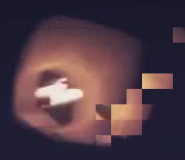
\includegraphics[width=4cm]{img/xualg-visual.png}
\end{subfigure}
~
\begin{subfigure}[t]{4cm}
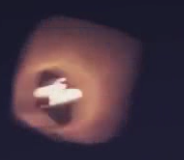
\includegraphics[width=4cm]{img/mvsteg-visual.png}
\end{subfigure}
}
\caption{A frame, showing a sky lantern, containing embedding by Xu's algorithm (left) and \texttt{MVSteg} (right).}
\label{fig:xualg-mvsteg-visual}
\end{figure}

Figure \ref{fig:xualg-mvsteg-visual} shows how, perhaps due to this selection policy, Xu's algorithm's embedding produces artefacts. Since Movest does not modify the prediction error, these artefacts leave a visual footprint, saving the effort of trying to spot suspiciously odd motion vector component values manually. \texttt{MVSteg} always modifies the largest component which makes the relative change negligible and does not leave a similarly noticeable footprint.

\begin{wrapfigure}{R}{6cm}
\centering
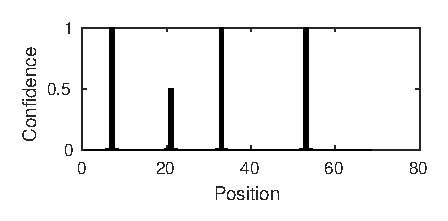
\includegraphics[scale=0.75]{img/4xembed.eps}
\caption{Positions of repeated embedding. Lower bar corresponds to an inexact match.}
\label{fig:4xembed}
\end{wrapfigure}

Authors of the algorithm suggest embedding the same chunk of data four times at different locations to increase resilience against possible data corruption. To guide the decoding process, locations are stored an I-frame using classic image steganography methods. This, however, implies that LSBs of used motion vectors will have a recurring pattern, so I simulated this embedding together with some bit corruptions in an attempt to find such repetition. Figure \ref{fig:4xembed} shows a successful result of finding a similar pattern at four locations, with peaks corresponding to positions where the pattern matched the recovered string in the best way: the sum of squared differences between a pattern and the recovered string is close to zero. \texttt{MVSteg} is not vulnerable to this, since it embeds data once.

\begin{wrapfigure}{R}{8cm}
\begingroup
    \fontsize{10pt}{12pt}\selectfont
\centering
\begin{alltt}
{\color{blue}[mpeg4 @ 0x7fc9dc247380]} {\color{red}ac-tex damaged at 53 0}
{\color{blue}[mpeg4 @ 0x7fc9dc247380]} {\color{red}Error at MB: 53}
\end{alltt}
\endgroup
\caption{Macroblock corruption reported by the \texttt{vlc} media player.}
\label{fig:vlc-corruption}
\end{wrapfigure}

Another interesting decision made by the algorithm is to modify motion vector components by incrementing them. This introduces a special case when motion vector points to the edge of the frame, so incrementing it would make it point beyond the edge and hence invalid. If sufficient checks to prevent this not in place, it can give out the fact that the video has been tampered with. Figure \ref{fig:vlc-corruption} shows that such corruption can be reported by a media player. \texttt{MVSteg}'s embedding can't be detected this way because it decrements motion vector components in an F4 fashion, which also makes it resistant to $\chi^2$ and histogram attacks, described earlier in section \ref{steg-tech}.

\subsection{Reversion Technique}
\label{rev-tech}

As explained in section \ref{rev-tech-theory}, the reversion technique considers differences between respective motion vectors of the original and the re-encoded (transcoded) video. Evaluating the effectiveness of this technique requires training a linear SVM classifier. In this situation, SVM does not require large datasets to give good results~\cite{cao2012video}, so I have obtained a dataset of 56 freely-available stock videos with various degrees of motion, such as slow cloud movements or chaotic city timelapses. Half of those were chosen to become stego videos, so that the ratio between stego and non-stego videos is 50:50 (balanced dataset).

For each sequential (non-randomised) embedding algorithm, the training and evaluation is done as follows:
\begin{itemize}
\item To obtain ``original'' videos, Movest encoder is used to embed random data into the 28 stego videos at their full capacity. The remaining 28 non-stego videos are also passed though the encoder, but no data is embedded (dummy pass).
\item To obtain transcoded videos, all original videos are passed through the encoder again, letting FFmpeg recompute motion vectors.
\item Motion vectors are extracted from all videos.
\item Motion vector data is imported into Matlab and frequencies of SAD values are computed using steganalysis suite's \texttt{computeSadFreqs.m} function.
\item Frequency data, together with a labelling whether it came from a stego or a non-stego video, is passed into Matlab's \texttt{fitcsvm} function to train a linear SVM.
\item To estimate the classification accuracy, the system performs 100 runs of \emph{k-fold cross validation}~\cite{ai2-notes}, with $k = 8$, as explained below. This is a common technique of evaluating performance of classifiers and it is available in Matlab (\texttt{crossval}).

\textbf{8-fold cross validation:} the data set is randomly partitioned into 8 bins (7 videos each), and the algorithm performs 8 iterations, selecting each bin in turn. On every iteration, remaining 7 bins are used to train the classifier and the selected bin is used to evaluate its accuracy\footnote{Using $k = 8$ allows having 7 videos in each bin.}. The accuracy result, averaged over 8 iterations, is reported back.

Since the reported value depends on how favourable the random partitioning was, the system runs the 8-fold cross validation algorithm 100 times to obtain a narrow 95\% confidence interval for the mean accuracy.  

\end{itemize}

Table \ref{tbl:rev-tech} presents obtained classification accuracy for each embedding algorithm.

\begin{table}[tbh]
\bgroup
\def\arraystretch{1.3}
\centerline{
\begin{tabular}{|l|c|}
\hline
\textbf{Embedding algorithm} & \textbf{Classification accuracy, 95\% CI} \\
\hline
\textit{Random guess (baseline)} & $50\%$ \\
Hide \& Seek & $100.00\% \pm 0.00\%$ \\ 
MSteg & $92.84\% \pm 0.04\%$ \\ 
F3 & $93.45\% \pm 0.32\%$ \\ 
F4 & $93.25\% \pm 0.16\%$ \\
Xu's algorithm & $63.93\% \pm 0.54\%$ \\
MVSteg & $62.96\% \pm 0.57\%$ \\
\hline
\end{tabular}
}
\egroup
\caption{Reversion technique classifier performance against each sequential embedding algorithm implemented.}
\label{tbl:rev-tech}
\end{table}

The results are surprisingly good. My interpretation of the trend in the data is that the accuracy result against each algorithm appears to be similar to the proportion of motion vectors it modifies. 

\subsection{Varying embedding capacity}
\label{eval-var-emb-cap}

Many of the previous attacks, such as the $\chi^2$ attack, rely on payload bits being embedded close together, because the cumulative effect makes it easier to expose the embedding. This weakness can be addressed by using algorithms that spread the payload uniformly across the cover video.

To evaluate how effective this approach is, I tested the $\chi^2$ attack and the reversion technique classifier for MSteg against the Outguess 1.0\footnote{Outguess 1.0 is the randomised version of MSteg.} algorithm at different embedding capacity settings. Table \ref{tbl:detect-outguess} presents findings obtained on a fresh dataset (\emph{i.e.} not used for classifier training) of 10 videos; entries show how many videos were picked up as stego by both steganalysis methods.

\textbf{TODO}

\begin{table}[tbh]
\bgroup
\def\arraystretch{1.3}
\centerline{
\begin{tabular}{|l|c|c|}
\hline
\textbf{Embedding capacity} & \textbf{RT Classifier} & $\chi^2$ \textbf{attack} \\
\hline
\textit{0\%} & 0/10 & 0/10   \\
10\% & 1/10 & 0/10   \\
20\% & 1/10 & 0/10   \\
30\% & 1/10 & 0/10   \\
40\% & 1/10 & 0/10   \\
\textit{100\%} & 9/10 & 10/10 \\
\hline
\end{tabular}
}
\egroup
\caption{Detectability of Outguess 0.1 embedding at various embedding capacities.}
\label{tbl:detect-outguess}
\end{table}

As we see from the data, the reversion technique classifier starts classifying more than 50\% of videos at XX\% capacity setting and $\chi^2$ attack is only effective starting at YY\%.

\section{Detectability by humans (study)}
\label{exp-human-subj}

\subsection{Study hypothesis}

A study was conducted to test whether human participants are able to distinguish
between a stego and a non-stego video. To test this, I looked into the numbers of times the participants were right or wrong when asked to identify the stego video out of the three ostensibly identical videos. I hypothesise that humans are not able to tell videos apart (null hypothesis); this hypothesis will be rejected if the data supports the opposite claim to a statistically significant level.

\subsection{Experimental procedure}

The experiment consisted of 10 trials. In each trial, the participant was given three ostensibly identical videos, each up to 30 seconds long, one of which has been modified to contain a hidden payload\footnote{Experiment description is the project proposal originally stated that 2 videos will be used. Using three videos and asking the participant to pick the odd one out eliminates the situation when the participant sees that videos are different, but is unable to tell which one actually contains embedding.}. They had to choose which video they thought was modified and write its letter (\textsb{A}, \textsb{B} or \textsb{C}) into the experiment answer sheet.

To increase chances of successful detection and more closely simulate steganalysis, the following measures were taken:
\begin{itemize}
\item Test subjects were computer-literate students (most of them were fellow computer scientists).
\item Embedding has been done using the Hide \& Seek algorithm, which leaves a significant footprint by modifying every motion vector. The full embedding capacity of every video was used up to embed random data.  
\item Participants had full control over the playback, which meant they could watch videos however they liked: sequentially, side-by-side, repeatedly replay certain parts, inspect file sizes, zoom into certain regions of a video, use either their own or my screen \emph{etc.}
\item First trial contained an artificially corrupted video (motion vectors were changed more drastically), to give participants an idea of what kind of visual footprint to expect. 
\end{itemize} 

As a precaution, videos given to the participants did not contain flashing images, were emotionally neutral, and free from distressful, disturbing, offensive or otherwise unsettling images. No personal data about the participants was collected.

\subsection{Results}

To be able to interpret the data, I define a theoretical model that would fit the experiment. Let $n$ be the number of answers that participants gave and $X_i$ ($i \in [1, n]$) denote whether an answer was correct, \emph{i.e.} $X_i = 1$ if a participant correctly picked out a stego video in a trial and 0 otherwise. If the null hypothesis holds, we expect answers to be just as good as random guesses. Therefore $X_i$'s can be modelled as random variables with $\mathbb{P}(X_i = 1) = 1/3$, or, in other words, $X_i$'s follow Bernoulli distribution with $p = 1/3$. 

To consider the overall data, we compute the sum of all $X_i$: $Y = \sum^n_{i=1} X_i$. For sufficiently large $n$, $Y$ follows the Binomial distribution with parameters $(n, p)$~\cite[p.~53]{papoulis2002probability}. Then, by de Moivre--Laplace theorem, $Y$ can be approximated by the normal distribution with mean $np$ and variance $np(1-p)$~\cite[p.~105]{papoulis2002probability}. This allows us to put 95\% confidence bounds on the value of $Y$~\cite[p.~316--318]{ai2-notes}:
\[ np - 1.96 \sqrt{np(1-p)}  < Y <  np + 1.96 \sqrt{np(1-p)} \]

If $Y$, obtained from the data set, does not lie in this range, the null hypothesis can be rejected with 95\% confidence.

The data obtained from the experiment is presented in Table \ref{tbl:detect-exp-res}. 

\begin{table}[tbh]
\centering
\bgroup
\def\arraystretch{1.3}%  1 is the default, change whatever you need
\begin{tabular}{|l|c|c|c|c|c|c|c|c|c|c|}
\hline
\textbf{Video \#} & \textbf{1} & \textbf{2} & \textbf{3} & \textbf{4} & \textbf{5} & \textbf{6} & \textbf{7} & \textbf{8} & \textbf{9} & \textbf{10}\\
\hline
\textit{Correct answer} & \textit{B} & \textit{C} & \textit{C} & \textit{A} & \textit{B} & \textit{B} & \textit{A} & \textit{C} & \textit{B} & \textit{A}\\
\hline
Participant \#1  & B & C & C & B & A & C & A & B & A & C \\
Participant \#2  & B & A & B & C & C & B & A & B & A & A \\
Participant \#3  & B & C & B & A & C & A & A & B & A & C \\
Participant \#4  & B & A & A & B & B & C & C & A & B & C \\
Participant \#5  & B & A & C & B & C & A & A & C & B & C \\
Participant \#6  & B & C & C & A & A & B & C & C & C & B \\
Participant \#7  & B & A & A & C & A & C & C & C & C & A \\
Participant \#8  & B & B & A & C & A & A & B & A & C & C \\
Participant \#9  & B & C & B & C & A & C & A & C & C & C \\
Participant \#10 & B & A & A & C & A & C & B & C & A & C \\
Participant \#11 & B & B & B & C & C & B & C & A & C & C \\
Participant \#12 & B & C & A & A & B & B & B & A & B & B \\
\hline
\end{tabular}
\egroup
\caption{Results of the distinguishability of video steganography experiment. Column one corresponds to the demo trial with an evidently corrupted video, so it is excluded from the analysis.}
\label{tbl:detect-exp-res}
\end{table}

% \footnote{One would normally want to have an order of magnitude more answers for the approximations to be more reliable, but it was not possible to recruit a sufficiently large number of qualified participants. It is worth noting that, according to the formula for $Y$, variance bounds will not get narrower as $n$ increases.}
The data contains 108 answers ($n = \text{\# of participants} \times \text{\# of trials}$), so, according to the formula above, I expect $Y$ to be within the range $36 \pm 5$. The data has 32 correct answers, which is within that range, so it \emph{cannot} be concluded that humans \emph{are} able to identify implemented video steganography.

\section{Embedding capacity and speed}

A steganographic system also has secondary characteristics worthy of noting: the embedding capacity and embedding speed. As previously mentioned in \ref{mv-emb-space}, embedding capacity depends on the number of P-frames, number of macroblocks (defined by the resolution) and the number of suitable motion vectors. The proportion of suitable motion vectors can vary significantly depending on the type of motion a video exhibits and what algorithm is used: for example, \texttt{MVSteg} will perform worse on videos with little or slow motion, because it only embeds into long motion vectors. 

To give an estimate of what embedding capacities a user might reasonably expect, I measured embedding capacities per second on a dataset of 53 HD ($1280 \times 720$) videos with various degrees of motion, averaged over the first 15 seconds. Figure \ref{fig:capacities} presents a box plot of measured capacities for each embedding algorithm: Hide \& Seek achieves an impressive 20~KB/s median embedding capacity; MSteg's, F3's and F4's median result is 6--8~KB/s, and Xu's algorithm and MVSteg have the lowest values of 1~KB/s. 

\begin{figure}[tbh]
\centerline{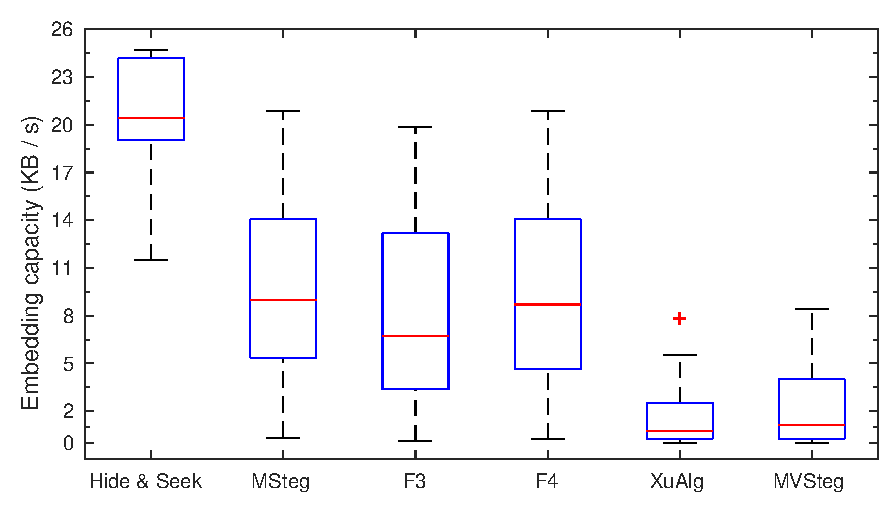
\includegraphics{img/capacities.eps}}
\caption{Box plot showing possible embedding capacities (KB/s) for every algorithm.}
\label{fig:capacities}
\end{figure}

   

Encoding the video is the most computationally expensive part of the Movest encoder, so the time taken by steganography routines is relatively negligible. I did not observe any significant decrease in the encoding speed, even when using payload encryption. The most noticeable slowdown in the encoder is the initialisation overhead of the Randomised Hide \& Seek algorithm to build the payload bit to MV component mapping (section \ref{rand-hidenseek}). \textbf{TODO: give measurements?}

% Conclusions
\cleardoublepage
\chapter{Conclusions}

Say that project was a success.

\section{Accomplishments}

\section{Lessons learnt}

\section{Future directions}

People suggest different approaches, mention some. Is it really white noise?

\cleardoublepage
\bibliographystyle{unsrt}
\addcontentsline{toc}{chapter}{Bibliography}
\bibliography{refs}

\appendix
\cleardoublepage
\addcontentsline{toc}{chapter}{Appendix A:\quad Project Proposal}
\chapter*{Appendix A: Project Proposal}

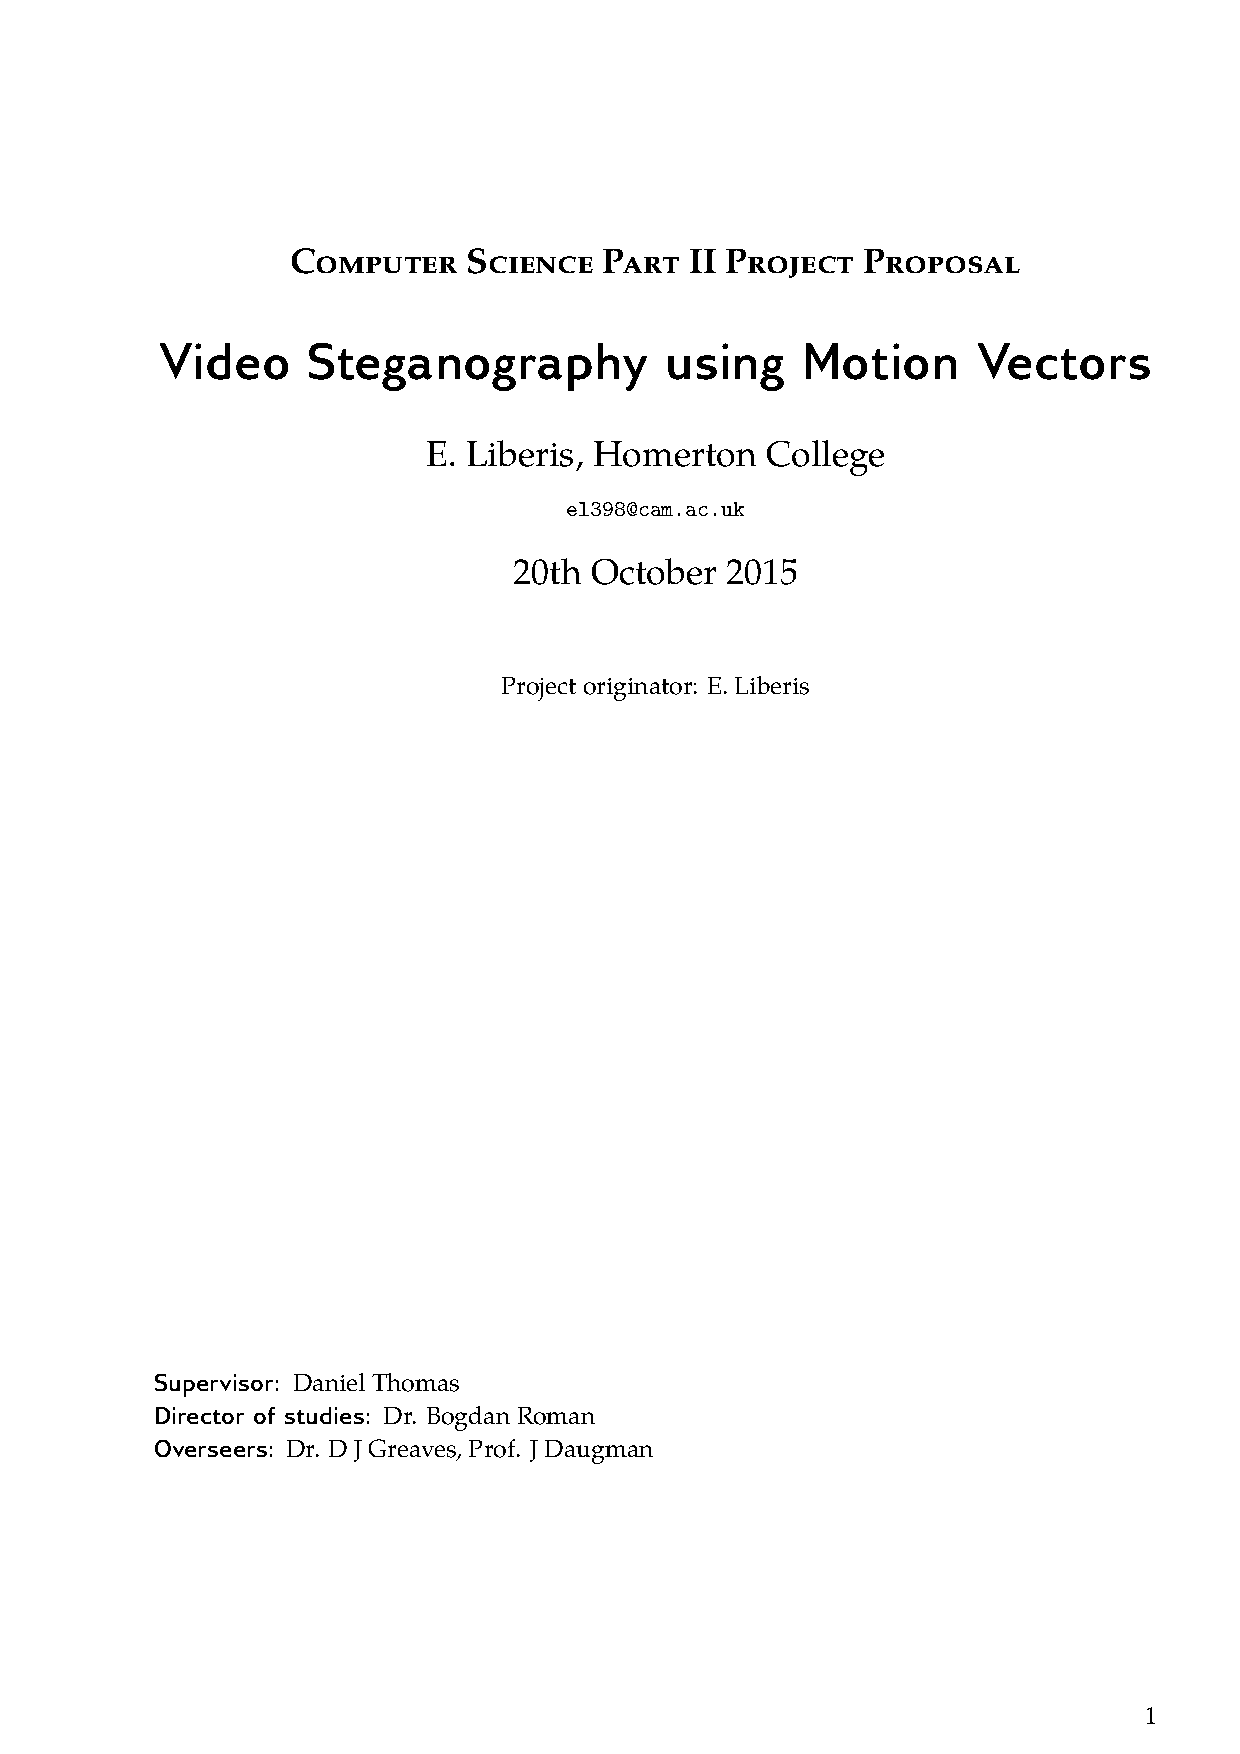
\includepdf[pages={-}]{proposal.pdf}


\end{document}